%%============================================================================
%% thesis.tex  --  Adelaide Punt, DPhil thesis (body)
%%
%% Title: Noise and Uncertainty in Molecular Property Prediction:
%%        Robust Models and Adaptive Representations
%%
%% Input by main.tex (%%============================================================================
%% thesis.tex  --  Adelaide Punt, DPhil thesis (body)
%%
%% Title: Noise and Uncertainty in Molecular Property Prediction:
%%        Robust Models and Adaptive Representations
%%
%% Input by main.tex (%%============================================================================
%% thesis.tex  --  Adelaide Punt, DPhil thesis (body)
%%
%% Title: Noise and Uncertainty in Molecular Property Prediction:
%%        Robust Models and Adaptive Representations
%%
%% Input by main.tex (%%============================================================================
%% thesis.tex  --  Adelaide Punt, DPhil thesis (body)
%%
%% Title: Noise and Uncertainty in Molecular Property Prediction:
%%        Robust Models and Adaptive Representations
%%
%% Input by main.tex (\input{thesis}), which holds the preamble and all front
%% matter: title page, declaration, acknowledgements, abstract, contents, lists,
%% and the List of Abbreviations. Bibliography: refs.bib in this repo.
%%
%%----------------------------------------------------------------------------
%% % Decision for you: main.tex asks for a separate List of Publications page in
%% %   the front matter. The chapter "Summary of Research Contributions" already
%% %   lists the papers and the conference presentation. Adding the page repeats
%% %   that list before Chapter 1; leaving it out means that chapter is the only list.
%% % Decision for you: American or British spelling for the whole thesis.
%% %   Running text (comment lines excluded, rough count): about 50 British forms
%% %   (standardised, labelled, normalised, humanised, optimised, featurisation) and
%% %   over 100 American forms (modeling, regularization, normalized, optimize, behavior).
%% %   The Chapter 3 Evaluation subsection and all Chapter 3 text taken from the
%% %   NoiseInject paper are American.
%% %   British: change the American forms and switch babel from english to british
%% %   for hyphenation. American: change the roughly 50 British forms. Either way,
%% %   software names and quoted titles stay as published.
%%============================================================================


\chapter{Introduction}\label{chap:intro}
% ---- NOTES: Introduction ----
% Paragraph 1: molecular property prediction and the two-component model (written)
% - Virtual screening and fast property prediction in the drug discovery pipeline \citep{Lill2007, Neves2018}.
% - A QSAR model is a molecular representation paired with a model.
% - The representation sets what chemical information is available; the model sets how it is used.
% - Static against learned representations \citep{Sabando2021}. Keep it to one sentence: the Background defines each representation.
%
% Paragraph 2: label noise in molecular data (written)
% - Add one sentence: this noise is rarely homoscedastic Gaussian. Its size varies with source and assay, as the pIC$_{50}$, pK$_i$ and single-assay figures already in this paragraph show.
% - Paragraph 3 already says most studies assume Gaussian noise. State the assumption there only, and the reality here.
% - Grammar: "Measurements from a single assay lowers" becomes "lower".
%
% Paragraph 3: the first research question and the gap it fills (written)
% - Typo: "QSAR modelings" becomes "QSAR modelling".
% - Use \citet{Cortes2015} in place of \cite{Cortes2015}, so the sentence reads with the author name.
%
% Paragraph 4: from noise robustness to adaptive representations (written; rephrase the similarity sentence)
% - Terminology: noise mitigation is a subset of methods for learning with noisy labels (LNL).
% - So "learning with noisy labels and noise mitigation" becomes "learning with noisy labels, including noise mitigation".
% - Say what was tried: 12 LNL methods adapted from classification to regression.
% - Several of them judge a label by the labels of its nearest neighbours, using a distance between molecules.
% - "All of the methods that used similarity estimates failed" is too broad. The heteroscedastic GP compares molecules through its kernel and still held up. Say the methods that judged a label by its neighbours' labels did worst.
% - Say what "did worst" means in words: the least noise-robust configurations all used a distance. The counts (20 of 221) are given in Section "From noise robustness to adaptive representations" and in Section~\ref{sec:lnl_motivation}; leave them out here.
% - Replace "vector operations" with "distance measures", and name the same three as Section~\ref{sec:lnl_motivation}: Tanimoto on ECFP4, Euclidean on PDV, and Mahalanobis.
% - Replace "representations" with the five tried: ECFP4, Sort \& Slice, PDV, and canonical and randomised SMILES.
% - The similar property principle is introduced in the Background with \citet{Johnson1990}. Cite the same source here, or keep \citep{LopezPerez2024} as a review.
% - Typos: "simiarity" becomes "similarity"; "who's" becomes "whose"; "how it improve" becomes "how it improves".
% - The last sentence says the hybrid improves performance. The Chapter 5 and 6 results are not yet run, so say those chapters test whether it does.
%
% Paragraph 5 (to write): close the opener with the overall aim, then hand over
% - One sentence: the aim is property prediction that stays reliable when training labels are noisy.
% - One sentence: the two parts are choosing models and representations that survive label noise, then adapting the representation itself.
% - One sentence on why it matters: property predictions filter which compounds are tested, so noise-driven errors waste experiments.
% - End with a hand-over line: the rest of the chapter states the questions, then outlines the thesis chapter by chapter.
% - Keep it to 3-4 sentences. Other theses in the field end their opener this way: one aim paragraph, then "The rest of this thesis is organised as follows".
%
% Overlap with the sections that follow:
% - Paragraph 3 states two of the four first-half questions. Section~\ref{sec:intro:questions} states all four in full. Keep this paragraph's sentence as the short version and point there.
% - Paragraph 4 tells the move from noise to the hybrid in words. Section "From noise robustness to adaptive representations", two sections on, gives the numbers behind each step. Do not repeat the numbers here.
% - Decision for you: keep Paragraph 4 at its current seven sentences, or cut it to two.
% - If kept, Section "From noise robustness to adaptive representations" gives only the findings behind it.
% - If cut, that section tells the whole move from noise to the hybrid, and its plan has to change to match.
% ---- END NOTES ----

New avenues in the drug discovery pipeline have opened up thanks to advances in large dataset collection, analysis, and computation. Therapeutic targets are identified, potential drug candidates are screened and optimized, and the most promising of these go on to pre-clinical and clinical trials \citep{Lill2007}. There are various methods by which potential drug candidates can be screened. Virtual screening allows for the rapid and large-scale analysis of libraries of compounds, and is a particularly useful approach used to speed up the drug discovery process \citep{Neves2018}. One standard screening method is the prediction of bioactivities and pharmacological properties of such candidates. There is a long history of using Quantitative Structure-Activity Relationship (QSAR) models to make these predictions, to act as a filter for compounds with undesirable properties, and thus reduce the time and cost associated with experimental screening \citep{Sabando2021}. QSAR models aim to predict the relationship between a molecule's molecular features as encoded within a particular molecular representation and a desired molecular property \citep{Sabando2021} of interest. A QSAR model typically consists of a molecular representation paired with a machine learning (ML) model. An ideal molecular representation will allow a model to learn only the relevant information about each molecule with respect to the target property. Representations are either `static' hand-crafted descriptors or circular fingerprints that encode predefined structural and physicochemical features \citep{rogers2010, David2020, sns, avalon}; or learned representations, where the encoding is derived from a predictive model, often taken from the activations of the final layer of a neural network, or a latent space embedding \citep{Sabando2021, kishimoto2023}. 

QSAR models are of course, sensitive to the quality of the input data on which they are trained. Experimental noise can arise from measurement errors, variability under experimental conditions, varying provenance of the data, and intrinsic biological and chemical variability. Even the very measures of model performance may be flawed if test and validation sets are laden with noise. \citet{Kolmar2021} show that the variance associated with experimental data can contribute more to prediction error than the model’s own error. There is also a limit to how much noise the model can tolerate; \citet{jorner2021} found that once the model error approaches the magnitude of the experimental measurement error on labels, adding more training data yields diminishing returns in predictive performance. In the context of activity prediction, the inherent variability within experimental setups and assays, batch effects, measurement errors, and biological variability introduce additional layers of complexity \citep{Kolmar2021, Fourches2010}. All of this increases the likelihood of encountering noise in the data \citep{Fang2022}. Even the molecular representations in the training data themselves may be incorrect or misleading \citep{Walters2023}, and chemical datasets contain too few repeat measurements of each compound to characterize the distribution the label is drawn from. Thus, models treat a single label as the population mean \citep{Kolmar2021}. Repeat measurements of the same compound-target pair disagree by about $0.68$ log units for pIC$_{50}$, and by about $0.54$ log units for pK$_i$ \citep{Kalliokoski2013, Kramer2012}. Measurements from a single assay lowers the mean disagreement from $0.50$ to $0.27$ log units \citep{landrum2024}.  

This thesis addresses the challenge of conducting molecular property prediction when the underlying experimental data contain noisy labels. My initial research question is which combinations of molecular representations and predictive model architectures maintain predictive performance under label corruption, and whether probabilistic methods that estimate uncertainty justify their additional complexity. As I will show, both model and representation choice dominate predictive performance on clean data, however, this relationship inverts under label corruption as predictive architecture becomes the primary factor in determining noise robustness.  Most existing work on noise in QSAR modelings assumes that label noise can be modeled as random error drawn from a Gaussian distribution, and they evaluate either molecular representations or predictive model architectures in isolation. \cite{Cortes2015} examined 12 algorithms across multiple noise levels but used fixed representations. Studies that compare representations are typically done on clean data. No work has systematically compared the relative importance of representation versus architecture choice for noise robustness, assessed whether probabilistic methods justify their computational overhead in noisy settings, or tested whether findings generalize across different corruption patterns and molecular property types.

Building on these findings, I began exploring techniques involving learning with noisy labels and noise mitigation. Many of these methods incorporate measures of molecular similarity, relying on the assumption that molecules which are similar in structure share similar properties \citep{LopezPerez2024}. However, all of the methods that used simiarity estimates failed, even when I tried varying the molecular representations and vector operations from the standard ECFP4 and Tanimoto coefficient. I hypothesized that to generate accurate similarity estimates, you need a specialised molecular representation who's features relate directly to similarity in that molecular domain. This brings me to my next research question, how do you select the best set of features for a given prediction task? I will outline how I developed an adaptive feature selection methodology that takes in a set of molecular representations, identifies each representation's most important features, and combines a select set of those top features into a new hybrid representation. I will then demonstrate how it improve performance across a range of predictive tasks beyond the small molecule space, and how it can be applied to the context of similarity estimation and downstream noise mitigation methods. 


\section{The questions this thesis asks}\label{sec:intro:questions}

% ---- NOTES: The questions this thesis asks ----
% Paragraph 1: the four questions of the first half, on representation, model, noise type and uncertainty under label noise.
% - Add one closing sentence: Chapter~\ref{chap:robustness} answers all four.
% - NoiseInject is described in Chapter~\ref{chap:background}, section "NoiseInject: a benchmarking framework". Point there instead of describing it again.
% Paragraph 2: the questions of the second half, with the chapter that answers each.
% - The link between the halves (similarity-based methods failed under label noise) is the next section's job. Do not restate it here.
% - Add a question for Chapter~\ref{chap:flaws}: do standard representations, and the similarity computed over them, fail on a given dataset?
% - "How do you select the best set of features": Chapter~\ref{chap:method}, which gives the search and when and why the hybrid helps.
% - "Do hybrid representations achieve higher noise robustness": no chapter reports the retention comparison it asks for.
% - An experiment for it exists. It computes the normalised area under the retention curve, the same robustness measure as Chapter~\ref{chap:robustness}, for the hybrid and for single representations under injected label noise.
% - Chapter~\ref{chap:similarity}, "Gaussian noise: learning-with-noisy-labels methods", reports Spearman at two noise levels for the plain network and the twelve methods, on each downstream model's top two single representations, the hybrid and the importance-weighted hybrid (the local preliminary runs used one-hot in place of the top two single representations). That is a score at each level, not the retention area.
% - The question's "(retention percentage)" should become the normalised area under the retention curve if the question is kept.
% - Decision for you: report hybrid noise robustness in Chapter~\ref{chap:method}, report it in Chapter~\ref{chap:similarity}, or drop the question; reporting it needs its results from the full runs, dropping it removes the second item of the list below.
% - "Do the selected hybrid features help stabilize distance-based noise mitigation": Chapter~\ref{chap:similarity}. Widen it to noise detection and estimation as well as noise mitigation, since that chapter reports both.
% - "Does feature importance weighting improve" is split across two chapters. During hybrid construction and model training: Chapter~\ref{chap:method}.
% - Importance weighting in the distance, and the importance-weighted hybrid under noise: Chapter~\ref{chap:similarity}.
% - "noise mitigation tasks" in the importance-weighting question: Chapter~\ref{chap:similarity} tests the importance-weighted hybrid with methods for learning with noisy labels, of which noise mitigation is one part. Write "distance-based noise detection and learning with noisy labels".
% - "Can sample weighting or label smoothing provide superior noise handling": Chapter~\ref{chap:similarity}. Reword it.
% - Reason for rewording: in Chapter~\ref{chap:similarity}, weighting and smoothing are reported only for cleaning real labels with nothing injected. No reported experiment applies them under Gaussian corruption.
% - Under Gaussian noise, Chapter~\ref{chap:similarity} instead surveys twelve methods for learning with noisy labels, on each downstream model's top two single representations, the hybrid and the importance-weighted hybrid (the local preliminary runs used one-hot in place of the top two single representations).
% - Wording: "learning with noisy labels" for the broad class. Sample weighting and label smoothing are noise mitigation, a subset of it.
% - Add the similarity question: is predicting each molecule's activity from its nearest neighbours more accurate in a hybrid than in its base representations? (Chapter~\ref{chap:similarity}.)
% Overlap with other sections:
% - The questions are stated in full only here. Chapters~\ref{chap:robustness}, \ref{chap:method} and~\ref{chap:similarity} point back to this section.
% - The introduction's fourth paragraph also asks the feature-selection question. Keep one sentence there and the full question here.
% ---- END NOTES ----

% TODO: review, needs manual review
The first half of this thesis addresses four questions about the behavior of QSAR models under label noise. First, how does the choice of molecular representation and model architecture explain the variance in predictive performance, and does that division change when you instead consider how much performance a QSAR model is able to retain under increasing label noise? Second, what does the choice of model provide with label noise? Within this question we compare the effects of deterministic and probabilistic modeling. Third, does the type of label noise matter, or just the quantity of it? We explore different techniques of generating and adding label noise to both clean data, as well as data with inherent experimental noise. Fourth, what is the impact of artificial label noise on a model's uncertainty estimation? Does the estimated uncertainty rise with increased label noise and can these uncertainty values point to which labels are corrupted? Together, these questions aim to identify what, if anything, makes a QSAR model robust to noise. Finally, we introduce NoiseInject, an open-source Python package for benchmarking noise robustness and uncertainty quantification in machine learning models.

% TODO: review, needs manual review
The second half asks whether the representation itself can be adapted to the task:
\begin{enumerate}
    \item How do you select the best set of features for a given prediction task?
    \item Do hybrid representations achieve higher noise robustness (retention percentage) than their base representations?
    \item Do the selected hybrid features help stabilize distance-based noise mitigation?
    \item Does feature importance weighting improve effectiveness of hybrid representation creation, model training, and noise mitigation tasks?
    \item When sample removal is suboptimal, can sample weighting or label smoothing provide superior noise handling under Gaussian corruption?
\end{enumerate}

\section{From noise robustness to adaptive representations}

% ---- NOTES: From noise robustness to adaptive representations ----
% Scope: the bridge between the two halves of the thesis, with the evidence for each step.
% The chapter's opening paragraphs already tell this story in two sentences each. Do not repeat them; give the findings behind them.
% Three short paragraphs. No method detail: each step points to the chapter that holds it.
%
% Paragraph 1: What the first half found (Chapter~\ref{chap:robustness}).
% - Robustness is measured as the normalised area under the R^2 retention curve as noise rises.
% - Under Gaussian noise on QM9, model architecture explains 49.5% of the variance in robustness. Representation explains 9.2%.
% - For R^2 at noise level 1.0 (noise one spread of the clean training labels), the shares are comparable: 29.1% for architecture, 26.6% for representation.
% - These R^2 shares are under noise, not on clean labels. Do not call them the clean-label split.
% TODO(results): the same split on R^2 before any noise is added. The NoiseInject paper's variance table has no clean-label row yet, so no claim about clean labels can be made here until it exists.
% - Systematic noise (shared within a scaffold family, or clipped at an assay limit) hurt models most. The shape of the noise distribution barely mattered.
% - Under Gaussian noise on QM9, mean predicted uncertainty rose with noise for every probabilistic model and representation. Per-molecule uncertainty did not reliably pick out which labels were corrupted (Section~\ref{sec:uq}).
% - Some models did better than others at this. NGBoost and the Gaussian process fit a per-molecule scale, and they gave the strongest per-molecule correlation between predicted uncertainty and injected noise. Under censoring, models were most confident on the labels that had been clipped.
% - Consequence: uncertainty alone cannot say which labels to fix. That leads to methods that judge each label another way.
%
% Paragraph 2: The exploratory study of learning with noisy labels, and its negative result (Section~\ref{sec:lnl_motivation}).
% - Learning with noisy labels (LNL) is the broad family. Noise mitigation, which removes, reweights or corrects labels, is one part of it.
% - Twelve LNL methods were adapted to regression and tested in 221 configurations on the QM9 HOMO-LUMO gap with Gaussian noise. This count is quoted from the confirmation report; the raw results are not available to recompute it.
% - Several variants judged a label by its neighbours' labels, using a distance between molecules.
% - All 20 configurations with the lowest retention of R^2 under noise used such a distance. Also quoted from the confirmation report, not recomputed.
% - This held for each distance tried: Tanimoto on ECFP4, Euclidean on physicochemical descriptors, and Mahalanobis.
% - The methods that held up estimated noise from the model's own loss or uncertainty, not from neighbours.
% - One dataset and one noise type: state it as the motivation, not a general result.
%
% Paragraph 3: Why the distance failed, and the step to the hybrid (Chapters~\ref{chap:flaws}, \ref{chap:method} and \ref{chap:similarity}).
% - Hypothesis: on a given dataset, most features of a general-purpose representation do not vary or do not relate to the property.
% - Every such feature adds a term to the distance, so irrelevant features dominate it. The growth is linear in the number of features, not exponential.
% - Chapter~\ref{chap:flaws} measures this on base representations and on distances. Point there; do not re-derive it here.
% - The proposed fix: select a fixed number of task-relevant features from several representations, and compute distances in that compact space.
% - A first version showed that these selected feature sets also work as ordinary model inputs, with no distance involved.
% - That turned the question into how to choose the features, which is Chapter~\ref{chap:method}.
% - Chapter~\ref{chap:similarity} then returns to distances, noise detection and LNL, including noise mitigation, with the hybrid as the feature space.
% ---- END NOTES ----
\todo[inline, color=yellow!40]{Write this section from the notes above. The raw material is Section~\ref{sec:lnl_motivation}.}


\section{Outline of the thesis and contributions}

% ---- NOTES: Outline of the thesis and contributions ----
% One short paragraph per chapter: what it does, what it found (Chapters 3 and 4) or will test (Chapters 5 and 6), and where it is published or planned.
% Do not restate the research questions (Section \ref{sec:intro:questions}) or the motivation for the second half ("From noise robustness to adaptive representations"). Point to them.
%
% Paragraph 1: Chapter 2 (Background)
% - Introduces, once, what the later chapters rely on: molecular representations, model families, molecular similarity and activity cliffs, noise in molecular data, and the evaluation protocol.
% - Defines the seven noise conditions used in Chapter 3.
% - Ends by introducing NoiseInject, the open-source benchmarking framework released with this work.
%
% Paragraph 2: Chapter 3 (Noise robustness across molecular representations and model architectures)
% - Adapted from the paper "NoiseInject: A Benchmarking Framework to Study Noise Robustness in QSAR Models" by Punt, Hanser, Werner and Morris, in preparation for the Journal of Cheminformatics. Say this in the paragraph.
% - Main task: the HOMO-LUMO gap on QM9. Its labels are computed, so they carry negligible measurement noise.
% - Repeated on three assay datasets with experimental labels: LogD, Caco-2 and hERG Ki.
% - Splits the variance in performance, and in how much performance is retained under noise, between representation and model architecture.
% - Compares seven noise conditions at a matched amount of noise.
% - Compares each model with its probabilistic counterpart, and asks what label noise does to predicted uncertainty.
% - Findings in words only, no numbers. The figures behind them are in Section "From noise robustness to adaptive representations"; point there rather than repeating them.
% - Finding: model architecture matters more than representation for noise robustness. For R2 under noise, the two matter about equally.
% - Finding: the shape of the noise distribution makes little difference. Noise shared within a scaffold family, and labels clipped at an assay limit (censoring), do the most damage.
% - Finding: NGBoost and random forests were the most robust models on QM9. Random forests were the most consistent across all four datasets.
% - Finding: predicted uncertainty rises with noise on average, but does not pick out which labels were corrupted.
%
% Paragraph 3: Chapter 4 (The flaws of the similarity assumption)
% - A motivation chapter. It introduces no method, and its measurements are smaller than Chapter 3's.
% - First argument: on a given dataset, standard representations carry many features that do not vary, and some map different molecules to the same vector.
% - Second argument: similarity computed over those representations inherits both problems.
% - Third argument: methods that rely on that similarity fail as a result.
% - These include cleaning labels by comparing each molecule's label with its nearest neighbours' labels, a noise mitigation method tested in the exploratory study of learning with noisy labels. Say plainly that this study comes from the confirmation report.
% - Ends by stating what a representation would need to fix this. That is what Chapter 5 builds.
%
% Paragraph 4: Chapter 5 (Building adaptive hybrid representations)
% - Planned as the first of two method papers. Intended for submission; venue to be confirmed.
% - The method: from several base representations, it selects each one's most important features for the task.
% - It splits a fixed budget of features between the representations and combines the selected features into one representation.
% - Also describes the datasets and the experimental setup.
% - Will test when the hybrid helps, against the best single representation and against an ensemble of one model per representation.
% - Will test why it helps, against PCA, mRMR, recursive feature elimination and random features at the same number of features.
% - Will test whether the selected features can be read against the chemistry, and how stable the selection is across folds.
% - Will test whether search settings found on one dataset carry to another.
% - Will test whether it extends beyond small molecules: antibodies in most depth, and reactions, nucleotide sequences and cancer genomics as proofs of concept.
% - Will test whether it extends to data held at separate sites that cannot be pooled.
% - TODO(results): one sentence of findings for Chapter 5.
%
% Paragraph 5: Chapter 6 (Hybrid representations for similarity and label noise)
% - Planned as the second method paper. Intended for submission; venue to be confirmed.
% - Returns to the failures in Chapter 4 and asks whether a hybrid representation repairs them.
% - Similarity: hybrids selected for predicting each molecule's activity from its five nearest neighbours, compared with standard representations.
% - Noise detection and estimation: whether neighbours in a hybrid pick out corrupted labels better than neighbours in a standard representation.
% - Learning with noisy labels, including noise mitigation, one noise type at a time.
% - TODO(results): one sentence of findings for Chapter 6.
%
% Paragraph 6: Chapter 7 (Discussion and future directions)
% - Summarises each chapter.
% - Closing argument: model the noise before choosing a method. No single method fits every dataset, and simple methods are often as good.
% - Then limitations and future directions.
%
% Paragraph 7: Contributions (short: publications and software)
% - Publications: the Chapter 3 paper (in preparation) and the planned papers from Chapters 5 and 6. Point to the Research Papers list in the Summary of Research Contributions, the unnumbered chapter after Chapter \ref{chap:discussion}; do not repeat it.
% - Software: NoiseInject (open source), and the KIRBy software repository that implements the hybrid search and its experiments.
% - Point to Appendix \ref{app:availability} for repositories, licences and data. Do not list them here.
% ---- END NOTES ----
\todo[inline, color=yellow!40]{Write Sec 1.5 from the outline bullets above.}

\section{Collaborations and funding}

% ---- NOTES: Collaborations and funding ----
% Paragraph 1: funding.
% - The DPhil was funded by the University of Oxford's UK EPSRC Centre for Doctoral Training in Sustainable Approaches to Biomedical Science: Responsible and Reproducible Research, grant EP/S024093/1.
% - It was also supported by Lhasa Limited, a not-for-profit organisation.
% - Decision for you: where the funding sentence lives. It already stands word for word in the Acknowledgements. Keep it there and make this paragraph a one-line pointer, or keep it here and cut it from the Acknowledgements. Either way it appears once.
% Paragraph 2: Lhasa Limited.
% - Thierry Hanser and Stephane Werner at Lhasa Limited co-supervised the work, with Garrett Morris as supervisor.
% - Decision for you: whether Lhasa is credited with shaping how the thesis frames label noise. No published source says so; it appears only in your own chapter plan. If it is true, add one sentence saying so; otherwise Lhasa's part is the co-supervision, the jointly authored manuscript and the hERG data.
% - Chapter~\ref{chap:robustness} is adapted from the jointly authored NoiseInject manuscript (Punt, Hanser, Werner and Morris). The Statement of Originality gives each author's contribution; point there, do not repeat it.
% - Name Lhasa's federated-learning platform, Effiris, in one clause \citep{Bassani2023}. How it works is explained in your Chapter 2 section "Noise in molecular data"; point there, do not explain it again.
% - Lhasa supplied the hERG data (7,772 training and 4,383 test molecules) used in Chapter~\ref{chap:method} as data held at separate sites, the setting federated learning addresses \citep{Bassani2023, Hanser2023}.
% Paragraph 3: the Oxford Protein Informatics Group (OPIG).
% - OPIG pointed to antibody and protein datasets used in Chapters~\ref{chap:method} and~\ref{chap:similarity}. The full list is in Appendix~\ref{app:datasets}.
% - Decision for you: which datasets to name as coming through OPIG. No record says which datasets OPIG suggested. Candidates, unverified: the Ginkgo antibody developability sets, the trastuzumab-HER2 sets, and the humanness set, which is taken from BioPhi \citep{Prihoda2022}. The four FLAb sets from Koenig and from Adams are not candidates; they come from their own publications.
% - The collaboration also produced five posts on OPIG's blog, Blopig. They are already listed in the Blogposts section; point there, do not list them again.
% Paragraph 4: own work.
% - One sentence: the adaptive hybrid representation, its software and the experiments in Chapters~\ref{chap:flaws} to~\ref{chap:similarity} are the author's own work. The Statement of Originality already says this; point there.
% ---- END NOTES ----
\todo[inline, color=yellow!40]{Write Sec 1.6.}

\pagebreak
% The global-overview figure caption in Chapter~\ref{chap:robustness} cites Section~\ref{sec2}. That label sits on the Background chapter heading, but the caption means Chapter~\ref{chap:robustness}'s Methods. Change the caption's reference to \ref{sec:robustness:methods}.
\chapter{Background}\label{chap:background}\label{sec2}
% ---- NOTES: Background ----
% No text goes directly under the chapter heading. The chapter opens with its Introduction section.
% Chapter-wide rules:
% - This chapter says what a representation, a model family, a noise condition or a metric is.
% - The settings, noise levels, pairings and tests of the Chapter 3 study belong in Chapter 3's Methods (\ref{sec:robustness:methods}).
% - Write in general voice ("a random forest averages trees"), not "we fitted".
% - State three central ideas as numbered definitions, so later chapters can cite them by label.
%   - Molecular representation goes in "Molecular Representations in QSAR".
%   - The similarity assumption (Paragraph 1) and activity cliff (Paragraph 3) go in "Molecular similarity and activity cliffs".
% ---- END NOTES ----


\section{Introduction}

% ---- NOTES: Introduction ----
% Paragraph 1: what this chapter is for, and what it covers
% - Keep it to one paragraph of 3-5 sentences, in general voice, not "we fitted".
% - The chapter introduces, once, the ideas that every later chapter refers back to. Later chapters point here instead of re-defining them.
% - The sentence below is out of date. It names two parts, representations and predictive models. The chapter has seven sections before its Conclusions, listed in Paragraph 2 below.
% - The sentence below also ends in a colon with no list after it. The next line is a section heading.
% - Replace it with a one-sentence roadmap in section order, using the items in Paragraph 2.
%
% Paragraph 2: the roadmap, one clause per section, in this order
% - Molecular representations: how a molecule becomes a fixed-length numeric vector. Strings, fingerprints, descriptors, learned embeddings, graphs, and the protein and antibody language-model embeddings used in Chapter~\ref{chap:method}.
% - Models for molecular property prediction: what each model family is, and why it might resist or absorb label noise. The settings used in the Chapter~\ref{chap:robustness} study are in Section~\ref{sec:robustness:methods}.
% - Molecular similarity and activity cliffs: the assumption that similar molecules have similar properties. Chapters~\ref{chap:flaws} to~\ref{chap:similarity} test it.
% - Noise in molecular data: where label noise in real assay data comes from, and the artificial noise model with seven conditions (Section~\ref{sec:noise_injection}). Chapters~\ref{chap:robustness} and~\ref{chap:similarity} inject the same conditions.
% - Learning with noisy labels: what learning with noisy labels (LNL) is, with noise mitigation as the subset of LNL methods that act on the labels (removing, down-weighting, smoothing, relabelling or correcting them), and why no single method wins.
% - NoiseInject: the open-source framework that injects controlled label noise and reports robustness and uncertainty metrics. It is in Background because Chapters~\ref{chap:robustness} and~\ref{chap:similarity} both use it.
% - Evaluation methodology: group-aware splitting (Bemis-Murcko scaffolds for small molecules), never random, and the predictive and uncertainty metrics.
% - Do not preview Chapter~\ref{chap:robustness}'s question here. The Conclusions section of this chapter makes that link.
% ---- END NOTES ----

I will now break down the two components of QSAR models: molecular representations and predictive models:


\section{Molecular Representations in QSAR}

% ---- NOTES: Molecular Representations in QSAR ----
% Paragraph 1 (opening paragraph, before the figure): what a representation is.
% - Definition 2.1, numbered: a molecular representation is a map from a molecule to a fixed-length numeric vector that a model takes as input.
% - Computing that vector is called featurization. Each position in the vector is one feature.
% - Features can be binary (a substructure present or absent), counts, real-valued descriptors, or the dimensions of a learned embedding.
% - The same definition covers the antibody inputs of Chapter 5. An amino-acid sequence mapped to a vector is a representation in the same sense.
% - The current opening paragraph says "the type of input labels". The subject is the input features, not the labels.
% - LaTeX: the preamble has no definition environment yet. It needs \usepackage{amsthm} and \newtheorem{definition}{Definition}[chapter] before this definition compiles. The later numbered definitions (the similarity assumption, activity cliff, adaptive hybrid representation) would then number by chapter too.
%
% Paragraph 2 (SMILES paragraph, addition): canonical and randomized one-hot SMILES.
% - Do not cite Bertoni2020 for one-hot SMILES. That paper is about bioactivity signatures inferred by neural networks; its abstract says nothing about SMILES encoding. The confirmation report cited it for one-hot SMILES, so the same citation needs replacing wherever Chapter 4 describes that study. The sentence already cites TeachOpenCADD2023.
% - One molecule has many valid SMILES strings. The canonical string is the single one a toolkit picks by fixed rules.
% - Randomized SMILES start the atom walk at a random atom, giving a different valid string each time \citep{ArusPous2019}.
% - Where it is used: canonical and randomized one-hot SMILES were two of the five representations in the confirmation report's exploratory study of learning with noisy labels (Chapter 4). The earlier NoiseInject runs also used both.
% - The current Chapter 3 runs do not. They use ECFP4, Avalon, Sort & Slice, PDV, ChemBERTa and MHG-GNN.
% - So two sentences are enough here: what canonical and randomized mean, and that Chapter 4's exploratory study used both.
%
% Paragraph 3 (fingerprint paragraph, additions): name MACCS and Avalon properly.
% - MACCS keys: a fixed list of 166 predefined substructure questions from MDL, re-examined for drug discovery by \citet{Durant2002}.
% - Cite Durant2002 for MACCS and rogers2010 for ECFP. The paragraph now cites only Xie2020 for both.
% - The paragraph says ECFPs are typically built "with active chirality flags". The ECFP4 used in this thesis ignores chirality: radius 2, 2,048 bits, no chirality. Say which.
% - MACCS as computed here is 167 bits: the 166 keys plus one unused position.
% - Each MACCS bit answers one fixed, documented question, so its meaning is known without a lookup table. The cost: substructures not on the list are not seen.
% - Avalon: a second hashed fingerprint, 2,048 bits here, built through RDKit \citep{Gedeck2006}. It shares ECFP's weakness: hashing folds different substructures onto one bit.
% - refs.bib holds Gedeck2006 twice, under Gedeck2006 and under avalon. Chapter 5's representation table uses Gedeck2006; use the same key here.
% - TODO(lit): check in the Gedeck2006 full text what the Avalon fingerprint hashes before writing that sentence; the abstract does not say.
%
% Paragraph 4 (descriptor paragraphs, addition): mordred.
% - Mordred is an open-source calculator for more than 1,800 two- and three-dimensional descriptors \citep{Moriwaki2018}.
% - This thesis uses its 2D descriptors only, about 1,613 features. Point to the table in "Representations by domain" rather than listing them.
% - Its weakness is the one the paragraph already states for descriptor vectors, at larger scale: multicollinearity. Name it in one sentence; Chapter 4 ("Most features do not vary on a given dataset") shows it.
%
% Paragraph 5 (transformer paragraph, addition): MolFormer.
% - MolFormer is a transformer encoder trained on the SMILES strings of 1.1 billion unlabelled molecules from PubChem and ZINC \citep{ross2022}.
% - It uses linear attention and rotary position embeddings, which make training at that scale affordable \citep{ross2022}.
% - It is used as a fixed encoder here: the molecule vector is read out without fine-tuning. Checkpoint details belong in Chapter 5.
%
% Paragraph 6 (graph paragraphs, addition): MHG-GNN as a pretrained graph encoder.
% - MHG-GNN combines a molecular hypergraph grammar with a graph neural network \citep{kishimoto2023}.
% - It gives a fixed-length vector per molecule, like the SMILES language models, but read from the molecular graph.
% - It is now named only in passing at the end of the substructure paragraph. Give it one or two sentences of its own.
%
% Paragraph 7 (new, after the graph paragraphs): protein and antibody language models, so Chapter 5 can point back.
% - Same idea as the chemical language models, applied to amino-acid sequences. A transformer is trained self-supervised on residue sequences and gives one vector per residue.
% - A fixed-length vector per chain is usually the average of its residue vectors over the sequence. Most embeddings in Chapter 5 are formed this way; the exceptions (averaging over CDR residues only, or taking the first token) are stated there.
% - General protein models are trained on proteins of all kinds. ESM-2 was scaled to 15 billion parameters, and atomic-level structure can be predicted from its representations \citep{Lin2023}.
% - ESM3 models sequence, structure and function together \citep{Hayes2025}.
% - ESM C (ESM Cambrian) is a family of transformers trained with masked language modelling on protein sequences, metagenomic ones included, at 300 million, 600 million and 6 billion parameters \citep{Candido2026}. Preprint; say so.
% - SaProt adds one structure token per residue, from Foldseek, and was trained on about 40 million proteins \citep{Su2023SaProt}.
% - Antibody-specific models are trained on antibody repertoires. AntiBERTy was trained on 558 million natural antibody sequences \citep{Ruffolo2021AntiBERTy}.
% - AbLang-2 was trained on unpaired and paired chains to reduce the bias toward germline residues \citep{Olsen2024}.
% - IgT5 was trained on unpaired sequences, then on about 2 million paired heavy-light sequences, from the Observed Antibody Space \citep{Kenlay2024IgT5}.
% - Do not write "2 billion unpaired" for IgT5. That figure is its sibling model IgBert's; IgT5 saw about 700 million unpaired sequences \citep{Kenlay2024IgT5}.
% - Strength: dense vectors learned from far more sequences than any labelled dataset. Weakness: as for neural fingerprints, single features are not interpretable, and computing them is costly.
% - Stop there. Model sizes, layer choices, CDR-only pooling and chain joining belong in Chapter 5's representations by domain.
%
% Paragraph 8 (last paragraph, Kolmar and Heid): it is about label noise, not representations.
% - 'Noise in molecular data' already cites Heid2023 on real-world noise not being independent, identical or symmetric. Its notes now plan one sentence on Kolmar2021's Gaussian assumption just before that.
% - Decision for you: keep this paragraph here, or cut it once the noise section carries its point; keeping it states the Kolmar and Heid point twice, cutting leaves it only in the noise section.
%
% Table~\ref{tab:rep_families} closes the section. Refer to it from the opening paragraph; Chapter 5 has the per-representation tables with dimensions.
% ---- END NOTES ----
The success of machine learning hinges on the quality of input data. Although the quality can refer to noise, which the majority of my work is centered around, in this case I'm talking about the type of input labels. Molecular representations provide different features with which QSAR models and noise detection techniques can be learned. However, a potential bottleneck on larger data sets should be noted; the more complex the data structure, the greater the computational cost. For smaller data sets, the number of parameters is limited by the size of the training set, to prevent overfitting. 

\begin{figure}[h]
	\centering 
	\includegraphics[width=1.05\textwidth]{molecular_representations.png}	
    \caption{\label{fig:molecular_representations}Visualisation of the molecule \lstinline{O=C1C=CN(C1)C=O} using three different methods: a) ECFP4 showing the molecule broken into substructures with circular neighbourhoods for each atom. Each substructure is hashed to produce unique identifiers, which are then compiled into a binary bit vector representing the presence or absence of specific substructures. b) SMILES tokenization and one-hot encoding of the molecule. The SMILES string is tokenized, and using a vocabulary of the most common tokens, these tokens are converted into a one-hot encoded matrix. c) Molecular graph representation where nodes represent atoms and edges represent bonds.}
\end{figure}

One of the most common and intuitive molecular representations are Simplified Molecular-Input Line-Entry System (SMILES) strings which consist of a sequence of ASCII characters generated by a fixed set of rules to specify a given chemical identity \citep{Weininger1988}. A common way to use SMILES strings as inputs to QSAR models is to tokenize and one-hot-encode them rather than to use the strings themselves \citep{TeachOpenCADD2023}. The strings are tokenized into atomic branches and symbols and mapped to indices of a vocabulary, and finally converted into binary vectors using one-hot encodings \citep{TeachOpenCADD2023}. This representation, referred to as one-hot-encoded SMILES, allows models to process molecular structures as bit-vector-based fingerprints or as sequences of vectors. Sequence-based models such as recurrent neural networks and transformers have proven to be particularly successful in capturing text semantics within a sequence. When applied to raw or one hot encoded (OHE) SMILES strings, these models can effectively capture the structure of the molecule in its textual representation \citep{TeachOpenCADD2023}. 

Another common representation is the molecular fingerprint, a vector containing information about the properties of the molecule in question. In a typical bit vector-based fingerprint, each bit accounts for the presence (1) or absence (0) of a given chemical feature or substructure \citep{Fassio2022}. One common fingerprint is the Molecular ACCess System (MACCS) key, a substructure key-based fingerprint that encodes predefined atom symbols and properties, as well as bond types \citep{Xie2020}. Another is the Extended Connectivity Fingerprint (ECFP), which encodes local neighborhoods around each atom and bond connectivity in molecules \citep{Xie2020}. ECFPs are typically constructed with a radius of 2, a length of 2048 bits, and active chirality flags. These existing molecular representations are well established and have been quite successful when coupled with QSAR models \citep{CortsCiriano2020, Sabando2021}. They are relatively simple, and as the bits can be mapped back to one or more substructures, they are human-interpretable, and furthermore easy-to-compute. However, they are subject to information loss due to bit collisions, which happens when two different substructures are encoded at the same bit position \citep{Fassio2022}. They are also based on a fixed procedure and are not trainable or adaptable to a particular dataset. Alternative representations that capture different structural, chemical, or physical features are able to overcome these limitations. 

Recent advances have led to the development of new molecular fingerprints. One such method is the Sort \& Slice (SNS) technique, an alternative to hash-based folding for pooling ECFP substructures \citep{sns}. Sort \& Slice begins by sorting all circular substructures in the training set according to their frequency of occurrence. It then "slices" away all but the $N$ most frequent substructures, which are subsequently used to generate an $N$-dimensional, bit-collision-free binary fingerprint. This approach solves the ambiguity problem of hashed fingerprints, where multiple substructures might be encoded at the same bit position, making it very interpretable \citep{sns}. Sort \& Slice fingerprints outperform ECFP4 with standard hash-based folding methods across various molecular property prediction tasks. These experiments consisted of different data splitting techniques, machine learning models, fingerprint diameters, fingerprint dimensions, and atomic invariants \citep{sns}. Furthermore, Sort \& Slice outperformed advanced substructure selection schemes such as filtered fingerprints and mutual information maximization \citep{sns}. 


Neural fingerprints are a category of learned  representations that overcome the fixed, hard-coded nature of traditional fingerprints. Unlike ECFP or MACCS keys, which rely on predefined hashing schemes or substructure catalogues, neural fingerprints train on molecular data to capture chemical information \citep{Jaeger2018, Chithrananda2020}. These representations are the result of deep learning architectures that have learned dense, continuous embeddings which can be used for downstream tasks. 

% TODO: review, needs manual review
Mol2vec, which adapts the Word2vec algorithm from NLP to molecular substructures \citep{Jaeger2018}, is common neural fingerprint. Mol2vec treats molecules like "sentences" and circular substructures derived from Morgan fingerprints like "words". The model learns vector embeddings for each substructure through unsupervised training, such that chemically similar substructures are mapped to nearby points in the embedding space \citep{Jaeger2018}. The embeddings of all present substructures are summed to obtain a full representation. This approach produces 300-dimensional dense vectors \citep{Jaeger2018}. Mol2vec has performed strongly on various QSAR benchmarks, matching or exceeding Morgan fingerprints on solubility and bioactivity prediction tasks \citep{Jaeger2018}.

Transformer-based architectures have also been applied to molecular representation learning, similarly stemming from NLPs ideas. MolBERT applies a bidirectional transformer to learn molecular representations from SMILES strings through self-supervised pre-training \citep{Fabian2020}. The model has domain-relevant auxiliary adaptations, such as the prediction of calculated physicochemical properties alongside the masked token prediction, to improve the chemical fidelity of the learned embeddings \citep{Fabian2020}. MolBERT demonstrated improvements over traditional fingerprints and graph-based methods on Virtual Screening and QSAR benchmarks \citep{Fabian2020}. ChemBERTa is another transformer-based approach which pre-trains masked language models on SMILES data from PubChem \citep{Chithrananda2020}.  ChemBERTa uses a tokenization strategy adapted for the SMILES notation, which allows the model to learn representations of atoms and functional groups through self-supervised learning \citep{Chithrananda2020}. Attention visualization reveals that ChemBERTa learns chemically meaningful patterns, with different attention heads specializing in functional groups, ring structures, or SMILES syntax \citep{Chithrananda2020}. ChemBERTa-2, an optimized variant pre-trained in 77 million compounds, achieved even stronger performance than the original ChemBERTa in MoleculeNet benchmarks \citep{Ahmad2022}.

Neural fingerprints provide several advantages over traditional fingerprints. They produce dense continuous vectors that avoid sparseness and information loss from bit collisions \citep{Jaeger2018}. They can also be pre-trained once on large unlabeled datasets and then fine-tuned for specific downstream tasks, opening the door to transfer learning \citep{Chithrananda2020, Fabian2020}. However, these methods are often computationally expensive \citep{Jaeger2018} and due to their black-box nature, they are not as interpretable.  \citep{Chithrananda2020}. However, attention mechanisms can have some degree of interpretability through visualization \citep{Chithrananda2020}.

Beyond fingerprints, physicochemical-descriptor vectors (PDVs) are a class of continuous-value molecular descriptors that encode structural and chemical properties of molecules \citep{Todeschini2009}. Unlike binary fingerprints or graph-based representations, PDVs aggregate atom and bond-level quantities into fixed-length feature vectors that capture a wide variety of information about a molecule and its structure \citep{Mauri2006}. PDVs typically consist of hundreds of properties including constitutional descriptors such as molecular weight, atom and bond counts, and heteroatom ratios; topological indices encoding molecular connectivity patterns; physicochemical properties such as logP (lipophilicity), molar refractivity, and topological polar surface area; and electronic descriptors derived from partial charges and polarizabilities \citep{Todeschini2009, Cherkasov2014}. The \texttt{RDKit} cheminformatics toolkit provides a comprehensive suite of more than 200 molecular descriptors that cover these categories \citep{rdkit}. PDVs are very interpretable; each descriptor has a clear physicochemical meaning \citep{Cherkasov2014}. They are also less computationally expensive than some 3D methods or neural fingerprints, with many descriptors simply requiring a 2D molecular structure without conformer generation or extensive pre-training. This efficiency makes PDVs particularly appropriate for high-throughput applications. However, it is also possible to use descriptors based on 3D components \citep{Mauri2006}.

However, PDVs have limitations. The dimensionality of PDV feature spaces can lead to problems with multicollinearity \citep{Todeschini2009}. This can be mitigated by feature selection or dimensionality reduction techniques \citep{Cherkasov2014}. Additionally, PDVs encode molecular properties as aggregated global features, which may not capture fine-grained structural details such as specific substructure arrangements or local chemical environments, information important for particular endpoints \citep{Mauri2006}.

One of the more intuitive representations are molecular graphs. These graphs can be categorized into 2D and 3D graphs. 2D graphs rely on adjacency matrices that encode topological atom- and bond-level features but leave out geometric properties such as bond angles or torsion, meaning they may fail to capture stereochemistry. 3D graphs incorporate these spatial features, but are often limited by remaining in a single conformation \citep{Zhichun2023}. A standard 3D molecular graph is constructed such that each molecule is represented as $G = (V,E)$ with node features $\mathbf{x}_i$ and edge features $\mathbf{e}_{ij}$. Nodes encode atom type, degree, hybridization, aromaticity, and formal charge; edges encode bond order and conjugation \citep{Zhichun2023}. 

% TODO: review, needs manual review
Another common molecular graph is the standard distance compatibility molecular graph, in which atoms and bonds are mapped to sets of nodes and edges \citep{David2020, Hnig2022}. These molecular graphs are typically 2D objects that represent 3D information such as atomic coordinate, bond angles, chirality, etc. \citep{David2020}. However, there are alternative molecular graph representations such as graphs with quantum 3D embeddings, weight alignment graphs, association graphs containing pairs of molecules, and geometric interaction graph neural network that incorporate 3D structures and physical interactions \citep{Hnig2022, yan2023, Yang2023GIGN}. \cite{Du2022} developed hybrid 2D and 3D graphs, combining 3D data, guaranteeing precision and completeness by providing unabridged information, and 2D data, providing chemical intuitions for guidance, in a zipper-like arrangement. These graphs pose various challenges, such as the atoms being localized at voxels creating issues with the points being too sparse, leading to poor performance. \cite{Kuzminykh2018} developed a novel approach in which atoms are extended to fill nearby voxels with a wave transformation.
      
These graph representations do not highlight specific substructures or specific arrangements of atoms and bonds within each molecule. The substructures contain functional groups that are related to a range of chemical properties and are potentially involved in downstream tasks related to the function of molecules. \cite{Bouritsas2023} developed graph substructure networks, a topologically aware message passing scheme based on substructure encoding. The method involves encoding structural roles based on the appearance of specific substructures and using them in message passing updates. Since message-passing GNNs are at most as powerful as the Weissfeiler Leman test, they cannot isolate sufficient features from the graph structure \citep{Bouritsas2023}. Graph substructure networks, on the other hand, capture these substructure-related features. And recent research has highlighted the abilities of pretrained GNN encoders produce embeddings on unlabeled datasets that capture structural features \citep{kishimoto2023, ross2022}. 

% TODO: review, needs manual review
\cite{Kolmar2021} examined the predictive limits of QSAR in the presence of noise, showing that by learning the underlying trends rather than fitting to noise, the models can achieve predictions more accurate than those of their training data. They assumed experimental noise could be modeled as Gaussian-distributed, using the Central Limit Theorem to argue that aggregated experimental measurements from multiple independent error sources exhibit a Gaussian distribution. However, \cite{Heid2023} used mean-variance estimation and bias-variance decomposition to show that noise can be tied to specific modalities, for example structure dependence. As an example, nitrogen-containing functional groups introduce measurement deviations, implying the presence of systematic noise. 

% TODO: review, needs manual review
\begin{table}[h]
\centering
\footnotesize
\setlength{\tabcolsep}{3pt}
\caption{Families of molecular representation. One row is one family, not one representation; the representations used in this thesis, with their lengths, are listed per domain in Chapter~5. Length is the number of features.}
\label{tab:rep_families}
\begin{tabular}{p{2.4cm}p{2.6cm}p{1.1cm}p{1.2cm}p{1.9cm}p{1.1cm}p{2.6cm}}
\toprule
Family & What it encodes & Fixed or learned & Value type & Typical length & Readable per feature & Main weakness \\
\midrule
One-hot SMILES (canonical, randomized) & SMILES tokens, one position per token & fixed & binary & string length $\times$ vocabulary size & partly & one molecule has many valid strings \\
Hashed substructure fingerprints (ECFP4, Avalon) & presence of substructures, hashed to bit positions & fixed & binary & 2,048 & partly & bit collisions \\
Predefined keys (MACCS) & answers to a fixed list of substructure questions & fixed & binary & 166 keys & yes & substructures not on the list are not seen \\
Sort \& Slice & the $N$ most frequent circular substructures in the training set & fixed & binary & $N$, chosen by the user & yes & substructures outside the top $N$ are dropped \\
Computed descriptors (RDKit, mordred) & physicochemical and topological properties & fixed & continuous & more than 200 (RDKit); more than 1,800 (mordred) & yes & multicollinearity \\
Learned SMILES embeddings (mol2vec, ChemBERTa, MolBERT, MolFormer) & dense vectors from models pretrained on unlabelled molecules & learned & continuous & 300 (mol2vec) to several hundred & no & costly to compute; single features not interpretable \\
Molecular graphs and pretrained graph encoders (MHG-GNN) & atoms as nodes and bonds as edges; a pretrained encoder reads out one vector & learned & continuous & fixed by the encoder & no & 2D graphs leave out geometry \\
Protein and antibody language models & dense vectors from models pretrained on amino-acid sequences & learned & continuous & hundreds to thousands per chain & no & costly to compute; single features not interpretable \\
\bottomrule
\end{tabular}
\end{table}

\section{Models for molecular property prediction}
% ---- NOTES: Models for molecular property prediction ----
% Scope: what each model family is, how it uses the features, and why it might resist or absorb label noise.
% No study settings here (tree counts, network widths, the GP training cap, kernels per representation). Those are in the Chapter 3 methods.
% Paragraph 1: models treat labels as true values.
% - Models treat each label as an exact value, not a draw from a distribution.
% - So they can fit the noise and report scores that are too optimistic.
% - The evidence for this (too few repeat measurements per molecule, Kolmar2021) is stated in the Chapter 1 introduction. Point there; do not repeat it.
% - Sources of the noise are in "Noise in molecular data". Point there.
% Paragraphs 2-4: decision trees, their properties, and why a noisy label stays local.
% - A tree splits the feature space by if-then rules; each leaf predicts from the training molecules that land in it (Breiman1984).
% - Non-linear, no distributional assumptions (Breiman1984, Svetnik2003).
% - A noisy label only affects predictions for molecules in its own leaf. This is the link to label noise.
% Paragraph 5: ensembles of trees.
% - Random forests: bootstrap samples plus a random subset of features at each split (Breiman2001).
% - Gradient boosting: each tree fits the residuals of the trees before it (Chen2016).
% - Bootstrapping and averaging dilute any one noisy label.
% - Random forests and gradient boosting are defined here. The "Tree ensembles" subsection should then only add QRF, LightGBM and NGBoost, not define them again.
% Paragraphs 6-7: feed-forward neural networks.
% - A network is layers of weighted nodes; training moves the weights to reduce the gap between prediction and label.
% - Weights are updated by backpropagation: the gradient of the loss is passed backward through the layers \citep{Rumelhart1986}.
% - Fix in the prose: backpropagation is cited to \citep{Hornik1989}. That paper proves feed-forward networks are universal approximators; it is not the backpropagation paper. Change the key to \citep{Rumelhart1986}. Keep Hornik1989 only if a sentence on universal approximation is added.
% - The usual QSAR network is a fully connected feed-forward network on fingerprints or descriptors \citep{Ma2015}.
% - "it's layers" should be "its layers".
% - The sentence recommending 2-3 hidden layers of 128-512 units, ReLU, dropout and Adam is cited to \citep{wu2018}. The MoleculeNet paper does not state this recommendation.
% - Decision for you: find a source for "2-3 hidden layers of 128-512 units", or drop the numbers and keep only ReLU, dropout and Adam. Your own Chapter 3 networks have two hidden layers of 128 and 64 units, and of 128 and 128 units, so the 64-unit layer already falls outside the stated range.
% Paragraph 8: why networks struggle on QSAR data and under label noise.
% - Trees and tree ensembles often beat networks on small datasets and overfit less \citep{Baskin2008, Koutsoukas2017}.
% - Decision for you: the clause "don't rely on a static 3D molecular structure like NNs do" is wrong for the networks in this thesis. They take fixed-length fingerprints, descriptors, embeddings or hybrid features, never 3D coordinates. Cut the clause, or restrict it to networks that take 3D structures as input. Cutting it leaves the sentence resting on small data and overfitting alone.
% - Networks can fit randomly assigned labels perfectly \citep{Zhang2017}. So they can also fit noisy labels.
% - Fix in the prose: the last sentence cites \citep{Zhang2017} for robust losses, mixup and label smoothing. Zhang2017 is the random-labels paper and is the source for none of them. Change the keys: robust loss functions \citep{Ghosh2017}; confident learning \citep{Northcutt2021}, already correct; mixup \citep{Zhang2018mixup}; label smoothing \citep{Szegedy2015}. All four keys are in refs.bib.
% - Say these are all learning with noisy labels (LNL) methods. Label smoothing and removing examples flagged by confident learning change the labels, so they are noise mitigation, a subset of LNL. Robust losses and mixup leave the labels alone and change training.
% - Point to the section "Learning with noisy labels" later in this chapter for what each method does; do not define them here.
% Paragraph 9: graph neural networks.
% - All models above take a fixed-length vector. Graph networks take the molecular graph.
% - GCN: each atom's vector is updated from a normalised, weighted sum of its neighbours' vectors \citep{Kipf2017, TeachOpenCADD2023}. The prose cites only Xu2019 and TeachOpenCADD2023 for GCNs; add Kipf2017, the GCN paper.
% - GIN: a plain sum followed by a trainable MLP; as powerful as the Weisfeiler-Lehman test at telling graphs apart \citep{Xu2019}.
% - "Convolutional Networks (GCNs)" in the second sentence is missing "Graph".
% - Activity cliffs are defined in "Molecular similarity and activity cliffs". Use lower case and point there.
% - Tie to the thesis: no graph network is trained as a predictor. MHG-GNN, a GIN-based autoencoder, is used only as a fixed-length embedding (kishimoto2023).
% Paragraph 10: which chapters use which model families. One sentence.
% - Chapter 3 uses tree ensembles, SVMs, Gaussian processes and feed-forward networks, including probabilistic versions that give their own uncertainty. Chapters 5 and 6 use tree ensembles, an SVM and a feed-forward network, with a Gaussian process added on datasets under 1,000 molecules.
% - Point to Section~\ref{sec:robustness:methods} for the Chapter 3 models, and to "Models and metrics" in Chapter 5 for the downstream models and the dataset-size rule. Do not list the models or their settings here.
% - Subsections below: "Tree ensembles", "Support vector machines", "Gaussian processes", "Bayesian neural networks".
% ---- END NOTES ----

One key issue with QSAR models is the standard assumption that labels represent true values. Most ML models rely on the assumption that the training data is, in fact, an accurate reflection of the population. Therefore, they treat these potentially noisy labels as discrete quantities rather than distributions, which opens the door to overfitting to noise and giving unduly optimistic assessments of the models.

There are a wide variety of model architectures that can be used for QSAR modeling. Starting off with simpler and more explainable models, we have tree-based methods. Decision trees are non-parametric supervised learning algorithms that perform recursive binary partitioning of the feature space \citep{Breiman1984}. A decision tree builds a predictive model by learning a series of if-then rules that recursively split the data based on given feature values, creating a tree  where internal nodes represent decision rules, branches represent the results of those decisions, and leaf nodes contain predicted values or class labels \citep{Breiman1984}. Each recursive split is chosen to maximize  homogeneity within the resulting partitions. For classification, Gini impurity is commonly used and for regression, mean squared error reduction \citep{Breiman1984}.

There are several properties that make decision trees a good foundation for QSAR modeling. First, they handle non-linear relationships between molecular descriptors and target properties without requiring explicit feature engineering or transformation \citep{Breiman1984}. They also do not make assumptions about the underlying distribution of the data, making them robust to violations of parametric assumptions that can limit linear regression or other classical methods \citep{Svetnik2003}. 

Decision trees handle data in a "contributory" rather than "consensus" manner. In consensus methods such as linear regression or neural networks, every data point influences the prediction at every other point in the feature space. Tree-based methods make predictions based on the subset of training samples that fall into the same leaf node as the test point \citep{Breiman1984}. This mechanism essentially quarantines outliers in their respective leaf nodes, limiting their impact on predictions for samples in other regions or chemical domains. 

Individual decision trees tend to have high variance and often overfit, particularly at large depths \citep{Breiman1984}. Small modifications made to the training data can result in large differences in the structure of the tree, resulting in unstable predictions \citep{Breiman2001}. Ensemble methods are used to counteract this instability, aggregating predictions from many trees. Random forests (RFs) aggregate predictions from trees trained on bootstrap samples of data with random subsets of features at each split \citep{Breiman2001}. Gradient boosting methods such as XGBoost sequentially fit trees to the residuals of previous iterations, progressively reducing the prediction error \citep{Chen2016}. Bootstrapping ensures that each tree is trained on a slightly different subset of data, which effectively reduce the influence of any individual sample \citep{Breiman2001}. This is especially beneficial with noisy samples. The selection of random features at every node decorrelates the trees, preventing systematic biases from propagating through the ensemble \citep{Breiman2001}. The aggregation of trees further prevents overfitting to noise by smoothing out prediction errors from individual noisy labels. 

Neural networks (NNs), a very popular family of models, can also be used for QSAR. A NN is a system of interconnected nodes which learn by passing information through it's layers. There are weights and biases attached to the nodes and various other parameters which the model optimizes to minimize the difference between the predicted output and the actual target value. During training, the network parameters are updated using backpropagation, in which gradients of the loss function with respect to each weight are propagated backward through the network \citep{Hornik1989}. The structure of these networks and the hyperparameters used depend on the type of NN. In QSAR, one of the most commonly used architectures is the multilayer perceptron (MLP), a NN containing fully-connected layers with non-linear activation functions which transforms molecular feature vectors (i.e., fingerprints, descriptors) into a property or activity prediction \citep{Ma2015}.

For molecular property prediction, it is recommended that architectures use 2-3 hidden layers with 128-512 units each, ReLU activations, and dropout regularization to prevent overfitting. Training is performed using backpropagation with gradient descent optimizers such as Adam, to minimize a loss function (MSE for regression, cross-entropy for classification) on batches of training data \citep{wu2018}. 

However, NN performance on QSAR-related tasks has been very mixed. They are often outperformed by more traditional methods: decision trees and related ensemble models tend to perform stronger on smaller datasets, overfit less, and don't rely on a static 3D molecular structure like NNs do \citep{Baskin2008, Koutsoukas2017}. Their complexity and use of gradients make them prone to label memorization \citep{Zhang2017}, which in the context of noise is problematic, as it means that models may memorize the noise themselves. Although models that are memorizing labels may initially appear to have strong predictive performance, they cannot generalize out of distribution samples properly and often provide inaccurate uncertainty estimates. Various approaches have been proposed to improve neural network robustness to label noise, including noise-robust loss functions \citep{Zhang2017}, confident learning to identify mislabelled examples \citep{Northcutt2021}, and regularization techniques such as mixup or label smoothing \citep{Zhang2017}. 

All the models up to this point have assumed a vector-based input. Molecular graphs, on the other hand, require different types of predict modeling. Two standard ML methods on molecular graphs include Convolutional Networks (GCNs) and Graph Isomorphism Networks (GINs). Graph Convolutional Networks (GCNs) apply the concept of convolution to graph-structured data. Instead of operating on grid-based data, such as images, GCNs aggregate information from neighbors of a node to update its representation \citep{TeachOpenCADD2023, Xu2019}. In contrast, Graph Isomorphism Networks (GINs) address the limitations in GCNs’ ability to differentiate between non-isomorphic graphs. Unlike GCNs, which normalize and weight the sum of neighboring node features, GINs use a simple sum followed by a trainable MLP, giving the model flexibility to learn complex transformations of node features. The GIN model’s design is informed by the Weisfeiler-Lehman test for graph isomorphism, enabling it to distinguish between molecular graphs that are structurally similar but differ in subtle ways \citep{TeachOpenCADD2023, Xu2019}. This makes GINs particularly suited to Activity Cliffs (ACs), where small variations in molecular structure can lead to significant changes in chemical or biological activity \citep{TeachOpenCADD2023}. 


\subsection{Tree ensembles}
% ---- NOTES: Tree ensembles ----
% Paragraph 1: random forests and the quantile regression forest.
% - Decision trees, bootstrap sampling, random feature subsets and the argument that a leaf keeps an outlier's influence local are in "Models for molecular property prediction". Do not repeat them here.
% - Random forests are a common QSAR choice for their robustness and interpretability \citep{Svetnik2003}.
% - A quantile regression forest grows the same trees. Each leaf keeps all its training labels instead of only their mean \citep{Meinshausen2006}.
% - A predicted quantile comes from those stored labels, weighted over all trees \citep{Meinshausen2006}. The model gives an interval without changing how the trees are grown.
% - Link to noise: a wrong label stays in its leaf and widens that leaf's spread of labels. Chapter 3 tests whether the resulting interval tracks injected noise.
% - Tree counts and how the uncertainty is split into aleatoric and epistemic parts are study settings. They belong in the Chapter 3 methods, not here.
% Paragraph 2: gradient boosting, and NGBoost as its probabilistic form.
% - Boosting adds trees in sequence, each fitted to the residuals of the trees before it. The parent section states this with \citep{Chen2016}; do not restate it.
% - Decision for you: XGBoost has two citations. "Models for molecular property prediction" cites the method paper \citep{Chen2016}. This subsection cites two applications to bioactivity and ADMET \citep{Mustapha2016, Tian2022}. Option one: cite the method paper in both places, and keep the applications where QSAR use is the point. Option two: keep the current split; a reader then meets XGBoost's source only in the parent section.
% - LightGBM adds two speed-ups \citep{ke2017lightgbm}. Gradient-based one-side sampling drops a share of training molecules with small gradients when choosing splits. Exclusive feature bundling merges features that are rarely nonzero together.
% - Link to noise, as an argument only: a wrong label keeps a large residual, so each boosting round keeps fitting it. One-side sampling keeps large-gradient molecules, so it never drops them.
% - Evidence for the argument: 12 algorithms were tested on 12 bioactivity datasets with Gaussian noise added to the training pIC50 values. Gradient boosting had low noise tolerance. The other 11 had comparable noise tolerance, degrading smoothly and linearly as noise grew, although polynomial-kernel SVM and GP were noise-sensitive at high noise in some cases \citep{Cortes2015}.
% - Same study: the bag fraction had a marked effect on how noise-sensitive gradient boosting was. Low values (0.1 to 0.2) are recommended for noisy data \citep{Cortes2015}.
% - Counterpoint: the loss matters. Friedman gives gradient boosting with least-absolute-deviation and Huber losses as well as squared error. He calls boosted regression trees highly robust and suited to less than clean data \citep{friedman2001greedy}. Which loss the gradient boosting in \citet{Cortes2015} used is not stated in its abstract; unchecked.
% - Second evidence source, a different noise model: \citet{Martin2021} replaced the labels of 5\% to 30\% of samples with random values from the label range, on 20 regression datasets from the UCI and KEEL repositories, scored by RMSE.
% - Same study: five regressors were compared, including XGBoost and a pruned single regression tree (RPART). XGBoost had relatively good RMSE at 5\% noise but the largest drop from 5\% to 30\% noise, a 100.17\% RMSE increase \citep{Martin2021}.
% - Same study: the pruned single tree degraded by 81.37\% over the same range, and XGBoost won on fewer datasets as noise grew \citep{Martin2021}. The authors read these two results together as some sensitivity of XGBoost to rising noise.
% - NGBoost predicts the parameters of a distribution per molecule, for example a mean and a variance \citep{Duan2020}. A molecule with a large residual can get a larger variance instead of a shifted mean. Chapter 3 tests whether this tracks injected noise.
% - Forward link, one sentence: random forests, XGBoost and LightGBM are also downstream models in Chapter 5. LightGBM's gain importance is defined in "Feature importance scoring"; do not define it here.
% ---- END NOTES ----


% TODO: review, needs manual review
RFs are one of the most common choices for QSAR modeling thanks to their robustness and interpretability \citep{Svetnik2003}. Quantile Regression Forests (QRFs) hold the distribution of training labels in each leaf and compute quantiles over all trees \citep{Meinshausen2006}.

% TODO: review, needs manual review
Gradient-boosted tree ensembles include eXtreme Gradient Boosting (XGBoost) \citep{Mustapha2016, Tian2022}, Light Gradient-Boosting Machine (LightGBM) \citep{ke2017lightgbm}, and Natural Gradient Boosting (NGBoost) \citep{Duan2020}. NGBoost extends deterministic gradient boosting by treating the parameters of a chosen parametric distribution as regression targets and learns them through boosting with a natural gradient update rule \citep{Duan2020}.


\subsection{Support vector machines}
% ---- NOTES: Support vector machines ----
% Paragraph 1: what a support vector machine is
% - Support vector regression fits a function that is as flat as possible while keeping training errors small \citep{Vapnik1995, Smola2004}.
% - For regression it uses the epsilon-insensitive loss. Errors smaller than epsilon cost nothing. Larger errors cost their size minus epsilon \citep{Smola2004}.
% - The constant C sets the trade-off between flatness and how much large errors are tolerated \citep{Smola2004}.
% - The prediction for a new molecule is a weighted sum of kernel values between it and the support vectors \citep{Smola2004}.
% - Support vectors are the training molecules with non-zero weight \citep{Smola2004}.
% - Classification uses the same machinery with a maximum-margin boundary between classes \citep{Cortes1995}.
% Decision for you: keep Svetnik2003 in your sentence below, or replace it with Cortes1995. Svetnik2003 is a random-forest paper; its abstract does not mention SVMs, and its body could not be opened. Keeping it is right only if the body compares against SVMs. Cortes1995 introduced the SVM itself.
%
% Paragraph 2: how it uses the features
% - The features enter only through the kernel. The model sees molecules only through their similarity to each other.
% - With the RBF kernel (defined in "Gaussian processes"; do not repeat it here), similarity is a function of the Euclidean distance between feature vectors.
% - Every feature enters every distance, so uninformative features blur the distances. Point to "Combining representations and the alternatives" for distance-based models; do not repeat it.
% - Features on large scales dominate the distance. This is why features are standardised to zero mean and unit variance before fitting. Point to "Distance metrics for continuous molecular descriptors"; do not repeat it.
%
% Paragraph 3: why it might resist label noise
% - Inside the epsilon tube a label error changes nothing, so small label errors are ignored \citep{Smola2004}.
% - Outside the tube the loss grows linearly, not quadratically. A loss that grows faster than linearly loses its robustness to outliers \citep{Smola2004}.
% - Each training molecule's weight is capped at C. No single mislabelled molecule can pull the fit without limit \citep{Smola2004}.
% - Earlier QSAR work tested 12 algorithms under added Gaussian noise. The RBF-kernel SVM degraded smoothly and linearly, like most of them \citep{Cortes2015}.
% - In that study the polynomial-kernel SVM was sensitive at high noise levels in some cases \citep{Cortes2015}.
% - That study is described in "The exploratory learning-with-noisy-labels study"; one sentence here is enough.
% - Forward pointer only: Chapter~\ref{chap:robustness} reports how the SVM's performance changes under each noise condition. Do not restate the numbers here.
%
% Paragraph 4: the limitation on large datasets (one sentence)
% - Training works on a kernel matrix with one row and one column per training molecule, so it grows with the square of the number of training molecules and training slows sharply on large datasets \citep{Chang2011}.
% - Point to "Models and metrics" for the training-size limit this sets in the hybrid experiments; do not restate the limit or its reason here.
% ---- END NOTES ----

Support vector machines (SVMs) are a well-established baseline in QSAR modeling \citep{Vapnik1995, Svetnik2003}.

\subsection{Gaussian processes}
% ---- NOTES: Gaussian processes ----
% Paragraph 1: what a GP is and what limits it (prose below).
% - The first sentence is missing its verb: "Gaussian processes (GPs) are a non-parametric class of models ...".
% - Add one sentence on how a GP uses the features. It sees molecules only through the kernel, a similarity between two feature vectors \citep{Rasmussen2005}.
% Paragraph 2: the two kernels (prose below).
% - Define $\sigma_f^2$ once. It is the signal variance, a learned scale on the kernel. It appears in both equations and is never named.
% - Add one sentence on why a second kernel is given. The Tanimoto kernel as written takes binary vectors.
% - Continuous features, such as the physicochemical descriptor vector, therefore use the RBF kernel.
% Paragraph 3 (new, short): why a GP might absorb label noise.
% - The likelihood adds an observation-noise variance to the diagonal of the kernel matrix \citep{Rasmussen2005}.
% - In a standard GP this is one number for the whole dataset. It cannot absorb one molecule's large error.
% - A heteroscedastic GP learns a noise variance per molecule \citep{le2005heteroscedastic, kersting2007most}.
% - Point to Chapter~\ref{chap:robustness} for the variant used there. Do not repeat its results on uncertainty here.
% - No study settings here. Each chapter's GP (library, kernel per representation, training-size cap) is in its own methods: Section~\ref{sec:robustness:methods} for Chapter~\ref{chap:robustness}, and the "Models and metrics" subsection for the hybrid chapters.
% - One sentence can say that the two halves of the thesis use different GPs, and point to those two methods sections.
% ---- END NOTES ----

Gaussian processes (GPs) a non-parametric class of models that use a kernel to produce a Gaussian predictive distribution over every data point \citep{Obrezanova2007, Rasmussen2005}. One of the major limitations of using GPs in practice is computational scaling; inference has $O(N^3)$ time complexity and $O(N^2)$ memory, where $N$ is the number of training points \citep{Rasmussen2005}. This can be mitigated with sparse GP approximations, but these introduce approximation error and can be more difficult to tune \citep{quinonero2005}.


% TODO: review, needs manual review
The \texttt{Gauche} framework \citep{gauche} defines kernels for strings, fingerprints, and graphs that operate on a range of widely used molecular representations. The Tanimoto kernel \citep{Ralaivola2005, moss2020} is defined for binary vectors $\mathbf{x}, \mathbf{x}' \in \{0, 1\}^d$ for $d \geq 1$ as:

$$
k_{\text{Tanimoto}}(\mathbf{x}, \mathbf{x}') := \sigma_f^2 \cdot \frac{\langle \mathbf{x}, \mathbf{x}' \rangle}{\|\mathbf{x}\|^2 + \|\mathbf{x}'\|^2 - \langle \mathbf{x}, \mathbf{x}' \rangle},
$$

where $\|\cdot\|$ represents the Euclidean norm \citep{gauche}. 

% TODO: review, needs manual review
The radial basis function (RBF) kernel is defined for
$\mathbf{x}, \mathbf{x}' \in \mathbb{R}^d$ as:

$$
k_{\text{RBF}}(\mathbf{x}, \mathbf{x}') := \sigma_f^2 \cdot \exp\left(-\frac{\|\mathbf{x} - \mathbf{x}'\|^2}{2\ell^2}\right),
$$

where $\ell$ is the lengthscale.



\subsection{Bayesian neural networks}
% ---- NOTES: Bayesian neural networks ----
% Paragraph 1: what turning a network into a Bayesian one means, and the full version
% - Opens from the existing sentence: networks are usually deterministic but can be made probabilistic.
% - A standard network learns one value per weight and returns a point prediction (Figure \ref{fig:bayesian_transformation}).
% - A Bayesian network places a probability distribution over the weights instead \citep{Neal1995}.
% - The full transformation swaps every linear layer for a Bayesian layer. Each weight gets a learned mean and width, starting from a Gaussian prior.
% - The exact posterior is intractable. A variational approximation is fitted by maximising the evidence lower bound \citep{Blundell2015}.
% - The lower bound is the data fit plus a KL divergence term. The KL term pulls the weight distribution towards the prior.
% - Predictions average many stochastic forward passes, each with freshly sampled weights. The spread of those passes is the model's uncertainty.
% - Cost: every weight carries two parameters and needs sampling, so the full version is the most expensive.
% Paragraph 2: cheaper transformations
% - Variance head: the network gets a second output, a variance for each molecule. It is trained on the Gaussian negative log likelihood, so it learns how noisy each label is \citep{kendall2017}.
% - On a deterministic network a variance head gives only the label-noise part. On a full Bayesian network it gives both parts. The study uses it on a full Bayesian network only; say this in Chapter 3.
% - Variational Bayesian last layer (VBLL): only the final layer gets a distribution over its weights. The earlier layers stay deterministic, so it is much cheaper than the full version \citep{Harrison2024}.
% - In the basic VBLL the observation noise is one learned number for the whole dataset.
% - Describe VBLL here as published: last layer only. The study's version differs. It puts the same variational layer, with a learned noise term, in place of every linear layer, so in the study it is not the cheap version. That belongs in Chapter 3 with the other network settings.
% - Input-dependent noise: the observation noise is predicted from the input, so each molecule gets its own noise estimate.
% - One sentence on what each returns. A full Bayesian network without a variance head gives an epistemic part only. A full Bayesian network with a variance head gives both, with the noise part varying per molecule. VBLL gives both, with the noise part one learned number per fitted model unless the noise is predicted from the input. Point to the definitions in the last paragraph; do not define them twice.
% - The network architectures, their settings, the prior width and the number of forward passes (100) belong in Chapter 3 Methods, not here.
% Figure: Figure \ref{fig:bayesian_transformation} (deterministic against Bayesian network) stays between paragraphs 1 and 3.
% Paragraph 3: Bayesian methods against other ways of getting uncertainty (existing paragraph)
% - Keep the existing sentences on Bayes' rule and parameters as random variables.
% - Add MC dropout: dropout stays active at prediction time, and the spread over passes is treated as approximate Bayesian uncertainty \citep{gal2016}.
% - Deep ensembles are already named here \citep{lakshminarayanan2017}: several networks trained from different random starts, their disagreement used as uncertainty. Name them once only.
% - Bootstrap models \citep{palmer2022} and federated learning \citep{Hanser2023} stay as further non-Bayesian sources.
% Paragraph 4: aleatoric against epistemic uncertainty, defined once for the whole thesis (existing paragraph)
% - Keep this paragraph: Background has no other definition of aleatoric and epistemic uncertainty, and Chapter 3 uses both for every probabilistic model.
% - Epistemic uncertainty is the model's uncertainty about its own fit. It shrinks as training data grows, most where the model has seen few similar molecules \citep{kendall2017}.
% - Aleatoric uncertainty is the noise in the labels themselves, such as assay error. More data from the same assay does not reduce it \citep{kendall2017}.
% - The current sentence says "higher quality training data" reduces the epistemic part. This is ambiguous. More precise labels lower the aleatoric part. Wider coverage of chemical space lowers the epistemic part. Say which is meant.
% - Add one sentence: the total predictive variance is the sum of the two parts. Chapter 3 decomposes it this way for every model.
% - The split also applies to Gaussian processes, quantile regression forests and NGBoost. Say so in one sentence.
% - Decision for you: keep this paragraph inside 'Bayesian neural networks', or give it its own short heading straight after it, at the end of 'Models for molecular property prediction'; kept here, it can read as specific to Bayesian networks, while its own heading makes it read as covering every probabilistic model at the cost of one more heading.
% - The Uncertainty subsection of Chapter 3 Methods defines both parts again. It should cite this section and keep only the per-model formulas.
% ---- END NOTES ----

NNs are often deterministic; however, they can be transformed into probabilistic models.

\begin{figure}[htbp]
    \centering
    \includegraphics[width=0.85\textwidth]{bayesian_transformation.png}
    \caption{Deterministic versus Bayesian neural network architectures. Deterministic networks use fixed weights $W$ to produce point predictions, while Bayesian networks treat weights as distributions $\mathcal{N}(\mu, \sigma^2)$, generating prediction histograms through multiple stochastic forward passes to quantify epistemic uncertainty.}
    \label{fig:bayesian_transformation}
\end{figure}

Unlike standard deterministic ML methods, Bayesian methods model distributions over predictions using Bayes' rule, allowing for the quantification of uncertainty within parameters and labels. Bayesian methods treat the model parameters as random variables with distributions. Uncertainty can also be estimated from other non-deterministic methods, including deep ensembles \citep{lakshminarayanan2017}, bootstrap modeling \citep{palmer2022}, and federated learning \citep{Hanser2023}.

Epistemic uncertainty is model-driven and can be reduced by collecting either more or higher quality training data. Aleatoric is data-driven and reflects the intrinsic noise in the labels.

\section{Molecular similarity and activity cliffs}
% ---- NOTES: Molecular similarity and activity cliffs ----
% Paragraph 1: the similar property principle, and where this thesis relies on it
% - State the principle once: structurally similar molecules tend to have similar properties \citep{Johnson1990, vanTilborg2022}.
% - Uses in this thesis: nearest-neighbour prediction, and the Gaussian process with a Tanimoto kernel on ECFP4 in Chapter~\ref{chap:robustness} \citep{Ralaivola2005, moss2020}.
% - Label-noise detectors that compare a molecule's label with its neighbours' labels also rely on it (Chapter~\ref{chap:similarity}).
% - One sentence: the later chapters test whether a representation supports this principle. State no result here.
% Paragraph 2: similarity depends on the measure
% - A similarity value is fixed by two choices: the representation and the coefficient \citep{Maggiora2014}.
% - The same pair can be near-identical under a substructure fingerprint and far apart under a physicochemical descriptor vector.
% - Quantified similarity is easily over-interpreted \citep{Maggiora2014}.
% - \citet{Bajusz2015} compared similarity coefficients on fingerprints. Tanimoto, Dice, Cosine and Soergel were the best, and roughly equivalent to each other.
% - They did not test weak representations. The current sentence "changing the similarity formula yields minimal improvement if the underlying representation is weak" claims more than the paper found. Replace it with the finding above.
% - That the representation is the larger choice than the coefficient is this thesis's own argument, not a cited result.
% - Wording in the opening paragraph: "Distance-based reasoning rely" should be "relies". "\citet{Bajusz2015} et al." prints "et al." twice, and the sentence then cites Bajusz2015 a second time.
% Paragraph 3: activity cliffs
% - Define once: a pair of structurally similar molecules with a large potency difference, from a small chemical change \citep{Maggiora2006, Stumpfe2012, Dablander2023}.
% - The prose currently defines activity cliffs twice (opening paragraph and the "sharpest failure" paragraph). Keep one.
% - There is no widely accepted definition, and each similarity measure captures only part of the chemistry \citep{vanTilborg2022}.
% - MoleculeACE rule: a pair is similar at 90% or more under any of three measures: ECFP Tanimoto, scaffold ECFP Tanimoto, scaled Levenshtein distance on SMILES.
% - A similar pair is a cliff at a tenfold or larger difference in Ki or EC50 \citep{vanTilborg2022}. The prose states this correctly.
% - Cliff compounds make up 7% (JAK1) to 52% (OX2R) of a dataset across the 30 targets \citep{vanTilborg2022}.
% - Drop "the benchmark used in this thesis". MoleculeACE's datasets are not among the thesis datasets (Appendix~\ref{app:datasets}). Cite it only for its cliff rule and cliff shares.
% - One sentence: this thesis counts cliffs with a different rule. A pair is similar at ECFP4 Tanimoto of at least 0.55. The activity gap is set per dataset so that 15% of molecules are cliffs by default. Give the full rule where the counts are reported.
% - The 0.55 has no checked source yet. Stumpfe, Hu and Bajorath 2019 (ACS Omega, "Evolving concept of activity cliffs") was checked and gives no Tanimoto value. It calls the choice of threshold "largely subjective".
% - That paper does describe potency thresholds set per target set: the mean plus two standard deviations of the potency differences between analog pairs. This is the nearest published precedent for setting the activity gap per dataset. It is not yet in the bibliography.
% - TODO(lit): a source that states 0.55 for ECFP4 Tanimoto, or present 0.55 as this thesis's own choice.
% Paragraph 4: why cliffs and label noise are hard to tell apart
% - To a detector that compares a molecule with its neighbours, a cliff looks like label noise: a real, large label gap between near-identical molecules.
% - Removing cliffs as noise removes the molecules with the most structure-activity information.
% - When the neighbours' labels are noisy too, the comparison itself is unreliable. Keep the point that noise persisting across neighbours makes detection harder.
% Paragraph 5: high dimensionality
% - Nearest and farthest distances become nearly equal as the number of dimensions grows. The original result is \citet{Beyer1999}. \citet{Aggarwal2001} extend it to each $L_k$ norm.
% - The prose credits it to Aggarwal et al. alone. Cite \citet{Beyer1999} as well.
% - Aggarwal et al.'s own finding: loss of contrast depends on the norm. Manhattan (L1) is preferable to Euclidean (L2) in high dimensions, and fractional norms do better still \citep{Aggarwal2001}.
% - That uninformative features dominate the distance is this thesis's argument, not a cited result. Point forward to Chapter~\ref{chap:flaws}, where it is measured.
% Decision for you: your sentence "There is an assumption that undercuts many branches of cheminformatics: structurally similar molecules tend to exhibit similar chemical properties." is not in this draft, because the "Much of cheminformatics" sentence states the same principle. Put it back in place of that sentence, or leave it out; either way the principle is stated once.
% Decision for you: the paragraphs starting "Much of cheminformatics", "The difficulty with this assumption", "The sharpest failure" and "A further difficulty is dimensionality" have no record of who wrote them, so each carries the manual-review mark. Remove the mark from any you wrote.
% ---- END NOTES ----

Distance-based reasoning rely on the assumption that the data embeddings  contain quality information. When the labels are corrupted or the important features are scarce, similarity scores over-rely on compounding false or useless information, and the assumption that similar molecules have similar properties breaks down. \citet{Bajusz2015} et al. found that while the Tanimoto coefficient can be effective with binary fingerprints, changing the similarity formula yields minimal improvement if the underlying representation is weak \citep{Bajusz2015}.
This problem is further complicated by activity cliffs (ACs), which are defined as structurally similar molecules with large property differences, often due to a subtle chemical change \citep{Stumpfe2012, Dablander2023}. These molecules, which potentially contain the most important information for model prediction, can be confused with noise. Another barrier to distance-based reasoning is persistent noise across labels. The task of trying to determine if a molecule's value matches that of its neighbors becomes a lot harder when all of the neighbors have some form of noise as well. 


% TODO: hand edit
% TODO: review, needs manual review
Much of cheminformatics rests on the similar property principle: molecules that are structurally similar tend to have similar properties \citep{Johnson1990, vanTilborg2022}. 
One of the clearest applications of this principle is the use of nearest-neighbour prediction which shows up across cheminformatics workflows and in the case of this research, in the kernels used by GPs and at the basis of many noise identification algorithms.

% TODO: review, needs manual review
The difficulty with this assumption is that similarity is defined only relative to a similarity measure, and that measure is fixed by the choice of representation and
coefficient \citep{Maggiora2014}. There is no standard definition of similarity between molecules, especially when handling different molecular embeddings in a computational setting. Two molecules that are near-identical under a substructure fingerprint may be far apart under a physicochemical descriptor vector. \citet{Maggiora2014} caution that quantified similarity can be over-interpreted in this manner. 

There are many downstream tasks which rely on the concept of similarity. The second half of this thesis relies on many such tasks, and as such focuses on identifying representations that agree with this principle. 


% TODO: review, needs manual review
The sharpest failure of the similar property principle is the activity cliff: a pair of structurally similar molecules with a large difference in potency, produced by a small
chemical change \citep{Maggiora2006, Stumpfe2012}. Activity cliffs inherit the measure-dependence of the principle they violate, and there is no widely accepted definition of one
\citep{vanTilborg2022}. The MoleculeACE benchmark used in this thesis makes the choice explicit: a pair is ``highly similar'' if it exceeds 90\% similarity under at least one of
three measures --- Tanimoto on extended connectivity fingerprints, Tanimoto on scaffold fingerprints, or a scaled Levenshtein distance on SMILES strings --- and forms a cliff if
it also differs by tenfold or more in $K_i$ or EC$_{50}$ \citep{vanTilborg2022}. The soft consensus over three measures is used precisely because each captures only part of the
underlying chemistry. Cliff compounds account for between 7\% and 52\% of a dataset across the thirty targets.

% TODO: review, needs manual review
A further difficulty is dimensionality itself. \citet{Aggarwal2001} show that as the number of dimensions grows, the distance to the nearest point and the distance to the furthest
point become increasingly similar, leaving pairwise distances progressively less discriminative. Molecular representations are routinely high-dimensional and sparse, and when a
large proportion of their dimensions carry no information relevant to the property being modelled, distances computed over them are dominated by those uninformative dimensions.

\section{Noise in molecular data}
% ---- NOTES: Noise in molecular data ----
% Paragraph 1: why the sources of noise matter (her opening paragraph).
% - One job: real labels carry noise from many sources, and modelling it needs those sources first.
% - Keep it to these two sentences. The Gaussian framing is stated in the next paragraph.
% - Decision for you: an earlier edit removed your middle sentence, "Although noise is often modeled as being random, or drawn from a Gaussian distribution, other varieties of noise must be considered when working with experimental data." Restoring it gives the reader the Gaussian contrast one paragraph early; leaving it out avoids saying it twice, since Paragraph 2 opens with the same point.
% Paragraph 2: the shape of real noise is not Gaussian.
% - Studies of noise robustness usually add independent, zero-mean Gaussian error to labels.
% - \citet{Kruger2012} rejected normality of repeat bioactivity differences (Anderson-Darling test) and fitted a Laplace distribution.
% - \citet{Kalliokoski2013}: across 16,844 pairs of repeat pIC$_{50}$ values, the widest gaps came from annotation error, not assay imprecision.
% - Decision for you: move Paragraphs 2 and 3 to just before the Heid2023 paragraph (Paragraph 10), or leave them here. Moved, the sources of noise come first and the ways they break the Gaussian assumptions come after. Left here, the reader gets the argument first and the sources as support.
% Paragraph 3: independence and zero mean fail too.
% - \citet{Bentz2013}: 23 laboratories, P-glycoprotein transport; 62% of the variance in log efflux ratio lay between laboratories.
% - Pooled sources each carry a shared offset, and hold families of related compounds, so errors are not independent.
% - Censoring: labels past an assay's detection limit are recorded at the limit. \citet{Svensson2025}: 13 of 15 industrial assays carry censored labels; 8 are between a quarter and two thirds censored.
% - Last sentence ("In this study, we tested noise conditions..."): point it to Section~\ref{sec:noise_injection} and Chapter~\ref{chap:robustness}.
% Paragraph 4: assay variability.
% - Plate edge effects from evaporation or temperature gradients \citep{Macarron2011}. Carryover, incomplete liquid transfer, air bubbles \citep{Inglese2006}. Drift within a plate run gives noise that depends on plate position or read time \citep{Brideau2003}.
% - No change needed.
% Paragraph 5: instruments and detection limits.
% - \citet{Zhang1999} defines the Z-factor. It scores an assay by its signal range and the variation of its signal. It does not cover spectrophotometric error near detection limits or radiometric background subtraction.
% - Decision for you: cut the two Zhang1999 sentences down to what the Z-factor measures (the paragraph then says less about detection limits), or keep their content and add a source for each. No source for higher relative error near spectrophotometric detection limits, or for error from radiometric background and decay corrections, has been found and checked yet.
% - \citet{Simeonov2008} profiled the fluorescence of more than 70,000 library samples. More than 5% were brighter than 10 nM of 4-methylumbelliferone, a common UV probe. Compound fluorescence caused both false positives and false negatives.
% - The current sentence claims quenching gives false negatives for potent inhibitors. The paper is about compound autofluorescence, in both directions. Rewrite to the finding above.
% - Typo: "systematic bia" should be "systematic bias".
% Paragraph 6: biological variability.
% - Seeding density, plating efficiency, growth rate, cell-cycle distribution and serum change drug response \citep{Hatzis2014}. Passage number matters too \citep{Postnikova2018}.
% - No change needed.
% Paragraph 7: aggregation across databases.
% - ChEMBL, BindingDB and PubChem pool hundreds of laboratories' protocols \citep{Gaulton2017, Gilson2016}. Add the current ChEMBL release paper \citep{Zdrazil2023} next to Gaulton2017.
% - The sentence on "between 10 and 20 reported values... two orders of magnitude" is not what \citet{Kramer2012} reports. Replace it with its numbers:
% - Kramer2012, ChEMBL Ki pairs: mean error 0.44 pKi units, standard deviation 0.54 pKi units, median error 0.34 pKi units. The best possible R$^2$ on large datasets is 0.81.
% - Kramer2012 also found that 90% of repeat pairs were one measurement cited twice.
% - \citet{landrum2024}, IC$_{50}$ pairs combined with minimal curation: 65% differ by more than 0.3 log units, 27% by more than one log unit, Kendall's $\tau$ 0.51.
% - With metadata matched (maximal curation): 48% differ by more than 0.3 log units, 13% by more than one log unit, $\tau$ 0.71. Ki assays showed similar noise.
% - Last sentence: protocol differences cannot be separated from the true value without metadata \citep{Fourches2016}. No change.
% Paragraph 8: federated learning.
% - Effiris, Lhasa Limited's platform: teacher models trained on private data label a shared public set; a student model is trained on those labels \citep{Bassani2023}.
% - \citet{Hanser2025} describe federated learning in drug discovery by knowledge distillation, which is this teacher-student set-up. Checked against the title and a published summary only; the abstract could not be opened.
% - The teachers' prediction errors add to the measurement noise already in each company's data.
% - Noisy and differing clients are a known problem in federated learning \citep{Fang2022}.
% - Typos: "presents" should be "present"; "confidental" should be "confidential".
% Paragraph 9: annotation and structure errors.
% - Mis-registered structures, wrong stereochemistry, salt forms \citep{Williams2017}. Structure-curation workflow \citep{Fourches2010}.
% - \citet{Young2008} checked six public and private structure databases with molecular fingerprints. Their structure error rates ranged from 0.1% to 3.4%.
% - The prose says 1-5%. Change it to 0.1-3.4% across six databases. The paper does not break errors down into SMILES parsing, tautomers or transcription, so drop that list or cite another source.
% - In their octanol/water partition coefficient case study, small structure errors (a misplaced Cl atom) changed predictions for those chemicals markedly \citep{Young2008}.
% - Example from benchmark data \citep{Walters2023}: 71% of BACE molecules have at least one undefined stereocentre. The blood-brain barrier set has 59 duplicate structures, 10 of them with conflicting labels.
% - Protonation states and counterions can make distinct samples share one representation \citep{Bento2020}. Point to "Molecules the representation cannot tell apart" in Chapter~\ref{chap:flaws} rather than expanding here.
% Paragraph 10: real noise is not i.i.d. or symmetric.
% - Summary sentence \citep{Heid2023}. Surveys of label-noise sources and consequences: \citet{Frenay2014}.
% - Your Kolmar2021/Heid2023 paragraph now closes "Molecular Representations in QSAR". It is about label noise, so its point belongs here, or it is cut.
% - \citet{Kolmar2021} studied the predictive limit of QSAR models under noise. Models that learn the trend can predict more accurately than their own training labels. They modelled experimental noise as Gaussian, arguing from the central limit theorem that many independent error sources add up to a Gaussian.
% - \citet{Heid2023} showed noise can depend on structure: nitrogen-containing functional groups carried systematic measurement deviations.
% - Kolmar2021 is the counter-position this paragraph answers; Heid2023 already closes it. One sentence on Kolmar2021 before the Heid2023 sentence is enough.
% - Last sentence points to the noise conditions in Section~\ref{sec:noise_injection}. Chapter~\ref{chap:similarity} also measures noise on real labels: repeat measurements, disagreement between laboratories, curator flags.
% Paragraph 11: label noise can regularise.
% - Label noise in linear regression acts as regularisation \citep{Ullah2024}. Gaussian noise on neural-network activations acts as regularisation \citep{Camuto2021}.
% - "Noise analysis and mitigation literature": noise mitigation is one subset of learning with noisy labels. Write "the label-noise literature, including learning with noisy labels".
% ---- END NOTES ----

% TODO: review, needs manual review
Real-world cheminformatics datasets contain label noise arising from multiple sources across the drug discovery pipeline. To properly model experimental noise, we must first understand where the noise is coming from.

Studies involving noise, and specifically the quantification of noise robustness, typically approach label noise by adding independent, zero-mean, Gaussian error to the labels. However, there's evidence to suggest that noise from experimental assays takes on different forms. \cite{Kruger2012} rejected normality of bioactivity differences by Anderson-Darling test and fitted a Laplace distribution instead. \citet{Kalliokoski2013} examined the widest disagreements among 16,844 pairs of repeat pIC$_{50}$ measurements and found that in almost all cases, the wide gap between repeat values was due to annotation error rather than to an imprecise assay.

Beyond just the shape, the assumptions of independence and zero mean may fail as well. \citet{Bentz2013} examined P-glycoprotein transport measurements across 23 laboratories and found that $62\%$ of the variance in log efflux ratio was due to differences between laboratories. When you pool data from different sources, each source has the potential to carry a shared offset. These sources usually contain families of related compounds, breaking the independence assumption. The zero-mean assumption is not assured either, especially when true values fall above or below an assay's detection limit, called censoring. \citet{Svensson2025} count censored labels in fifteen industrial assays, of which thirteen carry censored labels and eight sit between a quarter and two thirds censored. In this study, we tested noise conditions that vary the shape, the correlation, and the bias of injected error separately at a matched quantity.  

Assay-related variability represents a primary source of label noise in bioactivity data. High-throughput screening assays are often laden with errors from physical phenomena such as edge effects, where compounds in wells exhibit different activities at plate boundaries due to evaporation or temperature gradients \citep{Macarron2011}. Other examples include compound carryover between wells, incomplete liquid transfers, and air bubbles  \citep{Inglese2006}.  Detection reagents or unstable compounds can degrade over time, which leads to drift within a single plate run. This turns into heteroscedastic noise correlated with plate position or read time \citep{Brideau2003}.

Instrument calibration and detection limits can impact measurement accuracy. Spectrophotometric assays near detection limits exhibit higher relative error, such that signal-to-noise ratios degrade for weak binders \citep{Zhang1999}. Fluorescence quenching by test compounds introduces a systematic bia in fluorescence-based assays, resulting in false negatives for potent inhibitors that accidentally get absorbed at emission wavelengths \citep{Simeonov2008}. Radiometric assays require background subtraction and decay corrections that accumulate error, particularly for low-activity compounds where the signal barely exceeds background \citep{Zhang1999}.

Another source of noise is biological variability. Even minor variations in cell culture conditions such as seeding density, plating efficiency, growth rate, and cell cycle distribution have the potential to affect downstream tasks such as cell metabolism and drug responsiveness. Even serum properties may introduce variability \citep{Hatzis2014}. The speed of cell culture passages is even found to be a significant factor in behavior \citep{Postnikova2018}. 

Data aggregation across multiple sources compounds these individual error sources. Common databases like ChEMBL, BindingDB, and PubChem aggregate measurements from hundreds of laboratories using a diverse set of protocols, compound purities, and quality control standards \citep{Gaulton2017, Gilson2016}. The $K_i$ or IC$_{50}$ values from the same compound-target pair with between 10 and 20 reported values, often end up spanning two orders of magnitude apart, making it challenging to identify the underlying ground truth \citep{Kramer2012}. All the sources of error mentioned above regarding inconsistent experimental protocols cannot be distinguished easily from the genuine underlying value without extensive, and often unrealistic amounts of metadata \citep{Fourches2016}.


Federated datasets, a method of data aggregation centered around privacy protection, presents a particularly challenging situation for noise. In pharmaceutical research and beyond, companies often want to merge collective information without exposing proprietary data to competitors. One example of such platforms is Lhasa Limited's federated learning platform Effiris. Teacher models are first trained separately on confidental data, and then used to label a shared public chemical data set. Those results are consolidated into a federated student model \citep{Bassani2023}. While this is an effective approach of protecting intellectual property, it introduces additional label noise through the prediction errors of all the teacher models. There also exists aleatoric uncertainty from the underlying experimental measurements, many of which likely come from differing protocols, resulting in compounding label noise. 

Beyond the experimental setups, annotation errors in the data itself can arise from mis-registered structures, incorrect stereochemistry assignments, and salt form ambiguity \citep{Williams2017}. Public databases are estimated to contain 1-5\% structure errors from incorrect SMILES parsing, tautomer misassignment, or manual transcription mistakes during data entry \citep{Young2008}. Ambiguous protonation states and counterions create representation-level noise where chemically distinct samples are classified as the same \citep{Bento2020}.

These noise sources can interact with each other and present in more ways than a simple Gaussian. Unlike artificial noise injection, real-world noise is neither independent, identically distributed, nor symmetric  \citep{Heid2023}. I wanted to address this complexity in my research by examining a variety of ways of both modeling and adding noise to data sets. 

Although the general assumption in many of the noise analysis and mitigation literature is that noise, specifically label noise, will have a negative effect on the model, this is not necessarily the case. There are multiple instances of using noise as a method of regularization. Although not the optimal approach to counteracting overfitting in linear regression, adding artificial noise to labels is considered a form of regularization \citep{Ullah2024}. Furthermore, adding artificial noise drawn from a Gaussian distribution to the activation layers of a neural network is considered another form of regularization \citep{Camuto2021}. These studies indicate that the presence of noise may act as a form of regularization in some contexts. It is important to address this potential of regularization from label noise in QSAR and QSPR models.

\subsection{Artificial noise injection}\label{sec:noise_injection}
% ---- NOTES: Artificial noise injection ----
% Paragraph 1: what gets noise.
% - Training and validation labels get noise; test labels stay clean.
% - The first sentence says validation data stay free of noise. The next sentence says they are noised.
% - The code noises validation labels by default, with an independent draw of the same condition and level. Test labels are never noised. So the second sentence is right: drop "validation and" from the first.
% - The NoiseInject paper has the same contradiction in the same sentence.
% Paragraph 2: the seven noise conditions.
% - Paragraph 2 writes "Group shifted"; the equation paragraph writes "Grouped-shifted". Use "grouped-shifted" throughout.
% - Two grammar slips: "on specific subset" (a specific subset); "every label extends past" (every label that extends past).
% Paragraph 5: the parameters and where each comes from.
% - Scaffold families are taken in random order. A family is skipped if adding it would move the share of affected molecules further from 20% than leaving it out.
% - Selection stops once the share reaches 20% of the molecules in the split. So the share is near 20%, not exactly 20%.
% - Validation draws its own families by the same rule. Under a scaffold split, validation shares no scaffold family with training.
% - "Laboratory identity accounts for 62% of the variance in Caco-2 across 23 laboratories" does not match the source.
% - Bentz2013's abstract says 23 laboratories took part, but only 11 used Caco-2 cells. The others used MDCK-MDR1 cells, LLC-PK1-MDR1 cells or membrane vesicles.
% - The Background (noise in molecular data) states the same 62% differently: the share of variance in log efflux ratio due to laboratories, across 23 laboratories. The Caco-2 wording here should match that.
% - The 62% is not in Bentz2013's abstract. It is the laboratory share in their Table 7, cell-line data only, column "Log ER w/o inhibitor" (digoxin efflux ratio with no inhibitor): laboratory 62%, laboratory by experiment 20%, error 10%, cell line 8%. Their Results text says the same: "62% of the variance ascribed to laboratory-to-laboratory variability". Cite Table 7 with the 62%.
% - The 62% is already introduced in the Background. Here it can point back and only say that it sets rho = 0.62.
% - Decision for you: restore "Grouped-wider noise triples the error in specific scaffolds." to this paragraph, after the Huber sentence. It was removed because the equation paragraph already says lambda = 3 for the affected molecules. Restored, the parameters paragraph says in words what lambda does; left out, lambda's effect is stated once, in the equation paragraph.
% - The last sentence (no published estimate, so scaffolds were drawn until 20% of molecules were covered) needs rephrasing.
% - What it has to say: no published estimate exists of how large a share of a dataset a difference between laboratories affects. So 20% of molecules was chosen, not sourced. Whole scaffold families are drawn in random order until about 20% of the molecules in the split are covered.
% - Censoring has no parameter in this paragraph: its level is the fraction of labels clipped (see the NoiseInject section).
% ---- END NOTES ----

Our objective is to evaluate the robustness of QSAR models against label noise. To do so, we ``inject'' artificial noise into the labels during training while validation and test data remain free of noise. Validation labels are given noise of the same type and quantity as the training labels, drawn independently. This artificial noise simulates real-world experimental noise. The clean target label $y_i$ is replaced by a noisy label $\tilde{y}_i = y_i + \epsilon_i$, where $\epsilon_i$ is the artificial noise injected at the index $i$, the value of which is determined by a specified noise strategy. As we increased the quantity of noise, we measured how much predictive performance fell. 

We explored seven methodologies of adding noise, referred to as noise conditions (Figure~\ref{fig:noise_conditions}). Three vary the shape of the distribution from which the error is drawn. These shapes include Gaussian, Student-$t$ with $\nu = 5$, and Laplace distributions. Two conditions concentrate error on specific subset of molecules; outlier isolates a random tenth of them and grouped-wider concentrates on Bemis--Murcko scaffold families. Group shifted also applies noise to scaffolds, but instead gives each scaffold its own offset rather than a wider error. The seventh, censoring, sets a limit such that every label extends past that limit is reassigned to the limit itself. 

For a given label, every condition except censoring delivers the same expected quantity of noise at a set noise level. These levels are defined as a fraction of the standard deviation of clean training labels. The noise added to the label of molecule $i$ is
\begin{equation}
\epsilon_i = \frac{\tau}{G}\,s_i z_i,
\qquad
G = \sqrt{\frac{1}{n}\sum_{j=1}^{n} s_j^{2}}\;\;\sigma_z,
\label{eq:dose_matching}
\end{equation}
% TODO: review, needs manual review
Here $\tau$ is the target standard deviation of the noise, in the units of the label, and $z_i$ is
drawn from the condition's distribution at unit scale. The multiplier $s_i$ is $1$ for most
molecules and $\lambda = 3$ for those the condition affects, which are a random $10\%$ of molecules
under outlier and whole scaffold families covering $20\%$ of the split under grouped-wider. The
constant $\sigma_z$ is the standard deviation of $z$, equal to $1$ for the Gaussian,
$\sqrt{\nu/(\nu-2)}$ for the Student-$t$ and $\sqrt{2}$ for the Laplace. The factor $G$ divides both
of these out, so that $\epsilon$ has standard deviation $\tau$ in expectation whatever the
distribution and whichever molecules are affected.

% TODO: review, needs manual review
Grouped-shifted widens no molecule's error, and instead gives every scaffold family $g$ an offset of
its own,
\begin{equation}
\epsilon_i = \frac{\tau}{G}\left(\sqrt{\rho}\,b_{g(i)} + \sqrt{1-\rho}\,w_i\right),
\label{eq:grouped_shifted}
\end{equation}
with one draw $b$ per family and one draw $w$ per molecule. The two variances sum to $\tau^{2}$, and
the family offset carries a share $\rho$ of that total.

We selected parameters from published measurement errors, wherever possible. As inter-laboratory error is estimated to be approximately three times intra-laboratory error, we set $\lambda = 3$ \citep{Avdeef2019}. \cite{Hampel2001} reports that $1-10\%$ of routine scientific data contains gross errors; we selected the upper bound of $10\%$. Laboratory identity accounts for $62\%$ of the variance in Caco-2 across 23 laboratories, prompting us to set $\rho = 0.62$ \citep{Bentz2013}. We took the Student-$t$ and Laplace shapes from the distributions fitted to repeated public bioactivity measurements \citep{Kruger2012}, and contaminated a fraction of the samples with a wider error according to Huber's contamination model \citep{huber1964robust}. As we found no published estimate of how large a share of a given dataset inter-laboratory differences affect, we chose to randomly select scaffolds until $20\%$ of the molecules had been covered. 

% TODO: review, needs manual review (caption)
\begin{figure}[htbp]
\centering
\includegraphics[width=\textwidth]{F1_noise_conditions.png}
\caption{The seven noise conditions applied to one set of labels. The labels are 2,000 synthetic
values rather than a study dataset, split at random into 40 groups that stand in for scaffold
families. a)--g) Clean labels in gray and noised labels in color, at a noise level of 0.5 of the
clean label spread. Censoring is drawn with 25\% of labels clipped, since its level is the fraction
clipped. The bottom axis is the label value and the side axis is the share of labels in each bin.
h) For each condition except censoring, the standard deviation of the mean error within a group,
divided by the standard deviation of all errors. A value near 1 means a group's labels move
together. With about 50 labels per group, noise that ignores the groups gives about 0.14.}
\label{fig:noise_conditions}
\end{figure}

\section{Learning with noisy labels}\label{sec:lnl_background}
% ---- NOTES: Learning with noisy labels ----
% Paragraph 1: what learning with noisy labels (LNL) is.
% - LNL names every method for training a model when some training labels are wrong.
% - Noise mitigation is the subset that changes, drops or reweights the training labels once, before a model is trained. Any model can then be fitted to the result. Examples: removal, down-weighting fixed before training, smoothing, relabelling, correction.
% - The other LNL methods leave the labels and change how the model trains. Call these noise-robust training methods. Examples: robust losses, noise-modelling layers, regularisation, and any selecting or reweighting done inside the training loop (co-teaching, Meta-Weight-Net).
% - One case sits on the line. A sample-selection step taken out of its training loop and used only to delete molecules before a refit counts as noise mitigation. Co-teaching and DivideMix are noise-robust training in their original form.
% - Noise detection and noise estimation find or size noisy labels. They feed noise mitigation but are not LNL methods themselves.
% - Taxonomy of 62 deep-learning methods in five groups: robust architecture, robust regularisation, robust loss function, loss adjustment (which includes sample reweighting), sample selection \citep{Song2022}.
% Paragraph 2: why no single method wins, and why similarity-based methods are exposed.
% - No free lunch: averaged over all problems, no learning algorithm beats another \citep{Wolpert1996}. The optimisation version is \citep{Wolpert1997}.
% - The chemistry analogue: twelve algorithms compared on twelve bioactivity datasets with simulated experimental errors added to the labels \citep{Cortes2015}.
% - Neighbour-based cleaning goes back to editing a training set by its nearest neighbours \citep{Wilson1972}.
% - Such methods rely on similar molecules having similar labels. Activity cliffs break this.
% - QSAR models frequently fail to predict activity cliffs \citep{Dablander2023}.
% - Why a cliff can look like label noise to such a detector is argued in the section "Molecular similarity and activity cliffs". Point there in one sentence; do not repeat the argument or define activity cliffs again.
% - Chapter~\ref{chap:similarity} tests this. Point to it; do not repeat its results here.
% ---- END NOTES ----

\section{NoiseInject: a benchmarking framework}\label{sec:noiseinject}
% ---- NOTES: NoiseInject: a benchmarking framework ----
% Paragraph 1: which work uses which noise implementation (the paragraph below).
% - NoiseInject 1.0.0 is an open-source Python package, MIT licence \citep{noiseinject}.
% - It injects the noise on the three assay datasets of Chapter~\ref{chap:robustness}.
% - It also produces every uncertainty result in Chapter~\ref{chap:robustness}.
% - The label-noise experiments on the hybrid in Chapter~\ref{chap:similarity} use it too.
% - Say that last point here: both chapters use the package, so it is introduced once, before either.
% - QM9 is the exception: its noise comes from a separate Rust implementation of the same seven conditions.
% - That pipeline is described in Chapter~\ref{chap:robustness}, subsection "The QM9 precompute pipeline"; point there, do not describe it here.
% Paragraph 1, continued: the check that the two implementations agree.
% - An executable script compares the Rust and Python injectors before any cluster run.
% - The two random number generators give different streams, so it compares statistics, not draws.
% - Compared on the same labels, scaffold groups and seeds: delivered noise, unit dose G, median absolute error.
% - Also compared: fraction of labels moved by more than 3 times the target noise, share of the squared error carried by the worst 5% of labels, fraction of molecules affected, and the censoring limit.
% - For every condition except censoring, it also checks that the solved scale times G equals the requested noise exactly.
% - Censoring is scored differently: its noise level is the fraction of labels clipped, so it is not solved for.
% - What the package contains (injector, dose check, metrics, wrappers) follows in the paragraphs after this one; do not repeat it here.
% ---- END NOTES ----

% TODO: review, needs manual review
The noise conditions of Section~\ref{sec:noise_injection} are implemented twice. The three
experimental datasets and every uncertainty result in Chapter~\ref{chap:robustness} use
NoiseInject, an open-source Python package. The label-noise experiments on the hybrid in
Chapter~\ref{chap:similarity} use it too. QM9 uses a separate Python--Rust precompute pipeline,
described in Chapter~\ref{chap:robustness}, which carries its own Rust implementation of the same
conditions. An executable cross-check compares the two implementations before any cluster run.
Rust's and NumPy's random number generators produce different streams, so the check compares
statistics rather than individual draws. On the same labels, groups and seeds, it compares the
delivered noise, the unit dose $G$, the median error, the share of labels moved by more than three
times the target noise, the share of the squared error carried by the worst $5\%$ of labels, the
share of molecules affected, and the censoring limit.


% TODO: review, needs manual review
NoiseInject (version 1.0.0) evaluates model robustness and uncertainty calibration under artificial
label noise, for both regression and classification. It operates on label arrays and on the
predictions of any externally trained model, so it is model-agnostic. The core package depends only
on NumPy, pandas, SciPy and scikit-learn. Results are returned as \texttt{pandas} DataFrames, one
row per noise level and one aggregate summary row. The software is available under an MIT license
and archived on Zenodo \citep{noiseinject}.

% TODO: review, needs manual review
\paragraph{Regression noise.} The regression injector takes a noise shape (Gaussian, Student-$t$ or
Laplace) and a targeting rule (uniform, grouped-wider, grouped-shifted, outlier or censoring)
separately. Each named condition in the package's registry is one combination of the two with its
parameters, and the same name is written on every results row.

% TODO: review, needs manual review
The requested level is the root-mean-square noise to deliver, $\tau$, in the label's own units. The
injector computes the per-molecule multipliers $s_i$ and solves for the scale $\tau / G$ in closed
form (Equation~\ref{eq:dose_matching}); there is no calibration search. A level of zero returns the
labels exactly unchanged. Which molecules are affected is drawn from a second random generator,
seeded separately from the noise draws and re-seeded on every call. The affected molecules are
therefore the same at every noise level, including zero, while the draws themselves change. This
holds for the scaffold families chosen under grouped-wider, whose selection rule is given in
Section~\ref{sec:noise_injection}.

% TODO: review, needs manual review
Censoring is parameterised by the fraction $f$ of labels clipped. The limit is the $(1-f)$ quantile
of the reference labels, which are the clean training labels. On the training split, the censored
set is exactly the $k = \mathrm{round}(fn)$ largest labels. On any other split it is whichever
molecules lie past the training limit.

% TODO: review, needs manual review
The injector checks the delivered root-mean-square noise against the requested level and raises a
warning, not an error, when the two differ by more than finite-sample spread explains.

% TODO: review, needs manual review
A second method returns the scale each molecule's region would receive without drawing any noise.
We use it to score held-out molecules against the pattern the training labels were exposed to. For
uniform and grouped-shifted noise this scale is the same for every molecule, so the package flags it
as degenerate. A rank correlation against a constant is undefined, and must not be reported as zero.

% TODO: review, needs manual review
A separate injector sizes noise against a unit the caller supplies rather than the label standard
deviation. In the experiments with the adaptive hybrid representation, the unit is the standard deviation of a model's out-of-fold residual on
the clean training labels, so the noise is sized against the error the model already makes. Its
conditions add Gaussian noise with variance equal to the level times the unit squared; move $2\%$,
$5\%$ or $10\%$ of labels by the level times the unit, with a random sign or always upwards; or add
Gaussian noise whose standard deviation follows either a per-molecule covariate or a hidden
log-normal draw. Both of the last two are scaled to the same mean variance as the first.

% TODO: review, needs manual review
\paragraph{Classification noise.} Six label-flipping strategies are provided: uniform flips; flip
rates set by class frequency; asymmetric flip rates for binary tasks; a random per-sample flip rate;
a separate flip rate for each class; and flips directed by a confusion matrix. Because the realised
flip rate differs from the nominal flip probability under most of these strategies, a binary search
finds the flip probability that produces a target fraction of changed labels.

% ---- NOTES: Classification noise ----
% - The six strategies and the binary search in the paragraph above match the package's classification injector.
% - Chapter 6 states its classification levels as the fraction of training labels flipped to the wrong class (0 to 0.40). That fraction is the target the binary search hits. The search runs on the training labels only.
% - Uniform flips is the default classification strategy in the repository's noise settings. Whether any Chapter 6 run used another of the six is unverified; confirm before naming the strategy there.
% - One clause could point forward to "Noise conditions" in Chapter 6 for the flip levels.
% ---- END NOTES ----

% TODO: review, needs manual review
\paragraph{Robustness metrics.} For regression the package computes $R^2$, RMSE and mean absolute
error at every noise level. For classification it computes accuracy, and precision, recall and F1
score, both macro- and weighted-averaged, with a per-class breakdown. Robustness is read off the
retention curve $\mathrm{ret}(x) = m(x)/m(0)$, where $m$ is a bounded, higher-is-better metric
($R^2$ for regression; accuracy, F1, precision or recall for classification) and $x$ is the noise
level. The primary summary is the normalised area under that curve,
\begin{equation}
\mathrm{AUC}_{\mathrm{norm}} = \frac{1}{x_{\max} - x_{\min}} \int_{x_{\min}}^{x_{\max}} \mathrm{ret}(x)\,\mathrm{d}x,
\label{eq:auc_norm}
\end{equation}
evaluated by the trapezoid rule. It is the mean fraction of clean performance retained across the
sweep, lies near $[0, 1]$, and does not depend on how good the model was on clean labels. A
secondary summary fits $\mathrm{ret}(x) \approx \exp\!\left(-(x/\tau_W)^{\beta}\right)$. The shape
$\beta$ separates curves that hold and then collapse ($\beta > 1$) from curves that fall early and
then plateau ($\beta < 1$), and $\tau_W$ sets the scale of the decay. The fit needs at least four
noise levels. These two summaries replace the linear slope of performance against noise used in
earlier versions, which misdescribed a nonlinear curve and was coupled to clean performance. The
package also reports the clean baseline and the retention at the highest level. A flag marks any
curve that falls below zero retention, and an optional threshold withholds the curve summaries for
models whose clean baseline is too low to degrade meaningfully.

% TODO: review, needs manual review
\paragraph{Uncertainty metrics.} For a model that returns a per-sample predicted standard deviation
$u_i$, the package computes, at each noise level: the Spearman correlation between $u_i$ and the
absolute error $|y_i - \hat{y}_i|$; the empirical coverage $\frac{1}{n}\sum_i \mathbb{1}\left[|y_i -
\hat{y}_i| \le k u_i\right]$ at $k = 1$ and $k = 2$, against Gaussian targets of $68.3\%$ and
$95.4\%$; the mean interval width $\frac{1}{n}\sum_i 2u_i$; and the expected calibration error,
\begin{equation}
\mathrm{ECE} = \sum_{b=1}^{10} \frac{|B_b|}{n}\,\left|\bar{u}_b - \overline{|y - \hat{y}|}_b\right|,
\label{eq:ece}
\end{equation}
over ten equal-count bins $B_b$ of $u$. These are computed on the clean test labels. The Spearman
correlation between $u_i$ and the injected noise $|\epsilon_i|$ can only be computed where the noise
is known, which is the corrupted molecules, so it takes a separate pair of inputs. It is reported
within each noise level. A pooled correlation across all levels is also returned, under a separate
name. The pooled value mostly reflects that uncertainty and noise both rise with the level, so it
does not measure whether a model can pick out which molecules are corrupted.

% TODO: review, needs manual review
Three optional wrappers produce $u_i$ from a point predictor: split-conformal prediction for any
scikit-learn-compatible model, optionally scaled by the label spread of each molecule's nearest
training neighbours; an exact Gaussian process with a Tanimoto or RBF kernel, via \texttt{Gauche}
\citep{gauche}; and Monte Carlo dropout for any \texttt{PyTorch} network \citep{gal2016}. Example
notebooks and scripts cover regression and classification end to end.


% ---- NOTES: NoiseInject ----
% - Decision for you: whether to mention the uncertainty slopes.
% - The uncertainty summary also fits a straight line of each uncertainty metric against noise level. It returns the slope, the correlation and a p-value for each.
% - Leaving it out keeps the text on what the chapters use.
% - Adding one clause after "It is reported within each noise level" makes the description complete.
% - The p-value would stay unused, since no significance tests are reported.
% ---- END NOTES ----

\section{Evaluation methodology}

% ---- NOTES: Evaluation methodology ----
% Scope: how data are split and which metrics are used, stated once for the whole thesis.
% The study-specific evaluation of Chapter 3 (normalised area under the retention curve over the
% seven noise levels, the clean R^2 < 0.3 gate, the variance decomposition, the redundancy screen)
% is described in Chapter 3 Methods (\ref{sec:robustness:methods}); point there, do not repeat it.
%
% Paragraph 1: How data are split, and why never at random (new paragraph, before the metrics).
% - Every train/test split and every cross-validation fold is group-aware. All members of a group land on the same side.
% - No random splitting is used anywhere in the thesis.
% - Why: a random split puts close structural analogues on both sides. The score then rewards recall of near-copies, not prediction \citep{Wallach2018, Yang2019}.
% - The same problem exists for sequence data: shared positions across splits let a model memorise site effects \citep{Notin2023, Vieira2026}.
%
% Paragraph 2: The small-molecule group.
% - Group = the Bemis-Murcko scaffold: ring systems plus the linkers between them, side chains removed \citep{Bemis1996}. Computed with RDKit \citep{rdkit}.
% - Chapter 3: the scaffold is computed without stereochemistry. Its fingerprints are also built without chirality, so stereoisomers share features and must share a group.
% - Chapter 3: a molecule with no ring has an empty scaffold. Each distinct acyclic molecule is its own group, so acyclic molecules do not all fall into one group.
% - Chapter 3: groups are assigned to the 80/10/10 splits in random order, not largest first. Largest-first sends the many one-molecule groups to the held-out parts.
% - Do not call this "the DeepChem scaffold split". DeepChem's splitter puts all acyclic molecules into one group and fills training largest-first.
% - Optional contrast, one sentence: on the first 2,000 QM9 molecules (851 molecules, 42.5%, acyclic), DeepChem's split put 53.2% acyclic molecules in training and 0.0% in validation and test.
% - Chapters 5 and 6 group differently from Chapter 3, in three ways. The scaffold keeps any stereochemistry written in it. All acyclic molecules share the empty scaffold, so they form one group. Regression folds place the largest groups first.
% - So this paragraph cannot state a single grouping rule for the whole thesis until that is settled.
% Decision for you: describe both grouping rules here, or change the Chapter 5 and 6 grouping to the Chapter 3 rule before the full runs. Describing both leaves the code as it is. Changing the code gives one rule here, and moves the folds of every Chapter 5 and 6 dataset with acyclic molecules or stereochemistry in its scaffolds.
%
% Paragraph 3: How folds are formed, and where the per-dataset details live.
% - Regression: group k-fold. Each group, largest first, goes to the fold holding fewest molecules so far.
% - Classification: stratified group k-fold, which keeps class balance across folds and still keeps each group inside one fold.
% - A dataset with too few groups is never split at random instead. With fewer groups than folds, the number of folds drops to the number of groups. With a single group, the run stops with an error.
% - Chapter 3 uses ten replicate draws of QM9 (each a fresh grouped 80/10/10 split) and five grouped folds on the three assay datasets. Point to Chapter 3 Methods for this.
% - Non-molecule datasets use their own groups (antibody sequence-identity clusters, reaction additives, chromosomes, tissue source sites). Point to Chapter 5, "Datasets and splitting", for the list. Do not repeat it here.
%
% Paragraph 4 (her sentence below, keep): predictive metrics.
% - Regression: RMSE and R^2 (her sentence), plus Spearman's rho where ranking matters.
% - Classification: accuracy and F1 (computed by NoiseInject), AUROC, and MCC.
% - Say only which metric families exist here. Which metric each dataset uses is set in Chapter 5, "Models and metrics"; point there.
%
% Paragraph 5 (her uncertainty paragraph below): uncertainty metrics.
% - Her paragraph repeats what "NoiseInject" already defines: rank correlation of u_i with absolute error and with injected noise, coverage at 1 and 2 standard deviations, interval width, ECE (Equation~\ref{eq:ece}).
% Decision for you: keep your uncertainty paragraph below, or cut it to one or two sentences that name the reported metrics and point to "NoiseInject". Keeping it repeats the rank-correlation definitions in the NoiseInject subsection directly above. Cutting it removes the repeat.
% - If cut: say how to read the metric (a higher rank correlation means the uncertainty picks out the worse predictions).
% - The rank correlation with injected noise is reported within each noise level. The pooled value across levels mostly reflects that both rise with the level.
% ---- END NOTES ----

Root mean squared error (RMSE) and the coefficient of determination ($R^2$) were primarily used to compare QSAR predictive performance.


When evaluating uncertainty, we assessed the relationship between predicted uncertainty and prediction quality. Spearman's rank correlation coefficient ($\rho$) was used to quantify the relationship between predicted uncertainty ($u_i$) and absolute error ($|y_i - \hat{y}_i|$), as well as between predicted uncertainty and injected noise magnitude. Higher correlations indicate that the model's uncertainty estimates reliably identify predictions that are likely to be incorrect.

% TODO: review, needs manual review
For probabilistic models, empirical coverage at $1\sigma$ and $2\sigma$ and the expected calibration error (Equation~\ref{eq:ece}) are defined with the NoiseInject uncertainty metrics above.

\section{Conclusions}

% ---- NOTES: Conclusions ----
% Paragraph 1: what the chapter has put in place, and what Chapter 3 does with it
% - One short paragraph, 3-4 sentences, in general voice.
% - Do not re-list every section. The chapter Introduction already gives the section-by-section roadmap.
% - Sentence 1: a predictor is a representation paired with a model, and both have now been introduced.
% - Sentence 2: label noise has been described two ways. Real assay noise is not independent, identically distributed or symmetric. The artificial noise model has seven conditions (Section~\ref{sec:noise_injection}).
% - Add to sentence 2: the methods for learning with noisy labels (LNL) have been set out. Noise mitigation is the subset that acts on the labels: removing, down-weighting, smoothing, relabelling or correcting them.
% - Then: no single LNL method wins on every dataset. This rests on the no-free-lunch result (Wolpert1996) and the comparison of twelve algorithms on twelve bioactivity datasets (Cortes2015), both cited in Section~\ref{sec:lnl_background}. Point there; do not cite them again here.
% - Sentence 3: NoiseInject injects those conditions and reports robustness and uncertainty metrics, and the evaluation section fixes the splits and metrics.
% - Sentence 4: Chapter~\ref{chap:robustness} puts these to work. It asks whether the representation or the model architecture governs how badly a predictor degrades under label noise.
% - Point to Section~\ref{sec:intro:questions} for Chapter 3's four questions. Do not restate them here.
% - Optional last clause: the representations, similarity definitions and noise conditions are reused in Chapters 4 to 6. Chapter 6 uses NoiseInject again.
% ---- END NOTES ----
\todo[inline, color=yellow!40]{Write the Background chapter's closing paragraph.}

\chapter{Noise Robustness Across Molecular Representations and Model Architectures}\label{chap:robustness}

% TODO: review, needs manual review
% - The front matter has no page called "Statement of Authorship". The authors' contributions and
%   the signature line are on the "Statement of Originality" page. So the last sentence below names
%   a page that does not exist.
% - Decision for you: ask the department whether a separate signed Statement of Authorship page is
%   required for this jointly authored chapter; if yes, add that page to the front matter and keep
%   the sentence below as it is; if no, change the sentence to "The authors' contributions to this
%   jointly authored work are stated on the Statement of Originality page in the front matter."
\textit{Preamble.} The work in this chapter is adapted from Punt, A., Hanser, T., Werner, S., and Morris, G.M., in preparation for the \textit{Journal of Cheminformatics}. Most of the figures, tables, and text in this chapter are therefore either identical or similar to the content of that manuscript. A signed Statement of Authorship for this jointly authored work is included in the front matter.

\section{Introduction}
% ---- NOTES: Introduction ----
% Paragraph 1: the gap. Few studies compare how representations respond to label noise (existing paragraph below).
% - Open with one clause: a predictor is a representation paired with a model (Chapter~\ref{chap:background} defines both).
% - Typos in the existing paragraph: "direction comparisons" should be "direct comparisons"; "responds" should be "respond".
% - "extended-connectivity fingerprints (ECFP) fingerprints" says fingerprints twice. Drop the second one.
% - \citet{Deng2023}: 62,820 models; ECFP often beat learned graph embeddings, on clean labels only.
% - \citet{Heid2023}: error distributions with the same mean and standard deviation gave the same model performance.
% - This study adds noise concentrated in scaffold groups, and noise on a sparse subset of molecules.
% Paragraph 1, added sentences (after the Deng2023 sentence): what earlier noise studies varied, and what they held fixed.
% - All three papers are described in Chapter~\ref{chap:intro}. Here, one sentence each, pointing back with \ref.
% - \citet{Cortes2015}: 12 algorithms on 12 bioactivity datasets, Gaussian noise added to training pIC50 values.
% - They varied algorithm, noise level and dataset. The representation was held fixed. This chapter varies it.
% - \citet{jorner2021}: at 0.77 kcal/mol test MAE, they judged more data would not much improve the average prediction.
% - Their repeat barrier measurements differed by 0.1 to 1.6 kcal/mol. It is a reaction-barrier study, not a bioactivity one.
% - \citet{Kolmar2021}: experimental variance can add more to prediction error than the model's own error. One clause at most.
% Paragraph 2: the questions this chapter answers (existing paragraph below).
% - It points to Section~\ref{sec:intro:questions} and does not restate the questions in full.
% - At most a few words per question so the reader can tell them apart: representation against model, probabilistic models, type of noise, uncertainty.
% ---- END NOTES ----


While there have been many investigations into the effect of noise on molecular property prediction, direction comparisons between how different molecular representations responds to label noise remains limited. The choice of molecular representation certainly affects predictive performance. \cite{Deng2023} evaluated 62,820 models and found that extended-connectivity fingerprints (ECFP) fingerprints frequently outperform learned graph embeddings across models. Whether these conclusions translate to noise robustness is our question. Between different types of label noise, \cite{Heid2023} found no difference in model performance between error distributions with the same mean and standard deviation. We expand on this by considering alternative patterns of noise, namely noise concentrated in structural groups or on a sparse subset of samples.

% TODO: review, needs manual review
This chapter answers the first four questions set out in Section~\ref{sec:intro:questions}.

\section{Methods}\label{sec:robustness:methods}
% ---- NOTES: Methods ----
% - Decision for you: whether this section opens with a short lead-in paragraph or goes straight into Datasets, as the NoiseInject paper does. With a lead-in, the reader gets the size of the study in two or three sentences before the details; without one, nothing is lost, because each subsection carries its own content.
% Paragraph 1 (only if you keep a lead-in): what the study crosses, and in what order it is described.
% - The study runs on four datasets: QM9 (HOMO--LUMO gap) and three assay datasets (logD, Caco-2, hERG K$_i$).
% - It crosses six representations, 20 model configurations, seven noise conditions and seven noise levels.
% - The 20 configurations are thirteen base models and seven variant models. The seven are the rows of the default-hyperparameter table beyond the thirteen. Name the two terms here; the Models subsection defines them.
% - The subsections follow in this order: Datasets, Representations, Models, Noise conditions and levels, The QM9 precompute pipeline, Uncertainty, Evaluation.
% - The noise conditions are defined in Section~\ref{sec:noise_injection}. Point there; do not restate them.
% - Model hyperparameters are in Additional file~\ref{app:noise:sec:hyperparameters_default}. Point there.
% ---- END NOTES ----


\subsection{Datasets}

Although we are investigating the effects of label noise stemming from experimental settings, for the purposes of testing we inject controlled amounts of artificial noise into clean labels. Data were extracted from the QM9 molecular property dataset distributed by PyTorch Geometric \citep{Ramakrishnan2014}, which contains 130,831 small organic molecules with pre-computed quantum-mechanical properties obtained from density functional theory (DFT) calculations at the B3LYP/6-31G(2df,p) level of theory. We selected the gap between the highest occupied and the lowest unoccupied molecular orbital (HOMO--LUMO gap) as the prediction target in QM9, as it captures a molecule's electronic excitability, charge transfer capability, and chemical stability \citep{Fediai2023}. We assumed that QM9 labels were free of noise, notwithstanding approximations in the level of theory. Each experiment was replicated ten times with a distinct random seed and a randomly selected subset of $N = 10{,}000$ molecules, split 80/10/10 into 8,000 training, 1,000 validation and 1,000 test molecules. All models were fitted on those 8,000 training molecules, except the Gaussian processes, which were fitted on a random subset of 5,000 of them; the validation and test molecules were unchanged.

We repeated these experiments on three molecular property datasets with experimentally determined endpoints. From the OpenADMET initiative \citep{openadmet}, we used LogD and Caco-2 efflux permeability, with $N = 5{,}039$ and $N = 2{,}161$ respectively. We also selected hERG $K_i$ data from ChEMBL \citep{Zdrazil2023}, following a protocol inspired by \citet{landrum2024}: filter for binding assays, deduplicate by median pChEMBL value, and remove compounds with an inter-assay standard deviation greater than 1.0 log unit, resulting in $N = 1{,}415$ compounds. Each of the three was partitioned into five folds by grouped $k$-fold cross-validation, and each fold's training block gave up a further grouped fifth as a validation set for early stopping. A model therefore fits between 3,194 and 3,364 of the 5,039 LogD molecules, depending on the fold, so the Gaussian-process subsample never applies to these datasets. Unlike QM9's ten replicates, which are ten independent draws from one pool, each assay dataset is a single fixed set in which every molecule is tested exactly once and nothing is redrawn.

All splits and cross-validation folds were grouped by the chirality-blind Bemis--Murcko scaffold, implemented such that each distinct acyclic molecule forms its own group, and groups are filled in random order. Prior to modeling, all molecular structures were sanitized and canonicalized using \texttt{RDKit} to remove invalid valence states and standardize atom and bond typing \citep{rdkit}. Prediction targets were standardized to zero mean and unit variance. Experiments that track uncertainty were run once rather than in replicates.

\subsection{Representations}

In this study, we evaluated six molecular representations: extended-connectivity fingerprints of diameter four (ECFP4), Avalon, Sort \& Slice (SNS), physicochemical descriptors (PDV), ChemBERTa and Molecular Hypergraph Grammar GNNs (MHG-GNNs). The same six were used on QM9 and on the three assay datasets. ECFP4 is a Morgan fingerprint with radius $r = 2$ with $d = 2048$ bits \citep{rogers2010, rdkit}. Sort \& Slice takes the same substructures as ECFP4, but it ranks them by prevalence and selects the top $L$ ($L=1024$) \citep{sns}. We fitted the Sort \& Slice vocabulary on the training molecules alone, refitting it for each QM9 replicate and for each cross-validation fold.  Avalon is a 2,048-bit fingerprint, generated with the Avalon toolkit through RDKit \citep{avalon, rdkit}. The PDV representation is a vector of 200 physicochemical descriptors computed with RDKit's \texttt{MolecularDescriptorCalculator} \citep{rdkit, Cherkasov2014}; the 200 are listed in Additional file~\ref{app:noise:sec:pdv_descriptors}, and the list is fixed in our code rather than taken from RDKit's default descriptor set, which grows between releases. ChemBERTa embeddings are the mean over the non-padding token embeddings of the \texttt{DeepChem/ChemBERTa-77M-MTR} checkpoint, producing 384 features \citep{Ahmad2022}. MHG-GNNs are a GIN-based autoencoder pre-trained on 1.34 million PubChem molecules using $\beta$-VAE loss, producing 1024-dimensional embeddings through iterative message passing and found in the published \texttt{mhggnn\_pretrained\_model\_0724\_2023} checkpoint \citep{kishimoto2023}. We z-score normalized PDV, ChemBERTa and MHG-GNN per feature, using the training molecules' mean and standard deviation; ECFP4, Avalon and Sort \& Slice reach the model as built.

\subsection{Models}
% ---- NOTES: Models ----
% Paragraph 1: which models, and which count as base and which as variants.
% - Chapter 3 uses "thirteen base models" and "variant models" without defining either. Define both here.
% - Base models carry every comparison across models. Variant models appear only where they are the subject: the uncertainty results, and the figure that sets each variant against its own base model.
% - Thirteen base models: RF, QRF, XGBoost, LightGBM, NGBoost, SVM, GP (RBF kernel), NN-$\alpha$, BNN-$\alpha$, VBLL-$\alpha$, NN-$\beta$, BNN-$\beta$, VBLL-$\beta$.
% - The default-hyperparameter table in Additional file~\ref{app:noise:sec:hyperparameters_default} lists seven further configurations. They are RF with 300 trees, GP with a Tanimoto kernel, the heteroscedastic GP, BNN-$\alpha$ and BNN-$\beta$ with a variance head, and VBLL-$\alpha$ and VBLL-$\beta$ with input-dependent noise.
% - The count is seven variant models, 20 configurations in all. Use seven throughout.
% - Model definitions are in "Models for molecular property prediction" and its subsections. Do not repeat them here; this section gives study settings only.
% Table: one row per model configuration (20 rows). Columns: family (tree, kernel, neural network); configuration name; base or variant; what it adds over the model it is paired with; representations it runs on (all six, or ECFP4 alone for the Tanimoto GP). A line above the table says one row is one configuration.
% Paragraph 2: tree ensembles.
% - RF uses 100 trees. QRF uses 300 trees, because its quantile estimate was noisy at 100 trees. A second RF with 300 trees makes RF against QRF differ only in the quantile mechanism.
% - XGBoost and LightGBM use 100 trees each at the settings in the appendix table.
% - NGBoost: say what the validation data is used for. It picks the number of boosting stages. Up to 500 stages are fitted, each a depth-3 regression tree \citep{Duan2020}.
% - Fitting stops after 50 stages with no better validation log-likelihood. Predictions use the stage with the best validation log-likelihood, not the last one fitted.
% - The sentence on which validation molecules NGBoost sees per dataset stays as it is.
% Paragraph 3: the support vector machine.
% - RBF kernel, $C = 1.0$, $\gamma$ set to "scale". Typo: "accomodates" should be "accommodates".
% - The SVM is fitted on every training molecule. No training-size cap applies to it, unlike the GP.
% - The sentence on preliminary kernel tests (Tanimoto helped the GP, RBF was enough for the SVM) sits after the GP paragraph. Move it next to the kernel sentence of either model.
% Paragraph 4: Gaussian processes.
% - "As such, we used a standard GP" now follows nothing. The reason (an exact GP costs time cubic in the number of training molecules) moved to "Gaussian processes" in Chapter 2. Point there in one clause.
% - Every GP is fitted on at most 5,000 training molecules, drawn by a seeded sample. Only QM9 exceeds this, with 8,000 training molecules per replicate.
% - The RBF length scale starts at the median distance between 500 sampled training molecules. The observation noise starts at 0.001 and is learned.
% - A GP fit whose predictions vary by less than 5% of the training label spread is recorded as collapsed and not scored. Say this once, here or in "Evaluation".
% - The heteroscedastic GP's noise network has two hidden layers of 64 units.
% Paragraph 5: the two deterministic networks.
% - The citation for PyTorch is \citep{Paszke2019}. \citep{pytorchGeometric} is PyTorch Geometric, a graph library these networks do not use. Replace it.
% - Defaults: ReLU activations, dropout 0.2, Adam at learning rate 0.001, batch size 32, at most 100 epochs, stop after 10 epochs with no better validation loss, keep the best epoch's weights.
% - Tuned settings replace some defaults per dataset. Example: on QM9 the $\alpha$ networks use tanh and two hidden layers of 64 units. Point to Additional file~\ref{app:noise:sec:hyperparameters_tuned} as well as Additional file~\ref{app:noise:sec:hyperparameters_default}.
% - Tuning: one setting per model per dataset, used on all six representations. A random search of 12 settings plus the default, scored by validation $R^2$ on one scaffold split with clean labels. Only neural networks appear in the tuned-settings table; every other model uses its defaults.
% - The last sentence of this paragraph ("We used Bayesian transformations ...") repeats the next paragraph's opening. Keep one of them.
% Paragraph 6: the four probabilistic transformations. Three statements do not match what was run.
% - The four are: full Bayesian layers (BNN); BNN plus a variance head; VBLL; VBLL plus input-dependent noise. Four transformations on two architectures give the eight probabilistic networks.
% - The variance head is added to the BNN, not to the standard network. The appendix names it BNN (variance head): Bayesian layers, a second output for log variance, Gaussian negative log likelihood. The sentence calling it a cheaper alternative to the BNN therefore does not hold.
% - VBLL in this study makes every linear layer variational, not only the last. The sentence says both "replaces every linear layer" and "over the last-layer weights". Keep the first. Say the method is named after \citet{Harrison2024}, where only the last layer is variational.
% - "VBLL networks report only epistemic uncertainty" is wrong. The output layer's learned observation noise is one number for the whole fit, so VBLL gives both parts, the aleatoric part constant across molecules. The full BNN without a head is the epistemic-only one ("Uncertainty" says so).
% - "The fourth" is VBLL with its observation noise predicted from the input: a variational noise head on the output layer.
% - Priors: $\mathcal{N}(0, 0.1^2)$ on BNN weights; standard normal on VBLL weights. The KL term is divided by the number of training molecules in both.
% - The lower bound and the KL divergence are defined in "Bayesian neural networks" in Chapter 2. Keep only the settings above here and point there.
% - All eight give predictive distributions from 100 stochastic forward passes. How those passes split into aleatoric and epistemic parts is in "Uncertainty"; do not repeat it.
% - Each NN shares its tuned setting with its BNN, so NN-$\alpha$ against BNN-$\alpha$ differs by the Bayesian layers alone. Keep the last sentence.
% - The VBLL networks were tuned on their own, so their setting can differ from the NN's. Example: on QM9, VBLL-$\beta$ has one hidden layer and dropout 0.357; NN-$\beta$ has three hidden layers and dropout 0.401. On Caco-2, VBLL-$\alpha$ uses ReLU and hidden layers of 64 and 32 units; NN-$\alpha$ uses tanh and 64 and 64. On QM9 the two $\alpha$ networks happen to share a setting.
% - So NN against VBLL differs by more than the variational layers. Say this in one sentence after the last one.
% - VBLL-$\beta$ has no tuned setting for Caco-2 or hERG K$_i$, so it kept the defaults on those two datasets.
% ---- END NOTES ----

% TODO: review, needs manual review
To understand model behavior in the presence of label noise, we explored a range of model families. We fitted tree ensembles (random forests, quantile regression forests, XGBoost, LightGBM and NGBoost), a support vector machine, Gaussian processes and neural networks. Several are variants of one another, differing in the probabilistic machinery they add. All hyperparameters for the models below are included in Additional file~\ref{app:noise:sec:hyperparameters_default}.

While we used 100 trees for RF, we observed a noisy quantile estimate with 100 trees for QRF, prompting us to use 300 instead. To observe the effect of the quantile mechanism, we then fit a second RF at 300 trees so the two models were idential in all other settings.

NGBoost relies on scoring off validation data, which differs by dataset. On QM9 the validation split is already held out of every fit. However, on the three assay datasets the validation set is a scaffold-grouped fifth of the rows NGBoost is handed, which already exclude the validation molecules.

We used a radial basis function (RBF) with $C = 1.0$ and $\gamma = \texttt{scale}$ as the kernel, as it accomodates continuous vectors.

We fitted three variants of GPs, each with a constant mean and a scaled kernel. The first uses an RBF kernel and runs on all six representations. The second uses the Tanimoto kernel \citep{Ralaivola2005, moss2020} and was run on ECFP4 alone. The third is a heteroscedastic variant in which the RBF process is given a second network that predicts the observation noise of each molecule. As such, we used a standard GP and only fit on at most $5{,}000$ training molecules, drawn by a seeded sample. Due to the size of the datasets, this cap only affected QM9. We implemented these GP models in \texttt{GPyTorch} \citep{gpytorch}, with the Tanimoto kernel taken from the \texttt{Gauche} framework \citep{gauche}.

While preliminary tests indicated that the Tanimoto kernel provides GP with substantial benefits over other kernels, for SVM, the RBF kernel was sufficient for all types of data.

% TODO: review, needs manual review
We tested two deterministic feed-forward architectures, both fully connected and both implemented in PyTorch \citep{pytorchGeometric}: (i) NN-$\alpha$ with two hidden layers of sizes 128 and 64, and dropout after each hidden layer and (ii) NN-$\beta$ with two hidden layers, each of size 128, with dropout applied before the output layer. Each model was trained using the Adam optimizer with early stopping on validation loss. We used Bayesian transformations to convert NNs into Bayesian neural networks (BNNs), with ReLU activations and dropout regularization ($p=0.2$). Additional file~\ref{app:noise:sec:hyperparameters_default} gives their full widths, dropout fractions, learning rates and batch size.

To get these networks producing uncertainty estimates, we applied four probabilistic transformations to each architecture, producing eight probabilistic networks. The first replaces every linear layer with a Bayesian layer carrying a Gaussian prior $\mathcal{N}(0, 0.1^2)$ on its weights, producing BNN-$\alpha$ and BNN-$\beta$. They are trained on an evidence lower bound whose  Kullback–Leibler (KL) divergence term is divided by the number of training molecules. While this is a straightforward approach, it is computationally expensive. We explored alternative techniques like our second variant, where we add an output head to the standard NN and fit the negative log likelihood of a Gaussian with that variance \citep{kendall2017}. The third, Variational Bayesian Last Layer (VBLL), replaces every linear layer with a layer that produces mean-field variational posteriors $q(\mathbf{W}) = \mathcal{N}(\boldsymbol{\mu}_W, \text{diag}(\boldsymbol{\sigma}_W^2))$ over the last-layer weights and trains by maximizing the evidence lower bound. This can be thought of as minimizing the reconstruction loss plus KL divergence $D_{\text{KL}}(q(\mathbf{W}) \| p(\mathbf{W}))$ from a standard normal prior, scaled by $1/N$ \citep{Harrison2024}. Because only its output layer keeps a learned observation-noise parameter, VBLL networks report only epistemic uncertainty. The fourth makes observation noise a function of the input. All eight probabilistic networks estimate their predictive distributions from 100 stochastic forward passes. Each network and its Bayesian counterpart were tuned to the same set of parameters so that NN-$\alpha$ against BNN-$\alpha$ and NN-$\beta$ against BNN-$\beta$ differ by the Bayesian layers alone.

\subsection{Noise conditions and levels}
% ---- NOTES: Noise conditions and levels ----
% Paragraph 1 (existing prose): points to the seven condition definitions in Section~\ref{sec:noise_injection}.
% - Do not restate the conditions or the dose equation here.
% Paragraph 2 (her prose, restored word for word from her paper): the levels.
% - Her sentence giving the unit of the levels is back. A level is a multiple of the standard deviation of the clean training labels.
% - Example: level 0.5 adds noise whose spread is half the spread of the clean training labels.
% - Wording to check: levels 1.0 and 1.5 are not fractions of that spread. "Multiple" covers all seven levels.
% - Wording to check: your sentence says "we recorded every label above the $k$th largest clean training label as that limit". The injector does not record anything; it sets every label above the limit to the limit (each label becomes the smaller of itself and the limit). Change "recorded ... as" to "set ... to".
% - The same seven levels are used on QM9 and on the three assay datasets.
% - Censoring clips from above. Every training label above the $k$th largest clean training label is set to the value of that $k$th largest label, so the levels read as 0% to 50% of training labels clipped.
% - Decision for you: Chapter 2 (Artificial noise injection) also says levels are a fraction of the clean training label standard deviation. Keep the sentence here too, and the Methods read on their own; cut it here, and the unit lives only in Chapter 2.
% Paragraph 3 (existing prose, needs completing): which conditions ran on which models and representations.
% - The prose says "selected pairs" but never names them. Point to Table~\ref{tab:noise_condition_coverage} in one sentence; the models, representations and pair counts live there, not in the prose.
% - The uncertainty runs are the exception. There every condition, censoring included, runs on the same pairs. Point to the Uncertainty subsection; do not list its pairs here.
% - Say in prose how the eight models for Student-$t$, Laplace and outlier noise were chosen, from the clean-to-noisy score retention under Gaussian, grouped-wider and grouped-shifted noise:
%   RF was the most noise-tolerant model. The heteroscedastic GP and VBLL-$\alpha$ with input-dependent noise were the least tolerant.
%   SVM and VBLL-$\beta$ with input-dependent noise cover model families nothing else covered. NGBoost was always included.
%   The RBF GP and BNN-$\alpha$ with a variance head were added for their per-molecule uncertainty, which the censoring pairs need.
% - Say in prose the rule for the five censoring pairs: chosen on interest and clean performance, with at least two models that report a per-molecule uncertainty.
% - Reason for that rule: under censoring, which labels are changed depends on the label value, so a model's uncertainty could in principle find them.
% - Four of the five censoring pairs report a per-molecule uncertainty. RF reports none and is the contrast.
% - Use the model names exactly as the Models subsection defines them.
% Table~\ref{tab:noise_condition_coverage} (drafted below): which noise conditions ran on which models and representations. One row per group of conditions.
% - First row: the pair count of 115 assumes every configuration except the Tanimoto-kernel GP runs on all six representations, as the Models subsection says. Check it against the runs.
% - TODO(results): the three assay datasets have 21 of the 24 pairs for Student-$t$, Laplace and outlier noise. VBLL-$\alpha$ with input-dependent noise has no runs there on any of the three representations. On QM9 all 24 are present, but VBLL-$\beta$ with input-dependent noise has no clean level for them on any representation. Run these, or put the pair counts actually reported per dataset in the table.
% - Censoring: all five pairs have every level on all four datasets.
% ---- END NOTES ----
% TODO: review, needs manual review
The seven noise conditions are defined in Section~\ref{sec:noise_injection}.

We controlled noise quantity using noise levels, representing a fraction of the standard deviation of clean training labels. We ran experiments across seven levels, $0$, $0.2$, $0.3$, $0.5$, $0.75$, $1.0$ and $1.5$. We added the noise to the raw label and standardized the target afterwards, using the clean training mean and spread. To control the quantity of noise for censoring, we recorded every label above the $k$th largest clean training label as that limit and used this level as the fraction clipped, at $0$, $0.1$, $0.2$, $0.25$, $0.3$, $0.4$ and $0.5$ \citep{Svensson2025}.

We ran Gaussian, grouped-wider and grouped-shifted noise on every model and representation pairing. The
remaining four conditions ran on selected pairs.

% TODO: review, needs manual review
\begin{table}[htbp]
\centering
\small
\caption{Which noise conditions ran on which models and representations. One row is one group of noise conditions. A pair is one model on one representation. All three rows run on QM9, logD, Caco-2 and hERG K$_i$.}
\label{tab:noise_condition_coverage}
\begin{tabular}{>{\raggedright\arraybackslash}p{0.17\linewidth}>{\raggedright\arraybackslash}p{0.33\linewidth}>{\raggedright\arraybackslash}p{0.17\linewidth}c>{\raggedright\arraybackslash}p{0.14\linewidth}}
\toprule
Noise conditions & Models & Representations & Pairs & Level measures \\
\midrule
Gaussian, grouped-wider, grouped-shifted & All 20 configurations: the thirteen base models and seven variant models & All six; the Tanimoto-kernel GP on ECFP4 only & 115 & Multiple of the clean training label standard deviation \\
\addlinespace
Student-$t$, Laplace, outlier & NGBoost, RF, SVM, GP (RBF kernel), heteroscedastic GP, BNN-$\alpha$ (variance head), VBLL-$\alpha$ (input-dependent noise), VBLL-$\beta$ (input-dependent noise) & ECFP4, PDV, ChemBERTa & 24 & Multiple of the clean training label standard deviation \\
\addlinespace
Censoring & NGBoost on PDV; GP (RBF kernel) on PDV; BNN-$\alpha$ (variance head) on PDV; RF on ECFP4; heteroscedastic GP on ECFP4 & PDV, ECFP4 & 5 & Fraction of training labels clipped \\
\bottomrule
\end{tabular}
\end{table}

\subsection{The QM9 precompute pipeline}
% ---- NOTES: The QM9 precompute pipeline ----
% Paragraph 8: Models -- add the training loss of each network, in one or two sentences.
% - The plain networks train on squared error.
% - The Bayesian and VBLL networks train on the evidence lower bound, as described under Models. Do not re-define it here.
% - The two full Bayesian networks with a variance head (one on each network architecture) also train on the evidence lower bound. In their bound, squared error is replaced by the Gaussian negative log-likelihood with a variance predicted per molecule \citep{kendall2017}.
% - Those two networks are not among the 13 base models of the ANOVA. They appear only in the comparison of each network with its Bayesian versions and in the uncertainty results.
% - Name only these losses. The pipeline accepts other losses and molecular distance measures, but no reported run uses them, so leave them out.
% Figure: the memory-mapped file figure is out of date.
% - Its entry diagram and caption show one-hot SMILES and domain-label fields.
% - One-hot SMILES are not used in this thesis, as the paragraph on stored representations already says.
% - The domain-label field is written only when more than one domain is requested, and the pipeline stops if more than one is requested. No run writes it.
% - TODO: redraw figure_mmap_structure.png by hand with the six representations as written. Then drop "domain labels" and "one-hot encodings" from the caption.
% ---- END NOTES ----

% TODO: review, needs manual review
QM9 \citep{Ramakrishnan2014} runs through a separate pipeline, loaded via PyTorch Geometric. Python
loads the data, splits it, computes every representation, and trains and scores the models. A Rust
program sits between featurisation and training. It injects the noise, standardises the labels and
writes the files the models are trained from.

% TODO: review, needs manual review
Each replicate draws a fresh scaffold split, as described under Datasets. Each acyclic molecule's
group is keyed on its canonical SMILES, and a group is never divided between two splits. The same
grouping defines the scaffold families used by the grouped noise conditions.

% TODO: review, needs manual review
Python computes the six representations described above. Binary fingerprints are bit-packed, Sort \&
Slice counts are stored as 16-bit integers, and the descriptors and learned embeddings are stored
as 32-bit floats. A molecule whose ECFP4 or Avalon fingerprint is entirely zero stops the run, so it
cannot enter training as if it had been featurised. One-hot encoded SMILES can still be built but
are not used in this thesis.

% TODO: review, needs manual review
Traditional approaches load entire datasets into memory from CSV or Parquet files, creating RAM bottlenecks at scale and redundant deserialization overhead across experimental replicates. Our pipeline instead serializes preprocessed data into custom memory-mapped binary files (\texttt{.mmap}) that enable on-demand access with constant low memory footprint regardless of dataset size (Figure~\ref{fig:fig_mmap}). Python writes one file per split, the Rust program reads each one and writes a new file with the processed labels in its place, and Python then reads the new files back for training.

% TODO: review, needs manual review
Each mmap file stores a sequence of fixed-format entries. Entry structure includes: length-prefixed UTF-8 SMILES strings (isomeric and canonical), the raw target value (float32, 4 bytes), the requested molecular representations as fixed-width blocks (Sort \& Slice: uint16[1024] = 2,048 bytes, PDV: float32[200] = 800 bytes, ChemBERTa: float32[384] = 1,536 bytes, MHG-GNN: float32[1024] = 4,096 bytes, Avalon: 256 bytes, ECFP4: 256 bytes), and the processed target value incorporating noise and normalization (float32, 4 bytes). Only the requested representations are written, so the byte offset of every field depends on the list of representations. This format enables zero-copy memory mapping—Python and Rust access the same disk-backed memory pages without deserialization, maintaining constant RAM usage regardless of dataset size.

% TODO: review, needs manual review
The Rust program builds a noise plan for each split separately, in that split's own record order.
The training plan defines the condition. The dose, the censoring limit and the affected scaffold
families are all computed from the clean training labels. Validation labels receive an independent
draw, from a seed derived from the training seed, at the same dose in label units, the same limit
and the same affected families. The program checks that validation received the same amount of
noise as training. Test labels are never noised. Every split still records the per-molecule scale
its region would have received, so held-out molecules can be scored against the training pattern.

% TODO: review, needs manual review
For every molecule in every split, the Rust program writes a provenance row: its canonical SMILES,
clean label, injected noise, noise scale, the pattern its region was exposed to, noisy label and the
standardised value written. It also writes a run-level manifest of the condition's parameters and
the delivered dose. The record at each row index must hold the same molecule on the way out as when
the noise was drawn, or the run stops. A self-test mode runs the same dose and targeting checks on a
label file without the rest of the pipeline.

% TODO: review, needs manual review
\paragraph{Models.} The pipeline trains the models described under Models above.
Hyperparameters are either package defaults, values tuned by Optuna \citep{akiba2019optuna}, or
supplied from a JSON file. For models that return uncertainty, the pipeline can also score the
training molecules out of fold, so that each training molecule's uncertainty comes from a model that
never saw its corrupted label.

\begin{figure}[htbp]
    \centering
    \includegraphics[width=0.95\textwidth]{figure_mmap_structure.png}
    \caption{Memory-mapped file architecture contrasted with traditional in-memory loading. Top: CSV/Parquet approaches load entire datasets into RAM, creating bottlenecks at scale. Bottom: Memory-mapped binary files enable on-demand line-by-line access with constant low RAM usage. Right: Entry-level structure showing byte-aligned fields with fixed-size representations (target values, fingerprints, domain labels) and length-prefixed variable-length fields (SMILES strings, one-hot encodings).}
    \label{fig:fig_mmap}
\end{figure}


\subsection{Uncertainty}

Up to this point we have been concerned with how noise affects the predictive accuracy of QSAR models. However, label noise should also affect the uncertainty these models report. Some models return only a point prediction, while others also return an estimate of uncertainty, either as a predicted distribution or as the spread across an ensemble. Furthermore, some report a single value of uncertainty while others report one that can be decomposed into an aleatoric and an epistemic component \citep{kendall2017}. The aleatoric component describes underlying noise the model associates with the data, while the epistemic component represents the uncertainty within the model's fit. We sought to determine if, as expected, the aleatoric component rises with injected label noise while the epistemic component does not.

For the BNN and VBLL transformations, we took the two components over $T = 100$ stochastic forward
passes \citep{kendall2017}:
\begin{equation}
\hat{u}^2_{\text{ale}}(x) = \frac{1}{T}\sum_{t=1}^{T}\hat{v}_t(x),
\qquad
\hat{u}^2_{\text{epi}}(x) = \frac{1}{T}\sum_{t=1}^{T}\big(\hat{\mu}_t(x) - \bar{\mu}(x)\big)^2 ,
\label{eq:sampling_split}
\end{equation}
where $\hat{\mu}_t(x)$ and $\hat{v}_t(x)$ are the mean and the variance returned for molecule $x$ on
pass $t$, and $\bar{\mu}(x)$ is the mean over passes. Here $\hat{v}_t(x)$ is the predicted observation
noise variance. It varies per molecule in the variance-head and heteroscedastic variants, and is one
number for the whole fit in the VBLL transformation. A full-BNN without a variance head returns no
variance, so its uncertainty is epistemic alone.

The other models follow the same split. For GPs, the epistemic component is the posterior variance of the latent function and the aleatoric component is the learned observation noise \citep{Rasmussen2005}. All variants of the GP produce one number for the whole fit except heteroscedastic. For QRF models, each tree holds multiple training molecules. So for a given molecule, the aleatoric component is the variance the labels the molecule's given leaf. The total aleatoric uncertainty are those variances averaged over the trees. The epistemic component is the variance of the leaf means across the trees. NGBoost predicts one variance for each molecule from a single fit, which is aleatoric alone \citep{Duan2020}. In every model, the total uncertainty is the sum of the the aleatoric and epistemic components.

No held-out label carries injected noise, so every comparison against the injected noise was made on
training molecules. Each training set was divided into five folds grouped on Murcko scaffolds, and each
molecule was scored by a refit that excluded its own fold. For NGBoost on QM9, three of the five folds
were scored to limit its cost. No uncertainty was calibrated after fitting.

% ---- NOTES: Uncertainty ----
% - Three typos in the QRF and total-uncertainty sentences. The same typos are in the NoiseInject paper text.
% - "the variance the labels the molecule's given leaf" should read "the variance of the training labels in the molecule's leaf, in each tree". That is what the quantile regression forest computes, before averaging over the trees.
% - "The total aleatoric uncertainty are those variances" should read "is".
% - "the sum of the the aleatoric" has a doubled "the".
% - The fifth sentence of the first paragraph defines aleatoric and epistemic again. The Background's Bayesian neural networks subsection already defines both. Its notes keep that paragraph, because nothing else in the Background defines them.
% - Decision for you: cut that sentence here to a pointer back to the Background definition, or keep it as a one-line reminder. A pointer needs a \label on the Background paragraph.
% ---- END NOTES ----

\subsection{Evaluation}
% ---- NOTES: Evaluation ----
% Paragraph 1: what is scored, on which molecules (current; no change)
% - Held-out molecules: the QM9 test split, and the held-out scaffold fold on LogD, Caco-2 and hERG Ki.
% - R^2 throughout. The symbols y_i, \hat{y}_i, \epsilon_i and u_i are defined here once.
% Paragraph 2: AUC_norm (current)
% - AUC_norm is defined in Equation~\ref{eq:auc_norm} (NoiseInject section). Point to it; do not restate it.
% - Seven noise levels, trapezoidal rule. The level values are listed under "Noise conditions and levels".
% Paragraph 3: reading AUC_norm, and the exclusion gate
% - Replicates and folds with clean R^2 below 0.3 are left out. The median is over 10 QM9 replicates or 5 scaffold folds.
% - TODO(results): the excluded-configurations Additional file still uses the earlier gate of clean R^2 <= 0.6 in its caption and rows. Regenerate it at 0.3.
% Paragraph 4: rank correlations and the Wilcoxon test (current; no change)
% - Grammar only: "probabilistic models with its deterministic counterpart" should read "each probabilistic model with its deterministic counterpart".
% Paragraphs 5-7 below are out of date. Your current NoiseInject paper (Performance metrics) already has all three rewritten in your words; they can be copied in, with each Additional file cited by its label rather than by number.
% Paragraph 5: the ANOVA
% - The model now has a replicate block and a model-within-family term. It is no longer a plain two-way model.
% - Terms: replicate s_r, model family alpha_f, model within family gamma_{m(f)}, representation beta_j, family x representation, model-within-family x representation, residual.
% - Type I sums of squares, entered in the order replicate, family, model within family, representation, interactions.
% - The uncertainty on each share is now the 95% interval of eta^2 over 1,000 bootstrap resamples of whole replicates. Leaving one replicate out is no longer used.
% - The shares describe the models and representations tested here, not model or representation choice in general.
% Paragraph 6: why models are grouped into families (replaces the correlation-exclusion text)
% - The current study drops no model and no representation on a correlation. The rho > 0.99 model rule and the rho > 0.90 Sort & Slice rule come from the earlier study.
% - Two things break independence. Each QM9 replicate shares one data split and one noise draw across all models, so the replicate enters as a block.
% - Near-identical versions of one method would count several times towards the model share. So models are grouped into families, and each model is nested in its family.
% - Grouping rule: the mean difference between two models is smaller than their replicate-to-replicate standard deviation in at least two thirds of 24 comparisons, that is at least 16 of 24.
% - The 24 comparisons are 4 outcomes (clean R^2, and AUC_norm under Gaussian, grouped-shifted and grouped-wider noise) on each of 6 representations.
% - Five pairs met the rule: RF with QRF (16 of 24), XGBoost with LightGBM (23 of 24), NN-alpha with BNN-alpha (20 of 24), NN-beta with BNN-beta (18 of 24), VBLL-alpha with VBLL-beta (20 of 24).
% - So the 13 base models form 8 families. Within a family, model differences explain at most 3.5% of the variance in any outcome and noise condition.
% - Tukey's HSD between family members, per representation, is reported beside each difference. It does not form the families.
% Paragraph 7: representations are all kept (replaces the Sort & Slice exclusion and the ICC sentences)
% - ECFP4 and Sort & Slice were considered as one group, because both encode circular substructures.
% - Count per outcome: of the 13 base models, how many had the two representations closer than their replicate-to-replicate standard deviation.
% - Clean R^2: 0 of 13 models, differences 0.035 to 0.105. So all six representations stay as separate levels.
% - Under noise: 5 of 13 (Gaussian), 12 of 13 (grouped-shifted), 4 of 13 (grouped-wider). Clean R^2 decided it.
% - Drop the ICC(1,1) sentences. The current paper's methods text no longer uses ICC, and no current result depends on it. Its list of Additional files still names the ICC table; that entry is stale too.
% Paragraph 8: the three uncertainty questions (current; no change)
% - Grammar only: "whether uncertainty rise" should read "rises"; "models who report" should read "models that report".
% Tables cited here: the three Additional files on the model redundancy, representation redundancy and ICC hold numbers from the earlier study. Do not cite their numbers.
% - The replacements are three tables already made for the paper: candidate model families (one row per pair of base models), candidate representation groups (ECFP4 with Sort & Slice), and Tukey's HSD within each family.
% - They are not yet in the thesis appendix. Cite them from Paragraphs 6 and 7 once they are.
% ---- END NOTES ----
We compute statistics on the held-out molecules, for QM9 the test split and for three assay datasets the held-out fold of the scaffold cross-validation. Different combinations of dataset, model, representation, noise condition, and noise level are examined in each scenario. We used the coefficient of determination ($R^2$) throughout. For molecule $i$, let $y_i$ be the clean label, $\hat{y}_i$ the prediction, $\epsilon_i$ the noise injected into its label and $u_i$ the predicted uncertainty.

To evaluate the effect of label noise, we tracked predictive performance retention under increasing artificial noise. For each QSAR pairing we recorded $R^2(\tau)$ at each noise level $\tau$, and normalized it to obtain the retention ratio $R^2(\tau)/R^2(0)$. To quantify robustness, we used the normalized area under this retention curve, \aucnorm (Equation~\ref{eq:auc_norm}), evaluated using the trapezoidal rule over the seven noise levels. While we tested other metrics of robustness, we found \aucnorm to be less directly correlated to clean-label $R^2$ predictions. For censoring, we sweep over a set of fractions to clip the labels prior to normalization. 

An \aucnorm value near 1 indicates that the QSAR model in question has retained predictive performance with artificial noise, meaning it is more robust to noise. Since we normalize the curve by its own clean-label predictive performance, a model with a low clean $R^2$ has less to lose, so \aucnorm is reported beside clean $R^2$. We excluded replicates with a clean $R^2 < 0.3$ from the robustness analysis (Additional file~\ref{app:noise:sec:excluded_configurations}), as performance retention ratios become unstable when the clean-label denominator approaches zero. On QM9 one \aucnorm is computed per replicate, and we report the median over the ten replicates. On the three assay datasets one value is computed per scaffold fold, and the median over the five folds is reported. 

To compare the relative effect of the thirteen base models across datasets and noise conditions, we compared their rankings using Spearman's rank correlation coefficient ($\rho$) between clean $R^2$ and \aucnorm. We compared probabilistic models  with its deterministic counterpart using a two-sided Wilcoxon signed-rank test paired on the replicate, at $\alpha = 0.05$, separately for each representation and noise condition. This test was run only on QM9, as with five scaffold folds the
smallest attainable $p$ is 0.0625.

We conducted a separate two-way analysis of variance (ANOVA) for each noise condition to identify the
relative contributions of molecular representation and model architecture to both predictive
performance and noise robustness. For a given metric $y$, either $R^2$ at a noise level of 1.0 or
\aucnorm:
\begin{equation}
y_{ijr} = \mu + \alpha_i + \beta_j + (\alpha\beta)_{ij} + e_{ijr},
\end{equation}
where $\alpha_i$ represents the effect of model architecture $i$, $\beta_j$ represents the effect of
molecular representation $j$, $(\alpha\beta)_{ij}$ is the interaction term, and $e_{ijr}$ is the
residual for replicate $r$. The proportion of variance explained by each term was calculated as the
effect size
\begin{equation}
\eta^2_{\text{term}} = \frac{SS_{\text{term}}}{SS_{\text{total}}},
\end{equation}
using Type I (sequential) sums of squares, entered in the order model architecture, molecular
representation, interaction. The ten QM9 replicates provide the residual. The uncertainty on each share is the range of $\eta^2$ when the decomposition is repeated with each replicate left out in turn. 

ANOVA relies on the assumption that observations both within and across groups are independence. Across the whole set of models and representations in this study, some pairs produced similar predictions that are not independent. This causes the residual degrees of freedom to increase, while the residual sum of squares barely moves. To handle this issue, we computed pairwise Spearman rank correlations between all models and between all representations across noise strategies. Models whose profiles correlated at $\rho > 0.99$ with another model were excluded, including quantile regression forests (QRF), which were very similar to RF, as well as different BNN variants. 

Across representations, SNS correlated at $\rho > 0.90$ with the ECFP4 fingerprint and was excluded to avoid inflating representation degrees of freedom, as both encode overlapping circular substructure information. We also computed intraclass correlation coefficients ICC(1,1) for all model pairs. ICC(1,1) measures the proportion of total variance attributable to between-subject differences, with values near 1.0 indicating that two models rank configurations almost identically. The full redundancy and ICC tables are reported in Additional files~\ref{app:noise:sec:model_redundancy}--\ref{app:noise:sec:model_icc}.

To assess the interaction between uncertainty estimation and label noise, we posed three questions. First, whether uncertainty rise with label noise, as measured by the mean $u_i$ over held-out molecules at the highest noise level
divided by its value with no added noise, in each replicate or fold. The second pertains to models who report separate aleatoric and epistemic components. We divided the increase of mean epistemic uncertainty between the highest level of noise and clean labels by the mean of the aleatoric component to determine how each responds to label noise. A ratio near 0 means the added noise was attributed to the labels while a ratio of 1 or above means the epistemic component grew as much or more. We also compared the mean aleatoric component with the standard deviation of the injected noise. The third question we had was whether per-sample uncertainty values track injected label noise, as measured by the Spearman correlation between $u_i$ and $|\epsilon_i|$ over out-of-fold training molecules, per fold and per noise level. We also report the Spearman correlation between $u_i$ and the absolute error of the prediction. Finally, we asked whether dividing a molecule's out-of-fold absolute error by $u_i$ ranks the corrupted labels better than the error alone, and report the difference between the two Spearman correlations with $|\epsilon_i|$.


\section{Representation governs clean performance, architecture governs robustness}
% ---- NOTES: Representation governs clean performance, architecture governs robustness ----
% Status: the prose, the table and the three figures below come from an earlier version of the study.
% That version used six noise strategies, the noise degradation slope (NDS) and a clean R2 gate of 0.6.
% The current study uses seven noise conditions, AUC_norm and a clean R2 gate of 0.3.
% The plan below is the current result. The prose needs rewriting to it.
% Decision for you: keep this heading, or rename it "Variance decomposition" as the NoiseInject paper does; renaming changes only the heading and any reference to it.
% - Why it is a question: R2 at noise level 1.0 splits almost evenly between model (29.1%) and representation (26.6%) under Gaussian noise. So "representation governs clean performance" is not what the current numbers show.
% Every share below is from the NoiseInject paper's current table. That table was made before the analysis code added the replicate block and the model families, so every share will change when it is regenerated.
% TODO(results): regenerate the variance-decomposition table and figure with the replicate block and the eight model families, then update every share in this plan.
%
% Paragraph 1: what was decomposed, and on what.
% - An ANOVA per noise condition splits the variance between model architecture, representation, their interaction and a residual.
% - The ANOVA model (replicate block, model families, order of the terms) is defined in the Evaluation subsection of the Methods. Point there; do not re-define it.
% - Data: QM9 HOMO-LUMO gap, 13 base models x 6 representations x 10 replicates.
% - Three noise conditions, the ones run on every model and representation: Gaussian, grouped-wider, grouped-shifted.
% - Two outcomes: robustness as AUC_norm, and predictive performance as R2 at a noise level of 1.0 (one spread of the clean training labels).
%
% Paragraph 2: architecture dominates robustness; performance splits evenly.
% - Gaussian, R2 at level 1.0: model 29.1%, representation 26.6%, interaction 13.7%, residual 30.6% of the variance.
% - Gaussian, AUC_norm: model 49.5%, representation 9.2%, interaction 20.4%, residual 20.8%.
% - Grouped-wider gives the same picture: AUC_norm model 50.5%, representation 8.6%; R2 model 36.3%, representation 24.7%.
% - Reason given in the paper: label noise does not change the features, so the representation has little say in how a model copes with it.
% - Out of date in the prose below: it says the interaction is the largest share of performance (46-49%). It is now 13.7% under Gaussian noise.
%
% Paragraph 3: the interaction term.
% - The interaction is larger for robustness than for performance: 20.4% against 13.7% of the variance, Gaussian noise.
% - It is about the size of the residual (20.8%).
% - Paper's reading: some models depend on different sets of features, and label noise widens that difference.
% - The model-level evidence (the networks' AUC_norm moves more across representations than any other model's) is planned under "Relative model robustness is largely strategy-independent", with its numbers. Point there; do not repeat them here.
% - Earlier-study prose on this interaction currently sits under "Relative model robustness is largely strategy-independent" and belongs here: SVM and BNN robust on every representation; model share of NDS variance 91% on SMILES against 72% on PDV; PDV with the shallowest NDS. The AUC_norm decomposition above replaces them. SMILES is not one of the current six representations, so the 91% has no current counterpart.
%
% Paragraph 4: grouped-shifted noise is dominated by the residual.
% - Grouped-shifted: residual 56.3% of the variance in AUC_norm and 76.6% in R2.
% - Model architecture falls to 30.5% (AUC_norm) and 7.1% (R2).
% - Paper's reading: the offset drawn for each scaffold group differs between replicates, and that drives the variance.
% - The bands are wide here: R2 model share 7.1 +- 6.2%, residual 76.6 +- 13.6%.
%
% Paragraph 5: clean labels and the three assay datasets.
% TODO(results): clean-label decomposition row (R2 before any noise), missing from the paper's table.
% TODO(results): decomposition on LogD, Caco-2 and hERG Ki under AUC_norm; the Additional-files figure still shows NDS.
%
% Table: replaces the table below. One row per noise condition x outcome (6 rows: 3 conditions x AUC_norm, R2 at level 1.0), plus the clean-label row once it exists.
%   Columns: model, representation, interaction, residual (eta^2, % of variance), then counts of models (13), representations (6), replicates (10).
%   Uncertainty on each share: the 95% interval over 1,000 bootstrap resamples of whole replicates. This is what the analysis code now computes and what the paper's Methods says.
%   The paper's table caption still says "half the leave-one-replicate-out range". That caption describes the older table and goes when the table is regenerated.
% Figure: replaces the ANOVA figure below. Panel a) AUC_norm, panel b) R2 at level 1.0; x axis noise condition, y axis share of variance.
%
% Floats and paragraphs below that do not carry over:
% - The interaction figure (NDS heatmap; NDS on PDV against ECFP4, Spearman 0.73 over 11 models) has no counterpart in the current paper. Drop it or rebuild it on AUC_norm.
% - The last paragraph and the global-overview figure describe clean performance against robustness per model. They move out of this section, to the comparison of clean performance with robustness planned under "Relative model robustness is largely strategy-independent".
% - That paragraph's gate is out of date: exclusion is now clean R2 < 0.3, per replicate on QM9 and per fold on the assay datasets.
% - The excluded-configurations Additional file still uses the 0.6 gate and needs regenerating.
% - Where that comparison sits (a new section "Predictive performance and noise robustness" before "Relative model robustness is largely strategy-independent", or the opening of that section) is one decision, asked in that section's notes.
% ---- END NOTES ----


Considering the two main components of a QSAR model, the molecular representation and the model architecture, we sought to understand how each contributes to predictive performance and noise robustness. ANOVA decomposition across six noise strategies on models to predict HOMO--LUMO gap from QM9 demonstrates that for predictive performance (R$^2$ at $\sigma = 0.3$), the model--representation interaction term is the  largest source of variance across all six strategies, followed by model architecture and representation (Table~\ref{tab:anova_decomposition}; Figure~\ref{fig:anova_decomposition}a). However, for noise robustness as measured by the noise degradation slope (NDS), this ordering shifts. The choice of model architecture is instead the largest source of variance, while the interaction term drops to second and representation third. This observed inversion makes sense because the molecular representation dictates the chemical information the model receives, while the architecture determines how efficiently that information is used. The interaction term reflects the idea that these two are not independent. In the context of label noise robustness, representation has less of an impact since the features are not corrupted by noise. Meanwhile, the model's regularization, ensembling, and uncertainty handling have a stronger impact on how it handles noise. 

The impact varied by type of noise, represented by noise strategy (Figure~\ref{fig:anova_decomposition}b). The strategies which degraded in performance the most, threshold and value-proportional, both corrupted label regions, forcing models to rely on their inductive biases. This translates to the model architecture explaining a significant portion of the variance. On the other hand, outlier noise only affects statistical outliers. For outlier noise, model and interaction effects were both smaller.

\begin{table}[htbp]
\centering
\caption{ANOVA variance decomposition by noise strategy on the QM9 HOMO--LUMO gap. Each cell reports $\eta^2$ (\%), the share of variance explained by that factor. Columns: \textbf{Model} = model architecture effect; \textbf{Rep} = molecular representation effect; \textbf{Inter.}\ = model$\times$representation interaction; \textbf{Resid.}\ = residual unexplained variance. ``Performance'' uses R$^2$ at $\sigma = 0.3$ as the outcome; ``Robustness'' uses the noise degradation slope (NDS). Bold entries highlight the dominant factor in each row.}
\label{tab:anova_decomposition}
\small
\begin{tabular}{lcccccccc}
\toprule
& \multicolumn{4}{c}{\textbf{Performance ($\eta^2$, \%)}} & \multicolumn{4}{c}{\textbf{Robustness ($\eta^2$, \%)}} \\
\cmidrule(lr){2-5} \cmidrule(lr){6-9}
\textbf{Strategy} & \textbf{Model} & \textbf{Rep} & \textbf{Inter.} & \textbf{Resid.} & \textbf{Model} & \textbf{Rep} & \textbf{Inter.} & \textbf{Resid.} \\
\midrule
Gaussian        & 24.6 & 22.8 & \textbf{48.1} &  4.5 & \textbf{48.7} &  8.2 & 11.9 & 31.2 \\
Quantile        & 25.1 & 22.4 & \textbf{46.9} &  5.6 & \textbf{47.9} &  6.8 & 14.9 & 30.4 \\
Threshold       & 25.0 & 21.2 & \textbf{48.0} &  5.8 & \textbf{48.0} & 10.1 & 28.0 & 13.9 \\
Heteroscedastic & 27.9 & 23.5 & \textbf{46.2} &  2.5 & \textbf{37.0} &  4.5 & 17.5 & 41.0 \\
Value-prop.     & 27.8 & 22.0 & \textbf{46.5} &  3.8 & \textbf{52.8} &  6.9 & 22.2 & 18.2 \\
Outlier         & 25.3 & 22.0 & \textbf{49.2} &  3.5 & 12.7 &  3.2 &  4.7 & \textbf{79.3} \\
\bottomrule
\end{tabular}
\end{table}

\begin{figure}[htbp]
    \centering
    \includegraphics[width=\textwidth]{fig2_anova_decomposition.png}
    \caption{ANOVA variance decomposition ($\eta^2$, \%) for a) predictive performance (R$^2$ at $\sigma=0.3$) and b) noise robustness, quantified by the noise degradation slope (NDS), by noise strategy. Lower (more negative) NDS indicates faster performance loss under noise.}
    \label{fig:anova_decomposition}
\end{figure}

The interaction between model architecture and representation is seen in Figure~\ref{fig:interaction}. While some model architectures, like SVM and full BNNs maintain consistent noise robustness scores across all representations, others like NN-$\beta$ display greater variation. Model robustness on one representation strongly predicts robustness on another (Spearman $\rho = 0.73$, $p = 0.007$ for ECFP4 vs PDV; 11 models). However, the scatter around the diagonal reflects the interaction term identified by the ANOVA. 

\begin{figure}[htbp]
\centering
\includegraphics[width=\textwidth]{fig_interaction.png}
\caption{Representation--model interaction effects on the QM9 HOMO--LUMO gap. a) Noise degradation slope (NDS) heatmap showing model robustness across representations under Gaussian noise; lower (more negative) NDS indicates faster degradation. ``N/A'' indicates configurations excluded due to baseline $R^2 < 0.6$ or kernel incompatibility (GP uses a Tanimoto kernel defined on binary vectors, which is incompatible with PDV). b) NDS on PDV versus ECFP4 fingerprint for each model under Gaussian noise, with Spearman correlation.}
\label{fig:interaction}
\end{figure}

We filtered out model--representation configurations with baseline predictive performance R$^2 < 0.6$, excluding 66 configurations where poor clean-data performance would produce misleadingly shallow degradation slopes (Additional file~\ref{app:noise:sec:excluded_configurations}). We evaluated all model architectures under increasing label noise on the PDV representation across six strategies, considering both predictive performance as measured by $R^2$ as well as the noise degradation slope (NDS). We observe that NDS varies substantially across architectures and noise strategies, as seen in Figure~\ref{fig:global_overview}. 

\begin{figure}[htbp]
\centering
\includegraphics[width=\textwidth]{fig1_global_overview.png}
\caption{Global overview of noise robustness on the QM9 HOMO--LUMO gap. a) Performance degradation curves (PDV, Gaussian noise) showing R$^2$ versus noise level $\sigma$ for representative models. b) Noise degradation slope (NDS) heatmap across all model architectures and noise strategies on PDV; lower (more negative) NDS indicates faster degradation under noise. The Tanimoto GP is absent because its kernel is incompatible with PDV (see Section~\ref{sec2}); a separate GP with an RBF kernel is included for PDV-specific analyses.}
\label{fig:global_overview}
\end{figure}

\section{Probabilistic models are no more noise-robust than deterministic ones}
% ---- NOTES: Probabilistic models are no more noise-robust than deterministic ones ----
% The prose below is out of date: it differs from the current analysis in what is compared,
% the robustness measure and the datasets. The bullets say what each paragraph should say now.
% Decision for you: the heading says probabilistic models are no more noise-robust.
% Your old prose and the current paper both say the Bayesian networks kept more AUC_norm, at a cost in clean R2.
% Option 1: rename the heading. The paper's own heading is "Probabilistic and deterministic counterparts", which claims nothing.
% Option 2: keep the heading. Paragraph 2 then has to argue it, and the current numbers do not support it.
% Paragraph 1: what is compared, and why only these pairs
% - Question: does a model that reports a distribution, not a point value, lose less R2 as labels get noisier?
% - Three pairs of the same core model: NN-alpha against BNN-alpha, NN-beta against BNN-beta, and RF against QRF.
% - Each network is also compared with its Bayesian version plus a variance head.
% - A pair is only comparable if both share one setting; each network and its Bayesian version were tuned to the same setting.
% - QRF uses 300 trees, so it is compared with an RF of 300 trees, not the 100-tree RF of the main tables.
% - VBLL is not one of the pairs. VBLL-alpha and VBLL-beta are base models of their own, ranked with the other models.
% - Out of date in her prose: it pairs NN with VBLL, and its RF against QRF does not say the RF has 300 trees.
% - The GP is not a deterministic-probabilistic pair and stays out of this section.
% - Point to the Models subsection for how each transformation is built; do not re-describe it.
% Paragraph 2: networks against their Bayesian versions
% - Robustness is measured by AUC_norm (defined in the Evaluation subsection), not by the noise degradation slope.
% - Out of date in her prose: every number there is a slope on QM9 alone.
% - The Bayesian networks kept more AUC_norm than the plain ones, and lost some clean R2, on all four datasets.
% - BNN-beta kept more AUC_norm than NN-beta in most representation and noise combinations on every dataset.
% - BNN-alpha did so in most combinations on Caco-2 and logD, and in about half on hERG Ki.
% - Caveat: a network with a lower clean R2 has less to lose, so AUC_norm is read beside clean R2.
% - TODO(results): rank of each Bayesian network against the other model families at the highest noise level, to test whether it only had less to lose.
% Paragraph 3: the variance head, and RF against QRF
% - The Bayesian network with a variance head runs at a different setting from its Bayesian base.
% - So a difference between them cannot be put down to the variance head alone; say so.
% - TODO(results): change in AUC_norm and in clean R2, variance-head network minus its Bayesian base, per dataset.
% - TODO(results): change in AUC_norm and in clean R2, QRF minus RF at 300 trees, per dataset.
% - Her prose says QRF was significantly less robust than RF. That result compared the 100-tree RF of the main tables against QRF at 300 trees, so the two differed in tree count as well as in the quantile step. Drop the claim until the matched comparison is in.
% - The same claim for the three assay datasets ("QRF less robust than RF on every assay dataset") had the same mismatch and is answered here, not under "The pattern holds across prediction targets".
% Paragraph 4: the embedding representations (keep only if the re-run still shows VBLL failing on them)
% - Her point: the VBLL networks were unstable on the learned embeddings.
% - Out of date: mol2vec is no longer used. The six representations are ECFP4, Avalon, Sort & Slice, PDV, ChemBERTa and MHG-GNN.
% - Out of date: VBLL is no longer a counterpart pair, so this point belongs with the base-model results if it survives.
% - Out of date: the exclusion rule is now clean R2 < 0.3 per QM9 replicate or assay fold (Evaluation subsection), not R2 < 0.6 per configuration.
% - TODO(results): number of VBLL replicates or folds excluded on ChemBERTa and MHG-GNN under the clean R2 < 0.3 rule.
% Table: replace the Wilcoxon table by one row per pair and noise condition, one column per representation.
% - Each entry: median change in AUC_norm, then median change in clean R2 in brackets, counterpart minus base, over 10 replicates.
% - Mark an AUC_norm change with the same sign in all 10 replicates; add a column saying whether the pair shares one setting.
% - QM9 only in the chapter; the logD, Caco-2 and hERG Ki versions go to the Additional files.
% - The table carries no p-values. The paired Wilcoxon test per representation and noise condition runs on QM9 only: with 5 scaffold folds the smallest attainable p is 0.0625.
% - TODO(results): the QM9 table after the re-run.
% Figure: replace the QM9 NN-family figure by two figures.
% - First: held-out R2 against injected noise, one row per dataset, on ECFP4 under Gaussian noise; columns are the NN-alpha family, the NN-beta family, and RF (300 trees) against QRF.
% - Second: change in AUC_norm (top row) and in clean R2 (bottom row), counterpart minus base, per dataset; one mark per representation and noise condition.
% - TODO(results): Additional file~\ref{app:noise:sec:bayesian_transformation_tests} still reports slope-based Wilcoxon tests with VBLL pairs.
%   Replace it with the per-representation AUC_norm changes after the re-run.
% - TODO(results): replace tab:wilcoxon_bnn and fig:nn_family_comparison below, and her two paragraphs' slope numbers, once the re-run is harvested.
% ---- END NOTES ----

To further explore the impact of model architecture on noise robustness, we examined variants of the same core architecture. Specifically, Bayesian transformations were used to explore the impact of the Bayesian framework on noise. By comparing models with the same core architecture, we observe that with full Bayesian transformations, representation explains less than $11\%$ of NDS variance ($p > 0.25$) while variational Bayesian inference on the same NNs is representation-dependent. On MHG-GNN and mol2vec representations, VBLL models were unstable, such that all 24 VBLL $\times$ \{MHG-GNN, mol2vec\} configurations were excluded due to baseline R$^2 < 0.6$. Further work could involve more thoroughly-tuning these models and exploring different core architectures to adapt to these embedding-style inputs. 

In general, the full Bayesian transformations reduced the degradation in performance with Gaussian noise the most, as seen in Figure~\ref{fig:nn_family_comparison}. Both full BNN and VBLL transformations significantly improved robustness for both NN-$\alpha$ and NN-$\beta$ (Table~\ref{tab:wilcoxon_bnn}). Full transformations are more computationally expensive, making VBLL a potentially stronger approach to handling noise with NNs when working with larger data sets or modeling architectures. The choice of transformation varies by representation, as seen in Additional file~\ref{app:noise:sec:bayesian_transformation_tests}, with SMILES receiving the largest benefits from Bayesian transformations. QRF was significantly less robust than RF (Table~\ref{tab:wilcoxon_bnn}), suggesting that quantile regression adds complexity and flexibility which may result in overfitting.

\begin{table}[htbp]
\centering
\caption{Wilcoxon signed-rank tests for Bayesian and probabilistic transformations on the QM9 HOMO--LUMO gap. \textbf{Base} is the deterministic reference model; \textbf{Variant} is the probabilistic/Bayesian transformation tested against it. \textbf{$\Delta$ NDS} = mean change in noise degradation slope (NDS) from base to variant; positive values mean the variant is more robust (slope closer to zero). \textbf{Sig.}\ marks pairs that are statistically significant at $p < 0.05$ (asterisk).}
\label{tab:wilcoxon_bnn}
\small
\begin{tabular}{llrrl}
\toprule
\textbf{Base} & \textbf{Variant} & \textbf{$\Delta$ NDS} & \textbf{$p$-value} & \textbf{Sig.} \\
\midrule
NN-$\alpha$ & BNN-$\alpha$ & $+0.056$ & $2.9 \times 10^{-10}$ & \textbf{*} \\
NN-$\alpha$ & VBLL-$\alpha$ & $+0.061$ & $1.2 \times 10^{-6}$ & \textbf{*} \\
NN-$\beta$ & BNN-$\beta$ & $+0.096$ & $2.9 \times 10^{-11}$ & \textbf{*} \\
NN-$\beta$ & VBLL-$\beta$ & $\mathbf{+0.124}$ & $1.2 \times 10^{-7}$ & \textbf{*} \\
RF  & QRF  & $\mathbf{-0.022}$ & $1.6 \times 10^{-10}$ & \textbf{*} \\
\bottomrule
\end{tabular}
\end{table}

\begin{figure}[htbp]
    \centering
    \includegraphics[width=\textwidth]{fig_nn_family_comparison.png}
    \caption{Neural network family comparison on the QM9 HOMO--LUMO gap with N=10k: R$^2$ versus $\sigma$ under Gaussian noise on the physicochemical descriptor vector (PDV) representation for a) NN-$\alpha$ family, b) NN-$\beta$ family, and c) RF versus QRF. Heteroscedastic results (not shown) are qualitatively consistent.}
    \label{fig:nn_family_comparison}
\end{figure}

\section{Relative model robustness is largely strategy-independent}
% ---- NOTES: Relative model robustness is largely strategy-independent ----
% Status: the prose and the table below come from an earlier version of the study.
% That version used six noise strategies, the noise degradation slope (NDS) and 11 models.
% The current study uses seven noise conditions, AUC_norm and thirteen base models.
% This section becomes the results on noise conditions. The prose needs rewriting to the plan below.
% Decision for you: the heading. Model ranks now move with the noise level and the noise condition, so "largely strategy-independent" no longer describes the result. Renaming it "Noise conditions" fits what the section now reports; keeping it means the prose has to argue against its own heading.
% Decision for you: where the comparison of clean performance with robustness goes. It has no heading of its own. Either add a section before this one ("Predictive performance and noise robustness") and move Paragraphs A1 to A3 under it, or open this section with them. The content is the same either way.
% No table binning the conditions into mild, moderate and severe by retention is planned.
% "Noise level" below is the noise added, as a fraction of the spread of the clean training labels.
%
% Paragraph A1: clean accuracy does not predict robustness.
% - Every model loses R2 as noise grows. The loss stays small up to a noise level of about 0.5, then speeds up.
% - Across the thirteen base models, Gaussian noise, ECFP4: clean R2 against AUC_norm has a Spearman correlation of -0.18 in the paper's text.
% TODO(results): the latest results files give -0.15 (from the table of robustness by model and condition). Recompute from the run the thesis reports.
% - A model with a low clean R2 has less to lose, because AUC_norm divides by clean R2. Say this once, here.
% - The earlier-study points (NGBoost and SVM robust but not accurate on clean labels; NDS near -0.38 regardless of clean R2) are replaced by this paragraph.
%
% Paragraph A2: by model family.
% - Forests, boosted trees, SVM and the GP: accurate on clean labels and robust.
% - The plain and Bayesian networks (NN-alpha, NN-beta, BNN-alpha, BNN-beta): among the most accurate on clean labels, NN-beta the most accurate at R2 = 0.851, and the four least robust (AUC_norm 0.881 to 0.897, ECFP4, Gaussian).
% - The two variational networks: lower clean R2 (0.754 and 0.772) and middling robustness (0.924 and 0.926).
% - NGBoost: the highest AUC_norm on all six representations under Gaussian noise. Its clean R2 runs from 0.706 (ECFP4) to 0.865 (PDV); it is the least accurate model on four of the six.
% - On PDV it starts lowest in R2 and ends highest, passing the other models between noise levels 1.0 and 1.5. On ECFP4 it stays lowest at every level.
%
% Paragraph A3: the representation matters more for the networks.
% - Under Gaussian noise, the six networks' AUC_norm spans more across the six representations than any other model's.
% TODO(results): the paper's text gives the networks' span as 0.039 to 0.063, against at most 0.030 for every other model. The latest results files give 0.037 (NN-alpha) to 0.069 (NN-beta), against at most 0.030 (QRF). Take the numbers from the run the thesis reports.
% - This is the model-level evidence for the interaction term in the variance decomposition. Point to "Representation governs clean performance, architecture governs robustness" for the shares.
% - Configurations excluded before any of this: clean R2 < 0.3, per replicate on QM9 and per fold on the assay datasets. The rule is defined in the Evaluation subsection of the Methods; point there. The exclusion paragraph and global-overview figure under "Representation governs clean performance, architecture governs robustness" carry the old 0.6 gate and belong here, rewritten.
% Floats for A1 to A3: R2 against noise level for the eight most robust base models (a: ECFP4, b: PDV); clean R2 against AUC_norm, one point per base model (a: Gaussian, b: grouped-shifted); AUC_norm grid, rows models, columns the six representations (a: Gaussian, b: grouped-shifted).
%
% Paragraph 1: how the conditions differ, and why the amount of noise is held fixed.
% - Five of the seven conditions draw each label's error on its own, so the error is random.
% - Grouped-shifted gives a whole scaffold group one shared offset; censoring clips every label above a limit to that limit. Both are systematic.
% - Noise is added in proportion to the spread of the clean training labels, so two conditions differ in pattern, not amount.
% - Censoring cannot be held to a set amount: its levels are the fraction of labels clipped (0 to 0.5).
% - The conditions themselves are defined in the Background chapter and the Methods. Point there; do not re-define.
%
% Paragraph 2: the shape of the distribution makes little difference.
% - Gaussian against Laplace, Student-t and outlier noise, QM9 HOMO-LUMO gap, on the 21 pairings of model and representation these ran on.
% - SVM on PDV: AUC_norm 0.937 under Gaussian noise, against 0.947 (Student-t), 0.952 (outlier) and 0.955 (Laplace).
% - NGBoost lost AUC_norm under every non-Gaussian shape. It fits a per-molecule scale under a Gaussian likelihood, which the other shapes violate.
% - None of the 63 changes (21 pairings x 3 shapes) exceeds the spread across that pairing's ten replicates under Gaussian noise.
% - Agrees with Heid et al.: no difference between error distributions with a matched mean and standard deviation \citep{Heid2023}.
%
% Paragraph 3: systematic noise costs more than random noise.
% - Grouped-shifted lowered AUC_norm, relative to Gaussian noise, on 77 of the 78 pairings of base model and representation. The exception is BNN-beta on ECFP4 (0.871 to 0.873).
% - The loss is larger than that model's replicate spread on 50 of the 78 pairings. It is within the spread on every representation for VBLL-alpha and VBLL-beta, and on five of six for BNN-alpha and BNN-beta.
% - The plain networks lost the most on every representation: up to 0.111 (NN-alpha, Avalon). The variational networks lost the least: at most 0.033. RF lost 0.024 to 0.038.
% - Each Bayesian network lost less than its plain counterpart: BNN-beta on all six representations, BNN-alpha on five (on PDV the two lose 0.056 and 0.055).
% - Grouped-wider changed no model beyond its replicate spread, except QRF on Avalon and on MHG-GNN.
% - Censoring gave the largest drop: median AUC_norm 0.813, against 0.951 for the same five pairings under Gaussian noise.
%
% Paragraph 4: the best representation for a model depends on the noise condition.
% - From Gaussian to grouped-shifted, five of the thirteen base models change their best representation.
% - NGBoost Avalon to PDV; SVM ChemBERTa to ECFP4; NN-alpha PDV to ChemBERTa; BNN-alpha PDV to MHG-GNN; BNN-beta PDV to ChemBERTa.
% - The paper's text lists NN-beta (PDV to Sort & Slice) as the fifth, not BNN-beta. In the latest results files NN-beta is best on ChemBERTa under both conditions.
% TODO(results): confirm the five against the run the thesis reports.
% - Some of these are narrow: NGBoost's Gaussian best, Avalon (0.982), is 0.002 ahead of ChemBERTa. Give the gap beside each change.
% - So a representation chosen under one assumption about the noise is not necessarily the best under another.
% - The variance decomposition says representation matters little for robustness overall. Point to "Representation governs clean performance, architecture governs robustness"; do not repeat its numbers.
%
% Paragraph 5: model ranks move with the noise level.
% - ECFP4, Gaussian: six of the seven most robust models start within 0.015 of one another in clean R2 (0.830 to 0.845).
% - They stay together up to a noise level of 0.5 and separate only above 1.0, finishing at noise level 1.5 between 0.693 (LightGBM) and 0.741 (RF) R2.
% TODO(results): the paper's text gives LightGBM 0.693 at noise level 1.5; the latest results files give 0.692. Take the number from the run the thesis reports.
% - Ranked by R2 at each level among the thirteen base models: RF goes from seventh on clean labels to first by level 1.0. SVM goes from first to fourth.
% - AUC_norm weights levels 0 to 1.5 equally, and the lower half separates the models little. So it can understate what the pattern of the noise costs.
% - Reporting R2 at one level has its own drawback: ranks shift at a different pace under each condition.
%
% Table: the change in AUC_norm from Gaussian to grouped-shifted noise, QM9. One row per base model (13 rows); negative is a loss.
%   Columns: one per representation (6), the replicate spread, then a count of representations on which the loss exceeds that spread.
%   Replicate spread = highest minus lowest AUC_norm across the ten replicates under Gaussian noise, for that model on that representation; the column gives its range over the six representations (e.g. RF 0.013 to 0.022).
%   The values exist in the paper's results tables but are not yet in the paper. Paragraph 3's counts come from them.
% Figure: AUC_norm under every condition on the pairings the non-Gaussian shapes and censoring ran on, QM9; panels a) ECFP4, b) PDV, c) ChemBERTa; rows models, columns conditions, Gaussian first; censoring shown here only.
% Figure: RF R2 against noise level, one line per condition, QM9, ECFP4; censoring has no line.
% Figure: rank of each base model against noise level, QM9, ECFP4; panel a) Gaussian, b) grouped-shifted; median rank over ten replicates.
%
% Prose and floats below that do not carry over:
% - The NDS table, Kendall's W = 0.92 and the NDS spread by strategy (0.06 outlier, 0.23 threshold) have no counterpart in the current study. Drop them.
% - Threshold, quantile, heteroscedastic and value-proportional noise are not among the current seven conditions.
% - The clean-performance-against-robustness points are replaced by Paragraphs A1 to A3.
% - The ANOVA, model-representation interaction and SMILES/PDV variance-share paragraphs belong in "Representation governs clean performance, architecture governs robustness", rebuilt on AUC_norm. SMILES is not among the current six representations.
% - The Gaussian top-10 configurations paragraph uses NDS; drop it or rebuild it on AUC_norm.
% - The two Additional files cited in the first paragraph (ECFP4 overview; clean R2 against robustness) are from the earlier study and need regenerating on AUC_norm.
% ---- END NOTES ----

NGBoost and SVM showed the smallest degradation in predictive performance across all strategies, while NN-$\beta$ showed the steepest (Table~\ref{tab:nds_ranking}). When sorting models by NDS, their ranks across noise strategies were consistent: Kendall's $W = 0.92$ ($p = 2.7 \times 10^{-8}$; 11 models, 6 strategies), indicating that a model's relative robustness is largely strategy-independent. The same ranking pattern holds on the ECFP4 fingerprint (Additional file~\ref{app:noise:sec:ecfp4_overview}). Robustness is also largely decoupled from baseline predictive performance: across models on PDV under Gaussian noise, NDS clusters near $-0.38$ regardless of baseline R$^2$ (Additional file~\ref{app:noise:sec:clean_r2_vs_robustness}), so a high-performing model is not automatically a more robust one.

\begin{table}[htbp]
\centering
\caption{Noise degradation slope (NDS) by model on PDV (QM9 HOMO--LUMO gap), ranked by mean across six strategies. Lower $|$NDS$|$ (slope closer to zero) indicates greater robustness. Strategy abbreviations: \textbf{Gauss.}\ = Gaussian, \textbf{Quant.}\ = Quantile, \textbf{Thresh.}\ = Threshold, \textbf{Hetero.}\ = Heteroscedastic, \textbf{Val.-P.}\ = Value-Proportional. Bold rows mark the two most robust models; bold cell entries mark each strategy's most robust configuration.}
\label{tab:nds_ranking}
\small
\begin{tabular}{lccccccc}
\toprule
\textbf{Model} & \textbf{Gauss.} & \textbf{Outlier} & \textbf{Quant.} & \textbf{Thresh.} & \textbf{Hetero.} & \textbf{Val.-P.} & \textbf{Mean} \\
\midrule
\textbf{NGBoost}    & $\mathbf{-0.33}$ & $-0.12$ & $\mathbf{-0.29}$ & $\mathbf{-0.65}$ & $\mathbf{-0.18}$ & $\mathbf{-0.58}$ & $\mathbf{-0.36}$ \\
\textbf{SVM}        & $-0.36$ & $\mathbf{-0.11}$ & $-0.30$ & $-0.71$ & $-0.20$ & $-0.63$ & $-0.38$ \\
RF                  & $-0.36$ & $-0.12$ & $-0.30$ & $-0.71$ & $-0.20$ & $-0.63$ & $-0.39$ \\
LightGBM            & $-0.36$ & $-0.13$ & $-0.32$ & $-0.72$ & $-0.20$ & $-0.64$ & $-0.40$ \\
VBLL-$\alpha$       & $-0.38$ & $-0.16$ & $-0.35$ & $-0.68$ & $-0.22$ & $-0.60$ & $-0.40$ \\
XGBoost             & $-0.37$ & $-0.13$ & $-0.33$ & $-0.72$ & $-0.20$ & $-0.65$ & $-0.40$ \\
VBLL-$\beta$        & $-0.39$ & $-0.14$ & $-0.34$ & $-0.70$ & $-0.23$ & $-0.64$ & $-0.41$ \\
BNN-$\alpha$        & $-0.38$ & $-0.15$ & $-0.35$ & $-0.72$ & $-0.21$ & $-0.64$ & $-0.41$ \\
BNN-$\beta$         & $-0.38$ & $-0.15$ & $-0.36$ & $-0.72$ & $-0.21$ & $-0.65$ & $-0.41$ \\
NN-$\alpha$         & $-0.41$ & $-0.16$ & $-0.37$ & $-0.77$ & $-0.23$ & $-0.68$ & $-0.44$ \\
NN-$\beta$          & $-0.49$ & $-0.17$ & $-0.42$ & $-0.88$ & $-0.26$ & $-0.79$ & $-0.50$ \\
\bottomrule
\end{tabular}
\end{table}

The strategies differed not only in predictive performance severity, but also in their ability to discriminate between architectures. The spread of NDS across models differed by noise strategy, with outlier noise having a spread of 0.06 and threshold noise having 0.23, presumably exposing architectural differences that are masked by other types of noise. As seen in Table~\ref{tab:nds_ranking}, NGBoost was the most resistant to noise across strategies. With respect to the Variational Bayesian Last Layer (VBLL) models, VBLL-$\alpha$ showed a similar pattern, outperforming all tree-based models except NGBoost under threshold and value-proportional noise despite ranking below them under Gaussian noise. This suggests that its learned noise variance is most beneficial when label corruption is systematic rather than uniform. This observation with VBLL is not alone; predictive performance on clean data is not well-correlated with noise robustness. In fact, some of the models with the lowest NDS across strategies such as NGBoost and SVM did not perform particularly well on clean data. These models may be more prone to picking up on noise rather than underlying signals in the data. 

% TODO: review, needs manual review
As established by the ANOVA, model architecture and the model--representation interaction term dominate NDS variance. A handful of models stood out as being noise-robust regardless of representation, namely SVM and full BNNs. Both methods rely on inductive biases, SVM on margin maximization and BNN on weight priors. However, other models like RF and NN-$\beta$ show the opposite pattern. These models can be robust to noise, but only when paired with particular representations. The pairings differ by model. 

% TODO: review, needs manual review
While representation may not be a dominant determinant in NDS variance, the model--representation interaction term does have an impact. For SMILES, model choice explains over 91\% of robustness variance, while on PDV, model choice explains 72\%. Across all six noise strategies, PDV configurations produced the shallowest mean NDSs across representations, with its best performance coming with models with strong inductive biases like SVM and full BNN. This suggests that PDVs are preferable when dealing with noisy data. It appears that PDV's compact feature space complements margin-based and Bayesian regularization. Embeddings struggled, particularly when paired with NNs. These patterns are aligned with the importance of the model--representation interaction term, indicating that representation choice modulates noise robustness within a given architecture. 

Taking a closer look at model choice for noise robustness, we ranked all model--representation configurations on QM9 by their Gaussian NDS. Tree-based ensembles dominate the top 10: NGBoost appears five times, XGBoost and RF twice each, and LightGBM once. No neural-network configuration appears the top 10. Rankings are consistent across strategies and the top QM9 configurations maintain their advantage on ADME datasets, though SVM configurations rank higher on these ADME datasets than NGBoost.

\section{The pattern holds across prediction targets}
% ---- NOTES: The pattern holds across prediction targets ----
% The prose below is from the earlier version of the study. It reports NDS, NGBoost first everywhere,
% and heatmap figures that the current results replace. Rewrite it from the plan below.
% Rankings below are for AUC_norm under Gaussian noise among the thirteen base models, at each of the six
% representations, unless a bullet says otherwise. Rank 1 is the most robust.
% Decision for you: keep the heading "The pattern holds across prediction targets" or use "Robustness on the three assay datasets" (the paper's heading); keeping it asserts a transfer that holds for RF and the GP but not for NGBoost, LightGBM, XGBoost or VBLL-alpha, so the prose would have to say which models it covers.
%
% Paragraph 1: what changes when the labels are measured, not computed
% - The same noise injection is repeated on LogD and Caco-2 efflux \citep{openadmet} and hERG K_i \citep{Zdrazil2023}.
% - The datasets, their sizes and their folds are given under "Datasets"; point there, do not repeat them.
% - The caption of the second figure says hERG K_i has 1,482 molecules. The current dataset has 1,415 molecules.
% - These labels already carry measurement error in training and test labels. Injected noise adds to an unknown noise floor.
% - Repeat pK_i measurements of one compound disagree by about 0.54 log units \citep{Kalliokoski2013, Kramer2012}.
% - The hERG K_i labels have a spread of 0.915 log units. A noise level of 0.6 of the spread is about one unit of that laboratory error.
% - Robustness is AUC_norm, as on QM9 (defined in the Evaluation section; do not re-define). NDS is no longer used.
%
% Paragraph 2: clean labels, architecture against representation
% - Share of the variance in clean R^2 (eta^2, %), 13 base models x 6 representations, per dataset:
%   Caco-2: model 36.2, representation 9.9, interaction 8.9, residual 44.9 (5 folds).
%   hERG K_i: model 33.4, representation 6.7, interaction 14.3, residual 45.6 (5 folds).
%   LogD: model 66.8, representation 16.8, interaction 9.5, residual 6.9 (5 folds).
%   QM9: model 39.1, representation 29.2, interaction 10.6, residual 21.1 (10 replicates).
% - So on clean labels the model term leads on all four datasets. Representation takes a smaller share on the assay datasets (6.7 to 16.8%) than on QM9 (29.2%).
% - On Caco-2 and hERG K_i almost half the clean-R^2 variance is residual, which here means fold-to-fold differences.
% - For comparison, on QM9 under Gaussian noise the AUC_norm split is model 47.8%, representation 8.1%.
% - TODO(results): the AUC_norm variance decomposition on the three assay datasets. The Additional file on the assay-dataset ANOVA is from the earlier study and must be regenerated before it is cited.
%
% Paragraph 3: the shape of the noise
% - Laplace, Student-t and outlier noise were run on four base models (RF, the GP, SVM, NGBoost) and three of their variants, at ECFP4, PDV and ChemBERTa only.
% - Changes below are AUC_norm under each shape minus AUC_norm under Gaussian noise, same model and representation.
% - RF and the GP never lose more than 0.031 under these three or under grouped-wider noise, on any dataset.
% - SVM never loses under any of the four and gains up to 0.10 on the assay datasets (hERG K_i, grouped-wider).
% - NGBoost loses under all four on hERG K_i at every representation, by up to 0.12. On Caco-2 it loses under all four except grouped-wider at Avalon (+0.011), by up to 0.15.
% - So the shape of the added noise changes the outcome for SVM and NGBoost, not for RF or the GP.
% - The QM9 comparison with \citep{Heid2023} is made in "Relative model robustness is largely strategy-independent"; point there, do not repeat it.
% - TODO(results): a small table, per dataset, of the AUC_norm change under each shape for these four models.
%
% Paragraph 4: systematic noise
% - Grouped-shifted noise gives the lowest median AUC_norm on every dataset, among the conditions that rank every model: Caco-2 0.733, hERG K_i 0.748, LogD 0.829, QM9 0.896 (Gaussian: 0.826, 0.843, 0.877, 0.935).
% - No one model leads under grouped-shifted noise. RF ranks 1st to 4th on hERG K_i and LogD and 3rd to 8th on Caco-2. SVM ranks 3rd to 10th on the assay datasets.
% - NGBoost at ECFP4 has lower AUC_norm under grouped-wider than under grouped-shifted noise on Caco-2 (0.731 against 0.815) and hERG K_i (0.748 against 0.770). This holds at 2 of 6 representations on Caco-2 and 1 of 6 on hERG K_i; do not state it as general.
% - Censoring is not in replacement figure (a) listed under Figures below: it ran on a named subset of model-representation pairs and cannot rank models.
%
% Paragraph 5: which model rankings carry over from QM9
% - Claim to open with: RF keeps its QM9 standing on the assay datasets; NGBoost, the two boosted-tree models and VBLL-alpha do not. Ranks here are for AUC_norm among the 13 base models, Gaussian noise.
% - Sentence 2, RF: 2nd on QM9 at five of six representations, and never below 7th on any assay dataset.
% - Sentence 3, the GP: highest clean R^2 at most representations on the assay datasets, but only 3rd to 9th for AUC_norm. Accuracy and robustness rank it differently.
% - Sentence 4, NGBoost: 1st on QM9 at every representation, as low as 10th on Caco-2.
% - Sentence 5, LightGBM and XGBoost: near the bottom on Caco-2 and hERG K_i (LightGBM 10th to 13th) although LightGBM's clean R^2 ranks as high as 1st there.
% - Sentence 6, VBLL-alpha: 1st or 2nd on hERG K_i, last on LogD. The dataset decides its standing.
% - Sentence 7, the BNNs: they do not fall as a group, so the current sentence "BNN variants suffer the most" is dropped.
% - Say once that some representations on Caco-2 and hERG K_i rank 11 or 12 models, not 13, because models with clean R^2 < 0.3 are excluded.
% - The full rank ranges go in a table (one row per base model, one column per dataset, each cell the lowest to highest AUC_norm rank over the six representations), next to ranking figure (b) under Figures. Its rows, from the current results:
%   RF: QM9 2nd (3rd at PDV); LogD 1st at five of six; every assay dataset 1st to 7th.
%   GP (RBF kernel): assay datasets 3rd to 9th; clean R^2 1st at 6 of 6 on LogD, 5 of 6 on Caco-2, 4 of 6 on hERG K_i, 2nd otherwise.
%   NGBoost: QM9 1st; LogD 1st to 3rd; Caco-2 2nd to 10th; hERG K_i 6th to 9th.
%   LightGBM: Caco-2 and hERG K_i 10th to 13th; LogD 5th to 11th; clean-R^2 rank 2nd to 9th on Caco-2, 1st to 8th on hERG K_i.
%   XGBoost: QM9 3rd to 8th; LogD 5th to 10th; Caco-2 10th to 12th; hERG K_i 11th to 12th.
%   VBLL-alpha: hERG K_i 1st or 2nd; LogD 13th at every representation (its clean R^2 is also last there).
%   VBLL-beta: LogD 12th at every representation; Caco-2 1st to 4th.
%   BNN-alpha: 2nd to 12th on QM9 and on each assay dataset.
%   BNN-beta: QM9 11th to 13th; assay datasets 3rd to 12th.
% - TODO(results): a table or figure for a representation other than ECFP4. The LightGBM and representation claims have no figure behind them yet.
%
% Paragraph 6: the RF-QRF sentence in the current prose
% - The current prose says QRF was less robust than RF on every assay dataset. That compared RF at 100 trees with QRF at 300 trees.
% - The matched comparison, RF at 300 trees against QRF, belongs in "Probabilistic models are no more noise-robust than deterministic ones"; point there.
% - What that comparison shows, over 6 representations x 3 noise conditions (Gaussian, grouped-wider, grouped-shifted) per dataset: QRF has the higher AUC_norm in 10 of 18 on Caco-2, 4 of 18 on hERG K_i and 3 of 18 on LogD.
% - Under grouped-shifted noise QRF is lower at every representation on all three datasets. Under grouped-wider it is higher at every representation on Caco-2.
% - So "less robust on every assay dataset" does not hold. The sentence needs rewriting or cutting.
% - TODO(results): confirm the RF (300 trees) against QRF numbers once the NoiseInject paper includes them.
% - TODO(results): the assay AUC_norm decomposition by representation, needed before claiming representation has a minimal effect on robustness on the assay datasets.
%
% Figures: both current figures report NDS and must be replaced. Both replacements already exist in the NoiseInject paper's current results.
% - (a) AUC_norm per model x noise condition on ECFP4, one panel per assay dataset, clean R^2 as the first column, thirteen base models as rows (Gaussian, grouped-wider, grouped-shifted).
% - (b) Rank for AUC_norm of each base model on QM9 and on each assay dataset, ECFP4, Gaussian noise; rows are models.
% Decision for you: swap in these two figures now or when you rewrite the prose; the current captions and the prose that cites them describe NDS, so swapping only the images leaves text and figure disagreeing until the prose is rewritten.
% ---- END NOTES ----

\begin{figure*}[htbp]
\centering
\includegraphics[width=\textwidth]{fig_validation_overview.png}
\caption{Noise degradation slope (NDS) heatmaps for three external validation datasets: a) LogD, b) Caco-2 Efflux, and c) hERG K$_i$. Lower (more negative) NDS indicates faster degradation under noise. Black cells indicate baseline R$^2 < 0.3$ for that (model, strategy) pair; ``N/A'' indicates filtered extreme values ($|$NDS$| > 2$). Models whose baseline R$^2$ fell below 0.3 across all strategies are omitted entirely, accounting for the smaller set of rows on hERG K$_i$.}
\label{fig:validation_overview}
\end{figure*}

In addition to working with ``clean'' quantum molecular properties, we tested our findings on experimentally-obtained data, replicating our process of adding artificial noise. Unlike QM9, where $\sigma = 0$ corresponds to a noise-free baseline, the experimental endpoints carry their own measurement noise in both training and test labels; the injected $\sigma$ therefore stacks on top of an unknown noise floor. Per-dataset NDS heatmaps across all model architectures and noise strategies are shown in Figure~\ref{fig:validation_overview}. The ANOVA on these additional datasets confirms that model architecture dominates robustness variance on all three datasets, as seen in Additional file~\ref{app:noise:sec:assay_variance_decomposition}, and that the trends with respect to noise robustness generalize. NGBoost ranks first on both QM9 and external datasets, SVM also transfer quite well. Some models' predictive capabilities are limited on these external datasets, likely due to a combination of smaller training sets, narrower chemical coverage, and the unknown experimental noise in the labels. XGBoost and BNN variants suffer the most here, as seen in Figure~\ref{fig:validation_combined}a.

\begin{figure*}[htbp]
\centering
\includegraphics[width=\textwidth]{fig_validation_combined.png}
\caption{Comparison of noise robustness on QM9 (HOMO--LUMO gap, $N = 10{,}000$) and three external validation datasets: LogD ($N = 5{,}039$), Caco-2 Efflux ($N = 2{,}161$), and hERG K$_i$ ($N = 1{,}482$). a) Model robustness measured by the noise degradation slope (NDS) across all four datasets; lower (more negative) NDS indicates faster degradation under noise. b) QM9 vs external robustness: models with inherent robustness mechanisms (NGBoost, SVM) maintain their relative standing, while ensemble-dependent models (XGBoost) degrade on the external datasets.}
\label{fig:validation_combined}
\end{figure*}

QRF was consistently less robust than RF on every external data set (Additional file~\ref{app:noise:sec:rf_vs_qrf_assay}). As seen with QM9, choice of molecular representation has a minimal effect on noise robustness across all three external datasets, reinforcing the finding that model architecture, not representation, is the main driver of noise robustness. 

\section{Uncertainty under label noise}\label{sec:uq}
% ---- NOTES: Uncertainty under label noise ----
% Paragraph 1: the question this section asks (opening, before the first subsection).
% - The sections above measured how much accuracy each model keeps as labels get noisier.
% - This section asks two questions of the models that report uncertainty.
% - Does mean predicted uncertainty rise as injected label noise rises?
% - Does a molecule's predicted uncertainty point to whether its own label was corrupted?
% - Your paragraph below asks both, in its last sentence.
% - Decision for you: keep that last sentence, or replace it with a pointer to Section~\ref{sec:intro:questions}; kept, the two questions appear in near-identical words in both places; replaced, this section's opening loses the two questions it answers.
% - The population-level precedent (mean GP uncertainty rises with training label noise, Kolmar2021) opens the first subsection, in your prose there. Do not repeat it here.
% Paragraph 2: what earlier comparisons of uncertainty methods on molecules found.
% - Hirschfeld et al. compared several neural-network uncertainty methods on five molecular regression benchmarks \citep{Hirschfeld2020}.
% - None of the methods was better than all others, and none ranked errors reliably across datasets \citep{Hirschfeld2020}.
% - Scalia et al. compared MC-dropout, deep ensembles and bootstrapping with graph networks on QM9 \citep{Scalia2020}.
% - Ensembles and bootstrapping beat MC-dropout; their framework also splits uncertainty into aleatoric and epistemic parts \citep{Scalia2020}.
% - Conformal prediction gives QSAR prediction ranges with a chosen error rate, as an alternative to an applicability domain \citep{Norinder2014}.
% - None of these injects label noise. That gap is what this section fills.
% - Do not re-define aleatoric and epistemic here. The Uncertainty subsection of the methods defines both, per model.
% Paragraph 3: a short map of the subsections, one sentence each, no numbers (the numbers sit in the subsections).
% - Mean uncertainty rises with noise. A molecule's own uncertainty does not rise with the noise on its own label, except under censoring, where it runs the other way: the most-clipped labels get the lowest uncertainty. "Models with an explicit noise term track prediction error under noise".
% - How each model absorbs large residuals, and its coverage: "NGBoost and the GP stay near target coverage while Bayesian variants miscalibrate".
% - Whether the rise goes to the aleatoric or the epistemic part, and how the representation changes that: "Uncertainty attribution is itself representation-dependent".
% - The representation matters for the uncertainty split more than for robustness: "Fingerprint representations carry the usable uncertainty signal" (one closing paragraph, or folded into the one above).
% - The titles of the first and last subsection claim a per-molecule signal that the current results do not show. Their own notes say what changes. Write this map after they are retitled.
% ---- END NOTES ----
\todo[inline, color=yellow!40]{Write the opening of Section~\ref{sec:uq}.}

The sections above showcased the importance of model selection when working with noisy labels. We take this one step further and ask, for the models which produce uncertainty estimates, how those estimates are affected by noise and if they can be used to track noise. And more specifically, does the estimated uncertainty rise with increased label noise and can these uncertainty values point to which labels are corrupted? 

\subsection{Models with an explicit noise term track prediction error under noise}
% ---- NOTES: Models with an explicit noise term track prediction error under noise ----
% The prose and table below say per-molecule uncertainty tracks the injected noise. Computed within one noise level, it does not.
% Decision for you: rename the heading or keep it. It says per-molecule uncertainty tracks the noise; your current paper finds it does not, except under censoring, where the correlation is negative. Keeping it means the prose has to argue against its own heading; a heading that fits is "Per-molecule uncertainty does not track injected noise, except under censoring".
% Paragraph 1: the population-level result holds \citep{Kolmar2021}.
% - Mean predicted uncertainty rises with Gaussian label noise for every model and representation on QM9.
% - On the three assay datasets there are exceptions, all networks on learned embeddings.
% - BNN-alpha fails to rise in at least one fold on every assay dataset and representation.
% - Both full BNNs with a variance head fail on MHG-GNN for hERG Ki and Caco-2.
% - Table: mean predicted uncertainty at no added noise and at the highest noise level (PDV, Gaussian noise, held-out molecules). Your paper plans this table; it is not built yet.
% - TODO(results): the numbers for that table.
% Paragraph 2: per molecule, uncertainty does not track the injected noise under six of the seven noise conditions.
% - Measure: Spearman correlation, over test-set molecules, between predicted uncertainty and the size of the injected noise.
% - Compute it within one noise level. Pooling noise levels gives a large positive value only because uncertainty and noise both rise with the noise level.
% - The 0.56 for GP on SNS in the table below is this pooled value. On regenerated data the same pair gives 0.54 pooled.
% - Within one noise level the same pair gives -0.04, at sigma 0.3 and at sigma 0.6.
% - NGBoost on SNS: 0.47 pooled, 0.08 within sigma 0.3, 0.09 within sigma 0.6.
% - Why: Gaussian, Laplace, Student-t and grouped-shifted noise draw every label's noise from one scale; outlier noise picks a random tenth of molecules; grouped-wider holds each scaffold family in one fold.
% - Result: under these six conditions the correlation stays between -0.16 and 0.16 for every model, representation, dataset and noise level.
% - This is the one place in the thesis for the per-molecule result. "Fingerprint representations carry the usable uncertainty signal", "NGBoost and the GP stay near target coverage while Bayesian variants miscalibrate" and the Chapter 3 Conclusions repeat the pooled claim; each should point here instead.
% Paragraph 3: censoring is the one case where tracking is possible, and the sign is negative.
% - Under censoring the noise depends on the label's value, so there is something to find.
% - QM9, half the labels clipped, PDV: -0.84 to -0.80 across folds for NGBoost; -0.47 to -0.41 for the GP.
% - logD: every fold of every model except the two GPs is at -0.29 or lower.
% - Error divided by uncertainty per molecule: the clipped labels are the ones the models are most certain about.
% - Consequence: low uncertainty could flag clipped molecules.
% Table: the table below reports correlations with all noise levels pooled, from the earlier study (SNS, Morgan, mol2vec are not among the current six representations).
% - Your current paper no longer has this table. It gives the per-molecule correlations in prose only.
% - In its place the paper has a table of uncertainty statistics per model and noise condition, QM9, PDV.
% - Its columns: the slope of mean uncertainty against added noise, the rank correlation between uncertainty and error, and the change in how well corrupted labels are ranked.
% - Replace this table with the paper's, as the paper did. The pooled correlation column goes with it.
% - "NGBoost and the GP stay near target coverage while Bayesian variants miscalibrate" cites this table for coverage and ECE. Its own notes carry the decision on the coverage claim.
% ---- END NOTES ----

\citet{Kolmar2021} found that the mean predicted uncertainty derived from the GPs increases with the amount of label noise in the training data. We go beyond the population level and instead ask if a model's per-sample uncertainty tracks label noise. One key sign that a model is able to handle noise is its ability to track it, represented by the per-sample Spearman correlation between predicted uncertainty and noise magnitude (Table~\ref{tab:top_unc_noise}). While GPs and NGBoost gave the strongest correlations, BNNs were moderate. Learned embeddings (MHG-GNN and mol2vec) struggled, so much so that their correlations dropped to near zero or below on every model tested. 

\begin{table}[htbp]
\centering
\caption{Strongest and weakest model--representation combinations for uncertainty--noise correlation on the QM9 HOMO--LUMO gap (Gaussian noise strategy). Columns: \textbf{Unc-Noise $\rho$} = Spearman correlation between predicted uncertainty and injected noise magnitude $|\epsilon|$ (higher = better noise detection); \textbf{Unc-Error $\rho$} = Spearman correlation between predicted uncertainty and absolute prediction error; \textbf{ECE} = expected calibration error (lower = better-calibrated); \textbf{Cov.\ $1\sigma$} / \textbf{$2\sigma$} = empirical coverage at the $1\sigma$ (68\% target) and $2\sigma$ (95\% target) intervals.}
\label{tab:top_unc_noise}
\small
\begin{tabular}{llrrrrr}
\toprule
\textbf{Model} & \textbf{Rep.} & \textbf{Unc-Noise $\rho$} & \textbf{Unc-Error $\rho$} & \textbf{ECE} & \textbf{Cov. $1\sigma$} & \textbf{Cov. $2\sigma$} \\
\midrule
\textbf{GP}    & \textbf{SNS}    & \textbf{0.56} & 0.23 & 0.14 & 71.2\% & 94.6\% \\
GP             & Morgan          & 0.53 & 0.22 & 0.14 & 71.4\% & 95.4\% \\
\textbf{NGBoost} & \textbf{SNS}  & \textbf{0.47} & 0.16 & 0.13 & 69.3\% & 95.4\% \\
\textbf{NGBoost} & \textbf{PDV}  & \textbf{0.47} & \textbf{0.29} & \textbf{0.11} & 69.0\% & 95.2\% \\
NGBoost        & PDV (binary)    & 0.44 & 0.25 & 0.13 & 69.8\% & 95.4\% \\
NGBoost        & Morgan          & 0.44 & 0.20 & 0.14 & 69.8\% & 95.3\% \\
BNN-$\alpha$   & SNS             & 0.42 & 0.21 & 0.17 & 73.4\% & 95.1\% \\
BNN-$\beta$    & SNS             & 0.40 & 0.21 & 0.18 & 73.5\% & 95.1\% \\
BNN-$\beta$    & Morgan          & 0.38 & 0.20 & 0.18 & 72.1\% & 95.0\% \\
BNN-$\beta$    & PDV             & 0.38 & 0.24 & 0.19 & 72.1\% & 94.0\% \\
\midrule
\multicolumn{7}{l}{\textit{Contrast: lowest correlations (graph/embedding representations)}} \\
\midrule
BNN-$\beta$ & mol2vec & $-0.05$ & 0.02 & 1.33 & 50.6\% & 76.4\% \\
VBLL-$\alpha$ & MHG-GNN & $-0.05$ & 0.09 & 13.41 & 26.6\% & 38.6\% \\
VBLL-$\beta$ & MHG-GNN & $-0.03$ & 0.10 & 15.34 & 31.1\% & 47.1\% \\
VBLL-$\beta$ & mol2vec & $-0.03$ & 0.15 & 23.86 & 44.8\% & 58.0\% \\
\bottomrule
\end{tabular}
\end{table}

\subsection{NGBoost and the GP stay near target coverage while Bayesian variants miscalibrate}
% ---- NOTES: NGBoost and the GP stay near target coverage while Bayesian variants miscalibrate ----
% "The NoiseInject paper" below means its final version: six representations (ECFP4, Avalon, Sort & Slice, PDV, ChemBERTa, MHG-GNN), QM9 plus three assay datasets.
% "The earlier run" means the version of the study with SNS, Morgan, mol2vec and SMILES among its representations.
% Decision for you: keep the coverage claim in the heading, or drop it. The NoiseInject paper computes coverage at 1 and 2 standard deviations but reports no coverage or calibration results. Keeping the heading needs new coverage numbers; dropping it leaves this subsection with only Paragraph 1, which could then fold into "Uncertainty under label noise".
% Paragraph 1: how each model handles the large residuals that noisy labels produce (her paragraph below).
% - NGBoost predicts a scale per molecule, which grows to absorb a residual \citep{Duan2020}.
% - A GP with one global observation-noise term does not absorb single residuals \citep{Rasmussen2005, Obrezanova2007}.
% - The NoiseInject paper also has a heteroscedastic GP, whose noise term depends on the input. Her paragraph describes only the global-noise GP.
% - BNNs broaden their weight posteriors instead \citep{gal2016, kendall2017}. VBLL learns one noise value for the whole fit \citep{Harrison2024}.
% - So VBLL's per-molecule uncertainty is epistemic only. It is not among the models whose uncertainty is split into aleatoric and epistemic parts.
% Paragraph 2: what in her paragraph is out of date.
% - "Both the aleatoric and epistemic components increased" for VBLL: in the NoiseInject paper VBLL reports only epistemic uncertainty. Drop the sentence.
% - "QRF ... produced poor label predictions": the NoiseInject paper reports QRF among the more accurate and noise-robust models. Drop or reverse it.
% - The per-molecule correlations her paragraph cites pool all noise levels, from the earlier run. The per-molecule result is stated once, in "Models with an explicit noise term track prediction error under noise". Point there; do not repeat its numbers.
% - The paragraph cites Table~\ref{tab:top_unc_noise} and Additional file~\ref{app:noise:sec:uncertainty_metrics_ecfp4}. Both hold earlier-run numbers. The first is being replaced in "Models with an explicit noise term track prediction error under noise"; the second is marked stale in the Additional files.
% - The rise in mean uncertainty with noise also belongs there, and the aleatoric/epistemic split belongs in "Uncertainty attribution is itself representation-dependent". Do not repeat either here.
% Paragraph 3 (only if the coverage claim stays): coverage per model.
% - Coverage: the percent of test molecules whose label lies within 1 (target 68%) or 2 (target 95%) predicted standard deviations of the prediction.
% - The only coverage numbers in the thesis now are in Table~\ref{tab:top_unc_noise}, from the earlier run, at one noise level. Examples: GP with SNS covers 71.2% at 1 standard deviation and 94.6% at 2; NGBoost with PDV has expected calibration error 0.11. They cannot be reused, because that run's representations and models differ from the NoiseInject paper's.
% - TODO(results): coverage at 1 and 2 standard deviations for each probabilistic model at each noise level, from the NoiseInject paper's runs.
% Figure: Figure~\ref{fig:uncertainty_combined} is from the earlier run. Panel b plots two VBLL components, which the NoiseInject paper no longer has. Remove the figure here. Mean uncertainty against noise is planned under "Models with an explicit noise term track prediction error under noise"; the split is planned under "Uncertainty attribution is itself representation-dependent".
% ---- END NOTES ----

Samples containing label noise tend to produce large residuals in training, and every model has its own way of handling them. NGBoost contains predicted scales that increase to absorb residual \citep{Duan2020}. The GP contains has a single global observation noise term. It does not absorb individual residuals, so its per-sample uncertainty derives primarily from the posterior variance rather than label noise  \citep{Rasmussen2005, Obrezanova2007}. BNNs treat these large residuals differently; they broaden their weight posteriors, increasing predicted uncertainty without explicitly modeling observation noise \citep{gal2016, kendall2017}. VBLL adds a learned noise variance to the BNN loss \citep{Harrison2024}, but this value is a global scalar, independent of the input. As seen in Table~\ref{tab:top_unc_noise} and Additional file~\ref{app:noise:sec:uncertainty_metrics_ecfp4}, both BNNs and VBLLs achieve moderate correlations which improve when paired with fingerprint or descriptor-based representations. Among models that learn separate distributional parameters during training, GP and NGBoost produced the strongest correlations between uncertainty and label noise, though QRF, which separates parameters using quantile distributions, produced both poor label predictions and uncertainty-noise correlations. At the population level, mean predicted uncertainty increases with artificial noise. Although we expect to see aleatoric uncertainty increase with injected noise, for VBLL both the aleatoric and epistemic components increased (Figure~\ref{fig:uncertainty_combined}b).

\begin{figure}[htbp]
\centering
\includegraphics[width=\textwidth]{fig_uncertainty_combined.png}
\caption{Uncertainty estimates under label noise on the QM9 HOMO--LUMO gap. a) Mean predicted uncertainty versus $\sigma$ for probabilistic models (PDV, Gaussian strategy). b) Aleatoric and epistemic uncertainty components versus $\sigma$ for VBLL models.}
\label{fig:uncertainty_combined}
\end{figure}

\subsection{Uncertainty attribution is itself representation-dependent}
% ---- NOTES: Uncertainty attribution is itself representation-dependent ----
% Paragraph 1: the question, and which models can answer it
% - Mean uncertainty rises with noise (opening of "Uncertainty under label noise"), but that does not say what the model attributes the rise to.
% - Aleatoric and epistemic are defined in the Methods subsection "Uncertainty"; point there, do not re-define.
% - Expected behaviour: the aleatoric part rises with injected label noise; the epistemic part stays roughly flat.
% - Three model kinds give a per-molecule split: the full BNNs with a variance head, the heteroscedastic GP, and QRF \citep{kendall2017, Rasmussen2005, Meinshausen2006}.
% - The other GPs are excluded: their observation noise is one number for the whole fit, so it cannot follow individual molecules \citep{Rasmussen2005}.
% - Measure: the rise in mean epistemic uncertainty divided by the rise in mean aleatoric uncertainty, from no added noise to 1.5 times the clean label spread, over held-out molecules.
% - The Methods paragraph that states the three questions divides the epistemic rise by the mean aleatoric part, not by the aleatoric rise. The numbers below divide by the rise. That Methods sentence needs the same wording.
% - A ratio near 0 means the added noise went to the aleatoric part. A ratio of 1 or more means the epistemic part grew as much or more.
% Paragraph 2: the variance-head BNNs split as expected; QRF does not
% - Full BNNs with a variance head: the ratio is at most 0.43 in every model, dataset, representation and noise condition.
% - QRF: both parts rise with noise, and on some representations the epistemic part rises faster.
% - This holds although QRF is among the more noise-robust models: on QM9 under Gaussian noise it ranks 4th of the 19 models and variants on AUC_norm on four of the six representations. Point to "Representation governs clean performance, architecture governs robustness".
% - Do not call QRF among the most accurate. On the same data its clean R2 ranks between 6th and 13th of the 19, depending on the representation.
% Paragraph 3: for QRF the representation decides whether the split works
% - Contrast: representation explained little of the variance in robustness, but here it decides the split (point to "Representation governs clean performance, architecture governs robustness").
% - QRF ratio on held-out molecules, range over datasets and over every noise condition except censoring: 0.63 to 1.09 on the three fingerprints (ECFP4, Avalon, Sort & Slice).
% - Same ranges on PDV: 1.03 to 1.42. On ChemBERTa and MHG-GNN: 1.28 to 2.05.
% - Your paper's text gives PDV as 1.01 to 1.45. That range pools held-out and out-of-fold training molecules. Use the held-out range here, as in the table.
% - Under Gaussian noise alone, held-out molecules: ECFP4 0.65-0.75, Sort & Slice 0.69-0.76, Avalon 0.81-0.89, PDV 1.17-1.32, MHG-GNN 1.54-1.72, ChemBERTa 1.60-1.88.
% - So on the learned embeddings QRF puts more of the added noise into its epistemic part than into its aleatoric part.
% Paragraph 4: grouped-shifted noise moves the heteroscedastic GP, most on fingerprints
% - Heteroscedastic GP, Gaussian noise, held-out molecules: ratio between -0.05 and 0.36 on every representation.
% - Heteroscedastic GP, grouped-shifted, range over datasets: ECFP4 0.73-1.00, Sort & Slice 0.44-0.61, Avalon 0.32-0.46.
% - Same model and condition: PDV 0.13-0.22, ChemBERTa 0.14-0.23, MHG-GNN 0.21-0.25.
% - Laplace, Student-t and outlier noise give splits like those under Gaussian noise.
% - Grouped-shifted raises the epistemic share of the heteroscedastic GP and of QRF for every dataset and representation.
% - Possible reading, stated as a reading: a shared offset per scaffold family looks to the model like structure in the data, not label noise.
% Paragraph 5: the aleatoric part shows that noise rose, not how much
% - This is the one comparison against the injected noise, so it uses out-of-fold training molecules, as the Methods subsection "Uncertainty" says. Held-out labels carry no injected noise.
% - Slope of mean aleatoric uncertainty against the standard deviation of the added noise, both in the label's units, Gaussian noise, median over folds.
% - On ECFP4 and PDV, the two representations in the figure: 0.36 (QRF, PDV, Caco-2) to 1.09 (a full BNN with a variance head, PDV, hERG Ki).
% - Your paper's text says 0.36 to 0.99. The upper end does not reproduce from the fitted slopes; use 1.09 or re-check the paper's source.
% - Including ChemBERTa, the range widens to 0.28 (QRF, Caco-2) to 1.62 (a full BNN with a variance head, hERG Ki).
% - So it can compare noise between datasets or noise levels. It does not estimate a dataset's own measurement error.
% Paragraph 6: censoring shrinks the uncertainty instead of raising it
% - Clipping labels at a limit narrows their spread.
% - NGBoost and QRF shrink their total uncertainty with that spread on every dataset; the GPs do the same on hERG Ki and Caco-2.
% - None of these models treats a clipped label as a noisy one, so they grow more confident while losing information.
% - The per-molecule consequence is in "Models with an explicit noise term track prediction error under noise"; do not repeat it here.
% Table: ratio of epistemic rise to aleatoric rise. One row per model (the two full BNNs with a variance head, heteroscedastic GP, QRF) and noise condition (Gaussian, grouped-shifted). One column per representation (ECFP4, Avalon, Sort & Slice, PDV, ChemBERTa, MHG-GNN). Each entry is the range over datasets, held-out molecules.
% Figure: aleatoric and epistemic parts against noise level, one panel per model with a per-molecule split, QM9 HOMO-LUMO gap, ECFP4, Gaussian noise.
% Figure: aleatoric part against the standard deviation of the added noise, per model, ECFP4 and PDV, out-of-fold training molecules, with a dashed line where reported noise equals added noise.
% - Decision for you: keep or delete the yellow placeholder below ("MISSING RESULT: the GP uncertainty decomposition by representation"); kept, it flags a result that already exists; deleted, only the table and figures are missing here.
% - Why it may be stale: the heteroscedastic GP ratios per representation above are that result. The other GPs have one noise number per fit, so they have no per-molecule split to report.
% ---- END NOTES ----
\todo[inline, color=yellow!40]{MISSING RESULT: the GP uncertainty decomposition by representation.}

\subsection{Fingerprint representations carry the usable uncertainty signal}
% ---- NOTES: Fingerprint representations carry the usable uncertainty signal ----
% - Decision for you: whether this heading stays. Its claim does not match the current results. Either fold this subsection into "Uncertainty attribution is itself representation-dependent" (the heading goes), or keep one short paragraph under a new heading such as "Representation matters more for the uncertainty split than for robustness" (a separate subsection stays).
% Paragraph 1: what the representation does not change (replaces the paragraph below).
% - The paragraph below says fingerprints and PDV let the GP and NGBoost follow each molecule's noise. The current results disagree.
% - Measure: Spearman correlation, over test-set molecules, between predicted uncertainty and the size of the injected noise, computed within one noise level.
% - Under six of the seven noise conditions it stays between -0.16 and 0.16 for every model, representation, dataset and noise level. No representation gives a per-molecule signal there.
% - Only censoring gives one, because there the noise depends on the label's value. Point to "Models with an explicit noise term track prediction error under noise"; do not repeat its numbers.
% - The paragraph cites the table of strongest and weakest pairs in that same subsection. That table pools noise levels, and its handling is decided there. Drop the citation here.
% Paragraph 2: what the representation does change.
% - Whether a model splits its uncertainty cleanly into an aleatoric and an epistemic part. Point to "Uncertainty attribution is itself representation-dependent"; do not repeat its ratios.
% - The direction is not the same for every model. For QRF the three fingerprints give the cleanest split and the two learned embeddings the worst.
% - For the heteroscedastic GP under grouped-shifted noise it is the other way round: ECFP4 gives the least clean split, and PDV and the learned embeddings the cleanest.
% - So "fingerprints are best for uncertainty" does not hold as a general statement.
% - Contrast with robustness: point to "Representation governs clean performance, architecture governs robustness". Do not restate its numbers.
% Paragraph 3: the limit on the embedding result.
% - The paragraph names mol2vec. The current study's two learned embeddings are ChemBERTa and MHG-GNN; mol2vec is not among the six representations.
% - Only two learned embeddings were tested, so any statement about learned embeddings in general is narrow. Her last sentence already says this.
% ---- END NOTES ----

The choice of representation has a much stronger impact on per-sample uncertainty tracking than on noise robustness. Fingerprints and physicochemical descriptors provided a clear signal with which models such as GP and NGBoost could separate noise-induced residuals from structural variation. However, learned embeddings such as MHG-GNN and mol2vec did not produce viable uncertainty-noise correlations (Table~\ref{tab:top_unc_noise}). Although these learned embeddings can be effective representations for many tasks, this research suggests that they provide challenges for per-sample noise tracking. However, there is room for further investigation, as only two embeddings were tested.

\section{Conclusions}
% ---- NOTES: Conclusions ----
% Several paragraphs below are older than the current Chapter 3 results. Each out-of-date claim is listed next to the paragraph it concerns.
% - Your NoiseInject paper already has the rewrite. Its Conclusion no longer contains "These results lead", "Threshold and value-proportional noise", "The second conclusion" or the "interesting phenomenon" paragraph; the last two are commented out there.
% - Its Conclusion has new versions of Paragraphs 2, 4 and 5 below, and of "When working with noisy experimental data".
% - One sentence in the paper's Conclusion is still the old claim: "models that learn a separate scale or noise parameter ... produced the strongest per-sample correlation", with fingerprints "moderate-to-strong". It contradicts the sentence after it. Do not carry it over.
% Paragraph 1: what was studied and the variance split
% - The paragraph starting "We investigated" is current. It states the ANOVA result: model and representation give comparable shares of the variance in R2.
% - Numbers under Gaussian noise: R2 at noise level 1.0, model 29.1%, representation 26.6% of the variance. AUC_norm, model 49.5%, representation 9.2%.
% - The model-by-representation interaction explained 20.4% of the variance in AUC_norm, against 13.7% for R2.
% - The paragraph starting "These results lead to two main conclusions" repeats this. It also announces a second conclusion on per-molecule noise tracking, which the current results no longer support. Merge it into this paragraph or cut it.
% Paragraph 2: which noise conditions hurt most, and which models held up
% - Out of date: the paragraph starting "Threshold and value-proportional noise" names noise conditions, NDS and a Kendall's W of 0.92 from an earlier version of the Chapter 3 analysis. The current chapter reports none of them.
% - Out of date: that paragraph, "The second conclusion" and the "interesting phenomenon" paragraph name mol2vec. The current six representations are ECFP4, Avalon, Sort & Slice, PDV, ChemBERTa and MHG-GNN. mol2vec is not among them.
% - Current result: grouped-shifted and censored noise, the two systematic conditions, cost the most. Median AUC_norm under censoring was 0.813, against 0.951 for the same models under Gaussian noise. Censoring was run on a named subset of models only.
% - Changing the shape of the noise distribution barely changed performance, in agreement with \citet{Heid2023}.
% - Tree and kernel models kept a consistent AUC_norm across all representations. The plain and Bayesian neural networks and NGBoost depended on the representation.
% - A Bayesian version of a feed-forward network was more robust than the plain one. Switching to RF or QRF gained more.
% - The claim "QRF was significantly less noise-robust than RF" comes from the earlier version of the analysis. The matched comparison, RF at 300 trees against QRF, is not yet in the NoiseInject paper.
% - TODO(results): AUC_norm of RF at 300 trees against QRF, per dataset.
% Paragraph 3: uncertainty under label noise
% - Out of date: the paragraphs starting "The second conclusion" and "When working with noisy experimental data" say NGBoost and the GP track per-molecule label noise. They also say fingerprints give a usable noise signal.
% - The review mark above the paragraph starting "The second conclusion" covers only the sentence "The GP does not: it has a single global observation noise term..."; the rest of the paragraph is yours.
% - Current result: no model's per-molecule uncertainty identified which labels had been corrupted. Under six of the seven noise conditions the Spearman correlation between uncertainty and injected noise stayed between -0.16 and 0.16.
% - Mean predicted uncertainty rose with noise for every probabilistic model on QM9, and for most models on the assay datasets.
% - The BNNs with a variance head assigned the added noise to the aleatoric part. QRF assigned much of it to the epistemic part.
% - Under censoring the models were most confident on the labels that had been clipped.
% - The "interesting phenomenon" paragraph (PDVs best on clean data but least robust; mol2vec most robust but worst at noise tracking) is commented out in the NoiseInject paper. Its noise-tracking half no longer holds, and mol2vec is not among the current six representations.
% - The current PDV evidence is narrower: between ECFP4 and PDV under Gaussian noise, the four plain and Bayesian networks lose 0.043 to 0.063 of AUC_norm; no tree or kernel model moves by more than 0.011.
% Paragraph 4: datasets and scope
% - QM9 is the clean baseline: its labels are computed. LogD, Caco-2 and hERG Ki are smaller, pooled from several laboratories, and carry unknown experimental noise under the injected noise.
% - Current result: the assay datasets supported the QM9 findings for the forests. XGBoost and LightGBM degraded on them (the paragraph starting "QM9 served" names only XGBoost).
% - Future work: classification tasks and larger experimental datasets with better-known uncertainty.
% Paragraph 5: practical advice
% - Robustness is set mainly by how the model trains, and to a lesser extent by the representation paired with it.
% - RF was the most consistent choice across the four datasets. QRF is its probabilistic counterpart, with similar predictive performance and robustness.
% - Bayesian networks traded a small drop in clean performance for robustness. The BNNs with a variance head were the only models whose aleatoric uncertainty rose with systematic injected noise.
% - Replace the current closing claim that NGBoost and GPs "often produce uncertainty estimates which track per-sample label noise". It contradicts Paragraph 3.
% Paragraph 6 (last): hand-off to Chapter~\ref{chap:flaws}
% - Restate in one line: the model decided robustness. Representation explained 9.2% of the variance in AUC_norm under Gaussian noise; model explained 49.5%.
% - The representation still mattered in three places. First, the model-by-representation interaction (20.4% against 13.7%, above).
% - Second, the representation with the highest AUC_norm changed between Gaussian and grouped-shifted noise for five of the thirteen base models. Name the five as Paragraph 4 of "Relative model robustness is largely strategy-independent" gives them; do not list them separately here. No single representation was best under every noise condition.
% TODO(results): confirm the fifth model. The paper's text says NN-beta (PDV to Sort & Slice); the latest results files say BNN-beta (PDV to ChemBERTa).
% - Third, the representation decided whether uncertainty could be split into its parts. For QRF, epistemic growth was 0.63 to 1.09 times the aleatoric growth on the three fingerprints, and 1.28 to 2.05 times on ChemBERTa and MHG-GNN.
% - Decision for you: which closing question leads into Chapter~\ref{chap:flaws}, Option A or Option B; A points ahead to Chapter~\ref{chap:method}, B matches the opening already planned in Chapter~\ref{chap:flaws}'s Introduction notes.
%   Option A: the representation was fixed in every experiment here. Yet it decided whether QRF's uncertainty split worked, and which representation suited each noise condition. Ask whether it can be built for the dataset instead.
%   Option B: rest the bridge on distances alone. Methods that compare molecules through a distance in the representation have no model in between; Chapter~\ref{chap:flaws} examines them.
% - Do not rest the bridge on per-molecule uncertainty tracking (see Paragraph 3).
% ---- END NOTES ----

These results lead to two main conclusions. The first is that noise robustness, defined as the rate at which predictive performance degrades with increasing label noise, is primarily determined by the model's training mechanism. The margin maximization of SVM, the weight priors of BNNs, and the ensembling in tree methods all appear to keep those models from fitting to noise. The choice of representation has a stronger influence on predictive performance than noise robustness. The interaction term between representation and model has a stronger impact; some models like SVM and full BNNs remain robust across all representations, while RF and NNs are robust only with certain ones. While the pattern of noise has a strong impact on predictive performance, it does not influence noise robustness rankings between models or representations much.

We investigated how a wide variety of molecular representations and model architectures perform under increasing label noise in QSAR modeling. We used ANOVA variance decomposition across three noise conditions on the QM9 HOMO--LUMO gap task to show that with regards to predictive performance, model architecture and molecular representation account for comparable shares of the variance. However, for robustness to label noise, measured as \aucnorm, the normalized area under the $R^2$ retention curve, model architecture is the dominant factor, while representation explains less than 10\% of the variance.

Threshold and value-proportional noise produce the widest spread of NDS across models; outlier noise barely separates them. Model rankings are highly concordant across strategies (Kendall's $W = 0.92$), suggesting that a model's robustness to noise is independent of type of noise. Predictive performance on clean data is not correlated with noise robustness; NGBoost and SVM, the most noise-robust models, did not perform particularly well on clean data. Embeddings (MHG-GNN, mol2vec) struggled with regards to noise robustness, especially with neural network architectures. On the flip side, QRF was significantly less noise-robust than RF across datasets, suggesting that quantile regression may be overfitting to noisy labels rather than absorbing them.

% TODO: review, needs manual review
The second conclusion concerns whether a model's uncertainty estimates track per-sample label noise. Some models struggle, particularly those like BNNs whose uncertainty comes from a posterior over weights or QRF which does produce a full quantile, but is unable to successfully track noise. 
Models that fit a separate, per-sample scale or observation-noise parameter during training are able to track that label noise more effectively. NGBoost identifies noisy labels through a per-sample predicted scale that absorbs large residuals. The GP does not: it has a single global observation noise term, so its per-sample uncertainty comes from the posterior variance, which depends on where a molecule sits relative to the training molecules and not on its label. Among representations, uncertainty tracking collapses with the learned embeddings MHG-GNN and mol2vec, while fingerprints and descriptors produce a viable signal. Neither strong predictive performance nor noise robustness implies noise tracking; again it is up to the model's architecture and how it handles loss. 

Although the choice of representation carries less weight than that of models, we observed an interesting phenomenon. PDVs produce the strongest predictive performance on clean data, but are the least noise-resistant. Embeddings, particularly mol2vec, are the most robust to noise yet perform the worst noise tracking. At the end of the day, the choice of both model and representation comes down to your problem, including the amount of noise in your data, your objectives, and your compute limits. 

QM9 served as a relatively clean baseline; it is computationally-derived with negligible measurement noise. The validation datasets, LogD, Caco-2 \citep{openadmet}, and hERG Ki \citep{Zdrazil2023}, tested are smaller and cover a narrow range of the chemical and biological space, and have an unknown inherent amount of noise from experimentally-determined values, on top of the added artificial noise. These validation datasets supported the QM9 findings, with XGBoost the notable exception, degrading on the external datasets. Future work should extend this type of noise robustness benchmarking to classification tasks and larger experimental datasets with better-known uncertainty estimates.

When working with noisy experimental data in QSAR settings, it is important to keep in mind that noise robustness and noise-aware uncertainty estimation are primarily driven by the model's mechanism of training, and to a certain extent the choice of molecular representation, usually with respect to the model. While Bayesian transformations on neural networks improve noise robustness, they do not produce uncertainty estimates that correlate particularly strongly with noise. Models like NGBoost and GPs, which include a learned noise or scale parameter in the training objective, are the most robust to noise across both various types of noise and datasets and often produce uncertainty estimates which track per-sample label noise. Pairing these models with fingerprint-based representations provides additional benefits in restricting, and potentially detecting and mitigating label noise. 

\chapter{The Flaws of the Similarity Assumption}\label{chap:flaws}
% ---- NOTES: The Flaws of the Similarity Assumption ----
% Paragraph 1: a short preamble on reused material, opening with \textit{Preamble.} as in Chapter~\ref{chap:robustness}.
% - A chapter that reuses earlier work says so before its first section.
% - Section \ref{sec:lnl_motivation} reuses the exploratory learning-with-noisy-labels study from the DPhil confirmation report.
% - The confirmation report is titled "Investigating the Effects of Noise on Molecular Property Prediction". It is unpublished.
% - Say that the text and numbers of that section are identical or similar to the report. The rest of the chapter is new.
% - The report needs a refs.bib entry. One entry serves this preamble and "The exploratory learning-with-noisy-labels study".
% - The report's title page reads: "Investigating the Effects of Noise on Molecular Property Prediction", "A Confirmation Report", Adelaide Punt, January 12, 2026.
% - Draft entry: @unpublished{Punt2026confirmation, author = {Punt, Adelaide}, title = {Investigating the Effects of Noise on Molecular Property Prediction}, note = {DPhil confirmation report, University of Oxford}, year = {2026}}.
% - Cite it here once as \citet{Punt2026confirmation}, using the entry above.
%
% No other text goes directly under the chapter heading. The chapter's scope, its argument and its research questions open the Introduction section that follows.
% ---- END NOTES ----

\section{Introduction}
% ---- NOTES: Introduction ----
% Paragraph 1: the bridge from Chapter 3
% - Chapter~\ref{chap:robustness}, in one sentence: model architecture decided how much performance survived label noise; the representation mattered for performance but little for robustness.
% - The number to quote: under Gaussian noise on QM9, architecture explained 49.5% of the variance in robustness and representation 9.2% (normalised area under the R^2 retention curve).
% - Chapter 3's variance-decomposition table still prints the older shares, 48.7% and 8.2%, from the noise degradation slope. Chapter 3's notes already plan to replace them with 49.5% and 9.2%. Quote whichever pair Chapter 3 finally prints; do not re-derive or re-explain the decomposition.
% - Second link: the representation decided whether a model's uncertainty could be split into label noise and model uncertainty.
% - For quantile regression forests, the model-uncertainty part grew 0.63 to 1.09 times as fast as the label-noise part on the three fingerprints, and 1.28 to 2.05 times on ChemBERTa and MHG-GNN.
% - Turn: Chapter 3 used the representation as the input to a model that predicts. This chapter looks at methods that use it to compare molecules with each other.
% - For those methods the representation is the whole method. No model sits in between to down-weight features that do not matter.
%
% Paragraph 2: the similarity assumption, restated as what is tested
% - Chapter 2, "Molecular similarity and activity cliffs", defines the assumption and activity cliffs. Restate it in one sentence; do not re-define.
% - A similarity value depends on two choices: the representation and the similarity coefficient. Both are defined in the same Chapter 2 section.
% - That the coefficient matters little is already cited in Chapter 2 \citep{Bajusz2015}. Point back; do not restate.
% - This chapter questions the representation. The coefficient stays fixed in each comparison.
% - The formulas and the argument about irrelevant features belong to "Flaws in similarity and other pairwise computations"; point there.
%
% Paragraph 3: related work on whether a dataset can be modelled from its neighbours (short, not a review)
% - MODI scores whether a binary dataset can be modelled: the share of nearest-neighbour pairs that share an activity class \citep{Golbraikh2014}.
% - MODI scores the dataset and the representation together, never the representation alone.
% - Activity-cliff measures predicted how well a dataset could be modelled, and cannot tell real cliffs from ones caused by uncertain activity values \citep{Sheridan2020}.
% - Some computed activity cliffs are artefacts of the representation, the similarity threshold, or inaccurate measurements \citep{MedinaFranco2013}.
% - Real cliffs should not all be dismissed as measurement error: removing them loses information.
% TODO(lit): the MedinaFranco2013 abstract does not state this point; confirm it in the paper body before citing it for it.
% - MoleculeACE \citep{vanTilborg2022} is described in Chapter 2; point back to it.
%
% Paragraph 4: related work on how much the choice of representation changes similarity
% - Fingerprints agree with each other more than expected. \citet{Riniker2013} benchmarked 12 fingerprints for similarity search on 3 public collections of datasets.
% - They found high correlations between the 12 fingerprints. Only the 2 simple baseline fingerprints differed from the rest in a statistically significant way \citep{Riniker2013}.
% - Learned embeddings do not change this. Across 25 pretrained models and 25 datasets, nearly all neural embeddings showed negligible or no improvement over ECFP \citep{Praski2025}.
% - The one model that did better, CLAMP, is itself built on fingerprints \citep{Praski2025}. Preprint; say so.
% - How a fingerprint is stored matters more than which coefficient is used. Count forms improve agreement with a graph-based structural reference \citep{Huber2026}.
% - Folding a fingerprint into a fixed length causes bit collisions that distort similarity for fingerprints with many bits set \citep{Huber2026}. Point forward to "Flaws in standard base representations", which returns to hashed bits.
% - Activity cliffs follow the same pattern. Across 15 combinations of representation and similarity measure on 3 datasets, the representations disagreed about which pairs form cliffs \citep{DabrowskiTumanski2026}.
% - Their conclusion: choosing a representation implicitly defines what an activity cliff is \citep{DabrowskiTumanski2026}. Preprint; say so. Pair it with \citet{MedinaFranco2013} from Paragraph 3.
% - Neighbour-based label cleaning, such as edited nearest neighbours \citep{Wilson1972}, uses the same similarity and depends on it. "Noise detection by neighbours" tests this.
% - The gap, closing both paragraphs: every score and benchmark above describes one fixed feature set, the same for every target and property. None asks which of a representation's features matter for the property at hand.
%
% Paragraph 5: what the chapter does, in order
% - A motivation chapter. It introduces no method.
% - "Flaws in standard base representations": on one dataset many features do not vary, and some molecules get identical vectors.
% - "Flaws in similarity and other pairwise computations": similarity computed over those features inherits both problems.
% - "Consequences for methods that rely on similarity": methods built on that similarity do badly under label noise. The evidence is the exploratory learning-with-noisy-labels (LNL) study in Section~\ref{sec:lnl_motivation}. One forward sentence here, no numbers.
% - Each flaw is shown with one small measurement, such as a count of features or a correlation between distance and activity difference.
% - These measurements are smaller than the Chapter~\ref{chap:robustness} benchmark.
% - Framing: the argument is about general-purpose representations used on one narrow dataset. ECFP4 is not called a bad fingerprint; it was built to cover all of chemistry.
% - Chapter~\ref{chap:method} builds the representation this chapter asks for.
%
% Paragraph 6: research questions, as an itemised list closing the section
% - Q1: on a given dataset, how many of a standard representation's features vary, and how many molecules does it map to the same vector?
% - Q2: how closely does distance in each representation follow differences in the property?
% - Q3: do methods that rely on that distance (noise detection from neighbours, LNL methods that use a distance between molecules) do better or worse than methods that do not?
% TODO(results): one sentence per research question previewing its answer, from the full runs.
%
% Figure: the chapter's argument as a chain of three boxes. Box 1: "representation built for all of chemistry". Box 2: "distance dominated by features irrelevant to this task". Box 3: "methods that use neighbours (noise detection, LNL methods using a distance, nearest-neighbour prediction) usually do worse". A fourth box, "select the task-relevant features", points to Chapter 5.
% ---- END NOTES ----
\todo[inline, color=yellow!40]{Write 4.1: bridge from Chapter 3, research questions, modelability literature.}


\section{Flaws in standard base representations}
% ---- NOTES: Flaws in standard base representations ----
% Paragraph 1: why the chapter starts with the representation.
% - Similarity is computed on a representation. Any flaw in the representation is carried into every similarity value.
% - Standard representations are built once, for all of chemistry, before any dataset or task is known.
% - One dataset usually covers a small region of chemical space, often a few chemical series. Much of a general-purpose representation then describes chemistry that is absent from the dataset.
% - Which features matter also changes from task to task. A fixed representation cannot know which ones they are.
% - Framing: this is not a claim that any one fingerprint is bad. It is a claim about a general-purpose representation used on one narrow dataset.
% - Keep this general. The ECFP4 example and its counts belong to "Most features do not vary on a given dataset".
%
% Paragraph 2: how each flaw is measured.
% - Each counted flaw gets one small, simple statistic, computed on the full feature matrix of each dataset.
% - No model is fitted, so the statistic describes the representation alone.
% - Each count is a property of one representation on one dataset, not of the representation in general.
% - Say both points once here, for the whole section. The subsections then only name their datasets.
% - Small molecules only. The representation families are defined in Chapter 2, "Molecular Representations in QSAR". Point back to that section; do not re-define them.
%
% Paragraph 3: preview of the section, one sentence per part, in order.
% - Most features do not vary on a given dataset. One sentence there also covers bits shared by unrelated substructures after folding.
% - Decision for you: bits shared by unrelated substructures after folding stay one sentence under "Most features do not vary on a given dataset", or get their own subsection with a count. The count would be the share of occupied ECFP4 bits that more than one substructure folds into, on hERG Ki, Caco-2 and LogD. It is not computed anywhere yet. One sentence keeps Chapter 4 to what is measured; a subsection adds one more flaw and one more computation.
% - Some molecules get exactly the same vector as another molecule, so no model can tell them apart.
% - Learned embeddings give features with no chemical name (a short point).
% - Closing point: different representations disagree about which molecules are close, so each one sees only part of the chemistry. This sets up Chapter 5.
%
% Figure: one overview schematic. A molecule mapped to a long feature vector, with three small panels: most features constant across the dataset; two stereoisomers mapped to the same vector; an embedding feature labelled only by an index number.
% ---- END NOTES ----


\subsection{Most features do not vary on a given dataset}
% ---- NOTES: Most features do not vary on a given dataset ----
% Paragraph 1: the argument.
% - ECFP4 folded to 2048 bits is built to describe any molecule, before any dataset or task is known \citep{rogers2010}. Chapter 2 defines it; do not re-define it here.
% - One dataset often comes from a few chemical series. On it, most bits are off in almost every molecule.
% - The features that matter for a task are a small subset of the ones that vary. Which subset depends on the task.
% - Scope: this subsection counts only how many features vary at all. Whether the varying ones relate to the task is the question of Chapter~\ref{chap:method}.
%
% Paragraph 2: what is counted.
% - Constant feature: one value in every molecule of the dataset.
% - Near-constant feature: one value covers at least 95% of the molecules. The near-constant count includes the constant features.
% - Datasets: hERG Ki, Caco-2, LogD and QM9, plus the other small-molecule datasets if the table stays readable.
%
% Paragraph 3: the numbers, as a pattern, not a list.
% - Open with the pattern: hashed substructure fingerprints have the most near-constant bits; the two learned embeddings counted have none. State it as observed on these datasets only.
% - One example for each end. ECFP4 on hERG Ki (1,412 molecules): 1,815 of its 2,048 features are near-constant. MolFormer (768 features) and mol2vec (300 features) on the same dataset: 0 near-constant. Preliminary counts, on locally saved features.
% - Point to Table~\ref{tab:constant_features} for every other representation and dataset.
% - TODO(results): constant and near-constant counts for every small-molecule dataset and representation, on the feature matrices the full runs use.
% - TODO(results): Uni-Mol v2 counts once its features are rebuilt. Every molecule's features are zero on hERG Ki and LogD, because every batch failed to build, so it stays out of the table until then.
%
% Paragraph 4: which count matters for distances.
% - A bit that is off in every molecule does not change Tanimoto similarity: bits off in both molecules are ignored.
% - A bit that is on in every molecule is not harmless: it adds one to both the shared and the total bit counts, so it raises every Tanimoto similarity slightly. On hERG Ki all 105 constant ECFP4 bits are off. On Caco-2 1 of the 194 is on, and on LogD 1 of the 39. On hERG Ki 2 of MACCS's 24 constant features are on (locally saved features, preliminary).
% - A constant feature adds zero to a Euclidean or Manhattan distance on standardised features.
% - Near-constant features do distort distances. After standardisation they take large values on the few molecules that have them.
% - So the argument rests on the near-constant count, not the constant count. Section "Flaws in similarity and other pairwise computations" shows the effect on distances.
%
% Paragraph 5: what the literature says.
% - Dablander's thesis states, without a count, that the least frequent substructures usually appear in only a few compounds \citep[p.~112]{Dablander2024}. The same point recurs on p.~121.
% - His statement is about substructures before hashing. This count is of bits after folding to 2048.
% - Bit collisions (Chapter 2) also make a selected bit harder to read. A pointer back only; do not explain them again.
% - So a selected fingerprint bit is harder for a chemist to read than a named descriptor. Links to "Blueprints and what they tell a chemist" in Chapter~\ref{chap:method}.
%
% Paragraph 6: where this leads (one sentence).
% - If too few bits vary, different molecules can get identical vectors. Links to "Molecules the representation cannot tell apart".
%
% Table (label tab:constant_features): one row per dataset, one column per representation. Each entry reads "constant / near-constant / total features". A line above the table says what one entry counts.
% - MACCS: say 167 features in the table and give the reason once below it. RDKit stores the 166 MACCS keys plus an unused bit 0 that is always off; that bit is one of its constant features.
% - Preliminary entries for hERG Ki (1,412 molecules), locally saved features, to be replaced by the full-run counts. ECFP4 105 / 1,815 / 2,048. Topological torsion 1,012 / 1,747 / 2,048. Atom pair 201 / 977 / 2,048. MACCS 24 / 60 / 167. mordred 257 / 351 / 1,613. PDV 21 / 55 / 200. RDKit fingerprint 0 / 18 / 2,048. MolFormer 0 / 0 / 768. mol2vec 0 / 0 / 300.
% - Preliminary ECFP4 entries on other datasets, all out of 2,048 features: Caco-2 (2,158 molecules) 194 / 1,826; LogD (5,028 molecules) 39 / 1,834; QM9 (9,978 molecules) 0 / 1,997.
% Figure: stacked bar per representation, showing constant, near-constant and varying features as shares of its number of features. One panel per dataset.
% ---- END NOTES ----
\todo[inline, color=yellow!40]{4.2.1: constant and near-constant feature counts (Table 4.1).}




\subsection{Molecules the representation cannot tell apart}
% ---- NOTES: Molecules the representation cannot tell apart ----
% Paragraph 1: the flaw, and why no model can fix it.
% - A standard representation can give two different molecules exactly the same feature vector.
% - Two molecules with one vector must receive one prediction from every model.
% - If their measured labels differ, part of the error is fixed before any model is trained.
% - More data, more tuning or a better model in the same representation cannot remove this error. Only a change of representation can.
%
% Paragraph 2: three reasons two rows can be identical, counted separately.
% - The dataset holds the same molecule twice. This is not the representation's fault.
% - Featurisation failed and returned a row of zeros. This is a pipeline fault.
% - Two different molecules that the representation cannot separate. Only this case is a flaw of the representation.
% - Within the third case, count separately the molecules that differ only in stereochemistry.
%
% Paragraph 3: why stereoisomers tie, and why learned models are not immune.
% - Most common fingerprints do not encode stereochemistry \citep{orsi2024map4c}.
% - The Morgan fingerprints used here are built with chirality off, the library default.
% - The 2D descriptor sets (PDV, Mordred) also ignore stereochemistry. On every dataset where they were counted, each molecule they tie is a stereoisomer of another.
% - Stereoisomers can differ in measured activity \citep{Nguyen2006}. A stereo-blind representation forces one prediction onto molecules with different measured values.
% - Chapter 2 introduces the bound of message-passing networks by the 1-Weisfeiler-Lehman test; point there. The consequence here: some non-isomorphic graphs receive the same vector \citep{Xu2019, morris2019wl}, \citep[pp.~35--38]{Dablander2024}.
% - The Weisfeiler-Lehman graph-kernel features \citep{Shervashidze2011} tie 105 of 1,412 hERG Ki molecules. 56 of these are stereo-only. The other 49 differ in more than stereochemistry (local runs, preliminary).
% - Learned embeddings are not immune. SMI-TED, a pretrained SMILES encoder, ties 52 hERG Ki, 633 LogD and 177 Caco-2 molecules, all stereo-only (local runs, preliminary; an earlier local run gave 56 on hERG Ki, so take the final count from the full runs).
% - A tokeniser can drop stereochemistry before the model sees the string. The ChemBERTa-77M-MTR tokeniser used in Chapter 3 gives 72 of 1,415 hERG Ki molecules the same token sequence as another molecule (local measurement).
% - None of the 72 were one string before tokenising. The largest merged groups are stereoisomers whose stereo markers the tokeniser does not keep.
%
% Paragraph 4: the measurement.
% - For each dataset and representation, group molecules whose feature vectors are exactly identical. Assign each group one of the three reasons above.
% - No model is fitted.
% - Best score any model could reach: every tied group must share one prediction, and the prediction that minimises squared error is the group's mean label.
%   - $\mathrm{RMSE}_{\min} = \sqrt{\frac{1}{n}\sum_{G}\sum_{i \in G}(y_i - \bar{y}_G)^2}$, in the dataset's label units. The matching best $R^2$ is $1 - \mathrm{RMSE}_{\min}^2 / \mathrm{Var}(y)$.
% - Also report the largest label spread inside one tied group, in label units.
% - Scale for the spread: repeat pKi measurements disagree by about 0.54 log units (given in Chapter 1, \citep{Kramer2012}). Point there rather than repeating it. A tied group whose labels differ by more than that is not explained by measurement noise alone.
% - Datasets: hERG Ki (1,412 molecules after deduplication by InChIKey), LogD (5,028 molecules) and Caco-2 (2,158 molecules).
%
% Paragraph 5: what was found, as a pattern, not a list (local runs, preliminary; the final table comes from the full runs).
% - No tie on any of the three datasets came from a repeated molecule or a row of zeros. Every tie is a merge by the representation.
% - ECFP4, atom pair and the 2D descriptor sets tie almost only stereoisomers (on LogD and Caco-2 a handful of ECFP4's tied molecules are not stereo-only). MACCS ties the most molecules on every dataset; on hERG Ki most of its tied molecules are not stereo-only.
% - One example: on hERG Ki, ECFP4, atom-pair, PDV and Mordred each give the same 56 of 1,412 molecules an identical vector, all 56 stereo-only. So joining any of these four leaves all 56 tied.
% - The 3D representations and the other learned embeddings (ChemBERT, GROVER, MHG-GNN, MoLFormer, GraphMVP) tie no molecules. SMI-TED and the graph kernel are the exceptions given above.
% - ChemBERT's 0 is not yet safe to quote. It was counted on stored ChemBERT features that have not been checked against the current code.
% - Joining every representation of a dataset side by side leaves no molecule tied on any of the three datasets.
% - Point to the tied-molecules table for every count, best reachable RMSE and spread.
% - TODO(results): ChemBERT's tie count on hERG Ki and LogD, on features rebuilt from the current code.
%
% Paragraph 6: consequence for activity cliffs and for neighbour-based methods.
% - Structure-activity landscape index for a pair: $\mathrm{SALI}_{ij} = \frac{|y_i - y_j|}{1 - \mathrm{sim}(i,j)}$ \citep{Guha2008}.
% - A tied pair has similarity 1, so SALI is infinite whenever the labels differ. A tie with different labels is the most extreme cliff.
% - Some cliffs are therefore made by the representation, not by the chemistry.
% - A method that uses nearest neighbours sees a tied neighbour at distance 0 with a different label. It may flag a correct label as noise. Point to "Noise detection by neighbours" in this chapter.
%
% Table: one row per dataset x representation that ties any molecule. Columns: molecules, molecules sharing a vector (count and %), of those stereo-only, best reachable RMSE (label units), best reachable $R^2$, largest spread in one tied group (label units).
% - Preliminary entries, local runs, to be replaced by the full-run counts:
%   - hERG Ki (1,412 molecules; label standard deviation 0.915 pKi). ECFP4: 56 tied (4.0%), 56 stereo-only, best RMSE 0.041 pKi, best $R^2$ 0.998, largest spread 0.57 pKi. MACCS: 377 tied (26.7%), 30 stereo-only, best RMSE 0.134 pKi, best $R^2$ 0.978, largest spread 0.78 pKi. Atom pair, PDV, Mordred: 56 tied, 56 stereo-only (the same molecules as ECFP4).
%   - LogD (5,028 molecules). ECFP4: 641 tied, 633 stereo-only. MACCS: 2,343 tied (46.6%), largest spread 1.2 log units.
%   - Caco-2 (2,158 molecules). ECFP4: 179 tied, 177 stereo-only. MACCS: 804 tied (37.3%).
%   - Graph kernel and SMI-TED rows: the counts given in Paragraph 3.
% - Below the table, one line if kept: mean label spread inside a tied group on hERG Ki is 0.14 pKi on ECFP4 and 0.18 pKi on MACCS; 24 of the 26 ECFP4 tied groups and 138 of the 153 MACCS tied groups hold molecules with different labels (preliminary).
% - TODO(results): per representation and dataset, molecules in tied groups, stereo-only count, best reachable RMSE and largest spread, on the final representation matrices.
% Figure: one pair of hERG Ki stereoisomers side by side, their identical ECFP4 bits, and their two measured pKi values. Caption states the prediction any model must give (their mean).
% ---- END NOTES ----
\todo[inline, color=yellow!40]{4.2.3: count of molecules each representation cannot tell apart (hERG Ki, LogD, Caco-2).}


\paragraph{Learned embeddings cannot be read chemically.}
% ---- NOTES: Learned embeddings cannot be read chemically. ----
% Paragraph 1 (her paragraph below, kept; short point):
% - Descriptor features carry a named chemical meaning. Embedding features do not.
% - In the search, a chosen embedding feature can only be named by its representation and its position in the vector.
% - Supporting quote: pooled graph-network vectors are "obscure real numbers that cannot be directly interpreted by human experts" \citep[p.~41]{Dablander2024}.
% - Typos in the paragraph when revising: "PDV's" should be "PDV", "it's" should be "its", "useful informative" should be "useful information".
% - Decision for you: add one optional statistic, or leave the point without a number. The statistic: for each embedding feature, the largest absolute Spearman correlation with any of the 200 PDV descriptors, and how many embedding features exceed 0.8. No code computes it yet, so adding it means writing and running a new script. Leaving it out keeps this a short point resting on the quote above.
% - Links to: Chapter 5, Blueprints. A blueprint can name chosen descriptors or substructure bits. Chosen embedding features stay unnamed.
% ---- END NOTES ----

It is worth noting that some of these features are more straightforward than others. For example, PDV's carry very clear physicochemical properties such that if you examined one of it's features, you'd know exactly the type of chemical information it contains. Other representations are frozen embeddings, or the last layer of a network. While these features may be found to contain useful informative for the prediction task at hand, they do not tell us what type of chemical information, if any, they relate to.


% ---- NOTES: closing paragraph of Flaws in standard base representations (different representations carry different information) ----
% - Decision for you: give this closing point its own heading, \paragraph{Different representations carry different information.}, like the learned-embeddings point above, or fold it into the last paragraph of the section with no heading. Two notes in Chapter 5 point to it as "the closing paragraph of Flaws in standard base representations". That wording works either way. A heading makes the point easier to find. No heading keeps the section structure you last approved.
% Paragraph 1: the closing point of the section.
% - Different representations disagree about which molecules are close to which. Each one sees only part of the chemistry.
% - Measure: the Spearman correlation between two representations' pairwise distances over the same molecule pairs. A low value means the two rank neighbours differently.
% - TODO(results): median of this correlation over all representation pairs, per dataset, on the final representations; the least and most alike pair on hERG Ki.
% - That disagreement is the reason to combine representations. Point forward to Chapter 5.
%
% Table: one row per small-molecule representation family (families as defined in Chapter 2; do not re-define them). Columns: what it encodes, share of features that barely vary, molecules it cannot tell apart, whether its features have a chemical name. Entries are short words (for example "many", "none", "stereoisomers only"); the counts stay in the constant-feature table of the previous subsection and in the tied-molecules table above. They are not repeated here. The other domains' representations are in "Representations by domain".
% ---- END NOTES ----

\section{Flaws in similarity and other pairwise computations}
% ---- NOTES: Flaws in similarity and other pairwise computations ----
% Scope: the previous section covered flaws in the vectors themselves. This section covers what goes wrong when two vectors are compared to give one similarity or distance.
% Do not restate from Chapter 2 (Molecular similarity and activity cliffs): the similar property principle, its dependence on representation and coefficient \citep{Maggiora2014}, activity cliffs, MoleculeACE, distance concentration. Point back to it.
% The eight distances for continuous descriptors are defined below, in "Distance metrics for continuous molecular descriptors". Do not define them twice.
%
% Paragraph 1: the usual way to compare two small molecules, and its first flaw (her paragraph below)
% - Tanimoto is the most popular similarity coefficient for binary fingerprints in cheminformatics \citep{LopezPerez2024}.
% - Willett's 2006 review calls Tanimoto "the coefficient of choice" for molecular similarity, quoted in \citet{Bajusz2015}.
% - The Morgan fingerprint (ECFP4) is called the most popular molecular fingerprint \citep{Capecchi2020}.
% - ECFP4 is among the best-performing fingerprints for virtual screening and target prediction \citep{Capecchi2020}.
% - ECFP4 and ECFP6 are among the best of 28 fingerprints for ranking diverse structures by similarity \citep{OBoyle2016}.
% - Say "the most common choice", not "the most standard way". No source states that the ECFP4 and Tanimoto pair is the default.
% - First flaw, with a number: in 96,456 human metabolites, 72.9% had an ECFP4 nearest neighbour at Tanimoto distance 0 \citep{Capecchi2020}.
% - Those 96,456 metabolites are distinct structures when stereochemistry is ignored, so the 72.9% is not caused by stereoisomers.
% - That is, for nearly three in four of those molecules, ECFP4 could not tell the molecule from another one.
% - Cite \citet{Capecchi2020} on "ECFPs do not individually distinguish each molecule". For how this happens, point to "Molecules the representation cannot tell apart"; do not repeat it.
% - Sparsity, if needed: at most 1 in 10 to 20 bits is on in ECFP4, about 50 to 100 on-bits in 1024 bits \citep{Bajusz2015}.
%
% Paragraph 2: what Tanimoto computes, and what that means for uninformative bits
% - The Tanimoto coefficient is already written out in Chapter 2's Gaussian processes subsection: it is the ratio inside the Tanimoto kernel, shared on-bits over bits on in either molecule. Point back to that equation; do not define it again.
% - Add only that the Tanimoto distance is $1-T$ \citep{Bajusz2015}.
% - What bits that are always off, or always on, do to Tanimoto is stated in "Most features do not vary on a given dataset", with the counts. Point there; do not repeat it.
% - Add only what that section does not say: bits on in nearly every molecule, not just every molecule, are shared by nearly every pair. They push every similarity toward 1 and narrow its range.
% - Chapter 2 already cites \citet{Bajusz2015} for the coefficient mattering little. Point back. The argument of this section is about which features go into a similarity, not which coefficient is used.
%
% Paragraph 3: the main point, a fixed measure compares every feature
% - A similarity or distance compares every feature. It cannot tell which features matter for the property being predicted.
% - Chapter 2 (Molecular similarity and activity cliffs) states that the similarity assumption holds only relative to a measure. Point back; add only that the representation fixes the measure.
% - Split the features into those relevant to the task, $R$, and the rest, $I$.
% - Squared Euclidean distance is a sum over features: $d^2(\mathbf{x},\mathbf{y}) = \sum_{j\in R}(x_j-y_j)^2 + \sum_{j\in I}(x_j-y_j)^2$.
% - Each irrelevant feature that varies adds one more term. The irrelevant part grows linearly with $|I|$, not exponentially.
% - If each feature adds about the same amount after standardising, the share that carries signal is roughly $|R|/(|R|+|I|)$.
% - Constant features add 0 ("Most features do not vary on a given dataset" says so; point there). The harm comes from features that vary but are unrelated to the task.
% - After standardising, a rare bit takes large values on the few molecules that have it. One rare bit can then outweigh many common bits, whether or not it relates to the task. This is why the near-constant count in "Most features do not vary on a given dataset" matters.
%
% Paragraph 4: high dimension makes it worse (short, point back)
% - Distance concentration is stated in Chapter 2; cross-reference only.
% - Two statistics would show it on these datasets. Relative contrast per query molecule: (largest distance minus smallest) divided by smallest.
% - Hubness: how unevenly molecules appear among other molecules' five nearest neighbours \citep{Radovanovic2010}.
% - Compute both on raw Tanimoto as well as on standardised features, since standardising changes them.
% - TODO(results): relative contrast and hubness per dataset and representation.
%
% Paragraph 5: errors compound along a chain
% - The chain: an error in the representation, then in the similarity, then wrong neighbours, then a wrong prediction, noise flag or applicability-domain call.
% - Molecules the representation cannot tell apart have distance 0 whatever their activities.
% - Activity cliffs depend on the representation, the measure and the threshold (Chapter 2); point back, do not restate.
% - Part of what looks like a sharp change between "similar" molecules may be the measure calling them similar on features that do not matter.
% - Decision for you: which rule counts the cliffs in this section. Chapter 2 and this section must name the same one.
% - Option 1, the MoleculeACE rule from Chapter 2: 90% similar under any of three measures, and a tenfold or larger activity gap. Counts are then comparable with its published shares, 7% to 52% of a dataset.
% - Option 2, the rule Chapter 2 says this thesis uses: ECFP4 Tanimoto of at least 0.55, and an activity gap set per dataset so that 15% of molecules are cliffs by default.
% - Option 3: ECFP4 Tanimoto of at least 0.55, and a fixed activity gap of twice the median absolute deviation of the dataset's labels. The share of cliff molecules then differs by dataset.
% - TODO(results): number of molecules in activity cliffs per dataset and representation, under the rule chosen above.
%
% Paragraph 6: two different questions, all pairs against nearest neighbours
% - All pairs: does distance track property difference across the whole dataset? Plotting descriptor distance against activity difference for pairs is the neighbourhood-behaviour plot of \citet{Patterson1996}.
% - Summarise that plot with one number: the rank correlation between pair distance and absolute property difference.
% - Nearest neighbours only: does predicting each molecule's activity from its five nearest neighbours work?
% - The nearest neighbours can carry signal even when the all-pairs correlation is near zero. The text must say which of the two each claim is about.
% - A third view: how often two representations agree on each molecule's five nearest neighbours (overlap of the two neighbour sets).
% - TODO(results): rank correlation of distance against absolute property difference, per dataset and representation.
% - TODO(results): accuracy of predicting each molecule's activity from its five nearest neighbours, next to the all-pairs correlation.
% - TODO(results): overlap of the five-nearest-neighbour sets between ECFP4, one descriptor set and one learned embedding.
% - A fourth view: whether fingerprint distance agrees with a structural distance, the maximum common substructure between two molecules.
% - TODO(results): rank correlation of ECFP4 Tanimoto distance with maximum-common-substructure distance, per dataset.
%
% Paragraph 7: related work and what follows
% - \citet{Coupry2022} learn a molecular similarity from graph embeddings, but separate from any endpoint. It is still not chosen for the property being predicted.
% - Prior work that does choose the similarity for the task: \citet{Zheng2000} predict each molecule's activity as the average of its k most similar molecules, with Euclidean distance over descriptors, and select the subset of descriptors by simulated annealing to maximise leave-one-out $q^2$.
% - \citet{Itskowitz2005} extend this to optimise the descriptor subset, the number of neighbours and the neighbour weighting function together.
% - Difference to state: these select features for a nearest-neighbour model of one endpoint; the method in this thesis selects features across several representations.
% - Every method in "Consequences for methods that rely on similarity" takes a similarity as input and inherits this dilution.
% - "Similarity in a hybrid" (Chapter 6) tests whether a feature set chosen for the task gives a better similarity.
%
% Figure: two panels on one dataset (hERG Ki). Left: absolute activity difference against ECFP4 Tanimoto similarity for sampled molecule pairs, binned. Right: the same pairs under a second representation. Shows that high-similarity pairs still differ widely in activity, and that the two representations disagree about which pairs are similar.
% Table: one row per dataset; columns: rank correlation of distance with activity difference for each representation, five-nearest-neighbour prediction score, molecules in activity cliffs. TODO(results).
% ---- END NOTES ----

Within small molecule research, the most standard way to measure how similar two molecules are is the Tanimoto coefficient between two ECFPs representations of those molecules \citep{Capecchi2020, LopezPerez2024}. There's a handful of problems with this approach. Firstly, ECFPs do not indvidually distinguish each molecule.

\subsection{Distance metrics for continuous molecular descriptors}
% ---- NOTES: Distance metrics for continuous molecular descriptors ----
% Paragraph 1: what this subsection is for
% - This subsection defines the distances used wherever continuous features are compared in the thesis.
% - The eight distances below were compared against each other in the study of neighbour-based noise detection. Its results belong in "Noise detection by neighbours"; point forward to it in one sentence.
% - Binary fingerprints are compared with Tanimoto, written out once as the ratio inside the Tanimoto kernel in Chapter 2's "Gaussian processes" subsection. Point there; do not redefine it here.
% - Decision for you: keep the opening sentence ("We evaluate eight distance metrics ... noise estimation"), or reword it as definitions plus a pointer to "Noise detection by neighbours".
%   Kept, it says an evaluation happens in this subsection. Nothing is evaluated here.
%   Reworded, the evaluation claim moves to the section that holds the results.
% - Decision for you: this heading was \subsubsection and is now \subsection. It sits directly under the section "Flaws in similarity and other pairwise computations", with no subsection above it.
%   As \subsubsection it would be numbered with a zero, for example 4.3.0.1. Go back to \subsubsection only if a subsection is to be written above it.
%
% Paragraph 2: the definitions (her list), with four corrections: Mahalanobis, Bray-Curtis, Canberra, correlation
% - Mahalanobis has no formula yet. Add $d(x,y)=\sqrt{(x-y)^\top S^{-1}(x-y)}$, where $S$ is the feature covariance estimated on the training molecules.
% - $S$ is singular when features outnumber molecules or two features are collinear. In the comparison of the eight distances, the pseudo-inverse of $S$ is used in place of $S^{-1}$.
% - Bray-Curtis is defined only for non-negative features. After standardising, roughly half of all feature values are negative.
% - On negative values the formula exceeds 1 and stops growing with separation. One feature, $x=1$: $y=-0.99$ gives 199, but $y=-100$ gives 1.02.
% - In the comparison of the eight distances, Bray-Curtis is computed after one shift of the whole standardised matrix. The shift makes its smallest value zero. Say so in one sentence.
% - Canberra divides each term by $|x_i|+|y_i|$. After centring, a feature near its mean on both molecules has a near-zero denominator, so that one feature can dominate the sum.
% - Correlation distance is computed across the features of one pair of molecules, not across molecules.
% - Cite the original sources: Mahalanobis \cite{Mahalanobis1936} and Bray-Curtis \cite{BrayCurtis1957}.
%
% Paragraph 3: what standardising does to each metric (her closing sentence is only partly true)
% - Standardising is fitted on the training molecules: each feature gets zero mean and unit variance.
% - It equalises feature scales for Euclidean, Manhattan and Chebyshev. Her sentence holds for these three.
% - It has no effect on Mahalanobis, which is unchanged by any per-feature shift or rescale.
% - Scaling a feature cancels inside its own Canberra term, so only the centring changes Canberra.
% - Cosine and correlation change, because centring moves the origin the angle is measured from.
% - "Equal contribution" is also the cost argued in the parent section: a feature unrelated to the task counts as much as a relevant one. Point to "Flaws in similarity and other pairwise computations"; do not repeat the argument.
%
% Paragraph 4: the distances used in Chapters 5 and 6
% - Every distance on continuous features in Chapters 5 and 6 is one of four: Manhattan (the default), Euclidean, cosine, and Minkowski with $p=0.5$.
% - Manhattan is used unless an experiment says otherwise. The four are compared against each other in the design runs on neighbour weighting (Chapter 5) and in the grid of noise estimation methods (Chapter 6).
% - Minkowski with $p=0.5$ is not in the list above. Define it here: $d(x,y)=\left(\sum_i |x_i-y_i|^{0.5}\right)^{2}$.
% - With $p<1$ it breaks the triangle inequality, so it is a dissimilarity, not a metric.
% - Feature weights from the hybrid enter these distances after standardising. Define the weighting where the hybrid distance is introduced (Chapter 6, "Similarity in a hybrid"); only point to it here.
%
% Decision for you: keep the itemised list, or replace it with a table.
%   The table would have one row per distance: the eight above plus Minkowski with $p=0.5$.
%   Its columns would be name, formula, feature values it is defined on, effect of standardising, and chapter where it is used.
%   The table holds the corrections in Paragraphs 2 and 3 in one place. The list keeps your current text unchanged.
% ---- END NOTES ----

The choice of distance, or similarity metric has a strong impact on performance of distance-based noise estimation methods. We evaluate eight distance metrics appropriate for continuous molecular descriptors:

\begin{itemize}
    \item Euclidean ($L_2$): Standard geometric distance, $d(x, y) = \sqrt{\sum_i (x_i - y_i)^2}$
    \item Manhattan ($L_1$): Sum of absolute differences, $d(x, y) = \sum_i |x_i - y_i|$, more robust to outlier features
    \item Cosine: Angle-based similarity, $d(x, y) = 1 - \frac{x \cdot y}{\|x\| \|y\|}$, invariant to magnitude
    \item Chebyshev ($L_\infty$): Maximum absolute difference, $d(x, y) = \max_i |x_i - y_i|$
    \item Canberra: Weighted $L_1$ normalized by magnitude, $d(x, y) = \sum_i \frac{|x_i - y_i|}{|x_i| + |y_i|}$
    \item Correlation: $d(x, y) = 1 - \rho(x, y)$, where $\rho$ is the Pearson correlation
    \item Bray-Curtis: Ecological dissimilarity measure, $d(x, y) = \frac{\sum_i |x_i - y_i|}{\sum_i |x_i + y_i|}$
    \item Mahalanobis: Covariance-adjusted distance accounting for feature correlations
\end{itemize}

All features are standardised (zero mean, unit variance) before distance computation to ensure equal contribution across features with different relative scales.

\todo[inline, color=yellow!40]{4.3: distance against activity difference, local against global, cliffs. [DIAGRAM D4.1]}


\section{Consequences for methods that rely on similarity}
% ---- NOTES: Consequences for methods that rely on similarity ----
% Paragraph 1: what this section does (short, half a page in total)
% - It turns the two earlier sections into consequences for methods people run: "Flaws in standard base representations" and "Flaws in similarity and other pairwise computations".
% - Main claim: any method that uses nearby molecules as evidence inherits both flaws.
% - One neighbour set, built from one representation and one distance, feeds several methods.
% - Examples: nearest-neighbour prediction, noise detection, applicability domain \citep{Tropsha2010}, activity-cliff detection, and combining predictions from separate sites in federated learning, where each site's vote on a query molecule is weighted by the molecule's fingerprint distance to that site's data \citep{Hanser2025}.
% - The negative example is the exploratory study of learning with noisy labels (LNL) from the confirmation report, reused here. Say so and cite the report.
%
% Paragraph 2: two claims, kept apart
% - Claim (a): the similarity principle is false for some pairs \citep{Johnson1990}. This is known and chemical: activity cliffs \citep{Maggiora2006, Stumpfe2012}.
% - Claim (b): the standard representation and distance pick the wrong neighbours even where the principle holds. This is the thesis's claim.
% - Only (b) can be fixed by changing the representation.
% - That is why the thesis changes the representation, not the downstream methods.
% - Under label noise, the neighbours' own labels are noisy too. One forward sentence to Chapter 6, "By noise type"; do not derive it here.
%
% Paragraph 3: roadmap
% - First, the exploratory LNL study: its variants that used a distance did worst (Section~\ref{sec:lnl_motivation}).
% - Second, noise detection by neighbours, the most direct use of similarity in the thesis.
% - Last, a closing paragraph on other standard uses of similarity that the same flaw reaches.
%
% Figure: a left-to-right chain of four boxes: base representation, distance, neighbour set, downstream step.
% - Under the first box, a failure marker pointing to "Flaws in standard base representations".
% - Under the second box, a failure marker pointing to "Flaws in similarity and other pairwise computations".
% - The last box fans out to: nearest-neighbour prediction, noise flag, applicability domain, activity-cliff label, site weighting in federated learning.
% ---- END NOTES ----

\subsection{The exploratory learning-with-noisy-labels study}\label{sec:lnl_motivation}
% ---- NOTES: The exploratory learning-with-noisy-labels study ----
% Role: the negative example for this chapter. An earlier study of learning with noisy labels (LNL) found that the variants using a molecular distance did worst.
%
% Paragraph 1: where this study comes from and why it was run
% - Open by saying this section reuses the LNL study from the confirmation report. Cite \citet{Punt2026confirmation} once. That key is not in refs.bib yet; the draft entry is in the chapter's opening notes.
% - Bridge from Chapter~\ref{chap:robustness}: the model governed how much performance was lost under noise. The representation governed clean performance.
% - So the next question was whether training methods built for noisy labels help, and whether the representation still matters under them.
%
% Paragraph 2: learning with noisy labels, in one pass
% - LNL and the five groups of \citet{Song2022} are defined in Section~\ref{sec:lnl_background}. Point there in one clause; do not define LNL or list the five groups again.
% - So the existing five-group list in the first sentence below goes, replaced by that pointer.
% - Delete the second \citet{Song2022} sentence ("There are a wide variety..."). It repeats the list.
% - \citet{Cortes2015}: 12 algorithms on 12 bioactivity datasets. Gaussian noise ran from zero up to each dataset's range of pIC50 values.
% - Their result: gradient boosting tolerated noise worst. SVM and GP with polynomial kernels were sensitive at high noise in some cases.
% - The other algorithms degraded smoothly and linearly with the noise level. Replace "no single algorithm was overall best" with this.
% - Drop "10 noise levels". Their abstract gives no count of noise levels, and the full text is behind a paywall, so it was not checked.
% - "As well as specifically for QSAR" rests on one source. Say "including QSAR \citep{Cortes2015}" unless more are added.
% - One sentence on why transfer is not automatic: most LNL methods were built for image classification with flipped labels \citep{Song2022}. The labels here are continuous. This is the one place the thesis says it; Chapter~\ref{chap:similarity} points back here.
%
% Paragraph 3: what the confirmation report tested
% - "In this chapter, we explore" becomes "The confirmation report tested".
% - Dataset: QM9 HOMO-LUMO gap, 10,000 molecules, scaffold splits.
% - The report's text gives 10,000 molecules for every run. A supplementary batch of 8 runs on 5,000 molecules (5 with Mahalanobis distance, 3 with the evidential kernel) is not in the report's text; no results files for it were found, so the batch is unverified. None of the figures in Paragraph 5 come from it.
% - Decision for you: whether to mention the 5,000-molecule batch. If yes, Mahalanobis stays in the list of distances with a note that it ran on 5,000 molecules. If no, the section rests on the 10,000-molecule runs alone, and Mahalanobis stays in the distance list only if those runs used it.
% - Noise: Gaussian, added to training labels only, standard deviation 0 to 1.0 in steps of 0.1. Test labels stay clean.
% - Five representations: ECFP4, Sort \& Slice, PDV, canonical SMILES, randomised SMILES.
% - 12 LNL methods adapted from classification to regression. 221 configurations over method, loss function, distance and representation.
% - Depending on the method, it could take up to four optional add-ons: the model's own uncertainty, a molecular distance, an alternative GP kernel, an alternative loss function.
% - Distances: Tanimoto on ECFP4, Euclidean on PDV, and Mahalanobis (see the decision above).
% - Manhattan and cosine: the report's text lists both as run, and the report's code offers cosine as an option. No run records were found to confirm or rule out either. Unverified. Keep them in the distance paragraph's list only if your run records show they were used.
% - The report grouped the 12 methods into its own five categories (meta-learning, sample selection, curriculum, iterative refinement, GP extensions). These are not the five groups of \citet{Song2022}; do not present them as Song's.
% - Call the 12 LNL methods, not "classical noise mitigation techniques".
% - Four of the 12 remove suspected molecules and then retrain: small-loss selection, confident learning, distance-based selection, multistage cleaning. These four are noise mitigation. The other eight are noise-robust training.
% - Move the list of methods that held up and the representation-variance remark out of this paragraph, to after the distance result.
%
% Paragraph 4: the distance result (the existing paragraph)
% - Keep this as the core of the section.
% - Retention is $R^2$ under noise divided by $R^2$ with clean labels, as a percentage. Define it before quoting any.
% - All 20 configurations with the lowest retention used a distance. None of the distance configurations reached both clean $R^2 > 0.6$ and retention $> 80\%$.
% - "Significantly worse" becomes "did worse".
% - Drop the ANOVA sentence. The report gives no effect size for it, and the thesis reports no significance tests.
% - Fix the doubled full stop after "$R^2$".
% - The failure sits in the distance step. The same methods without the distance add-on did not fail this way.
% - Not all similarity failed: the heteroscedastic GP compares molecules through its kernel and still held up. The failure is specific to judging one label by its neighbours' labels.
%
% Paragraph 5: which methods held up, with the report's figures
% - The report measured the heteroscedastic GP's retention at noise standard deviation 0.6. Its per-method table does not state a noise level.
% - DivideMix kept 86.7\% (std 0.4\%) \citep{li2020dividemix}.
% - Small-loss selection kept 84.2\% (std 2.1\%) \citep{Han2018}. The uncertainty curriculum kept 82.7\% (std 3.5\%) \citep{Bengio2009}.
% - Heteroscedastic GP: 79.0\% averaged over 15 configurations (3 kernels, 5 representations). $R^2$ 0.71 clean and 0.56 at 0.6 \citep{liu2020}.
% - Regularisation alone kept less: Mixup 73.0\%, SAM 74.0\%.
% - The methods that held up estimate noise from the model's own loss or uncertainty. None compares a label with its neighbours' labels.
% - Quote these figures in the text only. Leave out the report's per-method and per-kernel tables. Chapter~\ref{chap:similarity} compares twelve LNL methods on the current datasets.
% - The 221 count, the top-20 claim and these figures are quoted from the report, not recomputed.
%
% Paragraph 6: caveats and where this leads
% - One dataset, one property, one noise type (Gaussian on every training label). Chapter~\ref{chap:similarity} repeats the question on more datasets and noise types.
% - The distance step was added to methods designed without one. A poor adaptation is an alternative explanation.
% - One forward sentence: why distance fails is argued in "Flaws in similarity and other pairwise computations"; what a representation would need is in "Conclusions: what a representation would need".
% - Links to: Chapter~\ref{chap:discussion}, Limitations. The later recommendation of noise-robust training over noise mitigation starts here.
% - Her two paragraphs "Building upon the exploratory study above..." and "The main issue we identified here..." now sit under "Conclusions: what a representation would need". The explanation for why the distance failed is there.
% ---- END NOTES ----

Numerous studies have explored Learning with Noisy Labels (LNL) in the broader context of ML, as well as specifically for QSAR models. \citet{Song2022} provide a comprehensive review of Deep LNL, identifying five main approaches: (i) modifying architectures to better handle noise in training; (ii) employing regularization to reduce overfitting to noise; (iii) adjusting loss functions to be less sensitive to outliers or label flips; (iv) post-processing to adjust the weights for noisy data; and (v) sample selection to select presumably clean data to pre-train. \citet{Cortes2015} examined 12 different algorithms across 12 datasets and 10 noise levels, finding that no single algorithm was overall best at maintaining predictive performance in the presence of noise; certain algorithms perform better or worse at different levels of noise. This is a recurring theme in LNL research: there is no universal solution to handling noise with experimental endpoints.
% TODO make this flow
There are a wide variety of approaches to LNL, spanning sample selection, meta-learning, curriculum learning, and iterative refinement \citep{Song2022}. Cheminformatics data presents additional challenges in the form of high-dimensional molecular representations and dealing with a wide variety of chemical domains with various similarities and relationships. In this chapter, we explore a set of 12 LNL methods in the context of QSAR modeling. We examine the impact of uncertainty quantification, molecular distance metrics, and alternative loss functions in the hopes of improving performance under label noise. We tested 221 total configurations across LNL methods, loss functions, distance metrics, and molecular representations. Notably, we found that molecular representation choice explains even less variance under LNL methods. We also identified the following LNL techniques which showed promise on the tasks at hand: heteroscedastic GP, curriculum learning, and sample selection methods. The work was meant to connect the representation and uncertainty quantification insights found in Chapter~\ref{chap:robustness} with more classical noise mitigation techniques as a means of determining broader research directions. 

One of the most prominent outcomes was that distance-augmented methods performed significantly worse than ones that did not incorporate any sense of distance or molecular similarity. An ANOVA test was run on the different adapted factors and shows that distance metric usage is the dominant factor in variance in $R^2$.. When ranking the performance of methods, all 20 worst-performing configurations with respect to noise robustness used distance metrics, not a single one achieved both high baseline ($R^2 > 0.6$) and high noise retention ($> 80\%$). This pattern was observed across standard distance types (Euclidean, Manhattan, Cosine, Mahalanobis) and a chemistry-aware metric (Tanimoto coefficient). 


\subsection{Noise detection by neighbours}
% ---- NOTES: Noise detection by neighbours ----
% Paragraph 1: the idea, and where it comes from (new paragraph, before the existing prose).
% - Similar molecules should have similar labels. A label far from its neighbours' labels is therefore treated as probably wrong.
% - Origin: editing a nearest-neighbour training set by removing points whose label disagrees with their neighbours \citep{Wilson1972}.
% - The wider filtering literature is about classification \citep{Brodley1999, frenay2014classification}.
% - Regression: \citet{Martin2021} adapt fourteen classification noise filters to regression. They inject noise into the labels of 20 datasets and find the filters improve the regression methods.
% - Seven of the fourteen are nearest-neighbour filters: ENN, AENN, GE, BBNR, CNDC, CNN and RNN. For regression, each replaces the neighbours' majority class with the mean of the neighbours' labels \citep{Martin2021}.
% - The other seven build ensembles of models and remove a sample by vote. Four of these (DF, EF, FMF, HRRF) include regression $k$-NN among their models \citep{Martin2021}.
% - Their 20 datasets are general regression benchmarks, not QSAR.
% - TODO(lit): a QSAR source for removing or down-weighting a molecule because its label disagrees with its nearest neighbours' labels.
% - This is the most direct downstream use of the similarity assumption in the thesis.
% - The scores, removal, weighting, smoothing and the recovery rate are defined once in Chapter~\ref{chap:similarity}, under "Methods for learning with noisy labels". Point there; do not define them here.
%
% Paragraph 2: why the method inherits the flaws shown earlier in this chapter.
% - It relies on two things at once. The distance must pick the right neighbours, and those neighbours' labels must be clean.
% - "Flaws in standard base representations" and "Flaws in similarity and other pairwise computations" argue the first fails. The second fails whenever noise is spread over the whole training set.
% - A large gap between a label and its neighbours' labels can mean a noisy label, a noisy neighbour, or a wrong set of neighbours. The score alone cannot tell which.
% - Activity cliffs look like noise to such a detector. One clause pointing to "Molecular similarity and activity cliffs" in Chapter~\ref{chap:background}; do not re-explain why removing them loses information.
%
% Paragraph 3: what the confirmation report measured when neighbours were used to clean labels (new paragraph, before her conclusion).
% - Setup: 5,000 QM9 molecules chosen at random, HOMO-LUMO gap, scaffold split, Gaussian noise on the training labels at sigma 0.3 and 0.6.
% - Each cleaning method was judged by retraining one random forest on ECFP4, on clean, noisy and cleaned labels, and computing the recovery rate in $R^2$. Point to "Recovery rate" in Chapter~\ref{chap:similarity} for the definition; do not re-define it.
% - Neighbour-based scores compared each molecule's label with the labels of its $k$ nearest training molecules. Euclidean, Manhattan and cosine distances were tried.
% - Cite only the single-representation rows. Rows built on a hybrid used an allocation method that is no longer part of the thesis.
% - Cite the confirmation report once, in this paragraph's first sentence \citep{Punt2026confirmation}. That key is not in refs.bib yet; the draft entry is in the chapter's opening notes.
% - This is a different study from the one in "Sample removal methods". That one removed molecules, used 10,000 QM9 molecules and eight distances. This one weighted and smoothed labels, used 5,000 molecules and three distances. Do not merge their setups or their numbers.
%
% Paragraph 4: the numbers (quoted from the confirmation report's tables; not recomputed).
% - With neighbour-based scores used as sample weights (strength 0.1), mean recovery was negative for every representation at both noise levels.
% - If the table below is used, it holds the per-representation numbers and this paragraph states only the pattern above. If it is not used, the numbers go here: mean recovery, ECFP4 -3.0% at sigma 0.3 and -7.3% at sigma 0.6; PDV -2.4% and -3.4%; MHG-GNN -0.1% and -7.2%. Share of those configurations with positive recovery: ECFP4 33.3% and 16.7%; PDV 50.0% and 27.8%; MHG-GNN 38.9% and 5.6%.
% - Across all 860 cleaning configurations, 8 had positive recovery at both noise levels. 6 of the 8 used a single representation; 4 of those 6 were neighbour-based.
% - Label smoothing toward neighbour or model estimates had positive recovery in 5.0% of configurations at sigma 0.3 and 0.8% at sigma 0.6.
% - Mean recovery was negative at every weighting and smoothing strength tried, from 0.1 to 0.7.
%
% Paragraph 5: what these numbers do and do not show.
% - Judging a label by its neighbours usually made the model worse, and rarely helped at both noise levels.
% - It did not always fail. The best single configuration at sigma 0.6 was neighbour-based: PDV, Euclidean distance, local variance ratio, +17.2% recovery.
% - Say "usually made things worse", not "always fails".
% - Caveat: noise was added to every training label. A molecule's neighbours are then noisy too, so the neighbour mean is itself a noisy target. The report gives this as the reason label smoothing failed.
%
% Table: optional; if used, it replaces the per-representation numbers in Paragraph 4. One row per representation (ECFP4, PDV, MHG-GNN). Columns: mean recovery (%) and share of configurations with positive recovery (%), each at sigma 0.3 and 0.6. A line above it says one row is one representation used to find neighbours, with sample weighting at strength 0.1.
%
% Paragraph 6: the conclusion (her first existing paragraph, keep).
% - "Uncertainty-based methods show potential at lower noise" is about estimators that use no neighbours. It can stay as the contrast.
% - "Sampling weighting methods generally proved effective" is stronger than the report's own table. Weighting gave positive recovery in 14.2% of configurations at sigma 0.3 and 4.7% at sigma 0.6. Its mean recovery was -22.9% and -20.9%.
% - Decision for you: soften "Sampling weighting methods generally proved effective", or keep it; softened, the sentence matches the 14.2% and 4.7% above, kept, it claims more than the table shows.
%
% Paragraph 7: the hybrid results (her second existing paragraph) are out of date.
% - The hybrid in that study was PDV plus MHG-GNN at 100 features, built by greedy forward selection. Greedy allocation is cut from the method.
% - The current hybrid is built as described in Chapter~\ref{chap:method}. Its search sweeps budgets from 10 to 2,000 features, not 50-100.
% - "Consistently positive recovery rates" is also stronger than the report's table. For neighbour-based scores the hybrid's mean recovery was -0.9% at sigma 0.3 and -3.0% at sigma 0.6. Its share of positive configurations was 44.4% and 27.8%.
% - Decision for you: keep only this paragraph's single-representation and Gaussian-noise sentences, or drop the paragraph; kept, the last two sentences (distance-based methods under Gaussian noise, and the call to test other noise types) still lead into Chapter~\ref{chap:similarity}; dropped, the caveat that a molecule's neighbours are noisy too carries that lead-in alone.
%
% Paragraph 8: what this sets up.
% - Chapter~\ref{chap:similarity} repeats the measurement with neighbours found in a hybrid, and under noise types other than Gaussian.
% - TODO(results): where removal by distance to neighbours ranks among the twelve LNL methods, per noise level.
% - Decision for you: add a control with neighbours drawn at random, or not; with it, a neighbour score that does no better than random neighbours shows the distance adds nothing to detection; without it, the chapter cannot separate the distance from the label averaging. No such control exists in the code.
% ---- END NOTES ----

Overall, we see in agreement with conclusions of Section~\ref{sec:lnl_motivation} on the use of distance metrics in LNL methods, the concept of using a sample's neighbors to determine it's ground truth is flawed. It is likely all labels are too uniformly noisy for a methodology like this. Uncertainty-based methods show potential at lower noise, but their estimation performance degrades with higher noise. Sampling weighting methods generally proved effective, and one estimator using exponential sample weighting produced very strong recovery across both noise levels.

Hybrid representations had mixed results. For sample removal, hybrids showed advantages at high noise, but struggled at low noise. They showed consistently positive recovery rates for neighbor-based estimation, which roughly falls in line with the idea that a low-dimension, high-quality information representation benefits neighbor-based reasoning. The feature budget in this experiment was restricted to 50-100 features, which may limit its advantages. This range was successful at standard molecular property prediction, but potentially not for certain noise mitigation or estimation tasks. Distance-based methods remain challenging under Gaussian noise regardless of representation, suggesting the core issue is the noise distribution rather than representation quality alone. This merits an investigation into mitigation of noise from other distributions or noise injection strategies.


\paragraph{Other standard uses of similarity.}
% ---- NOTES: Other standard uses of similarity ----
% Paragraph 1: the same set of neighbours is used well beyond noise cleaning, and each use inherits the flaws above. One or two sentences per use.
% - Nearest-neighbour prediction: a molecule's property is predicted from its five nearest training molecules. Its accuracy is a direct test of the distance. Chapter~\ref{chap:similarity} uses it as a search objective.
% - Applicability domain: whether to trust a prediction is judged by distance to the training set \citep{Tropsha2010}. If irrelevant features dominate the distance, it measures structural novelty, not how likely the model is to be wrong.
% - Activity-cliff detection: a cliff is defined as a pair of similar molecules with a large activity difference \citep{vanTilborg2022}. Which pairs count depends on the distance.
% - Clustering for data splits: molecules are grouped by Tanimoto similarity on fingerprints \citep{Butina1999}. A split built on such clusters is only as meaningful as the similarity.
% - Prediction with data held at separate sites (federated learning): each site's prediction for a query molecule is weighted by the query's distance to that site's training data \citep{Hanser2025}. The weighting is only as good as the distance.
% - The form of this weighting is stated once, in "Transfer across datasets, antibody mutational scans and data held at separate sites" in Chapter~\ref{chap:method}. Link there; do not repeat it here.
% ---- END NOTES ----

\section{Conclusions: what a representation would need}
% ---- NOTES: Conclusions: what a representation would need ----
% This section is short. It restates findings and adds no new evidence, numbers or formulas. Point back to each section by name.
%
% Paragraph 1: answer to the first research question (what varies in a standard representation)
% - On a given dataset, many features of a general-purpose fingerprint are constant or near-constant across its molecules. Point back to "Most features do not vary on a given dataset".
% - Several representations give different molecules identical feature vectors. Point back to "Molecules the representation cannot tell apart".
% - TODO(results): one sentence each, with the share of constant features and the count of molecules sharing a vector.
%
% Paragraph 2: answer to the second research question (does distance follow the property)
% - A distance sums over all features, so it is dominated by features that do not matter for the property when only a few do.
% - The argument and its formula are in "Flaws in similarity and other pairwise computations". Point there; do not restate.
% - Keep the contrast between distance over all pairs of molecules and distance to the nearest neighbours only if the full runs support it.
% - TODO(results): one sentence with the correlation between distance and property difference.
%
% Paragraph 3: answer to the third research question (methods that rely on distance)
% - In the exploratory LNL study (Section~\ref{sec:lnl_motivation}), the configurations that used a distance between molecules did worst under label noise.
% - Judging a label by its neighbours' labels usually made the model worse, and rarely helped at both noise levels. Point back to "Noise detection by neighbours".
% - Say "usually made the model worse". Do not say "always fails": one neighbour-based configuration gave the best recovery at the higher noise level.
% - Caveat: the noise was Gaussian and added to every training label, so a molecule's neighbours were noisy too. Chapter 6 returns to other noise types.
% - Two possible reasons for the distance failing are stated in her paragraph "Building upon the exploratory study above..." below: one representation may carry too little information to judge similarity, and a sparse representation carries many features irrelevant to the dataset's molecules.
% - The second reason is the one the requirements below address. The evidence does not separate the two; say so once.
% - That paragraph says MHG-GNNs "capture 3D structural features". MHG-GNN is built from the 2D molecular graph, with no 3D coordinates \citep{kishimoto2023}. The clause needs changing, for example to "encode the molecular graph".
%
% Paragraph 4: what a representation would need (one sentence per requirement)
% - Features chosen for the task, using only the training labels of each fold.
% - Compact: features that do not vary or do not matter are removed before any distance is taken or model is fit. The number of features kept is searched, not fixed.
% - Drawn from several representations, since each misses things the others capture. Plain concatenation meets this requirement but not the previous one; Chapter 5, "Combining representations and the alternatives", makes that argument.
% - Usable both as a model input and as a space in which to compute similarity.
% - Traceable: each chosen feature can be followed back to its representation, and read chemically where the base feature can be.
%
% Paragraph 5: what feature selection cannot fix (carried to the limitations of Chapter 5)
% - Molecules identical in every base representation stay identical in the hybrid.
% - A selected hashed bit still merges every substructure that folds into it.
% - Selection needs enough labelled molecules to estimate importance.
%
% Paragraph 6: bridge to Chapter 5, told once (formalises the motivating-hypothesis comment below)
% - The hypothesis: similarity as usually computed (ECFP4 with Tanimoto and its variants) carries many features irrelevant to the task, and methods built on it, such as noise detection and noise mitigation, suffer.
% - The first version selected the task-relevant features of several representations, with the number of features set by the user, only to compute similarity. A task is a supervised model fit on a training set.
% - The selected feature sets also worked as ordinary model inputs, without any similarity step. The selection itself became the method: the adaptive hybrid representation.
% - Her paragraph "The main issue we identified here..." below is the start of this bridge. Build Paragraph 6 around it.
% - Her sentence says "exponential growth in the number of irrelevant pairwise interactions". Irrelevant features add to a distance linearly with their number, not exponentially; the argument is in "Flaws in similarity and other pairwise computations". The clause needs changing, for example to: each uninformative feature that varies adds one more term to the distance, so their share of it grows linearly with their number.
% - Questions this leaves for Chapter 5, one clause each: how to score a feature (importance), how to split the budget across representations (allocation methods), how to score a candidate hybrid (internal evaluator), and how many features to keep (budget), and which downstream model it feeds.
% - Why features are chosen per representation rather than from one pooled ranking, and why some datasets prefer features from only the top few representations, is argued in "The adaptive hybrid representation". One clause here at most.
% - Two ways to use the hybrid for similarity are introduced in Chapter 5 and tested in Chapter 6. Name them there, not here.
%
% Table: three columns. Flaw (with the section that shows it by name), requirement, and the Chapter 5 section that handles it. One row per flaw: features that do not vary, molecules merged into one vector, distance dominated by irrelevant features, neighbour-based methods doing badly.
% ---- END NOTES ----

Building upon the exploratory study above, we decided to investigate alternative featurization techniques. There are multiple possible explanations behind the poor performance of distance metrics, first being that a singular molecular representation lacks sufficient information for distance calculations, with and possibly even without noise. These representations all encode different types of molecular information, PDVs encode global molecular properties, ECFPs contain substructure information, and MPNNs such as MHG-GNNs capture 3D structural features. These single sources of data may not be sufficient for robust similarity estimation. Additionally, some of these representations are sparse and contain a large number of features that are not relevant to molecules of a given domain. 

The main issue we identified here is that when a large proportion of dimensions are uninformative, similarity measures become dominated by those uninformative features, causing exponential growth in the number of irrelevant pairwise interactions as dimensionality increases. This is what we sought to address by developing a representation with informative features and low dimensionality. We do so by creating a budget-constrained hybrid representation, which takes high-importance features from a variety of sources. These hybrid representations concatenate the top-ranked features by importance from a selection of base representations. 

% Just need to formalise this

 % Context for similarity and my motivating hypothesis: I think that molecular similarity as we often do it (ECFP4/Tanimoto or other variations of that) is flawed and applications that this concept of similarity (in my case noise detection and mitigation) suffer as a result
 %    - Take a look at ECFP4 as an example. Let's say you're working with molecules in a particular domain, how many of those features are going to useless? First, you can get numbers on in a given dataset how many features have no difference between the molecules. Some will differ, but will have nothing to do with the task at hand. There's definitely useful features in that set of 2048, but they're probably quite sparse, and when you take a similarity metrix that does a vector by vector comparison, and some of your features are irrelevant, you have exponentially more irrelevant pieces of information (is this true? phrase this better). I thought a much more efficient approach would be to select useful features for that task (I define task as some kind of supervised model fit on a training set) and you specify how many features you want, and you use that to calculate similarity. Now I implemented a proof-of-concept version of this and realised that these customised feature sets (hybrids) work as standard inputs to the model, irregardless of similarity. Then the main question was how on earth do I select the best features? How do I score how meaningful a feature is (feature importance), if I have lots of base reps, how do I know how many features from each to select (allocation strategies), once I have a candidate, how do I score it to see if its useful (internal evaluator). Then the other axes I test for the purposes of seeing if this works: does it work on different downstream evaluators, and what happens when I modify/control the budget (number of features).
 %        - Compare to other feature selection algorithms but explain why this is different - you could just pool all the features (and I've tried this, pull up my results on it), but it's not actually as effective as looking at them on a representation-level. It turns out if you have 10 reps you're considering, and you limit it to the top 2,3, 5, SOME datasets prefer that. Others prefer all 10. It's more complex than a simple feature selection algorithm if you really want to optimise it, and my results show why
 %        - This use case is specifically taking existing reps that say vastly different things about the molecule (PDV vs ECFP4 vs graph based embeddings vs sequence based embeddings) and tailor selecting a set of features from all of these to the very specific task at hand
 %    - Two concepts of using similarity: make a normal hybrid and use it for similarity OR modify the objective that the hybrid search optimises for to make it similarity-aligned (called "similarity hybrids")



\chapter{Building Adaptive Hybrid Representations}\label{chap:method}
% ---- NOTES: Building Adaptive Hybrid Representations ----
% No text goes directly under the chapter heading. The chapter opens with its Introduction section, which carries the scope, the bridge from Chapters \ref{chap:robustness} and \ref{chap:flaws}, and the roadmap.
% Paragraph 1 (only if this chapter is submitted as a paper before the thesis is submitted): preamble on reused material
% - Same form as the Chapter \ref{chap:robustness} preamble: one short italic paragraph before the first section.
% - This chapter is planned as the first of two papers on the hybrid. Venue not yet chosen.
% - If it is submitted first, name the manuscript and its authors, and say the text and figures are identical or similar to it.
% - If it is not submitted first, write nothing here.
% - If a preamble is written, the front matter also needs a signed Statement of Authorship for this paper, as the Chapter \ref{chap:robustness} preamble promises for its paper.
% Decision for you: whether this chapter goes out as a paper before the thesis is submitted; if yes, a one-paragraph italic preamble goes here plus a Statement of Authorship in the front matter, if no, the chapter heading is followed directly by the Introduction section.
% ---- END NOTES ----

\section{Introduction}
% ---- NOTES: Introduction ----
% Keep this opener short. The four subsections that follow carry the detail.
%
% Paragraph 1: the bridge from the earlier chapters
% - Chapter \ref{chap:flaws} showed that standard representations carry many features that do not vary, or do not matter, on a given dataset.
% - A distance computed over all of those features inherits the problem.
% - That chapter ended by asking for task-chosen features from several representations, with irrelevant ones removed before any model or distance sees them.
% - Chapter \ref{chap:robustness} showed that the best representation changed with the dataset and the model. That is the practical reason to search rather than fix one choice.
% - The origin story (selection first built for similarity, then found to work as model input) is told at the end of Chapter \ref{chap:flaws}. One clause here pointing back, not a retelling.
%
% Paragraph 2: what this chapter does
% - It builds the adaptive hybrid representation ("hybrid") and reports first results on when and why it helps.
% - The idea gets one sentence here. It is defined in words in "The adaptive hybrid representation" and formally in "From base representations to a hybrid".
% - Prior combination methods and the claim that no single representation wins are in "Combining representations and the alternatives". Do not repeat them here.
% - The research questions are set out once, in Section~\ref{sec:intro:questions}. "The adaptive hybrid representation" also only points there. Point there; do not restate.
%
% Paragraph 3: scope and status
% - This chapter measures prediction only.
% - Distances in a hybrid, noise detection and learning with noisy labels are left to Chapter \ref{chap:similarity}. Say so.
% - The methods are final. The protocol in "Methods: experimental setup" splits each dataset into 5 outer folds.
% - The chapter reports the full runs. The design runs appear only as the design experiments that fixed the search settings. Do not call the results preliminary.
% - TODO(results): one sentence on the headline pattern: on how many datasets the hybrid beats the best single representation, and whether the preferred search settings vary between datasets.
%
% Paragraph 4: chapter roadmap, one sentence per part
% - Introduction: combining representations and the alternatives; the definition of the hybrid; blueprints; domains beyond small molecules.
% - Methods, the hybrid search: from base representations to a hybrid; the search space and why each axis is swept; augmentation; the fast tier and adaptive pruning.
% - Methods, experimental setup: datasets and splitting; representations by domain; models and metrics; the comparators, controls and ablations; the transfer, antibody-scan and separate-site setups.
% - Results: when the hybrid helps; why it helps; blueprints on specific datasets; transfer across datasets and antibody mutational scans; data held at separate sites. Then Discussion, Limitations and Conclusions.
%
% Figure: chapter-opening overview, conceptual only. Left: several base representations drawn as matrices of different widths (descriptors, fingerprint, graph embedding, sequence embedding). Middle: a few highlighted features taken from each. Right: the narrow hybrid going into any downstream model. The full pipeline with folds is the figure in "From base representations to a hybrid".
% ---- END NOTES ----


\subsection{Combining representations and the alternatives}
% ---- NOTES: Combining representations and the alternatives ----
% Paragraph 1: prior work that combines fingerprints (keep)
% - Turkina et al. is the closest prior work. It combines and filters at once, but only across six non-hashed fingerprints.
% - Its abstract says bits are "selectively combined based on their importance within individual models". It does not say whether each fingerprint gets a fixed share.
% - TODO(lit): read the Turkina2025 full text for whether a fixed number of bits is kept per fingerprint, or all bits are ranked together.
%
% Paragraph 2: what this work adds (three wording fixes)
% - "noise mitigation tasks": Chapter~\ref{chap:similarity} covers noise detection and learning with noisy labels. Write "noise detection and learning with noisy labels".
% - "concatenate features": the hybrid does not concatenate whole representations. It joins the features selected from each one. Say "select and join features".
% - Augmentation gets one clause here. It is defined in "Augmentation"; point there.
% - "We explore using GNN embeddings" holds. Two graph neural network embeddings, MHG-GNN and GROVER, are among the base representations the hybrid searches over on every small-molecule property dataset except QM9. A third, GraphMVP, is used on QM9 and logD. Name them, or point to Table~\ref{tab:reps_smallmol}.
%
% Paragraph 3: concatenation, late fusion, intermediate fusion, kernels (fix two citations)
% - Deng et al. is not "Li and Deng". The authors are Deng, Yang, Wang, Ojima, Samaras and Wang \citep{Deng2023}.
% - In their study, appending RDKit2D descriptors to GROVER lowered RMSE on 9 of 24 datasets. Cite it for concatenation hiding which representation earned the score, not for concatenation degrading \citep{Deng2023}.
% - Decision for you: the cross-attention example is cited as Zhang2024, which has no bibliography entry and no known source; name the paper and it gets a verified entry, or drop the example and MOGONET \citep{Wang2021} stays as the one example of intermediate fusion.
% - Multiple kernel learning stays here and only here. Add its drug-bioactivity example, pairwiseMKL \citep{Cichonska2018}, which moves from Paragraph 8.
% - Closing sentence stays: no fusion strategy has been shown broadly superior \citep{Steyaert2023}.
%
% Paragraph 4: one representation by default, and the cost of joining several
% - FernandezDelgado2014 compares classifiers on fixed datasets and never adds irrelevant features, so it does not support "distance-based models are affected most severely".
% - Decision for you: keep the sentence with a new source (none is in the bibliography yet), or drop the citation and let the sentence rest on the argument in Chapter~\ref{chap:flaws}; either way FernandezDelgado2014 comes out of this sentence.
% - Why distances suffer is argued in Chapter~\ref{chap:flaws}. One clause pointing there.
% - Your claim: a concatenation of two representations usually scores between its two parts, not above the better one. State it only if the test planned in "Comparators, controls and ablations" (the paragraph on a concatenation of two representations against each alone) shows it.
% - Proposed reason: it adds the irrelevant features of both parts with the useful ones. The method has to combine and filter at once.
%
% Paragraph 5: new representations keep arriving (tighten)
% - Do not list models here. The per-domain tables in "Representations by domain" name every representation used.
% - Say what the method offers, in two sentences. A new embedding enters as one more base representation, with no change to the method. A new downstream model gets its own search, because models may want different features.
% - Typo: "farmework".
%
% Paragraph 6: no single representation wins (keep)
% - This is the evidence that the best representation depends on the task. Chapter~\ref{chap:robustness} showed the same on this thesis's own data; one clause pointing there.
%
% Paragraph 7: the range of representations (shorten to about two sentences)
% - The paragraph lists representations domain by domain. That list is now in Tables~\ref{tab:reps_smallmol}, \ref{tab:reps_reactions}, \ref{tab:reps_antibodies}, \ref{tab:reps_nucleotides} and \ref{tab:reps_tcga}. Replace it with one sentence pointing there.
% - Keep the count: over 40 molecular foundation models published between 2020 and 2024 \citep{Song2026}. Keep \citep{Bommasani2021} for models appearing faster than they are compared.
% - The last sentence (El Nahhas et al., the ensemble of four pathology foundation models) is an ensembling result. It moves to Paragraph 9.
% - Remove "presumably" and "somehow". State the Steyaert point plainly: single modalities combined with independent ones gave more sensitive and robust predictions \citep{Steyaert2023}.
%
% Paragraph 8: where the hybrid sits among prior combination methods
% - The first two sentences repeat Paragraph 3: concatenation as the most common method and its degrading, and multiple kernel learning giving no interpretable feature selection. Cut both. pairwiseMKL \citep{Cichonska2018} moves to Paragraph 3.
% - The consensus sentence \citep{Valsecchi2020} moves to Paragraph 9, where ensembling is covered. Late fusion is already in Paragraph 3.
% - What stays: where the hybrid sits. It selects at the level of features, across representations, and extends the joint choice of algorithm and hyperparameters.
% - Write "the hybrid search" here, not "KIRBy". Replace "the full pool" with "all base representations side by side".
% - The hybrid works on individual features. It keeps original features drawn from several representations.
% - Closest framing in automated machine learning: choosing a learning algorithm and its hyperparameters together \citep{Thornton2013}. The hybrid search adds a third choice: which features, from which representations, go in.
% - The information bottleneck sentences go to this chapter's Discussion. Tishby2015 does not show that compression helps, so it cannot support them.
%
% Paragraph 9: ensembling
% - One model per representation; their predictions are pooled.
% - Consensus QSAR does this (the sentence moved from Paragraph 8): it combines the predictions of several models, not their features \citep{Valsecchi2020}.
% - Second example: the El Nahhas et al. sentence moved from the end of Paragraph 7 (four pathology foundation models, 31 clinical tasks) \citep{ElNahhas2025}.
% - No single model sees features from two representations together.
% - Every representation and every model must be run for each new molecule.
% - Compared directly with the hybrid in "Results: why the hybrid helps".
%
% Paragraph 10: feature selection, in three families
% - Feature selection keeps a subset of the original features. It builds no new ones. This separates it from PCA (next paragraph).
% - Filter methods score features against the labels before any model is fitted. Example: mRMR ranks features by mutual information with the label, minus redundancy with features already chosen \citep{Peng2005}.
% - Wrapper methods search over feature subsets, scoring each subset by fitting the model \citep{Kohavi1997}. In QSAR, descriptors were selected this way with a k-nearest-neighbour model \citep{Zheng2000}.
% - Embedded methods select while the model is fitted. Example: the lasso's L1 penalty sets some coefficients to exactly zero \citep{Tibshirani1996}.
% - Recursive feature elimination fits a model, drops the lowest-ranked features, and repeats \citep{Guyon2002}.
% - Reviews: \citep{Guyon2003}; for high-dimensional biological data \citep{Saeys2007}.
% - Two known pitfalls, one sentence each. Selected sets can change between resamples of the same data; the Nogueira index measures this across folds \citep{Nogueira2018}. Random-forest impurity importance favours some feature types over others \citep{Strobl2007}.
% - Selecting on all the data before cross-validation overstates accuracy. That is argued in this chapter's Discussion; point there, do not repeat.
% - Where the hybrid sits: it ranks features by a model's importance scores (embedded), then keeps a fixed number (like a filter). The scores are defined in "Feature importance scoring"; point there.
% - Classical methods treat all features as one flat list. They ignore which representation each feature came from.
% - Nearest classical relative: selection over predefined groups. The group lasso keeps or drops whole groups of variables together \citep{Yuan2006}.
% - The hybrid does not keep or drop whole representations. It gives each representation a share of the budget, then takes that many top-ranked features from it. Point to "Feature allocation strategies".
% - Because only original features are kept, every feature in the hybrid traces back to one representation. This is what makes blueprints possible; point to "Blueprints and what they tell a chemist".
%
% Paragraph 11: dimensionality reduction
% - It replaces the original features with fewer new, combined features.
% - In QSAR it turns many correlated descriptors into fewer uncorrelated ones \citep{Niazi2023}.
% - PCA is the standard method. Each component is a linear combination of the original features, ordered by the variance it explains \citep{Jolliffe2016}.
% - Components are usually functions of all original features, which makes them hard to interpret \citep{Jolliffe2016}.
% - PCA depends on the units of the features; z-scoring each feature first removes this \citep{Jolliffe2016}. This matters when fingerprint bits, descriptors and embeddings are joined.
% - PCA never sees the labels. It keeps the directions of largest variance, which need not predict the property. Components with small variance can still predict the property \citep{Jolliffe1982}.
% - Partial least squares is the supervised counterpart in chemometrics: its components are built to covary with the property \citep{Wold2001}.
% - Both give mixed components. A component cannot be traced to one substructure, descriptor or representation, so no blueprint can be read from it.
% - Nonlinear methods, one sentence: kernel PCA \citep{Niazi2023}, t-SNE \citep{vanderMaaten2008}, UMAP \citep{McInnes2018}. t-SNE and UMAP are used mainly for two- or three-dimensional maps, not as model inputs.
% - PCA is one of the comparison methods at the same number of features. How it is fitted is set out in "Comparators, controls and ablations"; one clause pointing there.
%
% Paragraph 12: shrinking the feature space
% - Every alternative above except ensembling also reduces the number of features.
% - Models may want different numbers of features. Distance-based models (kNN, SVM) use every feature in every distance. Tree ensembles choose one feature at each split, so they can partly ignore irrelevant features.
% - Models may also want different features, not only different numbers.
% - Whether models want different numbers of features and different features is answered in "Results: why the hybrid helps"; one clause pointing there.
% - Selection that uses the labels may overfit. Sort \& Slice, which uses no labels, beat two label-based substructure-selection schemes \citep{sns}. Dablander suggests the label use may add overfitting risk \citep[p.~138]{Dablander2024}. The Discussion answers this; one sentence pointing there.
% - The hybrid against ensembles is reported in "Results: when the hybrid helps"; against PCA, mRMR, recursive feature elimination and random features at the same number of features in "Results: why the hybrid helps". One clause pointing to each.
%
% Table: the alternatives side by side. One row per method: concatenation, late fusion and ensembling, intermediate fusion, multiple kernel learning, PCA and PLS, flat feature selection, group lasso, the hybrid.
%   Columns: uses the labels (yes/no); keeps original features (yes/no); one model sees features from several representations (yes/no); adding a representation needs retraining everything (yes/no). Each row carries its citation.
% ---- END NOTES ----

% TODO: review
Prior research in this field shows promise, with conjoint fingerprints achieving stronger performance on binding affinity prediction than alone across a range of models \citep{Xie2020}. Augmenting structural-based fingerprints like ECFP4 with bio-activity based fingerprints has also been successful at improving both predictive performance and scaffold-hopping \citep{Laufktter2019}. A very similar fusion strategy, in which features are selected from six non-hashed fingerprints and are combined by feature importance score within individual models, consistently improves predictive accuracy over the original fingerprints \citep{Turkina2025}. 

% TODO: review
The majority of the work in this space deals with combining relatively standard fingerprints and linear representations like SMILES \citep{Xie2020, Laufktter2019}. However, graph-based representations capture important structural information that is often lost in fingerprints. We explore using GNN embeddings within these hybrid, fusion methodologies. We further expand on the mechanisms used to compute feature importance, concatenate features, and use these hybrids within similarity quantification and noise mitigation tasks. We also explore adding on smaller sets of structural features to a single base representation, referred to as augmentation. 

% TODO: review, needs manual review
So far, the most common strategy for combining feature sets has been concatenation, which requires only a single downstream model \citep{Stahlschmidt2022}. It works best when feature sets are homogeneous. When they are not, concatenation degrades \citep{Stahlschmidt2022}, and \cite{Deng2023} called the practice ``misleading'' when the goal is to measure the contribution of individual representation types. Late fusion trains a separate model per source and aggregates predictions \citep{Steyaert2023}, avoiding the dimensionality problem. But cross-source feature interactions are lost. To recover cross-source interactions requires intermediate fusion (MOGONET \citep{Wang2021}, cross-attention \citep{Zhang2024}), but at the cost of end-to-end training on all sources; adding a new source means retraining from scratch. No interpretable feature subsets emerge from multiple kernel learning \citep{Gonen2011}, which operates entirely at the kernel level. There remains, as Steyaert et al.\ noted, no decisive evidence that any of these strategies is broadly superior \citep{Steyaert2023}.

% TODO: review, needs manual review
In practice, most research groups default to one representation and ignore the rest. ECFP is common in small molecules, while deep learning groups may opt for embeddings like MoLFormer or ChemBERTa. ESM-2 embeddings are common for antibodies, and can be broken up by chain. While there is some research that compares these representations, there is not much that focuses on combining them beyond simple concatenation. Concatenating just three standard sources, however (ECFP4 at 2,048 dimensions, ESM-2 at 1,280, Mordred descriptors at ${\sim}1{,}600$), gives a ${\sim}5{,}000$-dimensional input for a dataset that may contain only a few hundred labeled samples. At these sample-to-feature ratios, more features mean worse predictions \citep{Hughes1968, Bellman1961}. Models sensitive to distance, such as kNN and SVM, are affected most severely \citep{FernandezDelgado2014}.

% TODO: review, needs manual review
The pace of new model development shows no sign of slowing, and extends well beyond small molecules. First, these new models may prefer different feature sets, and that's what this methodology can provide. But beyond that, new models can be fit and converted into frozen embeddings and used as further input into this farmework. 

% TODO: review, needs manual review
A comparison of 62,820 models in molecular property prediction benchmarks showed that classical RDKit2D descriptors matched or outperformed learned features from graph neural networks and pretrained language models on the majority of datasets \citep{Deng2023}. Descriptor-based models occupied 73\% of top-three positions on 11 benchmarks \citep{Jiang2021}, and in 1,310 ChEMBL assays, feedforward networks on ECFP fingerprints outperformed graph convolutions and SMILES-based recurrent models \citep{Mayr2018}. The input often matters more than the model. Yet we still lack a systematic way to exploit this. No single representation wins. The same pattern holds outside small-molecule chemistry: no single protein language model consistently achieves the highest performance on all tasks \citep{Kenlay2024, Schmirler2024}; for antibodies, general-purpose models sometimes outperform those built for the domain \citep{Kenlay2024}. In computational pathology, no individual foundation model dominates on clinical endpoints \citep{ElNahhas2025}, and in cancer genomics, integrating additional omics layers can negatively impact performance when the data types are not properly combined \citep{Steyaert2023}.

% TODO: review, needs manual review
For small molecules alone, the landscape now includes extended-connectivity fingerprints, physicochemical descriptor sets exceeding 1,600 dimensions, graph neural network embeddings \citep{Yang2019, Fang2022}, language models trained on billions of SMILES strings \citep{ross2022}, image-based encodings (molecules rendered as 2D images) \citep{Zeng2022}, and stereoelectronics-infused molecular graphs \citep{Boiko2025}. The same is true for proteins (ESM-2 \citep{Lin2023}, ProtTrans \citep{Elnaggar2022}), antibodies (AntiBERTy \citep{Ruffolo2021}, AbLang \citep{Olsen2022}), histopathology \citep{ElNahhas2025}, and multi-omics cancer profiles \citep{Steyaert2023}. A recent review counted over 40 molecular foundation models published between 2020 and 2024 \citep{Song2026}. Increasingly, new models appear faster than we can compare them \citep{Bommasani2021}. The choice is not getting simpler. Different sources presumably encode distinct aspects of the same biology. Noisy or incomplete on their own, single data modalities somehow give more sensitive and robust predictions when combined with independent signals from other modalities \citep{Steyaert2023}. An ensemble of frozen embeddings from the top four pathology foundation models, El Nahhas et al.\ found, achieved a mean AUROC 1.2\% higher than the best individual model on 31 clinical tasks \citep{ElNahhas2025}.

% TODO: review, needs manual review
Concatenation, the most common method for combining feature sets, gives the full pool that KIRBy starts from, but on biological sample sizes it can degrade rather than help \citep{Bellman1961, Stahlschmidt2022}. At the kernel level, multiple kernel learning \citep{Gonen2011} (e.g., pairwiseMKL for drug bioactivity \citep{Cichonska2018}) can learn source weights, but no interpretable feature-level selections result. Consensus methods \citep{Valsecchi2020} combine predictions, not features, and so cannot exploit cases where one source's noise is another's signal. Instead, KIRBy works at the feature level: it selects features that span source boundaries. Perhaps the closest analogy in the optimization literature is the CASH problem \citep{Thornton2013} (the joint selection of algorithm and hyperparameters), extended here to include the input encoding as an additional search dimension. Tishby and Zaslavsky \citep{Tishby2015} showed why compression helps: the information bottleneck principle states that optimal representations maximize mutual information with the target while minimizing mutual information with the input. In effect, the budget forces the model to keep only what matters. The feature count controls the trade-off between informativeness and dimensionality.


\subsection{The adaptive hybrid representation}
% ---- NOTES: The adaptive hybrid representation ----
% Paragraph 1: no single representation is best for every dataset, even for one model (the first existing paragraph)
% - Name the method "adaptive hybrid representation", "hybrid" for short. Drop "KIRBy (Knowledge Integration by Representation)" and "framework": KIRBy is only the software repository.
% - Refer to the example's source as "the noise robustness study in Chapter~\ref{chap:robustness}", not "the noise robustness study above".
% - Example model: NGBoost, Gaussian noise, from that study's own results.
% - QM9 clean R² on held-out molecules (median of 10 replicates): PDV 0.865 is highest, MHG-GNN 0.852 is close behind, ECFP4 0.706 is lowest.
% - logD clean R² (all 5 folds for every representation): PDV 0.673 is highest, MHG-GNN 0.658 second.
% - hERG Ki clean R²: MHG-GNN 0.511 is highest (all 5 folds). PDV 0.456 is second, but that is the median of the 4 folds whose clean R² was at least 0.3; one fold fell below that exclusion rule.
% - So NGBoost's best representation changes with the dataset: PDV on QM9 and logD, MHG-GNN on hERG Ki.
% - Caco-2 (log efflux ratio): the 0.402 for Avalon and 0.404 for ChemBERTa are medians of only 2 of 5 folds. The other 3 folds each fell below clean R² 0.3 and were excluded.
% - Counted over all 5 folds, Caco-2 reverses. Avalon's median clean R² is 0.287 and ChemBERTa's 0.256. PDV's is 0.370, with all 5 folds above 0.3.
% - So the current prose's Caco-2 claim, that NGBoost prefers Avalon there, holds only after 3 of Avalon's 5 folds are dropped.
% - The current prose says NGBoost is only strong with PDV on QM9. That overstates it: MHG-GNN is 0.013 R² lower.
% - Keep the robustness claim separate from the accuracy claim. On QM9, NGBoost's highest noise robustness (normalised area under the R²-noise curve) is on Avalon, 0.982 against 0.975 for PDV.
% - Decision for you: keep Caco-2 as the example, or lead with logD and hERG Ki.
% - If Caco-2 stays, the example must say Avalon leads only on 2 of 5 folds, and falls below PDV over all 5.
% - If it goes, the example rests on logD, where every fold counts for every representation, and hERG Ki, where every fold of the best representation (MHG-GNN) counts.
% - Cut the sentence guessing that Avalon captures features relevant to efflux. Nothing tested it.
% - Typos in that paragraph: "overidden" should be "overridden"; "these individual vectors typically contain its own type" should be "their own type"; "data set" is "dataset" elsewhere in the thesis.
% Paragraph 2: what a hybrid is, in words
% - An adaptive hybrid representation is a feature set built by selecting up to a fixed number of features (the budget) from several base representations of the same molecules.
% - It is chosen by a search, for one dataset and one downstream model. A different dataset, split or model gives a different hybrid.
% - It is an input, not a model. Any standard supervised model can be trained on it.
% - Its intended use: representations that say different things about the molecule (PDV, ECFP4, graph embeddings, sequence embeddings), with the features for this task picked from all of them.
% - That representations carry different information is argued once, in the closing paragraph of "Flaws in standard base representations"; point there, do not restate.
% - The formal definition is in "From base representations to a hybrid"; point there.
% Paragraph 3: why select, and what that motivation rests on (the second existing paragraph, plus one new sentence)
% - The existing paragraph argues that pooling every feature adds irrelevant features that act as noise (Chapter~\ref{chap:flaws}).
% - Add one sentence after it. The result that distance-based noise handling did worst comes from an earlier exploratory study (Section~\ref{sec:lnl_motivation}).
% - Say plainly that the exploratory study is motivation, not a result this thesis reports. It covered one dataset (QM9 HOMO-LUMO gap) and one noise type (Gaussian).
% - Say that the label-noise question is measured in Chapter~\ref{chap:similarity}, over more datasets and noise types.
% - Do not repeat that study's numbers or method list here. They belong to Section~\ref{sec:lnl_motivation} only.
% - Typos in that paragraph: "the feature which carry" should be "the features which carry"; "data set" is "dataset" elsewhere in the thesis.
% Paragraph 4: why the budget is split per representation, and what the search has to decide
% - Representations differ in width by orders of magnitude, so wide ones can crowd out narrow ones in a single ranking.
% - Importance scores from different feature types are not on a common scale.
% - The search also includes one pooled allocation method, so per-representation and pooled selection are compared, not assumed.
% - The idea leaves open: how useful each feature is, how many features each representation gets, how many representations take part, how a candidate hybrid is judged during the search, the total budget, and whether the answer depends on the downstream model.
% - One sentence listing these, then point to "The search space and why each axis is swept". Do not explain the axes here.
% - How many representations the best hybrid draws on, per dataset, is a result; it is reported in "Results: blueprints on specific datasets". Report no counts here.
% Paragraph 5: two ways to use a hybrid for similarity
% - One sentence pointing to "Similarity in a hybrid" in Chapter~\ref{chap:similarity}, where both are defined.
% Closing sentence: the questions are set out in Section~\ref{sec:intro:questions}. Do not list them here.
% Figure: several base representation matrices of different widths; within each, features ranked by importance; the budget drawn as a bar split between representations; the top features from each joined into a narrow hybrid. Side panel: the full concatenation, for contrast.
% ---- END NOTES ----

Here, we present KIRBy (Knowledge Integration by Representation), a framework that takes a collection of feature matrices for a given data set and outputs a customised feature set optimised for a specific prediction task. The inputs can be any type of frozen feature vector, such as fingerprints, descriptor sets, foundation model embeddings, gene expression signatures, histopathology features. Within a given domain, these individual vectors typically contain its own type of information. It's a well-established phenomenon when it comes to machine learning, there's rarely ever a one-size-fits-all approach. Take the noise robustness study above as evidence, NGBoost's predictive performance on QM9 was only ever strong with given PDV input features. However, on Caco-2, NGBoost preferred Avalon, with PDV as a close second. The model NGBoost itself produces better fits when given physicochemical properties, yet this preference can be overidden by a different prediction task. Avalon likely captures features that are pertinent to the log efflux ratio.

But as important as the selection of useful features is, it is also important to filter out the useless features. We could throw the kitchen sink at the models and pool together features across a wide array of representations. Not only would that pose computational challenges, but it also introduces a huge set of irrelevant features that function as noise in downstream applications (Chapter~\ref{chap:flaws}). With all of that in mind, I decided to develop a method that selects the best features for a given data set and model. In theory, it should effectively filter out noisy features and isolate the feature which carry the most relevant information.

% TODO: review, needs manual review
The questions this chapter and Chapter~\ref{chap:similarity} address are set out in Section~\ref{sec:intro:questions}.


\subsection{Blueprints and what they tell a chemist}
% ---- NOTES: Blueprints and what they tell a chemist ----
% Paragraph 1: the output is more than a score
% - A finished search is saved as a blueprint: the settings needed to rebuild the hybrid. What it stores is defined in the Methods, "From base representations to a hybrid" (Blueprints paragraph); point there, do not list it again.
% - Every selected feature traces back to its representation and its importance rank.
% - So the search returns information about the problem, not only a better score.
% - The search keeps the best configuration for each downstream model and budget, so one dataset gives one blueprint per model and budget. Comparing them at one budget shows whether tree ensembles and neural networks draw on different features.
% - Whether they do share features is reported in "Results: why the hybrid helps" (overlap of selected features between downstream models). Point there.
%
% Paragraph 2: which features a chemist can read
% - Which representations give named features in a blueprint is one column of the per-domain representation tables ("Representations by domain"): name, bit index only, or index only. One sentence pointing to that column; do not list the representations here.
% - What a chemist can read: descriptor names (e.g. molecular weight, logP), the atom environment behind a selected ECFP bit, the substructure behind a MACCS key.
% - Outside small molecules the readable unit changes: a sequence position and residue for antibodies, a pathway for gene expression.
% - Learned embedding features say which representation was useful, not which chemistry. Chapter 4, "Learned embeddings cannot be read chemically", covers why; point there.
% - Decision for you: add names for atom-pair, Avalon and Mordred features to the explanation step before the blueprint results are written, or not; if yes, those three can be read like ECFP, MACCS and PDV features (Mordred descriptors have names in the library that computes them; atom-pair and Avalon bits would need a lookup per molecule, as ECFP bits do); if no, say here that only ECFP, MACCS and PDV give readable small-molecule features.
%
% Paragraph 3: two directions, discovery and confirmation
% - Discovery: substructures or descriptors that recur among the kept features point to parts of the molecule that may be involved in binding or activity. A starting point for a chemist, not a finding.
% - Confirmation: if the kept features make chemical sense for the endpoint, that supports the claim that the selection finds real signal and is not fitting noise.
% - Caveat: selected means predictive, not causal. Correlated features can stand in for each other, so an unselected feature may matter just as much.
% - Caveat: a blueprint rebuilt on other molecules can select other features (Methods, "From base representations to a hybrid"). Read features from the fit on the dataset in question.
% - Context for explainability in drug discovery: \citep{JimenezLuna2020}. Interpretable inputs as an alternative to explaining a black box after the fact: \citep{Rudin2019}.
% - Links to: "Results: blueprints on specific datasets", where successful hybrids are checked against the known chemistry of the endpoint.
%
% Paragraph 4: other uses of a task-specific similarity
% - A hybrid also gives a distance chosen for one task. Anything that uses nearby molecules as evidence could use it instead of a standard fingerprint distance.
% - Uses already argued in Chapter 4 ("Noise detection by neighbours" and its paragraph "Other standard uses of similarity"): noise detection, nearest-neighbour prediction, applicability domain, activity-cliff detection, clustering molecules for group-aware splits, and weighting predictions from separate sites. Name them in one sentence and point there; the citations are there.
% - One use not covered there: the predictor that scores molecules in generative design \citep{Olivecrona2017}. This is future work (Chapter 7, "Future directions").
% - How a hybrid is used for distances is defined in Chapter 6, "Similarity in a hybrid"; one sentence pointing there.
% ---- END NOTES ----
\todo[inline, color=yellow!40]{5.1.4: explainability motivation; other applications of a task-specific similarity.}


\subsection{Beyond small molecules}
% ---- NOTES: Beyond small molecules ----
% Paragraph 1: what the method needs, and so where it applies.
% - The search needs a supervised task and several vector representations of the same samples. Each representation is one feature matrix, one row per sample.
% - The default search objective scores prediction only. It reads no chemical structure.
% - So it applies to tabular data in general: any task where several encoders or measurements exist for the same inputs.
% - The input types are already listed in "The adaptive hybrid representation" (any frozen feature vector). Point there; do not list them again.
% - What does not carry over is chemistry-specific. Reading substructures from a blueprint needs named substructure features.
% - An optional search objective scores shared substructures between molecule pairs. It applies only to molecules.
% - The small-molecule distance and label-noise work of the chapter "Hybrid Representations for Similarity and Label Noise" also does not carry over.
%
% Paragraph 2: one-hot encodings against learned sequence embeddings.
% - One-hot sequence encodings are very sparse. At most positions the residue never changes across a dataset, so those features carry no importance.
% - One-hot can still work: it did on some antibody datasets.
% - TODO(results): the antibody datasets where one-hot was among the selected representations, with the score in the dataset's metric.
% - Recommendation: prefer language-model sequence embeddings over raw one-hot encodings.
% - The Limitations section of this chapter says one-hot and k-mer encodings disperse sequence information. That sentence has no citation or result yet and may be cut. If it stays, one sentence here, pointing there; if it goes, this paragraph carries the point with the antibody result.
%
% Paragraph 3: the other domains used in this thesis, one or two sentences each.
% - Antibodies: the most work after small molecules. Give this domain the most weight.
% - Chemical reactions (yield prediction): proof of concept. The representations are computed on reactants, products or their difference.
% - Nucleotide sequences (histone-mark and promoter tasks): proof of concept.
% - Cancer genomics (TCGA): each representation is a different measurement of the patient (expression, methylation, copy number, miRNA, protein, slide images), not a different encoder of one input. The search treats both cases the same way.
% - Full representation lists are in "Representations by domain" (tables) and the split rules in "Datasets and splitting". Point there; no lists here.
% - The hybrid against the best single representation in each domain is reported in "Results: when the hybrid helps" (Paragraph 2, table grouped by domain), and the datasets where it does not help in the same section (Paragraph 6). One sentence pointing there; no scores here.
%
% Paragraph 4: what a dataset needs for the hybrid to help.
% - Enough samples. The threshold (about 200 samples) and its reason are in the Limitations prose of this chapter. That threshold waits on the full runs. One sentence here, pointing there; do not restate the reason.
% - Base representations whose features carry importance. Where every representation already scores poorly, there are too few useful features to improve on.
%
% Figure: one row per domain (small molecule, antibody, reaction, DNA sequence, patient sample). Left column: the raw input. Middle: several representation matrices. Right: the same search box, outputting a hybrid. Only the left column changes between rows.
% ---- END NOTES ----
\todo[inline, color=yellow!40]{5.1.5: other domains; requirements for a dataset.}


\section{Methods: the hybrid search}
% ---- NOTES: Methods: the hybrid search ----
% Paragraph 1: what this section covers (a short lead-in, 3-5 sentences, no definitions)
% - The section describes how an adaptive hybrid representation is built from several base representations of the same samples.
% - Your overview paragraph (inputs, output, blueprint) currently opens "From base representations to a hybrid". Do not restate it here.
% - Decision for you: keep your overview paragraph at the start of "From base representations to a hybrid" and write only this lead-in here, or move it up to open this section; if it stays, this section is a short lead-in plus roadmap, and if it moves, "From base representations to a hybrid" starts directly with the step-by-step definitions.
% - The search is a grid: every combination of setting values is built and scored inside the cross-validation folds. Adaptive pruning, when switched on, drops some combinations after the first two folds.
% - A winner is kept for each pair of downstream model and budget. The budget is a maximum number of features; a hybrid can have fewer.
% - The reported comparison runs the whole search inside each outer training fold and scores the winner once on the untouched outer test fold.
% Paragraph 2: roadmap, one sentence per subsection, in reading order
% - "From base representations to a hybrid": the steps from base representations to one feature matrix, which molecules each step sees, and the blueprint that stores the settings.
% - "The search space and why each axis is swept": each setting searched, its values, and why it is searched rather than fixed. Its three parts cover feature importance scoring, feature allocation strategies and internal evaluation.
% - "Augmentation": keeping a finished hybrid, or one full representation, and offering it a few features from small or specialised feature sets. The extras are either added on top of the budget or swapped in for the weakest hybrid features so the width stays at the budget.
% - "Fast tier and adaptive pruning": two ways to make the search cheaper. The fast tier uses shorter value lists, fixed in advance and the same on every dataset. Adaptive pruning drops setting values that lose a vote on the first two folds of this dataset.
% Figure: none at this heading. The search pipeline figure is planned in "From base representations to a hybrid" and has no label yet. Refer to it by \ref once it has one, not by a typed number.
% ---- END NOTES ----


\subsection{From base representations to a hybrid}
% ---- NOTES: From base representations to a hybrid ----
% This subsection holds the formal definitions of the search. Other sections point here by name.
% Paragraph 1: what the search takes in and gives back (her overview paragraph below; fix it, do not add to it)
% - Inputs: $K$ base representations of the same $n$ molecules, $\mathbf{X}^{(k)} \in \mathbb{R}^{n\times d_k}$. Widths $d_k$ run from tens to thousands of features.
% - Also given: the labels $\mathbf{y}$, one group label per molecule (e.g. its scaffold), the dataset's metric, the task type, a downstream model and a list of budgets.
% - Output: a hybrid of at most $B$ features, where $B$ is the budget. The prose says "at most $b$ columns": change to "at most $B$ features", matching the notation below. The budget is a maximum, not a target.
% - The augmentation clause holds only for uncapped augmentation. Capped augmentation stays within the budget. Point to "Augmentation" instead of defining either here.
% - The output also includes a blueprint (lower case; defined in the Blueprints paragraph below).
% - Her prose says the budget is split "according to baseline performance". True for four of the five allocation methods. The fifth, the global pool, ranks the offered features together; say so in one clause.
% - Her prose says "sources"; the rest of the chapter says "representations". Say "representations".
% Paragraph 2: preprocessing inside each fold (her paragraph below, \citep{Ambroise2002, Vabalas2019})
% - Missing values: per-feature median of the training fold. Features missing on every training molecule are dropped.
% - Wording: the paragraph's first sentence says "Inputs from different sources" and it later says "drop columns". Say "representations" and "features", as in the rest of the chapter.
% - Every hybrid feature, binary bits included, is standardised to mean 0 and variance 1 with training-fold statistics.
% - The prose's exception is too broad. Binary features stay 0/1 only in the search's own scoring of single representations (used to pick the comparator).
% - Single representations scored on the outer test fold are standardised like the hybrid.
% - One more rule of that internal single-representation scoring: a representation wider than 5,000 features is first cut, inside each fold, to its 500 features with the most LightGBM splits (200 if the dataset has under 1,000 molecules). The ranking model is a 50-tree LightGBM of depth 5, fitted on that fold's training molecules; features are ranked by how many times its trees split on them, not by gain.
% Decision for you: keep this filter ranking by split count and describe it as such, or switch it to gain so it matches the importance method of the same name.
% - So for such a representation the comparator is picked on its top 500 (or 200) features, then scored on the outer test fold at its full width. The hybrid search itself always sees the full width.
% Paragraph 3: the folds, and which molecules each step sees
% - Outer folds: 5 by default, group-aware, so no group appears on both sides. Classification folds are also stratified by class.
% - Datasets with too few groups: the rule is stated once in Chapter~\ref{chap:background}, "Evaluation methodology"; point there, do not restate it.
% - A representation learned from the labels is re-trained inside each outer training fold, on training molecules only.
% - Inside each training fold, one group-aware internal split holds out about 20% of the molecules as whole groups. It is the first fold of a 5-fold grouped split, so it is deterministic.
% - Importance and each representation's standalone score come from this training fold only. The outer test molecules score only the finished hybrid.
% Paragraph 4: importance and standalone score per representation
% - Importance: the importance method gives each feature of representation $k$ one score $s^{(k)}_j \ge 0$. Scores rank features within one representation only. Methods are defined in "Feature importance scoring".
% - Cost limit on wide representations: the tree-based importance methods pre-screen representations over 2,000 features. The rule is in Table~\ref{tab:importance_methods} under "Feature importance scoring"; point there, do not restate it.
% - Standalone score: the internal evaluator is fitted on representation $k$ alone and scored on the internal held-out part, giving $r_k$.
% - $r_k$ is rescaled to $\tilde r_k$ so that 0 means "no better than a trivial predictor" (Table~\ref{tab:standalone-rescaling}).
% - Why: the budget split then does not depend on which metric the dataset uses. Which allocation methods then give such a representation 0 features is in "Feature allocation strategies"; point there.
% - A representation whose fit fails gets weight 0 and is recorded as a failure.
% Paragraph 5: splitting the budget between representations
% - Optional representation count $N$: only the $N$ representations with the highest $\tilde r_k$ on this fold go on.
% - Each representation gets a weight $w_k = g(\tilde r_k)$. The allocation method sets $g$. The four formulas for $g$ and their settings are in "Feature allocation strategies"; point there, do not write them out here.
% - Exact share: $b^*_k = B\, w_k / \sum_l w_l$. Rounded by largest remainder: take $\min(\lfloor b^*_k \rfloor, d_k)$, then give out the leftover features one at a time, largest fractional part first, skipping full representations.
% - Result: $\sum_k b_k = \min(B, \sum_k d_k)$ and $b_k \le d_k$. A representation with $w_k > 0$ keeps at least one feature. If every weight is 0, the budget is split equally.
% - The global pool does not use this rounding. Its rule (each representation offers candidates, one joint ranking keeps at most $B$) is in "Feature allocation strategies"; one clause and point there.
% Paragraph 6: selecting features and assembling the hybrid
% - $S_k$ = the top $b_k$ features of representation $k$ by $s^{(k)}_j$, among those with $s^{(k)}_j > 0$. The same cut at 0 applies to the features offered to the global pool and to its final ranking.
% - If no feature of a representation scores above 0, its full $b_k$ is taken.
% - Why the cut: tree importance gives exactly 0 to every feature no tree split on. Filling the budget from those would pick features by their position in the matrix.
% - Hybrid: $\mathbf{H} = [\mathbf{X}^{(1)}_{:,S_1}, \dots, \mathbf{X}^{(K)}_{:,S_K}]$, with $\sum_k |S_k| \le B$. So a hybrid can be narrower than its budget.
% - Then preprocess $\mathbf{H}$ inside the fold, as in the preprocessing paragraph above.
% Paragraph 7: scoring configurations, and the reported comparison
% - A configuration is one value on every searched setting ("The search space and why each axis is swept").
% - Each configuration: fit the downstream model on the hybrid's training molecules, score on the held-out molecules, average over folds.
% - The winner is picked separately for each pair of downstream model and budget, never across models.
% - That score chose among many configurations, so it is optimistic \citep{Varma2006, Cawley2010}.
% - The reported comparison is nested: the whole search runs inside each outer training fold, the winning settings are rebuilt on that fold, and the result is scored once on the untouched outer test fold.
% - The comparator, the best single representation, is defined in "Methods: experimental setup"; point there.
% - TODO(results): how much higher the inner search score is than the outer test score, in each dataset's own metric.
% Paragraph 8: two variants used in Chapter 6 (one or two sentences, pointing forward)
% - Under label noise, every training-side quantity uses the noisy labels. Held-out scoring uses clean labels unless stated.
% - The nearest-neighbour objective replaces both the standalone score and the downstream-model score with a nearest-neighbour score: each molecule's activity is predicted from its nearest neighbours in the space. No downstream model or internal evaluator is used.
% Figure 5.1: the search pipeline. Left: several matrices of different widths. Middle, inside one outer training fold: the internal 80/20 group split; importance bars per representation; standalone scores feeding the budget split; top features pulled from each matrix. Right: the hybrid, the downstream model, the held-out score. Around it: the loop over configurations and "best per downstream model and budget". Mark where the blueprint is saved. Mark the outer test fold as never seen by the search. Small inset: outer folds, each containing the whole search.
% ---- END NOTES ----

% TODO: review
% TODO: review, needs manual review
Given $K$ frozen representation matrices $\mathbf{R}_1, \dots, \mathbf{R}_K$ for the same $n$ samples, a label vector $\mathbf{y}$, and optional group assignments for cross-validation, the search finds which features from which sources best predict for a specified metric and downstream model. The output is a hybrid feature matrix of at most $b$ columns, where $b$ is the feature budget (plus any augmentation features added outside it), together with a Blueprint that records all parameters needed to reproduce the identical feature selection on new data. The search first scores each source independently, then scores feature importance on training data within each cross-validation fold, allocates the budget among sources according to baseline performance, and scores candidate hybrid configurations via cross-validation. We retain the best configuration for each combination of downstream model and budget. Every selected feature traces back to its source and importance rank.

% TODO: review, needs manual review
Inputs from different sources differ in scale, distribution, and missingness patterns, and naively pooling them before splitting would leak validation-set statistics into the training procedure, a well-documented source of optimistic bias in feature selection studies \citep{Ambroise2002, Vabalas2019}. All preprocessing therefore runs within each cross-validation fold. We impute missing values with per-feature medians computed on the training fold and drop columns that are entirely missing. Every feature of the hybrid, binary fingerprint bits included, is standardized; only when a single representation is scored on its own are binary features left as 0/1. We standardize to zero mean and unit variance using training-fold statistics only.

% TODO: review, needs manual review
\begin{table}[t]
\centering
\caption{Rescaling of each representation's standalone score $r_k$ so that 0 means no better than a trivial predictor. $r_0$, $\mathrm{RMSE}_0$ and $\mathrm{MAE}_0$ are the trivial predictor's scores on the same held-out molecules.}
\label{tab:standalone-rescaling}
\begin{tabular}{lll}
\toprule
Metrics & Rescaled score $\tilde r_k$ & Trivial predictor \\
\midrule
Spearman, Pearson, MCC, $R^2$ & $\max(0, r_k)$ & none needed \\
AUROC, concordance index & $\max(0, 2(r_k - 0.5))$ & chance at 0.5 \\
RMSE & $\max(0, 1 - \mathrm{RMSE}_k/\mathrm{RMSE}_0)$ & predict the training mean \\
MAE & $\max(0, 1 - \mathrm{MAE}_k/\mathrm{MAE}_0)$ & predict the training median \\
Accuracy, weighted F1 & $\max(0, (r_k - r_0)/(1 - r_0))$ & always predict the majority training class \\
\bottomrule
\end{tabular}
\end{table}

\todo[inline, color=yellow!40]{Figure 5.1: the search pipeline schematic. Does not exist yet.}


\paragraph{Blueprints.}
% ---- NOTES: Blueprints ----
% Closing part of "From base representations to a hybrid".
% Paragraph 1: what a blueprint is and what it stores (her first paragraph below; fix it)
% - A blueprint is the recipe: the search settings needed to rebuild the winning hybrid. Every scored configuration has one. The search returns the winner's blueprint with its result.
% - A blueprint stores the search settings needed to rebuild the hybrid. The full list is in the blueprint-fields table in Additional files, Section~\ref{app:searchspace}; point there instead of listing every field.
% - Her list lacks the objective, the metric's direction and the augmentation settings (how many extra features, from which candidates, and the rule for admitting one). Add them in one clause.
% - Her list includes the step size. It is stored, but no searched allocation method reads it. Drop it from the list.
% - Stored for inspection only: each representation's best score across the downstream models (a representation wider than 5,000 features is scored on its top 500, or 200 under 1,000 molecules; see the preprocessing paragraph), how many features each representation got in each fold, and which augmentation features were kept in each fold. These show which representations fed the hybrid and whether that holds across folds.
% - That stored score is not the standalone score that splits the budget. It is measured on every molecule the search saw, so a rebuild never reads it.
% - Her prose says the recipe recreates "this exact hybrid representation on any data". Not on other molecules: a rebuild re-scores the representations and re-picks features on the molecules it is given (next paragraph).
% Decision for you: "input representations actually used" or "the full list of input representations searched and how many of them the recipe used".
% Decision for you: "the task domain" or "the task type (regression or classification)".
% Paragraph 2: two ways to reuse a blueprint (her second paragraph below; fix it)
% - Her prose says the blueprint stores no selected feature indices. True for base-representation features. It does store the per-fold feature counts and the kept augmentation features.
% - Re-run the recipe on new labelled data: importance and standalone scores are recomputed, so the features adapt to the new dataset. It costs a new selection and can give a different feature set.
% - Reuse the exact features from a labelled fit: take the same features from the new molecules. This needs no labels, so it is the only option for unlabelled molecules. It assumes the same features matter on the new data.
% - Re-running the recipe without labels is refused. Every importance score would be 0 and the pick would fall back to feature order.
% - TODO(results): whether re-running the recipe or reusing the exact features transfers better from a large dataset to a smaller related one.
% - Links to: "Transfer across datasets, antibody mutational scans and data held at separate sites" (the transfer test setup); Limitations (a recipe rebuilt on other molecules picks other features).
% - Importance and allocation can also be computed separately in k-means clusters of the fingerprints, to ask whether the budget split changes across chemical space. Set up and reported in "Results: blueprints on specific datasets"; one sentence here and point there.
% Paragraph 3: naming the selected features (her third paragraph below; fix it)
% - The names come from a separate explanation step run on a finished hybrid. The blueprint itself does not store them. Change "This blueprint will tell you" accordingly.
% - ECFP (Morgan) bits: named by the atom environment that sets the bit, written as a SMILES fragment, not SMARTS. It is taken from the first molecule, of at most 50 supplied, that has the bit set.
% - MACCS keys: named by their SMARTS pattern and a short name. The descriptor vector's features carry the descriptor names.
% - Outside small molecules: protein composition, descriptor and k-mer features; antibody composition, one-hot and BLOSUM positions, structural and inverse-folding scores; gene-expression pathway sets; PCA components.
% - Bit index only: MAP4 and DRFP. Representation name and dimension index only: Avalon, Mordred, atom-pair, graph-kernel features and every learned embedding. Her prose names only learned embeddings here; add the others.
% - What the names mean for a chemist, discovery against confirmation, and the caveats: "Blueprints and what they tell a chemist". Point there; do not repeat.
% Figure: two paths. Left, "re-run the recipe": new labelled data, score representations, split the budget, pick top features, hybrid. Right, "reuse the exact features": stored features taken from unlabelled molecules, hybrid. Mark which path needs labels.
% ---- END NOTES ----

% TODO: review, needs manual review
To be able to better examine the selected features and to regenerate them on new data sets, we produce blueprints. After a hybrid feature selection search is completed, it's results are stored as a blueprint containing the ``recipe'' required to recreate this exact hybrid representation on any data. These blueprints store the selected picks for the pre-specified budget,  the full list of input representations searched and how many of them the recipe used, feature importance scoring method, allocation strategy, and internal evaluator. It contains other runtime information like the step size, number of folds, the seed, the metric being used to score, the task type (regression or classification), whether augmented features were being used, and the per-representation scores.

The blueprint does not store selected feature indices, those can only be recovered when the blueprint is refit on the data, which re-runs the feature selection process deterministically from that recipe and seed.

It also provides a registry of selected features, stating where that feature came from. On some representations, we added an extension where features are mapped back to their function. For instance, ECFP and MACCS bits are mapped to SMARTS substructures. This blueprint will tell you which of those substructures were selected. This is not possible for learned embeddings for which the blueprint will return the bare representation name and dimension index. This mapping provides a layer of explainability. It can be used both to discover what features are useful for your task and to confirm that the features being selected are in fact lining up with the underlying known chemistry.

\subsection{The search space and why each axis is swept}
% ---- NOTES: The search space and why each axis is swept ----
% Paragraph 1: motivation (her paragraph "When I began to implement this idea...", keep as written)
% - Her three questions map onto settings of the search. How to measure importance is the importance method.
% - How many features to take from each representation is the allocation method, the budget and the representation count. How to score a feature set is the internal evaluator.
% - Close the paragraph by saying the answer to each question became a setting that is searched, one per dataset.
% Paragraph 2: why a grid
% - Every combination of values is built and scored. Nothing is fixed in advance except the values each setting may take.
% - The claim of this chapter is that no single setting suits every dataset. A grid measures that instead of assuming it.
% - One line of motivation from the literature: no learning method is best on every problem \citep{Wolpert1996}. Motivation only, not proof.
% - A full product, not one setting at a time, because the settings interact: the best budget depends on the downstream model (example below, under the budget).
% - How one hybrid is built and scored, and which winner is kept, are in "From base representations to a hybrid"; point there.
% Paragraph 3: the settings, in one table
% - Six settings are searched: downstream model, budget, representation count, importance method, allocation method, internal evaluator.
% - Point to Table~\ref{tab:search_tiers} for the values in the full search and in the fast tier. Do not list the values again in prose.
% - Point to Additional files, Section~\ref{app:searchspace}, for the defaults and the full count breakdown.
% - Importance method, allocation method and internal evaluator each have their own subsubsection below. Here, one line each, then point there.
% - Importance method: LightGBM gain, TreeSHAP or DeepLIFT. The definitions, the selection rule and which method wins on which dataset are in "Feature importance scoring"; point there.
% - Why the importance method is swept: importance is a property of a model, not of the data alone \citep{Dong2020}. The three methods come from different model families and rank features differently, and a different ranking builds a different hybrid.
% - Allocation method: how the budget is split among the chosen representations. Five methods; they are defined in "Feature allocation strategies"; point there.
% - Internal evaluator: matched (the downstream model itself), random forest, LightGBM or DNN. What it controls and the matching rule are in "Internal evaluation"; point there.
% - Not searched inside one search: the objective (prediction by default; nearest-neighbour prediction in Chapter 6) and augmentation (none, uncapped, capped; see "Augmentation"). Each is a separate search.
% Paragraph 4: the downstream model
% - What it is: the model trained on the finished hybrid. Five models, plus a Gaussian process on small datasets (values in Table~\ref{tab:search_tiers}; model settings in "Models and metrics").
% - Which datasets get the Gaussian process, and why, is in "Models and metrics"; point there, do not list them here.
% - Why it is swept: the model decides what counts as a useful feature and how many features it can use. So the best hybrid for one model need not be the best for another. The budget paragraph below gives the example.
% Paragraph 5: the budget
% - What it is: the most features the hybrid may have. Eight values, from 10 to 2,000 features (Table~\ref{tab:search_tiers}).
% - Why it is swept: too few features leave informative ones out; too many add uninformative ones and room to overfit on small datasets. Budgets above the number of training molecules are kept; what that costs is measured in "Comparators, controls and ablations"; point there.
% - One example, local runs, preliminary, nanobody thermostability, 5 folds: SVM did best at 300 features (0.6384 Spearman), while DNN, LightGBM and random forest did best at 50 features and XGBoost at 100. The best budget depends on the downstream model.
% Paragraph 6: the representation count
% - What it is: each dataset has a fixed set of base representations, chosen before the search (Table~\ref{tab:dataset_reps}). Fourteen of the 16 datasets have 10 base representations; H3K4me3 has 8 and TATA promoter 9.
% - What it controls: how many of those base representations may contribute features to the hybrid. Values are 2, 3, 5 or all. How the representations are ranked and cut in each fold is in "From base representations to a hybrid"; point there.
% - It is the only step that drops whole representations before allocation; correlation between representations plays no part.
% - Why it is swept: pooled feature selection over all representations has no such setting, and datasets differ in how many representations are worth using. Every allocation method is paired with every count.
% Paragraph 7: where the winners are reported (one sentence)
% - Which value of each setting wins on which dataset is a result, not method. The preliminary counts for importance methods, allocation methods and internal evaluators are in their own subsubsections; the full-run winners per dataset are in "Results: blueprints on specific datasets". Point there; report no winners here.
% Paragraph 8: how the values were chosen (her paragraph "We ran a series of experiments...")
% - Before the full runs, smaller design experiments fixed the values each setting may take. They were screening runs: 1 to 9 datasets, 1 to 5 folds, preliminary. Each dataset was scored in its own metric; scores were never averaged across datasets.
% - Decision for you: your sentence says the criterion was "how many potential hybrid representations would be gained" and compute time. What was measured was whether a value gave the best score for some dataset, downstream model and budget, and how many hours it cost. Keep your wording, or reword it to what was measured.
% - A value that won somewhere but cost many hours stayed in the full search and left the fast tier; see "Fast tier and adaptive pruning".
% Paragraph 9: what the design experiments decided (a plan, not the table)
% - The point: each setting's values were either kept, because each won for some dataset, downstream model and budget, or fixed at one value, because the spread between values was smaller than the spread of one value across folds.
% - Kept, example: nine downstream models were fitted on each of 10 base representations, 5 folds, on Buchwald--Hartwig, Caco-2, Koenig expression, LogD and BRCA PAM50 subtype. The DNN scored best on 4 of the 5 and third on Caco-2 (0.2936 against 0.2851 RMSE, log$_{10}$ efflux ratio), so it was added to the downstream models. Preliminary.
% - Fixed, example: rescaling each representation's score before the budget is split. On hERG Ki, linear allocation, 300 features, the five rescalings gave 0.5870 to 0.5924 RMSE (pKi); one of them alone ran 0.5475 to 0.6294 RMSE across the 5 folds. So rescaling is one fixed rule per metric, given in "From base representations to a hybrid". Preliminary.
% - The evidence for importance methods, allocation methods and internal evaluators is in their own subsubsections; the full list of design experiments is the table in Additional files, Section~\ref{app:searchspace}. Point to both; do not repeat their numbers here.
% - Decision for you: no design experiment chose the budget list of 10 to 2,000 features, and budgets of 3,000 and 4,000 were dropped with no saved comparison. The thesis needs one sentence from you giving the reason for the list; without it, the budget is the one setting whose values have no stated origin.
% Paragraph 10: size of the search (her paragraph "The full search tests...")
% - Her 8,160 configurations per dataset holds where all five downstream models run. It is lower where a dataset drops a model.
% - Whether the count with the Gaussian process and the fast-tier count also go in the body is your decision under "Search tier settings"; follow that answer here.
% - Point to the size-of-search table in Additional files, Section~\ref{app:searchspace}, for the breakdown by downstream model and the model fits.
% - Decision for you: your sentence says the grid measures "which factors contribute most to performance variance". Keep it if the results chapter will report how much of the score varies with each setting; otherwise cut that clause and keep "rather than assuming any single axis dominates".
% Paragraph 11: caching (her paragraph "The complete search result is cached...")
% - Caching, what is stored: importance scores and each representation's own score are computed once per fold and reused by every configuration. So cost grows more slowly than the configuration count.
% - A fast search can be extended to a full one; see "Fast tier and adaptive pruning".
% - The chosen configuration per (downstream model, budget) is saved as a blueprint; see the Blueprints paragraph of "From base representations to a hybrid".
% - Links to: Chapter 7, "No single method fits every dataset".
% ---- END NOTES ----

When I began to implement this idea, I figured that there would be a fairly straightforward way to select the most informative features. However, I began to ask some questions. How do you measure feature importance? If you're starting with a handful of input representations, how many features do you take from each? How do you score these potential feature sets?  Unfortunately, my one-size-fits-all hypothesis rang true on multiple fronts. As I found out, different prediction tasks prefer different answers to all of those questions. So to figure out how to even go about selecting the best features, I realised I had to sweep a search space.

We ran a series of experiments to determine the best variables to include in the search space.
When making a selection, we took into account how many potential hybrid representations would be gained by including that variable, as well as the compute time

% TODO: review, needs manual review
The full search tests all combinations of budgets, allocations, importance methods, representation counts, downstream models, and internal evaluators under 5-fold cross-validation: 8,160 configurations per dataset when using 5 downstream models. We approach this problem combinatorially as it allows us to measure which factors contribute most to performance variance (model choice, budget, allocation, or their interactions) rather than assuming any single axis dominates.

% TODO: review, needs manual review
The complete search result is cached to disk. The search runs once; everything after that is a lookup.

\subsubsection{Feature importance scoring}
% ---- NOTES: Feature importance scoring ----
% Paragraph 1: what an importance score is and what the search does with it
% - Within one representation, features differ in how much they say about the label. The search ranks them before choosing any.
% - An importance method gives every feature of one representation one non-negative score.
% - Each representation gets its own freshly fitted model, on its own features only. The downstream model is not used.
% - Only the order within a representation is used. Scores are never compared across representations or across methods, so no normalisation is applied.
% - Scores are computed inside each fold, on the internal training part only (80% of that fold's training molecules, split by group). The internal hold-out and the fold's test molecules never enter.
% - Before fitting, missing values are set to 0 and each feature is standardised to mean 0 and variance 1 on the same molecules.
% - Scores are computed once per fold and method, then reused by every allocation method, budget, internal evaluator and downstream model.
% - Importance is a property of the model it comes from, not of the data alone \citep{Dong2020}. Why that makes the method a searched setting belongs in "The search space and why each axis is swept"; point there.
% - The cut at a score of 0 and the pooled ranking are defined in "From base representations to a hybrid". Point there; do not repeat them.
% - Your sentence "Tree-based feature importance measures favor features with high split gain" does not match \citep{Strobl2007}. That paper shows split-based importance is biased toward features with many possible split points. Rewrite to that bias. It matters here because binary fingerprint bits sit beside continuous embeddings.
% - \citep{Ancona2018} supports the DeepLIFT sentence.
% Paragraph 2: the three methods, and how to name them in text
% - Names in text, tables and figures: "LightGBM gain", "TreeSHAP", "DeepLIFT". The prose spells it "DeepLift"; the paper spells it "DeepLIFT" (Deep Learning Important FeaTures) \citep{Shrikumar2017}.
% - Define each once at first use, then keep the short name. Suggested first uses: "LightGBM gain importance", "SHAP values for tree ensembles (TreeSHAP)", "DeepLIFT".
% - Family labels, if you want them: split gain (LightGBM gain), Shapley values (TreeSHAP), reference-based attribution (DeepLIFT).
% - The prose calls TreeSHAP "explanation-based". That does not separate it from the others: TreeSHAP also reads trees, and DeepLIFT is also an explanation method. Use the family labels above.
% - Call DeepLIFT's model "a small neural network with two hidden layers", to keep it apart from the DNN downstream model.
% - One clause each on what the method measures, then point to Table~\ref{tab:importance_methods} for the model sizes, aggregation and pre-screen:
%   - LightGBM gain: how much a feature reduced training loss where trees split on it \citep{ke2017lightgbm}.
%   - TreeSHAP: how much a feature moves each molecule's prediction, as an exact Shapley value for tree models \citep{Lundberg2020}. This, not "explanation-based", is what separates it from gain.
%   - DeepLIFT: how much a feature moves a small network's output away from its output on a reference input \citep{Shrikumar2017}. The reference is all zeros, which after standardising is every feature at its training mean; for a fingerprint bit, the fraction of training molecules that have the bit.
% - Share of features scoring above 0 on Caco-2, median over 10 representations x 3 folds: 30% for LightGBM gain, 70% for TreeSHAP, 90% for DeepLIFT. Local runs, preliminary.
% - The table below is the only place the model sizes and the pre-screen are given. The Additional files section on building hybrids points here and does not repeat them.
% ---- END NOTES ----

% TODO: review, needs manual review
\begin{table}[htbp]
\centering
\small
\caption{The three feature importance methods. One row per method. Each method is fitted separately on each representation, inside each fold, on the internal training molecules only; features are standardised first and missing values set to 0.}
\label{tab:importance_methods}
\begin{tabular}{p{1.9cm}p{3.0cm}p{3.0cm}p{2.5cm}p{2.5cm}}
\toprule
Method & Model fitted per representation & Score of one feature & Classification labels & Representations over 2,000 features \\
\midrule
LightGBM gain \citep{ke2017lightgbm} & Gradient-boosted trees: 50 trees, maximum depth 6 & Total loss reduction of every split on the feature, summed over all trees; 0 if no tree splits on it & Read from the one fitted model & Only the 2,000 features with the highest variance, measured before standardising, are fitted; the rest score 0 \\
TreeSHAP \citep{Breiman2001, Lundberg2020} & Random forest: 50 trees, maximum depth 10 & Mean absolute Shapley value over the training molecules & Binary: positive class. Multiclass: absolute values averaged over classes & Only the 2,000 features with the highest variance, measured before standardising, are fitted; the rest score 0 \\
DeepLIFT \citep{Shrikumar2017, Kokhlikyan2020} & Neural network: two ReLU hidden layers of 64 and 32 units, 100 full-batch epochs of Adam, learning rate 0.001 \citep{Kingma2015} & Mean absolute attribution over the training molecules, against an all-zero reference, Rescale rule & Binary: positive class. Multiclass: absolute values averaged over classes & Every feature is scored \\
\bottomrule
\end{tabular}
\end{table}

% ---- NOTES: Feature importance scoring (continued) ----
% Paragraph 3a: the ranking comparison (replaces the second half of the current second paragraph)
% - Sentence 1: two comparisons were run. The first compared how methods rank features; the second compared the hybrids those rankings build (Paragraph 3b).
% - Sentence 2: the ranking comparison scored 8 importance methods on 7 datasets (LogD, hERG Ki, Buchwald-Hartwig yield, nanobody thermostability, antibody FcRn retention, BRCA PAM50 subtype, LUAD vs LUSC), and measured the Spearman correlation between two methods' scores over every feature of every representation. Preliminary runs.
% - Sentence 3, the result: the three kept methods rank features differently from each other, Spearman 0.20-0.64 (LightGBM gain vs TreeSHAP), 0.21-0.67 (LightGBM gain vs DeepLIFT) and 0.56-0.99 (TreeSHAP vs DeepLIFT) across the 7 datasets.
% - Sentence 4, the caveat: each method was fitted once on the whole dataset, not inside folds; every other number in this section comes from fold-wise runs.
% - Your wording: the prose says the methods' "predictions did not correlate". It is their feature rankings that were compared; say "rankings".
% - Your wording: "across data sets and model architectures" needs both comparisons and the win counts in Paragraph 5 behind it: rankings on 7 datasets, hybrids on one dataset with two downstream models, the win counts on 5 datasets with 5 downstream models. Point to all three.
% Paragraph 3b: the hybrid comparison
% - Sentence 1: the hybrid comparison built hybrids on Caco-2 (2,158 molecules, 10 representations; 3 folds split by scaffold; budget 100 features; random forest and LightGBM downstream) from each method's ranking, including three controls: feature variance, Laplacian score and random ranking.
% - Sentence 2, the measure: RMSE of the best single representation minus RMSE of the hybrid, in log10 efflux ratio units; positive means the hybrid has the lower error.
% - Sentence 3, the result: DeepLIFT +0.0144, LightGBM gain +0.0100, TreeSHAP +0.0067, random ranking -0.0118. The gap between DeepLIFT and LightGBM gain (0.0044 RMSE) is smaller than the fold-to-fold spread. Local runs, preliminary.
% - Your wording: "did not correlate strongly" fits the top of the rankings on Caco-2: of each representation's 100 top-ranked features, the kept pairs share a median of 28-54 features.
% - The run times, per-fold numbers and the older representation sets behind this comparison go in the design-experiment table in Additional files, Section~\ref{app:searchspace}; do not quote them in the prose.
% - Decision for you: name integrated gradients and gradient SHAP, or leave them unnamed; naming them lets rule 2 below say what it removed, leaving them out means rule 2 is stated without its example.
% Paragraph 4: the selection rule, stated formally
% - Rule 1: a method must score every feature of every representation, for regression, binary and multiclass labels. All three kept methods do.
% - Rule 2: of two methods whose rankings agree above Spearman 0.95, keep the faster one. The 0.95 is the cut-off the ranking comparison used to flag a pair as redundant.
% - Under rule 2 DeepLIFT replaced integrated gradients (above 0.95 on 4 of 6 datasets) and gradient SHAP (above 0.95 on 3 of 6). Give both counts; "on most datasets" is true only for integrated gradients.
% - Rule 3: keep methods that rank features differently, because a different ranking builds a different hybrid.
% - TreeSHAP came last of the three on Caco-2 and was kept under rule 3. Paragraph 5 shows why that matters.
% - The only filters on features before allocation are the cut at a score of 0 and the pre-screen on representations over 2,000 features (Table~\ref{tab:importance_methods}).
% - What the pre-screen drops in practice: on a 2,048-bit fingerprint, the 48 lowest-variance bits. On hERG Ki all 48 are among the 105 constant ECFP4 bits; on QM9, which has no constant ECFP4 bits, they are near-constant ones (locally saved features, preliminary). A constant feature carries no information and could not rank above one that varies, so near-constant features otherwise stay candidates and are ranked by importance.
% Paragraph 5: no single method suits every dataset and model (replaces the networks-versus-tree-ensembles sentence)
% - Record: 5 datasets (nanobody thermostability, hERG Ki, humanness, LogD, BRCA PAM50 subtype); 5 folds; budgets 25, 50, 100, 150 and 300 features; 10 representations; 5 downstream models. Local runs, preliminary.
% - For each (downstream model, budget) pair, 25 per dataset, count which importance method gave the best configuration.
% - Sentence 1, the pattern: which method gives the best configuration depends on the dataset and the downstream model. LightGBM gain won most (downstream model, budget) pairs on four datasets; DeepLIFT won most on one.
% - Sentence 2, the example: LogD is the one dataset where DeepLIFT won most, 17 of its 25 (downstream model, budget) pairs. Outside LogD, DeepLIFT gave the best configuration at 2 of 100 pairs.
% - Sentence 3: point to the table below for every dataset's win counts and best scores.
% - Your wording: "Networks preferred tree-based measures" holds on four of five datasets. With the DNN downstream, LightGBM gain won 17 of 20 budgets outside LogD. On LogD the DNN took DeepLIFT at 3 of 5 budgets.
% - Your wording: "Tree ensembles preferred gradient-based approaches" holds on LogD only. There XGBoost and LightGBM took DeepLIFT at 5 of 5 budgets each; random forest took LightGBM gain at 5 of 5.
% Table: which importance method gave the best configuration, per dataset. Put one line above it: one row is one dataset; a win is one (downstream model, budget) pair, 25 per dataset, where that method gave the best configuration; the best score is the best configuration reached with that method, in the dataset's own metric. Local runs, preliminary.
%   Columns: dataset | metric | wins out of 25: LightGBM gain, TreeSHAP, DeepLIFT | best score: LightGBM gain, TreeSHAP, DeepLIFT
%   Nanobody thermostability | Spearman | 15, 10, 0 | 0.6696, 0.6471, 0.6440
%   hERG Ki | RMSE (pKi), lower is better | 14, 11, 0 | 0.5589, 0.5605, 0.5728
%   Humanness | AUROC | 12, 12, 1 | 0.9723, 0.9713, 0.9689
%   LogD | RMSE (log units), lower is better | 8, 0, 17 | 0.4250, 0.4345, 0.4170
%   BRCA PAM50 subtype | weighted F1 | 21, 3, 1 | 0.9097, 0.9018, 0.9038
% - Keep this paragraph short. "The search space and why each axis is swept" should point here rather than repeat the counts.
% - TODO(results): the same win counts from the full runs.
% Paragraph 6: how the importance method enters the search (fills out the last sentence)
% - The full search sweeps all three methods. The fast search uses LightGBM gain only (Table~\ref{tab:search_tiers}, in "Search tier settings").
% - When adaptive pruning is switched on (it is off by default), importance methods that rarely give the best configurations on the first two folds are dropped from the rest; at least one is always kept. The rule is under "Adaptive pruning"; point there.
% ---- END NOTES ----

% TODO: review, needs manual review
Not all features from a given base representation are equally informative, and there are a variety of techniques that can assess each feature's relative importance. Tree-based feature importance measures favor features with high split gain, while neural attributions such as DeepLIFT measure how much each feature moves a neural network's output away from its output on a reference input \citep{Strobl2007, Ancona2018}.
We tested if, for the purposes of this task, there was a single feature importance method that worked across data sets and model architectures. Not only was there no clear winner, but there was evidence that certain networks preferred tree-based measures of importance while certain tree ensembles preferred gradient-based approaches. We landed on a set of three who's predictions did not correlate strongly with each other and who's selected features performed well as model input.

% TODO: review, needs manual review
We score features using LightGBM gain, DeepLift, and TreeSHAP. LightGBM gain is a tree based method which.... TreeSHAP is explanation-based, meaning it... DeepLift relies on neural attribution which...

When searching for the features to use in the hybrid, thse feature importance scoring methods are swept.


\subsubsection{Feature allocation strategies}
% ---- NOTES: Feature allocation strategies ----
% Paragraph 1: what an allocation method decides, and the five that are searched
% - An allocation method decides how many of the budget's $B$ features each representation contributes. The importance method then decides which ones ("Feature importance scoring").
% - Five allocation methods are searched: linear, squared, softmax, rank decay, and a global pool.
% - The first four give each representation a fixed share of the budget, computed from its standalone score.
% - The global pool lets candidate features offered by every representation compete in one importance ranking.
% - Correction to the first prose paragraph: under the global pool, not all features compete. Only the candidates each representation offers do (Paragraph 4).
% - Correction to the same paragraph: "select the top features from each source and concatenate" is true for the four fixed-share methods only.
%
% Paragraph 2: the steps every method shares (one or two sentences; all defined in "From base representations to a hybrid", point there)
% - Scoring each representation alone, the rescaling of its score, the representation count, importance within each representation and the stop at importance 0 are all defined there. Do not repeat them.
% - Correction to the prose: the score comes from the internal validation part of the training fold, not "the training set".
% - The representation count (2, 3, 5 or all) is its own searched setting ("The search space and why each axis is swept"). Allocation runs only over the representations it keeps.
% - Cost: one fit per representation per fold and internal evaluator. Every budget, allocation method and importance method reuses these scores.
% - The numbered list in the prose (fit the internal evaluator, rescale the score, split the budget, take the top features, join them) repeats Paragraphs 3 to 6 of "From base representations to a hybrid". Replace the whole list with one sentence pointing there.
%
% Paragraph 3: the four fixed-share methods (Table~\ref{tab:allocation_methods} carries each weight formula, its fixed setting and when a representation gets 0 features; the share $b^*_k$ and its rounding are in "From base representations to a hybrid"; point to both)
% - One sentence: the four differ only in the weight $w_k$ computed from the rescaled score, and their settings (power 2, $T = 1$, decay 0.3) are fixed for every dataset, not searched.
% - One sentence on what the table cannot show, with 10 representations: under softmax the best representation takes at most 23.2\% of the budget, because every rescaled score lies between 0 and 1; under rank decay only the order of the scores counts, so the best gets 27.3\% and the tenth 1.8\% whatever the gaps.
% - One sentence pointing to the worked example in Table~\ref{tab:allocation_example}.
% - Correction to the prose: "variants of performance-weighted allocation ... proportional to performance" fits linear only. Say "fixed-share methods" for the four.
%
% Paragraph 4: the global pool
% - This section is where the pool is defined ("From base representations to a hybrid" points here). Squared weights $\tilde r_k^{\,2}$ size each representation's offer, as shares of a pool of $2B$ candidate features.
% - The cut at importance 0 is defined in "From base representations to a hybrid"; point there rather than restating why.
% - An offer is capped at the representation's width in features, and only features scoring above 0 are offered.
% - The offered features are joined into one matrix. The same importance method is fitted once on that matrix, on the internal training part.
% - The hybrid keeps the top $B$ features of that joint ranking, again only those scoring above 0.
% - Each representation's final count is an outcome of the joint ranking, not set in advance. There is no one-feature floor.
% - A feature's rank here depends on which features the other representations offered. Under fixed shares it does not.
% - Cost: one extra importance fit per configuration, on the pooled candidates.
%
% Paragraph 5: when a representation gets no features (one sentence; the per-method conditions are the last column of Table~\ref{tab:allocation_methods})
% - Add what the table does not show: under all five, a representation also gets none when the representation count leaves it out or its standalone fit fails; if every weight is 0, the budget is split equally and the run reports this.
%
% Paragraph 6: what fixed shares assume (the two existing sentences on this stay)
% - Keep the point: a strong representation may owe its score to a few features, so a large share can fill with weak ones.
% - Keep the point: fixed shares cannot see complementarity. Two representations carrying the same information both get a share.
% - Of the five, only the global pool ranks features from different representations against each other. State this as a difference in mechanism, without a verdict.
% - The two existing sentences say the same thing twice: "It is worth noting that this is not always the case, as high-quality, large representations may rely on a small subset of valuable features" and "it relies on the assumption that many features in a well-performing representation are valuable". Merge them into one sentence, and keep the complementarity clause from the second.
%
% Paragraph 7: greedy forward selection, tried first and cut (one short paragraph of four or five sentences; it replaces the commented-out enumerate)
% - Why it was tried: it picks features for how well they work together, which fixed shares cannot \citep{Kohavi1997, Guyon2003}.
% - What it did, in one sentence: each round it added the next 10 features from whichever representation most improved the internal validation score, stopping when the budget was spent or after 3 rounds with no gain.
% - What it cost: up to $(B/10) \times K$ fits per configuration and fold for $K$ representations, so 500 fits at 500 features and 10 representations, against 10 for the score-based methods.
% - What it scored, one clause per design dataset (preliminary): on Jain antibody FcRn retention it reached 0.3600 Spearman against 0.4526 for linear, 16th of 17 methods; on breast cancer PAM50 subtype it reached 0.8551 accuracy against 0.8938 for linear, also 16th of 17.
% - It was removed from the search. Drop the commented sentence that it "works better on larger datasets": the PAM50 set has 821 tumours and greedy still placed 16th of 17.
%
% Paragraph 8: how the five were chosen (design experiments, run before the main experiments; not a result of the thesis; four sentences, the counts live only in the design-experiment table in Additional files, Section~\ref{app:searchspace})
% - What was compared: 8 candidate allocation methods, each at 4 representation counts, on 9 regression datasets with 3 downstream models and 2 budgets, so 54 (dataset, model, budget) combinations. Preliminary.
% - The one result: a fixed-share method gave the single best strategy in 38 of the 54 combinations, the global pool in 16.
% - Why all five stay: no single method was best in most combinations. Which method wins on which dataset in the full runs belongs in "Results: blueprints on specific datasets"; point there.
% - Caveat, one sentence: this comparison ran before the current score rescaling existed, and it sized weights with an inner 3-fold group-aware split, not the 80/20 internal split the search uses now.
% - Decision for you: why the kept pooled method (squared weights) was chosen over the other pooled candidates. One pooled candidate that was not kept was in the top three of the 8 candidates in 18 of the 54 combinations and first in 9; the kept one was in the top three in 14 and first in 3. No reason is recorded. Either give the reason in one sentence, or swap that candidate in. Swapping changes one of the five methods in the full search only; the fast tier has no global pool.
%
% Tables: the five methods and the worked example are built below. The design comparison is not tabled here; its counts are the allocation row of the design-experiment table in Additional files, Section~\ref{app:searchspace}.
% Equation: the share formula $b^*_k = B\, w_k / \sum_l w_l$ and its rounding are defined once, in "From base representations to a hybrid" (Paragraph 5 there). Display no formula here; point there. The formula in the prose enumerate goes with the list (Paragraph 2). It also uses $n_r$ where that section uses $b_k$.
% ---- END NOTES ----

% TODO: review, needs manual review
How to divide the total feature budget among sources is the role of the allocation strategy. We search five. Four divide the budget in fixed shares from transformed standalone scores (linear, squared, softmax, rank decay). The fifth, a global pool, lets features from all sources compete in one importance ranking. Once we have the allocation, we select the top features from each source by importance score and concatenate them to form the hybrid.

% \begin{enumerate}
%     \item \textbf{Split:} Divide training data into allocation-train (80\%) and validation (20\%) subsets using scaffold splitting.

%     \item \textbf{Initialize:} Set current feature set to empty, remaining budget to $B$.

%     \item \textbf{Rank features:} For each representation $r \in \{base_1, base_2, \dots base_m\}$, train RFs using the base representations individually, then rank features by mean decrease in impurity.

%     \item \textbf{Iterate:} While remaining budget $\geq$ step\_size and patience not exhausted:
%     \begin{enumerate}
%         \item For each representation, try adding the top step\_size candidates from its ordered list to the current feature set.
%         \item Train a RF using the tentative feature set.
%         \item Evaluate $R^2$ on the validation set.
%         \item Select the representation whose addition yields the highest validation $R^2$.
%         \item Permanently add step\_size features from the winning representation; remove from its candidate list.
%         \item If validation $R^2$ does not improve for patience consecutive rounds, terminate early.
%     \end{enumerate}

%     \item Re-compute importance scores for the features of the new hybrid on the full training data. For each representation, select the top $n_r$ features according to the allocation determined above, where $n_r$ is the number of features allocated to representation $r$ during iteration.
% \end{enumerate}

% This greedy approach works better on larger datasets, as the size of the validation set may not be enough to gain meaningful insights from.

% TODO: review, needs manual review
The four fixed-share methods are variants of performance-weighted allocation, where the distribution of features from each base representation is proportional to that representation's standalone predictive performance on the training set. This works under the assumption that representations with stronger predictive performance contribute more valuable features. It is worth noting that this is not always the case, as high-quality, large representations may rely on a small subset of valuable features.

% TODO: review, needs manual review
\begin{enumerate}
    \item Fit the internal evaluator on each base representation independently, on the internal training part of the fold.
    \item Score each representation on the internal validation part in the dataset's own metric, rescaled so 0 means no better than a trivial predictor.
    \item Allocate features proportionally:
    \[
    n_r = B \times \frac{w_r}{\sum_{r'} w_{r'}}, \quad w_r = g(\tilde r_r)
    \]
    \item For each representation, rank features by the configuration's importance method and select the top $n_r$.
    \item Concatenate selected features to form the hybrid representation.
\end{enumerate}

% TODO: review, needs manual review
This method cannot adapt allocation based on feature complementarity, and it relies on the assumption that many features in a well-performing representation are valuable.

% TODO: review, needs manual review
\begin{table}[htbp]
\centering
\small
\caption{The five searched allocation methods. One row per method. $\tilde r_k$ is representation $k$'s rescaled standalone score and $\rho_k$ its rank by that score (0 for the best). The settings are fixed for every dataset, not searched.}
\label{tab:allocation_methods}
\begin{tabular}{p{1.8cm}p{3.6cm}p{1.6cm}p{2.2cm}p{3.4cm}}
\toprule
Method & Weight $w_k$ & Fixed setting & How features are chosen & A representation gets 0 features when \\
\midrule
Linear & $\tilde r_k$ & none & Fixed shares & Its rescaled score is 0 \\
Squared & $\tilde r_k^{\,2}$ & power 2 & Fixed shares & Its rescaled score is 0 \\
Softmax & $\exp\big((\tilde r_k - \max_l \tilde r_l)/T\big)$ & $T = 1$ & Fixed shares & Never because of its score \\
Rank decay & $e^{-0.3\rho_k}$ & decay 0.3 & Fixed shares & Never because of its score \\
Global pool & $\tilde r_k^{\,2}$, sizing each representation's offer to a pool of $2B$ candidate features & pool of $2B$ features & One joint importance ranking over the pooled candidates & Its rescaled score is 0, or none of its candidates reach the joint top $B$ \\
\bottomrule
\end{tabular}
\end{table}

% TODO: review, needs manual review
\begin{table}[htbp]
\centering
\small
\caption{Worked example of the fixed-share methods: a budget of $B = 100$ features split among three representations with rescaled scores 0.6, 0.5 and 0.2. One row per method; entries are the number of features each representation gets. Under the global pool the counts are set by the joint ranking, so no row is given.}
\label{tab:allocation_example}
\begin{tabular}{lrrr}
\toprule
Method & Score 0.6 & Score 0.5 & Score 0.2 \\
\midrule
Linear & 46 & 39 & 15 \\
Squared & 55 & 39 & 6 \\
Softmax & 39 & 35 & 26 \\
Rank decay & 44 & 32 & 24 \\
\bottomrule
\end{tabular}
\end{table}

\subsubsection{Internal evaluation}
% ---- NOTES: Internal evaluation ----
% Paragraph 1: what an internal evaluator is and where it acts
% - An internal evaluator is a model fitted inside the search on one representation at a time. It is separate from the downstream model scored at the end.
% - The evaluator is fitted and scored on the internal split of each training fold. That split is described in ``From base representations to a hybrid''; point there, do not describe it again.
% - Features are standardised on the internal training part. The evaluator is fitted there and scored on the internal validation part, in the dataset's own metric.
% - That score sets each representation's share of the budget (see Feature allocation strategies). It also ranks representations for the representation-count setting.
% - It does not rank features inside a representation. The importance method does that (see Feature importance scoring).
% - Judging a feature set by a model's score is the wrapper idea \citep{Kohavi1997}. Wrappers are defined in Combining representations and the alternatives; cite, do not define again.
% - Out of date in the prose: "a model whose inductive bias best fits the downstream model". No evaluator is chosen to fit. All four are searched and the best configuration wins.
% - Out of date in the prose: kNN is not a downstream model in the search. Use SVM or DNN in the opening example.
% - The clause "as we found in our feature importance scoring analysis" names no result. Point to a result by \ref, or drop it.
% - Wording: "the final downstream evalutors" should be "the downstream model". "another axes" should be "another setting".
% Paragraph 2: the four searched values and what matched means
% - Four values are searched: matched, random forest, LightGBM and DNN. The fast tier searches the same four (see Search tier settings).
% - Matched means an evaluator of the same model family as the downstream model.
% - For a random forest, LightGBM or DNN downstream model, matched is the evaluator already in the list. Those three models are searched with 3 evaluators.
% - For an XGBoost or SVM downstream model, matched adds an XGBoost or SVM evaluator. Those two are searched with 4 evaluators.
% - On datasets under 1,000 molecules a Gaussian process is also a downstream model (which searches add it: see Search tier settings). Matched adds a Gaussian process evaluator, so it is also searched with 4 evaluators.
% - Same family is not the same settings. Only the DNN evaluator shares the downstream DNN's architecture and training settings.
% - One difference remains for the DNN: its early-stopping 20% is drawn at random. The downstream DNN splits its 20% by the same groups as the outer split (scaffold groups; homology groups on antibody datasets).
% Decision for you: give the DNN evaluator the fold's groups (scaffold or homology) for its early-stopping 20%. If yes, it matches the downstream DNN and the bullet above goes. If no, the bullet above stays as a stated difference.
% - The tree evaluators are smaller: 50 trees with a depth limit, against 100 trees downstream. This keeps scoring every representation cheap.
% - The SVM and Gaussian process evaluators are fitted on at most 500 training molecules, because their cost grows with the square to the cube of the molecule count.
% - The random forest evaluator tries all features at each split on regression datasets, and sqrt(number of features) on classification datasets. The downstream forest tries sqrt(number of features) on both.
% Decision for you: set the random forest evaluator to sqrt(number of features) per split on regression datasets too. If yes, it tries the same number of features per split as the downstream forest on every dataset. If no, keep the difference and state it in the settings table (as now).
% - If the DNN evaluator fails to fit on a fold, a random forest scores that fold and the run records a warning.
% - Adaptive pruning can remove evaluators after the first folds (see Adaptive pruning). Do not repeat the rule here.
% - Point to the table in the Additional files for every setting. Do not list the values in the body text.
% Paragraph 3: a downstream model the search does not know
% - A user can pass their own downstream model, under any name, as long as it can be fitted and can predict.
% - Matched knows only a fixed list of model families. An unknown model gets no matched evaluator, and no warning is given.
% - That model is scored only by the other evaluators in the list: by default random forest, LightGBM and DNN.
% - If matched was the only evaluator requested, a random forest scores the representations.
% - A hand-written blueprint that says matched, rebuilt with a model the search does not know, is scored by LightGBM instead. Only a hand-written blueprint reaches this case.
% Decision for you: make that rebuild fall back to a random forest, like the search. If yes, the bullet above goes and one fallback is stated. If no, the thesis states both fallbacks.
% - One or two sentences. State it as a limit of the method: a user with their own model should name an evaluator.
% Paragraph 4: why the evaluator is swept, with the local evidence
% - Variable importance depends on the model \citep{Dong2020}. The representation a forest scores highest need not be the one an SVM uses best.
% - Matching is the obvious default. But the evaluator only has to rank representations, and another model may rank them better for the downstream model.
% - Matched is one of the four searched values, so the search already covers it. Say this, rather than presenting a mismatch as a negative result.
% - Local runs, preliminary. Whole search on 5 datasets: antibody thermostability (Tresanco), hERG Ki, humanness, LogD, breast cancer PAM50 subtype.
% - Same runs: 10 representations, budgets of 25 to 300 features, 5 folds. Scores are the search's own fold scores, not held out.
% - The matched evaluator gave the best score for its downstream model in 9 of 25 (dataset, downstream model) pairs.
% - Per budget, it was best in 43 of 125 (dataset, downstream model, budget) combinations. With 3 or 4 evaluators and no effect, about 38 of 125 would be expected.
% - Antibody thermostability, DNN downstream: matched 0.6696 Spearman against 0.6506 for the LightGBM evaluator, a gap of 0.0190. Matched's 5 fold scores ran from 0.5095 to 0.7920 Spearman.
% - LogD, SVM downstream: matched 0.4322 RMSE (log units) against 0.4217 for the LightGBM evaluator (lower is better), a gap of 0.0105. Matched lost at all 5 budgets. Matched's 5 fold scores ran from 0.4118 to 0.4634 RMSE.
% - Local runs, preliminary, held out: 3 outer folds, budget 250 features, 5 representations, one importance method (LightGBM gain).
% - Two downstream models were scored in these runs: random forest and SVM. Each is given with its gaps to the other evaluators and the range of matched's 3 fold scores, in the dataset's metric.
% - Antibody thermostability, random forest downstream: matched 0.6098 Spearman, LightGBM evaluator 0.6220, SVM evaluator 0.6172. Gaps to matched: 0.0122 and 0.0074. Matched's fold scores ran from 0.5659 to 0.6734.
% - Antibody thermostability, SVM downstream: matched 0.6189 Spearman, Gaussian process evaluator 0.6265, LightGBM evaluator 0.6317. Gaps to matched: 0.0075 and 0.0128. Matched's fold scores ran from 0.5530 to 0.6703.
% - hERG Ki, random forest downstream: matched 0.6046 RMSE (pKi), SVM evaluator 0.6059, LightGBM evaluator 0.6075. Gaps to matched: 0.0013 and 0.0029. Matched's fold scores ran from 0.5957 to 0.6178. Matched was better than the SVM evaluator on 2 of 3 folds.
% - hERG Ki, SVM downstream: matched 0.5723 RMSE (pKi), LightGBM evaluator 0.5724, Gaussian process evaluator 0.5765. Gaps to matched: 0.0001 and 0.0041. Matched's fold scores ran from 0.5605 to 0.5862.
% - Every gap above, held out and in the search, is smaller than the range of matched's own fold scores. State the pairs and the ranges; no verdict beyond the numbers.
% TODO(results): per dataset and downstream model, how often the winning configuration used the matched evaluator, and its gap to the best other evaluator in the dataset's metric.
% - Every setting of every evaluator, beside the same model's settings as a downstream model, is in the Additional file "Settings of every model, as downstream model and as internal evaluator" (Table~\ref{tab:app:model_settings}). Point to it; do not list the values here.
% ---- END NOTES ----

% TODO: review, needs manual review
Features that improve predictions under RF may not necessarily help a kNN model, and vice versa. This is because variable importance depends fundamentally on the model, as Dong and Rudin showed \citep{Dong2020}, and as we found in our feature importance scoring analysis. To address this, we use an internal evaluator which scores each base representation on its own with a model whose inductive bias best fits the downstream model. We use the following evaluators: RF, DNN, LightGBM, and the special case of matched, which matches the internal evaluator to the final downstream evalutors. We fit each on the internal training part of the training fold and score it on the internal validation part.

% TODO: review, needs manual review
This internal evaluator is used to score each representation, and those scores set how the budget is split and which representations are kept within the larger hybrid search. Thus, it is another axes we sweep while searching for the best set of features.


\subsection{Augmentation}
% ---- NOTES: Augmentation ----
% Paragraph 1: why some feature sets are handled apart from the budget split (her first paragraph)
% - Some feature sets are too small to compete for budget: MACCS keys are 167 features, ESM-2 log-likelihood ratios are 3 features.
% - Others only mean something next to a full representation, such as mutation features (differences from a parent antibody).
% - Leaving them out loses signal they may carry. Putting them in the budget split distorts it, because a 3-feature set cannot fill a large share.
% - So they are offered after the hybrid $\mathbf{H}$ is built. Call $\mathbf{H}$ the base, and the feature sets the extras are drawn from the donors.
% - Out of date in the prose: it describes only the uncapped mode, where extras are appended. The capped mode, where extras replace base features, is missing (Paragraph 5).
% Paragraph 2: which feature sets are donors (her second paragraph)
% - Donors are set per dataset, not per domain. The list is the "Augmentation" column of Table~\ref{tab:dataset_reps}; widths and sources are in the per-domain representation tables (role A or B/A). Point there; do not re-list or re-define them.
% - One sentence is enough: donors are small or single-aspect feature sets, listed in the Augmentation column of Table~\ref{tab:dataset_reps}.
% - MACCS is a donor on four of the six small-molecule datasets. On MDR1-MDCK it is a base representation. Word it as "usually a donor".
% - QM9 is the exception: MACCS is not offered, and the topological torsion fingerprint (2048 features) is a donor. It is the one wide donor.
% - Two datasets have no donors, humanness and trastuzumab--HER2. The nanobody thermostability set has one, mutation features.
% - Fix in her sentence: the Coulomb matrix donor is not a fingerprint. It is the 50 largest eigenvalues of a matrix built from atomic numbers (nuclear charges) and 3D interatomic distances.
% - Fix in her sentence: spelling, "Coloumb" should be "Coulomb", "sames" should be "samples" or "variants".
% - Common thread: each donor is small (at most 167 features, torsions aside) or describes one aspect only: shape, charge, the mutated positions, one tumour property. It is a plausible supplement and a weak stand-alone representation.
% - Why 3D donors are worth offering: \citet{Bahia2023} modelled six protein--ligand series (461 structures) with 2D, 3D and 2D+3D descriptors, using k-nearest neighbours, random forest and lasso. Many more significant models came from combining 2D and 3D descriptors. The authors attribute this to the two coding for different, complementary properties. Checked in the PubMed abstract only.
% - Difference to state if citing it: their 3D descriptors were computed on bioactive conformations taken from the PDB. Here the 3D donors use one generated conformer per molecule.
% Paragraph 3: ranking donor features by what the base gets wrong
% - Inside each outer training fold, an 80/20 internal split is made. Scaffold or sequence groups stay on one side. The outer test fold is never used.
% - A small random forest (50 trees, depth 10) is fitted on the base features, with 3-fold group-aware cross-validation on the internal-train molecules.
% - Its out-of-fold residuals are $r_i = y_i - \hat{y}^{\mathrm{oof}}_i$. For binary tasks, $\hat{y}$ is the predicted probability of the positive class.
% - Out-of-fold, because a forest's in-sample residuals shrink towards zero and mostly measure fit noise.
% - All donor features are pooled and each is scored as $c_j = |\rho_{\mathrm{P}}(\mathbf{x}_j, \mathbf{r})|$, the absolute Pearson correlation. The top $M = 50$ features go on.
% - Why residuals and not labels: ranking against $\mathbf{y}$ favours features that repeat what the base already knows. Ranking against $\mathbf{r}$ favours features that explain its errors.
% - Same idea as fitting each new stage to the current residual in gradient boosting \citep{friedman2001greedy}, and as least angle regression adding the variable most correlated with the residual \citep{efron2004lars}.
% - The residual model is always this cheap forest, never the downstream model. The ranking then costs the same for every downstream model.
% Paragraph 4: choosing how many extras to keep
% - Block sizes $k \in \{0, 5, 10, 20, 40\}$ are tried, capped at the number of candidates. Block $k$ is the top $k$ ranked features.
% - Each block is scored with the downstream model on the internal-validation molecules. The chosen size $k^*$ has the best score, and must beat $k=0$.
% - $k=0$ (no extras) is scored first and wins ties. "No extras" is the default outcome, not a failure.
% - Five whole-block choices replace about 50 one-by-one accept or reject decisions.
% - Choosing among many options on a small validation set overfits the choice \citep{Cawley2010}. Five options leave less room for that.
% - The chosen donor and feature positions are stored with the rest of the search settings (see "Blueprints and what they tell a chemist"). They are re-extracted for the outer fold like the rest of the hybrid.
% Paragraph 5: two ways to fit the extras against the budget $B$
% - Uncapped: extras are appended outside the budget. The final width is $|\mathbf{H}| + k^*$, at most $B + 40$ features.
% - Capped: extras must displace base features. The base features are ranked once by random forest importance, and the $k^*$ weakest are dropped. The final width stays at $B$.
% - In capped mode, any unspent budget is filled first, and at least one base feature is always kept.
% - Only in capped mode does an extra feature have to beat a base feature to earn its place.
% - Why both: uncapped and no augmentation at the same nominal $B$ differ in width. That comparison mixes "better features" with "more features". Capped removes the width difference.
% Paragraph 6: where augmentation enters the search, and the second use
% - Augmentation is a separate condition, not a swept setting. For each dataset with donors, the whole search runs three times: no augmentation, uncapped, capped.
% - Every other setting (downstream model, budget, allocation method, importance method, internal evaluator) is searched inside each condition.
% - In practice 14 of the 16 datasets run all three conditions. Humanness and trastuzumab--HER2 run no augmentation only.
% - Under the nearest-neighbour search objective (set out in "The search space and why each axis is swept", used in Chapter 6), all three conditions are run, as under the prediction objective.
% - Two datasets never run the nearest-neighbour objective: BRCA PAM50 subtype (4 classes, and that objective is scored by AUROC, which needs 2) and trastuzumab--HER2 binding (a held-out block can hold one group only). So PAM50 runs its three conditions under the prediction objective only.
% - Second use, outside the main search: keep one strong representation at full width as the base and add a few extras. There $B$ is that representation's width, so only uncapped makes sense.
% - This use is tested in the experiment that adds a few features to one strong representation (see "Comparators, controls and ablations"). That experiment plants decoy features to check the rule takes none.
% - Why it matters for adoption: a chemist can keep the representation they already trust and learn which few outside features help, and how many.
% - Link to Chapter 4, "Flaws in standard base representations": augmentation asks directly whether another representation holds signal the base lacks.
% - Link to "Beyond small molecules": on Koenig expression, the mutation features and log-likelihood ratios reach the model only through augmentation.
% Paragraph 7: limitations
% - $|\rho_{\mathrm{P}}|$ sees only linear, one-feature-at-a-time relations with the residual.
% - It does not see redundancy among the extras. Two near-identical donor features can both rank high.
% - Donor features are pooled with no per-donor limit. A 2048-feature donor gets more chances in the ranking than a 49-feature one.
% - The margin over $k=0$ is zero, so a near-tie on one internal split can admit extras.
% Table: the three conditions, Table~\ref{tab:aug_conditions} below the prose. Point to it from Paragraph 5 or 6.
% Figure: flow diagram. Left: base matrix $\mathbf{H}$ and donor blocks. Middle: forest on $\mathbf{H}$, out-of-fold residuals $\mathbf{r}$, donor features ranked by $|\rho_{\mathrm{P}}(\mathbf{x}_j,\mathbf{r})|$, top 50. Right: $k^*$ chosen from $\{0,5,10,20,40\}$ on internal validation, then two branches: uncapped appends $k^*$ features; capped drops the $k^*$ weakest base features and adds $k^*$.
% TODO(results): per dataset and downstream model, how often $k^*=0$ is chosen, and per-fold scores for no augmentation, uncapped and capped.
% TODO(results): which donors are kept most often, per domain.
% TODO(results): how many decoy features are admitted in the decoy check.
% ---- END NOTES ----

% TODO: review, also I think this is out of date
% TODO: review, needs manual review
Some features are too low-dimensional or too specialized to participate in the budget allocation stage: MACCS fingerprints (167 features), for instance, or log-likelihood ratios (3 features). Excluding them from the allocation would lose potentially useful signal; including them would distort the budget distribution because they cannot contribute many features. We handle these as augmentation: after the base hybrid is constructed, we pool the augmentation features, rank them by how strongly each correlates with the out-of-fold errors of a small random forest fitted on the base features, and keep the top 0, 5, 10, 20 or 40 of them, whichever scores best with the downstream model on the internal validation set.

Augmentation features range from smaller fingerprints like MACCS or Coloumb matrices, sets of structural information like 3D pharmacophores, and features describing only the differences between the sames like mutation features for antibodies.

% TODO: review, needs manual review
\begin{table}[htbp]
\centering
\caption{The three augmentation conditions. One row is one condition; each is a separate run of the whole search. $B$ is the feature budget in features. At most 40 extra features are kept. Each condition is run under both search objectives: prediction, and predicting each molecule's activity from its five nearest neighbours. The exceptions are BRCA PAM50 subtype and trastuzumab--HER2 binding, which run under the prediction objective only.}
\label{tab:aug_conditions}
\begin{tabular}{@{}p{0.18\linewidth}p{0.17\linewidth}p{0.30\linewidth}p{0.27\linewidth}@{}}
\toprule
Condition & Final width (features) & What an extra feature must beat & Datasets that run it \\
\midrule
No augmentation & $\le B$ & Nothing; no extras are offered & All 16 \\
Uncapped & $\le B + 40$ & Keeping no extras & The 14 with donors \\
Capped & $\le B$ & Keeping no extras, and the weakest base feature it replaces & The 14 with donors \\
\bottomrule
\end{tabular}
\end{table}

\subsection{Fast tier and adaptive pruning}
% ---- NOTES: Fast tier and adaptive pruning ----
% Paragraph 1: two ways to make the search cheaper, and how they differ.
% - The fast tier uses shorter lists on some search settings. The lists are fixed before the search and are the same on every fast-tier dataset.
% - Adaptive pruning decides during the search, from this dataset's own fold scores.
% - The fast tier knowingly accepts a possibly worse answer in exchange for a much smaller grid. Pruning aims to find the same best configuration while no longer scoring configurations that have already clearly lost.
% - Without either, the full search does not finish on the largest datasets. Links to: Chapter 7, run time as a stated limitation.
% - The values per setting are in Table~\ref{tab:search_tiers} ("Search tier settings"). The pruning rule, which searches use it and how its cut-offs were set are under "Adaptive pruning". Point to both; do not repeat them here. Whether the 15 smallest datasets are pruned is an open decision there too.
% - Whether experiment results come from the pruned or the unpruned search is asked once, under "Adaptive pruning". Point there; do not ask it here.
%
% Paragraph 2: which datasets run the fast tier, and what that costs.
% - Six datasets run the fast tier (marked in Table~\ref{tab:dataset_reps}); all others run the full search. Do not list the six here; name a dataset only where its reason is given, as in the next two bullets.
% - Why these six: the full search would take longer than four 12-hour jobs in a row (about 40 hours), or the dataset has more than 10,000 molecules or sequences. Estimated hours at full: QM9 about 103, Koenig expression about 64, LogD about 62. H3K4me3 has 18,244 sequences.
% - Decision for you: two of the six do not meet that stated reason. TATA promoter is estimated at about 39 hours at full, just under 40. Trastuzumab--HER2 has 5,000 antibody variants and no hour estimate. Keep them fast and state their own reason, or move them to the full search (5 allocation methods, 3 importance methods, 4 representation counts instead of 3, 1 and 2).
% - The dropped values are still searched on every other dataset. The fast tier is a compute compromise, not a claim that those values are useless.
% - A fast run can be extended to a full one later without redoing work. Each configuration's score is stored by its settings, not by the tier, so a full search scores only the configurations the fast one skipped.
%
% Paragraph 3: how the fast lists were chosen (preliminary design runs).
% - Rule: a value stays in the fast lists if it is cheap and adds to the best score. An expensive value that wins often stays in the full search only.
% - Importance methods and downstream models were measured on five datasets (TCGA breast cancer PAM50 subtype, nanobody thermostability, antibody humanness, hERG Ki, LogD), 5 folds each, against the unpruned full search.
% - DeepLIFT took about half of the fast run's hours on all five datasets (49.9% to 51.6%). Dropping it changed only LogD's best score, from 0.4905 to 0.4930 RMSE.
% - Adding DNN as a downstream model moved LogD from 0.4930 to 0.4273 RMSE (full-search best 0.4170). Adding SVM moved hERG Ki from 0.5776 to 0.5599 RMSE. Adding XGBoost changed no dataset's best score.
% - The global pool won 60 of the 125 combinations of dataset, downstream model and budget on those five datasets. It is expensive, so it is in the full search only.
% - The three fast allocation methods are linear, squared and rank decay. How they were chosen, with the counts, is under "Feature allocation strategies"; point there, do not repeat the counts.
% - TODO(results): the share of run time the fast tier and pruning saved on the full runs.
% ---- END NOTES ----

\subsubsection{Search tier settings}
% ---- NOTES: Search tier settings ----
% Paragraph 1: what the table shows (one or two sentences; the reasons for the fast tier are in "Fast tier and adaptive pruning")
% - Sentence 1: every dataset is searched at one of two tiers, full or fast, fixed per dataset before the search starts; Table~\ref{tab:search_tiers} gives the values tried at each.
% - Sentence 2: the fast tier shortens three settings (allocation methods, importance methods, representation counts); downstream models, internal evaluators, budgets and the 5 folds are the same at both tiers.
% - Which six datasets are searched at the fast tier: mark them in Table~\ref{tab:dataset_reps}, not here.
% - How many internal evaluators each downstream model gets: under "Internal evaluation". Which datasets get the Gaussian process, and why: under "Models and metrics". Downstream models dropped for some datasets and augmentation settings: the Additional files table of downstream models not run. Point there; do not repeat them here.
% - Decision for you: add the Gaussian process to nanobody thermostability (672 variants) under no augmentation and capped augmentation. Now it gets none under any setting. It is dropped under uncapped augmentation for run time, and the rule that adds the Gaussian process leaves out any dataset that drops it under one setting. Its size is also not recorded in the dataset list that rule reads. If yes, the rule must work per augmentation setting and the size must be recorded; nanobody thermostability then gets 21 (downstream model, internal evaluator) pairs instead of 17 in those two settings, and two of the 16 datasets carry a Gaussian process instead of one.
% - Decision for you: where the configuration counts go. Your sentence under "The search space and why each axis is swept" already gives 8,160 configurations per dataset with five downstream models, and the notes there defer the other counts to this decision. Option one: 8,160 is the only count in the body; 10,080, 816 at the fast tier and the fold-fit counts are only in the Additional files table on the size of the search. Option two: as option one, plus one line under this table giving 816 configurations at the fast tier. Either way no count appears in both sections.
% Table: \label{tab:search_tiers}. One row per search setting; columns: setting, full tier, fast tier. Written below.
% ---- END NOTES ----

% TODO: review, needs manual review
Table~\ref{tab:search_tiers} lists, for each search setting, the values tried at the full tier and at the fast tier.

% TODO: review, needs manual review
% Footnote a counts molecules the way the open decision under "Models and metrics" settles it (whole dataset or training molecules); change its wording to match that answer.
\begin{table}[htbp]
\centering
\caption{Values tried for each search setting at the two search tiers. Both tiers use five folds; configurations removed by adaptive pruning are scored on the first two folds only.}
\label{tab:search_tiers}
\begin{tabular}{@{}p{0.22\linewidth}p{0.40\linewidth}p{0.30\linewidth}@{}}
\toprule
Setting & Full tier & Fast tier \\
\midrule
Downstream models & Random forest, XGBoost, LightGBM, SVM$^{a}$, DNN; Gaussian process$^{b}$ & Random forest, XGBoost, LightGBM, SVM$^{a}$, DNN \\
Internal evaluators & The downstream model itself, random forest, LightGBM, DNN & Same as full \\
Feature budgets (features) & 10, 25, 50, 100, 250, 500, 1{,}000, 2{,}000 & Same as full \\
Allocation methods & Linear, squared, softmax, rank decay, global pool & Linear, squared, rank decay \\
Importance methods & LightGBM gain, DeepLIFT, TreeSHAP & LightGBM gain \\
Representation counts & 2, 3, 5, all representations & 3, all representations \\
\bottomrule
\end{tabular}

\smallskip
{\footnotesize $^{a}$SVM is not fitted above 10{,}000 molecules (5{,}000 when augmentation features are added outside the budget). $^{b}$Added only on Humanness. Of the 16 datasets, it is the only one that is under 1{,}000 molecules, has its size recorded and is not excluded for run time.}
\end{table}

\subsubsection{Adaptive pruning}
% ---- NOTES: Adaptive pruning ----
% Paragraph 1: what pruning is for, and which searches use it.
% - Some configurations are so far behind after two folds that the other three folds would only confirm a loss. Pruning stops scoring those.
% - It is judged on one criterion: it must never remove a configuration that would have been the best. Time saved is secondary.
% - How pruning differs from the fast tier is stated under "Fast tier and adaptive pruning"; point there.
% - Pruning is off unless a search asks for it.
% - As submitted, the search stored once per dataset uses pruning on every dataset, fast and full tier alike.
% - Decision for you: whether the 15 smallest datasets are pruned. The per-dataset run script leaves them unpruned, because each finishes the full grid in about 1 to 9 hours. The script that submits everything sets pruning on for all datasets and overrides that. Unpruned: those 15 cost their full grid and carry no pruning caveat. Pruned: every dataset is treated the same way, and the caveat that the two voting folds also score the winner (see the last paragraph) applies to all of them.
% - On a fast-tier dataset only one importance method is searched, so the importance vote has nothing to choose between and does not run.
% - Related idea in hyperparameter search: drop configurations early on partial evaluations, as in successive halving \citep{Jamieson2016} and Hyperband \citep{Li2018Hyperband}. Here the partial evaluation is two of the five folds.
%
% Paragraph 2: the steps. The cut-offs for each step are in Table~\ref{tab:pruning_rules}; the prose paragraph below states only what the table cannot hold. Add:
% - Every rule ranks configurations by their mean score over folds 1 and 2, in the dataset's own metric.
% - The checkpoint at a budget of 100 features runs once every budget up to 100 has been scored. Budgets are scored smallest first.
% - The checkpoint ranks configurations at budgets up to 100 features within each group of (downstream model, internal evaluator, representation count). A pair of allocation method and importance method with no configuration in the better half is not scored at budgets above 100 features. At least one pair per group is always kept.
% - Each axis vote groups configurations by every other setting, including the budget. The best few members in each group get a point; how many is set per axis (Table~\ref{tab:pruning_rules}).
% - A vote runs only if the axis has more members than get a point. It can never remove every member of an axis.
% - A configuration that fails to fit is ranked last in its group.
% - Survivors are scored on all five folds. The best configuration is picked by the mean over five folds, exactly as without pruning.
%
% Paragraph 3: why the votes are grouped, and why two folds.
% - Grouping by every other setting means members compete only with each other. A member that is best for a random forest at 25 features is not removed for losing to a DNN at 500 features.
% - One fold is not enough. In the representation-count vote on the TCGA breast cancer PAM50 subtype dataset after fold 1 alone, 726 of 1,020 groups had every member at the identical score. Ties are then broken by list order, so a one-fold vote removes members by accident.
% - After one fold, no setting of any vote was safe on the calibration datasets. After two folds, each axis had at least one safe setting.
%
% Paragraph 4: how the cut-offs were set.
% - Calibrated on five datasets: logD, hERG Ki, TCGA breast cancer PAM50 subtype, antibody thermostability (Tresanco) and antibody humanness. Every number in this paragraph comes from these preliminary calibration runs.
% - Each dataset's grid was first scored unpruned on all five folds. Each rule was then replayed on the stored fold scores, so no rule needed new fits.
% - A setting counts as safe if the best five-fold score is unchanged for each of 25 combinations of downstream model and budget, on every dataset.
% - Where several safe settings made the same cuts, the one with a tested safe setting next to it was chosen. The setting that saved the most was not the criterion.
% - What the chosen rules removed on those datasets is in the last column of Table~\ref{tab:pruning_rules}; point there, do not list it again.
% - TreeSHAP is 71% of logD's fitting time and was never the best on logD. This is where most of the saving comes from.
% - Estimated run time for eight budgets, unpruned against pruned: logD 79 h against 44 h, hERG Ki 42 h against 35 h, PAM50 subtype 42 h against 30 h.
% - The calibration applied the rules one after another: each vote was replayed after the earlier votes had removed their members. The search applies all four votes at once, on the same fold-1-and-2 scores. So the chosen cut-offs were checked in a different order from the one the search uses. Found by reading the code, not measured.
% - Decision for you: re-check the cut-offs with all votes applied at once, or change the search to apply them in sequence as calibrated. Either way the calibration and the search then match; until one is done, the settings are validated only for the sequential order.
% - Decision for you: whether the calibration runs (possibly local runs) are the record you cite for the cut-offs. If not, the cut-offs need re-checking on full runs before the numbers above go in.
% - Five datasets is a small calibration set. State this as a limit; point to the "Limitations" section of this chapter.
%
% Paragraph 5: what pruning does to the reported score.
% - With pruning on, folds 1 and 2 both choose the survivors and score them. The five-fold mean of the winner is then slightly optimistic \citep{Cawley2010}.
% - Single representations are never pruned. A fair comparison of hybrid against single representation leaves both voting folds out of both, or re-scores without them.
% - Decision for you: the comparison code currently leaves out fold 1 only, while the votes use folds 1 and 2. Leave out both: the comparison rests on 3 folds and has no pruning bias. Keep as is: 4 folds, and fold 2 both chooses the survivors and scores them.
% - Decision for you: on a pruned dataset, an experiment that asks for no pruning fits the configurations pruning skipped (read from the code, not checked on a run). Keep this: experiment results cover the full grid, at the cost of those fits. Prune these experiments the same way as the search stored once per dataset: results cover the pruned grid, and the caveat that the two voting folds also score the winner applies to them.
% - The size of this selection bias against budget is measured in "Comparators, controls and ablations"; point there, do not re-define it.
%
% Figure: a funnel. Top: every configuration on folds 1 and 2. Next: the checkpoint at 100 features. Next: the four axis votes. Bottom: survivors on folds 3 to 5, then the best configuration by the mean over all five folds. Label each stage with the share of configurations left on one calibration dataset.
% ---- END NOTES ----

% TODO: review, needs manual review
Adaptive pruning: every configuration is first scored on folds 1 and 2, and every pruning rule ranks configurations by their mean score over these two folds. Each rule compares configurations only within groups that fix every other setting. The rules and their cut-offs are listed in Table~\ref{tab:pruning_rules}. Survivors are scored on all five folds, and the best configuration is picked by the mean over all five, including the two voting folds.

% TODO: review, needs manual review
\begin{table}[htbp]
\centering
\small
\caption{Adaptive pruning rules. One row is one rule. A member of an axis gets a point in a group if it is among the best few configurations in that group; it is removed if it gets a point in fewer than the cut-off share of groups. The last column lists what the rule removed on the five calibration datasets (logD, hERG Ki, TCGA breast cancer PAM50 subtype, antibody thermostability (Tresanco), antibody humanness).}
\label{tab:pruning_rules}
\begin{tabular}{@{}>{\raggedright\arraybackslash}p{2.3cm}>{\raggedright\arraybackslash}p{3.4cm}>{\raggedright\arraybackslash}p{2.6cm}>{\raggedright\arraybackslash}p{1.4cm}>{\raggedright\arraybackslash}p{3.3cm}@{}}
\toprule
Step & How groups are formed & Who is kept or gets a point & Cut-off share of groups & Removed on the calibration datasets \\
\midrule
Checkpoint at 100 features & Same downstream model, internal evaluator and representation count; budgets up to 100 features & Pairs of allocation and importance method with a configuration in the better half; at least one pair per group kept & -- & Configurations within groups only; no whole allocation or importance method \\
Representation count & Every other setting fixed, including budget & Best 1 & 10\% & 5 representations on logD; 2 on PAM50 subtype \\
Allocation method & Every other setting fixed, including budget & Best 2 & 20\% & Softmax allocation on logD \\
Importance method & Every other setting fixed, including budget & Best 2 & 20\% & DeepLIFT on antibody thermostability and hERG Ki; TreeSHAP on logD \\
Internal evaluator & Every other setting fixed, including budget & Best 3 & 10\% & SVM on logD \\
\bottomrule
\end{tabular}
\end{table}

\section{Methods: experimental setup}
% ---- NOTES: Methods: experimental setup ----
% Paragraph 1: what this section sets up, in the order of its subsections.
% - Datasets and splitting: 16 datasets across 6 domains, and how their folds are cut.
% - Representations by domain: the base representations offered to the search for each domain.
% - Models and metrics: the downstream models, and the metric per dataset.
% - Comparators, controls and ablations: the experiments that test whether the hybrid's gain is real.
% - Transfer across datasets, antibody mutational scans and data held at separate sites: the setups for those three studies.
% - Every experiment in this chapter reuses one protocol for building a hybrid and scoring it. This section states it once.
%
% Paragraph 2: the shared protocol.
% - Each of the 16 datasets is split into 5 outer folds. No group is split across folds (the rule and the group per domain are in "Datasets and splitting").
% - One exception: the antibody expression scan in "Results: transfer across datasets and antibody mutational scans" used 3 outer folds of unequal size. State the 3 where it is reported.
% - The hybrid search sees only the training molecules of the outer fold.
% - The selected features are rebuilt on those training molecules and applied unchanged to the held-out molecules.
% - The nested search and the definition of the hybrid are in "From base representations to a hybrid". Point there; do not restate them.
%
% Paragraph 3: what the hybrid is compared against.
% - The comparator is the best single base representation, used at its full number of features.
% - It asks whether the hybrid beats what a user would otherwise run.
% - It is chosen from the search's own single-representation scores on the training molecules, then refit and scored on the same held-out molecules.
% - It can be a different representation in each fold.
% - Choosing it on the held-out molecules would give it an advantage the hybrid does not get.
% - The hybrid is held to its budget of features. The comparator is not, so it is often many times wider. Both widths are recorded per fold; say so, so a difference is not read as purely a method effect.
% - The main quantity per fold is hybrid score minus best-single score, signed so that positive always means the hybrid scored better. For RMSE the sign is flipped.
% - Reported per dataset and model: the per-fold scores of the hybrid and of every single representation, and their spread. The reporting rule is in "Models and metrics".
%
% Paragraph 4 (one or two sentences): link to Chapter 6.
% - Chapter 6 reuses this protocol with noise added to the training labels of each outer fold. Held-out labels stay clean. Details are in Chapter 6, "Noise conditions".
% ---- END NOTES ----


\subsection{Datasets and splitting}

% TODO: review, needs manual review
The hybrid experiments use 16 datasets from six domains: five small-molecule ADME and toxicity endpoints, one quantum-chemical property, two reaction-yield sets, four antibody sets, two nucleotide-sequence tasks and two cancer classification tasks from TCGA (Table~\ref{tab:datasets}). Every score in this chapter is computed on held-out folds that keep each group whole. Each dataset is grouped to match what ``unseen'' means in its field. The curation of each dataset, with counts before and after each step, is given in Appendix~\ref{app:datasets}; the representations each dataset uses are listed in Table~\ref{tab:dataset_reps}.

% The metrics paragraph below disagrees with Table~\ref{tab:datasets} in four ways. It gives $R^2$ for reaction yield; both reaction datasets are scored with RMSE. It names concordance index for drug-target affinity; none of the 16 datasets is a drug-target affinity set. It does not name MCC, which scores the two nucleotide sets. It lists tumour subtype under AUROC; the PAM50 subtype task is four classes and is scored with weighted F1 (the lung task, tumour type, is the AUROC one).
% - The list of metrics in this paragraph is already the ``Task, metric'' column of Table~\ref{tab:datasets}.
% - The reason for each domain's metric is planned as Paragraph 4 of ``Models and metrics'', which says this section points there.
% - Suggestion: shrink this paragraph to its first sentence plus one pointer sentence: each dataset's metric is in Table~\ref{tab:datasets}, and the reasons are in ``Models and metrics''. That also removes the four disagreements above. The text below is unchanged.
% TODO: review, needs manual review
Different biological domains have established different conventions for what constitutes a good prediction, and applying a single metric everywhere would misrepresent performance in at least some of them. To this end, we assign each task a primary metric matched to its domain: RMSE for molecular property prediction, Spearman rank correlation for antibody regression and developability, AUROC for binary classification (including antibody classification and tumor subtype), weighted F1 for multiclass classification, concordance index for drug-target affinity, and $R^2$ for reaction yield.

% The no-random-splits paragraph below disagrees with the splitting rules in one way: it says 5-fold GroupKFold throughout, and the classification datasets use stratified group k-fold (Chapter~\ref{chap:background}, ``Evaluation methodology'').
% - This paragraph repeats Paragraph 1 of Chapter~\ref{chap:background}, ``Evaluation methodology'', with the same four citations. That paragraph is planned as the rule for the whole thesis.
% - Suggestion: shrink this paragraph to one pointer sentence to that Chapter 2 paragraph. The fold type per task is already in the splitting rules below. The text below is unchanged.
% TODO: review, needs manual review
No random splits are used. Random splitting inflates performance estimates for molecular data by placing structurally similar compounds on both sides of the train/test boundary \citep{Yang2019, Wallach2018}, and position-level leakage in deep mutational scanning data allows models to memorise site-specific effects rather than learning generalisable sequence-fitness relationships \citep{Notin2023, Vieira2026}. Splits therefore match domain conventions and use 5-fold GroupKFold throughout.

% TODO(results): add a last column to Table~\ref{tab:datasets}: the best single base representation per dataset and its score, from the full runs.
% ---- NOTES: Datasets and splitting ----
% Decision for you: LogD and Caco-2 labels are clipped at the 1st and 99th percentiles of the whole dataset, before the folds are made (about 1% of molecules at each end). Three options.
% - Keep the whole-dataset clip: held-out labels are clipped with limits computed partly from themselves.
% - Clip inside each training fold instead: held-out labels stay as measured, and the limits change from fold to fold.
% - Load the labels unclipped: no label is changed; the 'never clipped' row in Chapter~\ref{chap:similarity}, ``Censoring: correcting labels clipped at a detection limit'', then carries no clip at either end.
% ---- END NOTES ----
% TODO: review, needs manual review
\begin{table}[htbp]
\centering
\small
\setlength{\tabcolsep}{3pt}
\caption{The 16 datasets used in the hybrid experiments. One row is one dataset after curation. $n$ is the number of samples; the last column gives what the folds are grouped by and the number of groups. $\downarrow$: lower is better; $\uparrow$: higher is better.}
\label{tab:datasets}
\begin{tabular}{p{3.0cm}p{3.3cm}p{2.3cm}p{1.1cm}p{3.5cm}}
\toprule
Dataset & Label (unit) & Task, metric & $n$ & Folds grouped by (groups) \\
\midrule
\multicolumn{5}{l}{\textit{Small molecules: ADME and toxicity}} \\
hERG $K_i$ \citep{Zdrazil2023} & p$K_i$ & regression, RMSE $\downarrow$ & 1,412 & scaffold (769) \\
LogD \citep{openadmet} & LogD (log units) & regression, RMSE $\downarrow$ & 5,028 & scaffold (2,413) \\
Caco-2 efflux \citep{openadmet} & log$_{10}$ efflux ratio & regression, RMSE $\downarrow$ & 2,158 & scaffold (1,086) \\
Rat liver microsome clearance \citep{fang2023, polaris} & log$_{10}$ CL$_\text{int}$ (mL/min/kg) & regression, RMSE $\downarrow$ & 3,053 & scaffold (2,625) \\
MDR1--MDCK efflux \citep{fang2023, polaris} & log$_{10}$ efflux ratio & regression, RMSE $\downarrow$ & 2,641 & scaffold (2,318) \\
\midrule
\multicolumn{5}{l}{\textit{Quantum chemistry}} \\
QM9 \citep{Ramakrishnan2014, qm9_dataset} & HOMO--LUMO gap (eV) & regression, RMSE $\downarrow$ & 9,978 & scaffold (3,452) \\
\midrule
\multicolumn{5}{l}{\textit{Chemical reactions}} \\
Buchwald--Hartwig yield \citep{Ahneman2018} & yield (\%) & regression, RMSE $\downarrow$ & 3,955 & additive (22) \\
Buchwald--Hartwig plates \citep{Ahneman2018} & yield (\%) & regression, RMSE $\downarrow$ & 4,312 & additive (24) \\
\midrule
\multicolumn{5}{l}{\textit{Antibodies}} \\
Koenig expression \citep{Koenig2017, Chungyoun2024} & expression enrichment ratio (no unit) & regression, Spearman $\uparrow$ & 4,275 & mutated position modulo 5 (5) \\
Nanobody thermostability \citep{ValdesTresanco2023, Chungyoun2024} & melting temperature ($^\circ$C) & regression, Spearman $\uparrow$ & 672 & 95\% identity cluster (309) \\
Humanness \citep{Prihoda2022} & human or not (198 : 366) & binary, AUROC $\uparrow$ & 564 & 95\% identity cluster (461) \\
Trastuzumab--HER2 binding \citep{Chinery2024} & binder or not (1,639 : 3,361) & binary, AUROC $\uparrow$ & 5,000 & mutations from wild type (10) \\
\midrule
\multicolumn{5}{l}{\textit{Nucleotide sequences}} \\
H3K4me3 \citep{DallaTorre2025} & mark present or not (9,122 : 9,122) & binary, MCC $\uparrow$ & 18,244 & chromosome (23) \\
TATA promoter \citep{DallaTorre2025} & promoter or not (2,637 : 2,637) & binary, MCC $\uparrow$ & 5,274 & chromosome (23) \\
\midrule
\multicolumn{5}{l}{\textit{Cancer genomics (TCGA)}} \\
Lung adenocarcinoma vs squamous \citep{TCGA2014LUAD, TCGA2012LUSC, Goldman2020} & tumour type (515 : 502) & binary, AUROC $\uparrow$ & 1,017 & tissue source site (68) \\
Breast cancer PAM50 subtype \citep{TCGA2012BRCA, Parker2009, Goldman2020} & subtype (421 : 192 : 141 : 67) & 4 classes, weighted F1 $\uparrow$ & 821 & tissue source site (19) \\
\bottomrule
\end{tabular}
\end{table}

% TODO: review, needs manual review
\paragraph{Pre-processing.} The steps shared across datasets are listed below. The per-dataset steps and the counts after each one are in Appendix~\ref{app:datasets}.
\begin{enumerate}[leftmargin=*]
    \item Every molecule is parsed with RDKit \citep{rdkit}, and molecules that fail are dropped. On hERG $K_i$, LogD and Caco-2 the structures are also standardised: largest fragment kept, charges neutralised, canonical tautomer, and molecules containing a metal removed.
    \item Repeat measurements of one molecule are merged into their median (hERG $K_i$, LogD, Caco-2). hERG $K_i$ molecules whose repeat measurements have a standard deviation above 1.0 p$K_i$ units are removed. $K_i$ values combined from different sources are a known source of large label noise \citep{landrum2024}.
    \item Duplicate molecules are removed by InChIKey on the six small-molecule datasets, keeping the first.
    \item LogD and Caco-2 labels are clipped at the 1st and 99th percentiles of the dataset.
    \item Two datasets are subsampled once with a fixed seed: 10,000 of the 129,428 parsable QM9 molecules, and 5,000 of the 524,346 trastuzumab variants, drawn in proportion to each combination of label and number of mutations.
\end{enumerate}

% TODO: review, needs manual review
\paragraph{Splitting rules.} Four rules hold for every dataset.
\begin{enumerate}[leftmargin=*]
    \item Folds are formed as in Chapter~\ref{chap:background}, ``Evaluation methodology'': no group is split, regression datasets use group $k$-fold, and classification datasets use stratified group $k$-fold.
    \item There are five outer folds, and the stratified folds use a fixed seed.
    \item No split is ever random. What happens when a dataset has fewer groups than folds is stated in Chapter~\ref{chap:background}, ``Evaluation methodology''. Every dataset here has at least five groups, so all outer splits have five folds.
    \item On a given dataset, every representation, model and hybrid is scored on the same five folds.
\end{enumerate}

% One fact the internal-split paragraph below leaves out: on Koenig, whose training folds hold four groups, the internal split holds out one of four.
% - The internal split is also planned as Paragraph 3 of ``From base representations to a hybrid''; ``Internal evaluation'' points there.
% - Suggestion: make ``From base representations to a hybrid'' its one home, move the Koenig one-of-four fact there, and shrink this paragraph to a pointer. The text below is unchanged.
% TODO: review, needs manual review
The hybrid construction step uses a nested internal train/validation split within each training fold to score representations for feature allocation. This internal split is group-aware, taking the first fold of a grouped 5-fold split (GroupKFold) with the same grouping variable as the outer cross-validation, to prevent the allocation evaluator from seeing related samples on both sides of its split.

% TODO: review, needs manual review
\paragraph{Groups by domain.} The small-molecule and QM9 datasets are grouped by Bemis--Murcko scaffold, defined in Chapter~\ref{chap:background}, ``Evaluation methodology''. In this chapter the scaffold keeps stereochemistry, and all acyclic molecules share one empty scaffold. On QM9 this acyclic group holds 1,041 of the 9,978 molecules and is the largest group. On the two Biogen datasets (rat liver microsome clearance and MDR1--MDCK efflux) there are 1.2 and 1.1 molecules per scaffold (the $n$ and group columns of Table~\ref{tab:datasets}). On the Biogen datasets, holding out a scaffold is therefore close to holding out single molecules. Chapter~\ref{chap:robustness} used a different scaffold key and different curation for its versions of LogD, Caco-2, hERG $K_i$ and QM9; Appendix~\ref{app:datasets} lists the differences.

% TODO: review, needs manual review
The reaction datasets are Buchwald--Hartwig C--N couplings run on high-throughput plates, in which aryl halide, ligand, base and additive are varied. They are grouped by additive, following the out-of-sample tests of \citet{Ahneman2018}, so each held-out fold contains four or five additives the model never saw in training. The two sets are not independent: they share 3,955 reactions (Appendix~\ref{app:datasets}).

% TODO: review, needs manual review
On the Koenig deep mutational scan of the anti-VEGF antibody G6, every variant carries one mutation. Variants are grouped by the position of that mutation modulo 5, as in ProteinGym \citep{Notin2023}, so each fold is one residue class and holds 836 to 874 variants. All mutations at one position then fall in the same fold, and a model cannot learn a per-position effect and look it up at test time \citep{Vieira2026}. The nanobody and humanness sets are grouped by single-linkage clusters at 95\% sequence identity, after \citet{Kenlay2024}. The identity measure, the cluster sizes and the humanness labels are given in Appendix~\ref{app:datasets}. The trastuzumab variants differ from the wild type only in the ten residues of CDR-H3, and are grouped by how many of those residues are mutated. A held-out fold therefore contains variants at mutation counts not seen in training.

% TODO: review, needs manual review
The two nucleotide tasks come from the revised Nucleotide Transformer benchmark \citep{DallaTorre2025}. Both are grouped by chromosome, so a held-out fold contains whole chromosomes the model never saw in training: between two and six of the 23 chromosome groups (Appendix~\ref{app:datasets} gives the task definitions and how the released files are regrouped).

% TODO: review, needs manual review
The TCGA datasets use RNA-seq expression and other measurements of primary tumours, one sample per patient, obtained through UCSC Xena \citep{Goldman2020}. Samples are grouped by tissue source site, the institution that supplied the sample, which is read from the TCGA barcode. A model therefore cannot score well by recognising the site a sample came from, and no patient spans training and test.

% TODO: review, needs manual review
\paragraph{Consequences of the grouping.} Group definitions differ between domains on purpose; the one shared rule is that no group spans training and test. Some groupings leave few or very unequal groups, and the folds inherit that. The trastuzumab held-out folds range from 13 to 3,035 variants, with binder shares from 15.5\% to 92.3\% against 32.8\% overall. The breast cancer folds range from 3 to 403 tumours. None of the 68 lung sites supplied both tumour types, so the lung folds are unbalanced: one holds 20 adenocarcinomas and 113 squamous tumours. The Koenig folds are fixed by its five groups. Per-fold scores on these datasets spread more, so results are read per dataset, in the dataset's own metric, and never pooled across datasets.
\subsection{Representations by domain}
% TODO: review, needs manual review

We combine a variety of component, or base representations to create these hybrids.

Any representation that gives one fixed-length vector per sample can serve as a base representation, as set out in the description of how the hybrid is built earlier in this chapter. The first version of the method used three molecular representations: PDV, ECFP4 and MHG-GNN. These three are now one small-molecule example among many. Every base representation is frozen: it is computed once from the raw input (a SMILES string, a sequence, a reaction or a patient profile) and is never trained on the labels.

For every data set in this study, we pre-selected ten base representations that spanned across different domains of information and showed some positive results when used on their own for the given prediction task.

To choose them, every candidate representation was first scored on its own with a gradient-boosted tree model \citep{ke2017lightgbm} under the dataset's grouped folds. Candidates were then compared by the Spearman correlation between their out-of-fold predictions, since two representations whose predictions correlate highly carry much the same signal. At most ten were then chosen by hand, looking at each candidate's own score next to these correlations and favouring representations that encode the input in different ways. Two nucleotide datasets have fewer. H3K4me3 had 12 candidates, and four of them predicted almost the same as a better-scoring candidate, with a Spearman correlation of 0.95 or above between their out-of-fold predictions; eight remain. TATA promoter had 10 candidates, one was dropped by the same rule, and nine remain. Augmentation features do not count towards the ten. They are added after the hybrid is built (see the Augmentation subsection above), and the same representation can be a base representation on one dataset and augmentation on another.
% TODO(results): per dataset, the most and least alike pair of base representations by correlation of out-of-fold predictions.

If an input cannot be parsed or embedded, it gets an all-zero row, so that every representation of a dataset keeps the same rows. In computed descriptors, a missing or infinite value is set to 0, and values are stored unscaled. A pretrained model gives one vector per input, the mean of its last-layer token vectors with padding excluded, unless the tables say otherwise. Scaling and filling of missing values happen inside each fold, on the training rows only, as described in the construction of the hybrid.

\paragraph{Small molecules.} The small-molecule representations (Table~\ref{tab:reps_smallmol}) are the fingerprint, descriptor, graph and language-model families described in Chapter~\ref{chap:background}. The only additions are four sets of 3D shape and pharmacophore features, used as augmentation only. All four are computed from a single conformer per molecule, embedded with a fixed seed and optimised with the MMFF force field. A single conformer may misdescribe flexible molecules.

\paragraph{Chemical reactions.} Reaction datasets (Table~\ref{tab:reps_reactions}) use three kinds of representation. The condensed graph of reaction merges reactants and products into one graph in which the bonds that change are marked \citep{Hoonakker2011}; here it is hashed into a circular fingerprint after atom mapping \citep{Schwaller2021rxnmapper}. Reaction language models read the reaction SMILES directly \citep{Schwaller2021rxnfp, Sagawa2023ReactionT5}. Any molecular representation can also be applied to the reactants, to the product, or to their difference. A one-hot encoding of which aryl halide, ligand, base and additive was used carries no chemistry. It is kept because on plate data such identity features can predict yield about as well as chemical descriptors \citep{Chuang2018}.

\paragraph{Antibodies.} Antibody representations (Table~\ref{tab:reps_antibodies}) start from the heavy- and light-chain amino-acid sequences. Besides one-hot and BLOSUM62 encodings \citep{Henikoff1992}, most are frozen language models, either trained on all proteins or on antibody repertoires only. Most models embed each chain separately and join the two vectors, so their width doubles on datasets with both chains. Several representations read one model in different ways, for instance averaging over earlier layers or over the CDR residues only, with CDRs found by IMGT numbering \citep{Lefranc2003} using ANARCI \citep{Dunbar2016ANARCI}. Datasets of point variants of one parent antibody also use features that describe each mutation.

\paragraph{Nucleotide sequences.} A $k$-mer frequency vector counts how often each DNA word of length $k$ occurs in a sequence, divided by the total number of words \citep{Vinga2003}; the canonical variant merges each word with its reverse complement \citep{Teeling2004}. DNA language models are networks pretrained on genomes to predict masked or next tokens \citep{Zhou2023DNABERT2, DallaTorre2025, Nguyen2023HyenaDNA}. Table~\ref{tab:reps_nucleotides} lists both kinds, along with the small sequence summaries used as augmentation.

\paragraph{Cancer patients.} For the two TCGA datasets (Table~\ref{tab:reps_tcga}), each representation is a different measurement of the same patient's tumour, not a different encoding of one input. The measurements are RNA-seq gene expression (read through foundation models or summarised per chromosome arm), DNA methylation on the HM450 array, gene-level copy number, microRNA abundance, protein levels from reverse-phase protein arrays, and embeddings of the diagnostic whole-slide image. Data were obtained from TCGA through UCSC Xena \citep{TCGA2013, Goldman2020}. The most-variable selections, the z-scoring and the principal components for methylation, copy number, microRNA and protein were fitted once on all patients in a cohort, held-out patients included. No labels are used in these steps. A patient with no measurement for one data type gets an all-zero row for that representation.

We list all of these representations alongside their associated data sets and prediction tasks below:

\begin{longtable}{p{3.2cm}p{5.6cm}p{1.6cm}p{1.6cm}p{1.4cm}}
\caption{Representations used for small molecules. One row is one representation. Role: B = base representation, A = augmentation, B/A = base on some datasets and augmentation on others.}\label{tab:reps_smallmol}\\
\toprule
Representation & What it encodes & Features & Source & Role \\
\midrule
\endfirsthead
\toprule
Representation & What it encodes & Features & Source & Role \\
\midrule
\endhead
\bottomrule
\endfoot
ECFP4 & hashed circular substructures, radius 2 & 2048 & \citep{rogers2010} & B \\
Atom pairs & hashed atom-type pairs with bond distance & 2048 & \citep{Carhart1985} & B \\
Topological torsions & hashed paths of four bonded atoms & 2048 & \citep{Nilakantan1987} & B/A \\
Avalon & hashed paths, rings and atom environments & 2048 & \citep{Gedeck2006} & B \\
MACCS keys & 166 predefined substructure keys & 167 & \citep{Durant2002} & B/A \\
WL graph kernel & Weisfeiler--Lehman label counts, 5 rounds, labels present in at least 5\% of molecules & 140--317 & \citep{Shervashidze2011} & B \\
PDV & RDKit 2D physicochemical descriptors & 200 & \citep{rdkit} & B \\
Mordred & 2D molecular descriptors & 1613 & \citep{Moriwaki2018} & B \\
GROVER & frozen pretrained graph transformer & 4800 & \citep{Rong2020GROVER} & B \\
MHG-GNN & frozen pretrained graph encoder & 1024 & \citep{kishimoto2023} & B \\
GraphMVP & frozen 2D graph encoder pretrained with 3D views & 300 & \citep{Liu2022GraphMVP} & B \\
MoLFormer & frozen SMILES language model; public checkpoint trained on 10\% of its corpus & 768 & \citep{ross2022} & B \\
SMI-TED & frozen SMILES encoder--decoder & 768 & \citep{Soares2025} & B \\
ChemBERT & frozen SMILES language model; community checkpoint trained on ChEMBL following the cited method & 256 & \citep{Zhang2022ChemBERT} & B \\
ChemBERTa-2 & frozen SMILES language model & 384 & \citep{Ahmad2022} & B \\
SELFormer & frozen SELFIES language model & 768 & \citep{Yuksel2023} & B \\
Mol2vec & summed substructure word vectors & 300 & \citep{Jaeger2018} & B \\
3D pharmacophore & counts of 7 pharmacophore types, and mean and spread of distances for the 21 type pairs, one conformer & 49 & \citep{rdkit} & A \\
USR & shape moments from 4 reference points, one conformer & 12 & \citep{Ballester2007} & A \\
USRCAT & USR per pharmacophore atom type, one conformer & 60 & \citep{Schreyer2012} & A \\
Coulomb matrix & sorted eigenvalues of the Coulomb matrix, one conformer & 50 & \citep{Rupp2012} & A \\
\end{longtable}

\begin{longtable}{p{3.2cm}p{5.6cm}p{1.6cm}p{1.6cm}p{1.4cm}}
\caption{Representations used for chemical reactions. One row is one representation. Role: B = base representation, A = augmentation, B/A = base on some datasets and augmentation on others.}\label{tab:reps_reactions}\\
\toprule
Representation & What it encodes & Features & Source & Role \\
\midrule
\endfirsthead
\toprule
Representation & What it encodes & Features & Source & Role \\
\midrule
\endhead
\bottomrule
\endfoot
CGR fingerprint & circular fingerprint, radius 2, hashed from the condensed graph of reaction & 2048 & \citep{Hoonakker2011} & B \\
rxnfp & frozen reaction language model & 256 & \citep{Schwaller2021rxnfp} & B \\
ReactionT5 & frozen reaction language model & 768 & \citep{Sagawa2023ReactionT5} & B \\
Component one-hot & which aryl halide, ligand, base and additive & 45 & \citep{Ahneman2018} & B \\
GROVER (reactants) & GROVER averaged over reactants & 4800 & \citep{Rong2020GROVER} & B \\
Mordred (reactants) & Mordred averaged over reactants & 1613 & \citep{Moriwaki2018} & B \\
Mol2vec (reactants) & Mol2vec averaged over reactants & 300 & \citep{Jaeger2018} & B \\
ECFP4 (reactants) & ECFP4, bitwise OR over reactants & 2048 & \citep{rogers2010} & B \\
Avalon (difference) & product minus reactant Avalon bits & 2048 & \citep{Gedeck2006} & B \\
MHG-GNN (difference) & product minus reactant embedding & 1024 & \citep{kishimoto2023} & B \\
MACCS (difference) & product minus reactant MACCS keys & 167 & \citep{Durant2002} & B \\
Mol2vec (difference) & product minus reactant Mol2vec & 300 & \citep{Jaeger2018} & B \\
MACCS (reactants) & MACCS keys, bitwise OR over reactants & 167 & \citep{Durant2002} & A \\
MACCS (product) & MACCS keys of the product & 167 & \citep{Durant2002} & A \\
3D pharmacophore (reactants) & 3D pharmacophore averaged over reactants & 49 & \citep{rdkit} & A \\
3D pharmacophore (product) & 3D pharmacophore of the product & 49 & \citep{rdkit} & A \\
\end{longtable}

\begin{longtable}{p{3.2cm}p{5.6cm}p{1.6cm}p{1.6cm}p{1.4cm}}
\caption{Representations used for antibodies. One row is one representation. LM = language model. Widths marked /chain double on datasets with heavy and light chains (Koenig expression, Trastuzumab--HER2) and are single on the nanobody and heavy-chain-only humanness datasets. -- in Source: a standard encoding or one built for this thesis. Role: B = base representation, A = augmentation, B/A = base on some datasets and augmentation on others.}\label{tab:reps_antibodies}\\
\toprule
Representation & What it encodes & Features & Source & Role \\
\midrule
\endfirsthead
\toprule
Representation & What it encodes & Features & Source & Role \\
\midrule
\endhead
\bottomrule
\endfoot
One-hot & one-hot residues, both chains padded to fixed length & 5600 & -- & B \\
BLOSUM62 & BLOSUM62 row per residue, both chains padded & 5600 & \citep{Henikoff1992} & B \\
Amino-acid composition & fraction of each amino acid, per chain & 40 & -- & A \\
ESM-2 & protein LM, last layer, mean over residues & 1280/chain & \citep{Lin2023} & B \\
ESM-2 (joined chains) & ESM-2 on heavy and light chain joined into one string & 1280 & \citep{Lin2023} & B \\
ESM-2 early layers & ESM-2, mean over layers 0--16 & 1280/chain & \citep{Lin2023} & B \\
ESM-2 middle layers & ESM-2, mean over layers 20--33 & 1280/chain & \citep{Lin2023} & B \\
ESM-2 CDR & ESM-2, mean over CDR residues only & 1280/chain & \citep{Lin2023} & B \\
ESM-2 per CDR & ESM-2, CDR1/2/3 pooled separately then joined & 3840/chain & \citep{Lin2023} & B \\
ESM-2 variable positions & ESM-2, mean over the 20 highest-entropy positions & 1280/chain & \citep{Lin2023} & B \\
ESM-2 shift from parent & ESM-2 variant minus parent embedding & 1280/chain & \citep{Lin2023} & B \\
ESM-2 log-likelihood ratio & masked mutant vs parent log-probability: sum, mean, min & 3 & \citep{Meier2021} & A \\
ESM3 & protein LM & 1536/chain & \citep{Hayes2025} & B \\
ESM3 CDR & ESM3, mean over CDR residues & 1536/chain & \citep{Hayes2025} & B \\
ESM C & protein LM & 1152/chain & \citep{Candido2026} & B \\
ProtT5 & protein LM & 1024/chain & \citep{Elnaggar2022} & B \\
ProtT5 CDR & ProtT5, mean over CDR residues & 1024/chain & \citep{Elnaggar2022} & B \\
SaProt & structure-aware protein LM & 1280/chain & \citep{Su2023SaProt} & B \\
AbLang-2 & paired antibody LM, both chains read together & 480 & \citep{Olsen2024} & B \\
IgT5 & paired antibody LM, both chains read together & 1024 & \citep{Kenlay2024IgT5} & B \\
AntiBERTy & antibody LM & 512/chain & \citep{Ruffolo2021AntiBERTy} & B \\
AntiBERTy CDR & AntiBERTy, mean over CDR residues & 512/chain & \citep{Ruffolo2021AntiBERTy} & B \\
Ab-RoBERTa & antibody LM & 768/chain & \citep{Huh2025} & B \\
Ab-RoBERTa CDR & Ab-RoBERTa, mean over CDR residues & 768/chain & \citep{Huh2025} & B \\
Mutation features & wild-type and mutant residue, substitution score, changes in hydrophobicity, weight and charge, position; averaged over mutations & 48 & -- & B/A \\
\end{longtable}

\begin{longtable}{p{3.2cm}p{5.6cm}p{1.6cm}p{1.6cm}p{1.4cm}}
\caption{Representations used for nucleotide sequences. One row is one representation. LM = language model. -- in Source: a simple summary built for this thesis. Role: B = base representation, A = augmentation, B/A = base on some datasets and augmentation on others.}\label{tab:reps_nucleotides}\\
\toprule
Representation & What it encodes & Features & Source & Role \\
\midrule
\endfirsthead
\toprule
Representation & What it encodes & Features & Source & Role \\
\midrule
\endhead
\bottomrule
\endfoot
4-mer counts & normalised counts of every 4-letter word & 256 & \citep{Vinga2003} & B \\
5-mer counts & normalised counts of every 5-letter word & 1024 & \citep{Vinga2003} & B \\
6-mer counts & normalised counts of every 6-letter word & 4096 & \citep{Vinga2003} & B \\
Canonical TNF & 4-mer counts merged with reverse complements & 136 & \citep{Teeling2004} & B \\
DNABERT-2 & DNA LM & 768 & \citep{Zhou2023DNABERT2} & B \\
Nucleotide Transformer v2 250M & DNA LM & 768 & \citep{DallaTorre2025} & B \\
Nucleotide Transformer v2 500M & DNA LM & 1024 & \citep{DallaTorre2025} & B \\
HyenaDNA & long-context DNA LM & 256 & \citep{Nguyen2023HyenaDNA} & B \\
GROVER (DNA) & DNA LM (not the molecular GROVER) & 768 & \citep{Sanabria2024} & B \\
Mistral-DNA & mixture-of-experts DNA LM & 768 & \citep{Mourad2024} & B \\
GC content & GC fraction, GC and AT skew, mean and spread of GC over 100-base windows & 5 & -- & A \\
Dinucleotide frequency & frequency of each 2-letter word & 16 & \citep{Vinga2003} & A \\
Codon usage & relative usage of each of the 61 sense codons, read in frame from the first base & 61 & \citep{Sharp1986} & A \\
Sequence complexity & entropy of 1-, 2- and 3-letter words, linguistic complexity, fraction of alphabet used & 5 & -- & A \\
% Decision for you: no published source has been found for the dinucleotide values used for the four DNA shape parameters. A candidate is \citet{Rohs2009}; whether it gives these values has not been checked. Either find the source and cite it in this row, or say in the text that the values are unsourced.
DNA shape & minor groove width, propeller twist, helix twist and roll from a dinucleotide lookup table; mean and spread & 8 & -- & A \\
\end{longtable}

\begin{longtable}{p{3.2cm}p{5.6cm}p{1.6cm}p{1.6cm}p{1.4cm}}
\caption{Representations used for cancer patients (TCGA). One row is one representation. -- in Source: computed for this thesis from the patient's own data. Role: B = base representation, A = augmentation, B/A = base on some datasets and augmentation on others.}\label{tab:reps_tcga}\\
\toprule
Representation & What it encodes & Features & Source & Role \\
\midrule
\endfirsthead
\toprule
Representation & What it encodes & Features & Source & Role \\
\midrule
\endhead
\bottomrule
\endfoot
Geneformer (2,048 genes) & single-cell foundation model (V2-316M) on the 2,048 top-ranked genes, [CLS] vector & 1152 & \citep{Theodoris2023, Geneformer2024card} & B \\
Geneformer (4,096 genes) & the same model on the 4,096 top-ranked genes, [CLS] vector & 1152 & \citep{Theodoris2023, Geneformer2024card} & B \\
BulkRNABert & bulk RNA-seq foundation model & 256 & \citep{Gelard2024} & B \\
Top-variance methylation probes & beta values of the 5,000 most variable CpG probes & 5000 & \citep{Goldman2020} & B \\
Methylation PCA & 50 principal components of the standardised CpG probes above median variance & 50 & \citep{Goldman2020} & B \\
Copy number PCA & 50 principal components of gene-level copy number & 50 & \citep{Mermel2011} & B \\
miRNA & 200 most variable miRNAs, z-scored & 200 & \citep{Goldman2020} & B \\
Protein (RPPA) & reverse-phase protein array, z-scored & 258 & \citep{Li2013TCPA} & B \\
Chromosome-arm expression & mean expression of the genes on each chromosome arm & 42 & -- & B/A \\
TITAN & whole-slide image foundation model & 768 & \citep{Ding2024TITAN} & B \\
Prov-GigaPath & whole-slide image foundation model & 512 & \citep{Xu2024GigaPath} & B \\
CTransPath & histopathology image encoder & 512 & \citep{Wang2022CTransPath} & B \\
Phikon & histopathology image encoder & 512 & \citep{Filiot2023} & B \\
H-optimus-0 & histopathology image encoder & 512 & \citep{Saillard2024} & B \\
HRD score & homologous recombination deficiency: LOH, TAI, LST and their sum & 4 & \citep{Knijnenburg2018} & A \\
Tumour mutation burden & non-silent, missense and truncating mutation counts, log count, rate per megabase & 5 & \citep{Ellrott2018} & A \\
Tumour purity & purity, ploidy, genome doublings, subclonal genome fraction & 4 & \citep{Carter2012} & A \\
Expression statistics & summaries of the patient's expression distribution & 15 & -- & A \\
Immune signatures & 10 CIBERSORT cell fractions and Th1 and Th2 signature scores & 12 & \citep{Thorsson2018} & A \\
CIBERSORT & immune cell fractions deconvolved from bulk expression & 21 & \citep{Newman2015, Thorsson2018} & A \\
Stemness index & stemness indices from expression and from epigenetically regulated expression & 2 & \citep{Malta2018} & A \\
Hypermethylation summary & fraction of all methylation probes with beta above 0.3, and mean beta; a genome-wide stand-in for CIMP status \citep{Toyota1999} & 2 & -- & A \\
\end{longtable}

\begin{longtable}{p{2.8cm}p{2.8cm}p{5.4cm}p{3.4cm}}
\caption{Datasets and the representations each one uses. One row is one dataset. Base representations are the (up to) ten the hybrid search selects features from; augmentation features are added afterwards. Datasets marked \textsuperscript{\textdagger} are searched at the fast tier (Table~\ref{tab:search_tiers}). Sample counts, metrics and folds are given in the Datasets and splitting subsection.}\label{tab:dataset_reps}\\
\toprule
Dataset & Task & Base representations & Augmentation \\
\midrule
\endfirsthead
\toprule
Dataset & Task & Base representations & Augmentation \\
\midrule
\endhead
\bottomrule
\endfoot
\multicolumn{4}{l}{\textit{Small molecules}} \\
Caco-2 efflux \citep{openadmet} & efflux ratio (log), regression & WL graph kernel, MHG-GNN, ECFP4, PDV, GROVER, Avalon, Topological torsions, SMI-TED, Atom pairs, MoLFormer & MACCS keys, 3D pharmacophore, USRCAT, Coulomb matrix, USR \\
LogD\textsuperscript{\textdagger} \citep{openadmet} & LogD, regression & MHG-GNN, Mordred, GROVER, ECFP4, SMI-TED, MoLFormer, Avalon, Topological torsions, ChemBERT, GraphMVP & MACCS keys, 3D pharmacophore, USRCAT \\
hERG Ki \citep{Zdrazil2023} & hERG inhibition, pKi, regression & MHG-GNN, Mordred, WL graph kernel, Avalon, GROVER, PDV, ECFP4, Atom pairs, ChemBERT, SMI-TED & MACCS keys, 3D pharmacophore, Coulomb matrix, USR, USRCAT \\
MDR1-MDCK efflux \citep{fang2023} & efflux ratio (log), regression & Mordred, PDV, MHG-GNN, Avalon, GROVER, SMI-TED, Atom pairs, WL graph kernel, MACCS keys, ECFP4 & 3D pharmacophore, Coulomb matrix \\
Rat liver microsome clearance \citep{fang2023} & intrinsic clearance (log), regression & PDV, MHG-GNN, SMI-TED, Mordred, MoLFormer, GROVER, WL graph kernel, Atom pairs, Avalon, ECFP4 & 3D pharmacophore, MACCS keys, USRCAT, Coulomb matrix, USR \\
QM9\textsuperscript{\textdagger} \citep{Ramakrishnan2014} & HOMO--LUMO gap, regression & Mordred, Avalon, SMI-TED, ECFP4, SELFormer, ChemBERTa-2, Mol2vec, ChemBERT, GraphMVP, MoLFormer & Topological torsions, 3D pharmacophore, USRCAT, Coulomb matrix \\
\midrule
\multicolumn{4}{l}{\textit{Chemical reactions}} \\
Buchwald--Hartwig yield \citep{Ahneman2018} & yield (\%), regression & CGR fingerprint, GROVER (reactants), Avalon (difference), Mordred (reactants), MHG-GNN (difference), ReactionT5, Component one-hot, Mol2vec (reactants), rxnfp, MACCS (difference) & MACCS (product), MACCS (reactants), 3D pharmacophore (product), 3D pharmacophore (reactants) \\
Buchwald--Hartwig plates \citep{Ahneman2018} & yield (\%), regression & ECFP4 (reactants), GROVER (reactants), MHG-GNN (difference), CGR fingerprint, Component one-hot, Avalon (difference), ReactionT5, Mol2vec (difference), Mordred (reactants), rxnfp & MACCS (product), MACCS (reactants), 3D pharmacophore (product), 3D pharmacophore (reactants) \\
\midrule
\multicolumn{4}{l}{\textit{Antibodies}} \\
Koenig expression\textsuperscript{\textdagger} \citep{Koenig2017} & expression enrichment of variants, regression & ProtT5, ESM3 CDR, SaProt, IgT5, ESM-2 early layers, ESM C, AbLang-2, ESM-2 (joined chains), ESM-2, ESM-2 middle layers & Mutation features, ESM-2 log-likelihood ratio, Amino-acid composition \\
Nanobody thermostability \citep{ValdesTresanco2023} & melting temperature, regression & SaProt, ESM3, ESM C, ESM-2 variable positions, ESM-2 CDR, ESM-2 early layers, ESM-2 shift from parent, ProtT5 CDR, IgT5, One-hot & Mutation features \\
Humanness \citep{Prihoda2022} & human vs non-human, binary & IgT5, AntiBERTy CDR, Ab-RoBERTa, AbLang-2, BLOSUM62, ESM C, ESM-2 per CDR, ESM-2 early layers, ProtT5, ESM-2 middle layers & none \\
Trastuzumab--HER2 binding\textsuperscript{\textdagger} \citep{Chinery2024} & binder vs non-binder, binary & BLOSUM62, ESM-2 per CDR, ESM-2 middle layers, ProtT5, ESM3, ESM C, Ab-RoBERTa CDR, AntiBERTy, Mutation features, AbLang-2 & none \\
\midrule
\multicolumn{4}{l}{\textit{Nucleotide sequences}} \\
H3K4me3\textsuperscript{\textdagger} \citep{DallaTorre2025} & histone mark present vs absent, binary & GROVER (DNA), Mistral-DNA, Canonical TNF, Nucleotide Transformer v2 250M, Nucleotide Transformer v2 500M, HyenaDNA, 6-mer counts, DNABERT-2 & Codon usage, Sequence complexity, Dinucleotide frequency, DNA shape, GC content \\
TATA promoter\textsuperscript{\textdagger} \citep{DallaTorre2025} & promoter vs non-promoter, binary & Mistral-DNA, GROVER (DNA), HyenaDNA, 6-mer counts, 5-mer counts, Canonical TNF, 4-mer counts, Nucleotide Transformer v2 500M, Nucleotide Transformer v2 250M & Codon usage, Sequence complexity, Dinucleotide frequency, DNA shape, GC content \\
\midrule
\multicolumn{4}{l}{\textit{Cancer patients (TCGA)}} \\
BRCA PAM50 subtype \citep{TCGA2012BRCA} & breast cancer subtype, 4 classes & Geneformer (4,096 genes), BulkRNABert, Protein (RPPA), Copy number PCA, TITAN, H-optimus-0, Prov-GigaPath, CTransPath, Phikon, miRNA & HRD score, Tumour mutation burden, Tumour purity, Expression statistics, Chromosome-arm expression, Immune signatures \\
LUAD vs LUSC \citep{TCGA2014LUAD} & lung cancer type, binary & Geneformer (2,048 genes), Top-variance methylation probes, BulkRNABert, TITAN, Methylation PCA, Chromosome-arm expression, Copy number PCA, miRNA, CTransPath, Protein (RPPA) & Immune signatures, Expression statistics, Stemness index, CIBERSORT, Hypermethylation summary, Tumour mutation burden, HRD score, Tumour purity \\
\end{longtable}

% ---- NOTES: Representations by domain ----
% - "ten" in the sentence on pre-selecting base representations should read "at most ten": H3K4me3 keeps 8 and TATA promoter keeps 9.
% - Decision for you: the "Immune signatures" row. These features were meant to be xCell scores, but the published immune table they are read from (Thorsson et al., table S1) has no xCell scores. Matching by feature name takes 12 other features from that table instead: 10 CIBERSORT cell fractions and the Th1 and Th2 scores. Keep the row as it is, and the table describes what is computed. Or load real xCell scores before the full runs, and the row becomes xCell with a new width. Either way, on LUAD vs LUSC these fractions come from the same table as the CIBERSORT row, so most of them enter that dataset twice (the exact overlap is unverified).
% - Decision for you: whether to compare the condensed-graph-of-reaction fingerprint with the two reaction language models that read the reaction SMILES (rxnfp and ReactionT5) for yield. All three are base representations on both Buchwald--Hartwig datasets, so their single-representation scores come from the same runs. If kept, it is one sentence in the reaction paragraph above and one line of results.
% - TODO(results): if kept, the single-representation scores per fold of the condensed-graph-of-reaction fingerprint, rxnfp and ReactionT5 on both Buchwald--Hartwig datasets.
% ---- END NOTES ----
\subsection{Models and metrics}
% ---- NOTES: Models and metrics ----
% Paragraph 1: the downstream models (rewrite of the paragraph below, which is out of date)
% - Five downstream models score every hybrid and every single representation: random forest, XGBoost, LightGBM, SVM and DNN.
% - Together they cover bagged trees, boosted trees, a kernel method and a neural network.
% - A Gaussian process is added as a sixth model on datasets under 1,000 molecules \citep{Rasmussen2006}. Its kernel is RBF plus a white-noise term.
%   - Three of the 16 datasets are under 1,000 molecules: humanness (564), nanobody thermostability (672) and breast cancer PAM50 (821).
%   - The Gaussian process runs on humanness only.
%   - PAM50: left out under every augmentation setting for run time. It took 44 of the 60 hours of one search, the one with augmentation on top of the budget.
%   - Nanobody thermostability: left out under augmentation on top of the budget, where its searches did not finish in the time limit. A dataset that drops the Gaussian process under any setting gets it under none, so it is left out everywhere. Its size is also not recorded in the dataset list. Whether to add it under the other two settings is the open decision under "Search tier settings".
% - Out of date in the prose below, fix when rewriting:
%   - "Eleven models are available" and the list with CatBoost, NGBoost, the MC-Dropout BNN and the 1D CNN. CatBoost, NGBoost, the BNN and the CNN are not used in any experiment. Name only the models that are used.
%   - kNN is not a downstream model. Drop it from the opening sentence's examples.
%   - "model pool": say "set of downstream models".
% - Why five: the best set of features depends on the model that uses it. A hybrid that helped only one model family would be a property of that model, not a better input.
% - Tree ensembles are the baseline to beat: a hybrid is a tabular feature matrix, and tree-based models still lead on medium-sized tabular data of about 10,000 samples \citep{Grinsztajn2022}.
% - Links to: "The search space and why each axis is swept" (the downstream model is a swept axis). The internal evaluators are defined in "Internal evaluation"; they are separate from the downstream models. Do not restate them here.
%
% Paragraph 2: fixed settings and size caps
% - Every model uses the same settings on every dataset. Keep the prose sentence saying so and why (differences then come from the input).
% - There is no per-dataset tuning by default. An optional per-fold random search exists (20 draws, 3 group-aware inner folds, outer training fold only). The DNN is never tuned this way; it relies on early stopping.
% - TODO(results): whether tuning pays on base representations (tuned against untuned models, from the design experiments for the search). One sentence, in each dataset's metric.
% - Size caps, set by how the cost grows with the number of molecules:
%   - Gaussian process: skipped above 1,000 molecules. It builds and factorises the full molecule-by-molecule kernel.
%   - SVM: skipped above 10,000 molecules. Above that its kernel cache no longer holds the support vectors and a fit stops finishing in useful time.
%   - SVM under the augmentation that adds features on top of the budget $B$: skipped above 5,000 molecules.
% - The caps count the molecules the search is given. The search run once per dataset is given the whole dataset. A search run inside one outer fold is given that fold's training molecules, about 80% of the dataset under 5 folds.
% - The two counts give different sets of downstream models on two datasets, both under augmentation on top of the budget. LogD has 5,028 molecules and TATA promoter 5,274. The SVM is dropped when the whole dataset is counted, and kept when about 4,000 training molecules are counted.
% Decision for you: count the whole dataset in both searches, or the training molecules in both. Either way LogD and TATA promoter get the same downstream models in both searches. The Additional files table of downstream models not run gains or loses one SVM entry for each of them.
% - Some default models are also not run on named datasets where a single fit was too slow. They are listed in the Additional files table of downstream models not run, planned under "Building adaptive hybrid representations" in the Additional files. Point to it in one sentence; do not list them here.
% - Feature standardisation is described in "From base representations to a hybrid". Point there; do not repeat it.
%
% - Every downstream model's settings, library, molecule cap and citation are in the Additional file "Settings of every model, as downstream model and as internal evaluator" (Table~\ref{tab:app:model_settings}). Point to it; do not list them here.
%
% Table (Additional files): default downstream models not run, per dataset and augmentation setting. Its rows are planned under "Building adaptive hybrid representations" in the Additional files. Do not list them here.
% - On top of the budget, the SVM entries for LogD and TATA promoter follow the decision above.
%
% Paragraph 3: k-nearest neighbours, where it enters
% - kNN is not a default downstream model. Its default is $k = 5$ neighbours.
% - It is the model in the comparison of importance-weighted against unweighted distances, which reads 5, 10 and 20 neighbours.
% - State its settings once, here, because Chapter 7 "Simple is often better" relies on that result.
%
% Paragraph 4: metrics
% - Each dataset is scored in the metric its field normally uses, so its numbers can be compared with published work on the same dataset.
% - The metric and its direction for each dataset are in Table~\ref{tab:datasets}. Do not repeat the list. The dataset section points here for the reasons, so give them here, one per domain:
%   - RMSE for small-molecule, quantum-chemistry and reaction-yield regression. It is in the label's own units.
%   - Spearman $\rho$ for antibody regression. These assays are used to rank candidates, and their scales differ between labs.
%   - AUROC for binary classification. It does not depend on a decision threshold.
%   - Support-weighted F1 for the four PAM50 subtypes, whose class sizes run from 67 to 421 tumours.
%   - MCC for the nucleotide sets. It is high only when all four entries of the confusion matrix are good \citep{Chicco2020}.
% - Definitions are in Chapter 2, "Evaluation methodology". No formulas here.
% - Metrics are never averaged across datasets or domains. Each result is read in its own dataset's metric.
%
% Paragraph 5: how results are reported
% - Every score is on an outer test fold the search never saw. Report the per-fold scores and their spread.
% - Each hybrid is paired by fold with the best single representation on the same fold (fold protocol in "Datasets and splitting").
% - No significance tests and no confidence intervals, within or across datasets. With 5 folds, a p-value or an interval rests on 5 correlated values.
%   - Fold scores share training molecules, so they are correlated. No unbiased estimator of the variance of k-fold cross-validation exists, and estimates that ignore the overlap underestimate it \citep{Bengio2004}.
% - Each comparison is reported as its per-fold differences and their spread across the 5 folds, with no threshold and no test. State this once, here; the results sections refer back to it.
%
% Paragraph 6: compute
% - TODO(results): hours per dataset for the full search, and the hardware (CPU cores, memory, and a GPU where the DNN or the embeddings used one).
% - Links to: "Fast tier and adaptive pruning", for how compute is reduced without changing the downstream models.
% ---- END NOTES ----

% TODO: review, needs manual review
For a fair comparison, the downstream model pool must cover a range of inductive biases, from methods that degrade in high dimensions (kNN, SVM, GP) to tree ensembles that tolerate irrelevant features. Eleven models are available: tree ensembles (random forest, XGBoost, LightGBM, CatBoost, NGBoost), kernel methods (SVM, Gaussian process), nearest-neighbor (kNN), and neural networks (three-layer DNN, MC-Dropout BNN for uncertainty quantification, and a multi-scale 1D CNN). Standard experiments use five of these: random forest, XGBoost, LightGBM, SVM and DNN, with a Gaussian process added on datasets under 1,000 molecules. An experiment that uses a model outside these five names it in its own methods. Models whose cost grows with the cube of the number of molecules or faster are skipped on large datasets: Gaussian processes above 1,000 molecules, SVMs above 10,000. No per-dataset tuning is performed: all models use fixed hyperparameters throughout, so performance differences reflect the input, not the model configuration.



\subsection{Comparators, controls and ablations}
% ---- NOTES: Comparators, controls and ablations ----
% Paragraph 1: what these experiments are for
% - They ask whether the hybrid's gain is real, not only whether it wins on a dataset.
% - The hybrid picks the best of many configurations: allocation method, importance method, internal evaluator, budget.
% - A reader will ask whether the gain is the reward for searching hard. These experiments answer that.
% - Questions, one per paragraph below:
%   - does the search overfit; does a larger search help; fusing features or fusing predictions;
%   - the hybrid against standard feature reduction; must the internal evaluator match the final model;
%   - stability of the selection; gain against dataset size;
%   - importance during training; a few features added to one representation.
% - All use the scaffold-group folds of "Datasets and splitting" and the reporting rule of "Models and metrics".
%
% Paragraph 2: the shared protocol, paying the same selection cost on both sides
% - The hybrid's score is the best of many configurations. Each single representation is one score.
% - The best of many cross-validated scores is biased upwards \citep{Varma2006}.
% - Remedy used in several experiments: leave-one-fold-out reselection.
%   - For held-out fold $f$, pick the hybrid configuration with the best mean score on the other folds, $c^*_{-f} = \arg\max_c \frac{1}{F-1}\sum_{g\neq f} s_{c,g}$.
%   - Pick the best single representation the same way, $k^*_{-f}$.
%   - Report $\Delta_f = s_{c^*_{-f},f} - s_{k^*_{-f},f}$, signed so that $\Delta_f>0$ means the hybrid is better (flip the sign for RMSE).
%   - It is arithmetic on stored per-fold scores. It needs no extra model fits.
% - Importance scores and the feature selection are always recomputed on each fold's training molecules only.
% - Some experiments choose the configuration by a search over all molecules and redo only the feature selection per fold. Their scores are not fully held out. Say so in each paragraph where it applies (flagged below).
% - The Discussion cites \citet{Ambroise2002} on selection outside the folds. Do not repeat it here.
%
% Paragraph 3: does the search overfit? (held-out score against budget)
% - Nested cross-validation as defined in "From base representations to a hybrid".
% - For every budget $B$, that budget's winning configuration is rebuilt on the outer training molecules and scored on the outer held-out fold.
% - Selection bias at a budget = score the inner search reported minus the held-out score.
% - Signed so that a positive value means the search promised more than the held-out fold gave, in both metric directions.
% - This is the single definition of selection bias. The Discussion points here.
% - Budgets: the standard grid (10 to 2,000 features), plus 4,000 and 8,000 features.
% - Also budgets at 0.5, 0.75, 1, 1.25, 1.5 and 2 times the smallest outer-fold training-set size (molecules). These place a budget where features equal molecules.
% - For the five downstream models the budget does not set the parameter count. The DNN and the random forest have more fitted parameters than training molecules at every budget. The SVM never can. The boosted trees' capacity is set by trees and depth.
% - So their curves say whether the search's budget choice overfits.
% - Two numbers per model: the budget each outer fold's search picked, and the budget with the best held-out score. A pick far above the best held-out budget means the search overfits.
% Figure: x = budget / training-set size (log scale), y = held-out score, one line per model; second panel: selection bias against the same x.
% - TODO(results): held-out score and selection bias against budget, per model and dataset.
%
% Paragraph 4: does a larger search give a better hybrid?
% - The size of a search is the number of configurations it scores: budgets x allocation methods x importance methods x internal evaluators x representation counts.
% - The question: does the hybrid's lead over each comparator (the ensemble, the best single representation, PCA, feature reduction at the same width) grow with the number of configurations?
% - The comparators get no search. Part of any gap that grows with search size is the hybrid taking the best of more draws.
% - Leave-one-fold-out reselection (Paragraph 2) charges the hybrid for this. Report the reselected numbers.
% - In the full runs each dataset is searched at one tier only, full or fast (Table~\ref{tab:search_tiers}). Six of the 16 datasets are searched fast (marked in Table~\ref{tab:dataset_reps}), the rest full. A search-size comparison needs the same dataset searched at two sizes.
% - Decision for you: run the comparator experiments at both tiers on some datasets, or drop this paragraph and state search size only from the local pattern in the Discussion. With both tiers, this paragraph gets a per-dataset result; without, it has no full-run number.
% - The pattern seen in the local runs is stated in the Discussion. Do not repeat it here.
% - TODO(results): hybrid minus each comparator, per dataset, at each search size.
%
% Paragraph 5: fusing features against fusing predictions (ensembles)
% - Ensemble: one model per representation, predictions pooled. Hybrid: one model on one fused feature vector.
% - The hybrid runs its own search on each outer fold's training molecules.
% - Every choice is made on an inner 3-fold group split of the training molecules. The held-out fold is used once.
% - Ensemble choices, all made on the inner split:
%   - the same model on every representation, or each representation with its own best model;
%   - members: the top 3 representations, or all of them;
%   - pooling: mean, median, trimmed mean, outlier-filtered means, score-weighted mean, or mean of the top 3.
% - Classification ensembles pool predicted probabilities.
% - Controls: the best single representation; all representations joined then reduced by PCA to the hybrid's width; the best (model, representation) pair read off the held-out fold. The last is an upper bound, not a fair comparator.
% - Cost, reported beside the score: representations computed at prediction time, models deployed, fit time and prediction time (seconds).
% - The hybrid only saves cost if it draws on fewer representations than the ensemble.
% - An ensemble is the obvious simpler alternative. If it matches the hybrid at lower cost, that goes in "Simple is often better" (Chapter 7).
% - The terms: joining features before one model is early fusion; pooling the predictions of one model per feature set is late fusion \citep{Stahlschmidt2022}.
% - QSAR comparison: \citet{Turkina2025} combine six non-hashed fingerprints by low-, mid- and high-level fusion on six regression and classification datasets. Mid-level fusion, which keeps fingerprint bits by their importance in the per-fingerprint models, gave the best accuracy.
% - TODO(lit): checked against the abstract only. The full text could not be retrieved: ChemRxiv refuses automated download. Read its methods for whether high-level fusion pools the predictions of one model per fingerprint, as the ensemble here does.
% - TODO(results): held-out score and cost per method.
%
% Paragraph 6: the hybrid against standard feature reduction at the same width
% - Every method gets the same number of features $B$, drawn from all base representations, fitted on the fold's training molecules. Regression datasets only.
% - Methods: the hybrid (its stored configuration at budget $B$, features re-selected per fold); PCA; mRMR \citep{Peng2005}, whose ranking stops at 200 features for run time; recursive feature elimination with a 50-tree, depth-5 random forest \citep{Guyon2002}; $B$ random features.
% - PCA here: all base representations joined, each feature z-scored on the fold's training molecules, PCA fitted on those molecules. The number of components is $B$, capped at the total number of features and at one fewer than the number of training molecules. Held-out molecules are projected with the fitted PCA. The PCA control in Paragraph 5 is built the same way.
% - One downstream model for all, a 100-tree random forest, so only the features differ.
% - Not fully held out: the hybrid's configuration is chosen using all molecules. Only its feature selection is redone per fold.
% - It asks whether the gain comes from drawing on several representations, or only from having fewer features.
% Figure: held-out score against $B$ (features), one line per method, one panel per dataset.
% - TODO(results): held-out score against $B$ for each method.
%
% Paragraph 7: does the internal evaluator need to match the final model?
% - The search scores each representation with an internal model (the evaluator) to split the budget. The winner goes to a downstream model.
% - Nested cross-validation as in Paragraph 3. One search per outer fold per evaluator setting.
% - Settings, each against the matched evaluator:
%   - matched: same family as the downstream model, at the evaluator settings in "Internal evaluation";
%   - near family: random forest scored by LightGBM and the reverse, XGBoost by LightGBM, SVM by a Gaussian process, the DNN by a narrower DNN (64 and 32 units);
%   - far family: SVM for the tree models, LightGBM for the SVM, k-nearest neighbours for the DNN;
%   - the DNN scored by a wider DNN (512, 256 and 128 units);
%   - a fixed set of three evaluators, random forest, LightGBM and XGBoost, best one kept. This is not the search's default set.
% - Report each setting minus matched, paired per outer fold, at the same number of features.
% - Matched is the same family, not the same settings. How each evaluator differs from its downstream model is given once, in "Internal evaluation" and its settings table. Point there; do not restate the settings.
% - Evaluators with the downstream random forest's and LightGBM's exact settings are implemented but used by no search. Neither is one of this experiment's settings, so the full runs will not report them.
% - Decision for you: add the exact-settings evaluators as a setting before the full runs, or drop that comparison from the thesis. Added, this paragraph can say whether an exact match beats a same-family evaluator. Not added, "matched" means same family at lighter settings, and the text must say so. The decision in "Internal evaluation" on the features the random-forest evaluator tries per split concerns the same mismatch; decide the two together.
% - The answer sets whether one cheap evaluator is enough, or the search must be re-run for each model. That feeds Limitations.
% - TODO(results): each setting minus matched, per downstream model.
%
% Paragraph 8: stability of the selected features across folds
% - Selection on each of the $M$ folds gives a binary vector $\mathbf{z}_m \in \{0,1\}^d$. $d$ is the number of features in all base representations joined.
% - Nogueira stability \citep{Nogueira2018}: $\hat\Phi = 1 - \dfrac{\frac1d\sum_{f=1}^d s_f^2}{\frac{\bar k}{d}\big(1-\frac{\bar k}{d}\big)}$, with $s_f^2 = \frac{M}{M-1}\hat p_f(1-\hat p_f)$.
% - $\hat p_f$ is the fraction of folds that selected feature $f$. $\bar k$ is the mean number of features selected.
% - This is the single home of the formula. The Discussion and Limitations point here.
% - $\hat\Phi=1$: the same features every fold. $\hat\Phi \approx 0$: what random selection gives.
% - $d$ must be that full width, not the union of selected features.
% - Unstable feature sets would weaken any chemical reading of the blueprints.
% - TODO(results): $\hat\Phi$ per dataset and model.
%
% Paragraph 9: learning curves, gain against dataset size
% - Subsamples of 10, 25, 50, 75 and 100% of the molecules, drawn as whole scaffold groups. Above 5,000 molecules, absolute sizes of 250 to 2,000 molecules instead.
% - 3 subsamples per size; the 100% point is drawn once, since every draw is the same. A full search on each, with budgets above the number of training molecules dropped.
% - Gain at each size = hybrid minus best single representation, with leave-one-fold-out reselection.
% - Small subsamples search fewer budgets. Part of any rise in gain with size may come from searching more configurations (Paragraph 4).
% Figure: gain against number of molecules, one line per model, one panel per dataset.
% - TODO(results): gain per dataset, model and size.
%
% Paragraph 10: importance used during training (one paragraph)
% - The hybrid at 100 features, with random forest, LightGBM and XGBoost (the models that accept per-molecule weights).
% - Importance is computed on the training molecules with the importance method the search picked for that hybrid.
% - Five conditions:
%   - unweighted;
%   - features multiplied by the square root of importance, normalised so the weights average 1 (after standardising);
%   - molecules weighted by label agreement with their 10 nearest neighbours in the rescaled space;
%     weight = 1 - |own label - neighbours' mean label| / label range, clipped to between 0.1 and 1;
%   - both together;
%   - only the features strictly above the median importance.
% - Not fully held out: the configuration comes from a search over all molecules. Only the feature selection is redone per fold.
% - The molecule weighting is a noise-mitigation method (it down-weights suspect labels). Point to "Methods for learning with noisy labels" for that family.
% - Tree ensembles are unchanged when a feature is multiplied by a positive constant: the splits depend only on the order of values \citep{Hastie2009}.
% - So the second condition and the unweighted one differ in one way only. Features with zero importance get weight zero, become constant, and drop out. Every other feature is only rescaled, which the three tree models ignore.
% - The rescaling does matter for the third condition: it changes which molecules are nearest neighbours.
% - Decision for you: keep the second condition and describe it as dropping zero-importance features, or cut it as degenerate for these three models. Kept, its result must not be read as "importance rescaling helps trees". Cut, nothing else changes. Either way, for these three models the fourth condition is the third plus that drop.
% - Checking a label against its nearest neighbours goes back to editing a training set by its nearest neighbours \citep{Wilson1972}. Here the molecule is down-weighted, not removed.
% - No QSAR study was found that down-weights training molecules whose labels disagree with their nearest neighbours.
% - Nearest prior work, all outside QSAR. Nearest-neighbour noise filters adapted to regression labels remove such samples rather than down-weight them \citep{Martin2021}. Learned per-sample training weights for noisy labels come from general machine learning \citep{shu2019metaweightnet}.
% - TODO(results): one result line.
%
% Paragraph 11: adding a few features to one strong representation, with decoys (one paragraph)
% - Setup, ranking by residuals, the choice of block size and the capped and uncapped rules: see "Augmentation". Do not repeat.
% - Two decoys are planted among the candidate features.
%   - A block of pure Gaussian noise as wide as the real candidate features combined.
%   - Near-copies of 64 base features, with noise at 5% of each feature's standard deviation.
% - Count how many decoy features are taken, per fold. A working rule takes zero.
% - Also run: the same extra features added to the multi-representation hybrid. It asks whether extra features do more on one representation or on the hybrid.
% - TODO(results): one result line, with the decoy counts (features per fold).
%
% Paragraph 12: are hybrids more robust to label noise than their base representations? (only if this comparison stays in this chapter)
% - Decision for you: where this comparison is reported is open; see the decision under Paragraph 7 of this chapter's "Conclusions". If it moves to Chapter~\ref{chap:similarity}, these bullets move to that chapter's Methods.
% - Robustness is Chapter~\ref{chap:robustness}'s \aucnorm (Equation~\ref{eq:auc_norm}). Point to that definition; do not restate it.
% - Two differences from Chapter~\ref{chap:robustness}. First, the retention curve uses each dataset's own metric, not $R^2$; for an error metric the ratio is inverted, so 1 still means no loss.
% - Second, the noise levels: seven, from 0 to 1.5, each a fraction of the fold's clean training-label spread. Censoring has its own axis, the fraction of labels clipped (0 to 0.40). Point to Chapter~\ref{chap:similarity}, "Noise conditions", for both.
% - The comparison: the hybrid at each budget (features) against each single representation and against the best single representation, re-picked in each fold. One downstream model, a random forest, under each regression noise type.
% - The hybrid's settings are searched again at every noise type and level, on the noisy training labels. Held-out labels stay clean.
% - Reference point: in Chapter~\ref{chap:robustness} the model, not the representation, explained most of the variance in \aucnorm. Here the model is fixed, so only the representation changes.
%
% Paragraph 14: a concatenation of two representations against each alone
% - Question: does joining two whole representations score above the better one, or between the two?
% - For each dataset, take its top three single representations and form each of the three pairs. Score each representation alone and each concatenation, with the same model and folds.
% - A concatenation that lands between its two parts supports the case for combining and filtering at once, stated in the Chapter 5 Introduction.
% - TODO(results): for each pair, the score of each representation alone and of their concatenation.
% Figure: one panel per dataset. For each pair: score of A, score of B, score of the concatenation, with the band between the two single scores shaded.
% ---- END NOTES ----
\todo[inline, color=yellow!40]{5.3.4: write the methods for each comparator, control and ablation experiment.}


\subsection{Transfer across datasets, antibody mutational scans and data held at separate sites}
% ---- NOTES: Transfer across datasets, antibody mutational scans and data held at separate sites ----
% Paragraph 1: what this section covers and why.
% - Three setups: reusing search settings on a second dataset, hybrids on antibody mutational scans, and feature selection with data held at separate sites.
% - These are method paragraphs. They say how each setup was built and scored, not what came out.
% - Purpose: show the hybrid search can be used outside the single-dataset setting of the rest of the chapter.
% - Each setup gets a short paragraph of background: what the task is and where it is used.
% - One requirement covers all three: several numeric representations of the same objects, one supervised target, and a grouped split that keeps near-duplicates on one side.
% - Representations are those of Representations by domain (\ref{tab:reps_smallmol}, \ref{tab:reps_antibodies}); split rules are those in Datasets and splitting. Do not repeat either.
%
% Paragraph 2: reusing search settings across datasets, the question and the data.
% - Question: can search settings found on a large dataset be reused on a small one, instead of running a new search?
% - The search settings are the importance method, the allocation method, the budget $B$ and the internal evaluator. They are decisions, not a set of features.
% - Source dataset: lipophilicity, 5,028 molecules. Target dataset: hERG binding affinity ($\mathrm{p}K_i$), 1,412 molecules.
% - Candidate representations are those listed for both datasets, kept only where the width (number of features) matches. Both searches then range over the same features.
% - The current candidate lists share seven representations: Avalon, ECFP4, Mordred and four pretrained embeddings. The width check can still drop some of them.
% TODO(results): the shared representation set the full run uses.
% - Why it matters: the search is the expensive step, and settings that transfer make it a one-off cost paid on the largest dataset.
% - Closest prior work: Meta-QSAR chose the learning method and molecular representation for a new QSAR dataset from results on over 2,700 other QSAR datasets, and beat random forest on a fingerprint by up to 13% on average \citep{Olier2018}. That is reusing decisions, like the source search settings here. It does not reuse a set of selected features.
% - No paper has yet been found that applies feature indices selected on one QSAR dataset unchanged to another. The literature search for this was incomplete, so do not claim it has not been done.
%
% Paragraph 3: reusing search settings across datasets, the four comparisons.
% - All four run inside every held-out fold of the target.
% - Best single representation, re-chosen on that fold's training molecules.
% - Hybrid searched on that fold's training molecules. This is the upper reference.
% - Source search settings, with features re-selected on the target's training molecules.
% - The source's own selected feature indices, applied unchanged. No target label is used to pick features.
% - The last two separate two questions: do the search decisions transfer, and do the chosen features transfer.
% - Five scaffold-group folds, RMSE in $\mathrm{p}K_i$ units, five downstream models (random forest, LightGBM, XGBoost, SVM, DNN).
% - TODO(results): hybrid minus best single representation for each transfer comparison, per downstream model.
%
% Paragraph 4: hybrids on antibody mutational scans.
% - Background, two sentences: a deep mutational scan measures a property (here expression or binding) for many single or few-point mutants of one antibody. It is used to map which positions tolerate change.
% - Four scans with a single wild type, including the expression scan among the datasets used in this thesis \citep{Koenig2017}.
% - Candidate representations are the protein language-model embeddings and cheaper sequence features of Representations by domain, plus two representations of the change from the wild type: a 5-feature physicochemical difference and a position-resolved version with the same five features at every sequence position.
% - Nested cross-validation: the search sees outer-training molecules only; the hybrid and every single representation are scored on the untouched outer fold.
% - Metric: Spearman correlation for the continuous scans, AUROC for the binarised binding scans.
% - Report hybrid minus best single representation, per scan, on the outer folds.
% - The two wild-type-difference representations are also scored as single representations against the others, and each run reports their rank among all representations.
% - Decision for you: whether the text mentions the two wild-type-difference representations at all. If yes, one line on their standalone rank per scan. If no, they stay in the candidate list of this paragraph, since the run includes them, and nothing more is said.
% - How many features each representation got is stored with every result, per fold, but this comparison does not report it.
% - So hybrid minus best single representation says nothing about the wild-type-difference representations unless that count is also reported.
% - TODO(results): features the hybrid took from each of the two wild-type-difference representations, per scan, per fold.
% - TODO(results): hybrid minus best single representation per scan, per downstream model.
%
% Paragraph 5: data held at separate sites, background.
% - Federated learning trains one model across data held by several parties without moving the data \citep{McMahan2017}.
% - It has been run across pharmaceutical companies on shared property-prediction targets \citep{Heyndrickx2024}.
% - In this field the motivation is commercial: structures and assay results are the asset, so pooling them is not possible \citep{Hanser2023,Bassani2023}.
% - The collaborator (Lhasa Limited) uses the teacher-student process described in Chapter 2, "Noise in molecular data" \citep{Hanser2025}; point there, do not explain it again.
% - This thesis uses the collaborator's implementation unmodified, so the numbers stay comparable to theirs.
%
% Paragraph 6: how the teachers' predictions are combined.
% - Distance weighting: each teacher's vote on a public molecule is weighted by how close that molecule is to the teacher's own training molecules, in fingerprint distance. A site counts most on chemistry it has seen.
% - How closeness is computed: the mean Euclidean distance between fingerprints, from the query molecule to its 8 nearest neighbours among a random 20% of the site's training molecules.
% - These distances are rescaled to 0-1 across all sites, turned into a similarity as (1 - distance) squared, and normalised to sum to 1 over the sites.
% - TODO(lit): the paper is paywalled and was not read for this weighting. Check that its methods state it before citing \citet{Hanser2025} for it; otherwise cite the collaborator's released code.
% - The student is trained on the most confident combined labels, the same number from each class.
% - Score weighting: each site gets one weight from its own cross-validated score, in place of the per-molecule distance.
% - Only predictions on shared public molecules cross a site boundary.
%
% Paragraph 7: feature selection at the sites.
% - The addition in this thesis: feature selection, not only model fitting, happens at the sites.
% - Each site runs the hybrid search on its own molecules. Features are chosen on 80% of its molecules and scored on the other 20%, split by scaffold group.
% - Each site reports three things: feature indices, importance values and one score. No molecule and no feature value leaves the site.
% - A coordinator splits the total budget $B$ across sites in proportion to their scores. Each share $b_s$ is rounded down, with at least one feature per site, so $\sum_s b_s \approx B$.
% - Only the proportional split is run. No equal-split comparison is run, so the text cannot say what the site scores buy.
% - Decision for you: whether to add an equal split of the budget across sites. With it, proportional minus equal says what weighting by site score buys. Without it, the text can only report the proportional split.
% - A feature another site has already taken is skipped and the site takes its next-ranked feature instead, so the features in the hybrid are all distinct.
% - Why it matters: indices and importances are smaller, and harder to invert, than model weights or gradients.
% - Why it matters: the split of the budget between sites is the same question Feature allocation strategies asks between representations. Point there; do not re-define the allocation.
% - Related work: each client runs a mutual-information feature selection on its own data and a server aggregates the results, with no raw data exchanged \citep{Cassara2022}.
%
% Paragraph 8: the hERG comparison, data.
% - Background, one sentence: hERG channel blockade is a cardiotoxicity liability screened early in drug discovery, and its public data comes from many labs \citep{Czodrowski2013}.
% - Three real sources act as sites: the public ChEMBL hERG $K_i$ set used elsewhere in this thesis, and the collaborator's training set (7,772 molecules) and test set (4,383 molecules).
% - The two collaborator sets were labelled by different curation rules, so the sites differ in curation, not only chemistry.
% - This is source heterogeneity that exists in the world. The process is usually simulated with sites made by clustering one dataset.
% - Molecules held by more than one source are deduplicated on InChIKey, keeping the public copy.
% - Binary target for the public set: blocker if $\mathrm{p}K_i \ge 6$, i.e. $K_i \le 1\,\mu\mathrm{M}$.
% - Five scaffold-group folds over the pooled molecules.
% - The search is scored by AUROC. The reported number is MCC, which does not reward predicting the majority class.
%
% Paragraph 9: the hERG comparison, the two-by-two and the context comparisons.
% - Molecules pooled or kept at their sites, crossed with all features or a selected set.
% - Pooled molecules, all features: the upper reference, not possible in practice.
% - Pooled molecules, selected features: what the selection is worth on its own.
% - Molecules at their sites, all features: federated training as usually done.
% - Molecules at their sites, selected features: the only setting where nothing but indices, importances, one score and predictions moves.
% - Read the corners: selected minus all features, at fixed site structure, is what selection buys. Pooled minus site-held, at fixed features, is what pooling buys.
% - Context comparisons: the single best source picked on training molecules; both teacher-weighting schemes; the same search on one fingerprint alone; one teacher per representation.
% - The budget $B$ is swept (50, 100, 250, 500 and 1,000 features), so no comparison rests on one width.
% - Caution for the text: both all-features settings, pooled and site-held, fit one 2,048-bit Morgan fingerprint (radius 2, pharmacophoric atom types). Both selected settings fit features drawn from the hERG $K_i$ dataset's candidate representations.
% - So selected minus all features differs in two ways at once, width and source. The budget sweep varies the width of the selected set only. It cannot separate the source difference.
% - The single-fingerprint search in the context comparisons is the closest control for the source difference: same search, ECFP4 only.
% - Decision for you: whether to add a site-held setting with all features of the hERG $K_i$ dataset's candidate representations. With it, selected minus all features differs in width only. Without it, that difference stays two differences at once, and the ECFP4-only search is the only partial control.
% - Links to: Chapter 6, since two curators disagreeing on one molecule is label noise with a known source.
%
% Paragraph 10: other separate-site experiments, one line each.
% - Sites with different amounts of label noise: selection at the sites against the teacher ensembles and one model trained on all sites' molecules pooled, at several noise levels. One version has each site remove the molecules it flags as noisy first.
% - Representations as sites: every site holds the same molecules as a different representation. Feature-level fusion is compared with pooling the teachers' predictions.
% - Sites holding different families of representations (substructure, physicochemical, pretrained) of shared molecules.
% - Antibody sources as sites: a binding-energy-change set, a deep mutational scan of binding, and a thermostability set. Within a site, sub-sites are made by clustering language-model embeddings, not fingerprints.
% - In the antibody version, the two teacher-ensemble comparisons are skipped. Each site's features are reduced separately, so one site's teacher cannot predict on another site's features. The labels are also in incompatible units (kcal/mol, a normalised score, degrees Celsius).
% - TODO(results): one line on the outcome of each.
%
% Paragraph 11: limits of the separate-site work.
% - One source is proprietary and cannot be redistributed. The comparison cannot be reproduced from public data alone; Data and code availability (\ref{app:availability}) says what is available.
% - The comparison depends on the collaborator's implementation of the process.
% - The published process labels a large separate public set. Here the training molecules play that role, and held-out molecules are excluded from it. State this as a compromise.
% - Sites differ in size and in how their labels were derived, so a site's score reflects its curation as well as its chemistry.
%
% Figure: two rows, the same three sites in both. Top row: sites, teacher models, a shared public set being labelled, one student. Bottom row: sites, each site's feature search, the coordinator splitting the budget ($b_1,b_2,b_3$ with $\sum_s b_s \approx B$), each site's model on the shared feature list, distance-weighted predictions. Mark on each row what crosses a site boundary (top: predictions on public molecules; bottom: feature indices, importances, one score, predictions).
% Figure: the hERG two-by-two. Horizontal axis molecules pooled or site-held, vertical axis all or selected features, one box per setting, arrows marked as the selection difference and the pooling difference.
%
% NOT NOW, possible later additions (external benchmark tasks, not among the current datasets):
% - Activity-cliff prediction on dopamine D2 receptor, factor Xa and SARS-CoV-2 main protease, following a published comparison of representations and models \citep{Dablander2023}.
% - Antibody developability on the biophysical properties of a public competition set, using that competition's cluster splits \citep{vanNiekerk2026}.
% - Antibody--antigen binding free-energy change: how close sequence representations get to a structure-based graph network \citep{Hummer2025}.
% ---- END NOTES ----
\todo[inline, color=yellow!40]{5.3.5: transfer, antibody scans and separate-site setup.}


\section{Results: when the hybrid helps}
% ---- NOTES: Results: when the hybrid helps ----
% Paragraph 1: what this section reports, and how to read every number in it.
% - This section asks where the hybrid scores better than the alternatives, and where it does not. "Results: why the hybrid helps" covers the reasons.
% - Every comparison is on the outer held-out folds of the scaffold-group splits (Datasets and splitting).
% - Report the leave-one-fold-out reselected numbers for both the hybrid and the best single representation. Reselection charges both sides for being a maximum; it is defined in "Comparators, controls and ablations". Point there; do not re-define it.
% - Each dataset is reported in its own metric, as listed in "Models and metrics". Give per-fold scores and their spread. No significance tests, and no averaging across datasets.
%
% Paragraph 2: hybrid against the best single representation, dataset by dataset.
% - One row per dataset and downstream model: the best single representation and its score, the hybrid's score, and hybrid minus best single, fold by fold (Table~\ref{tab:hybrid_vs_single}).
% - Sign every difference so that positive means the hybrid is better, in both metric directions.
% - Group the rows by the six domains of Table~\ref{tab:datasets}: small molecules, the quantum-chemical property, reactions, antibodies, nucleotide sequences, cancer genomics.
% - Report the count of datasets, per model, where the reselected hybrid is ahead on the fold mean. Say what the top and bottom of the count are (datasets ahead, datasets run).
% - The best single representation is chosen per fold, so it can differ between folds. Name it in each fold.
% - TODO(results): the per-dataset table from the full runs.
% Table: \label{tab:hybrid_vs_single}. A line above the table says what one row is: one dataset scored with one downstream model. Columns: domain; dataset; metric; the best single representation in each fold; its score in each fold; the hybrid's score in each fold; the difference in each fold (positive = hybrid scored better); mean and spread of the difference across the 5 folds.
%
% Paragraph 3: hybrid against an ensemble of one model per representation.
% - The ensemble and its settings are defined in "Comparators, controls and ablations". Here only the scores.
% - Report three differences per (dataset, model): hybrid minus the ensemble that chooses its own members and pooling rule on the inner split, hybrid minus best single, and the upper bound read off the held-out fold.
% - The upper bound is not a fair comparator. Report it only to show how far the fair comparators are from it.
% - Report the cost beside the score: representations computed at prediction time and models deployed. The hybrid saves only where it draws on fewer representations than the ensemble.
% - If an ensemble matches the hybrid at lower cost on a dataset, say so here and carry it to "Simple is often better".
% - TODO(results): hybrid, ensemble and best single per dataset and model, with the cost figures.
%
% Paragraph 4: how the gain changes with the number of molecules.
% - The subsample sizes and the search at each size are defined in "Comparators, controls and ablations". Point there; do not repeat them.
% - Report hybrid minus best single at each size, reselected, per dataset and model.
% - At the smallest sizes the training folds can hold fewer molecules than the smallest budget. Those sizes search fewer budgets. Say at which sizes this happens, per dataset.
% - So a gain that rises with size can come from more data or from searching more budgets. The curve alone cannot separate the two. State this next to the figure.
% - TODO(results): gain against number of molecules, per dataset and model.
% Figure: x = number of molecules (log scale), y = hybrid minus best single in the dataset's metric, positive = hybrid better; one line per model; one panel per dataset; per-fold points shown.
%
% Paragraph 5: does a larger search give a larger gain?
% - The question and why the comparators get no search are set out in "Comparators, controls and ablations". Point there; do not repeat them.
% - A search-size comparison needs the same dataset searched at two numbers of configurations, with folds and representations unchanged. In the full runs each dataset is searched at one tier only, full or fast (Table~\ref{tab:search_tiers}), so the full runs contain no such pair.
% - An early comparison of a larger search (5 folds, 16 configurations per model) against a smaller one (3 folds, 2 to 6 configurations) is not usable here. It differs in three ways at once, not one: the number of configurations, the number of folds, and the representations searched.
% - Whether to run datasets at both tiers is decided in "Comparators, controls and ablations" (search-size paragraph). If that decision drops the paired runs, this paragraph goes too.
% - If the paired runs are made: report hybrid minus each comparator at the two sizes, reselected, per dataset and model. The two tiers differ in which allocation methods, importance methods and representation counts are searched (Table~\ref{tab:search_tiers}), not only in how many configurations. Say so next to the numbers.
% - TODO(results): only if the paired runs are made.
%
% Paragraph 6: where the hybrid does not help.
% - Name the datasets and models where the reselected hybrid is behind or level with the best single representation.
% - For each, report what share of the hybrid's features comes from the best single representation. The number of features each representation contributed is stored per fold with every searched configuration, so this needs no extra run.
% - This tests one explanation: where one representation carries most of the signal, the search can only add features from weaker ones. Report the share; do not state the explanation as found.
% - Also report training-fold size and the smallest budget searched, since small datasets search fewer budgets (Paragraph 4).
% - TODO(results): the datasets where the hybrid is not ahead, with the best representation's share of the hybrid's features.
% ---- END NOTES ----
\todo[inline, color=yellow!40]{Results TODO(prelim): methods are final, numbers will be replaced by the server runs.}

\todo[inline, color=orange!40]{RESULTS CAVEAT: state the re-run explicitly, once, here, and cross-reference it from ch.6 and ch.7.}

\section{Results: why the hybrid helps}
% ---- NOTES: Results: why the hybrid helps ----
% Paragraph 1: what this section asks.
% - "Results: when the hybrid helps" reports where the hybrid scores better. This section asks what the gain comes from.
% - Five questions, one paragraph each.
% - Does the gain come from drawing on several representations, or only from having fewer features?
% - Must the internal evaluator be the downstream model? Does importance help when used in training?
% - Is adding a few features to one strong representation safe? Do different downstream models want different hybrids?
% - Every setup is defined in "Comparators, controls and ablations". Point there; do not repeat the setups here.
% - Scores are on held-out scaffold-group folds, in each dataset's own metric. Give per-fold scores and their spread. No significance tests.
%
% Paragraph 2: several representations, or only fewer features?
% - Setup (the four comparison methods, the shared 100-tree random forest): "Comparators, controls and ablations", the paragraph on standard feature reduction at the same width. Point there.
% - If the hybrid leads PCA and random features at the same $B$, the gain is not only from having fewer features.
% - Report the realised number of features for every method at each $B$. Compare only where the widths match. At large $B$ the hybrid can end with fewer than $B$ features.
% - Repeat the caveat in one sentence: the hybrid's configuration was chosen using all molecules.
% - Local runs, preliminary, widths recorded and matched, PCA, recursive feature elimination and random features only (no mRMR). Antibody thermostability (Tresanco), Spearman, hybrid / PCA / recursive feature elimination / random features:
%   - 10 features: 0.5945 / 0.4860 / 0.4682 / 0.2145.
%   - 50 features: 0.6131 / 0.5225 / 0.5689 / 0.5094.
%   - 250 features: 0.6029 / 0.4824 / 0.6004 / 0.5636.
% - Same runs, hERG Ki at 10 features: hybrid 0.6304 RMSE (pKi) against 0.6776 for PCA; the hybrid scored better on all 5 folds.
% - Same runs: at 1,000 features the methods ended at different widths, so that budget cannot be compared.
% - TODO(results): held-out score against $B$ for each method, per dataset.
% Figure: x = $B$ (features, log scale), y = held-out score in the dataset's metric, one line per method, one panel per dataset.
%
% Paragraph 3: must the internal evaluator be the downstream model?
% - Setup (matched, near family, far family, wider network, the three-evaluator set): "Comparators, controls and ablations", the paragraph on whether the internal evaluator needs to match the final model. Point there.
% - Report each evaluator setting minus the matched evaluator, paired per outer fold, at the same number of features.
% - For random forest, LightGBM and XGBoost the three-evaluator set contains the matched evaluator. Say so when reading that column: it cannot score worse on the inner folds than matching.
% - The finding to state, whichever way it goes: which evaluator best predicts what the downstream model will do with a feature set.
% - If the matched evaluator is not always best, read it as informative, not as a failure.
% - Say what it means for the default search. It tries four internal evaluators: matched, random forest, LightGBM and DNN.
% - The search keeps whichever scores best on the inner folds. So it already covers both outcomes.
% - Why the same number of features matters: a difference between settings that ended at different widths is not a difference in evaluator.
% - Local numbers for matched against the other evaluators, in the search and held out, are in "Internal evaluation". Point there; do not repeat them. None exist yet for near family, far family or the wider network.
% - TODO(results): each setting minus matched, per downstream model and dataset.
% Table: one row per downstream model, per dataset. Columns, each minus matched (mean and spread over folds): near family, far family, wider network (DNN row only), three-evaluator set.
%
% Paragraph 4: does importance help when used during training?
% - Setup (the five conditions, the three models, the feature and molecule weights): "Comparators, controls and ablations", the paragraph on importance used during training. Point there.
% - Whether the feature-scaling condition stays is a decision in that paragraph. If it stays, read it as "delete the zero-importance features" on these three tree models; the reason is given there.
% - Report how many of the hybrid's features get zero importance, per dataset (features out of 100). This says how much the condition can change.
% - The molecule-weighting condition is a noise-mitigation method; point to "Methods for learning with noisy labels".
% - The same scaling used as a distance for nearest-neighbour prediction is reported in "Results: distances and nearest-neighbour prediction". Do not report it here.
% - Local runs, preliminary, 250-feature hybrid: LightGBM gain gave exactly zero importance to 66 to 78 of the 250 features.
% - Same runs, Caco-2: every weighting tried scored at or below unweighted, for random forest and for LightGBM.
% - TODO(results): each condition minus unweighted, per model and dataset, and the zero-importance counts.
%
% Paragraph 5: adding a few features to one strong representation.
% - Setup (where the extra features come from, the admission rule, the two decoys, the same extras on the multi-representation hybrid): "Augmentation" and "Comparators, controls and ablations", the paragraph on adding a few features to one representation. Point there.
% - Base: each of the dataset's ten representations in turn, used whole. Report the best single representation per dataset in the main table.
% - Control at the same width: the same number of extra features drawn at random from the other representations. With-extras minus random-extras separates the selection from simply adding features.
% - Report the score with and without extras, per model and dataset.
% - Report how many of the features taken per fold are real, how many are near-copies of base features, and how many are pure noise.
% - If decoys make up a large share of what is taken, say that a score gain alone does not show the extras carry signal.
% - Report whether extras do more on one representation or on the multi-representation hybrid.
% - Local run, preliminary, antibody thermostability (Tresanco, 672 antibodies), 3 folds, Spearman. Base: SaProt alone (1,000 features). Candidate extras: the 48 engineered mutation features. Up to 20 extras taken. The admission rule was not switched on in this run.
%   - Random forest: 0.5683 without extras, 0.5762 with them.
%   - SVM: 0.5716 without extras, 0.5830 with them.
%   - Features taken per fold, random forest, 3 folds: real 12, 7, 18; near-copy decoys 21, 11, 21; noise decoys 7, 2, 1.
% - TODO(results): score with and without extras, and decoy counts (features per fold), per dataset and model.
% Table: one row per (dataset, model). Columns: base representation, score without extras, score with extras, real features taken, near-copy decoys taken, noise decoys taken (per fold).
%
% Paragraph 6: do tree ensembles and neural networks want different hybrids?
% - Two parts: the number of features each model does best with, and which representations each model does best with.
% - Number of features: for each downstream model, the budget with the best held-out score (from the held-out score against budget in "Comparators, controls and ablations").
% - Representations: each whole base representation is fed to each downstream model, 5 folds. Rank the representations by score for each model.
% - These scores come from the full runs, which score every representation whole with every downstream model on every fold. They are not from a preliminary design run.
% - Report the Spearman correlation of those rankings between each pair of models, per dataset (about 10 representations per dataset).
% - A low correlation between a tree model and the DNN means the two models would fund different representations. Name the best representation per model where they differ.
% - Then compare the features chosen by a tree-model hybrid and a DNN hybrid on the same dataset.
% - Overlap as Jaccard, $|A\cap B|/|A\cup B|$, over the selected features, broken down by source representation. "Results: blueprints on specific datasets" points here for this comparison; do not repeat it there.
% - Link: the search is run separately for each downstream model, so each model gets its own budget and representations.
% - Local runs, preliminary, nanobody thermostability, 5 folds: SVM did best at 300 features (0.6384 Spearman), DNN, LightGBM and random forest at 50 features, XGBoost at 100.
% - TODO(results): best budget per model and dataset; rank correlation per model pair and dataset; Jaccard overlap per dataset.
% Figure: heatmap of rank correlation between downstream models, one panel per dataset.
% Figure: for one dataset, held-out score against budget (features, log scale), one line per downstream model, showing where each peaks.
% ---- END NOTES ----
\todo[inline, color=yellow!40]{Results TODO(prelim): methods are final, numbers will be replaced by the server runs.}


\section{Results: blueprints on specific datasets}
% ---- NOTES: Results: blueprints on specific datasets ----
% Paragraph 1: what this section does
% - Take the best hybrid on a few datasets and read its selected features against the known chemistry of the endpoint.
% - What a blueprint stores is in the Methods, "From base representations to a hybrid". Discovery against confirmation, and the caveats, are in "Blueprints and what they tell a chemist". Point to both; do not repeat.
% - Only named features can be read chemically. The full list of which representations give named features is in "From base representations to a hybrid"; point there, do not repeat it. For choosing datasets, the point is short: ECFP bits, MACCS keys and the physicochemical descriptor vector (PDV) are named; Mordred, atom-pair and Avalon features are indices only.
% - So choose datasets whose representations include ECFP4 or PDV: hERG Ki, Caco-2 permeability or lipophilicity.
% - Of each dataset's 10 representations, hERG Ki and Caco-2 carry two readable ones (ECFP4 and PDV). Lipophilicity carries one (ECFP4); its PDV was cut when the representations were pruned.
% - Decision for you: add names for Mordred and atom-pair features before these results, or not. With names, hERG Ki gains two more readable representations and lipophilicity gains Mordred. Without them, those features appear in the tables as indices only.
%
% Paragraph 2: how the features are read
% - Two downstream models are used: random forest and XGBoost.
% - Per fold, each of the two is trained on its own hybrid, built from its own best search result. No model's hybrid is read under another model.
% - SHAP values are computed only for the model that scores best on that fold, on the fold's held-out molecules. Each feature's score is its mean absolute SHAP value.
% - Both models are tree ensembles, so SHAP values come from TreeSHAP \citep{Lundberg2020}, defined in "Feature importance scoring".
% - Decision for you: keep the two tree models, or add SVM and DNN so every downstream model is read. Adding them means kernel SHAP for those two (100 training molecules as background), which needs a citation not yet in refs.bib, and a slower run.
% - Every selected feature is mapped back to its representation. Absolute SHAP values are summed per representation and scaled to sum to 1: each representation's share of the hybrid.
% - The shares are computed inside each fold, then averaged over folds. The list of top features comes from one fold, because each fold selects different features.
% - An ECFP bit is resolved from the first of the dataset's first 50 molecules that sets it, and that molecule's atom environment is drawn. A bit none of those 50 molecules sets stays unresolved.
% - One hashed bit can stand for several environments, so say which one was drawn.
%
% Paragraph 3: one worked example, hERG Ki
% - The budget split across representations: how many features each representation contributes, and its share of summed importance.
% - The top named features, with their substructures or descriptor names.
% - Read them against what is known about hERG binding: most blockers carry a basic nitrogen, protonated at physiological pH, and hydrophobic or aromatic groups; in the channel pore these meet two aromatic residues, Tyr652 and Phe656.
% - Sources, checked by DOI, neither yet in refs.bib (add before citing): Aronov, "Predictive in silico modeling for hERG channel blockers", Drug Discovery Today 10(2):149--155, 2005, doi 10.1016/S1359-6446(04)03278-7 (review of hERG blocker pharmacophore models). Mitcheson et al., "A structural basis for drug-induced long QT syndrome", PNAS 97(22):12329--12333, 2000, doi 10.1073/pnas.210244497 (the Tyr652 and Phe656 binding residues).
% - State for each top feature whether it confirms known chemistry, suggests something not expected, or cannot be read (unnamed feature).
% - Selected means predictive, not causal; correlated features can stand in for one another. One sentence, then point to "Blueprints and what they tell a chemist".
% - TODO(results): per-representation feature counts and importance shares for the hERG Ki hybrid, for the model explained on each fold.
% - TODO(results): the top 10 to 20 named features with their SHAP values.
%
% Paragraph 4: a second dataset, for contrast
% - Decision for you: Caco-2 permeability or lipophilicity as the contrast dataset. Caco-2 has two readable representations in its pool (ECFP4, PDV); lipophilicity has one (ECFP4), or two if Mordred names are added. No run exists yet that shows how many readable features either hybrid selects.
% - Same reading as Paragraph 3, shorter: does the selection pick features known to drive permeability or lipophilicity?
% - TODO(results): as for hERG Ki.
%
% Paragraph 5: how stable the selection is across folds
% - Measured with the Nogueira stability index; defined in "Comparators, controls and ablations". Point there for the formula. 1 means the same features in every fold; about 0 is what random selection gives.
% - Whether the downstream models pick the same features as each other is in "Results: why the hybrid helps". Point there; do not repeat it.
% - Local runs, preliminary, 3 folds: 0.447 on Caco-2 permeability, 0.275 on hERG Ki, 0.074 on nanobody thermostability (Tresanco).
% - Each local run used 5 of the dataset's 10 representations, and only random forest and SVM as downstream models. For thermostability all 5 were learned embeddings. The numbers will change with the full set.
% - Local runs, preliminary: the search was also repeated with one more fold held out, and the result scored on that fold. The score was worse on every fold of all three datasets.
% - Caco-2: RMSE 0.2718 to 0.2953, 0.2986 to 0.3289, 0.2740 to 0.3077 (own fold to one fold fewer). hERG Ki: RMSE in pKi 0.5702 to 0.6392, 0.5862 to 0.6636, 0.5605 to 0.6034.
% - Thermostability: Spearman 0.6335 to 0.5743, 0.6703 to 0.6529, 0.5530 to 0.5286.
% - This comparison changes two things at once: the search sees one fold fewer of molecules, and it produces different features. It does not test whether features chosen on one fold carry over to another fold.
% - Decision for you: report this comparison as it is, or leave it out. Reported, the drop in score mixes less training data with a different feature set. Left out, Paragraph 5 rests on the stability index alone.
% - What a low index means for the chemical reading: correlated features can swap between folds and carry the same information. The Discussion covers this; point there.
% - Per fold spread only; no confidence intervals and no significance tests.
% - TODO(results): stability index per dataset and downstream model, 5 folds.
%
% Paragraph 6: does the blueprint change across chemical space?
% - Molecules are split into 5 k-means clusters of chemical space, fitted on the training molecules only. Importance and allocation are computed separately in each cluster.
% - Question: do different regions give each representation a different share of the budget? For example, do substructure fingerprints take more of the budget in regions with many activity cliffs?
% - Compare the per-representation budget shares between clusters with a Spearman rank correlation, averaged over cluster pairs.
% - Control: the same training molecules split at random into parts of the same sizes. Clusters matter only if their shares agree less than the random parts do.
% - Cluster edges: the clustering is repeated with a fraction of the training molecules (0, 0.01, 0.05, 0.1 and 0.2) moved at random to another cluster. Say whether the per-cluster shares change as the edges blur.
% - Also compare the selected features themselves between clusters: two clusters can split the budget the same way and still take different features.
% - The same question on scaffold-defined subsets of a dataset: the best search settings found in each subset.
% - TODO(results): per-cluster budget shares by representation, hERG blockers (Lhasa Limited), against the random-partition control.
%
% Paragraph 7: do the best search settings co-vary across datasets?
% - For each dataset and downstream model: the winning allocation method, importance method, internal evaluator, representation count and budget.
% - Which datasets land on the same settings, and whether data complexity measures computed on each dataset track the winning budget. One Spearman coefficient per complexity measure and downstream model; coefficients only, no p-values.
% - Reusing a blueprint from one dataset on another is a separate test, reported in "Results: transfer across datasets and antibody mutational scans". Point there.
% - TODO(results): table of winning settings, one row per dataset, one column group per downstream model.
% - This is the one place the full-run winners per dataset are reported; "The search space and why each axis is swept" points here.
% Figure: one small panel per setting (allocation method, representation count, importance method, internal evaluator). One bar group per dataset; bar = how many (downstream model, budget) combinations each value won.
%
% Figure: for one hERG Ki hybrid. Left: stacked bar of the budget split across representations (features per representation). Right: the top named features, with ECFP and MACCS substructures drawn on an example molecule and descriptor names listed.
% Table: one row per dataset (hERG Ki and the contrast dataset, Caco-2 or lipophilicity). Columns: downstream model, budget in features, features per representation, top 5 named features.
% Table: stability index, one row per dataset, one column per downstream model.
% ---- END NOTES ----
\todo[inline, color=yellow!40]{Results TODO(prelim): methods are final, numbers will be replaced by the server runs.}

\section{Results: transfer across datasets and antibody mutational scans}
% ---- NOTES: Results: transfer across datasets and antibody mutational scans ----
% Paragraph 1: what this section reports.
% - Results for two of the setups in Transfer across datasets, antibody mutational scans and data held at separate sites. Do not repeat the setup; point to it.
% - First: search settings found on lipophilicity reused on hERG $\mathrm{p}K_i$. Second: the hybrid against the best single representation on an antibody deep mutational scan.
% - The separate-site results have their own section, Results: data held at separate sites.
% - The count of molecules a representation gives identical features belongs to Chapter 4, Molecules the representation cannot tell apart. Not here.
% - All numbers below are local runs, preliminary. The full runs replace them.
%
% Paragraph 2: reusing search settings, the numbers.
% - Metric: RMSE in $\mathrm{p}K_i$ units on hERG, lower is better. Five scaffold-group folds.
% - Each difference is the best single representation's RMSE minus the comparison's RMSE, mean over the 5 folds. Positive means the comparison had the lower error.
% - The best single representation is chosen per fold. It was not the same representation on every fold and model.
% - Re-selecting features on hERG with the source search settings beat the best single representation on 3 of 5 downstream models. Example: SVM, 0.0938 lower RMSE. Per-model values are in the table below.
% - Copying the source's selected features unchanged beat it on 2 of 5 models. Example: SVM, 0.0791 lower RMSE. Per-model values are in the table below.
% - Compare with the hybrid searched on hERG itself: re-selecting with the source settings came within 0.01 RMSE of it on 4 of 5 models (SVM 0.5678 against 0.5693; the gap is 0.0121 on DNN, where the source settings were lower).
% - Give the spread with each number. The fold standard deviation of the copied-features difference on DNN is 0.1823 RMSE, larger than any mean difference in the table.
% - State what the two comparisons separate: whether the search decisions carry over, and whether the chosen features carry over. Let the table carry the numbers; no verdict beyond the counts.
% - TODO(results): the same table from the full runs.
%
% Paragraph 3: the antibody mutational scan, the numbers.
% - Dataset: the expression scan \citep{Koenig2017}, 4,275 antibody variants of one wild type, on average 1.0 mutation per variant.
% - Nested cross-validation with 3 outer folds of unequal size: 874, 1,710 and 1,691 test variants (3,401, 2,565 and 2,584 training). Reduced search: 200 search configurations, budgets of 100 and 500 features.
% - Metric: Spearman correlation, higher is better. Difference is hybrid minus best single representation, mean over the 3 outer folds.
% - The hybrid was higher than the best single representation on all 5 downstream models. Example: LightGBM, +0.0431 Spearman. Per-model values are in the antibody table below.
% - Per outer fold, the hybrid was higher in 14 of 15 model-fold pairs (5 models, 3 outer folds). The exception is XGBoost on one fold (-0.030 Spearman).
% - The best single representation was ProtT5 on every model and every fold. Its held-out Spearman, mean over the 3 outer folds, ranged from 0.6511 (XGBoost) to 0.7154 (SVM).
% - The full run already covers all four scans with the full search and the full list of budgets. The binding scans are scored by AUROC, not Spearman.
% - TODO(results): the other three scans, and the full search on the expression scan.
%
% Paragraph 4: which features the antibody hybrids selected.
% - Averaged over the 15 selected hybrids (5 models, 3 outer folds), the budget went to ProtT5 (33% of features), IgT5 (29%), AbLang-2 (24%) and ESM-2 (12%).
% - One-hot and BLOSUM sequence encodings together took 0.9% of features.
% - The two representations of the change from the wild type were selected by 6 of the 15 hybrids. Where selected, the two together took at most 6% of the features.
% - So report this as a hybrid-against-best-single result on antibodies, not as a result about the wild-type-difference representations.
% - Whether they are mentioned at all is the decision in the setup section (Transfer across datasets, antibody mutational scans and data held at separate sites). If they are, one line here at most.
% - Link to Blueprints and what they tell a chemist, for how features are traced back to their representations; do not re-explain it.
%
% Table: search settings reused on hERG. One row per downstream model (random forest, XGBoost, SVM, DNN, LightGBM). Columns: best single representation RMSE; hybrid searched on hERG RMSE; source settings re-selected RMSE; source features copied RMSE; difference for each of the last two against the best single, with fold standard deviation. Caption states the metric, units, 5 folds, and that positive means lower error than the best single representation.
%   Preliminary entries, local runs (best single RMSE minus comparison RMSE, mean over 5 folds):
%   Source settings, features re-selected: SVM +0.0938, DNN +0.0651, LightGBM +0.0300, random forest -0.0037, XGBoost -0.0222.
%   Source features copied unchanged: SVM +0.0791, LightGBM +0.0314, DNN -0.0222, random forest -0.0203, XGBoost -0.0052.
% Table: antibody expression scan. One row per downstream model. Columns: best single representation (name, Spearman); hybrid Spearman; difference, mean and the 3 per-fold values. Caption states 3 outer folds, nested cross-validation, reduced search.
%   Preliminary entries, local runs (hybrid Spearman minus best single Spearman, mean over 3 outer folds; best single was ProtT5 throughout):
%   DNN +0.0286, LightGBM +0.0431, random forest +0.0366, SVM +0.0287, XGBoost +0.0257.
% Figure (optional): stacked bar of the budget split across representations for each of the 15 antibody hybrids.
% ---- END NOTES ----
\todo[inline, color=yellow!40]{Results TODO(prelim): methods are final, numbers will be replaced by the server runs.}

\section{Results: data held at separate sites}
% ---- NOTES: Results: data held at separate sites ----
% Paragraph 1: what this section reports, and how to read it.
% - Question: does feature selection run separately at each site match feature selection on pooled molecules?
% - Only feature indices, importances, one score per site and predictions cross between sites.
% - The setup, the sites and the collaborator's distillation process are described in "Transfer across datasets, antibody mutational scans and data held at separate sites". Point there; do not repeat it.
% - The main comparison uses three real hERG sources as sites. The other separate-site experiments get one line each (Paragraph 5).
% - Every number is MCC on the held-out folds (five scaffold-group folds). Give per-fold scores and their spread. No significance tests.
% - The budget is swept at 50, 100, 250, 500 and 1,000 features. Report every budget, not one.
%
% Paragraph 2: the hERG two-by-two.
% - The four settings: molecules pooled or kept at their sites, crossed with all features or a selected set.
% - Selected minus all features, at fixed site structure: what the selection buys.
% - Pooled minus site-held, at fixed features: what pooling buys. The pooled settings need all molecules in one place, so they are references, not options open to the sites.
% - Report the selection difference separately for pooled and for site-held molecules. Say at which budgets it keeps its sign.
% - TODO(results): MCC for the four settings at each budget, per fold.
% Table: \label{tab:sites_two_by_two}. One row per budget (features). Columns: pooled/all, pooled/selected, site-held/all, site-held/selected, selected minus all (pooled), selected minus all (site-held). Mean MCC and spread over the five folds.
% Figure: the two-by-two drawn in the setup section, with the MCC of each setting at one budget written in its box. Per-budget numbers stay in the table.
%
% Paragraph 3: how to read the selection difference.
% - The setup section's caution applies: selected minus all features differs in two ways at once, the number of features and the representations they come from. Point there; do not restate it.
% - TODO(results): how many representations reach all three sources (6 of 10 in local runs, preliminary).
% - With pooled molecules, pooled/selected minus the ECFP4-only search, at equal width, is what drawing on several representations buys.
% - With site-held molecules, report the selection difference as a mix of width and source, unless the site-held setting decided on in the setup section is added. Point there for that decision.
% - TODO(results): pooled/selected minus the ECFP4-only search, at each budget.
%
% Paragraph 4: the context comparisons.
% - Best single source, picked on its own training molecules and scored on the fold. Its gap to the site-held selected setting is what combining sites is worth.
% - Also report the best single source picked on the held-out fold. It needs the answers, so it is a bound, not a comparator.
% - The collaborator's two teacher-weighting schemes: per-molecule fingerprint distance, and one weight per site from its own cross-validated score.
% - One teacher per representation, predictions weighted by each representation's cross-validated MCC.
% - How the coordinator split the budget: each site's share is in proportion to the score it reported. Report each site's score and its share of the features, per budget.
% - Whether an equal split of the budget is added as a reference is a decision in the setup section. Point there. Without it, report the proportional split only and say so.
% - A naive pool (one model on all molecules and the fingerprint) is the pooled/all corner of Paragraph 2. Do not report it twice.
% - TODO(results): MCC of each context comparison at each budget; each site's score and share of the features.
%
% Paragraph 5: other separate-site experiments, one line each.
% - Include those that came out null; say what was measured and what the difference was, in the experiment's own metric.
% - Sites with different amounts of label noise: selection at the sites against the teacher ensembles and a naive pool, at several noise levels. One version has each site remove the molecules it flags as noisy first. Links to: Chapter 6.
% - Representations as sites: every site holds the same molecules as a different representation. Feature-level fusion against pooling the teachers' predictions.
% - Families of representations as sites (substructure, physicochemical, pretrained): one selection over all families against a selection per family, at the same total budget.
% - Antibody sources as sites: a binding-energy-change set, a deep mutational scan of binding, and a thermostability set. Report per-site scores, and the transfer of one site's selected feature positions to another.
% - The antibody sites' labels are in different units (kcal/mol, a normalised score, degrees Celsius). Two teacher-ensemble comparisons are not defined there and were not run. Say so in one sentence.
% - Copying a feature position between sites assumes the feature means the same at every site. State the antibody transfer result only for representations where that holds.
% - Importance computed per region of chemical space is reported under "Blueprints", not here.
% - TODO(results): one number per experiment, in its own metric, at each budget.
%
% Paragraph 6: what these results can and cannot support.
% - The limits of the setup (one proprietary source, the collaborator's implementation, the training molecules standing in for the public set) are listed in the setup section. Point there.
% - Sites differ in curation as well as chemistry, so a gap between sites is not only a chemistry effect.
% - Links to: "Future directions" in Chapter 7, where the separate-site use is taken up again.
% ---- END NOTES ----
\todo[inline, color=yellow!40]{Results TODO(prelim): methods are final, numbers will be replaced by the server runs.}


\section{Discussion}
% ---- NOTES: Discussion ----
% Paragraph 1: selection bias is a known risk of feature selection (the prose paragraph below)
% - Keep the argument. Selection done outside the folds inflates the score \citep{Ambroise2002}.
% - Selection is a form of model selection with its own cost \citep{Cawley2010}. Searching adds degrees of freedom \citep{Tibshirani2015}. Stability can be measured \citep{Nogueira2018}.
% - Ambroise and McLachlan's no-signal test: colon data (62 tissues), class labels randomly permuted, SVM with recursive feature elimination.
% - With selection outside the folds, cross-validated error was close to zero at 128 genes and about 10\% at 8 genes. With selection redone inside each fold, the error estimates were 0.40 to 0.45.
% - Selection on pooled training and test data adds "considerably more" bias than parameter tuning \citep{Vabalas2019}.
% - The search does not range over arbitrary subsets. It scores only the configurations in the grid; each allocation method fixes which features a representation contributes ("Feature allocation strategies").
% - \citet{Ng2004}, logistic regression: with $L_1$ regularisation, the number of training examples needed grows only with the logarithm of the number of irrelevant features. For rotationally invariant methods ($L_2$-regularised logistic regression, SVMs, neural networks) it grows at least linearly in the worst case.
% - \citet{Kumar2022}: fine-tuning is on average 7\% less accurate out of distribution than a linear probe on frozen features.
% - The Nogueira index is defined once in "Comparators, controls and ablations". Point there; do not restate the formula.
%
% Paragraph 2: the case that the search overfits
% - Features are ranked by importance computed on the same training labels the model is then fitted to. Noise in those labels can steer which features are picked.
% - The search picks the best of many configurations. The best of many noisy scores is biased upwards, even when each score is unbiased \citep{Cawley2010}.
% - Selection bias (search score minus held-out score) is defined in "Comparators, controls and ablations". Point there.
% - Prior work: Sort \& Slice, which uses no labels to choose fingerprint substructures, beat two supervised selection methods, filtering and mutual-information maximisation \citep{sns}.
% - The authors say the reasons are "not obvious". They call it "conceivable" that using the label to select substructures adds to the risk of overfitting. A hedged suggestion, not a measured finding.
% - Small datasets are the most exposed. With few molecules, one fold's importance ranking rests on few labels.
%
% Paragraph 3: the case that it does not, or that the cost is outweighed
% - The held-out test is nested cross-validation. The search runs on the outer training molecules only; its choice is scored on an outer fold it never saw (protocol in "From base representations to a hybrid").
% - The single representations are scored on the same outer folds.
% - Picking the best single representation out of $K$ is also a selection step with its own optimism. The hybrid compares far more configurations, so its selection cost is larger. Nested cross-validation charges each side for its own.
% - Stability across folds is a second check. Caveat: correlated features can swap between folds while carrying the same information. A low index alone does not show overfitting.
% - Reusing search settings on a second dataset is a third check. Settings chosen on one dataset keep their score on another only if the selection was not fitted to noise. Links to: "Blueprints and what they tell a chemist" and "Results: transfer across datasets and antibody mutational scans".
% - Local runs are not used for any number here; they searched a cut-down grid.
% - TODO(results): selection bias per dataset and budget; whether the held-out score peaks and falls once $B$ exceeds the number of training molecules; the stability index per dataset.
% Figure: x = budget $B$ (features, log scale), vertical line at the number of training molecules. y = score in the dataset's own metric. Two lines: the score the inner search reported, and the held-out outer-fold score. One panel per dataset. Individual fold scores as points; no error bars.
%
% Paragraph 4: robustness from drawing on several representations
% - A hybrid draws its features from several representations. The model does not depend on one representation's blind spots, such as hash collisions or molecules it cannot tell apart. Links to: Chapter 4, "Flaws in standard base representations".
% - The tradeoff: part of any chosen set of $B$ features may be picked on noise. The question is whether strong, varied features from several sources outweigh that.
% - The held-out outer folds answer this, not the inner search.
% - Chapter 6 computes the importance ranking on noisy labels, so it tests this worry directly.
% - Chapter 7, "Simple is often better", reports how often the best hybrid uses fewer features than the largest budget. Point there; do not state it here before the full runs.
%
% Paragraph 5: the budget and the information bottleneck
% - The information bottleneck finds a short code for the input that keeps as much information as possible about the target \citep{Tishby2000}.
% - \citet{Tishby2015} applies this to the layers of deep networks. It does not show that compression helps; do not cite it for that.
% - The budget is an analogy only. It keeps a subset of the original features; the bottleneck learns a compressed mapping of the input.
% - The evidence is the comparison at matched numbers of features in "Results: why the hybrid helps", not the analogy.
%
% Paragraph 6: what a larger search buys
% - Question: does the hybrid's lead over the comparators grow with the number of configurations searched?
% - This paragraph exists only if the search-size runs are made. "Results: when the hybrid helps" holds that choice and the numbers; point there.
% - If the lead grows, the method's value depends on how much search it is given.
% - The comparators get no search. Read only the lead after leave-one-fold-out reselection, which charges the hybrid for taking the best of more draws.
% - The earlier local comparison of a larger and a smaller search is not used. It changed the number of configurations, the number of folds (5 against 3) and the representations searched, all at once.
%
% Paragraph 7: whether the internal evaluator must match the final model
% - Setup: "Comparators, controls and ablations". Numbers: "Results: why the hybrid helps". Here only what they mean.
% - The settings: matched, a near family, a far family, a wider network for the DNN, and a fixed set of three tree evaluators.
% - "Matched" means the same model family at the search's lighter settings, not the downstream model's exact settings. Say so.
% - If the settings score alike, the model scoring each representation during the search need not be the model finally trained. That is a finding, not a failed test.
% - One possible reason to discuss: if the features that carry signal are the same for every model family, any reasonable evaluator finds them.
% - This sits against the premise of "The search space and why each axis is swept", that different prediction tasks prefer different settings. It also sits against the comparison in "Results: why the hybrid helps" of what different downstream models pick. Say how they fit together.
% - Consequence for Limitations: one cheap evaluator may be enough, so the search need not be re-run per model for this reason.
%
% Paragraph 8: where the hybrid does not help
% - On some datasets the best single representation scores as well as the hybrid, or better. Which datasets, and the best representation's share of the hybrid's features, are reported in "Results: when the hybrid helps".
% - One explanation to test: one representation already holds most of the signal, so features from the others add little. Read it from that share; do not state it as found.
% - A tie there is consistent with the search not inflating scores. A search that still reported a large gain there would be the warning sign of overfitting.
% - Practical signal: score each representation alone before searching. If one stands well clear of the others, a small gain is likely. Links to: "Limitations" (high upfront cost for an unknown gain) and Chapter 7, "No single method fits every dataset".
% - \citet{Laufktter2019}: ECFP4 concatenated with a fingerprint built from 561 PubChem screening assays, random forest, 24 held-out assays, sixfold cross-validation. The combination had higher ROC-AUC than both single fingerprints on 18 of the 24 assays. On the rest the paper calls it "comparable" to the better of the two (the paper says "the remaining seven", though 24 minus 18 is 6). Its MCC was higher than both on all but 5 of the 24 assays. So it reports ties with the best single fingerprint on a minority of assays; it does not say when to expect them.
% - \citet{Turkina2025}: six non-hashed fingerprints combined by low-, mid- and high-level fusion, six public datasets, three regression and three classification. The abstract says only that mid-level fusion, where bits are kept according to their importance in each single-fingerprint model, "consistently improves predictive accuracy". Only the abstract was read: the full text on ChemRxiv and in Digital Discovery could not be downloaded here, so what low- and high-level fusion mean there, and whether any fusion fell below the best single fingerprint on any dataset is unchecked.
% - TODO(lit): neither source above is a study of when combining gives no gain. A source that reports it directly is still needed.
% ---- END NOTES ----

% TODO: review, needs manual review
Ambroise and McLachlan \citep{Ambroise2002} showed the extreme case of feature selection overfitting: with the class labels randomly permuted, an SVM achieved near-zero cross-validated error when gene selection was performed on the full dataset before cross-validation, but when selection was nested inside each fold the error estimates were between 0.40 and 0.45, as expected when the labels carry no signal. Vabalas et al.\ \citep{Vabalas2019} showed that feature selection on pooled training and test data contributes considerably more bias than hyperparameter tuning, and Cawley and Talbot \citep{Cawley2010} argued that feature selection is itself a form of model selection whose complexity cost must be accounted for. The hybrid search follows the standard remedy: we compute all importance scores within each cross-validation fold, on training data only. But the problem of ``search degrees of freedom'' \citep{Tibshirani2015} remains. Searching over many configurations adds complexity even when each individual selection is unbiased. Keeping few features matters most when many are irrelevant: for logistic regression, Ng \citep{Ng2004} showed that with $L_1$ regularization the number of training examples needed grows only logarithmically in the number of irrelevant features, whereas for rotationally invariant methods, including SVMs and neural networks, it grows at least linearly in the worst case. Important here is a distinction: the features being selected are frozen embeddings, not parameters being fitted. Choosing which pre-existing knowledge to trust is, we think, a less expressive operation than learning new features, and Kumar et al.\ \citep{Kumar2022} showed that full fine-tuning is on average 7\% less accurate out of distribution than a linear probe on frozen embeddings, because fine-tuning distorts pretrained structure. And stability can be measured directly: the Nogueira index \citep{Nogueira2018} quantifies the consistency of selected feature sets between folds. If selection were overfit, feature sets would differ wildly from fold to fold.

\section{Limitations}
% ---- NOTES: Limitations ----
% Scope: limits of the hybrid method only. Limits of the thesis as a whole go in "Limitations" in Chapter 7.
%
% Paragraph 1: small datasets, frozen embeddings, sequence encodings, integration burden, noise ceiling (her paragraph below)
% - The paragraph says "KIRBy's limitations". KIRBy is the software repository; say "the hybrid method's limitations".
% - The search scores each configuration on a held-out part of each training fold: one fifth of the training molecules, split by the same groups as the folds (scaffold groups for molecules).
% - With 5 outer folds, a 200-molecule dataset leaves 160 training molecules and a held-out part of about 32 molecules. About 20 held-out molecules corresponds to about 125 molecules in the whole dataset. Match the two numbers in the prose.
% - TODO(lit): source for SchNet outperforming frozen embeddings on 3D quantum-mechanical properties. The sentence has no citation.
%   Searched: the SchNet paper (Sch\"utt et al., NeurIPS 2017) and Faber et al. 2017 ("Machine learning prediction errors better than DFT accuracy"), abstracts only. Neither compares SchNet with frozen or pretrained embeddings, so neither supports "by a wide margin". Neither is in refs.bib.
%   The repository holds a QM9 comparison of frozen ECFP4 and frozen SchNet embeddings against SchNet trained end to end. No result from it appears in the thesis, and its frozen SchNet embeddings are scored with ridge regression, which is cut.
% - Decision for you: cite a source you know for the SchNet claim, report the QM9 comparison as a result, or drop the SchNet example and keep the ceiling argument without it.
% - "Best single source": say "best single representation".
% - "20 to 50 foundation models" is true of the software as a whole, not of one search. Counted from the representation names in each dataset's list, the lists draw on 33 pretrained models in total, across all domains.
% - One search sees far fewer. Most lists hold 10 base representations. On the small-molecule datasets 3 to 7 of the 10 are pretrained models. On the antibody datasets 6 to 10 are, but several are layers or regions of the same model, so 3 to 8 distinct models. Point to the table in "Representations by domain".
% - Reword the integration sentence to match: the burden is building and maintaining 33 pretrained models in one codebase; each search then uses a handful of them.
% - Sequence encodings: one-hot and $k$-mer features are themselves in the representation lists (one-hot on several antibody datasets, $k$-mer counts from length 3 to 6 on the DNA datasets). The sentence should not read as though they are left out. It needs a citation or a result for "disperses the positional and compositional information", or should be cut.
% - Kramer2012: checked against the abstract. The standard deviation between independent measurements is 0.54 pK$_i$ units. The maximum possible squared Pearson correlation on large datasets is estimated at 0.81. Say "standard deviation of 0.54 pK$_i$ units" and "on large datasets".
% - "Kramer et al.\ \citep{Kramer2012}" prints the names twice. Use \citet{Kramer2012}.
% - "The budget constraint plausibly guards against overshoot": no result in the thesis measures this. Keep it as a guess in words, or cut it.
% - The budget is not capped at the number of training molecules. Budgets above that number are measured in "Comparators, controls and ablations" (selection bias against budget).
% - TODO(results): whether the hybrid fails to beat the best single representation below about 200 molecules. Keep the claim only if the full runs show it.
%
% Paragraph 2: compute and run time
% - The search is a full grid. Every configuration is scored on every fold unless pruning is on; see "Fast tier and adaptive pruning". Under nested cross-validation the whole grid runs again inside every outer fold.
% - The number of configurations is given once, in Additional files, Section~\ref{app:searchspace}; point there.
% - Importance scores are computed once per importance method per fold, on training data only. All allocation methods and budgets in that fold reuse them.
% - One exception: the allocation method that ranks all candidate features in one shared pool runs one extra importance fit per configuration.
% - Importance methods differ in cost. SHAP values and DeepLIFT attributions cost far more than tree gain importance.
% - Cost grows with the number of molecules (every fit), with the total number of features across representations (importance over every feature) and with the number of representations.
% - Caching repeated work (fold splits, importance scores, each representation's own score) cuts the cost of a re-run. It does not cut the cost of the first run.
% - Consequence: the search costs orders of magnitude more than fitting one model on one representation. It needs a cluster, which limits who can use it.
% - TODO(results): hours per dataset for the full search, and which importance method and allocation method take most of the time.
% Figure: run time (hours, log scale) against number of molecules, full search. One point per dataset, coloured by domain. Horizontal reference line: time to fit the best single representation once.
%
% Paragraph 3: the search must be repeated when inputs change
% - A search result is fitted to one dataset, one set of base representations, one downstream model and one set of folds.
% - New molecules or different folds change the importance scores and each representation's score. The budget split and the selected features can then change.
% - A new representation: each representation's share of the budget is set relative to the others. The whole search reruns, not only the new representation's part.
% - A new downstream model: the best configuration is chosen per model, so a new model needs its own search.
% - This is the same kind of cost as re-tuning hyperparameters, over a larger space.
% - Consequence: datasets grow (new assay rounds, new chemical series), and each update means paying for the search again.
% - Partial workaround: reusing a blueprint on a related dataset; see "Blueprints and what they tell a chemist". Its limits belong here.
% - TODO(results): how far a blueprint carries to new folds or a related dataset (overlap of selected features, change in score in the dataset's own metric).
%
% Paragraph 4: high upfront cost, gain unknown until the search has run
% - No cheap test before the search predicts whether the hybrid will beat the best single representation.
% - Some datasets are not helped, typically when one representation dominates. The Discussion in this chapter covers where the hybrid does not help; point there, do not repeat it. A standout representation in the pool is a hint, not a guarantee.
% - Consequence: on those datasets the full cost buys the answer that the single representation is enough.
% Figure: per dataset, hybrid score minus best single-representation score (dataset's own metric) against search cost in hours. Per-fold points, no error bars.
%
% Paragraph 5: reproducibility
% - A hybrid depends on many settings: the representations and their versions, the fold seed, the importance method, the allocation method, the budget, the internal evaluator, and library versions.
% - Small changes to the training molecules can change which features are selected. The stability index in "Comparators, controls and ablations" measures this.
% - Some importance methods are stochastic (DeepLIFT attributions, subsampled tree ensembles). Rebuilding the same hybrid needs the same seed and library versions.
% - A blueprint stores the settings, not the selected base-representation features. A rebuild on other molecules can pick other features. What it stores is in "From base representations to a hybrid"; point there.
% - Pretrained embeddings add a dependence on the checkpoint version. A re-released checkpoint changes the representation.
% - Consequence: reproducing a number needs the full set of settings, not "a hybrid of ECFP and descriptors". Point to Appendix~\ref{app:availability} and to Additional files, Section~\ref{app:searchspace}.
%
% Paragraph 6: simpler selection may be enough
% - Simpler options: the best single representation chosen by cross-validation; concatenation with a filter or an $L_1$ penalty; a tree ensemble's built-in selection. Each costs about one fit or one short tuning run.
% - Any of them tuned by cross-validation also needs nested cross-validation for an honest estimate \citep{Varma2006}. The cost gap is smaller than it first looks.
% - Rule to state: with limited compute or a routine task, start with the best single representation. Run the search when a gain beyond the fold-to-fold spread would matter.
% - Links to "Combining representations and the alternatives" (this chapter) and "Simple is often better" (Chapter 7).
%
% Paragraph 7: scope of the claims
% - The grid is finite. A better hybrid may exist at other budgets or with other importance methods; the search finds the best configuration within the grid only.
% - Close: these limits make the method a tool for choosing features when a gain is worth the compute, not a default for every dataset. Links to "No single method fits every dataset" (Chapter 7).
% ---- END NOTES ----

% TODO: review, needs manual review
We want to be clear about KIRBy's limitations. For small datasets (below about 200 samples), the hybrid search cannot reliably outperform the best single source. We suspect this is because the internal validation set within each fold shrinks to roughly 20 samples, and at that size the evaluator cannot distinguish genuine improvements from noise. Tuning cannot fix this. And at the other extreme, frozen embeddings have a ceiling. No signal can be added beyond what the inputs already contain, and on tasks where the true signal requires end-to-end learning from raw inputs (certain 3D quantum-mechanical properties, for example, where SchNet outperforms any frozen embedding by a wide margin), this ceiling binds. Although the methodology naturally accommodates embeddings from sequence-trained models (ESM-2, ProtBERT, etc.), encoding raw sequences directly as one-hot or $k$-mer features disperses the positional and compositional information that makes sequences useful in the first place. Integrating 20 to 50 foundation models into a single pipeline, each with its own dependencies, GPU requirements, and version constraints, is genuinely difficult engineering. Embeddings need only be computed once per dataset and everything is cached. Yet the initial integration burden is real and scales with the number of models in the pool. Finally, on endpoints with high experimental noise, even a well-constructed hybrid may not improve on simpler baselines. Kramer et al.\ \citep{Kramer2012} documented that experimental uncertainty in heterogeneous public $K_i$ data is approximately 0.54 log units. This sets a natural accuracy ceiling of $R^2 \approx 0.81$ regardless of model sophistication; the budget constraint plausibly guards against overshoot, but it cannot push past the noise floor.


\section{Conclusions}
% ---- NOTES: Conclusions ----
% Shape: one paragraph per research question this chapter answers, then a short costs line, then the bridge to Chapter 6.
% - The questions are asked once, in Section~\ref{sec:intro:questions}. Quote each question's wording at the start of its paragraph; do not re-ask them.
% - This chapter answers up to three of the second-half questions: how to select the best features for a task; in part, whether importance weighting helps; and whether hybrids are more robust to label noise than their base representations.
% - The noise-robustness question is answered here only if it is placed in this chapter; see the decision under Paragraph 7.
% - Chapter~\ref{chap:similarity} answers the other two: whether hybrid features help distance-based noise detection and noise mitigation, and sample weighting and label smoothing on real labels.
% - It also answers the parts of the weighting question on distances and on learning with noisy labels.
% - Each paragraph states the answer in one or two sentences and points to the results section that holds the numbers. Do not repeat the tables. Do not restate the method or the Discussion's overfitting argument.
%
% Paragraph 1: how do you select the best set of features for a task? (does the hybrid beat its inputs)
% - Answer against two comparators: the best single representation at its full width, and an ensemble of one model per representation.
% - Point to "Results: when the hybrid helps" for per-dataset numbers.
% - TODO(results): hybrid against each comparator, per dataset, in the dataset's own metric, with per-fold spread.
% - TODO(results): the datasets where the hybrid did not help, and which single representation dominated on each.
% - Framing: where the hybrid only matches the best single representation, the search still found that representation without it being named in advance.
% - The premise tested here is argued in the closing paragraph of Chapter~\ref{chap:flaws}, "Flaws in standard base representations": different representations carry different information.
%
% Paragraph 2: selection, not only reduction (why the hybrid helps)
% - At the same number of features, the hybrid is compared against PCA, mRMR, recursive feature elimination and random features.
% - The point: if the hybrid is ahead at matched width, the gain comes from which features are chosen, not from having fewer features.
% - Do not use the information-bottleneck analogy here. The evidence is the comparison at matched numbers of features, not the analogy.
% - Point to "Results: why the hybrid helps" for matched width and for the best budget per downstream model.
% - TODO(results): hybrid minus each comparator at matched width, per dataset.
% - TODO(results): best budget per downstream model (features), and whether tree ensembles and neural networks prefer different widths.
% - Whether the lead grows with the number of configurations searched is reported in "Results: when the hybrid helps". Mention it only if that comparison is kept there.
% - TODO(results): hybrid minus each comparator at a small and a large search, after leave-one-fold-out reselection.
%
% Paragraph 3: one search setting is not enough
% - Every swept setting can pick a different value on different datasets: allocation method, number of representations, importance method, internal evaluator, downstream model, budget.
% - Consequence: a fixed recipe (for example, top two representations, one importance method, one budget) would lose score on some datasets. This is why the search exists.
% - Framing only, not proof: no single optimiser is best when averaged over all problems \citep{Wolpert1997}.
% - Chapter~\ref{chap:discussion}, "No single method fits every dataset", draws most of its evidence from this paragraph. Point there.
% - TODO(results): per setting, the number of datasets on which each value was chosen.
%
% Paragraph 4: is the search overfitting?
% - The whole search runs inside each outer fold, and importance is computed on training molecules only (nested cross-validation). One sentence; detail is in the Discussion.
% - Selection bias (search score minus held-out score) is defined in "Comparators, controls and ablations" and discussed in the Discussion. Point there.
% - The stability index of the selected features is reported in "Results: blueprints on specific datasets". Point there.
% - TODO(results): selection bias per budget (features), and the stability index of the selected features per dataset.
%
% Paragraph 5: what blueprints tell a chemist
% - Descriptor features and unhashed substructure keys have chemical names. Features from learned embeddings do not; see "Learned embeddings cannot be read chemically" in Chapter~\ref{chap:flaws}.
% - Point to "Results: blueprints on specific datasets" for the worked examples and the blueprint figure. Do not repeat the figure here.
% - TODO(results): one or two datasets where the named features that were selected match known chemistry of the endpoint.
%
% Paragraph 6: beyond small molecules, transfer, and data held at separate sites
% - What a dataset needs for the hybrid to help (enough samples; base representations whose features carry importance) is in "Beyond small molecules". One sentence, point there.
% - TODO(results): antibodies, reactions, nucleotides and gene expression: hybrid against the best single representation on each.
% - TODO(results): transfer across datasets, the antibody mutational scans, and data held at separate sites. One sentence each on the outcome. Point to "Results: transfer across datasets and antibody mutational scans" and "Results: data held at separate sites".
% - Label noise sets a separate ceiling on any gain. This is in this chapter's "Limitations" section (the public $K_i$ uncertainty estimate); cross-reference only.
%
% Paragraph 7: are hybrids more robust to label noise than their base representations?
% - Decision for you: report this comparison in this chapter, report it in Chapter~\ref{chap:similarity}, or drop the question. Kept here, its setup is Paragraph 13 of the notes under "Comparators, controls and ablations", and a results section must hold the numbers. Moved to Chapter~\ref{chap:similarity}, this paragraph is cut and its Methods carry the setup. Dropped, this paragraph is cut and the question comes out of Section~\ref{sec:intro:questions}.
% - Do not restate the setup here.
% - TODO(results): \aucnorm, hybrid at each budget against each single representation, per dataset and noise type, with per-fold spread.
%
% Paragraph 8: does importance weighting help? (the parts this chapter answers)
% - Here weighting means using importance scores to scale features or molecules during training, not only to rank and select features.
% - Five training conditions on the hybrid are set up in "Comparators, controls and ablations": unweighted, features scaled by importance, molecules weighted by agreement with their neighbours, both, and only the features above the median importance.
% - Caveat to state: the configuration comes from a search over all molecules; only the feature selection is redone per fold.
% - Point to "Results: why the hybrid helps" for the numbers.
% - Weighting in distances and under learning with noisy labels is answered in Chapter~\ref{chap:similarity}. Point there.
% - TODO(results): each weighted condition minus unweighted, per dataset and model, in the dataset's own metric.
%
% Paragraph 9: cost, stated once
% - One or two sentences: the search is expensive, and it must be run again for new folds, a new representation or a new downstream model.
% - Simpler feature selection may be enough on some tasks.
% - Detail is in this chapter's "Limitations" section; point there. Links to Chapter~\ref{chap:discussion}, "Simple is often better".
%
% Paragraph 10: bridge to Chapter 6
% - Chapter~\ref{chap:flaws} argued that a fixed fingerprint with Tanimoto similarity spends most of its features on information unrelated to the task.
% - This chapter used the hybrid only as input to a model.
% - Chapter~\ref{chap:similarity} uses it for similarity, in the two ways defined in "Similarity in a hybrid".
% - Chapter~\ref{chap:similarity} then asks whether either space improves noise detection and learning with noisy labels, which Chapter~\ref{chap:flaws} showed failing under standard similarity.
% - Why it matters: if a feature set chosen for the task gives better neighbours, every method that relies on neighbours could use it. Examples: noise detection, applicability domain, nearest-neighbour prediction.
% Figure (optional): three boxes in a row. Chapter 4 (standard representations and similarity fail) to Chapter 5 (a feature set chosen for the task) to Chapter 6 (that feature set used for similarity and label noise).
% ---- END NOTES ----


\chapter{Hybrid Representations for Similarity and Label Noise}\label{chap:similarity}
% ---- NOTES: Hybrid Representations for Similarity and Label Noise ----
% Apart from the preamble in Paragraph 1 below, if there is one, no text goes directly under the chapter heading. The chapter opens with its Introduction section, which carries the research questions, the status of the results and the bridge from Chapters \ref{chap:flaws} and \ref{chap:method}.
% Decision for you: does this chapter's paper get submitted before the thesis? If yes, the chapter gets a preamble on reused material (Paragraph 1 below). If no, there is no preamble and the Introduction's sentence on the status of the results covers it.
% Paragraph 1 (only if the answer above is yes): preamble on reused material
% - Same form as the Chapter \ref{chap:robustness} preamble: one short italic paragraph before the first section.
% - It names the manuscript with the same title and author order as its entry under "Research Papers" in the Summary of Research Contributions. That entry's working title and authors are not yet chosen; copy them once they are.
% - It says the figures, tables and text are identical or similar to that manuscript's.
% ---- END NOTES ----

\section{Introduction}
% ---- NOTES: Introduction ----
% Short: about one page. Three paragraphs, then the research questions as a list.
% Paragraph 1: what Chapters \ref{chap:flaws} and \ref{chap:method} leave open.
% - Chapter \ref{chap:flaws} showed where the similarity assumption fails on standard representations.
% - Example: ECFP4 bits compared by Tanimoto mix a few task-relevant features with many that are constant or irrelevant on the dataset.
% - Methods that trust a molecule's neighbours inherit that error. This includes finding noisy labels by neighbours (see "Noise detection by neighbours" in Chapter \ref{chap:flaws}; do not re-define it).
% - Chapter \ref{chap:method} built the adaptive hybrid representation: a budget of features picked from several base representations for one task and one model. It is an input, not a model.
% - This chapter asks whether that representation repairs what Chapter \ref{chap:flaws} found broken: similarity, noise detection, and learning with noisy labels.
% Paragraph 2: the original motivation (one or two sentences).
% - The hybrid started as a fix for similarity: select the task-relevant features first, then compute distances only on those.
% - Chapter \ref{chap:method} then used hybrids as ordinary model inputs. This chapter returns to the original motivation.
% Paragraph 3: the neighbour-based and label-noise methods under test (two or three sentences; name and cite them, do not re-define them)
% - They are defined in Chapter \ref{chap:background} and in "Noise detection by neighbours" in Chapter \ref{chap:flaws}. Point there.
% - Name three: nearest-neighbour editing \citep{Wilson1972}, filtering by classifiers trained on other folds \citep{Brodley1999}, and confident learning \citep{Northcutt2021}.
% - Each depends on the space it works in. The chapter tests whether a hybrid changes how well they work.
% List: research questions, one per results section, in the order of the results sections.
% - Distances and nearest-neighbour prediction: is predicting each molecule's activity from its five nearest neighbours more accurate in a hybrid than in the single representations it is built from?
% - Noise detection and estimation: are noisy labels easier to find, or their size easier to estimate, in a hybrid?
% - Learning with noisy labels: does a hybrid change how well noise mitigation (label corrections, cleaning) and noise-robust training methods work?
% Paragraph 4: status of the chapter (one sentence).
% - Planned as the second hybrid paper. Methods are final; results are preliminary.
% - TODO(results): one-sentence preview of the pattern found for each research question.
% ---- END NOTES ----


\section{Methods}
% ---- NOTES: Methods ----
% Paragraph 1: what this section covers (short signpost)
% - Three parts: similarity in a hybrid, the noise conditions used, and the three experiments on learning with noisy labels.
% - Every hybrid here comes from the search in Chapter 5. How a hybrid is built does not change.
% - Two things are new. One is a second score a candidate hybrid can be ranked on (Similarity in a hybrid). The other is what is done to the training labels.
%
% Paragraph 2: what the three experiments share
% - Datasets, scaffold-group-aware folds and metrics are as in Chapter 5 (Models and metrics). Which datasets each experiment uses goes in the table under Noise conditions.
% - Noise touches training labels only; Noise conditions states this. One clause here, no more.
% - Comparison: each downstream model's own top two single representations, ranked by that model's own score. Never a fixed list or one chosen fingerprint.
% - Reporting is as in Chapter 5 (Models and metrics). The recovery rate is defined once, in the Recovery rate subsubsection under Methods for learning with noisy labels.
%
% Paragraph 3: which labels the hybrid saw
% - In all three experiments the hybrid's features are rebuilt within each fold from that fold's training labels as the experiment presents them: noisy, clipped or uncleaned.
% - Which search settings (representations, budget, allocation method) the hybrid uses differs by experiment:
%   - Survey of twelve LNL methods: searched again in each fold and noise level on the noisy training labels, scored by the same neural network the methods use.
%     Budgets searched: 50, 100 and 250 features, with 2 to 3 inner folds. Chapter 5 searches eight budgets, from 10 to 2000 features.
%     If that search returns no score in a fold, the fold uses the neural network's settings from the clean-label search instead, and the results record which folds did. With no such settings stored, the fold is not scored.
%   - Labels clipped at a detection limit: taken from the search on the clean (unclipped) labels. Only the feature ranking and budget split inside each fold see the clipped labels.
%   - Cleaning real labels: taken from the search on the same real labels the experiment trains on. No clean labels exist for this case.
% - Why it matters: settings searched on clean labels hand the hybrid information a real user never has. The survey avoids this; the clipped-label experiment does not.
% - Decision for you: re-search the clipped-label experiment's hybrid settings on the clipped labels in each fold, as the survey does, or keep the clean-label settings and state it as a caveat. Re-searching makes the two experiments comparable and removes the clean-label information, at the cost of one hybrid search per clipping level and fold. Keeping it leaves the hybrid's numbers there resting on labels a user would not have.
%
% Paragraph 4: the three tasks kept apart
% - The chapter separates three tasks often treated as one: finding noisy labels, estimating how large the noise is, and improving the model's held-out score.
% - A method can do the first well and fail the third.
%
% Figure: one-panel flow. Left: dataset with injected noise, or none. Middle: the hybrid built per fold on the training labels, beside the top two single representations. Right: similarity score, and the held-out score after each LNL method.
% ---- END NOTES ----


\subsection{Similarity in a hybrid}
% ---- NOTES: Similarity in a hybrid ----
% This subsection is the one place the neighbour score and the weighted distance are defined. Other sections point here.
%
% Paragraph 1: two ways to use a hybrid for similarity
% - Ordinary hybrid: the search in Chapter \ref{chap:method} picks features that help a downstream model. Distances are then computed in that hybrid.
% - Similarity hybrid: the same search, but each candidate is ranked by how well each molecule's activity is predicted from its five nearest neighbours in the hybrid.
% - No downstream model is fitted while searching for a similarity hybrid.
% - Everything else is shared: importance methods, allocation methods, budgets and folds. Only the score that ranks candidates changes.
% - The neighbour score also sets each representation's share of the budget. So no internal evaluator is used.
% - For the budget split, the score is computed on a validation part carved from each fold's training molecules. The score that ranks whole candidates uses the fold's held-out molecules (Paragraph 3).
% - In the full runs, every representation in the dataset's set is a candidate. The number of representations (2, 3, 5 or all) is not searched for the similarity hybrid.
% - The search can rank each fold's representations by the neighbour score, on the same validation part of the training molecules. The full runs do not use this.
% - Decision for you: search the number of representations for the similarity hybrid too, or keep all of them. Searching it gives both hybrids the same search. Keeping all needs one sentence saying the similarity hybrid always draws on every representation.
% - Why it matters: Chapter \ref{chap:flaws} showed the representation decides which molecules count as neighbours. The similarity hybrid tests whether picking features for neighbour quality fixes that more directly than picking them for prediction.
%
% Paragraph 2: the distance inside a hybrid
% - Each feature is z-scored with the mean and standard deviation of the training molecules only (as in Chapter \ref{chap:method}; do not re-define).
% - The distance is Manhattan on the z-scored features. It is defined in "Distance metrics for continuous molecular descriptors" (Chapter \ref{chap:flaws}); point there.
% - Width is weight. Every z-scored feature adds one term of similar size. So a representation's pull on the distance is roughly its number of features divided by the budget.
% - Consequence: in a hybrid, the allocation method also weights the representations inside the distance.
% - The search's neighbour score uses the z-scored features with no importance weighting. Importance weighting is a separate comparison (next paragraph heading).
% - TODO(results): confirm Manhattan distance and one-over-distance neighbour weighting once the design experiment crossing distance, neighbour weighting and number of neighbours has run in full.
%
% Paragraph 3: the neighbour score
% - To rank whole candidates, the score is computed on the held-out molecules of each outer fold. Neighbours are other held-out molecules, not training molecules.
% - The held-out molecules' scaffold groups are split into up to 5 parts (fewer if there are fewer groups). Each molecule's 5 nearest neighbours come from the other parts, so from other scaffold groups.
% - Why: a neighbour with the same scaffold is an easy match and inflates the score.
% - Prediction, weighting each neighbour by one over its distance: $\hat{y}_i = \frac{\sum_{j\in N_5(i)} y_j / d_{ij}}{\sum_{j\in N_5(i)} 1/d_{ij}}$. A neighbour at distance 0 takes all the weight.
% - Regression score: Spearman $\rho(\hat{\mathbf{y}}, \mathbf{y})$.
% - Binary classification: $\hat{y}_i$ is the distance-weighted fraction of neighbours in class 1. The score is $2(\mathrm{AUROC} - 0.5)$.
% - Why the rescaling: chance is then 0 under both scores. This matters because the budget split divides by this score.
% - Related published measure: the modelability index, defined in Chapter \ref{chap:flaws}. It uses one nearest neighbour and a hard class match; this score keeps the graded neighbour fraction. Point there, one sentence.
% - The score measures how far the similar property principle holds in the hybrid. The principle is stated in "Molecular similarity and activity cliffs" (Chapter~\ref{chap:background}); point there in one clause, do not re-state or re-cite it.
%
% Paragraph 4: where the score is undefined
% - A fold is not scored, and is left out of the mean rather than counted as 0, when it has fewer than 10 held-out molecules, fewer than 2 scaffold groups, or constant labels or predictions.
% - Multiclass labels: AUROC is defined for 2 classes. This removes the PAM50 breast cancer subtypes (4 classes) and the trastuzumab HER2 multiclass dataset (3 classes).
% - The trastuzumab HER2 binary dataset: its folds are cut on edit-distance shells around the wild-type CDRH3. A held-out block can hold one shell, so no molecule has a neighbour from another group.
% - The similarity hybrid is not searched on these three datasets. It is searched on every other dataset in the thesis, antibody and other non-molecule datasets included.
%
% Figure: two pipelines sharing a first half (base representations -> importance -> allocation -> hybrid). Top: hybrid -> downstream model -> dataset metric. Bottom: hybrid -> 5 nearest neighbours from other scaffold groups -> distance-weighted mean activity -> Spearman or rescaled AUROC. Caption: same search, different score.
% ---- END NOTES ----
\todo[inline, color=yellow!40]{6.2.1: the search objective of predicting each molecule's activity from its five nearest neighbours. [DIAGRAM D6.1]}

\paragraph{Feature importance weighting.}
% ---- NOTES: Feature importance weighting ----
% Paragraph 1: what the weighted distance is, and where this chapter uses it (her paragraph below)
% - Her first sentence names noise detection as the purpose. The same weighted distance is also compared, weighted against unweighted, for predicting each molecule's activity from its nearest neighbours. Add that use.
% - Her formula ($w$ under Manhattan, $\sqrt{w}$ under Euclidean) is the general definition. Comparisons that compute the full distance matrix between molecules use exactly this: the matched power, rescaled to average 1.
% - Three experiments in this chapter multiply every feature by $\sqrt{w}$ whatever the distance. Whether that matches depends on the distance each one uses.
% - The noise-detection comparison finds neighbours under Manhattan, where the matching power is $w$ itself. So it does not match. It also takes the square root before rescaling to average 1, not after.
% - The comparison of weighted against unweighted features for predicting activity from nearest neighbours fits a nearest-neighbour model under Euclidean. That matches. Its part that builds features from each molecule's neighbours (their mean and spread of activity, and their distances) finds them under Manhattan. That does not match.
% - The survey of twelve LNL methods feeds the weighted hybrid features to the downstream model directly, with and without each LNL method. No distance is involved. The multiplier is $\sqrt{w}$, rescaled to average 1.
% - Decision for you: state $\sqrt{w}$ as the convention these experiments use, or move them to the matched power before the full runs. The first keeps the code and changes the definition sentence. The second keeps the sentence and changes one setting per experiment, so Manhattan then uses $w$.
% - The importance scores are computed on the training molecules of each fold only.
% - Weights are applied after z-scoring. Applied before it, z-scoring divides them back out and the distance is unchanged.
% - Why $w$ under Manhattan and $\sqrt{w}$ under Euclidean: either way each feature's term in the distance is multiplied by $w$ exactly once. For Minkowski with exponent $p$ the multiplier is $w^{1/p}$.
% - Negative importances set to 0 means a zero-importance feature drops out of the distance.
% - Average 1 keeps the weighted and unweighted distances on the same scale. Nearest-neighbour rankings are the same under any rescaling of $w$; only absolute cut-offs and kernel widths change.
%
% Paragraph 2: weighted against unweighted features for predicting each molecule's activity from its nearest neighbours
% - Question: does weighting each feature by its importance give a better distance between molecules than the raw features?
% - All base representations are joined into one matrix, not a hybrid. Importance is computed per fold on the training molecules, once per importance method.
% - Weight per feature: square root of its importance, normalised so the weights sum to 1 (not average 1 as above; nearest-neighbour rankings are the same under either). Features are standardised, then multiplied by their weights.
% - k-nearest-neighbour regression with 5, 10 and 20 neighbours, weighted against unweighted.
% - Second method: each held-out molecule's activity is the inverse-distance-weighted mean of its 10 nearest training molecules \citep{Dudani1976}, weighted against unweighted space.
% - Further: features selected by one importance method and weighted by another, at 25 features; and the 25 selected features with and without weights.
% - Comparator: the same 10-neighbour prediction on each single representation, unweighted.
% - Regression datasets only. Scored in $R^2$ and MAE, not in each dataset's own metric. The space is all representations joined, not a hybrid.
% - Decision for you: change the experiment before the full runs to score each dataset's own metric on the hybrid's features, or keep it and state both differences in the text. Changed, its numbers sit beside the other experiments' numbers. Kept, they compare only with each other.
% - Results are reported in "Results: distances and nearest-neighbour prediction".
% - It tests whether importance scores improve the distance this chapter uses. It supports the point in Chapter 7 that a smaller set of relevant features works better.
% - TODO(results): weighted minus unweighted, per dataset and number of neighbours.
% ---- END NOTES ----

% TODO: review, needs manual review
Beyond simply using the feature importance scores for allocation, we investigate whether feature weighting by importance during distance computation improves noise detection. For a feature importance vector $w$, weighted distances are computed by scaling the standardised features: $x' = x \odot w$ under Manhattan distance ($x \odot \sqrt{w}$ under Euclidean), with negative importances set to 0 and $w$ rescaled to average 1.


\subsection{Noise conditions}
% ---- NOTES: Noise conditions ----
% Paragraph 1: which conditions this chapter uses, and where they are defined.
% - The noise conditions are defined once in Chapter 2 (Section~\ref{sec:noise_injection}, Figure~\ref{fig:noise_conditions}). Point there; do not re-define them.
% - This chapter uses three of them for its three experiments on learning with noisy labels: censoring, Gaussian noise, and real labels with nothing injected.
% - Two more appear only in "Results: noise detection and estimation". Outlier noise and grouped-wider noise are used to grade detection. Grouped-shifted noise is used to grade estimation only, because every training label moves under it.
% - Table~\ref{tab:noise_conditions_lnl} gives, per condition, the levels, what it stands for, and which experiments and datasets use it. Point there.
% - Noise is added to the training labels of each outer fold only. Held-out labels are never changed.
% - The noise size, the censoring limit, and which scaffold families grouped-wider noise widens are all computed from that fold's clean training labels. Held-out labels never set any of them.
% - If the simulation of several sources per molecule with correlated errors is reported, state one exception where it is described. It sizes its noise from the standard deviation of all molecules' labels, held-out molecules included. Its held-out labels are still clean.
%
% Paragraph 2: censoring at a detection limit.
% - Defined in Section~\ref{sec:noise_injection}; the level is the fraction of training labels clipped. Point there.
% - The levels, and which of them each experiment runs, are in Table~\ref{tab:noise_conditions_lnl}. The 0 level is the negative control.
% - The clip has no random draw, so one draw per level is run.
% - The property the argument needs: the error is one-sided, a bias rather than a scatter, and its direction and its location (the limit) are known.
% - Stands for: assay range limits, e.g. "> 10 µM" recorded as 10 µM \citep{Svensson2025}. How common this is was given in Chapter 2 ("Noise in molecular data"); point there.
% - Regression only: a class label has no value to clip.
%
% Paragraph 3: Gaussian noise.
% - Defined in Section~\ref{sec:noise_injection}. Point there.
% - Levels are in Table~\ref{tab:noise_conditions_lnl}. Three noise draws per level.
% - Stands for: the random error of repeating a measurement. It is also the standard assumption in noise-robustness studies (Chapter 2, "Noise in molecular data").
% - Used by the survey of twelve LNL methods.
% - Why it is the hardest case to correct is argued once, in "By noise type". Point there.
% - On a classification dataset the level is instead the fraction of training labels flipped to the wrong class (Table~\ref{tab:noise_conditions_lnl}).
%
% Paragraph 4: outlier, grouped-wider and grouped-shifted noise (used for detection and estimation only).
% - All three are defined, with their parameters, in Chapter 2 (Section~\ref{sec:noise_injection}). Point there; one line each here on what they stand for.
% - What differs from Chapter 2: outlier noise is run with 1\%, 5\% and 10\% of training molecules affected, not only the 10\% of Chapter 2.
% - Outlier stands for annotation and transcription errors \citep{Kalliokoski2013, Hampel2001}.
% - Grouped-wider and grouped-shifted stand for differences between laboratories or sources \citep{Bentz2013}.
% - Both grouped conditions need a scaffold per molecule, so they run only on datasets with SMILES.
% - None of the three has an LNL result in this chapter. "By noise type" says so; do not repeat it here.
%
% Paragraph 5: real labels, nothing injected.
% - Labels are used as they come. No list of wrong labels exists.
% - Success is therefore only a better held-out score after cleaning the training labels.
% - A win shows cleaning helped the model, not that it found errors. It may have removed hard molecules instead.
% - QM9 is the control: its labels come from a quantum-chemical calculation, with no experimental error \citep{Ramakrishnan2014}. A cleanup that helps on QM9 is not removing measurement error.
% ---- END NOTES ----

% TODO: review, needs manual review (table and caption)
\begin{table}[htbp]
\centering
\caption{The noise conditions used in this chapter, one row per condition. Each condition is
defined in Section~\ref{sec:noise_injection}. A level is a multiple of the standard deviation of
the fold's clean training labels, except for censoring (fraction of training labels clipped) and
for classification datasets (fraction of training labels flipped to the wrong class). Noise is
added to training labels only.}
\label{tab:noise_conditions_lnl}
\small
\setlength{\tabcolsep}{4pt}
\begin{tabular}{p{2.0cm}p{2.9cm}p{3.8cm}p{2.7cm}p{1.8cm}}
\toprule
\textbf{Condition} & \textbf{Stands for} & \textbf{Levels} & \textbf{Used by} & \textbf{Datasets} \\
\midrule
Censoring & Assay range limits \citep{Svensson2025} & 0, 0.10, 0.20, 0.25, 0.30, 0.40 of training labels clipped; the survey and the detection results run 0, 0.10, 0.25, 0.40. Regression only & Correcting clipped labels; survey of twelve LNL methods; noise detection &
% TODO(results): datasets each experiment covers in the full runs
\\
Gaussian & Random error of repeating a measurement & 0, 0.2, 0.3, 0.5, 0.75, 1.0, 1.5; classification: 0, 0.05, 0.10, 0.20, 0.30, 0.40 flipped & Survey of twelve LNL methods &
% TODO(results): datasets each experiment covers in the full runs
\\
Real labels, nothing injected & Every source, as recorded & None & Cleaning real labels &
% TODO(results): datasets each experiment covers in the full runs
\\
Outlier & Annotation and transcription errors \citep{Kalliokoski2013, Hampel2001} & As Gaussian, with 1\%, 5\% or 10\% of training molecules affected & Noise detection &
% TODO(results): datasets each experiment covers in the full runs
\\
Grouped-wider & Differences between laboratories \citep{Bentz2013} & As Gaussian; datasets with SMILES only & Noise detection &
% TODO(results): datasets each experiment covers in the full runs
\\
Grouped-shifted & Differences between laboratories \citep{Bentz2013} & As Gaussian; datasets with SMILES only & Noise estimation &
% TODO(results): datasets each experiment covers in the full runs
\\
\bottomrule
\end{tabular}
\end{table}

\subsection{Methods for learning with noisy labels}
% ---- NOTES: Methods for learning with noisy labels ----
% Paragraph 1: what this subsection covers, and the two kinds of LNL method
% - Learning with noisy labels (LNL), noise mitigation and noise-robust training are defined in Section~\ref{sec:lnl_background}. Point there in one clause; do not define them again here.
% - The one point that is new here: noise-robust training never has to say which direction a label is wrong in. Noise mitigation does, per molecule.
% - Three experiments, one per question: a known, one-sided defect (labels clipped at a detection limit); a survey of twelve LNL methods under Gaussian noise; cleaning real labels with nothing injected.
% - The first and third test noise mitigation. The survey covers both kinds.
% - Feature spaces, and which labels each hybrid was built on, are set out in Methods, earlier in this chapter. Say only what each experiment adds.
%
% Paragraph 2: the existing paragraph below this notes block
% - It tells the route of the exploratory study (Section~\ref{sec:lnl_motivation}): removal first, then weighting and smoothing.
% - The three experiments here do not follow that route. Removal is back: four of the twelve surveyed methods remove molecules, and removal is one of seven cleanups.
% - Decision for you: cut that paragraph to one bridge sentence from the exploratory study to the three experiments, or move it whole to Section~\ref{sec:lnl_motivation}. A bridge sentence keeps a link here but drops the removal-to-smoothing story; moving it keeps the story where the study is told, and this subsection then opens on Paragraph 1.
%
% Paragraph 3: how each experiment is scored
% - Clipped labels: recovery rate, defined in the Recovery rate subsubsection below. There is a clean score to recover towards. Do not restate the formula here.
% - For a model comparator, the denominator is the clean-to-clipped gap of the model it replaces.
% - Survey: each method's held-out score against the plain network on the same input and noise level.
% - Real labels: no clean score exists. The headline is folds where the cleaned model beats the uncleaned one, out of folds run. Mean difference and spread across folds go beside it.
%
% Paragraph 4: correcting labels clipped at a detection limit (setup)
% - Training labels above a limit $c$ are recorded as $c$. How the true limit and the clipping levels are set, and why only regression datasets are used, is in Noise conditions. Point there; do not repeat it.
% - The treatments never see the true limit. They read it off the recorded training labels: the largest label, when at least 1\% of training molecules and at least 2 molecules sit on it.
% - Clipped molecules are those whose recorded label equals the limit. This is what a user without the true values can see.
% - Reference prediction $p_i$: out-of-fold boosted-tree prediction on the fold's training molecules, with inner folds keeping scaffold groups together. It is computed in the same feature space the treated model is fitted in.
% - Residual spread $s$: standard deviation of $y_i - p_i$ over molecules not at the limit. Including clipped molecules would mix in the distance the clip moved them.
% - Basis of the corrections, the mean of a normal above a limit: $\mathbb{E}[Y \mid Y > c] = \mu + \sigma\frac{\phi(a)}{1-\Phi(a)}$, $a = (c-\mu)/\sigma$. The censored (Tobit) model is built on this \citep{Tobin1958}.
%
% Paragraph 5: the label treatments and the model comparators
% - Clean labels (upper reference) and clipped labels as recorded (lower reference).
% - Per-molecule lift: each clipped label set to $c + s\frac{\phi(a_i)}{1-\Phi(a_i)}$, $a_i = (c-p_i)/s$. It starts from $c$, not $p_i$, so it exceeds the truncated-normal mean by $c - p_i$.
% - Shuffled control: the same per-molecule lifts dealt to other clipped molecules, three random orders, each reported on its own. It separates "labels were raised" from "each molecule got its own amount".
% - Constant lift: every clipped label raised by one amount, the mean of the per-molecule lifts above $c$.
% - Truncated-normal mean per molecule: $p_i + s\frac{\phi(a_i)}{1-\Phi(a_i)}$, never below $c$.
% - Drop the clipped molecules.
% - Winsorising: every training label moved to $p_i + \mathrm{clip}(y_i - p_i, -k\hat{s}, k\hat{s})$, with $\hat{s} = 1.4826 \times$ the median $|y_i - p_i|$ and $k \in \{1, 1.25, 1.5\}$. Labels within $k\hat{s}$ of their prediction do not move.
% - Model changes are comparators, not proposals: the thesis changes the input, not the model. Each is paired with the model it replaces, on the same clipped labels and features. The censored-likelihood model is also paired against its plain version on the constant lift.
%   - gradient boosting with a censored likelihood that treats clipped labels as lower bounds;
%   - a random forest with absolute-error splits;
%   - gradient boosting with the Huber loss.
% - Feature spaces: those set out in Methods; nothing added.
% - TODO(results): recovery rate per treatment, model, feature space and clipping level; and whether dropping clipped molecules does better or worse than keeping them.
%
% Paragraph 6: a survey of twelve LNL methods
% - Question: does changing the input from a single representation to the hybrid change which methods work, and how well?
% - Gaussian noise on training labels at the levels in the table under Noise conditions, with level 0 as the clean reference.
% - One plain fully connected network is the base for every method: three hidden layers of 256, 128 and 64 units, 200 epochs, dropout 0.2.
% - Inputs: the top two single representations, the hybrid, and the importance-weighted hybrid (Similarity in a hybrid). Each input is run with the plain network and with each method.
% - Two methods (heteroscedastic GP, evidential regression) exist for continuous labels only; on a classification dataset ten methods run.
% - That most of these methods were built for image classification with flipped labels is said once, in Section~\ref{sec:lnl_motivation}. One clause pointing back there; do not restate it. Here say only that they are adapted to continuous labels. The reasons they may not transfer are in Chapter~\ref{chap:discussion}.
% - TODO(results): per noise level, how many methods beat the plain network on each input; and whether the input moves the score more than the method.
%
% Paragraph 7: cleaning real labels, nothing injected
% - Per fold: fit on the uncleaned labels and score; clean the training labels only; refit the same model and score again.
% - What a win does and does not show (it may have removed hard molecules, not wrong labels) is stated once in Noise conditions. Point there.
% - Suspicion scores, two: neighbour residual (distance of a label from the mean label of its 10 nearest neighbours, neighbours from other scaffold groups only; formula in Noise magnitude estimation) and cross-validation residual (distance from an out-of-fold prediction).
% - Seven cleanups, one line each in the text:
%   - remove the flagged molecules;
%   - down-weight molecules by suspicion;
%   - move every label toward its neighbours' mean, in proportion to suspicion;
%   - move only flagged labels toward their neighbours' mean;
%   - move labels toward an out-of-fold model prediction;
%   - move labels toward a Gaussian-process mean;
%   - clip labels to the range carried by similar training molecules.
% - The last three need continuous labels and are not run on classification datasets.
% - Remove and the flagged-only neighbour move act on a share of molecules flagged: 1\%, 5\% or 20\%. On classification datasets the proportional neighbour move also acts on the flagged share.
% - The others act on every molecule in proportion to its suspicion, so a strength is swept instead. Down-weighting: most-to-least suspect weight ratio 2:1, 4:1 or 10:1. The three moves: a quarter, half or all of the way to the target.
% - The range clip reads no suspicion score. The range is the 10th to 90th percentile of labels among training molecules that share its leaves in a quantile regression forest. It runs once.
% - Shuffled-score control: the same cleanups with suspicion scores dealt at random, three orders, each reported on its own. It separates "which molecules" from "how many".
% - Feature spaces: those set out in Methods, plus the hybrid ranked on the similarity score (Similarity in a hybrid). Each is built once per fold on the uncleaned labels.
% - QM9 is reported separately as the control; Noise conditions says why. One clause here.
% - TODO(results): folds won per cleanup, suspicion score and feature space.
%
% Paragraph 8: how the four subsubsections below relate to these experiments
% - Of their content, the three experiments use only: the neighbour-residual score, the cross-validation residual, proportional smoothing, inverse weighting, and the recovery rate.
% - The rest (neighbourhood-spread filtering, LOF, the list of removal methods, the probabilistic estimators, threshold and confidence smoothing, exponential and soft weights) describes the exploratory study (Section~\ref{sec:lnl_motivation}).
% - Decision for you: keep all four subsubsections here and trim them to what the three experiments use, or move the unused material to Section~\ref{sec:lnl_motivation}. Keeping them here holds all estimator definitions in one place, but most of it describes a study reported in another chapter. Moving it shortens this chapter; the Recovery rate subsubsection stays here either way, because all three experiments use it.
%
% Table~\ref{tab:lnl_methods}, after the existing paragraph below: the twelve LNL methods of the survey in three groups, one plain line each. Cite it from Paragraph 6.
% Figure: true label against recorded label for the clipped-label experiment, with the pile-up at $c$ and arrows for the lift treatments.
% ---- END NOTES ----
\todo[inline, color=yellow!40]{6.2.3: methods for censoring correction, the LNL survey and cleaning real labels.}

In addition to evaluating hybrid representation quality for distance-based reasoning, our investigation evolved to explore alternative noise handling strategies. Initial experiments with sample removal methods revealed limitations when applied to Gaussian noise affecting all samples. This motivated a pivot toward sample weighting and label smoothing approaches, which do not require accurate binary classification of noisy versus clean samples but instead leverage continuous noise magnitude estimates.

% TODO: review, needs manual review (whole table: grouping, one-line descriptions and caption)
\begin{table}[htbp]
\centering
\caption{The twelve LNL methods in the survey, in three groups. One row is one method; every method uses the same plain fully connected network as its base. Small-loss selection is counted as noise mitigation, not noise-robust training, because this implementation uses its loss ranking only once, to delete the flagged molecules before a fresh network is fitted. Per-epoch down-weighting is counted as noise-robust training because its weights change during training. The two methods that model the noise run on continuous labels only.}
\label{tab:lnl_methods}
\small
\begin{tabular}{p{0.3\textwidth}p{0.62\textwidth}}
\toprule
\textbf{Method} & \textbf{What it does} \\
\midrule
\multicolumn{2}{l}{\textit{Noise mitigation: remove suspected molecules, then refit}} \\
Small-loss selection \citep{Han2018} & Trains briefly on all molecules, keeps those with the smallest training loss, and fits a new network on them. \\
Confident learning \citep{Northcutt2021} & Removes molecules on which a small ensemble of networks has a large error and agrees with itself, then refits. \\
Removal by distance to neighbours & Removes molecules whose label is far from the mean label of their nearest neighbours in the feature space, then refits. \\
Staged removal \citep{zhao2025} & Fits, removes the molecules with the largest training loss, and repeats over several stages before a final fit. \\
\midrule
\multicolumn{2}{l}{\textit{Noise-robust training: change the training loop}} \\
Per-epoch down-weighting & After each epoch, lowers the weight of molecules whose loss is above the median; the weights carry over to the next epoch. \\
Curriculum by confidence \citep{Bengio2009} & After a warm-up, trains first on the molecules with the smallest loss and adds the rest in stages. \\
DivideMix \citep{li2020dividemix} & Two networks; each splits the molecules into likely clean and likely noisy by fitting a two-component Gaussian mixture to its losses, and each network trains on the split made by the other. \\
Meta-Weight-Net \citep{shu2019metaweightnet} & A small second network maps each molecule's loss to a training weight and is updated to lower the loss on held-out validation molecules. \\
MentorNet \citep{jiang2018mentornet} & A second network sets each molecule's weight from its current loss, its recent losses and its distance to its neighbours. \\
Contrast to Divide \citep{zheltonozhskii2021contrast} & Perturbs each molecule's features several times; molecules with a high loss and predictions that barely move are down-weighted. \\
\midrule
\multicolumn{2}{l}{\textit{Noise-robust training: model the noise directly}} \\
Heteroscedastic GP \citep{liu2020} & A Gaussian process predicts the label; a small network predicts each molecule's noise variance. \\
Deep evidential regression \citep{amini2020deep} & Predicts a distribution over the mean and variance of each label; the loss penalises confident wrong predictions. \\
\bottomrule
\end{tabular}
\end{table}
% TODO(lit): per-epoch down-weighting has no verified source. The one candidate, \citet{zhang2025}, analyses meta-learning reweighting and proposes a different method, not a per-epoch decay of high-loss weights. Find the source, or keep the row without a citation.

\subsubsection{Sample removal methods}
% ---- NOTES: Sample removal methods ----
% Paragraph 1: what this study was and where removal sits
% - Every method here flags training molecules and deletes them before refitting. That makes them noise-mitigation methods, a subset of learning with noisy labels (LNL).
% - This was the exploratory study behind the move to weighting and smoothing. The opening paragraph of "Methods for learning with noisy labels" states that move; do not repeat it here.
% - Data: the QM9 HOMO-LUMO gap, 10,000 molecules, one scaffold split. Training and validation molecules were pooled for training.
% - Noise: Gaussian noise added to every training label, standard deviation 0.3 and 0.6 in the label's units (eV). Test labels stay clean.
% - Feature spaces: ECFP4, PDV, MHG-GNN, and hybrids built from them.
% - Cite only the single-representation rows. Some hybrid rows were built with an allocation method that is no longer part of the thesis.
% - Model after removal: a random forest with 100 trees. Score: $R^2$ on the test molecules, and the recovery rate defined in "Recovery rate".
% - Each neighbour-based method was run under eight distances (Euclidean, Manhattan, cosine, Chebyshev, Canberra, correlation, Bray-Curtis, Mahalanobis), with and without importance weighting of the features.
% - Two settings are undefined and were dropped. Bray-Curtis is dropped at both weightings: it needs non-negative features, and the features were standardised first. Mahalanobis is run unweighted only: it re-estimates the covariance, so per-feature weights cancel.
% - Molecule count: 10,000 QM9 molecules, the same study as Section~\ref{sec:lnl_motivation} (the confirmation report gives 10,000 for this study). The 5,000-molecule runs in the notes to "Noise detection by neighbours" in Chapter~\ref{chap:flaws} are a separate weighting and smoothing study. Do not merge the two setups.
% - Whether this subsubsection stays in this chapter is asked once, in the notes to "Methods for learning with noisy labels" above (Paragraph 8).
%
% Paragraph 2: k-nearest-neighbour filtering (the existing prose matches the code)
% - Standard deviation of the labels of each molecule's $k$ nearest neighbours; flag above the 90th percentile; $k \in \{5, 10, 20\}$.
% - Consequence worth one sentence: a 90th-percentile cut flags 10% of training molecules every time, whatever the noise level.
% - Your first sentence ("Distance-based approaches rely on the assumption that similar molecules have similar properties") re-states the similar property principle from "Molecular similarity and activity cliffs" (Chapter~\ref{chap:background}), with a different citation. Point back to that section, or cite \citet{Johnson1990} as Chapter~\ref{chap:background} does.
% - The sentence beginning "Presumably" can state the idea directly and cite its origin. Editing a training set by its nearest neighbours goes back to \citep{Wilson1972}.
%
% Paragraph 3: Local Outlier Factor (the existing prose is out of date)
% - What the code does: LOF with 20 neighbours, flagging the 10% of training molecules with the highest LOF score. There is no "LOF greater than 2" rule.
% - LOF sees only the features, never the labels. It flags molecules that sit in sparse regions of the representation, not molecules with unusual labels.
% - The same is true of the Mahalanobis detector in the table below. Say this once, for both.
%
% Paragraph 4: the other removal methods (the one-sentence list becomes the table)
% - One lead-in sentence, then the table. Rename "AC detection" to "activity-cliff detection".
% - Co-teaching \citep{Han2018} and DivideMix \citep{li2020} are noise-robust training methods in their original form. Both train deep networks on a selected subset instead of deleting data.
% - Here each was cut down to its selection step, run with random forests, and its rejected molecules deleted. State this so a reader does not expect the original methods.
% - Cross-validation filtering follows \citep{Brodley1999}. In the current code the inner folds are consecutive blocks of the training set, not scaffold groups (unchecked whether the original runs split the same way).
%
% Paragraph 5: why removal does not suit Gaussian noise (one or two sentences, then point on)
% - Under Gaussian noise every training label is wrong by some amount. Any flagged molecule is a "true" detection, so detection precision is 1 by construction and cannot rank methods.
% - The useful question becomes how wrong each label is, which "Noise magnitude estimation" takes up.
% - Decision for you: bring back your own first-person paragraph on why removal was dropped for Gaussian noise ("Initially, I attempted to adapt noise mitigation techniques..."), deleted before this draft. Restored here, the pivot paragraph under "Methods for learning with noisy labels" repeats it and should be cut to one bridge sentence. Left out, that pivot paragraph is the only statement of the move.
% - Decision for you: report the exploratory removal numbers, or keep this subsubsection as motivation only. Reported, it needs the recovery rate per method at noise SD 0.3 and 0.6 eV, and the table below gains two columns. Motivation only, the table stays as it is.
% - TODO(results): if reported, the recovery rate of the best and the median removal method at noise SD 0.3 and 0.6 eV, single representations only.
%
% ---- END NOTES ----

Distance-based approaches rely on the assumption that similar molecules have similar properties \citep{Cherkasov2014}. Presumably, noisy data would break this pattern, making it a method for detecting anomalous data. k-Nearest neighbor filtering examines the variance of a sample's neighborhood. For sample $x_i$ with $k$ nearest neighbors $\mathcal{N}_k(x_i)$, we compute the standard deviation of neighbor labels:
$$
\sigma_i = \text{std}(\{y_j : x_j \in \mathcal{N}_k(x_i)\})
$$
Samples with $\sigma_i$ exceeding the 90th percentile are marked as potentially noisy. We test $k \in \{5, 10, 20\}$.

Local Outlier Factor (LOF) identifies anomalous samples by detecting local density estimates between a sample and its neighbors \citep{Breunig2000}. These density estimates are based on the distance to its $k$ nearest neighbors. If a point's density differs from that of its neighbors such that the LOF is substantially greater than 2, it is flagged as an outlier.

We also tested the following noise removal methods:  distance-weighted prediction filtering, neighborhood consensus filtering, AC detection, Mahalanobis outlier detection, cross-validation disagreement, bootstrap ensemble filtering, co-teaching \citep{Han2018}, and DivideMix \citep{li2020}.

% TODO: review, needs manual review
Table~\ref{tab:removal_methods} lists every removal method in the exploratory study, what it scores for each training molecule, and which molecules it flags.

% TODO: review, needs manual review
\begin{table}[htbp]
\centering
\small
\caption{Sample removal methods in the exploratory study. One row per method. ``Top 10\%'' means the 10\% of training molecules with the highest score. SD is the standard deviation of the training labels.}
\label{tab:removal_methods}
\begin{tabular}{p{2.6cm}p{5.6cm}p{3.2cm}p{1.1cm}}
\toprule
Method & Score per training molecule & Flagged & Uses labels \\
\midrule
$k$-nearest-neighbour filtering \citep{Wilson1972} & Standard deviation of the labels of the $k$ nearest neighbours, $k \in \{5, 10, 20\}$ & Top 10\% & Yes \\
\addlinespace
Local Outlier Factor \citep{Breunig2000} & Local density against that of its 20 nearest neighbours & Top 10\% & No \\
\addlinespace
Distance-weighted prediction & Error of the inverse-distance-weighted mean of the 15 nearest neighbours' labels & Error above 2 SD & Yes \\
\addlinespace
Neighbourhood consensus & Difference from the mean label of the 10 nearest neighbours & Difference above 2 SD and neighbours' spread below 1 SD & Yes \\
\addlinespace
Activity-cliff detection & Membership of a pair in the closest 10\% of pairs by distance and the largest 10\% by label difference & Every molecule in such a pair & Yes \\
\addlinespace
Mahalanobis & Distance from the centre of the standardised features & Top 10\% & No \\
\addlinespace
Cross-validation disagreement \citep{Brodley1999} & Out-of-fold error of a random forest (50 trees), 5 inner folds & Top 10\% & Yes \\
\addlinespace
Bootstrap ensemble & Error of the mean out-of-bag prediction of 10 bootstrap random forests (50 trees each) & Top 10\% & Yes \\
\addlinespace
Co-teaching, selection step only \citep{Han2018} & Two random forests each pick the other's 70\% lowest-error molecules, for 20 rounds & Rejected at least 12 of 40 times & Yes \\
\addlinespace
DivideMix, selection step only \citep{li2020} & Two-component Gaussian mixture on the out-of-bag errors of one random forest (100 trees) & Higher-error component & Yes \\
\addlinespace
Label outlier baseline & Distance of the label from the label mean & Above 3 SD & Yes \\
\addlinespace
Random forest error baseline & Out-of-bag error of a random forest & Top 10\% & Yes \\
\bottomrule
\end{tabular}
\end{table}

\subsubsection{Noise magnitude estimation}
% ---- NOTES: Noise magnitude estimation ----
% Paragraph 1: why score how noisy each label is, not only whether it is noisy
% - A score per molecule lets later steps down-weight or smooth a label in proportion. Removal is all or nothing.
% - Filtering suspect labels was built for classification. \citet{Martin2021} adapt fourteen classification noise filters to continuous labels and find they help regression models. Cite it for the general idea only.
% - Wording in the first sentence: estimating noise is not itself noise mitigation. It feeds noise mitigation (smoothing, weighting, removal). Say "the step that noise mitigation builds on".
% Paragraph 2: scores from each molecule's nearest neighbours in the representation space
% - State the number of neighbours: 10 per molecule. Where a molecule has repeat measurements, none of its repeats count as its neighbours.
% - Neighbour residual: distance of the label from the mean label of its 10 nearest neighbours, divided by the label standard deviation of the whole dataset. It is the continuous-label form of editing a training set by neighbour disagreement \citep{Wilson1972}.
% - Local variance ratio: the same distance, divided by the standard deviation of the neighbours' labels.
% - The prose writes this denominator as std + epsilon. What is computed is a floor: the neighbours' standard deviation, but never below 1% of the dataset's label standard deviation.
% - Activity-cliff-aware score: spell out "activity cliff" instead of "AC". An outlying label among neighbours that agree suggests noise. Among neighbours that disagree it suggests an activity cliff. The formula in the prose matches. Cite \citep{Maggiora2006, Stumpfe2012, Dablander2023}.
% - Distance-weighted neighbour residual, missing from the prose: the neighbour residual with each neighbour weighted by one over its distance.
% Paragraph 3: scores from models that never saw the molecule
% - Cross-validation residual: absolute error of an out-of-fold random forest prediction (100 trees), 5 folds, scaffold groups kept together, divided by the label standard deviation. Cite \citep{Brodley1999} for flagging labels that models trained on other data cannot reproduce.
% - Ensemble disagreement: 10 random forests of 50 trees, each with a different seed, predicting out of fold. Score = spread of their predictions + absolute error of their mean, divided by the label standard deviation.
% - Cite \citep{Brodley1999} for consensus filtering and \citep{Dietterich2000} for ensembles.
% - Out-of-bag residual, missing from the prose: absolute error of a 200-tree random forest's out-of-bag prediction. With repeat measurements, whole groups of repeats are held out together instead.
% - Combined score, missing from the prose: the neighbour residual, local variance ratio and cross-validation residual, each rescaled to 0-1, then averaged.
% Paragraph 4: scores from models that predict their own uncertainty
% - All of these are fitted out of fold, 5 folds, so no molecule is scored by a model that trained on it.
% - Gaussian process: the prose is out of date. One learned noise level is shared by every molecule, so it cannot rank molecules. The score is the out-of-fold predictive standard deviation plus the out-of-fold absolute residual \citep{gauche}.
% - Heteroscedastic Gaussian process, missing from the prose: a Gaussian process for the mean and a small network predicting each molecule's noise level. The score is that per-molecule noise level alone.
% - Heteroscedastic network: outputs a mean and a variance for each molecule \citep{Nix1994}. Trained with the beta-NLL loss at beta = 0.5 \citep{Seitzer2022}; the formula in the prose matches.
% - Conformal prediction: split conformal prediction for regression \citep{Lei2018}; tutorial \citep{Shafer2008, Vovk2005}. Miscoverage rate 0.1; 20% of each training fold held back for calibration. The base model is a 100-tree random forest. The score is the interval width, which scales with the spread of that forest's trees for the molecule.
% - Deep ensemble: 5 networks \citep{lakshminarayanan2017}. Spread of the member means = epistemic part; mean member variance = aleatoric part \citep{kendall2017}. The score combines both as one standard deviation.
% - Random forest uncertainty: the prose calls it "Bayesian random forest". What is computed is the spread across 200 trees plus half the out-of-fold absolute residual \citep{taddy2015}. The prose says out-of-bag; it is out-of-fold.
% - Quantile regression \citep{Koenker1978}: gradient boosting fitted at the 10th, 50th and 90th percentiles. The score is the width from the 10th to the 90th percentile.
% - Quantile regression forest \citep{Meinshausen2006}, missing from the prose: the score is how far the label lies outside its own predicted 10th-90th percentile range, 0 inside it. Unlike the width scores, it judges the label itself.
% - NGBoost predicts a mean and a standard deviation per molecule \citep{Duan2020}; the score is the standard deviation.
% - The last sentence of the prose is out of date in two ways. First, NGBoost is not selected: it is one score among the others. Second, the "promising" correlation it cites from Section~\ref{sec:uq} is pooled across noise levels; within one noise level it is near zero. Reword without "selected", and point to "Models with an explicit noise term track prediction error under noise", where those numbers are given once.
%
% Table: one row per noise score. Columns: family (nearest neighbours / out-of-fold models / models of their own uncertainty); what is computed, in one line; citation. It can replace the three itemised lists; keep the three formulas in the text.
%
% Decisions
% - Decision for you: whether the prose names the five scores that are computed but not yet described (distance-weighted neighbour residual, out-of-bag residual, combined score, heteroscedastic Gaussian process, quantile regression forest), or marks them as not reported. Naming them makes this list match the code; leaving them out keeps it to the scores whose results are reported.
% - This depends on the open decision in the parent subsection's notes: whether these estimator subsubsections stay in this chapter or move to the exploratory study's section. If they move, this whole list moves with them.
% ---- END NOTES ----

We now examine the core of the noise mitigation research: estimating the magnitude of noise. This enables proportional handling rather than complete removal. We used the following neighbor-based estimators:

\begin{itemize}
    \item Neighbor residual: Estimates noise as deviation from k-NN mean, normalized by global label standard deviation:
    $$\text{score}_i = \frac{|y_i - \bar{y}_{\mathcal{N}_k(x_i)}|}{\sigma_y}$$
    
    \item Local variance ratio: Measures deviation relative to local label variance, identifying samples that deviate from neighbors more than neighbors deviate from each other:
    $$\text{score}_i = \frac{|y_i - \bar{y}_{\mathcal{N}_k(x_i)}|}{\text{std}(y_{\mathcal{N}_k(x_i)}) + \epsilon}$$
    
    \item AC-aware: Distinguishes noise from activity cliffs by weighting deviation by neighborhood consistency. High deviation with high neighbor agreement suggests noise while high deviation with neighbor disagreement suggests an AC \citep{Dablander2023}:
    $$\text{score}_i = \frac{|y_i - \bar{y}_{\mathcal{N}_k(x_i)}|}{\sigma_y} \cdot \frac{1}{1 + \text{std}(y_{\mathcal{N}_k(x_i)})/\sigma_y}$$
\end{itemize}

And we used the following model-based estimators using prediction disagreement:

\begin{itemize}
    \item Cross-validation residual: Uses out-of-fold predictions; high residuals indicate labels inconsistent with the model learned from other samples.
    \item Ensemble disagreement: Trains multiple models and combines prediction variance with mean residual.
\end{itemize}

We used probabilistic methods that directly predict noise magnitude using uncertainty estimates:

\begin{itemize}
    \item Gaussian Process: Provides natural uncertainty estimates via posterior variance, with learned noise level $\sigma^2$ from the kernel \citep{gauche}.
    
    \item Heteroscedastic Neural Network: Predicts both $\mu(x)$ and $\sigma^2(x)$ using $\beta$-NLL loss \citep{Seitzer2022}:
    $$\mathcal{L} = \frac{1}{2}\left(\frac{(y - \mu)^2}{\sigma^2} + \log \sigma^2\right) \cdot \sigma^{2\beta}$$
    where $\beta = 0.5$ prevents the variance from hiding the mean errors.
    
    \item Conformal prediction: Uses split conformal prediction to obtain prediction intervals. Wider intervals should indicate higher uncertainty \citep{Shafer2008}.
    
    \item Deep ensemble: Trains $M$ independent networks and uses the variance of means as epistemic uncertainty plus the mean of variances as aleatoric uncertainty \citep{lakshminarayanan2017}.
    
    \item Bayesian Random Forest: Uses tree prediction variance and out-of-bag residuals as uncertainty estimates \citep{taddy2015}.
    
    \item Quantile regression: Fits models for multiple quantiles and uses interval width as noise estimate.
    
    \item NGBoost: Natural gradient boosting that predicts distributional parameters $(\mu, \sigma)$ directly \citep{Duan2020}.
\end{itemize}

NGBoost in particular was selected due to its promising uncertainty values with respect to the correlation between noise and prediction error, as discussed in Section~\ref{sec:uq}.  

\subsubsection{Label smoothing and sample weighting}
% ---- NOTES: Label smoothing and sample weighting ----
% Paragraph 1: why move or down-weight labels instead of removing molecules
% - Every measured label carries some error, so removing a flagged molecule discards a label that is only partly wrong.
% - Smoothing moves a label part of the way toward a target value. Weighting keeps the label and lowers how much the molecule counts in training.
% - Both are noise mitigation: they act on the training labels.
% - The proportional and soft-threshold rules and all three weights need no yes/no call on which labels are noisy. The threshold rule does: it flags a share of molecules.
% - Define the two inputs once, before the lists. score_norm is the noise score from "Noise magnitude estimation", rescaled to 0-1 by its minimum and maximum over the fold's training molecules.
% - The target is the value a label is moved toward. It is the mean label of the molecule's nearest training neighbours, or a model's prediction for it (out-of-fold boosted trees, or a Gaussian-process posterior mean).
% - alpha is the strength, between 0 (no change) and 1 (label replaced by the target).
%
% Paragraph 2: the four smoothing rules
% - Threshold rule: the prose leaves out how far a flagged label moves. The top alpha share of molecules by score is flagged. Each flagged label moves alpha of the way to its target: $(1-\alpha)y + \alpha\,\text{target}$.
% - So in the threshold rule alpha sets both how many labels move and how far. Say so in one sentence.
% - Soft threshold: the strength shown is then used as in the proportional rule, $y + \text{strength}\cdot(\text{target} - y)$. Add this second line.
% - Confidence rule: uses the raw predicted standard deviation in label units, not score_norm. The target is the same model's predicted mean.
% - All four rules are for continuous labels. None of them defines what happens to a class label.
%
% Paragraph 3: the three weight shapes
% - The soft weight is clipped to 0.1-1.0 first and rescaled to mean 1 after, so a final weight can exceed 1.
% - Out of date: "to preserve effective sample size" is wrong. Mean 1 keeps the total weight equal to the number of training molecules.
% - The effective sample size, $(\sum w)^2/\sum w^2$, still falls as weights spread. Reword to "so the total weight equals the number of training molecules".
% - For the inverse weight, alpha is a ratio: the most suspect molecule gets $1/(1+\alpha)$ of the least suspect one's weight before rescaling.
% - Weights reach only the downstream model's fit. The hybrid's feature ranking never sees them.
%
% Paragraph 4: which of these rules the reported experiments use
% - Of the three experiments in this chapter, only the cleaning of real labels uses them: the proportional rule and the inverse weight. Its settings are listed in "Methods for learning with noisy labels"; point there, do not repeat them.
% - That experiment's move of only the flagged labels is not the threshold rule above. It replaces each flagged label with its neighbours' mean outright, and the flagged share (1\%, 5\% or 20\% of molecules) is set separately from any strength.
% - On a classification dataset, that experiment replaces the proportional move with a vote: each flagged label becomes the majority class of its nearest training neighbours.
% - The threshold, soft-threshold and confidence rules and the exponential and soft weights are not used in this chapter's experiments.
% - They were part of the grid in the exploratory study (Section~\ref{sec:lnl_motivation}), which swept the strength over 0.1, 0.3, 0.5 and 0.7 and used all four rules and all three weights. The confirmation report's methods list the same strengths, the same four rules and the same three weights \citep{Punt2026confirmation}. That key is not in refs.bib yet; the draft entry is in the chapter's opening notes.
% - Decision for you: keep the four rules and three weights in full as the exploratory study's methods, or cut the unused five to one sentence that points to that study. Kept, this subsubsection stays as long as it is and most of it serves another chapter. Cut, only the proportional rule and the inverse weight keep their formulas here.
% - Where this subsubsection sits (here or with the exploratory study) is the same choice recorded under "Methods for learning with noisy labels"; it is not a separate decision.
%
% Table: optional, one row per rule. Columns: rule; formula; what alpha controls; used in this chapter's experiments (yes/no). Replaces the two itemize lists if used.
% - If the table is used, define score_norm once in the sentence above it (Paragraph 1's definition), so the formulas in the table can use the symbol bare.
% ---- END NOTES ----

Given the fact that all labels contain some magnitude of noise, we focused strongly on label smoothing over removal using the following methods:

\begin{itemize}
    \item Proportional: $y_{\text{smooth}} = y + \alpha \cdot \text{score}_{\text{norm}} \cdot (\text{target} - y)$
    
    \item Threshold: Only correct samples above the $(1-\alpha)$ percentile of scores.
    
    \item Soft threshold: Applies sigmoid-like correction strength:
    $$\text{strength} = \alpha \cdot \sigma\left(5 \cdot (\text{score}_{\text{norm}} - 0.5)\right)$$
    
    \item Confidence: For methods that output raw uncertainty $\sigma$ (e.g., NGBoost):
    $$\text{correction} = \frac{\alpha \cdot \sigma}{1 + \alpha \cdot \sigma}, \quad y_{\text{smooth}} = (1 - \text{correction}) \cdot y + \text{correction} \cdot \mu$$
\end{itemize}


Rather than directly modifying labels, we weighted more trustworthy samples during training:

\begin{itemize}
    \item Inverse: $w = \frac{1}{1 + \alpha \cdot \text{score}_{\text{norm}}}$
    
    \item Exponential: $w = \exp(-\alpha \cdot \text{score}_{\text{norm}})$
    
    \item Soft: $w = 1 - \alpha \cdot \text{score}_{\text{norm}}^2$, clipped to $[0.1, 1.0]$
\end{itemize}

All weights are normalized to mean 1 to preserve effective sample size.

\subsubsection{Recovery rate}
% ---- NOTES: Recovery rate ----
% Paragraph 1: what the recovery rate measures
% - Recovery is the share of the score lost to label noise that an LNL method gives back.
% - The same downstream model is fitted three times on the same folds.
% - The three fits use clean, noisy and treated training labels.
% - Test labels are never altered in any of the three fits.
% - Recovery = (score after treatment - noisy score) / (clean score - noisy score), as a percentage.
% - 100% means clean performance is restored. 0% means no change.
% - A negative value means the treatment did worse than leaving the noise in.
% Paragraph 2: how it is computed here (the prose below describes an older single-model protocol; rewrite it)
% - The prose uses one random forest on ECFP4, scored by R^2.
% - The experiments in this chapter score every downstream model in the dataset's own metric (RMSE, Spearman or AUROC).
% - The formula works for any metric. Top and bottom are differences in the same metric, so its direction cancels.
% - For RMSE, where lower is better, both differences are negative. Flipping the sign of both gives the same ratio.
% - Each downstream model is divided by its own clean-to-noisy gap, not a gap shared across models.
% - The clean, noisy and treated scores are each averaged over folds before the ratio is taken.
% - No recovery is reported when the gap is under 2% of the clean score.
% - A near-zero gap turns small score differences into meaningless percentages.
% - No recovery is reported either when the noisy score is no worse than the clean score. There is then no loss to give back.
% - For labels clipped at a detection limit, the noisy score comes from training on the clipped labels. The formula is otherwise the same.
% - Replace the informal first-person opening ("We have a standard RF...") with a plain description of the three fits.
% - When rewriting the formula, use \[ ... \] for the display equation instead of $$ ... $$.
% - Decision for you: two per-model recovery tables do not follow the rules above. Either the code is changed so every table follows them, or the thesis names the two exceptions.
%   - The per-model table of the experiment that repairs labels after detection has no 2% rule. It refuses a recovery only when the gap is under 1e-10 or the noise did not hurt.
%   - The per-model table of the experiment comparing noise distributions has neither rule. It refuses a recovery only when the gap is under 1e-10, whatever its sign.
%   - If the code is changed, the bullets above hold for every table. If not, those two tables can show very large percentages where the gap is small, and one can show recovery where noise did not hurt.
% Paragraph 3: how detection is scored (the first sentence of the prose is out of date)
% - Decision for you: this paragraph is about detection, not recovery, but sits under "Recovery rate". Three options.
%   - Give it its own short paragraph heading here, e.g. \paragraph{Detection scores}, keeping it in Methods.
%   - Move your sentence and these bullets to the start of "Results: noise detection and estimation".
%   - Rename this subsubsection, e.g. "Recovery rate and detection scores".
%   - "Results: noise detection and estimation" currently points readers to "Recovery rate" for these definitions. That pointer changes with whichever option you pick.
% - The prose says precision, recall and F1. The experiments report three numbers that need no fixed cut-off.
% - Average precision: area under the precision-recall curve over all cut-offs. This is the headline number.
% - Precision in the top k: of the k molecules ranked most suspicious, the share whose label was changed.
% - k is the number of changed molecules, so at this k precision equals recall.
% - AUROC: the chance that a changed molecule scores above an unchanged one. 0.5 is a coin flip at any share of changed labels.
% - Each is reported next to the number of changed molecules and the number of training molecules.
% - Detection is not reported under a noise type that changes every label: no unchanged molecules exist to compare against.
% - Earlier exploratory cleaning-by-neighbours results are cited only in "Noise detection by neighbours" (Chapter 4). No table from that study is repeated here.
% ---- END NOTES ----

For noise detection accuracy, we compute precision, recall, and F1 score, treating noise injection as ground truth.

We have a standard RF on ECFP4 train and test on the clean dataset, producing $R^2_{\text{clean}}$. Noise is then added to the clean data, RF on ECFP4 is then freshly trained and tested on this noisy data, producing $R^2_{\text{noisy}}$. Using the given estimation method and representation to test, noise estimation and label smoothing is applied to the noisy data, resulting in the denoised set. RF on ECFP4 is yet again run, this time on the denoised data, to produce $R^2_{\text{denoised}}$. From these performance values, we derive recovery rate, or the fraction of performance loss recovered after denoising, as follows: 

$$
\text{Recovery} = \frac{R^2_{\text{denoised}} - R^2_{\text{noisy}}}{R^2_{\text{clean}} - R^2_{\text{noisy}}}
$$

A recovery rate of 1.0 indicates complete restoration to clean performance; negative values indicate the denoising procedure made performance worse than the noisy baseline.


\section{Results: distances and nearest-neighbour prediction}
% ---- NOTES: Results: distances and nearest-neighbour prediction ----
% This section answers the first research question listed in this chapter's Introduction. Methods are defined in "Similarity in a hybrid" and "Feature importance weighting"; do not re-define them here.
%
% Paragraph 1: nearest-neighbour prediction in a hybrid against the single representations
% - This paragraph answers the research question directly.
% - Prediction: the mean activity of the k nearest training molecules, all counted equally, by Euclidean distance. k is 5 and 10 molecules.
% - Spaces compared: each of the dataset's single representations, the top three ordinary hybrids, and the top three similarity hybrids ("Similarity in a hybrid").
% - Each hybrid is scored twice: on its z-scored features, and with each feature scaled by its importance ("Feature importance weighting").
% - Budgets: 10, 25, 50, 100, 250 and 500 features.
% - Every space is scored in the dataset's own metric, on the held-out molecules of each fold. The neighbour score only decides which similarity hybrids enter.
% - Reference: for each held-out fold, the best single representation and the best hybrid are both chosen on the other folds. Report hybrid minus that representation.
% - The three datasets excluded in "Similarity in a hybrid" have no similarity hybrid, so no similarity-hybrid entry.
% - Report per-fold scores and their spread. No significance tests.
% - TODO(results): held-out score per dataset and per fold for the best single representation, the ordinary hybrid and the similarity hybrid, and each hybrid minus the representation.
% Table: one row per dataset. Columns: best single representation (its name and score), ordinary hybrid, similarity hybrid, each minus the single representation. Each entry is the mean over folds with the fold range.
%
% Paragraph 2: distance against activity difference
% - For sampled pairs of held-out molecules, plot the absolute difference in activity against their distance.
% - Use the same layout as the hERG Ki figure planned in "Flaws in similarity and other pairwise computations" (Chapter \ref{chap:flaws}), which plots activity difference against similarity for molecule pairs, so the two can be compared directly.
% - Two panels: the dataset's best single representation, and the similarity hybrid.
% - One number per panel: the Spearman correlation between pairwise distance and activity difference.
% - TODO(results): the figure, and the correlation per space for each dataset.
% Figure: two scatter panels side by side, activity difference (dataset units) against distance. Left: best single representation. Right: similarity hybrid. Caption gives the correlation for each panel.
%
% Paragraph 3: importance-weighted distance for k-nearest-neighbour prediction
% - Question: does scaling each feature by its importance give neighbours with closer activities than the unscaled features?
% - The comparison is defined in "Feature importance weighting" (Methods of this chapter, second paragraph of its notes). Point there; do not repeat the setup.
% - One setup fact the reader needs here: the space is all of the dataset's representations joined side by side, not a hybrid.
% - Its k-nearest-neighbour prediction uses Euclidean distance, where multiplying each feature by the square root of its importance matches "Feature importance weighting".
% - Its second prediction, from the 10 nearest training molecules by Manhattan distance, uses the same square-root scaling. Under Manhattan distance that multiplies each term by the square root of the importance, not by the importance itself as "Feature importance weighting" defines.
% - Decision for you: report the Manhattan comparison as well, or only the Euclidean one. Reporting it needs the convention decision in "Feature importance weighting" settled first; reporting only the Euclidean one needs no change to the code or the definition.
% - The score is R$^2$ on held-out molecules, not the dataset's own metric used in Paragraph 1. Say so in one sentence, unless the metric decision in "Feature importance weighting" changes it.
% - The comparison has no control that keeps the same weights but shuffles them across features. So weighted minus unweighted cannot say whether a gain comes from which features get the large weights, or only from the weights being unequal.
% - Decision for you: add that shuffled-weights control before the full runs, or report weighted against unweighted only. Added, it is one more scored space per fold and importance method, and a third column per k. Left out, the paragraph says the comparison cannot separate the two.
% - The importance-in-training comparison ("Results: why the hybrid helps") does not predict with nearest neighbours. It uses neighbours only to down-weight molecules whose label disagrees with theirs. It adds nothing to this paragraph.
% - TODO(results): unweighted and weighted R$^2$ per dataset, importance method, k and fold.
% Table: one row per dataset and importance method. Columns: unweighted R$^2$, weighted R$^2$ and their difference, at k = 5, 10 and 20 molecules.
%
% Paragraph 4: the similarity hybrid as an ordinary model input
% - In "Real labels, nothing injected: cleaning", downstream models are fitted on the similarity hybrid as well as on the ordinary hybrid and each model's top two single representations.
% - With no cleaning applied, this compares the two hybrids as inputs to the same downstream model, on the same folds.
% - The similarity hybrid's features were not chosen for a downstream model. State this as the reason the comparison is made, not as a result.
% - Scores are in each dataset's own metric, as in Chapter \ref{chap:method}.
% - TODO(results): held-out score with no cleaning, per dataset, downstream model and fold, for the similarity hybrid, the ordinary hybrid and each model's top two single representations.
%
% Whole section
% - Decision for you: whether this section reports further distance results beyond the four paragraphs above; each one added is a paragraph and a TODO(results) line, and leaving them out keeps the section to this chapter's first research question.
% - Candidates whose experiments are already written: distance from a held-out molecule to the training molecules (applicability domain), and prediction error on activity-cliff molecules.
% - Also: whether k-means clusters in the space hold molecules of similar activity, and retrieval of similar-activity molecules; Bayesian optimisation in a small hybrid.
% - Also: importance-weighted distances inside a Gaussian process and an SVM, and features built from each molecule's neighbours' activities.
% ---- END NOTES ----
\todo[inline, color=yellow!40]{Results TODO(prelim): methods are final, numbers will be replaced by the server runs.}


\section{Results: noise detection and estimation}
% ---- NOTES: Results: noise detection and estimation ----
% Scope: two of the three tasks set apart in Methods. Finding which training labels are wrong (detection), and sizing how wrong they are (estimation). Whether acting on either improves the held-out score is the next section; point there.
%
% Paragraph 1: how detection and estimation are scored (short; point back, do not re-define)
% - Each noise score ranks the training molecules of a fold from most to least suspect. The scores are defined in "Noise magnitude estimation".
% - The three detection numbers (average precision as headline, precision in the top k, AUROC) are defined in "Recovery rate". Point there.
% - Detection is graded against the molecules the injection singled out: widened under outlier noise (1\%, 5\% or 10\% of molecules) and grouped-wider noise, clipped under censoring.
% - Under outlier noise the other molecules still get ordinary noise. At 10\% the widened tenth carries half the injected squared error. Say so when reading its numbers.
% - Under Gaussian and grouped-shifted noise every training label moves, so no detection number exists. Only estimation applies there.
% - Chance level is the share of training molecules singled out, e.g. about 0.1 at 10\% outlier noise. Report it beside every average precision.
% - Estimation is graded against the injected noise size, in label units, or against a size measured from repeat measurements.
% - Feature spaces: each downstream model's top two single representations, the hybrid, and the hybrid ranked on the neighbour score (Similarity in a hybrid). The hybrids' search settings came from the search on clean labels (caveat in Methods; point there, do not repeat it).
% - Decision for you: keep this setup here, or move it into the chapter's Methods. Methods now describes three experiments (clipped labels, the twelve LNL methods, cleaning real labels) and none of them covers how detection and estimation are run. Moving it puts every setup in Methods and leaves this paragraph as one pointer. Keeping it leaves Methods without the setup for two of the chapter's results sections.
%
% Paragraph 2: finding injected noisy labels, and whether the space matters
% - Question: does a neighbour-based score find the corrupted molecules more often when neighbours are found in a hybrid than in a single representation?
% - Five ways to find the neighbours are compared: the single representation as it is; the same features weighted by importance (defined in "Feature importance weighting"); forest proximity, one minus the share of trees that put two molecules in the same leaf; the hybrid; and the hybrid ranked on the neighbour score.
% - The same comparison for the scores that fit a model instead of finding neighbours (out-of-fold residual, ensemble disagreement, the uncertainty models). These do not depend on a distance, so only the input features change.
% - Report per noise condition and level: average precision per score and space, with chance level, and the spread across folds and noise draws. No significance test.
% - TODO(results): average precision per score, space and noise condition, with chance level.
% - Preliminary numbers from the local runs, to quote marked preliminary until the server runs replace them:
%   - Local run, preliminary. Antibody thermostability (Tresanco), outlier noise on 10\% of labels, one-hot representation, 2 folds x 3 noise draws, no hybrid. Average precision against the moved molecules: plain Euclidean 0.1905; TreeSHAP-weighted Euclidean 0.2292; forest proximity 0.2251. Chance is about 0.09 (about 50 moved of 537 training molecules). These three were checked against the saved results.
%   - Local run, preliminary. hERG Ki, outlier noise on 10\% of labels, one fold: ten single representations reach average precision 0.4036 to 0.4326, and every way of combining the ten falls inside that range. Only the run at the lower noise level was saved (0.25 to 0.30 there), so this range is unverified.
%
% Paragraph 3: finding real suspect labels, nothing injected
% - Curator flags: ChEMBL curators mark records they judge suspect \citep{Zdrazil2023}. On the hERG IC50 records in ChEMBL release 37, 301 of 12,008 records carry a flag, on 215 of the 9,802 molecules.
% - 293 of the 301 are flagged "outside typical range" and 8 "potential transcription error". The first kind is assigned because the value is extreme. So a score that reads how far a label sits from its neighbours is partly graded on the value it was given. State this limit next to the number.
% - The 8 transcription-error records are too few to report on their own.
% - Grade at two levels: per record, and per molecule (a molecule counts once, flagged if any of its records is).
% - Inter-laboratory disagreement: BindingDB holds the same compound measured against the same protein by different laboratories \citep{Gilson2016}. The spread of their values is a real, per-molecule noise size nobody injected.
% - The flag marks outlier-type errors only: out-of-range values and typing mistakes. A score that finds them is not shown to find any other kind of noise. Say so.
% - Inter-laboratory disagreement is graded per molecule: the Spearman correlation between a score and the spread of that molecule's measurements.
% - Transfer: order the scores by how much of the noise damage their cleanup recovered under injected noise (Recovery rate). Order them again by their correlation with real disagreement. Report the Spearman correlation between the two orderings, only where at least 5 scores appear in both.
% - TODO(results): average precision against curator flags, per score and space; correlation with inter-laboratory spread; rank correlation of the two orderings.
%
% Paragraph 4: estimating how large the noise is
% - Three estimates that need no cleaning. All are in label units squared (e.g. pKi squared).
% - From repeat measurements: a molecule's label is the mean of its $k$ measurements, so its label error variance is the per-measurement variance divided by $k$.
% - Regress each molecule's squared out-of-fold residual on $1/k$. The slope is the per-measurement noise variance; the intercept is the model's own error variance. Show the residuals binned by $k$ (1, 2, 3, 4, 5 or more).
% - Beside it, the same variance measured directly: the pooled variance between repeat measurements of the same molecule. Only the hERG IC50 and BindingDB datasets keep repeats.
% - A bias shared by every measurement of a molecule (one value copied between papers) does not shrink with $k$. It lands in the intercept, so the slope counts only noise that differs between records.
% - From near-duplicate pairs: take the closest 1\% of training pairs by distance. Half their mean squared label difference, in the closest distance bin, estimates the noise variance, with no model. It still holds some real activity difference, so it is an upper bound.
% - From the gamma test \citep{Stefansson1997}: for each $k$ from 1 to 10, take the mean squared distance from each molecule to its $k$-th nearest neighbour, and the mean of half their squared label difference. Fit a straight line through the 10 points. Its intercept estimates the noise variance. It also holds real activity differences the features cannot resolve, so it is an upper bound.
% - Check on injected Gaussian noise: in a single representation the distances do not depend on the labels. So the rise in the estimate over level 0 should equal the injected variance.
% - Put each estimate beside the model's own held-out mean squared error. Noise mitigation spends model error to remove label error, so it can only pay where label error is a large share of the model's error.
% - Published size of Ki measurement error: already in Chapter 1 prose \citep{Kramer2012}. Point there and compare; do not restate it.
% - Forest proximity reads the labels when it groups molecules, so its near neighbours already agree. Its estimate is biased low by construction; report it beside the others, not instead of them.
% - TODO(results): the three estimates per dataset and space, beside the model's mean squared error.
%
% Paragraph 5: the gap between finding noise and correcting it
% - The point to state, if the results hold it up: finding which labels are noisy is possible for outlier noise, and the size of a systematic offset can be estimated. Correcting them to improve the held-out score is a different problem.
% - How precise a score must be: flag sets are built with their precision set by hand, from 0 to 1 in steps of 0.25, and each is acted on. This gives the precision a score would need before removing or down-weighting the flagged molecules improves the held-out score.
% - Compare it with the average precision the scores actually reach (Paragraph 2).
% - Link to "Results: learning with noisy labels, by noise type" for what acting on the flags does.
% - TODO(results): the precision needed before acting pays, per dataset, against the precision reached.
%
% Table: one row per noise score (grouped as in "Noise magnitude estimation"). Columns: average precision under outlier noise at 10\%, grouped-wider noise and censoring, each in the best single representation and in the hybrid; chance level in the header row.
% Figure: for one dataset, precision-recall curves of the best score in the best single representation, the importance-weighted single representation and the hybrid, with the chance line.
% ---- END NOTES ----
\todo[inline, color=yellow!40]{Results TODO(prelim): methods are final, numbers will be replaced by the server runs.}

\section{Results: learning with noisy labels}
% ---- NOTES: Results: learning with noisy labels ----
% Paragraph 1: what this section reports, and in what order
% - Short lead-in, one paragraph. The results go experiment by experiment, then one closing subsection compares the noise types.
% - Three experiments, one subsection each: labels clipped at a detection limit; twelve LNL methods under Gaussian noise; cleaning real labels with nothing injected.
% - The first and third are noise mitigation: they change, drop or reweight training labels. The twelve-method survey covers both noise mitigation and noise-robust training.
% - The last subsection, By noise type, compares what each kind of noise allows. It holds the discussion of why Gaussian noise is the hardest case.
% - Methods, treatments and scores are defined in Methods for learning with noisy labels and Noise conditions. Point there; do not repeat them.
% - Outlier, grouped-wider and grouped-shifted noise have no result here. By noise type says so in one sentence; do not say it twice.
% - Four experiments on these noise types are written but have no result yet: correcting labels after detection under outlier noise; deleting against keeping flagged molecules; one offset per scaffold group; one offset per source document (hERG IC50, where each measurement names its paper).
% - Decision for you: whether any of these four goes into the first draft. If yes, each gets its own subsection here, after the real-label cleaning, and By noise type points to it instead of noting the gap. If no, this section stays at three experiments and By noise type keeps its one-sentence gap.
% - TODO(results): results of whichever of the four are kept.
%
% Paragraph 2: what every result in this section is compared against
% - Each downstream model's own top two single representations, the hybrid, and, where run, the importance-weighted hybrid or the similarity hybrid.
% - Scores are in each dataset's own metric: RMSE for hERG Ki and Caco-2, Spearman correlation for the antibody thermostability dataset.
% - Per-fold scores and their spread across folds are reported. No significance tests.
% - Caveat for the preliminary numbers in the subsections below (local runs, preliminary): they compare against one fixed single representation per dataset, one-hot on the antibody thermostability dataset and ECFP4 on hERG Ki and Caco-2.
% - One-hot is the weakest of the antibody dataset's ten representations for a random forest (0.3471 Spearman). Say this once here; the subsections point back.
% - TODO(results): every comparison against each model's top two single representations, replacing the preliminary numbers.
% ---- END NOTES ----


\subsection{Censoring: correcting labels clipped at a detection limit}
% ---- NOTES: Censoring: correcting labels clipped at a detection limit ----
% Paragraph 1: the question and why this noise type is studied by injection
% - Question: when training labels past an assay's limit are recorded at the limit, can they be corrected so the model predicts held-out molecules better?
% - The condition, the treatments and the recovery rate are defined in Noise conditions and Methods for learning with noisy labels. Point there; do not repeat the formulas.
% - Every treatment here is noise mitigation: it changes or drops the training labels.
% - Three models are comparators only: they change the model, not the labels. Each is compared with its parent model on the same clipped labels.
% - The three: a random forest with absolute-error splits, LightGBM with the Huber loss, and XGBoost with a censored likelihood.
% - The censored likelihood uses a normal error model. Each clipped label counts as a lower bound: the true value lies somewhere at or above the limit.
% - The treatments are not given the limit. They read it off the training labels as the largest recorded value.
% - Why injected, not real: the hERG Ki data keep only ChEMBL records with an exact "=" relation. Records reported as "<" or ">" a value never reach the experiment.
% - So the clean training labels are clipped on purpose. Held-out labels keep their real values.
% - Caco-2 is different: its loader already clips every label, training and held-out, at the dataset's 1st and 99th percentiles.
% - That clip is a data-loading choice, not an assay limit.
% - For Caco-2 at 25% clipped, the injected limit sits below the 99th percentile, so the injected clip covers the loader's upper clip. The 'never clipped' row still carries the loader's clip at both ends, about 1% of molecules each.
% - Whether the Caco-2 and LogD loaders keep this clip is one decision, asked once under Datasets and splitting in Chapter 5.
% - If kept, the held-out labels of both datasets stay censored at both ends.
% - If moved inside each training fold, the held-out labels stay as measured. The 'never clipped' row's training labels still carry a clip, with limits that differ from fold to fold.
% - If dropped, the labels of both datasets change in every experiment that uses them.
%
% Paragraph 2: preliminary result on hERG Ki at 10% clipped (local runs, preliminary)
% - Setup: ECFP4 only (2048 features), 3 folds, four downstream models (random forest, LightGBM, kNN, SVM).
% - The top 10% of training labels were set to 6.86 pKi: 88 to 100 of 941 or 942 training molecules per fold.
% - Correction shown: the constant lift, one amount added to every clipped label.
% - RMSE in pKi on held-out molecules, mean of 3 folds, lower is better. See the first table.
% - Recovery rate of the constant lift, per model: see the second table.
% - Deleting the clipped molecules scores worse than keeping them clipped, on all four models, in every fold and at every clipping level run.
% - Robust losses on the same clipped labels barely move from the clipped row of the first table.
% - Random forest with absolute-error splits: 0.6574 pKi. LightGBM with the Huber loss: 0.6480 pKi.
% - Both stay further from the never-clipped row than the constant lift does; see the first table.
% - Only ECFP4 was run, with a stand-alone preliminary script. The experiment in the final runs has not run yet; it uses each model's top two single representations and the hybrid.
% - The comparator with a censored likelihood (XGBoost, clipped labels as lower bounds) has no preliminary result.
%
% Paragraph 3: the other clipping levels and the per-molecule lift (local runs, preliminary)
% - Also run: hERG Ki at 25% (limit 6.20 pKi) and 40% (limit 5.81 pKi) clipped, and Caco-2 efflux ratio at 25% clipped.
% - Caco-2 scores are RMSE in log10 efflux ratio, 1438 or 1439 training molecules per fold.
% - The constant lift beat the clipped labels in 48 of 48 comparisons (4 models x 3 folds x 4 conditions).
% - Recovery shrinks as more labels are clipped on hERG Ki. See the second table.
% - A separate lift per clipped molecule scored higher RMSE than the single constant in 15 of 16 model-condition pairs.
% - The exception: LightGBM at 10%, 0.6245 against 0.6248 pKi.
% - Dealing the per-molecule lifts to the wrong clipped molecules (three random orders) scored lower RMSE than dealing them correctly, in 16 of 16 pairs.
% - Taken together: per-molecule lift sizes did no better than one shared size, and no better than the same sizes given to the wrong molecules.
% - Close by pointing to By noise type for why this noise type can be corrected and Gaussian noise cannot. Do not argue it here.
% - TODO(results): recovery rate per treatment, model, feature space and clipping level.
% - TODO(results): the three model comparators against their parent models, including XGBoost with the censored likelihood against XGBoost on the clipped and on the lifted labels.
%
% Table: hERG Ki, 10% of training labels clipped at 6.86 pKi, ECFP4, RMSE (pKi), mean of 3 folds. One row per version of the training labels.
% - Columns: random forest, LightGBM, kNN, SVM.
% - Never clipped: 0.6032, 0.6087, 0.6871, 0.6841.
% - Clipped: 0.6588, 0.6499, 0.7158, 0.7148.
% - Clipped, then constant lift: 0.6118, 0.6248, 0.6937, 0.6847.
% - Clipped molecules deleted: 0.7706, 0.7631, 0.8037, 0.8162.
% - TODO(results): replace with the final runs; add the top two single representations and the hybrid as feature spaces.
%
% Table: recovery rate of the constant lift, ECFP4, mean of 3 folds. One row per dataset and clipping level; columns random forest, LightGBM, kNN, SVM.
% - Recovery rate as defined in Recovery rate, with the clipped labels as the noisy fit. Do not restate the formula.
% - hERG Ki 10%: 85%, 61%, 77%, 98%.
% - hERG Ki 25%: 56%, 62%, 54%, 65%.
% - hERG Ki 40%: 45%, 48%, 51%, 53%.
% - Caco-2 25%: 65%, 71%, 72%, 68%.
% - Print the raw RMSE pairs beside each share, or in the appendix.
% ---- END NOTES ----
\todo[inline, color=yellow!40]{Results TODO(prelim): methods are final, numbers will be replaced by the server runs.}


\subsection{Gaussian noise: learning-with-noisy-labels methods}
% ---- NOTES: Gaussian noise: learning-with-noisy-labels methods ----
% Paragraph 1: what was run (one short paragraph; the setup is in Methods)
% - Twelve LNL methods, each compared with one plain neural network trained with no noise handling. The methods and the network are defined in the methods table under Methods for learning with noisy labels. Do not describe them again.
% - Four of the twelve remove suspected molecules and retrain; these are noise mitigation. The other eight are noise-robust training.
% - Dataset in the preliminary runs: the antibody thermostability dataset, 672 antibodies, label is melting temperature.
% - Score: Spearman correlation between predicted and true melting temperature on test antibodies, higher is better, mean of 3 folds.
% - Gaussian noise added to training labels only, standard deviation 0.5 and 1.5 times the standard deviation of that fold's clean training labels. Levels are defined in Noise conditions.
% - Give the levels as these multiples, not in degrees Celsius. The value in Celsius differs by fold. The whole dataset's standard deviation is 10.12 C, so 0.5 and 1.5 times it would be 5.06 and 15.18 C; the per-fold values in the preliminary runs have not been checked.
% - In each fold the hybrid is built from that fold's noisy training labels, then the network trains on it.
% - Inputs in the preliminary runs: one-hot (5600 features), the hybrid, and the importance-weighted hybrid. The final runs use each model's top two single representations instead of one-hot.
%
% Paragraph 2: the plain network before any method (local runs, preliminary)
% - No added noise (not in the table, because the twelve methods were not run without noise): one-hot 0.4167, hybrid 0.5418, importance-weighted hybrid 0.5857 Spearman.
% - Noise at 0.5 times did not lower one-hot or the hybrid. Noise at 1.5 times did: the hybrid fell from 0.5418 with no added noise to 0.4859. The plain network's scores at both levels are the first row of the table.
% - So the 1.5 times level is the one that left damage for a method to repair.
%
% Paragraph 3: how many of the twelve methods beat the plain network on the same input (local runs, preliminary)
% - At 0.5 times: 0 of 12 on one-hot, 0 of 12 on the hybrid, 5 of 12 on the importance-weighted hybrid.
% - On the importance-weighted hybrid at 0.5 times the gains are small: the best method scores 0.5954 against 0.5833 for the plain network.
% - At 1.5 times: 8 of 12 on one-hot, 8 of 12 on the hybrid, 6 of 12 on the importance-weighted hybrid.
% - Removal methods at 1.5 times: small-loss selection beat the plain network on all three inputs. The other three removal methods beat it only on the importance-weighted hybrid (confident learning, 0.5316 against 0.5118), or not at all.
%
% Paragraph 4: input against method (local runs, preliminary)
% - The hybrid scored above one-hot at both noise levels, for the plain network and for every one of the twelve methods.
% - At 1.5 times, the best method on one-hot (small-loss selection, 0.3568) is below the plain network on the hybrid (0.4859).
% - At 1.5 times, the lowest of the twelve methods on the hybrid scores above the highest on one-hot, so the two ranges do not overlap. Point to the table's one-hot and hybrid columns at 1.5 times rather than restating the ranges.
% - State this as what was measured. The discussion of why noise-robust training is preferred is in Chapter~\ref{chap:discussion}; the discussion of why Gaussian noise is the hardest case is in By noise type. Point there.
%
% Paragraph 5: limits of these numbers
% - 3 folds and one noise draw per level.
% - In the preliminary runs the hybrid's features were searched with a random forest, while every method trains a neural network. The final runs search with the neural network and average three noise draws per fold.
% - The plain one-hot network ranges from 0.257 to 0.644 Spearman across folds with no added noise. That spread is larger than most gaps between methods.
% - One-hot is the weakest single representation on this dataset (see the lead-in to this section), so it is a weak comparator.
% - The final runs replace it with each model's top two single representations.
% - TODO(results): per noise level, the count of methods beating the plain network on each input, on every dataset in the final runs.
% - TODO(results): whether the input moves the score more than the method, with the final comparators.
%
% Table: one row per method (the plain network first, with 0.4534, 0.5991, 0.5833 at 0.5 times and 0.2729, 0.4859, 0.5118 at 1.5 times; then the twelve in the order of the methods table under Methods for learning with noisy labels); columns are one-hot, hybrid and importance-weighted hybrid at 0.5 times, then the same three at 1.5 times. Cells: Spearman, mean of 3 folds. A line above the table says what one row is.
% ---- END NOTES ----
\todo[inline, color=yellow!40]{Results TODO(prelim): methods are final, numbers will be replaced by the server runs.}


\subsection{Real labels, nothing injected: cleaning}
% ---- NOTES: Real labels, nothing injected: cleaning ----
% Paragraph 1: what was run, in two sentences
% - The labels are used as they come; nothing is injected. Each cleanup is a noise-mitigation method: it removes, down-weights or moves training labels.
% - Design, suspicion scores, the seven cleanups and their settings are in Methods for learning with noisy labels. Point there; do not repeat them.
% - What a win can and cannot show is in Noise conditions. One sentence recalling it is enough: a better held-out score, not proof that wrong labels were found.
% - Datasets in the preliminary runs: hERG Ki and Caco-2 (RMSE, lower is better) and the antibody thermostability dataset (Spearman, higher is better).
% - Local runs, preliminary: random forest, 3 folds. Each number is the held-out score averaged over every setting of that cleanup.
% - The preliminary runs averaged over five suspicion scores. The final design uses two, plus the shuffled-score control. Every preliminary number below is replaced.
%
% Paragraph 2: the two small-molecule datasets
% - hERG Ki, RMSE in pKi units, local runs, preliminary. No cleaning: ECFP4 0.6032, hybrid 0.6029, similarity hybrid 0.6235.
% - On hERG Ki every cleanup, in every feature space, scored at or above its no-cleaning RMSE. Closest: down-weighting on ECFP4, 0.6040 against 0.6032.
% - Caco-2, RMSE in log efflux ratio, local runs, preliminary. No cleaning: ECFP4 0.3242, hybrid 0.3090, similarity hybrid 0.3226.
% - On Caco-2 down-weighting matched no cleaning: 0.3090 against 0.3090 on the hybrid, 0.3241 against 0.3242 on ECFP4. On the similarity hybrid it scored 0.3238 against 0.3226. Every other cleanup scored a higher RMSE in every feature space.
% - The Gaussian-process move was not run on Caco-2 in the preliminary runs.
% - Statement for the text: on both datasets, no cleanup improved on leaving the labels as they came.
%
% Paragraph 3: the antibody dataset, where the direction depends on the feature space
% - Spearman, local runs, preliminary. No cleaning: one-hot 0.4068, hybrid 0.6279, similarity hybrid 0.6087.
% - On one-hot every cleanup lowered the score. Worst: removal, 0.3498.
% - On the hybrid every cleanup raised the score. Largest: removal 0.6429, down-weighting 0.6407.
% - On the similarity hybrid the seven cleanups split: range clipping 0.6178 and two others above 0.6087; removal 0.6082 and three others below it.
% - Statement for the text: whether cleaning helped depended on the feature space, not only on the cleanup. Do not call it a gain until the shuffled-score control is in.
% - The shuffled-score control deals the same suspicion scores to random molecules. A gain that survives it came from which molecules were cleaned, not from how many.
% - The range clip reads no suspicion score, so the shuffled-score control cannot test it. A range-clip gain, such as 0.6178 Spearman on the similarity hybrid, has no control in this design.
% - TODO(results): the shuffled-score control per cleanup and feature space, on the antibody dataset first.
%
% Paragraph 4: what the final runs report
% - Headline: folds where the cleaned model beat the uncleaned one, out of folds run. Mean difference and spread across folds go beside it, never instead.
% - Feature spaces: each downstream model's top two single representations, the hybrid, and the similarity hybrid. The preliminary one-hot and ECFP4 columns are replaced by these.
% - Each downstream model is scored on the hybrid its own search picked, with that search's representations, allocation method and budget. No budget is fixed for this experiment, so do not quote one number of features for the hybrid.
% - QM9 is reported apart as the control. A gain there is not removal of measurement error.
% - The similarity hybrid's no-cleaning score as a downstream model input is discussed in Results: distances and nearest-neighbour prediction. Point there; do not discuss it here.
% - TODO(results): folds won per cleanup, suspicion score, feature space and dataset, including QM9.
%
% Table: one block per dataset. Rows: no cleaning, then the seven cleanups. Columns: each downstream model's top two single representations, the hybrid, the similarity hybrid. Cell: folds won out of folds run, with the mean difference in the dataset's metric. The line above the table says what one row is and what one cell counts.
% Table (Additional files, Chapter 6 group): the same, split by suspicion score and setting.
% ---- END NOTES ----
\todo[inline, color=yellow!40]{Results TODO(prelim): methods are final, numbers will be replaced by the server runs.}


\subsection{By noise type}
% ---- NOTES: By noise type ----
% Paragraph 1: what this subsection does
% - Discussion, no new results. The numbers cited below are reported in earlier sections; point to them.
% - This is the one place that argues why Gaussian noise is the hardest case. Other sections point here.
% - Question for the subsection: what does each kind of noise allow you to find, and what does it allow you to fix?
% - Decision for you: this subsection's heading repeats the last words of its parent section, "Results: learning with noisy labels, by noise type", so the contents page lists "... by noise type" and then "By noise type" directly under it. Either rename this subsection (for example "What each kind of noise allows") or rename the section. Only the heading text and the pointers to it change.
% - The noise conditions used in this chapter are defined in "Noise conditions" in Methods. Recap each in one line at most. Use the names given there: Gaussian, censoring, outlier, grouped-wider and grouped-shifted.
%
% Paragraph 2: why Gaussian noise is the hardest to fix
% - Gaussian noise is the standard assumption in noise-robustness studies (Chapter~\ref{chap:background}, "Noise in molecular data"; point there). It is also the hardest to fix.
% - Every label carries an error of unknown size and unknown sign. No clean subset exists to learn from.
% - A detector that compares a molecule with its neighbours compares it with labels that are also noisy.
% - A large disagreement with the neighbours can be noise, or a real activity cliff.
% - Even a correctly flagged label has no known correction. Removing it loses a molecule. Replacing it with the neighbours' mean swaps its noise for theirs.
%
% Paragraph 3: finding the noise is not the same as removing it
% - The paradox: noise can be identified or estimated, yet a cleaned dataset can give a worse model than the noisy one it came from.
% - Evidence: in Chapter~\ref{chap:flaws}, "Noise detection by neighbours", the exploratory study ran 860 cleaning configurations on the QM9 HOMO-LUMO gap. Only 8 of the 860 beat training on the noisy labels at both noise levels.
% - Those two levels are Gaussian noise with standard deviation 0.3 eV and 0.6 eV, in the label's own units. They are not fractions of the label standard deviation, unlike the levels in this chapter.
% - This chapter's twelve-method survey does not show the same thing cleanly (local runs, preliminary). At 0.5 times the label standard deviation, none of the twelve beat the plain network on one-hot or on the hybrid. But noise at that level did not lower the plain network's score on either input, so there was no damage to repair.
% - At 1.5 times, 8 of the twelve beat the plain network on one-hot, and 8 of the twelve on the hybrid. Point to "Gaussian noise: learning-with-noisy-labels methods"; do not repeat its table.
% - So cite the exploratory study for the claim, and say the survey's preliminary numbers do not yet support it at either level.
% - TODO(results): whether the final survey shows any Gaussian level where the methods lose to the plain network after the noise has lowered its score.
% - A better similarity does not solve this. It can make neighbours closer in true activity. It cannot remove the noise on their labels.
%
% Paragraph 4: the other noise types, from easiest to fix to hardest
% - Censoring is the most fixable. The location (the limit) and the direction (up) are known; only the size is unknown.
% - That is why one constant lift recovered most of the clipping damage. Point to "Censoring: correcting labels clipped at a detection limit" for the numbers.
% - Outlier noise is easier to find than Gaussian noise. A few training molecules get a much wider error; the rest get ordinary noise, so the widened labels stick out against their neighbours.
% - The fix for an outlier is removal or down-weighting. Neither recovers the true value.
% - Grouped-wider noise gives some scaffold families a larger error of unknown sign. Every neighbour inside such a family is noisy too, so comparing a molecule with them says little.
% - Grouped-shifted noise moves each scaffold family by its own offset. Neighbours from the same family share the offset, so comparing with them cannot reveal it.
% - Knowing each record's source (laboratory, document) is what makes a shared offset estimable: fit one offset per source.
% - Outlier, grouped-wider and grouped-shifted noise have no LNL result in this chapter. Say so in one sentence; the parent section does not repeat it.
% - They do have detection and estimation results. Outlier and grouped-wider noise are used to grade detection; grouped-shifted noise only to grade estimation, because every training label moves under it. Point to "Results: noise detection and estimation".
% - Four experiments on outlier and grouped noise are written but not run. Whether they go into the first draft is decided in the notes of "Results: learning with noisy labels, by noise type". If they go in, point to their subsections here instead of the one-sentence gap.
%
% Paragraph 5: practical takeaways
% - First ask what kind of noise is likely, not only how much.
% - Data pooled from many laboratories or documents: expect an offset shared by each source, as in grouped-shifted noise. Keep the source of every record.
% - A single controlled experiment: expect censoring. Keep the "<" and ">" qualifiers instead of dropping those records.
% - Molecules from very different chemical domains: neighbours may not be close, so neighbour-based detection is least reliable.
% - Source and amount unknown: noise-robust training is safer than noise mitigation. The argument is made in Chapter~\ref{chap:discussion}, "Limitations"; point there.
% - TODO(results): per noise type, whether any LNL method, noise mitigation or noise-robust training, improved on the untreated model, on each feature space.
%
% Table: one row per noise type (Gaussian, outlier, grouped-wider, grouped-shifted, censoring).
% - Columns: what is wrong in the labels; how easy the noisy labels are to find; whether the direction of the error is known; what information makes a correction possible.
% - A line above the table says one row is one kind of label noise.
%
% Figure: five panels, one per noise type, in the table's order.
% - Each panel: x is the true label, y the observed label; the diagonal is no noise.
% - Shade the part that can be detected. Mark the part that can be corrected.
% - The figure shows why censoring can be fixed and Gaussian noise cannot.
% ---- END NOTES ----
\todo[inline, color=yellow!40]{Why Gaussian noise is hardest to fix; practical takeaways. Figure: five panels, one per noise type, as planned in the notes above.}


\section{Conclusions}
% ---- NOTES: Conclusions ----
% Short: 1-2 pages. One paragraph per research question, in the order of the Introduction, then noise type, limits and the bridge. No formulas; point back to the methods.
%
% Paragraph 1: distances and nearest-neighbour prediction (first research question)
% - Question: is predicting each molecule's activity from its five nearest neighbours more accurate in a hybrid than in the single representations it is built from?
% - Spaces to report: the ordinary hybrid and the similarity hybrid, each with plain and with importance-weighted distances.
% - Also say what the similarity hybrid scores as an ordinary downstream-model input, since its features were not chosen for a model.
% - TODO(results): per dataset, the held-out score of nearest-neighbour prediction in each space minus the best single representation, in the dataset's own metric.
% - TODO(results): per dataset, the similarity hybrid's held-out score as a downstream-model input.
% - If nearest-neighbour prediction improves when features are chosen for the property, then "similar" depends on the property, not on the two structures alone. Link back to Chapter \ref{chap:flaws}. Write this only if the results show it.
%
% Paragraph 2: noise detection and estimation (second research question)
% - Question: are noisy labels easier to find, or their size easier to estimate, in a hybrid?
% - State plainly that finding a noisy label and correcting it are separate problems. A method can do the first well and fail to improve the held-out score.
% - TODO(results): per dataset, detection and estimation in the hybrid against the top two single representations.
%
% Paragraph 3: learning with noisy labels (third research question)
% - Three experiments, one sentence each, in the order of the results sections.
% - Noise mitigation under censoring: TODO(results): whether correcting labels clipped at a detection limit beat leaving them, and how deleting them compared.
% - Learning with noisy labels under Gaussian noise: TODO(results): whether any of the twelve LNL methods beat the plain neural network at each noise level.
% - TODO(results): whether the choice of input moved the score more than the choice of method.
% - Noise mitigation on real labels, nothing injected: TODO(results): whether cleaning improved on leaving the labels, per dataset and feature space.
%
% Paragraph 4: what each noise type allows (two or three sentences; the argument is in "By noise type", do not repeat it)
% - The type of noise decides whether it can be corrected, not only found.
% - Censoring has a known location and direction. Gaussian noise has neither.
%
% Paragraph 5: limits specific to this chapter
% - The hybrid's features are rebuilt in each fold from that fold's training labels. So feature choice sees the noisy, clipped or uncleaned labels, as a real user's would.
% - In the clipped-label experiment the search settings (representations, budget, allocation method) come from the search on the unclipped labels. A real user would not have that head start.
% - The survey of twelve LNL methods re-searches the settings on the noisy labels, so this limit does not apply there.
% - The neighbour score is undefined on two of the 16 datasets: the breast cancer PAM50 subtype (4 classes) and trastuzumab-HER2 binding (a held-out fold can hold one group only). The reasons are in "Similarity in a hybrid"; point there. These two have no similarity hybrid. Their single representations and ordinary hybrids are still reported.
% - Decision for you: whether the two nucleotide datasets (H3K4me3, TATA promoter) are in the similarity results. The code searches the similarity hybrid on them like any other dataset. Keep them, and the similarity results cover 14 of the 16 datasets; drop them, and they cover 12 and this bullet must give the reason.
%
% Paragraph 6: bridge to Chapter \ref{chap:discussion}
% - Model the noise before choosing a method.
% - Which method helps depends on noise type, amount of noise, dataset and feature space.
% ---- END NOTES ----


\chapter{Discussion and Future Directions}\label{chap:discussion}
% ---- NOTES: Discussion and Future Directions ----
% Paragraph 1: handle noise realistically (short chapter opening; framing only, no new results).
% - The closing argument: before choosing a method, ask where the noise comes from and what shape it has, not only how much there is.
% - Real assay labels are not only Gaussian. They carry shared offsets per laboratory \citep{Bentz2013} and labels clipped at detection limits \citep{Svensson2025}. Point to "Noise in molecular data" in Chapter~\ref{chap:background}; do not restate the numbers.
% - If the noise is Gaussian, that is the hardest case: every label is off by an unknown amount in an unknown direction. The argument is made once, in "By noise type" in Chapter~\ref{chap:similarity}; point there.
% - Cleaning labels can leave a model worse than the uncorrected labels would. The evidence (the exploratory study in Chapter~\ref{chap:flaws}, Gaussian noise only) is quoted once, in "By noise type"; point there, do not repeat the count.
% - What to ask of a dataset (pooled from many laboratories, one controlled experiment, unknown source) is listed once, as practical takeaways in "By noise type". One sentence pointing there.
%
% - Decision for you: keep this opening before the Summary section, or make it its own section after the Summary. Kept here, it frames the chapter and the Summary follows; moved, it becomes a section and the Summary opens the chapter.
%
% Paragraph 2: what the chapter does (one or two sentences).
% - A summary of each chapter, then two arguments: no single method fits every dataset, and simple is often better.
% - Then the limitations and the future directions.
% - Each chapter's own conclusions carry the detail; this chapter points to them instead of repeating them.
% ---- END NOTES ----



\section{Summary}
% ---- NOTES: Summary ----
% One paragraph per chapter: what it asked and what it found. No formulas. Each chapter's own conclusions carry the detail; point to them.
% Follow the order of the questions in Section~\ref{sec:intro:questions}, so each question gets its answer in the order it was asked.
%
% Paragraph 1: the problem and the tools (Chapters 1 and 2)
% - Chapter~\ref{chap:intro}: QSAR models are trained on labels that carry experimental noise, and most work assumes that noise is Gaussian.
% - Chapter~\ref{chap:background}: defined the representations, models, noise types, NoiseInject and the evaluation used throughout. One sentence; do not restate any of it.
%
% Paragraph 2: noise robustness of representations and models (Chapter~\ref{chap:robustness})
% - Asked: the four questions on representation, model, noise type and uncertainty under label noise.
% - Accuracy: model and representation explain comparable shares of the variance in R2. QM9 HOMO-LUMO gap, Gaussian noise at noise level 1.0: model 29.1%, representation 26.6%.
% - Robustness (\aucnorm): the model dominates. Under Gaussian noise the model explains 49.5% of the variance in \aucnorm and the representation 9.2%.
% - Noise type: changing the shape of the noise barely changed performance. The two systematic conditions, grouped-shifted and censored noise, cost the most. Median \aucnorm was 0.813 under censoring against 0.951 under Gaussian noise, for the same five pairings of model and representation. Censoring was run on those five only; say so.
% - Uncertainty: mean predicted uncertainty rose with noise, but no model's per-molecule uncertainty found the corrupted labels.
% - Under six of the seven noise conditions, the Spearman correlation between a molecule's predicted uncertainty and the size of its injected noise stayed between -0.16 and 0.16. Under censoring the models were most confident on the clipped labels.
% - Do not carry over the earlier Kendall's W of 0.92 or the claim that NGBoost and GPs track per-molecule noise. The current Chapter 3 results do not report or support them.
% - Restate these in one line each, in new words. The Chapter 3 conclusions already quote the NoiseInject paper; do not repeat that text.
%
% Paragraph 3: why similarity fails on standard representations (Chapter~\ref{chap:flaws})
% - Asked: do standard representations, and distances computed over them, fail on a given dataset?
% - Many features of a general-purpose fingerprint do not vary, or do not relate to the property, on a given dataset. A distance sums over all of them.
% - Some representations give different molecules identical feature vectors.
% - In the exploratory study of learning with noisy labels, configurations that used a distance between molecules did worst. Judging a label by its neighbours usually made the model worse.
% - Ends with what a representation would need: features chosen for the task, few of them, from several representations, traceable to their source.
%
% Paragraph 4: the adaptive hybrid representation (Chapter~\ref{chap:method})
% - Asked: how do you select the best set of features for a given prediction task?
% - The method: choose features from several representations for one task, under a budget in features, with every choice made inside each fold.
% - TODO(results): where the hybrid beat the best single representation and where it did not, in each dataset's own metric.
% - TODO(results): whether datasets preferred different search settings; transfer, antibody and separate-site results in one line each.
% - TODO(results): whether importance weighting helped during hybrid construction and model training, in each dataset's own metric.
% - Limits: point to Chapter 5's limitations section; do not list them here.
%
% Paragraph 5: hybrids for similarity and label noise (Chapter~\ref{chap:similarity})
% - Asked: does a representation chosen for the task repair nearest-neighbour prediction, noise detection and learning with noisy labels?
% - TODO(results): the answer per question, and under which noise types any method for learning with noisy labels helped.
% - Decision for you: where the question on the hybrid's noise robustness is answered (the second question of the second half in Section~\ref{sec:intro:questions}). If Chapter~\ref{chap:method}, add one TODO(results) line to Paragraph 4; if Chapter~\ref{chap:similarity}, add it here; if the question is dropped, neither paragraph mentions it. This follows the same decision in that section's notes.
%
% Paragraph 6: how the pieces fit (short)
% - Chapter~\ref{chap:robustness} tells a reader which model to choose under noise. Chapters~\ref{chap:flaws} to~\ref{chap:similarity} tell them which features to give it.
% - What works depends on the dataset. The next section, "No single method fits every dataset", develops this; do not argue it here.
% - Contributions: one line, then point to "Summary of Research Contributions", which lists the papers and software. Do not list them again here.
%   The line: the NoiseInject package and paper; the adaptive hybrid representation and its blueprints; evidence that distance-based noise handling on standard representations usually made models worse.
%
% - Decision for you: keep or drop a figure here, one chain of boxes from Chapter 3 to Chapter 7, each arrow labelled with the question that chapter passes to the next. Kept, the notes need a figure plan and a caption; dropped, this section is prose only.
% ---- END NOTES ----

\todo[inline, color=yellow!40]{Write Sec 7.1. Draw on the NoiseInject paper's conclusions, already used in the Chapter 3 conclusions -- do not simply repeat them.}


\section{No single method fits every dataset}
% ---- NOTES: No single method fits every dataset ----
% Paragraph 1: the claim
% - No single setting of the hybrid search was best on every dataset.
% - The settings are the downstream model, budget, number of base representations, importance method, allocation method and internal evaluator.
% - The same holds for label noise: which LNL method helps, if any, depends on the data.
% - LNL methods exist. Noise mitigation, the subset that changes the labels, is the harder part (Chapter 6).
% - Do not average across datasets to name an overall winner. That would contradict this section.
%
% Paragraph 2: what the best choice depends on
% - The type of label noise. Point to "By noise type" in Chapter 6; do not repeat its table.
% - The amount of label noise.
% - The number of molecules. A small dataset leaves few molecules to score each setting on inside a fold, so the chosen setting is less stable.
% - Point to "Limitations" in Chapter 5 for the size below which this bites. Do not give a number of molecules here; Limitations sets it once the full runs show it.
% - Whether any feature describes the property at all. The search cannot add signal the inputs do not carry (same "Limitations" section).
% - The downstream model. The best hybrid for a tree ensemble need not be the best for a neural network. This is why the internal evaluator is searched per downstream model.
%
% Paragraph 3: the evidence, collected (point to each section; do not restate its numbers)
% - Chapter 3: the representation with the highest AUC_norm for a model changed between Gaussian and grouped-shifted noise, for five of the thirteen base models on QM9. Point to "Relative model robustness is largely strategy-independent" (its paragraph on the best representation per noise condition); do not list the five here.
% - TODO(results): confirm the count of five against the run the thesis reports; the paper's text and the latest results files disagree on which network is the fifth.
% - Chapter 3: model ranks also moved with the amount of noise. On ECFP4 under Gaussian noise, RF moved from the middle of the ranking on clean labels to the top at the higher noise levels. Point to the same section for the ranks.
% - Chapter 3: tree and kernel models kept a similar AUC_norm on every representation. The plain and Bayesian networks and NGBoost depended on the representation.
% - Chapter 3: on the three assay datasets, XGBoost and LightGBM ranked lower for robustness than on QM9. Point to Chapter 3's section on the three assay datasets for the ranks.
% - Do not use Kendall's W = 0.92 or "PDV least noise-robust". Both come from an earlier version of Chapter 3's analysis, and Chapter 3's plan drops them.
% - If Chapter 3's conclusions keep the sentence that the choice "comes down to your problem", echo it here in one clause.
% - Chapter 5 (preliminary design runs): in the allocation comparison, a fixed share per representation won some combinations of dataset, downstream model and budget, and one pooled ranking across all representations won others. Point to "Feature allocation strategies" and to the design-experiment table in Additional files, Section~\ref{app:searchspace}, for the counts.
% - Chapter 6, censoring (local runs, preliminary): on hERG Ki with 10% of training labels clipped, raising every clipped label by one constant lowered RMSE on all four downstream models tried, on ECFP4. Point to "Censoring: correcting labels clipped at a detection limit" for the numbers.
% - Chapter 6, Gaussian noise (local runs, preliminary): on antibody thermostability, how many of the twelve LNL methods beat the plain network changed with the amount of noise and with the input. Point to "Gaussian noise: learning-with-noisy-labels methods" for the counts; do not restate them here.
% - TODO(results): per dataset, the winning allocation method, number of base representations, importance method and budget.
% - TODO(results): per dataset and downstream model, the winning internal evaluator.
% - TODO(results): per dataset, whether a fixed share per representation or one pooled ranking won.
% - TODO(results): which LNL methods, including the noise-mitigation ones, helped under each noise type.
%
% Paragraph 4: what the thesis offers instead of one recipe
% - Not a fixed recipe or a new architecture tuned to one problem.
% - A set of methods that might work, and a procedure that gives one supervised task its best chance by choosing its features.
% - For a practitioner: there is no default to trust. The useful question is which settings to try and how to compare them fairly.
% - Lead into "Simple is often better".
%
% Figure: a grid. One row per dataset. One column per search setting (downstream model, budget, number of base representations, importance method, allocation method, internal evaluator). Each entry is coloured by the winning value. It shows whether any column is one colour. TODO(results): needs the full runs.
% ---- END NOTES ----


\subsection{Simple is often better}
% ---- NOTES: Simple is often better ----
% Paragraph 1: the claim, and that this is synthesis only.
% - Across the thesis, the simpler choice often did as well as the complex one, or better.
% - Four places: the model under label noise, the number of features, nearest-neighbour prediction, and methods for learning with noisy labels.
% - No new results here; each point refers back to Chapters~\ref{chap:robustness} to~\ref{chap:similarity}.
%
% Paragraph 2: simple models under label noise (Chapter~\ref{chap:robustness}).
% - Robustness here is AUC_norm, as in Chapter~\ref{chap:robustness}. Do not use the older degradation slope (NDS) or its table; that chapter drops both.
% - On QM9 under Gaussian noise, forests, boosted trees, SVM and the GP were both accurate on clean labels and robust.
% - The four plain and Bayesian networks were among the most accurate on clean labels and the four least robust (AUC_norm 0.881 to 0.897, ECFP4).
% - Their AUC_norm also varied more across the six representations than any other model's. Point to "Relative model robustness is largely strategy-independent" for the numbers; do not repeat them.
% - Word it as "tree ensembles and SVM, not plain neural networks". Do not write "neural networks are not robust": the variational networks sat in the middle (AUC_norm 0.924 and 0.926).
% - Robust is not accurate. NGBoost had the highest AUC_norm on all six representations under Gaussian noise on QM9, and the lowest clean R2 of all models on four of the six.
% - Rankings did not carry over whole to the three assay datasets. NGBoost ranked 1st on QM9 at every representation, but 6th to 9th on hERG Ki.
% - Random forest ranked 1st to 7th on every assay dataset and representation. Point to "The pattern holds across prediction targets"; do not list every model's ranks here.
% - Ranks also move with the noise level, and random forest rises as noise grows. The section above ("No single method fits every dataset") already gives the numbers; recall it in one clause and do not repeat them.
%
% Paragraph 3: fewer features is often better (Chapters~\ref{chap:method} and~\ref{chap:similarity}).
% - The search sweeps the budget (number of features) and does not assume more features are better.
% - TODO(results): how often the best hybrid uses fewer features than the largest budget, per dataset and downstream model.
% - TODO(results): whether an ensemble of single-representation models matches the hybrid at lower cost, per dataset (from "Results: when the hybrid helps").
% - Predicting each molecule's activity from its five nearest neighbours: on a small, task-relevant hybrid against each downstream model's top two single representations. The comparison is in "Results: distances and nearest-neighbour prediction"; point there.
% - TODO(results): that comparison per dataset, in the dataset's own metric.
% - The model stays simple; any gain comes from the input.
%
% Paragraph 4: methods for learning with noisy labels that did not help (no method-level detail).
% - The methods that used a distance between molecules in the exploratory study (Section~\ref{sec:lnl_motivation}), and neighbour-based label cleaning ("Noise detection by neighbours"). Point to both; do not repeat their numbers.
% - The twelve LNL methods compared with one plain neural network under added Gaussian noise: point to "Gaussian noise: learning-with-noisy-labels methods".
% - TODO(results): at 0.5 and 1.5 times the labels' standard deviation, how many of the twelve beat the plain network, per dataset, on each model's top two single representations and on the hybrid.
% - Cleaning real labels (noise mitigation, nothing injected): point to "Real labels, nothing injected: cleaning".
% - TODO(results): per dataset, whether any cleaning method scored better than leaving the labels as they came.
% - Labels clipped at a detection limit are a separate case; point to "Censoring: correcting labels clipped at a detection limit". Do not write that every method failed.
% - TODO(results): whether removing flagged molecules at separate sites with different noise levels improved on pooling the sites.
%
% Paragraph 5: why LNL methods from other fields do not carry over to assay data.
% - Most LNL methods were built and tested on large image datasets with flipped class labels \citep{Song2022}.
% - Assay datasets are small (1,415 to 5,039 molecules in the three assay datasets of Chapter~\ref{chap:robustness}). Their labels are continuous, and every label carries some error.
% - Many methods rely on neighbours, or on how easily a sample is learned. Both need a space where close molecules have similar activity; Chapter~\ref{chap:flaws} shows standard representations do not give this.
% - On medium-sized tabular data, tree models still beat deep networks, partly because uninformative features hurt networks more \citep{Grinsztajn2022}. This point is made in "Models and metrics" in Chapter~\ref{chap:method}; recall it in one sentence and point there.
% - A field other than images: financial price data. \citet{Ma2022} treat labels built from price movements as noisy throughout.
% - Their reason: one cannot tell whether a price rose because of signal or noise. They replace those labels with labels from a denoising autoencoder, and report better downstream classification.
% - Their labels are still classes (price up or down), not continuous values.
% Decision for you: whether to draw the parallel with assay data, where the error is also in every label rather than in a few flipped ones.
%
% Paragraph 6: tuning a method to one problem.
% - A method tuned closely to one dataset or task loses generality.
% - The tasks here span binding affinity, ADME, quantum properties and antibodies. That range is why learned models are used at all.
% - Simple methods do not generalise automatically either: feature selection needs tuning per dataset, which is why the search sweeps its settings.
% - The search can over-fit too; point to the Discussion of Chapter~\ref{chap:method}.
% - The balance: fix the simple, robust parts (a tree ensemble, or neighbours on a small feature set); search only the choices that vary by dataset.
% ---- END NOTES ----


\section{Limitations}
% ---- NOTES: Limitations ----
% Scope: limits of the thesis as a whole. Limits of the hybrid search itself (run time, repeating the search when data, representations or model change, reproducibility) are in "Limitations" in Chapter 5. Point there in one sentence; do not repeat them.
%
% Paragraph 1: correcting label noise without ground truth is hard
% - The thesis set out to mitigate label noise. The conclusion: it is a hard problem with no clear general solution.
% - Every experimental label carries an unknown amount of noise. There is no clean copy to check a correction against.
% - Finding a noisy label is easier than correcting it. Chapter 6 argues this in "By noise type"; point there.
% - What is possible: outlier detection, and detection of systematic errors with a known structure (a shared shift per source, clipping at a detection limit).
% - In the assay experiments, "clean" means "no added noise", not "true". Only QM9 is close to noise-free.
% - The injected noise conditions are models of noise. Real data mix them in unknown amounts. A method that works under one condition may fail on real data.
% - TODO(results): how many LNL methods, and how many of the noise-mitigation ones, improved on the uncorrected model, per noise condition, and where recovery went negative.
%
% Paragraph 2: recommendation: noise-robust training over noise mitigation
% - Noise mitigation estimates each label's error and writes the correction into the data before training. A wrong guess stays in the data for every later model.
% - Noise-robust training (the other LNL methods) changes how the model trains. It adapts throughout training and uses all the data \citep{Song2022}.
% - Noise mitigation is cheaper: done once, reused by any model. State that trade-off.
% - Exceptions where correcting labels directly is justified: a known direction (censoring: the limit and the direction are known), or a clearly separate subset (gross outliers, an offset tied to one source).
% - Pair either approach with uncertainty estimation where it is reliable. The overall uncertainty level rises with the amount of noise (Chapter 3).
% - Per-molecule uncertainty does not pick out which labels are noisy. So use uncertainty to judge how noisy a dataset is, not which labels are wrong. State it in words only; the numbers are in "Models with an explicit noise term track prediction error under noise" in Chapter 3; point there.
%
% Paragraph 3: other limits of scope
% - Classification: the label-noise experiments are regression only. Flipped class labels are the first next step; see "Future directions".
% - Datasets: the controlled label-noise experiments use QM9 and three small assay datasets (LogD, Caco-2, hERG); Chapter 3 describes them.
% - No dataset has repeated measurements with a known true value for every molecule. Testing label correction directly would need one.
% - Compute limited how many noise conditions, noise levels, folds and datasets could be crossed.
% - Results are reported as per-fold scores and their spread over 3 to 5 folds, with no significance tests. Some patterns are a direction only.
% - TODO(results): final number of folds and number of datasets per chapter.
% ---- END NOTES ----
\todo[inline, color=yellow!40]{7.5: noise mitigation is hard; recommend noise-robust training over noise mitigation. Method limitations are in 5.10.}


\section{Future directions}
% ---- NOTES: Future directions ----
% Paragraph 1: classification and label flipping, the first next step
% - The noise work in this thesis is almost all regression. In classification, a noisy label is a flipped class, not a shifted value.
% - The one exception: the survey of twelve LNL methods flips labels uniformly at random on its classification datasets ("Noise conditions" in Chapter~\ref{chap:similarity}). Ten of the twelve methods run there.
% - Many QSAR class labels come from cutting a continuous value at a threshold. Flips then concentrate on molecules near the cut-off, so the noise depends on the molecule.
% - The noise-injection package already has six flip conditions: uniform, class imbalance, binary asymmetric, instance-dependent, class-dependent and confusion-directed. The hybrid search already handles classification datasets.
% - What is missing is a study of the molecule-dependent flip conditions at the scale of the regression study.
% - An experiment comparing noise distributions already sweeps all six flip conditions on the classification datasets. It has no results yet.
% - Decision for you: whether Chapter~\ref{chap:similarity} reports that experiment's classification results; if it does, this paragraph shrinks to the LNL methods under molecule-dependent flips, and if not, this paragraph stays as it is.
% - Open question: do the regression findings carry over? Most noise-robust training methods were designed for flipped labels, so they may behave differently there.
% - Limit: predicting each molecule's class from its five nearest neighbours is scored by AUROC, which is defined for two classes.
% - So it gives no score on datasets with more than two classes, or on a held-out block that holds one class.
%
% Paragraph 2 (her paragraph "I also plan to extend...", cut to what is still open): other representations and importance methods
% - Cut the GNN embeddings and sequence encoders from the list. The search already includes them (Representations by domain).
% - Cut TreeSHAP and gradient-based attribution. TreeSHAP and DeepLIFT are two of the three importance methods the search sweeps; LightGBM gain is the third (Feature importance scoring).
% - Cut small-loss selection from this list. It scores training molecules, not features. It is one of the twelve LNL methods surveyed in Chapter~\ref{chap:similarity}.
% - Still open: transformed inputs (normalised or binarised continuous features) and features derived from graph distances. Neither is searched.
% - Still open: importance methods that treat the model as a black box, e.g. KernelSHAP, or dropping one feature and refitting.
% - The software already has KernelSHAP and permutation importance (shuffling one feature's values, without refitting). The search sweeps neither. Dropping a feature and refitting is not implemented.
% - Keep "and datasets" only if a domain outside those in Datasets and splitting is named.
%
% Paragraph 3 (her paragraph "As mentioned earlier...", mostly delivered): model against representation complexity
% - Cut the plan to adapt the hybrid to datasets and models. The search already keeps one best configuration per dataset, downstream model and budget. Its internal evaluator can be the downstream model itself (From base representations to a hybrid).
% - Cut the planned trade-off study. Chapter~\ref{chap:method} reports held-out score against budget for each model. It also tests whether the internal evaluator must match the downstream model (Comparators, controls and ablations).
% - Cut "a very small default hybrid with RF-based importance". That describes only the noise detection study in "Noise detection by neighbours" (removal, estimation and weighting, with a hybrid of 50-100 features), not the current search.
% - Wording: "noise mitigation tasks" could be widened. Chapter~\ref{chap:similarity} covers noise detection and learning with noisy labels (LNL), of which noise mitigation is one part. The experiment in the third sentence is the noise mitigation study in "Noise detection by neighbours", so "This noise mitigation experiment" stays.
% - In Chapter~\ref{chap:similarity} the hybrid's features are rebuilt inside each fold. The survey of twelve LNL methods also searches the hybrid's settings again in each fold.
% - Cut "I do not currently have a full set of results on hybrid". Chapters~\ref{chap:method} and~\ref{chap:similarity} carry them.
% - Keep one sentence: a search objective that rewards robustness to label noise as well as accuracy. It is not built.
%
% Paragraph 4 (her paragraph "Various estimation methods...", narrowed to what was not run): other noise types
% - Chapter~\ref{chap:similarity} compares LNL methods under censoring, Gaussian noise and real labels. Do not propose those again.
% - Still open: LNL methods under outliers, and under grouped offsets (a whole laboratory or source document shifted together).
% - Chapter~\ref{chap:similarity} uses both noise types only to grade noise detection and estimation. Neither has an LNL result there.
% - Chapter~\ref{chap:similarity} has four written but unrun experiments on these two noise types. Whether they go in is the decision in "By noise type". If they do, cut this item.
% - Keep the question of whether cleaning based on each molecule's nearest neighbours, which fails under Gaussian noise, does better on outliers. Point to "By noise type" in Chapter~\ref{chap:similarity} for why it fails; do not repeat the argument.
% - Keep the question of whether label smoothing and sample weighting still lead under those noise types.
%
% Paragraph 5: hybrid features as inputs to generative models
% - Next use: the model that scores molecules for a molecule generator could take the hybrid as its input.
% - Open question: what should the search optimise for that task? Held-out accuracy on known molecules may not reward the right thing for new ones.
% - Practical cost: every generated molecule needs its hybrid features computed, including a pass through any embedding model in the hybrid.
%
% Paragraph 6: a faster search
% - As it stands, the full search is too heavy for routine use.
% - Two ways to cut cost already exist: the fast tier searches shorter value lists (Table~\ref{tab:search_tiers}), and adaptive pruning drops configurations early. Point to "Fast tier and adaptive pruning" in Chapter~\ref{chap:method}; do not describe either again.
% - Next step: a warm start. Begin from the blueprint of a similar dataset and search near it.
% - Chapter~\ref{chap:method} already tests reusing one dataset's search settings on a second dataset, with no search ("Transfer across datasets, antibody mutational scans and data held at separate sites"). A warm start would search near those settings instead of stopping there.
% - Condition: a faster search must still be able to reach every configuration. It only visits fewer of them.
% - TODO(results): hours and number of model fits for the full search against the fast tier, per dataset.
%
% Paragraph 7: forward compatibility, blueprints across domains, a real multi-site deployment (one or two sentences each)
% - Forward compatibility both ways: does the hybrid improve a weak new embedding, not only absorb a strong one?
% - An experiment already asks this for each new embedding. It scores the hybrid that includes the embedding against the embedding alone with its best downstream model. It also scores that hybrid against one where a random matrix of the same number of features replaces the embedding.
% - No section of Chapter~\ref{chap:method} mentions that experiment.
% - Decision for you: whether Chapter~\ref{chap:method} reports the new-embedding experiment; if it does, this item is cut here, and if not, it stays here as one sentence.
% - Blueprints across domains, at the level of representation families. Individual features cannot transfer between domains, because the representations differ.
% - Data held at separate sites: Chapter~\ref{chap:method} used the hybrid, indirectly, with such data ("Transfer across datasets, antibody mutational scans and data held at separate sites").
% - Next step: a fuller federated-learning deployment with Lhasa, with real sites running the selection on their own data \citep{McMahan2017}.
%
% Paragraph 8 (the paragraph "What does this mean in practice?", keep): adding a new foundation model
% - "a substantive change" and "a principled combination" are claims about the method's value; tone them down or tie them to the results in Chapter~\ref{chap:method}.
%
% Figure: hub-and-spoke diagram. The hybrid search in the centre. Spokes to classification, generative scoring, sites holding their own data, a faster search, and new embeddings or domains. Tag each spoke with the chapter it extends.
% ---- END NOTES ----

I also plan to extend the hybrid research to additional base representations and datasets. Some alternative representations include additional GNN embeddings, sequential encoders, augmented features such as embedded distances from molecular graphs, and transformed representations (i.e., normalization, binarization of continuous features). Additionally, I want to explore alternative feature importance scoring methods, especially ones that involve different families of models. Specifically, I plan to look at TreeSHAP, KernelSHAP, drop-column importance for noise robustness, gradient-based attribution for NN embeddings, and small-loss selection, as discussed in Section~\ref{sec:lnl_motivation}. 

As mentioned earlier, although I do not currently have a full set of results on hybrid, they have been showing promise throughout a rank of QSAR and noise mitigation tasks. I would like to explore the complexity tradeoff between model and representation complexity, as I've seen a trend of complicated models like NNs having stronger predictive performance with smaller hybrids and more simplistic tree-based methods benefiting from larger hybrids. This noise mitigation experiment relied on a very small default hybrid and used RF-based feature importance. I would like to leverage my allocation strategies to adapt hybrid models to datasets \textit{and} models. These strategies can also be modified to optimize for noise robustness in addition to predictive performance. 

Various estimation methods showed promise, meriting further investigation. Additionally, neighbor-based noise mitigation strategies which are not fit for Gaussian noise may perform differently on outlier-based strategies. The dominance of estimators with label smoothing and sample weighting may be challenged for different types of noise. 

% TODO: review, needs manual review
What does this mean in practice? A new foundation model appears every few months in molecular, protein, or antibody modeling. A researcher using the hybrid search does not need to decide whether to replace their current encoding or retrain their pipeline; they compute the new model's embeddings, add them to the representations searched, and re-run the search. The search determines whether the new embedding contributes useful features and, if so, how many and which ones. In a field where encoding choice is often determined by familiarity or lab convention rather than by systematic comparison, this is a substantive change. It replaces a single bet with a principled combination, tailored to each task, that updates as representations are added.


\pagebreak
\chapter*{Summary of Research Contributions}
\addcontentsline{toc}{chapter}{Summary of Research Contributions}

% ---- NOTES: Summary of Research Contributions ----
% Paragraph 1: what this short closing chapter lists, in order.
% - Research papers, one entry per paper, in chapter order (see Research Papers below).
% - The one conference presentation, then the blog posts on the Blopig blog.
% - Then a new \section{Software}, placed after the blog posts and before the appendices.
% - Every entry is short: a citation-style line and at most one or two sentences.
% Section to add: \section{Software}, one short entry per package.
% - Opening sentence: three pieces of open-source software were written for this thesis.
% - Each entry is one line: the name, one sentence on what it computes, and its link.
% - Licence, version, language, requirements and restrictions are in Appendix~\ref{app:availability}. Point there once, below the list.
% - Model: the "Published Code" list that closes the same chapter in the Dablander thesis.
% Entry 1: NoiseInject (released).
% - A Python package that adds label noise to training labels and scores how a model's performance and uncertainty change as the noise grows.
% - It builds the noise conditions of Chapter~\ref{chap:robustness} and computes the robustness and uncertainty metrics defined there.
% - Link github.com/adpunt/noise_inject; archived on Zenodo at https://doi.org/10.5281/zenodo.20532710; cite \citep{noiseinject}.
% - The Zenodo record holds v0.3.0, dated 3 June 2026, and it is the only version archived there. The package itself is numbered 1.0.0, and its README calls 1.0.0 a breaking change.
% - Decision for you: make a Zenodo release of 1.0.0 and quote its DOI, or quote v0.3.0 with the current DOI; with v0.3.0 the archived code is older than the version Chapter~\ref{chap:robustness} describes, and Appendix~\ref{app:availability} must say v0.3.0 too.
% Entry 2: the QM9 pipeline (the Rust part to be released).
% - It sits in the public repository github.com/adpunt/qsar_qm_models, which carries a GPL-3.0 licence.
% - A Python program computes the six representations and the scaffold groups. A Rust program adds label noise to the training and validation labels, records the noise drawn for each molecule, and writes memory-mapped files for the models.
% - It produced the QM9 results of Chapter~\ref{chap:robustness}.
% - Decision for you: the licence and link of the Rust program once it is released as its own package; until then the entry links qsar_qm_models under GPL-3.0.
% Entry 3: KIRBy (to be released).
% - The Python research repository: the adaptive hybrid representation search, the representation generators, the dataset loaders, the experiments of Chapters~\ref{chap:flaws} to~\ref{chap:similarity}, and the assay-dataset runs of Chapter~\ref{chap:robustness}.
% - It contains no Rust. The hybrid search works on feature matrices, so it runs without the QM9 pipeline.
% - github.com/adpunt/KIRBy is not public and has no licence file.
% - Decision for you: KIRBy's licence, public link and release date; the entry here and the KIRBy item in Appendix~\ref{app:availability} both wait on them.
% ---- END NOTES ----

\section{Research Papers}
% ---- NOTES: Research Papers ----
% Paragraph 1: one entry per paper, in chapter order. First entry: the NoiseInject paper, from Chapter~\ref{chap:robustness}.
% - The NoiseInject manuscript is titled "NoiseInject: A Benchmarking Framework to Study Noise Robustness in QSAR Models". The entry below still has an older title. Use the manuscript's.
% - The manuscript's author order is Punt, Hanser, Werner, Morris. The entry below has Punt, Morris, Werner, Hanser. Use the manuscript's.
% - Its target stays the Journal of Cheminformatics. Its status stays "in preparation".
% - Fix the typo "prepration" to "preparation". It appears in both entries.
% Paragraph 2: the hybrid work, as two papers.
% - The thesis plans two hybrid papers, not one. The second entry below puts both chapters under one title. Split it into two entries, each with its own title and one sentence on its status.
% - Paper on building the adaptive hybrid representation, from Chapter~\ref{chap:method}. It asks when and why the hybrid helps, whether it is explainable, and whether it extends to new embeddings and to data held at separate sites.
% - Paper on hybrid representations for molecular similarity and label noise, from Chapter~\ref{chap:similarity}. It asks whether the hybrid gives a more property-aware similarity and whether it improves noise estimation.
% - The current title says "noise prediction robustness and mitigation". Chapter~\ref{chap:similarity} covers noise detection and learning with noisy labels, of which noise mitigation is one part. Any new title for that paper should say so.
% - Working titles for both: not yet chosen. Venue for both: to be confirmed.
% - Decision for you: the author list of each hybrid paper; the entries cannot be written until it is set, and it may differ from the NoiseInject paper's four authors.
% ---- END NOTES ----
\textbf{In prepration:} Punt, A., Morris, G., Werner, S., \& Hanser, T. (2026). Noise-Robust QSAR: evaluating probabilistic methods across molecular representations \\
My supervisors and I are currently iterating on an advanced draft for this research paper based on the material in Chapter~\ref{chap:robustness}, which we intend to submit to the \textit{Journal of Cheminformatics} within the next few months. 

\textbf{In prepration:} Punt, A., Morris, G., Werner, S., \& Hanser, T. (2026). Improving noise prediction robustness and mitigation with feature-importance hybrid representations in multi-modal contexts \\ I am in the early stages of writing a draft and extending the experiments in Chapters~\ref{chap:method} and~\ref{chap:similarity} within the next few months. 

\section{Conference Presentations}
% ---- NOTES: Conference Presentations ----
% Paragraph 1: the one conference entry (finished apart from one typo)
% - Typo: "Posted presented" should read "Poster presented".
% - Keep the same citation layout as the entries under Research Papers.
% ---- END NOTES ----
Punt, A., Morris, G., Werner, S., \& Hanser, T. (2024). Investigating the impact and mitigation of noise in QSAR models. Posted presented at the Autumn UK-QSAR 2024 Meeting.


\section{Blogposts}

I have contributed to the \textit{Blopig} blog of the Oxford Protein Informatics Group (OPIG):

\begin{itemize}
    \item \href{https://www.blopig.com/blog/2025/10/are-you-addicted-to-dopamine/}{Are you addicted to dopamine?}
    \item \href{https://www.blopig.com/blog/2025/05/demystifying-git-and-merge-conflicts/}{Demystifying Git and merge conflicts}
    \item \href{https://www.blopig.com/blog/2025/03/ai-in-academic-writing-ethical-considerations-and-best-practices/}{AI in Academic Writing: Ethical Considerations and Best Practices}
    \item \href{https://www.blopig.com/blog/2024/08/memory-mapped-files-for-efficient-data-processing/}{Memory-mapped files for efficient data processing}
    \item \href{https://www.blopig.com/blog/2024/04/exploring-multilingual-programming/}{Exploring multilingual programming}
\end{itemize}

%%========================= APPENDICES ======================================

\appendix

\chapter{Datasets and curation}\label{app:datasets}

% TODO: review, needs manual review
This appendix records where each dataset came from, what its label measures, and every curation step applied to it, in the order the steps run. It covers the four datasets of Chapter~\ref{chap:robustness}, the 16 datasets of Chapter~\ref{chap:method}, and the further sets used only for the separate-site experiments of Chapter~\ref{chap:method} and in Chapter~\ref{chap:similarity}. The label, metric and fold grouping of each of the 16 datasets are summarised in Table~\ref{tab:datasets}, and the splitting rules are given in the Datasets and splitting subsection of Chapter~\ref{chap:method}; neither is repeated here. Table~\ref{tab:curation_counts} gives the number of samples in each release and after curation. All counts were obtained by running the curation code on the downloaded files.

% TODO: review, needs manual review
\begin{table}[htbp]
\centering
\small
\setlength{\tabcolsep}{3pt}
\caption{Sample counts before and after curation. One row is one dataset. ``Released'' is the number of rows in the downloaded file; ``Used'' is the number after every step in this appendix. The last column names the steps that change the count.}
\label{tab:curation_counts}
\begin{tabular}{p{3.4cm}p{1.6cm}p{1.4cm}p{7.0cm}}
\toprule
Dataset & Released & Used & Steps that remove samples \\
\midrule
\multicolumn{4}{l}{\textit{Small molecules}} \\
hERG $K_i$ & 1,815 & 1,412 & no pChEMBL value (3); not a binding assay (75); repeats merged into one median per compound (322); InChIKey duplicates (3) \\
LogD & 5,326 & 5,028 & no value (287); repeats merged after standardisation (11) \\
Caco-2 efflux & 5,326 & 2,158 & no value (3,165); repeats merged after standardisation (3) \\
Rat liver microsome clearance & 3,521 & 3,053 & no value (467); InChIKey duplicates (1) \\
MDR1--MDCK efflux & 3,521 & 2,641 & no value (879); InChIKey duplicates (1) \\
QM9 & 130,831 & 9,978 & not parsable by RDKit (1,403); random draw of 10,000; InChIKey duplicates (22) \\
hERG blockers, training set & 7,772 & 7,606 & also in the hERG $K_i$ set (166) \\
hERG blockers, test set & 4,383 & 4,213 & also in the hERG $K_i$ set (170) \\
hERG IC$_{50}$ & 12,010 & 12,008 & missing or non-positive value (2) \\
\midrule
\multicolumn{4}{l}{\textit{Chemical reactions}} \\
Buchwald--Hartwig yield & 3,955 & 3,955 & none \\
Buchwald--Hartwig plates & 4,599 & 4,312 & no aryl halide (287) \\
\midrule
\multicolumn{4}{l}{\textit{Antibodies}} \\
Koenig expression & 4,275 & 4,275 & none \\
Nanobody thermostability & 672 & 672 & none \\
Humanness & 564 & 564 & none \\
Trastuzumab--HER2 binding & 524,346 & 5,000 & stratified random draw of 5,000 \\
\midrule
\multicolumn{4}{l}{\textit{Nucleotide sequences}} \\
H3K4me3 & 18,244 & 18,244 & none (training and test files merged) \\
TATA promoter & 5,274 & 5,274 & none (training and test files merged) \\
\midrule
\multicolumn{4}{l}{\textit{Cancer genomics (TCGA)}} \\
Lung adenocarcinoma vs squamous & 1,129 & 1,017 & not a primary tumour (112) \\
Breast cancer PAM50 subtype & 1,097 & 821 & no PAM50 call, or called normal-like (276); count is of primary tumours \\
\bottomrule
\end{tabular}
\end{table}
% TODO(results): the counts in Table~\ref{tab:curation_counts} were produced on the local copies of the files; re-count on the copies the full runs read on the cluster.

\section{Small molecules}\label{app:datasets:smallmol}

% TODO: review, needs manual review
Three steps are shared by several small-molecule datasets. The first is structure standardisation with RDKit \citep{rdkit}. The steps run in this order: cleanup, keep the largest fragment (removing salts and solvents), neutralise charges, and choose the canonical tautomer. Any molecule that then contains a metal atom is rejected, and the result is written as canonical SMILES. Standardisation is applied to hERG $K_i$, LogD and Caco-2. The Biogen sets, QM9 and the hERG blocker sets are only checked to parse in RDKit.

% TODO: review, needs manual review
The second shared step removes duplicate molecules by InChIKey \citep{Heller2015}, keeping the first occurrence. Two different SMILES strings can describe the same molecule, and without this step one molecule could sit in both a training fold and a test fold. The step is applied to hERG $K_i$, LogD, Caco-2, the two Biogen sets and QM9. The hERG blocker sets are deduplicated by InChIKey only against the other sites, as described below. The step is skipped on purpose for hERG IC$_{50}$, which keeps one row per measurement. The third shared step is the fold grouping by Bemis--Murcko scaffold \citep{Bemis1996}, whose form in the hybrid experiments is given in the Datasets and splitting subsection of Chapter~\ref{chap:method}.

% TODO: review, needs manual review
\paragraph{\texorpdfstring{hERG $K_i$.}{hERG Ki.}} Records for the hERG potassium channel (ChEMBL target CHEMBL240) were retrieved from ChEMBL \citep{Zdrazil2023} through its web interface. The query keeps records with standard type $K_i$, a pChEMBL value present, an exact relation (``$=$''), and no curator data-validity comment. Records reported as ``$<$'' or ``$>$'' a value are therefore never included. Only binding assays (ChEMBL assay type B) are kept. The label is the pChEMBL value, $\mathrm{p}K_i = -\log_{10} K_i$ with $K_i$ in molar units. Repeat measurements of one compound are merged into their median, and compounds whose repeats have a standard deviation above 1.0 p$K_i$ unit are removed, following \citet{landrum2024}. The structures are then standardised and deduplicated by InChIKey. Because repeats are merged on ChEMBL's own SMILES before standardisation, two ChEMBL entries that standardise to the same molecule are not merged by median; the InChIKey step keeps the first of them. On a pull of September 2026, 1,815 $K_i$ records reduce to 1,812 with a pChEMBL value and 1,737 from binding assays. These give 1,415 compounds, 226 of them measured more than once and none removed by the standard-deviation rule. The InChIKey step removes 3 more, leaving 1,412 compounds with p$K_i$ from 4.07 to 9.41. The file read by the experiments was pulled on 1 February 2026; the ChEMBL release was not recorded at the time. Re-running the same query in September 2026 against ChEMBL release 37 gives a byte-identical file of 1,415 compounds.
% TODO(you): on the cluster, confirm the hERG K_i file the full runs read is the same file (1,415 compounds, pulled 1 February 2026).

% TODO: review, needs manual review
\paragraph{LogD and Caco-2 efflux.} Both endpoints come from the training split of the OpenADMET--ExpansionRx challenge data, released on Hugging Face under a CC-BY-4.0 licence \citep{openadmet}. The file holds 5,326 molecules; 5,039 have a LogD value and 2,161 a Caco-2 efflux ratio. For each endpoint, rows without a value are dropped and the structures are standardised. Rows that standardise to the same SMILES are merged into their median label. This merges 11 LogD pairs and 3 Caco-2 pairs. The efflux ratio, which has no unit, is then transformed to $\log_{10}$. Labels are clipped at the dataset's own 1st and 99th percentiles: $-1.0$ and $4.5$ for LogD, and $-0.319$ and $1.679$ for $\log_{10}$ efflux ratio. Clipping sets 116 LogD labels (54 low, 62 high) and 45 Caco-2 labels (23 low, 22 high) to a limit. The extreme labels of both sets are therefore flattened before any noise is added in Chapter~\ref{chap:similarity}. The InChIKey step removes nothing on either set, leaving 5,028 and 2,158 molecules.
% TODO(lit): pH at which the OpenADMET LogD values were measured (not stated on the Hugging Face page).

% TODO: review, needs manual review
\paragraph{Rat liver microsome clearance and MDR1--MDCK efflux.} These are two endpoints of the Biogen ADME set of 3,521 compounds \citep{fang2023}, downloaded from Polaris as \texttt{biogen/adme-fang-v1} \citep{polaris}. Rat liver microsome clearance is the intrinsic clearance $\mathrm{CL_{int}}$ in mL/min/kg, and the MDR1--MDCK endpoint is an efflux ratio. Both are released already as $\log_{10}$ values and are used as released. Rows without a value, or whose SMILES RDKit cannot parse, are dropped, and duplicates are removed by InChIKey. There is no standardisation, no median merge and no clipping. Clearance has 3,054 values and efflux 2,642; the InChIKey step removes one molecule from each, leaving 3,053 and 2,641.
% Decision for you: include human liver microsome clearance from the same Biogen set (3,086 molecules after the same steps)? It is in the list of molecular datasets the full runs submit, but it is not one of the 16. If yes, it gets a sentence in this paragraph and a row in both count tables; if no, it stays out of the thesis.

% TODO: review, needs manual review
\paragraph{QM9.} QM9 \citep{Ramakrishnan2014, qm9_dataset} was read through PyTorch Geometric \citep{pytorchGeometric}, which distributes 130,831 molecules. Of these, 129,428 parse in RDKit; the other 1,403 carry an over-valent carbon atom in the released structure file. This list of parsable molecules is identical to the one used in Chapter~\ref{chap:robustness}. From it, 10,000 molecules were drawn once at random with seed 42, so the subsample is a random draw of molecules, not a random split. The InChIKey step removes 22 duplicates, leaving 9,978. The label is the HOMO--LUMO gap in eV, from 1.88 to 11.37 eV in this sample.

% TODO: review, needs manual review
\paragraph{hERG blockers held at separate sites.} The separate-site experiments of Chapter~\ref{chap:method} use two further hERG sets from Lhasa Limited: a training set of 7,772 molecules (3,630 blockers, 46.7\%) and a test set of 4,383 molecules (1,084 blockers). Both were provided through the Effiris and FLuID collaboration \citep{Bassani2023, Hanser2023}. Each label is Lhasa's own binary blocker call, and the two sets were labelled under different rules. The molecules are stored as RDKit molecule objects and converted to SMILES. Entries that give no valid SMILES are dropped, which removes none. Neither set is standardised. The sets are proprietary and cannot be redistributed (Appendix~\ref{app:availability}). In the same experiments the hERG $K_i$ set acts as a third site. Its labels are made binary, with a compound counted as a blocker when $\mathrm{p}K_i \ge 6.0$ ($K_i \le 1\,\mu$M), which gives 467 blockers and 945 non-blockers. Molecules are then matched by InChIKey across the three sites, taken in the order hERG $K_i$, training set, test set, and only the first copy is kept. This removes 166 molecules from the training set and 170 from the test set, all of them also in the hERG $K_i$ set, leaving 7,606 and 4,213. The two Lhasa sets share no molecule. For 56 of the 166 and 57 of the 170 shared molecules, the Lhasa blocker call disagrees with the call from p$K_i$. The training and test sets fall into 4,002 and 2,298 scaffold groups before this step, and 3,903 and 2,222 after it.

% TODO: review, needs manual review
\paragraph{\texorpdfstring{hERG IC$_{50}$.}{hERG IC50.}} This set is used only in Chapter~\ref{chap:similarity}, where the disagreement between repeat measurements and the curator flags serve as real evidence of label error. It keeps every measurement as its own row. The query takes ChEMBL records for CHEMBL240 with standard type IC$_{50}$ in nM and an exact relation \citep{Zdrazil2023}. Records with a missing or non-positive value are dropped, and the label is $\mathrm{pIC_{50}} = 9 - \log_{10}(\mathrm{IC_{50}}/\mathrm{nM})$. No assay-type filter is applied. Of the 12,010 records, 10,219 come from binding assays, 1,543 from toxicity assays, 217 from functional assays and 31 from ADME assays, as ChEMBL classifies them. Records with a curator data-validity comment are kept and marked; there are 301 of them, on 215 molecules. There is no standardisation, no median merge and no InChIKey step. The result is 12,008 measurements of 9,802 molecules. Folds are grouped by scaffold, and every measurement of a molecule shares that molecule's scaffold, so no molecule is split between training and test.
% Decision for you: give BindingDB $K_d$ its own paragraph here? The Chapter 6 noise-estimation notes use it as the second dataset with repeat measurements (drug--target pairs measured more than once). If yes, the paragraph says: loaded from the Therapeutics Data Commons copy of BindingDB \citep{Gilson2016}; rows with no value or a non-positive $K_d$ dropped; SMILES that RDKit cannot parse dropped; label $\mathrm{p}K_d = 9 - \log_{10}(K_d/\mathrm{nM})$; one sample is a drug--target pair, not a molecule. Counts are not yet in the table. If no, BindingDB leaves the Chapter 6 notes.
% Decision for you: add the activity-cliff sets of \citet{Dablander2023} (dopamine D2, factor Xa, SARS-CoV-2 main protease)? They are needed only if the activity-cliff prediction task is in the thesis; otherwise they stay out.

\section{\texorpdfstring{The Chapter~\ref{chap:robustness} versions of LogD, Caco-2, hERG $K_i$ and QM9}{The Chapter 3 versions of LogD, Caco-2, hERG Ki and QM9}}\label{app:datasets:ch3}

% ---- NOTES: data availability paragraph under this heading ----
% - The paragraph below repeats the "Data" section of Appendix~\ref{app:availability}: QM9 on Figshare, LogD and Caco-2 from OpenADMET, hERG K_i regenerated from ChEMBL. This section is about how the Chapter 3 curation differs, so availability does not belong here.
% - Either cut the paragraph, or reduce it to one sentence pointing to Appendix~\ref{app:availability}. It is your text, so it is left as written.
% - If you keep it: its clause "and is also redistributed through the OpenADMET benchmark suite" is wrong. The OpenADMET Hugging Face collection lists 8 datasets (September 2026), none of them QM9. The QM9 runs read the PyTorch Geometric copy \citep{pytorchGeometric}. The availability appendix does not carry this clause.
% ---- END NOTES ----
The datasets used in this study are publicly available. The QM9 dataset is available on Figshare \citep{qm9_dataset} and is also redistributed through the OpenADMET benchmark suite \citep{Ramakrishnan2014, openadmet}. The LogD and Caco-2 datasets are available in the OpenADMET repository \citep{openadmet}. The hERG-Ki dataset was derived from ChEMBL \citep{Zdrazil2023} following the curation protocol described in Section~\ref{sec:robustness:methods}, and can be regenerated from ChEMBL using that protocol.

% TODO: review, needs manual review
Chapter~\ref{chap:robustness} used the same sources as Chapter~\ref{chap:method} for LogD, Caco-2 and hERG $K_i$, but a lighter curation. The differences are listed in Table~\ref{tab:curation_ch3_ch5}. They explain why the sample counts differ between the two chapters. The QM9 experiments of Chapter~\ref{chap:robustness} draw ten replicates of 10,000 molecules from the same 129,428 parsable molecules. Each replicate has its own seed and its own 80/10/10 scaffold split into 8,000, 1,000 and 1,000 molecules. Chapter~\ref{chap:robustness} also merges hERG $K_i$ repeats a second time, on its own standardised SMILES; on this file that merges nothing, so its set keeps 1,415 compounds.
% Decision for you: which Chapter 3 runs does Table~\ref{tab:curation_ch3_ch5} describe? Its Chapter 3 column follows the Chapter 3 code from 27 August 2026 on, when the scaffold key stopped keeping stereochemistry. Before that date the key kept stereochemistry, and hERG K_i had 767 scaffold groups, not 749. If the reported Chapter 3 results come from earlier runs, the scaffold-key row and the hERG group count change; the molecule counts (5,039; 2,161; 1,415) are the same either way.

% TODO: review, needs manual review
\begin{table}[htbp]
\centering
\small
\caption{Curation of the three assay datasets in Chapters~\ref{chap:robustness} and~\ref{chap:method}. One row is one curation step or one count.}
\label{tab:curation_ch3_ch5}
\begin{tabular}{p{3.4cm}p{4.8cm}p{4.8cm}}
\toprule
 & Chapter~\ref{chap:robustness} & Chapter~\ref{chap:method} \\
\midrule
Structure standardisation & largest fragment and canonical SMILES only & cleanup, largest fragment, neutralised charges, canonical tautomer, metals rejected \\
Label clipping (LogD, Caco-2) & none & 1st and 99th percentile \\
InChIKey deduplication & none & first occurrence kept \\
Scaffold key & stereochemistry removed; each acyclic molecule its own group & stereochemistry kept; all acyclic molecules one group \\
Molecules: LogD, Caco-2, hERG $K_i$ & 5,039; 2,161; 1,415 & 5,028; 2,158; 1,412 \\
Scaffold groups: LogD, Caco-2, hERG $K_i$ & 2,245; 1,038; 749 & 2,413; 1,086; 769 \\
\bottomrule
\end{tabular}
\end{table}

\section{Chemical reactions}\label{app:datasets:reactions}

% TODO: review, needs manual review
Both reaction datasets come from the high-throughput Buchwald--Hartwig C--N coupling experiments of \citet{Ahneman2018}, in which aryl halide, palladium ligand, base and additive were varied on reaction plates. The label is the reaction yield in \%, from 0 to 100. Here one sample is a whole reaction, written as its reactants and product, so the representations and the grouping differ from those of the single-molecule sets.

% TODO: review, needs manual review
\paragraph{Buchwald--Hartwig yield.} This is the version released with \citet{Schwaller2021a}: the first cross-validation sheet of the input workbook in that paper's public repository. All 16 sheets of the workbook hold the same 3,955 reactions. Each reaction is written as aryl halide, 4-methylaniline, ligand, base and additive going to a product. The product is generated by applying a C--N coupling template to the aryl halide. A reaction would be dropped if the template failed, which it never does, so all 3,955 reactions are kept. They cover 15 aryl halides, 4 ligands, 3 bases and 22 additives, and fall into 22 additive groups of 178 to 180 reactions.

% TODO: review, needs manual review
\paragraph{Buchwald--Hartwig plates.} This is the data table of the public code repository of \citet{Ahneman2018}, which holds 4,599 rows over three plates. Its product SMILES are taken from the file. The 287 rows without an aryl halide are dropped. The 180 remaining rows without an additive are kept and form their own group, so the set has 24 additive groups of 177 to 180 reactions. The 4,312 reactions kept are not independent of the first set. Every one of the 3,955 reactions in the first set appears here, with the same aryl halide, ligand, base, additive and yield. The plates set adds 357 reactions: the 180 without an additive and 177 with 5-phenyl-1,2,4-oxadiazole as the additive.

\section{Antibodies}\label{app:datasets:antibodies}

% TODO: review, needs manual review
The Koenig and nanobody sets were downloaded as CSV files from the FLAb benchmark repository \citep{Chungyoun2024}. In both, rows with a missing heavy chain, a heavy chain shorter than 11 residues, or a missing or non-numeric label are dropped; no row is removed by this rule. The humanness set was downloaded from the BioPhi publication repository and the trastuzumab set from its own repository. The FLAb and BioPhi files are taken from each repository's main branch, with no commit pinned. Each file has been changed only once: the Koenig file in FLAb commit \texttt{c41e56e} and the nanobody file in commit \texttt{005e6c1}, both on 6 August 2025, and the two humanness files in BioPhi commit \texttt{c0797f2} on 24 August 2021. The local copies of the Koenig and humanness files are identical to those commits.
% TODO(you): on the cluster, confirm the nanobody file matches FLAb commit 005e6c1 (there is no local copy to compare).

% TODO: review, needs manual review
The nanobody and humanness sets are grouped by sequence identity. The identity of two sequences $a$ and $b$ is
\begin{equation}
\mathrm{id}(a,b) = 1 - \frac{\mathrm{lev}(a,b)}{\max(|a|,|b|)},
\end{equation}
where $\mathrm{lev}$ is the Levenshtein (edit) distance and $|a|$ is the length in residues. Sequences are clustered by single linkage at $\mathrm{id} \ge 0.95$: two sequences share a cluster if a chain of pairs, each at identity 0.95 or more, joins them. For a set with paired chains, heavy and light chain would be joined into one string before clustering, as in \citet{Kenlay2024}; both clustered sets here carry one chain per antibody. The clusters are not one antibody each. The 672 nanobodies fall into 309 clusters, of which 185 hold one nanobody and the largest holds 32. The 564 humanness antibodies fall into 461 clusters, of which 404 hold one antibody and the largest holds 13.

% TODO: review, needs manual review
\paragraph{Koenig expression.} This is a deep mutational scan of the anti-VEGF antibody G6 \citep{Koenig2017}, taken from FLAb. The label is the expression enrichment ratio, which has no unit and runs from 0.00098 to 3.178. All 4,275 variants carry both chains, with heavy chains of 120 residues and light chains of 108. Each variant carries exactly one mutation: 2,261 in the heavy chain and 2,014 in the light chain, at 225 distinct positions. No two variants have the same pair of sequences.

% TODO: review, needs manual review
\paragraph{Nanobody thermostability.} This is the NbThermo set \citep{ValdesTresanco2023}, taken from FLAb. The label is the melting temperature $T_m$ in $^\circ$C, from 39.0 to 98.2 $^\circ$C, for 672 single-domain antibodies with no light chain. The melting temperatures were measured with four main methods and pooled into one label. The methods are circular dichroism (307), differential scanning fluorimetry with SYPRO dye (254), nanoDSF (76), differential scanning calorimetry (30), and other methods (5). The domains come from llama (395), camel (189), alpaca (36), shark (30), human (2) and unrecorded species (20). The 672 rows hold 556 distinct sequences. Each of 116 sequences appears twice, and 106 of those pairs carry two different melting temperatures, differing by up to 8.8 $^\circ$C. These repeats are kept, so this set carries disagreement between measurements in its own labels before any noise is added.

% TODO: review, needs manual review
\paragraph{Humanness.} This is the list of therapeutic antibodies from IMGT/mAb-DB released with BioPhi \citep{Prihoda2022}, 564 antibodies with one sequence each. The sequence used is the first one listed for each antibody in the released sequence file. An antibody is labelled human (1) only when its species field is exactly ``Human'', which gives 198 human antibodies. The other 366 are labelled non-human (0): 229 humanised, 63 chimeric, 41 humanised/chimeric, 13 mouse, 7 human/humanised, 6 caninised, 4 human/chimeric and 3 felinised. The 564 antibodies hold 506 distinct sequences, mostly because an antibody and its drug conjugate share a sequence. One sequence is shared by three antibodies with different labels, two humanised and one human. All three sit in one identity cluster, so they never fall on both sides of a split.
% Decision for you: the loader treats the first sequence listed for each antibody as its heavy chain. For about 258 of the 564 antibodies that sequence is a light chain (judged by the motif at the end of the variable region: 302 heavy, 258 light, 4 unclear). Option one: keep the data as the runs read it now; the paragraph above stays, and should say that the set mixes heavy and light chains. Option two: take the heavy chain for every antibody; the loader changes, and the distinct-sequence and cluster counts in this section must be re-counted.

% TODO: review, needs manual review
\paragraph{Trastuzumab--HER2 binding.} This is the library of variants of the ten-residue CDR-H3 (the third complementarity-determining region of the heavy chain) of trastuzumab, screened for binding to HER2 by \citet{Chinery2024}. The released training, validation and test files are joined and re-split. Variants whose CDR-H3 is not exactly 10 residues would be dropped; there are none, so all 524,346 are kept: 172,149 binders (32.8\%) and 352,197 non-binders. From these, 5,000 variants were drawn once with seed 42. The draw is stratified on each combination of label and number of mutated CDR-H3 residues, so each combination keeps its share of the full set. The sample holds 1,639 binders (32.8\%). Each full heavy chain of 120 residues is rebuilt by inserting the variant CDR-H3 into the trastuzumab framework. The light chain is the fixed trastuzumab light chain, the same on every row. The variants carry 7.3 of the 10 CDR-H3 residues mutated on average.

\section{Nucleotide sequences}\label{app:datasets:nucleotides}

% TODO: review, needs manual review
Both nucleotide tasks come from the revised downstream tasks of the Nucleotide Transformer \citep{DallaTorre2025}, downloaded from Hugging Face (\texttt{InstaDeepAI/nucleotide\_transformer\_downstream\_tasks\_revised}). The download is not pinned to a revision; the files used are those of revision \texttt{851f994}, dated 30 June 2025, the latest at the time of writing. The released training and test files are merged. Each sequence's chromosome is read from its name, and the folds are grouped by chromosome. Nothing else is filtered, and no sequence contains a letter other than A, C, G or T. Both tasks cover chromosomes 1 to 21, X and Y; chromosome 22 is absent.

% TODO: review, needs manual review
\paragraph{H3K4me3.} Each sample is a 1,000-base sequence, labelled by whether it carries the H3K4me3 histone mark. The released files hold 17,468 training and 776 test sequences, 18,244 in all, with 9,122 in each class. The dataset card lists 30,000 training sequences; the count here is that of the files.

% TODO: review, needs manual review
\paragraph{TATA promoter.} Each sample is a 300-base sequence, labelled by whether it is a promoter with a TATA box. The released files hold 5,062 training and 212 test sequences, 5,274 in all, with 2,637 in each class.

\section{Cancer genomics (TCGA)}\label{app:datasets:tcga}

% TODO: review, needs manual review
The two cancer datasets use data from The Cancer Genome Atlas \citep{Weinstein2013}, downloaded through UCSC Xena \citep{Goldman2020}. Expression is read from each cohort's Illumina HiSeq RNA-seq matrix on the Xena TCGA hub (version 2017-10-13). It holds 20,530 genes as $\log_2(x+1)$ of the RSEM-normalised count \citep{Li2011RSEM} from the UNC RNA-seq pipeline. The same 20,530 genes appear in every cohort, and no gene filter is applied. Only primary tumours are kept (sample-type code 01 in the TCGA barcode). Barcodes are cut to the sample level, which leaves one sample per patient. Missing expression values are set to 0. There is no batch correction. Every fold holds out whole tissue source sites. A correction fitted on the training sites has no parameter for a site it never saw. A correction fitted on all sites has already seen the test samples.
% TODO(you): the loader falls back to a different expression matrix if the per-cohort download fails; confirm the full runs on the cluster read the per-cohort matrix described above.

% TODO: review, needs manual review
\paragraph{Lung adenocarcinoma against lung squamous cell carcinoma.} The adenocarcinoma \citep{TCGA2014LUAD} and squamous cell carcinoma \citep{TCGA2012LUSC} cohorts are stacked, and the cohort is the label. The two matrices hold 576 and 553 samples. Dropping 110 normal-tissue and 2 recurrent-tumour samples leaves 515 adenocarcinomas and 502 squamous tumours, 1,017 in all, from 68 tissue source sites.

% TODO: review, needs manual review
\paragraph{Breast cancer PAM50 subtype.} The label is the PAM50 subtype call \citep{Parker2009} from the breast cancer clinical matrix on Xena \citep{TCGA2012BRCA}. Four classes are kept: luminal A, luminal B, basal-like and HER2-enriched. Tumours called normal-like, and tumours without a call, are dropped. Of 1,097 primary tumours with expression data, 821 remain: 421 luminal A, 192 luminal B, 141 basal-like and 67 HER2-enriched, from 19 tissue source sites.
% The note below is now covered by the entries above: each gives its source and citation, plus the ChEMBL target, the Polaris or Hugging Face name, the repository commit or the Xena hub version. Still open: the LogD pH (TODO(lit) line above). Delete the note once you agree.
\todo[inline, color=orange!40]{Appendix A: add per-dataset provenance, accession numbers, DOIs.}
\chapter{Additional files}\label{app:additional}\label{app:noiseinject}\label{app:results}
% ---- NOTES: Additional files ----
% Paragraph 1: what this appendix holds (the short paragraph below)
% - One appendix for every supporting table and figure in the thesis, grouped by the chapter it supports. One section per chapter, four in all.
% - Each table or figure (or small group of them) is one numbered Additional file. LaTeX numbers them in order; never type a number.
% - The Chapter 3 files are copies of the Additional files of the paper that chapter is adapted from, edited separately since.
% - The files for Chapters 4 to 6 are planned entries. Most need the full runs.
% - Text cites a file as "Additional file~\ref{<label>}", never by a typed number.
% ---- END NOTES ----
% An Additional file is one numbered entry, not a section. \label{...} placed right after \addfile{...} resolves to the file's number.
\newcounter{addfile}
\providecommand{\theHaddfile}{addfile.\arabic{addfile}}
\newcommand{\addfile}[1]{\refstepcounter{addfile}\par\medskip\noindent\textbf{Additional file~\theaddfile: #1}\par\nopagebreak\smallskip}

% TODO: review, needs manual review
This appendix holds the tables and figures that support the main chapters but are too long to include in them. They are grouped by the chapter they support and numbered in order as Additional files. The files for Chapter~\ref{chap:robustness} follow the Additional files of the paper that chapter is adapted from.

\section{Noise robustness across molecular representations and model architectures}\label{app:add:robustness}
% ---- NOTES: Noise robustness across molecular representations and model architectures ----
% No text under this heading beyond the one sentence on each entry.
% - The eleven files keep the paper's grouping: the three tables of Additional file 1 are one file, as in the paper.
% - Current: the three tables in Additional file 1 (default settings, tuned settings, PDV descriptors).
% - Out of date: the other ten tables and figures. They come from the earlier version of the study: noise degradation slope (NDS), six noise strategies, mol2vec. Chapter 3 Methods now scores robustness with the normalised area under the retention curve.
% TODO(results): replace the ten out-of-date tables and figures when the Chapter 3 results are updated.
% - Exclusion threshold: clean $R^2 < 0.3$, per replicate on QM9 and per fold on the assay datasets. Chapter 3 Methods and the paper's Methods both use it. The 0.6 in the Chapter 3 Results paragraph (66 configurations) and in this table's caption is the earlier study's; the paper's own copy of the table still says 0.6 as well.
% TODO(results): rebuild the excluded-configurations table at clean $R^2 < 0.3$, one row per model, representation and noise condition, as the paper's Methods describe.
% - The redundancy tables list representations outside the six Chapter 3 uses: Morgan, randomised SMILES, SMILES, binary PDV and Mol2Vec.
% - ANOVA filter, two versions. Chapter 3 Methods still describes dropping near-identical models and representations by correlation. The three files on model redundancy, representation redundancy and model ICC hold those tables. The paper has replaced this with model families: two models are grouped when they differ by less than their spread across replicates.
% Decision for you: follow the paper in Chapter 3, or keep the correlation filter; following it replaces the three redundancy and ICC files with the paper's three (candidate model families, candidate representation groups, Tukey's test between members of each family) and changes the Chapter 3 Methods paragraph; keeping it leaves both as they are. If replaced, keep the old three labels on the new entries until the Chapter 3 text is changed.
% - The paper plans three files the thesis lacks: robustness of the variant models on the three assay datasets; base models against their probabilistic counterparts on the three assay datasets; robustness of every model on every representation for each noise condition. Chapter 3 cites the second ("Probabilistic models are no more noise robust" sends its LogD, Caco-2 and hERG $K_i$ versions here), so it is planned below. Add either of the other two only if Chapter 3 cites it.
% Table: base models against their probabilistic counterparts on LogD, Caco-2 efflux and hERG $K_i$. The same layout as the QM9 table in Chapter 3: one row per pair and noise condition, one column per representation. Each entry: median change in AUC_norm, then median change in clean $R^2$ in brackets, counterpart minus base, over the 5 folds. A column says whether the pair shares one setting. No p-values.
% TODO(results): counterpart minus base, change in AUC_norm and in clean $R^2$, per pair, noise condition and representation, on LogD, Caco-2 efflux and hERG $K_i$.
% ---- END NOTES ----

\addfile{Hyperparameters for every model configuration, and the descriptors that make up PDV}
\label{app:noise:sec:hyperparameters_default}\label{app:noise:sec:hyperparameters_tuned}\label{app:noise:sec:pdv_descriptors}
% TODO: review, needs manual review
Table~A lists the default settings of every model configuration, Table~B the tuned settings that replace a default on each dataset, and Table~C the 200 descriptors that make up PDV.
\input{thesis_appendix/noise/items/hyperparameters_default}
\input{thesis_appendix/noise/items/hyperparameters_tuned}
\input{thesis_appendix/noise/items/pdv_descriptors}

\addfile{Configurations excluded from the robustness analysis}
\label{app:noise:sec:excluded_configurations}
% TODO: review, needs manual review
For each model and representation on the QM9 HOMO--LUMO gap, the number of noise strategies for which the configuration was excluded because its clean-label $R^2$ was too low.
\input{thesis_appendix/noise/items/excluded_configurations}

\addfile{Spearman correlations between the robustness profiles of the models}
\label{app:noise:sec:model_redundancy}
% TODO: review, needs manual review
Pairs of models whose noise degradation slope profiles on the QM9 HOMO--LUMO gap correlate at $\rho \geq 0.95$, and which model of each pair was left out of the ANOVA.
\input{thesis_appendix/noise/items/model_redundancy}

\addfile{Spearman correlations between the robustness profiles of the representations}
\label{app:noise:sec:representation_redundancy}
% TODO: review, needs manual review
Pairwise correlations between the noise degradation slope profiles of the representations on the QM9 HOMO--LUMO gap, and which representation of each pair was left out of the ANOVA.
\input{thesis_appendix/noise/items/representation_redundancy}

\addfile{Intraclass correlation coefficients for model pairs}
\label{app:noise:sec:model_icc}
% TODO: review, needs manual review
ICC(1,1) of the noise degradation slope profiles for the model pairs with ICC $\geq 0.5$, on the QM9 HOMO--LUMO gap.
\input{thesis_appendix/noise/items/model_icc}

\addfile{Global overview of noise robustness on ECFP4}
\label{app:noise:sec:ecfp4_overview}
% TODO: review, needs manual review
Noise robustness of every model on the ECFP4 representation, on the QM9 HOMO--LUMO gap.
\input{thesis_appendix/noise/items/ecfp4_overview}

\addfile{Clean $R^2$ against robustness on PDV under Gaussian noise}
\label{app:noise:sec:clean_r2_vs_robustness}
% TODO: review, needs manual review
Clean-label $R^2$ against the noise degradation slope for every model on PDV under Gaussian noise, on the QM9 HOMO--LUMO gap.
\input{thesis_appendix/noise/items/clean_r2_vs_robustness}

\addfile{Bayesian transformation effects by representation}
\label{app:noise:sec:bayesian_transformation_tests}
% TODO: review, needs manual review
The effect of each Bayesian transformation of the neural networks on the noise degradation slope, by representation, on the QM9 HOMO--LUMO gap.
\input{thesis_appendix/noise/items/bayesian_transformation_tests}

\addfile{Uncertainty metrics for probabilistic models on ECFP4}
\label{app:noise:sec:uncertainty_metrics_ecfp4}
% TODO: review, needs manual review
Uncertainty metrics of the probabilistic models on ECFP4 under Gaussian noise, on the QM9 HOMO--LUMO gap.
\input{thesis_appendix/noise/items/uncertainty_metrics_ecfp4}

\addfile{Variance decomposition on the three assay datasets}
\label{app:noise:sec:assay_variance_decomposition}
% TODO: review, needs manual review
ANOVA variance decomposition ($\eta^2$, in per cent) on LogD, Caco-2 efflux and hERG $K_i$.
\input{thesis_appendix/noise/items/assay_variance_decomposition}

\addfile{Random forest against quantile regression forest on the three assay datasets}
\label{app:noise:sec:rf_vs_qrf_assay}
% TODO: review, needs manual review
The noise degradation slope of random forest and of quantile regression forest on LogD, Caco-2 efflux and hERG $K_i$.
\input{thesis_appendix/noise/items/rf_vs_qrf_assay}

\section{The flaws of the similarity assumption}\label{app:add:flaws}
% ---- NOTES: The flaws of the similarity assumption ----
% - Files for Chapter~\ref{chap:flaws}.
% Table: constant features. One row is one dataset and one representation. Columns: total features; constant features; near-constant features. A per-domain summary stays in Chapter 4.
% TODO(results): constant and near-constant feature counts per dataset and representation.
% Table: molecules a representation cannot tell apart. One row is one representation and one dataset. Columns: molecules in groups with an identical feature vector; how many of those differ only in stereochemistry; lowest RMSE reachable when every group gets one prediction; largest label spread within a group.
% TODO(results): identical-vector counts per representation and dataset.
% Table: distance against property difference. One row is one dataset and one representation. Columns: rank correlation between pairwise distance and absolute property difference; score of predicting each molecule's activity from its five nearest neighbours in that representation.
% TODO(results): distance-property correlations and five-nearest-neighbour scores.
% Table: activity cliffs. One row is one dataset and one representation. Column: molecules that belong to at least one activity cliff.
% TODO(results): activity-cliff counts per dataset and representation.
% ---- END NOTES ----
\todo[inline, color=orange!40]{Additional files for Chapter~\ref{chap:flaws}: all four need the full runs.}

\section{Building adaptive hybrid representations}\label{app:add:method}\label{app:searchspace}
% ---- NOTES: Building adaptive hybrid representations ----
% - Files for Chapter~\ref{chap:method}.
% - The settings, formulas and reasons are in Chapter 5 ("The search space and why each axis is swept", its three subsubsections, "Augmentation", "Fast tier and adaptive pruning"). This section holds only the reference tables those sections point to.
% - The first five files below are written from the current code and the design runs. The rest need the full runs.
% - Which datasets get the Gaussian process, and why: only in "Models and metrics". The model-settings and models-left-out files point there and do not repeat it. Whether nanobody thermostability also gets the Gaussian process is an open decision under "Search tier settings"; the Gaussian process row of the models-left-out file follows that answer.
% - The models fitted only to compute importance are in the table under "Feature importance scoring". The model-settings file points there and does not repeat them.
% - Two open decisions change the model-settings file: the random forest evaluator's features per split on regression datasets, and the DNN evaluator's early-stopping split (both under "Internal evaluation"). The file states the current settings; change the row if either answer is yes.
% - The open decision under "Models and metrics" (count the whole dataset or the training molecules) changes the SVM row of the models-left-out file for LogD and TATA promoter. The file carries a footnote; change it to match the answer.
% - The design-experiment file: the reason the kept pooled allocation method was chosen over the other pooled candidates is an open decision under "Feature allocation strategies". The allocation row states only the counts; add the reason once it is written there. The pooled candidates that were not kept are not named.
% - The design-experiment file: the representation-count row gives no result; the best count per (model, budget) was not carried into the notes. Add it from the design run, or leave the cell as it is.
%
% TODO(results): per dataset and downstream model, per-fold score of the best single representation against the hybrid, with the spread across folds.
% TODO(results): per dataset, the winning configuration: downstream model, budget, allocation method, importance method, internal evaluator, representation count.
% TODO(results): per dataset, how often each value of each setting won across (downstream model, budget) combinations.
% TODO(results): augmentation per dataset: how often no extra features were chosen; per-fold base against base plus extras, uncapped and capped; which extra feature sets were kept; decoy features admitted.
% TODO(results): per dataset and budget, held-out score against the score the inner search reported, and the stability of the selected features across folds.
% TODO(results): hybrid minus each comparator (concatenation, one model per representation, PCA, mRMR, recursive feature elimination, random features) at each budget.
% TODO(results): the smaller experiments in "Comparators, controls and ablations", one table each, if they leave the chapter.
% TODO(results): per task, outcome of the transfer, antibody-scan and separate-site experiments, with which representations the selected features came from.
% TODO(results): hours and model fits per dataset at each tier, with the hardware.
% ---- END NOTES ----

\addfile{Settings of every model, as downstream model and as internal evaluator}
\label{app:add:model_settings}
% TODO: review, needs manual review
One row is one model. The middle two columns give its settings when it scores a hybrid (downstream model) and when it scores one representation inside the search (internal evaluator). The models fitted only to compute feature importance are in Table~\ref{tab:importance_methods}.

% TODO: review, needs manual review (whole table and caption, written from the current code)
{\small
\begin{longtable}{@{}p{1.9cm}p{4.6cm}p{3.6cm}p{1.6cm}p{2.3cm}@{}}
\caption{Settings of every model. $p$ is the number of features. ``Molecules'' is the number of training molecules the internal evaluator is fitted on; above it, a random subset of that size is drawn with a fixed seed. Settings not listed are the library's defaults. Every setting is the same on every dataset. The Gaussian process runs only on the datasets named in Chapter~\ref{chap:method}, ``Models and metrics''.}
\label{tab:add:model_settings}\\
\toprule
Model & As downstream model & As internal evaluator & Molecules & Library; source \\
\midrule
\endfirsthead
\toprule
Model & As downstream model & As internal evaluator & Molecules & Library; source \\
\midrule
\endhead
Random forest & 100 trees, no depth limit; $\sqrt{p}$ features tried at each split & 50 trees, depth at most 10; all $p$ features tried at each split on regression, $\sqrt{p}$ on classification & all & scikit-learn \citep{scikit-learn}; \citet{Breiman2001} \\
\addlinespace
LightGBM & 100 trees & 50 trees, depth at most 4 & all & lightgbm; \citet{ke2017lightgbm} \\
\addlinespace
XGBoost & 100 trees; half of the features sampled for each tree & 50 trees, depth at most 4 & all & xgboost; \citet{Chen2016} \\
\addlinespace
SVM & RBF kernel, $C = 1$. Not fitted above 10{,}000 molecules, or above 5{,}000 under uncapped augmentation & RBF kernel, $C = 1$ & at most 500 & scikit-learn; \citet{Vapnik1995} \\
\addlinespace
Gaussian process & Regression: RBF plus white-noise kernel, labels normalised, 3 optimiser restarts. Classification: RBF kernel. Not fitted above 1{,}000 molecules & Regression: scaled RBF kernel, fixed noise variance 0.01, no restarts. Classification: scaled RBF kernel, no restarts & at most 500 & scikit-learn; \citet{Rasmussen2006} \\
\addlinespace
DNN & Hidden layers of 256, 128 and 64 units, ReLU, dropout 0.2 \citep{Srivastava2014}; Adam \citep{Kingma2015} at learning rate 0.001, halved after 5 epochs without improvement; batch size 256; up to 200 epochs; stops after 20 epochs without improvement on 20\% of the training molecules that share no group with the rest, using the outer split's grouping; labels z-normalised & The same, except that the early-stopping 20\% is drawn at random & all & PyTorch \citep{Paszke2019} \\
\bottomrule
\end{longtable}
}

\addfile{Downstream models left out, by dataset and augmentation setting}
\label{app:add:models_left_out}
% TODO: review, needs manual review
One row is one rule that leaves a downstream model out. Only the 16 datasets of Table~\ref{tab:datasets} are listed; a dataset and setting not named in any row runs every downstream model in Table~\ref{tab:search_tiers}.

% TODO: review, needs manual review (whole table and caption, written from the current code)
{\small
\begin{longtable}{@{}p{2.4cm}p{3.0cm}p{8.6cm}@{}}
\caption{Downstream models left out, by dataset and augmentation setting. Every rule was set so that a search finishes within the time limit of one job; none was set from scores. hERG $K_i$ drops no model under any setting.}
\label{tab:add:models_left_out}\\
\toprule
Model left out & Augmentation setting & Datasets \\
\midrule
\endfirsthead
\toprule
Model left out & Augmentation setting & Datasets \\
\midrule
\endhead
XGBoost & all three & H3K4me3, TATA promoter \\
SVM & all three & datasets above 10{,}000 molecules: H3K4me3 \\
SVM & uncapped & datasets above 5{,}000 molecules: QM9, LogD$^{a}$, TATA promoter$^{a}$ \\
SVM & uncapped & Koenig expression \\
SVM & capped & Caco-2 efflux, LogD, rat liver microsome clearance, MDR1--MDCK efflux, Buchwald--Hartwig plates \\
Random forest and SVM & capped & QM9 \\
Random forest & uncapped & QM9, LogD \\
Gaussian process & all three & every dataset except humanness (Chapter~\ref{chap:method}, ``Models and metrics'') \\
\bottomrule
\end{longtable}
{\footnotesize $^{a}$Counted on the whole dataset: LogD has 5{,}028 molecules and TATA promoter 5{,}274. A search run inside one outer fold is given about 80\% of them and keeps the SVM.}
}

\addfile{Size of the search}
\label{app:add:search_size}
% TODO: review, needs manual review
One row is one downstream model. The counts are per dataset, objective and augmentation setting, with adaptive pruning off.

% TODO: review, needs manual review (whole table and caption)
\begin{table}[htbp]
\centering
\small
\caption{Number of configurations searched per dataset, objective and augmentation setting. A configuration is one choice of downstream model, internal evaluator, allocation method, importance method, representation count and budget. At the full tier each (downstream model, internal evaluator) pair runs 5 allocation methods $\times$ 3 importance methods $\times$ 4 representation counts $\times$ 8 budgets $= 480$ configurations; at the fast tier it runs $3 \times 1 \times 2 \times 8 = 48$ (Table~\ref{tab:search_tiers}). ``Matched'' is counted once where it repeats an evaluator already in the list. Each configuration is scored on 5 folds, so the full tier fits a downstream model 40{,}800 times (50{,}400 on humanness) and the fast tier 4{,}080 times. Where a dataset leaves a downstream model out (Additional file~\ref{app:add:models_left_out}), its pairs drop out: a fast search on H3K4me3 has 9 pairs, so 432 configurations.}
\label{tab:add:search_size}
\begin{tabular}{@{}lp{4.2cm}rr@{}}
\toprule
Downstream model & Internal evaluators & Full tier & Fast tier \\
\midrule
Random forest & 3 (matched is random forest) & 1{,}440 & 144 \\
LightGBM & 3 (matched is LightGBM) & 1{,}440 & 144 \\
DNN & 3 (matched is DNN) & 1{,}440 & 144 \\
XGBoost & 4 & 1{,}920 & 192 \\
SVM & 4 & 1{,}920 & 192 \\
Gaussian process (humanness only) & 4 & 1{,}920 & not run \\
\midrule
Total & 17 pairs (21 on humanness) & 8{,}160 (10{,}080 on humanness) & 816 \\
\bottomrule
\end{tabular}
\end{table}

\addfile{Design experiments behind the search settings}
\label{app:add:design_experiments}
% TODO: review, needs manual review
One row is one setting of the search, or one rule that was tested and then fixed instead of searched. Every number comes from preliminary design runs made before the main experiments; they are not results of the thesis, and several used other budgets than the final search.

% TODO: review, needs manual review (whole table and caption; numbers from preliminary design runs)
{\footnotesize
\begin{longtable}{@{}p{1.9cm}p{2.5cm}p{2.7cm}p{4.4cm}p{2.5cm}@{}}
\caption{Design experiments behind the search settings. Preliminary design runs, not the thesis's full runs.}
\label{tab:add:design_experiments}\\
\toprule
Setting & Values compared & Datasets, folds, budgets & What was measured, and the result & Values kept (full / fast) \\
\midrule
\endfirsthead
\toprule
Setting & Values compared & Datasets, folds, budgets & What was measured, and the result & Values kept (full / fast) \\
\midrule
\endhead
Downstream model & Nine models, among them random forest, LightGBM, XGBoost, CatBoost, DNN, $k$-nearest neighbours and a Gaussian process, each on each of 10 base representations at full width & Buchwald--Hartwig yield, Caco-2 efflux, Koenig expression, LogD, breast cancer PAM50 subtype; 5 folds & Best held-out score over the 10 representations, and seconds per fit. The DNN scored best on 4 of the 5 datasets and third on Caco-2 (0.2936 against 0.2851 RMSE, log$_{10}$ efflux ratio) & Full: random forest, LightGBM, XGBoost, SVM, DNN, and the Gaussian process on humanness / fast: the same five \\
\addlinespace
Budget & None compared & -- & -- & 10, 25, 50, 100, 250, 500, 1{,}000 and 2{,}000 features at both tiers \\
\addlinespace
Representation count & 2, 3, 5 and all 10 & 9 datasets, 3 tree-ensemble downstream models, budgets 500 and 1{,}000 features; 5 folds & The best count for each (downstream model, budget) combination & Full: 2, 3, 5, all / fast: 3, all \\
\addlinespace
Allocation method & 8 candidates: the five searched and 3 further pooled candidates, each at every representation count & The same 9 datasets, models and budgets: 54 (dataset, model, budget) combinations & Each candidate was scored at its best representation count, and the number of combinations in which it was in the top 3 of the 8 was counted. Fixed shares: linear 30, squared 27, rank decay 26, softmax 25; global pool with squared weights 14 & Full: the five in Table~\ref{tab:allocation_methods} / fast: linear, squared, rank decay \\
\addlinespace
Importance method, agreement & 8 methods & LogD, hERG $K_i$, Buchwald--Hartwig yield, nanobody thermostability, antibody FcRn retention, breast cancer PAM50 subtype, lung adenocarcinoma vs squamous; each method fitted once on the whole dataset & Spearman correlation between two methods' scores over every feature. Kept pairs: LightGBM gain and TreeSHAP 0.20--0.64, LightGBM gain and DeepLIFT 0.21--0.67, TreeSHAP and DeepLIFT 0.56--0.99 across the 7 datasets & One method kept from each group whose rankings agree above 0.95 \\
\addlinespace
Importance method, score & 28 methods, among them three controls: feature variance, Laplacian score and random ranking & Caco-2 efflux; 3 folds; budget 100 features; random forest and LightGBM downstream & RMSE of the best single representation minus RMSE of the hybrid (log$_{10}$ efflux ratio; positive means the hybrid has the lower error): DeepLIFT $+0.0144$, LightGBM gain $+0.0100$, TreeSHAP $+0.0067$, random ranking $-0.0118$ & Full: LightGBM gain, TreeSHAP, DeepLIFT / fast: LightGBM gain \\
\addlinespace
Internal evaluator settings & 20 hyperparameter settings from 5 model families & Buchwald--Hartwig yield, Caco-2 efflux, Koenig expression; 3 folds; budget 100 features & Spread of mean scores across all 20 settings: 0.0253 $R^2$, 0.0179 $R^2$ and 0.0085 Spearman. Median standard deviation across the 3 folds for one setting, allocation method and downstream model: 0.0462 $R^2$, 0.0693 $R^2$ and 0.0186 Spearman & Matched, random forest, LightGBM and DNN, at fixed settings, both tiers \\
\addlinespace
Rescaling of each representation's score (a rule) & 5 rescalings & 9 datasets; 5 folds; budgets 50 and 300 features & Whether any rescaling beat the one in use by more than that rule's own spread across folds: in 0 of 90 (dataset, allocation method, budget) combinations & One fixed rule per metric (Table~\ref{tab:standalone-rescaling}) \\
\bottomrule
\end{longtable}
{\footnotesize The representation-count and allocation rows come from one design run on 10 datasets, 3 downstream models and 2 budgets (60 combinations); QM9 is left out, which gives the 54.}
}

\addfile{Fields a blueprint saves}
\label{app:add:blueprint_fields}
% TODO: review, needs manual review
One row is one field. The first block is the recipe that rebuilds a hybrid; the second is kept for inspection and is not read by a rebuild.

% TODO: review, needs manual review (whole table and caption, written from the current code)
{\small
\begin{longtable}{@{}p{4.6cm}p{9.4cm}@{}}
\caption{Fields a blueprint saves. The stored score of each representation is its best score on its own across the downstream models, over every molecule the search ran on. It is not the internal-evaluator score that splits the budget, which a rebuild computes again on the molecules it is given. Three further fields are read only by allocation or augmentation routes outside the thesis's search and are fixed: a minimum improvement a whole block of extra features must show (none), a number of features taken from each source (20), and a step size (5).}
\label{tab:add:blueprint_fields}\\
\toprule
Field & What it holds \\
\midrule
\endfirsthead
\toprule
Field & What it holds \\
\midrule
\endhead
\multicolumn{2}{@{}l}{\textit{The recipe}} \\
\midrule
Representations & The representations offered to the search \\
Representation count & How many of them the configuration used; empty when it used all \\
Allocation method & One of the five in Table~\ref{tab:allocation_methods} \\
Importance method & LightGBM gain, TreeSHAP or DeepLIFT \\
Budget & Number of features in the hybrid \\
Internal evaluator & Matched, random forest, LightGBM or DNN \\
Objective & Predictive, or predicting each molecule's activity from its five nearest neighbours \\
Metric & The dataset's metric, and whether lower is better \\
Task type & Regression or classification \\
Folds and seed & The number of folds, and the random seed \\
\midrule
\multicolumn{2}{@{}l}{\textit{The recipe: augmentation}} \\
\midrule
Augmentation setting & None, uncapped or capped \\
Candidate ranking & How candidate extra features are ranked \\
Candidate list length & 50 features \\
Cap per source & Optional; the most candidates taken from one source \\
Margin & How much better than adding none a block of extra features must score \\
Fraction of the budget & Optional; used instead of the fixed block sizes \\
\midrule
\multicolumn{2}{@{}l}{\textit{Kept for inspection, not read by a rebuild}} \\
\midrule
Representation scores & Each representation's best score on its own across the downstream models, sign flipped for metrics where lower is better \\
Features per representation & The number of features each representation got in each fold \\
Extra features kept & The extra features augmentation kept in each fold, by source \\
\bottomrule
\end{longtable}
}

\todo[inline, color=orange!40]{Additional files for Chapter~\ref{chap:method}: the per-dataset results, augmentation, held-out against inner-search scores, comparators, smaller experiments, transfer experiments and compute need the full runs.}

\section{Hybrid representations for similarity and label noise}\label{app:add:similarity}
% ---- NOTES: Hybrid representations for similarity and label noise ----
% - Files for Chapter~\ref{chap:similarity}.
% - The chapter's own two tables (noise conditions, and the twelve LNL methods) stay in the chapter. The settings file below gives each method's numbers; the chapter's table gives what each method does.
% Table: finding injected noisy labels. One row is one noise score. Columns: average precision under outlier noise at 1\%, 5\% and 10\%, grouped-wider noise and censoring, in each feature space (each model's top two single representations, the same features weighted by importance, forest proximity, the hybrid, the hybrid ranked on the neighbour score); chance level in the header row. The chapter's table keeps only 10\% outlier noise, grouped-wider noise and censoring in two feature spaces.
% TODO(results): average precision per noise score, feature space and noise condition, all outlier levels, with chance level.
% Table: finding real suspect labels. One row is one noise score and feature space. Columns: average precision against ChEMBL curator flags on hERG IC50, per record and per molecule, with chance level; Spearman correlation with the spread between laboratories on the BindingDB molecules with repeat measurements.
% TODO(results): average precision against curator flags and correlation with the spread between laboratories, per noise score and feature space.
% Table: estimated noise size. One row is one dataset and feature space. Columns: the estimate from repeat measurements (with the directly measured variance between repeats where the dataset keeps them); the estimate from near-duplicate pairs; the gamma-test estimate; the model's held-out mean squared error. All in label units squared.
% TODO(results): the three noise-size estimates per dataset and feature space, beside the model's held-out mean squared error.
% TODO(results): per dataset and fold, importance-weighted against unweighted features for predicting each molecule's activity from its five nearest neighbours; the hybrid searched for that objective against the ordinary hybrid and the two best single representations.
% TODO(results): censoring: share of the lost score recovered, per treatment, model, feature space and clipping level; deleting clipped molecules against keeping them.
% TODO(results): the survey of twelve LNL methods: per noise level, the methods that beat the plain network on each input.
% TODO(results): cleaning real labels: folds won per cleaning method, noise score and feature space.
% TODO(results): per noise type, whether any LNL method, noise mitigation or noise-robust training, improved on the untreated model, on each feature space.
% ---- END NOTES ----

\addfile{Settings of the twelve LNL methods and the plain network they share}
\label{app:add:lnl_settings}
% TODO: review, needs manual review
One row is one method; the first row is the plain network every method starts from. The kind of each method follows Table~\ref{tab:lnl_methods}.

% TODO: review, needs manual review (whole table and caption, written from the current code)
{\small
\begin{longtable}{@{}p{2.9cm}p{2.0cm}p{7.3cm}p{1.6cm}@{}}
\caption{Settings of the twelve LNL methods. On classification datasets the squared-error loss is replaced by cross-entropy.}
\label{tab:add:lnl_settings}\\
\toprule
Method & Kind & Settings & Labels \\
\midrule
\endfirsthead
\toprule
Method & Kind & Settings & Labels \\
\midrule
\endhead
Plain network & -- & Hidden layers of 256, 128 and 64 units, ReLU, dropout 0.2; Adam at learning rate 0.001, halved after 5 epochs without improvement; batch size 256; gradient norm clipped at 1; up to 200 epochs; stops after 20 epochs without improvement on 20\% of the training molecules held out by scaffold group (drawn at random after a method has removed molecules); labels z-normalised & both \\
\midrule
Small-loss selection & noise mitigation & 10 warm-up epochs on all molecules; keeps the 70\% with the smallest loss and fits a new plain network on them & both \\
Confident learning & noise mitigation & 3 plain networks; removes molecules whose error is above the 85th percentile and whose spread across the 3 networks is below the 25th percentile, then refits & both \\
Removal by distance to neighbours & noise mitigation & 10 nearest neighbours in the standardised features; score is the distance of a label from its neighbours' mean label, divided by their standard deviation (on classification, the share of neighbours with another label); removes molecules above the 85th percentile, then refits & both \\
Staged removal & noise mitigation & 3 stages; each removes the 10\% of the remaining molecules with the largest training loss & both \\
\midrule
Per-epoch down-weighting & noise-robust training & After each epoch, the weight of every molecule whose loss is above the median is multiplied by 0.95 & both \\
Curriculum by confidence & noise-robust training & 20 warm-up epochs, then trains on the 25\%, 50\%, 75\% and 100\% of molecules with the smallest loss, in stages & both \\
DivideMix & noise-robust training & Two networks, 10 warm-up epochs; a two-component Gaussian mixture on each network's squared errors splits the molecules & both \\
Meta-Weight-Net & noise-robust training & The weighting network is updated every 5 epochs at learning rate 0.001, on 20\% of the training molecules held out for it & both \\
MentorNet & noise-robust training & The mentor network reads each molecule's current loss, its last 5 losses and its mean distance to its 10 nearest neighbours & both \\
Contrast to Divide & noise-robust training & 5 perturbed copies of each molecule, Gaussian noise of standard deviation 0.01 on the features & both \\
\midrule
Heteroscedastic GP & noise-robust training & RBF kernel, 2 optimiser restarts, fitted on at most 1{,}000 training molecules; a small network predicts each molecule's noise variance & regression \\
Deep evidential regression & noise-robust training & Weight of the evidence penalty 0.01 & regression \\
\bottomrule
\end{longtable}
}

\todo[inline, color=orange!40]{Additional files for Chapter~\ref{chap:similarity}: finding injected and real noisy labels, estimated noise size and the other results need the full runs.}
\chapter{Data and code availability}\label{app:availability}
% TODO: needs manual review (whole chapter written by Claude)
% ---- NOTES: Data and code availability ----
% Decision for you: the author contributions now appear twice, in the Statement of Originality and in the last paragraph below. Keep both and they must stay word for word the same; keep one and point to it from the other. The two differ in one sentence now: "All authors read and approved the final manuscript" is in your paper and below, but not in the Statement of Originality.
% Decision for you: whether the contributions paragraph below also says A.P. wrote the QM9 pipeline. Your paper names only NoiseInject, so the sentence below now matches the paper. Every commit in the qsar_qm_models repository is yours, so adding it would be accurate.
% Decision for you: the licence for KIRBy. Your earlier plan was MIT or Apache-2.0. The repository has no licence file and is private, so the KIRBy block has placeholders, and the last sentence of the second data paragraph holds only once it is public.
% Decision for you: whether to give each public dataset's licence, as a column in the dataset table of Appendix~\ref{app:datasets}. Now the text gives licences only for OpenADMET, ChEMBL and the Biogen set; QM9 has none stated. The reaction-yield, antibody, nucleotide and gene-expression licences depend on which copy was downloaded and were not checked.
% Decision for you: the Python version for KIRBy. The package metadata declares 3.8 or later. The repository's setup guide gives 3.9 as the minimum and recommends 3.10 to 3.11. The university cluster has 3.9. The software block below says 3.8 or later, as the package metadata declares, until you pick one.
% Decision for you: the licence of the QM9 pipeline release. The qsar_qm_models repository holds a GNU GPL v3 licence file, so the block below says GPL v3. Your earlier plan was MIT or Apache-2.0. Keep GPL v3, or change it; the licence line and the "restrictions to use by non-academics" line both follow from your choice.
% Decision for you: your NoiseInject paragraph (restored as you wrote it) says "six regression and six classification noise injection strategies". Chapter~\ref{chap:robustness} and Section~\ref{sec:noise_injection} now define seven noise conditions. Keep the package's own count, or change it to match the chapters.
% ---- END NOTES ----

% TODO: review, needs manual review
Three pieces of software lie behind this thesis. NoiseInject is the label-noise package released with Chapter~\ref{chap:robustness}. A separate pipeline ran the QM9 experiments of that chapter. The KIRBy repository implements the adaptive hybrid representation and holds the experiments of Chapters~\ref{chap:flaws}, \ref{chap:method} and~\ref{chap:similarity}, together with the assay-dataset runs of Chapter~\ref{chap:robustness}. The three are separate, so each can be reused on its own. For example, the hybrid search runs on feature matrices a reader has computed elsewhere, without the Rust part of the QM9 pipeline. The source and curation of each dataset are given in Appendix~\ref{app:datasets}.

The NoiseInject benchmarking framework, implementing all six regression and six classification noise injection strategies together with the robustness metrics (noise degradation slope and retention) and uncertainty-calibration metrics (ECE, coverage at $1\sigma$/$2\sigma$, mean interval width, and uncertainty--error / uncertainty--noise correlation) described in this work, is available as an open-source Python package under an MIT license \citep{noiseinject}. It also contains optional reference wrappers (a Gaussian process, split-conformal prediction, and Monte Carlo dropout) that produce per-sample uncertainty for use with these metrics. NoiseInject is model-agnostic, operates on label arrays (NumPy arrays or pandas Series), and is designed to integrate into existing cheminformatics or other data pipelines. Worked examples covering molecular-descriptor, fingerprint, and GNN-embedding workflows are provided in the repository.

% TODO: review, needs manual review
Its noise conditions and metrics are described in Section~\ref{sec:noiseinject}.

% TODO(you): the DOI archives v0.3.0 (3 June 2026), not 1.0.0; replace it once a 1.0.0 Zenodo release exists.
\begin{itemize}
    \item Project name: NoiseInject
    \item Project home page: \url{https://github.com/adpunt/noise_inject}
    \item Archived version: \url{https://doi.org/10.5281/zenodo.20532710}
    \item Version: 1.0.0
    \item Operating system(s): Platform independent
    \item Programming language: Python 3.7 or later
    \item Other requirements: NumPy, pandas, SciPy and scikit-learn; see the repository's \texttt{requirements.txt}
    \item License: MIT
    \item Any restrictions to use by non-academics: None
\end{itemize}

% TODO: review, needs manual review
The QM9 results of Chapter~\ref{chap:robustness} were produced by a separate repository, written in Python and Rust, which also holds the hyperparameter tuning, the variance decomposition and the figure scripts for that chapter. It is described in Chapter~\ref{chap:robustness}, under ``The QM9 precompute pipeline''. The three assay datasets of that chapter were run from the KIRBy repository, which calls NoiseInject directly.

% TODO(you): no release or Zenodo DOI yet; project name is the repository name until a release name is chosen. Confirm the operating systems it has been built on; Linux and macOS are assumed, not checked.
\begin{itemize}
    \item Project name: qsar\_qm\_models
    \item Project home page: \url{https://github.com/adpunt/qsar_qm_models}
    \item Archived version: not yet archived
    \item Operating system(s): Linux and macOS
    \item Programming language: Python and Rust (2021 edition)
    \item Other requirements: RDKit installed through conda, to which the Rust program links; PyTorch and PyTorch Geometric
    \item License: GNU GPL v3.0
    \item Any restrictions to use by non-academics: those of the GNU GPL v3.0
\end{itemize}

% TODO: review, needs manual review
The adaptive hybrid representation is implemented in the KIRBy repository. It is written in Python and works on feature matrices computed beforehand, so the hybrid search can be applied to representations from any domain. The repository contains the hybrid search itself: feature importance scoring, the allocation of a feature budget across representations, internal evaluation, and a store of every configuration evaluated for each dataset. It also contains loaders for the datasets in Appendix~\ref{app:datasets} and generators for the molecular, antibody, nucleotide, reaction and gene-expression representations. The neighbour-based similarity analyses, the learning-with-noisy-labels methods of Chapter~\ref{chap:similarity} and every experiment script are included as well. Label noise is added through NoiseInject, so the noise definitions are the same as in Chapter~\ref{chap:robustness}. A GPU is not needed for the hybrid search, but it speeds up the pretrained encoders.

% TODO(you): make the repository public, confirm the URL, and add the Zenodo DOI and licence before deposit.
\begin{itemize}
    \item Project name: KIRBy
    \item Project home page: \url{https://github.com/adpunt/KIRBy}
    \item Archived version: [Zenodo DOI]
    \item Operating system(s): Linux and macOS
    \item Programming language: Python 3.8 or later; several pretrained encoders need Python 3.10 or later
    \item Other requirements: NumPy, pandas, SciPy, scikit-learn, and RDKit installed through conda; each application area has an optional install
    \item License: [licence]
    \item Any restrictions to use by non-academics: [depends on the licence]
\end{itemize}

% TODO(you): confirm with Lhasa that the curated hERG sets cannot be redistributed, the wording they want, and whether FLuID can be listed as available on request.

% TODO: review, needs manual review
All datasets but one are publicly available. QM9 \citep{Ramakrishnan2014} is deposited on Figshare \citep{qm9_dataset}. The LogD and Caco-2 efflux data come from the OpenADMET--ExpansionRx challenge release, under a CC-BY-4.0 licence \citep{openadmet}. The hERG $K_i$ data were extracted from ChEMBL \citep{Zdrazil2023}, whose data are released under CC BY-SA 3.0. They can be regenerated with the curation protocol in Appendix~\ref{app:datasets}. The rat liver microsome clearance and MDR1--MDCK efflux data are the Biogen ADME set \citep{fang2023}, released on Polaris \citep{polaris} under CC-BY-4.0. The reaction-yield, antibody, nucleotide and tumour gene-expression datasets were downloaded from their public releases, which are cited in Appendix~\ref{app:datasets}. Pretrained model weights were downloaded from their original sources and are not redistributed.

% TODO: review, needs manual review
The exception is the hERG blocker data used for feature selection with data held at separate sites (Chapter~\ref{chap:method}). These are Lhasa Limited's curated hERG training set of 7,772 molecules and test set of 4,383 molecules \citep{Hanser2025}. They are proprietary and are not redistributed. FLuID's separate public set of molecules is not used; the training molecules take its place, as stated in Chapter~\ref{chap:method}. The comparison with FLuID also calls Lhasa's FLuID code and cannot be run without it. Every other result in this thesis can be reproduced from public data and the code above.

% TODO: review, needs manual review
Chapter~\ref{chap:robustness} is adapted from a jointly authored manuscript by Punt, Hanser, Werner and Morris, in preparation for the \textit{Journal of Cheminformatics}. For that work, A.P. implemented the NoiseInject framework, conducted all experiments, and drafted the manuscript. T.H., S.W., and G.M. supervised the project, contributed to the experimental design, and revised the manuscript. All authors read and approved the final manuscript. The adaptive hybrid representation, the KIRBy repository, and the experiments of Chapters~\ref{chap:flaws}, \ref{chap:method} and~\ref{chap:similarity} were designed, implemented, run and written up by A.P. alone. Lhasa Limited supplied the curated hERG data and the FLuID code \citep{Hanser2025}. The use of generative AI is described in the declaration in the front matter.
), which holds the preamble and all front
%% matter: title page, declaration, acknowledgements, abstract, contents, lists,
%% and the List of Abbreviations. Bibliography: refs.bib in this repo.
%%
%%----------------------------------------------------------------------------
%% % Decision for you: main.tex asks for a separate List of Publications page in
%% %   the front matter. The chapter "Summary of Research Contributions" already
%% %   lists the papers and the conference presentation. Adding the page repeats
%% %   that list before Chapter 1; leaving it out means that chapter is the only list.
%% % Decision for you: American or British spelling for the whole thesis.
%% %   Running text (comment lines excluded, rough count): about 50 British forms
%% %   (standardised, labelled, normalised, humanised, optimised, featurisation) and
%% %   over 100 American forms (modeling, regularization, normalized, optimize, behavior).
%% %   The Chapter 3 Evaluation subsection and all Chapter 3 text taken from the
%% %   NoiseInject paper are American.
%% %   British: change the American forms and switch babel from english to british
%% %   for hyphenation. American: change the roughly 50 British forms. Either way,
%% %   software names and quoted titles stay as published.
%%============================================================================


\chapter{Introduction}\label{chap:intro}
% ---- NOTES: Introduction ----
% Paragraph 1: molecular property prediction and the two-component model (written)
% - Virtual screening and fast property prediction in the drug discovery pipeline \citep{Lill2007, Neves2018}.
% - A QSAR model is a molecular representation paired with a model.
% - The representation sets what chemical information is available; the model sets how it is used.
% - Static against learned representations \citep{Sabando2021}. Keep it to one sentence: the Background defines each representation.
%
% Paragraph 2: label noise in molecular data (written)
% - Add one sentence: this noise is rarely homoscedastic Gaussian. Its size varies with source and assay, as the pIC$_{50}$, pK$_i$ and single-assay figures already in this paragraph show.
% - Paragraph 3 already says most studies assume Gaussian noise. State the assumption there only, and the reality here.
% - Grammar: "Measurements from a single assay lowers" becomes "lower".
%
% Paragraph 3: the first research question and the gap it fills (written)
% - Typo: "QSAR modelings" becomes "QSAR modelling".
% - Use \citet{Cortes2015} in place of \cite{Cortes2015}, so the sentence reads with the author name.
%
% Paragraph 4: from noise robustness to adaptive representations (written; rephrase the similarity sentence)
% - Terminology: noise mitigation is a subset of methods for learning with noisy labels (LNL).
% - So "learning with noisy labels and noise mitigation" becomes "learning with noisy labels, including noise mitigation".
% - Say what was tried: 12 LNL methods adapted from classification to regression.
% - Several of them judge a label by the labels of its nearest neighbours, using a distance between molecules.
% - "All of the methods that used similarity estimates failed" is too broad. The heteroscedastic GP compares molecules through its kernel and still held up. Say the methods that judged a label by its neighbours' labels did worst.
% - Say what "did worst" means in words: the least noise-robust configurations all used a distance. The counts (20 of 221) are given in Section "From noise robustness to adaptive representations" and in Section~\ref{sec:lnl_motivation}; leave them out here.
% - Replace "vector operations" with "distance measures", and name the same three as Section~\ref{sec:lnl_motivation}: Tanimoto on ECFP4, Euclidean on PDV, and Mahalanobis.
% - Replace "representations" with the five tried: ECFP4, Sort \& Slice, PDV, and canonical and randomised SMILES.
% - The similar property principle is introduced in the Background with \citet{Johnson1990}. Cite the same source here, or keep \citep{LopezPerez2024} as a review.
% - Typos: "simiarity" becomes "similarity"; "who's" becomes "whose"; "how it improve" becomes "how it improves".
% - The last sentence says the hybrid improves performance. The Chapter 5 and 6 results are not yet run, so say those chapters test whether it does.
%
% Paragraph 5 (to write): close the opener with the overall aim, then hand over
% - One sentence: the aim is property prediction that stays reliable when training labels are noisy.
% - One sentence: the two parts are choosing models and representations that survive label noise, then adapting the representation itself.
% - One sentence on why it matters: property predictions filter which compounds are tested, so noise-driven errors waste experiments.
% - End with a hand-over line: the rest of the chapter states the questions, then outlines the thesis chapter by chapter.
% - Keep it to 3-4 sentences. Other theses in the field end their opener this way: one aim paragraph, then "The rest of this thesis is organised as follows".
%
% Overlap with the sections that follow:
% - Paragraph 3 states two of the four first-half questions. Section~\ref{sec:intro:questions} states all four in full. Keep this paragraph's sentence as the short version and point there.
% - Paragraph 4 tells the move from noise to the hybrid in words. Section "From noise robustness to adaptive representations", two sections on, gives the numbers behind each step. Do not repeat the numbers here.
% - Decision for you: keep Paragraph 4 at its current seven sentences, or cut it to two.
% - If kept, Section "From noise robustness to adaptive representations" gives only the findings behind it.
% - If cut, that section tells the whole move from noise to the hybrid, and its plan has to change to match.
% ---- END NOTES ----

New avenues in the drug discovery pipeline have opened up thanks to advances in large dataset collection, analysis, and computation. Therapeutic targets are identified, potential drug candidates are screened and optimized, and the most promising of these go on to pre-clinical and clinical trials \citep{Lill2007}. There are various methods by which potential drug candidates can be screened. Virtual screening allows for the rapid and large-scale analysis of libraries of compounds, and is a particularly useful approach used to speed up the drug discovery process \citep{Neves2018}. One standard screening method is the prediction of bioactivities and pharmacological properties of such candidates. There is a long history of using Quantitative Structure-Activity Relationship (QSAR) models to make these predictions, to act as a filter for compounds with undesirable properties, and thus reduce the time and cost associated with experimental screening \citep{Sabando2021}. QSAR models aim to predict the relationship between a molecule's molecular features as encoded within a particular molecular representation and a desired molecular property \citep{Sabando2021} of interest. A QSAR model typically consists of a molecular representation paired with a machine learning (ML) model. An ideal molecular representation will allow a model to learn only the relevant information about each molecule with respect to the target property. Representations are either `static' hand-crafted descriptors or circular fingerprints that encode predefined structural and physicochemical features \citep{rogers2010, David2020, sns, avalon}; or learned representations, where the encoding is derived from a predictive model, often taken from the activations of the final layer of a neural network, or a latent space embedding \citep{Sabando2021, kishimoto2023}. 

QSAR models are of course, sensitive to the quality of the input data on which they are trained. Experimental noise can arise from measurement errors, variability under experimental conditions, varying provenance of the data, and intrinsic biological and chemical variability. Even the very measures of model performance may be flawed if test and validation sets are laden with noise. \citet{Kolmar2021} show that the variance associated with experimental data can contribute more to prediction error than the model’s own error. There is also a limit to how much noise the model can tolerate; \citet{jorner2021} found that once the model error approaches the magnitude of the experimental measurement error on labels, adding more training data yields diminishing returns in predictive performance. In the context of activity prediction, the inherent variability within experimental setups and assays, batch effects, measurement errors, and biological variability introduce additional layers of complexity \citep{Kolmar2021, Fourches2010}. All of this increases the likelihood of encountering noise in the data \citep{Fang2022}. Even the molecular representations in the training data themselves may be incorrect or misleading \citep{Walters2023}, and chemical datasets contain too few repeat measurements of each compound to characterize the distribution the label is drawn from. Thus, models treat a single label as the population mean \citep{Kolmar2021}. Repeat measurements of the same compound-target pair disagree by about $0.68$ log units for pIC$_{50}$, and by about $0.54$ log units for pK$_i$ \citep{Kalliokoski2013, Kramer2012}. Measurements from a single assay lowers the mean disagreement from $0.50$ to $0.27$ log units \citep{landrum2024}.  

This thesis addresses the challenge of conducting molecular property prediction when the underlying experimental data contain noisy labels. My initial research question is which combinations of molecular representations and predictive model architectures maintain predictive performance under label corruption, and whether probabilistic methods that estimate uncertainty justify their additional complexity. As I will show, both model and representation choice dominate predictive performance on clean data, however, this relationship inverts under label corruption as predictive architecture becomes the primary factor in determining noise robustness.  Most existing work on noise in QSAR modelings assumes that label noise can be modeled as random error drawn from a Gaussian distribution, and they evaluate either molecular representations or predictive model architectures in isolation. \cite{Cortes2015} examined 12 algorithms across multiple noise levels but used fixed representations. Studies that compare representations are typically done on clean data. No work has systematically compared the relative importance of representation versus architecture choice for noise robustness, assessed whether probabilistic methods justify their computational overhead in noisy settings, or tested whether findings generalize across different corruption patterns and molecular property types.

Building on these findings, I began exploring techniques involving learning with noisy labels and noise mitigation. Many of these methods incorporate measures of molecular similarity, relying on the assumption that molecules which are similar in structure share similar properties \citep{LopezPerez2024}. However, all of the methods that used simiarity estimates failed, even when I tried varying the molecular representations and vector operations from the standard ECFP4 and Tanimoto coefficient. I hypothesized that to generate accurate similarity estimates, you need a specialised molecular representation who's features relate directly to similarity in that molecular domain. This brings me to my next research question, how do you select the best set of features for a given prediction task? I will outline how I developed an adaptive feature selection methodology that takes in a set of molecular representations, identifies each representation's most important features, and combines a select set of those top features into a new hybrid representation. I will then demonstrate how it improve performance across a range of predictive tasks beyond the small molecule space, and how it can be applied to the context of similarity estimation and downstream noise mitigation methods. 


\section{The questions this thesis asks}\label{sec:intro:questions}

% ---- NOTES: The questions this thesis asks ----
% Paragraph 1: the four questions of the first half, on representation, model, noise type and uncertainty under label noise.
% - Add one closing sentence: Chapter~\ref{chap:robustness} answers all four.
% - NoiseInject is described in Chapter~\ref{chap:background}, section "NoiseInject: a benchmarking framework". Point there instead of describing it again.
% Paragraph 2: the questions of the second half, with the chapter that answers each.
% - The link between the halves (similarity-based methods failed under label noise) is the next section's job. Do not restate it here.
% - Add a question for Chapter~\ref{chap:flaws}: do standard representations, and the similarity computed over them, fail on a given dataset?
% - "How do you select the best set of features": Chapter~\ref{chap:method}, which gives the search and when and why the hybrid helps.
% - "Do hybrid representations achieve higher noise robustness": no chapter reports the retention comparison it asks for.
% - An experiment for it exists. It computes the normalised area under the retention curve, the same robustness measure as Chapter~\ref{chap:robustness}, for the hybrid and for single representations under injected label noise.
% - Chapter~\ref{chap:similarity}, "Gaussian noise: learning-with-noisy-labels methods", reports Spearman at two noise levels for the plain network and the twelve methods, on each downstream model's top two single representations, the hybrid and the importance-weighted hybrid (the local preliminary runs used one-hot in place of the top two single representations). That is a score at each level, not the retention area.
% - The question's "(retention percentage)" should become the normalised area under the retention curve if the question is kept.
% - Decision for you: report hybrid noise robustness in Chapter~\ref{chap:method}, report it in Chapter~\ref{chap:similarity}, or drop the question; reporting it needs its results from the full runs, dropping it removes the second item of the list below.
% - "Do the selected hybrid features help stabilize distance-based noise mitigation": Chapter~\ref{chap:similarity}. Widen it to noise detection and estimation as well as noise mitigation, since that chapter reports both.
% - "Does feature importance weighting improve" is split across two chapters. During hybrid construction and model training: Chapter~\ref{chap:method}.
% - Importance weighting in the distance, and the importance-weighted hybrid under noise: Chapter~\ref{chap:similarity}.
% - "noise mitigation tasks" in the importance-weighting question: Chapter~\ref{chap:similarity} tests the importance-weighted hybrid with methods for learning with noisy labels, of which noise mitigation is one part. Write "distance-based noise detection and learning with noisy labels".
% - "Can sample weighting or label smoothing provide superior noise handling": Chapter~\ref{chap:similarity}. Reword it.
% - Reason for rewording: in Chapter~\ref{chap:similarity}, weighting and smoothing are reported only for cleaning real labels with nothing injected. No reported experiment applies them under Gaussian corruption.
% - Under Gaussian noise, Chapter~\ref{chap:similarity} instead surveys twelve methods for learning with noisy labels, on each downstream model's top two single representations, the hybrid and the importance-weighted hybrid (the local preliminary runs used one-hot in place of the top two single representations).
% - Wording: "learning with noisy labels" for the broad class. Sample weighting and label smoothing are noise mitigation, a subset of it.
% - Add the similarity question: is predicting each molecule's activity from its nearest neighbours more accurate in a hybrid than in its base representations? (Chapter~\ref{chap:similarity}.)
% Overlap with other sections:
% - The questions are stated in full only here. Chapters~\ref{chap:robustness}, \ref{chap:method} and~\ref{chap:similarity} point back to this section.
% - The introduction's fourth paragraph also asks the feature-selection question. Keep one sentence there and the full question here.
% ---- END NOTES ----

% TODO: review, needs manual review
The first half of this thesis addresses four questions about the behavior of QSAR models under label noise. First, how does the choice of molecular representation and model architecture explain the variance in predictive performance, and does that division change when you instead consider how much performance a QSAR model is able to retain under increasing label noise? Second, what does the choice of model provide with label noise? Within this question we compare the effects of deterministic and probabilistic modeling. Third, does the type of label noise matter, or just the quantity of it? We explore different techniques of generating and adding label noise to both clean data, as well as data with inherent experimental noise. Fourth, what is the impact of artificial label noise on a model's uncertainty estimation? Does the estimated uncertainty rise with increased label noise and can these uncertainty values point to which labels are corrupted? Together, these questions aim to identify what, if anything, makes a QSAR model robust to noise. Finally, we introduce NoiseInject, an open-source Python package for benchmarking noise robustness and uncertainty quantification in machine learning models.

% TODO: review, needs manual review
The second half asks whether the representation itself can be adapted to the task:
\begin{enumerate}
    \item How do you select the best set of features for a given prediction task?
    \item Do hybrid representations achieve higher noise robustness (retention percentage) than their base representations?
    \item Do the selected hybrid features help stabilize distance-based noise mitigation?
    \item Does feature importance weighting improve effectiveness of hybrid representation creation, model training, and noise mitigation tasks?
    \item When sample removal is suboptimal, can sample weighting or label smoothing provide superior noise handling under Gaussian corruption?
\end{enumerate}

\section{From noise robustness to adaptive representations}

% ---- NOTES: From noise robustness to adaptive representations ----
% Scope: the bridge between the two halves of the thesis, with the evidence for each step.
% The chapter's opening paragraphs already tell this story in two sentences each. Do not repeat them; give the findings behind them.
% Three short paragraphs. No method detail: each step points to the chapter that holds it.
%
% Paragraph 1: What the first half found (Chapter~\ref{chap:robustness}).
% - Robustness is measured as the normalised area under the R^2 retention curve as noise rises.
% - Under Gaussian noise on QM9, model architecture explains 49.5% of the variance in robustness. Representation explains 9.2%.
% - For R^2 at noise level 1.0 (noise one spread of the clean training labels), the shares are comparable: 29.1% for architecture, 26.6% for representation.
% - These R^2 shares are under noise, not on clean labels. Do not call them the clean-label split.
% TODO(results): the same split on R^2 before any noise is added. The NoiseInject paper's variance table has no clean-label row yet, so no claim about clean labels can be made here until it exists.
% - Systematic noise (shared within a scaffold family, or clipped at an assay limit) hurt models most. The shape of the noise distribution barely mattered.
% - Under Gaussian noise on QM9, mean predicted uncertainty rose with noise for every probabilistic model and representation. Per-molecule uncertainty did not reliably pick out which labels were corrupted (Section~\ref{sec:uq}).
% - Some models did better than others at this. NGBoost and the Gaussian process fit a per-molecule scale, and they gave the strongest per-molecule correlation between predicted uncertainty and injected noise. Under censoring, models were most confident on the labels that had been clipped.
% - Consequence: uncertainty alone cannot say which labels to fix. That leads to methods that judge each label another way.
%
% Paragraph 2: The exploratory study of learning with noisy labels, and its negative result (Section~\ref{sec:lnl_motivation}).
% - Learning with noisy labels (LNL) is the broad family. Noise mitigation, which removes, reweights or corrects labels, is one part of it.
% - Twelve LNL methods were adapted to regression and tested in 221 configurations on the QM9 HOMO-LUMO gap with Gaussian noise. This count is quoted from the confirmation report; the raw results are not available to recompute it.
% - Several variants judged a label by its neighbours' labels, using a distance between molecules.
% - All 20 configurations with the lowest retention of R^2 under noise used such a distance. Also quoted from the confirmation report, not recomputed.
% - This held for each distance tried: Tanimoto on ECFP4, Euclidean on physicochemical descriptors, and Mahalanobis.
% - The methods that held up estimated noise from the model's own loss or uncertainty, not from neighbours.
% - One dataset and one noise type: state it as the motivation, not a general result.
%
% Paragraph 3: Why the distance failed, and the step to the hybrid (Chapters~\ref{chap:flaws}, \ref{chap:method} and \ref{chap:similarity}).
% - Hypothesis: on a given dataset, most features of a general-purpose representation do not vary or do not relate to the property.
% - Every such feature adds a term to the distance, so irrelevant features dominate it. The growth is linear in the number of features, not exponential.
% - Chapter~\ref{chap:flaws} measures this on base representations and on distances. Point there; do not re-derive it here.
% - The proposed fix: select a fixed number of task-relevant features from several representations, and compute distances in that compact space.
% - A first version showed that these selected feature sets also work as ordinary model inputs, with no distance involved.
% - That turned the question into how to choose the features, which is Chapter~\ref{chap:method}.
% - Chapter~\ref{chap:similarity} then returns to distances, noise detection and LNL, including noise mitigation, with the hybrid as the feature space.
% ---- END NOTES ----
\todo[inline, color=yellow!40]{Write this section from the notes above. The raw material is Section~\ref{sec:lnl_motivation}.}


\section{Outline of the thesis and contributions}

% ---- NOTES: Outline of the thesis and contributions ----
% One short paragraph per chapter: what it does, what it found (Chapters 3 and 4) or will test (Chapters 5 and 6), and where it is published or planned.
% Do not restate the research questions (Section \ref{sec:intro:questions}) or the motivation for the second half ("From noise robustness to adaptive representations"). Point to them.
%
% Paragraph 1: Chapter 2 (Background)
% - Introduces, once, what the later chapters rely on: molecular representations, model families, molecular similarity and activity cliffs, noise in molecular data, and the evaluation protocol.
% - Defines the seven noise conditions used in Chapter 3.
% - Ends by introducing NoiseInject, the open-source benchmarking framework released with this work.
%
% Paragraph 2: Chapter 3 (Noise robustness across molecular representations and model architectures)
% - Adapted from the paper "NoiseInject: A Benchmarking Framework to Study Noise Robustness in QSAR Models" by Punt, Hanser, Werner and Morris, in preparation for the Journal of Cheminformatics. Say this in the paragraph.
% - Main task: the HOMO-LUMO gap on QM9. Its labels are computed, so they carry negligible measurement noise.
% - Repeated on three assay datasets with experimental labels: LogD, Caco-2 and hERG Ki.
% - Splits the variance in performance, and in how much performance is retained under noise, between representation and model architecture.
% - Compares seven noise conditions at a matched amount of noise.
% - Compares each model with its probabilistic counterpart, and asks what label noise does to predicted uncertainty.
% - Findings in words only, no numbers. The figures behind them are in Section "From noise robustness to adaptive representations"; point there rather than repeating them.
% - Finding: model architecture matters more than representation for noise robustness. For R2 under noise, the two matter about equally.
% - Finding: the shape of the noise distribution makes little difference. Noise shared within a scaffold family, and labels clipped at an assay limit (censoring), do the most damage.
% - Finding: NGBoost and random forests were the most robust models on QM9. Random forests were the most consistent across all four datasets.
% - Finding: predicted uncertainty rises with noise on average, but does not pick out which labels were corrupted.
%
% Paragraph 3: Chapter 4 (The flaws of the similarity assumption)
% - A motivation chapter. It introduces no method, and its measurements are smaller than Chapter 3's.
% - First argument: on a given dataset, standard representations carry many features that do not vary, and some map different molecules to the same vector.
% - Second argument: similarity computed over those representations inherits both problems.
% - Third argument: methods that rely on that similarity fail as a result.
% - These include cleaning labels by comparing each molecule's label with its nearest neighbours' labels, a noise mitigation method tested in the exploratory study of learning with noisy labels. Say plainly that this study comes from the confirmation report.
% - Ends by stating what a representation would need to fix this. That is what Chapter 5 builds.
%
% Paragraph 4: Chapter 5 (Building adaptive hybrid representations)
% - Planned as the first of two method papers. Intended for submission; venue to be confirmed.
% - The method: from several base representations, it selects each one's most important features for the task.
% - It splits a fixed budget of features between the representations and combines the selected features into one representation.
% - Also describes the datasets and the experimental setup.
% - Will test when the hybrid helps, against the best single representation and against an ensemble of one model per representation.
% - Will test why it helps, against PCA, mRMR, recursive feature elimination and random features at the same number of features.
% - Will test whether the selected features can be read against the chemistry, and how stable the selection is across folds.
% - Will test whether search settings found on one dataset carry to another.
% - Will test whether it extends beyond small molecules: antibodies in most depth, and reactions, nucleotide sequences and cancer genomics as proofs of concept.
% - Will test whether it extends to data held at separate sites that cannot be pooled.
% - TODO(results): one sentence of findings for Chapter 5.
%
% Paragraph 5: Chapter 6 (Hybrid representations for similarity and label noise)
% - Planned as the second method paper. Intended for submission; venue to be confirmed.
% - Returns to the failures in Chapter 4 and asks whether a hybrid representation repairs them.
% - Similarity: hybrids selected for predicting each molecule's activity from its five nearest neighbours, compared with standard representations.
% - Noise detection and estimation: whether neighbours in a hybrid pick out corrupted labels better than neighbours in a standard representation.
% - Learning with noisy labels, including noise mitigation, one noise type at a time.
% - TODO(results): one sentence of findings for Chapter 6.
%
% Paragraph 6: Chapter 7 (Discussion and future directions)
% - Summarises each chapter.
% - Closing argument: model the noise before choosing a method. No single method fits every dataset, and simple methods are often as good.
% - Then limitations and future directions.
%
% Paragraph 7: Contributions (short: publications and software)
% - Publications: the Chapter 3 paper (in preparation) and the planned papers from Chapters 5 and 6. Point to the Research Papers list in the Summary of Research Contributions, the unnumbered chapter after Chapter \ref{chap:discussion}; do not repeat it.
% - Software: NoiseInject (open source), and the KIRBy software repository that implements the hybrid search and its experiments.
% - Point to Appendix \ref{app:availability} for repositories, licences and data. Do not list them here.
% ---- END NOTES ----
\todo[inline, color=yellow!40]{Write Sec 1.5 from the outline bullets above.}

\section{Collaborations and funding}

% ---- NOTES: Collaborations and funding ----
% Paragraph 1: funding.
% - The DPhil was funded by the University of Oxford's UK EPSRC Centre for Doctoral Training in Sustainable Approaches to Biomedical Science: Responsible and Reproducible Research, grant EP/S024093/1.
% - It was also supported by Lhasa Limited, a not-for-profit organisation.
% - Decision for you: where the funding sentence lives. It already stands word for word in the Acknowledgements. Keep it there and make this paragraph a one-line pointer, or keep it here and cut it from the Acknowledgements. Either way it appears once.
% Paragraph 2: Lhasa Limited.
% - Thierry Hanser and Stephane Werner at Lhasa Limited co-supervised the work, with Garrett Morris as supervisor.
% - Decision for you: whether Lhasa is credited with shaping how the thesis frames label noise. No published source says so; it appears only in your own chapter plan. If it is true, add one sentence saying so; otherwise Lhasa's part is the co-supervision, the jointly authored manuscript and the hERG data.
% - Chapter~\ref{chap:robustness} is adapted from the jointly authored NoiseInject manuscript (Punt, Hanser, Werner and Morris). The Statement of Originality gives each author's contribution; point there, do not repeat it.
% - Name Lhasa's federated-learning platform, Effiris, in one clause \citep{Bassani2023}. How it works is explained in your Chapter 2 section "Noise in molecular data"; point there, do not explain it again.
% - Lhasa supplied the hERG data (7,772 training and 4,383 test molecules) used in Chapter~\ref{chap:method} as data held at separate sites, the setting federated learning addresses \citep{Bassani2023, Hanser2023}.
% Paragraph 3: the Oxford Protein Informatics Group (OPIG).
% - OPIG pointed to antibody and protein datasets used in Chapters~\ref{chap:method} and~\ref{chap:similarity}. The full list is in Appendix~\ref{app:datasets}.
% - Decision for you: which datasets to name as coming through OPIG. No record says which datasets OPIG suggested. Candidates, unverified: the Ginkgo antibody developability sets, the trastuzumab-HER2 sets, and the humanness set, which is taken from BioPhi \citep{Prihoda2022}. The four FLAb sets from Koenig and from Adams are not candidates; they come from their own publications.
% - The collaboration also produced five posts on OPIG's blog, Blopig. They are already listed in the Blogposts section; point there, do not list them again.
% Paragraph 4: own work.
% - One sentence: the adaptive hybrid representation, its software and the experiments in Chapters~\ref{chap:flaws} to~\ref{chap:similarity} are the author's own work. The Statement of Originality already says this; point there.
% ---- END NOTES ----
\todo[inline, color=yellow!40]{Write Sec 1.6.}

\pagebreak
% The global-overview figure caption in Chapter~\ref{chap:robustness} cites Section~\ref{sec2}. That label sits on the Background chapter heading, but the caption means Chapter~\ref{chap:robustness}'s Methods. Change the caption's reference to \ref{sec:robustness:methods}.
\chapter{Background}\label{chap:background}\label{sec2}
% ---- NOTES: Background ----
% No text goes directly under the chapter heading. The chapter opens with its Introduction section.
% Chapter-wide rules:
% - This chapter says what a representation, a model family, a noise condition or a metric is.
% - The settings, noise levels, pairings and tests of the Chapter 3 study belong in Chapter 3's Methods (\ref{sec:robustness:methods}).
% - Write in general voice ("a random forest averages trees"), not "we fitted".
% - State three central ideas as numbered definitions, so later chapters can cite them by label.
%   - Molecular representation goes in "Molecular Representations in QSAR".
%   - The similarity assumption (Paragraph 1) and activity cliff (Paragraph 3) go in "Molecular similarity and activity cliffs".
% ---- END NOTES ----


\section{Introduction}

% ---- NOTES: Introduction ----
% Paragraph 1: what this chapter is for, and what it covers
% - Keep it to one paragraph of 3-5 sentences, in general voice, not "we fitted".
% - The chapter introduces, once, the ideas that every later chapter refers back to. Later chapters point here instead of re-defining them.
% - The sentence below is out of date. It names two parts, representations and predictive models. The chapter has seven sections before its Conclusions, listed in Paragraph 2 below.
% - The sentence below also ends in a colon with no list after it. The next line is a section heading.
% - Replace it with a one-sentence roadmap in section order, using the items in Paragraph 2.
%
% Paragraph 2: the roadmap, one clause per section, in this order
% - Molecular representations: how a molecule becomes a fixed-length numeric vector. Strings, fingerprints, descriptors, learned embeddings, graphs, and the protein and antibody language-model embeddings used in Chapter~\ref{chap:method}.
% - Models for molecular property prediction: what each model family is, and why it might resist or absorb label noise. The settings used in the Chapter~\ref{chap:robustness} study are in Section~\ref{sec:robustness:methods}.
% - Molecular similarity and activity cliffs: the assumption that similar molecules have similar properties. Chapters~\ref{chap:flaws} to~\ref{chap:similarity} test it.
% - Noise in molecular data: where label noise in real assay data comes from, and the artificial noise model with seven conditions (Section~\ref{sec:noise_injection}). Chapters~\ref{chap:robustness} and~\ref{chap:similarity} inject the same conditions.
% - Learning with noisy labels: what learning with noisy labels (LNL) is, with noise mitigation as the subset of LNL methods that act on the labels (removing, down-weighting, smoothing, relabelling or correcting them), and why no single method wins.
% - NoiseInject: the open-source framework that injects controlled label noise and reports robustness and uncertainty metrics. It is in Background because Chapters~\ref{chap:robustness} and~\ref{chap:similarity} both use it.
% - Evaluation methodology: group-aware splitting (Bemis-Murcko scaffolds for small molecules), never random, and the predictive and uncertainty metrics.
% - Do not preview Chapter~\ref{chap:robustness}'s question here. The Conclusions section of this chapter makes that link.
% ---- END NOTES ----

I will now break down the two components of QSAR models: molecular representations and predictive models:


\section{Molecular Representations in QSAR}

% ---- NOTES: Molecular Representations in QSAR ----
% Paragraph 1 (opening paragraph, before the figure): what a representation is.
% - Definition 2.1, numbered: a molecular representation is a map from a molecule to a fixed-length numeric vector that a model takes as input.
% - Computing that vector is called featurization. Each position in the vector is one feature.
% - Features can be binary (a substructure present or absent), counts, real-valued descriptors, or the dimensions of a learned embedding.
% - The same definition covers the antibody inputs of Chapter 5. An amino-acid sequence mapped to a vector is a representation in the same sense.
% - The current opening paragraph says "the type of input labels". The subject is the input features, not the labels.
% - LaTeX: the preamble has no definition environment yet. It needs \usepackage{amsthm} and \newtheorem{definition}{Definition}[chapter] before this definition compiles. The later numbered definitions (the similarity assumption, activity cliff, adaptive hybrid representation) would then number by chapter too.
%
% Paragraph 2 (SMILES paragraph, addition): canonical and randomized one-hot SMILES.
% - Do not cite Bertoni2020 for one-hot SMILES. That paper is about bioactivity signatures inferred by neural networks; its abstract says nothing about SMILES encoding. The confirmation report cited it for one-hot SMILES, so the same citation needs replacing wherever Chapter 4 describes that study. The sentence already cites TeachOpenCADD2023.
% - One molecule has many valid SMILES strings. The canonical string is the single one a toolkit picks by fixed rules.
% - Randomized SMILES start the atom walk at a random atom, giving a different valid string each time \citep{ArusPous2019}.
% - Where it is used: canonical and randomized one-hot SMILES were two of the five representations in the confirmation report's exploratory study of learning with noisy labels (Chapter 4). The earlier NoiseInject runs also used both.
% - The current Chapter 3 runs do not. They use ECFP4, Avalon, Sort & Slice, PDV, ChemBERTa and MHG-GNN.
% - So two sentences are enough here: what canonical and randomized mean, and that Chapter 4's exploratory study used both.
%
% Paragraph 3 (fingerprint paragraph, additions): name MACCS and Avalon properly.
% - MACCS keys: a fixed list of 166 predefined substructure questions from MDL, re-examined for drug discovery by \citet{Durant2002}.
% - Cite Durant2002 for MACCS and rogers2010 for ECFP. The paragraph now cites only Xie2020 for both.
% - The paragraph says ECFPs are typically built "with active chirality flags". The ECFP4 used in this thesis ignores chirality: radius 2, 2,048 bits, no chirality. Say which.
% - MACCS as computed here is 167 bits: the 166 keys plus one unused position.
% - Each MACCS bit answers one fixed, documented question, so its meaning is known without a lookup table. The cost: substructures not on the list are not seen.
% - Avalon: a second hashed fingerprint, 2,048 bits here, built through RDKit \citep{Gedeck2006}. It shares ECFP's weakness: hashing folds different substructures onto one bit.
% - refs.bib holds Gedeck2006 twice, under Gedeck2006 and under avalon. Chapter 5's representation table uses Gedeck2006; use the same key here.
% - TODO(lit): check in the Gedeck2006 full text what the Avalon fingerprint hashes before writing that sentence; the abstract does not say.
%
% Paragraph 4 (descriptor paragraphs, addition): mordred.
% - Mordred is an open-source calculator for more than 1,800 two- and three-dimensional descriptors \citep{Moriwaki2018}.
% - This thesis uses its 2D descriptors only, about 1,613 features. Point to the table in "Representations by domain" rather than listing them.
% - Its weakness is the one the paragraph already states for descriptor vectors, at larger scale: multicollinearity. Name it in one sentence; Chapter 4 ("Most features do not vary on a given dataset") shows it.
%
% Paragraph 5 (transformer paragraph, addition): MolFormer.
% - MolFormer is a transformer encoder trained on the SMILES strings of 1.1 billion unlabelled molecules from PubChem and ZINC \citep{ross2022}.
% - It uses linear attention and rotary position embeddings, which make training at that scale affordable \citep{ross2022}.
% - It is used as a fixed encoder here: the molecule vector is read out without fine-tuning. Checkpoint details belong in Chapter 5.
%
% Paragraph 6 (graph paragraphs, addition): MHG-GNN as a pretrained graph encoder.
% - MHG-GNN combines a molecular hypergraph grammar with a graph neural network \citep{kishimoto2023}.
% - It gives a fixed-length vector per molecule, like the SMILES language models, but read from the molecular graph.
% - It is now named only in passing at the end of the substructure paragraph. Give it one or two sentences of its own.
%
% Paragraph 7 (new, after the graph paragraphs): protein and antibody language models, so Chapter 5 can point back.
% - Same idea as the chemical language models, applied to amino-acid sequences. A transformer is trained self-supervised on residue sequences and gives one vector per residue.
% - A fixed-length vector per chain is usually the average of its residue vectors over the sequence. Most embeddings in Chapter 5 are formed this way; the exceptions (averaging over CDR residues only, or taking the first token) are stated there.
% - General protein models are trained on proteins of all kinds. ESM-2 was scaled to 15 billion parameters, and atomic-level structure can be predicted from its representations \citep{Lin2023}.
% - ESM3 models sequence, structure and function together \citep{Hayes2025}.
% - ESM C (ESM Cambrian) is a family of transformers trained with masked language modelling on protein sequences, metagenomic ones included, at 300 million, 600 million and 6 billion parameters \citep{Candido2026}. Preprint; say so.
% - SaProt adds one structure token per residue, from Foldseek, and was trained on about 40 million proteins \citep{Su2023SaProt}.
% - Antibody-specific models are trained on antibody repertoires. AntiBERTy was trained on 558 million natural antibody sequences \citep{Ruffolo2021AntiBERTy}.
% - AbLang-2 was trained on unpaired and paired chains to reduce the bias toward germline residues \citep{Olsen2024}.
% - IgT5 was trained on unpaired sequences, then on about 2 million paired heavy-light sequences, from the Observed Antibody Space \citep{Kenlay2024IgT5}.
% - Do not write "2 billion unpaired" for IgT5. That figure is its sibling model IgBert's; IgT5 saw about 700 million unpaired sequences \citep{Kenlay2024IgT5}.
% - Strength: dense vectors learned from far more sequences than any labelled dataset. Weakness: as for neural fingerprints, single features are not interpretable, and computing them is costly.
% - Stop there. Model sizes, layer choices, CDR-only pooling and chain joining belong in Chapter 5's representations by domain.
%
% Paragraph 8 (last paragraph, Kolmar and Heid): it is about label noise, not representations.
% - 'Noise in molecular data' already cites Heid2023 on real-world noise not being independent, identical or symmetric. Its notes now plan one sentence on Kolmar2021's Gaussian assumption just before that.
% - Decision for you: keep this paragraph here, or cut it once the noise section carries its point; keeping it states the Kolmar and Heid point twice, cutting leaves it only in the noise section.
%
% Table~\ref{tab:rep_families} closes the section. Refer to it from the opening paragraph; Chapter 5 has the per-representation tables with dimensions.
% ---- END NOTES ----
The success of machine learning hinges on the quality of input data. Although the quality can refer to noise, which the majority of my work is centered around, in this case I'm talking about the type of input labels. Molecular representations provide different features with which QSAR models and noise detection techniques can be learned. However, a potential bottleneck on larger data sets should be noted; the more complex the data structure, the greater the computational cost. For smaller data sets, the number of parameters is limited by the size of the training set, to prevent overfitting. 

\begin{figure}[h]
	\centering 
	\includegraphics[width=1.05\textwidth]{molecular_representations.png}	
    \caption{\label{fig:molecular_representations}Visualisation of the molecule \lstinline{O=C1C=CN(C1)C=O} using three different methods: a) ECFP4 showing the molecule broken into substructures with circular neighbourhoods for each atom. Each substructure is hashed to produce unique identifiers, which are then compiled into a binary bit vector representing the presence or absence of specific substructures. b) SMILES tokenization and one-hot encoding of the molecule. The SMILES string is tokenized, and using a vocabulary of the most common tokens, these tokens are converted into a one-hot encoded matrix. c) Molecular graph representation where nodes represent atoms and edges represent bonds.}
\end{figure}

One of the most common and intuitive molecular representations are Simplified Molecular-Input Line-Entry System (SMILES) strings which consist of a sequence of ASCII characters generated by a fixed set of rules to specify a given chemical identity \citep{Weininger1988}. A common way to use SMILES strings as inputs to QSAR models is to tokenize and one-hot-encode them rather than to use the strings themselves \citep{TeachOpenCADD2023}. The strings are tokenized into atomic branches and symbols and mapped to indices of a vocabulary, and finally converted into binary vectors using one-hot encodings \citep{TeachOpenCADD2023}. This representation, referred to as one-hot-encoded SMILES, allows models to process molecular structures as bit-vector-based fingerprints or as sequences of vectors. Sequence-based models such as recurrent neural networks and transformers have proven to be particularly successful in capturing text semantics within a sequence. When applied to raw or one hot encoded (OHE) SMILES strings, these models can effectively capture the structure of the molecule in its textual representation \citep{TeachOpenCADD2023}. 

Another common representation is the molecular fingerprint, a vector containing information about the properties of the molecule in question. In a typical bit vector-based fingerprint, each bit accounts for the presence (1) or absence (0) of a given chemical feature or substructure \citep{Fassio2022}. One common fingerprint is the Molecular ACCess System (MACCS) key, a substructure key-based fingerprint that encodes predefined atom symbols and properties, as well as bond types \citep{Xie2020}. Another is the Extended Connectivity Fingerprint (ECFP), which encodes local neighborhoods around each atom and bond connectivity in molecules \citep{Xie2020}. ECFPs are typically constructed with a radius of 2, a length of 2048 bits, and active chirality flags. These existing molecular representations are well established and have been quite successful when coupled with QSAR models \citep{CortsCiriano2020, Sabando2021}. They are relatively simple, and as the bits can be mapped back to one or more substructures, they are human-interpretable, and furthermore easy-to-compute. However, they are subject to information loss due to bit collisions, which happens when two different substructures are encoded at the same bit position \citep{Fassio2022}. They are also based on a fixed procedure and are not trainable or adaptable to a particular dataset. Alternative representations that capture different structural, chemical, or physical features are able to overcome these limitations. 

Recent advances have led to the development of new molecular fingerprints. One such method is the Sort \& Slice (SNS) technique, an alternative to hash-based folding for pooling ECFP substructures \citep{sns}. Sort \& Slice begins by sorting all circular substructures in the training set according to their frequency of occurrence. It then "slices" away all but the $N$ most frequent substructures, which are subsequently used to generate an $N$-dimensional, bit-collision-free binary fingerprint. This approach solves the ambiguity problem of hashed fingerprints, where multiple substructures might be encoded at the same bit position, making it very interpretable \citep{sns}. Sort \& Slice fingerprints outperform ECFP4 with standard hash-based folding methods across various molecular property prediction tasks. These experiments consisted of different data splitting techniques, machine learning models, fingerprint diameters, fingerprint dimensions, and atomic invariants \citep{sns}. Furthermore, Sort \& Slice outperformed advanced substructure selection schemes such as filtered fingerprints and mutual information maximization \citep{sns}. 


Neural fingerprints are a category of learned  representations that overcome the fixed, hard-coded nature of traditional fingerprints. Unlike ECFP or MACCS keys, which rely on predefined hashing schemes or substructure catalogues, neural fingerprints train on molecular data to capture chemical information \citep{Jaeger2018, Chithrananda2020}. These representations are the result of deep learning architectures that have learned dense, continuous embeddings which can be used for downstream tasks. 

% TODO: review, needs manual review
Mol2vec, which adapts the Word2vec algorithm from NLP to molecular substructures \citep{Jaeger2018}, is common neural fingerprint. Mol2vec treats molecules like "sentences" and circular substructures derived from Morgan fingerprints like "words". The model learns vector embeddings for each substructure through unsupervised training, such that chemically similar substructures are mapped to nearby points in the embedding space \citep{Jaeger2018}. The embeddings of all present substructures are summed to obtain a full representation. This approach produces 300-dimensional dense vectors \citep{Jaeger2018}. Mol2vec has performed strongly on various QSAR benchmarks, matching or exceeding Morgan fingerprints on solubility and bioactivity prediction tasks \citep{Jaeger2018}.

Transformer-based architectures have also been applied to molecular representation learning, similarly stemming from NLPs ideas. MolBERT applies a bidirectional transformer to learn molecular representations from SMILES strings through self-supervised pre-training \citep{Fabian2020}. The model has domain-relevant auxiliary adaptations, such as the prediction of calculated physicochemical properties alongside the masked token prediction, to improve the chemical fidelity of the learned embeddings \citep{Fabian2020}. MolBERT demonstrated improvements over traditional fingerprints and graph-based methods on Virtual Screening and QSAR benchmarks \citep{Fabian2020}. ChemBERTa is another transformer-based approach which pre-trains masked language models on SMILES data from PubChem \citep{Chithrananda2020}.  ChemBERTa uses a tokenization strategy adapted for the SMILES notation, which allows the model to learn representations of atoms and functional groups through self-supervised learning \citep{Chithrananda2020}. Attention visualization reveals that ChemBERTa learns chemically meaningful patterns, with different attention heads specializing in functional groups, ring structures, or SMILES syntax \citep{Chithrananda2020}. ChemBERTa-2, an optimized variant pre-trained in 77 million compounds, achieved even stronger performance than the original ChemBERTa in MoleculeNet benchmarks \citep{Ahmad2022}.

Neural fingerprints provide several advantages over traditional fingerprints. They produce dense continuous vectors that avoid sparseness and information loss from bit collisions \citep{Jaeger2018}. They can also be pre-trained once on large unlabeled datasets and then fine-tuned for specific downstream tasks, opening the door to transfer learning \citep{Chithrananda2020, Fabian2020}. However, these methods are often computationally expensive \citep{Jaeger2018} and due to their black-box nature, they are not as interpretable.  \citep{Chithrananda2020}. However, attention mechanisms can have some degree of interpretability through visualization \citep{Chithrananda2020}.

Beyond fingerprints, physicochemical-descriptor vectors (PDVs) are a class of continuous-value molecular descriptors that encode structural and chemical properties of molecules \citep{Todeschini2009}. Unlike binary fingerprints or graph-based representations, PDVs aggregate atom and bond-level quantities into fixed-length feature vectors that capture a wide variety of information about a molecule and its structure \citep{Mauri2006}. PDVs typically consist of hundreds of properties including constitutional descriptors such as molecular weight, atom and bond counts, and heteroatom ratios; topological indices encoding molecular connectivity patterns; physicochemical properties such as logP (lipophilicity), molar refractivity, and topological polar surface area; and electronic descriptors derived from partial charges and polarizabilities \citep{Todeschini2009, Cherkasov2014}. The \texttt{RDKit} cheminformatics toolkit provides a comprehensive suite of more than 200 molecular descriptors that cover these categories \citep{rdkit}. PDVs are very interpretable; each descriptor has a clear physicochemical meaning \citep{Cherkasov2014}. They are also less computationally expensive than some 3D methods or neural fingerprints, with many descriptors simply requiring a 2D molecular structure without conformer generation or extensive pre-training. This efficiency makes PDVs particularly appropriate for high-throughput applications. However, it is also possible to use descriptors based on 3D components \citep{Mauri2006}.

However, PDVs have limitations. The dimensionality of PDV feature spaces can lead to problems with multicollinearity \citep{Todeschini2009}. This can be mitigated by feature selection or dimensionality reduction techniques \citep{Cherkasov2014}. Additionally, PDVs encode molecular properties as aggregated global features, which may not capture fine-grained structural details such as specific substructure arrangements or local chemical environments, information important for particular endpoints \citep{Mauri2006}.

One of the more intuitive representations are molecular graphs. These graphs can be categorized into 2D and 3D graphs. 2D graphs rely on adjacency matrices that encode topological atom- and bond-level features but leave out geometric properties such as bond angles or torsion, meaning they may fail to capture stereochemistry. 3D graphs incorporate these spatial features, but are often limited by remaining in a single conformation \citep{Zhichun2023}. A standard 3D molecular graph is constructed such that each molecule is represented as $G = (V,E)$ with node features $\mathbf{x}_i$ and edge features $\mathbf{e}_{ij}$. Nodes encode atom type, degree, hybridization, aromaticity, and formal charge; edges encode bond order and conjugation \citep{Zhichun2023}. 

% TODO: review, needs manual review
Another common molecular graph is the standard distance compatibility molecular graph, in which atoms and bonds are mapped to sets of nodes and edges \citep{David2020, Hnig2022}. These molecular graphs are typically 2D objects that represent 3D information such as atomic coordinate, bond angles, chirality, etc. \citep{David2020}. However, there are alternative molecular graph representations such as graphs with quantum 3D embeddings, weight alignment graphs, association graphs containing pairs of molecules, and geometric interaction graph neural network that incorporate 3D structures and physical interactions \citep{Hnig2022, yan2023, Yang2023GIGN}. \cite{Du2022} developed hybrid 2D and 3D graphs, combining 3D data, guaranteeing precision and completeness by providing unabridged information, and 2D data, providing chemical intuitions for guidance, in a zipper-like arrangement. These graphs pose various challenges, such as the atoms being localized at voxels creating issues with the points being too sparse, leading to poor performance. \cite{Kuzminykh2018} developed a novel approach in which atoms are extended to fill nearby voxels with a wave transformation.
      
These graph representations do not highlight specific substructures or specific arrangements of atoms and bonds within each molecule. The substructures contain functional groups that are related to a range of chemical properties and are potentially involved in downstream tasks related to the function of molecules. \cite{Bouritsas2023} developed graph substructure networks, a topologically aware message passing scheme based on substructure encoding. The method involves encoding structural roles based on the appearance of specific substructures and using them in message passing updates. Since message-passing GNNs are at most as powerful as the Weissfeiler Leman test, they cannot isolate sufficient features from the graph structure \citep{Bouritsas2023}. Graph substructure networks, on the other hand, capture these substructure-related features. And recent research has highlighted the abilities of pretrained GNN encoders produce embeddings on unlabeled datasets that capture structural features \citep{kishimoto2023, ross2022}. 

% TODO: review, needs manual review
\cite{Kolmar2021} examined the predictive limits of QSAR in the presence of noise, showing that by learning the underlying trends rather than fitting to noise, the models can achieve predictions more accurate than those of their training data. They assumed experimental noise could be modeled as Gaussian-distributed, using the Central Limit Theorem to argue that aggregated experimental measurements from multiple independent error sources exhibit a Gaussian distribution. However, \cite{Heid2023} used mean-variance estimation and bias-variance decomposition to show that noise can be tied to specific modalities, for example structure dependence. As an example, nitrogen-containing functional groups introduce measurement deviations, implying the presence of systematic noise. 

% TODO: review, needs manual review
\begin{table}[h]
\centering
\footnotesize
\setlength{\tabcolsep}{3pt}
\caption{Families of molecular representation. One row is one family, not one representation; the representations used in this thesis, with their lengths, are listed per domain in Chapter~5. Length is the number of features.}
\label{tab:rep_families}
\begin{tabular}{p{2.4cm}p{2.6cm}p{1.1cm}p{1.2cm}p{1.9cm}p{1.1cm}p{2.6cm}}
\toprule
Family & What it encodes & Fixed or learned & Value type & Typical length & Readable per feature & Main weakness \\
\midrule
One-hot SMILES (canonical, randomized) & SMILES tokens, one position per token & fixed & binary & string length $\times$ vocabulary size & partly & one molecule has many valid strings \\
Hashed substructure fingerprints (ECFP4, Avalon) & presence of substructures, hashed to bit positions & fixed & binary & 2,048 & partly & bit collisions \\
Predefined keys (MACCS) & answers to a fixed list of substructure questions & fixed & binary & 166 keys & yes & substructures not on the list are not seen \\
Sort \& Slice & the $N$ most frequent circular substructures in the training set & fixed & binary & $N$, chosen by the user & yes & substructures outside the top $N$ are dropped \\
Computed descriptors (RDKit, mordred) & physicochemical and topological properties & fixed & continuous & more than 200 (RDKit); more than 1,800 (mordred) & yes & multicollinearity \\
Learned SMILES embeddings (mol2vec, ChemBERTa, MolBERT, MolFormer) & dense vectors from models pretrained on unlabelled molecules & learned & continuous & 300 (mol2vec) to several hundred & no & costly to compute; single features not interpretable \\
Molecular graphs and pretrained graph encoders (MHG-GNN) & atoms as nodes and bonds as edges; a pretrained encoder reads out one vector & learned & continuous & fixed by the encoder & no & 2D graphs leave out geometry \\
Protein and antibody language models & dense vectors from models pretrained on amino-acid sequences & learned & continuous & hundreds to thousands per chain & no & costly to compute; single features not interpretable \\
\bottomrule
\end{tabular}
\end{table}

\section{Models for molecular property prediction}
% ---- NOTES: Models for molecular property prediction ----
% Scope: what each model family is, how it uses the features, and why it might resist or absorb label noise.
% No study settings here (tree counts, network widths, the GP training cap, kernels per representation). Those are in the Chapter 3 methods.
% Paragraph 1: models treat labels as true values.
% - Models treat each label as an exact value, not a draw from a distribution.
% - So they can fit the noise and report scores that are too optimistic.
% - The evidence for this (too few repeat measurements per molecule, Kolmar2021) is stated in the Chapter 1 introduction. Point there; do not repeat it.
% - Sources of the noise are in "Noise in molecular data". Point there.
% Paragraphs 2-4: decision trees, their properties, and why a noisy label stays local.
% - A tree splits the feature space by if-then rules; each leaf predicts from the training molecules that land in it (Breiman1984).
% - Non-linear, no distributional assumptions (Breiman1984, Svetnik2003).
% - A noisy label only affects predictions for molecules in its own leaf. This is the link to label noise.
% Paragraph 5: ensembles of trees.
% - Random forests: bootstrap samples plus a random subset of features at each split (Breiman2001).
% - Gradient boosting: each tree fits the residuals of the trees before it (Chen2016).
% - Bootstrapping and averaging dilute any one noisy label.
% - Random forests and gradient boosting are defined here. The "Tree ensembles" subsection should then only add QRF, LightGBM and NGBoost, not define them again.
% Paragraphs 6-7: feed-forward neural networks.
% - A network is layers of weighted nodes; training moves the weights to reduce the gap between prediction and label.
% - Weights are updated by backpropagation: the gradient of the loss is passed backward through the layers \citep{Rumelhart1986}.
% - Fix in the prose: backpropagation is cited to \citep{Hornik1989}. That paper proves feed-forward networks are universal approximators; it is not the backpropagation paper. Change the key to \citep{Rumelhart1986}. Keep Hornik1989 only if a sentence on universal approximation is added.
% - The usual QSAR network is a fully connected feed-forward network on fingerprints or descriptors \citep{Ma2015}.
% - "it's layers" should be "its layers".
% - The sentence recommending 2-3 hidden layers of 128-512 units, ReLU, dropout and Adam is cited to \citep{wu2018}. The MoleculeNet paper does not state this recommendation.
% - Decision for you: find a source for "2-3 hidden layers of 128-512 units", or drop the numbers and keep only ReLU, dropout and Adam. Your own Chapter 3 networks have two hidden layers of 128 and 64 units, and of 128 and 128 units, so the 64-unit layer already falls outside the stated range.
% Paragraph 8: why networks struggle on QSAR data and under label noise.
% - Trees and tree ensembles often beat networks on small datasets and overfit less \citep{Baskin2008, Koutsoukas2017}.
% - Decision for you: the clause "don't rely on a static 3D molecular structure like NNs do" is wrong for the networks in this thesis. They take fixed-length fingerprints, descriptors, embeddings or hybrid features, never 3D coordinates. Cut the clause, or restrict it to networks that take 3D structures as input. Cutting it leaves the sentence resting on small data and overfitting alone.
% - Networks can fit randomly assigned labels perfectly \citep{Zhang2017}. So they can also fit noisy labels.
% - Fix in the prose: the last sentence cites \citep{Zhang2017} for robust losses, mixup and label smoothing. Zhang2017 is the random-labels paper and is the source for none of them. Change the keys: robust loss functions \citep{Ghosh2017}; confident learning \citep{Northcutt2021}, already correct; mixup \citep{Zhang2018mixup}; label smoothing \citep{Szegedy2015}. All four keys are in refs.bib.
% - Say these are all learning with noisy labels (LNL) methods. Label smoothing and removing examples flagged by confident learning change the labels, so they are noise mitigation, a subset of LNL. Robust losses and mixup leave the labels alone and change training.
% - Point to the section "Learning with noisy labels" later in this chapter for what each method does; do not define them here.
% Paragraph 9: graph neural networks.
% - All models above take a fixed-length vector. Graph networks take the molecular graph.
% - GCN: each atom's vector is updated from a normalised, weighted sum of its neighbours' vectors \citep{Kipf2017, TeachOpenCADD2023}. The prose cites only Xu2019 and TeachOpenCADD2023 for GCNs; add Kipf2017, the GCN paper.
% - GIN: a plain sum followed by a trainable MLP; as powerful as the Weisfeiler-Lehman test at telling graphs apart \citep{Xu2019}.
% - "Convolutional Networks (GCNs)" in the second sentence is missing "Graph".
% - Activity cliffs are defined in "Molecular similarity and activity cliffs". Use lower case and point there.
% - Tie to the thesis: no graph network is trained as a predictor. MHG-GNN, a GIN-based autoencoder, is used only as a fixed-length embedding (kishimoto2023).
% Paragraph 10: which chapters use which model families. One sentence.
% - Chapter 3 uses tree ensembles, SVMs, Gaussian processes and feed-forward networks, including probabilistic versions that give their own uncertainty. Chapters 5 and 6 use tree ensembles, an SVM and a feed-forward network, with a Gaussian process added on datasets under 1,000 molecules.
% - Point to Section~\ref{sec:robustness:methods} for the Chapter 3 models, and to "Models and metrics" in Chapter 5 for the downstream models and the dataset-size rule. Do not list the models or their settings here.
% - Subsections below: "Tree ensembles", "Support vector machines", "Gaussian processes", "Bayesian neural networks".
% ---- END NOTES ----

One key issue with QSAR models is the standard assumption that labels represent true values. Most ML models rely on the assumption that the training data is, in fact, an accurate reflection of the population. Therefore, they treat these potentially noisy labels as discrete quantities rather than distributions, which opens the door to overfitting to noise and giving unduly optimistic assessments of the models.

There are a wide variety of model architectures that can be used for QSAR modeling. Starting off with simpler and more explainable models, we have tree-based methods. Decision trees are non-parametric supervised learning algorithms that perform recursive binary partitioning of the feature space \citep{Breiman1984}. A decision tree builds a predictive model by learning a series of if-then rules that recursively split the data based on given feature values, creating a tree  where internal nodes represent decision rules, branches represent the results of those decisions, and leaf nodes contain predicted values or class labels \citep{Breiman1984}. Each recursive split is chosen to maximize  homogeneity within the resulting partitions. For classification, Gini impurity is commonly used and for regression, mean squared error reduction \citep{Breiman1984}.

There are several properties that make decision trees a good foundation for QSAR modeling. First, they handle non-linear relationships between molecular descriptors and target properties without requiring explicit feature engineering or transformation \citep{Breiman1984}. They also do not make assumptions about the underlying distribution of the data, making them robust to violations of parametric assumptions that can limit linear regression or other classical methods \citep{Svetnik2003}. 

Decision trees handle data in a "contributory" rather than "consensus" manner. In consensus methods such as linear regression or neural networks, every data point influences the prediction at every other point in the feature space. Tree-based methods make predictions based on the subset of training samples that fall into the same leaf node as the test point \citep{Breiman1984}. This mechanism essentially quarantines outliers in their respective leaf nodes, limiting their impact on predictions for samples in other regions or chemical domains. 

Individual decision trees tend to have high variance and often overfit, particularly at large depths \citep{Breiman1984}. Small modifications made to the training data can result in large differences in the structure of the tree, resulting in unstable predictions \citep{Breiman2001}. Ensemble methods are used to counteract this instability, aggregating predictions from many trees. Random forests (RFs) aggregate predictions from trees trained on bootstrap samples of data with random subsets of features at each split \citep{Breiman2001}. Gradient boosting methods such as XGBoost sequentially fit trees to the residuals of previous iterations, progressively reducing the prediction error \citep{Chen2016}. Bootstrapping ensures that each tree is trained on a slightly different subset of data, which effectively reduce the influence of any individual sample \citep{Breiman2001}. This is especially beneficial with noisy samples. The selection of random features at every node decorrelates the trees, preventing systematic biases from propagating through the ensemble \citep{Breiman2001}. The aggregation of trees further prevents overfitting to noise by smoothing out prediction errors from individual noisy labels. 

Neural networks (NNs), a very popular family of models, can also be used for QSAR. A NN is a system of interconnected nodes which learn by passing information through it's layers. There are weights and biases attached to the nodes and various other parameters which the model optimizes to minimize the difference between the predicted output and the actual target value. During training, the network parameters are updated using backpropagation, in which gradients of the loss function with respect to each weight are propagated backward through the network \citep{Hornik1989}. The structure of these networks and the hyperparameters used depend on the type of NN. In QSAR, one of the most commonly used architectures is the multilayer perceptron (MLP), a NN containing fully-connected layers with non-linear activation functions which transforms molecular feature vectors (i.e., fingerprints, descriptors) into a property or activity prediction \citep{Ma2015}.

For molecular property prediction, it is recommended that architectures use 2-3 hidden layers with 128-512 units each, ReLU activations, and dropout regularization to prevent overfitting. Training is performed using backpropagation with gradient descent optimizers such as Adam, to minimize a loss function (MSE for regression, cross-entropy for classification) on batches of training data \citep{wu2018}. 

However, NN performance on QSAR-related tasks has been very mixed. They are often outperformed by more traditional methods: decision trees and related ensemble models tend to perform stronger on smaller datasets, overfit less, and don't rely on a static 3D molecular structure like NNs do \citep{Baskin2008, Koutsoukas2017}. Their complexity and use of gradients make them prone to label memorization \citep{Zhang2017}, which in the context of noise is problematic, as it means that models may memorize the noise themselves. Although models that are memorizing labels may initially appear to have strong predictive performance, they cannot generalize out of distribution samples properly and often provide inaccurate uncertainty estimates. Various approaches have been proposed to improve neural network robustness to label noise, including noise-robust loss functions \citep{Zhang2017}, confident learning to identify mislabelled examples \citep{Northcutt2021}, and regularization techniques such as mixup or label smoothing \citep{Zhang2017}. 

All the models up to this point have assumed a vector-based input. Molecular graphs, on the other hand, require different types of predict modeling. Two standard ML methods on molecular graphs include Convolutional Networks (GCNs) and Graph Isomorphism Networks (GINs). Graph Convolutional Networks (GCNs) apply the concept of convolution to graph-structured data. Instead of operating on grid-based data, such as images, GCNs aggregate information from neighbors of a node to update its representation \citep{TeachOpenCADD2023, Xu2019}. In contrast, Graph Isomorphism Networks (GINs) address the limitations in GCNs’ ability to differentiate between non-isomorphic graphs. Unlike GCNs, which normalize and weight the sum of neighboring node features, GINs use a simple sum followed by a trainable MLP, giving the model flexibility to learn complex transformations of node features. The GIN model’s design is informed by the Weisfeiler-Lehman test for graph isomorphism, enabling it to distinguish between molecular graphs that are structurally similar but differ in subtle ways \citep{TeachOpenCADD2023, Xu2019}. This makes GINs particularly suited to Activity Cliffs (ACs), where small variations in molecular structure can lead to significant changes in chemical or biological activity \citep{TeachOpenCADD2023}. 


\subsection{Tree ensembles}
% ---- NOTES: Tree ensembles ----
% Paragraph 1: random forests and the quantile regression forest.
% - Decision trees, bootstrap sampling, random feature subsets and the argument that a leaf keeps an outlier's influence local are in "Models for molecular property prediction". Do not repeat them here.
% - Random forests are a common QSAR choice for their robustness and interpretability \citep{Svetnik2003}.
% - A quantile regression forest grows the same trees. Each leaf keeps all its training labels instead of only their mean \citep{Meinshausen2006}.
% - A predicted quantile comes from those stored labels, weighted over all trees \citep{Meinshausen2006}. The model gives an interval without changing how the trees are grown.
% - Link to noise: a wrong label stays in its leaf and widens that leaf's spread of labels. Chapter 3 tests whether the resulting interval tracks injected noise.
% - Tree counts and how the uncertainty is split into aleatoric and epistemic parts are study settings. They belong in the Chapter 3 methods, not here.
% Paragraph 2: gradient boosting, and NGBoost as its probabilistic form.
% - Boosting adds trees in sequence, each fitted to the residuals of the trees before it. The parent section states this with \citep{Chen2016}; do not restate it.
% - Decision for you: XGBoost has two citations. "Models for molecular property prediction" cites the method paper \citep{Chen2016}. This subsection cites two applications to bioactivity and ADMET \citep{Mustapha2016, Tian2022}. Option one: cite the method paper in both places, and keep the applications where QSAR use is the point. Option two: keep the current split; a reader then meets XGBoost's source only in the parent section.
% - LightGBM adds two speed-ups \citep{ke2017lightgbm}. Gradient-based one-side sampling drops a share of training molecules with small gradients when choosing splits. Exclusive feature bundling merges features that are rarely nonzero together.
% - Link to noise, as an argument only: a wrong label keeps a large residual, so each boosting round keeps fitting it. One-side sampling keeps large-gradient molecules, so it never drops them.
% - Evidence for the argument: 12 algorithms were tested on 12 bioactivity datasets with Gaussian noise added to the training pIC50 values. Gradient boosting had low noise tolerance. The other 11 had comparable noise tolerance, degrading smoothly and linearly as noise grew, although polynomial-kernel SVM and GP were noise-sensitive at high noise in some cases \citep{Cortes2015}.
% - Same study: the bag fraction had a marked effect on how noise-sensitive gradient boosting was. Low values (0.1 to 0.2) are recommended for noisy data \citep{Cortes2015}.
% - Counterpoint: the loss matters. Friedman gives gradient boosting with least-absolute-deviation and Huber losses as well as squared error. He calls boosted regression trees highly robust and suited to less than clean data \citep{friedman2001greedy}. Which loss the gradient boosting in \citet{Cortes2015} used is not stated in its abstract; unchecked.
% - Second evidence source, a different noise model: \citet{Martin2021} replaced the labels of 5\% to 30\% of samples with random values from the label range, on 20 regression datasets from the UCI and KEEL repositories, scored by RMSE.
% - Same study: five regressors were compared, including XGBoost and a pruned single regression tree (RPART). XGBoost had relatively good RMSE at 5\% noise but the largest drop from 5\% to 30\% noise, a 100.17\% RMSE increase \citep{Martin2021}.
% - Same study: the pruned single tree degraded by 81.37\% over the same range, and XGBoost won on fewer datasets as noise grew \citep{Martin2021}. The authors read these two results together as some sensitivity of XGBoost to rising noise.
% - NGBoost predicts the parameters of a distribution per molecule, for example a mean and a variance \citep{Duan2020}. A molecule with a large residual can get a larger variance instead of a shifted mean. Chapter 3 tests whether this tracks injected noise.
% - Forward link, one sentence: random forests, XGBoost and LightGBM are also downstream models in Chapter 5. LightGBM's gain importance is defined in "Feature importance scoring"; do not define it here.
% ---- END NOTES ----


% TODO: review, needs manual review
RFs are one of the most common choices for QSAR modeling thanks to their robustness and interpretability \citep{Svetnik2003}. Quantile Regression Forests (QRFs) hold the distribution of training labels in each leaf and compute quantiles over all trees \citep{Meinshausen2006}.

% TODO: review, needs manual review
Gradient-boosted tree ensembles include eXtreme Gradient Boosting (XGBoost) \citep{Mustapha2016, Tian2022}, Light Gradient-Boosting Machine (LightGBM) \citep{ke2017lightgbm}, and Natural Gradient Boosting (NGBoost) \citep{Duan2020}. NGBoost extends deterministic gradient boosting by treating the parameters of a chosen parametric distribution as regression targets and learns them through boosting with a natural gradient update rule \citep{Duan2020}.


\subsection{Support vector machines}
% ---- NOTES: Support vector machines ----
% Paragraph 1: what a support vector machine is
% - Support vector regression fits a function that is as flat as possible while keeping training errors small \citep{Vapnik1995, Smola2004}.
% - For regression it uses the epsilon-insensitive loss. Errors smaller than epsilon cost nothing. Larger errors cost their size minus epsilon \citep{Smola2004}.
% - The constant C sets the trade-off between flatness and how much large errors are tolerated \citep{Smola2004}.
% - The prediction for a new molecule is a weighted sum of kernel values between it and the support vectors \citep{Smola2004}.
% - Support vectors are the training molecules with non-zero weight \citep{Smola2004}.
% - Classification uses the same machinery with a maximum-margin boundary between classes \citep{Cortes1995}.
% Decision for you: keep Svetnik2003 in your sentence below, or replace it with Cortes1995. Svetnik2003 is a random-forest paper; its abstract does not mention SVMs, and its body could not be opened. Keeping it is right only if the body compares against SVMs. Cortes1995 introduced the SVM itself.
%
% Paragraph 2: how it uses the features
% - The features enter only through the kernel. The model sees molecules only through their similarity to each other.
% - With the RBF kernel (defined in "Gaussian processes"; do not repeat it here), similarity is a function of the Euclidean distance between feature vectors.
% - Every feature enters every distance, so uninformative features blur the distances. Point to "Combining representations and the alternatives" for distance-based models; do not repeat it.
% - Features on large scales dominate the distance. This is why features are standardised to zero mean and unit variance before fitting. Point to "Distance metrics for continuous molecular descriptors"; do not repeat it.
%
% Paragraph 3: why it might resist label noise
% - Inside the epsilon tube a label error changes nothing, so small label errors are ignored \citep{Smola2004}.
% - Outside the tube the loss grows linearly, not quadratically. A loss that grows faster than linearly loses its robustness to outliers \citep{Smola2004}.
% - Each training molecule's weight is capped at C. No single mislabelled molecule can pull the fit without limit \citep{Smola2004}.
% - Earlier QSAR work tested 12 algorithms under added Gaussian noise. The RBF-kernel SVM degraded smoothly and linearly, like most of them \citep{Cortes2015}.
% - In that study the polynomial-kernel SVM was sensitive at high noise levels in some cases \citep{Cortes2015}.
% - That study is described in "The exploratory learning-with-noisy-labels study"; one sentence here is enough.
% - Forward pointer only: Chapter~\ref{chap:robustness} reports how the SVM's performance changes under each noise condition. Do not restate the numbers here.
%
% Paragraph 4: the limitation on large datasets (one sentence)
% - Training works on a kernel matrix with one row and one column per training molecule, so it grows with the square of the number of training molecules and training slows sharply on large datasets \citep{Chang2011}.
% - Point to "Models and metrics" for the training-size limit this sets in the hybrid experiments; do not restate the limit or its reason here.
% ---- END NOTES ----

Support vector machines (SVMs) are a well-established baseline in QSAR modeling \citep{Vapnik1995, Svetnik2003}.

\subsection{Gaussian processes}
% ---- NOTES: Gaussian processes ----
% Paragraph 1: what a GP is and what limits it (prose below).
% - The first sentence is missing its verb: "Gaussian processes (GPs) are a non-parametric class of models ...".
% - Add one sentence on how a GP uses the features. It sees molecules only through the kernel, a similarity between two feature vectors \citep{Rasmussen2005}.
% Paragraph 2: the two kernels (prose below).
% - Define $\sigma_f^2$ once. It is the signal variance, a learned scale on the kernel. It appears in both equations and is never named.
% - Add one sentence on why a second kernel is given. The Tanimoto kernel as written takes binary vectors.
% - Continuous features, such as the physicochemical descriptor vector, therefore use the RBF kernel.
% Paragraph 3 (new, short): why a GP might absorb label noise.
% - The likelihood adds an observation-noise variance to the diagonal of the kernel matrix \citep{Rasmussen2005}.
% - In a standard GP this is one number for the whole dataset. It cannot absorb one molecule's large error.
% - A heteroscedastic GP learns a noise variance per molecule \citep{le2005heteroscedastic, kersting2007most}.
% - Point to Chapter~\ref{chap:robustness} for the variant used there. Do not repeat its results on uncertainty here.
% - No study settings here. Each chapter's GP (library, kernel per representation, training-size cap) is in its own methods: Section~\ref{sec:robustness:methods} for Chapter~\ref{chap:robustness}, and the "Models and metrics" subsection for the hybrid chapters.
% - One sentence can say that the two halves of the thesis use different GPs, and point to those two methods sections.
% ---- END NOTES ----

Gaussian processes (GPs) a non-parametric class of models that use a kernel to produce a Gaussian predictive distribution over every data point \citep{Obrezanova2007, Rasmussen2005}. One of the major limitations of using GPs in practice is computational scaling; inference has $O(N^3)$ time complexity and $O(N^2)$ memory, where $N$ is the number of training points \citep{Rasmussen2005}. This can be mitigated with sparse GP approximations, but these introduce approximation error and can be more difficult to tune \citep{quinonero2005}.


% TODO: review, needs manual review
The \texttt{Gauche} framework \citep{gauche} defines kernels for strings, fingerprints, and graphs that operate on a range of widely used molecular representations. The Tanimoto kernel \citep{Ralaivola2005, moss2020} is defined for binary vectors $\mathbf{x}, \mathbf{x}' \in \{0, 1\}^d$ for $d \geq 1$ as:

$$
k_{\text{Tanimoto}}(\mathbf{x}, \mathbf{x}') := \sigma_f^2 \cdot \frac{\langle \mathbf{x}, \mathbf{x}' \rangle}{\|\mathbf{x}\|^2 + \|\mathbf{x}'\|^2 - \langle \mathbf{x}, \mathbf{x}' \rangle},
$$

where $\|\cdot\|$ represents the Euclidean norm \citep{gauche}. 

% TODO: review, needs manual review
The radial basis function (RBF) kernel is defined for
$\mathbf{x}, \mathbf{x}' \in \mathbb{R}^d$ as:

$$
k_{\text{RBF}}(\mathbf{x}, \mathbf{x}') := \sigma_f^2 \cdot \exp\left(-\frac{\|\mathbf{x} - \mathbf{x}'\|^2}{2\ell^2}\right),
$$

where $\ell$ is the lengthscale.



\subsection{Bayesian neural networks}
% ---- NOTES: Bayesian neural networks ----
% Paragraph 1: what turning a network into a Bayesian one means, and the full version
% - Opens from the existing sentence: networks are usually deterministic but can be made probabilistic.
% - A standard network learns one value per weight and returns a point prediction (Figure \ref{fig:bayesian_transformation}).
% - A Bayesian network places a probability distribution over the weights instead \citep{Neal1995}.
% - The full transformation swaps every linear layer for a Bayesian layer. Each weight gets a learned mean and width, starting from a Gaussian prior.
% - The exact posterior is intractable. A variational approximation is fitted by maximising the evidence lower bound \citep{Blundell2015}.
% - The lower bound is the data fit plus a KL divergence term. The KL term pulls the weight distribution towards the prior.
% - Predictions average many stochastic forward passes, each with freshly sampled weights. The spread of those passes is the model's uncertainty.
% - Cost: every weight carries two parameters and needs sampling, so the full version is the most expensive.
% Paragraph 2: cheaper transformations
% - Variance head: the network gets a second output, a variance for each molecule. It is trained on the Gaussian negative log likelihood, so it learns how noisy each label is \citep{kendall2017}.
% - On a deterministic network a variance head gives only the label-noise part. On a full Bayesian network it gives both parts. The study uses it on a full Bayesian network only; say this in Chapter 3.
% - Variational Bayesian last layer (VBLL): only the final layer gets a distribution over its weights. The earlier layers stay deterministic, so it is much cheaper than the full version \citep{Harrison2024}.
% - In the basic VBLL the observation noise is one learned number for the whole dataset.
% - Describe VBLL here as published: last layer only. The study's version differs. It puts the same variational layer, with a learned noise term, in place of every linear layer, so in the study it is not the cheap version. That belongs in Chapter 3 with the other network settings.
% - Input-dependent noise: the observation noise is predicted from the input, so each molecule gets its own noise estimate.
% - One sentence on what each returns. A full Bayesian network without a variance head gives an epistemic part only. A full Bayesian network with a variance head gives both, with the noise part varying per molecule. VBLL gives both, with the noise part one learned number per fitted model unless the noise is predicted from the input. Point to the definitions in the last paragraph; do not define them twice.
% - The network architectures, their settings, the prior width and the number of forward passes (100) belong in Chapter 3 Methods, not here.
% Figure: Figure \ref{fig:bayesian_transformation} (deterministic against Bayesian network) stays between paragraphs 1 and 3.
% Paragraph 3: Bayesian methods against other ways of getting uncertainty (existing paragraph)
% - Keep the existing sentences on Bayes' rule and parameters as random variables.
% - Add MC dropout: dropout stays active at prediction time, and the spread over passes is treated as approximate Bayesian uncertainty \citep{gal2016}.
% - Deep ensembles are already named here \citep{lakshminarayanan2017}: several networks trained from different random starts, their disagreement used as uncertainty. Name them once only.
% - Bootstrap models \citep{palmer2022} and federated learning \citep{Hanser2023} stay as further non-Bayesian sources.
% Paragraph 4: aleatoric against epistemic uncertainty, defined once for the whole thesis (existing paragraph)
% - Keep this paragraph: Background has no other definition of aleatoric and epistemic uncertainty, and Chapter 3 uses both for every probabilistic model.
% - Epistemic uncertainty is the model's uncertainty about its own fit. It shrinks as training data grows, most where the model has seen few similar molecules \citep{kendall2017}.
% - Aleatoric uncertainty is the noise in the labels themselves, such as assay error. More data from the same assay does not reduce it \citep{kendall2017}.
% - The current sentence says "higher quality training data" reduces the epistemic part. This is ambiguous. More precise labels lower the aleatoric part. Wider coverage of chemical space lowers the epistemic part. Say which is meant.
% - Add one sentence: the total predictive variance is the sum of the two parts. Chapter 3 decomposes it this way for every model.
% - The split also applies to Gaussian processes, quantile regression forests and NGBoost. Say so in one sentence.
% - Decision for you: keep this paragraph inside 'Bayesian neural networks', or give it its own short heading straight after it, at the end of 'Models for molecular property prediction'; kept here, it can read as specific to Bayesian networks, while its own heading makes it read as covering every probabilistic model at the cost of one more heading.
% - The Uncertainty subsection of Chapter 3 Methods defines both parts again. It should cite this section and keep only the per-model formulas.
% ---- END NOTES ----

NNs are often deterministic; however, they can be transformed into probabilistic models.

\begin{figure}[htbp]
    \centering
    \includegraphics[width=0.85\textwidth]{bayesian_transformation.png}
    \caption{Deterministic versus Bayesian neural network architectures. Deterministic networks use fixed weights $W$ to produce point predictions, while Bayesian networks treat weights as distributions $\mathcal{N}(\mu, \sigma^2)$, generating prediction histograms through multiple stochastic forward passes to quantify epistemic uncertainty.}
    \label{fig:bayesian_transformation}
\end{figure}

Unlike standard deterministic ML methods, Bayesian methods model distributions over predictions using Bayes' rule, allowing for the quantification of uncertainty within parameters and labels. Bayesian methods treat the model parameters as random variables with distributions. Uncertainty can also be estimated from other non-deterministic methods, including deep ensembles \citep{lakshminarayanan2017}, bootstrap modeling \citep{palmer2022}, and federated learning \citep{Hanser2023}.

Epistemic uncertainty is model-driven and can be reduced by collecting either more or higher quality training data. Aleatoric is data-driven and reflects the intrinsic noise in the labels.

\section{Molecular similarity and activity cliffs}
% ---- NOTES: Molecular similarity and activity cliffs ----
% Paragraph 1: the similar property principle, and where this thesis relies on it
% - State the principle once: structurally similar molecules tend to have similar properties \citep{Johnson1990, vanTilborg2022}.
% - Uses in this thesis: nearest-neighbour prediction, and the Gaussian process with a Tanimoto kernel on ECFP4 in Chapter~\ref{chap:robustness} \citep{Ralaivola2005, moss2020}.
% - Label-noise detectors that compare a molecule's label with its neighbours' labels also rely on it (Chapter~\ref{chap:similarity}).
% - One sentence: the later chapters test whether a representation supports this principle. State no result here.
% Paragraph 2: similarity depends on the measure
% - A similarity value is fixed by two choices: the representation and the coefficient \citep{Maggiora2014}.
% - The same pair can be near-identical under a substructure fingerprint and far apart under a physicochemical descriptor vector.
% - Quantified similarity is easily over-interpreted \citep{Maggiora2014}.
% - \citet{Bajusz2015} compared similarity coefficients on fingerprints. Tanimoto, Dice, Cosine and Soergel were the best, and roughly equivalent to each other.
% - They did not test weak representations. The current sentence "changing the similarity formula yields minimal improvement if the underlying representation is weak" claims more than the paper found. Replace it with the finding above.
% - That the representation is the larger choice than the coefficient is this thesis's own argument, not a cited result.
% - Wording in the opening paragraph: "Distance-based reasoning rely" should be "relies". "\citet{Bajusz2015} et al." prints "et al." twice, and the sentence then cites Bajusz2015 a second time.
% Paragraph 3: activity cliffs
% - Define once: a pair of structurally similar molecules with a large potency difference, from a small chemical change \citep{Maggiora2006, Stumpfe2012, Dablander2023}.
% - The prose currently defines activity cliffs twice (opening paragraph and the "sharpest failure" paragraph). Keep one.
% - There is no widely accepted definition, and each similarity measure captures only part of the chemistry \citep{vanTilborg2022}.
% - MoleculeACE rule: a pair is similar at 90% or more under any of three measures: ECFP Tanimoto, scaffold ECFP Tanimoto, scaled Levenshtein distance on SMILES.
% - A similar pair is a cliff at a tenfold or larger difference in Ki or EC50 \citep{vanTilborg2022}. The prose states this correctly.
% - Cliff compounds make up 7% (JAK1) to 52% (OX2R) of a dataset across the 30 targets \citep{vanTilborg2022}.
% - Drop "the benchmark used in this thesis". MoleculeACE's datasets are not among the thesis datasets (Appendix~\ref{app:datasets}). Cite it only for its cliff rule and cliff shares.
% - One sentence: this thesis counts cliffs with a different rule. A pair is similar at ECFP4 Tanimoto of at least 0.55. The activity gap is set per dataset so that 15% of molecules are cliffs by default. Give the full rule where the counts are reported.
% - The 0.55 has no checked source yet. Stumpfe, Hu and Bajorath 2019 (ACS Omega, "Evolving concept of activity cliffs") was checked and gives no Tanimoto value. It calls the choice of threshold "largely subjective".
% - That paper does describe potency thresholds set per target set: the mean plus two standard deviations of the potency differences between analog pairs. This is the nearest published precedent for setting the activity gap per dataset. It is not yet in the bibliography.
% - TODO(lit): a source that states 0.55 for ECFP4 Tanimoto, or present 0.55 as this thesis's own choice.
% Paragraph 4: why cliffs and label noise are hard to tell apart
% - To a detector that compares a molecule with its neighbours, a cliff looks like label noise: a real, large label gap between near-identical molecules.
% - Removing cliffs as noise removes the molecules with the most structure-activity information.
% - When the neighbours' labels are noisy too, the comparison itself is unreliable. Keep the point that noise persisting across neighbours makes detection harder.
% Paragraph 5: high dimensionality
% - Nearest and farthest distances become nearly equal as the number of dimensions grows. The original result is \citet{Beyer1999}. \citet{Aggarwal2001} extend it to each $L_k$ norm.
% - The prose credits it to Aggarwal et al. alone. Cite \citet{Beyer1999} as well.
% - Aggarwal et al.'s own finding: loss of contrast depends on the norm. Manhattan (L1) is preferable to Euclidean (L2) in high dimensions, and fractional norms do better still \citep{Aggarwal2001}.
% - That uninformative features dominate the distance is this thesis's argument, not a cited result. Point forward to Chapter~\ref{chap:flaws}, where it is measured.
% Decision for you: your sentence "There is an assumption that undercuts many branches of cheminformatics: structurally similar molecules tend to exhibit similar chemical properties." is not in this draft, because the "Much of cheminformatics" sentence states the same principle. Put it back in place of that sentence, or leave it out; either way the principle is stated once.
% Decision for you: the paragraphs starting "Much of cheminformatics", "The difficulty with this assumption", "The sharpest failure" and "A further difficulty is dimensionality" have no record of who wrote them, so each carries the manual-review mark. Remove the mark from any you wrote.
% ---- END NOTES ----

Distance-based reasoning rely on the assumption that the data embeddings  contain quality information. When the labels are corrupted or the important features are scarce, similarity scores over-rely on compounding false or useless information, and the assumption that similar molecules have similar properties breaks down. \citet{Bajusz2015} et al. found that while the Tanimoto coefficient can be effective with binary fingerprints, changing the similarity formula yields minimal improvement if the underlying representation is weak \citep{Bajusz2015}.
This problem is further complicated by activity cliffs (ACs), which are defined as structurally similar molecules with large property differences, often due to a subtle chemical change \citep{Stumpfe2012, Dablander2023}. These molecules, which potentially contain the most important information for model prediction, can be confused with noise. Another barrier to distance-based reasoning is persistent noise across labels. The task of trying to determine if a molecule's value matches that of its neighbors becomes a lot harder when all of the neighbors have some form of noise as well. 


% TODO: hand edit
% TODO: review, needs manual review
Much of cheminformatics rests on the similar property principle: molecules that are structurally similar tend to have similar properties \citep{Johnson1990, vanTilborg2022}. 
One of the clearest applications of this principle is the use of nearest-neighbour prediction which shows up across cheminformatics workflows and in the case of this research, in the kernels used by GPs and at the basis of many noise identification algorithms.

% TODO: review, needs manual review
The difficulty with this assumption is that similarity is defined only relative to a similarity measure, and that measure is fixed by the choice of representation and
coefficient \citep{Maggiora2014}. There is no standard definition of similarity between molecules, especially when handling different molecular embeddings in a computational setting. Two molecules that are near-identical under a substructure fingerprint may be far apart under a physicochemical descriptor vector. \citet{Maggiora2014} caution that quantified similarity can be over-interpreted in this manner. 

There are many downstream tasks which rely on the concept of similarity. The second half of this thesis relies on many such tasks, and as such focuses on identifying representations that agree with this principle. 


% TODO: review, needs manual review
The sharpest failure of the similar property principle is the activity cliff: a pair of structurally similar molecules with a large difference in potency, produced by a small
chemical change \citep{Maggiora2006, Stumpfe2012}. Activity cliffs inherit the measure-dependence of the principle they violate, and there is no widely accepted definition of one
\citep{vanTilborg2022}. The MoleculeACE benchmark used in this thesis makes the choice explicit: a pair is ``highly similar'' if it exceeds 90\% similarity under at least one of
three measures --- Tanimoto on extended connectivity fingerprints, Tanimoto on scaffold fingerprints, or a scaled Levenshtein distance on SMILES strings --- and forms a cliff if
it also differs by tenfold or more in $K_i$ or EC$_{50}$ \citep{vanTilborg2022}. The soft consensus over three measures is used precisely because each captures only part of the
underlying chemistry. Cliff compounds account for between 7\% and 52\% of a dataset across the thirty targets.

% TODO: review, needs manual review
A further difficulty is dimensionality itself. \citet{Aggarwal2001} show that as the number of dimensions grows, the distance to the nearest point and the distance to the furthest
point become increasingly similar, leaving pairwise distances progressively less discriminative. Molecular representations are routinely high-dimensional and sparse, and when a
large proportion of their dimensions carry no information relevant to the property being modelled, distances computed over them are dominated by those uninformative dimensions.

\section{Noise in molecular data}
% ---- NOTES: Noise in molecular data ----
% Paragraph 1: why the sources of noise matter (her opening paragraph).
% - One job: real labels carry noise from many sources, and modelling it needs those sources first.
% - Keep it to these two sentences. The Gaussian framing is stated in the next paragraph.
% - Decision for you: an earlier edit removed your middle sentence, "Although noise is often modeled as being random, or drawn from a Gaussian distribution, other varieties of noise must be considered when working with experimental data." Restoring it gives the reader the Gaussian contrast one paragraph early; leaving it out avoids saying it twice, since Paragraph 2 opens with the same point.
% Paragraph 2: the shape of real noise is not Gaussian.
% - Studies of noise robustness usually add independent, zero-mean Gaussian error to labels.
% - \citet{Kruger2012} rejected normality of repeat bioactivity differences (Anderson-Darling test) and fitted a Laplace distribution.
% - \citet{Kalliokoski2013}: across 16,844 pairs of repeat pIC$_{50}$ values, the widest gaps came from annotation error, not assay imprecision.
% - Decision for you: move Paragraphs 2 and 3 to just before the Heid2023 paragraph (Paragraph 10), or leave them here. Moved, the sources of noise come first and the ways they break the Gaussian assumptions come after. Left here, the reader gets the argument first and the sources as support.
% Paragraph 3: independence and zero mean fail too.
% - \citet{Bentz2013}: 23 laboratories, P-glycoprotein transport; 62% of the variance in log efflux ratio lay between laboratories.
% - Pooled sources each carry a shared offset, and hold families of related compounds, so errors are not independent.
% - Censoring: labels past an assay's detection limit are recorded at the limit. \citet{Svensson2025}: 13 of 15 industrial assays carry censored labels; 8 are between a quarter and two thirds censored.
% - Last sentence ("In this study, we tested noise conditions..."): point it to Section~\ref{sec:noise_injection} and Chapter~\ref{chap:robustness}.
% Paragraph 4: assay variability.
% - Plate edge effects from evaporation or temperature gradients \citep{Macarron2011}. Carryover, incomplete liquid transfer, air bubbles \citep{Inglese2006}. Drift within a plate run gives noise that depends on plate position or read time \citep{Brideau2003}.
% - No change needed.
% Paragraph 5: instruments and detection limits.
% - \citet{Zhang1999} defines the Z-factor. It scores an assay by its signal range and the variation of its signal. It does not cover spectrophotometric error near detection limits or radiometric background subtraction.
% - Decision for you: cut the two Zhang1999 sentences down to what the Z-factor measures (the paragraph then says less about detection limits), or keep their content and add a source for each. No source for higher relative error near spectrophotometric detection limits, or for error from radiometric background and decay corrections, has been found and checked yet.
% - \citet{Simeonov2008} profiled the fluorescence of more than 70,000 library samples. More than 5% were brighter than 10 nM of 4-methylumbelliferone, a common UV probe. Compound fluorescence caused both false positives and false negatives.
% - The current sentence claims quenching gives false negatives for potent inhibitors. The paper is about compound autofluorescence, in both directions. Rewrite to the finding above.
% - Typo: "systematic bia" should be "systematic bias".
% Paragraph 6: biological variability.
% - Seeding density, plating efficiency, growth rate, cell-cycle distribution and serum change drug response \citep{Hatzis2014}. Passage number matters too \citep{Postnikova2018}.
% - No change needed.
% Paragraph 7: aggregation across databases.
% - ChEMBL, BindingDB and PubChem pool hundreds of laboratories' protocols \citep{Gaulton2017, Gilson2016}. Add the current ChEMBL release paper \citep{Zdrazil2023} next to Gaulton2017.
% - The sentence on "between 10 and 20 reported values... two orders of magnitude" is not what \citet{Kramer2012} reports. Replace it with its numbers:
% - Kramer2012, ChEMBL Ki pairs: mean error 0.44 pKi units, standard deviation 0.54 pKi units, median error 0.34 pKi units. The best possible R$^2$ on large datasets is 0.81.
% - Kramer2012 also found that 90% of repeat pairs were one measurement cited twice.
% - \citet{landrum2024}, IC$_{50}$ pairs combined with minimal curation: 65% differ by more than 0.3 log units, 27% by more than one log unit, Kendall's $\tau$ 0.51.
% - With metadata matched (maximal curation): 48% differ by more than 0.3 log units, 13% by more than one log unit, $\tau$ 0.71. Ki assays showed similar noise.
% - Last sentence: protocol differences cannot be separated from the true value without metadata \citep{Fourches2016}. No change.
% Paragraph 8: federated learning.
% - Effiris, Lhasa Limited's platform: teacher models trained on private data label a shared public set; a student model is trained on those labels \citep{Bassani2023}.
% - \citet{Hanser2025} describe federated learning in drug discovery by knowledge distillation, which is this teacher-student set-up. Checked against the title and a published summary only; the abstract could not be opened.
% - The teachers' prediction errors add to the measurement noise already in each company's data.
% - Noisy and differing clients are a known problem in federated learning \citep{Fang2022}.
% - Typos: "presents" should be "present"; "confidental" should be "confidential".
% Paragraph 9: annotation and structure errors.
% - Mis-registered structures, wrong stereochemistry, salt forms \citep{Williams2017}. Structure-curation workflow \citep{Fourches2010}.
% - \citet{Young2008} checked six public and private structure databases with molecular fingerprints. Their structure error rates ranged from 0.1% to 3.4%.
% - The prose says 1-5%. Change it to 0.1-3.4% across six databases. The paper does not break errors down into SMILES parsing, tautomers or transcription, so drop that list or cite another source.
% - In their octanol/water partition coefficient case study, small structure errors (a misplaced Cl atom) changed predictions for those chemicals markedly \citep{Young2008}.
% - Example from benchmark data \citep{Walters2023}: 71% of BACE molecules have at least one undefined stereocentre. The blood-brain barrier set has 59 duplicate structures, 10 of them with conflicting labels.
% - Protonation states and counterions can make distinct samples share one representation \citep{Bento2020}. Point to "Molecules the representation cannot tell apart" in Chapter~\ref{chap:flaws} rather than expanding here.
% Paragraph 10: real noise is not i.i.d. or symmetric.
% - Summary sentence \citep{Heid2023}. Surveys of label-noise sources and consequences: \citet{Frenay2014}.
% - Your Kolmar2021/Heid2023 paragraph now closes "Molecular Representations in QSAR". It is about label noise, so its point belongs here, or it is cut.
% - \citet{Kolmar2021} studied the predictive limit of QSAR models under noise. Models that learn the trend can predict more accurately than their own training labels. They modelled experimental noise as Gaussian, arguing from the central limit theorem that many independent error sources add up to a Gaussian.
% - \citet{Heid2023} showed noise can depend on structure: nitrogen-containing functional groups carried systematic measurement deviations.
% - Kolmar2021 is the counter-position this paragraph answers; Heid2023 already closes it. One sentence on Kolmar2021 before the Heid2023 sentence is enough.
% - Last sentence points to the noise conditions in Section~\ref{sec:noise_injection}. Chapter~\ref{chap:similarity} also measures noise on real labels: repeat measurements, disagreement between laboratories, curator flags.
% Paragraph 11: label noise can regularise.
% - Label noise in linear regression acts as regularisation \citep{Ullah2024}. Gaussian noise on neural-network activations acts as regularisation \citep{Camuto2021}.
% - "Noise analysis and mitigation literature": noise mitigation is one subset of learning with noisy labels. Write "the label-noise literature, including learning with noisy labels".
% ---- END NOTES ----

% TODO: review, needs manual review
Real-world cheminformatics datasets contain label noise arising from multiple sources across the drug discovery pipeline. To properly model experimental noise, we must first understand where the noise is coming from.

Studies involving noise, and specifically the quantification of noise robustness, typically approach label noise by adding independent, zero-mean, Gaussian error to the labels. However, there's evidence to suggest that noise from experimental assays takes on different forms. \cite{Kruger2012} rejected normality of bioactivity differences by Anderson-Darling test and fitted a Laplace distribution instead. \citet{Kalliokoski2013} examined the widest disagreements among 16,844 pairs of repeat pIC$_{50}$ measurements and found that in almost all cases, the wide gap between repeat values was due to annotation error rather than to an imprecise assay.

Beyond just the shape, the assumptions of independence and zero mean may fail as well. \citet{Bentz2013} examined P-glycoprotein transport measurements across 23 laboratories and found that $62\%$ of the variance in log efflux ratio was due to differences between laboratories. When you pool data from different sources, each source has the potential to carry a shared offset. These sources usually contain families of related compounds, breaking the independence assumption. The zero-mean assumption is not assured either, especially when true values fall above or below an assay's detection limit, called censoring. \citet{Svensson2025} count censored labels in fifteen industrial assays, of which thirteen carry censored labels and eight sit between a quarter and two thirds censored. In this study, we tested noise conditions that vary the shape, the correlation, and the bias of injected error separately at a matched quantity.  

Assay-related variability represents a primary source of label noise in bioactivity data. High-throughput screening assays are often laden with errors from physical phenomena such as edge effects, where compounds in wells exhibit different activities at plate boundaries due to evaporation or temperature gradients \citep{Macarron2011}. Other examples include compound carryover between wells, incomplete liquid transfers, and air bubbles  \citep{Inglese2006}.  Detection reagents or unstable compounds can degrade over time, which leads to drift within a single plate run. This turns into heteroscedastic noise correlated with plate position or read time \citep{Brideau2003}.

Instrument calibration and detection limits can impact measurement accuracy. Spectrophotometric assays near detection limits exhibit higher relative error, such that signal-to-noise ratios degrade for weak binders \citep{Zhang1999}. Fluorescence quenching by test compounds introduces a systematic bia in fluorescence-based assays, resulting in false negatives for potent inhibitors that accidentally get absorbed at emission wavelengths \citep{Simeonov2008}. Radiometric assays require background subtraction and decay corrections that accumulate error, particularly for low-activity compounds where the signal barely exceeds background \citep{Zhang1999}.

Another source of noise is biological variability. Even minor variations in cell culture conditions such as seeding density, plating efficiency, growth rate, and cell cycle distribution have the potential to affect downstream tasks such as cell metabolism and drug responsiveness. Even serum properties may introduce variability \citep{Hatzis2014}. The speed of cell culture passages is even found to be a significant factor in behavior \citep{Postnikova2018}. 

Data aggregation across multiple sources compounds these individual error sources. Common databases like ChEMBL, BindingDB, and PubChem aggregate measurements from hundreds of laboratories using a diverse set of protocols, compound purities, and quality control standards \citep{Gaulton2017, Gilson2016}. The $K_i$ or IC$_{50}$ values from the same compound-target pair with between 10 and 20 reported values, often end up spanning two orders of magnitude apart, making it challenging to identify the underlying ground truth \citep{Kramer2012}. All the sources of error mentioned above regarding inconsistent experimental protocols cannot be distinguished easily from the genuine underlying value without extensive, and often unrealistic amounts of metadata \citep{Fourches2016}.


Federated datasets, a method of data aggregation centered around privacy protection, presents a particularly challenging situation for noise. In pharmaceutical research and beyond, companies often want to merge collective information without exposing proprietary data to competitors. One example of such platforms is Lhasa Limited's federated learning platform Effiris. Teacher models are first trained separately on confidental data, and then used to label a shared public chemical data set. Those results are consolidated into a federated student model \citep{Bassani2023}. While this is an effective approach of protecting intellectual property, it introduces additional label noise through the prediction errors of all the teacher models. There also exists aleatoric uncertainty from the underlying experimental measurements, many of which likely come from differing protocols, resulting in compounding label noise. 

Beyond the experimental setups, annotation errors in the data itself can arise from mis-registered structures, incorrect stereochemistry assignments, and salt form ambiguity \citep{Williams2017}. Public databases are estimated to contain 1-5\% structure errors from incorrect SMILES parsing, tautomer misassignment, or manual transcription mistakes during data entry \citep{Young2008}. Ambiguous protonation states and counterions create representation-level noise where chemically distinct samples are classified as the same \citep{Bento2020}.

These noise sources can interact with each other and present in more ways than a simple Gaussian. Unlike artificial noise injection, real-world noise is neither independent, identically distributed, nor symmetric  \citep{Heid2023}. I wanted to address this complexity in my research by examining a variety of ways of both modeling and adding noise to data sets. 

Although the general assumption in many of the noise analysis and mitigation literature is that noise, specifically label noise, will have a negative effect on the model, this is not necessarily the case. There are multiple instances of using noise as a method of regularization. Although not the optimal approach to counteracting overfitting in linear regression, adding artificial noise to labels is considered a form of regularization \citep{Ullah2024}. Furthermore, adding artificial noise drawn from a Gaussian distribution to the activation layers of a neural network is considered another form of regularization \citep{Camuto2021}. These studies indicate that the presence of noise may act as a form of regularization in some contexts. It is important to address this potential of regularization from label noise in QSAR and QSPR models.

\subsection{Artificial noise injection}\label{sec:noise_injection}
% ---- NOTES: Artificial noise injection ----
% Paragraph 1: what gets noise.
% - Training and validation labels get noise; test labels stay clean.
% - The first sentence says validation data stay free of noise. The next sentence says they are noised.
% - The code noises validation labels by default, with an independent draw of the same condition and level. Test labels are never noised. So the second sentence is right: drop "validation and" from the first.
% - The NoiseInject paper has the same contradiction in the same sentence.
% Paragraph 2: the seven noise conditions.
% - Paragraph 2 writes "Group shifted"; the equation paragraph writes "Grouped-shifted". Use "grouped-shifted" throughout.
% - Two grammar slips: "on specific subset" (a specific subset); "every label extends past" (every label that extends past).
% Paragraph 5: the parameters and where each comes from.
% - Scaffold families are taken in random order. A family is skipped if adding it would move the share of affected molecules further from 20% than leaving it out.
% - Selection stops once the share reaches 20% of the molecules in the split. So the share is near 20%, not exactly 20%.
% - Validation draws its own families by the same rule. Under a scaffold split, validation shares no scaffold family with training.
% - "Laboratory identity accounts for 62% of the variance in Caco-2 across 23 laboratories" does not match the source.
% - Bentz2013's abstract says 23 laboratories took part, but only 11 used Caco-2 cells. The others used MDCK-MDR1 cells, LLC-PK1-MDR1 cells or membrane vesicles.
% - The Background (noise in molecular data) states the same 62% differently: the share of variance in log efflux ratio due to laboratories, across 23 laboratories. The Caco-2 wording here should match that.
% - The 62% is not in Bentz2013's abstract. It is the laboratory share in their Table 7, cell-line data only, column "Log ER w/o inhibitor" (digoxin efflux ratio with no inhibitor): laboratory 62%, laboratory by experiment 20%, error 10%, cell line 8%. Their Results text says the same: "62% of the variance ascribed to laboratory-to-laboratory variability". Cite Table 7 with the 62%.
% - The 62% is already introduced in the Background. Here it can point back and only say that it sets rho = 0.62.
% - Decision for you: restore "Grouped-wider noise triples the error in specific scaffolds." to this paragraph, after the Huber sentence. It was removed because the equation paragraph already says lambda = 3 for the affected molecules. Restored, the parameters paragraph says in words what lambda does; left out, lambda's effect is stated once, in the equation paragraph.
% - The last sentence (no published estimate, so scaffolds were drawn until 20% of molecules were covered) needs rephrasing.
% - What it has to say: no published estimate exists of how large a share of a dataset a difference between laboratories affects. So 20% of molecules was chosen, not sourced. Whole scaffold families are drawn in random order until about 20% of the molecules in the split are covered.
% - Censoring has no parameter in this paragraph: its level is the fraction of labels clipped (see the NoiseInject section).
% ---- END NOTES ----

Our objective is to evaluate the robustness of QSAR models against label noise. To do so, we ``inject'' artificial noise into the labels during training while validation and test data remain free of noise. Validation labels are given noise of the same type and quantity as the training labels, drawn independently. This artificial noise simulates real-world experimental noise. The clean target label $y_i$ is replaced by a noisy label $\tilde{y}_i = y_i + \epsilon_i$, where $\epsilon_i$ is the artificial noise injected at the index $i$, the value of which is determined by a specified noise strategy. As we increased the quantity of noise, we measured how much predictive performance fell. 

We explored seven methodologies of adding noise, referred to as noise conditions (Figure~\ref{fig:noise_conditions}). Three vary the shape of the distribution from which the error is drawn. These shapes include Gaussian, Student-$t$ with $\nu = 5$, and Laplace distributions. Two conditions concentrate error on specific subset of molecules; outlier isolates a random tenth of them and grouped-wider concentrates on Bemis--Murcko scaffold families. Group shifted also applies noise to scaffolds, but instead gives each scaffold its own offset rather than a wider error. The seventh, censoring, sets a limit such that every label extends past that limit is reassigned to the limit itself. 

For a given label, every condition except censoring delivers the same expected quantity of noise at a set noise level. These levels are defined as a fraction of the standard deviation of clean training labels. The noise added to the label of molecule $i$ is
\begin{equation}
\epsilon_i = \frac{\tau}{G}\,s_i z_i,
\qquad
G = \sqrt{\frac{1}{n}\sum_{j=1}^{n} s_j^{2}}\;\;\sigma_z,
\label{eq:dose_matching}
\end{equation}
% TODO: review, needs manual review
Here $\tau$ is the target standard deviation of the noise, in the units of the label, and $z_i$ is
drawn from the condition's distribution at unit scale. The multiplier $s_i$ is $1$ for most
molecules and $\lambda = 3$ for those the condition affects, which are a random $10\%$ of molecules
under outlier and whole scaffold families covering $20\%$ of the split under grouped-wider. The
constant $\sigma_z$ is the standard deviation of $z$, equal to $1$ for the Gaussian,
$\sqrt{\nu/(\nu-2)}$ for the Student-$t$ and $\sqrt{2}$ for the Laplace. The factor $G$ divides both
of these out, so that $\epsilon$ has standard deviation $\tau$ in expectation whatever the
distribution and whichever molecules are affected.

% TODO: review, needs manual review
Grouped-shifted widens no molecule's error, and instead gives every scaffold family $g$ an offset of
its own,
\begin{equation}
\epsilon_i = \frac{\tau}{G}\left(\sqrt{\rho}\,b_{g(i)} + \sqrt{1-\rho}\,w_i\right),
\label{eq:grouped_shifted}
\end{equation}
with one draw $b$ per family and one draw $w$ per molecule. The two variances sum to $\tau^{2}$, and
the family offset carries a share $\rho$ of that total.

We selected parameters from published measurement errors, wherever possible. As inter-laboratory error is estimated to be approximately three times intra-laboratory error, we set $\lambda = 3$ \citep{Avdeef2019}. \cite{Hampel2001} reports that $1-10\%$ of routine scientific data contains gross errors; we selected the upper bound of $10\%$. Laboratory identity accounts for $62\%$ of the variance in Caco-2 across 23 laboratories, prompting us to set $\rho = 0.62$ \citep{Bentz2013}. We took the Student-$t$ and Laplace shapes from the distributions fitted to repeated public bioactivity measurements \citep{Kruger2012}, and contaminated a fraction of the samples with a wider error according to Huber's contamination model \citep{huber1964robust}. As we found no published estimate of how large a share of a given dataset inter-laboratory differences affect, we chose to randomly select scaffolds until $20\%$ of the molecules had been covered. 

% TODO: review, needs manual review (caption)
\begin{figure}[htbp]
\centering
\includegraphics[width=\textwidth]{F1_noise_conditions.png}
\caption{The seven noise conditions applied to one set of labels. The labels are 2,000 synthetic
values rather than a study dataset, split at random into 40 groups that stand in for scaffold
families. a)--g) Clean labels in gray and noised labels in color, at a noise level of 0.5 of the
clean label spread. Censoring is drawn with 25\% of labels clipped, since its level is the fraction
clipped. The bottom axis is the label value and the side axis is the share of labels in each bin.
h) For each condition except censoring, the standard deviation of the mean error within a group,
divided by the standard deviation of all errors. A value near 1 means a group's labels move
together. With about 50 labels per group, noise that ignores the groups gives about 0.14.}
\label{fig:noise_conditions}
\end{figure}

\section{Learning with noisy labels}\label{sec:lnl_background}
% ---- NOTES: Learning with noisy labels ----
% Paragraph 1: what learning with noisy labels (LNL) is.
% - LNL names every method for training a model when some training labels are wrong.
% - Noise mitigation is the subset that changes, drops or reweights the training labels once, before a model is trained. Any model can then be fitted to the result. Examples: removal, down-weighting fixed before training, smoothing, relabelling, correction.
% - The other LNL methods leave the labels and change how the model trains. Call these noise-robust training methods. Examples: robust losses, noise-modelling layers, regularisation, and any selecting or reweighting done inside the training loop (co-teaching, Meta-Weight-Net).
% - One case sits on the line. A sample-selection step taken out of its training loop and used only to delete molecules before a refit counts as noise mitigation. Co-teaching and DivideMix are noise-robust training in their original form.
% - Noise detection and noise estimation find or size noisy labels. They feed noise mitigation but are not LNL methods themselves.
% - Taxonomy of 62 deep-learning methods in five groups: robust architecture, robust regularisation, robust loss function, loss adjustment (which includes sample reweighting), sample selection \citep{Song2022}.
% Paragraph 2: why no single method wins, and why similarity-based methods are exposed.
% - No free lunch: averaged over all problems, no learning algorithm beats another \citep{Wolpert1996}. The optimisation version is \citep{Wolpert1997}.
% - The chemistry analogue: twelve algorithms compared on twelve bioactivity datasets with simulated experimental errors added to the labels \citep{Cortes2015}.
% - Neighbour-based cleaning goes back to editing a training set by its nearest neighbours \citep{Wilson1972}.
% - Such methods rely on similar molecules having similar labels. Activity cliffs break this.
% - QSAR models frequently fail to predict activity cliffs \citep{Dablander2023}.
% - Why a cliff can look like label noise to such a detector is argued in the section "Molecular similarity and activity cliffs". Point there in one sentence; do not repeat the argument or define activity cliffs again.
% - Chapter~\ref{chap:similarity} tests this. Point to it; do not repeat its results here.
% ---- END NOTES ----

\section{NoiseInject: a benchmarking framework}\label{sec:noiseinject}
% ---- NOTES: NoiseInject: a benchmarking framework ----
% Paragraph 1: which work uses which noise implementation (the paragraph below).
% - NoiseInject 1.0.0 is an open-source Python package, MIT licence \citep{noiseinject}.
% - It injects the noise on the three assay datasets of Chapter~\ref{chap:robustness}.
% - It also produces every uncertainty result in Chapter~\ref{chap:robustness}.
% - The label-noise experiments on the hybrid in Chapter~\ref{chap:similarity} use it too.
% - Say that last point here: both chapters use the package, so it is introduced once, before either.
% - QM9 is the exception: its noise comes from a separate Rust implementation of the same seven conditions.
% - That pipeline is described in Chapter~\ref{chap:robustness}, subsection "The QM9 precompute pipeline"; point there, do not describe it here.
% Paragraph 1, continued: the check that the two implementations agree.
% - An executable script compares the Rust and Python injectors before any cluster run.
% - The two random number generators give different streams, so it compares statistics, not draws.
% - Compared on the same labels, scaffold groups and seeds: delivered noise, unit dose G, median absolute error.
% - Also compared: fraction of labels moved by more than 3 times the target noise, share of the squared error carried by the worst 5% of labels, fraction of molecules affected, and the censoring limit.
% - For every condition except censoring, it also checks that the solved scale times G equals the requested noise exactly.
% - Censoring is scored differently: its noise level is the fraction of labels clipped, so it is not solved for.
% - What the package contains (injector, dose check, metrics, wrappers) follows in the paragraphs after this one; do not repeat it here.
% ---- END NOTES ----

% TODO: review, needs manual review
The noise conditions of Section~\ref{sec:noise_injection} are implemented twice. The three
experimental datasets and every uncertainty result in Chapter~\ref{chap:robustness} use
NoiseInject, an open-source Python package. The label-noise experiments on the hybrid in
Chapter~\ref{chap:similarity} use it too. QM9 uses a separate Python--Rust precompute pipeline,
described in Chapter~\ref{chap:robustness}, which carries its own Rust implementation of the same
conditions. An executable cross-check compares the two implementations before any cluster run.
Rust's and NumPy's random number generators produce different streams, so the check compares
statistics rather than individual draws. On the same labels, groups and seeds, it compares the
delivered noise, the unit dose $G$, the median error, the share of labels moved by more than three
times the target noise, the share of the squared error carried by the worst $5\%$ of labels, the
share of molecules affected, and the censoring limit.


% TODO: review, needs manual review
NoiseInject (version 1.0.0) evaluates model robustness and uncertainty calibration under artificial
label noise, for both regression and classification. It operates on label arrays and on the
predictions of any externally trained model, so it is model-agnostic. The core package depends only
on NumPy, pandas, SciPy and scikit-learn. Results are returned as \texttt{pandas} DataFrames, one
row per noise level and one aggregate summary row. The software is available under an MIT license
and archived on Zenodo \citep{noiseinject}.

% TODO: review, needs manual review
\paragraph{Regression noise.} The regression injector takes a noise shape (Gaussian, Student-$t$ or
Laplace) and a targeting rule (uniform, grouped-wider, grouped-shifted, outlier or censoring)
separately. Each named condition in the package's registry is one combination of the two with its
parameters, and the same name is written on every results row.

% TODO: review, needs manual review
The requested level is the root-mean-square noise to deliver, $\tau$, in the label's own units. The
injector computes the per-molecule multipliers $s_i$ and solves for the scale $\tau / G$ in closed
form (Equation~\ref{eq:dose_matching}); there is no calibration search. A level of zero returns the
labels exactly unchanged. Which molecules are affected is drawn from a second random generator,
seeded separately from the noise draws and re-seeded on every call. The affected molecules are
therefore the same at every noise level, including zero, while the draws themselves change. This
holds for the scaffold families chosen under grouped-wider, whose selection rule is given in
Section~\ref{sec:noise_injection}.

% TODO: review, needs manual review
Censoring is parameterised by the fraction $f$ of labels clipped. The limit is the $(1-f)$ quantile
of the reference labels, which are the clean training labels. On the training split, the censored
set is exactly the $k = \mathrm{round}(fn)$ largest labels. On any other split it is whichever
molecules lie past the training limit.

% TODO: review, needs manual review
The injector checks the delivered root-mean-square noise against the requested level and raises a
warning, not an error, when the two differ by more than finite-sample spread explains.

% TODO: review, needs manual review
A second method returns the scale each molecule's region would receive without drawing any noise.
We use it to score held-out molecules against the pattern the training labels were exposed to. For
uniform and grouped-shifted noise this scale is the same for every molecule, so the package flags it
as degenerate. A rank correlation against a constant is undefined, and must not be reported as zero.

% TODO: review, needs manual review
A separate injector sizes noise against a unit the caller supplies rather than the label standard
deviation. In the experiments with the adaptive hybrid representation, the unit is the standard deviation of a model's out-of-fold residual on
the clean training labels, so the noise is sized against the error the model already makes. Its
conditions add Gaussian noise with variance equal to the level times the unit squared; move $2\%$,
$5\%$ or $10\%$ of labels by the level times the unit, with a random sign or always upwards; or add
Gaussian noise whose standard deviation follows either a per-molecule covariate or a hidden
log-normal draw. Both of the last two are scaled to the same mean variance as the first.

% TODO: review, needs manual review
\paragraph{Classification noise.} Six label-flipping strategies are provided: uniform flips; flip
rates set by class frequency; asymmetric flip rates for binary tasks; a random per-sample flip rate;
a separate flip rate for each class; and flips directed by a confusion matrix. Because the realised
flip rate differs from the nominal flip probability under most of these strategies, a binary search
finds the flip probability that produces a target fraction of changed labels.

% ---- NOTES: Classification noise ----
% - The six strategies and the binary search in the paragraph above match the package's classification injector.
% - Chapter 6 states its classification levels as the fraction of training labels flipped to the wrong class (0 to 0.40). That fraction is the target the binary search hits. The search runs on the training labels only.
% - Uniform flips is the default classification strategy in the repository's noise settings. Whether any Chapter 6 run used another of the six is unverified; confirm before naming the strategy there.
% - One clause could point forward to "Noise conditions" in Chapter 6 for the flip levels.
% ---- END NOTES ----

% TODO: review, needs manual review
\paragraph{Robustness metrics.} For regression the package computes $R^2$, RMSE and mean absolute
error at every noise level. For classification it computes accuracy, and precision, recall and F1
score, both macro- and weighted-averaged, with a per-class breakdown. Robustness is read off the
retention curve $\mathrm{ret}(x) = m(x)/m(0)$, where $m$ is a bounded, higher-is-better metric
($R^2$ for regression; accuracy, F1, precision or recall for classification) and $x$ is the noise
level. The primary summary is the normalised area under that curve,
\begin{equation}
\mathrm{AUC}_{\mathrm{norm}} = \frac{1}{x_{\max} - x_{\min}} \int_{x_{\min}}^{x_{\max}} \mathrm{ret}(x)\,\mathrm{d}x,
\label{eq:auc_norm}
\end{equation}
evaluated by the trapezoid rule. It is the mean fraction of clean performance retained across the
sweep, lies near $[0, 1]$, and does not depend on how good the model was on clean labels. A
secondary summary fits $\mathrm{ret}(x) \approx \exp\!\left(-(x/\tau_W)^{\beta}\right)$. The shape
$\beta$ separates curves that hold and then collapse ($\beta > 1$) from curves that fall early and
then plateau ($\beta < 1$), and $\tau_W$ sets the scale of the decay. The fit needs at least four
noise levels. These two summaries replace the linear slope of performance against noise used in
earlier versions, which misdescribed a nonlinear curve and was coupled to clean performance. The
package also reports the clean baseline and the retention at the highest level. A flag marks any
curve that falls below zero retention, and an optional threshold withholds the curve summaries for
models whose clean baseline is too low to degrade meaningfully.

% TODO: review, needs manual review
\paragraph{Uncertainty metrics.} For a model that returns a per-sample predicted standard deviation
$u_i$, the package computes, at each noise level: the Spearman correlation between $u_i$ and the
absolute error $|y_i - \hat{y}_i|$; the empirical coverage $\frac{1}{n}\sum_i \mathbb{1}\left[|y_i -
\hat{y}_i| \le k u_i\right]$ at $k = 1$ and $k = 2$, against Gaussian targets of $68.3\%$ and
$95.4\%$; the mean interval width $\frac{1}{n}\sum_i 2u_i$; and the expected calibration error,
\begin{equation}
\mathrm{ECE} = \sum_{b=1}^{10} \frac{|B_b|}{n}\,\left|\bar{u}_b - \overline{|y - \hat{y}|}_b\right|,
\label{eq:ece}
\end{equation}
over ten equal-count bins $B_b$ of $u$. These are computed on the clean test labels. The Spearman
correlation between $u_i$ and the injected noise $|\epsilon_i|$ can only be computed where the noise
is known, which is the corrupted molecules, so it takes a separate pair of inputs. It is reported
within each noise level. A pooled correlation across all levels is also returned, under a separate
name. The pooled value mostly reflects that uncertainty and noise both rise with the level, so it
does not measure whether a model can pick out which molecules are corrupted.

% TODO: review, needs manual review
Three optional wrappers produce $u_i$ from a point predictor: split-conformal prediction for any
scikit-learn-compatible model, optionally scaled by the label spread of each molecule's nearest
training neighbours; an exact Gaussian process with a Tanimoto or RBF kernel, via \texttt{Gauche}
\citep{gauche}; and Monte Carlo dropout for any \texttt{PyTorch} network \citep{gal2016}. Example
notebooks and scripts cover regression and classification end to end.


% ---- NOTES: NoiseInject ----
% - Decision for you: whether to mention the uncertainty slopes.
% - The uncertainty summary also fits a straight line of each uncertainty metric against noise level. It returns the slope, the correlation and a p-value for each.
% - Leaving it out keeps the text on what the chapters use.
% - Adding one clause after "It is reported within each noise level" makes the description complete.
% - The p-value would stay unused, since no significance tests are reported.
% ---- END NOTES ----

\section{Evaluation methodology}

% ---- NOTES: Evaluation methodology ----
% Scope: how data are split and which metrics are used, stated once for the whole thesis.
% The study-specific evaluation of Chapter 3 (normalised area under the retention curve over the
% seven noise levels, the clean R^2 < 0.3 gate, the variance decomposition, the redundancy screen)
% is described in Chapter 3 Methods (\ref{sec:robustness:methods}); point there, do not repeat it.
%
% Paragraph 1: How data are split, and why never at random (new paragraph, before the metrics).
% - Every train/test split and every cross-validation fold is group-aware. All members of a group land on the same side.
% - No random splitting is used anywhere in the thesis.
% - Why: a random split puts close structural analogues on both sides. The score then rewards recall of near-copies, not prediction \citep{Wallach2018, Yang2019}.
% - The same problem exists for sequence data: shared positions across splits let a model memorise site effects \citep{Notin2023, Vieira2026}.
%
% Paragraph 2: The small-molecule group.
% - Group = the Bemis-Murcko scaffold: ring systems plus the linkers between them, side chains removed \citep{Bemis1996}. Computed with RDKit \citep{rdkit}.
% - Chapter 3: the scaffold is computed without stereochemistry. Its fingerprints are also built without chirality, so stereoisomers share features and must share a group.
% - Chapter 3: a molecule with no ring has an empty scaffold. Each distinct acyclic molecule is its own group, so acyclic molecules do not all fall into one group.
% - Chapter 3: groups are assigned to the 80/10/10 splits in random order, not largest first. Largest-first sends the many one-molecule groups to the held-out parts.
% - Do not call this "the DeepChem scaffold split". DeepChem's splitter puts all acyclic molecules into one group and fills training largest-first.
% - Optional contrast, one sentence: on the first 2,000 QM9 molecules (851 molecules, 42.5%, acyclic), DeepChem's split put 53.2% acyclic molecules in training and 0.0% in validation and test.
% - Chapters 5 and 6 group differently from Chapter 3, in three ways. The scaffold keeps any stereochemistry written in it. All acyclic molecules share the empty scaffold, so they form one group. Regression folds place the largest groups first.
% - So this paragraph cannot state a single grouping rule for the whole thesis until that is settled.
% Decision for you: describe both grouping rules here, or change the Chapter 5 and 6 grouping to the Chapter 3 rule before the full runs. Describing both leaves the code as it is. Changing the code gives one rule here, and moves the folds of every Chapter 5 and 6 dataset with acyclic molecules or stereochemistry in its scaffolds.
%
% Paragraph 3: How folds are formed, and where the per-dataset details live.
% - Regression: group k-fold. Each group, largest first, goes to the fold holding fewest molecules so far.
% - Classification: stratified group k-fold, which keeps class balance across folds and still keeps each group inside one fold.
% - A dataset with too few groups is never split at random instead. With fewer groups than folds, the number of folds drops to the number of groups. With a single group, the run stops with an error.
% - Chapter 3 uses ten replicate draws of QM9 (each a fresh grouped 80/10/10 split) and five grouped folds on the three assay datasets. Point to Chapter 3 Methods for this.
% - Non-molecule datasets use their own groups (antibody sequence-identity clusters, reaction additives, chromosomes, tissue source sites). Point to Chapter 5, "Datasets and splitting", for the list. Do not repeat it here.
%
% Paragraph 4 (her sentence below, keep): predictive metrics.
% - Regression: RMSE and R^2 (her sentence), plus Spearman's rho where ranking matters.
% - Classification: accuracy and F1 (computed by NoiseInject), AUROC, and MCC.
% - Say only which metric families exist here. Which metric each dataset uses is set in Chapter 5, "Models and metrics"; point there.
%
% Paragraph 5 (her uncertainty paragraph below): uncertainty metrics.
% - Her paragraph repeats what "NoiseInject" already defines: rank correlation of u_i with absolute error and with injected noise, coverage at 1 and 2 standard deviations, interval width, ECE (Equation~\ref{eq:ece}).
% Decision for you: keep your uncertainty paragraph below, or cut it to one or two sentences that name the reported metrics and point to "NoiseInject". Keeping it repeats the rank-correlation definitions in the NoiseInject subsection directly above. Cutting it removes the repeat.
% - If cut: say how to read the metric (a higher rank correlation means the uncertainty picks out the worse predictions).
% - The rank correlation with injected noise is reported within each noise level. The pooled value across levels mostly reflects that both rise with the level.
% ---- END NOTES ----

Root mean squared error (RMSE) and the coefficient of determination ($R^2$) were primarily used to compare QSAR predictive performance.


When evaluating uncertainty, we assessed the relationship between predicted uncertainty and prediction quality. Spearman's rank correlation coefficient ($\rho$) was used to quantify the relationship between predicted uncertainty ($u_i$) and absolute error ($|y_i - \hat{y}_i|$), as well as between predicted uncertainty and injected noise magnitude. Higher correlations indicate that the model's uncertainty estimates reliably identify predictions that are likely to be incorrect.

% TODO: review, needs manual review
For probabilistic models, empirical coverage at $1\sigma$ and $2\sigma$ and the expected calibration error (Equation~\ref{eq:ece}) are defined with the NoiseInject uncertainty metrics above.

\section{Conclusions}

% ---- NOTES: Conclusions ----
% Paragraph 1: what the chapter has put in place, and what Chapter 3 does with it
% - One short paragraph, 3-4 sentences, in general voice.
% - Do not re-list every section. The chapter Introduction already gives the section-by-section roadmap.
% - Sentence 1: a predictor is a representation paired with a model, and both have now been introduced.
% - Sentence 2: label noise has been described two ways. Real assay noise is not independent, identically distributed or symmetric. The artificial noise model has seven conditions (Section~\ref{sec:noise_injection}).
% - Add to sentence 2: the methods for learning with noisy labels (LNL) have been set out. Noise mitigation is the subset that acts on the labels: removing, down-weighting, smoothing, relabelling or correcting them.
% - Then: no single LNL method wins on every dataset. This rests on the no-free-lunch result (Wolpert1996) and the comparison of twelve algorithms on twelve bioactivity datasets (Cortes2015), both cited in Section~\ref{sec:lnl_background}. Point there; do not cite them again here.
% - Sentence 3: NoiseInject injects those conditions and reports robustness and uncertainty metrics, and the evaluation section fixes the splits and metrics.
% - Sentence 4: Chapter~\ref{chap:robustness} puts these to work. It asks whether the representation or the model architecture governs how badly a predictor degrades under label noise.
% - Point to Section~\ref{sec:intro:questions} for Chapter 3's four questions. Do not restate them here.
% - Optional last clause: the representations, similarity definitions and noise conditions are reused in Chapters 4 to 6. Chapter 6 uses NoiseInject again.
% ---- END NOTES ----
\todo[inline, color=yellow!40]{Write the Background chapter's closing paragraph.}

\chapter{Noise Robustness Across Molecular Representations and Model Architectures}\label{chap:robustness}

% TODO: review, needs manual review
% - The front matter has no page called "Statement of Authorship". The authors' contributions and
%   the signature line are on the "Statement of Originality" page. So the last sentence below names
%   a page that does not exist.
% - Decision for you: ask the department whether a separate signed Statement of Authorship page is
%   required for this jointly authored chapter; if yes, add that page to the front matter and keep
%   the sentence below as it is; if no, change the sentence to "The authors' contributions to this
%   jointly authored work are stated on the Statement of Originality page in the front matter."
\textit{Preamble.} The work in this chapter is adapted from Punt, A., Hanser, T., Werner, S., and Morris, G.M., in preparation for the \textit{Journal of Cheminformatics}. Most of the figures, tables, and text in this chapter are therefore either identical or similar to the content of that manuscript. A signed Statement of Authorship for this jointly authored work is included in the front matter.

\section{Introduction}
% ---- NOTES: Introduction ----
% Paragraph 1: the gap. Few studies compare how representations respond to label noise (existing paragraph below).
% - Open with one clause: a predictor is a representation paired with a model (Chapter~\ref{chap:background} defines both).
% - Typos in the existing paragraph: "direction comparisons" should be "direct comparisons"; "responds" should be "respond".
% - "extended-connectivity fingerprints (ECFP) fingerprints" says fingerprints twice. Drop the second one.
% - \citet{Deng2023}: 62,820 models; ECFP often beat learned graph embeddings, on clean labels only.
% - \citet{Heid2023}: error distributions with the same mean and standard deviation gave the same model performance.
% - This study adds noise concentrated in scaffold groups, and noise on a sparse subset of molecules.
% Paragraph 1, added sentences (after the Deng2023 sentence): what earlier noise studies varied, and what they held fixed.
% - All three papers are described in Chapter~\ref{chap:intro}. Here, one sentence each, pointing back with \ref.
% - \citet{Cortes2015}: 12 algorithms on 12 bioactivity datasets, Gaussian noise added to training pIC50 values.
% - They varied algorithm, noise level and dataset. The representation was held fixed. This chapter varies it.
% - \citet{jorner2021}: at 0.77 kcal/mol test MAE, they judged more data would not much improve the average prediction.
% - Their repeat barrier measurements differed by 0.1 to 1.6 kcal/mol. It is a reaction-barrier study, not a bioactivity one.
% - \citet{Kolmar2021}: experimental variance can add more to prediction error than the model's own error. One clause at most.
% Paragraph 2: the questions this chapter answers (existing paragraph below).
% - It points to Section~\ref{sec:intro:questions} and does not restate the questions in full.
% - At most a few words per question so the reader can tell them apart: representation against model, probabilistic models, type of noise, uncertainty.
% ---- END NOTES ----


While there have been many investigations into the effect of noise on molecular property prediction, direction comparisons between how different molecular representations responds to label noise remains limited. The choice of molecular representation certainly affects predictive performance. \cite{Deng2023} evaluated 62,820 models and found that extended-connectivity fingerprints (ECFP) fingerprints frequently outperform learned graph embeddings across models. Whether these conclusions translate to noise robustness is our question. Between different types of label noise, \cite{Heid2023} found no difference in model performance between error distributions with the same mean and standard deviation. We expand on this by considering alternative patterns of noise, namely noise concentrated in structural groups or on a sparse subset of samples.

% TODO: review, needs manual review
This chapter answers the first four questions set out in Section~\ref{sec:intro:questions}.

\section{Methods}\label{sec:robustness:methods}
% ---- NOTES: Methods ----
% - Decision for you: whether this section opens with a short lead-in paragraph or goes straight into Datasets, as the NoiseInject paper does. With a lead-in, the reader gets the size of the study in two or three sentences before the details; without one, nothing is lost, because each subsection carries its own content.
% Paragraph 1 (only if you keep a lead-in): what the study crosses, and in what order it is described.
% - The study runs on four datasets: QM9 (HOMO--LUMO gap) and three assay datasets (logD, Caco-2, hERG K$_i$).
% - It crosses six representations, 20 model configurations, seven noise conditions and seven noise levels.
% - The 20 configurations are thirteen base models and seven variant models. The seven are the rows of the default-hyperparameter table beyond the thirteen. Name the two terms here; the Models subsection defines them.
% - The subsections follow in this order: Datasets, Representations, Models, Noise conditions and levels, The QM9 precompute pipeline, Uncertainty, Evaluation.
% - The noise conditions are defined in Section~\ref{sec:noise_injection}. Point there; do not restate them.
% - Model hyperparameters are in Additional file~\ref{app:noise:sec:hyperparameters_default}. Point there.
% ---- END NOTES ----


\subsection{Datasets}

Although we are investigating the effects of label noise stemming from experimental settings, for the purposes of testing we inject controlled amounts of artificial noise into clean labels. Data were extracted from the QM9 molecular property dataset distributed by PyTorch Geometric \citep{Ramakrishnan2014}, which contains 130,831 small organic molecules with pre-computed quantum-mechanical properties obtained from density functional theory (DFT) calculations at the B3LYP/6-31G(2df,p) level of theory. We selected the gap between the highest occupied and the lowest unoccupied molecular orbital (HOMO--LUMO gap) as the prediction target in QM9, as it captures a molecule's electronic excitability, charge transfer capability, and chemical stability \citep{Fediai2023}. We assumed that QM9 labels were free of noise, notwithstanding approximations in the level of theory. Each experiment was replicated ten times with a distinct random seed and a randomly selected subset of $N = 10{,}000$ molecules, split 80/10/10 into 8,000 training, 1,000 validation and 1,000 test molecules. All models were fitted on those 8,000 training molecules, except the Gaussian processes, which were fitted on a random subset of 5,000 of them; the validation and test molecules were unchanged.

We repeated these experiments on three molecular property datasets with experimentally determined endpoints. From the OpenADMET initiative \citep{openadmet}, we used LogD and Caco-2 efflux permeability, with $N = 5{,}039$ and $N = 2{,}161$ respectively. We also selected hERG $K_i$ data from ChEMBL \citep{Zdrazil2023}, following a protocol inspired by \citet{landrum2024}: filter for binding assays, deduplicate by median pChEMBL value, and remove compounds with an inter-assay standard deviation greater than 1.0 log unit, resulting in $N = 1{,}415$ compounds. Each of the three was partitioned into five folds by grouped $k$-fold cross-validation, and each fold's training block gave up a further grouped fifth as a validation set for early stopping. A model therefore fits between 3,194 and 3,364 of the 5,039 LogD molecules, depending on the fold, so the Gaussian-process subsample never applies to these datasets. Unlike QM9's ten replicates, which are ten independent draws from one pool, each assay dataset is a single fixed set in which every molecule is tested exactly once and nothing is redrawn.

All splits and cross-validation folds were grouped by the chirality-blind Bemis--Murcko scaffold, implemented such that each distinct acyclic molecule forms its own group, and groups are filled in random order. Prior to modeling, all molecular structures were sanitized and canonicalized using \texttt{RDKit} to remove invalid valence states and standardize atom and bond typing \citep{rdkit}. Prediction targets were standardized to zero mean and unit variance. Experiments that track uncertainty were run once rather than in replicates.

\subsection{Representations}

In this study, we evaluated six molecular representations: extended-connectivity fingerprints of diameter four (ECFP4), Avalon, Sort \& Slice (SNS), physicochemical descriptors (PDV), ChemBERTa and Molecular Hypergraph Grammar GNNs (MHG-GNNs). The same six were used on QM9 and on the three assay datasets. ECFP4 is a Morgan fingerprint with radius $r = 2$ with $d = 2048$ bits \citep{rogers2010, rdkit}. Sort \& Slice takes the same substructures as ECFP4, but it ranks them by prevalence and selects the top $L$ ($L=1024$) \citep{sns}. We fitted the Sort \& Slice vocabulary on the training molecules alone, refitting it for each QM9 replicate and for each cross-validation fold.  Avalon is a 2,048-bit fingerprint, generated with the Avalon toolkit through RDKit \citep{avalon, rdkit}. The PDV representation is a vector of 200 physicochemical descriptors computed with RDKit's \texttt{MolecularDescriptorCalculator} \citep{rdkit, Cherkasov2014}; the 200 are listed in Additional file~\ref{app:noise:sec:pdv_descriptors}, and the list is fixed in our code rather than taken from RDKit's default descriptor set, which grows between releases. ChemBERTa embeddings are the mean over the non-padding token embeddings of the \texttt{DeepChem/ChemBERTa-77M-MTR} checkpoint, producing 384 features \citep{Ahmad2022}. MHG-GNNs are a GIN-based autoencoder pre-trained on 1.34 million PubChem molecules using $\beta$-VAE loss, producing 1024-dimensional embeddings through iterative message passing and found in the published \texttt{mhggnn\_pretrained\_model\_0724\_2023} checkpoint \citep{kishimoto2023}. We z-score normalized PDV, ChemBERTa and MHG-GNN per feature, using the training molecules' mean and standard deviation; ECFP4, Avalon and Sort \& Slice reach the model as built.

\subsection{Models}
% ---- NOTES: Models ----
% Paragraph 1: which models, and which count as base and which as variants.
% - Chapter 3 uses "thirteen base models" and "variant models" without defining either. Define both here.
% - Base models carry every comparison across models. Variant models appear only where they are the subject: the uncertainty results, and the figure that sets each variant against its own base model.
% - Thirteen base models: RF, QRF, XGBoost, LightGBM, NGBoost, SVM, GP (RBF kernel), NN-$\alpha$, BNN-$\alpha$, VBLL-$\alpha$, NN-$\beta$, BNN-$\beta$, VBLL-$\beta$.
% - The default-hyperparameter table in Additional file~\ref{app:noise:sec:hyperparameters_default} lists seven further configurations. They are RF with 300 trees, GP with a Tanimoto kernel, the heteroscedastic GP, BNN-$\alpha$ and BNN-$\beta$ with a variance head, and VBLL-$\alpha$ and VBLL-$\beta$ with input-dependent noise.
% - The count is seven variant models, 20 configurations in all. Use seven throughout.
% - Model definitions are in "Models for molecular property prediction" and its subsections. Do not repeat them here; this section gives study settings only.
% Table: one row per model configuration (20 rows). Columns: family (tree, kernel, neural network); configuration name; base or variant; what it adds over the model it is paired with; representations it runs on (all six, or ECFP4 alone for the Tanimoto GP). A line above the table says one row is one configuration.
% Paragraph 2: tree ensembles.
% - RF uses 100 trees. QRF uses 300 trees, because its quantile estimate was noisy at 100 trees. A second RF with 300 trees makes RF against QRF differ only in the quantile mechanism.
% - XGBoost and LightGBM use 100 trees each at the settings in the appendix table.
% - NGBoost: say what the validation data is used for. It picks the number of boosting stages. Up to 500 stages are fitted, each a depth-3 regression tree \citep{Duan2020}.
% - Fitting stops after 50 stages with no better validation log-likelihood. Predictions use the stage with the best validation log-likelihood, not the last one fitted.
% - The sentence on which validation molecules NGBoost sees per dataset stays as it is.
% Paragraph 3: the support vector machine.
% - RBF kernel, $C = 1.0$, $\gamma$ set to "scale". Typo: "accomodates" should be "accommodates".
% - The SVM is fitted on every training molecule. No training-size cap applies to it, unlike the GP.
% - The sentence on preliminary kernel tests (Tanimoto helped the GP, RBF was enough for the SVM) sits after the GP paragraph. Move it next to the kernel sentence of either model.
% Paragraph 4: Gaussian processes.
% - "As such, we used a standard GP" now follows nothing. The reason (an exact GP costs time cubic in the number of training molecules) moved to "Gaussian processes" in Chapter 2. Point there in one clause.
% - Every GP is fitted on at most 5,000 training molecules, drawn by a seeded sample. Only QM9 exceeds this, with 8,000 training molecules per replicate.
% - The RBF length scale starts at the median distance between 500 sampled training molecules. The observation noise starts at 0.001 and is learned.
% - A GP fit whose predictions vary by less than 5% of the training label spread is recorded as collapsed and not scored. Say this once, here or in "Evaluation".
% - The heteroscedastic GP's noise network has two hidden layers of 64 units.
% Paragraph 5: the two deterministic networks.
% - The citation for PyTorch is \citep{Paszke2019}. \citep{pytorchGeometric} is PyTorch Geometric, a graph library these networks do not use. Replace it.
% - Defaults: ReLU activations, dropout 0.2, Adam at learning rate 0.001, batch size 32, at most 100 epochs, stop after 10 epochs with no better validation loss, keep the best epoch's weights.
% - Tuned settings replace some defaults per dataset. Example: on QM9 the $\alpha$ networks use tanh and two hidden layers of 64 units. Point to Additional file~\ref{app:noise:sec:hyperparameters_tuned} as well as Additional file~\ref{app:noise:sec:hyperparameters_default}.
% - Tuning: one setting per model per dataset, used on all six representations. A random search of 12 settings plus the default, scored by validation $R^2$ on one scaffold split with clean labels. Only neural networks appear in the tuned-settings table; every other model uses its defaults.
% - The last sentence of this paragraph ("We used Bayesian transformations ...") repeats the next paragraph's opening. Keep one of them.
% Paragraph 6: the four probabilistic transformations. Three statements do not match what was run.
% - The four are: full Bayesian layers (BNN); BNN plus a variance head; VBLL; VBLL plus input-dependent noise. Four transformations on two architectures give the eight probabilistic networks.
% - The variance head is added to the BNN, not to the standard network. The appendix names it BNN (variance head): Bayesian layers, a second output for log variance, Gaussian negative log likelihood. The sentence calling it a cheaper alternative to the BNN therefore does not hold.
% - VBLL in this study makes every linear layer variational, not only the last. The sentence says both "replaces every linear layer" and "over the last-layer weights". Keep the first. Say the method is named after \citet{Harrison2024}, where only the last layer is variational.
% - "VBLL networks report only epistemic uncertainty" is wrong. The output layer's learned observation noise is one number for the whole fit, so VBLL gives both parts, the aleatoric part constant across molecules. The full BNN without a head is the epistemic-only one ("Uncertainty" says so).
% - "The fourth" is VBLL with its observation noise predicted from the input: a variational noise head on the output layer.
% - Priors: $\mathcal{N}(0, 0.1^2)$ on BNN weights; standard normal on VBLL weights. The KL term is divided by the number of training molecules in both.
% - The lower bound and the KL divergence are defined in "Bayesian neural networks" in Chapter 2. Keep only the settings above here and point there.
% - All eight give predictive distributions from 100 stochastic forward passes. How those passes split into aleatoric and epistemic parts is in "Uncertainty"; do not repeat it.
% - Each NN shares its tuned setting with its BNN, so NN-$\alpha$ against BNN-$\alpha$ differs by the Bayesian layers alone. Keep the last sentence.
% - The VBLL networks were tuned on their own, so their setting can differ from the NN's. Example: on QM9, VBLL-$\beta$ has one hidden layer and dropout 0.357; NN-$\beta$ has three hidden layers and dropout 0.401. On Caco-2, VBLL-$\alpha$ uses ReLU and hidden layers of 64 and 32 units; NN-$\alpha$ uses tanh and 64 and 64. On QM9 the two $\alpha$ networks happen to share a setting.
% - So NN against VBLL differs by more than the variational layers. Say this in one sentence after the last one.
% - VBLL-$\beta$ has no tuned setting for Caco-2 or hERG K$_i$, so it kept the defaults on those two datasets.
% ---- END NOTES ----

% TODO: review, needs manual review
To understand model behavior in the presence of label noise, we explored a range of model families. We fitted tree ensembles (random forests, quantile regression forests, XGBoost, LightGBM and NGBoost), a support vector machine, Gaussian processes and neural networks. Several are variants of one another, differing in the probabilistic machinery they add. All hyperparameters for the models below are included in Additional file~\ref{app:noise:sec:hyperparameters_default}.

While we used 100 trees for RF, we observed a noisy quantile estimate with 100 trees for QRF, prompting us to use 300 instead. To observe the effect of the quantile mechanism, we then fit a second RF at 300 trees so the two models were idential in all other settings.

NGBoost relies on scoring off validation data, which differs by dataset. On QM9 the validation split is already held out of every fit. However, on the three assay datasets the validation set is a scaffold-grouped fifth of the rows NGBoost is handed, which already exclude the validation molecules.

We used a radial basis function (RBF) with $C = 1.0$ and $\gamma = \texttt{scale}$ as the kernel, as it accomodates continuous vectors.

We fitted three variants of GPs, each with a constant mean and a scaled kernel. The first uses an RBF kernel and runs on all six representations. The second uses the Tanimoto kernel \citep{Ralaivola2005, moss2020} and was run on ECFP4 alone. The third is a heteroscedastic variant in which the RBF process is given a second network that predicts the observation noise of each molecule. As such, we used a standard GP and only fit on at most $5{,}000$ training molecules, drawn by a seeded sample. Due to the size of the datasets, this cap only affected QM9. We implemented these GP models in \texttt{GPyTorch} \citep{gpytorch}, with the Tanimoto kernel taken from the \texttt{Gauche} framework \citep{gauche}.

While preliminary tests indicated that the Tanimoto kernel provides GP with substantial benefits over other kernels, for SVM, the RBF kernel was sufficient for all types of data.

% TODO: review, needs manual review
We tested two deterministic feed-forward architectures, both fully connected and both implemented in PyTorch \citep{pytorchGeometric}: (i) NN-$\alpha$ with two hidden layers of sizes 128 and 64, and dropout after each hidden layer and (ii) NN-$\beta$ with two hidden layers, each of size 128, with dropout applied before the output layer. Each model was trained using the Adam optimizer with early stopping on validation loss. We used Bayesian transformations to convert NNs into Bayesian neural networks (BNNs), with ReLU activations and dropout regularization ($p=0.2$). Additional file~\ref{app:noise:sec:hyperparameters_default} gives their full widths, dropout fractions, learning rates and batch size.

To get these networks producing uncertainty estimates, we applied four probabilistic transformations to each architecture, producing eight probabilistic networks. The first replaces every linear layer with a Bayesian layer carrying a Gaussian prior $\mathcal{N}(0, 0.1^2)$ on its weights, producing BNN-$\alpha$ and BNN-$\beta$. They are trained on an evidence lower bound whose  Kullback–Leibler (KL) divergence term is divided by the number of training molecules. While this is a straightforward approach, it is computationally expensive. We explored alternative techniques like our second variant, where we add an output head to the standard NN and fit the negative log likelihood of a Gaussian with that variance \citep{kendall2017}. The third, Variational Bayesian Last Layer (VBLL), replaces every linear layer with a layer that produces mean-field variational posteriors $q(\mathbf{W}) = \mathcal{N}(\boldsymbol{\mu}_W, \text{diag}(\boldsymbol{\sigma}_W^2))$ over the last-layer weights and trains by maximizing the evidence lower bound. This can be thought of as minimizing the reconstruction loss plus KL divergence $D_{\text{KL}}(q(\mathbf{W}) \| p(\mathbf{W}))$ from a standard normal prior, scaled by $1/N$ \citep{Harrison2024}. Because only its output layer keeps a learned observation-noise parameter, VBLL networks report only epistemic uncertainty. The fourth makes observation noise a function of the input. All eight probabilistic networks estimate their predictive distributions from 100 stochastic forward passes. Each network and its Bayesian counterpart were tuned to the same set of parameters so that NN-$\alpha$ against BNN-$\alpha$ and NN-$\beta$ against BNN-$\beta$ differ by the Bayesian layers alone.

\subsection{Noise conditions and levels}
% ---- NOTES: Noise conditions and levels ----
% Paragraph 1 (existing prose): points to the seven condition definitions in Section~\ref{sec:noise_injection}.
% - Do not restate the conditions or the dose equation here.
% Paragraph 2 (her prose, restored word for word from her paper): the levels.
% - Her sentence giving the unit of the levels is back. A level is a multiple of the standard deviation of the clean training labels.
% - Example: level 0.5 adds noise whose spread is half the spread of the clean training labels.
% - Wording to check: levels 1.0 and 1.5 are not fractions of that spread. "Multiple" covers all seven levels.
% - Wording to check: your sentence says "we recorded every label above the $k$th largest clean training label as that limit". The injector does not record anything; it sets every label above the limit to the limit (each label becomes the smaller of itself and the limit). Change "recorded ... as" to "set ... to".
% - The same seven levels are used on QM9 and on the three assay datasets.
% - Censoring clips from above. Every training label above the $k$th largest clean training label is set to the value of that $k$th largest label, so the levels read as 0% to 50% of training labels clipped.
% - Decision for you: Chapter 2 (Artificial noise injection) also says levels are a fraction of the clean training label standard deviation. Keep the sentence here too, and the Methods read on their own; cut it here, and the unit lives only in Chapter 2.
% Paragraph 3 (existing prose, needs completing): which conditions ran on which models and representations.
% - The prose says "selected pairs" but never names them. Point to Table~\ref{tab:noise_condition_coverage} in one sentence; the models, representations and pair counts live there, not in the prose.
% - The uncertainty runs are the exception. There every condition, censoring included, runs on the same pairs. Point to the Uncertainty subsection; do not list its pairs here.
% - Say in prose how the eight models for Student-$t$, Laplace and outlier noise were chosen, from the clean-to-noisy score retention under Gaussian, grouped-wider and grouped-shifted noise:
%   RF was the most noise-tolerant model. The heteroscedastic GP and VBLL-$\alpha$ with input-dependent noise were the least tolerant.
%   SVM and VBLL-$\beta$ with input-dependent noise cover model families nothing else covered. NGBoost was always included.
%   The RBF GP and BNN-$\alpha$ with a variance head were added for their per-molecule uncertainty, which the censoring pairs need.
% - Say in prose the rule for the five censoring pairs: chosen on interest and clean performance, with at least two models that report a per-molecule uncertainty.
% - Reason for that rule: under censoring, which labels are changed depends on the label value, so a model's uncertainty could in principle find them.
% - Four of the five censoring pairs report a per-molecule uncertainty. RF reports none and is the contrast.
% - Use the model names exactly as the Models subsection defines them.
% Table~\ref{tab:noise_condition_coverage} (drafted below): which noise conditions ran on which models and representations. One row per group of conditions.
% - First row: the pair count of 115 assumes every configuration except the Tanimoto-kernel GP runs on all six representations, as the Models subsection says. Check it against the runs.
% - TODO(results): the three assay datasets have 21 of the 24 pairs for Student-$t$, Laplace and outlier noise. VBLL-$\alpha$ with input-dependent noise has no runs there on any of the three representations. On QM9 all 24 are present, but VBLL-$\beta$ with input-dependent noise has no clean level for them on any representation. Run these, or put the pair counts actually reported per dataset in the table.
% - Censoring: all five pairs have every level on all four datasets.
% ---- END NOTES ----
% TODO: review, needs manual review
The seven noise conditions are defined in Section~\ref{sec:noise_injection}.

We controlled noise quantity using noise levels, representing a fraction of the standard deviation of clean training labels. We ran experiments across seven levels, $0$, $0.2$, $0.3$, $0.5$, $0.75$, $1.0$ and $1.5$. We added the noise to the raw label and standardized the target afterwards, using the clean training mean and spread. To control the quantity of noise for censoring, we recorded every label above the $k$th largest clean training label as that limit and used this level as the fraction clipped, at $0$, $0.1$, $0.2$, $0.25$, $0.3$, $0.4$ and $0.5$ \citep{Svensson2025}.

We ran Gaussian, grouped-wider and grouped-shifted noise on every model and representation pairing. The
remaining four conditions ran on selected pairs.

% TODO: review, needs manual review
\begin{table}[htbp]
\centering
\small
\caption{Which noise conditions ran on which models and representations. One row is one group of noise conditions. A pair is one model on one representation. All three rows run on QM9, logD, Caco-2 and hERG K$_i$.}
\label{tab:noise_condition_coverage}
\begin{tabular}{>{\raggedright\arraybackslash}p{0.17\linewidth}>{\raggedright\arraybackslash}p{0.33\linewidth}>{\raggedright\arraybackslash}p{0.17\linewidth}c>{\raggedright\arraybackslash}p{0.14\linewidth}}
\toprule
Noise conditions & Models & Representations & Pairs & Level measures \\
\midrule
Gaussian, grouped-wider, grouped-shifted & All 20 configurations: the thirteen base models and seven variant models & All six; the Tanimoto-kernel GP on ECFP4 only & 115 & Multiple of the clean training label standard deviation \\
\addlinespace
Student-$t$, Laplace, outlier & NGBoost, RF, SVM, GP (RBF kernel), heteroscedastic GP, BNN-$\alpha$ (variance head), VBLL-$\alpha$ (input-dependent noise), VBLL-$\beta$ (input-dependent noise) & ECFP4, PDV, ChemBERTa & 24 & Multiple of the clean training label standard deviation \\
\addlinespace
Censoring & NGBoost on PDV; GP (RBF kernel) on PDV; BNN-$\alpha$ (variance head) on PDV; RF on ECFP4; heteroscedastic GP on ECFP4 & PDV, ECFP4 & 5 & Fraction of training labels clipped \\
\bottomrule
\end{tabular}
\end{table}

\subsection{The QM9 precompute pipeline}
% ---- NOTES: The QM9 precompute pipeline ----
% Paragraph 8: Models -- add the training loss of each network, in one or two sentences.
% - The plain networks train on squared error.
% - The Bayesian and VBLL networks train on the evidence lower bound, as described under Models. Do not re-define it here.
% - The two full Bayesian networks with a variance head (one on each network architecture) also train on the evidence lower bound. In their bound, squared error is replaced by the Gaussian negative log-likelihood with a variance predicted per molecule \citep{kendall2017}.
% - Those two networks are not among the 13 base models of the ANOVA. They appear only in the comparison of each network with its Bayesian versions and in the uncertainty results.
% - Name only these losses. The pipeline accepts other losses and molecular distance measures, but no reported run uses them, so leave them out.
% Figure: the memory-mapped file figure is out of date.
% - Its entry diagram and caption show one-hot SMILES and domain-label fields.
% - One-hot SMILES are not used in this thesis, as the paragraph on stored representations already says.
% - The domain-label field is written only when more than one domain is requested, and the pipeline stops if more than one is requested. No run writes it.
% - TODO: redraw figure_mmap_structure.png by hand with the six representations as written. Then drop "domain labels" and "one-hot encodings" from the caption.
% ---- END NOTES ----

% TODO: review, needs manual review
QM9 \citep{Ramakrishnan2014} runs through a separate pipeline, loaded via PyTorch Geometric. Python
loads the data, splits it, computes every representation, and trains and scores the models. A Rust
program sits between featurisation and training. It injects the noise, standardises the labels and
writes the files the models are trained from.

% TODO: review, needs manual review
Each replicate draws a fresh scaffold split, as described under Datasets. Each acyclic molecule's
group is keyed on its canonical SMILES, and a group is never divided between two splits. The same
grouping defines the scaffold families used by the grouped noise conditions.

% TODO: review, needs manual review
Python computes the six representations described above. Binary fingerprints are bit-packed, Sort \&
Slice counts are stored as 16-bit integers, and the descriptors and learned embeddings are stored
as 32-bit floats. A molecule whose ECFP4 or Avalon fingerprint is entirely zero stops the run, so it
cannot enter training as if it had been featurised. One-hot encoded SMILES can still be built but
are not used in this thesis.

% TODO: review, needs manual review
Traditional approaches load entire datasets into memory from CSV or Parquet files, creating RAM bottlenecks at scale and redundant deserialization overhead across experimental replicates. Our pipeline instead serializes preprocessed data into custom memory-mapped binary files (\texttt{.mmap}) that enable on-demand access with constant low memory footprint regardless of dataset size (Figure~\ref{fig:fig_mmap}). Python writes one file per split, the Rust program reads each one and writes a new file with the processed labels in its place, and Python then reads the new files back for training.

% TODO: review, needs manual review
Each mmap file stores a sequence of fixed-format entries. Entry structure includes: length-prefixed UTF-8 SMILES strings (isomeric and canonical), the raw target value (float32, 4 bytes), the requested molecular representations as fixed-width blocks (Sort \& Slice: uint16[1024] = 2,048 bytes, PDV: float32[200] = 800 bytes, ChemBERTa: float32[384] = 1,536 bytes, MHG-GNN: float32[1024] = 4,096 bytes, Avalon: 256 bytes, ECFP4: 256 bytes), and the processed target value incorporating noise and normalization (float32, 4 bytes). Only the requested representations are written, so the byte offset of every field depends on the list of representations. This format enables zero-copy memory mapping—Python and Rust access the same disk-backed memory pages without deserialization, maintaining constant RAM usage regardless of dataset size.

% TODO: review, needs manual review
The Rust program builds a noise plan for each split separately, in that split's own record order.
The training plan defines the condition. The dose, the censoring limit and the affected scaffold
families are all computed from the clean training labels. Validation labels receive an independent
draw, from a seed derived from the training seed, at the same dose in label units, the same limit
and the same affected families. The program checks that validation received the same amount of
noise as training. Test labels are never noised. Every split still records the per-molecule scale
its region would have received, so held-out molecules can be scored against the training pattern.

% TODO: review, needs manual review
For every molecule in every split, the Rust program writes a provenance row: its canonical SMILES,
clean label, injected noise, noise scale, the pattern its region was exposed to, noisy label and the
standardised value written. It also writes a run-level manifest of the condition's parameters and
the delivered dose. The record at each row index must hold the same molecule on the way out as when
the noise was drawn, or the run stops. A self-test mode runs the same dose and targeting checks on a
label file without the rest of the pipeline.

% TODO: review, needs manual review
\paragraph{Models.} The pipeline trains the models described under Models above.
Hyperparameters are either package defaults, values tuned by Optuna \citep{akiba2019optuna}, or
supplied from a JSON file. For models that return uncertainty, the pipeline can also score the
training molecules out of fold, so that each training molecule's uncertainty comes from a model that
never saw its corrupted label.

\begin{figure}[htbp]
    \centering
    \includegraphics[width=0.95\textwidth]{figure_mmap_structure.png}
    \caption{Memory-mapped file architecture contrasted with traditional in-memory loading. Top: CSV/Parquet approaches load entire datasets into RAM, creating bottlenecks at scale. Bottom: Memory-mapped binary files enable on-demand line-by-line access with constant low RAM usage. Right: Entry-level structure showing byte-aligned fields with fixed-size representations (target values, fingerprints, domain labels) and length-prefixed variable-length fields (SMILES strings, one-hot encodings).}
    \label{fig:fig_mmap}
\end{figure}


\subsection{Uncertainty}

Up to this point we have been concerned with how noise affects the predictive accuracy of QSAR models. However, label noise should also affect the uncertainty these models report. Some models return only a point prediction, while others also return an estimate of uncertainty, either as a predicted distribution or as the spread across an ensemble. Furthermore, some report a single value of uncertainty while others report one that can be decomposed into an aleatoric and an epistemic component \citep{kendall2017}. The aleatoric component describes underlying noise the model associates with the data, while the epistemic component represents the uncertainty within the model's fit. We sought to determine if, as expected, the aleatoric component rises with injected label noise while the epistemic component does not.

For the BNN and VBLL transformations, we took the two components over $T = 100$ stochastic forward
passes \citep{kendall2017}:
\begin{equation}
\hat{u}^2_{\text{ale}}(x) = \frac{1}{T}\sum_{t=1}^{T}\hat{v}_t(x),
\qquad
\hat{u}^2_{\text{epi}}(x) = \frac{1}{T}\sum_{t=1}^{T}\big(\hat{\mu}_t(x) - \bar{\mu}(x)\big)^2 ,
\label{eq:sampling_split}
\end{equation}
where $\hat{\mu}_t(x)$ and $\hat{v}_t(x)$ are the mean and the variance returned for molecule $x$ on
pass $t$, and $\bar{\mu}(x)$ is the mean over passes. Here $\hat{v}_t(x)$ is the predicted observation
noise variance. It varies per molecule in the variance-head and heteroscedastic variants, and is one
number for the whole fit in the VBLL transformation. A full-BNN without a variance head returns no
variance, so its uncertainty is epistemic alone.

The other models follow the same split. For GPs, the epistemic component is the posterior variance of the latent function and the aleatoric component is the learned observation noise \citep{Rasmussen2005}. All variants of the GP produce one number for the whole fit except heteroscedastic. For QRF models, each tree holds multiple training molecules. So for a given molecule, the aleatoric component is the variance the labels the molecule's given leaf. The total aleatoric uncertainty are those variances averaged over the trees. The epistemic component is the variance of the leaf means across the trees. NGBoost predicts one variance for each molecule from a single fit, which is aleatoric alone \citep{Duan2020}. In every model, the total uncertainty is the sum of the the aleatoric and epistemic components.

No held-out label carries injected noise, so every comparison against the injected noise was made on
training molecules. Each training set was divided into five folds grouped on Murcko scaffolds, and each
molecule was scored by a refit that excluded its own fold. For NGBoost on QM9, three of the five folds
were scored to limit its cost. No uncertainty was calibrated after fitting.

% ---- NOTES: Uncertainty ----
% - Three typos in the QRF and total-uncertainty sentences. The same typos are in the NoiseInject paper text.
% - "the variance the labels the molecule's given leaf" should read "the variance of the training labels in the molecule's leaf, in each tree". That is what the quantile regression forest computes, before averaging over the trees.
% - "The total aleatoric uncertainty are those variances" should read "is".
% - "the sum of the the aleatoric" has a doubled "the".
% - The fifth sentence of the first paragraph defines aleatoric and epistemic again. The Background's Bayesian neural networks subsection already defines both. Its notes keep that paragraph, because nothing else in the Background defines them.
% - Decision for you: cut that sentence here to a pointer back to the Background definition, or keep it as a one-line reminder. A pointer needs a \label on the Background paragraph.
% ---- END NOTES ----

\subsection{Evaluation}
% ---- NOTES: Evaluation ----
% Paragraph 1: what is scored, on which molecules (current; no change)
% - Held-out molecules: the QM9 test split, and the held-out scaffold fold on LogD, Caco-2 and hERG Ki.
% - R^2 throughout. The symbols y_i, \hat{y}_i, \epsilon_i and u_i are defined here once.
% Paragraph 2: AUC_norm (current)
% - AUC_norm is defined in Equation~\ref{eq:auc_norm} (NoiseInject section). Point to it; do not restate it.
% - Seven noise levels, trapezoidal rule. The level values are listed under "Noise conditions and levels".
% Paragraph 3: reading AUC_norm, and the exclusion gate
% - Replicates and folds with clean R^2 below 0.3 are left out. The median is over 10 QM9 replicates or 5 scaffold folds.
% - TODO(results): the excluded-configurations Additional file still uses the earlier gate of clean R^2 <= 0.6 in its caption and rows. Regenerate it at 0.3.
% Paragraph 4: rank correlations and the Wilcoxon test (current; no change)
% - Grammar only: "probabilistic models with its deterministic counterpart" should read "each probabilistic model with its deterministic counterpart".
% Paragraphs 5-7 below are out of date. Your current NoiseInject paper (Performance metrics) already has all three rewritten in your words; they can be copied in, with each Additional file cited by its label rather than by number.
% Paragraph 5: the ANOVA
% - The model now has a replicate block and a model-within-family term. It is no longer a plain two-way model.
% - Terms: replicate s_r, model family alpha_f, model within family gamma_{m(f)}, representation beta_j, family x representation, model-within-family x representation, residual.
% - Type I sums of squares, entered in the order replicate, family, model within family, representation, interactions.
% - The uncertainty on each share is now the 95% interval of eta^2 over 1,000 bootstrap resamples of whole replicates. Leaving one replicate out is no longer used.
% - The shares describe the models and representations tested here, not model or representation choice in general.
% Paragraph 6: why models are grouped into families (replaces the correlation-exclusion text)
% - The current study drops no model and no representation on a correlation. The rho > 0.99 model rule and the rho > 0.90 Sort & Slice rule come from the earlier study.
% - Two things break independence. Each QM9 replicate shares one data split and one noise draw across all models, so the replicate enters as a block.
% - Near-identical versions of one method would count several times towards the model share. So models are grouped into families, and each model is nested in its family.
% - Grouping rule: the mean difference between two models is smaller than their replicate-to-replicate standard deviation in at least two thirds of 24 comparisons, that is at least 16 of 24.
% - The 24 comparisons are 4 outcomes (clean R^2, and AUC_norm under Gaussian, grouped-shifted and grouped-wider noise) on each of 6 representations.
% - Five pairs met the rule: RF with QRF (16 of 24), XGBoost with LightGBM (23 of 24), NN-alpha with BNN-alpha (20 of 24), NN-beta with BNN-beta (18 of 24), VBLL-alpha with VBLL-beta (20 of 24).
% - So the 13 base models form 8 families. Within a family, model differences explain at most 3.5% of the variance in any outcome and noise condition.
% - Tukey's HSD between family members, per representation, is reported beside each difference. It does not form the families.
% Paragraph 7: representations are all kept (replaces the Sort & Slice exclusion and the ICC sentences)
% - ECFP4 and Sort & Slice were considered as one group, because both encode circular substructures.
% - Count per outcome: of the 13 base models, how many had the two representations closer than their replicate-to-replicate standard deviation.
% - Clean R^2: 0 of 13 models, differences 0.035 to 0.105. So all six representations stay as separate levels.
% - Under noise: 5 of 13 (Gaussian), 12 of 13 (grouped-shifted), 4 of 13 (grouped-wider). Clean R^2 decided it.
% - Drop the ICC(1,1) sentences. The current paper's methods text no longer uses ICC, and no current result depends on it. Its list of Additional files still names the ICC table; that entry is stale too.
% Paragraph 8: the three uncertainty questions (current; no change)
% - Grammar only: "whether uncertainty rise" should read "rises"; "models who report" should read "models that report".
% Tables cited here: the three Additional files on the model redundancy, representation redundancy and ICC hold numbers from the earlier study. Do not cite their numbers.
% - The replacements are three tables already made for the paper: candidate model families (one row per pair of base models), candidate representation groups (ECFP4 with Sort & Slice), and Tukey's HSD within each family.
% - They are not yet in the thesis appendix. Cite them from Paragraphs 6 and 7 once they are.
% ---- END NOTES ----
We compute statistics on the held-out molecules, for QM9 the test split and for three assay datasets the held-out fold of the scaffold cross-validation. Different combinations of dataset, model, representation, noise condition, and noise level are examined in each scenario. We used the coefficient of determination ($R^2$) throughout. For molecule $i$, let $y_i$ be the clean label, $\hat{y}_i$ the prediction, $\epsilon_i$ the noise injected into its label and $u_i$ the predicted uncertainty.

To evaluate the effect of label noise, we tracked predictive performance retention under increasing artificial noise. For each QSAR pairing we recorded $R^2(\tau)$ at each noise level $\tau$, and normalized it to obtain the retention ratio $R^2(\tau)/R^2(0)$. To quantify robustness, we used the normalized area under this retention curve, \aucnorm (Equation~\ref{eq:auc_norm}), evaluated using the trapezoidal rule over the seven noise levels. While we tested other metrics of robustness, we found \aucnorm to be less directly correlated to clean-label $R^2$ predictions. For censoring, we sweep over a set of fractions to clip the labels prior to normalization. 

An \aucnorm value near 1 indicates that the QSAR model in question has retained predictive performance with artificial noise, meaning it is more robust to noise. Since we normalize the curve by its own clean-label predictive performance, a model with a low clean $R^2$ has less to lose, so \aucnorm is reported beside clean $R^2$. We excluded replicates with a clean $R^2 < 0.3$ from the robustness analysis (Additional file~\ref{app:noise:sec:excluded_configurations}), as performance retention ratios become unstable when the clean-label denominator approaches zero. On QM9 one \aucnorm is computed per replicate, and we report the median over the ten replicates. On the three assay datasets one value is computed per scaffold fold, and the median over the five folds is reported. 

To compare the relative effect of the thirteen base models across datasets and noise conditions, we compared their rankings using Spearman's rank correlation coefficient ($\rho$) between clean $R^2$ and \aucnorm. We compared probabilistic models  with its deterministic counterpart using a two-sided Wilcoxon signed-rank test paired on the replicate, at $\alpha = 0.05$, separately for each representation and noise condition. This test was run only on QM9, as with five scaffold folds the
smallest attainable $p$ is 0.0625.

We conducted a separate two-way analysis of variance (ANOVA) for each noise condition to identify the
relative contributions of molecular representation and model architecture to both predictive
performance and noise robustness. For a given metric $y$, either $R^2$ at a noise level of 1.0 or
\aucnorm:
\begin{equation}
y_{ijr} = \mu + \alpha_i + \beta_j + (\alpha\beta)_{ij} + e_{ijr},
\end{equation}
where $\alpha_i$ represents the effect of model architecture $i$, $\beta_j$ represents the effect of
molecular representation $j$, $(\alpha\beta)_{ij}$ is the interaction term, and $e_{ijr}$ is the
residual for replicate $r$. The proportion of variance explained by each term was calculated as the
effect size
\begin{equation}
\eta^2_{\text{term}} = \frac{SS_{\text{term}}}{SS_{\text{total}}},
\end{equation}
using Type I (sequential) sums of squares, entered in the order model architecture, molecular
representation, interaction. The ten QM9 replicates provide the residual. The uncertainty on each share is the range of $\eta^2$ when the decomposition is repeated with each replicate left out in turn. 

ANOVA relies on the assumption that observations both within and across groups are independence. Across the whole set of models and representations in this study, some pairs produced similar predictions that are not independent. This causes the residual degrees of freedom to increase, while the residual sum of squares barely moves. To handle this issue, we computed pairwise Spearman rank correlations between all models and between all representations across noise strategies. Models whose profiles correlated at $\rho > 0.99$ with another model were excluded, including quantile regression forests (QRF), which were very similar to RF, as well as different BNN variants. 

Across representations, SNS correlated at $\rho > 0.90$ with the ECFP4 fingerprint and was excluded to avoid inflating representation degrees of freedom, as both encode overlapping circular substructure information. We also computed intraclass correlation coefficients ICC(1,1) for all model pairs. ICC(1,1) measures the proportion of total variance attributable to between-subject differences, with values near 1.0 indicating that two models rank configurations almost identically. The full redundancy and ICC tables are reported in Additional files~\ref{app:noise:sec:model_redundancy}--\ref{app:noise:sec:model_icc}.

To assess the interaction between uncertainty estimation and label noise, we posed three questions. First, whether uncertainty rise with label noise, as measured by the mean $u_i$ over held-out molecules at the highest noise level
divided by its value with no added noise, in each replicate or fold. The second pertains to models who report separate aleatoric and epistemic components. We divided the increase of mean epistemic uncertainty between the highest level of noise and clean labels by the mean of the aleatoric component to determine how each responds to label noise. A ratio near 0 means the added noise was attributed to the labels while a ratio of 1 or above means the epistemic component grew as much or more. We also compared the mean aleatoric component with the standard deviation of the injected noise. The third question we had was whether per-sample uncertainty values track injected label noise, as measured by the Spearman correlation between $u_i$ and $|\epsilon_i|$ over out-of-fold training molecules, per fold and per noise level. We also report the Spearman correlation between $u_i$ and the absolute error of the prediction. Finally, we asked whether dividing a molecule's out-of-fold absolute error by $u_i$ ranks the corrupted labels better than the error alone, and report the difference between the two Spearman correlations with $|\epsilon_i|$.


\section{Representation governs clean performance, architecture governs robustness}
% ---- NOTES: Representation governs clean performance, architecture governs robustness ----
% Status: the prose, the table and the three figures below come from an earlier version of the study.
% That version used six noise strategies, the noise degradation slope (NDS) and a clean R2 gate of 0.6.
% The current study uses seven noise conditions, AUC_norm and a clean R2 gate of 0.3.
% The plan below is the current result. The prose needs rewriting to it.
% Decision for you: keep this heading, or rename it "Variance decomposition" as the NoiseInject paper does; renaming changes only the heading and any reference to it.
% - Why it is a question: R2 at noise level 1.0 splits almost evenly between model (29.1%) and representation (26.6%) under Gaussian noise. So "representation governs clean performance" is not what the current numbers show.
% Every share below is from the NoiseInject paper's current table. That table was made before the analysis code added the replicate block and the model families, so every share will change when it is regenerated.
% TODO(results): regenerate the variance-decomposition table and figure with the replicate block and the eight model families, then update every share in this plan.
%
% Paragraph 1: what was decomposed, and on what.
% - An ANOVA per noise condition splits the variance between model architecture, representation, their interaction and a residual.
% - The ANOVA model (replicate block, model families, order of the terms) is defined in the Evaluation subsection of the Methods. Point there; do not re-define it.
% - Data: QM9 HOMO-LUMO gap, 13 base models x 6 representations x 10 replicates.
% - Three noise conditions, the ones run on every model and representation: Gaussian, grouped-wider, grouped-shifted.
% - Two outcomes: robustness as AUC_norm, and predictive performance as R2 at a noise level of 1.0 (one spread of the clean training labels).
%
% Paragraph 2: architecture dominates robustness; performance splits evenly.
% - Gaussian, R2 at level 1.0: model 29.1%, representation 26.6%, interaction 13.7%, residual 30.6% of the variance.
% - Gaussian, AUC_norm: model 49.5%, representation 9.2%, interaction 20.4%, residual 20.8%.
% - Grouped-wider gives the same picture: AUC_norm model 50.5%, representation 8.6%; R2 model 36.3%, representation 24.7%.
% - Reason given in the paper: label noise does not change the features, so the representation has little say in how a model copes with it.
% - Out of date in the prose below: it says the interaction is the largest share of performance (46-49%). It is now 13.7% under Gaussian noise.
%
% Paragraph 3: the interaction term.
% - The interaction is larger for robustness than for performance: 20.4% against 13.7% of the variance, Gaussian noise.
% - It is about the size of the residual (20.8%).
% - Paper's reading: some models depend on different sets of features, and label noise widens that difference.
% - The model-level evidence (the networks' AUC_norm moves more across representations than any other model's) is planned under "Relative model robustness is largely strategy-independent", with its numbers. Point there; do not repeat them here.
% - Earlier-study prose on this interaction currently sits under "Relative model robustness is largely strategy-independent" and belongs here: SVM and BNN robust on every representation; model share of NDS variance 91% on SMILES against 72% on PDV; PDV with the shallowest NDS. The AUC_norm decomposition above replaces them. SMILES is not one of the current six representations, so the 91% has no current counterpart.
%
% Paragraph 4: grouped-shifted noise is dominated by the residual.
% - Grouped-shifted: residual 56.3% of the variance in AUC_norm and 76.6% in R2.
% - Model architecture falls to 30.5% (AUC_norm) and 7.1% (R2).
% - Paper's reading: the offset drawn for each scaffold group differs between replicates, and that drives the variance.
% - The bands are wide here: R2 model share 7.1 +- 6.2%, residual 76.6 +- 13.6%.
%
% Paragraph 5: clean labels and the three assay datasets.
% TODO(results): clean-label decomposition row (R2 before any noise), missing from the paper's table.
% TODO(results): decomposition on LogD, Caco-2 and hERG Ki under AUC_norm; the Additional-files figure still shows NDS.
%
% Table: replaces the table below. One row per noise condition x outcome (6 rows: 3 conditions x AUC_norm, R2 at level 1.0), plus the clean-label row once it exists.
%   Columns: model, representation, interaction, residual (eta^2, % of variance), then counts of models (13), representations (6), replicates (10).
%   Uncertainty on each share: the 95% interval over 1,000 bootstrap resamples of whole replicates. This is what the analysis code now computes and what the paper's Methods says.
%   The paper's table caption still says "half the leave-one-replicate-out range". That caption describes the older table and goes when the table is regenerated.
% Figure: replaces the ANOVA figure below. Panel a) AUC_norm, panel b) R2 at level 1.0; x axis noise condition, y axis share of variance.
%
% Floats and paragraphs below that do not carry over:
% - The interaction figure (NDS heatmap; NDS on PDV against ECFP4, Spearman 0.73 over 11 models) has no counterpart in the current paper. Drop it or rebuild it on AUC_norm.
% - The last paragraph and the global-overview figure describe clean performance against robustness per model. They move out of this section, to the comparison of clean performance with robustness planned under "Relative model robustness is largely strategy-independent".
% - That paragraph's gate is out of date: exclusion is now clean R2 < 0.3, per replicate on QM9 and per fold on the assay datasets.
% - The excluded-configurations Additional file still uses the 0.6 gate and needs regenerating.
% - Where that comparison sits (a new section "Predictive performance and noise robustness" before "Relative model robustness is largely strategy-independent", or the opening of that section) is one decision, asked in that section's notes.
% ---- END NOTES ----


Considering the two main components of a QSAR model, the molecular representation and the model architecture, we sought to understand how each contributes to predictive performance and noise robustness. ANOVA decomposition across six noise strategies on models to predict HOMO--LUMO gap from QM9 demonstrates that for predictive performance (R$^2$ at $\sigma = 0.3$), the model--representation interaction term is the  largest source of variance across all six strategies, followed by model architecture and representation (Table~\ref{tab:anova_decomposition}; Figure~\ref{fig:anova_decomposition}a). However, for noise robustness as measured by the noise degradation slope (NDS), this ordering shifts. The choice of model architecture is instead the largest source of variance, while the interaction term drops to second and representation third. This observed inversion makes sense because the molecular representation dictates the chemical information the model receives, while the architecture determines how efficiently that information is used. The interaction term reflects the idea that these two are not independent. In the context of label noise robustness, representation has less of an impact since the features are not corrupted by noise. Meanwhile, the model's regularization, ensembling, and uncertainty handling have a stronger impact on how it handles noise. 

The impact varied by type of noise, represented by noise strategy (Figure~\ref{fig:anova_decomposition}b). The strategies which degraded in performance the most, threshold and value-proportional, both corrupted label regions, forcing models to rely on their inductive biases. This translates to the model architecture explaining a significant portion of the variance. On the other hand, outlier noise only affects statistical outliers. For outlier noise, model and interaction effects were both smaller.

\begin{table}[htbp]
\centering
\caption{ANOVA variance decomposition by noise strategy on the QM9 HOMO--LUMO gap. Each cell reports $\eta^2$ (\%), the share of variance explained by that factor. Columns: \textbf{Model} = model architecture effect; \textbf{Rep} = molecular representation effect; \textbf{Inter.}\ = model$\times$representation interaction; \textbf{Resid.}\ = residual unexplained variance. ``Performance'' uses R$^2$ at $\sigma = 0.3$ as the outcome; ``Robustness'' uses the noise degradation slope (NDS). Bold entries highlight the dominant factor in each row.}
\label{tab:anova_decomposition}
\small
\begin{tabular}{lcccccccc}
\toprule
& \multicolumn{4}{c}{\textbf{Performance ($\eta^2$, \%)}} & \multicolumn{4}{c}{\textbf{Robustness ($\eta^2$, \%)}} \\
\cmidrule(lr){2-5} \cmidrule(lr){6-9}
\textbf{Strategy} & \textbf{Model} & \textbf{Rep} & \textbf{Inter.} & \textbf{Resid.} & \textbf{Model} & \textbf{Rep} & \textbf{Inter.} & \textbf{Resid.} \\
\midrule
Gaussian        & 24.6 & 22.8 & \textbf{48.1} &  4.5 & \textbf{48.7} &  8.2 & 11.9 & 31.2 \\
Quantile        & 25.1 & 22.4 & \textbf{46.9} &  5.6 & \textbf{47.9} &  6.8 & 14.9 & 30.4 \\
Threshold       & 25.0 & 21.2 & \textbf{48.0} &  5.8 & \textbf{48.0} & 10.1 & 28.0 & 13.9 \\
Heteroscedastic & 27.9 & 23.5 & \textbf{46.2} &  2.5 & \textbf{37.0} &  4.5 & 17.5 & 41.0 \\
Value-prop.     & 27.8 & 22.0 & \textbf{46.5} &  3.8 & \textbf{52.8} &  6.9 & 22.2 & 18.2 \\
Outlier         & 25.3 & 22.0 & \textbf{49.2} &  3.5 & 12.7 &  3.2 &  4.7 & \textbf{79.3} \\
\bottomrule
\end{tabular}
\end{table}

\begin{figure}[htbp]
    \centering
    \includegraphics[width=\textwidth]{fig2_anova_decomposition.png}
    \caption{ANOVA variance decomposition ($\eta^2$, \%) for a) predictive performance (R$^2$ at $\sigma=0.3$) and b) noise robustness, quantified by the noise degradation slope (NDS), by noise strategy. Lower (more negative) NDS indicates faster performance loss under noise.}
    \label{fig:anova_decomposition}
\end{figure}

The interaction between model architecture and representation is seen in Figure~\ref{fig:interaction}. While some model architectures, like SVM and full BNNs maintain consistent noise robustness scores across all representations, others like NN-$\beta$ display greater variation. Model robustness on one representation strongly predicts robustness on another (Spearman $\rho = 0.73$, $p = 0.007$ for ECFP4 vs PDV; 11 models). However, the scatter around the diagonal reflects the interaction term identified by the ANOVA. 

\begin{figure}[htbp]
\centering
\includegraphics[width=\textwidth]{fig_interaction.png}
\caption{Representation--model interaction effects on the QM9 HOMO--LUMO gap. a) Noise degradation slope (NDS) heatmap showing model robustness across representations under Gaussian noise; lower (more negative) NDS indicates faster degradation. ``N/A'' indicates configurations excluded due to baseline $R^2 < 0.6$ or kernel incompatibility (GP uses a Tanimoto kernel defined on binary vectors, which is incompatible with PDV). b) NDS on PDV versus ECFP4 fingerprint for each model under Gaussian noise, with Spearman correlation.}
\label{fig:interaction}
\end{figure}

We filtered out model--representation configurations with baseline predictive performance R$^2 < 0.6$, excluding 66 configurations where poor clean-data performance would produce misleadingly shallow degradation slopes (Additional file~\ref{app:noise:sec:excluded_configurations}). We evaluated all model architectures under increasing label noise on the PDV representation across six strategies, considering both predictive performance as measured by $R^2$ as well as the noise degradation slope (NDS). We observe that NDS varies substantially across architectures and noise strategies, as seen in Figure~\ref{fig:global_overview}. 

\begin{figure}[htbp]
\centering
\includegraphics[width=\textwidth]{fig1_global_overview.png}
\caption{Global overview of noise robustness on the QM9 HOMO--LUMO gap. a) Performance degradation curves (PDV, Gaussian noise) showing R$^2$ versus noise level $\sigma$ for representative models. b) Noise degradation slope (NDS) heatmap across all model architectures and noise strategies on PDV; lower (more negative) NDS indicates faster degradation under noise. The Tanimoto GP is absent because its kernel is incompatible with PDV (see Section~\ref{sec2}); a separate GP with an RBF kernel is included for PDV-specific analyses.}
\label{fig:global_overview}
\end{figure}

\section{Probabilistic models are no more noise-robust than deterministic ones}
% ---- NOTES: Probabilistic models are no more noise-robust than deterministic ones ----
% The prose below is out of date: it differs from the current analysis in what is compared,
% the robustness measure and the datasets. The bullets say what each paragraph should say now.
% Decision for you: the heading says probabilistic models are no more noise-robust.
% Your old prose and the current paper both say the Bayesian networks kept more AUC_norm, at a cost in clean R2.
% Option 1: rename the heading. The paper's own heading is "Probabilistic and deterministic counterparts", which claims nothing.
% Option 2: keep the heading. Paragraph 2 then has to argue it, and the current numbers do not support it.
% Paragraph 1: what is compared, and why only these pairs
% - Question: does a model that reports a distribution, not a point value, lose less R2 as labels get noisier?
% - Three pairs of the same core model: NN-alpha against BNN-alpha, NN-beta against BNN-beta, and RF against QRF.
% - Each network is also compared with its Bayesian version plus a variance head.
% - A pair is only comparable if both share one setting; each network and its Bayesian version were tuned to the same setting.
% - QRF uses 300 trees, so it is compared with an RF of 300 trees, not the 100-tree RF of the main tables.
% - VBLL is not one of the pairs. VBLL-alpha and VBLL-beta are base models of their own, ranked with the other models.
% - Out of date in her prose: it pairs NN with VBLL, and its RF against QRF does not say the RF has 300 trees.
% - The GP is not a deterministic-probabilistic pair and stays out of this section.
% - Point to the Models subsection for how each transformation is built; do not re-describe it.
% Paragraph 2: networks against their Bayesian versions
% - Robustness is measured by AUC_norm (defined in the Evaluation subsection), not by the noise degradation slope.
% - Out of date in her prose: every number there is a slope on QM9 alone.
% - The Bayesian networks kept more AUC_norm than the plain ones, and lost some clean R2, on all four datasets.
% - BNN-beta kept more AUC_norm than NN-beta in most representation and noise combinations on every dataset.
% - BNN-alpha did so in most combinations on Caco-2 and logD, and in about half on hERG Ki.
% - Caveat: a network with a lower clean R2 has less to lose, so AUC_norm is read beside clean R2.
% - TODO(results): rank of each Bayesian network against the other model families at the highest noise level, to test whether it only had less to lose.
% Paragraph 3: the variance head, and RF against QRF
% - The Bayesian network with a variance head runs at a different setting from its Bayesian base.
% - So a difference between them cannot be put down to the variance head alone; say so.
% - TODO(results): change in AUC_norm and in clean R2, variance-head network minus its Bayesian base, per dataset.
% - TODO(results): change in AUC_norm and in clean R2, QRF minus RF at 300 trees, per dataset.
% - Her prose says QRF was significantly less robust than RF. That result compared the 100-tree RF of the main tables against QRF at 300 trees, so the two differed in tree count as well as in the quantile step. Drop the claim until the matched comparison is in.
% - The same claim for the three assay datasets ("QRF less robust than RF on every assay dataset") had the same mismatch and is answered here, not under "The pattern holds across prediction targets".
% Paragraph 4: the embedding representations (keep only if the re-run still shows VBLL failing on them)
% - Her point: the VBLL networks were unstable on the learned embeddings.
% - Out of date: mol2vec is no longer used. The six representations are ECFP4, Avalon, Sort & Slice, PDV, ChemBERTa and MHG-GNN.
% - Out of date: VBLL is no longer a counterpart pair, so this point belongs with the base-model results if it survives.
% - Out of date: the exclusion rule is now clean R2 < 0.3 per QM9 replicate or assay fold (Evaluation subsection), not R2 < 0.6 per configuration.
% - TODO(results): number of VBLL replicates or folds excluded on ChemBERTa and MHG-GNN under the clean R2 < 0.3 rule.
% Table: replace the Wilcoxon table by one row per pair and noise condition, one column per representation.
% - Each entry: median change in AUC_norm, then median change in clean R2 in brackets, counterpart minus base, over 10 replicates.
% - Mark an AUC_norm change with the same sign in all 10 replicates; add a column saying whether the pair shares one setting.
% - QM9 only in the chapter; the logD, Caco-2 and hERG Ki versions go to the Additional files.
% - The table carries no p-values. The paired Wilcoxon test per representation and noise condition runs on QM9 only: with 5 scaffold folds the smallest attainable p is 0.0625.
% - TODO(results): the QM9 table after the re-run.
% Figure: replace the QM9 NN-family figure by two figures.
% - First: held-out R2 against injected noise, one row per dataset, on ECFP4 under Gaussian noise; columns are the NN-alpha family, the NN-beta family, and RF (300 trees) against QRF.
% - Second: change in AUC_norm (top row) and in clean R2 (bottom row), counterpart minus base, per dataset; one mark per representation and noise condition.
% - TODO(results): Additional file~\ref{app:noise:sec:bayesian_transformation_tests} still reports slope-based Wilcoxon tests with VBLL pairs.
%   Replace it with the per-representation AUC_norm changes after the re-run.
% - TODO(results): replace tab:wilcoxon_bnn and fig:nn_family_comparison below, and her two paragraphs' slope numbers, once the re-run is harvested.
% ---- END NOTES ----

To further explore the impact of model architecture on noise robustness, we examined variants of the same core architecture. Specifically, Bayesian transformations were used to explore the impact of the Bayesian framework on noise. By comparing models with the same core architecture, we observe that with full Bayesian transformations, representation explains less than $11\%$ of NDS variance ($p > 0.25$) while variational Bayesian inference on the same NNs is representation-dependent. On MHG-GNN and mol2vec representations, VBLL models were unstable, such that all 24 VBLL $\times$ \{MHG-GNN, mol2vec\} configurations were excluded due to baseline R$^2 < 0.6$. Further work could involve more thoroughly-tuning these models and exploring different core architectures to adapt to these embedding-style inputs. 

In general, the full Bayesian transformations reduced the degradation in performance with Gaussian noise the most, as seen in Figure~\ref{fig:nn_family_comparison}. Both full BNN and VBLL transformations significantly improved robustness for both NN-$\alpha$ and NN-$\beta$ (Table~\ref{tab:wilcoxon_bnn}). Full transformations are more computationally expensive, making VBLL a potentially stronger approach to handling noise with NNs when working with larger data sets or modeling architectures. The choice of transformation varies by representation, as seen in Additional file~\ref{app:noise:sec:bayesian_transformation_tests}, with SMILES receiving the largest benefits from Bayesian transformations. QRF was significantly less robust than RF (Table~\ref{tab:wilcoxon_bnn}), suggesting that quantile regression adds complexity and flexibility which may result in overfitting.

\begin{table}[htbp]
\centering
\caption{Wilcoxon signed-rank tests for Bayesian and probabilistic transformations on the QM9 HOMO--LUMO gap. \textbf{Base} is the deterministic reference model; \textbf{Variant} is the probabilistic/Bayesian transformation tested against it. \textbf{$\Delta$ NDS} = mean change in noise degradation slope (NDS) from base to variant; positive values mean the variant is more robust (slope closer to zero). \textbf{Sig.}\ marks pairs that are statistically significant at $p < 0.05$ (asterisk).}
\label{tab:wilcoxon_bnn}
\small
\begin{tabular}{llrrl}
\toprule
\textbf{Base} & \textbf{Variant} & \textbf{$\Delta$ NDS} & \textbf{$p$-value} & \textbf{Sig.} \\
\midrule
NN-$\alpha$ & BNN-$\alpha$ & $+0.056$ & $2.9 \times 10^{-10}$ & \textbf{*} \\
NN-$\alpha$ & VBLL-$\alpha$ & $+0.061$ & $1.2 \times 10^{-6}$ & \textbf{*} \\
NN-$\beta$ & BNN-$\beta$ & $+0.096$ & $2.9 \times 10^{-11}$ & \textbf{*} \\
NN-$\beta$ & VBLL-$\beta$ & $\mathbf{+0.124}$ & $1.2 \times 10^{-7}$ & \textbf{*} \\
RF  & QRF  & $\mathbf{-0.022}$ & $1.6 \times 10^{-10}$ & \textbf{*} \\
\bottomrule
\end{tabular}
\end{table}

\begin{figure}[htbp]
    \centering
    \includegraphics[width=\textwidth]{fig_nn_family_comparison.png}
    \caption{Neural network family comparison on the QM9 HOMO--LUMO gap with N=10k: R$^2$ versus $\sigma$ under Gaussian noise on the physicochemical descriptor vector (PDV) representation for a) NN-$\alpha$ family, b) NN-$\beta$ family, and c) RF versus QRF. Heteroscedastic results (not shown) are qualitatively consistent.}
    \label{fig:nn_family_comparison}
\end{figure}

\section{Relative model robustness is largely strategy-independent}
% ---- NOTES: Relative model robustness is largely strategy-independent ----
% Status: the prose and the table below come from an earlier version of the study.
% That version used six noise strategies, the noise degradation slope (NDS) and 11 models.
% The current study uses seven noise conditions, AUC_norm and thirteen base models.
% This section becomes the results on noise conditions. The prose needs rewriting to the plan below.
% Decision for you: the heading. Model ranks now move with the noise level and the noise condition, so "largely strategy-independent" no longer describes the result. Renaming it "Noise conditions" fits what the section now reports; keeping it means the prose has to argue against its own heading.
% Decision for you: where the comparison of clean performance with robustness goes. It has no heading of its own. Either add a section before this one ("Predictive performance and noise robustness") and move Paragraphs A1 to A3 under it, or open this section with them. The content is the same either way.
% No table binning the conditions into mild, moderate and severe by retention is planned.
% "Noise level" below is the noise added, as a fraction of the spread of the clean training labels.
%
% Paragraph A1: clean accuracy does not predict robustness.
% - Every model loses R2 as noise grows. The loss stays small up to a noise level of about 0.5, then speeds up.
% - Across the thirteen base models, Gaussian noise, ECFP4: clean R2 against AUC_norm has a Spearman correlation of -0.18 in the paper's text.
% TODO(results): the latest results files give -0.15 (from the table of robustness by model and condition). Recompute from the run the thesis reports.
% - A model with a low clean R2 has less to lose, because AUC_norm divides by clean R2. Say this once, here.
% - The earlier-study points (NGBoost and SVM robust but not accurate on clean labels; NDS near -0.38 regardless of clean R2) are replaced by this paragraph.
%
% Paragraph A2: by model family.
% - Forests, boosted trees, SVM and the GP: accurate on clean labels and robust.
% - The plain and Bayesian networks (NN-alpha, NN-beta, BNN-alpha, BNN-beta): among the most accurate on clean labels, NN-beta the most accurate at R2 = 0.851, and the four least robust (AUC_norm 0.881 to 0.897, ECFP4, Gaussian).
% - The two variational networks: lower clean R2 (0.754 and 0.772) and middling robustness (0.924 and 0.926).
% - NGBoost: the highest AUC_norm on all six representations under Gaussian noise. Its clean R2 runs from 0.706 (ECFP4) to 0.865 (PDV); it is the least accurate model on four of the six.
% - On PDV it starts lowest in R2 and ends highest, passing the other models between noise levels 1.0 and 1.5. On ECFP4 it stays lowest at every level.
%
% Paragraph A3: the representation matters more for the networks.
% - Under Gaussian noise, the six networks' AUC_norm spans more across the six representations than any other model's.
% TODO(results): the paper's text gives the networks' span as 0.039 to 0.063, against at most 0.030 for every other model. The latest results files give 0.037 (NN-alpha) to 0.069 (NN-beta), against at most 0.030 (QRF). Take the numbers from the run the thesis reports.
% - This is the model-level evidence for the interaction term in the variance decomposition. Point to "Representation governs clean performance, architecture governs robustness" for the shares.
% - Configurations excluded before any of this: clean R2 < 0.3, per replicate on QM9 and per fold on the assay datasets. The rule is defined in the Evaluation subsection of the Methods; point there. The exclusion paragraph and global-overview figure under "Representation governs clean performance, architecture governs robustness" carry the old 0.6 gate and belong here, rewritten.
% Floats for A1 to A3: R2 against noise level for the eight most robust base models (a: ECFP4, b: PDV); clean R2 against AUC_norm, one point per base model (a: Gaussian, b: grouped-shifted); AUC_norm grid, rows models, columns the six representations (a: Gaussian, b: grouped-shifted).
%
% Paragraph 1: how the conditions differ, and why the amount of noise is held fixed.
% - Five of the seven conditions draw each label's error on its own, so the error is random.
% - Grouped-shifted gives a whole scaffold group one shared offset; censoring clips every label above a limit to that limit. Both are systematic.
% - Noise is added in proportion to the spread of the clean training labels, so two conditions differ in pattern, not amount.
% - Censoring cannot be held to a set amount: its levels are the fraction of labels clipped (0 to 0.5).
% - The conditions themselves are defined in the Background chapter and the Methods. Point there; do not re-define.
%
% Paragraph 2: the shape of the distribution makes little difference.
% - Gaussian against Laplace, Student-t and outlier noise, QM9 HOMO-LUMO gap, on the 21 pairings of model and representation these ran on.
% - SVM on PDV: AUC_norm 0.937 under Gaussian noise, against 0.947 (Student-t), 0.952 (outlier) and 0.955 (Laplace).
% - NGBoost lost AUC_norm under every non-Gaussian shape. It fits a per-molecule scale under a Gaussian likelihood, which the other shapes violate.
% - None of the 63 changes (21 pairings x 3 shapes) exceeds the spread across that pairing's ten replicates under Gaussian noise.
% - Agrees with Heid et al.: no difference between error distributions with a matched mean and standard deviation \citep{Heid2023}.
%
% Paragraph 3: systematic noise costs more than random noise.
% - Grouped-shifted lowered AUC_norm, relative to Gaussian noise, on 77 of the 78 pairings of base model and representation. The exception is BNN-beta on ECFP4 (0.871 to 0.873).
% - The loss is larger than that model's replicate spread on 50 of the 78 pairings. It is within the spread on every representation for VBLL-alpha and VBLL-beta, and on five of six for BNN-alpha and BNN-beta.
% - The plain networks lost the most on every representation: up to 0.111 (NN-alpha, Avalon). The variational networks lost the least: at most 0.033. RF lost 0.024 to 0.038.
% - Each Bayesian network lost less than its plain counterpart: BNN-beta on all six representations, BNN-alpha on five (on PDV the two lose 0.056 and 0.055).
% - Grouped-wider changed no model beyond its replicate spread, except QRF on Avalon and on MHG-GNN.
% - Censoring gave the largest drop: median AUC_norm 0.813, against 0.951 for the same five pairings under Gaussian noise.
%
% Paragraph 4: the best representation for a model depends on the noise condition.
% - From Gaussian to grouped-shifted, five of the thirteen base models change their best representation.
% - NGBoost Avalon to PDV; SVM ChemBERTa to ECFP4; NN-alpha PDV to ChemBERTa; BNN-alpha PDV to MHG-GNN; BNN-beta PDV to ChemBERTa.
% - The paper's text lists NN-beta (PDV to Sort & Slice) as the fifth, not BNN-beta. In the latest results files NN-beta is best on ChemBERTa under both conditions.
% TODO(results): confirm the five against the run the thesis reports.
% - Some of these are narrow: NGBoost's Gaussian best, Avalon (0.982), is 0.002 ahead of ChemBERTa. Give the gap beside each change.
% - So a representation chosen under one assumption about the noise is not necessarily the best under another.
% - The variance decomposition says representation matters little for robustness overall. Point to "Representation governs clean performance, architecture governs robustness"; do not repeat its numbers.
%
% Paragraph 5: model ranks move with the noise level.
% - ECFP4, Gaussian: six of the seven most robust models start within 0.015 of one another in clean R2 (0.830 to 0.845).
% - They stay together up to a noise level of 0.5 and separate only above 1.0, finishing at noise level 1.5 between 0.693 (LightGBM) and 0.741 (RF) R2.
% TODO(results): the paper's text gives LightGBM 0.693 at noise level 1.5; the latest results files give 0.692. Take the number from the run the thesis reports.
% - Ranked by R2 at each level among the thirteen base models: RF goes from seventh on clean labels to first by level 1.0. SVM goes from first to fourth.
% - AUC_norm weights levels 0 to 1.5 equally, and the lower half separates the models little. So it can understate what the pattern of the noise costs.
% - Reporting R2 at one level has its own drawback: ranks shift at a different pace under each condition.
%
% Table: the change in AUC_norm from Gaussian to grouped-shifted noise, QM9. One row per base model (13 rows); negative is a loss.
%   Columns: one per representation (6), the replicate spread, then a count of representations on which the loss exceeds that spread.
%   Replicate spread = highest minus lowest AUC_norm across the ten replicates under Gaussian noise, for that model on that representation; the column gives its range over the six representations (e.g. RF 0.013 to 0.022).
%   The values exist in the paper's results tables but are not yet in the paper. Paragraph 3's counts come from them.
% Figure: AUC_norm under every condition on the pairings the non-Gaussian shapes and censoring ran on, QM9; panels a) ECFP4, b) PDV, c) ChemBERTa; rows models, columns conditions, Gaussian first; censoring shown here only.
% Figure: RF R2 against noise level, one line per condition, QM9, ECFP4; censoring has no line.
% Figure: rank of each base model against noise level, QM9, ECFP4; panel a) Gaussian, b) grouped-shifted; median rank over ten replicates.
%
% Prose and floats below that do not carry over:
% - The NDS table, Kendall's W = 0.92 and the NDS spread by strategy (0.06 outlier, 0.23 threshold) have no counterpart in the current study. Drop them.
% - Threshold, quantile, heteroscedastic and value-proportional noise are not among the current seven conditions.
% - The clean-performance-against-robustness points are replaced by Paragraphs A1 to A3.
% - The ANOVA, model-representation interaction and SMILES/PDV variance-share paragraphs belong in "Representation governs clean performance, architecture governs robustness", rebuilt on AUC_norm. SMILES is not among the current six representations.
% - The Gaussian top-10 configurations paragraph uses NDS; drop it or rebuild it on AUC_norm.
% - The two Additional files cited in the first paragraph (ECFP4 overview; clean R2 against robustness) are from the earlier study and need regenerating on AUC_norm.
% ---- END NOTES ----

NGBoost and SVM showed the smallest degradation in predictive performance across all strategies, while NN-$\beta$ showed the steepest (Table~\ref{tab:nds_ranking}). When sorting models by NDS, their ranks across noise strategies were consistent: Kendall's $W = 0.92$ ($p = 2.7 \times 10^{-8}$; 11 models, 6 strategies), indicating that a model's relative robustness is largely strategy-independent. The same ranking pattern holds on the ECFP4 fingerprint (Additional file~\ref{app:noise:sec:ecfp4_overview}). Robustness is also largely decoupled from baseline predictive performance: across models on PDV under Gaussian noise, NDS clusters near $-0.38$ regardless of baseline R$^2$ (Additional file~\ref{app:noise:sec:clean_r2_vs_robustness}), so a high-performing model is not automatically a more robust one.

\begin{table}[htbp]
\centering
\caption{Noise degradation slope (NDS) by model on PDV (QM9 HOMO--LUMO gap), ranked by mean across six strategies. Lower $|$NDS$|$ (slope closer to zero) indicates greater robustness. Strategy abbreviations: \textbf{Gauss.}\ = Gaussian, \textbf{Quant.}\ = Quantile, \textbf{Thresh.}\ = Threshold, \textbf{Hetero.}\ = Heteroscedastic, \textbf{Val.-P.}\ = Value-Proportional. Bold rows mark the two most robust models; bold cell entries mark each strategy's most robust configuration.}
\label{tab:nds_ranking}
\small
\begin{tabular}{lccccccc}
\toprule
\textbf{Model} & \textbf{Gauss.} & \textbf{Outlier} & \textbf{Quant.} & \textbf{Thresh.} & \textbf{Hetero.} & \textbf{Val.-P.} & \textbf{Mean} \\
\midrule
\textbf{NGBoost}    & $\mathbf{-0.33}$ & $-0.12$ & $\mathbf{-0.29}$ & $\mathbf{-0.65}$ & $\mathbf{-0.18}$ & $\mathbf{-0.58}$ & $\mathbf{-0.36}$ \\
\textbf{SVM}        & $-0.36$ & $\mathbf{-0.11}$ & $-0.30$ & $-0.71$ & $-0.20$ & $-0.63$ & $-0.38$ \\
RF                  & $-0.36$ & $-0.12$ & $-0.30$ & $-0.71$ & $-0.20$ & $-0.63$ & $-0.39$ \\
LightGBM            & $-0.36$ & $-0.13$ & $-0.32$ & $-0.72$ & $-0.20$ & $-0.64$ & $-0.40$ \\
VBLL-$\alpha$       & $-0.38$ & $-0.16$ & $-0.35$ & $-0.68$ & $-0.22$ & $-0.60$ & $-0.40$ \\
XGBoost             & $-0.37$ & $-0.13$ & $-0.33$ & $-0.72$ & $-0.20$ & $-0.65$ & $-0.40$ \\
VBLL-$\beta$        & $-0.39$ & $-0.14$ & $-0.34$ & $-0.70$ & $-0.23$ & $-0.64$ & $-0.41$ \\
BNN-$\alpha$        & $-0.38$ & $-0.15$ & $-0.35$ & $-0.72$ & $-0.21$ & $-0.64$ & $-0.41$ \\
BNN-$\beta$         & $-0.38$ & $-0.15$ & $-0.36$ & $-0.72$ & $-0.21$ & $-0.65$ & $-0.41$ \\
NN-$\alpha$         & $-0.41$ & $-0.16$ & $-0.37$ & $-0.77$ & $-0.23$ & $-0.68$ & $-0.44$ \\
NN-$\beta$          & $-0.49$ & $-0.17$ & $-0.42$ & $-0.88$ & $-0.26$ & $-0.79$ & $-0.50$ \\
\bottomrule
\end{tabular}
\end{table}

The strategies differed not only in predictive performance severity, but also in their ability to discriminate between architectures. The spread of NDS across models differed by noise strategy, with outlier noise having a spread of 0.06 and threshold noise having 0.23, presumably exposing architectural differences that are masked by other types of noise. As seen in Table~\ref{tab:nds_ranking}, NGBoost was the most resistant to noise across strategies. With respect to the Variational Bayesian Last Layer (VBLL) models, VBLL-$\alpha$ showed a similar pattern, outperforming all tree-based models except NGBoost under threshold and value-proportional noise despite ranking below them under Gaussian noise. This suggests that its learned noise variance is most beneficial when label corruption is systematic rather than uniform. This observation with VBLL is not alone; predictive performance on clean data is not well-correlated with noise robustness. In fact, some of the models with the lowest NDS across strategies such as NGBoost and SVM did not perform particularly well on clean data. These models may be more prone to picking up on noise rather than underlying signals in the data. 

% TODO: review, needs manual review
As established by the ANOVA, model architecture and the model--representation interaction term dominate NDS variance. A handful of models stood out as being noise-robust regardless of representation, namely SVM and full BNNs. Both methods rely on inductive biases, SVM on margin maximization and BNN on weight priors. However, other models like RF and NN-$\beta$ show the opposite pattern. These models can be robust to noise, but only when paired with particular representations. The pairings differ by model. 

% TODO: review, needs manual review
While representation may not be a dominant determinant in NDS variance, the model--representation interaction term does have an impact. For SMILES, model choice explains over 91\% of robustness variance, while on PDV, model choice explains 72\%. Across all six noise strategies, PDV configurations produced the shallowest mean NDSs across representations, with its best performance coming with models with strong inductive biases like SVM and full BNN. This suggests that PDVs are preferable when dealing with noisy data. It appears that PDV's compact feature space complements margin-based and Bayesian regularization. Embeddings struggled, particularly when paired with NNs. These patterns are aligned with the importance of the model--representation interaction term, indicating that representation choice modulates noise robustness within a given architecture. 

Taking a closer look at model choice for noise robustness, we ranked all model--representation configurations on QM9 by their Gaussian NDS. Tree-based ensembles dominate the top 10: NGBoost appears five times, XGBoost and RF twice each, and LightGBM once. No neural-network configuration appears the top 10. Rankings are consistent across strategies and the top QM9 configurations maintain their advantage on ADME datasets, though SVM configurations rank higher on these ADME datasets than NGBoost.

\section{The pattern holds across prediction targets}
% ---- NOTES: The pattern holds across prediction targets ----
% The prose below is from the earlier version of the study. It reports NDS, NGBoost first everywhere,
% and heatmap figures that the current results replace. Rewrite it from the plan below.
% Rankings below are for AUC_norm under Gaussian noise among the thirteen base models, at each of the six
% representations, unless a bullet says otherwise. Rank 1 is the most robust.
% Decision for you: keep the heading "The pattern holds across prediction targets" or use "Robustness on the three assay datasets" (the paper's heading); keeping it asserts a transfer that holds for RF and the GP but not for NGBoost, LightGBM, XGBoost or VBLL-alpha, so the prose would have to say which models it covers.
%
% Paragraph 1: what changes when the labels are measured, not computed
% - The same noise injection is repeated on LogD and Caco-2 efflux \citep{openadmet} and hERG K_i \citep{Zdrazil2023}.
% - The datasets, their sizes and their folds are given under "Datasets"; point there, do not repeat them.
% - The caption of the second figure says hERG K_i has 1,482 molecules. The current dataset has 1,415 molecules.
% - These labels already carry measurement error in training and test labels. Injected noise adds to an unknown noise floor.
% - Repeat pK_i measurements of one compound disagree by about 0.54 log units \citep{Kalliokoski2013, Kramer2012}.
% - The hERG K_i labels have a spread of 0.915 log units. A noise level of 0.6 of the spread is about one unit of that laboratory error.
% - Robustness is AUC_norm, as on QM9 (defined in the Evaluation section; do not re-define). NDS is no longer used.
%
% Paragraph 2: clean labels, architecture against representation
% - Share of the variance in clean R^2 (eta^2, %), 13 base models x 6 representations, per dataset:
%   Caco-2: model 36.2, representation 9.9, interaction 8.9, residual 44.9 (5 folds).
%   hERG K_i: model 33.4, representation 6.7, interaction 14.3, residual 45.6 (5 folds).
%   LogD: model 66.8, representation 16.8, interaction 9.5, residual 6.9 (5 folds).
%   QM9: model 39.1, representation 29.2, interaction 10.6, residual 21.1 (10 replicates).
% - So on clean labels the model term leads on all four datasets. Representation takes a smaller share on the assay datasets (6.7 to 16.8%) than on QM9 (29.2%).
% - On Caco-2 and hERG K_i almost half the clean-R^2 variance is residual, which here means fold-to-fold differences.
% - For comparison, on QM9 under Gaussian noise the AUC_norm split is model 47.8%, representation 8.1%.
% - TODO(results): the AUC_norm variance decomposition on the three assay datasets. The Additional file on the assay-dataset ANOVA is from the earlier study and must be regenerated before it is cited.
%
% Paragraph 3: the shape of the noise
% - Laplace, Student-t and outlier noise were run on four base models (RF, the GP, SVM, NGBoost) and three of their variants, at ECFP4, PDV and ChemBERTa only.
% - Changes below are AUC_norm under each shape minus AUC_norm under Gaussian noise, same model and representation.
% - RF and the GP never lose more than 0.031 under these three or under grouped-wider noise, on any dataset.
% - SVM never loses under any of the four and gains up to 0.10 on the assay datasets (hERG K_i, grouped-wider).
% - NGBoost loses under all four on hERG K_i at every representation, by up to 0.12. On Caco-2 it loses under all four except grouped-wider at Avalon (+0.011), by up to 0.15.
% - So the shape of the added noise changes the outcome for SVM and NGBoost, not for RF or the GP.
% - The QM9 comparison with \citep{Heid2023} is made in "Relative model robustness is largely strategy-independent"; point there, do not repeat it.
% - TODO(results): a small table, per dataset, of the AUC_norm change under each shape for these four models.
%
% Paragraph 4: systematic noise
% - Grouped-shifted noise gives the lowest median AUC_norm on every dataset, among the conditions that rank every model: Caco-2 0.733, hERG K_i 0.748, LogD 0.829, QM9 0.896 (Gaussian: 0.826, 0.843, 0.877, 0.935).
% - No one model leads under grouped-shifted noise. RF ranks 1st to 4th on hERG K_i and LogD and 3rd to 8th on Caco-2. SVM ranks 3rd to 10th on the assay datasets.
% - NGBoost at ECFP4 has lower AUC_norm under grouped-wider than under grouped-shifted noise on Caco-2 (0.731 against 0.815) and hERG K_i (0.748 against 0.770). This holds at 2 of 6 representations on Caco-2 and 1 of 6 on hERG K_i; do not state it as general.
% - Censoring is not in replacement figure (a) listed under Figures below: it ran on a named subset of model-representation pairs and cannot rank models.
%
% Paragraph 5: which model rankings carry over from QM9
% - Claim to open with: RF keeps its QM9 standing on the assay datasets; NGBoost, the two boosted-tree models and VBLL-alpha do not. Ranks here are for AUC_norm among the 13 base models, Gaussian noise.
% - Sentence 2, RF: 2nd on QM9 at five of six representations, and never below 7th on any assay dataset.
% - Sentence 3, the GP: highest clean R^2 at most representations on the assay datasets, but only 3rd to 9th for AUC_norm. Accuracy and robustness rank it differently.
% - Sentence 4, NGBoost: 1st on QM9 at every representation, as low as 10th on Caco-2.
% - Sentence 5, LightGBM and XGBoost: near the bottom on Caco-2 and hERG K_i (LightGBM 10th to 13th) although LightGBM's clean R^2 ranks as high as 1st there.
% - Sentence 6, VBLL-alpha: 1st or 2nd on hERG K_i, last on LogD. The dataset decides its standing.
% - Sentence 7, the BNNs: they do not fall as a group, so the current sentence "BNN variants suffer the most" is dropped.
% - Say once that some representations on Caco-2 and hERG K_i rank 11 or 12 models, not 13, because models with clean R^2 < 0.3 are excluded.
% - The full rank ranges go in a table (one row per base model, one column per dataset, each cell the lowest to highest AUC_norm rank over the six representations), next to ranking figure (b) under Figures. Its rows, from the current results:
%   RF: QM9 2nd (3rd at PDV); LogD 1st at five of six; every assay dataset 1st to 7th.
%   GP (RBF kernel): assay datasets 3rd to 9th; clean R^2 1st at 6 of 6 on LogD, 5 of 6 on Caco-2, 4 of 6 on hERG K_i, 2nd otherwise.
%   NGBoost: QM9 1st; LogD 1st to 3rd; Caco-2 2nd to 10th; hERG K_i 6th to 9th.
%   LightGBM: Caco-2 and hERG K_i 10th to 13th; LogD 5th to 11th; clean-R^2 rank 2nd to 9th on Caco-2, 1st to 8th on hERG K_i.
%   XGBoost: QM9 3rd to 8th; LogD 5th to 10th; Caco-2 10th to 12th; hERG K_i 11th to 12th.
%   VBLL-alpha: hERG K_i 1st or 2nd; LogD 13th at every representation (its clean R^2 is also last there).
%   VBLL-beta: LogD 12th at every representation; Caco-2 1st to 4th.
%   BNN-alpha: 2nd to 12th on QM9 and on each assay dataset.
%   BNN-beta: QM9 11th to 13th; assay datasets 3rd to 12th.
% - TODO(results): a table or figure for a representation other than ECFP4. The LightGBM and representation claims have no figure behind them yet.
%
% Paragraph 6: the RF-QRF sentence in the current prose
% - The current prose says QRF was less robust than RF on every assay dataset. That compared RF at 100 trees with QRF at 300 trees.
% - The matched comparison, RF at 300 trees against QRF, belongs in "Probabilistic models are no more noise-robust than deterministic ones"; point there.
% - What that comparison shows, over 6 representations x 3 noise conditions (Gaussian, grouped-wider, grouped-shifted) per dataset: QRF has the higher AUC_norm in 10 of 18 on Caco-2, 4 of 18 on hERG K_i and 3 of 18 on LogD.
% - Under grouped-shifted noise QRF is lower at every representation on all three datasets. Under grouped-wider it is higher at every representation on Caco-2.
% - So "less robust on every assay dataset" does not hold. The sentence needs rewriting or cutting.
% - TODO(results): confirm the RF (300 trees) against QRF numbers once the NoiseInject paper includes them.
% - TODO(results): the assay AUC_norm decomposition by representation, needed before claiming representation has a minimal effect on robustness on the assay datasets.
%
% Figures: both current figures report NDS and must be replaced. Both replacements already exist in the NoiseInject paper's current results.
% - (a) AUC_norm per model x noise condition on ECFP4, one panel per assay dataset, clean R^2 as the first column, thirteen base models as rows (Gaussian, grouped-wider, grouped-shifted).
% - (b) Rank for AUC_norm of each base model on QM9 and on each assay dataset, ECFP4, Gaussian noise; rows are models.
% Decision for you: swap in these two figures now or when you rewrite the prose; the current captions and the prose that cites them describe NDS, so swapping only the images leaves text and figure disagreeing until the prose is rewritten.
% ---- END NOTES ----

\begin{figure*}[htbp]
\centering
\includegraphics[width=\textwidth]{fig_validation_overview.png}
\caption{Noise degradation slope (NDS) heatmaps for three external validation datasets: a) LogD, b) Caco-2 Efflux, and c) hERG K$_i$. Lower (more negative) NDS indicates faster degradation under noise. Black cells indicate baseline R$^2 < 0.3$ for that (model, strategy) pair; ``N/A'' indicates filtered extreme values ($|$NDS$| > 2$). Models whose baseline R$^2$ fell below 0.3 across all strategies are omitted entirely, accounting for the smaller set of rows on hERG K$_i$.}
\label{fig:validation_overview}
\end{figure*}

In addition to working with ``clean'' quantum molecular properties, we tested our findings on experimentally-obtained data, replicating our process of adding artificial noise. Unlike QM9, where $\sigma = 0$ corresponds to a noise-free baseline, the experimental endpoints carry their own measurement noise in both training and test labels; the injected $\sigma$ therefore stacks on top of an unknown noise floor. Per-dataset NDS heatmaps across all model architectures and noise strategies are shown in Figure~\ref{fig:validation_overview}. The ANOVA on these additional datasets confirms that model architecture dominates robustness variance on all three datasets, as seen in Additional file~\ref{app:noise:sec:assay_variance_decomposition}, and that the trends with respect to noise robustness generalize. NGBoost ranks first on both QM9 and external datasets, SVM also transfer quite well. Some models' predictive capabilities are limited on these external datasets, likely due to a combination of smaller training sets, narrower chemical coverage, and the unknown experimental noise in the labels. XGBoost and BNN variants suffer the most here, as seen in Figure~\ref{fig:validation_combined}a.

\begin{figure*}[htbp]
\centering
\includegraphics[width=\textwidth]{fig_validation_combined.png}
\caption{Comparison of noise robustness on QM9 (HOMO--LUMO gap, $N = 10{,}000$) and three external validation datasets: LogD ($N = 5{,}039$), Caco-2 Efflux ($N = 2{,}161$), and hERG K$_i$ ($N = 1{,}482$). a) Model robustness measured by the noise degradation slope (NDS) across all four datasets; lower (more negative) NDS indicates faster degradation under noise. b) QM9 vs external robustness: models with inherent robustness mechanisms (NGBoost, SVM) maintain their relative standing, while ensemble-dependent models (XGBoost) degrade on the external datasets.}
\label{fig:validation_combined}
\end{figure*}

QRF was consistently less robust than RF on every external data set (Additional file~\ref{app:noise:sec:rf_vs_qrf_assay}). As seen with QM9, choice of molecular representation has a minimal effect on noise robustness across all three external datasets, reinforcing the finding that model architecture, not representation, is the main driver of noise robustness. 

\section{Uncertainty under label noise}\label{sec:uq}
% ---- NOTES: Uncertainty under label noise ----
% Paragraph 1: the question this section asks (opening, before the first subsection).
% - The sections above measured how much accuracy each model keeps as labels get noisier.
% - This section asks two questions of the models that report uncertainty.
% - Does mean predicted uncertainty rise as injected label noise rises?
% - Does a molecule's predicted uncertainty point to whether its own label was corrupted?
% - Your paragraph below asks both, in its last sentence.
% - Decision for you: keep that last sentence, or replace it with a pointer to Section~\ref{sec:intro:questions}; kept, the two questions appear in near-identical words in both places; replaced, this section's opening loses the two questions it answers.
% - The population-level precedent (mean GP uncertainty rises with training label noise, Kolmar2021) opens the first subsection, in your prose there. Do not repeat it here.
% Paragraph 2: what earlier comparisons of uncertainty methods on molecules found.
% - Hirschfeld et al. compared several neural-network uncertainty methods on five molecular regression benchmarks \citep{Hirschfeld2020}.
% - None of the methods was better than all others, and none ranked errors reliably across datasets \citep{Hirschfeld2020}.
% - Scalia et al. compared MC-dropout, deep ensembles and bootstrapping with graph networks on QM9 \citep{Scalia2020}.
% - Ensembles and bootstrapping beat MC-dropout; their framework also splits uncertainty into aleatoric and epistemic parts \citep{Scalia2020}.
% - Conformal prediction gives QSAR prediction ranges with a chosen error rate, as an alternative to an applicability domain \citep{Norinder2014}.
% - None of these injects label noise. That gap is what this section fills.
% - Do not re-define aleatoric and epistemic here. The Uncertainty subsection of the methods defines both, per model.
% Paragraph 3: a short map of the subsections, one sentence each, no numbers (the numbers sit in the subsections).
% - Mean uncertainty rises with noise. A molecule's own uncertainty does not rise with the noise on its own label, except under censoring, where it runs the other way: the most-clipped labels get the lowest uncertainty. "Models with an explicit noise term track prediction error under noise".
% - How each model absorbs large residuals, and its coverage: "NGBoost and the GP stay near target coverage while Bayesian variants miscalibrate".
% - Whether the rise goes to the aleatoric or the epistemic part, and how the representation changes that: "Uncertainty attribution is itself representation-dependent".
% - The representation matters for the uncertainty split more than for robustness: "Fingerprint representations carry the usable uncertainty signal" (one closing paragraph, or folded into the one above).
% - The titles of the first and last subsection claim a per-molecule signal that the current results do not show. Their own notes say what changes. Write this map after they are retitled.
% ---- END NOTES ----
\todo[inline, color=yellow!40]{Write the opening of Section~\ref{sec:uq}.}

The sections above showcased the importance of model selection when working with noisy labels. We take this one step further and ask, for the models which produce uncertainty estimates, how those estimates are affected by noise and if they can be used to track noise. And more specifically, does the estimated uncertainty rise with increased label noise and can these uncertainty values point to which labels are corrupted? 

\subsection{Models with an explicit noise term track prediction error under noise}
% ---- NOTES: Models with an explicit noise term track prediction error under noise ----
% The prose and table below say per-molecule uncertainty tracks the injected noise. Computed within one noise level, it does not.
% Decision for you: rename the heading or keep it. It says per-molecule uncertainty tracks the noise; your current paper finds it does not, except under censoring, where the correlation is negative. Keeping it means the prose has to argue against its own heading; a heading that fits is "Per-molecule uncertainty does not track injected noise, except under censoring".
% Paragraph 1: the population-level result holds \citep{Kolmar2021}.
% - Mean predicted uncertainty rises with Gaussian label noise for every model and representation on QM9.
% - On the three assay datasets there are exceptions, all networks on learned embeddings.
% - BNN-alpha fails to rise in at least one fold on every assay dataset and representation.
% - Both full BNNs with a variance head fail on MHG-GNN for hERG Ki and Caco-2.
% - Table: mean predicted uncertainty at no added noise and at the highest noise level (PDV, Gaussian noise, held-out molecules). Your paper plans this table; it is not built yet.
% - TODO(results): the numbers for that table.
% Paragraph 2: per molecule, uncertainty does not track the injected noise under six of the seven noise conditions.
% - Measure: Spearman correlation, over test-set molecules, between predicted uncertainty and the size of the injected noise.
% - Compute it within one noise level. Pooling noise levels gives a large positive value only because uncertainty and noise both rise with the noise level.
% - The 0.56 for GP on SNS in the table below is this pooled value. On regenerated data the same pair gives 0.54 pooled.
% - Within one noise level the same pair gives -0.04, at sigma 0.3 and at sigma 0.6.
% - NGBoost on SNS: 0.47 pooled, 0.08 within sigma 0.3, 0.09 within sigma 0.6.
% - Why: Gaussian, Laplace, Student-t and grouped-shifted noise draw every label's noise from one scale; outlier noise picks a random tenth of molecules; grouped-wider holds each scaffold family in one fold.
% - Result: under these six conditions the correlation stays between -0.16 and 0.16 for every model, representation, dataset and noise level.
% - This is the one place in the thesis for the per-molecule result. "Fingerprint representations carry the usable uncertainty signal", "NGBoost and the GP stay near target coverage while Bayesian variants miscalibrate" and the Chapter 3 Conclusions repeat the pooled claim; each should point here instead.
% Paragraph 3: censoring is the one case where tracking is possible, and the sign is negative.
% - Under censoring the noise depends on the label's value, so there is something to find.
% - QM9, half the labels clipped, PDV: -0.84 to -0.80 across folds for NGBoost; -0.47 to -0.41 for the GP.
% - logD: every fold of every model except the two GPs is at -0.29 or lower.
% - Error divided by uncertainty per molecule: the clipped labels are the ones the models are most certain about.
% - Consequence: low uncertainty could flag clipped molecules.
% Table: the table below reports correlations with all noise levels pooled, from the earlier study (SNS, Morgan, mol2vec are not among the current six representations).
% - Your current paper no longer has this table. It gives the per-molecule correlations in prose only.
% - In its place the paper has a table of uncertainty statistics per model and noise condition, QM9, PDV.
% - Its columns: the slope of mean uncertainty against added noise, the rank correlation between uncertainty and error, and the change in how well corrupted labels are ranked.
% - Replace this table with the paper's, as the paper did. The pooled correlation column goes with it.
% - "NGBoost and the GP stay near target coverage while Bayesian variants miscalibrate" cites this table for coverage and ECE. Its own notes carry the decision on the coverage claim.
% ---- END NOTES ----

\citet{Kolmar2021} found that the mean predicted uncertainty derived from the GPs increases with the amount of label noise in the training data. We go beyond the population level and instead ask if a model's per-sample uncertainty tracks label noise. One key sign that a model is able to handle noise is its ability to track it, represented by the per-sample Spearman correlation between predicted uncertainty and noise magnitude (Table~\ref{tab:top_unc_noise}). While GPs and NGBoost gave the strongest correlations, BNNs were moderate. Learned embeddings (MHG-GNN and mol2vec) struggled, so much so that their correlations dropped to near zero or below on every model tested. 

\begin{table}[htbp]
\centering
\caption{Strongest and weakest model--representation combinations for uncertainty--noise correlation on the QM9 HOMO--LUMO gap (Gaussian noise strategy). Columns: \textbf{Unc-Noise $\rho$} = Spearman correlation between predicted uncertainty and injected noise magnitude $|\epsilon|$ (higher = better noise detection); \textbf{Unc-Error $\rho$} = Spearman correlation between predicted uncertainty and absolute prediction error; \textbf{ECE} = expected calibration error (lower = better-calibrated); \textbf{Cov.\ $1\sigma$} / \textbf{$2\sigma$} = empirical coverage at the $1\sigma$ (68\% target) and $2\sigma$ (95\% target) intervals.}
\label{tab:top_unc_noise}
\small
\begin{tabular}{llrrrrr}
\toprule
\textbf{Model} & \textbf{Rep.} & \textbf{Unc-Noise $\rho$} & \textbf{Unc-Error $\rho$} & \textbf{ECE} & \textbf{Cov. $1\sigma$} & \textbf{Cov. $2\sigma$} \\
\midrule
\textbf{GP}    & \textbf{SNS}    & \textbf{0.56} & 0.23 & 0.14 & 71.2\% & 94.6\% \\
GP             & Morgan          & 0.53 & 0.22 & 0.14 & 71.4\% & 95.4\% \\
\textbf{NGBoost} & \textbf{SNS}  & \textbf{0.47} & 0.16 & 0.13 & 69.3\% & 95.4\% \\
\textbf{NGBoost} & \textbf{PDV}  & \textbf{0.47} & \textbf{0.29} & \textbf{0.11} & 69.0\% & 95.2\% \\
NGBoost        & PDV (binary)    & 0.44 & 0.25 & 0.13 & 69.8\% & 95.4\% \\
NGBoost        & Morgan          & 0.44 & 0.20 & 0.14 & 69.8\% & 95.3\% \\
BNN-$\alpha$   & SNS             & 0.42 & 0.21 & 0.17 & 73.4\% & 95.1\% \\
BNN-$\beta$    & SNS             & 0.40 & 0.21 & 0.18 & 73.5\% & 95.1\% \\
BNN-$\beta$    & Morgan          & 0.38 & 0.20 & 0.18 & 72.1\% & 95.0\% \\
BNN-$\beta$    & PDV             & 0.38 & 0.24 & 0.19 & 72.1\% & 94.0\% \\
\midrule
\multicolumn{7}{l}{\textit{Contrast: lowest correlations (graph/embedding representations)}} \\
\midrule
BNN-$\beta$ & mol2vec & $-0.05$ & 0.02 & 1.33 & 50.6\% & 76.4\% \\
VBLL-$\alpha$ & MHG-GNN & $-0.05$ & 0.09 & 13.41 & 26.6\% & 38.6\% \\
VBLL-$\beta$ & MHG-GNN & $-0.03$ & 0.10 & 15.34 & 31.1\% & 47.1\% \\
VBLL-$\beta$ & mol2vec & $-0.03$ & 0.15 & 23.86 & 44.8\% & 58.0\% \\
\bottomrule
\end{tabular}
\end{table}

\subsection{NGBoost and the GP stay near target coverage while Bayesian variants miscalibrate}
% ---- NOTES: NGBoost and the GP stay near target coverage while Bayesian variants miscalibrate ----
% "The NoiseInject paper" below means its final version: six representations (ECFP4, Avalon, Sort & Slice, PDV, ChemBERTa, MHG-GNN), QM9 plus three assay datasets.
% "The earlier run" means the version of the study with SNS, Morgan, mol2vec and SMILES among its representations.
% Decision for you: keep the coverage claim in the heading, or drop it. The NoiseInject paper computes coverage at 1 and 2 standard deviations but reports no coverage or calibration results. Keeping the heading needs new coverage numbers; dropping it leaves this subsection with only Paragraph 1, which could then fold into "Uncertainty under label noise".
% Paragraph 1: how each model handles the large residuals that noisy labels produce (her paragraph below).
% - NGBoost predicts a scale per molecule, which grows to absorb a residual \citep{Duan2020}.
% - A GP with one global observation-noise term does not absorb single residuals \citep{Rasmussen2005, Obrezanova2007}.
% - The NoiseInject paper also has a heteroscedastic GP, whose noise term depends on the input. Her paragraph describes only the global-noise GP.
% - BNNs broaden their weight posteriors instead \citep{gal2016, kendall2017}. VBLL learns one noise value for the whole fit \citep{Harrison2024}.
% - So VBLL's per-molecule uncertainty is epistemic only. It is not among the models whose uncertainty is split into aleatoric and epistemic parts.
% Paragraph 2: what in her paragraph is out of date.
% - "Both the aleatoric and epistemic components increased" for VBLL: in the NoiseInject paper VBLL reports only epistemic uncertainty. Drop the sentence.
% - "QRF ... produced poor label predictions": the NoiseInject paper reports QRF among the more accurate and noise-robust models. Drop or reverse it.
% - The per-molecule correlations her paragraph cites pool all noise levels, from the earlier run. The per-molecule result is stated once, in "Models with an explicit noise term track prediction error under noise". Point there; do not repeat its numbers.
% - The paragraph cites Table~\ref{tab:top_unc_noise} and Additional file~\ref{app:noise:sec:uncertainty_metrics_ecfp4}. Both hold earlier-run numbers. The first is being replaced in "Models with an explicit noise term track prediction error under noise"; the second is marked stale in the Additional files.
% - The rise in mean uncertainty with noise also belongs there, and the aleatoric/epistemic split belongs in "Uncertainty attribution is itself representation-dependent". Do not repeat either here.
% Paragraph 3 (only if the coverage claim stays): coverage per model.
% - Coverage: the percent of test molecules whose label lies within 1 (target 68%) or 2 (target 95%) predicted standard deviations of the prediction.
% - The only coverage numbers in the thesis now are in Table~\ref{tab:top_unc_noise}, from the earlier run, at one noise level. Examples: GP with SNS covers 71.2% at 1 standard deviation and 94.6% at 2; NGBoost with PDV has expected calibration error 0.11. They cannot be reused, because that run's representations and models differ from the NoiseInject paper's.
% - TODO(results): coverage at 1 and 2 standard deviations for each probabilistic model at each noise level, from the NoiseInject paper's runs.
% Figure: Figure~\ref{fig:uncertainty_combined} is from the earlier run. Panel b plots two VBLL components, which the NoiseInject paper no longer has. Remove the figure here. Mean uncertainty against noise is planned under "Models with an explicit noise term track prediction error under noise"; the split is planned under "Uncertainty attribution is itself representation-dependent".
% ---- END NOTES ----

Samples containing label noise tend to produce large residuals in training, and every model has its own way of handling them. NGBoost contains predicted scales that increase to absorb residual \citep{Duan2020}. The GP contains has a single global observation noise term. It does not absorb individual residuals, so its per-sample uncertainty derives primarily from the posterior variance rather than label noise  \citep{Rasmussen2005, Obrezanova2007}. BNNs treat these large residuals differently; they broaden their weight posteriors, increasing predicted uncertainty without explicitly modeling observation noise \citep{gal2016, kendall2017}. VBLL adds a learned noise variance to the BNN loss \citep{Harrison2024}, but this value is a global scalar, independent of the input. As seen in Table~\ref{tab:top_unc_noise} and Additional file~\ref{app:noise:sec:uncertainty_metrics_ecfp4}, both BNNs and VBLLs achieve moderate correlations which improve when paired with fingerprint or descriptor-based representations. Among models that learn separate distributional parameters during training, GP and NGBoost produced the strongest correlations between uncertainty and label noise, though QRF, which separates parameters using quantile distributions, produced both poor label predictions and uncertainty-noise correlations. At the population level, mean predicted uncertainty increases with artificial noise. Although we expect to see aleatoric uncertainty increase with injected noise, for VBLL both the aleatoric and epistemic components increased (Figure~\ref{fig:uncertainty_combined}b).

\begin{figure}[htbp]
\centering
\includegraphics[width=\textwidth]{fig_uncertainty_combined.png}
\caption{Uncertainty estimates under label noise on the QM9 HOMO--LUMO gap. a) Mean predicted uncertainty versus $\sigma$ for probabilistic models (PDV, Gaussian strategy). b) Aleatoric and epistemic uncertainty components versus $\sigma$ for VBLL models.}
\label{fig:uncertainty_combined}
\end{figure}

\subsection{Uncertainty attribution is itself representation-dependent}
% ---- NOTES: Uncertainty attribution is itself representation-dependent ----
% Paragraph 1: the question, and which models can answer it
% - Mean uncertainty rises with noise (opening of "Uncertainty under label noise"), but that does not say what the model attributes the rise to.
% - Aleatoric and epistemic are defined in the Methods subsection "Uncertainty"; point there, do not re-define.
% - Expected behaviour: the aleatoric part rises with injected label noise; the epistemic part stays roughly flat.
% - Three model kinds give a per-molecule split: the full BNNs with a variance head, the heteroscedastic GP, and QRF \citep{kendall2017, Rasmussen2005, Meinshausen2006}.
% - The other GPs are excluded: their observation noise is one number for the whole fit, so it cannot follow individual molecules \citep{Rasmussen2005}.
% - Measure: the rise in mean epistemic uncertainty divided by the rise in mean aleatoric uncertainty, from no added noise to 1.5 times the clean label spread, over held-out molecules.
% - The Methods paragraph that states the three questions divides the epistemic rise by the mean aleatoric part, not by the aleatoric rise. The numbers below divide by the rise. That Methods sentence needs the same wording.
% - A ratio near 0 means the added noise went to the aleatoric part. A ratio of 1 or more means the epistemic part grew as much or more.
% Paragraph 2: the variance-head BNNs split as expected; QRF does not
% - Full BNNs with a variance head: the ratio is at most 0.43 in every model, dataset, representation and noise condition.
% - QRF: both parts rise with noise, and on some representations the epistemic part rises faster.
% - This holds although QRF is among the more noise-robust models: on QM9 under Gaussian noise it ranks 4th of the 19 models and variants on AUC_norm on four of the six representations. Point to "Representation governs clean performance, architecture governs robustness".
% - Do not call QRF among the most accurate. On the same data its clean R2 ranks between 6th and 13th of the 19, depending on the representation.
% Paragraph 3: for QRF the representation decides whether the split works
% - Contrast: representation explained little of the variance in robustness, but here it decides the split (point to "Representation governs clean performance, architecture governs robustness").
% - QRF ratio on held-out molecules, range over datasets and over every noise condition except censoring: 0.63 to 1.09 on the three fingerprints (ECFP4, Avalon, Sort & Slice).
% - Same ranges on PDV: 1.03 to 1.42. On ChemBERTa and MHG-GNN: 1.28 to 2.05.
% - Your paper's text gives PDV as 1.01 to 1.45. That range pools held-out and out-of-fold training molecules. Use the held-out range here, as in the table.
% - Under Gaussian noise alone, held-out molecules: ECFP4 0.65-0.75, Sort & Slice 0.69-0.76, Avalon 0.81-0.89, PDV 1.17-1.32, MHG-GNN 1.54-1.72, ChemBERTa 1.60-1.88.
% - So on the learned embeddings QRF puts more of the added noise into its epistemic part than into its aleatoric part.
% Paragraph 4: grouped-shifted noise moves the heteroscedastic GP, most on fingerprints
% - Heteroscedastic GP, Gaussian noise, held-out molecules: ratio between -0.05 and 0.36 on every representation.
% - Heteroscedastic GP, grouped-shifted, range over datasets: ECFP4 0.73-1.00, Sort & Slice 0.44-0.61, Avalon 0.32-0.46.
% - Same model and condition: PDV 0.13-0.22, ChemBERTa 0.14-0.23, MHG-GNN 0.21-0.25.
% - Laplace, Student-t and outlier noise give splits like those under Gaussian noise.
% - Grouped-shifted raises the epistemic share of the heteroscedastic GP and of QRF for every dataset and representation.
% - Possible reading, stated as a reading: a shared offset per scaffold family looks to the model like structure in the data, not label noise.
% Paragraph 5: the aleatoric part shows that noise rose, not how much
% - This is the one comparison against the injected noise, so it uses out-of-fold training molecules, as the Methods subsection "Uncertainty" says. Held-out labels carry no injected noise.
% - Slope of mean aleatoric uncertainty against the standard deviation of the added noise, both in the label's units, Gaussian noise, median over folds.
% - On ECFP4 and PDV, the two representations in the figure: 0.36 (QRF, PDV, Caco-2) to 1.09 (a full BNN with a variance head, PDV, hERG Ki).
% - Your paper's text says 0.36 to 0.99. The upper end does not reproduce from the fitted slopes; use 1.09 or re-check the paper's source.
% - Including ChemBERTa, the range widens to 0.28 (QRF, Caco-2) to 1.62 (a full BNN with a variance head, hERG Ki).
% - So it can compare noise between datasets or noise levels. It does not estimate a dataset's own measurement error.
% Paragraph 6: censoring shrinks the uncertainty instead of raising it
% - Clipping labels at a limit narrows their spread.
% - NGBoost and QRF shrink their total uncertainty with that spread on every dataset; the GPs do the same on hERG Ki and Caco-2.
% - None of these models treats a clipped label as a noisy one, so they grow more confident while losing information.
% - The per-molecule consequence is in "Models with an explicit noise term track prediction error under noise"; do not repeat it here.
% Table: ratio of epistemic rise to aleatoric rise. One row per model (the two full BNNs with a variance head, heteroscedastic GP, QRF) and noise condition (Gaussian, grouped-shifted). One column per representation (ECFP4, Avalon, Sort & Slice, PDV, ChemBERTa, MHG-GNN). Each entry is the range over datasets, held-out molecules.
% Figure: aleatoric and epistemic parts against noise level, one panel per model with a per-molecule split, QM9 HOMO-LUMO gap, ECFP4, Gaussian noise.
% Figure: aleatoric part against the standard deviation of the added noise, per model, ECFP4 and PDV, out-of-fold training molecules, with a dashed line where reported noise equals added noise.
% - Decision for you: keep or delete the yellow placeholder below ("MISSING RESULT: the GP uncertainty decomposition by representation"); kept, it flags a result that already exists; deleted, only the table and figures are missing here.
% - Why it may be stale: the heteroscedastic GP ratios per representation above are that result. The other GPs have one noise number per fit, so they have no per-molecule split to report.
% ---- END NOTES ----
\todo[inline, color=yellow!40]{MISSING RESULT: the GP uncertainty decomposition by representation.}

\subsection{Fingerprint representations carry the usable uncertainty signal}
% ---- NOTES: Fingerprint representations carry the usable uncertainty signal ----
% - Decision for you: whether this heading stays. Its claim does not match the current results. Either fold this subsection into "Uncertainty attribution is itself representation-dependent" (the heading goes), or keep one short paragraph under a new heading such as "Representation matters more for the uncertainty split than for robustness" (a separate subsection stays).
% Paragraph 1: what the representation does not change (replaces the paragraph below).
% - The paragraph below says fingerprints and PDV let the GP and NGBoost follow each molecule's noise. The current results disagree.
% - Measure: Spearman correlation, over test-set molecules, between predicted uncertainty and the size of the injected noise, computed within one noise level.
% - Under six of the seven noise conditions it stays between -0.16 and 0.16 for every model, representation, dataset and noise level. No representation gives a per-molecule signal there.
% - Only censoring gives one, because there the noise depends on the label's value. Point to "Models with an explicit noise term track prediction error under noise"; do not repeat its numbers.
% - The paragraph cites the table of strongest and weakest pairs in that same subsection. That table pools noise levels, and its handling is decided there. Drop the citation here.
% Paragraph 2: what the representation does change.
% - Whether a model splits its uncertainty cleanly into an aleatoric and an epistemic part. Point to "Uncertainty attribution is itself representation-dependent"; do not repeat its ratios.
% - The direction is not the same for every model. For QRF the three fingerprints give the cleanest split and the two learned embeddings the worst.
% - For the heteroscedastic GP under grouped-shifted noise it is the other way round: ECFP4 gives the least clean split, and PDV and the learned embeddings the cleanest.
% - So "fingerprints are best for uncertainty" does not hold as a general statement.
% - Contrast with robustness: point to "Representation governs clean performance, architecture governs robustness". Do not restate its numbers.
% Paragraph 3: the limit on the embedding result.
% - The paragraph names mol2vec. The current study's two learned embeddings are ChemBERTa and MHG-GNN; mol2vec is not among the six representations.
% - Only two learned embeddings were tested, so any statement about learned embeddings in general is narrow. Her last sentence already says this.
% ---- END NOTES ----

The choice of representation has a much stronger impact on per-sample uncertainty tracking than on noise robustness. Fingerprints and physicochemical descriptors provided a clear signal with which models such as GP and NGBoost could separate noise-induced residuals from structural variation. However, learned embeddings such as MHG-GNN and mol2vec did not produce viable uncertainty-noise correlations (Table~\ref{tab:top_unc_noise}). Although these learned embeddings can be effective representations for many tasks, this research suggests that they provide challenges for per-sample noise tracking. However, there is room for further investigation, as only two embeddings were tested.

\section{Conclusions}
% ---- NOTES: Conclusions ----
% Several paragraphs below are older than the current Chapter 3 results. Each out-of-date claim is listed next to the paragraph it concerns.
% - Your NoiseInject paper already has the rewrite. Its Conclusion no longer contains "These results lead", "Threshold and value-proportional noise", "The second conclusion" or the "interesting phenomenon" paragraph; the last two are commented out there.
% - Its Conclusion has new versions of Paragraphs 2, 4 and 5 below, and of "When working with noisy experimental data".
% - One sentence in the paper's Conclusion is still the old claim: "models that learn a separate scale or noise parameter ... produced the strongest per-sample correlation", with fingerprints "moderate-to-strong". It contradicts the sentence after it. Do not carry it over.
% Paragraph 1: what was studied and the variance split
% - The paragraph starting "We investigated" is current. It states the ANOVA result: model and representation give comparable shares of the variance in R2.
% - Numbers under Gaussian noise: R2 at noise level 1.0, model 29.1%, representation 26.6% of the variance. AUC_norm, model 49.5%, representation 9.2%.
% - The model-by-representation interaction explained 20.4% of the variance in AUC_norm, against 13.7% for R2.
% - The paragraph starting "These results lead to two main conclusions" repeats this. It also announces a second conclusion on per-molecule noise tracking, which the current results no longer support. Merge it into this paragraph or cut it.
% Paragraph 2: which noise conditions hurt most, and which models held up
% - Out of date: the paragraph starting "Threshold and value-proportional noise" names noise conditions, NDS and a Kendall's W of 0.92 from an earlier version of the Chapter 3 analysis. The current chapter reports none of them.
% - Out of date: that paragraph, "The second conclusion" and the "interesting phenomenon" paragraph name mol2vec. The current six representations are ECFP4, Avalon, Sort & Slice, PDV, ChemBERTa and MHG-GNN. mol2vec is not among them.
% - Current result: grouped-shifted and censored noise, the two systematic conditions, cost the most. Median AUC_norm under censoring was 0.813, against 0.951 for the same models under Gaussian noise. Censoring was run on a named subset of models only.
% - Changing the shape of the noise distribution barely changed performance, in agreement with \citet{Heid2023}.
% - Tree and kernel models kept a consistent AUC_norm across all representations. The plain and Bayesian neural networks and NGBoost depended on the representation.
% - A Bayesian version of a feed-forward network was more robust than the plain one. Switching to RF or QRF gained more.
% - The claim "QRF was significantly less noise-robust than RF" comes from the earlier version of the analysis. The matched comparison, RF at 300 trees against QRF, is not yet in the NoiseInject paper.
% - TODO(results): AUC_norm of RF at 300 trees against QRF, per dataset.
% Paragraph 3: uncertainty under label noise
% - Out of date: the paragraphs starting "The second conclusion" and "When working with noisy experimental data" say NGBoost and the GP track per-molecule label noise. They also say fingerprints give a usable noise signal.
% - The review mark above the paragraph starting "The second conclusion" covers only the sentence "The GP does not: it has a single global observation noise term..."; the rest of the paragraph is yours.
% - Current result: no model's per-molecule uncertainty identified which labels had been corrupted. Under six of the seven noise conditions the Spearman correlation between uncertainty and injected noise stayed between -0.16 and 0.16.
% - Mean predicted uncertainty rose with noise for every probabilistic model on QM9, and for most models on the assay datasets.
% - The BNNs with a variance head assigned the added noise to the aleatoric part. QRF assigned much of it to the epistemic part.
% - Under censoring the models were most confident on the labels that had been clipped.
% - The "interesting phenomenon" paragraph (PDVs best on clean data but least robust; mol2vec most robust but worst at noise tracking) is commented out in the NoiseInject paper. Its noise-tracking half no longer holds, and mol2vec is not among the current six representations.
% - The current PDV evidence is narrower: between ECFP4 and PDV under Gaussian noise, the four plain and Bayesian networks lose 0.043 to 0.063 of AUC_norm; no tree or kernel model moves by more than 0.011.
% Paragraph 4: datasets and scope
% - QM9 is the clean baseline: its labels are computed. LogD, Caco-2 and hERG Ki are smaller, pooled from several laboratories, and carry unknown experimental noise under the injected noise.
% - Current result: the assay datasets supported the QM9 findings for the forests. XGBoost and LightGBM degraded on them (the paragraph starting "QM9 served" names only XGBoost).
% - Future work: classification tasks and larger experimental datasets with better-known uncertainty.
% Paragraph 5: practical advice
% - Robustness is set mainly by how the model trains, and to a lesser extent by the representation paired with it.
% - RF was the most consistent choice across the four datasets. QRF is its probabilistic counterpart, with similar predictive performance and robustness.
% - Bayesian networks traded a small drop in clean performance for robustness. The BNNs with a variance head were the only models whose aleatoric uncertainty rose with systematic injected noise.
% - Replace the current closing claim that NGBoost and GPs "often produce uncertainty estimates which track per-sample label noise". It contradicts Paragraph 3.
% Paragraph 6 (last): hand-off to Chapter~\ref{chap:flaws}
% - Restate in one line: the model decided robustness. Representation explained 9.2% of the variance in AUC_norm under Gaussian noise; model explained 49.5%.
% - The representation still mattered in three places. First, the model-by-representation interaction (20.4% against 13.7%, above).
% - Second, the representation with the highest AUC_norm changed between Gaussian and grouped-shifted noise for five of the thirteen base models. Name the five as Paragraph 4 of "Relative model robustness is largely strategy-independent" gives them; do not list them separately here. No single representation was best under every noise condition.
% TODO(results): confirm the fifth model. The paper's text says NN-beta (PDV to Sort & Slice); the latest results files say BNN-beta (PDV to ChemBERTa).
% - Third, the representation decided whether uncertainty could be split into its parts. For QRF, epistemic growth was 0.63 to 1.09 times the aleatoric growth on the three fingerprints, and 1.28 to 2.05 times on ChemBERTa and MHG-GNN.
% - Decision for you: which closing question leads into Chapter~\ref{chap:flaws}, Option A or Option B; A points ahead to Chapter~\ref{chap:method}, B matches the opening already planned in Chapter~\ref{chap:flaws}'s Introduction notes.
%   Option A: the representation was fixed in every experiment here. Yet it decided whether QRF's uncertainty split worked, and which representation suited each noise condition. Ask whether it can be built for the dataset instead.
%   Option B: rest the bridge on distances alone. Methods that compare molecules through a distance in the representation have no model in between; Chapter~\ref{chap:flaws} examines them.
% - Do not rest the bridge on per-molecule uncertainty tracking (see Paragraph 3).
% ---- END NOTES ----

These results lead to two main conclusions. The first is that noise robustness, defined as the rate at which predictive performance degrades with increasing label noise, is primarily determined by the model's training mechanism. The margin maximization of SVM, the weight priors of BNNs, and the ensembling in tree methods all appear to keep those models from fitting to noise. The choice of representation has a stronger influence on predictive performance than noise robustness. The interaction term between representation and model has a stronger impact; some models like SVM and full BNNs remain robust across all representations, while RF and NNs are robust only with certain ones. While the pattern of noise has a strong impact on predictive performance, it does not influence noise robustness rankings between models or representations much.

We investigated how a wide variety of molecular representations and model architectures perform under increasing label noise in QSAR modeling. We used ANOVA variance decomposition across three noise conditions on the QM9 HOMO--LUMO gap task to show that with regards to predictive performance, model architecture and molecular representation account for comparable shares of the variance. However, for robustness to label noise, measured as \aucnorm, the normalized area under the $R^2$ retention curve, model architecture is the dominant factor, while representation explains less than 10\% of the variance.

Threshold and value-proportional noise produce the widest spread of NDS across models; outlier noise barely separates them. Model rankings are highly concordant across strategies (Kendall's $W = 0.92$), suggesting that a model's robustness to noise is independent of type of noise. Predictive performance on clean data is not correlated with noise robustness; NGBoost and SVM, the most noise-robust models, did not perform particularly well on clean data. Embeddings (MHG-GNN, mol2vec) struggled with regards to noise robustness, especially with neural network architectures. On the flip side, QRF was significantly less noise-robust than RF across datasets, suggesting that quantile regression may be overfitting to noisy labels rather than absorbing them.

% TODO: review, needs manual review
The second conclusion concerns whether a model's uncertainty estimates track per-sample label noise. Some models struggle, particularly those like BNNs whose uncertainty comes from a posterior over weights or QRF which does produce a full quantile, but is unable to successfully track noise. 
Models that fit a separate, per-sample scale or observation-noise parameter during training are able to track that label noise more effectively. NGBoost identifies noisy labels through a per-sample predicted scale that absorbs large residuals. The GP does not: it has a single global observation noise term, so its per-sample uncertainty comes from the posterior variance, which depends on where a molecule sits relative to the training molecules and not on its label. Among representations, uncertainty tracking collapses with the learned embeddings MHG-GNN and mol2vec, while fingerprints and descriptors produce a viable signal. Neither strong predictive performance nor noise robustness implies noise tracking; again it is up to the model's architecture and how it handles loss. 

Although the choice of representation carries less weight than that of models, we observed an interesting phenomenon. PDVs produce the strongest predictive performance on clean data, but are the least noise-resistant. Embeddings, particularly mol2vec, are the most robust to noise yet perform the worst noise tracking. At the end of the day, the choice of both model and representation comes down to your problem, including the amount of noise in your data, your objectives, and your compute limits. 

QM9 served as a relatively clean baseline; it is computationally-derived with negligible measurement noise. The validation datasets, LogD, Caco-2 \citep{openadmet}, and hERG Ki \citep{Zdrazil2023}, tested are smaller and cover a narrow range of the chemical and biological space, and have an unknown inherent amount of noise from experimentally-determined values, on top of the added artificial noise. These validation datasets supported the QM9 findings, with XGBoost the notable exception, degrading on the external datasets. Future work should extend this type of noise robustness benchmarking to classification tasks and larger experimental datasets with better-known uncertainty estimates.

When working with noisy experimental data in QSAR settings, it is important to keep in mind that noise robustness and noise-aware uncertainty estimation are primarily driven by the model's mechanism of training, and to a certain extent the choice of molecular representation, usually with respect to the model. While Bayesian transformations on neural networks improve noise robustness, they do not produce uncertainty estimates that correlate particularly strongly with noise. Models like NGBoost and GPs, which include a learned noise or scale parameter in the training objective, are the most robust to noise across both various types of noise and datasets and often produce uncertainty estimates which track per-sample label noise. Pairing these models with fingerprint-based representations provides additional benefits in restricting, and potentially detecting and mitigating label noise. 

\chapter{The Flaws of the Similarity Assumption}\label{chap:flaws}
% ---- NOTES: The Flaws of the Similarity Assumption ----
% Paragraph 1: a short preamble on reused material, opening with \textit{Preamble.} as in Chapter~\ref{chap:robustness}.
% - A chapter that reuses earlier work says so before its first section.
% - Section \ref{sec:lnl_motivation} reuses the exploratory learning-with-noisy-labels study from the DPhil confirmation report.
% - The confirmation report is titled "Investigating the Effects of Noise on Molecular Property Prediction". It is unpublished.
% - Say that the text and numbers of that section are identical or similar to the report. The rest of the chapter is new.
% - The report needs a refs.bib entry. One entry serves this preamble and "The exploratory learning-with-noisy-labels study".
% - The report's title page reads: "Investigating the Effects of Noise on Molecular Property Prediction", "A Confirmation Report", Adelaide Punt, January 12, 2026.
% - Draft entry: @unpublished{Punt2026confirmation, author = {Punt, Adelaide}, title = {Investigating the Effects of Noise on Molecular Property Prediction}, note = {DPhil confirmation report, University of Oxford}, year = {2026}}.
% - Cite it here once as \citet{Punt2026confirmation}, using the entry above.
%
% No other text goes directly under the chapter heading. The chapter's scope, its argument and its research questions open the Introduction section that follows.
% ---- END NOTES ----

\section{Introduction}
% ---- NOTES: Introduction ----
% Paragraph 1: the bridge from Chapter 3
% - Chapter~\ref{chap:robustness}, in one sentence: model architecture decided how much performance survived label noise; the representation mattered for performance but little for robustness.
% - The number to quote: under Gaussian noise on QM9, architecture explained 49.5% of the variance in robustness and representation 9.2% (normalised area under the R^2 retention curve).
% - Chapter 3's variance-decomposition table still prints the older shares, 48.7% and 8.2%, from the noise degradation slope. Chapter 3's notes already plan to replace them with 49.5% and 9.2%. Quote whichever pair Chapter 3 finally prints; do not re-derive or re-explain the decomposition.
% - Second link: the representation decided whether a model's uncertainty could be split into label noise and model uncertainty.
% - For quantile regression forests, the model-uncertainty part grew 0.63 to 1.09 times as fast as the label-noise part on the three fingerprints, and 1.28 to 2.05 times on ChemBERTa and MHG-GNN.
% - Turn: Chapter 3 used the representation as the input to a model that predicts. This chapter looks at methods that use it to compare molecules with each other.
% - For those methods the representation is the whole method. No model sits in between to down-weight features that do not matter.
%
% Paragraph 2: the similarity assumption, restated as what is tested
% - Chapter 2, "Molecular similarity and activity cliffs", defines the assumption and activity cliffs. Restate it in one sentence; do not re-define.
% - A similarity value depends on two choices: the representation and the similarity coefficient. Both are defined in the same Chapter 2 section.
% - That the coefficient matters little is already cited in Chapter 2 \citep{Bajusz2015}. Point back; do not restate.
% - This chapter questions the representation. The coefficient stays fixed in each comparison.
% - The formulas and the argument about irrelevant features belong to "Flaws in similarity and other pairwise computations"; point there.
%
% Paragraph 3: related work on whether a dataset can be modelled from its neighbours (short, not a review)
% - MODI scores whether a binary dataset can be modelled: the share of nearest-neighbour pairs that share an activity class \citep{Golbraikh2014}.
% - MODI scores the dataset and the representation together, never the representation alone.
% - Activity-cliff measures predicted how well a dataset could be modelled, and cannot tell real cliffs from ones caused by uncertain activity values \citep{Sheridan2020}.
% - Some computed activity cliffs are artefacts of the representation, the similarity threshold, or inaccurate measurements \citep{MedinaFranco2013}.
% - Real cliffs should not all be dismissed as measurement error: removing them loses information.
% TODO(lit): the MedinaFranco2013 abstract does not state this point; confirm it in the paper body before citing it for it.
% - MoleculeACE \citep{vanTilborg2022} is described in Chapter 2; point back to it.
%
% Paragraph 4: related work on how much the choice of representation changes similarity
% - Fingerprints agree with each other more than expected. \citet{Riniker2013} benchmarked 12 fingerprints for similarity search on 3 public collections of datasets.
% - They found high correlations between the 12 fingerprints. Only the 2 simple baseline fingerprints differed from the rest in a statistically significant way \citep{Riniker2013}.
% - Learned embeddings do not change this. Across 25 pretrained models and 25 datasets, nearly all neural embeddings showed negligible or no improvement over ECFP \citep{Praski2025}.
% - The one model that did better, CLAMP, is itself built on fingerprints \citep{Praski2025}. Preprint; say so.
% - How a fingerprint is stored matters more than which coefficient is used. Count forms improve agreement with a graph-based structural reference \citep{Huber2026}.
% - Folding a fingerprint into a fixed length causes bit collisions that distort similarity for fingerprints with many bits set \citep{Huber2026}. Point forward to "Flaws in standard base representations", which returns to hashed bits.
% - Activity cliffs follow the same pattern. Across 15 combinations of representation and similarity measure on 3 datasets, the representations disagreed about which pairs form cliffs \citep{DabrowskiTumanski2026}.
% - Their conclusion: choosing a representation implicitly defines what an activity cliff is \citep{DabrowskiTumanski2026}. Preprint; say so. Pair it with \citet{MedinaFranco2013} from Paragraph 3.
% - Neighbour-based label cleaning, such as edited nearest neighbours \citep{Wilson1972}, uses the same similarity and depends on it. "Noise detection by neighbours" tests this.
% - The gap, closing both paragraphs: every score and benchmark above describes one fixed feature set, the same for every target and property. None asks which of a representation's features matter for the property at hand.
%
% Paragraph 5: what the chapter does, in order
% - A motivation chapter. It introduces no method.
% - "Flaws in standard base representations": on one dataset many features do not vary, and some molecules get identical vectors.
% - "Flaws in similarity and other pairwise computations": similarity computed over those features inherits both problems.
% - "Consequences for methods that rely on similarity": methods built on that similarity do badly under label noise. The evidence is the exploratory learning-with-noisy-labels (LNL) study in Section~\ref{sec:lnl_motivation}. One forward sentence here, no numbers.
% - Each flaw is shown with one small measurement, such as a count of features or a correlation between distance and activity difference.
% - These measurements are smaller than the Chapter~\ref{chap:robustness} benchmark.
% - Framing: the argument is about general-purpose representations used on one narrow dataset. ECFP4 is not called a bad fingerprint; it was built to cover all of chemistry.
% - Chapter~\ref{chap:method} builds the representation this chapter asks for.
%
% Paragraph 6: research questions, as an itemised list closing the section
% - Q1: on a given dataset, how many of a standard representation's features vary, and how many molecules does it map to the same vector?
% - Q2: how closely does distance in each representation follow differences in the property?
% - Q3: do methods that rely on that distance (noise detection from neighbours, LNL methods that use a distance between molecules) do better or worse than methods that do not?
% TODO(results): one sentence per research question previewing its answer, from the full runs.
%
% Figure: the chapter's argument as a chain of three boxes. Box 1: "representation built for all of chemistry". Box 2: "distance dominated by features irrelevant to this task". Box 3: "methods that use neighbours (noise detection, LNL methods using a distance, nearest-neighbour prediction) usually do worse". A fourth box, "select the task-relevant features", points to Chapter 5.
% ---- END NOTES ----
\todo[inline, color=yellow!40]{Write 4.1: bridge from Chapter 3, research questions, modelability literature.}


\section{Flaws in standard base representations}
% ---- NOTES: Flaws in standard base representations ----
% Paragraph 1: why the chapter starts with the representation.
% - Similarity is computed on a representation. Any flaw in the representation is carried into every similarity value.
% - Standard representations are built once, for all of chemistry, before any dataset or task is known.
% - One dataset usually covers a small region of chemical space, often a few chemical series. Much of a general-purpose representation then describes chemistry that is absent from the dataset.
% - Which features matter also changes from task to task. A fixed representation cannot know which ones they are.
% - Framing: this is not a claim that any one fingerprint is bad. It is a claim about a general-purpose representation used on one narrow dataset.
% - Keep this general. The ECFP4 example and its counts belong to "Most features do not vary on a given dataset".
%
% Paragraph 2: how each flaw is measured.
% - Each counted flaw gets one small, simple statistic, computed on the full feature matrix of each dataset.
% - No model is fitted, so the statistic describes the representation alone.
% - Each count is a property of one representation on one dataset, not of the representation in general.
% - Say both points once here, for the whole section. The subsections then only name their datasets.
% - Small molecules only. The representation families are defined in Chapter 2, "Molecular Representations in QSAR". Point back to that section; do not re-define them.
%
% Paragraph 3: preview of the section, one sentence per part, in order.
% - Most features do not vary on a given dataset. One sentence there also covers bits shared by unrelated substructures after folding.
% - Decision for you: bits shared by unrelated substructures after folding stay one sentence under "Most features do not vary on a given dataset", or get their own subsection with a count. The count would be the share of occupied ECFP4 bits that more than one substructure folds into, on hERG Ki, Caco-2 and LogD. It is not computed anywhere yet. One sentence keeps Chapter 4 to what is measured; a subsection adds one more flaw and one more computation.
% - Some molecules get exactly the same vector as another molecule, so no model can tell them apart.
% - Learned embeddings give features with no chemical name (a short point).
% - Closing point: different representations disagree about which molecules are close, so each one sees only part of the chemistry. This sets up Chapter 5.
%
% Figure: one overview schematic. A molecule mapped to a long feature vector, with three small panels: most features constant across the dataset; two stereoisomers mapped to the same vector; an embedding feature labelled only by an index number.
% ---- END NOTES ----


\subsection{Most features do not vary on a given dataset}
% ---- NOTES: Most features do not vary on a given dataset ----
% Paragraph 1: the argument.
% - ECFP4 folded to 2048 bits is built to describe any molecule, before any dataset or task is known \citep{rogers2010}. Chapter 2 defines it; do not re-define it here.
% - One dataset often comes from a few chemical series. On it, most bits are off in almost every molecule.
% - The features that matter for a task are a small subset of the ones that vary. Which subset depends on the task.
% - Scope: this subsection counts only how many features vary at all. Whether the varying ones relate to the task is the question of Chapter~\ref{chap:method}.
%
% Paragraph 2: what is counted.
% - Constant feature: one value in every molecule of the dataset.
% - Near-constant feature: one value covers at least 95% of the molecules. The near-constant count includes the constant features.
% - Datasets: hERG Ki, Caco-2, LogD and QM9, plus the other small-molecule datasets if the table stays readable.
%
% Paragraph 3: the numbers, as a pattern, not a list.
% - Open with the pattern: hashed substructure fingerprints have the most near-constant bits; the two learned embeddings counted have none. State it as observed on these datasets only.
% - One example for each end. ECFP4 on hERG Ki (1,412 molecules): 1,815 of its 2,048 features are near-constant. MolFormer (768 features) and mol2vec (300 features) on the same dataset: 0 near-constant. Preliminary counts, on locally saved features.
% - Point to Table~\ref{tab:constant_features} for every other representation and dataset.
% - TODO(results): constant and near-constant counts for every small-molecule dataset and representation, on the feature matrices the full runs use.
% - TODO(results): Uni-Mol v2 counts once its features are rebuilt. Every molecule's features are zero on hERG Ki and LogD, because every batch failed to build, so it stays out of the table until then.
%
% Paragraph 4: which count matters for distances.
% - A bit that is off in every molecule does not change Tanimoto similarity: bits off in both molecules are ignored.
% - A bit that is on in every molecule is not harmless: it adds one to both the shared and the total bit counts, so it raises every Tanimoto similarity slightly. On hERG Ki all 105 constant ECFP4 bits are off. On Caco-2 1 of the 194 is on, and on LogD 1 of the 39. On hERG Ki 2 of MACCS's 24 constant features are on (locally saved features, preliminary).
% - A constant feature adds zero to a Euclidean or Manhattan distance on standardised features.
% - Near-constant features do distort distances. After standardisation they take large values on the few molecules that have them.
% - So the argument rests on the near-constant count, not the constant count. Section "Flaws in similarity and other pairwise computations" shows the effect on distances.
%
% Paragraph 5: what the literature says.
% - Dablander's thesis states, without a count, that the least frequent substructures usually appear in only a few compounds \citep[p.~112]{Dablander2024}. The same point recurs on p.~121.
% - His statement is about substructures before hashing. This count is of bits after folding to 2048.
% - Bit collisions (Chapter 2) also make a selected bit harder to read. A pointer back only; do not explain them again.
% - So a selected fingerprint bit is harder for a chemist to read than a named descriptor. Links to "Blueprints and what they tell a chemist" in Chapter~\ref{chap:method}.
%
% Paragraph 6: where this leads (one sentence).
% - If too few bits vary, different molecules can get identical vectors. Links to "Molecules the representation cannot tell apart".
%
% Table (label tab:constant_features): one row per dataset, one column per representation. Each entry reads "constant / near-constant / total features". A line above the table says what one entry counts.
% - MACCS: say 167 features in the table and give the reason once below it. RDKit stores the 166 MACCS keys plus an unused bit 0 that is always off; that bit is one of its constant features.
% - Preliminary entries for hERG Ki (1,412 molecules), locally saved features, to be replaced by the full-run counts. ECFP4 105 / 1,815 / 2,048. Topological torsion 1,012 / 1,747 / 2,048. Atom pair 201 / 977 / 2,048. MACCS 24 / 60 / 167. mordred 257 / 351 / 1,613. PDV 21 / 55 / 200. RDKit fingerprint 0 / 18 / 2,048. MolFormer 0 / 0 / 768. mol2vec 0 / 0 / 300.
% - Preliminary ECFP4 entries on other datasets, all out of 2,048 features: Caco-2 (2,158 molecules) 194 / 1,826; LogD (5,028 molecules) 39 / 1,834; QM9 (9,978 molecules) 0 / 1,997.
% Figure: stacked bar per representation, showing constant, near-constant and varying features as shares of its number of features. One panel per dataset.
% ---- END NOTES ----
\todo[inline, color=yellow!40]{4.2.1: constant and near-constant feature counts (Table 4.1).}




\subsection{Molecules the representation cannot tell apart}
% ---- NOTES: Molecules the representation cannot tell apart ----
% Paragraph 1: the flaw, and why no model can fix it.
% - A standard representation can give two different molecules exactly the same feature vector.
% - Two molecules with one vector must receive one prediction from every model.
% - If their measured labels differ, part of the error is fixed before any model is trained.
% - More data, more tuning or a better model in the same representation cannot remove this error. Only a change of representation can.
%
% Paragraph 2: three reasons two rows can be identical, counted separately.
% - The dataset holds the same molecule twice. This is not the representation's fault.
% - Featurisation failed and returned a row of zeros. This is a pipeline fault.
% - Two different molecules that the representation cannot separate. Only this case is a flaw of the representation.
% - Within the third case, count separately the molecules that differ only in stereochemistry.
%
% Paragraph 3: why stereoisomers tie, and why learned models are not immune.
% - Most common fingerprints do not encode stereochemistry \citep{orsi2024map4c}.
% - The Morgan fingerprints used here are built with chirality off, the library default.
% - The 2D descriptor sets (PDV, Mordred) also ignore stereochemistry. On every dataset where they were counted, each molecule they tie is a stereoisomer of another.
% - Stereoisomers can differ in measured activity \citep{Nguyen2006}. A stereo-blind representation forces one prediction onto molecules with different measured values.
% - Chapter 2 introduces the bound of message-passing networks by the 1-Weisfeiler-Lehman test; point there. The consequence here: some non-isomorphic graphs receive the same vector \citep{Xu2019, morris2019wl}, \citep[pp.~35--38]{Dablander2024}.
% - The Weisfeiler-Lehman graph-kernel features \citep{Shervashidze2011} tie 105 of 1,412 hERG Ki molecules. 56 of these are stereo-only. The other 49 differ in more than stereochemistry (local runs, preliminary).
% - Learned embeddings are not immune. SMI-TED, a pretrained SMILES encoder, ties 52 hERG Ki, 633 LogD and 177 Caco-2 molecules, all stereo-only (local runs, preliminary; an earlier local run gave 56 on hERG Ki, so take the final count from the full runs).
% - A tokeniser can drop stereochemistry before the model sees the string. The ChemBERTa-77M-MTR tokeniser used in Chapter 3 gives 72 of 1,415 hERG Ki molecules the same token sequence as another molecule (local measurement).
% - None of the 72 were one string before tokenising. The largest merged groups are stereoisomers whose stereo markers the tokeniser does not keep.
%
% Paragraph 4: the measurement.
% - For each dataset and representation, group molecules whose feature vectors are exactly identical. Assign each group one of the three reasons above.
% - No model is fitted.
% - Best score any model could reach: every tied group must share one prediction, and the prediction that minimises squared error is the group's mean label.
%   - $\mathrm{RMSE}_{\min} = \sqrt{\frac{1}{n}\sum_{G}\sum_{i \in G}(y_i - \bar{y}_G)^2}$, in the dataset's label units. The matching best $R^2$ is $1 - \mathrm{RMSE}_{\min}^2 / \mathrm{Var}(y)$.
% - Also report the largest label spread inside one tied group, in label units.
% - Scale for the spread: repeat pKi measurements disagree by about 0.54 log units (given in Chapter 1, \citep{Kramer2012}). Point there rather than repeating it. A tied group whose labels differ by more than that is not explained by measurement noise alone.
% - Datasets: hERG Ki (1,412 molecules after deduplication by InChIKey), LogD (5,028 molecules) and Caco-2 (2,158 molecules).
%
% Paragraph 5: what was found, as a pattern, not a list (local runs, preliminary; the final table comes from the full runs).
% - No tie on any of the three datasets came from a repeated molecule or a row of zeros. Every tie is a merge by the representation.
% - ECFP4, atom pair and the 2D descriptor sets tie almost only stereoisomers (on LogD and Caco-2 a handful of ECFP4's tied molecules are not stereo-only). MACCS ties the most molecules on every dataset; on hERG Ki most of its tied molecules are not stereo-only.
% - One example: on hERG Ki, ECFP4, atom-pair, PDV and Mordred each give the same 56 of 1,412 molecules an identical vector, all 56 stereo-only. So joining any of these four leaves all 56 tied.
% - The 3D representations and the other learned embeddings (ChemBERT, GROVER, MHG-GNN, MoLFormer, GraphMVP) tie no molecules. SMI-TED and the graph kernel are the exceptions given above.
% - ChemBERT's 0 is not yet safe to quote. It was counted on stored ChemBERT features that have not been checked against the current code.
% - Joining every representation of a dataset side by side leaves no molecule tied on any of the three datasets.
% - Point to the tied-molecules table for every count, best reachable RMSE and spread.
% - TODO(results): ChemBERT's tie count on hERG Ki and LogD, on features rebuilt from the current code.
%
% Paragraph 6: consequence for activity cliffs and for neighbour-based methods.
% - Structure-activity landscape index for a pair: $\mathrm{SALI}_{ij} = \frac{|y_i - y_j|}{1 - \mathrm{sim}(i,j)}$ \citep{Guha2008}.
% - A tied pair has similarity 1, so SALI is infinite whenever the labels differ. A tie with different labels is the most extreme cliff.
% - Some cliffs are therefore made by the representation, not by the chemistry.
% - A method that uses nearest neighbours sees a tied neighbour at distance 0 with a different label. It may flag a correct label as noise. Point to "Noise detection by neighbours" in this chapter.
%
% Table: one row per dataset x representation that ties any molecule. Columns: molecules, molecules sharing a vector (count and %), of those stereo-only, best reachable RMSE (label units), best reachable $R^2$, largest spread in one tied group (label units).
% - Preliminary entries, local runs, to be replaced by the full-run counts:
%   - hERG Ki (1,412 molecules; label standard deviation 0.915 pKi). ECFP4: 56 tied (4.0%), 56 stereo-only, best RMSE 0.041 pKi, best $R^2$ 0.998, largest spread 0.57 pKi. MACCS: 377 tied (26.7%), 30 stereo-only, best RMSE 0.134 pKi, best $R^2$ 0.978, largest spread 0.78 pKi. Atom pair, PDV, Mordred: 56 tied, 56 stereo-only (the same molecules as ECFP4).
%   - LogD (5,028 molecules). ECFP4: 641 tied, 633 stereo-only. MACCS: 2,343 tied (46.6%), largest spread 1.2 log units.
%   - Caco-2 (2,158 molecules). ECFP4: 179 tied, 177 stereo-only. MACCS: 804 tied (37.3%).
%   - Graph kernel and SMI-TED rows: the counts given in Paragraph 3.
% - Below the table, one line if kept: mean label spread inside a tied group on hERG Ki is 0.14 pKi on ECFP4 and 0.18 pKi on MACCS; 24 of the 26 ECFP4 tied groups and 138 of the 153 MACCS tied groups hold molecules with different labels (preliminary).
% - TODO(results): per representation and dataset, molecules in tied groups, stereo-only count, best reachable RMSE and largest spread, on the final representation matrices.
% Figure: one pair of hERG Ki stereoisomers side by side, their identical ECFP4 bits, and their two measured pKi values. Caption states the prediction any model must give (their mean).
% ---- END NOTES ----
\todo[inline, color=yellow!40]{4.2.3: count of molecules each representation cannot tell apart (hERG Ki, LogD, Caco-2).}


\paragraph{Learned embeddings cannot be read chemically.}
% ---- NOTES: Learned embeddings cannot be read chemically. ----
% Paragraph 1 (her paragraph below, kept; short point):
% - Descriptor features carry a named chemical meaning. Embedding features do not.
% - In the search, a chosen embedding feature can only be named by its representation and its position in the vector.
% - Supporting quote: pooled graph-network vectors are "obscure real numbers that cannot be directly interpreted by human experts" \citep[p.~41]{Dablander2024}.
% - Typos in the paragraph when revising: "PDV's" should be "PDV", "it's" should be "its", "useful informative" should be "useful information".
% - Decision for you: add one optional statistic, or leave the point without a number. The statistic: for each embedding feature, the largest absolute Spearman correlation with any of the 200 PDV descriptors, and how many embedding features exceed 0.8. No code computes it yet, so adding it means writing and running a new script. Leaving it out keeps this a short point resting on the quote above.
% - Links to: Chapter 5, Blueprints. A blueprint can name chosen descriptors or substructure bits. Chosen embedding features stay unnamed.
% ---- END NOTES ----

It is worth noting that some of these features are more straightforward than others. For example, PDV's carry very clear physicochemical properties such that if you examined one of it's features, you'd know exactly the type of chemical information it contains. Other representations are frozen embeddings, or the last layer of a network. While these features may be found to contain useful informative for the prediction task at hand, they do not tell us what type of chemical information, if any, they relate to.


% ---- NOTES: closing paragraph of Flaws in standard base representations (different representations carry different information) ----
% - Decision for you: give this closing point its own heading, \paragraph{Different representations carry different information.}, like the learned-embeddings point above, or fold it into the last paragraph of the section with no heading. Two notes in Chapter 5 point to it as "the closing paragraph of Flaws in standard base representations". That wording works either way. A heading makes the point easier to find. No heading keeps the section structure you last approved.
% Paragraph 1: the closing point of the section.
% - Different representations disagree about which molecules are close to which. Each one sees only part of the chemistry.
% - Measure: the Spearman correlation between two representations' pairwise distances over the same molecule pairs. A low value means the two rank neighbours differently.
% - TODO(results): median of this correlation over all representation pairs, per dataset, on the final representations; the least and most alike pair on hERG Ki.
% - That disagreement is the reason to combine representations. Point forward to Chapter 5.
%
% Table: one row per small-molecule representation family (families as defined in Chapter 2; do not re-define them). Columns: what it encodes, share of features that barely vary, molecules it cannot tell apart, whether its features have a chemical name. Entries are short words (for example "many", "none", "stereoisomers only"); the counts stay in the constant-feature table of the previous subsection and in the tied-molecules table above. They are not repeated here. The other domains' representations are in "Representations by domain".
% ---- END NOTES ----

\section{Flaws in similarity and other pairwise computations}
% ---- NOTES: Flaws in similarity and other pairwise computations ----
% Scope: the previous section covered flaws in the vectors themselves. This section covers what goes wrong when two vectors are compared to give one similarity or distance.
% Do not restate from Chapter 2 (Molecular similarity and activity cliffs): the similar property principle, its dependence on representation and coefficient \citep{Maggiora2014}, activity cliffs, MoleculeACE, distance concentration. Point back to it.
% The eight distances for continuous descriptors are defined below, in "Distance metrics for continuous molecular descriptors". Do not define them twice.
%
% Paragraph 1: the usual way to compare two small molecules, and its first flaw (her paragraph below)
% - Tanimoto is the most popular similarity coefficient for binary fingerprints in cheminformatics \citep{LopezPerez2024}.
% - Willett's 2006 review calls Tanimoto "the coefficient of choice" for molecular similarity, quoted in \citet{Bajusz2015}.
% - The Morgan fingerprint (ECFP4) is called the most popular molecular fingerprint \citep{Capecchi2020}.
% - ECFP4 is among the best-performing fingerprints for virtual screening and target prediction \citep{Capecchi2020}.
% - ECFP4 and ECFP6 are among the best of 28 fingerprints for ranking diverse structures by similarity \citep{OBoyle2016}.
% - Say "the most common choice", not "the most standard way". No source states that the ECFP4 and Tanimoto pair is the default.
% - First flaw, with a number: in 96,456 human metabolites, 72.9% had an ECFP4 nearest neighbour at Tanimoto distance 0 \citep{Capecchi2020}.
% - Those 96,456 metabolites are distinct structures when stereochemistry is ignored, so the 72.9% is not caused by stereoisomers.
% - That is, for nearly three in four of those molecules, ECFP4 could not tell the molecule from another one.
% - Cite \citet{Capecchi2020} on "ECFPs do not individually distinguish each molecule". For how this happens, point to "Molecules the representation cannot tell apart"; do not repeat it.
% - Sparsity, if needed: at most 1 in 10 to 20 bits is on in ECFP4, about 50 to 100 on-bits in 1024 bits \citep{Bajusz2015}.
%
% Paragraph 2: what Tanimoto computes, and what that means for uninformative bits
% - The Tanimoto coefficient is already written out in Chapter 2's Gaussian processes subsection: it is the ratio inside the Tanimoto kernel, shared on-bits over bits on in either molecule. Point back to that equation; do not define it again.
% - Add only that the Tanimoto distance is $1-T$ \citep{Bajusz2015}.
% - What bits that are always off, or always on, do to Tanimoto is stated in "Most features do not vary on a given dataset", with the counts. Point there; do not repeat it.
% - Add only what that section does not say: bits on in nearly every molecule, not just every molecule, are shared by nearly every pair. They push every similarity toward 1 and narrow its range.
% - Chapter 2 already cites \citet{Bajusz2015} for the coefficient mattering little. Point back. The argument of this section is about which features go into a similarity, not which coefficient is used.
%
% Paragraph 3: the main point, a fixed measure compares every feature
% - A similarity or distance compares every feature. It cannot tell which features matter for the property being predicted.
% - Chapter 2 (Molecular similarity and activity cliffs) states that the similarity assumption holds only relative to a measure. Point back; add only that the representation fixes the measure.
% - Split the features into those relevant to the task, $R$, and the rest, $I$.
% - Squared Euclidean distance is a sum over features: $d^2(\mathbf{x},\mathbf{y}) = \sum_{j\in R}(x_j-y_j)^2 + \sum_{j\in I}(x_j-y_j)^2$.
% - Each irrelevant feature that varies adds one more term. The irrelevant part grows linearly with $|I|$, not exponentially.
% - If each feature adds about the same amount after standardising, the share that carries signal is roughly $|R|/(|R|+|I|)$.
% - Constant features add 0 ("Most features do not vary on a given dataset" says so; point there). The harm comes from features that vary but are unrelated to the task.
% - After standardising, a rare bit takes large values on the few molecules that have it. One rare bit can then outweigh many common bits, whether or not it relates to the task. This is why the near-constant count in "Most features do not vary on a given dataset" matters.
%
% Paragraph 4: high dimension makes it worse (short, point back)
% - Distance concentration is stated in Chapter 2; cross-reference only.
% - Two statistics would show it on these datasets. Relative contrast per query molecule: (largest distance minus smallest) divided by smallest.
% - Hubness: how unevenly molecules appear among other molecules' five nearest neighbours \citep{Radovanovic2010}.
% - Compute both on raw Tanimoto as well as on standardised features, since standardising changes them.
% - TODO(results): relative contrast and hubness per dataset and representation.
%
% Paragraph 5: errors compound along a chain
% - The chain: an error in the representation, then in the similarity, then wrong neighbours, then a wrong prediction, noise flag or applicability-domain call.
% - Molecules the representation cannot tell apart have distance 0 whatever their activities.
% - Activity cliffs depend on the representation, the measure and the threshold (Chapter 2); point back, do not restate.
% - Part of what looks like a sharp change between "similar" molecules may be the measure calling them similar on features that do not matter.
% - Decision for you: which rule counts the cliffs in this section. Chapter 2 and this section must name the same one.
% - Option 1, the MoleculeACE rule from Chapter 2: 90% similar under any of three measures, and a tenfold or larger activity gap. Counts are then comparable with its published shares, 7% to 52% of a dataset.
% - Option 2, the rule Chapter 2 says this thesis uses: ECFP4 Tanimoto of at least 0.55, and an activity gap set per dataset so that 15% of molecules are cliffs by default.
% - Option 3: ECFP4 Tanimoto of at least 0.55, and a fixed activity gap of twice the median absolute deviation of the dataset's labels. The share of cliff molecules then differs by dataset.
% - TODO(results): number of molecules in activity cliffs per dataset and representation, under the rule chosen above.
%
% Paragraph 6: two different questions, all pairs against nearest neighbours
% - All pairs: does distance track property difference across the whole dataset? Plotting descriptor distance against activity difference for pairs is the neighbourhood-behaviour plot of \citet{Patterson1996}.
% - Summarise that plot with one number: the rank correlation between pair distance and absolute property difference.
% - Nearest neighbours only: does predicting each molecule's activity from its five nearest neighbours work?
% - The nearest neighbours can carry signal even when the all-pairs correlation is near zero. The text must say which of the two each claim is about.
% - A third view: how often two representations agree on each molecule's five nearest neighbours (overlap of the two neighbour sets).
% - TODO(results): rank correlation of distance against absolute property difference, per dataset and representation.
% - TODO(results): accuracy of predicting each molecule's activity from its five nearest neighbours, next to the all-pairs correlation.
% - TODO(results): overlap of the five-nearest-neighbour sets between ECFP4, one descriptor set and one learned embedding.
% - A fourth view: whether fingerprint distance agrees with a structural distance, the maximum common substructure between two molecules.
% - TODO(results): rank correlation of ECFP4 Tanimoto distance with maximum-common-substructure distance, per dataset.
%
% Paragraph 7: related work and what follows
% - \citet{Coupry2022} learn a molecular similarity from graph embeddings, but separate from any endpoint. It is still not chosen for the property being predicted.
% - Prior work that does choose the similarity for the task: \citet{Zheng2000} predict each molecule's activity as the average of its k most similar molecules, with Euclidean distance over descriptors, and select the subset of descriptors by simulated annealing to maximise leave-one-out $q^2$.
% - \citet{Itskowitz2005} extend this to optimise the descriptor subset, the number of neighbours and the neighbour weighting function together.
% - Difference to state: these select features for a nearest-neighbour model of one endpoint; the method in this thesis selects features across several representations.
% - Every method in "Consequences for methods that rely on similarity" takes a similarity as input and inherits this dilution.
% - "Similarity in a hybrid" (Chapter 6) tests whether a feature set chosen for the task gives a better similarity.
%
% Figure: two panels on one dataset (hERG Ki). Left: absolute activity difference against ECFP4 Tanimoto similarity for sampled molecule pairs, binned. Right: the same pairs under a second representation. Shows that high-similarity pairs still differ widely in activity, and that the two representations disagree about which pairs are similar.
% Table: one row per dataset; columns: rank correlation of distance with activity difference for each representation, five-nearest-neighbour prediction score, molecules in activity cliffs. TODO(results).
% ---- END NOTES ----

Within small molecule research, the most standard way to measure how similar two molecules are is the Tanimoto coefficient between two ECFPs representations of those molecules \citep{Capecchi2020, LopezPerez2024}. There's a handful of problems with this approach. Firstly, ECFPs do not indvidually distinguish each molecule.

\subsection{Distance metrics for continuous molecular descriptors}
% ---- NOTES: Distance metrics for continuous molecular descriptors ----
% Paragraph 1: what this subsection is for
% - This subsection defines the distances used wherever continuous features are compared in the thesis.
% - The eight distances below were compared against each other in the study of neighbour-based noise detection. Its results belong in "Noise detection by neighbours"; point forward to it in one sentence.
% - Binary fingerprints are compared with Tanimoto, written out once as the ratio inside the Tanimoto kernel in Chapter 2's "Gaussian processes" subsection. Point there; do not redefine it here.
% - Decision for you: keep the opening sentence ("We evaluate eight distance metrics ... noise estimation"), or reword it as definitions plus a pointer to "Noise detection by neighbours".
%   Kept, it says an evaluation happens in this subsection. Nothing is evaluated here.
%   Reworded, the evaluation claim moves to the section that holds the results.
% - Decision for you: this heading was \subsubsection and is now \subsection. It sits directly under the section "Flaws in similarity and other pairwise computations", with no subsection above it.
%   As \subsubsection it would be numbered with a zero, for example 4.3.0.1. Go back to \subsubsection only if a subsection is to be written above it.
%
% Paragraph 2: the definitions (her list), with four corrections: Mahalanobis, Bray-Curtis, Canberra, correlation
% - Mahalanobis has no formula yet. Add $d(x,y)=\sqrt{(x-y)^\top S^{-1}(x-y)}$, where $S$ is the feature covariance estimated on the training molecules.
% - $S$ is singular when features outnumber molecules or two features are collinear. In the comparison of the eight distances, the pseudo-inverse of $S$ is used in place of $S^{-1}$.
% - Bray-Curtis is defined only for non-negative features. After standardising, roughly half of all feature values are negative.
% - On negative values the formula exceeds 1 and stops growing with separation. One feature, $x=1$: $y=-0.99$ gives 199, but $y=-100$ gives 1.02.
% - In the comparison of the eight distances, Bray-Curtis is computed after one shift of the whole standardised matrix. The shift makes its smallest value zero. Say so in one sentence.
% - Canberra divides each term by $|x_i|+|y_i|$. After centring, a feature near its mean on both molecules has a near-zero denominator, so that one feature can dominate the sum.
% - Correlation distance is computed across the features of one pair of molecules, not across molecules.
% - Cite the original sources: Mahalanobis \cite{Mahalanobis1936} and Bray-Curtis \cite{BrayCurtis1957}.
%
% Paragraph 3: what standardising does to each metric (her closing sentence is only partly true)
% - Standardising is fitted on the training molecules: each feature gets zero mean and unit variance.
% - It equalises feature scales for Euclidean, Manhattan and Chebyshev. Her sentence holds for these three.
% - It has no effect on Mahalanobis, which is unchanged by any per-feature shift or rescale.
% - Scaling a feature cancels inside its own Canberra term, so only the centring changes Canberra.
% - Cosine and correlation change, because centring moves the origin the angle is measured from.
% - "Equal contribution" is also the cost argued in the parent section: a feature unrelated to the task counts as much as a relevant one. Point to "Flaws in similarity and other pairwise computations"; do not repeat the argument.
%
% Paragraph 4: the distances used in Chapters 5 and 6
% - Every distance on continuous features in Chapters 5 and 6 is one of four: Manhattan (the default), Euclidean, cosine, and Minkowski with $p=0.5$.
% - Manhattan is used unless an experiment says otherwise. The four are compared against each other in the design runs on neighbour weighting (Chapter 5) and in the grid of noise estimation methods (Chapter 6).
% - Minkowski with $p=0.5$ is not in the list above. Define it here: $d(x,y)=\left(\sum_i |x_i-y_i|^{0.5}\right)^{2}$.
% - With $p<1$ it breaks the triangle inequality, so it is a dissimilarity, not a metric.
% - Feature weights from the hybrid enter these distances after standardising. Define the weighting where the hybrid distance is introduced (Chapter 6, "Similarity in a hybrid"); only point to it here.
%
% Decision for you: keep the itemised list, or replace it with a table.
%   The table would have one row per distance: the eight above plus Minkowski with $p=0.5$.
%   Its columns would be name, formula, feature values it is defined on, effect of standardising, and chapter where it is used.
%   The table holds the corrections in Paragraphs 2 and 3 in one place. The list keeps your current text unchanged.
% ---- END NOTES ----

The choice of distance, or similarity metric has a strong impact on performance of distance-based noise estimation methods. We evaluate eight distance metrics appropriate for continuous molecular descriptors:

\begin{itemize}
    \item Euclidean ($L_2$): Standard geometric distance, $d(x, y) = \sqrt{\sum_i (x_i - y_i)^2}$
    \item Manhattan ($L_1$): Sum of absolute differences, $d(x, y) = \sum_i |x_i - y_i|$, more robust to outlier features
    \item Cosine: Angle-based similarity, $d(x, y) = 1 - \frac{x \cdot y}{\|x\| \|y\|}$, invariant to magnitude
    \item Chebyshev ($L_\infty$): Maximum absolute difference, $d(x, y) = \max_i |x_i - y_i|$
    \item Canberra: Weighted $L_1$ normalized by magnitude, $d(x, y) = \sum_i \frac{|x_i - y_i|}{|x_i| + |y_i|}$
    \item Correlation: $d(x, y) = 1 - \rho(x, y)$, where $\rho$ is the Pearson correlation
    \item Bray-Curtis: Ecological dissimilarity measure, $d(x, y) = \frac{\sum_i |x_i - y_i|}{\sum_i |x_i + y_i|}$
    \item Mahalanobis: Covariance-adjusted distance accounting for feature correlations
\end{itemize}

All features are standardised (zero mean, unit variance) before distance computation to ensure equal contribution across features with different relative scales.

\todo[inline, color=yellow!40]{4.3: distance against activity difference, local against global, cliffs. [DIAGRAM D4.1]}


\section{Consequences for methods that rely on similarity}
% ---- NOTES: Consequences for methods that rely on similarity ----
% Paragraph 1: what this section does (short, half a page in total)
% - It turns the two earlier sections into consequences for methods people run: "Flaws in standard base representations" and "Flaws in similarity and other pairwise computations".
% - Main claim: any method that uses nearby molecules as evidence inherits both flaws.
% - One neighbour set, built from one representation and one distance, feeds several methods.
% - Examples: nearest-neighbour prediction, noise detection, applicability domain \citep{Tropsha2010}, activity-cliff detection, and combining predictions from separate sites in federated learning, where each site's vote on a query molecule is weighted by the molecule's fingerprint distance to that site's data \citep{Hanser2025}.
% - The negative example is the exploratory study of learning with noisy labels (LNL) from the confirmation report, reused here. Say so and cite the report.
%
% Paragraph 2: two claims, kept apart
% - Claim (a): the similarity principle is false for some pairs \citep{Johnson1990}. This is known and chemical: activity cliffs \citep{Maggiora2006, Stumpfe2012}.
% - Claim (b): the standard representation and distance pick the wrong neighbours even where the principle holds. This is the thesis's claim.
% - Only (b) can be fixed by changing the representation.
% - That is why the thesis changes the representation, not the downstream methods.
% - Under label noise, the neighbours' own labels are noisy too. One forward sentence to Chapter 6, "By noise type"; do not derive it here.
%
% Paragraph 3: roadmap
% - First, the exploratory LNL study: its variants that used a distance did worst (Section~\ref{sec:lnl_motivation}).
% - Second, noise detection by neighbours, the most direct use of similarity in the thesis.
% - Last, a closing paragraph on other standard uses of similarity that the same flaw reaches.
%
% Figure: a left-to-right chain of four boxes: base representation, distance, neighbour set, downstream step.
% - Under the first box, a failure marker pointing to "Flaws in standard base representations".
% - Under the second box, a failure marker pointing to "Flaws in similarity and other pairwise computations".
% - The last box fans out to: nearest-neighbour prediction, noise flag, applicability domain, activity-cliff label, site weighting in federated learning.
% ---- END NOTES ----

\subsection{The exploratory learning-with-noisy-labels study}\label{sec:lnl_motivation}
% ---- NOTES: The exploratory learning-with-noisy-labels study ----
% Role: the negative example for this chapter. An earlier study of learning with noisy labels (LNL) found that the variants using a molecular distance did worst.
%
% Paragraph 1: where this study comes from and why it was run
% - Open by saying this section reuses the LNL study from the confirmation report. Cite \citet{Punt2026confirmation} once. That key is not in refs.bib yet; the draft entry is in the chapter's opening notes.
% - Bridge from Chapter~\ref{chap:robustness}: the model governed how much performance was lost under noise. The representation governed clean performance.
% - So the next question was whether training methods built for noisy labels help, and whether the representation still matters under them.
%
% Paragraph 2: learning with noisy labels, in one pass
% - LNL and the five groups of \citet{Song2022} are defined in Section~\ref{sec:lnl_background}. Point there in one clause; do not define LNL or list the five groups again.
% - So the existing five-group list in the first sentence below goes, replaced by that pointer.
% - Delete the second \citet{Song2022} sentence ("There are a wide variety..."). It repeats the list.
% - \citet{Cortes2015}: 12 algorithms on 12 bioactivity datasets. Gaussian noise ran from zero up to each dataset's range of pIC50 values.
% - Their result: gradient boosting tolerated noise worst. SVM and GP with polynomial kernels were sensitive at high noise in some cases.
% - The other algorithms degraded smoothly and linearly with the noise level. Replace "no single algorithm was overall best" with this.
% - Drop "10 noise levels". Their abstract gives no count of noise levels, and the full text is behind a paywall, so it was not checked.
% - "As well as specifically for QSAR" rests on one source. Say "including QSAR \citep{Cortes2015}" unless more are added.
% - One sentence on why transfer is not automatic: most LNL methods were built for image classification with flipped labels \citep{Song2022}. The labels here are continuous. This is the one place the thesis says it; Chapter~\ref{chap:similarity} points back here.
%
% Paragraph 3: what the confirmation report tested
% - "In this chapter, we explore" becomes "The confirmation report tested".
% - Dataset: QM9 HOMO-LUMO gap, 10,000 molecules, scaffold splits.
% - The report's text gives 10,000 molecules for every run. A supplementary batch of 8 runs on 5,000 molecules (5 with Mahalanobis distance, 3 with the evidential kernel) is not in the report's text; no results files for it were found, so the batch is unverified. None of the figures in Paragraph 5 come from it.
% - Decision for you: whether to mention the 5,000-molecule batch. If yes, Mahalanobis stays in the list of distances with a note that it ran on 5,000 molecules. If no, the section rests on the 10,000-molecule runs alone, and Mahalanobis stays in the distance list only if those runs used it.
% - Noise: Gaussian, added to training labels only, standard deviation 0 to 1.0 in steps of 0.1. Test labels stay clean.
% - Five representations: ECFP4, Sort \& Slice, PDV, canonical SMILES, randomised SMILES.
% - 12 LNL methods adapted from classification to regression. 221 configurations over method, loss function, distance and representation.
% - Depending on the method, it could take up to four optional add-ons: the model's own uncertainty, a molecular distance, an alternative GP kernel, an alternative loss function.
% - Distances: Tanimoto on ECFP4, Euclidean on PDV, and Mahalanobis (see the decision above).
% - Manhattan and cosine: the report's text lists both as run, and the report's code offers cosine as an option. No run records were found to confirm or rule out either. Unverified. Keep them in the distance paragraph's list only if your run records show they were used.
% - The report grouped the 12 methods into its own five categories (meta-learning, sample selection, curriculum, iterative refinement, GP extensions). These are not the five groups of \citet{Song2022}; do not present them as Song's.
% - Call the 12 LNL methods, not "classical noise mitigation techniques".
% - Four of the 12 remove suspected molecules and then retrain: small-loss selection, confident learning, distance-based selection, multistage cleaning. These four are noise mitigation. The other eight are noise-robust training.
% - Move the list of methods that held up and the representation-variance remark out of this paragraph, to after the distance result.
%
% Paragraph 4: the distance result (the existing paragraph)
% - Keep this as the core of the section.
% - Retention is $R^2$ under noise divided by $R^2$ with clean labels, as a percentage. Define it before quoting any.
% - All 20 configurations with the lowest retention used a distance. None of the distance configurations reached both clean $R^2 > 0.6$ and retention $> 80\%$.
% - "Significantly worse" becomes "did worse".
% - Drop the ANOVA sentence. The report gives no effect size for it, and the thesis reports no significance tests.
% - Fix the doubled full stop after "$R^2$".
% - The failure sits in the distance step. The same methods without the distance add-on did not fail this way.
% - Not all similarity failed: the heteroscedastic GP compares molecules through its kernel and still held up. The failure is specific to judging one label by its neighbours' labels.
%
% Paragraph 5: which methods held up, with the report's figures
% - The report measured the heteroscedastic GP's retention at noise standard deviation 0.6. Its per-method table does not state a noise level.
% - DivideMix kept 86.7\% (std 0.4\%) \citep{li2020dividemix}.
% - Small-loss selection kept 84.2\% (std 2.1\%) \citep{Han2018}. The uncertainty curriculum kept 82.7\% (std 3.5\%) \citep{Bengio2009}.
% - Heteroscedastic GP: 79.0\% averaged over 15 configurations (3 kernels, 5 representations). $R^2$ 0.71 clean and 0.56 at 0.6 \citep{liu2020}.
% - Regularisation alone kept less: Mixup 73.0\%, SAM 74.0\%.
% - The methods that held up estimate noise from the model's own loss or uncertainty. None compares a label with its neighbours' labels.
% - Quote these figures in the text only. Leave out the report's per-method and per-kernel tables. Chapter~\ref{chap:similarity} compares twelve LNL methods on the current datasets.
% - The 221 count, the top-20 claim and these figures are quoted from the report, not recomputed.
%
% Paragraph 6: caveats and where this leads
% - One dataset, one property, one noise type (Gaussian on every training label). Chapter~\ref{chap:similarity} repeats the question on more datasets and noise types.
% - The distance step was added to methods designed without one. A poor adaptation is an alternative explanation.
% - One forward sentence: why distance fails is argued in "Flaws in similarity and other pairwise computations"; what a representation would need is in "Conclusions: what a representation would need".
% - Links to: Chapter~\ref{chap:discussion}, Limitations. The later recommendation of noise-robust training over noise mitigation starts here.
% - Her two paragraphs "Building upon the exploratory study above..." and "The main issue we identified here..." now sit under "Conclusions: what a representation would need". The explanation for why the distance failed is there.
% ---- END NOTES ----

Numerous studies have explored Learning with Noisy Labels (LNL) in the broader context of ML, as well as specifically for QSAR models. \citet{Song2022} provide a comprehensive review of Deep LNL, identifying five main approaches: (i) modifying architectures to better handle noise in training; (ii) employing regularization to reduce overfitting to noise; (iii) adjusting loss functions to be less sensitive to outliers or label flips; (iv) post-processing to adjust the weights for noisy data; and (v) sample selection to select presumably clean data to pre-train. \citet{Cortes2015} examined 12 different algorithms across 12 datasets and 10 noise levels, finding that no single algorithm was overall best at maintaining predictive performance in the presence of noise; certain algorithms perform better or worse at different levels of noise. This is a recurring theme in LNL research: there is no universal solution to handling noise with experimental endpoints.
% TODO make this flow
There are a wide variety of approaches to LNL, spanning sample selection, meta-learning, curriculum learning, and iterative refinement \citep{Song2022}. Cheminformatics data presents additional challenges in the form of high-dimensional molecular representations and dealing with a wide variety of chemical domains with various similarities and relationships. In this chapter, we explore a set of 12 LNL methods in the context of QSAR modeling. We examine the impact of uncertainty quantification, molecular distance metrics, and alternative loss functions in the hopes of improving performance under label noise. We tested 221 total configurations across LNL methods, loss functions, distance metrics, and molecular representations. Notably, we found that molecular representation choice explains even less variance under LNL methods. We also identified the following LNL techniques which showed promise on the tasks at hand: heteroscedastic GP, curriculum learning, and sample selection methods. The work was meant to connect the representation and uncertainty quantification insights found in Chapter~\ref{chap:robustness} with more classical noise mitigation techniques as a means of determining broader research directions. 

One of the most prominent outcomes was that distance-augmented methods performed significantly worse than ones that did not incorporate any sense of distance or molecular similarity. An ANOVA test was run on the different adapted factors and shows that distance metric usage is the dominant factor in variance in $R^2$.. When ranking the performance of methods, all 20 worst-performing configurations with respect to noise robustness used distance metrics, not a single one achieved both high baseline ($R^2 > 0.6$) and high noise retention ($> 80\%$). This pattern was observed across standard distance types (Euclidean, Manhattan, Cosine, Mahalanobis) and a chemistry-aware metric (Tanimoto coefficient). 


\subsection{Noise detection by neighbours}
% ---- NOTES: Noise detection by neighbours ----
% Paragraph 1: the idea, and where it comes from (new paragraph, before the existing prose).
% - Similar molecules should have similar labels. A label far from its neighbours' labels is therefore treated as probably wrong.
% - Origin: editing a nearest-neighbour training set by removing points whose label disagrees with their neighbours \citep{Wilson1972}.
% - The wider filtering literature is about classification \citep{Brodley1999, frenay2014classification}.
% - Regression: \citet{Martin2021} adapt fourteen classification noise filters to regression. They inject noise into the labels of 20 datasets and find the filters improve the regression methods.
% - Seven of the fourteen are nearest-neighbour filters: ENN, AENN, GE, BBNR, CNDC, CNN and RNN. For regression, each replaces the neighbours' majority class with the mean of the neighbours' labels \citep{Martin2021}.
% - The other seven build ensembles of models and remove a sample by vote. Four of these (DF, EF, FMF, HRRF) include regression $k$-NN among their models \citep{Martin2021}.
% - Their 20 datasets are general regression benchmarks, not QSAR.
% - TODO(lit): a QSAR source for removing or down-weighting a molecule because its label disagrees with its nearest neighbours' labels.
% - This is the most direct downstream use of the similarity assumption in the thesis.
% - The scores, removal, weighting, smoothing and the recovery rate are defined once in Chapter~\ref{chap:similarity}, under "Methods for learning with noisy labels". Point there; do not define them here.
%
% Paragraph 2: why the method inherits the flaws shown earlier in this chapter.
% - It relies on two things at once. The distance must pick the right neighbours, and those neighbours' labels must be clean.
% - "Flaws in standard base representations" and "Flaws in similarity and other pairwise computations" argue the first fails. The second fails whenever noise is spread over the whole training set.
% - A large gap between a label and its neighbours' labels can mean a noisy label, a noisy neighbour, or a wrong set of neighbours. The score alone cannot tell which.
% - Activity cliffs look like noise to such a detector. One clause pointing to "Molecular similarity and activity cliffs" in Chapter~\ref{chap:background}; do not re-explain why removing them loses information.
%
% Paragraph 3: what the confirmation report measured when neighbours were used to clean labels (new paragraph, before her conclusion).
% - Setup: 5,000 QM9 molecules chosen at random, HOMO-LUMO gap, scaffold split, Gaussian noise on the training labels at sigma 0.3 and 0.6.
% - Each cleaning method was judged by retraining one random forest on ECFP4, on clean, noisy and cleaned labels, and computing the recovery rate in $R^2$. Point to "Recovery rate" in Chapter~\ref{chap:similarity} for the definition; do not re-define it.
% - Neighbour-based scores compared each molecule's label with the labels of its $k$ nearest training molecules. Euclidean, Manhattan and cosine distances were tried.
% - Cite only the single-representation rows. Rows built on a hybrid used an allocation method that is no longer part of the thesis.
% - Cite the confirmation report once, in this paragraph's first sentence \citep{Punt2026confirmation}. That key is not in refs.bib yet; the draft entry is in the chapter's opening notes.
% - This is a different study from the one in "Sample removal methods". That one removed molecules, used 10,000 QM9 molecules and eight distances. This one weighted and smoothed labels, used 5,000 molecules and three distances. Do not merge their setups or their numbers.
%
% Paragraph 4: the numbers (quoted from the confirmation report's tables; not recomputed).
% - With neighbour-based scores used as sample weights (strength 0.1), mean recovery was negative for every representation at both noise levels.
% - If the table below is used, it holds the per-representation numbers and this paragraph states only the pattern above. If it is not used, the numbers go here: mean recovery, ECFP4 -3.0% at sigma 0.3 and -7.3% at sigma 0.6; PDV -2.4% and -3.4%; MHG-GNN -0.1% and -7.2%. Share of those configurations with positive recovery: ECFP4 33.3% and 16.7%; PDV 50.0% and 27.8%; MHG-GNN 38.9% and 5.6%.
% - Across all 860 cleaning configurations, 8 had positive recovery at both noise levels. 6 of the 8 used a single representation; 4 of those 6 were neighbour-based.
% - Label smoothing toward neighbour or model estimates had positive recovery in 5.0% of configurations at sigma 0.3 and 0.8% at sigma 0.6.
% - Mean recovery was negative at every weighting and smoothing strength tried, from 0.1 to 0.7.
%
% Paragraph 5: what these numbers do and do not show.
% - Judging a label by its neighbours usually made the model worse, and rarely helped at both noise levels.
% - It did not always fail. The best single configuration at sigma 0.6 was neighbour-based: PDV, Euclidean distance, local variance ratio, +17.2% recovery.
% - Say "usually made things worse", not "always fails".
% - Caveat: noise was added to every training label. A molecule's neighbours are then noisy too, so the neighbour mean is itself a noisy target. The report gives this as the reason label smoothing failed.
%
% Table: optional; if used, it replaces the per-representation numbers in Paragraph 4. One row per representation (ECFP4, PDV, MHG-GNN). Columns: mean recovery (%) and share of configurations with positive recovery (%), each at sigma 0.3 and 0.6. A line above it says one row is one representation used to find neighbours, with sample weighting at strength 0.1.
%
% Paragraph 6: the conclusion (her first existing paragraph, keep).
% - "Uncertainty-based methods show potential at lower noise" is about estimators that use no neighbours. It can stay as the contrast.
% - "Sampling weighting methods generally proved effective" is stronger than the report's own table. Weighting gave positive recovery in 14.2% of configurations at sigma 0.3 and 4.7% at sigma 0.6. Its mean recovery was -22.9% and -20.9%.
% - Decision for you: soften "Sampling weighting methods generally proved effective", or keep it; softened, the sentence matches the 14.2% and 4.7% above, kept, it claims more than the table shows.
%
% Paragraph 7: the hybrid results (her second existing paragraph) are out of date.
% - The hybrid in that study was PDV plus MHG-GNN at 100 features, built by greedy forward selection. Greedy allocation is cut from the method.
% - The current hybrid is built as described in Chapter~\ref{chap:method}. Its search sweeps budgets from 10 to 2,000 features, not 50-100.
% - "Consistently positive recovery rates" is also stronger than the report's table. For neighbour-based scores the hybrid's mean recovery was -0.9% at sigma 0.3 and -3.0% at sigma 0.6. Its share of positive configurations was 44.4% and 27.8%.
% - Decision for you: keep only this paragraph's single-representation and Gaussian-noise sentences, or drop the paragraph; kept, the last two sentences (distance-based methods under Gaussian noise, and the call to test other noise types) still lead into Chapter~\ref{chap:similarity}; dropped, the caveat that a molecule's neighbours are noisy too carries that lead-in alone.
%
% Paragraph 8: what this sets up.
% - Chapter~\ref{chap:similarity} repeats the measurement with neighbours found in a hybrid, and under noise types other than Gaussian.
% - TODO(results): where removal by distance to neighbours ranks among the twelve LNL methods, per noise level.
% - Decision for you: add a control with neighbours drawn at random, or not; with it, a neighbour score that does no better than random neighbours shows the distance adds nothing to detection; without it, the chapter cannot separate the distance from the label averaging. No such control exists in the code.
% ---- END NOTES ----

Overall, we see in agreement with conclusions of Section~\ref{sec:lnl_motivation} on the use of distance metrics in LNL methods, the concept of using a sample's neighbors to determine it's ground truth is flawed. It is likely all labels are too uniformly noisy for a methodology like this. Uncertainty-based methods show potential at lower noise, but their estimation performance degrades with higher noise. Sampling weighting methods generally proved effective, and one estimator using exponential sample weighting produced very strong recovery across both noise levels.

Hybrid representations had mixed results. For sample removal, hybrids showed advantages at high noise, but struggled at low noise. They showed consistently positive recovery rates for neighbor-based estimation, which roughly falls in line with the idea that a low-dimension, high-quality information representation benefits neighbor-based reasoning. The feature budget in this experiment was restricted to 50-100 features, which may limit its advantages. This range was successful at standard molecular property prediction, but potentially not for certain noise mitigation or estimation tasks. Distance-based methods remain challenging under Gaussian noise regardless of representation, suggesting the core issue is the noise distribution rather than representation quality alone. This merits an investigation into mitigation of noise from other distributions or noise injection strategies.


\paragraph{Other standard uses of similarity.}
% ---- NOTES: Other standard uses of similarity ----
% Paragraph 1: the same set of neighbours is used well beyond noise cleaning, and each use inherits the flaws above. One or two sentences per use.
% - Nearest-neighbour prediction: a molecule's property is predicted from its five nearest training molecules. Its accuracy is a direct test of the distance. Chapter~\ref{chap:similarity} uses it as a search objective.
% - Applicability domain: whether to trust a prediction is judged by distance to the training set \citep{Tropsha2010}. If irrelevant features dominate the distance, it measures structural novelty, not how likely the model is to be wrong.
% - Activity-cliff detection: a cliff is defined as a pair of similar molecules with a large activity difference \citep{vanTilborg2022}. Which pairs count depends on the distance.
% - Clustering for data splits: molecules are grouped by Tanimoto similarity on fingerprints \citep{Butina1999}. A split built on such clusters is only as meaningful as the similarity.
% - Prediction with data held at separate sites (federated learning): each site's prediction for a query molecule is weighted by the query's distance to that site's training data \citep{Hanser2025}. The weighting is only as good as the distance.
% - The form of this weighting is stated once, in "Transfer across datasets, antibody mutational scans and data held at separate sites" in Chapter~\ref{chap:method}. Link there; do not repeat it here.
% ---- END NOTES ----

\section{Conclusions: what a representation would need}
% ---- NOTES: Conclusions: what a representation would need ----
% This section is short. It restates findings and adds no new evidence, numbers or formulas. Point back to each section by name.
%
% Paragraph 1: answer to the first research question (what varies in a standard representation)
% - On a given dataset, many features of a general-purpose fingerprint are constant or near-constant across its molecules. Point back to "Most features do not vary on a given dataset".
% - Several representations give different molecules identical feature vectors. Point back to "Molecules the representation cannot tell apart".
% - TODO(results): one sentence each, with the share of constant features and the count of molecules sharing a vector.
%
% Paragraph 2: answer to the second research question (does distance follow the property)
% - A distance sums over all features, so it is dominated by features that do not matter for the property when only a few do.
% - The argument and its formula are in "Flaws in similarity and other pairwise computations". Point there; do not restate.
% - Keep the contrast between distance over all pairs of molecules and distance to the nearest neighbours only if the full runs support it.
% - TODO(results): one sentence with the correlation between distance and property difference.
%
% Paragraph 3: answer to the third research question (methods that rely on distance)
% - In the exploratory LNL study (Section~\ref{sec:lnl_motivation}), the configurations that used a distance between molecules did worst under label noise.
% - Judging a label by its neighbours' labels usually made the model worse, and rarely helped at both noise levels. Point back to "Noise detection by neighbours".
% - Say "usually made the model worse". Do not say "always fails": one neighbour-based configuration gave the best recovery at the higher noise level.
% - Caveat: the noise was Gaussian and added to every training label, so a molecule's neighbours were noisy too. Chapter 6 returns to other noise types.
% - Two possible reasons for the distance failing are stated in her paragraph "Building upon the exploratory study above..." below: one representation may carry too little information to judge similarity, and a sparse representation carries many features irrelevant to the dataset's molecules.
% - The second reason is the one the requirements below address. The evidence does not separate the two; say so once.
% - That paragraph says MHG-GNNs "capture 3D structural features". MHG-GNN is built from the 2D molecular graph, with no 3D coordinates \citep{kishimoto2023}. The clause needs changing, for example to "encode the molecular graph".
%
% Paragraph 4: what a representation would need (one sentence per requirement)
% - Features chosen for the task, using only the training labels of each fold.
% - Compact: features that do not vary or do not matter are removed before any distance is taken or model is fit. The number of features kept is searched, not fixed.
% - Drawn from several representations, since each misses things the others capture. Plain concatenation meets this requirement but not the previous one; Chapter 5, "Combining representations and the alternatives", makes that argument.
% - Usable both as a model input and as a space in which to compute similarity.
% - Traceable: each chosen feature can be followed back to its representation, and read chemically where the base feature can be.
%
% Paragraph 5: what feature selection cannot fix (carried to the limitations of Chapter 5)
% - Molecules identical in every base representation stay identical in the hybrid.
% - A selected hashed bit still merges every substructure that folds into it.
% - Selection needs enough labelled molecules to estimate importance.
%
% Paragraph 6: bridge to Chapter 5, told once (formalises the motivating-hypothesis comment below)
% - The hypothesis: similarity as usually computed (ECFP4 with Tanimoto and its variants) carries many features irrelevant to the task, and methods built on it, such as noise detection and noise mitigation, suffer.
% - The first version selected the task-relevant features of several representations, with the number of features set by the user, only to compute similarity. A task is a supervised model fit on a training set.
% - The selected feature sets also worked as ordinary model inputs, without any similarity step. The selection itself became the method: the adaptive hybrid representation.
% - Her paragraph "The main issue we identified here..." below is the start of this bridge. Build Paragraph 6 around it.
% - Her sentence says "exponential growth in the number of irrelevant pairwise interactions". Irrelevant features add to a distance linearly with their number, not exponentially; the argument is in "Flaws in similarity and other pairwise computations". The clause needs changing, for example to: each uninformative feature that varies adds one more term to the distance, so their share of it grows linearly with their number.
% - Questions this leaves for Chapter 5, one clause each: how to score a feature (importance), how to split the budget across representations (allocation methods), how to score a candidate hybrid (internal evaluator), and how many features to keep (budget), and which downstream model it feeds.
% - Why features are chosen per representation rather than from one pooled ranking, and why some datasets prefer features from only the top few representations, is argued in "The adaptive hybrid representation". One clause here at most.
% - Two ways to use the hybrid for similarity are introduced in Chapter 5 and tested in Chapter 6. Name them there, not here.
%
% Table: three columns. Flaw (with the section that shows it by name), requirement, and the Chapter 5 section that handles it. One row per flaw: features that do not vary, molecules merged into one vector, distance dominated by irrelevant features, neighbour-based methods doing badly.
% ---- END NOTES ----

Building upon the exploratory study above, we decided to investigate alternative featurization techniques. There are multiple possible explanations behind the poor performance of distance metrics, first being that a singular molecular representation lacks sufficient information for distance calculations, with and possibly even without noise. These representations all encode different types of molecular information, PDVs encode global molecular properties, ECFPs contain substructure information, and MPNNs such as MHG-GNNs capture 3D structural features. These single sources of data may not be sufficient for robust similarity estimation. Additionally, some of these representations are sparse and contain a large number of features that are not relevant to molecules of a given domain. 

The main issue we identified here is that when a large proportion of dimensions are uninformative, similarity measures become dominated by those uninformative features, causing exponential growth in the number of irrelevant pairwise interactions as dimensionality increases. This is what we sought to address by developing a representation with informative features and low dimensionality. We do so by creating a budget-constrained hybrid representation, which takes high-importance features from a variety of sources. These hybrid representations concatenate the top-ranked features by importance from a selection of base representations. 

% Just need to formalise this

 % Context for similarity and my motivating hypothesis: I think that molecular similarity as we often do it (ECFP4/Tanimoto or other variations of that) is flawed and applications that this concept of similarity (in my case noise detection and mitigation) suffer as a result
 %    - Take a look at ECFP4 as an example. Let's say you're working with molecules in a particular domain, how many of those features are going to useless? First, you can get numbers on in a given dataset how many features have no difference between the molecules. Some will differ, but will have nothing to do with the task at hand. There's definitely useful features in that set of 2048, but they're probably quite sparse, and when you take a similarity metrix that does a vector by vector comparison, and some of your features are irrelevant, you have exponentially more irrelevant pieces of information (is this true? phrase this better). I thought a much more efficient approach would be to select useful features for that task (I define task as some kind of supervised model fit on a training set) and you specify how many features you want, and you use that to calculate similarity. Now I implemented a proof-of-concept version of this and realised that these customised feature sets (hybrids) work as standard inputs to the model, irregardless of similarity. Then the main question was how on earth do I select the best features? How do I score how meaningful a feature is (feature importance), if I have lots of base reps, how do I know how many features from each to select (allocation strategies), once I have a candidate, how do I score it to see if its useful (internal evaluator). Then the other axes I test for the purposes of seeing if this works: does it work on different downstream evaluators, and what happens when I modify/control the budget (number of features).
 %        - Compare to other feature selection algorithms but explain why this is different - you could just pool all the features (and I've tried this, pull up my results on it), but it's not actually as effective as looking at them on a representation-level. It turns out if you have 10 reps you're considering, and you limit it to the top 2,3, 5, SOME datasets prefer that. Others prefer all 10. It's more complex than a simple feature selection algorithm if you really want to optimise it, and my results show why
 %        - This use case is specifically taking existing reps that say vastly different things about the molecule (PDV vs ECFP4 vs graph based embeddings vs sequence based embeddings) and tailor selecting a set of features from all of these to the very specific task at hand
 %    - Two concepts of using similarity: make a normal hybrid and use it for similarity OR modify the objective that the hybrid search optimises for to make it similarity-aligned (called "similarity hybrids")



\chapter{Building Adaptive Hybrid Representations}\label{chap:method}
% ---- NOTES: Building Adaptive Hybrid Representations ----
% No text goes directly under the chapter heading. The chapter opens with its Introduction section, which carries the scope, the bridge from Chapters \ref{chap:robustness} and \ref{chap:flaws}, and the roadmap.
% Paragraph 1 (only if this chapter is submitted as a paper before the thesis is submitted): preamble on reused material
% - Same form as the Chapter \ref{chap:robustness} preamble: one short italic paragraph before the first section.
% - This chapter is planned as the first of two papers on the hybrid. Venue not yet chosen.
% - If it is submitted first, name the manuscript and its authors, and say the text and figures are identical or similar to it.
% - If it is not submitted first, write nothing here.
% - If a preamble is written, the front matter also needs a signed Statement of Authorship for this paper, as the Chapter \ref{chap:robustness} preamble promises for its paper.
% Decision for you: whether this chapter goes out as a paper before the thesis is submitted; if yes, a one-paragraph italic preamble goes here plus a Statement of Authorship in the front matter, if no, the chapter heading is followed directly by the Introduction section.
% ---- END NOTES ----

\section{Introduction}
% ---- NOTES: Introduction ----
% Keep this opener short. The four subsections that follow carry the detail.
%
% Paragraph 1: the bridge from the earlier chapters
% - Chapter \ref{chap:flaws} showed that standard representations carry many features that do not vary, or do not matter, on a given dataset.
% - A distance computed over all of those features inherits the problem.
% - That chapter ended by asking for task-chosen features from several representations, with irrelevant ones removed before any model or distance sees them.
% - Chapter \ref{chap:robustness} showed that the best representation changed with the dataset and the model. That is the practical reason to search rather than fix one choice.
% - The origin story (selection first built for similarity, then found to work as model input) is told at the end of Chapter \ref{chap:flaws}. One clause here pointing back, not a retelling.
%
% Paragraph 2: what this chapter does
% - It builds the adaptive hybrid representation ("hybrid") and reports first results on when and why it helps.
% - The idea gets one sentence here. It is defined in words in "The adaptive hybrid representation" and formally in "From base representations to a hybrid".
% - Prior combination methods and the claim that no single representation wins are in "Combining representations and the alternatives". Do not repeat them here.
% - The research questions are set out once, in Section~\ref{sec:intro:questions}. "The adaptive hybrid representation" also only points there. Point there; do not restate.
%
% Paragraph 3: scope and status
% - This chapter measures prediction only.
% - Distances in a hybrid, noise detection and learning with noisy labels are left to Chapter \ref{chap:similarity}. Say so.
% - The methods are final. The protocol in "Methods: experimental setup" splits each dataset into 5 outer folds.
% - The chapter reports the full runs. The design runs appear only as the design experiments that fixed the search settings. Do not call the results preliminary.
% - TODO(results): one sentence on the headline pattern: on how many datasets the hybrid beats the best single representation, and whether the preferred search settings vary between datasets.
%
% Paragraph 4: chapter roadmap, one sentence per part
% - Introduction: combining representations and the alternatives; the definition of the hybrid; blueprints; domains beyond small molecules.
% - Methods, the hybrid search: from base representations to a hybrid; the search space and why each axis is swept; augmentation; the fast tier and adaptive pruning.
% - Methods, experimental setup: datasets and splitting; representations by domain; models and metrics; the comparators, controls and ablations; the transfer, antibody-scan and separate-site setups.
% - Results: when the hybrid helps; why it helps; blueprints on specific datasets; transfer across datasets and antibody mutational scans; data held at separate sites. Then Discussion, Limitations and Conclusions.
%
% Figure: chapter-opening overview, conceptual only. Left: several base representations drawn as matrices of different widths (descriptors, fingerprint, graph embedding, sequence embedding). Middle: a few highlighted features taken from each. Right: the narrow hybrid going into any downstream model. The full pipeline with folds is the figure in "From base representations to a hybrid".
% ---- END NOTES ----


\subsection{Combining representations and the alternatives}
% ---- NOTES: Combining representations and the alternatives ----
% Paragraph 1: prior work that combines fingerprints (keep)
% - Turkina et al. is the closest prior work. It combines and filters at once, but only across six non-hashed fingerprints.
% - Its abstract says bits are "selectively combined based on their importance within individual models". It does not say whether each fingerprint gets a fixed share.
% - TODO(lit): read the Turkina2025 full text for whether a fixed number of bits is kept per fingerprint, or all bits are ranked together.
%
% Paragraph 2: what this work adds (three wording fixes)
% - "noise mitigation tasks": Chapter~\ref{chap:similarity} covers noise detection and learning with noisy labels. Write "noise detection and learning with noisy labels".
% - "concatenate features": the hybrid does not concatenate whole representations. It joins the features selected from each one. Say "select and join features".
% - Augmentation gets one clause here. It is defined in "Augmentation"; point there.
% - "We explore using GNN embeddings" holds. Two graph neural network embeddings, MHG-GNN and GROVER, are among the base representations the hybrid searches over on every small-molecule property dataset except QM9. A third, GraphMVP, is used on QM9 and logD. Name them, or point to Table~\ref{tab:reps_smallmol}.
%
% Paragraph 3: concatenation, late fusion, intermediate fusion, kernels (fix two citations)
% - Deng et al. is not "Li and Deng". The authors are Deng, Yang, Wang, Ojima, Samaras and Wang \citep{Deng2023}.
% - In their study, appending RDKit2D descriptors to GROVER lowered RMSE on 9 of 24 datasets. Cite it for concatenation hiding which representation earned the score, not for concatenation degrading \citep{Deng2023}.
% - Decision for you: the cross-attention example is cited as Zhang2024, which has no bibliography entry and no known source; name the paper and it gets a verified entry, or drop the example and MOGONET \citep{Wang2021} stays as the one example of intermediate fusion.
% - Multiple kernel learning stays here and only here. Add its drug-bioactivity example, pairwiseMKL \citep{Cichonska2018}, which moves from Paragraph 8.
% - Closing sentence stays: no fusion strategy has been shown broadly superior \citep{Steyaert2023}.
%
% Paragraph 4: one representation by default, and the cost of joining several
% - FernandezDelgado2014 compares classifiers on fixed datasets and never adds irrelevant features, so it does not support "distance-based models are affected most severely".
% - Decision for you: keep the sentence with a new source (none is in the bibliography yet), or drop the citation and let the sentence rest on the argument in Chapter~\ref{chap:flaws}; either way FernandezDelgado2014 comes out of this sentence.
% - Why distances suffer is argued in Chapter~\ref{chap:flaws}. One clause pointing there.
% - Your claim: a concatenation of two representations usually scores between its two parts, not above the better one. State it only if the test planned in "Comparators, controls and ablations" (the paragraph on a concatenation of two representations against each alone) shows it.
% - Proposed reason: it adds the irrelevant features of both parts with the useful ones. The method has to combine and filter at once.
%
% Paragraph 5: new representations keep arriving (tighten)
% - Do not list models here. The per-domain tables in "Representations by domain" name every representation used.
% - Say what the method offers, in two sentences. A new embedding enters as one more base representation, with no change to the method. A new downstream model gets its own search, because models may want different features.
% - Typo: "farmework".
%
% Paragraph 6: no single representation wins (keep)
% - This is the evidence that the best representation depends on the task. Chapter~\ref{chap:robustness} showed the same on this thesis's own data; one clause pointing there.
%
% Paragraph 7: the range of representations (shorten to about two sentences)
% - The paragraph lists representations domain by domain. That list is now in Tables~\ref{tab:reps_smallmol}, \ref{tab:reps_reactions}, \ref{tab:reps_antibodies}, \ref{tab:reps_nucleotides} and \ref{tab:reps_tcga}. Replace it with one sentence pointing there.
% - Keep the count: over 40 molecular foundation models published between 2020 and 2024 \citep{Song2026}. Keep \citep{Bommasani2021} for models appearing faster than they are compared.
% - The last sentence (El Nahhas et al., the ensemble of four pathology foundation models) is an ensembling result. It moves to Paragraph 9.
% - Remove "presumably" and "somehow". State the Steyaert point plainly: single modalities combined with independent ones gave more sensitive and robust predictions \citep{Steyaert2023}.
%
% Paragraph 8: where the hybrid sits among prior combination methods
% - The first two sentences repeat Paragraph 3: concatenation as the most common method and its degrading, and multiple kernel learning giving no interpretable feature selection. Cut both. pairwiseMKL \citep{Cichonska2018} moves to Paragraph 3.
% - The consensus sentence \citep{Valsecchi2020} moves to Paragraph 9, where ensembling is covered. Late fusion is already in Paragraph 3.
% - What stays: where the hybrid sits. It selects at the level of features, across representations, and extends the joint choice of algorithm and hyperparameters.
% - Write "the hybrid search" here, not "KIRBy". Replace "the full pool" with "all base representations side by side".
% - The hybrid works on individual features. It keeps original features drawn from several representations.
% - Closest framing in automated machine learning: choosing a learning algorithm and its hyperparameters together \citep{Thornton2013}. The hybrid search adds a third choice: which features, from which representations, go in.
% - The information bottleneck sentences go to this chapter's Discussion. Tishby2015 does not show that compression helps, so it cannot support them.
%
% Paragraph 9: ensembling
% - One model per representation; their predictions are pooled.
% - Consensus QSAR does this (the sentence moved from Paragraph 8): it combines the predictions of several models, not their features \citep{Valsecchi2020}.
% - Second example: the El Nahhas et al. sentence moved from the end of Paragraph 7 (four pathology foundation models, 31 clinical tasks) \citep{ElNahhas2025}.
% - No single model sees features from two representations together.
% - Every representation and every model must be run for each new molecule.
% - Compared directly with the hybrid in "Results: why the hybrid helps".
%
% Paragraph 10: feature selection, in three families
% - Feature selection keeps a subset of the original features. It builds no new ones. This separates it from PCA (next paragraph).
% - Filter methods score features against the labels before any model is fitted. Example: mRMR ranks features by mutual information with the label, minus redundancy with features already chosen \citep{Peng2005}.
% - Wrapper methods search over feature subsets, scoring each subset by fitting the model \citep{Kohavi1997}. In QSAR, descriptors were selected this way with a k-nearest-neighbour model \citep{Zheng2000}.
% - Embedded methods select while the model is fitted. Example: the lasso's L1 penalty sets some coefficients to exactly zero \citep{Tibshirani1996}.
% - Recursive feature elimination fits a model, drops the lowest-ranked features, and repeats \citep{Guyon2002}.
% - Reviews: \citep{Guyon2003}; for high-dimensional biological data \citep{Saeys2007}.
% - Two known pitfalls, one sentence each. Selected sets can change between resamples of the same data; the Nogueira index measures this across folds \citep{Nogueira2018}. Random-forest impurity importance favours some feature types over others \citep{Strobl2007}.
% - Selecting on all the data before cross-validation overstates accuracy. That is argued in this chapter's Discussion; point there, do not repeat.
% - Where the hybrid sits: it ranks features by a model's importance scores (embedded), then keeps a fixed number (like a filter). The scores are defined in "Feature importance scoring"; point there.
% - Classical methods treat all features as one flat list. They ignore which representation each feature came from.
% - Nearest classical relative: selection over predefined groups. The group lasso keeps or drops whole groups of variables together \citep{Yuan2006}.
% - The hybrid does not keep or drop whole representations. It gives each representation a share of the budget, then takes that many top-ranked features from it. Point to "Feature allocation strategies".
% - Because only original features are kept, every feature in the hybrid traces back to one representation. This is what makes blueprints possible; point to "Blueprints and what they tell a chemist".
%
% Paragraph 11: dimensionality reduction
% - It replaces the original features with fewer new, combined features.
% - In QSAR it turns many correlated descriptors into fewer uncorrelated ones \citep{Niazi2023}.
% - PCA is the standard method. Each component is a linear combination of the original features, ordered by the variance it explains \citep{Jolliffe2016}.
% - Components are usually functions of all original features, which makes them hard to interpret \citep{Jolliffe2016}.
% - PCA depends on the units of the features; z-scoring each feature first removes this \citep{Jolliffe2016}. This matters when fingerprint bits, descriptors and embeddings are joined.
% - PCA never sees the labels. It keeps the directions of largest variance, which need not predict the property. Components with small variance can still predict the property \citep{Jolliffe1982}.
% - Partial least squares is the supervised counterpart in chemometrics: its components are built to covary with the property \citep{Wold2001}.
% - Both give mixed components. A component cannot be traced to one substructure, descriptor or representation, so no blueprint can be read from it.
% - Nonlinear methods, one sentence: kernel PCA \citep{Niazi2023}, t-SNE \citep{vanderMaaten2008}, UMAP \citep{McInnes2018}. t-SNE and UMAP are used mainly for two- or three-dimensional maps, not as model inputs.
% - PCA is one of the comparison methods at the same number of features. How it is fitted is set out in "Comparators, controls and ablations"; one clause pointing there.
%
% Paragraph 12: shrinking the feature space
% - Every alternative above except ensembling also reduces the number of features.
% - Models may want different numbers of features. Distance-based models (kNN, SVM) use every feature in every distance. Tree ensembles choose one feature at each split, so they can partly ignore irrelevant features.
% - Models may also want different features, not only different numbers.
% - Whether models want different numbers of features and different features is answered in "Results: why the hybrid helps"; one clause pointing there.
% - Selection that uses the labels may overfit. Sort \& Slice, which uses no labels, beat two label-based substructure-selection schemes \citep{sns}. Dablander suggests the label use may add overfitting risk \citep[p.~138]{Dablander2024}. The Discussion answers this; one sentence pointing there.
% - The hybrid against ensembles is reported in "Results: when the hybrid helps"; against PCA, mRMR, recursive feature elimination and random features at the same number of features in "Results: why the hybrid helps". One clause pointing to each.
%
% Table: the alternatives side by side. One row per method: concatenation, late fusion and ensembling, intermediate fusion, multiple kernel learning, PCA and PLS, flat feature selection, group lasso, the hybrid.
%   Columns: uses the labels (yes/no); keeps original features (yes/no); one model sees features from several representations (yes/no); adding a representation needs retraining everything (yes/no). Each row carries its citation.
% ---- END NOTES ----

% TODO: review
Prior research in this field shows promise, with conjoint fingerprints achieving stronger performance on binding affinity prediction than alone across a range of models \citep{Xie2020}. Augmenting structural-based fingerprints like ECFP4 with bio-activity based fingerprints has also been successful at improving both predictive performance and scaffold-hopping \citep{Laufktter2019}. A very similar fusion strategy, in which features are selected from six non-hashed fingerprints and are combined by feature importance score within individual models, consistently improves predictive accuracy over the original fingerprints \citep{Turkina2025}. 

% TODO: review
The majority of the work in this space deals with combining relatively standard fingerprints and linear representations like SMILES \citep{Xie2020, Laufktter2019}. However, graph-based representations capture important structural information that is often lost in fingerprints. We explore using GNN embeddings within these hybrid, fusion methodologies. We further expand on the mechanisms used to compute feature importance, concatenate features, and use these hybrids within similarity quantification and noise mitigation tasks. We also explore adding on smaller sets of structural features to a single base representation, referred to as augmentation. 

% TODO: review, needs manual review
So far, the most common strategy for combining feature sets has been concatenation, which requires only a single downstream model \citep{Stahlschmidt2022}. It works best when feature sets are homogeneous. When they are not, concatenation degrades \citep{Stahlschmidt2022}, and \cite{Deng2023} called the practice ``misleading'' when the goal is to measure the contribution of individual representation types. Late fusion trains a separate model per source and aggregates predictions \citep{Steyaert2023}, avoiding the dimensionality problem. But cross-source feature interactions are lost. To recover cross-source interactions requires intermediate fusion (MOGONET \citep{Wang2021}, cross-attention \citep{Zhang2024}), but at the cost of end-to-end training on all sources; adding a new source means retraining from scratch. No interpretable feature subsets emerge from multiple kernel learning \citep{Gonen2011}, which operates entirely at the kernel level. There remains, as Steyaert et al.\ noted, no decisive evidence that any of these strategies is broadly superior \citep{Steyaert2023}.

% TODO: review, needs manual review
In practice, most research groups default to one representation and ignore the rest. ECFP is common in small molecules, while deep learning groups may opt for embeddings like MoLFormer or ChemBERTa. ESM-2 embeddings are common for antibodies, and can be broken up by chain. While there is some research that compares these representations, there is not much that focuses on combining them beyond simple concatenation. Concatenating just three standard sources, however (ECFP4 at 2,048 dimensions, ESM-2 at 1,280, Mordred descriptors at ${\sim}1{,}600$), gives a ${\sim}5{,}000$-dimensional input for a dataset that may contain only a few hundred labeled samples. At these sample-to-feature ratios, more features mean worse predictions \citep{Hughes1968, Bellman1961}. Models sensitive to distance, such as kNN and SVM, are affected most severely \citep{FernandezDelgado2014}.

% TODO: review, needs manual review
The pace of new model development shows no sign of slowing, and extends well beyond small molecules. First, these new models may prefer different feature sets, and that's what this methodology can provide. But beyond that, new models can be fit and converted into frozen embeddings and used as further input into this farmework. 

% TODO: review, needs manual review
A comparison of 62,820 models in molecular property prediction benchmarks showed that classical RDKit2D descriptors matched or outperformed learned features from graph neural networks and pretrained language models on the majority of datasets \citep{Deng2023}. Descriptor-based models occupied 73\% of top-three positions on 11 benchmarks \citep{Jiang2021}, and in 1,310 ChEMBL assays, feedforward networks on ECFP fingerprints outperformed graph convolutions and SMILES-based recurrent models \citep{Mayr2018}. The input often matters more than the model. Yet we still lack a systematic way to exploit this. No single representation wins. The same pattern holds outside small-molecule chemistry: no single protein language model consistently achieves the highest performance on all tasks \citep{Kenlay2024, Schmirler2024}; for antibodies, general-purpose models sometimes outperform those built for the domain \citep{Kenlay2024}. In computational pathology, no individual foundation model dominates on clinical endpoints \citep{ElNahhas2025}, and in cancer genomics, integrating additional omics layers can negatively impact performance when the data types are not properly combined \citep{Steyaert2023}.

% TODO: review, needs manual review
For small molecules alone, the landscape now includes extended-connectivity fingerprints, physicochemical descriptor sets exceeding 1,600 dimensions, graph neural network embeddings \citep{Yang2019, Fang2022}, language models trained on billions of SMILES strings \citep{ross2022}, image-based encodings (molecules rendered as 2D images) \citep{Zeng2022}, and stereoelectronics-infused molecular graphs \citep{Boiko2025}. The same is true for proteins (ESM-2 \citep{Lin2023}, ProtTrans \citep{Elnaggar2022}), antibodies (AntiBERTy \citep{Ruffolo2021}, AbLang \citep{Olsen2022}), histopathology \citep{ElNahhas2025}, and multi-omics cancer profiles \citep{Steyaert2023}. A recent review counted over 40 molecular foundation models published between 2020 and 2024 \citep{Song2026}. Increasingly, new models appear faster than we can compare them \citep{Bommasani2021}. The choice is not getting simpler. Different sources presumably encode distinct aspects of the same biology. Noisy or incomplete on their own, single data modalities somehow give more sensitive and robust predictions when combined with independent signals from other modalities \citep{Steyaert2023}. An ensemble of frozen embeddings from the top four pathology foundation models, El Nahhas et al.\ found, achieved a mean AUROC 1.2\% higher than the best individual model on 31 clinical tasks \citep{ElNahhas2025}.

% TODO: review, needs manual review
Concatenation, the most common method for combining feature sets, gives the full pool that KIRBy starts from, but on biological sample sizes it can degrade rather than help \citep{Bellman1961, Stahlschmidt2022}. At the kernel level, multiple kernel learning \citep{Gonen2011} (e.g., pairwiseMKL for drug bioactivity \citep{Cichonska2018}) can learn source weights, but no interpretable feature-level selections result. Consensus methods \citep{Valsecchi2020} combine predictions, not features, and so cannot exploit cases where one source's noise is another's signal. Instead, KIRBy works at the feature level: it selects features that span source boundaries. Perhaps the closest analogy in the optimization literature is the CASH problem \citep{Thornton2013} (the joint selection of algorithm and hyperparameters), extended here to include the input encoding as an additional search dimension. Tishby and Zaslavsky \citep{Tishby2015} showed why compression helps: the information bottleneck principle states that optimal representations maximize mutual information with the target while minimizing mutual information with the input. In effect, the budget forces the model to keep only what matters. The feature count controls the trade-off between informativeness and dimensionality.


\subsection{The adaptive hybrid representation}
% ---- NOTES: The adaptive hybrid representation ----
% Paragraph 1: no single representation is best for every dataset, even for one model (the first existing paragraph)
% - Name the method "adaptive hybrid representation", "hybrid" for short. Drop "KIRBy (Knowledge Integration by Representation)" and "framework": KIRBy is only the software repository.
% - Refer to the example's source as "the noise robustness study in Chapter~\ref{chap:robustness}", not "the noise robustness study above".
% - Example model: NGBoost, Gaussian noise, from that study's own results.
% - QM9 clean R² on held-out molecules (median of 10 replicates): PDV 0.865 is highest, MHG-GNN 0.852 is close behind, ECFP4 0.706 is lowest.
% - logD clean R² (all 5 folds for every representation): PDV 0.673 is highest, MHG-GNN 0.658 second.
% - hERG Ki clean R²: MHG-GNN 0.511 is highest (all 5 folds). PDV 0.456 is second, but that is the median of the 4 folds whose clean R² was at least 0.3; one fold fell below that exclusion rule.
% - So NGBoost's best representation changes with the dataset: PDV on QM9 and logD, MHG-GNN on hERG Ki.
% - Caco-2 (log efflux ratio): the 0.402 for Avalon and 0.404 for ChemBERTa are medians of only 2 of 5 folds. The other 3 folds each fell below clean R² 0.3 and were excluded.
% - Counted over all 5 folds, Caco-2 reverses. Avalon's median clean R² is 0.287 and ChemBERTa's 0.256. PDV's is 0.370, with all 5 folds above 0.3.
% - So the current prose's Caco-2 claim, that NGBoost prefers Avalon there, holds only after 3 of Avalon's 5 folds are dropped.
% - The current prose says NGBoost is only strong with PDV on QM9. That overstates it: MHG-GNN is 0.013 R² lower.
% - Keep the robustness claim separate from the accuracy claim. On QM9, NGBoost's highest noise robustness (normalised area under the R²-noise curve) is on Avalon, 0.982 against 0.975 for PDV.
% - Decision for you: keep Caco-2 as the example, or lead with logD and hERG Ki.
% - If Caco-2 stays, the example must say Avalon leads only on 2 of 5 folds, and falls below PDV over all 5.
% - If it goes, the example rests on logD, where every fold counts for every representation, and hERG Ki, where every fold of the best representation (MHG-GNN) counts.
% - Cut the sentence guessing that Avalon captures features relevant to efflux. Nothing tested it.
% - Typos in that paragraph: "overidden" should be "overridden"; "these individual vectors typically contain its own type" should be "their own type"; "data set" is "dataset" elsewhere in the thesis.
% Paragraph 2: what a hybrid is, in words
% - An adaptive hybrid representation is a feature set built by selecting up to a fixed number of features (the budget) from several base representations of the same molecules.
% - It is chosen by a search, for one dataset and one downstream model. A different dataset, split or model gives a different hybrid.
% - It is an input, not a model. Any standard supervised model can be trained on it.
% - Its intended use: representations that say different things about the molecule (PDV, ECFP4, graph embeddings, sequence embeddings), with the features for this task picked from all of them.
% - That representations carry different information is argued once, in the closing paragraph of "Flaws in standard base representations"; point there, do not restate.
% - The formal definition is in "From base representations to a hybrid"; point there.
% Paragraph 3: why select, and what that motivation rests on (the second existing paragraph, plus one new sentence)
% - The existing paragraph argues that pooling every feature adds irrelevant features that act as noise (Chapter~\ref{chap:flaws}).
% - Add one sentence after it. The result that distance-based noise handling did worst comes from an earlier exploratory study (Section~\ref{sec:lnl_motivation}).
% - Say plainly that the exploratory study is motivation, not a result this thesis reports. It covered one dataset (QM9 HOMO-LUMO gap) and one noise type (Gaussian).
% - Say that the label-noise question is measured in Chapter~\ref{chap:similarity}, over more datasets and noise types.
% - Do not repeat that study's numbers or method list here. They belong to Section~\ref{sec:lnl_motivation} only.
% - Typos in that paragraph: "the feature which carry" should be "the features which carry"; "data set" is "dataset" elsewhere in the thesis.
% Paragraph 4: why the budget is split per representation, and what the search has to decide
% - Representations differ in width by orders of magnitude, so wide ones can crowd out narrow ones in a single ranking.
% - Importance scores from different feature types are not on a common scale.
% - The search also includes one pooled allocation method, so per-representation and pooled selection are compared, not assumed.
% - The idea leaves open: how useful each feature is, how many features each representation gets, how many representations take part, how a candidate hybrid is judged during the search, the total budget, and whether the answer depends on the downstream model.
% - One sentence listing these, then point to "The search space and why each axis is swept". Do not explain the axes here.
% - How many representations the best hybrid draws on, per dataset, is a result; it is reported in "Results: blueprints on specific datasets". Report no counts here.
% Paragraph 5: two ways to use a hybrid for similarity
% - One sentence pointing to "Similarity in a hybrid" in Chapter~\ref{chap:similarity}, where both are defined.
% Closing sentence: the questions are set out in Section~\ref{sec:intro:questions}. Do not list them here.
% Figure: several base representation matrices of different widths; within each, features ranked by importance; the budget drawn as a bar split between representations; the top features from each joined into a narrow hybrid. Side panel: the full concatenation, for contrast.
% ---- END NOTES ----

Here, we present KIRBy (Knowledge Integration by Representation), a framework that takes a collection of feature matrices for a given data set and outputs a customised feature set optimised for a specific prediction task. The inputs can be any type of frozen feature vector, such as fingerprints, descriptor sets, foundation model embeddings, gene expression signatures, histopathology features. Within a given domain, these individual vectors typically contain its own type of information. It's a well-established phenomenon when it comes to machine learning, there's rarely ever a one-size-fits-all approach. Take the noise robustness study above as evidence, NGBoost's predictive performance on QM9 was only ever strong with given PDV input features. However, on Caco-2, NGBoost preferred Avalon, with PDV as a close second. The model NGBoost itself produces better fits when given physicochemical properties, yet this preference can be overidden by a different prediction task. Avalon likely captures features that are pertinent to the log efflux ratio.

But as important as the selection of useful features is, it is also important to filter out the useless features. We could throw the kitchen sink at the models and pool together features across a wide array of representations. Not only would that pose computational challenges, but it also introduces a huge set of irrelevant features that function as noise in downstream applications (Chapter~\ref{chap:flaws}). With all of that in mind, I decided to develop a method that selects the best features for a given data set and model. In theory, it should effectively filter out noisy features and isolate the feature which carry the most relevant information.

% TODO: review, needs manual review
The questions this chapter and Chapter~\ref{chap:similarity} address are set out in Section~\ref{sec:intro:questions}.


\subsection{Blueprints and what they tell a chemist}
% ---- NOTES: Blueprints and what they tell a chemist ----
% Paragraph 1: the output is more than a score
% - A finished search is saved as a blueprint: the settings needed to rebuild the hybrid. What it stores is defined in the Methods, "From base representations to a hybrid" (Blueprints paragraph); point there, do not list it again.
% - Every selected feature traces back to its representation and its importance rank.
% - So the search returns information about the problem, not only a better score.
% - The search keeps the best configuration for each downstream model and budget, so one dataset gives one blueprint per model and budget. Comparing them at one budget shows whether tree ensembles and neural networks draw on different features.
% - Whether they do share features is reported in "Results: why the hybrid helps" (overlap of selected features between downstream models). Point there.
%
% Paragraph 2: which features a chemist can read
% - Which representations give named features in a blueprint is one column of the per-domain representation tables ("Representations by domain"): name, bit index only, or index only. One sentence pointing to that column; do not list the representations here.
% - What a chemist can read: descriptor names (e.g. molecular weight, logP), the atom environment behind a selected ECFP bit, the substructure behind a MACCS key.
% - Outside small molecules the readable unit changes: a sequence position and residue for antibodies, a pathway for gene expression.
% - Learned embedding features say which representation was useful, not which chemistry. Chapter 4, "Learned embeddings cannot be read chemically", covers why; point there.
% - Decision for you: add names for atom-pair, Avalon and Mordred features to the explanation step before the blueprint results are written, or not; if yes, those three can be read like ECFP, MACCS and PDV features (Mordred descriptors have names in the library that computes them; atom-pair and Avalon bits would need a lookup per molecule, as ECFP bits do); if no, say here that only ECFP, MACCS and PDV give readable small-molecule features.
%
% Paragraph 3: two directions, discovery and confirmation
% - Discovery: substructures or descriptors that recur among the kept features point to parts of the molecule that may be involved in binding or activity. A starting point for a chemist, not a finding.
% - Confirmation: if the kept features make chemical sense for the endpoint, that supports the claim that the selection finds real signal and is not fitting noise.
% - Caveat: selected means predictive, not causal. Correlated features can stand in for each other, so an unselected feature may matter just as much.
% - Caveat: a blueprint rebuilt on other molecules can select other features (Methods, "From base representations to a hybrid"). Read features from the fit on the dataset in question.
% - Context for explainability in drug discovery: \citep{JimenezLuna2020}. Interpretable inputs as an alternative to explaining a black box after the fact: \citep{Rudin2019}.
% - Links to: "Results: blueprints on specific datasets", where successful hybrids are checked against the known chemistry of the endpoint.
%
% Paragraph 4: other uses of a task-specific similarity
% - A hybrid also gives a distance chosen for one task. Anything that uses nearby molecules as evidence could use it instead of a standard fingerprint distance.
% - Uses already argued in Chapter 4 ("Noise detection by neighbours" and its paragraph "Other standard uses of similarity"): noise detection, nearest-neighbour prediction, applicability domain, activity-cliff detection, clustering molecules for group-aware splits, and weighting predictions from separate sites. Name them in one sentence and point there; the citations are there.
% - One use not covered there: the predictor that scores molecules in generative design \citep{Olivecrona2017}. This is future work (Chapter 7, "Future directions").
% - How a hybrid is used for distances is defined in Chapter 6, "Similarity in a hybrid"; one sentence pointing there.
% ---- END NOTES ----
\todo[inline, color=yellow!40]{5.1.4: explainability motivation; other applications of a task-specific similarity.}


\subsection{Beyond small molecules}
% ---- NOTES: Beyond small molecules ----
% Paragraph 1: what the method needs, and so where it applies.
% - The search needs a supervised task and several vector representations of the same samples. Each representation is one feature matrix, one row per sample.
% - The default search objective scores prediction only. It reads no chemical structure.
% - So it applies to tabular data in general: any task where several encoders or measurements exist for the same inputs.
% - The input types are already listed in "The adaptive hybrid representation" (any frozen feature vector). Point there; do not list them again.
% - What does not carry over is chemistry-specific. Reading substructures from a blueprint needs named substructure features.
% - An optional search objective scores shared substructures between molecule pairs. It applies only to molecules.
% - The small-molecule distance and label-noise work of the chapter "Hybrid Representations for Similarity and Label Noise" also does not carry over.
%
% Paragraph 2: one-hot encodings against learned sequence embeddings.
% - One-hot sequence encodings are very sparse. At most positions the residue never changes across a dataset, so those features carry no importance.
% - One-hot can still work: it did on some antibody datasets.
% - TODO(results): the antibody datasets where one-hot was among the selected representations, with the score in the dataset's metric.
% - Recommendation: prefer language-model sequence embeddings over raw one-hot encodings.
% - The Limitations section of this chapter says one-hot and k-mer encodings disperse sequence information. That sentence has no citation or result yet and may be cut. If it stays, one sentence here, pointing there; if it goes, this paragraph carries the point with the antibody result.
%
% Paragraph 3: the other domains used in this thesis, one or two sentences each.
% - Antibodies: the most work after small molecules. Give this domain the most weight.
% - Chemical reactions (yield prediction): proof of concept. The representations are computed on reactants, products or their difference.
% - Nucleotide sequences (histone-mark and promoter tasks): proof of concept.
% - Cancer genomics (TCGA): each representation is a different measurement of the patient (expression, methylation, copy number, miRNA, protein, slide images), not a different encoder of one input. The search treats both cases the same way.
% - Full representation lists are in "Representations by domain" (tables) and the split rules in "Datasets and splitting". Point there; no lists here.
% - The hybrid against the best single representation in each domain is reported in "Results: when the hybrid helps" (Paragraph 2, table grouped by domain), and the datasets where it does not help in the same section (Paragraph 6). One sentence pointing there; no scores here.
%
% Paragraph 4: what a dataset needs for the hybrid to help.
% - Enough samples. The threshold (about 200 samples) and its reason are in the Limitations prose of this chapter. That threshold waits on the full runs. One sentence here, pointing there; do not restate the reason.
% - Base representations whose features carry importance. Where every representation already scores poorly, there are too few useful features to improve on.
%
% Figure: one row per domain (small molecule, antibody, reaction, DNA sequence, patient sample). Left column: the raw input. Middle: several representation matrices. Right: the same search box, outputting a hybrid. Only the left column changes between rows.
% ---- END NOTES ----
\todo[inline, color=yellow!40]{5.1.5: other domains; requirements for a dataset.}


\section{Methods: the hybrid search}
% ---- NOTES: Methods: the hybrid search ----
% Paragraph 1: what this section covers (a short lead-in, 3-5 sentences, no definitions)
% - The section describes how an adaptive hybrid representation is built from several base representations of the same samples.
% - Your overview paragraph (inputs, output, blueprint) currently opens "From base representations to a hybrid". Do not restate it here.
% - Decision for you: keep your overview paragraph at the start of "From base representations to a hybrid" and write only this lead-in here, or move it up to open this section; if it stays, this section is a short lead-in plus roadmap, and if it moves, "From base representations to a hybrid" starts directly with the step-by-step definitions.
% - The search is a grid: every combination of setting values is built and scored inside the cross-validation folds. Adaptive pruning, when switched on, drops some combinations after the first two folds.
% - A winner is kept for each pair of downstream model and budget. The budget is a maximum number of features; a hybrid can have fewer.
% - The reported comparison runs the whole search inside each outer training fold and scores the winner once on the untouched outer test fold.
% Paragraph 2: roadmap, one sentence per subsection, in reading order
% - "From base representations to a hybrid": the steps from base representations to one feature matrix, which molecules each step sees, and the blueprint that stores the settings.
% - "The search space and why each axis is swept": each setting searched, its values, and why it is searched rather than fixed. Its three parts cover feature importance scoring, feature allocation strategies and internal evaluation.
% - "Augmentation": keeping a finished hybrid, or one full representation, and offering it a few features from small or specialised feature sets. The extras are either added on top of the budget or swapped in for the weakest hybrid features so the width stays at the budget.
% - "Fast tier and adaptive pruning": two ways to make the search cheaper. The fast tier uses shorter value lists, fixed in advance and the same on every dataset. Adaptive pruning drops setting values that lose a vote on the first two folds of this dataset.
% Figure: none at this heading. The search pipeline figure is planned in "From base representations to a hybrid" and has no label yet. Refer to it by \ref once it has one, not by a typed number.
% ---- END NOTES ----


\subsection{From base representations to a hybrid}
% ---- NOTES: From base representations to a hybrid ----
% This subsection holds the formal definitions of the search. Other sections point here by name.
% Paragraph 1: what the search takes in and gives back (her overview paragraph below; fix it, do not add to it)
% - Inputs: $K$ base representations of the same $n$ molecules, $\mathbf{X}^{(k)} \in \mathbb{R}^{n\times d_k}$. Widths $d_k$ run from tens to thousands of features.
% - Also given: the labels $\mathbf{y}$, one group label per molecule (e.g. its scaffold), the dataset's metric, the task type, a downstream model and a list of budgets.
% - Output: a hybrid of at most $B$ features, where $B$ is the budget. The prose says "at most $b$ columns": change to "at most $B$ features", matching the notation below. The budget is a maximum, not a target.
% - The augmentation clause holds only for uncapped augmentation. Capped augmentation stays within the budget. Point to "Augmentation" instead of defining either here.
% - The output also includes a blueprint (lower case; defined in the Blueprints paragraph below).
% - Her prose says the budget is split "according to baseline performance". True for four of the five allocation methods. The fifth, the global pool, ranks the offered features together; say so in one clause.
% - Her prose says "sources"; the rest of the chapter says "representations". Say "representations".
% Paragraph 2: preprocessing inside each fold (her paragraph below, \citep{Ambroise2002, Vabalas2019})
% - Missing values: per-feature median of the training fold. Features missing on every training molecule are dropped.
% - Wording: the paragraph's first sentence says "Inputs from different sources" and it later says "drop columns". Say "representations" and "features", as in the rest of the chapter.
% - Every hybrid feature, binary bits included, is standardised to mean 0 and variance 1 with training-fold statistics.
% - The prose's exception is too broad. Binary features stay 0/1 only in the search's own scoring of single representations (used to pick the comparator).
% - Single representations scored on the outer test fold are standardised like the hybrid.
% - One more rule of that internal single-representation scoring: a representation wider than 5,000 features is first cut, inside each fold, to its 500 features with the most LightGBM splits (200 if the dataset has under 1,000 molecules). The ranking model is a 50-tree LightGBM of depth 5, fitted on that fold's training molecules; features are ranked by how many times its trees split on them, not by gain.
% Decision for you: keep this filter ranking by split count and describe it as such, or switch it to gain so it matches the importance method of the same name.
% - So for such a representation the comparator is picked on its top 500 (or 200) features, then scored on the outer test fold at its full width. The hybrid search itself always sees the full width.
% Paragraph 3: the folds, and which molecules each step sees
% - Outer folds: 5 by default, group-aware, so no group appears on both sides. Classification folds are also stratified by class.
% - Datasets with too few groups: the rule is stated once in Chapter~\ref{chap:background}, "Evaluation methodology"; point there, do not restate it.
% - A representation learned from the labels is re-trained inside each outer training fold, on training molecules only.
% - Inside each training fold, one group-aware internal split holds out about 20% of the molecules as whole groups. It is the first fold of a 5-fold grouped split, so it is deterministic.
% - Importance and each representation's standalone score come from this training fold only. The outer test molecules score only the finished hybrid.
% Paragraph 4: importance and standalone score per representation
% - Importance: the importance method gives each feature of representation $k$ one score $s^{(k)}_j \ge 0$. Scores rank features within one representation only. Methods are defined in "Feature importance scoring".
% - Cost limit on wide representations: the tree-based importance methods pre-screen representations over 2,000 features. The rule is in Table~\ref{tab:importance_methods} under "Feature importance scoring"; point there, do not restate it.
% - Standalone score: the internal evaluator is fitted on representation $k$ alone and scored on the internal held-out part, giving $r_k$.
% - $r_k$ is rescaled to $\tilde r_k$ so that 0 means "no better than a trivial predictor" (Table~\ref{tab:standalone-rescaling}).
% - Why: the budget split then does not depend on which metric the dataset uses. Which allocation methods then give such a representation 0 features is in "Feature allocation strategies"; point there.
% - A representation whose fit fails gets weight 0 and is recorded as a failure.
% Paragraph 5: splitting the budget between representations
% - Optional representation count $N$: only the $N$ representations with the highest $\tilde r_k$ on this fold go on.
% - Each representation gets a weight $w_k = g(\tilde r_k)$. The allocation method sets $g$. The four formulas for $g$ and their settings are in "Feature allocation strategies"; point there, do not write them out here.
% - Exact share: $b^*_k = B\, w_k / \sum_l w_l$. Rounded by largest remainder: take $\min(\lfloor b^*_k \rfloor, d_k)$, then give out the leftover features one at a time, largest fractional part first, skipping full representations.
% - Result: $\sum_k b_k = \min(B, \sum_k d_k)$ and $b_k \le d_k$. A representation with $w_k > 0$ keeps at least one feature. If every weight is 0, the budget is split equally.
% - The global pool does not use this rounding. Its rule (each representation offers candidates, one joint ranking keeps at most $B$) is in "Feature allocation strategies"; one clause and point there.
% Paragraph 6: selecting features and assembling the hybrid
% - $S_k$ = the top $b_k$ features of representation $k$ by $s^{(k)}_j$, among those with $s^{(k)}_j > 0$. The same cut at 0 applies to the features offered to the global pool and to its final ranking.
% - If no feature of a representation scores above 0, its full $b_k$ is taken.
% - Why the cut: tree importance gives exactly 0 to every feature no tree split on. Filling the budget from those would pick features by their position in the matrix.
% - Hybrid: $\mathbf{H} = [\mathbf{X}^{(1)}_{:,S_1}, \dots, \mathbf{X}^{(K)}_{:,S_K}]$, with $\sum_k |S_k| \le B$. So a hybrid can be narrower than its budget.
% - Then preprocess $\mathbf{H}$ inside the fold, as in the preprocessing paragraph above.
% Paragraph 7: scoring configurations, and the reported comparison
% - A configuration is one value on every searched setting ("The search space and why each axis is swept").
% - Each configuration: fit the downstream model on the hybrid's training molecules, score on the held-out molecules, average over folds.
% - The winner is picked separately for each pair of downstream model and budget, never across models.
% - That score chose among many configurations, so it is optimistic \citep{Varma2006, Cawley2010}.
% - The reported comparison is nested: the whole search runs inside each outer training fold, the winning settings are rebuilt on that fold, and the result is scored once on the untouched outer test fold.
% - The comparator, the best single representation, is defined in "Methods: experimental setup"; point there.
% - TODO(results): how much higher the inner search score is than the outer test score, in each dataset's own metric.
% Paragraph 8: two variants used in Chapter 6 (one or two sentences, pointing forward)
% - Under label noise, every training-side quantity uses the noisy labels. Held-out scoring uses clean labels unless stated.
% - The nearest-neighbour objective replaces both the standalone score and the downstream-model score with a nearest-neighbour score: each molecule's activity is predicted from its nearest neighbours in the space. No downstream model or internal evaluator is used.
% Figure 5.1: the search pipeline. Left: several matrices of different widths. Middle, inside one outer training fold: the internal 80/20 group split; importance bars per representation; standalone scores feeding the budget split; top features pulled from each matrix. Right: the hybrid, the downstream model, the held-out score. Around it: the loop over configurations and "best per downstream model and budget". Mark where the blueprint is saved. Mark the outer test fold as never seen by the search. Small inset: outer folds, each containing the whole search.
% ---- END NOTES ----

% TODO: review
% TODO: review, needs manual review
Given $K$ frozen representation matrices $\mathbf{R}_1, \dots, \mathbf{R}_K$ for the same $n$ samples, a label vector $\mathbf{y}$, and optional group assignments for cross-validation, the search finds which features from which sources best predict for a specified metric and downstream model. The output is a hybrid feature matrix of at most $b$ columns, where $b$ is the feature budget (plus any augmentation features added outside it), together with a Blueprint that records all parameters needed to reproduce the identical feature selection on new data. The search first scores each source independently, then scores feature importance on training data within each cross-validation fold, allocates the budget among sources according to baseline performance, and scores candidate hybrid configurations via cross-validation. We retain the best configuration for each combination of downstream model and budget. Every selected feature traces back to its source and importance rank.

% TODO: review, needs manual review
Inputs from different sources differ in scale, distribution, and missingness patterns, and naively pooling them before splitting would leak validation-set statistics into the training procedure, a well-documented source of optimistic bias in feature selection studies \citep{Ambroise2002, Vabalas2019}. All preprocessing therefore runs within each cross-validation fold. We impute missing values with per-feature medians computed on the training fold and drop columns that are entirely missing. Every feature of the hybrid, binary fingerprint bits included, is standardized; only when a single representation is scored on its own are binary features left as 0/1. We standardize to zero mean and unit variance using training-fold statistics only.

% TODO: review, needs manual review
\begin{table}[t]
\centering
\caption{Rescaling of each representation's standalone score $r_k$ so that 0 means no better than a trivial predictor. $r_0$, $\mathrm{RMSE}_0$ and $\mathrm{MAE}_0$ are the trivial predictor's scores on the same held-out molecules.}
\label{tab:standalone-rescaling}
\begin{tabular}{lll}
\toprule
Metrics & Rescaled score $\tilde r_k$ & Trivial predictor \\
\midrule
Spearman, Pearson, MCC, $R^2$ & $\max(0, r_k)$ & none needed \\
AUROC, concordance index & $\max(0, 2(r_k - 0.5))$ & chance at 0.5 \\
RMSE & $\max(0, 1 - \mathrm{RMSE}_k/\mathrm{RMSE}_0)$ & predict the training mean \\
MAE & $\max(0, 1 - \mathrm{MAE}_k/\mathrm{MAE}_0)$ & predict the training median \\
Accuracy, weighted F1 & $\max(0, (r_k - r_0)/(1 - r_0))$ & always predict the majority training class \\
\bottomrule
\end{tabular}
\end{table}

\todo[inline, color=yellow!40]{Figure 5.1: the search pipeline schematic. Does not exist yet.}


\paragraph{Blueprints.}
% ---- NOTES: Blueprints ----
% Closing part of "From base representations to a hybrid".
% Paragraph 1: what a blueprint is and what it stores (her first paragraph below; fix it)
% - A blueprint is the recipe: the search settings needed to rebuild the winning hybrid. Every scored configuration has one. The search returns the winner's blueprint with its result.
% - A blueprint stores the search settings needed to rebuild the hybrid. The full list is in the blueprint-fields table in Additional files, Section~\ref{app:searchspace}; point there instead of listing every field.
% - Her list lacks the objective, the metric's direction and the augmentation settings (how many extra features, from which candidates, and the rule for admitting one). Add them in one clause.
% - Her list includes the step size. It is stored, but no searched allocation method reads it. Drop it from the list.
% - Stored for inspection only: each representation's best score across the downstream models (a representation wider than 5,000 features is scored on its top 500, or 200 under 1,000 molecules; see the preprocessing paragraph), how many features each representation got in each fold, and which augmentation features were kept in each fold. These show which representations fed the hybrid and whether that holds across folds.
% - That stored score is not the standalone score that splits the budget. It is measured on every molecule the search saw, so a rebuild never reads it.
% - Her prose says the recipe recreates "this exact hybrid representation on any data". Not on other molecules: a rebuild re-scores the representations and re-picks features on the molecules it is given (next paragraph).
% Decision for you: "input representations actually used" or "the full list of input representations searched and how many of them the recipe used".
% Decision for you: "the task domain" or "the task type (regression or classification)".
% Paragraph 2: two ways to reuse a blueprint (her second paragraph below; fix it)
% - Her prose says the blueprint stores no selected feature indices. True for base-representation features. It does store the per-fold feature counts and the kept augmentation features.
% - Re-run the recipe on new labelled data: importance and standalone scores are recomputed, so the features adapt to the new dataset. It costs a new selection and can give a different feature set.
% - Reuse the exact features from a labelled fit: take the same features from the new molecules. This needs no labels, so it is the only option for unlabelled molecules. It assumes the same features matter on the new data.
% - Re-running the recipe without labels is refused. Every importance score would be 0 and the pick would fall back to feature order.
% - TODO(results): whether re-running the recipe or reusing the exact features transfers better from a large dataset to a smaller related one.
% - Links to: "Transfer across datasets, antibody mutational scans and data held at separate sites" (the transfer test setup); Limitations (a recipe rebuilt on other molecules picks other features).
% - Importance and allocation can also be computed separately in k-means clusters of the fingerprints, to ask whether the budget split changes across chemical space. Set up and reported in "Results: blueprints on specific datasets"; one sentence here and point there.
% Paragraph 3: naming the selected features (her third paragraph below; fix it)
% - The names come from a separate explanation step run on a finished hybrid. The blueprint itself does not store them. Change "This blueprint will tell you" accordingly.
% - ECFP (Morgan) bits: named by the atom environment that sets the bit, written as a SMILES fragment, not SMARTS. It is taken from the first molecule, of at most 50 supplied, that has the bit set.
% - MACCS keys: named by their SMARTS pattern and a short name. The descriptor vector's features carry the descriptor names.
% - Outside small molecules: protein composition, descriptor and k-mer features; antibody composition, one-hot and BLOSUM positions, structural and inverse-folding scores; gene-expression pathway sets; PCA components.
% - Bit index only: MAP4 and DRFP. Representation name and dimension index only: Avalon, Mordred, atom-pair, graph-kernel features and every learned embedding. Her prose names only learned embeddings here; add the others.
% - What the names mean for a chemist, discovery against confirmation, and the caveats: "Blueprints and what they tell a chemist". Point there; do not repeat.
% Figure: two paths. Left, "re-run the recipe": new labelled data, score representations, split the budget, pick top features, hybrid. Right, "reuse the exact features": stored features taken from unlabelled molecules, hybrid. Mark which path needs labels.
% ---- END NOTES ----

% TODO: review, needs manual review
To be able to better examine the selected features and to regenerate them on new data sets, we produce blueprints. After a hybrid feature selection search is completed, it's results are stored as a blueprint containing the ``recipe'' required to recreate this exact hybrid representation on any data. These blueprints store the selected picks for the pre-specified budget,  the full list of input representations searched and how many of them the recipe used, feature importance scoring method, allocation strategy, and internal evaluator. It contains other runtime information like the step size, number of folds, the seed, the metric being used to score, the task type (regression or classification), whether augmented features were being used, and the per-representation scores.

The blueprint does not store selected feature indices, those can only be recovered when the blueprint is refit on the data, which re-runs the feature selection process deterministically from that recipe and seed.

It also provides a registry of selected features, stating where that feature came from. On some representations, we added an extension where features are mapped back to their function. For instance, ECFP and MACCS bits are mapped to SMARTS substructures. This blueprint will tell you which of those substructures were selected. This is not possible for learned embeddings for which the blueprint will return the bare representation name and dimension index. This mapping provides a layer of explainability. It can be used both to discover what features are useful for your task and to confirm that the features being selected are in fact lining up with the underlying known chemistry.

\subsection{The search space and why each axis is swept}
% ---- NOTES: The search space and why each axis is swept ----
% Paragraph 1: motivation (her paragraph "When I began to implement this idea...", keep as written)
% - Her three questions map onto settings of the search. How to measure importance is the importance method.
% - How many features to take from each representation is the allocation method, the budget and the representation count. How to score a feature set is the internal evaluator.
% - Close the paragraph by saying the answer to each question became a setting that is searched, one per dataset.
% Paragraph 2: why a grid
% - Every combination of values is built and scored. Nothing is fixed in advance except the values each setting may take.
% - The claim of this chapter is that no single setting suits every dataset. A grid measures that instead of assuming it.
% - One line of motivation from the literature: no learning method is best on every problem \citep{Wolpert1996}. Motivation only, not proof.
% - A full product, not one setting at a time, because the settings interact: the best budget depends on the downstream model (example below, under the budget).
% - How one hybrid is built and scored, and which winner is kept, are in "From base representations to a hybrid"; point there.
% Paragraph 3: the settings, in one table
% - Six settings are searched: downstream model, budget, representation count, importance method, allocation method, internal evaluator.
% - Point to Table~\ref{tab:search_tiers} for the values in the full search and in the fast tier. Do not list the values again in prose.
% - Point to Additional files, Section~\ref{app:searchspace}, for the defaults and the full count breakdown.
% - Importance method, allocation method and internal evaluator each have their own subsubsection below. Here, one line each, then point there.
% - Importance method: LightGBM gain, TreeSHAP or DeepLIFT. The definitions, the selection rule and which method wins on which dataset are in "Feature importance scoring"; point there.
% - Why the importance method is swept: importance is a property of a model, not of the data alone \citep{Dong2020}. The three methods come from different model families and rank features differently, and a different ranking builds a different hybrid.
% - Allocation method: how the budget is split among the chosen representations. Five methods; they are defined in "Feature allocation strategies"; point there.
% - Internal evaluator: matched (the downstream model itself), random forest, LightGBM or DNN. What it controls and the matching rule are in "Internal evaluation"; point there.
% - Not searched inside one search: the objective (prediction by default; nearest-neighbour prediction in Chapter 6) and augmentation (none, uncapped, capped; see "Augmentation"). Each is a separate search.
% Paragraph 4: the downstream model
% - What it is: the model trained on the finished hybrid. Five models, plus a Gaussian process on small datasets (values in Table~\ref{tab:search_tiers}; model settings in "Models and metrics").
% - Which datasets get the Gaussian process, and why, is in "Models and metrics"; point there, do not list them here.
% - Why it is swept: the model decides what counts as a useful feature and how many features it can use. So the best hybrid for one model need not be the best for another. The budget paragraph below gives the example.
% Paragraph 5: the budget
% - What it is: the most features the hybrid may have. Eight values, from 10 to 2,000 features (Table~\ref{tab:search_tiers}).
% - Why it is swept: too few features leave informative ones out; too many add uninformative ones and room to overfit on small datasets. Budgets above the number of training molecules are kept; what that costs is measured in "Comparators, controls and ablations"; point there.
% - One example, local runs, preliminary, nanobody thermostability, 5 folds: SVM did best at 300 features (0.6384 Spearman), while DNN, LightGBM and random forest did best at 50 features and XGBoost at 100. The best budget depends on the downstream model.
% Paragraph 6: the representation count
% - What it is: each dataset has a fixed set of base representations, chosen before the search (Table~\ref{tab:dataset_reps}). Fourteen of the 16 datasets have 10 base representations; H3K4me3 has 8 and TATA promoter 9.
% - What it controls: how many of those base representations may contribute features to the hybrid. Values are 2, 3, 5 or all. How the representations are ranked and cut in each fold is in "From base representations to a hybrid"; point there.
% - It is the only step that drops whole representations before allocation; correlation between representations plays no part.
% - Why it is swept: pooled feature selection over all representations has no such setting, and datasets differ in how many representations are worth using. Every allocation method is paired with every count.
% Paragraph 7: where the winners are reported (one sentence)
% - Which value of each setting wins on which dataset is a result, not method. The preliminary counts for importance methods, allocation methods and internal evaluators are in their own subsubsections; the full-run winners per dataset are in "Results: blueprints on specific datasets". Point there; report no winners here.
% Paragraph 8: how the values were chosen (her paragraph "We ran a series of experiments...")
% - Before the full runs, smaller design experiments fixed the values each setting may take. They were screening runs: 1 to 9 datasets, 1 to 5 folds, preliminary. Each dataset was scored in its own metric; scores were never averaged across datasets.
% - Decision for you: your sentence says the criterion was "how many potential hybrid representations would be gained" and compute time. What was measured was whether a value gave the best score for some dataset, downstream model and budget, and how many hours it cost. Keep your wording, or reword it to what was measured.
% - A value that won somewhere but cost many hours stayed in the full search and left the fast tier; see "Fast tier and adaptive pruning".
% Paragraph 9: what the design experiments decided (a plan, not the table)
% - The point: each setting's values were either kept, because each won for some dataset, downstream model and budget, or fixed at one value, because the spread between values was smaller than the spread of one value across folds.
% - Kept, example: nine downstream models were fitted on each of 10 base representations, 5 folds, on Buchwald--Hartwig, Caco-2, Koenig expression, LogD and BRCA PAM50 subtype. The DNN scored best on 4 of the 5 and third on Caco-2 (0.2936 against 0.2851 RMSE, log$_{10}$ efflux ratio), so it was added to the downstream models. Preliminary.
% - Fixed, example: rescaling each representation's score before the budget is split. On hERG Ki, linear allocation, 300 features, the five rescalings gave 0.5870 to 0.5924 RMSE (pKi); one of them alone ran 0.5475 to 0.6294 RMSE across the 5 folds. So rescaling is one fixed rule per metric, given in "From base representations to a hybrid". Preliminary.
% - The evidence for importance methods, allocation methods and internal evaluators is in their own subsubsections; the full list of design experiments is the table in Additional files, Section~\ref{app:searchspace}. Point to both; do not repeat their numbers here.
% - Decision for you: no design experiment chose the budget list of 10 to 2,000 features, and budgets of 3,000 and 4,000 were dropped with no saved comparison. The thesis needs one sentence from you giving the reason for the list; without it, the budget is the one setting whose values have no stated origin.
% Paragraph 10: size of the search (her paragraph "The full search tests...")
% - Her 8,160 configurations per dataset holds where all five downstream models run. It is lower where a dataset drops a model.
% - Whether the count with the Gaussian process and the fast-tier count also go in the body is your decision under "Search tier settings"; follow that answer here.
% - Point to the size-of-search table in Additional files, Section~\ref{app:searchspace}, for the breakdown by downstream model and the model fits.
% - Decision for you: your sentence says the grid measures "which factors contribute most to performance variance". Keep it if the results chapter will report how much of the score varies with each setting; otherwise cut that clause and keep "rather than assuming any single axis dominates".
% Paragraph 11: caching (her paragraph "The complete search result is cached...")
% - Caching, what is stored: importance scores and each representation's own score are computed once per fold and reused by every configuration. So cost grows more slowly than the configuration count.
% - A fast search can be extended to a full one; see "Fast tier and adaptive pruning".
% - The chosen configuration per (downstream model, budget) is saved as a blueprint; see the Blueprints paragraph of "From base representations to a hybrid".
% - Links to: Chapter 7, "No single method fits every dataset".
% ---- END NOTES ----

When I began to implement this idea, I figured that there would be a fairly straightforward way to select the most informative features. However, I began to ask some questions. How do you measure feature importance? If you're starting with a handful of input representations, how many features do you take from each? How do you score these potential feature sets?  Unfortunately, my one-size-fits-all hypothesis rang true on multiple fronts. As I found out, different prediction tasks prefer different answers to all of those questions. So to figure out how to even go about selecting the best features, I realised I had to sweep a search space.

We ran a series of experiments to determine the best variables to include in the search space.
When making a selection, we took into account how many potential hybrid representations would be gained by including that variable, as well as the compute time

% TODO: review, needs manual review
The full search tests all combinations of budgets, allocations, importance methods, representation counts, downstream models, and internal evaluators under 5-fold cross-validation: 8,160 configurations per dataset when using 5 downstream models. We approach this problem combinatorially as it allows us to measure which factors contribute most to performance variance (model choice, budget, allocation, or their interactions) rather than assuming any single axis dominates.

% TODO: review, needs manual review
The complete search result is cached to disk. The search runs once; everything after that is a lookup.

\subsubsection{Feature importance scoring}
% ---- NOTES: Feature importance scoring ----
% Paragraph 1: what an importance score is and what the search does with it
% - Within one representation, features differ in how much they say about the label. The search ranks them before choosing any.
% - An importance method gives every feature of one representation one non-negative score.
% - Each representation gets its own freshly fitted model, on its own features only. The downstream model is not used.
% - Only the order within a representation is used. Scores are never compared across representations or across methods, so no normalisation is applied.
% - Scores are computed inside each fold, on the internal training part only (80% of that fold's training molecules, split by group). The internal hold-out and the fold's test molecules never enter.
% - Before fitting, missing values are set to 0 and each feature is standardised to mean 0 and variance 1 on the same molecules.
% - Scores are computed once per fold and method, then reused by every allocation method, budget, internal evaluator and downstream model.
% - Importance is a property of the model it comes from, not of the data alone \citep{Dong2020}. Why that makes the method a searched setting belongs in "The search space and why each axis is swept"; point there.
% - The cut at a score of 0 and the pooled ranking are defined in "From base representations to a hybrid". Point there; do not repeat them.
% - Your sentence "Tree-based feature importance measures favor features with high split gain" does not match \citep{Strobl2007}. That paper shows split-based importance is biased toward features with many possible split points. Rewrite to that bias. It matters here because binary fingerprint bits sit beside continuous embeddings.
% - \citep{Ancona2018} supports the DeepLIFT sentence.
% Paragraph 2: the three methods, and how to name them in text
% - Names in text, tables and figures: "LightGBM gain", "TreeSHAP", "DeepLIFT". The prose spells it "DeepLift"; the paper spells it "DeepLIFT" (Deep Learning Important FeaTures) \citep{Shrikumar2017}.
% - Define each once at first use, then keep the short name. Suggested first uses: "LightGBM gain importance", "SHAP values for tree ensembles (TreeSHAP)", "DeepLIFT".
% - Family labels, if you want them: split gain (LightGBM gain), Shapley values (TreeSHAP), reference-based attribution (DeepLIFT).
% - The prose calls TreeSHAP "explanation-based". That does not separate it from the others: TreeSHAP also reads trees, and DeepLIFT is also an explanation method. Use the family labels above.
% - Call DeepLIFT's model "a small neural network with two hidden layers", to keep it apart from the DNN downstream model.
% - One clause each on what the method measures, then point to Table~\ref{tab:importance_methods} for the model sizes, aggregation and pre-screen:
%   - LightGBM gain: how much a feature reduced training loss where trees split on it \citep{ke2017lightgbm}.
%   - TreeSHAP: how much a feature moves each molecule's prediction, as an exact Shapley value for tree models \citep{Lundberg2020}. This, not "explanation-based", is what separates it from gain.
%   - DeepLIFT: how much a feature moves a small network's output away from its output on a reference input \citep{Shrikumar2017}. The reference is all zeros, which after standardising is every feature at its training mean; for a fingerprint bit, the fraction of training molecules that have the bit.
% - Share of features scoring above 0 on Caco-2, median over 10 representations x 3 folds: 30% for LightGBM gain, 70% for TreeSHAP, 90% for DeepLIFT. Local runs, preliminary.
% - The table below is the only place the model sizes and the pre-screen are given. The Additional files section on building hybrids points here and does not repeat them.
% ---- END NOTES ----

% TODO: review, needs manual review
\begin{table}[htbp]
\centering
\small
\caption{The three feature importance methods. One row per method. Each method is fitted separately on each representation, inside each fold, on the internal training molecules only; features are standardised first and missing values set to 0.}
\label{tab:importance_methods}
\begin{tabular}{p{1.9cm}p{3.0cm}p{3.0cm}p{2.5cm}p{2.5cm}}
\toprule
Method & Model fitted per representation & Score of one feature & Classification labels & Representations over 2,000 features \\
\midrule
LightGBM gain \citep{ke2017lightgbm} & Gradient-boosted trees: 50 trees, maximum depth 6 & Total loss reduction of every split on the feature, summed over all trees; 0 if no tree splits on it & Read from the one fitted model & Only the 2,000 features with the highest variance, measured before standardising, are fitted; the rest score 0 \\
TreeSHAP \citep{Breiman2001, Lundberg2020} & Random forest: 50 trees, maximum depth 10 & Mean absolute Shapley value over the training molecules & Binary: positive class. Multiclass: absolute values averaged over classes & Only the 2,000 features with the highest variance, measured before standardising, are fitted; the rest score 0 \\
DeepLIFT \citep{Shrikumar2017, Kokhlikyan2020} & Neural network: two ReLU hidden layers of 64 and 32 units, 100 full-batch epochs of Adam, learning rate 0.001 \citep{Kingma2015} & Mean absolute attribution over the training molecules, against an all-zero reference, Rescale rule & Binary: positive class. Multiclass: absolute values averaged over classes & Every feature is scored \\
\bottomrule
\end{tabular}
\end{table}

% ---- NOTES: Feature importance scoring (continued) ----
% Paragraph 3a: the ranking comparison (replaces the second half of the current second paragraph)
% - Sentence 1: two comparisons were run. The first compared how methods rank features; the second compared the hybrids those rankings build (Paragraph 3b).
% - Sentence 2: the ranking comparison scored 8 importance methods on 7 datasets (LogD, hERG Ki, Buchwald-Hartwig yield, nanobody thermostability, antibody FcRn retention, BRCA PAM50 subtype, LUAD vs LUSC), and measured the Spearman correlation between two methods' scores over every feature of every representation. Preliminary runs.
% - Sentence 3, the result: the three kept methods rank features differently from each other, Spearman 0.20-0.64 (LightGBM gain vs TreeSHAP), 0.21-0.67 (LightGBM gain vs DeepLIFT) and 0.56-0.99 (TreeSHAP vs DeepLIFT) across the 7 datasets.
% - Sentence 4, the caveat: each method was fitted once on the whole dataset, not inside folds; every other number in this section comes from fold-wise runs.
% - Your wording: the prose says the methods' "predictions did not correlate". It is their feature rankings that were compared; say "rankings".
% - Your wording: "across data sets and model architectures" needs both comparisons and the win counts in Paragraph 5 behind it: rankings on 7 datasets, hybrids on one dataset with two downstream models, the win counts on 5 datasets with 5 downstream models. Point to all three.
% Paragraph 3b: the hybrid comparison
% - Sentence 1: the hybrid comparison built hybrids on Caco-2 (2,158 molecules, 10 representations; 3 folds split by scaffold; budget 100 features; random forest and LightGBM downstream) from each method's ranking, including three controls: feature variance, Laplacian score and random ranking.
% - Sentence 2, the measure: RMSE of the best single representation minus RMSE of the hybrid, in log10 efflux ratio units; positive means the hybrid has the lower error.
% - Sentence 3, the result: DeepLIFT +0.0144, LightGBM gain +0.0100, TreeSHAP +0.0067, random ranking -0.0118. The gap between DeepLIFT and LightGBM gain (0.0044 RMSE) is smaller than the fold-to-fold spread. Local runs, preliminary.
% - Your wording: "did not correlate strongly" fits the top of the rankings on Caco-2: of each representation's 100 top-ranked features, the kept pairs share a median of 28-54 features.
% - The run times, per-fold numbers and the older representation sets behind this comparison go in the design-experiment table in Additional files, Section~\ref{app:searchspace}; do not quote them in the prose.
% - Decision for you: name integrated gradients and gradient SHAP, or leave them unnamed; naming them lets rule 2 below say what it removed, leaving them out means rule 2 is stated without its example.
% Paragraph 4: the selection rule, stated formally
% - Rule 1: a method must score every feature of every representation, for regression, binary and multiclass labels. All three kept methods do.
% - Rule 2: of two methods whose rankings agree above Spearman 0.95, keep the faster one. The 0.95 is the cut-off the ranking comparison used to flag a pair as redundant.
% - Under rule 2 DeepLIFT replaced integrated gradients (above 0.95 on 4 of 6 datasets) and gradient SHAP (above 0.95 on 3 of 6). Give both counts; "on most datasets" is true only for integrated gradients.
% - Rule 3: keep methods that rank features differently, because a different ranking builds a different hybrid.
% - TreeSHAP came last of the three on Caco-2 and was kept under rule 3. Paragraph 5 shows why that matters.
% - The only filters on features before allocation are the cut at a score of 0 and the pre-screen on representations over 2,000 features (Table~\ref{tab:importance_methods}).
% - What the pre-screen drops in practice: on a 2,048-bit fingerprint, the 48 lowest-variance bits. On hERG Ki all 48 are among the 105 constant ECFP4 bits; on QM9, which has no constant ECFP4 bits, they are near-constant ones (locally saved features, preliminary). A constant feature carries no information and could not rank above one that varies, so near-constant features otherwise stay candidates and are ranked by importance.
% Paragraph 5: no single method suits every dataset and model (replaces the networks-versus-tree-ensembles sentence)
% - Record: 5 datasets (nanobody thermostability, hERG Ki, humanness, LogD, BRCA PAM50 subtype); 5 folds; budgets 25, 50, 100, 150 and 300 features; 10 representations; 5 downstream models. Local runs, preliminary.
% - For each (downstream model, budget) pair, 25 per dataset, count which importance method gave the best configuration.
% - Sentence 1, the pattern: which method gives the best configuration depends on the dataset and the downstream model. LightGBM gain won most (downstream model, budget) pairs on four datasets; DeepLIFT won most on one.
% - Sentence 2, the example: LogD is the one dataset where DeepLIFT won most, 17 of its 25 (downstream model, budget) pairs. Outside LogD, DeepLIFT gave the best configuration at 2 of 100 pairs.
% - Sentence 3: point to the table below for every dataset's win counts and best scores.
% - Your wording: "Networks preferred tree-based measures" holds on four of five datasets. With the DNN downstream, LightGBM gain won 17 of 20 budgets outside LogD. On LogD the DNN took DeepLIFT at 3 of 5 budgets.
% - Your wording: "Tree ensembles preferred gradient-based approaches" holds on LogD only. There XGBoost and LightGBM took DeepLIFT at 5 of 5 budgets each; random forest took LightGBM gain at 5 of 5.
% Table: which importance method gave the best configuration, per dataset. Put one line above it: one row is one dataset; a win is one (downstream model, budget) pair, 25 per dataset, where that method gave the best configuration; the best score is the best configuration reached with that method, in the dataset's own metric. Local runs, preliminary.
%   Columns: dataset | metric | wins out of 25: LightGBM gain, TreeSHAP, DeepLIFT | best score: LightGBM gain, TreeSHAP, DeepLIFT
%   Nanobody thermostability | Spearman | 15, 10, 0 | 0.6696, 0.6471, 0.6440
%   hERG Ki | RMSE (pKi), lower is better | 14, 11, 0 | 0.5589, 0.5605, 0.5728
%   Humanness | AUROC | 12, 12, 1 | 0.9723, 0.9713, 0.9689
%   LogD | RMSE (log units), lower is better | 8, 0, 17 | 0.4250, 0.4345, 0.4170
%   BRCA PAM50 subtype | weighted F1 | 21, 3, 1 | 0.9097, 0.9018, 0.9038
% - Keep this paragraph short. "The search space and why each axis is swept" should point here rather than repeat the counts.
% - TODO(results): the same win counts from the full runs.
% Paragraph 6: how the importance method enters the search (fills out the last sentence)
% - The full search sweeps all three methods. The fast search uses LightGBM gain only (Table~\ref{tab:search_tiers}, in "Search tier settings").
% - When adaptive pruning is switched on (it is off by default), importance methods that rarely give the best configurations on the first two folds are dropped from the rest; at least one is always kept. The rule is under "Adaptive pruning"; point there.
% ---- END NOTES ----

% TODO: review, needs manual review
Not all features from a given base representation are equally informative, and there are a variety of techniques that can assess each feature's relative importance. Tree-based feature importance measures favor features with high split gain, while neural attributions such as DeepLIFT measure how much each feature moves a neural network's output away from its output on a reference input \citep{Strobl2007, Ancona2018}.
We tested if, for the purposes of this task, there was a single feature importance method that worked across data sets and model architectures. Not only was there no clear winner, but there was evidence that certain networks preferred tree-based measures of importance while certain tree ensembles preferred gradient-based approaches. We landed on a set of three who's predictions did not correlate strongly with each other and who's selected features performed well as model input.

% TODO: review, needs manual review
We score features using LightGBM gain, DeepLift, and TreeSHAP. LightGBM gain is a tree based method which.... TreeSHAP is explanation-based, meaning it... DeepLift relies on neural attribution which...

When searching for the features to use in the hybrid, thse feature importance scoring methods are swept.


\subsubsection{Feature allocation strategies}
% ---- NOTES: Feature allocation strategies ----
% Paragraph 1: what an allocation method decides, and the five that are searched
% - An allocation method decides how many of the budget's $B$ features each representation contributes. The importance method then decides which ones ("Feature importance scoring").
% - Five allocation methods are searched: linear, squared, softmax, rank decay, and a global pool.
% - The first four give each representation a fixed share of the budget, computed from its standalone score.
% - The global pool lets candidate features offered by every representation compete in one importance ranking.
% - Correction to the first prose paragraph: under the global pool, not all features compete. Only the candidates each representation offers do (Paragraph 4).
% - Correction to the same paragraph: "select the top features from each source and concatenate" is true for the four fixed-share methods only.
%
% Paragraph 2: the steps every method shares (one or two sentences; all defined in "From base representations to a hybrid", point there)
% - Scoring each representation alone, the rescaling of its score, the representation count, importance within each representation and the stop at importance 0 are all defined there. Do not repeat them.
% - Correction to the prose: the score comes from the internal validation part of the training fold, not "the training set".
% - The representation count (2, 3, 5 or all) is its own searched setting ("The search space and why each axis is swept"). Allocation runs only over the representations it keeps.
% - Cost: one fit per representation per fold and internal evaluator. Every budget, allocation method and importance method reuses these scores.
% - The numbered list in the prose (fit the internal evaluator, rescale the score, split the budget, take the top features, join them) repeats Paragraphs 3 to 6 of "From base representations to a hybrid". Replace the whole list with one sentence pointing there.
%
% Paragraph 3: the four fixed-share methods (Table~\ref{tab:allocation_methods} carries each weight formula, its fixed setting and when a representation gets 0 features; the share $b^*_k$ and its rounding are in "From base representations to a hybrid"; point to both)
% - One sentence: the four differ only in the weight $w_k$ computed from the rescaled score, and their settings (power 2, $T = 1$, decay 0.3) are fixed for every dataset, not searched.
% - One sentence on what the table cannot show, with 10 representations: under softmax the best representation takes at most 23.2\% of the budget, because every rescaled score lies between 0 and 1; under rank decay only the order of the scores counts, so the best gets 27.3\% and the tenth 1.8\% whatever the gaps.
% - One sentence pointing to the worked example in Table~\ref{tab:allocation_example}.
% - Correction to the prose: "variants of performance-weighted allocation ... proportional to performance" fits linear only. Say "fixed-share methods" for the four.
%
% Paragraph 4: the global pool
% - This section is where the pool is defined ("From base representations to a hybrid" points here). Squared weights $\tilde r_k^{\,2}$ size each representation's offer, as shares of a pool of $2B$ candidate features.
% - The cut at importance 0 is defined in "From base representations to a hybrid"; point there rather than restating why.
% - An offer is capped at the representation's width in features, and only features scoring above 0 are offered.
% - The offered features are joined into one matrix. The same importance method is fitted once on that matrix, on the internal training part.
% - The hybrid keeps the top $B$ features of that joint ranking, again only those scoring above 0.
% - Each representation's final count is an outcome of the joint ranking, not set in advance. There is no one-feature floor.
% - A feature's rank here depends on which features the other representations offered. Under fixed shares it does not.
% - Cost: one extra importance fit per configuration, on the pooled candidates.
%
% Paragraph 5: when a representation gets no features (one sentence; the per-method conditions are the last column of Table~\ref{tab:allocation_methods})
% - Add what the table does not show: under all five, a representation also gets none when the representation count leaves it out or its standalone fit fails; if every weight is 0, the budget is split equally and the run reports this.
%
% Paragraph 6: what fixed shares assume (the two existing sentences on this stay)
% - Keep the point: a strong representation may owe its score to a few features, so a large share can fill with weak ones.
% - Keep the point: fixed shares cannot see complementarity. Two representations carrying the same information both get a share.
% - Of the five, only the global pool ranks features from different representations against each other. State this as a difference in mechanism, without a verdict.
% - The two existing sentences say the same thing twice: "It is worth noting that this is not always the case, as high-quality, large representations may rely on a small subset of valuable features" and "it relies on the assumption that many features in a well-performing representation are valuable". Merge them into one sentence, and keep the complementarity clause from the second.
%
% Paragraph 7: greedy forward selection, tried first and cut (one short paragraph of four or five sentences; it replaces the commented-out enumerate)
% - Why it was tried: it picks features for how well they work together, which fixed shares cannot \citep{Kohavi1997, Guyon2003}.
% - What it did, in one sentence: each round it added the next 10 features from whichever representation most improved the internal validation score, stopping when the budget was spent or after 3 rounds with no gain.
% - What it cost: up to $(B/10) \times K$ fits per configuration and fold for $K$ representations, so 500 fits at 500 features and 10 representations, against 10 for the score-based methods.
% - What it scored, one clause per design dataset (preliminary): on Jain antibody FcRn retention it reached 0.3600 Spearman against 0.4526 for linear, 16th of 17 methods; on breast cancer PAM50 subtype it reached 0.8551 accuracy against 0.8938 for linear, also 16th of 17.
% - It was removed from the search. Drop the commented sentence that it "works better on larger datasets": the PAM50 set has 821 tumours and greedy still placed 16th of 17.
%
% Paragraph 8: how the five were chosen (design experiments, run before the main experiments; not a result of the thesis; four sentences, the counts live only in the design-experiment table in Additional files, Section~\ref{app:searchspace})
% - What was compared: 8 candidate allocation methods, each at 4 representation counts, on 9 regression datasets with 3 downstream models and 2 budgets, so 54 (dataset, model, budget) combinations. Preliminary.
% - The one result: a fixed-share method gave the single best strategy in 38 of the 54 combinations, the global pool in 16.
% - Why all five stay: no single method was best in most combinations. Which method wins on which dataset in the full runs belongs in "Results: blueprints on specific datasets"; point there.
% - Caveat, one sentence: this comparison ran before the current score rescaling existed, and it sized weights with an inner 3-fold group-aware split, not the 80/20 internal split the search uses now.
% - Decision for you: why the kept pooled method (squared weights) was chosen over the other pooled candidates. One pooled candidate that was not kept was in the top three of the 8 candidates in 18 of the 54 combinations and first in 9; the kept one was in the top three in 14 and first in 3. No reason is recorded. Either give the reason in one sentence, or swap that candidate in. Swapping changes one of the five methods in the full search only; the fast tier has no global pool.
%
% Tables: the five methods and the worked example are built below. The design comparison is not tabled here; its counts are the allocation row of the design-experiment table in Additional files, Section~\ref{app:searchspace}.
% Equation: the share formula $b^*_k = B\, w_k / \sum_l w_l$ and its rounding are defined once, in "From base representations to a hybrid" (Paragraph 5 there). Display no formula here; point there. The formula in the prose enumerate goes with the list (Paragraph 2). It also uses $n_r$ where that section uses $b_k$.
% ---- END NOTES ----

% TODO: review, needs manual review
How to divide the total feature budget among sources is the role of the allocation strategy. We search five. Four divide the budget in fixed shares from transformed standalone scores (linear, squared, softmax, rank decay). The fifth, a global pool, lets features from all sources compete in one importance ranking. Once we have the allocation, we select the top features from each source by importance score and concatenate them to form the hybrid.

% \begin{enumerate}
%     \item \textbf{Split:} Divide training data into allocation-train (80\%) and validation (20\%) subsets using scaffold splitting.

%     \item \textbf{Initialize:} Set current feature set to empty, remaining budget to $B$.

%     \item \textbf{Rank features:} For each representation $r \in \{base_1, base_2, \dots base_m\}$, train RFs using the base representations individually, then rank features by mean decrease in impurity.

%     \item \textbf{Iterate:} While remaining budget $\geq$ step\_size and patience not exhausted:
%     \begin{enumerate}
%         \item For each representation, try adding the top step\_size candidates from its ordered list to the current feature set.
%         \item Train a RF using the tentative feature set.
%         \item Evaluate $R^2$ on the validation set.
%         \item Select the representation whose addition yields the highest validation $R^2$.
%         \item Permanently add step\_size features from the winning representation; remove from its candidate list.
%         \item If validation $R^2$ does not improve for patience consecutive rounds, terminate early.
%     \end{enumerate}

%     \item Re-compute importance scores for the features of the new hybrid on the full training data. For each representation, select the top $n_r$ features according to the allocation determined above, where $n_r$ is the number of features allocated to representation $r$ during iteration.
% \end{enumerate}

% This greedy approach works better on larger datasets, as the size of the validation set may not be enough to gain meaningful insights from.

% TODO: review, needs manual review
The four fixed-share methods are variants of performance-weighted allocation, where the distribution of features from each base representation is proportional to that representation's standalone predictive performance on the training set. This works under the assumption that representations with stronger predictive performance contribute more valuable features. It is worth noting that this is not always the case, as high-quality, large representations may rely on a small subset of valuable features.

% TODO: review, needs manual review
\begin{enumerate}
    \item Fit the internal evaluator on each base representation independently, on the internal training part of the fold.
    \item Score each representation on the internal validation part in the dataset's own metric, rescaled so 0 means no better than a trivial predictor.
    \item Allocate features proportionally:
    \[
    n_r = B \times \frac{w_r}{\sum_{r'} w_{r'}}, \quad w_r = g(\tilde r_r)
    \]
    \item For each representation, rank features by the configuration's importance method and select the top $n_r$.
    \item Concatenate selected features to form the hybrid representation.
\end{enumerate}

% TODO: review, needs manual review
This method cannot adapt allocation based on feature complementarity, and it relies on the assumption that many features in a well-performing representation are valuable.

% TODO: review, needs manual review
\begin{table}[htbp]
\centering
\small
\caption{The five searched allocation methods. One row per method. $\tilde r_k$ is representation $k$'s rescaled standalone score and $\rho_k$ its rank by that score (0 for the best). The settings are fixed for every dataset, not searched.}
\label{tab:allocation_methods}
\begin{tabular}{p{1.8cm}p{3.6cm}p{1.6cm}p{2.2cm}p{3.4cm}}
\toprule
Method & Weight $w_k$ & Fixed setting & How features are chosen & A representation gets 0 features when \\
\midrule
Linear & $\tilde r_k$ & none & Fixed shares & Its rescaled score is 0 \\
Squared & $\tilde r_k^{\,2}$ & power 2 & Fixed shares & Its rescaled score is 0 \\
Softmax & $\exp\big((\tilde r_k - \max_l \tilde r_l)/T\big)$ & $T = 1$ & Fixed shares & Never because of its score \\
Rank decay & $e^{-0.3\rho_k}$ & decay 0.3 & Fixed shares & Never because of its score \\
Global pool & $\tilde r_k^{\,2}$, sizing each representation's offer to a pool of $2B$ candidate features & pool of $2B$ features & One joint importance ranking over the pooled candidates & Its rescaled score is 0, or none of its candidates reach the joint top $B$ \\
\bottomrule
\end{tabular}
\end{table}

% TODO: review, needs manual review
\begin{table}[htbp]
\centering
\small
\caption{Worked example of the fixed-share methods: a budget of $B = 100$ features split among three representations with rescaled scores 0.6, 0.5 and 0.2. One row per method; entries are the number of features each representation gets. Under the global pool the counts are set by the joint ranking, so no row is given.}
\label{tab:allocation_example}
\begin{tabular}{lrrr}
\toprule
Method & Score 0.6 & Score 0.5 & Score 0.2 \\
\midrule
Linear & 46 & 39 & 15 \\
Squared & 55 & 39 & 6 \\
Softmax & 39 & 35 & 26 \\
Rank decay & 44 & 32 & 24 \\
\bottomrule
\end{tabular}
\end{table}

\subsubsection{Internal evaluation}
% ---- NOTES: Internal evaluation ----
% Paragraph 1: what an internal evaluator is and where it acts
% - An internal evaluator is a model fitted inside the search on one representation at a time. It is separate from the downstream model scored at the end.
% - The evaluator is fitted and scored on the internal split of each training fold. That split is described in ``From base representations to a hybrid''; point there, do not describe it again.
% - Features are standardised on the internal training part. The evaluator is fitted there and scored on the internal validation part, in the dataset's own metric.
% - That score sets each representation's share of the budget (see Feature allocation strategies). It also ranks representations for the representation-count setting.
% - It does not rank features inside a representation. The importance method does that (see Feature importance scoring).
% - Judging a feature set by a model's score is the wrapper idea \citep{Kohavi1997}. Wrappers are defined in Combining representations and the alternatives; cite, do not define again.
% - Out of date in the prose: "a model whose inductive bias best fits the downstream model". No evaluator is chosen to fit. All four are searched and the best configuration wins.
% - Out of date in the prose: kNN is not a downstream model in the search. Use SVM or DNN in the opening example.
% - The clause "as we found in our feature importance scoring analysis" names no result. Point to a result by \ref, or drop it.
% - Wording: "the final downstream evalutors" should be "the downstream model". "another axes" should be "another setting".
% Paragraph 2: the four searched values and what matched means
% - Four values are searched: matched, random forest, LightGBM and DNN. The fast tier searches the same four (see Search tier settings).
% - Matched means an evaluator of the same model family as the downstream model.
% - For a random forest, LightGBM or DNN downstream model, matched is the evaluator already in the list. Those three models are searched with 3 evaluators.
% - For an XGBoost or SVM downstream model, matched adds an XGBoost or SVM evaluator. Those two are searched with 4 evaluators.
% - On datasets under 1,000 molecules a Gaussian process is also a downstream model (which searches add it: see Search tier settings). Matched adds a Gaussian process evaluator, so it is also searched with 4 evaluators.
% - Same family is not the same settings. Only the DNN evaluator shares the downstream DNN's architecture and training settings.
% - One difference remains for the DNN: its early-stopping 20% is drawn at random. The downstream DNN splits its 20% by the same groups as the outer split (scaffold groups; homology groups on antibody datasets).
% Decision for you: give the DNN evaluator the fold's groups (scaffold or homology) for its early-stopping 20%. If yes, it matches the downstream DNN and the bullet above goes. If no, the bullet above stays as a stated difference.
% - The tree evaluators are smaller: 50 trees with a depth limit, against 100 trees downstream. This keeps scoring every representation cheap.
% - The SVM and Gaussian process evaluators are fitted on at most 500 training molecules, because their cost grows with the square to the cube of the molecule count.
% - The random forest evaluator tries all features at each split on regression datasets, and sqrt(number of features) on classification datasets. The downstream forest tries sqrt(number of features) on both.
% Decision for you: set the random forest evaluator to sqrt(number of features) per split on regression datasets too. If yes, it tries the same number of features per split as the downstream forest on every dataset. If no, keep the difference and state it in the settings table (as now).
% - If the DNN evaluator fails to fit on a fold, a random forest scores that fold and the run records a warning.
% - Adaptive pruning can remove evaluators after the first folds (see Adaptive pruning). Do not repeat the rule here.
% - Point to the table in the Additional files for every setting. Do not list the values in the body text.
% Paragraph 3: a downstream model the search does not know
% - A user can pass their own downstream model, under any name, as long as it can be fitted and can predict.
% - Matched knows only a fixed list of model families. An unknown model gets no matched evaluator, and no warning is given.
% - That model is scored only by the other evaluators in the list: by default random forest, LightGBM and DNN.
% - If matched was the only evaluator requested, a random forest scores the representations.
% - A hand-written blueprint that says matched, rebuilt with a model the search does not know, is scored by LightGBM instead. Only a hand-written blueprint reaches this case.
% Decision for you: make that rebuild fall back to a random forest, like the search. If yes, the bullet above goes and one fallback is stated. If no, the thesis states both fallbacks.
% - One or two sentences. State it as a limit of the method: a user with their own model should name an evaluator.
% Paragraph 4: why the evaluator is swept, with the local evidence
% - Variable importance depends on the model \citep{Dong2020}. The representation a forest scores highest need not be the one an SVM uses best.
% - Matching is the obvious default. But the evaluator only has to rank representations, and another model may rank them better for the downstream model.
% - Matched is one of the four searched values, so the search already covers it. Say this, rather than presenting a mismatch as a negative result.
% - Local runs, preliminary. Whole search on 5 datasets: antibody thermostability (Tresanco), hERG Ki, humanness, LogD, breast cancer PAM50 subtype.
% - Same runs: 10 representations, budgets of 25 to 300 features, 5 folds. Scores are the search's own fold scores, not held out.
% - The matched evaluator gave the best score for its downstream model in 9 of 25 (dataset, downstream model) pairs.
% - Per budget, it was best in 43 of 125 (dataset, downstream model, budget) combinations. With 3 or 4 evaluators and no effect, about 38 of 125 would be expected.
% - Antibody thermostability, DNN downstream: matched 0.6696 Spearman against 0.6506 for the LightGBM evaluator, a gap of 0.0190. Matched's 5 fold scores ran from 0.5095 to 0.7920 Spearman.
% - LogD, SVM downstream: matched 0.4322 RMSE (log units) against 0.4217 for the LightGBM evaluator (lower is better), a gap of 0.0105. Matched lost at all 5 budgets. Matched's 5 fold scores ran from 0.4118 to 0.4634 RMSE.
% - Local runs, preliminary, held out: 3 outer folds, budget 250 features, 5 representations, one importance method (LightGBM gain).
% - Two downstream models were scored in these runs: random forest and SVM. Each is given with its gaps to the other evaluators and the range of matched's 3 fold scores, in the dataset's metric.
% - Antibody thermostability, random forest downstream: matched 0.6098 Spearman, LightGBM evaluator 0.6220, SVM evaluator 0.6172. Gaps to matched: 0.0122 and 0.0074. Matched's fold scores ran from 0.5659 to 0.6734.
% - Antibody thermostability, SVM downstream: matched 0.6189 Spearman, Gaussian process evaluator 0.6265, LightGBM evaluator 0.6317. Gaps to matched: 0.0075 and 0.0128. Matched's fold scores ran from 0.5530 to 0.6703.
% - hERG Ki, random forest downstream: matched 0.6046 RMSE (pKi), SVM evaluator 0.6059, LightGBM evaluator 0.6075. Gaps to matched: 0.0013 and 0.0029. Matched's fold scores ran from 0.5957 to 0.6178. Matched was better than the SVM evaluator on 2 of 3 folds.
% - hERG Ki, SVM downstream: matched 0.5723 RMSE (pKi), LightGBM evaluator 0.5724, Gaussian process evaluator 0.5765. Gaps to matched: 0.0001 and 0.0041. Matched's fold scores ran from 0.5605 to 0.5862.
% - Every gap above, held out and in the search, is smaller than the range of matched's own fold scores. State the pairs and the ranges; no verdict beyond the numbers.
% TODO(results): per dataset and downstream model, how often the winning configuration used the matched evaluator, and its gap to the best other evaluator in the dataset's metric.
% - Every setting of every evaluator, beside the same model's settings as a downstream model, is in the Additional file "Settings of every model, as downstream model and as internal evaluator" (Table~\ref{tab:app:model_settings}). Point to it; do not list the values here.
% ---- END NOTES ----

% TODO: review, needs manual review
Features that improve predictions under RF may not necessarily help a kNN model, and vice versa. This is because variable importance depends fundamentally on the model, as Dong and Rudin showed \citep{Dong2020}, and as we found in our feature importance scoring analysis. To address this, we use an internal evaluator which scores each base representation on its own with a model whose inductive bias best fits the downstream model. We use the following evaluators: RF, DNN, LightGBM, and the special case of matched, which matches the internal evaluator to the final downstream evalutors. We fit each on the internal training part of the training fold and score it on the internal validation part.

% TODO: review, needs manual review
This internal evaluator is used to score each representation, and those scores set how the budget is split and which representations are kept within the larger hybrid search. Thus, it is another axes we sweep while searching for the best set of features.


\subsection{Augmentation}
% ---- NOTES: Augmentation ----
% Paragraph 1: why some feature sets are handled apart from the budget split (her first paragraph)
% - Some feature sets are too small to compete for budget: MACCS keys are 167 features, ESM-2 log-likelihood ratios are 3 features.
% - Others only mean something next to a full representation, such as mutation features (differences from a parent antibody).
% - Leaving them out loses signal they may carry. Putting them in the budget split distorts it, because a 3-feature set cannot fill a large share.
% - So they are offered after the hybrid $\mathbf{H}$ is built. Call $\mathbf{H}$ the base, and the feature sets the extras are drawn from the donors.
% - Out of date in the prose: it describes only the uncapped mode, where extras are appended. The capped mode, where extras replace base features, is missing (Paragraph 5).
% Paragraph 2: which feature sets are donors (her second paragraph)
% - Donors are set per dataset, not per domain. The list is the "Augmentation" column of Table~\ref{tab:dataset_reps}; widths and sources are in the per-domain representation tables (role A or B/A). Point there; do not re-list or re-define them.
% - One sentence is enough: donors are small or single-aspect feature sets, listed in the Augmentation column of Table~\ref{tab:dataset_reps}.
% - MACCS is a donor on four of the six small-molecule datasets. On MDR1-MDCK it is a base representation. Word it as "usually a donor".
% - QM9 is the exception: MACCS is not offered, and the topological torsion fingerprint (2048 features) is a donor. It is the one wide donor.
% - Two datasets have no donors, humanness and trastuzumab--HER2. The nanobody thermostability set has one, mutation features.
% - Fix in her sentence: the Coulomb matrix donor is not a fingerprint. It is the 50 largest eigenvalues of a matrix built from atomic numbers (nuclear charges) and 3D interatomic distances.
% - Fix in her sentence: spelling, "Coloumb" should be "Coulomb", "sames" should be "samples" or "variants".
% - Common thread: each donor is small (at most 167 features, torsions aside) or describes one aspect only: shape, charge, the mutated positions, one tumour property. It is a plausible supplement and a weak stand-alone representation.
% - Why 3D donors are worth offering: \citet{Bahia2023} modelled six protein--ligand series (461 structures) with 2D, 3D and 2D+3D descriptors, using k-nearest neighbours, random forest and lasso. Many more significant models came from combining 2D and 3D descriptors. The authors attribute this to the two coding for different, complementary properties. Checked in the PubMed abstract only.
% - Difference to state if citing it: their 3D descriptors were computed on bioactive conformations taken from the PDB. Here the 3D donors use one generated conformer per molecule.
% Paragraph 3: ranking donor features by what the base gets wrong
% - Inside each outer training fold, an 80/20 internal split is made. Scaffold or sequence groups stay on one side. The outer test fold is never used.
% - A small random forest (50 trees, depth 10) is fitted on the base features, with 3-fold group-aware cross-validation on the internal-train molecules.
% - Its out-of-fold residuals are $r_i = y_i - \hat{y}^{\mathrm{oof}}_i$. For binary tasks, $\hat{y}$ is the predicted probability of the positive class.
% - Out-of-fold, because a forest's in-sample residuals shrink towards zero and mostly measure fit noise.
% - All donor features are pooled and each is scored as $c_j = |\rho_{\mathrm{P}}(\mathbf{x}_j, \mathbf{r})|$, the absolute Pearson correlation. The top $M = 50$ features go on.
% - Why residuals and not labels: ranking against $\mathbf{y}$ favours features that repeat what the base already knows. Ranking against $\mathbf{r}$ favours features that explain its errors.
% - Same idea as fitting each new stage to the current residual in gradient boosting \citep{friedman2001greedy}, and as least angle regression adding the variable most correlated with the residual \citep{efron2004lars}.
% - The residual model is always this cheap forest, never the downstream model. The ranking then costs the same for every downstream model.
% Paragraph 4: choosing how many extras to keep
% - Block sizes $k \in \{0, 5, 10, 20, 40\}$ are tried, capped at the number of candidates. Block $k$ is the top $k$ ranked features.
% - Each block is scored with the downstream model on the internal-validation molecules. The chosen size $k^*$ has the best score, and must beat $k=0$.
% - $k=0$ (no extras) is scored first and wins ties. "No extras" is the default outcome, not a failure.
% - Five whole-block choices replace about 50 one-by-one accept or reject decisions.
% - Choosing among many options on a small validation set overfits the choice \citep{Cawley2010}. Five options leave less room for that.
% - The chosen donor and feature positions are stored with the rest of the search settings (see "Blueprints and what they tell a chemist"). They are re-extracted for the outer fold like the rest of the hybrid.
% Paragraph 5: two ways to fit the extras against the budget $B$
% - Uncapped: extras are appended outside the budget. The final width is $|\mathbf{H}| + k^*$, at most $B + 40$ features.
% - Capped: extras must displace base features. The base features are ranked once by random forest importance, and the $k^*$ weakest are dropped. The final width stays at $B$.
% - In capped mode, any unspent budget is filled first, and at least one base feature is always kept.
% - Only in capped mode does an extra feature have to beat a base feature to earn its place.
% - Why both: uncapped and no augmentation at the same nominal $B$ differ in width. That comparison mixes "better features" with "more features". Capped removes the width difference.
% Paragraph 6: where augmentation enters the search, and the second use
% - Augmentation is a separate condition, not a swept setting. For each dataset with donors, the whole search runs three times: no augmentation, uncapped, capped.
% - Every other setting (downstream model, budget, allocation method, importance method, internal evaluator) is searched inside each condition.
% - In practice 14 of the 16 datasets run all three conditions. Humanness and trastuzumab--HER2 run no augmentation only.
% - Under the nearest-neighbour search objective (set out in "The search space and why each axis is swept", used in Chapter 6), all three conditions are run, as under the prediction objective.
% - Two datasets never run the nearest-neighbour objective: BRCA PAM50 subtype (4 classes, and that objective is scored by AUROC, which needs 2) and trastuzumab--HER2 binding (a held-out block can hold one group only). So PAM50 runs its three conditions under the prediction objective only.
% - Second use, outside the main search: keep one strong representation at full width as the base and add a few extras. There $B$ is that representation's width, so only uncapped makes sense.
% - This use is tested in the experiment that adds a few features to one strong representation (see "Comparators, controls and ablations"). That experiment plants decoy features to check the rule takes none.
% - Why it matters for adoption: a chemist can keep the representation they already trust and learn which few outside features help, and how many.
% - Link to Chapter 4, "Flaws in standard base representations": augmentation asks directly whether another representation holds signal the base lacks.
% - Link to "Beyond small molecules": on Koenig expression, the mutation features and log-likelihood ratios reach the model only through augmentation.
% Paragraph 7: limitations
% - $|\rho_{\mathrm{P}}|$ sees only linear, one-feature-at-a-time relations with the residual.
% - It does not see redundancy among the extras. Two near-identical donor features can both rank high.
% - Donor features are pooled with no per-donor limit. A 2048-feature donor gets more chances in the ranking than a 49-feature one.
% - The margin over $k=0$ is zero, so a near-tie on one internal split can admit extras.
% Table: the three conditions, Table~\ref{tab:aug_conditions} below the prose. Point to it from Paragraph 5 or 6.
% Figure: flow diagram. Left: base matrix $\mathbf{H}$ and donor blocks. Middle: forest on $\mathbf{H}$, out-of-fold residuals $\mathbf{r}$, donor features ranked by $|\rho_{\mathrm{P}}(\mathbf{x}_j,\mathbf{r})|$, top 50. Right: $k^*$ chosen from $\{0,5,10,20,40\}$ on internal validation, then two branches: uncapped appends $k^*$ features; capped drops the $k^*$ weakest base features and adds $k^*$.
% TODO(results): per dataset and downstream model, how often $k^*=0$ is chosen, and per-fold scores for no augmentation, uncapped and capped.
% TODO(results): which donors are kept most often, per domain.
% TODO(results): how many decoy features are admitted in the decoy check.
% ---- END NOTES ----

% TODO: review, also I think this is out of date
% TODO: review, needs manual review
Some features are too low-dimensional or too specialized to participate in the budget allocation stage: MACCS fingerprints (167 features), for instance, or log-likelihood ratios (3 features). Excluding them from the allocation would lose potentially useful signal; including them would distort the budget distribution because they cannot contribute many features. We handle these as augmentation: after the base hybrid is constructed, we pool the augmentation features, rank them by how strongly each correlates with the out-of-fold errors of a small random forest fitted on the base features, and keep the top 0, 5, 10, 20 or 40 of them, whichever scores best with the downstream model on the internal validation set.

Augmentation features range from smaller fingerprints like MACCS or Coloumb matrices, sets of structural information like 3D pharmacophores, and features describing only the differences between the sames like mutation features for antibodies.

% TODO: review, needs manual review
\begin{table}[htbp]
\centering
\caption{The three augmentation conditions. One row is one condition; each is a separate run of the whole search. $B$ is the feature budget in features. At most 40 extra features are kept. Each condition is run under both search objectives: prediction, and predicting each molecule's activity from its five nearest neighbours. The exceptions are BRCA PAM50 subtype and trastuzumab--HER2 binding, which run under the prediction objective only.}
\label{tab:aug_conditions}
\begin{tabular}{@{}p{0.18\linewidth}p{0.17\linewidth}p{0.30\linewidth}p{0.27\linewidth}@{}}
\toprule
Condition & Final width (features) & What an extra feature must beat & Datasets that run it \\
\midrule
No augmentation & $\le B$ & Nothing; no extras are offered & All 16 \\
Uncapped & $\le B + 40$ & Keeping no extras & The 14 with donors \\
Capped & $\le B$ & Keeping no extras, and the weakest base feature it replaces & The 14 with donors \\
\bottomrule
\end{tabular}
\end{table}

\subsection{Fast tier and adaptive pruning}
% ---- NOTES: Fast tier and adaptive pruning ----
% Paragraph 1: two ways to make the search cheaper, and how they differ.
% - The fast tier uses shorter lists on some search settings. The lists are fixed before the search and are the same on every fast-tier dataset.
% - Adaptive pruning decides during the search, from this dataset's own fold scores.
% - The fast tier knowingly accepts a possibly worse answer in exchange for a much smaller grid. Pruning aims to find the same best configuration while no longer scoring configurations that have already clearly lost.
% - Without either, the full search does not finish on the largest datasets. Links to: Chapter 7, run time as a stated limitation.
% - The values per setting are in Table~\ref{tab:search_tiers} ("Search tier settings"). The pruning rule, which searches use it and how its cut-offs were set are under "Adaptive pruning". Point to both; do not repeat them here. Whether the 15 smallest datasets are pruned is an open decision there too.
% - Whether experiment results come from the pruned or the unpruned search is asked once, under "Adaptive pruning". Point there; do not ask it here.
%
% Paragraph 2: which datasets run the fast tier, and what that costs.
% - Six datasets run the fast tier (marked in Table~\ref{tab:dataset_reps}); all others run the full search. Do not list the six here; name a dataset only where its reason is given, as in the next two bullets.
% - Why these six: the full search would take longer than four 12-hour jobs in a row (about 40 hours), or the dataset has more than 10,000 molecules or sequences. Estimated hours at full: QM9 about 103, Koenig expression about 64, LogD about 62. H3K4me3 has 18,244 sequences.
% - Decision for you: two of the six do not meet that stated reason. TATA promoter is estimated at about 39 hours at full, just under 40. Trastuzumab--HER2 has 5,000 antibody variants and no hour estimate. Keep them fast and state their own reason, or move them to the full search (5 allocation methods, 3 importance methods, 4 representation counts instead of 3, 1 and 2).
% - The dropped values are still searched on every other dataset. The fast tier is a compute compromise, not a claim that those values are useless.
% - A fast run can be extended to a full one later without redoing work. Each configuration's score is stored by its settings, not by the tier, so a full search scores only the configurations the fast one skipped.
%
% Paragraph 3: how the fast lists were chosen (preliminary design runs).
% - Rule: a value stays in the fast lists if it is cheap and adds to the best score. An expensive value that wins often stays in the full search only.
% - Importance methods and downstream models were measured on five datasets (TCGA breast cancer PAM50 subtype, nanobody thermostability, antibody humanness, hERG Ki, LogD), 5 folds each, against the unpruned full search.
% - DeepLIFT took about half of the fast run's hours on all five datasets (49.9% to 51.6%). Dropping it changed only LogD's best score, from 0.4905 to 0.4930 RMSE.
% - Adding DNN as a downstream model moved LogD from 0.4930 to 0.4273 RMSE (full-search best 0.4170). Adding SVM moved hERG Ki from 0.5776 to 0.5599 RMSE. Adding XGBoost changed no dataset's best score.
% - The global pool won 60 of the 125 combinations of dataset, downstream model and budget on those five datasets. It is expensive, so it is in the full search only.
% - The three fast allocation methods are linear, squared and rank decay. How they were chosen, with the counts, is under "Feature allocation strategies"; point there, do not repeat the counts.
% - TODO(results): the share of run time the fast tier and pruning saved on the full runs.
% ---- END NOTES ----

\subsubsection{Search tier settings}
% ---- NOTES: Search tier settings ----
% Paragraph 1: what the table shows (one or two sentences; the reasons for the fast tier are in "Fast tier and adaptive pruning")
% - Sentence 1: every dataset is searched at one of two tiers, full or fast, fixed per dataset before the search starts; Table~\ref{tab:search_tiers} gives the values tried at each.
% - Sentence 2: the fast tier shortens three settings (allocation methods, importance methods, representation counts); downstream models, internal evaluators, budgets and the 5 folds are the same at both tiers.
% - Which six datasets are searched at the fast tier: mark them in Table~\ref{tab:dataset_reps}, not here.
% - How many internal evaluators each downstream model gets: under "Internal evaluation". Which datasets get the Gaussian process, and why: under "Models and metrics". Downstream models dropped for some datasets and augmentation settings: the Additional files table of downstream models not run. Point there; do not repeat them here.
% - Decision for you: add the Gaussian process to nanobody thermostability (672 variants) under no augmentation and capped augmentation. Now it gets none under any setting. It is dropped under uncapped augmentation for run time, and the rule that adds the Gaussian process leaves out any dataset that drops it under one setting. Its size is also not recorded in the dataset list that rule reads. If yes, the rule must work per augmentation setting and the size must be recorded; nanobody thermostability then gets 21 (downstream model, internal evaluator) pairs instead of 17 in those two settings, and two of the 16 datasets carry a Gaussian process instead of one.
% - Decision for you: where the configuration counts go. Your sentence under "The search space and why each axis is swept" already gives 8,160 configurations per dataset with five downstream models, and the notes there defer the other counts to this decision. Option one: 8,160 is the only count in the body; 10,080, 816 at the fast tier and the fold-fit counts are only in the Additional files table on the size of the search. Option two: as option one, plus one line under this table giving 816 configurations at the fast tier. Either way no count appears in both sections.
% Table: \label{tab:search_tiers}. One row per search setting; columns: setting, full tier, fast tier. Written below.
% ---- END NOTES ----

% TODO: review, needs manual review
Table~\ref{tab:search_tiers} lists, for each search setting, the values tried at the full tier and at the fast tier.

% TODO: review, needs manual review
% Footnote a counts molecules the way the open decision under "Models and metrics" settles it (whole dataset or training molecules); change its wording to match that answer.
\begin{table}[htbp]
\centering
\caption{Values tried for each search setting at the two search tiers. Both tiers use five folds; configurations removed by adaptive pruning are scored on the first two folds only.}
\label{tab:search_tiers}
\begin{tabular}{@{}p{0.22\linewidth}p{0.40\linewidth}p{0.30\linewidth}@{}}
\toprule
Setting & Full tier & Fast tier \\
\midrule
Downstream models & Random forest, XGBoost, LightGBM, SVM$^{a}$, DNN; Gaussian process$^{b}$ & Random forest, XGBoost, LightGBM, SVM$^{a}$, DNN \\
Internal evaluators & The downstream model itself, random forest, LightGBM, DNN & Same as full \\
Feature budgets (features) & 10, 25, 50, 100, 250, 500, 1{,}000, 2{,}000 & Same as full \\
Allocation methods & Linear, squared, softmax, rank decay, global pool & Linear, squared, rank decay \\
Importance methods & LightGBM gain, DeepLIFT, TreeSHAP & LightGBM gain \\
Representation counts & 2, 3, 5, all representations & 3, all representations \\
\bottomrule
\end{tabular}

\smallskip
{\footnotesize $^{a}$SVM is not fitted above 10{,}000 molecules (5{,}000 when augmentation features are added outside the budget). $^{b}$Added only on Humanness. Of the 16 datasets, it is the only one that is under 1{,}000 molecules, has its size recorded and is not excluded for run time.}
\end{table}

\subsubsection{Adaptive pruning}
% ---- NOTES: Adaptive pruning ----
% Paragraph 1: what pruning is for, and which searches use it.
% - Some configurations are so far behind after two folds that the other three folds would only confirm a loss. Pruning stops scoring those.
% - It is judged on one criterion: it must never remove a configuration that would have been the best. Time saved is secondary.
% - How pruning differs from the fast tier is stated under "Fast tier and adaptive pruning"; point there.
% - Pruning is off unless a search asks for it.
% - As submitted, the search stored once per dataset uses pruning on every dataset, fast and full tier alike.
% - Decision for you: whether the 15 smallest datasets are pruned. The per-dataset run script leaves them unpruned, because each finishes the full grid in about 1 to 9 hours. The script that submits everything sets pruning on for all datasets and overrides that. Unpruned: those 15 cost their full grid and carry no pruning caveat. Pruned: every dataset is treated the same way, and the caveat that the two voting folds also score the winner (see the last paragraph) applies to all of them.
% - On a fast-tier dataset only one importance method is searched, so the importance vote has nothing to choose between and does not run.
% - Related idea in hyperparameter search: drop configurations early on partial evaluations, as in successive halving \citep{Jamieson2016} and Hyperband \citep{Li2018Hyperband}. Here the partial evaluation is two of the five folds.
%
% Paragraph 2: the steps. The cut-offs for each step are in Table~\ref{tab:pruning_rules}; the prose paragraph below states only what the table cannot hold. Add:
% - Every rule ranks configurations by their mean score over folds 1 and 2, in the dataset's own metric.
% - The checkpoint at a budget of 100 features runs once every budget up to 100 has been scored. Budgets are scored smallest first.
% - The checkpoint ranks configurations at budgets up to 100 features within each group of (downstream model, internal evaluator, representation count). A pair of allocation method and importance method with no configuration in the better half is not scored at budgets above 100 features. At least one pair per group is always kept.
% - Each axis vote groups configurations by every other setting, including the budget. The best few members in each group get a point; how many is set per axis (Table~\ref{tab:pruning_rules}).
% - A vote runs only if the axis has more members than get a point. It can never remove every member of an axis.
% - A configuration that fails to fit is ranked last in its group.
% - Survivors are scored on all five folds. The best configuration is picked by the mean over five folds, exactly as without pruning.
%
% Paragraph 3: why the votes are grouped, and why two folds.
% - Grouping by every other setting means members compete only with each other. A member that is best for a random forest at 25 features is not removed for losing to a DNN at 500 features.
% - One fold is not enough. In the representation-count vote on the TCGA breast cancer PAM50 subtype dataset after fold 1 alone, 726 of 1,020 groups had every member at the identical score. Ties are then broken by list order, so a one-fold vote removes members by accident.
% - After one fold, no setting of any vote was safe on the calibration datasets. After two folds, each axis had at least one safe setting.
%
% Paragraph 4: how the cut-offs were set.
% - Calibrated on five datasets: logD, hERG Ki, TCGA breast cancer PAM50 subtype, antibody thermostability (Tresanco) and antibody humanness. Every number in this paragraph comes from these preliminary calibration runs.
% - Each dataset's grid was first scored unpruned on all five folds. Each rule was then replayed on the stored fold scores, so no rule needed new fits.
% - A setting counts as safe if the best five-fold score is unchanged for each of 25 combinations of downstream model and budget, on every dataset.
% - Where several safe settings made the same cuts, the one with a tested safe setting next to it was chosen. The setting that saved the most was not the criterion.
% - What the chosen rules removed on those datasets is in the last column of Table~\ref{tab:pruning_rules}; point there, do not list it again.
% - TreeSHAP is 71% of logD's fitting time and was never the best on logD. This is where most of the saving comes from.
% - Estimated run time for eight budgets, unpruned against pruned: logD 79 h against 44 h, hERG Ki 42 h against 35 h, PAM50 subtype 42 h against 30 h.
% - The calibration applied the rules one after another: each vote was replayed after the earlier votes had removed their members. The search applies all four votes at once, on the same fold-1-and-2 scores. So the chosen cut-offs were checked in a different order from the one the search uses. Found by reading the code, not measured.
% - Decision for you: re-check the cut-offs with all votes applied at once, or change the search to apply them in sequence as calibrated. Either way the calibration and the search then match; until one is done, the settings are validated only for the sequential order.
% - Decision for you: whether the calibration runs (possibly local runs) are the record you cite for the cut-offs. If not, the cut-offs need re-checking on full runs before the numbers above go in.
% - Five datasets is a small calibration set. State this as a limit; point to the "Limitations" section of this chapter.
%
% Paragraph 5: what pruning does to the reported score.
% - With pruning on, folds 1 and 2 both choose the survivors and score them. The five-fold mean of the winner is then slightly optimistic \citep{Cawley2010}.
% - Single representations are never pruned. A fair comparison of hybrid against single representation leaves both voting folds out of both, or re-scores without them.
% - Decision for you: the comparison code currently leaves out fold 1 only, while the votes use folds 1 and 2. Leave out both: the comparison rests on 3 folds and has no pruning bias. Keep as is: 4 folds, and fold 2 both chooses the survivors and scores them.
% - Decision for you: on a pruned dataset, an experiment that asks for no pruning fits the configurations pruning skipped (read from the code, not checked on a run). Keep this: experiment results cover the full grid, at the cost of those fits. Prune these experiments the same way as the search stored once per dataset: results cover the pruned grid, and the caveat that the two voting folds also score the winner applies to them.
% - The size of this selection bias against budget is measured in "Comparators, controls and ablations"; point there, do not re-define it.
%
% Figure: a funnel. Top: every configuration on folds 1 and 2. Next: the checkpoint at 100 features. Next: the four axis votes. Bottom: survivors on folds 3 to 5, then the best configuration by the mean over all five folds. Label each stage with the share of configurations left on one calibration dataset.
% ---- END NOTES ----

% TODO: review, needs manual review
Adaptive pruning: every configuration is first scored on folds 1 and 2, and every pruning rule ranks configurations by their mean score over these two folds. Each rule compares configurations only within groups that fix every other setting. The rules and their cut-offs are listed in Table~\ref{tab:pruning_rules}. Survivors are scored on all five folds, and the best configuration is picked by the mean over all five, including the two voting folds.

% TODO: review, needs manual review
\begin{table}[htbp]
\centering
\small
\caption{Adaptive pruning rules. One row is one rule. A member of an axis gets a point in a group if it is among the best few configurations in that group; it is removed if it gets a point in fewer than the cut-off share of groups. The last column lists what the rule removed on the five calibration datasets (logD, hERG Ki, TCGA breast cancer PAM50 subtype, antibody thermostability (Tresanco), antibody humanness).}
\label{tab:pruning_rules}
\begin{tabular}{@{}>{\raggedright\arraybackslash}p{2.3cm}>{\raggedright\arraybackslash}p{3.4cm}>{\raggedright\arraybackslash}p{2.6cm}>{\raggedright\arraybackslash}p{1.4cm}>{\raggedright\arraybackslash}p{3.3cm}@{}}
\toprule
Step & How groups are formed & Who is kept or gets a point & Cut-off share of groups & Removed on the calibration datasets \\
\midrule
Checkpoint at 100 features & Same downstream model, internal evaluator and representation count; budgets up to 100 features & Pairs of allocation and importance method with a configuration in the better half; at least one pair per group kept & -- & Configurations within groups only; no whole allocation or importance method \\
Representation count & Every other setting fixed, including budget & Best 1 & 10\% & 5 representations on logD; 2 on PAM50 subtype \\
Allocation method & Every other setting fixed, including budget & Best 2 & 20\% & Softmax allocation on logD \\
Importance method & Every other setting fixed, including budget & Best 2 & 20\% & DeepLIFT on antibody thermostability and hERG Ki; TreeSHAP on logD \\
Internal evaluator & Every other setting fixed, including budget & Best 3 & 10\% & SVM on logD \\
\bottomrule
\end{tabular}
\end{table}

\section{Methods: experimental setup}
% ---- NOTES: Methods: experimental setup ----
% Paragraph 1: what this section sets up, in the order of its subsections.
% - Datasets and splitting: 16 datasets across 6 domains, and how their folds are cut.
% - Representations by domain: the base representations offered to the search for each domain.
% - Models and metrics: the downstream models, and the metric per dataset.
% - Comparators, controls and ablations: the experiments that test whether the hybrid's gain is real.
% - Transfer across datasets, antibody mutational scans and data held at separate sites: the setups for those three studies.
% - Every experiment in this chapter reuses one protocol for building a hybrid and scoring it. This section states it once.
%
% Paragraph 2: the shared protocol.
% - Each of the 16 datasets is split into 5 outer folds. No group is split across folds (the rule and the group per domain are in "Datasets and splitting").
% - One exception: the antibody expression scan in "Results: transfer across datasets and antibody mutational scans" used 3 outer folds of unequal size. State the 3 where it is reported.
% - The hybrid search sees only the training molecules of the outer fold.
% - The selected features are rebuilt on those training molecules and applied unchanged to the held-out molecules.
% - The nested search and the definition of the hybrid are in "From base representations to a hybrid". Point there; do not restate them.
%
% Paragraph 3: what the hybrid is compared against.
% - The comparator is the best single base representation, used at its full number of features.
% - It asks whether the hybrid beats what a user would otherwise run.
% - It is chosen from the search's own single-representation scores on the training molecules, then refit and scored on the same held-out molecules.
% - It can be a different representation in each fold.
% - Choosing it on the held-out molecules would give it an advantage the hybrid does not get.
% - The hybrid is held to its budget of features. The comparator is not, so it is often many times wider. Both widths are recorded per fold; say so, so a difference is not read as purely a method effect.
% - The main quantity per fold is hybrid score minus best-single score, signed so that positive always means the hybrid scored better. For RMSE the sign is flipped.
% - Reported per dataset and model: the per-fold scores of the hybrid and of every single representation, and their spread. The reporting rule is in "Models and metrics".
%
% Paragraph 4 (one or two sentences): link to Chapter 6.
% - Chapter 6 reuses this protocol with noise added to the training labels of each outer fold. Held-out labels stay clean. Details are in Chapter 6, "Noise conditions".
% ---- END NOTES ----


\subsection{Datasets and splitting}

% TODO: review, needs manual review
The hybrid experiments use 16 datasets from six domains: five small-molecule ADME and toxicity endpoints, one quantum-chemical property, two reaction-yield sets, four antibody sets, two nucleotide-sequence tasks and two cancer classification tasks from TCGA (Table~\ref{tab:datasets}). Every score in this chapter is computed on held-out folds that keep each group whole. Each dataset is grouped to match what ``unseen'' means in its field. The curation of each dataset, with counts before and after each step, is given in Appendix~\ref{app:datasets}; the representations each dataset uses are listed in Table~\ref{tab:dataset_reps}.

% The metrics paragraph below disagrees with Table~\ref{tab:datasets} in four ways. It gives $R^2$ for reaction yield; both reaction datasets are scored with RMSE. It names concordance index for drug-target affinity; none of the 16 datasets is a drug-target affinity set. It does not name MCC, which scores the two nucleotide sets. It lists tumour subtype under AUROC; the PAM50 subtype task is four classes and is scored with weighted F1 (the lung task, tumour type, is the AUROC one).
% - The list of metrics in this paragraph is already the ``Task, metric'' column of Table~\ref{tab:datasets}.
% - The reason for each domain's metric is planned as Paragraph 4 of ``Models and metrics'', which says this section points there.
% - Suggestion: shrink this paragraph to its first sentence plus one pointer sentence: each dataset's metric is in Table~\ref{tab:datasets}, and the reasons are in ``Models and metrics''. That also removes the four disagreements above. The text below is unchanged.
% TODO: review, needs manual review
Different biological domains have established different conventions for what constitutes a good prediction, and applying a single metric everywhere would misrepresent performance in at least some of them. To this end, we assign each task a primary metric matched to its domain: RMSE for molecular property prediction, Spearman rank correlation for antibody regression and developability, AUROC for binary classification (including antibody classification and tumor subtype), weighted F1 for multiclass classification, concordance index for drug-target affinity, and $R^2$ for reaction yield.

% The no-random-splits paragraph below disagrees with the splitting rules in one way: it says 5-fold GroupKFold throughout, and the classification datasets use stratified group k-fold (Chapter~\ref{chap:background}, ``Evaluation methodology'').
% - This paragraph repeats Paragraph 1 of Chapter~\ref{chap:background}, ``Evaluation methodology'', with the same four citations. That paragraph is planned as the rule for the whole thesis.
% - Suggestion: shrink this paragraph to one pointer sentence to that Chapter 2 paragraph. The fold type per task is already in the splitting rules below. The text below is unchanged.
% TODO: review, needs manual review
No random splits are used. Random splitting inflates performance estimates for molecular data by placing structurally similar compounds on both sides of the train/test boundary \citep{Yang2019, Wallach2018}, and position-level leakage in deep mutational scanning data allows models to memorise site-specific effects rather than learning generalisable sequence-fitness relationships \citep{Notin2023, Vieira2026}. Splits therefore match domain conventions and use 5-fold GroupKFold throughout.

% TODO(results): add a last column to Table~\ref{tab:datasets}: the best single base representation per dataset and its score, from the full runs.
% ---- NOTES: Datasets and splitting ----
% Decision for you: LogD and Caco-2 labels are clipped at the 1st and 99th percentiles of the whole dataset, before the folds are made (about 1% of molecules at each end). Three options.
% - Keep the whole-dataset clip: held-out labels are clipped with limits computed partly from themselves.
% - Clip inside each training fold instead: held-out labels stay as measured, and the limits change from fold to fold.
% - Load the labels unclipped: no label is changed; the 'never clipped' row in Chapter~\ref{chap:similarity}, ``Censoring: correcting labels clipped at a detection limit'', then carries no clip at either end.
% ---- END NOTES ----
% TODO: review, needs manual review
\begin{table}[htbp]
\centering
\small
\setlength{\tabcolsep}{3pt}
\caption{The 16 datasets used in the hybrid experiments. One row is one dataset after curation. $n$ is the number of samples; the last column gives what the folds are grouped by and the number of groups. $\downarrow$: lower is better; $\uparrow$: higher is better.}
\label{tab:datasets}
\begin{tabular}{p{3.0cm}p{3.3cm}p{2.3cm}p{1.1cm}p{3.5cm}}
\toprule
Dataset & Label (unit) & Task, metric & $n$ & Folds grouped by (groups) \\
\midrule
\multicolumn{5}{l}{\textit{Small molecules: ADME and toxicity}} \\
hERG $K_i$ \citep{Zdrazil2023} & p$K_i$ & regression, RMSE $\downarrow$ & 1,412 & scaffold (769) \\
LogD \citep{openadmet} & LogD (log units) & regression, RMSE $\downarrow$ & 5,028 & scaffold (2,413) \\
Caco-2 efflux \citep{openadmet} & log$_{10}$ efflux ratio & regression, RMSE $\downarrow$ & 2,158 & scaffold (1,086) \\
Rat liver microsome clearance \citep{fang2023, polaris} & log$_{10}$ CL$_\text{int}$ (mL/min/kg) & regression, RMSE $\downarrow$ & 3,053 & scaffold (2,625) \\
MDR1--MDCK efflux \citep{fang2023, polaris} & log$_{10}$ efflux ratio & regression, RMSE $\downarrow$ & 2,641 & scaffold (2,318) \\
\midrule
\multicolumn{5}{l}{\textit{Quantum chemistry}} \\
QM9 \citep{Ramakrishnan2014, qm9_dataset} & HOMO--LUMO gap (eV) & regression, RMSE $\downarrow$ & 9,978 & scaffold (3,452) \\
\midrule
\multicolumn{5}{l}{\textit{Chemical reactions}} \\
Buchwald--Hartwig yield \citep{Ahneman2018} & yield (\%) & regression, RMSE $\downarrow$ & 3,955 & additive (22) \\
Buchwald--Hartwig plates \citep{Ahneman2018} & yield (\%) & regression, RMSE $\downarrow$ & 4,312 & additive (24) \\
\midrule
\multicolumn{5}{l}{\textit{Antibodies}} \\
Koenig expression \citep{Koenig2017, Chungyoun2024} & expression enrichment ratio (no unit) & regression, Spearman $\uparrow$ & 4,275 & mutated position modulo 5 (5) \\
Nanobody thermostability \citep{ValdesTresanco2023, Chungyoun2024} & melting temperature ($^\circ$C) & regression, Spearman $\uparrow$ & 672 & 95\% identity cluster (309) \\
Humanness \citep{Prihoda2022} & human or not (198 : 366) & binary, AUROC $\uparrow$ & 564 & 95\% identity cluster (461) \\
Trastuzumab--HER2 binding \citep{Chinery2024} & binder or not (1,639 : 3,361) & binary, AUROC $\uparrow$ & 5,000 & mutations from wild type (10) \\
\midrule
\multicolumn{5}{l}{\textit{Nucleotide sequences}} \\
H3K4me3 \citep{DallaTorre2025} & mark present or not (9,122 : 9,122) & binary, MCC $\uparrow$ & 18,244 & chromosome (23) \\
TATA promoter \citep{DallaTorre2025} & promoter or not (2,637 : 2,637) & binary, MCC $\uparrow$ & 5,274 & chromosome (23) \\
\midrule
\multicolumn{5}{l}{\textit{Cancer genomics (TCGA)}} \\
Lung adenocarcinoma vs squamous \citep{TCGA2014LUAD, TCGA2012LUSC, Goldman2020} & tumour type (515 : 502) & binary, AUROC $\uparrow$ & 1,017 & tissue source site (68) \\
Breast cancer PAM50 subtype \citep{TCGA2012BRCA, Parker2009, Goldman2020} & subtype (421 : 192 : 141 : 67) & 4 classes, weighted F1 $\uparrow$ & 821 & tissue source site (19) \\
\bottomrule
\end{tabular}
\end{table}

% TODO: review, needs manual review
\paragraph{Pre-processing.} The steps shared across datasets are listed below. The per-dataset steps and the counts after each one are in Appendix~\ref{app:datasets}.
\begin{enumerate}[leftmargin=*]
    \item Every molecule is parsed with RDKit \citep{rdkit}, and molecules that fail are dropped. On hERG $K_i$, LogD and Caco-2 the structures are also standardised: largest fragment kept, charges neutralised, canonical tautomer, and molecules containing a metal removed.
    \item Repeat measurements of one molecule are merged into their median (hERG $K_i$, LogD, Caco-2). hERG $K_i$ molecules whose repeat measurements have a standard deviation above 1.0 p$K_i$ units are removed. $K_i$ values combined from different sources are a known source of large label noise \citep{landrum2024}.
    \item Duplicate molecules are removed by InChIKey on the six small-molecule datasets, keeping the first.
    \item LogD and Caco-2 labels are clipped at the 1st and 99th percentiles of the dataset.
    \item Two datasets are subsampled once with a fixed seed: 10,000 of the 129,428 parsable QM9 molecules, and 5,000 of the 524,346 trastuzumab variants, drawn in proportion to each combination of label and number of mutations.
\end{enumerate}

% TODO: review, needs manual review
\paragraph{Splitting rules.} Four rules hold for every dataset.
\begin{enumerate}[leftmargin=*]
    \item Folds are formed as in Chapter~\ref{chap:background}, ``Evaluation methodology'': no group is split, regression datasets use group $k$-fold, and classification datasets use stratified group $k$-fold.
    \item There are five outer folds, and the stratified folds use a fixed seed.
    \item No split is ever random. What happens when a dataset has fewer groups than folds is stated in Chapter~\ref{chap:background}, ``Evaluation methodology''. Every dataset here has at least five groups, so all outer splits have five folds.
    \item On a given dataset, every representation, model and hybrid is scored on the same five folds.
\end{enumerate}

% One fact the internal-split paragraph below leaves out: on Koenig, whose training folds hold four groups, the internal split holds out one of four.
% - The internal split is also planned as Paragraph 3 of ``From base representations to a hybrid''; ``Internal evaluation'' points there.
% - Suggestion: make ``From base representations to a hybrid'' its one home, move the Koenig one-of-four fact there, and shrink this paragraph to a pointer. The text below is unchanged.
% TODO: review, needs manual review
The hybrid construction step uses a nested internal train/validation split within each training fold to score representations for feature allocation. This internal split is group-aware, taking the first fold of a grouped 5-fold split (GroupKFold) with the same grouping variable as the outer cross-validation, to prevent the allocation evaluator from seeing related samples on both sides of its split.

% TODO: review, needs manual review
\paragraph{Groups by domain.} The small-molecule and QM9 datasets are grouped by Bemis--Murcko scaffold, defined in Chapter~\ref{chap:background}, ``Evaluation methodology''. In this chapter the scaffold keeps stereochemistry, and all acyclic molecules share one empty scaffold. On QM9 this acyclic group holds 1,041 of the 9,978 molecules and is the largest group. On the two Biogen datasets (rat liver microsome clearance and MDR1--MDCK efflux) there are 1.2 and 1.1 molecules per scaffold (the $n$ and group columns of Table~\ref{tab:datasets}). On the Biogen datasets, holding out a scaffold is therefore close to holding out single molecules. Chapter~\ref{chap:robustness} used a different scaffold key and different curation for its versions of LogD, Caco-2, hERG $K_i$ and QM9; Appendix~\ref{app:datasets} lists the differences.

% TODO: review, needs manual review
The reaction datasets are Buchwald--Hartwig C--N couplings run on high-throughput plates, in which aryl halide, ligand, base and additive are varied. They are grouped by additive, following the out-of-sample tests of \citet{Ahneman2018}, so each held-out fold contains four or five additives the model never saw in training. The two sets are not independent: they share 3,955 reactions (Appendix~\ref{app:datasets}).

% TODO: review, needs manual review
On the Koenig deep mutational scan of the anti-VEGF antibody G6, every variant carries one mutation. Variants are grouped by the position of that mutation modulo 5, as in ProteinGym \citep{Notin2023}, so each fold is one residue class and holds 836 to 874 variants. All mutations at one position then fall in the same fold, and a model cannot learn a per-position effect and look it up at test time \citep{Vieira2026}. The nanobody and humanness sets are grouped by single-linkage clusters at 95\% sequence identity, after \citet{Kenlay2024}. The identity measure, the cluster sizes and the humanness labels are given in Appendix~\ref{app:datasets}. The trastuzumab variants differ from the wild type only in the ten residues of CDR-H3, and are grouped by how many of those residues are mutated. A held-out fold therefore contains variants at mutation counts not seen in training.

% TODO: review, needs manual review
The two nucleotide tasks come from the revised Nucleotide Transformer benchmark \citep{DallaTorre2025}. Both are grouped by chromosome, so a held-out fold contains whole chromosomes the model never saw in training: between two and six of the 23 chromosome groups (Appendix~\ref{app:datasets} gives the task definitions and how the released files are regrouped).

% TODO: review, needs manual review
The TCGA datasets use RNA-seq expression and other measurements of primary tumours, one sample per patient, obtained through UCSC Xena \citep{Goldman2020}. Samples are grouped by tissue source site, the institution that supplied the sample, which is read from the TCGA barcode. A model therefore cannot score well by recognising the site a sample came from, and no patient spans training and test.

% TODO: review, needs manual review
\paragraph{Consequences of the grouping.} Group definitions differ between domains on purpose; the one shared rule is that no group spans training and test. Some groupings leave few or very unequal groups, and the folds inherit that. The trastuzumab held-out folds range from 13 to 3,035 variants, with binder shares from 15.5\% to 92.3\% against 32.8\% overall. The breast cancer folds range from 3 to 403 tumours. None of the 68 lung sites supplied both tumour types, so the lung folds are unbalanced: one holds 20 adenocarcinomas and 113 squamous tumours. The Koenig folds are fixed by its five groups. Per-fold scores on these datasets spread more, so results are read per dataset, in the dataset's own metric, and never pooled across datasets.
\subsection{Representations by domain}
% TODO: review, needs manual review

We combine a variety of component, or base representations to create these hybrids.

Any representation that gives one fixed-length vector per sample can serve as a base representation, as set out in the description of how the hybrid is built earlier in this chapter. The first version of the method used three molecular representations: PDV, ECFP4 and MHG-GNN. These three are now one small-molecule example among many. Every base representation is frozen: it is computed once from the raw input (a SMILES string, a sequence, a reaction or a patient profile) and is never trained on the labels.

For every data set in this study, we pre-selected ten base representations that spanned across different domains of information and showed some positive results when used on their own for the given prediction task.

To choose them, every candidate representation was first scored on its own with a gradient-boosted tree model \citep{ke2017lightgbm} under the dataset's grouped folds. Candidates were then compared by the Spearman correlation between their out-of-fold predictions, since two representations whose predictions correlate highly carry much the same signal. At most ten were then chosen by hand, looking at each candidate's own score next to these correlations and favouring representations that encode the input in different ways. Two nucleotide datasets have fewer. H3K4me3 had 12 candidates, and four of them predicted almost the same as a better-scoring candidate, with a Spearman correlation of 0.95 or above between their out-of-fold predictions; eight remain. TATA promoter had 10 candidates, one was dropped by the same rule, and nine remain. Augmentation features do not count towards the ten. They are added after the hybrid is built (see the Augmentation subsection above), and the same representation can be a base representation on one dataset and augmentation on another.
% TODO(results): per dataset, the most and least alike pair of base representations by correlation of out-of-fold predictions.

If an input cannot be parsed or embedded, it gets an all-zero row, so that every representation of a dataset keeps the same rows. In computed descriptors, a missing or infinite value is set to 0, and values are stored unscaled. A pretrained model gives one vector per input, the mean of its last-layer token vectors with padding excluded, unless the tables say otherwise. Scaling and filling of missing values happen inside each fold, on the training rows only, as described in the construction of the hybrid.

\paragraph{Small molecules.} The small-molecule representations (Table~\ref{tab:reps_smallmol}) are the fingerprint, descriptor, graph and language-model families described in Chapter~\ref{chap:background}. The only additions are four sets of 3D shape and pharmacophore features, used as augmentation only. All four are computed from a single conformer per molecule, embedded with a fixed seed and optimised with the MMFF force field. A single conformer may misdescribe flexible molecules.

\paragraph{Chemical reactions.} Reaction datasets (Table~\ref{tab:reps_reactions}) use three kinds of representation. The condensed graph of reaction merges reactants and products into one graph in which the bonds that change are marked \citep{Hoonakker2011}; here it is hashed into a circular fingerprint after atom mapping \citep{Schwaller2021rxnmapper}. Reaction language models read the reaction SMILES directly \citep{Schwaller2021rxnfp, Sagawa2023ReactionT5}. Any molecular representation can also be applied to the reactants, to the product, or to their difference. A one-hot encoding of which aryl halide, ligand, base and additive was used carries no chemistry. It is kept because on plate data such identity features can predict yield about as well as chemical descriptors \citep{Chuang2018}.

\paragraph{Antibodies.} Antibody representations (Table~\ref{tab:reps_antibodies}) start from the heavy- and light-chain amino-acid sequences. Besides one-hot and BLOSUM62 encodings \citep{Henikoff1992}, most are frozen language models, either trained on all proteins or on antibody repertoires only. Most models embed each chain separately and join the two vectors, so their width doubles on datasets with both chains. Several representations read one model in different ways, for instance averaging over earlier layers or over the CDR residues only, with CDRs found by IMGT numbering \citep{Lefranc2003} using ANARCI \citep{Dunbar2016ANARCI}. Datasets of point variants of one parent antibody also use features that describe each mutation.

\paragraph{Nucleotide sequences.} A $k$-mer frequency vector counts how often each DNA word of length $k$ occurs in a sequence, divided by the total number of words \citep{Vinga2003}; the canonical variant merges each word with its reverse complement \citep{Teeling2004}. DNA language models are networks pretrained on genomes to predict masked or next tokens \citep{Zhou2023DNABERT2, DallaTorre2025, Nguyen2023HyenaDNA}. Table~\ref{tab:reps_nucleotides} lists both kinds, along with the small sequence summaries used as augmentation.

\paragraph{Cancer patients.} For the two TCGA datasets (Table~\ref{tab:reps_tcga}), each representation is a different measurement of the same patient's tumour, not a different encoding of one input. The measurements are RNA-seq gene expression (read through foundation models or summarised per chromosome arm), DNA methylation on the HM450 array, gene-level copy number, microRNA abundance, protein levels from reverse-phase protein arrays, and embeddings of the diagnostic whole-slide image. Data were obtained from TCGA through UCSC Xena \citep{TCGA2013, Goldman2020}. The most-variable selections, the z-scoring and the principal components for methylation, copy number, microRNA and protein were fitted once on all patients in a cohort, held-out patients included. No labels are used in these steps. A patient with no measurement for one data type gets an all-zero row for that representation.

We list all of these representations alongside their associated data sets and prediction tasks below:

\begin{longtable}{p{3.2cm}p{5.6cm}p{1.6cm}p{1.6cm}p{1.4cm}}
\caption{Representations used for small molecules. One row is one representation. Role: B = base representation, A = augmentation, B/A = base on some datasets and augmentation on others.}\label{tab:reps_smallmol}\\
\toprule
Representation & What it encodes & Features & Source & Role \\
\midrule
\endfirsthead
\toprule
Representation & What it encodes & Features & Source & Role \\
\midrule
\endhead
\bottomrule
\endfoot
ECFP4 & hashed circular substructures, radius 2 & 2048 & \citep{rogers2010} & B \\
Atom pairs & hashed atom-type pairs with bond distance & 2048 & \citep{Carhart1985} & B \\
Topological torsions & hashed paths of four bonded atoms & 2048 & \citep{Nilakantan1987} & B/A \\
Avalon & hashed paths, rings and atom environments & 2048 & \citep{Gedeck2006} & B \\
MACCS keys & 166 predefined substructure keys & 167 & \citep{Durant2002} & B/A \\
WL graph kernel & Weisfeiler--Lehman label counts, 5 rounds, labels present in at least 5\% of molecules & 140--317 & \citep{Shervashidze2011} & B \\
PDV & RDKit 2D physicochemical descriptors & 200 & \citep{rdkit} & B \\
Mordred & 2D molecular descriptors & 1613 & \citep{Moriwaki2018} & B \\
GROVER & frozen pretrained graph transformer & 4800 & \citep{Rong2020GROVER} & B \\
MHG-GNN & frozen pretrained graph encoder & 1024 & \citep{kishimoto2023} & B \\
GraphMVP & frozen 2D graph encoder pretrained with 3D views & 300 & \citep{Liu2022GraphMVP} & B \\
MoLFormer & frozen SMILES language model; public checkpoint trained on 10\% of its corpus & 768 & \citep{ross2022} & B \\
SMI-TED & frozen SMILES encoder--decoder & 768 & \citep{Soares2025} & B \\
ChemBERT & frozen SMILES language model; community checkpoint trained on ChEMBL following the cited method & 256 & \citep{Zhang2022ChemBERT} & B \\
ChemBERTa-2 & frozen SMILES language model & 384 & \citep{Ahmad2022} & B \\
SELFormer & frozen SELFIES language model & 768 & \citep{Yuksel2023} & B \\
Mol2vec & summed substructure word vectors & 300 & \citep{Jaeger2018} & B \\
3D pharmacophore & counts of 7 pharmacophore types, and mean and spread of distances for the 21 type pairs, one conformer & 49 & \citep{rdkit} & A \\
USR & shape moments from 4 reference points, one conformer & 12 & \citep{Ballester2007} & A \\
USRCAT & USR per pharmacophore atom type, one conformer & 60 & \citep{Schreyer2012} & A \\
Coulomb matrix & sorted eigenvalues of the Coulomb matrix, one conformer & 50 & \citep{Rupp2012} & A \\
\end{longtable}

\begin{longtable}{p{3.2cm}p{5.6cm}p{1.6cm}p{1.6cm}p{1.4cm}}
\caption{Representations used for chemical reactions. One row is one representation. Role: B = base representation, A = augmentation, B/A = base on some datasets and augmentation on others.}\label{tab:reps_reactions}\\
\toprule
Representation & What it encodes & Features & Source & Role \\
\midrule
\endfirsthead
\toprule
Representation & What it encodes & Features & Source & Role \\
\midrule
\endhead
\bottomrule
\endfoot
CGR fingerprint & circular fingerprint, radius 2, hashed from the condensed graph of reaction & 2048 & \citep{Hoonakker2011} & B \\
rxnfp & frozen reaction language model & 256 & \citep{Schwaller2021rxnfp} & B \\
ReactionT5 & frozen reaction language model & 768 & \citep{Sagawa2023ReactionT5} & B \\
Component one-hot & which aryl halide, ligand, base and additive & 45 & \citep{Ahneman2018} & B \\
GROVER (reactants) & GROVER averaged over reactants & 4800 & \citep{Rong2020GROVER} & B \\
Mordred (reactants) & Mordred averaged over reactants & 1613 & \citep{Moriwaki2018} & B \\
Mol2vec (reactants) & Mol2vec averaged over reactants & 300 & \citep{Jaeger2018} & B \\
ECFP4 (reactants) & ECFP4, bitwise OR over reactants & 2048 & \citep{rogers2010} & B \\
Avalon (difference) & product minus reactant Avalon bits & 2048 & \citep{Gedeck2006} & B \\
MHG-GNN (difference) & product minus reactant embedding & 1024 & \citep{kishimoto2023} & B \\
MACCS (difference) & product minus reactant MACCS keys & 167 & \citep{Durant2002} & B \\
Mol2vec (difference) & product minus reactant Mol2vec & 300 & \citep{Jaeger2018} & B \\
MACCS (reactants) & MACCS keys, bitwise OR over reactants & 167 & \citep{Durant2002} & A \\
MACCS (product) & MACCS keys of the product & 167 & \citep{Durant2002} & A \\
3D pharmacophore (reactants) & 3D pharmacophore averaged over reactants & 49 & \citep{rdkit} & A \\
3D pharmacophore (product) & 3D pharmacophore of the product & 49 & \citep{rdkit} & A \\
\end{longtable}

\begin{longtable}{p{3.2cm}p{5.6cm}p{1.6cm}p{1.6cm}p{1.4cm}}
\caption{Representations used for antibodies. One row is one representation. LM = language model. Widths marked /chain double on datasets with heavy and light chains (Koenig expression, Trastuzumab--HER2) and are single on the nanobody and heavy-chain-only humanness datasets. -- in Source: a standard encoding or one built for this thesis. Role: B = base representation, A = augmentation, B/A = base on some datasets and augmentation on others.}\label{tab:reps_antibodies}\\
\toprule
Representation & What it encodes & Features & Source & Role \\
\midrule
\endfirsthead
\toprule
Representation & What it encodes & Features & Source & Role \\
\midrule
\endhead
\bottomrule
\endfoot
One-hot & one-hot residues, both chains padded to fixed length & 5600 & -- & B \\
BLOSUM62 & BLOSUM62 row per residue, both chains padded & 5600 & \citep{Henikoff1992} & B \\
Amino-acid composition & fraction of each amino acid, per chain & 40 & -- & A \\
ESM-2 & protein LM, last layer, mean over residues & 1280/chain & \citep{Lin2023} & B \\
ESM-2 (joined chains) & ESM-2 on heavy and light chain joined into one string & 1280 & \citep{Lin2023} & B \\
ESM-2 early layers & ESM-2, mean over layers 0--16 & 1280/chain & \citep{Lin2023} & B \\
ESM-2 middle layers & ESM-2, mean over layers 20--33 & 1280/chain & \citep{Lin2023} & B \\
ESM-2 CDR & ESM-2, mean over CDR residues only & 1280/chain & \citep{Lin2023} & B \\
ESM-2 per CDR & ESM-2, CDR1/2/3 pooled separately then joined & 3840/chain & \citep{Lin2023} & B \\
ESM-2 variable positions & ESM-2, mean over the 20 highest-entropy positions & 1280/chain & \citep{Lin2023} & B \\
ESM-2 shift from parent & ESM-2 variant minus parent embedding & 1280/chain & \citep{Lin2023} & B \\
ESM-2 log-likelihood ratio & masked mutant vs parent log-probability: sum, mean, min & 3 & \citep{Meier2021} & A \\
ESM3 & protein LM & 1536/chain & \citep{Hayes2025} & B \\
ESM3 CDR & ESM3, mean over CDR residues & 1536/chain & \citep{Hayes2025} & B \\
ESM C & protein LM & 1152/chain & \citep{Candido2026} & B \\
ProtT5 & protein LM & 1024/chain & \citep{Elnaggar2022} & B \\
ProtT5 CDR & ProtT5, mean over CDR residues & 1024/chain & \citep{Elnaggar2022} & B \\
SaProt & structure-aware protein LM & 1280/chain & \citep{Su2023SaProt} & B \\
AbLang-2 & paired antibody LM, both chains read together & 480 & \citep{Olsen2024} & B \\
IgT5 & paired antibody LM, both chains read together & 1024 & \citep{Kenlay2024IgT5} & B \\
AntiBERTy & antibody LM & 512/chain & \citep{Ruffolo2021AntiBERTy} & B \\
AntiBERTy CDR & AntiBERTy, mean over CDR residues & 512/chain & \citep{Ruffolo2021AntiBERTy} & B \\
Ab-RoBERTa & antibody LM & 768/chain & \citep{Huh2025} & B \\
Ab-RoBERTa CDR & Ab-RoBERTa, mean over CDR residues & 768/chain & \citep{Huh2025} & B \\
Mutation features & wild-type and mutant residue, substitution score, changes in hydrophobicity, weight and charge, position; averaged over mutations & 48 & -- & B/A \\
\end{longtable}

\begin{longtable}{p{3.2cm}p{5.6cm}p{1.6cm}p{1.6cm}p{1.4cm}}
\caption{Representations used for nucleotide sequences. One row is one representation. LM = language model. -- in Source: a simple summary built for this thesis. Role: B = base representation, A = augmentation, B/A = base on some datasets and augmentation on others.}\label{tab:reps_nucleotides}\\
\toprule
Representation & What it encodes & Features & Source & Role \\
\midrule
\endfirsthead
\toprule
Representation & What it encodes & Features & Source & Role \\
\midrule
\endhead
\bottomrule
\endfoot
4-mer counts & normalised counts of every 4-letter word & 256 & \citep{Vinga2003} & B \\
5-mer counts & normalised counts of every 5-letter word & 1024 & \citep{Vinga2003} & B \\
6-mer counts & normalised counts of every 6-letter word & 4096 & \citep{Vinga2003} & B \\
Canonical TNF & 4-mer counts merged with reverse complements & 136 & \citep{Teeling2004} & B \\
DNABERT-2 & DNA LM & 768 & \citep{Zhou2023DNABERT2} & B \\
Nucleotide Transformer v2 250M & DNA LM & 768 & \citep{DallaTorre2025} & B \\
Nucleotide Transformer v2 500M & DNA LM & 1024 & \citep{DallaTorre2025} & B \\
HyenaDNA & long-context DNA LM & 256 & \citep{Nguyen2023HyenaDNA} & B \\
GROVER (DNA) & DNA LM (not the molecular GROVER) & 768 & \citep{Sanabria2024} & B \\
Mistral-DNA & mixture-of-experts DNA LM & 768 & \citep{Mourad2024} & B \\
GC content & GC fraction, GC and AT skew, mean and spread of GC over 100-base windows & 5 & -- & A \\
Dinucleotide frequency & frequency of each 2-letter word & 16 & \citep{Vinga2003} & A \\
Codon usage & relative usage of each of the 61 sense codons, read in frame from the first base & 61 & \citep{Sharp1986} & A \\
Sequence complexity & entropy of 1-, 2- and 3-letter words, linguistic complexity, fraction of alphabet used & 5 & -- & A \\
% Decision for you: no published source has been found for the dinucleotide values used for the four DNA shape parameters. A candidate is \citet{Rohs2009}; whether it gives these values has not been checked. Either find the source and cite it in this row, or say in the text that the values are unsourced.
DNA shape & minor groove width, propeller twist, helix twist and roll from a dinucleotide lookup table; mean and spread & 8 & -- & A \\
\end{longtable}

\begin{longtable}{p{3.2cm}p{5.6cm}p{1.6cm}p{1.6cm}p{1.4cm}}
\caption{Representations used for cancer patients (TCGA). One row is one representation. -- in Source: computed for this thesis from the patient's own data. Role: B = base representation, A = augmentation, B/A = base on some datasets and augmentation on others.}\label{tab:reps_tcga}\\
\toprule
Representation & What it encodes & Features & Source & Role \\
\midrule
\endfirsthead
\toprule
Representation & What it encodes & Features & Source & Role \\
\midrule
\endhead
\bottomrule
\endfoot
Geneformer (2,048 genes) & single-cell foundation model (V2-316M) on the 2,048 top-ranked genes, [CLS] vector & 1152 & \citep{Theodoris2023, Geneformer2024card} & B \\
Geneformer (4,096 genes) & the same model on the 4,096 top-ranked genes, [CLS] vector & 1152 & \citep{Theodoris2023, Geneformer2024card} & B \\
BulkRNABert & bulk RNA-seq foundation model & 256 & \citep{Gelard2024} & B \\
Top-variance methylation probes & beta values of the 5,000 most variable CpG probes & 5000 & \citep{Goldman2020} & B \\
Methylation PCA & 50 principal components of the standardised CpG probes above median variance & 50 & \citep{Goldman2020} & B \\
Copy number PCA & 50 principal components of gene-level copy number & 50 & \citep{Mermel2011} & B \\
miRNA & 200 most variable miRNAs, z-scored & 200 & \citep{Goldman2020} & B \\
Protein (RPPA) & reverse-phase protein array, z-scored & 258 & \citep{Li2013TCPA} & B \\
Chromosome-arm expression & mean expression of the genes on each chromosome arm & 42 & -- & B/A \\
TITAN & whole-slide image foundation model & 768 & \citep{Ding2024TITAN} & B \\
Prov-GigaPath & whole-slide image foundation model & 512 & \citep{Xu2024GigaPath} & B \\
CTransPath & histopathology image encoder & 512 & \citep{Wang2022CTransPath} & B \\
Phikon & histopathology image encoder & 512 & \citep{Filiot2023} & B \\
H-optimus-0 & histopathology image encoder & 512 & \citep{Saillard2024} & B \\
HRD score & homologous recombination deficiency: LOH, TAI, LST and their sum & 4 & \citep{Knijnenburg2018} & A \\
Tumour mutation burden & non-silent, missense and truncating mutation counts, log count, rate per megabase & 5 & \citep{Ellrott2018} & A \\
Tumour purity & purity, ploidy, genome doublings, subclonal genome fraction & 4 & \citep{Carter2012} & A \\
Expression statistics & summaries of the patient's expression distribution & 15 & -- & A \\
Immune signatures & 10 CIBERSORT cell fractions and Th1 and Th2 signature scores & 12 & \citep{Thorsson2018} & A \\
CIBERSORT & immune cell fractions deconvolved from bulk expression & 21 & \citep{Newman2015, Thorsson2018} & A \\
Stemness index & stemness indices from expression and from epigenetically regulated expression & 2 & \citep{Malta2018} & A \\
Hypermethylation summary & fraction of all methylation probes with beta above 0.3, and mean beta; a genome-wide stand-in for CIMP status \citep{Toyota1999} & 2 & -- & A \\
\end{longtable}

\begin{longtable}{p{2.8cm}p{2.8cm}p{5.4cm}p{3.4cm}}
\caption{Datasets and the representations each one uses. One row is one dataset. Base representations are the (up to) ten the hybrid search selects features from; augmentation features are added afterwards. Datasets marked \textsuperscript{\textdagger} are searched at the fast tier (Table~\ref{tab:search_tiers}). Sample counts, metrics and folds are given in the Datasets and splitting subsection.}\label{tab:dataset_reps}\\
\toprule
Dataset & Task & Base representations & Augmentation \\
\midrule
\endfirsthead
\toprule
Dataset & Task & Base representations & Augmentation \\
\midrule
\endhead
\bottomrule
\endfoot
\multicolumn{4}{l}{\textit{Small molecules}} \\
Caco-2 efflux \citep{openadmet} & efflux ratio (log), regression & WL graph kernel, MHG-GNN, ECFP4, PDV, GROVER, Avalon, Topological torsions, SMI-TED, Atom pairs, MoLFormer & MACCS keys, 3D pharmacophore, USRCAT, Coulomb matrix, USR \\
LogD\textsuperscript{\textdagger} \citep{openadmet} & LogD, regression & MHG-GNN, Mordred, GROVER, ECFP4, SMI-TED, MoLFormer, Avalon, Topological torsions, ChemBERT, GraphMVP & MACCS keys, 3D pharmacophore, USRCAT \\
hERG Ki \citep{Zdrazil2023} & hERG inhibition, pKi, regression & MHG-GNN, Mordred, WL graph kernel, Avalon, GROVER, PDV, ECFP4, Atom pairs, ChemBERT, SMI-TED & MACCS keys, 3D pharmacophore, Coulomb matrix, USR, USRCAT \\
MDR1-MDCK efflux \citep{fang2023} & efflux ratio (log), regression & Mordred, PDV, MHG-GNN, Avalon, GROVER, SMI-TED, Atom pairs, WL graph kernel, MACCS keys, ECFP4 & 3D pharmacophore, Coulomb matrix \\
Rat liver microsome clearance \citep{fang2023} & intrinsic clearance (log), regression & PDV, MHG-GNN, SMI-TED, Mordred, MoLFormer, GROVER, WL graph kernel, Atom pairs, Avalon, ECFP4 & 3D pharmacophore, MACCS keys, USRCAT, Coulomb matrix, USR \\
QM9\textsuperscript{\textdagger} \citep{Ramakrishnan2014} & HOMO--LUMO gap, regression & Mordred, Avalon, SMI-TED, ECFP4, SELFormer, ChemBERTa-2, Mol2vec, ChemBERT, GraphMVP, MoLFormer & Topological torsions, 3D pharmacophore, USRCAT, Coulomb matrix \\
\midrule
\multicolumn{4}{l}{\textit{Chemical reactions}} \\
Buchwald--Hartwig yield \citep{Ahneman2018} & yield (\%), regression & CGR fingerprint, GROVER (reactants), Avalon (difference), Mordred (reactants), MHG-GNN (difference), ReactionT5, Component one-hot, Mol2vec (reactants), rxnfp, MACCS (difference) & MACCS (product), MACCS (reactants), 3D pharmacophore (product), 3D pharmacophore (reactants) \\
Buchwald--Hartwig plates \citep{Ahneman2018} & yield (\%), regression & ECFP4 (reactants), GROVER (reactants), MHG-GNN (difference), CGR fingerprint, Component one-hot, Avalon (difference), ReactionT5, Mol2vec (difference), Mordred (reactants), rxnfp & MACCS (product), MACCS (reactants), 3D pharmacophore (product), 3D pharmacophore (reactants) \\
\midrule
\multicolumn{4}{l}{\textit{Antibodies}} \\
Koenig expression\textsuperscript{\textdagger} \citep{Koenig2017} & expression enrichment of variants, regression & ProtT5, ESM3 CDR, SaProt, IgT5, ESM-2 early layers, ESM C, AbLang-2, ESM-2 (joined chains), ESM-2, ESM-2 middle layers & Mutation features, ESM-2 log-likelihood ratio, Amino-acid composition \\
Nanobody thermostability \citep{ValdesTresanco2023} & melting temperature, regression & SaProt, ESM3, ESM C, ESM-2 variable positions, ESM-2 CDR, ESM-2 early layers, ESM-2 shift from parent, ProtT5 CDR, IgT5, One-hot & Mutation features \\
Humanness \citep{Prihoda2022} & human vs non-human, binary & IgT5, AntiBERTy CDR, Ab-RoBERTa, AbLang-2, BLOSUM62, ESM C, ESM-2 per CDR, ESM-2 early layers, ProtT5, ESM-2 middle layers & none \\
Trastuzumab--HER2 binding\textsuperscript{\textdagger} \citep{Chinery2024} & binder vs non-binder, binary & BLOSUM62, ESM-2 per CDR, ESM-2 middle layers, ProtT5, ESM3, ESM C, Ab-RoBERTa CDR, AntiBERTy, Mutation features, AbLang-2 & none \\
\midrule
\multicolumn{4}{l}{\textit{Nucleotide sequences}} \\
H3K4me3\textsuperscript{\textdagger} \citep{DallaTorre2025} & histone mark present vs absent, binary & GROVER (DNA), Mistral-DNA, Canonical TNF, Nucleotide Transformer v2 250M, Nucleotide Transformer v2 500M, HyenaDNA, 6-mer counts, DNABERT-2 & Codon usage, Sequence complexity, Dinucleotide frequency, DNA shape, GC content \\
TATA promoter\textsuperscript{\textdagger} \citep{DallaTorre2025} & promoter vs non-promoter, binary & Mistral-DNA, GROVER (DNA), HyenaDNA, 6-mer counts, 5-mer counts, Canonical TNF, 4-mer counts, Nucleotide Transformer v2 500M, Nucleotide Transformer v2 250M & Codon usage, Sequence complexity, Dinucleotide frequency, DNA shape, GC content \\
\midrule
\multicolumn{4}{l}{\textit{Cancer patients (TCGA)}} \\
BRCA PAM50 subtype \citep{TCGA2012BRCA} & breast cancer subtype, 4 classes & Geneformer (4,096 genes), BulkRNABert, Protein (RPPA), Copy number PCA, TITAN, H-optimus-0, Prov-GigaPath, CTransPath, Phikon, miRNA & HRD score, Tumour mutation burden, Tumour purity, Expression statistics, Chromosome-arm expression, Immune signatures \\
LUAD vs LUSC \citep{TCGA2014LUAD} & lung cancer type, binary & Geneformer (2,048 genes), Top-variance methylation probes, BulkRNABert, TITAN, Methylation PCA, Chromosome-arm expression, Copy number PCA, miRNA, CTransPath, Protein (RPPA) & Immune signatures, Expression statistics, Stemness index, CIBERSORT, Hypermethylation summary, Tumour mutation burden, HRD score, Tumour purity \\
\end{longtable}

% ---- NOTES: Representations by domain ----
% - "ten" in the sentence on pre-selecting base representations should read "at most ten": H3K4me3 keeps 8 and TATA promoter keeps 9.
% - Decision for you: the "Immune signatures" row. These features were meant to be xCell scores, but the published immune table they are read from (Thorsson et al., table S1) has no xCell scores. Matching by feature name takes 12 other features from that table instead: 10 CIBERSORT cell fractions and the Th1 and Th2 scores. Keep the row as it is, and the table describes what is computed. Or load real xCell scores before the full runs, and the row becomes xCell with a new width. Either way, on LUAD vs LUSC these fractions come from the same table as the CIBERSORT row, so most of them enter that dataset twice (the exact overlap is unverified).
% - Decision for you: whether to compare the condensed-graph-of-reaction fingerprint with the two reaction language models that read the reaction SMILES (rxnfp and ReactionT5) for yield. All three are base representations on both Buchwald--Hartwig datasets, so their single-representation scores come from the same runs. If kept, it is one sentence in the reaction paragraph above and one line of results.
% - TODO(results): if kept, the single-representation scores per fold of the condensed-graph-of-reaction fingerprint, rxnfp and ReactionT5 on both Buchwald--Hartwig datasets.
% ---- END NOTES ----
\subsection{Models and metrics}
% ---- NOTES: Models and metrics ----
% Paragraph 1: the downstream models (rewrite of the paragraph below, which is out of date)
% - Five downstream models score every hybrid and every single representation: random forest, XGBoost, LightGBM, SVM and DNN.
% - Together they cover bagged trees, boosted trees, a kernel method and a neural network.
% - A Gaussian process is added as a sixth model on datasets under 1,000 molecules \citep{Rasmussen2006}. Its kernel is RBF plus a white-noise term.
%   - Three of the 16 datasets are under 1,000 molecules: humanness (564), nanobody thermostability (672) and breast cancer PAM50 (821).
%   - The Gaussian process runs on humanness only.
%   - PAM50: left out under every augmentation setting for run time. It took 44 of the 60 hours of one search, the one with augmentation on top of the budget.
%   - Nanobody thermostability: left out under augmentation on top of the budget, where its searches did not finish in the time limit. A dataset that drops the Gaussian process under any setting gets it under none, so it is left out everywhere. Its size is also not recorded in the dataset list. Whether to add it under the other two settings is the open decision under "Search tier settings".
% - Out of date in the prose below, fix when rewriting:
%   - "Eleven models are available" and the list with CatBoost, NGBoost, the MC-Dropout BNN and the 1D CNN. CatBoost, NGBoost, the BNN and the CNN are not used in any experiment. Name only the models that are used.
%   - kNN is not a downstream model. Drop it from the opening sentence's examples.
%   - "model pool": say "set of downstream models".
% - Why five: the best set of features depends on the model that uses it. A hybrid that helped only one model family would be a property of that model, not a better input.
% - Tree ensembles are the baseline to beat: a hybrid is a tabular feature matrix, and tree-based models still lead on medium-sized tabular data of about 10,000 samples \citep{Grinsztajn2022}.
% - Links to: "The search space and why each axis is swept" (the downstream model is a swept axis). The internal evaluators are defined in "Internal evaluation"; they are separate from the downstream models. Do not restate them here.
%
% Paragraph 2: fixed settings and size caps
% - Every model uses the same settings on every dataset. Keep the prose sentence saying so and why (differences then come from the input).
% - There is no per-dataset tuning by default. An optional per-fold random search exists (20 draws, 3 group-aware inner folds, outer training fold only). The DNN is never tuned this way; it relies on early stopping.
% - TODO(results): whether tuning pays on base representations (tuned against untuned models, from the design experiments for the search). One sentence, in each dataset's metric.
% - Size caps, set by how the cost grows with the number of molecules:
%   - Gaussian process: skipped above 1,000 molecules. It builds and factorises the full molecule-by-molecule kernel.
%   - SVM: skipped above 10,000 molecules. Above that its kernel cache no longer holds the support vectors and a fit stops finishing in useful time.
%   - SVM under the augmentation that adds features on top of the budget $B$: skipped above 5,000 molecules.
% - The caps count the molecules the search is given. The search run once per dataset is given the whole dataset. A search run inside one outer fold is given that fold's training molecules, about 80% of the dataset under 5 folds.
% - The two counts give different sets of downstream models on two datasets, both under augmentation on top of the budget. LogD has 5,028 molecules and TATA promoter 5,274. The SVM is dropped when the whole dataset is counted, and kept when about 4,000 training molecules are counted.
% Decision for you: count the whole dataset in both searches, or the training molecules in both. Either way LogD and TATA promoter get the same downstream models in both searches. The Additional files table of downstream models not run gains or loses one SVM entry for each of them.
% - Some default models are also not run on named datasets where a single fit was too slow. They are listed in the Additional files table of downstream models not run, planned under "Building adaptive hybrid representations" in the Additional files. Point to it in one sentence; do not list them here.
% - Feature standardisation is described in "From base representations to a hybrid". Point there; do not repeat it.
%
% - Every downstream model's settings, library, molecule cap and citation are in the Additional file "Settings of every model, as downstream model and as internal evaluator" (Table~\ref{tab:app:model_settings}). Point to it; do not list them here.
%
% Table (Additional files): default downstream models not run, per dataset and augmentation setting. Its rows are planned under "Building adaptive hybrid representations" in the Additional files. Do not list them here.
% - On top of the budget, the SVM entries for LogD and TATA promoter follow the decision above.
%
% Paragraph 3: k-nearest neighbours, where it enters
% - kNN is not a default downstream model. Its default is $k = 5$ neighbours.
% - It is the model in the comparison of importance-weighted against unweighted distances, which reads 5, 10 and 20 neighbours.
% - State its settings once, here, because Chapter 7 "Simple is often better" relies on that result.
%
% Paragraph 4: metrics
% - Each dataset is scored in the metric its field normally uses, so its numbers can be compared with published work on the same dataset.
% - The metric and its direction for each dataset are in Table~\ref{tab:datasets}. Do not repeat the list. The dataset section points here for the reasons, so give them here, one per domain:
%   - RMSE for small-molecule, quantum-chemistry and reaction-yield regression. It is in the label's own units.
%   - Spearman $\rho$ for antibody regression. These assays are used to rank candidates, and their scales differ between labs.
%   - AUROC for binary classification. It does not depend on a decision threshold.
%   - Support-weighted F1 for the four PAM50 subtypes, whose class sizes run from 67 to 421 tumours.
%   - MCC for the nucleotide sets. It is high only when all four entries of the confusion matrix are good \citep{Chicco2020}.
% - Definitions are in Chapter 2, "Evaluation methodology". No formulas here.
% - Metrics are never averaged across datasets or domains. Each result is read in its own dataset's metric.
%
% Paragraph 5: how results are reported
% - Every score is on an outer test fold the search never saw. Report the per-fold scores and their spread.
% - Each hybrid is paired by fold with the best single representation on the same fold (fold protocol in "Datasets and splitting").
% - No significance tests and no confidence intervals, within or across datasets. With 5 folds, a p-value or an interval rests on 5 correlated values.
%   - Fold scores share training molecules, so they are correlated. No unbiased estimator of the variance of k-fold cross-validation exists, and estimates that ignore the overlap underestimate it \citep{Bengio2004}.
% - Each comparison is reported as its per-fold differences and their spread across the 5 folds, with no threshold and no test. State this once, here; the results sections refer back to it.
%
% Paragraph 6: compute
% - TODO(results): hours per dataset for the full search, and the hardware (CPU cores, memory, and a GPU where the DNN or the embeddings used one).
% - Links to: "Fast tier and adaptive pruning", for how compute is reduced without changing the downstream models.
% ---- END NOTES ----

% TODO: review, needs manual review
For a fair comparison, the downstream model pool must cover a range of inductive biases, from methods that degrade in high dimensions (kNN, SVM, GP) to tree ensembles that tolerate irrelevant features. Eleven models are available: tree ensembles (random forest, XGBoost, LightGBM, CatBoost, NGBoost), kernel methods (SVM, Gaussian process), nearest-neighbor (kNN), and neural networks (three-layer DNN, MC-Dropout BNN for uncertainty quantification, and a multi-scale 1D CNN). Standard experiments use five of these: random forest, XGBoost, LightGBM, SVM and DNN, with a Gaussian process added on datasets under 1,000 molecules. An experiment that uses a model outside these five names it in its own methods. Models whose cost grows with the cube of the number of molecules or faster are skipped on large datasets: Gaussian processes above 1,000 molecules, SVMs above 10,000. No per-dataset tuning is performed: all models use fixed hyperparameters throughout, so performance differences reflect the input, not the model configuration.



\subsection{Comparators, controls and ablations}
% ---- NOTES: Comparators, controls and ablations ----
% Paragraph 1: what these experiments are for
% - They ask whether the hybrid's gain is real, not only whether it wins on a dataset.
% - The hybrid picks the best of many configurations: allocation method, importance method, internal evaluator, budget.
% - A reader will ask whether the gain is the reward for searching hard. These experiments answer that.
% - Questions, one per paragraph below:
%   - does the search overfit; does a larger search help; fusing features or fusing predictions;
%   - the hybrid against standard feature reduction; must the internal evaluator match the final model;
%   - stability of the selection; gain against dataset size;
%   - importance during training; a few features added to one representation.
% - All use the scaffold-group folds of "Datasets and splitting" and the reporting rule of "Models and metrics".
%
% Paragraph 2: the shared protocol, paying the same selection cost on both sides
% - The hybrid's score is the best of many configurations. Each single representation is one score.
% - The best of many cross-validated scores is biased upwards \citep{Varma2006}.
% - Remedy used in several experiments: leave-one-fold-out reselection.
%   - For held-out fold $f$, pick the hybrid configuration with the best mean score on the other folds, $c^*_{-f} = \arg\max_c \frac{1}{F-1}\sum_{g\neq f} s_{c,g}$.
%   - Pick the best single representation the same way, $k^*_{-f}$.
%   - Report $\Delta_f = s_{c^*_{-f},f} - s_{k^*_{-f},f}$, signed so that $\Delta_f>0$ means the hybrid is better (flip the sign for RMSE).
%   - It is arithmetic on stored per-fold scores. It needs no extra model fits.
% - Importance scores and the feature selection are always recomputed on each fold's training molecules only.
% - Some experiments choose the configuration by a search over all molecules and redo only the feature selection per fold. Their scores are not fully held out. Say so in each paragraph where it applies (flagged below).
% - The Discussion cites \citet{Ambroise2002} on selection outside the folds. Do not repeat it here.
%
% Paragraph 3: does the search overfit? (held-out score against budget)
% - Nested cross-validation as defined in "From base representations to a hybrid".
% - For every budget $B$, that budget's winning configuration is rebuilt on the outer training molecules and scored on the outer held-out fold.
% - Selection bias at a budget = score the inner search reported minus the held-out score.
% - Signed so that a positive value means the search promised more than the held-out fold gave, in both metric directions.
% - This is the single definition of selection bias. The Discussion points here.
% - Budgets: the standard grid (10 to 2,000 features), plus 4,000 and 8,000 features.
% - Also budgets at 0.5, 0.75, 1, 1.25, 1.5 and 2 times the smallest outer-fold training-set size (molecules). These place a budget where features equal molecules.
% - For the five downstream models the budget does not set the parameter count. The DNN and the random forest have more fitted parameters than training molecules at every budget. The SVM never can. The boosted trees' capacity is set by trees and depth.
% - So their curves say whether the search's budget choice overfits.
% - Two numbers per model: the budget each outer fold's search picked, and the budget with the best held-out score. A pick far above the best held-out budget means the search overfits.
% Figure: x = budget / training-set size (log scale), y = held-out score, one line per model; second panel: selection bias against the same x.
% - TODO(results): held-out score and selection bias against budget, per model and dataset.
%
% Paragraph 4: does a larger search give a better hybrid?
% - The size of a search is the number of configurations it scores: budgets x allocation methods x importance methods x internal evaluators x representation counts.
% - The question: does the hybrid's lead over each comparator (the ensemble, the best single representation, PCA, feature reduction at the same width) grow with the number of configurations?
% - The comparators get no search. Part of any gap that grows with search size is the hybrid taking the best of more draws.
% - Leave-one-fold-out reselection (Paragraph 2) charges the hybrid for this. Report the reselected numbers.
% - In the full runs each dataset is searched at one tier only, full or fast (Table~\ref{tab:search_tiers}). Six of the 16 datasets are searched fast (marked in Table~\ref{tab:dataset_reps}), the rest full. A search-size comparison needs the same dataset searched at two sizes.
% - Decision for you: run the comparator experiments at both tiers on some datasets, or drop this paragraph and state search size only from the local pattern in the Discussion. With both tiers, this paragraph gets a per-dataset result; without, it has no full-run number.
% - The pattern seen in the local runs is stated in the Discussion. Do not repeat it here.
% - TODO(results): hybrid minus each comparator, per dataset, at each search size.
%
% Paragraph 5: fusing features against fusing predictions (ensembles)
% - Ensemble: one model per representation, predictions pooled. Hybrid: one model on one fused feature vector.
% - The hybrid runs its own search on each outer fold's training molecules.
% - Every choice is made on an inner 3-fold group split of the training molecules. The held-out fold is used once.
% - Ensemble choices, all made on the inner split:
%   - the same model on every representation, or each representation with its own best model;
%   - members: the top 3 representations, or all of them;
%   - pooling: mean, median, trimmed mean, outlier-filtered means, score-weighted mean, or mean of the top 3.
% - Classification ensembles pool predicted probabilities.
% - Controls: the best single representation; all representations joined then reduced by PCA to the hybrid's width; the best (model, representation) pair read off the held-out fold. The last is an upper bound, not a fair comparator.
% - Cost, reported beside the score: representations computed at prediction time, models deployed, fit time and prediction time (seconds).
% - The hybrid only saves cost if it draws on fewer representations than the ensemble.
% - An ensemble is the obvious simpler alternative. If it matches the hybrid at lower cost, that goes in "Simple is often better" (Chapter 7).
% - The terms: joining features before one model is early fusion; pooling the predictions of one model per feature set is late fusion \citep{Stahlschmidt2022}.
% - QSAR comparison: \citet{Turkina2025} combine six non-hashed fingerprints by low-, mid- and high-level fusion on six regression and classification datasets. Mid-level fusion, which keeps fingerprint bits by their importance in the per-fingerprint models, gave the best accuracy.
% - TODO(lit): checked against the abstract only. The full text could not be retrieved: ChemRxiv refuses automated download. Read its methods for whether high-level fusion pools the predictions of one model per fingerprint, as the ensemble here does.
% - TODO(results): held-out score and cost per method.
%
% Paragraph 6: the hybrid against standard feature reduction at the same width
% - Every method gets the same number of features $B$, drawn from all base representations, fitted on the fold's training molecules. Regression datasets only.
% - Methods: the hybrid (its stored configuration at budget $B$, features re-selected per fold); PCA; mRMR \citep{Peng2005}, whose ranking stops at 200 features for run time; recursive feature elimination with a 50-tree, depth-5 random forest \citep{Guyon2002}; $B$ random features.
% - PCA here: all base representations joined, each feature z-scored on the fold's training molecules, PCA fitted on those molecules. The number of components is $B$, capped at the total number of features and at one fewer than the number of training molecules. Held-out molecules are projected with the fitted PCA. The PCA control in Paragraph 5 is built the same way.
% - One downstream model for all, a 100-tree random forest, so only the features differ.
% - Not fully held out: the hybrid's configuration is chosen using all molecules. Only its feature selection is redone per fold.
% - It asks whether the gain comes from drawing on several representations, or only from having fewer features.
% Figure: held-out score against $B$ (features), one line per method, one panel per dataset.
% - TODO(results): held-out score against $B$ for each method.
%
% Paragraph 7: does the internal evaluator need to match the final model?
% - The search scores each representation with an internal model (the evaluator) to split the budget. The winner goes to a downstream model.
% - Nested cross-validation as in Paragraph 3. One search per outer fold per evaluator setting.
% - Settings, each against the matched evaluator:
%   - matched: same family as the downstream model, at the evaluator settings in "Internal evaluation";
%   - near family: random forest scored by LightGBM and the reverse, XGBoost by LightGBM, SVM by a Gaussian process, the DNN by a narrower DNN (64 and 32 units);
%   - far family: SVM for the tree models, LightGBM for the SVM, k-nearest neighbours for the DNN;
%   - the DNN scored by a wider DNN (512, 256 and 128 units);
%   - a fixed set of three evaluators, random forest, LightGBM and XGBoost, best one kept. This is not the search's default set.
% - Report each setting minus matched, paired per outer fold, at the same number of features.
% - Matched is the same family, not the same settings. How each evaluator differs from its downstream model is given once, in "Internal evaluation" and its settings table. Point there; do not restate the settings.
% - Evaluators with the downstream random forest's and LightGBM's exact settings are implemented but used by no search. Neither is one of this experiment's settings, so the full runs will not report them.
% - Decision for you: add the exact-settings evaluators as a setting before the full runs, or drop that comparison from the thesis. Added, this paragraph can say whether an exact match beats a same-family evaluator. Not added, "matched" means same family at lighter settings, and the text must say so. The decision in "Internal evaluation" on the features the random-forest evaluator tries per split concerns the same mismatch; decide the two together.
% - The answer sets whether one cheap evaluator is enough, or the search must be re-run for each model. That feeds Limitations.
% - TODO(results): each setting minus matched, per downstream model.
%
% Paragraph 8: stability of the selected features across folds
% - Selection on each of the $M$ folds gives a binary vector $\mathbf{z}_m \in \{0,1\}^d$. $d$ is the number of features in all base representations joined.
% - Nogueira stability \citep{Nogueira2018}: $\hat\Phi = 1 - \dfrac{\frac1d\sum_{f=1}^d s_f^2}{\frac{\bar k}{d}\big(1-\frac{\bar k}{d}\big)}$, with $s_f^2 = \frac{M}{M-1}\hat p_f(1-\hat p_f)$.
% - $\hat p_f$ is the fraction of folds that selected feature $f$. $\bar k$ is the mean number of features selected.
% - This is the single home of the formula. The Discussion and Limitations point here.
% - $\hat\Phi=1$: the same features every fold. $\hat\Phi \approx 0$: what random selection gives.
% - $d$ must be that full width, not the union of selected features.
% - Unstable feature sets would weaken any chemical reading of the blueprints.
% - TODO(results): $\hat\Phi$ per dataset and model.
%
% Paragraph 9: learning curves, gain against dataset size
% - Subsamples of 10, 25, 50, 75 and 100% of the molecules, drawn as whole scaffold groups. Above 5,000 molecules, absolute sizes of 250 to 2,000 molecules instead.
% - 3 subsamples per size; the 100% point is drawn once, since every draw is the same. A full search on each, with budgets above the number of training molecules dropped.
% - Gain at each size = hybrid minus best single representation, with leave-one-fold-out reselection.
% - Small subsamples search fewer budgets. Part of any rise in gain with size may come from searching more configurations (Paragraph 4).
% Figure: gain against number of molecules, one line per model, one panel per dataset.
% - TODO(results): gain per dataset, model and size.
%
% Paragraph 10: importance used during training (one paragraph)
% - The hybrid at 100 features, with random forest, LightGBM and XGBoost (the models that accept per-molecule weights).
% - Importance is computed on the training molecules with the importance method the search picked for that hybrid.
% - Five conditions:
%   - unweighted;
%   - features multiplied by the square root of importance, normalised so the weights average 1 (after standardising);
%   - molecules weighted by label agreement with their 10 nearest neighbours in the rescaled space;
%     weight = 1 - |own label - neighbours' mean label| / label range, clipped to between 0.1 and 1;
%   - both together;
%   - only the features strictly above the median importance.
% - Not fully held out: the configuration comes from a search over all molecules. Only the feature selection is redone per fold.
% - The molecule weighting is a noise-mitigation method (it down-weights suspect labels). Point to "Methods for learning with noisy labels" for that family.
% - Tree ensembles are unchanged when a feature is multiplied by a positive constant: the splits depend only on the order of values \citep{Hastie2009}.
% - So the second condition and the unweighted one differ in one way only. Features with zero importance get weight zero, become constant, and drop out. Every other feature is only rescaled, which the three tree models ignore.
% - The rescaling does matter for the third condition: it changes which molecules are nearest neighbours.
% - Decision for you: keep the second condition and describe it as dropping zero-importance features, or cut it as degenerate for these three models. Kept, its result must not be read as "importance rescaling helps trees". Cut, nothing else changes. Either way, for these three models the fourth condition is the third plus that drop.
% - Checking a label against its nearest neighbours goes back to editing a training set by its nearest neighbours \citep{Wilson1972}. Here the molecule is down-weighted, not removed.
% - No QSAR study was found that down-weights training molecules whose labels disagree with their nearest neighbours.
% - Nearest prior work, all outside QSAR. Nearest-neighbour noise filters adapted to regression labels remove such samples rather than down-weight them \citep{Martin2021}. Learned per-sample training weights for noisy labels come from general machine learning \citep{shu2019metaweightnet}.
% - TODO(results): one result line.
%
% Paragraph 11: adding a few features to one strong representation, with decoys (one paragraph)
% - Setup, ranking by residuals, the choice of block size and the capped and uncapped rules: see "Augmentation". Do not repeat.
% - Two decoys are planted among the candidate features.
%   - A block of pure Gaussian noise as wide as the real candidate features combined.
%   - Near-copies of 64 base features, with noise at 5% of each feature's standard deviation.
% - Count how many decoy features are taken, per fold. A working rule takes zero.
% - Also run: the same extra features added to the multi-representation hybrid. It asks whether extra features do more on one representation or on the hybrid.
% - TODO(results): one result line, with the decoy counts (features per fold).
%
% Paragraph 12: are hybrids more robust to label noise than their base representations? (only if this comparison stays in this chapter)
% - Decision for you: where this comparison is reported is open; see the decision under Paragraph 7 of this chapter's "Conclusions". If it moves to Chapter~\ref{chap:similarity}, these bullets move to that chapter's Methods.
% - Robustness is Chapter~\ref{chap:robustness}'s \aucnorm (Equation~\ref{eq:auc_norm}). Point to that definition; do not restate it.
% - Two differences from Chapter~\ref{chap:robustness}. First, the retention curve uses each dataset's own metric, not $R^2$; for an error metric the ratio is inverted, so 1 still means no loss.
% - Second, the noise levels: seven, from 0 to 1.5, each a fraction of the fold's clean training-label spread. Censoring has its own axis, the fraction of labels clipped (0 to 0.40). Point to Chapter~\ref{chap:similarity}, "Noise conditions", for both.
% - The comparison: the hybrid at each budget (features) against each single representation and against the best single representation, re-picked in each fold. One downstream model, a random forest, under each regression noise type.
% - The hybrid's settings are searched again at every noise type and level, on the noisy training labels. Held-out labels stay clean.
% - Reference point: in Chapter~\ref{chap:robustness} the model, not the representation, explained most of the variance in \aucnorm. Here the model is fixed, so only the representation changes.
%
% Paragraph 14: a concatenation of two representations against each alone
% - Question: does joining two whole representations score above the better one, or between the two?
% - For each dataset, take its top three single representations and form each of the three pairs. Score each representation alone and each concatenation, with the same model and folds.
% - A concatenation that lands between its two parts supports the case for combining and filtering at once, stated in the Chapter 5 Introduction.
% - TODO(results): for each pair, the score of each representation alone and of their concatenation.
% Figure: one panel per dataset. For each pair: score of A, score of B, score of the concatenation, with the band between the two single scores shaded.
% ---- END NOTES ----
\todo[inline, color=yellow!40]{5.3.4: write the methods for each comparator, control and ablation experiment.}


\subsection{Transfer across datasets, antibody mutational scans and data held at separate sites}
% ---- NOTES: Transfer across datasets, antibody mutational scans and data held at separate sites ----
% Paragraph 1: what this section covers and why.
% - Three setups: reusing search settings on a second dataset, hybrids on antibody mutational scans, and feature selection with data held at separate sites.
% - These are method paragraphs. They say how each setup was built and scored, not what came out.
% - Purpose: show the hybrid search can be used outside the single-dataset setting of the rest of the chapter.
% - Each setup gets a short paragraph of background: what the task is and where it is used.
% - One requirement covers all three: several numeric representations of the same objects, one supervised target, and a grouped split that keeps near-duplicates on one side.
% - Representations are those of Representations by domain (\ref{tab:reps_smallmol}, \ref{tab:reps_antibodies}); split rules are those in Datasets and splitting. Do not repeat either.
%
% Paragraph 2: reusing search settings across datasets, the question and the data.
% - Question: can search settings found on a large dataset be reused on a small one, instead of running a new search?
% - The search settings are the importance method, the allocation method, the budget $B$ and the internal evaluator. They are decisions, not a set of features.
% - Source dataset: lipophilicity, 5,028 molecules. Target dataset: hERG binding affinity ($\mathrm{p}K_i$), 1,412 molecules.
% - Candidate representations are those listed for both datasets, kept only where the width (number of features) matches. Both searches then range over the same features.
% - The current candidate lists share seven representations: Avalon, ECFP4, Mordred and four pretrained embeddings. The width check can still drop some of them.
% TODO(results): the shared representation set the full run uses.
% - Why it matters: the search is the expensive step, and settings that transfer make it a one-off cost paid on the largest dataset.
% - Closest prior work: Meta-QSAR chose the learning method and molecular representation for a new QSAR dataset from results on over 2,700 other QSAR datasets, and beat random forest on a fingerprint by up to 13% on average \citep{Olier2018}. That is reusing decisions, like the source search settings here. It does not reuse a set of selected features.
% - No paper has yet been found that applies feature indices selected on one QSAR dataset unchanged to another. The literature search for this was incomplete, so do not claim it has not been done.
%
% Paragraph 3: reusing search settings across datasets, the four comparisons.
% - All four run inside every held-out fold of the target.
% - Best single representation, re-chosen on that fold's training molecules.
% - Hybrid searched on that fold's training molecules. This is the upper reference.
% - Source search settings, with features re-selected on the target's training molecules.
% - The source's own selected feature indices, applied unchanged. No target label is used to pick features.
% - The last two separate two questions: do the search decisions transfer, and do the chosen features transfer.
% - Five scaffold-group folds, RMSE in $\mathrm{p}K_i$ units, five downstream models (random forest, LightGBM, XGBoost, SVM, DNN).
% - TODO(results): hybrid minus best single representation for each transfer comparison, per downstream model.
%
% Paragraph 4: hybrids on antibody mutational scans.
% - Background, two sentences: a deep mutational scan measures a property (here expression or binding) for many single or few-point mutants of one antibody. It is used to map which positions tolerate change.
% - Four scans with a single wild type, including the expression scan among the datasets used in this thesis \citep{Koenig2017}.
% - Candidate representations are the protein language-model embeddings and cheaper sequence features of Representations by domain, plus two representations of the change from the wild type: a 5-feature physicochemical difference and a position-resolved version with the same five features at every sequence position.
% - Nested cross-validation: the search sees outer-training molecules only; the hybrid and every single representation are scored on the untouched outer fold.
% - Metric: Spearman correlation for the continuous scans, AUROC for the binarised binding scans.
% - Report hybrid minus best single representation, per scan, on the outer folds.
% - The two wild-type-difference representations are also scored as single representations against the others, and each run reports their rank among all representations.
% - Decision for you: whether the text mentions the two wild-type-difference representations at all. If yes, one line on their standalone rank per scan. If no, they stay in the candidate list of this paragraph, since the run includes them, and nothing more is said.
% - How many features each representation got is stored with every result, per fold, but this comparison does not report it.
% - So hybrid minus best single representation says nothing about the wild-type-difference representations unless that count is also reported.
% - TODO(results): features the hybrid took from each of the two wild-type-difference representations, per scan, per fold.
% - TODO(results): hybrid minus best single representation per scan, per downstream model.
%
% Paragraph 5: data held at separate sites, background.
% - Federated learning trains one model across data held by several parties without moving the data \citep{McMahan2017}.
% - It has been run across pharmaceutical companies on shared property-prediction targets \citep{Heyndrickx2024}.
% - In this field the motivation is commercial: structures and assay results are the asset, so pooling them is not possible \citep{Hanser2023,Bassani2023}.
% - The collaborator (Lhasa Limited) uses the teacher-student process described in Chapter 2, "Noise in molecular data" \citep{Hanser2025}; point there, do not explain it again.
% - This thesis uses the collaborator's implementation unmodified, so the numbers stay comparable to theirs.
%
% Paragraph 6: how the teachers' predictions are combined.
% - Distance weighting: each teacher's vote on a public molecule is weighted by how close that molecule is to the teacher's own training molecules, in fingerprint distance. A site counts most on chemistry it has seen.
% - How closeness is computed: the mean Euclidean distance between fingerprints, from the query molecule to its 8 nearest neighbours among a random 20% of the site's training molecules.
% - These distances are rescaled to 0-1 across all sites, turned into a similarity as (1 - distance) squared, and normalised to sum to 1 over the sites.
% - TODO(lit): the paper is paywalled and was not read for this weighting. Check that its methods state it before citing \citet{Hanser2025} for it; otherwise cite the collaborator's released code.
% - The student is trained on the most confident combined labels, the same number from each class.
% - Score weighting: each site gets one weight from its own cross-validated score, in place of the per-molecule distance.
% - Only predictions on shared public molecules cross a site boundary.
%
% Paragraph 7: feature selection at the sites.
% - The addition in this thesis: feature selection, not only model fitting, happens at the sites.
% - Each site runs the hybrid search on its own molecules. Features are chosen on 80% of its molecules and scored on the other 20%, split by scaffold group.
% - Each site reports three things: feature indices, importance values and one score. No molecule and no feature value leaves the site.
% - A coordinator splits the total budget $B$ across sites in proportion to their scores. Each share $b_s$ is rounded down, with at least one feature per site, so $\sum_s b_s \approx B$.
% - Only the proportional split is run. No equal-split comparison is run, so the text cannot say what the site scores buy.
% - Decision for you: whether to add an equal split of the budget across sites. With it, proportional minus equal says what weighting by site score buys. Without it, the text can only report the proportional split.
% - A feature another site has already taken is skipped and the site takes its next-ranked feature instead, so the features in the hybrid are all distinct.
% - Why it matters: indices and importances are smaller, and harder to invert, than model weights or gradients.
% - Why it matters: the split of the budget between sites is the same question Feature allocation strategies asks between representations. Point there; do not re-define the allocation.
% - Related work: each client runs a mutual-information feature selection on its own data and a server aggregates the results, with no raw data exchanged \citep{Cassara2022}.
%
% Paragraph 8: the hERG comparison, data.
% - Background, one sentence: hERG channel blockade is a cardiotoxicity liability screened early in drug discovery, and its public data comes from many labs \citep{Czodrowski2013}.
% - Three real sources act as sites: the public ChEMBL hERG $K_i$ set used elsewhere in this thesis, and the collaborator's training set (7,772 molecules) and test set (4,383 molecules).
% - The two collaborator sets were labelled by different curation rules, so the sites differ in curation, not only chemistry.
% - This is source heterogeneity that exists in the world. The process is usually simulated with sites made by clustering one dataset.
% - Molecules held by more than one source are deduplicated on InChIKey, keeping the public copy.
% - Binary target for the public set: blocker if $\mathrm{p}K_i \ge 6$, i.e. $K_i \le 1\,\mu\mathrm{M}$.
% - Five scaffold-group folds over the pooled molecules.
% - The search is scored by AUROC. The reported number is MCC, which does not reward predicting the majority class.
%
% Paragraph 9: the hERG comparison, the two-by-two and the context comparisons.
% - Molecules pooled or kept at their sites, crossed with all features or a selected set.
% - Pooled molecules, all features: the upper reference, not possible in practice.
% - Pooled molecules, selected features: what the selection is worth on its own.
% - Molecules at their sites, all features: federated training as usually done.
% - Molecules at their sites, selected features: the only setting where nothing but indices, importances, one score and predictions moves.
% - Read the corners: selected minus all features, at fixed site structure, is what selection buys. Pooled minus site-held, at fixed features, is what pooling buys.
% - Context comparisons: the single best source picked on training molecules; both teacher-weighting schemes; the same search on one fingerprint alone; one teacher per representation.
% - The budget $B$ is swept (50, 100, 250, 500 and 1,000 features), so no comparison rests on one width.
% - Caution for the text: both all-features settings, pooled and site-held, fit one 2,048-bit Morgan fingerprint (radius 2, pharmacophoric atom types). Both selected settings fit features drawn from the hERG $K_i$ dataset's candidate representations.
% - So selected minus all features differs in two ways at once, width and source. The budget sweep varies the width of the selected set only. It cannot separate the source difference.
% - The single-fingerprint search in the context comparisons is the closest control for the source difference: same search, ECFP4 only.
% - Decision for you: whether to add a site-held setting with all features of the hERG $K_i$ dataset's candidate representations. With it, selected minus all features differs in width only. Without it, that difference stays two differences at once, and the ECFP4-only search is the only partial control.
% - Links to: Chapter 6, since two curators disagreeing on one molecule is label noise with a known source.
%
% Paragraph 10: other separate-site experiments, one line each.
% - Sites with different amounts of label noise: selection at the sites against the teacher ensembles and one model trained on all sites' molecules pooled, at several noise levels. One version has each site remove the molecules it flags as noisy first.
% - Representations as sites: every site holds the same molecules as a different representation. Feature-level fusion is compared with pooling the teachers' predictions.
% - Sites holding different families of representations (substructure, physicochemical, pretrained) of shared molecules.
% - Antibody sources as sites: a binding-energy-change set, a deep mutational scan of binding, and a thermostability set. Within a site, sub-sites are made by clustering language-model embeddings, not fingerprints.
% - In the antibody version, the two teacher-ensemble comparisons are skipped. Each site's features are reduced separately, so one site's teacher cannot predict on another site's features. The labels are also in incompatible units (kcal/mol, a normalised score, degrees Celsius).
% - TODO(results): one line on the outcome of each.
%
% Paragraph 11: limits of the separate-site work.
% - One source is proprietary and cannot be redistributed. The comparison cannot be reproduced from public data alone; Data and code availability (\ref{app:availability}) says what is available.
% - The comparison depends on the collaborator's implementation of the process.
% - The published process labels a large separate public set. Here the training molecules play that role, and held-out molecules are excluded from it. State this as a compromise.
% - Sites differ in size and in how their labels were derived, so a site's score reflects its curation as well as its chemistry.
%
% Figure: two rows, the same three sites in both. Top row: sites, teacher models, a shared public set being labelled, one student. Bottom row: sites, each site's feature search, the coordinator splitting the budget ($b_1,b_2,b_3$ with $\sum_s b_s \approx B$), each site's model on the shared feature list, distance-weighted predictions. Mark on each row what crosses a site boundary (top: predictions on public molecules; bottom: feature indices, importances, one score, predictions).
% Figure: the hERG two-by-two. Horizontal axis molecules pooled or site-held, vertical axis all or selected features, one box per setting, arrows marked as the selection difference and the pooling difference.
%
% NOT NOW, possible later additions (external benchmark tasks, not among the current datasets):
% - Activity-cliff prediction on dopamine D2 receptor, factor Xa and SARS-CoV-2 main protease, following a published comparison of representations and models \citep{Dablander2023}.
% - Antibody developability on the biophysical properties of a public competition set, using that competition's cluster splits \citep{vanNiekerk2026}.
% - Antibody--antigen binding free-energy change: how close sequence representations get to a structure-based graph network \citep{Hummer2025}.
% ---- END NOTES ----
\todo[inline, color=yellow!40]{5.3.5: transfer, antibody scans and separate-site setup.}


\section{Results: when the hybrid helps}
% ---- NOTES: Results: when the hybrid helps ----
% Paragraph 1: what this section reports, and how to read every number in it.
% - This section asks where the hybrid scores better than the alternatives, and where it does not. "Results: why the hybrid helps" covers the reasons.
% - Every comparison is on the outer held-out folds of the scaffold-group splits (Datasets and splitting).
% - Report the leave-one-fold-out reselected numbers for both the hybrid and the best single representation. Reselection charges both sides for being a maximum; it is defined in "Comparators, controls and ablations". Point there; do not re-define it.
% - Each dataset is reported in its own metric, as listed in "Models and metrics". Give per-fold scores and their spread. No significance tests, and no averaging across datasets.
%
% Paragraph 2: hybrid against the best single representation, dataset by dataset.
% - One row per dataset and downstream model: the best single representation and its score, the hybrid's score, and hybrid minus best single, fold by fold (Table~\ref{tab:hybrid_vs_single}).
% - Sign every difference so that positive means the hybrid is better, in both metric directions.
% - Group the rows by the six domains of Table~\ref{tab:datasets}: small molecules, the quantum-chemical property, reactions, antibodies, nucleotide sequences, cancer genomics.
% - Report the count of datasets, per model, where the reselected hybrid is ahead on the fold mean. Say what the top and bottom of the count are (datasets ahead, datasets run).
% - The best single representation is chosen per fold, so it can differ between folds. Name it in each fold.
% - TODO(results): the per-dataset table from the full runs.
% Table: \label{tab:hybrid_vs_single}. A line above the table says what one row is: one dataset scored with one downstream model. Columns: domain; dataset; metric; the best single representation in each fold; its score in each fold; the hybrid's score in each fold; the difference in each fold (positive = hybrid scored better); mean and spread of the difference across the 5 folds.
%
% Paragraph 3: hybrid against an ensemble of one model per representation.
% - The ensemble and its settings are defined in "Comparators, controls and ablations". Here only the scores.
% - Report three differences per (dataset, model): hybrid minus the ensemble that chooses its own members and pooling rule on the inner split, hybrid minus best single, and the upper bound read off the held-out fold.
% - The upper bound is not a fair comparator. Report it only to show how far the fair comparators are from it.
% - Report the cost beside the score: representations computed at prediction time and models deployed. The hybrid saves only where it draws on fewer representations than the ensemble.
% - If an ensemble matches the hybrid at lower cost on a dataset, say so here and carry it to "Simple is often better".
% - TODO(results): hybrid, ensemble and best single per dataset and model, with the cost figures.
%
% Paragraph 4: how the gain changes with the number of molecules.
% - The subsample sizes and the search at each size are defined in "Comparators, controls and ablations". Point there; do not repeat them.
% - Report hybrid minus best single at each size, reselected, per dataset and model.
% - At the smallest sizes the training folds can hold fewer molecules than the smallest budget. Those sizes search fewer budgets. Say at which sizes this happens, per dataset.
% - So a gain that rises with size can come from more data or from searching more budgets. The curve alone cannot separate the two. State this next to the figure.
% - TODO(results): gain against number of molecules, per dataset and model.
% Figure: x = number of molecules (log scale), y = hybrid minus best single in the dataset's metric, positive = hybrid better; one line per model; one panel per dataset; per-fold points shown.
%
% Paragraph 5: does a larger search give a larger gain?
% - The question and why the comparators get no search are set out in "Comparators, controls and ablations". Point there; do not repeat them.
% - A search-size comparison needs the same dataset searched at two numbers of configurations, with folds and representations unchanged. In the full runs each dataset is searched at one tier only, full or fast (Table~\ref{tab:search_tiers}), so the full runs contain no such pair.
% - An early comparison of a larger search (5 folds, 16 configurations per model) against a smaller one (3 folds, 2 to 6 configurations) is not usable here. It differs in three ways at once, not one: the number of configurations, the number of folds, and the representations searched.
% - Whether to run datasets at both tiers is decided in "Comparators, controls and ablations" (search-size paragraph). If that decision drops the paired runs, this paragraph goes too.
% - If the paired runs are made: report hybrid minus each comparator at the two sizes, reselected, per dataset and model. The two tiers differ in which allocation methods, importance methods and representation counts are searched (Table~\ref{tab:search_tiers}), not only in how many configurations. Say so next to the numbers.
% - TODO(results): only if the paired runs are made.
%
% Paragraph 6: where the hybrid does not help.
% - Name the datasets and models where the reselected hybrid is behind or level with the best single representation.
% - For each, report what share of the hybrid's features comes from the best single representation. The number of features each representation contributed is stored per fold with every searched configuration, so this needs no extra run.
% - This tests one explanation: where one representation carries most of the signal, the search can only add features from weaker ones. Report the share; do not state the explanation as found.
% - Also report training-fold size and the smallest budget searched, since small datasets search fewer budgets (Paragraph 4).
% - TODO(results): the datasets where the hybrid is not ahead, with the best representation's share of the hybrid's features.
% ---- END NOTES ----
\todo[inline, color=yellow!40]{Results TODO(prelim): methods are final, numbers will be replaced by the server runs.}

\todo[inline, color=orange!40]{RESULTS CAVEAT: state the re-run explicitly, once, here, and cross-reference it from ch.6 and ch.7.}

\section{Results: why the hybrid helps}
% ---- NOTES: Results: why the hybrid helps ----
% Paragraph 1: what this section asks.
% - "Results: when the hybrid helps" reports where the hybrid scores better. This section asks what the gain comes from.
% - Five questions, one paragraph each.
% - Does the gain come from drawing on several representations, or only from having fewer features?
% - Must the internal evaluator be the downstream model? Does importance help when used in training?
% - Is adding a few features to one strong representation safe? Do different downstream models want different hybrids?
% - Every setup is defined in "Comparators, controls and ablations". Point there; do not repeat the setups here.
% - Scores are on held-out scaffold-group folds, in each dataset's own metric. Give per-fold scores and their spread. No significance tests.
%
% Paragraph 2: several representations, or only fewer features?
% - Setup (the four comparison methods, the shared 100-tree random forest): "Comparators, controls and ablations", the paragraph on standard feature reduction at the same width. Point there.
% - If the hybrid leads PCA and random features at the same $B$, the gain is not only from having fewer features.
% - Report the realised number of features for every method at each $B$. Compare only where the widths match. At large $B$ the hybrid can end with fewer than $B$ features.
% - Repeat the caveat in one sentence: the hybrid's configuration was chosen using all molecules.
% - Local runs, preliminary, widths recorded and matched, PCA, recursive feature elimination and random features only (no mRMR). Antibody thermostability (Tresanco), Spearman, hybrid / PCA / recursive feature elimination / random features:
%   - 10 features: 0.5945 / 0.4860 / 0.4682 / 0.2145.
%   - 50 features: 0.6131 / 0.5225 / 0.5689 / 0.5094.
%   - 250 features: 0.6029 / 0.4824 / 0.6004 / 0.5636.
% - Same runs, hERG Ki at 10 features: hybrid 0.6304 RMSE (pKi) against 0.6776 for PCA; the hybrid scored better on all 5 folds.
% - Same runs: at 1,000 features the methods ended at different widths, so that budget cannot be compared.
% - TODO(results): held-out score against $B$ for each method, per dataset.
% Figure: x = $B$ (features, log scale), y = held-out score in the dataset's metric, one line per method, one panel per dataset.
%
% Paragraph 3: must the internal evaluator be the downstream model?
% - Setup (matched, near family, far family, wider network, the three-evaluator set): "Comparators, controls and ablations", the paragraph on whether the internal evaluator needs to match the final model. Point there.
% - Report each evaluator setting minus the matched evaluator, paired per outer fold, at the same number of features.
% - For random forest, LightGBM and XGBoost the three-evaluator set contains the matched evaluator. Say so when reading that column: it cannot score worse on the inner folds than matching.
% - The finding to state, whichever way it goes: which evaluator best predicts what the downstream model will do with a feature set.
% - If the matched evaluator is not always best, read it as informative, not as a failure.
% - Say what it means for the default search. It tries four internal evaluators: matched, random forest, LightGBM and DNN.
% - The search keeps whichever scores best on the inner folds. So it already covers both outcomes.
% - Why the same number of features matters: a difference between settings that ended at different widths is not a difference in evaluator.
% - Local numbers for matched against the other evaluators, in the search and held out, are in "Internal evaluation". Point there; do not repeat them. None exist yet for near family, far family or the wider network.
% - TODO(results): each setting minus matched, per downstream model and dataset.
% Table: one row per downstream model, per dataset. Columns, each minus matched (mean and spread over folds): near family, far family, wider network (DNN row only), three-evaluator set.
%
% Paragraph 4: does importance help when used during training?
% - Setup (the five conditions, the three models, the feature and molecule weights): "Comparators, controls and ablations", the paragraph on importance used during training. Point there.
% - Whether the feature-scaling condition stays is a decision in that paragraph. If it stays, read it as "delete the zero-importance features" on these three tree models; the reason is given there.
% - Report how many of the hybrid's features get zero importance, per dataset (features out of 100). This says how much the condition can change.
% - The molecule-weighting condition is a noise-mitigation method; point to "Methods for learning with noisy labels".
% - The same scaling used as a distance for nearest-neighbour prediction is reported in "Results: distances and nearest-neighbour prediction". Do not report it here.
% - Local runs, preliminary, 250-feature hybrid: LightGBM gain gave exactly zero importance to 66 to 78 of the 250 features.
% - Same runs, Caco-2: every weighting tried scored at or below unweighted, for random forest and for LightGBM.
% - TODO(results): each condition minus unweighted, per model and dataset, and the zero-importance counts.
%
% Paragraph 5: adding a few features to one strong representation.
% - Setup (where the extra features come from, the admission rule, the two decoys, the same extras on the multi-representation hybrid): "Augmentation" and "Comparators, controls and ablations", the paragraph on adding a few features to one representation. Point there.
% - Base: each of the dataset's ten representations in turn, used whole. Report the best single representation per dataset in the main table.
% - Control at the same width: the same number of extra features drawn at random from the other representations. With-extras minus random-extras separates the selection from simply adding features.
% - Report the score with and without extras, per model and dataset.
% - Report how many of the features taken per fold are real, how many are near-copies of base features, and how many are pure noise.
% - If decoys make up a large share of what is taken, say that a score gain alone does not show the extras carry signal.
% - Report whether extras do more on one representation or on the multi-representation hybrid.
% - Local run, preliminary, antibody thermostability (Tresanco, 672 antibodies), 3 folds, Spearman. Base: SaProt alone (1,000 features). Candidate extras: the 48 engineered mutation features. Up to 20 extras taken. The admission rule was not switched on in this run.
%   - Random forest: 0.5683 without extras, 0.5762 with them.
%   - SVM: 0.5716 without extras, 0.5830 with them.
%   - Features taken per fold, random forest, 3 folds: real 12, 7, 18; near-copy decoys 21, 11, 21; noise decoys 7, 2, 1.
% - TODO(results): score with and without extras, and decoy counts (features per fold), per dataset and model.
% Table: one row per (dataset, model). Columns: base representation, score without extras, score with extras, real features taken, near-copy decoys taken, noise decoys taken (per fold).
%
% Paragraph 6: do tree ensembles and neural networks want different hybrids?
% - Two parts: the number of features each model does best with, and which representations each model does best with.
% - Number of features: for each downstream model, the budget with the best held-out score (from the held-out score against budget in "Comparators, controls and ablations").
% - Representations: each whole base representation is fed to each downstream model, 5 folds. Rank the representations by score for each model.
% - These scores come from the full runs, which score every representation whole with every downstream model on every fold. They are not from a preliminary design run.
% - Report the Spearman correlation of those rankings between each pair of models, per dataset (about 10 representations per dataset).
% - A low correlation between a tree model and the DNN means the two models would fund different representations. Name the best representation per model where they differ.
% - Then compare the features chosen by a tree-model hybrid and a DNN hybrid on the same dataset.
% - Overlap as Jaccard, $|A\cap B|/|A\cup B|$, over the selected features, broken down by source representation. "Results: blueprints on specific datasets" points here for this comparison; do not repeat it there.
% - Link: the search is run separately for each downstream model, so each model gets its own budget and representations.
% - Local runs, preliminary, nanobody thermostability, 5 folds: SVM did best at 300 features (0.6384 Spearman), DNN, LightGBM and random forest at 50 features, XGBoost at 100.
% - TODO(results): best budget per model and dataset; rank correlation per model pair and dataset; Jaccard overlap per dataset.
% Figure: heatmap of rank correlation between downstream models, one panel per dataset.
% Figure: for one dataset, held-out score against budget (features, log scale), one line per downstream model, showing where each peaks.
% ---- END NOTES ----
\todo[inline, color=yellow!40]{Results TODO(prelim): methods are final, numbers will be replaced by the server runs.}


\section{Results: blueprints on specific datasets}
% ---- NOTES: Results: blueprints on specific datasets ----
% Paragraph 1: what this section does
% - Take the best hybrid on a few datasets and read its selected features against the known chemistry of the endpoint.
% - What a blueprint stores is in the Methods, "From base representations to a hybrid". Discovery against confirmation, and the caveats, are in "Blueprints and what they tell a chemist". Point to both; do not repeat.
% - Only named features can be read chemically. The full list of which representations give named features is in "From base representations to a hybrid"; point there, do not repeat it. For choosing datasets, the point is short: ECFP bits, MACCS keys and the physicochemical descriptor vector (PDV) are named; Mordred, atom-pair and Avalon features are indices only.
% - So choose datasets whose representations include ECFP4 or PDV: hERG Ki, Caco-2 permeability or lipophilicity.
% - Of each dataset's 10 representations, hERG Ki and Caco-2 carry two readable ones (ECFP4 and PDV). Lipophilicity carries one (ECFP4); its PDV was cut when the representations were pruned.
% - Decision for you: add names for Mordred and atom-pair features before these results, or not. With names, hERG Ki gains two more readable representations and lipophilicity gains Mordred. Without them, those features appear in the tables as indices only.
%
% Paragraph 2: how the features are read
% - Two downstream models are used: random forest and XGBoost.
% - Per fold, each of the two is trained on its own hybrid, built from its own best search result. No model's hybrid is read under another model.
% - SHAP values are computed only for the model that scores best on that fold, on the fold's held-out molecules. Each feature's score is its mean absolute SHAP value.
% - Both models are tree ensembles, so SHAP values come from TreeSHAP \citep{Lundberg2020}, defined in "Feature importance scoring".
% - Decision for you: keep the two tree models, or add SVM and DNN so every downstream model is read. Adding them means kernel SHAP for those two (100 training molecules as background), which needs a citation not yet in refs.bib, and a slower run.
% - Every selected feature is mapped back to its representation. Absolute SHAP values are summed per representation and scaled to sum to 1: each representation's share of the hybrid.
% - The shares are computed inside each fold, then averaged over folds. The list of top features comes from one fold, because each fold selects different features.
% - An ECFP bit is resolved from the first of the dataset's first 50 molecules that sets it, and that molecule's atom environment is drawn. A bit none of those 50 molecules sets stays unresolved.
% - One hashed bit can stand for several environments, so say which one was drawn.
%
% Paragraph 3: one worked example, hERG Ki
% - The budget split across representations: how many features each representation contributes, and its share of summed importance.
% - The top named features, with their substructures or descriptor names.
% - Read them against what is known about hERG binding: most blockers carry a basic nitrogen, protonated at physiological pH, and hydrophobic or aromatic groups; in the channel pore these meet two aromatic residues, Tyr652 and Phe656.
% - Sources, checked by DOI, neither yet in refs.bib (add before citing): Aronov, "Predictive in silico modeling for hERG channel blockers", Drug Discovery Today 10(2):149--155, 2005, doi 10.1016/S1359-6446(04)03278-7 (review of hERG blocker pharmacophore models). Mitcheson et al., "A structural basis for drug-induced long QT syndrome", PNAS 97(22):12329--12333, 2000, doi 10.1073/pnas.210244497 (the Tyr652 and Phe656 binding residues).
% - State for each top feature whether it confirms known chemistry, suggests something not expected, or cannot be read (unnamed feature).
% - Selected means predictive, not causal; correlated features can stand in for one another. One sentence, then point to "Blueprints and what they tell a chemist".
% - TODO(results): per-representation feature counts and importance shares for the hERG Ki hybrid, for the model explained on each fold.
% - TODO(results): the top 10 to 20 named features with their SHAP values.
%
% Paragraph 4: a second dataset, for contrast
% - Decision for you: Caco-2 permeability or lipophilicity as the contrast dataset. Caco-2 has two readable representations in its pool (ECFP4, PDV); lipophilicity has one (ECFP4), or two if Mordred names are added. No run exists yet that shows how many readable features either hybrid selects.
% - Same reading as Paragraph 3, shorter: does the selection pick features known to drive permeability or lipophilicity?
% - TODO(results): as for hERG Ki.
%
% Paragraph 5: how stable the selection is across folds
% - Measured with the Nogueira stability index; defined in "Comparators, controls and ablations". Point there for the formula. 1 means the same features in every fold; about 0 is what random selection gives.
% - Whether the downstream models pick the same features as each other is in "Results: why the hybrid helps". Point there; do not repeat it.
% - Local runs, preliminary, 3 folds: 0.447 on Caco-2 permeability, 0.275 on hERG Ki, 0.074 on nanobody thermostability (Tresanco).
% - Each local run used 5 of the dataset's 10 representations, and only random forest and SVM as downstream models. For thermostability all 5 were learned embeddings. The numbers will change with the full set.
% - Local runs, preliminary: the search was also repeated with one more fold held out, and the result scored on that fold. The score was worse on every fold of all three datasets.
% - Caco-2: RMSE 0.2718 to 0.2953, 0.2986 to 0.3289, 0.2740 to 0.3077 (own fold to one fold fewer). hERG Ki: RMSE in pKi 0.5702 to 0.6392, 0.5862 to 0.6636, 0.5605 to 0.6034.
% - Thermostability: Spearman 0.6335 to 0.5743, 0.6703 to 0.6529, 0.5530 to 0.5286.
% - This comparison changes two things at once: the search sees one fold fewer of molecules, and it produces different features. It does not test whether features chosen on one fold carry over to another fold.
% - Decision for you: report this comparison as it is, or leave it out. Reported, the drop in score mixes less training data with a different feature set. Left out, Paragraph 5 rests on the stability index alone.
% - What a low index means for the chemical reading: correlated features can swap between folds and carry the same information. The Discussion covers this; point there.
% - Per fold spread only; no confidence intervals and no significance tests.
% - TODO(results): stability index per dataset and downstream model, 5 folds.
%
% Paragraph 6: does the blueprint change across chemical space?
% - Molecules are split into 5 k-means clusters of chemical space, fitted on the training molecules only. Importance and allocation are computed separately in each cluster.
% - Question: do different regions give each representation a different share of the budget? For example, do substructure fingerprints take more of the budget in regions with many activity cliffs?
% - Compare the per-representation budget shares between clusters with a Spearman rank correlation, averaged over cluster pairs.
% - Control: the same training molecules split at random into parts of the same sizes. Clusters matter only if their shares agree less than the random parts do.
% - Cluster edges: the clustering is repeated with a fraction of the training molecules (0, 0.01, 0.05, 0.1 and 0.2) moved at random to another cluster. Say whether the per-cluster shares change as the edges blur.
% - Also compare the selected features themselves between clusters: two clusters can split the budget the same way and still take different features.
% - The same question on scaffold-defined subsets of a dataset: the best search settings found in each subset.
% - TODO(results): per-cluster budget shares by representation, hERG blockers (Lhasa Limited), against the random-partition control.
%
% Paragraph 7: do the best search settings co-vary across datasets?
% - For each dataset and downstream model: the winning allocation method, importance method, internal evaluator, representation count and budget.
% - Which datasets land on the same settings, and whether data complexity measures computed on each dataset track the winning budget. One Spearman coefficient per complexity measure and downstream model; coefficients only, no p-values.
% - Reusing a blueprint from one dataset on another is a separate test, reported in "Results: transfer across datasets and antibody mutational scans". Point there.
% - TODO(results): table of winning settings, one row per dataset, one column group per downstream model.
% - This is the one place the full-run winners per dataset are reported; "The search space and why each axis is swept" points here.
% Figure: one small panel per setting (allocation method, representation count, importance method, internal evaluator). One bar group per dataset; bar = how many (downstream model, budget) combinations each value won.
%
% Figure: for one hERG Ki hybrid. Left: stacked bar of the budget split across representations (features per representation). Right: the top named features, with ECFP and MACCS substructures drawn on an example molecule and descriptor names listed.
% Table: one row per dataset (hERG Ki and the contrast dataset, Caco-2 or lipophilicity). Columns: downstream model, budget in features, features per representation, top 5 named features.
% Table: stability index, one row per dataset, one column per downstream model.
% ---- END NOTES ----
\todo[inline, color=yellow!40]{Results TODO(prelim): methods are final, numbers will be replaced by the server runs.}

\section{Results: transfer across datasets and antibody mutational scans}
% ---- NOTES: Results: transfer across datasets and antibody mutational scans ----
% Paragraph 1: what this section reports.
% - Results for two of the setups in Transfer across datasets, antibody mutational scans and data held at separate sites. Do not repeat the setup; point to it.
% - First: search settings found on lipophilicity reused on hERG $\mathrm{p}K_i$. Second: the hybrid against the best single representation on an antibody deep mutational scan.
% - The separate-site results have their own section, Results: data held at separate sites.
% - The count of molecules a representation gives identical features belongs to Chapter 4, Molecules the representation cannot tell apart. Not here.
% - All numbers below are local runs, preliminary. The full runs replace them.
%
% Paragraph 2: reusing search settings, the numbers.
% - Metric: RMSE in $\mathrm{p}K_i$ units on hERG, lower is better. Five scaffold-group folds.
% - Each difference is the best single representation's RMSE minus the comparison's RMSE, mean over the 5 folds. Positive means the comparison had the lower error.
% - The best single representation is chosen per fold. It was not the same representation on every fold and model.
% - Re-selecting features on hERG with the source search settings beat the best single representation on 3 of 5 downstream models. Example: SVM, 0.0938 lower RMSE. Per-model values are in the table below.
% - Copying the source's selected features unchanged beat it on 2 of 5 models. Example: SVM, 0.0791 lower RMSE. Per-model values are in the table below.
% - Compare with the hybrid searched on hERG itself: re-selecting with the source settings came within 0.01 RMSE of it on 4 of 5 models (SVM 0.5678 against 0.5693; the gap is 0.0121 on DNN, where the source settings were lower).
% - Give the spread with each number. The fold standard deviation of the copied-features difference on DNN is 0.1823 RMSE, larger than any mean difference in the table.
% - State what the two comparisons separate: whether the search decisions carry over, and whether the chosen features carry over. Let the table carry the numbers; no verdict beyond the counts.
% - TODO(results): the same table from the full runs.
%
% Paragraph 3: the antibody mutational scan, the numbers.
% - Dataset: the expression scan \citep{Koenig2017}, 4,275 antibody variants of one wild type, on average 1.0 mutation per variant.
% - Nested cross-validation with 3 outer folds of unequal size: 874, 1,710 and 1,691 test variants (3,401, 2,565 and 2,584 training). Reduced search: 200 search configurations, budgets of 100 and 500 features.
% - Metric: Spearman correlation, higher is better. Difference is hybrid minus best single representation, mean over the 3 outer folds.
% - The hybrid was higher than the best single representation on all 5 downstream models. Example: LightGBM, +0.0431 Spearman. Per-model values are in the antibody table below.
% - Per outer fold, the hybrid was higher in 14 of 15 model-fold pairs (5 models, 3 outer folds). The exception is XGBoost on one fold (-0.030 Spearman).
% - The best single representation was ProtT5 on every model and every fold. Its held-out Spearman, mean over the 3 outer folds, ranged from 0.6511 (XGBoost) to 0.7154 (SVM).
% - The full run already covers all four scans with the full search and the full list of budgets. The binding scans are scored by AUROC, not Spearman.
% - TODO(results): the other three scans, and the full search on the expression scan.
%
% Paragraph 4: which features the antibody hybrids selected.
% - Averaged over the 15 selected hybrids (5 models, 3 outer folds), the budget went to ProtT5 (33% of features), IgT5 (29%), AbLang-2 (24%) and ESM-2 (12%).
% - One-hot and BLOSUM sequence encodings together took 0.9% of features.
% - The two representations of the change from the wild type were selected by 6 of the 15 hybrids. Where selected, the two together took at most 6% of the features.
% - So report this as a hybrid-against-best-single result on antibodies, not as a result about the wild-type-difference representations.
% - Whether they are mentioned at all is the decision in the setup section (Transfer across datasets, antibody mutational scans and data held at separate sites). If they are, one line here at most.
% - Link to Blueprints and what they tell a chemist, for how features are traced back to their representations; do not re-explain it.
%
% Table: search settings reused on hERG. One row per downstream model (random forest, XGBoost, SVM, DNN, LightGBM). Columns: best single representation RMSE; hybrid searched on hERG RMSE; source settings re-selected RMSE; source features copied RMSE; difference for each of the last two against the best single, with fold standard deviation. Caption states the metric, units, 5 folds, and that positive means lower error than the best single representation.
%   Preliminary entries, local runs (best single RMSE minus comparison RMSE, mean over 5 folds):
%   Source settings, features re-selected: SVM +0.0938, DNN +0.0651, LightGBM +0.0300, random forest -0.0037, XGBoost -0.0222.
%   Source features copied unchanged: SVM +0.0791, LightGBM +0.0314, DNN -0.0222, random forest -0.0203, XGBoost -0.0052.
% Table: antibody expression scan. One row per downstream model. Columns: best single representation (name, Spearman); hybrid Spearman; difference, mean and the 3 per-fold values. Caption states 3 outer folds, nested cross-validation, reduced search.
%   Preliminary entries, local runs (hybrid Spearman minus best single Spearman, mean over 3 outer folds; best single was ProtT5 throughout):
%   DNN +0.0286, LightGBM +0.0431, random forest +0.0366, SVM +0.0287, XGBoost +0.0257.
% Figure (optional): stacked bar of the budget split across representations for each of the 15 antibody hybrids.
% ---- END NOTES ----
\todo[inline, color=yellow!40]{Results TODO(prelim): methods are final, numbers will be replaced by the server runs.}

\section{Results: data held at separate sites}
% ---- NOTES: Results: data held at separate sites ----
% Paragraph 1: what this section reports, and how to read it.
% - Question: does feature selection run separately at each site match feature selection on pooled molecules?
% - Only feature indices, importances, one score per site and predictions cross between sites.
% - The setup, the sites and the collaborator's distillation process are described in "Transfer across datasets, antibody mutational scans and data held at separate sites". Point there; do not repeat it.
% - The main comparison uses three real hERG sources as sites. The other separate-site experiments get one line each (Paragraph 5).
% - Every number is MCC on the held-out folds (five scaffold-group folds). Give per-fold scores and their spread. No significance tests.
% - The budget is swept at 50, 100, 250, 500 and 1,000 features. Report every budget, not one.
%
% Paragraph 2: the hERG two-by-two.
% - The four settings: molecules pooled or kept at their sites, crossed with all features or a selected set.
% - Selected minus all features, at fixed site structure: what the selection buys.
% - Pooled minus site-held, at fixed features: what pooling buys. The pooled settings need all molecules in one place, so they are references, not options open to the sites.
% - Report the selection difference separately for pooled and for site-held molecules. Say at which budgets it keeps its sign.
% - TODO(results): MCC for the four settings at each budget, per fold.
% Table: \label{tab:sites_two_by_two}. One row per budget (features). Columns: pooled/all, pooled/selected, site-held/all, site-held/selected, selected minus all (pooled), selected minus all (site-held). Mean MCC and spread over the five folds.
% Figure: the two-by-two drawn in the setup section, with the MCC of each setting at one budget written in its box. Per-budget numbers stay in the table.
%
% Paragraph 3: how to read the selection difference.
% - The setup section's caution applies: selected minus all features differs in two ways at once, the number of features and the representations they come from. Point there; do not restate it.
% - TODO(results): how many representations reach all three sources (6 of 10 in local runs, preliminary).
% - With pooled molecules, pooled/selected minus the ECFP4-only search, at equal width, is what drawing on several representations buys.
% - With site-held molecules, report the selection difference as a mix of width and source, unless the site-held setting decided on in the setup section is added. Point there for that decision.
% - TODO(results): pooled/selected minus the ECFP4-only search, at each budget.
%
% Paragraph 4: the context comparisons.
% - Best single source, picked on its own training molecules and scored on the fold. Its gap to the site-held selected setting is what combining sites is worth.
% - Also report the best single source picked on the held-out fold. It needs the answers, so it is a bound, not a comparator.
% - The collaborator's two teacher-weighting schemes: per-molecule fingerprint distance, and one weight per site from its own cross-validated score.
% - One teacher per representation, predictions weighted by each representation's cross-validated MCC.
% - How the coordinator split the budget: each site's share is in proportion to the score it reported. Report each site's score and its share of the features, per budget.
% - Whether an equal split of the budget is added as a reference is a decision in the setup section. Point there. Without it, report the proportional split only and say so.
% - A naive pool (one model on all molecules and the fingerprint) is the pooled/all corner of Paragraph 2. Do not report it twice.
% - TODO(results): MCC of each context comparison at each budget; each site's score and share of the features.
%
% Paragraph 5: other separate-site experiments, one line each.
% - Include those that came out null; say what was measured and what the difference was, in the experiment's own metric.
% - Sites with different amounts of label noise: selection at the sites against the teacher ensembles and a naive pool, at several noise levels. One version has each site remove the molecules it flags as noisy first. Links to: Chapter 6.
% - Representations as sites: every site holds the same molecules as a different representation. Feature-level fusion against pooling the teachers' predictions.
% - Families of representations as sites (substructure, physicochemical, pretrained): one selection over all families against a selection per family, at the same total budget.
% - Antibody sources as sites: a binding-energy-change set, a deep mutational scan of binding, and a thermostability set. Report per-site scores, and the transfer of one site's selected feature positions to another.
% - The antibody sites' labels are in different units (kcal/mol, a normalised score, degrees Celsius). Two teacher-ensemble comparisons are not defined there and were not run. Say so in one sentence.
% - Copying a feature position between sites assumes the feature means the same at every site. State the antibody transfer result only for representations where that holds.
% - Importance computed per region of chemical space is reported under "Blueprints", not here.
% - TODO(results): one number per experiment, in its own metric, at each budget.
%
% Paragraph 6: what these results can and cannot support.
% - The limits of the setup (one proprietary source, the collaborator's implementation, the training molecules standing in for the public set) are listed in the setup section. Point there.
% - Sites differ in curation as well as chemistry, so a gap between sites is not only a chemistry effect.
% - Links to: "Future directions" in Chapter 7, where the separate-site use is taken up again.
% ---- END NOTES ----
\todo[inline, color=yellow!40]{Results TODO(prelim): methods are final, numbers will be replaced by the server runs.}


\section{Discussion}
% ---- NOTES: Discussion ----
% Paragraph 1: selection bias is a known risk of feature selection (the prose paragraph below)
% - Keep the argument. Selection done outside the folds inflates the score \citep{Ambroise2002}.
% - Selection is a form of model selection with its own cost \citep{Cawley2010}. Searching adds degrees of freedom \citep{Tibshirani2015}. Stability can be measured \citep{Nogueira2018}.
% - Ambroise and McLachlan's no-signal test: colon data (62 tissues), class labels randomly permuted, SVM with recursive feature elimination.
% - With selection outside the folds, cross-validated error was close to zero at 128 genes and about 10\% at 8 genes. With selection redone inside each fold, the error estimates were 0.40 to 0.45.
% - Selection on pooled training and test data adds "considerably more" bias than parameter tuning \citep{Vabalas2019}.
% - The search does not range over arbitrary subsets. It scores only the configurations in the grid; each allocation method fixes which features a representation contributes ("Feature allocation strategies").
% - \citet{Ng2004}, logistic regression: with $L_1$ regularisation, the number of training examples needed grows only with the logarithm of the number of irrelevant features. For rotationally invariant methods ($L_2$-regularised logistic regression, SVMs, neural networks) it grows at least linearly in the worst case.
% - \citet{Kumar2022}: fine-tuning is on average 7\% less accurate out of distribution than a linear probe on frozen features.
% - The Nogueira index is defined once in "Comparators, controls and ablations". Point there; do not restate the formula.
%
% Paragraph 2: the case that the search overfits
% - Features are ranked by importance computed on the same training labels the model is then fitted to. Noise in those labels can steer which features are picked.
% - The search picks the best of many configurations. The best of many noisy scores is biased upwards, even when each score is unbiased \citep{Cawley2010}.
% - Selection bias (search score minus held-out score) is defined in "Comparators, controls and ablations". Point there.
% - Prior work: Sort \& Slice, which uses no labels to choose fingerprint substructures, beat two supervised selection methods, filtering and mutual-information maximisation \citep{sns}.
% - The authors say the reasons are "not obvious". They call it "conceivable" that using the label to select substructures adds to the risk of overfitting. A hedged suggestion, not a measured finding.
% - Small datasets are the most exposed. With few molecules, one fold's importance ranking rests on few labels.
%
% Paragraph 3: the case that it does not, or that the cost is outweighed
% - The held-out test is nested cross-validation. The search runs on the outer training molecules only; its choice is scored on an outer fold it never saw (protocol in "From base representations to a hybrid").
% - The single representations are scored on the same outer folds.
% - Picking the best single representation out of $K$ is also a selection step with its own optimism. The hybrid compares far more configurations, so its selection cost is larger. Nested cross-validation charges each side for its own.
% - Stability across folds is a second check. Caveat: correlated features can swap between folds while carrying the same information. A low index alone does not show overfitting.
% - Reusing search settings on a second dataset is a third check. Settings chosen on one dataset keep their score on another only if the selection was not fitted to noise. Links to: "Blueprints and what they tell a chemist" and "Results: transfer across datasets and antibody mutational scans".
% - Local runs are not used for any number here; they searched a cut-down grid.
% - TODO(results): selection bias per dataset and budget; whether the held-out score peaks and falls once $B$ exceeds the number of training molecules; the stability index per dataset.
% Figure: x = budget $B$ (features, log scale), vertical line at the number of training molecules. y = score in the dataset's own metric. Two lines: the score the inner search reported, and the held-out outer-fold score. One panel per dataset. Individual fold scores as points; no error bars.
%
% Paragraph 4: robustness from drawing on several representations
% - A hybrid draws its features from several representations. The model does not depend on one representation's blind spots, such as hash collisions or molecules it cannot tell apart. Links to: Chapter 4, "Flaws in standard base representations".
% - The tradeoff: part of any chosen set of $B$ features may be picked on noise. The question is whether strong, varied features from several sources outweigh that.
% - The held-out outer folds answer this, not the inner search.
% - Chapter 6 computes the importance ranking on noisy labels, so it tests this worry directly.
% - Chapter 7, "Simple is often better", reports how often the best hybrid uses fewer features than the largest budget. Point there; do not state it here before the full runs.
%
% Paragraph 5: the budget and the information bottleneck
% - The information bottleneck finds a short code for the input that keeps as much information as possible about the target \citep{Tishby2000}.
% - \citet{Tishby2015} applies this to the layers of deep networks. It does not show that compression helps; do not cite it for that.
% - The budget is an analogy only. It keeps a subset of the original features; the bottleneck learns a compressed mapping of the input.
% - The evidence is the comparison at matched numbers of features in "Results: why the hybrid helps", not the analogy.
%
% Paragraph 6: what a larger search buys
% - Question: does the hybrid's lead over the comparators grow with the number of configurations searched?
% - This paragraph exists only if the search-size runs are made. "Results: when the hybrid helps" holds that choice and the numbers; point there.
% - If the lead grows, the method's value depends on how much search it is given.
% - The comparators get no search. Read only the lead after leave-one-fold-out reselection, which charges the hybrid for taking the best of more draws.
% - The earlier local comparison of a larger and a smaller search is not used. It changed the number of configurations, the number of folds (5 against 3) and the representations searched, all at once.
%
% Paragraph 7: whether the internal evaluator must match the final model
% - Setup: "Comparators, controls and ablations". Numbers: "Results: why the hybrid helps". Here only what they mean.
% - The settings: matched, a near family, a far family, a wider network for the DNN, and a fixed set of three tree evaluators.
% - "Matched" means the same model family at the search's lighter settings, not the downstream model's exact settings. Say so.
% - If the settings score alike, the model scoring each representation during the search need not be the model finally trained. That is a finding, not a failed test.
% - One possible reason to discuss: if the features that carry signal are the same for every model family, any reasonable evaluator finds them.
% - This sits against the premise of "The search space and why each axis is swept", that different prediction tasks prefer different settings. It also sits against the comparison in "Results: why the hybrid helps" of what different downstream models pick. Say how they fit together.
% - Consequence for Limitations: one cheap evaluator may be enough, so the search need not be re-run per model for this reason.
%
% Paragraph 8: where the hybrid does not help
% - On some datasets the best single representation scores as well as the hybrid, or better. Which datasets, and the best representation's share of the hybrid's features, are reported in "Results: when the hybrid helps".
% - One explanation to test: one representation already holds most of the signal, so features from the others add little. Read it from that share; do not state it as found.
% - A tie there is consistent with the search not inflating scores. A search that still reported a large gain there would be the warning sign of overfitting.
% - Practical signal: score each representation alone before searching. If one stands well clear of the others, a small gain is likely. Links to: "Limitations" (high upfront cost for an unknown gain) and Chapter 7, "No single method fits every dataset".
% - \citet{Laufktter2019}: ECFP4 concatenated with a fingerprint built from 561 PubChem screening assays, random forest, 24 held-out assays, sixfold cross-validation. The combination had higher ROC-AUC than both single fingerprints on 18 of the 24 assays. On the rest the paper calls it "comparable" to the better of the two (the paper says "the remaining seven", though 24 minus 18 is 6). Its MCC was higher than both on all but 5 of the 24 assays. So it reports ties with the best single fingerprint on a minority of assays; it does not say when to expect them.
% - \citet{Turkina2025}: six non-hashed fingerprints combined by low-, mid- and high-level fusion, six public datasets, three regression and three classification. The abstract says only that mid-level fusion, where bits are kept according to their importance in each single-fingerprint model, "consistently improves predictive accuracy". Only the abstract was read: the full text on ChemRxiv and in Digital Discovery could not be downloaded here, so what low- and high-level fusion mean there, and whether any fusion fell below the best single fingerprint on any dataset is unchecked.
% - TODO(lit): neither source above is a study of when combining gives no gain. A source that reports it directly is still needed.
% ---- END NOTES ----

% TODO: review, needs manual review
Ambroise and McLachlan \citep{Ambroise2002} showed the extreme case of feature selection overfitting: with the class labels randomly permuted, an SVM achieved near-zero cross-validated error when gene selection was performed on the full dataset before cross-validation, but when selection was nested inside each fold the error estimates were between 0.40 and 0.45, as expected when the labels carry no signal. Vabalas et al.\ \citep{Vabalas2019} showed that feature selection on pooled training and test data contributes considerably more bias than hyperparameter tuning, and Cawley and Talbot \citep{Cawley2010} argued that feature selection is itself a form of model selection whose complexity cost must be accounted for. The hybrid search follows the standard remedy: we compute all importance scores within each cross-validation fold, on training data only. But the problem of ``search degrees of freedom'' \citep{Tibshirani2015} remains. Searching over many configurations adds complexity even when each individual selection is unbiased. Keeping few features matters most when many are irrelevant: for logistic regression, Ng \citep{Ng2004} showed that with $L_1$ regularization the number of training examples needed grows only logarithmically in the number of irrelevant features, whereas for rotationally invariant methods, including SVMs and neural networks, it grows at least linearly in the worst case. Important here is a distinction: the features being selected are frozen embeddings, not parameters being fitted. Choosing which pre-existing knowledge to trust is, we think, a less expressive operation than learning new features, and Kumar et al.\ \citep{Kumar2022} showed that full fine-tuning is on average 7\% less accurate out of distribution than a linear probe on frozen embeddings, because fine-tuning distorts pretrained structure. And stability can be measured directly: the Nogueira index \citep{Nogueira2018} quantifies the consistency of selected feature sets between folds. If selection were overfit, feature sets would differ wildly from fold to fold.

\section{Limitations}
% ---- NOTES: Limitations ----
% Scope: limits of the hybrid method only. Limits of the thesis as a whole go in "Limitations" in Chapter 7.
%
% Paragraph 1: small datasets, frozen embeddings, sequence encodings, integration burden, noise ceiling (her paragraph below)
% - The paragraph says "KIRBy's limitations". KIRBy is the software repository; say "the hybrid method's limitations".
% - The search scores each configuration on a held-out part of each training fold: one fifth of the training molecules, split by the same groups as the folds (scaffold groups for molecules).
% - With 5 outer folds, a 200-molecule dataset leaves 160 training molecules and a held-out part of about 32 molecules. About 20 held-out molecules corresponds to about 125 molecules in the whole dataset. Match the two numbers in the prose.
% - TODO(lit): source for SchNet outperforming frozen embeddings on 3D quantum-mechanical properties. The sentence has no citation.
%   Searched: the SchNet paper (Sch\"utt et al., NeurIPS 2017) and Faber et al. 2017 ("Machine learning prediction errors better than DFT accuracy"), abstracts only. Neither compares SchNet with frozen or pretrained embeddings, so neither supports "by a wide margin". Neither is in refs.bib.
%   The repository holds a QM9 comparison of frozen ECFP4 and frozen SchNet embeddings against SchNet trained end to end. No result from it appears in the thesis, and its frozen SchNet embeddings are scored with ridge regression, which is cut.
% - Decision for you: cite a source you know for the SchNet claim, report the QM9 comparison as a result, or drop the SchNet example and keep the ceiling argument without it.
% - "Best single source": say "best single representation".
% - "20 to 50 foundation models" is true of the software as a whole, not of one search. Counted from the representation names in each dataset's list, the lists draw on 33 pretrained models in total, across all domains.
% - One search sees far fewer. Most lists hold 10 base representations. On the small-molecule datasets 3 to 7 of the 10 are pretrained models. On the antibody datasets 6 to 10 are, but several are layers or regions of the same model, so 3 to 8 distinct models. Point to the table in "Representations by domain".
% - Reword the integration sentence to match: the burden is building and maintaining 33 pretrained models in one codebase; each search then uses a handful of them.
% - Sequence encodings: one-hot and $k$-mer features are themselves in the representation lists (one-hot on several antibody datasets, $k$-mer counts from length 3 to 6 on the DNA datasets). The sentence should not read as though they are left out. It needs a citation or a result for "disperses the positional and compositional information", or should be cut.
% - Kramer2012: checked against the abstract. The standard deviation between independent measurements is 0.54 pK$_i$ units. The maximum possible squared Pearson correlation on large datasets is estimated at 0.81. Say "standard deviation of 0.54 pK$_i$ units" and "on large datasets".
% - "Kramer et al.\ \citep{Kramer2012}" prints the names twice. Use \citet{Kramer2012}.
% - "The budget constraint plausibly guards against overshoot": no result in the thesis measures this. Keep it as a guess in words, or cut it.
% - The budget is not capped at the number of training molecules. Budgets above that number are measured in "Comparators, controls and ablations" (selection bias against budget).
% - TODO(results): whether the hybrid fails to beat the best single representation below about 200 molecules. Keep the claim only if the full runs show it.
%
% Paragraph 2: compute and run time
% - The search is a full grid. Every configuration is scored on every fold unless pruning is on; see "Fast tier and adaptive pruning". Under nested cross-validation the whole grid runs again inside every outer fold.
% - The number of configurations is given once, in Additional files, Section~\ref{app:searchspace}; point there.
% - Importance scores are computed once per importance method per fold, on training data only. All allocation methods and budgets in that fold reuse them.
% - One exception: the allocation method that ranks all candidate features in one shared pool runs one extra importance fit per configuration.
% - Importance methods differ in cost. SHAP values and DeepLIFT attributions cost far more than tree gain importance.
% - Cost grows with the number of molecules (every fit), with the total number of features across representations (importance over every feature) and with the number of representations.
% - Caching repeated work (fold splits, importance scores, each representation's own score) cuts the cost of a re-run. It does not cut the cost of the first run.
% - Consequence: the search costs orders of magnitude more than fitting one model on one representation. It needs a cluster, which limits who can use it.
% - TODO(results): hours per dataset for the full search, and which importance method and allocation method take most of the time.
% Figure: run time (hours, log scale) against number of molecules, full search. One point per dataset, coloured by domain. Horizontal reference line: time to fit the best single representation once.
%
% Paragraph 3: the search must be repeated when inputs change
% - A search result is fitted to one dataset, one set of base representations, one downstream model and one set of folds.
% - New molecules or different folds change the importance scores and each representation's score. The budget split and the selected features can then change.
% - A new representation: each representation's share of the budget is set relative to the others. The whole search reruns, not only the new representation's part.
% - A new downstream model: the best configuration is chosen per model, so a new model needs its own search.
% - This is the same kind of cost as re-tuning hyperparameters, over a larger space.
% - Consequence: datasets grow (new assay rounds, new chemical series), and each update means paying for the search again.
% - Partial workaround: reusing a blueprint on a related dataset; see "Blueprints and what they tell a chemist". Its limits belong here.
% - TODO(results): how far a blueprint carries to new folds or a related dataset (overlap of selected features, change in score in the dataset's own metric).
%
% Paragraph 4: high upfront cost, gain unknown until the search has run
% - No cheap test before the search predicts whether the hybrid will beat the best single representation.
% - Some datasets are not helped, typically when one representation dominates. The Discussion in this chapter covers where the hybrid does not help; point there, do not repeat it. A standout representation in the pool is a hint, not a guarantee.
% - Consequence: on those datasets the full cost buys the answer that the single representation is enough.
% Figure: per dataset, hybrid score minus best single-representation score (dataset's own metric) against search cost in hours. Per-fold points, no error bars.
%
% Paragraph 5: reproducibility
% - A hybrid depends on many settings: the representations and their versions, the fold seed, the importance method, the allocation method, the budget, the internal evaluator, and library versions.
% - Small changes to the training molecules can change which features are selected. The stability index in "Comparators, controls and ablations" measures this.
% - Some importance methods are stochastic (DeepLIFT attributions, subsampled tree ensembles). Rebuilding the same hybrid needs the same seed and library versions.
% - A blueprint stores the settings, not the selected base-representation features. A rebuild on other molecules can pick other features. What it stores is in "From base representations to a hybrid"; point there.
% - Pretrained embeddings add a dependence on the checkpoint version. A re-released checkpoint changes the representation.
% - Consequence: reproducing a number needs the full set of settings, not "a hybrid of ECFP and descriptors". Point to Appendix~\ref{app:availability} and to Additional files, Section~\ref{app:searchspace}.
%
% Paragraph 6: simpler selection may be enough
% - Simpler options: the best single representation chosen by cross-validation; concatenation with a filter or an $L_1$ penalty; a tree ensemble's built-in selection. Each costs about one fit or one short tuning run.
% - Any of them tuned by cross-validation also needs nested cross-validation for an honest estimate \citep{Varma2006}. The cost gap is smaller than it first looks.
% - Rule to state: with limited compute or a routine task, start with the best single representation. Run the search when a gain beyond the fold-to-fold spread would matter.
% - Links to "Combining representations and the alternatives" (this chapter) and "Simple is often better" (Chapter 7).
%
% Paragraph 7: scope of the claims
% - The grid is finite. A better hybrid may exist at other budgets or with other importance methods; the search finds the best configuration within the grid only.
% - Close: these limits make the method a tool for choosing features when a gain is worth the compute, not a default for every dataset. Links to "No single method fits every dataset" (Chapter 7).
% ---- END NOTES ----

% TODO: review, needs manual review
We want to be clear about KIRBy's limitations. For small datasets (below about 200 samples), the hybrid search cannot reliably outperform the best single source. We suspect this is because the internal validation set within each fold shrinks to roughly 20 samples, and at that size the evaluator cannot distinguish genuine improvements from noise. Tuning cannot fix this. And at the other extreme, frozen embeddings have a ceiling. No signal can be added beyond what the inputs already contain, and on tasks where the true signal requires end-to-end learning from raw inputs (certain 3D quantum-mechanical properties, for example, where SchNet outperforms any frozen embedding by a wide margin), this ceiling binds. Although the methodology naturally accommodates embeddings from sequence-trained models (ESM-2, ProtBERT, etc.), encoding raw sequences directly as one-hot or $k$-mer features disperses the positional and compositional information that makes sequences useful in the first place. Integrating 20 to 50 foundation models into a single pipeline, each with its own dependencies, GPU requirements, and version constraints, is genuinely difficult engineering. Embeddings need only be computed once per dataset and everything is cached. Yet the initial integration burden is real and scales with the number of models in the pool. Finally, on endpoints with high experimental noise, even a well-constructed hybrid may not improve on simpler baselines. Kramer et al.\ \citep{Kramer2012} documented that experimental uncertainty in heterogeneous public $K_i$ data is approximately 0.54 log units. This sets a natural accuracy ceiling of $R^2 \approx 0.81$ regardless of model sophistication; the budget constraint plausibly guards against overshoot, but it cannot push past the noise floor.


\section{Conclusions}
% ---- NOTES: Conclusions ----
% Shape: one paragraph per research question this chapter answers, then a short costs line, then the bridge to Chapter 6.
% - The questions are asked once, in Section~\ref{sec:intro:questions}. Quote each question's wording at the start of its paragraph; do not re-ask them.
% - This chapter answers up to three of the second-half questions: how to select the best features for a task; in part, whether importance weighting helps; and whether hybrids are more robust to label noise than their base representations.
% - The noise-robustness question is answered here only if it is placed in this chapter; see the decision under Paragraph 7.
% - Chapter~\ref{chap:similarity} answers the other two: whether hybrid features help distance-based noise detection and noise mitigation, and sample weighting and label smoothing on real labels.
% - It also answers the parts of the weighting question on distances and on learning with noisy labels.
% - Each paragraph states the answer in one or two sentences and points to the results section that holds the numbers. Do not repeat the tables. Do not restate the method or the Discussion's overfitting argument.
%
% Paragraph 1: how do you select the best set of features for a task? (does the hybrid beat its inputs)
% - Answer against two comparators: the best single representation at its full width, and an ensemble of one model per representation.
% - Point to "Results: when the hybrid helps" for per-dataset numbers.
% - TODO(results): hybrid against each comparator, per dataset, in the dataset's own metric, with per-fold spread.
% - TODO(results): the datasets where the hybrid did not help, and which single representation dominated on each.
% - Framing: where the hybrid only matches the best single representation, the search still found that representation without it being named in advance.
% - The premise tested here is argued in the closing paragraph of Chapter~\ref{chap:flaws}, "Flaws in standard base representations": different representations carry different information.
%
% Paragraph 2: selection, not only reduction (why the hybrid helps)
% - At the same number of features, the hybrid is compared against PCA, mRMR, recursive feature elimination and random features.
% - The point: if the hybrid is ahead at matched width, the gain comes from which features are chosen, not from having fewer features.
% - Do not use the information-bottleneck analogy here. The evidence is the comparison at matched numbers of features, not the analogy.
% - Point to "Results: why the hybrid helps" for matched width and for the best budget per downstream model.
% - TODO(results): hybrid minus each comparator at matched width, per dataset.
% - TODO(results): best budget per downstream model (features), and whether tree ensembles and neural networks prefer different widths.
% - Whether the lead grows with the number of configurations searched is reported in "Results: when the hybrid helps". Mention it only if that comparison is kept there.
% - TODO(results): hybrid minus each comparator at a small and a large search, after leave-one-fold-out reselection.
%
% Paragraph 3: one search setting is not enough
% - Every swept setting can pick a different value on different datasets: allocation method, number of representations, importance method, internal evaluator, downstream model, budget.
% - Consequence: a fixed recipe (for example, top two representations, one importance method, one budget) would lose score on some datasets. This is why the search exists.
% - Framing only, not proof: no single optimiser is best when averaged over all problems \citep{Wolpert1997}.
% - Chapter~\ref{chap:discussion}, "No single method fits every dataset", draws most of its evidence from this paragraph. Point there.
% - TODO(results): per setting, the number of datasets on which each value was chosen.
%
% Paragraph 4: is the search overfitting?
% - The whole search runs inside each outer fold, and importance is computed on training molecules only (nested cross-validation). One sentence; detail is in the Discussion.
% - Selection bias (search score minus held-out score) is defined in "Comparators, controls and ablations" and discussed in the Discussion. Point there.
% - The stability index of the selected features is reported in "Results: blueprints on specific datasets". Point there.
% - TODO(results): selection bias per budget (features), and the stability index of the selected features per dataset.
%
% Paragraph 5: what blueprints tell a chemist
% - Descriptor features and unhashed substructure keys have chemical names. Features from learned embeddings do not; see "Learned embeddings cannot be read chemically" in Chapter~\ref{chap:flaws}.
% - Point to "Results: blueprints on specific datasets" for the worked examples and the blueprint figure. Do not repeat the figure here.
% - TODO(results): one or two datasets where the named features that were selected match known chemistry of the endpoint.
%
% Paragraph 6: beyond small molecules, transfer, and data held at separate sites
% - What a dataset needs for the hybrid to help (enough samples; base representations whose features carry importance) is in "Beyond small molecules". One sentence, point there.
% - TODO(results): antibodies, reactions, nucleotides and gene expression: hybrid against the best single representation on each.
% - TODO(results): transfer across datasets, the antibody mutational scans, and data held at separate sites. One sentence each on the outcome. Point to "Results: transfer across datasets and antibody mutational scans" and "Results: data held at separate sites".
% - Label noise sets a separate ceiling on any gain. This is in this chapter's "Limitations" section (the public $K_i$ uncertainty estimate); cross-reference only.
%
% Paragraph 7: are hybrids more robust to label noise than their base representations?
% - Decision for you: report this comparison in this chapter, report it in Chapter~\ref{chap:similarity}, or drop the question. Kept here, its setup is Paragraph 13 of the notes under "Comparators, controls and ablations", and a results section must hold the numbers. Moved to Chapter~\ref{chap:similarity}, this paragraph is cut and its Methods carry the setup. Dropped, this paragraph is cut and the question comes out of Section~\ref{sec:intro:questions}.
% - Do not restate the setup here.
% - TODO(results): \aucnorm, hybrid at each budget against each single representation, per dataset and noise type, with per-fold spread.
%
% Paragraph 8: does importance weighting help? (the parts this chapter answers)
% - Here weighting means using importance scores to scale features or molecules during training, not only to rank and select features.
% - Five training conditions on the hybrid are set up in "Comparators, controls and ablations": unweighted, features scaled by importance, molecules weighted by agreement with their neighbours, both, and only the features above the median importance.
% - Caveat to state: the configuration comes from a search over all molecules; only the feature selection is redone per fold.
% - Point to "Results: why the hybrid helps" for the numbers.
% - Weighting in distances and under learning with noisy labels is answered in Chapter~\ref{chap:similarity}. Point there.
% - TODO(results): each weighted condition minus unweighted, per dataset and model, in the dataset's own metric.
%
% Paragraph 9: cost, stated once
% - One or two sentences: the search is expensive, and it must be run again for new folds, a new representation or a new downstream model.
% - Simpler feature selection may be enough on some tasks.
% - Detail is in this chapter's "Limitations" section; point there. Links to Chapter~\ref{chap:discussion}, "Simple is often better".
%
% Paragraph 10: bridge to Chapter 6
% - Chapter~\ref{chap:flaws} argued that a fixed fingerprint with Tanimoto similarity spends most of its features on information unrelated to the task.
% - This chapter used the hybrid only as input to a model.
% - Chapter~\ref{chap:similarity} uses it for similarity, in the two ways defined in "Similarity in a hybrid".
% - Chapter~\ref{chap:similarity} then asks whether either space improves noise detection and learning with noisy labels, which Chapter~\ref{chap:flaws} showed failing under standard similarity.
% - Why it matters: if a feature set chosen for the task gives better neighbours, every method that relies on neighbours could use it. Examples: noise detection, applicability domain, nearest-neighbour prediction.
% Figure (optional): three boxes in a row. Chapter 4 (standard representations and similarity fail) to Chapter 5 (a feature set chosen for the task) to Chapter 6 (that feature set used for similarity and label noise).
% ---- END NOTES ----


\chapter{Hybrid Representations for Similarity and Label Noise}\label{chap:similarity}
% ---- NOTES: Hybrid Representations for Similarity and Label Noise ----
% Apart from the preamble in Paragraph 1 below, if there is one, no text goes directly under the chapter heading. The chapter opens with its Introduction section, which carries the research questions, the status of the results and the bridge from Chapters \ref{chap:flaws} and \ref{chap:method}.
% Decision for you: does this chapter's paper get submitted before the thesis? If yes, the chapter gets a preamble on reused material (Paragraph 1 below). If no, there is no preamble and the Introduction's sentence on the status of the results covers it.
% Paragraph 1 (only if the answer above is yes): preamble on reused material
% - Same form as the Chapter \ref{chap:robustness} preamble: one short italic paragraph before the first section.
% - It names the manuscript with the same title and author order as its entry under "Research Papers" in the Summary of Research Contributions. That entry's working title and authors are not yet chosen; copy them once they are.
% - It says the figures, tables and text are identical or similar to that manuscript's.
% ---- END NOTES ----

\section{Introduction}
% ---- NOTES: Introduction ----
% Short: about one page. Three paragraphs, then the research questions as a list.
% Paragraph 1: what Chapters \ref{chap:flaws} and \ref{chap:method} leave open.
% - Chapter \ref{chap:flaws} showed where the similarity assumption fails on standard representations.
% - Example: ECFP4 bits compared by Tanimoto mix a few task-relevant features with many that are constant or irrelevant on the dataset.
% - Methods that trust a molecule's neighbours inherit that error. This includes finding noisy labels by neighbours (see "Noise detection by neighbours" in Chapter \ref{chap:flaws}; do not re-define it).
% - Chapter \ref{chap:method} built the adaptive hybrid representation: a budget of features picked from several base representations for one task and one model. It is an input, not a model.
% - This chapter asks whether that representation repairs what Chapter \ref{chap:flaws} found broken: similarity, noise detection, and learning with noisy labels.
% Paragraph 2: the original motivation (one or two sentences).
% - The hybrid started as a fix for similarity: select the task-relevant features first, then compute distances only on those.
% - Chapter \ref{chap:method} then used hybrids as ordinary model inputs. This chapter returns to the original motivation.
% Paragraph 3: the neighbour-based and label-noise methods under test (two or three sentences; name and cite them, do not re-define them)
% - They are defined in Chapter \ref{chap:background} and in "Noise detection by neighbours" in Chapter \ref{chap:flaws}. Point there.
% - Name three: nearest-neighbour editing \citep{Wilson1972}, filtering by classifiers trained on other folds \citep{Brodley1999}, and confident learning \citep{Northcutt2021}.
% - Each depends on the space it works in. The chapter tests whether a hybrid changes how well they work.
% List: research questions, one per results section, in the order of the results sections.
% - Distances and nearest-neighbour prediction: is predicting each molecule's activity from its five nearest neighbours more accurate in a hybrid than in the single representations it is built from?
% - Noise detection and estimation: are noisy labels easier to find, or their size easier to estimate, in a hybrid?
% - Learning with noisy labels: does a hybrid change how well noise mitigation (label corrections, cleaning) and noise-robust training methods work?
% Paragraph 4: status of the chapter (one sentence).
% - Planned as the second hybrid paper. Methods are final; results are preliminary.
% - TODO(results): one-sentence preview of the pattern found for each research question.
% ---- END NOTES ----


\section{Methods}
% ---- NOTES: Methods ----
% Paragraph 1: what this section covers (short signpost)
% - Three parts: similarity in a hybrid, the noise conditions used, and the three experiments on learning with noisy labels.
% - Every hybrid here comes from the search in Chapter 5. How a hybrid is built does not change.
% - Two things are new. One is a second score a candidate hybrid can be ranked on (Similarity in a hybrid). The other is what is done to the training labels.
%
% Paragraph 2: what the three experiments share
% - Datasets, scaffold-group-aware folds and metrics are as in Chapter 5 (Models and metrics). Which datasets each experiment uses goes in the table under Noise conditions.
% - Noise touches training labels only; Noise conditions states this. One clause here, no more.
% - Comparison: each downstream model's own top two single representations, ranked by that model's own score. Never a fixed list or one chosen fingerprint.
% - Reporting is as in Chapter 5 (Models and metrics). The recovery rate is defined once, in the Recovery rate subsubsection under Methods for learning with noisy labels.
%
% Paragraph 3: which labels the hybrid saw
% - In all three experiments the hybrid's features are rebuilt within each fold from that fold's training labels as the experiment presents them: noisy, clipped or uncleaned.
% - Which search settings (representations, budget, allocation method) the hybrid uses differs by experiment:
%   - Survey of twelve LNL methods: searched again in each fold and noise level on the noisy training labels, scored by the same neural network the methods use.
%     Budgets searched: 50, 100 and 250 features, with 2 to 3 inner folds. Chapter 5 searches eight budgets, from 10 to 2000 features.
%     If that search returns no score in a fold, the fold uses the neural network's settings from the clean-label search instead, and the results record which folds did. With no such settings stored, the fold is not scored.
%   - Labels clipped at a detection limit: taken from the search on the clean (unclipped) labels. Only the feature ranking and budget split inside each fold see the clipped labels.
%   - Cleaning real labels: taken from the search on the same real labels the experiment trains on. No clean labels exist for this case.
% - Why it matters: settings searched on clean labels hand the hybrid information a real user never has. The survey avoids this; the clipped-label experiment does not.
% - Decision for you: re-search the clipped-label experiment's hybrid settings on the clipped labels in each fold, as the survey does, or keep the clean-label settings and state it as a caveat. Re-searching makes the two experiments comparable and removes the clean-label information, at the cost of one hybrid search per clipping level and fold. Keeping it leaves the hybrid's numbers there resting on labels a user would not have.
%
% Paragraph 4: the three tasks kept apart
% - The chapter separates three tasks often treated as one: finding noisy labels, estimating how large the noise is, and improving the model's held-out score.
% - A method can do the first well and fail the third.
%
% Figure: one-panel flow. Left: dataset with injected noise, or none. Middle: the hybrid built per fold on the training labels, beside the top two single representations. Right: similarity score, and the held-out score after each LNL method.
% ---- END NOTES ----


\subsection{Similarity in a hybrid}
% ---- NOTES: Similarity in a hybrid ----
% This subsection is the one place the neighbour score and the weighted distance are defined. Other sections point here.
%
% Paragraph 1: two ways to use a hybrid for similarity
% - Ordinary hybrid: the search in Chapter \ref{chap:method} picks features that help a downstream model. Distances are then computed in that hybrid.
% - Similarity hybrid: the same search, but each candidate is ranked by how well each molecule's activity is predicted from its five nearest neighbours in the hybrid.
% - No downstream model is fitted while searching for a similarity hybrid.
% - Everything else is shared: importance methods, allocation methods, budgets and folds. Only the score that ranks candidates changes.
% - The neighbour score also sets each representation's share of the budget. So no internal evaluator is used.
% - For the budget split, the score is computed on a validation part carved from each fold's training molecules. The score that ranks whole candidates uses the fold's held-out molecules (Paragraph 3).
% - In the full runs, every representation in the dataset's set is a candidate. The number of representations (2, 3, 5 or all) is not searched for the similarity hybrid.
% - The search can rank each fold's representations by the neighbour score, on the same validation part of the training molecules. The full runs do not use this.
% - Decision for you: search the number of representations for the similarity hybrid too, or keep all of them. Searching it gives both hybrids the same search. Keeping all needs one sentence saying the similarity hybrid always draws on every representation.
% - Why it matters: Chapter \ref{chap:flaws} showed the representation decides which molecules count as neighbours. The similarity hybrid tests whether picking features for neighbour quality fixes that more directly than picking them for prediction.
%
% Paragraph 2: the distance inside a hybrid
% - Each feature is z-scored with the mean and standard deviation of the training molecules only (as in Chapter \ref{chap:method}; do not re-define).
% - The distance is Manhattan on the z-scored features. It is defined in "Distance metrics for continuous molecular descriptors" (Chapter \ref{chap:flaws}); point there.
% - Width is weight. Every z-scored feature adds one term of similar size. So a representation's pull on the distance is roughly its number of features divided by the budget.
% - Consequence: in a hybrid, the allocation method also weights the representations inside the distance.
% - The search's neighbour score uses the z-scored features with no importance weighting. Importance weighting is a separate comparison (next paragraph heading).
% - TODO(results): confirm Manhattan distance and one-over-distance neighbour weighting once the design experiment crossing distance, neighbour weighting and number of neighbours has run in full.
%
% Paragraph 3: the neighbour score
% - To rank whole candidates, the score is computed on the held-out molecules of each outer fold. Neighbours are other held-out molecules, not training molecules.
% - The held-out molecules' scaffold groups are split into up to 5 parts (fewer if there are fewer groups). Each molecule's 5 nearest neighbours come from the other parts, so from other scaffold groups.
% - Why: a neighbour with the same scaffold is an easy match and inflates the score.
% - Prediction, weighting each neighbour by one over its distance: $\hat{y}_i = \frac{\sum_{j\in N_5(i)} y_j / d_{ij}}{\sum_{j\in N_5(i)} 1/d_{ij}}$. A neighbour at distance 0 takes all the weight.
% - Regression score: Spearman $\rho(\hat{\mathbf{y}}, \mathbf{y})$.
% - Binary classification: $\hat{y}_i$ is the distance-weighted fraction of neighbours in class 1. The score is $2(\mathrm{AUROC} - 0.5)$.
% - Why the rescaling: chance is then 0 under both scores. This matters because the budget split divides by this score.
% - Related published measure: the modelability index, defined in Chapter \ref{chap:flaws}. It uses one nearest neighbour and a hard class match; this score keeps the graded neighbour fraction. Point there, one sentence.
% - The score measures how far the similar property principle holds in the hybrid. The principle is stated in "Molecular similarity and activity cliffs" (Chapter~\ref{chap:background}); point there in one clause, do not re-state or re-cite it.
%
% Paragraph 4: where the score is undefined
% - A fold is not scored, and is left out of the mean rather than counted as 0, when it has fewer than 10 held-out molecules, fewer than 2 scaffold groups, or constant labels or predictions.
% - Multiclass labels: AUROC is defined for 2 classes. This removes the PAM50 breast cancer subtypes (4 classes) and the trastuzumab HER2 multiclass dataset (3 classes).
% - The trastuzumab HER2 binary dataset: its folds are cut on edit-distance shells around the wild-type CDRH3. A held-out block can hold one shell, so no molecule has a neighbour from another group.
% - The similarity hybrid is not searched on these three datasets. It is searched on every other dataset in the thesis, antibody and other non-molecule datasets included.
%
% Figure: two pipelines sharing a first half (base representations -> importance -> allocation -> hybrid). Top: hybrid -> downstream model -> dataset metric. Bottom: hybrid -> 5 nearest neighbours from other scaffold groups -> distance-weighted mean activity -> Spearman or rescaled AUROC. Caption: same search, different score.
% ---- END NOTES ----
\todo[inline, color=yellow!40]{6.2.1: the search objective of predicting each molecule's activity from its five nearest neighbours. [DIAGRAM D6.1]}

\paragraph{Feature importance weighting.}
% ---- NOTES: Feature importance weighting ----
% Paragraph 1: what the weighted distance is, and where this chapter uses it (her paragraph below)
% - Her first sentence names noise detection as the purpose. The same weighted distance is also compared, weighted against unweighted, for predicting each molecule's activity from its nearest neighbours. Add that use.
% - Her formula ($w$ under Manhattan, $\sqrt{w}$ under Euclidean) is the general definition. Comparisons that compute the full distance matrix between molecules use exactly this: the matched power, rescaled to average 1.
% - Three experiments in this chapter multiply every feature by $\sqrt{w}$ whatever the distance. Whether that matches depends on the distance each one uses.
% - The noise-detection comparison finds neighbours under Manhattan, where the matching power is $w$ itself. So it does not match. It also takes the square root before rescaling to average 1, not after.
% - The comparison of weighted against unweighted features for predicting activity from nearest neighbours fits a nearest-neighbour model under Euclidean. That matches. Its part that builds features from each molecule's neighbours (their mean and spread of activity, and their distances) finds them under Manhattan. That does not match.
% - The survey of twelve LNL methods feeds the weighted hybrid features to the downstream model directly, with and without each LNL method. No distance is involved. The multiplier is $\sqrt{w}$, rescaled to average 1.
% - Decision for you: state $\sqrt{w}$ as the convention these experiments use, or move them to the matched power before the full runs. The first keeps the code and changes the definition sentence. The second keeps the sentence and changes one setting per experiment, so Manhattan then uses $w$.
% - The importance scores are computed on the training molecules of each fold only.
% - Weights are applied after z-scoring. Applied before it, z-scoring divides them back out and the distance is unchanged.
% - Why $w$ under Manhattan and $\sqrt{w}$ under Euclidean: either way each feature's term in the distance is multiplied by $w$ exactly once. For Minkowski with exponent $p$ the multiplier is $w^{1/p}$.
% - Negative importances set to 0 means a zero-importance feature drops out of the distance.
% - Average 1 keeps the weighted and unweighted distances on the same scale. Nearest-neighbour rankings are the same under any rescaling of $w$; only absolute cut-offs and kernel widths change.
%
% Paragraph 2: weighted against unweighted features for predicting each molecule's activity from its nearest neighbours
% - Question: does weighting each feature by its importance give a better distance between molecules than the raw features?
% - All base representations are joined into one matrix, not a hybrid. Importance is computed per fold on the training molecules, once per importance method.
% - Weight per feature: square root of its importance, normalised so the weights sum to 1 (not average 1 as above; nearest-neighbour rankings are the same under either). Features are standardised, then multiplied by their weights.
% - k-nearest-neighbour regression with 5, 10 and 20 neighbours, weighted against unweighted.
% - Second method: each held-out molecule's activity is the inverse-distance-weighted mean of its 10 nearest training molecules \citep{Dudani1976}, weighted against unweighted space.
% - Further: features selected by one importance method and weighted by another, at 25 features; and the 25 selected features with and without weights.
% - Comparator: the same 10-neighbour prediction on each single representation, unweighted.
% - Regression datasets only. Scored in $R^2$ and MAE, not in each dataset's own metric. The space is all representations joined, not a hybrid.
% - Decision for you: change the experiment before the full runs to score each dataset's own metric on the hybrid's features, or keep it and state both differences in the text. Changed, its numbers sit beside the other experiments' numbers. Kept, they compare only with each other.
% - Results are reported in "Results: distances and nearest-neighbour prediction".
% - It tests whether importance scores improve the distance this chapter uses. It supports the point in Chapter 7 that a smaller set of relevant features works better.
% - TODO(results): weighted minus unweighted, per dataset and number of neighbours.
% ---- END NOTES ----

% TODO: review, needs manual review
Beyond simply using the feature importance scores for allocation, we investigate whether feature weighting by importance during distance computation improves noise detection. For a feature importance vector $w$, weighted distances are computed by scaling the standardised features: $x' = x \odot w$ under Manhattan distance ($x \odot \sqrt{w}$ under Euclidean), with negative importances set to 0 and $w$ rescaled to average 1.


\subsection{Noise conditions}
% ---- NOTES: Noise conditions ----
% Paragraph 1: which conditions this chapter uses, and where they are defined.
% - The noise conditions are defined once in Chapter 2 (Section~\ref{sec:noise_injection}, Figure~\ref{fig:noise_conditions}). Point there; do not re-define them.
% - This chapter uses three of them for its three experiments on learning with noisy labels: censoring, Gaussian noise, and real labels with nothing injected.
% - Two more appear only in "Results: noise detection and estimation". Outlier noise and grouped-wider noise are used to grade detection. Grouped-shifted noise is used to grade estimation only, because every training label moves under it.
% - Table~\ref{tab:noise_conditions_lnl} gives, per condition, the levels, what it stands for, and which experiments and datasets use it. Point there.
% - Noise is added to the training labels of each outer fold only. Held-out labels are never changed.
% - The noise size, the censoring limit, and which scaffold families grouped-wider noise widens are all computed from that fold's clean training labels. Held-out labels never set any of them.
% - If the simulation of several sources per molecule with correlated errors is reported, state one exception where it is described. It sizes its noise from the standard deviation of all molecules' labels, held-out molecules included. Its held-out labels are still clean.
%
% Paragraph 2: censoring at a detection limit.
% - Defined in Section~\ref{sec:noise_injection}; the level is the fraction of training labels clipped. Point there.
% - The levels, and which of them each experiment runs, are in Table~\ref{tab:noise_conditions_lnl}. The 0 level is the negative control.
% - The clip has no random draw, so one draw per level is run.
% - The property the argument needs: the error is one-sided, a bias rather than a scatter, and its direction and its location (the limit) are known.
% - Stands for: assay range limits, e.g. "> 10 µM" recorded as 10 µM \citep{Svensson2025}. How common this is was given in Chapter 2 ("Noise in molecular data"); point there.
% - Regression only: a class label has no value to clip.
%
% Paragraph 3: Gaussian noise.
% - Defined in Section~\ref{sec:noise_injection}. Point there.
% - Levels are in Table~\ref{tab:noise_conditions_lnl}. Three noise draws per level.
% - Stands for: the random error of repeating a measurement. It is also the standard assumption in noise-robustness studies (Chapter 2, "Noise in molecular data").
% - Used by the survey of twelve LNL methods.
% - Why it is the hardest case to correct is argued once, in "By noise type". Point there.
% - On a classification dataset the level is instead the fraction of training labels flipped to the wrong class (Table~\ref{tab:noise_conditions_lnl}).
%
% Paragraph 4: outlier, grouped-wider and grouped-shifted noise (used for detection and estimation only).
% - All three are defined, with their parameters, in Chapter 2 (Section~\ref{sec:noise_injection}). Point there; one line each here on what they stand for.
% - What differs from Chapter 2: outlier noise is run with 1\%, 5\% and 10\% of training molecules affected, not only the 10\% of Chapter 2.
% - Outlier stands for annotation and transcription errors \citep{Kalliokoski2013, Hampel2001}.
% - Grouped-wider and grouped-shifted stand for differences between laboratories or sources \citep{Bentz2013}.
% - Both grouped conditions need a scaffold per molecule, so they run only on datasets with SMILES.
% - None of the three has an LNL result in this chapter. "By noise type" says so; do not repeat it here.
%
% Paragraph 5: real labels, nothing injected.
% - Labels are used as they come. No list of wrong labels exists.
% - Success is therefore only a better held-out score after cleaning the training labels.
% - A win shows cleaning helped the model, not that it found errors. It may have removed hard molecules instead.
% - QM9 is the control: its labels come from a quantum-chemical calculation, with no experimental error \citep{Ramakrishnan2014}. A cleanup that helps on QM9 is not removing measurement error.
% ---- END NOTES ----

% TODO: review, needs manual review (table and caption)
\begin{table}[htbp]
\centering
\caption{The noise conditions used in this chapter, one row per condition. Each condition is
defined in Section~\ref{sec:noise_injection}. A level is a multiple of the standard deviation of
the fold's clean training labels, except for censoring (fraction of training labels clipped) and
for classification datasets (fraction of training labels flipped to the wrong class). Noise is
added to training labels only.}
\label{tab:noise_conditions_lnl}
\small
\setlength{\tabcolsep}{4pt}
\begin{tabular}{p{2.0cm}p{2.9cm}p{3.8cm}p{2.7cm}p{1.8cm}}
\toprule
\textbf{Condition} & \textbf{Stands for} & \textbf{Levels} & \textbf{Used by} & \textbf{Datasets} \\
\midrule
Censoring & Assay range limits \citep{Svensson2025} & 0, 0.10, 0.20, 0.25, 0.30, 0.40 of training labels clipped; the survey and the detection results run 0, 0.10, 0.25, 0.40. Regression only & Correcting clipped labels; survey of twelve LNL methods; noise detection &
% TODO(results): datasets each experiment covers in the full runs
\\
Gaussian & Random error of repeating a measurement & 0, 0.2, 0.3, 0.5, 0.75, 1.0, 1.5; classification: 0, 0.05, 0.10, 0.20, 0.30, 0.40 flipped & Survey of twelve LNL methods &
% TODO(results): datasets each experiment covers in the full runs
\\
Real labels, nothing injected & Every source, as recorded & None & Cleaning real labels &
% TODO(results): datasets each experiment covers in the full runs
\\
Outlier & Annotation and transcription errors \citep{Kalliokoski2013, Hampel2001} & As Gaussian, with 1\%, 5\% or 10\% of training molecules affected & Noise detection &
% TODO(results): datasets each experiment covers in the full runs
\\
Grouped-wider & Differences between laboratories \citep{Bentz2013} & As Gaussian; datasets with SMILES only & Noise detection &
% TODO(results): datasets each experiment covers in the full runs
\\
Grouped-shifted & Differences between laboratories \citep{Bentz2013} & As Gaussian; datasets with SMILES only & Noise estimation &
% TODO(results): datasets each experiment covers in the full runs
\\
\bottomrule
\end{tabular}
\end{table}

\subsection{Methods for learning with noisy labels}
% ---- NOTES: Methods for learning with noisy labels ----
% Paragraph 1: what this subsection covers, and the two kinds of LNL method
% - Learning with noisy labels (LNL), noise mitigation and noise-robust training are defined in Section~\ref{sec:lnl_background}. Point there in one clause; do not define them again here.
% - The one point that is new here: noise-robust training never has to say which direction a label is wrong in. Noise mitigation does, per molecule.
% - Three experiments, one per question: a known, one-sided defect (labels clipped at a detection limit); a survey of twelve LNL methods under Gaussian noise; cleaning real labels with nothing injected.
% - The first and third test noise mitigation. The survey covers both kinds.
% - Feature spaces, and which labels each hybrid was built on, are set out in Methods, earlier in this chapter. Say only what each experiment adds.
%
% Paragraph 2: the existing paragraph below this notes block
% - It tells the route of the exploratory study (Section~\ref{sec:lnl_motivation}): removal first, then weighting and smoothing.
% - The three experiments here do not follow that route. Removal is back: four of the twelve surveyed methods remove molecules, and removal is one of seven cleanups.
% - Decision for you: cut that paragraph to one bridge sentence from the exploratory study to the three experiments, or move it whole to Section~\ref{sec:lnl_motivation}. A bridge sentence keeps a link here but drops the removal-to-smoothing story; moving it keeps the story where the study is told, and this subsection then opens on Paragraph 1.
%
% Paragraph 3: how each experiment is scored
% - Clipped labels: recovery rate, defined in the Recovery rate subsubsection below. There is a clean score to recover towards. Do not restate the formula here.
% - For a model comparator, the denominator is the clean-to-clipped gap of the model it replaces.
% - Survey: each method's held-out score against the plain network on the same input and noise level.
% - Real labels: no clean score exists. The headline is folds where the cleaned model beats the uncleaned one, out of folds run. Mean difference and spread across folds go beside it.
%
% Paragraph 4: correcting labels clipped at a detection limit (setup)
% - Training labels above a limit $c$ are recorded as $c$. How the true limit and the clipping levels are set, and why only regression datasets are used, is in Noise conditions. Point there; do not repeat it.
% - The treatments never see the true limit. They read it off the recorded training labels: the largest label, when at least 1\% of training molecules and at least 2 molecules sit on it.
% - Clipped molecules are those whose recorded label equals the limit. This is what a user without the true values can see.
% - Reference prediction $p_i$: out-of-fold boosted-tree prediction on the fold's training molecules, with inner folds keeping scaffold groups together. It is computed in the same feature space the treated model is fitted in.
% - Residual spread $s$: standard deviation of $y_i - p_i$ over molecules not at the limit. Including clipped molecules would mix in the distance the clip moved them.
% - Basis of the corrections, the mean of a normal above a limit: $\mathbb{E}[Y \mid Y > c] = \mu + \sigma\frac{\phi(a)}{1-\Phi(a)}$, $a = (c-\mu)/\sigma$. The censored (Tobit) model is built on this \citep{Tobin1958}.
%
% Paragraph 5: the label treatments and the model comparators
% - Clean labels (upper reference) and clipped labels as recorded (lower reference).
% - Per-molecule lift: each clipped label set to $c + s\frac{\phi(a_i)}{1-\Phi(a_i)}$, $a_i = (c-p_i)/s$. It starts from $c$, not $p_i$, so it exceeds the truncated-normal mean by $c - p_i$.
% - Shuffled control: the same per-molecule lifts dealt to other clipped molecules, three random orders, each reported on its own. It separates "labels were raised" from "each molecule got its own amount".
% - Constant lift: every clipped label raised by one amount, the mean of the per-molecule lifts above $c$.
% - Truncated-normal mean per molecule: $p_i + s\frac{\phi(a_i)}{1-\Phi(a_i)}$, never below $c$.
% - Drop the clipped molecules.
% - Winsorising: every training label moved to $p_i + \mathrm{clip}(y_i - p_i, -k\hat{s}, k\hat{s})$, with $\hat{s} = 1.4826 \times$ the median $|y_i - p_i|$ and $k \in \{1, 1.25, 1.5\}$. Labels within $k\hat{s}$ of their prediction do not move.
% - Model changes are comparators, not proposals: the thesis changes the input, not the model. Each is paired with the model it replaces, on the same clipped labels and features. The censored-likelihood model is also paired against its plain version on the constant lift.
%   - gradient boosting with a censored likelihood that treats clipped labels as lower bounds;
%   - a random forest with absolute-error splits;
%   - gradient boosting with the Huber loss.
% - Feature spaces: those set out in Methods; nothing added.
% - TODO(results): recovery rate per treatment, model, feature space and clipping level; and whether dropping clipped molecules does better or worse than keeping them.
%
% Paragraph 6: a survey of twelve LNL methods
% - Question: does changing the input from a single representation to the hybrid change which methods work, and how well?
% - Gaussian noise on training labels at the levels in the table under Noise conditions, with level 0 as the clean reference.
% - One plain fully connected network is the base for every method: three hidden layers of 256, 128 and 64 units, 200 epochs, dropout 0.2.
% - Inputs: the top two single representations, the hybrid, and the importance-weighted hybrid (Similarity in a hybrid). Each input is run with the plain network and with each method.
% - Two methods (heteroscedastic GP, evidential regression) exist for continuous labels only; on a classification dataset ten methods run.
% - That most of these methods were built for image classification with flipped labels is said once, in Section~\ref{sec:lnl_motivation}. One clause pointing back there; do not restate it. Here say only that they are adapted to continuous labels. The reasons they may not transfer are in Chapter~\ref{chap:discussion}.
% - TODO(results): per noise level, how many methods beat the plain network on each input; and whether the input moves the score more than the method.
%
% Paragraph 7: cleaning real labels, nothing injected
% - Per fold: fit on the uncleaned labels and score; clean the training labels only; refit the same model and score again.
% - What a win does and does not show (it may have removed hard molecules, not wrong labels) is stated once in Noise conditions. Point there.
% - Suspicion scores, two: neighbour residual (distance of a label from the mean label of its 10 nearest neighbours, neighbours from other scaffold groups only; formula in Noise magnitude estimation) and cross-validation residual (distance from an out-of-fold prediction).
% - Seven cleanups, one line each in the text:
%   - remove the flagged molecules;
%   - down-weight molecules by suspicion;
%   - move every label toward its neighbours' mean, in proportion to suspicion;
%   - move only flagged labels toward their neighbours' mean;
%   - move labels toward an out-of-fold model prediction;
%   - move labels toward a Gaussian-process mean;
%   - clip labels to the range carried by similar training molecules.
% - The last three need continuous labels and are not run on classification datasets.
% - Remove and the flagged-only neighbour move act on a share of molecules flagged: 1\%, 5\% or 20\%. On classification datasets the proportional neighbour move also acts on the flagged share.
% - The others act on every molecule in proportion to its suspicion, so a strength is swept instead. Down-weighting: most-to-least suspect weight ratio 2:1, 4:1 or 10:1. The three moves: a quarter, half or all of the way to the target.
% - The range clip reads no suspicion score. The range is the 10th to 90th percentile of labels among training molecules that share its leaves in a quantile regression forest. It runs once.
% - Shuffled-score control: the same cleanups with suspicion scores dealt at random, three orders, each reported on its own. It separates "which molecules" from "how many".
% - Feature spaces: those set out in Methods, plus the hybrid ranked on the similarity score (Similarity in a hybrid). Each is built once per fold on the uncleaned labels.
% - QM9 is reported separately as the control; Noise conditions says why. One clause here.
% - TODO(results): folds won per cleanup, suspicion score and feature space.
%
% Paragraph 8: how the four subsubsections below relate to these experiments
% - Of their content, the three experiments use only: the neighbour-residual score, the cross-validation residual, proportional smoothing, inverse weighting, and the recovery rate.
% - The rest (neighbourhood-spread filtering, LOF, the list of removal methods, the probabilistic estimators, threshold and confidence smoothing, exponential and soft weights) describes the exploratory study (Section~\ref{sec:lnl_motivation}).
% - Decision for you: keep all four subsubsections here and trim them to what the three experiments use, or move the unused material to Section~\ref{sec:lnl_motivation}. Keeping them here holds all estimator definitions in one place, but most of it describes a study reported in another chapter. Moving it shortens this chapter; the Recovery rate subsubsection stays here either way, because all three experiments use it.
%
% Table~\ref{tab:lnl_methods}, after the existing paragraph below: the twelve LNL methods of the survey in three groups, one plain line each. Cite it from Paragraph 6.
% Figure: true label against recorded label for the clipped-label experiment, with the pile-up at $c$ and arrows for the lift treatments.
% ---- END NOTES ----
\todo[inline, color=yellow!40]{6.2.3: methods for censoring correction, the LNL survey and cleaning real labels.}

In addition to evaluating hybrid representation quality for distance-based reasoning, our investigation evolved to explore alternative noise handling strategies. Initial experiments with sample removal methods revealed limitations when applied to Gaussian noise affecting all samples. This motivated a pivot toward sample weighting and label smoothing approaches, which do not require accurate binary classification of noisy versus clean samples but instead leverage continuous noise magnitude estimates.

% TODO: review, needs manual review (whole table: grouping, one-line descriptions and caption)
\begin{table}[htbp]
\centering
\caption{The twelve LNL methods in the survey, in three groups. One row is one method; every method uses the same plain fully connected network as its base. Small-loss selection is counted as noise mitigation, not noise-robust training, because this implementation uses its loss ranking only once, to delete the flagged molecules before a fresh network is fitted. Per-epoch down-weighting is counted as noise-robust training because its weights change during training. The two methods that model the noise run on continuous labels only.}
\label{tab:lnl_methods}
\small
\begin{tabular}{p{0.3\textwidth}p{0.62\textwidth}}
\toprule
\textbf{Method} & \textbf{What it does} \\
\midrule
\multicolumn{2}{l}{\textit{Noise mitigation: remove suspected molecules, then refit}} \\
Small-loss selection \citep{Han2018} & Trains briefly on all molecules, keeps those with the smallest training loss, and fits a new network on them. \\
Confident learning \citep{Northcutt2021} & Removes molecules on which a small ensemble of networks has a large error and agrees with itself, then refits. \\
Removal by distance to neighbours & Removes molecules whose label is far from the mean label of their nearest neighbours in the feature space, then refits. \\
Staged removal \citep{zhao2025} & Fits, removes the molecules with the largest training loss, and repeats over several stages before a final fit. \\
\midrule
\multicolumn{2}{l}{\textit{Noise-robust training: change the training loop}} \\
Per-epoch down-weighting & After each epoch, lowers the weight of molecules whose loss is above the median; the weights carry over to the next epoch. \\
Curriculum by confidence \citep{Bengio2009} & After a warm-up, trains first on the molecules with the smallest loss and adds the rest in stages. \\
DivideMix \citep{li2020dividemix} & Two networks; each splits the molecules into likely clean and likely noisy by fitting a two-component Gaussian mixture to its losses, and each network trains on the split made by the other. \\
Meta-Weight-Net \citep{shu2019metaweightnet} & A small second network maps each molecule's loss to a training weight and is updated to lower the loss on held-out validation molecules. \\
MentorNet \citep{jiang2018mentornet} & A second network sets each molecule's weight from its current loss, its recent losses and its distance to its neighbours. \\
Contrast to Divide \citep{zheltonozhskii2021contrast} & Perturbs each molecule's features several times; molecules with a high loss and predictions that barely move are down-weighted. \\
\midrule
\multicolumn{2}{l}{\textit{Noise-robust training: model the noise directly}} \\
Heteroscedastic GP \citep{liu2020} & A Gaussian process predicts the label; a small network predicts each molecule's noise variance. \\
Deep evidential regression \citep{amini2020deep} & Predicts a distribution over the mean and variance of each label; the loss penalises confident wrong predictions. \\
\bottomrule
\end{tabular}
\end{table}
% TODO(lit): per-epoch down-weighting has no verified source. The one candidate, \citet{zhang2025}, analyses meta-learning reweighting and proposes a different method, not a per-epoch decay of high-loss weights. Find the source, or keep the row without a citation.

\subsubsection{Sample removal methods}
% ---- NOTES: Sample removal methods ----
% Paragraph 1: what this study was and where removal sits
% - Every method here flags training molecules and deletes them before refitting. That makes them noise-mitigation methods, a subset of learning with noisy labels (LNL).
% - This was the exploratory study behind the move to weighting and smoothing. The opening paragraph of "Methods for learning with noisy labels" states that move; do not repeat it here.
% - Data: the QM9 HOMO-LUMO gap, 10,000 molecules, one scaffold split. Training and validation molecules were pooled for training.
% - Noise: Gaussian noise added to every training label, standard deviation 0.3 and 0.6 in the label's units (eV). Test labels stay clean.
% - Feature spaces: ECFP4, PDV, MHG-GNN, and hybrids built from them.
% - Cite only the single-representation rows. Some hybrid rows were built with an allocation method that is no longer part of the thesis.
% - Model after removal: a random forest with 100 trees. Score: $R^2$ on the test molecules, and the recovery rate defined in "Recovery rate".
% - Each neighbour-based method was run under eight distances (Euclidean, Manhattan, cosine, Chebyshev, Canberra, correlation, Bray-Curtis, Mahalanobis), with and without importance weighting of the features.
% - Two settings are undefined and were dropped. Bray-Curtis is dropped at both weightings: it needs non-negative features, and the features were standardised first. Mahalanobis is run unweighted only: it re-estimates the covariance, so per-feature weights cancel.
% - Molecule count: 10,000 QM9 molecules, the same study as Section~\ref{sec:lnl_motivation} (the confirmation report gives 10,000 for this study). The 5,000-molecule runs in the notes to "Noise detection by neighbours" in Chapter~\ref{chap:flaws} are a separate weighting and smoothing study. Do not merge the two setups.
% - Whether this subsubsection stays in this chapter is asked once, in the notes to "Methods for learning with noisy labels" above (Paragraph 8).
%
% Paragraph 2: k-nearest-neighbour filtering (the existing prose matches the code)
% - Standard deviation of the labels of each molecule's $k$ nearest neighbours; flag above the 90th percentile; $k \in \{5, 10, 20\}$.
% - Consequence worth one sentence: a 90th-percentile cut flags 10% of training molecules every time, whatever the noise level.
% - Your first sentence ("Distance-based approaches rely on the assumption that similar molecules have similar properties") re-states the similar property principle from "Molecular similarity and activity cliffs" (Chapter~\ref{chap:background}), with a different citation. Point back to that section, or cite \citet{Johnson1990} as Chapter~\ref{chap:background} does.
% - The sentence beginning "Presumably" can state the idea directly and cite its origin. Editing a training set by its nearest neighbours goes back to \citep{Wilson1972}.
%
% Paragraph 3: Local Outlier Factor (the existing prose is out of date)
% - What the code does: LOF with 20 neighbours, flagging the 10% of training molecules with the highest LOF score. There is no "LOF greater than 2" rule.
% - LOF sees only the features, never the labels. It flags molecules that sit in sparse regions of the representation, not molecules with unusual labels.
% - The same is true of the Mahalanobis detector in the table below. Say this once, for both.
%
% Paragraph 4: the other removal methods (the one-sentence list becomes the table)
% - One lead-in sentence, then the table. Rename "AC detection" to "activity-cliff detection".
% - Co-teaching \citep{Han2018} and DivideMix \citep{li2020} are noise-robust training methods in their original form. Both train deep networks on a selected subset instead of deleting data.
% - Here each was cut down to its selection step, run with random forests, and its rejected molecules deleted. State this so a reader does not expect the original methods.
% - Cross-validation filtering follows \citep{Brodley1999}. In the current code the inner folds are consecutive blocks of the training set, not scaffold groups (unchecked whether the original runs split the same way).
%
% Paragraph 5: why removal does not suit Gaussian noise (one or two sentences, then point on)
% - Under Gaussian noise every training label is wrong by some amount. Any flagged molecule is a "true" detection, so detection precision is 1 by construction and cannot rank methods.
% - The useful question becomes how wrong each label is, which "Noise magnitude estimation" takes up.
% - Decision for you: bring back your own first-person paragraph on why removal was dropped for Gaussian noise ("Initially, I attempted to adapt noise mitigation techniques..."), deleted before this draft. Restored here, the pivot paragraph under "Methods for learning with noisy labels" repeats it and should be cut to one bridge sentence. Left out, that pivot paragraph is the only statement of the move.
% - Decision for you: report the exploratory removal numbers, or keep this subsubsection as motivation only. Reported, it needs the recovery rate per method at noise SD 0.3 and 0.6 eV, and the table below gains two columns. Motivation only, the table stays as it is.
% - TODO(results): if reported, the recovery rate of the best and the median removal method at noise SD 0.3 and 0.6 eV, single representations only.
%
% ---- END NOTES ----

Distance-based approaches rely on the assumption that similar molecules have similar properties \citep{Cherkasov2014}. Presumably, noisy data would break this pattern, making it a method for detecting anomalous data. k-Nearest neighbor filtering examines the variance of a sample's neighborhood. For sample $x_i$ with $k$ nearest neighbors $\mathcal{N}_k(x_i)$, we compute the standard deviation of neighbor labels:
$$
\sigma_i = \text{std}(\{y_j : x_j \in \mathcal{N}_k(x_i)\})
$$
Samples with $\sigma_i$ exceeding the 90th percentile are marked as potentially noisy. We test $k \in \{5, 10, 20\}$.

Local Outlier Factor (LOF) identifies anomalous samples by detecting local density estimates between a sample and its neighbors \citep{Breunig2000}. These density estimates are based on the distance to its $k$ nearest neighbors. If a point's density differs from that of its neighbors such that the LOF is substantially greater than 2, it is flagged as an outlier.

We also tested the following noise removal methods:  distance-weighted prediction filtering, neighborhood consensus filtering, AC detection, Mahalanobis outlier detection, cross-validation disagreement, bootstrap ensemble filtering, co-teaching \citep{Han2018}, and DivideMix \citep{li2020}.

% TODO: review, needs manual review
Table~\ref{tab:removal_methods} lists every removal method in the exploratory study, what it scores for each training molecule, and which molecules it flags.

% TODO: review, needs manual review
\begin{table}[htbp]
\centering
\small
\caption{Sample removal methods in the exploratory study. One row per method. ``Top 10\%'' means the 10\% of training molecules with the highest score. SD is the standard deviation of the training labels.}
\label{tab:removal_methods}
\begin{tabular}{p{2.6cm}p{5.6cm}p{3.2cm}p{1.1cm}}
\toprule
Method & Score per training molecule & Flagged & Uses labels \\
\midrule
$k$-nearest-neighbour filtering \citep{Wilson1972} & Standard deviation of the labels of the $k$ nearest neighbours, $k \in \{5, 10, 20\}$ & Top 10\% & Yes \\
\addlinespace
Local Outlier Factor \citep{Breunig2000} & Local density against that of its 20 nearest neighbours & Top 10\% & No \\
\addlinespace
Distance-weighted prediction & Error of the inverse-distance-weighted mean of the 15 nearest neighbours' labels & Error above 2 SD & Yes \\
\addlinespace
Neighbourhood consensus & Difference from the mean label of the 10 nearest neighbours & Difference above 2 SD and neighbours' spread below 1 SD & Yes \\
\addlinespace
Activity-cliff detection & Membership of a pair in the closest 10\% of pairs by distance and the largest 10\% by label difference & Every molecule in such a pair & Yes \\
\addlinespace
Mahalanobis & Distance from the centre of the standardised features & Top 10\% & No \\
\addlinespace
Cross-validation disagreement \citep{Brodley1999} & Out-of-fold error of a random forest (50 trees), 5 inner folds & Top 10\% & Yes \\
\addlinespace
Bootstrap ensemble & Error of the mean out-of-bag prediction of 10 bootstrap random forests (50 trees each) & Top 10\% & Yes \\
\addlinespace
Co-teaching, selection step only \citep{Han2018} & Two random forests each pick the other's 70\% lowest-error molecules, for 20 rounds & Rejected at least 12 of 40 times & Yes \\
\addlinespace
DivideMix, selection step only \citep{li2020} & Two-component Gaussian mixture on the out-of-bag errors of one random forest (100 trees) & Higher-error component & Yes \\
\addlinespace
Label outlier baseline & Distance of the label from the label mean & Above 3 SD & Yes \\
\addlinespace
Random forest error baseline & Out-of-bag error of a random forest & Top 10\% & Yes \\
\bottomrule
\end{tabular}
\end{table}

\subsubsection{Noise magnitude estimation}
% ---- NOTES: Noise magnitude estimation ----
% Paragraph 1: why score how noisy each label is, not only whether it is noisy
% - A score per molecule lets later steps down-weight or smooth a label in proportion. Removal is all or nothing.
% - Filtering suspect labels was built for classification. \citet{Martin2021} adapt fourteen classification noise filters to continuous labels and find they help regression models. Cite it for the general idea only.
% - Wording in the first sentence: estimating noise is not itself noise mitigation. It feeds noise mitigation (smoothing, weighting, removal). Say "the step that noise mitigation builds on".
% Paragraph 2: scores from each molecule's nearest neighbours in the representation space
% - State the number of neighbours: 10 per molecule. Where a molecule has repeat measurements, none of its repeats count as its neighbours.
% - Neighbour residual: distance of the label from the mean label of its 10 nearest neighbours, divided by the label standard deviation of the whole dataset. It is the continuous-label form of editing a training set by neighbour disagreement \citep{Wilson1972}.
% - Local variance ratio: the same distance, divided by the standard deviation of the neighbours' labels.
% - The prose writes this denominator as std + epsilon. What is computed is a floor: the neighbours' standard deviation, but never below 1% of the dataset's label standard deviation.
% - Activity-cliff-aware score: spell out "activity cliff" instead of "AC". An outlying label among neighbours that agree suggests noise. Among neighbours that disagree it suggests an activity cliff. The formula in the prose matches. Cite \citep{Maggiora2006, Stumpfe2012, Dablander2023}.
% - Distance-weighted neighbour residual, missing from the prose: the neighbour residual with each neighbour weighted by one over its distance.
% Paragraph 3: scores from models that never saw the molecule
% - Cross-validation residual: absolute error of an out-of-fold random forest prediction (100 trees), 5 folds, scaffold groups kept together, divided by the label standard deviation. Cite \citep{Brodley1999} for flagging labels that models trained on other data cannot reproduce.
% - Ensemble disagreement: 10 random forests of 50 trees, each with a different seed, predicting out of fold. Score = spread of their predictions + absolute error of their mean, divided by the label standard deviation.
% - Cite \citep{Brodley1999} for consensus filtering and \citep{Dietterich2000} for ensembles.
% - Out-of-bag residual, missing from the prose: absolute error of a 200-tree random forest's out-of-bag prediction. With repeat measurements, whole groups of repeats are held out together instead.
% - Combined score, missing from the prose: the neighbour residual, local variance ratio and cross-validation residual, each rescaled to 0-1, then averaged.
% Paragraph 4: scores from models that predict their own uncertainty
% - All of these are fitted out of fold, 5 folds, so no molecule is scored by a model that trained on it.
% - Gaussian process: the prose is out of date. One learned noise level is shared by every molecule, so it cannot rank molecules. The score is the out-of-fold predictive standard deviation plus the out-of-fold absolute residual \citep{gauche}.
% - Heteroscedastic Gaussian process, missing from the prose: a Gaussian process for the mean and a small network predicting each molecule's noise level. The score is that per-molecule noise level alone.
% - Heteroscedastic network: outputs a mean and a variance for each molecule \citep{Nix1994}. Trained with the beta-NLL loss at beta = 0.5 \citep{Seitzer2022}; the formula in the prose matches.
% - Conformal prediction: split conformal prediction for regression \citep{Lei2018}; tutorial \citep{Shafer2008, Vovk2005}. Miscoverage rate 0.1; 20% of each training fold held back for calibration. The base model is a 100-tree random forest. The score is the interval width, which scales with the spread of that forest's trees for the molecule.
% - Deep ensemble: 5 networks \citep{lakshminarayanan2017}. Spread of the member means = epistemic part; mean member variance = aleatoric part \citep{kendall2017}. The score combines both as one standard deviation.
% - Random forest uncertainty: the prose calls it "Bayesian random forest". What is computed is the spread across 200 trees plus half the out-of-fold absolute residual \citep{taddy2015}. The prose says out-of-bag; it is out-of-fold.
% - Quantile regression \citep{Koenker1978}: gradient boosting fitted at the 10th, 50th and 90th percentiles. The score is the width from the 10th to the 90th percentile.
% - Quantile regression forest \citep{Meinshausen2006}, missing from the prose: the score is how far the label lies outside its own predicted 10th-90th percentile range, 0 inside it. Unlike the width scores, it judges the label itself.
% - NGBoost predicts a mean and a standard deviation per molecule \citep{Duan2020}; the score is the standard deviation.
% - The last sentence of the prose is out of date in two ways. First, NGBoost is not selected: it is one score among the others. Second, the "promising" correlation it cites from Section~\ref{sec:uq} is pooled across noise levels; within one noise level it is near zero. Reword without "selected", and point to "Models with an explicit noise term track prediction error under noise", where those numbers are given once.
%
% Table: one row per noise score. Columns: family (nearest neighbours / out-of-fold models / models of their own uncertainty); what is computed, in one line; citation. It can replace the three itemised lists; keep the three formulas in the text.
%
% Decisions
% - Decision for you: whether the prose names the five scores that are computed but not yet described (distance-weighted neighbour residual, out-of-bag residual, combined score, heteroscedastic Gaussian process, quantile regression forest), or marks them as not reported. Naming them makes this list match the code; leaving them out keeps it to the scores whose results are reported.
% - This depends on the open decision in the parent subsection's notes: whether these estimator subsubsections stay in this chapter or move to the exploratory study's section. If they move, this whole list moves with them.
% ---- END NOTES ----

We now examine the core of the noise mitigation research: estimating the magnitude of noise. This enables proportional handling rather than complete removal. We used the following neighbor-based estimators:

\begin{itemize}
    \item Neighbor residual: Estimates noise as deviation from k-NN mean, normalized by global label standard deviation:
    $$\text{score}_i = \frac{|y_i - \bar{y}_{\mathcal{N}_k(x_i)}|}{\sigma_y}$$
    
    \item Local variance ratio: Measures deviation relative to local label variance, identifying samples that deviate from neighbors more than neighbors deviate from each other:
    $$\text{score}_i = \frac{|y_i - \bar{y}_{\mathcal{N}_k(x_i)}|}{\text{std}(y_{\mathcal{N}_k(x_i)}) + \epsilon}$$
    
    \item AC-aware: Distinguishes noise from activity cliffs by weighting deviation by neighborhood consistency. High deviation with high neighbor agreement suggests noise while high deviation with neighbor disagreement suggests an AC \citep{Dablander2023}:
    $$\text{score}_i = \frac{|y_i - \bar{y}_{\mathcal{N}_k(x_i)}|}{\sigma_y} \cdot \frac{1}{1 + \text{std}(y_{\mathcal{N}_k(x_i)})/\sigma_y}$$
\end{itemize}

And we used the following model-based estimators using prediction disagreement:

\begin{itemize}
    \item Cross-validation residual: Uses out-of-fold predictions; high residuals indicate labels inconsistent with the model learned from other samples.
    \item Ensemble disagreement: Trains multiple models and combines prediction variance with mean residual.
\end{itemize}

We used probabilistic methods that directly predict noise magnitude using uncertainty estimates:

\begin{itemize}
    \item Gaussian Process: Provides natural uncertainty estimates via posterior variance, with learned noise level $\sigma^2$ from the kernel \citep{gauche}.
    
    \item Heteroscedastic Neural Network: Predicts both $\mu(x)$ and $\sigma^2(x)$ using $\beta$-NLL loss \citep{Seitzer2022}:
    $$\mathcal{L} = \frac{1}{2}\left(\frac{(y - \mu)^2}{\sigma^2} + \log \sigma^2\right) \cdot \sigma^{2\beta}$$
    where $\beta = 0.5$ prevents the variance from hiding the mean errors.
    
    \item Conformal prediction: Uses split conformal prediction to obtain prediction intervals. Wider intervals should indicate higher uncertainty \citep{Shafer2008}.
    
    \item Deep ensemble: Trains $M$ independent networks and uses the variance of means as epistemic uncertainty plus the mean of variances as aleatoric uncertainty \citep{lakshminarayanan2017}.
    
    \item Bayesian Random Forest: Uses tree prediction variance and out-of-bag residuals as uncertainty estimates \citep{taddy2015}.
    
    \item Quantile regression: Fits models for multiple quantiles and uses interval width as noise estimate.
    
    \item NGBoost: Natural gradient boosting that predicts distributional parameters $(\mu, \sigma)$ directly \citep{Duan2020}.
\end{itemize}

NGBoost in particular was selected due to its promising uncertainty values with respect to the correlation between noise and prediction error, as discussed in Section~\ref{sec:uq}.  

\subsubsection{Label smoothing and sample weighting}
% ---- NOTES: Label smoothing and sample weighting ----
% Paragraph 1: why move or down-weight labels instead of removing molecules
% - Every measured label carries some error, so removing a flagged molecule discards a label that is only partly wrong.
% - Smoothing moves a label part of the way toward a target value. Weighting keeps the label and lowers how much the molecule counts in training.
% - Both are noise mitigation: they act on the training labels.
% - The proportional and soft-threshold rules and all three weights need no yes/no call on which labels are noisy. The threshold rule does: it flags a share of molecules.
% - Define the two inputs once, before the lists. score_norm is the noise score from "Noise magnitude estimation", rescaled to 0-1 by its minimum and maximum over the fold's training molecules.
% - The target is the value a label is moved toward. It is the mean label of the molecule's nearest training neighbours, or a model's prediction for it (out-of-fold boosted trees, or a Gaussian-process posterior mean).
% - alpha is the strength, between 0 (no change) and 1 (label replaced by the target).
%
% Paragraph 2: the four smoothing rules
% - Threshold rule: the prose leaves out how far a flagged label moves. The top alpha share of molecules by score is flagged. Each flagged label moves alpha of the way to its target: $(1-\alpha)y + \alpha\,\text{target}$.
% - So in the threshold rule alpha sets both how many labels move and how far. Say so in one sentence.
% - Soft threshold: the strength shown is then used as in the proportional rule, $y + \text{strength}\cdot(\text{target} - y)$. Add this second line.
% - Confidence rule: uses the raw predicted standard deviation in label units, not score_norm. The target is the same model's predicted mean.
% - All four rules are for continuous labels. None of them defines what happens to a class label.
%
% Paragraph 3: the three weight shapes
% - The soft weight is clipped to 0.1-1.0 first and rescaled to mean 1 after, so a final weight can exceed 1.
% - Out of date: "to preserve effective sample size" is wrong. Mean 1 keeps the total weight equal to the number of training molecules.
% - The effective sample size, $(\sum w)^2/\sum w^2$, still falls as weights spread. Reword to "so the total weight equals the number of training molecules".
% - For the inverse weight, alpha is a ratio: the most suspect molecule gets $1/(1+\alpha)$ of the least suspect one's weight before rescaling.
% - Weights reach only the downstream model's fit. The hybrid's feature ranking never sees them.
%
% Paragraph 4: which of these rules the reported experiments use
% - Of the three experiments in this chapter, only the cleaning of real labels uses them: the proportional rule and the inverse weight. Its settings are listed in "Methods for learning with noisy labels"; point there, do not repeat them.
% - That experiment's move of only the flagged labels is not the threshold rule above. It replaces each flagged label with its neighbours' mean outright, and the flagged share (1\%, 5\% or 20\% of molecules) is set separately from any strength.
% - On a classification dataset, that experiment replaces the proportional move with a vote: each flagged label becomes the majority class of its nearest training neighbours.
% - The threshold, soft-threshold and confidence rules and the exponential and soft weights are not used in this chapter's experiments.
% - They were part of the grid in the exploratory study (Section~\ref{sec:lnl_motivation}), which swept the strength over 0.1, 0.3, 0.5 and 0.7 and used all four rules and all three weights. The confirmation report's methods list the same strengths, the same four rules and the same three weights \citep{Punt2026confirmation}. That key is not in refs.bib yet; the draft entry is in the chapter's opening notes.
% - Decision for you: keep the four rules and three weights in full as the exploratory study's methods, or cut the unused five to one sentence that points to that study. Kept, this subsubsection stays as long as it is and most of it serves another chapter. Cut, only the proportional rule and the inverse weight keep their formulas here.
% - Where this subsubsection sits (here or with the exploratory study) is the same choice recorded under "Methods for learning with noisy labels"; it is not a separate decision.
%
% Table: optional, one row per rule. Columns: rule; formula; what alpha controls; used in this chapter's experiments (yes/no). Replaces the two itemize lists if used.
% - If the table is used, define score_norm once in the sentence above it (Paragraph 1's definition), so the formulas in the table can use the symbol bare.
% ---- END NOTES ----

Given the fact that all labels contain some magnitude of noise, we focused strongly on label smoothing over removal using the following methods:

\begin{itemize}
    \item Proportional: $y_{\text{smooth}} = y + \alpha \cdot \text{score}_{\text{norm}} \cdot (\text{target} - y)$
    
    \item Threshold: Only correct samples above the $(1-\alpha)$ percentile of scores.
    
    \item Soft threshold: Applies sigmoid-like correction strength:
    $$\text{strength} = \alpha \cdot \sigma\left(5 \cdot (\text{score}_{\text{norm}} - 0.5)\right)$$
    
    \item Confidence: For methods that output raw uncertainty $\sigma$ (e.g., NGBoost):
    $$\text{correction} = \frac{\alpha \cdot \sigma}{1 + \alpha \cdot \sigma}, \quad y_{\text{smooth}} = (1 - \text{correction}) \cdot y + \text{correction} \cdot \mu$$
\end{itemize}


Rather than directly modifying labels, we weighted more trustworthy samples during training:

\begin{itemize}
    \item Inverse: $w = \frac{1}{1 + \alpha \cdot \text{score}_{\text{norm}}}$
    
    \item Exponential: $w = \exp(-\alpha \cdot \text{score}_{\text{norm}})$
    
    \item Soft: $w = 1 - \alpha \cdot \text{score}_{\text{norm}}^2$, clipped to $[0.1, 1.0]$
\end{itemize}

All weights are normalized to mean 1 to preserve effective sample size.

\subsubsection{Recovery rate}
% ---- NOTES: Recovery rate ----
% Paragraph 1: what the recovery rate measures
% - Recovery is the share of the score lost to label noise that an LNL method gives back.
% - The same downstream model is fitted three times on the same folds.
% - The three fits use clean, noisy and treated training labels.
% - Test labels are never altered in any of the three fits.
% - Recovery = (score after treatment - noisy score) / (clean score - noisy score), as a percentage.
% - 100% means clean performance is restored. 0% means no change.
% - A negative value means the treatment did worse than leaving the noise in.
% Paragraph 2: how it is computed here (the prose below describes an older single-model protocol; rewrite it)
% - The prose uses one random forest on ECFP4, scored by R^2.
% - The experiments in this chapter score every downstream model in the dataset's own metric (RMSE, Spearman or AUROC).
% - The formula works for any metric. Top and bottom are differences in the same metric, so its direction cancels.
% - For RMSE, where lower is better, both differences are negative. Flipping the sign of both gives the same ratio.
% - Each downstream model is divided by its own clean-to-noisy gap, not a gap shared across models.
% - The clean, noisy and treated scores are each averaged over folds before the ratio is taken.
% - No recovery is reported when the gap is under 2% of the clean score.
% - A near-zero gap turns small score differences into meaningless percentages.
% - No recovery is reported either when the noisy score is no worse than the clean score. There is then no loss to give back.
% - For labels clipped at a detection limit, the noisy score comes from training on the clipped labels. The formula is otherwise the same.
% - Replace the informal first-person opening ("We have a standard RF...") with a plain description of the three fits.
% - When rewriting the formula, use \[ ... \] for the display equation instead of $$ ... $$.
% - Decision for you: two per-model recovery tables do not follow the rules above. Either the code is changed so every table follows them, or the thesis names the two exceptions.
%   - The per-model table of the experiment that repairs labels after detection has no 2% rule. It refuses a recovery only when the gap is under 1e-10 or the noise did not hurt.
%   - The per-model table of the experiment comparing noise distributions has neither rule. It refuses a recovery only when the gap is under 1e-10, whatever its sign.
%   - If the code is changed, the bullets above hold for every table. If not, those two tables can show very large percentages where the gap is small, and one can show recovery where noise did not hurt.
% Paragraph 3: how detection is scored (the first sentence of the prose is out of date)
% - Decision for you: this paragraph is about detection, not recovery, but sits under "Recovery rate". Three options.
%   - Give it its own short paragraph heading here, e.g. \paragraph{Detection scores}, keeping it in Methods.
%   - Move your sentence and these bullets to the start of "Results: noise detection and estimation".
%   - Rename this subsubsection, e.g. "Recovery rate and detection scores".
%   - "Results: noise detection and estimation" currently points readers to "Recovery rate" for these definitions. That pointer changes with whichever option you pick.
% - The prose says precision, recall and F1. The experiments report three numbers that need no fixed cut-off.
% - Average precision: area under the precision-recall curve over all cut-offs. This is the headline number.
% - Precision in the top k: of the k molecules ranked most suspicious, the share whose label was changed.
% - k is the number of changed molecules, so at this k precision equals recall.
% - AUROC: the chance that a changed molecule scores above an unchanged one. 0.5 is a coin flip at any share of changed labels.
% - Each is reported next to the number of changed molecules and the number of training molecules.
% - Detection is not reported under a noise type that changes every label: no unchanged molecules exist to compare against.
% - Earlier exploratory cleaning-by-neighbours results are cited only in "Noise detection by neighbours" (Chapter 4). No table from that study is repeated here.
% ---- END NOTES ----

For noise detection accuracy, we compute precision, recall, and F1 score, treating noise injection as ground truth.

We have a standard RF on ECFP4 train and test on the clean dataset, producing $R^2_{\text{clean}}$. Noise is then added to the clean data, RF on ECFP4 is then freshly trained and tested on this noisy data, producing $R^2_{\text{noisy}}$. Using the given estimation method and representation to test, noise estimation and label smoothing is applied to the noisy data, resulting in the denoised set. RF on ECFP4 is yet again run, this time on the denoised data, to produce $R^2_{\text{denoised}}$. From these performance values, we derive recovery rate, or the fraction of performance loss recovered after denoising, as follows: 

$$
\text{Recovery} = \frac{R^2_{\text{denoised}} - R^2_{\text{noisy}}}{R^2_{\text{clean}} - R^2_{\text{noisy}}}
$$

A recovery rate of 1.0 indicates complete restoration to clean performance; negative values indicate the denoising procedure made performance worse than the noisy baseline.


\section{Results: distances and nearest-neighbour prediction}
% ---- NOTES: Results: distances and nearest-neighbour prediction ----
% This section answers the first research question listed in this chapter's Introduction. Methods are defined in "Similarity in a hybrid" and "Feature importance weighting"; do not re-define them here.
%
% Paragraph 1: nearest-neighbour prediction in a hybrid against the single representations
% - This paragraph answers the research question directly.
% - Prediction: the mean activity of the k nearest training molecules, all counted equally, by Euclidean distance. k is 5 and 10 molecules.
% - Spaces compared: each of the dataset's single representations, the top three ordinary hybrids, and the top three similarity hybrids ("Similarity in a hybrid").
% - Each hybrid is scored twice: on its z-scored features, and with each feature scaled by its importance ("Feature importance weighting").
% - Budgets: 10, 25, 50, 100, 250 and 500 features.
% - Every space is scored in the dataset's own metric, on the held-out molecules of each fold. The neighbour score only decides which similarity hybrids enter.
% - Reference: for each held-out fold, the best single representation and the best hybrid are both chosen on the other folds. Report hybrid minus that representation.
% - The three datasets excluded in "Similarity in a hybrid" have no similarity hybrid, so no similarity-hybrid entry.
% - Report per-fold scores and their spread. No significance tests.
% - TODO(results): held-out score per dataset and per fold for the best single representation, the ordinary hybrid and the similarity hybrid, and each hybrid minus the representation.
% Table: one row per dataset. Columns: best single representation (its name and score), ordinary hybrid, similarity hybrid, each minus the single representation. Each entry is the mean over folds with the fold range.
%
% Paragraph 2: distance against activity difference
% - For sampled pairs of held-out molecules, plot the absolute difference in activity against their distance.
% - Use the same layout as the hERG Ki figure planned in "Flaws in similarity and other pairwise computations" (Chapter \ref{chap:flaws}), which plots activity difference against similarity for molecule pairs, so the two can be compared directly.
% - Two panels: the dataset's best single representation, and the similarity hybrid.
% - One number per panel: the Spearman correlation between pairwise distance and activity difference.
% - TODO(results): the figure, and the correlation per space for each dataset.
% Figure: two scatter panels side by side, activity difference (dataset units) against distance. Left: best single representation. Right: similarity hybrid. Caption gives the correlation for each panel.
%
% Paragraph 3: importance-weighted distance for k-nearest-neighbour prediction
% - Question: does scaling each feature by its importance give neighbours with closer activities than the unscaled features?
% - The comparison is defined in "Feature importance weighting" (Methods of this chapter, second paragraph of its notes). Point there; do not repeat the setup.
% - One setup fact the reader needs here: the space is all of the dataset's representations joined side by side, not a hybrid.
% - Its k-nearest-neighbour prediction uses Euclidean distance, where multiplying each feature by the square root of its importance matches "Feature importance weighting".
% - Its second prediction, from the 10 nearest training molecules by Manhattan distance, uses the same square-root scaling. Under Manhattan distance that multiplies each term by the square root of the importance, not by the importance itself as "Feature importance weighting" defines.
% - Decision for you: report the Manhattan comparison as well, or only the Euclidean one. Reporting it needs the convention decision in "Feature importance weighting" settled first; reporting only the Euclidean one needs no change to the code or the definition.
% - The score is R$^2$ on held-out molecules, not the dataset's own metric used in Paragraph 1. Say so in one sentence, unless the metric decision in "Feature importance weighting" changes it.
% - The comparison has no control that keeps the same weights but shuffles them across features. So weighted minus unweighted cannot say whether a gain comes from which features get the large weights, or only from the weights being unequal.
% - Decision for you: add that shuffled-weights control before the full runs, or report weighted against unweighted only. Added, it is one more scored space per fold and importance method, and a third column per k. Left out, the paragraph says the comparison cannot separate the two.
% - The importance-in-training comparison ("Results: why the hybrid helps") does not predict with nearest neighbours. It uses neighbours only to down-weight molecules whose label disagrees with theirs. It adds nothing to this paragraph.
% - TODO(results): unweighted and weighted R$^2$ per dataset, importance method, k and fold.
% Table: one row per dataset and importance method. Columns: unweighted R$^2$, weighted R$^2$ and their difference, at k = 5, 10 and 20 molecules.
%
% Paragraph 4: the similarity hybrid as an ordinary model input
% - In "Real labels, nothing injected: cleaning", downstream models are fitted on the similarity hybrid as well as on the ordinary hybrid and each model's top two single representations.
% - With no cleaning applied, this compares the two hybrids as inputs to the same downstream model, on the same folds.
% - The similarity hybrid's features were not chosen for a downstream model. State this as the reason the comparison is made, not as a result.
% - Scores are in each dataset's own metric, as in Chapter \ref{chap:method}.
% - TODO(results): held-out score with no cleaning, per dataset, downstream model and fold, for the similarity hybrid, the ordinary hybrid and each model's top two single representations.
%
% Whole section
% - Decision for you: whether this section reports further distance results beyond the four paragraphs above; each one added is a paragraph and a TODO(results) line, and leaving them out keeps the section to this chapter's first research question.
% - Candidates whose experiments are already written: distance from a held-out molecule to the training molecules (applicability domain), and prediction error on activity-cliff molecules.
% - Also: whether k-means clusters in the space hold molecules of similar activity, and retrieval of similar-activity molecules; Bayesian optimisation in a small hybrid.
% - Also: importance-weighted distances inside a Gaussian process and an SVM, and features built from each molecule's neighbours' activities.
% ---- END NOTES ----
\todo[inline, color=yellow!40]{Results TODO(prelim): methods are final, numbers will be replaced by the server runs.}


\section{Results: noise detection and estimation}
% ---- NOTES: Results: noise detection and estimation ----
% Scope: two of the three tasks set apart in Methods. Finding which training labels are wrong (detection), and sizing how wrong they are (estimation). Whether acting on either improves the held-out score is the next section; point there.
%
% Paragraph 1: how detection and estimation are scored (short; point back, do not re-define)
% - Each noise score ranks the training molecules of a fold from most to least suspect. The scores are defined in "Noise magnitude estimation".
% - The three detection numbers (average precision as headline, precision in the top k, AUROC) are defined in "Recovery rate". Point there.
% - Detection is graded against the molecules the injection singled out: widened under outlier noise (1\%, 5\% or 10\% of molecules) and grouped-wider noise, clipped under censoring.
% - Under outlier noise the other molecules still get ordinary noise. At 10\% the widened tenth carries half the injected squared error. Say so when reading its numbers.
% - Under Gaussian and grouped-shifted noise every training label moves, so no detection number exists. Only estimation applies there.
% - Chance level is the share of training molecules singled out, e.g. about 0.1 at 10\% outlier noise. Report it beside every average precision.
% - Estimation is graded against the injected noise size, in label units, or against a size measured from repeat measurements.
% - Feature spaces: each downstream model's top two single representations, the hybrid, and the hybrid ranked on the neighbour score (Similarity in a hybrid). The hybrids' search settings came from the search on clean labels (caveat in Methods; point there, do not repeat it).
% - Decision for you: keep this setup here, or move it into the chapter's Methods. Methods now describes three experiments (clipped labels, the twelve LNL methods, cleaning real labels) and none of them covers how detection and estimation are run. Moving it puts every setup in Methods and leaves this paragraph as one pointer. Keeping it leaves Methods without the setup for two of the chapter's results sections.
%
% Paragraph 2: finding injected noisy labels, and whether the space matters
% - Question: does a neighbour-based score find the corrupted molecules more often when neighbours are found in a hybrid than in a single representation?
% - Five ways to find the neighbours are compared: the single representation as it is; the same features weighted by importance (defined in "Feature importance weighting"); forest proximity, one minus the share of trees that put two molecules in the same leaf; the hybrid; and the hybrid ranked on the neighbour score.
% - The same comparison for the scores that fit a model instead of finding neighbours (out-of-fold residual, ensemble disagreement, the uncertainty models). These do not depend on a distance, so only the input features change.
% - Report per noise condition and level: average precision per score and space, with chance level, and the spread across folds and noise draws. No significance test.
% - TODO(results): average precision per score, space and noise condition, with chance level.
% - Preliminary numbers from the local runs, to quote marked preliminary until the server runs replace them:
%   - Local run, preliminary. Antibody thermostability (Tresanco), outlier noise on 10\% of labels, one-hot representation, 2 folds x 3 noise draws, no hybrid. Average precision against the moved molecules: plain Euclidean 0.1905; TreeSHAP-weighted Euclidean 0.2292; forest proximity 0.2251. Chance is about 0.09 (about 50 moved of 537 training molecules). These three were checked against the saved results.
%   - Local run, preliminary. hERG Ki, outlier noise on 10\% of labels, one fold: ten single representations reach average precision 0.4036 to 0.4326, and every way of combining the ten falls inside that range. Only the run at the lower noise level was saved (0.25 to 0.30 there), so this range is unverified.
%
% Paragraph 3: finding real suspect labels, nothing injected
% - Curator flags: ChEMBL curators mark records they judge suspect \citep{Zdrazil2023}. On the hERG IC50 records in ChEMBL release 37, 301 of 12,008 records carry a flag, on 215 of the 9,802 molecules.
% - 293 of the 301 are flagged "outside typical range" and 8 "potential transcription error". The first kind is assigned because the value is extreme. So a score that reads how far a label sits from its neighbours is partly graded on the value it was given. State this limit next to the number.
% - The 8 transcription-error records are too few to report on their own.
% - Grade at two levels: per record, and per molecule (a molecule counts once, flagged if any of its records is).
% - Inter-laboratory disagreement: BindingDB holds the same compound measured against the same protein by different laboratories \citep{Gilson2016}. The spread of their values is a real, per-molecule noise size nobody injected.
% - The flag marks outlier-type errors only: out-of-range values and typing mistakes. A score that finds them is not shown to find any other kind of noise. Say so.
% - Inter-laboratory disagreement is graded per molecule: the Spearman correlation between a score and the spread of that molecule's measurements.
% - Transfer: order the scores by how much of the noise damage their cleanup recovered under injected noise (Recovery rate). Order them again by their correlation with real disagreement. Report the Spearman correlation between the two orderings, only where at least 5 scores appear in both.
% - TODO(results): average precision against curator flags, per score and space; correlation with inter-laboratory spread; rank correlation of the two orderings.
%
% Paragraph 4: estimating how large the noise is
% - Three estimates that need no cleaning. All are in label units squared (e.g. pKi squared).
% - From repeat measurements: a molecule's label is the mean of its $k$ measurements, so its label error variance is the per-measurement variance divided by $k$.
% - Regress each molecule's squared out-of-fold residual on $1/k$. The slope is the per-measurement noise variance; the intercept is the model's own error variance. Show the residuals binned by $k$ (1, 2, 3, 4, 5 or more).
% - Beside it, the same variance measured directly: the pooled variance between repeat measurements of the same molecule. Only the hERG IC50 and BindingDB datasets keep repeats.
% - A bias shared by every measurement of a molecule (one value copied between papers) does not shrink with $k$. It lands in the intercept, so the slope counts only noise that differs between records.
% - From near-duplicate pairs: take the closest 1\% of training pairs by distance. Half their mean squared label difference, in the closest distance bin, estimates the noise variance, with no model. It still holds some real activity difference, so it is an upper bound.
% - From the gamma test \citep{Stefansson1997}: for each $k$ from 1 to 10, take the mean squared distance from each molecule to its $k$-th nearest neighbour, and the mean of half their squared label difference. Fit a straight line through the 10 points. Its intercept estimates the noise variance. It also holds real activity differences the features cannot resolve, so it is an upper bound.
% - Check on injected Gaussian noise: in a single representation the distances do not depend on the labels. So the rise in the estimate over level 0 should equal the injected variance.
% - Put each estimate beside the model's own held-out mean squared error. Noise mitigation spends model error to remove label error, so it can only pay where label error is a large share of the model's error.
% - Published size of Ki measurement error: already in Chapter 1 prose \citep{Kramer2012}. Point there and compare; do not restate it.
% - Forest proximity reads the labels when it groups molecules, so its near neighbours already agree. Its estimate is biased low by construction; report it beside the others, not instead of them.
% - TODO(results): the three estimates per dataset and space, beside the model's mean squared error.
%
% Paragraph 5: the gap between finding noise and correcting it
% - The point to state, if the results hold it up: finding which labels are noisy is possible for outlier noise, and the size of a systematic offset can be estimated. Correcting them to improve the held-out score is a different problem.
% - How precise a score must be: flag sets are built with their precision set by hand, from 0 to 1 in steps of 0.25, and each is acted on. This gives the precision a score would need before removing or down-weighting the flagged molecules improves the held-out score.
% - Compare it with the average precision the scores actually reach (Paragraph 2).
% - Link to "Results: learning with noisy labels, by noise type" for what acting on the flags does.
% - TODO(results): the precision needed before acting pays, per dataset, against the precision reached.
%
% Table: one row per noise score (grouped as in "Noise magnitude estimation"). Columns: average precision under outlier noise at 10\%, grouped-wider noise and censoring, each in the best single representation and in the hybrid; chance level in the header row.
% Figure: for one dataset, precision-recall curves of the best score in the best single representation, the importance-weighted single representation and the hybrid, with the chance line.
% ---- END NOTES ----
\todo[inline, color=yellow!40]{Results TODO(prelim): methods are final, numbers will be replaced by the server runs.}

\section{Results: learning with noisy labels}
% ---- NOTES: Results: learning with noisy labels ----
% Paragraph 1: what this section reports, and in what order
% - Short lead-in, one paragraph. The results go experiment by experiment, then one closing subsection compares the noise types.
% - Three experiments, one subsection each: labels clipped at a detection limit; twelve LNL methods under Gaussian noise; cleaning real labels with nothing injected.
% - The first and third are noise mitigation: they change, drop or reweight training labels. The twelve-method survey covers both noise mitigation and noise-robust training.
% - The last subsection, By noise type, compares what each kind of noise allows. It holds the discussion of why Gaussian noise is the hardest case.
% - Methods, treatments and scores are defined in Methods for learning with noisy labels and Noise conditions. Point there; do not repeat them.
% - Outlier, grouped-wider and grouped-shifted noise have no result here. By noise type says so in one sentence; do not say it twice.
% - Four experiments on these noise types are written but have no result yet: correcting labels after detection under outlier noise; deleting against keeping flagged molecules; one offset per scaffold group; one offset per source document (hERG IC50, where each measurement names its paper).
% - Decision for you: whether any of these four goes into the first draft. If yes, each gets its own subsection here, after the real-label cleaning, and By noise type points to it instead of noting the gap. If no, this section stays at three experiments and By noise type keeps its one-sentence gap.
% - TODO(results): results of whichever of the four are kept.
%
% Paragraph 2: what every result in this section is compared against
% - Each downstream model's own top two single representations, the hybrid, and, where run, the importance-weighted hybrid or the similarity hybrid.
% - Scores are in each dataset's own metric: RMSE for hERG Ki and Caco-2, Spearman correlation for the antibody thermostability dataset.
% - Per-fold scores and their spread across folds are reported. No significance tests.
% - Caveat for the preliminary numbers in the subsections below (local runs, preliminary): they compare against one fixed single representation per dataset, one-hot on the antibody thermostability dataset and ECFP4 on hERG Ki and Caco-2.
% - One-hot is the weakest of the antibody dataset's ten representations for a random forest (0.3471 Spearman). Say this once here; the subsections point back.
% - TODO(results): every comparison against each model's top two single representations, replacing the preliminary numbers.
% ---- END NOTES ----


\subsection{Censoring: correcting labels clipped at a detection limit}
% ---- NOTES: Censoring: correcting labels clipped at a detection limit ----
% Paragraph 1: the question and why this noise type is studied by injection
% - Question: when training labels past an assay's limit are recorded at the limit, can they be corrected so the model predicts held-out molecules better?
% - The condition, the treatments and the recovery rate are defined in Noise conditions and Methods for learning with noisy labels. Point there; do not repeat the formulas.
% - Every treatment here is noise mitigation: it changes or drops the training labels.
% - Three models are comparators only: they change the model, not the labels. Each is compared with its parent model on the same clipped labels.
% - The three: a random forest with absolute-error splits, LightGBM with the Huber loss, and XGBoost with a censored likelihood.
% - The censored likelihood uses a normal error model. Each clipped label counts as a lower bound: the true value lies somewhere at or above the limit.
% - The treatments are not given the limit. They read it off the training labels as the largest recorded value.
% - Why injected, not real: the hERG Ki data keep only ChEMBL records with an exact "=" relation. Records reported as "<" or ">" a value never reach the experiment.
% - So the clean training labels are clipped on purpose. Held-out labels keep their real values.
% - Caco-2 is different: its loader already clips every label, training and held-out, at the dataset's 1st and 99th percentiles.
% - That clip is a data-loading choice, not an assay limit.
% - For Caco-2 at 25% clipped, the injected limit sits below the 99th percentile, so the injected clip covers the loader's upper clip. The 'never clipped' row still carries the loader's clip at both ends, about 1% of molecules each.
% - Whether the Caco-2 and LogD loaders keep this clip is one decision, asked once under Datasets and splitting in Chapter 5.
% - If kept, the held-out labels of both datasets stay censored at both ends.
% - If moved inside each training fold, the held-out labels stay as measured. The 'never clipped' row's training labels still carry a clip, with limits that differ from fold to fold.
% - If dropped, the labels of both datasets change in every experiment that uses them.
%
% Paragraph 2: preliminary result on hERG Ki at 10% clipped (local runs, preliminary)
% - Setup: ECFP4 only (2048 features), 3 folds, four downstream models (random forest, LightGBM, kNN, SVM).
% - The top 10% of training labels were set to 6.86 pKi: 88 to 100 of 941 or 942 training molecules per fold.
% - Correction shown: the constant lift, one amount added to every clipped label.
% - RMSE in pKi on held-out molecules, mean of 3 folds, lower is better. See the first table.
% - Recovery rate of the constant lift, per model: see the second table.
% - Deleting the clipped molecules scores worse than keeping them clipped, on all four models, in every fold and at every clipping level run.
% - Robust losses on the same clipped labels barely move from the clipped row of the first table.
% - Random forest with absolute-error splits: 0.6574 pKi. LightGBM with the Huber loss: 0.6480 pKi.
% - Both stay further from the never-clipped row than the constant lift does; see the first table.
% - Only ECFP4 was run, with a stand-alone preliminary script. The experiment in the final runs has not run yet; it uses each model's top two single representations and the hybrid.
% - The comparator with a censored likelihood (XGBoost, clipped labels as lower bounds) has no preliminary result.
%
% Paragraph 3: the other clipping levels and the per-molecule lift (local runs, preliminary)
% - Also run: hERG Ki at 25% (limit 6.20 pKi) and 40% (limit 5.81 pKi) clipped, and Caco-2 efflux ratio at 25% clipped.
% - Caco-2 scores are RMSE in log10 efflux ratio, 1438 or 1439 training molecules per fold.
% - The constant lift beat the clipped labels in 48 of 48 comparisons (4 models x 3 folds x 4 conditions).
% - Recovery shrinks as more labels are clipped on hERG Ki. See the second table.
% - A separate lift per clipped molecule scored higher RMSE than the single constant in 15 of 16 model-condition pairs.
% - The exception: LightGBM at 10%, 0.6245 against 0.6248 pKi.
% - Dealing the per-molecule lifts to the wrong clipped molecules (three random orders) scored lower RMSE than dealing them correctly, in 16 of 16 pairs.
% - Taken together: per-molecule lift sizes did no better than one shared size, and no better than the same sizes given to the wrong molecules.
% - Close by pointing to By noise type for why this noise type can be corrected and Gaussian noise cannot. Do not argue it here.
% - TODO(results): recovery rate per treatment, model, feature space and clipping level.
% - TODO(results): the three model comparators against their parent models, including XGBoost with the censored likelihood against XGBoost on the clipped and on the lifted labels.
%
% Table: hERG Ki, 10% of training labels clipped at 6.86 pKi, ECFP4, RMSE (pKi), mean of 3 folds. One row per version of the training labels.
% - Columns: random forest, LightGBM, kNN, SVM.
% - Never clipped: 0.6032, 0.6087, 0.6871, 0.6841.
% - Clipped: 0.6588, 0.6499, 0.7158, 0.7148.
% - Clipped, then constant lift: 0.6118, 0.6248, 0.6937, 0.6847.
% - Clipped molecules deleted: 0.7706, 0.7631, 0.8037, 0.8162.
% - TODO(results): replace with the final runs; add the top two single representations and the hybrid as feature spaces.
%
% Table: recovery rate of the constant lift, ECFP4, mean of 3 folds. One row per dataset and clipping level; columns random forest, LightGBM, kNN, SVM.
% - Recovery rate as defined in Recovery rate, with the clipped labels as the noisy fit. Do not restate the formula.
% - hERG Ki 10%: 85%, 61%, 77%, 98%.
% - hERG Ki 25%: 56%, 62%, 54%, 65%.
% - hERG Ki 40%: 45%, 48%, 51%, 53%.
% - Caco-2 25%: 65%, 71%, 72%, 68%.
% - Print the raw RMSE pairs beside each share, or in the appendix.
% ---- END NOTES ----
\todo[inline, color=yellow!40]{Results TODO(prelim): methods are final, numbers will be replaced by the server runs.}


\subsection{Gaussian noise: learning-with-noisy-labels methods}
% ---- NOTES: Gaussian noise: learning-with-noisy-labels methods ----
% Paragraph 1: what was run (one short paragraph; the setup is in Methods)
% - Twelve LNL methods, each compared with one plain neural network trained with no noise handling. The methods and the network are defined in the methods table under Methods for learning with noisy labels. Do not describe them again.
% - Four of the twelve remove suspected molecules and retrain; these are noise mitigation. The other eight are noise-robust training.
% - Dataset in the preliminary runs: the antibody thermostability dataset, 672 antibodies, label is melting temperature.
% - Score: Spearman correlation between predicted and true melting temperature on test antibodies, higher is better, mean of 3 folds.
% - Gaussian noise added to training labels only, standard deviation 0.5 and 1.5 times the standard deviation of that fold's clean training labels. Levels are defined in Noise conditions.
% - Give the levels as these multiples, not in degrees Celsius. The value in Celsius differs by fold. The whole dataset's standard deviation is 10.12 C, so 0.5 and 1.5 times it would be 5.06 and 15.18 C; the per-fold values in the preliminary runs have not been checked.
% - In each fold the hybrid is built from that fold's noisy training labels, then the network trains on it.
% - Inputs in the preliminary runs: one-hot (5600 features), the hybrid, and the importance-weighted hybrid. The final runs use each model's top two single representations instead of one-hot.
%
% Paragraph 2: the plain network before any method (local runs, preliminary)
% - No added noise (not in the table, because the twelve methods were not run without noise): one-hot 0.4167, hybrid 0.5418, importance-weighted hybrid 0.5857 Spearman.
% - Noise at 0.5 times did not lower one-hot or the hybrid. Noise at 1.5 times did: the hybrid fell from 0.5418 with no added noise to 0.4859. The plain network's scores at both levels are the first row of the table.
% - So the 1.5 times level is the one that left damage for a method to repair.
%
% Paragraph 3: how many of the twelve methods beat the plain network on the same input (local runs, preliminary)
% - At 0.5 times: 0 of 12 on one-hot, 0 of 12 on the hybrid, 5 of 12 on the importance-weighted hybrid.
% - On the importance-weighted hybrid at 0.5 times the gains are small: the best method scores 0.5954 against 0.5833 for the plain network.
% - At 1.5 times: 8 of 12 on one-hot, 8 of 12 on the hybrid, 6 of 12 on the importance-weighted hybrid.
% - Removal methods at 1.5 times: small-loss selection beat the plain network on all three inputs. The other three removal methods beat it only on the importance-weighted hybrid (confident learning, 0.5316 against 0.5118), or not at all.
%
% Paragraph 4: input against method (local runs, preliminary)
% - The hybrid scored above one-hot at both noise levels, for the plain network and for every one of the twelve methods.
% - At 1.5 times, the best method on one-hot (small-loss selection, 0.3568) is below the plain network on the hybrid (0.4859).
% - At 1.5 times, the lowest of the twelve methods on the hybrid scores above the highest on one-hot, so the two ranges do not overlap. Point to the table's one-hot and hybrid columns at 1.5 times rather than restating the ranges.
% - State this as what was measured. The discussion of why noise-robust training is preferred is in Chapter~\ref{chap:discussion}; the discussion of why Gaussian noise is the hardest case is in By noise type. Point there.
%
% Paragraph 5: limits of these numbers
% - 3 folds and one noise draw per level.
% - In the preliminary runs the hybrid's features were searched with a random forest, while every method trains a neural network. The final runs search with the neural network and average three noise draws per fold.
% - The plain one-hot network ranges from 0.257 to 0.644 Spearman across folds with no added noise. That spread is larger than most gaps between methods.
% - One-hot is the weakest single representation on this dataset (see the lead-in to this section), so it is a weak comparator.
% - The final runs replace it with each model's top two single representations.
% - TODO(results): per noise level, the count of methods beating the plain network on each input, on every dataset in the final runs.
% - TODO(results): whether the input moves the score more than the method, with the final comparators.
%
% Table: one row per method (the plain network first, with 0.4534, 0.5991, 0.5833 at 0.5 times and 0.2729, 0.4859, 0.5118 at 1.5 times; then the twelve in the order of the methods table under Methods for learning with noisy labels); columns are one-hot, hybrid and importance-weighted hybrid at 0.5 times, then the same three at 1.5 times. Cells: Spearman, mean of 3 folds. A line above the table says what one row is.
% ---- END NOTES ----
\todo[inline, color=yellow!40]{Results TODO(prelim): methods are final, numbers will be replaced by the server runs.}


\subsection{Real labels, nothing injected: cleaning}
% ---- NOTES: Real labels, nothing injected: cleaning ----
% Paragraph 1: what was run, in two sentences
% - The labels are used as they come; nothing is injected. Each cleanup is a noise-mitigation method: it removes, down-weights or moves training labels.
% - Design, suspicion scores, the seven cleanups and their settings are in Methods for learning with noisy labels. Point there; do not repeat them.
% - What a win can and cannot show is in Noise conditions. One sentence recalling it is enough: a better held-out score, not proof that wrong labels were found.
% - Datasets in the preliminary runs: hERG Ki and Caco-2 (RMSE, lower is better) and the antibody thermostability dataset (Spearman, higher is better).
% - Local runs, preliminary: random forest, 3 folds. Each number is the held-out score averaged over every setting of that cleanup.
% - The preliminary runs averaged over five suspicion scores. The final design uses two, plus the shuffled-score control. Every preliminary number below is replaced.
%
% Paragraph 2: the two small-molecule datasets
% - hERG Ki, RMSE in pKi units, local runs, preliminary. No cleaning: ECFP4 0.6032, hybrid 0.6029, similarity hybrid 0.6235.
% - On hERG Ki every cleanup, in every feature space, scored at or above its no-cleaning RMSE. Closest: down-weighting on ECFP4, 0.6040 against 0.6032.
% - Caco-2, RMSE in log efflux ratio, local runs, preliminary. No cleaning: ECFP4 0.3242, hybrid 0.3090, similarity hybrid 0.3226.
% - On Caco-2 down-weighting matched no cleaning: 0.3090 against 0.3090 on the hybrid, 0.3241 against 0.3242 on ECFP4. On the similarity hybrid it scored 0.3238 against 0.3226. Every other cleanup scored a higher RMSE in every feature space.
% - The Gaussian-process move was not run on Caco-2 in the preliminary runs.
% - Statement for the text: on both datasets, no cleanup improved on leaving the labels as they came.
%
% Paragraph 3: the antibody dataset, where the direction depends on the feature space
% - Spearman, local runs, preliminary. No cleaning: one-hot 0.4068, hybrid 0.6279, similarity hybrid 0.6087.
% - On one-hot every cleanup lowered the score. Worst: removal, 0.3498.
% - On the hybrid every cleanup raised the score. Largest: removal 0.6429, down-weighting 0.6407.
% - On the similarity hybrid the seven cleanups split: range clipping 0.6178 and two others above 0.6087; removal 0.6082 and three others below it.
% - Statement for the text: whether cleaning helped depended on the feature space, not only on the cleanup. Do not call it a gain until the shuffled-score control is in.
% - The shuffled-score control deals the same suspicion scores to random molecules. A gain that survives it came from which molecules were cleaned, not from how many.
% - The range clip reads no suspicion score, so the shuffled-score control cannot test it. A range-clip gain, such as 0.6178 Spearman on the similarity hybrid, has no control in this design.
% - TODO(results): the shuffled-score control per cleanup and feature space, on the antibody dataset first.
%
% Paragraph 4: what the final runs report
% - Headline: folds where the cleaned model beat the uncleaned one, out of folds run. Mean difference and spread across folds go beside it, never instead.
% - Feature spaces: each downstream model's top two single representations, the hybrid, and the similarity hybrid. The preliminary one-hot and ECFP4 columns are replaced by these.
% - Each downstream model is scored on the hybrid its own search picked, with that search's representations, allocation method and budget. No budget is fixed for this experiment, so do not quote one number of features for the hybrid.
% - QM9 is reported apart as the control. A gain there is not removal of measurement error.
% - The similarity hybrid's no-cleaning score as a downstream model input is discussed in Results: distances and nearest-neighbour prediction. Point there; do not discuss it here.
% - TODO(results): folds won per cleanup, suspicion score, feature space and dataset, including QM9.
%
% Table: one block per dataset. Rows: no cleaning, then the seven cleanups. Columns: each downstream model's top two single representations, the hybrid, the similarity hybrid. Cell: folds won out of folds run, with the mean difference in the dataset's metric. The line above the table says what one row is and what one cell counts.
% Table (Additional files, Chapter 6 group): the same, split by suspicion score and setting.
% ---- END NOTES ----
\todo[inline, color=yellow!40]{Results TODO(prelim): methods are final, numbers will be replaced by the server runs.}


\subsection{By noise type}
% ---- NOTES: By noise type ----
% Paragraph 1: what this subsection does
% - Discussion, no new results. The numbers cited below are reported in earlier sections; point to them.
% - This is the one place that argues why Gaussian noise is the hardest case. Other sections point here.
% - Question for the subsection: what does each kind of noise allow you to find, and what does it allow you to fix?
% - Decision for you: this subsection's heading repeats the last words of its parent section, "Results: learning with noisy labels, by noise type", so the contents page lists "... by noise type" and then "By noise type" directly under it. Either rename this subsection (for example "What each kind of noise allows") or rename the section. Only the heading text and the pointers to it change.
% - The noise conditions used in this chapter are defined in "Noise conditions" in Methods. Recap each in one line at most. Use the names given there: Gaussian, censoring, outlier, grouped-wider and grouped-shifted.
%
% Paragraph 2: why Gaussian noise is the hardest to fix
% - Gaussian noise is the standard assumption in noise-robustness studies (Chapter~\ref{chap:background}, "Noise in molecular data"; point there). It is also the hardest to fix.
% - Every label carries an error of unknown size and unknown sign. No clean subset exists to learn from.
% - A detector that compares a molecule with its neighbours compares it with labels that are also noisy.
% - A large disagreement with the neighbours can be noise, or a real activity cliff.
% - Even a correctly flagged label has no known correction. Removing it loses a molecule. Replacing it with the neighbours' mean swaps its noise for theirs.
%
% Paragraph 3: finding the noise is not the same as removing it
% - The paradox: noise can be identified or estimated, yet a cleaned dataset can give a worse model than the noisy one it came from.
% - Evidence: in Chapter~\ref{chap:flaws}, "Noise detection by neighbours", the exploratory study ran 860 cleaning configurations on the QM9 HOMO-LUMO gap. Only 8 of the 860 beat training on the noisy labels at both noise levels.
% - Those two levels are Gaussian noise with standard deviation 0.3 eV and 0.6 eV, in the label's own units. They are not fractions of the label standard deviation, unlike the levels in this chapter.
% - This chapter's twelve-method survey does not show the same thing cleanly (local runs, preliminary). At 0.5 times the label standard deviation, none of the twelve beat the plain network on one-hot or on the hybrid. But noise at that level did not lower the plain network's score on either input, so there was no damage to repair.
% - At 1.5 times, 8 of the twelve beat the plain network on one-hot, and 8 of the twelve on the hybrid. Point to "Gaussian noise: learning-with-noisy-labels methods"; do not repeat its table.
% - So cite the exploratory study for the claim, and say the survey's preliminary numbers do not yet support it at either level.
% - TODO(results): whether the final survey shows any Gaussian level where the methods lose to the plain network after the noise has lowered its score.
% - A better similarity does not solve this. It can make neighbours closer in true activity. It cannot remove the noise on their labels.
%
% Paragraph 4: the other noise types, from easiest to fix to hardest
% - Censoring is the most fixable. The location (the limit) and the direction (up) are known; only the size is unknown.
% - That is why one constant lift recovered most of the clipping damage. Point to "Censoring: correcting labels clipped at a detection limit" for the numbers.
% - Outlier noise is easier to find than Gaussian noise. A few training molecules get a much wider error; the rest get ordinary noise, so the widened labels stick out against their neighbours.
% - The fix for an outlier is removal or down-weighting. Neither recovers the true value.
% - Grouped-wider noise gives some scaffold families a larger error of unknown sign. Every neighbour inside such a family is noisy too, so comparing a molecule with them says little.
% - Grouped-shifted noise moves each scaffold family by its own offset. Neighbours from the same family share the offset, so comparing with them cannot reveal it.
% - Knowing each record's source (laboratory, document) is what makes a shared offset estimable: fit one offset per source.
% - Outlier, grouped-wider and grouped-shifted noise have no LNL result in this chapter. Say so in one sentence; the parent section does not repeat it.
% - They do have detection and estimation results. Outlier and grouped-wider noise are used to grade detection; grouped-shifted noise only to grade estimation, because every training label moves under it. Point to "Results: noise detection and estimation".
% - Four experiments on outlier and grouped noise are written but not run. Whether they go into the first draft is decided in the notes of "Results: learning with noisy labels, by noise type". If they go in, point to their subsections here instead of the one-sentence gap.
%
% Paragraph 5: practical takeaways
% - First ask what kind of noise is likely, not only how much.
% - Data pooled from many laboratories or documents: expect an offset shared by each source, as in grouped-shifted noise. Keep the source of every record.
% - A single controlled experiment: expect censoring. Keep the "<" and ">" qualifiers instead of dropping those records.
% - Molecules from very different chemical domains: neighbours may not be close, so neighbour-based detection is least reliable.
% - Source and amount unknown: noise-robust training is safer than noise mitigation. The argument is made in Chapter~\ref{chap:discussion}, "Limitations"; point there.
% - TODO(results): per noise type, whether any LNL method, noise mitigation or noise-robust training, improved on the untreated model, on each feature space.
%
% Table: one row per noise type (Gaussian, outlier, grouped-wider, grouped-shifted, censoring).
% - Columns: what is wrong in the labels; how easy the noisy labels are to find; whether the direction of the error is known; what information makes a correction possible.
% - A line above the table says one row is one kind of label noise.
%
% Figure: five panels, one per noise type, in the table's order.
% - Each panel: x is the true label, y the observed label; the diagonal is no noise.
% - Shade the part that can be detected. Mark the part that can be corrected.
% - The figure shows why censoring can be fixed and Gaussian noise cannot.
% ---- END NOTES ----
\todo[inline, color=yellow!40]{Why Gaussian noise is hardest to fix; practical takeaways. Figure: five panels, one per noise type, as planned in the notes above.}


\section{Conclusions}
% ---- NOTES: Conclusions ----
% Short: 1-2 pages. One paragraph per research question, in the order of the Introduction, then noise type, limits and the bridge. No formulas; point back to the methods.
%
% Paragraph 1: distances and nearest-neighbour prediction (first research question)
% - Question: is predicting each molecule's activity from its five nearest neighbours more accurate in a hybrid than in the single representations it is built from?
% - Spaces to report: the ordinary hybrid and the similarity hybrid, each with plain and with importance-weighted distances.
% - Also say what the similarity hybrid scores as an ordinary downstream-model input, since its features were not chosen for a model.
% - TODO(results): per dataset, the held-out score of nearest-neighbour prediction in each space minus the best single representation, in the dataset's own metric.
% - TODO(results): per dataset, the similarity hybrid's held-out score as a downstream-model input.
% - If nearest-neighbour prediction improves when features are chosen for the property, then "similar" depends on the property, not on the two structures alone. Link back to Chapter \ref{chap:flaws}. Write this only if the results show it.
%
% Paragraph 2: noise detection and estimation (second research question)
% - Question: are noisy labels easier to find, or their size easier to estimate, in a hybrid?
% - State plainly that finding a noisy label and correcting it are separate problems. A method can do the first well and fail to improve the held-out score.
% - TODO(results): per dataset, detection and estimation in the hybrid against the top two single representations.
%
% Paragraph 3: learning with noisy labels (third research question)
% - Three experiments, one sentence each, in the order of the results sections.
% - Noise mitigation under censoring: TODO(results): whether correcting labels clipped at a detection limit beat leaving them, and how deleting them compared.
% - Learning with noisy labels under Gaussian noise: TODO(results): whether any of the twelve LNL methods beat the plain neural network at each noise level.
% - TODO(results): whether the choice of input moved the score more than the choice of method.
% - Noise mitigation on real labels, nothing injected: TODO(results): whether cleaning improved on leaving the labels, per dataset and feature space.
%
% Paragraph 4: what each noise type allows (two or three sentences; the argument is in "By noise type", do not repeat it)
% - The type of noise decides whether it can be corrected, not only found.
% - Censoring has a known location and direction. Gaussian noise has neither.
%
% Paragraph 5: limits specific to this chapter
% - The hybrid's features are rebuilt in each fold from that fold's training labels. So feature choice sees the noisy, clipped or uncleaned labels, as a real user's would.
% - In the clipped-label experiment the search settings (representations, budget, allocation method) come from the search on the unclipped labels. A real user would not have that head start.
% - The survey of twelve LNL methods re-searches the settings on the noisy labels, so this limit does not apply there.
% - The neighbour score is undefined on two of the 16 datasets: the breast cancer PAM50 subtype (4 classes) and trastuzumab-HER2 binding (a held-out fold can hold one group only). The reasons are in "Similarity in a hybrid"; point there. These two have no similarity hybrid. Their single representations and ordinary hybrids are still reported.
% - Decision for you: whether the two nucleotide datasets (H3K4me3, TATA promoter) are in the similarity results. The code searches the similarity hybrid on them like any other dataset. Keep them, and the similarity results cover 14 of the 16 datasets; drop them, and they cover 12 and this bullet must give the reason.
%
% Paragraph 6: bridge to Chapter \ref{chap:discussion}
% - Model the noise before choosing a method.
% - Which method helps depends on noise type, amount of noise, dataset and feature space.
% ---- END NOTES ----


\chapter{Discussion and Future Directions}\label{chap:discussion}
% ---- NOTES: Discussion and Future Directions ----
% Paragraph 1: handle noise realistically (short chapter opening; framing only, no new results).
% - The closing argument: before choosing a method, ask where the noise comes from and what shape it has, not only how much there is.
% - Real assay labels are not only Gaussian. They carry shared offsets per laboratory \citep{Bentz2013} and labels clipped at detection limits \citep{Svensson2025}. Point to "Noise in molecular data" in Chapter~\ref{chap:background}; do not restate the numbers.
% - If the noise is Gaussian, that is the hardest case: every label is off by an unknown amount in an unknown direction. The argument is made once, in "By noise type" in Chapter~\ref{chap:similarity}; point there.
% - Cleaning labels can leave a model worse than the uncorrected labels would. The evidence (the exploratory study in Chapter~\ref{chap:flaws}, Gaussian noise only) is quoted once, in "By noise type"; point there, do not repeat the count.
% - What to ask of a dataset (pooled from many laboratories, one controlled experiment, unknown source) is listed once, as practical takeaways in "By noise type". One sentence pointing there.
%
% - Decision for you: keep this opening before the Summary section, or make it its own section after the Summary. Kept here, it frames the chapter and the Summary follows; moved, it becomes a section and the Summary opens the chapter.
%
% Paragraph 2: what the chapter does (one or two sentences).
% - A summary of each chapter, then two arguments: no single method fits every dataset, and simple is often better.
% - Then the limitations and the future directions.
% - Each chapter's own conclusions carry the detail; this chapter points to them instead of repeating them.
% ---- END NOTES ----



\section{Summary}
% ---- NOTES: Summary ----
% One paragraph per chapter: what it asked and what it found. No formulas. Each chapter's own conclusions carry the detail; point to them.
% Follow the order of the questions in Section~\ref{sec:intro:questions}, so each question gets its answer in the order it was asked.
%
% Paragraph 1: the problem and the tools (Chapters 1 and 2)
% - Chapter~\ref{chap:intro}: QSAR models are trained on labels that carry experimental noise, and most work assumes that noise is Gaussian.
% - Chapter~\ref{chap:background}: defined the representations, models, noise types, NoiseInject and the evaluation used throughout. One sentence; do not restate any of it.
%
% Paragraph 2: noise robustness of representations and models (Chapter~\ref{chap:robustness})
% - Asked: the four questions on representation, model, noise type and uncertainty under label noise.
% - Accuracy: model and representation explain comparable shares of the variance in R2. QM9 HOMO-LUMO gap, Gaussian noise at noise level 1.0: model 29.1%, representation 26.6%.
% - Robustness (\aucnorm): the model dominates. Under Gaussian noise the model explains 49.5% of the variance in \aucnorm and the representation 9.2%.
% - Noise type: changing the shape of the noise barely changed performance. The two systematic conditions, grouped-shifted and censored noise, cost the most. Median \aucnorm was 0.813 under censoring against 0.951 under Gaussian noise, for the same five pairings of model and representation. Censoring was run on those five only; say so.
% - Uncertainty: mean predicted uncertainty rose with noise, but no model's per-molecule uncertainty found the corrupted labels.
% - Under six of the seven noise conditions, the Spearman correlation between a molecule's predicted uncertainty and the size of its injected noise stayed between -0.16 and 0.16. Under censoring the models were most confident on the clipped labels.
% - Do not carry over the earlier Kendall's W of 0.92 or the claim that NGBoost and GPs track per-molecule noise. The current Chapter 3 results do not report or support them.
% - Restate these in one line each, in new words. The Chapter 3 conclusions already quote the NoiseInject paper; do not repeat that text.
%
% Paragraph 3: why similarity fails on standard representations (Chapter~\ref{chap:flaws})
% - Asked: do standard representations, and distances computed over them, fail on a given dataset?
% - Many features of a general-purpose fingerprint do not vary, or do not relate to the property, on a given dataset. A distance sums over all of them.
% - Some representations give different molecules identical feature vectors.
% - In the exploratory study of learning with noisy labels, configurations that used a distance between molecules did worst. Judging a label by its neighbours usually made the model worse.
% - Ends with what a representation would need: features chosen for the task, few of them, from several representations, traceable to their source.
%
% Paragraph 4: the adaptive hybrid representation (Chapter~\ref{chap:method})
% - Asked: how do you select the best set of features for a given prediction task?
% - The method: choose features from several representations for one task, under a budget in features, with every choice made inside each fold.
% - TODO(results): where the hybrid beat the best single representation and where it did not, in each dataset's own metric.
% - TODO(results): whether datasets preferred different search settings; transfer, antibody and separate-site results in one line each.
% - TODO(results): whether importance weighting helped during hybrid construction and model training, in each dataset's own metric.
% - Limits: point to Chapter 5's limitations section; do not list them here.
%
% Paragraph 5: hybrids for similarity and label noise (Chapter~\ref{chap:similarity})
% - Asked: does a representation chosen for the task repair nearest-neighbour prediction, noise detection and learning with noisy labels?
% - TODO(results): the answer per question, and under which noise types any method for learning with noisy labels helped.
% - Decision for you: where the question on the hybrid's noise robustness is answered (the second question of the second half in Section~\ref{sec:intro:questions}). If Chapter~\ref{chap:method}, add one TODO(results) line to Paragraph 4; if Chapter~\ref{chap:similarity}, add it here; if the question is dropped, neither paragraph mentions it. This follows the same decision in that section's notes.
%
% Paragraph 6: how the pieces fit (short)
% - Chapter~\ref{chap:robustness} tells a reader which model to choose under noise. Chapters~\ref{chap:flaws} to~\ref{chap:similarity} tell them which features to give it.
% - What works depends on the dataset. The next section, "No single method fits every dataset", develops this; do not argue it here.
% - Contributions: one line, then point to "Summary of Research Contributions", which lists the papers and software. Do not list them again here.
%   The line: the NoiseInject package and paper; the adaptive hybrid representation and its blueprints; evidence that distance-based noise handling on standard representations usually made models worse.
%
% - Decision for you: keep or drop a figure here, one chain of boxes from Chapter 3 to Chapter 7, each arrow labelled with the question that chapter passes to the next. Kept, the notes need a figure plan and a caption; dropped, this section is prose only.
% ---- END NOTES ----

\todo[inline, color=yellow!40]{Write Sec 7.1. Draw on the NoiseInject paper's conclusions, already used in the Chapter 3 conclusions -- do not simply repeat them.}


\section{No single method fits every dataset}
% ---- NOTES: No single method fits every dataset ----
% Paragraph 1: the claim
% - No single setting of the hybrid search was best on every dataset.
% - The settings are the downstream model, budget, number of base representations, importance method, allocation method and internal evaluator.
% - The same holds for label noise: which LNL method helps, if any, depends on the data.
% - LNL methods exist. Noise mitigation, the subset that changes the labels, is the harder part (Chapter 6).
% - Do not average across datasets to name an overall winner. That would contradict this section.
%
% Paragraph 2: what the best choice depends on
% - The type of label noise. Point to "By noise type" in Chapter 6; do not repeat its table.
% - The amount of label noise.
% - The number of molecules. A small dataset leaves few molecules to score each setting on inside a fold, so the chosen setting is less stable.
% - Point to "Limitations" in Chapter 5 for the size below which this bites. Do not give a number of molecules here; Limitations sets it once the full runs show it.
% - Whether any feature describes the property at all. The search cannot add signal the inputs do not carry (same "Limitations" section).
% - The downstream model. The best hybrid for a tree ensemble need not be the best for a neural network. This is why the internal evaluator is searched per downstream model.
%
% Paragraph 3: the evidence, collected (point to each section; do not restate its numbers)
% - Chapter 3: the representation with the highest AUC_norm for a model changed between Gaussian and grouped-shifted noise, for five of the thirteen base models on QM9. Point to "Relative model robustness is largely strategy-independent" (its paragraph on the best representation per noise condition); do not list the five here.
% - TODO(results): confirm the count of five against the run the thesis reports; the paper's text and the latest results files disagree on which network is the fifth.
% - Chapter 3: model ranks also moved with the amount of noise. On ECFP4 under Gaussian noise, RF moved from the middle of the ranking on clean labels to the top at the higher noise levels. Point to the same section for the ranks.
% - Chapter 3: tree and kernel models kept a similar AUC_norm on every representation. The plain and Bayesian networks and NGBoost depended on the representation.
% - Chapter 3: on the three assay datasets, XGBoost and LightGBM ranked lower for robustness than on QM9. Point to Chapter 3's section on the three assay datasets for the ranks.
% - Do not use Kendall's W = 0.92 or "PDV least noise-robust". Both come from an earlier version of Chapter 3's analysis, and Chapter 3's plan drops them.
% - If Chapter 3's conclusions keep the sentence that the choice "comes down to your problem", echo it here in one clause.
% - Chapter 5 (preliminary design runs): in the allocation comparison, a fixed share per representation won some combinations of dataset, downstream model and budget, and one pooled ranking across all representations won others. Point to "Feature allocation strategies" and to the design-experiment table in Additional files, Section~\ref{app:searchspace}, for the counts.
% - Chapter 6, censoring (local runs, preliminary): on hERG Ki with 10% of training labels clipped, raising every clipped label by one constant lowered RMSE on all four downstream models tried, on ECFP4. Point to "Censoring: correcting labels clipped at a detection limit" for the numbers.
% - Chapter 6, Gaussian noise (local runs, preliminary): on antibody thermostability, how many of the twelve LNL methods beat the plain network changed with the amount of noise and with the input. Point to "Gaussian noise: learning-with-noisy-labels methods" for the counts; do not restate them here.
% - TODO(results): per dataset, the winning allocation method, number of base representations, importance method and budget.
% - TODO(results): per dataset and downstream model, the winning internal evaluator.
% - TODO(results): per dataset, whether a fixed share per representation or one pooled ranking won.
% - TODO(results): which LNL methods, including the noise-mitigation ones, helped under each noise type.
%
% Paragraph 4: what the thesis offers instead of one recipe
% - Not a fixed recipe or a new architecture tuned to one problem.
% - A set of methods that might work, and a procedure that gives one supervised task its best chance by choosing its features.
% - For a practitioner: there is no default to trust. The useful question is which settings to try and how to compare them fairly.
% - Lead into "Simple is often better".
%
% Figure: a grid. One row per dataset. One column per search setting (downstream model, budget, number of base representations, importance method, allocation method, internal evaluator). Each entry is coloured by the winning value. It shows whether any column is one colour. TODO(results): needs the full runs.
% ---- END NOTES ----


\subsection{Simple is often better}
% ---- NOTES: Simple is often better ----
% Paragraph 1: the claim, and that this is synthesis only.
% - Across the thesis, the simpler choice often did as well as the complex one, or better.
% - Four places: the model under label noise, the number of features, nearest-neighbour prediction, and methods for learning with noisy labels.
% - No new results here; each point refers back to Chapters~\ref{chap:robustness} to~\ref{chap:similarity}.
%
% Paragraph 2: simple models under label noise (Chapter~\ref{chap:robustness}).
% - Robustness here is AUC_norm, as in Chapter~\ref{chap:robustness}. Do not use the older degradation slope (NDS) or its table; that chapter drops both.
% - On QM9 under Gaussian noise, forests, boosted trees, SVM and the GP were both accurate on clean labels and robust.
% - The four plain and Bayesian networks were among the most accurate on clean labels and the four least robust (AUC_norm 0.881 to 0.897, ECFP4).
% - Their AUC_norm also varied more across the six representations than any other model's. Point to "Relative model robustness is largely strategy-independent" for the numbers; do not repeat them.
% - Word it as "tree ensembles and SVM, not plain neural networks". Do not write "neural networks are not robust": the variational networks sat in the middle (AUC_norm 0.924 and 0.926).
% - Robust is not accurate. NGBoost had the highest AUC_norm on all six representations under Gaussian noise on QM9, and the lowest clean R2 of all models on four of the six.
% - Rankings did not carry over whole to the three assay datasets. NGBoost ranked 1st on QM9 at every representation, but 6th to 9th on hERG Ki.
% - Random forest ranked 1st to 7th on every assay dataset and representation. Point to "The pattern holds across prediction targets"; do not list every model's ranks here.
% - Ranks also move with the noise level, and random forest rises as noise grows. The section above ("No single method fits every dataset") already gives the numbers; recall it in one clause and do not repeat them.
%
% Paragraph 3: fewer features is often better (Chapters~\ref{chap:method} and~\ref{chap:similarity}).
% - The search sweeps the budget (number of features) and does not assume more features are better.
% - TODO(results): how often the best hybrid uses fewer features than the largest budget, per dataset and downstream model.
% - TODO(results): whether an ensemble of single-representation models matches the hybrid at lower cost, per dataset (from "Results: when the hybrid helps").
% - Predicting each molecule's activity from its five nearest neighbours: on a small, task-relevant hybrid against each downstream model's top two single representations. The comparison is in "Results: distances and nearest-neighbour prediction"; point there.
% - TODO(results): that comparison per dataset, in the dataset's own metric.
% - The model stays simple; any gain comes from the input.
%
% Paragraph 4: methods for learning with noisy labels that did not help (no method-level detail).
% - The methods that used a distance between molecules in the exploratory study (Section~\ref{sec:lnl_motivation}), and neighbour-based label cleaning ("Noise detection by neighbours"). Point to both; do not repeat their numbers.
% - The twelve LNL methods compared with one plain neural network under added Gaussian noise: point to "Gaussian noise: learning-with-noisy-labels methods".
% - TODO(results): at 0.5 and 1.5 times the labels' standard deviation, how many of the twelve beat the plain network, per dataset, on each model's top two single representations and on the hybrid.
% - Cleaning real labels (noise mitigation, nothing injected): point to "Real labels, nothing injected: cleaning".
% - TODO(results): per dataset, whether any cleaning method scored better than leaving the labels as they came.
% - Labels clipped at a detection limit are a separate case; point to "Censoring: correcting labels clipped at a detection limit". Do not write that every method failed.
% - TODO(results): whether removing flagged molecules at separate sites with different noise levels improved on pooling the sites.
%
% Paragraph 5: why LNL methods from other fields do not carry over to assay data.
% - Most LNL methods were built and tested on large image datasets with flipped class labels \citep{Song2022}.
% - Assay datasets are small (1,415 to 5,039 molecules in the three assay datasets of Chapter~\ref{chap:robustness}). Their labels are continuous, and every label carries some error.
% - Many methods rely on neighbours, or on how easily a sample is learned. Both need a space where close molecules have similar activity; Chapter~\ref{chap:flaws} shows standard representations do not give this.
% - On medium-sized tabular data, tree models still beat deep networks, partly because uninformative features hurt networks more \citep{Grinsztajn2022}. This point is made in "Models and metrics" in Chapter~\ref{chap:method}; recall it in one sentence and point there.
% - A field other than images: financial price data. \citet{Ma2022} treat labels built from price movements as noisy throughout.
% - Their reason: one cannot tell whether a price rose because of signal or noise. They replace those labels with labels from a denoising autoencoder, and report better downstream classification.
% - Their labels are still classes (price up or down), not continuous values.
% Decision for you: whether to draw the parallel with assay data, where the error is also in every label rather than in a few flipped ones.
%
% Paragraph 6: tuning a method to one problem.
% - A method tuned closely to one dataset or task loses generality.
% - The tasks here span binding affinity, ADME, quantum properties and antibodies. That range is why learned models are used at all.
% - Simple methods do not generalise automatically either: feature selection needs tuning per dataset, which is why the search sweeps its settings.
% - The search can over-fit too; point to the Discussion of Chapter~\ref{chap:method}.
% - The balance: fix the simple, robust parts (a tree ensemble, or neighbours on a small feature set); search only the choices that vary by dataset.
% ---- END NOTES ----


\section{Limitations}
% ---- NOTES: Limitations ----
% Scope: limits of the thesis as a whole. Limits of the hybrid search itself (run time, repeating the search when data, representations or model change, reproducibility) are in "Limitations" in Chapter 5. Point there in one sentence; do not repeat them.
%
% Paragraph 1: correcting label noise without ground truth is hard
% - The thesis set out to mitigate label noise. The conclusion: it is a hard problem with no clear general solution.
% - Every experimental label carries an unknown amount of noise. There is no clean copy to check a correction against.
% - Finding a noisy label is easier than correcting it. Chapter 6 argues this in "By noise type"; point there.
% - What is possible: outlier detection, and detection of systematic errors with a known structure (a shared shift per source, clipping at a detection limit).
% - In the assay experiments, "clean" means "no added noise", not "true". Only QM9 is close to noise-free.
% - The injected noise conditions are models of noise. Real data mix them in unknown amounts. A method that works under one condition may fail on real data.
% - TODO(results): how many LNL methods, and how many of the noise-mitigation ones, improved on the uncorrected model, per noise condition, and where recovery went negative.
%
% Paragraph 2: recommendation: noise-robust training over noise mitigation
% - Noise mitigation estimates each label's error and writes the correction into the data before training. A wrong guess stays in the data for every later model.
% - Noise-robust training (the other LNL methods) changes how the model trains. It adapts throughout training and uses all the data \citep{Song2022}.
% - Noise mitigation is cheaper: done once, reused by any model. State that trade-off.
% - Exceptions where correcting labels directly is justified: a known direction (censoring: the limit and the direction are known), or a clearly separate subset (gross outliers, an offset tied to one source).
% - Pair either approach with uncertainty estimation where it is reliable. The overall uncertainty level rises with the amount of noise (Chapter 3).
% - Per-molecule uncertainty does not pick out which labels are noisy. So use uncertainty to judge how noisy a dataset is, not which labels are wrong. State it in words only; the numbers are in "Models with an explicit noise term track prediction error under noise" in Chapter 3; point there.
%
% Paragraph 3: other limits of scope
% - Classification: the label-noise experiments are regression only. Flipped class labels are the first next step; see "Future directions".
% - Datasets: the controlled label-noise experiments use QM9 and three small assay datasets (LogD, Caco-2, hERG); Chapter 3 describes them.
% - No dataset has repeated measurements with a known true value for every molecule. Testing label correction directly would need one.
% - Compute limited how many noise conditions, noise levels, folds and datasets could be crossed.
% - Results are reported as per-fold scores and their spread over 3 to 5 folds, with no significance tests. Some patterns are a direction only.
% - TODO(results): final number of folds and number of datasets per chapter.
% ---- END NOTES ----
\todo[inline, color=yellow!40]{7.5: noise mitigation is hard; recommend noise-robust training over noise mitigation. Method limitations are in 5.10.}


\section{Future directions}
% ---- NOTES: Future directions ----
% Paragraph 1: classification and label flipping, the first next step
% - The noise work in this thesis is almost all regression. In classification, a noisy label is a flipped class, not a shifted value.
% - The one exception: the survey of twelve LNL methods flips labels uniformly at random on its classification datasets ("Noise conditions" in Chapter~\ref{chap:similarity}). Ten of the twelve methods run there.
% - Many QSAR class labels come from cutting a continuous value at a threshold. Flips then concentrate on molecules near the cut-off, so the noise depends on the molecule.
% - The noise-injection package already has six flip conditions: uniform, class imbalance, binary asymmetric, instance-dependent, class-dependent and confusion-directed. The hybrid search already handles classification datasets.
% - What is missing is a study of the molecule-dependent flip conditions at the scale of the regression study.
% - An experiment comparing noise distributions already sweeps all six flip conditions on the classification datasets. It has no results yet.
% - Decision for you: whether Chapter~\ref{chap:similarity} reports that experiment's classification results; if it does, this paragraph shrinks to the LNL methods under molecule-dependent flips, and if not, this paragraph stays as it is.
% - Open question: do the regression findings carry over? Most noise-robust training methods were designed for flipped labels, so they may behave differently there.
% - Limit: predicting each molecule's class from its five nearest neighbours is scored by AUROC, which is defined for two classes.
% - So it gives no score on datasets with more than two classes, or on a held-out block that holds one class.
%
% Paragraph 2 (her paragraph "I also plan to extend...", cut to what is still open): other representations and importance methods
% - Cut the GNN embeddings and sequence encoders from the list. The search already includes them (Representations by domain).
% - Cut TreeSHAP and gradient-based attribution. TreeSHAP and DeepLIFT are two of the three importance methods the search sweeps; LightGBM gain is the third (Feature importance scoring).
% - Cut small-loss selection from this list. It scores training molecules, not features. It is one of the twelve LNL methods surveyed in Chapter~\ref{chap:similarity}.
% - Still open: transformed inputs (normalised or binarised continuous features) and features derived from graph distances. Neither is searched.
% - Still open: importance methods that treat the model as a black box, e.g. KernelSHAP, or dropping one feature and refitting.
% - The software already has KernelSHAP and permutation importance (shuffling one feature's values, without refitting). The search sweeps neither. Dropping a feature and refitting is not implemented.
% - Keep "and datasets" only if a domain outside those in Datasets and splitting is named.
%
% Paragraph 3 (her paragraph "As mentioned earlier...", mostly delivered): model against representation complexity
% - Cut the plan to adapt the hybrid to datasets and models. The search already keeps one best configuration per dataset, downstream model and budget. Its internal evaluator can be the downstream model itself (From base representations to a hybrid).
% - Cut the planned trade-off study. Chapter~\ref{chap:method} reports held-out score against budget for each model. It also tests whether the internal evaluator must match the downstream model (Comparators, controls and ablations).
% - Cut "a very small default hybrid with RF-based importance". That describes only the noise detection study in "Noise detection by neighbours" (removal, estimation and weighting, with a hybrid of 50-100 features), not the current search.
% - Wording: "noise mitigation tasks" could be widened. Chapter~\ref{chap:similarity} covers noise detection and learning with noisy labels (LNL), of which noise mitigation is one part. The experiment in the third sentence is the noise mitigation study in "Noise detection by neighbours", so "This noise mitigation experiment" stays.
% - In Chapter~\ref{chap:similarity} the hybrid's features are rebuilt inside each fold. The survey of twelve LNL methods also searches the hybrid's settings again in each fold.
% - Cut "I do not currently have a full set of results on hybrid". Chapters~\ref{chap:method} and~\ref{chap:similarity} carry them.
% - Keep one sentence: a search objective that rewards robustness to label noise as well as accuracy. It is not built.
%
% Paragraph 4 (her paragraph "Various estimation methods...", narrowed to what was not run): other noise types
% - Chapter~\ref{chap:similarity} compares LNL methods under censoring, Gaussian noise and real labels. Do not propose those again.
% - Still open: LNL methods under outliers, and under grouped offsets (a whole laboratory or source document shifted together).
% - Chapter~\ref{chap:similarity} uses both noise types only to grade noise detection and estimation. Neither has an LNL result there.
% - Chapter~\ref{chap:similarity} has four written but unrun experiments on these two noise types. Whether they go in is the decision in "By noise type". If they do, cut this item.
% - Keep the question of whether cleaning based on each molecule's nearest neighbours, which fails under Gaussian noise, does better on outliers. Point to "By noise type" in Chapter~\ref{chap:similarity} for why it fails; do not repeat the argument.
% - Keep the question of whether label smoothing and sample weighting still lead under those noise types.
%
% Paragraph 5: hybrid features as inputs to generative models
% - Next use: the model that scores molecules for a molecule generator could take the hybrid as its input.
% - Open question: what should the search optimise for that task? Held-out accuracy on known molecules may not reward the right thing for new ones.
% - Practical cost: every generated molecule needs its hybrid features computed, including a pass through any embedding model in the hybrid.
%
% Paragraph 6: a faster search
% - As it stands, the full search is too heavy for routine use.
% - Two ways to cut cost already exist: the fast tier searches shorter value lists (Table~\ref{tab:search_tiers}), and adaptive pruning drops configurations early. Point to "Fast tier and adaptive pruning" in Chapter~\ref{chap:method}; do not describe either again.
% - Next step: a warm start. Begin from the blueprint of a similar dataset and search near it.
% - Chapter~\ref{chap:method} already tests reusing one dataset's search settings on a second dataset, with no search ("Transfer across datasets, antibody mutational scans and data held at separate sites"). A warm start would search near those settings instead of stopping there.
% - Condition: a faster search must still be able to reach every configuration. It only visits fewer of them.
% - TODO(results): hours and number of model fits for the full search against the fast tier, per dataset.
%
% Paragraph 7: forward compatibility, blueprints across domains, a real multi-site deployment (one or two sentences each)
% - Forward compatibility both ways: does the hybrid improve a weak new embedding, not only absorb a strong one?
% - An experiment already asks this for each new embedding. It scores the hybrid that includes the embedding against the embedding alone with its best downstream model. It also scores that hybrid against one where a random matrix of the same number of features replaces the embedding.
% - No section of Chapter~\ref{chap:method} mentions that experiment.
% - Decision for you: whether Chapter~\ref{chap:method} reports the new-embedding experiment; if it does, this item is cut here, and if not, it stays here as one sentence.
% - Blueprints across domains, at the level of representation families. Individual features cannot transfer between domains, because the representations differ.
% - Data held at separate sites: Chapter~\ref{chap:method} used the hybrid, indirectly, with such data ("Transfer across datasets, antibody mutational scans and data held at separate sites").
% - Next step: a fuller federated-learning deployment with Lhasa, with real sites running the selection on their own data \citep{McMahan2017}.
%
% Paragraph 8 (the paragraph "What does this mean in practice?", keep): adding a new foundation model
% - "a substantive change" and "a principled combination" are claims about the method's value; tone them down or tie them to the results in Chapter~\ref{chap:method}.
%
% Figure: hub-and-spoke diagram. The hybrid search in the centre. Spokes to classification, generative scoring, sites holding their own data, a faster search, and new embeddings or domains. Tag each spoke with the chapter it extends.
% ---- END NOTES ----

I also plan to extend the hybrid research to additional base representations and datasets. Some alternative representations include additional GNN embeddings, sequential encoders, augmented features such as embedded distances from molecular graphs, and transformed representations (i.e., normalization, binarization of continuous features). Additionally, I want to explore alternative feature importance scoring methods, especially ones that involve different families of models. Specifically, I plan to look at TreeSHAP, KernelSHAP, drop-column importance for noise robustness, gradient-based attribution for NN embeddings, and small-loss selection, as discussed in Section~\ref{sec:lnl_motivation}. 

As mentioned earlier, although I do not currently have a full set of results on hybrid, they have been showing promise throughout a rank of QSAR and noise mitigation tasks. I would like to explore the complexity tradeoff between model and representation complexity, as I've seen a trend of complicated models like NNs having stronger predictive performance with smaller hybrids and more simplistic tree-based methods benefiting from larger hybrids. This noise mitigation experiment relied on a very small default hybrid and used RF-based feature importance. I would like to leverage my allocation strategies to adapt hybrid models to datasets \textit{and} models. These strategies can also be modified to optimize for noise robustness in addition to predictive performance. 

Various estimation methods showed promise, meriting further investigation. Additionally, neighbor-based noise mitigation strategies which are not fit for Gaussian noise may perform differently on outlier-based strategies. The dominance of estimators with label smoothing and sample weighting may be challenged for different types of noise. 

% TODO: review, needs manual review
What does this mean in practice? A new foundation model appears every few months in molecular, protein, or antibody modeling. A researcher using the hybrid search does not need to decide whether to replace their current encoding or retrain their pipeline; they compute the new model's embeddings, add them to the representations searched, and re-run the search. The search determines whether the new embedding contributes useful features and, if so, how many and which ones. In a field where encoding choice is often determined by familiarity or lab convention rather than by systematic comparison, this is a substantive change. It replaces a single bet with a principled combination, tailored to each task, that updates as representations are added.


\pagebreak
\chapter*{Summary of Research Contributions}
\addcontentsline{toc}{chapter}{Summary of Research Contributions}

% ---- NOTES: Summary of Research Contributions ----
% Paragraph 1: what this short closing chapter lists, in order.
% - Research papers, one entry per paper, in chapter order (see Research Papers below).
% - The one conference presentation, then the blog posts on the Blopig blog.
% - Then a new \section{Software}, placed after the blog posts and before the appendices.
% - Every entry is short: a citation-style line and at most one or two sentences.
% Section to add: \section{Software}, one short entry per package.
% - Opening sentence: three pieces of open-source software were written for this thesis.
% - Each entry is one line: the name, one sentence on what it computes, and its link.
% - Licence, version, language, requirements and restrictions are in Appendix~\ref{app:availability}. Point there once, below the list.
% - Model: the "Published Code" list that closes the same chapter in the Dablander thesis.
% Entry 1: NoiseInject (released).
% - A Python package that adds label noise to training labels and scores how a model's performance and uncertainty change as the noise grows.
% - It builds the noise conditions of Chapter~\ref{chap:robustness} and computes the robustness and uncertainty metrics defined there.
% - Link github.com/adpunt/noise_inject; archived on Zenodo at https://doi.org/10.5281/zenodo.20532710; cite \citep{noiseinject}.
% - The Zenodo record holds v0.3.0, dated 3 June 2026, and it is the only version archived there. The package itself is numbered 1.0.0, and its README calls 1.0.0 a breaking change.
% - Decision for you: make a Zenodo release of 1.0.0 and quote its DOI, or quote v0.3.0 with the current DOI; with v0.3.0 the archived code is older than the version Chapter~\ref{chap:robustness} describes, and Appendix~\ref{app:availability} must say v0.3.0 too.
% Entry 2: the QM9 pipeline (the Rust part to be released).
% - It sits in the public repository github.com/adpunt/qsar_qm_models, which carries a GPL-3.0 licence.
% - A Python program computes the six representations and the scaffold groups. A Rust program adds label noise to the training and validation labels, records the noise drawn for each molecule, and writes memory-mapped files for the models.
% - It produced the QM9 results of Chapter~\ref{chap:robustness}.
% - Decision for you: the licence and link of the Rust program once it is released as its own package; until then the entry links qsar_qm_models under GPL-3.0.
% Entry 3: KIRBy (to be released).
% - The Python research repository: the adaptive hybrid representation search, the representation generators, the dataset loaders, the experiments of Chapters~\ref{chap:flaws} to~\ref{chap:similarity}, and the assay-dataset runs of Chapter~\ref{chap:robustness}.
% - It contains no Rust. The hybrid search works on feature matrices, so it runs without the QM9 pipeline.
% - github.com/adpunt/KIRBy is not public and has no licence file.
% - Decision for you: KIRBy's licence, public link and release date; the entry here and the KIRBy item in Appendix~\ref{app:availability} both wait on them.
% ---- END NOTES ----

\section{Research Papers}
% ---- NOTES: Research Papers ----
% Paragraph 1: one entry per paper, in chapter order. First entry: the NoiseInject paper, from Chapter~\ref{chap:robustness}.
% - The NoiseInject manuscript is titled "NoiseInject: A Benchmarking Framework to Study Noise Robustness in QSAR Models". The entry below still has an older title. Use the manuscript's.
% - The manuscript's author order is Punt, Hanser, Werner, Morris. The entry below has Punt, Morris, Werner, Hanser. Use the manuscript's.
% - Its target stays the Journal of Cheminformatics. Its status stays "in preparation".
% - Fix the typo "prepration" to "preparation". It appears in both entries.
% Paragraph 2: the hybrid work, as two papers.
% - The thesis plans two hybrid papers, not one. The second entry below puts both chapters under one title. Split it into two entries, each with its own title and one sentence on its status.
% - Paper on building the adaptive hybrid representation, from Chapter~\ref{chap:method}. It asks when and why the hybrid helps, whether it is explainable, and whether it extends to new embeddings and to data held at separate sites.
% - Paper on hybrid representations for molecular similarity and label noise, from Chapter~\ref{chap:similarity}. It asks whether the hybrid gives a more property-aware similarity and whether it improves noise estimation.
% - The current title says "noise prediction robustness and mitigation". Chapter~\ref{chap:similarity} covers noise detection and learning with noisy labels, of which noise mitigation is one part. Any new title for that paper should say so.
% - Working titles for both: not yet chosen. Venue for both: to be confirmed.
% - Decision for you: the author list of each hybrid paper; the entries cannot be written until it is set, and it may differ from the NoiseInject paper's four authors.
% ---- END NOTES ----
\textbf{In prepration:} Punt, A., Morris, G., Werner, S., \& Hanser, T. (2026). Noise-Robust QSAR: evaluating probabilistic methods across molecular representations \\
My supervisors and I are currently iterating on an advanced draft for this research paper based on the material in Chapter~\ref{chap:robustness}, which we intend to submit to the \textit{Journal of Cheminformatics} within the next few months. 

\textbf{In prepration:} Punt, A., Morris, G., Werner, S., \& Hanser, T. (2026). Improving noise prediction robustness and mitigation with feature-importance hybrid representations in multi-modal contexts \\ I am in the early stages of writing a draft and extending the experiments in Chapters~\ref{chap:method} and~\ref{chap:similarity} within the next few months. 

\section{Conference Presentations}
% ---- NOTES: Conference Presentations ----
% Paragraph 1: the one conference entry (finished apart from one typo)
% - Typo: "Posted presented" should read "Poster presented".
% - Keep the same citation layout as the entries under Research Papers.
% ---- END NOTES ----
Punt, A., Morris, G., Werner, S., \& Hanser, T. (2024). Investigating the impact and mitigation of noise in QSAR models. Posted presented at the Autumn UK-QSAR 2024 Meeting.


\section{Blogposts}

I have contributed to the \textit{Blopig} blog of the Oxford Protein Informatics Group (OPIG):

\begin{itemize}
    \item \href{https://www.blopig.com/blog/2025/10/are-you-addicted-to-dopamine/}{Are you addicted to dopamine?}
    \item \href{https://www.blopig.com/blog/2025/05/demystifying-git-and-merge-conflicts/}{Demystifying Git and merge conflicts}
    \item \href{https://www.blopig.com/blog/2025/03/ai-in-academic-writing-ethical-considerations-and-best-practices/}{AI in Academic Writing: Ethical Considerations and Best Practices}
    \item \href{https://www.blopig.com/blog/2024/08/memory-mapped-files-for-efficient-data-processing/}{Memory-mapped files for efficient data processing}
    \item \href{https://www.blopig.com/blog/2024/04/exploring-multilingual-programming/}{Exploring multilingual programming}
\end{itemize}

%%========================= APPENDICES ======================================

\appendix

\chapter{Datasets and curation}\label{app:datasets}

% TODO: review, needs manual review
This appendix records where each dataset came from, what its label measures, and every curation step applied to it, in the order the steps run. It covers the four datasets of Chapter~\ref{chap:robustness}, the 16 datasets of Chapter~\ref{chap:method}, and the further sets used only for the separate-site experiments of Chapter~\ref{chap:method} and in Chapter~\ref{chap:similarity}. The label, metric and fold grouping of each of the 16 datasets are summarised in Table~\ref{tab:datasets}, and the splitting rules are given in the Datasets and splitting subsection of Chapter~\ref{chap:method}; neither is repeated here. Table~\ref{tab:curation_counts} gives the number of samples in each release and after curation. All counts were obtained by running the curation code on the downloaded files.

% TODO: review, needs manual review
\begin{table}[htbp]
\centering
\small
\setlength{\tabcolsep}{3pt}
\caption{Sample counts before and after curation. One row is one dataset. ``Released'' is the number of rows in the downloaded file; ``Used'' is the number after every step in this appendix. The last column names the steps that change the count.}
\label{tab:curation_counts}
\begin{tabular}{p{3.4cm}p{1.6cm}p{1.4cm}p{7.0cm}}
\toprule
Dataset & Released & Used & Steps that remove samples \\
\midrule
\multicolumn{4}{l}{\textit{Small molecules}} \\
hERG $K_i$ & 1,815 & 1,412 & no pChEMBL value (3); not a binding assay (75); repeats merged into one median per compound (322); InChIKey duplicates (3) \\
LogD & 5,326 & 5,028 & no value (287); repeats merged after standardisation (11) \\
Caco-2 efflux & 5,326 & 2,158 & no value (3,165); repeats merged after standardisation (3) \\
Rat liver microsome clearance & 3,521 & 3,053 & no value (467); InChIKey duplicates (1) \\
MDR1--MDCK efflux & 3,521 & 2,641 & no value (879); InChIKey duplicates (1) \\
QM9 & 130,831 & 9,978 & not parsable by RDKit (1,403); random draw of 10,000; InChIKey duplicates (22) \\
hERG blockers, training set & 7,772 & 7,606 & also in the hERG $K_i$ set (166) \\
hERG blockers, test set & 4,383 & 4,213 & also in the hERG $K_i$ set (170) \\
hERG IC$_{50}$ & 12,010 & 12,008 & missing or non-positive value (2) \\
\midrule
\multicolumn{4}{l}{\textit{Chemical reactions}} \\
Buchwald--Hartwig yield & 3,955 & 3,955 & none \\
Buchwald--Hartwig plates & 4,599 & 4,312 & no aryl halide (287) \\
\midrule
\multicolumn{4}{l}{\textit{Antibodies}} \\
Koenig expression & 4,275 & 4,275 & none \\
Nanobody thermostability & 672 & 672 & none \\
Humanness & 564 & 564 & none \\
Trastuzumab--HER2 binding & 524,346 & 5,000 & stratified random draw of 5,000 \\
\midrule
\multicolumn{4}{l}{\textit{Nucleotide sequences}} \\
H3K4me3 & 18,244 & 18,244 & none (training and test files merged) \\
TATA promoter & 5,274 & 5,274 & none (training and test files merged) \\
\midrule
\multicolumn{4}{l}{\textit{Cancer genomics (TCGA)}} \\
Lung adenocarcinoma vs squamous & 1,129 & 1,017 & not a primary tumour (112) \\
Breast cancer PAM50 subtype & 1,097 & 821 & no PAM50 call, or called normal-like (276); count is of primary tumours \\
\bottomrule
\end{tabular}
\end{table}
% TODO(results): the counts in Table~\ref{tab:curation_counts} were produced on the local copies of the files; re-count on the copies the full runs read on the cluster.

\section{Small molecules}\label{app:datasets:smallmol}

% TODO: review, needs manual review
Three steps are shared by several small-molecule datasets. The first is structure standardisation with RDKit \citep{rdkit}. The steps run in this order: cleanup, keep the largest fragment (removing salts and solvents), neutralise charges, and choose the canonical tautomer. Any molecule that then contains a metal atom is rejected, and the result is written as canonical SMILES. Standardisation is applied to hERG $K_i$, LogD and Caco-2. The Biogen sets, QM9 and the hERG blocker sets are only checked to parse in RDKit.

% TODO: review, needs manual review
The second shared step removes duplicate molecules by InChIKey \citep{Heller2015}, keeping the first occurrence. Two different SMILES strings can describe the same molecule, and without this step one molecule could sit in both a training fold and a test fold. The step is applied to hERG $K_i$, LogD, Caco-2, the two Biogen sets and QM9. The hERG blocker sets are deduplicated by InChIKey only against the other sites, as described below. The step is skipped on purpose for hERG IC$_{50}$, which keeps one row per measurement. The third shared step is the fold grouping by Bemis--Murcko scaffold \citep{Bemis1996}, whose form in the hybrid experiments is given in the Datasets and splitting subsection of Chapter~\ref{chap:method}.

% TODO: review, needs manual review
\paragraph{\texorpdfstring{hERG $K_i$.}{hERG Ki.}} Records for the hERG potassium channel (ChEMBL target CHEMBL240) were retrieved from ChEMBL \citep{Zdrazil2023} through its web interface. The query keeps records with standard type $K_i$, a pChEMBL value present, an exact relation (``$=$''), and no curator data-validity comment. Records reported as ``$<$'' or ``$>$'' a value are therefore never included. Only binding assays (ChEMBL assay type B) are kept. The label is the pChEMBL value, $\mathrm{p}K_i = -\log_{10} K_i$ with $K_i$ in molar units. Repeat measurements of one compound are merged into their median, and compounds whose repeats have a standard deviation above 1.0 p$K_i$ unit are removed, following \citet{landrum2024}. The structures are then standardised and deduplicated by InChIKey. Because repeats are merged on ChEMBL's own SMILES before standardisation, two ChEMBL entries that standardise to the same molecule are not merged by median; the InChIKey step keeps the first of them. On a pull of September 2026, 1,815 $K_i$ records reduce to 1,812 with a pChEMBL value and 1,737 from binding assays. These give 1,415 compounds, 226 of them measured more than once and none removed by the standard-deviation rule. The InChIKey step removes 3 more, leaving 1,412 compounds with p$K_i$ from 4.07 to 9.41. The file read by the experiments was pulled on 1 February 2026; the ChEMBL release was not recorded at the time. Re-running the same query in September 2026 against ChEMBL release 37 gives a byte-identical file of 1,415 compounds.
% TODO(you): on the cluster, confirm the hERG K_i file the full runs read is the same file (1,415 compounds, pulled 1 February 2026).

% TODO: review, needs manual review
\paragraph{LogD and Caco-2 efflux.} Both endpoints come from the training split of the OpenADMET--ExpansionRx challenge data, released on Hugging Face under a CC-BY-4.0 licence \citep{openadmet}. The file holds 5,326 molecules; 5,039 have a LogD value and 2,161 a Caco-2 efflux ratio. For each endpoint, rows without a value are dropped and the structures are standardised. Rows that standardise to the same SMILES are merged into their median label. This merges 11 LogD pairs and 3 Caco-2 pairs. The efflux ratio, which has no unit, is then transformed to $\log_{10}$. Labels are clipped at the dataset's own 1st and 99th percentiles: $-1.0$ and $4.5$ for LogD, and $-0.319$ and $1.679$ for $\log_{10}$ efflux ratio. Clipping sets 116 LogD labels (54 low, 62 high) and 45 Caco-2 labels (23 low, 22 high) to a limit. The extreme labels of both sets are therefore flattened before any noise is added in Chapter~\ref{chap:similarity}. The InChIKey step removes nothing on either set, leaving 5,028 and 2,158 molecules.
% TODO(lit): pH at which the OpenADMET LogD values were measured (not stated on the Hugging Face page).

% TODO: review, needs manual review
\paragraph{Rat liver microsome clearance and MDR1--MDCK efflux.} These are two endpoints of the Biogen ADME set of 3,521 compounds \citep{fang2023}, downloaded from Polaris as \texttt{biogen/adme-fang-v1} \citep{polaris}. Rat liver microsome clearance is the intrinsic clearance $\mathrm{CL_{int}}$ in mL/min/kg, and the MDR1--MDCK endpoint is an efflux ratio. Both are released already as $\log_{10}$ values and are used as released. Rows without a value, or whose SMILES RDKit cannot parse, are dropped, and duplicates are removed by InChIKey. There is no standardisation, no median merge and no clipping. Clearance has 3,054 values and efflux 2,642; the InChIKey step removes one molecule from each, leaving 3,053 and 2,641.
% Decision for you: include human liver microsome clearance from the same Biogen set (3,086 molecules after the same steps)? It is in the list of molecular datasets the full runs submit, but it is not one of the 16. If yes, it gets a sentence in this paragraph and a row in both count tables; if no, it stays out of the thesis.

% TODO: review, needs manual review
\paragraph{QM9.} QM9 \citep{Ramakrishnan2014, qm9_dataset} was read through PyTorch Geometric \citep{pytorchGeometric}, which distributes 130,831 molecules. Of these, 129,428 parse in RDKit; the other 1,403 carry an over-valent carbon atom in the released structure file. This list of parsable molecules is identical to the one used in Chapter~\ref{chap:robustness}. From it, 10,000 molecules were drawn once at random with seed 42, so the subsample is a random draw of molecules, not a random split. The InChIKey step removes 22 duplicates, leaving 9,978. The label is the HOMO--LUMO gap in eV, from 1.88 to 11.37 eV in this sample.

% TODO: review, needs manual review
\paragraph{hERG blockers held at separate sites.} The separate-site experiments of Chapter~\ref{chap:method} use two further hERG sets from Lhasa Limited: a training set of 7,772 molecules (3,630 blockers, 46.7\%) and a test set of 4,383 molecules (1,084 blockers). Both were provided through the Effiris and FLuID collaboration \citep{Bassani2023, Hanser2023}. Each label is Lhasa's own binary blocker call, and the two sets were labelled under different rules. The molecules are stored as RDKit molecule objects and converted to SMILES. Entries that give no valid SMILES are dropped, which removes none. Neither set is standardised. The sets are proprietary and cannot be redistributed (Appendix~\ref{app:availability}). In the same experiments the hERG $K_i$ set acts as a third site. Its labels are made binary, with a compound counted as a blocker when $\mathrm{p}K_i \ge 6.0$ ($K_i \le 1\,\mu$M), which gives 467 blockers and 945 non-blockers. Molecules are then matched by InChIKey across the three sites, taken in the order hERG $K_i$, training set, test set, and only the first copy is kept. This removes 166 molecules from the training set and 170 from the test set, all of them also in the hERG $K_i$ set, leaving 7,606 and 4,213. The two Lhasa sets share no molecule. For 56 of the 166 and 57 of the 170 shared molecules, the Lhasa blocker call disagrees with the call from p$K_i$. The training and test sets fall into 4,002 and 2,298 scaffold groups before this step, and 3,903 and 2,222 after it.

% TODO: review, needs manual review
\paragraph{\texorpdfstring{hERG IC$_{50}$.}{hERG IC50.}} This set is used only in Chapter~\ref{chap:similarity}, where the disagreement between repeat measurements and the curator flags serve as real evidence of label error. It keeps every measurement as its own row. The query takes ChEMBL records for CHEMBL240 with standard type IC$_{50}$ in nM and an exact relation \citep{Zdrazil2023}. Records with a missing or non-positive value are dropped, and the label is $\mathrm{pIC_{50}} = 9 - \log_{10}(\mathrm{IC_{50}}/\mathrm{nM})$. No assay-type filter is applied. Of the 12,010 records, 10,219 come from binding assays, 1,543 from toxicity assays, 217 from functional assays and 31 from ADME assays, as ChEMBL classifies them. Records with a curator data-validity comment are kept and marked; there are 301 of them, on 215 molecules. There is no standardisation, no median merge and no InChIKey step. The result is 12,008 measurements of 9,802 molecules. Folds are grouped by scaffold, and every measurement of a molecule shares that molecule's scaffold, so no molecule is split between training and test.
% Decision for you: give BindingDB $K_d$ its own paragraph here? The Chapter 6 noise-estimation notes use it as the second dataset with repeat measurements (drug--target pairs measured more than once). If yes, the paragraph says: loaded from the Therapeutics Data Commons copy of BindingDB \citep{Gilson2016}; rows with no value or a non-positive $K_d$ dropped; SMILES that RDKit cannot parse dropped; label $\mathrm{p}K_d = 9 - \log_{10}(K_d/\mathrm{nM})$; one sample is a drug--target pair, not a molecule. Counts are not yet in the table. If no, BindingDB leaves the Chapter 6 notes.
% Decision for you: add the activity-cliff sets of \citet{Dablander2023} (dopamine D2, factor Xa, SARS-CoV-2 main protease)? They are needed only if the activity-cliff prediction task is in the thesis; otherwise they stay out.

\section{\texorpdfstring{The Chapter~\ref{chap:robustness} versions of LogD, Caco-2, hERG $K_i$ and QM9}{The Chapter 3 versions of LogD, Caco-2, hERG Ki and QM9}}\label{app:datasets:ch3}

% ---- NOTES: data availability paragraph under this heading ----
% - The paragraph below repeats the "Data" section of Appendix~\ref{app:availability}: QM9 on Figshare, LogD and Caco-2 from OpenADMET, hERG K_i regenerated from ChEMBL. This section is about how the Chapter 3 curation differs, so availability does not belong here.
% - Either cut the paragraph, or reduce it to one sentence pointing to Appendix~\ref{app:availability}. It is your text, so it is left as written.
% - If you keep it: its clause "and is also redistributed through the OpenADMET benchmark suite" is wrong. The OpenADMET Hugging Face collection lists 8 datasets (September 2026), none of them QM9. The QM9 runs read the PyTorch Geometric copy \citep{pytorchGeometric}. The availability appendix does not carry this clause.
% ---- END NOTES ----
The datasets used in this study are publicly available. The QM9 dataset is available on Figshare \citep{qm9_dataset} and is also redistributed through the OpenADMET benchmark suite \citep{Ramakrishnan2014, openadmet}. The LogD and Caco-2 datasets are available in the OpenADMET repository \citep{openadmet}. The hERG-Ki dataset was derived from ChEMBL \citep{Zdrazil2023} following the curation protocol described in Section~\ref{sec:robustness:methods}, and can be regenerated from ChEMBL using that protocol.

% TODO: review, needs manual review
Chapter~\ref{chap:robustness} used the same sources as Chapter~\ref{chap:method} for LogD, Caco-2 and hERG $K_i$, but a lighter curation. The differences are listed in Table~\ref{tab:curation_ch3_ch5}. They explain why the sample counts differ between the two chapters. The QM9 experiments of Chapter~\ref{chap:robustness} draw ten replicates of 10,000 molecules from the same 129,428 parsable molecules. Each replicate has its own seed and its own 80/10/10 scaffold split into 8,000, 1,000 and 1,000 molecules. Chapter~\ref{chap:robustness} also merges hERG $K_i$ repeats a second time, on its own standardised SMILES; on this file that merges nothing, so its set keeps 1,415 compounds.
% Decision for you: which Chapter 3 runs does Table~\ref{tab:curation_ch3_ch5} describe? Its Chapter 3 column follows the Chapter 3 code from 27 August 2026 on, when the scaffold key stopped keeping stereochemistry. Before that date the key kept stereochemistry, and hERG K_i had 767 scaffold groups, not 749. If the reported Chapter 3 results come from earlier runs, the scaffold-key row and the hERG group count change; the molecule counts (5,039; 2,161; 1,415) are the same either way.

% TODO: review, needs manual review
\begin{table}[htbp]
\centering
\small
\caption{Curation of the three assay datasets in Chapters~\ref{chap:robustness} and~\ref{chap:method}. One row is one curation step or one count.}
\label{tab:curation_ch3_ch5}
\begin{tabular}{p{3.4cm}p{4.8cm}p{4.8cm}}
\toprule
 & Chapter~\ref{chap:robustness} & Chapter~\ref{chap:method} \\
\midrule
Structure standardisation & largest fragment and canonical SMILES only & cleanup, largest fragment, neutralised charges, canonical tautomer, metals rejected \\
Label clipping (LogD, Caco-2) & none & 1st and 99th percentile \\
InChIKey deduplication & none & first occurrence kept \\
Scaffold key & stereochemistry removed; each acyclic molecule its own group & stereochemistry kept; all acyclic molecules one group \\
Molecules: LogD, Caco-2, hERG $K_i$ & 5,039; 2,161; 1,415 & 5,028; 2,158; 1,412 \\
Scaffold groups: LogD, Caco-2, hERG $K_i$ & 2,245; 1,038; 749 & 2,413; 1,086; 769 \\
\bottomrule
\end{tabular}
\end{table}

\section{Chemical reactions}\label{app:datasets:reactions}

% TODO: review, needs manual review
Both reaction datasets come from the high-throughput Buchwald--Hartwig C--N coupling experiments of \citet{Ahneman2018}, in which aryl halide, palladium ligand, base and additive were varied on reaction plates. The label is the reaction yield in \%, from 0 to 100. Here one sample is a whole reaction, written as its reactants and product, so the representations and the grouping differ from those of the single-molecule sets.

% TODO: review, needs manual review
\paragraph{Buchwald--Hartwig yield.} This is the version released with \citet{Schwaller2021a}: the first cross-validation sheet of the input workbook in that paper's public repository. All 16 sheets of the workbook hold the same 3,955 reactions. Each reaction is written as aryl halide, 4-methylaniline, ligand, base and additive going to a product. The product is generated by applying a C--N coupling template to the aryl halide. A reaction would be dropped if the template failed, which it never does, so all 3,955 reactions are kept. They cover 15 aryl halides, 4 ligands, 3 bases and 22 additives, and fall into 22 additive groups of 178 to 180 reactions.

% TODO: review, needs manual review
\paragraph{Buchwald--Hartwig plates.} This is the data table of the public code repository of \citet{Ahneman2018}, which holds 4,599 rows over three plates. Its product SMILES are taken from the file. The 287 rows without an aryl halide are dropped. The 180 remaining rows without an additive are kept and form their own group, so the set has 24 additive groups of 177 to 180 reactions. The 4,312 reactions kept are not independent of the first set. Every one of the 3,955 reactions in the first set appears here, with the same aryl halide, ligand, base, additive and yield. The plates set adds 357 reactions: the 180 without an additive and 177 with 5-phenyl-1,2,4-oxadiazole as the additive.

\section{Antibodies}\label{app:datasets:antibodies}

% TODO: review, needs manual review
The Koenig and nanobody sets were downloaded as CSV files from the FLAb benchmark repository \citep{Chungyoun2024}. In both, rows with a missing heavy chain, a heavy chain shorter than 11 residues, or a missing or non-numeric label are dropped; no row is removed by this rule. The humanness set was downloaded from the BioPhi publication repository and the trastuzumab set from its own repository. The FLAb and BioPhi files are taken from each repository's main branch, with no commit pinned. Each file has been changed only once: the Koenig file in FLAb commit \texttt{c41e56e} and the nanobody file in commit \texttt{005e6c1}, both on 6 August 2025, and the two humanness files in BioPhi commit \texttt{c0797f2} on 24 August 2021. The local copies of the Koenig and humanness files are identical to those commits.
% TODO(you): on the cluster, confirm the nanobody file matches FLAb commit 005e6c1 (there is no local copy to compare).

% TODO: review, needs manual review
The nanobody and humanness sets are grouped by sequence identity. The identity of two sequences $a$ and $b$ is
\begin{equation}
\mathrm{id}(a,b) = 1 - \frac{\mathrm{lev}(a,b)}{\max(|a|,|b|)},
\end{equation}
where $\mathrm{lev}$ is the Levenshtein (edit) distance and $|a|$ is the length in residues. Sequences are clustered by single linkage at $\mathrm{id} \ge 0.95$: two sequences share a cluster if a chain of pairs, each at identity 0.95 or more, joins them. For a set with paired chains, heavy and light chain would be joined into one string before clustering, as in \citet{Kenlay2024}; both clustered sets here carry one chain per antibody. The clusters are not one antibody each. The 672 nanobodies fall into 309 clusters, of which 185 hold one nanobody and the largest holds 32. The 564 humanness antibodies fall into 461 clusters, of which 404 hold one antibody and the largest holds 13.

% TODO: review, needs manual review
\paragraph{Koenig expression.} This is a deep mutational scan of the anti-VEGF antibody G6 \citep{Koenig2017}, taken from FLAb. The label is the expression enrichment ratio, which has no unit and runs from 0.00098 to 3.178. All 4,275 variants carry both chains, with heavy chains of 120 residues and light chains of 108. Each variant carries exactly one mutation: 2,261 in the heavy chain and 2,014 in the light chain, at 225 distinct positions. No two variants have the same pair of sequences.

% TODO: review, needs manual review
\paragraph{Nanobody thermostability.} This is the NbThermo set \citep{ValdesTresanco2023}, taken from FLAb. The label is the melting temperature $T_m$ in $^\circ$C, from 39.0 to 98.2 $^\circ$C, for 672 single-domain antibodies with no light chain. The melting temperatures were measured with four main methods and pooled into one label. The methods are circular dichroism (307), differential scanning fluorimetry with SYPRO dye (254), nanoDSF (76), differential scanning calorimetry (30), and other methods (5). The domains come from llama (395), camel (189), alpaca (36), shark (30), human (2) and unrecorded species (20). The 672 rows hold 556 distinct sequences. Each of 116 sequences appears twice, and 106 of those pairs carry two different melting temperatures, differing by up to 8.8 $^\circ$C. These repeats are kept, so this set carries disagreement between measurements in its own labels before any noise is added.

% TODO: review, needs manual review
\paragraph{Humanness.} This is the list of therapeutic antibodies from IMGT/mAb-DB released with BioPhi \citep{Prihoda2022}, 564 antibodies with one sequence each. The sequence used is the first one listed for each antibody in the released sequence file. An antibody is labelled human (1) only when its species field is exactly ``Human'', which gives 198 human antibodies. The other 366 are labelled non-human (0): 229 humanised, 63 chimeric, 41 humanised/chimeric, 13 mouse, 7 human/humanised, 6 caninised, 4 human/chimeric and 3 felinised. The 564 antibodies hold 506 distinct sequences, mostly because an antibody and its drug conjugate share a sequence. One sequence is shared by three antibodies with different labels, two humanised and one human. All three sit in one identity cluster, so they never fall on both sides of a split.
% Decision for you: the loader treats the first sequence listed for each antibody as its heavy chain. For about 258 of the 564 antibodies that sequence is a light chain (judged by the motif at the end of the variable region: 302 heavy, 258 light, 4 unclear). Option one: keep the data as the runs read it now; the paragraph above stays, and should say that the set mixes heavy and light chains. Option two: take the heavy chain for every antibody; the loader changes, and the distinct-sequence and cluster counts in this section must be re-counted.

% TODO: review, needs manual review
\paragraph{Trastuzumab--HER2 binding.} This is the library of variants of the ten-residue CDR-H3 (the third complementarity-determining region of the heavy chain) of trastuzumab, screened for binding to HER2 by \citet{Chinery2024}. The released training, validation and test files are joined and re-split. Variants whose CDR-H3 is not exactly 10 residues would be dropped; there are none, so all 524,346 are kept: 172,149 binders (32.8\%) and 352,197 non-binders. From these, 5,000 variants were drawn once with seed 42. The draw is stratified on each combination of label and number of mutated CDR-H3 residues, so each combination keeps its share of the full set. The sample holds 1,639 binders (32.8\%). Each full heavy chain of 120 residues is rebuilt by inserting the variant CDR-H3 into the trastuzumab framework. The light chain is the fixed trastuzumab light chain, the same on every row. The variants carry 7.3 of the 10 CDR-H3 residues mutated on average.

\section{Nucleotide sequences}\label{app:datasets:nucleotides}

% TODO: review, needs manual review
Both nucleotide tasks come from the revised downstream tasks of the Nucleotide Transformer \citep{DallaTorre2025}, downloaded from Hugging Face (\texttt{InstaDeepAI/nucleotide\_transformer\_downstream\_tasks\_revised}). The download is not pinned to a revision; the files used are those of revision \texttt{851f994}, dated 30 June 2025, the latest at the time of writing. The released training and test files are merged. Each sequence's chromosome is read from its name, and the folds are grouped by chromosome. Nothing else is filtered, and no sequence contains a letter other than A, C, G or T. Both tasks cover chromosomes 1 to 21, X and Y; chromosome 22 is absent.

% TODO: review, needs manual review
\paragraph{H3K4me3.} Each sample is a 1,000-base sequence, labelled by whether it carries the H3K4me3 histone mark. The released files hold 17,468 training and 776 test sequences, 18,244 in all, with 9,122 in each class. The dataset card lists 30,000 training sequences; the count here is that of the files.

% TODO: review, needs manual review
\paragraph{TATA promoter.} Each sample is a 300-base sequence, labelled by whether it is a promoter with a TATA box. The released files hold 5,062 training and 212 test sequences, 5,274 in all, with 2,637 in each class.

\section{Cancer genomics (TCGA)}\label{app:datasets:tcga}

% TODO: review, needs manual review
The two cancer datasets use data from The Cancer Genome Atlas \citep{Weinstein2013}, downloaded through UCSC Xena \citep{Goldman2020}. Expression is read from each cohort's Illumina HiSeq RNA-seq matrix on the Xena TCGA hub (version 2017-10-13). It holds 20,530 genes as $\log_2(x+1)$ of the RSEM-normalised count \citep{Li2011RSEM} from the UNC RNA-seq pipeline. The same 20,530 genes appear in every cohort, and no gene filter is applied. Only primary tumours are kept (sample-type code 01 in the TCGA barcode). Barcodes are cut to the sample level, which leaves one sample per patient. Missing expression values are set to 0. There is no batch correction. Every fold holds out whole tissue source sites. A correction fitted on the training sites has no parameter for a site it never saw. A correction fitted on all sites has already seen the test samples.
% TODO(you): the loader falls back to a different expression matrix if the per-cohort download fails; confirm the full runs on the cluster read the per-cohort matrix described above.

% TODO: review, needs manual review
\paragraph{Lung adenocarcinoma against lung squamous cell carcinoma.} The adenocarcinoma \citep{TCGA2014LUAD} and squamous cell carcinoma \citep{TCGA2012LUSC} cohorts are stacked, and the cohort is the label. The two matrices hold 576 and 553 samples. Dropping 110 normal-tissue and 2 recurrent-tumour samples leaves 515 adenocarcinomas and 502 squamous tumours, 1,017 in all, from 68 tissue source sites.

% TODO: review, needs manual review
\paragraph{Breast cancer PAM50 subtype.} The label is the PAM50 subtype call \citep{Parker2009} from the breast cancer clinical matrix on Xena \citep{TCGA2012BRCA}. Four classes are kept: luminal A, luminal B, basal-like and HER2-enriched. Tumours called normal-like, and tumours without a call, are dropped. Of 1,097 primary tumours with expression data, 821 remain: 421 luminal A, 192 luminal B, 141 basal-like and 67 HER2-enriched, from 19 tissue source sites.
% The note below is now covered by the entries above: each gives its source and citation, plus the ChEMBL target, the Polaris or Hugging Face name, the repository commit or the Xena hub version. Still open: the LogD pH (TODO(lit) line above). Delete the note once you agree.
\todo[inline, color=orange!40]{Appendix A: add per-dataset provenance, accession numbers, DOIs.}
\chapter{Additional files}\label{app:additional}\label{app:noiseinject}\label{app:results}
% ---- NOTES: Additional files ----
% Paragraph 1: what this appendix holds (the short paragraph below)
% - One appendix for every supporting table and figure in the thesis, grouped by the chapter it supports. One section per chapter, four in all.
% - Each table or figure (or small group of them) is one numbered Additional file. LaTeX numbers them in order; never type a number.
% - The Chapter 3 files are copies of the Additional files of the paper that chapter is adapted from, edited separately since.
% - The files for Chapters 4 to 6 are planned entries. Most need the full runs.
% - Text cites a file as "Additional file~\ref{<label>}", never by a typed number.
% ---- END NOTES ----
% An Additional file is one numbered entry, not a section. \label{...} placed right after \addfile{...} resolves to the file's number.
\newcounter{addfile}
\providecommand{\theHaddfile}{addfile.\arabic{addfile}}
\newcommand{\addfile}[1]{\refstepcounter{addfile}\par\medskip\noindent\textbf{Additional file~\theaddfile: #1}\par\nopagebreak\smallskip}

% TODO: review, needs manual review
This appendix holds the tables and figures that support the main chapters but are too long to include in them. They are grouped by the chapter they support and numbered in order as Additional files. The files for Chapter~\ref{chap:robustness} follow the Additional files of the paper that chapter is adapted from.

\section{Noise robustness across molecular representations and model architectures}\label{app:add:robustness}
% ---- NOTES: Noise robustness across molecular representations and model architectures ----
% No text under this heading beyond the one sentence on each entry.
% - The eleven files keep the paper's grouping: the three tables of Additional file 1 are one file, as in the paper.
% - Current: the three tables in Additional file 1 (default settings, tuned settings, PDV descriptors).
% - Out of date: the other ten tables and figures. They come from the earlier version of the study: noise degradation slope (NDS), six noise strategies, mol2vec. Chapter 3 Methods now scores robustness with the normalised area under the retention curve.
% TODO(results): replace the ten out-of-date tables and figures when the Chapter 3 results are updated.
% - Exclusion threshold: clean $R^2 < 0.3$, per replicate on QM9 and per fold on the assay datasets. Chapter 3 Methods and the paper's Methods both use it. The 0.6 in the Chapter 3 Results paragraph (66 configurations) and in this table's caption is the earlier study's; the paper's own copy of the table still says 0.6 as well.
% TODO(results): rebuild the excluded-configurations table at clean $R^2 < 0.3$, one row per model, representation and noise condition, as the paper's Methods describe.
% - The redundancy tables list representations outside the six Chapter 3 uses: Morgan, randomised SMILES, SMILES, binary PDV and Mol2Vec.
% - ANOVA filter, two versions. Chapter 3 Methods still describes dropping near-identical models and representations by correlation. The three files on model redundancy, representation redundancy and model ICC hold those tables. The paper has replaced this with model families: two models are grouped when they differ by less than their spread across replicates.
% Decision for you: follow the paper in Chapter 3, or keep the correlation filter; following it replaces the three redundancy and ICC files with the paper's three (candidate model families, candidate representation groups, Tukey's test between members of each family) and changes the Chapter 3 Methods paragraph; keeping it leaves both as they are. If replaced, keep the old three labels on the new entries until the Chapter 3 text is changed.
% - The paper plans three files the thesis lacks: robustness of the variant models on the three assay datasets; base models against their probabilistic counterparts on the three assay datasets; robustness of every model on every representation for each noise condition. Chapter 3 cites the second ("Probabilistic models are no more noise robust" sends its LogD, Caco-2 and hERG $K_i$ versions here), so it is planned below. Add either of the other two only if Chapter 3 cites it.
% Table: base models against their probabilistic counterparts on LogD, Caco-2 efflux and hERG $K_i$. The same layout as the QM9 table in Chapter 3: one row per pair and noise condition, one column per representation. Each entry: median change in AUC_norm, then median change in clean $R^2$ in brackets, counterpart minus base, over the 5 folds. A column says whether the pair shares one setting. No p-values.
% TODO(results): counterpart minus base, change in AUC_norm and in clean $R^2$, per pair, noise condition and representation, on LogD, Caco-2 efflux and hERG $K_i$.
% ---- END NOTES ----

\addfile{Hyperparameters for every model configuration, and the descriptors that make up PDV}
\label{app:noise:sec:hyperparameters_default}\label{app:noise:sec:hyperparameters_tuned}\label{app:noise:sec:pdv_descriptors}
% TODO: review, needs manual review
Table~A lists the default settings of every model configuration, Table~B the tuned settings that replace a default on each dataset, and Table~C the 200 descriptors that make up PDV.
% Thesis appendix item: hyperparameters_default

{\small
\begin{longtable}{@{}p{5.0cm}p{5.0cm}p{4.6cm}@{}}
% TODO: review, needs manual review (caption cut to what a reader needs; row notes on the fixed settings reworded)
% Decision for you: the paper's copy of this caption says every value comes from one shared settings file at spec version 1.7.0, spec hash 9249926c38dc, and that every QM9 results row carries that version and hash. The thesis copy drops that sentence. Keep it dropped, or put the traceability sentence back.
% Decision for you: the Hyperparameter column prints the code's own setting names (lr, restore_best_weights, val_loss_reduction, improvement_tolerance, mc_passes, standardise_targets, ngboost_ensemble_seeds, hidden_sizes, hidden_size, num_hidden_layers, dropout_rate), and two NGBoost notes print library class paths (ngboost.distns.Normal, ngboost.scores.MLE). Rename them in words in the thesis copy (learning rate, restore best epoch, validation loss averaged over batches, minimum improvement for early stopping, MC dropout passes at inference, targets standardised on training labels, seed ensemble size, hidden layer widths, hidden layer width, number of hidden layers, dropout rate; Normal distribution, log scoring rule), or keep the paper's names. Table B (tuned hyperparameters) uses the same names, so the choice applies to both.
\caption{\textbf{Table A: default hyperparameters for every model configuration in the study.}
One setting is used for every representation and for every dataset, except where Table B gives a tuned replacement. The support vector machine uses an RBF kernel on every representation, so no result in this study carries a kernel that changes with the representation. The kernel of each Gaussian process is fixed by its configuration. The heteroscedastic GP's noise network and the log variance clamp of the two variance-head networks are fixed and were not tuned.}
\label{af1:hyperparameters}\\
\toprule
\textbf{Configuration} & \textbf{Hyperparameter} & \textbf{Default value} \\
\midrule
\endfirsthead
\toprule
\textbf{Configuration} & \textbf{Hyperparameter} & \textbf{Default value} \\
\midrule
\endhead
\multicolumn{3}{@{}l}{\textit{Shared by every neural network below}} \\
\midrule
Training, all networks & optimizer & adam \\
 & lr & 0.001 \\
 & weight\_decay & 0.0 \\
 & batch\_size & 32 \\
 & epochs & 100 \newline {\footnotesize\raggedright cap; early stopping usually reaches it first} \\
 & patience & 10 \newline {\footnotesize\raggedright epochs without a strictly better mean validation loss} \\
 & restore\_best\_weights & True \newline {\footnotesize\raggedright the reported fit is the best epoch, not the last} \\
 & val\_loss\_reduction & mean \\
 & improvement\_tolerance & 0.0 \\
 & mc\_passes & 100 \newline {\footnotesize\raggedright stochastic forward passes at inference} \\
 & standardise\_targets & True \newline {\footnotesize\raggedright fitted on training labels alone} \\
\midrule
\multicolumn{3}{@{}l}{\textit{Tree and boosting models}} \\
\midrule
RF & n\_estimators & 100 \\
 & max\_depth & None \newline {\footnotesize\raggedright no limit} \\
 & min\_samples\_leaf & 5 \\
 & min\_samples\_split & 2 \\
 & max\_features & 0.3 \\
 & bootstrap & True \\
\addlinespace
RF300 & n\_estimators & 300 \\
 & max\_depth & None \newline {\footnotesize\raggedright no limit} \\
 & min\_samples\_leaf & 5 \\
 & min\_samples\_split & 2 \\
 & max\_features & 0.3 \\
 & bootstrap & True \\
\addlinespace
XGBoost & n\_estimators & 100 \\
 & max\_depth & 6 \\
 & learning\_rate & 0.1 \\
 & subsample & 1.0 \\
 & colsample\_bytree & 1.0 \\
 & colsample\_bylevel & 1.0 \\
 & min\_child\_weight & 1 \\
 & gamma & 0.0 \\
 & reg\_alpha & 0.0 \\
 & reg\_lambda & 1.0 \\
\addlinespace
LightGBM & n\_estimators & 100 \\
 & learning\_rate & 0.1 \\
 & num\_leaves & 31 \\
 & max\_depth & $-1$ \newline {\footnotesize\raggedright no limit} \\
 & subsample & 1.0 \\
 & colsample\_bytree & 1.0 \\
 & min\_child\_samples & 20 \\
 & reg\_alpha & 0.0 \\
 & reg\_lambda & 0.0 \\
\addlinespace
NGBoost & n\_estimators & 500 \\
 & learning\_rate & 0.01 \\
 & natural\_gradient & True \\
 & dist & Normal \newline {\footnotesize\raggedright ngboost.distns.Normal} \\
 & score & MLE \newline {\footnotesize\raggedright ngboost.scores.MLE, the log scoring rule} \\
 & minibatch\_frac & 1.0 \\
 & col\_sample & 1.0 \\
 & base\_max\_depth & 3 \newline {\footnotesize\raggedright depth of one boosting stage} \\
 & base\_criterion & friedman\_mse \\
 & early\_stopping\_rounds & 50 \newline {\footnotesize\raggedright stages without a better validation log likelihood} \\
 & use\_best\_iteration & True \newline {\footnotesize\raggedright predictions use the best stage, not every stage fitted} \\
 & ngboost\_ensemble\_seeds & 1 \newline {\footnotesize\raggedright 1 = one fit, no seed ensemble} \\
\addlinespace
QRF & n\_estimators & 300 \\
 & max\_depth & None \newline {\footnotesize\raggedright no limit} \\
 & min\_samples\_leaf & 5 \\
 & min\_samples\_split & 2 \\
 & max\_features & 0.3 \\
 & bootstrap & True \\
\midrule
\multicolumn{3}{@{}l}{\textit{Kernel models}} \\
\midrule
SVM & C & 1.0 \\
 & gamma & scale \\
 & kernel & rbf \\
\addlinespace
GP & kernel & rbf \\
 & likelihood\_noise & 0.001 \newline {\footnotesize\raggedright starting value; it is learned} \\
 & outputscale & 1.0 \\
 & apply\_outputscale & True \\
 & max\_train\_n & 5000 \newline {\footnotesize\raggedright molecules the process is fitted on; an exact Gaussian process is cubic in this. The test set is untouched and the number actually fitted is written into every results row} \\
 & fallback\_adam\_lr & 0.1 \newline {\footnotesize\raggedright used only when the standard fitter refuses the model} \\
 & fallback\_adam\_iters & 100 \newline {\footnotesize\raggedright used only when the standard fitter refuses the model} \\
 & init\_lengthscale\_from\_data & True \newline {\footnotesize\raggedright the RBF length scale starts at the median distance between training molecules, not at the library default} \\
 & lengthscale\_probe\_n & 500 \newline {\footnotesize\raggedright molecules sampled to estimate that median} \\
 & collapse\_fraction & 0.05 \newline {\footnotesize\raggedright a fit whose predictions vary by less than this fraction of the training label spread is recorded as collapsed rather than scored} \\
\addlinespace
GP-Tanimoto \newline \footnotesize run on ecfp4 only & kernel & tanimoto \\
 & likelihood\_noise & 0.001 \newline {\footnotesize\raggedright starting value; it is learned} \\
 & outputscale & 1.0 \\
 & apply\_outputscale & True \\
 & max\_train\_n & 5000 \newline {\footnotesize\raggedright molecules the process is fitted on; an exact Gaussian process is cubic in this. The test set is untouched and the number actually fitted is written into every results row} \\
 & fallback\_adam\_lr & 0.1 \newline {\footnotesize\raggedright used only when the standard fitter refuses the model} \\
 & fallback\_adam\_iters & 100 \newline {\footnotesize\raggedright used only when the standard fitter refuses the model} \\
 & init\_lengthscale\_from\_data & True \newline {\footnotesize\raggedright the RBF length scale starts at the median distance between training molecules, not at the library default} \\
 & lengthscale\_probe\_n & 500 \newline {\footnotesize\raggedright molecules sampled to estimate that median} \\
 & collapse\_fraction & 0.05 \newline {\footnotesize\raggedright a fit whose predictions vary by less than this fraction of the training label spread is recorded as collapsed rather than scored} \\
\addlinespace
GP-Hetero & kernel & rbf \\
 & likelihood\_noise & 0.001 \newline {\footnotesize\raggedright starting value; it is learned} \\
 & outputscale & 1.0 \\
 & apply\_outputscale & True \\
 & max\_train\_n & 5000 \newline {\footnotesize\raggedright molecules the process is fitted on; an exact Gaussian process is cubic in this. The test set is untouched and the number actually fitted is written into every results row} \\
 & fallback\_adam\_lr & 0.1 \newline {\footnotesize\raggedright used only when the standard fitter refuses the model} \\
 & fallback\_adam\_iters & 100 \newline {\footnotesize\raggedright used only when the standard fitter refuses the model} \\
 & init\_lengthscale\_from\_data & True \newline {\footnotesize\raggedright the RBF length scale starts at the median distance between training molecules, not at the library default} \\
 & lengthscale\_probe\_n & 500 \newline {\footnotesize\raggedright molecules sampled to estimate that median} \\
 & collapse\_fraction & 0.05 \newline {\footnotesize\raggedright a fit whose predictions vary by less than this fraction of the training label spread is recorded as collapsed rather than scored} \\
 & noise network hidden sizes & [64, 64] \newline {\footnotesize\raggedright fixed, not tuned} \\
 & noise network output & Softplus, plus $10^{-4}$ \newline {\footnotesize\raggedright fixed, not tuned} \\
 & Adam learning rate, process & 0.1 \newline {\footnotesize\raggedright fixed, not tuned} \\
 & Adam learning rate, noise network & 0.001 \newline {\footnotesize\raggedright fixed, not tuned} \\
 & noise network epochs & 100 \newline {\footnotesize\raggedright the shared epoch cap} \\
\midrule
\multicolumn{3}{@{}l}{\textit{Neural networks}} \\
\midrule
NN-$\alpha$ & hidden\_sizes & [128, 64] \\
 & dropout\_rate & 0.2 \\
 & activation & relu \\
\addlinespace
NN-$\beta$ & hidden\_size & 128 \\
 & num\_hidden\_layers & 2 \\
 & dropout\_rate & 0.2 \\
 & activation & relu \\
\addlinespace
BNN-$\alpha$ & hidden\_sizes & [128, 64] \\
 & dropout\_rate & 0.2 \\
 & activation & relu \\
 & bnn\_prior\_mu & 0.0 \\
 & bnn\_prior\_sigma & 0.1 \\
 & bnn\_kl\_weight & elbo \newline {\footnotesize\raggedright 1 / number of training molecules} \\
\addlinespace
BNN-$\beta$ & hidden\_size & 128 \\
 & num\_hidden\_layers & 2 \\
 & dropout\_rate & 0.2 \\
 & activation & relu \\
 & bnn\_prior\_mu & 0.0 \\
 & bnn\_prior\_sigma & 0.1 \\
 & bnn\_kl\_weight & elbo \newline {\footnotesize\raggedright 1 / number of training molecules} \\
\addlinespace
VBLL-$\alpha$ & hidden\_sizes & [128, 64] \\
 & dropout\_rate & 0.2 \\
 & activation & relu \\
 & vbll\_prior\_mu & 0.0 \\
 & vbll\_prior\_sigma & 1.0 \\
 & vbll\_init\_log\_sigma & $-3.0$ \\
 & vbll\_init\_log\_noise\_var & $-2.0$ \\
\addlinespace
VBLL-$\beta$ & hidden\_size & 128 \\
 & num\_hidden\_layers & 2 \\
 & dropout\_rate & 0.2 \\
 & activation & relu \\
 & vbll\_prior\_mu & 0.0 \\
 & vbll\_prior\_sigma & 1.0 \\
 & vbll\_init\_log\_sigma & $-3.0$ \\
 & vbll\_init\_log\_noise\_var & $-2.0$ \\
\addlinespace
VBLL-$\alpha$ (noise head) & hidden\_sizes & [128, 64] \\
 & dropout\_rate & 0.2 \\
 & activation & relu \\
 & vbll\_prior\_mu & 0.0 \\
 & vbll\_prior\_sigma & 1.0 \\
 & vbll\_init\_log\_sigma & $-3.0$ \\
 & vbll\_init\_log\_noise\_var & $-2.0$ \\
 & observation noise & predicted per molecule \newline {\footnotesize\raggedright a variational noise head on the same features, started at the single-number value above} \\
\addlinespace
VBLL-$\beta$ (noise head) & hidden\_size & 128 \\
 & num\_hidden\_layers & 2 \\
 & dropout\_rate & 0.2 \\
 & activation & relu \\
 & vbll\_prior\_mu & 0.0 \\
 & vbll\_prior\_sigma & 1.0 \\
 & vbll\_init\_log\_sigma & $-3.0$ \\
 & vbll\_init\_log\_noise\_var & $-2.0$ \\
 & observation noise & predicted per molecule \newline {\footnotesize\raggedright a variational noise head on the same features, started at the single-number value above} \\
\addlinespace
BNN-$\alpha$ (variance head) & hidden\_sizes & [128, 64] \\
 & dropout\_rate & 0.2 \\
 & activation & relu \\
 & bnn\_prior\_mu & 0.0 \\
 & bnn\_prior\_sigma & 0.1 \\
 & bnn\_kl\_weight & elbo \newline {\footnotesize\raggedright 1 / number of training molecules} \\
 & output head & value and log variance \newline {\footnotesize\raggedright two outputs} \\
 & loss & Gaussian negative log likelihood \\
 & log variance clamp & $[-10, 10]$ \newline {\footnotesize\raggedright fixed, not tuned} \\
\addlinespace
BNN-$\beta$ (variance head) & hidden\_size & 128 \\
 & num\_hidden\_layers & 2 \\
 & dropout\_rate & 0.2 \\
 & activation & relu \\
 & bnn\_prior\_mu & 0.0 \\
 & bnn\_prior\_sigma & 0.1 \\
 & bnn\_kl\_weight & elbo \newline {\footnotesize\raggedright 1 / number of training molecules} \\
 & output head & value and log variance \newline {\footnotesize\raggedright two outputs} \\
 & loss & Gaussian negative log likelihood \\
 & log variance clamp & $[-10, 10]$ \newline {\footnotesize\raggedright fixed, not tuned} \\
\bottomrule
\end{longtable}
}

% Thesis appendix item: hyperparameters_tuned

{\small
\begin{longtable}{@{}llll@{}}
% TODO: review, needs manual review (last caption sentence rewritten to drop the two results file names)
\caption{\textbf{Table B: the tuned settings that replace a default, and the four datasets they apply to.}
A setting is chosen once per model per dataset, not per representation, and is then used for all six representations: a two-way comparison across model and representation cannot be read if each cell carries its own hyperparameters. Only the Bayesian and variational networks are tuned; every other configuration in Table A trains at the default. A model with no row for a dataset kept the default on that dataset. Learning rates are printed to three significant figures; the full values are kept with the tuning results, one file for QM9 and one for the three assay datasets.}
\label{af1:tuned}\\
\toprule
\textbf{Dataset} & \textbf{Configuration} & \textbf{Hyperparameter} & \textbf{Tuned value} \\
\midrule
\endfirsthead
\toprule
\textbf{Dataset} & \textbf{Configuration} & \textbf{Hyperparameter} & \textbf{Tuned value} \\
\midrule
\endhead
QM9 & NN-$\alpha$ & activation & tanh \\
 &  & hidden\_size1 & 64 \\
 &  & hidden\_size2 & 64 \\
\addlinespace
QM9 & BNN-$\alpha$ & activation & tanh \\
 &  & hidden\_size1 & 64 \\
 &  & hidden\_size2 & 64 \\
\addlinespace
QM9 & VBLL-$\alpha$ & activation & tanh \\
 &  & hidden\_size1 & 64 \\
 &  & hidden\_size2 & 64 \\
\addlinespace
QM9 & NN-$\beta$ & dropout\_rate & 0.401 \\
 &  & hidden\_size & 64 \\
 &  & lr & 0.00587 \\
 &  & num\_hidden\_layers & 3 \\
\addlinespace
QM9 & BNN-$\beta$ & dropout\_rate & 0.401 \\
 &  & hidden\_size & 64 \\
 &  & lr & 0.00587 \\
 &  & num\_hidden\_layers & 3 \\
\addlinespace
QM9 & VBLL-$\beta$ & dropout\_rate & 0.357 \\
 &  & hidden\_size & 64 \\
 &  & lr & 0.00119 \\
 &  & num\_hidden\_layers & 1 \\
\addlinespace
Caco-2 & NN-$\alpha$ & activation & tanh \\
 &  & hidden\_size1 & 64 \\
 &  & hidden\_size2 & 64 \\
\addlinespace
Caco-2 & BNN-$\alpha$ & activation & tanh \\
 &  & hidden\_size1 & 64 \\
 &  & hidden\_size2 & 64 \\
\addlinespace
Caco-2 & VBLL-$\alpha$ & activation & relu \\
 &  & hidden\_size1 & 64 \\
 &  & hidden\_size2 & 32 \\
\addlinespace
Caco-2 & NN-$\beta$ & dropout\_rate & 0.401 \\
 &  & hidden\_size & 64 \\
 &  & lr & 0.00587 \\
 &  & num\_hidden\_layers & 3 \\
\addlinespace
Caco-2 & BNN-$\beta$ & dropout\_rate & 0.401 \\
 &  & hidden\_size & 64 \\
 &  & lr & 0.00587 \\
 &  & num\_hidden\_layers & 3 \\
\addlinespace
hERG K$_i$ & NN-$\alpha$ & activation & tanh \\
 &  & hidden\_size1 & 64 \\
 &  & hidden\_size2 & 64 \\
\addlinespace
hERG K$_i$ & BNN-$\alpha$ & activation & tanh \\
 &  & hidden\_size1 & 64 \\
 &  & hidden\_size2 & 64 \\
\addlinespace
hERG K$_i$ & VBLL-$\alpha$ & activation & tanh \\
 &  & hidden\_size1 & 64 \\
 &  & hidden\_size2 & 64 \\
\addlinespace
hERG K$_i$ & NN-$\beta$ & dropout\_rate & 0.401 \\
 &  & hidden\_size & 64 \\
 &  & lr & 0.00587 \\
 &  & num\_hidden\_layers & 3 \\
\addlinespace
hERG K$_i$ & BNN-$\beta$ & dropout\_rate & 0.401 \\
 &  & hidden\_size & 64 \\
 &  & lr & 0.00587 \\
 &  & num\_hidden\_layers & 3 \\
\addlinespace
LogD & NN-$\alpha$ & activation & tanh \\
 &  & hidden\_size1 & 64 \\
 &  & hidden\_size2 & 64 \\
\addlinespace
LogD & BNN-$\alpha$ & activation & tanh \\
 &  & hidden\_size1 & 64 \\
 &  & hidden\_size2 & 64 \\
\addlinespace
LogD & VBLL-$\alpha$ & activation & tanh \\
 &  & hidden\_size1 & 256 \\
 &  & hidden\_size2 & 32 \\
\addlinespace
LogD & NN-$\beta$ & dropout\_rate & 0.401 \\
 &  & hidden\_size & 64 \\
 &  & lr & 0.00587 \\
 &  & num\_hidden\_layers & 3 \\
\addlinespace
LogD & BNN-$\beta$ & dropout\_rate & 0.401 \\
 &  & hidden\_size & 64 \\
 &  & lr & 0.00587 \\
 &  & num\_hidden\_layers & 3 \\
\addlinespace
LogD & VBLL-$\beta$ & dropout\_rate & 0.079 \\
 &  & hidden\_size & 128 \\
 &  & lr & 0.00011 \\
 &  & num\_hidden\_layers & 2 \\
\bottomrule
\end{longtable}
}

% Thesis appendix item: pdv_descriptors

{\small
\begin{longtable}{@{}llll@{}}
\caption{\textbf{Table C: the 200 descriptors that make up the PDV representation.}
One entry is one feature of the vector, in the order the pipeline computes them. The list is fixed in the code rather than taken from RDKit's current default set, which grows between releases, so the same 200 features are built on every dataset and in every run. They were computed with RDKit 2022.09.5. Descriptors that return a non-finite value on a molecule have that value replaced by zero before the standardisation constants are computed.}
\label{af1:pdv}\\
\toprule
\endfirsthead
\toprule
\endhead
BalabanJ & NOCount & SlogP\_VSA7 & fr\_bicyclic \\
BertzCT & NumAliphaticCarbocycles & SlogP\_VSA8 & fr\_diazo \\
Chi0 & NumAliphaticHeterocycles & SlogP\_VSA9 & fr\_dihydropyridine \\
Chi0n & NumAliphaticRings & TPSA & fr\_epoxide \\
Chi0v & NumAromaticCarbocycles & VSA\_EState1 & fr\_ester \\
Chi1 & NumAromaticHeterocycles & VSA\_EState10 & fr\_ether \\
Chi1n & NumAromaticRings & VSA\_EState2 & fr\_furan \\
Chi1v & NumHAcceptors & VSA\_EState3 & fr\_guanido \\
Chi2n & NumHDonors & VSA\_EState4 & fr\_halogen \\
Chi2v & NumHeteroatoms & VSA\_EState5 & fr\_hdrzine \\
Chi3n & NumRadicalElectrons & VSA\_EState6 & fr\_hdrzone \\
Chi3v & NumRotatableBonds & VSA\_EState7 & fr\_imidazole \\
Chi4n & NumSaturatedCarbocycles & VSA\_EState8 & fr\_imide \\
Chi4v & NumSaturatedHeterocycles & VSA\_EState9 & fr\_isocyan \\
EState\_VSA1 & NumSaturatedRings & fr\_Al\_COO & fr\_isothiocyan \\
EState\_VSA10 & NumValenceElectrons & fr\_Al\_OH & fr\_ketone \\
EState\_VSA11 & PEOE\_VSA1 & fr\_Al\_OH\_noTert & fr\_ketone\_Topliss \\
EState\_VSA2 & PEOE\_VSA10 & fr\_ArN & fr\_lactam \\
EState\_VSA3 & PEOE\_VSA11 & fr\_Ar\_COO & fr\_lactone \\
EState\_VSA4 & PEOE\_VSA12 & fr\_Ar\_N & fr\_methoxy \\
EState\_VSA5 & PEOE\_VSA13 & fr\_Ar\_NH & fr\_morpholine \\
EState\_VSA6 & PEOE\_VSA14 & fr\_Ar\_OH & fr\_nitrile \\
EState\_VSA7 & PEOE\_VSA2 & fr\_COO & fr\_nitro \\
EState\_VSA8 & PEOE\_VSA3 & fr\_COO2 & fr\_nitro\_arom \\
EState\_VSA9 & PEOE\_VSA4 & fr\_C\_O & fr\_nitro\_arom\_nonortho \\
ExactMolWt & PEOE\_VSA5 & fr\_C\_O\_noCOO & fr\_nitroso \\
FpDensityMorgan1 & PEOE\_VSA6 & fr\_C\_S & fr\_oxazole \\
FpDensityMorgan2 & PEOE\_VSA7 & fr\_HOCCN & fr\_oxime \\
FpDensityMorgan3 & PEOE\_VSA8 & fr\_Imine & fr\_para\_hydroxylation \\
FractionCSP3 & PEOE\_VSA9 & fr\_NH0 & fr\_phenol \\
HallKierAlpha & RingCount & fr\_NH1 & fr\_phenol\_noOrthoHbond \\
HeavyAtomCount & SMR\_VSA1 & fr\_NH2 & fr\_phos\_acid \\
HeavyAtomMolWt & SMR\_VSA10 & fr\_N\_O & fr\_phos\_ester \\
Ipc & SMR\_VSA2 & fr\_Ndealkylation1 & fr\_piperdine \\
Kappa1 & SMR\_VSA3 & fr\_Ndealkylation2 & fr\_piperzine \\
Kappa2 & SMR\_VSA4 & fr\_Nhpyrrole & fr\_priamide \\
Kappa3 & SMR\_VSA5 & fr\_SH & fr\_prisulfonamd \\
LabuteASA & SMR\_VSA6 & fr\_aldehyde & fr\_pyridine \\
MaxAbsEStateIndex & SMR\_VSA7 & fr\_alkyl\_carbamate & fr\_quatN \\
MaxAbsPartialCharge & SMR\_VSA8 & fr\_alkyl\_halide & fr\_sulfide \\
MaxEStateIndex & SMR\_VSA9 & fr\_allylic\_oxid & fr\_sulfonamd \\
MaxPartialCharge & SlogP\_VSA1 & fr\_amide & fr\_sulfone \\
MinAbsEStateIndex & SlogP\_VSA10 & fr\_amidine & fr\_term\_acetylene \\
MinAbsPartialCharge & SlogP\_VSA11 & fr\_aniline & fr\_tetrazole \\
MinEStateIndex & SlogP\_VSA12 & fr\_aryl\_methyl & fr\_thiazole \\
MinPartialCharge & SlogP\_VSA2 & fr\_azide & fr\_thiocyan \\
MolLogP & SlogP\_VSA3 & fr\_azo & fr\_thiophene \\
MolMR & SlogP\_VSA4 & fr\_barbitur & fr\_unbrch\_alkane \\
MolWt & SlogP\_VSA5 & fr\_benzene & fr\_urea \\
NHOHCount & SlogP\_VSA6 & fr\_benzodiazepine & qed \\
\bottomrule
\end{longtable}
}


\addfile{Configurations excluded from the robustness analysis}
\label{app:noise:sec:excluded_configurations}
% TODO: review, needs manual review
For each model and representation on the QM9 HOMO--LUMO gap, the number of noise strategies for which the configuration was excluded because its clean-label $R^2$ was too low.
% Thesis appendix item: excluded_configurations

\begin{table}[H]
\centering
\caption{\textbf{Configurations excluded from robustness analysis due to baseline R$^2 \leq 0.6$ on the QM9 HOMO--LUMO gap, summarized by model and representation.}
Each cell shows the number of noise strategies (out of 6) for which the configuration was excluded.}
\label{app:noise:excluded_configurations}
\small
\begin{tabular}{lcccc}
\toprule
\textbf{Model} & \textbf{Mol2Vec} & \textbf{MHGGNN} & \textbf{SMILES} & \textbf{Rand.~SMILES} \\
\midrule
BNN-$\alpha$ & 6 & 6 & --- & --- \\
BNN-$\beta$ & 6 & 6 & --- & --- \\
VBLL-$\alpha$ & 6 & 6 & --- & --- \\
VBLL-$\beta$ & 6 & 6 & --- & --- \\
RF & --- & --- & --- & 4 \\
QRF & --- & --- & --- & 4 \\
NGBoost & --- & --- & 6 & 4 \\
\bottomrule
\end{tabular}
\end{table}


\addfile{Spearman correlations between the robustness profiles of the models}
\label{app:noise:sec:model_redundancy}
% TODO: review, needs manual review
Pairs of models whose noise degradation slope profiles on the QM9 HOMO--LUMO gap correlate at $\rho \geq 0.95$, and which model of each pair was left out of the ANOVA.
% Thesis appendix item: model_redundancy

{\scriptsize
\begin{longtable}{llccc}
\caption{\textbf{Pairwise Spearman rank correlations between model noise degradation slope (NDS) profiles on the QM9 HOMO--LUMO gap ($\rho \geq 0.95$).}
``Model A'' and ``Model B'' label each pair, both treated symmetrically. Checkmarks indicate pairs where one model was excluded from the ANOVA due to near-redundancy. Gauche (RBF) pairs omitted (all $\rho = 1.0$, $n = 6$, PDV-only artifact).}
\label{app:noise:model_redundancy}\\
\toprule
\textbf{Model A} & \textbf{Model B} & \textbf{$n$} & \textbf{$\rho$} & \textbf{Excluded} \\
\midrule
\endfirsthead
\toprule
\textbf{Model A} & \textbf{Model B} & \textbf{$n$} & \textbf{$\rho$} & \textbf{Excluded} \\
\midrule
\endhead
VBLL-$\beta$ & NGBoost & 18 & 0.998 &  \\
LightGBM & XGBoost & 46 & 0.998 &  \\
Gauche & VBLL-$\beta$ & 18 & 0.996 & \checkmark \\
QRF & RF & 40 & 0.995 & \checkmark \\
VBLL-$\alpha$ & LightGBM & 24 & 0.992 &  \\
RF & XGBoost & 46 & 0.989 &  \\
NGBoost & XGBoost & 40 & 0.988 &  \\
NGBoost & RF & 40 & 0.987 &  \\
LightGBM & RF & 46 & 0.986 &  \\
VBLL-$\beta$ & SVM & 24 & 0.986 &  \\
QRF & XGBoost & 40 & 0.986 & \checkmark \\
NGBoost & QRF & 34 & 0.986 & \checkmark \\
VBLL-$\alpha$ & NGBoost & 18 & 0.986 &  \\
VBLL-$\alpha$ & XGBoost & 24 & 0.984 &  \\
LightGBM & NGBoost & 40 & 0.984 &  \\
LightGBM & QRF & 40 & 0.984 & \checkmark \\
VBLL-$\alpha$ & VBLL-$\beta$ & 24 & 0.983 &  \\
NN-$\alpha$ & NN-$\beta$ & 52 & 0.983 &  \\
LightGBM & SVM & 46 & 0.982 &  \\
BNN-$\beta$ & SVM & 34 & 0.981 &  \\
VBLL-$\alpha$ & SVM & 24 & 0.979 &  \\
BNN-$\alpha$ & VBLL-$\beta$ & 24 & 0.979 &  \\
VBLL-$\alpha$ & QRF & 24 & 0.978 & \checkmark \\
SVM & XGBoost & 46 & 0.978 &  \\
BNN-$\alpha$ & BNN-$\beta$ & 36 & 0.977 &  \\
BNN-$\alpha$ & SVM & 34 & 0.976 &  \\
VBLL-$\alpha$ & Gauche & 18 & 0.975 & \checkmark \\
VBLL-$\alpha$ & RF & 24 & 0.975 &  \\
QRF & SVM & 40 & 0.974 & \checkmark \\
BNN-$\alpha$ & VBLL-$\alpha$ & 24 & 0.974 &  \\
LightGBM & VBLL-$\beta$ & 24 & 0.973 &  \\
VBLL-$\alpha$ & BNN-$\beta$ & 24 & 0.972 &  \\
Gauche & SVM & 40 & 0.972 & \checkmark \\
Gauche & XGBoost & 44 & 0.970 & \checkmark \\
NGBoost & SVM & 40 & 0.970 &  \\
NN-$\alpha$ & BNN-$\beta$ & 36 & 0.970 &  \\
Gauche & LightGBM & 42 & 0.969 & \checkmark \\
RF & SVM & 46 & 0.969 &  \\
BNN-$\beta$ & VBLL-$\beta$ & 24 & 0.968 &  \\
VBLL-$\beta$ & QRF & 24 & 0.966 & \checkmark \\
NN-$\alpha$ & BNN-$\alpha$ & 36 & 0.965 &  \\
VBLL-$\beta$ & XGBoost & 24 & 0.965 &  \\
NN-$\beta$ & SVM & 46 & 0.962 &  \\
NN-$\alpha$ & SVM & 46 & 0.960 &  \\
Gauche & NGBoost & 34 & 0.959 & \checkmark \\
LightGBM & BNN-$\beta$ & 36 & 0.959 &  \\
BNN-$\alpha$ & NN-$\beta$ & 36 & 0.958 &  \\
BNN-$\alpha$ & QRF & 28 & 0.956 & \checkmark \\
Gauche & QRF & 34 & 0.956 & \checkmark \\
VBLL-$\beta$ & RF & 24 & 0.955 &  \\
Gauche & RF & 40 & 0.954 & \checkmark \\
BNN-$\beta$ & XGBoost & 34 & 0.953 &  \\
BNN-$\beta$ & QRF & 28 & 0.952 & \checkmark \\
NN-$\alpha$ & VBLL-$\beta$ & 24 & 0.952 &  \\
NN-$\beta$ & BNN-$\beta$ & 36 & 0.952 &  \\
BNN-$\alpha$ & LightGBM & 36 & 0.951 &  \\
NN-$\beta$ & VBLL-$\beta$ & 24 & 0.950 &  \\
BNN-$\alpha$ & Gauche & 30 & 0.950 & \checkmark \\
\bottomrule
\end{longtable}}


\addfile{Spearman correlations between the robustness profiles of the representations}
\label{app:noise:sec:representation_redundancy}
% TODO: review, needs manual review
Pairwise correlations between the noise degradation slope profiles of the representations on the QM9 HOMO--LUMO gap, and which representation of each pair was left out of the ANOVA.
% Thesis appendix item: representation_redundancy

{\scriptsize
\begin{longtable}{llccc}
\caption{\textbf{Pairwise Spearman rank correlations between representation noise degradation slope (NDS) profiles on the QM9 HOMO--LUMO gap.}
``Rep A'' and ``Rep B'' label each pair of molecular representations, both treated symmetrically. Checkmarks indicate pairs where one representation was excluded from the ANOVA.}
\label{app:noise:representation_redundancy}\\
\toprule
\textbf{Rep.\ A} & \textbf{Rep.\ B} & \textbf{$n$} & \textbf{$\rho$} & \textbf{Excluded} \\
\midrule
\endfirsthead
\toprule
\textbf{Rep.\ A} & \textbf{Rep.\ B} & \textbf{$n$} & \textbf{$\rho$} & \textbf{Excluded} \\
\midrule
\endhead
ECFP4 & Morgan & 60 & 0.995 & \checkmark \\
MHGGNN & Morgan & 48 & 0.994 & \checkmark \\
Rand.~SMILES & SMILES & 16 & 0.994 & \checkmark \\
Rand.~SMILES & SNS & 16 & 0.994 & \checkmark \\
ECFP4 & MHGGNN & 54 & 0.993 &  \\
ECFP4 & SNS & 56 & 0.992 & \checkmark \\
Morgan & SNS & 52 & 0.992 & \checkmark \\
MHGGNN & SNS & 44 & 0.991 & \checkmark \\
PDV & ECFP4 & 72 & 0.990 &  \\
PDV & MHGGNN & 48 & 0.989 &  \\
SMILES & SNS & 52 & 0.988 & \checkmark \\
Morgan & Rand.~SMILES & 16 & 0.988 & \checkmark \\
Morgan & SMILES & 54 & 0.988 & \checkmark \\
PDV & Morgan & 54 & 0.986 & \checkmark \\
PDV & Rand.~SMILES & 12 & 0.986 & \checkmark \\
PDV & SNS & 50 & 0.984 & \checkmark \\
ECFP4 & SMILES & 72 & 0.984 &  \\
Mol2Vec & Morgan & 48 & 0.982 & \checkmark \\
MHGGNN & Mol2Vec & 54 & 0.982 &  \\
ECFP4 & Mol2Vec & 54 & 0.982 &  \\
PDV & PDV (binary) & 72 & 0.980 & \checkmark \\
MHGGNN & SMILES & 48 & 0.980 &  \\
PDV & Mol2Vec & 48 & 0.979 &  \\
ECFP4 & Rand.~SMILES & 16 & 0.979 & \checkmark \\
PDV & SMILES & 66 & 0.978 &  \\
MHGGNN & PDV (binary) & 54 & 0.972 & \checkmark \\
Mol2Vec & SNS & 44 & 0.969 & \checkmark \\
Mol2Vec & SMILES & 48 & 0.966 &  \\
ECFP4 & PDV (binary) & 78 & 0.965 & \checkmark \\
Morgan & PDV (binary) & 60 & 0.962 & \checkmark \\
PDV (binary) & SNS & 56 & 0.961 & \checkmark \\
Mol2Vec & PDV (binary) & 54 & 0.956 & \checkmark \\
MHGGNN & Rand.~SMILES & 16 & 0.956 & \checkmark \\
PDV (binary) & SMILES & 72 & 0.941 & \checkmark \\
PDV (binary) & Rand.~SMILES & 16 & 0.929 & \checkmark \\
Mol2Vec & Rand.~SMILES & 16 & 0.891 & \checkmark \\
\bottomrule
\end{longtable}}


\addfile{Intraclass correlation coefficients for model pairs}
\label{app:noise:sec:model_icc}
% TODO: review, needs manual review
ICC(1,1) of the noise degradation slope profiles for the model pairs with ICC $\geq 0.5$, on the QM9 HOMO--LUMO gap.
% Thesis appendix item: model_icc

\begin{table}[H]
\centering
\caption{\textbf{Intraclass correlation coefficients (ICC(1,1)) for model pairs with ICC $\geq 0.5$, assessing within-family consistency of noise degradation slope (NDS) profiles on the QM9 HOMO--LUMO gap.}
ICC(1,1) measures the proportion of total variance attributable to between-configuration differences; values near 1.0 indicate that two models rank configurations almost identically. Lower (more negative) NDS indicates faster degradation under noise. The Family column groups each pair: ``Tree'' (both tree-based), ``$\alpha$/$\beta$'' (architecture-pair partners such as BNN-$\alpha$/BNN-$\beta$), ``$\alpha$'' (both share the $\alpha$ neural-network backbone), or ``Cross'' (cross-family pair).}
\label{app:noise:model_icc}
\small
\begin{tabular}{llcccc}
\toprule
\textbf{Model A} & \textbf{Model B} & \textbf{$n$} & \textbf{ICC(1,1)} & \textbf{Mean $|\Delta$NDS$|$} & \textbf{Family} \\
\midrule
LightGBM & XGBoost & 8 & 0.944 & 0.0060 & Tree \\
BNN-$\alpha$ & BNN-$\beta$ & 6 & 0.846 & 0.0101 & $\alpha$/$\beta$ \\
QRF & RF & 7 & 0.810 & 0.0216 & Tree \\
VBLL-$\alpha$ & VBLL-$\beta$ & 4 & 0.782 & 0.0108 & $\alpha$/$\beta$ \\
QRF & XGBoost & 7 & 0.754 & 0.0157 & Tree \\
LightGBM & QRF & 7 & 0.743 & 0.0133 & Tree \\
VBLL-$\alpha$ & LightGBM & 4 & 0.698 & 0.0115 & Cross \\
VBLL-$\beta$ & SVM & 4 & 0.689 & 0.0133 & Cross \\
RF & XGBoost & 8 & 0.678 & 0.0212 & Tree \\
VBLL-$\alpha$ & XGBoost & 4 & 0.656 & 0.0133 & Cross \\
BNN-$\alpha$ & VBLL-$\alpha$ & 4 & 0.604 & 0.0134 & $\alpha$ \\
LightGBM & RF & 8 & 0.586 & 0.0244 & Tree \\
LightGBM & VBLL-$\beta$ & 4 & 0.577 & 0.0174 & Cross \\
LightGBM & SVM & 8 & 0.561 & 0.0117 & Cross \\
BNN-$\alpha$ & VBLL-$\beta$ & 4 & 0.552 & 0.0123 & $\alpha$/$\beta$ \\
VBLL-$\beta$ & XGBoost & 4 & 0.544 & 0.0195 & Cross \\
VBLL-$\alpha$ & QRF & 4 & 0.540 & 0.0229 & Cross \\
VBLL-$\alpha$ & SVM & 4 & 0.522 & 0.0124 & Cross \\
Gauche & VBLL-$\beta$ & 3 & 0.519 & 0.0113 & Cross \\
\bottomrule
\end{tabular}
\end{table}


\addfile{Global overview of noise robustness on ECFP4}
\label{app:noise:sec:ecfp4_overview}
% TODO: review, needs manual review
Noise robustness of every model on the ECFP4 representation, on the QM9 HOMO--LUMO gap.
% Thesis appendix item: ecfp4_overview

\begin{figure}[H]
\centering
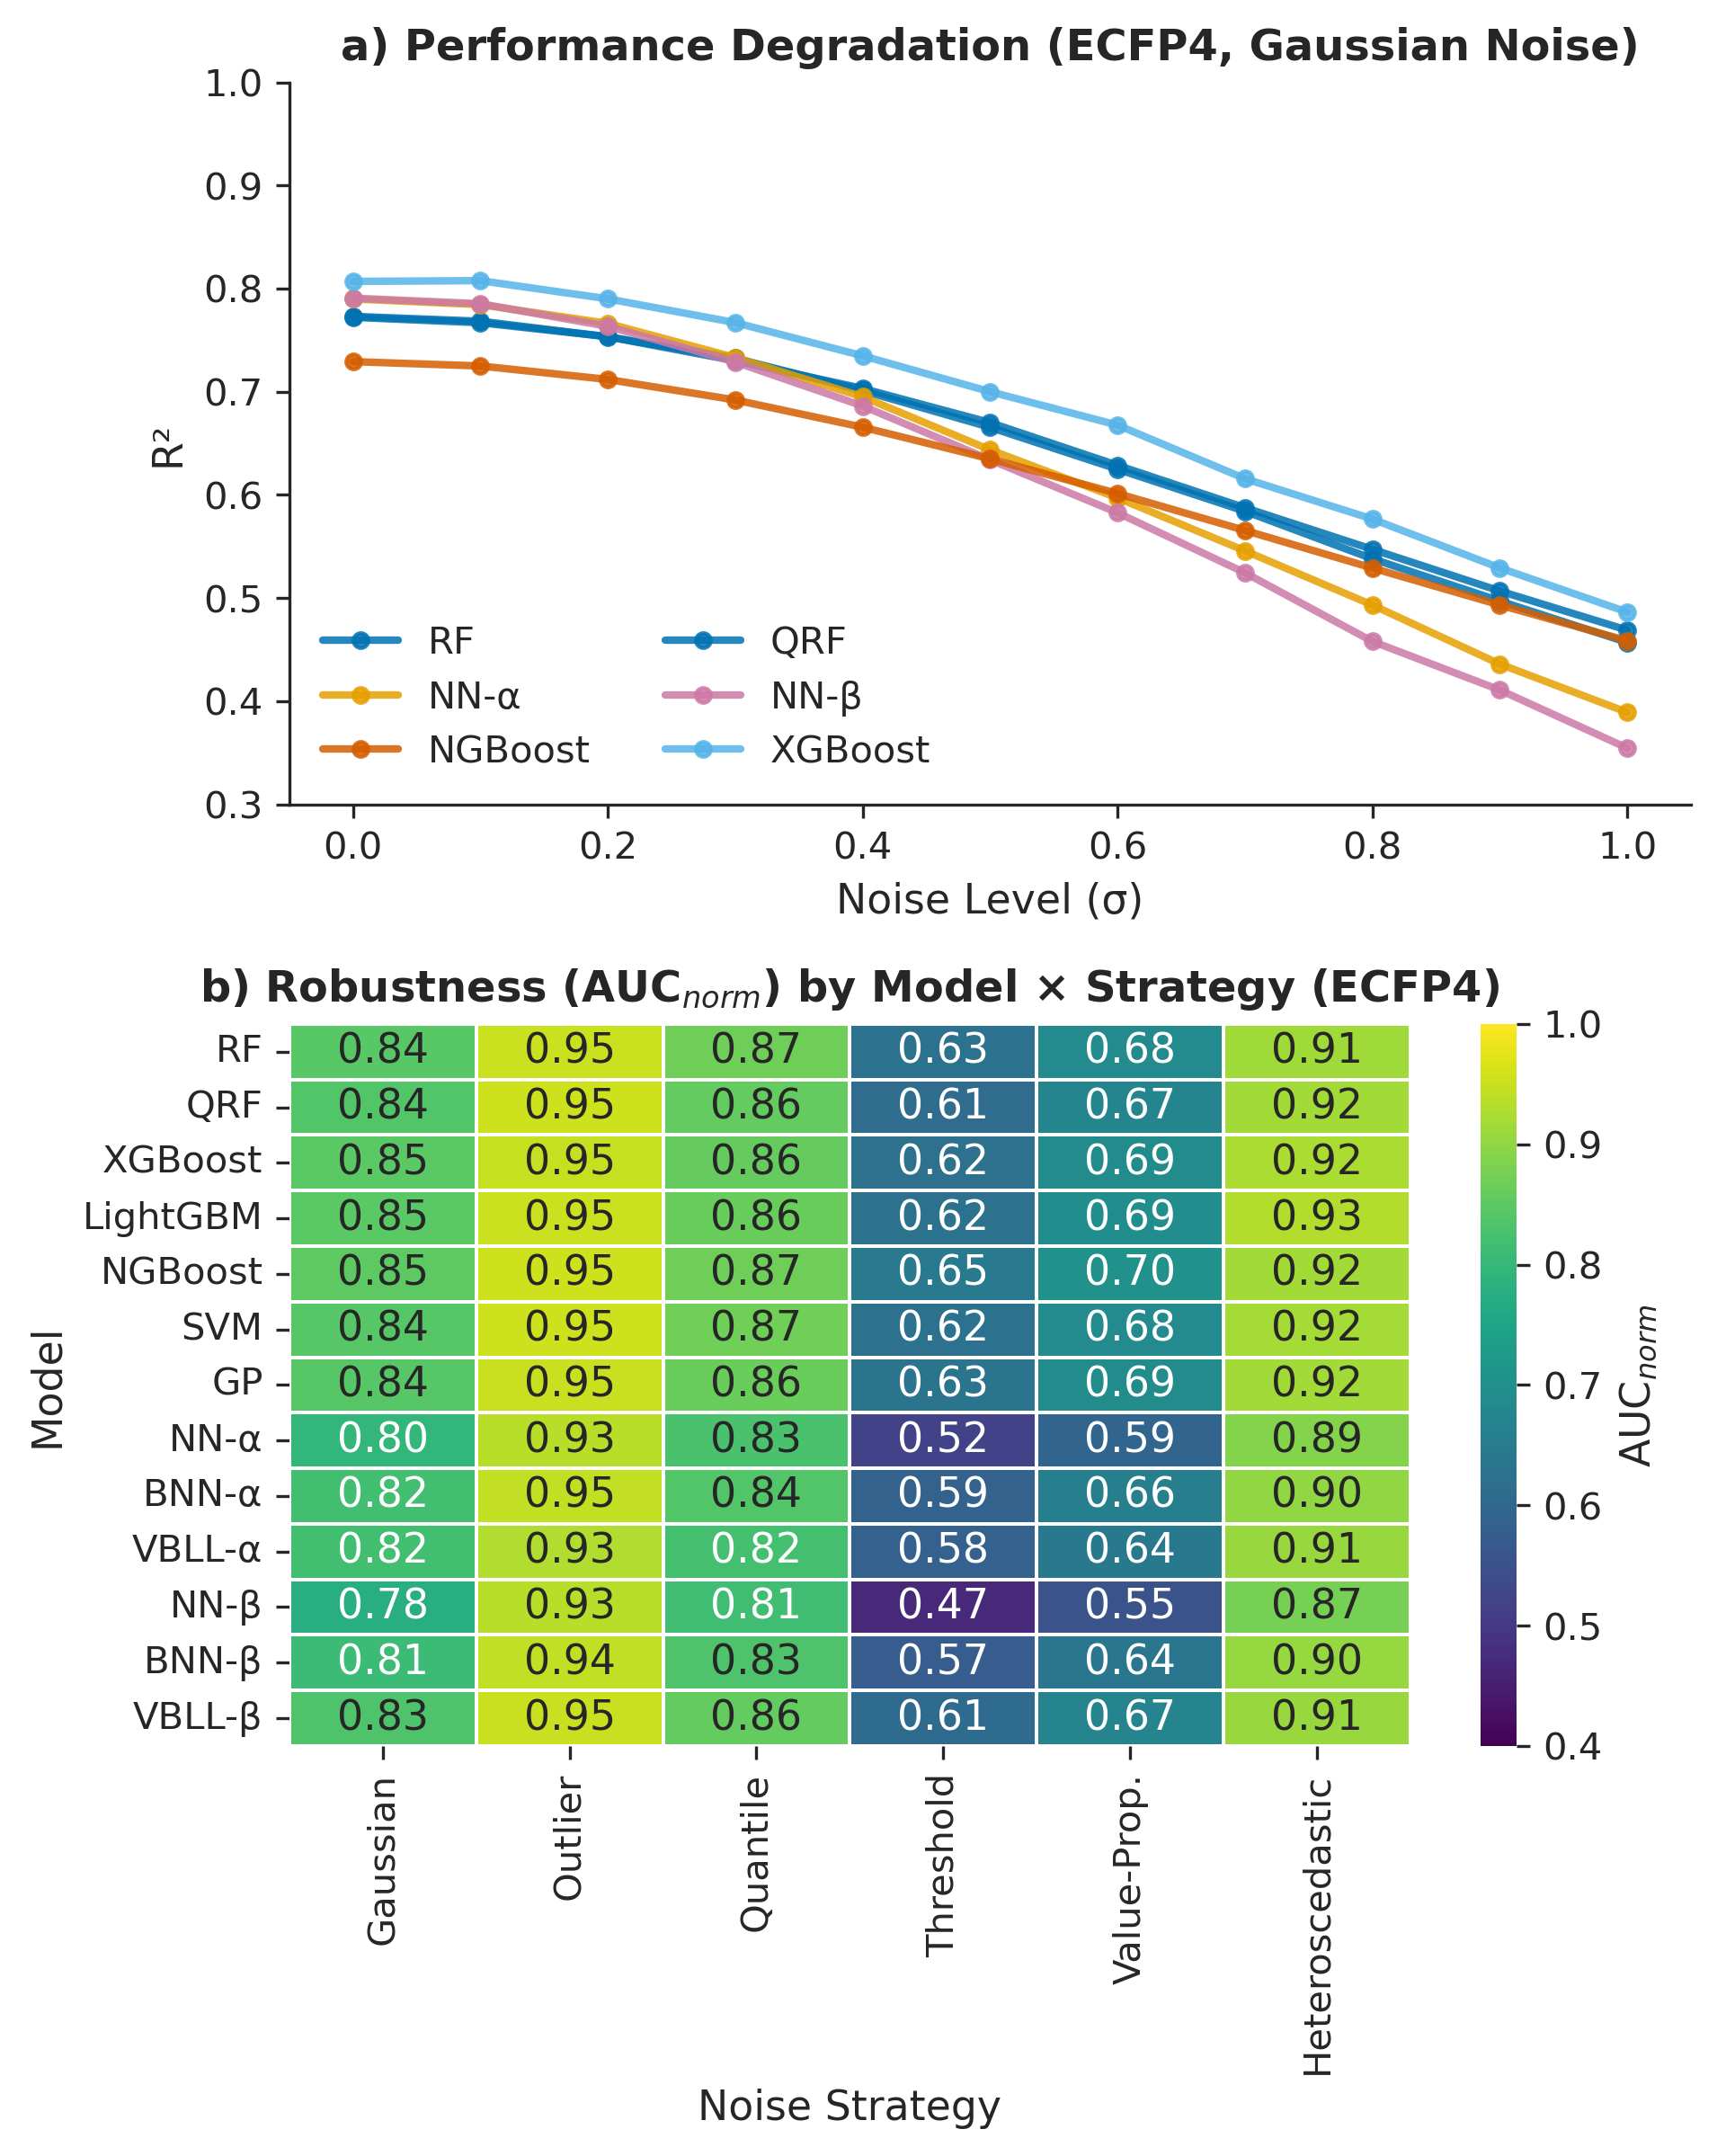
\includegraphics[width=\textwidth,height=0.78\textheight,keepaspectratio]{fig1_supp_ecfp4_overview.png}
\caption{\textbf{Global overview of noise robustness on the ECFP4 representation, evaluated on QM9 HOMO--LUMO gap.}
a) Performance degradation curves (R$^2$ versus noise level $\sigma$) under Gaussian noise. b) Noise degradation slope (NDS) heatmap across model architectures and noise strategies; lower (more negative) NDS indicates faster degradation under noise.}
\label{app:noise:ecfp4_overview}
\end{figure}


\addfile{Clean $R^2$ against robustness on PDV under Gaussian noise}
\label{app:noise:sec:clean_r2_vs_robustness}
% TODO: review, needs manual review
Clean-label $R^2$ against the noise degradation slope for every model on PDV under Gaussian noise, on the QM9 HOMO--LUMO gap.
% Thesis appendix item: clean_r2_vs_robustness

\begin{figure}[H]
\centering
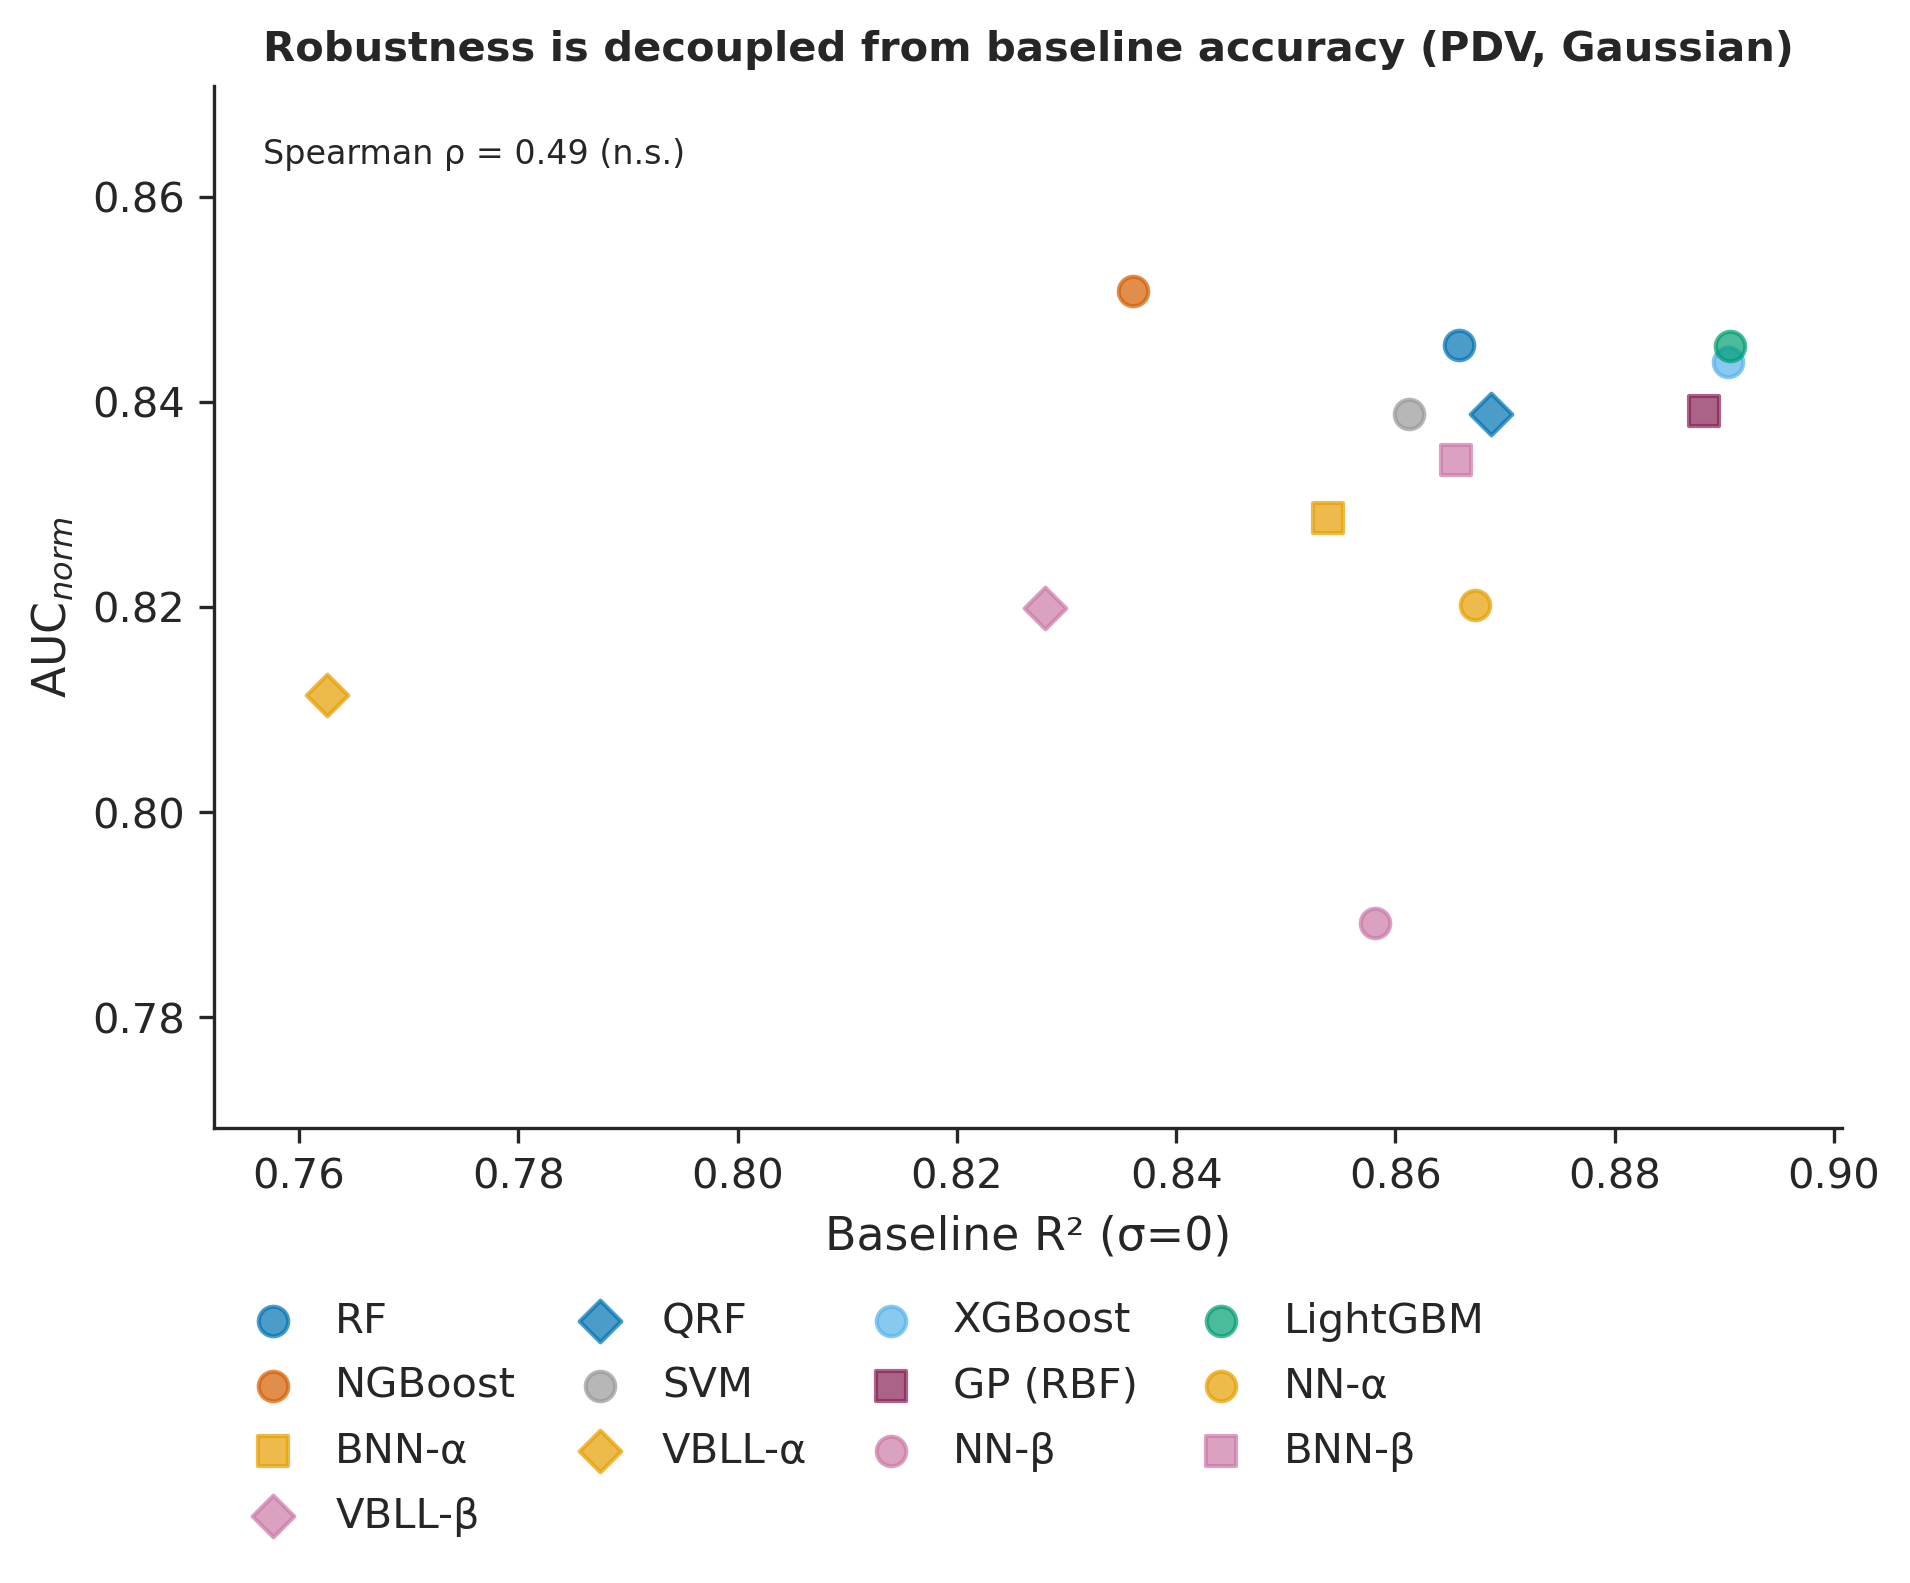
\includegraphics[width=\textwidth]{fig3_ranking_consistency.png}
\caption{\textbf{Baseline R$^2$ versus noise degradation slope (NDS) scatter for all models on the physicochemical descriptor vector (PDV) representation under Gaussian noise, on the QM9 HOMO--LUMO gap.}
Lower (more negative) NDS indicates faster performance loss under noise.}
\label{app:noise:clean_r2_vs_robustness}
\end{figure}


\addfile{Bayesian transformation effects by representation}
\label{app:noise:sec:bayesian_transformation_tests}
% TODO: review, needs manual review
The effect of each Bayesian transformation of the neural networks on the noise degradation slope, by representation, on the QM9 HOMO--LUMO gap.
% Thesis appendix item: bayesian_transformation_tests

\begin{table}[H]
\centering
\caption{\textbf{Neural network Bayesian transformation effects on noise degradation slope (NDS) by representation, on the QM9 HOMO--LUMO gap.}
Positive $\Delta$ NDS indicates the Bayesian variant is more robust (less negative slope) than its deterministic counterpart.}
\label{app:noise:bayesian_transformation_tests}
\small
\begin{tabular}{llrrrr}
\toprule
\textbf{Model} & \textbf{Representation} & \textbf{Baseline R$^2$} & \textbf{NN-$\beta$ NDS} & \textbf{BNN-$\beta$ NDS} & \textbf{$\Delta$ NDS} \\
\midrule
NN-$\beta$ & ECFP4 & 0.791 & $-0.464$ & $-0.388$ & $+0.076$ \\
NN-$\beta$ & PDV & 0.858 & $-0.487$ & $-0.382$ & $+0.106$ \\
NN-$\beta$ & SMILES & 0.721 & $-0.558$ & $-0.365$ & $+0.193$ \\
\bottomrule
\end{tabular}
\end{table}


\addfile{Uncertainty metrics for probabilistic models on ECFP4}
\label{app:noise:sec:uncertainty_metrics_ecfp4}
% TODO: review, needs manual review
Uncertainty metrics of the probabilistic models on ECFP4 under Gaussian noise, on the QM9 HOMO--LUMO gap.
% Thesis appendix item: uncertainty_metrics_ecfp4

\begin{table}[H]
\centering
\caption{\textbf{Uncertainty quantification metrics for probabilistic models on the ECFP4 representation (Gaussian noise strategy) on the QM9 HOMO--LUMO gap.}
Unc-Error $\rho$: Spearman correlation between predicted uncertainty and absolute prediction error. Unc-Noise $\rho$: Spearman correlation between predicted uncertainty and injected noise level $\sigma$. ECE: expected calibration error (lower = better-calibrated). Coverage targets: 68\% ($1\sigma$), 95\% ($2\sigma$).}
\label{app:noise:uncertainty_metrics_ecfp4}
\small
\begin{tabular}{lrrrrr}
\toprule
\textbf{Model} & \textbf{Unc-Error $\rho$} & \textbf{Unc-Noise $\rho$} & \textbf{ECE} & \textbf{Cov.\ $1\sigma$} & \textbf{Cov.\ $2\sigma$} \\
\midrule
\textbf{QRF}     & \textbf{0.25} & 0.27 & 0.19 & 74.7\% & 94.6\% \\
\textbf{NGBoost} & 0.22 & \textbf{0.37} & \textbf{0.11} & 69.2\% & 94.2\% \\
GP               & 0.18 & 0.34 & 0.23 & 78.6\% & 96.0\% \\
BNN-$\beta$      & 0.20 & 0.37 & 0.29 & 78.6\% & 95.2\% \\
BNN-$\alpha$     & 0.15 & 0.32 & 0.24 & 76.6\% & 95.1\% \\
VBLL-$\beta$     & 0.19 & 0.34 & 0.19 & 73.9\% & 95.5\% \\
VBLL-$\alpha$    & 0.11 & 0.31 & 0.22 & 74.5\% & 95.1\% \\
\bottomrule
\end{tabular}
\end{table}


\addfile{Variance decomposition on the three assay datasets}
\label{app:noise:sec:assay_variance_decomposition}
% TODO: review, needs manual review
ANOVA variance decomposition ($\eta^2$, in per cent) on LogD, Caco-2 efflux and hERG $K_i$.
% Thesis appendix item: assay_variance_decomposition

\begin{figure}[H]
\centering
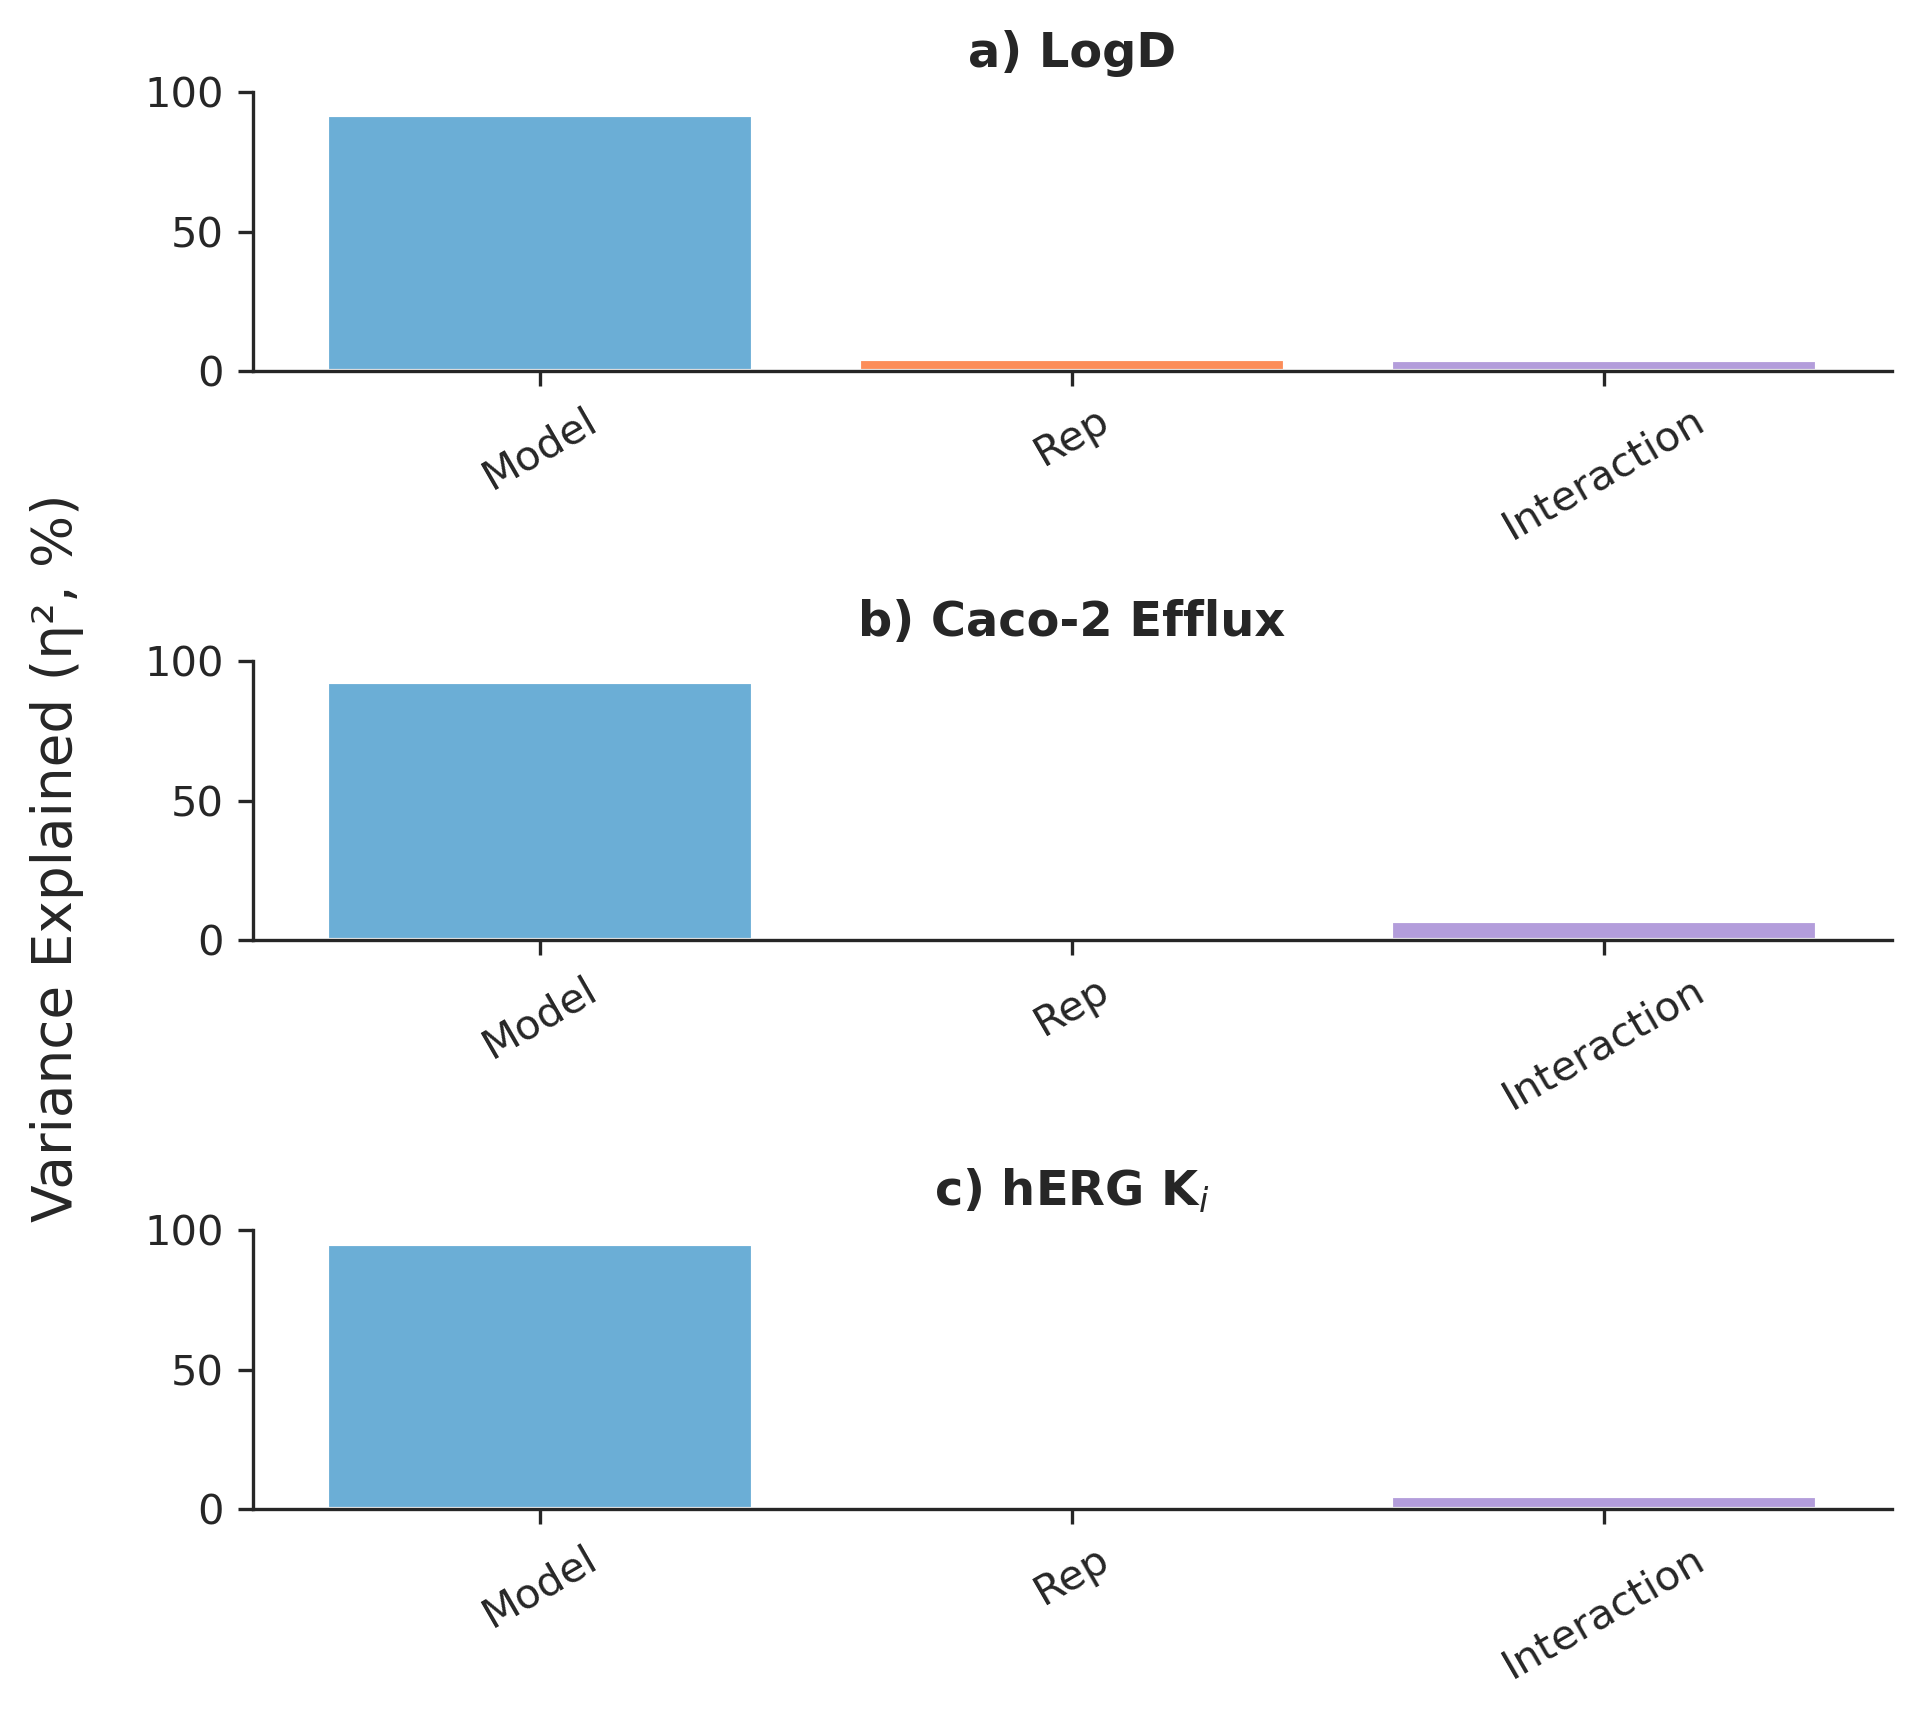
\includegraphics[width=\textwidth]{fig_validation_anova.png}
\caption{\textbf{ANOVA variance decomposition ($\eta^2$, \%) on external validation datasets: a) LogD, b) Caco-2 Efflux, and c) hERG K$_i$.}
Model, representation, and interaction contributions to noise degradation slope (NDS) variance for each dataset; lower (more negative) NDS indicates faster performance loss under noise.}
\label{app:noise:assay_variance_decomposition}
\end{figure}


\addfile{Random forest against quantile regression forest on the three assay datasets}
\label{app:noise:sec:rf_vs_qrf_assay}
% TODO: review, needs manual review
The noise degradation slope of random forest and of quantile regression forest on LogD, Caco-2 efflux and hERG $K_i$.
% Thesis appendix item: rf_vs_qrf_assay

\begin{table}[H]
\centering
\caption{\textbf{Random forest (RF) vs quantile regression forest (QRF) noise degradation slope (NDS) on the three external validation datasets (LogD, Caco-2 Efflux, hERG K$_i$).}
Lower (more negative) NDS indicates faster degradation under noise.}
\label{app:noise:rf_vs_qrf_assay}
\small
\begin{tabular}{lrrr}
\toprule
\textbf{Dataset} & \textbf{RF NDS} & \textbf{QRF NDS} & \textbf{$\Delta$ NDS} \\
\midrule
ChEMBL-hERG-Ki     & $-0.231$ & $-0.359$ & $-0.128$ \\
OpenADMET-Caco2    & $-0.534$ & $-0.627$ & $-0.094$ \\
OpenADMET-LogD     & $-0.101$ & $-0.185$ & $-0.083$ \\
\bottomrule
\end{tabular}
\end{table}


\section{The flaws of the similarity assumption}\label{app:add:flaws}
% ---- NOTES: The flaws of the similarity assumption ----
% - Files for Chapter~\ref{chap:flaws}.
% Table: constant features. One row is one dataset and one representation. Columns: total features; constant features; near-constant features. A per-domain summary stays in Chapter 4.
% TODO(results): constant and near-constant feature counts per dataset and representation.
% Table: molecules a representation cannot tell apart. One row is one representation and one dataset. Columns: molecules in groups with an identical feature vector; how many of those differ only in stereochemistry; lowest RMSE reachable when every group gets one prediction; largest label spread within a group.
% TODO(results): identical-vector counts per representation and dataset.
% Table: distance against property difference. One row is one dataset and one representation. Columns: rank correlation between pairwise distance and absolute property difference; score of predicting each molecule's activity from its five nearest neighbours in that representation.
% TODO(results): distance-property correlations and five-nearest-neighbour scores.
% Table: activity cliffs. One row is one dataset and one representation. Column: molecules that belong to at least one activity cliff.
% TODO(results): activity-cliff counts per dataset and representation.
% ---- END NOTES ----
\todo[inline, color=orange!40]{Additional files for Chapter~\ref{chap:flaws}: all four need the full runs.}

\section{Building adaptive hybrid representations}\label{app:add:method}\label{app:searchspace}
% ---- NOTES: Building adaptive hybrid representations ----
% - Files for Chapter~\ref{chap:method}.
% - The settings, formulas and reasons are in Chapter 5 ("The search space and why each axis is swept", its three subsubsections, "Augmentation", "Fast tier and adaptive pruning"). This section holds only the reference tables those sections point to.
% - The first five files below are written from the current code and the design runs. The rest need the full runs.
% - Which datasets get the Gaussian process, and why: only in "Models and metrics". The model-settings and models-left-out files point there and do not repeat it. Whether nanobody thermostability also gets the Gaussian process is an open decision under "Search tier settings"; the Gaussian process row of the models-left-out file follows that answer.
% - The models fitted only to compute importance are in the table under "Feature importance scoring". The model-settings file points there and does not repeat them.
% - Two open decisions change the model-settings file: the random forest evaluator's features per split on regression datasets, and the DNN evaluator's early-stopping split (both under "Internal evaluation"). The file states the current settings; change the row if either answer is yes.
% - The open decision under "Models and metrics" (count the whole dataset or the training molecules) changes the SVM row of the models-left-out file for LogD and TATA promoter. The file carries a footnote; change it to match the answer.
% - The design-experiment file: the reason the kept pooled allocation method was chosen over the other pooled candidates is an open decision under "Feature allocation strategies". The allocation row states only the counts; add the reason once it is written there. The pooled candidates that were not kept are not named.
% - The design-experiment file: the representation-count row gives no result; the best count per (model, budget) was not carried into the notes. Add it from the design run, or leave the cell as it is.
%
% TODO(results): per dataset and downstream model, per-fold score of the best single representation against the hybrid, with the spread across folds.
% TODO(results): per dataset, the winning configuration: downstream model, budget, allocation method, importance method, internal evaluator, representation count.
% TODO(results): per dataset, how often each value of each setting won across (downstream model, budget) combinations.
% TODO(results): augmentation per dataset: how often no extra features were chosen; per-fold base against base plus extras, uncapped and capped; which extra feature sets were kept; decoy features admitted.
% TODO(results): per dataset and budget, held-out score against the score the inner search reported, and the stability of the selected features across folds.
% TODO(results): hybrid minus each comparator (concatenation, one model per representation, PCA, mRMR, recursive feature elimination, random features) at each budget.
% TODO(results): the smaller experiments in "Comparators, controls and ablations", one table each, if they leave the chapter.
% TODO(results): per task, outcome of the transfer, antibody-scan and separate-site experiments, with which representations the selected features came from.
% TODO(results): hours and model fits per dataset at each tier, with the hardware.
% ---- END NOTES ----

\addfile{Settings of every model, as downstream model and as internal evaluator}
\label{app:add:model_settings}
% TODO: review, needs manual review
One row is one model. The middle two columns give its settings when it scores a hybrid (downstream model) and when it scores one representation inside the search (internal evaluator). The models fitted only to compute feature importance are in Table~\ref{tab:importance_methods}.

% TODO: review, needs manual review (whole table and caption, written from the current code)
{\small
\begin{longtable}{@{}p{1.9cm}p{4.6cm}p{3.6cm}p{1.6cm}p{2.3cm}@{}}
\caption{Settings of every model. $p$ is the number of features. ``Molecules'' is the number of training molecules the internal evaluator is fitted on; above it, a random subset of that size is drawn with a fixed seed. Settings not listed are the library's defaults. Every setting is the same on every dataset. The Gaussian process runs only on the datasets named in Chapter~\ref{chap:method}, ``Models and metrics''.}
\label{tab:add:model_settings}\\
\toprule
Model & As downstream model & As internal evaluator & Molecules & Library; source \\
\midrule
\endfirsthead
\toprule
Model & As downstream model & As internal evaluator & Molecules & Library; source \\
\midrule
\endhead
Random forest & 100 trees, no depth limit; $\sqrt{p}$ features tried at each split & 50 trees, depth at most 10; all $p$ features tried at each split on regression, $\sqrt{p}$ on classification & all & scikit-learn \citep{scikit-learn}; \citet{Breiman2001} \\
\addlinespace
LightGBM & 100 trees & 50 trees, depth at most 4 & all & lightgbm; \citet{ke2017lightgbm} \\
\addlinespace
XGBoost & 100 trees; half of the features sampled for each tree & 50 trees, depth at most 4 & all & xgboost; \citet{Chen2016} \\
\addlinespace
SVM & RBF kernel, $C = 1$. Not fitted above 10{,}000 molecules, or above 5{,}000 under uncapped augmentation & RBF kernel, $C = 1$ & at most 500 & scikit-learn; \citet{Vapnik1995} \\
\addlinespace
Gaussian process & Regression: RBF plus white-noise kernel, labels normalised, 3 optimiser restarts. Classification: RBF kernel. Not fitted above 1{,}000 molecules & Regression: scaled RBF kernel, fixed noise variance 0.01, no restarts. Classification: scaled RBF kernel, no restarts & at most 500 & scikit-learn; \citet{Rasmussen2006} \\
\addlinespace
DNN & Hidden layers of 256, 128 and 64 units, ReLU, dropout 0.2 \citep{Srivastava2014}; Adam \citep{Kingma2015} at learning rate 0.001, halved after 5 epochs without improvement; batch size 256; up to 200 epochs; stops after 20 epochs without improvement on 20\% of the training molecules that share no group with the rest, using the outer split's grouping; labels z-normalised & The same, except that the early-stopping 20\% is drawn at random & all & PyTorch \citep{Paszke2019} \\
\bottomrule
\end{longtable}
}

\addfile{Downstream models left out, by dataset and augmentation setting}
\label{app:add:models_left_out}
% TODO: review, needs manual review
One row is one rule that leaves a downstream model out. Only the 16 datasets of Table~\ref{tab:datasets} are listed; a dataset and setting not named in any row runs every downstream model in Table~\ref{tab:search_tiers}.

% TODO: review, needs manual review (whole table and caption, written from the current code)
{\small
\begin{longtable}{@{}p{2.4cm}p{3.0cm}p{8.6cm}@{}}
\caption{Downstream models left out, by dataset and augmentation setting. Every rule was set so that a search finishes within the time limit of one job; none was set from scores. hERG $K_i$ drops no model under any setting.}
\label{tab:add:models_left_out}\\
\toprule
Model left out & Augmentation setting & Datasets \\
\midrule
\endfirsthead
\toprule
Model left out & Augmentation setting & Datasets \\
\midrule
\endhead
XGBoost & all three & H3K4me3, TATA promoter \\
SVM & all three & datasets above 10{,}000 molecules: H3K4me3 \\
SVM & uncapped & datasets above 5{,}000 molecules: QM9, LogD$^{a}$, TATA promoter$^{a}$ \\
SVM & uncapped & Koenig expression \\
SVM & capped & Caco-2 efflux, LogD, rat liver microsome clearance, MDR1--MDCK efflux, Buchwald--Hartwig plates \\
Random forest and SVM & capped & QM9 \\
Random forest & uncapped & QM9, LogD \\
Gaussian process & all three & every dataset except humanness (Chapter~\ref{chap:method}, ``Models and metrics'') \\
\bottomrule
\end{longtable}
{\footnotesize $^{a}$Counted on the whole dataset: LogD has 5{,}028 molecules and TATA promoter 5{,}274. A search run inside one outer fold is given about 80\% of them and keeps the SVM.}
}

\addfile{Size of the search}
\label{app:add:search_size}
% TODO: review, needs manual review
One row is one downstream model. The counts are per dataset, objective and augmentation setting, with adaptive pruning off.

% TODO: review, needs manual review (whole table and caption)
\begin{table}[htbp]
\centering
\small
\caption{Number of configurations searched per dataset, objective and augmentation setting. A configuration is one choice of downstream model, internal evaluator, allocation method, importance method, representation count and budget. At the full tier each (downstream model, internal evaluator) pair runs 5 allocation methods $\times$ 3 importance methods $\times$ 4 representation counts $\times$ 8 budgets $= 480$ configurations; at the fast tier it runs $3 \times 1 \times 2 \times 8 = 48$ (Table~\ref{tab:search_tiers}). ``Matched'' is counted once where it repeats an evaluator already in the list. Each configuration is scored on 5 folds, so the full tier fits a downstream model 40{,}800 times (50{,}400 on humanness) and the fast tier 4{,}080 times. Where a dataset leaves a downstream model out (Additional file~\ref{app:add:models_left_out}), its pairs drop out: a fast search on H3K4me3 has 9 pairs, so 432 configurations.}
\label{tab:add:search_size}
\begin{tabular}{@{}lp{4.2cm}rr@{}}
\toprule
Downstream model & Internal evaluators & Full tier & Fast tier \\
\midrule
Random forest & 3 (matched is random forest) & 1{,}440 & 144 \\
LightGBM & 3 (matched is LightGBM) & 1{,}440 & 144 \\
DNN & 3 (matched is DNN) & 1{,}440 & 144 \\
XGBoost & 4 & 1{,}920 & 192 \\
SVM & 4 & 1{,}920 & 192 \\
Gaussian process (humanness only) & 4 & 1{,}920 & not run \\
\midrule
Total & 17 pairs (21 on humanness) & 8{,}160 (10{,}080 on humanness) & 816 \\
\bottomrule
\end{tabular}
\end{table}

\addfile{Design experiments behind the search settings}
\label{app:add:design_experiments}
% TODO: review, needs manual review
One row is one setting of the search, or one rule that was tested and then fixed instead of searched. Every number comes from preliminary design runs made before the main experiments; they are not results of the thesis, and several used other budgets than the final search.

% TODO: review, needs manual review (whole table and caption; numbers from preliminary design runs)
{\footnotesize
\begin{longtable}{@{}p{1.9cm}p{2.5cm}p{2.7cm}p{4.4cm}p{2.5cm}@{}}
\caption{Design experiments behind the search settings. Preliminary design runs, not the thesis's full runs.}
\label{tab:add:design_experiments}\\
\toprule
Setting & Values compared & Datasets, folds, budgets & What was measured, and the result & Values kept (full / fast) \\
\midrule
\endfirsthead
\toprule
Setting & Values compared & Datasets, folds, budgets & What was measured, and the result & Values kept (full / fast) \\
\midrule
\endhead
Downstream model & Nine models, among them random forest, LightGBM, XGBoost, CatBoost, DNN, $k$-nearest neighbours and a Gaussian process, each on each of 10 base representations at full width & Buchwald--Hartwig yield, Caco-2 efflux, Koenig expression, LogD, breast cancer PAM50 subtype; 5 folds & Best held-out score over the 10 representations, and seconds per fit. The DNN scored best on 4 of the 5 datasets and third on Caco-2 (0.2936 against 0.2851 RMSE, log$_{10}$ efflux ratio) & Full: random forest, LightGBM, XGBoost, SVM, DNN, and the Gaussian process on humanness / fast: the same five \\
\addlinespace
Budget & None compared & -- & -- & 10, 25, 50, 100, 250, 500, 1{,}000 and 2{,}000 features at both tiers \\
\addlinespace
Representation count & 2, 3, 5 and all 10 & 9 datasets, 3 tree-ensemble downstream models, budgets 500 and 1{,}000 features; 5 folds & The best count for each (downstream model, budget) combination & Full: 2, 3, 5, all / fast: 3, all \\
\addlinespace
Allocation method & 8 candidates: the five searched and 3 further pooled candidates, each at every representation count & The same 9 datasets, models and budgets: 54 (dataset, model, budget) combinations & Each candidate was scored at its best representation count, and the number of combinations in which it was in the top 3 of the 8 was counted. Fixed shares: linear 30, squared 27, rank decay 26, softmax 25; global pool with squared weights 14 & Full: the five in Table~\ref{tab:allocation_methods} / fast: linear, squared, rank decay \\
\addlinespace
Importance method, agreement & 8 methods & LogD, hERG $K_i$, Buchwald--Hartwig yield, nanobody thermostability, antibody FcRn retention, breast cancer PAM50 subtype, lung adenocarcinoma vs squamous; each method fitted once on the whole dataset & Spearman correlation between two methods' scores over every feature. Kept pairs: LightGBM gain and TreeSHAP 0.20--0.64, LightGBM gain and DeepLIFT 0.21--0.67, TreeSHAP and DeepLIFT 0.56--0.99 across the 7 datasets & One method kept from each group whose rankings agree above 0.95 \\
\addlinespace
Importance method, score & 28 methods, among them three controls: feature variance, Laplacian score and random ranking & Caco-2 efflux; 3 folds; budget 100 features; random forest and LightGBM downstream & RMSE of the best single representation minus RMSE of the hybrid (log$_{10}$ efflux ratio; positive means the hybrid has the lower error): DeepLIFT $+0.0144$, LightGBM gain $+0.0100$, TreeSHAP $+0.0067$, random ranking $-0.0118$ & Full: LightGBM gain, TreeSHAP, DeepLIFT / fast: LightGBM gain \\
\addlinespace
Internal evaluator settings & 20 hyperparameter settings from 5 model families & Buchwald--Hartwig yield, Caco-2 efflux, Koenig expression; 3 folds; budget 100 features & Spread of mean scores across all 20 settings: 0.0253 $R^2$, 0.0179 $R^2$ and 0.0085 Spearman. Median standard deviation across the 3 folds for one setting, allocation method and downstream model: 0.0462 $R^2$, 0.0693 $R^2$ and 0.0186 Spearman & Matched, random forest, LightGBM and DNN, at fixed settings, both tiers \\
\addlinespace
Rescaling of each representation's score (a rule) & 5 rescalings & 9 datasets; 5 folds; budgets 50 and 300 features & Whether any rescaling beat the one in use by more than that rule's own spread across folds: in 0 of 90 (dataset, allocation method, budget) combinations & One fixed rule per metric (Table~\ref{tab:standalone-rescaling}) \\
\bottomrule
\end{longtable}
{\footnotesize The representation-count and allocation rows come from one design run on 10 datasets, 3 downstream models and 2 budgets (60 combinations); QM9 is left out, which gives the 54.}
}

\addfile{Fields a blueprint saves}
\label{app:add:blueprint_fields}
% TODO: review, needs manual review
One row is one field. The first block is the recipe that rebuilds a hybrid; the second is kept for inspection and is not read by a rebuild.

% TODO: review, needs manual review (whole table and caption, written from the current code)
{\small
\begin{longtable}{@{}p{4.6cm}p{9.4cm}@{}}
\caption{Fields a blueprint saves. The stored score of each representation is its best score on its own across the downstream models, over every molecule the search ran on. It is not the internal-evaluator score that splits the budget, which a rebuild computes again on the molecules it is given. Three further fields are read only by allocation or augmentation routes outside the thesis's search and are fixed: a minimum improvement a whole block of extra features must show (none), a number of features taken from each source (20), and a step size (5).}
\label{tab:add:blueprint_fields}\\
\toprule
Field & What it holds \\
\midrule
\endfirsthead
\toprule
Field & What it holds \\
\midrule
\endhead
\multicolumn{2}{@{}l}{\textit{The recipe}} \\
\midrule
Representations & The representations offered to the search \\
Representation count & How many of them the configuration used; empty when it used all \\
Allocation method & One of the five in Table~\ref{tab:allocation_methods} \\
Importance method & LightGBM gain, TreeSHAP or DeepLIFT \\
Budget & Number of features in the hybrid \\
Internal evaluator & Matched, random forest, LightGBM or DNN \\
Objective & Predictive, or predicting each molecule's activity from its five nearest neighbours \\
Metric & The dataset's metric, and whether lower is better \\
Task type & Regression or classification \\
Folds and seed & The number of folds, and the random seed \\
\midrule
\multicolumn{2}{@{}l}{\textit{The recipe: augmentation}} \\
\midrule
Augmentation setting & None, uncapped or capped \\
Candidate ranking & How candidate extra features are ranked \\
Candidate list length & 50 features \\
Cap per source & Optional; the most candidates taken from one source \\
Margin & How much better than adding none a block of extra features must score \\
Fraction of the budget & Optional; used instead of the fixed block sizes \\
\midrule
\multicolumn{2}{@{}l}{\textit{Kept for inspection, not read by a rebuild}} \\
\midrule
Representation scores & Each representation's best score on its own across the downstream models, sign flipped for metrics where lower is better \\
Features per representation & The number of features each representation got in each fold \\
Extra features kept & The extra features augmentation kept in each fold, by source \\
\bottomrule
\end{longtable}
}

\todo[inline, color=orange!40]{Additional files for Chapter~\ref{chap:method}: the per-dataset results, augmentation, held-out against inner-search scores, comparators, smaller experiments, transfer experiments and compute need the full runs.}

\section{Hybrid representations for similarity and label noise}\label{app:add:similarity}
% ---- NOTES: Hybrid representations for similarity and label noise ----
% - Files for Chapter~\ref{chap:similarity}.
% - The chapter's own two tables (noise conditions, and the twelve LNL methods) stay in the chapter. The settings file below gives each method's numbers; the chapter's table gives what each method does.
% Table: finding injected noisy labels. One row is one noise score. Columns: average precision under outlier noise at 1\%, 5\% and 10\%, grouped-wider noise and censoring, in each feature space (each model's top two single representations, the same features weighted by importance, forest proximity, the hybrid, the hybrid ranked on the neighbour score); chance level in the header row. The chapter's table keeps only 10\% outlier noise, grouped-wider noise and censoring in two feature spaces.
% TODO(results): average precision per noise score, feature space and noise condition, all outlier levels, with chance level.
% Table: finding real suspect labels. One row is one noise score and feature space. Columns: average precision against ChEMBL curator flags on hERG IC50, per record and per molecule, with chance level; Spearman correlation with the spread between laboratories on the BindingDB molecules with repeat measurements.
% TODO(results): average precision against curator flags and correlation with the spread between laboratories, per noise score and feature space.
% Table: estimated noise size. One row is one dataset and feature space. Columns: the estimate from repeat measurements (with the directly measured variance between repeats where the dataset keeps them); the estimate from near-duplicate pairs; the gamma-test estimate; the model's held-out mean squared error. All in label units squared.
% TODO(results): the three noise-size estimates per dataset and feature space, beside the model's held-out mean squared error.
% TODO(results): per dataset and fold, importance-weighted against unweighted features for predicting each molecule's activity from its five nearest neighbours; the hybrid searched for that objective against the ordinary hybrid and the two best single representations.
% TODO(results): censoring: share of the lost score recovered, per treatment, model, feature space and clipping level; deleting clipped molecules against keeping them.
% TODO(results): the survey of twelve LNL methods: per noise level, the methods that beat the plain network on each input.
% TODO(results): cleaning real labels: folds won per cleaning method, noise score and feature space.
% TODO(results): per noise type, whether any LNL method, noise mitigation or noise-robust training, improved on the untreated model, on each feature space.
% ---- END NOTES ----

\addfile{Settings of the twelve LNL methods and the plain network they share}
\label{app:add:lnl_settings}
% TODO: review, needs manual review
One row is one method; the first row is the plain network every method starts from. The kind of each method follows Table~\ref{tab:lnl_methods}.

% TODO: review, needs manual review (whole table and caption, written from the current code)
{\small
\begin{longtable}{@{}p{2.9cm}p{2.0cm}p{7.3cm}p{1.6cm}@{}}
\caption{Settings of the twelve LNL methods. On classification datasets the squared-error loss is replaced by cross-entropy.}
\label{tab:add:lnl_settings}\\
\toprule
Method & Kind & Settings & Labels \\
\midrule
\endfirsthead
\toprule
Method & Kind & Settings & Labels \\
\midrule
\endhead
Plain network & -- & Hidden layers of 256, 128 and 64 units, ReLU, dropout 0.2; Adam at learning rate 0.001, halved after 5 epochs without improvement; batch size 256; gradient norm clipped at 1; up to 200 epochs; stops after 20 epochs without improvement on 20\% of the training molecules held out by scaffold group (drawn at random after a method has removed molecules); labels z-normalised & both \\
\midrule
Small-loss selection & noise mitigation & 10 warm-up epochs on all molecules; keeps the 70\% with the smallest loss and fits a new plain network on them & both \\
Confident learning & noise mitigation & 3 plain networks; removes molecules whose error is above the 85th percentile and whose spread across the 3 networks is below the 25th percentile, then refits & both \\
Removal by distance to neighbours & noise mitigation & 10 nearest neighbours in the standardised features; score is the distance of a label from its neighbours' mean label, divided by their standard deviation (on classification, the share of neighbours with another label); removes molecules above the 85th percentile, then refits & both \\
Staged removal & noise mitigation & 3 stages; each removes the 10\% of the remaining molecules with the largest training loss & both \\
\midrule
Per-epoch down-weighting & noise-robust training & After each epoch, the weight of every molecule whose loss is above the median is multiplied by 0.95 & both \\
Curriculum by confidence & noise-robust training & 20 warm-up epochs, then trains on the 25\%, 50\%, 75\% and 100\% of molecules with the smallest loss, in stages & both \\
DivideMix & noise-robust training & Two networks, 10 warm-up epochs; a two-component Gaussian mixture on each network's squared errors splits the molecules & both \\
Meta-Weight-Net & noise-robust training & The weighting network is updated every 5 epochs at learning rate 0.001, on 20\% of the training molecules held out for it & both \\
MentorNet & noise-robust training & The mentor network reads each molecule's current loss, its last 5 losses and its mean distance to its 10 nearest neighbours & both \\
Contrast to Divide & noise-robust training & 5 perturbed copies of each molecule, Gaussian noise of standard deviation 0.01 on the features & both \\
\midrule
Heteroscedastic GP & noise-robust training & RBF kernel, 2 optimiser restarts, fitted on at most 1{,}000 training molecules; a small network predicts each molecule's noise variance & regression \\
Deep evidential regression & noise-robust training & Weight of the evidence penalty 0.01 & regression \\
\bottomrule
\end{longtable}
}

\todo[inline, color=orange!40]{Additional files for Chapter~\ref{chap:similarity}: finding injected and real noisy labels, estimated noise size and the other results need the full runs.}
\chapter{Data and code availability}\label{app:availability}
% TODO: needs manual review (whole chapter written by Claude)
% ---- NOTES: Data and code availability ----
% Decision for you: the author contributions now appear twice, in the Statement of Originality and in the last paragraph below. Keep both and they must stay word for word the same; keep one and point to it from the other. The two differ in one sentence now: "All authors read and approved the final manuscript" is in your paper and below, but not in the Statement of Originality.
% Decision for you: whether the contributions paragraph below also says A.P. wrote the QM9 pipeline. Your paper names only NoiseInject, so the sentence below now matches the paper. Every commit in the qsar_qm_models repository is yours, so adding it would be accurate.
% Decision for you: the licence for KIRBy. Your earlier plan was MIT or Apache-2.0. The repository has no licence file and is private, so the KIRBy block has placeholders, and the last sentence of the second data paragraph holds only once it is public.
% Decision for you: whether to give each public dataset's licence, as a column in the dataset table of Appendix~\ref{app:datasets}. Now the text gives licences only for OpenADMET, ChEMBL and the Biogen set; QM9 has none stated. The reaction-yield, antibody, nucleotide and gene-expression licences depend on which copy was downloaded and were not checked.
% Decision for you: the Python version for KIRBy. The package metadata declares 3.8 or later. The repository's setup guide gives 3.9 as the minimum and recommends 3.10 to 3.11. The university cluster has 3.9. The software block below says 3.8 or later, as the package metadata declares, until you pick one.
% Decision for you: the licence of the QM9 pipeline release. The qsar_qm_models repository holds a GNU GPL v3 licence file, so the block below says GPL v3. Your earlier plan was MIT or Apache-2.0. Keep GPL v3, or change it; the licence line and the "restrictions to use by non-academics" line both follow from your choice.
% Decision for you: your NoiseInject paragraph (restored as you wrote it) says "six regression and six classification noise injection strategies". Chapter~\ref{chap:robustness} and Section~\ref{sec:noise_injection} now define seven noise conditions. Keep the package's own count, or change it to match the chapters.
% ---- END NOTES ----

% TODO: review, needs manual review
Three pieces of software lie behind this thesis. NoiseInject is the label-noise package released with Chapter~\ref{chap:robustness}. A separate pipeline ran the QM9 experiments of that chapter. The KIRBy repository implements the adaptive hybrid representation and holds the experiments of Chapters~\ref{chap:flaws}, \ref{chap:method} and~\ref{chap:similarity}, together with the assay-dataset runs of Chapter~\ref{chap:robustness}. The three are separate, so each can be reused on its own. For example, the hybrid search runs on feature matrices a reader has computed elsewhere, without the Rust part of the QM9 pipeline. The source and curation of each dataset are given in Appendix~\ref{app:datasets}.

The NoiseInject benchmarking framework, implementing all six regression and six classification noise injection strategies together with the robustness metrics (noise degradation slope and retention) and uncertainty-calibration metrics (ECE, coverage at $1\sigma$/$2\sigma$, mean interval width, and uncertainty--error / uncertainty--noise correlation) described in this work, is available as an open-source Python package under an MIT license \citep{noiseinject}. It also contains optional reference wrappers (a Gaussian process, split-conformal prediction, and Monte Carlo dropout) that produce per-sample uncertainty for use with these metrics. NoiseInject is model-agnostic, operates on label arrays (NumPy arrays or pandas Series), and is designed to integrate into existing cheminformatics or other data pipelines. Worked examples covering molecular-descriptor, fingerprint, and GNN-embedding workflows are provided in the repository.

% TODO: review, needs manual review
Its noise conditions and metrics are described in Section~\ref{sec:noiseinject}.

% TODO(you): the DOI archives v0.3.0 (3 June 2026), not 1.0.0; replace it once a 1.0.0 Zenodo release exists.
\begin{itemize}
    \item Project name: NoiseInject
    \item Project home page: \url{https://github.com/adpunt/noise_inject}
    \item Archived version: \url{https://doi.org/10.5281/zenodo.20532710}
    \item Version: 1.0.0
    \item Operating system(s): Platform independent
    \item Programming language: Python 3.7 or later
    \item Other requirements: NumPy, pandas, SciPy and scikit-learn; see the repository's \texttt{requirements.txt}
    \item License: MIT
    \item Any restrictions to use by non-academics: None
\end{itemize}

% TODO: review, needs manual review
The QM9 results of Chapter~\ref{chap:robustness} were produced by a separate repository, written in Python and Rust, which also holds the hyperparameter tuning, the variance decomposition and the figure scripts for that chapter. It is described in Chapter~\ref{chap:robustness}, under ``The QM9 precompute pipeline''. The three assay datasets of that chapter were run from the KIRBy repository, which calls NoiseInject directly.

% TODO(you): no release or Zenodo DOI yet; project name is the repository name until a release name is chosen. Confirm the operating systems it has been built on; Linux and macOS are assumed, not checked.
\begin{itemize}
    \item Project name: qsar\_qm\_models
    \item Project home page: \url{https://github.com/adpunt/qsar_qm_models}
    \item Archived version: not yet archived
    \item Operating system(s): Linux and macOS
    \item Programming language: Python and Rust (2021 edition)
    \item Other requirements: RDKit installed through conda, to which the Rust program links; PyTorch and PyTorch Geometric
    \item License: GNU GPL v3.0
    \item Any restrictions to use by non-academics: those of the GNU GPL v3.0
\end{itemize}

% TODO: review, needs manual review
The adaptive hybrid representation is implemented in the KIRBy repository. It is written in Python and works on feature matrices computed beforehand, so the hybrid search can be applied to representations from any domain. The repository contains the hybrid search itself: feature importance scoring, the allocation of a feature budget across representations, internal evaluation, and a store of every configuration evaluated for each dataset. It also contains loaders for the datasets in Appendix~\ref{app:datasets} and generators for the molecular, antibody, nucleotide, reaction and gene-expression representations. The neighbour-based similarity analyses, the learning-with-noisy-labels methods of Chapter~\ref{chap:similarity} and every experiment script are included as well. Label noise is added through NoiseInject, so the noise definitions are the same as in Chapter~\ref{chap:robustness}. A GPU is not needed for the hybrid search, but it speeds up the pretrained encoders.

% TODO(you): make the repository public, confirm the URL, and add the Zenodo DOI and licence before deposit.
\begin{itemize}
    \item Project name: KIRBy
    \item Project home page: \url{https://github.com/adpunt/KIRBy}
    \item Archived version: [Zenodo DOI]
    \item Operating system(s): Linux and macOS
    \item Programming language: Python 3.8 or later; several pretrained encoders need Python 3.10 or later
    \item Other requirements: NumPy, pandas, SciPy, scikit-learn, and RDKit installed through conda; each application area has an optional install
    \item License: [licence]
    \item Any restrictions to use by non-academics: [depends on the licence]
\end{itemize}

% TODO(you): confirm with Lhasa that the curated hERG sets cannot be redistributed, the wording they want, and whether FLuID can be listed as available on request.

% TODO: review, needs manual review
All datasets but one are publicly available. QM9 \citep{Ramakrishnan2014} is deposited on Figshare \citep{qm9_dataset}. The LogD and Caco-2 efflux data come from the OpenADMET--ExpansionRx challenge release, under a CC-BY-4.0 licence \citep{openadmet}. The hERG $K_i$ data were extracted from ChEMBL \citep{Zdrazil2023}, whose data are released under CC BY-SA 3.0. They can be regenerated with the curation protocol in Appendix~\ref{app:datasets}. The rat liver microsome clearance and MDR1--MDCK efflux data are the Biogen ADME set \citep{fang2023}, released on Polaris \citep{polaris} under CC-BY-4.0. The reaction-yield, antibody, nucleotide and tumour gene-expression datasets were downloaded from their public releases, which are cited in Appendix~\ref{app:datasets}. Pretrained model weights were downloaded from their original sources and are not redistributed.

% TODO: review, needs manual review
The exception is the hERG blocker data used for feature selection with data held at separate sites (Chapter~\ref{chap:method}). These are Lhasa Limited's curated hERG training set of 7,772 molecules and test set of 4,383 molecules \citep{Hanser2025}. They are proprietary and are not redistributed. FLuID's separate public set of molecules is not used; the training molecules take its place, as stated in Chapter~\ref{chap:method}. The comparison with FLuID also calls Lhasa's FLuID code and cannot be run without it. Every other result in this thesis can be reproduced from public data and the code above.

% TODO: review, needs manual review
Chapter~\ref{chap:robustness} is adapted from a jointly authored manuscript by Punt, Hanser, Werner and Morris, in preparation for the \textit{Journal of Cheminformatics}. For that work, A.P. implemented the NoiseInject framework, conducted all experiments, and drafted the manuscript. T.H., S.W., and G.M. supervised the project, contributed to the experimental design, and revised the manuscript. All authors read and approved the final manuscript. The adaptive hybrid representation, the KIRBy repository, and the experiments of Chapters~\ref{chap:flaws}, \ref{chap:method} and~\ref{chap:similarity} were designed, implemented, run and written up by A.P. alone. Lhasa Limited supplied the curated hERG data and the FLuID code \citep{Hanser2025}. The use of generative AI is described in the declaration in the front matter.
), which holds the preamble and all front
%% matter: title page, declaration, acknowledgements, abstract, contents, lists,
%% and the List of Abbreviations. Bibliography: refs.bib in this repo.
%%
%%----------------------------------------------------------------------------
%% % Decision for you: main.tex asks for a separate List of Publications page in
%% %   the front matter. The chapter "Summary of Research Contributions" already
%% %   lists the papers and the conference presentation. Adding the page repeats
%% %   that list before Chapter 1; leaving it out means that chapter is the only list.
%% % Decision for you: American or British spelling for the whole thesis.
%% %   Running text (comment lines excluded, rough count): about 50 British forms
%% %   (standardised, labelled, normalised, humanised, optimised, featurisation) and
%% %   over 100 American forms (modeling, regularization, normalized, optimize, behavior).
%% %   The Chapter 3 Evaluation subsection and all Chapter 3 text taken from the
%% %   NoiseInject paper are American.
%% %   British: change the American forms and switch babel from english to british
%% %   for hyphenation. American: change the roughly 50 British forms. Either way,
%% %   software names and quoted titles stay as published.
%%============================================================================


\chapter{Introduction}\label{chap:intro}
% ---- NOTES: Introduction ----
% Paragraph 1: molecular property prediction and the two-component model (written)
% - Virtual screening and fast property prediction in the drug discovery pipeline \citep{Lill2007, Neves2018}.
% - A QSAR model is a molecular representation paired with a model.
% - The representation sets what chemical information is available; the model sets how it is used.
% - Static against learned representations \citep{Sabando2021}. Keep it to one sentence: the Background defines each representation.
%
% Paragraph 2: label noise in molecular data (written)
% - Add one sentence: this noise is rarely homoscedastic Gaussian. Its size varies with source and assay, as the pIC$_{50}$, pK$_i$ and single-assay figures already in this paragraph show.
% - Paragraph 3 already says most studies assume Gaussian noise. State the assumption there only, and the reality here.
% - Grammar: "Measurements from a single assay lowers" becomes "lower".
%
% Paragraph 3: the first research question and the gap it fills (written)
% - Typo: "QSAR modelings" becomes "QSAR modelling".
% - Use \citet{Cortes2015} in place of \cite{Cortes2015}, so the sentence reads with the author name.
%
% Paragraph 4: from noise robustness to adaptive representations (written; rephrase the similarity sentence)
% - Terminology: noise mitigation is a subset of methods for learning with noisy labels (LNL).
% - So "learning with noisy labels and noise mitigation" becomes "learning with noisy labels, including noise mitigation".
% - Say what was tried: 12 LNL methods adapted from classification to regression.
% - Several of them judge a label by the labels of its nearest neighbours, using a distance between molecules.
% - "All of the methods that used similarity estimates failed" is too broad. The heteroscedastic GP compares molecules through its kernel and still held up. Say the methods that judged a label by its neighbours' labels did worst.
% - Say what "did worst" means in words: the least noise-robust configurations all used a distance. The counts (20 of 221) are given in Section "From noise robustness to adaptive representations" and in Section~\ref{sec:lnl_motivation}; leave them out here.
% - Replace "vector operations" with "distance measures", and name the same three as Section~\ref{sec:lnl_motivation}: Tanimoto on ECFP4, Euclidean on PDV, and Mahalanobis.
% - Replace "representations" with the five tried: ECFP4, Sort \& Slice, PDV, and canonical and randomised SMILES.
% - The similar property principle is introduced in the Background with \citet{Johnson1990}. Cite the same source here, or keep \citep{LopezPerez2024} as a review.
% - Typos: "simiarity" becomes "similarity"; "who's" becomes "whose"; "how it improve" becomes "how it improves".
% - The last sentence says the hybrid improves performance. The Chapter 5 and 6 results are not yet run, so say those chapters test whether it does.
%
% Paragraph 5 (to write): close the opener with the overall aim, then hand over
% - One sentence: the aim is property prediction that stays reliable when training labels are noisy.
% - One sentence: the two parts are choosing models and representations that survive label noise, then adapting the representation itself.
% - One sentence on why it matters: property predictions filter which compounds are tested, so noise-driven errors waste experiments.
% - End with a hand-over line: the rest of the chapter states the questions, then outlines the thesis chapter by chapter.
% - Keep it to 3-4 sentences. Other theses in the field end their opener this way: one aim paragraph, then "The rest of this thesis is organised as follows".
%
% Overlap with the sections that follow:
% - Paragraph 3 states two of the four first-half questions. Section~\ref{sec:intro:questions} states all four in full. Keep this paragraph's sentence as the short version and point there.
% - Paragraph 4 tells the move from noise to the hybrid in words. Section "From noise robustness to adaptive representations", two sections on, gives the numbers behind each step. Do not repeat the numbers here.
% - Decision for you: keep Paragraph 4 at its current seven sentences, or cut it to two.
% - If kept, Section "From noise robustness to adaptive representations" gives only the findings behind it.
% - If cut, that section tells the whole move from noise to the hybrid, and its plan has to change to match.
% ---- END NOTES ----

New avenues in the drug discovery pipeline have opened up thanks to advances in large dataset collection, analysis, and computation. Therapeutic targets are identified, potential drug candidates are screened and optimized, and the most promising of these go on to pre-clinical and clinical trials \citep{Lill2007}. There are various methods by which potential drug candidates can be screened. Virtual screening allows for the rapid and large-scale analysis of libraries of compounds, and is a particularly useful approach used to speed up the drug discovery process \citep{Neves2018}. One standard screening method is the prediction of bioactivities and pharmacological properties of such candidates. There is a long history of using Quantitative Structure-Activity Relationship (QSAR) models to make these predictions, to act as a filter for compounds with undesirable properties, and thus reduce the time and cost associated with experimental screening \citep{Sabando2021}. QSAR models aim to predict the relationship between a molecule's molecular features as encoded within a particular molecular representation and a desired molecular property \citep{Sabando2021} of interest. A QSAR model typically consists of a molecular representation paired with a machine learning (ML) model. An ideal molecular representation will allow a model to learn only the relevant information about each molecule with respect to the target property. Representations are either `static' hand-crafted descriptors or circular fingerprints that encode predefined structural and physicochemical features \citep{rogers2010, David2020, sns, avalon}; or learned representations, where the encoding is derived from a predictive model, often taken from the activations of the final layer of a neural network, or a latent space embedding \citep{Sabando2021, kishimoto2023}. 

QSAR models are of course, sensitive to the quality of the input data on which they are trained. Experimental noise can arise from measurement errors, variability under experimental conditions, varying provenance of the data, and intrinsic biological and chemical variability. Even the very measures of model performance may be flawed if test and validation sets are laden with noise. \citet{Kolmar2021} show that the variance associated with experimental data can contribute more to prediction error than the model’s own error. There is also a limit to how much noise the model can tolerate; \citet{jorner2021} found that once the model error approaches the magnitude of the experimental measurement error on labels, adding more training data yields diminishing returns in predictive performance. In the context of activity prediction, the inherent variability within experimental setups and assays, batch effects, measurement errors, and biological variability introduce additional layers of complexity \citep{Kolmar2021, Fourches2010}. All of this increases the likelihood of encountering noise in the data \citep{Fang2022}. Even the molecular representations in the training data themselves may be incorrect or misleading \citep{Walters2023}, and chemical datasets contain too few repeat measurements of each compound to characterize the distribution the label is drawn from. Thus, models treat a single label as the population mean \citep{Kolmar2021}. Repeat measurements of the same compound-target pair disagree by about $0.68$ log units for pIC$_{50}$, and by about $0.54$ log units for pK$_i$ \citep{Kalliokoski2013, Kramer2012}. Measurements from a single assay lowers the mean disagreement from $0.50$ to $0.27$ log units \citep{landrum2024}.  

This thesis addresses the challenge of conducting molecular property prediction when the underlying experimental data contain noisy labels. My initial research question is which combinations of molecular representations and predictive model architectures maintain predictive performance under label corruption, and whether probabilistic methods that estimate uncertainty justify their additional complexity. As I will show, both model and representation choice dominate predictive performance on clean data, however, this relationship inverts under label corruption as predictive architecture becomes the primary factor in determining noise robustness.  Most existing work on noise in QSAR modelings assumes that label noise can be modeled as random error drawn from a Gaussian distribution, and they evaluate either molecular representations or predictive model architectures in isolation. \cite{Cortes2015} examined 12 algorithms across multiple noise levels but used fixed representations. Studies that compare representations are typically done on clean data. No work has systematically compared the relative importance of representation versus architecture choice for noise robustness, assessed whether probabilistic methods justify their computational overhead in noisy settings, or tested whether findings generalize across different corruption patterns and molecular property types.

Building on these findings, I began exploring techniques involving learning with noisy labels and noise mitigation. Many of these methods incorporate measures of molecular similarity, relying on the assumption that molecules which are similar in structure share similar properties \citep{LopezPerez2024}. However, all of the methods that used simiarity estimates failed, even when I tried varying the molecular representations and vector operations from the standard ECFP4 and Tanimoto coefficient. I hypothesized that to generate accurate similarity estimates, you need a specialised molecular representation who's features relate directly to similarity in that molecular domain. This brings me to my next research question, how do you select the best set of features for a given prediction task? I will outline how I developed an adaptive feature selection methodology that takes in a set of molecular representations, identifies each representation's most important features, and combines a select set of those top features into a new hybrid representation. I will then demonstrate how it improve performance across a range of predictive tasks beyond the small molecule space, and how it can be applied to the context of similarity estimation and downstream noise mitigation methods. 


\section{The questions this thesis asks}\label{sec:intro:questions}

% ---- NOTES: The questions this thesis asks ----
% Paragraph 1: the four questions of the first half, on representation, model, noise type and uncertainty under label noise.
% - Add one closing sentence: Chapter~\ref{chap:robustness} answers all four.
% - NoiseInject is described in Chapter~\ref{chap:background}, section "NoiseInject: a benchmarking framework". Point there instead of describing it again.
% Paragraph 2: the questions of the second half, with the chapter that answers each.
% - The link between the halves (similarity-based methods failed under label noise) is the next section's job. Do not restate it here.
% - Add a question for Chapter~\ref{chap:flaws}: do standard representations, and the similarity computed over them, fail on a given dataset?
% - "How do you select the best set of features": Chapter~\ref{chap:method}, which gives the search and when and why the hybrid helps.
% - "Do hybrid representations achieve higher noise robustness": no chapter reports the retention comparison it asks for.
% - An experiment for it exists. It computes the normalised area under the retention curve, the same robustness measure as Chapter~\ref{chap:robustness}, for the hybrid and for single representations under injected label noise.
% - Chapter~\ref{chap:similarity}, "Gaussian noise: learning-with-noisy-labels methods", reports Spearman at two noise levels for the plain network and the twelve methods, on each downstream model's top two single representations, the hybrid and the importance-weighted hybrid (the local preliminary runs used one-hot in place of the top two single representations). That is a score at each level, not the retention area.
% - The question's "(retention percentage)" should become the normalised area under the retention curve if the question is kept.
% - Decision for you: report hybrid noise robustness in Chapter~\ref{chap:method}, report it in Chapter~\ref{chap:similarity}, or drop the question; reporting it needs its results from the full runs, dropping it removes the second item of the list below.
% - "Do the selected hybrid features help stabilize distance-based noise mitigation": Chapter~\ref{chap:similarity}. Widen it to noise detection and estimation as well as noise mitigation, since that chapter reports both.
% - "Does feature importance weighting improve" is split across two chapters. During hybrid construction and model training: Chapter~\ref{chap:method}.
% - Importance weighting in the distance, and the importance-weighted hybrid under noise: Chapter~\ref{chap:similarity}.
% - "noise mitigation tasks" in the importance-weighting question: Chapter~\ref{chap:similarity} tests the importance-weighted hybrid with methods for learning with noisy labels, of which noise mitigation is one part. Write "distance-based noise detection and learning with noisy labels".
% - "Can sample weighting or label smoothing provide superior noise handling": Chapter~\ref{chap:similarity}. Reword it.
% - Reason for rewording: in Chapter~\ref{chap:similarity}, weighting and smoothing are reported only for cleaning real labels with nothing injected. No reported experiment applies them under Gaussian corruption.
% - Under Gaussian noise, Chapter~\ref{chap:similarity} instead surveys twelve methods for learning with noisy labels, on each downstream model's top two single representations, the hybrid and the importance-weighted hybrid (the local preliminary runs used one-hot in place of the top two single representations).
% - Wording: "learning with noisy labels" for the broad class. Sample weighting and label smoothing are noise mitigation, a subset of it.
% - Add the similarity question: is predicting each molecule's activity from its nearest neighbours more accurate in a hybrid than in its base representations? (Chapter~\ref{chap:similarity}.)
% Overlap with other sections:
% - The questions are stated in full only here. Chapters~\ref{chap:robustness}, \ref{chap:method} and~\ref{chap:similarity} point back to this section.
% - The introduction's fourth paragraph also asks the feature-selection question. Keep one sentence there and the full question here.
% ---- END NOTES ----

% TODO: review, needs manual review
The first half of this thesis addresses four questions about the behavior of QSAR models under label noise. First, how does the choice of molecular representation and model architecture explain the variance in predictive performance, and does that division change when you instead consider how much performance a QSAR model is able to retain under increasing label noise? Second, what does the choice of model provide with label noise? Within this question we compare the effects of deterministic and probabilistic modeling. Third, does the type of label noise matter, or just the quantity of it? We explore different techniques of generating and adding label noise to both clean data, as well as data with inherent experimental noise. Fourth, what is the impact of artificial label noise on a model's uncertainty estimation? Does the estimated uncertainty rise with increased label noise and can these uncertainty values point to which labels are corrupted? Together, these questions aim to identify what, if anything, makes a QSAR model robust to noise. Finally, we introduce NoiseInject, an open-source Python package for benchmarking noise robustness and uncertainty quantification in machine learning models.

% TODO: review, needs manual review
The second half asks whether the representation itself can be adapted to the task:
\begin{enumerate}
    \item How do you select the best set of features for a given prediction task?
    \item Do hybrid representations achieve higher noise robustness (retention percentage) than their base representations?
    \item Do the selected hybrid features help stabilize distance-based noise mitigation?
    \item Does feature importance weighting improve effectiveness of hybrid representation creation, model training, and noise mitigation tasks?
    \item When sample removal is suboptimal, can sample weighting or label smoothing provide superior noise handling under Gaussian corruption?
\end{enumerate}

\section{From noise robustness to adaptive representations}

% ---- NOTES: From noise robustness to adaptive representations ----
% Scope: the bridge between the two halves of the thesis, with the evidence for each step.
% The chapter's opening paragraphs already tell this story in two sentences each. Do not repeat them; give the findings behind them.
% Three short paragraphs. No method detail: each step points to the chapter that holds it.
%
% Paragraph 1: What the first half found (Chapter~\ref{chap:robustness}).
% - Robustness is measured as the normalised area under the R^2 retention curve as noise rises.
% - Under Gaussian noise on QM9, model architecture explains 49.5% of the variance in robustness. Representation explains 9.2%.
% - For R^2 at noise level 1.0 (noise one spread of the clean training labels), the shares are comparable: 29.1% for architecture, 26.6% for representation.
% - These R^2 shares are under noise, not on clean labels. Do not call them the clean-label split.
% TODO(results): the same split on R^2 before any noise is added. The NoiseInject paper's variance table has no clean-label row yet, so no claim about clean labels can be made here until it exists.
% - Systematic noise (shared within a scaffold family, or clipped at an assay limit) hurt models most. The shape of the noise distribution barely mattered.
% - Under Gaussian noise on QM9, mean predicted uncertainty rose with noise for every probabilistic model and representation. Per-molecule uncertainty did not reliably pick out which labels were corrupted (Section~\ref{sec:uq}).
% - Some models did better than others at this. NGBoost and the Gaussian process fit a per-molecule scale, and they gave the strongest per-molecule correlation between predicted uncertainty and injected noise. Under censoring, models were most confident on the labels that had been clipped.
% - Consequence: uncertainty alone cannot say which labels to fix. That leads to methods that judge each label another way.
%
% Paragraph 2: The exploratory study of learning with noisy labels, and its negative result (Section~\ref{sec:lnl_motivation}).
% - Learning with noisy labels (LNL) is the broad family. Noise mitigation, which removes, reweights or corrects labels, is one part of it.
% - Twelve LNL methods were adapted to regression and tested in 221 configurations on the QM9 HOMO-LUMO gap with Gaussian noise. This count is quoted from the confirmation report; the raw results are not available to recompute it.
% - Several variants judged a label by its neighbours' labels, using a distance between molecules.
% - All 20 configurations with the lowest retention of R^2 under noise used such a distance. Also quoted from the confirmation report, not recomputed.
% - This held for each distance tried: Tanimoto on ECFP4, Euclidean on physicochemical descriptors, and Mahalanobis.
% - The methods that held up estimated noise from the model's own loss or uncertainty, not from neighbours.
% - One dataset and one noise type: state it as the motivation, not a general result.
%
% Paragraph 3: Why the distance failed, and the step to the hybrid (Chapters~\ref{chap:flaws}, \ref{chap:method} and \ref{chap:similarity}).
% - Hypothesis: on a given dataset, most features of a general-purpose representation do not vary or do not relate to the property.
% - Every such feature adds a term to the distance, so irrelevant features dominate it. The growth is linear in the number of features, not exponential.
% - Chapter~\ref{chap:flaws} measures this on base representations and on distances. Point there; do not re-derive it here.
% - The proposed fix: select a fixed number of task-relevant features from several representations, and compute distances in that compact space.
% - A first version showed that these selected feature sets also work as ordinary model inputs, with no distance involved.
% - That turned the question into how to choose the features, which is Chapter~\ref{chap:method}.
% - Chapter~\ref{chap:similarity} then returns to distances, noise detection and LNL, including noise mitigation, with the hybrid as the feature space.
% ---- END NOTES ----
\todo[inline, color=yellow!40]{Write this section from the notes above. The raw material is Section~\ref{sec:lnl_motivation}.}


\section{Outline of the thesis and contributions}

% ---- NOTES: Outline of the thesis and contributions ----
% One short paragraph per chapter: what it does, what it found (Chapters 3 and 4) or will test (Chapters 5 and 6), and where it is published or planned.
% Do not restate the research questions (Section \ref{sec:intro:questions}) or the motivation for the second half ("From noise robustness to adaptive representations"). Point to them.
%
% Paragraph 1: Chapter 2 (Background)
% - Introduces, once, what the later chapters rely on: molecular representations, model families, molecular similarity and activity cliffs, noise in molecular data, and the evaluation protocol.
% - Defines the seven noise conditions used in Chapter 3.
% - Ends by introducing NoiseInject, the open-source benchmarking framework released with this work.
%
% Paragraph 2: Chapter 3 (Noise robustness across molecular representations and model architectures)
% - Adapted from the paper "NoiseInject: A Benchmarking Framework to Study Noise Robustness in QSAR Models" by Punt, Hanser, Werner and Morris, in preparation for the Journal of Cheminformatics. Say this in the paragraph.
% - Main task: the HOMO-LUMO gap on QM9. Its labels are computed, so they carry negligible measurement noise.
% - Repeated on three assay datasets with experimental labels: LogD, Caco-2 and hERG Ki.
% - Splits the variance in performance, and in how much performance is retained under noise, between representation and model architecture.
% - Compares seven noise conditions at a matched amount of noise.
% - Compares each model with its probabilistic counterpart, and asks what label noise does to predicted uncertainty.
% - Findings in words only, no numbers. The figures behind them are in Section "From noise robustness to adaptive representations"; point there rather than repeating them.
% - Finding: model architecture matters more than representation for noise robustness. For R2 under noise, the two matter about equally.
% - Finding: the shape of the noise distribution makes little difference. Noise shared within a scaffold family, and labels clipped at an assay limit (censoring), do the most damage.
% - Finding: NGBoost and random forests were the most robust models on QM9. Random forests were the most consistent across all four datasets.
% - Finding: predicted uncertainty rises with noise on average, but does not pick out which labels were corrupted.
%
% Paragraph 3: Chapter 4 (The flaws of the similarity assumption)
% - A motivation chapter. It introduces no method, and its measurements are smaller than Chapter 3's.
% - First argument: on a given dataset, standard representations carry many features that do not vary, and some map different molecules to the same vector.
% - Second argument: similarity computed over those representations inherits both problems.
% - Third argument: methods that rely on that similarity fail as a result.
% - These include cleaning labels by comparing each molecule's label with its nearest neighbours' labels, a noise mitigation method tested in the exploratory study of learning with noisy labels. Say plainly that this study comes from the confirmation report.
% - Ends by stating what a representation would need to fix this. That is what Chapter 5 builds.
%
% Paragraph 4: Chapter 5 (Building adaptive hybrid representations)
% - Planned as the first of two method papers. Intended for submission; venue to be confirmed.
% - The method: from several base representations, it selects each one's most important features for the task.
% - It splits a fixed budget of features between the representations and combines the selected features into one representation.
% - Also describes the datasets and the experimental setup.
% - Will test when the hybrid helps, against the best single representation and against an ensemble of one model per representation.
% - Will test why it helps, against PCA, mRMR, recursive feature elimination and random features at the same number of features.
% - Will test whether the selected features can be read against the chemistry, and how stable the selection is across folds.
% - Will test whether search settings found on one dataset carry to another.
% - Will test whether it extends beyond small molecules: antibodies in most depth, and reactions, nucleotide sequences and cancer genomics as proofs of concept.
% - Will test whether it extends to data held at separate sites that cannot be pooled.
% - TODO(results): one sentence of findings for Chapter 5.
%
% Paragraph 5: Chapter 6 (Hybrid representations for similarity and label noise)
% - Planned as the second method paper. Intended for submission; venue to be confirmed.
% - Returns to the failures in Chapter 4 and asks whether a hybrid representation repairs them.
% - Similarity: hybrids selected for predicting each molecule's activity from its five nearest neighbours, compared with standard representations.
% - Noise detection and estimation: whether neighbours in a hybrid pick out corrupted labels better than neighbours in a standard representation.
% - Learning with noisy labels, including noise mitigation, one noise type at a time.
% - TODO(results): one sentence of findings for Chapter 6.
%
% Paragraph 6: Chapter 7 (Discussion and future directions)
% - Summarises each chapter.
% - Closing argument: model the noise before choosing a method. No single method fits every dataset, and simple methods are often as good.
% - Then limitations and future directions.
%
% Paragraph 7: Contributions (short: publications and software)
% - Publications: the Chapter 3 paper (in preparation) and the planned papers from Chapters 5 and 6. Point to the Research Papers list in the Summary of Research Contributions, the unnumbered chapter after Chapter \ref{chap:discussion}; do not repeat it.
% - Software: NoiseInject (open source), and the KIRBy software repository that implements the hybrid search and its experiments.
% - Point to Appendix \ref{app:availability} for repositories, licences and data. Do not list them here.
% ---- END NOTES ----
\todo[inline, color=yellow!40]{Write Sec 1.5 from the outline bullets above.}

\section{Collaborations and funding}

% ---- NOTES: Collaborations and funding ----
% Paragraph 1: funding.
% - The DPhil was funded by the University of Oxford's UK EPSRC Centre for Doctoral Training in Sustainable Approaches to Biomedical Science: Responsible and Reproducible Research, grant EP/S024093/1.
% - It was also supported by Lhasa Limited, a not-for-profit organisation.
% - Decision for you: where the funding sentence lives. It already stands word for word in the Acknowledgements. Keep it there and make this paragraph a one-line pointer, or keep it here and cut it from the Acknowledgements. Either way it appears once.
% Paragraph 2: Lhasa Limited.
% - Thierry Hanser and Stephane Werner at Lhasa Limited co-supervised the work, with Garrett Morris as supervisor.
% - Decision for you: whether Lhasa is credited with shaping how the thesis frames label noise. No published source says so; it appears only in your own chapter plan. If it is true, add one sentence saying so; otherwise Lhasa's part is the co-supervision, the jointly authored manuscript and the hERG data.
% - Chapter~\ref{chap:robustness} is adapted from the jointly authored NoiseInject manuscript (Punt, Hanser, Werner and Morris). The Statement of Originality gives each author's contribution; point there, do not repeat it.
% - Name Lhasa's federated-learning platform, Effiris, in one clause \citep{Bassani2023}. How it works is explained in your Chapter 2 section "Noise in molecular data"; point there, do not explain it again.
% - Lhasa supplied the hERG data (7,772 training and 4,383 test molecules) used in Chapter~\ref{chap:method} as data held at separate sites, the setting federated learning addresses \citep{Bassani2023, Hanser2023}.
% Paragraph 3: the Oxford Protein Informatics Group (OPIG).
% - OPIG pointed to antibody and protein datasets used in Chapters~\ref{chap:method} and~\ref{chap:similarity}. The full list is in Appendix~\ref{app:datasets}.
% - Decision for you: which datasets to name as coming through OPIG. No record says which datasets OPIG suggested. Candidates, unverified: the Ginkgo antibody developability sets, the trastuzumab-HER2 sets, and the humanness set, which is taken from BioPhi \citep{Prihoda2022}. The four FLAb sets from Koenig and from Adams are not candidates; they come from their own publications.
% - The collaboration also produced five posts on OPIG's blog, Blopig. They are already listed in the Blogposts section; point there, do not list them again.
% Paragraph 4: own work.
% - One sentence: the adaptive hybrid representation, its software and the experiments in Chapters~\ref{chap:flaws} to~\ref{chap:similarity} are the author's own work. The Statement of Originality already says this; point there.
% ---- END NOTES ----
\todo[inline, color=yellow!40]{Write Sec 1.6.}

\pagebreak
% The global-overview figure caption in Chapter~\ref{chap:robustness} cites Section~\ref{sec2}. That label sits on the Background chapter heading, but the caption means Chapter~\ref{chap:robustness}'s Methods. Change the caption's reference to \ref{sec:robustness:methods}.
\chapter{Background}\label{chap:background}\label{sec2}
% ---- NOTES: Background ----
% No text goes directly under the chapter heading. The chapter opens with its Introduction section.
% Chapter-wide rules:
% - This chapter says what a representation, a model family, a noise condition or a metric is.
% - The settings, noise levels, pairings and tests of the Chapter 3 study belong in Chapter 3's Methods (\ref{sec:robustness:methods}).
% - Write in general voice ("a random forest averages trees"), not "we fitted".
% - State three central ideas as numbered definitions, so later chapters can cite them by label.
%   - Molecular representation goes in "Molecular Representations in QSAR".
%   - The similarity assumption (Paragraph 1) and activity cliff (Paragraph 3) go in "Molecular similarity and activity cliffs".
% ---- END NOTES ----


\section{Introduction}

% ---- NOTES: Introduction ----
% Paragraph 1: what this chapter is for, and what it covers
% - Keep it to one paragraph of 3-5 sentences, in general voice, not "we fitted".
% - The chapter introduces, once, the ideas that every later chapter refers back to. Later chapters point here instead of re-defining them.
% - The sentence below is out of date. It names two parts, representations and predictive models. The chapter has seven sections before its Conclusions, listed in Paragraph 2 below.
% - The sentence below also ends in a colon with no list after it. The next line is a section heading.
% - Replace it with a one-sentence roadmap in section order, using the items in Paragraph 2.
%
% Paragraph 2: the roadmap, one clause per section, in this order
% - Molecular representations: how a molecule becomes a fixed-length numeric vector. Strings, fingerprints, descriptors, learned embeddings, graphs, and the protein and antibody language-model embeddings used in Chapter~\ref{chap:method}.
% - Models for molecular property prediction: what each model family is, and why it might resist or absorb label noise. The settings used in the Chapter~\ref{chap:robustness} study are in Section~\ref{sec:robustness:methods}.
% - Molecular similarity and activity cliffs: the assumption that similar molecules have similar properties. Chapters~\ref{chap:flaws} to~\ref{chap:similarity} test it.
% - Noise in molecular data: where label noise in real assay data comes from, and the artificial noise model with seven conditions (Section~\ref{sec:noise_injection}). Chapters~\ref{chap:robustness} and~\ref{chap:similarity} inject the same conditions.
% - Learning with noisy labels: what learning with noisy labels (LNL) is, with noise mitigation as the subset of LNL methods that act on the labels (removing, down-weighting, smoothing, relabelling or correcting them), and why no single method wins.
% - NoiseInject: the open-source framework that injects controlled label noise and reports robustness and uncertainty metrics. It is in Background because Chapters~\ref{chap:robustness} and~\ref{chap:similarity} both use it.
% - Evaluation methodology: group-aware splitting (Bemis-Murcko scaffolds for small molecules), never random, and the predictive and uncertainty metrics.
% - Do not preview Chapter~\ref{chap:robustness}'s question here. The Conclusions section of this chapter makes that link.
% ---- END NOTES ----

I will now break down the two components of QSAR models: molecular representations and predictive models:


\section{Molecular Representations in QSAR}

% ---- NOTES: Molecular Representations in QSAR ----
% Paragraph 1 (opening paragraph, before the figure): what a representation is.
% - Definition 2.1, numbered: a molecular representation is a map from a molecule to a fixed-length numeric vector that a model takes as input.
% - Computing that vector is called featurization. Each position in the vector is one feature.
% - Features can be binary (a substructure present or absent), counts, real-valued descriptors, or the dimensions of a learned embedding.
% - The same definition covers the antibody inputs of Chapter 5. An amino-acid sequence mapped to a vector is a representation in the same sense.
% - The current opening paragraph says "the type of input labels". The subject is the input features, not the labels.
% - LaTeX: the preamble has no definition environment yet. It needs \usepackage{amsthm} and \newtheorem{definition}{Definition}[chapter] before this definition compiles. The later numbered definitions (the similarity assumption, activity cliff, adaptive hybrid representation) would then number by chapter too.
%
% Paragraph 2 (SMILES paragraph, addition): canonical and randomized one-hot SMILES.
% - Do not cite Bertoni2020 for one-hot SMILES. That paper is about bioactivity signatures inferred by neural networks; its abstract says nothing about SMILES encoding. The confirmation report cited it for one-hot SMILES, so the same citation needs replacing wherever Chapter 4 describes that study. The sentence already cites TeachOpenCADD2023.
% - One molecule has many valid SMILES strings. The canonical string is the single one a toolkit picks by fixed rules.
% - Randomized SMILES start the atom walk at a random atom, giving a different valid string each time \citep{ArusPous2019}.
% - Where it is used: canonical and randomized one-hot SMILES were two of the five representations in the confirmation report's exploratory study of learning with noisy labels (Chapter 4). The earlier NoiseInject runs also used both.
% - The current Chapter 3 runs do not. They use ECFP4, Avalon, Sort & Slice, PDV, ChemBERTa and MHG-GNN.
% - So two sentences are enough here: what canonical and randomized mean, and that Chapter 4's exploratory study used both.
%
% Paragraph 3 (fingerprint paragraph, additions): name MACCS and Avalon properly.
% - MACCS keys: a fixed list of 166 predefined substructure questions from MDL, re-examined for drug discovery by \citet{Durant2002}.
% - Cite Durant2002 for MACCS and rogers2010 for ECFP. The paragraph now cites only Xie2020 for both.
% - The paragraph says ECFPs are typically built "with active chirality flags". The ECFP4 used in this thesis ignores chirality: radius 2, 2,048 bits, no chirality. Say which.
% - MACCS as computed here is 167 bits: the 166 keys plus one unused position.
% - Each MACCS bit answers one fixed, documented question, so its meaning is known without a lookup table. The cost: substructures not on the list are not seen.
% - Avalon: a second hashed fingerprint, 2,048 bits here, built through RDKit \citep{Gedeck2006}. It shares ECFP's weakness: hashing folds different substructures onto one bit.
% - refs.bib holds Gedeck2006 twice, under Gedeck2006 and under avalon. Chapter 5's representation table uses Gedeck2006; use the same key here.
% - TODO(lit): check in the Gedeck2006 full text what the Avalon fingerprint hashes before writing that sentence; the abstract does not say.
%
% Paragraph 4 (descriptor paragraphs, addition): mordred.
% - Mordred is an open-source calculator for more than 1,800 two- and three-dimensional descriptors \citep{Moriwaki2018}.
% - This thesis uses its 2D descriptors only, about 1,613 features. Point to the table in "Representations by domain" rather than listing them.
% - Its weakness is the one the paragraph already states for descriptor vectors, at larger scale: multicollinearity. Name it in one sentence; Chapter 4 ("Most features do not vary on a given dataset") shows it.
%
% Paragraph 5 (transformer paragraph, addition): MolFormer.
% - MolFormer is a transformer encoder trained on the SMILES strings of 1.1 billion unlabelled molecules from PubChem and ZINC \citep{ross2022}.
% - It uses linear attention and rotary position embeddings, which make training at that scale affordable \citep{ross2022}.
% - It is used as a fixed encoder here: the molecule vector is read out without fine-tuning. Checkpoint details belong in Chapter 5.
%
% Paragraph 6 (graph paragraphs, addition): MHG-GNN as a pretrained graph encoder.
% - MHG-GNN combines a molecular hypergraph grammar with a graph neural network \citep{kishimoto2023}.
% - It gives a fixed-length vector per molecule, like the SMILES language models, but read from the molecular graph.
% - It is now named only in passing at the end of the substructure paragraph. Give it one or two sentences of its own.
%
% Paragraph 7 (new, after the graph paragraphs): protein and antibody language models, so Chapter 5 can point back.
% - Same idea as the chemical language models, applied to amino-acid sequences. A transformer is trained self-supervised on residue sequences and gives one vector per residue.
% - A fixed-length vector per chain is usually the average of its residue vectors over the sequence. Most embeddings in Chapter 5 are formed this way; the exceptions (averaging over CDR residues only, or taking the first token) are stated there.
% - General protein models are trained on proteins of all kinds. ESM-2 was scaled to 15 billion parameters, and atomic-level structure can be predicted from its representations \citep{Lin2023}.
% - ESM3 models sequence, structure and function together \citep{Hayes2025}.
% - ESM C (ESM Cambrian) is a family of transformers trained with masked language modelling on protein sequences, metagenomic ones included, at 300 million, 600 million and 6 billion parameters \citep{Candido2026}. Preprint; say so.
% - SaProt adds one structure token per residue, from Foldseek, and was trained on about 40 million proteins \citep{Su2023SaProt}.
% - Antibody-specific models are trained on antibody repertoires. AntiBERTy was trained on 558 million natural antibody sequences \citep{Ruffolo2021AntiBERTy}.
% - AbLang-2 was trained on unpaired and paired chains to reduce the bias toward germline residues \citep{Olsen2024}.
% - IgT5 was trained on unpaired sequences, then on about 2 million paired heavy-light sequences, from the Observed Antibody Space \citep{Kenlay2024IgT5}.
% - Do not write "2 billion unpaired" for IgT5. That figure is its sibling model IgBert's; IgT5 saw about 700 million unpaired sequences \citep{Kenlay2024IgT5}.
% - Strength: dense vectors learned from far more sequences than any labelled dataset. Weakness: as for neural fingerprints, single features are not interpretable, and computing them is costly.
% - Stop there. Model sizes, layer choices, CDR-only pooling and chain joining belong in Chapter 5's representations by domain.
%
% Paragraph 8 (last paragraph, Kolmar and Heid): it is about label noise, not representations.
% - 'Noise in molecular data' already cites Heid2023 on real-world noise not being independent, identical or symmetric. Its notes now plan one sentence on Kolmar2021's Gaussian assumption just before that.
% - Decision for you: keep this paragraph here, or cut it once the noise section carries its point; keeping it states the Kolmar and Heid point twice, cutting leaves it only in the noise section.
%
% Table~\ref{tab:rep_families} closes the section. Refer to it from the opening paragraph; Chapter 5 has the per-representation tables with dimensions.
% ---- END NOTES ----
The success of machine learning hinges on the quality of input data. Although the quality can refer to noise, which the majority of my work is centered around, in this case I'm talking about the type of input labels. Molecular representations provide different features with which QSAR models and noise detection techniques can be learned. However, a potential bottleneck on larger data sets should be noted; the more complex the data structure, the greater the computational cost. For smaller data sets, the number of parameters is limited by the size of the training set, to prevent overfitting. 

\begin{figure}[h]
	\centering 
	\includegraphics[width=1.05\textwidth]{molecular_representations.png}	
    \caption{\label{fig:molecular_representations}Visualisation of the molecule \lstinline{O=C1C=CN(C1)C=O} using three different methods: a) ECFP4 showing the molecule broken into substructures with circular neighbourhoods for each atom. Each substructure is hashed to produce unique identifiers, which are then compiled into a binary bit vector representing the presence or absence of specific substructures. b) SMILES tokenization and one-hot encoding of the molecule. The SMILES string is tokenized, and using a vocabulary of the most common tokens, these tokens are converted into a one-hot encoded matrix. c) Molecular graph representation where nodes represent atoms and edges represent bonds.}
\end{figure}

One of the most common and intuitive molecular representations are Simplified Molecular-Input Line-Entry System (SMILES) strings which consist of a sequence of ASCII characters generated by a fixed set of rules to specify a given chemical identity \citep{Weininger1988}. A common way to use SMILES strings as inputs to QSAR models is to tokenize and one-hot-encode them rather than to use the strings themselves \citep{TeachOpenCADD2023}. The strings are tokenized into atomic branches and symbols and mapped to indices of a vocabulary, and finally converted into binary vectors using one-hot encodings \citep{TeachOpenCADD2023}. This representation, referred to as one-hot-encoded SMILES, allows models to process molecular structures as bit-vector-based fingerprints or as sequences of vectors. Sequence-based models such as recurrent neural networks and transformers have proven to be particularly successful in capturing text semantics within a sequence. When applied to raw or one hot encoded (OHE) SMILES strings, these models can effectively capture the structure of the molecule in its textual representation \citep{TeachOpenCADD2023}. 

Another common representation is the molecular fingerprint, a vector containing information about the properties of the molecule in question. In a typical bit vector-based fingerprint, each bit accounts for the presence (1) or absence (0) of a given chemical feature or substructure \citep{Fassio2022}. One common fingerprint is the Molecular ACCess System (MACCS) key, a substructure key-based fingerprint that encodes predefined atom symbols and properties, as well as bond types \citep{Xie2020}. Another is the Extended Connectivity Fingerprint (ECFP), which encodes local neighborhoods around each atom and bond connectivity in molecules \citep{Xie2020}. ECFPs are typically constructed with a radius of 2, a length of 2048 bits, and active chirality flags. These existing molecular representations are well established and have been quite successful when coupled with QSAR models \citep{CortsCiriano2020, Sabando2021}. They are relatively simple, and as the bits can be mapped back to one or more substructures, they are human-interpretable, and furthermore easy-to-compute. However, they are subject to information loss due to bit collisions, which happens when two different substructures are encoded at the same bit position \citep{Fassio2022}. They are also based on a fixed procedure and are not trainable or adaptable to a particular dataset. Alternative representations that capture different structural, chemical, or physical features are able to overcome these limitations. 

Recent advances have led to the development of new molecular fingerprints. One such method is the Sort \& Slice (SNS) technique, an alternative to hash-based folding for pooling ECFP substructures \citep{sns}. Sort \& Slice begins by sorting all circular substructures in the training set according to their frequency of occurrence. It then "slices" away all but the $N$ most frequent substructures, which are subsequently used to generate an $N$-dimensional, bit-collision-free binary fingerprint. This approach solves the ambiguity problem of hashed fingerprints, where multiple substructures might be encoded at the same bit position, making it very interpretable \citep{sns}. Sort \& Slice fingerprints outperform ECFP4 with standard hash-based folding methods across various molecular property prediction tasks. These experiments consisted of different data splitting techniques, machine learning models, fingerprint diameters, fingerprint dimensions, and atomic invariants \citep{sns}. Furthermore, Sort \& Slice outperformed advanced substructure selection schemes such as filtered fingerprints and mutual information maximization \citep{sns}. 


Neural fingerprints are a category of learned  representations that overcome the fixed, hard-coded nature of traditional fingerprints. Unlike ECFP or MACCS keys, which rely on predefined hashing schemes or substructure catalogues, neural fingerprints train on molecular data to capture chemical information \citep{Jaeger2018, Chithrananda2020}. These representations are the result of deep learning architectures that have learned dense, continuous embeddings which can be used for downstream tasks. 

% TODO: review, needs manual review
Mol2vec, which adapts the Word2vec algorithm from NLP to molecular substructures \citep{Jaeger2018}, is common neural fingerprint. Mol2vec treats molecules like "sentences" and circular substructures derived from Morgan fingerprints like "words". The model learns vector embeddings for each substructure through unsupervised training, such that chemically similar substructures are mapped to nearby points in the embedding space \citep{Jaeger2018}. The embeddings of all present substructures are summed to obtain a full representation. This approach produces 300-dimensional dense vectors \citep{Jaeger2018}. Mol2vec has performed strongly on various QSAR benchmarks, matching or exceeding Morgan fingerprints on solubility and bioactivity prediction tasks \citep{Jaeger2018}.

Transformer-based architectures have also been applied to molecular representation learning, similarly stemming from NLPs ideas. MolBERT applies a bidirectional transformer to learn molecular representations from SMILES strings through self-supervised pre-training \citep{Fabian2020}. The model has domain-relevant auxiliary adaptations, such as the prediction of calculated physicochemical properties alongside the masked token prediction, to improve the chemical fidelity of the learned embeddings \citep{Fabian2020}. MolBERT demonstrated improvements over traditional fingerprints and graph-based methods on Virtual Screening and QSAR benchmarks \citep{Fabian2020}. ChemBERTa is another transformer-based approach which pre-trains masked language models on SMILES data from PubChem \citep{Chithrananda2020}.  ChemBERTa uses a tokenization strategy adapted for the SMILES notation, which allows the model to learn representations of atoms and functional groups through self-supervised learning \citep{Chithrananda2020}. Attention visualization reveals that ChemBERTa learns chemically meaningful patterns, with different attention heads specializing in functional groups, ring structures, or SMILES syntax \citep{Chithrananda2020}. ChemBERTa-2, an optimized variant pre-trained in 77 million compounds, achieved even stronger performance than the original ChemBERTa in MoleculeNet benchmarks \citep{Ahmad2022}.

Neural fingerprints provide several advantages over traditional fingerprints. They produce dense continuous vectors that avoid sparseness and information loss from bit collisions \citep{Jaeger2018}. They can also be pre-trained once on large unlabeled datasets and then fine-tuned for specific downstream tasks, opening the door to transfer learning \citep{Chithrananda2020, Fabian2020}. However, these methods are often computationally expensive \citep{Jaeger2018} and due to their black-box nature, they are not as interpretable.  \citep{Chithrananda2020}. However, attention mechanisms can have some degree of interpretability through visualization \citep{Chithrananda2020}.

Beyond fingerprints, physicochemical-descriptor vectors (PDVs) are a class of continuous-value molecular descriptors that encode structural and chemical properties of molecules \citep{Todeschini2009}. Unlike binary fingerprints or graph-based representations, PDVs aggregate atom and bond-level quantities into fixed-length feature vectors that capture a wide variety of information about a molecule and its structure \citep{Mauri2006}. PDVs typically consist of hundreds of properties including constitutional descriptors such as molecular weight, atom and bond counts, and heteroatom ratios; topological indices encoding molecular connectivity patterns; physicochemical properties such as logP (lipophilicity), molar refractivity, and topological polar surface area; and electronic descriptors derived from partial charges and polarizabilities \citep{Todeschini2009, Cherkasov2014}. The \texttt{RDKit} cheminformatics toolkit provides a comprehensive suite of more than 200 molecular descriptors that cover these categories \citep{rdkit}. PDVs are very interpretable; each descriptor has a clear physicochemical meaning \citep{Cherkasov2014}. They are also less computationally expensive than some 3D methods or neural fingerprints, with many descriptors simply requiring a 2D molecular structure without conformer generation or extensive pre-training. This efficiency makes PDVs particularly appropriate for high-throughput applications. However, it is also possible to use descriptors based on 3D components \citep{Mauri2006}.

However, PDVs have limitations. The dimensionality of PDV feature spaces can lead to problems with multicollinearity \citep{Todeschini2009}. This can be mitigated by feature selection or dimensionality reduction techniques \citep{Cherkasov2014}. Additionally, PDVs encode molecular properties as aggregated global features, which may not capture fine-grained structural details such as specific substructure arrangements or local chemical environments, information important for particular endpoints \citep{Mauri2006}.

One of the more intuitive representations are molecular graphs. These graphs can be categorized into 2D and 3D graphs. 2D graphs rely on adjacency matrices that encode topological atom- and bond-level features but leave out geometric properties such as bond angles or torsion, meaning they may fail to capture stereochemistry. 3D graphs incorporate these spatial features, but are often limited by remaining in a single conformation \citep{Zhichun2023}. A standard 3D molecular graph is constructed such that each molecule is represented as $G = (V,E)$ with node features $\mathbf{x}_i$ and edge features $\mathbf{e}_{ij}$. Nodes encode atom type, degree, hybridization, aromaticity, and formal charge; edges encode bond order and conjugation \citep{Zhichun2023}. 

% TODO: review, needs manual review
Another common molecular graph is the standard distance compatibility molecular graph, in which atoms and bonds are mapped to sets of nodes and edges \citep{David2020, Hnig2022}. These molecular graphs are typically 2D objects that represent 3D information such as atomic coordinate, bond angles, chirality, etc. \citep{David2020}. However, there are alternative molecular graph representations such as graphs with quantum 3D embeddings, weight alignment graphs, association graphs containing pairs of molecules, and geometric interaction graph neural network that incorporate 3D structures and physical interactions \citep{Hnig2022, yan2023, Yang2023GIGN}. \cite{Du2022} developed hybrid 2D and 3D graphs, combining 3D data, guaranteeing precision and completeness by providing unabridged information, and 2D data, providing chemical intuitions for guidance, in a zipper-like arrangement. These graphs pose various challenges, such as the atoms being localized at voxels creating issues with the points being too sparse, leading to poor performance. \cite{Kuzminykh2018} developed a novel approach in which atoms are extended to fill nearby voxels with a wave transformation.
      
These graph representations do not highlight specific substructures or specific arrangements of atoms and bonds within each molecule. The substructures contain functional groups that are related to a range of chemical properties and are potentially involved in downstream tasks related to the function of molecules. \cite{Bouritsas2023} developed graph substructure networks, a topologically aware message passing scheme based on substructure encoding. The method involves encoding structural roles based on the appearance of specific substructures and using them in message passing updates. Since message-passing GNNs are at most as powerful as the Weissfeiler Leman test, they cannot isolate sufficient features from the graph structure \citep{Bouritsas2023}. Graph substructure networks, on the other hand, capture these substructure-related features. And recent research has highlighted the abilities of pretrained GNN encoders produce embeddings on unlabeled datasets that capture structural features \citep{kishimoto2023, ross2022}. 

% TODO: review, needs manual review
\cite{Kolmar2021} examined the predictive limits of QSAR in the presence of noise, showing that by learning the underlying trends rather than fitting to noise, the models can achieve predictions more accurate than those of their training data. They assumed experimental noise could be modeled as Gaussian-distributed, using the Central Limit Theorem to argue that aggregated experimental measurements from multiple independent error sources exhibit a Gaussian distribution. However, \cite{Heid2023} used mean-variance estimation and bias-variance decomposition to show that noise can be tied to specific modalities, for example structure dependence. As an example, nitrogen-containing functional groups introduce measurement deviations, implying the presence of systematic noise. 

% TODO: review, needs manual review
\begin{table}[h]
\centering
\footnotesize
\setlength{\tabcolsep}{3pt}
\caption{Families of molecular representation. One row is one family, not one representation; the representations used in this thesis, with their lengths, are listed per domain in Chapter~5. Length is the number of features.}
\label{tab:rep_families}
\begin{tabular}{p{2.4cm}p{2.6cm}p{1.1cm}p{1.2cm}p{1.9cm}p{1.1cm}p{2.6cm}}
\toprule
Family & What it encodes & Fixed or learned & Value type & Typical length & Readable per feature & Main weakness \\
\midrule
One-hot SMILES (canonical, randomized) & SMILES tokens, one position per token & fixed & binary & string length $\times$ vocabulary size & partly & one molecule has many valid strings \\
Hashed substructure fingerprints (ECFP4, Avalon) & presence of substructures, hashed to bit positions & fixed & binary & 2,048 & partly & bit collisions \\
Predefined keys (MACCS) & answers to a fixed list of substructure questions & fixed & binary & 166 keys & yes & substructures not on the list are not seen \\
Sort \& Slice & the $N$ most frequent circular substructures in the training set & fixed & binary & $N$, chosen by the user & yes & substructures outside the top $N$ are dropped \\
Computed descriptors (RDKit, mordred) & physicochemical and topological properties & fixed & continuous & more than 200 (RDKit); more than 1,800 (mordred) & yes & multicollinearity \\
Learned SMILES embeddings (mol2vec, ChemBERTa, MolBERT, MolFormer) & dense vectors from models pretrained on unlabelled molecules & learned & continuous & 300 (mol2vec) to several hundred & no & costly to compute; single features not interpretable \\
Molecular graphs and pretrained graph encoders (MHG-GNN) & atoms as nodes and bonds as edges; a pretrained encoder reads out one vector & learned & continuous & fixed by the encoder & no & 2D graphs leave out geometry \\
Protein and antibody language models & dense vectors from models pretrained on amino-acid sequences & learned & continuous & hundreds to thousands per chain & no & costly to compute; single features not interpretable \\
\bottomrule
\end{tabular}
\end{table}

\section{Models for molecular property prediction}
% ---- NOTES: Models for molecular property prediction ----
% Scope: what each model family is, how it uses the features, and why it might resist or absorb label noise.
% No study settings here (tree counts, network widths, the GP training cap, kernels per representation). Those are in the Chapter 3 methods.
% Paragraph 1: models treat labels as true values.
% - Models treat each label as an exact value, not a draw from a distribution.
% - So they can fit the noise and report scores that are too optimistic.
% - The evidence for this (too few repeat measurements per molecule, Kolmar2021) is stated in the Chapter 1 introduction. Point there; do not repeat it.
% - Sources of the noise are in "Noise in molecular data". Point there.
% Paragraphs 2-4: decision trees, their properties, and why a noisy label stays local.
% - A tree splits the feature space by if-then rules; each leaf predicts from the training molecules that land in it (Breiman1984).
% - Non-linear, no distributional assumptions (Breiman1984, Svetnik2003).
% - A noisy label only affects predictions for molecules in its own leaf. This is the link to label noise.
% Paragraph 5: ensembles of trees.
% - Random forests: bootstrap samples plus a random subset of features at each split (Breiman2001).
% - Gradient boosting: each tree fits the residuals of the trees before it (Chen2016).
% - Bootstrapping and averaging dilute any one noisy label.
% - Random forests and gradient boosting are defined here. The "Tree ensembles" subsection should then only add QRF, LightGBM and NGBoost, not define them again.
% Paragraphs 6-7: feed-forward neural networks.
% - A network is layers of weighted nodes; training moves the weights to reduce the gap between prediction and label.
% - Weights are updated by backpropagation: the gradient of the loss is passed backward through the layers \citep{Rumelhart1986}.
% - Fix in the prose: backpropagation is cited to \citep{Hornik1989}. That paper proves feed-forward networks are universal approximators; it is not the backpropagation paper. Change the key to \citep{Rumelhart1986}. Keep Hornik1989 only if a sentence on universal approximation is added.
% - The usual QSAR network is a fully connected feed-forward network on fingerprints or descriptors \citep{Ma2015}.
% - "it's layers" should be "its layers".
% - The sentence recommending 2-3 hidden layers of 128-512 units, ReLU, dropout and Adam is cited to \citep{wu2018}. The MoleculeNet paper does not state this recommendation.
% - Decision for you: find a source for "2-3 hidden layers of 128-512 units", or drop the numbers and keep only ReLU, dropout and Adam. Your own Chapter 3 networks have two hidden layers of 128 and 64 units, and of 128 and 128 units, so the 64-unit layer already falls outside the stated range.
% Paragraph 8: why networks struggle on QSAR data and under label noise.
% - Trees and tree ensembles often beat networks on small datasets and overfit less \citep{Baskin2008, Koutsoukas2017}.
% - Decision for you: the clause "don't rely on a static 3D molecular structure like NNs do" is wrong for the networks in this thesis. They take fixed-length fingerprints, descriptors, embeddings or hybrid features, never 3D coordinates. Cut the clause, or restrict it to networks that take 3D structures as input. Cutting it leaves the sentence resting on small data and overfitting alone.
% - Networks can fit randomly assigned labels perfectly \citep{Zhang2017}. So they can also fit noisy labels.
% - Fix in the prose: the last sentence cites \citep{Zhang2017} for robust losses, mixup and label smoothing. Zhang2017 is the random-labels paper and is the source for none of them. Change the keys: robust loss functions \citep{Ghosh2017}; confident learning \citep{Northcutt2021}, already correct; mixup \citep{Zhang2018mixup}; label smoothing \citep{Szegedy2015}. All four keys are in refs.bib.
% - Say these are all learning with noisy labels (LNL) methods. Label smoothing and removing examples flagged by confident learning change the labels, so they are noise mitigation, a subset of LNL. Robust losses and mixup leave the labels alone and change training.
% - Point to the section "Learning with noisy labels" later in this chapter for what each method does; do not define them here.
% Paragraph 9: graph neural networks.
% - All models above take a fixed-length vector. Graph networks take the molecular graph.
% - GCN: each atom's vector is updated from a normalised, weighted sum of its neighbours' vectors \citep{Kipf2017, TeachOpenCADD2023}. The prose cites only Xu2019 and TeachOpenCADD2023 for GCNs; add Kipf2017, the GCN paper.
% - GIN: a plain sum followed by a trainable MLP; as powerful as the Weisfeiler-Lehman test at telling graphs apart \citep{Xu2019}.
% - "Convolutional Networks (GCNs)" in the second sentence is missing "Graph".
% - Activity cliffs are defined in "Molecular similarity and activity cliffs". Use lower case and point there.
% - Tie to the thesis: no graph network is trained as a predictor. MHG-GNN, a GIN-based autoencoder, is used only as a fixed-length embedding (kishimoto2023).
% Paragraph 10: which chapters use which model families. One sentence.
% - Chapter 3 uses tree ensembles, SVMs, Gaussian processes and feed-forward networks, including probabilistic versions that give their own uncertainty. Chapters 5 and 6 use tree ensembles, an SVM and a feed-forward network, with a Gaussian process added on datasets under 1,000 molecules.
% - Point to Section~\ref{sec:robustness:methods} for the Chapter 3 models, and to "Models and metrics" in Chapter 5 for the downstream models and the dataset-size rule. Do not list the models or their settings here.
% - Subsections below: "Tree ensembles", "Support vector machines", "Gaussian processes", "Bayesian neural networks".
% ---- END NOTES ----

One key issue with QSAR models is the standard assumption that labels represent true values. Most ML models rely on the assumption that the training data is, in fact, an accurate reflection of the population. Therefore, they treat these potentially noisy labels as discrete quantities rather than distributions, which opens the door to overfitting to noise and giving unduly optimistic assessments of the models.

There are a wide variety of model architectures that can be used for QSAR modeling. Starting off with simpler and more explainable models, we have tree-based methods. Decision trees are non-parametric supervised learning algorithms that perform recursive binary partitioning of the feature space \citep{Breiman1984}. A decision tree builds a predictive model by learning a series of if-then rules that recursively split the data based on given feature values, creating a tree  where internal nodes represent decision rules, branches represent the results of those decisions, and leaf nodes contain predicted values or class labels \citep{Breiman1984}. Each recursive split is chosen to maximize  homogeneity within the resulting partitions. For classification, Gini impurity is commonly used and for regression, mean squared error reduction \citep{Breiman1984}.

There are several properties that make decision trees a good foundation for QSAR modeling. First, they handle non-linear relationships between molecular descriptors and target properties without requiring explicit feature engineering or transformation \citep{Breiman1984}. They also do not make assumptions about the underlying distribution of the data, making them robust to violations of parametric assumptions that can limit linear regression or other classical methods \citep{Svetnik2003}. 

Decision trees handle data in a "contributory" rather than "consensus" manner. In consensus methods such as linear regression or neural networks, every data point influences the prediction at every other point in the feature space. Tree-based methods make predictions based on the subset of training samples that fall into the same leaf node as the test point \citep{Breiman1984}. This mechanism essentially quarantines outliers in their respective leaf nodes, limiting their impact on predictions for samples in other regions or chemical domains. 

Individual decision trees tend to have high variance and often overfit, particularly at large depths \citep{Breiman1984}. Small modifications made to the training data can result in large differences in the structure of the tree, resulting in unstable predictions \citep{Breiman2001}. Ensemble methods are used to counteract this instability, aggregating predictions from many trees. Random forests (RFs) aggregate predictions from trees trained on bootstrap samples of data with random subsets of features at each split \citep{Breiman2001}. Gradient boosting methods such as XGBoost sequentially fit trees to the residuals of previous iterations, progressively reducing the prediction error \citep{Chen2016}. Bootstrapping ensures that each tree is trained on a slightly different subset of data, which effectively reduce the influence of any individual sample \citep{Breiman2001}. This is especially beneficial with noisy samples. The selection of random features at every node decorrelates the trees, preventing systematic biases from propagating through the ensemble \citep{Breiman2001}. The aggregation of trees further prevents overfitting to noise by smoothing out prediction errors from individual noisy labels. 

Neural networks (NNs), a very popular family of models, can also be used for QSAR. A NN is a system of interconnected nodes which learn by passing information through it's layers. There are weights and biases attached to the nodes and various other parameters which the model optimizes to minimize the difference between the predicted output and the actual target value. During training, the network parameters are updated using backpropagation, in which gradients of the loss function with respect to each weight are propagated backward through the network \citep{Hornik1989}. The structure of these networks and the hyperparameters used depend on the type of NN. In QSAR, one of the most commonly used architectures is the multilayer perceptron (MLP), a NN containing fully-connected layers with non-linear activation functions which transforms molecular feature vectors (i.e., fingerprints, descriptors) into a property or activity prediction \citep{Ma2015}.

For molecular property prediction, it is recommended that architectures use 2-3 hidden layers with 128-512 units each, ReLU activations, and dropout regularization to prevent overfitting. Training is performed using backpropagation with gradient descent optimizers such as Adam, to minimize a loss function (MSE for regression, cross-entropy for classification) on batches of training data \citep{wu2018}. 

However, NN performance on QSAR-related tasks has been very mixed. They are often outperformed by more traditional methods: decision trees and related ensemble models tend to perform stronger on smaller datasets, overfit less, and don't rely on a static 3D molecular structure like NNs do \citep{Baskin2008, Koutsoukas2017}. Their complexity and use of gradients make them prone to label memorization \citep{Zhang2017}, which in the context of noise is problematic, as it means that models may memorize the noise themselves. Although models that are memorizing labels may initially appear to have strong predictive performance, they cannot generalize out of distribution samples properly and often provide inaccurate uncertainty estimates. Various approaches have been proposed to improve neural network robustness to label noise, including noise-robust loss functions \citep{Zhang2017}, confident learning to identify mislabelled examples \citep{Northcutt2021}, and regularization techniques such as mixup or label smoothing \citep{Zhang2017}. 

All the models up to this point have assumed a vector-based input. Molecular graphs, on the other hand, require different types of predict modeling. Two standard ML methods on molecular graphs include Convolutional Networks (GCNs) and Graph Isomorphism Networks (GINs). Graph Convolutional Networks (GCNs) apply the concept of convolution to graph-structured data. Instead of operating on grid-based data, such as images, GCNs aggregate information from neighbors of a node to update its representation \citep{TeachOpenCADD2023, Xu2019}. In contrast, Graph Isomorphism Networks (GINs) address the limitations in GCNs’ ability to differentiate between non-isomorphic graphs. Unlike GCNs, which normalize and weight the sum of neighboring node features, GINs use a simple sum followed by a trainable MLP, giving the model flexibility to learn complex transformations of node features. The GIN model’s design is informed by the Weisfeiler-Lehman test for graph isomorphism, enabling it to distinguish between molecular graphs that are structurally similar but differ in subtle ways \citep{TeachOpenCADD2023, Xu2019}. This makes GINs particularly suited to Activity Cliffs (ACs), where small variations in molecular structure can lead to significant changes in chemical or biological activity \citep{TeachOpenCADD2023}. 


\subsection{Tree ensembles}
% ---- NOTES: Tree ensembles ----
% Paragraph 1: random forests and the quantile regression forest.
% - Decision trees, bootstrap sampling, random feature subsets and the argument that a leaf keeps an outlier's influence local are in "Models for molecular property prediction". Do not repeat them here.
% - Random forests are a common QSAR choice for their robustness and interpretability \citep{Svetnik2003}.
% - A quantile regression forest grows the same trees. Each leaf keeps all its training labels instead of only their mean \citep{Meinshausen2006}.
% - A predicted quantile comes from those stored labels, weighted over all trees \citep{Meinshausen2006}. The model gives an interval without changing how the trees are grown.
% - Link to noise: a wrong label stays in its leaf and widens that leaf's spread of labels. Chapter 3 tests whether the resulting interval tracks injected noise.
% - Tree counts and how the uncertainty is split into aleatoric and epistemic parts are study settings. They belong in the Chapter 3 methods, not here.
% Paragraph 2: gradient boosting, and NGBoost as its probabilistic form.
% - Boosting adds trees in sequence, each fitted to the residuals of the trees before it. The parent section states this with \citep{Chen2016}; do not restate it.
% - Decision for you: XGBoost has two citations. "Models for molecular property prediction" cites the method paper \citep{Chen2016}. This subsection cites two applications to bioactivity and ADMET \citep{Mustapha2016, Tian2022}. Option one: cite the method paper in both places, and keep the applications where QSAR use is the point. Option two: keep the current split; a reader then meets XGBoost's source only in the parent section.
% - LightGBM adds two speed-ups \citep{ke2017lightgbm}. Gradient-based one-side sampling drops a share of training molecules with small gradients when choosing splits. Exclusive feature bundling merges features that are rarely nonzero together.
% - Link to noise, as an argument only: a wrong label keeps a large residual, so each boosting round keeps fitting it. One-side sampling keeps large-gradient molecules, so it never drops them.
% - Evidence for the argument: 12 algorithms were tested on 12 bioactivity datasets with Gaussian noise added to the training pIC50 values. Gradient boosting had low noise tolerance. The other 11 had comparable noise tolerance, degrading smoothly and linearly as noise grew, although polynomial-kernel SVM and GP were noise-sensitive at high noise in some cases \citep{Cortes2015}.
% - Same study: the bag fraction had a marked effect on how noise-sensitive gradient boosting was. Low values (0.1 to 0.2) are recommended for noisy data \citep{Cortes2015}.
% - Counterpoint: the loss matters. Friedman gives gradient boosting with least-absolute-deviation and Huber losses as well as squared error. He calls boosted regression trees highly robust and suited to less than clean data \citep{friedman2001greedy}. Which loss the gradient boosting in \citet{Cortes2015} used is not stated in its abstract; unchecked.
% - Second evidence source, a different noise model: \citet{Martin2021} replaced the labels of 5\% to 30\% of samples with random values from the label range, on 20 regression datasets from the UCI and KEEL repositories, scored by RMSE.
% - Same study: five regressors were compared, including XGBoost and a pruned single regression tree (RPART). XGBoost had relatively good RMSE at 5\% noise but the largest drop from 5\% to 30\% noise, a 100.17\% RMSE increase \citep{Martin2021}.
% - Same study: the pruned single tree degraded by 81.37\% over the same range, and XGBoost won on fewer datasets as noise grew \citep{Martin2021}. The authors read these two results together as some sensitivity of XGBoost to rising noise.
% - NGBoost predicts the parameters of a distribution per molecule, for example a mean and a variance \citep{Duan2020}. A molecule with a large residual can get a larger variance instead of a shifted mean. Chapter 3 tests whether this tracks injected noise.
% - Forward link, one sentence: random forests, XGBoost and LightGBM are also downstream models in Chapter 5. LightGBM's gain importance is defined in "Feature importance scoring"; do not define it here.
% ---- END NOTES ----


% TODO: review, needs manual review
RFs are one of the most common choices for QSAR modeling thanks to their robustness and interpretability \citep{Svetnik2003}. Quantile Regression Forests (QRFs) hold the distribution of training labels in each leaf and compute quantiles over all trees \citep{Meinshausen2006}.

% TODO: review, needs manual review
Gradient-boosted tree ensembles include eXtreme Gradient Boosting (XGBoost) \citep{Mustapha2016, Tian2022}, Light Gradient-Boosting Machine (LightGBM) \citep{ke2017lightgbm}, and Natural Gradient Boosting (NGBoost) \citep{Duan2020}. NGBoost extends deterministic gradient boosting by treating the parameters of a chosen parametric distribution as regression targets and learns them through boosting with a natural gradient update rule \citep{Duan2020}.


\subsection{Support vector machines}
% ---- NOTES: Support vector machines ----
% Paragraph 1: what a support vector machine is
% - Support vector regression fits a function that is as flat as possible while keeping training errors small \citep{Vapnik1995, Smola2004}.
% - For regression it uses the epsilon-insensitive loss. Errors smaller than epsilon cost nothing. Larger errors cost their size minus epsilon \citep{Smola2004}.
% - The constant C sets the trade-off between flatness and how much large errors are tolerated \citep{Smola2004}.
% - The prediction for a new molecule is a weighted sum of kernel values between it and the support vectors \citep{Smola2004}.
% - Support vectors are the training molecules with non-zero weight \citep{Smola2004}.
% - Classification uses the same machinery with a maximum-margin boundary between classes \citep{Cortes1995}.
% Decision for you: keep Svetnik2003 in your sentence below, or replace it with Cortes1995. Svetnik2003 is a random-forest paper; its abstract does not mention SVMs, and its body could not be opened. Keeping it is right only if the body compares against SVMs. Cortes1995 introduced the SVM itself.
%
% Paragraph 2: how it uses the features
% - The features enter only through the kernel. The model sees molecules only through their similarity to each other.
% - With the RBF kernel (defined in "Gaussian processes"; do not repeat it here), similarity is a function of the Euclidean distance between feature vectors.
% - Every feature enters every distance, so uninformative features blur the distances. Point to "Combining representations and the alternatives" for distance-based models; do not repeat it.
% - Features on large scales dominate the distance. This is why features are standardised to zero mean and unit variance before fitting. Point to "Distance metrics for continuous molecular descriptors"; do not repeat it.
%
% Paragraph 3: why it might resist label noise
% - Inside the epsilon tube a label error changes nothing, so small label errors are ignored \citep{Smola2004}.
% - Outside the tube the loss grows linearly, not quadratically. A loss that grows faster than linearly loses its robustness to outliers \citep{Smola2004}.
% - Each training molecule's weight is capped at C. No single mislabelled molecule can pull the fit without limit \citep{Smola2004}.
% - Earlier QSAR work tested 12 algorithms under added Gaussian noise. The RBF-kernel SVM degraded smoothly and linearly, like most of them \citep{Cortes2015}.
% - In that study the polynomial-kernel SVM was sensitive at high noise levels in some cases \citep{Cortes2015}.
% - That study is described in "The exploratory learning-with-noisy-labels study"; one sentence here is enough.
% - Forward pointer only: Chapter~\ref{chap:robustness} reports how the SVM's performance changes under each noise condition. Do not restate the numbers here.
%
% Paragraph 4: the limitation on large datasets (one sentence)
% - Training works on a kernel matrix with one row and one column per training molecule, so it grows with the square of the number of training molecules and training slows sharply on large datasets \citep{Chang2011}.
% - Point to "Models and metrics" for the training-size limit this sets in the hybrid experiments; do not restate the limit or its reason here.
% ---- END NOTES ----

Support vector machines (SVMs) are a well-established baseline in QSAR modeling \citep{Vapnik1995, Svetnik2003}.

\subsection{Gaussian processes}
% ---- NOTES: Gaussian processes ----
% Paragraph 1: what a GP is and what limits it (prose below).
% - The first sentence is missing its verb: "Gaussian processes (GPs) are a non-parametric class of models ...".
% - Add one sentence on how a GP uses the features. It sees molecules only through the kernel, a similarity between two feature vectors \citep{Rasmussen2005}.
% Paragraph 2: the two kernels (prose below).
% - Define $\sigma_f^2$ once. It is the signal variance, a learned scale on the kernel. It appears in both equations and is never named.
% - Add one sentence on why a second kernel is given. The Tanimoto kernel as written takes binary vectors.
% - Continuous features, such as the physicochemical descriptor vector, therefore use the RBF kernel.
% Paragraph 3 (new, short): why a GP might absorb label noise.
% - The likelihood adds an observation-noise variance to the diagonal of the kernel matrix \citep{Rasmussen2005}.
% - In a standard GP this is one number for the whole dataset. It cannot absorb one molecule's large error.
% - A heteroscedastic GP learns a noise variance per molecule \citep{le2005heteroscedastic, kersting2007most}.
% - Point to Chapter~\ref{chap:robustness} for the variant used there. Do not repeat its results on uncertainty here.
% - No study settings here. Each chapter's GP (library, kernel per representation, training-size cap) is in its own methods: Section~\ref{sec:robustness:methods} for Chapter~\ref{chap:robustness}, and the "Models and metrics" subsection for the hybrid chapters.
% - One sentence can say that the two halves of the thesis use different GPs, and point to those two methods sections.
% ---- END NOTES ----

Gaussian processes (GPs) a non-parametric class of models that use a kernel to produce a Gaussian predictive distribution over every data point \citep{Obrezanova2007, Rasmussen2005}. One of the major limitations of using GPs in practice is computational scaling; inference has $O(N^3)$ time complexity and $O(N^2)$ memory, where $N$ is the number of training points \citep{Rasmussen2005}. This can be mitigated with sparse GP approximations, but these introduce approximation error and can be more difficult to tune \citep{quinonero2005}.


% TODO: review, needs manual review
The \texttt{Gauche} framework \citep{gauche} defines kernels for strings, fingerprints, and graphs that operate on a range of widely used molecular representations. The Tanimoto kernel \citep{Ralaivola2005, moss2020} is defined for binary vectors $\mathbf{x}, \mathbf{x}' \in \{0, 1\}^d$ for $d \geq 1$ as:

$$
k_{\text{Tanimoto}}(\mathbf{x}, \mathbf{x}') := \sigma_f^2 \cdot \frac{\langle \mathbf{x}, \mathbf{x}' \rangle}{\|\mathbf{x}\|^2 + \|\mathbf{x}'\|^2 - \langle \mathbf{x}, \mathbf{x}' \rangle},
$$

where $\|\cdot\|$ represents the Euclidean norm \citep{gauche}. 

% TODO: review, needs manual review
The radial basis function (RBF) kernel is defined for
$\mathbf{x}, \mathbf{x}' \in \mathbb{R}^d$ as:

$$
k_{\text{RBF}}(\mathbf{x}, \mathbf{x}') := \sigma_f^2 \cdot \exp\left(-\frac{\|\mathbf{x} - \mathbf{x}'\|^2}{2\ell^2}\right),
$$

where $\ell$ is the lengthscale.



\subsection{Bayesian neural networks}
% ---- NOTES: Bayesian neural networks ----
% Paragraph 1: what turning a network into a Bayesian one means, and the full version
% - Opens from the existing sentence: networks are usually deterministic but can be made probabilistic.
% - A standard network learns one value per weight and returns a point prediction (Figure \ref{fig:bayesian_transformation}).
% - A Bayesian network places a probability distribution over the weights instead \citep{Neal1995}.
% - The full transformation swaps every linear layer for a Bayesian layer. Each weight gets a learned mean and width, starting from a Gaussian prior.
% - The exact posterior is intractable. A variational approximation is fitted by maximising the evidence lower bound \citep{Blundell2015}.
% - The lower bound is the data fit plus a KL divergence term. The KL term pulls the weight distribution towards the prior.
% - Predictions average many stochastic forward passes, each with freshly sampled weights. The spread of those passes is the model's uncertainty.
% - Cost: every weight carries two parameters and needs sampling, so the full version is the most expensive.
% Paragraph 2: cheaper transformations
% - Variance head: the network gets a second output, a variance for each molecule. It is trained on the Gaussian negative log likelihood, so it learns how noisy each label is \citep{kendall2017}.
% - On a deterministic network a variance head gives only the label-noise part. On a full Bayesian network it gives both parts. The study uses it on a full Bayesian network only; say this in Chapter 3.
% - Variational Bayesian last layer (VBLL): only the final layer gets a distribution over its weights. The earlier layers stay deterministic, so it is much cheaper than the full version \citep{Harrison2024}.
% - In the basic VBLL the observation noise is one learned number for the whole dataset.
% - Describe VBLL here as published: last layer only. The study's version differs. It puts the same variational layer, with a learned noise term, in place of every linear layer, so in the study it is not the cheap version. That belongs in Chapter 3 with the other network settings.
% - Input-dependent noise: the observation noise is predicted from the input, so each molecule gets its own noise estimate.
% - One sentence on what each returns. A full Bayesian network without a variance head gives an epistemic part only. A full Bayesian network with a variance head gives both, with the noise part varying per molecule. VBLL gives both, with the noise part one learned number per fitted model unless the noise is predicted from the input. Point to the definitions in the last paragraph; do not define them twice.
% - The network architectures, their settings, the prior width and the number of forward passes (100) belong in Chapter 3 Methods, not here.
% Figure: Figure \ref{fig:bayesian_transformation} (deterministic against Bayesian network) stays between paragraphs 1 and 3.
% Paragraph 3: Bayesian methods against other ways of getting uncertainty (existing paragraph)
% - Keep the existing sentences on Bayes' rule and parameters as random variables.
% - Add MC dropout: dropout stays active at prediction time, and the spread over passes is treated as approximate Bayesian uncertainty \citep{gal2016}.
% - Deep ensembles are already named here \citep{lakshminarayanan2017}: several networks trained from different random starts, their disagreement used as uncertainty. Name them once only.
% - Bootstrap models \citep{palmer2022} and federated learning \citep{Hanser2023} stay as further non-Bayesian sources.
% Paragraph 4: aleatoric against epistemic uncertainty, defined once for the whole thesis (existing paragraph)
% - Keep this paragraph: Background has no other definition of aleatoric and epistemic uncertainty, and Chapter 3 uses both for every probabilistic model.
% - Epistemic uncertainty is the model's uncertainty about its own fit. It shrinks as training data grows, most where the model has seen few similar molecules \citep{kendall2017}.
% - Aleatoric uncertainty is the noise in the labels themselves, such as assay error. More data from the same assay does not reduce it \citep{kendall2017}.
% - The current sentence says "higher quality training data" reduces the epistemic part. This is ambiguous. More precise labels lower the aleatoric part. Wider coverage of chemical space lowers the epistemic part. Say which is meant.
% - Add one sentence: the total predictive variance is the sum of the two parts. Chapter 3 decomposes it this way for every model.
% - The split also applies to Gaussian processes, quantile regression forests and NGBoost. Say so in one sentence.
% - Decision for you: keep this paragraph inside 'Bayesian neural networks', or give it its own short heading straight after it, at the end of 'Models for molecular property prediction'; kept here, it can read as specific to Bayesian networks, while its own heading makes it read as covering every probabilistic model at the cost of one more heading.
% - The Uncertainty subsection of Chapter 3 Methods defines both parts again. It should cite this section and keep only the per-model formulas.
% ---- END NOTES ----

NNs are often deterministic; however, they can be transformed into probabilistic models.

\begin{figure}[htbp]
    \centering
    \includegraphics[width=0.85\textwidth]{bayesian_transformation.png}
    \caption{Deterministic versus Bayesian neural network architectures. Deterministic networks use fixed weights $W$ to produce point predictions, while Bayesian networks treat weights as distributions $\mathcal{N}(\mu, \sigma^2)$, generating prediction histograms through multiple stochastic forward passes to quantify epistemic uncertainty.}
    \label{fig:bayesian_transformation}
\end{figure}

Unlike standard deterministic ML methods, Bayesian methods model distributions over predictions using Bayes' rule, allowing for the quantification of uncertainty within parameters and labels. Bayesian methods treat the model parameters as random variables with distributions. Uncertainty can also be estimated from other non-deterministic methods, including deep ensembles \citep{lakshminarayanan2017}, bootstrap modeling \citep{palmer2022}, and federated learning \citep{Hanser2023}.

Epistemic uncertainty is model-driven and can be reduced by collecting either more or higher quality training data. Aleatoric is data-driven and reflects the intrinsic noise in the labels.

\section{Molecular similarity and activity cliffs}
% ---- NOTES: Molecular similarity and activity cliffs ----
% Paragraph 1: the similar property principle, and where this thesis relies on it
% - State the principle once: structurally similar molecules tend to have similar properties \citep{Johnson1990, vanTilborg2022}.
% - Uses in this thesis: nearest-neighbour prediction, and the Gaussian process with a Tanimoto kernel on ECFP4 in Chapter~\ref{chap:robustness} \citep{Ralaivola2005, moss2020}.
% - Label-noise detectors that compare a molecule's label with its neighbours' labels also rely on it (Chapter~\ref{chap:similarity}).
% - One sentence: the later chapters test whether a representation supports this principle. State no result here.
% Paragraph 2: similarity depends on the measure
% - A similarity value is fixed by two choices: the representation and the coefficient \citep{Maggiora2014}.
% - The same pair can be near-identical under a substructure fingerprint and far apart under a physicochemical descriptor vector.
% - Quantified similarity is easily over-interpreted \citep{Maggiora2014}.
% - \citet{Bajusz2015} compared similarity coefficients on fingerprints. Tanimoto, Dice, Cosine and Soergel were the best, and roughly equivalent to each other.
% - They did not test weak representations. The current sentence "changing the similarity formula yields minimal improvement if the underlying representation is weak" claims more than the paper found. Replace it with the finding above.
% - That the representation is the larger choice than the coefficient is this thesis's own argument, not a cited result.
% - Wording in the opening paragraph: "Distance-based reasoning rely" should be "relies". "\citet{Bajusz2015} et al." prints "et al." twice, and the sentence then cites Bajusz2015 a second time.
% Paragraph 3: activity cliffs
% - Define once: a pair of structurally similar molecules with a large potency difference, from a small chemical change \citep{Maggiora2006, Stumpfe2012, Dablander2023}.
% - The prose currently defines activity cliffs twice (opening paragraph and the "sharpest failure" paragraph). Keep one.
% - There is no widely accepted definition, and each similarity measure captures only part of the chemistry \citep{vanTilborg2022}.
% - MoleculeACE rule: a pair is similar at 90% or more under any of three measures: ECFP Tanimoto, scaffold ECFP Tanimoto, scaled Levenshtein distance on SMILES.
% - A similar pair is a cliff at a tenfold or larger difference in Ki or EC50 \citep{vanTilborg2022}. The prose states this correctly.
% - Cliff compounds make up 7% (JAK1) to 52% (OX2R) of a dataset across the 30 targets \citep{vanTilborg2022}.
% - Drop "the benchmark used in this thesis". MoleculeACE's datasets are not among the thesis datasets (Appendix~\ref{app:datasets}). Cite it only for its cliff rule and cliff shares.
% - One sentence: this thesis counts cliffs with a different rule. A pair is similar at ECFP4 Tanimoto of at least 0.55. The activity gap is set per dataset so that 15% of molecules are cliffs by default. Give the full rule where the counts are reported.
% - The 0.55 has no checked source yet. Stumpfe, Hu and Bajorath 2019 (ACS Omega, "Evolving concept of activity cliffs") was checked and gives no Tanimoto value. It calls the choice of threshold "largely subjective".
% - That paper does describe potency thresholds set per target set: the mean plus two standard deviations of the potency differences between analog pairs. This is the nearest published precedent for setting the activity gap per dataset. It is not yet in the bibliography.
% - TODO(lit): a source that states 0.55 for ECFP4 Tanimoto, or present 0.55 as this thesis's own choice.
% Paragraph 4: why cliffs and label noise are hard to tell apart
% - To a detector that compares a molecule with its neighbours, a cliff looks like label noise: a real, large label gap between near-identical molecules.
% - Removing cliffs as noise removes the molecules with the most structure-activity information.
% - When the neighbours' labels are noisy too, the comparison itself is unreliable. Keep the point that noise persisting across neighbours makes detection harder.
% Paragraph 5: high dimensionality
% - Nearest and farthest distances become nearly equal as the number of dimensions grows. The original result is \citet{Beyer1999}. \citet{Aggarwal2001} extend it to each $L_k$ norm.
% - The prose credits it to Aggarwal et al. alone. Cite \citet{Beyer1999} as well.
% - Aggarwal et al.'s own finding: loss of contrast depends on the norm. Manhattan (L1) is preferable to Euclidean (L2) in high dimensions, and fractional norms do better still \citep{Aggarwal2001}.
% - That uninformative features dominate the distance is this thesis's argument, not a cited result. Point forward to Chapter~\ref{chap:flaws}, where it is measured.
% Decision for you: your sentence "There is an assumption that undercuts many branches of cheminformatics: structurally similar molecules tend to exhibit similar chemical properties." is not in this draft, because the "Much of cheminformatics" sentence states the same principle. Put it back in place of that sentence, or leave it out; either way the principle is stated once.
% Decision for you: the paragraphs starting "Much of cheminformatics", "The difficulty with this assumption", "The sharpest failure" and "A further difficulty is dimensionality" have no record of who wrote them, so each carries the manual-review mark. Remove the mark from any you wrote.
% ---- END NOTES ----

Distance-based reasoning rely on the assumption that the data embeddings  contain quality information. When the labels are corrupted or the important features are scarce, similarity scores over-rely on compounding false or useless information, and the assumption that similar molecules have similar properties breaks down. \citet{Bajusz2015} et al. found that while the Tanimoto coefficient can be effective with binary fingerprints, changing the similarity formula yields minimal improvement if the underlying representation is weak \citep{Bajusz2015}.
This problem is further complicated by activity cliffs (ACs), which are defined as structurally similar molecules with large property differences, often due to a subtle chemical change \citep{Stumpfe2012, Dablander2023}. These molecules, which potentially contain the most important information for model prediction, can be confused with noise. Another barrier to distance-based reasoning is persistent noise across labels. The task of trying to determine if a molecule's value matches that of its neighbors becomes a lot harder when all of the neighbors have some form of noise as well. 


% TODO: hand edit
% TODO: review, needs manual review
Much of cheminformatics rests on the similar property principle: molecules that are structurally similar tend to have similar properties \citep{Johnson1990, vanTilborg2022}. 
One of the clearest applications of this principle is the use of nearest-neighbour prediction which shows up across cheminformatics workflows and in the case of this research, in the kernels used by GPs and at the basis of many noise identification algorithms.

% TODO: review, needs manual review
The difficulty with this assumption is that similarity is defined only relative to a similarity measure, and that measure is fixed by the choice of representation and
coefficient \citep{Maggiora2014}. There is no standard definition of similarity between molecules, especially when handling different molecular embeddings in a computational setting. Two molecules that are near-identical under a substructure fingerprint may be far apart under a physicochemical descriptor vector. \citet{Maggiora2014} caution that quantified similarity can be over-interpreted in this manner. 

There are many downstream tasks which rely on the concept of similarity. The second half of this thesis relies on many such tasks, and as such focuses on identifying representations that agree with this principle. 


% TODO: review, needs manual review
The sharpest failure of the similar property principle is the activity cliff: a pair of structurally similar molecules with a large difference in potency, produced by a small
chemical change \citep{Maggiora2006, Stumpfe2012}. Activity cliffs inherit the measure-dependence of the principle they violate, and there is no widely accepted definition of one
\citep{vanTilborg2022}. The MoleculeACE benchmark used in this thesis makes the choice explicit: a pair is ``highly similar'' if it exceeds 90\% similarity under at least one of
three measures --- Tanimoto on extended connectivity fingerprints, Tanimoto on scaffold fingerprints, or a scaled Levenshtein distance on SMILES strings --- and forms a cliff if
it also differs by tenfold or more in $K_i$ or EC$_{50}$ \citep{vanTilborg2022}. The soft consensus over three measures is used precisely because each captures only part of the
underlying chemistry. Cliff compounds account for between 7\% and 52\% of a dataset across the thirty targets.

% TODO: review, needs manual review
A further difficulty is dimensionality itself. \citet{Aggarwal2001} show that as the number of dimensions grows, the distance to the nearest point and the distance to the furthest
point become increasingly similar, leaving pairwise distances progressively less discriminative. Molecular representations are routinely high-dimensional and sparse, and when a
large proportion of their dimensions carry no information relevant to the property being modelled, distances computed over them are dominated by those uninformative dimensions.

\section{Noise in molecular data}
% ---- NOTES: Noise in molecular data ----
% Paragraph 1: why the sources of noise matter (her opening paragraph).
% - One job: real labels carry noise from many sources, and modelling it needs those sources first.
% - Keep it to these two sentences. The Gaussian framing is stated in the next paragraph.
% - Decision for you: an earlier edit removed your middle sentence, "Although noise is often modeled as being random, or drawn from a Gaussian distribution, other varieties of noise must be considered when working with experimental data." Restoring it gives the reader the Gaussian contrast one paragraph early; leaving it out avoids saying it twice, since Paragraph 2 opens with the same point.
% Paragraph 2: the shape of real noise is not Gaussian.
% - Studies of noise robustness usually add independent, zero-mean Gaussian error to labels.
% - \citet{Kruger2012} rejected normality of repeat bioactivity differences (Anderson-Darling test) and fitted a Laplace distribution.
% - \citet{Kalliokoski2013}: across 16,844 pairs of repeat pIC$_{50}$ values, the widest gaps came from annotation error, not assay imprecision.
% - Decision for you: move Paragraphs 2 and 3 to just before the Heid2023 paragraph (Paragraph 10), or leave them here. Moved, the sources of noise come first and the ways they break the Gaussian assumptions come after. Left here, the reader gets the argument first and the sources as support.
% Paragraph 3: independence and zero mean fail too.
% - \citet{Bentz2013}: 23 laboratories, P-glycoprotein transport; 62% of the variance in log efflux ratio lay between laboratories.
% - Pooled sources each carry a shared offset, and hold families of related compounds, so errors are not independent.
% - Censoring: labels past an assay's detection limit are recorded at the limit. \citet{Svensson2025}: 13 of 15 industrial assays carry censored labels; 8 are between a quarter and two thirds censored.
% - Last sentence ("In this study, we tested noise conditions..."): point it to Section~\ref{sec:noise_injection} and Chapter~\ref{chap:robustness}.
% Paragraph 4: assay variability.
% - Plate edge effects from evaporation or temperature gradients \citep{Macarron2011}. Carryover, incomplete liquid transfer, air bubbles \citep{Inglese2006}. Drift within a plate run gives noise that depends on plate position or read time \citep{Brideau2003}.
% - No change needed.
% Paragraph 5: instruments and detection limits.
% - \citet{Zhang1999} defines the Z-factor. It scores an assay by its signal range and the variation of its signal. It does not cover spectrophotometric error near detection limits or radiometric background subtraction.
% - Decision for you: cut the two Zhang1999 sentences down to what the Z-factor measures (the paragraph then says less about detection limits), or keep their content and add a source for each. No source for higher relative error near spectrophotometric detection limits, or for error from radiometric background and decay corrections, has been found and checked yet.
% - \citet{Simeonov2008} profiled the fluorescence of more than 70,000 library samples. More than 5% were brighter than 10 nM of 4-methylumbelliferone, a common UV probe. Compound fluorescence caused both false positives and false negatives.
% - The current sentence claims quenching gives false negatives for potent inhibitors. The paper is about compound autofluorescence, in both directions. Rewrite to the finding above.
% - Typo: "systematic bia" should be "systematic bias".
% Paragraph 6: biological variability.
% - Seeding density, plating efficiency, growth rate, cell-cycle distribution and serum change drug response \citep{Hatzis2014}. Passage number matters too \citep{Postnikova2018}.
% - No change needed.
% Paragraph 7: aggregation across databases.
% - ChEMBL, BindingDB and PubChem pool hundreds of laboratories' protocols \citep{Gaulton2017, Gilson2016}. Add the current ChEMBL release paper \citep{Zdrazil2023} next to Gaulton2017.
% - The sentence on "between 10 and 20 reported values... two orders of magnitude" is not what \citet{Kramer2012} reports. Replace it with its numbers:
% - Kramer2012, ChEMBL Ki pairs: mean error 0.44 pKi units, standard deviation 0.54 pKi units, median error 0.34 pKi units. The best possible R$^2$ on large datasets is 0.81.
% - Kramer2012 also found that 90% of repeat pairs were one measurement cited twice.
% - \citet{landrum2024}, IC$_{50}$ pairs combined with minimal curation: 65% differ by more than 0.3 log units, 27% by more than one log unit, Kendall's $\tau$ 0.51.
% - With metadata matched (maximal curation): 48% differ by more than 0.3 log units, 13% by more than one log unit, $\tau$ 0.71. Ki assays showed similar noise.
% - Last sentence: protocol differences cannot be separated from the true value without metadata \citep{Fourches2016}. No change.
% Paragraph 8: federated learning.
% - Effiris, Lhasa Limited's platform: teacher models trained on private data label a shared public set; a student model is trained on those labels \citep{Bassani2023}.
% - \citet{Hanser2025} describe federated learning in drug discovery by knowledge distillation, which is this teacher-student set-up. Checked against the title and a published summary only; the abstract could not be opened.
% - The teachers' prediction errors add to the measurement noise already in each company's data.
% - Noisy and differing clients are a known problem in federated learning \citep{Fang2022}.
% - Typos: "presents" should be "present"; "confidental" should be "confidential".
% Paragraph 9: annotation and structure errors.
% - Mis-registered structures, wrong stereochemistry, salt forms \citep{Williams2017}. Structure-curation workflow \citep{Fourches2010}.
% - \citet{Young2008} checked six public and private structure databases with molecular fingerprints. Their structure error rates ranged from 0.1% to 3.4%.
% - The prose says 1-5%. Change it to 0.1-3.4% across six databases. The paper does not break errors down into SMILES parsing, tautomers or transcription, so drop that list or cite another source.
% - In their octanol/water partition coefficient case study, small structure errors (a misplaced Cl atom) changed predictions for those chemicals markedly \citep{Young2008}.
% - Example from benchmark data \citep{Walters2023}: 71% of BACE molecules have at least one undefined stereocentre. The blood-brain barrier set has 59 duplicate structures, 10 of them with conflicting labels.
% - Protonation states and counterions can make distinct samples share one representation \citep{Bento2020}. Point to "Molecules the representation cannot tell apart" in Chapter~\ref{chap:flaws} rather than expanding here.
% Paragraph 10: real noise is not i.i.d. or symmetric.
% - Summary sentence \citep{Heid2023}. Surveys of label-noise sources and consequences: \citet{Frenay2014}.
% - Your Kolmar2021/Heid2023 paragraph now closes "Molecular Representations in QSAR". It is about label noise, so its point belongs here, or it is cut.
% - \citet{Kolmar2021} studied the predictive limit of QSAR models under noise. Models that learn the trend can predict more accurately than their own training labels. They modelled experimental noise as Gaussian, arguing from the central limit theorem that many independent error sources add up to a Gaussian.
% - \citet{Heid2023} showed noise can depend on structure: nitrogen-containing functional groups carried systematic measurement deviations.
% - Kolmar2021 is the counter-position this paragraph answers; Heid2023 already closes it. One sentence on Kolmar2021 before the Heid2023 sentence is enough.
% - Last sentence points to the noise conditions in Section~\ref{sec:noise_injection}. Chapter~\ref{chap:similarity} also measures noise on real labels: repeat measurements, disagreement between laboratories, curator flags.
% Paragraph 11: label noise can regularise.
% - Label noise in linear regression acts as regularisation \citep{Ullah2024}. Gaussian noise on neural-network activations acts as regularisation \citep{Camuto2021}.
% - "Noise analysis and mitigation literature": noise mitigation is one subset of learning with noisy labels. Write "the label-noise literature, including learning with noisy labels".
% ---- END NOTES ----

% TODO: review, needs manual review
Real-world cheminformatics datasets contain label noise arising from multiple sources across the drug discovery pipeline. To properly model experimental noise, we must first understand where the noise is coming from.

Studies involving noise, and specifically the quantification of noise robustness, typically approach label noise by adding independent, zero-mean, Gaussian error to the labels. However, there's evidence to suggest that noise from experimental assays takes on different forms. \cite{Kruger2012} rejected normality of bioactivity differences by Anderson-Darling test and fitted a Laplace distribution instead. \citet{Kalliokoski2013} examined the widest disagreements among 16,844 pairs of repeat pIC$_{50}$ measurements and found that in almost all cases, the wide gap between repeat values was due to annotation error rather than to an imprecise assay.

Beyond just the shape, the assumptions of independence and zero mean may fail as well. \citet{Bentz2013} examined P-glycoprotein transport measurements across 23 laboratories and found that $62\%$ of the variance in log efflux ratio was due to differences between laboratories. When you pool data from different sources, each source has the potential to carry a shared offset. These sources usually contain families of related compounds, breaking the independence assumption. The zero-mean assumption is not assured either, especially when true values fall above or below an assay's detection limit, called censoring. \citet{Svensson2025} count censored labels in fifteen industrial assays, of which thirteen carry censored labels and eight sit between a quarter and two thirds censored. In this study, we tested noise conditions that vary the shape, the correlation, and the bias of injected error separately at a matched quantity.  

Assay-related variability represents a primary source of label noise in bioactivity data. High-throughput screening assays are often laden with errors from physical phenomena such as edge effects, where compounds in wells exhibit different activities at plate boundaries due to evaporation or temperature gradients \citep{Macarron2011}. Other examples include compound carryover between wells, incomplete liquid transfers, and air bubbles  \citep{Inglese2006}.  Detection reagents or unstable compounds can degrade over time, which leads to drift within a single plate run. This turns into heteroscedastic noise correlated with plate position or read time \citep{Brideau2003}.

Instrument calibration and detection limits can impact measurement accuracy. Spectrophotometric assays near detection limits exhibit higher relative error, such that signal-to-noise ratios degrade for weak binders \citep{Zhang1999}. Fluorescence quenching by test compounds introduces a systematic bia in fluorescence-based assays, resulting in false negatives for potent inhibitors that accidentally get absorbed at emission wavelengths \citep{Simeonov2008}. Radiometric assays require background subtraction and decay corrections that accumulate error, particularly for low-activity compounds where the signal barely exceeds background \citep{Zhang1999}.

Another source of noise is biological variability. Even minor variations in cell culture conditions such as seeding density, plating efficiency, growth rate, and cell cycle distribution have the potential to affect downstream tasks such as cell metabolism and drug responsiveness. Even serum properties may introduce variability \citep{Hatzis2014}. The speed of cell culture passages is even found to be a significant factor in behavior \citep{Postnikova2018}. 

Data aggregation across multiple sources compounds these individual error sources. Common databases like ChEMBL, BindingDB, and PubChem aggregate measurements from hundreds of laboratories using a diverse set of protocols, compound purities, and quality control standards \citep{Gaulton2017, Gilson2016}. The $K_i$ or IC$_{50}$ values from the same compound-target pair with between 10 and 20 reported values, often end up spanning two orders of magnitude apart, making it challenging to identify the underlying ground truth \citep{Kramer2012}. All the sources of error mentioned above regarding inconsistent experimental protocols cannot be distinguished easily from the genuine underlying value without extensive, and often unrealistic amounts of metadata \citep{Fourches2016}.


Federated datasets, a method of data aggregation centered around privacy protection, presents a particularly challenging situation for noise. In pharmaceutical research and beyond, companies often want to merge collective information without exposing proprietary data to competitors. One example of such platforms is Lhasa Limited's federated learning platform Effiris. Teacher models are first trained separately on confidental data, and then used to label a shared public chemical data set. Those results are consolidated into a federated student model \citep{Bassani2023}. While this is an effective approach of protecting intellectual property, it introduces additional label noise through the prediction errors of all the teacher models. There also exists aleatoric uncertainty from the underlying experimental measurements, many of which likely come from differing protocols, resulting in compounding label noise. 

Beyond the experimental setups, annotation errors in the data itself can arise from mis-registered structures, incorrect stereochemistry assignments, and salt form ambiguity \citep{Williams2017}. Public databases are estimated to contain 1-5\% structure errors from incorrect SMILES parsing, tautomer misassignment, or manual transcription mistakes during data entry \citep{Young2008}. Ambiguous protonation states and counterions create representation-level noise where chemically distinct samples are classified as the same \citep{Bento2020}.

These noise sources can interact with each other and present in more ways than a simple Gaussian. Unlike artificial noise injection, real-world noise is neither independent, identically distributed, nor symmetric  \citep{Heid2023}. I wanted to address this complexity in my research by examining a variety of ways of both modeling and adding noise to data sets. 

Although the general assumption in many of the noise analysis and mitigation literature is that noise, specifically label noise, will have a negative effect on the model, this is not necessarily the case. There are multiple instances of using noise as a method of regularization. Although not the optimal approach to counteracting overfitting in linear regression, adding artificial noise to labels is considered a form of regularization \citep{Ullah2024}. Furthermore, adding artificial noise drawn from a Gaussian distribution to the activation layers of a neural network is considered another form of regularization \citep{Camuto2021}. These studies indicate that the presence of noise may act as a form of regularization in some contexts. It is important to address this potential of regularization from label noise in QSAR and QSPR models.

\subsection{Artificial noise injection}\label{sec:noise_injection}
% ---- NOTES: Artificial noise injection ----
% Paragraph 1: what gets noise.
% - Training and validation labels get noise; test labels stay clean.
% - The first sentence says validation data stay free of noise. The next sentence says they are noised.
% - The code noises validation labels by default, with an independent draw of the same condition and level. Test labels are never noised. So the second sentence is right: drop "validation and" from the first.
% - The NoiseInject paper has the same contradiction in the same sentence.
% Paragraph 2: the seven noise conditions.
% - Paragraph 2 writes "Group shifted"; the equation paragraph writes "Grouped-shifted". Use "grouped-shifted" throughout.
% - Two grammar slips: "on specific subset" (a specific subset); "every label extends past" (every label that extends past).
% Paragraph 5: the parameters and where each comes from.
% - Scaffold families are taken in random order. A family is skipped if adding it would move the share of affected molecules further from 20% than leaving it out.
% - Selection stops once the share reaches 20% of the molecules in the split. So the share is near 20%, not exactly 20%.
% - Validation draws its own families by the same rule. Under a scaffold split, validation shares no scaffold family with training.
% - "Laboratory identity accounts for 62% of the variance in Caco-2 across 23 laboratories" does not match the source.
% - Bentz2013's abstract says 23 laboratories took part, but only 11 used Caco-2 cells. The others used MDCK-MDR1 cells, LLC-PK1-MDR1 cells or membrane vesicles.
% - The Background (noise in molecular data) states the same 62% differently: the share of variance in log efflux ratio due to laboratories, across 23 laboratories. The Caco-2 wording here should match that.
% - The 62% is not in Bentz2013's abstract. It is the laboratory share in their Table 7, cell-line data only, column "Log ER w/o inhibitor" (digoxin efflux ratio with no inhibitor): laboratory 62%, laboratory by experiment 20%, error 10%, cell line 8%. Their Results text says the same: "62% of the variance ascribed to laboratory-to-laboratory variability". Cite Table 7 with the 62%.
% - The 62% is already introduced in the Background. Here it can point back and only say that it sets rho = 0.62.
% - Decision for you: restore "Grouped-wider noise triples the error in specific scaffolds." to this paragraph, after the Huber sentence. It was removed because the equation paragraph already says lambda = 3 for the affected molecules. Restored, the parameters paragraph says in words what lambda does; left out, lambda's effect is stated once, in the equation paragraph.
% - The last sentence (no published estimate, so scaffolds were drawn until 20% of molecules were covered) needs rephrasing.
% - What it has to say: no published estimate exists of how large a share of a dataset a difference between laboratories affects. So 20% of molecules was chosen, not sourced. Whole scaffold families are drawn in random order until about 20% of the molecules in the split are covered.
% - Censoring has no parameter in this paragraph: its level is the fraction of labels clipped (see the NoiseInject section).
% ---- END NOTES ----

Our objective is to evaluate the robustness of QSAR models against label noise. To do so, we ``inject'' artificial noise into the labels during training while validation and test data remain free of noise. Validation labels are given noise of the same type and quantity as the training labels, drawn independently. This artificial noise simulates real-world experimental noise. The clean target label $y_i$ is replaced by a noisy label $\tilde{y}_i = y_i + \epsilon_i$, where $\epsilon_i$ is the artificial noise injected at the index $i$, the value of which is determined by a specified noise strategy. As we increased the quantity of noise, we measured how much predictive performance fell. 

We explored seven methodologies of adding noise, referred to as noise conditions (Figure~\ref{fig:noise_conditions}). Three vary the shape of the distribution from which the error is drawn. These shapes include Gaussian, Student-$t$ with $\nu = 5$, and Laplace distributions. Two conditions concentrate error on specific subset of molecules; outlier isolates a random tenth of them and grouped-wider concentrates on Bemis--Murcko scaffold families. Group shifted also applies noise to scaffolds, but instead gives each scaffold its own offset rather than a wider error. The seventh, censoring, sets a limit such that every label extends past that limit is reassigned to the limit itself. 

For a given label, every condition except censoring delivers the same expected quantity of noise at a set noise level. These levels are defined as a fraction of the standard deviation of clean training labels. The noise added to the label of molecule $i$ is
\begin{equation}
\epsilon_i = \frac{\tau}{G}\,s_i z_i,
\qquad
G = \sqrt{\frac{1}{n}\sum_{j=1}^{n} s_j^{2}}\;\;\sigma_z,
\label{eq:dose_matching}
\end{equation}
% TODO: review, needs manual review
Here $\tau$ is the target standard deviation of the noise, in the units of the label, and $z_i$ is
drawn from the condition's distribution at unit scale. The multiplier $s_i$ is $1$ for most
molecules and $\lambda = 3$ for those the condition affects, which are a random $10\%$ of molecules
under outlier and whole scaffold families covering $20\%$ of the split under grouped-wider. The
constant $\sigma_z$ is the standard deviation of $z$, equal to $1$ for the Gaussian,
$\sqrt{\nu/(\nu-2)}$ for the Student-$t$ and $\sqrt{2}$ for the Laplace. The factor $G$ divides both
of these out, so that $\epsilon$ has standard deviation $\tau$ in expectation whatever the
distribution and whichever molecules are affected.

% TODO: review, needs manual review
Grouped-shifted widens no molecule's error, and instead gives every scaffold family $g$ an offset of
its own,
\begin{equation}
\epsilon_i = \frac{\tau}{G}\left(\sqrt{\rho}\,b_{g(i)} + \sqrt{1-\rho}\,w_i\right),
\label{eq:grouped_shifted}
\end{equation}
with one draw $b$ per family and one draw $w$ per molecule. The two variances sum to $\tau^{2}$, and
the family offset carries a share $\rho$ of that total.

We selected parameters from published measurement errors, wherever possible. As inter-laboratory error is estimated to be approximately three times intra-laboratory error, we set $\lambda = 3$ \citep{Avdeef2019}. \cite{Hampel2001} reports that $1-10\%$ of routine scientific data contains gross errors; we selected the upper bound of $10\%$. Laboratory identity accounts for $62\%$ of the variance in Caco-2 across 23 laboratories, prompting us to set $\rho = 0.62$ \citep{Bentz2013}. We took the Student-$t$ and Laplace shapes from the distributions fitted to repeated public bioactivity measurements \citep{Kruger2012}, and contaminated a fraction of the samples with a wider error according to Huber's contamination model \citep{huber1964robust}. As we found no published estimate of how large a share of a given dataset inter-laboratory differences affect, we chose to randomly select scaffolds until $20\%$ of the molecules had been covered. 

% TODO: review, needs manual review (caption)
\begin{figure}[htbp]
\centering
\includegraphics[width=\textwidth]{F1_noise_conditions.png}
\caption{The seven noise conditions applied to one set of labels. The labels are 2,000 synthetic
values rather than a study dataset, split at random into 40 groups that stand in for scaffold
families. a)--g) Clean labels in gray and noised labels in color, at a noise level of 0.5 of the
clean label spread. Censoring is drawn with 25\% of labels clipped, since its level is the fraction
clipped. The bottom axis is the label value and the side axis is the share of labels in each bin.
h) For each condition except censoring, the standard deviation of the mean error within a group,
divided by the standard deviation of all errors. A value near 1 means a group's labels move
together. With about 50 labels per group, noise that ignores the groups gives about 0.14.}
\label{fig:noise_conditions}
\end{figure}

\section{Learning with noisy labels}\label{sec:lnl_background}
% ---- NOTES: Learning with noisy labels ----
% Paragraph 1: what learning with noisy labels (LNL) is.
% - LNL names every method for training a model when some training labels are wrong.
% - Noise mitigation is the subset that changes, drops or reweights the training labels once, before a model is trained. Any model can then be fitted to the result. Examples: removal, down-weighting fixed before training, smoothing, relabelling, correction.
% - The other LNL methods leave the labels and change how the model trains. Call these noise-robust training methods. Examples: robust losses, noise-modelling layers, regularisation, and any selecting or reweighting done inside the training loop (co-teaching, Meta-Weight-Net).
% - One case sits on the line. A sample-selection step taken out of its training loop and used only to delete molecules before a refit counts as noise mitigation. Co-teaching and DivideMix are noise-robust training in their original form.
% - Noise detection and noise estimation find or size noisy labels. They feed noise mitigation but are not LNL methods themselves.
% - Taxonomy of 62 deep-learning methods in five groups: robust architecture, robust regularisation, robust loss function, loss adjustment (which includes sample reweighting), sample selection \citep{Song2022}.
% Paragraph 2: why no single method wins, and why similarity-based methods are exposed.
% - No free lunch: averaged over all problems, no learning algorithm beats another \citep{Wolpert1996}. The optimisation version is \citep{Wolpert1997}.
% - The chemistry analogue: twelve algorithms compared on twelve bioactivity datasets with simulated experimental errors added to the labels \citep{Cortes2015}.
% - Neighbour-based cleaning goes back to editing a training set by its nearest neighbours \citep{Wilson1972}.
% - Such methods rely on similar molecules having similar labels. Activity cliffs break this.
% - QSAR models frequently fail to predict activity cliffs \citep{Dablander2023}.
% - Why a cliff can look like label noise to such a detector is argued in the section "Molecular similarity and activity cliffs". Point there in one sentence; do not repeat the argument or define activity cliffs again.
% - Chapter~\ref{chap:similarity} tests this. Point to it; do not repeat its results here.
% ---- END NOTES ----

\section{NoiseInject: a benchmarking framework}\label{sec:noiseinject}
% ---- NOTES: NoiseInject: a benchmarking framework ----
% Paragraph 1: which work uses which noise implementation (the paragraph below).
% - NoiseInject 1.0.0 is an open-source Python package, MIT licence \citep{noiseinject}.
% - It injects the noise on the three assay datasets of Chapter~\ref{chap:robustness}.
% - It also produces every uncertainty result in Chapter~\ref{chap:robustness}.
% - The label-noise experiments on the hybrid in Chapter~\ref{chap:similarity} use it too.
% - Say that last point here: both chapters use the package, so it is introduced once, before either.
% - QM9 is the exception: its noise comes from a separate Rust implementation of the same seven conditions.
% - That pipeline is described in Chapter~\ref{chap:robustness}, subsection "The QM9 precompute pipeline"; point there, do not describe it here.
% Paragraph 1, continued: the check that the two implementations agree.
% - An executable script compares the Rust and Python injectors before any cluster run.
% - The two random number generators give different streams, so it compares statistics, not draws.
% - Compared on the same labels, scaffold groups and seeds: delivered noise, unit dose G, median absolute error.
% - Also compared: fraction of labels moved by more than 3 times the target noise, share of the squared error carried by the worst 5% of labels, fraction of molecules affected, and the censoring limit.
% - For every condition except censoring, it also checks that the solved scale times G equals the requested noise exactly.
% - Censoring is scored differently: its noise level is the fraction of labels clipped, so it is not solved for.
% - What the package contains (injector, dose check, metrics, wrappers) follows in the paragraphs after this one; do not repeat it here.
% ---- END NOTES ----

% TODO: review, needs manual review
The noise conditions of Section~\ref{sec:noise_injection} are implemented twice. The three
experimental datasets and every uncertainty result in Chapter~\ref{chap:robustness} use
NoiseInject, an open-source Python package. The label-noise experiments on the hybrid in
Chapter~\ref{chap:similarity} use it too. QM9 uses a separate Python--Rust precompute pipeline,
described in Chapter~\ref{chap:robustness}, which carries its own Rust implementation of the same
conditions. An executable cross-check compares the two implementations before any cluster run.
Rust's and NumPy's random number generators produce different streams, so the check compares
statistics rather than individual draws. On the same labels, groups and seeds, it compares the
delivered noise, the unit dose $G$, the median error, the share of labels moved by more than three
times the target noise, the share of the squared error carried by the worst $5\%$ of labels, the
share of molecules affected, and the censoring limit.


% TODO: review, needs manual review
NoiseInject (version 1.0.0) evaluates model robustness and uncertainty calibration under artificial
label noise, for both regression and classification. It operates on label arrays and on the
predictions of any externally trained model, so it is model-agnostic. The core package depends only
on NumPy, pandas, SciPy and scikit-learn. Results are returned as \texttt{pandas} DataFrames, one
row per noise level and one aggregate summary row. The software is available under an MIT license
and archived on Zenodo \citep{noiseinject}.

% TODO: review, needs manual review
\paragraph{Regression noise.} The regression injector takes a noise shape (Gaussian, Student-$t$ or
Laplace) and a targeting rule (uniform, grouped-wider, grouped-shifted, outlier or censoring)
separately. Each named condition in the package's registry is one combination of the two with its
parameters, and the same name is written on every results row.

% TODO: review, needs manual review
The requested level is the root-mean-square noise to deliver, $\tau$, in the label's own units. The
injector computes the per-molecule multipliers $s_i$ and solves for the scale $\tau / G$ in closed
form (Equation~\ref{eq:dose_matching}); there is no calibration search. A level of zero returns the
labels exactly unchanged. Which molecules are affected is drawn from a second random generator,
seeded separately from the noise draws and re-seeded on every call. The affected molecules are
therefore the same at every noise level, including zero, while the draws themselves change. This
holds for the scaffold families chosen under grouped-wider, whose selection rule is given in
Section~\ref{sec:noise_injection}.

% TODO: review, needs manual review
Censoring is parameterised by the fraction $f$ of labels clipped. The limit is the $(1-f)$ quantile
of the reference labels, which are the clean training labels. On the training split, the censored
set is exactly the $k = \mathrm{round}(fn)$ largest labels. On any other split it is whichever
molecules lie past the training limit.

% TODO: review, needs manual review
The injector checks the delivered root-mean-square noise against the requested level and raises a
warning, not an error, when the two differ by more than finite-sample spread explains.

% TODO: review, needs manual review
A second method returns the scale each molecule's region would receive without drawing any noise.
We use it to score held-out molecules against the pattern the training labels were exposed to. For
uniform and grouped-shifted noise this scale is the same for every molecule, so the package flags it
as degenerate. A rank correlation against a constant is undefined, and must not be reported as zero.

% TODO: review, needs manual review
A separate injector sizes noise against a unit the caller supplies rather than the label standard
deviation. In the experiments with the adaptive hybrid representation, the unit is the standard deviation of a model's out-of-fold residual on
the clean training labels, so the noise is sized against the error the model already makes. Its
conditions add Gaussian noise with variance equal to the level times the unit squared; move $2\%$,
$5\%$ or $10\%$ of labels by the level times the unit, with a random sign or always upwards; or add
Gaussian noise whose standard deviation follows either a per-molecule covariate or a hidden
log-normal draw. Both of the last two are scaled to the same mean variance as the first.

% TODO: review, needs manual review
\paragraph{Classification noise.} Six label-flipping strategies are provided: uniform flips; flip
rates set by class frequency; asymmetric flip rates for binary tasks; a random per-sample flip rate;
a separate flip rate for each class; and flips directed by a confusion matrix. Because the realised
flip rate differs from the nominal flip probability under most of these strategies, a binary search
finds the flip probability that produces a target fraction of changed labels.

% ---- NOTES: Classification noise ----
% - The six strategies and the binary search in the paragraph above match the package's classification injector.
% - Chapter 6 states its classification levels as the fraction of training labels flipped to the wrong class (0 to 0.40). That fraction is the target the binary search hits. The search runs on the training labels only.
% - Uniform flips is the default classification strategy in the repository's noise settings. Whether any Chapter 6 run used another of the six is unverified; confirm before naming the strategy there.
% - One clause could point forward to "Noise conditions" in Chapter 6 for the flip levels.
% ---- END NOTES ----

% TODO: review, needs manual review
\paragraph{Robustness metrics.} For regression the package computes $R^2$, RMSE and mean absolute
error at every noise level. For classification it computes accuracy, and precision, recall and F1
score, both macro- and weighted-averaged, with a per-class breakdown. Robustness is read off the
retention curve $\mathrm{ret}(x) = m(x)/m(0)$, where $m$ is a bounded, higher-is-better metric
($R^2$ for regression; accuracy, F1, precision or recall for classification) and $x$ is the noise
level. The primary summary is the normalised area under that curve,
\begin{equation}
\mathrm{AUC}_{\mathrm{norm}} = \frac{1}{x_{\max} - x_{\min}} \int_{x_{\min}}^{x_{\max}} \mathrm{ret}(x)\,\mathrm{d}x,
\label{eq:auc_norm}
\end{equation}
evaluated by the trapezoid rule. It is the mean fraction of clean performance retained across the
sweep, lies near $[0, 1]$, and does not depend on how good the model was on clean labels. A
secondary summary fits $\mathrm{ret}(x) \approx \exp\!\left(-(x/\tau_W)^{\beta}\right)$. The shape
$\beta$ separates curves that hold and then collapse ($\beta > 1$) from curves that fall early and
then plateau ($\beta < 1$), and $\tau_W$ sets the scale of the decay. The fit needs at least four
noise levels. These two summaries replace the linear slope of performance against noise used in
earlier versions, which misdescribed a nonlinear curve and was coupled to clean performance. The
package also reports the clean baseline and the retention at the highest level. A flag marks any
curve that falls below zero retention, and an optional threshold withholds the curve summaries for
models whose clean baseline is too low to degrade meaningfully.

% TODO: review, needs manual review
\paragraph{Uncertainty metrics.} For a model that returns a per-sample predicted standard deviation
$u_i$, the package computes, at each noise level: the Spearman correlation between $u_i$ and the
absolute error $|y_i - \hat{y}_i|$; the empirical coverage $\frac{1}{n}\sum_i \mathbb{1}\left[|y_i -
\hat{y}_i| \le k u_i\right]$ at $k = 1$ and $k = 2$, against Gaussian targets of $68.3\%$ and
$95.4\%$; the mean interval width $\frac{1}{n}\sum_i 2u_i$; and the expected calibration error,
\begin{equation}
\mathrm{ECE} = \sum_{b=1}^{10} \frac{|B_b|}{n}\,\left|\bar{u}_b - \overline{|y - \hat{y}|}_b\right|,
\label{eq:ece}
\end{equation}
over ten equal-count bins $B_b$ of $u$. These are computed on the clean test labels. The Spearman
correlation between $u_i$ and the injected noise $|\epsilon_i|$ can only be computed where the noise
is known, which is the corrupted molecules, so it takes a separate pair of inputs. It is reported
within each noise level. A pooled correlation across all levels is also returned, under a separate
name. The pooled value mostly reflects that uncertainty and noise both rise with the level, so it
does not measure whether a model can pick out which molecules are corrupted.

% TODO: review, needs manual review
Three optional wrappers produce $u_i$ from a point predictor: split-conformal prediction for any
scikit-learn-compatible model, optionally scaled by the label spread of each molecule's nearest
training neighbours; an exact Gaussian process with a Tanimoto or RBF kernel, via \texttt{Gauche}
\citep{gauche}; and Monte Carlo dropout for any \texttt{PyTorch} network \citep{gal2016}. Example
notebooks and scripts cover regression and classification end to end.


% ---- NOTES: NoiseInject ----
% - Decision for you: whether to mention the uncertainty slopes.
% - The uncertainty summary also fits a straight line of each uncertainty metric against noise level. It returns the slope, the correlation and a p-value for each.
% - Leaving it out keeps the text on what the chapters use.
% - Adding one clause after "It is reported within each noise level" makes the description complete.
% - The p-value would stay unused, since no significance tests are reported.
% ---- END NOTES ----

\section{Evaluation methodology}

% ---- NOTES: Evaluation methodology ----
% Scope: how data are split and which metrics are used, stated once for the whole thesis.
% The study-specific evaluation of Chapter 3 (normalised area under the retention curve over the
% seven noise levels, the clean R^2 < 0.3 gate, the variance decomposition, the redundancy screen)
% is described in Chapter 3 Methods (\ref{sec:robustness:methods}); point there, do not repeat it.
%
% Paragraph 1: How data are split, and why never at random (new paragraph, before the metrics).
% - Every train/test split and every cross-validation fold is group-aware. All members of a group land on the same side.
% - No random splitting is used anywhere in the thesis.
% - Why: a random split puts close structural analogues on both sides. The score then rewards recall of near-copies, not prediction \citep{Wallach2018, Yang2019}.
% - The same problem exists for sequence data: shared positions across splits let a model memorise site effects \citep{Notin2023, Vieira2026}.
%
% Paragraph 2: The small-molecule group.
% - Group = the Bemis-Murcko scaffold: ring systems plus the linkers between them, side chains removed \citep{Bemis1996}. Computed with RDKit \citep{rdkit}.
% - Chapter 3: the scaffold is computed without stereochemistry. Its fingerprints are also built without chirality, so stereoisomers share features and must share a group.
% - Chapter 3: a molecule with no ring has an empty scaffold. Each distinct acyclic molecule is its own group, so acyclic molecules do not all fall into one group.
% - Chapter 3: groups are assigned to the 80/10/10 splits in random order, not largest first. Largest-first sends the many one-molecule groups to the held-out parts.
% - Do not call this "the DeepChem scaffold split". DeepChem's splitter puts all acyclic molecules into one group and fills training largest-first.
% - Optional contrast, one sentence: on the first 2,000 QM9 molecules (851 molecules, 42.5%, acyclic), DeepChem's split put 53.2% acyclic molecules in training and 0.0% in validation and test.
% - Chapters 5 and 6 group differently from Chapter 3, in three ways. The scaffold keeps any stereochemistry written in it. All acyclic molecules share the empty scaffold, so they form one group. Regression folds place the largest groups first.
% - So this paragraph cannot state a single grouping rule for the whole thesis until that is settled.
% Decision for you: describe both grouping rules here, or change the Chapter 5 and 6 grouping to the Chapter 3 rule before the full runs. Describing both leaves the code as it is. Changing the code gives one rule here, and moves the folds of every Chapter 5 and 6 dataset with acyclic molecules or stereochemistry in its scaffolds.
%
% Paragraph 3: How folds are formed, and where the per-dataset details live.
% - Regression: group k-fold. Each group, largest first, goes to the fold holding fewest molecules so far.
% - Classification: stratified group k-fold, which keeps class balance across folds and still keeps each group inside one fold.
% - A dataset with too few groups is never split at random instead. With fewer groups than folds, the number of folds drops to the number of groups. With a single group, the run stops with an error.
% - Chapter 3 uses ten replicate draws of QM9 (each a fresh grouped 80/10/10 split) and five grouped folds on the three assay datasets. Point to Chapter 3 Methods for this.
% - Non-molecule datasets use their own groups (antibody sequence-identity clusters, reaction additives, chromosomes, tissue source sites). Point to Chapter 5, "Datasets and splitting", for the list. Do not repeat it here.
%
% Paragraph 4 (her sentence below, keep): predictive metrics.
% - Regression: RMSE and R^2 (her sentence), plus Spearman's rho where ranking matters.
% - Classification: accuracy and F1 (computed by NoiseInject), AUROC, and MCC.
% - Say only which metric families exist here. Which metric each dataset uses is set in Chapter 5, "Models and metrics"; point there.
%
% Paragraph 5 (her uncertainty paragraph below): uncertainty metrics.
% - Her paragraph repeats what "NoiseInject" already defines: rank correlation of u_i with absolute error and with injected noise, coverage at 1 and 2 standard deviations, interval width, ECE (Equation~\ref{eq:ece}).
% Decision for you: keep your uncertainty paragraph below, or cut it to one or two sentences that name the reported metrics and point to "NoiseInject". Keeping it repeats the rank-correlation definitions in the NoiseInject subsection directly above. Cutting it removes the repeat.
% - If cut: say how to read the metric (a higher rank correlation means the uncertainty picks out the worse predictions).
% - The rank correlation with injected noise is reported within each noise level. The pooled value across levels mostly reflects that both rise with the level.
% ---- END NOTES ----

Root mean squared error (RMSE) and the coefficient of determination ($R^2$) were primarily used to compare QSAR predictive performance.


When evaluating uncertainty, we assessed the relationship between predicted uncertainty and prediction quality. Spearman's rank correlation coefficient ($\rho$) was used to quantify the relationship between predicted uncertainty ($u_i$) and absolute error ($|y_i - \hat{y}_i|$), as well as between predicted uncertainty and injected noise magnitude. Higher correlations indicate that the model's uncertainty estimates reliably identify predictions that are likely to be incorrect.

% TODO: review, needs manual review
For probabilistic models, empirical coverage at $1\sigma$ and $2\sigma$ and the expected calibration error (Equation~\ref{eq:ece}) are defined with the NoiseInject uncertainty metrics above.

\section{Conclusions}

% ---- NOTES: Conclusions ----
% Paragraph 1: what the chapter has put in place, and what Chapter 3 does with it
% - One short paragraph, 3-4 sentences, in general voice.
% - Do not re-list every section. The chapter Introduction already gives the section-by-section roadmap.
% - Sentence 1: a predictor is a representation paired with a model, and both have now been introduced.
% - Sentence 2: label noise has been described two ways. Real assay noise is not independent, identically distributed or symmetric. The artificial noise model has seven conditions (Section~\ref{sec:noise_injection}).
% - Add to sentence 2: the methods for learning with noisy labels (LNL) have been set out. Noise mitigation is the subset that acts on the labels: removing, down-weighting, smoothing, relabelling or correcting them.
% - Then: no single LNL method wins on every dataset. This rests on the no-free-lunch result (Wolpert1996) and the comparison of twelve algorithms on twelve bioactivity datasets (Cortes2015), both cited in Section~\ref{sec:lnl_background}. Point there; do not cite them again here.
% - Sentence 3: NoiseInject injects those conditions and reports robustness and uncertainty metrics, and the evaluation section fixes the splits and metrics.
% - Sentence 4: Chapter~\ref{chap:robustness} puts these to work. It asks whether the representation or the model architecture governs how badly a predictor degrades under label noise.
% - Point to Section~\ref{sec:intro:questions} for Chapter 3's four questions. Do not restate them here.
% - Optional last clause: the representations, similarity definitions and noise conditions are reused in Chapters 4 to 6. Chapter 6 uses NoiseInject again.
% ---- END NOTES ----
\todo[inline, color=yellow!40]{Write the Background chapter's closing paragraph.}

\chapter{Noise Robustness Across Molecular Representations and Model Architectures}\label{chap:robustness}

% TODO: review, needs manual review
% - The front matter has no page called "Statement of Authorship". The authors' contributions and
%   the signature line are on the "Statement of Originality" page. So the last sentence below names
%   a page that does not exist.
% - Decision for you: ask the department whether a separate signed Statement of Authorship page is
%   required for this jointly authored chapter; if yes, add that page to the front matter and keep
%   the sentence below as it is; if no, change the sentence to "The authors' contributions to this
%   jointly authored work are stated on the Statement of Originality page in the front matter."
\textit{Preamble.} The work in this chapter is adapted from Punt, A., Hanser, T., Werner, S., and Morris, G.M., in preparation for the \textit{Journal of Cheminformatics}. Most of the figures, tables, and text in this chapter are therefore either identical or similar to the content of that manuscript. A signed Statement of Authorship for this jointly authored work is included in the front matter.

\section{Introduction}
% ---- NOTES: Introduction ----
% Paragraph 1: the gap. Few studies compare how representations respond to label noise (existing paragraph below).
% - Open with one clause: a predictor is a representation paired with a model (Chapter~\ref{chap:background} defines both).
% - Typos in the existing paragraph: "direction comparisons" should be "direct comparisons"; "responds" should be "respond".
% - "extended-connectivity fingerprints (ECFP) fingerprints" says fingerprints twice. Drop the second one.
% - \citet{Deng2023}: 62,820 models; ECFP often beat learned graph embeddings, on clean labels only.
% - \citet{Heid2023}: error distributions with the same mean and standard deviation gave the same model performance.
% - This study adds noise concentrated in scaffold groups, and noise on a sparse subset of molecules.
% Paragraph 1, added sentences (after the Deng2023 sentence): what earlier noise studies varied, and what they held fixed.
% - All three papers are described in Chapter~\ref{chap:intro}. Here, one sentence each, pointing back with \ref.
% - \citet{Cortes2015}: 12 algorithms on 12 bioactivity datasets, Gaussian noise added to training pIC50 values.
% - They varied algorithm, noise level and dataset. The representation was held fixed. This chapter varies it.
% - \citet{jorner2021}: at 0.77 kcal/mol test MAE, they judged more data would not much improve the average prediction.
% - Their repeat barrier measurements differed by 0.1 to 1.6 kcal/mol. It is a reaction-barrier study, not a bioactivity one.
% - \citet{Kolmar2021}: experimental variance can add more to prediction error than the model's own error. One clause at most.
% Paragraph 2: the questions this chapter answers (existing paragraph below).
% - It points to Section~\ref{sec:intro:questions} and does not restate the questions in full.
% - At most a few words per question so the reader can tell them apart: representation against model, probabilistic models, type of noise, uncertainty.
% ---- END NOTES ----


While there have been many investigations into the effect of noise on molecular property prediction, direction comparisons between how different molecular representations responds to label noise remains limited. The choice of molecular representation certainly affects predictive performance. \cite{Deng2023} evaluated 62,820 models and found that extended-connectivity fingerprints (ECFP) fingerprints frequently outperform learned graph embeddings across models. Whether these conclusions translate to noise robustness is our question. Between different types of label noise, \cite{Heid2023} found no difference in model performance between error distributions with the same mean and standard deviation. We expand on this by considering alternative patterns of noise, namely noise concentrated in structural groups or on a sparse subset of samples.

% TODO: review, needs manual review
This chapter answers the first four questions set out in Section~\ref{sec:intro:questions}.

\section{Methods}\label{sec:robustness:methods}
% ---- NOTES: Methods ----
% - Decision for you: whether this section opens with a short lead-in paragraph or goes straight into Datasets, as the NoiseInject paper does. With a lead-in, the reader gets the size of the study in two or three sentences before the details; without one, nothing is lost, because each subsection carries its own content.
% Paragraph 1 (only if you keep a lead-in): what the study crosses, and in what order it is described.
% - The study runs on four datasets: QM9 (HOMO--LUMO gap) and three assay datasets (logD, Caco-2, hERG K$_i$).
% - It crosses six representations, 20 model configurations, seven noise conditions and seven noise levels.
% - The 20 configurations are thirteen base models and seven variant models. The seven are the rows of the default-hyperparameter table beyond the thirteen. Name the two terms here; the Models subsection defines them.
% - The subsections follow in this order: Datasets, Representations, Models, Noise conditions and levels, The QM9 precompute pipeline, Uncertainty, Evaluation.
% - The noise conditions are defined in Section~\ref{sec:noise_injection}. Point there; do not restate them.
% - Model hyperparameters are in Additional file~\ref{app:noise:sec:hyperparameters_default}. Point there.
% ---- END NOTES ----


\subsection{Datasets}

Although we are investigating the effects of label noise stemming from experimental settings, for the purposes of testing we inject controlled amounts of artificial noise into clean labels. Data were extracted from the QM9 molecular property dataset distributed by PyTorch Geometric \citep{Ramakrishnan2014}, which contains 130,831 small organic molecules with pre-computed quantum-mechanical properties obtained from density functional theory (DFT) calculations at the B3LYP/6-31G(2df,p) level of theory. We selected the gap between the highest occupied and the lowest unoccupied molecular orbital (HOMO--LUMO gap) as the prediction target in QM9, as it captures a molecule's electronic excitability, charge transfer capability, and chemical stability \citep{Fediai2023}. We assumed that QM9 labels were free of noise, notwithstanding approximations in the level of theory. Each experiment was replicated ten times with a distinct random seed and a randomly selected subset of $N = 10{,}000$ molecules, split 80/10/10 into 8,000 training, 1,000 validation and 1,000 test molecules. All models were fitted on those 8,000 training molecules, except the Gaussian processes, which were fitted on a random subset of 5,000 of them; the validation and test molecules were unchanged.

We repeated these experiments on three molecular property datasets with experimentally determined endpoints. From the OpenADMET initiative \citep{openadmet}, we used LogD and Caco-2 efflux permeability, with $N = 5{,}039$ and $N = 2{,}161$ respectively. We also selected hERG $K_i$ data from ChEMBL \citep{Zdrazil2023}, following a protocol inspired by \citet{landrum2024}: filter for binding assays, deduplicate by median pChEMBL value, and remove compounds with an inter-assay standard deviation greater than 1.0 log unit, resulting in $N = 1{,}415$ compounds. Each of the three was partitioned into five folds by grouped $k$-fold cross-validation, and each fold's training block gave up a further grouped fifth as a validation set for early stopping. A model therefore fits between 3,194 and 3,364 of the 5,039 LogD molecules, depending on the fold, so the Gaussian-process subsample never applies to these datasets. Unlike QM9's ten replicates, which are ten independent draws from one pool, each assay dataset is a single fixed set in which every molecule is tested exactly once and nothing is redrawn.

All splits and cross-validation folds were grouped by the chirality-blind Bemis--Murcko scaffold, implemented such that each distinct acyclic molecule forms its own group, and groups are filled in random order. Prior to modeling, all molecular structures were sanitized and canonicalized using \texttt{RDKit} to remove invalid valence states and standardize atom and bond typing \citep{rdkit}. Prediction targets were standardized to zero mean and unit variance. Experiments that track uncertainty were run once rather than in replicates.

\subsection{Representations}

In this study, we evaluated six molecular representations: extended-connectivity fingerprints of diameter four (ECFP4), Avalon, Sort \& Slice (SNS), physicochemical descriptors (PDV), ChemBERTa and Molecular Hypergraph Grammar GNNs (MHG-GNNs). The same six were used on QM9 and on the three assay datasets. ECFP4 is a Morgan fingerprint with radius $r = 2$ with $d = 2048$ bits \citep{rogers2010, rdkit}. Sort \& Slice takes the same substructures as ECFP4, but it ranks them by prevalence and selects the top $L$ ($L=1024$) \citep{sns}. We fitted the Sort \& Slice vocabulary on the training molecules alone, refitting it for each QM9 replicate and for each cross-validation fold.  Avalon is a 2,048-bit fingerprint, generated with the Avalon toolkit through RDKit \citep{avalon, rdkit}. The PDV representation is a vector of 200 physicochemical descriptors computed with RDKit's \texttt{MolecularDescriptorCalculator} \citep{rdkit, Cherkasov2014}; the 200 are listed in Additional file~\ref{app:noise:sec:pdv_descriptors}, and the list is fixed in our code rather than taken from RDKit's default descriptor set, which grows between releases. ChemBERTa embeddings are the mean over the non-padding token embeddings of the \texttt{DeepChem/ChemBERTa-77M-MTR} checkpoint, producing 384 features \citep{Ahmad2022}. MHG-GNNs are a GIN-based autoencoder pre-trained on 1.34 million PubChem molecules using $\beta$-VAE loss, producing 1024-dimensional embeddings through iterative message passing and found in the published \texttt{mhggnn\_pretrained\_model\_0724\_2023} checkpoint \citep{kishimoto2023}. We z-score normalized PDV, ChemBERTa and MHG-GNN per feature, using the training molecules' mean and standard deviation; ECFP4, Avalon and Sort \& Slice reach the model as built.

\subsection{Models}
% ---- NOTES: Models ----
% Paragraph 1: which models, and which count as base and which as variants.
% - Chapter 3 uses "thirteen base models" and "variant models" without defining either. Define both here.
% - Base models carry every comparison across models. Variant models appear only where they are the subject: the uncertainty results, and the figure that sets each variant against its own base model.
% - Thirteen base models: RF, QRF, XGBoost, LightGBM, NGBoost, SVM, GP (RBF kernel), NN-$\alpha$, BNN-$\alpha$, VBLL-$\alpha$, NN-$\beta$, BNN-$\beta$, VBLL-$\beta$.
% - The default-hyperparameter table in Additional file~\ref{app:noise:sec:hyperparameters_default} lists seven further configurations. They are RF with 300 trees, GP with a Tanimoto kernel, the heteroscedastic GP, BNN-$\alpha$ and BNN-$\beta$ with a variance head, and VBLL-$\alpha$ and VBLL-$\beta$ with input-dependent noise.
% - The count is seven variant models, 20 configurations in all. Use seven throughout.
% - Model definitions are in "Models for molecular property prediction" and its subsections. Do not repeat them here; this section gives study settings only.
% Table: one row per model configuration (20 rows). Columns: family (tree, kernel, neural network); configuration name; base or variant; what it adds over the model it is paired with; representations it runs on (all six, or ECFP4 alone for the Tanimoto GP). A line above the table says one row is one configuration.
% Paragraph 2: tree ensembles.
% - RF uses 100 trees. QRF uses 300 trees, because its quantile estimate was noisy at 100 trees. A second RF with 300 trees makes RF against QRF differ only in the quantile mechanism.
% - XGBoost and LightGBM use 100 trees each at the settings in the appendix table.
% - NGBoost: say what the validation data is used for. It picks the number of boosting stages. Up to 500 stages are fitted, each a depth-3 regression tree \citep{Duan2020}.
% - Fitting stops after 50 stages with no better validation log-likelihood. Predictions use the stage with the best validation log-likelihood, not the last one fitted.
% - The sentence on which validation molecules NGBoost sees per dataset stays as it is.
% Paragraph 3: the support vector machine.
% - RBF kernel, $C = 1.0$, $\gamma$ set to "scale". Typo: "accomodates" should be "accommodates".
% - The SVM is fitted on every training molecule. No training-size cap applies to it, unlike the GP.
% - The sentence on preliminary kernel tests (Tanimoto helped the GP, RBF was enough for the SVM) sits after the GP paragraph. Move it next to the kernel sentence of either model.
% Paragraph 4: Gaussian processes.
% - "As such, we used a standard GP" now follows nothing. The reason (an exact GP costs time cubic in the number of training molecules) moved to "Gaussian processes" in Chapter 2. Point there in one clause.
% - Every GP is fitted on at most 5,000 training molecules, drawn by a seeded sample. Only QM9 exceeds this, with 8,000 training molecules per replicate.
% - The RBF length scale starts at the median distance between 500 sampled training molecules. The observation noise starts at 0.001 and is learned.
% - A GP fit whose predictions vary by less than 5% of the training label spread is recorded as collapsed and not scored. Say this once, here or in "Evaluation".
% - The heteroscedastic GP's noise network has two hidden layers of 64 units.
% Paragraph 5: the two deterministic networks.
% - The citation for PyTorch is \citep{Paszke2019}. \citep{pytorchGeometric} is PyTorch Geometric, a graph library these networks do not use. Replace it.
% - Defaults: ReLU activations, dropout 0.2, Adam at learning rate 0.001, batch size 32, at most 100 epochs, stop after 10 epochs with no better validation loss, keep the best epoch's weights.
% - Tuned settings replace some defaults per dataset. Example: on QM9 the $\alpha$ networks use tanh and two hidden layers of 64 units. Point to Additional file~\ref{app:noise:sec:hyperparameters_tuned} as well as Additional file~\ref{app:noise:sec:hyperparameters_default}.
% - Tuning: one setting per model per dataset, used on all six representations. A random search of 12 settings plus the default, scored by validation $R^2$ on one scaffold split with clean labels. Only neural networks appear in the tuned-settings table; every other model uses its defaults.
% - The last sentence of this paragraph ("We used Bayesian transformations ...") repeats the next paragraph's opening. Keep one of them.
% Paragraph 6: the four probabilistic transformations. Three statements do not match what was run.
% - The four are: full Bayesian layers (BNN); BNN plus a variance head; VBLL; VBLL plus input-dependent noise. Four transformations on two architectures give the eight probabilistic networks.
% - The variance head is added to the BNN, not to the standard network. The appendix names it BNN (variance head): Bayesian layers, a second output for log variance, Gaussian negative log likelihood. The sentence calling it a cheaper alternative to the BNN therefore does not hold.
% - VBLL in this study makes every linear layer variational, not only the last. The sentence says both "replaces every linear layer" and "over the last-layer weights". Keep the first. Say the method is named after \citet{Harrison2024}, where only the last layer is variational.
% - "VBLL networks report only epistemic uncertainty" is wrong. The output layer's learned observation noise is one number for the whole fit, so VBLL gives both parts, the aleatoric part constant across molecules. The full BNN without a head is the epistemic-only one ("Uncertainty" says so).
% - "The fourth" is VBLL with its observation noise predicted from the input: a variational noise head on the output layer.
% - Priors: $\mathcal{N}(0, 0.1^2)$ on BNN weights; standard normal on VBLL weights. The KL term is divided by the number of training molecules in both.
% - The lower bound and the KL divergence are defined in "Bayesian neural networks" in Chapter 2. Keep only the settings above here and point there.
% - All eight give predictive distributions from 100 stochastic forward passes. How those passes split into aleatoric and epistemic parts is in "Uncertainty"; do not repeat it.
% - Each NN shares its tuned setting with its BNN, so NN-$\alpha$ against BNN-$\alpha$ differs by the Bayesian layers alone. Keep the last sentence.
% - The VBLL networks were tuned on their own, so their setting can differ from the NN's. Example: on QM9, VBLL-$\beta$ has one hidden layer and dropout 0.357; NN-$\beta$ has three hidden layers and dropout 0.401. On Caco-2, VBLL-$\alpha$ uses ReLU and hidden layers of 64 and 32 units; NN-$\alpha$ uses tanh and 64 and 64. On QM9 the two $\alpha$ networks happen to share a setting.
% - So NN against VBLL differs by more than the variational layers. Say this in one sentence after the last one.
% - VBLL-$\beta$ has no tuned setting for Caco-2 or hERG K$_i$, so it kept the defaults on those two datasets.
% ---- END NOTES ----

% TODO: review, needs manual review
To understand model behavior in the presence of label noise, we explored a range of model families. We fitted tree ensembles (random forests, quantile regression forests, XGBoost, LightGBM and NGBoost), a support vector machine, Gaussian processes and neural networks. Several are variants of one another, differing in the probabilistic machinery they add. All hyperparameters for the models below are included in Additional file~\ref{app:noise:sec:hyperparameters_default}.

While we used 100 trees for RF, we observed a noisy quantile estimate with 100 trees for QRF, prompting us to use 300 instead. To observe the effect of the quantile mechanism, we then fit a second RF at 300 trees so the two models were idential in all other settings.

NGBoost relies on scoring off validation data, which differs by dataset. On QM9 the validation split is already held out of every fit. However, on the three assay datasets the validation set is a scaffold-grouped fifth of the rows NGBoost is handed, which already exclude the validation molecules.

We used a radial basis function (RBF) with $C = 1.0$ and $\gamma = \texttt{scale}$ as the kernel, as it accomodates continuous vectors.

We fitted three variants of GPs, each with a constant mean and a scaled kernel. The first uses an RBF kernel and runs on all six representations. The second uses the Tanimoto kernel \citep{Ralaivola2005, moss2020} and was run on ECFP4 alone. The third is a heteroscedastic variant in which the RBF process is given a second network that predicts the observation noise of each molecule. As such, we used a standard GP and only fit on at most $5{,}000$ training molecules, drawn by a seeded sample. Due to the size of the datasets, this cap only affected QM9. We implemented these GP models in \texttt{GPyTorch} \citep{gpytorch}, with the Tanimoto kernel taken from the \texttt{Gauche} framework \citep{gauche}.

While preliminary tests indicated that the Tanimoto kernel provides GP with substantial benefits over other kernels, for SVM, the RBF kernel was sufficient for all types of data.

% TODO: review, needs manual review
We tested two deterministic feed-forward architectures, both fully connected and both implemented in PyTorch \citep{pytorchGeometric}: (i) NN-$\alpha$ with two hidden layers of sizes 128 and 64, and dropout after each hidden layer and (ii) NN-$\beta$ with two hidden layers, each of size 128, with dropout applied before the output layer. Each model was trained using the Adam optimizer with early stopping on validation loss. We used Bayesian transformations to convert NNs into Bayesian neural networks (BNNs), with ReLU activations and dropout regularization ($p=0.2$). Additional file~\ref{app:noise:sec:hyperparameters_default} gives their full widths, dropout fractions, learning rates and batch size.

To get these networks producing uncertainty estimates, we applied four probabilistic transformations to each architecture, producing eight probabilistic networks. The first replaces every linear layer with a Bayesian layer carrying a Gaussian prior $\mathcal{N}(0, 0.1^2)$ on its weights, producing BNN-$\alpha$ and BNN-$\beta$. They are trained on an evidence lower bound whose  Kullback–Leibler (KL) divergence term is divided by the number of training molecules. While this is a straightforward approach, it is computationally expensive. We explored alternative techniques like our second variant, where we add an output head to the standard NN and fit the negative log likelihood of a Gaussian with that variance \citep{kendall2017}. The third, Variational Bayesian Last Layer (VBLL), replaces every linear layer with a layer that produces mean-field variational posteriors $q(\mathbf{W}) = \mathcal{N}(\boldsymbol{\mu}_W, \text{diag}(\boldsymbol{\sigma}_W^2))$ over the last-layer weights and trains by maximizing the evidence lower bound. This can be thought of as minimizing the reconstruction loss plus KL divergence $D_{\text{KL}}(q(\mathbf{W}) \| p(\mathbf{W}))$ from a standard normal prior, scaled by $1/N$ \citep{Harrison2024}. Because only its output layer keeps a learned observation-noise parameter, VBLL networks report only epistemic uncertainty. The fourth makes observation noise a function of the input. All eight probabilistic networks estimate their predictive distributions from 100 stochastic forward passes. Each network and its Bayesian counterpart were tuned to the same set of parameters so that NN-$\alpha$ against BNN-$\alpha$ and NN-$\beta$ against BNN-$\beta$ differ by the Bayesian layers alone.

\subsection{Noise conditions and levels}
% ---- NOTES: Noise conditions and levels ----
% Paragraph 1 (existing prose): points to the seven condition definitions in Section~\ref{sec:noise_injection}.
% - Do not restate the conditions or the dose equation here.
% Paragraph 2 (her prose, restored word for word from her paper): the levels.
% - Her sentence giving the unit of the levels is back. A level is a multiple of the standard deviation of the clean training labels.
% - Example: level 0.5 adds noise whose spread is half the spread of the clean training labels.
% - Wording to check: levels 1.0 and 1.5 are not fractions of that spread. "Multiple" covers all seven levels.
% - Wording to check: your sentence says "we recorded every label above the $k$th largest clean training label as that limit". The injector does not record anything; it sets every label above the limit to the limit (each label becomes the smaller of itself and the limit). Change "recorded ... as" to "set ... to".
% - The same seven levels are used on QM9 and on the three assay datasets.
% - Censoring clips from above. Every training label above the $k$th largest clean training label is set to the value of that $k$th largest label, so the levels read as 0% to 50% of training labels clipped.
% - Decision for you: Chapter 2 (Artificial noise injection) also says levels are a fraction of the clean training label standard deviation. Keep the sentence here too, and the Methods read on their own; cut it here, and the unit lives only in Chapter 2.
% Paragraph 3 (existing prose, needs completing): which conditions ran on which models and representations.
% - The prose says "selected pairs" but never names them. Point to Table~\ref{tab:noise_condition_coverage} in one sentence; the models, representations and pair counts live there, not in the prose.
% - The uncertainty runs are the exception. There every condition, censoring included, runs on the same pairs. Point to the Uncertainty subsection; do not list its pairs here.
% - Say in prose how the eight models for Student-$t$, Laplace and outlier noise were chosen, from the clean-to-noisy score retention under Gaussian, grouped-wider and grouped-shifted noise:
%   RF was the most noise-tolerant model. The heteroscedastic GP and VBLL-$\alpha$ with input-dependent noise were the least tolerant.
%   SVM and VBLL-$\beta$ with input-dependent noise cover model families nothing else covered. NGBoost was always included.
%   The RBF GP and BNN-$\alpha$ with a variance head were added for their per-molecule uncertainty, which the censoring pairs need.
% - Say in prose the rule for the five censoring pairs: chosen on interest and clean performance, with at least two models that report a per-molecule uncertainty.
% - Reason for that rule: under censoring, which labels are changed depends on the label value, so a model's uncertainty could in principle find them.
% - Four of the five censoring pairs report a per-molecule uncertainty. RF reports none and is the contrast.
% - Use the model names exactly as the Models subsection defines them.
% Table~\ref{tab:noise_condition_coverage} (drafted below): which noise conditions ran on which models and representations. One row per group of conditions.
% - First row: the pair count of 115 assumes every configuration except the Tanimoto-kernel GP runs on all six representations, as the Models subsection says. Check it against the runs.
% - TODO(results): the three assay datasets have 21 of the 24 pairs for Student-$t$, Laplace and outlier noise. VBLL-$\alpha$ with input-dependent noise has no runs there on any of the three representations. On QM9 all 24 are present, but VBLL-$\beta$ with input-dependent noise has no clean level for them on any representation. Run these, or put the pair counts actually reported per dataset in the table.
% - Censoring: all five pairs have every level on all four datasets.
% ---- END NOTES ----
% TODO: review, needs manual review
The seven noise conditions are defined in Section~\ref{sec:noise_injection}.

We controlled noise quantity using noise levels, representing a fraction of the standard deviation of clean training labels. We ran experiments across seven levels, $0$, $0.2$, $0.3$, $0.5$, $0.75$, $1.0$ and $1.5$. We added the noise to the raw label and standardized the target afterwards, using the clean training mean and spread. To control the quantity of noise for censoring, we recorded every label above the $k$th largest clean training label as that limit and used this level as the fraction clipped, at $0$, $0.1$, $0.2$, $0.25$, $0.3$, $0.4$ and $0.5$ \citep{Svensson2025}.

We ran Gaussian, grouped-wider and grouped-shifted noise on every model and representation pairing. The
remaining four conditions ran on selected pairs.

% TODO: review, needs manual review
\begin{table}[htbp]
\centering
\small
\caption{Which noise conditions ran on which models and representations. One row is one group of noise conditions. A pair is one model on one representation. All three rows run on QM9, logD, Caco-2 and hERG K$_i$.}
\label{tab:noise_condition_coverage}
\begin{tabular}{>{\raggedright\arraybackslash}p{0.17\linewidth}>{\raggedright\arraybackslash}p{0.33\linewidth}>{\raggedright\arraybackslash}p{0.17\linewidth}c>{\raggedright\arraybackslash}p{0.14\linewidth}}
\toprule
Noise conditions & Models & Representations & Pairs & Level measures \\
\midrule
Gaussian, grouped-wider, grouped-shifted & All 20 configurations: the thirteen base models and seven variant models & All six; the Tanimoto-kernel GP on ECFP4 only & 115 & Multiple of the clean training label standard deviation \\
\addlinespace
Student-$t$, Laplace, outlier & NGBoost, RF, SVM, GP (RBF kernel), heteroscedastic GP, BNN-$\alpha$ (variance head), VBLL-$\alpha$ (input-dependent noise), VBLL-$\beta$ (input-dependent noise) & ECFP4, PDV, ChemBERTa & 24 & Multiple of the clean training label standard deviation \\
\addlinespace
Censoring & NGBoost on PDV; GP (RBF kernel) on PDV; BNN-$\alpha$ (variance head) on PDV; RF on ECFP4; heteroscedastic GP on ECFP4 & PDV, ECFP4 & 5 & Fraction of training labels clipped \\
\bottomrule
\end{tabular}
\end{table}

\subsection{The QM9 precompute pipeline}
% ---- NOTES: The QM9 precompute pipeline ----
% Paragraph 8: Models -- add the training loss of each network, in one or two sentences.
% - The plain networks train on squared error.
% - The Bayesian and VBLL networks train on the evidence lower bound, as described under Models. Do not re-define it here.
% - The two full Bayesian networks with a variance head (one on each network architecture) also train on the evidence lower bound. In their bound, squared error is replaced by the Gaussian negative log-likelihood with a variance predicted per molecule \citep{kendall2017}.
% - Those two networks are not among the 13 base models of the ANOVA. They appear only in the comparison of each network with its Bayesian versions and in the uncertainty results.
% - Name only these losses. The pipeline accepts other losses and molecular distance measures, but no reported run uses them, so leave them out.
% Figure: the memory-mapped file figure is out of date.
% - Its entry diagram and caption show one-hot SMILES and domain-label fields.
% - One-hot SMILES are not used in this thesis, as the paragraph on stored representations already says.
% - The domain-label field is written only when more than one domain is requested, and the pipeline stops if more than one is requested. No run writes it.
% - TODO: redraw figure_mmap_structure.png by hand with the six representations as written. Then drop "domain labels" and "one-hot encodings" from the caption.
% ---- END NOTES ----

% TODO: review, needs manual review
QM9 \citep{Ramakrishnan2014} runs through a separate pipeline, loaded via PyTorch Geometric. Python
loads the data, splits it, computes every representation, and trains and scores the models. A Rust
program sits between featurisation and training. It injects the noise, standardises the labels and
writes the files the models are trained from.

% TODO: review, needs manual review
Each replicate draws a fresh scaffold split, as described under Datasets. Each acyclic molecule's
group is keyed on its canonical SMILES, and a group is never divided between two splits. The same
grouping defines the scaffold families used by the grouped noise conditions.

% TODO: review, needs manual review
Python computes the six representations described above. Binary fingerprints are bit-packed, Sort \&
Slice counts are stored as 16-bit integers, and the descriptors and learned embeddings are stored
as 32-bit floats. A molecule whose ECFP4 or Avalon fingerprint is entirely zero stops the run, so it
cannot enter training as if it had been featurised. One-hot encoded SMILES can still be built but
are not used in this thesis.

% TODO: review, needs manual review
Traditional approaches load entire datasets into memory from CSV or Parquet files, creating RAM bottlenecks at scale and redundant deserialization overhead across experimental replicates. Our pipeline instead serializes preprocessed data into custom memory-mapped binary files (\texttt{.mmap}) that enable on-demand access with constant low memory footprint regardless of dataset size (Figure~\ref{fig:fig_mmap}). Python writes one file per split, the Rust program reads each one and writes a new file with the processed labels in its place, and Python then reads the new files back for training.

% TODO: review, needs manual review
Each mmap file stores a sequence of fixed-format entries. Entry structure includes: length-prefixed UTF-8 SMILES strings (isomeric and canonical), the raw target value (float32, 4 bytes), the requested molecular representations as fixed-width blocks (Sort \& Slice: uint16[1024] = 2,048 bytes, PDV: float32[200] = 800 bytes, ChemBERTa: float32[384] = 1,536 bytes, MHG-GNN: float32[1024] = 4,096 bytes, Avalon: 256 bytes, ECFP4: 256 bytes), and the processed target value incorporating noise and normalization (float32, 4 bytes). Only the requested representations are written, so the byte offset of every field depends on the list of representations. This format enables zero-copy memory mapping—Python and Rust access the same disk-backed memory pages without deserialization, maintaining constant RAM usage regardless of dataset size.

% TODO: review, needs manual review
The Rust program builds a noise plan for each split separately, in that split's own record order.
The training plan defines the condition. The dose, the censoring limit and the affected scaffold
families are all computed from the clean training labels. Validation labels receive an independent
draw, from a seed derived from the training seed, at the same dose in label units, the same limit
and the same affected families. The program checks that validation received the same amount of
noise as training. Test labels are never noised. Every split still records the per-molecule scale
its region would have received, so held-out molecules can be scored against the training pattern.

% TODO: review, needs manual review
For every molecule in every split, the Rust program writes a provenance row: its canonical SMILES,
clean label, injected noise, noise scale, the pattern its region was exposed to, noisy label and the
standardised value written. It also writes a run-level manifest of the condition's parameters and
the delivered dose. The record at each row index must hold the same molecule on the way out as when
the noise was drawn, or the run stops. A self-test mode runs the same dose and targeting checks on a
label file without the rest of the pipeline.

% TODO: review, needs manual review
\paragraph{Models.} The pipeline trains the models described under Models above.
Hyperparameters are either package defaults, values tuned by Optuna \citep{akiba2019optuna}, or
supplied from a JSON file. For models that return uncertainty, the pipeline can also score the
training molecules out of fold, so that each training molecule's uncertainty comes from a model that
never saw its corrupted label.

\begin{figure}[htbp]
    \centering
    \includegraphics[width=0.95\textwidth]{figure_mmap_structure.png}
    \caption{Memory-mapped file architecture contrasted with traditional in-memory loading. Top: CSV/Parquet approaches load entire datasets into RAM, creating bottlenecks at scale. Bottom: Memory-mapped binary files enable on-demand line-by-line access with constant low RAM usage. Right: Entry-level structure showing byte-aligned fields with fixed-size representations (target values, fingerprints, domain labels) and length-prefixed variable-length fields (SMILES strings, one-hot encodings).}
    \label{fig:fig_mmap}
\end{figure}


\subsection{Uncertainty}

Up to this point we have been concerned with how noise affects the predictive accuracy of QSAR models. However, label noise should also affect the uncertainty these models report. Some models return only a point prediction, while others also return an estimate of uncertainty, either as a predicted distribution or as the spread across an ensemble. Furthermore, some report a single value of uncertainty while others report one that can be decomposed into an aleatoric and an epistemic component \citep{kendall2017}. The aleatoric component describes underlying noise the model associates with the data, while the epistemic component represents the uncertainty within the model's fit. We sought to determine if, as expected, the aleatoric component rises with injected label noise while the epistemic component does not.

For the BNN and VBLL transformations, we took the two components over $T = 100$ stochastic forward
passes \citep{kendall2017}:
\begin{equation}
\hat{u}^2_{\text{ale}}(x) = \frac{1}{T}\sum_{t=1}^{T}\hat{v}_t(x),
\qquad
\hat{u}^2_{\text{epi}}(x) = \frac{1}{T}\sum_{t=1}^{T}\big(\hat{\mu}_t(x) - \bar{\mu}(x)\big)^2 ,
\label{eq:sampling_split}
\end{equation}
where $\hat{\mu}_t(x)$ and $\hat{v}_t(x)$ are the mean and the variance returned for molecule $x$ on
pass $t$, and $\bar{\mu}(x)$ is the mean over passes. Here $\hat{v}_t(x)$ is the predicted observation
noise variance. It varies per molecule in the variance-head and heteroscedastic variants, and is one
number for the whole fit in the VBLL transformation. A full-BNN without a variance head returns no
variance, so its uncertainty is epistemic alone.

The other models follow the same split. For GPs, the epistemic component is the posterior variance of the latent function and the aleatoric component is the learned observation noise \citep{Rasmussen2005}. All variants of the GP produce one number for the whole fit except heteroscedastic. For QRF models, each tree holds multiple training molecules. So for a given molecule, the aleatoric component is the variance the labels the molecule's given leaf. The total aleatoric uncertainty are those variances averaged over the trees. The epistemic component is the variance of the leaf means across the trees. NGBoost predicts one variance for each molecule from a single fit, which is aleatoric alone \citep{Duan2020}. In every model, the total uncertainty is the sum of the the aleatoric and epistemic components.

No held-out label carries injected noise, so every comparison against the injected noise was made on
training molecules. Each training set was divided into five folds grouped on Murcko scaffolds, and each
molecule was scored by a refit that excluded its own fold. For NGBoost on QM9, three of the five folds
were scored to limit its cost. No uncertainty was calibrated after fitting.

% ---- NOTES: Uncertainty ----
% - Three typos in the QRF and total-uncertainty sentences. The same typos are in the NoiseInject paper text.
% - "the variance the labels the molecule's given leaf" should read "the variance of the training labels in the molecule's leaf, in each tree". That is what the quantile regression forest computes, before averaging over the trees.
% - "The total aleatoric uncertainty are those variances" should read "is".
% - "the sum of the the aleatoric" has a doubled "the".
% - The fifth sentence of the first paragraph defines aleatoric and epistemic again. The Background's Bayesian neural networks subsection already defines both. Its notes keep that paragraph, because nothing else in the Background defines them.
% - Decision for you: cut that sentence here to a pointer back to the Background definition, or keep it as a one-line reminder. A pointer needs a \label on the Background paragraph.
% ---- END NOTES ----

\subsection{Evaluation}
% ---- NOTES: Evaluation ----
% Paragraph 1: what is scored, on which molecules (current; no change)
% - Held-out molecules: the QM9 test split, and the held-out scaffold fold on LogD, Caco-2 and hERG Ki.
% - R^2 throughout. The symbols y_i, \hat{y}_i, \epsilon_i and u_i are defined here once.
% Paragraph 2: AUC_norm (current)
% - AUC_norm is defined in Equation~\ref{eq:auc_norm} (NoiseInject section). Point to it; do not restate it.
% - Seven noise levels, trapezoidal rule. The level values are listed under "Noise conditions and levels".
% Paragraph 3: reading AUC_norm, and the exclusion gate
% - Replicates and folds with clean R^2 below 0.3 are left out. The median is over 10 QM9 replicates or 5 scaffold folds.
% - TODO(results): the excluded-configurations Additional file still uses the earlier gate of clean R^2 <= 0.6 in its caption and rows. Regenerate it at 0.3.
% Paragraph 4: rank correlations and the Wilcoxon test (current; no change)
% - Grammar only: "probabilistic models with its deterministic counterpart" should read "each probabilistic model with its deterministic counterpart".
% Paragraphs 5-7 below are out of date. Your current NoiseInject paper (Performance metrics) already has all three rewritten in your words; they can be copied in, with each Additional file cited by its label rather than by number.
% Paragraph 5: the ANOVA
% - The model now has a replicate block and a model-within-family term. It is no longer a plain two-way model.
% - Terms: replicate s_r, model family alpha_f, model within family gamma_{m(f)}, representation beta_j, family x representation, model-within-family x representation, residual.
% - Type I sums of squares, entered in the order replicate, family, model within family, representation, interactions.
% - The uncertainty on each share is now the 95% interval of eta^2 over 1,000 bootstrap resamples of whole replicates. Leaving one replicate out is no longer used.
% - The shares describe the models and representations tested here, not model or representation choice in general.
% Paragraph 6: why models are grouped into families (replaces the correlation-exclusion text)
% - The current study drops no model and no representation on a correlation. The rho > 0.99 model rule and the rho > 0.90 Sort & Slice rule come from the earlier study.
% - Two things break independence. Each QM9 replicate shares one data split and one noise draw across all models, so the replicate enters as a block.
% - Near-identical versions of one method would count several times towards the model share. So models are grouped into families, and each model is nested in its family.
% - Grouping rule: the mean difference between two models is smaller than their replicate-to-replicate standard deviation in at least two thirds of 24 comparisons, that is at least 16 of 24.
% - The 24 comparisons are 4 outcomes (clean R^2, and AUC_norm under Gaussian, grouped-shifted and grouped-wider noise) on each of 6 representations.
% - Five pairs met the rule: RF with QRF (16 of 24), XGBoost with LightGBM (23 of 24), NN-alpha with BNN-alpha (20 of 24), NN-beta with BNN-beta (18 of 24), VBLL-alpha with VBLL-beta (20 of 24).
% - So the 13 base models form 8 families. Within a family, model differences explain at most 3.5% of the variance in any outcome and noise condition.
% - Tukey's HSD between family members, per representation, is reported beside each difference. It does not form the families.
% Paragraph 7: representations are all kept (replaces the Sort & Slice exclusion and the ICC sentences)
% - ECFP4 and Sort & Slice were considered as one group, because both encode circular substructures.
% - Count per outcome: of the 13 base models, how many had the two representations closer than their replicate-to-replicate standard deviation.
% - Clean R^2: 0 of 13 models, differences 0.035 to 0.105. So all six representations stay as separate levels.
% - Under noise: 5 of 13 (Gaussian), 12 of 13 (grouped-shifted), 4 of 13 (grouped-wider). Clean R^2 decided it.
% - Drop the ICC(1,1) sentences. The current paper's methods text no longer uses ICC, and no current result depends on it. Its list of Additional files still names the ICC table; that entry is stale too.
% Paragraph 8: the three uncertainty questions (current; no change)
% - Grammar only: "whether uncertainty rise" should read "rises"; "models who report" should read "models that report".
% Tables cited here: the three Additional files on the model redundancy, representation redundancy and ICC hold numbers from the earlier study. Do not cite their numbers.
% - The replacements are three tables already made for the paper: candidate model families (one row per pair of base models), candidate representation groups (ECFP4 with Sort & Slice), and Tukey's HSD within each family.
% - They are not yet in the thesis appendix. Cite them from Paragraphs 6 and 7 once they are.
% ---- END NOTES ----
We compute statistics on the held-out molecules, for QM9 the test split and for three assay datasets the held-out fold of the scaffold cross-validation. Different combinations of dataset, model, representation, noise condition, and noise level are examined in each scenario. We used the coefficient of determination ($R^2$) throughout. For molecule $i$, let $y_i$ be the clean label, $\hat{y}_i$ the prediction, $\epsilon_i$ the noise injected into its label and $u_i$ the predicted uncertainty.

To evaluate the effect of label noise, we tracked predictive performance retention under increasing artificial noise. For each QSAR pairing we recorded $R^2(\tau)$ at each noise level $\tau$, and normalized it to obtain the retention ratio $R^2(\tau)/R^2(0)$. To quantify robustness, we used the normalized area under this retention curve, \aucnorm (Equation~\ref{eq:auc_norm}), evaluated using the trapezoidal rule over the seven noise levels. While we tested other metrics of robustness, we found \aucnorm to be less directly correlated to clean-label $R^2$ predictions. For censoring, we sweep over a set of fractions to clip the labels prior to normalization. 

An \aucnorm value near 1 indicates that the QSAR model in question has retained predictive performance with artificial noise, meaning it is more robust to noise. Since we normalize the curve by its own clean-label predictive performance, a model with a low clean $R^2$ has less to lose, so \aucnorm is reported beside clean $R^2$. We excluded replicates with a clean $R^2 < 0.3$ from the robustness analysis (Additional file~\ref{app:noise:sec:excluded_configurations}), as performance retention ratios become unstable when the clean-label denominator approaches zero. On QM9 one \aucnorm is computed per replicate, and we report the median over the ten replicates. On the three assay datasets one value is computed per scaffold fold, and the median over the five folds is reported. 

To compare the relative effect of the thirteen base models across datasets and noise conditions, we compared their rankings using Spearman's rank correlation coefficient ($\rho$) between clean $R^2$ and \aucnorm. We compared probabilistic models  with its deterministic counterpart using a two-sided Wilcoxon signed-rank test paired on the replicate, at $\alpha = 0.05$, separately for each representation and noise condition. This test was run only on QM9, as with five scaffold folds the
smallest attainable $p$ is 0.0625.

We conducted a separate two-way analysis of variance (ANOVA) for each noise condition to identify the
relative contributions of molecular representation and model architecture to both predictive
performance and noise robustness. For a given metric $y$, either $R^2$ at a noise level of 1.0 or
\aucnorm:
\begin{equation}
y_{ijr} = \mu + \alpha_i + \beta_j + (\alpha\beta)_{ij} + e_{ijr},
\end{equation}
where $\alpha_i$ represents the effect of model architecture $i$, $\beta_j$ represents the effect of
molecular representation $j$, $(\alpha\beta)_{ij}$ is the interaction term, and $e_{ijr}$ is the
residual for replicate $r$. The proportion of variance explained by each term was calculated as the
effect size
\begin{equation}
\eta^2_{\text{term}} = \frac{SS_{\text{term}}}{SS_{\text{total}}},
\end{equation}
using Type I (sequential) sums of squares, entered in the order model architecture, molecular
representation, interaction. The ten QM9 replicates provide the residual. The uncertainty on each share is the range of $\eta^2$ when the decomposition is repeated with each replicate left out in turn. 

ANOVA relies on the assumption that observations both within and across groups are independence. Across the whole set of models and representations in this study, some pairs produced similar predictions that are not independent. This causes the residual degrees of freedom to increase, while the residual sum of squares barely moves. To handle this issue, we computed pairwise Spearman rank correlations between all models and between all representations across noise strategies. Models whose profiles correlated at $\rho > 0.99$ with another model were excluded, including quantile regression forests (QRF), which were very similar to RF, as well as different BNN variants. 

Across representations, SNS correlated at $\rho > 0.90$ with the ECFP4 fingerprint and was excluded to avoid inflating representation degrees of freedom, as both encode overlapping circular substructure information. We also computed intraclass correlation coefficients ICC(1,1) for all model pairs. ICC(1,1) measures the proportion of total variance attributable to between-subject differences, with values near 1.0 indicating that two models rank configurations almost identically. The full redundancy and ICC tables are reported in Additional files~\ref{app:noise:sec:model_redundancy}--\ref{app:noise:sec:model_icc}.

To assess the interaction between uncertainty estimation and label noise, we posed three questions. First, whether uncertainty rise with label noise, as measured by the mean $u_i$ over held-out molecules at the highest noise level
divided by its value with no added noise, in each replicate or fold. The second pertains to models who report separate aleatoric and epistemic components. We divided the increase of mean epistemic uncertainty between the highest level of noise and clean labels by the mean of the aleatoric component to determine how each responds to label noise. A ratio near 0 means the added noise was attributed to the labels while a ratio of 1 or above means the epistemic component grew as much or more. We also compared the mean aleatoric component with the standard deviation of the injected noise. The third question we had was whether per-sample uncertainty values track injected label noise, as measured by the Spearman correlation between $u_i$ and $|\epsilon_i|$ over out-of-fold training molecules, per fold and per noise level. We also report the Spearman correlation between $u_i$ and the absolute error of the prediction. Finally, we asked whether dividing a molecule's out-of-fold absolute error by $u_i$ ranks the corrupted labels better than the error alone, and report the difference between the two Spearman correlations with $|\epsilon_i|$.


\section{Representation governs clean performance, architecture governs robustness}
% ---- NOTES: Representation governs clean performance, architecture governs robustness ----
% Status: the prose, the table and the three figures below come from an earlier version of the study.
% That version used six noise strategies, the noise degradation slope (NDS) and a clean R2 gate of 0.6.
% The current study uses seven noise conditions, AUC_norm and a clean R2 gate of 0.3.
% The plan below is the current result. The prose needs rewriting to it.
% Decision for you: keep this heading, or rename it "Variance decomposition" as the NoiseInject paper does; renaming changes only the heading and any reference to it.
% - Why it is a question: R2 at noise level 1.0 splits almost evenly between model (29.1%) and representation (26.6%) under Gaussian noise. So "representation governs clean performance" is not what the current numbers show.
% Every share below is from the NoiseInject paper's current table. That table was made before the analysis code added the replicate block and the model families, so every share will change when it is regenerated.
% TODO(results): regenerate the variance-decomposition table and figure with the replicate block and the eight model families, then update every share in this plan.
%
% Paragraph 1: what was decomposed, and on what.
% - An ANOVA per noise condition splits the variance between model architecture, representation, their interaction and a residual.
% - The ANOVA model (replicate block, model families, order of the terms) is defined in the Evaluation subsection of the Methods. Point there; do not re-define it.
% - Data: QM9 HOMO-LUMO gap, 13 base models x 6 representations x 10 replicates.
% - Three noise conditions, the ones run on every model and representation: Gaussian, grouped-wider, grouped-shifted.
% - Two outcomes: robustness as AUC_norm, and predictive performance as R2 at a noise level of 1.0 (one spread of the clean training labels).
%
% Paragraph 2: architecture dominates robustness; performance splits evenly.
% - Gaussian, R2 at level 1.0: model 29.1%, representation 26.6%, interaction 13.7%, residual 30.6% of the variance.
% - Gaussian, AUC_norm: model 49.5%, representation 9.2%, interaction 20.4%, residual 20.8%.
% - Grouped-wider gives the same picture: AUC_norm model 50.5%, representation 8.6%; R2 model 36.3%, representation 24.7%.
% - Reason given in the paper: label noise does not change the features, so the representation has little say in how a model copes with it.
% - Out of date in the prose below: it says the interaction is the largest share of performance (46-49%). It is now 13.7% under Gaussian noise.
%
% Paragraph 3: the interaction term.
% - The interaction is larger for robustness than for performance: 20.4% against 13.7% of the variance, Gaussian noise.
% - It is about the size of the residual (20.8%).
% - Paper's reading: some models depend on different sets of features, and label noise widens that difference.
% - The model-level evidence (the networks' AUC_norm moves more across representations than any other model's) is planned under "Relative model robustness is largely strategy-independent", with its numbers. Point there; do not repeat them here.
% - Earlier-study prose on this interaction currently sits under "Relative model robustness is largely strategy-independent" and belongs here: SVM and BNN robust on every representation; model share of NDS variance 91% on SMILES against 72% on PDV; PDV with the shallowest NDS. The AUC_norm decomposition above replaces them. SMILES is not one of the current six representations, so the 91% has no current counterpart.
%
% Paragraph 4: grouped-shifted noise is dominated by the residual.
% - Grouped-shifted: residual 56.3% of the variance in AUC_norm and 76.6% in R2.
% - Model architecture falls to 30.5% (AUC_norm) and 7.1% (R2).
% - Paper's reading: the offset drawn for each scaffold group differs between replicates, and that drives the variance.
% - The bands are wide here: R2 model share 7.1 +- 6.2%, residual 76.6 +- 13.6%.
%
% Paragraph 5: clean labels and the three assay datasets.
% TODO(results): clean-label decomposition row (R2 before any noise), missing from the paper's table.
% TODO(results): decomposition on LogD, Caco-2 and hERG Ki under AUC_norm; the Additional-files figure still shows NDS.
%
% Table: replaces the table below. One row per noise condition x outcome (6 rows: 3 conditions x AUC_norm, R2 at level 1.0), plus the clean-label row once it exists.
%   Columns: model, representation, interaction, residual (eta^2, % of variance), then counts of models (13), representations (6), replicates (10).
%   Uncertainty on each share: the 95% interval over 1,000 bootstrap resamples of whole replicates. This is what the analysis code now computes and what the paper's Methods says.
%   The paper's table caption still says "half the leave-one-replicate-out range". That caption describes the older table and goes when the table is regenerated.
% Figure: replaces the ANOVA figure below. Panel a) AUC_norm, panel b) R2 at level 1.0; x axis noise condition, y axis share of variance.
%
% Floats and paragraphs below that do not carry over:
% - The interaction figure (NDS heatmap; NDS on PDV against ECFP4, Spearman 0.73 over 11 models) has no counterpart in the current paper. Drop it or rebuild it on AUC_norm.
% - The last paragraph and the global-overview figure describe clean performance against robustness per model. They move out of this section, to the comparison of clean performance with robustness planned under "Relative model robustness is largely strategy-independent".
% - That paragraph's gate is out of date: exclusion is now clean R2 < 0.3, per replicate on QM9 and per fold on the assay datasets.
% - The excluded-configurations Additional file still uses the 0.6 gate and needs regenerating.
% - Where that comparison sits (a new section "Predictive performance and noise robustness" before "Relative model robustness is largely strategy-independent", or the opening of that section) is one decision, asked in that section's notes.
% ---- END NOTES ----


Considering the two main components of a QSAR model, the molecular representation and the model architecture, we sought to understand how each contributes to predictive performance and noise robustness. ANOVA decomposition across six noise strategies on models to predict HOMO--LUMO gap from QM9 demonstrates that for predictive performance (R$^2$ at $\sigma = 0.3$), the model--representation interaction term is the  largest source of variance across all six strategies, followed by model architecture and representation (Table~\ref{tab:anova_decomposition}; Figure~\ref{fig:anova_decomposition}a). However, for noise robustness as measured by the noise degradation slope (NDS), this ordering shifts. The choice of model architecture is instead the largest source of variance, while the interaction term drops to second and representation third. This observed inversion makes sense because the molecular representation dictates the chemical information the model receives, while the architecture determines how efficiently that information is used. The interaction term reflects the idea that these two are not independent. In the context of label noise robustness, representation has less of an impact since the features are not corrupted by noise. Meanwhile, the model's regularization, ensembling, and uncertainty handling have a stronger impact on how it handles noise. 

The impact varied by type of noise, represented by noise strategy (Figure~\ref{fig:anova_decomposition}b). The strategies which degraded in performance the most, threshold and value-proportional, both corrupted label regions, forcing models to rely on their inductive biases. This translates to the model architecture explaining a significant portion of the variance. On the other hand, outlier noise only affects statistical outliers. For outlier noise, model and interaction effects were both smaller.

\begin{table}[htbp]
\centering
\caption{ANOVA variance decomposition by noise strategy on the QM9 HOMO--LUMO gap. Each cell reports $\eta^2$ (\%), the share of variance explained by that factor. Columns: \textbf{Model} = model architecture effect; \textbf{Rep} = molecular representation effect; \textbf{Inter.}\ = model$\times$representation interaction; \textbf{Resid.}\ = residual unexplained variance. ``Performance'' uses R$^2$ at $\sigma = 0.3$ as the outcome; ``Robustness'' uses the noise degradation slope (NDS). Bold entries highlight the dominant factor in each row.}
\label{tab:anova_decomposition}
\small
\begin{tabular}{lcccccccc}
\toprule
& \multicolumn{4}{c}{\textbf{Performance ($\eta^2$, \%)}} & \multicolumn{4}{c}{\textbf{Robustness ($\eta^2$, \%)}} \\
\cmidrule(lr){2-5} \cmidrule(lr){6-9}
\textbf{Strategy} & \textbf{Model} & \textbf{Rep} & \textbf{Inter.} & \textbf{Resid.} & \textbf{Model} & \textbf{Rep} & \textbf{Inter.} & \textbf{Resid.} \\
\midrule
Gaussian        & 24.6 & 22.8 & \textbf{48.1} &  4.5 & \textbf{48.7} &  8.2 & 11.9 & 31.2 \\
Quantile        & 25.1 & 22.4 & \textbf{46.9} &  5.6 & \textbf{47.9} &  6.8 & 14.9 & 30.4 \\
Threshold       & 25.0 & 21.2 & \textbf{48.0} &  5.8 & \textbf{48.0} & 10.1 & 28.0 & 13.9 \\
Heteroscedastic & 27.9 & 23.5 & \textbf{46.2} &  2.5 & \textbf{37.0} &  4.5 & 17.5 & 41.0 \\
Value-prop.     & 27.8 & 22.0 & \textbf{46.5} &  3.8 & \textbf{52.8} &  6.9 & 22.2 & 18.2 \\
Outlier         & 25.3 & 22.0 & \textbf{49.2} &  3.5 & 12.7 &  3.2 &  4.7 & \textbf{79.3} \\
\bottomrule
\end{tabular}
\end{table}

\begin{figure}[htbp]
    \centering
    \includegraphics[width=\textwidth]{fig2_anova_decomposition.png}
    \caption{ANOVA variance decomposition ($\eta^2$, \%) for a) predictive performance (R$^2$ at $\sigma=0.3$) and b) noise robustness, quantified by the noise degradation slope (NDS), by noise strategy. Lower (more negative) NDS indicates faster performance loss under noise.}
    \label{fig:anova_decomposition}
\end{figure}

The interaction between model architecture and representation is seen in Figure~\ref{fig:interaction}. While some model architectures, like SVM and full BNNs maintain consistent noise robustness scores across all representations, others like NN-$\beta$ display greater variation. Model robustness on one representation strongly predicts robustness on another (Spearman $\rho = 0.73$, $p = 0.007$ for ECFP4 vs PDV; 11 models). However, the scatter around the diagonal reflects the interaction term identified by the ANOVA. 

\begin{figure}[htbp]
\centering
\includegraphics[width=\textwidth]{fig_interaction.png}
\caption{Representation--model interaction effects on the QM9 HOMO--LUMO gap. a) Noise degradation slope (NDS) heatmap showing model robustness across representations under Gaussian noise; lower (more negative) NDS indicates faster degradation. ``N/A'' indicates configurations excluded due to baseline $R^2 < 0.6$ or kernel incompatibility (GP uses a Tanimoto kernel defined on binary vectors, which is incompatible with PDV). b) NDS on PDV versus ECFP4 fingerprint for each model under Gaussian noise, with Spearman correlation.}
\label{fig:interaction}
\end{figure}

We filtered out model--representation configurations with baseline predictive performance R$^2 < 0.6$, excluding 66 configurations where poor clean-data performance would produce misleadingly shallow degradation slopes (Additional file~\ref{app:noise:sec:excluded_configurations}). We evaluated all model architectures under increasing label noise on the PDV representation across six strategies, considering both predictive performance as measured by $R^2$ as well as the noise degradation slope (NDS). We observe that NDS varies substantially across architectures and noise strategies, as seen in Figure~\ref{fig:global_overview}. 

\begin{figure}[htbp]
\centering
\includegraphics[width=\textwidth]{fig1_global_overview.png}
\caption{Global overview of noise robustness on the QM9 HOMO--LUMO gap. a) Performance degradation curves (PDV, Gaussian noise) showing R$^2$ versus noise level $\sigma$ for representative models. b) Noise degradation slope (NDS) heatmap across all model architectures and noise strategies on PDV; lower (more negative) NDS indicates faster degradation under noise. The Tanimoto GP is absent because its kernel is incompatible with PDV (see Section~\ref{sec2}); a separate GP with an RBF kernel is included for PDV-specific analyses.}
\label{fig:global_overview}
\end{figure}

\section{Probabilistic models are no more noise-robust than deterministic ones}
% ---- NOTES: Probabilistic models are no more noise-robust than deterministic ones ----
% The prose below is out of date: it differs from the current analysis in what is compared,
% the robustness measure and the datasets. The bullets say what each paragraph should say now.
% Decision for you: the heading says probabilistic models are no more noise-robust.
% Your old prose and the current paper both say the Bayesian networks kept more AUC_norm, at a cost in clean R2.
% Option 1: rename the heading. The paper's own heading is "Probabilistic and deterministic counterparts", which claims nothing.
% Option 2: keep the heading. Paragraph 2 then has to argue it, and the current numbers do not support it.
% Paragraph 1: what is compared, and why only these pairs
% - Question: does a model that reports a distribution, not a point value, lose less R2 as labels get noisier?
% - Three pairs of the same core model: NN-alpha against BNN-alpha, NN-beta against BNN-beta, and RF against QRF.
% - Each network is also compared with its Bayesian version plus a variance head.
% - A pair is only comparable if both share one setting; each network and its Bayesian version were tuned to the same setting.
% - QRF uses 300 trees, so it is compared with an RF of 300 trees, not the 100-tree RF of the main tables.
% - VBLL is not one of the pairs. VBLL-alpha and VBLL-beta are base models of their own, ranked with the other models.
% - Out of date in her prose: it pairs NN with VBLL, and its RF against QRF does not say the RF has 300 trees.
% - The GP is not a deterministic-probabilistic pair and stays out of this section.
% - Point to the Models subsection for how each transformation is built; do not re-describe it.
% Paragraph 2: networks against their Bayesian versions
% - Robustness is measured by AUC_norm (defined in the Evaluation subsection), not by the noise degradation slope.
% - Out of date in her prose: every number there is a slope on QM9 alone.
% - The Bayesian networks kept more AUC_norm than the plain ones, and lost some clean R2, on all four datasets.
% - BNN-beta kept more AUC_norm than NN-beta in most representation and noise combinations on every dataset.
% - BNN-alpha did so in most combinations on Caco-2 and logD, and in about half on hERG Ki.
% - Caveat: a network with a lower clean R2 has less to lose, so AUC_norm is read beside clean R2.
% - TODO(results): rank of each Bayesian network against the other model families at the highest noise level, to test whether it only had less to lose.
% Paragraph 3: the variance head, and RF against QRF
% - The Bayesian network with a variance head runs at a different setting from its Bayesian base.
% - So a difference between them cannot be put down to the variance head alone; say so.
% - TODO(results): change in AUC_norm and in clean R2, variance-head network minus its Bayesian base, per dataset.
% - TODO(results): change in AUC_norm and in clean R2, QRF minus RF at 300 trees, per dataset.
% - Her prose says QRF was significantly less robust than RF. That result compared the 100-tree RF of the main tables against QRF at 300 trees, so the two differed in tree count as well as in the quantile step. Drop the claim until the matched comparison is in.
% - The same claim for the three assay datasets ("QRF less robust than RF on every assay dataset") had the same mismatch and is answered here, not under "The pattern holds across prediction targets".
% Paragraph 4: the embedding representations (keep only if the re-run still shows VBLL failing on them)
% - Her point: the VBLL networks were unstable on the learned embeddings.
% - Out of date: mol2vec is no longer used. The six representations are ECFP4, Avalon, Sort & Slice, PDV, ChemBERTa and MHG-GNN.
% - Out of date: VBLL is no longer a counterpart pair, so this point belongs with the base-model results if it survives.
% - Out of date: the exclusion rule is now clean R2 < 0.3 per QM9 replicate or assay fold (Evaluation subsection), not R2 < 0.6 per configuration.
% - TODO(results): number of VBLL replicates or folds excluded on ChemBERTa and MHG-GNN under the clean R2 < 0.3 rule.
% Table: replace the Wilcoxon table by one row per pair and noise condition, one column per representation.
% - Each entry: median change in AUC_norm, then median change in clean R2 in brackets, counterpart minus base, over 10 replicates.
% - Mark an AUC_norm change with the same sign in all 10 replicates; add a column saying whether the pair shares one setting.
% - QM9 only in the chapter; the logD, Caco-2 and hERG Ki versions go to the Additional files.
% - The table carries no p-values. The paired Wilcoxon test per representation and noise condition runs on QM9 only: with 5 scaffold folds the smallest attainable p is 0.0625.
% - TODO(results): the QM9 table after the re-run.
% Figure: replace the QM9 NN-family figure by two figures.
% - First: held-out R2 against injected noise, one row per dataset, on ECFP4 under Gaussian noise; columns are the NN-alpha family, the NN-beta family, and RF (300 trees) against QRF.
% - Second: change in AUC_norm (top row) and in clean R2 (bottom row), counterpart minus base, per dataset; one mark per representation and noise condition.
% - TODO(results): Additional file~\ref{app:noise:sec:bayesian_transformation_tests} still reports slope-based Wilcoxon tests with VBLL pairs.
%   Replace it with the per-representation AUC_norm changes after the re-run.
% - TODO(results): replace tab:wilcoxon_bnn and fig:nn_family_comparison below, and her two paragraphs' slope numbers, once the re-run is harvested.
% ---- END NOTES ----

To further explore the impact of model architecture on noise robustness, we examined variants of the same core architecture. Specifically, Bayesian transformations were used to explore the impact of the Bayesian framework on noise. By comparing models with the same core architecture, we observe that with full Bayesian transformations, representation explains less than $11\%$ of NDS variance ($p > 0.25$) while variational Bayesian inference on the same NNs is representation-dependent. On MHG-GNN and mol2vec representations, VBLL models were unstable, such that all 24 VBLL $\times$ \{MHG-GNN, mol2vec\} configurations were excluded due to baseline R$^2 < 0.6$. Further work could involve more thoroughly-tuning these models and exploring different core architectures to adapt to these embedding-style inputs. 

In general, the full Bayesian transformations reduced the degradation in performance with Gaussian noise the most, as seen in Figure~\ref{fig:nn_family_comparison}. Both full BNN and VBLL transformations significantly improved robustness for both NN-$\alpha$ and NN-$\beta$ (Table~\ref{tab:wilcoxon_bnn}). Full transformations are more computationally expensive, making VBLL a potentially stronger approach to handling noise with NNs when working with larger data sets or modeling architectures. The choice of transformation varies by representation, as seen in Additional file~\ref{app:noise:sec:bayesian_transformation_tests}, with SMILES receiving the largest benefits from Bayesian transformations. QRF was significantly less robust than RF (Table~\ref{tab:wilcoxon_bnn}), suggesting that quantile regression adds complexity and flexibility which may result in overfitting.

\begin{table}[htbp]
\centering
\caption{Wilcoxon signed-rank tests for Bayesian and probabilistic transformations on the QM9 HOMO--LUMO gap. \textbf{Base} is the deterministic reference model; \textbf{Variant} is the probabilistic/Bayesian transformation tested against it. \textbf{$\Delta$ NDS} = mean change in noise degradation slope (NDS) from base to variant; positive values mean the variant is more robust (slope closer to zero). \textbf{Sig.}\ marks pairs that are statistically significant at $p < 0.05$ (asterisk).}
\label{tab:wilcoxon_bnn}
\small
\begin{tabular}{llrrl}
\toprule
\textbf{Base} & \textbf{Variant} & \textbf{$\Delta$ NDS} & \textbf{$p$-value} & \textbf{Sig.} \\
\midrule
NN-$\alpha$ & BNN-$\alpha$ & $+0.056$ & $2.9 \times 10^{-10}$ & \textbf{*} \\
NN-$\alpha$ & VBLL-$\alpha$ & $+0.061$ & $1.2 \times 10^{-6}$ & \textbf{*} \\
NN-$\beta$ & BNN-$\beta$ & $+0.096$ & $2.9 \times 10^{-11}$ & \textbf{*} \\
NN-$\beta$ & VBLL-$\beta$ & $\mathbf{+0.124}$ & $1.2 \times 10^{-7}$ & \textbf{*} \\
RF  & QRF  & $\mathbf{-0.022}$ & $1.6 \times 10^{-10}$ & \textbf{*} \\
\bottomrule
\end{tabular}
\end{table}

\begin{figure}[htbp]
    \centering
    \includegraphics[width=\textwidth]{fig_nn_family_comparison.png}
    \caption{Neural network family comparison on the QM9 HOMO--LUMO gap with N=10k: R$^2$ versus $\sigma$ under Gaussian noise on the physicochemical descriptor vector (PDV) representation for a) NN-$\alpha$ family, b) NN-$\beta$ family, and c) RF versus QRF. Heteroscedastic results (not shown) are qualitatively consistent.}
    \label{fig:nn_family_comparison}
\end{figure}

\section{Relative model robustness is largely strategy-independent}
% ---- NOTES: Relative model robustness is largely strategy-independent ----
% Status: the prose and the table below come from an earlier version of the study.
% That version used six noise strategies, the noise degradation slope (NDS) and 11 models.
% The current study uses seven noise conditions, AUC_norm and thirteen base models.
% This section becomes the results on noise conditions. The prose needs rewriting to the plan below.
% Decision for you: the heading. Model ranks now move with the noise level and the noise condition, so "largely strategy-independent" no longer describes the result. Renaming it "Noise conditions" fits what the section now reports; keeping it means the prose has to argue against its own heading.
% Decision for you: where the comparison of clean performance with robustness goes. It has no heading of its own. Either add a section before this one ("Predictive performance and noise robustness") and move Paragraphs A1 to A3 under it, or open this section with them. The content is the same either way.
% No table binning the conditions into mild, moderate and severe by retention is planned.
% "Noise level" below is the noise added, as a fraction of the spread of the clean training labels.
%
% Paragraph A1: clean accuracy does not predict robustness.
% - Every model loses R2 as noise grows. The loss stays small up to a noise level of about 0.5, then speeds up.
% - Across the thirteen base models, Gaussian noise, ECFP4: clean R2 against AUC_norm has a Spearman correlation of -0.18 in the paper's text.
% TODO(results): the latest results files give -0.15 (from the table of robustness by model and condition). Recompute from the run the thesis reports.
% - A model with a low clean R2 has less to lose, because AUC_norm divides by clean R2. Say this once, here.
% - The earlier-study points (NGBoost and SVM robust but not accurate on clean labels; NDS near -0.38 regardless of clean R2) are replaced by this paragraph.
%
% Paragraph A2: by model family.
% - Forests, boosted trees, SVM and the GP: accurate on clean labels and robust.
% - The plain and Bayesian networks (NN-alpha, NN-beta, BNN-alpha, BNN-beta): among the most accurate on clean labels, NN-beta the most accurate at R2 = 0.851, and the four least robust (AUC_norm 0.881 to 0.897, ECFP4, Gaussian).
% - The two variational networks: lower clean R2 (0.754 and 0.772) and middling robustness (0.924 and 0.926).
% - NGBoost: the highest AUC_norm on all six representations under Gaussian noise. Its clean R2 runs from 0.706 (ECFP4) to 0.865 (PDV); it is the least accurate model on four of the six.
% - On PDV it starts lowest in R2 and ends highest, passing the other models between noise levels 1.0 and 1.5. On ECFP4 it stays lowest at every level.
%
% Paragraph A3: the representation matters more for the networks.
% - Under Gaussian noise, the six networks' AUC_norm spans more across the six representations than any other model's.
% TODO(results): the paper's text gives the networks' span as 0.039 to 0.063, against at most 0.030 for every other model. The latest results files give 0.037 (NN-alpha) to 0.069 (NN-beta), against at most 0.030 (QRF). Take the numbers from the run the thesis reports.
% - This is the model-level evidence for the interaction term in the variance decomposition. Point to "Representation governs clean performance, architecture governs robustness" for the shares.
% - Configurations excluded before any of this: clean R2 < 0.3, per replicate on QM9 and per fold on the assay datasets. The rule is defined in the Evaluation subsection of the Methods; point there. The exclusion paragraph and global-overview figure under "Representation governs clean performance, architecture governs robustness" carry the old 0.6 gate and belong here, rewritten.
% Floats for A1 to A3: R2 against noise level for the eight most robust base models (a: ECFP4, b: PDV); clean R2 against AUC_norm, one point per base model (a: Gaussian, b: grouped-shifted); AUC_norm grid, rows models, columns the six representations (a: Gaussian, b: grouped-shifted).
%
% Paragraph 1: how the conditions differ, and why the amount of noise is held fixed.
% - Five of the seven conditions draw each label's error on its own, so the error is random.
% - Grouped-shifted gives a whole scaffold group one shared offset; censoring clips every label above a limit to that limit. Both are systematic.
% - Noise is added in proportion to the spread of the clean training labels, so two conditions differ in pattern, not amount.
% - Censoring cannot be held to a set amount: its levels are the fraction of labels clipped (0 to 0.5).
% - The conditions themselves are defined in the Background chapter and the Methods. Point there; do not re-define.
%
% Paragraph 2: the shape of the distribution makes little difference.
% - Gaussian against Laplace, Student-t and outlier noise, QM9 HOMO-LUMO gap, on the 21 pairings of model and representation these ran on.
% - SVM on PDV: AUC_norm 0.937 under Gaussian noise, against 0.947 (Student-t), 0.952 (outlier) and 0.955 (Laplace).
% - NGBoost lost AUC_norm under every non-Gaussian shape. It fits a per-molecule scale under a Gaussian likelihood, which the other shapes violate.
% - None of the 63 changes (21 pairings x 3 shapes) exceeds the spread across that pairing's ten replicates under Gaussian noise.
% - Agrees with Heid et al.: no difference between error distributions with a matched mean and standard deviation \citep{Heid2023}.
%
% Paragraph 3: systematic noise costs more than random noise.
% - Grouped-shifted lowered AUC_norm, relative to Gaussian noise, on 77 of the 78 pairings of base model and representation. The exception is BNN-beta on ECFP4 (0.871 to 0.873).
% - The loss is larger than that model's replicate spread on 50 of the 78 pairings. It is within the spread on every representation for VBLL-alpha and VBLL-beta, and on five of six for BNN-alpha and BNN-beta.
% - The plain networks lost the most on every representation: up to 0.111 (NN-alpha, Avalon). The variational networks lost the least: at most 0.033. RF lost 0.024 to 0.038.
% - Each Bayesian network lost less than its plain counterpart: BNN-beta on all six representations, BNN-alpha on five (on PDV the two lose 0.056 and 0.055).
% - Grouped-wider changed no model beyond its replicate spread, except QRF on Avalon and on MHG-GNN.
% - Censoring gave the largest drop: median AUC_norm 0.813, against 0.951 for the same five pairings under Gaussian noise.
%
% Paragraph 4: the best representation for a model depends on the noise condition.
% - From Gaussian to grouped-shifted, five of the thirteen base models change their best representation.
% - NGBoost Avalon to PDV; SVM ChemBERTa to ECFP4; NN-alpha PDV to ChemBERTa; BNN-alpha PDV to MHG-GNN; BNN-beta PDV to ChemBERTa.
% - The paper's text lists NN-beta (PDV to Sort & Slice) as the fifth, not BNN-beta. In the latest results files NN-beta is best on ChemBERTa under both conditions.
% TODO(results): confirm the five against the run the thesis reports.
% - Some of these are narrow: NGBoost's Gaussian best, Avalon (0.982), is 0.002 ahead of ChemBERTa. Give the gap beside each change.
% - So a representation chosen under one assumption about the noise is not necessarily the best under another.
% - The variance decomposition says representation matters little for robustness overall. Point to "Representation governs clean performance, architecture governs robustness"; do not repeat its numbers.
%
% Paragraph 5: model ranks move with the noise level.
% - ECFP4, Gaussian: six of the seven most robust models start within 0.015 of one another in clean R2 (0.830 to 0.845).
% - They stay together up to a noise level of 0.5 and separate only above 1.0, finishing at noise level 1.5 between 0.693 (LightGBM) and 0.741 (RF) R2.
% TODO(results): the paper's text gives LightGBM 0.693 at noise level 1.5; the latest results files give 0.692. Take the number from the run the thesis reports.
% - Ranked by R2 at each level among the thirteen base models: RF goes from seventh on clean labels to first by level 1.0. SVM goes from first to fourth.
% - AUC_norm weights levels 0 to 1.5 equally, and the lower half separates the models little. So it can understate what the pattern of the noise costs.
% - Reporting R2 at one level has its own drawback: ranks shift at a different pace under each condition.
%
% Table: the change in AUC_norm from Gaussian to grouped-shifted noise, QM9. One row per base model (13 rows); negative is a loss.
%   Columns: one per representation (6), the replicate spread, then a count of representations on which the loss exceeds that spread.
%   Replicate spread = highest minus lowest AUC_norm across the ten replicates under Gaussian noise, for that model on that representation; the column gives its range over the six representations (e.g. RF 0.013 to 0.022).
%   The values exist in the paper's results tables but are not yet in the paper. Paragraph 3's counts come from them.
% Figure: AUC_norm under every condition on the pairings the non-Gaussian shapes and censoring ran on, QM9; panels a) ECFP4, b) PDV, c) ChemBERTa; rows models, columns conditions, Gaussian first; censoring shown here only.
% Figure: RF R2 against noise level, one line per condition, QM9, ECFP4; censoring has no line.
% Figure: rank of each base model against noise level, QM9, ECFP4; panel a) Gaussian, b) grouped-shifted; median rank over ten replicates.
%
% Prose and floats below that do not carry over:
% - The NDS table, Kendall's W = 0.92 and the NDS spread by strategy (0.06 outlier, 0.23 threshold) have no counterpart in the current study. Drop them.
% - Threshold, quantile, heteroscedastic and value-proportional noise are not among the current seven conditions.
% - The clean-performance-against-robustness points are replaced by Paragraphs A1 to A3.
% - The ANOVA, model-representation interaction and SMILES/PDV variance-share paragraphs belong in "Representation governs clean performance, architecture governs robustness", rebuilt on AUC_norm. SMILES is not among the current six representations.
% - The Gaussian top-10 configurations paragraph uses NDS; drop it or rebuild it on AUC_norm.
% - The two Additional files cited in the first paragraph (ECFP4 overview; clean R2 against robustness) are from the earlier study and need regenerating on AUC_norm.
% ---- END NOTES ----

NGBoost and SVM showed the smallest degradation in predictive performance across all strategies, while NN-$\beta$ showed the steepest (Table~\ref{tab:nds_ranking}). When sorting models by NDS, their ranks across noise strategies were consistent: Kendall's $W = 0.92$ ($p = 2.7 \times 10^{-8}$; 11 models, 6 strategies), indicating that a model's relative robustness is largely strategy-independent. The same ranking pattern holds on the ECFP4 fingerprint (Additional file~\ref{app:noise:sec:ecfp4_overview}). Robustness is also largely decoupled from baseline predictive performance: across models on PDV under Gaussian noise, NDS clusters near $-0.38$ regardless of baseline R$^2$ (Additional file~\ref{app:noise:sec:clean_r2_vs_robustness}), so a high-performing model is not automatically a more robust one.

\begin{table}[htbp]
\centering
\caption{Noise degradation slope (NDS) by model on PDV (QM9 HOMO--LUMO gap), ranked by mean across six strategies. Lower $|$NDS$|$ (slope closer to zero) indicates greater robustness. Strategy abbreviations: \textbf{Gauss.}\ = Gaussian, \textbf{Quant.}\ = Quantile, \textbf{Thresh.}\ = Threshold, \textbf{Hetero.}\ = Heteroscedastic, \textbf{Val.-P.}\ = Value-Proportional. Bold rows mark the two most robust models; bold cell entries mark each strategy's most robust configuration.}
\label{tab:nds_ranking}
\small
\begin{tabular}{lccccccc}
\toprule
\textbf{Model} & \textbf{Gauss.} & \textbf{Outlier} & \textbf{Quant.} & \textbf{Thresh.} & \textbf{Hetero.} & \textbf{Val.-P.} & \textbf{Mean} \\
\midrule
\textbf{NGBoost}    & $\mathbf{-0.33}$ & $-0.12$ & $\mathbf{-0.29}$ & $\mathbf{-0.65}$ & $\mathbf{-0.18}$ & $\mathbf{-0.58}$ & $\mathbf{-0.36}$ \\
\textbf{SVM}        & $-0.36$ & $\mathbf{-0.11}$ & $-0.30$ & $-0.71$ & $-0.20$ & $-0.63$ & $-0.38$ \\
RF                  & $-0.36$ & $-0.12$ & $-0.30$ & $-0.71$ & $-0.20$ & $-0.63$ & $-0.39$ \\
LightGBM            & $-0.36$ & $-0.13$ & $-0.32$ & $-0.72$ & $-0.20$ & $-0.64$ & $-0.40$ \\
VBLL-$\alpha$       & $-0.38$ & $-0.16$ & $-0.35$ & $-0.68$ & $-0.22$ & $-0.60$ & $-0.40$ \\
XGBoost             & $-0.37$ & $-0.13$ & $-0.33$ & $-0.72$ & $-0.20$ & $-0.65$ & $-0.40$ \\
VBLL-$\beta$        & $-0.39$ & $-0.14$ & $-0.34$ & $-0.70$ & $-0.23$ & $-0.64$ & $-0.41$ \\
BNN-$\alpha$        & $-0.38$ & $-0.15$ & $-0.35$ & $-0.72$ & $-0.21$ & $-0.64$ & $-0.41$ \\
BNN-$\beta$         & $-0.38$ & $-0.15$ & $-0.36$ & $-0.72$ & $-0.21$ & $-0.65$ & $-0.41$ \\
NN-$\alpha$         & $-0.41$ & $-0.16$ & $-0.37$ & $-0.77$ & $-0.23$ & $-0.68$ & $-0.44$ \\
NN-$\beta$          & $-0.49$ & $-0.17$ & $-0.42$ & $-0.88$ & $-0.26$ & $-0.79$ & $-0.50$ \\
\bottomrule
\end{tabular}
\end{table}

The strategies differed not only in predictive performance severity, but also in their ability to discriminate between architectures. The spread of NDS across models differed by noise strategy, with outlier noise having a spread of 0.06 and threshold noise having 0.23, presumably exposing architectural differences that are masked by other types of noise. As seen in Table~\ref{tab:nds_ranking}, NGBoost was the most resistant to noise across strategies. With respect to the Variational Bayesian Last Layer (VBLL) models, VBLL-$\alpha$ showed a similar pattern, outperforming all tree-based models except NGBoost under threshold and value-proportional noise despite ranking below them under Gaussian noise. This suggests that its learned noise variance is most beneficial when label corruption is systematic rather than uniform. This observation with VBLL is not alone; predictive performance on clean data is not well-correlated with noise robustness. In fact, some of the models with the lowest NDS across strategies such as NGBoost and SVM did not perform particularly well on clean data. These models may be more prone to picking up on noise rather than underlying signals in the data. 

% TODO: review, needs manual review
As established by the ANOVA, model architecture and the model--representation interaction term dominate NDS variance. A handful of models stood out as being noise-robust regardless of representation, namely SVM and full BNNs. Both methods rely on inductive biases, SVM on margin maximization and BNN on weight priors. However, other models like RF and NN-$\beta$ show the opposite pattern. These models can be robust to noise, but only when paired with particular representations. The pairings differ by model. 

% TODO: review, needs manual review
While representation may not be a dominant determinant in NDS variance, the model--representation interaction term does have an impact. For SMILES, model choice explains over 91\% of robustness variance, while on PDV, model choice explains 72\%. Across all six noise strategies, PDV configurations produced the shallowest mean NDSs across representations, with its best performance coming with models with strong inductive biases like SVM and full BNN. This suggests that PDVs are preferable when dealing with noisy data. It appears that PDV's compact feature space complements margin-based and Bayesian regularization. Embeddings struggled, particularly when paired with NNs. These patterns are aligned with the importance of the model--representation interaction term, indicating that representation choice modulates noise robustness within a given architecture. 

Taking a closer look at model choice for noise robustness, we ranked all model--representation configurations on QM9 by their Gaussian NDS. Tree-based ensembles dominate the top 10: NGBoost appears five times, XGBoost and RF twice each, and LightGBM once. No neural-network configuration appears the top 10. Rankings are consistent across strategies and the top QM9 configurations maintain their advantage on ADME datasets, though SVM configurations rank higher on these ADME datasets than NGBoost.

\section{The pattern holds across prediction targets}
% ---- NOTES: The pattern holds across prediction targets ----
% The prose below is from the earlier version of the study. It reports NDS, NGBoost first everywhere,
% and heatmap figures that the current results replace. Rewrite it from the plan below.
% Rankings below are for AUC_norm under Gaussian noise among the thirteen base models, at each of the six
% representations, unless a bullet says otherwise. Rank 1 is the most robust.
% Decision for you: keep the heading "The pattern holds across prediction targets" or use "Robustness on the three assay datasets" (the paper's heading); keeping it asserts a transfer that holds for RF and the GP but not for NGBoost, LightGBM, XGBoost or VBLL-alpha, so the prose would have to say which models it covers.
%
% Paragraph 1: what changes when the labels are measured, not computed
% - The same noise injection is repeated on LogD and Caco-2 efflux \citep{openadmet} and hERG K_i \citep{Zdrazil2023}.
% - The datasets, their sizes and their folds are given under "Datasets"; point there, do not repeat them.
% - The caption of the second figure says hERG K_i has 1,482 molecules. The current dataset has 1,415 molecules.
% - These labels already carry measurement error in training and test labels. Injected noise adds to an unknown noise floor.
% - Repeat pK_i measurements of one compound disagree by about 0.54 log units \citep{Kalliokoski2013, Kramer2012}.
% - The hERG K_i labels have a spread of 0.915 log units. A noise level of 0.6 of the spread is about one unit of that laboratory error.
% - Robustness is AUC_norm, as on QM9 (defined in the Evaluation section; do not re-define). NDS is no longer used.
%
% Paragraph 2: clean labels, architecture against representation
% - Share of the variance in clean R^2 (eta^2, %), 13 base models x 6 representations, per dataset:
%   Caco-2: model 36.2, representation 9.9, interaction 8.9, residual 44.9 (5 folds).
%   hERG K_i: model 33.4, representation 6.7, interaction 14.3, residual 45.6 (5 folds).
%   LogD: model 66.8, representation 16.8, interaction 9.5, residual 6.9 (5 folds).
%   QM9: model 39.1, representation 29.2, interaction 10.6, residual 21.1 (10 replicates).
% - So on clean labels the model term leads on all four datasets. Representation takes a smaller share on the assay datasets (6.7 to 16.8%) than on QM9 (29.2%).
% - On Caco-2 and hERG K_i almost half the clean-R^2 variance is residual, which here means fold-to-fold differences.
% - For comparison, on QM9 under Gaussian noise the AUC_norm split is model 47.8%, representation 8.1%.
% - TODO(results): the AUC_norm variance decomposition on the three assay datasets. The Additional file on the assay-dataset ANOVA is from the earlier study and must be regenerated before it is cited.
%
% Paragraph 3: the shape of the noise
% - Laplace, Student-t and outlier noise were run on four base models (RF, the GP, SVM, NGBoost) and three of their variants, at ECFP4, PDV and ChemBERTa only.
% - Changes below are AUC_norm under each shape minus AUC_norm under Gaussian noise, same model and representation.
% - RF and the GP never lose more than 0.031 under these three or under grouped-wider noise, on any dataset.
% - SVM never loses under any of the four and gains up to 0.10 on the assay datasets (hERG K_i, grouped-wider).
% - NGBoost loses under all four on hERG K_i at every representation, by up to 0.12. On Caco-2 it loses under all four except grouped-wider at Avalon (+0.011), by up to 0.15.
% - So the shape of the added noise changes the outcome for SVM and NGBoost, not for RF or the GP.
% - The QM9 comparison with \citep{Heid2023} is made in "Relative model robustness is largely strategy-independent"; point there, do not repeat it.
% - TODO(results): a small table, per dataset, of the AUC_norm change under each shape for these four models.
%
% Paragraph 4: systematic noise
% - Grouped-shifted noise gives the lowest median AUC_norm on every dataset, among the conditions that rank every model: Caco-2 0.733, hERG K_i 0.748, LogD 0.829, QM9 0.896 (Gaussian: 0.826, 0.843, 0.877, 0.935).
% - No one model leads under grouped-shifted noise. RF ranks 1st to 4th on hERG K_i and LogD and 3rd to 8th on Caco-2. SVM ranks 3rd to 10th on the assay datasets.
% - NGBoost at ECFP4 has lower AUC_norm under grouped-wider than under grouped-shifted noise on Caco-2 (0.731 against 0.815) and hERG K_i (0.748 against 0.770). This holds at 2 of 6 representations on Caco-2 and 1 of 6 on hERG K_i; do not state it as general.
% - Censoring is not in replacement figure (a) listed under Figures below: it ran on a named subset of model-representation pairs and cannot rank models.
%
% Paragraph 5: which model rankings carry over from QM9
% - Claim to open with: RF keeps its QM9 standing on the assay datasets; NGBoost, the two boosted-tree models and VBLL-alpha do not. Ranks here are for AUC_norm among the 13 base models, Gaussian noise.
% - Sentence 2, RF: 2nd on QM9 at five of six representations, and never below 7th on any assay dataset.
% - Sentence 3, the GP: highest clean R^2 at most representations on the assay datasets, but only 3rd to 9th for AUC_norm. Accuracy and robustness rank it differently.
% - Sentence 4, NGBoost: 1st on QM9 at every representation, as low as 10th on Caco-2.
% - Sentence 5, LightGBM and XGBoost: near the bottom on Caco-2 and hERG K_i (LightGBM 10th to 13th) although LightGBM's clean R^2 ranks as high as 1st there.
% - Sentence 6, VBLL-alpha: 1st or 2nd on hERG K_i, last on LogD. The dataset decides its standing.
% - Sentence 7, the BNNs: they do not fall as a group, so the current sentence "BNN variants suffer the most" is dropped.
% - Say once that some representations on Caco-2 and hERG K_i rank 11 or 12 models, not 13, because models with clean R^2 < 0.3 are excluded.
% - The full rank ranges go in a table (one row per base model, one column per dataset, each cell the lowest to highest AUC_norm rank over the six representations), next to ranking figure (b) under Figures. Its rows, from the current results:
%   RF: QM9 2nd (3rd at PDV); LogD 1st at five of six; every assay dataset 1st to 7th.
%   GP (RBF kernel): assay datasets 3rd to 9th; clean R^2 1st at 6 of 6 on LogD, 5 of 6 on Caco-2, 4 of 6 on hERG K_i, 2nd otherwise.
%   NGBoost: QM9 1st; LogD 1st to 3rd; Caco-2 2nd to 10th; hERG K_i 6th to 9th.
%   LightGBM: Caco-2 and hERG K_i 10th to 13th; LogD 5th to 11th; clean-R^2 rank 2nd to 9th on Caco-2, 1st to 8th on hERG K_i.
%   XGBoost: QM9 3rd to 8th; LogD 5th to 10th; Caco-2 10th to 12th; hERG K_i 11th to 12th.
%   VBLL-alpha: hERG K_i 1st or 2nd; LogD 13th at every representation (its clean R^2 is also last there).
%   VBLL-beta: LogD 12th at every representation; Caco-2 1st to 4th.
%   BNN-alpha: 2nd to 12th on QM9 and on each assay dataset.
%   BNN-beta: QM9 11th to 13th; assay datasets 3rd to 12th.
% - TODO(results): a table or figure for a representation other than ECFP4. The LightGBM and representation claims have no figure behind them yet.
%
% Paragraph 6: the RF-QRF sentence in the current prose
% - The current prose says QRF was less robust than RF on every assay dataset. That compared RF at 100 trees with QRF at 300 trees.
% - The matched comparison, RF at 300 trees against QRF, belongs in "Probabilistic models are no more noise-robust than deterministic ones"; point there.
% - What that comparison shows, over 6 representations x 3 noise conditions (Gaussian, grouped-wider, grouped-shifted) per dataset: QRF has the higher AUC_norm in 10 of 18 on Caco-2, 4 of 18 on hERG K_i and 3 of 18 on LogD.
% - Under grouped-shifted noise QRF is lower at every representation on all three datasets. Under grouped-wider it is higher at every representation on Caco-2.
% - So "less robust on every assay dataset" does not hold. The sentence needs rewriting or cutting.
% - TODO(results): confirm the RF (300 trees) against QRF numbers once the NoiseInject paper includes them.
% - TODO(results): the assay AUC_norm decomposition by representation, needed before claiming representation has a minimal effect on robustness on the assay datasets.
%
% Figures: both current figures report NDS and must be replaced. Both replacements already exist in the NoiseInject paper's current results.
% - (a) AUC_norm per model x noise condition on ECFP4, one panel per assay dataset, clean R^2 as the first column, thirteen base models as rows (Gaussian, grouped-wider, grouped-shifted).
% - (b) Rank for AUC_norm of each base model on QM9 and on each assay dataset, ECFP4, Gaussian noise; rows are models.
% Decision for you: swap in these two figures now or when you rewrite the prose; the current captions and the prose that cites them describe NDS, so swapping only the images leaves text and figure disagreeing until the prose is rewritten.
% ---- END NOTES ----

\begin{figure*}[htbp]
\centering
\includegraphics[width=\textwidth]{fig_validation_overview.png}
\caption{Noise degradation slope (NDS) heatmaps for three external validation datasets: a) LogD, b) Caco-2 Efflux, and c) hERG K$_i$. Lower (more negative) NDS indicates faster degradation under noise. Black cells indicate baseline R$^2 < 0.3$ for that (model, strategy) pair; ``N/A'' indicates filtered extreme values ($|$NDS$| > 2$). Models whose baseline R$^2$ fell below 0.3 across all strategies are omitted entirely, accounting for the smaller set of rows on hERG K$_i$.}
\label{fig:validation_overview}
\end{figure*}

In addition to working with ``clean'' quantum molecular properties, we tested our findings on experimentally-obtained data, replicating our process of adding artificial noise. Unlike QM9, where $\sigma = 0$ corresponds to a noise-free baseline, the experimental endpoints carry their own measurement noise in both training and test labels; the injected $\sigma$ therefore stacks on top of an unknown noise floor. Per-dataset NDS heatmaps across all model architectures and noise strategies are shown in Figure~\ref{fig:validation_overview}. The ANOVA on these additional datasets confirms that model architecture dominates robustness variance on all three datasets, as seen in Additional file~\ref{app:noise:sec:assay_variance_decomposition}, and that the trends with respect to noise robustness generalize. NGBoost ranks first on both QM9 and external datasets, SVM also transfer quite well. Some models' predictive capabilities are limited on these external datasets, likely due to a combination of smaller training sets, narrower chemical coverage, and the unknown experimental noise in the labels. XGBoost and BNN variants suffer the most here, as seen in Figure~\ref{fig:validation_combined}a.

\begin{figure*}[htbp]
\centering
\includegraphics[width=\textwidth]{fig_validation_combined.png}
\caption{Comparison of noise robustness on QM9 (HOMO--LUMO gap, $N = 10{,}000$) and three external validation datasets: LogD ($N = 5{,}039$), Caco-2 Efflux ($N = 2{,}161$), and hERG K$_i$ ($N = 1{,}482$). a) Model robustness measured by the noise degradation slope (NDS) across all four datasets; lower (more negative) NDS indicates faster degradation under noise. b) QM9 vs external robustness: models with inherent robustness mechanisms (NGBoost, SVM) maintain their relative standing, while ensemble-dependent models (XGBoost) degrade on the external datasets.}
\label{fig:validation_combined}
\end{figure*}

QRF was consistently less robust than RF on every external data set (Additional file~\ref{app:noise:sec:rf_vs_qrf_assay}). As seen with QM9, choice of molecular representation has a minimal effect on noise robustness across all three external datasets, reinforcing the finding that model architecture, not representation, is the main driver of noise robustness. 

\section{Uncertainty under label noise}\label{sec:uq}
% ---- NOTES: Uncertainty under label noise ----
% Paragraph 1: the question this section asks (opening, before the first subsection).
% - The sections above measured how much accuracy each model keeps as labels get noisier.
% - This section asks two questions of the models that report uncertainty.
% - Does mean predicted uncertainty rise as injected label noise rises?
% - Does a molecule's predicted uncertainty point to whether its own label was corrupted?
% - Your paragraph below asks both, in its last sentence.
% - Decision for you: keep that last sentence, or replace it with a pointer to Section~\ref{sec:intro:questions}; kept, the two questions appear in near-identical words in both places; replaced, this section's opening loses the two questions it answers.
% - The population-level precedent (mean GP uncertainty rises with training label noise, Kolmar2021) opens the first subsection, in your prose there. Do not repeat it here.
% Paragraph 2: what earlier comparisons of uncertainty methods on molecules found.
% - Hirschfeld et al. compared several neural-network uncertainty methods on five molecular regression benchmarks \citep{Hirschfeld2020}.
% - None of the methods was better than all others, and none ranked errors reliably across datasets \citep{Hirschfeld2020}.
% - Scalia et al. compared MC-dropout, deep ensembles and bootstrapping with graph networks on QM9 \citep{Scalia2020}.
% - Ensembles and bootstrapping beat MC-dropout; their framework also splits uncertainty into aleatoric and epistemic parts \citep{Scalia2020}.
% - Conformal prediction gives QSAR prediction ranges with a chosen error rate, as an alternative to an applicability domain \citep{Norinder2014}.
% - None of these injects label noise. That gap is what this section fills.
% - Do not re-define aleatoric and epistemic here. The Uncertainty subsection of the methods defines both, per model.
% Paragraph 3: a short map of the subsections, one sentence each, no numbers (the numbers sit in the subsections).
% - Mean uncertainty rises with noise. A molecule's own uncertainty does not rise with the noise on its own label, except under censoring, where it runs the other way: the most-clipped labels get the lowest uncertainty. "Models with an explicit noise term track prediction error under noise".
% - How each model absorbs large residuals, and its coverage: "NGBoost and the GP stay near target coverage while Bayesian variants miscalibrate".
% - Whether the rise goes to the aleatoric or the epistemic part, and how the representation changes that: "Uncertainty attribution is itself representation-dependent".
% - The representation matters for the uncertainty split more than for robustness: "Fingerprint representations carry the usable uncertainty signal" (one closing paragraph, or folded into the one above).
% - The titles of the first and last subsection claim a per-molecule signal that the current results do not show. Their own notes say what changes. Write this map after they are retitled.
% ---- END NOTES ----
\todo[inline, color=yellow!40]{Write the opening of Section~\ref{sec:uq}.}

The sections above showcased the importance of model selection when working with noisy labels. We take this one step further and ask, for the models which produce uncertainty estimates, how those estimates are affected by noise and if they can be used to track noise. And more specifically, does the estimated uncertainty rise with increased label noise and can these uncertainty values point to which labels are corrupted? 

\subsection{Models with an explicit noise term track prediction error under noise}
% ---- NOTES: Models with an explicit noise term track prediction error under noise ----
% The prose and table below say per-molecule uncertainty tracks the injected noise. Computed within one noise level, it does not.
% Decision for you: rename the heading or keep it. It says per-molecule uncertainty tracks the noise; your current paper finds it does not, except under censoring, where the correlation is negative. Keeping it means the prose has to argue against its own heading; a heading that fits is "Per-molecule uncertainty does not track injected noise, except under censoring".
% Paragraph 1: the population-level result holds \citep{Kolmar2021}.
% - Mean predicted uncertainty rises with Gaussian label noise for every model and representation on QM9.
% - On the three assay datasets there are exceptions, all networks on learned embeddings.
% - BNN-alpha fails to rise in at least one fold on every assay dataset and representation.
% - Both full BNNs with a variance head fail on MHG-GNN for hERG Ki and Caco-2.
% - Table: mean predicted uncertainty at no added noise and at the highest noise level (PDV, Gaussian noise, held-out molecules). Your paper plans this table; it is not built yet.
% - TODO(results): the numbers for that table.
% Paragraph 2: per molecule, uncertainty does not track the injected noise under six of the seven noise conditions.
% - Measure: Spearman correlation, over test-set molecules, between predicted uncertainty and the size of the injected noise.
% - Compute it within one noise level. Pooling noise levels gives a large positive value only because uncertainty and noise both rise with the noise level.
% - The 0.56 for GP on SNS in the table below is this pooled value. On regenerated data the same pair gives 0.54 pooled.
% - Within one noise level the same pair gives -0.04, at sigma 0.3 and at sigma 0.6.
% - NGBoost on SNS: 0.47 pooled, 0.08 within sigma 0.3, 0.09 within sigma 0.6.
% - Why: Gaussian, Laplace, Student-t and grouped-shifted noise draw every label's noise from one scale; outlier noise picks a random tenth of molecules; grouped-wider holds each scaffold family in one fold.
% - Result: under these six conditions the correlation stays between -0.16 and 0.16 for every model, representation, dataset and noise level.
% - This is the one place in the thesis for the per-molecule result. "Fingerprint representations carry the usable uncertainty signal", "NGBoost and the GP stay near target coverage while Bayesian variants miscalibrate" and the Chapter 3 Conclusions repeat the pooled claim; each should point here instead.
% Paragraph 3: censoring is the one case where tracking is possible, and the sign is negative.
% - Under censoring the noise depends on the label's value, so there is something to find.
% - QM9, half the labels clipped, PDV: -0.84 to -0.80 across folds for NGBoost; -0.47 to -0.41 for the GP.
% - logD: every fold of every model except the two GPs is at -0.29 or lower.
% - Error divided by uncertainty per molecule: the clipped labels are the ones the models are most certain about.
% - Consequence: low uncertainty could flag clipped molecules.
% Table: the table below reports correlations with all noise levels pooled, from the earlier study (SNS, Morgan, mol2vec are not among the current six representations).
% - Your current paper no longer has this table. It gives the per-molecule correlations in prose only.
% - In its place the paper has a table of uncertainty statistics per model and noise condition, QM9, PDV.
% - Its columns: the slope of mean uncertainty against added noise, the rank correlation between uncertainty and error, and the change in how well corrupted labels are ranked.
% - Replace this table with the paper's, as the paper did. The pooled correlation column goes with it.
% - "NGBoost and the GP stay near target coverage while Bayesian variants miscalibrate" cites this table for coverage and ECE. Its own notes carry the decision on the coverage claim.
% ---- END NOTES ----

\citet{Kolmar2021} found that the mean predicted uncertainty derived from the GPs increases with the amount of label noise in the training data. We go beyond the population level and instead ask if a model's per-sample uncertainty tracks label noise. One key sign that a model is able to handle noise is its ability to track it, represented by the per-sample Spearman correlation between predicted uncertainty and noise magnitude (Table~\ref{tab:top_unc_noise}). While GPs and NGBoost gave the strongest correlations, BNNs were moderate. Learned embeddings (MHG-GNN and mol2vec) struggled, so much so that their correlations dropped to near zero or below on every model tested. 

\begin{table}[htbp]
\centering
\caption{Strongest and weakest model--representation combinations for uncertainty--noise correlation on the QM9 HOMO--LUMO gap (Gaussian noise strategy). Columns: \textbf{Unc-Noise $\rho$} = Spearman correlation between predicted uncertainty and injected noise magnitude $|\epsilon|$ (higher = better noise detection); \textbf{Unc-Error $\rho$} = Spearman correlation between predicted uncertainty and absolute prediction error; \textbf{ECE} = expected calibration error (lower = better-calibrated); \textbf{Cov.\ $1\sigma$} / \textbf{$2\sigma$} = empirical coverage at the $1\sigma$ (68\% target) and $2\sigma$ (95\% target) intervals.}
\label{tab:top_unc_noise}
\small
\begin{tabular}{llrrrrr}
\toprule
\textbf{Model} & \textbf{Rep.} & \textbf{Unc-Noise $\rho$} & \textbf{Unc-Error $\rho$} & \textbf{ECE} & \textbf{Cov. $1\sigma$} & \textbf{Cov. $2\sigma$} \\
\midrule
\textbf{GP}    & \textbf{SNS}    & \textbf{0.56} & 0.23 & 0.14 & 71.2\% & 94.6\% \\
GP             & Morgan          & 0.53 & 0.22 & 0.14 & 71.4\% & 95.4\% \\
\textbf{NGBoost} & \textbf{SNS}  & \textbf{0.47} & 0.16 & 0.13 & 69.3\% & 95.4\% \\
\textbf{NGBoost} & \textbf{PDV}  & \textbf{0.47} & \textbf{0.29} & \textbf{0.11} & 69.0\% & 95.2\% \\
NGBoost        & PDV (binary)    & 0.44 & 0.25 & 0.13 & 69.8\% & 95.4\% \\
NGBoost        & Morgan          & 0.44 & 0.20 & 0.14 & 69.8\% & 95.3\% \\
BNN-$\alpha$   & SNS             & 0.42 & 0.21 & 0.17 & 73.4\% & 95.1\% \\
BNN-$\beta$    & SNS             & 0.40 & 0.21 & 0.18 & 73.5\% & 95.1\% \\
BNN-$\beta$    & Morgan          & 0.38 & 0.20 & 0.18 & 72.1\% & 95.0\% \\
BNN-$\beta$    & PDV             & 0.38 & 0.24 & 0.19 & 72.1\% & 94.0\% \\
\midrule
\multicolumn{7}{l}{\textit{Contrast: lowest correlations (graph/embedding representations)}} \\
\midrule
BNN-$\beta$ & mol2vec & $-0.05$ & 0.02 & 1.33 & 50.6\% & 76.4\% \\
VBLL-$\alpha$ & MHG-GNN & $-0.05$ & 0.09 & 13.41 & 26.6\% & 38.6\% \\
VBLL-$\beta$ & MHG-GNN & $-0.03$ & 0.10 & 15.34 & 31.1\% & 47.1\% \\
VBLL-$\beta$ & mol2vec & $-0.03$ & 0.15 & 23.86 & 44.8\% & 58.0\% \\
\bottomrule
\end{tabular}
\end{table}

\subsection{NGBoost and the GP stay near target coverage while Bayesian variants miscalibrate}
% ---- NOTES: NGBoost and the GP stay near target coverage while Bayesian variants miscalibrate ----
% "The NoiseInject paper" below means its final version: six representations (ECFP4, Avalon, Sort & Slice, PDV, ChemBERTa, MHG-GNN), QM9 plus three assay datasets.
% "The earlier run" means the version of the study with SNS, Morgan, mol2vec and SMILES among its representations.
% Decision for you: keep the coverage claim in the heading, or drop it. The NoiseInject paper computes coverage at 1 and 2 standard deviations but reports no coverage or calibration results. Keeping the heading needs new coverage numbers; dropping it leaves this subsection with only Paragraph 1, which could then fold into "Uncertainty under label noise".
% Paragraph 1: how each model handles the large residuals that noisy labels produce (her paragraph below).
% - NGBoost predicts a scale per molecule, which grows to absorb a residual \citep{Duan2020}.
% - A GP with one global observation-noise term does not absorb single residuals \citep{Rasmussen2005, Obrezanova2007}.
% - The NoiseInject paper also has a heteroscedastic GP, whose noise term depends on the input. Her paragraph describes only the global-noise GP.
% - BNNs broaden their weight posteriors instead \citep{gal2016, kendall2017}. VBLL learns one noise value for the whole fit \citep{Harrison2024}.
% - So VBLL's per-molecule uncertainty is epistemic only. It is not among the models whose uncertainty is split into aleatoric and epistemic parts.
% Paragraph 2: what in her paragraph is out of date.
% - "Both the aleatoric and epistemic components increased" for VBLL: in the NoiseInject paper VBLL reports only epistemic uncertainty. Drop the sentence.
% - "QRF ... produced poor label predictions": the NoiseInject paper reports QRF among the more accurate and noise-robust models. Drop or reverse it.
% - The per-molecule correlations her paragraph cites pool all noise levels, from the earlier run. The per-molecule result is stated once, in "Models with an explicit noise term track prediction error under noise". Point there; do not repeat its numbers.
% - The paragraph cites Table~\ref{tab:top_unc_noise} and Additional file~\ref{app:noise:sec:uncertainty_metrics_ecfp4}. Both hold earlier-run numbers. The first is being replaced in "Models with an explicit noise term track prediction error under noise"; the second is marked stale in the Additional files.
% - The rise in mean uncertainty with noise also belongs there, and the aleatoric/epistemic split belongs in "Uncertainty attribution is itself representation-dependent". Do not repeat either here.
% Paragraph 3 (only if the coverage claim stays): coverage per model.
% - Coverage: the percent of test molecules whose label lies within 1 (target 68%) or 2 (target 95%) predicted standard deviations of the prediction.
% - The only coverage numbers in the thesis now are in Table~\ref{tab:top_unc_noise}, from the earlier run, at one noise level. Examples: GP with SNS covers 71.2% at 1 standard deviation and 94.6% at 2; NGBoost with PDV has expected calibration error 0.11. They cannot be reused, because that run's representations and models differ from the NoiseInject paper's.
% - TODO(results): coverage at 1 and 2 standard deviations for each probabilistic model at each noise level, from the NoiseInject paper's runs.
% Figure: Figure~\ref{fig:uncertainty_combined} is from the earlier run. Panel b plots two VBLL components, which the NoiseInject paper no longer has. Remove the figure here. Mean uncertainty against noise is planned under "Models with an explicit noise term track prediction error under noise"; the split is planned under "Uncertainty attribution is itself representation-dependent".
% ---- END NOTES ----

Samples containing label noise tend to produce large residuals in training, and every model has its own way of handling them. NGBoost contains predicted scales that increase to absorb residual \citep{Duan2020}. The GP contains has a single global observation noise term. It does not absorb individual residuals, so its per-sample uncertainty derives primarily from the posterior variance rather than label noise  \citep{Rasmussen2005, Obrezanova2007}. BNNs treat these large residuals differently; they broaden their weight posteriors, increasing predicted uncertainty without explicitly modeling observation noise \citep{gal2016, kendall2017}. VBLL adds a learned noise variance to the BNN loss \citep{Harrison2024}, but this value is a global scalar, independent of the input. As seen in Table~\ref{tab:top_unc_noise} and Additional file~\ref{app:noise:sec:uncertainty_metrics_ecfp4}, both BNNs and VBLLs achieve moderate correlations which improve when paired with fingerprint or descriptor-based representations. Among models that learn separate distributional parameters during training, GP and NGBoost produced the strongest correlations between uncertainty and label noise, though QRF, which separates parameters using quantile distributions, produced both poor label predictions and uncertainty-noise correlations. At the population level, mean predicted uncertainty increases with artificial noise. Although we expect to see aleatoric uncertainty increase with injected noise, for VBLL both the aleatoric and epistemic components increased (Figure~\ref{fig:uncertainty_combined}b).

\begin{figure}[htbp]
\centering
\includegraphics[width=\textwidth]{fig_uncertainty_combined.png}
\caption{Uncertainty estimates under label noise on the QM9 HOMO--LUMO gap. a) Mean predicted uncertainty versus $\sigma$ for probabilistic models (PDV, Gaussian strategy). b) Aleatoric and epistemic uncertainty components versus $\sigma$ for VBLL models.}
\label{fig:uncertainty_combined}
\end{figure}

\subsection{Uncertainty attribution is itself representation-dependent}
% ---- NOTES: Uncertainty attribution is itself representation-dependent ----
% Paragraph 1: the question, and which models can answer it
% - Mean uncertainty rises with noise (opening of "Uncertainty under label noise"), but that does not say what the model attributes the rise to.
% - Aleatoric and epistemic are defined in the Methods subsection "Uncertainty"; point there, do not re-define.
% - Expected behaviour: the aleatoric part rises with injected label noise; the epistemic part stays roughly flat.
% - Three model kinds give a per-molecule split: the full BNNs with a variance head, the heteroscedastic GP, and QRF \citep{kendall2017, Rasmussen2005, Meinshausen2006}.
% - The other GPs are excluded: their observation noise is one number for the whole fit, so it cannot follow individual molecules \citep{Rasmussen2005}.
% - Measure: the rise in mean epistemic uncertainty divided by the rise in mean aleatoric uncertainty, from no added noise to 1.5 times the clean label spread, over held-out molecules.
% - The Methods paragraph that states the three questions divides the epistemic rise by the mean aleatoric part, not by the aleatoric rise. The numbers below divide by the rise. That Methods sentence needs the same wording.
% - A ratio near 0 means the added noise went to the aleatoric part. A ratio of 1 or more means the epistemic part grew as much or more.
% Paragraph 2: the variance-head BNNs split as expected; QRF does not
% - Full BNNs with a variance head: the ratio is at most 0.43 in every model, dataset, representation and noise condition.
% - QRF: both parts rise with noise, and on some representations the epistemic part rises faster.
% - This holds although QRF is among the more noise-robust models: on QM9 under Gaussian noise it ranks 4th of the 19 models and variants on AUC_norm on four of the six representations. Point to "Representation governs clean performance, architecture governs robustness".
% - Do not call QRF among the most accurate. On the same data its clean R2 ranks between 6th and 13th of the 19, depending on the representation.
% Paragraph 3: for QRF the representation decides whether the split works
% - Contrast: representation explained little of the variance in robustness, but here it decides the split (point to "Representation governs clean performance, architecture governs robustness").
% - QRF ratio on held-out molecules, range over datasets and over every noise condition except censoring: 0.63 to 1.09 on the three fingerprints (ECFP4, Avalon, Sort & Slice).
% - Same ranges on PDV: 1.03 to 1.42. On ChemBERTa and MHG-GNN: 1.28 to 2.05.
% - Your paper's text gives PDV as 1.01 to 1.45. That range pools held-out and out-of-fold training molecules. Use the held-out range here, as in the table.
% - Under Gaussian noise alone, held-out molecules: ECFP4 0.65-0.75, Sort & Slice 0.69-0.76, Avalon 0.81-0.89, PDV 1.17-1.32, MHG-GNN 1.54-1.72, ChemBERTa 1.60-1.88.
% - So on the learned embeddings QRF puts more of the added noise into its epistemic part than into its aleatoric part.
% Paragraph 4: grouped-shifted noise moves the heteroscedastic GP, most on fingerprints
% - Heteroscedastic GP, Gaussian noise, held-out molecules: ratio between -0.05 and 0.36 on every representation.
% - Heteroscedastic GP, grouped-shifted, range over datasets: ECFP4 0.73-1.00, Sort & Slice 0.44-0.61, Avalon 0.32-0.46.
% - Same model and condition: PDV 0.13-0.22, ChemBERTa 0.14-0.23, MHG-GNN 0.21-0.25.
% - Laplace, Student-t and outlier noise give splits like those under Gaussian noise.
% - Grouped-shifted raises the epistemic share of the heteroscedastic GP and of QRF for every dataset and representation.
% - Possible reading, stated as a reading: a shared offset per scaffold family looks to the model like structure in the data, not label noise.
% Paragraph 5: the aleatoric part shows that noise rose, not how much
% - This is the one comparison against the injected noise, so it uses out-of-fold training molecules, as the Methods subsection "Uncertainty" says. Held-out labels carry no injected noise.
% - Slope of mean aleatoric uncertainty against the standard deviation of the added noise, both in the label's units, Gaussian noise, median over folds.
% - On ECFP4 and PDV, the two representations in the figure: 0.36 (QRF, PDV, Caco-2) to 1.09 (a full BNN with a variance head, PDV, hERG Ki).
% - Your paper's text says 0.36 to 0.99. The upper end does not reproduce from the fitted slopes; use 1.09 or re-check the paper's source.
% - Including ChemBERTa, the range widens to 0.28 (QRF, Caco-2) to 1.62 (a full BNN with a variance head, hERG Ki).
% - So it can compare noise between datasets or noise levels. It does not estimate a dataset's own measurement error.
% Paragraph 6: censoring shrinks the uncertainty instead of raising it
% - Clipping labels at a limit narrows their spread.
% - NGBoost and QRF shrink their total uncertainty with that spread on every dataset; the GPs do the same on hERG Ki and Caco-2.
% - None of these models treats a clipped label as a noisy one, so they grow more confident while losing information.
% - The per-molecule consequence is in "Models with an explicit noise term track prediction error under noise"; do not repeat it here.
% Table: ratio of epistemic rise to aleatoric rise. One row per model (the two full BNNs with a variance head, heteroscedastic GP, QRF) and noise condition (Gaussian, grouped-shifted). One column per representation (ECFP4, Avalon, Sort & Slice, PDV, ChemBERTa, MHG-GNN). Each entry is the range over datasets, held-out molecules.
% Figure: aleatoric and epistemic parts against noise level, one panel per model with a per-molecule split, QM9 HOMO-LUMO gap, ECFP4, Gaussian noise.
% Figure: aleatoric part against the standard deviation of the added noise, per model, ECFP4 and PDV, out-of-fold training molecules, with a dashed line where reported noise equals added noise.
% - Decision for you: keep or delete the yellow placeholder below ("MISSING RESULT: the GP uncertainty decomposition by representation"); kept, it flags a result that already exists; deleted, only the table and figures are missing here.
% - Why it may be stale: the heteroscedastic GP ratios per representation above are that result. The other GPs have one noise number per fit, so they have no per-molecule split to report.
% ---- END NOTES ----
\todo[inline, color=yellow!40]{MISSING RESULT: the GP uncertainty decomposition by representation.}

\subsection{Fingerprint representations carry the usable uncertainty signal}
% ---- NOTES: Fingerprint representations carry the usable uncertainty signal ----
% - Decision for you: whether this heading stays. Its claim does not match the current results. Either fold this subsection into "Uncertainty attribution is itself representation-dependent" (the heading goes), or keep one short paragraph under a new heading such as "Representation matters more for the uncertainty split than for robustness" (a separate subsection stays).
% Paragraph 1: what the representation does not change (replaces the paragraph below).
% - The paragraph below says fingerprints and PDV let the GP and NGBoost follow each molecule's noise. The current results disagree.
% - Measure: Spearman correlation, over test-set molecules, between predicted uncertainty and the size of the injected noise, computed within one noise level.
% - Under six of the seven noise conditions it stays between -0.16 and 0.16 for every model, representation, dataset and noise level. No representation gives a per-molecule signal there.
% - Only censoring gives one, because there the noise depends on the label's value. Point to "Models with an explicit noise term track prediction error under noise"; do not repeat its numbers.
% - The paragraph cites the table of strongest and weakest pairs in that same subsection. That table pools noise levels, and its handling is decided there. Drop the citation here.
% Paragraph 2: what the representation does change.
% - Whether a model splits its uncertainty cleanly into an aleatoric and an epistemic part. Point to "Uncertainty attribution is itself representation-dependent"; do not repeat its ratios.
% - The direction is not the same for every model. For QRF the three fingerprints give the cleanest split and the two learned embeddings the worst.
% - For the heteroscedastic GP under grouped-shifted noise it is the other way round: ECFP4 gives the least clean split, and PDV and the learned embeddings the cleanest.
% - So "fingerprints are best for uncertainty" does not hold as a general statement.
% - Contrast with robustness: point to "Representation governs clean performance, architecture governs robustness". Do not restate its numbers.
% Paragraph 3: the limit on the embedding result.
% - The paragraph names mol2vec. The current study's two learned embeddings are ChemBERTa and MHG-GNN; mol2vec is not among the six representations.
% - Only two learned embeddings were tested, so any statement about learned embeddings in general is narrow. Her last sentence already says this.
% ---- END NOTES ----

The choice of representation has a much stronger impact on per-sample uncertainty tracking than on noise robustness. Fingerprints and physicochemical descriptors provided a clear signal with which models such as GP and NGBoost could separate noise-induced residuals from structural variation. However, learned embeddings such as MHG-GNN and mol2vec did not produce viable uncertainty-noise correlations (Table~\ref{tab:top_unc_noise}). Although these learned embeddings can be effective representations for many tasks, this research suggests that they provide challenges for per-sample noise tracking. However, there is room for further investigation, as only two embeddings were tested.

\section{Conclusions}
% ---- NOTES: Conclusions ----
% Several paragraphs below are older than the current Chapter 3 results. Each out-of-date claim is listed next to the paragraph it concerns.
% - Your NoiseInject paper already has the rewrite. Its Conclusion no longer contains "These results lead", "Threshold and value-proportional noise", "The second conclusion" or the "interesting phenomenon" paragraph; the last two are commented out there.
% - Its Conclusion has new versions of Paragraphs 2, 4 and 5 below, and of "When working with noisy experimental data".
% - One sentence in the paper's Conclusion is still the old claim: "models that learn a separate scale or noise parameter ... produced the strongest per-sample correlation", with fingerprints "moderate-to-strong". It contradicts the sentence after it. Do not carry it over.
% Paragraph 1: what was studied and the variance split
% - The paragraph starting "We investigated" is current. It states the ANOVA result: model and representation give comparable shares of the variance in R2.
% - Numbers under Gaussian noise: R2 at noise level 1.0, model 29.1%, representation 26.6% of the variance. AUC_norm, model 49.5%, representation 9.2%.
% - The model-by-representation interaction explained 20.4% of the variance in AUC_norm, against 13.7% for R2.
% - The paragraph starting "These results lead to two main conclusions" repeats this. It also announces a second conclusion on per-molecule noise tracking, which the current results no longer support. Merge it into this paragraph or cut it.
% Paragraph 2: which noise conditions hurt most, and which models held up
% - Out of date: the paragraph starting "Threshold and value-proportional noise" names noise conditions, NDS and a Kendall's W of 0.92 from an earlier version of the Chapter 3 analysis. The current chapter reports none of them.
% - Out of date: that paragraph, "The second conclusion" and the "interesting phenomenon" paragraph name mol2vec. The current six representations are ECFP4, Avalon, Sort & Slice, PDV, ChemBERTa and MHG-GNN. mol2vec is not among them.
% - Current result: grouped-shifted and censored noise, the two systematic conditions, cost the most. Median AUC_norm under censoring was 0.813, against 0.951 for the same models under Gaussian noise. Censoring was run on a named subset of models only.
% - Changing the shape of the noise distribution barely changed performance, in agreement with \citet{Heid2023}.
% - Tree and kernel models kept a consistent AUC_norm across all representations. The plain and Bayesian neural networks and NGBoost depended on the representation.
% - A Bayesian version of a feed-forward network was more robust than the plain one. Switching to RF or QRF gained more.
% - The claim "QRF was significantly less noise-robust than RF" comes from the earlier version of the analysis. The matched comparison, RF at 300 trees against QRF, is not yet in the NoiseInject paper.
% - TODO(results): AUC_norm of RF at 300 trees against QRF, per dataset.
% Paragraph 3: uncertainty under label noise
% - Out of date: the paragraphs starting "The second conclusion" and "When working with noisy experimental data" say NGBoost and the GP track per-molecule label noise. They also say fingerprints give a usable noise signal.
% - The review mark above the paragraph starting "The second conclusion" covers only the sentence "The GP does not: it has a single global observation noise term..."; the rest of the paragraph is yours.
% - Current result: no model's per-molecule uncertainty identified which labels had been corrupted. Under six of the seven noise conditions the Spearman correlation between uncertainty and injected noise stayed between -0.16 and 0.16.
% - Mean predicted uncertainty rose with noise for every probabilistic model on QM9, and for most models on the assay datasets.
% - The BNNs with a variance head assigned the added noise to the aleatoric part. QRF assigned much of it to the epistemic part.
% - Under censoring the models were most confident on the labels that had been clipped.
% - The "interesting phenomenon" paragraph (PDVs best on clean data but least robust; mol2vec most robust but worst at noise tracking) is commented out in the NoiseInject paper. Its noise-tracking half no longer holds, and mol2vec is not among the current six representations.
% - The current PDV evidence is narrower: between ECFP4 and PDV under Gaussian noise, the four plain and Bayesian networks lose 0.043 to 0.063 of AUC_norm; no tree or kernel model moves by more than 0.011.
% Paragraph 4: datasets and scope
% - QM9 is the clean baseline: its labels are computed. LogD, Caco-2 and hERG Ki are smaller, pooled from several laboratories, and carry unknown experimental noise under the injected noise.
% - Current result: the assay datasets supported the QM9 findings for the forests. XGBoost and LightGBM degraded on them (the paragraph starting "QM9 served" names only XGBoost).
% - Future work: classification tasks and larger experimental datasets with better-known uncertainty.
% Paragraph 5: practical advice
% - Robustness is set mainly by how the model trains, and to a lesser extent by the representation paired with it.
% - RF was the most consistent choice across the four datasets. QRF is its probabilistic counterpart, with similar predictive performance and robustness.
% - Bayesian networks traded a small drop in clean performance for robustness. The BNNs with a variance head were the only models whose aleatoric uncertainty rose with systematic injected noise.
% - Replace the current closing claim that NGBoost and GPs "often produce uncertainty estimates which track per-sample label noise". It contradicts Paragraph 3.
% Paragraph 6 (last): hand-off to Chapter~\ref{chap:flaws}
% - Restate in one line: the model decided robustness. Representation explained 9.2% of the variance in AUC_norm under Gaussian noise; model explained 49.5%.
% - The representation still mattered in three places. First, the model-by-representation interaction (20.4% against 13.7%, above).
% - Second, the representation with the highest AUC_norm changed between Gaussian and grouped-shifted noise for five of the thirteen base models. Name the five as Paragraph 4 of "Relative model robustness is largely strategy-independent" gives them; do not list them separately here. No single representation was best under every noise condition.
% TODO(results): confirm the fifth model. The paper's text says NN-beta (PDV to Sort & Slice); the latest results files say BNN-beta (PDV to ChemBERTa).
% - Third, the representation decided whether uncertainty could be split into its parts. For QRF, epistemic growth was 0.63 to 1.09 times the aleatoric growth on the three fingerprints, and 1.28 to 2.05 times on ChemBERTa and MHG-GNN.
% - Decision for you: which closing question leads into Chapter~\ref{chap:flaws}, Option A or Option B; A points ahead to Chapter~\ref{chap:method}, B matches the opening already planned in Chapter~\ref{chap:flaws}'s Introduction notes.
%   Option A: the representation was fixed in every experiment here. Yet it decided whether QRF's uncertainty split worked, and which representation suited each noise condition. Ask whether it can be built for the dataset instead.
%   Option B: rest the bridge on distances alone. Methods that compare molecules through a distance in the representation have no model in between; Chapter~\ref{chap:flaws} examines them.
% - Do not rest the bridge on per-molecule uncertainty tracking (see Paragraph 3).
% ---- END NOTES ----

These results lead to two main conclusions. The first is that noise robustness, defined as the rate at which predictive performance degrades with increasing label noise, is primarily determined by the model's training mechanism. The margin maximization of SVM, the weight priors of BNNs, and the ensembling in tree methods all appear to keep those models from fitting to noise. The choice of representation has a stronger influence on predictive performance than noise robustness. The interaction term between representation and model has a stronger impact; some models like SVM and full BNNs remain robust across all representations, while RF and NNs are robust only with certain ones. While the pattern of noise has a strong impact on predictive performance, it does not influence noise robustness rankings between models or representations much.

We investigated how a wide variety of molecular representations and model architectures perform under increasing label noise in QSAR modeling. We used ANOVA variance decomposition across three noise conditions on the QM9 HOMO--LUMO gap task to show that with regards to predictive performance, model architecture and molecular representation account for comparable shares of the variance. However, for robustness to label noise, measured as \aucnorm, the normalized area under the $R^2$ retention curve, model architecture is the dominant factor, while representation explains less than 10\% of the variance.

Threshold and value-proportional noise produce the widest spread of NDS across models; outlier noise barely separates them. Model rankings are highly concordant across strategies (Kendall's $W = 0.92$), suggesting that a model's robustness to noise is independent of type of noise. Predictive performance on clean data is not correlated with noise robustness; NGBoost and SVM, the most noise-robust models, did not perform particularly well on clean data. Embeddings (MHG-GNN, mol2vec) struggled with regards to noise robustness, especially with neural network architectures. On the flip side, QRF was significantly less noise-robust than RF across datasets, suggesting that quantile regression may be overfitting to noisy labels rather than absorbing them.

% TODO: review, needs manual review
The second conclusion concerns whether a model's uncertainty estimates track per-sample label noise. Some models struggle, particularly those like BNNs whose uncertainty comes from a posterior over weights or QRF which does produce a full quantile, but is unable to successfully track noise. 
Models that fit a separate, per-sample scale or observation-noise parameter during training are able to track that label noise more effectively. NGBoost identifies noisy labels through a per-sample predicted scale that absorbs large residuals. The GP does not: it has a single global observation noise term, so its per-sample uncertainty comes from the posterior variance, which depends on where a molecule sits relative to the training molecules and not on its label. Among representations, uncertainty tracking collapses with the learned embeddings MHG-GNN and mol2vec, while fingerprints and descriptors produce a viable signal. Neither strong predictive performance nor noise robustness implies noise tracking; again it is up to the model's architecture and how it handles loss. 

Although the choice of representation carries less weight than that of models, we observed an interesting phenomenon. PDVs produce the strongest predictive performance on clean data, but are the least noise-resistant. Embeddings, particularly mol2vec, are the most robust to noise yet perform the worst noise tracking. At the end of the day, the choice of both model and representation comes down to your problem, including the amount of noise in your data, your objectives, and your compute limits. 

QM9 served as a relatively clean baseline; it is computationally-derived with negligible measurement noise. The validation datasets, LogD, Caco-2 \citep{openadmet}, and hERG Ki \citep{Zdrazil2023}, tested are smaller and cover a narrow range of the chemical and biological space, and have an unknown inherent amount of noise from experimentally-determined values, on top of the added artificial noise. These validation datasets supported the QM9 findings, with XGBoost the notable exception, degrading on the external datasets. Future work should extend this type of noise robustness benchmarking to classification tasks and larger experimental datasets with better-known uncertainty estimates.

When working with noisy experimental data in QSAR settings, it is important to keep in mind that noise robustness and noise-aware uncertainty estimation are primarily driven by the model's mechanism of training, and to a certain extent the choice of molecular representation, usually with respect to the model. While Bayesian transformations on neural networks improve noise robustness, they do not produce uncertainty estimates that correlate particularly strongly with noise. Models like NGBoost and GPs, which include a learned noise or scale parameter in the training objective, are the most robust to noise across both various types of noise and datasets and often produce uncertainty estimates which track per-sample label noise. Pairing these models with fingerprint-based representations provides additional benefits in restricting, and potentially detecting and mitigating label noise. 

\chapter{The Flaws of the Similarity Assumption}\label{chap:flaws}
% ---- NOTES: The Flaws of the Similarity Assumption ----
% Paragraph 1: a short preamble on reused material, opening with \textit{Preamble.} as in Chapter~\ref{chap:robustness}.
% - A chapter that reuses earlier work says so before its first section.
% - Section \ref{sec:lnl_motivation} reuses the exploratory learning-with-noisy-labels study from the DPhil confirmation report.
% - The confirmation report is titled "Investigating the Effects of Noise on Molecular Property Prediction". It is unpublished.
% - Say that the text and numbers of that section are identical or similar to the report. The rest of the chapter is new.
% - The report needs a refs.bib entry. One entry serves this preamble and "The exploratory learning-with-noisy-labels study".
% - The report's title page reads: "Investigating the Effects of Noise on Molecular Property Prediction", "A Confirmation Report", Adelaide Punt, January 12, 2026.
% - Draft entry: @unpublished{Punt2026confirmation, author = {Punt, Adelaide}, title = {Investigating the Effects of Noise on Molecular Property Prediction}, note = {DPhil confirmation report, University of Oxford}, year = {2026}}.
% - Cite it here once as \citet{Punt2026confirmation}, using the entry above.
%
% No other text goes directly under the chapter heading. The chapter's scope, its argument and its research questions open the Introduction section that follows.
% ---- END NOTES ----

\section{Introduction}
% ---- NOTES: Introduction ----
% Paragraph 1: the bridge from Chapter 3
% - Chapter~\ref{chap:robustness}, in one sentence: model architecture decided how much performance survived label noise; the representation mattered for performance but little for robustness.
% - The number to quote: under Gaussian noise on QM9, architecture explained 49.5% of the variance in robustness and representation 9.2% (normalised area under the R^2 retention curve).
% - Chapter 3's variance-decomposition table still prints the older shares, 48.7% and 8.2%, from the noise degradation slope. Chapter 3's notes already plan to replace them with 49.5% and 9.2%. Quote whichever pair Chapter 3 finally prints; do not re-derive or re-explain the decomposition.
% - Second link: the representation decided whether a model's uncertainty could be split into label noise and model uncertainty.
% - For quantile regression forests, the model-uncertainty part grew 0.63 to 1.09 times as fast as the label-noise part on the three fingerprints, and 1.28 to 2.05 times on ChemBERTa and MHG-GNN.
% - Turn: Chapter 3 used the representation as the input to a model that predicts. This chapter looks at methods that use it to compare molecules with each other.
% - For those methods the representation is the whole method. No model sits in between to down-weight features that do not matter.
%
% Paragraph 2: the similarity assumption, restated as what is tested
% - Chapter 2, "Molecular similarity and activity cliffs", defines the assumption and activity cliffs. Restate it in one sentence; do not re-define.
% - A similarity value depends on two choices: the representation and the similarity coefficient. Both are defined in the same Chapter 2 section.
% - That the coefficient matters little is already cited in Chapter 2 \citep{Bajusz2015}. Point back; do not restate.
% - This chapter questions the representation. The coefficient stays fixed in each comparison.
% - The formulas and the argument about irrelevant features belong to "Flaws in similarity and other pairwise computations"; point there.
%
% Paragraph 3: related work on whether a dataset can be modelled from its neighbours (short, not a review)
% - MODI scores whether a binary dataset can be modelled: the share of nearest-neighbour pairs that share an activity class \citep{Golbraikh2014}.
% - MODI scores the dataset and the representation together, never the representation alone.
% - Activity-cliff measures predicted how well a dataset could be modelled, and cannot tell real cliffs from ones caused by uncertain activity values \citep{Sheridan2020}.
% - Some computed activity cliffs are artefacts of the representation, the similarity threshold, or inaccurate measurements \citep{MedinaFranco2013}.
% - Real cliffs should not all be dismissed as measurement error: removing them loses information.
% TODO(lit): the MedinaFranco2013 abstract does not state this point; confirm it in the paper body before citing it for it.
% - MoleculeACE \citep{vanTilborg2022} is described in Chapter 2; point back to it.
%
% Paragraph 4: related work on how much the choice of representation changes similarity
% - Fingerprints agree with each other more than expected. \citet{Riniker2013} benchmarked 12 fingerprints for similarity search on 3 public collections of datasets.
% - They found high correlations between the 12 fingerprints. Only the 2 simple baseline fingerprints differed from the rest in a statistically significant way \citep{Riniker2013}.
% - Learned embeddings do not change this. Across 25 pretrained models and 25 datasets, nearly all neural embeddings showed negligible or no improvement over ECFP \citep{Praski2025}.
% - The one model that did better, CLAMP, is itself built on fingerprints \citep{Praski2025}. Preprint; say so.
% - How a fingerprint is stored matters more than which coefficient is used. Count forms improve agreement with a graph-based structural reference \citep{Huber2026}.
% - Folding a fingerprint into a fixed length causes bit collisions that distort similarity for fingerprints with many bits set \citep{Huber2026}. Point forward to "Flaws in standard base representations", which returns to hashed bits.
% - Activity cliffs follow the same pattern. Across 15 combinations of representation and similarity measure on 3 datasets, the representations disagreed about which pairs form cliffs \citep{DabrowskiTumanski2026}.
% - Their conclusion: choosing a representation implicitly defines what an activity cliff is \citep{DabrowskiTumanski2026}. Preprint; say so. Pair it with \citet{MedinaFranco2013} from Paragraph 3.
% - Neighbour-based label cleaning, such as edited nearest neighbours \citep{Wilson1972}, uses the same similarity and depends on it. "Noise detection by neighbours" tests this.
% - The gap, closing both paragraphs: every score and benchmark above describes one fixed feature set, the same for every target and property. None asks which of a representation's features matter for the property at hand.
%
% Paragraph 5: what the chapter does, in order
% - A motivation chapter. It introduces no method.
% - "Flaws in standard base representations": on one dataset many features do not vary, and some molecules get identical vectors.
% - "Flaws in similarity and other pairwise computations": similarity computed over those features inherits both problems.
% - "Consequences for methods that rely on similarity": methods built on that similarity do badly under label noise. The evidence is the exploratory learning-with-noisy-labels (LNL) study in Section~\ref{sec:lnl_motivation}. One forward sentence here, no numbers.
% - Each flaw is shown with one small measurement, such as a count of features or a correlation between distance and activity difference.
% - These measurements are smaller than the Chapter~\ref{chap:robustness} benchmark.
% - Framing: the argument is about general-purpose representations used on one narrow dataset. ECFP4 is not called a bad fingerprint; it was built to cover all of chemistry.
% - Chapter~\ref{chap:method} builds the representation this chapter asks for.
%
% Paragraph 6: research questions, as an itemised list closing the section
% - Q1: on a given dataset, how many of a standard representation's features vary, and how many molecules does it map to the same vector?
% - Q2: how closely does distance in each representation follow differences in the property?
% - Q3: do methods that rely on that distance (noise detection from neighbours, LNL methods that use a distance between molecules) do better or worse than methods that do not?
% TODO(results): one sentence per research question previewing its answer, from the full runs.
%
% Figure: the chapter's argument as a chain of three boxes. Box 1: "representation built for all of chemistry". Box 2: "distance dominated by features irrelevant to this task". Box 3: "methods that use neighbours (noise detection, LNL methods using a distance, nearest-neighbour prediction) usually do worse". A fourth box, "select the task-relevant features", points to Chapter 5.
% ---- END NOTES ----
\todo[inline, color=yellow!40]{Write 4.1: bridge from Chapter 3, research questions, modelability literature.}


\section{Flaws in standard base representations}
% ---- NOTES: Flaws in standard base representations ----
% Paragraph 1: why the chapter starts with the representation.
% - Similarity is computed on a representation. Any flaw in the representation is carried into every similarity value.
% - Standard representations are built once, for all of chemistry, before any dataset or task is known.
% - One dataset usually covers a small region of chemical space, often a few chemical series. Much of a general-purpose representation then describes chemistry that is absent from the dataset.
% - Which features matter also changes from task to task. A fixed representation cannot know which ones they are.
% - Framing: this is not a claim that any one fingerprint is bad. It is a claim about a general-purpose representation used on one narrow dataset.
% - Keep this general. The ECFP4 example and its counts belong to "Most features do not vary on a given dataset".
%
% Paragraph 2: how each flaw is measured.
% - Each counted flaw gets one small, simple statistic, computed on the full feature matrix of each dataset.
% - No model is fitted, so the statistic describes the representation alone.
% - Each count is a property of one representation on one dataset, not of the representation in general.
% - Say both points once here, for the whole section. The subsections then only name their datasets.
% - Small molecules only. The representation families are defined in Chapter 2, "Molecular Representations in QSAR". Point back to that section; do not re-define them.
%
% Paragraph 3: preview of the section, one sentence per part, in order.
% - Most features do not vary on a given dataset. One sentence there also covers bits shared by unrelated substructures after folding.
% - Decision for you: bits shared by unrelated substructures after folding stay one sentence under "Most features do not vary on a given dataset", or get their own subsection with a count. The count would be the share of occupied ECFP4 bits that more than one substructure folds into, on hERG Ki, Caco-2 and LogD. It is not computed anywhere yet. One sentence keeps Chapter 4 to what is measured; a subsection adds one more flaw and one more computation.
% - Some molecules get exactly the same vector as another molecule, so no model can tell them apart.
% - Learned embeddings give features with no chemical name (a short point).
% - Closing point: different representations disagree about which molecules are close, so each one sees only part of the chemistry. This sets up Chapter 5.
%
% Figure: one overview schematic. A molecule mapped to a long feature vector, with three small panels: most features constant across the dataset; two stereoisomers mapped to the same vector; an embedding feature labelled only by an index number.
% ---- END NOTES ----


\subsection{Most features do not vary on a given dataset}
% ---- NOTES: Most features do not vary on a given dataset ----
% Paragraph 1: the argument.
% - ECFP4 folded to 2048 bits is built to describe any molecule, before any dataset or task is known \citep{rogers2010}. Chapter 2 defines it; do not re-define it here.
% - One dataset often comes from a few chemical series. On it, most bits are off in almost every molecule.
% - The features that matter for a task are a small subset of the ones that vary. Which subset depends on the task.
% - Scope: this subsection counts only how many features vary at all. Whether the varying ones relate to the task is the question of Chapter~\ref{chap:method}.
%
% Paragraph 2: what is counted.
% - Constant feature: one value in every molecule of the dataset.
% - Near-constant feature: one value covers at least 95% of the molecules. The near-constant count includes the constant features.
% - Datasets: hERG Ki, Caco-2, LogD and QM9, plus the other small-molecule datasets if the table stays readable.
%
% Paragraph 3: the numbers, as a pattern, not a list.
% - Open with the pattern: hashed substructure fingerprints have the most near-constant bits; the two learned embeddings counted have none. State it as observed on these datasets only.
% - One example for each end. ECFP4 on hERG Ki (1,412 molecules): 1,815 of its 2,048 features are near-constant. MolFormer (768 features) and mol2vec (300 features) on the same dataset: 0 near-constant. Preliminary counts, on locally saved features.
% - Point to Table~\ref{tab:constant_features} for every other representation and dataset.
% - TODO(results): constant and near-constant counts for every small-molecule dataset and representation, on the feature matrices the full runs use.
% - TODO(results): Uni-Mol v2 counts once its features are rebuilt. Every molecule's features are zero on hERG Ki and LogD, because every batch failed to build, so it stays out of the table until then.
%
% Paragraph 4: which count matters for distances.
% - A bit that is off in every molecule does not change Tanimoto similarity: bits off in both molecules are ignored.
% - A bit that is on in every molecule is not harmless: it adds one to both the shared and the total bit counts, so it raises every Tanimoto similarity slightly. On hERG Ki all 105 constant ECFP4 bits are off. On Caco-2 1 of the 194 is on, and on LogD 1 of the 39. On hERG Ki 2 of MACCS's 24 constant features are on (locally saved features, preliminary).
% - A constant feature adds zero to a Euclidean or Manhattan distance on standardised features.
% - Near-constant features do distort distances. After standardisation they take large values on the few molecules that have them.
% - So the argument rests on the near-constant count, not the constant count. Section "Flaws in similarity and other pairwise computations" shows the effect on distances.
%
% Paragraph 5: what the literature says.
% - Dablander's thesis states, without a count, that the least frequent substructures usually appear in only a few compounds \citep[p.~112]{Dablander2024}. The same point recurs on p.~121.
% - His statement is about substructures before hashing. This count is of bits after folding to 2048.
% - Bit collisions (Chapter 2) also make a selected bit harder to read. A pointer back only; do not explain them again.
% - So a selected fingerprint bit is harder for a chemist to read than a named descriptor. Links to "Blueprints and what they tell a chemist" in Chapter~\ref{chap:method}.
%
% Paragraph 6: where this leads (one sentence).
% - If too few bits vary, different molecules can get identical vectors. Links to "Molecules the representation cannot tell apart".
%
% Table (label tab:constant_features): one row per dataset, one column per representation. Each entry reads "constant / near-constant / total features". A line above the table says what one entry counts.
% - MACCS: say 167 features in the table and give the reason once below it. RDKit stores the 166 MACCS keys plus an unused bit 0 that is always off; that bit is one of its constant features.
% - Preliminary entries for hERG Ki (1,412 molecules), locally saved features, to be replaced by the full-run counts. ECFP4 105 / 1,815 / 2,048. Topological torsion 1,012 / 1,747 / 2,048. Atom pair 201 / 977 / 2,048. MACCS 24 / 60 / 167. mordred 257 / 351 / 1,613. PDV 21 / 55 / 200. RDKit fingerprint 0 / 18 / 2,048. MolFormer 0 / 0 / 768. mol2vec 0 / 0 / 300.
% - Preliminary ECFP4 entries on other datasets, all out of 2,048 features: Caco-2 (2,158 molecules) 194 / 1,826; LogD (5,028 molecules) 39 / 1,834; QM9 (9,978 molecules) 0 / 1,997.
% Figure: stacked bar per representation, showing constant, near-constant and varying features as shares of its number of features. One panel per dataset.
% ---- END NOTES ----
\todo[inline, color=yellow!40]{4.2.1: constant and near-constant feature counts (Table 4.1).}




\subsection{Molecules the representation cannot tell apart}
% ---- NOTES: Molecules the representation cannot tell apart ----
% Paragraph 1: the flaw, and why no model can fix it.
% - A standard representation can give two different molecules exactly the same feature vector.
% - Two molecules with one vector must receive one prediction from every model.
% - If their measured labels differ, part of the error is fixed before any model is trained.
% - More data, more tuning or a better model in the same representation cannot remove this error. Only a change of representation can.
%
% Paragraph 2: three reasons two rows can be identical, counted separately.
% - The dataset holds the same molecule twice. This is not the representation's fault.
% - Featurisation failed and returned a row of zeros. This is a pipeline fault.
% - Two different molecules that the representation cannot separate. Only this case is a flaw of the representation.
% - Within the third case, count separately the molecules that differ only in stereochemistry.
%
% Paragraph 3: why stereoisomers tie, and why learned models are not immune.
% - Most common fingerprints do not encode stereochemistry \citep{orsi2024map4c}.
% - The Morgan fingerprints used here are built with chirality off, the library default.
% - The 2D descriptor sets (PDV, Mordred) also ignore stereochemistry. On every dataset where they were counted, each molecule they tie is a stereoisomer of another.
% - Stereoisomers can differ in measured activity \citep{Nguyen2006}. A stereo-blind representation forces one prediction onto molecules with different measured values.
% - Chapter 2 introduces the bound of message-passing networks by the 1-Weisfeiler-Lehman test; point there. The consequence here: some non-isomorphic graphs receive the same vector \citep{Xu2019, morris2019wl}, \citep[pp.~35--38]{Dablander2024}.
% - The Weisfeiler-Lehman graph-kernel features \citep{Shervashidze2011} tie 105 of 1,412 hERG Ki molecules. 56 of these are stereo-only. The other 49 differ in more than stereochemistry (local runs, preliminary).
% - Learned embeddings are not immune. SMI-TED, a pretrained SMILES encoder, ties 52 hERG Ki, 633 LogD and 177 Caco-2 molecules, all stereo-only (local runs, preliminary; an earlier local run gave 56 on hERG Ki, so take the final count from the full runs).
% - A tokeniser can drop stereochemistry before the model sees the string. The ChemBERTa-77M-MTR tokeniser used in Chapter 3 gives 72 of 1,415 hERG Ki molecules the same token sequence as another molecule (local measurement).
% - None of the 72 were one string before tokenising. The largest merged groups are stereoisomers whose stereo markers the tokeniser does not keep.
%
% Paragraph 4: the measurement.
% - For each dataset and representation, group molecules whose feature vectors are exactly identical. Assign each group one of the three reasons above.
% - No model is fitted.
% - Best score any model could reach: every tied group must share one prediction, and the prediction that minimises squared error is the group's mean label.
%   - $\mathrm{RMSE}_{\min} = \sqrt{\frac{1}{n}\sum_{G}\sum_{i \in G}(y_i - \bar{y}_G)^2}$, in the dataset's label units. The matching best $R^2$ is $1 - \mathrm{RMSE}_{\min}^2 / \mathrm{Var}(y)$.
% - Also report the largest label spread inside one tied group, in label units.
% - Scale for the spread: repeat pKi measurements disagree by about 0.54 log units (given in Chapter 1, \citep{Kramer2012}). Point there rather than repeating it. A tied group whose labels differ by more than that is not explained by measurement noise alone.
% - Datasets: hERG Ki (1,412 molecules after deduplication by InChIKey), LogD (5,028 molecules) and Caco-2 (2,158 molecules).
%
% Paragraph 5: what was found, as a pattern, not a list (local runs, preliminary; the final table comes from the full runs).
% - No tie on any of the three datasets came from a repeated molecule or a row of zeros. Every tie is a merge by the representation.
% - ECFP4, atom pair and the 2D descriptor sets tie almost only stereoisomers (on LogD and Caco-2 a handful of ECFP4's tied molecules are not stereo-only). MACCS ties the most molecules on every dataset; on hERG Ki most of its tied molecules are not stereo-only.
% - One example: on hERG Ki, ECFP4, atom-pair, PDV and Mordred each give the same 56 of 1,412 molecules an identical vector, all 56 stereo-only. So joining any of these four leaves all 56 tied.
% - The 3D representations and the other learned embeddings (ChemBERT, GROVER, MHG-GNN, MoLFormer, GraphMVP) tie no molecules. SMI-TED and the graph kernel are the exceptions given above.
% - ChemBERT's 0 is not yet safe to quote. It was counted on stored ChemBERT features that have not been checked against the current code.
% - Joining every representation of a dataset side by side leaves no molecule tied on any of the three datasets.
% - Point to the tied-molecules table for every count, best reachable RMSE and spread.
% - TODO(results): ChemBERT's tie count on hERG Ki and LogD, on features rebuilt from the current code.
%
% Paragraph 6: consequence for activity cliffs and for neighbour-based methods.
% - Structure-activity landscape index for a pair: $\mathrm{SALI}_{ij} = \frac{|y_i - y_j|}{1 - \mathrm{sim}(i,j)}$ \citep{Guha2008}.
% - A tied pair has similarity 1, so SALI is infinite whenever the labels differ. A tie with different labels is the most extreme cliff.
% - Some cliffs are therefore made by the representation, not by the chemistry.
% - A method that uses nearest neighbours sees a tied neighbour at distance 0 with a different label. It may flag a correct label as noise. Point to "Noise detection by neighbours" in this chapter.
%
% Table: one row per dataset x representation that ties any molecule. Columns: molecules, molecules sharing a vector (count and %), of those stereo-only, best reachable RMSE (label units), best reachable $R^2$, largest spread in one tied group (label units).
% - Preliminary entries, local runs, to be replaced by the full-run counts:
%   - hERG Ki (1,412 molecules; label standard deviation 0.915 pKi). ECFP4: 56 tied (4.0%), 56 stereo-only, best RMSE 0.041 pKi, best $R^2$ 0.998, largest spread 0.57 pKi. MACCS: 377 tied (26.7%), 30 stereo-only, best RMSE 0.134 pKi, best $R^2$ 0.978, largest spread 0.78 pKi. Atom pair, PDV, Mordred: 56 tied, 56 stereo-only (the same molecules as ECFP4).
%   - LogD (5,028 molecules). ECFP4: 641 tied, 633 stereo-only. MACCS: 2,343 tied (46.6%), largest spread 1.2 log units.
%   - Caco-2 (2,158 molecules). ECFP4: 179 tied, 177 stereo-only. MACCS: 804 tied (37.3%).
%   - Graph kernel and SMI-TED rows: the counts given in Paragraph 3.
% - Below the table, one line if kept: mean label spread inside a tied group on hERG Ki is 0.14 pKi on ECFP4 and 0.18 pKi on MACCS; 24 of the 26 ECFP4 tied groups and 138 of the 153 MACCS tied groups hold molecules with different labels (preliminary).
% - TODO(results): per representation and dataset, molecules in tied groups, stereo-only count, best reachable RMSE and largest spread, on the final representation matrices.
% Figure: one pair of hERG Ki stereoisomers side by side, their identical ECFP4 bits, and their two measured pKi values. Caption states the prediction any model must give (their mean).
% ---- END NOTES ----
\todo[inline, color=yellow!40]{4.2.3: count of molecules each representation cannot tell apart (hERG Ki, LogD, Caco-2).}


\paragraph{Learned embeddings cannot be read chemically.}
% ---- NOTES: Learned embeddings cannot be read chemically. ----
% Paragraph 1 (her paragraph below, kept; short point):
% - Descriptor features carry a named chemical meaning. Embedding features do not.
% - In the search, a chosen embedding feature can only be named by its representation and its position in the vector.
% - Supporting quote: pooled graph-network vectors are "obscure real numbers that cannot be directly interpreted by human experts" \citep[p.~41]{Dablander2024}.
% - Typos in the paragraph when revising: "PDV's" should be "PDV", "it's" should be "its", "useful informative" should be "useful information".
% - Decision for you: add one optional statistic, or leave the point without a number. The statistic: for each embedding feature, the largest absolute Spearman correlation with any of the 200 PDV descriptors, and how many embedding features exceed 0.8. No code computes it yet, so adding it means writing and running a new script. Leaving it out keeps this a short point resting on the quote above.
% - Links to: Chapter 5, Blueprints. A blueprint can name chosen descriptors or substructure bits. Chosen embedding features stay unnamed.
% ---- END NOTES ----

It is worth noting that some of these features are more straightforward than others. For example, PDV's carry very clear physicochemical properties such that if you examined one of it's features, you'd know exactly the type of chemical information it contains. Other representations are frozen embeddings, or the last layer of a network. While these features may be found to contain useful informative for the prediction task at hand, they do not tell us what type of chemical information, if any, they relate to.


% ---- NOTES: closing paragraph of Flaws in standard base representations (different representations carry different information) ----
% - Decision for you: give this closing point its own heading, \paragraph{Different representations carry different information.}, like the learned-embeddings point above, or fold it into the last paragraph of the section with no heading. Two notes in Chapter 5 point to it as "the closing paragraph of Flaws in standard base representations". That wording works either way. A heading makes the point easier to find. No heading keeps the section structure you last approved.
% Paragraph 1: the closing point of the section.
% - Different representations disagree about which molecules are close to which. Each one sees only part of the chemistry.
% - Measure: the Spearman correlation between two representations' pairwise distances over the same molecule pairs. A low value means the two rank neighbours differently.
% - TODO(results): median of this correlation over all representation pairs, per dataset, on the final representations; the least and most alike pair on hERG Ki.
% - That disagreement is the reason to combine representations. Point forward to Chapter 5.
%
% Table: one row per small-molecule representation family (families as defined in Chapter 2; do not re-define them). Columns: what it encodes, share of features that barely vary, molecules it cannot tell apart, whether its features have a chemical name. Entries are short words (for example "many", "none", "stereoisomers only"); the counts stay in the constant-feature table of the previous subsection and in the tied-molecules table above. They are not repeated here. The other domains' representations are in "Representations by domain".
% ---- END NOTES ----

\section{Flaws in similarity and other pairwise computations}
% ---- NOTES: Flaws in similarity and other pairwise computations ----
% Scope: the previous section covered flaws in the vectors themselves. This section covers what goes wrong when two vectors are compared to give one similarity or distance.
% Do not restate from Chapter 2 (Molecular similarity and activity cliffs): the similar property principle, its dependence on representation and coefficient \citep{Maggiora2014}, activity cliffs, MoleculeACE, distance concentration. Point back to it.
% The eight distances for continuous descriptors are defined below, in "Distance metrics for continuous molecular descriptors". Do not define them twice.
%
% Paragraph 1: the usual way to compare two small molecules, and its first flaw (her paragraph below)
% - Tanimoto is the most popular similarity coefficient for binary fingerprints in cheminformatics \citep{LopezPerez2024}.
% - Willett's 2006 review calls Tanimoto "the coefficient of choice" for molecular similarity, quoted in \citet{Bajusz2015}.
% - The Morgan fingerprint (ECFP4) is called the most popular molecular fingerprint \citep{Capecchi2020}.
% - ECFP4 is among the best-performing fingerprints for virtual screening and target prediction \citep{Capecchi2020}.
% - ECFP4 and ECFP6 are among the best of 28 fingerprints for ranking diverse structures by similarity \citep{OBoyle2016}.
% - Say "the most common choice", not "the most standard way". No source states that the ECFP4 and Tanimoto pair is the default.
% - First flaw, with a number: in 96,456 human metabolites, 72.9% had an ECFP4 nearest neighbour at Tanimoto distance 0 \citep{Capecchi2020}.
% - Those 96,456 metabolites are distinct structures when stereochemistry is ignored, so the 72.9% is not caused by stereoisomers.
% - That is, for nearly three in four of those molecules, ECFP4 could not tell the molecule from another one.
% - Cite \citet{Capecchi2020} on "ECFPs do not individually distinguish each molecule". For how this happens, point to "Molecules the representation cannot tell apart"; do not repeat it.
% - Sparsity, if needed: at most 1 in 10 to 20 bits is on in ECFP4, about 50 to 100 on-bits in 1024 bits \citep{Bajusz2015}.
%
% Paragraph 2: what Tanimoto computes, and what that means for uninformative bits
% - The Tanimoto coefficient is already written out in Chapter 2's Gaussian processes subsection: it is the ratio inside the Tanimoto kernel, shared on-bits over bits on in either molecule. Point back to that equation; do not define it again.
% - Add only that the Tanimoto distance is $1-T$ \citep{Bajusz2015}.
% - What bits that are always off, or always on, do to Tanimoto is stated in "Most features do not vary on a given dataset", with the counts. Point there; do not repeat it.
% - Add only what that section does not say: bits on in nearly every molecule, not just every molecule, are shared by nearly every pair. They push every similarity toward 1 and narrow its range.
% - Chapter 2 already cites \citet{Bajusz2015} for the coefficient mattering little. Point back. The argument of this section is about which features go into a similarity, not which coefficient is used.
%
% Paragraph 3: the main point, a fixed measure compares every feature
% - A similarity or distance compares every feature. It cannot tell which features matter for the property being predicted.
% - Chapter 2 (Molecular similarity and activity cliffs) states that the similarity assumption holds only relative to a measure. Point back; add only that the representation fixes the measure.
% - Split the features into those relevant to the task, $R$, and the rest, $I$.
% - Squared Euclidean distance is a sum over features: $d^2(\mathbf{x},\mathbf{y}) = \sum_{j\in R}(x_j-y_j)^2 + \sum_{j\in I}(x_j-y_j)^2$.
% - Each irrelevant feature that varies adds one more term. The irrelevant part grows linearly with $|I|$, not exponentially.
% - If each feature adds about the same amount after standardising, the share that carries signal is roughly $|R|/(|R|+|I|)$.
% - Constant features add 0 ("Most features do not vary on a given dataset" says so; point there). The harm comes from features that vary but are unrelated to the task.
% - After standardising, a rare bit takes large values on the few molecules that have it. One rare bit can then outweigh many common bits, whether or not it relates to the task. This is why the near-constant count in "Most features do not vary on a given dataset" matters.
%
% Paragraph 4: high dimension makes it worse (short, point back)
% - Distance concentration is stated in Chapter 2; cross-reference only.
% - Two statistics would show it on these datasets. Relative contrast per query molecule: (largest distance minus smallest) divided by smallest.
% - Hubness: how unevenly molecules appear among other molecules' five nearest neighbours \citep{Radovanovic2010}.
% - Compute both on raw Tanimoto as well as on standardised features, since standardising changes them.
% - TODO(results): relative contrast and hubness per dataset and representation.
%
% Paragraph 5: errors compound along a chain
% - The chain: an error in the representation, then in the similarity, then wrong neighbours, then a wrong prediction, noise flag or applicability-domain call.
% - Molecules the representation cannot tell apart have distance 0 whatever their activities.
% - Activity cliffs depend on the representation, the measure and the threshold (Chapter 2); point back, do not restate.
% - Part of what looks like a sharp change between "similar" molecules may be the measure calling them similar on features that do not matter.
% - Decision for you: which rule counts the cliffs in this section. Chapter 2 and this section must name the same one.
% - Option 1, the MoleculeACE rule from Chapter 2: 90% similar under any of three measures, and a tenfold or larger activity gap. Counts are then comparable with its published shares, 7% to 52% of a dataset.
% - Option 2, the rule Chapter 2 says this thesis uses: ECFP4 Tanimoto of at least 0.55, and an activity gap set per dataset so that 15% of molecules are cliffs by default.
% - Option 3: ECFP4 Tanimoto of at least 0.55, and a fixed activity gap of twice the median absolute deviation of the dataset's labels. The share of cliff molecules then differs by dataset.
% - TODO(results): number of molecules in activity cliffs per dataset and representation, under the rule chosen above.
%
% Paragraph 6: two different questions, all pairs against nearest neighbours
% - All pairs: does distance track property difference across the whole dataset? Plotting descriptor distance against activity difference for pairs is the neighbourhood-behaviour plot of \citet{Patterson1996}.
% - Summarise that plot with one number: the rank correlation between pair distance and absolute property difference.
% - Nearest neighbours only: does predicting each molecule's activity from its five nearest neighbours work?
% - The nearest neighbours can carry signal even when the all-pairs correlation is near zero. The text must say which of the two each claim is about.
% - A third view: how often two representations agree on each molecule's five nearest neighbours (overlap of the two neighbour sets).
% - TODO(results): rank correlation of distance against absolute property difference, per dataset and representation.
% - TODO(results): accuracy of predicting each molecule's activity from its five nearest neighbours, next to the all-pairs correlation.
% - TODO(results): overlap of the five-nearest-neighbour sets between ECFP4, one descriptor set and one learned embedding.
% - A fourth view: whether fingerprint distance agrees with a structural distance, the maximum common substructure between two molecules.
% - TODO(results): rank correlation of ECFP4 Tanimoto distance with maximum-common-substructure distance, per dataset.
%
% Paragraph 7: related work and what follows
% - \citet{Coupry2022} learn a molecular similarity from graph embeddings, but separate from any endpoint. It is still not chosen for the property being predicted.
% - Prior work that does choose the similarity for the task: \citet{Zheng2000} predict each molecule's activity as the average of its k most similar molecules, with Euclidean distance over descriptors, and select the subset of descriptors by simulated annealing to maximise leave-one-out $q^2$.
% - \citet{Itskowitz2005} extend this to optimise the descriptor subset, the number of neighbours and the neighbour weighting function together.
% - Difference to state: these select features for a nearest-neighbour model of one endpoint; the method in this thesis selects features across several representations.
% - Every method in "Consequences for methods that rely on similarity" takes a similarity as input and inherits this dilution.
% - "Similarity in a hybrid" (Chapter 6) tests whether a feature set chosen for the task gives a better similarity.
%
% Figure: two panels on one dataset (hERG Ki). Left: absolute activity difference against ECFP4 Tanimoto similarity for sampled molecule pairs, binned. Right: the same pairs under a second representation. Shows that high-similarity pairs still differ widely in activity, and that the two representations disagree about which pairs are similar.
% Table: one row per dataset; columns: rank correlation of distance with activity difference for each representation, five-nearest-neighbour prediction score, molecules in activity cliffs. TODO(results).
% ---- END NOTES ----

Within small molecule research, the most standard way to measure how similar two molecules are is the Tanimoto coefficient between two ECFPs representations of those molecules \citep{Capecchi2020, LopezPerez2024}. There's a handful of problems with this approach. Firstly, ECFPs do not indvidually distinguish each molecule.

\subsection{Distance metrics for continuous molecular descriptors}
% ---- NOTES: Distance metrics for continuous molecular descriptors ----
% Paragraph 1: what this subsection is for
% - This subsection defines the distances used wherever continuous features are compared in the thesis.
% - The eight distances below were compared against each other in the study of neighbour-based noise detection. Its results belong in "Noise detection by neighbours"; point forward to it in one sentence.
% - Binary fingerprints are compared with Tanimoto, written out once as the ratio inside the Tanimoto kernel in Chapter 2's "Gaussian processes" subsection. Point there; do not redefine it here.
% - Decision for you: keep the opening sentence ("We evaluate eight distance metrics ... noise estimation"), or reword it as definitions plus a pointer to "Noise detection by neighbours".
%   Kept, it says an evaluation happens in this subsection. Nothing is evaluated here.
%   Reworded, the evaluation claim moves to the section that holds the results.
% - Decision for you: this heading was \subsubsection and is now \subsection. It sits directly under the section "Flaws in similarity and other pairwise computations", with no subsection above it.
%   As \subsubsection it would be numbered with a zero, for example 4.3.0.1. Go back to \subsubsection only if a subsection is to be written above it.
%
% Paragraph 2: the definitions (her list), with four corrections: Mahalanobis, Bray-Curtis, Canberra, correlation
% - Mahalanobis has no formula yet. Add $d(x,y)=\sqrt{(x-y)^\top S^{-1}(x-y)}$, where $S$ is the feature covariance estimated on the training molecules.
% - $S$ is singular when features outnumber molecules or two features are collinear. In the comparison of the eight distances, the pseudo-inverse of $S$ is used in place of $S^{-1}$.
% - Bray-Curtis is defined only for non-negative features. After standardising, roughly half of all feature values are negative.
% - On negative values the formula exceeds 1 and stops growing with separation. One feature, $x=1$: $y=-0.99$ gives 199, but $y=-100$ gives 1.02.
% - In the comparison of the eight distances, Bray-Curtis is computed after one shift of the whole standardised matrix. The shift makes its smallest value zero. Say so in one sentence.
% - Canberra divides each term by $|x_i|+|y_i|$. After centring, a feature near its mean on both molecules has a near-zero denominator, so that one feature can dominate the sum.
% - Correlation distance is computed across the features of one pair of molecules, not across molecules.
% - Cite the original sources: Mahalanobis \cite{Mahalanobis1936} and Bray-Curtis \cite{BrayCurtis1957}.
%
% Paragraph 3: what standardising does to each metric (her closing sentence is only partly true)
% - Standardising is fitted on the training molecules: each feature gets zero mean and unit variance.
% - It equalises feature scales for Euclidean, Manhattan and Chebyshev. Her sentence holds for these three.
% - It has no effect on Mahalanobis, which is unchanged by any per-feature shift or rescale.
% - Scaling a feature cancels inside its own Canberra term, so only the centring changes Canberra.
% - Cosine and correlation change, because centring moves the origin the angle is measured from.
% - "Equal contribution" is also the cost argued in the parent section: a feature unrelated to the task counts as much as a relevant one. Point to "Flaws in similarity and other pairwise computations"; do not repeat the argument.
%
% Paragraph 4: the distances used in Chapters 5 and 6
% - Every distance on continuous features in Chapters 5 and 6 is one of four: Manhattan (the default), Euclidean, cosine, and Minkowski with $p=0.5$.
% - Manhattan is used unless an experiment says otherwise. The four are compared against each other in the design runs on neighbour weighting (Chapter 5) and in the grid of noise estimation methods (Chapter 6).
% - Minkowski with $p=0.5$ is not in the list above. Define it here: $d(x,y)=\left(\sum_i |x_i-y_i|^{0.5}\right)^{2}$.
% - With $p<1$ it breaks the triangle inequality, so it is a dissimilarity, not a metric.
% - Feature weights from the hybrid enter these distances after standardising. Define the weighting where the hybrid distance is introduced (Chapter 6, "Similarity in a hybrid"); only point to it here.
%
% Decision for you: keep the itemised list, or replace it with a table.
%   The table would have one row per distance: the eight above plus Minkowski with $p=0.5$.
%   Its columns would be name, formula, feature values it is defined on, effect of standardising, and chapter where it is used.
%   The table holds the corrections in Paragraphs 2 and 3 in one place. The list keeps your current text unchanged.
% ---- END NOTES ----

The choice of distance, or similarity metric has a strong impact on performance of distance-based noise estimation methods. We evaluate eight distance metrics appropriate for continuous molecular descriptors:

\begin{itemize}
    \item Euclidean ($L_2$): Standard geometric distance, $d(x, y) = \sqrt{\sum_i (x_i - y_i)^2}$
    \item Manhattan ($L_1$): Sum of absolute differences, $d(x, y) = \sum_i |x_i - y_i|$, more robust to outlier features
    \item Cosine: Angle-based similarity, $d(x, y) = 1 - \frac{x \cdot y}{\|x\| \|y\|}$, invariant to magnitude
    \item Chebyshev ($L_\infty$): Maximum absolute difference, $d(x, y) = \max_i |x_i - y_i|$
    \item Canberra: Weighted $L_1$ normalized by magnitude, $d(x, y) = \sum_i \frac{|x_i - y_i|}{|x_i| + |y_i|}$
    \item Correlation: $d(x, y) = 1 - \rho(x, y)$, where $\rho$ is the Pearson correlation
    \item Bray-Curtis: Ecological dissimilarity measure, $d(x, y) = \frac{\sum_i |x_i - y_i|}{\sum_i |x_i + y_i|}$
    \item Mahalanobis: Covariance-adjusted distance accounting for feature correlations
\end{itemize}

All features are standardised (zero mean, unit variance) before distance computation to ensure equal contribution across features with different relative scales.

\todo[inline, color=yellow!40]{4.3: distance against activity difference, local against global, cliffs. [DIAGRAM D4.1]}


\section{Consequences for methods that rely on similarity}
% ---- NOTES: Consequences for methods that rely on similarity ----
% Paragraph 1: what this section does (short, half a page in total)
% - It turns the two earlier sections into consequences for methods people run: "Flaws in standard base representations" and "Flaws in similarity and other pairwise computations".
% - Main claim: any method that uses nearby molecules as evidence inherits both flaws.
% - One neighbour set, built from one representation and one distance, feeds several methods.
% - Examples: nearest-neighbour prediction, noise detection, applicability domain \citep{Tropsha2010}, activity-cliff detection, and combining predictions from separate sites in federated learning, where each site's vote on a query molecule is weighted by the molecule's fingerprint distance to that site's data \citep{Hanser2025}.
% - The negative example is the exploratory study of learning with noisy labels (LNL) from the confirmation report, reused here. Say so and cite the report.
%
% Paragraph 2: two claims, kept apart
% - Claim (a): the similarity principle is false for some pairs \citep{Johnson1990}. This is known and chemical: activity cliffs \citep{Maggiora2006, Stumpfe2012}.
% - Claim (b): the standard representation and distance pick the wrong neighbours even where the principle holds. This is the thesis's claim.
% - Only (b) can be fixed by changing the representation.
% - That is why the thesis changes the representation, not the downstream methods.
% - Under label noise, the neighbours' own labels are noisy too. One forward sentence to Chapter 6, "By noise type"; do not derive it here.
%
% Paragraph 3: roadmap
% - First, the exploratory LNL study: its variants that used a distance did worst (Section~\ref{sec:lnl_motivation}).
% - Second, noise detection by neighbours, the most direct use of similarity in the thesis.
% - Last, a closing paragraph on other standard uses of similarity that the same flaw reaches.
%
% Figure: a left-to-right chain of four boxes: base representation, distance, neighbour set, downstream step.
% - Under the first box, a failure marker pointing to "Flaws in standard base representations".
% - Under the second box, a failure marker pointing to "Flaws in similarity and other pairwise computations".
% - The last box fans out to: nearest-neighbour prediction, noise flag, applicability domain, activity-cliff label, site weighting in federated learning.
% ---- END NOTES ----

\subsection{The exploratory learning-with-noisy-labels study}\label{sec:lnl_motivation}
% ---- NOTES: The exploratory learning-with-noisy-labels study ----
% Role: the negative example for this chapter. An earlier study of learning with noisy labels (LNL) found that the variants using a molecular distance did worst.
%
% Paragraph 1: where this study comes from and why it was run
% - Open by saying this section reuses the LNL study from the confirmation report. Cite \citet{Punt2026confirmation} once. That key is not in refs.bib yet; the draft entry is in the chapter's opening notes.
% - Bridge from Chapter~\ref{chap:robustness}: the model governed how much performance was lost under noise. The representation governed clean performance.
% - So the next question was whether training methods built for noisy labels help, and whether the representation still matters under them.
%
% Paragraph 2: learning with noisy labels, in one pass
% - LNL and the five groups of \citet{Song2022} are defined in Section~\ref{sec:lnl_background}. Point there in one clause; do not define LNL or list the five groups again.
% - So the existing five-group list in the first sentence below goes, replaced by that pointer.
% - Delete the second \citet{Song2022} sentence ("There are a wide variety..."). It repeats the list.
% - \citet{Cortes2015}: 12 algorithms on 12 bioactivity datasets. Gaussian noise ran from zero up to each dataset's range of pIC50 values.
% - Their result: gradient boosting tolerated noise worst. SVM and GP with polynomial kernels were sensitive at high noise in some cases.
% - The other algorithms degraded smoothly and linearly with the noise level. Replace "no single algorithm was overall best" with this.
% - Drop "10 noise levels". Their abstract gives no count of noise levels, and the full text is behind a paywall, so it was not checked.
% - "As well as specifically for QSAR" rests on one source. Say "including QSAR \citep{Cortes2015}" unless more are added.
% - One sentence on why transfer is not automatic: most LNL methods were built for image classification with flipped labels \citep{Song2022}. The labels here are continuous. This is the one place the thesis says it; Chapter~\ref{chap:similarity} points back here.
%
% Paragraph 3: what the confirmation report tested
% - "In this chapter, we explore" becomes "The confirmation report tested".
% - Dataset: QM9 HOMO-LUMO gap, 10,000 molecules, scaffold splits.
% - The report's text gives 10,000 molecules for every run. A supplementary batch of 8 runs on 5,000 molecules (5 with Mahalanobis distance, 3 with the evidential kernel) is not in the report's text; no results files for it were found, so the batch is unverified. None of the figures in Paragraph 5 come from it.
% - Decision for you: whether to mention the 5,000-molecule batch. If yes, Mahalanobis stays in the list of distances with a note that it ran on 5,000 molecules. If no, the section rests on the 10,000-molecule runs alone, and Mahalanobis stays in the distance list only if those runs used it.
% - Noise: Gaussian, added to training labels only, standard deviation 0 to 1.0 in steps of 0.1. Test labels stay clean.
% - Five representations: ECFP4, Sort \& Slice, PDV, canonical SMILES, randomised SMILES.
% - 12 LNL methods adapted from classification to regression. 221 configurations over method, loss function, distance and representation.
% - Depending on the method, it could take up to four optional add-ons: the model's own uncertainty, a molecular distance, an alternative GP kernel, an alternative loss function.
% - Distances: Tanimoto on ECFP4, Euclidean on PDV, and Mahalanobis (see the decision above).
% - Manhattan and cosine: the report's text lists both as run, and the report's code offers cosine as an option. No run records were found to confirm or rule out either. Unverified. Keep them in the distance paragraph's list only if your run records show they were used.
% - The report grouped the 12 methods into its own five categories (meta-learning, sample selection, curriculum, iterative refinement, GP extensions). These are not the five groups of \citet{Song2022}; do not present them as Song's.
% - Call the 12 LNL methods, not "classical noise mitigation techniques".
% - Four of the 12 remove suspected molecules and then retrain: small-loss selection, confident learning, distance-based selection, multistage cleaning. These four are noise mitigation. The other eight are noise-robust training.
% - Move the list of methods that held up and the representation-variance remark out of this paragraph, to after the distance result.
%
% Paragraph 4: the distance result (the existing paragraph)
% - Keep this as the core of the section.
% - Retention is $R^2$ under noise divided by $R^2$ with clean labels, as a percentage. Define it before quoting any.
% - All 20 configurations with the lowest retention used a distance. None of the distance configurations reached both clean $R^2 > 0.6$ and retention $> 80\%$.
% - "Significantly worse" becomes "did worse".
% - Drop the ANOVA sentence. The report gives no effect size for it, and the thesis reports no significance tests.
% - Fix the doubled full stop after "$R^2$".
% - The failure sits in the distance step. The same methods without the distance add-on did not fail this way.
% - Not all similarity failed: the heteroscedastic GP compares molecules through its kernel and still held up. The failure is specific to judging one label by its neighbours' labels.
%
% Paragraph 5: which methods held up, with the report's figures
% - The report measured the heteroscedastic GP's retention at noise standard deviation 0.6. Its per-method table does not state a noise level.
% - DivideMix kept 86.7\% (std 0.4\%) \citep{li2020dividemix}.
% - Small-loss selection kept 84.2\% (std 2.1\%) \citep{Han2018}. The uncertainty curriculum kept 82.7\% (std 3.5\%) \citep{Bengio2009}.
% - Heteroscedastic GP: 79.0\% averaged over 15 configurations (3 kernels, 5 representations). $R^2$ 0.71 clean and 0.56 at 0.6 \citep{liu2020}.
% - Regularisation alone kept less: Mixup 73.0\%, SAM 74.0\%.
% - The methods that held up estimate noise from the model's own loss or uncertainty. None compares a label with its neighbours' labels.
% - Quote these figures in the text only. Leave out the report's per-method and per-kernel tables. Chapter~\ref{chap:similarity} compares twelve LNL methods on the current datasets.
% - The 221 count, the top-20 claim and these figures are quoted from the report, not recomputed.
%
% Paragraph 6: caveats and where this leads
% - One dataset, one property, one noise type (Gaussian on every training label). Chapter~\ref{chap:similarity} repeats the question on more datasets and noise types.
% - The distance step was added to methods designed without one. A poor adaptation is an alternative explanation.
% - One forward sentence: why distance fails is argued in "Flaws in similarity and other pairwise computations"; what a representation would need is in "Conclusions: what a representation would need".
% - Links to: Chapter~\ref{chap:discussion}, Limitations. The later recommendation of noise-robust training over noise mitigation starts here.
% - Her two paragraphs "Building upon the exploratory study above..." and "The main issue we identified here..." now sit under "Conclusions: what a representation would need". The explanation for why the distance failed is there.
% ---- END NOTES ----

Numerous studies have explored Learning with Noisy Labels (LNL) in the broader context of ML, as well as specifically for QSAR models. \citet{Song2022} provide a comprehensive review of Deep LNL, identifying five main approaches: (i) modifying architectures to better handle noise in training; (ii) employing regularization to reduce overfitting to noise; (iii) adjusting loss functions to be less sensitive to outliers or label flips; (iv) post-processing to adjust the weights for noisy data; and (v) sample selection to select presumably clean data to pre-train. \citet{Cortes2015} examined 12 different algorithms across 12 datasets and 10 noise levels, finding that no single algorithm was overall best at maintaining predictive performance in the presence of noise; certain algorithms perform better or worse at different levels of noise. This is a recurring theme in LNL research: there is no universal solution to handling noise with experimental endpoints.
% TODO make this flow
There are a wide variety of approaches to LNL, spanning sample selection, meta-learning, curriculum learning, and iterative refinement \citep{Song2022}. Cheminformatics data presents additional challenges in the form of high-dimensional molecular representations and dealing with a wide variety of chemical domains with various similarities and relationships. In this chapter, we explore a set of 12 LNL methods in the context of QSAR modeling. We examine the impact of uncertainty quantification, molecular distance metrics, and alternative loss functions in the hopes of improving performance under label noise. We tested 221 total configurations across LNL methods, loss functions, distance metrics, and molecular representations. Notably, we found that molecular representation choice explains even less variance under LNL methods. We also identified the following LNL techniques which showed promise on the tasks at hand: heteroscedastic GP, curriculum learning, and sample selection methods. The work was meant to connect the representation and uncertainty quantification insights found in Chapter~\ref{chap:robustness} with more classical noise mitigation techniques as a means of determining broader research directions. 

One of the most prominent outcomes was that distance-augmented methods performed significantly worse than ones that did not incorporate any sense of distance or molecular similarity. An ANOVA test was run on the different adapted factors and shows that distance metric usage is the dominant factor in variance in $R^2$.. When ranking the performance of methods, all 20 worst-performing configurations with respect to noise robustness used distance metrics, not a single one achieved both high baseline ($R^2 > 0.6$) and high noise retention ($> 80\%$). This pattern was observed across standard distance types (Euclidean, Manhattan, Cosine, Mahalanobis) and a chemistry-aware metric (Tanimoto coefficient). 


\subsection{Noise detection by neighbours}
% ---- NOTES: Noise detection by neighbours ----
% Paragraph 1: the idea, and where it comes from (new paragraph, before the existing prose).
% - Similar molecules should have similar labels. A label far from its neighbours' labels is therefore treated as probably wrong.
% - Origin: editing a nearest-neighbour training set by removing points whose label disagrees with their neighbours \citep{Wilson1972}.
% - The wider filtering literature is about classification \citep{Brodley1999, frenay2014classification}.
% - Regression: \citet{Martin2021} adapt fourteen classification noise filters to regression. They inject noise into the labels of 20 datasets and find the filters improve the regression methods.
% - Seven of the fourteen are nearest-neighbour filters: ENN, AENN, GE, BBNR, CNDC, CNN and RNN. For regression, each replaces the neighbours' majority class with the mean of the neighbours' labels \citep{Martin2021}.
% - The other seven build ensembles of models and remove a sample by vote. Four of these (DF, EF, FMF, HRRF) include regression $k$-NN among their models \citep{Martin2021}.
% - Their 20 datasets are general regression benchmarks, not QSAR.
% - TODO(lit): a QSAR source for removing or down-weighting a molecule because its label disagrees with its nearest neighbours' labels.
% - This is the most direct downstream use of the similarity assumption in the thesis.
% - The scores, removal, weighting, smoothing and the recovery rate are defined once in Chapter~\ref{chap:similarity}, under "Methods for learning with noisy labels". Point there; do not define them here.
%
% Paragraph 2: why the method inherits the flaws shown earlier in this chapter.
% - It relies on two things at once. The distance must pick the right neighbours, and those neighbours' labels must be clean.
% - "Flaws in standard base representations" and "Flaws in similarity and other pairwise computations" argue the first fails. The second fails whenever noise is spread over the whole training set.
% - A large gap between a label and its neighbours' labels can mean a noisy label, a noisy neighbour, or a wrong set of neighbours. The score alone cannot tell which.
% - Activity cliffs look like noise to such a detector. One clause pointing to "Molecular similarity and activity cliffs" in Chapter~\ref{chap:background}; do not re-explain why removing them loses information.
%
% Paragraph 3: what the confirmation report measured when neighbours were used to clean labels (new paragraph, before her conclusion).
% - Setup: 5,000 QM9 molecules chosen at random, HOMO-LUMO gap, scaffold split, Gaussian noise on the training labels at sigma 0.3 and 0.6.
% - Each cleaning method was judged by retraining one random forest on ECFP4, on clean, noisy and cleaned labels, and computing the recovery rate in $R^2$. Point to "Recovery rate" in Chapter~\ref{chap:similarity} for the definition; do not re-define it.
% - Neighbour-based scores compared each molecule's label with the labels of its $k$ nearest training molecules. Euclidean, Manhattan and cosine distances were tried.
% - Cite only the single-representation rows. Rows built on a hybrid used an allocation method that is no longer part of the thesis.
% - Cite the confirmation report once, in this paragraph's first sentence \citep{Punt2026confirmation}. That key is not in refs.bib yet; the draft entry is in the chapter's opening notes.
% - This is a different study from the one in "Sample removal methods". That one removed molecules, used 10,000 QM9 molecules and eight distances. This one weighted and smoothed labels, used 5,000 molecules and three distances. Do not merge their setups or their numbers.
%
% Paragraph 4: the numbers (quoted from the confirmation report's tables; not recomputed).
% - With neighbour-based scores used as sample weights (strength 0.1), mean recovery was negative for every representation at both noise levels.
% - If the table below is used, it holds the per-representation numbers and this paragraph states only the pattern above. If it is not used, the numbers go here: mean recovery, ECFP4 -3.0% at sigma 0.3 and -7.3% at sigma 0.6; PDV -2.4% and -3.4%; MHG-GNN -0.1% and -7.2%. Share of those configurations with positive recovery: ECFP4 33.3% and 16.7%; PDV 50.0% and 27.8%; MHG-GNN 38.9% and 5.6%.
% - Across all 860 cleaning configurations, 8 had positive recovery at both noise levels. 6 of the 8 used a single representation; 4 of those 6 were neighbour-based.
% - Label smoothing toward neighbour or model estimates had positive recovery in 5.0% of configurations at sigma 0.3 and 0.8% at sigma 0.6.
% - Mean recovery was negative at every weighting and smoothing strength tried, from 0.1 to 0.7.
%
% Paragraph 5: what these numbers do and do not show.
% - Judging a label by its neighbours usually made the model worse, and rarely helped at both noise levels.
% - It did not always fail. The best single configuration at sigma 0.6 was neighbour-based: PDV, Euclidean distance, local variance ratio, +17.2% recovery.
% - Say "usually made things worse", not "always fails".
% - Caveat: noise was added to every training label. A molecule's neighbours are then noisy too, so the neighbour mean is itself a noisy target. The report gives this as the reason label smoothing failed.
%
% Table: optional; if used, it replaces the per-representation numbers in Paragraph 4. One row per representation (ECFP4, PDV, MHG-GNN). Columns: mean recovery (%) and share of configurations with positive recovery (%), each at sigma 0.3 and 0.6. A line above it says one row is one representation used to find neighbours, with sample weighting at strength 0.1.
%
% Paragraph 6: the conclusion (her first existing paragraph, keep).
% - "Uncertainty-based methods show potential at lower noise" is about estimators that use no neighbours. It can stay as the contrast.
% - "Sampling weighting methods generally proved effective" is stronger than the report's own table. Weighting gave positive recovery in 14.2% of configurations at sigma 0.3 and 4.7% at sigma 0.6. Its mean recovery was -22.9% and -20.9%.
% - Decision for you: soften "Sampling weighting methods generally proved effective", or keep it; softened, the sentence matches the 14.2% and 4.7% above, kept, it claims more than the table shows.
%
% Paragraph 7: the hybrid results (her second existing paragraph) are out of date.
% - The hybrid in that study was PDV plus MHG-GNN at 100 features, built by greedy forward selection. Greedy allocation is cut from the method.
% - The current hybrid is built as described in Chapter~\ref{chap:method}. Its search sweeps budgets from 10 to 2,000 features, not 50-100.
% - "Consistently positive recovery rates" is also stronger than the report's table. For neighbour-based scores the hybrid's mean recovery was -0.9% at sigma 0.3 and -3.0% at sigma 0.6. Its share of positive configurations was 44.4% and 27.8%.
% - Decision for you: keep only this paragraph's single-representation and Gaussian-noise sentences, or drop the paragraph; kept, the last two sentences (distance-based methods under Gaussian noise, and the call to test other noise types) still lead into Chapter~\ref{chap:similarity}; dropped, the caveat that a molecule's neighbours are noisy too carries that lead-in alone.
%
% Paragraph 8: what this sets up.
% - Chapter~\ref{chap:similarity} repeats the measurement with neighbours found in a hybrid, and under noise types other than Gaussian.
% - TODO(results): where removal by distance to neighbours ranks among the twelve LNL methods, per noise level.
% - Decision for you: add a control with neighbours drawn at random, or not; with it, a neighbour score that does no better than random neighbours shows the distance adds nothing to detection; without it, the chapter cannot separate the distance from the label averaging. No such control exists in the code.
% ---- END NOTES ----

Overall, we see in agreement with conclusions of Section~\ref{sec:lnl_motivation} on the use of distance metrics in LNL methods, the concept of using a sample's neighbors to determine it's ground truth is flawed. It is likely all labels are too uniformly noisy for a methodology like this. Uncertainty-based methods show potential at lower noise, but their estimation performance degrades with higher noise. Sampling weighting methods generally proved effective, and one estimator using exponential sample weighting produced very strong recovery across both noise levels.

Hybrid representations had mixed results. For sample removal, hybrids showed advantages at high noise, but struggled at low noise. They showed consistently positive recovery rates for neighbor-based estimation, which roughly falls in line with the idea that a low-dimension, high-quality information representation benefits neighbor-based reasoning. The feature budget in this experiment was restricted to 50-100 features, which may limit its advantages. This range was successful at standard molecular property prediction, but potentially not for certain noise mitigation or estimation tasks. Distance-based methods remain challenging under Gaussian noise regardless of representation, suggesting the core issue is the noise distribution rather than representation quality alone. This merits an investigation into mitigation of noise from other distributions or noise injection strategies.


\paragraph{Other standard uses of similarity.}
% ---- NOTES: Other standard uses of similarity ----
% Paragraph 1: the same set of neighbours is used well beyond noise cleaning, and each use inherits the flaws above. One or two sentences per use.
% - Nearest-neighbour prediction: a molecule's property is predicted from its five nearest training molecules. Its accuracy is a direct test of the distance. Chapter~\ref{chap:similarity} uses it as a search objective.
% - Applicability domain: whether to trust a prediction is judged by distance to the training set \citep{Tropsha2010}. If irrelevant features dominate the distance, it measures structural novelty, not how likely the model is to be wrong.
% - Activity-cliff detection: a cliff is defined as a pair of similar molecules with a large activity difference \citep{vanTilborg2022}. Which pairs count depends on the distance.
% - Clustering for data splits: molecules are grouped by Tanimoto similarity on fingerprints \citep{Butina1999}. A split built on such clusters is only as meaningful as the similarity.
% - Prediction with data held at separate sites (federated learning): each site's prediction for a query molecule is weighted by the query's distance to that site's training data \citep{Hanser2025}. The weighting is only as good as the distance.
% - The form of this weighting is stated once, in "Transfer across datasets, antibody mutational scans and data held at separate sites" in Chapter~\ref{chap:method}. Link there; do not repeat it here.
% ---- END NOTES ----

\section{Conclusions: what a representation would need}
% ---- NOTES: Conclusions: what a representation would need ----
% This section is short. It restates findings and adds no new evidence, numbers or formulas. Point back to each section by name.
%
% Paragraph 1: answer to the first research question (what varies in a standard representation)
% - On a given dataset, many features of a general-purpose fingerprint are constant or near-constant across its molecules. Point back to "Most features do not vary on a given dataset".
% - Several representations give different molecules identical feature vectors. Point back to "Molecules the representation cannot tell apart".
% - TODO(results): one sentence each, with the share of constant features and the count of molecules sharing a vector.
%
% Paragraph 2: answer to the second research question (does distance follow the property)
% - A distance sums over all features, so it is dominated by features that do not matter for the property when only a few do.
% - The argument and its formula are in "Flaws in similarity and other pairwise computations". Point there; do not restate.
% - Keep the contrast between distance over all pairs of molecules and distance to the nearest neighbours only if the full runs support it.
% - TODO(results): one sentence with the correlation between distance and property difference.
%
% Paragraph 3: answer to the third research question (methods that rely on distance)
% - In the exploratory LNL study (Section~\ref{sec:lnl_motivation}), the configurations that used a distance between molecules did worst under label noise.
% - Judging a label by its neighbours' labels usually made the model worse, and rarely helped at both noise levels. Point back to "Noise detection by neighbours".
% - Say "usually made the model worse". Do not say "always fails": one neighbour-based configuration gave the best recovery at the higher noise level.
% - Caveat: the noise was Gaussian and added to every training label, so a molecule's neighbours were noisy too. Chapter 6 returns to other noise types.
% - Two possible reasons for the distance failing are stated in her paragraph "Building upon the exploratory study above..." below: one representation may carry too little information to judge similarity, and a sparse representation carries many features irrelevant to the dataset's molecules.
% - The second reason is the one the requirements below address. The evidence does not separate the two; say so once.
% - That paragraph says MHG-GNNs "capture 3D structural features". MHG-GNN is built from the 2D molecular graph, with no 3D coordinates \citep{kishimoto2023}. The clause needs changing, for example to "encode the molecular graph".
%
% Paragraph 4: what a representation would need (one sentence per requirement)
% - Features chosen for the task, using only the training labels of each fold.
% - Compact: features that do not vary or do not matter are removed before any distance is taken or model is fit. The number of features kept is searched, not fixed.
% - Drawn from several representations, since each misses things the others capture. Plain concatenation meets this requirement but not the previous one; Chapter 5, "Combining representations and the alternatives", makes that argument.
% - Usable both as a model input and as a space in which to compute similarity.
% - Traceable: each chosen feature can be followed back to its representation, and read chemically where the base feature can be.
%
% Paragraph 5: what feature selection cannot fix (carried to the limitations of Chapter 5)
% - Molecules identical in every base representation stay identical in the hybrid.
% - A selected hashed bit still merges every substructure that folds into it.
% - Selection needs enough labelled molecules to estimate importance.
%
% Paragraph 6: bridge to Chapter 5, told once (formalises the motivating-hypothesis comment below)
% - The hypothesis: similarity as usually computed (ECFP4 with Tanimoto and its variants) carries many features irrelevant to the task, and methods built on it, such as noise detection and noise mitigation, suffer.
% - The first version selected the task-relevant features of several representations, with the number of features set by the user, only to compute similarity. A task is a supervised model fit on a training set.
% - The selected feature sets also worked as ordinary model inputs, without any similarity step. The selection itself became the method: the adaptive hybrid representation.
% - Her paragraph "The main issue we identified here..." below is the start of this bridge. Build Paragraph 6 around it.
% - Her sentence says "exponential growth in the number of irrelevant pairwise interactions". Irrelevant features add to a distance linearly with their number, not exponentially; the argument is in "Flaws in similarity and other pairwise computations". The clause needs changing, for example to: each uninformative feature that varies adds one more term to the distance, so their share of it grows linearly with their number.
% - Questions this leaves for Chapter 5, one clause each: how to score a feature (importance), how to split the budget across representations (allocation methods), how to score a candidate hybrid (internal evaluator), and how many features to keep (budget), and which downstream model it feeds.
% - Why features are chosen per representation rather than from one pooled ranking, and why some datasets prefer features from only the top few representations, is argued in "The adaptive hybrid representation". One clause here at most.
% - Two ways to use the hybrid for similarity are introduced in Chapter 5 and tested in Chapter 6. Name them there, not here.
%
% Table: three columns. Flaw (with the section that shows it by name), requirement, and the Chapter 5 section that handles it. One row per flaw: features that do not vary, molecules merged into one vector, distance dominated by irrelevant features, neighbour-based methods doing badly.
% ---- END NOTES ----

Building upon the exploratory study above, we decided to investigate alternative featurization techniques. There are multiple possible explanations behind the poor performance of distance metrics, first being that a singular molecular representation lacks sufficient information for distance calculations, with and possibly even without noise. These representations all encode different types of molecular information, PDVs encode global molecular properties, ECFPs contain substructure information, and MPNNs such as MHG-GNNs capture 3D structural features. These single sources of data may not be sufficient for robust similarity estimation. Additionally, some of these representations are sparse and contain a large number of features that are not relevant to molecules of a given domain. 

The main issue we identified here is that when a large proportion of dimensions are uninformative, similarity measures become dominated by those uninformative features, causing exponential growth in the number of irrelevant pairwise interactions as dimensionality increases. This is what we sought to address by developing a representation with informative features and low dimensionality. We do so by creating a budget-constrained hybrid representation, which takes high-importance features from a variety of sources. These hybrid representations concatenate the top-ranked features by importance from a selection of base representations. 

% Just need to formalise this

 % Context for similarity and my motivating hypothesis: I think that molecular similarity as we often do it (ECFP4/Tanimoto or other variations of that) is flawed and applications that this concept of similarity (in my case noise detection and mitigation) suffer as a result
 %    - Take a look at ECFP4 as an example. Let's say you're working with molecules in a particular domain, how many of those features are going to useless? First, you can get numbers on in a given dataset how many features have no difference between the molecules. Some will differ, but will have nothing to do with the task at hand. There's definitely useful features in that set of 2048, but they're probably quite sparse, and when you take a similarity metrix that does a vector by vector comparison, and some of your features are irrelevant, you have exponentially more irrelevant pieces of information (is this true? phrase this better). I thought a much more efficient approach would be to select useful features for that task (I define task as some kind of supervised model fit on a training set) and you specify how many features you want, and you use that to calculate similarity. Now I implemented a proof-of-concept version of this and realised that these customised feature sets (hybrids) work as standard inputs to the model, irregardless of similarity. Then the main question was how on earth do I select the best features? How do I score how meaningful a feature is (feature importance), if I have lots of base reps, how do I know how many features from each to select (allocation strategies), once I have a candidate, how do I score it to see if its useful (internal evaluator). Then the other axes I test for the purposes of seeing if this works: does it work on different downstream evaluators, and what happens when I modify/control the budget (number of features).
 %        - Compare to other feature selection algorithms but explain why this is different - you could just pool all the features (and I've tried this, pull up my results on it), but it's not actually as effective as looking at them on a representation-level. It turns out if you have 10 reps you're considering, and you limit it to the top 2,3, 5, SOME datasets prefer that. Others prefer all 10. It's more complex than a simple feature selection algorithm if you really want to optimise it, and my results show why
 %        - This use case is specifically taking existing reps that say vastly different things about the molecule (PDV vs ECFP4 vs graph based embeddings vs sequence based embeddings) and tailor selecting a set of features from all of these to the very specific task at hand
 %    - Two concepts of using similarity: make a normal hybrid and use it for similarity OR modify the objective that the hybrid search optimises for to make it similarity-aligned (called "similarity hybrids")



\chapter{Building Adaptive Hybrid Representations}\label{chap:method}
% ---- NOTES: Building Adaptive Hybrid Representations ----
% No text goes directly under the chapter heading. The chapter opens with its Introduction section, which carries the scope, the bridge from Chapters \ref{chap:robustness} and \ref{chap:flaws}, and the roadmap.
% Paragraph 1 (only if this chapter is submitted as a paper before the thesis is submitted): preamble on reused material
% - Same form as the Chapter \ref{chap:robustness} preamble: one short italic paragraph before the first section.
% - This chapter is planned as the first of two papers on the hybrid. Venue not yet chosen.
% - If it is submitted first, name the manuscript and its authors, and say the text and figures are identical or similar to it.
% - If it is not submitted first, write nothing here.
% - If a preamble is written, the front matter also needs a signed Statement of Authorship for this paper, as the Chapter \ref{chap:robustness} preamble promises for its paper.
% Decision for you: whether this chapter goes out as a paper before the thesis is submitted; if yes, a one-paragraph italic preamble goes here plus a Statement of Authorship in the front matter, if no, the chapter heading is followed directly by the Introduction section.
% ---- END NOTES ----

\section{Introduction}
% ---- NOTES: Introduction ----
% Keep this opener short. The four subsections that follow carry the detail.
%
% Paragraph 1: the bridge from the earlier chapters
% - Chapter \ref{chap:flaws} showed that standard representations carry many features that do not vary, or do not matter, on a given dataset.
% - A distance computed over all of those features inherits the problem.
% - That chapter ended by asking for task-chosen features from several representations, with irrelevant ones removed before any model or distance sees them.
% - Chapter \ref{chap:robustness} showed that the best representation changed with the dataset and the model. That is the practical reason to search rather than fix one choice.
% - The origin story (selection first built for similarity, then found to work as model input) is told at the end of Chapter \ref{chap:flaws}. One clause here pointing back, not a retelling.
%
% Paragraph 2: what this chapter does
% - It builds the adaptive hybrid representation ("hybrid") and reports first results on when and why it helps.
% - The idea gets one sentence here. It is defined in words in "The adaptive hybrid representation" and formally in "From base representations to a hybrid".
% - Prior combination methods and the claim that no single representation wins are in "Combining representations and the alternatives". Do not repeat them here.
% - The research questions are set out once, in Section~\ref{sec:intro:questions}. "The adaptive hybrid representation" also only points there. Point there; do not restate.
%
% Paragraph 3: scope and status
% - This chapter measures prediction only.
% - Distances in a hybrid, noise detection and learning with noisy labels are left to Chapter \ref{chap:similarity}. Say so.
% - The methods are final. The protocol in "Methods: experimental setup" splits each dataset into 5 outer folds.
% - The chapter reports the full runs. The design runs appear only as the design experiments that fixed the search settings. Do not call the results preliminary.
% - TODO(results): one sentence on the headline pattern: on how many datasets the hybrid beats the best single representation, and whether the preferred search settings vary between datasets.
%
% Paragraph 4: chapter roadmap, one sentence per part
% - Introduction: combining representations and the alternatives; the definition of the hybrid; blueprints; domains beyond small molecules.
% - Methods, the hybrid search: from base representations to a hybrid; the search space and why each axis is swept; augmentation; the fast tier and adaptive pruning.
% - Methods, experimental setup: datasets and splitting; representations by domain; models and metrics; the comparators, controls and ablations; the transfer, antibody-scan and separate-site setups.
% - Results: when the hybrid helps; why it helps; blueprints on specific datasets; transfer across datasets and antibody mutational scans; data held at separate sites. Then Discussion, Limitations and Conclusions.
%
% Figure: chapter-opening overview, conceptual only. Left: several base representations drawn as matrices of different widths (descriptors, fingerprint, graph embedding, sequence embedding). Middle: a few highlighted features taken from each. Right: the narrow hybrid going into any downstream model. The full pipeline with folds is the figure in "From base representations to a hybrid".
% ---- END NOTES ----


\subsection{Combining representations and the alternatives}
% ---- NOTES: Combining representations and the alternatives ----
% Paragraph 1: prior work that combines fingerprints (keep)
% - Turkina et al. is the closest prior work. It combines and filters at once, but only across six non-hashed fingerprints.
% - Its abstract says bits are "selectively combined based on their importance within individual models". It does not say whether each fingerprint gets a fixed share.
% - TODO(lit): read the Turkina2025 full text for whether a fixed number of bits is kept per fingerprint, or all bits are ranked together.
%
% Paragraph 2: what this work adds (three wording fixes)
% - "noise mitigation tasks": Chapter~\ref{chap:similarity} covers noise detection and learning with noisy labels. Write "noise detection and learning with noisy labels".
% - "concatenate features": the hybrid does not concatenate whole representations. It joins the features selected from each one. Say "select and join features".
% - Augmentation gets one clause here. It is defined in "Augmentation"; point there.
% - "We explore using GNN embeddings" holds. Two graph neural network embeddings, MHG-GNN and GROVER, are among the base representations the hybrid searches over on every small-molecule property dataset except QM9. A third, GraphMVP, is used on QM9 and logD. Name them, or point to Table~\ref{tab:reps_smallmol}.
%
% Paragraph 3: concatenation, late fusion, intermediate fusion, kernels (fix two citations)
% - Deng et al. is not "Li and Deng". The authors are Deng, Yang, Wang, Ojima, Samaras and Wang \citep{Deng2023}.
% - In their study, appending RDKit2D descriptors to GROVER lowered RMSE on 9 of 24 datasets. Cite it for concatenation hiding which representation earned the score, not for concatenation degrading \citep{Deng2023}.
% - Decision for you: the cross-attention example is cited as Zhang2024, which has no bibliography entry and no known source; name the paper and it gets a verified entry, or drop the example and MOGONET \citep{Wang2021} stays as the one example of intermediate fusion.
% - Multiple kernel learning stays here and only here. Add its drug-bioactivity example, pairwiseMKL \citep{Cichonska2018}, which moves from Paragraph 8.
% - Closing sentence stays: no fusion strategy has been shown broadly superior \citep{Steyaert2023}.
%
% Paragraph 4: one representation by default, and the cost of joining several
% - FernandezDelgado2014 compares classifiers on fixed datasets and never adds irrelevant features, so it does not support "distance-based models are affected most severely".
% - Decision for you: keep the sentence with a new source (none is in the bibliography yet), or drop the citation and let the sentence rest on the argument in Chapter~\ref{chap:flaws}; either way FernandezDelgado2014 comes out of this sentence.
% - Why distances suffer is argued in Chapter~\ref{chap:flaws}. One clause pointing there.
% - Your claim: a concatenation of two representations usually scores between its two parts, not above the better one. State it only if the test planned in "Comparators, controls and ablations" (the paragraph on a concatenation of two representations against each alone) shows it.
% - Proposed reason: it adds the irrelevant features of both parts with the useful ones. The method has to combine and filter at once.
%
% Paragraph 5: new representations keep arriving (tighten)
% - Do not list models here. The per-domain tables in "Representations by domain" name every representation used.
% - Say what the method offers, in two sentences. A new embedding enters as one more base representation, with no change to the method. A new downstream model gets its own search, because models may want different features.
% - Typo: "farmework".
%
% Paragraph 6: no single representation wins (keep)
% - This is the evidence that the best representation depends on the task. Chapter~\ref{chap:robustness} showed the same on this thesis's own data; one clause pointing there.
%
% Paragraph 7: the range of representations (shorten to about two sentences)
% - The paragraph lists representations domain by domain. That list is now in Tables~\ref{tab:reps_smallmol}, \ref{tab:reps_reactions}, \ref{tab:reps_antibodies}, \ref{tab:reps_nucleotides} and \ref{tab:reps_tcga}. Replace it with one sentence pointing there.
% - Keep the count: over 40 molecular foundation models published between 2020 and 2024 \citep{Song2026}. Keep \citep{Bommasani2021} for models appearing faster than they are compared.
% - The last sentence (El Nahhas et al., the ensemble of four pathology foundation models) is an ensembling result. It moves to Paragraph 9.
% - Remove "presumably" and "somehow". State the Steyaert point plainly: single modalities combined with independent ones gave more sensitive and robust predictions \citep{Steyaert2023}.
%
% Paragraph 8: where the hybrid sits among prior combination methods
% - The first two sentences repeat Paragraph 3: concatenation as the most common method and its degrading, and multiple kernel learning giving no interpretable feature selection. Cut both. pairwiseMKL \citep{Cichonska2018} moves to Paragraph 3.
% - The consensus sentence \citep{Valsecchi2020} moves to Paragraph 9, where ensembling is covered. Late fusion is already in Paragraph 3.
% - What stays: where the hybrid sits. It selects at the level of features, across representations, and extends the joint choice of algorithm and hyperparameters.
% - Write "the hybrid search" here, not "KIRBy". Replace "the full pool" with "all base representations side by side".
% - The hybrid works on individual features. It keeps original features drawn from several representations.
% - Closest framing in automated machine learning: choosing a learning algorithm and its hyperparameters together \citep{Thornton2013}. The hybrid search adds a third choice: which features, from which representations, go in.
% - The information bottleneck sentences go to this chapter's Discussion. Tishby2015 does not show that compression helps, so it cannot support them.
%
% Paragraph 9: ensembling
% - One model per representation; their predictions are pooled.
% - Consensus QSAR does this (the sentence moved from Paragraph 8): it combines the predictions of several models, not their features \citep{Valsecchi2020}.
% - Second example: the El Nahhas et al. sentence moved from the end of Paragraph 7 (four pathology foundation models, 31 clinical tasks) \citep{ElNahhas2025}.
% - No single model sees features from two representations together.
% - Every representation and every model must be run for each new molecule.
% - Compared directly with the hybrid in "Results: why the hybrid helps".
%
% Paragraph 10: feature selection, in three families
% - Feature selection keeps a subset of the original features. It builds no new ones. This separates it from PCA (next paragraph).
% - Filter methods score features against the labels before any model is fitted. Example: mRMR ranks features by mutual information with the label, minus redundancy with features already chosen \citep{Peng2005}.
% - Wrapper methods search over feature subsets, scoring each subset by fitting the model \citep{Kohavi1997}. In QSAR, descriptors were selected this way with a k-nearest-neighbour model \citep{Zheng2000}.
% - Embedded methods select while the model is fitted. Example: the lasso's L1 penalty sets some coefficients to exactly zero \citep{Tibshirani1996}.
% - Recursive feature elimination fits a model, drops the lowest-ranked features, and repeats \citep{Guyon2002}.
% - Reviews: \citep{Guyon2003}; for high-dimensional biological data \citep{Saeys2007}.
% - Two known pitfalls, one sentence each. Selected sets can change between resamples of the same data; the Nogueira index measures this across folds \citep{Nogueira2018}. Random-forest impurity importance favours some feature types over others \citep{Strobl2007}.
% - Selecting on all the data before cross-validation overstates accuracy. That is argued in this chapter's Discussion; point there, do not repeat.
% - Where the hybrid sits: it ranks features by a model's importance scores (embedded), then keeps a fixed number (like a filter). The scores are defined in "Feature importance scoring"; point there.
% - Classical methods treat all features as one flat list. They ignore which representation each feature came from.
% - Nearest classical relative: selection over predefined groups. The group lasso keeps or drops whole groups of variables together \citep{Yuan2006}.
% - The hybrid does not keep or drop whole representations. It gives each representation a share of the budget, then takes that many top-ranked features from it. Point to "Feature allocation strategies".
% - Because only original features are kept, every feature in the hybrid traces back to one representation. This is what makes blueprints possible; point to "Blueprints and what they tell a chemist".
%
% Paragraph 11: dimensionality reduction
% - It replaces the original features with fewer new, combined features.
% - In QSAR it turns many correlated descriptors into fewer uncorrelated ones \citep{Niazi2023}.
% - PCA is the standard method. Each component is a linear combination of the original features, ordered by the variance it explains \citep{Jolliffe2016}.
% - Components are usually functions of all original features, which makes them hard to interpret \citep{Jolliffe2016}.
% - PCA depends on the units of the features; z-scoring each feature first removes this \citep{Jolliffe2016}. This matters when fingerprint bits, descriptors and embeddings are joined.
% - PCA never sees the labels. It keeps the directions of largest variance, which need not predict the property. Components with small variance can still predict the property \citep{Jolliffe1982}.
% - Partial least squares is the supervised counterpart in chemometrics: its components are built to covary with the property \citep{Wold2001}.
% - Both give mixed components. A component cannot be traced to one substructure, descriptor or representation, so no blueprint can be read from it.
% - Nonlinear methods, one sentence: kernel PCA \citep{Niazi2023}, t-SNE \citep{vanderMaaten2008}, UMAP \citep{McInnes2018}. t-SNE and UMAP are used mainly for two- or three-dimensional maps, not as model inputs.
% - PCA is one of the comparison methods at the same number of features. How it is fitted is set out in "Comparators, controls and ablations"; one clause pointing there.
%
% Paragraph 12: shrinking the feature space
% - Every alternative above except ensembling also reduces the number of features.
% - Models may want different numbers of features. Distance-based models (kNN, SVM) use every feature in every distance. Tree ensembles choose one feature at each split, so they can partly ignore irrelevant features.
% - Models may also want different features, not only different numbers.
% - Whether models want different numbers of features and different features is answered in "Results: why the hybrid helps"; one clause pointing there.
% - Selection that uses the labels may overfit. Sort \& Slice, which uses no labels, beat two label-based substructure-selection schemes \citep{sns}. Dablander suggests the label use may add overfitting risk \citep[p.~138]{Dablander2024}. The Discussion answers this; one sentence pointing there.
% - The hybrid against ensembles is reported in "Results: when the hybrid helps"; against PCA, mRMR, recursive feature elimination and random features at the same number of features in "Results: why the hybrid helps". One clause pointing to each.
%
% Table: the alternatives side by side. One row per method: concatenation, late fusion and ensembling, intermediate fusion, multiple kernel learning, PCA and PLS, flat feature selection, group lasso, the hybrid.
%   Columns: uses the labels (yes/no); keeps original features (yes/no); one model sees features from several representations (yes/no); adding a representation needs retraining everything (yes/no). Each row carries its citation.
% ---- END NOTES ----

% TODO: review
Prior research in this field shows promise, with conjoint fingerprints achieving stronger performance on binding affinity prediction than alone across a range of models \citep{Xie2020}. Augmenting structural-based fingerprints like ECFP4 with bio-activity based fingerprints has also been successful at improving both predictive performance and scaffold-hopping \citep{Laufktter2019}. A very similar fusion strategy, in which features are selected from six non-hashed fingerprints and are combined by feature importance score within individual models, consistently improves predictive accuracy over the original fingerprints \citep{Turkina2025}. 

% TODO: review
The majority of the work in this space deals with combining relatively standard fingerprints and linear representations like SMILES \citep{Xie2020, Laufktter2019}. However, graph-based representations capture important structural information that is often lost in fingerprints. We explore using GNN embeddings within these hybrid, fusion methodologies. We further expand on the mechanisms used to compute feature importance, concatenate features, and use these hybrids within similarity quantification and noise mitigation tasks. We also explore adding on smaller sets of structural features to a single base representation, referred to as augmentation. 

% TODO: review, needs manual review
So far, the most common strategy for combining feature sets has been concatenation, which requires only a single downstream model \citep{Stahlschmidt2022}. It works best when feature sets are homogeneous. When they are not, concatenation degrades \citep{Stahlschmidt2022}, and \cite{Deng2023} called the practice ``misleading'' when the goal is to measure the contribution of individual representation types. Late fusion trains a separate model per source and aggregates predictions \citep{Steyaert2023}, avoiding the dimensionality problem. But cross-source feature interactions are lost. To recover cross-source interactions requires intermediate fusion (MOGONET \citep{Wang2021}, cross-attention \citep{Zhang2024}), but at the cost of end-to-end training on all sources; adding a new source means retraining from scratch. No interpretable feature subsets emerge from multiple kernel learning \citep{Gonen2011}, which operates entirely at the kernel level. There remains, as Steyaert et al.\ noted, no decisive evidence that any of these strategies is broadly superior \citep{Steyaert2023}.

% TODO: review, needs manual review
In practice, most research groups default to one representation and ignore the rest. ECFP is common in small molecules, while deep learning groups may opt for embeddings like MoLFormer or ChemBERTa. ESM-2 embeddings are common for antibodies, and can be broken up by chain. While there is some research that compares these representations, there is not much that focuses on combining them beyond simple concatenation. Concatenating just three standard sources, however (ECFP4 at 2,048 dimensions, ESM-2 at 1,280, Mordred descriptors at ${\sim}1{,}600$), gives a ${\sim}5{,}000$-dimensional input for a dataset that may contain only a few hundred labeled samples. At these sample-to-feature ratios, more features mean worse predictions \citep{Hughes1968, Bellman1961}. Models sensitive to distance, such as kNN and SVM, are affected most severely \citep{FernandezDelgado2014}.

% TODO: review, needs manual review
The pace of new model development shows no sign of slowing, and extends well beyond small molecules. First, these new models may prefer different feature sets, and that's what this methodology can provide. But beyond that, new models can be fit and converted into frozen embeddings and used as further input into this farmework. 

% TODO: review, needs manual review
A comparison of 62,820 models in molecular property prediction benchmarks showed that classical RDKit2D descriptors matched or outperformed learned features from graph neural networks and pretrained language models on the majority of datasets \citep{Deng2023}. Descriptor-based models occupied 73\% of top-three positions on 11 benchmarks \citep{Jiang2021}, and in 1,310 ChEMBL assays, feedforward networks on ECFP fingerprints outperformed graph convolutions and SMILES-based recurrent models \citep{Mayr2018}. The input often matters more than the model. Yet we still lack a systematic way to exploit this. No single representation wins. The same pattern holds outside small-molecule chemistry: no single protein language model consistently achieves the highest performance on all tasks \citep{Kenlay2024, Schmirler2024}; for antibodies, general-purpose models sometimes outperform those built for the domain \citep{Kenlay2024}. In computational pathology, no individual foundation model dominates on clinical endpoints \citep{ElNahhas2025}, and in cancer genomics, integrating additional omics layers can negatively impact performance when the data types are not properly combined \citep{Steyaert2023}.

% TODO: review, needs manual review
For small molecules alone, the landscape now includes extended-connectivity fingerprints, physicochemical descriptor sets exceeding 1,600 dimensions, graph neural network embeddings \citep{Yang2019, Fang2022}, language models trained on billions of SMILES strings \citep{ross2022}, image-based encodings (molecules rendered as 2D images) \citep{Zeng2022}, and stereoelectronics-infused molecular graphs \citep{Boiko2025}. The same is true for proteins (ESM-2 \citep{Lin2023}, ProtTrans \citep{Elnaggar2022}), antibodies (AntiBERTy \citep{Ruffolo2021}, AbLang \citep{Olsen2022}), histopathology \citep{ElNahhas2025}, and multi-omics cancer profiles \citep{Steyaert2023}. A recent review counted over 40 molecular foundation models published between 2020 and 2024 \citep{Song2026}. Increasingly, new models appear faster than we can compare them \citep{Bommasani2021}. The choice is not getting simpler. Different sources presumably encode distinct aspects of the same biology. Noisy or incomplete on their own, single data modalities somehow give more sensitive and robust predictions when combined with independent signals from other modalities \citep{Steyaert2023}. An ensemble of frozen embeddings from the top four pathology foundation models, El Nahhas et al.\ found, achieved a mean AUROC 1.2\% higher than the best individual model on 31 clinical tasks \citep{ElNahhas2025}.

% TODO: review, needs manual review
Concatenation, the most common method for combining feature sets, gives the full pool that KIRBy starts from, but on biological sample sizes it can degrade rather than help \citep{Bellman1961, Stahlschmidt2022}. At the kernel level, multiple kernel learning \citep{Gonen2011} (e.g., pairwiseMKL for drug bioactivity \citep{Cichonska2018}) can learn source weights, but no interpretable feature-level selections result. Consensus methods \citep{Valsecchi2020} combine predictions, not features, and so cannot exploit cases where one source's noise is another's signal. Instead, KIRBy works at the feature level: it selects features that span source boundaries. Perhaps the closest analogy in the optimization literature is the CASH problem \citep{Thornton2013} (the joint selection of algorithm and hyperparameters), extended here to include the input encoding as an additional search dimension. Tishby and Zaslavsky \citep{Tishby2015} showed why compression helps: the information bottleneck principle states that optimal representations maximize mutual information with the target while minimizing mutual information with the input. In effect, the budget forces the model to keep only what matters. The feature count controls the trade-off between informativeness and dimensionality.


\subsection{The adaptive hybrid representation}
% ---- NOTES: The adaptive hybrid representation ----
% Paragraph 1: no single representation is best for every dataset, even for one model (the first existing paragraph)
% - Name the method "adaptive hybrid representation", "hybrid" for short. Drop "KIRBy (Knowledge Integration by Representation)" and "framework": KIRBy is only the software repository.
% - Refer to the example's source as "the noise robustness study in Chapter~\ref{chap:robustness}", not "the noise robustness study above".
% - Example model: NGBoost, Gaussian noise, from that study's own results.
% - QM9 clean R² on held-out molecules (median of 10 replicates): PDV 0.865 is highest, MHG-GNN 0.852 is close behind, ECFP4 0.706 is lowest.
% - logD clean R² (all 5 folds for every representation): PDV 0.673 is highest, MHG-GNN 0.658 second.
% - hERG Ki clean R²: MHG-GNN 0.511 is highest (all 5 folds). PDV 0.456 is second, but that is the median of the 4 folds whose clean R² was at least 0.3; one fold fell below that exclusion rule.
% - So NGBoost's best representation changes with the dataset: PDV on QM9 and logD, MHG-GNN on hERG Ki.
% - Caco-2 (log efflux ratio): the 0.402 for Avalon and 0.404 for ChemBERTa are medians of only 2 of 5 folds. The other 3 folds each fell below clean R² 0.3 and were excluded.
% - Counted over all 5 folds, Caco-2 reverses. Avalon's median clean R² is 0.287 and ChemBERTa's 0.256. PDV's is 0.370, with all 5 folds above 0.3.
% - So the current prose's Caco-2 claim, that NGBoost prefers Avalon there, holds only after 3 of Avalon's 5 folds are dropped.
% - The current prose says NGBoost is only strong with PDV on QM9. That overstates it: MHG-GNN is 0.013 R² lower.
% - Keep the robustness claim separate from the accuracy claim. On QM9, NGBoost's highest noise robustness (normalised area under the R²-noise curve) is on Avalon, 0.982 against 0.975 for PDV.
% - Decision for you: keep Caco-2 as the example, or lead with logD and hERG Ki.
% - If Caco-2 stays, the example must say Avalon leads only on 2 of 5 folds, and falls below PDV over all 5.
% - If it goes, the example rests on logD, where every fold counts for every representation, and hERG Ki, where every fold of the best representation (MHG-GNN) counts.
% - Cut the sentence guessing that Avalon captures features relevant to efflux. Nothing tested it.
% - Typos in that paragraph: "overidden" should be "overridden"; "these individual vectors typically contain its own type" should be "their own type"; "data set" is "dataset" elsewhere in the thesis.
% Paragraph 2: what a hybrid is, in words
% - An adaptive hybrid representation is a feature set built by selecting up to a fixed number of features (the budget) from several base representations of the same molecules.
% - It is chosen by a search, for one dataset and one downstream model. A different dataset, split or model gives a different hybrid.
% - It is an input, not a model. Any standard supervised model can be trained on it.
% - Its intended use: representations that say different things about the molecule (PDV, ECFP4, graph embeddings, sequence embeddings), with the features for this task picked from all of them.
% - That representations carry different information is argued once, in the closing paragraph of "Flaws in standard base representations"; point there, do not restate.
% - The formal definition is in "From base representations to a hybrid"; point there.
% Paragraph 3: why select, and what that motivation rests on (the second existing paragraph, plus one new sentence)
% - The existing paragraph argues that pooling every feature adds irrelevant features that act as noise (Chapter~\ref{chap:flaws}).
% - Add one sentence after it. The result that distance-based noise handling did worst comes from an earlier exploratory study (Section~\ref{sec:lnl_motivation}).
% - Say plainly that the exploratory study is motivation, not a result this thesis reports. It covered one dataset (QM9 HOMO-LUMO gap) and one noise type (Gaussian).
% - Say that the label-noise question is measured in Chapter~\ref{chap:similarity}, over more datasets and noise types.
% - Do not repeat that study's numbers or method list here. They belong to Section~\ref{sec:lnl_motivation} only.
% - Typos in that paragraph: "the feature which carry" should be "the features which carry"; "data set" is "dataset" elsewhere in the thesis.
% Paragraph 4: why the budget is split per representation, and what the search has to decide
% - Representations differ in width by orders of magnitude, so wide ones can crowd out narrow ones in a single ranking.
% - Importance scores from different feature types are not on a common scale.
% - The search also includes one pooled allocation method, so per-representation and pooled selection are compared, not assumed.
% - The idea leaves open: how useful each feature is, how many features each representation gets, how many representations take part, how a candidate hybrid is judged during the search, the total budget, and whether the answer depends on the downstream model.
% - One sentence listing these, then point to "The search space and why each axis is swept". Do not explain the axes here.
% - How many representations the best hybrid draws on, per dataset, is a result; it is reported in "Results: blueprints on specific datasets". Report no counts here.
% Paragraph 5: two ways to use a hybrid for similarity
% - One sentence pointing to "Similarity in a hybrid" in Chapter~\ref{chap:similarity}, where both are defined.
% Closing sentence: the questions are set out in Section~\ref{sec:intro:questions}. Do not list them here.
% Figure: several base representation matrices of different widths; within each, features ranked by importance; the budget drawn as a bar split between representations; the top features from each joined into a narrow hybrid. Side panel: the full concatenation, for contrast.
% ---- END NOTES ----

Here, we present KIRBy (Knowledge Integration by Representation), a framework that takes a collection of feature matrices for a given data set and outputs a customised feature set optimised for a specific prediction task. The inputs can be any type of frozen feature vector, such as fingerprints, descriptor sets, foundation model embeddings, gene expression signatures, histopathology features. Within a given domain, these individual vectors typically contain its own type of information. It's a well-established phenomenon when it comes to machine learning, there's rarely ever a one-size-fits-all approach. Take the noise robustness study above as evidence, NGBoost's predictive performance on QM9 was only ever strong with given PDV input features. However, on Caco-2, NGBoost preferred Avalon, with PDV as a close second. The model NGBoost itself produces better fits when given physicochemical properties, yet this preference can be overidden by a different prediction task. Avalon likely captures features that are pertinent to the log efflux ratio.

But as important as the selection of useful features is, it is also important to filter out the useless features. We could throw the kitchen sink at the models and pool together features across a wide array of representations. Not only would that pose computational challenges, but it also introduces a huge set of irrelevant features that function as noise in downstream applications (Chapter~\ref{chap:flaws}). With all of that in mind, I decided to develop a method that selects the best features for a given data set and model. In theory, it should effectively filter out noisy features and isolate the feature which carry the most relevant information.

% TODO: review, needs manual review
The questions this chapter and Chapter~\ref{chap:similarity} address are set out in Section~\ref{sec:intro:questions}.


\subsection{Blueprints and what they tell a chemist}
% ---- NOTES: Blueprints and what they tell a chemist ----
% Paragraph 1: the output is more than a score
% - A finished search is saved as a blueprint: the settings needed to rebuild the hybrid. What it stores is defined in the Methods, "From base representations to a hybrid" (Blueprints paragraph); point there, do not list it again.
% - Every selected feature traces back to its representation and its importance rank.
% - So the search returns information about the problem, not only a better score.
% - The search keeps the best configuration for each downstream model and budget, so one dataset gives one blueprint per model and budget. Comparing them at one budget shows whether tree ensembles and neural networks draw on different features.
% - Whether they do share features is reported in "Results: why the hybrid helps" (overlap of selected features between downstream models). Point there.
%
% Paragraph 2: which features a chemist can read
% - Which representations give named features in a blueprint is one column of the per-domain representation tables ("Representations by domain"): name, bit index only, or index only. One sentence pointing to that column; do not list the representations here.
% - What a chemist can read: descriptor names (e.g. molecular weight, logP), the atom environment behind a selected ECFP bit, the substructure behind a MACCS key.
% - Outside small molecules the readable unit changes: a sequence position and residue for antibodies, a pathway for gene expression.
% - Learned embedding features say which representation was useful, not which chemistry. Chapter 4, "Learned embeddings cannot be read chemically", covers why; point there.
% - Decision for you: add names for atom-pair, Avalon and Mordred features to the explanation step before the blueprint results are written, or not; if yes, those three can be read like ECFP, MACCS and PDV features (Mordred descriptors have names in the library that computes them; atom-pair and Avalon bits would need a lookup per molecule, as ECFP bits do); if no, say here that only ECFP, MACCS and PDV give readable small-molecule features.
%
% Paragraph 3: two directions, discovery and confirmation
% - Discovery: substructures or descriptors that recur among the kept features point to parts of the molecule that may be involved in binding or activity. A starting point for a chemist, not a finding.
% - Confirmation: if the kept features make chemical sense for the endpoint, that supports the claim that the selection finds real signal and is not fitting noise.
% - Caveat: selected means predictive, not causal. Correlated features can stand in for each other, so an unselected feature may matter just as much.
% - Caveat: a blueprint rebuilt on other molecules can select other features (Methods, "From base representations to a hybrid"). Read features from the fit on the dataset in question.
% - Context for explainability in drug discovery: \citep{JimenezLuna2020}. Interpretable inputs as an alternative to explaining a black box after the fact: \citep{Rudin2019}.
% - Links to: "Results: blueprints on specific datasets", where successful hybrids are checked against the known chemistry of the endpoint.
%
% Paragraph 4: other uses of a task-specific similarity
% - A hybrid also gives a distance chosen for one task. Anything that uses nearby molecules as evidence could use it instead of a standard fingerprint distance.
% - Uses already argued in Chapter 4 ("Noise detection by neighbours" and its paragraph "Other standard uses of similarity"): noise detection, nearest-neighbour prediction, applicability domain, activity-cliff detection, clustering molecules for group-aware splits, and weighting predictions from separate sites. Name them in one sentence and point there; the citations are there.
% - One use not covered there: the predictor that scores molecules in generative design \citep{Olivecrona2017}. This is future work (Chapter 7, "Future directions").
% - How a hybrid is used for distances is defined in Chapter 6, "Similarity in a hybrid"; one sentence pointing there.
% ---- END NOTES ----
\todo[inline, color=yellow!40]{5.1.4: explainability motivation; other applications of a task-specific similarity.}


\subsection{Beyond small molecules}
% ---- NOTES: Beyond small molecules ----
% Paragraph 1: what the method needs, and so where it applies.
% - The search needs a supervised task and several vector representations of the same samples. Each representation is one feature matrix, one row per sample.
% - The default search objective scores prediction only. It reads no chemical structure.
% - So it applies to tabular data in general: any task where several encoders or measurements exist for the same inputs.
% - The input types are already listed in "The adaptive hybrid representation" (any frozen feature vector). Point there; do not list them again.
% - What does not carry over is chemistry-specific. Reading substructures from a blueprint needs named substructure features.
% - An optional search objective scores shared substructures between molecule pairs. It applies only to molecules.
% - The small-molecule distance and label-noise work of the chapter "Hybrid Representations for Similarity and Label Noise" also does not carry over.
%
% Paragraph 2: one-hot encodings against learned sequence embeddings.
% - One-hot sequence encodings are very sparse. At most positions the residue never changes across a dataset, so those features carry no importance.
% - One-hot can still work: it did on some antibody datasets.
% - TODO(results): the antibody datasets where one-hot was among the selected representations, with the score in the dataset's metric.
% - Recommendation: prefer language-model sequence embeddings over raw one-hot encodings.
% - The Limitations section of this chapter says one-hot and k-mer encodings disperse sequence information. That sentence has no citation or result yet and may be cut. If it stays, one sentence here, pointing there; if it goes, this paragraph carries the point with the antibody result.
%
% Paragraph 3: the other domains used in this thesis, one or two sentences each.
% - Antibodies: the most work after small molecules. Give this domain the most weight.
% - Chemical reactions (yield prediction): proof of concept. The representations are computed on reactants, products or their difference.
% - Nucleotide sequences (histone-mark and promoter tasks): proof of concept.
% - Cancer genomics (TCGA): each representation is a different measurement of the patient (expression, methylation, copy number, miRNA, protein, slide images), not a different encoder of one input. The search treats both cases the same way.
% - Full representation lists are in "Representations by domain" (tables) and the split rules in "Datasets and splitting". Point there; no lists here.
% - The hybrid against the best single representation in each domain is reported in "Results: when the hybrid helps" (Paragraph 2, table grouped by domain), and the datasets where it does not help in the same section (Paragraph 6). One sentence pointing there; no scores here.
%
% Paragraph 4: what a dataset needs for the hybrid to help.
% - Enough samples. The threshold (about 200 samples) and its reason are in the Limitations prose of this chapter. That threshold waits on the full runs. One sentence here, pointing there; do not restate the reason.
% - Base representations whose features carry importance. Where every representation already scores poorly, there are too few useful features to improve on.
%
% Figure: one row per domain (small molecule, antibody, reaction, DNA sequence, patient sample). Left column: the raw input. Middle: several representation matrices. Right: the same search box, outputting a hybrid. Only the left column changes between rows.
% ---- END NOTES ----
\todo[inline, color=yellow!40]{5.1.5: other domains; requirements for a dataset.}


\section{Methods: the hybrid search}
% ---- NOTES: Methods: the hybrid search ----
% Paragraph 1: what this section covers (a short lead-in, 3-5 sentences, no definitions)
% - The section describes how an adaptive hybrid representation is built from several base representations of the same samples.
% - Your overview paragraph (inputs, output, blueprint) currently opens "From base representations to a hybrid". Do not restate it here.
% - Decision for you: keep your overview paragraph at the start of "From base representations to a hybrid" and write only this lead-in here, or move it up to open this section; if it stays, this section is a short lead-in plus roadmap, and if it moves, "From base representations to a hybrid" starts directly with the step-by-step definitions.
% - The search is a grid: every combination of setting values is built and scored inside the cross-validation folds. Adaptive pruning, when switched on, drops some combinations after the first two folds.
% - A winner is kept for each pair of downstream model and budget. The budget is a maximum number of features; a hybrid can have fewer.
% - The reported comparison runs the whole search inside each outer training fold and scores the winner once on the untouched outer test fold.
% Paragraph 2: roadmap, one sentence per subsection, in reading order
% - "From base representations to a hybrid": the steps from base representations to one feature matrix, which molecules each step sees, and the blueprint that stores the settings.
% - "The search space and why each axis is swept": each setting searched, its values, and why it is searched rather than fixed. Its three parts cover feature importance scoring, feature allocation strategies and internal evaluation.
% - "Augmentation": keeping a finished hybrid, or one full representation, and offering it a few features from small or specialised feature sets. The extras are either added on top of the budget or swapped in for the weakest hybrid features so the width stays at the budget.
% - "Fast tier and adaptive pruning": two ways to make the search cheaper. The fast tier uses shorter value lists, fixed in advance and the same on every dataset. Adaptive pruning drops setting values that lose a vote on the first two folds of this dataset.
% Figure: none at this heading. The search pipeline figure is planned in "From base representations to a hybrid" and has no label yet. Refer to it by \ref once it has one, not by a typed number.
% ---- END NOTES ----


\subsection{From base representations to a hybrid}
% ---- NOTES: From base representations to a hybrid ----
% This subsection holds the formal definitions of the search. Other sections point here by name.
% Paragraph 1: what the search takes in and gives back (her overview paragraph below; fix it, do not add to it)
% - Inputs: $K$ base representations of the same $n$ molecules, $\mathbf{X}^{(k)} \in \mathbb{R}^{n\times d_k}$. Widths $d_k$ run from tens to thousands of features.
% - Also given: the labels $\mathbf{y}$, one group label per molecule (e.g. its scaffold), the dataset's metric, the task type, a downstream model and a list of budgets.
% - Output: a hybrid of at most $B$ features, where $B$ is the budget. The prose says "at most $b$ columns": change to "at most $B$ features", matching the notation below. The budget is a maximum, not a target.
% - The augmentation clause holds only for uncapped augmentation. Capped augmentation stays within the budget. Point to "Augmentation" instead of defining either here.
% - The output also includes a blueprint (lower case; defined in the Blueprints paragraph below).
% - Her prose says the budget is split "according to baseline performance". True for four of the five allocation methods. The fifth, the global pool, ranks the offered features together; say so in one clause.
% - Her prose says "sources"; the rest of the chapter says "representations". Say "representations".
% Paragraph 2: preprocessing inside each fold (her paragraph below, \citep{Ambroise2002, Vabalas2019})
% - Missing values: per-feature median of the training fold. Features missing on every training molecule are dropped.
% - Wording: the paragraph's first sentence says "Inputs from different sources" and it later says "drop columns". Say "representations" and "features", as in the rest of the chapter.
% - Every hybrid feature, binary bits included, is standardised to mean 0 and variance 1 with training-fold statistics.
% - The prose's exception is too broad. Binary features stay 0/1 only in the search's own scoring of single representations (used to pick the comparator).
% - Single representations scored on the outer test fold are standardised like the hybrid.
% - One more rule of that internal single-representation scoring: a representation wider than 5,000 features is first cut, inside each fold, to its 500 features with the most LightGBM splits (200 if the dataset has under 1,000 molecules). The ranking model is a 50-tree LightGBM of depth 5, fitted on that fold's training molecules; features are ranked by how many times its trees split on them, not by gain.
% Decision for you: keep this filter ranking by split count and describe it as such, or switch it to gain so it matches the importance method of the same name.
% - So for such a representation the comparator is picked on its top 500 (or 200) features, then scored on the outer test fold at its full width. The hybrid search itself always sees the full width.
% Paragraph 3: the folds, and which molecules each step sees
% - Outer folds: 5 by default, group-aware, so no group appears on both sides. Classification folds are also stratified by class.
% - Datasets with too few groups: the rule is stated once in Chapter~\ref{chap:background}, "Evaluation methodology"; point there, do not restate it.
% - A representation learned from the labels is re-trained inside each outer training fold, on training molecules only.
% - Inside each training fold, one group-aware internal split holds out about 20% of the molecules as whole groups. It is the first fold of a 5-fold grouped split, so it is deterministic.
% - Importance and each representation's standalone score come from this training fold only. The outer test molecules score only the finished hybrid.
% Paragraph 4: importance and standalone score per representation
% - Importance: the importance method gives each feature of representation $k$ one score $s^{(k)}_j \ge 0$. Scores rank features within one representation only. Methods are defined in "Feature importance scoring".
% - Cost limit on wide representations: the tree-based importance methods pre-screen representations over 2,000 features. The rule is in Table~\ref{tab:importance_methods} under "Feature importance scoring"; point there, do not restate it.
% - Standalone score: the internal evaluator is fitted on representation $k$ alone and scored on the internal held-out part, giving $r_k$.
% - $r_k$ is rescaled to $\tilde r_k$ so that 0 means "no better than a trivial predictor" (Table~\ref{tab:standalone-rescaling}).
% - Why: the budget split then does not depend on which metric the dataset uses. Which allocation methods then give such a representation 0 features is in "Feature allocation strategies"; point there.
% - A representation whose fit fails gets weight 0 and is recorded as a failure.
% Paragraph 5: splitting the budget between representations
% - Optional representation count $N$: only the $N$ representations with the highest $\tilde r_k$ on this fold go on.
% - Each representation gets a weight $w_k = g(\tilde r_k)$. The allocation method sets $g$. The four formulas for $g$ and their settings are in "Feature allocation strategies"; point there, do not write them out here.
% - Exact share: $b^*_k = B\, w_k / \sum_l w_l$. Rounded by largest remainder: take $\min(\lfloor b^*_k \rfloor, d_k)$, then give out the leftover features one at a time, largest fractional part first, skipping full representations.
% - Result: $\sum_k b_k = \min(B, \sum_k d_k)$ and $b_k \le d_k$. A representation with $w_k > 0$ keeps at least one feature. If every weight is 0, the budget is split equally.
% - The global pool does not use this rounding. Its rule (each representation offers candidates, one joint ranking keeps at most $B$) is in "Feature allocation strategies"; one clause and point there.
% Paragraph 6: selecting features and assembling the hybrid
% - $S_k$ = the top $b_k$ features of representation $k$ by $s^{(k)}_j$, among those with $s^{(k)}_j > 0$. The same cut at 0 applies to the features offered to the global pool and to its final ranking.
% - If no feature of a representation scores above 0, its full $b_k$ is taken.
% - Why the cut: tree importance gives exactly 0 to every feature no tree split on. Filling the budget from those would pick features by their position in the matrix.
% - Hybrid: $\mathbf{H} = [\mathbf{X}^{(1)}_{:,S_1}, \dots, \mathbf{X}^{(K)}_{:,S_K}]$, with $\sum_k |S_k| \le B$. So a hybrid can be narrower than its budget.
% - Then preprocess $\mathbf{H}$ inside the fold, as in the preprocessing paragraph above.
% Paragraph 7: scoring configurations, and the reported comparison
% - A configuration is one value on every searched setting ("The search space and why each axis is swept").
% - Each configuration: fit the downstream model on the hybrid's training molecules, score on the held-out molecules, average over folds.
% - The winner is picked separately for each pair of downstream model and budget, never across models.
% - That score chose among many configurations, so it is optimistic \citep{Varma2006, Cawley2010}.
% - The reported comparison is nested: the whole search runs inside each outer training fold, the winning settings are rebuilt on that fold, and the result is scored once on the untouched outer test fold.
% - The comparator, the best single representation, is defined in "Methods: experimental setup"; point there.
% - TODO(results): how much higher the inner search score is than the outer test score, in each dataset's own metric.
% Paragraph 8: two variants used in Chapter 6 (one or two sentences, pointing forward)
% - Under label noise, every training-side quantity uses the noisy labels. Held-out scoring uses clean labels unless stated.
% - The nearest-neighbour objective replaces both the standalone score and the downstream-model score with a nearest-neighbour score: each molecule's activity is predicted from its nearest neighbours in the space. No downstream model or internal evaluator is used.
% Figure 5.1: the search pipeline. Left: several matrices of different widths. Middle, inside one outer training fold: the internal 80/20 group split; importance bars per representation; standalone scores feeding the budget split; top features pulled from each matrix. Right: the hybrid, the downstream model, the held-out score. Around it: the loop over configurations and "best per downstream model and budget". Mark where the blueprint is saved. Mark the outer test fold as never seen by the search. Small inset: outer folds, each containing the whole search.
% ---- END NOTES ----

% TODO: review
% TODO: review, needs manual review
Given $K$ frozen representation matrices $\mathbf{R}_1, \dots, \mathbf{R}_K$ for the same $n$ samples, a label vector $\mathbf{y}$, and optional group assignments for cross-validation, the search finds which features from which sources best predict for a specified metric and downstream model. The output is a hybrid feature matrix of at most $b$ columns, where $b$ is the feature budget (plus any augmentation features added outside it), together with a Blueprint that records all parameters needed to reproduce the identical feature selection on new data. The search first scores each source independently, then scores feature importance on training data within each cross-validation fold, allocates the budget among sources according to baseline performance, and scores candidate hybrid configurations via cross-validation. We retain the best configuration for each combination of downstream model and budget. Every selected feature traces back to its source and importance rank.

% TODO: review, needs manual review
Inputs from different sources differ in scale, distribution, and missingness patterns, and naively pooling them before splitting would leak validation-set statistics into the training procedure, a well-documented source of optimistic bias in feature selection studies \citep{Ambroise2002, Vabalas2019}. All preprocessing therefore runs within each cross-validation fold. We impute missing values with per-feature medians computed on the training fold and drop columns that are entirely missing. Every feature of the hybrid, binary fingerprint bits included, is standardized; only when a single representation is scored on its own are binary features left as 0/1. We standardize to zero mean and unit variance using training-fold statistics only.

% TODO: review, needs manual review
\begin{table}[t]
\centering
\caption{Rescaling of each representation's standalone score $r_k$ so that 0 means no better than a trivial predictor. $r_0$, $\mathrm{RMSE}_0$ and $\mathrm{MAE}_0$ are the trivial predictor's scores on the same held-out molecules.}
\label{tab:standalone-rescaling}
\begin{tabular}{lll}
\toprule
Metrics & Rescaled score $\tilde r_k$ & Trivial predictor \\
\midrule
Spearman, Pearson, MCC, $R^2$ & $\max(0, r_k)$ & none needed \\
AUROC, concordance index & $\max(0, 2(r_k - 0.5))$ & chance at 0.5 \\
RMSE & $\max(0, 1 - \mathrm{RMSE}_k/\mathrm{RMSE}_0)$ & predict the training mean \\
MAE & $\max(0, 1 - \mathrm{MAE}_k/\mathrm{MAE}_0)$ & predict the training median \\
Accuracy, weighted F1 & $\max(0, (r_k - r_0)/(1 - r_0))$ & always predict the majority training class \\
\bottomrule
\end{tabular}
\end{table}

\todo[inline, color=yellow!40]{Figure 5.1: the search pipeline schematic. Does not exist yet.}


\paragraph{Blueprints.}
% ---- NOTES: Blueprints ----
% Closing part of "From base representations to a hybrid".
% Paragraph 1: what a blueprint is and what it stores (her first paragraph below; fix it)
% - A blueprint is the recipe: the search settings needed to rebuild the winning hybrid. Every scored configuration has one. The search returns the winner's blueprint with its result.
% - A blueprint stores the search settings needed to rebuild the hybrid. The full list is in the blueprint-fields table in Additional files, Section~\ref{app:searchspace}; point there instead of listing every field.
% - Her list lacks the objective, the metric's direction and the augmentation settings (how many extra features, from which candidates, and the rule for admitting one). Add them in one clause.
% - Her list includes the step size. It is stored, but no searched allocation method reads it. Drop it from the list.
% - Stored for inspection only: each representation's best score across the downstream models (a representation wider than 5,000 features is scored on its top 500, or 200 under 1,000 molecules; see the preprocessing paragraph), how many features each representation got in each fold, and which augmentation features were kept in each fold. These show which representations fed the hybrid and whether that holds across folds.
% - That stored score is not the standalone score that splits the budget. It is measured on every molecule the search saw, so a rebuild never reads it.
% - Her prose says the recipe recreates "this exact hybrid representation on any data". Not on other molecules: a rebuild re-scores the representations and re-picks features on the molecules it is given (next paragraph).
% Decision for you: "input representations actually used" or "the full list of input representations searched and how many of them the recipe used".
% Decision for you: "the task domain" or "the task type (regression or classification)".
% Paragraph 2: two ways to reuse a blueprint (her second paragraph below; fix it)
% - Her prose says the blueprint stores no selected feature indices. True for base-representation features. It does store the per-fold feature counts and the kept augmentation features.
% - Re-run the recipe on new labelled data: importance and standalone scores are recomputed, so the features adapt to the new dataset. It costs a new selection and can give a different feature set.
% - Reuse the exact features from a labelled fit: take the same features from the new molecules. This needs no labels, so it is the only option for unlabelled molecules. It assumes the same features matter on the new data.
% - Re-running the recipe without labels is refused. Every importance score would be 0 and the pick would fall back to feature order.
% - TODO(results): whether re-running the recipe or reusing the exact features transfers better from a large dataset to a smaller related one.
% - Links to: "Transfer across datasets, antibody mutational scans and data held at separate sites" (the transfer test setup); Limitations (a recipe rebuilt on other molecules picks other features).
% - Importance and allocation can also be computed separately in k-means clusters of the fingerprints, to ask whether the budget split changes across chemical space. Set up and reported in "Results: blueprints on specific datasets"; one sentence here and point there.
% Paragraph 3: naming the selected features (her third paragraph below; fix it)
% - The names come from a separate explanation step run on a finished hybrid. The blueprint itself does not store them. Change "This blueprint will tell you" accordingly.
% - ECFP (Morgan) bits: named by the atom environment that sets the bit, written as a SMILES fragment, not SMARTS. It is taken from the first molecule, of at most 50 supplied, that has the bit set.
% - MACCS keys: named by their SMARTS pattern and a short name. The descriptor vector's features carry the descriptor names.
% - Outside small molecules: protein composition, descriptor and k-mer features; antibody composition, one-hot and BLOSUM positions, structural and inverse-folding scores; gene-expression pathway sets; PCA components.
% - Bit index only: MAP4 and DRFP. Representation name and dimension index only: Avalon, Mordred, atom-pair, graph-kernel features and every learned embedding. Her prose names only learned embeddings here; add the others.
% - What the names mean for a chemist, discovery against confirmation, and the caveats: "Blueprints and what they tell a chemist". Point there; do not repeat.
% Figure: two paths. Left, "re-run the recipe": new labelled data, score representations, split the budget, pick top features, hybrid. Right, "reuse the exact features": stored features taken from unlabelled molecules, hybrid. Mark which path needs labels.
% ---- END NOTES ----

% TODO: review, needs manual review
To be able to better examine the selected features and to regenerate them on new data sets, we produce blueprints. After a hybrid feature selection search is completed, it's results are stored as a blueprint containing the ``recipe'' required to recreate this exact hybrid representation on any data. These blueprints store the selected picks for the pre-specified budget,  the full list of input representations searched and how many of them the recipe used, feature importance scoring method, allocation strategy, and internal evaluator. It contains other runtime information like the step size, number of folds, the seed, the metric being used to score, the task type (regression or classification), whether augmented features were being used, and the per-representation scores.

The blueprint does not store selected feature indices, those can only be recovered when the blueprint is refit on the data, which re-runs the feature selection process deterministically from that recipe and seed.

It also provides a registry of selected features, stating where that feature came from. On some representations, we added an extension where features are mapped back to their function. For instance, ECFP and MACCS bits are mapped to SMARTS substructures. This blueprint will tell you which of those substructures were selected. This is not possible for learned embeddings for which the blueprint will return the bare representation name and dimension index. This mapping provides a layer of explainability. It can be used both to discover what features are useful for your task and to confirm that the features being selected are in fact lining up with the underlying known chemistry.

\subsection{The search space and why each axis is swept}
% ---- NOTES: The search space and why each axis is swept ----
% Paragraph 1: motivation (her paragraph "When I began to implement this idea...", keep as written)
% - Her three questions map onto settings of the search. How to measure importance is the importance method.
% - How many features to take from each representation is the allocation method, the budget and the representation count. How to score a feature set is the internal evaluator.
% - Close the paragraph by saying the answer to each question became a setting that is searched, one per dataset.
% Paragraph 2: why a grid
% - Every combination of values is built and scored. Nothing is fixed in advance except the values each setting may take.
% - The claim of this chapter is that no single setting suits every dataset. A grid measures that instead of assuming it.
% - One line of motivation from the literature: no learning method is best on every problem \citep{Wolpert1996}. Motivation only, not proof.
% - A full product, not one setting at a time, because the settings interact: the best budget depends on the downstream model (example below, under the budget).
% - How one hybrid is built and scored, and which winner is kept, are in "From base representations to a hybrid"; point there.
% Paragraph 3: the settings, in one table
% - Six settings are searched: downstream model, budget, representation count, importance method, allocation method, internal evaluator.
% - Point to Table~\ref{tab:search_tiers} for the values in the full search and in the fast tier. Do not list the values again in prose.
% - Point to Additional files, Section~\ref{app:searchspace}, for the defaults and the full count breakdown.
% - Importance method, allocation method and internal evaluator each have their own subsubsection below. Here, one line each, then point there.
% - Importance method: LightGBM gain, TreeSHAP or DeepLIFT. The definitions, the selection rule and which method wins on which dataset are in "Feature importance scoring"; point there.
% - Why the importance method is swept: importance is a property of a model, not of the data alone \citep{Dong2020}. The three methods come from different model families and rank features differently, and a different ranking builds a different hybrid.
% - Allocation method: how the budget is split among the chosen representations. Five methods; they are defined in "Feature allocation strategies"; point there.
% - Internal evaluator: matched (the downstream model itself), random forest, LightGBM or DNN. What it controls and the matching rule are in "Internal evaluation"; point there.
% - Not searched inside one search: the objective (prediction by default; nearest-neighbour prediction in Chapter 6) and augmentation (none, uncapped, capped; see "Augmentation"). Each is a separate search.
% Paragraph 4: the downstream model
% - What it is: the model trained on the finished hybrid. Five models, plus a Gaussian process on small datasets (values in Table~\ref{tab:search_tiers}; model settings in "Models and metrics").
% - Which datasets get the Gaussian process, and why, is in "Models and metrics"; point there, do not list them here.
% - Why it is swept: the model decides what counts as a useful feature and how many features it can use. So the best hybrid for one model need not be the best for another. The budget paragraph below gives the example.
% Paragraph 5: the budget
% - What it is: the most features the hybrid may have. Eight values, from 10 to 2,000 features (Table~\ref{tab:search_tiers}).
% - Why it is swept: too few features leave informative ones out; too many add uninformative ones and room to overfit on small datasets. Budgets above the number of training molecules are kept; what that costs is measured in "Comparators, controls and ablations"; point there.
% - One example, local runs, preliminary, nanobody thermostability, 5 folds: SVM did best at 300 features (0.6384 Spearman), while DNN, LightGBM and random forest did best at 50 features and XGBoost at 100. The best budget depends on the downstream model.
% Paragraph 6: the representation count
% - What it is: each dataset has a fixed set of base representations, chosen before the search (Table~\ref{tab:dataset_reps}). Fourteen of the 16 datasets have 10 base representations; H3K4me3 has 8 and TATA promoter 9.
% - What it controls: how many of those base representations may contribute features to the hybrid. Values are 2, 3, 5 or all. How the representations are ranked and cut in each fold is in "From base representations to a hybrid"; point there.
% - It is the only step that drops whole representations before allocation; correlation between representations plays no part.
% - Why it is swept: pooled feature selection over all representations has no such setting, and datasets differ in how many representations are worth using. Every allocation method is paired with every count.
% Paragraph 7: where the winners are reported (one sentence)
% - Which value of each setting wins on which dataset is a result, not method. The preliminary counts for importance methods, allocation methods and internal evaluators are in their own subsubsections; the full-run winners per dataset are in "Results: blueprints on specific datasets". Point there; report no winners here.
% Paragraph 8: how the values were chosen (her paragraph "We ran a series of experiments...")
% - Before the full runs, smaller design experiments fixed the values each setting may take. They were screening runs: 1 to 9 datasets, 1 to 5 folds, preliminary. Each dataset was scored in its own metric; scores were never averaged across datasets.
% - Decision for you: your sentence says the criterion was "how many potential hybrid representations would be gained" and compute time. What was measured was whether a value gave the best score for some dataset, downstream model and budget, and how many hours it cost. Keep your wording, or reword it to what was measured.
% - A value that won somewhere but cost many hours stayed in the full search and left the fast tier; see "Fast tier and adaptive pruning".
% Paragraph 9: what the design experiments decided (a plan, not the table)
% - The point: each setting's values were either kept, because each won for some dataset, downstream model and budget, or fixed at one value, because the spread between values was smaller than the spread of one value across folds.
% - Kept, example: nine downstream models were fitted on each of 10 base representations, 5 folds, on Buchwald--Hartwig, Caco-2, Koenig expression, LogD and BRCA PAM50 subtype. The DNN scored best on 4 of the 5 and third on Caco-2 (0.2936 against 0.2851 RMSE, log$_{10}$ efflux ratio), so it was added to the downstream models. Preliminary.
% - Fixed, example: rescaling each representation's score before the budget is split. On hERG Ki, linear allocation, 300 features, the five rescalings gave 0.5870 to 0.5924 RMSE (pKi); one of them alone ran 0.5475 to 0.6294 RMSE across the 5 folds. So rescaling is one fixed rule per metric, given in "From base representations to a hybrid". Preliminary.
% - The evidence for importance methods, allocation methods and internal evaluators is in their own subsubsections; the full list of design experiments is the table in Additional files, Section~\ref{app:searchspace}. Point to both; do not repeat their numbers here.
% - Decision for you: no design experiment chose the budget list of 10 to 2,000 features, and budgets of 3,000 and 4,000 were dropped with no saved comparison. The thesis needs one sentence from you giving the reason for the list; without it, the budget is the one setting whose values have no stated origin.
% Paragraph 10: size of the search (her paragraph "The full search tests...")
% - Her 8,160 configurations per dataset holds where all five downstream models run. It is lower where a dataset drops a model.
% - Whether the count with the Gaussian process and the fast-tier count also go in the body is your decision under "Search tier settings"; follow that answer here.
% - Point to the size-of-search table in Additional files, Section~\ref{app:searchspace}, for the breakdown by downstream model and the model fits.
% - Decision for you: your sentence says the grid measures "which factors contribute most to performance variance". Keep it if the results chapter will report how much of the score varies with each setting; otherwise cut that clause and keep "rather than assuming any single axis dominates".
% Paragraph 11: caching (her paragraph "The complete search result is cached...")
% - Caching, what is stored: importance scores and each representation's own score are computed once per fold and reused by every configuration. So cost grows more slowly than the configuration count.
% - A fast search can be extended to a full one; see "Fast tier and adaptive pruning".
% - The chosen configuration per (downstream model, budget) is saved as a blueprint; see the Blueprints paragraph of "From base representations to a hybrid".
% - Links to: Chapter 7, "No single method fits every dataset".
% ---- END NOTES ----

When I began to implement this idea, I figured that there would be a fairly straightforward way to select the most informative features. However, I began to ask some questions. How do you measure feature importance? If you're starting with a handful of input representations, how many features do you take from each? How do you score these potential feature sets?  Unfortunately, my one-size-fits-all hypothesis rang true on multiple fronts. As I found out, different prediction tasks prefer different answers to all of those questions. So to figure out how to even go about selecting the best features, I realised I had to sweep a search space.

We ran a series of experiments to determine the best variables to include in the search space.
When making a selection, we took into account how many potential hybrid representations would be gained by including that variable, as well as the compute time

% TODO: review, needs manual review
The full search tests all combinations of budgets, allocations, importance methods, representation counts, downstream models, and internal evaluators under 5-fold cross-validation: 8,160 configurations per dataset when using 5 downstream models. We approach this problem combinatorially as it allows us to measure which factors contribute most to performance variance (model choice, budget, allocation, or their interactions) rather than assuming any single axis dominates.

% TODO: review, needs manual review
The complete search result is cached to disk. The search runs once; everything after that is a lookup.

\subsubsection{Feature importance scoring}
% ---- NOTES: Feature importance scoring ----
% Paragraph 1: what an importance score is and what the search does with it
% - Within one representation, features differ in how much they say about the label. The search ranks them before choosing any.
% - An importance method gives every feature of one representation one non-negative score.
% - Each representation gets its own freshly fitted model, on its own features only. The downstream model is not used.
% - Only the order within a representation is used. Scores are never compared across representations or across methods, so no normalisation is applied.
% - Scores are computed inside each fold, on the internal training part only (80% of that fold's training molecules, split by group). The internal hold-out and the fold's test molecules never enter.
% - Before fitting, missing values are set to 0 and each feature is standardised to mean 0 and variance 1 on the same molecules.
% - Scores are computed once per fold and method, then reused by every allocation method, budget, internal evaluator and downstream model.
% - Importance is a property of the model it comes from, not of the data alone \citep{Dong2020}. Why that makes the method a searched setting belongs in "The search space and why each axis is swept"; point there.
% - The cut at a score of 0 and the pooled ranking are defined in "From base representations to a hybrid". Point there; do not repeat them.
% - Your sentence "Tree-based feature importance measures favor features with high split gain" does not match \citep{Strobl2007}. That paper shows split-based importance is biased toward features with many possible split points. Rewrite to that bias. It matters here because binary fingerprint bits sit beside continuous embeddings.
% - \citep{Ancona2018} supports the DeepLIFT sentence.
% Paragraph 2: the three methods, and how to name them in text
% - Names in text, tables and figures: "LightGBM gain", "TreeSHAP", "DeepLIFT". The prose spells it "DeepLift"; the paper spells it "DeepLIFT" (Deep Learning Important FeaTures) \citep{Shrikumar2017}.
% - Define each once at first use, then keep the short name. Suggested first uses: "LightGBM gain importance", "SHAP values for tree ensembles (TreeSHAP)", "DeepLIFT".
% - Family labels, if you want them: split gain (LightGBM gain), Shapley values (TreeSHAP), reference-based attribution (DeepLIFT).
% - The prose calls TreeSHAP "explanation-based". That does not separate it from the others: TreeSHAP also reads trees, and DeepLIFT is also an explanation method. Use the family labels above.
% - Call DeepLIFT's model "a small neural network with two hidden layers", to keep it apart from the DNN downstream model.
% - One clause each on what the method measures, then point to Table~\ref{tab:importance_methods} for the model sizes, aggregation and pre-screen:
%   - LightGBM gain: how much a feature reduced training loss where trees split on it \citep{ke2017lightgbm}.
%   - TreeSHAP: how much a feature moves each molecule's prediction, as an exact Shapley value for tree models \citep{Lundberg2020}. This, not "explanation-based", is what separates it from gain.
%   - DeepLIFT: how much a feature moves a small network's output away from its output on a reference input \citep{Shrikumar2017}. The reference is all zeros, which after standardising is every feature at its training mean; for a fingerprint bit, the fraction of training molecules that have the bit.
% - Share of features scoring above 0 on Caco-2, median over 10 representations x 3 folds: 30% for LightGBM gain, 70% for TreeSHAP, 90% for DeepLIFT. Local runs, preliminary.
% - The table below is the only place the model sizes and the pre-screen are given. The Additional files section on building hybrids points here and does not repeat them.
% ---- END NOTES ----

% TODO: review, needs manual review
\begin{table}[htbp]
\centering
\small
\caption{The three feature importance methods. One row per method. Each method is fitted separately on each representation, inside each fold, on the internal training molecules only; features are standardised first and missing values set to 0.}
\label{tab:importance_methods}
\begin{tabular}{p{1.9cm}p{3.0cm}p{3.0cm}p{2.5cm}p{2.5cm}}
\toprule
Method & Model fitted per representation & Score of one feature & Classification labels & Representations over 2,000 features \\
\midrule
LightGBM gain \citep{ke2017lightgbm} & Gradient-boosted trees: 50 trees, maximum depth 6 & Total loss reduction of every split on the feature, summed over all trees; 0 if no tree splits on it & Read from the one fitted model & Only the 2,000 features with the highest variance, measured before standardising, are fitted; the rest score 0 \\
TreeSHAP \citep{Breiman2001, Lundberg2020} & Random forest: 50 trees, maximum depth 10 & Mean absolute Shapley value over the training molecules & Binary: positive class. Multiclass: absolute values averaged over classes & Only the 2,000 features with the highest variance, measured before standardising, are fitted; the rest score 0 \\
DeepLIFT \citep{Shrikumar2017, Kokhlikyan2020} & Neural network: two ReLU hidden layers of 64 and 32 units, 100 full-batch epochs of Adam, learning rate 0.001 \citep{Kingma2015} & Mean absolute attribution over the training molecules, against an all-zero reference, Rescale rule & Binary: positive class. Multiclass: absolute values averaged over classes & Every feature is scored \\
\bottomrule
\end{tabular}
\end{table}

% ---- NOTES: Feature importance scoring (continued) ----
% Paragraph 3a: the ranking comparison (replaces the second half of the current second paragraph)
% - Sentence 1: two comparisons were run. The first compared how methods rank features; the second compared the hybrids those rankings build (Paragraph 3b).
% - Sentence 2: the ranking comparison scored 8 importance methods on 7 datasets (LogD, hERG Ki, Buchwald-Hartwig yield, nanobody thermostability, antibody FcRn retention, BRCA PAM50 subtype, LUAD vs LUSC), and measured the Spearman correlation between two methods' scores over every feature of every representation. Preliminary runs.
% - Sentence 3, the result: the three kept methods rank features differently from each other, Spearman 0.20-0.64 (LightGBM gain vs TreeSHAP), 0.21-0.67 (LightGBM gain vs DeepLIFT) and 0.56-0.99 (TreeSHAP vs DeepLIFT) across the 7 datasets.
% - Sentence 4, the caveat: each method was fitted once on the whole dataset, not inside folds; every other number in this section comes from fold-wise runs.
% - Your wording: the prose says the methods' "predictions did not correlate". It is their feature rankings that were compared; say "rankings".
% - Your wording: "across data sets and model architectures" needs both comparisons and the win counts in Paragraph 5 behind it: rankings on 7 datasets, hybrids on one dataset with two downstream models, the win counts on 5 datasets with 5 downstream models. Point to all three.
% Paragraph 3b: the hybrid comparison
% - Sentence 1: the hybrid comparison built hybrids on Caco-2 (2,158 molecules, 10 representations; 3 folds split by scaffold; budget 100 features; random forest and LightGBM downstream) from each method's ranking, including three controls: feature variance, Laplacian score and random ranking.
% - Sentence 2, the measure: RMSE of the best single representation minus RMSE of the hybrid, in log10 efflux ratio units; positive means the hybrid has the lower error.
% - Sentence 3, the result: DeepLIFT +0.0144, LightGBM gain +0.0100, TreeSHAP +0.0067, random ranking -0.0118. The gap between DeepLIFT and LightGBM gain (0.0044 RMSE) is smaller than the fold-to-fold spread. Local runs, preliminary.
% - Your wording: "did not correlate strongly" fits the top of the rankings on Caco-2: of each representation's 100 top-ranked features, the kept pairs share a median of 28-54 features.
% - The run times, per-fold numbers and the older representation sets behind this comparison go in the design-experiment table in Additional files, Section~\ref{app:searchspace}; do not quote them in the prose.
% - Decision for you: name integrated gradients and gradient SHAP, or leave them unnamed; naming them lets rule 2 below say what it removed, leaving them out means rule 2 is stated without its example.
% Paragraph 4: the selection rule, stated formally
% - Rule 1: a method must score every feature of every representation, for regression, binary and multiclass labels. All three kept methods do.
% - Rule 2: of two methods whose rankings agree above Spearman 0.95, keep the faster one. The 0.95 is the cut-off the ranking comparison used to flag a pair as redundant.
% - Under rule 2 DeepLIFT replaced integrated gradients (above 0.95 on 4 of 6 datasets) and gradient SHAP (above 0.95 on 3 of 6). Give both counts; "on most datasets" is true only for integrated gradients.
% - Rule 3: keep methods that rank features differently, because a different ranking builds a different hybrid.
% - TreeSHAP came last of the three on Caco-2 and was kept under rule 3. Paragraph 5 shows why that matters.
% - The only filters on features before allocation are the cut at a score of 0 and the pre-screen on representations over 2,000 features (Table~\ref{tab:importance_methods}).
% - What the pre-screen drops in practice: on a 2,048-bit fingerprint, the 48 lowest-variance bits. On hERG Ki all 48 are among the 105 constant ECFP4 bits; on QM9, which has no constant ECFP4 bits, they are near-constant ones (locally saved features, preliminary). A constant feature carries no information and could not rank above one that varies, so near-constant features otherwise stay candidates and are ranked by importance.
% Paragraph 5: no single method suits every dataset and model (replaces the networks-versus-tree-ensembles sentence)
% - Record: 5 datasets (nanobody thermostability, hERG Ki, humanness, LogD, BRCA PAM50 subtype); 5 folds; budgets 25, 50, 100, 150 and 300 features; 10 representations; 5 downstream models. Local runs, preliminary.
% - For each (downstream model, budget) pair, 25 per dataset, count which importance method gave the best configuration.
% - Sentence 1, the pattern: which method gives the best configuration depends on the dataset and the downstream model. LightGBM gain won most (downstream model, budget) pairs on four datasets; DeepLIFT won most on one.
% - Sentence 2, the example: LogD is the one dataset where DeepLIFT won most, 17 of its 25 (downstream model, budget) pairs. Outside LogD, DeepLIFT gave the best configuration at 2 of 100 pairs.
% - Sentence 3: point to the table below for every dataset's win counts and best scores.
% - Your wording: "Networks preferred tree-based measures" holds on four of five datasets. With the DNN downstream, LightGBM gain won 17 of 20 budgets outside LogD. On LogD the DNN took DeepLIFT at 3 of 5 budgets.
% - Your wording: "Tree ensembles preferred gradient-based approaches" holds on LogD only. There XGBoost and LightGBM took DeepLIFT at 5 of 5 budgets each; random forest took LightGBM gain at 5 of 5.
% Table: which importance method gave the best configuration, per dataset. Put one line above it: one row is one dataset; a win is one (downstream model, budget) pair, 25 per dataset, where that method gave the best configuration; the best score is the best configuration reached with that method, in the dataset's own metric. Local runs, preliminary.
%   Columns: dataset | metric | wins out of 25: LightGBM gain, TreeSHAP, DeepLIFT | best score: LightGBM gain, TreeSHAP, DeepLIFT
%   Nanobody thermostability | Spearman | 15, 10, 0 | 0.6696, 0.6471, 0.6440
%   hERG Ki | RMSE (pKi), lower is better | 14, 11, 0 | 0.5589, 0.5605, 0.5728
%   Humanness | AUROC | 12, 12, 1 | 0.9723, 0.9713, 0.9689
%   LogD | RMSE (log units), lower is better | 8, 0, 17 | 0.4250, 0.4345, 0.4170
%   BRCA PAM50 subtype | weighted F1 | 21, 3, 1 | 0.9097, 0.9018, 0.9038
% - Keep this paragraph short. "The search space and why each axis is swept" should point here rather than repeat the counts.
% - TODO(results): the same win counts from the full runs.
% Paragraph 6: how the importance method enters the search (fills out the last sentence)
% - The full search sweeps all three methods. The fast search uses LightGBM gain only (Table~\ref{tab:search_tiers}, in "Search tier settings").
% - When adaptive pruning is switched on (it is off by default), importance methods that rarely give the best configurations on the first two folds are dropped from the rest; at least one is always kept. The rule is under "Adaptive pruning"; point there.
% ---- END NOTES ----

% TODO: review, needs manual review
Not all features from a given base representation are equally informative, and there are a variety of techniques that can assess each feature's relative importance. Tree-based feature importance measures favor features with high split gain, while neural attributions such as DeepLIFT measure how much each feature moves a neural network's output away from its output on a reference input \citep{Strobl2007, Ancona2018}.
We tested if, for the purposes of this task, there was a single feature importance method that worked across data sets and model architectures. Not only was there no clear winner, but there was evidence that certain networks preferred tree-based measures of importance while certain tree ensembles preferred gradient-based approaches. We landed on a set of three who's predictions did not correlate strongly with each other and who's selected features performed well as model input.

% TODO: review, needs manual review
We score features using LightGBM gain, DeepLift, and TreeSHAP. LightGBM gain is a tree based method which.... TreeSHAP is explanation-based, meaning it... DeepLift relies on neural attribution which...

When searching for the features to use in the hybrid, thse feature importance scoring methods are swept.


\subsubsection{Feature allocation strategies}
% ---- NOTES: Feature allocation strategies ----
% Paragraph 1: what an allocation method decides, and the five that are searched
% - An allocation method decides how many of the budget's $B$ features each representation contributes. The importance method then decides which ones ("Feature importance scoring").
% - Five allocation methods are searched: linear, squared, softmax, rank decay, and a global pool.
% - The first four give each representation a fixed share of the budget, computed from its standalone score.
% - The global pool lets candidate features offered by every representation compete in one importance ranking.
% - Correction to the first prose paragraph: under the global pool, not all features compete. Only the candidates each representation offers do (Paragraph 4).
% - Correction to the same paragraph: "select the top features from each source and concatenate" is true for the four fixed-share methods only.
%
% Paragraph 2: the steps every method shares (one or two sentences; all defined in "From base representations to a hybrid", point there)
% - Scoring each representation alone, the rescaling of its score, the representation count, importance within each representation and the stop at importance 0 are all defined there. Do not repeat them.
% - Correction to the prose: the score comes from the internal validation part of the training fold, not "the training set".
% - The representation count (2, 3, 5 or all) is its own searched setting ("The search space and why each axis is swept"). Allocation runs only over the representations it keeps.
% - Cost: one fit per representation per fold and internal evaluator. Every budget, allocation method and importance method reuses these scores.
% - The numbered list in the prose (fit the internal evaluator, rescale the score, split the budget, take the top features, join them) repeats Paragraphs 3 to 6 of "From base representations to a hybrid". Replace the whole list with one sentence pointing there.
%
% Paragraph 3: the four fixed-share methods (Table~\ref{tab:allocation_methods} carries each weight formula, its fixed setting and when a representation gets 0 features; the share $b^*_k$ and its rounding are in "From base representations to a hybrid"; point to both)
% - One sentence: the four differ only in the weight $w_k$ computed from the rescaled score, and their settings (power 2, $T = 1$, decay 0.3) are fixed for every dataset, not searched.
% - One sentence on what the table cannot show, with 10 representations: under softmax the best representation takes at most 23.2\% of the budget, because every rescaled score lies between 0 and 1; under rank decay only the order of the scores counts, so the best gets 27.3\% and the tenth 1.8\% whatever the gaps.
% - One sentence pointing to the worked example in Table~\ref{tab:allocation_example}.
% - Correction to the prose: "variants of performance-weighted allocation ... proportional to performance" fits linear only. Say "fixed-share methods" for the four.
%
% Paragraph 4: the global pool
% - This section is where the pool is defined ("From base representations to a hybrid" points here). Squared weights $\tilde r_k^{\,2}$ size each representation's offer, as shares of a pool of $2B$ candidate features.
% - The cut at importance 0 is defined in "From base representations to a hybrid"; point there rather than restating why.
% - An offer is capped at the representation's width in features, and only features scoring above 0 are offered.
% - The offered features are joined into one matrix. The same importance method is fitted once on that matrix, on the internal training part.
% - The hybrid keeps the top $B$ features of that joint ranking, again only those scoring above 0.
% - Each representation's final count is an outcome of the joint ranking, not set in advance. There is no one-feature floor.
% - A feature's rank here depends on which features the other representations offered. Under fixed shares it does not.
% - Cost: one extra importance fit per configuration, on the pooled candidates.
%
% Paragraph 5: when a representation gets no features (one sentence; the per-method conditions are the last column of Table~\ref{tab:allocation_methods})
% - Add what the table does not show: under all five, a representation also gets none when the representation count leaves it out or its standalone fit fails; if every weight is 0, the budget is split equally and the run reports this.
%
% Paragraph 6: what fixed shares assume (the two existing sentences on this stay)
% - Keep the point: a strong representation may owe its score to a few features, so a large share can fill with weak ones.
% - Keep the point: fixed shares cannot see complementarity. Two representations carrying the same information both get a share.
% - Of the five, only the global pool ranks features from different representations against each other. State this as a difference in mechanism, without a verdict.
% - The two existing sentences say the same thing twice: "It is worth noting that this is not always the case, as high-quality, large representations may rely on a small subset of valuable features" and "it relies on the assumption that many features in a well-performing representation are valuable". Merge them into one sentence, and keep the complementarity clause from the second.
%
% Paragraph 7: greedy forward selection, tried first and cut (one short paragraph of four or five sentences; it replaces the commented-out enumerate)
% - Why it was tried: it picks features for how well they work together, which fixed shares cannot \citep{Kohavi1997, Guyon2003}.
% - What it did, in one sentence: each round it added the next 10 features from whichever representation most improved the internal validation score, stopping when the budget was spent or after 3 rounds with no gain.
% - What it cost: up to $(B/10) \times K$ fits per configuration and fold for $K$ representations, so 500 fits at 500 features and 10 representations, against 10 for the score-based methods.
% - What it scored, one clause per design dataset (preliminary): on Jain antibody FcRn retention it reached 0.3600 Spearman against 0.4526 for linear, 16th of 17 methods; on breast cancer PAM50 subtype it reached 0.8551 accuracy against 0.8938 for linear, also 16th of 17.
% - It was removed from the search. Drop the commented sentence that it "works better on larger datasets": the PAM50 set has 821 tumours and greedy still placed 16th of 17.
%
% Paragraph 8: how the five were chosen (design experiments, run before the main experiments; not a result of the thesis; four sentences, the counts live only in the design-experiment table in Additional files, Section~\ref{app:searchspace})
% - What was compared: 8 candidate allocation methods, each at 4 representation counts, on 9 regression datasets with 3 downstream models and 2 budgets, so 54 (dataset, model, budget) combinations. Preliminary.
% - The one result: a fixed-share method gave the single best strategy in 38 of the 54 combinations, the global pool in 16.
% - Why all five stay: no single method was best in most combinations. Which method wins on which dataset in the full runs belongs in "Results: blueprints on specific datasets"; point there.
% - Caveat, one sentence: this comparison ran before the current score rescaling existed, and it sized weights with an inner 3-fold group-aware split, not the 80/20 internal split the search uses now.
% - Decision for you: why the kept pooled method (squared weights) was chosen over the other pooled candidates. One pooled candidate that was not kept was in the top three of the 8 candidates in 18 of the 54 combinations and first in 9; the kept one was in the top three in 14 and first in 3. No reason is recorded. Either give the reason in one sentence, or swap that candidate in. Swapping changes one of the five methods in the full search only; the fast tier has no global pool.
%
% Tables: the five methods and the worked example are built below. The design comparison is not tabled here; its counts are the allocation row of the design-experiment table in Additional files, Section~\ref{app:searchspace}.
% Equation: the share formula $b^*_k = B\, w_k / \sum_l w_l$ and its rounding are defined once, in "From base representations to a hybrid" (Paragraph 5 there). Display no formula here; point there. The formula in the prose enumerate goes with the list (Paragraph 2). It also uses $n_r$ where that section uses $b_k$.
% ---- END NOTES ----

% TODO: review, needs manual review
How to divide the total feature budget among sources is the role of the allocation strategy. We search five. Four divide the budget in fixed shares from transformed standalone scores (linear, squared, softmax, rank decay). The fifth, a global pool, lets features from all sources compete in one importance ranking. Once we have the allocation, we select the top features from each source by importance score and concatenate them to form the hybrid.

% \begin{enumerate}
%     \item \textbf{Split:} Divide training data into allocation-train (80\%) and validation (20\%) subsets using scaffold splitting.

%     \item \textbf{Initialize:} Set current feature set to empty, remaining budget to $B$.

%     \item \textbf{Rank features:} For each representation $r \in \{base_1, base_2, \dots base_m\}$, train RFs using the base representations individually, then rank features by mean decrease in impurity.

%     \item \textbf{Iterate:} While remaining budget $\geq$ step\_size and patience not exhausted:
%     \begin{enumerate}
%         \item For each representation, try adding the top step\_size candidates from its ordered list to the current feature set.
%         \item Train a RF using the tentative feature set.
%         \item Evaluate $R^2$ on the validation set.
%         \item Select the representation whose addition yields the highest validation $R^2$.
%         \item Permanently add step\_size features from the winning representation; remove from its candidate list.
%         \item If validation $R^2$ does not improve for patience consecutive rounds, terminate early.
%     \end{enumerate}

%     \item Re-compute importance scores for the features of the new hybrid on the full training data. For each representation, select the top $n_r$ features according to the allocation determined above, where $n_r$ is the number of features allocated to representation $r$ during iteration.
% \end{enumerate}

% This greedy approach works better on larger datasets, as the size of the validation set may not be enough to gain meaningful insights from.

% TODO: review, needs manual review
The four fixed-share methods are variants of performance-weighted allocation, where the distribution of features from each base representation is proportional to that representation's standalone predictive performance on the training set. This works under the assumption that representations with stronger predictive performance contribute more valuable features. It is worth noting that this is not always the case, as high-quality, large representations may rely on a small subset of valuable features.

% TODO: review, needs manual review
\begin{enumerate}
    \item Fit the internal evaluator on each base representation independently, on the internal training part of the fold.
    \item Score each representation on the internal validation part in the dataset's own metric, rescaled so 0 means no better than a trivial predictor.
    \item Allocate features proportionally:
    \[
    n_r = B \times \frac{w_r}{\sum_{r'} w_{r'}}, \quad w_r = g(\tilde r_r)
    \]
    \item For each representation, rank features by the configuration's importance method and select the top $n_r$.
    \item Concatenate selected features to form the hybrid representation.
\end{enumerate}

% TODO: review, needs manual review
This method cannot adapt allocation based on feature complementarity, and it relies on the assumption that many features in a well-performing representation are valuable.

% TODO: review, needs manual review
\begin{table}[htbp]
\centering
\small
\caption{The five searched allocation methods. One row per method. $\tilde r_k$ is representation $k$'s rescaled standalone score and $\rho_k$ its rank by that score (0 for the best). The settings are fixed for every dataset, not searched.}
\label{tab:allocation_methods}
\begin{tabular}{p{1.8cm}p{3.6cm}p{1.6cm}p{2.2cm}p{3.4cm}}
\toprule
Method & Weight $w_k$ & Fixed setting & How features are chosen & A representation gets 0 features when \\
\midrule
Linear & $\tilde r_k$ & none & Fixed shares & Its rescaled score is 0 \\
Squared & $\tilde r_k^{\,2}$ & power 2 & Fixed shares & Its rescaled score is 0 \\
Softmax & $\exp\big((\tilde r_k - \max_l \tilde r_l)/T\big)$ & $T = 1$ & Fixed shares & Never because of its score \\
Rank decay & $e^{-0.3\rho_k}$ & decay 0.3 & Fixed shares & Never because of its score \\
Global pool & $\tilde r_k^{\,2}$, sizing each representation's offer to a pool of $2B$ candidate features & pool of $2B$ features & One joint importance ranking over the pooled candidates & Its rescaled score is 0, or none of its candidates reach the joint top $B$ \\
\bottomrule
\end{tabular}
\end{table}

% TODO: review, needs manual review
\begin{table}[htbp]
\centering
\small
\caption{Worked example of the fixed-share methods: a budget of $B = 100$ features split among three representations with rescaled scores 0.6, 0.5 and 0.2. One row per method; entries are the number of features each representation gets. Under the global pool the counts are set by the joint ranking, so no row is given.}
\label{tab:allocation_example}
\begin{tabular}{lrrr}
\toprule
Method & Score 0.6 & Score 0.5 & Score 0.2 \\
\midrule
Linear & 46 & 39 & 15 \\
Squared & 55 & 39 & 6 \\
Softmax & 39 & 35 & 26 \\
Rank decay & 44 & 32 & 24 \\
\bottomrule
\end{tabular}
\end{table}

\subsubsection{Internal evaluation}
% ---- NOTES: Internal evaluation ----
% Paragraph 1: what an internal evaluator is and where it acts
% - An internal evaluator is a model fitted inside the search on one representation at a time. It is separate from the downstream model scored at the end.
% - The evaluator is fitted and scored on the internal split of each training fold. That split is described in ``From base representations to a hybrid''; point there, do not describe it again.
% - Features are standardised on the internal training part. The evaluator is fitted there and scored on the internal validation part, in the dataset's own metric.
% - That score sets each representation's share of the budget (see Feature allocation strategies). It also ranks representations for the representation-count setting.
% - It does not rank features inside a representation. The importance method does that (see Feature importance scoring).
% - Judging a feature set by a model's score is the wrapper idea \citep{Kohavi1997}. Wrappers are defined in Combining representations and the alternatives; cite, do not define again.
% - Out of date in the prose: "a model whose inductive bias best fits the downstream model". No evaluator is chosen to fit. All four are searched and the best configuration wins.
% - Out of date in the prose: kNN is not a downstream model in the search. Use SVM or DNN in the opening example.
% - The clause "as we found in our feature importance scoring analysis" names no result. Point to a result by \ref, or drop it.
% - Wording: "the final downstream evalutors" should be "the downstream model". "another axes" should be "another setting".
% Paragraph 2: the four searched values and what matched means
% - Four values are searched: matched, random forest, LightGBM and DNN. The fast tier searches the same four (see Search tier settings).
% - Matched means an evaluator of the same model family as the downstream model.
% - For a random forest, LightGBM or DNN downstream model, matched is the evaluator already in the list. Those three models are searched with 3 evaluators.
% - For an XGBoost or SVM downstream model, matched adds an XGBoost or SVM evaluator. Those two are searched with 4 evaluators.
% - On datasets under 1,000 molecules a Gaussian process is also a downstream model (which searches add it: see Search tier settings). Matched adds a Gaussian process evaluator, so it is also searched with 4 evaluators.
% - Same family is not the same settings. Only the DNN evaluator shares the downstream DNN's architecture and training settings.
% - One difference remains for the DNN: its early-stopping 20% is drawn at random. The downstream DNN splits its 20% by the same groups as the outer split (scaffold groups; homology groups on antibody datasets).
% Decision for you: give the DNN evaluator the fold's groups (scaffold or homology) for its early-stopping 20%. If yes, it matches the downstream DNN and the bullet above goes. If no, the bullet above stays as a stated difference.
% - The tree evaluators are smaller: 50 trees with a depth limit, against 100 trees downstream. This keeps scoring every representation cheap.
% - The SVM and Gaussian process evaluators are fitted on at most 500 training molecules, because their cost grows with the square to the cube of the molecule count.
% - The random forest evaluator tries all features at each split on regression datasets, and sqrt(number of features) on classification datasets. The downstream forest tries sqrt(number of features) on both.
% Decision for you: set the random forest evaluator to sqrt(number of features) per split on regression datasets too. If yes, it tries the same number of features per split as the downstream forest on every dataset. If no, keep the difference and state it in the settings table (as now).
% - If the DNN evaluator fails to fit on a fold, a random forest scores that fold and the run records a warning.
% - Adaptive pruning can remove evaluators after the first folds (see Adaptive pruning). Do not repeat the rule here.
% - Point to the table in the Additional files for every setting. Do not list the values in the body text.
% Paragraph 3: a downstream model the search does not know
% - A user can pass their own downstream model, under any name, as long as it can be fitted and can predict.
% - Matched knows only a fixed list of model families. An unknown model gets no matched evaluator, and no warning is given.
% - That model is scored only by the other evaluators in the list: by default random forest, LightGBM and DNN.
% - If matched was the only evaluator requested, a random forest scores the representations.
% - A hand-written blueprint that says matched, rebuilt with a model the search does not know, is scored by LightGBM instead. Only a hand-written blueprint reaches this case.
% Decision for you: make that rebuild fall back to a random forest, like the search. If yes, the bullet above goes and one fallback is stated. If no, the thesis states both fallbacks.
% - One or two sentences. State it as a limit of the method: a user with their own model should name an evaluator.
% Paragraph 4: why the evaluator is swept, with the local evidence
% - Variable importance depends on the model \citep{Dong2020}. The representation a forest scores highest need not be the one an SVM uses best.
% - Matching is the obvious default. But the evaluator only has to rank representations, and another model may rank them better for the downstream model.
% - Matched is one of the four searched values, so the search already covers it. Say this, rather than presenting a mismatch as a negative result.
% - Local runs, preliminary. Whole search on 5 datasets: antibody thermostability (Tresanco), hERG Ki, humanness, LogD, breast cancer PAM50 subtype.
% - Same runs: 10 representations, budgets of 25 to 300 features, 5 folds. Scores are the search's own fold scores, not held out.
% - The matched evaluator gave the best score for its downstream model in 9 of 25 (dataset, downstream model) pairs.
% - Per budget, it was best in 43 of 125 (dataset, downstream model, budget) combinations. With 3 or 4 evaluators and no effect, about 38 of 125 would be expected.
% - Antibody thermostability, DNN downstream: matched 0.6696 Spearman against 0.6506 for the LightGBM evaluator, a gap of 0.0190. Matched's 5 fold scores ran from 0.5095 to 0.7920 Spearman.
% - LogD, SVM downstream: matched 0.4322 RMSE (log units) against 0.4217 for the LightGBM evaluator (lower is better), a gap of 0.0105. Matched lost at all 5 budgets. Matched's 5 fold scores ran from 0.4118 to 0.4634 RMSE.
% - Local runs, preliminary, held out: 3 outer folds, budget 250 features, 5 representations, one importance method (LightGBM gain).
% - Two downstream models were scored in these runs: random forest and SVM. Each is given with its gaps to the other evaluators and the range of matched's 3 fold scores, in the dataset's metric.
% - Antibody thermostability, random forest downstream: matched 0.6098 Spearman, LightGBM evaluator 0.6220, SVM evaluator 0.6172. Gaps to matched: 0.0122 and 0.0074. Matched's fold scores ran from 0.5659 to 0.6734.
% - Antibody thermostability, SVM downstream: matched 0.6189 Spearman, Gaussian process evaluator 0.6265, LightGBM evaluator 0.6317. Gaps to matched: 0.0075 and 0.0128. Matched's fold scores ran from 0.5530 to 0.6703.
% - hERG Ki, random forest downstream: matched 0.6046 RMSE (pKi), SVM evaluator 0.6059, LightGBM evaluator 0.6075. Gaps to matched: 0.0013 and 0.0029. Matched's fold scores ran from 0.5957 to 0.6178. Matched was better than the SVM evaluator on 2 of 3 folds.
% - hERG Ki, SVM downstream: matched 0.5723 RMSE (pKi), LightGBM evaluator 0.5724, Gaussian process evaluator 0.5765. Gaps to matched: 0.0001 and 0.0041. Matched's fold scores ran from 0.5605 to 0.5862.
% - Every gap above, held out and in the search, is smaller than the range of matched's own fold scores. State the pairs and the ranges; no verdict beyond the numbers.
% TODO(results): per dataset and downstream model, how often the winning configuration used the matched evaluator, and its gap to the best other evaluator in the dataset's metric.
% - Every setting of every evaluator, beside the same model's settings as a downstream model, is in the Additional file "Settings of every model, as downstream model and as internal evaluator" (Table~\ref{tab:app:model_settings}). Point to it; do not list the values here.
% ---- END NOTES ----

% TODO: review, needs manual review
Features that improve predictions under RF may not necessarily help a kNN model, and vice versa. This is because variable importance depends fundamentally on the model, as Dong and Rudin showed \citep{Dong2020}, and as we found in our feature importance scoring analysis. To address this, we use an internal evaluator which scores each base representation on its own with a model whose inductive bias best fits the downstream model. We use the following evaluators: RF, DNN, LightGBM, and the special case of matched, which matches the internal evaluator to the final downstream evalutors. We fit each on the internal training part of the training fold and score it on the internal validation part.

% TODO: review, needs manual review
This internal evaluator is used to score each representation, and those scores set how the budget is split and which representations are kept within the larger hybrid search. Thus, it is another axes we sweep while searching for the best set of features.


\subsection{Augmentation}
% ---- NOTES: Augmentation ----
% Paragraph 1: why some feature sets are handled apart from the budget split (her first paragraph)
% - Some feature sets are too small to compete for budget: MACCS keys are 167 features, ESM-2 log-likelihood ratios are 3 features.
% - Others only mean something next to a full representation, such as mutation features (differences from a parent antibody).
% - Leaving them out loses signal they may carry. Putting them in the budget split distorts it, because a 3-feature set cannot fill a large share.
% - So they are offered after the hybrid $\mathbf{H}$ is built. Call $\mathbf{H}$ the base, and the feature sets the extras are drawn from the donors.
% - Out of date in the prose: it describes only the uncapped mode, where extras are appended. The capped mode, where extras replace base features, is missing (Paragraph 5).
% Paragraph 2: which feature sets are donors (her second paragraph)
% - Donors are set per dataset, not per domain. The list is the "Augmentation" column of Table~\ref{tab:dataset_reps}; widths and sources are in the per-domain representation tables (role A or B/A). Point there; do not re-list or re-define them.
% - One sentence is enough: donors are small or single-aspect feature sets, listed in the Augmentation column of Table~\ref{tab:dataset_reps}.
% - MACCS is a donor on four of the six small-molecule datasets. On MDR1-MDCK it is a base representation. Word it as "usually a donor".
% - QM9 is the exception: MACCS is not offered, and the topological torsion fingerprint (2048 features) is a donor. It is the one wide donor.
% - Two datasets have no donors, humanness and trastuzumab--HER2. The nanobody thermostability set has one, mutation features.
% - Fix in her sentence: the Coulomb matrix donor is not a fingerprint. It is the 50 largest eigenvalues of a matrix built from atomic numbers (nuclear charges) and 3D interatomic distances.
% - Fix in her sentence: spelling, "Coloumb" should be "Coulomb", "sames" should be "samples" or "variants".
% - Common thread: each donor is small (at most 167 features, torsions aside) or describes one aspect only: shape, charge, the mutated positions, one tumour property. It is a plausible supplement and a weak stand-alone representation.
% - Why 3D donors are worth offering: \citet{Bahia2023} modelled six protein--ligand series (461 structures) with 2D, 3D and 2D+3D descriptors, using k-nearest neighbours, random forest and lasso. Many more significant models came from combining 2D and 3D descriptors. The authors attribute this to the two coding for different, complementary properties. Checked in the PubMed abstract only.
% - Difference to state if citing it: their 3D descriptors were computed on bioactive conformations taken from the PDB. Here the 3D donors use one generated conformer per molecule.
% Paragraph 3: ranking donor features by what the base gets wrong
% - Inside each outer training fold, an 80/20 internal split is made. Scaffold or sequence groups stay on one side. The outer test fold is never used.
% - A small random forest (50 trees, depth 10) is fitted on the base features, with 3-fold group-aware cross-validation on the internal-train molecules.
% - Its out-of-fold residuals are $r_i = y_i - \hat{y}^{\mathrm{oof}}_i$. For binary tasks, $\hat{y}$ is the predicted probability of the positive class.
% - Out-of-fold, because a forest's in-sample residuals shrink towards zero and mostly measure fit noise.
% - All donor features are pooled and each is scored as $c_j = |\rho_{\mathrm{P}}(\mathbf{x}_j, \mathbf{r})|$, the absolute Pearson correlation. The top $M = 50$ features go on.
% - Why residuals and not labels: ranking against $\mathbf{y}$ favours features that repeat what the base already knows. Ranking against $\mathbf{r}$ favours features that explain its errors.
% - Same idea as fitting each new stage to the current residual in gradient boosting \citep{friedman2001greedy}, and as least angle regression adding the variable most correlated with the residual \citep{efron2004lars}.
% - The residual model is always this cheap forest, never the downstream model. The ranking then costs the same for every downstream model.
% Paragraph 4: choosing how many extras to keep
% - Block sizes $k \in \{0, 5, 10, 20, 40\}$ are tried, capped at the number of candidates. Block $k$ is the top $k$ ranked features.
% - Each block is scored with the downstream model on the internal-validation molecules. The chosen size $k^*$ has the best score, and must beat $k=0$.
% - $k=0$ (no extras) is scored first and wins ties. "No extras" is the default outcome, not a failure.
% - Five whole-block choices replace about 50 one-by-one accept or reject decisions.
% - Choosing among many options on a small validation set overfits the choice \citep{Cawley2010}. Five options leave less room for that.
% - The chosen donor and feature positions are stored with the rest of the search settings (see "Blueprints and what they tell a chemist"). They are re-extracted for the outer fold like the rest of the hybrid.
% Paragraph 5: two ways to fit the extras against the budget $B$
% - Uncapped: extras are appended outside the budget. The final width is $|\mathbf{H}| + k^*$, at most $B + 40$ features.
% - Capped: extras must displace base features. The base features are ranked once by random forest importance, and the $k^*$ weakest are dropped. The final width stays at $B$.
% - In capped mode, any unspent budget is filled first, and at least one base feature is always kept.
% - Only in capped mode does an extra feature have to beat a base feature to earn its place.
% - Why both: uncapped and no augmentation at the same nominal $B$ differ in width. That comparison mixes "better features" with "more features". Capped removes the width difference.
% Paragraph 6: where augmentation enters the search, and the second use
% - Augmentation is a separate condition, not a swept setting. For each dataset with donors, the whole search runs three times: no augmentation, uncapped, capped.
% - Every other setting (downstream model, budget, allocation method, importance method, internal evaluator) is searched inside each condition.
% - In practice 14 of the 16 datasets run all three conditions. Humanness and trastuzumab--HER2 run no augmentation only.
% - Under the nearest-neighbour search objective (set out in "The search space and why each axis is swept", used in Chapter 6), all three conditions are run, as under the prediction objective.
% - Two datasets never run the nearest-neighbour objective: BRCA PAM50 subtype (4 classes, and that objective is scored by AUROC, which needs 2) and trastuzumab--HER2 binding (a held-out block can hold one group only). So PAM50 runs its three conditions under the prediction objective only.
% - Second use, outside the main search: keep one strong representation at full width as the base and add a few extras. There $B$ is that representation's width, so only uncapped makes sense.
% - This use is tested in the experiment that adds a few features to one strong representation (see "Comparators, controls and ablations"). That experiment plants decoy features to check the rule takes none.
% - Why it matters for adoption: a chemist can keep the representation they already trust and learn which few outside features help, and how many.
% - Link to Chapter 4, "Flaws in standard base representations": augmentation asks directly whether another representation holds signal the base lacks.
% - Link to "Beyond small molecules": on Koenig expression, the mutation features and log-likelihood ratios reach the model only through augmentation.
% Paragraph 7: limitations
% - $|\rho_{\mathrm{P}}|$ sees only linear, one-feature-at-a-time relations with the residual.
% - It does not see redundancy among the extras. Two near-identical donor features can both rank high.
% - Donor features are pooled with no per-donor limit. A 2048-feature donor gets more chances in the ranking than a 49-feature one.
% - The margin over $k=0$ is zero, so a near-tie on one internal split can admit extras.
% Table: the three conditions, Table~\ref{tab:aug_conditions} below the prose. Point to it from Paragraph 5 or 6.
% Figure: flow diagram. Left: base matrix $\mathbf{H}$ and donor blocks. Middle: forest on $\mathbf{H}$, out-of-fold residuals $\mathbf{r}$, donor features ranked by $|\rho_{\mathrm{P}}(\mathbf{x}_j,\mathbf{r})|$, top 50. Right: $k^*$ chosen from $\{0,5,10,20,40\}$ on internal validation, then two branches: uncapped appends $k^*$ features; capped drops the $k^*$ weakest base features and adds $k^*$.
% TODO(results): per dataset and downstream model, how often $k^*=0$ is chosen, and per-fold scores for no augmentation, uncapped and capped.
% TODO(results): which donors are kept most often, per domain.
% TODO(results): how many decoy features are admitted in the decoy check.
% ---- END NOTES ----

% TODO: review, also I think this is out of date
% TODO: review, needs manual review
Some features are too low-dimensional or too specialized to participate in the budget allocation stage: MACCS fingerprints (167 features), for instance, or log-likelihood ratios (3 features). Excluding them from the allocation would lose potentially useful signal; including them would distort the budget distribution because they cannot contribute many features. We handle these as augmentation: after the base hybrid is constructed, we pool the augmentation features, rank them by how strongly each correlates with the out-of-fold errors of a small random forest fitted on the base features, and keep the top 0, 5, 10, 20 or 40 of them, whichever scores best with the downstream model on the internal validation set.

Augmentation features range from smaller fingerprints like MACCS or Coloumb matrices, sets of structural information like 3D pharmacophores, and features describing only the differences between the sames like mutation features for antibodies.

% TODO: review, needs manual review
\begin{table}[htbp]
\centering
\caption{The three augmentation conditions. One row is one condition; each is a separate run of the whole search. $B$ is the feature budget in features. At most 40 extra features are kept. Each condition is run under both search objectives: prediction, and predicting each molecule's activity from its five nearest neighbours. The exceptions are BRCA PAM50 subtype and trastuzumab--HER2 binding, which run under the prediction objective only.}
\label{tab:aug_conditions}
\begin{tabular}{@{}p{0.18\linewidth}p{0.17\linewidth}p{0.30\linewidth}p{0.27\linewidth}@{}}
\toprule
Condition & Final width (features) & What an extra feature must beat & Datasets that run it \\
\midrule
No augmentation & $\le B$ & Nothing; no extras are offered & All 16 \\
Uncapped & $\le B + 40$ & Keeping no extras & The 14 with donors \\
Capped & $\le B$ & Keeping no extras, and the weakest base feature it replaces & The 14 with donors \\
\bottomrule
\end{tabular}
\end{table}

\subsection{Fast tier and adaptive pruning}
% ---- NOTES: Fast tier and adaptive pruning ----
% Paragraph 1: two ways to make the search cheaper, and how they differ.
% - The fast tier uses shorter lists on some search settings. The lists are fixed before the search and are the same on every fast-tier dataset.
% - Adaptive pruning decides during the search, from this dataset's own fold scores.
% - The fast tier knowingly accepts a possibly worse answer in exchange for a much smaller grid. Pruning aims to find the same best configuration while no longer scoring configurations that have already clearly lost.
% - Without either, the full search does not finish on the largest datasets. Links to: Chapter 7, run time as a stated limitation.
% - The values per setting are in Table~\ref{tab:search_tiers} ("Search tier settings"). The pruning rule, which searches use it and how its cut-offs were set are under "Adaptive pruning". Point to both; do not repeat them here. Whether the 15 smallest datasets are pruned is an open decision there too.
% - Whether experiment results come from the pruned or the unpruned search is asked once, under "Adaptive pruning". Point there; do not ask it here.
%
% Paragraph 2: which datasets run the fast tier, and what that costs.
% - Six datasets run the fast tier (marked in Table~\ref{tab:dataset_reps}); all others run the full search. Do not list the six here; name a dataset only where its reason is given, as in the next two bullets.
% - Why these six: the full search would take longer than four 12-hour jobs in a row (about 40 hours), or the dataset has more than 10,000 molecules or sequences. Estimated hours at full: QM9 about 103, Koenig expression about 64, LogD about 62. H3K4me3 has 18,244 sequences.
% - Decision for you: two of the six do not meet that stated reason. TATA promoter is estimated at about 39 hours at full, just under 40. Trastuzumab--HER2 has 5,000 antibody variants and no hour estimate. Keep them fast and state their own reason, or move them to the full search (5 allocation methods, 3 importance methods, 4 representation counts instead of 3, 1 and 2).
% - The dropped values are still searched on every other dataset. The fast tier is a compute compromise, not a claim that those values are useless.
% - A fast run can be extended to a full one later without redoing work. Each configuration's score is stored by its settings, not by the tier, so a full search scores only the configurations the fast one skipped.
%
% Paragraph 3: how the fast lists were chosen (preliminary design runs).
% - Rule: a value stays in the fast lists if it is cheap and adds to the best score. An expensive value that wins often stays in the full search only.
% - Importance methods and downstream models were measured on five datasets (TCGA breast cancer PAM50 subtype, nanobody thermostability, antibody humanness, hERG Ki, LogD), 5 folds each, against the unpruned full search.
% - DeepLIFT took about half of the fast run's hours on all five datasets (49.9% to 51.6%). Dropping it changed only LogD's best score, from 0.4905 to 0.4930 RMSE.
% - Adding DNN as a downstream model moved LogD from 0.4930 to 0.4273 RMSE (full-search best 0.4170). Adding SVM moved hERG Ki from 0.5776 to 0.5599 RMSE. Adding XGBoost changed no dataset's best score.
% - The global pool won 60 of the 125 combinations of dataset, downstream model and budget on those five datasets. It is expensive, so it is in the full search only.
% - The three fast allocation methods are linear, squared and rank decay. How they were chosen, with the counts, is under "Feature allocation strategies"; point there, do not repeat the counts.
% - TODO(results): the share of run time the fast tier and pruning saved on the full runs.
% ---- END NOTES ----

\subsubsection{Search tier settings}
% ---- NOTES: Search tier settings ----
% Paragraph 1: what the table shows (one or two sentences; the reasons for the fast tier are in "Fast tier and adaptive pruning")
% - Sentence 1: every dataset is searched at one of two tiers, full or fast, fixed per dataset before the search starts; Table~\ref{tab:search_tiers} gives the values tried at each.
% - Sentence 2: the fast tier shortens three settings (allocation methods, importance methods, representation counts); downstream models, internal evaluators, budgets and the 5 folds are the same at both tiers.
% - Which six datasets are searched at the fast tier: mark them in Table~\ref{tab:dataset_reps}, not here.
% - How many internal evaluators each downstream model gets: under "Internal evaluation". Which datasets get the Gaussian process, and why: under "Models and metrics". Downstream models dropped for some datasets and augmentation settings: the Additional files table of downstream models not run. Point there; do not repeat them here.
% - Decision for you: add the Gaussian process to nanobody thermostability (672 variants) under no augmentation and capped augmentation. Now it gets none under any setting. It is dropped under uncapped augmentation for run time, and the rule that adds the Gaussian process leaves out any dataset that drops it under one setting. Its size is also not recorded in the dataset list that rule reads. If yes, the rule must work per augmentation setting and the size must be recorded; nanobody thermostability then gets 21 (downstream model, internal evaluator) pairs instead of 17 in those two settings, and two of the 16 datasets carry a Gaussian process instead of one.
% - Decision for you: where the configuration counts go. Your sentence under "The search space and why each axis is swept" already gives 8,160 configurations per dataset with five downstream models, and the notes there defer the other counts to this decision. Option one: 8,160 is the only count in the body; 10,080, 816 at the fast tier and the fold-fit counts are only in the Additional files table on the size of the search. Option two: as option one, plus one line under this table giving 816 configurations at the fast tier. Either way no count appears in both sections.
% Table: \label{tab:search_tiers}. One row per search setting; columns: setting, full tier, fast tier. Written below.
% ---- END NOTES ----

% TODO: review, needs manual review
Table~\ref{tab:search_tiers} lists, for each search setting, the values tried at the full tier and at the fast tier.

% TODO: review, needs manual review
% Footnote a counts molecules the way the open decision under "Models and metrics" settles it (whole dataset or training molecules); change its wording to match that answer.
\begin{table}[htbp]
\centering
\caption{Values tried for each search setting at the two search tiers. Both tiers use five folds; configurations removed by adaptive pruning are scored on the first two folds only.}
\label{tab:search_tiers}
\begin{tabular}{@{}p{0.22\linewidth}p{0.40\linewidth}p{0.30\linewidth}@{}}
\toprule
Setting & Full tier & Fast tier \\
\midrule
Downstream models & Random forest, XGBoost, LightGBM, SVM$^{a}$, DNN; Gaussian process$^{b}$ & Random forest, XGBoost, LightGBM, SVM$^{a}$, DNN \\
Internal evaluators & The downstream model itself, random forest, LightGBM, DNN & Same as full \\
Feature budgets (features) & 10, 25, 50, 100, 250, 500, 1{,}000, 2{,}000 & Same as full \\
Allocation methods & Linear, squared, softmax, rank decay, global pool & Linear, squared, rank decay \\
Importance methods & LightGBM gain, DeepLIFT, TreeSHAP & LightGBM gain \\
Representation counts & 2, 3, 5, all representations & 3, all representations \\
\bottomrule
\end{tabular}

\smallskip
{\footnotesize $^{a}$SVM is not fitted above 10{,}000 molecules (5{,}000 when augmentation features are added outside the budget). $^{b}$Added only on Humanness. Of the 16 datasets, it is the only one that is under 1{,}000 molecules, has its size recorded and is not excluded for run time.}
\end{table}

\subsubsection{Adaptive pruning}
% ---- NOTES: Adaptive pruning ----
% Paragraph 1: what pruning is for, and which searches use it.
% - Some configurations are so far behind after two folds that the other three folds would only confirm a loss. Pruning stops scoring those.
% - It is judged on one criterion: it must never remove a configuration that would have been the best. Time saved is secondary.
% - How pruning differs from the fast tier is stated under "Fast tier and adaptive pruning"; point there.
% - Pruning is off unless a search asks for it.
% - As submitted, the search stored once per dataset uses pruning on every dataset, fast and full tier alike.
% - Decision for you: whether the 15 smallest datasets are pruned. The per-dataset run script leaves them unpruned, because each finishes the full grid in about 1 to 9 hours. The script that submits everything sets pruning on for all datasets and overrides that. Unpruned: those 15 cost their full grid and carry no pruning caveat. Pruned: every dataset is treated the same way, and the caveat that the two voting folds also score the winner (see the last paragraph) applies to all of them.
% - On a fast-tier dataset only one importance method is searched, so the importance vote has nothing to choose between and does not run.
% - Related idea in hyperparameter search: drop configurations early on partial evaluations, as in successive halving \citep{Jamieson2016} and Hyperband \citep{Li2018Hyperband}. Here the partial evaluation is two of the five folds.
%
% Paragraph 2: the steps. The cut-offs for each step are in Table~\ref{tab:pruning_rules}; the prose paragraph below states only what the table cannot hold. Add:
% - Every rule ranks configurations by their mean score over folds 1 and 2, in the dataset's own metric.
% - The checkpoint at a budget of 100 features runs once every budget up to 100 has been scored. Budgets are scored smallest first.
% - The checkpoint ranks configurations at budgets up to 100 features within each group of (downstream model, internal evaluator, representation count). A pair of allocation method and importance method with no configuration in the better half is not scored at budgets above 100 features. At least one pair per group is always kept.
% - Each axis vote groups configurations by every other setting, including the budget. The best few members in each group get a point; how many is set per axis (Table~\ref{tab:pruning_rules}).
% - A vote runs only if the axis has more members than get a point. It can never remove every member of an axis.
% - A configuration that fails to fit is ranked last in its group.
% - Survivors are scored on all five folds. The best configuration is picked by the mean over five folds, exactly as without pruning.
%
% Paragraph 3: why the votes are grouped, and why two folds.
% - Grouping by every other setting means members compete only with each other. A member that is best for a random forest at 25 features is not removed for losing to a DNN at 500 features.
% - One fold is not enough. In the representation-count vote on the TCGA breast cancer PAM50 subtype dataset after fold 1 alone, 726 of 1,020 groups had every member at the identical score. Ties are then broken by list order, so a one-fold vote removes members by accident.
% - After one fold, no setting of any vote was safe on the calibration datasets. After two folds, each axis had at least one safe setting.
%
% Paragraph 4: how the cut-offs were set.
% - Calibrated on five datasets: logD, hERG Ki, TCGA breast cancer PAM50 subtype, antibody thermostability (Tresanco) and antibody humanness. Every number in this paragraph comes from these preliminary calibration runs.
% - Each dataset's grid was first scored unpruned on all five folds. Each rule was then replayed on the stored fold scores, so no rule needed new fits.
% - A setting counts as safe if the best five-fold score is unchanged for each of 25 combinations of downstream model and budget, on every dataset.
% - Where several safe settings made the same cuts, the one with a tested safe setting next to it was chosen. The setting that saved the most was not the criterion.
% - What the chosen rules removed on those datasets is in the last column of Table~\ref{tab:pruning_rules}; point there, do not list it again.
% - TreeSHAP is 71% of logD's fitting time and was never the best on logD. This is where most of the saving comes from.
% - Estimated run time for eight budgets, unpruned against pruned: logD 79 h against 44 h, hERG Ki 42 h against 35 h, PAM50 subtype 42 h against 30 h.
% - The calibration applied the rules one after another: each vote was replayed after the earlier votes had removed their members. The search applies all four votes at once, on the same fold-1-and-2 scores. So the chosen cut-offs were checked in a different order from the one the search uses. Found by reading the code, not measured.
% - Decision for you: re-check the cut-offs with all votes applied at once, or change the search to apply them in sequence as calibrated. Either way the calibration and the search then match; until one is done, the settings are validated only for the sequential order.
% - Decision for you: whether the calibration runs (possibly local runs) are the record you cite for the cut-offs. If not, the cut-offs need re-checking on full runs before the numbers above go in.
% - Five datasets is a small calibration set. State this as a limit; point to the "Limitations" section of this chapter.
%
% Paragraph 5: what pruning does to the reported score.
% - With pruning on, folds 1 and 2 both choose the survivors and score them. The five-fold mean of the winner is then slightly optimistic \citep{Cawley2010}.
% - Single representations are never pruned. A fair comparison of hybrid against single representation leaves both voting folds out of both, or re-scores without them.
% - Decision for you: the comparison code currently leaves out fold 1 only, while the votes use folds 1 and 2. Leave out both: the comparison rests on 3 folds and has no pruning bias. Keep as is: 4 folds, and fold 2 both chooses the survivors and scores them.
% - Decision for you: on a pruned dataset, an experiment that asks for no pruning fits the configurations pruning skipped (read from the code, not checked on a run). Keep this: experiment results cover the full grid, at the cost of those fits. Prune these experiments the same way as the search stored once per dataset: results cover the pruned grid, and the caveat that the two voting folds also score the winner applies to them.
% - The size of this selection bias against budget is measured in "Comparators, controls and ablations"; point there, do not re-define it.
%
% Figure: a funnel. Top: every configuration on folds 1 and 2. Next: the checkpoint at 100 features. Next: the four axis votes. Bottom: survivors on folds 3 to 5, then the best configuration by the mean over all five folds. Label each stage with the share of configurations left on one calibration dataset.
% ---- END NOTES ----

% TODO: review, needs manual review
Adaptive pruning: every configuration is first scored on folds 1 and 2, and every pruning rule ranks configurations by their mean score over these two folds. Each rule compares configurations only within groups that fix every other setting. The rules and their cut-offs are listed in Table~\ref{tab:pruning_rules}. Survivors are scored on all five folds, and the best configuration is picked by the mean over all five, including the two voting folds.

% TODO: review, needs manual review
\begin{table}[htbp]
\centering
\small
\caption{Adaptive pruning rules. One row is one rule. A member of an axis gets a point in a group if it is among the best few configurations in that group; it is removed if it gets a point in fewer than the cut-off share of groups. The last column lists what the rule removed on the five calibration datasets (logD, hERG Ki, TCGA breast cancer PAM50 subtype, antibody thermostability (Tresanco), antibody humanness).}
\label{tab:pruning_rules}
\begin{tabular}{@{}>{\raggedright\arraybackslash}p{2.3cm}>{\raggedright\arraybackslash}p{3.4cm}>{\raggedright\arraybackslash}p{2.6cm}>{\raggedright\arraybackslash}p{1.4cm}>{\raggedright\arraybackslash}p{3.3cm}@{}}
\toprule
Step & How groups are formed & Who is kept or gets a point & Cut-off share of groups & Removed on the calibration datasets \\
\midrule
Checkpoint at 100 features & Same downstream model, internal evaluator and representation count; budgets up to 100 features & Pairs of allocation and importance method with a configuration in the better half; at least one pair per group kept & -- & Configurations within groups only; no whole allocation or importance method \\
Representation count & Every other setting fixed, including budget & Best 1 & 10\% & 5 representations on logD; 2 on PAM50 subtype \\
Allocation method & Every other setting fixed, including budget & Best 2 & 20\% & Softmax allocation on logD \\
Importance method & Every other setting fixed, including budget & Best 2 & 20\% & DeepLIFT on antibody thermostability and hERG Ki; TreeSHAP on logD \\
Internal evaluator & Every other setting fixed, including budget & Best 3 & 10\% & SVM on logD \\
\bottomrule
\end{tabular}
\end{table}

\section{Methods: experimental setup}
% ---- NOTES: Methods: experimental setup ----
% Paragraph 1: what this section sets up, in the order of its subsections.
% - Datasets and splitting: 16 datasets across 6 domains, and how their folds are cut.
% - Representations by domain: the base representations offered to the search for each domain.
% - Models and metrics: the downstream models, and the metric per dataset.
% - Comparators, controls and ablations: the experiments that test whether the hybrid's gain is real.
% - Transfer across datasets, antibody mutational scans and data held at separate sites: the setups for those three studies.
% - Every experiment in this chapter reuses one protocol for building a hybrid and scoring it. This section states it once.
%
% Paragraph 2: the shared protocol.
% - Each of the 16 datasets is split into 5 outer folds. No group is split across folds (the rule and the group per domain are in "Datasets and splitting").
% - One exception: the antibody expression scan in "Results: transfer across datasets and antibody mutational scans" used 3 outer folds of unequal size. State the 3 where it is reported.
% - The hybrid search sees only the training molecules of the outer fold.
% - The selected features are rebuilt on those training molecules and applied unchanged to the held-out molecules.
% - The nested search and the definition of the hybrid are in "From base representations to a hybrid". Point there; do not restate them.
%
% Paragraph 3: what the hybrid is compared against.
% - The comparator is the best single base representation, used at its full number of features.
% - It asks whether the hybrid beats what a user would otherwise run.
% - It is chosen from the search's own single-representation scores on the training molecules, then refit and scored on the same held-out molecules.
% - It can be a different representation in each fold.
% - Choosing it on the held-out molecules would give it an advantage the hybrid does not get.
% - The hybrid is held to its budget of features. The comparator is not, so it is often many times wider. Both widths are recorded per fold; say so, so a difference is not read as purely a method effect.
% - The main quantity per fold is hybrid score minus best-single score, signed so that positive always means the hybrid scored better. For RMSE the sign is flipped.
% - Reported per dataset and model: the per-fold scores of the hybrid and of every single representation, and their spread. The reporting rule is in "Models and metrics".
%
% Paragraph 4 (one or two sentences): link to Chapter 6.
% - Chapter 6 reuses this protocol with noise added to the training labels of each outer fold. Held-out labels stay clean. Details are in Chapter 6, "Noise conditions".
% ---- END NOTES ----


\subsection{Datasets and splitting}

% TODO: review, needs manual review
The hybrid experiments use 16 datasets from six domains: five small-molecule ADME and toxicity endpoints, one quantum-chemical property, two reaction-yield sets, four antibody sets, two nucleotide-sequence tasks and two cancer classification tasks from TCGA (Table~\ref{tab:datasets}). Every score in this chapter is computed on held-out folds that keep each group whole. Each dataset is grouped to match what ``unseen'' means in its field. The curation of each dataset, with counts before and after each step, is given in Appendix~\ref{app:datasets}; the representations each dataset uses are listed in Table~\ref{tab:dataset_reps}.

% The metrics paragraph below disagrees with Table~\ref{tab:datasets} in four ways. It gives $R^2$ for reaction yield; both reaction datasets are scored with RMSE. It names concordance index for drug-target affinity; none of the 16 datasets is a drug-target affinity set. It does not name MCC, which scores the two nucleotide sets. It lists tumour subtype under AUROC; the PAM50 subtype task is four classes and is scored with weighted F1 (the lung task, tumour type, is the AUROC one).
% - The list of metrics in this paragraph is already the ``Task, metric'' column of Table~\ref{tab:datasets}.
% - The reason for each domain's metric is planned as Paragraph 4 of ``Models and metrics'', which says this section points there.
% - Suggestion: shrink this paragraph to its first sentence plus one pointer sentence: each dataset's metric is in Table~\ref{tab:datasets}, and the reasons are in ``Models and metrics''. That also removes the four disagreements above. The text below is unchanged.
% TODO: review, needs manual review
Different biological domains have established different conventions for what constitutes a good prediction, and applying a single metric everywhere would misrepresent performance in at least some of them. To this end, we assign each task a primary metric matched to its domain: RMSE for molecular property prediction, Spearman rank correlation for antibody regression and developability, AUROC for binary classification (including antibody classification and tumor subtype), weighted F1 for multiclass classification, concordance index for drug-target affinity, and $R^2$ for reaction yield.

% The no-random-splits paragraph below disagrees with the splitting rules in one way: it says 5-fold GroupKFold throughout, and the classification datasets use stratified group k-fold (Chapter~\ref{chap:background}, ``Evaluation methodology'').
% - This paragraph repeats Paragraph 1 of Chapter~\ref{chap:background}, ``Evaluation methodology'', with the same four citations. That paragraph is planned as the rule for the whole thesis.
% - Suggestion: shrink this paragraph to one pointer sentence to that Chapter 2 paragraph. The fold type per task is already in the splitting rules below. The text below is unchanged.
% TODO: review, needs manual review
No random splits are used. Random splitting inflates performance estimates for molecular data by placing structurally similar compounds on both sides of the train/test boundary \citep{Yang2019, Wallach2018}, and position-level leakage in deep mutational scanning data allows models to memorise site-specific effects rather than learning generalisable sequence-fitness relationships \citep{Notin2023, Vieira2026}. Splits therefore match domain conventions and use 5-fold GroupKFold throughout.

% TODO(results): add a last column to Table~\ref{tab:datasets}: the best single base representation per dataset and its score, from the full runs.
% ---- NOTES: Datasets and splitting ----
% Decision for you: LogD and Caco-2 labels are clipped at the 1st and 99th percentiles of the whole dataset, before the folds are made (about 1% of molecules at each end). Three options.
% - Keep the whole-dataset clip: held-out labels are clipped with limits computed partly from themselves.
% - Clip inside each training fold instead: held-out labels stay as measured, and the limits change from fold to fold.
% - Load the labels unclipped: no label is changed; the 'never clipped' row in Chapter~\ref{chap:similarity}, ``Censoring: correcting labels clipped at a detection limit'', then carries no clip at either end.
% ---- END NOTES ----
% TODO: review, needs manual review
\begin{table}[htbp]
\centering
\small
\setlength{\tabcolsep}{3pt}
\caption{The 16 datasets used in the hybrid experiments. One row is one dataset after curation. $n$ is the number of samples; the last column gives what the folds are grouped by and the number of groups. $\downarrow$: lower is better; $\uparrow$: higher is better.}
\label{tab:datasets}
\begin{tabular}{p{3.0cm}p{3.3cm}p{2.3cm}p{1.1cm}p{3.5cm}}
\toprule
Dataset & Label (unit) & Task, metric & $n$ & Folds grouped by (groups) \\
\midrule
\multicolumn{5}{l}{\textit{Small molecules: ADME and toxicity}} \\
hERG $K_i$ \citep{Zdrazil2023} & p$K_i$ & regression, RMSE $\downarrow$ & 1,412 & scaffold (769) \\
LogD \citep{openadmet} & LogD (log units) & regression, RMSE $\downarrow$ & 5,028 & scaffold (2,413) \\
Caco-2 efflux \citep{openadmet} & log$_{10}$ efflux ratio & regression, RMSE $\downarrow$ & 2,158 & scaffold (1,086) \\
Rat liver microsome clearance \citep{fang2023, polaris} & log$_{10}$ CL$_\text{int}$ (mL/min/kg) & regression, RMSE $\downarrow$ & 3,053 & scaffold (2,625) \\
MDR1--MDCK efflux \citep{fang2023, polaris} & log$_{10}$ efflux ratio & regression, RMSE $\downarrow$ & 2,641 & scaffold (2,318) \\
\midrule
\multicolumn{5}{l}{\textit{Quantum chemistry}} \\
QM9 \citep{Ramakrishnan2014, qm9_dataset} & HOMO--LUMO gap (eV) & regression, RMSE $\downarrow$ & 9,978 & scaffold (3,452) \\
\midrule
\multicolumn{5}{l}{\textit{Chemical reactions}} \\
Buchwald--Hartwig yield \citep{Ahneman2018} & yield (\%) & regression, RMSE $\downarrow$ & 3,955 & additive (22) \\
Buchwald--Hartwig plates \citep{Ahneman2018} & yield (\%) & regression, RMSE $\downarrow$ & 4,312 & additive (24) \\
\midrule
\multicolumn{5}{l}{\textit{Antibodies}} \\
Koenig expression \citep{Koenig2017, Chungyoun2024} & expression enrichment ratio (no unit) & regression, Spearman $\uparrow$ & 4,275 & mutated position modulo 5 (5) \\
Nanobody thermostability \citep{ValdesTresanco2023, Chungyoun2024} & melting temperature ($^\circ$C) & regression, Spearman $\uparrow$ & 672 & 95\% identity cluster (309) \\
Humanness \citep{Prihoda2022} & human or not (198 : 366) & binary, AUROC $\uparrow$ & 564 & 95\% identity cluster (461) \\
Trastuzumab--HER2 binding \citep{Chinery2024} & binder or not (1,639 : 3,361) & binary, AUROC $\uparrow$ & 5,000 & mutations from wild type (10) \\
\midrule
\multicolumn{5}{l}{\textit{Nucleotide sequences}} \\
H3K4me3 \citep{DallaTorre2025} & mark present or not (9,122 : 9,122) & binary, MCC $\uparrow$ & 18,244 & chromosome (23) \\
TATA promoter \citep{DallaTorre2025} & promoter or not (2,637 : 2,637) & binary, MCC $\uparrow$ & 5,274 & chromosome (23) \\
\midrule
\multicolumn{5}{l}{\textit{Cancer genomics (TCGA)}} \\
Lung adenocarcinoma vs squamous \citep{TCGA2014LUAD, TCGA2012LUSC, Goldman2020} & tumour type (515 : 502) & binary, AUROC $\uparrow$ & 1,017 & tissue source site (68) \\
Breast cancer PAM50 subtype \citep{TCGA2012BRCA, Parker2009, Goldman2020} & subtype (421 : 192 : 141 : 67) & 4 classes, weighted F1 $\uparrow$ & 821 & tissue source site (19) \\
\bottomrule
\end{tabular}
\end{table}

% TODO: review, needs manual review
\paragraph{Pre-processing.} The steps shared across datasets are listed below. The per-dataset steps and the counts after each one are in Appendix~\ref{app:datasets}.
\begin{enumerate}[leftmargin=*]
    \item Every molecule is parsed with RDKit \citep{rdkit}, and molecules that fail are dropped. On hERG $K_i$, LogD and Caco-2 the structures are also standardised: largest fragment kept, charges neutralised, canonical tautomer, and molecules containing a metal removed.
    \item Repeat measurements of one molecule are merged into their median (hERG $K_i$, LogD, Caco-2). hERG $K_i$ molecules whose repeat measurements have a standard deviation above 1.0 p$K_i$ units are removed. $K_i$ values combined from different sources are a known source of large label noise \citep{landrum2024}.
    \item Duplicate molecules are removed by InChIKey on the six small-molecule datasets, keeping the first.
    \item LogD and Caco-2 labels are clipped at the 1st and 99th percentiles of the dataset.
    \item Two datasets are subsampled once with a fixed seed: 10,000 of the 129,428 parsable QM9 molecules, and 5,000 of the 524,346 trastuzumab variants, drawn in proportion to each combination of label and number of mutations.
\end{enumerate}

% TODO: review, needs manual review
\paragraph{Splitting rules.} Four rules hold for every dataset.
\begin{enumerate}[leftmargin=*]
    \item Folds are formed as in Chapter~\ref{chap:background}, ``Evaluation methodology'': no group is split, regression datasets use group $k$-fold, and classification datasets use stratified group $k$-fold.
    \item There are five outer folds, and the stratified folds use a fixed seed.
    \item No split is ever random. What happens when a dataset has fewer groups than folds is stated in Chapter~\ref{chap:background}, ``Evaluation methodology''. Every dataset here has at least five groups, so all outer splits have five folds.
    \item On a given dataset, every representation, model and hybrid is scored on the same five folds.
\end{enumerate}

% One fact the internal-split paragraph below leaves out: on Koenig, whose training folds hold four groups, the internal split holds out one of four.
% - The internal split is also planned as Paragraph 3 of ``From base representations to a hybrid''; ``Internal evaluation'' points there.
% - Suggestion: make ``From base representations to a hybrid'' its one home, move the Koenig one-of-four fact there, and shrink this paragraph to a pointer. The text below is unchanged.
% TODO: review, needs manual review
The hybrid construction step uses a nested internal train/validation split within each training fold to score representations for feature allocation. This internal split is group-aware, taking the first fold of a grouped 5-fold split (GroupKFold) with the same grouping variable as the outer cross-validation, to prevent the allocation evaluator from seeing related samples on both sides of its split.

% TODO: review, needs manual review
\paragraph{Groups by domain.} The small-molecule and QM9 datasets are grouped by Bemis--Murcko scaffold, defined in Chapter~\ref{chap:background}, ``Evaluation methodology''. In this chapter the scaffold keeps stereochemistry, and all acyclic molecules share one empty scaffold. On QM9 this acyclic group holds 1,041 of the 9,978 molecules and is the largest group. On the two Biogen datasets (rat liver microsome clearance and MDR1--MDCK efflux) there are 1.2 and 1.1 molecules per scaffold (the $n$ and group columns of Table~\ref{tab:datasets}). On the Biogen datasets, holding out a scaffold is therefore close to holding out single molecules. Chapter~\ref{chap:robustness} used a different scaffold key and different curation for its versions of LogD, Caco-2, hERG $K_i$ and QM9; Appendix~\ref{app:datasets} lists the differences.

% TODO: review, needs manual review
The reaction datasets are Buchwald--Hartwig C--N couplings run on high-throughput plates, in which aryl halide, ligand, base and additive are varied. They are grouped by additive, following the out-of-sample tests of \citet{Ahneman2018}, so each held-out fold contains four or five additives the model never saw in training. The two sets are not independent: they share 3,955 reactions (Appendix~\ref{app:datasets}).

% TODO: review, needs manual review
On the Koenig deep mutational scan of the anti-VEGF antibody G6, every variant carries one mutation. Variants are grouped by the position of that mutation modulo 5, as in ProteinGym \citep{Notin2023}, so each fold is one residue class and holds 836 to 874 variants. All mutations at one position then fall in the same fold, and a model cannot learn a per-position effect and look it up at test time \citep{Vieira2026}. The nanobody and humanness sets are grouped by single-linkage clusters at 95\% sequence identity, after \citet{Kenlay2024}. The identity measure, the cluster sizes and the humanness labels are given in Appendix~\ref{app:datasets}. The trastuzumab variants differ from the wild type only in the ten residues of CDR-H3, and are grouped by how many of those residues are mutated. A held-out fold therefore contains variants at mutation counts not seen in training.

% TODO: review, needs manual review
The two nucleotide tasks come from the revised Nucleotide Transformer benchmark \citep{DallaTorre2025}. Both are grouped by chromosome, so a held-out fold contains whole chromosomes the model never saw in training: between two and six of the 23 chromosome groups (Appendix~\ref{app:datasets} gives the task definitions and how the released files are regrouped).

% TODO: review, needs manual review
The TCGA datasets use RNA-seq expression and other measurements of primary tumours, one sample per patient, obtained through UCSC Xena \citep{Goldman2020}. Samples are grouped by tissue source site, the institution that supplied the sample, which is read from the TCGA barcode. A model therefore cannot score well by recognising the site a sample came from, and no patient spans training and test.

% TODO: review, needs manual review
\paragraph{Consequences of the grouping.} Group definitions differ between domains on purpose; the one shared rule is that no group spans training and test. Some groupings leave few or very unequal groups, and the folds inherit that. The trastuzumab held-out folds range from 13 to 3,035 variants, with binder shares from 15.5\% to 92.3\% against 32.8\% overall. The breast cancer folds range from 3 to 403 tumours. None of the 68 lung sites supplied both tumour types, so the lung folds are unbalanced: one holds 20 adenocarcinomas and 113 squamous tumours. The Koenig folds are fixed by its five groups. Per-fold scores on these datasets spread more, so results are read per dataset, in the dataset's own metric, and never pooled across datasets.
\subsection{Representations by domain}
% TODO: review, needs manual review

We combine a variety of component, or base representations to create these hybrids.

Any representation that gives one fixed-length vector per sample can serve as a base representation, as set out in the description of how the hybrid is built earlier in this chapter. The first version of the method used three molecular representations: PDV, ECFP4 and MHG-GNN. These three are now one small-molecule example among many. Every base representation is frozen: it is computed once from the raw input (a SMILES string, a sequence, a reaction or a patient profile) and is never trained on the labels.

For every data set in this study, we pre-selected ten base representations that spanned across different domains of information and showed some positive results when used on their own for the given prediction task.

To choose them, every candidate representation was first scored on its own with a gradient-boosted tree model \citep{ke2017lightgbm} under the dataset's grouped folds. Candidates were then compared by the Spearman correlation between their out-of-fold predictions, since two representations whose predictions correlate highly carry much the same signal. At most ten were then chosen by hand, looking at each candidate's own score next to these correlations and favouring representations that encode the input in different ways. Two nucleotide datasets have fewer. H3K4me3 had 12 candidates, and four of them predicted almost the same as a better-scoring candidate, with a Spearman correlation of 0.95 or above between their out-of-fold predictions; eight remain. TATA promoter had 10 candidates, one was dropped by the same rule, and nine remain. Augmentation features do not count towards the ten. They are added after the hybrid is built (see the Augmentation subsection above), and the same representation can be a base representation on one dataset and augmentation on another.
% TODO(results): per dataset, the most and least alike pair of base representations by correlation of out-of-fold predictions.

If an input cannot be parsed or embedded, it gets an all-zero row, so that every representation of a dataset keeps the same rows. In computed descriptors, a missing or infinite value is set to 0, and values are stored unscaled. A pretrained model gives one vector per input, the mean of its last-layer token vectors with padding excluded, unless the tables say otherwise. Scaling and filling of missing values happen inside each fold, on the training rows only, as described in the construction of the hybrid.

\paragraph{Small molecules.} The small-molecule representations (Table~\ref{tab:reps_smallmol}) are the fingerprint, descriptor, graph and language-model families described in Chapter~\ref{chap:background}. The only additions are four sets of 3D shape and pharmacophore features, used as augmentation only. All four are computed from a single conformer per molecule, embedded with a fixed seed and optimised with the MMFF force field. A single conformer may misdescribe flexible molecules.

\paragraph{Chemical reactions.} Reaction datasets (Table~\ref{tab:reps_reactions}) use three kinds of representation. The condensed graph of reaction merges reactants and products into one graph in which the bonds that change are marked \citep{Hoonakker2011}; here it is hashed into a circular fingerprint after atom mapping \citep{Schwaller2021rxnmapper}. Reaction language models read the reaction SMILES directly \citep{Schwaller2021rxnfp, Sagawa2023ReactionT5}. Any molecular representation can also be applied to the reactants, to the product, or to their difference. A one-hot encoding of which aryl halide, ligand, base and additive was used carries no chemistry. It is kept because on plate data such identity features can predict yield about as well as chemical descriptors \citep{Chuang2018}.

\paragraph{Antibodies.} Antibody representations (Table~\ref{tab:reps_antibodies}) start from the heavy- and light-chain amino-acid sequences. Besides one-hot and BLOSUM62 encodings \citep{Henikoff1992}, most are frozen language models, either trained on all proteins or on antibody repertoires only. Most models embed each chain separately and join the two vectors, so their width doubles on datasets with both chains. Several representations read one model in different ways, for instance averaging over earlier layers or over the CDR residues only, with CDRs found by IMGT numbering \citep{Lefranc2003} using ANARCI \citep{Dunbar2016ANARCI}. Datasets of point variants of one parent antibody also use features that describe each mutation.

\paragraph{Nucleotide sequences.} A $k$-mer frequency vector counts how often each DNA word of length $k$ occurs in a sequence, divided by the total number of words \citep{Vinga2003}; the canonical variant merges each word with its reverse complement \citep{Teeling2004}. DNA language models are networks pretrained on genomes to predict masked or next tokens \citep{Zhou2023DNABERT2, DallaTorre2025, Nguyen2023HyenaDNA}. Table~\ref{tab:reps_nucleotides} lists both kinds, along with the small sequence summaries used as augmentation.

\paragraph{Cancer patients.} For the two TCGA datasets (Table~\ref{tab:reps_tcga}), each representation is a different measurement of the same patient's tumour, not a different encoding of one input. The measurements are RNA-seq gene expression (read through foundation models or summarised per chromosome arm), DNA methylation on the HM450 array, gene-level copy number, microRNA abundance, protein levels from reverse-phase protein arrays, and embeddings of the diagnostic whole-slide image. Data were obtained from TCGA through UCSC Xena \citep{TCGA2013, Goldman2020}. The most-variable selections, the z-scoring and the principal components for methylation, copy number, microRNA and protein were fitted once on all patients in a cohort, held-out patients included. No labels are used in these steps. A patient with no measurement for one data type gets an all-zero row for that representation.

We list all of these representations alongside their associated data sets and prediction tasks below:

\begin{longtable}{p{3.2cm}p{5.6cm}p{1.6cm}p{1.6cm}p{1.4cm}}
\caption{Representations used for small molecules. One row is one representation. Role: B = base representation, A = augmentation, B/A = base on some datasets and augmentation on others.}\label{tab:reps_smallmol}\\
\toprule
Representation & What it encodes & Features & Source & Role \\
\midrule
\endfirsthead
\toprule
Representation & What it encodes & Features & Source & Role \\
\midrule
\endhead
\bottomrule
\endfoot
ECFP4 & hashed circular substructures, radius 2 & 2048 & \citep{rogers2010} & B \\
Atom pairs & hashed atom-type pairs with bond distance & 2048 & \citep{Carhart1985} & B \\
Topological torsions & hashed paths of four bonded atoms & 2048 & \citep{Nilakantan1987} & B/A \\
Avalon & hashed paths, rings and atom environments & 2048 & \citep{Gedeck2006} & B \\
MACCS keys & 166 predefined substructure keys & 167 & \citep{Durant2002} & B/A \\
WL graph kernel & Weisfeiler--Lehman label counts, 5 rounds, labels present in at least 5\% of molecules & 140--317 & \citep{Shervashidze2011} & B \\
PDV & RDKit 2D physicochemical descriptors & 200 & \citep{rdkit} & B \\
Mordred & 2D molecular descriptors & 1613 & \citep{Moriwaki2018} & B \\
GROVER & frozen pretrained graph transformer & 4800 & \citep{Rong2020GROVER} & B \\
MHG-GNN & frozen pretrained graph encoder & 1024 & \citep{kishimoto2023} & B \\
GraphMVP & frozen 2D graph encoder pretrained with 3D views & 300 & \citep{Liu2022GraphMVP} & B \\
MoLFormer & frozen SMILES language model; public checkpoint trained on 10\% of its corpus & 768 & \citep{ross2022} & B \\
SMI-TED & frozen SMILES encoder--decoder & 768 & \citep{Soares2025} & B \\
ChemBERT & frozen SMILES language model; community checkpoint trained on ChEMBL following the cited method & 256 & \citep{Zhang2022ChemBERT} & B \\
ChemBERTa-2 & frozen SMILES language model & 384 & \citep{Ahmad2022} & B \\
SELFormer & frozen SELFIES language model & 768 & \citep{Yuksel2023} & B \\
Mol2vec & summed substructure word vectors & 300 & \citep{Jaeger2018} & B \\
3D pharmacophore & counts of 7 pharmacophore types, and mean and spread of distances for the 21 type pairs, one conformer & 49 & \citep{rdkit} & A \\
USR & shape moments from 4 reference points, one conformer & 12 & \citep{Ballester2007} & A \\
USRCAT & USR per pharmacophore atom type, one conformer & 60 & \citep{Schreyer2012} & A \\
Coulomb matrix & sorted eigenvalues of the Coulomb matrix, one conformer & 50 & \citep{Rupp2012} & A \\
\end{longtable}

\begin{longtable}{p{3.2cm}p{5.6cm}p{1.6cm}p{1.6cm}p{1.4cm}}
\caption{Representations used for chemical reactions. One row is one representation. Role: B = base representation, A = augmentation, B/A = base on some datasets and augmentation on others.}\label{tab:reps_reactions}\\
\toprule
Representation & What it encodes & Features & Source & Role \\
\midrule
\endfirsthead
\toprule
Representation & What it encodes & Features & Source & Role \\
\midrule
\endhead
\bottomrule
\endfoot
CGR fingerprint & circular fingerprint, radius 2, hashed from the condensed graph of reaction & 2048 & \citep{Hoonakker2011} & B \\
rxnfp & frozen reaction language model & 256 & \citep{Schwaller2021rxnfp} & B \\
ReactionT5 & frozen reaction language model & 768 & \citep{Sagawa2023ReactionT5} & B \\
Component one-hot & which aryl halide, ligand, base and additive & 45 & \citep{Ahneman2018} & B \\
GROVER (reactants) & GROVER averaged over reactants & 4800 & \citep{Rong2020GROVER} & B \\
Mordred (reactants) & Mordred averaged over reactants & 1613 & \citep{Moriwaki2018} & B \\
Mol2vec (reactants) & Mol2vec averaged over reactants & 300 & \citep{Jaeger2018} & B \\
ECFP4 (reactants) & ECFP4, bitwise OR over reactants & 2048 & \citep{rogers2010} & B \\
Avalon (difference) & product minus reactant Avalon bits & 2048 & \citep{Gedeck2006} & B \\
MHG-GNN (difference) & product minus reactant embedding & 1024 & \citep{kishimoto2023} & B \\
MACCS (difference) & product minus reactant MACCS keys & 167 & \citep{Durant2002} & B \\
Mol2vec (difference) & product minus reactant Mol2vec & 300 & \citep{Jaeger2018} & B \\
MACCS (reactants) & MACCS keys, bitwise OR over reactants & 167 & \citep{Durant2002} & A \\
MACCS (product) & MACCS keys of the product & 167 & \citep{Durant2002} & A \\
3D pharmacophore (reactants) & 3D pharmacophore averaged over reactants & 49 & \citep{rdkit} & A \\
3D pharmacophore (product) & 3D pharmacophore of the product & 49 & \citep{rdkit} & A \\
\end{longtable}

\begin{longtable}{p{3.2cm}p{5.6cm}p{1.6cm}p{1.6cm}p{1.4cm}}
\caption{Representations used for antibodies. One row is one representation. LM = language model. Widths marked /chain double on datasets with heavy and light chains (Koenig expression, Trastuzumab--HER2) and are single on the nanobody and heavy-chain-only humanness datasets. -- in Source: a standard encoding or one built for this thesis. Role: B = base representation, A = augmentation, B/A = base on some datasets and augmentation on others.}\label{tab:reps_antibodies}\\
\toprule
Representation & What it encodes & Features & Source & Role \\
\midrule
\endfirsthead
\toprule
Representation & What it encodes & Features & Source & Role \\
\midrule
\endhead
\bottomrule
\endfoot
One-hot & one-hot residues, both chains padded to fixed length & 5600 & -- & B \\
BLOSUM62 & BLOSUM62 row per residue, both chains padded & 5600 & \citep{Henikoff1992} & B \\
Amino-acid composition & fraction of each amino acid, per chain & 40 & -- & A \\
ESM-2 & protein LM, last layer, mean over residues & 1280/chain & \citep{Lin2023} & B \\
ESM-2 (joined chains) & ESM-2 on heavy and light chain joined into one string & 1280 & \citep{Lin2023} & B \\
ESM-2 early layers & ESM-2, mean over layers 0--16 & 1280/chain & \citep{Lin2023} & B \\
ESM-2 middle layers & ESM-2, mean over layers 20--33 & 1280/chain & \citep{Lin2023} & B \\
ESM-2 CDR & ESM-2, mean over CDR residues only & 1280/chain & \citep{Lin2023} & B \\
ESM-2 per CDR & ESM-2, CDR1/2/3 pooled separately then joined & 3840/chain & \citep{Lin2023} & B \\
ESM-2 variable positions & ESM-2, mean over the 20 highest-entropy positions & 1280/chain & \citep{Lin2023} & B \\
ESM-2 shift from parent & ESM-2 variant minus parent embedding & 1280/chain & \citep{Lin2023} & B \\
ESM-2 log-likelihood ratio & masked mutant vs parent log-probability: sum, mean, min & 3 & \citep{Meier2021} & A \\
ESM3 & protein LM & 1536/chain & \citep{Hayes2025} & B \\
ESM3 CDR & ESM3, mean over CDR residues & 1536/chain & \citep{Hayes2025} & B \\
ESM C & protein LM & 1152/chain & \citep{Candido2026} & B \\
ProtT5 & protein LM & 1024/chain & \citep{Elnaggar2022} & B \\
ProtT5 CDR & ProtT5, mean over CDR residues & 1024/chain & \citep{Elnaggar2022} & B \\
SaProt & structure-aware protein LM & 1280/chain & \citep{Su2023SaProt} & B \\
AbLang-2 & paired antibody LM, both chains read together & 480 & \citep{Olsen2024} & B \\
IgT5 & paired antibody LM, both chains read together & 1024 & \citep{Kenlay2024IgT5} & B \\
AntiBERTy & antibody LM & 512/chain & \citep{Ruffolo2021AntiBERTy} & B \\
AntiBERTy CDR & AntiBERTy, mean over CDR residues & 512/chain & \citep{Ruffolo2021AntiBERTy} & B \\
Ab-RoBERTa & antibody LM & 768/chain & \citep{Huh2025} & B \\
Ab-RoBERTa CDR & Ab-RoBERTa, mean over CDR residues & 768/chain & \citep{Huh2025} & B \\
Mutation features & wild-type and mutant residue, substitution score, changes in hydrophobicity, weight and charge, position; averaged over mutations & 48 & -- & B/A \\
\end{longtable}

\begin{longtable}{p{3.2cm}p{5.6cm}p{1.6cm}p{1.6cm}p{1.4cm}}
\caption{Representations used for nucleotide sequences. One row is one representation. LM = language model. -- in Source: a simple summary built for this thesis. Role: B = base representation, A = augmentation, B/A = base on some datasets and augmentation on others.}\label{tab:reps_nucleotides}\\
\toprule
Representation & What it encodes & Features & Source & Role \\
\midrule
\endfirsthead
\toprule
Representation & What it encodes & Features & Source & Role \\
\midrule
\endhead
\bottomrule
\endfoot
4-mer counts & normalised counts of every 4-letter word & 256 & \citep{Vinga2003} & B \\
5-mer counts & normalised counts of every 5-letter word & 1024 & \citep{Vinga2003} & B \\
6-mer counts & normalised counts of every 6-letter word & 4096 & \citep{Vinga2003} & B \\
Canonical TNF & 4-mer counts merged with reverse complements & 136 & \citep{Teeling2004} & B \\
DNABERT-2 & DNA LM & 768 & \citep{Zhou2023DNABERT2} & B \\
Nucleotide Transformer v2 250M & DNA LM & 768 & \citep{DallaTorre2025} & B \\
Nucleotide Transformer v2 500M & DNA LM & 1024 & \citep{DallaTorre2025} & B \\
HyenaDNA & long-context DNA LM & 256 & \citep{Nguyen2023HyenaDNA} & B \\
GROVER (DNA) & DNA LM (not the molecular GROVER) & 768 & \citep{Sanabria2024} & B \\
Mistral-DNA & mixture-of-experts DNA LM & 768 & \citep{Mourad2024} & B \\
GC content & GC fraction, GC and AT skew, mean and spread of GC over 100-base windows & 5 & -- & A \\
Dinucleotide frequency & frequency of each 2-letter word & 16 & \citep{Vinga2003} & A \\
Codon usage & relative usage of each of the 61 sense codons, read in frame from the first base & 61 & \citep{Sharp1986} & A \\
Sequence complexity & entropy of 1-, 2- and 3-letter words, linguistic complexity, fraction of alphabet used & 5 & -- & A \\
% Decision for you: no published source has been found for the dinucleotide values used for the four DNA shape parameters. A candidate is \citet{Rohs2009}; whether it gives these values has not been checked. Either find the source and cite it in this row, or say in the text that the values are unsourced.
DNA shape & minor groove width, propeller twist, helix twist and roll from a dinucleotide lookup table; mean and spread & 8 & -- & A \\
\end{longtable}

\begin{longtable}{p{3.2cm}p{5.6cm}p{1.6cm}p{1.6cm}p{1.4cm}}
\caption{Representations used for cancer patients (TCGA). One row is one representation. -- in Source: computed for this thesis from the patient's own data. Role: B = base representation, A = augmentation, B/A = base on some datasets and augmentation on others.}\label{tab:reps_tcga}\\
\toprule
Representation & What it encodes & Features & Source & Role \\
\midrule
\endfirsthead
\toprule
Representation & What it encodes & Features & Source & Role \\
\midrule
\endhead
\bottomrule
\endfoot
Geneformer (2,048 genes) & single-cell foundation model (V2-316M) on the 2,048 top-ranked genes, [CLS] vector & 1152 & \citep{Theodoris2023, Geneformer2024card} & B \\
Geneformer (4,096 genes) & the same model on the 4,096 top-ranked genes, [CLS] vector & 1152 & \citep{Theodoris2023, Geneformer2024card} & B \\
BulkRNABert & bulk RNA-seq foundation model & 256 & \citep{Gelard2024} & B \\
Top-variance methylation probes & beta values of the 5,000 most variable CpG probes & 5000 & \citep{Goldman2020} & B \\
Methylation PCA & 50 principal components of the standardised CpG probes above median variance & 50 & \citep{Goldman2020} & B \\
Copy number PCA & 50 principal components of gene-level copy number & 50 & \citep{Mermel2011} & B \\
miRNA & 200 most variable miRNAs, z-scored & 200 & \citep{Goldman2020} & B \\
Protein (RPPA) & reverse-phase protein array, z-scored & 258 & \citep{Li2013TCPA} & B \\
Chromosome-arm expression & mean expression of the genes on each chromosome arm & 42 & -- & B/A \\
TITAN & whole-slide image foundation model & 768 & \citep{Ding2024TITAN} & B \\
Prov-GigaPath & whole-slide image foundation model & 512 & \citep{Xu2024GigaPath} & B \\
CTransPath & histopathology image encoder & 512 & \citep{Wang2022CTransPath} & B \\
Phikon & histopathology image encoder & 512 & \citep{Filiot2023} & B \\
H-optimus-0 & histopathology image encoder & 512 & \citep{Saillard2024} & B \\
HRD score & homologous recombination deficiency: LOH, TAI, LST and their sum & 4 & \citep{Knijnenburg2018} & A \\
Tumour mutation burden & non-silent, missense and truncating mutation counts, log count, rate per megabase & 5 & \citep{Ellrott2018} & A \\
Tumour purity & purity, ploidy, genome doublings, subclonal genome fraction & 4 & \citep{Carter2012} & A \\
Expression statistics & summaries of the patient's expression distribution & 15 & -- & A \\
Immune signatures & 10 CIBERSORT cell fractions and Th1 and Th2 signature scores & 12 & \citep{Thorsson2018} & A \\
CIBERSORT & immune cell fractions deconvolved from bulk expression & 21 & \citep{Newman2015, Thorsson2018} & A \\
Stemness index & stemness indices from expression and from epigenetically regulated expression & 2 & \citep{Malta2018} & A \\
Hypermethylation summary & fraction of all methylation probes with beta above 0.3, and mean beta; a genome-wide stand-in for CIMP status \citep{Toyota1999} & 2 & -- & A \\
\end{longtable}

\begin{longtable}{p{2.8cm}p{2.8cm}p{5.4cm}p{3.4cm}}
\caption{Datasets and the representations each one uses. One row is one dataset. Base representations are the (up to) ten the hybrid search selects features from; augmentation features are added afterwards. Datasets marked \textsuperscript{\textdagger} are searched at the fast tier (Table~\ref{tab:search_tiers}). Sample counts, metrics and folds are given in the Datasets and splitting subsection.}\label{tab:dataset_reps}\\
\toprule
Dataset & Task & Base representations & Augmentation \\
\midrule
\endfirsthead
\toprule
Dataset & Task & Base representations & Augmentation \\
\midrule
\endhead
\bottomrule
\endfoot
\multicolumn{4}{l}{\textit{Small molecules}} \\
Caco-2 efflux \citep{openadmet} & efflux ratio (log), regression & WL graph kernel, MHG-GNN, ECFP4, PDV, GROVER, Avalon, Topological torsions, SMI-TED, Atom pairs, MoLFormer & MACCS keys, 3D pharmacophore, USRCAT, Coulomb matrix, USR \\
LogD\textsuperscript{\textdagger} \citep{openadmet} & LogD, regression & MHG-GNN, Mordred, GROVER, ECFP4, SMI-TED, MoLFormer, Avalon, Topological torsions, ChemBERT, GraphMVP & MACCS keys, 3D pharmacophore, USRCAT \\
hERG Ki \citep{Zdrazil2023} & hERG inhibition, pKi, regression & MHG-GNN, Mordred, WL graph kernel, Avalon, GROVER, PDV, ECFP4, Atom pairs, ChemBERT, SMI-TED & MACCS keys, 3D pharmacophore, Coulomb matrix, USR, USRCAT \\
MDR1-MDCK efflux \citep{fang2023} & efflux ratio (log), regression & Mordred, PDV, MHG-GNN, Avalon, GROVER, SMI-TED, Atom pairs, WL graph kernel, MACCS keys, ECFP4 & 3D pharmacophore, Coulomb matrix \\
Rat liver microsome clearance \citep{fang2023} & intrinsic clearance (log), regression & PDV, MHG-GNN, SMI-TED, Mordred, MoLFormer, GROVER, WL graph kernel, Atom pairs, Avalon, ECFP4 & 3D pharmacophore, MACCS keys, USRCAT, Coulomb matrix, USR \\
QM9\textsuperscript{\textdagger} \citep{Ramakrishnan2014} & HOMO--LUMO gap, regression & Mordred, Avalon, SMI-TED, ECFP4, SELFormer, ChemBERTa-2, Mol2vec, ChemBERT, GraphMVP, MoLFormer & Topological torsions, 3D pharmacophore, USRCAT, Coulomb matrix \\
\midrule
\multicolumn{4}{l}{\textit{Chemical reactions}} \\
Buchwald--Hartwig yield \citep{Ahneman2018} & yield (\%), regression & CGR fingerprint, GROVER (reactants), Avalon (difference), Mordred (reactants), MHG-GNN (difference), ReactionT5, Component one-hot, Mol2vec (reactants), rxnfp, MACCS (difference) & MACCS (product), MACCS (reactants), 3D pharmacophore (product), 3D pharmacophore (reactants) \\
Buchwald--Hartwig plates \citep{Ahneman2018} & yield (\%), regression & ECFP4 (reactants), GROVER (reactants), MHG-GNN (difference), CGR fingerprint, Component one-hot, Avalon (difference), ReactionT5, Mol2vec (difference), Mordred (reactants), rxnfp & MACCS (product), MACCS (reactants), 3D pharmacophore (product), 3D pharmacophore (reactants) \\
\midrule
\multicolumn{4}{l}{\textit{Antibodies}} \\
Koenig expression\textsuperscript{\textdagger} \citep{Koenig2017} & expression enrichment of variants, regression & ProtT5, ESM3 CDR, SaProt, IgT5, ESM-2 early layers, ESM C, AbLang-2, ESM-2 (joined chains), ESM-2, ESM-2 middle layers & Mutation features, ESM-2 log-likelihood ratio, Amino-acid composition \\
Nanobody thermostability \citep{ValdesTresanco2023} & melting temperature, regression & SaProt, ESM3, ESM C, ESM-2 variable positions, ESM-2 CDR, ESM-2 early layers, ESM-2 shift from parent, ProtT5 CDR, IgT5, One-hot & Mutation features \\
Humanness \citep{Prihoda2022} & human vs non-human, binary & IgT5, AntiBERTy CDR, Ab-RoBERTa, AbLang-2, BLOSUM62, ESM C, ESM-2 per CDR, ESM-2 early layers, ProtT5, ESM-2 middle layers & none \\
Trastuzumab--HER2 binding\textsuperscript{\textdagger} \citep{Chinery2024} & binder vs non-binder, binary & BLOSUM62, ESM-2 per CDR, ESM-2 middle layers, ProtT5, ESM3, ESM C, Ab-RoBERTa CDR, AntiBERTy, Mutation features, AbLang-2 & none \\
\midrule
\multicolumn{4}{l}{\textit{Nucleotide sequences}} \\
H3K4me3\textsuperscript{\textdagger} \citep{DallaTorre2025} & histone mark present vs absent, binary & GROVER (DNA), Mistral-DNA, Canonical TNF, Nucleotide Transformer v2 250M, Nucleotide Transformer v2 500M, HyenaDNA, 6-mer counts, DNABERT-2 & Codon usage, Sequence complexity, Dinucleotide frequency, DNA shape, GC content \\
TATA promoter\textsuperscript{\textdagger} \citep{DallaTorre2025} & promoter vs non-promoter, binary & Mistral-DNA, GROVER (DNA), HyenaDNA, 6-mer counts, 5-mer counts, Canonical TNF, 4-mer counts, Nucleotide Transformer v2 500M, Nucleotide Transformer v2 250M & Codon usage, Sequence complexity, Dinucleotide frequency, DNA shape, GC content \\
\midrule
\multicolumn{4}{l}{\textit{Cancer patients (TCGA)}} \\
BRCA PAM50 subtype \citep{TCGA2012BRCA} & breast cancer subtype, 4 classes & Geneformer (4,096 genes), BulkRNABert, Protein (RPPA), Copy number PCA, TITAN, H-optimus-0, Prov-GigaPath, CTransPath, Phikon, miRNA & HRD score, Tumour mutation burden, Tumour purity, Expression statistics, Chromosome-arm expression, Immune signatures \\
LUAD vs LUSC \citep{TCGA2014LUAD} & lung cancer type, binary & Geneformer (2,048 genes), Top-variance methylation probes, BulkRNABert, TITAN, Methylation PCA, Chromosome-arm expression, Copy number PCA, miRNA, CTransPath, Protein (RPPA) & Immune signatures, Expression statistics, Stemness index, CIBERSORT, Hypermethylation summary, Tumour mutation burden, HRD score, Tumour purity \\
\end{longtable}

% ---- NOTES: Representations by domain ----
% - "ten" in the sentence on pre-selecting base representations should read "at most ten": H3K4me3 keeps 8 and TATA promoter keeps 9.
% - Decision for you: the "Immune signatures" row. These features were meant to be xCell scores, but the published immune table they are read from (Thorsson et al., table S1) has no xCell scores. Matching by feature name takes 12 other features from that table instead: 10 CIBERSORT cell fractions and the Th1 and Th2 scores. Keep the row as it is, and the table describes what is computed. Or load real xCell scores before the full runs, and the row becomes xCell with a new width. Either way, on LUAD vs LUSC these fractions come from the same table as the CIBERSORT row, so most of them enter that dataset twice (the exact overlap is unverified).
% - Decision for you: whether to compare the condensed-graph-of-reaction fingerprint with the two reaction language models that read the reaction SMILES (rxnfp and ReactionT5) for yield. All three are base representations on both Buchwald--Hartwig datasets, so their single-representation scores come from the same runs. If kept, it is one sentence in the reaction paragraph above and one line of results.
% - TODO(results): if kept, the single-representation scores per fold of the condensed-graph-of-reaction fingerprint, rxnfp and ReactionT5 on both Buchwald--Hartwig datasets.
% ---- END NOTES ----
\subsection{Models and metrics}
% ---- NOTES: Models and metrics ----
% Paragraph 1: the downstream models (rewrite of the paragraph below, which is out of date)
% - Five downstream models score every hybrid and every single representation: random forest, XGBoost, LightGBM, SVM and DNN.
% - Together they cover bagged trees, boosted trees, a kernel method and a neural network.
% - A Gaussian process is added as a sixth model on datasets under 1,000 molecules \citep{Rasmussen2006}. Its kernel is RBF plus a white-noise term.
%   - Three of the 16 datasets are under 1,000 molecules: humanness (564), nanobody thermostability (672) and breast cancer PAM50 (821).
%   - The Gaussian process runs on humanness only.
%   - PAM50: left out under every augmentation setting for run time. It took 44 of the 60 hours of one search, the one with augmentation on top of the budget.
%   - Nanobody thermostability: left out under augmentation on top of the budget, where its searches did not finish in the time limit. A dataset that drops the Gaussian process under any setting gets it under none, so it is left out everywhere. Its size is also not recorded in the dataset list. Whether to add it under the other two settings is the open decision under "Search tier settings".
% - Out of date in the prose below, fix when rewriting:
%   - "Eleven models are available" and the list with CatBoost, NGBoost, the MC-Dropout BNN and the 1D CNN. CatBoost, NGBoost, the BNN and the CNN are not used in any experiment. Name only the models that are used.
%   - kNN is not a downstream model. Drop it from the opening sentence's examples.
%   - "model pool": say "set of downstream models".
% - Why five: the best set of features depends on the model that uses it. A hybrid that helped only one model family would be a property of that model, not a better input.
% - Tree ensembles are the baseline to beat: a hybrid is a tabular feature matrix, and tree-based models still lead on medium-sized tabular data of about 10,000 samples \citep{Grinsztajn2022}.
% - Links to: "The search space and why each axis is swept" (the downstream model is a swept axis). The internal evaluators are defined in "Internal evaluation"; they are separate from the downstream models. Do not restate them here.
%
% Paragraph 2: fixed settings and size caps
% - Every model uses the same settings on every dataset. Keep the prose sentence saying so and why (differences then come from the input).
% - There is no per-dataset tuning by default. An optional per-fold random search exists (20 draws, 3 group-aware inner folds, outer training fold only). The DNN is never tuned this way; it relies on early stopping.
% - TODO(results): whether tuning pays on base representations (tuned against untuned models, from the design experiments for the search). One sentence, in each dataset's metric.
% - Size caps, set by how the cost grows with the number of molecules:
%   - Gaussian process: skipped above 1,000 molecules. It builds and factorises the full molecule-by-molecule kernel.
%   - SVM: skipped above 10,000 molecules. Above that its kernel cache no longer holds the support vectors and a fit stops finishing in useful time.
%   - SVM under the augmentation that adds features on top of the budget $B$: skipped above 5,000 molecules.
% - The caps count the molecules the search is given. The search run once per dataset is given the whole dataset. A search run inside one outer fold is given that fold's training molecules, about 80% of the dataset under 5 folds.
% - The two counts give different sets of downstream models on two datasets, both under augmentation on top of the budget. LogD has 5,028 molecules and TATA promoter 5,274. The SVM is dropped when the whole dataset is counted, and kept when about 4,000 training molecules are counted.
% Decision for you: count the whole dataset in both searches, or the training molecules in both. Either way LogD and TATA promoter get the same downstream models in both searches. The Additional files table of downstream models not run gains or loses one SVM entry for each of them.
% - Some default models are also not run on named datasets where a single fit was too slow. They are listed in the Additional files table of downstream models not run, planned under "Building adaptive hybrid representations" in the Additional files. Point to it in one sentence; do not list them here.
% - Feature standardisation is described in "From base representations to a hybrid". Point there; do not repeat it.
%
% - Every downstream model's settings, library, molecule cap and citation are in the Additional file "Settings of every model, as downstream model and as internal evaluator" (Table~\ref{tab:app:model_settings}). Point to it; do not list them here.
%
% Table (Additional files): default downstream models not run, per dataset and augmentation setting. Its rows are planned under "Building adaptive hybrid representations" in the Additional files. Do not list them here.
% - On top of the budget, the SVM entries for LogD and TATA promoter follow the decision above.
%
% Paragraph 3: k-nearest neighbours, where it enters
% - kNN is not a default downstream model. Its default is $k = 5$ neighbours.
% - It is the model in the comparison of importance-weighted against unweighted distances, which reads 5, 10 and 20 neighbours.
% - State its settings once, here, because Chapter 7 "Simple is often better" relies on that result.
%
% Paragraph 4: metrics
% - Each dataset is scored in the metric its field normally uses, so its numbers can be compared with published work on the same dataset.
% - The metric and its direction for each dataset are in Table~\ref{tab:datasets}. Do not repeat the list. The dataset section points here for the reasons, so give them here, one per domain:
%   - RMSE for small-molecule, quantum-chemistry and reaction-yield regression. It is in the label's own units.
%   - Spearman $\rho$ for antibody regression. These assays are used to rank candidates, and their scales differ between labs.
%   - AUROC for binary classification. It does not depend on a decision threshold.
%   - Support-weighted F1 for the four PAM50 subtypes, whose class sizes run from 67 to 421 tumours.
%   - MCC for the nucleotide sets. It is high only when all four entries of the confusion matrix are good \citep{Chicco2020}.
% - Definitions are in Chapter 2, "Evaluation methodology". No formulas here.
% - Metrics are never averaged across datasets or domains. Each result is read in its own dataset's metric.
%
% Paragraph 5: how results are reported
% - Every score is on an outer test fold the search never saw. Report the per-fold scores and their spread.
% - Each hybrid is paired by fold with the best single representation on the same fold (fold protocol in "Datasets and splitting").
% - No significance tests and no confidence intervals, within or across datasets. With 5 folds, a p-value or an interval rests on 5 correlated values.
%   - Fold scores share training molecules, so they are correlated. No unbiased estimator of the variance of k-fold cross-validation exists, and estimates that ignore the overlap underestimate it \citep{Bengio2004}.
% - Each comparison is reported as its per-fold differences and their spread across the 5 folds, with no threshold and no test. State this once, here; the results sections refer back to it.
%
% Paragraph 6: compute
% - TODO(results): hours per dataset for the full search, and the hardware (CPU cores, memory, and a GPU where the DNN or the embeddings used one).
% - Links to: "Fast tier and adaptive pruning", for how compute is reduced without changing the downstream models.
% ---- END NOTES ----

% TODO: review, needs manual review
For a fair comparison, the downstream model pool must cover a range of inductive biases, from methods that degrade in high dimensions (kNN, SVM, GP) to tree ensembles that tolerate irrelevant features. Eleven models are available: tree ensembles (random forest, XGBoost, LightGBM, CatBoost, NGBoost), kernel methods (SVM, Gaussian process), nearest-neighbor (kNN), and neural networks (three-layer DNN, MC-Dropout BNN for uncertainty quantification, and a multi-scale 1D CNN). Standard experiments use five of these: random forest, XGBoost, LightGBM, SVM and DNN, with a Gaussian process added on datasets under 1,000 molecules. An experiment that uses a model outside these five names it in its own methods. Models whose cost grows with the cube of the number of molecules or faster are skipped on large datasets: Gaussian processes above 1,000 molecules, SVMs above 10,000. No per-dataset tuning is performed: all models use fixed hyperparameters throughout, so performance differences reflect the input, not the model configuration.



\subsection{Comparators, controls and ablations}
% ---- NOTES: Comparators, controls and ablations ----
% Paragraph 1: what these experiments are for
% - They ask whether the hybrid's gain is real, not only whether it wins on a dataset.
% - The hybrid picks the best of many configurations: allocation method, importance method, internal evaluator, budget.
% - A reader will ask whether the gain is the reward for searching hard. These experiments answer that.
% - Questions, one per paragraph below:
%   - does the search overfit; does a larger search help; fusing features or fusing predictions;
%   - the hybrid against standard feature reduction; must the internal evaluator match the final model;
%   - stability of the selection; gain against dataset size;
%   - importance during training; a few features added to one representation.
% - All use the scaffold-group folds of "Datasets and splitting" and the reporting rule of "Models and metrics".
%
% Paragraph 2: the shared protocol, paying the same selection cost on both sides
% - The hybrid's score is the best of many configurations. Each single representation is one score.
% - The best of many cross-validated scores is biased upwards \citep{Varma2006}.
% - Remedy used in several experiments: leave-one-fold-out reselection.
%   - For held-out fold $f$, pick the hybrid configuration with the best mean score on the other folds, $c^*_{-f} = \arg\max_c \frac{1}{F-1}\sum_{g\neq f} s_{c,g}$.
%   - Pick the best single representation the same way, $k^*_{-f}$.
%   - Report $\Delta_f = s_{c^*_{-f},f} - s_{k^*_{-f},f}$, signed so that $\Delta_f>0$ means the hybrid is better (flip the sign for RMSE).
%   - It is arithmetic on stored per-fold scores. It needs no extra model fits.
% - Importance scores and the feature selection are always recomputed on each fold's training molecules only.
% - Some experiments choose the configuration by a search over all molecules and redo only the feature selection per fold. Their scores are not fully held out. Say so in each paragraph where it applies (flagged below).
% - The Discussion cites \citet{Ambroise2002} on selection outside the folds. Do not repeat it here.
%
% Paragraph 3: does the search overfit? (held-out score against budget)
% - Nested cross-validation as defined in "From base representations to a hybrid".
% - For every budget $B$, that budget's winning configuration is rebuilt on the outer training molecules and scored on the outer held-out fold.
% - Selection bias at a budget = score the inner search reported minus the held-out score.
% - Signed so that a positive value means the search promised more than the held-out fold gave, in both metric directions.
% - This is the single definition of selection bias. The Discussion points here.
% - Budgets: the standard grid (10 to 2,000 features), plus 4,000 and 8,000 features.
% - Also budgets at 0.5, 0.75, 1, 1.25, 1.5 and 2 times the smallest outer-fold training-set size (molecules). These place a budget where features equal molecules.
% - For the five downstream models the budget does not set the parameter count. The DNN and the random forest have more fitted parameters than training molecules at every budget. The SVM never can. The boosted trees' capacity is set by trees and depth.
% - So their curves say whether the search's budget choice overfits.
% - Two numbers per model: the budget each outer fold's search picked, and the budget with the best held-out score. A pick far above the best held-out budget means the search overfits.
% Figure: x = budget / training-set size (log scale), y = held-out score, one line per model; second panel: selection bias against the same x.
% - TODO(results): held-out score and selection bias against budget, per model and dataset.
%
% Paragraph 4: does a larger search give a better hybrid?
% - The size of a search is the number of configurations it scores: budgets x allocation methods x importance methods x internal evaluators x representation counts.
% - The question: does the hybrid's lead over each comparator (the ensemble, the best single representation, PCA, feature reduction at the same width) grow with the number of configurations?
% - The comparators get no search. Part of any gap that grows with search size is the hybrid taking the best of more draws.
% - Leave-one-fold-out reselection (Paragraph 2) charges the hybrid for this. Report the reselected numbers.
% - In the full runs each dataset is searched at one tier only, full or fast (Table~\ref{tab:search_tiers}). Six of the 16 datasets are searched fast (marked in Table~\ref{tab:dataset_reps}), the rest full. A search-size comparison needs the same dataset searched at two sizes.
% - Decision for you: run the comparator experiments at both tiers on some datasets, or drop this paragraph and state search size only from the local pattern in the Discussion. With both tiers, this paragraph gets a per-dataset result; without, it has no full-run number.
% - The pattern seen in the local runs is stated in the Discussion. Do not repeat it here.
% - TODO(results): hybrid minus each comparator, per dataset, at each search size.
%
% Paragraph 5: fusing features against fusing predictions (ensembles)
% - Ensemble: one model per representation, predictions pooled. Hybrid: one model on one fused feature vector.
% - The hybrid runs its own search on each outer fold's training molecules.
% - Every choice is made on an inner 3-fold group split of the training molecules. The held-out fold is used once.
% - Ensemble choices, all made on the inner split:
%   - the same model on every representation, or each representation with its own best model;
%   - members: the top 3 representations, or all of them;
%   - pooling: mean, median, trimmed mean, outlier-filtered means, score-weighted mean, or mean of the top 3.
% - Classification ensembles pool predicted probabilities.
% - Controls: the best single representation; all representations joined then reduced by PCA to the hybrid's width; the best (model, representation) pair read off the held-out fold. The last is an upper bound, not a fair comparator.
% - Cost, reported beside the score: representations computed at prediction time, models deployed, fit time and prediction time (seconds).
% - The hybrid only saves cost if it draws on fewer representations than the ensemble.
% - An ensemble is the obvious simpler alternative. If it matches the hybrid at lower cost, that goes in "Simple is often better" (Chapter 7).
% - The terms: joining features before one model is early fusion; pooling the predictions of one model per feature set is late fusion \citep{Stahlschmidt2022}.
% - QSAR comparison: \citet{Turkina2025} combine six non-hashed fingerprints by low-, mid- and high-level fusion on six regression and classification datasets. Mid-level fusion, which keeps fingerprint bits by their importance in the per-fingerprint models, gave the best accuracy.
% - TODO(lit): checked against the abstract only. The full text could not be retrieved: ChemRxiv refuses automated download. Read its methods for whether high-level fusion pools the predictions of one model per fingerprint, as the ensemble here does.
% - TODO(results): held-out score and cost per method.
%
% Paragraph 6: the hybrid against standard feature reduction at the same width
% - Every method gets the same number of features $B$, drawn from all base representations, fitted on the fold's training molecules. Regression datasets only.
% - Methods: the hybrid (its stored configuration at budget $B$, features re-selected per fold); PCA; mRMR \citep{Peng2005}, whose ranking stops at 200 features for run time; recursive feature elimination with a 50-tree, depth-5 random forest \citep{Guyon2002}; $B$ random features.
% - PCA here: all base representations joined, each feature z-scored on the fold's training molecules, PCA fitted on those molecules. The number of components is $B$, capped at the total number of features and at one fewer than the number of training molecules. Held-out molecules are projected with the fitted PCA. The PCA control in Paragraph 5 is built the same way.
% - One downstream model for all, a 100-tree random forest, so only the features differ.
% - Not fully held out: the hybrid's configuration is chosen using all molecules. Only its feature selection is redone per fold.
% - It asks whether the gain comes from drawing on several representations, or only from having fewer features.
% Figure: held-out score against $B$ (features), one line per method, one panel per dataset.
% - TODO(results): held-out score against $B$ for each method.
%
% Paragraph 7: does the internal evaluator need to match the final model?
% - The search scores each representation with an internal model (the evaluator) to split the budget. The winner goes to a downstream model.
% - Nested cross-validation as in Paragraph 3. One search per outer fold per evaluator setting.
% - Settings, each against the matched evaluator:
%   - matched: same family as the downstream model, at the evaluator settings in "Internal evaluation";
%   - near family: random forest scored by LightGBM and the reverse, XGBoost by LightGBM, SVM by a Gaussian process, the DNN by a narrower DNN (64 and 32 units);
%   - far family: SVM for the tree models, LightGBM for the SVM, k-nearest neighbours for the DNN;
%   - the DNN scored by a wider DNN (512, 256 and 128 units);
%   - a fixed set of three evaluators, random forest, LightGBM and XGBoost, best one kept. This is not the search's default set.
% - Report each setting minus matched, paired per outer fold, at the same number of features.
% - Matched is the same family, not the same settings. How each evaluator differs from its downstream model is given once, in "Internal evaluation" and its settings table. Point there; do not restate the settings.
% - Evaluators with the downstream random forest's and LightGBM's exact settings are implemented but used by no search. Neither is one of this experiment's settings, so the full runs will not report them.
% - Decision for you: add the exact-settings evaluators as a setting before the full runs, or drop that comparison from the thesis. Added, this paragraph can say whether an exact match beats a same-family evaluator. Not added, "matched" means same family at lighter settings, and the text must say so. The decision in "Internal evaluation" on the features the random-forest evaluator tries per split concerns the same mismatch; decide the two together.
% - The answer sets whether one cheap evaluator is enough, or the search must be re-run for each model. That feeds Limitations.
% - TODO(results): each setting minus matched, per downstream model.
%
% Paragraph 8: stability of the selected features across folds
% - Selection on each of the $M$ folds gives a binary vector $\mathbf{z}_m \in \{0,1\}^d$. $d$ is the number of features in all base representations joined.
% - Nogueira stability \citep{Nogueira2018}: $\hat\Phi = 1 - \dfrac{\frac1d\sum_{f=1}^d s_f^2}{\frac{\bar k}{d}\big(1-\frac{\bar k}{d}\big)}$, with $s_f^2 = \frac{M}{M-1}\hat p_f(1-\hat p_f)$.
% - $\hat p_f$ is the fraction of folds that selected feature $f$. $\bar k$ is the mean number of features selected.
% - This is the single home of the formula. The Discussion and Limitations point here.
% - $\hat\Phi=1$: the same features every fold. $\hat\Phi \approx 0$: what random selection gives.
% - $d$ must be that full width, not the union of selected features.
% - Unstable feature sets would weaken any chemical reading of the blueprints.
% - TODO(results): $\hat\Phi$ per dataset and model.
%
% Paragraph 9: learning curves, gain against dataset size
% - Subsamples of 10, 25, 50, 75 and 100% of the molecules, drawn as whole scaffold groups. Above 5,000 molecules, absolute sizes of 250 to 2,000 molecules instead.
% - 3 subsamples per size; the 100% point is drawn once, since every draw is the same. A full search on each, with budgets above the number of training molecules dropped.
% - Gain at each size = hybrid minus best single representation, with leave-one-fold-out reselection.
% - Small subsamples search fewer budgets. Part of any rise in gain with size may come from searching more configurations (Paragraph 4).
% Figure: gain against number of molecules, one line per model, one panel per dataset.
% - TODO(results): gain per dataset, model and size.
%
% Paragraph 10: importance used during training (one paragraph)
% - The hybrid at 100 features, with random forest, LightGBM and XGBoost (the models that accept per-molecule weights).
% - Importance is computed on the training molecules with the importance method the search picked for that hybrid.
% - Five conditions:
%   - unweighted;
%   - features multiplied by the square root of importance, normalised so the weights average 1 (after standardising);
%   - molecules weighted by label agreement with their 10 nearest neighbours in the rescaled space;
%     weight = 1 - |own label - neighbours' mean label| / label range, clipped to between 0.1 and 1;
%   - both together;
%   - only the features strictly above the median importance.
% - Not fully held out: the configuration comes from a search over all molecules. Only the feature selection is redone per fold.
% - The molecule weighting is a noise-mitigation method (it down-weights suspect labels). Point to "Methods for learning with noisy labels" for that family.
% - Tree ensembles are unchanged when a feature is multiplied by a positive constant: the splits depend only on the order of values \citep{Hastie2009}.
% - So the second condition and the unweighted one differ in one way only. Features with zero importance get weight zero, become constant, and drop out. Every other feature is only rescaled, which the three tree models ignore.
% - The rescaling does matter for the third condition: it changes which molecules are nearest neighbours.
% - Decision for you: keep the second condition and describe it as dropping zero-importance features, or cut it as degenerate for these three models. Kept, its result must not be read as "importance rescaling helps trees". Cut, nothing else changes. Either way, for these three models the fourth condition is the third plus that drop.
% - Checking a label against its nearest neighbours goes back to editing a training set by its nearest neighbours \citep{Wilson1972}. Here the molecule is down-weighted, not removed.
% - No QSAR study was found that down-weights training molecules whose labels disagree with their nearest neighbours.
% - Nearest prior work, all outside QSAR. Nearest-neighbour noise filters adapted to regression labels remove such samples rather than down-weight them \citep{Martin2021}. Learned per-sample training weights for noisy labels come from general machine learning \citep{shu2019metaweightnet}.
% - TODO(results): one result line.
%
% Paragraph 11: adding a few features to one strong representation, with decoys (one paragraph)
% - Setup, ranking by residuals, the choice of block size and the capped and uncapped rules: see "Augmentation". Do not repeat.
% - Two decoys are planted among the candidate features.
%   - A block of pure Gaussian noise as wide as the real candidate features combined.
%   - Near-copies of 64 base features, with noise at 5% of each feature's standard deviation.
% - Count how many decoy features are taken, per fold. A working rule takes zero.
% - Also run: the same extra features added to the multi-representation hybrid. It asks whether extra features do more on one representation or on the hybrid.
% - TODO(results): one result line, with the decoy counts (features per fold).
%
% Paragraph 12: are hybrids more robust to label noise than their base representations? (only if this comparison stays in this chapter)
% - Decision for you: where this comparison is reported is open; see the decision under Paragraph 7 of this chapter's "Conclusions". If it moves to Chapter~\ref{chap:similarity}, these bullets move to that chapter's Methods.
% - Robustness is Chapter~\ref{chap:robustness}'s \aucnorm (Equation~\ref{eq:auc_norm}). Point to that definition; do not restate it.
% - Two differences from Chapter~\ref{chap:robustness}. First, the retention curve uses each dataset's own metric, not $R^2$; for an error metric the ratio is inverted, so 1 still means no loss.
% - Second, the noise levels: seven, from 0 to 1.5, each a fraction of the fold's clean training-label spread. Censoring has its own axis, the fraction of labels clipped (0 to 0.40). Point to Chapter~\ref{chap:similarity}, "Noise conditions", for both.
% - The comparison: the hybrid at each budget (features) against each single representation and against the best single representation, re-picked in each fold. One downstream model, a random forest, under each regression noise type.
% - The hybrid's settings are searched again at every noise type and level, on the noisy training labels. Held-out labels stay clean.
% - Reference point: in Chapter~\ref{chap:robustness} the model, not the representation, explained most of the variance in \aucnorm. Here the model is fixed, so only the representation changes.
%
% Paragraph 14: a concatenation of two representations against each alone
% - Question: does joining two whole representations score above the better one, or between the two?
% - For each dataset, take its top three single representations and form each of the three pairs. Score each representation alone and each concatenation, with the same model and folds.
% - A concatenation that lands between its two parts supports the case for combining and filtering at once, stated in the Chapter 5 Introduction.
% - TODO(results): for each pair, the score of each representation alone and of their concatenation.
% Figure: one panel per dataset. For each pair: score of A, score of B, score of the concatenation, with the band between the two single scores shaded.
% ---- END NOTES ----
\todo[inline, color=yellow!40]{5.3.4: write the methods for each comparator, control and ablation experiment.}


\subsection{Transfer across datasets, antibody mutational scans and data held at separate sites}
% ---- NOTES: Transfer across datasets, antibody mutational scans and data held at separate sites ----
% Paragraph 1: what this section covers and why.
% - Three setups: reusing search settings on a second dataset, hybrids on antibody mutational scans, and feature selection with data held at separate sites.
% - These are method paragraphs. They say how each setup was built and scored, not what came out.
% - Purpose: show the hybrid search can be used outside the single-dataset setting of the rest of the chapter.
% - Each setup gets a short paragraph of background: what the task is and where it is used.
% - One requirement covers all three: several numeric representations of the same objects, one supervised target, and a grouped split that keeps near-duplicates on one side.
% - Representations are those of Representations by domain (\ref{tab:reps_smallmol}, \ref{tab:reps_antibodies}); split rules are those in Datasets and splitting. Do not repeat either.
%
% Paragraph 2: reusing search settings across datasets, the question and the data.
% - Question: can search settings found on a large dataset be reused on a small one, instead of running a new search?
% - The search settings are the importance method, the allocation method, the budget $B$ and the internal evaluator. They are decisions, not a set of features.
% - Source dataset: lipophilicity, 5,028 molecules. Target dataset: hERG binding affinity ($\mathrm{p}K_i$), 1,412 molecules.
% - Candidate representations are those listed for both datasets, kept only where the width (number of features) matches. Both searches then range over the same features.
% - The current candidate lists share seven representations: Avalon, ECFP4, Mordred and four pretrained embeddings. The width check can still drop some of them.
% TODO(results): the shared representation set the full run uses.
% - Why it matters: the search is the expensive step, and settings that transfer make it a one-off cost paid on the largest dataset.
% - Closest prior work: Meta-QSAR chose the learning method and molecular representation for a new QSAR dataset from results on over 2,700 other QSAR datasets, and beat random forest on a fingerprint by up to 13% on average \citep{Olier2018}. That is reusing decisions, like the source search settings here. It does not reuse a set of selected features.
% - No paper has yet been found that applies feature indices selected on one QSAR dataset unchanged to another. The literature search for this was incomplete, so do not claim it has not been done.
%
% Paragraph 3: reusing search settings across datasets, the four comparisons.
% - All four run inside every held-out fold of the target.
% - Best single representation, re-chosen on that fold's training molecules.
% - Hybrid searched on that fold's training molecules. This is the upper reference.
% - Source search settings, with features re-selected on the target's training molecules.
% - The source's own selected feature indices, applied unchanged. No target label is used to pick features.
% - The last two separate two questions: do the search decisions transfer, and do the chosen features transfer.
% - Five scaffold-group folds, RMSE in $\mathrm{p}K_i$ units, five downstream models (random forest, LightGBM, XGBoost, SVM, DNN).
% - TODO(results): hybrid minus best single representation for each transfer comparison, per downstream model.
%
% Paragraph 4: hybrids on antibody mutational scans.
% - Background, two sentences: a deep mutational scan measures a property (here expression or binding) for many single or few-point mutants of one antibody. It is used to map which positions tolerate change.
% - Four scans with a single wild type, including the expression scan among the datasets used in this thesis \citep{Koenig2017}.
% - Candidate representations are the protein language-model embeddings and cheaper sequence features of Representations by domain, plus two representations of the change from the wild type: a 5-feature physicochemical difference and a position-resolved version with the same five features at every sequence position.
% - Nested cross-validation: the search sees outer-training molecules only; the hybrid and every single representation are scored on the untouched outer fold.
% - Metric: Spearman correlation for the continuous scans, AUROC for the binarised binding scans.
% - Report hybrid minus best single representation, per scan, on the outer folds.
% - The two wild-type-difference representations are also scored as single representations against the others, and each run reports their rank among all representations.
% - Decision for you: whether the text mentions the two wild-type-difference representations at all. If yes, one line on their standalone rank per scan. If no, they stay in the candidate list of this paragraph, since the run includes them, and nothing more is said.
% - How many features each representation got is stored with every result, per fold, but this comparison does not report it.
% - So hybrid minus best single representation says nothing about the wild-type-difference representations unless that count is also reported.
% - TODO(results): features the hybrid took from each of the two wild-type-difference representations, per scan, per fold.
% - TODO(results): hybrid minus best single representation per scan, per downstream model.
%
% Paragraph 5: data held at separate sites, background.
% - Federated learning trains one model across data held by several parties without moving the data \citep{McMahan2017}.
% - It has been run across pharmaceutical companies on shared property-prediction targets \citep{Heyndrickx2024}.
% - In this field the motivation is commercial: structures and assay results are the asset, so pooling them is not possible \citep{Hanser2023,Bassani2023}.
% - The collaborator (Lhasa Limited) uses the teacher-student process described in Chapter 2, "Noise in molecular data" \citep{Hanser2025}; point there, do not explain it again.
% - This thesis uses the collaborator's implementation unmodified, so the numbers stay comparable to theirs.
%
% Paragraph 6: how the teachers' predictions are combined.
% - Distance weighting: each teacher's vote on a public molecule is weighted by how close that molecule is to the teacher's own training molecules, in fingerprint distance. A site counts most on chemistry it has seen.
% - How closeness is computed: the mean Euclidean distance between fingerprints, from the query molecule to its 8 nearest neighbours among a random 20% of the site's training molecules.
% - These distances are rescaled to 0-1 across all sites, turned into a similarity as (1 - distance) squared, and normalised to sum to 1 over the sites.
% - TODO(lit): the paper is paywalled and was not read for this weighting. Check that its methods state it before citing \citet{Hanser2025} for it; otherwise cite the collaborator's released code.
% - The student is trained on the most confident combined labels, the same number from each class.
% - Score weighting: each site gets one weight from its own cross-validated score, in place of the per-molecule distance.
% - Only predictions on shared public molecules cross a site boundary.
%
% Paragraph 7: feature selection at the sites.
% - The addition in this thesis: feature selection, not only model fitting, happens at the sites.
% - Each site runs the hybrid search on its own molecules. Features are chosen on 80% of its molecules and scored on the other 20%, split by scaffold group.
% - Each site reports three things: feature indices, importance values and one score. No molecule and no feature value leaves the site.
% - A coordinator splits the total budget $B$ across sites in proportion to their scores. Each share $b_s$ is rounded down, with at least one feature per site, so $\sum_s b_s \approx B$.
% - Only the proportional split is run. No equal-split comparison is run, so the text cannot say what the site scores buy.
% - Decision for you: whether to add an equal split of the budget across sites. With it, proportional minus equal says what weighting by site score buys. Without it, the text can only report the proportional split.
% - A feature another site has already taken is skipped and the site takes its next-ranked feature instead, so the features in the hybrid are all distinct.
% - Why it matters: indices and importances are smaller, and harder to invert, than model weights or gradients.
% - Why it matters: the split of the budget between sites is the same question Feature allocation strategies asks between representations. Point there; do not re-define the allocation.
% - Related work: each client runs a mutual-information feature selection on its own data and a server aggregates the results, with no raw data exchanged \citep{Cassara2022}.
%
% Paragraph 8: the hERG comparison, data.
% - Background, one sentence: hERG channel blockade is a cardiotoxicity liability screened early in drug discovery, and its public data comes from many labs \citep{Czodrowski2013}.
% - Three real sources act as sites: the public ChEMBL hERG $K_i$ set used elsewhere in this thesis, and the collaborator's training set (7,772 molecules) and test set (4,383 molecules).
% - The two collaborator sets were labelled by different curation rules, so the sites differ in curation, not only chemistry.
% - This is source heterogeneity that exists in the world. The process is usually simulated with sites made by clustering one dataset.
% - Molecules held by more than one source are deduplicated on InChIKey, keeping the public copy.
% - Binary target for the public set: blocker if $\mathrm{p}K_i \ge 6$, i.e. $K_i \le 1\,\mu\mathrm{M}$.
% - Five scaffold-group folds over the pooled molecules.
% - The search is scored by AUROC. The reported number is MCC, which does not reward predicting the majority class.
%
% Paragraph 9: the hERG comparison, the two-by-two and the context comparisons.
% - Molecules pooled or kept at their sites, crossed with all features or a selected set.
% - Pooled molecules, all features: the upper reference, not possible in practice.
% - Pooled molecules, selected features: what the selection is worth on its own.
% - Molecules at their sites, all features: federated training as usually done.
% - Molecules at their sites, selected features: the only setting where nothing but indices, importances, one score and predictions moves.
% - Read the corners: selected minus all features, at fixed site structure, is what selection buys. Pooled minus site-held, at fixed features, is what pooling buys.
% - Context comparisons: the single best source picked on training molecules; both teacher-weighting schemes; the same search on one fingerprint alone; one teacher per representation.
% - The budget $B$ is swept (50, 100, 250, 500 and 1,000 features), so no comparison rests on one width.
% - Caution for the text: both all-features settings, pooled and site-held, fit one 2,048-bit Morgan fingerprint (radius 2, pharmacophoric atom types). Both selected settings fit features drawn from the hERG $K_i$ dataset's candidate representations.
% - So selected minus all features differs in two ways at once, width and source. The budget sweep varies the width of the selected set only. It cannot separate the source difference.
% - The single-fingerprint search in the context comparisons is the closest control for the source difference: same search, ECFP4 only.
% - Decision for you: whether to add a site-held setting with all features of the hERG $K_i$ dataset's candidate representations. With it, selected minus all features differs in width only. Without it, that difference stays two differences at once, and the ECFP4-only search is the only partial control.
% - Links to: Chapter 6, since two curators disagreeing on one molecule is label noise with a known source.
%
% Paragraph 10: other separate-site experiments, one line each.
% - Sites with different amounts of label noise: selection at the sites against the teacher ensembles and one model trained on all sites' molecules pooled, at several noise levels. One version has each site remove the molecules it flags as noisy first.
% - Representations as sites: every site holds the same molecules as a different representation. Feature-level fusion is compared with pooling the teachers' predictions.
% - Sites holding different families of representations (substructure, physicochemical, pretrained) of shared molecules.
% - Antibody sources as sites: a binding-energy-change set, a deep mutational scan of binding, and a thermostability set. Within a site, sub-sites are made by clustering language-model embeddings, not fingerprints.
% - In the antibody version, the two teacher-ensemble comparisons are skipped. Each site's features are reduced separately, so one site's teacher cannot predict on another site's features. The labels are also in incompatible units (kcal/mol, a normalised score, degrees Celsius).
% - TODO(results): one line on the outcome of each.
%
% Paragraph 11: limits of the separate-site work.
% - One source is proprietary and cannot be redistributed. The comparison cannot be reproduced from public data alone; Data and code availability (\ref{app:availability}) says what is available.
% - The comparison depends on the collaborator's implementation of the process.
% - The published process labels a large separate public set. Here the training molecules play that role, and held-out molecules are excluded from it. State this as a compromise.
% - Sites differ in size and in how their labels were derived, so a site's score reflects its curation as well as its chemistry.
%
% Figure: two rows, the same three sites in both. Top row: sites, teacher models, a shared public set being labelled, one student. Bottom row: sites, each site's feature search, the coordinator splitting the budget ($b_1,b_2,b_3$ with $\sum_s b_s \approx B$), each site's model on the shared feature list, distance-weighted predictions. Mark on each row what crosses a site boundary (top: predictions on public molecules; bottom: feature indices, importances, one score, predictions).
% Figure: the hERG two-by-two. Horizontal axis molecules pooled or site-held, vertical axis all or selected features, one box per setting, arrows marked as the selection difference and the pooling difference.
%
% NOT NOW, possible later additions (external benchmark tasks, not among the current datasets):
% - Activity-cliff prediction on dopamine D2 receptor, factor Xa and SARS-CoV-2 main protease, following a published comparison of representations and models \citep{Dablander2023}.
% - Antibody developability on the biophysical properties of a public competition set, using that competition's cluster splits \citep{vanNiekerk2026}.
% - Antibody--antigen binding free-energy change: how close sequence representations get to a structure-based graph network \citep{Hummer2025}.
% ---- END NOTES ----
\todo[inline, color=yellow!40]{5.3.5: transfer, antibody scans and separate-site setup.}


\section{Results: when the hybrid helps}
% ---- NOTES: Results: when the hybrid helps ----
% Paragraph 1: what this section reports, and how to read every number in it.
% - This section asks where the hybrid scores better than the alternatives, and where it does not. "Results: why the hybrid helps" covers the reasons.
% - Every comparison is on the outer held-out folds of the scaffold-group splits (Datasets and splitting).
% - Report the leave-one-fold-out reselected numbers for both the hybrid and the best single representation. Reselection charges both sides for being a maximum; it is defined in "Comparators, controls and ablations". Point there; do not re-define it.
% - Each dataset is reported in its own metric, as listed in "Models and metrics". Give per-fold scores and their spread. No significance tests, and no averaging across datasets.
%
% Paragraph 2: hybrid against the best single representation, dataset by dataset.
% - One row per dataset and downstream model: the best single representation and its score, the hybrid's score, and hybrid minus best single, fold by fold (Table~\ref{tab:hybrid_vs_single}).
% - Sign every difference so that positive means the hybrid is better, in both metric directions.
% - Group the rows by the six domains of Table~\ref{tab:datasets}: small molecules, the quantum-chemical property, reactions, antibodies, nucleotide sequences, cancer genomics.
% - Report the count of datasets, per model, where the reselected hybrid is ahead on the fold mean. Say what the top and bottom of the count are (datasets ahead, datasets run).
% - The best single representation is chosen per fold, so it can differ between folds. Name it in each fold.
% - TODO(results): the per-dataset table from the full runs.
% Table: \label{tab:hybrid_vs_single}. A line above the table says what one row is: one dataset scored with one downstream model. Columns: domain; dataset; metric; the best single representation in each fold; its score in each fold; the hybrid's score in each fold; the difference in each fold (positive = hybrid scored better); mean and spread of the difference across the 5 folds.
%
% Paragraph 3: hybrid against an ensemble of one model per representation.
% - The ensemble and its settings are defined in "Comparators, controls and ablations". Here only the scores.
% - Report three differences per (dataset, model): hybrid minus the ensemble that chooses its own members and pooling rule on the inner split, hybrid minus best single, and the upper bound read off the held-out fold.
% - The upper bound is not a fair comparator. Report it only to show how far the fair comparators are from it.
% - Report the cost beside the score: representations computed at prediction time and models deployed. The hybrid saves only where it draws on fewer representations than the ensemble.
% - If an ensemble matches the hybrid at lower cost on a dataset, say so here and carry it to "Simple is often better".
% - TODO(results): hybrid, ensemble and best single per dataset and model, with the cost figures.
%
% Paragraph 4: how the gain changes with the number of molecules.
% - The subsample sizes and the search at each size are defined in "Comparators, controls and ablations". Point there; do not repeat them.
% - Report hybrid minus best single at each size, reselected, per dataset and model.
% - At the smallest sizes the training folds can hold fewer molecules than the smallest budget. Those sizes search fewer budgets. Say at which sizes this happens, per dataset.
% - So a gain that rises with size can come from more data or from searching more budgets. The curve alone cannot separate the two. State this next to the figure.
% - TODO(results): gain against number of molecules, per dataset and model.
% Figure: x = number of molecules (log scale), y = hybrid minus best single in the dataset's metric, positive = hybrid better; one line per model; one panel per dataset; per-fold points shown.
%
% Paragraph 5: does a larger search give a larger gain?
% - The question and why the comparators get no search are set out in "Comparators, controls and ablations". Point there; do not repeat them.
% - A search-size comparison needs the same dataset searched at two numbers of configurations, with folds and representations unchanged. In the full runs each dataset is searched at one tier only, full or fast (Table~\ref{tab:search_tiers}), so the full runs contain no such pair.
% - An early comparison of a larger search (5 folds, 16 configurations per model) against a smaller one (3 folds, 2 to 6 configurations) is not usable here. It differs in three ways at once, not one: the number of configurations, the number of folds, and the representations searched.
% - Whether to run datasets at both tiers is decided in "Comparators, controls and ablations" (search-size paragraph). If that decision drops the paired runs, this paragraph goes too.
% - If the paired runs are made: report hybrid minus each comparator at the two sizes, reselected, per dataset and model. The two tiers differ in which allocation methods, importance methods and representation counts are searched (Table~\ref{tab:search_tiers}), not only in how many configurations. Say so next to the numbers.
% - TODO(results): only if the paired runs are made.
%
% Paragraph 6: where the hybrid does not help.
% - Name the datasets and models where the reselected hybrid is behind or level with the best single representation.
% - For each, report what share of the hybrid's features comes from the best single representation. The number of features each representation contributed is stored per fold with every searched configuration, so this needs no extra run.
% - This tests one explanation: where one representation carries most of the signal, the search can only add features from weaker ones. Report the share; do not state the explanation as found.
% - Also report training-fold size and the smallest budget searched, since small datasets search fewer budgets (Paragraph 4).
% - TODO(results): the datasets where the hybrid is not ahead, with the best representation's share of the hybrid's features.
% ---- END NOTES ----
\todo[inline, color=yellow!40]{Results TODO(prelim): methods are final, numbers will be replaced by the server runs.}

\todo[inline, color=orange!40]{RESULTS CAVEAT: state the re-run explicitly, once, here, and cross-reference it from ch.6 and ch.7.}

\section{Results: why the hybrid helps}
% ---- NOTES: Results: why the hybrid helps ----
% Paragraph 1: what this section asks.
% - "Results: when the hybrid helps" reports where the hybrid scores better. This section asks what the gain comes from.
% - Five questions, one paragraph each.
% - Does the gain come from drawing on several representations, or only from having fewer features?
% - Must the internal evaluator be the downstream model? Does importance help when used in training?
% - Is adding a few features to one strong representation safe? Do different downstream models want different hybrids?
% - Every setup is defined in "Comparators, controls and ablations". Point there; do not repeat the setups here.
% - Scores are on held-out scaffold-group folds, in each dataset's own metric. Give per-fold scores and their spread. No significance tests.
%
% Paragraph 2: several representations, or only fewer features?
% - Setup (the four comparison methods, the shared 100-tree random forest): "Comparators, controls and ablations", the paragraph on standard feature reduction at the same width. Point there.
% - If the hybrid leads PCA and random features at the same $B$, the gain is not only from having fewer features.
% - Report the realised number of features for every method at each $B$. Compare only where the widths match. At large $B$ the hybrid can end with fewer than $B$ features.
% - Repeat the caveat in one sentence: the hybrid's configuration was chosen using all molecules.
% - Local runs, preliminary, widths recorded and matched, PCA, recursive feature elimination and random features only (no mRMR). Antibody thermostability (Tresanco), Spearman, hybrid / PCA / recursive feature elimination / random features:
%   - 10 features: 0.5945 / 0.4860 / 0.4682 / 0.2145.
%   - 50 features: 0.6131 / 0.5225 / 0.5689 / 0.5094.
%   - 250 features: 0.6029 / 0.4824 / 0.6004 / 0.5636.
% - Same runs, hERG Ki at 10 features: hybrid 0.6304 RMSE (pKi) against 0.6776 for PCA; the hybrid scored better on all 5 folds.
% - Same runs: at 1,000 features the methods ended at different widths, so that budget cannot be compared.
% - TODO(results): held-out score against $B$ for each method, per dataset.
% Figure: x = $B$ (features, log scale), y = held-out score in the dataset's metric, one line per method, one panel per dataset.
%
% Paragraph 3: must the internal evaluator be the downstream model?
% - Setup (matched, near family, far family, wider network, the three-evaluator set): "Comparators, controls and ablations", the paragraph on whether the internal evaluator needs to match the final model. Point there.
% - Report each evaluator setting minus the matched evaluator, paired per outer fold, at the same number of features.
% - For random forest, LightGBM and XGBoost the three-evaluator set contains the matched evaluator. Say so when reading that column: it cannot score worse on the inner folds than matching.
% - The finding to state, whichever way it goes: which evaluator best predicts what the downstream model will do with a feature set.
% - If the matched evaluator is not always best, read it as informative, not as a failure.
% - Say what it means for the default search. It tries four internal evaluators: matched, random forest, LightGBM and DNN.
% - The search keeps whichever scores best on the inner folds. So it already covers both outcomes.
% - Why the same number of features matters: a difference between settings that ended at different widths is not a difference in evaluator.
% - Local numbers for matched against the other evaluators, in the search and held out, are in "Internal evaluation". Point there; do not repeat them. None exist yet for near family, far family or the wider network.
% - TODO(results): each setting minus matched, per downstream model and dataset.
% Table: one row per downstream model, per dataset. Columns, each minus matched (mean and spread over folds): near family, far family, wider network (DNN row only), three-evaluator set.
%
% Paragraph 4: does importance help when used during training?
% - Setup (the five conditions, the three models, the feature and molecule weights): "Comparators, controls and ablations", the paragraph on importance used during training. Point there.
% - Whether the feature-scaling condition stays is a decision in that paragraph. If it stays, read it as "delete the zero-importance features" on these three tree models; the reason is given there.
% - Report how many of the hybrid's features get zero importance, per dataset (features out of 100). This says how much the condition can change.
% - The molecule-weighting condition is a noise-mitigation method; point to "Methods for learning with noisy labels".
% - The same scaling used as a distance for nearest-neighbour prediction is reported in "Results: distances and nearest-neighbour prediction". Do not report it here.
% - Local runs, preliminary, 250-feature hybrid: LightGBM gain gave exactly zero importance to 66 to 78 of the 250 features.
% - Same runs, Caco-2: every weighting tried scored at or below unweighted, for random forest and for LightGBM.
% - TODO(results): each condition minus unweighted, per model and dataset, and the zero-importance counts.
%
% Paragraph 5: adding a few features to one strong representation.
% - Setup (where the extra features come from, the admission rule, the two decoys, the same extras on the multi-representation hybrid): "Augmentation" and "Comparators, controls and ablations", the paragraph on adding a few features to one representation. Point there.
% - Base: each of the dataset's ten representations in turn, used whole. Report the best single representation per dataset in the main table.
% - Control at the same width: the same number of extra features drawn at random from the other representations. With-extras minus random-extras separates the selection from simply adding features.
% - Report the score with and without extras, per model and dataset.
% - Report how many of the features taken per fold are real, how many are near-copies of base features, and how many are pure noise.
% - If decoys make up a large share of what is taken, say that a score gain alone does not show the extras carry signal.
% - Report whether extras do more on one representation or on the multi-representation hybrid.
% - Local run, preliminary, antibody thermostability (Tresanco, 672 antibodies), 3 folds, Spearman. Base: SaProt alone (1,000 features). Candidate extras: the 48 engineered mutation features. Up to 20 extras taken. The admission rule was not switched on in this run.
%   - Random forest: 0.5683 without extras, 0.5762 with them.
%   - SVM: 0.5716 without extras, 0.5830 with them.
%   - Features taken per fold, random forest, 3 folds: real 12, 7, 18; near-copy decoys 21, 11, 21; noise decoys 7, 2, 1.
% - TODO(results): score with and without extras, and decoy counts (features per fold), per dataset and model.
% Table: one row per (dataset, model). Columns: base representation, score without extras, score with extras, real features taken, near-copy decoys taken, noise decoys taken (per fold).
%
% Paragraph 6: do tree ensembles and neural networks want different hybrids?
% - Two parts: the number of features each model does best with, and which representations each model does best with.
% - Number of features: for each downstream model, the budget with the best held-out score (from the held-out score against budget in "Comparators, controls and ablations").
% - Representations: each whole base representation is fed to each downstream model, 5 folds. Rank the representations by score for each model.
% - These scores come from the full runs, which score every representation whole with every downstream model on every fold. They are not from a preliminary design run.
% - Report the Spearman correlation of those rankings between each pair of models, per dataset (about 10 representations per dataset).
% - A low correlation between a tree model and the DNN means the two models would fund different representations. Name the best representation per model where they differ.
% - Then compare the features chosen by a tree-model hybrid and a DNN hybrid on the same dataset.
% - Overlap as Jaccard, $|A\cap B|/|A\cup B|$, over the selected features, broken down by source representation. "Results: blueprints on specific datasets" points here for this comparison; do not repeat it there.
% - Link: the search is run separately for each downstream model, so each model gets its own budget and representations.
% - Local runs, preliminary, nanobody thermostability, 5 folds: SVM did best at 300 features (0.6384 Spearman), DNN, LightGBM and random forest at 50 features, XGBoost at 100.
% - TODO(results): best budget per model and dataset; rank correlation per model pair and dataset; Jaccard overlap per dataset.
% Figure: heatmap of rank correlation between downstream models, one panel per dataset.
% Figure: for one dataset, held-out score against budget (features, log scale), one line per downstream model, showing where each peaks.
% ---- END NOTES ----
\todo[inline, color=yellow!40]{Results TODO(prelim): methods are final, numbers will be replaced by the server runs.}


\section{Results: blueprints on specific datasets}
% ---- NOTES: Results: blueprints on specific datasets ----
% Paragraph 1: what this section does
% - Take the best hybrid on a few datasets and read its selected features against the known chemistry of the endpoint.
% - What a blueprint stores is in the Methods, "From base representations to a hybrid". Discovery against confirmation, and the caveats, are in "Blueprints and what they tell a chemist". Point to both; do not repeat.
% - Only named features can be read chemically. The full list of which representations give named features is in "From base representations to a hybrid"; point there, do not repeat it. For choosing datasets, the point is short: ECFP bits, MACCS keys and the physicochemical descriptor vector (PDV) are named; Mordred, atom-pair and Avalon features are indices only.
% - So choose datasets whose representations include ECFP4 or PDV: hERG Ki, Caco-2 permeability or lipophilicity.
% - Of each dataset's 10 representations, hERG Ki and Caco-2 carry two readable ones (ECFP4 and PDV). Lipophilicity carries one (ECFP4); its PDV was cut when the representations were pruned.
% - Decision for you: add names for Mordred and atom-pair features before these results, or not. With names, hERG Ki gains two more readable representations and lipophilicity gains Mordred. Without them, those features appear in the tables as indices only.
%
% Paragraph 2: how the features are read
% - Two downstream models are used: random forest and XGBoost.
% - Per fold, each of the two is trained on its own hybrid, built from its own best search result. No model's hybrid is read under another model.
% - SHAP values are computed only for the model that scores best on that fold, on the fold's held-out molecules. Each feature's score is its mean absolute SHAP value.
% - Both models are tree ensembles, so SHAP values come from TreeSHAP \citep{Lundberg2020}, defined in "Feature importance scoring".
% - Decision for you: keep the two tree models, or add SVM and DNN so every downstream model is read. Adding them means kernel SHAP for those two (100 training molecules as background), which needs a citation not yet in refs.bib, and a slower run.
% - Every selected feature is mapped back to its representation. Absolute SHAP values are summed per representation and scaled to sum to 1: each representation's share of the hybrid.
% - The shares are computed inside each fold, then averaged over folds. The list of top features comes from one fold, because each fold selects different features.
% - An ECFP bit is resolved from the first of the dataset's first 50 molecules that sets it, and that molecule's atom environment is drawn. A bit none of those 50 molecules sets stays unresolved.
% - One hashed bit can stand for several environments, so say which one was drawn.
%
% Paragraph 3: one worked example, hERG Ki
% - The budget split across representations: how many features each representation contributes, and its share of summed importance.
% - The top named features, with their substructures or descriptor names.
% - Read them against what is known about hERG binding: most blockers carry a basic nitrogen, protonated at physiological pH, and hydrophobic or aromatic groups; in the channel pore these meet two aromatic residues, Tyr652 and Phe656.
% - Sources, checked by DOI, neither yet in refs.bib (add before citing): Aronov, "Predictive in silico modeling for hERG channel blockers", Drug Discovery Today 10(2):149--155, 2005, doi 10.1016/S1359-6446(04)03278-7 (review of hERG blocker pharmacophore models). Mitcheson et al., "A structural basis for drug-induced long QT syndrome", PNAS 97(22):12329--12333, 2000, doi 10.1073/pnas.210244497 (the Tyr652 and Phe656 binding residues).
% - State for each top feature whether it confirms known chemistry, suggests something not expected, or cannot be read (unnamed feature).
% - Selected means predictive, not causal; correlated features can stand in for one another. One sentence, then point to "Blueprints and what they tell a chemist".
% - TODO(results): per-representation feature counts and importance shares for the hERG Ki hybrid, for the model explained on each fold.
% - TODO(results): the top 10 to 20 named features with their SHAP values.
%
% Paragraph 4: a second dataset, for contrast
% - Decision for you: Caco-2 permeability or lipophilicity as the contrast dataset. Caco-2 has two readable representations in its pool (ECFP4, PDV); lipophilicity has one (ECFP4), or two if Mordred names are added. No run exists yet that shows how many readable features either hybrid selects.
% - Same reading as Paragraph 3, shorter: does the selection pick features known to drive permeability or lipophilicity?
% - TODO(results): as for hERG Ki.
%
% Paragraph 5: how stable the selection is across folds
% - Measured with the Nogueira stability index; defined in "Comparators, controls and ablations". Point there for the formula. 1 means the same features in every fold; about 0 is what random selection gives.
% - Whether the downstream models pick the same features as each other is in "Results: why the hybrid helps". Point there; do not repeat it.
% - Local runs, preliminary, 3 folds: 0.447 on Caco-2 permeability, 0.275 on hERG Ki, 0.074 on nanobody thermostability (Tresanco).
% - Each local run used 5 of the dataset's 10 representations, and only random forest and SVM as downstream models. For thermostability all 5 were learned embeddings. The numbers will change with the full set.
% - Local runs, preliminary: the search was also repeated with one more fold held out, and the result scored on that fold. The score was worse on every fold of all three datasets.
% - Caco-2: RMSE 0.2718 to 0.2953, 0.2986 to 0.3289, 0.2740 to 0.3077 (own fold to one fold fewer). hERG Ki: RMSE in pKi 0.5702 to 0.6392, 0.5862 to 0.6636, 0.5605 to 0.6034.
% - Thermostability: Spearman 0.6335 to 0.5743, 0.6703 to 0.6529, 0.5530 to 0.5286.
% - This comparison changes two things at once: the search sees one fold fewer of molecules, and it produces different features. It does not test whether features chosen on one fold carry over to another fold.
% - Decision for you: report this comparison as it is, or leave it out. Reported, the drop in score mixes less training data with a different feature set. Left out, Paragraph 5 rests on the stability index alone.
% - What a low index means for the chemical reading: correlated features can swap between folds and carry the same information. The Discussion covers this; point there.
% - Per fold spread only; no confidence intervals and no significance tests.
% - TODO(results): stability index per dataset and downstream model, 5 folds.
%
% Paragraph 6: does the blueprint change across chemical space?
% - Molecules are split into 5 k-means clusters of chemical space, fitted on the training molecules only. Importance and allocation are computed separately in each cluster.
% - Question: do different regions give each representation a different share of the budget? For example, do substructure fingerprints take more of the budget in regions with many activity cliffs?
% - Compare the per-representation budget shares between clusters with a Spearman rank correlation, averaged over cluster pairs.
% - Control: the same training molecules split at random into parts of the same sizes. Clusters matter only if their shares agree less than the random parts do.
% - Cluster edges: the clustering is repeated with a fraction of the training molecules (0, 0.01, 0.05, 0.1 and 0.2) moved at random to another cluster. Say whether the per-cluster shares change as the edges blur.
% - Also compare the selected features themselves between clusters: two clusters can split the budget the same way and still take different features.
% - The same question on scaffold-defined subsets of a dataset: the best search settings found in each subset.
% - TODO(results): per-cluster budget shares by representation, hERG blockers (Lhasa Limited), against the random-partition control.
%
% Paragraph 7: do the best search settings co-vary across datasets?
% - For each dataset and downstream model: the winning allocation method, importance method, internal evaluator, representation count and budget.
% - Which datasets land on the same settings, and whether data complexity measures computed on each dataset track the winning budget. One Spearman coefficient per complexity measure and downstream model; coefficients only, no p-values.
% - Reusing a blueprint from one dataset on another is a separate test, reported in "Results: transfer across datasets and antibody mutational scans". Point there.
% - TODO(results): table of winning settings, one row per dataset, one column group per downstream model.
% - This is the one place the full-run winners per dataset are reported; "The search space and why each axis is swept" points here.
% Figure: one small panel per setting (allocation method, representation count, importance method, internal evaluator). One bar group per dataset; bar = how many (downstream model, budget) combinations each value won.
%
% Figure: for one hERG Ki hybrid. Left: stacked bar of the budget split across representations (features per representation). Right: the top named features, with ECFP and MACCS substructures drawn on an example molecule and descriptor names listed.
% Table: one row per dataset (hERG Ki and the contrast dataset, Caco-2 or lipophilicity). Columns: downstream model, budget in features, features per representation, top 5 named features.
% Table: stability index, one row per dataset, one column per downstream model.
% ---- END NOTES ----
\todo[inline, color=yellow!40]{Results TODO(prelim): methods are final, numbers will be replaced by the server runs.}

\section{Results: transfer across datasets and antibody mutational scans}
% ---- NOTES: Results: transfer across datasets and antibody mutational scans ----
% Paragraph 1: what this section reports.
% - Results for two of the setups in Transfer across datasets, antibody mutational scans and data held at separate sites. Do not repeat the setup; point to it.
% - First: search settings found on lipophilicity reused on hERG $\mathrm{p}K_i$. Second: the hybrid against the best single representation on an antibody deep mutational scan.
% - The separate-site results have their own section, Results: data held at separate sites.
% - The count of molecules a representation gives identical features belongs to Chapter 4, Molecules the representation cannot tell apart. Not here.
% - All numbers below are local runs, preliminary. The full runs replace them.
%
% Paragraph 2: reusing search settings, the numbers.
% - Metric: RMSE in $\mathrm{p}K_i$ units on hERG, lower is better. Five scaffold-group folds.
% - Each difference is the best single representation's RMSE minus the comparison's RMSE, mean over the 5 folds. Positive means the comparison had the lower error.
% - The best single representation is chosen per fold. It was not the same representation on every fold and model.
% - Re-selecting features on hERG with the source search settings beat the best single representation on 3 of 5 downstream models. Example: SVM, 0.0938 lower RMSE. Per-model values are in the table below.
% - Copying the source's selected features unchanged beat it on 2 of 5 models. Example: SVM, 0.0791 lower RMSE. Per-model values are in the table below.
% - Compare with the hybrid searched on hERG itself: re-selecting with the source settings came within 0.01 RMSE of it on 4 of 5 models (SVM 0.5678 against 0.5693; the gap is 0.0121 on DNN, where the source settings were lower).
% - Give the spread with each number. The fold standard deviation of the copied-features difference on DNN is 0.1823 RMSE, larger than any mean difference in the table.
% - State what the two comparisons separate: whether the search decisions carry over, and whether the chosen features carry over. Let the table carry the numbers; no verdict beyond the counts.
% - TODO(results): the same table from the full runs.
%
% Paragraph 3: the antibody mutational scan, the numbers.
% - Dataset: the expression scan \citep{Koenig2017}, 4,275 antibody variants of one wild type, on average 1.0 mutation per variant.
% - Nested cross-validation with 3 outer folds of unequal size: 874, 1,710 and 1,691 test variants (3,401, 2,565 and 2,584 training). Reduced search: 200 search configurations, budgets of 100 and 500 features.
% - Metric: Spearman correlation, higher is better. Difference is hybrid minus best single representation, mean over the 3 outer folds.
% - The hybrid was higher than the best single representation on all 5 downstream models. Example: LightGBM, +0.0431 Spearman. Per-model values are in the antibody table below.
% - Per outer fold, the hybrid was higher in 14 of 15 model-fold pairs (5 models, 3 outer folds). The exception is XGBoost on one fold (-0.030 Spearman).
% - The best single representation was ProtT5 on every model and every fold. Its held-out Spearman, mean over the 3 outer folds, ranged from 0.6511 (XGBoost) to 0.7154 (SVM).
% - The full run already covers all four scans with the full search and the full list of budgets. The binding scans are scored by AUROC, not Spearman.
% - TODO(results): the other three scans, and the full search on the expression scan.
%
% Paragraph 4: which features the antibody hybrids selected.
% - Averaged over the 15 selected hybrids (5 models, 3 outer folds), the budget went to ProtT5 (33% of features), IgT5 (29%), AbLang-2 (24%) and ESM-2 (12%).
% - One-hot and BLOSUM sequence encodings together took 0.9% of features.
% - The two representations of the change from the wild type were selected by 6 of the 15 hybrids. Where selected, the two together took at most 6% of the features.
% - So report this as a hybrid-against-best-single result on antibodies, not as a result about the wild-type-difference representations.
% - Whether they are mentioned at all is the decision in the setup section (Transfer across datasets, antibody mutational scans and data held at separate sites). If they are, one line here at most.
% - Link to Blueprints and what they tell a chemist, for how features are traced back to their representations; do not re-explain it.
%
% Table: search settings reused on hERG. One row per downstream model (random forest, XGBoost, SVM, DNN, LightGBM). Columns: best single representation RMSE; hybrid searched on hERG RMSE; source settings re-selected RMSE; source features copied RMSE; difference for each of the last two against the best single, with fold standard deviation. Caption states the metric, units, 5 folds, and that positive means lower error than the best single representation.
%   Preliminary entries, local runs (best single RMSE minus comparison RMSE, mean over 5 folds):
%   Source settings, features re-selected: SVM +0.0938, DNN +0.0651, LightGBM +0.0300, random forest -0.0037, XGBoost -0.0222.
%   Source features copied unchanged: SVM +0.0791, LightGBM +0.0314, DNN -0.0222, random forest -0.0203, XGBoost -0.0052.
% Table: antibody expression scan. One row per downstream model. Columns: best single representation (name, Spearman); hybrid Spearman; difference, mean and the 3 per-fold values. Caption states 3 outer folds, nested cross-validation, reduced search.
%   Preliminary entries, local runs (hybrid Spearman minus best single Spearman, mean over 3 outer folds; best single was ProtT5 throughout):
%   DNN +0.0286, LightGBM +0.0431, random forest +0.0366, SVM +0.0287, XGBoost +0.0257.
% Figure (optional): stacked bar of the budget split across representations for each of the 15 antibody hybrids.
% ---- END NOTES ----
\todo[inline, color=yellow!40]{Results TODO(prelim): methods are final, numbers will be replaced by the server runs.}

\section{Results: data held at separate sites}
% ---- NOTES: Results: data held at separate sites ----
% Paragraph 1: what this section reports, and how to read it.
% - Question: does feature selection run separately at each site match feature selection on pooled molecules?
% - Only feature indices, importances, one score per site and predictions cross between sites.
% - The setup, the sites and the collaborator's distillation process are described in "Transfer across datasets, antibody mutational scans and data held at separate sites". Point there; do not repeat it.
% - The main comparison uses three real hERG sources as sites. The other separate-site experiments get one line each (Paragraph 5).
% - Every number is MCC on the held-out folds (five scaffold-group folds). Give per-fold scores and their spread. No significance tests.
% - The budget is swept at 50, 100, 250, 500 and 1,000 features. Report every budget, not one.
%
% Paragraph 2: the hERG two-by-two.
% - The four settings: molecules pooled or kept at their sites, crossed with all features or a selected set.
% - Selected minus all features, at fixed site structure: what the selection buys.
% - Pooled minus site-held, at fixed features: what pooling buys. The pooled settings need all molecules in one place, so they are references, not options open to the sites.
% - Report the selection difference separately for pooled and for site-held molecules. Say at which budgets it keeps its sign.
% - TODO(results): MCC for the four settings at each budget, per fold.
% Table: \label{tab:sites_two_by_two}. One row per budget (features). Columns: pooled/all, pooled/selected, site-held/all, site-held/selected, selected minus all (pooled), selected minus all (site-held). Mean MCC and spread over the five folds.
% Figure: the two-by-two drawn in the setup section, with the MCC of each setting at one budget written in its box. Per-budget numbers stay in the table.
%
% Paragraph 3: how to read the selection difference.
% - The setup section's caution applies: selected minus all features differs in two ways at once, the number of features and the representations they come from. Point there; do not restate it.
% - TODO(results): how many representations reach all three sources (6 of 10 in local runs, preliminary).
% - With pooled molecules, pooled/selected minus the ECFP4-only search, at equal width, is what drawing on several representations buys.
% - With site-held molecules, report the selection difference as a mix of width and source, unless the site-held setting decided on in the setup section is added. Point there for that decision.
% - TODO(results): pooled/selected minus the ECFP4-only search, at each budget.
%
% Paragraph 4: the context comparisons.
% - Best single source, picked on its own training molecules and scored on the fold. Its gap to the site-held selected setting is what combining sites is worth.
% - Also report the best single source picked on the held-out fold. It needs the answers, so it is a bound, not a comparator.
% - The collaborator's two teacher-weighting schemes: per-molecule fingerprint distance, and one weight per site from its own cross-validated score.
% - One teacher per representation, predictions weighted by each representation's cross-validated MCC.
% - How the coordinator split the budget: each site's share is in proportion to the score it reported. Report each site's score and its share of the features, per budget.
% - Whether an equal split of the budget is added as a reference is a decision in the setup section. Point there. Without it, report the proportional split only and say so.
% - A naive pool (one model on all molecules and the fingerprint) is the pooled/all corner of Paragraph 2. Do not report it twice.
% - TODO(results): MCC of each context comparison at each budget; each site's score and share of the features.
%
% Paragraph 5: other separate-site experiments, one line each.
% - Include those that came out null; say what was measured and what the difference was, in the experiment's own metric.
% - Sites with different amounts of label noise: selection at the sites against the teacher ensembles and a naive pool, at several noise levels. One version has each site remove the molecules it flags as noisy first. Links to: Chapter 6.
% - Representations as sites: every site holds the same molecules as a different representation. Feature-level fusion against pooling the teachers' predictions.
% - Families of representations as sites (substructure, physicochemical, pretrained): one selection over all families against a selection per family, at the same total budget.
% - Antibody sources as sites: a binding-energy-change set, a deep mutational scan of binding, and a thermostability set. Report per-site scores, and the transfer of one site's selected feature positions to another.
% - The antibody sites' labels are in different units (kcal/mol, a normalised score, degrees Celsius). Two teacher-ensemble comparisons are not defined there and were not run. Say so in one sentence.
% - Copying a feature position between sites assumes the feature means the same at every site. State the antibody transfer result only for representations where that holds.
% - Importance computed per region of chemical space is reported under "Blueprints", not here.
% - TODO(results): one number per experiment, in its own metric, at each budget.
%
% Paragraph 6: what these results can and cannot support.
% - The limits of the setup (one proprietary source, the collaborator's implementation, the training molecules standing in for the public set) are listed in the setup section. Point there.
% - Sites differ in curation as well as chemistry, so a gap between sites is not only a chemistry effect.
% - Links to: "Future directions" in Chapter 7, where the separate-site use is taken up again.
% ---- END NOTES ----
\todo[inline, color=yellow!40]{Results TODO(prelim): methods are final, numbers will be replaced by the server runs.}


\section{Discussion}
% ---- NOTES: Discussion ----
% Paragraph 1: selection bias is a known risk of feature selection (the prose paragraph below)
% - Keep the argument. Selection done outside the folds inflates the score \citep{Ambroise2002}.
% - Selection is a form of model selection with its own cost \citep{Cawley2010}. Searching adds degrees of freedom \citep{Tibshirani2015}. Stability can be measured \citep{Nogueira2018}.
% - Ambroise and McLachlan's no-signal test: colon data (62 tissues), class labels randomly permuted, SVM with recursive feature elimination.
% - With selection outside the folds, cross-validated error was close to zero at 128 genes and about 10\% at 8 genes. With selection redone inside each fold, the error estimates were 0.40 to 0.45.
% - Selection on pooled training and test data adds "considerably more" bias than parameter tuning \citep{Vabalas2019}.
% - The search does not range over arbitrary subsets. It scores only the configurations in the grid; each allocation method fixes which features a representation contributes ("Feature allocation strategies").
% - \citet{Ng2004}, logistic regression: with $L_1$ regularisation, the number of training examples needed grows only with the logarithm of the number of irrelevant features. For rotationally invariant methods ($L_2$-regularised logistic regression, SVMs, neural networks) it grows at least linearly in the worst case.
% - \citet{Kumar2022}: fine-tuning is on average 7\% less accurate out of distribution than a linear probe on frozen features.
% - The Nogueira index is defined once in "Comparators, controls and ablations". Point there; do not restate the formula.
%
% Paragraph 2: the case that the search overfits
% - Features are ranked by importance computed on the same training labels the model is then fitted to. Noise in those labels can steer which features are picked.
% - The search picks the best of many configurations. The best of many noisy scores is biased upwards, even when each score is unbiased \citep{Cawley2010}.
% - Selection bias (search score minus held-out score) is defined in "Comparators, controls and ablations". Point there.
% - Prior work: Sort \& Slice, which uses no labels to choose fingerprint substructures, beat two supervised selection methods, filtering and mutual-information maximisation \citep{sns}.
% - The authors say the reasons are "not obvious". They call it "conceivable" that using the label to select substructures adds to the risk of overfitting. A hedged suggestion, not a measured finding.
% - Small datasets are the most exposed. With few molecules, one fold's importance ranking rests on few labels.
%
% Paragraph 3: the case that it does not, or that the cost is outweighed
% - The held-out test is nested cross-validation. The search runs on the outer training molecules only; its choice is scored on an outer fold it never saw (protocol in "From base representations to a hybrid").
% - The single representations are scored on the same outer folds.
% - Picking the best single representation out of $K$ is also a selection step with its own optimism. The hybrid compares far more configurations, so its selection cost is larger. Nested cross-validation charges each side for its own.
% - Stability across folds is a second check. Caveat: correlated features can swap between folds while carrying the same information. A low index alone does not show overfitting.
% - Reusing search settings on a second dataset is a third check. Settings chosen on one dataset keep their score on another only if the selection was not fitted to noise. Links to: "Blueprints and what they tell a chemist" and "Results: transfer across datasets and antibody mutational scans".
% - Local runs are not used for any number here; they searched a cut-down grid.
% - TODO(results): selection bias per dataset and budget; whether the held-out score peaks and falls once $B$ exceeds the number of training molecules; the stability index per dataset.
% Figure: x = budget $B$ (features, log scale), vertical line at the number of training molecules. y = score in the dataset's own metric. Two lines: the score the inner search reported, and the held-out outer-fold score. One panel per dataset. Individual fold scores as points; no error bars.
%
% Paragraph 4: robustness from drawing on several representations
% - A hybrid draws its features from several representations. The model does not depend on one representation's blind spots, such as hash collisions or molecules it cannot tell apart. Links to: Chapter 4, "Flaws in standard base representations".
% - The tradeoff: part of any chosen set of $B$ features may be picked on noise. The question is whether strong, varied features from several sources outweigh that.
% - The held-out outer folds answer this, not the inner search.
% - Chapter 6 computes the importance ranking on noisy labels, so it tests this worry directly.
% - Chapter 7, "Simple is often better", reports how often the best hybrid uses fewer features than the largest budget. Point there; do not state it here before the full runs.
%
% Paragraph 5: the budget and the information bottleneck
% - The information bottleneck finds a short code for the input that keeps as much information as possible about the target \citep{Tishby2000}.
% - \citet{Tishby2015} applies this to the layers of deep networks. It does not show that compression helps; do not cite it for that.
% - The budget is an analogy only. It keeps a subset of the original features; the bottleneck learns a compressed mapping of the input.
% - The evidence is the comparison at matched numbers of features in "Results: why the hybrid helps", not the analogy.
%
% Paragraph 6: what a larger search buys
% - Question: does the hybrid's lead over the comparators grow with the number of configurations searched?
% - This paragraph exists only if the search-size runs are made. "Results: when the hybrid helps" holds that choice and the numbers; point there.
% - If the lead grows, the method's value depends on how much search it is given.
% - The comparators get no search. Read only the lead after leave-one-fold-out reselection, which charges the hybrid for taking the best of more draws.
% - The earlier local comparison of a larger and a smaller search is not used. It changed the number of configurations, the number of folds (5 against 3) and the representations searched, all at once.
%
% Paragraph 7: whether the internal evaluator must match the final model
% - Setup: "Comparators, controls and ablations". Numbers: "Results: why the hybrid helps". Here only what they mean.
% - The settings: matched, a near family, a far family, a wider network for the DNN, and a fixed set of three tree evaluators.
% - "Matched" means the same model family at the search's lighter settings, not the downstream model's exact settings. Say so.
% - If the settings score alike, the model scoring each representation during the search need not be the model finally trained. That is a finding, not a failed test.
% - One possible reason to discuss: if the features that carry signal are the same for every model family, any reasonable evaluator finds them.
% - This sits against the premise of "The search space and why each axis is swept", that different prediction tasks prefer different settings. It also sits against the comparison in "Results: why the hybrid helps" of what different downstream models pick. Say how they fit together.
% - Consequence for Limitations: one cheap evaluator may be enough, so the search need not be re-run per model for this reason.
%
% Paragraph 8: where the hybrid does not help
% - On some datasets the best single representation scores as well as the hybrid, or better. Which datasets, and the best representation's share of the hybrid's features, are reported in "Results: when the hybrid helps".
% - One explanation to test: one representation already holds most of the signal, so features from the others add little. Read it from that share; do not state it as found.
% - A tie there is consistent with the search not inflating scores. A search that still reported a large gain there would be the warning sign of overfitting.
% - Practical signal: score each representation alone before searching. If one stands well clear of the others, a small gain is likely. Links to: "Limitations" (high upfront cost for an unknown gain) and Chapter 7, "No single method fits every dataset".
% - \citet{Laufktter2019}: ECFP4 concatenated with a fingerprint built from 561 PubChem screening assays, random forest, 24 held-out assays, sixfold cross-validation. The combination had higher ROC-AUC than both single fingerprints on 18 of the 24 assays. On the rest the paper calls it "comparable" to the better of the two (the paper says "the remaining seven", though 24 minus 18 is 6). Its MCC was higher than both on all but 5 of the 24 assays. So it reports ties with the best single fingerprint on a minority of assays; it does not say when to expect them.
% - \citet{Turkina2025}: six non-hashed fingerprints combined by low-, mid- and high-level fusion, six public datasets, three regression and three classification. The abstract says only that mid-level fusion, where bits are kept according to their importance in each single-fingerprint model, "consistently improves predictive accuracy". Only the abstract was read: the full text on ChemRxiv and in Digital Discovery could not be downloaded here, so what low- and high-level fusion mean there, and whether any fusion fell below the best single fingerprint on any dataset is unchecked.
% - TODO(lit): neither source above is a study of when combining gives no gain. A source that reports it directly is still needed.
% ---- END NOTES ----

% TODO: review, needs manual review
Ambroise and McLachlan \citep{Ambroise2002} showed the extreme case of feature selection overfitting: with the class labels randomly permuted, an SVM achieved near-zero cross-validated error when gene selection was performed on the full dataset before cross-validation, but when selection was nested inside each fold the error estimates were between 0.40 and 0.45, as expected when the labels carry no signal. Vabalas et al.\ \citep{Vabalas2019} showed that feature selection on pooled training and test data contributes considerably more bias than hyperparameter tuning, and Cawley and Talbot \citep{Cawley2010} argued that feature selection is itself a form of model selection whose complexity cost must be accounted for. The hybrid search follows the standard remedy: we compute all importance scores within each cross-validation fold, on training data only. But the problem of ``search degrees of freedom'' \citep{Tibshirani2015} remains. Searching over many configurations adds complexity even when each individual selection is unbiased. Keeping few features matters most when many are irrelevant: for logistic regression, Ng \citep{Ng2004} showed that with $L_1$ regularization the number of training examples needed grows only logarithmically in the number of irrelevant features, whereas for rotationally invariant methods, including SVMs and neural networks, it grows at least linearly in the worst case. Important here is a distinction: the features being selected are frozen embeddings, not parameters being fitted. Choosing which pre-existing knowledge to trust is, we think, a less expressive operation than learning new features, and Kumar et al.\ \citep{Kumar2022} showed that full fine-tuning is on average 7\% less accurate out of distribution than a linear probe on frozen embeddings, because fine-tuning distorts pretrained structure. And stability can be measured directly: the Nogueira index \citep{Nogueira2018} quantifies the consistency of selected feature sets between folds. If selection were overfit, feature sets would differ wildly from fold to fold.

\section{Limitations}
% ---- NOTES: Limitations ----
% Scope: limits of the hybrid method only. Limits of the thesis as a whole go in "Limitations" in Chapter 7.
%
% Paragraph 1: small datasets, frozen embeddings, sequence encodings, integration burden, noise ceiling (her paragraph below)
% - The paragraph says "KIRBy's limitations". KIRBy is the software repository; say "the hybrid method's limitations".
% - The search scores each configuration on a held-out part of each training fold: one fifth of the training molecules, split by the same groups as the folds (scaffold groups for molecules).
% - With 5 outer folds, a 200-molecule dataset leaves 160 training molecules and a held-out part of about 32 molecules. About 20 held-out molecules corresponds to about 125 molecules in the whole dataset. Match the two numbers in the prose.
% - TODO(lit): source for SchNet outperforming frozen embeddings on 3D quantum-mechanical properties. The sentence has no citation.
%   Searched: the SchNet paper (Sch\"utt et al., NeurIPS 2017) and Faber et al. 2017 ("Machine learning prediction errors better than DFT accuracy"), abstracts only. Neither compares SchNet with frozen or pretrained embeddings, so neither supports "by a wide margin". Neither is in refs.bib.
%   The repository holds a QM9 comparison of frozen ECFP4 and frozen SchNet embeddings against SchNet trained end to end. No result from it appears in the thesis, and its frozen SchNet embeddings are scored with ridge regression, which is cut.
% - Decision for you: cite a source you know for the SchNet claim, report the QM9 comparison as a result, or drop the SchNet example and keep the ceiling argument without it.
% - "Best single source": say "best single representation".
% - "20 to 50 foundation models" is true of the software as a whole, not of one search. Counted from the representation names in each dataset's list, the lists draw on 33 pretrained models in total, across all domains.
% - One search sees far fewer. Most lists hold 10 base representations. On the small-molecule datasets 3 to 7 of the 10 are pretrained models. On the antibody datasets 6 to 10 are, but several are layers or regions of the same model, so 3 to 8 distinct models. Point to the table in "Representations by domain".
% - Reword the integration sentence to match: the burden is building and maintaining 33 pretrained models in one codebase; each search then uses a handful of them.
% - Sequence encodings: one-hot and $k$-mer features are themselves in the representation lists (one-hot on several antibody datasets, $k$-mer counts from length 3 to 6 on the DNA datasets). The sentence should not read as though they are left out. It needs a citation or a result for "disperses the positional and compositional information", or should be cut.
% - Kramer2012: checked against the abstract. The standard deviation between independent measurements is 0.54 pK$_i$ units. The maximum possible squared Pearson correlation on large datasets is estimated at 0.81. Say "standard deviation of 0.54 pK$_i$ units" and "on large datasets".
% - "Kramer et al.\ \citep{Kramer2012}" prints the names twice. Use \citet{Kramer2012}.
% - "The budget constraint plausibly guards against overshoot": no result in the thesis measures this. Keep it as a guess in words, or cut it.
% - The budget is not capped at the number of training molecules. Budgets above that number are measured in "Comparators, controls and ablations" (selection bias against budget).
% - TODO(results): whether the hybrid fails to beat the best single representation below about 200 molecules. Keep the claim only if the full runs show it.
%
% Paragraph 2: compute and run time
% - The search is a full grid. Every configuration is scored on every fold unless pruning is on; see "Fast tier and adaptive pruning". Under nested cross-validation the whole grid runs again inside every outer fold.
% - The number of configurations is given once, in Additional files, Section~\ref{app:searchspace}; point there.
% - Importance scores are computed once per importance method per fold, on training data only. All allocation methods and budgets in that fold reuse them.
% - One exception: the allocation method that ranks all candidate features in one shared pool runs one extra importance fit per configuration.
% - Importance methods differ in cost. SHAP values and DeepLIFT attributions cost far more than tree gain importance.
% - Cost grows with the number of molecules (every fit), with the total number of features across representations (importance over every feature) and with the number of representations.
% - Caching repeated work (fold splits, importance scores, each representation's own score) cuts the cost of a re-run. It does not cut the cost of the first run.
% - Consequence: the search costs orders of magnitude more than fitting one model on one representation. It needs a cluster, which limits who can use it.
% - TODO(results): hours per dataset for the full search, and which importance method and allocation method take most of the time.
% Figure: run time (hours, log scale) against number of molecules, full search. One point per dataset, coloured by domain. Horizontal reference line: time to fit the best single representation once.
%
% Paragraph 3: the search must be repeated when inputs change
% - A search result is fitted to one dataset, one set of base representations, one downstream model and one set of folds.
% - New molecules or different folds change the importance scores and each representation's score. The budget split and the selected features can then change.
% - A new representation: each representation's share of the budget is set relative to the others. The whole search reruns, not only the new representation's part.
% - A new downstream model: the best configuration is chosen per model, so a new model needs its own search.
% - This is the same kind of cost as re-tuning hyperparameters, over a larger space.
% - Consequence: datasets grow (new assay rounds, new chemical series), and each update means paying for the search again.
% - Partial workaround: reusing a blueprint on a related dataset; see "Blueprints and what they tell a chemist". Its limits belong here.
% - TODO(results): how far a blueprint carries to new folds or a related dataset (overlap of selected features, change in score in the dataset's own metric).
%
% Paragraph 4: high upfront cost, gain unknown until the search has run
% - No cheap test before the search predicts whether the hybrid will beat the best single representation.
% - Some datasets are not helped, typically when one representation dominates. The Discussion in this chapter covers where the hybrid does not help; point there, do not repeat it. A standout representation in the pool is a hint, not a guarantee.
% - Consequence: on those datasets the full cost buys the answer that the single representation is enough.
% Figure: per dataset, hybrid score minus best single-representation score (dataset's own metric) against search cost in hours. Per-fold points, no error bars.
%
% Paragraph 5: reproducibility
% - A hybrid depends on many settings: the representations and their versions, the fold seed, the importance method, the allocation method, the budget, the internal evaluator, and library versions.
% - Small changes to the training molecules can change which features are selected. The stability index in "Comparators, controls and ablations" measures this.
% - Some importance methods are stochastic (DeepLIFT attributions, subsampled tree ensembles). Rebuilding the same hybrid needs the same seed and library versions.
% - A blueprint stores the settings, not the selected base-representation features. A rebuild on other molecules can pick other features. What it stores is in "From base representations to a hybrid"; point there.
% - Pretrained embeddings add a dependence on the checkpoint version. A re-released checkpoint changes the representation.
% - Consequence: reproducing a number needs the full set of settings, not "a hybrid of ECFP and descriptors". Point to Appendix~\ref{app:availability} and to Additional files, Section~\ref{app:searchspace}.
%
% Paragraph 6: simpler selection may be enough
% - Simpler options: the best single representation chosen by cross-validation; concatenation with a filter or an $L_1$ penalty; a tree ensemble's built-in selection. Each costs about one fit or one short tuning run.
% - Any of them tuned by cross-validation also needs nested cross-validation for an honest estimate \citep{Varma2006}. The cost gap is smaller than it first looks.
% - Rule to state: with limited compute or a routine task, start with the best single representation. Run the search when a gain beyond the fold-to-fold spread would matter.
% - Links to "Combining representations and the alternatives" (this chapter) and "Simple is often better" (Chapter 7).
%
% Paragraph 7: scope of the claims
% - The grid is finite. A better hybrid may exist at other budgets or with other importance methods; the search finds the best configuration within the grid only.
% - Close: these limits make the method a tool for choosing features when a gain is worth the compute, not a default for every dataset. Links to "No single method fits every dataset" (Chapter 7).
% ---- END NOTES ----

% TODO: review, needs manual review
We want to be clear about KIRBy's limitations. For small datasets (below about 200 samples), the hybrid search cannot reliably outperform the best single source. We suspect this is because the internal validation set within each fold shrinks to roughly 20 samples, and at that size the evaluator cannot distinguish genuine improvements from noise. Tuning cannot fix this. And at the other extreme, frozen embeddings have a ceiling. No signal can be added beyond what the inputs already contain, and on tasks where the true signal requires end-to-end learning from raw inputs (certain 3D quantum-mechanical properties, for example, where SchNet outperforms any frozen embedding by a wide margin), this ceiling binds. Although the methodology naturally accommodates embeddings from sequence-trained models (ESM-2, ProtBERT, etc.), encoding raw sequences directly as one-hot or $k$-mer features disperses the positional and compositional information that makes sequences useful in the first place. Integrating 20 to 50 foundation models into a single pipeline, each with its own dependencies, GPU requirements, and version constraints, is genuinely difficult engineering. Embeddings need only be computed once per dataset and everything is cached. Yet the initial integration burden is real and scales with the number of models in the pool. Finally, on endpoints with high experimental noise, even a well-constructed hybrid may not improve on simpler baselines. Kramer et al.\ \citep{Kramer2012} documented that experimental uncertainty in heterogeneous public $K_i$ data is approximately 0.54 log units. This sets a natural accuracy ceiling of $R^2 \approx 0.81$ regardless of model sophistication; the budget constraint plausibly guards against overshoot, but it cannot push past the noise floor.


\section{Conclusions}
% ---- NOTES: Conclusions ----
% Shape: one paragraph per research question this chapter answers, then a short costs line, then the bridge to Chapter 6.
% - The questions are asked once, in Section~\ref{sec:intro:questions}. Quote each question's wording at the start of its paragraph; do not re-ask them.
% - This chapter answers up to three of the second-half questions: how to select the best features for a task; in part, whether importance weighting helps; and whether hybrids are more robust to label noise than their base representations.
% - The noise-robustness question is answered here only if it is placed in this chapter; see the decision under Paragraph 7.
% - Chapter~\ref{chap:similarity} answers the other two: whether hybrid features help distance-based noise detection and noise mitigation, and sample weighting and label smoothing on real labels.
% - It also answers the parts of the weighting question on distances and on learning with noisy labels.
% - Each paragraph states the answer in one or two sentences and points to the results section that holds the numbers. Do not repeat the tables. Do not restate the method or the Discussion's overfitting argument.
%
% Paragraph 1: how do you select the best set of features for a task? (does the hybrid beat its inputs)
% - Answer against two comparators: the best single representation at its full width, and an ensemble of one model per representation.
% - Point to "Results: when the hybrid helps" for per-dataset numbers.
% - TODO(results): hybrid against each comparator, per dataset, in the dataset's own metric, with per-fold spread.
% - TODO(results): the datasets where the hybrid did not help, and which single representation dominated on each.
% - Framing: where the hybrid only matches the best single representation, the search still found that representation without it being named in advance.
% - The premise tested here is argued in the closing paragraph of Chapter~\ref{chap:flaws}, "Flaws in standard base representations": different representations carry different information.
%
% Paragraph 2: selection, not only reduction (why the hybrid helps)
% - At the same number of features, the hybrid is compared against PCA, mRMR, recursive feature elimination and random features.
% - The point: if the hybrid is ahead at matched width, the gain comes from which features are chosen, not from having fewer features.
% - Do not use the information-bottleneck analogy here. The evidence is the comparison at matched numbers of features, not the analogy.
% - Point to "Results: why the hybrid helps" for matched width and for the best budget per downstream model.
% - TODO(results): hybrid minus each comparator at matched width, per dataset.
% - TODO(results): best budget per downstream model (features), and whether tree ensembles and neural networks prefer different widths.
% - Whether the lead grows with the number of configurations searched is reported in "Results: when the hybrid helps". Mention it only if that comparison is kept there.
% - TODO(results): hybrid minus each comparator at a small and a large search, after leave-one-fold-out reselection.
%
% Paragraph 3: one search setting is not enough
% - Every swept setting can pick a different value on different datasets: allocation method, number of representations, importance method, internal evaluator, downstream model, budget.
% - Consequence: a fixed recipe (for example, top two representations, one importance method, one budget) would lose score on some datasets. This is why the search exists.
% - Framing only, not proof: no single optimiser is best when averaged over all problems \citep{Wolpert1997}.
% - Chapter~\ref{chap:discussion}, "No single method fits every dataset", draws most of its evidence from this paragraph. Point there.
% - TODO(results): per setting, the number of datasets on which each value was chosen.
%
% Paragraph 4: is the search overfitting?
% - The whole search runs inside each outer fold, and importance is computed on training molecules only (nested cross-validation). One sentence; detail is in the Discussion.
% - Selection bias (search score minus held-out score) is defined in "Comparators, controls and ablations" and discussed in the Discussion. Point there.
% - The stability index of the selected features is reported in "Results: blueprints on specific datasets". Point there.
% - TODO(results): selection bias per budget (features), and the stability index of the selected features per dataset.
%
% Paragraph 5: what blueprints tell a chemist
% - Descriptor features and unhashed substructure keys have chemical names. Features from learned embeddings do not; see "Learned embeddings cannot be read chemically" in Chapter~\ref{chap:flaws}.
% - Point to "Results: blueprints on specific datasets" for the worked examples and the blueprint figure. Do not repeat the figure here.
% - TODO(results): one or two datasets where the named features that were selected match known chemistry of the endpoint.
%
% Paragraph 6: beyond small molecules, transfer, and data held at separate sites
% - What a dataset needs for the hybrid to help (enough samples; base representations whose features carry importance) is in "Beyond small molecules". One sentence, point there.
% - TODO(results): antibodies, reactions, nucleotides and gene expression: hybrid against the best single representation on each.
% - TODO(results): transfer across datasets, the antibody mutational scans, and data held at separate sites. One sentence each on the outcome. Point to "Results: transfer across datasets and antibody mutational scans" and "Results: data held at separate sites".
% - Label noise sets a separate ceiling on any gain. This is in this chapter's "Limitations" section (the public $K_i$ uncertainty estimate); cross-reference only.
%
% Paragraph 7: are hybrids more robust to label noise than their base representations?
% - Decision for you: report this comparison in this chapter, report it in Chapter~\ref{chap:similarity}, or drop the question. Kept here, its setup is Paragraph 13 of the notes under "Comparators, controls and ablations", and a results section must hold the numbers. Moved to Chapter~\ref{chap:similarity}, this paragraph is cut and its Methods carry the setup. Dropped, this paragraph is cut and the question comes out of Section~\ref{sec:intro:questions}.
% - Do not restate the setup here.
% - TODO(results): \aucnorm, hybrid at each budget against each single representation, per dataset and noise type, with per-fold spread.
%
% Paragraph 8: does importance weighting help? (the parts this chapter answers)
% - Here weighting means using importance scores to scale features or molecules during training, not only to rank and select features.
% - Five training conditions on the hybrid are set up in "Comparators, controls and ablations": unweighted, features scaled by importance, molecules weighted by agreement with their neighbours, both, and only the features above the median importance.
% - Caveat to state: the configuration comes from a search over all molecules; only the feature selection is redone per fold.
% - Point to "Results: why the hybrid helps" for the numbers.
% - Weighting in distances and under learning with noisy labels is answered in Chapter~\ref{chap:similarity}. Point there.
% - TODO(results): each weighted condition minus unweighted, per dataset and model, in the dataset's own metric.
%
% Paragraph 9: cost, stated once
% - One or two sentences: the search is expensive, and it must be run again for new folds, a new representation or a new downstream model.
% - Simpler feature selection may be enough on some tasks.
% - Detail is in this chapter's "Limitations" section; point there. Links to Chapter~\ref{chap:discussion}, "Simple is often better".
%
% Paragraph 10: bridge to Chapter 6
% - Chapter~\ref{chap:flaws} argued that a fixed fingerprint with Tanimoto similarity spends most of its features on information unrelated to the task.
% - This chapter used the hybrid only as input to a model.
% - Chapter~\ref{chap:similarity} uses it for similarity, in the two ways defined in "Similarity in a hybrid".
% - Chapter~\ref{chap:similarity} then asks whether either space improves noise detection and learning with noisy labels, which Chapter~\ref{chap:flaws} showed failing under standard similarity.
% - Why it matters: if a feature set chosen for the task gives better neighbours, every method that relies on neighbours could use it. Examples: noise detection, applicability domain, nearest-neighbour prediction.
% Figure (optional): three boxes in a row. Chapter 4 (standard representations and similarity fail) to Chapter 5 (a feature set chosen for the task) to Chapter 6 (that feature set used for similarity and label noise).
% ---- END NOTES ----


\chapter{Hybrid Representations for Similarity and Label Noise}\label{chap:similarity}
% ---- NOTES: Hybrid Representations for Similarity and Label Noise ----
% Apart from the preamble in Paragraph 1 below, if there is one, no text goes directly under the chapter heading. The chapter opens with its Introduction section, which carries the research questions, the status of the results and the bridge from Chapters \ref{chap:flaws} and \ref{chap:method}.
% Decision for you: does this chapter's paper get submitted before the thesis? If yes, the chapter gets a preamble on reused material (Paragraph 1 below). If no, there is no preamble and the Introduction's sentence on the status of the results covers it.
% Paragraph 1 (only if the answer above is yes): preamble on reused material
% - Same form as the Chapter \ref{chap:robustness} preamble: one short italic paragraph before the first section.
% - It names the manuscript with the same title and author order as its entry under "Research Papers" in the Summary of Research Contributions. That entry's working title and authors are not yet chosen; copy them once they are.
% - It says the figures, tables and text are identical or similar to that manuscript's.
% ---- END NOTES ----

\section{Introduction}
% ---- NOTES: Introduction ----
% Short: about one page. Three paragraphs, then the research questions as a list.
% Paragraph 1: what Chapters \ref{chap:flaws} and \ref{chap:method} leave open.
% - Chapter \ref{chap:flaws} showed where the similarity assumption fails on standard representations.
% - Example: ECFP4 bits compared by Tanimoto mix a few task-relevant features with many that are constant or irrelevant on the dataset.
% - Methods that trust a molecule's neighbours inherit that error. This includes finding noisy labels by neighbours (see "Noise detection by neighbours" in Chapter \ref{chap:flaws}; do not re-define it).
% - Chapter \ref{chap:method} built the adaptive hybrid representation: a budget of features picked from several base representations for one task and one model. It is an input, not a model.
% - This chapter asks whether that representation repairs what Chapter \ref{chap:flaws} found broken: similarity, noise detection, and learning with noisy labels.
% Paragraph 2: the original motivation (one or two sentences).
% - The hybrid started as a fix for similarity: select the task-relevant features first, then compute distances only on those.
% - Chapter \ref{chap:method} then used hybrids as ordinary model inputs. This chapter returns to the original motivation.
% Paragraph 3: the neighbour-based and label-noise methods under test (two or three sentences; name and cite them, do not re-define them)
% - They are defined in Chapter \ref{chap:background} and in "Noise detection by neighbours" in Chapter \ref{chap:flaws}. Point there.
% - Name three: nearest-neighbour editing \citep{Wilson1972}, filtering by classifiers trained on other folds \citep{Brodley1999}, and confident learning \citep{Northcutt2021}.
% - Each depends on the space it works in. The chapter tests whether a hybrid changes how well they work.
% List: research questions, one per results section, in the order of the results sections.
% - Distances and nearest-neighbour prediction: is predicting each molecule's activity from its five nearest neighbours more accurate in a hybrid than in the single representations it is built from?
% - Noise detection and estimation: are noisy labels easier to find, or their size easier to estimate, in a hybrid?
% - Learning with noisy labels: does a hybrid change how well noise mitigation (label corrections, cleaning) and noise-robust training methods work?
% Paragraph 4: status of the chapter (one sentence).
% - Planned as the second hybrid paper. Methods are final; results are preliminary.
% - TODO(results): one-sentence preview of the pattern found for each research question.
% ---- END NOTES ----


\section{Methods}
% ---- NOTES: Methods ----
% Paragraph 1: what this section covers (short signpost)
% - Three parts: similarity in a hybrid, the noise conditions used, and the three experiments on learning with noisy labels.
% - Every hybrid here comes from the search in Chapter 5. How a hybrid is built does not change.
% - Two things are new. One is a second score a candidate hybrid can be ranked on (Similarity in a hybrid). The other is what is done to the training labels.
%
% Paragraph 2: what the three experiments share
% - Datasets, scaffold-group-aware folds and metrics are as in Chapter 5 (Models and metrics). Which datasets each experiment uses goes in the table under Noise conditions.
% - Noise touches training labels only; Noise conditions states this. One clause here, no more.
% - Comparison: each downstream model's own top two single representations, ranked by that model's own score. Never a fixed list or one chosen fingerprint.
% - Reporting is as in Chapter 5 (Models and metrics). The recovery rate is defined once, in the Recovery rate subsubsection under Methods for learning with noisy labels.
%
% Paragraph 3: which labels the hybrid saw
% - In all three experiments the hybrid's features are rebuilt within each fold from that fold's training labels as the experiment presents them: noisy, clipped or uncleaned.
% - Which search settings (representations, budget, allocation method) the hybrid uses differs by experiment:
%   - Survey of twelve LNL methods: searched again in each fold and noise level on the noisy training labels, scored by the same neural network the methods use.
%     Budgets searched: 50, 100 and 250 features, with 2 to 3 inner folds. Chapter 5 searches eight budgets, from 10 to 2000 features.
%     If that search returns no score in a fold, the fold uses the neural network's settings from the clean-label search instead, and the results record which folds did. With no such settings stored, the fold is not scored.
%   - Labels clipped at a detection limit: taken from the search on the clean (unclipped) labels. Only the feature ranking and budget split inside each fold see the clipped labels.
%   - Cleaning real labels: taken from the search on the same real labels the experiment trains on. No clean labels exist for this case.
% - Why it matters: settings searched on clean labels hand the hybrid information a real user never has. The survey avoids this; the clipped-label experiment does not.
% - Decision for you: re-search the clipped-label experiment's hybrid settings on the clipped labels in each fold, as the survey does, or keep the clean-label settings and state it as a caveat. Re-searching makes the two experiments comparable and removes the clean-label information, at the cost of one hybrid search per clipping level and fold. Keeping it leaves the hybrid's numbers there resting on labels a user would not have.
%
% Paragraph 4: the three tasks kept apart
% - The chapter separates three tasks often treated as one: finding noisy labels, estimating how large the noise is, and improving the model's held-out score.
% - A method can do the first well and fail the third.
%
% Figure: one-panel flow. Left: dataset with injected noise, or none. Middle: the hybrid built per fold on the training labels, beside the top two single representations. Right: similarity score, and the held-out score after each LNL method.
% ---- END NOTES ----


\subsection{Similarity in a hybrid}
% ---- NOTES: Similarity in a hybrid ----
% This subsection is the one place the neighbour score and the weighted distance are defined. Other sections point here.
%
% Paragraph 1: two ways to use a hybrid for similarity
% - Ordinary hybrid: the search in Chapter \ref{chap:method} picks features that help a downstream model. Distances are then computed in that hybrid.
% - Similarity hybrid: the same search, but each candidate is ranked by how well each molecule's activity is predicted from its five nearest neighbours in the hybrid.
% - No downstream model is fitted while searching for a similarity hybrid.
% - Everything else is shared: importance methods, allocation methods, budgets and folds. Only the score that ranks candidates changes.
% - The neighbour score also sets each representation's share of the budget. So no internal evaluator is used.
% - For the budget split, the score is computed on a validation part carved from each fold's training molecules. The score that ranks whole candidates uses the fold's held-out molecules (Paragraph 3).
% - In the full runs, every representation in the dataset's set is a candidate. The number of representations (2, 3, 5 or all) is not searched for the similarity hybrid.
% - The search can rank each fold's representations by the neighbour score, on the same validation part of the training molecules. The full runs do not use this.
% - Decision for you: search the number of representations for the similarity hybrid too, or keep all of them. Searching it gives both hybrids the same search. Keeping all needs one sentence saying the similarity hybrid always draws on every representation.
% - Why it matters: Chapter \ref{chap:flaws} showed the representation decides which molecules count as neighbours. The similarity hybrid tests whether picking features for neighbour quality fixes that more directly than picking them for prediction.
%
% Paragraph 2: the distance inside a hybrid
% - Each feature is z-scored with the mean and standard deviation of the training molecules only (as in Chapter \ref{chap:method}; do not re-define).
% - The distance is Manhattan on the z-scored features. It is defined in "Distance metrics for continuous molecular descriptors" (Chapter \ref{chap:flaws}); point there.
% - Width is weight. Every z-scored feature adds one term of similar size. So a representation's pull on the distance is roughly its number of features divided by the budget.
% - Consequence: in a hybrid, the allocation method also weights the representations inside the distance.
% - The search's neighbour score uses the z-scored features with no importance weighting. Importance weighting is a separate comparison (next paragraph heading).
% - TODO(results): confirm Manhattan distance and one-over-distance neighbour weighting once the design experiment crossing distance, neighbour weighting and number of neighbours has run in full.
%
% Paragraph 3: the neighbour score
% - To rank whole candidates, the score is computed on the held-out molecules of each outer fold. Neighbours are other held-out molecules, not training molecules.
% - The held-out molecules' scaffold groups are split into up to 5 parts (fewer if there are fewer groups). Each molecule's 5 nearest neighbours come from the other parts, so from other scaffold groups.
% - Why: a neighbour with the same scaffold is an easy match and inflates the score.
% - Prediction, weighting each neighbour by one over its distance: $\hat{y}_i = \frac{\sum_{j\in N_5(i)} y_j / d_{ij}}{\sum_{j\in N_5(i)} 1/d_{ij}}$. A neighbour at distance 0 takes all the weight.
% - Regression score: Spearman $\rho(\hat{\mathbf{y}}, \mathbf{y})$.
% - Binary classification: $\hat{y}_i$ is the distance-weighted fraction of neighbours in class 1. The score is $2(\mathrm{AUROC} - 0.5)$.
% - Why the rescaling: chance is then 0 under both scores. This matters because the budget split divides by this score.
% - Related published measure: the modelability index, defined in Chapter \ref{chap:flaws}. It uses one nearest neighbour and a hard class match; this score keeps the graded neighbour fraction. Point there, one sentence.
% - The score measures how far the similar property principle holds in the hybrid. The principle is stated in "Molecular similarity and activity cliffs" (Chapter~\ref{chap:background}); point there in one clause, do not re-state or re-cite it.
%
% Paragraph 4: where the score is undefined
% - A fold is not scored, and is left out of the mean rather than counted as 0, when it has fewer than 10 held-out molecules, fewer than 2 scaffold groups, or constant labels or predictions.
% - Multiclass labels: AUROC is defined for 2 classes. This removes the PAM50 breast cancer subtypes (4 classes) and the trastuzumab HER2 multiclass dataset (3 classes).
% - The trastuzumab HER2 binary dataset: its folds are cut on edit-distance shells around the wild-type CDRH3. A held-out block can hold one shell, so no molecule has a neighbour from another group.
% - The similarity hybrid is not searched on these three datasets. It is searched on every other dataset in the thesis, antibody and other non-molecule datasets included.
%
% Figure: two pipelines sharing a first half (base representations -> importance -> allocation -> hybrid). Top: hybrid -> downstream model -> dataset metric. Bottom: hybrid -> 5 nearest neighbours from other scaffold groups -> distance-weighted mean activity -> Spearman or rescaled AUROC. Caption: same search, different score.
% ---- END NOTES ----
\todo[inline, color=yellow!40]{6.2.1: the search objective of predicting each molecule's activity from its five nearest neighbours. [DIAGRAM D6.1]}

\paragraph{Feature importance weighting.}
% ---- NOTES: Feature importance weighting ----
% Paragraph 1: what the weighted distance is, and where this chapter uses it (her paragraph below)
% - Her first sentence names noise detection as the purpose. The same weighted distance is also compared, weighted against unweighted, for predicting each molecule's activity from its nearest neighbours. Add that use.
% - Her formula ($w$ under Manhattan, $\sqrt{w}$ under Euclidean) is the general definition. Comparisons that compute the full distance matrix between molecules use exactly this: the matched power, rescaled to average 1.
% - Three experiments in this chapter multiply every feature by $\sqrt{w}$ whatever the distance. Whether that matches depends on the distance each one uses.
% - The noise-detection comparison finds neighbours under Manhattan, where the matching power is $w$ itself. So it does not match. It also takes the square root before rescaling to average 1, not after.
% - The comparison of weighted against unweighted features for predicting activity from nearest neighbours fits a nearest-neighbour model under Euclidean. That matches. Its part that builds features from each molecule's neighbours (their mean and spread of activity, and their distances) finds them under Manhattan. That does not match.
% - The survey of twelve LNL methods feeds the weighted hybrid features to the downstream model directly, with and without each LNL method. No distance is involved. The multiplier is $\sqrt{w}$, rescaled to average 1.
% - Decision for you: state $\sqrt{w}$ as the convention these experiments use, or move them to the matched power before the full runs. The first keeps the code and changes the definition sentence. The second keeps the sentence and changes one setting per experiment, so Manhattan then uses $w$.
% - The importance scores are computed on the training molecules of each fold only.
% - Weights are applied after z-scoring. Applied before it, z-scoring divides them back out and the distance is unchanged.
% - Why $w$ under Manhattan and $\sqrt{w}$ under Euclidean: either way each feature's term in the distance is multiplied by $w$ exactly once. For Minkowski with exponent $p$ the multiplier is $w^{1/p}$.
% - Negative importances set to 0 means a zero-importance feature drops out of the distance.
% - Average 1 keeps the weighted and unweighted distances on the same scale. Nearest-neighbour rankings are the same under any rescaling of $w$; only absolute cut-offs and kernel widths change.
%
% Paragraph 2: weighted against unweighted features for predicting each molecule's activity from its nearest neighbours
% - Question: does weighting each feature by its importance give a better distance between molecules than the raw features?
% - All base representations are joined into one matrix, not a hybrid. Importance is computed per fold on the training molecules, once per importance method.
% - Weight per feature: square root of its importance, normalised so the weights sum to 1 (not average 1 as above; nearest-neighbour rankings are the same under either). Features are standardised, then multiplied by their weights.
% - k-nearest-neighbour regression with 5, 10 and 20 neighbours, weighted against unweighted.
% - Second method: each held-out molecule's activity is the inverse-distance-weighted mean of its 10 nearest training molecules \citep{Dudani1976}, weighted against unweighted space.
% - Further: features selected by one importance method and weighted by another, at 25 features; and the 25 selected features with and without weights.
% - Comparator: the same 10-neighbour prediction on each single representation, unweighted.
% - Regression datasets only. Scored in $R^2$ and MAE, not in each dataset's own metric. The space is all representations joined, not a hybrid.
% - Decision for you: change the experiment before the full runs to score each dataset's own metric on the hybrid's features, or keep it and state both differences in the text. Changed, its numbers sit beside the other experiments' numbers. Kept, they compare only with each other.
% - Results are reported in "Results: distances and nearest-neighbour prediction".
% - It tests whether importance scores improve the distance this chapter uses. It supports the point in Chapter 7 that a smaller set of relevant features works better.
% - TODO(results): weighted minus unweighted, per dataset and number of neighbours.
% ---- END NOTES ----

% TODO: review, needs manual review
Beyond simply using the feature importance scores for allocation, we investigate whether feature weighting by importance during distance computation improves noise detection. For a feature importance vector $w$, weighted distances are computed by scaling the standardised features: $x' = x \odot w$ under Manhattan distance ($x \odot \sqrt{w}$ under Euclidean), with negative importances set to 0 and $w$ rescaled to average 1.


\subsection{Noise conditions}
% ---- NOTES: Noise conditions ----
% Paragraph 1: which conditions this chapter uses, and where they are defined.
% - The noise conditions are defined once in Chapter 2 (Section~\ref{sec:noise_injection}, Figure~\ref{fig:noise_conditions}). Point there; do not re-define them.
% - This chapter uses three of them for its three experiments on learning with noisy labels: censoring, Gaussian noise, and real labels with nothing injected.
% - Two more appear only in "Results: noise detection and estimation". Outlier noise and grouped-wider noise are used to grade detection. Grouped-shifted noise is used to grade estimation only, because every training label moves under it.
% - Table~\ref{tab:noise_conditions_lnl} gives, per condition, the levels, what it stands for, and which experiments and datasets use it. Point there.
% - Noise is added to the training labels of each outer fold only. Held-out labels are never changed.
% - The noise size, the censoring limit, and which scaffold families grouped-wider noise widens are all computed from that fold's clean training labels. Held-out labels never set any of them.
% - If the simulation of several sources per molecule with correlated errors is reported, state one exception where it is described. It sizes its noise from the standard deviation of all molecules' labels, held-out molecules included. Its held-out labels are still clean.
%
% Paragraph 2: censoring at a detection limit.
% - Defined in Section~\ref{sec:noise_injection}; the level is the fraction of training labels clipped. Point there.
% - The levels, and which of them each experiment runs, are in Table~\ref{tab:noise_conditions_lnl}. The 0 level is the negative control.
% - The clip has no random draw, so one draw per level is run.
% - The property the argument needs: the error is one-sided, a bias rather than a scatter, and its direction and its location (the limit) are known.
% - Stands for: assay range limits, e.g. "> 10 µM" recorded as 10 µM \citep{Svensson2025}. How common this is was given in Chapter 2 ("Noise in molecular data"); point there.
% - Regression only: a class label has no value to clip.
%
% Paragraph 3: Gaussian noise.
% - Defined in Section~\ref{sec:noise_injection}. Point there.
% - Levels are in Table~\ref{tab:noise_conditions_lnl}. Three noise draws per level.
% - Stands for: the random error of repeating a measurement. It is also the standard assumption in noise-robustness studies (Chapter 2, "Noise in molecular data").
% - Used by the survey of twelve LNL methods.
% - Why it is the hardest case to correct is argued once, in "By noise type". Point there.
% - On a classification dataset the level is instead the fraction of training labels flipped to the wrong class (Table~\ref{tab:noise_conditions_lnl}).
%
% Paragraph 4: outlier, grouped-wider and grouped-shifted noise (used for detection and estimation only).
% - All three are defined, with their parameters, in Chapter 2 (Section~\ref{sec:noise_injection}). Point there; one line each here on what they stand for.
% - What differs from Chapter 2: outlier noise is run with 1\%, 5\% and 10\% of training molecules affected, not only the 10\% of Chapter 2.
% - Outlier stands for annotation and transcription errors \citep{Kalliokoski2013, Hampel2001}.
% - Grouped-wider and grouped-shifted stand for differences between laboratories or sources \citep{Bentz2013}.
% - Both grouped conditions need a scaffold per molecule, so they run only on datasets with SMILES.
% - None of the three has an LNL result in this chapter. "By noise type" says so; do not repeat it here.
%
% Paragraph 5: real labels, nothing injected.
% - Labels are used as they come. No list of wrong labels exists.
% - Success is therefore only a better held-out score after cleaning the training labels.
% - A win shows cleaning helped the model, not that it found errors. It may have removed hard molecules instead.
% - QM9 is the control: its labels come from a quantum-chemical calculation, with no experimental error \citep{Ramakrishnan2014}. A cleanup that helps on QM9 is not removing measurement error.
% ---- END NOTES ----

% TODO: review, needs manual review (table and caption)
\begin{table}[htbp]
\centering
\caption{The noise conditions used in this chapter, one row per condition. Each condition is
defined in Section~\ref{sec:noise_injection}. A level is a multiple of the standard deviation of
the fold's clean training labels, except for censoring (fraction of training labels clipped) and
for classification datasets (fraction of training labels flipped to the wrong class). Noise is
added to training labels only.}
\label{tab:noise_conditions_lnl}
\small
\setlength{\tabcolsep}{4pt}
\begin{tabular}{p{2.0cm}p{2.9cm}p{3.8cm}p{2.7cm}p{1.8cm}}
\toprule
\textbf{Condition} & \textbf{Stands for} & \textbf{Levels} & \textbf{Used by} & \textbf{Datasets} \\
\midrule
Censoring & Assay range limits \citep{Svensson2025} & 0, 0.10, 0.20, 0.25, 0.30, 0.40 of training labels clipped; the survey and the detection results run 0, 0.10, 0.25, 0.40. Regression only & Correcting clipped labels; survey of twelve LNL methods; noise detection &
% TODO(results): datasets each experiment covers in the full runs
\\
Gaussian & Random error of repeating a measurement & 0, 0.2, 0.3, 0.5, 0.75, 1.0, 1.5; classification: 0, 0.05, 0.10, 0.20, 0.30, 0.40 flipped & Survey of twelve LNL methods &
% TODO(results): datasets each experiment covers in the full runs
\\
Real labels, nothing injected & Every source, as recorded & None & Cleaning real labels &
% TODO(results): datasets each experiment covers in the full runs
\\
Outlier & Annotation and transcription errors \citep{Kalliokoski2013, Hampel2001} & As Gaussian, with 1\%, 5\% or 10\% of training molecules affected & Noise detection &
% TODO(results): datasets each experiment covers in the full runs
\\
Grouped-wider & Differences between laboratories \citep{Bentz2013} & As Gaussian; datasets with SMILES only & Noise detection &
% TODO(results): datasets each experiment covers in the full runs
\\
Grouped-shifted & Differences between laboratories \citep{Bentz2013} & As Gaussian; datasets with SMILES only & Noise estimation &
% TODO(results): datasets each experiment covers in the full runs
\\
\bottomrule
\end{tabular}
\end{table}

\subsection{Methods for learning with noisy labels}
% ---- NOTES: Methods for learning with noisy labels ----
% Paragraph 1: what this subsection covers, and the two kinds of LNL method
% - Learning with noisy labels (LNL), noise mitigation and noise-robust training are defined in Section~\ref{sec:lnl_background}. Point there in one clause; do not define them again here.
% - The one point that is new here: noise-robust training never has to say which direction a label is wrong in. Noise mitigation does, per molecule.
% - Three experiments, one per question: a known, one-sided defect (labels clipped at a detection limit); a survey of twelve LNL methods under Gaussian noise; cleaning real labels with nothing injected.
% - The first and third test noise mitigation. The survey covers both kinds.
% - Feature spaces, and which labels each hybrid was built on, are set out in Methods, earlier in this chapter. Say only what each experiment adds.
%
% Paragraph 2: the existing paragraph below this notes block
% - It tells the route of the exploratory study (Section~\ref{sec:lnl_motivation}): removal first, then weighting and smoothing.
% - The three experiments here do not follow that route. Removal is back: four of the twelve surveyed methods remove molecules, and removal is one of seven cleanups.
% - Decision for you: cut that paragraph to one bridge sentence from the exploratory study to the three experiments, or move it whole to Section~\ref{sec:lnl_motivation}. A bridge sentence keeps a link here but drops the removal-to-smoothing story; moving it keeps the story where the study is told, and this subsection then opens on Paragraph 1.
%
% Paragraph 3: how each experiment is scored
% - Clipped labels: recovery rate, defined in the Recovery rate subsubsection below. There is a clean score to recover towards. Do not restate the formula here.
% - For a model comparator, the denominator is the clean-to-clipped gap of the model it replaces.
% - Survey: each method's held-out score against the plain network on the same input and noise level.
% - Real labels: no clean score exists. The headline is folds where the cleaned model beats the uncleaned one, out of folds run. Mean difference and spread across folds go beside it.
%
% Paragraph 4: correcting labels clipped at a detection limit (setup)
% - Training labels above a limit $c$ are recorded as $c$. How the true limit and the clipping levels are set, and why only regression datasets are used, is in Noise conditions. Point there; do not repeat it.
% - The treatments never see the true limit. They read it off the recorded training labels: the largest label, when at least 1\% of training molecules and at least 2 molecules sit on it.
% - Clipped molecules are those whose recorded label equals the limit. This is what a user without the true values can see.
% - Reference prediction $p_i$: out-of-fold boosted-tree prediction on the fold's training molecules, with inner folds keeping scaffold groups together. It is computed in the same feature space the treated model is fitted in.
% - Residual spread $s$: standard deviation of $y_i - p_i$ over molecules not at the limit. Including clipped molecules would mix in the distance the clip moved them.
% - Basis of the corrections, the mean of a normal above a limit: $\mathbb{E}[Y \mid Y > c] = \mu + \sigma\frac{\phi(a)}{1-\Phi(a)}$, $a = (c-\mu)/\sigma$. The censored (Tobit) model is built on this \citep{Tobin1958}.
%
% Paragraph 5: the label treatments and the model comparators
% - Clean labels (upper reference) and clipped labels as recorded (lower reference).
% - Per-molecule lift: each clipped label set to $c + s\frac{\phi(a_i)}{1-\Phi(a_i)}$, $a_i = (c-p_i)/s$. It starts from $c$, not $p_i$, so it exceeds the truncated-normal mean by $c - p_i$.
% - Shuffled control: the same per-molecule lifts dealt to other clipped molecules, three random orders, each reported on its own. It separates "labels were raised" from "each molecule got its own amount".
% - Constant lift: every clipped label raised by one amount, the mean of the per-molecule lifts above $c$.
% - Truncated-normal mean per molecule: $p_i + s\frac{\phi(a_i)}{1-\Phi(a_i)}$, never below $c$.
% - Drop the clipped molecules.
% - Winsorising: every training label moved to $p_i + \mathrm{clip}(y_i - p_i, -k\hat{s}, k\hat{s})$, with $\hat{s} = 1.4826 \times$ the median $|y_i - p_i|$ and $k \in \{1, 1.25, 1.5\}$. Labels within $k\hat{s}$ of their prediction do not move.
% - Model changes are comparators, not proposals: the thesis changes the input, not the model. Each is paired with the model it replaces, on the same clipped labels and features. The censored-likelihood model is also paired against its plain version on the constant lift.
%   - gradient boosting with a censored likelihood that treats clipped labels as lower bounds;
%   - a random forest with absolute-error splits;
%   - gradient boosting with the Huber loss.
% - Feature spaces: those set out in Methods; nothing added.
% - TODO(results): recovery rate per treatment, model, feature space and clipping level; and whether dropping clipped molecules does better or worse than keeping them.
%
% Paragraph 6: a survey of twelve LNL methods
% - Question: does changing the input from a single representation to the hybrid change which methods work, and how well?
% - Gaussian noise on training labels at the levels in the table under Noise conditions, with level 0 as the clean reference.
% - One plain fully connected network is the base for every method: three hidden layers of 256, 128 and 64 units, 200 epochs, dropout 0.2.
% - Inputs: the top two single representations, the hybrid, and the importance-weighted hybrid (Similarity in a hybrid). Each input is run with the plain network and with each method.
% - Two methods (heteroscedastic GP, evidential regression) exist for continuous labels only; on a classification dataset ten methods run.
% - That most of these methods were built for image classification with flipped labels is said once, in Section~\ref{sec:lnl_motivation}. One clause pointing back there; do not restate it. Here say only that they are adapted to continuous labels. The reasons they may not transfer are in Chapter~\ref{chap:discussion}.
% - TODO(results): per noise level, how many methods beat the plain network on each input; and whether the input moves the score more than the method.
%
% Paragraph 7: cleaning real labels, nothing injected
% - Per fold: fit on the uncleaned labels and score; clean the training labels only; refit the same model and score again.
% - What a win does and does not show (it may have removed hard molecules, not wrong labels) is stated once in Noise conditions. Point there.
% - Suspicion scores, two: neighbour residual (distance of a label from the mean label of its 10 nearest neighbours, neighbours from other scaffold groups only; formula in Noise magnitude estimation) and cross-validation residual (distance from an out-of-fold prediction).
% - Seven cleanups, one line each in the text:
%   - remove the flagged molecules;
%   - down-weight molecules by suspicion;
%   - move every label toward its neighbours' mean, in proportion to suspicion;
%   - move only flagged labels toward their neighbours' mean;
%   - move labels toward an out-of-fold model prediction;
%   - move labels toward a Gaussian-process mean;
%   - clip labels to the range carried by similar training molecules.
% - The last three need continuous labels and are not run on classification datasets.
% - Remove and the flagged-only neighbour move act on a share of molecules flagged: 1\%, 5\% or 20\%. On classification datasets the proportional neighbour move also acts on the flagged share.
% - The others act on every molecule in proportion to its suspicion, so a strength is swept instead. Down-weighting: most-to-least suspect weight ratio 2:1, 4:1 or 10:1. The three moves: a quarter, half or all of the way to the target.
% - The range clip reads no suspicion score. The range is the 10th to 90th percentile of labels among training molecules that share its leaves in a quantile regression forest. It runs once.
% - Shuffled-score control: the same cleanups with suspicion scores dealt at random, three orders, each reported on its own. It separates "which molecules" from "how many".
% - Feature spaces: those set out in Methods, plus the hybrid ranked on the similarity score (Similarity in a hybrid). Each is built once per fold on the uncleaned labels.
% - QM9 is reported separately as the control; Noise conditions says why. One clause here.
% - TODO(results): folds won per cleanup, suspicion score and feature space.
%
% Paragraph 8: how the four subsubsections below relate to these experiments
% - Of their content, the three experiments use only: the neighbour-residual score, the cross-validation residual, proportional smoothing, inverse weighting, and the recovery rate.
% - The rest (neighbourhood-spread filtering, LOF, the list of removal methods, the probabilistic estimators, threshold and confidence smoothing, exponential and soft weights) describes the exploratory study (Section~\ref{sec:lnl_motivation}).
% - Decision for you: keep all four subsubsections here and trim them to what the three experiments use, or move the unused material to Section~\ref{sec:lnl_motivation}. Keeping them here holds all estimator definitions in one place, but most of it describes a study reported in another chapter. Moving it shortens this chapter; the Recovery rate subsubsection stays here either way, because all three experiments use it.
%
% Table~\ref{tab:lnl_methods}, after the existing paragraph below: the twelve LNL methods of the survey in three groups, one plain line each. Cite it from Paragraph 6.
% Figure: true label against recorded label for the clipped-label experiment, with the pile-up at $c$ and arrows for the lift treatments.
% ---- END NOTES ----
\todo[inline, color=yellow!40]{6.2.3: methods for censoring correction, the LNL survey and cleaning real labels.}

In addition to evaluating hybrid representation quality for distance-based reasoning, our investigation evolved to explore alternative noise handling strategies. Initial experiments with sample removal methods revealed limitations when applied to Gaussian noise affecting all samples. This motivated a pivot toward sample weighting and label smoothing approaches, which do not require accurate binary classification of noisy versus clean samples but instead leverage continuous noise magnitude estimates.

% TODO: review, needs manual review (whole table: grouping, one-line descriptions and caption)
\begin{table}[htbp]
\centering
\caption{The twelve LNL methods in the survey, in three groups. One row is one method; every method uses the same plain fully connected network as its base. Small-loss selection is counted as noise mitigation, not noise-robust training, because this implementation uses its loss ranking only once, to delete the flagged molecules before a fresh network is fitted. Per-epoch down-weighting is counted as noise-robust training because its weights change during training. The two methods that model the noise run on continuous labels only.}
\label{tab:lnl_methods}
\small
\begin{tabular}{p{0.3\textwidth}p{0.62\textwidth}}
\toprule
\textbf{Method} & \textbf{What it does} \\
\midrule
\multicolumn{2}{l}{\textit{Noise mitigation: remove suspected molecules, then refit}} \\
Small-loss selection \citep{Han2018} & Trains briefly on all molecules, keeps those with the smallest training loss, and fits a new network on them. \\
Confident learning \citep{Northcutt2021} & Removes molecules on which a small ensemble of networks has a large error and agrees with itself, then refits. \\
Removal by distance to neighbours & Removes molecules whose label is far from the mean label of their nearest neighbours in the feature space, then refits. \\
Staged removal \citep{zhao2025} & Fits, removes the molecules with the largest training loss, and repeats over several stages before a final fit. \\
\midrule
\multicolumn{2}{l}{\textit{Noise-robust training: change the training loop}} \\
Per-epoch down-weighting & After each epoch, lowers the weight of molecules whose loss is above the median; the weights carry over to the next epoch. \\
Curriculum by confidence \citep{Bengio2009} & After a warm-up, trains first on the molecules with the smallest loss and adds the rest in stages. \\
DivideMix \citep{li2020dividemix} & Two networks; each splits the molecules into likely clean and likely noisy by fitting a two-component Gaussian mixture to its losses, and each network trains on the split made by the other. \\
Meta-Weight-Net \citep{shu2019metaweightnet} & A small second network maps each molecule's loss to a training weight and is updated to lower the loss on held-out validation molecules. \\
MentorNet \citep{jiang2018mentornet} & A second network sets each molecule's weight from its current loss, its recent losses and its distance to its neighbours. \\
Contrast to Divide \citep{zheltonozhskii2021contrast} & Perturbs each molecule's features several times; molecules with a high loss and predictions that barely move are down-weighted. \\
\midrule
\multicolumn{2}{l}{\textit{Noise-robust training: model the noise directly}} \\
Heteroscedastic GP \citep{liu2020} & A Gaussian process predicts the label; a small network predicts each molecule's noise variance. \\
Deep evidential regression \citep{amini2020deep} & Predicts a distribution over the mean and variance of each label; the loss penalises confident wrong predictions. \\
\bottomrule
\end{tabular}
\end{table}
% TODO(lit): per-epoch down-weighting has no verified source. The one candidate, \citet{zhang2025}, analyses meta-learning reweighting and proposes a different method, not a per-epoch decay of high-loss weights. Find the source, or keep the row without a citation.

\subsubsection{Sample removal methods}
% ---- NOTES: Sample removal methods ----
% Paragraph 1: what this study was and where removal sits
% - Every method here flags training molecules and deletes them before refitting. That makes them noise-mitigation methods, a subset of learning with noisy labels (LNL).
% - This was the exploratory study behind the move to weighting and smoothing. The opening paragraph of "Methods for learning with noisy labels" states that move; do not repeat it here.
% - Data: the QM9 HOMO-LUMO gap, 10,000 molecules, one scaffold split. Training and validation molecules were pooled for training.
% - Noise: Gaussian noise added to every training label, standard deviation 0.3 and 0.6 in the label's units (eV). Test labels stay clean.
% - Feature spaces: ECFP4, PDV, MHG-GNN, and hybrids built from them.
% - Cite only the single-representation rows. Some hybrid rows were built with an allocation method that is no longer part of the thesis.
% - Model after removal: a random forest with 100 trees. Score: $R^2$ on the test molecules, and the recovery rate defined in "Recovery rate".
% - Each neighbour-based method was run under eight distances (Euclidean, Manhattan, cosine, Chebyshev, Canberra, correlation, Bray-Curtis, Mahalanobis), with and without importance weighting of the features.
% - Two settings are undefined and were dropped. Bray-Curtis is dropped at both weightings: it needs non-negative features, and the features were standardised first. Mahalanobis is run unweighted only: it re-estimates the covariance, so per-feature weights cancel.
% - Molecule count: 10,000 QM9 molecules, the same study as Section~\ref{sec:lnl_motivation} (the confirmation report gives 10,000 for this study). The 5,000-molecule runs in the notes to "Noise detection by neighbours" in Chapter~\ref{chap:flaws} are a separate weighting and smoothing study. Do not merge the two setups.
% - Whether this subsubsection stays in this chapter is asked once, in the notes to "Methods for learning with noisy labels" above (Paragraph 8).
%
% Paragraph 2: k-nearest-neighbour filtering (the existing prose matches the code)
% - Standard deviation of the labels of each molecule's $k$ nearest neighbours; flag above the 90th percentile; $k \in \{5, 10, 20\}$.
% - Consequence worth one sentence: a 90th-percentile cut flags 10% of training molecules every time, whatever the noise level.
% - Your first sentence ("Distance-based approaches rely on the assumption that similar molecules have similar properties") re-states the similar property principle from "Molecular similarity and activity cliffs" (Chapter~\ref{chap:background}), with a different citation. Point back to that section, or cite \citet{Johnson1990} as Chapter~\ref{chap:background} does.
% - The sentence beginning "Presumably" can state the idea directly and cite its origin. Editing a training set by its nearest neighbours goes back to \citep{Wilson1972}.
%
% Paragraph 3: Local Outlier Factor (the existing prose is out of date)
% - What the code does: LOF with 20 neighbours, flagging the 10% of training molecules with the highest LOF score. There is no "LOF greater than 2" rule.
% - LOF sees only the features, never the labels. It flags molecules that sit in sparse regions of the representation, not molecules with unusual labels.
% - The same is true of the Mahalanobis detector in the table below. Say this once, for both.
%
% Paragraph 4: the other removal methods (the one-sentence list becomes the table)
% - One lead-in sentence, then the table. Rename "AC detection" to "activity-cliff detection".
% - Co-teaching \citep{Han2018} and DivideMix \citep{li2020} are noise-robust training methods in their original form. Both train deep networks on a selected subset instead of deleting data.
% - Here each was cut down to its selection step, run with random forests, and its rejected molecules deleted. State this so a reader does not expect the original methods.
% - Cross-validation filtering follows \citep{Brodley1999}. In the current code the inner folds are consecutive blocks of the training set, not scaffold groups (unchecked whether the original runs split the same way).
%
% Paragraph 5: why removal does not suit Gaussian noise (one or two sentences, then point on)
% - Under Gaussian noise every training label is wrong by some amount. Any flagged molecule is a "true" detection, so detection precision is 1 by construction and cannot rank methods.
% - The useful question becomes how wrong each label is, which "Noise magnitude estimation" takes up.
% - Decision for you: bring back your own first-person paragraph on why removal was dropped for Gaussian noise ("Initially, I attempted to adapt noise mitigation techniques..."), deleted before this draft. Restored here, the pivot paragraph under "Methods for learning with noisy labels" repeats it and should be cut to one bridge sentence. Left out, that pivot paragraph is the only statement of the move.
% - Decision for you: report the exploratory removal numbers, or keep this subsubsection as motivation only. Reported, it needs the recovery rate per method at noise SD 0.3 and 0.6 eV, and the table below gains two columns. Motivation only, the table stays as it is.
% - TODO(results): if reported, the recovery rate of the best and the median removal method at noise SD 0.3 and 0.6 eV, single representations only.
%
% ---- END NOTES ----

Distance-based approaches rely on the assumption that similar molecules have similar properties \citep{Cherkasov2014}. Presumably, noisy data would break this pattern, making it a method for detecting anomalous data. k-Nearest neighbor filtering examines the variance of a sample's neighborhood. For sample $x_i$ with $k$ nearest neighbors $\mathcal{N}_k(x_i)$, we compute the standard deviation of neighbor labels:
$$
\sigma_i = \text{std}(\{y_j : x_j \in \mathcal{N}_k(x_i)\})
$$
Samples with $\sigma_i$ exceeding the 90th percentile are marked as potentially noisy. We test $k \in \{5, 10, 20\}$.

Local Outlier Factor (LOF) identifies anomalous samples by detecting local density estimates between a sample and its neighbors \citep{Breunig2000}. These density estimates are based on the distance to its $k$ nearest neighbors. If a point's density differs from that of its neighbors such that the LOF is substantially greater than 2, it is flagged as an outlier.

We also tested the following noise removal methods:  distance-weighted prediction filtering, neighborhood consensus filtering, AC detection, Mahalanobis outlier detection, cross-validation disagreement, bootstrap ensemble filtering, co-teaching \citep{Han2018}, and DivideMix \citep{li2020}.

% TODO: review, needs manual review
Table~\ref{tab:removal_methods} lists every removal method in the exploratory study, what it scores for each training molecule, and which molecules it flags.

% TODO: review, needs manual review
\begin{table}[htbp]
\centering
\small
\caption{Sample removal methods in the exploratory study. One row per method. ``Top 10\%'' means the 10\% of training molecules with the highest score. SD is the standard deviation of the training labels.}
\label{tab:removal_methods}
\begin{tabular}{p{2.6cm}p{5.6cm}p{3.2cm}p{1.1cm}}
\toprule
Method & Score per training molecule & Flagged & Uses labels \\
\midrule
$k$-nearest-neighbour filtering \citep{Wilson1972} & Standard deviation of the labels of the $k$ nearest neighbours, $k \in \{5, 10, 20\}$ & Top 10\% & Yes \\
\addlinespace
Local Outlier Factor \citep{Breunig2000} & Local density against that of its 20 nearest neighbours & Top 10\% & No \\
\addlinespace
Distance-weighted prediction & Error of the inverse-distance-weighted mean of the 15 nearest neighbours' labels & Error above 2 SD & Yes \\
\addlinespace
Neighbourhood consensus & Difference from the mean label of the 10 nearest neighbours & Difference above 2 SD and neighbours' spread below 1 SD & Yes \\
\addlinespace
Activity-cliff detection & Membership of a pair in the closest 10\% of pairs by distance and the largest 10\% by label difference & Every molecule in such a pair & Yes \\
\addlinespace
Mahalanobis & Distance from the centre of the standardised features & Top 10\% & No \\
\addlinespace
Cross-validation disagreement \citep{Brodley1999} & Out-of-fold error of a random forest (50 trees), 5 inner folds & Top 10\% & Yes \\
\addlinespace
Bootstrap ensemble & Error of the mean out-of-bag prediction of 10 bootstrap random forests (50 trees each) & Top 10\% & Yes \\
\addlinespace
Co-teaching, selection step only \citep{Han2018} & Two random forests each pick the other's 70\% lowest-error molecules, for 20 rounds & Rejected at least 12 of 40 times & Yes \\
\addlinespace
DivideMix, selection step only \citep{li2020} & Two-component Gaussian mixture on the out-of-bag errors of one random forest (100 trees) & Higher-error component & Yes \\
\addlinespace
Label outlier baseline & Distance of the label from the label mean & Above 3 SD & Yes \\
\addlinespace
Random forest error baseline & Out-of-bag error of a random forest & Top 10\% & Yes \\
\bottomrule
\end{tabular}
\end{table}

\subsubsection{Noise magnitude estimation}
% ---- NOTES: Noise magnitude estimation ----
% Paragraph 1: why score how noisy each label is, not only whether it is noisy
% - A score per molecule lets later steps down-weight or smooth a label in proportion. Removal is all or nothing.
% - Filtering suspect labels was built for classification. \citet{Martin2021} adapt fourteen classification noise filters to continuous labels and find they help regression models. Cite it for the general idea only.
% - Wording in the first sentence: estimating noise is not itself noise mitigation. It feeds noise mitigation (smoothing, weighting, removal). Say "the step that noise mitigation builds on".
% Paragraph 2: scores from each molecule's nearest neighbours in the representation space
% - State the number of neighbours: 10 per molecule. Where a molecule has repeat measurements, none of its repeats count as its neighbours.
% - Neighbour residual: distance of the label from the mean label of its 10 nearest neighbours, divided by the label standard deviation of the whole dataset. It is the continuous-label form of editing a training set by neighbour disagreement \citep{Wilson1972}.
% - Local variance ratio: the same distance, divided by the standard deviation of the neighbours' labels.
% - The prose writes this denominator as std + epsilon. What is computed is a floor: the neighbours' standard deviation, but never below 1% of the dataset's label standard deviation.
% - Activity-cliff-aware score: spell out "activity cliff" instead of "AC". An outlying label among neighbours that agree suggests noise. Among neighbours that disagree it suggests an activity cliff. The formula in the prose matches. Cite \citep{Maggiora2006, Stumpfe2012, Dablander2023}.
% - Distance-weighted neighbour residual, missing from the prose: the neighbour residual with each neighbour weighted by one over its distance.
% Paragraph 3: scores from models that never saw the molecule
% - Cross-validation residual: absolute error of an out-of-fold random forest prediction (100 trees), 5 folds, scaffold groups kept together, divided by the label standard deviation. Cite \citep{Brodley1999} for flagging labels that models trained on other data cannot reproduce.
% - Ensemble disagreement: 10 random forests of 50 trees, each with a different seed, predicting out of fold. Score = spread of their predictions + absolute error of their mean, divided by the label standard deviation.
% - Cite \citep{Brodley1999} for consensus filtering and \citep{Dietterich2000} for ensembles.
% - Out-of-bag residual, missing from the prose: absolute error of a 200-tree random forest's out-of-bag prediction. With repeat measurements, whole groups of repeats are held out together instead.
% - Combined score, missing from the prose: the neighbour residual, local variance ratio and cross-validation residual, each rescaled to 0-1, then averaged.
% Paragraph 4: scores from models that predict their own uncertainty
% - All of these are fitted out of fold, 5 folds, so no molecule is scored by a model that trained on it.
% - Gaussian process: the prose is out of date. One learned noise level is shared by every molecule, so it cannot rank molecules. The score is the out-of-fold predictive standard deviation plus the out-of-fold absolute residual \citep{gauche}.
% - Heteroscedastic Gaussian process, missing from the prose: a Gaussian process for the mean and a small network predicting each molecule's noise level. The score is that per-molecule noise level alone.
% - Heteroscedastic network: outputs a mean and a variance for each molecule \citep{Nix1994}. Trained with the beta-NLL loss at beta = 0.5 \citep{Seitzer2022}; the formula in the prose matches.
% - Conformal prediction: split conformal prediction for regression \citep{Lei2018}; tutorial \citep{Shafer2008, Vovk2005}. Miscoverage rate 0.1; 20% of each training fold held back for calibration. The base model is a 100-tree random forest. The score is the interval width, which scales with the spread of that forest's trees for the molecule.
% - Deep ensemble: 5 networks \citep{lakshminarayanan2017}. Spread of the member means = epistemic part; mean member variance = aleatoric part \citep{kendall2017}. The score combines both as one standard deviation.
% - Random forest uncertainty: the prose calls it "Bayesian random forest". What is computed is the spread across 200 trees plus half the out-of-fold absolute residual \citep{taddy2015}. The prose says out-of-bag; it is out-of-fold.
% - Quantile regression \citep{Koenker1978}: gradient boosting fitted at the 10th, 50th and 90th percentiles. The score is the width from the 10th to the 90th percentile.
% - Quantile regression forest \citep{Meinshausen2006}, missing from the prose: the score is how far the label lies outside its own predicted 10th-90th percentile range, 0 inside it. Unlike the width scores, it judges the label itself.
% - NGBoost predicts a mean and a standard deviation per molecule \citep{Duan2020}; the score is the standard deviation.
% - The last sentence of the prose is out of date in two ways. First, NGBoost is not selected: it is one score among the others. Second, the "promising" correlation it cites from Section~\ref{sec:uq} is pooled across noise levels; within one noise level it is near zero. Reword without "selected", and point to "Models with an explicit noise term track prediction error under noise", where those numbers are given once.
%
% Table: one row per noise score. Columns: family (nearest neighbours / out-of-fold models / models of their own uncertainty); what is computed, in one line; citation. It can replace the three itemised lists; keep the three formulas in the text.
%
% Decisions
% - Decision for you: whether the prose names the five scores that are computed but not yet described (distance-weighted neighbour residual, out-of-bag residual, combined score, heteroscedastic Gaussian process, quantile regression forest), or marks them as not reported. Naming them makes this list match the code; leaving them out keeps it to the scores whose results are reported.
% - This depends on the open decision in the parent subsection's notes: whether these estimator subsubsections stay in this chapter or move to the exploratory study's section. If they move, this whole list moves with them.
% ---- END NOTES ----

We now examine the core of the noise mitigation research: estimating the magnitude of noise. This enables proportional handling rather than complete removal. We used the following neighbor-based estimators:

\begin{itemize}
    \item Neighbor residual: Estimates noise as deviation from k-NN mean, normalized by global label standard deviation:
    $$\text{score}_i = \frac{|y_i - \bar{y}_{\mathcal{N}_k(x_i)}|}{\sigma_y}$$
    
    \item Local variance ratio: Measures deviation relative to local label variance, identifying samples that deviate from neighbors more than neighbors deviate from each other:
    $$\text{score}_i = \frac{|y_i - \bar{y}_{\mathcal{N}_k(x_i)}|}{\text{std}(y_{\mathcal{N}_k(x_i)}) + \epsilon}$$
    
    \item AC-aware: Distinguishes noise from activity cliffs by weighting deviation by neighborhood consistency. High deviation with high neighbor agreement suggests noise while high deviation with neighbor disagreement suggests an AC \citep{Dablander2023}:
    $$\text{score}_i = \frac{|y_i - \bar{y}_{\mathcal{N}_k(x_i)}|}{\sigma_y} \cdot \frac{1}{1 + \text{std}(y_{\mathcal{N}_k(x_i)})/\sigma_y}$$
\end{itemize}

And we used the following model-based estimators using prediction disagreement:

\begin{itemize}
    \item Cross-validation residual: Uses out-of-fold predictions; high residuals indicate labels inconsistent with the model learned from other samples.
    \item Ensemble disagreement: Trains multiple models and combines prediction variance with mean residual.
\end{itemize}

We used probabilistic methods that directly predict noise magnitude using uncertainty estimates:

\begin{itemize}
    \item Gaussian Process: Provides natural uncertainty estimates via posterior variance, with learned noise level $\sigma^2$ from the kernel \citep{gauche}.
    
    \item Heteroscedastic Neural Network: Predicts both $\mu(x)$ and $\sigma^2(x)$ using $\beta$-NLL loss \citep{Seitzer2022}:
    $$\mathcal{L} = \frac{1}{2}\left(\frac{(y - \mu)^2}{\sigma^2} + \log \sigma^2\right) \cdot \sigma^{2\beta}$$
    where $\beta = 0.5$ prevents the variance from hiding the mean errors.
    
    \item Conformal prediction: Uses split conformal prediction to obtain prediction intervals. Wider intervals should indicate higher uncertainty \citep{Shafer2008}.
    
    \item Deep ensemble: Trains $M$ independent networks and uses the variance of means as epistemic uncertainty plus the mean of variances as aleatoric uncertainty \citep{lakshminarayanan2017}.
    
    \item Bayesian Random Forest: Uses tree prediction variance and out-of-bag residuals as uncertainty estimates \citep{taddy2015}.
    
    \item Quantile regression: Fits models for multiple quantiles and uses interval width as noise estimate.
    
    \item NGBoost: Natural gradient boosting that predicts distributional parameters $(\mu, \sigma)$ directly \citep{Duan2020}.
\end{itemize}

NGBoost in particular was selected due to its promising uncertainty values with respect to the correlation between noise and prediction error, as discussed in Section~\ref{sec:uq}.  

\subsubsection{Label smoothing and sample weighting}
% ---- NOTES: Label smoothing and sample weighting ----
% Paragraph 1: why move or down-weight labels instead of removing molecules
% - Every measured label carries some error, so removing a flagged molecule discards a label that is only partly wrong.
% - Smoothing moves a label part of the way toward a target value. Weighting keeps the label and lowers how much the molecule counts in training.
% - Both are noise mitigation: they act on the training labels.
% - The proportional and soft-threshold rules and all three weights need no yes/no call on which labels are noisy. The threshold rule does: it flags a share of molecules.
% - Define the two inputs once, before the lists. score_norm is the noise score from "Noise magnitude estimation", rescaled to 0-1 by its minimum and maximum over the fold's training molecules.
% - The target is the value a label is moved toward. It is the mean label of the molecule's nearest training neighbours, or a model's prediction for it (out-of-fold boosted trees, or a Gaussian-process posterior mean).
% - alpha is the strength, between 0 (no change) and 1 (label replaced by the target).
%
% Paragraph 2: the four smoothing rules
% - Threshold rule: the prose leaves out how far a flagged label moves. The top alpha share of molecules by score is flagged. Each flagged label moves alpha of the way to its target: $(1-\alpha)y + \alpha\,\text{target}$.
% - So in the threshold rule alpha sets both how many labels move and how far. Say so in one sentence.
% - Soft threshold: the strength shown is then used as in the proportional rule, $y + \text{strength}\cdot(\text{target} - y)$. Add this second line.
% - Confidence rule: uses the raw predicted standard deviation in label units, not score_norm. The target is the same model's predicted mean.
% - All four rules are for continuous labels. None of them defines what happens to a class label.
%
% Paragraph 3: the three weight shapes
% - The soft weight is clipped to 0.1-1.0 first and rescaled to mean 1 after, so a final weight can exceed 1.
% - Out of date: "to preserve effective sample size" is wrong. Mean 1 keeps the total weight equal to the number of training molecules.
% - The effective sample size, $(\sum w)^2/\sum w^2$, still falls as weights spread. Reword to "so the total weight equals the number of training molecules".
% - For the inverse weight, alpha is a ratio: the most suspect molecule gets $1/(1+\alpha)$ of the least suspect one's weight before rescaling.
% - Weights reach only the downstream model's fit. The hybrid's feature ranking never sees them.
%
% Paragraph 4: which of these rules the reported experiments use
% - Of the three experiments in this chapter, only the cleaning of real labels uses them: the proportional rule and the inverse weight. Its settings are listed in "Methods for learning with noisy labels"; point there, do not repeat them.
% - That experiment's move of only the flagged labels is not the threshold rule above. It replaces each flagged label with its neighbours' mean outright, and the flagged share (1\%, 5\% or 20\% of molecules) is set separately from any strength.
% - On a classification dataset, that experiment replaces the proportional move with a vote: each flagged label becomes the majority class of its nearest training neighbours.
% - The threshold, soft-threshold and confidence rules and the exponential and soft weights are not used in this chapter's experiments.
% - They were part of the grid in the exploratory study (Section~\ref{sec:lnl_motivation}), which swept the strength over 0.1, 0.3, 0.5 and 0.7 and used all four rules and all three weights. The confirmation report's methods list the same strengths, the same four rules and the same three weights \citep{Punt2026confirmation}. That key is not in refs.bib yet; the draft entry is in the chapter's opening notes.
% - Decision for you: keep the four rules and three weights in full as the exploratory study's methods, or cut the unused five to one sentence that points to that study. Kept, this subsubsection stays as long as it is and most of it serves another chapter. Cut, only the proportional rule and the inverse weight keep their formulas here.
% - Where this subsubsection sits (here or with the exploratory study) is the same choice recorded under "Methods for learning with noisy labels"; it is not a separate decision.
%
% Table: optional, one row per rule. Columns: rule; formula; what alpha controls; used in this chapter's experiments (yes/no). Replaces the two itemize lists if used.
% - If the table is used, define score_norm once in the sentence above it (Paragraph 1's definition), so the formulas in the table can use the symbol bare.
% ---- END NOTES ----

Given the fact that all labels contain some magnitude of noise, we focused strongly on label smoothing over removal using the following methods:

\begin{itemize}
    \item Proportional: $y_{\text{smooth}} = y + \alpha \cdot \text{score}_{\text{norm}} \cdot (\text{target} - y)$
    
    \item Threshold: Only correct samples above the $(1-\alpha)$ percentile of scores.
    
    \item Soft threshold: Applies sigmoid-like correction strength:
    $$\text{strength} = \alpha \cdot \sigma\left(5 \cdot (\text{score}_{\text{norm}} - 0.5)\right)$$
    
    \item Confidence: For methods that output raw uncertainty $\sigma$ (e.g., NGBoost):
    $$\text{correction} = \frac{\alpha \cdot \sigma}{1 + \alpha \cdot \sigma}, \quad y_{\text{smooth}} = (1 - \text{correction}) \cdot y + \text{correction} \cdot \mu$$
\end{itemize}


Rather than directly modifying labels, we weighted more trustworthy samples during training:

\begin{itemize}
    \item Inverse: $w = \frac{1}{1 + \alpha \cdot \text{score}_{\text{norm}}}$
    
    \item Exponential: $w = \exp(-\alpha \cdot \text{score}_{\text{norm}})$
    
    \item Soft: $w = 1 - \alpha \cdot \text{score}_{\text{norm}}^2$, clipped to $[0.1, 1.0]$
\end{itemize}

All weights are normalized to mean 1 to preserve effective sample size.

\subsubsection{Recovery rate}
% ---- NOTES: Recovery rate ----
% Paragraph 1: what the recovery rate measures
% - Recovery is the share of the score lost to label noise that an LNL method gives back.
% - The same downstream model is fitted three times on the same folds.
% - The three fits use clean, noisy and treated training labels.
% - Test labels are never altered in any of the three fits.
% - Recovery = (score after treatment - noisy score) / (clean score - noisy score), as a percentage.
% - 100% means clean performance is restored. 0% means no change.
% - A negative value means the treatment did worse than leaving the noise in.
% Paragraph 2: how it is computed here (the prose below describes an older single-model protocol; rewrite it)
% - The prose uses one random forest on ECFP4, scored by R^2.
% - The experiments in this chapter score every downstream model in the dataset's own metric (RMSE, Spearman or AUROC).
% - The formula works for any metric. Top and bottom are differences in the same metric, so its direction cancels.
% - For RMSE, where lower is better, both differences are negative. Flipping the sign of both gives the same ratio.
% - Each downstream model is divided by its own clean-to-noisy gap, not a gap shared across models.
% - The clean, noisy and treated scores are each averaged over folds before the ratio is taken.
% - No recovery is reported when the gap is under 2% of the clean score.
% - A near-zero gap turns small score differences into meaningless percentages.
% - No recovery is reported either when the noisy score is no worse than the clean score. There is then no loss to give back.
% - For labels clipped at a detection limit, the noisy score comes from training on the clipped labels. The formula is otherwise the same.
% - Replace the informal first-person opening ("We have a standard RF...") with a plain description of the three fits.
% - When rewriting the formula, use \[ ... \] for the display equation instead of $$ ... $$.
% - Decision for you: two per-model recovery tables do not follow the rules above. Either the code is changed so every table follows them, or the thesis names the two exceptions.
%   - The per-model table of the experiment that repairs labels after detection has no 2% rule. It refuses a recovery only when the gap is under 1e-10 or the noise did not hurt.
%   - The per-model table of the experiment comparing noise distributions has neither rule. It refuses a recovery only when the gap is under 1e-10, whatever its sign.
%   - If the code is changed, the bullets above hold for every table. If not, those two tables can show very large percentages where the gap is small, and one can show recovery where noise did not hurt.
% Paragraph 3: how detection is scored (the first sentence of the prose is out of date)
% - Decision for you: this paragraph is about detection, not recovery, but sits under "Recovery rate". Three options.
%   - Give it its own short paragraph heading here, e.g. \paragraph{Detection scores}, keeping it in Methods.
%   - Move your sentence and these bullets to the start of "Results: noise detection and estimation".
%   - Rename this subsubsection, e.g. "Recovery rate and detection scores".
%   - "Results: noise detection and estimation" currently points readers to "Recovery rate" for these definitions. That pointer changes with whichever option you pick.
% - The prose says precision, recall and F1. The experiments report three numbers that need no fixed cut-off.
% - Average precision: area under the precision-recall curve over all cut-offs. This is the headline number.
% - Precision in the top k: of the k molecules ranked most suspicious, the share whose label was changed.
% - k is the number of changed molecules, so at this k precision equals recall.
% - AUROC: the chance that a changed molecule scores above an unchanged one. 0.5 is a coin flip at any share of changed labels.
% - Each is reported next to the number of changed molecules and the number of training molecules.
% - Detection is not reported under a noise type that changes every label: no unchanged molecules exist to compare against.
% - Earlier exploratory cleaning-by-neighbours results are cited only in "Noise detection by neighbours" (Chapter 4). No table from that study is repeated here.
% ---- END NOTES ----

For noise detection accuracy, we compute precision, recall, and F1 score, treating noise injection as ground truth.

We have a standard RF on ECFP4 train and test on the clean dataset, producing $R^2_{\text{clean}}$. Noise is then added to the clean data, RF on ECFP4 is then freshly trained and tested on this noisy data, producing $R^2_{\text{noisy}}$. Using the given estimation method and representation to test, noise estimation and label smoothing is applied to the noisy data, resulting in the denoised set. RF on ECFP4 is yet again run, this time on the denoised data, to produce $R^2_{\text{denoised}}$. From these performance values, we derive recovery rate, or the fraction of performance loss recovered after denoising, as follows: 

$$
\text{Recovery} = \frac{R^2_{\text{denoised}} - R^2_{\text{noisy}}}{R^2_{\text{clean}} - R^2_{\text{noisy}}}
$$

A recovery rate of 1.0 indicates complete restoration to clean performance; negative values indicate the denoising procedure made performance worse than the noisy baseline.


\section{Results: distances and nearest-neighbour prediction}
% ---- NOTES: Results: distances and nearest-neighbour prediction ----
% This section answers the first research question listed in this chapter's Introduction. Methods are defined in "Similarity in a hybrid" and "Feature importance weighting"; do not re-define them here.
%
% Paragraph 1: nearest-neighbour prediction in a hybrid against the single representations
% - This paragraph answers the research question directly.
% - Prediction: the mean activity of the k nearest training molecules, all counted equally, by Euclidean distance. k is 5 and 10 molecules.
% - Spaces compared: each of the dataset's single representations, the top three ordinary hybrids, and the top three similarity hybrids ("Similarity in a hybrid").
% - Each hybrid is scored twice: on its z-scored features, and with each feature scaled by its importance ("Feature importance weighting").
% - Budgets: 10, 25, 50, 100, 250 and 500 features.
% - Every space is scored in the dataset's own metric, on the held-out molecules of each fold. The neighbour score only decides which similarity hybrids enter.
% - Reference: for each held-out fold, the best single representation and the best hybrid are both chosen on the other folds. Report hybrid minus that representation.
% - The three datasets excluded in "Similarity in a hybrid" have no similarity hybrid, so no similarity-hybrid entry.
% - Report per-fold scores and their spread. No significance tests.
% - TODO(results): held-out score per dataset and per fold for the best single representation, the ordinary hybrid and the similarity hybrid, and each hybrid minus the representation.
% Table: one row per dataset. Columns: best single representation (its name and score), ordinary hybrid, similarity hybrid, each minus the single representation. Each entry is the mean over folds with the fold range.
%
% Paragraph 2: distance against activity difference
% - For sampled pairs of held-out molecules, plot the absolute difference in activity against their distance.
% - Use the same layout as the hERG Ki figure planned in "Flaws in similarity and other pairwise computations" (Chapter \ref{chap:flaws}), which plots activity difference against similarity for molecule pairs, so the two can be compared directly.
% - Two panels: the dataset's best single representation, and the similarity hybrid.
% - One number per panel: the Spearman correlation between pairwise distance and activity difference.
% - TODO(results): the figure, and the correlation per space for each dataset.
% Figure: two scatter panels side by side, activity difference (dataset units) against distance. Left: best single representation. Right: similarity hybrid. Caption gives the correlation for each panel.
%
% Paragraph 3: importance-weighted distance for k-nearest-neighbour prediction
% - Question: does scaling each feature by its importance give neighbours with closer activities than the unscaled features?
% - The comparison is defined in "Feature importance weighting" (Methods of this chapter, second paragraph of its notes). Point there; do not repeat the setup.
% - One setup fact the reader needs here: the space is all of the dataset's representations joined side by side, not a hybrid.
% - Its k-nearest-neighbour prediction uses Euclidean distance, where multiplying each feature by the square root of its importance matches "Feature importance weighting".
% - Its second prediction, from the 10 nearest training molecules by Manhattan distance, uses the same square-root scaling. Under Manhattan distance that multiplies each term by the square root of the importance, not by the importance itself as "Feature importance weighting" defines.
% - Decision for you: report the Manhattan comparison as well, or only the Euclidean one. Reporting it needs the convention decision in "Feature importance weighting" settled first; reporting only the Euclidean one needs no change to the code or the definition.
% - The score is R$^2$ on held-out molecules, not the dataset's own metric used in Paragraph 1. Say so in one sentence, unless the metric decision in "Feature importance weighting" changes it.
% - The comparison has no control that keeps the same weights but shuffles them across features. So weighted minus unweighted cannot say whether a gain comes from which features get the large weights, or only from the weights being unequal.
% - Decision for you: add that shuffled-weights control before the full runs, or report weighted against unweighted only. Added, it is one more scored space per fold and importance method, and a third column per k. Left out, the paragraph says the comparison cannot separate the two.
% - The importance-in-training comparison ("Results: why the hybrid helps") does not predict with nearest neighbours. It uses neighbours only to down-weight molecules whose label disagrees with theirs. It adds nothing to this paragraph.
% - TODO(results): unweighted and weighted R$^2$ per dataset, importance method, k and fold.
% Table: one row per dataset and importance method. Columns: unweighted R$^2$, weighted R$^2$ and their difference, at k = 5, 10 and 20 molecules.
%
% Paragraph 4: the similarity hybrid as an ordinary model input
% - In "Real labels, nothing injected: cleaning", downstream models are fitted on the similarity hybrid as well as on the ordinary hybrid and each model's top two single representations.
% - With no cleaning applied, this compares the two hybrids as inputs to the same downstream model, on the same folds.
% - The similarity hybrid's features were not chosen for a downstream model. State this as the reason the comparison is made, not as a result.
% - Scores are in each dataset's own metric, as in Chapter \ref{chap:method}.
% - TODO(results): held-out score with no cleaning, per dataset, downstream model and fold, for the similarity hybrid, the ordinary hybrid and each model's top two single representations.
%
% Whole section
% - Decision for you: whether this section reports further distance results beyond the four paragraphs above; each one added is a paragraph and a TODO(results) line, and leaving them out keeps the section to this chapter's first research question.
% - Candidates whose experiments are already written: distance from a held-out molecule to the training molecules (applicability domain), and prediction error on activity-cliff molecules.
% - Also: whether k-means clusters in the space hold molecules of similar activity, and retrieval of similar-activity molecules; Bayesian optimisation in a small hybrid.
% - Also: importance-weighted distances inside a Gaussian process and an SVM, and features built from each molecule's neighbours' activities.
% ---- END NOTES ----
\todo[inline, color=yellow!40]{Results TODO(prelim): methods are final, numbers will be replaced by the server runs.}


\section{Results: noise detection and estimation}
% ---- NOTES: Results: noise detection and estimation ----
% Scope: two of the three tasks set apart in Methods. Finding which training labels are wrong (detection), and sizing how wrong they are (estimation). Whether acting on either improves the held-out score is the next section; point there.
%
% Paragraph 1: how detection and estimation are scored (short; point back, do not re-define)
% - Each noise score ranks the training molecules of a fold from most to least suspect. The scores are defined in "Noise magnitude estimation".
% - The three detection numbers (average precision as headline, precision in the top k, AUROC) are defined in "Recovery rate". Point there.
% - Detection is graded against the molecules the injection singled out: widened under outlier noise (1\%, 5\% or 10\% of molecules) and grouped-wider noise, clipped under censoring.
% - Under outlier noise the other molecules still get ordinary noise. At 10\% the widened tenth carries half the injected squared error. Say so when reading its numbers.
% - Under Gaussian and grouped-shifted noise every training label moves, so no detection number exists. Only estimation applies there.
% - Chance level is the share of training molecules singled out, e.g. about 0.1 at 10\% outlier noise. Report it beside every average precision.
% - Estimation is graded against the injected noise size, in label units, or against a size measured from repeat measurements.
% - Feature spaces: each downstream model's top two single representations, the hybrid, and the hybrid ranked on the neighbour score (Similarity in a hybrid). The hybrids' search settings came from the search on clean labels (caveat in Methods; point there, do not repeat it).
% - Decision for you: keep this setup here, or move it into the chapter's Methods. Methods now describes three experiments (clipped labels, the twelve LNL methods, cleaning real labels) and none of them covers how detection and estimation are run. Moving it puts every setup in Methods and leaves this paragraph as one pointer. Keeping it leaves Methods without the setup for two of the chapter's results sections.
%
% Paragraph 2: finding injected noisy labels, and whether the space matters
% - Question: does a neighbour-based score find the corrupted molecules more often when neighbours are found in a hybrid than in a single representation?
% - Five ways to find the neighbours are compared: the single representation as it is; the same features weighted by importance (defined in "Feature importance weighting"); forest proximity, one minus the share of trees that put two molecules in the same leaf; the hybrid; and the hybrid ranked on the neighbour score.
% - The same comparison for the scores that fit a model instead of finding neighbours (out-of-fold residual, ensemble disagreement, the uncertainty models). These do not depend on a distance, so only the input features change.
% - Report per noise condition and level: average precision per score and space, with chance level, and the spread across folds and noise draws. No significance test.
% - TODO(results): average precision per score, space and noise condition, with chance level.
% - Preliminary numbers from the local runs, to quote marked preliminary until the server runs replace them:
%   - Local run, preliminary. Antibody thermostability (Tresanco), outlier noise on 10\% of labels, one-hot representation, 2 folds x 3 noise draws, no hybrid. Average precision against the moved molecules: plain Euclidean 0.1905; TreeSHAP-weighted Euclidean 0.2292; forest proximity 0.2251. Chance is about 0.09 (about 50 moved of 537 training molecules). These three were checked against the saved results.
%   - Local run, preliminary. hERG Ki, outlier noise on 10\% of labels, one fold: ten single representations reach average precision 0.4036 to 0.4326, and every way of combining the ten falls inside that range. Only the run at the lower noise level was saved (0.25 to 0.30 there), so this range is unverified.
%
% Paragraph 3: finding real suspect labels, nothing injected
% - Curator flags: ChEMBL curators mark records they judge suspect \citep{Zdrazil2023}. On the hERG IC50 records in ChEMBL release 37, 301 of 12,008 records carry a flag, on 215 of the 9,802 molecules.
% - 293 of the 301 are flagged "outside typical range" and 8 "potential transcription error". The first kind is assigned because the value is extreme. So a score that reads how far a label sits from its neighbours is partly graded on the value it was given. State this limit next to the number.
% - The 8 transcription-error records are too few to report on their own.
% - Grade at two levels: per record, and per molecule (a molecule counts once, flagged if any of its records is).
% - Inter-laboratory disagreement: BindingDB holds the same compound measured against the same protein by different laboratories \citep{Gilson2016}. The spread of their values is a real, per-molecule noise size nobody injected.
% - The flag marks outlier-type errors only: out-of-range values and typing mistakes. A score that finds them is not shown to find any other kind of noise. Say so.
% - Inter-laboratory disagreement is graded per molecule: the Spearman correlation between a score and the spread of that molecule's measurements.
% - Transfer: order the scores by how much of the noise damage their cleanup recovered under injected noise (Recovery rate). Order them again by their correlation with real disagreement. Report the Spearman correlation between the two orderings, only where at least 5 scores appear in both.
% - TODO(results): average precision against curator flags, per score and space; correlation with inter-laboratory spread; rank correlation of the two orderings.
%
% Paragraph 4: estimating how large the noise is
% - Three estimates that need no cleaning. All are in label units squared (e.g. pKi squared).
% - From repeat measurements: a molecule's label is the mean of its $k$ measurements, so its label error variance is the per-measurement variance divided by $k$.
% - Regress each molecule's squared out-of-fold residual on $1/k$. The slope is the per-measurement noise variance; the intercept is the model's own error variance. Show the residuals binned by $k$ (1, 2, 3, 4, 5 or more).
% - Beside it, the same variance measured directly: the pooled variance between repeat measurements of the same molecule. Only the hERG IC50 and BindingDB datasets keep repeats.
% - A bias shared by every measurement of a molecule (one value copied between papers) does not shrink with $k$. It lands in the intercept, so the slope counts only noise that differs between records.
% - From near-duplicate pairs: take the closest 1\% of training pairs by distance. Half their mean squared label difference, in the closest distance bin, estimates the noise variance, with no model. It still holds some real activity difference, so it is an upper bound.
% - From the gamma test \citep{Stefansson1997}: for each $k$ from 1 to 10, take the mean squared distance from each molecule to its $k$-th nearest neighbour, and the mean of half their squared label difference. Fit a straight line through the 10 points. Its intercept estimates the noise variance. It also holds real activity differences the features cannot resolve, so it is an upper bound.
% - Check on injected Gaussian noise: in a single representation the distances do not depend on the labels. So the rise in the estimate over level 0 should equal the injected variance.
% - Put each estimate beside the model's own held-out mean squared error. Noise mitigation spends model error to remove label error, so it can only pay where label error is a large share of the model's error.
% - Published size of Ki measurement error: already in Chapter 1 prose \citep{Kramer2012}. Point there and compare; do not restate it.
% - Forest proximity reads the labels when it groups molecules, so its near neighbours already agree. Its estimate is biased low by construction; report it beside the others, not instead of them.
% - TODO(results): the three estimates per dataset and space, beside the model's mean squared error.
%
% Paragraph 5: the gap between finding noise and correcting it
% - The point to state, if the results hold it up: finding which labels are noisy is possible for outlier noise, and the size of a systematic offset can be estimated. Correcting them to improve the held-out score is a different problem.
% - How precise a score must be: flag sets are built with their precision set by hand, from 0 to 1 in steps of 0.25, and each is acted on. This gives the precision a score would need before removing or down-weighting the flagged molecules improves the held-out score.
% - Compare it with the average precision the scores actually reach (Paragraph 2).
% - Link to "Results: learning with noisy labels, by noise type" for what acting on the flags does.
% - TODO(results): the precision needed before acting pays, per dataset, against the precision reached.
%
% Table: one row per noise score (grouped as in "Noise magnitude estimation"). Columns: average precision under outlier noise at 10\%, grouped-wider noise and censoring, each in the best single representation and in the hybrid; chance level in the header row.
% Figure: for one dataset, precision-recall curves of the best score in the best single representation, the importance-weighted single representation and the hybrid, with the chance line.
% ---- END NOTES ----
\todo[inline, color=yellow!40]{Results TODO(prelim): methods are final, numbers will be replaced by the server runs.}

\section{Results: learning with noisy labels}
% ---- NOTES: Results: learning with noisy labels ----
% Paragraph 1: what this section reports, and in what order
% - Short lead-in, one paragraph. The results go experiment by experiment, then one closing subsection compares the noise types.
% - Three experiments, one subsection each: labels clipped at a detection limit; twelve LNL methods under Gaussian noise; cleaning real labels with nothing injected.
% - The first and third are noise mitigation: they change, drop or reweight training labels. The twelve-method survey covers both noise mitigation and noise-robust training.
% - The last subsection, By noise type, compares what each kind of noise allows. It holds the discussion of why Gaussian noise is the hardest case.
% - Methods, treatments and scores are defined in Methods for learning with noisy labels and Noise conditions. Point there; do not repeat them.
% - Outlier, grouped-wider and grouped-shifted noise have no result here. By noise type says so in one sentence; do not say it twice.
% - Four experiments on these noise types are written but have no result yet: correcting labels after detection under outlier noise; deleting against keeping flagged molecules; one offset per scaffold group; one offset per source document (hERG IC50, where each measurement names its paper).
% - Decision for you: whether any of these four goes into the first draft. If yes, each gets its own subsection here, after the real-label cleaning, and By noise type points to it instead of noting the gap. If no, this section stays at three experiments and By noise type keeps its one-sentence gap.
% - TODO(results): results of whichever of the four are kept.
%
% Paragraph 2: what every result in this section is compared against
% - Each downstream model's own top two single representations, the hybrid, and, where run, the importance-weighted hybrid or the similarity hybrid.
% - Scores are in each dataset's own metric: RMSE for hERG Ki and Caco-2, Spearman correlation for the antibody thermostability dataset.
% - Per-fold scores and their spread across folds are reported. No significance tests.
% - Caveat for the preliminary numbers in the subsections below (local runs, preliminary): they compare against one fixed single representation per dataset, one-hot on the antibody thermostability dataset and ECFP4 on hERG Ki and Caco-2.
% - One-hot is the weakest of the antibody dataset's ten representations for a random forest (0.3471 Spearman). Say this once here; the subsections point back.
% - TODO(results): every comparison against each model's top two single representations, replacing the preliminary numbers.
% ---- END NOTES ----


\subsection{Censoring: correcting labels clipped at a detection limit}
% ---- NOTES: Censoring: correcting labels clipped at a detection limit ----
% Paragraph 1: the question and why this noise type is studied by injection
% - Question: when training labels past an assay's limit are recorded at the limit, can they be corrected so the model predicts held-out molecules better?
% - The condition, the treatments and the recovery rate are defined in Noise conditions and Methods for learning with noisy labels. Point there; do not repeat the formulas.
% - Every treatment here is noise mitigation: it changes or drops the training labels.
% - Three models are comparators only: they change the model, not the labels. Each is compared with its parent model on the same clipped labels.
% - The three: a random forest with absolute-error splits, LightGBM with the Huber loss, and XGBoost with a censored likelihood.
% - The censored likelihood uses a normal error model. Each clipped label counts as a lower bound: the true value lies somewhere at or above the limit.
% - The treatments are not given the limit. They read it off the training labels as the largest recorded value.
% - Why injected, not real: the hERG Ki data keep only ChEMBL records with an exact "=" relation. Records reported as "<" or ">" a value never reach the experiment.
% - So the clean training labels are clipped on purpose. Held-out labels keep their real values.
% - Caco-2 is different: its loader already clips every label, training and held-out, at the dataset's 1st and 99th percentiles.
% - That clip is a data-loading choice, not an assay limit.
% - For Caco-2 at 25% clipped, the injected limit sits below the 99th percentile, so the injected clip covers the loader's upper clip. The 'never clipped' row still carries the loader's clip at both ends, about 1% of molecules each.
% - Whether the Caco-2 and LogD loaders keep this clip is one decision, asked once under Datasets and splitting in Chapter 5.
% - If kept, the held-out labels of both datasets stay censored at both ends.
% - If moved inside each training fold, the held-out labels stay as measured. The 'never clipped' row's training labels still carry a clip, with limits that differ from fold to fold.
% - If dropped, the labels of both datasets change in every experiment that uses them.
%
% Paragraph 2: preliminary result on hERG Ki at 10% clipped (local runs, preliminary)
% - Setup: ECFP4 only (2048 features), 3 folds, four downstream models (random forest, LightGBM, kNN, SVM).
% - The top 10% of training labels were set to 6.86 pKi: 88 to 100 of 941 or 942 training molecules per fold.
% - Correction shown: the constant lift, one amount added to every clipped label.
% - RMSE in pKi on held-out molecules, mean of 3 folds, lower is better. See the first table.
% - Recovery rate of the constant lift, per model: see the second table.
% - Deleting the clipped molecules scores worse than keeping them clipped, on all four models, in every fold and at every clipping level run.
% - Robust losses on the same clipped labels barely move from the clipped row of the first table.
% - Random forest with absolute-error splits: 0.6574 pKi. LightGBM with the Huber loss: 0.6480 pKi.
% - Both stay further from the never-clipped row than the constant lift does; see the first table.
% - Only ECFP4 was run, with a stand-alone preliminary script. The experiment in the final runs has not run yet; it uses each model's top two single representations and the hybrid.
% - The comparator with a censored likelihood (XGBoost, clipped labels as lower bounds) has no preliminary result.
%
% Paragraph 3: the other clipping levels and the per-molecule lift (local runs, preliminary)
% - Also run: hERG Ki at 25% (limit 6.20 pKi) and 40% (limit 5.81 pKi) clipped, and Caco-2 efflux ratio at 25% clipped.
% - Caco-2 scores are RMSE in log10 efflux ratio, 1438 or 1439 training molecules per fold.
% - The constant lift beat the clipped labels in 48 of 48 comparisons (4 models x 3 folds x 4 conditions).
% - Recovery shrinks as more labels are clipped on hERG Ki. See the second table.
% - A separate lift per clipped molecule scored higher RMSE than the single constant in 15 of 16 model-condition pairs.
% - The exception: LightGBM at 10%, 0.6245 against 0.6248 pKi.
% - Dealing the per-molecule lifts to the wrong clipped molecules (three random orders) scored lower RMSE than dealing them correctly, in 16 of 16 pairs.
% - Taken together: per-molecule lift sizes did no better than one shared size, and no better than the same sizes given to the wrong molecules.
% - Close by pointing to By noise type for why this noise type can be corrected and Gaussian noise cannot. Do not argue it here.
% - TODO(results): recovery rate per treatment, model, feature space and clipping level.
% - TODO(results): the three model comparators against their parent models, including XGBoost with the censored likelihood against XGBoost on the clipped and on the lifted labels.
%
% Table: hERG Ki, 10% of training labels clipped at 6.86 pKi, ECFP4, RMSE (pKi), mean of 3 folds. One row per version of the training labels.
% - Columns: random forest, LightGBM, kNN, SVM.
% - Never clipped: 0.6032, 0.6087, 0.6871, 0.6841.
% - Clipped: 0.6588, 0.6499, 0.7158, 0.7148.
% - Clipped, then constant lift: 0.6118, 0.6248, 0.6937, 0.6847.
% - Clipped molecules deleted: 0.7706, 0.7631, 0.8037, 0.8162.
% - TODO(results): replace with the final runs; add the top two single representations and the hybrid as feature spaces.
%
% Table: recovery rate of the constant lift, ECFP4, mean of 3 folds. One row per dataset and clipping level; columns random forest, LightGBM, kNN, SVM.
% - Recovery rate as defined in Recovery rate, with the clipped labels as the noisy fit. Do not restate the formula.
% - hERG Ki 10%: 85%, 61%, 77%, 98%.
% - hERG Ki 25%: 56%, 62%, 54%, 65%.
% - hERG Ki 40%: 45%, 48%, 51%, 53%.
% - Caco-2 25%: 65%, 71%, 72%, 68%.
% - Print the raw RMSE pairs beside each share, or in the appendix.
% ---- END NOTES ----
\todo[inline, color=yellow!40]{Results TODO(prelim): methods are final, numbers will be replaced by the server runs.}


\subsection{Gaussian noise: learning-with-noisy-labels methods}
% ---- NOTES: Gaussian noise: learning-with-noisy-labels methods ----
% Paragraph 1: what was run (one short paragraph; the setup is in Methods)
% - Twelve LNL methods, each compared with one plain neural network trained with no noise handling. The methods and the network are defined in the methods table under Methods for learning with noisy labels. Do not describe them again.
% - Four of the twelve remove suspected molecules and retrain; these are noise mitigation. The other eight are noise-robust training.
% - Dataset in the preliminary runs: the antibody thermostability dataset, 672 antibodies, label is melting temperature.
% - Score: Spearman correlation between predicted and true melting temperature on test antibodies, higher is better, mean of 3 folds.
% - Gaussian noise added to training labels only, standard deviation 0.5 and 1.5 times the standard deviation of that fold's clean training labels. Levels are defined in Noise conditions.
% - Give the levels as these multiples, not in degrees Celsius. The value in Celsius differs by fold. The whole dataset's standard deviation is 10.12 C, so 0.5 and 1.5 times it would be 5.06 and 15.18 C; the per-fold values in the preliminary runs have not been checked.
% - In each fold the hybrid is built from that fold's noisy training labels, then the network trains on it.
% - Inputs in the preliminary runs: one-hot (5600 features), the hybrid, and the importance-weighted hybrid. The final runs use each model's top two single representations instead of one-hot.
%
% Paragraph 2: the plain network before any method (local runs, preliminary)
% - No added noise (not in the table, because the twelve methods were not run without noise): one-hot 0.4167, hybrid 0.5418, importance-weighted hybrid 0.5857 Spearman.
% - Noise at 0.5 times did not lower one-hot or the hybrid. Noise at 1.5 times did: the hybrid fell from 0.5418 with no added noise to 0.4859. The plain network's scores at both levels are the first row of the table.
% - So the 1.5 times level is the one that left damage for a method to repair.
%
% Paragraph 3: how many of the twelve methods beat the plain network on the same input (local runs, preliminary)
% - At 0.5 times: 0 of 12 on one-hot, 0 of 12 on the hybrid, 5 of 12 on the importance-weighted hybrid.
% - On the importance-weighted hybrid at 0.5 times the gains are small: the best method scores 0.5954 against 0.5833 for the plain network.
% - At 1.5 times: 8 of 12 on one-hot, 8 of 12 on the hybrid, 6 of 12 on the importance-weighted hybrid.
% - Removal methods at 1.5 times: small-loss selection beat the plain network on all three inputs. The other three removal methods beat it only on the importance-weighted hybrid (confident learning, 0.5316 against 0.5118), or not at all.
%
% Paragraph 4: input against method (local runs, preliminary)
% - The hybrid scored above one-hot at both noise levels, for the plain network and for every one of the twelve methods.
% - At 1.5 times, the best method on one-hot (small-loss selection, 0.3568) is below the plain network on the hybrid (0.4859).
% - At 1.5 times, the lowest of the twelve methods on the hybrid scores above the highest on one-hot, so the two ranges do not overlap. Point to the table's one-hot and hybrid columns at 1.5 times rather than restating the ranges.
% - State this as what was measured. The discussion of why noise-robust training is preferred is in Chapter~\ref{chap:discussion}; the discussion of why Gaussian noise is the hardest case is in By noise type. Point there.
%
% Paragraph 5: limits of these numbers
% - 3 folds and one noise draw per level.
% - In the preliminary runs the hybrid's features were searched with a random forest, while every method trains a neural network. The final runs search with the neural network and average three noise draws per fold.
% - The plain one-hot network ranges from 0.257 to 0.644 Spearman across folds with no added noise. That spread is larger than most gaps between methods.
% - One-hot is the weakest single representation on this dataset (see the lead-in to this section), so it is a weak comparator.
% - The final runs replace it with each model's top two single representations.
% - TODO(results): per noise level, the count of methods beating the plain network on each input, on every dataset in the final runs.
% - TODO(results): whether the input moves the score more than the method, with the final comparators.
%
% Table: one row per method (the plain network first, with 0.4534, 0.5991, 0.5833 at 0.5 times and 0.2729, 0.4859, 0.5118 at 1.5 times; then the twelve in the order of the methods table under Methods for learning with noisy labels); columns are one-hot, hybrid and importance-weighted hybrid at 0.5 times, then the same three at 1.5 times. Cells: Spearman, mean of 3 folds. A line above the table says what one row is.
% ---- END NOTES ----
\todo[inline, color=yellow!40]{Results TODO(prelim): methods are final, numbers will be replaced by the server runs.}


\subsection{Real labels, nothing injected: cleaning}
% ---- NOTES: Real labels, nothing injected: cleaning ----
% Paragraph 1: what was run, in two sentences
% - The labels are used as they come; nothing is injected. Each cleanup is a noise-mitigation method: it removes, down-weights or moves training labels.
% - Design, suspicion scores, the seven cleanups and their settings are in Methods for learning with noisy labels. Point there; do not repeat them.
% - What a win can and cannot show is in Noise conditions. One sentence recalling it is enough: a better held-out score, not proof that wrong labels were found.
% - Datasets in the preliminary runs: hERG Ki and Caco-2 (RMSE, lower is better) and the antibody thermostability dataset (Spearman, higher is better).
% - Local runs, preliminary: random forest, 3 folds. Each number is the held-out score averaged over every setting of that cleanup.
% - The preliminary runs averaged over five suspicion scores. The final design uses two, plus the shuffled-score control. Every preliminary number below is replaced.
%
% Paragraph 2: the two small-molecule datasets
% - hERG Ki, RMSE in pKi units, local runs, preliminary. No cleaning: ECFP4 0.6032, hybrid 0.6029, similarity hybrid 0.6235.
% - On hERG Ki every cleanup, in every feature space, scored at or above its no-cleaning RMSE. Closest: down-weighting on ECFP4, 0.6040 against 0.6032.
% - Caco-2, RMSE in log efflux ratio, local runs, preliminary. No cleaning: ECFP4 0.3242, hybrid 0.3090, similarity hybrid 0.3226.
% - On Caco-2 down-weighting matched no cleaning: 0.3090 against 0.3090 on the hybrid, 0.3241 against 0.3242 on ECFP4. On the similarity hybrid it scored 0.3238 against 0.3226. Every other cleanup scored a higher RMSE in every feature space.
% - The Gaussian-process move was not run on Caco-2 in the preliminary runs.
% - Statement for the text: on both datasets, no cleanup improved on leaving the labels as they came.
%
% Paragraph 3: the antibody dataset, where the direction depends on the feature space
% - Spearman, local runs, preliminary. No cleaning: one-hot 0.4068, hybrid 0.6279, similarity hybrid 0.6087.
% - On one-hot every cleanup lowered the score. Worst: removal, 0.3498.
% - On the hybrid every cleanup raised the score. Largest: removal 0.6429, down-weighting 0.6407.
% - On the similarity hybrid the seven cleanups split: range clipping 0.6178 and two others above 0.6087; removal 0.6082 and three others below it.
% - Statement for the text: whether cleaning helped depended on the feature space, not only on the cleanup. Do not call it a gain until the shuffled-score control is in.
% - The shuffled-score control deals the same suspicion scores to random molecules. A gain that survives it came from which molecules were cleaned, not from how many.
% - The range clip reads no suspicion score, so the shuffled-score control cannot test it. A range-clip gain, such as 0.6178 Spearman on the similarity hybrid, has no control in this design.
% - TODO(results): the shuffled-score control per cleanup and feature space, on the antibody dataset first.
%
% Paragraph 4: what the final runs report
% - Headline: folds where the cleaned model beat the uncleaned one, out of folds run. Mean difference and spread across folds go beside it, never instead.
% - Feature spaces: each downstream model's top two single representations, the hybrid, and the similarity hybrid. The preliminary one-hot and ECFP4 columns are replaced by these.
% - Each downstream model is scored on the hybrid its own search picked, with that search's representations, allocation method and budget. No budget is fixed for this experiment, so do not quote one number of features for the hybrid.
% - QM9 is reported apart as the control. A gain there is not removal of measurement error.
% - The similarity hybrid's no-cleaning score as a downstream model input is discussed in Results: distances and nearest-neighbour prediction. Point there; do not discuss it here.
% - TODO(results): folds won per cleanup, suspicion score, feature space and dataset, including QM9.
%
% Table: one block per dataset. Rows: no cleaning, then the seven cleanups. Columns: each downstream model's top two single representations, the hybrid, the similarity hybrid. Cell: folds won out of folds run, with the mean difference in the dataset's metric. The line above the table says what one row is and what one cell counts.
% Table (Additional files, Chapter 6 group): the same, split by suspicion score and setting.
% ---- END NOTES ----
\todo[inline, color=yellow!40]{Results TODO(prelim): methods are final, numbers will be replaced by the server runs.}


\subsection{By noise type}
% ---- NOTES: By noise type ----
% Paragraph 1: what this subsection does
% - Discussion, no new results. The numbers cited below are reported in earlier sections; point to them.
% - This is the one place that argues why Gaussian noise is the hardest case. Other sections point here.
% - Question for the subsection: what does each kind of noise allow you to find, and what does it allow you to fix?
% - Decision for you: this subsection's heading repeats the last words of its parent section, "Results: learning with noisy labels, by noise type", so the contents page lists "... by noise type" and then "By noise type" directly under it. Either rename this subsection (for example "What each kind of noise allows") or rename the section. Only the heading text and the pointers to it change.
% - The noise conditions used in this chapter are defined in "Noise conditions" in Methods. Recap each in one line at most. Use the names given there: Gaussian, censoring, outlier, grouped-wider and grouped-shifted.
%
% Paragraph 2: why Gaussian noise is the hardest to fix
% - Gaussian noise is the standard assumption in noise-robustness studies (Chapter~\ref{chap:background}, "Noise in molecular data"; point there). It is also the hardest to fix.
% - Every label carries an error of unknown size and unknown sign. No clean subset exists to learn from.
% - A detector that compares a molecule with its neighbours compares it with labels that are also noisy.
% - A large disagreement with the neighbours can be noise, or a real activity cliff.
% - Even a correctly flagged label has no known correction. Removing it loses a molecule. Replacing it with the neighbours' mean swaps its noise for theirs.
%
% Paragraph 3: finding the noise is not the same as removing it
% - The paradox: noise can be identified or estimated, yet a cleaned dataset can give a worse model than the noisy one it came from.
% - Evidence: in Chapter~\ref{chap:flaws}, "Noise detection by neighbours", the exploratory study ran 860 cleaning configurations on the QM9 HOMO-LUMO gap. Only 8 of the 860 beat training on the noisy labels at both noise levels.
% - Those two levels are Gaussian noise with standard deviation 0.3 eV and 0.6 eV, in the label's own units. They are not fractions of the label standard deviation, unlike the levels in this chapter.
% - This chapter's twelve-method survey does not show the same thing cleanly (local runs, preliminary). At 0.5 times the label standard deviation, none of the twelve beat the plain network on one-hot or on the hybrid. But noise at that level did not lower the plain network's score on either input, so there was no damage to repair.
% - At 1.5 times, 8 of the twelve beat the plain network on one-hot, and 8 of the twelve on the hybrid. Point to "Gaussian noise: learning-with-noisy-labels methods"; do not repeat its table.
% - So cite the exploratory study for the claim, and say the survey's preliminary numbers do not yet support it at either level.
% - TODO(results): whether the final survey shows any Gaussian level where the methods lose to the plain network after the noise has lowered its score.
% - A better similarity does not solve this. It can make neighbours closer in true activity. It cannot remove the noise on their labels.
%
% Paragraph 4: the other noise types, from easiest to fix to hardest
% - Censoring is the most fixable. The location (the limit) and the direction (up) are known; only the size is unknown.
% - That is why one constant lift recovered most of the clipping damage. Point to "Censoring: correcting labels clipped at a detection limit" for the numbers.
% - Outlier noise is easier to find than Gaussian noise. A few training molecules get a much wider error; the rest get ordinary noise, so the widened labels stick out against their neighbours.
% - The fix for an outlier is removal or down-weighting. Neither recovers the true value.
% - Grouped-wider noise gives some scaffold families a larger error of unknown sign. Every neighbour inside such a family is noisy too, so comparing a molecule with them says little.
% - Grouped-shifted noise moves each scaffold family by its own offset. Neighbours from the same family share the offset, so comparing with them cannot reveal it.
% - Knowing each record's source (laboratory, document) is what makes a shared offset estimable: fit one offset per source.
% - Outlier, grouped-wider and grouped-shifted noise have no LNL result in this chapter. Say so in one sentence; the parent section does not repeat it.
% - They do have detection and estimation results. Outlier and grouped-wider noise are used to grade detection; grouped-shifted noise only to grade estimation, because every training label moves under it. Point to "Results: noise detection and estimation".
% - Four experiments on outlier and grouped noise are written but not run. Whether they go into the first draft is decided in the notes of "Results: learning with noisy labels, by noise type". If they go in, point to their subsections here instead of the one-sentence gap.
%
% Paragraph 5: practical takeaways
% - First ask what kind of noise is likely, not only how much.
% - Data pooled from many laboratories or documents: expect an offset shared by each source, as in grouped-shifted noise. Keep the source of every record.
% - A single controlled experiment: expect censoring. Keep the "<" and ">" qualifiers instead of dropping those records.
% - Molecules from very different chemical domains: neighbours may not be close, so neighbour-based detection is least reliable.
% - Source and amount unknown: noise-robust training is safer than noise mitigation. The argument is made in Chapter~\ref{chap:discussion}, "Limitations"; point there.
% - TODO(results): per noise type, whether any LNL method, noise mitigation or noise-robust training, improved on the untreated model, on each feature space.
%
% Table: one row per noise type (Gaussian, outlier, grouped-wider, grouped-shifted, censoring).
% - Columns: what is wrong in the labels; how easy the noisy labels are to find; whether the direction of the error is known; what information makes a correction possible.
% - A line above the table says one row is one kind of label noise.
%
% Figure: five panels, one per noise type, in the table's order.
% - Each panel: x is the true label, y the observed label; the diagonal is no noise.
% - Shade the part that can be detected. Mark the part that can be corrected.
% - The figure shows why censoring can be fixed and Gaussian noise cannot.
% ---- END NOTES ----
\todo[inline, color=yellow!40]{Why Gaussian noise is hardest to fix; practical takeaways. Figure: five panels, one per noise type, as planned in the notes above.}


\section{Conclusions}
% ---- NOTES: Conclusions ----
% Short: 1-2 pages. One paragraph per research question, in the order of the Introduction, then noise type, limits and the bridge. No formulas; point back to the methods.
%
% Paragraph 1: distances and nearest-neighbour prediction (first research question)
% - Question: is predicting each molecule's activity from its five nearest neighbours more accurate in a hybrid than in the single representations it is built from?
% - Spaces to report: the ordinary hybrid and the similarity hybrid, each with plain and with importance-weighted distances.
% - Also say what the similarity hybrid scores as an ordinary downstream-model input, since its features were not chosen for a model.
% - TODO(results): per dataset, the held-out score of nearest-neighbour prediction in each space minus the best single representation, in the dataset's own metric.
% - TODO(results): per dataset, the similarity hybrid's held-out score as a downstream-model input.
% - If nearest-neighbour prediction improves when features are chosen for the property, then "similar" depends on the property, not on the two structures alone. Link back to Chapter \ref{chap:flaws}. Write this only if the results show it.
%
% Paragraph 2: noise detection and estimation (second research question)
% - Question: are noisy labels easier to find, or their size easier to estimate, in a hybrid?
% - State plainly that finding a noisy label and correcting it are separate problems. A method can do the first well and fail to improve the held-out score.
% - TODO(results): per dataset, detection and estimation in the hybrid against the top two single representations.
%
% Paragraph 3: learning with noisy labels (third research question)
% - Three experiments, one sentence each, in the order of the results sections.
% - Noise mitigation under censoring: TODO(results): whether correcting labels clipped at a detection limit beat leaving them, and how deleting them compared.
% - Learning with noisy labels under Gaussian noise: TODO(results): whether any of the twelve LNL methods beat the plain neural network at each noise level.
% - TODO(results): whether the choice of input moved the score more than the choice of method.
% - Noise mitigation on real labels, nothing injected: TODO(results): whether cleaning improved on leaving the labels, per dataset and feature space.
%
% Paragraph 4: what each noise type allows (two or three sentences; the argument is in "By noise type", do not repeat it)
% - The type of noise decides whether it can be corrected, not only found.
% - Censoring has a known location and direction. Gaussian noise has neither.
%
% Paragraph 5: limits specific to this chapter
% - The hybrid's features are rebuilt in each fold from that fold's training labels. So feature choice sees the noisy, clipped or uncleaned labels, as a real user's would.
% - In the clipped-label experiment the search settings (representations, budget, allocation method) come from the search on the unclipped labels. A real user would not have that head start.
% - The survey of twelve LNL methods re-searches the settings on the noisy labels, so this limit does not apply there.
% - The neighbour score is undefined on two of the 16 datasets: the breast cancer PAM50 subtype (4 classes) and trastuzumab-HER2 binding (a held-out fold can hold one group only). The reasons are in "Similarity in a hybrid"; point there. These two have no similarity hybrid. Their single representations and ordinary hybrids are still reported.
% - Decision for you: whether the two nucleotide datasets (H3K4me3, TATA promoter) are in the similarity results. The code searches the similarity hybrid on them like any other dataset. Keep them, and the similarity results cover 14 of the 16 datasets; drop them, and they cover 12 and this bullet must give the reason.
%
% Paragraph 6: bridge to Chapter \ref{chap:discussion}
% - Model the noise before choosing a method.
% - Which method helps depends on noise type, amount of noise, dataset and feature space.
% ---- END NOTES ----


\chapter{Discussion and Future Directions}\label{chap:discussion}
% ---- NOTES: Discussion and Future Directions ----
% Paragraph 1: handle noise realistically (short chapter opening; framing only, no new results).
% - The closing argument: before choosing a method, ask where the noise comes from and what shape it has, not only how much there is.
% - Real assay labels are not only Gaussian. They carry shared offsets per laboratory \citep{Bentz2013} and labels clipped at detection limits \citep{Svensson2025}. Point to "Noise in molecular data" in Chapter~\ref{chap:background}; do not restate the numbers.
% - If the noise is Gaussian, that is the hardest case: every label is off by an unknown amount in an unknown direction. The argument is made once, in "By noise type" in Chapter~\ref{chap:similarity}; point there.
% - Cleaning labels can leave a model worse than the uncorrected labels would. The evidence (the exploratory study in Chapter~\ref{chap:flaws}, Gaussian noise only) is quoted once, in "By noise type"; point there, do not repeat the count.
% - What to ask of a dataset (pooled from many laboratories, one controlled experiment, unknown source) is listed once, as practical takeaways in "By noise type". One sentence pointing there.
%
% - Decision for you: keep this opening before the Summary section, or make it its own section after the Summary. Kept here, it frames the chapter and the Summary follows; moved, it becomes a section and the Summary opens the chapter.
%
% Paragraph 2: what the chapter does (one or two sentences).
% - A summary of each chapter, then two arguments: no single method fits every dataset, and simple is often better.
% - Then the limitations and the future directions.
% - Each chapter's own conclusions carry the detail; this chapter points to them instead of repeating them.
% ---- END NOTES ----



\section{Summary}
% ---- NOTES: Summary ----
% One paragraph per chapter: what it asked and what it found. No formulas. Each chapter's own conclusions carry the detail; point to them.
% Follow the order of the questions in Section~\ref{sec:intro:questions}, so each question gets its answer in the order it was asked.
%
% Paragraph 1: the problem and the tools (Chapters 1 and 2)
% - Chapter~\ref{chap:intro}: QSAR models are trained on labels that carry experimental noise, and most work assumes that noise is Gaussian.
% - Chapter~\ref{chap:background}: defined the representations, models, noise types, NoiseInject and the evaluation used throughout. One sentence; do not restate any of it.
%
% Paragraph 2: noise robustness of representations and models (Chapter~\ref{chap:robustness})
% - Asked: the four questions on representation, model, noise type and uncertainty under label noise.
% - Accuracy: model and representation explain comparable shares of the variance in R2. QM9 HOMO-LUMO gap, Gaussian noise at noise level 1.0: model 29.1%, representation 26.6%.
% - Robustness (\aucnorm): the model dominates. Under Gaussian noise the model explains 49.5% of the variance in \aucnorm and the representation 9.2%.
% - Noise type: changing the shape of the noise barely changed performance. The two systematic conditions, grouped-shifted and censored noise, cost the most. Median \aucnorm was 0.813 under censoring against 0.951 under Gaussian noise, for the same five pairings of model and representation. Censoring was run on those five only; say so.
% - Uncertainty: mean predicted uncertainty rose with noise, but no model's per-molecule uncertainty found the corrupted labels.
% - Under six of the seven noise conditions, the Spearman correlation between a molecule's predicted uncertainty and the size of its injected noise stayed between -0.16 and 0.16. Under censoring the models were most confident on the clipped labels.
% - Do not carry over the earlier Kendall's W of 0.92 or the claim that NGBoost and GPs track per-molecule noise. The current Chapter 3 results do not report or support them.
% - Restate these in one line each, in new words. The Chapter 3 conclusions already quote the NoiseInject paper; do not repeat that text.
%
% Paragraph 3: why similarity fails on standard representations (Chapter~\ref{chap:flaws})
% - Asked: do standard representations, and distances computed over them, fail on a given dataset?
% - Many features of a general-purpose fingerprint do not vary, or do not relate to the property, on a given dataset. A distance sums over all of them.
% - Some representations give different molecules identical feature vectors.
% - In the exploratory study of learning with noisy labels, configurations that used a distance between molecules did worst. Judging a label by its neighbours usually made the model worse.
% - Ends with what a representation would need: features chosen for the task, few of them, from several representations, traceable to their source.
%
% Paragraph 4: the adaptive hybrid representation (Chapter~\ref{chap:method})
% - Asked: how do you select the best set of features for a given prediction task?
% - The method: choose features from several representations for one task, under a budget in features, with every choice made inside each fold.
% - TODO(results): where the hybrid beat the best single representation and where it did not, in each dataset's own metric.
% - TODO(results): whether datasets preferred different search settings; transfer, antibody and separate-site results in one line each.
% - TODO(results): whether importance weighting helped during hybrid construction and model training, in each dataset's own metric.
% - Limits: point to Chapter 5's limitations section; do not list them here.
%
% Paragraph 5: hybrids for similarity and label noise (Chapter~\ref{chap:similarity})
% - Asked: does a representation chosen for the task repair nearest-neighbour prediction, noise detection and learning with noisy labels?
% - TODO(results): the answer per question, and under which noise types any method for learning with noisy labels helped.
% - Decision for you: where the question on the hybrid's noise robustness is answered (the second question of the second half in Section~\ref{sec:intro:questions}). If Chapter~\ref{chap:method}, add one TODO(results) line to Paragraph 4; if Chapter~\ref{chap:similarity}, add it here; if the question is dropped, neither paragraph mentions it. This follows the same decision in that section's notes.
%
% Paragraph 6: how the pieces fit (short)
% - Chapter~\ref{chap:robustness} tells a reader which model to choose under noise. Chapters~\ref{chap:flaws} to~\ref{chap:similarity} tell them which features to give it.
% - What works depends on the dataset. The next section, "No single method fits every dataset", develops this; do not argue it here.
% - Contributions: one line, then point to "Summary of Research Contributions", which lists the papers and software. Do not list them again here.
%   The line: the NoiseInject package and paper; the adaptive hybrid representation and its blueprints; evidence that distance-based noise handling on standard representations usually made models worse.
%
% - Decision for you: keep or drop a figure here, one chain of boxes from Chapter 3 to Chapter 7, each arrow labelled with the question that chapter passes to the next. Kept, the notes need a figure plan and a caption; dropped, this section is prose only.
% ---- END NOTES ----

\todo[inline, color=yellow!40]{Write Sec 7.1. Draw on the NoiseInject paper's conclusions, already used in the Chapter 3 conclusions -- do not simply repeat them.}


\section{No single method fits every dataset}
% ---- NOTES: No single method fits every dataset ----
% Paragraph 1: the claim
% - No single setting of the hybrid search was best on every dataset.
% - The settings are the downstream model, budget, number of base representations, importance method, allocation method and internal evaluator.
% - The same holds for label noise: which LNL method helps, if any, depends on the data.
% - LNL methods exist. Noise mitigation, the subset that changes the labels, is the harder part (Chapter 6).
% - Do not average across datasets to name an overall winner. That would contradict this section.
%
% Paragraph 2: what the best choice depends on
% - The type of label noise. Point to "By noise type" in Chapter 6; do not repeat its table.
% - The amount of label noise.
% - The number of molecules. A small dataset leaves few molecules to score each setting on inside a fold, so the chosen setting is less stable.
% - Point to "Limitations" in Chapter 5 for the size below which this bites. Do not give a number of molecules here; Limitations sets it once the full runs show it.
% - Whether any feature describes the property at all. The search cannot add signal the inputs do not carry (same "Limitations" section).
% - The downstream model. The best hybrid for a tree ensemble need not be the best for a neural network. This is why the internal evaluator is searched per downstream model.
%
% Paragraph 3: the evidence, collected (point to each section; do not restate its numbers)
% - Chapter 3: the representation with the highest AUC_norm for a model changed between Gaussian and grouped-shifted noise, for five of the thirteen base models on QM9. Point to "Relative model robustness is largely strategy-independent" (its paragraph on the best representation per noise condition); do not list the five here.
% - TODO(results): confirm the count of five against the run the thesis reports; the paper's text and the latest results files disagree on which network is the fifth.
% - Chapter 3: model ranks also moved with the amount of noise. On ECFP4 under Gaussian noise, RF moved from the middle of the ranking on clean labels to the top at the higher noise levels. Point to the same section for the ranks.
% - Chapter 3: tree and kernel models kept a similar AUC_norm on every representation. The plain and Bayesian networks and NGBoost depended on the representation.
% - Chapter 3: on the three assay datasets, XGBoost and LightGBM ranked lower for robustness than on QM9. Point to Chapter 3's section on the three assay datasets for the ranks.
% - Do not use Kendall's W = 0.92 or "PDV least noise-robust". Both come from an earlier version of Chapter 3's analysis, and Chapter 3's plan drops them.
% - If Chapter 3's conclusions keep the sentence that the choice "comes down to your problem", echo it here in one clause.
% - Chapter 5 (preliminary design runs): in the allocation comparison, a fixed share per representation won some combinations of dataset, downstream model and budget, and one pooled ranking across all representations won others. Point to "Feature allocation strategies" and to the design-experiment table in Additional files, Section~\ref{app:searchspace}, for the counts.
% - Chapter 6, censoring (local runs, preliminary): on hERG Ki with 10% of training labels clipped, raising every clipped label by one constant lowered RMSE on all four downstream models tried, on ECFP4. Point to "Censoring: correcting labels clipped at a detection limit" for the numbers.
% - Chapter 6, Gaussian noise (local runs, preliminary): on antibody thermostability, how many of the twelve LNL methods beat the plain network changed with the amount of noise and with the input. Point to "Gaussian noise: learning-with-noisy-labels methods" for the counts; do not restate them here.
% - TODO(results): per dataset, the winning allocation method, number of base representations, importance method and budget.
% - TODO(results): per dataset and downstream model, the winning internal evaluator.
% - TODO(results): per dataset, whether a fixed share per representation or one pooled ranking won.
% - TODO(results): which LNL methods, including the noise-mitigation ones, helped under each noise type.
%
% Paragraph 4: what the thesis offers instead of one recipe
% - Not a fixed recipe or a new architecture tuned to one problem.
% - A set of methods that might work, and a procedure that gives one supervised task its best chance by choosing its features.
% - For a practitioner: there is no default to trust. The useful question is which settings to try and how to compare them fairly.
% - Lead into "Simple is often better".
%
% Figure: a grid. One row per dataset. One column per search setting (downstream model, budget, number of base representations, importance method, allocation method, internal evaluator). Each entry is coloured by the winning value. It shows whether any column is one colour. TODO(results): needs the full runs.
% ---- END NOTES ----


\subsection{Simple is often better}
% ---- NOTES: Simple is often better ----
% Paragraph 1: the claim, and that this is synthesis only.
% - Across the thesis, the simpler choice often did as well as the complex one, or better.
% - Four places: the model under label noise, the number of features, nearest-neighbour prediction, and methods for learning with noisy labels.
% - No new results here; each point refers back to Chapters~\ref{chap:robustness} to~\ref{chap:similarity}.
%
% Paragraph 2: simple models under label noise (Chapter~\ref{chap:robustness}).
% - Robustness here is AUC_norm, as in Chapter~\ref{chap:robustness}. Do not use the older degradation slope (NDS) or its table; that chapter drops both.
% - On QM9 under Gaussian noise, forests, boosted trees, SVM and the GP were both accurate on clean labels and robust.
% - The four plain and Bayesian networks were among the most accurate on clean labels and the four least robust (AUC_norm 0.881 to 0.897, ECFP4).
% - Their AUC_norm also varied more across the six representations than any other model's. Point to "Relative model robustness is largely strategy-independent" for the numbers; do not repeat them.
% - Word it as "tree ensembles and SVM, not plain neural networks". Do not write "neural networks are not robust": the variational networks sat in the middle (AUC_norm 0.924 and 0.926).
% - Robust is not accurate. NGBoost had the highest AUC_norm on all six representations under Gaussian noise on QM9, and the lowest clean R2 of all models on four of the six.
% - Rankings did not carry over whole to the three assay datasets. NGBoost ranked 1st on QM9 at every representation, but 6th to 9th on hERG Ki.
% - Random forest ranked 1st to 7th on every assay dataset and representation. Point to "The pattern holds across prediction targets"; do not list every model's ranks here.
% - Ranks also move with the noise level, and random forest rises as noise grows. The section above ("No single method fits every dataset") already gives the numbers; recall it in one clause and do not repeat them.
%
% Paragraph 3: fewer features is often better (Chapters~\ref{chap:method} and~\ref{chap:similarity}).
% - The search sweeps the budget (number of features) and does not assume more features are better.
% - TODO(results): how often the best hybrid uses fewer features than the largest budget, per dataset and downstream model.
% - TODO(results): whether an ensemble of single-representation models matches the hybrid at lower cost, per dataset (from "Results: when the hybrid helps").
% - Predicting each molecule's activity from its five nearest neighbours: on a small, task-relevant hybrid against each downstream model's top two single representations. The comparison is in "Results: distances and nearest-neighbour prediction"; point there.
% - TODO(results): that comparison per dataset, in the dataset's own metric.
% - The model stays simple; any gain comes from the input.
%
% Paragraph 4: methods for learning with noisy labels that did not help (no method-level detail).
% - The methods that used a distance between molecules in the exploratory study (Section~\ref{sec:lnl_motivation}), and neighbour-based label cleaning ("Noise detection by neighbours"). Point to both; do not repeat their numbers.
% - The twelve LNL methods compared with one plain neural network under added Gaussian noise: point to "Gaussian noise: learning-with-noisy-labels methods".
% - TODO(results): at 0.5 and 1.5 times the labels' standard deviation, how many of the twelve beat the plain network, per dataset, on each model's top two single representations and on the hybrid.
% - Cleaning real labels (noise mitigation, nothing injected): point to "Real labels, nothing injected: cleaning".
% - TODO(results): per dataset, whether any cleaning method scored better than leaving the labels as they came.
% - Labels clipped at a detection limit are a separate case; point to "Censoring: correcting labels clipped at a detection limit". Do not write that every method failed.
% - TODO(results): whether removing flagged molecules at separate sites with different noise levels improved on pooling the sites.
%
% Paragraph 5: why LNL methods from other fields do not carry over to assay data.
% - Most LNL methods were built and tested on large image datasets with flipped class labels \citep{Song2022}.
% - Assay datasets are small (1,415 to 5,039 molecules in the three assay datasets of Chapter~\ref{chap:robustness}). Their labels are continuous, and every label carries some error.
% - Many methods rely on neighbours, or on how easily a sample is learned. Both need a space where close molecules have similar activity; Chapter~\ref{chap:flaws} shows standard representations do not give this.
% - On medium-sized tabular data, tree models still beat deep networks, partly because uninformative features hurt networks more \citep{Grinsztajn2022}. This point is made in "Models and metrics" in Chapter~\ref{chap:method}; recall it in one sentence and point there.
% - A field other than images: financial price data. \citet{Ma2022} treat labels built from price movements as noisy throughout.
% - Their reason: one cannot tell whether a price rose because of signal or noise. They replace those labels with labels from a denoising autoencoder, and report better downstream classification.
% - Their labels are still classes (price up or down), not continuous values.
% Decision for you: whether to draw the parallel with assay data, where the error is also in every label rather than in a few flipped ones.
%
% Paragraph 6: tuning a method to one problem.
% - A method tuned closely to one dataset or task loses generality.
% - The tasks here span binding affinity, ADME, quantum properties and antibodies. That range is why learned models are used at all.
% - Simple methods do not generalise automatically either: feature selection needs tuning per dataset, which is why the search sweeps its settings.
% - The search can over-fit too; point to the Discussion of Chapter~\ref{chap:method}.
% - The balance: fix the simple, robust parts (a tree ensemble, or neighbours on a small feature set); search only the choices that vary by dataset.
% ---- END NOTES ----


\section{Limitations}
% ---- NOTES: Limitations ----
% Scope: limits of the thesis as a whole. Limits of the hybrid search itself (run time, repeating the search when data, representations or model change, reproducibility) are in "Limitations" in Chapter 5. Point there in one sentence; do not repeat them.
%
% Paragraph 1: correcting label noise without ground truth is hard
% - The thesis set out to mitigate label noise. The conclusion: it is a hard problem with no clear general solution.
% - Every experimental label carries an unknown amount of noise. There is no clean copy to check a correction against.
% - Finding a noisy label is easier than correcting it. Chapter 6 argues this in "By noise type"; point there.
% - What is possible: outlier detection, and detection of systematic errors with a known structure (a shared shift per source, clipping at a detection limit).
% - In the assay experiments, "clean" means "no added noise", not "true". Only QM9 is close to noise-free.
% - The injected noise conditions are models of noise. Real data mix them in unknown amounts. A method that works under one condition may fail on real data.
% - TODO(results): how many LNL methods, and how many of the noise-mitigation ones, improved on the uncorrected model, per noise condition, and where recovery went negative.
%
% Paragraph 2: recommendation: noise-robust training over noise mitigation
% - Noise mitigation estimates each label's error and writes the correction into the data before training. A wrong guess stays in the data for every later model.
% - Noise-robust training (the other LNL methods) changes how the model trains. It adapts throughout training and uses all the data \citep{Song2022}.
% - Noise mitigation is cheaper: done once, reused by any model. State that trade-off.
% - Exceptions where correcting labels directly is justified: a known direction (censoring: the limit and the direction are known), or a clearly separate subset (gross outliers, an offset tied to one source).
% - Pair either approach with uncertainty estimation where it is reliable. The overall uncertainty level rises with the amount of noise (Chapter 3).
% - Per-molecule uncertainty does not pick out which labels are noisy. So use uncertainty to judge how noisy a dataset is, not which labels are wrong. State it in words only; the numbers are in "Models with an explicit noise term track prediction error under noise" in Chapter 3; point there.
%
% Paragraph 3: other limits of scope
% - Classification: the label-noise experiments are regression only. Flipped class labels are the first next step; see "Future directions".
% - Datasets: the controlled label-noise experiments use QM9 and three small assay datasets (LogD, Caco-2, hERG); Chapter 3 describes them.
% - No dataset has repeated measurements with a known true value for every molecule. Testing label correction directly would need one.
% - Compute limited how many noise conditions, noise levels, folds and datasets could be crossed.
% - Results are reported as per-fold scores and their spread over 3 to 5 folds, with no significance tests. Some patterns are a direction only.
% - TODO(results): final number of folds and number of datasets per chapter.
% ---- END NOTES ----
\todo[inline, color=yellow!40]{7.5: noise mitigation is hard; recommend noise-robust training over noise mitigation. Method limitations are in 5.10.}


\section{Future directions}
% ---- NOTES: Future directions ----
% Paragraph 1: classification and label flipping, the first next step
% - The noise work in this thesis is almost all regression. In classification, a noisy label is a flipped class, not a shifted value.
% - The one exception: the survey of twelve LNL methods flips labels uniformly at random on its classification datasets ("Noise conditions" in Chapter~\ref{chap:similarity}). Ten of the twelve methods run there.
% - Many QSAR class labels come from cutting a continuous value at a threshold. Flips then concentrate on molecules near the cut-off, so the noise depends on the molecule.
% - The noise-injection package already has six flip conditions: uniform, class imbalance, binary asymmetric, instance-dependent, class-dependent and confusion-directed. The hybrid search already handles classification datasets.
% - What is missing is a study of the molecule-dependent flip conditions at the scale of the regression study.
% - An experiment comparing noise distributions already sweeps all six flip conditions on the classification datasets. It has no results yet.
% - Decision for you: whether Chapter~\ref{chap:similarity} reports that experiment's classification results; if it does, this paragraph shrinks to the LNL methods under molecule-dependent flips, and if not, this paragraph stays as it is.
% - Open question: do the regression findings carry over? Most noise-robust training methods were designed for flipped labels, so they may behave differently there.
% - Limit: predicting each molecule's class from its five nearest neighbours is scored by AUROC, which is defined for two classes.
% - So it gives no score on datasets with more than two classes, or on a held-out block that holds one class.
%
% Paragraph 2 (her paragraph "I also plan to extend...", cut to what is still open): other representations and importance methods
% - Cut the GNN embeddings and sequence encoders from the list. The search already includes them (Representations by domain).
% - Cut TreeSHAP and gradient-based attribution. TreeSHAP and DeepLIFT are two of the three importance methods the search sweeps; LightGBM gain is the third (Feature importance scoring).
% - Cut small-loss selection from this list. It scores training molecules, not features. It is one of the twelve LNL methods surveyed in Chapter~\ref{chap:similarity}.
% - Still open: transformed inputs (normalised or binarised continuous features) and features derived from graph distances. Neither is searched.
% - Still open: importance methods that treat the model as a black box, e.g. KernelSHAP, or dropping one feature and refitting.
% - The software already has KernelSHAP and permutation importance (shuffling one feature's values, without refitting). The search sweeps neither. Dropping a feature and refitting is not implemented.
% - Keep "and datasets" only if a domain outside those in Datasets and splitting is named.
%
% Paragraph 3 (her paragraph "As mentioned earlier...", mostly delivered): model against representation complexity
% - Cut the plan to adapt the hybrid to datasets and models. The search already keeps one best configuration per dataset, downstream model and budget. Its internal evaluator can be the downstream model itself (From base representations to a hybrid).
% - Cut the planned trade-off study. Chapter~\ref{chap:method} reports held-out score against budget for each model. It also tests whether the internal evaluator must match the downstream model (Comparators, controls and ablations).
% - Cut "a very small default hybrid with RF-based importance". That describes only the noise detection study in "Noise detection by neighbours" (removal, estimation and weighting, with a hybrid of 50-100 features), not the current search.
% - Wording: "noise mitigation tasks" could be widened. Chapter~\ref{chap:similarity} covers noise detection and learning with noisy labels (LNL), of which noise mitigation is one part. The experiment in the third sentence is the noise mitigation study in "Noise detection by neighbours", so "This noise mitigation experiment" stays.
% - In Chapter~\ref{chap:similarity} the hybrid's features are rebuilt inside each fold. The survey of twelve LNL methods also searches the hybrid's settings again in each fold.
% - Cut "I do not currently have a full set of results on hybrid". Chapters~\ref{chap:method} and~\ref{chap:similarity} carry them.
% - Keep one sentence: a search objective that rewards robustness to label noise as well as accuracy. It is not built.
%
% Paragraph 4 (her paragraph "Various estimation methods...", narrowed to what was not run): other noise types
% - Chapter~\ref{chap:similarity} compares LNL methods under censoring, Gaussian noise and real labels. Do not propose those again.
% - Still open: LNL methods under outliers, and under grouped offsets (a whole laboratory or source document shifted together).
% - Chapter~\ref{chap:similarity} uses both noise types only to grade noise detection and estimation. Neither has an LNL result there.
% - Chapter~\ref{chap:similarity} has four written but unrun experiments on these two noise types. Whether they go in is the decision in "By noise type". If they do, cut this item.
% - Keep the question of whether cleaning based on each molecule's nearest neighbours, which fails under Gaussian noise, does better on outliers. Point to "By noise type" in Chapter~\ref{chap:similarity} for why it fails; do not repeat the argument.
% - Keep the question of whether label smoothing and sample weighting still lead under those noise types.
%
% Paragraph 5: hybrid features as inputs to generative models
% - Next use: the model that scores molecules for a molecule generator could take the hybrid as its input.
% - Open question: what should the search optimise for that task? Held-out accuracy on known molecules may not reward the right thing for new ones.
% - Practical cost: every generated molecule needs its hybrid features computed, including a pass through any embedding model in the hybrid.
%
% Paragraph 6: a faster search
% - As it stands, the full search is too heavy for routine use.
% - Two ways to cut cost already exist: the fast tier searches shorter value lists (Table~\ref{tab:search_tiers}), and adaptive pruning drops configurations early. Point to "Fast tier and adaptive pruning" in Chapter~\ref{chap:method}; do not describe either again.
% - Next step: a warm start. Begin from the blueprint of a similar dataset and search near it.
% - Chapter~\ref{chap:method} already tests reusing one dataset's search settings on a second dataset, with no search ("Transfer across datasets, antibody mutational scans and data held at separate sites"). A warm start would search near those settings instead of stopping there.
% - Condition: a faster search must still be able to reach every configuration. It only visits fewer of them.
% - TODO(results): hours and number of model fits for the full search against the fast tier, per dataset.
%
% Paragraph 7: forward compatibility, blueprints across domains, a real multi-site deployment (one or two sentences each)
% - Forward compatibility both ways: does the hybrid improve a weak new embedding, not only absorb a strong one?
% - An experiment already asks this for each new embedding. It scores the hybrid that includes the embedding against the embedding alone with its best downstream model. It also scores that hybrid against one where a random matrix of the same number of features replaces the embedding.
% - No section of Chapter~\ref{chap:method} mentions that experiment.
% - Decision for you: whether Chapter~\ref{chap:method} reports the new-embedding experiment; if it does, this item is cut here, and if not, it stays here as one sentence.
% - Blueprints across domains, at the level of representation families. Individual features cannot transfer between domains, because the representations differ.
% - Data held at separate sites: Chapter~\ref{chap:method} used the hybrid, indirectly, with such data ("Transfer across datasets, antibody mutational scans and data held at separate sites").
% - Next step: a fuller federated-learning deployment with Lhasa, with real sites running the selection on their own data \citep{McMahan2017}.
%
% Paragraph 8 (the paragraph "What does this mean in practice?", keep): adding a new foundation model
% - "a substantive change" and "a principled combination" are claims about the method's value; tone them down or tie them to the results in Chapter~\ref{chap:method}.
%
% Figure: hub-and-spoke diagram. The hybrid search in the centre. Spokes to classification, generative scoring, sites holding their own data, a faster search, and new embeddings or domains. Tag each spoke with the chapter it extends.
% ---- END NOTES ----

I also plan to extend the hybrid research to additional base representations and datasets. Some alternative representations include additional GNN embeddings, sequential encoders, augmented features such as embedded distances from molecular graphs, and transformed representations (i.e., normalization, binarization of continuous features). Additionally, I want to explore alternative feature importance scoring methods, especially ones that involve different families of models. Specifically, I plan to look at TreeSHAP, KernelSHAP, drop-column importance for noise robustness, gradient-based attribution for NN embeddings, and small-loss selection, as discussed in Section~\ref{sec:lnl_motivation}. 

As mentioned earlier, although I do not currently have a full set of results on hybrid, they have been showing promise throughout a rank of QSAR and noise mitigation tasks. I would like to explore the complexity tradeoff between model and representation complexity, as I've seen a trend of complicated models like NNs having stronger predictive performance with smaller hybrids and more simplistic tree-based methods benefiting from larger hybrids. This noise mitigation experiment relied on a very small default hybrid and used RF-based feature importance. I would like to leverage my allocation strategies to adapt hybrid models to datasets \textit{and} models. These strategies can also be modified to optimize for noise robustness in addition to predictive performance. 

Various estimation methods showed promise, meriting further investigation. Additionally, neighbor-based noise mitigation strategies which are not fit for Gaussian noise may perform differently on outlier-based strategies. The dominance of estimators with label smoothing and sample weighting may be challenged for different types of noise. 

% TODO: review, needs manual review
What does this mean in practice? A new foundation model appears every few months in molecular, protein, or antibody modeling. A researcher using the hybrid search does not need to decide whether to replace their current encoding or retrain their pipeline; they compute the new model's embeddings, add them to the representations searched, and re-run the search. The search determines whether the new embedding contributes useful features and, if so, how many and which ones. In a field where encoding choice is often determined by familiarity or lab convention rather than by systematic comparison, this is a substantive change. It replaces a single bet with a principled combination, tailored to each task, that updates as representations are added.


\pagebreak
\chapter*{Summary of Research Contributions}
\addcontentsline{toc}{chapter}{Summary of Research Contributions}

% ---- NOTES: Summary of Research Contributions ----
% Paragraph 1: what this short closing chapter lists, in order.
% - Research papers, one entry per paper, in chapter order (see Research Papers below).
% - The one conference presentation, then the blog posts on the Blopig blog.
% - Then a new \section{Software}, placed after the blog posts and before the appendices.
% - Every entry is short: a citation-style line and at most one or two sentences.
% Section to add: \section{Software}, one short entry per package.
% - Opening sentence: three pieces of open-source software were written for this thesis.
% - Each entry is one line: the name, one sentence on what it computes, and its link.
% - Licence, version, language, requirements and restrictions are in Appendix~\ref{app:availability}. Point there once, below the list.
% - Model: the "Published Code" list that closes the same chapter in the Dablander thesis.
% Entry 1: NoiseInject (released).
% - A Python package that adds label noise to training labels and scores how a model's performance and uncertainty change as the noise grows.
% - It builds the noise conditions of Chapter~\ref{chap:robustness} and computes the robustness and uncertainty metrics defined there.
% - Link github.com/adpunt/noise_inject; archived on Zenodo at https://doi.org/10.5281/zenodo.20532710; cite \citep{noiseinject}.
% - The Zenodo record holds v0.3.0, dated 3 June 2026, and it is the only version archived there. The package itself is numbered 1.0.0, and its README calls 1.0.0 a breaking change.
% - Decision for you: make a Zenodo release of 1.0.0 and quote its DOI, or quote v0.3.0 with the current DOI; with v0.3.0 the archived code is older than the version Chapter~\ref{chap:robustness} describes, and Appendix~\ref{app:availability} must say v0.3.0 too.
% Entry 2: the QM9 pipeline (the Rust part to be released).
% - It sits in the public repository github.com/adpunt/qsar_qm_models, which carries a GPL-3.0 licence.
% - A Python program computes the six representations and the scaffold groups. A Rust program adds label noise to the training and validation labels, records the noise drawn for each molecule, and writes memory-mapped files for the models.
% - It produced the QM9 results of Chapter~\ref{chap:robustness}.
% - Decision for you: the licence and link of the Rust program once it is released as its own package; until then the entry links qsar_qm_models under GPL-3.0.
% Entry 3: KIRBy (to be released).
% - The Python research repository: the adaptive hybrid representation search, the representation generators, the dataset loaders, the experiments of Chapters~\ref{chap:flaws} to~\ref{chap:similarity}, and the assay-dataset runs of Chapter~\ref{chap:robustness}.
% - It contains no Rust. The hybrid search works on feature matrices, so it runs without the QM9 pipeline.
% - github.com/adpunt/KIRBy is not public and has no licence file.
% - Decision for you: KIRBy's licence, public link and release date; the entry here and the KIRBy item in Appendix~\ref{app:availability} both wait on them.
% ---- END NOTES ----

\section{Research Papers}
% ---- NOTES: Research Papers ----
% Paragraph 1: one entry per paper, in chapter order. First entry: the NoiseInject paper, from Chapter~\ref{chap:robustness}.
% - The NoiseInject manuscript is titled "NoiseInject: A Benchmarking Framework to Study Noise Robustness in QSAR Models". The entry below still has an older title. Use the manuscript's.
% - The manuscript's author order is Punt, Hanser, Werner, Morris. The entry below has Punt, Morris, Werner, Hanser. Use the manuscript's.
% - Its target stays the Journal of Cheminformatics. Its status stays "in preparation".
% - Fix the typo "prepration" to "preparation". It appears in both entries.
% Paragraph 2: the hybrid work, as two papers.
% - The thesis plans two hybrid papers, not one. The second entry below puts both chapters under one title. Split it into two entries, each with its own title and one sentence on its status.
% - Paper on building the adaptive hybrid representation, from Chapter~\ref{chap:method}. It asks when and why the hybrid helps, whether it is explainable, and whether it extends to new embeddings and to data held at separate sites.
% - Paper on hybrid representations for molecular similarity and label noise, from Chapter~\ref{chap:similarity}. It asks whether the hybrid gives a more property-aware similarity and whether it improves noise estimation.
% - The current title says "noise prediction robustness and mitigation". Chapter~\ref{chap:similarity} covers noise detection and learning with noisy labels, of which noise mitigation is one part. Any new title for that paper should say so.
% - Working titles for both: not yet chosen. Venue for both: to be confirmed.
% - Decision for you: the author list of each hybrid paper; the entries cannot be written until it is set, and it may differ from the NoiseInject paper's four authors.
% ---- END NOTES ----
\textbf{In prepration:} Punt, A., Morris, G., Werner, S., \& Hanser, T. (2026). Noise-Robust QSAR: evaluating probabilistic methods across molecular representations \\
My supervisors and I are currently iterating on an advanced draft for this research paper based on the material in Chapter~\ref{chap:robustness}, which we intend to submit to the \textit{Journal of Cheminformatics} within the next few months. 

\textbf{In prepration:} Punt, A., Morris, G., Werner, S., \& Hanser, T. (2026). Improving noise prediction robustness and mitigation with feature-importance hybrid representations in multi-modal contexts \\ I am in the early stages of writing a draft and extending the experiments in Chapters~\ref{chap:method} and~\ref{chap:similarity} within the next few months. 

\section{Conference Presentations}
% ---- NOTES: Conference Presentations ----
% Paragraph 1: the one conference entry (finished apart from one typo)
% - Typo: "Posted presented" should read "Poster presented".
% - Keep the same citation layout as the entries under Research Papers.
% ---- END NOTES ----
Punt, A., Morris, G., Werner, S., \& Hanser, T. (2024). Investigating the impact and mitigation of noise in QSAR models. Posted presented at the Autumn UK-QSAR 2024 Meeting.


\section{Blogposts}

I have contributed to the \textit{Blopig} blog of the Oxford Protein Informatics Group (OPIG):

\begin{itemize}
    \item \href{https://www.blopig.com/blog/2025/10/are-you-addicted-to-dopamine/}{Are you addicted to dopamine?}
    \item \href{https://www.blopig.com/blog/2025/05/demystifying-git-and-merge-conflicts/}{Demystifying Git and merge conflicts}
    \item \href{https://www.blopig.com/blog/2025/03/ai-in-academic-writing-ethical-considerations-and-best-practices/}{AI in Academic Writing: Ethical Considerations and Best Practices}
    \item \href{https://www.blopig.com/blog/2024/08/memory-mapped-files-for-efficient-data-processing/}{Memory-mapped files for efficient data processing}
    \item \href{https://www.blopig.com/blog/2024/04/exploring-multilingual-programming/}{Exploring multilingual programming}
\end{itemize}

%%========================= APPENDICES ======================================

\appendix

\chapter{Datasets and curation}\label{app:datasets}

% TODO: review, needs manual review
This appendix records where each dataset came from, what its label measures, and every curation step applied to it, in the order the steps run. It covers the four datasets of Chapter~\ref{chap:robustness}, the 16 datasets of Chapter~\ref{chap:method}, and the further sets used only for the separate-site experiments of Chapter~\ref{chap:method} and in Chapter~\ref{chap:similarity}. The label, metric and fold grouping of each of the 16 datasets are summarised in Table~\ref{tab:datasets}, and the splitting rules are given in the Datasets and splitting subsection of Chapter~\ref{chap:method}; neither is repeated here. Table~\ref{tab:curation_counts} gives the number of samples in each release and after curation. All counts were obtained by running the curation code on the downloaded files.

% TODO: review, needs manual review
\begin{table}[htbp]
\centering
\small
\setlength{\tabcolsep}{3pt}
\caption{Sample counts before and after curation. One row is one dataset. ``Released'' is the number of rows in the downloaded file; ``Used'' is the number after every step in this appendix. The last column names the steps that change the count.}
\label{tab:curation_counts}
\begin{tabular}{p{3.4cm}p{1.6cm}p{1.4cm}p{7.0cm}}
\toprule
Dataset & Released & Used & Steps that remove samples \\
\midrule
\multicolumn{4}{l}{\textit{Small molecules}} \\
hERG $K_i$ & 1,815 & 1,412 & no pChEMBL value (3); not a binding assay (75); repeats merged into one median per compound (322); InChIKey duplicates (3) \\
LogD & 5,326 & 5,028 & no value (287); repeats merged after standardisation (11) \\
Caco-2 efflux & 5,326 & 2,158 & no value (3,165); repeats merged after standardisation (3) \\
Rat liver microsome clearance & 3,521 & 3,053 & no value (467); InChIKey duplicates (1) \\
MDR1--MDCK efflux & 3,521 & 2,641 & no value (879); InChIKey duplicates (1) \\
QM9 & 130,831 & 9,978 & not parsable by RDKit (1,403); random draw of 10,000; InChIKey duplicates (22) \\
hERG blockers, training set & 7,772 & 7,606 & also in the hERG $K_i$ set (166) \\
hERG blockers, test set & 4,383 & 4,213 & also in the hERG $K_i$ set (170) \\
hERG IC$_{50}$ & 12,010 & 12,008 & missing or non-positive value (2) \\
\midrule
\multicolumn{4}{l}{\textit{Chemical reactions}} \\
Buchwald--Hartwig yield & 3,955 & 3,955 & none \\
Buchwald--Hartwig plates & 4,599 & 4,312 & no aryl halide (287) \\
\midrule
\multicolumn{4}{l}{\textit{Antibodies}} \\
Koenig expression & 4,275 & 4,275 & none \\
Nanobody thermostability & 672 & 672 & none \\
Humanness & 564 & 564 & none \\
Trastuzumab--HER2 binding & 524,346 & 5,000 & stratified random draw of 5,000 \\
\midrule
\multicolumn{4}{l}{\textit{Nucleotide sequences}} \\
H3K4me3 & 18,244 & 18,244 & none (training and test files merged) \\
TATA promoter & 5,274 & 5,274 & none (training and test files merged) \\
\midrule
\multicolumn{4}{l}{\textit{Cancer genomics (TCGA)}} \\
Lung adenocarcinoma vs squamous & 1,129 & 1,017 & not a primary tumour (112) \\
Breast cancer PAM50 subtype & 1,097 & 821 & no PAM50 call, or called normal-like (276); count is of primary tumours \\
\bottomrule
\end{tabular}
\end{table}
% TODO(results): the counts in Table~\ref{tab:curation_counts} were produced on the local copies of the files; re-count on the copies the full runs read on the cluster.

\section{Small molecules}\label{app:datasets:smallmol}

% TODO: review, needs manual review
Three steps are shared by several small-molecule datasets. The first is structure standardisation with RDKit \citep{rdkit}. The steps run in this order: cleanup, keep the largest fragment (removing salts and solvents), neutralise charges, and choose the canonical tautomer. Any molecule that then contains a metal atom is rejected, and the result is written as canonical SMILES. Standardisation is applied to hERG $K_i$, LogD and Caco-2. The Biogen sets, QM9 and the hERG blocker sets are only checked to parse in RDKit.

% TODO: review, needs manual review
The second shared step removes duplicate molecules by InChIKey \citep{Heller2015}, keeping the first occurrence. Two different SMILES strings can describe the same molecule, and without this step one molecule could sit in both a training fold and a test fold. The step is applied to hERG $K_i$, LogD, Caco-2, the two Biogen sets and QM9. The hERG blocker sets are deduplicated by InChIKey only against the other sites, as described below. The step is skipped on purpose for hERG IC$_{50}$, which keeps one row per measurement. The third shared step is the fold grouping by Bemis--Murcko scaffold \citep{Bemis1996}, whose form in the hybrid experiments is given in the Datasets and splitting subsection of Chapter~\ref{chap:method}.

% TODO: review, needs manual review
\paragraph{\texorpdfstring{hERG $K_i$.}{hERG Ki.}} Records for the hERG potassium channel (ChEMBL target CHEMBL240) were retrieved from ChEMBL \citep{Zdrazil2023} through its web interface. The query keeps records with standard type $K_i$, a pChEMBL value present, an exact relation (``$=$''), and no curator data-validity comment. Records reported as ``$<$'' or ``$>$'' a value are therefore never included. Only binding assays (ChEMBL assay type B) are kept. The label is the pChEMBL value, $\mathrm{p}K_i = -\log_{10} K_i$ with $K_i$ in molar units. Repeat measurements of one compound are merged into their median, and compounds whose repeats have a standard deviation above 1.0 p$K_i$ unit are removed, following \citet{landrum2024}. The structures are then standardised and deduplicated by InChIKey. Because repeats are merged on ChEMBL's own SMILES before standardisation, two ChEMBL entries that standardise to the same molecule are not merged by median; the InChIKey step keeps the first of them. On a pull of September 2026, 1,815 $K_i$ records reduce to 1,812 with a pChEMBL value and 1,737 from binding assays. These give 1,415 compounds, 226 of them measured more than once and none removed by the standard-deviation rule. The InChIKey step removes 3 more, leaving 1,412 compounds with p$K_i$ from 4.07 to 9.41. The file read by the experiments was pulled on 1 February 2026; the ChEMBL release was not recorded at the time. Re-running the same query in September 2026 against ChEMBL release 37 gives a byte-identical file of 1,415 compounds.
% TODO(you): on the cluster, confirm the hERG K_i file the full runs read is the same file (1,415 compounds, pulled 1 February 2026).

% TODO: review, needs manual review
\paragraph{LogD and Caco-2 efflux.} Both endpoints come from the training split of the OpenADMET--ExpansionRx challenge data, released on Hugging Face under a CC-BY-4.0 licence \citep{openadmet}. The file holds 5,326 molecules; 5,039 have a LogD value and 2,161 a Caco-2 efflux ratio. For each endpoint, rows without a value are dropped and the structures are standardised. Rows that standardise to the same SMILES are merged into their median label. This merges 11 LogD pairs and 3 Caco-2 pairs. The efflux ratio, which has no unit, is then transformed to $\log_{10}$. Labels are clipped at the dataset's own 1st and 99th percentiles: $-1.0$ and $4.5$ for LogD, and $-0.319$ and $1.679$ for $\log_{10}$ efflux ratio. Clipping sets 116 LogD labels (54 low, 62 high) and 45 Caco-2 labels (23 low, 22 high) to a limit. The extreme labels of both sets are therefore flattened before any noise is added in Chapter~\ref{chap:similarity}. The InChIKey step removes nothing on either set, leaving 5,028 and 2,158 molecules.
% TODO(lit): pH at which the OpenADMET LogD values were measured (not stated on the Hugging Face page).

% TODO: review, needs manual review
\paragraph{Rat liver microsome clearance and MDR1--MDCK efflux.} These are two endpoints of the Biogen ADME set of 3,521 compounds \citep{fang2023}, downloaded from Polaris as \texttt{biogen/adme-fang-v1} \citep{polaris}. Rat liver microsome clearance is the intrinsic clearance $\mathrm{CL_{int}}$ in mL/min/kg, and the MDR1--MDCK endpoint is an efflux ratio. Both are released already as $\log_{10}$ values and are used as released. Rows without a value, or whose SMILES RDKit cannot parse, are dropped, and duplicates are removed by InChIKey. There is no standardisation, no median merge and no clipping. Clearance has 3,054 values and efflux 2,642; the InChIKey step removes one molecule from each, leaving 3,053 and 2,641.
% Decision for you: include human liver microsome clearance from the same Biogen set (3,086 molecules after the same steps)? It is in the list of molecular datasets the full runs submit, but it is not one of the 16. If yes, it gets a sentence in this paragraph and a row in both count tables; if no, it stays out of the thesis.

% TODO: review, needs manual review
\paragraph{QM9.} QM9 \citep{Ramakrishnan2014, qm9_dataset} was read through PyTorch Geometric \citep{pytorchGeometric}, which distributes 130,831 molecules. Of these, 129,428 parse in RDKit; the other 1,403 carry an over-valent carbon atom in the released structure file. This list of parsable molecules is identical to the one used in Chapter~\ref{chap:robustness}. From it, 10,000 molecules were drawn once at random with seed 42, so the subsample is a random draw of molecules, not a random split. The InChIKey step removes 22 duplicates, leaving 9,978. The label is the HOMO--LUMO gap in eV, from 1.88 to 11.37 eV in this sample.

% TODO: review, needs manual review
\paragraph{hERG blockers held at separate sites.} The separate-site experiments of Chapter~\ref{chap:method} use two further hERG sets from Lhasa Limited: a training set of 7,772 molecules (3,630 blockers, 46.7\%) and a test set of 4,383 molecules (1,084 blockers). Both were provided through the Effiris and FLuID collaboration \citep{Bassani2023, Hanser2023}. Each label is Lhasa's own binary blocker call, and the two sets were labelled under different rules. The molecules are stored as RDKit molecule objects and converted to SMILES. Entries that give no valid SMILES are dropped, which removes none. Neither set is standardised. The sets are proprietary and cannot be redistributed (Appendix~\ref{app:availability}). In the same experiments the hERG $K_i$ set acts as a third site. Its labels are made binary, with a compound counted as a blocker when $\mathrm{p}K_i \ge 6.0$ ($K_i \le 1\,\mu$M), which gives 467 blockers and 945 non-blockers. Molecules are then matched by InChIKey across the three sites, taken in the order hERG $K_i$, training set, test set, and only the first copy is kept. This removes 166 molecules from the training set and 170 from the test set, all of them also in the hERG $K_i$ set, leaving 7,606 and 4,213. The two Lhasa sets share no molecule. For 56 of the 166 and 57 of the 170 shared molecules, the Lhasa blocker call disagrees with the call from p$K_i$. The training and test sets fall into 4,002 and 2,298 scaffold groups before this step, and 3,903 and 2,222 after it.

% TODO: review, needs manual review
\paragraph{\texorpdfstring{hERG IC$_{50}$.}{hERG IC50.}} This set is used only in Chapter~\ref{chap:similarity}, where the disagreement between repeat measurements and the curator flags serve as real evidence of label error. It keeps every measurement as its own row. The query takes ChEMBL records for CHEMBL240 with standard type IC$_{50}$ in nM and an exact relation \citep{Zdrazil2023}. Records with a missing or non-positive value are dropped, and the label is $\mathrm{pIC_{50}} = 9 - \log_{10}(\mathrm{IC_{50}}/\mathrm{nM})$. No assay-type filter is applied. Of the 12,010 records, 10,219 come from binding assays, 1,543 from toxicity assays, 217 from functional assays and 31 from ADME assays, as ChEMBL classifies them. Records with a curator data-validity comment are kept and marked; there are 301 of them, on 215 molecules. There is no standardisation, no median merge and no InChIKey step. The result is 12,008 measurements of 9,802 molecules. Folds are grouped by scaffold, and every measurement of a molecule shares that molecule's scaffold, so no molecule is split between training and test.
% Decision for you: give BindingDB $K_d$ its own paragraph here? The Chapter 6 noise-estimation notes use it as the second dataset with repeat measurements (drug--target pairs measured more than once). If yes, the paragraph says: loaded from the Therapeutics Data Commons copy of BindingDB \citep{Gilson2016}; rows with no value or a non-positive $K_d$ dropped; SMILES that RDKit cannot parse dropped; label $\mathrm{p}K_d = 9 - \log_{10}(K_d/\mathrm{nM})$; one sample is a drug--target pair, not a molecule. Counts are not yet in the table. If no, BindingDB leaves the Chapter 6 notes.
% Decision for you: add the activity-cliff sets of \citet{Dablander2023} (dopamine D2, factor Xa, SARS-CoV-2 main protease)? They are needed only if the activity-cliff prediction task is in the thesis; otherwise they stay out.

\section{\texorpdfstring{The Chapter~\ref{chap:robustness} versions of LogD, Caco-2, hERG $K_i$ and QM9}{The Chapter 3 versions of LogD, Caco-2, hERG Ki and QM9}}\label{app:datasets:ch3}

% ---- NOTES: data availability paragraph under this heading ----
% - The paragraph below repeats the "Data" section of Appendix~\ref{app:availability}: QM9 on Figshare, LogD and Caco-2 from OpenADMET, hERG K_i regenerated from ChEMBL. This section is about how the Chapter 3 curation differs, so availability does not belong here.
% - Either cut the paragraph, or reduce it to one sentence pointing to Appendix~\ref{app:availability}. It is your text, so it is left as written.
% - If you keep it: its clause "and is also redistributed through the OpenADMET benchmark suite" is wrong. The OpenADMET Hugging Face collection lists 8 datasets (September 2026), none of them QM9. The QM9 runs read the PyTorch Geometric copy \citep{pytorchGeometric}. The availability appendix does not carry this clause.
% ---- END NOTES ----
The datasets used in this study are publicly available. The QM9 dataset is available on Figshare \citep{qm9_dataset} and is also redistributed through the OpenADMET benchmark suite \citep{Ramakrishnan2014, openadmet}. The LogD and Caco-2 datasets are available in the OpenADMET repository \citep{openadmet}. The hERG-Ki dataset was derived from ChEMBL \citep{Zdrazil2023} following the curation protocol described in Section~\ref{sec:robustness:methods}, and can be regenerated from ChEMBL using that protocol.

% TODO: review, needs manual review
Chapter~\ref{chap:robustness} used the same sources as Chapter~\ref{chap:method} for LogD, Caco-2 and hERG $K_i$, but a lighter curation. The differences are listed in Table~\ref{tab:curation_ch3_ch5}. They explain why the sample counts differ between the two chapters. The QM9 experiments of Chapter~\ref{chap:robustness} draw ten replicates of 10,000 molecules from the same 129,428 parsable molecules. Each replicate has its own seed and its own 80/10/10 scaffold split into 8,000, 1,000 and 1,000 molecules. Chapter~\ref{chap:robustness} also merges hERG $K_i$ repeats a second time, on its own standardised SMILES; on this file that merges nothing, so its set keeps 1,415 compounds.
% Decision for you: which Chapter 3 runs does Table~\ref{tab:curation_ch3_ch5} describe? Its Chapter 3 column follows the Chapter 3 code from 27 August 2026 on, when the scaffold key stopped keeping stereochemistry. Before that date the key kept stereochemistry, and hERG K_i had 767 scaffold groups, not 749. If the reported Chapter 3 results come from earlier runs, the scaffold-key row and the hERG group count change; the molecule counts (5,039; 2,161; 1,415) are the same either way.

% TODO: review, needs manual review
\begin{table}[htbp]
\centering
\small
\caption{Curation of the three assay datasets in Chapters~\ref{chap:robustness} and~\ref{chap:method}. One row is one curation step or one count.}
\label{tab:curation_ch3_ch5}
\begin{tabular}{p{3.4cm}p{4.8cm}p{4.8cm}}
\toprule
 & Chapter~\ref{chap:robustness} & Chapter~\ref{chap:method} \\
\midrule
Structure standardisation & largest fragment and canonical SMILES only & cleanup, largest fragment, neutralised charges, canonical tautomer, metals rejected \\
Label clipping (LogD, Caco-2) & none & 1st and 99th percentile \\
InChIKey deduplication & none & first occurrence kept \\
Scaffold key & stereochemistry removed; each acyclic molecule its own group & stereochemistry kept; all acyclic molecules one group \\
Molecules: LogD, Caco-2, hERG $K_i$ & 5,039; 2,161; 1,415 & 5,028; 2,158; 1,412 \\
Scaffold groups: LogD, Caco-2, hERG $K_i$ & 2,245; 1,038; 749 & 2,413; 1,086; 769 \\
\bottomrule
\end{tabular}
\end{table}

\section{Chemical reactions}\label{app:datasets:reactions}

% TODO: review, needs manual review
Both reaction datasets come from the high-throughput Buchwald--Hartwig C--N coupling experiments of \citet{Ahneman2018}, in which aryl halide, palladium ligand, base and additive were varied on reaction plates. The label is the reaction yield in \%, from 0 to 100. Here one sample is a whole reaction, written as its reactants and product, so the representations and the grouping differ from those of the single-molecule sets.

% TODO: review, needs manual review
\paragraph{Buchwald--Hartwig yield.} This is the version released with \citet{Schwaller2021a}: the first cross-validation sheet of the input workbook in that paper's public repository. All 16 sheets of the workbook hold the same 3,955 reactions. Each reaction is written as aryl halide, 4-methylaniline, ligand, base and additive going to a product. The product is generated by applying a C--N coupling template to the aryl halide. A reaction would be dropped if the template failed, which it never does, so all 3,955 reactions are kept. They cover 15 aryl halides, 4 ligands, 3 bases and 22 additives, and fall into 22 additive groups of 178 to 180 reactions.

% TODO: review, needs manual review
\paragraph{Buchwald--Hartwig plates.} This is the data table of the public code repository of \citet{Ahneman2018}, which holds 4,599 rows over three plates. Its product SMILES are taken from the file. The 287 rows without an aryl halide are dropped. The 180 remaining rows without an additive are kept and form their own group, so the set has 24 additive groups of 177 to 180 reactions. The 4,312 reactions kept are not independent of the first set. Every one of the 3,955 reactions in the first set appears here, with the same aryl halide, ligand, base, additive and yield. The plates set adds 357 reactions: the 180 without an additive and 177 with 5-phenyl-1,2,4-oxadiazole as the additive.

\section{Antibodies}\label{app:datasets:antibodies}

% TODO: review, needs manual review
The Koenig and nanobody sets were downloaded as CSV files from the FLAb benchmark repository \citep{Chungyoun2024}. In both, rows with a missing heavy chain, a heavy chain shorter than 11 residues, or a missing or non-numeric label are dropped; no row is removed by this rule. The humanness set was downloaded from the BioPhi publication repository and the trastuzumab set from its own repository. The FLAb and BioPhi files are taken from each repository's main branch, with no commit pinned. Each file has been changed only once: the Koenig file in FLAb commit \texttt{c41e56e} and the nanobody file in commit \texttt{005e6c1}, both on 6 August 2025, and the two humanness files in BioPhi commit \texttt{c0797f2} on 24 August 2021. The local copies of the Koenig and humanness files are identical to those commits.
% TODO(you): on the cluster, confirm the nanobody file matches FLAb commit 005e6c1 (there is no local copy to compare).

% TODO: review, needs manual review
The nanobody and humanness sets are grouped by sequence identity. The identity of two sequences $a$ and $b$ is
\begin{equation}
\mathrm{id}(a,b) = 1 - \frac{\mathrm{lev}(a,b)}{\max(|a|,|b|)},
\end{equation}
where $\mathrm{lev}$ is the Levenshtein (edit) distance and $|a|$ is the length in residues. Sequences are clustered by single linkage at $\mathrm{id} \ge 0.95$: two sequences share a cluster if a chain of pairs, each at identity 0.95 or more, joins them. For a set with paired chains, heavy and light chain would be joined into one string before clustering, as in \citet{Kenlay2024}; both clustered sets here carry one chain per antibody. The clusters are not one antibody each. The 672 nanobodies fall into 309 clusters, of which 185 hold one nanobody and the largest holds 32. The 564 humanness antibodies fall into 461 clusters, of which 404 hold one antibody and the largest holds 13.

% TODO: review, needs manual review
\paragraph{Koenig expression.} This is a deep mutational scan of the anti-VEGF antibody G6 \citep{Koenig2017}, taken from FLAb. The label is the expression enrichment ratio, which has no unit and runs from 0.00098 to 3.178. All 4,275 variants carry both chains, with heavy chains of 120 residues and light chains of 108. Each variant carries exactly one mutation: 2,261 in the heavy chain and 2,014 in the light chain, at 225 distinct positions. No two variants have the same pair of sequences.

% TODO: review, needs manual review
\paragraph{Nanobody thermostability.} This is the NbThermo set \citep{ValdesTresanco2023}, taken from FLAb. The label is the melting temperature $T_m$ in $^\circ$C, from 39.0 to 98.2 $^\circ$C, for 672 single-domain antibodies with no light chain. The melting temperatures were measured with four main methods and pooled into one label. The methods are circular dichroism (307), differential scanning fluorimetry with SYPRO dye (254), nanoDSF (76), differential scanning calorimetry (30), and other methods (5). The domains come from llama (395), camel (189), alpaca (36), shark (30), human (2) and unrecorded species (20). The 672 rows hold 556 distinct sequences. Each of 116 sequences appears twice, and 106 of those pairs carry two different melting temperatures, differing by up to 8.8 $^\circ$C. These repeats are kept, so this set carries disagreement between measurements in its own labels before any noise is added.

% TODO: review, needs manual review
\paragraph{Humanness.} This is the list of therapeutic antibodies from IMGT/mAb-DB released with BioPhi \citep{Prihoda2022}, 564 antibodies with one sequence each. The sequence used is the first one listed for each antibody in the released sequence file. An antibody is labelled human (1) only when its species field is exactly ``Human'', which gives 198 human antibodies. The other 366 are labelled non-human (0): 229 humanised, 63 chimeric, 41 humanised/chimeric, 13 mouse, 7 human/humanised, 6 caninised, 4 human/chimeric and 3 felinised. The 564 antibodies hold 506 distinct sequences, mostly because an antibody and its drug conjugate share a sequence. One sequence is shared by three antibodies with different labels, two humanised and one human. All three sit in one identity cluster, so they never fall on both sides of a split.
% Decision for you: the loader treats the first sequence listed for each antibody as its heavy chain. For about 258 of the 564 antibodies that sequence is a light chain (judged by the motif at the end of the variable region: 302 heavy, 258 light, 4 unclear). Option one: keep the data as the runs read it now; the paragraph above stays, and should say that the set mixes heavy and light chains. Option two: take the heavy chain for every antibody; the loader changes, and the distinct-sequence and cluster counts in this section must be re-counted.

% TODO: review, needs manual review
\paragraph{Trastuzumab--HER2 binding.} This is the library of variants of the ten-residue CDR-H3 (the third complementarity-determining region of the heavy chain) of trastuzumab, screened for binding to HER2 by \citet{Chinery2024}. The released training, validation and test files are joined and re-split. Variants whose CDR-H3 is not exactly 10 residues would be dropped; there are none, so all 524,346 are kept: 172,149 binders (32.8\%) and 352,197 non-binders. From these, 5,000 variants were drawn once with seed 42. The draw is stratified on each combination of label and number of mutated CDR-H3 residues, so each combination keeps its share of the full set. The sample holds 1,639 binders (32.8\%). Each full heavy chain of 120 residues is rebuilt by inserting the variant CDR-H3 into the trastuzumab framework. The light chain is the fixed trastuzumab light chain, the same on every row. The variants carry 7.3 of the 10 CDR-H3 residues mutated on average.

\section{Nucleotide sequences}\label{app:datasets:nucleotides}

% TODO: review, needs manual review
Both nucleotide tasks come from the revised downstream tasks of the Nucleotide Transformer \citep{DallaTorre2025}, downloaded from Hugging Face (\texttt{InstaDeepAI/nucleotide\_transformer\_downstream\_tasks\_revised}). The download is not pinned to a revision; the files used are those of revision \texttt{851f994}, dated 30 June 2025, the latest at the time of writing. The released training and test files are merged. Each sequence's chromosome is read from its name, and the folds are grouped by chromosome. Nothing else is filtered, and no sequence contains a letter other than A, C, G or T. Both tasks cover chromosomes 1 to 21, X and Y; chromosome 22 is absent.

% TODO: review, needs manual review
\paragraph{H3K4me3.} Each sample is a 1,000-base sequence, labelled by whether it carries the H3K4me3 histone mark. The released files hold 17,468 training and 776 test sequences, 18,244 in all, with 9,122 in each class. The dataset card lists 30,000 training sequences; the count here is that of the files.

% TODO: review, needs manual review
\paragraph{TATA promoter.} Each sample is a 300-base sequence, labelled by whether it is a promoter with a TATA box. The released files hold 5,062 training and 212 test sequences, 5,274 in all, with 2,637 in each class.

\section{Cancer genomics (TCGA)}\label{app:datasets:tcga}

% TODO: review, needs manual review
The two cancer datasets use data from The Cancer Genome Atlas \citep{Weinstein2013}, downloaded through UCSC Xena \citep{Goldman2020}. Expression is read from each cohort's Illumina HiSeq RNA-seq matrix on the Xena TCGA hub (version 2017-10-13). It holds 20,530 genes as $\log_2(x+1)$ of the RSEM-normalised count \citep{Li2011RSEM} from the UNC RNA-seq pipeline. The same 20,530 genes appear in every cohort, and no gene filter is applied. Only primary tumours are kept (sample-type code 01 in the TCGA barcode). Barcodes are cut to the sample level, which leaves one sample per patient. Missing expression values are set to 0. There is no batch correction. Every fold holds out whole tissue source sites. A correction fitted on the training sites has no parameter for a site it never saw. A correction fitted on all sites has already seen the test samples.
% TODO(you): the loader falls back to a different expression matrix if the per-cohort download fails; confirm the full runs on the cluster read the per-cohort matrix described above.

% TODO: review, needs manual review
\paragraph{Lung adenocarcinoma against lung squamous cell carcinoma.} The adenocarcinoma \citep{TCGA2014LUAD} and squamous cell carcinoma \citep{TCGA2012LUSC} cohorts are stacked, and the cohort is the label. The two matrices hold 576 and 553 samples. Dropping 110 normal-tissue and 2 recurrent-tumour samples leaves 515 adenocarcinomas and 502 squamous tumours, 1,017 in all, from 68 tissue source sites.

% TODO: review, needs manual review
\paragraph{Breast cancer PAM50 subtype.} The label is the PAM50 subtype call \citep{Parker2009} from the breast cancer clinical matrix on Xena \citep{TCGA2012BRCA}. Four classes are kept: luminal A, luminal B, basal-like and HER2-enriched. Tumours called normal-like, and tumours without a call, are dropped. Of 1,097 primary tumours with expression data, 821 remain: 421 luminal A, 192 luminal B, 141 basal-like and 67 HER2-enriched, from 19 tissue source sites.
% The note below is now covered by the entries above: each gives its source and citation, plus the ChEMBL target, the Polaris or Hugging Face name, the repository commit or the Xena hub version. Still open: the LogD pH (TODO(lit) line above). Delete the note once you agree.
\todo[inline, color=orange!40]{Appendix A: add per-dataset provenance, accession numbers, DOIs.}
\chapter{Additional files}\label{app:additional}\label{app:noiseinject}\label{app:results}
% ---- NOTES: Additional files ----
% Paragraph 1: what this appendix holds (the short paragraph below)
% - One appendix for every supporting table and figure in the thesis, grouped by the chapter it supports. One section per chapter, four in all.
% - Each table or figure (or small group of them) is one numbered Additional file. LaTeX numbers them in order; never type a number.
% - The Chapter 3 files are copies of the Additional files of the paper that chapter is adapted from, edited separately since.
% - The files for Chapters 4 to 6 are planned entries. Most need the full runs.
% - Text cites a file as "Additional file~\ref{<label>}", never by a typed number.
% ---- END NOTES ----
% An Additional file is one numbered entry, not a section. \label{...} placed right after \addfile{...} resolves to the file's number.
\newcounter{addfile}
\providecommand{\theHaddfile}{addfile.\arabic{addfile}}
\newcommand{\addfile}[1]{\refstepcounter{addfile}\par\medskip\noindent\textbf{Additional file~\theaddfile: #1}\par\nopagebreak\smallskip}

% TODO: review, needs manual review
This appendix holds the tables and figures that support the main chapters but are too long to include in them. They are grouped by the chapter they support and numbered in order as Additional files. The files for Chapter~\ref{chap:robustness} follow the Additional files of the paper that chapter is adapted from.

\section{Noise robustness across molecular representations and model architectures}\label{app:add:robustness}
% ---- NOTES: Noise robustness across molecular representations and model architectures ----
% No text under this heading beyond the one sentence on each entry.
% - The eleven files keep the paper's grouping: the three tables of Additional file 1 are one file, as in the paper.
% - Current: the three tables in Additional file 1 (default settings, tuned settings, PDV descriptors).
% - Out of date: the other ten tables and figures. They come from the earlier version of the study: noise degradation slope (NDS), six noise strategies, mol2vec. Chapter 3 Methods now scores robustness with the normalised area under the retention curve.
% TODO(results): replace the ten out-of-date tables and figures when the Chapter 3 results are updated.
% - Exclusion threshold: clean $R^2 < 0.3$, per replicate on QM9 and per fold on the assay datasets. Chapter 3 Methods and the paper's Methods both use it. The 0.6 in the Chapter 3 Results paragraph (66 configurations) and in this table's caption is the earlier study's; the paper's own copy of the table still says 0.6 as well.
% TODO(results): rebuild the excluded-configurations table at clean $R^2 < 0.3$, one row per model, representation and noise condition, as the paper's Methods describe.
% - The redundancy tables list representations outside the six Chapter 3 uses: Morgan, randomised SMILES, SMILES, binary PDV and Mol2Vec.
% - ANOVA filter, two versions. Chapter 3 Methods still describes dropping near-identical models and representations by correlation. The three files on model redundancy, representation redundancy and model ICC hold those tables. The paper has replaced this with model families: two models are grouped when they differ by less than their spread across replicates.
% Decision for you: follow the paper in Chapter 3, or keep the correlation filter; following it replaces the three redundancy and ICC files with the paper's three (candidate model families, candidate representation groups, Tukey's test between members of each family) and changes the Chapter 3 Methods paragraph; keeping it leaves both as they are. If replaced, keep the old three labels on the new entries until the Chapter 3 text is changed.
% - The paper plans three files the thesis lacks: robustness of the variant models on the three assay datasets; base models against their probabilistic counterparts on the three assay datasets; robustness of every model on every representation for each noise condition. Chapter 3 cites the second ("Probabilistic models are no more noise robust" sends its LogD, Caco-2 and hERG $K_i$ versions here), so it is planned below. Add either of the other two only if Chapter 3 cites it.
% Table: base models against their probabilistic counterparts on LogD, Caco-2 efflux and hERG $K_i$. The same layout as the QM9 table in Chapter 3: one row per pair and noise condition, one column per representation. Each entry: median change in AUC_norm, then median change in clean $R^2$ in brackets, counterpart minus base, over the 5 folds. A column says whether the pair shares one setting. No p-values.
% TODO(results): counterpart minus base, change in AUC_norm and in clean $R^2$, per pair, noise condition and representation, on LogD, Caco-2 efflux and hERG $K_i$.
% ---- END NOTES ----

\addfile{Hyperparameters for every model configuration, and the descriptors that make up PDV}
\label{app:noise:sec:hyperparameters_default}\label{app:noise:sec:hyperparameters_tuned}\label{app:noise:sec:pdv_descriptors}
% TODO: review, needs manual review
Table~A lists the default settings of every model configuration, Table~B the tuned settings that replace a default on each dataset, and Table~C the 200 descriptors that make up PDV.
% Thesis appendix item: hyperparameters_default

{\small
\begin{longtable}{@{}p{5.0cm}p{5.0cm}p{4.6cm}@{}}
% TODO: review, needs manual review (caption cut to what a reader needs; row notes on the fixed settings reworded)
% Decision for you: the paper's copy of this caption says every value comes from one shared settings file at spec version 1.7.0, spec hash 9249926c38dc, and that every QM9 results row carries that version and hash. The thesis copy drops that sentence. Keep it dropped, or put the traceability sentence back.
% Decision for you: the Hyperparameter column prints the code's own setting names (lr, restore_best_weights, val_loss_reduction, improvement_tolerance, mc_passes, standardise_targets, ngboost_ensemble_seeds, hidden_sizes, hidden_size, num_hidden_layers, dropout_rate), and two NGBoost notes print library class paths (ngboost.distns.Normal, ngboost.scores.MLE). Rename them in words in the thesis copy (learning rate, restore best epoch, validation loss averaged over batches, minimum improvement for early stopping, MC dropout passes at inference, targets standardised on training labels, seed ensemble size, hidden layer widths, hidden layer width, number of hidden layers, dropout rate; Normal distribution, log scoring rule), or keep the paper's names. Table B (tuned hyperparameters) uses the same names, so the choice applies to both.
\caption{\textbf{Table A: default hyperparameters for every model configuration in the study.}
One setting is used for every representation and for every dataset, except where Table B gives a tuned replacement. The support vector machine uses an RBF kernel on every representation, so no result in this study carries a kernel that changes with the representation. The kernel of each Gaussian process is fixed by its configuration. The heteroscedastic GP's noise network and the log variance clamp of the two variance-head networks are fixed and were not tuned.}
\label{af1:hyperparameters}\\
\toprule
\textbf{Configuration} & \textbf{Hyperparameter} & \textbf{Default value} \\
\midrule
\endfirsthead
\toprule
\textbf{Configuration} & \textbf{Hyperparameter} & \textbf{Default value} \\
\midrule
\endhead
\multicolumn{3}{@{}l}{\textit{Shared by every neural network below}} \\
\midrule
Training, all networks & optimizer & adam \\
 & lr & 0.001 \\
 & weight\_decay & 0.0 \\
 & batch\_size & 32 \\
 & epochs & 100 \newline {\footnotesize\raggedright cap; early stopping usually reaches it first} \\
 & patience & 10 \newline {\footnotesize\raggedright epochs without a strictly better mean validation loss} \\
 & restore\_best\_weights & True \newline {\footnotesize\raggedright the reported fit is the best epoch, not the last} \\
 & val\_loss\_reduction & mean \\
 & improvement\_tolerance & 0.0 \\
 & mc\_passes & 100 \newline {\footnotesize\raggedright stochastic forward passes at inference} \\
 & standardise\_targets & True \newline {\footnotesize\raggedright fitted on training labels alone} \\
\midrule
\multicolumn{3}{@{}l}{\textit{Tree and boosting models}} \\
\midrule
RF & n\_estimators & 100 \\
 & max\_depth & None \newline {\footnotesize\raggedright no limit} \\
 & min\_samples\_leaf & 5 \\
 & min\_samples\_split & 2 \\
 & max\_features & 0.3 \\
 & bootstrap & True \\
\addlinespace
RF300 & n\_estimators & 300 \\
 & max\_depth & None \newline {\footnotesize\raggedright no limit} \\
 & min\_samples\_leaf & 5 \\
 & min\_samples\_split & 2 \\
 & max\_features & 0.3 \\
 & bootstrap & True \\
\addlinespace
XGBoost & n\_estimators & 100 \\
 & max\_depth & 6 \\
 & learning\_rate & 0.1 \\
 & subsample & 1.0 \\
 & colsample\_bytree & 1.0 \\
 & colsample\_bylevel & 1.0 \\
 & min\_child\_weight & 1 \\
 & gamma & 0.0 \\
 & reg\_alpha & 0.0 \\
 & reg\_lambda & 1.0 \\
\addlinespace
LightGBM & n\_estimators & 100 \\
 & learning\_rate & 0.1 \\
 & num\_leaves & 31 \\
 & max\_depth & $-1$ \newline {\footnotesize\raggedright no limit} \\
 & subsample & 1.0 \\
 & colsample\_bytree & 1.0 \\
 & min\_child\_samples & 20 \\
 & reg\_alpha & 0.0 \\
 & reg\_lambda & 0.0 \\
\addlinespace
NGBoost & n\_estimators & 500 \\
 & learning\_rate & 0.01 \\
 & natural\_gradient & True \\
 & dist & Normal \newline {\footnotesize\raggedright ngboost.distns.Normal} \\
 & score & MLE \newline {\footnotesize\raggedright ngboost.scores.MLE, the log scoring rule} \\
 & minibatch\_frac & 1.0 \\
 & col\_sample & 1.0 \\
 & base\_max\_depth & 3 \newline {\footnotesize\raggedright depth of one boosting stage} \\
 & base\_criterion & friedman\_mse \\
 & early\_stopping\_rounds & 50 \newline {\footnotesize\raggedright stages without a better validation log likelihood} \\
 & use\_best\_iteration & True \newline {\footnotesize\raggedright predictions use the best stage, not every stage fitted} \\
 & ngboost\_ensemble\_seeds & 1 \newline {\footnotesize\raggedright 1 = one fit, no seed ensemble} \\
\addlinespace
QRF & n\_estimators & 300 \\
 & max\_depth & None \newline {\footnotesize\raggedright no limit} \\
 & min\_samples\_leaf & 5 \\
 & min\_samples\_split & 2 \\
 & max\_features & 0.3 \\
 & bootstrap & True \\
\midrule
\multicolumn{3}{@{}l}{\textit{Kernel models}} \\
\midrule
SVM & C & 1.0 \\
 & gamma & scale \\
 & kernel & rbf \\
\addlinespace
GP & kernel & rbf \\
 & likelihood\_noise & 0.001 \newline {\footnotesize\raggedright starting value; it is learned} \\
 & outputscale & 1.0 \\
 & apply\_outputscale & True \\
 & max\_train\_n & 5000 \newline {\footnotesize\raggedright molecules the process is fitted on; an exact Gaussian process is cubic in this. The test set is untouched and the number actually fitted is written into every results row} \\
 & fallback\_adam\_lr & 0.1 \newline {\footnotesize\raggedright used only when the standard fitter refuses the model} \\
 & fallback\_adam\_iters & 100 \newline {\footnotesize\raggedright used only when the standard fitter refuses the model} \\
 & init\_lengthscale\_from\_data & True \newline {\footnotesize\raggedright the RBF length scale starts at the median distance between training molecules, not at the library default} \\
 & lengthscale\_probe\_n & 500 \newline {\footnotesize\raggedright molecules sampled to estimate that median} \\
 & collapse\_fraction & 0.05 \newline {\footnotesize\raggedright a fit whose predictions vary by less than this fraction of the training label spread is recorded as collapsed rather than scored} \\
\addlinespace
GP-Tanimoto \newline \footnotesize run on ecfp4 only & kernel & tanimoto \\
 & likelihood\_noise & 0.001 \newline {\footnotesize\raggedright starting value; it is learned} \\
 & outputscale & 1.0 \\
 & apply\_outputscale & True \\
 & max\_train\_n & 5000 \newline {\footnotesize\raggedright molecules the process is fitted on; an exact Gaussian process is cubic in this. The test set is untouched and the number actually fitted is written into every results row} \\
 & fallback\_adam\_lr & 0.1 \newline {\footnotesize\raggedright used only when the standard fitter refuses the model} \\
 & fallback\_adam\_iters & 100 \newline {\footnotesize\raggedright used only when the standard fitter refuses the model} \\
 & init\_lengthscale\_from\_data & True \newline {\footnotesize\raggedright the RBF length scale starts at the median distance between training molecules, not at the library default} \\
 & lengthscale\_probe\_n & 500 \newline {\footnotesize\raggedright molecules sampled to estimate that median} \\
 & collapse\_fraction & 0.05 \newline {\footnotesize\raggedright a fit whose predictions vary by less than this fraction of the training label spread is recorded as collapsed rather than scored} \\
\addlinespace
GP-Hetero & kernel & rbf \\
 & likelihood\_noise & 0.001 \newline {\footnotesize\raggedright starting value; it is learned} \\
 & outputscale & 1.0 \\
 & apply\_outputscale & True \\
 & max\_train\_n & 5000 \newline {\footnotesize\raggedright molecules the process is fitted on; an exact Gaussian process is cubic in this. The test set is untouched and the number actually fitted is written into every results row} \\
 & fallback\_adam\_lr & 0.1 \newline {\footnotesize\raggedright used only when the standard fitter refuses the model} \\
 & fallback\_adam\_iters & 100 \newline {\footnotesize\raggedright used only when the standard fitter refuses the model} \\
 & init\_lengthscale\_from\_data & True \newline {\footnotesize\raggedright the RBF length scale starts at the median distance between training molecules, not at the library default} \\
 & lengthscale\_probe\_n & 500 \newline {\footnotesize\raggedright molecules sampled to estimate that median} \\
 & collapse\_fraction & 0.05 \newline {\footnotesize\raggedright a fit whose predictions vary by less than this fraction of the training label spread is recorded as collapsed rather than scored} \\
 & noise network hidden sizes & [64, 64] \newline {\footnotesize\raggedright fixed, not tuned} \\
 & noise network output & Softplus, plus $10^{-4}$ \newline {\footnotesize\raggedright fixed, not tuned} \\
 & Adam learning rate, process & 0.1 \newline {\footnotesize\raggedright fixed, not tuned} \\
 & Adam learning rate, noise network & 0.001 \newline {\footnotesize\raggedright fixed, not tuned} \\
 & noise network epochs & 100 \newline {\footnotesize\raggedright the shared epoch cap} \\
\midrule
\multicolumn{3}{@{}l}{\textit{Neural networks}} \\
\midrule
NN-$\alpha$ & hidden\_sizes & [128, 64] \\
 & dropout\_rate & 0.2 \\
 & activation & relu \\
\addlinespace
NN-$\beta$ & hidden\_size & 128 \\
 & num\_hidden\_layers & 2 \\
 & dropout\_rate & 0.2 \\
 & activation & relu \\
\addlinespace
BNN-$\alpha$ & hidden\_sizes & [128, 64] \\
 & dropout\_rate & 0.2 \\
 & activation & relu \\
 & bnn\_prior\_mu & 0.0 \\
 & bnn\_prior\_sigma & 0.1 \\
 & bnn\_kl\_weight & elbo \newline {\footnotesize\raggedright 1 / number of training molecules} \\
\addlinespace
BNN-$\beta$ & hidden\_size & 128 \\
 & num\_hidden\_layers & 2 \\
 & dropout\_rate & 0.2 \\
 & activation & relu \\
 & bnn\_prior\_mu & 0.0 \\
 & bnn\_prior\_sigma & 0.1 \\
 & bnn\_kl\_weight & elbo \newline {\footnotesize\raggedright 1 / number of training molecules} \\
\addlinespace
VBLL-$\alpha$ & hidden\_sizes & [128, 64] \\
 & dropout\_rate & 0.2 \\
 & activation & relu \\
 & vbll\_prior\_mu & 0.0 \\
 & vbll\_prior\_sigma & 1.0 \\
 & vbll\_init\_log\_sigma & $-3.0$ \\
 & vbll\_init\_log\_noise\_var & $-2.0$ \\
\addlinespace
VBLL-$\beta$ & hidden\_size & 128 \\
 & num\_hidden\_layers & 2 \\
 & dropout\_rate & 0.2 \\
 & activation & relu \\
 & vbll\_prior\_mu & 0.0 \\
 & vbll\_prior\_sigma & 1.0 \\
 & vbll\_init\_log\_sigma & $-3.0$ \\
 & vbll\_init\_log\_noise\_var & $-2.0$ \\
\addlinespace
VBLL-$\alpha$ (noise head) & hidden\_sizes & [128, 64] \\
 & dropout\_rate & 0.2 \\
 & activation & relu \\
 & vbll\_prior\_mu & 0.0 \\
 & vbll\_prior\_sigma & 1.0 \\
 & vbll\_init\_log\_sigma & $-3.0$ \\
 & vbll\_init\_log\_noise\_var & $-2.0$ \\
 & observation noise & predicted per molecule \newline {\footnotesize\raggedright a variational noise head on the same features, started at the single-number value above} \\
\addlinespace
VBLL-$\beta$ (noise head) & hidden\_size & 128 \\
 & num\_hidden\_layers & 2 \\
 & dropout\_rate & 0.2 \\
 & activation & relu \\
 & vbll\_prior\_mu & 0.0 \\
 & vbll\_prior\_sigma & 1.0 \\
 & vbll\_init\_log\_sigma & $-3.0$ \\
 & vbll\_init\_log\_noise\_var & $-2.0$ \\
 & observation noise & predicted per molecule \newline {\footnotesize\raggedright a variational noise head on the same features, started at the single-number value above} \\
\addlinespace
BNN-$\alpha$ (variance head) & hidden\_sizes & [128, 64] \\
 & dropout\_rate & 0.2 \\
 & activation & relu \\
 & bnn\_prior\_mu & 0.0 \\
 & bnn\_prior\_sigma & 0.1 \\
 & bnn\_kl\_weight & elbo \newline {\footnotesize\raggedright 1 / number of training molecules} \\
 & output head & value and log variance \newline {\footnotesize\raggedright two outputs} \\
 & loss & Gaussian negative log likelihood \\
 & log variance clamp & $[-10, 10]$ \newline {\footnotesize\raggedright fixed, not tuned} \\
\addlinespace
BNN-$\beta$ (variance head) & hidden\_size & 128 \\
 & num\_hidden\_layers & 2 \\
 & dropout\_rate & 0.2 \\
 & activation & relu \\
 & bnn\_prior\_mu & 0.0 \\
 & bnn\_prior\_sigma & 0.1 \\
 & bnn\_kl\_weight & elbo \newline {\footnotesize\raggedright 1 / number of training molecules} \\
 & output head & value and log variance \newline {\footnotesize\raggedright two outputs} \\
 & loss & Gaussian negative log likelihood \\
 & log variance clamp & $[-10, 10]$ \newline {\footnotesize\raggedright fixed, not tuned} \\
\bottomrule
\end{longtable}
}

% Thesis appendix item: hyperparameters_tuned

{\small
\begin{longtable}{@{}llll@{}}
% TODO: review, needs manual review (last caption sentence rewritten to drop the two results file names)
\caption{\textbf{Table B: the tuned settings that replace a default, and the four datasets they apply to.}
A setting is chosen once per model per dataset, not per representation, and is then used for all six representations: a two-way comparison across model and representation cannot be read if each cell carries its own hyperparameters. Only the Bayesian and variational networks are tuned; every other configuration in Table A trains at the default. A model with no row for a dataset kept the default on that dataset. Learning rates are printed to three significant figures; the full values are kept with the tuning results, one file for QM9 and one for the three assay datasets.}
\label{af1:tuned}\\
\toprule
\textbf{Dataset} & \textbf{Configuration} & \textbf{Hyperparameter} & \textbf{Tuned value} \\
\midrule
\endfirsthead
\toprule
\textbf{Dataset} & \textbf{Configuration} & \textbf{Hyperparameter} & \textbf{Tuned value} \\
\midrule
\endhead
QM9 & NN-$\alpha$ & activation & tanh \\
 &  & hidden\_size1 & 64 \\
 &  & hidden\_size2 & 64 \\
\addlinespace
QM9 & BNN-$\alpha$ & activation & tanh \\
 &  & hidden\_size1 & 64 \\
 &  & hidden\_size2 & 64 \\
\addlinespace
QM9 & VBLL-$\alpha$ & activation & tanh \\
 &  & hidden\_size1 & 64 \\
 &  & hidden\_size2 & 64 \\
\addlinespace
QM9 & NN-$\beta$ & dropout\_rate & 0.401 \\
 &  & hidden\_size & 64 \\
 &  & lr & 0.00587 \\
 &  & num\_hidden\_layers & 3 \\
\addlinespace
QM9 & BNN-$\beta$ & dropout\_rate & 0.401 \\
 &  & hidden\_size & 64 \\
 &  & lr & 0.00587 \\
 &  & num\_hidden\_layers & 3 \\
\addlinespace
QM9 & VBLL-$\beta$ & dropout\_rate & 0.357 \\
 &  & hidden\_size & 64 \\
 &  & lr & 0.00119 \\
 &  & num\_hidden\_layers & 1 \\
\addlinespace
Caco-2 & NN-$\alpha$ & activation & tanh \\
 &  & hidden\_size1 & 64 \\
 &  & hidden\_size2 & 64 \\
\addlinespace
Caco-2 & BNN-$\alpha$ & activation & tanh \\
 &  & hidden\_size1 & 64 \\
 &  & hidden\_size2 & 64 \\
\addlinespace
Caco-2 & VBLL-$\alpha$ & activation & relu \\
 &  & hidden\_size1 & 64 \\
 &  & hidden\_size2 & 32 \\
\addlinespace
Caco-2 & NN-$\beta$ & dropout\_rate & 0.401 \\
 &  & hidden\_size & 64 \\
 &  & lr & 0.00587 \\
 &  & num\_hidden\_layers & 3 \\
\addlinespace
Caco-2 & BNN-$\beta$ & dropout\_rate & 0.401 \\
 &  & hidden\_size & 64 \\
 &  & lr & 0.00587 \\
 &  & num\_hidden\_layers & 3 \\
\addlinespace
hERG K$_i$ & NN-$\alpha$ & activation & tanh \\
 &  & hidden\_size1 & 64 \\
 &  & hidden\_size2 & 64 \\
\addlinespace
hERG K$_i$ & BNN-$\alpha$ & activation & tanh \\
 &  & hidden\_size1 & 64 \\
 &  & hidden\_size2 & 64 \\
\addlinespace
hERG K$_i$ & VBLL-$\alpha$ & activation & tanh \\
 &  & hidden\_size1 & 64 \\
 &  & hidden\_size2 & 64 \\
\addlinespace
hERG K$_i$ & NN-$\beta$ & dropout\_rate & 0.401 \\
 &  & hidden\_size & 64 \\
 &  & lr & 0.00587 \\
 &  & num\_hidden\_layers & 3 \\
\addlinespace
hERG K$_i$ & BNN-$\beta$ & dropout\_rate & 0.401 \\
 &  & hidden\_size & 64 \\
 &  & lr & 0.00587 \\
 &  & num\_hidden\_layers & 3 \\
\addlinespace
LogD & NN-$\alpha$ & activation & tanh \\
 &  & hidden\_size1 & 64 \\
 &  & hidden\_size2 & 64 \\
\addlinespace
LogD & BNN-$\alpha$ & activation & tanh \\
 &  & hidden\_size1 & 64 \\
 &  & hidden\_size2 & 64 \\
\addlinespace
LogD & VBLL-$\alpha$ & activation & tanh \\
 &  & hidden\_size1 & 256 \\
 &  & hidden\_size2 & 32 \\
\addlinespace
LogD & NN-$\beta$ & dropout\_rate & 0.401 \\
 &  & hidden\_size & 64 \\
 &  & lr & 0.00587 \\
 &  & num\_hidden\_layers & 3 \\
\addlinespace
LogD & BNN-$\beta$ & dropout\_rate & 0.401 \\
 &  & hidden\_size & 64 \\
 &  & lr & 0.00587 \\
 &  & num\_hidden\_layers & 3 \\
\addlinespace
LogD & VBLL-$\beta$ & dropout\_rate & 0.079 \\
 &  & hidden\_size & 128 \\
 &  & lr & 0.00011 \\
 &  & num\_hidden\_layers & 2 \\
\bottomrule
\end{longtable}
}

% Thesis appendix item: pdv_descriptors

{\small
\begin{longtable}{@{}llll@{}}
\caption{\textbf{Table C: the 200 descriptors that make up the PDV representation.}
One entry is one feature of the vector, in the order the pipeline computes them. The list is fixed in the code rather than taken from RDKit's current default set, which grows between releases, so the same 200 features are built on every dataset and in every run. They were computed with RDKit 2022.09.5. Descriptors that return a non-finite value on a molecule have that value replaced by zero before the standardisation constants are computed.}
\label{af1:pdv}\\
\toprule
\endfirsthead
\toprule
\endhead
BalabanJ & NOCount & SlogP\_VSA7 & fr\_bicyclic \\
BertzCT & NumAliphaticCarbocycles & SlogP\_VSA8 & fr\_diazo \\
Chi0 & NumAliphaticHeterocycles & SlogP\_VSA9 & fr\_dihydropyridine \\
Chi0n & NumAliphaticRings & TPSA & fr\_epoxide \\
Chi0v & NumAromaticCarbocycles & VSA\_EState1 & fr\_ester \\
Chi1 & NumAromaticHeterocycles & VSA\_EState10 & fr\_ether \\
Chi1n & NumAromaticRings & VSA\_EState2 & fr\_furan \\
Chi1v & NumHAcceptors & VSA\_EState3 & fr\_guanido \\
Chi2n & NumHDonors & VSA\_EState4 & fr\_halogen \\
Chi2v & NumHeteroatoms & VSA\_EState5 & fr\_hdrzine \\
Chi3n & NumRadicalElectrons & VSA\_EState6 & fr\_hdrzone \\
Chi3v & NumRotatableBonds & VSA\_EState7 & fr\_imidazole \\
Chi4n & NumSaturatedCarbocycles & VSA\_EState8 & fr\_imide \\
Chi4v & NumSaturatedHeterocycles & VSA\_EState9 & fr\_isocyan \\
EState\_VSA1 & NumSaturatedRings & fr\_Al\_COO & fr\_isothiocyan \\
EState\_VSA10 & NumValenceElectrons & fr\_Al\_OH & fr\_ketone \\
EState\_VSA11 & PEOE\_VSA1 & fr\_Al\_OH\_noTert & fr\_ketone\_Topliss \\
EState\_VSA2 & PEOE\_VSA10 & fr\_ArN & fr\_lactam \\
EState\_VSA3 & PEOE\_VSA11 & fr\_Ar\_COO & fr\_lactone \\
EState\_VSA4 & PEOE\_VSA12 & fr\_Ar\_N & fr\_methoxy \\
EState\_VSA5 & PEOE\_VSA13 & fr\_Ar\_NH & fr\_morpholine \\
EState\_VSA6 & PEOE\_VSA14 & fr\_Ar\_OH & fr\_nitrile \\
EState\_VSA7 & PEOE\_VSA2 & fr\_COO & fr\_nitro \\
EState\_VSA8 & PEOE\_VSA3 & fr\_COO2 & fr\_nitro\_arom \\
EState\_VSA9 & PEOE\_VSA4 & fr\_C\_O & fr\_nitro\_arom\_nonortho \\
ExactMolWt & PEOE\_VSA5 & fr\_C\_O\_noCOO & fr\_nitroso \\
FpDensityMorgan1 & PEOE\_VSA6 & fr\_C\_S & fr\_oxazole \\
FpDensityMorgan2 & PEOE\_VSA7 & fr\_HOCCN & fr\_oxime \\
FpDensityMorgan3 & PEOE\_VSA8 & fr\_Imine & fr\_para\_hydroxylation \\
FractionCSP3 & PEOE\_VSA9 & fr\_NH0 & fr\_phenol \\
HallKierAlpha & RingCount & fr\_NH1 & fr\_phenol\_noOrthoHbond \\
HeavyAtomCount & SMR\_VSA1 & fr\_NH2 & fr\_phos\_acid \\
HeavyAtomMolWt & SMR\_VSA10 & fr\_N\_O & fr\_phos\_ester \\
Ipc & SMR\_VSA2 & fr\_Ndealkylation1 & fr\_piperdine \\
Kappa1 & SMR\_VSA3 & fr\_Ndealkylation2 & fr\_piperzine \\
Kappa2 & SMR\_VSA4 & fr\_Nhpyrrole & fr\_priamide \\
Kappa3 & SMR\_VSA5 & fr\_SH & fr\_prisulfonamd \\
LabuteASA & SMR\_VSA6 & fr\_aldehyde & fr\_pyridine \\
MaxAbsEStateIndex & SMR\_VSA7 & fr\_alkyl\_carbamate & fr\_quatN \\
MaxAbsPartialCharge & SMR\_VSA8 & fr\_alkyl\_halide & fr\_sulfide \\
MaxEStateIndex & SMR\_VSA9 & fr\_allylic\_oxid & fr\_sulfonamd \\
MaxPartialCharge & SlogP\_VSA1 & fr\_amide & fr\_sulfone \\
MinAbsEStateIndex & SlogP\_VSA10 & fr\_amidine & fr\_term\_acetylene \\
MinAbsPartialCharge & SlogP\_VSA11 & fr\_aniline & fr\_tetrazole \\
MinEStateIndex & SlogP\_VSA12 & fr\_aryl\_methyl & fr\_thiazole \\
MinPartialCharge & SlogP\_VSA2 & fr\_azide & fr\_thiocyan \\
MolLogP & SlogP\_VSA3 & fr\_azo & fr\_thiophene \\
MolMR & SlogP\_VSA4 & fr\_barbitur & fr\_unbrch\_alkane \\
MolWt & SlogP\_VSA5 & fr\_benzene & fr\_urea \\
NHOHCount & SlogP\_VSA6 & fr\_benzodiazepine & qed \\
\bottomrule
\end{longtable}
}


\addfile{Configurations excluded from the robustness analysis}
\label{app:noise:sec:excluded_configurations}
% TODO: review, needs manual review
For each model and representation on the QM9 HOMO--LUMO gap, the number of noise strategies for which the configuration was excluded because its clean-label $R^2$ was too low.
% Thesis appendix item: excluded_configurations

\begin{table}[H]
\centering
\caption{\textbf{Configurations excluded from robustness analysis due to baseline R$^2 \leq 0.6$ on the QM9 HOMO--LUMO gap, summarized by model and representation.}
Each cell shows the number of noise strategies (out of 6) for which the configuration was excluded.}
\label{app:noise:excluded_configurations}
\small
\begin{tabular}{lcccc}
\toprule
\textbf{Model} & \textbf{Mol2Vec} & \textbf{MHGGNN} & \textbf{SMILES} & \textbf{Rand.~SMILES} \\
\midrule
BNN-$\alpha$ & 6 & 6 & --- & --- \\
BNN-$\beta$ & 6 & 6 & --- & --- \\
VBLL-$\alpha$ & 6 & 6 & --- & --- \\
VBLL-$\beta$ & 6 & 6 & --- & --- \\
RF & --- & --- & --- & 4 \\
QRF & --- & --- & --- & 4 \\
NGBoost & --- & --- & 6 & 4 \\
\bottomrule
\end{tabular}
\end{table}


\addfile{Spearman correlations between the robustness profiles of the models}
\label{app:noise:sec:model_redundancy}
% TODO: review, needs manual review
Pairs of models whose noise degradation slope profiles on the QM9 HOMO--LUMO gap correlate at $\rho \geq 0.95$, and which model of each pair was left out of the ANOVA.
% Thesis appendix item: model_redundancy

{\scriptsize
\begin{longtable}{llccc}
\caption{\textbf{Pairwise Spearman rank correlations between model noise degradation slope (NDS) profiles on the QM9 HOMO--LUMO gap ($\rho \geq 0.95$).}
``Model A'' and ``Model B'' label each pair, both treated symmetrically. Checkmarks indicate pairs where one model was excluded from the ANOVA due to near-redundancy. Gauche (RBF) pairs omitted (all $\rho = 1.0$, $n = 6$, PDV-only artifact).}
\label{app:noise:model_redundancy}\\
\toprule
\textbf{Model A} & \textbf{Model B} & \textbf{$n$} & \textbf{$\rho$} & \textbf{Excluded} \\
\midrule
\endfirsthead
\toprule
\textbf{Model A} & \textbf{Model B} & \textbf{$n$} & \textbf{$\rho$} & \textbf{Excluded} \\
\midrule
\endhead
VBLL-$\beta$ & NGBoost & 18 & 0.998 &  \\
LightGBM & XGBoost & 46 & 0.998 &  \\
Gauche & VBLL-$\beta$ & 18 & 0.996 & \checkmark \\
QRF & RF & 40 & 0.995 & \checkmark \\
VBLL-$\alpha$ & LightGBM & 24 & 0.992 &  \\
RF & XGBoost & 46 & 0.989 &  \\
NGBoost & XGBoost & 40 & 0.988 &  \\
NGBoost & RF & 40 & 0.987 &  \\
LightGBM & RF & 46 & 0.986 &  \\
VBLL-$\beta$ & SVM & 24 & 0.986 &  \\
QRF & XGBoost & 40 & 0.986 & \checkmark \\
NGBoost & QRF & 34 & 0.986 & \checkmark \\
VBLL-$\alpha$ & NGBoost & 18 & 0.986 &  \\
VBLL-$\alpha$ & XGBoost & 24 & 0.984 &  \\
LightGBM & NGBoost & 40 & 0.984 &  \\
LightGBM & QRF & 40 & 0.984 & \checkmark \\
VBLL-$\alpha$ & VBLL-$\beta$ & 24 & 0.983 &  \\
NN-$\alpha$ & NN-$\beta$ & 52 & 0.983 &  \\
LightGBM & SVM & 46 & 0.982 &  \\
BNN-$\beta$ & SVM & 34 & 0.981 &  \\
VBLL-$\alpha$ & SVM & 24 & 0.979 &  \\
BNN-$\alpha$ & VBLL-$\beta$ & 24 & 0.979 &  \\
VBLL-$\alpha$ & QRF & 24 & 0.978 & \checkmark \\
SVM & XGBoost & 46 & 0.978 &  \\
BNN-$\alpha$ & BNN-$\beta$ & 36 & 0.977 &  \\
BNN-$\alpha$ & SVM & 34 & 0.976 &  \\
VBLL-$\alpha$ & Gauche & 18 & 0.975 & \checkmark \\
VBLL-$\alpha$ & RF & 24 & 0.975 &  \\
QRF & SVM & 40 & 0.974 & \checkmark \\
BNN-$\alpha$ & VBLL-$\alpha$ & 24 & 0.974 &  \\
LightGBM & VBLL-$\beta$ & 24 & 0.973 &  \\
VBLL-$\alpha$ & BNN-$\beta$ & 24 & 0.972 &  \\
Gauche & SVM & 40 & 0.972 & \checkmark \\
Gauche & XGBoost & 44 & 0.970 & \checkmark \\
NGBoost & SVM & 40 & 0.970 &  \\
NN-$\alpha$ & BNN-$\beta$ & 36 & 0.970 &  \\
Gauche & LightGBM & 42 & 0.969 & \checkmark \\
RF & SVM & 46 & 0.969 &  \\
BNN-$\beta$ & VBLL-$\beta$ & 24 & 0.968 &  \\
VBLL-$\beta$ & QRF & 24 & 0.966 & \checkmark \\
NN-$\alpha$ & BNN-$\alpha$ & 36 & 0.965 &  \\
VBLL-$\beta$ & XGBoost & 24 & 0.965 &  \\
NN-$\beta$ & SVM & 46 & 0.962 &  \\
NN-$\alpha$ & SVM & 46 & 0.960 &  \\
Gauche & NGBoost & 34 & 0.959 & \checkmark \\
LightGBM & BNN-$\beta$ & 36 & 0.959 &  \\
BNN-$\alpha$ & NN-$\beta$ & 36 & 0.958 &  \\
BNN-$\alpha$ & QRF & 28 & 0.956 & \checkmark \\
Gauche & QRF & 34 & 0.956 & \checkmark \\
VBLL-$\beta$ & RF & 24 & 0.955 &  \\
Gauche & RF & 40 & 0.954 & \checkmark \\
BNN-$\beta$ & XGBoost & 34 & 0.953 &  \\
BNN-$\beta$ & QRF & 28 & 0.952 & \checkmark \\
NN-$\alpha$ & VBLL-$\beta$ & 24 & 0.952 &  \\
NN-$\beta$ & BNN-$\beta$ & 36 & 0.952 &  \\
BNN-$\alpha$ & LightGBM & 36 & 0.951 &  \\
NN-$\beta$ & VBLL-$\beta$ & 24 & 0.950 &  \\
BNN-$\alpha$ & Gauche & 30 & 0.950 & \checkmark \\
\bottomrule
\end{longtable}}


\addfile{Spearman correlations between the robustness profiles of the representations}
\label{app:noise:sec:representation_redundancy}
% TODO: review, needs manual review
Pairwise correlations between the noise degradation slope profiles of the representations on the QM9 HOMO--LUMO gap, and which representation of each pair was left out of the ANOVA.
% Thesis appendix item: representation_redundancy

{\scriptsize
\begin{longtable}{llccc}
\caption{\textbf{Pairwise Spearman rank correlations between representation noise degradation slope (NDS) profiles on the QM9 HOMO--LUMO gap.}
``Rep A'' and ``Rep B'' label each pair of molecular representations, both treated symmetrically. Checkmarks indicate pairs where one representation was excluded from the ANOVA.}
\label{app:noise:representation_redundancy}\\
\toprule
\textbf{Rep.\ A} & \textbf{Rep.\ B} & \textbf{$n$} & \textbf{$\rho$} & \textbf{Excluded} \\
\midrule
\endfirsthead
\toprule
\textbf{Rep.\ A} & \textbf{Rep.\ B} & \textbf{$n$} & \textbf{$\rho$} & \textbf{Excluded} \\
\midrule
\endhead
ECFP4 & Morgan & 60 & 0.995 & \checkmark \\
MHGGNN & Morgan & 48 & 0.994 & \checkmark \\
Rand.~SMILES & SMILES & 16 & 0.994 & \checkmark \\
Rand.~SMILES & SNS & 16 & 0.994 & \checkmark \\
ECFP4 & MHGGNN & 54 & 0.993 &  \\
ECFP4 & SNS & 56 & 0.992 & \checkmark \\
Morgan & SNS & 52 & 0.992 & \checkmark \\
MHGGNN & SNS & 44 & 0.991 & \checkmark \\
PDV & ECFP4 & 72 & 0.990 &  \\
PDV & MHGGNN & 48 & 0.989 &  \\
SMILES & SNS & 52 & 0.988 & \checkmark \\
Morgan & Rand.~SMILES & 16 & 0.988 & \checkmark \\
Morgan & SMILES & 54 & 0.988 & \checkmark \\
PDV & Morgan & 54 & 0.986 & \checkmark \\
PDV & Rand.~SMILES & 12 & 0.986 & \checkmark \\
PDV & SNS & 50 & 0.984 & \checkmark \\
ECFP4 & SMILES & 72 & 0.984 &  \\
Mol2Vec & Morgan & 48 & 0.982 & \checkmark \\
MHGGNN & Mol2Vec & 54 & 0.982 &  \\
ECFP4 & Mol2Vec & 54 & 0.982 &  \\
PDV & PDV (binary) & 72 & 0.980 & \checkmark \\
MHGGNN & SMILES & 48 & 0.980 &  \\
PDV & Mol2Vec & 48 & 0.979 &  \\
ECFP4 & Rand.~SMILES & 16 & 0.979 & \checkmark \\
PDV & SMILES & 66 & 0.978 &  \\
MHGGNN & PDV (binary) & 54 & 0.972 & \checkmark \\
Mol2Vec & SNS & 44 & 0.969 & \checkmark \\
Mol2Vec & SMILES & 48 & 0.966 &  \\
ECFP4 & PDV (binary) & 78 & 0.965 & \checkmark \\
Morgan & PDV (binary) & 60 & 0.962 & \checkmark \\
PDV (binary) & SNS & 56 & 0.961 & \checkmark \\
Mol2Vec & PDV (binary) & 54 & 0.956 & \checkmark \\
MHGGNN & Rand.~SMILES & 16 & 0.956 & \checkmark \\
PDV (binary) & SMILES & 72 & 0.941 & \checkmark \\
PDV (binary) & Rand.~SMILES & 16 & 0.929 & \checkmark \\
Mol2Vec & Rand.~SMILES & 16 & 0.891 & \checkmark \\
\bottomrule
\end{longtable}}


\addfile{Intraclass correlation coefficients for model pairs}
\label{app:noise:sec:model_icc}
% TODO: review, needs manual review
ICC(1,1) of the noise degradation slope profiles for the model pairs with ICC $\geq 0.5$, on the QM9 HOMO--LUMO gap.
% Thesis appendix item: model_icc

\begin{table}[H]
\centering
\caption{\textbf{Intraclass correlation coefficients (ICC(1,1)) for model pairs with ICC $\geq 0.5$, assessing within-family consistency of noise degradation slope (NDS) profiles on the QM9 HOMO--LUMO gap.}
ICC(1,1) measures the proportion of total variance attributable to between-configuration differences; values near 1.0 indicate that two models rank configurations almost identically. Lower (more negative) NDS indicates faster degradation under noise. The Family column groups each pair: ``Tree'' (both tree-based), ``$\alpha$/$\beta$'' (architecture-pair partners such as BNN-$\alpha$/BNN-$\beta$), ``$\alpha$'' (both share the $\alpha$ neural-network backbone), or ``Cross'' (cross-family pair).}
\label{app:noise:model_icc}
\small
\begin{tabular}{llcccc}
\toprule
\textbf{Model A} & \textbf{Model B} & \textbf{$n$} & \textbf{ICC(1,1)} & \textbf{Mean $|\Delta$NDS$|$} & \textbf{Family} \\
\midrule
LightGBM & XGBoost & 8 & 0.944 & 0.0060 & Tree \\
BNN-$\alpha$ & BNN-$\beta$ & 6 & 0.846 & 0.0101 & $\alpha$/$\beta$ \\
QRF & RF & 7 & 0.810 & 0.0216 & Tree \\
VBLL-$\alpha$ & VBLL-$\beta$ & 4 & 0.782 & 0.0108 & $\alpha$/$\beta$ \\
QRF & XGBoost & 7 & 0.754 & 0.0157 & Tree \\
LightGBM & QRF & 7 & 0.743 & 0.0133 & Tree \\
VBLL-$\alpha$ & LightGBM & 4 & 0.698 & 0.0115 & Cross \\
VBLL-$\beta$ & SVM & 4 & 0.689 & 0.0133 & Cross \\
RF & XGBoost & 8 & 0.678 & 0.0212 & Tree \\
VBLL-$\alpha$ & XGBoost & 4 & 0.656 & 0.0133 & Cross \\
BNN-$\alpha$ & VBLL-$\alpha$ & 4 & 0.604 & 0.0134 & $\alpha$ \\
LightGBM & RF & 8 & 0.586 & 0.0244 & Tree \\
LightGBM & VBLL-$\beta$ & 4 & 0.577 & 0.0174 & Cross \\
LightGBM & SVM & 8 & 0.561 & 0.0117 & Cross \\
BNN-$\alpha$ & VBLL-$\beta$ & 4 & 0.552 & 0.0123 & $\alpha$/$\beta$ \\
VBLL-$\beta$ & XGBoost & 4 & 0.544 & 0.0195 & Cross \\
VBLL-$\alpha$ & QRF & 4 & 0.540 & 0.0229 & Cross \\
VBLL-$\alpha$ & SVM & 4 & 0.522 & 0.0124 & Cross \\
Gauche & VBLL-$\beta$ & 3 & 0.519 & 0.0113 & Cross \\
\bottomrule
\end{tabular}
\end{table}


\addfile{Global overview of noise robustness on ECFP4}
\label{app:noise:sec:ecfp4_overview}
% TODO: review, needs manual review
Noise robustness of every model on the ECFP4 representation, on the QM9 HOMO--LUMO gap.
% Thesis appendix item: ecfp4_overview

\begin{figure}[H]
\centering
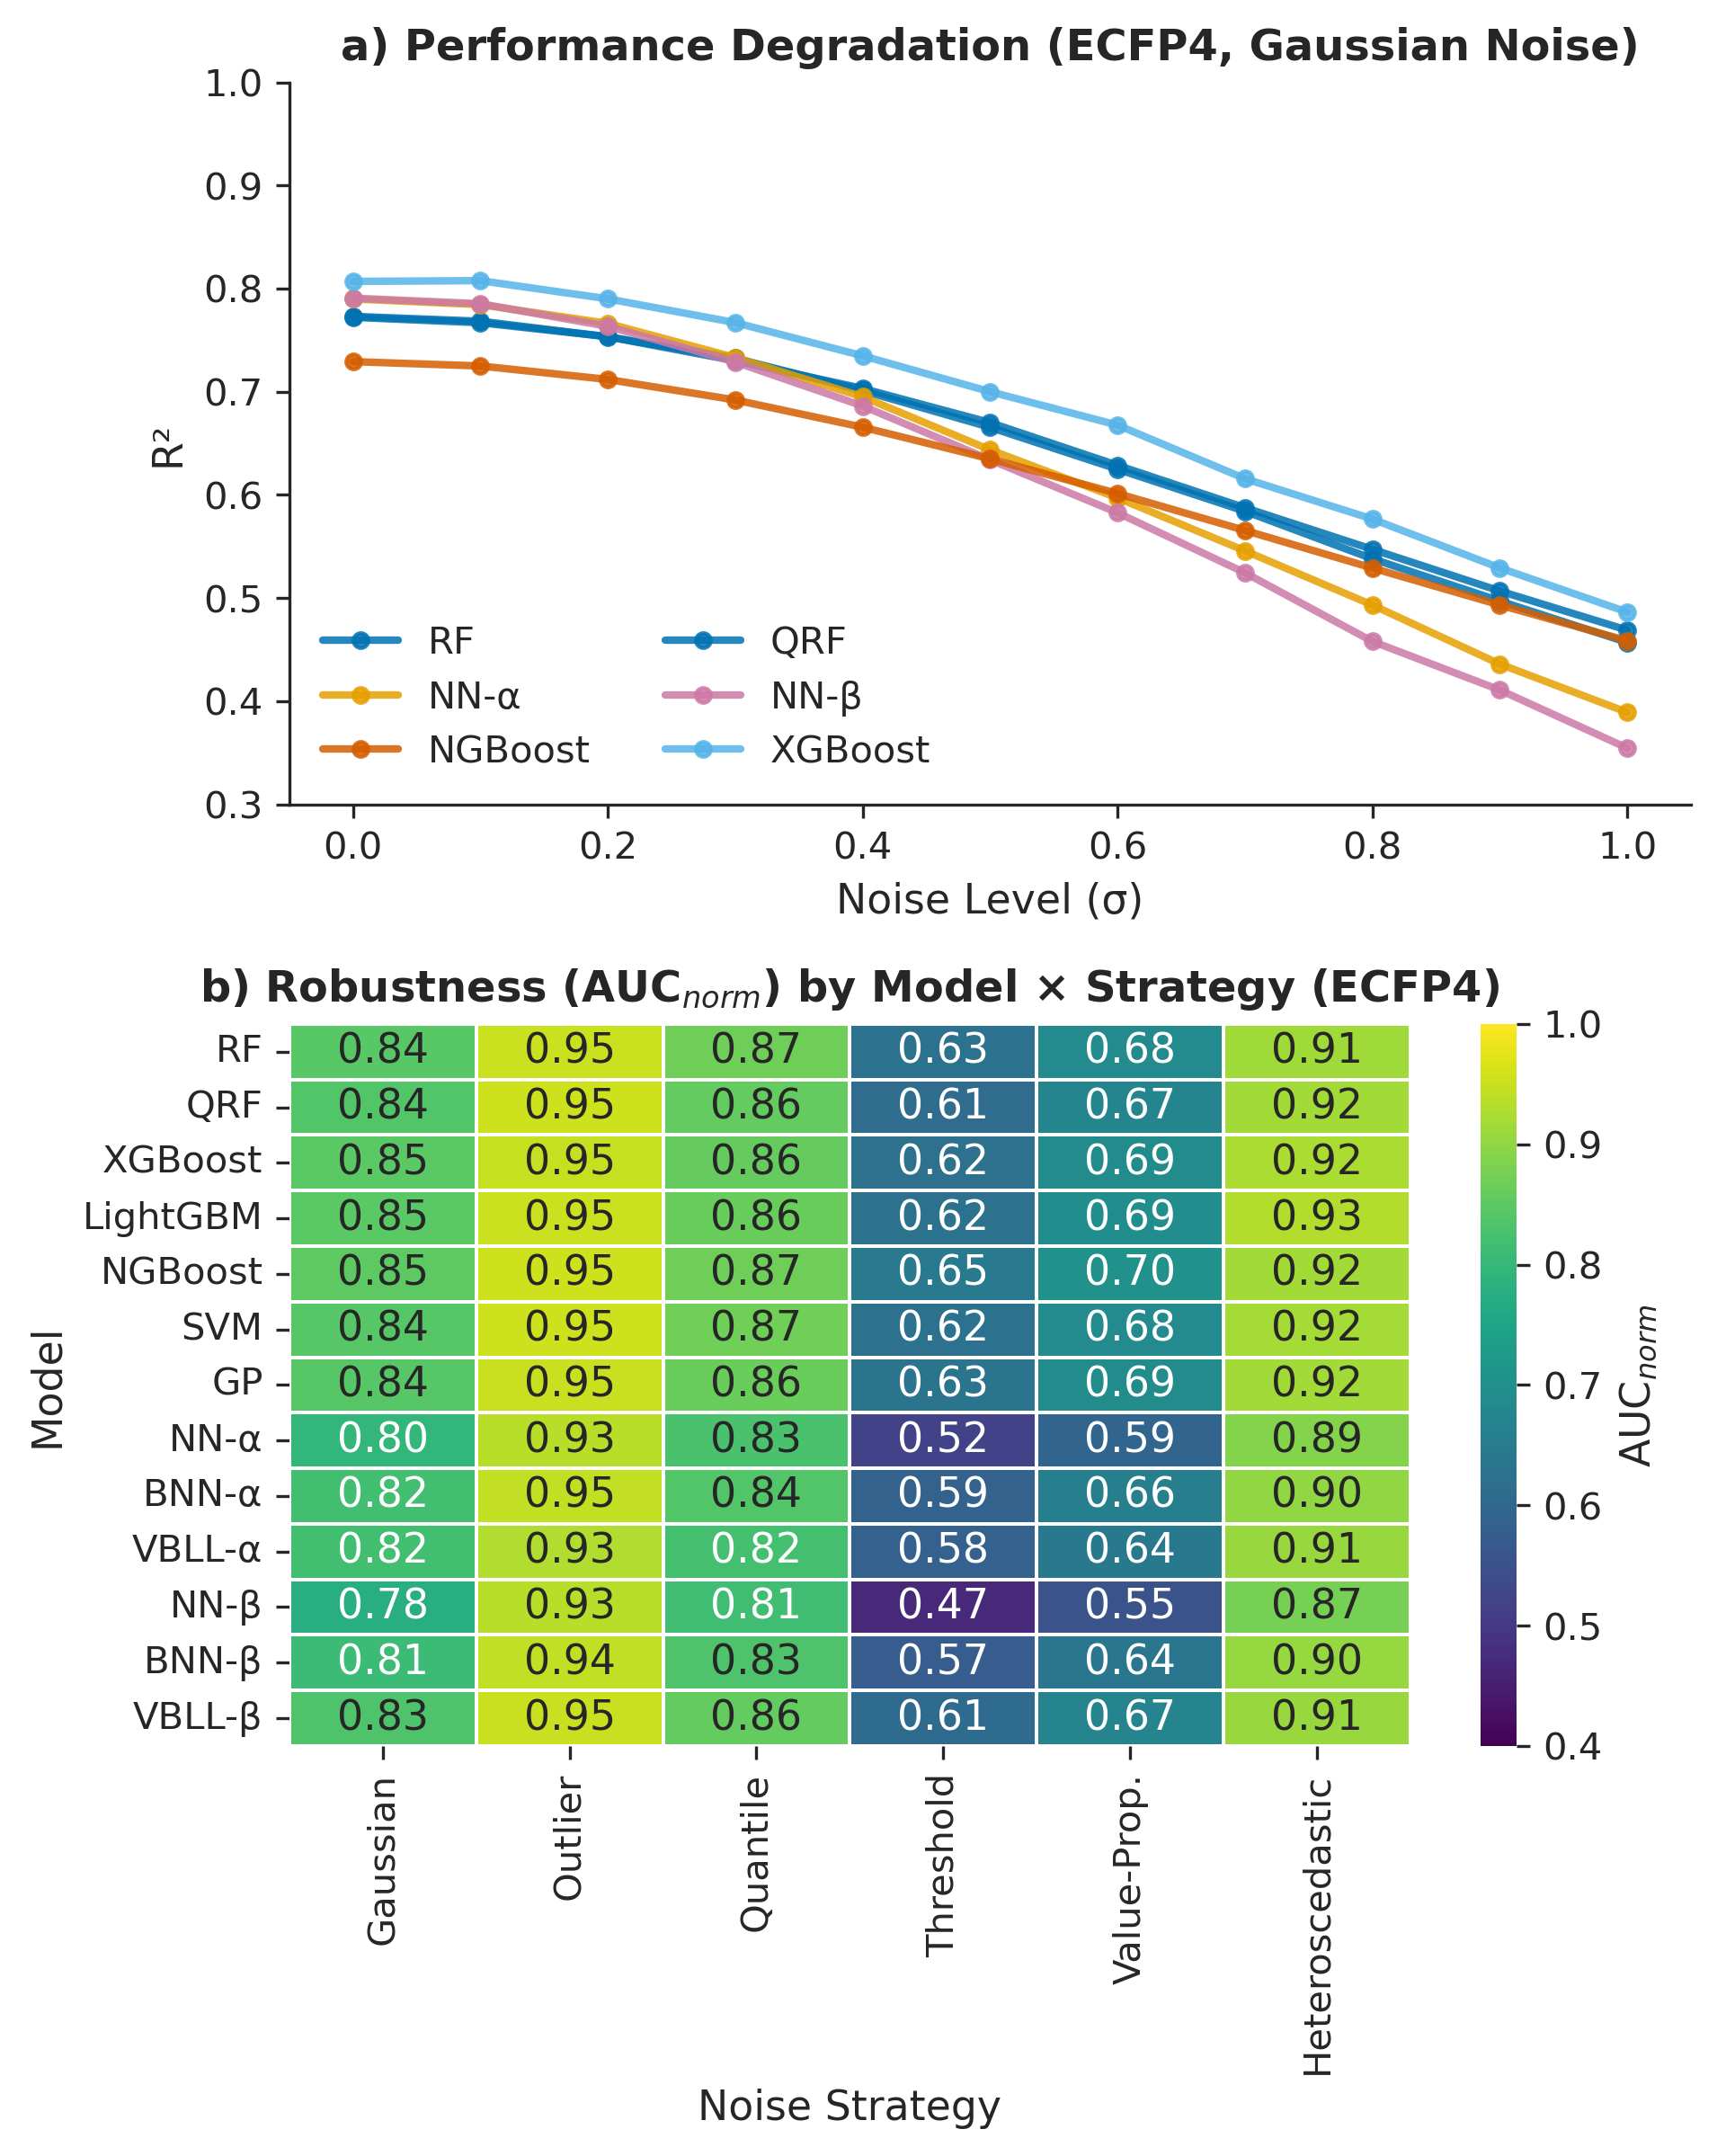
\includegraphics[width=\textwidth,height=0.78\textheight,keepaspectratio]{fig1_supp_ecfp4_overview.png}
\caption{\textbf{Global overview of noise robustness on the ECFP4 representation, evaluated on QM9 HOMO--LUMO gap.}
a) Performance degradation curves (R$^2$ versus noise level $\sigma$) under Gaussian noise. b) Noise degradation slope (NDS) heatmap across model architectures and noise strategies; lower (more negative) NDS indicates faster degradation under noise.}
\label{app:noise:ecfp4_overview}
\end{figure}


\addfile{Clean $R^2$ against robustness on PDV under Gaussian noise}
\label{app:noise:sec:clean_r2_vs_robustness}
% TODO: review, needs manual review
Clean-label $R^2$ against the noise degradation slope for every model on PDV under Gaussian noise, on the QM9 HOMO--LUMO gap.
% Thesis appendix item: clean_r2_vs_robustness

\begin{figure}[H]
\centering
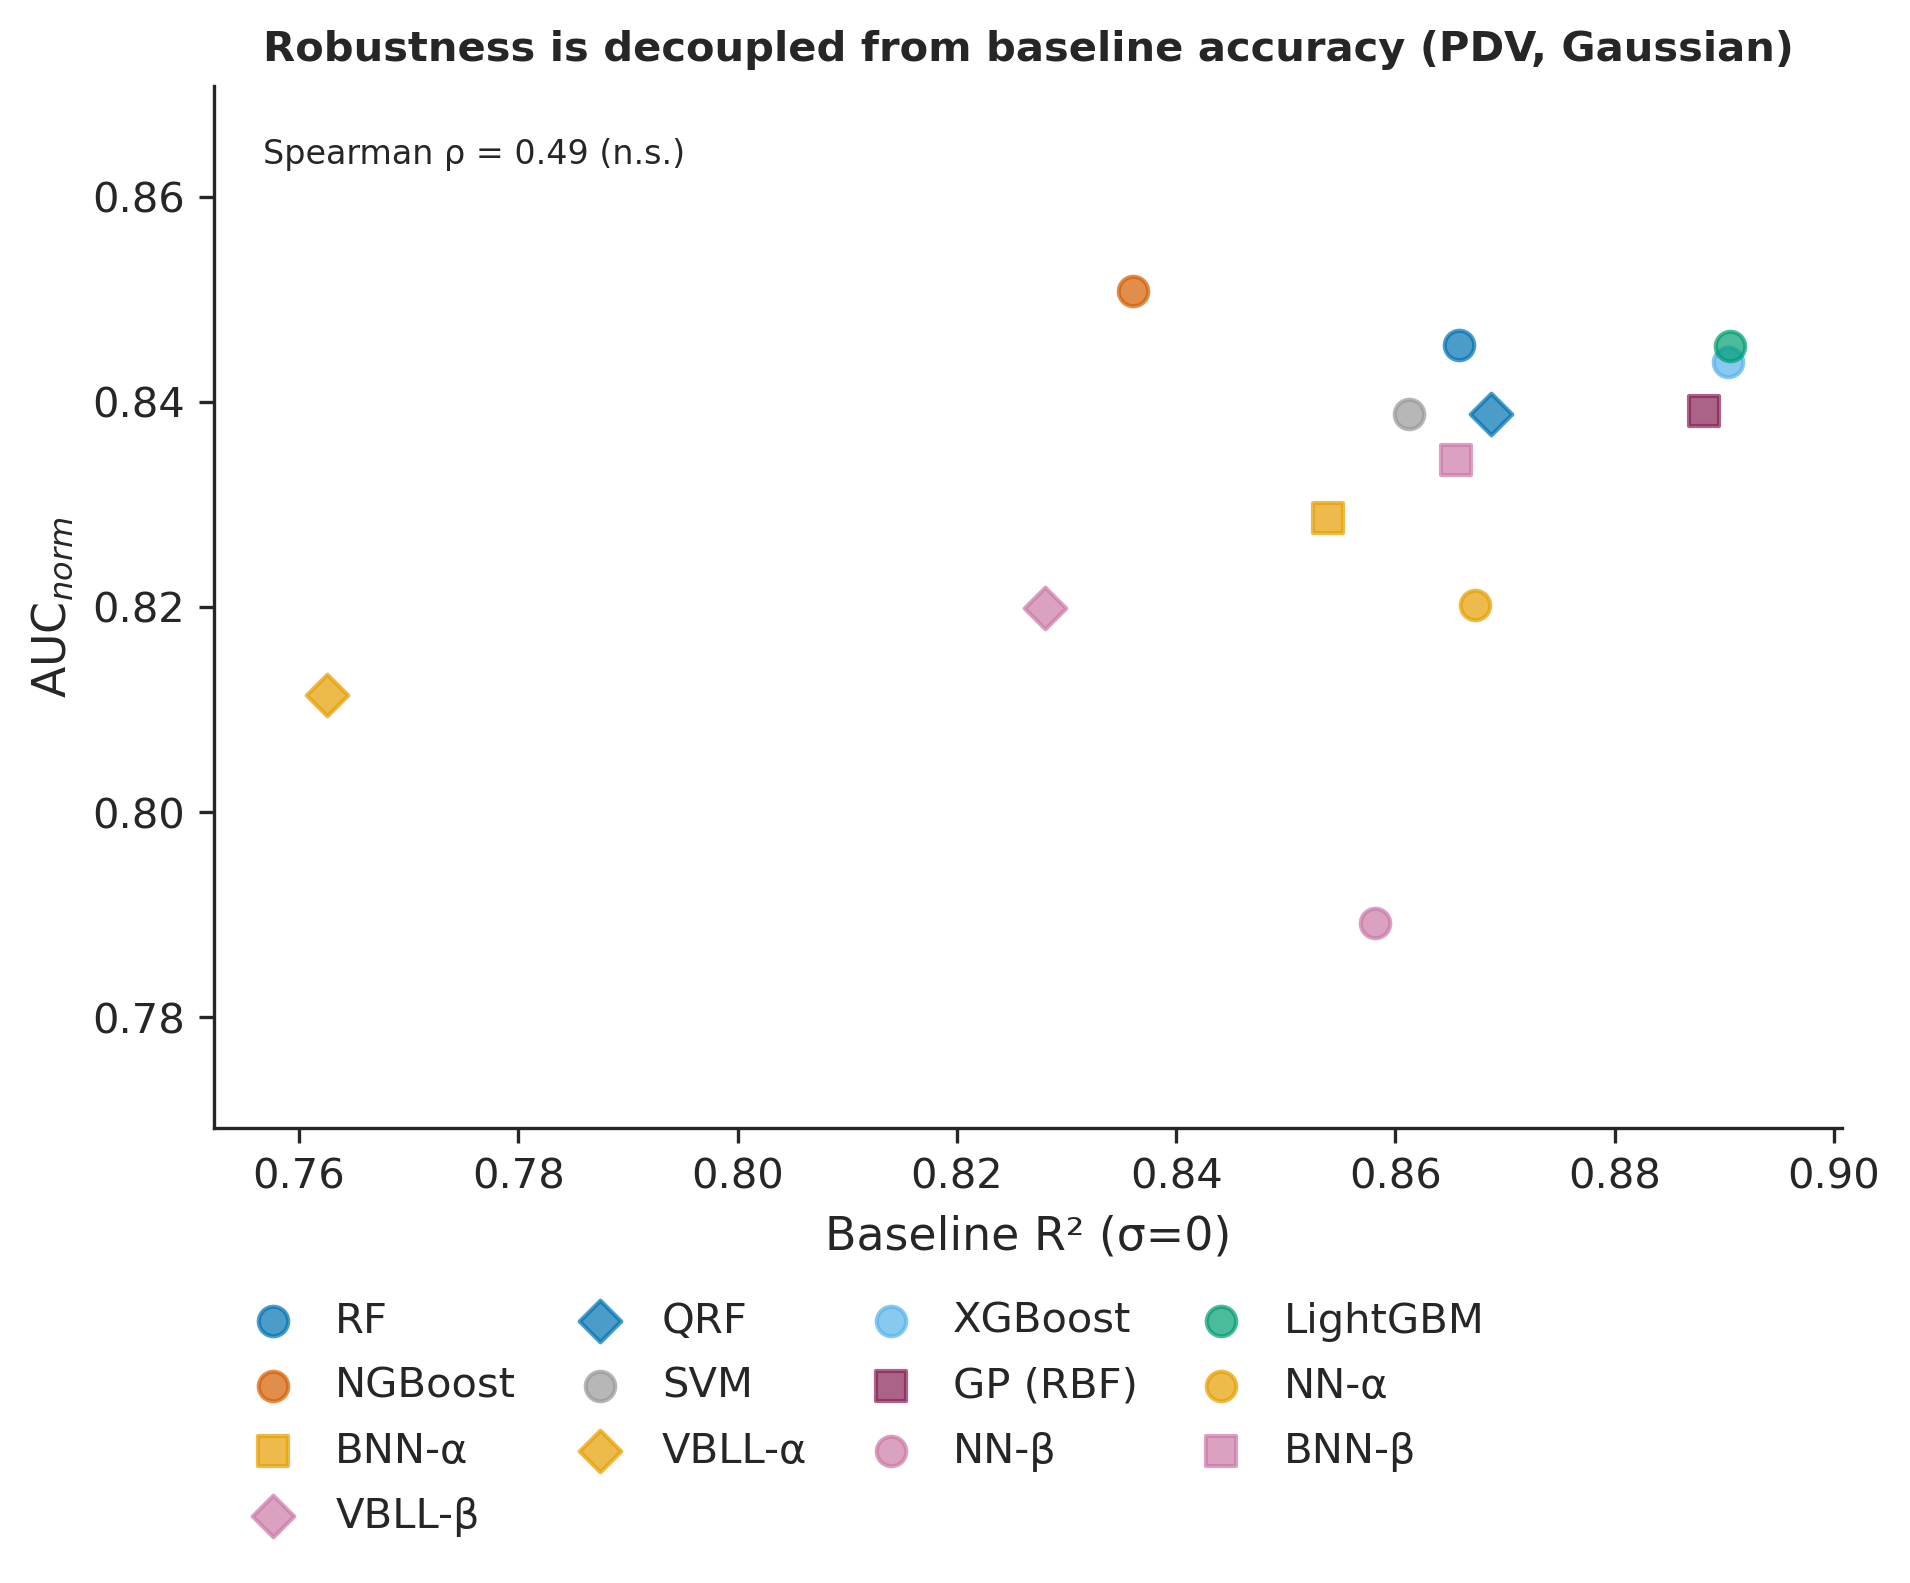
\includegraphics[width=\textwidth]{fig3_ranking_consistency.png}
\caption{\textbf{Baseline R$^2$ versus noise degradation slope (NDS) scatter for all models on the physicochemical descriptor vector (PDV) representation under Gaussian noise, on the QM9 HOMO--LUMO gap.}
Lower (more negative) NDS indicates faster performance loss under noise.}
\label{app:noise:clean_r2_vs_robustness}
\end{figure}


\addfile{Bayesian transformation effects by representation}
\label{app:noise:sec:bayesian_transformation_tests}
% TODO: review, needs manual review
The effect of each Bayesian transformation of the neural networks on the noise degradation slope, by representation, on the QM9 HOMO--LUMO gap.
% Thesis appendix item: bayesian_transformation_tests

\begin{table}[H]
\centering
\caption{\textbf{Neural network Bayesian transformation effects on noise degradation slope (NDS) by representation, on the QM9 HOMO--LUMO gap.}
Positive $\Delta$ NDS indicates the Bayesian variant is more robust (less negative slope) than its deterministic counterpart.}
\label{app:noise:bayesian_transformation_tests}
\small
\begin{tabular}{llrrrr}
\toprule
\textbf{Model} & \textbf{Representation} & \textbf{Baseline R$^2$} & \textbf{NN-$\beta$ NDS} & \textbf{BNN-$\beta$ NDS} & \textbf{$\Delta$ NDS} \\
\midrule
NN-$\beta$ & ECFP4 & 0.791 & $-0.464$ & $-0.388$ & $+0.076$ \\
NN-$\beta$ & PDV & 0.858 & $-0.487$ & $-0.382$ & $+0.106$ \\
NN-$\beta$ & SMILES & 0.721 & $-0.558$ & $-0.365$ & $+0.193$ \\
\bottomrule
\end{tabular}
\end{table}


\addfile{Uncertainty metrics for probabilistic models on ECFP4}
\label{app:noise:sec:uncertainty_metrics_ecfp4}
% TODO: review, needs manual review
Uncertainty metrics of the probabilistic models on ECFP4 under Gaussian noise, on the QM9 HOMO--LUMO gap.
% Thesis appendix item: uncertainty_metrics_ecfp4

\begin{table}[H]
\centering
\caption{\textbf{Uncertainty quantification metrics for probabilistic models on the ECFP4 representation (Gaussian noise strategy) on the QM9 HOMO--LUMO gap.}
Unc-Error $\rho$: Spearman correlation between predicted uncertainty and absolute prediction error. Unc-Noise $\rho$: Spearman correlation between predicted uncertainty and injected noise level $\sigma$. ECE: expected calibration error (lower = better-calibrated). Coverage targets: 68\% ($1\sigma$), 95\% ($2\sigma$).}
\label{app:noise:uncertainty_metrics_ecfp4}
\small
\begin{tabular}{lrrrrr}
\toprule
\textbf{Model} & \textbf{Unc-Error $\rho$} & \textbf{Unc-Noise $\rho$} & \textbf{ECE} & \textbf{Cov.\ $1\sigma$} & \textbf{Cov.\ $2\sigma$} \\
\midrule
\textbf{QRF}     & \textbf{0.25} & 0.27 & 0.19 & 74.7\% & 94.6\% \\
\textbf{NGBoost} & 0.22 & \textbf{0.37} & \textbf{0.11} & 69.2\% & 94.2\% \\
GP               & 0.18 & 0.34 & 0.23 & 78.6\% & 96.0\% \\
BNN-$\beta$      & 0.20 & 0.37 & 0.29 & 78.6\% & 95.2\% \\
BNN-$\alpha$     & 0.15 & 0.32 & 0.24 & 76.6\% & 95.1\% \\
VBLL-$\beta$     & 0.19 & 0.34 & 0.19 & 73.9\% & 95.5\% \\
VBLL-$\alpha$    & 0.11 & 0.31 & 0.22 & 74.5\% & 95.1\% \\
\bottomrule
\end{tabular}
\end{table}


\addfile{Variance decomposition on the three assay datasets}
\label{app:noise:sec:assay_variance_decomposition}
% TODO: review, needs manual review
ANOVA variance decomposition ($\eta^2$, in per cent) on LogD, Caco-2 efflux and hERG $K_i$.
% Thesis appendix item: assay_variance_decomposition

\begin{figure}[H]
\centering
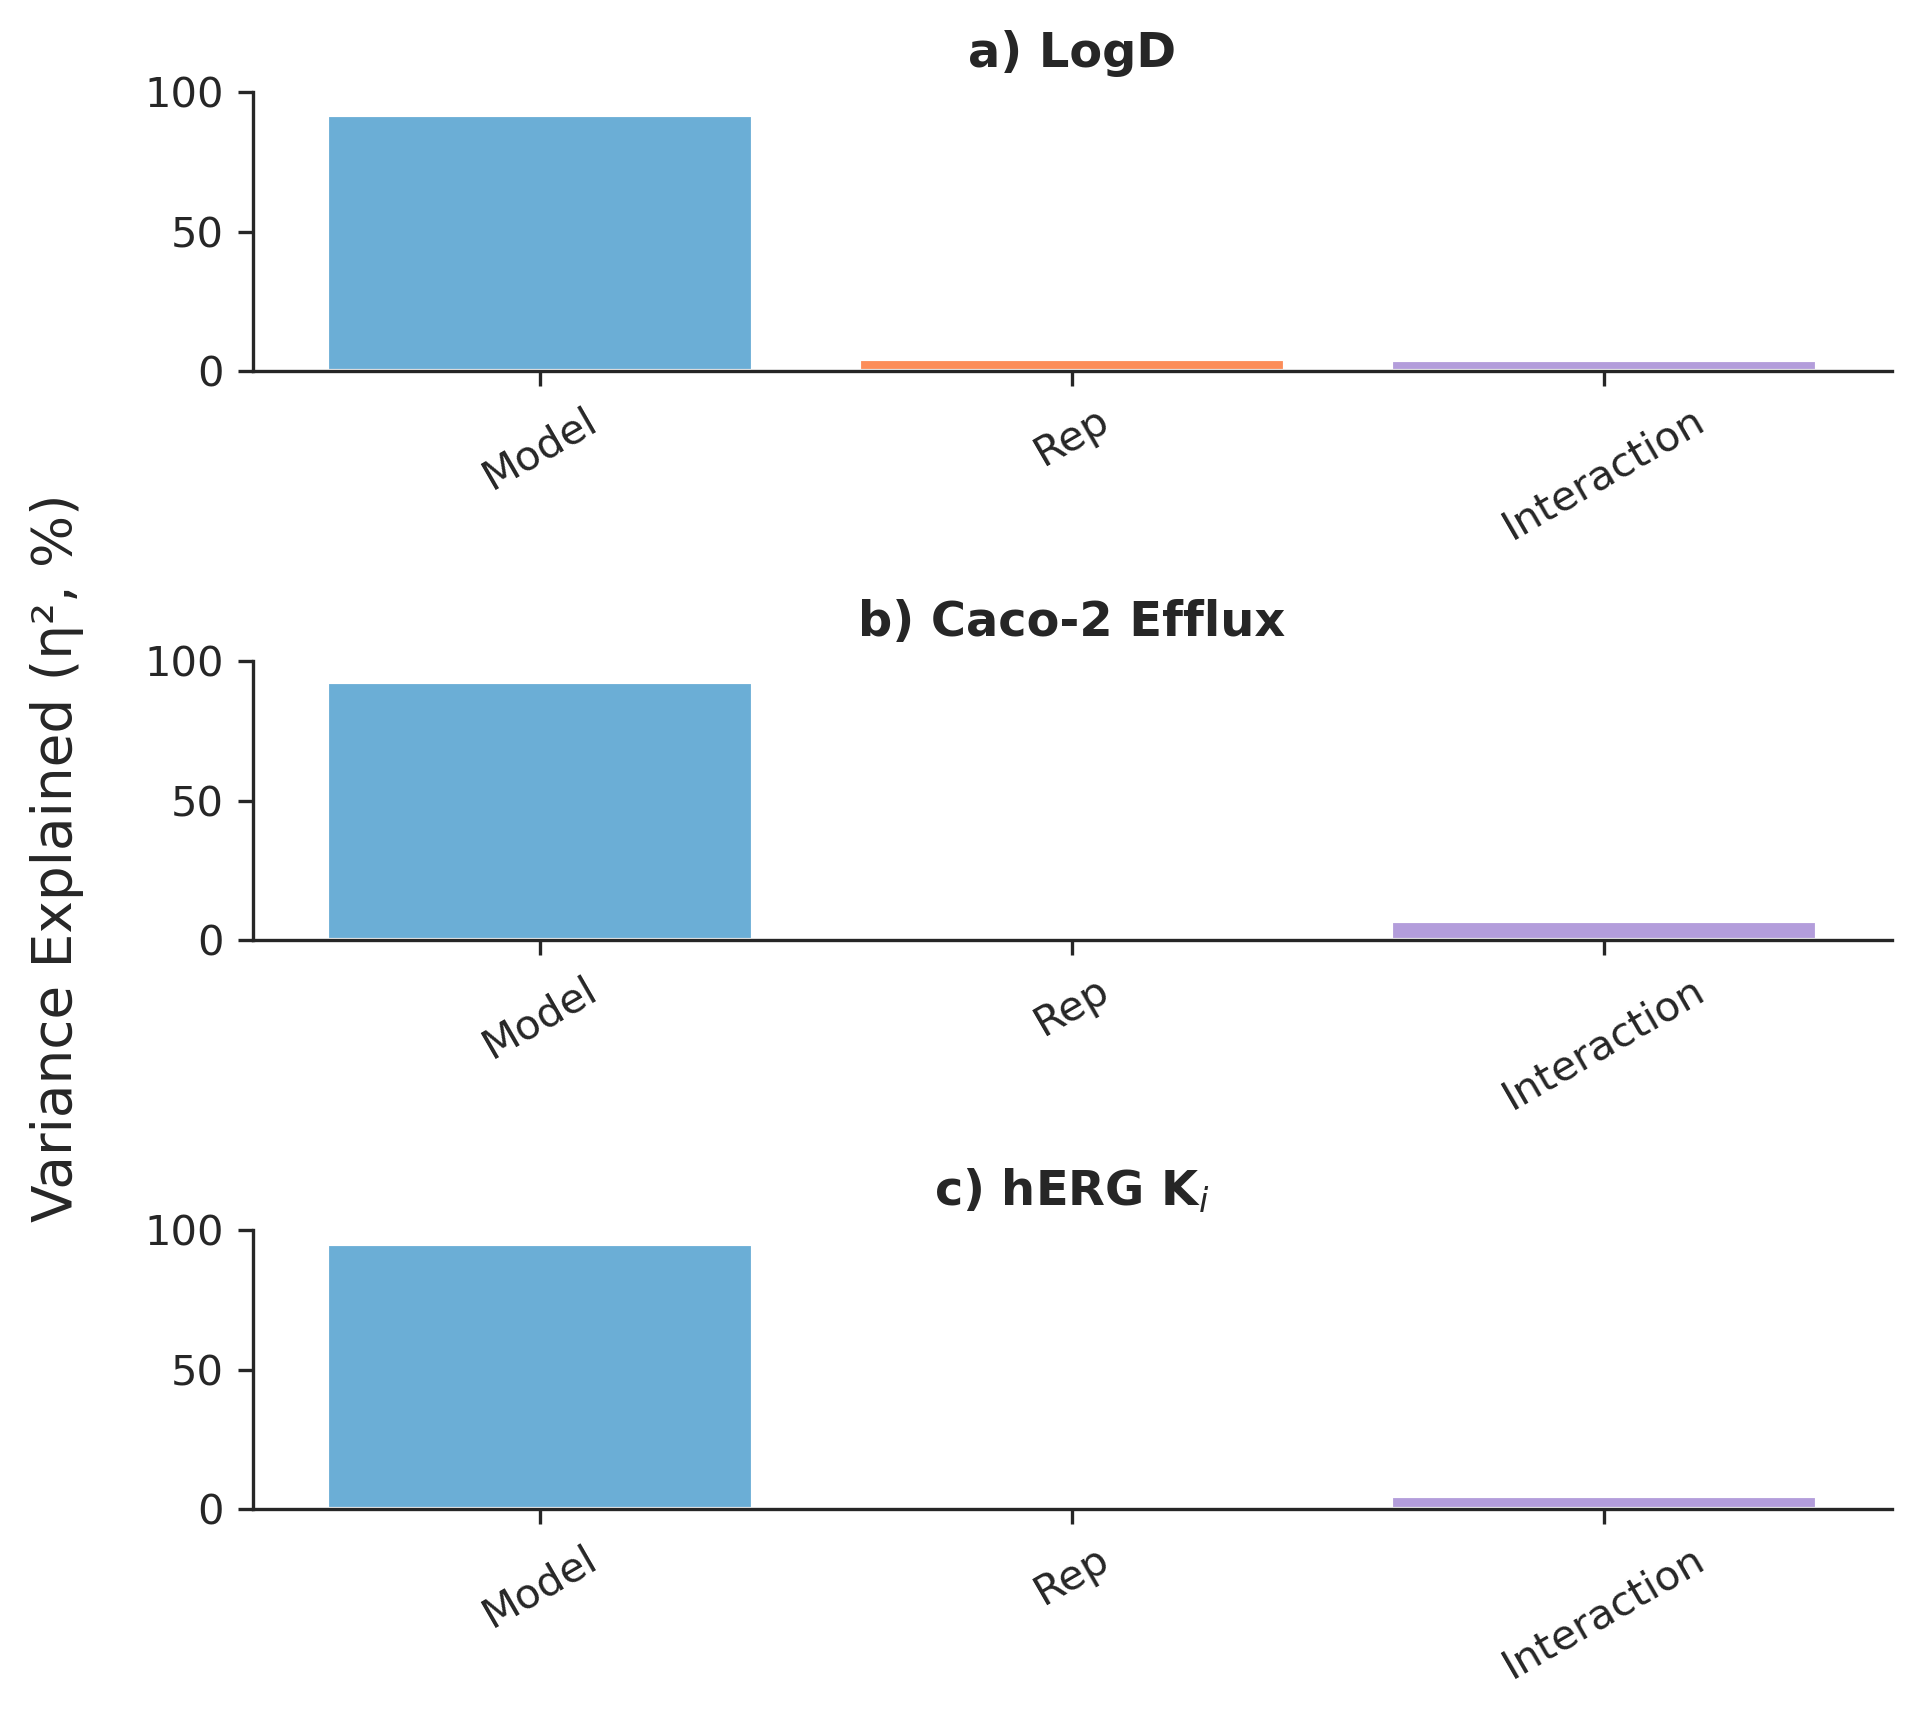
\includegraphics[width=\textwidth]{fig_validation_anova.png}
\caption{\textbf{ANOVA variance decomposition ($\eta^2$, \%) on external validation datasets: a) LogD, b) Caco-2 Efflux, and c) hERG K$_i$.}
Model, representation, and interaction contributions to noise degradation slope (NDS) variance for each dataset; lower (more negative) NDS indicates faster performance loss under noise.}
\label{app:noise:assay_variance_decomposition}
\end{figure}


\addfile{Random forest against quantile regression forest on the three assay datasets}
\label{app:noise:sec:rf_vs_qrf_assay}
% TODO: review, needs manual review
The noise degradation slope of random forest and of quantile regression forest on LogD, Caco-2 efflux and hERG $K_i$.
% Thesis appendix item: rf_vs_qrf_assay

\begin{table}[H]
\centering
\caption{\textbf{Random forest (RF) vs quantile regression forest (QRF) noise degradation slope (NDS) on the three external validation datasets (LogD, Caco-2 Efflux, hERG K$_i$).}
Lower (more negative) NDS indicates faster degradation under noise.}
\label{app:noise:rf_vs_qrf_assay}
\small
\begin{tabular}{lrrr}
\toprule
\textbf{Dataset} & \textbf{RF NDS} & \textbf{QRF NDS} & \textbf{$\Delta$ NDS} \\
\midrule
ChEMBL-hERG-Ki     & $-0.231$ & $-0.359$ & $-0.128$ \\
OpenADMET-Caco2    & $-0.534$ & $-0.627$ & $-0.094$ \\
OpenADMET-LogD     & $-0.101$ & $-0.185$ & $-0.083$ \\
\bottomrule
\end{tabular}
\end{table}


\section{The flaws of the similarity assumption}\label{app:add:flaws}
% ---- NOTES: The flaws of the similarity assumption ----
% - Files for Chapter~\ref{chap:flaws}.
% Table: constant features. One row is one dataset and one representation. Columns: total features; constant features; near-constant features. A per-domain summary stays in Chapter 4.
% TODO(results): constant and near-constant feature counts per dataset and representation.
% Table: molecules a representation cannot tell apart. One row is one representation and one dataset. Columns: molecules in groups with an identical feature vector; how many of those differ only in stereochemistry; lowest RMSE reachable when every group gets one prediction; largest label spread within a group.
% TODO(results): identical-vector counts per representation and dataset.
% Table: distance against property difference. One row is one dataset and one representation. Columns: rank correlation between pairwise distance and absolute property difference; score of predicting each molecule's activity from its five nearest neighbours in that representation.
% TODO(results): distance-property correlations and five-nearest-neighbour scores.
% Table: activity cliffs. One row is one dataset and one representation. Column: molecules that belong to at least one activity cliff.
% TODO(results): activity-cliff counts per dataset and representation.
% ---- END NOTES ----
\todo[inline, color=orange!40]{Additional files for Chapter~\ref{chap:flaws}: all four need the full runs.}

\section{Building adaptive hybrid representations}\label{app:add:method}\label{app:searchspace}
% ---- NOTES: Building adaptive hybrid representations ----
% - Files for Chapter~\ref{chap:method}.
% - The settings, formulas and reasons are in Chapter 5 ("The search space and why each axis is swept", its three subsubsections, "Augmentation", "Fast tier and adaptive pruning"). This section holds only the reference tables those sections point to.
% - The first five files below are written from the current code and the design runs. The rest need the full runs.
% - Which datasets get the Gaussian process, and why: only in "Models and metrics". The model-settings and models-left-out files point there and do not repeat it. Whether nanobody thermostability also gets the Gaussian process is an open decision under "Search tier settings"; the Gaussian process row of the models-left-out file follows that answer.
% - The models fitted only to compute importance are in the table under "Feature importance scoring". The model-settings file points there and does not repeat them.
% - Two open decisions change the model-settings file: the random forest evaluator's features per split on regression datasets, and the DNN evaluator's early-stopping split (both under "Internal evaluation"). The file states the current settings; change the row if either answer is yes.
% - The open decision under "Models and metrics" (count the whole dataset or the training molecules) changes the SVM row of the models-left-out file for LogD and TATA promoter. The file carries a footnote; change it to match the answer.
% - The design-experiment file: the reason the kept pooled allocation method was chosen over the other pooled candidates is an open decision under "Feature allocation strategies". The allocation row states only the counts; add the reason once it is written there. The pooled candidates that were not kept are not named.
% - The design-experiment file: the representation-count row gives no result; the best count per (model, budget) was not carried into the notes. Add it from the design run, or leave the cell as it is.
%
% TODO(results): per dataset and downstream model, per-fold score of the best single representation against the hybrid, with the spread across folds.
% TODO(results): per dataset, the winning configuration: downstream model, budget, allocation method, importance method, internal evaluator, representation count.
% TODO(results): per dataset, how often each value of each setting won across (downstream model, budget) combinations.
% TODO(results): augmentation per dataset: how often no extra features were chosen; per-fold base against base plus extras, uncapped and capped; which extra feature sets were kept; decoy features admitted.
% TODO(results): per dataset and budget, held-out score against the score the inner search reported, and the stability of the selected features across folds.
% TODO(results): hybrid minus each comparator (concatenation, one model per representation, PCA, mRMR, recursive feature elimination, random features) at each budget.
% TODO(results): the smaller experiments in "Comparators, controls and ablations", one table each, if they leave the chapter.
% TODO(results): per task, outcome of the transfer, antibody-scan and separate-site experiments, with which representations the selected features came from.
% TODO(results): hours and model fits per dataset at each tier, with the hardware.
% ---- END NOTES ----

\addfile{Settings of every model, as downstream model and as internal evaluator}
\label{app:add:model_settings}
% TODO: review, needs manual review
One row is one model. The middle two columns give its settings when it scores a hybrid (downstream model) and when it scores one representation inside the search (internal evaluator). The models fitted only to compute feature importance are in Table~\ref{tab:importance_methods}.

% TODO: review, needs manual review (whole table and caption, written from the current code)
{\small
\begin{longtable}{@{}p{1.9cm}p{4.6cm}p{3.6cm}p{1.6cm}p{2.3cm}@{}}
\caption{Settings of every model. $p$ is the number of features. ``Molecules'' is the number of training molecules the internal evaluator is fitted on; above it, a random subset of that size is drawn with a fixed seed. Settings not listed are the library's defaults. Every setting is the same on every dataset. The Gaussian process runs only on the datasets named in Chapter~\ref{chap:method}, ``Models and metrics''.}
\label{tab:add:model_settings}\\
\toprule
Model & As downstream model & As internal evaluator & Molecules & Library; source \\
\midrule
\endfirsthead
\toprule
Model & As downstream model & As internal evaluator & Molecules & Library; source \\
\midrule
\endhead
Random forest & 100 trees, no depth limit; $\sqrt{p}$ features tried at each split & 50 trees, depth at most 10; all $p$ features tried at each split on regression, $\sqrt{p}$ on classification & all & scikit-learn \citep{scikit-learn}; \citet{Breiman2001} \\
\addlinespace
LightGBM & 100 trees & 50 trees, depth at most 4 & all & lightgbm; \citet{ke2017lightgbm} \\
\addlinespace
XGBoost & 100 trees; half of the features sampled for each tree & 50 trees, depth at most 4 & all & xgboost; \citet{Chen2016} \\
\addlinespace
SVM & RBF kernel, $C = 1$. Not fitted above 10{,}000 molecules, or above 5{,}000 under uncapped augmentation & RBF kernel, $C = 1$ & at most 500 & scikit-learn; \citet{Vapnik1995} \\
\addlinespace
Gaussian process & Regression: RBF plus white-noise kernel, labels normalised, 3 optimiser restarts. Classification: RBF kernel. Not fitted above 1{,}000 molecules & Regression: scaled RBF kernel, fixed noise variance 0.01, no restarts. Classification: scaled RBF kernel, no restarts & at most 500 & scikit-learn; \citet{Rasmussen2006} \\
\addlinespace
DNN & Hidden layers of 256, 128 and 64 units, ReLU, dropout 0.2 \citep{Srivastava2014}; Adam \citep{Kingma2015} at learning rate 0.001, halved after 5 epochs without improvement; batch size 256; up to 200 epochs; stops after 20 epochs without improvement on 20\% of the training molecules that share no group with the rest, using the outer split's grouping; labels z-normalised & The same, except that the early-stopping 20\% is drawn at random & all & PyTorch \citep{Paszke2019} \\
\bottomrule
\end{longtable}
}

\addfile{Downstream models left out, by dataset and augmentation setting}
\label{app:add:models_left_out}
% TODO: review, needs manual review
One row is one rule that leaves a downstream model out. Only the 16 datasets of Table~\ref{tab:datasets} are listed; a dataset and setting not named in any row runs every downstream model in Table~\ref{tab:search_tiers}.

% TODO: review, needs manual review (whole table and caption, written from the current code)
{\small
\begin{longtable}{@{}p{2.4cm}p{3.0cm}p{8.6cm}@{}}
\caption{Downstream models left out, by dataset and augmentation setting. Every rule was set so that a search finishes within the time limit of one job; none was set from scores. hERG $K_i$ drops no model under any setting.}
\label{tab:add:models_left_out}\\
\toprule
Model left out & Augmentation setting & Datasets \\
\midrule
\endfirsthead
\toprule
Model left out & Augmentation setting & Datasets \\
\midrule
\endhead
XGBoost & all three & H3K4me3, TATA promoter \\
SVM & all three & datasets above 10{,}000 molecules: H3K4me3 \\
SVM & uncapped & datasets above 5{,}000 molecules: QM9, LogD$^{a}$, TATA promoter$^{a}$ \\
SVM & uncapped & Koenig expression \\
SVM & capped & Caco-2 efflux, LogD, rat liver microsome clearance, MDR1--MDCK efflux, Buchwald--Hartwig plates \\
Random forest and SVM & capped & QM9 \\
Random forest & uncapped & QM9, LogD \\
Gaussian process & all three & every dataset except humanness (Chapter~\ref{chap:method}, ``Models and metrics'') \\
\bottomrule
\end{longtable}
{\footnotesize $^{a}$Counted on the whole dataset: LogD has 5{,}028 molecules and TATA promoter 5{,}274. A search run inside one outer fold is given about 80\% of them and keeps the SVM.}
}

\addfile{Size of the search}
\label{app:add:search_size}
% TODO: review, needs manual review
One row is one downstream model. The counts are per dataset, objective and augmentation setting, with adaptive pruning off.

% TODO: review, needs manual review (whole table and caption)
\begin{table}[htbp]
\centering
\small
\caption{Number of configurations searched per dataset, objective and augmentation setting. A configuration is one choice of downstream model, internal evaluator, allocation method, importance method, representation count and budget. At the full tier each (downstream model, internal evaluator) pair runs 5 allocation methods $\times$ 3 importance methods $\times$ 4 representation counts $\times$ 8 budgets $= 480$ configurations; at the fast tier it runs $3 \times 1 \times 2 \times 8 = 48$ (Table~\ref{tab:search_tiers}). ``Matched'' is counted once where it repeats an evaluator already in the list. Each configuration is scored on 5 folds, so the full tier fits a downstream model 40{,}800 times (50{,}400 on humanness) and the fast tier 4{,}080 times. Where a dataset leaves a downstream model out (Additional file~\ref{app:add:models_left_out}), its pairs drop out: a fast search on H3K4me3 has 9 pairs, so 432 configurations.}
\label{tab:add:search_size}
\begin{tabular}{@{}lp{4.2cm}rr@{}}
\toprule
Downstream model & Internal evaluators & Full tier & Fast tier \\
\midrule
Random forest & 3 (matched is random forest) & 1{,}440 & 144 \\
LightGBM & 3 (matched is LightGBM) & 1{,}440 & 144 \\
DNN & 3 (matched is DNN) & 1{,}440 & 144 \\
XGBoost & 4 & 1{,}920 & 192 \\
SVM & 4 & 1{,}920 & 192 \\
Gaussian process (humanness only) & 4 & 1{,}920 & not run \\
\midrule
Total & 17 pairs (21 on humanness) & 8{,}160 (10{,}080 on humanness) & 816 \\
\bottomrule
\end{tabular}
\end{table}

\addfile{Design experiments behind the search settings}
\label{app:add:design_experiments}
% TODO: review, needs manual review
One row is one setting of the search, or one rule that was tested and then fixed instead of searched. Every number comes from preliminary design runs made before the main experiments; they are not results of the thesis, and several used other budgets than the final search.

% TODO: review, needs manual review (whole table and caption; numbers from preliminary design runs)
{\footnotesize
\begin{longtable}{@{}p{1.9cm}p{2.5cm}p{2.7cm}p{4.4cm}p{2.5cm}@{}}
\caption{Design experiments behind the search settings. Preliminary design runs, not the thesis's full runs.}
\label{tab:add:design_experiments}\\
\toprule
Setting & Values compared & Datasets, folds, budgets & What was measured, and the result & Values kept (full / fast) \\
\midrule
\endfirsthead
\toprule
Setting & Values compared & Datasets, folds, budgets & What was measured, and the result & Values kept (full / fast) \\
\midrule
\endhead
Downstream model & Nine models, among them random forest, LightGBM, XGBoost, CatBoost, DNN, $k$-nearest neighbours and a Gaussian process, each on each of 10 base representations at full width & Buchwald--Hartwig yield, Caco-2 efflux, Koenig expression, LogD, breast cancer PAM50 subtype; 5 folds & Best held-out score over the 10 representations, and seconds per fit. The DNN scored best on 4 of the 5 datasets and third on Caco-2 (0.2936 against 0.2851 RMSE, log$_{10}$ efflux ratio) & Full: random forest, LightGBM, XGBoost, SVM, DNN, and the Gaussian process on humanness / fast: the same five \\
\addlinespace
Budget & None compared & -- & -- & 10, 25, 50, 100, 250, 500, 1{,}000 and 2{,}000 features at both tiers \\
\addlinespace
Representation count & 2, 3, 5 and all 10 & 9 datasets, 3 tree-ensemble downstream models, budgets 500 and 1{,}000 features; 5 folds & The best count for each (downstream model, budget) combination & Full: 2, 3, 5, all / fast: 3, all \\
\addlinespace
Allocation method & 8 candidates: the five searched and 3 further pooled candidates, each at every representation count & The same 9 datasets, models and budgets: 54 (dataset, model, budget) combinations & Each candidate was scored at its best representation count, and the number of combinations in which it was in the top 3 of the 8 was counted. Fixed shares: linear 30, squared 27, rank decay 26, softmax 25; global pool with squared weights 14 & Full: the five in Table~\ref{tab:allocation_methods} / fast: linear, squared, rank decay \\
\addlinespace
Importance method, agreement & 8 methods & LogD, hERG $K_i$, Buchwald--Hartwig yield, nanobody thermostability, antibody FcRn retention, breast cancer PAM50 subtype, lung adenocarcinoma vs squamous; each method fitted once on the whole dataset & Spearman correlation between two methods' scores over every feature. Kept pairs: LightGBM gain and TreeSHAP 0.20--0.64, LightGBM gain and DeepLIFT 0.21--0.67, TreeSHAP and DeepLIFT 0.56--0.99 across the 7 datasets & One method kept from each group whose rankings agree above 0.95 \\
\addlinespace
Importance method, score & 28 methods, among them three controls: feature variance, Laplacian score and random ranking & Caco-2 efflux; 3 folds; budget 100 features; random forest and LightGBM downstream & RMSE of the best single representation minus RMSE of the hybrid (log$_{10}$ efflux ratio; positive means the hybrid has the lower error): DeepLIFT $+0.0144$, LightGBM gain $+0.0100$, TreeSHAP $+0.0067$, random ranking $-0.0118$ & Full: LightGBM gain, TreeSHAP, DeepLIFT / fast: LightGBM gain \\
\addlinespace
Internal evaluator settings & 20 hyperparameter settings from 5 model families & Buchwald--Hartwig yield, Caco-2 efflux, Koenig expression; 3 folds; budget 100 features & Spread of mean scores across all 20 settings: 0.0253 $R^2$, 0.0179 $R^2$ and 0.0085 Spearman. Median standard deviation across the 3 folds for one setting, allocation method and downstream model: 0.0462 $R^2$, 0.0693 $R^2$ and 0.0186 Spearman & Matched, random forest, LightGBM and DNN, at fixed settings, both tiers \\
\addlinespace
Rescaling of each representation's score (a rule) & 5 rescalings & 9 datasets; 5 folds; budgets 50 and 300 features & Whether any rescaling beat the one in use by more than that rule's own spread across folds: in 0 of 90 (dataset, allocation method, budget) combinations & One fixed rule per metric (Table~\ref{tab:standalone-rescaling}) \\
\bottomrule
\end{longtable}
{\footnotesize The representation-count and allocation rows come from one design run on 10 datasets, 3 downstream models and 2 budgets (60 combinations); QM9 is left out, which gives the 54.}
}

\addfile{Fields a blueprint saves}
\label{app:add:blueprint_fields}
% TODO: review, needs manual review
One row is one field. The first block is the recipe that rebuilds a hybrid; the second is kept for inspection and is not read by a rebuild.

% TODO: review, needs manual review (whole table and caption, written from the current code)
{\small
\begin{longtable}{@{}p{4.6cm}p{9.4cm}@{}}
\caption{Fields a blueprint saves. The stored score of each representation is its best score on its own across the downstream models, over every molecule the search ran on. It is not the internal-evaluator score that splits the budget, which a rebuild computes again on the molecules it is given. Three further fields are read only by allocation or augmentation routes outside the thesis's search and are fixed: a minimum improvement a whole block of extra features must show (none), a number of features taken from each source (20), and a step size (5).}
\label{tab:add:blueprint_fields}\\
\toprule
Field & What it holds \\
\midrule
\endfirsthead
\toprule
Field & What it holds \\
\midrule
\endhead
\multicolumn{2}{@{}l}{\textit{The recipe}} \\
\midrule
Representations & The representations offered to the search \\
Representation count & How many of them the configuration used; empty when it used all \\
Allocation method & One of the five in Table~\ref{tab:allocation_methods} \\
Importance method & LightGBM gain, TreeSHAP or DeepLIFT \\
Budget & Number of features in the hybrid \\
Internal evaluator & Matched, random forest, LightGBM or DNN \\
Objective & Predictive, or predicting each molecule's activity from its five nearest neighbours \\
Metric & The dataset's metric, and whether lower is better \\
Task type & Regression or classification \\
Folds and seed & The number of folds, and the random seed \\
\midrule
\multicolumn{2}{@{}l}{\textit{The recipe: augmentation}} \\
\midrule
Augmentation setting & None, uncapped or capped \\
Candidate ranking & How candidate extra features are ranked \\
Candidate list length & 50 features \\
Cap per source & Optional; the most candidates taken from one source \\
Margin & How much better than adding none a block of extra features must score \\
Fraction of the budget & Optional; used instead of the fixed block sizes \\
\midrule
\multicolumn{2}{@{}l}{\textit{Kept for inspection, not read by a rebuild}} \\
\midrule
Representation scores & Each representation's best score on its own across the downstream models, sign flipped for metrics where lower is better \\
Features per representation & The number of features each representation got in each fold \\
Extra features kept & The extra features augmentation kept in each fold, by source \\
\bottomrule
\end{longtable}
}

\todo[inline, color=orange!40]{Additional files for Chapter~\ref{chap:method}: the per-dataset results, augmentation, held-out against inner-search scores, comparators, smaller experiments, transfer experiments and compute need the full runs.}

\section{Hybrid representations for similarity and label noise}\label{app:add:similarity}
% ---- NOTES: Hybrid representations for similarity and label noise ----
% - Files for Chapter~\ref{chap:similarity}.
% - The chapter's own two tables (noise conditions, and the twelve LNL methods) stay in the chapter. The settings file below gives each method's numbers; the chapter's table gives what each method does.
% Table: finding injected noisy labels. One row is one noise score. Columns: average precision under outlier noise at 1\%, 5\% and 10\%, grouped-wider noise and censoring, in each feature space (each model's top two single representations, the same features weighted by importance, forest proximity, the hybrid, the hybrid ranked on the neighbour score); chance level in the header row. The chapter's table keeps only 10\% outlier noise, grouped-wider noise and censoring in two feature spaces.
% TODO(results): average precision per noise score, feature space and noise condition, all outlier levels, with chance level.
% Table: finding real suspect labels. One row is one noise score and feature space. Columns: average precision against ChEMBL curator flags on hERG IC50, per record and per molecule, with chance level; Spearman correlation with the spread between laboratories on the BindingDB molecules with repeat measurements.
% TODO(results): average precision against curator flags and correlation with the spread between laboratories, per noise score and feature space.
% Table: estimated noise size. One row is one dataset and feature space. Columns: the estimate from repeat measurements (with the directly measured variance between repeats where the dataset keeps them); the estimate from near-duplicate pairs; the gamma-test estimate; the model's held-out mean squared error. All in label units squared.
% TODO(results): the three noise-size estimates per dataset and feature space, beside the model's held-out mean squared error.
% TODO(results): per dataset and fold, importance-weighted against unweighted features for predicting each molecule's activity from its five nearest neighbours; the hybrid searched for that objective against the ordinary hybrid and the two best single representations.
% TODO(results): censoring: share of the lost score recovered, per treatment, model, feature space and clipping level; deleting clipped molecules against keeping them.
% TODO(results): the survey of twelve LNL methods: per noise level, the methods that beat the plain network on each input.
% TODO(results): cleaning real labels: folds won per cleaning method, noise score and feature space.
% TODO(results): per noise type, whether any LNL method, noise mitigation or noise-robust training, improved on the untreated model, on each feature space.
% ---- END NOTES ----

\addfile{Settings of the twelve LNL methods and the plain network they share}
\label{app:add:lnl_settings}
% TODO: review, needs manual review
One row is one method; the first row is the plain network every method starts from. The kind of each method follows Table~\ref{tab:lnl_methods}.

% TODO: review, needs manual review (whole table and caption, written from the current code)
{\small
\begin{longtable}{@{}p{2.9cm}p{2.0cm}p{7.3cm}p{1.6cm}@{}}
\caption{Settings of the twelve LNL methods. On classification datasets the squared-error loss is replaced by cross-entropy.}
\label{tab:add:lnl_settings}\\
\toprule
Method & Kind & Settings & Labels \\
\midrule
\endfirsthead
\toprule
Method & Kind & Settings & Labels \\
\midrule
\endhead
Plain network & -- & Hidden layers of 256, 128 and 64 units, ReLU, dropout 0.2; Adam at learning rate 0.001, halved after 5 epochs without improvement; batch size 256; gradient norm clipped at 1; up to 200 epochs; stops after 20 epochs without improvement on 20\% of the training molecules held out by scaffold group (drawn at random after a method has removed molecules); labels z-normalised & both \\
\midrule
Small-loss selection & noise mitigation & 10 warm-up epochs on all molecules; keeps the 70\% with the smallest loss and fits a new plain network on them & both \\
Confident learning & noise mitigation & 3 plain networks; removes molecules whose error is above the 85th percentile and whose spread across the 3 networks is below the 25th percentile, then refits & both \\
Removal by distance to neighbours & noise mitigation & 10 nearest neighbours in the standardised features; score is the distance of a label from its neighbours' mean label, divided by their standard deviation (on classification, the share of neighbours with another label); removes molecules above the 85th percentile, then refits & both \\
Staged removal & noise mitigation & 3 stages; each removes the 10\% of the remaining molecules with the largest training loss & both \\
\midrule
Per-epoch down-weighting & noise-robust training & After each epoch, the weight of every molecule whose loss is above the median is multiplied by 0.95 & both \\
Curriculum by confidence & noise-robust training & 20 warm-up epochs, then trains on the 25\%, 50\%, 75\% and 100\% of molecules with the smallest loss, in stages & both \\
DivideMix & noise-robust training & Two networks, 10 warm-up epochs; a two-component Gaussian mixture on each network's squared errors splits the molecules & both \\
Meta-Weight-Net & noise-robust training & The weighting network is updated every 5 epochs at learning rate 0.001, on 20\% of the training molecules held out for it & both \\
MentorNet & noise-robust training & The mentor network reads each molecule's current loss, its last 5 losses and its mean distance to its 10 nearest neighbours & both \\
Contrast to Divide & noise-robust training & 5 perturbed copies of each molecule, Gaussian noise of standard deviation 0.01 on the features & both \\
\midrule
Heteroscedastic GP & noise-robust training & RBF kernel, 2 optimiser restarts, fitted on at most 1{,}000 training molecules; a small network predicts each molecule's noise variance & regression \\
Deep evidential regression & noise-robust training & Weight of the evidence penalty 0.01 & regression \\
\bottomrule
\end{longtable}
}

\todo[inline, color=orange!40]{Additional files for Chapter~\ref{chap:similarity}: finding injected and real noisy labels, estimated noise size and the other results need the full runs.}
\chapter{Data and code availability}\label{app:availability}
% TODO: needs manual review (whole chapter written by Claude)
% ---- NOTES: Data and code availability ----
% Decision for you: the author contributions now appear twice, in the Statement of Originality and in the last paragraph below. Keep both and they must stay word for word the same; keep one and point to it from the other. The two differ in one sentence now: "All authors read and approved the final manuscript" is in your paper and below, but not in the Statement of Originality.
% Decision for you: whether the contributions paragraph below also says A.P. wrote the QM9 pipeline. Your paper names only NoiseInject, so the sentence below now matches the paper. Every commit in the qsar_qm_models repository is yours, so adding it would be accurate.
% Decision for you: the licence for KIRBy. Your earlier plan was MIT or Apache-2.0. The repository has no licence file and is private, so the KIRBy block has placeholders, and the last sentence of the second data paragraph holds only once it is public.
% Decision for you: whether to give each public dataset's licence, as a column in the dataset table of Appendix~\ref{app:datasets}. Now the text gives licences only for OpenADMET, ChEMBL and the Biogen set; QM9 has none stated. The reaction-yield, antibody, nucleotide and gene-expression licences depend on which copy was downloaded and were not checked.
% Decision for you: the Python version for KIRBy. The package metadata declares 3.8 or later. The repository's setup guide gives 3.9 as the minimum and recommends 3.10 to 3.11. The university cluster has 3.9. The software block below says 3.8 or later, as the package metadata declares, until you pick one.
% Decision for you: the licence of the QM9 pipeline release. The qsar_qm_models repository holds a GNU GPL v3 licence file, so the block below says GPL v3. Your earlier plan was MIT or Apache-2.0. Keep GPL v3, or change it; the licence line and the "restrictions to use by non-academics" line both follow from your choice.
% Decision for you: your NoiseInject paragraph (restored as you wrote it) says "six regression and six classification noise injection strategies". Chapter~\ref{chap:robustness} and Section~\ref{sec:noise_injection} now define seven noise conditions. Keep the package's own count, or change it to match the chapters.
% ---- END NOTES ----

% TODO: review, needs manual review
Three pieces of software lie behind this thesis. NoiseInject is the label-noise package released with Chapter~\ref{chap:robustness}. A separate pipeline ran the QM9 experiments of that chapter. The KIRBy repository implements the adaptive hybrid representation and holds the experiments of Chapters~\ref{chap:flaws}, \ref{chap:method} and~\ref{chap:similarity}, together with the assay-dataset runs of Chapter~\ref{chap:robustness}. The three are separate, so each can be reused on its own. For example, the hybrid search runs on feature matrices a reader has computed elsewhere, without the Rust part of the QM9 pipeline. The source and curation of each dataset are given in Appendix~\ref{app:datasets}.

The NoiseInject benchmarking framework, implementing all six regression and six classification noise injection strategies together with the robustness metrics (noise degradation slope and retention) and uncertainty-calibration metrics (ECE, coverage at $1\sigma$/$2\sigma$, mean interval width, and uncertainty--error / uncertainty--noise correlation) described in this work, is available as an open-source Python package under an MIT license \citep{noiseinject}. It also contains optional reference wrappers (a Gaussian process, split-conformal prediction, and Monte Carlo dropout) that produce per-sample uncertainty for use with these metrics. NoiseInject is model-agnostic, operates on label arrays (NumPy arrays or pandas Series), and is designed to integrate into existing cheminformatics or other data pipelines. Worked examples covering molecular-descriptor, fingerprint, and GNN-embedding workflows are provided in the repository.

% TODO: review, needs manual review
Its noise conditions and metrics are described in Section~\ref{sec:noiseinject}.

% TODO(you): the DOI archives v0.3.0 (3 June 2026), not 1.0.0; replace it once a 1.0.0 Zenodo release exists.
\begin{itemize}
    \item Project name: NoiseInject
    \item Project home page: \url{https://github.com/adpunt/noise_inject}
    \item Archived version: \url{https://doi.org/10.5281/zenodo.20532710}
    \item Version: 1.0.0
    \item Operating system(s): Platform independent
    \item Programming language: Python 3.7 or later
    \item Other requirements: NumPy, pandas, SciPy and scikit-learn; see the repository's \texttt{requirements.txt}
    \item License: MIT
    \item Any restrictions to use by non-academics: None
\end{itemize}

% TODO: review, needs manual review
The QM9 results of Chapter~\ref{chap:robustness} were produced by a separate repository, written in Python and Rust, which also holds the hyperparameter tuning, the variance decomposition and the figure scripts for that chapter. It is described in Chapter~\ref{chap:robustness}, under ``The QM9 precompute pipeline''. The three assay datasets of that chapter were run from the KIRBy repository, which calls NoiseInject directly.

% TODO(you): no release or Zenodo DOI yet; project name is the repository name until a release name is chosen. Confirm the operating systems it has been built on; Linux and macOS are assumed, not checked.
\begin{itemize}
    \item Project name: qsar\_qm\_models
    \item Project home page: \url{https://github.com/adpunt/qsar_qm_models}
    \item Archived version: not yet archived
    \item Operating system(s): Linux and macOS
    \item Programming language: Python and Rust (2021 edition)
    \item Other requirements: RDKit installed through conda, to which the Rust program links; PyTorch and PyTorch Geometric
    \item License: GNU GPL v3.0
    \item Any restrictions to use by non-academics: those of the GNU GPL v3.0
\end{itemize}

% TODO: review, needs manual review
The adaptive hybrid representation is implemented in the KIRBy repository. It is written in Python and works on feature matrices computed beforehand, so the hybrid search can be applied to representations from any domain. The repository contains the hybrid search itself: feature importance scoring, the allocation of a feature budget across representations, internal evaluation, and a store of every configuration evaluated for each dataset. It also contains loaders for the datasets in Appendix~\ref{app:datasets} and generators for the molecular, antibody, nucleotide, reaction and gene-expression representations. The neighbour-based similarity analyses, the learning-with-noisy-labels methods of Chapter~\ref{chap:similarity} and every experiment script are included as well. Label noise is added through NoiseInject, so the noise definitions are the same as in Chapter~\ref{chap:robustness}. A GPU is not needed for the hybrid search, but it speeds up the pretrained encoders.

% TODO(you): make the repository public, confirm the URL, and add the Zenodo DOI and licence before deposit.
\begin{itemize}
    \item Project name: KIRBy
    \item Project home page: \url{https://github.com/adpunt/KIRBy}
    \item Archived version: [Zenodo DOI]
    \item Operating system(s): Linux and macOS
    \item Programming language: Python 3.8 or later; several pretrained encoders need Python 3.10 or later
    \item Other requirements: NumPy, pandas, SciPy, scikit-learn, and RDKit installed through conda; each application area has an optional install
    \item License: [licence]
    \item Any restrictions to use by non-academics: [depends on the licence]
\end{itemize}

% TODO(you): confirm with Lhasa that the curated hERG sets cannot be redistributed, the wording they want, and whether FLuID can be listed as available on request.

% TODO: review, needs manual review
All datasets but one are publicly available. QM9 \citep{Ramakrishnan2014} is deposited on Figshare \citep{qm9_dataset}. The LogD and Caco-2 efflux data come from the OpenADMET--ExpansionRx challenge release, under a CC-BY-4.0 licence \citep{openadmet}. The hERG $K_i$ data were extracted from ChEMBL \citep{Zdrazil2023}, whose data are released under CC BY-SA 3.0. They can be regenerated with the curation protocol in Appendix~\ref{app:datasets}. The rat liver microsome clearance and MDR1--MDCK efflux data are the Biogen ADME set \citep{fang2023}, released on Polaris \citep{polaris} under CC-BY-4.0. The reaction-yield, antibody, nucleotide and tumour gene-expression datasets were downloaded from their public releases, which are cited in Appendix~\ref{app:datasets}. Pretrained model weights were downloaded from their original sources and are not redistributed.

% TODO: review, needs manual review
The exception is the hERG blocker data used for feature selection with data held at separate sites (Chapter~\ref{chap:method}). These are Lhasa Limited's curated hERG training set of 7,772 molecules and test set of 4,383 molecules \citep{Hanser2025}. They are proprietary and are not redistributed. FLuID's separate public set of molecules is not used; the training molecules take its place, as stated in Chapter~\ref{chap:method}. The comparison with FLuID also calls Lhasa's FLuID code and cannot be run without it. Every other result in this thesis can be reproduced from public data and the code above.

% TODO: review, needs manual review
Chapter~\ref{chap:robustness} is adapted from a jointly authored manuscript by Punt, Hanser, Werner and Morris, in preparation for the \textit{Journal of Cheminformatics}. For that work, A.P. implemented the NoiseInject framework, conducted all experiments, and drafted the manuscript. T.H., S.W., and G.M. supervised the project, contributed to the experimental design, and revised the manuscript. All authors read and approved the final manuscript. The adaptive hybrid representation, the KIRBy repository, and the experiments of Chapters~\ref{chap:flaws}, \ref{chap:method} and~\ref{chap:similarity} were designed, implemented, run and written up by A.P. alone. Lhasa Limited supplied the curated hERG data and the FLuID code \citep{Hanser2025}. The use of generative AI is described in the declaration in the front matter.
), which holds the preamble and all front
%% matter: title page, declaration, acknowledgements, abstract, contents, lists,
%% and the List of Abbreviations. Bibliography: refs.bib in this repo.
%%
%%----------------------------------------------------------------------------
%% % Decision for you: main.tex asks for a separate List of Publications page in
%% %   the front matter. The chapter "Summary of Research Contributions" already
%% %   lists the papers and the conference presentation. Adding the page repeats
%% %   that list before Chapter 1; leaving it out means that chapter is the only list.
%% % Decision for you: American or British spelling for the whole thesis.
%% %   Running text (comment lines excluded, rough count): about 50 British forms
%% %   (standardised, labelled, normalised, humanised, optimised, featurisation) and
%% %   over 100 American forms (modeling, regularization, normalized, optimize, behavior).
%% %   The Chapter 3 Evaluation subsection and all Chapter 3 text taken from the
%% %   NoiseInject paper are American.
%% %   British: change the American forms and switch babel from english to british
%% %   for hyphenation. American: change the roughly 50 British forms. Either way,
%% %   software names and quoted titles stay as published.
%%============================================================================


\chapter{Introduction}\label{chap:intro}
% ---- NOTES: Introduction ----
% Paragraph 1: molecular property prediction and the two-component model (written)
% - Virtual screening and fast property prediction in the drug discovery pipeline \citep{Lill2007, Neves2018}.
% - A QSAR model is a molecular representation paired with a model.
% - The representation sets what chemical information is available; the model sets how it is used.
% - Static against learned representations \citep{Sabando2021}. Keep it to one sentence: the Background defines each representation.
%
% Paragraph 2: label noise in molecular data (written)
% - Add one sentence: this noise is rarely homoscedastic Gaussian. Its size varies with source and assay, as the pIC$_{50}$, pK$_i$ and single-assay figures already in this paragraph show.
% - Paragraph 3 already says most studies assume Gaussian noise. State the assumption there only, and the reality here.
% - Grammar: "Measurements from a single assay lowers" becomes "lower".
%
% Paragraph 3: the first research question and the gap it fills (written)
% - Typo: "QSAR modelings" becomes "QSAR modelling".
% - Use \citet{Cortes2015} in place of \cite{Cortes2015}, so the sentence reads with the author name.
%
% Paragraph 4: from noise robustness to adaptive representations (written; rephrase the similarity sentence)
% - Terminology: noise mitigation is a subset of methods for learning with noisy labels (LNL).
% - So "learning with noisy labels and noise mitigation" becomes "learning with noisy labels, including noise mitigation".
% - Say what was tried: 12 LNL methods adapted from classification to regression.
% - Several of them judge a label by the labels of its nearest neighbours, using a distance between molecules.
% - "All of the methods that used similarity estimates failed" is too broad. The heteroscedastic GP compares molecules through its kernel and still held up. Say the methods that judged a label by its neighbours' labels did worst.
% - Say what "did worst" means in words: the least noise-robust configurations all used a distance. The counts (20 of 221) are given in Section "From noise robustness to adaptive representations" and in Section~\ref{sec:lnl_motivation}; leave them out here.
% - Replace "vector operations" with "distance measures", and name the same three as Section~\ref{sec:lnl_motivation}: Tanimoto on ECFP4, Euclidean on PDV, and Mahalanobis.
% - Replace "representations" with the five tried: ECFP4, Sort \& Slice, PDV, and canonical and randomised SMILES.
% - The similar property principle is introduced in the Background with \citet{Johnson1990}. Cite the same source here, or keep \citep{LopezPerez2024} as a review.
% - Typos: "simiarity" becomes "similarity"; "who's" becomes "whose"; "how it improve" becomes "how it improves".
% - The last sentence says the hybrid improves performance. The Chapter 5 and 6 results are not yet run, so say those chapters test whether it does.
%
% Paragraph 5 (to write): close the opener with the overall aim, then hand over
% - One sentence: the aim is property prediction that stays reliable when training labels are noisy.
% - One sentence: the two parts are choosing models and representations that survive label noise, then adapting the representation itself.
% - One sentence on why it matters: property predictions filter which compounds are tested, so noise-driven errors waste experiments.
% - End with a hand-over line: the rest of the chapter states the questions, then outlines the thesis chapter by chapter.
% - Keep it to 3-4 sentences. Other theses in the field end their opener this way: one aim paragraph, then "The rest of this thesis is organised as follows".
%
% Overlap with the sections that follow:
% - Paragraph 3 states two of the four first-half questions. Section~\ref{sec:intro:questions} states all four in full. Keep this paragraph's sentence as the short version and point there.
% - Paragraph 4 tells the move from noise to the hybrid in words. Section "From noise robustness to adaptive representations", two sections on, gives the numbers behind each step. Do not repeat the numbers here.
% - Decision for you: keep Paragraph 4 at its current seven sentences, or cut it to two.
% - If kept, Section "From noise robustness to adaptive representations" gives only the findings behind it.
% - If cut, that section tells the whole move from noise to the hybrid, and its plan has to change to match.
% ---- END NOTES ----

New avenues in the drug discovery pipeline have opened up thanks to advances in large dataset collection, analysis, and computation. Therapeutic targets are identified, potential drug candidates are screened and optimized, and the most promising of these go on to pre-clinical and clinical trials \citep{Lill2007}. There are various methods by which potential drug candidates can be screened. Virtual screening allows for the rapid and large-scale analysis of libraries of compounds, and is a particularly useful approach used to speed up the drug discovery process \citep{Neves2018}. One standard screening method is the prediction of bioactivities and pharmacological properties of such candidates. There is a long history of using Quantitative Structure-Activity Relationship (QSAR) models to make these predictions, to act as a filter for compounds with undesirable properties, and thus reduce the time and cost associated with experimental screening \citep{Sabando2021}. QSAR models aim to predict the relationship between a molecule's molecular features as encoded within a particular molecular representation and a desired molecular property \citep{Sabando2021} of interest. A QSAR model typically consists of a molecular representation paired with a machine learning (ML) model. An ideal molecular representation will allow a model to learn only the relevant information about each molecule with respect to the target property. Representations are either `static' hand-crafted descriptors or circular fingerprints that encode predefined structural and physicochemical features \citep{rogers2010, David2020, sns, avalon}; or learned representations, where the encoding is derived from a predictive model, often taken from the activations of the final layer of a neural network, or a latent space embedding \citep{Sabando2021, kishimoto2023}. 

QSAR models are of course, sensitive to the quality of the input data on which they are trained. Experimental noise can arise from measurement errors, variability under experimental conditions, varying provenance of the data, and intrinsic biological and chemical variability. Even the very measures of model performance may be flawed if test and validation sets are laden with noise. \citet{Kolmar2021} show that the variance associated with experimental data can contribute more to prediction error than the model’s own error. There is also a limit to how much noise the model can tolerate; \citet{jorner2021} found that once the model error approaches the magnitude of the experimental measurement error on labels, adding more training data yields diminishing returns in predictive performance. In the context of activity prediction, the inherent variability within experimental setups and assays, batch effects, measurement errors, and biological variability introduce additional layers of complexity \citep{Kolmar2021, Fourches2010}. All of this increases the likelihood of encountering noise in the data \citep{Fang2022}. Even the molecular representations in the training data themselves may be incorrect or misleading \citep{Walters2023}, and chemical datasets contain too few repeat measurements of each compound to characterize the distribution the label is drawn from. Thus, models treat a single label as the population mean \citep{Kolmar2021}. Repeat measurements of the same compound-target pair disagree by about $0.68$ log units for pIC$_{50}$, and by about $0.54$ log units for pK$_i$ \citep{Kalliokoski2013, Kramer2012}. Measurements from a single assay lowers the mean disagreement from $0.50$ to $0.27$ log units \citep{landrum2024}.  

This thesis addresses the challenge of conducting molecular property prediction when the underlying experimental data contain noisy labels. My initial research question is which combinations of molecular representations and predictive model architectures maintain predictive performance under label corruption, and whether probabilistic methods that estimate uncertainty justify their additional complexity. As I will show, both model and representation choice dominate predictive performance on clean data, however, this relationship inverts under label corruption as predictive architecture becomes the primary factor in determining noise robustness.  Most existing work on noise in QSAR modelings assumes that label noise can be modeled as random error drawn from a Gaussian distribution, and they evaluate either molecular representations or predictive model architectures in isolation. \cite{Cortes2015} examined 12 algorithms across multiple noise levels but used fixed representations. Studies that compare representations are typically done on clean data. No work has systematically compared the relative importance of representation versus architecture choice for noise robustness, assessed whether probabilistic methods justify their computational overhead in noisy settings, or tested whether findings generalize across different corruption patterns and molecular property types.

Building on these findings, I began exploring techniques involving learning with noisy labels and noise mitigation. Many of these methods incorporate measures of molecular similarity, relying on the assumption that molecules which are similar in structure share similar properties \citep{LopezPerez2024}. However, all of the methods that used simiarity estimates failed, even when I tried varying the molecular representations and vector operations from the standard ECFP4 and Tanimoto coefficient. I hypothesized that to generate accurate similarity estimates, you need a specialised molecular representation who's features relate directly to similarity in that molecular domain. This brings me to my next research question, how do you select the best set of features for a given prediction task? I will outline how I developed an adaptive feature selection methodology that takes in a set of molecular representations, identifies each representation's most important features, and combines a select set of those top features into a new hybrid representation. I will then demonstrate how it improve performance across a range of predictive tasks beyond the small molecule space, and how it can be applied to the context of similarity estimation and downstream noise mitigation methods. 


\section{The questions this thesis asks}\label{sec:intro:questions}

% ---- NOTES: The questions this thesis asks ----
% Paragraph 1: the four questions of the first half, on representation, model, noise type and uncertainty under label noise.
% - Add one closing sentence: Chapter~\ref{chap:robustness} answers all four.
% - NoiseInject is described in Chapter~\ref{chap:background}, section "NoiseInject: a benchmarking framework". Point there instead of describing it again.
% Paragraph 2: the questions of the second half, with the chapter that answers each.
% - The link between the halves (similarity-based methods failed under label noise) is the next section's job. Do not restate it here.
% - Add a question for Chapter~\ref{chap:flaws}: do standard representations, and the similarity computed over them, fail on a given dataset?
% - "How do you select the best set of features": Chapter~\ref{chap:method}, which gives the search and when and why the hybrid helps.
% - "Do hybrid representations achieve higher noise robustness": no chapter reports the retention comparison it asks for.
% - An experiment for it exists. It computes the normalised area under the retention curve, the same robustness measure as Chapter~\ref{chap:robustness}, for the hybrid and for single representations under injected label noise.
% - Chapter~\ref{chap:similarity}, "Gaussian noise: learning-with-noisy-labels methods", reports Spearman at two noise levels for the plain network and the twelve methods, on each downstream model's top two single representations, the hybrid and the importance-weighted hybrid (the local preliminary runs used one-hot in place of the top two single representations). That is a score at each level, not the retention area.
% - The question's "(retention percentage)" should become the normalised area under the retention curve if the question is kept.
% - Decision for you: report hybrid noise robustness in Chapter~\ref{chap:method}, report it in Chapter~\ref{chap:similarity}, or drop the question; reporting it needs its results from the full runs, dropping it removes the second item of the list below.
% - "Do the selected hybrid features help stabilize distance-based noise mitigation": Chapter~\ref{chap:similarity}. Widen it to noise detection and estimation as well as noise mitigation, since that chapter reports both.
% - "Does feature importance weighting improve" is split across two chapters. During hybrid construction and model training: Chapter~\ref{chap:method}.
% - Importance weighting in the distance, and the importance-weighted hybrid under noise: Chapter~\ref{chap:similarity}.
% - "noise mitigation tasks" in the importance-weighting question: Chapter~\ref{chap:similarity} tests the importance-weighted hybrid with methods for learning with noisy labels, of which noise mitigation is one part. Write "distance-based noise detection and learning with noisy labels".
% - "Can sample weighting or label smoothing provide superior noise handling": Chapter~\ref{chap:similarity}. Reword it.
% - Reason for rewording: in Chapter~\ref{chap:similarity}, weighting and smoothing are reported only for cleaning real labels with nothing injected. No reported experiment applies them under Gaussian corruption.
% - Under Gaussian noise, Chapter~\ref{chap:similarity} instead surveys twelve methods for learning with noisy labels, on each downstream model's top two single representations, the hybrid and the importance-weighted hybrid (the local preliminary runs used one-hot in place of the top two single representations).
% - Wording: "learning with noisy labels" for the broad class. Sample weighting and label smoothing are noise mitigation, a subset of it.
% - Add the similarity question: is predicting each molecule's activity from its nearest neighbours more accurate in a hybrid than in its base representations? (Chapter~\ref{chap:similarity}.)
% Overlap with other sections:
% - The questions are stated in full only here. Chapters~\ref{chap:robustness}, \ref{chap:method} and~\ref{chap:similarity} point back to this section.
% - The introduction's fourth paragraph also asks the feature-selection question. Keep one sentence there and the full question here.
% ---- END NOTES ----

% TODO: review, needs manual review
The first half of this thesis addresses four questions about the behavior of QSAR models under label noise. First, how does the choice of molecular representation and model architecture explain the variance in predictive performance, and does that division change when you instead consider how much performance a QSAR model is able to retain under increasing label noise? Second, what does the choice of model provide with label noise? Within this question we compare the effects of deterministic and probabilistic modeling. Third, does the type of label noise matter, or just the quantity of it? We explore different techniques of generating and adding label noise to both clean data, as well as data with inherent experimental noise. Fourth, what is the impact of artificial label noise on a model's uncertainty estimation? Does the estimated uncertainty rise with increased label noise and can these uncertainty values point to which labels are corrupted? Together, these questions aim to identify what, if anything, makes a QSAR model robust to noise. Finally, we introduce NoiseInject, an open-source Python package for benchmarking noise robustness and uncertainty quantification in machine learning models.

% TODO: review, needs manual review
The second half asks whether the representation itself can be adapted to the task:
\begin{enumerate}
    \item How do you select the best set of features for a given prediction task?
    \item Do hybrid representations achieve higher noise robustness (retention percentage) than their base representations?
    \item Do the selected hybrid features help stabilize distance-based noise mitigation?
    \item Does feature importance weighting improve effectiveness of hybrid representation creation, model training, and noise mitigation tasks?
    \item When sample removal is suboptimal, can sample weighting or label smoothing provide superior noise handling under Gaussian corruption?
\end{enumerate}

\section{From noise robustness to adaptive representations}

% ---- NOTES: From noise robustness to adaptive representations ----
% Scope: the bridge between the two halves of the thesis, with the evidence for each step.
% The chapter's opening paragraphs already tell this story in two sentences each. Do not repeat them; give the findings behind them.
% Three short paragraphs. No method detail: each step points to the chapter that holds it.
%
% Paragraph 1: What the first half found (Chapter~\ref{chap:robustness}).
% - Robustness is measured as the normalised area under the R^2 retention curve as noise rises.
% - Under Gaussian noise on QM9, model architecture explains 49.5% of the variance in robustness. Representation explains 9.2%.
% - For R^2 at noise level 1.0 (noise one spread of the clean training labels), the shares are comparable: 29.1% for architecture, 26.6% for representation.
% - These R^2 shares are under noise, not on clean labels. Do not call them the clean-label split.
% TODO(results): the same split on R^2 before any noise is added. The NoiseInject paper's variance table has no clean-label row yet, so no claim about clean labels can be made here until it exists.
% - Systematic noise (shared within a scaffold family, or clipped at an assay limit) hurt models most. The shape of the noise distribution barely mattered.
% - Under Gaussian noise on QM9, mean predicted uncertainty rose with noise for every probabilistic model and representation. Per-molecule uncertainty did not reliably pick out which labels were corrupted (Section~\ref{sec:uq}).
% - Some models did better than others at this. NGBoost and the Gaussian process fit a per-molecule scale, and they gave the strongest per-molecule correlation between predicted uncertainty and injected noise. Under censoring, models were most confident on the labels that had been clipped.
% - Consequence: uncertainty alone cannot say which labels to fix. That leads to methods that judge each label another way.
%
% Paragraph 2: The exploratory study of learning with noisy labels, and its negative result (Section~\ref{sec:lnl_motivation}).
% - Learning with noisy labels (LNL) is the broad family. Noise mitigation, which removes, reweights or corrects labels, is one part of it.
% - Twelve LNL methods were adapted to regression and tested in 221 configurations on the QM9 HOMO-LUMO gap with Gaussian noise. This count is quoted from the confirmation report; the raw results are not available to recompute it.
% - Several variants judged a label by its neighbours' labels, using a distance between molecules.
% - All 20 configurations with the lowest retention of R^2 under noise used such a distance. Also quoted from the confirmation report, not recomputed.
% - This held for each distance tried: Tanimoto on ECFP4, Euclidean on physicochemical descriptors, and Mahalanobis.
% - The methods that held up estimated noise from the model's own loss or uncertainty, not from neighbours.
% - One dataset and one noise type: state it as the motivation, not a general result.
%
% Paragraph 3: Why the distance failed, and the step to the hybrid (Chapters~\ref{chap:flaws}, \ref{chap:method} and \ref{chap:similarity}).
% - Hypothesis: on a given dataset, most features of a general-purpose representation do not vary or do not relate to the property.
% - Every such feature adds a term to the distance, so irrelevant features dominate it. The growth is linear in the number of features, not exponential.
% - Chapter~\ref{chap:flaws} measures this on base representations and on distances. Point there; do not re-derive it here.
% - The proposed fix: select a fixed number of task-relevant features from several representations, and compute distances in that compact space.
% - A first version showed that these selected feature sets also work as ordinary model inputs, with no distance involved.
% - That turned the question into how to choose the features, which is Chapter~\ref{chap:method}.
% - Chapter~\ref{chap:similarity} then returns to distances, noise detection and LNL, including noise mitigation, with the hybrid as the feature space.
% ---- END NOTES ----
\todo[inline, color=yellow!40]{Write this section from the notes above. The raw material is Section~\ref{sec:lnl_motivation}.}


\section{Outline of the thesis and contributions}

% ---- NOTES: Outline of the thesis and contributions ----
% One short paragraph per chapter: what it does, what it found (Chapters 3 and 4) or will test (Chapters 5 and 6), and where it is published or planned.
% Do not restate the research questions (Section \ref{sec:intro:questions}) or the motivation for the second half ("From noise robustness to adaptive representations"). Point to them.
%
% Paragraph 1: Chapter 2 (Background)
% - Introduces, once, what the later chapters rely on: molecular representations, model families, molecular similarity and activity cliffs, noise in molecular data, and the evaluation protocol.
% - Defines the seven noise conditions used in Chapter 3.
% - Ends by introducing NoiseInject, the open-source benchmarking framework released with this work.
%
% Paragraph 2: Chapter 3 (Noise robustness across molecular representations and model architectures)
% - Adapted from the paper "NoiseInject: A Benchmarking Framework to Study Noise Robustness in QSAR Models" by Punt, Hanser, Werner and Morris, in preparation for the Journal of Cheminformatics. Say this in the paragraph.
% - Main task: the HOMO-LUMO gap on QM9. Its labels are computed, so they carry negligible measurement noise.
% - Repeated on three assay datasets with experimental labels: LogD, Caco-2 and hERG Ki.
% - Splits the variance in performance, and in how much performance is retained under noise, between representation and model architecture.
% - Compares seven noise conditions at a matched amount of noise.
% - Compares each model with its probabilistic counterpart, and asks what label noise does to predicted uncertainty.
% - Findings in words only, no numbers. The figures behind them are in Section "From noise robustness to adaptive representations"; point there rather than repeating them.
% - Finding: model architecture matters more than representation for noise robustness. For R2 under noise, the two matter about equally.
% - Finding: the shape of the noise distribution makes little difference. Noise shared within a scaffold family, and labels clipped at an assay limit (censoring), do the most damage.
% - Finding: NGBoost and random forests were the most robust models on QM9. Random forests were the most consistent across all four datasets.
% - Finding: predicted uncertainty rises with noise on average, but does not pick out which labels were corrupted.
%
% Paragraph 3: Chapter 4 (The flaws of the similarity assumption)
% - A motivation chapter. It introduces no method, and its measurements are smaller than Chapter 3's.
% - First argument: on a given dataset, standard representations carry many features that do not vary, and some map different molecules to the same vector.
% - Second argument: similarity computed over those representations inherits both problems.
% - Third argument: methods that rely on that similarity fail as a result.
% - These include cleaning labels by comparing each molecule's label with its nearest neighbours' labels, a noise mitigation method tested in the exploratory study of learning with noisy labels. Say plainly that this study comes from the confirmation report.
% - Ends by stating what a representation would need to fix this. That is what Chapter 5 builds.
%
% Paragraph 4: Chapter 5 (Building adaptive hybrid representations)
% - Planned as the first of two method papers. Intended for submission; venue to be confirmed.
% - The method: from several base representations, it selects each one's most important features for the task.
% - It splits a fixed budget of features between the representations and combines the selected features into one representation.
% - Also describes the datasets and the experimental setup.
% - Will test when the hybrid helps, against the best single representation and against an ensemble of one model per representation.
% - Will test why it helps, against PCA, mRMR, recursive feature elimination and random features at the same number of features.
% - Will test whether the selected features can be read against the chemistry, and how stable the selection is across folds.
% - Will test whether search settings found on one dataset carry to another.
% - Will test whether it extends beyond small molecules: antibodies in most depth, and reactions, nucleotide sequences and cancer genomics as proofs of concept.
% - Will test whether it extends to data held at separate sites that cannot be pooled.
% - TODO(results): one sentence of findings for Chapter 5.
%
% Paragraph 5: Chapter 6 (Hybrid representations for similarity and label noise)
% - Planned as the second method paper. Intended for submission; venue to be confirmed.
% - Returns to the failures in Chapter 4 and asks whether a hybrid representation repairs them.
% - Similarity: hybrids selected for predicting each molecule's activity from its five nearest neighbours, compared with standard representations.
% - Noise detection and estimation: whether neighbours in a hybrid pick out corrupted labels better than neighbours in a standard representation.
% - Learning with noisy labels, including noise mitigation, one noise type at a time.
% - TODO(results): one sentence of findings for Chapter 6.
%
% Paragraph 6: Chapter 7 (Discussion and future directions)
% - Summarises each chapter.
% - Closing argument: model the noise before choosing a method. No single method fits every dataset, and simple methods are often as good.
% - Then limitations and future directions.
%
% Paragraph 7: Contributions (short: publications and software)
% - Publications: the Chapter 3 paper (in preparation) and the planned papers from Chapters 5 and 6. Point to the Research Papers list in the Summary of Research Contributions, the unnumbered chapter after Chapter \ref{chap:discussion}; do not repeat it.
% - Software: NoiseInject (open source), and the KIRBy software repository that implements the hybrid search and its experiments.
% - Point to Appendix \ref{app:availability} for repositories, licences and data. Do not list them here.
% ---- END NOTES ----
\todo[inline, color=yellow!40]{Write Sec 1.5 from the outline bullets above.}

\section{Collaborations and funding}

% ---- NOTES: Collaborations and funding ----
% Paragraph 1: funding.
% - The DPhil was funded by the University of Oxford's UK EPSRC Centre for Doctoral Training in Sustainable Approaches to Biomedical Science: Responsible and Reproducible Research, grant EP/S024093/1.
% - It was also supported by Lhasa Limited, a not-for-profit organisation.
% - Decision for you: where the funding sentence lives. It already stands word for word in the Acknowledgements. Keep it there and make this paragraph a one-line pointer, or keep it here and cut it from the Acknowledgements. Either way it appears once.
% Paragraph 2: Lhasa Limited.
% - Thierry Hanser and Stephane Werner at Lhasa Limited co-supervised the work, with Garrett Morris as supervisor.
% - Decision for you: whether Lhasa is credited with shaping how the thesis frames label noise. No published source says so; it appears only in your own chapter plan. If it is true, add one sentence saying so; otherwise Lhasa's part is the co-supervision, the jointly authored manuscript and the hERG data.
% - Chapter~\ref{chap:robustness} is adapted from the jointly authored NoiseInject manuscript (Punt, Hanser, Werner and Morris). The Statement of Originality gives each author's contribution; point there, do not repeat it.
% - Name Lhasa's federated-learning platform, Effiris, in one clause \citep{Bassani2023}. How it works is explained in your Chapter 2 section "Noise in molecular data"; point there, do not explain it again.
% - Lhasa supplied the hERG data (7,772 training and 4,383 test molecules) used in Chapter~\ref{chap:method} as data held at separate sites, the setting federated learning addresses \citep{Bassani2023, Hanser2023}.
% Paragraph 3: the Oxford Protein Informatics Group (OPIG).
% - OPIG pointed to antibody and protein datasets used in Chapters~\ref{chap:method} and~\ref{chap:similarity}. The full list is in Appendix~\ref{app:datasets}.
% - Decision for you: which datasets to name as coming through OPIG. No record says which datasets OPIG suggested. Candidates, unverified: the Ginkgo antibody developability sets, the trastuzumab-HER2 sets, and the humanness set, which is taken from BioPhi \citep{Prihoda2022}. The four FLAb sets from Koenig and from Adams are not candidates; they come from their own publications.
% - The collaboration also produced five posts on OPIG's blog, Blopig. They are already listed in the Blogposts section; point there, do not list them again.
% Paragraph 4: own work.
% - One sentence: the adaptive hybrid representation, its software and the experiments in Chapters~\ref{chap:flaws} to~\ref{chap:similarity} are the author's own work. The Statement of Originality already says this; point there.
% ---- END NOTES ----
\todo[inline, color=yellow!40]{Write Sec 1.6.}

\pagebreak
% The global-overview figure caption in Chapter~\ref{chap:robustness} cites Section~\ref{sec2}. That label sits on the Background chapter heading, but the caption means Chapter~\ref{chap:robustness}'s Methods. Change the caption's reference to \ref{sec:robustness:methods}.
\chapter{Background}\label{chap:background}\label{sec2}
% ---- NOTES: Background ----
% No text goes directly under the chapter heading. The chapter opens with its Introduction section.
% Chapter-wide rules:
% - This chapter says what a representation, a model family, a noise condition or a metric is.
% - The settings, noise levels, pairings and tests of the Chapter 3 study belong in Chapter 3's Methods (\ref{sec:robustness:methods}).
% - Write in general voice ("a random forest averages trees"), not "we fitted".
% - State three central ideas as numbered definitions, so later chapters can cite them by label.
%   - Molecular representation goes in "Molecular Representations in QSAR".
%   - The similarity assumption (Paragraph 1) and activity cliff (Paragraph 3) go in "Molecular similarity and activity cliffs".
% ---- END NOTES ----


\section{Introduction}

% ---- NOTES: Introduction ----
% Paragraph 1: what this chapter is for, and what it covers
% - Keep it to one paragraph of 3-5 sentences, in general voice, not "we fitted".
% - The chapter introduces, once, the ideas that every later chapter refers back to. Later chapters point here instead of re-defining them.
% - The sentence below is out of date. It names two parts, representations and predictive models. The chapter has seven sections before its Conclusions, listed in Paragraph 2 below.
% - The sentence below also ends in a colon with no list after it. The next line is a section heading.
% - Replace it with a one-sentence roadmap in section order, using the items in Paragraph 2.
%
% Paragraph 2: the roadmap, one clause per section, in this order
% - Molecular representations: how a molecule becomes a fixed-length numeric vector. Strings, fingerprints, descriptors, learned embeddings, graphs, and the protein and antibody language-model embeddings used in Chapter~\ref{chap:method}.
% - Models for molecular property prediction: what each model family is, and why it might resist or absorb label noise. The settings used in the Chapter~\ref{chap:robustness} study are in Section~\ref{sec:robustness:methods}.
% - Molecular similarity and activity cliffs: the assumption that similar molecules have similar properties. Chapters~\ref{chap:flaws} to~\ref{chap:similarity} test it.
% - Noise in molecular data: where label noise in real assay data comes from, and the artificial noise model with seven conditions (Section~\ref{sec:noise_injection}). Chapters~\ref{chap:robustness} and~\ref{chap:similarity} inject the same conditions.
% - Learning with noisy labels: what learning with noisy labels (LNL) is, with noise mitigation as the subset of LNL methods that act on the labels (removing, down-weighting, smoothing, relabelling or correcting them), and why no single method wins.
% - NoiseInject: the open-source framework that injects controlled label noise and reports robustness and uncertainty metrics. It is in Background because Chapters~\ref{chap:robustness} and~\ref{chap:similarity} both use it.
% - Evaluation methodology: group-aware splitting (Bemis-Murcko scaffolds for small molecules), never random, and the predictive and uncertainty metrics.
% - Do not preview Chapter~\ref{chap:robustness}'s question here. The Conclusions section of this chapter makes that link.
% ---- END NOTES ----

I will now break down the two components of QSAR models: molecular representations and predictive models:


\section{Molecular Representations in QSAR}

% ---- NOTES: Molecular Representations in QSAR ----
% Paragraph 1 (opening paragraph, before the figure): what a representation is.
% - Definition 2.1, numbered: a molecular representation is a map from a molecule to a fixed-length numeric vector that a model takes as input.
% - Computing that vector is called featurization. Each position in the vector is one feature.
% - Features can be binary (a substructure present or absent), counts, real-valued descriptors, or the dimensions of a learned embedding.
% - The same definition covers the antibody inputs of Chapter 5. An amino-acid sequence mapped to a vector is a representation in the same sense.
% - The current opening paragraph says "the type of input labels". The subject is the input features, not the labels.
% - LaTeX: the preamble has no definition environment yet. It needs \usepackage{amsthm} and \newtheorem{definition}{Definition}[chapter] before this definition compiles. The later numbered definitions (the similarity assumption, activity cliff, adaptive hybrid representation) would then number by chapter too.
%
% Paragraph 2 (SMILES paragraph, addition): canonical and randomized one-hot SMILES.
% - Do not cite Bertoni2020 for one-hot SMILES. That paper is about bioactivity signatures inferred by neural networks; its abstract says nothing about SMILES encoding. The confirmation report cited it for one-hot SMILES, so the same citation needs replacing wherever Chapter 4 describes that study. The sentence already cites TeachOpenCADD2023.
% - One molecule has many valid SMILES strings. The canonical string is the single one a toolkit picks by fixed rules.
% - Randomized SMILES start the atom walk at a random atom, giving a different valid string each time \citep{ArusPous2019}.
% - Where it is used: canonical and randomized one-hot SMILES were two of the five representations in the confirmation report's exploratory study of learning with noisy labels (Chapter 4). The earlier NoiseInject runs also used both.
% - The current Chapter 3 runs do not. They use ECFP4, Avalon, Sort & Slice, PDV, ChemBERTa and MHG-GNN.
% - So two sentences are enough here: what canonical and randomized mean, and that Chapter 4's exploratory study used both.
%
% Paragraph 3 (fingerprint paragraph, additions): name MACCS and Avalon properly.
% - MACCS keys: a fixed list of 166 predefined substructure questions from MDL, re-examined for drug discovery by \citet{Durant2002}.
% - Cite Durant2002 for MACCS and rogers2010 for ECFP. The paragraph now cites only Xie2020 for both.
% - The paragraph says ECFPs are typically built "with active chirality flags". The ECFP4 used in this thesis ignores chirality: radius 2, 2,048 bits, no chirality. Say which.
% - MACCS as computed here is 167 bits: the 166 keys plus one unused position.
% - Each MACCS bit answers one fixed, documented question, so its meaning is known without a lookup table. The cost: substructures not on the list are not seen.
% - Avalon: a second hashed fingerprint, 2,048 bits here, built through RDKit \citep{Gedeck2006}. It shares ECFP's weakness: hashing folds different substructures onto one bit.
% - refs.bib holds Gedeck2006 twice, under Gedeck2006 and under avalon. Chapter 5's representation table uses Gedeck2006; use the same key here.
% - TODO(lit): check in the Gedeck2006 full text what the Avalon fingerprint hashes before writing that sentence; the abstract does not say.
%
% Paragraph 4 (descriptor paragraphs, addition): mordred.
% - Mordred is an open-source calculator for more than 1,800 two- and three-dimensional descriptors \citep{Moriwaki2018}.
% - This thesis uses its 2D descriptors only, about 1,613 features. Point to the table in "Representations by domain" rather than listing them.
% - Its weakness is the one the paragraph already states for descriptor vectors, at larger scale: multicollinearity. Name it in one sentence; Chapter 4 ("Most features do not vary on a given dataset") shows it.
%
% Paragraph 5 (transformer paragraph, addition): MolFormer.
% - MolFormer is a transformer encoder trained on the SMILES strings of 1.1 billion unlabelled molecules from PubChem and ZINC \citep{ross2022}.
% - It uses linear attention and rotary position embeddings, which make training at that scale affordable \citep{ross2022}.
% - It is used as a fixed encoder here: the molecule vector is read out without fine-tuning. Checkpoint details belong in Chapter 5.
%
% Paragraph 6 (graph paragraphs, addition): MHG-GNN as a pretrained graph encoder.
% - MHG-GNN combines a molecular hypergraph grammar with a graph neural network \citep{kishimoto2023}.
% - It gives a fixed-length vector per molecule, like the SMILES language models, but read from the molecular graph.
% - It is now named only in passing at the end of the substructure paragraph. Give it one or two sentences of its own.
%
% Paragraph 7 (new, after the graph paragraphs): protein and antibody language models, so Chapter 5 can point back.
% - Same idea as the chemical language models, applied to amino-acid sequences. A transformer is trained self-supervised on residue sequences and gives one vector per residue.
% - A fixed-length vector per chain is usually the average of its residue vectors over the sequence. Most embeddings in Chapter 5 are formed this way; the exceptions (averaging over CDR residues only, or taking the first token) are stated there.
% - General protein models are trained on proteins of all kinds. ESM-2 was scaled to 15 billion parameters, and atomic-level structure can be predicted from its representations \citep{Lin2023}.
% - ESM3 models sequence, structure and function together \citep{Hayes2025}.
% - ESM C (ESM Cambrian) is a family of transformers trained with masked language modelling on protein sequences, metagenomic ones included, at 300 million, 600 million and 6 billion parameters \citep{Candido2026}. Preprint; say so.
% - SaProt adds one structure token per residue, from Foldseek, and was trained on about 40 million proteins \citep{Su2023SaProt}.
% - Antibody-specific models are trained on antibody repertoires. AntiBERTy was trained on 558 million natural antibody sequences \citep{Ruffolo2021AntiBERTy}.
% - AbLang-2 was trained on unpaired and paired chains to reduce the bias toward germline residues \citep{Olsen2024}.
% - IgT5 was trained on unpaired sequences, then on about 2 million paired heavy-light sequences, from the Observed Antibody Space \citep{Kenlay2024IgT5}.
% - Do not write "2 billion unpaired" for IgT5. That figure is its sibling model IgBert's; IgT5 saw about 700 million unpaired sequences \citep{Kenlay2024IgT5}.
% - Strength: dense vectors learned from far more sequences than any labelled dataset. Weakness: as for neural fingerprints, single features are not interpretable, and computing them is costly.
% - Stop there. Model sizes, layer choices, CDR-only pooling and chain joining belong in Chapter 5's representations by domain.
%
% Paragraph 8 (last paragraph, Kolmar and Heid): it is about label noise, not representations.
% - 'Noise in molecular data' already cites Heid2023 on real-world noise not being independent, identical or symmetric. Its notes now plan one sentence on Kolmar2021's Gaussian assumption just before that.
% - Decision for you: keep this paragraph here, or cut it once the noise section carries its point; keeping it states the Kolmar and Heid point twice, cutting leaves it only in the noise section.
%
% Table~\ref{tab:rep_families} closes the section. Refer to it from the opening paragraph; Chapter 5 has the per-representation tables with dimensions.
% ---- END NOTES ----
The success of machine learning hinges on the quality of input data. Although the quality can refer to noise, which the majority of my work is centered around, in this case I'm talking about the type of input labels. Molecular representations provide different features with which QSAR models and noise detection techniques can be learned. However, a potential bottleneck on larger data sets should be noted; the more complex the data structure, the greater the computational cost. For smaller data sets, the number of parameters is limited by the size of the training set, to prevent overfitting. 

\begin{figure}[h]
	\centering 
	\includegraphics[width=1.05\textwidth]{molecular_representations.png}	
    \caption{\label{fig:molecular_representations}Visualisation of the molecule \lstinline{O=C1C=CN(C1)C=O} using three different methods: a) ECFP4 showing the molecule broken into substructures with circular neighbourhoods for each atom. Each substructure is hashed to produce unique identifiers, which are then compiled into a binary bit vector representing the presence or absence of specific substructures. b) SMILES tokenization and one-hot encoding of the molecule. The SMILES string is tokenized, and using a vocabulary of the most common tokens, these tokens are converted into a one-hot encoded matrix. c) Molecular graph representation where nodes represent atoms and edges represent bonds.}
\end{figure}

One of the most common and intuitive molecular representations are Simplified Molecular-Input Line-Entry System (SMILES) strings which consist of a sequence of ASCII characters generated by a fixed set of rules to specify a given chemical identity \citep{Weininger1988}. A common way to use SMILES strings as inputs to QSAR models is to tokenize and one-hot-encode them rather than to use the strings themselves \citep{TeachOpenCADD2023}. The strings are tokenized into atomic branches and symbols and mapped to indices of a vocabulary, and finally converted into binary vectors using one-hot encodings \citep{TeachOpenCADD2023}. This representation, referred to as one-hot-encoded SMILES, allows models to process molecular structures as bit-vector-based fingerprints or as sequences of vectors. Sequence-based models such as recurrent neural networks and transformers have proven to be particularly successful in capturing text semantics within a sequence. When applied to raw or one hot encoded (OHE) SMILES strings, these models can effectively capture the structure of the molecule in its textual representation \citep{TeachOpenCADD2023}. 

Another common representation is the molecular fingerprint, a vector containing information about the properties of the molecule in question. In a typical bit vector-based fingerprint, each bit accounts for the presence (1) or absence (0) of a given chemical feature or substructure \citep{Fassio2022}. One common fingerprint is the Molecular ACCess System (MACCS) key, a substructure key-based fingerprint that encodes predefined atom symbols and properties, as well as bond types \citep{Xie2020}. Another is the Extended Connectivity Fingerprint (ECFP), which encodes local neighborhoods around each atom and bond connectivity in molecules \citep{Xie2020}. ECFPs are typically constructed with a radius of 2, a length of 2048 bits, and active chirality flags. These existing molecular representations are well established and have been quite successful when coupled with QSAR models \citep{CortsCiriano2020, Sabando2021}. They are relatively simple, and as the bits can be mapped back to one or more substructures, they are human-interpretable, and furthermore easy-to-compute. However, they are subject to information loss due to bit collisions, which happens when two different substructures are encoded at the same bit position \citep{Fassio2022}. They are also based on a fixed procedure and are not trainable or adaptable to a particular dataset. Alternative representations that capture different structural, chemical, or physical features are able to overcome these limitations. 

Recent advances have led to the development of new molecular fingerprints. One such method is the Sort \& Slice (SNS) technique, an alternative to hash-based folding for pooling ECFP substructures \citep{sns}. Sort \& Slice begins by sorting all circular substructures in the training set according to their frequency of occurrence. It then "slices" away all but the $N$ most frequent substructures, which are subsequently used to generate an $N$-dimensional, bit-collision-free binary fingerprint. This approach solves the ambiguity problem of hashed fingerprints, where multiple substructures might be encoded at the same bit position, making it very interpretable \citep{sns}. Sort \& Slice fingerprints outperform ECFP4 with standard hash-based folding methods across various molecular property prediction tasks. These experiments consisted of different data splitting techniques, machine learning models, fingerprint diameters, fingerprint dimensions, and atomic invariants \citep{sns}. Furthermore, Sort \& Slice outperformed advanced substructure selection schemes such as filtered fingerprints and mutual information maximization \citep{sns}. 


Neural fingerprints are a category of learned  representations that overcome the fixed, hard-coded nature of traditional fingerprints. Unlike ECFP or MACCS keys, which rely on predefined hashing schemes or substructure catalogues, neural fingerprints train on molecular data to capture chemical information \citep{Jaeger2018, Chithrananda2020}. These representations are the result of deep learning architectures that have learned dense, continuous embeddings which can be used for downstream tasks. 

% TODO: review, needs manual review
Mol2vec, which adapts the Word2vec algorithm from NLP to molecular substructures \citep{Jaeger2018}, is common neural fingerprint. Mol2vec treats molecules like "sentences" and circular substructures derived from Morgan fingerprints like "words". The model learns vector embeddings for each substructure through unsupervised training, such that chemically similar substructures are mapped to nearby points in the embedding space \citep{Jaeger2018}. The embeddings of all present substructures are summed to obtain a full representation. This approach produces 300-dimensional dense vectors \citep{Jaeger2018}. Mol2vec has performed strongly on various QSAR benchmarks, matching or exceeding Morgan fingerprints on solubility and bioactivity prediction tasks \citep{Jaeger2018}.

Transformer-based architectures have also been applied to molecular representation learning, similarly stemming from NLPs ideas. MolBERT applies a bidirectional transformer to learn molecular representations from SMILES strings through self-supervised pre-training \citep{Fabian2020}. The model has domain-relevant auxiliary adaptations, such as the prediction of calculated physicochemical properties alongside the masked token prediction, to improve the chemical fidelity of the learned embeddings \citep{Fabian2020}. MolBERT demonstrated improvements over traditional fingerprints and graph-based methods on Virtual Screening and QSAR benchmarks \citep{Fabian2020}. ChemBERTa is another transformer-based approach which pre-trains masked language models on SMILES data from PubChem \citep{Chithrananda2020}.  ChemBERTa uses a tokenization strategy adapted for the SMILES notation, which allows the model to learn representations of atoms and functional groups through self-supervised learning \citep{Chithrananda2020}. Attention visualization reveals that ChemBERTa learns chemically meaningful patterns, with different attention heads specializing in functional groups, ring structures, or SMILES syntax \citep{Chithrananda2020}. ChemBERTa-2, an optimized variant pre-trained in 77 million compounds, achieved even stronger performance than the original ChemBERTa in MoleculeNet benchmarks \citep{Ahmad2022}.

Neural fingerprints provide several advantages over traditional fingerprints. They produce dense continuous vectors that avoid sparseness and information loss from bit collisions \citep{Jaeger2018}. They can also be pre-trained once on large unlabeled datasets and then fine-tuned for specific downstream tasks, opening the door to transfer learning \citep{Chithrananda2020, Fabian2020}. However, these methods are often computationally expensive \citep{Jaeger2018} and due to their black-box nature, they are not as interpretable.  \citep{Chithrananda2020}. However, attention mechanisms can have some degree of interpretability through visualization \citep{Chithrananda2020}.

Beyond fingerprints, physicochemical-descriptor vectors (PDVs) are a class of continuous-value molecular descriptors that encode structural and chemical properties of molecules \citep{Todeschini2009}. Unlike binary fingerprints or graph-based representations, PDVs aggregate atom and bond-level quantities into fixed-length feature vectors that capture a wide variety of information about a molecule and its structure \citep{Mauri2006}. PDVs typically consist of hundreds of properties including constitutional descriptors such as molecular weight, atom and bond counts, and heteroatom ratios; topological indices encoding molecular connectivity patterns; physicochemical properties such as logP (lipophilicity), molar refractivity, and topological polar surface area; and electronic descriptors derived from partial charges and polarizabilities \citep{Todeschini2009, Cherkasov2014}. The \texttt{RDKit} cheminformatics toolkit provides a comprehensive suite of more than 200 molecular descriptors that cover these categories \citep{rdkit}. PDVs are very interpretable; each descriptor has a clear physicochemical meaning \citep{Cherkasov2014}. They are also less computationally expensive than some 3D methods or neural fingerprints, with many descriptors simply requiring a 2D molecular structure without conformer generation or extensive pre-training. This efficiency makes PDVs particularly appropriate for high-throughput applications. However, it is also possible to use descriptors based on 3D components \citep{Mauri2006}.

However, PDVs have limitations. The dimensionality of PDV feature spaces can lead to problems with multicollinearity \citep{Todeschini2009}. This can be mitigated by feature selection or dimensionality reduction techniques \citep{Cherkasov2014}. Additionally, PDVs encode molecular properties as aggregated global features, which may not capture fine-grained structural details such as specific substructure arrangements or local chemical environments, information important for particular endpoints \citep{Mauri2006}.

One of the more intuitive representations are molecular graphs. These graphs can be categorized into 2D and 3D graphs. 2D graphs rely on adjacency matrices that encode topological atom- and bond-level features but leave out geometric properties such as bond angles or torsion, meaning they may fail to capture stereochemistry. 3D graphs incorporate these spatial features, but are often limited by remaining in a single conformation \citep{Zhichun2023}. A standard 3D molecular graph is constructed such that each molecule is represented as $G = (V,E)$ with node features $\mathbf{x}_i$ and edge features $\mathbf{e}_{ij}$. Nodes encode atom type, degree, hybridization, aromaticity, and formal charge; edges encode bond order and conjugation \citep{Zhichun2023}. 

% TODO: review, needs manual review
Another common molecular graph is the standard distance compatibility molecular graph, in which atoms and bonds are mapped to sets of nodes and edges \citep{David2020, Hnig2022}. These molecular graphs are typically 2D objects that represent 3D information such as atomic coordinate, bond angles, chirality, etc. \citep{David2020}. However, there are alternative molecular graph representations such as graphs with quantum 3D embeddings, weight alignment graphs, association graphs containing pairs of molecules, and geometric interaction graph neural network that incorporate 3D structures and physical interactions \citep{Hnig2022, yan2023, Yang2023GIGN}. \cite{Du2022} developed hybrid 2D and 3D graphs, combining 3D data, guaranteeing precision and completeness by providing unabridged information, and 2D data, providing chemical intuitions for guidance, in a zipper-like arrangement. These graphs pose various challenges, such as the atoms being localized at voxels creating issues with the points being too sparse, leading to poor performance. \cite{Kuzminykh2018} developed a novel approach in which atoms are extended to fill nearby voxels with a wave transformation.
      
These graph representations do not highlight specific substructures or specific arrangements of atoms and bonds within each molecule. The substructures contain functional groups that are related to a range of chemical properties and are potentially involved in downstream tasks related to the function of molecules. \cite{Bouritsas2023} developed graph substructure networks, a topologically aware message passing scheme based on substructure encoding. The method involves encoding structural roles based on the appearance of specific substructures and using them in message passing updates. Since message-passing GNNs are at most as powerful as the Weissfeiler Leman test, they cannot isolate sufficient features from the graph structure \citep{Bouritsas2023}. Graph substructure networks, on the other hand, capture these substructure-related features. And recent research has highlighted the abilities of pretrained GNN encoders produce embeddings on unlabeled datasets that capture structural features \citep{kishimoto2023, ross2022}. 

% TODO: review, needs manual review
\cite{Kolmar2021} examined the predictive limits of QSAR in the presence of noise, showing that by learning the underlying trends rather than fitting to noise, the models can achieve predictions more accurate than those of their training data. They assumed experimental noise could be modeled as Gaussian-distributed, using the Central Limit Theorem to argue that aggregated experimental measurements from multiple independent error sources exhibit a Gaussian distribution. However, \cite{Heid2023} used mean-variance estimation and bias-variance decomposition to show that noise can be tied to specific modalities, for example structure dependence. As an example, nitrogen-containing functional groups introduce measurement deviations, implying the presence of systematic noise. 

% TODO: review, needs manual review
\begin{table}[h]
\centering
\footnotesize
\setlength{\tabcolsep}{3pt}
\caption{Families of molecular representation. One row is one family, not one representation; the representations used in this thesis, with their lengths, are listed per domain in Chapter~5. Length is the number of features.}
\label{tab:rep_families}
\begin{tabular}{p{2.4cm}p{2.6cm}p{1.1cm}p{1.2cm}p{1.9cm}p{1.1cm}p{2.6cm}}
\toprule
Family & What it encodes & Fixed or learned & Value type & Typical length & Readable per feature & Main weakness \\
\midrule
One-hot SMILES (canonical, randomized) & SMILES tokens, one position per token & fixed & binary & string length $\times$ vocabulary size & partly & one molecule has many valid strings \\
Hashed substructure fingerprints (ECFP4, Avalon) & presence of substructures, hashed to bit positions & fixed & binary & 2,048 & partly & bit collisions \\
Predefined keys (MACCS) & answers to a fixed list of substructure questions & fixed & binary & 166 keys & yes & substructures not on the list are not seen \\
Sort \& Slice & the $N$ most frequent circular substructures in the training set & fixed & binary & $N$, chosen by the user & yes & substructures outside the top $N$ are dropped \\
Computed descriptors (RDKit, mordred) & physicochemical and topological properties & fixed & continuous & more than 200 (RDKit); more than 1,800 (mordred) & yes & multicollinearity \\
Learned SMILES embeddings (mol2vec, ChemBERTa, MolBERT, MolFormer) & dense vectors from models pretrained on unlabelled molecules & learned & continuous & 300 (mol2vec) to several hundred & no & costly to compute; single features not interpretable \\
Molecular graphs and pretrained graph encoders (MHG-GNN) & atoms as nodes and bonds as edges; a pretrained encoder reads out one vector & learned & continuous & fixed by the encoder & no & 2D graphs leave out geometry \\
Protein and antibody language models & dense vectors from models pretrained on amino-acid sequences & learned & continuous & hundreds to thousands per chain & no & costly to compute; single features not interpretable \\
\bottomrule
\end{tabular}
\end{table}

\section{Models for molecular property prediction}
% ---- NOTES: Models for molecular property prediction ----
% Scope: what each model family is, how it uses the features, and why it might resist or absorb label noise.
% No study settings here (tree counts, network widths, the GP training cap, kernels per representation). Those are in the Chapter 3 methods.
% Paragraph 1: models treat labels as true values.
% - Models treat each label as an exact value, not a draw from a distribution.
% - So they can fit the noise and report scores that are too optimistic.
% - The evidence for this (too few repeat measurements per molecule, Kolmar2021) is stated in the Chapter 1 introduction. Point there; do not repeat it.
% - Sources of the noise are in "Noise in molecular data". Point there.
% Paragraphs 2-4: decision trees, their properties, and why a noisy label stays local.
% - A tree splits the feature space by if-then rules; each leaf predicts from the training molecules that land in it (Breiman1984).
% - Non-linear, no distributional assumptions (Breiman1984, Svetnik2003).
% - A noisy label only affects predictions for molecules in its own leaf. This is the link to label noise.
% Paragraph 5: ensembles of trees.
% - Random forests: bootstrap samples plus a random subset of features at each split (Breiman2001).
% - Gradient boosting: each tree fits the residuals of the trees before it (Chen2016).
% - Bootstrapping and averaging dilute any one noisy label.
% - Random forests and gradient boosting are defined here. The "Tree ensembles" subsection should then only add QRF, LightGBM and NGBoost, not define them again.
% Paragraphs 6-7: feed-forward neural networks.
% - A network is layers of weighted nodes; training moves the weights to reduce the gap between prediction and label.
% - Weights are updated by backpropagation: the gradient of the loss is passed backward through the layers \citep{Rumelhart1986}.
% - Fix in the prose: backpropagation is cited to \citep{Hornik1989}. That paper proves feed-forward networks are universal approximators; it is not the backpropagation paper. Change the key to \citep{Rumelhart1986}. Keep Hornik1989 only if a sentence on universal approximation is added.
% - The usual QSAR network is a fully connected feed-forward network on fingerprints or descriptors \citep{Ma2015}.
% - "it's layers" should be "its layers".
% - The sentence recommending 2-3 hidden layers of 128-512 units, ReLU, dropout and Adam is cited to \citep{wu2018}. The MoleculeNet paper does not state this recommendation.
% - Decision for you: find a source for "2-3 hidden layers of 128-512 units", or drop the numbers and keep only ReLU, dropout and Adam. Your own Chapter 3 networks have two hidden layers of 128 and 64 units, and of 128 and 128 units, so the 64-unit layer already falls outside the stated range.
% Paragraph 8: why networks struggle on QSAR data and under label noise.
% - Trees and tree ensembles often beat networks on small datasets and overfit less \citep{Baskin2008, Koutsoukas2017}.
% - Decision for you: the clause "don't rely on a static 3D molecular structure like NNs do" is wrong for the networks in this thesis. They take fixed-length fingerprints, descriptors, embeddings or hybrid features, never 3D coordinates. Cut the clause, or restrict it to networks that take 3D structures as input. Cutting it leaves the sentence resting on small data and overfitting alone.
% - Networks can fit randomly assigned labels perfectly \citep{Zhang2017}. So they can also fit noisy labels.
% - Fix in the prose: the last sentence cites \citep{Zhang2017} for robust losses, mixup and label smoothing. Zhang2017 is the random-labels paper and is the source for none of them. Change the keys: robust loss functions \citep{Ghosh2017}; confident learning \citep{Northcutt2021}, already correct; mixup \citep{Zhang2018mixup}; label smoothing \citep{Szegedy2015}. All four keys are in refs.bib.
% - Say these are all learning with noisy labels (LNL) methods. Label smoothing and removing examples flagged by confident learning change the labels, so they are noise mitigation, a subset of LNL. Robust losses and mixup leave the labels alone and change training.
% - Point to the section "Learning with noisy labels" later in this chapter for what each method does; do not define them here.
% Paragraph 9: graph neural networks.
% - All models above take a fixed-length vector. Graph networks take the molecular graph.
% - GCN: each atom's vector is updated from a normalised, weighted sum of its neighbours' vectors \citep{Kipf2017, TeachOpenCADD2023}. The prose cites only Xu2019 and TeachOpenCADD2023 for GCNs; add Kipf2017, the GCN paper.
% - GIN: a plain sum followed by a trainable MLP; as powerful as the Weisfeiler-Lehman test at telling graphs apart \citep{Xu2019}.
% - "Convolutional Networks (GCNs)" in the second sentence is missing "Graph".
% - Activity cliffs are defined in "Molecular similarity and activity cliffs". Use lower case and point there.
% - Tie to the thesis: no graph network is trained as a predictor. MHG-GNN, a GIN-based autoencoder, is used only as a fixed-length embedding (kishimoto2023).
% Paragraph 10: which chapters use which model families. One sentence.
% - Chapter 3 uses tree ensembles, SVMs, Gaussian processes and feed-forward networks, including probabilistic versions that give their own uncertainty. Chapters 5 and 6 use tree ensembles, an SVM and a feed-forward network, with a Gaussian process added on datasets under 1,000 molecules.
% - Point to Section~\ref{sec:robustness:methods} for the Chapter 3 models, and to "Models and metrics" in Chapter 5 for the downstream models and the dataset-size rule. Do not list the models or their settings here.
% - Subsections below: "Tree ensembles", "Support vector machines", "Gaussian processes", "Bayesian neural networks".
% ---- END NOTES ----

One key issue with QSAR models is the standard assumption that labels represent true values. Most ML models rely on the assumption that the training data is, in fact, an accurate reflection of the population. Therefore, they treat these potentially noisy labels as discrete quantities rather than distributions, which opens the door to overfitting to noise and giving unduly optimistic assessments of the models.

There are a wide variety of model architectures that can be used for QSAR modeling. Starting off with simpler and more explainable models, we have tree-based methods. Decision trees are non-parametric supervised learning algorithms that perform recursive binary partitioning of the feature space \citep{Breiman1984}. A decision tree builds a predictive model by learning a series of if-then rules that recursively split the data based on given feature values, creating a tree  where internal nodes represent decision rules, branches represent the results of those decisions, and leaf nodes contain predicted values or class labels \citep{Breiman1984}. Each recursive split is chosen to maximize  homogeneity within the resulting partitions. For classification, Gini impurity is commonly used and for regression, mean squared error reduction \citep{Breiman1984}.

There are several properties that make decision trees a good foundation for QSAR modeling. First, they handle non-linear relationships between molecular descriptors and target properties without requiring explicit feature engineering or transformation \citep{Breiman1984}. They also do not make assumptions about the underlying distribution of the data, making them robust to violations of parametric assumptions that can limit linear regression or other classical methods \citep{Svetnik2003}. 

Decision trees handle data in a "contributory" rather than "consensus" manner. In consensus methods such as linear regression or neural networks, every data point influences the prediction at every other point in the feature space. Tree-based methods make predictions based on the subset of training samples that fall into the same leaf node as the test point \citep{Breiman1984}. This mechanism essentially quarantines outliers in their respective leaf nodes, limiting their impact on predictions for samples in other regions or chemical domains. 

Individual decision trees tend to have high variance and often overfit, particularly at large depths \citep{Breiman1984}. Small modifications made to the training data can result in large differences in the structure of the tree, resulting in unstable predictions \citep{Breiman2001}. Ensemble methods are used to counteract this instability, aggregating predictions from many trees. Random forests (RFs) aggregate predictions from trees trained on bootstrap samples of data with random subsets of features at each split \citep{Breiman2001}. Gradient boosting methods such as XGBoost sequentially fit trees to the residuals of previous iterations, progressively reducing the prediction error \citep{Chen2016}. Bootstrapping ensures that each tree is trained on a slightly different subset of data, which effectively reduce the influence of any individual sample \citep{Breiman2001}. This is especially beneficial with noisy samples. The selection of random features at every node decorrelates the trees, preventing systematic biases from propagating through the ensemble \citep{Breiman2001}. The aggregation of trees further prevents overfitting to noise by smoothing out prediction errors from individual noisy labels. 

Neural networks (NNs), a very popular family of models, can also be used for QSAR. A NN is a system of interconnected nodes which learn by passing information through it's layers. There are weights and biases attached to the nodes and various other parameters which the model optimizes to minimize the difference between the predicted output and the actual target value. During training, the network parameters are updated using backpropagation, in which gradients of the loss function with respect to each weight are propagated backward through the network \citep{Hornik1989}. The structure of these networks and the hyperparameters used depend on the type of NN. In QSAR, one of the most commonly used architectures is the multilayer perceptron (MLP), a NN containing fully-connected layers with non-linear activation functions which transforms molecular feature vectors (i.e., fingerprints, descriptors) into a property or activity prediction \citep{Ma2015}.

For molecular property prediction, it is recommended that architectures use 2-3 hidden layers with 128-512 units each, ReLU activations, and dropout regularization to prevent overfitting. Training is performed using backpropagation with gradient descent optimizers such as Adam, to minimize a loss function (MSE for regression, cross-entropy for classification) on batches of training data \citep{wu2018}. 

However, NN performance on QSAR-related tasks has been very mixed. They are often outperformed by more traditional methods: decision trees and related ensemble models tend to perform stronger on smaller datasets, overfit less, and don't rely on a static 3D molecular structure like NNs do \citep{Baskin2008, Koutsoukas2017}. Their complexity and use of gradients make them prone to label memorization \citep{Zhang2017}, which in the context of noise is problematic, as it means that models may memorize the noise themselves. Although models that are memorizing labels may initially appear to have strong predictive performance, they cannot generalize out of distribution samples properly and often provide inaccurate uncertainty estimates. Various approaches have been proposed to improve neural network robustness to label noise, including noise-robust loss functions \citep{Zhang2017}, confident learning to identify mislabelled examples \citep{Northcutt2021}, and regularization techniques such as mixup or label smoothing \citep{Zhang2017}. 

All the models up to this point have assumed a vector-based input. Molecular graphs, on the other hand, require different types of predict modeling. Two standard ML methods on molecular graphs include Convolutional Networks (GCNs) and Graph Isomorphism Networks (GINs). Graph Convolutional Networks (GCNs) apply the concept of convolution to graph-structured data. Instead of operating on grid-based data, such as images, GCNs aggregate information from neighbors of a node to update its representation \citep{TeachOpenCADD2023, Xu2019}. In contrast, Graph Isomorphism Networks (GINs) address the limitations in GCNs’ ability to differentiate between non-isomorphic graphs. Unlike GCNs, which normalize and weight the sum of neighboring node features, GINs use a simple sum followed by a trainable MLP, giving the model flexibility to learn complex transformations of node features. The GIN model’s design is informed by the Weisfeiler-Lehman test for graph isomorphism, enabling it to distinguish between molecular graphs that are structurally similar but differ in subtle ways \citep{TeachOpenCADD2023, Xu2019}. This makes GINs particularly suited to Activity Cliffs (ACs), where small variations in molecular structure can lead to significant changes in chemical or biological activity \citep{TeachOpenCADD2023}. 


\subsection{Tree ensembles}
% ---- NOTES: Tree ensembles ----
% Paragraph 1: random forests and the quantile regression forest.
% - Decision trees, bootstrap sampling, random feature subsets and the argument that a leaf keeps an outlier's influence local are in "Models for molecular property prediction". Do not repeat them here.
% - Random forests are a common QSAR choice for their robustness and interpretability \citep{Svetnik2003}.
% - A quantile regression forest grows the same trees. Each leaf keeps all its training labels instead of only their mean \citep{Meinshausen2006}.
% - A predicted quantile comes from those stored labels, weighted over all trees \citep{Meinshausen2006}. The model gives an interval without changing how the trees are grown.
% - Link to noise: a wrong label stays in its leaf and widens that leaf's spread of labels. Chapter 3 tests whether the resulting interval tracks injected noise.
% - Tree counts and how the uncertainty is split into aleatoric and epistemic parts are study settings. They belong in the Chapter 3 methods, not here.
% Paragraph 2: gradient boosting, and NGBoost as its probabilistic form.
% - Boosting adds trees in sequence, each fitted to the residuals of the trees before it. The parent section states this with \citep{Chen2016}; do not restate it.
% - Decision for you: XGBoost has two citations. "Models for molecular property prediction" cites the method paper \citep{Chen2016}. This subsection cites two applications to bioactivity and ADMET \citep{Mustapha2016, Tian2022}. Option one: cite the method paper in both places, and keep the applications where QSAR use is the point. Option two: keep the current split; a reader then meets XGBoost's source only in the parent section.
% - LightGBM adds two speed-ups \citep{ke2017lightgbm}. Gradient-based one-side sampling drops a share of training molecules with small gradients when choosing splits. Exclusive feature bundling merges features that are rarely nonzero together.
% - Link to noise, as an argument only: a wrong label keeps a large residual, so each boosting round keeps fitting it. One-side sampling keeps large-gradient molecules, so it never drops them.
% - Evidence for the argument: 12 algorithms were tested on 12 bioactivity datasets with Gaussian noise added to the training pIC50 values. Gradient boosting had low noise tolerance. The other 11 had comparable noise tolerance, degrading smoothly and linearly as noise grew, although polynomial-kernel SVM and GP were noise-sensitive at high noise in some cases \citep{Cortes2015}.
% - Same study: the bag fraction had a marked effect on how noise-sensitive gradient boosting was. Low values (0.1 to 0.2) are recommended for noisy data \citep{Cortes2015}.
% - Counterpoint: the loss matters. Friedman gives gradient boosting with least-absolute-deviation and Huber losses as well as squared error. He calls boosted regression trees highly robust and suited to less than clean data \citep{friedman2001greedy}. Which loss the gradient boosting in \citet{Cortes2015} used is not stated in its abstract; unchecked.
% - Second evidence source, a different noise model: \citet{Martin2021} replaced the labels of 5\% to 30\% of samples with random values from the label range, on 20 regression datasets from the UCI and KEEL repositories, scored by RMSE.
% - Same study: five regressors were compared, including XGBoost and a pruned single regression tree (RPART). XGBoost had relatively good RMSE at 5\% noise but the largest drop from 5\% to 30\% noise, a 100.17\% RMSE increase \citep{Martin2021}.
% - Same study: the pruned single tree degraded by 81.37\% over the same range, and XGBoost won on fewer datasets as noise grew \citep{Martin2021}. The authors read these two results together as some sensitivity of XGBoost to rising noise.
% - NGBoost predicts the parameters of a distribution per molecule, for example a mean and a variance \citep{Duan2020}. A molecule with a large residual can get a larger variance instead of a shifted mean. Chapter 3 tests whether this tracks injected noise.
% - Forward link, one sentence: random forests, XGBoost and LightGBM are also downstream models in Chapter 5. LightGBM's gain importance is defined in "Feature importance scoring"; do not define it here.
% ---- END NOTES ----


% TODO: review, needs manual review
RFs are one of the most common choices for QSAR modeling thanks to their robustness and interpretability \citep{Svetnik2003}. Quantile Regression Forests (QRFs) hold the distribution of training labels in each leaf and compute quantiles over all trees \citep{Meinshausen2006}.

% TODO: review, needs manual review
Gradient-boosted tree ensembles include eXtreme Gradient Boosting (XGBoost) \citep{Mustapha2016, Tian2022}, Light Gradient-Boosting Machine (LightGBM) \citep{ke2017lightgbm}, and Natural Gradient Boosting (NGBoost) \citep{Duan2020}. NGBoost extends deterministic gradient boosting by treating the parameters of a chosen parametric distribution as regression targets and learns them through boosting with a natural gradient update rule \citep{Duan2020}.


\subsection{Support vector machines}
% ---- NOTES: Support vector machines ----
% Paragraph 1: what a support vector machine is
% - Support vector regression fits a function that is as flat as possible while keeping training errors small \citep{Vapnik1995, Smola2004}.
% - For regression it uses the epsilon-insensitive loss. Errors smaller than epsilon cost nothing. Larger errors cost their size minus epsilon \citep{Smola2004}.
% - The constant C sets the trade-off between flatness and how much large errors are tolerated \citep{Smola2004}.
% - The prediction for a new molecule is a weighted sum of kernel values between it and the support vectors \citep{Smola2004}.
% - Support vectors are the training molecules with non-zero weight \citep{Smola2004}.
% - Classification uses the same machinery with a maximum-margin boundary between classes \citep{Cortes1995}.
% Decision for you: keep Svetnik2003 in your sentence below, or replace it with Cortes1995. Svetnik2003 is a random-forest paper; its abstract does not mention SVMs, and its body could not be opened. Keeping it is right only if the body compares against SVMs. Cortes1995 introduced the SVM itself.
%
% Paragraph 2: how it uses the features
% - The features enter only through the kernel. The model sees molecules only through their similarity to each other.
% - With the RBF kernel (defined in "Gaussian processes"; do not repeat it here), similarity is a function of the Euclidean distance between feature vectors.
% - Every feature enters every distance, so uninformative features blur the distances. Point to "Combining representations and the alternatives" for distance-based models; do not repeat it.
% - Features on large scales dominate the distance. This is why features are standardised to zero mean and unit variance before fitting. Point to "Distance metrics for continuous molecular descriptors"; do not repeat it.
%
% Paragraph 3: why it might resist label noise
% - Inside the epsilon tube a label error changes nothing, so small label errors are ignored \citep{Smola2004}.
% - Outside the tube the loss grows linearly, not quadratically. A loss that grows faster than linearly loses its robustness to outliers \citep{Smola2004}.
% - Each training molecule's weight is capped at C. No single mislabelled molecule can pull the fit without limit \citep{Smola2004}.
% - Earlier QSAR work tested 12 algorithms under added Gaussian noise. The RBF-kernel SVM degraded smoothly and linearly, like most of them \citep{Cortes2015}.
% - In that study the polynomial-kernel SVM was sensitive at high noise levels in some cases \citep{Cortes2015}.
% - That study is described in "The exploratory learning-with-noisy-labels study"; one sentence here is enough.
% - Forward pointer only: Chapter~\ref{chap:robustness} reports how the SVM's performance changes under each noise condition. Do not restate the numbers here.
%
% Paragraph 4: the limitation on large datasets (one sentence)
% - Training works on a kernel matrix with one row and one column per training molecule, so it grows with the square of the number of training molecules and training slows sharply on large datasets \citep{Chang2011}.
% - Point to "Models and metrics" for the training-size limit this sets in the hybrid experiments; do not restate the limit or its reason here.
% ---- END NOTES ----

Support vector machines (SVMs) are a well-established baseline in QSAR modeling \citep{Vapnik1995, Svetnik2003}.

\subsection{Gaussian processes}
% ---- NOTES: Gaussian processes ----
% Paragraph 1: what a GP is and what limits it (prose below).
% - The first sentence is missing its verb: "Gaussian processes (GPs) are a non-parametric class of models ...".
% - Add one sentence on how a GP uses the features. It sees molecules only through the kernel, a similarity between two feature vectors \citep{Rasmussen2005}.
% Paragraph 2: the two kernels (prose below).
% - Define $\sigma_f^2$ once. It is the signal variance, a learned scale on the kernel. It appears in both equations and is never named.
% - Add one sentence on why a second kernel is given. The Tanimoto kernel as written takes binary vectors.
% - Continuous features, such as the physicochemical descriptor vector, therefore use the RBF kernel.
% Paragraph 3 (new, short): why a GP might absorb label noise.
% - The likelihood adds an observation-noise variance to the diagonal of the kernel matrix \citep{Rasmussen2005}.
% - In a standard GP this is one number for the whole dataset. It cannot absorb one molecule's large error.
% - A heteroscedastic GP learns a noise variance per molecule \citep{le2005heteroscedastic, kersting2007most}.
% - Point to Chapter~\ref{chap:robustness} for the variant used there. Do not repeat its results on uncertainty here.
% - No study settings here. Each chapter's GP (library, kernel per representation, training-size cap) is in its own methods: Section~\ref{sec:robustness:methods} for Chapter~\ref{chap:robustness}, and the "Models and metrics" subsection for the hybrid chapters.
% - One sentence can say that the two halves of the thesis use different GPs, and point to those two methods sections.
% ---- END NOTES ----

Gaussian processes (GPs) a non-parametric class of models that use a kernel to produce a Gaussian predictive distribution over every data point \citep{Obrezanova2007, Rasmussen2005}. One of the major limitations of using GPs in practice is computational scaling; inference has $O(N^3)$ time complexity and $O(N^2)$ memory, where $N$ is the number of training points \citep{Rasmussen2005}. This can be mitigated with sparse GP approximations, but these introduce approximation error and can be more difficult to tune \citep{quinonero2005}.


% TODO: review, needs manual review
The \texttt{Gauche} framework \citep{gauche} defines kernels for strings, fingerprints, and graphs that operate on a range of widely used molecular representations. The Tanimoto kernel \citep{Ralaivola2005, moss2020} is defined for binary vectors $\mathbf{x}, \mathbf{x}' \in \{0, 1\}^d$ for $d \geq 1$ as:

$$
k_{\text{Tanimoto}}(\mathbf{x}, \mathbf{x}') := \sigma_f^2 \cdot \frac{\langle \mathbf{x}, \mathbf{x}' \rangle}{\|\mathbf{x}\|^2 + \|\mathbf{x}'\|^2 - \langle \mathbf{x}, \mathbf{x}' \rangle},
$$

where $\|\cdot\|$ represents the Euclidean norm \citep{gauche}. 

% TODO: review, needs manual review
The radial basis function (RBF) kernel is defined for
$\mathbf{x}, \mathbf{x}' \in \mathbb{R}^d$ as:

$$
k_{\text{RBF}}(\mathbf{x}, \mathbf{x}') := \sigma_f^2 \cdot \exp\left(-\frac{\|\mathbf{x} - \mathbf{x}'\|^2}{2\ell^2}\right),
$$

where $\ell$ is the lengthscale.



\subsection{Bayesian neural networks}
% ---- NOTES: Bayesian neural networks ----
% Paragraph 1: what turning a network into a Bayesian one means, and the full version
% - Opens from the existing sentence: networks are usually deterministic but can be made probabilistic.
% - A standard network learns one value per weight and returns a point prediction (Figure \ref{fig:bayesian_transformation}).
% - A Bayesian network places a probability distribution over the weights instead \citep{Neal1995}.
% - The full transformation swaps every linear layer for a Bayesian layer. Each weight gets a learned mean and width, starting from a Gaussian prior.
% - The exact posterior is intractable. A variational approximation is fitted by maximising the evidence lower bound \citep{Blundell2015}.
% - The lower bound is the data fit plus a KL divergence term. The KL term pulls the weight distribution towards the prior.
% - Predictions average many stochastic forward passes, each with freshly sampled weights. The spread of those passes is the model's uncertainty.
% - Cost: every weight carries two parameters and needs sampling, so the full version is the most expensive.
% Paragraph 2: cheaper transformations
% - Variance head: the network gets a second output, a variance for each molecule. It is trained on the Gaussian negative log likelihood, so it learns how noisy each label is \citep{kendall2017}.
% - On a deterministic network a variance head gives only the label-noise part. On a full Bayesian network it gives both parts. The study uses it on a full Bayesian network only; say this in Chapter 3.
% - Variational Bayesian last layer (VBLL): only the final layer gets a distribution over its weights. The earlier layers stay deterministic, so it is much cheaper than the full version \citep{Harrison2024}.
% - In the basic VBLL the observation noise is one learned number for the whole dataset.
% - Describe VBLL here as published: last layer only. The study's version differs. It puts the same variational layer, with a learned noise term, in place of every linear layer, so in the study it is not the cheap version. That belongs in Chapter 3 with the other network settings.
% - Input-dependent noise: the observation noise is predicted from the input, so each molecule gets its own noise estimate.
% - One sentence on what each returns. A full Bayesian network without a variance head gives an epistemic part only. A full Bayesian network with a variance head gives both, with the noise part varying per molecule. VBLL gives both, with the noise part one learned number per fitted model unless the noise is predicted from the input. Point to the definitions in the last paragraph; do not define them twice.
% - The network architectures, their settings, the prior width and the number of forward passes (100) belong in Chapter 3 Methods, not here.
% Figure: Figure \ref{fig:bayesian_transformation} (deterministic against Bayesian network) stays between paragraphs 1 and 3.
% Paragraph 3: Bayesian methods against other ways of getting uncertainty (existing paragraph)
% - Keep the existing sentences on Bayes' rule and parameters as random variables.
% - Add MC dropout: dropout stays active at prediction time, and the spread over passes is treated as approximate Bayesian uncertainty \citep{gal2016}.
% - Deep ensembles are already named here \citep{lakshminarayanan2017}: several networks trained from different random starts, their disagreement used as uncertainty. Name them once only.
% - Bootstrap models \citep{palmer2022} and federated learning \citep{Hanser2023} stay as further non-Bayesian sources.
% Paragraph 4: aleatoric against epistemic uncertainty, defined once for the whole thesis (existing paragraph)
% - Keep this paragraph: Background has no other definition of aleatoric and epistemic uncertainty, and Chapter 3 uses both for every probabilistic model.
% - Epistemic uncertainty is the model's uncertainty about its own fit. It shrinks as training data grows, most where the model has seen few similar molecules \citep{kendall2017}.
% - Aleatoric uncertainty is the noise in the labels themselves, such as assay error. More data from the same assay does not reduce it \citep{kendall2017}.
% - The current sentence says "higher quality training data" reduces the epistemic part. This is ambiguous. More precise labels lower the aleatoric part. Wider coverage of chemical space lowers the epistemic part. Say which is meant.
% - Add one sentence: the total predictive variance is the sum of the two parts. Chapter 3 decomposes it this way for every model.
% - The split also applies to Gaussian processes, quantile regression forests and NGBoost. Say so in one sentence.
% - Decision for you: keep this paragraph inside 'Bayesian neural networks', or give it its own short heading straight after it, at the end of 'Models for molecular property prediction'; kept here, it can read as specific to Bayesian networks, while its own heading makes it read as covering every probabilistic model at the cost of one more heading.
% - The Uncertainty subsection of Chapter 3 Methods defines both parts again. It should cite this section and keep only the per-model formulas.
% ---- END NOTES ----

NNs are often deterministic; however, they can be transformed into probabilistic models.

\begin{figure}[htbp]
    \centering
    \includegraphics[width=0.85\textwidth]{bayesian_transformation.png}
    \caption{Deterministic versus Bayesian neural network architectures. Deterministic networks use fixed weights $W$ to produce point predictions, while Bayesian networks treat weights as distributions $\mathcal{N}(\mu, \sigma^2)$, generating prediction histograms through multiple stochastic forward passes to quantify epistemic uncertainty.}
    \label{fig:bayesian_transformation}
\end{figure}

Unlike standard deterministic ML methods, Bayesian methods model distributions over predictions using Bayes' rule, allowing for the quantification of uncertainty within parameters and labels. Bayesian methods treat the model parameters as random variables with distributions. Uncertainty can also be estimated from other non-deterministic methods, including deep ensembles \citep{lakshminarayanan2017}, bootstrap modeling \citep{palmer2022}, and federated learning \citep{Hanser2023}.

Epistemic uncertainty is model-driven and can be reduced by collecting either more or higher quality training data. Aleatoric is data-driven and reflects the intrinsic noise in the labels.

\section{Molecular similarity and activity cliffs}
% ---- NOTES: Molecular similarity and activity cliffs ----
% Paragraph 1: the similar property principle, and where this thesis relies on it
% - State the principle once: structurally similar molecules tend to have similar properties \citep{Johnson1990, vanTilborg2022}.
% - Uses in this thesis: nearest-neighbour prediction, and the Gaussian process with a Tanimoto kernel on ECFP4 in Chapter~\ref{chap:robustness} \citep{Ralaivola2005, moss2020}.
% - Label-noise detectors that compare a molecule's label with its neighbours' labels also rely on it (Chapter~\ref{chap:similarity}).
% - One sentence: the later chapters test whether a representation supports this principle. State no result here.
% Paragraph 2: similarity depends on the measure
% - A similarity value is fixed by two choices: the representation and the coefficient \citep{Maggiora2014}.
% - The same pair can be near-identical under a substructure fingerprint and far apart under a physicochemical descriptor vector.
% - Quantified similarity is easily over-interpreted \citep{Maggiora2014}.
% - \citet{Bajusz2015} compared similarity coefficients on fingerprints. Tanimoto, Dice, Cosine and Soergel were the best, and roughly equivalent to each other.
% - They did not test weak representations. The current sentence "changing the similarity formula yields minimal improvement if the underlying representation is weak" claims more than the paper found. Replace it with the finding above.
% - That the representation is the larger choice than the coefficient is this thesis's own argument, not a cited result.
% - Wording in the opening paragraph: "Distance-based reasoning rely" should be "relies". "\citet{Bajusz2015} et al." prints "et al." twice, and the sentence then cites Bajusz2015 a second time.
% Paragraph 3: activity cliffs
% - Define once: a pair of structurally similar molecules with a large potency difference, from a small chemical change \citep{Maggiora2006, Stumpfe2012, Dablander2023}.
% - The prose currently defines activity cliffs twice (opening paragraph and the "sharpest failure" paragraph). Keep one.
% - There is no widely accepted definition, and each similarity measure captures only part of the chemistry \citep{vanTilborg2022}.
% - MoleculeACE rule: a pair is similar at 90% or more under any of three measures: ECFP Tanimoto, scaffold ECFP Tanimoto, scaled Levenshtein distance on SMILES.
% - A similar pair is a cliff at a tenfold or larger difference in Ki or EC50 \citep{vanTilborg2022}. The prose states this correctly.
% - Cliff compounds make up 7% (JAK1) to 52% (OX2R) of a dataset across the 30 targets \citep{vanTilborg2022}.
% - Drop "the benchmark used in this thesis". MoleculeACE's datasets are not among the thesis datasets (Appendix~\ref{app:datasets}). Cite it only for its cliff rule and cliff shares.
% - One sentence: this thesis counts cliffs with a different rule. A pair is similar at ECFP4 Tanimoto of at least 0.55. The activity gap is set per dataset so that 15% of molecules are cliffs by default. Give the full rule where the counts are reported.
% - The 0.55 has no checked source yet. Stumpfe, Hu and Bajorath 2019 (ACS Omega, "Evolving concept of activity cliffs") was checked and gives no Tanimoto value. It calls the choice of threshold "largely subjective".
% - That paper does describe potency thresholds set per target set: the mean plus two standard deviations of the potency differences between analog pairs. This is the nearest published precedent for setting the activity gap per dataset. It is not yet in the bibliography.
% - TODO(lit): a source that states 0.55 for ECFP4 Tanimoto, or present 0.55 as this thesis's own choice.
% Paragraph 4: why cliffs and label noise are hard to tell apart
% - To a detector that compares a molecule with its neighbours, a cliff looks like label noise: a real, large label gap between near-identical molecules.
% - Removing cliffs as noise removes the molecules with the most structure-activity information.
% - When the neighbours' labels are noisy too, the comparison itself is unreliable. Keep the point that noise persisting across neighbours makes detection harder.
% Paragraph 5: high dimensionality
% - Nearest and farthest distances become nearly equal as the number of dimensions grows. The original result is \citet{Beyer1999}. \citet{Aggarwal2001} extend it to each $L_k$ norm.
% - The prose credits it to Aggarwal et al. alone. Cite \citet{Beyer1999} as well.
% - Aggarwal et al.'s own finding: loss of contrast depends on the norm. Manhattan (L1) is preferable to Euclidean (L2) in high dimensions, and fractional norms do better still \citep{Aggarwal2001}.
% - That uninformative features dominate the distance is this thesis's argument, not a cited result. Point forward to Chapter~\ref{chap:flaws}, where it is measured.
% Decision for you: your sentence "There is an assumption that undercuts many branches of cheminformatics: structurally similar molecules tend to exhibit similar chemical properties." is not in this draft, because the "Much of cheminformatics" sentence states the same principle. Put it back in place of that sentence, or leave it out; either way the principle is stated once.
% Decision for you: the paragraphs starting "Much of cheminformatics", "The difficulty with this assumption", "The sharpest failure" and "A further difficulty is dimensionality" have no record of who wrote them, so each carries the manual-review mark. Remove the mark from any you wrote.
% ---- END NOTES ----

Distance-based reasoning rely on the assumption that the data embeddings  contain quality information. When the labels are corrupted or the important features are scarce, similarity scores over-rely on compounding false or useless information, and the assumption that similar molecules have similar properties breaks down. \citet{Bajusz2015} et al. found that while the Tanimoto coefficient can be effective with binary fingerprints, changing the similarity formula yields minimal improvement if the underlying representation is weak \citep{Bajusz2015}.
This problem is further complicated by activity cliffs (ACs), which are defined as structurally similar molecules with large property differences, often due to a subtle chemical change \citep{Stumpfe2012, Dablander2023}. These molecules, which potentially contain the most important information for model prediction, can be confused with noise. Another barrier to distance-based reasoning is persistent noise across labels. The task of trying to determine if a molecule's value matches that of its neighbors becomes a lot harder when all of the neighbors have some form of noise as well. 


% TODO: hand edit
% TODO: review, needs manual review
Much of cheminformatics rests on the similar property principle: molecules that are structurally similar tend to have similar properties \citep{Johnson1990, vanTilborg2022}. 
One of the clearest applications of this principle is the use of nearest-neighbour prediction which shows up across cheminformatics workflows and in the case of this research, in the kernels used by GPs and at the basis of many noise identification algorithms.

% TODO: review, needs manual review
The difficulty with this assumption is that similarity is defined only relative to a similarity measure, and that measure is fixed by the choice of representation and
coefficient \citep{Maggiora2014}. There is no standard definition of similarity between molecules, especially when handling different molecular embeddings in a computational setting. Two molecules that are near-identical under a substructure fingerprint may be far apart under a physicochemical descriptor vector. \citet{Maggiora2014} caution that quantified similarity can be over-interpreted in this manner. 

There are many downstream tasks which rely on the concept of similarity. The second half of this thesis relies on many such tasks, and as such focuses on identifying representations that agree with this principle. 


% TODO: review, needs manual review
The sharpest failure of the similar property principle is the activity cliff: a pair of structurally similar molecules with a large difference in potency, produced by a small
chemical change \citep{Maggiora2006, Stumpfe2012}. Activity cliffs inherit the measure-dependence of the principle they violate, and there is no widely accepted definition of one
\citep{vanTilborg2022}. The MoleculeACE benchmark used in this thesis makes the choice explicit: a pair is ``highly similar'' if it exceeds 90\% similarity under at least one of
three measures --- Tanimoto on extended connectivity fingerprints, Tanimoto on scaffold fingerprints, or a scaled Levenshtein distance on SMILES strings --- and forms a cliff if
it also differs by tenfold or more in $K_i$ or EC$_{50}$ \citep{vanTilborg2022}. The soft consensus over three measures is used precisely because each captures only part of the
underlying chemistry. Cliff compounds account for between 7\% and 52\% of a dataset across the thirty targets.

% TODO: review, needs manual review
A further difficulty is dimensionality itself. \citet{Aggarwal2001} show that as the number of dimensions grows, the distance to the nearest point and the distance to the furthest
point become increasingly similar, leaving pairwise distances progressively less discriminative. Molecular representations are routinely high-dimensional and sparse, and when a
large proportion of their dimensions carry no information relevant to the property being modelled, distances computed over them are dominated by those uninformative dimensions.

\section{Noise in molecular data}
% ---- NOTES: Noise in molecular data ----
% Paragraph 1: why the sources of noise matter (her opening paragraph).
% - One job: real labels carry noise from many sources, and modelling it needs those sources first.
% - Keep it to these two sentences. The Gaussian framing is stated in the next paragraph.
% - Decision for you: an earlier edit removed your middle sentence, "Although noise is often modeled as being random, or drawn from a Gaussian distribution, other varieties of noise must be considered when working with experimental data." Restoring it gives the reader the Gaussian contrast one paragraph early; leaving it out avoids saying it twice, since Paragraph 2 opens with the same point.
% Paragraph 2: the shape of real noise is not Gaussian.
% - Studies of noise robustness usually add independent, zero-mean Gaussian error to labels.
% - \citet{Kruger2012} rejected normality of repeat bioactivity differences (Anderson-Darling test) and fitted a Laplace distribution.
% - \citet{Kalliokoski2013}: across 16,844 pairs of repeat pIC$_{50}$ values, the widest gaps came from annotation error, not assay imprecision.
% - Decision for you: move Paragraphs 2 and 3 to just before the Heid2023 paragraph (Paragraph 10), or leave them here. Moved, the sources of noise come first and the ways they break the Gaussian assumptions come after. Left here, the reader gets the argument first and the sources as support.
% Paragraph 3: independence and zero mean fail too.
% - \citet{Bentz2013}: 23 laboratories, P-glycoprotein transport; 62% of the variance in log efflux ratio lay between laboratories.
% - Pooled sources each carry a shared offset, and hold families of related compounds, so errors are not independent.
% - Censoring: labels past an assay's detection limit are recorded at the limit. \citet{Svensson2025}: 13 of 15 industrial assays carry censored labels; 8 are between a quarter and two thirds censored.
% - Last sentence ("In this study, we tested noise conditions..."): point it to Section~\ref{sec:noise_injection} and Chapter~\ref{chap:robustness}.
% Paragraph 4: assay variability.
% - Plate edge effects from evaporation or temperature gradients \citep{Macarron2011}. Carryover, incomplete liquid transfer, air bubbles \citep{Inglese2006}. Drift within a plate run gives noise that depends on plate position or read time \citep{Brideau2003}.
% - No change needed.
% Paragraph 5: instruments and detection limits.
% - \citet{Zhang1999} defines the Z-factor. It scores an assay by its signal range and the variation of its signal. It does not cover spectrophotometric error near detection limits or radiometric background subtraction.
% - Decision for you: cut the two Zhang1999 sentences down to what the Z-factor measures (the paragraph then says less about detection limits), or keep their content and add a source for each. No source for higher relative error near spectrophotometric detection limits, or for error from radiometric background and decay corrections, has been found and checked yet.
% - \citet{Simeonov2008} profiled the fluorescence of more than 70,000 library samples. More than 5% were brighter than 10 nM of 4-methylumbelliferone, a common UV probe. Compound fluorescence caused both false positives and false negatives.
% - The current sentence claims quenching gives false negatives for potent inhibitors. The paper is about compound autofluorescence, in both directions. Rewrite to the finding above.
% - Typo: "systematic bia" should be "systematic bias".
% Paragraph 6: biological variability.
% - Seeding density, plating efficiency, growth rate, cell-cycle distribution and serum change drug response \citep{Hatzis2014}. Passage number matters too \citep{Postnikova2018}.
% - No change needed.
% Paragraph 7: aggregation across databases.
% - ChEMBL, BindingDB and PubChem pool hundreds of laboratories' protocols \citep{Gaulton2017, Gilson2016}. Add the current ChEMBL release paper \citep{Zdrazil2023} next to Gaulton2017.
% - The sentence on "between 10 and 20 reported values... two orders of magnitude" is not what \citet{Kramer2012} reports. Replace it with its numbers:
% - Kramer2012, ChEMBL Ki pairs: mean error 0.44 pKi units, standard deviation 0.54 pKi units, median error 0.34 pKi units. The best possible R$^2$ on large datasets is 0.81.
% - Kramer2012 also found that 90% of repeat pairs were one measurement cited twice.
% - \citet{landrum2024}, IC$_{50}$ pairs combined with minimal curation: 65% differ by more than 0.3 log units, 27% by more than one log unit, Kendall's $\tau$ 0.51.
% - With metadata matched (maximal curation): 48% differ by more than 0.3 log units, 13% by more than one log unit, $\tau$ 0.71. Ki assays showed similar noise.
% - Last sentence: protocol differences cannot be separated from the true value without metadata \citep{Fourches2016}. No change.
% Paragraph 8: federated learning.
% - Effiris, Lhasa Limited's platform: teacher models trained on private data label a shared public set; a student model is trained on those labels \citep{Bassani2023}.
% - \citet{Hanser2025} describe federated learning in drug discovery by knowledge distillation, which is this teacher-student set-up. Checked against the title and a published summary only; the abstract could not be opened.
% - The teachers' prediction errors add to the measurement noise already in each company's data.
% - Noisy and differing clients are a known problem in federated learning \citep{Fang2022}.
% - Typos: "presents" should be "present"; "confidental" should be "confidential".
% Paragraph 9: annotation and structure errors.
% - Mis-registered structures, wrong stereochemistry, salt forms \citep{Williams2017}. Structure-curation workflow \citep{Fourches2010}.
% - \citet{Young2008} checked six public and private structure databases with molecular fingerprints. Their structure error rates ranged from 0.1% to 3.4%.
% - The prose says 1-5%. Change it to 0.1-3.4% across six databases. The paper does not break errors down into SMILES parsing, tautomers or transcription, so drop that list or cite another source.
% - In their octanol/water partition coefficient case study, small structure errors (a misplaced Cl atom) changed predictions for those chemicals markedly \citep{Young2008}.
% - Example from benchmark data \citep{Walters2023}: 71% of BACE molecules have at least one undefined stereocentre. The blood-brain barrier set has 59 duplicate structures, 10 of them with conflicting labels.
% - Protonation states and counterions can make distinct samples share one representation \citep{Bento2020}. Point to "Molecules the representation cannot tell apart" in Chapter~\ref{chap:flaws} rather than expanding here.
% Paragraph 10: real noise is not i.i.d. or symmetric.
% - Summary sentence \citep{Heid2023}. Surveys of label-noise sources and consequences: \citet{Frenay2014}.
% - Your Kolmar2021/Heid2023 paragraph now closes "Molecular Representations in QSAR". It is about label noise, so its point belongs here, or it is cut.
% - \citet{Kolmar2021} studied the predictive limit of QSAR models under noise. Models that learn the trend can predict more accurately than their own training labels. They modelled experimental noise as Gaussian, arguing from the central limit theorem that many independent error sources add up to a Gaussian.
% - \citet{Heid2023} showed noise can depend on structure: nitrogen-containing functional groups carried systematic measurement deviations.
% - Kolmar2021 is the counter-position this paragraph answers; Heid2023 already closes it. One sentence on Kolmar2021 before the Heid2023 sentence is enough.
% - Last sentence points to the noise conditions in Section~\ref{sec:noise_injection}. Chapter~\ref{chap:similarity} also measures noise on real labels: repeat measurements, disagreement between laboratories, curator flags.
% Paragraph 11: label noise can regularise.
% - Label noise in linear regression acts as regularisation \citep{Ullah2024}. Gaussian noise on neural-network activations acts as regularisation \citep{Camuto2021}.
% - "Noise analysis and mitigation literature": noise mitigation is one subset of learning with noisy labels. Write "the label-noise literature, including learning with noisy labels".
% ---- END NOTES ----

% TODO: review, needs manual review
Real-world cheminformatics datasets contain label noise arising from multiple sources across the drug discovery pipeline. To properly model experimental noise, we must first understand where the noise is coming from.

Studies involving noise, and specifically the quantification of noise robustness, typically approach label noise by adding independent, zero-mean, Gaussian error to the labels. However, there's evidence to suggest that noise from experimental assays takes on different forms. \cite{Kruger2012} rejected normality of bioactivity differences by Anderson-Darling test and fitted a Laplace distribution instead. \citet{Kalliokoski2013} examined the widest disagreements among 16,844 pairs of repeat pIC$_{50}$ measurements and found that in almost all cases, the wide gap between repeat values was due to annotation error rather than to an imprecise assay.

Beyond just the shape, the assumptions of independence and zero mean may fail as well. \citet{Bentz2013} examined P-glycoprotein transport measurements across 23 laboratories and found that $62\%$ of the variance in log efflux ratio was due to differences between laboratories. When you pool data from different sources, each source has the potential to carry a shared offset. These sources usually contain families of related compounds, breaking the independence assumption. The zero-mean assumption is not assured either, especially when true values fall above or below an assay's detection limit, called censoring. \citet{Svensson2025} count censored labels in fifteen industrial assays, of which thirteen carry censored labels and eight sit between a quarter and two thirds censored. In this study, we tested noise conditions that vary the shape, the correlation, and the bias of injected error separately at a matched quantity.  

Assay-related variability represents a primary source of label noise in bioactivity data. High-throughput screening assays are often laden with errors from physical phenomena such as edge effects, where compounds in wells exhibit different activities at plate boundaries due to evaporation or temperature gradients \citep{Macarron2011}. Other examples include compound carryover between wells, incomplete liquid transfers, and air bubbles  \citep{Inglese2006}.  Detection reagents or unstable compounds can degrade over time, which leads to drift within a single plate run. This turns into heteroscedastic noise correlated with plate position or read time \citep{Brideau2003}.

Instrument calibration and detection limits can impact measurement accuracy. Spectrophotometric assays near detection limits exhibit higher relative error, such that signal-to-noise ratios degrade for weak binders \citep{Zhang1999}. Fluorescence quenching by test compounds introduces a systematic bia in fluorescence-based assays, resulting in false negatives for potent inhibitors that accidentally get absorbed at emission wavelengths \citep{Simeonov2008}. Radiometric assays require background subtraction and decay corrections that accumulate error, particularly for low-activity compounds where the signal barely exceeds background \citep{Zhang1999}.

Another source of noise is biological variability. Even minor variations in cell culture conditions such as seeding density, plating efficiency, growth rate, and cell cycle distribution have the potential to affect downstream tasks such as cell metabolism and drug responsiveness. Even serum properties may introduce variability \citep{Hatzis2014}. The speed of cell culture passages is even found to be a significant factor in behavior \citep{Postnikova2018}. 

Data aggregation across multiple sources compounds these individual error sources. Common databases like ChEMBL, BindingDB, and PubChem aggregate measurements from hundreds of laboratories using a diverse set of protocols, compound purities, and quality control standards \citep{Gaulton2017, Gilson2016}. The $K_i$ or IC$_{50}$ values from the same compound-target pair with between 10 and 20 reported values, often end up spanning two orders of magnitude apart, making it challenging to identify the underlying ground truth \citep{Kramer2012}. All the sources of error mentioned above regarding inconsistent experimental protocols cannot be distinguished easily from the genuine underlying value without extensive, and often unrealistic amounts of metadata \citep{Fourches2016}.


Federated datasets, a method of data aggregation centered around privacy protection, presents a particularly challenging situation for noise. In pharmaceutical research and beyond, companies often want to merge collective information without exposing proprietary data to competitors. One example of such platforms is Lhasa Limited's federated learning platform Effiris. Teacher models are first trained separately on confidental data, and then used to label a shared public chemical data set. Those results are consolidated into a federated student model \citep{Bassani2023}. While this is an effective approach of protecting intellectual property, it introduces additional label noise through the prediction errors of all the teacher models. There also exists aleatoric uncertainty from the underlying experimental measurements, many of which likely come from differing protocols, resulting in compounding label noise. 

Beyond the experimental setups, annotation errors in the data itself can arise from mis-registered structures, incorrect stereochemistry assignments, and salt form ambiguity \citep{Williams2017}. Public databases are estimated to contain 1-5\% structure errors from incorrect SMILES parsing, tautomer misassignment, or manual transcription mistakes during data entry \citep{Young2008}. Ambiguous protonation states and counterions create representation-level noise where chemically distinct samples are classified as the same \citep{Bento2020}.

These noise sources can interact with each other and present in more ways than a simple Gaussian. Unlike artificial noise injection, real-world noise is neither independent, identically distributed, nor symmetric  \citep{Heid2023}. I wanted to address this complexity in my research by examining a variety of ways of both modeling and adding noise to data sets. 

Although the general assumption in many of the noise analysis and mitigation literature is that noise, specifically label noise, will have a negative effect on the model, this is not necessarily the case. There are multiple instances of using noise as a method of regularization. Although not the optimal approach to counteracting overfitting in linear regression, adding artificial noise to labels is considered a form of regularization \citep{Ullah2024}. Furthermore, adding artificial noise drawn from a Gaussian distribution to the activation layers of a neural network is considered another form of regularization \citep{Camuto2021}. These studies indicate that the presence of noise may act as a form of regularization in some contexts. It is important to address this potential of regularization from label noise in QSAR and QSPR models.

\subsection{Artificial noise injection}\label{sec:noise_injection}
% ---- NOTES: Artificial noise injection ----
% Paragraph 1: what gets noise.
% - Training and validation labels get noise; test labels stay clean.
% - The first sentence says validation data stay free of noise. The next sentence says they are noised.
% - The code noises validation labels by default, with an independent draw of the same condition and level. Test labels are never noised. So the second sentence is right: drop "validation and" from the first.
% - The NoiseInject paper has the same contradiction in the same sentence.
% Paragraph 2: the seven noise conditions.
% - Paragraph 2 writes "Group shifted"; the equation paragraph writes "Grouped-shifted". Use "grouped-shifted" throughout.
% - Two grammar slips: "on specific subset" (a specific subset); "every label extends past" (every label that extends past).
% Paragraph 5: the parameters and where each comes from.
% - Scaffold families are taken in random order. A family is skipped if adding it would move the share of affected molecules further from 20% than leaving it out.
% - Selection stops once the share reaches 20% of the molecules in the split. So the share is near 20%, not exactly 20%.
% - Validation draws its own families by the same rule. Under a scaffold split, validation shares no scaffold family with training.
% - "Laboratory identity accounts for 62% of the variance in Caco-2 across 23 laboratories" does not match the source.
% - Bentz2013's abstract says 23 laboratories took part, but only 11 used Caco-2 cells. The others used MDCK-MDR1 cells, LLC-PK1-MDR1 cells or membrane vesicles.
% - The Background (noise in molecular data) states the same 62% differently: the share of variance in log efflux ratio due to laboratories, across 23 laboratories. The Caco-2 wording here should match that.
% - The 62% is not in Bentz2013's abstract. It is the laboratory share in their Table 7, cell-line data only, column "Log ER w/o inhibitor" (digoxin efflux ratio with no inhibitor): laboratory 62%, laboratory by experiment 20%, error 10%, cell line 8%. Their Results text says the same: "62% of the variance ascribed to laboratory-to-laboratory variability". Cite Table 7 with the 62%.
% - The 62% is already introduced in the Background. Here it can point back and only say that it sets rho = 0.62.
% - Decision for you: restore "Grouped-wider noise triples the error in specific scaffolds." to this paragraph, after the Huber sentence. It was removed because the equation paragraph already says lambda = 3 for the affected molecules. Restored, the parameters paragraph says in words what lambda does; left out, lambda's effect is stated once, in the equation paragraph.
% - The last sentence (no published estimate, so scaffolds were drawn until 20% of molecules were covered) needs rephrasing.
% - What it has to say: no published estimate exists of how large a share of a dataset a difference between laboratories affects. So 20% of molecules was chosen, not sourced. Whole scaffold families are drawn in random order until about 20% of the molecules in the split are covered.
% - Censoring has no parameter in this paragraph: its level is the fraction of labels clipped (see the NoiseInject section).
% ---- END NOTES ----

Our objective is to evaluate the robustness of QSAR models against label noise. To do so, we ``inject'' artificial noise into the labels during training while validation and test data remain free of noise. Validation labels are given noise of the same type and quantity as the training labels, drawn independently. This artificial noise simulates real-world experimental noise. The clean target label $y_i$ is replaced by a noisy label $\tilde{y}_i = y_i + \epsilon_i$, where $\epsilon_i$ is the artificial noise injected at the index $i$, the value of which is determined by a specified noise strategy. As we increased the quantity of noise, we measured how much predictive performance fell. 

We explored seven methodologies of adding noise, referred to as noise conditions (Figure~\ref{fig:noise_conditions}). Three vary the shape of the distribution from which the error is drawn. These shapes include Gaussian, Student-$t$ with $\nu = 5$, and Laplace distributions. Two conditions concentrate error on specific subset of molecules; outlier isolates a random tenth of them and grouped-wider concentrates on Bemis--Murcko scaffold families. Group shifted also applies noise to scaffolds, but instead gives each scaffold its own offset rather than a wider error. The seventh, censoring, sets a limit such that every label extends past that limit is reassigned to the limit itself. 

For a given label, every condition except censoring delivers the same expected quantity of noise at a set noise level. These levels are defined as a fraction of the standard deviation of clean training labels. The noise added to the label of molecule $i$ is
\begin{equation}
\epsilon_i = \frac{\tau}{G}\,s_i z_i,
\qquad
G = \sqrt{\frac{1}{n}\sum_{j=1}^{n} s_j^{2}}\;\;\sigma_z,
\label{eq:dose_matching}
\end{equation}
% TODO: review, needs manual review
Here $\tau$ is the target standard deviation of the noise, in the units of the label, and $z_i$ is
drawn from the condition's distribution at unit scale. The multiplier $s_i$ is $1$ for most
molecules and $\lambda = 3$ for those the condition affects, which are a random $10\%$ of molecules
under outlier and whole scaffold families covering $20\%$ of the split under grouped-wider. The
constant $\sigma_z$ is the standard deviation of $z$, equal to $1$ for the Gaussian,
$\sqrt{\nu/(\nu-2)}$ for the Student-$t$ and $\sqrt{2}$ for the Laplace. The factor $G$ divides both
of these out, so that $\epsilon$ has standard deviation $\tau$ in expectation whatever the
distribution and whichever molecules are affected.

% TODO: review, needs manual review
Grouped-shifted widens no molecule's error, and instead gives every scaffold family $g$ an offset of
its own,
\begin{equation}
\epsilon_i = \frac{\tau}{G}\left(\sqrt{\rho}\,b_{g(i)} + \sqrt{1-\rho}\,w_i\right),
\label{eq:grouped_shifted}
\end{equation}
with one draw $b$ per family and one draw $w$ per molecule. The two variances sum to $\tau^{2}$, and
the family offset carries a share $\rho$ of that total.

We selected parameters from published measurement errors, wherever possible. As inter-laboratory error is estimated to be approximately three times intra-laboratory error, we set $\lambda = 3$ \citep{Avdeef2019}. \cite{Hampel2001} reports that $1-10\%$ of routine scientific data contains gross errors; we selected the upper bound of $10\%$. Laboratory identity accounts for $62\%$ of the variance in Caco-2 across 23 laboratories, prompting us to set $\rho = 0.62$ \citep{Bentz2013}. We took the Student-$t$ and Laplace shapes from the distributions fitted to repeated public bioactivity measurements \citep{Kruger2012}, and contaminated a fraction of the samples with a wider error according to Huber's contamination model \citep{huber1964robust}. As we found no published estimate of how large a share of a given dataset inter-laboratory differences affect, we chose to randomly select scaffolds until $20\%$ of the molecules had been covered. 

% TODO: review, needs manual review (caption)
\begin{figure}[htbp]
\centering
\includegraphics[width=\textwidth]{F1_noise_conditions.png}
\caption{The seven noise conditions applied to one set of labels. The labels are 2,000 synthetic
values rather than a study dataset, split at random into 40 groups that stand in for scaffold
families. a)--g) Clean labels in gray and noised labels in color, at a noise level of 0.5 of the
clean label spread. Censoring is drawn with 25\% of labels clipped, since its level is the fraction
clipped. The bottom axis is the label value and the side axis is the share of labels in each bin.
h) For each condition except censoring, the standard deviation of the mean error within a group,
divided by the standard deviation of all errors. A value near 1 means a group's labels move
together. With about 50 labels per group, noise that ignores the groups gives about 0.14.}
\label{fig:noise_conditions}
\end{figure}

\section{Learning with noisy labels}\label{sec:lnl_background}
% ---- NOTES: Learning with noisy labels ----
% Paragraph 1: what learning with noisy labels (LNL) is.
% - LNL names every method for training a model when some training labels are wrong.
% - Noise mitigation is the subset that changes, drops or reweights the training labels once, before a model is trained. Any model can then be fitted to the result. Examples: removal, down-weighting fixed before training, smoothing, relabelling, correction.
% - The other LNL methods leave the labels and change how the model trains. Call these noise-robust training methods. Examples: robust losses, noise-modelling layers, regularisation, and any selecting or reweighting done inside the training loop (co-teaching, Meta-Weight-Net).
% - One case sits on the line. A sample-selection step taken out of its training loop and used only to delete molecules before a refit counts as noise mitigation. Co-teaching and DivideMix are noise-robust training in their original form.
% - Noise detection and noise estimation find or size noisy labels. They feed noise mitigation but are not LNL methods themselves.
% - Taxonomy of 62 deep-learning methods in five groups: robust architecture, robust regularisation, robust loss function, loss adjustment (which includes sample reweighting), sample selection \citep{Song2022}.
% Paragraph 2: why no single method wins, and why similarity-based methods are exposed.
% - No free lunch: averaged over all problems, no learning algorithm beats another \citep{Wolpert1996}. The optimisation version is \citep{Wolpert1997}.
% - The chemistry analogue: twelve algorithms compared on twelve bioactivity datasets with simulated experimental errors added to the labels \citep{Cortes2015}.
% - Neighbour-based cleaning goes back to editing a training set by its nearest neighbours \citep{Wilson1972}.
% - Such methods rely on similar molecules having similar labels. Activity cliffs break this.
% - QSAR models frequently fail to predict activity cliffs \citep{Dablander2023}.
% - Why a cliff can look like label noise to such a detector is argued in the section "Molecular similarity and activity cliffs". Point there in one sentence; do not repeat the argument or define activity cliffs again.
% - Chapter~\ref{chap:similarity} tests this. Point to it; do not repeat its results here.
% ---- END NOTES ----

\section{NoiseInject: a benchmarking framework}\label{sec:noiseinject}
% ---- NOTES: NoiseInject: a benchmarking framework ----
% Paragraph 1: which work uses which noise implementation (the paragraph below).
% - NoiseInject 1.0.0 is an open-source Python package, MIT licence \citep{noiseinject}.
% - It injects the noise on the three assay datasets of Chapter~\ref{chap:robustness}.
% - It also produces every uncertainty result in Chapter~\ref{chap:robustness}.
% - The label-noise experiments on the hybrid in Chapter~\ref{chap:similarity} use it too.
% - Say that last point here: both chapters use the package, so it is introduced once, before either.
% - QM9 is the exception: its noise comes from a separate Rust implementation of the same seven conditions.
% - That pipeline is described in Chapter~\ref{chap:robustness}, subsection "The QM9 precompute pipeline"; point there, do not describe it here.
% Paragraph 1, continued: the check that the two implementations agree.
% - An executable script compares the Rust and Python injectors before any cluster run.
% - The two random number generators give different streams, so it compares statistics, not draws.
% - Compared on the same labels, scaffold groups and seeds: delivered noise, unit dose G, median absolute error.
% - Also compared: fraction of labels moved by more than 3 times the target noise, share of the squared error carried by the worst 5% of labels, fraction of molecules affected, and the censoring limit.
% - For every condition except censoring, it also checks that the solved scale times G equals the requested noise exactly.
% - Censoring is scored differently: its noise level is the fraction of labels clipped, so it is not solved for.
% - What the package contains (injector, dose check, metrics, wrappers) follows in the paragraphs after this one; do not repeat it here.
% ---- END NOTES ----

% TODO: review, needs manual review
The noise conditions of Section~\ref{sec:noise_injection} are implemented twice. The three
experimental datasets and every uncertainty result in Chapter~\ref{chap:robustness} use
NoiseInject, an open-source Python package. The label-noise experiments on the hybrid in
Chapter~\ref{chap:similarity} use it too. QM9 uses a separate Python--Rust precompute pipeline,
described in Chapter~\ref{chap:robustness}, which carries its own Rust implementation of the same
conditions. An executable cross-check compares the two implementations before any cluster run.
Rust's and NumPy's random number generators produce different streams, so the check compares
statistics rather than individual draws. On the same labels, groups and seeds, it compares the
delivered noise, the unit dose $G$, the median error, the share of labels moved by more than three
times the target noise, the share of the squared error carried by the worst $5\%$ of labels, the
share of molecules affected, and the censoring limit.


% TODO: review, needs manual review
NoiseInject (version 1.0.0) evaluates model robustness and uncertainty calibration under artificial
label noise, for both regression and classification. It operates on label arrays and on the
predictions of any externally trained model, so it is model-agnostic. The core package depends only
on NumPy, pandas, SciPy and scikit-learn. Results are returned as \texttt{pandas} DataFrames, one
row per noise level and one aggregate summary row. The software is available under an MIT license
and archived on Zenodo \citep{noiseinject}.

% TODO: review, needs manual review
\paragraph{Regression noise.} The regression injector takes a noise shape (Gaussian, Student-$t$ or
Laplace) and a targeting rule (uniform, grouped-wider, grouped-shifted, outlier or censoring)
separately. Each named condition in the package's registry is one combination of the two with its
parameters, and the same name is written on every results row.

% TODO: review, needs manual review
The requested level is the root-mean-square noise to deliver, $\tau$, in the label's own units. The
injector computes the per-molecule multipliers $s_i$ and solves for the scale $\tau / G$ in closed
form (Equation~\ref{eq:dose_matching}); there is no calibration search. A level of zero returns the
labels exactly unchanged. Which molecules are affected is drawn from a second random generator,
seeded separately from the noise draws and re-seeded on every call. The affected molecules are
therefore the same at every noise level, including zero, while the draws themselves change. This
holds for the scaffold families chosen under grouped-wider, whose selection rule is given in
Section~\ref{sec:noise_injection}.

% TODO: review, needs manual review
Censoring is parameterised by the fraction $f$ of labels clipped. The limit is the $(1-f)$ quantile
of the reference labels, which are the clean training labels. On the training split, the censored
set is exactly the $k = \mathrm{round}(fn)$ largest labels. On any other split it is whichever
molecules lie past the training limit.

% TODO: review, needs manual review
The injector checks the delivered root-mean-square noise against the requested level and raises a
warning, not an error, when the two differ by more than finite-sample spread explains.

% TODO: review, needs manual review
A second method returns the scale each molecule's region would receive without drawing any noise.
We use it to score held-out molecules against the pattern the training labels were exposed to. For
uniform and grouped-shifted noise this scale is the same for every molecule, so the package flags it
as degenerate. A rank correlation against a constant is undefined, and must not be reported as zero.

% TODO: review, needs manual review
A separate injector sizes noise against a unit the caller supplies rather than the label standard
deviation. In the experiments with the adaptive hybrid representation, the unit is the standard deviation of a model's out-of-fold residual on
the clean training labels, so the noise is sized against the error the model already makes. Its
conditions add Gaussian noise with variance equal to the level times the unit squared; move $2\%$,
$5\%$ or $10\%$ of labels by the level times the unit, with a random sign or always upwards; or add
Gaussian noise whose standard deviation follows either a per-molecule covariate or a hidden
log-normal draw. Both of the last two are scaled to the same mean variance as the first.

% TODO: review, needs manual review
\paragraph{Classification noise.} Six label-flipping strategies are provided: uniform flips; flip
rates set by class frequency; asymmetric flip rates for binary tasks; a random per-sample flip rate;
a separate flip rate for each class; and flips directed by a confusion matrix. Because the realised
flip rate differs from the nominal flip probability under most of these strategies, a binary search
finds the flip probability that produces a target fraction of changed labels.

% ---- NOTES: Classification noise ----
% - The six strategies and the binary search in the paragraph above match the package's classification injector.
% - Chapter 6 states its classification levels as the fraction of training labels flipped to the wrong class (0 to 0.40). That fraction is the target the binary search hits. The search runs on the training labels only.
% - Uniform flips is the default classification strategy in the repository's noise settings. Whether any Chapter 6 run used another of the six is unverified; confirm before naming the strategy there.
% - One clause could point forward to "Noise conditions" in Chapter 6 for the flip levels.
% ---- END NOTES ----

% TODO: review, needs manual review
\paragraph{Robustness metrics.} For regression the package computes $R^2$, RMSE and mean absolute
error at every noise level. For classification it computes accuracy, and precision, recall and F1
score, both macro- and weighted-averaged, with a per-class breakdown. Robustness is read off the
retention curve $\mathrm{ret}(x) = m(x)/m(0)$, where $m$ is a bounded, higher-is-better metric
($R^2$ for regression; accuracy, F1, precision or recall for classification) and $x$ is the noise
level. The primary summary is the normalised area under that curve,
\begin{equation}
\mathrm{AUC}_{\mathrm{norm}} = \frac{1}{x_{\max} - x_{\min}} \int_{x_{\min}}^{x_{\max}} \mathrm{ret}(x)\,\mathrm{d}x,
\label{eq:auc_norm}
\end{equation}
evaluated by the trapezoid rule. It is the mean fraction of clean performance retained across the
sweep, lies near $[0, 1]$, and does not depend on how good the model was on clean labels. A
secondary summary fits $\mathrm{ret}(x) \approx \exp\!\left(-(x/\tau_W)^{\beta}\right)$. The shape
$\beta$ separates curves that hold and then collapse ($\beta > 1$) from curves that fall early and
then plateau ($\beta < 1$), and $\tau_W$ sets the scale of the decay. The fit needs at least four
noise levels. These two summaries replace the linear slope of performance against noise used in
earlier versions, which misdescribed a nonlinear curve and was coupled to clean performance. The
package also reports the clean baseline and the retention at the highest level. A flag marks any
curve that falls below zero retention, and an optional threshold withholds the curve summaries for
models whose clean baseline is too low to degrade meaningfully.

% TODO: review, needs manual review
\paragraph{Uncertainty metrics.} For a model that returns a per-sample predicted standard deviation
$u_i$, the package computes, at each noise level: the Spearman correlation between $u_i$ and the
absolute error $|y_i - \hat{y}_i|$; the empirical coverage $\frac{1}{n}\sum_i \mathbb{1}\left[|y_i -
\hat{y}_i| \le k u_i\right]$ at $k = 1$ and $k = 2$, against Gaussian targets of $68.3\%$ and
$95.4\%$; the mean interval width $\frac{1}{n}\sum_i 2u_i$; and the expected calibration error,
\begin{equation}
\mathrm{ECE} = \sum_{b=1}^{10} \frac{|B_b|}{n}\,\left|\bar{u}_b - \overline{|y - \hat{y}|}_b\right|,
\label{eq:ece}
\end{equation}
over ten equal-count bins $B_b$ of $u$. These are computed on the clean test labels. The Spearman
correlation between $u_i$ and the injected noise $|\epsilon_i|$ can only be computed where the noise
is known, which is the corrupted molecules, so it takes a separate pair of inputs. It is reported
within each noise level. A pooled correlation across all levels is also returned, under a separate
name. The pooled value mostly reflects that uncertainty and noise both rise with the level, so it
does not measure whether a model can pick out which molecules are corrupted.

% TODO: review, needs manual review
Three optional wrappers produce $u_i$ from a point predictor: split-conformal prediction for any
scikit-learn-compatible model, optionally scaled by the label spread of each molecule's nearest
training neighbours; an exact Gaussian process with a Tanimoto or RBF kernel, via \texttt{Gauche}
\citep{gauche}; and Monte Carlo dropout for any \texttt{PyTorch} network \citep{gal2016}. Example
notebooks and scripts cover regression and classification end to end.


% ---- NOTES: NoiseInject ----
% - Decision for you: whether to mention the uncertainty slopes.
% - The uncertainty summary also fits a straight line of each uncertainty metric against noise level. It returns the slope, the correlation and a p-value for each.
% - Leaving it out keeps the text on what the chapters use.
% - Adding one clause after "It is reported within each noise level" makes the description complete.
% - The p-value would stay unused, since no significance tests are reported.
% ---- END NOTES ----

\section{Evaluation methodology}

% ---- NOTES: Evaluation methodology ----
% Scope: how data are split and which metrics are used, stated once for the whole thesis.
% The study-specific evaluation of Chapter 3 (normalised area under the retention curve over the
% seven noise levels, the clean R^2 < 0.3 gate, the variance decomposition, the redundancy screen)
% is described in Chapter 3 Methods (\ref{sec:robustness:methods}); point there, do not repeat it.
%
% Paragraph 1: How data are split, and why never at random (new paragraph, before the metrics).
% - Every train/test split and every cross-validation fold is group-aware. All members of a group land on the same side.
% - No random splitting is used anywhere in the thesis.
% - Why: a random split puts close structural analogues on both sides. The score then rewards recall of near-copies, not prediction \citep{Wallach2018, Yang2019}.
% - The same problem exists for sequence data: shared positions across splits let a model memorise site effects \citep{Notin2023, Vieira2026}.
%
% Paragraph 2: The small-molecule group.
% - Group = the Bemis-Murcko scaffold: ring systems plus the linkers between them, side chains removed \citep{Bemis1996}. Computed with RDKit \citep{rdkit}.
% - Chapter 3: the scaffold is computed without stereochemistry. Its fingerprints are also built without chirality, so stereoisomers share features and must share a group.
% - Chapter 3: a molecule with no ring has an empty scaffold. Each distinct acyclic molecule is its own group, so acyclic molecules do not all fall into one group.
% - Chapter 3: groups are assigned to the 80/10/10 splits in random order, not largest first. Largest-first sends the many one-molecule groups to the held-out parts.
% - Do not call this "the DeepChem scaffold split". DeepChem's splitter puts all acyclic molecules into one group and fills training largest-first.
% - Optional contrast, one sentence: on the first 2,000 QM9 molecules (851 molecules, 42.5%, acyclic), DeepChem's split put 53.2% acyclic molecules in training and 0.0% in validation and test.
% - Chapters 5 and 6 group differently from Chapter 3, in three ways. The scaffold keeps any stereochemistry written in it. All acyclic molecules share the empty scaffold, so they form one group. Regression folds place the largest groups first.
% - So this paragraph cannot state a single grouping rule for the whole thesis until that is settled.
% Decision for you: describe both grouping rules here, or change the Chapter 5 and 6 grouping to the Chapter 3 rule before the full runs. Describing both leaves the code as it is. Changing the code gives one rule here, and moves the folds of every Chapter 5 and 6 dataset with acyclic molecules or stereochemistry in its scaffolds.
%
% Paragraph 3: How folds are formed, and where the per-dataset details live.
% - Regression: group k-fold. Each group, largest first, goes to the fold holding fewest molecules so far.
% - Classification: stratified group k-fold, which keeps class balance across folds and still keeps each group inside one fold.
% - A dataset with too few groups is never split at random instead. With fewer groups than folds, the number of folds drops to the number of groups. With a single group, the run stops with an error.
% - Chapter 3 uses ten replicate draws of QM9 (each a fresh grouped 80/10/10 split) and five grouped folds on the three assay datasets. Point to Chapter 3 Methods for this.
% - Non-molecule datasets use their own groups (antibody sequence-identity clusters, reaction additives, chromosomes, tissue source sites). Point to Chapter 5, "Datasets and splitting", for the list. Do not repeat it here.
%
% Paragraph 4 (her sentence below, keep): predictive metrics.
% - Regression: RMSE and R^2 (her sentence), plus Spearman's rho where ranking matters.
% - Classification: accuracy and F1 (computed by NoiseInject), AUROC, and MCC.
% - Say only which metric families exist here. Which metric each dataset uses is set in Chapter 5, "Models and metrics"; point there.
%
% Paragraph 5 (her uncertainty paragraph below): uncertainty metrics.
% - Her paragraph repeats what "NoiseInject" already defines: rank correlation of u_i with absolute error and with injected noise, coverage at 1 and 2 standard deviations, interval width, ECE (Equation~\ref{eq:ece}).
% Decision for you: keep your uncertainty paragraph below, or cut it to one or two sentences that name the reported metrics and point to "NoiseInject". Keeping it repeats the rank-correlation definitions in the NoiseInject subsection directly above. Cutting it removes the repeat.
% - If cut: say how to read the metric (a higher rank correlation means the uncertainty picks out the worse predictions).
% - The rank correlation with injected noise is reported within each noise level. The pooled value across levels mostly reflects that both rise with the level.
% ---- END NOTES ----

Root mean squared error (RMSE) and the coefficient of determination ($R^2$) were primarily used to compare QSAR predictive performance.


When evaluating uncertainty, we assessed the relationship between predicted uncertainty and prediction quality. Spearman's rank correlation coefficient ($\rho$) was used to quantify the relationship between predicted uncertainty ($u_i$) and absolute error ($|y_i - \hat{y}_i|$), as well as between predicted uncertainty and injected noise magnitude. Higher correlations indicate that the model's uncertainty estimates reliably identify predictions that are likely to be incorrect.

% TODO: review, needs manual review
For probabilistic models, empirical coverage at $1\sigma$ and $2\sigma$ and the expected calibration error (Equation~\ref{eq:ece}) are defined with the NoiseInject uncertainty metrics above.

\section{Conclusions}

% ---- NOTES: Conclusions ----
% Paragraph 1: what the chapter has put in place, and what Chapter 3 does with it
% - One short paragraph, 3-4 sentences, in general voice.
% - Do not re-list every section. The chapter Introduction already gives the section-by-section roadmap.
% - Sentence 1: a predictor is a representation paired with a model, and both have now been introduced.
% - Sentence 2: label noise has been described two ways. Real assay noise is not independent, identically distributed or symmetric. The artificial noise model has seven conditions (Section~\ref{sec:noise_injection}).
% - Add to sentence 2: the methods for learning with noisy labels (LNL) have been set out. Noise mitigation is the subset that acts on the labels: removing, down-weighting, smoothing, relabelling or correcting them.
% - Then: no single LNL method wins on every dataset. This rests on the no-free-lunch result (Wolpert1996) and the comparison of twelve algorithms on twelve bioactivity datasets (Cortes2015), both cited in Section~\ref{sec:lnl_background}. Point there; do not cite them again here.
% - Sentence 3: NoiseInject injects those conditions and reports robustness and uncertainty metrics, and the evaluation section fixes the splits and metrics.
% - Sentence 4: Chapter~\ref{chap:robustness} puts these to work. It asks whether the representation or the model architecture governs how badly a predictor degrades under label noise.
% - Point to Section~\ref{sec:intro:questions} for Chapter 3's four questions. Do not restate them here.
% - Optional last clause: the representations, similarity definitions and noise conditions are reused in Chapters 4 to 6. Chapter 6 uses NoiseInject again.
% ---- END NOTES ----
\todo[inline, color=yellow!40]{Write the Background chapter's closing paragraph.}

\chapter{Noise Robustness Across Molecular Representations and Model Architectures}\label{chap:robustness}

% TODO: review, needs manual review
% - The front matter has no page called "Statement of Authorship". The authors' contributions and
%   the signature line are on the "Statement of Originality" page. So the last sentence below names
%   a page that does not exist.
% - Decision for you: ask the department whether a separate signed Statement of Authorship page is
%   required for this jointly authored chapter; if yes, add that page to the front matter and keep
%   the sentence below as it is; if no, change the sentence to "The authors' contributions to this
%   jointly authored work are stated on the Statement of Originality page in the front matter."
\textit{Preamble.} The work in this chapter is adapted from Punt, A., Hanser, T., Werner, S., and Morris, G.M., in preparation for the \textit{Journal of Cheminformatics}. Most of the figures, tables, and text in this chapter are therefore either identical or similar to the content of that manuscript. A signed Statement of Authorship for this jointly authored work is included in the front matter.

\section{Introduction}
% ---- NOTES: Introduction ----
% Paragraph 1: the gap. Few studies compare how representations respond to label noise (existing paragraph below).
% - Open with one clause: a predictor is a representation paired with a model (Chapter~\ref{chap:background} defines both).
% - Typos in the existing paragraph: "direction comparisons" should be "direct comparisons"; "responds" should be "respond".
% - "extended-connectivity fingerprints (ECFP) fingerprints" says fingerprints twice. Drop the second one.
% - \citet{Deng2023}: 62,820 models; ECFP often beat learned graph embeddings, on clean labels only.
% - \citet{Heid2023}: error distributions with the same mean and standard deviation gave the same model performance.
% - This study adds noise concentrated in scaffold groups, and noise on a sparse subset of molecules.
% Paragraph 1, added sentences (after the Deng2023 sentence): what earlier noise studies varied, and what they held fixed.
% - All three papers are described in Chapter~\ref{chap:intro}. Here, one sentence each, pointing back with \ref.
% - \citet{Cortes2015}: 12 algorithms on 12 bioactivity datasets, Gaussian noise added to training pIC50 values.
% - They varied algorithm, noise level and dataset. The representation was held fixed. This chapter varies it.
% - \citet{jorner2021}: at 0.77 kcal/mol test MAE, they judged more data would not much improve the average prediction.
% - Their repeat barrier measurements differed by 0.1 to 1.6 kcal/mol. It is a reaction-barrier study, not a bioactivity one.
% - \citet{Kolmar2021}: experimental variance can add more to prediction error than the model's own error. One clause at most.
% Paragraph 2: the questions this chapter answers (existing paragraph below).
% - It points to Section~\ref{sec:intro:questions} and does not restate the questions in full.
% - At most a few words per question so the reader can tell them apart: representation against model, probabilistic models, type of noise, uncertainty.
% ---- END NOTES ----


While there have been many investigations into the effect of noise on molecular property prediction, direction comparisons between how different molecular representations responds to label noise remains limited. The choice of molecular representation certainly affects predictive performance. \cite{Deng2023} evaluated 62,820 models and found that extended-connectivity fingerprints (ECFP) fingerprints frequently outperform learned graph embeddings across models. Whether these conclusions translate to noise robustness is our question. Between different types of label noise, \cite{Heid2023} found no difference in model performance between error distributions with the same mean and standard deviation. We expand on this by considering alternative patterns of noise, namely noise concentrated in structural groups or on a sparse subset of samples.

% TODO: review, needs manual review
This chapter answers the first four questions set out in Section~\ref{sec:intro:questions}.

\section{Methods}\label{sec:robustness:methods}
% ---- NOTES: Methods ----
% - Decision for you: whether this section opens with a short lead-in paragraph or goes straight into Datasets, as the NoiseInject paper does. With a lead-in, the reader gets the size of the study in two or three sentences before the details; without one, nothing is lost, because each subsection carries its own content.
% Paragraph 1 (only if you keep a lead-in): what the study crosses, and in what order it is described.
% - The study runs on four datasets: QM9 (HOMO--LUMO gap) and three assay datasets (logD, Caco-2, hERG K$_i$).
% - It crosses six representations, 20 model configurations, seven noise conditions and seven noise levels.
% - The 20 configurations are thirteen base models and seven variant models. The seven are the rows of the default-hyperparameter table beyond the thirteen. Name the two terms here; the Models subsection defines them.
% - The subsections follow in this order: Datasets, Representations, Models, Noise conditions and levels, The QM9 precompute pipeline, Uncertainty, Evaluation.
% - The noise conditions are defined in Section~\ref{sec:noise_injection}. Point there; do not restate them.
% - Model hyperparameters are in Additional file~\ref{app:noise:sec:hyperparameters_default}. Point there.
% ---- END NOTES ----


\subsection{Datasets}

Although we are investigating the effects of label noise stemming from experimental settings, for the purposes of testing we inject controlled amounts of artificial noise into clean labels. Data were extracted from the QM9 molecular property dataset distributed by PyTorch Geometric \citep{Ramakrishnan2014}, which contains 130,831 small organic molecules with pre-computed quantum-mechanical properties obtained from density functional theory (DFT) calculations at the B3LYP/6-31G(2df,p) level of theory. We selected the gap between the highest occupied and the lowest unoccupied molecular orbital (HOMO--LUMO gap) as the prediction target in QM9, as it captures a molecule's electronic excitability, charge transfer capability, and chemical stability \citep{Fediai2023}. We assumed that QM9 labels were free of noise, notwithstanding approximations in the level of theory. Each experiment was replicated ten times with a distinct random seed and a randomly selected subset of $N = 10{,}000$ molecules, split 80/10/10 into 8,000 training, 1,000 validation and 1,000 test molecules. All models were fitted on those 8,000 training molecules, except the Gaussian processes, which were fitted on a random subset of 5,000 of them; the validation and test molecules were unchanged.

We repeated these experiments on three molecular property datasets with experimentally determined endpoints. From the OpenADMET initiative \citep{openadmet}, we used LogD and Caco-2 efflux permeability, with $N = 5{,}039$ and $N = 2{,}161$ respectively. We also selected hERG $K_i$ data from ChEMBL \citep{Zdrazil2023}, following a protocol inspired by \citet{landrum2024}: filter for binding assays, deduplicate by median pChEMBL value, and remove compounds with an inter-assay standard deviation greater than 1.0 log unit, resulting in $N = 1{,}415$ compounds. Each of the three was partitioned into five folds by grouped $k$-fold cross-validation, and each fold's training block gave up a further grouped fifth as a validation set for early stopping. A model therefore fits between 3,194 and 3,364 of the 5,039 LogD molecules, depending on the fold, so the Gaussian-process subsample never applies to these datasets. Unlike QM9's ten replicates, which are ten independent draws from one pool, each assay dataset is a single fixed set in which every molecule is tested exactly once and nothing is redrawn.

All splits and cross-validation folds were grouped by the chirality-blind Bemis--Murcko scaffold, implemented such that each distinct acyclic molecule forms its own group, and groups are filled in random order. Prior to modeling, all molecular structures were sanitized and canonicalized using \texttt{RDKit} to remove invalid valence states and standardize atom and bond typing \citep{rdkit}. Prediction targets were standardized to zero mean and unit variance. Experiments that track uncertainty were run once rather than in replicates.

\subsection{Representations}

In this study, we evaluated six molecular representations: extended-connectivity fingerprints of diameter four (ECFP4), Avalon, Sort \& Slice (SNS), physicochemical descriptors (PDV), ChemBERTa and Molecular Hypergraph Grammar GNNs (MHG-GNNs). The same six were used on QM9 and on the three assay datasets. ECFP4 is a Morgan fingerprint with radius $r = 2$ with $d = 2048$ bits \citep{rogers2010, rdkit}. Sort \& Slice takes the same substructures as ECFP4, but it ranks them by prevalence and selects the top $L$ ($L=1024$) \citep{sns}. We fitted the Sort \& Slice vocabulary on the training molecules alone, refitting it for each QM9 replicate and for each cross-validation fold.  Avalon is a 2,048-bit fingerprint, generated with the Avalon toolkit through RDKit \citep{avalon, rdkit}. The PDV representation is a vector of 200 physicochemical descriptors computed with RDKit's \texttt{MolecularDescriptorCalculator} \citep{rdkit, Cherkasov2014}; the 200 are listed in Additional file~\ref{app:noise:sec:pdv_descriptors}, and the list is fixed in our code rather than taken from RDKit's default descriptor set, which grows between releases. ChemBERTa embeddings are the mean over the non-padding token embeddings of the \texttt{DeepChem/ChemBERTa-77M-MTR} checkpoint, producing 384 features \citep{Ahmad2022}. MHG-GNNs are a GIN-based autoencoder pre-trained on 1.34 million PubChem molecules using $\beta$-VAE loss, producing 1024-dimensional embeddings through iterative message passing and found in the published \texttt{mhggnn\_pretrained\_model\_0724\_2023} checkpoint \citep{kishimoto2023}. We z-score normalized PDV, ChemBERTa and MHG-GNN per feature, using the training molecules' mean and standard deviation; ECFP4, Avalon and Sort \& Slice reach the model as built.

\subsection{Models}
% ---- NOTES: Models ----
% Paragraph 1: which models, and which count as base and which as variants.
% - Chapter 3 uses "thirteen base models" and "variant models" without defining either. Define both here.
% - Base models carry every comparison across models. Variant models appear only where they are the subject: the uncertainty results, and the figure that sets each variant against its own base model.
% - Thirteen base models: RF, QRF, XGBoost, LightGBM, NGBoost, SVM, GP (RBF kernel), NN-$\alpha$, BNN-$\alpha$, VBLL-$\alpha$, NN-$\beta$, BNN-$\beta$, VBLL-$\beta$.
% - The default-hyperparameter table in Additional file~\ref{app:noise:sec:hyperparameters_default} lists seven further configurations. They are RF with 300 trees, GP with a Tanimoto kernel, the heteroscedastic GP, BNN-$\alpha$ and BNN-$\beta$ with a variance head, and VBLL-$\alpha$ and VBLL-$\beta$ with input-dependent noise.
% - The count is seven variant models, 20 configurations in all. Use seven throughout.
% - Model definitions are in "Models for molecular property prediction" and its subsections. Do not repeat them here; this section gives study settings only.
% Table: one row per model configuration (20 rows). Columns: family (tree, kernel, neural network); configuration name; base or variant; what it adds over the model it is paired with; representations it runs on (all six, or ECFP4 alone for the Tanimoto GP). A line above the table says one row is one configuration.
% Paragraph 2: tree ensembles.
% - RF uses 100 trees. QRF uses 300 trees, because its quantile estimate was noisy at 100 trees. A second RF with 300 trees makes RF against QRF differ only in the quantile mechanism.
% - XGBoost and LightGBM use 100 trees each at the settings in the appendix table.
% - NGBoost: say what the validation data is used for. It picks the number of boosting stages. Up to 500 stages are fitted, each a depth-3 regression tree \citep{Duan2020}.
% - Fitting stops after 50 stages with no better validation log-likelihood. Predictions use the stage with the best validation log-likelihood, not the last one fitted.
% - The sentence on which validation molecules NGBoost sees per dataset stays as it is.
% Paragraph 3: the support vector machine.
% - RBF kernel, $C = 1.0$, $\gamma$ set to "scale". Typo: "accomodates" should be "accommodates".
% - The SVM is fitted on every training molecule. No training-size cap applies to it, unlike the GP.
% - The sentence on preliminary kernel tests (Tanimoto helped the GP, RBF was enough for the SVM) sits after the GP paragraph. Move it next to the kernel sentence of either model.
% Paragraph 4: Gaussian processes.
% - "As such, we used a standard GP" now follows nothing. The reason (an exact GP costs time cubic in the number of training molecules) moved to "Gaussian processes" in Chapter 2. Point there in one clause.
% - Every GP is fitted on at most 5,000 training molecules, drawn by a seeded sample. Only QM9 exceeds this, with 8,000 training molecules per replicate.
% - The RBF length scale starts at the median distance between 500 sampled training molecules. The observation noise starts at 0.001 and is learned.
% - A GP fit whose predictions vary by less than 5% of the training label spread is recorded as collapsed and not scored. Say this once, here or in "Evaluation".
% - The heteroscedastic GP's noise network has two hidden layers of 64 units.
% Paragraph 5: the two deterministic networks.
% - The citation for PyTorch is \citep{Paszke2019}. \citep{pytorchGeometric} is PyTorch Geometric, a graph library these networks do not use. Replace it.
% - Defaults: ReLU activations, dropout 0.2, Adam at learning rate 0.001, batch size 32, at most 100 epochs, stop after 10 epochs with no better validation loss, keep the best epoch's weights.
% - Tuned settings replace some defaults per dataset. Example: on QM9 the $\alpha$ networks use tanh and two hidden layers of 64 units. Point to Additional file~\ref{app:noise:sec:hyperparameters_tuned} as well as Additional file~\ref{app:noise:sec:hyperparameters_default}.
% - Tuning: one setting per model per dataset, used on all six representations. A random search of 12 settings plus the default, scored by validation $R^2$ on one scaffold split with clean labels. Only neural networks appear in the tuned-settings table; every other model uses its defaults.
% - The last sentence of this paragraph ("We used Bayesian transformations ...") repeats the next paragraph's opening. Keep one of them.
% Paragraph 6: the four probabilistic transformations. Three statements do not match what was run.
% - The four are: full Bayesian layers (BNN); BNN plus a variance head; VBLL; VBLL plus input-dependent noise. Four transformations on two architectures give the eight probabilistic networks.
% - The variance head is added to the BNN, not to the standard network. The appendix names it BNN (variance head): Bayesian layers, a second output for log variance, Gaussian negative log likelihood. The sentence calling it a cheaper alternative to the BNN therefore does not hold.
% - VBLL in this study makes every linear layer variational, not only the last. The sentence says both "replaces every linear layer" and "over the last-layer weights". Keep the first. Say the method is named after \citet{Harrison2024}, where only the last layer is variational.
% - "VBLL networks report only epistemic uncertainty" is wrong. The output layer's learned observation noise is one number for the whole fit, so VBLL gives both parts, the aleatoric part constant across molecules. The full BNN without a head is the epistemic-only one ("Uncertainty" says so).
% - "The fourth" is VBLL with its observation noise predicted from the input: a variational noise head on the output layer.
% - Priors: $\mathcal{N}(0, 0.1^2)$ on BNN weights; standard normal on VBLL weights. The KL term is divided by the number of training molecules in both.
% - The lower bound and the KL divergence are defined in "Bayesian neural networks" in Chapter 2. Keep only the settings above here and point there.
% - All eight give predictive distributions from 100 stochastic forward passes. How those passes split into aleatoric and epistemic parts is in "Uncertainty"; do not repeat it.
% - Each NN shares its tuned setting with its BNN, so NN-$\alpha$ against BNN-$\alpha$ differs by the Bayesian layers alone. Keep the last sentence.
% - The VBLL networks were tuned on their own, so their setting can differ from the NN's. Example: on QM9, VBLL-$\beta$ has one hidden layer and dropout 0.357; NN-$\beta$ has three hidden layers and dropout 0.401. On Caco-2, VBLL-$\alpha$ uses ReLU and hidden layers of 64 and 32 units; NN-$\alpha$ uses tanh and 64 and 64. On QM9 the two $\alpha$ networks happen to share a setting.
% - So NN against VBLL differs by more than the variational layers. Say this in one sentence after the last one.
% - VBLL-$\beta$ has no tuned setting for Caco-2 or hERG K$_i$, so it kept the defaults on those two datasets.
% ---- END NOTES ----

% TODO: review, needs manual review
To understand model behavior in the presence of label noise, we explored a range of model families. We fitted tree ensembles (random forests, quantile regression forests, XGBoost, LightGBM and NGBoost), a support vector machine, Gaussian processes and neural networks. Several are variants of one another, differing in the probabilistic machinery they add. All hyperparameters for the models below are included in Additional file~\ref{app:noise:sec:hyperparameters_default}.

While we used 100 trees for RF, we observed a noisy quantile estimate with 100 trees for QRF, prompting us to use 300 instead. To observe the effect of the quantile mechanism, we then fit a second RF at 300 trees so the two models were idential in all other settings.

NGBoost relies on scoring off validation data, which differs by dataset. On QM9 the validation split is already held out of every fit. However, on the three assay datasets the validation set is a scaffold-grouped fifth of the rows NGBoost is handed, which already exclude the validation molecules.

We used a radial basis function (RBF) with $C = 1.0$ and $\gamma = \texttt{scale}$ as the kernel, as it accomodates continuous vectors.

We fitted three variants of GPs, each with a constant mean and a scaled kernel. The first uses an RBF kernel and runs on all six representations. The second uses the Tanimoto kernel \citep{Ralaivola2005, moss2020} and was run on ECFP4 alone. The third is a heteroscedastic variant in which the RBF process is given a second network that predicts the observation noise of each molecule. As such, we used a standard GP and only fit on at most $5{,}000$ training molecules, drawn by a seeded sample. Due to the size of the datasets, this cap only affected QM9. We implemented these GP models in \texttt{GPyTorch} \citep{gpytorch}, with the Tanimoto kernel taken from the \texttt{Gauche} framework \citep{gauche}.

While preliminary tests indicated that the Tanimoto kernel provides GP with substantial benefits over other kernels, for SVM, the RBF kernel was sufficient for all types of data.

% TODO: review, needs manual review
We tested two deterministic feed-forward architectures, both fully connected and both implemented in PyTorch \citep{pytorchGeometric}: (i) NN-$\alpha$ with two hidden layers of sizes 128 and 64, and dropout after each hidden layer and (ii) NN-$\beta$ with two hidden layers, each of size 128, with dropout applied before the output layer. Each model was trained using the Adam optimizer with early stopping on validation loss. We used Bayesian transformations to convert NNs into Bayesian neural networks (BNNs), with ReLU activations and dropout regularization ($p=0.2$). Additional file~\ref{app:noise:sec:hyperparameters_default} gives their full widths, dropout fractions, learning rates and batch size.

To get these networks producing uncertainty estimates, we applied four probabilistic transformations to each architecture, producing eight probabilistic networks. The first replaces every linear layer with a Bayesian layer carrying a Gaussian prior $\mathcal{N}(0, 0.1^2)$ on its weights, producing BNN-$\alpha$ and BNN-$\beta$. They are trained on an evidence lower bound whose  Kullback–Leibler (KL) divergence term is divided by the number of training molecules. While this is a straightforward approach, it is computationally expensive. We explored alternative techniques like our second variant, where we add an output head to the standard NN and fit the negative log likelihood of a Gaussian with that variance \citep{kendall2017}. The third, Variational Bayesian Last Layer (VBLL), replaces every linear layer with a layer that produces mean-field variational posteriors $q(\mathbf{W}) = \mathcal{N}(\boldsymbol{\mu}_W, \text{diag}(\boldsymbol{\sigma}_W^2))$ over the last-layer weights and trains by maximizing the evidence lower bound. This can be thought of as minimizing the reconstruction loss plus KL divergence $D_{\text{KL}}(q(\mathbf{W}) \| p(\mathbf{W}))$ from a standard normal prior, scaled by $1/N$ \citep{Harrison2024}. Because only its output layer keeps a learned observation-noise parameter, VBLL networks report only epistemic uncertainty. The fourth makes observation noise a function of the input. All eight probabilistic networks estimate their predictive distributions from 100 stochastic forward passes. Each network and its Bayesian counterpart were tuned to the same set of parameters so that NN-$\alpha$ against BNN-$\alpha$ and NN-$\beta$ against BNN-$\beta$ differ by the Bayesian layers alone.

\subsection{Noise conditions and levels}
% ---- NOTES: Noise conditions and levels ----
% Paragraph 1 (existing prose): points to the seven condition definitions in Section~\ref{sec:noise_injection}.
% - Do not restate the conditions or the dose equation here.
% Paragraph 2 (her prose, restored word for word from her paper): the levels.
% - Her sentence giving the unit of the levels is back. A level is a multiple of the standard deviation of the clean training labels.
% - Example: level 0.5 adds noise whose spread is half the spread of the clean training labels.
% - Wording to check: levels 1.0 and 1.5 are not fractions of that spread. "Multiple" covers all seven levels.
% - Wording to check: your sentence says "we recorded every label above the $k$th largest clean training label as that limit". The injector does not record anything; it sets every label above the limit to the limit (each label becomes the smaller of itself and the limit). Change "recorded ... as" to "set ... to".
% - The same seven levels are used on QM9 and on the three assay datasets.
% - Censoring clips from above. Every training label above the $k$th largest clean training label is set to the value of that $k$th largest label, so the levels read as 0% to 50% of training labels clipped.
% - Decision for you: Chapter 2 (Artificial noise injection) also says levels are a fraction of the clean training label standard deviation. Keep the sentence here too, and the Methods read on their own; cut it here, and the unit lives only in Chapter 2.
% Paragraph 3 (existing prose, needs completing): which conditions ran on which models and representations.
% - The prose says "selected pairs" but never names them. Point to Table~\ref{tab:noise_condition_coverage} in one sentence; the models, representations and pair counts live there, not in the prose.
% - The uncertainty runs are the exception. There every condition, censoring included, runs on the same pairs. Point to the Uncertainty subsection; do not list its pairs here.
% - Say in prose how the eight models for Student-$t$, Laplace and outlier noise were chosen, from the clean-to-noisy score retention under Gaussian, grouped-wider and grouped-shifted noise:
%   RF was the most noise-tolerant model. The heteroscedastic GP and VBLL-$\alpha$ with input-dependent noise were the least tolerant.
%   SVM and VBLL-$\beta$ with input-dependent noise cover model families nothing else covered. NGBoost was always included.
%   The RBF GP and BNN-$\alpha$ with a variance head were added for their per-molecule uncertainty, which the censoring pairs need.
% - Say in prose the rule for the five censoring pairs: chosen on interest and clean performance, with at least two models that report a per-molecule uncertainty.
% - Reason for that rule: under censoring, which labels are changed depends on the label value, so a model's uncertainty could in principle find them.
% - Four of the five censoring pairs report a per-molecule uncertainty. RF reports none and is the contrast.
% - Use the model names exactly as the Models subsection defines them.
% Table~\ref{tab:noise_condition_coverage} (drafted below): which noise conditions ran on which models and representations. One row per group of conditions.
% - First row: the pair count of 115 assumes every configuration except the Tanimoto-kernel GP runs on all six representations, as the Models subsection says. Check it against the runs.
% - TODO(results): the three assay datasets have 21 of the 24 pairs for Student-$t$, Laplace and outlier noise. VBLL-$\alpha$ with input-dependent noise has no runs there on any of the three representations. On QM9 all 24 are present, but VBLL-$\beta$ with input-dependent noise has no clean level for them on any representation. Run these, or put the pair counts actually reported per dataset in the table.
% - Censoring: all five pairs have every level on all four datasets.
% ---- END NOTES ----
% TODO: review, needs manual review
The seven noise conditions are defined in Section~\ref{sec:noise_injection}.

We controlled noise quantity using noise levels, representing a fraction of the standard deviation of clean training labels. We ran experiments across seven levels, $0$, $0.2$, $0.3$, $0.5$, $0.75$, $1.0$ and $1.5$. We added the noise to the raw label and standardized the target afterwards, using the clean training mean and spread. To control the quantity of noise for censoring, we recorded every label above the $k$th largest clean training label as that limit and used this level as the fraction clipped, at $0$, $0.1$, $0.2$, $0.25$, $0.3$, $0.4$ and $0.5$ \citep{Svensson2025}.

We ran Gaussian, grouped-wider and grouped-shifted noise on every model and representation pairing. The
remaining four conditions ran on selected pairs.

% TODO: review, needs manual review
\begin{table}[htbp]
\centering
\small
\caption{Which noise conditions ran on which models and representations. One row is one group of noise conditions. A pair is one model on one representation. All three rows run on QM9, logD, Caco-2 and hERG K$_i$.}
\label{tab:noise_condition_coverage}
\begin{tabular}{>{\raggedright\arraybackslash}p{0.17\linewidth}>{\raggedright\arraybackslash}p{0.33\linewidth}>{\raggedright\arraybackslash}p{0.17\linewidth}c>{\raggedright\arraybackslash}p{0.14\linewidth}}
\toprule
Noise conditions & Models & Representations & Pairs & Level measures \\
\midrule
Gaussian, grouped-wider, grouped-shifted & All 20 configurations: the thirteen base models and seven variant models & All six; the Tanimoto-kernel GP on ECFP4 only & 115 & Multiple of the clean training label standard deviation \\
\addlinespace
Student-$t$, Laplace, outlier & NGBoost, RF, SVM, GP (RBF kernel), heteroscedastic GP, BNN-$\alpha$ (variance head), VBLL-$\alpha$ (input-dependent noise), VBLL-$\beta$ (input-dependent noise) & ECFP4, PDV, ChemBERTa & 24 & Multiple of the clean training label standard deviation \\
\addlinespace
Censoring & NGBoost on PDV; GP (RBF kernel) on PDV; BNN-$\alpha$ (variance head) on PDV; RF on ECFP4; heteroscedastic GP on ECFP4 & PDV, ECFP4 & 5 & Fraction of training labels clipped \\
\bottomrule
\end{tabular}
\end{table}

\subsection{The QM9 precompute pipeline}
% ---- NOTES: The QM9 precompute pipeline ----
% Paragraph 8: Models -- add the training loss of each network, in one or two sentences.
% - The plain networks train on squared error.
% - The Bayesian and VBLL networks train on the evidence lower bound, as described under Models. Do not re-define it here.
% - The two full Bayesian networks with a variance head (one on each network architecture) also train on the evidence lower bound. In their bound, squared error is replaced by the Gaussian negative log-likelihood with a variance predicted per molecule \citep{kendall2017}.
% - Those two networks are not among the 13 base models of the ANOVA. They appear only in the comparison of each network with its Bayesian versions and in the uncertainty results.
% - Name only these losses. The pipeline accepts other losses and molecular distance measures, but no reported run uses them, so leave them out.
% Figure: the memory-mapped file figure is out of date.
% - Its entry diagram and caption show one-hot SMILES and domain-label fields.
% - One-hot SMILES are not used in this thesis, as the paragraph on stored representations already says.
% - The domain-label field is written only when more than one domain is requested, and the pipeline stops if more than one is requested. No run writes it.
% - TODO: redraw figure_mmap_structure.png by hand with the six representations as written. Then drop "domain labels" and "one-hot encodings" from the caption.
% ---- END NOTES ----

% TODO: review, needs manual review
QM9 \citep{Ramakrishnan2014} runs through a separate pipeline, loaded via PyTorch Geometric. Python
loads the data, splits it, computes every representation, and trains and scores the models. A Rust
program sits between featurisation and training. It injects the noise, standardises the labels and
writes the files the models are trained from.

% TODO: review, needs manual review
Each replicate draws a fresh scaffold split, as described under Datasets. Each acyclic molecule's
group is keyed on its canonical SMILES, and a group is never divided between two splits. The same
grouping defines the scaffold families used by the grouped noise conditions.

% TODO: review, needs manual review
Python computes the six representations described above. Binary fingerprints are bit-packed, Sort \&
Slice counts are stored as 16-bit integers, and the descriptors and learned embeddings are stored
as 32-bit floats. A molecule whose ECFP4 or Avalon fingerprint is entirely zero stops the run, so it
cannot enter training as if it had been featurised. One-hot encoded SMILES can still be built but
are not used in this thesis.

% TODO: review, needs manual review
Traditional approaches load entire datasets into memory from CSV or Parquet files, creating RAM bottlenecks at scale and redundant deserialization overhead across experimental replicates. Our pipeline instead serializes preprocessed data into custom memory-mapped binary files (\texttt{.mmap}) that enable on-demand access with constant low memory footprint regardless of dataset size (Figure~\ref{fig:fig_mmap}). Python writes one file per split, the Rust program reads each one and writes a new file with the processed labels in its place, and Python then reads the new files back for training.

% TODO: review, needs manual review
Each mmap file stores a sequence of fixed-format entries. Entry structure includes: length-prefixed UTF-8 SMILES strings (isomeric and canonical), the raw target value (float32, 4 bytes), the requested molecular representations as fixed-width blocks (Sort \& Slice: uint16[1024] = 2,048 bytes, PDV: float32[200] = 800 bytes, ChemBERTa: float32[384] = 1,536 bytes, MHG-GNN: float32[1024] = 4,096 bytes, Avalon: 256 bytes, ECFP4: 256 bytes), and the processed target value incorporating noise and normalization (float32, 4 bytes). Only the requested representations are written, so the byte offset of every field depends on the list of representations. This format enables zero-copy memory mapping—Python and Rust access the same disk-backed memory pages without deserialization, maintaining constant RAM usage regardless of dataset size.

% TODO: review, needs manual review
The Rust program builds a noise plan for each split separately, in that split's own record order.
The training plan defines the condition. The dose, the censoring limit and the affected scaffold
families are all computed from the clean training labels. Validation labels receive an independent
draw, from a seed derived from the training seed, at the same dose in label units, the same limit
and the same affected families. The program checks that validation received the same amount of
noise as training. Test labels are never noised. Every split still records the per-molecule scale
its region would have received, so held-out molecules can be scored against the training pattern.

% TODO: review, needs manual review
For every molecule in every split, the Rust program writes a provenance row: its canonical SMILES,
clean label, injected noise, noise scale, the pattern its region was exposed to, noisy label and the
standardised value written. It also writes a run-level manifest of the condition's parameters and
the delivered dose. The record at each row index must hold the same molecule on the way out as when
the noise was drawn, or the run stops. A self-test mode runs the same dose and targeting checks on a
label file without the rest of the pipeline.

% TODO: review, needs manual review
\paragraph{Models.} The pipeline trains the models described under Models above.
Hyperparameters are either package defaults, values tuned by Optuna \citep{akiba2019optuna}, or
supplied from a JSON file. For models that return uncertainty, the pipeline can also score the
training molecules out of fold, so that each training molecule's uncertainty comes from a model that
never saw its corrupted label.

\begin{figure}[htbp]
    \centering
    \includegraphics[width=0.95\textwidth]{figure_mmap_structure.png}
    \caption{Memory-mapped file architecture contrasted with traditional in-memory loading. Top: CSV/Parquet approaches load entire datasets into RAM, creating bottlenecks at scale. Bottom: Memory-mapped binary files enable on-demand line-by-line access with constant low RAM usage. Right: Entry-level structure showing byte-aligned fields with fixed-size representations (target values, fingerprints, domain labels) and length-prefixed variable-length fields (SMILES strings, one-hot encodings).}
    \label{fig:fig_mmap}
\end{figure}


\subsection{Uncertainty}

Up to this point we have been concerned with how noise affects the predictive accuracy of QSAR models. However, label noise should also affect the uncertainty these models report. Some models return only a point prediction, while others also return an estimate of uncertainty, either as a predicted distribution or as the spread across an ensemble. Furthermore, some report a single value of uncertainty while others report one that can be decomposed into an aleatoric and an epistemic component \citep{kendall2017}. The aleatoric component describes underlying noise the model associates with the data, while the epistemic component represents the uncertainty within the model's fit. We sought to determine if, as expected, the aleatoric component rises with injected label noise while the epistemic component does not.

For the BNN and VBLL transformations, we took the two components over $T = 100$ stochastic forward
passes \citep{kendall2017}:
\begin{equation}
\hat{u}^2_{\text{ale}}(x) = \frac{1}{T}\sum_{t=1}^{T}\hat{v}_t(x),
\qquad
\hat{u}^2_{\text{epi}}(x) = \frac{1}{T}\sum_{t=1}^{T}\big(\hat{\mu}_t(x) - \bar{\mu}(x)\big)^2 ,
\label{eq:sampling_split}
\end{equation}
where $\hat{\mu}_t(x)$ and $\hat{v}_t(x)$ are the mean and the variance returned for molecule $x$ on
pass $t$, and $\bar{\mu}(x)$ is the mean over passes. Here $\hat{v}_t(x)$ is the predicted observation
noise variance. It varies per molecule in the variance-head and heteroscedastic variants, and is one
number for the whole fit in the VBLL transformation. A full-BNN without a variance head returns no
variance, so its uncertainty is epistemic alone.

The other models follow the same split. For GPs, the epistemic component is the posterior variance of the latent function and the aleatoric component is the learned observation noise \citep{Rasmussen2005}. All variants of the GP produce one number for the whole fit except heteroscedastic. For QRF models, each tree holds multiple training molecules. So for a given molecule, the aleatoric component is the variance the labels the molecule's given leaf. The total aleatoric uncertainty are those variances averaged over the trees. The epistemic component is the variance of the leaf means across the trees. NGBoost predicts one variance for each molecule from a single fit, which is aleatoric alone \citep{Duan2020}. In every model, the total uncertainty is the sum of the the aleatoric and epistemic components.

No held-out label carries injected noise, so every comparison against the injected noise was made on
training molecules. Each training set was divided into five folds grouped on Murcko scaffolds, and each
molecule was scored by a refit that excluded its own fold. For NGBoost on QM9, three of the five folds
were scored to limit its cost. No uncertainty was calibrated after fitting.

% ---- NOTES: Uncertainty ----
% - Three typos in the QRF and total-uncertainty sentences. The same typos are in the NoiseInject paper text.
% - "the variance the labels the molecule's given leaf" should read "the variance of the training labels in the molecule's leaf, in each tree". That is what the quantile regression forest computes, before averaging over the trees.
% - "The total aleatoric uncertainty are those variances" should read "is".
% - "the sum of the the aleatoric" has a doubled "the".
% - The fifth sentence of the first paragraph defines aleatoric and epistemic again. The Background's Bayesian neural networks subsection already defines both. Its notes keep that paragraph, because nothing else in the Background defines them.
% - Decision for you: cut that sentence here to a pointer back to the Background definition, or keep it as a one-line reminder. A pointer needs a \label on the Background paragraph.
% ---- END NOTES ----

\subsection{Evaluation}
% ---- NOTES: Evaluation ----
% Paragraph 1: what is scored, on which molecules (current; no change)
% - Held-out molecules: the QM9 test split, and the held-out scaffold fold on LogD, Caco-2 and hERG Ki.
% - R^2 throughout. The symbols y_i, \hat{y}_i, \epsilon_i and u_i are defined here once.
% Paragraph 2: AUC_norm (current)
% - AUC_norm is defined in Equation~\ref{eq:auc_norm} (NoiseInject section). Point to it; do not restate it.
% - Seven noise levels, trapezoidal rule. The level values are listed under "Noise conditions and levels".
% Paragraph 3: reading AUC_norm, and the exclusion gate
% - Replicates and folds with clean R^2 below 0.3 are left out. The median is over 10 QM9 replicates or 5 scaffold folds.
% - TODO(results): the excluded-configurations Additional file still uses the earlier gate of clean R^2 <= 0.6 in its caption and rows. Regenerate it at 0.3.
% Paragraph 4: rank correlations and the Wilcoxon test (current; no change)
% - Grammar only: "probabilistic models with its deterministic counterpart" should read "each probabilistic model with its deterministic counterpart".
% Paragraphs 5-7 below are out of date. Your current NoiseInject paper (Performance metrics) already has all three rewritten in your words; they can be copied in, with each Additional file cited by its label rather than by number.
% Paragraph 5: the ANOVA
% - The model now has a replicate block and a model-within-family term. It is no longer a plain two-way model.
% - Terms: replicate s_r, model family alpha_f, model within family gamma_{m(f)}, representation beta_j, family x representation, model-within-family x representation, residual.
% - Type I sums of squares, entered in the order replicate, family, model within family, representation, interactions.
% - The uncertainty on each share is now the 95% interval of eta^2 over 1,000 bootstrap resamples of whole replicates. Leaving one replicate out is no longer used.
% - The shares describe the models and representations tested here, not model or representation choice in general.
% Paragraph 6: why models are grouped into families (replaces the correlation-exclusion text)
% - The current study drops no model and no representation on a correlation. The rho > 0.99 model rule and the rho > 0.90 Sort & Slice rule come from the earlier study.
% - Two things break independence. Each QM9 replicate shares one data split and one noise draw across all models, so the replicate enters as a block.
% - Near-identical versions of one method would count several times towards the model share. So models are grouped into families, and each model is nested in its family.
% - Grouping rule: the mean difference between two models is smaller than their replicate-to-replicate standard deviation in at least two thirds of 24 comparisons, that is at least 16 of 24.
% - The 24 comparisons are 4 outcomes (clean R^2, and AUC_norm under Gaussian, grouped-shifted and grouped-wider noise) on each of 6 representations.
% - Five pairs met the rule: RF with QRF (16 of 24), XGBoost with LightGBM (23 of 24), NN-alpha with BNN-alpha (20 of 24), NN-beta with BNN-beta (18 of 24), VBLL-alpha with VBLL-beta (20 of 24).
% - So the 13 base models form 8 families. Within a family, model differences explain at most 3.5% of the variance in any outcome and noise condition.
% - Tukey's HSD between family members, per representation, is reported beside each difference. It does not form the families.
% Paragraph 7: representations are all kept (replaces the Sort & Slice exclusion and the ICC sentences)
% - ECFP4 and Sort & Slice were considered as one group, because both encode circular substructures.
% - Count per outcome: of the 13 base models, how many had the two representations closer than their replicate-to-replicate standard deviation.
% - Clean R^2: 0 of 13 models, differences 0.035 to 0.105. So all six representations stay as separate levels.
% - Under noise: 5 of 13 (Gaussian), 12 of 13 (grouped-shifted), 4 of 13 (grouped-wider). Clean R^2 decided it.
% - Drop the ICC(1,1) sentences. The current paper's methods text no longer uses ICC, and no current result depends on it. Its list of Additional files still names the ICC table; that entry is stale too.
% Paragraph 8: the three uncertainty questions (current; no change)
% - Grammar only: "whether uncertainty rise" should read "rises"; "models who report" should read "models that report".
% Tables cited here: the three Additional files on the model redundancy, representation redundancy and ICC hold numbers from the earlier study. Do not cite their numbers.
% - The replacements are three tables already made for the paper: candidate model families (one row per pair of base models), candidate representation groups (ECFP4 with Sort & Slice), and Tukey's HSD within each family.
% - They are not yet in the thesis appendix. Cite them from Paragraphs 6 and 7 once they are.
% ---- END NOTES ----
We compute statistics on the held-out molecules, for QM9 the test split and for three assay datasets the held-out fold of the scaffold cross-validation. Different combinations of dataset, model, representation, noise condition, and noise level are examined in each scenario. We used the coefficient of determination ($R^2$) throughout. For molecule $i$, let $y_i$ be the clean label, $\hat{y}_i$ the prediction, $\epsilon_i$ the noise injected into its label and $u_i$ the predicted uncertainty.

To evaluate the effect of label noise, we tracked predictive performance retention under increasing artificial noise. For each QSAR pairing we recorded $R^2(\tau)$ at each noise level $\tau$, and normalized it to obtain the retention ratio $R^2(\tau)/R^2(0)$. To quantify robustness, we used the normalized area under this retention curve, \aucnorm (Equation~\ref{eq:auc_norm}), evaluated using the trapezoidal rule over the seven noise levels. While we tested other metrics of robustness, we found \aucnorm to be less directly correlated to clean-label $R^2$ predictions. For censoring, we sweep over a set of fractions to clip the labels prior to normalization. 

An \aucnorm value near 1 indicates that the QSAR model in question has retained predictive performance with artificial noise, meaning it is more robust to noise. Since we normalize the curve by its own clean-label predictive performance, a model with a low clean $R^2$ has less to lose, so \aucnorm is reported beside clean $R^2$. We excluded replicates with a clean $R^2 < 0.3$ from the robustness analysis (Additional file~\ref{app:noise:sec:excluded_configurations}), as performance retention ratios become unstable when the clean-label denominator approaches zero. On QM9 one \aucnorm is computed per replicate, and we report the median over the ten replicates. On the three assay datasets one value is computed per scaffold fold, and the median over the five folds is reported. 

To compare the relative effect of the thirteen base models across datasets and noise conditions, we compared their rankings using Spearman's rank correlation coefficient ($\rho$) between clean $R^2$ and \aucnorm. We compared probabilistic models  with its deterministic counterpart using a two-sided Wilcoxon signed-rank test paired on the replicate, at $\alpha = 0.05$, separately for each representation and noise condition. This test was run only on QM9, as with five scaffold folds the
smallest attainable $p$ is 0.0625.

We conducted a separate two-way analysis of variance (ANOVA) for each noise condition to identify the
relative contributions of molecular representation and model architecture to both predictive
performance and noise robustness. For a given metric $y$, either $R^2$ at a noise level of 1.0 or
\aucnorm:
\begin{equation}
y_{ijr} = \mu + \alpha_i + \beta_j + (\alpha\beta)_{ij} + e_{ijr},
\end{equation}
where $\alpha_i$ represents the effect of model architecture $i$, $\beta_j$ represents the effect of
molecular representation $j$, $(\alpha\beta)_{ij}$ is the interaction term, and $e_{ijr}$ is the
residual for replicate $r$. The proportion of variance explained by each term was calculated as the
effect size
\begin{equation}
\eta^2_{\text{term}} = \frac{SS_{\text{term}}}{SS_{\text{total}}},
\end{equation}
using Type I (sequential) sums of squares, entered in the order model architecture, molecular
representation, interaction. The ten QM9 replicates provide the residual. The uncertainty on each share is the range of $\eta^2$ when the decomposition is repeated with each replicate left out in turn. 

ANOVA relies on the assumption that observations both within and across groups are independence. Across the whole set of models and representations in this study, some pairs produced similar predictions that are not independent. This causes the residual degrees of freedom to increase, while the residual sum of squares barely moves. To handle this issue, we computed pairwise Spearman rank correlations between all models and between all representations across noise strategies. Models whose profiles correlated at $\rho > 0.99$ with another model were excluded, including quantile regression forests (QRF), which were very similar to RF, as well as different BNN variants. 

Across representations, SNS correlated at $\rho > 0.90$ with the ECFP4 fingerprint and was excluded to avoid inflating representation degrees of freedom, as both encode overlapping circular substructure information. We also computed intraclass correlation coefficients ICC(1,1) for all model pairs. ICC(1,1) measures the proportion of total variance attributable to between-subject differences, with values near 1.0 indicating that two models rank configurations almost identically. The full redundancy and ICC tables are reported in Additional files~\ref{app:noise:sec:model_redundancy}--\ref{app:noise:sec:model_icc}.

To assess the interaction between uncertainty estimation and label noise, we posed three questions. First, whether uncertainty rise with label noise, as measured by the mean $u_i$ over held-out molecules at the highest noise level
divided by its value with no added noise, in each replicate or fold. The second pertains to models who report separate aleatoric and epistemic components. We divided the increase of mean epistemic uncertainty between the highest level of noise and clean labels by the mean of the aleatoric component to determine how each responds to label noise. A ratio near 0 means the added noise was attributed to the labels while a ratio of 1 or above means the epistemic component grew as much or more. We also compared the mean aleatoric component with the standard deviation of the injected noise. The third question we had was whether per-sample uncertainty values track injected label noise, as measured by the Spearman correlation between $u_i$ and $|\epsilon_i|$ over out-of-fold training molecules, per fold and per noise level. We also report the Spearman correlation between $u_i$ and the absolute error of the prediction. Finally, we asked whether dividing a molecule's out-of-fold absolute error by $u_i$ ranks the corrupted labels better than the error alone, and report the difference between the two Spearman correlations with $|\epsilon_i|$.


\section{Representation governs clean performance, architecture governs robustness}
% ---- NOTES: Representation governs clean performance, architecture governs robustness ----
% Status: the prose, the table and the three figures below come from an earlier version of the study.
% That version used six noise strategies, the noise degradation slope (NDS) and a clean R2 gate of 0.6.
% The current study uses seven noise conditions, AUC_norm and a clean R2 gate of 0.3.
% The plan below is the current result. The prose needs rewriting to it.
% Decision for you: keep this heading, or rename it "Variance decomposition" as the NoiseInject paper does; renaming changes only the heading and any reference to it.
% - Why it is a question: R2 at noise level 1.0 splits almost evenly between model (29.1%) and representation (26.6%) under Gaussian noise. So "representation governs clean performance" is not what the current numbers show.
% Every share below is from the NoiseInject paper's current table. That table was made before the analysis code added the replicate block and the model families, so every share will change when it is regenerated.
% TODO(results): regenerate the variance-decomposition table and figure with the replicate block and the eight model families, then update every share in this plan.
%
% Paragraph 1: what was decomposed, and on what.
% - An ANOVA per noise condition splits the variance between model architecture, representation, their interaction and a residual.
% - The ANOVA model (replicate block, model families, order of the terms) is defined in the Evaluation subsection of the Methods. Point there; do not re-define it.
% - Data: QM9 HOMO-LUMO gap, 13 base models x 6 representations x 10 replicates.
% - Three noise conditions, the ones run on every model and representation: Gaussian, grouped-wider, grouped-shifted.
% - Two outcomes: robustness as AUC_norm, and predictive performance as R2 at a noise level of 1.0 (one spread of the clean training labels).
%
% Paragraph 2: architecture dominates robustness; performance splits evenly.
% - Gaussian, R2 at level 1.0: model 29.1%, representation 26.6%, interaction 13.7%, residual 30.6% of the variance.
% - Gaussian, AUC_norm: model 49.5%, representation 9.2%, interaction 20.4%, residual 20.8%.
% - Grouped-wider gives the same picture: AUC_norm model 50.5%, representation 8.6%; R2 model 36.3%, representation 24.7%.
% - Reason given in the paper: label noise does not change the features, so the representation has little say in how a model copes with it.
% - Out of date in the prose below: it says the interaction is the largest share of performance (46-49%). It is now 13.7% under Gaussian noise.
%
% Paragraph 3: the interaction term.
% - The interaction is larger for robustness than for performance: 20.4% against 13.7% of the variance, Gaussian noise.
% - It is about the size of the residual (20.8%).
% - Paper's reading: some models depend on different sets of features, and label noise widens that difference.
% - The model-level evidence (the networks' AUC_norm moves more across representations than any other model's) is planned under "Relative model robustness is largely strategy-independent", with its numbers. Point there; do not repeat them here.
% - Earlier-study prose on this interaction currently sits under "Relative model robustness is largely strategy-independent" and belongs here: SVM and BNN robust on every representation; model share of NDS variance 91% on SMILES against 72% on PDV; PDV with the shallowest NDS. The AUC_norm decomposition above replaces them. SMILES is not one of the current six representations, so the 91% has no current counterpart.
%
% Paragraph 4: grouped-shifted noise is dominated by the residual.
% - Grouped-shifted: residual 56.3% of the variance in AUC_norm and 76.6% in R2.
% - Model architecture falls to 30.5% (AUC_norm) and 7.1% (R2).
% - Paper's reading: the offset drawn for each scaffold group differs between replicates, and that drives the variance.
% - The bands are wide here: R2 model share 7.1 +- 6.2%, residual 76.6 +- 13.6%.
%
% Paragraph 5: clean labels and the three assay datasets.
% TODO(results): clean-label decomposition row (R2 before any noise), missing from the paper's table.
% TODO(results): decomposition on LogD, Caco-2 and hERG Ki under AUC_norm; the Additional-files figure still shows NDS.
%
% Table: replaces the table below. One row per noise condition x outcome (6 rows: 3 conditions x AUC_norm, R2 at level 1.0), plus the clean-label row once it exists.
%   Columns: model, representation, interaction, residual (eta^2, % of variance), then counts of models (13), representations (6), replicates (10).
%   Uncertainty on each share: the 95% interval over 1,000 bootstrap resamples of whole replicates. This is what the analysis code now computes and what the paper's Methods says.
%   The paper's table caption still says "half the leave-one-replicate-out range". That caption describes the older table and goes when the table is regenerated.
% Figure: replaces the ANOVA figure below. Panel a) AUC_norm, panel b) R2 at level 1.0; x axis noise condition, y axis share of variance.
%
% Floats and paragraphs below that do not carry over:
% - The interaction figure (NDS heatmap; NDS on PDV against ECFP4, Spearman 0.73 over 11 models) has no counterpart in the current paper. Drop it or rebuild it on AUC_norm.
% - The last paragraph and the global-overview figure describe clean performance against robustness per model. They move out of this section, to the comparison of clean performance with robustness planned under "Relative model robustness is largely strategy-independent".
% - That paragraph's gate is out of date: exclusion is now clean R2 < 0.3, per replicate on QM9 and per fold on the assay datasets.
% - The excluded-configurations Additional file still uses the 0.6 gate and needs regenerating.
% - Where that comparison sits (a new section "Predictive performance and noise robustness" before "Relative model robustness is largely strategy-independent", or the opening of that section) is one decision, asked in that section's notes.
% ---- END NOTES ----


Considering the two main components of a QSAR model, the molecular representation and the model architecture, we sought to understand how each contributes to predictive performance and noise robustness. ANOVA decomposition across six noise strategies on models to predict HOMO--LUMO gap from QM9 demonstrates that for predictive performance (R$^2$ at $\sigma = 0.3$), the model--representation interaction term is the  largest source of variance across all six strategies, followed by model architecture and representation (Table~\ref{tab:anova_decomposition}; Figure~\ref{fig:anova_decomposition}a). However, for noise robustness as measured by the noise degradation slope (NDS), this ordering shifts. The choice of model architecture is instead the largest source of variance, while the interaction term drops to second and representation third. This observed inversion makes sense because the molecular representation dictates the chemical information the model receives, while the architecture determines how efficiently that information is used. The interaction term reflects the idea that these two are not independent. In the context of label noise robustness, representation has less of an impact since the features are not corrupted by noise. Meanwhile, the model's regularization, ensembling, and uncertainty handling have a stronger impact on how it handles noise. 

The impact varied by type of noise, represented by noise strategy (Figure~\ref{fig:anova_decomposition}b). The strategies which degraded in performance the most, threshold and value-proportional, both corrupted label regions, forcing models to rely on their inductive biases. This translates to the model architecture explaining a significant portion of the variance. On the other hand, outlier noise only affects statistical outliers. For outlier noise, model and interaction effects were both smaller.

\begin{table}[htbp]
\centering
\caption{ANOVA variance decomposition by noise strategy on the QM9 HOMO--LUMO gap. Each cell reports $\eta^2$ (\%), the share of variance explained by that factor. Columns: \textbf{Model} = model architecture effect; \textbf{Rep} = molecular representation effect; \textbf{Inter.}\ = model$\times$representation interaction; \textbf{Resid.}\ = residual unexplained variance. ``Performance'' uses R$^2$ at $\sigma = 0.3$ as the outcome; ``Robustness'' uses the noise degradation slope (NDS). Bold entries highlight the dominant factor in each row.}
\label{tab:anova_decomposition}
\small
\begin{tabular}{lcccccccc}
\toprule
& \multicolumn{4}{c}{\textbf{Performance ($\eta^2$, \%)}} & \multicolumn{4}{c}{\textbf{Robustness ($\eta^2$, \%)}} \\
\cmidrule(lr){2-5} \cmidrule(lr){6-9}
\textbf{Strategy} & \textbf{Model} & \textbf{Rep} & \textbf{Inter.} & \textbf{Resid.} & \textbf{Model} & \textbf{Rep} & \textbf{Inter.} & \textbf{Resid.} \\
\midrule
Gaussian        & 24.6 & 22.8 & \textbf{48.1} &  4.5 & \textbf{48.7} &  8.2 & 11.9 & 31.2 \\
Quantile        & 25.1 & 22.4 & \textbf{46.9} &  5.6 & \textbf{47.9} &  6.8 & 14.9 & 30.4 \\
Threshold       & 25.0 & 21.2 & \textbf{48.0} &  5.8 & \textbf{48.0} & 10.1 & 28.0 & 13.9 \\
Heteroscedastic & 27.9 & 23.5 & \textbf{46.2} &  2.5 & \textbf{37.0} &  4.5 & 17.5 & 41.0 \\
Value-prop.     & 27.8 & 22.0 & \textbf{46.5} &  3.8 & \textbf{52.8} &  6.9 & 22.2 & 18.2 \\
Outlier         & 25.3 & 22.0 & \textbf{49.2} &  3.5 & 12.7 &  3.2 &  4.7 & \textbf{79.3} \\
\bottomrule
\end{tabular}
\end{table}

\begin{figure}[htbp]
    \centering
    \includegraphics[width=\textwidth]{fig2_anova_decomposition.png}
    \caption{ANOVA variance decomposition ($\eta^2$, \%) for a) predictive performance (R$^2$ at $\sigma=0.3$) and b) noise robustness, quantified by the noise degradation slope (NDS), by noise strategy. Lower (more negative) NDS indicates faster performance loss under noise.}
    \label{fig:anova_decomposition}
\end{figure}

The interaction between model architecture and representation is seen in Figure~\ref{fig:interaction}. While some model architectures, like SVM and full BNNs maintain consistent noise robustness scores across all representations, others like NN-$\beta$ display greater variation. Model robustness on one representation strongly predicts robustness on another (Spearman $\rho = 0.73$, $p = 0.007$ for ECFP4 vs PDV; 11 models). However, the scatter around the diagonal reflects the interaction term identified by the ANOVA. 

\begin{figure}[htbp]
\centering
\includegraphics[width=\textwidth]{fig_interaction.png}
\caption{Representation--model interaction effects on the QM9 HOMO--LUMO gap. a) Noise degradation slope (NDS) heatmap showing model robustness across representations under Gaussian noise; lower (more negative) NDS indicates faster degradation. ``N/A'' indicates configurations excluded due to baseline $R^2 < 0.6$ or kernel incompatibility (GP uses a Tanimoto kernel defined on binary vectors, which is incompatible with PDV). b) NDS on PDV versus ECFP4 fingerprint for each model under Gaussian noise, with Spearman correlation.}
\label{fig:interaction}
\end{figure}

We filtered out model--representation configurations with baseline predictive performance R$^2 < 0.6$, excluding 66 configurations where poor clean-data performance would produce misleadingly shallow degradation slopes (Additional file~\ref{app:noise:sec:excluded_configurations}). We evaluated all model architectures under increasing label noise on the PDV representation across six strategies, considering both predictive performance as measured by $R^2$ as well as the noise degradation slope (NDS). We observe that NDS varies substantially across architectures and noise strategies, as seen in Figure~\ref{fig:global_overview}. 

\begin{figure}[htbp]
\centering
\includegraphics[width=\textwidth]{fig1_global_overview.png}
\caption{Global overview of noise robustness on the QM9 HOMO--LUMO gap. a) Performance degradation curves (PDV, Gaussian noise) showing R$^2$ versus noise level $\sigma$ for representative models. b) Noise degradation slope (NDS) heatmap across all model architectures and noise strategies on PDV; lower (more negative) NDS indicates faster degradation under noise. The Tanimoto GP is absent because its kernel is incompatible with PDV (see Section~\ref{sec2}); a separate GP with an RBF kernel is included for PDV-specific analyses.}
\label{fig:global_overview}
\end{figure}

\section{Probabilistic models are no more noise-robust than deterministic ones}
% ---- NOTES: Probabilistic models are no more noise-robust than deterministic ones ----
% The prose below is out of date: it differs from the current analysis in what is compared,
% the robustness measure and the datasets. The bullets say what each paragraph should say now.
% Decision for you: the heading says probabilistic models are no more noise-robust.
% Your old prose and the current paper both say the Bayesian networks kept more AUC_norm, at a cost in clean R2.
% Option 1: rename the heading. The paper's own heading is "Probabilistic and deterministic counterparts", which claims nothing.
% Option 2: keep the heading. Paragraph 2 then has to argue it, and the current numbers do not support it.
% Paragraph 1: what is compared, and why only these pairs
% - Question: does a model that reports a distribution, not a point value, lose less R2 as labels get noisier?
% - Three pairs of the same core model: NN-alpha against BNN-alpha, NN-beta against BNN-beta, and RF against QRF.
% - Each network is also compared with its Bayesian version plus a variance head.
% - A pair is only comparable if both share one setting; each network and its Bayesian version were tuned to the same setting.
% - QRF uses 300 trees, so it is compared with an RF of 300 trees, not the 100-tree RF of the main tables.
% - VBLL is not one of the pairs. VBLL-alpha and VBLL-beta are base models of their own, ranked with the other models.
% - Out of date in her prose: it pairs NN with VBLL, and its RF against QRF does not say the RF has 300 trees.
% - The GP is not a deterministic-probabilistic pair and stays out of this section.
% - Point to the Models subsection for how each transformation is built; do not re-describe it.
% Paragraph 2: networks against their Bayesian versions
% - Robustness is measured by AUC_norm (defined in the Evaluation subsection), not by the noise degradation slope.
% - Out of date in her prose: every number there is a slope on QM9 alone.
% - The Bayesian networks kept more AUC_norm than the plain ones, and lost some clean R2, on all four datasets.
% - BNN-beta kept more AUC_norm than NN-beta in most representation and noise combinations on every dataset.
% - BNN-alpha did so in most combinations on Caco-2 and logD, and in about half on hERG Ki.
% - Caveat: a network with a lower clean R2 has less to lose, so AUC_norm is read beside clean R2.
% - TODO(results): rank of each Bayesian network against the other model families at the highest noise level, to test whether it only had less to lose.
% Paragraph 3: the variance head, and RF against QRF
% - The Bayesian network with a variance head runs at a different setting from its Bayesian base.
% - So a difference between them cannot be put down to the variance head alone; say so.
% - TODO(results): change in AUC_norm and in clean R2, variance-head network minus its Bayesian base, per dataset.
% - TODO(results): change in AUC_norm and in clean R2, QRF minus RF at 300 trees, per dataset.
% - Her prose says QRF was significantly less robust than RF. That result compared the 100-tree RF of the main tables against QRF at 300 trees, so the two differed in tree count as well as in the quantile step. Drop the claim until the matched comparison is in.
% - The same claim for the three assay datasets ("QRF less robust than RF on every assay dataset") had the same mismatch and is answered here, not under "The pattern holds across prediction targets".
% Paragraph 4: the embedding representations (keep only if the re-run still shows VBLL failing on them)
% - Her point: the VBLL networks were unstable on the learned embeddings.
% - Out of date: mol2vec is no longer used. The six representations are ECFP4, Avalon, Sort & Slice, PDV, ChemBERTa and MHG-GNN.
% - Out of date: VBLL is no longer a counterpart pair, so this point belongs with the base-model results if it survives.
% - Out of date: the exclusion rule is now clean R2 < 0.3 per QM9 replicate or assay fold (Evaluation subsection), not R2 < 0.6 per configuration.
% - TODO(results): number of VBLL replicates or folds excluded on ChemBERTa and MHG-GNN under the clean R2 < 0.3 rule.
% Table: replace the Wilcoxon table by one row per pair and noise condition, one column per representation.
% - Each entry: median change in AUC_norm, then median change in clean R2 in brackets, counterpart minus base, over 10 replicates.
% - Mark an AUC_norm change with the same sign in all 10 replicates; add a column saying whether the pair shares one setting.
% - QM9 only in the chapter; the logD, Caco-2 and hERG Ki versions go to the Additional files.
% - The table carries no p-values. The paired Wilcoxon test per representation and noise condition runs on QM9 only: with 5 scaffold folds the smallest attainable p is 0.0625.
% - TODO(results): the QM9 table after the re-run.
% Figure: replace the QM9 NN-family figure by two figures.
% - First: held-out R2 against injected noise, one row per dataset, on ECFP4 under Gaussian noise; columns are the NN-alpha family, the NN-beta family, and RF (300 trees) against QRF.
% - Second: change in AUC_norm (top row) and in clean R2 (bottom row), counterpart minus base, per dataset; one mark per representation and noise condition.
% - TODO(results): Additional file~\ref{app:noise:sec:bayesian_transformation_tests} still reports slope-based Wilcoxon tests with VBLL pairs.
%   Replace it with the per-representation AUC_norm changes after the re-run.
% - TODO(results): replace tab:wilcoxon_bnn and fig:nn_family_comparison below, and her two paragraphs' slope numbers, once the re-run is harvested.
% ---- END NOTES ----

To further explore the impact of model architecture on noise robustness, we examined variants of the same core architecture. Specifically, Bayesian transformations were used to explore the impact of the Bayesian framework on noise. By comparing models with the same core architecture, we observe that with full Bayesian transformations, representation explains less than $11\%$ of NDS variance ($p > 0.25$) while variational Bayesian inference on the same NNs is representation-dependent. On MHG-GNN and mol2vec representations, VBLL models were unstable, such that all 24 VBLL $\times$ \{MHG-GNN, mol2vec\} configurations were excluded due to baseline R$^2 < 0.6$. Further work could involve more thoroughly-tuning these models and exploring different core architectures to adapt to these embedding-style inputs. 

In general, the full Bayesian transformations reduced the degradation in performance with Gaussian noise the most, as seen in Figure~\ref{fig:nn_family_comparison}. Both full BNN and VBLL transformations significantly improved robustness for both NN-$\alpha$ and NN-$\beta$ (Table~\ref{tab:wilcoxon_bnn}). Full transformations are more computationally expensive, making VBLL a potentially stronger approach to handling noise with NNs when working with larger data sets or modeling architectures. The choice of transformation varies by representation, as seen in Additional file~\ref{app:noise:sec:bayesian_transformation_tests}, with SMILES receiving the largest benefits from Bayesian transformations. QRF was significantly less robust than RF (Table~\ref{tab:wilcoxon_bnn}), suggesting that quantile regression adds complexity and flexibility which may result in overfitting.

\begin{table}[htbp]
\centering
\caption{Wilcoxon signed-rank tests for Bayesian and probabilistic transformations on the QM9 HOMO--LUMO gap. \textbf{Base} is the deterministic reference model; \textbf{Variant} is the probabilistic/Bayesian transformation tested against it. \textbf{$\Delta$ NDS} = mean change in noise degradation slope (NDS) from base to variant; positive values mean the variant is more robust (slope closer to zero). \textbf{Sig.}\ marks pairs that are statistically significant at $p < 0.05$ (asterisk).}
\label{tab:wilcoxon_bnn}
\small
\begin{tabular}{llrrl}
\toprule
\textbf{Base} & \textbf{Variant} & \textbf{$\Delta$ NDS} & \textbf{$p$-value} & \textbf{Sig.} \\
\midrule
NN-$\alpha$ & BNN-$\alpha$ & $+0.056$ & $2.9 \times 10^{-10}$ & \textbf{*} \\
NN-$\alpha$ & VBLL-$\alpha$ & $+0.061$ & $1.2 \times 10^{-6}$ & \textbf{*} \\
NN-$\beta$ & BNN-$\beta$ & $+0.096$ & $2.9 \times 10^{-11}$ & \textbf{*} \\
NN-$\beta$ & VBLL-$\beta$ & $\mathbf{+0.124}$ & $1.2 \times 10^{-7}$ & \textbf{*} \\
RF  & QRF  & $\mathbf{-0.022}$ & $1.6 \times 10^{-10}$ & \textbf{*} \\
\bottomrule
\end{tabular}
\end{table}

\begin{figure}[htbp]
    \centering
    \includegraphics[width=\textwidth]{fig_nn_family_comparison.png}
    \caption{Neural network family comparison on the QM9 HOMO--LUMO gap with N=10k: R$^2$ versus $\sigma$ under Gaussian noise on the physicochemical descriptor vector (PDV) representation for a) NN-$\alpha$ family, b) NN-$\beta$ family, and c) RF versus QRF. Heteroscedastic results (not shown) are qualitatively consistent.}
    \label{fig:nn_family_comparison}
\end{figure}

\section{Relative model robustness is largely strategy-independent}
% ---- NOTES: Relative model robustness is largely strategy-independent ----
% Status: the prose and the table below come from an earlier version of the study.
% That version used six noise strategies, the noise degradation slope (NDS) and 11 models.
% The current study uses seven noise conditions, AUC_norm and thirteen base models.
% This section becomes the results on noise conditions. The prose needs rewriting to the plan below.
% Decision for you: the heading. Model ranks now move with the noise level and the noise condition, so "largely strategy-independent" no longer describes the result. Renaming it "Noise conditions" fits what the section now reports; keeping it means the prose has to argue against its own heading.
% Decision for you: where the comparison of clean performance with robustness goes. It has no heading of its own. Either add a section before this one ("Predictive performance and noise robustness") and move Paragraphs A1 to A3 under it, or open this section with them. The content is the same either way.
% No table binning the conditions into mild, moderate and severe by retention is planned.
% "Noise level" below is the noise added, as a fraction of the spread of the clean training labels.
%
% Paragraph A1: clean accuracy does not predict robustness.
% - Every model loses R2 as noise grows. The loss stays small up to a noise level of about 0.5, then speeds up.
% - Across the thirteen base models, Gaussian noise, ECFP4: clean R2 against AUC_norm has a Spearman correlation of -0.18 in the paper's text.
% TODO(results): the latest results files give -0.15 (from the table of robustness by model and condition). Recompute from the run the thesis reports.
% - A model with a low clean R2 has less to lose, because AUC_norm divides by clean R2. Say this once, here.
% - The earlier-study points (NGBoost and SVM robust but not accurate on clean labels; NDS near -0.38 regardless of clean R2) are replaced by this paragraph.
%
% Paragraph A2: by model family.
% - Forests, boosted trees, SVM and the GP: accurate on clean labels and robust.
% - The plain and Bayesian networks (NN-alpha, NN-beta, BNN-alpha, BNN-beta): among the most accurate on clean labels, NN-beta the most accurate at R2 = 0.851, and the four least robust (AUC_norm 0.881 to 0.897, ECFP4, Gaussian).
% - The two variational networks: lower clean R2 (0.754 and 0.772) and middling robustness (0.924 and 0.926).
% - NGBoost: the highest AUC_norm on all six representations under Gaussian noise. Its clean R2 runs from 0.706 (ECFP4) to 0.865 (PDV); it is the least accurate model on four of the six.
% - On PDV it starts lowest in R2 and ends highest, passing the other models between noise levels 1.0 and 1.5. On ECFP4 it stays lowest at every level.
%
% Paragraph A3: the representation matters more for the networks.
% - Under Gaussian noise, the six networks' AUC_norm spans more across the six representations than any other model's.
% TODO(results): the paper's text gives the networks' span as 0.039 to 0.063, against at most 0.030 for every other model. The latest results files give 0.037 (NN-alpha) to 0.069 (NN-beta), against at most 0.030 (QRF). Take the numbers from the run the thesis reports.
% - This is the model-level evidence for the interaction term in the variance decomposition. Point to "Representation governs clean performance, architecture governs robustness" for the shares.
% - Configurations excluded before any of this: clean R2 < 0.3, per replicate on QM9 and per fold on the assay datasets. The rule is defined in the Evaluation subsection of the Methods; point there. The exclusion paragraph and global-overview figure under "Representation governs clean performance, architecture governs robustness" carry the old 0.6 gate and belong here, rewritten.
% Floats for A1 to A3: R2 against noise level for the eight most robust base models (a: ECFP4, b: PDV); clean R2 against AUC_norm, one point per base model (a: Gaussian, b: grouped-shifted); AUC_norm grid, rows models, columns the six representations (a: Gaussian, b: grouped-shifted).
%
% Paragraph 1: how the conditions differ, and why the amount of noise is held fixed.
% - Five of the seven conditions draw each label's error on its own, so the error is random.
% - Grouped-shifted gives a whole scaffold group one shared offset; censoring clips every label above a limit to that limit. Both are systematic.
% - Noise is added in proportion to the spread of the clean training labels, so two conditions differ in pattern, not amount.
% - Censoring cannot be held to a set amount: its levels are the fraction of labels clipped (0 to 0.5).
% - The conditions themselves are defined in the Background chapter and the Methods. Point there; do not re-define.
%
% Paragraph 2: the shape of the distribution makes little difference.
% - Gaussian against Laplace, Student-t and outlier noise, QM9 HOMO-LUMO gap, on the 21 pairings of model and representation these ran on.
% - SVM on PDV: AUC_norm 0.937 under Gaussian noise, against 0.947 (Student-t), 0.952 (outlier) and 0.955 (Laplace).
% - NGBoost lost AUC_norm under every non-Gaussian shape. It fits a per-molecule scale under a Gaussian likelihood, which the other shapes violate.
% - None of the 63 changes (21 pairings x 3 shapes) exceeds the spread across that pairing's ten replicates under Gaussian noise.
% - Agrees with Heid et al.: no difference between error distributions with a matched mean and standard deviation \citep{Heid2023}.
%
% Paragraph 3: systematic noise costs more than random noise.
% - Grouped-shifted lowered AUC_norm, relative to Gaussian noise, on 77 of the 78 pairings of base model and representation. The exception is BNN-beta on ECFP4 (0.871 to 0.873).
% - The loss is larger than that model's replicate spread on 50 of the 78 pairings. It is within the spread on every representation for VBLL-alpha and VBLL-beta, and on five of six for BNN-alpha and BNN-beta.
% - The plain networks lost the most on every representation: up to 0.111 (NN-alpha, Avalon). The variational networks lost the least: at most 0.033. RF lost 0.024 to 0.038.
% - Each Bayesian network lost less than its plain counterpart: BNN-beta on all six representations, BNN-alpha on five (on PDV the two lose 0.056 and 0.055).
% - Grouped-wider changed no model beyond its replicate spread, except QRF on Avalon and on MHG-GNN.
% - Censoring gave the largest drop: median AUC_norm 0.813, against 0.951 for the same five pairings under Gaussian noise.
%
% Paragraph 4: the best representation for a model depends on the noise condition.
% - From Gaussian to grouped-shifted, five of the thirteen base models change their best representation.
% - NGBoost Avalon to PDV; SVM ChemBERTa to ECFP4; NN-alpha PDV to ChemBERTa; BNN-alpha PDV to MHG-GNN; BNN-beta PDV to ChemBERTa.
% - The paper's text lists NN-beta (PDV to Sort & Slice) as the fifth, not BNN-beta. In the latest results files NN-beta is best on ChemBERTa under both conditions.
% TODO(results): confirm the five against the run the thesis reports.
% - Some of these are narrow: NGBoost's Gaussian best, Avalon (0.982), is 0.002 ahead of ChemBERTa. Give the gap beside each change.
% - So a representation chosen under one assumption about the noise is not necessarily the best under another.
% - The variance decomposition says representation matters little for robustness overall. Point to "Representation governs clean performance, architecture governs robustness"; do not repeat its numbers.
%
% Paragraph 5: model ranks move with the noise level.
% - ECFP4, Gaussian: six of the seven most robust models start within 0.015 of one another in clean R2 (0.830 to 0.845).
% - They stay together up to a noise level of 0.5 and separate only above 1.0, finishing at noise level 1.5 between 0.693 (LightGBM) and 0.741 (RF) R2.
% TODO(results): the paper's text gives LightGBM 0.693 at noise level 1.5; the latest results files give 0.692. Take the number from the run the thesis reports.
% - Ranked by R2 at each level among the thirteen base models: RF goes from seventh on clean labels to first by level 1.0. SVM goes from first to fourth.
% - AUC_norm weights levels 0 to 1.5 equally, and the lower half separates the models little. So it can understate what the pattern of the noise costs.
% - Reporting R2 at one level has its own drawback: ranks shift at a different pace under each condition.
%
% Table: the change in AUC_norm from Gaussian to grouped-shifted noise, QM9. One row per base model (13 rows); negative is a loss.
%   Columns: one per representation (6), the replicate spread, then a count of representations on which the loss exceeds that spread.
%   Replicate spread = highest minus lowest AUC_norm across the ten replicates under Gaussian noise, for that model on that representation; the column gives its range over the six representations (e.g. RF 0.013 to 0.022).
%   The values exist in the paper's results tables but are not yet in the paper. Paragraph 3's counts come from them.
% Figure: AUC_norm under every condition on the pairings the non-Gaussian shapes and censoring ran on, QM9; panels a) ECFP4, b) PDV, c) ChemBERTa; rows models, columns conditions, Gaussian first; censoring shown here only.
% Figure: RF R2 against noise level, one line per condition, QM9, ECFP4; censoring has no line.
% Figure: rank of each base model against noise level, QM9, ECFP4; panel a) Gaussian, b) grouped-shifted; median rank over ten replicates.
%
% Prose and floats below that do not carry over:
% - The NDS table, Kendall's W = 0.92 and the NDS spread by strategy (0.06 outlier, 0.23 threshold) have no counterpart in the current study. Drop them.
% - Threshold, quantile, heteroscedastic and value-proportional noise are not among the current seven conditions.
% - The clean-performance-against-robustness points are replaced by Paragraphs A1 to A3.
% - The ANOVA, model-representation interaction and SMILES/PDV variance-share paragraphs belong in "Representation governs clean performance, architecture governs robustness", rebuilt on AUC_norm. SMILES is not among the current six representations.
% - The Gaussian top-10 configurations paragraph uses NDS; drop it or rebuild it on AUC_norm.
% - The two Additional files cited in the first paragraph (ECFP4 overview; clean R2 against robustness) are from the earlier study and need regenerating on AUC_norm.
% ---- END NOTES ----

NGBoost and SVM showed the smallest degradation in predictive performance across all strategies, while NN-$\beta$ showed the steepest (Table~\ref{tab:nds_ranking}). When sorting models by NDS, their ranks across noise strategies were consistent: Kendall's $W = 0.92$ ($p = 2.7 \times 10^{-8}$; 11 models, 6 strategies), indicating that a model's relative robustness is largely strategy-independent. The same ranking pattern holds on the ECFP4 fingerprint (Additional file~\ref{app:noise:sec:ecfp4_overview}). Robustness is also largely decoupled from baseline predictive performance: across models on PDV under Gaussian noise, NDS clusters near $-0.38$ regardless of baseline R$^2$ (Additional file~\ref{app:noise:sec:clean_r2_vs_robustness}), so a high-performing model is not automatically a more robust one.

\begin{table}[htbp]
\centering
\caption{Noise degradation slope (NDS) by model on PDV (QM9 HOMO--LUMO gap), ranked by mean across six strategies. Lower $|$NDS$|$ (slope closer to zero) indicates greater robustness. Strategy abbreviations: \textbf{Gauss.}\ = Gaussian, \textbf{Quant.}\ = Quantile, \textbf{Thresh.}\ = Threshold, \textbf{Hetero.}\ = Heteroscedastic, \textbf{Val.-P.}\ = Value-Proportional. Bold rows mark the two most robust models; bold cell entries mark each strategy's most robust configuration.}
\label{tab:nds_ranking}
\small
\begin{tabular}{lccccccc}
\toprule
\textbf{Model} & \textbf{Gauss.} & \textbf{Outlier} & \textbf{Quant.} & \textbf{Thresh.} & \textbf{Hetero.} & \textbf{Val.-P.} & \textbf{Mean} \\
\midrule
\textbf{NGBoost}    & $\mathbf{-0.33}$ & $-0.12$ & $\mathbf{-0.29}$ & $\mathbf{-0.65}$ & $\mathbf{-0.18}$ & $\mathbf{-0.58}$ & $\mathbf{-0.36}$ \\
\textbf{SVM}        & $-0.36$ & $\mathbf{-0.11}$ & $-0.30$ & $-0.71$ & $-0.20$ & $-0.63$ & $-0.38$ \\
RF                  & $-0.36$ & $-0.12$ & $-0.30$ & $-0.71$ & $-0.20$ & $-0.63$ & $-0.39$ \\
LightGBM            & $-0.36$ & $-0.13$ & $-0.32$ & $-0.72$ & $-0.20$ & $-0.64$ & $-0.40$ \\
VBLL-$\alpha$       & $-0.38$ & $-0.16$ & $-0.35$ & $-0.68$ & $-0.22$ & $-0.60$ & $-0.40$ \\
XGBoost             & $-0.37$ & $-0.13$ & $-0.33$ & $-0.72$ & $-0.20$ & $-0.65$ & $-0.40$ \\
VBLL-$\beta$        & $-0.39$ & $-0.14$ & $-0.34$ & $-0.70$ & $-0.23$ & $-0.64$ & $-0.41$ \\
BNN-$\alpha$        & $-0.38$ & $-0.15$ & $-0.35$ & $-0.72$ & $-0.21$ & $-0.64$ & $-0.41$ \\
BNN-$\beta$         & $-0.38$ & $-0.15$ & $-0.36$ & $-0.72$ & $-0.21$ & $-0.65$ & $-0.41$ \\
NN-$\alpha$         & $-0.41$ & $-0.16$ & $-0.37$ & $-0.77$ & $-0.23$ & $-0.68$ & $-0.44$ \\
NN-$\beta$          & $-0.49$ & $-0.17$ & $-0.42$ & $-0.88$ & $-0.26$ & $-0.79$ & $-0.50$ \\
\bottomrule
\end{tabular}
\end{table}

The strategies differed not only in predictive performance severity, but also in their ability to discriminate between architectures. The spread of NDS across models differed by noise strategy, with outlier noise having a spread of 0.06 and threshold noise having 0.23, presumably exposing architectural differences that are masked by other types of noise. As seen in Table~\ref{tab:nds_ranking}, NGBoost was the most resistant to noise across strategies. With respect to the Variational Bayesian Last Layer (VBLL) models, VBLL-$\alpha$ showed a similar pattern, outperforming all tree-based models except NGBoost under threshold and value-proportional noise despite ranking below them under Gaussian noise. This suggests that its learned noise variance is most beneficial when label corruption is systematic rather than uniform. This observation with VBLL is not alone; predictive performance on clean data is not well-correlated with noise robustness. In fact, some of the models with the lowest NDS across strategies such as NGBoost and SVM did not perform particularly well on clean data. These models may be more prone to picking up on noise rather than underlying signals in the data. 

% TODO: review, needs manual review
As established by the ANOVA, model architecture and the model--representation interaction term dominate NDS variance. A handful of models stood out as being noise-robust regardless of representation, namely SVM and full BNNs. Both methods rely on inductive biases, SVM on margin maximization and BNN on weight priors. However, other models like RF and NN-$\beta$ show the opposite pattern. These models can be robust to noise, but only when paired with particular representations. The pairings differ by model. 

% TODO: review, needs manual review
While representation may not be a dominant determinant in NDS variance, the model--representation interaction term does have an impact. For SMILES, model choice explains over 91\% of robustness variance, while on PDV, model choice explains 72\%. Across all six noise strategies, PDV configurations produced the shallowest mean NDSs across representations, with its best performance coming with models with strong inductive biases like SVM and full BNN. This suggests that PDVs are preferable when dealing with noisy data. It appears that PDV's compact feature space complements margin-based and Bayesian regularization. Embeddings struggled, particularly when paired with NNs. These patterns are aligned with the importance of the model--representation interaction term, indicating that representation choice modulates noise robustness within a given architecture. 

Taking a closer look at model choice for noise robustness, we ranked all model--representation configurations on QM9 by their Gaussian NDS. Tree-based ensembles dominate the top 10: NGBoost appears five times, XGBoost and RF twice each, and LightGBM once. No neural-network configuration appears the top 10. Rankings are consistent across strategies and the top QM9 configurations maintain their advantage on ADME datasets, though SVM configurations rank higher on these ADME datasets than NGBoost.

\section{The pattern holds across prediction targets}
% ---- NOTES: The pattern holds across prediction targets ----
% The prose below is from the earlier version of the study. It reports NDS, NGBoost first everywhere,
% and heatmap figures that the current results replace. Rewrite it from the plan below.
% Rankings below are for AUC_norm under Gaussian noise among the thirteen base models, at each of the six
% representations, unless a bullet says otherwise. Rank 1 is the most robust.
% Decision for you: keep the heading "The pattern holds across prediction targets" or use "Robustness on the three assay datasets" (the paper's heading); keeping it asserts a transfer that holds for RF and the GP but not for NGBoost, LightGBM, XGBoost or VBLL-alpha, so the prose would have to say which models it covers.
%
% Paragraph 1: what changes when the labels are measured, not computed
% - The same noise injection is repeated on LogD and Caco-2 efflux \citep{openadmet} and hERG K_i \citep{Zdrazil2023}.
% - The datasets, their sizes and their folds are given under "Datasets"; point there, do not repeat them.
% - The caption of the second figure says hERG K_i has 1,482 molecules. The current dataset has 1,415 molecules.
% - These labels already carry measurement error in training and test labels. Injected noise adds to an unknown noise floor.
% - Repeat pK_i measurements of one compound disagree by about 0.54 log units \citep{Kalliokoski2013, Kramer2012}.
% - The hERG K_i labels have a spread of 0.915 log units. A noise level of 0.6 of the spread is about one unit of that laboratory error.
% - Robustness is AUC_norm, as on QM9 (defined in the Evaluation section; do not re-define). NDS is no longer used.
%
% Paragraph 2: clean labels, architecture against representation
% - Share of the variance in clean R^2 (eta^2, %), 13 base models x 6 representations, per dataset:
%   Caco-2: model 36.2, representation 9.9, interaction 8.9, residual 44.9 (5 folds).
%   hERG K_i: model 33.4, representation 6.7, interaction 14.3, residual 45.6 (5 folds).
%   LogD: model 66.8, representation 16.8, interaction 9.5, residual 6.9 (5 folds).
%   QM9: model 39.1, representation 29.2, interaction 10.6, residual 21.1 (10 replicates).
% - So on clean labels the model term leads on all four datasets. Representation takes a smaller share on the assay datasets (6.7 to 16.8%) than on QM9 (29.2%).
% - On Caco-2 and hERG K_i almost half the clean-R^2 variance is residual, which here means fold-to-fold differences.
% - For comparison, on QM9 under Gaussian noise the AUC_norm split is model 47.8%, representation 8.1%.
% - TODO(results): the AUC_norm variance decomposition on the three assay datasets. The Additional file on the assay-dataset ANOVA is from the earlier study and must be regenerated before it is cited.
%
% Paragraph 3: the shape of the noise
% - Laplace, Student-t and outlier noise were run on four base models (RF, the GP, SVM, NGBoost) and three of their variants, at ECFP4, PDV and ChemBERTa only.
% - Changes below are AUC_norm under each shape minus AUC_norm under Gaussian noise, same model and representation.
% - RF and the GP never lose more than 0.031 under these three or under grouped-wider noise, on any dataset.
% - SVM never loses under any of the four and gains up to 0.10 on the assay datasets (hERG K_i, grouped-wider).
% - NGBoost loses under all four on hERG K_i at every representation, by up to 0.12. On Caco-2 it loses under all four except grouped-wider at Avalon (+0.011), by up to 0.15.
% - So the shape of the added noise changes the outcome for SVM and NGBoost, not for RF or the GP.
% - The QM9 comparison with \citep{Heid2023} is made in "Relative model robustness is largely strategy-independent"; point there, do not repeat it.
% - TODO(results): a small table, per dataset, of the AUC_norm change under each shape for these four models.
%
% Paragraph 4: systematic noise
% - Grouped-shifted noise gives the lowest median AUC_norm on every dataset, among the conditions that rank every model: Caco-2 0.733, hERG K_i 0.748, LogD 0.829, QM9 0.896 (Gaussian: 0.826, 0.843, 0.877, 0.935).
% - No one model leads under grouped-shifted noise. RF ranks 1st to 4th on hERG K_i and LogD and 3rd to 8th on Caco-2. SVM ranks 3rd to 10th on the assay datasets.
% - NGBoost at ECFP4 has lower AUC_norm under grouped-wider than under grouped-shifted noise on Caco-2 (0.731 against 0.815) and hERG K_i (0.748 against 0.770). This holds at 2 of 6 representations on Caco-2 and 1 of 6 on hERG K_i; do not state it as general.
% - Censoring is not in replacement figure (a) listed under Figures below: it ran on a named subset of model-representation pairs and cannot rank models.
%
% Paragraph 5: which model rankings carry over from QM9
% - Claim to open with: RF keeps its QM9 standing on the assay datasets; NGBoost, the two boosted-tree models and VBLL-alpha do not. Ranks here are for AUC_norm among the 13 base models, Gaussian noise.
% - Sentence 2, RF: 2nd on QM9 at five of six representations, and never below 7th on any assay dataset.
% - Sentence 3, the GP: highest clean R^2 at most representations on the assay datasets, but only 3rd to 9th for AUC_norm. Accuracy and robustness rank it differently.
% - Sentence 4, NGBoost: 1st on QM9 at every representation, as low as 10th on Caco-2.
% - Sentence 5, LightGBM and XGBoost: near the bottom on Caco-2 and hERG K_i (LightGBM 10th to 13th) although LightGBM's clean R^2 ranks as high as 1st there.
% - Sentence 6, VBLL-alpha: 1st or 2nd on hERG K_i, last on LogD. The dataset decides its standing.
% - Sentence 7, the BNNs: they do not fall as a group, so the current sentence "BNN variants suffer the most" is dropped.
% - Say once that some representations on Caco-2 and hERG K_i rank 11 or 12 models, not 13, because models with clean R^2 < 0.3 are excluded.
% - The full rank ranges go in a table (one row per base model, one column per dataset, each cell the lowest to highest AUC_norm rank over the six representations), next to ranking figure (b) under Figures. Its rows, from the current results:
%   RF: QM9 2nd (3rd at PDV); LogD 1st at five of six; every assay dataset 1st to 7th.
%   GP (RBF kernel): assay datasets 3rd to 9th; clean R^2 1st at 6 of 6 on LogD, 5 of 6 on Caco-2, 4 of 6 on hERG K_i, 2nd otherwise.
%   NGBoost: QM9 1st; LogD 1st to 3rd; Caco-2 2nd to 10th; hERG K_i 6th to 9th.
%   LightGBM: Caco-2 and hERG K_i 10th to 13th; LogD 5th to 11th; clean-R^2 rank 2nd to 9th on Caco-2, 1st to 8th on hERG K_i.
%   XGBoost: QM9 3rd to 8th; LogD 5th to 10th; Caco-2 10th to 12th; hERG K_i 11th to 12th.
%   VBLL-alpha: hERG K_i 1st or 2nd; LogD 13th at every representation (its clean R^2 is also last there).
%   VBLL-beta: LogD 12th at every representation; Caco-2 1st to 4th.
%   BNN-alpha: 2nd to 12th on QM9 and on each assay dataset.
%   BNN-beta: QM9 11th to 13th; assay datasets 3rd to 12th.
% - TODO(results): a table or figure for a representation other than ECFP4. The LightGBM and representation claims have no figure behind them yet.
%
% Paragraph 6: the RF-QRF sentence in the current prose
% - The current prose says QRF was less robust than RF on every assay dataset. That compared RF at 100 trees with QRF at 300 trees.
% - The matched comparison, RF at 300 trees against QRF, belongs in "Probabilistic models are no more noise-robust than deterministic ones"; point there.
% - What that comparison shows, over 6 representations x 3 noise conditions (Gaussian, grouped-wider, grouped-shifted) per dataset: QRF has the higher AUC_norm in 10 of 18 on Caco-2, 4 of 18 on hERG K_i and 3 of 18 on LogD.
% - Under grouped-shifted noise QRF is lower at every representation on all three datasets. Under grouped-wider it is higher at every representation on Caco-2.
% - So "less robust on every assay dataset" does not hold. The sentence needs rewriting or cutting.
% - TODO(results): confirm the RF (300 trees) against QRF numbers once the NoiseInject paper includes them.
% - TODO(results): the assay AUC_norm decomposition by representation, needed before claiming representation has a minimal effect on robustness on the assay datasets.
%
% Figures: both current figures report NDS and must be replaced. Both replacements already exist in the NoiseInject paper's current results.
% - (a) AUC_norm per model x noise condition on ECFP4, one panel per assay dataset, clean R^2 as the first column, thirteen base models as rows (Gaussian, grouped-wider, grouped-shifted).
% - (b) Rank for AUC_norm of each base model on QM9 and on each assay dataset, ECFP4, Gaussian noise; rows are models.
% Decision for you: swap in these two figures now or when you rewrite the prose; the current captions and the prose that cites them describe NDS, so swapping only the images leaves text and figure disagreeing until the prose is rewritten.
% ---- END NOTES ----

\begin{figure*}[htbp]
\centering
\includegraphics[width=\textwidth]{fig_validation_overview.png}
\caption{Noise degradation slope (NDS) heatmaps for three external validation datasets: a) LogD, b) Caco-2 Efflux, and c) hERG K$_i$. Lower (more negative) NDS indicates faster degradation under noise. Black cells indicate baseline R$^2 < 0.3$ for that (model, strategy) pair; ``N/A'' indicates filtered extreme values ($|$NDS$| > 2$). Models whose baseline R$^2$ fell below 0.3 across all strategies are omitted entirely, accounting for the smaller set of rows on hERG K$_i$.}
\label{fig:validation_overview}
\end{figure*}

In addition to working with ``clean'' quantum molecular properties, we tested our findings on experimentally-obtained data, replicating our process of adding artificial noise. Unlike QM9, where $\sigma = 0$ corresponds to a noise-free baseline, the experimental endpoints carry their own measurement noise in both training and test labels; the injected $\sigma$ therefore stacks on top of an unknown noise floor. Per-dataset NDS heatmaps across all model architectures and noise strategies are shown in Figure~\ref{fig:validation_overview}. The ANOVA on these additional datasets confirms that model architecture dominates robustness variance on all three datasets, as seen in Additional file~\ref{app:noise:sec:assay_variance_decomposition}, and that the trends with respect to noise robustness generalize. NGBoost ranks first on both QM9 and external datasets, SVM also transfer quite well. Some models' predictive capabilities are limited on these external datasets, likely due to a combination of smaller training sets, narrower chemical coverage, and the unknown experimental noise in the labels. XGBoost and BNN variants suffer the most here, as seen in Figure~\ref{fig:validation_combined}a.

\begin{figure*}[htbp]
\centering
\includegraphics[width=\textwidth]{fig_validation_combined.png}
\caption{Comparison of noise robustness on QM9 (HOMO--LUMO gap, $N = 10{,}000$) and three external validation datasets: LogD ($N = 5{,}039$), Caco-2 Efflux ($N = 2{,}161$), and hERG K$_i$ ($N = 1{,}482$). a) Model robustness measured by the noise degradation slope (NDS) across all four datasets; lower (more negative) NDS indicates faster degradation under noise. b) QM9 vs external robustness: models with inherent robustness mechanisms (NGBoost, SVM) maintain their relative standing, while ensemble-dependent models (XGBoost) degrade on the external datasets.}
\label{fig:validation_combined}
\end{figure*}

QRF was consistently less robust than RF on every external data set (Additional file~\ref{app:noise:sec:rf_vs_qrf_assay}). As seen with QM9, choice of molecular representation has a minimal effect on noise robustness across all three external datasets, reinforcing the finding that model architecture, not representation, is the main driver of noise robustness. 

\section{Uncertainty under label noise}\label{sec:uq}
% ---- NOTES: Uncertainty under label noise ----
% Paragraph 1: the question this section asks (opening, before the first subsection).
% - The sections above measured how much accuracy each model keeps as labels get noisier.
% - This section asks two questions of the models that report uncertainty.
% - Does mean predicted uncertainty rise as injected label noise rises?
% - Does a molecule's predicted uncertainty point to whether its own label was corrupted?
% - Your paragraph below asks both, in its last sentence.
% - Decision for you: keep that last sentence, or replace it with a pointer to Section~\ref{sec:intro:questions}; kept, the two questions appear in near-identical words in both places; replaced, this section's opening loses the two questions it answers.
% - The population-level precedent (mean GP uncertainty rises with training label noise, Kolmar2021) opens the first subsection, in your prose there. Do not repeat it here.
% Paragraph 2: what earlier comparisons of uncertainty methods on molecules found.
% - Hirschfeld et al. compared several neural-network uncertainty methods on five molecular regression benchmarks \citep{Hirschfeld2020}.
% - None of the methods was better than all others, and none ranked errors reliably across datasets \citep{Hirschfeld2020}.
% - Scalia et al. compared MC-dropout, deep ensembles and bootstrapping with graph networks on QM9 \citep{Scalia2020}.
% - Ensembles and bootstrapping beat MC-dropout; their framework also splits uncertainty into aleatoric and epistemic parts \citep{Scalia2020}.
% - Conformal prediction gives QSAR prediction ranges with a chosen error rate, as an alternative to an applicability domain \citep{Norinder2014}.
% - None of these injects label noise. That gap is what this section fills.
% - Do not re-define aleatoric and epistemic here. The Uncertainty subsection of the methods defines both, per model.
% Paragraph 3: a short map of the subsections, one sentence each, no numbers (the numbers sit in the subsections).
% - Mean uncertainty rises with noise. A molecule's own uncertainty does not rise with the noise on its own label, except under censoring, where it runs the other way: the most-clipped labels get the lowest uncertainty. "Models with an explicit noise term track prediction error under noise".
% - How each model absorbs large residuals, and its coverage: "NGBoost and the GP stay near target coverage while Bayesian variants miscalibrate".
% - Whether the rise goes to the aleatoric or the epistemic part, and how the representation changes that: "Uncertainty attribution is itself representation-dependent".
% - The representation matters for the uncertainty split more than for robustness: "Fingerprint representations carry the usable uncertainty signal" (one closing paragraph, or folded into the one above).
% - The titles of the first and last subsection claim a per-molecule signal that the current results do not show. Their own notes say what changes. Write this map after they are retitled.
% ---- END NOTES ----
\todo[inline, color=yellow!40]{Write the opening of Section~\ref{sec:uq}.}

The sections above showcased the importance of model selection when working with noisy labels. We take this one step further and ask, for the models which produce uncertainty estimates, how those estimates are affected by noise and if they can be used to track noise. And more specifically, does the estimated uncertainty rise with increased label noise and can these uncertainty values point to which labels are corrupted? 

\subsection{Models with an explicit noise term track prediction error under noise}
% ---- NOTES: Models with an explicit noise term track prediction error under noise ----
% The prose and table below say per-molecule uncertainty tracks the injected noise. Computed within one noise level, it does not.
% Decision for you: rename the heading or keep it. It says per-molecule uncertainty tracks the noise; your current paper finds it does not, except under censoring, where the correlation is negative. Keeping it means the prose has to argue against its own heading; a heading that fits is "Per-molecule uncertainty does not track injected noise, except under censoring".
% Paragraph 1: the population-level result holds \citep{Kolmar2021}.
% - Mean predicted uncertainty rises with Gaussian label noise for every model and representation on QM9.
% - On the three assay datasets there are exceptions, all networks on learned embeddings.
% - BNN-alpha fails to rise in at least one fold on every assay dataset and representation.
% - Both full BNNs with a variance head fail on MHG-GNN for hERG Ki and Caco-2.
% - Table: mean predicted uncertainty at no added noise and at the highest noise level (PDV, Gaussian noise, held-out molecules). Your paper plans this table; it is not built yet.
% - TODO(results): the numbers for that table.
% Paragraph 2: per molecule, uncertainty does not track the injected noise under six of the seven noise conditions.
% - Measure: Spearman correlation, over test-set molecules, between predicted uncertainty and the size of the injected noise.
% - Compute it within one noise level. Pooling noise levels gives a large positive value only because uncertainty and noise both rise with the noise level.
% - The 0.56 for GP on SNS in the table below is this pooled value. On regenerated data the same pair gives 0.54 pooled.
% - Within one noise level the same pair gives -0.04, at sigma 0.3 and at sigma 0.6.
% - NGBoost on SNS: 0.47 pooled, 0.08 within sigma 0.3, 0.09 within sigma 0.6.
% - Why: Gaussian, Laplace, Student-t and grouped-shifted noise draw every label's noise from one scale; outlier noise picks a random tenth of molecules; grouped-wider holds each scaffold family in one fold.
% - Result: under these six conditions the correlation stays between -0.16 and 0.16 for every model, representation, dataset and noise level.
% - This is the one place in the thesis for the per-molecule result. "Fingerprint representations carry the usable uncertainty signal", "NGBoost and the GP stay near target coverage while Bayesian variants miscalibrate" and the Chapter 3 Conclusions repeat the pooled claim; each should point here instead.
% Paragraph 3: censoring is the one case where tracking is possible, and the sign is negative.
% - Under censoring the noise depends on the label's value, so there is something to find.
% - QM9, half the labels clipped, PDV: -0.84 to -0.80 across folds for NGBoost; -0.47 to -0.41 for the GP.
% - logD: every fold of every model except the two GPs is at -0.29 or lower.
% - Error divided by uncertainty per molecule: the clipped labels are the ones the models are most certain about.
% - Consequence: low uncertainty could flag clipped molecules.
% Table: the table below reports correlations with all noise levels pooled, from the earlier study (SNS, Morgan, mol2vec are not among the current six representations).
% - Your current paper no longer has this table. It gives the per-molecule correlations in prose only.
% - In its place the paper has a table of uncertainty statistics per model and noise condition, QM9, PDV.
% - Its columns: the slope of mean uncertainty against added noise, the rank correlation between uncertainty and error, and the change in how well corrupted labels are ranked.
% - Replace this table with the paper's, as the paper did. The pooled correlation column goes with it.
% - "NGBoost and the GP stay near target coverage while Bayesian variants miscalibrate" cites this table for coverage and ECE. Its own notes carry the decision on the coverage claim.
% ---- END NOTES ----

\citet{Kolmar2021} found that the mean predicted uncertainty derived from the GPs increases with the amount of label noise in the training data. We go beyond the population level and instead ask if a model's per-sample uncertainty tracks label noise. One key sign that a model is able to handle noise is its ability to track it, represented by the per-sample Spearman correlation between predicted uncertainty and noise magnitude (Table~\ref{tab:top_unc_noise}). While GPs and NGBoost gave the strongest correlations, BNNs were moderate. Learned embeddings (MHG-GNN and mol2vec) struggled, so much so that their correlations dropped to near zero or below on every model tested. 

\begin{table}[htbp]
\centering
\caption{Strongest and weakest model--representation combinations for uncertainty--noise correlation on the QM9 HOMO--LUMO gap (Gaussian noise strategy). Columns: \textbf{Unc-Noise $\rho$} = Spearman correlation between predicted uncertainty and injected noise magnitude $|\epsilon|$ (higher = better noise detection); \textbf{Unc-Error $\rho$} = Spearman correlation between predicted uncertainty and absolute prediction error; \textbf{ECE} = expected calibration error (lower = better-calibrated); \textbf{Cov.\ $1\sigma$} / \textbf{$2\sigma$} = empirical coverage at the $1\sigma$ (68\% target) and $2\sigma$ (95\% target) intervals.}
\label{tab:top_unc_noise}
\small
\begin{tabular}{llrrrrr}
\toprule
\textbf{Model} & \textbf{Rep.} & \textbf{Unc-Noise $\rho$} & \textbf{Unc-Error $\rho$} & \textbf{ECE} & \textbf{Cov. $1\sigma$} & \textbf{Cov. $2\sigma$} \\
\midrule
\textbf{GP}    & \textbf{SNS}    & \textbf{0.56} & 0.23 & 0.14 & 71.2\% & 94.6\% \\
GP             & Morgan          & 0.53 & 0.22 & 0.14 & 71.4\% & 95.4\% \\
\textbf{NGBoost} & \textbf{SNS}  & \textbf{0.47} & 0.16 & 0.13 & 69.3\% & 95.4\% \\
\textbf{NGBoost} & \textbf{PDV}  & \textbf{0.47} & \textbf{0.29} & \textbf{0.11} & 69.0\% & 95.2\% \\
NGBoost        & PDV (binary)    & 0.44 & 0.25 & 0.13 & 69.8\% & 95.4\% \\
NGBoost        & Morgan          & 0.44 & 0.20 & 0.14 & 69.8\% & 95.3\% \\
BNN-$\alpha$   & SNS             & 0.42 & 0.21 & 0.17 & 73.4\% & 95.1\% \\
BNN-$\beta$    & SNS             & 0.40 & 0.21 & 0.18 & 73.5\% & 95.1\% \\
BNN-$\beta$    & Morgan          & 0.38 & 0.20 & 0.18 & 72.1\% & 95.0\% \\
BNN-$\beta$    & PDV             & 0.38 & 0.24 & 0.19 & 72.1\% & 94.0\% \\
\midrule
\multicolumn{7}{l}{\textit{Contrast: lowest correlations (graph/embedding representations)}} \\
\midrule
BNN-$\beta$ & mol2vec & $-0.05$ & 0.02 & 1.33 & 50.6\% & 76.4\% \\
VBLL-$\alpha$ & MHG-GNN & $-0.05$ & 0.09 & 13.41 & 26.6\% & 38.6\% \\
VBLL-$\beta$ & MHG-GNN & $-0.03$ & 0.10 & 15.34 & 31.1\% & 47.1\% \\
VBLL-$\beta$ & mol2vec & $-0.03$ & 0.15 & 23.86 & 44.8\% & 58.0\% \\
\bottomrule
\end{tabular}
\end{table}

\subsection{NGBoost and the GP stay near target coverage while Bayesian variants miscalibrate}
% ---- NOTES: NGBoost and the GP stay near target coverage while Bayesian variants miscalibrate ----
% "The NoiseInject paper" below means its final version: six representations (ECFP4, Avalon, Sort & Slice, PDV, ChemBERTa, MHG-GNN), QM9 plus three assay datasets.
% "The earlier run" means the version of the study with SNS, Morgan, mol2vec and SMILES among its representations.
% Decision for you: keep the coverage claim in the heading, or drop it. The NoiseInject paper computes coverage at 1 and 2 standard deviations but reports no coverage or calibration results. Keeping the heading needs new coverage numbers; dropping it leaves this subsection with only Paragraph 1, which could then fold into "Uncertainty under label noise".
% Paragraph 1: how each model handles the large residuals that noisy labels produce (her paragraph below).
% - NGBoost predicts a scale per molecule, which grows to absorb a residual \citep{Duan2020}.
% - A GP with one global observation-noise term does not absorb single residuals \citep{Rasmussen2005, Obrezanova2007}.
% - The NoiseInject paper also has a heteroscedastic GP, whose noise term depends on the input. Her paragraph describes only the global-noise GP.
% - BNNs broaden their weight posteriors instead \citep{gal2016, kendall2017}. VBLL learns one noise value for the whole fit \citep{Harrison2024}.
% - So VBLL's per-molecule uncertainty is epistemic only. It is not among the models whose uncertainty is split into aleatoric and epistemic parts.
% Paragraph 2: what in her paragraph is out of date.
% - "Both the aleatoric and epistemic components increased" for VBLL: in the NoiseInject paper VBLL reports only epistemic uncertainty. Drop the sentence.
% - "QRF ... produced poor label predictions": the NoiseInject paper reports QRF among the more accurate and noise-robust models. Drop or reverse it.
% - The per-molecule correlations her paragraph cites pool all noise levels, from the earlier run. The per-molecule result is stated once, in "Models with an explicit noise term track prediction error under noise". Point there; do not repeat its numbers.
% - The paragraph cites Table~\ref{tab:top_unc_noise} and Additional file~\ref{app:noise:sec:uncertainty_metrics_ecfp4}. Both hold earlier-run numbers. The first is being replaced in "Models with an explicit noise term track prediction error under noise"; the second is marked stale in the Additional files.
% - The rise in mean uncertainty with noise also belongs there, and the aleatoric/epistemic split belongs in "Uncertainty attribution is itself representation-dependent". Do not repeat either here.
% Paragraph 3 (only if the coverage claim stays): coverage per model.
% - Coverage: the percent of test molecules whose label lies within 1 (target 68%) or 2 (target 95%) predicted standard deviations of the prediction.
% - The only coverage numbers in the thesis now are in Table~\ref{tab:top_unc_noise}, from the earlier run, at one noise level. Examples: GP with SNS covers 71.2% at 1 standard deviation and 94.6% at 2; NGBoost with PDV has expected calibration error 0.11. They cannot be reused, because that run's representations and models differ from the NoiseInject paper's.
% - TODO(results): coverage at 1 and 2 standard deviations for each probabilistic model at each noise level, from the NoiseInject paper's runs.
% Figure: Figure~\ref{fig:uncertainty_combined} is from the earlier run. Panel b plots two VBLL components, which the NoiseInject paper no longer has. Remove the figure here. Mean uncertainty against noise is planned under "Models with an explicit noise term track prediction error under noise"; the split is planned under "Uncertainty attribution is itself representation-dependent".
% ---- END NOTES ----

Samples containing label noise tend to produce large residuals in training, and every model has its own way of handling them. NGBoost contains predicted scales that increase to absorb residual \citep{Duan2020}. The GP contains has a single global observation noise term. It does not absorb individual residuals, so its per-sample uncertainty derives primarily from the posterior variance rather than label noise  \citep{Rasmussen2005, Obrezanova2007}. BNNs treat these large residuals differently; they broaden their weight posteriors, increasing predicted uncertainty without explicitly modeling observation noise \citep{gal2016, kendall2017}. VBLL adds a learned noise variance to the BNN loss \citep{Harrison2024}, but this value is a global scalar, independent of the input. As seen in Table~\ref{tab:top_unc_noise} and Additional file~\ref{app:noise:sec:uncertainty_metrics_ecfp4}, both BNNs and VBLLs achieve moderate correlations which improve when paired with fingerprint or descriptor-based representations. Among models that learn separate distributional parameters during training, GP and NGBoost produced the strongest correlations between uncertainty and label noise, though QRF, which separates parameters using quantile distributions, produced both poor label predictions and uncertainty-noise correlations. At the population level, mean predicted uncertainty increases with artificial noise. Although we expect to see aleatoric uncertainty increase with injected noise, for VBLL both the aleatoric and epistemic components increased (Figure~\ref{fig:uncertainty_combined}b).

\begin{figure}[htbp]
\centering
\includegraphics[width=\textwidth]{fig_uncertainty_combined.png}
\caption{Uncertainty estimates under label noise on the QM9 HOMO--LUMO gap. a) Mean predicted uncertainty versus $\sigma$ for probabilistic models (PDV, Gaussian strategy). b) Aleatoric and epistemic uncertainty components versus $\sigma$ for VBLL models.}
\label{fig:uncertainty_combined}
\end{figure}

\subsection{Uncertainty attribution is itself representation-dependent}
% ---- NOTES: Uncertainty attribution is itself representation-dependent ----
% Paragraph 1: the question, and which models can answer it
% - Mean uncertainty rises with noise (opening of "Uncertainty under label noise"), but that does not say what the model attributes the rise to.
% - Aleatoric and epistemic are defined in the Methods subsection "Uncertainty"; point there, do not re-define.
% - Expected behaviour: the aleatoric part rises with injected label noise; the epistemic part stays roughly flat.
% - Three model kinds give a per-molecule split: the full BNNs with a variance head, the heteroscedastic GP, and QRF \citep{kendall2017, Rasmussen2005, Meinshausen2006}.
% - The other GPs are excluded: their observation noise is one number for the whole fit, so it cannot follow individual molecules \citep{Rasmussen2005}.
% - Measure: the rise in mean epistemic uncertainty divided by the rise in mean aleatoric uncertainty, from no added noise to 1.5 times the clean label spread, over held-out molecules.
% - The Methods paragraph that states the three questions divides the epistemic rise by the mean aleatoric part, not by the aleatoric rise. The numbers below divide by the rise. That Methods sentence needs the same wording.
% - A ratio near 0 means the added noise went to the aleatoric part. A ratio of 1 or more means the epistemic part grew as much or more.
% Paragraph 2: the variance-head BNNs split as expected; QRF does not
% - Full BNNs with a variance head: the ratio is at most 0.43 in every model, dataset, representation and noise condition.
% - QRF: both parts rise with noise, and on some representations the epistemic part rises faster.
% - This holds although QRF is among the more noise-robust models: on QM9 under Gaussian noise it ranks 4th of the 19 models and variants on AUC_norm on four of the six representations. Point to "Representation governs clean performance, architecture governs robustness".
% - Do not call QRF among the most accurate. On the same data its clean R2 ranks between 6th and 13th of the 19, depending on the representation.
% Paragraph 3: for QRF the representation decides whether the split works
% - Contrast: representation explained little of the variance in robustness, but here it decides the split (point to "Representation governs clean performance, architecture governs robustness").
% - QRF ratio on held-out molecules, range over datasets and over every noise condition except censoring: 0.63 to 1.09 on the three fingerprints (ECFP4, Avalon, Sort & Slice).
% - Same ranges on PDV: 1.03 to 1.42. On ChemBERTa and MHG-GNN: 1.28 to 2.05.
% - Your paper's text gives PDV as 1.01 to 1.45. That range pools held-out and out-of-fold training molecules. Use the held-out range here, as in the table.
% - Under Gaussian noise alone, held-out molecules: ECFP4 0.65-0.75, Sort & Slice 0.69-0.76, Avalon 0.81-0.89, PDV 1.17-1.32, MHG-GNN 1.54-1.72, ChemBERTa 1.60-1.88.
% - So on the learned embeddings QRF puts more of the added noise into its epistemic part than into its aleatoric part.
% Paragraph 4: grouped-shifted noise moves the heteroscedastic GP, most on fingerprints
% - Heteroscedastic GP, Gaussian noise, held-out molecules: ratio between -0.05 and 0.36 on every representation.
% - Heteroscedastic GP, grouped-shifted, range over datasets: ECFP4 0.73-1.00, Sort & Slice 0.44-0.61, Avalon 0.32-0.46.
% - Same model and condition: PDV 0.13-0.22, ChemBERTa 0.14-0.23, MHG-GNN 0.21-0.25.
% - Laplace, Student-t and outlier noise give splits like those under Gaussian noise.
% - Grouped-shifted raises the epistemic share of the heteroscedastic GP and of QRF for every dataset and representation.
% - Possible reading, stated as a reading: a shared offset per scaffold family looks to the model like structure in the data, not label noise.
% Paragraph 5: the aleatoric part shows that noise rose, not how much
% - This is the one comparison against the injected noise, so it uses out-of-fold training molecules, as the Methods subsection "Uncertainty" says. Held-out labels carry no injected noise.
% - Slope of mean aleatoric uncertainty against the standard deviation of the added noise, both in the label's units, Gaussian noise, median over folds.
% - On ECFP4 and PDV, the two representations in the figure: 0.36 (QRF, PDV, Caco-2) to 1.09 (a full BNN with a variance head, PDV, hERG Ki).
% - Your paper's text says 0.36 to 0.99. The upper end does not reproduce from the fitted slopes; use 1.09 or re-check the paper's source.
% - Including ChemBERTa, the range widens to 0.28 (QRF, Caco-2) to 1.62 (a full BNN with a variance head, hERG Ki).
% - So it can compare noise between datasets or noise levels. It does not estimate a dataset's own measurement error.
% Paragraph 6: censoring shrinks the uncertainty instead of raising it
% - Clipping labels at a limit narrows their spread.
% - NGBoost and QRF shrink their total uncertainty with that spread on every dataset; the GPs do the same on hERG Ki and Caco-2.
% - None of these models treats a clipped label as a noisy one, so they grow more confident while losing information.
% - The per-molecule consequence is in "Models with an explicit noise term track prediction error under noise"; do not repeat it here.
% Table: ratio of epistemic rise to aleatoric rise. One row per model (the two full BNNs with a variance head, heteroscedastic GP, QRF) and noise condition (Gaussian, grouped-shifted). One column per representation (ECFP4, Avalon, Sort & Slice, PDV, ChemBERTa, MHG-GNN). Each entry is the range over datasets, held-out molecules.
% Figure: aleatoric and epistemic parts against noise level, one panel per model with a per-molecule split, QM9 HOMO-LUMO gap, ECFP4, Gaussian noise.
% Figure: aleatoric part against the standard deviation of the added noise, per model, ECFP4 and PDV, out-of-fold training molecules, with a dashed line where reported noise equals added noise.
% - Decision for you: keep or delete the yellow placeholder below ("MISSING RESULT: the GP uncertainty decomposition by representation"); kept, it flags a result that already exists; deleted, only the table and figures are missing here.
% - Why it may be stale: the heteroscedastic GP ratios per representation above are that result. The other GPs have one noise number per fit, so they have no per-molecule split to report.
% ---- END NOTES ----
\todo[inline, color=yellow!40]{MISSING RESULT: the GP uncertainty decomposition by representation.}

\subsection{Fingerprint representations carry the usable uncertainty signal}
% ---- NOTES: Fingerprint representations carry the usable uncertainty signal ----
% - Decision for you: whether this heading stays. Its claim does not match the current results. Either fold this subsection into "Uncertainty attribution is itself representation-dependent" (the heading goes), or keep one short paragraph under a new heading such as "Representation matters more for the uncertainty split than for robustness" (a separate subsection stays).
% Paragraph 1: what the representation does not change (replaces the paragraph below).
% - The paragraph below says fingerprints and PDV let the GP and NGBoost follow each molecule's noise. The current results disagree.
% - Measure: Spearman correlation, over test-set molecules, between predicted uncertainty and the size of the injected noise, computed within one noise level.
% - Under six of the seven noise conditions it stays between -0.16 and 0.16 for every model, representation, dataset and noise level. No representation gives a per-molecule signal there.
% - Only censoring gives one, because there the noise depends on the label's value. Point to "Models with an explicit noise term track prediction error under noise"; do not repeat its numbers.
% - The paragraph cites the table of strongest and weakest pairs in that same subsection. That table pools noise levels, and its handling is decided there. Drop the citation here.
% Paragraph 2: what the representation does change.
% - Whether a model splits its uncertainty cleanly into an aleatoric and an epistemic part. Point to "Uncertainty attribution is itself representation-dependent"; do not repeat its ratios.
% - The direction is not the same for every model. For QRF the three fingerprints give the cleanest split and the two learned embeddings the worst.
% - For the heteroscedastic GP under grouped-shifted noise it is the other way round: ECFP4 gives the least clean split, and PDV and the learned embeddings the cleanest.
% - So "fingerprints are best for uncertainty" does not hold as a general statement.
% - Contrast with robustness: point to "Representation governs clean performance, architecture governs robustness". Do not restate its numbers.
% Paragraph 3: the limit on the embedding result.
% - The paragraph names mol2vec. The current study's two learned embeddings are ChemBERTa and MHG-GNN; mol2vec is not among the six representations.
% - Only two learned embeddings were tested, so any statement about learned embeddings in general is narrow. Her last sentence already says this.
% ---- END NOTES ----

The choice of representation has a much stronger impact on per-sample uncertainty tracking than on noise robustness. Fingerprints and physicochemical descriptors provided a clear signal with which models such as GP and NGBoost could separate noise-induced residuals from structural variation. However, learned embeddings such as MHG-GNN and mol2vec did not produce viable uncertainty-noise correlations (Table~\ref{tab:top_unc_noise}). Although these learned embeddings can be effective representations for many tasks, this research suggests that they provide challenges for per-sample noise tracking. However, there is room for further investigation, as only two embeddings were tested.

\section{Conclusions}
% ---- NOTES: Conclusions ----
% Several paragraphs below are older than the current Chapter 3 results. Each out-of-date claim is listed next to the paragraph it concerns.
% - Your NoiseInject paper already has the rewrite. Its Conclusion no longer contains "These results lead", "Threshold and value-proportional noise", "The second conclusion" or the "interesting phenomenon" paragraph; the last two are commented out there.
% - Its Conclusion has new versions of Paragraphs 2, 4 and 5 below, and of "When working with noisy experimental data".
% - One sentence in the paper's Conclusion is still the old claim: "models that learn a separate scale or noise parameter ... produced the strongest per-sample correlation", with fingerprints "moderate-to-strong". It contradicts the sentence after it. Do not carry it over.
% Paragraph 1: what was studied and the variance split
% - The paragraph starting "We investigated" is current. It states the ANOVA result: model and representation give comparable shares of the variance in R2.
% - Numbers under Gaussian noise: R2 at noise level 1.0, model 29.1%, representation 26.6% of the variance. AUC_norm, model 49.5%, representation 9.2%.
% - The model-by-representation interaction explained 20.4% of the variance in AUC_norm, against 13.7% for R2.
% - The paragraph starting "These results lead to two main conclusions" repeats this. It also announces a second conclusion on per-molecule noise tracking, which the current results no longer support. Merge it into this paragraph or cut it.
% Paragraph 2: which noise conditions hurt most, and which models held up
% - Out of date: the paragraph starting "Threshold and value-proportional noise" names noise conditions, NDS and a Kendall's W of 0.92 from an earlier version of the Chapter 3 analysis. The current chapter reports none of them.
% - Out of date: that paragraph, "The second conclusion" and the "interesting phenomenon" paragraph name mol2vec. The current six representations are ECFP4, Avalon, Sort & Slice, PDV, ChemBERTa and MHG-GNN. mol2vec is not among them.
% - Current result: grouped-shifted and censored noise, the two systematic conditions, cost the most. Median AUC_norm under censoring was 0.813, against 0.951 for the same models under Gaussian noise. Censoring was run on a named subset of models only.
% - Changing the shape of the noise distribution barely changed performance, in agreement with \citet{Heid2023}.
% - Tree and kernel models kept a consistent AUC_norm across all representations. The plain and Bayesian neural networks and NGBoost depended on the representation.
% - A Bayesian version of a feed-forward network was more robust than the plain one. Switching to RF or QRF gained more.
% - The claim "QRF was significantly less noise-robust than RF" comes from the earlier version of the analysis. The matched comparison, RF at 300 trees against QRF, is not yet in the NoiseInject paper.
% - TODO(results): AUC_norm of RF at 300 trees against QRF, per dataset.
% Paragraph 3: uncertainty under label noise
% - Out of date: the paragraphs starting "The second conclusion" and "When working with noisy experimental data" say NGBoost and the GP track per-molecule label noise. They also say fingerprints give a usable noise signal.
% - The review mark above the paragraph starting "The second conclusion" covers only the sentence "The GP does not: it has a single global observation noise term..."; the rest of the paragraph is yours.
% - Current result: no model's per-molecule uncertainty identified which labels had been corrupted. Under six of the seven noise conditions the Spearman correlation between uncertainty and injected noise stayed between -0.16 and 0.16.
% - Mean predicted uncertainty rose with noise for every probabilistic model on QM9, and for most models on the assay datasets.
% - The BNNs with a variance head assigned the added noise to the aleatoric part. QRF assigned much of it to the epistemic part.
% - Under censoring the models were most confident on the labels that had been clipped.
% - The "interesting phenomenon" paragraph (PDVs best on clean data but least robust; mol2vec most robust but worst at noise tracking) is commented out in the NoiseInject paper. Its noise-tracking half no longer holds, and mol2vec is not among the current six representations.
% - The current PDV evidence is narrower: between ECFP4 and PDV under Gaussian noise, the four plain and Bayesian networks lose 0.043 to 0.063 of AUC_norm; no tree or kernel model moves by more than 0.011.
% Paragraph 4: datasets and scope
% - QM9 is the clean baseline: its labels are computed. LogD, Caco-2 and hERG Ki are smaller, pooled from several laboratories, and carry unknown experimental noise under the injected noise.
% - Current result: the assay datasets supported the QM9 findings for the forests. XGBoost and LightGBM degraded on them (the paragraph starting "QM9 served" names only XGBoost).
% - Future work: classification tasks and larger experimental datasets with better-known uncertainty.
% Paragraph 5: practical advice
% - Robustness is set mainly by how the model trains, and to a lesser extent by the representation paired with it.
% - RF was the most consistent choice across the four datasets. QRF is its probabilistic counterpart, with similar predictive performance and robustness.
% - Bayesian networks traded a small drop in clean performance for robustness. The BNNs with a variance head were the only models whose aleatoric uncertainty rose with systematic injected noise.
% - Replace the current closing claim that NGBoost and GPs "often produce uncertainty estimates which track per-sample label noise". It contradicts Paragraph 3.
% Paragraph 6 (last): hand-off to Chapter~\ref{chap:flaws}
% - Restate in one line: the model decided robustness. Representation explained 9.2% of the variance in AUC_norm under Gaussian noise; model explained 49.5%.
% - The representation still mattered in three places. First, the model-by-representation interaction (20.4% against 13.7%, above).
% - Second, the representation with the highest AUC_norm changed between Gaussian and grouped-shifted noise for five of the thirteen base models. Name the five as Paragraph 4 of "Relative model robustness is largely strategy-independent" gives them; do not list them separately here. No single representation was best under every noise condition.
% TODO(results): confirm the fifth model. The paper's text says NN-beta (PDV to Sort & Slice); the latest results files say BNN-beta (PDV to ChemBERTa).
% - Third, the representation decided whether uncertainty could be split into its parts. For QRF, epistemic growth was 0.63 to 1.09 times the aleatoric growth on the three fingerprints, and 1.28 to 2.05 times on ChemBERTa and MHG-GNN.
% - Decision for you: which closing question leads into Chapter~\ref{chap:flaws}, Option A or Option B; A points ahead to Chapter~\ref{chap:method}, B matches the opening already planned in Chapter~\ref{chap:flaws}'s Introduction notes.
%   Option A: the representation was fixed in every experiment here. Yet it decided whether QRF's uncertainty split worked, and which representation suited each noise condition. Ask whether it can be built for the dataset instead.
%   Option B: rest the bridge on distances alone. Methods that compare molecules through a distance in the representation have no model in between; Chapter~\ref{chap:flaws} examines them.
% - Do not rest the bridge on per-molecule uncertainty tracking (see Paragraph 3).
% ---- END NOTES ----

These results lead to two main conclusions. The first is that noise robustness, defined as the rate at which predictive performance degrades with increasing label noise, is primarily determined by the model's training mechanism. The margin maximization of SVM, the weight priors of BNNs, and the ensembling in tree methods all appear to keep those models from fitting to noise. The choice of representation has a stronger influence on predictive performance than noise robustness. The interaction term between representation and model has a stronger impact; some models like SVM and full BNNs remain robust across all representations, while RF and NNs are robust only with certain ones. While the pattern of noise has a strong impact on predictive performance, it does not influence noise robustness rankings between models or representations much.

We investigated how a wide variety of molecular representations and model architectures perform under increasing label noise in QSAR modeling. We used ANOVA variance decomposition across three noise conditions on the QM9 HOMO--LUMO gap task to show that with regards to predictive performance, model architecture and molecular representation account for comparable shares of the variance. However, for robustness to label noise, measured as \aucnorm, the normalized area under the $R^2$ retention curve, model architecture is the dominant factor, while representation explains less than 10\% of the variance.

Threshold and value-proportional noise produce the widest spread of NDS across models; outlier noise barely separates them. Model rankings are highly concordant across strategies (Kendall's $W = 0.92$), suggesting that a model's robustness to noise is independent of type of noise. Predictive performance on clean data is not correlated with noise robustness; NGBoost and SVM, the most noise-robust models, did not perform particularly well on clean data. Embeddings (MHG-GNN, mol2vec) struggled with regards to noise robustness, especially with neural network architectures. On the flip side, QRF was significantly less noise-robust than RF across datasets, suggesting that quantile regression may be overfitting to noisy labels rather than absorbing them.

% TODO: review, needs manual review
The second conclusion concerns whether a model's uncertainty estimates track per-sample label noise. Some models struggle, particularly those like BNNs whose uncertainty comes from a posterior over weights or QRF which does produce a full quantile, but is unable to successfully track noise. 
Models that fit a separate, per-sample scale or observation-noise parameter during training are able to track that label noise more effectively. NGBoost identifies noisy labels through a per-sample predicted scale that absorbs large residuals. The GP does not: it has a single global observation noise term, so its per-sample uncertainty comes from the posterior variance, which depends on where a molecule sits relative to the training molecules and not on its label. Among representations, uncertainty tracking collapses with the learned embeddings MHG-GNN and mol2vec, while fingerprints and descriptors produce a viable signal. Neither strong predictive performance nor noise robustness implies noise tracking; again it is up to the model's architecture and how it handles loss. 

Although the choice of representation carries less weight than that of models, we observed an interesting phenomenon. PDVs produce the strongest predictive performance on clean data, but are the least noise-resistant. Embeddings, particularly mol2vec, are the most robust to noise yet perform the worst noise tracking. At the end of the day, the choice of both model and representation comes down to your problem, including the amount of noise in your data, your objectives, and your compute limits. 

QM9 served as a relatively clean baseline; it is computationally-derived with negligible measurement noise. The validation datasets, LogD, Caco-2 \citep{openadmet}, and hERG Ki \citep{Zdrazil2023}, tested are smaller and cover a narrow range of the chemical and biological space, and have an unknown inherent amount of noise from experimentally-determined values, on top of the added artificial noise. These validation datasets supported the QM9 findings, with XGBoost the notable exception, degrading on the external datasets. Future work should extend this type of noise robustness benchmarking to classification tasks and larger experimental datasets with better-known uncertainty estimates.

When working with noisy experimental data in QSAR settings, it is important to keep in mind that noise robustness and noise-aware uncertainty estimation are primarily driven by the model's mechanism of training, and to a certain extent the choice of molecular representation, usually with respect to the model. While Bayesian transformations on neural networks improve noise robustness, they do not produce uncertainty estimates that correlate particularly strongly with noise. Models like NGBoost and GPs, which include a learned noise or scale parameter in the training objective, are the most robust to noise across both various types of noise and datasets and often produce uncertainty estimates which track per-sample label noise. Pairing these models with fingerprint-based representations provides additional benefits in restricting, and potentially detecting and mitigating label noise. 

\chapter{The Flaws of the Similarity Assumption}\label{chap:flaws}
% ---- NOTES: The Flaws of the Similarity Assumption ----
% Paragraph 1: a short preamble on reused material, opening with \textit{Preamble.} as in Chapter~\ref{chap:robustness}.
% - A chapter that reuses earlier work says so before its first section.
% - Section \ref{sec:lnl_motivation} reuses the exploratory learning-with-noisy-labels study from the DPhil confirmation report.
% - The confirmation report is titled "Investigating the Effects of Noise on Molecular Property Prediction". It is unpublished.
% - Say that the text and numbers of that section are identical or similar to the report. The rest of the chapter is new.
% - The report needs a refs.bib entry. One entry serves this preamble and "The exploratory learning-with-noisy-labels study".
% - The report's title page reads: "Investigating the Effects of Noise on Molecular Property Prediction", "A Confirmation Report", Adelaide Punt, January 12, 2026.
% - Draft entry: @unpublished{Punt2026confirmation, author = {Punt, Adelaide}, title = {Investigating the Effects of Noise on Molecular Property Prediction}, note = {DPhil confirmation report, University of Oxford}, year = {2026}}.
% - Cite it here once as \citet{Punt2026confirmation}, using the entry above.
%
% No other text goes directly under the chapter heading. The chapter's scope, its argument and its research questions open the Introduction section that follows.
% ---- END NOTES ----

\section{Introduction}
% ---- NOTES: Introduction ----
% Paragraph 1: the bridge from Chapter 3
% - Chapter~\ref{chap:robustness}, in one sentence: model architecture decided how much performance survived label noise; the representation mattered for performance but little for robustness.
% - The number to quote: under Gaussian noise on QM9, architecture explained 49.5% of the variance in robustness and representation 9.2% (normalised area under the R^2 retention curve).
% - Chapter 3's variance-decomposition table still prints the older shares, 48.7% and 8.2%, from the noise degradation slope. Chapter 3's notes already plan to replace them with 49.5% and 9.2%. Quote whichever pair Chapter 3 finally prints; do not re-derive or re-explain the decomposition.
% - Second link: the representation decided whether a model's uncertainty could be split into label noise and model uncertainty.
% - For quantile regression forests, the model-uncertainty part grew 0.63 to 1.09 times as fast as the label-noise part on the three fingerprints, and 1.28 to 2.05 times on ChemBERTa and MHG-GNN.
% - Turn: Chapter 3 used the representation as the input to a model that predicts. This chapter looks at methods that use it to compare molecules with each other.
% - For those methods the representation is the whole method. No model sits in between to down-weight features that do not matter.
%
% Paragraph 2: the similarity assumption, restated as what is tested
% - Chapter 2, "Molecular similarity and activity cliffs", defines the assumption and activity cliffs. Restate it in one sentence; do not re-define.
% - A similarity value depends on two choices: the representation and the similarity coefficient. Both are defined in the same Chapter 2 section.
% - That the coefficient matters little is already cited in Chapter 2 \citep{Bajusz2015}. Point back; do not restate.
% - This chapter questions the representation. The coefficient stays fixed in each comparison.
% - The formulas and the argument about irrelevant features belong to "Flaws in similarity and other pairwise computations"; point there.
%
% Paragraph 3: related work on whether a dataset can be modelled from its neighbours (short, not a review)
% - MODI scores whether a binary dataset can be modelled: the share of nearest-neighbour pairs that share an activity class \citep{Golbraikh2014}.
% - MODI scores the dataset and the representation together, never the representation alone.
% - Activity-cliff measures predicted how well a dataset could be modelled, and cannot tell real cliffs from ones caused by uncertain activity values \citep{Sheridan2020}.
% - Some computed activity cliffs are artefacts of the representation, the similarity threshold, or inaccurate measurements \citep{MedinaFranco2013}.
% - Real cliffs should not all be dismissed as measurement error: removing them loses information.
% TODO(lit): the MedinaFranco2013 abstract does not state this point; confirm it in the paper body before citing it for it.
% - MoleculeACE \citep{vanTilborg2022} is described in Chapter 2; point back to it.
%
% Paragraph 4: related work on how much the choice of representation changes similarity
% - Fingerprints agree with each other more than expected. \citet{Riniker2013} benchmarked 12 fingerprints for similarity search on 3 public collections of datasets.
% - They found high correlations between the 12 fingerprints. Only the 2 simple baseline fingerprints differed from the rest in a statistically significant way \citep{Riniker2013}.
% - Learned embeddings do not change this. Across 25 pretrained models and 25 datasets, nearly all neural embeddings showed negligible or no improvement over ECFP \citep{Praski2025}.
% - The one model that did better, CLAMP, is itself built on fingerprints \citep{Praski2025}. Preprint; say so.
% - How a fingerprint is stored matters more than which coefficient is used. Count forms improve agreement with a graph-based structural reference \citep{Huber2026}.
% - Folding a fingerprint into a fixed length causes bit collisions that distort similarity for fingerprints with many bits set \citep{Huber2026}. Point forward to "Flaws in standard base representations", which returns to hashed bits.
% - Activity cliffs follow the same pattern. Across 15 combinations of representation and similarity measure on 3 datasets, the representations disagreed about which pairs form cliffs \citep{DabrowskiTumanski2026}.
% - Their conclusion: choosing a representation implicitly defines what an activity cliff is \citep{DabrowskiTumanski2026}. Preprint; say so. Pair it with \citet{MedinaFranco2013} from Paragraph 3.
% - Neighbour-based label cleaning, such as edited nearest neighbours \citep{Wilson1972}, uses the same similarity and depends on it. "Noise detection by neighbours" tests this.
% - The gap, closing both paragraphs: every score and benchmark above describes one fixed feature set, the same for every target and property. None asks which of a representation's features matter for the property at hand.
%
% Paragraph 5: what the chapter does, in order
% - A motivation chapter. It introduces no method.
% - "Flaws in standard base representations": on one dataset many features do not vary, and some molecules get identical vectors.
% - "Flaws in similarity and other pairwise computations": similarity computed over those features inherits both problems.
% - "Consequences for methods that rely on similarity": methods built on that similarity do badly under label noise. The evidence is the exploratory learning-with-noisy-labels (LNL) study in Section~\ref{sec:lnl_motivation}. One forward sentence here, no numbers.
% - Each flaw is shown with one small measurement, such as a count of features or a correlation between distance and activity difference.
% - These measurements are smaller than the Chapter~\ref{chap:robustness} benchmark.
% - Framing: the argument is about general-purpose representations used on one narrow dataset. ECFP4 is not called a bad fingerprint; it was built to cover all of chemistry.
% - Chapter~\ref{chap:method} builds the representation this chapter asks for.
%
% Paragraph 6: research questions, as an itemised list closing the section
% - Q1: on a given dataset, how many of a standard representation's features vary, and how many molecules does it map to the same vector?
% - Q2: how closely does distance in each representation follow differences in the property?
% - Q3: do methods that rely on that distance (noise detection from neighbours, LNL methods that use a distance between molecules) do better or worse than methods that do not?
% TODO(results): one sentence per research question previewing its answer, from the full runs.
%
% Figure: the chapter's argument as a chain of three boxes. Box 1: "representation built for all of chemistry". Box 2: "distance dominated by features irrelevant to this task". Box 3: "methods that use neighbours (noise detection, LNL methods using a distance, nearest-neighbour prediction) usually do worse". A fourth box, "select the task-relevant features", points to Chapter 5.
% ---- END NOTES ----
\todo[inline, color=yellow!40]{Write 4.1: bridge from Chapter 3, research questions, modelability literature.}


\section{Flaws in standard base representations}
% ---- NOTES: Flaws in standard base representations ----
% Paragraph 1: why the chapter starts with the representation.
% - Similarity is computed on a representation. Any flaw in the representation is carried into every similarity value.
% - Standard representations are built once, for all of chemistry, before any dataset or task is known.
% - One dataset usually covers a small region of chemical space, often a few chemical series. Much of a general-purpose representation then describes chemistry that is absent from the dataset.
% - Which features matter also changes from task to task. A fixed representation cannot know which ones they are.
% - Framing: this is not a claim that any one fingerprint is bad. It is a claim about a general-purpose representation used on one narrow dataset.
% - Keep this general. The ECFP4 example and its counts belong to "Most features do not vary on a given dataset".
%
% Paragraph 2: how each flaw is measured.
% - Each counted flaw gets one small, simple statistic, computed on the full feature matrix of each dataset.
% - No model is fitted, so the statistic describes the representation alone.
% - Each count is a property of one representation on one dataset, not of the representation in general.
% - Say both points once here, for the whole section. The subsections then only name their datasets.
% - Small molecules only. The representation families are defined in Chapter 2, "Molecular Representations in QSAR". Point back to that section; do not re-define them.
%
% Paragraph 3: preview of the section, one sentence per part, in order.
% - Most features do not vary on a given dataset. One sentence there also covers bits shared by unrelated substructures after folding.
% - Decision for you: bits shared by unrelated substructures after folding stay one sentence under "Most features do not vary on a given dataset", or get their own subsection with a count. The count would be the share of occupied ECFP4 bits that more than one substructure folds into, on hERG Ki, Caco-2 and LogD. It is not computed anywhere yet. One sentence keeps Chapter 4 to what is measured; a subsection adds one more flaw and one more computation.
% - Some molecules get exactly the same vector as another molecule, so no model can tell them apart.
% - Learned embeddings give features with no chemical name (a short point).
% - Closing point: different representations disagree about which molecules are close, so each one sees only part of the chemistry. This sets up Chapter 5.
%
% Figure: one overview schematic. A molecule mapped to a long feature vector, with three small panels: most features constant across the dataset; two stereoisomers mapped to the same vector; an embedding feature labelled only by an index number.
% ---- END NOTES ----


\subsection{Most features do not vary on a given dataset}
% ---- NOTES: Most features do not vary on a given dataset ----
% Paragraph 1: the argument.
% - ECFP4 folded to 2048 bits is built to describe any molecule, before any dataset or task is known \citep{rogers2010}. Chapter 2 defines it; do not re-define it here.
% - One dataset often comes from a few chemical series. On it, most bits are off in almost every molecule.
% - The features that matter for a task are a small subset of the ones that vary. Which subset depends on the task.
% - Scope: this subsection counts only how many features vary at all. Whether the varying ones relate to the task is the question of Chapter~\ref{chap:method}.
%
% Paragraph 2: what is counted.
% - Constant feature: one value in every molecule of the dataset.
% - Near-constant feature: one value covers at least 95% of the molecules. The near-constant count includes the constant features.
% - Datasets: hERG Ki, Caco-2, LogD and QM9, plus the other small-molecule datasets if the table stays readable.
%
% Paragraph 3: the numbers, as a pattern, not a list.
% - Open with the pattern: hashed substructure fingerprints have the most near-constant bits; the two learned embeddings counted have none. State it as observed on these datasets only.
% - One example for each end. ECFP4 on hERG Ki (1,412 molecules): 1,815 of its 2,048 features are near-constant. MolFormer (768 features) and mol2vec (300 features) on the same dataset: 0 near-constant. Preliminary counts, on locally saved features.
% - Point to Table~\ref{tab:constant_features} for every other representation and dataset.
% - TODO(results): constant and near-constant counts for every small-molecule dataset and representation, on the feature matrices the full runs use.
% - TODO(results): Uni-Mol v2 counts once its features are rebuilt. Every molecule's features are zero on hERG Ki and LogD, because every batch failed to build, so it stays out of the table until then.
%
% Paragraph 4: which count matters for distances.
% - A bit that is off in every molecule does not change Tanimoto similarity: bits off in both molecules are ignored.
% - A bit that is on in every molecule is not harmless: it adds one to both the shared and the total bit counts, so it raises every Tanimoto similarity slightly. On hERG Ki all 105 constant ECFP4 bits are off. On Caco-2 1 of the 194 is on, and on LogD 1 of the 39. On hERG Ki 2 of MACCS's 24 constant features are on (locally saved features, preliminary).
% - A constant feature adds zero to a Euclidean or Manhattan distance on standardised features.
% - Near-constant features do distort distances. After standardisation they take large values on the few molecules that have them.
% - So the argument rests on the near-constant count, not the constant count. Section "Flaws in similarity and other pairwise computations" shows the effect on distances.
%
% Paragraph 5: what the literature says.
% - Dablander's thesis states, without a count, that the least frequent substructures usually appear in only a few compounds \citep[p.~112]{Dablander2024}. The same point recurs on p.~121.
% - His statement is about substructures before hashing. This count is of bits after folding to 2048.
% - Bit collisions (Chapter 2) also make a selected bit harder to read. A pointer back only; do not explain them again.
% - So a selected fingerprint bit is harder for a chemist to read than a named descriptor. Links to "Blueprints and what they tell a chemist" in Chapter~\ref{chap:method}.
%
% Paragraph 6: where this leads (one sentence).
% - If too few bits vary, different molecules can get identical vectors. Links to "Molecules the representation cannot tell apart".
%
% Table (label tab:constant_features): one row per dataset, one column per representation. Each entry reads "constant / near-constant / total features". A line above the table says what one entry counts.
% - MACCS: say 167 features in the table and give the reason once below it. RDKit stores the 166 MACCS keys plus an unused bit 0 that is always off; that bit is one of its constant features.
% - Preliminary entries for hERG Ki (1,412 molecules), locally saved features, to be replaced by the full-run counts. ECFP4 105 / 1,815 / 2,048. Topological torsion 1,012 / 1,747 / 2,048. Atom pair 201 / 977 / 2,048. MACCS 24 / 60 / 167. mordred 257 / 351 / 1,613. PDV 21 / 55 / 200. RDKit fingerprint 0 / 18 / 2,048. MolFormer 0 / 0 / 768. mol2vec 0 / 0 / 300.
% - Preliminary ECFP4 entries on other datasets, all out of 2,048 features: Caco-2 (2,158 molecules) 194 / 1,826; LogD (5,028 molecules) 39 / 1,834; QM9 (9,978 molecules) 0 / 1,997.
% Figure: stacked bar per representation, showing constant, near-constant and varying features as shares of its number of features. One panel per dataset.
% ---- END NOTES ----
\todo[inline, color=yellow!40]{4.2.1: constant and near-constant feature counts (Table 4.1).}




\subsection{Molecules the representation cannot tell apart}
% ---- NOTES: Molecules the representation cannot tell apart ----
% Paragraph 1: the flaw, and why no model can fix it.
% - A standard representation can give two different molecules exactly the same feature vector.
% - Two molecules with one vector must receive one prediction from every model.
% - If their measured labels differ, part of the error is fixed before any model is trained.
% - More data, more tuning or a better model in the same representation cannot remove this error. Only a change of representation can.
%
% Paragraph 2: three reasons two rows can be identical, counted separately.
% - The dataset holds the same molecule twice. This is not the representation's fault.
% - Featurisation failed and returned a row of zeros. This is a pipeline fault.
% - Two different molecules that the representation cannot separate. Only this case is a flaw of the representation.
% - Within the third case, count separately the molecules that differ only in stereochemistry.
%
% Paragraph 3: why stereoisomers tie, and why learned models are not immune.
% - Most common fingerprints do not encode stereochemistry \citep{orsi2024map4c}.
% - The Morgan fingerprints used here are built with chirality off, the library default.
% - The 2D descriptor sets (PDV, Mordred) also ignore stereochemistry. On every dataset where they were counted, each molecule they tie is a stereoisomer of another.
% - Stereoisomers can differ in measured activity \citep{Nguyen2006}. A stereo-blind representation forces one prediction onto molecules with different measured values.
% - Chapter 2 introduces the bound of message-passing networks by the 1-Weisfeiler-Lehman test; point there. The consequence here: some non-isomorphic graphs receive the same vector \citep{Xu2019, morris2019wl}, \citep[pp.~35--38]{Dablander2024}.
% - The Weisfeiler-Lehman graph-kernel features \citep{Shervashidze2011} tie 105 of 1,412 hERG Ki molecules. 56 of these are stereo-only. The other 49 differ in more than stereochemistry (local runs, preliminary).
% - Learned embeddings are not immune. SMI-TED, a pretrained SMILES encoder, ties 52 hERG Ki, 633 LogD and 177 Caco-2 molecules, all stereo-only (local runs, preliminary; an earlier local run gave 56 on hERG Ki, so take the final count from the full runs).
% - A tokeniser can drop stereochemistry before the model sees the string. The ChemBERTa-77M-MTR tokeniser used in Chapter 3 gives 72 of 1,415 hERG Ki molecules the same token sequence as another molecule (local measurement).
% - None of the 72 were one string before tokenising. The largest merged groups are stereoisomers whose stereo markers the tokeniser does not keep.
%
% Paragraph 4: the measurement.
% - For each dataset and representation, group molecules whose feature vectors are exactly identical. Assign each group one of the three reasons above.
% - No model is fitted.
% - Best score any model could reach: every tied group must share one prediction, and the prediction that minimises squared error is the group's mean label.
%   - $\mathrm{RMSE}_{\min} = \sqrt{\frac{1}{n}\sum_{G}\sum_{i \in G}(y_i - \bar{y}_G)^2}$, in the dataset's label units. The matching best $R^2$ is $1 - \mathrm{RMSE}_{\min}^2 / \mathrm{Var}(y)$.
% - Also report the largest label spread inside one tied group, in label units.
% - Scale for the spread: repeat pKi measurements disagree by about 0.54 log units (given in Chapter 1, \citep{Kramer2012}). Point there rather than repeating it. A tied group whose labels differ by more than that is not explained by measurement noise alone.
% - Datasets: hERG Ki (1,412 molecules after deduplication by InChIKey), LogD (5,028 molecules) and Caco-2 (2,158 molecules).
%
% Paragraph 5: what was found, as a pattern, not a list (local runs, preliminary; the final table comes from the full runs).
% - No tie on any of the three datasets came from a repeated molecule or a row of zeros. Every tie is a merge by the representation.
% - ECFP4, atom pair and the 2D descriptor sets tie almost only stereoisomers (on LogD and Caco-2 a handful of ECFP4's tied molecules are not stereo-only). MACCS ties the most molecules on every dataset; on hERG Ki most of its tied molecules are not stereo-only.
% - One example: on hERG Ki, ECFP4, atom-pair, PDV and Mordred each give the same 56 of 1,412 molecules an identical vector, all 56 stereo-only. So joining any of these four leaves all 56 tied.
% - The 3D representations and the other learned embeddings (ChemBERT, GROVER, MHG-GNN, MoLFormer, GraphMVP) tie no molecules. SMI-TED and the graph kernel are the exceptions given above.
% - ChemBERT's 0 is not yet safe to quote. It was counted on stored ChemBERT features that have not been checked against the current code.
% - Joining every representation of a dataset side by side leaves no molecule tied on any of the three datasets.
% - Point to the tied-molecules table for every count, best reachable RMSE and spread.
% - TODO(results): ChemBERT's tie count on hERG Ki and LogD, on features rebuilt from the current code.
%
% Paragraph 6: consequence for activity cliffs and for neighbour-based methods.
% - Structure-activity landscape index for a pair: $\mathrm{SALI}_{ij} = \frac{|y_i - y_j|}{1 - \mathrm{sim}(i,j)}$ \citep{Guha2008}.
% - A tied pair has similarity 1, so SALI is infinite whenever the labels differ. A tie with different labels is the most extreme cliff.
% - Some cliffs are therefore made by the representation, not by the chemistry.
% - A method that uses nearest neighbours sees a tied neighbour at distance 0 with a different label. It may flag a correct label as noise. Point to "Noise detection by neighbours" in this chapter.
%
% Table: one row per dataset x representation that ties any molecule. Columns: molecules, molecules sharing a vector (count and %), of those stereo-only, best reachable RMSE (label units), best reachable $R^2$, largest spread in one tied group (label units).
% - Preliminary entries, local runs, to be replaced by the full-run counts:
%   - hERG Ki (1,412 molecules; label standard deviation 0.915 pKi). ECFP4: 56 tied (4.0%), 56 stereo-only, best RMSE 0.041 pKi, best $R^2$ 0.998, largest spread 0.57 pKi. MACCS: 377 tied (26.7%), 30 stereo-only, best RMSE 0.134 pKi, best $R^2$ 0.978, largest spread 0.78 pKi. Atom pair, PDV, Mordred: 56 tied, 56 stereo-only (the same molecules as ECFP4).
%   - LogD (5,028 molecules). ECFP4: 641 tied, 633 stereo-only. MACCS: 2,343 tied (46.6%), largest spread 1.2 log units.
%   - Caco-2 (2,158 molecules). ECFP4: 179 tied, 177 stereo-only. MACCS: 804 tied (37.3%).
%   - Graph kernel and SMI-TED rows: the counts given in Paragraph 3.
% - Below the table, one line if kept: mean label spread inside a tied group on hERG Ki is 0.14 pKi on ECFP4 and 0.18 pKi on MACCS; 24 of the 26 ECFP4 tied groups and 138 of the 153 MACCS tied groups hold molecules with different labels (preliminary).
% - TODO(results): per representation and dataset, molecules in tied groups, stereo-only count, best reachable RMSE and largest spread, on the final representation matrices.
% Figure: one pair of hERG Ki stereoisomers side by side, their identical ECFP4 bits, and their two measured pKi values. Caption states the prediction any model must give (their mean).
% ---- END NOTES ----
\todo[inline, color=yellow!40]{4.2.3: count of molecules each representation cannot tell apart (hERG Ki, LogD, Caco-2).}


\paragraph{Learned embeddings cannot be read chemically.}
% ---- NOTES: Learned embeddings cannot be read chemically. ----
% Paragraph 1 (her paragraph below, kept; short point):
% - Descriptor features carry a named chemical meaning. Embedding features do not.
% - In the search, a chosen embedding feature can only be named by its representation and its position in the vector.
% - Supporting quote: pooled graph-network vectors are "obscure real numbers that cannot be directly interpreted by human experts" \citep[p.~41]{Dablander2024}.
% - Typos in the paragraph when revising: "PDV's" should be "PDV", "it's" should be "its", "useful informative" should be "useful information".
% - Decision for you: add one optional statistic, or leave the point without a number. The statistic: for each embedding feature, the largest absolute Spearman correlation with any of the 200 PDV descriptors, and how many embedding features exceed 0.8. No code computes it yet, so adding it means writing and running a new script. Leaving it out keeps this a short point resting on the quote above.
% - Links to: Chapter 5, Blueprints. A blueprint can name chosen descriptors or substructure bits. Chosen embedding features stay unnamed.
% ---- END NOTES ----

It is worth noting that some of these features are more straightforward than others. For example, PDV's carry very clear physicochemical properties such that if you examined one of it's features, you'd know exactly the type of chemical information it contains. Other representations are frozen embeddings, or the last layer of a network. While these features may be found to contain useful informative for the prediction task at hand, they do not tell us what type of chemical information, if any, they relate to.


% ---- NOTES: closing paragraph of Flaws in standard base representations (different representations carry different information) ----
% - Decision for you: give this closing point its own heading, \paragraph{Different representations carry different information.}, like the learned-embeddings point above, or fold it into the last paragraph of the section with no heading. Two notes in Chapter 5 point to it as "the closing paragraph of Flaws in standard base representations". That wording works either way. A heading makes the point easier to find. No heading keeps the section structure you last approved.
% Paragraph 1: the closing point of the section.
% - Different representations disagree about which molecules are close to which. Each one sees only part of the chemistry.
% - Measure: the Spearman correlation between two representations' pairwise distances over the same molecule pairs. A low value means the two rank neighbours differently.
% - TODO(results): median of this correlation over all representation pairs, per dataset, on the final representations; the least and most alike pair on hERG Ki.
% - That disagreement is the reason to combine representations. Point forward to Chapter 5.
%
% Table: one row per small-molecule representation family (families as defined in Chapter 2; do not re-define them). Columns: what it encodes, share of features that barely vary, molecules it cannot tell apart, whether its features have a chemical name. Entries are short words (for example "many", "none", "stereoisomers only"); the counts stay in the constant-feature table of the previous subsection and in the tied-molecules table above. They are not repeated here. The other domains' representations are in "Representations by domain".
% ---- END NOTES ----

\section{Flaws in similarity and other pairwise computations}
% ---- NOTES: Flaws in similarity and other pairwise computations ----
% Scope: the previous section covered flaws in the vectors themselves. This section covers what goes wrong when two vectors are compared to give one similarity or distance.
% Do not restate from Chapter 2 (Molecular similarity and activity cliffs): the similar property principle, its dependence on representation and coefficient \citep{Maggiora2014}, activity cliffs, MoleculeACE, distance concentration. Point back to it.
% The eight distances for continuous descriptors are defined below, in "Distance metrics for continuous molecular descriptors". Do not define them twice.
%
% Paragraph 1: the usual way to compare two small molecules, and its first flaw (her paragraph below)
% - Tanimoto is the most popular similarity coefficient for binary fingerprints in cheminformatics \citep{LopezPerez2024}.
% - Willett's 2006 review calls Tanimoto "the coefficient of choice" for molecular similarity, quoted in \citet{Bajusz2015}.
% - The Morgan fingerprint (ECFP4) is called the most popular molecular fingerprint \citep{Capecchi2020}.
% - ECFP4 is among the best-performing fingerprints for virtual screening and target prediction \citep{Capecchi2020}.
% - ECFP4 and ECFP6 are among the best of 28 fingerprints for ranking diverse structures by similarity \citep{OBoyle2016}.
% - Say "the most common choice", not "the most standard way". No source states that the ECFP4 and Tanimoto pair is the default.
% - First flaw, with a number: in 96,456 human metabolites, 72.9% had an ECFP4 nearest neighbour at Tanimoto distance 0 \citep{Capecchi2020}.
% - Those 96,456 metabolites are distinct structures when stereochemistry is ignored, so the 72.9% is not caused by stereoisomers.
% - That is, for nearly three in four of those molecules, ECFP4 could not tell the molecule from another one.
% - Cite \citet{Capecchi2020} on "ECFPs do not individually distinguish each molecule". For how this happens, point to "Molecules the representation cannot tell apart"; do not repeat it.
% - Sparsity, if needed: at most 1 in 10 to 20 bits is on in ECFP4, about 50 to 100 on-bits in 1024 bits \citep{Bajusz2015}.
%
% Paragraph 2: what Tanimoto computes, and what that means for uninformative bits
% - The Tanimoto coefficient is already written out in Chapter 2's Gaussian processes subsection: it is the ratio inside the Tanimoto kernel, shared on-bits over bits on in either molecule. Point back to that equation; do not define it again.
% - Add only that the Tanimoto distance is $1-T$ \citep{Bajusz2015}.
% - What bits that are always off, or always on, do to Tanimoto is stated in "Most features do not vary on a given dataset", with the counts. Point there; do not repeat it.
% - Add only what that section does not say: bits on in nearly every molecule, not just every molecule, are shared by nearly every pair. They push every similarity toward 1 and narrow its range.
% - Chapter 2 already cites \citet{Bajusz2015} for the coefficient mattering little. Point back. The argument of this section is about which features go into a similarity, not which coefficient is used.
%
% Paragraph 3: the main point, a fixed measure compares every feature
% - A similarity or distance compares every feature. It cannot tell which features matter for the property being predicted.
% - Chapter 2 (Molecular similarity and activity cliffs) states that the similarity assumption holds only relative to a measure. Point back; add only that the representation fixes the measure.
% - Split the features into those relevant to the task, $R$, and the rest, $I$.
% - Squared Euclidean distance is a sum over features: $d^2(\mathbf{x},\mathbf{y}) = \sum_{j\in R}(x_j-y_j)^2 + \sum_{j\in I}(x_j-y_j)^2$.
% - Each irrelevant feature that varies adds one more term. The irrelevant part grows linearly with $|I|$, not exponentially.
% - If each feature adds about the same amount after standardising, the share that carries signal is roughly $|R|/(|R|+|I|)$.
% - Constant features add 0 ("Most features do not vary on a given dataset" says so; point there). The harm comes from features that vary but are unrelated to the task.
% - After standardising, a rare bit takes large values on the few molecules that have it. One rare bit can then outweigh many common bits, whether or not it relates to the task. This is why the near-constant count in "Most features do not vary on a given dataset" matters.
%
% Paragraph 4: high dimension makes it worse (short, point back)
% - Distance concentration is stated in Chapter 2; cross-reference only.
% - Two statistics would show it on these datasets. Relative contrast per query molecule: (largest distance minus smallest) divided by smallest.
% - Hubness: how unevenly molecules appear among other molecules' five nearest neighbours \citep{Radovanovic2010}.
% - Compute both on raw Tanimoto as well as on standardised features, since standardising changes them.
% - TODO(results): relative contrast and hubness per dataset and representation.
%
% Paragraph 5: errors compound along a chain
% - The chain: an error in the representation, then in the similarity, then wrong neighbours, then a wrong prediction, noise flag or applicability-domain call.
% - Molecules the representation cannot tell apart have distance 0 whatever their activities.
% - Activity cliffs depend on the representation, the measure and the threshold (Chapter 2); point back, do not restate.
% - Part of what looks like a sharp change between "similar" molecules may be the measure calling them similar on features that do not matter.
% - Decision for you: which rule counts the cliffs in this section. Chapter 2 and this section must name the same one.
% - Option 1, the MoleculeACE rule from Chapter 2: 90% similar under any of three measures, and a tenfold or larger activity gap. Counts are then comparable with its published shares, 7% to 52% of a dataset.
% - Option 2, the rule Chapter 2 says this thesis uses: ECFP4 Tanimoto of at least 0.55, and an activity gap set per dataset so that 15% of molecules are cliffs by default.
% - Option 3: ECFP4 Tanimoto of at least 0.55, and a fixed activity gap of twice the median absolute deviation of the dataset's labels. The share of cliff molecules then differs by dataset.
% - TODO(results): number of molecules in activity cliffs per dataset and representation, under the rule chosen above.
%
% Paragraph 6: two different questions, all pairs against nearest neighbours
% - All pairs: does distance track property difference across the whole dataset? Plotting descriptor distance against activity difference for pairs is the neighbourhood-behaviour plot of \citet{Patterson1996}.
% - Summarise that plot with one number: the rank correlation between pair distance and absolute property difference.
% - Nearest neighbours only: does predicting each molecule's activity from its five nearest neighbours work?
% - The nearest neighbours can carry signal even when the all-pairs correlation is near zero. The text must say which of the two each claim is about.
% - A third view: how often two representations agree on each molecule's five nearest neighbours (overlap of the two neighbour sets).
% - TODO(results): rank correlation of distance against absolute property difference, per dataset and representation.
% - TODO(results): accuracy of predicting each molecule's activity from its five nearest neighbours, next to the all-pairs correlation.
% - TODO(results): overlap of the five-nearest-neighbour sets between ECFP4, one descriptor set and one learned embedding.
% - A fourth view: whether fingerprint distance agrees with a structural distance, the maximum common substructure between two molecules.
% - TODO(results): rank correlation of ECFP4 Tanimoto distance with maximum-common-substructure distance, per dataset.
%
% Paragraph 7: related work and what follows
% - \citet{Coupry2022} learn a molecular similarity from graph embeddings, but separate from any endpoint. It is still not chosen for the property being predicted.
% - Prior work that does choose the similarity for the task: \citet{Zheng2000} predict each molecule's activity as the average of its k most similar molecules, with Euclidean distance over descriptors, and select the subset of descriptors by simulated annealing to maximise leave-one-out $q^2$.
% - \citet{Itskowitz2005} extend this to optimise the descriptor subset, the number of neighbours and the neighbour weighting function together.
% - Difference to state: these select features for a nearest-neighbour model of one endpoint; the method in this thesis selects features across several representations.
% - Every method in "Consequences for methods that rely on similarity" takes a similarity as input and inherits this dilution.
% - "Similarity in a hybrid" (Chapter 6) tests whether a feature set chosen for the task gives a better similarity.
%
% Figure: two panels on one dataset (hERG Ki). Left: absolute activity difference against ECFP4 Tanimoto similarity for sampled molecule pairs, binned. Right: the same pairs under a second representation. Shows that high-similarity pairs still differ widely in activity, and that the two representations disagree about which pairs are similar.
% Table: one row per dataset; columns: rank correlation of distance with activity difference for each representation, five-nearest-neighbour prediction score, molecules in activity cliffs. TODO(results).
% ---- END NOTES ----

Within small molecule research, the most standard way to measure how similar two molecules are is the Tanimoto coefficient between two ECFPs representations of those molecules \citep{Capecchi2020, LopezPerez2024}. There's a handful of problems with this approach. Firstly, ECFPs do not indvidually distinguish each molecule.

\subsection{Distance metrics for continuous molecular descriptors}
% ---- NOTES: Distance metrics for continuous molecular descriptors ----
% Paragraph 1: what this subsection is for
% - This subsection defines the distances used wherever continuous features are compared in the thesis.
% - The eight distances below were compared against each other in the study of neighbour-based noise detection. Its results belong in "Noise detection by neighbours"; point forward to it in one sentence.
% - Binary fingerprints are compared with Tanimoto, written out once as the ratio inside the Tanimoto kernel in Chapter 2's "Gaussian processes" subsection. Point there; do not redefine it here.
% - Decision for you: keep the opening sentence ("We evaluate eight distance metrics ... noise estimation"), or reword it as definitions plus a pointer to "Noise detection by neighbours".
%   Kept, it says an evaluation happens in this subsection. Nothing is evaluated here.
%   Reworded, the evaluation claim moves to the section that holds the results.
% - Decision for you: this heading was \subsubsection and is now \subsection. It sits directly under the section "Flaws in similarity and other pairwise computations", with no subsection above it.
%   As \subsubsection it would be numbered with a zero, for example 4.3.0.1. Go back to \subsubsection only if a subsection is to be written above it.
%
% Paragraph 2: the definitions (her list), with four corrections: Mahalanobis, Bray-Curtis, Canberra, correlation
% - Mahalanobis has no formula yet. Add $d(x,y)=\sqrt{(x-y)^\top S^{-1}(x-y)}$, where $S$ is the feature covariance estimated on the training molecules.
% - $S$ is singular when features outnumber molecules or two features are collinear. In the comparison of the eight distances, the pseudo-inverse of $S$ is used in place of $S^{-1}$.
% - Bray-Curtis is defined only for non-negative features. After standardising, roughly half of all feature values are negative.
% - On negative values the formula exceeds 1 and stops growing with separation. One feature, $x=1$: $y=-0.99$ gives 199, but $y=-100$ gives 1.02.
% - In the comparison of the eight distances, Bray-Curtis is computed after one shift of the whole standardised matrix. The shift makes its smallest value zero. Say so in one sentence.
% - Canberra divides each term by $|x_i|+|y_i|$. After centring, a feature near its mean on both molecules has a near-zero denominator, so that one feature can dominate the sum.
% - Correlation distance is computed across the features of one pair of molecules, not across molecules.
% - Cite the original sources: Mahalanobis \cite{Mahalanobis1936} and Bray-Curtis \cite{BrayCurtis1957}.
%
% Paragraph 3: what standardising does to each metric (her closing sentence is only partly true)
% - Standardising is fitted on the training molecules: each feature gets zero mean and unit variance.
% - It equalises feature scales for Euclidean, Manhattan and Chebyshev. Her sentence holds for these three.
% - It has no effect on Mahalanobis, which is unchanged by any per-feature shift or rescale.
% - Scaling a feature cancels inside its own Canberra term, so only the centring changes Canberra.
% - Cosine and correlation change, because centring moves the origin the angle is measured from.
% - "Equal contribution" is also the cost argued in the parent section: a feature unrelated to the task counts as much as a relevant one. Point to "Flaws in similarity and other pairwise computations"; do not repeat the argument.
%
% Paragraph 4: the distances used in Chapters 5 and 6
% - Every distance on continuous features in Chapters 5 and 6 is one of four: Manhattan (the default), Euclidean, cosine, and Minkowski with $p=0.5$.
% - Manhattan is used unless an experiment says otherwise. The four are compared against each other in the design runs on neighbour weighting (Chapter 5) and in the grid of noise estimation methods (Chapter 6).
% - Minkowski with $p=0.5$ is not in the list above. Define it here: $d(x,y)=\left(\sum_i |x_i-y_i|^{0.5}\right)^{2}$.
% - With $p<1$ it breaks the triangle inequality, so it is a dissimilarity, not a metric.
% - Feature weights from the hybrid enter these distances after standardising. Define the weighting where the hybrid distance is introduced (Chapter 6, "Similarity in a hybrid"); only point to it here.
%
% Decision for you: keep the itemised list, or replace it with a table.
%   The table would have one row per distance: the eight above plus Minkowski with $p=0.5$.
%   Its columns would be name, formula, feature values it is defined on, effect of standardising, and chapter where it is used.
%   The table holds the corrections in Paragraphs 2 and 3 in one place. The list keeps your current text unchanged.
% ---- END NOTES ----

The choice of distance, or similarity metric has a strong impact on performance of distance-based noise estimation methods. We evaluate eight distance metrics appropriate for continuous molecular descriptors:

\begin{itemize}
    \item Euclidean ($L_2$): Standard geometric distance, $d(x, y) = \sqrt{\sum_i (x_i - y_i)^2}$
    \item Manhattan ($L_1$): Sum of absolute differences, $d(x, y) = \sum_i |x_i - y_i|$, more robust to outlier features
    \item Cosine: Angle-based similarity, $d(x, y) = 1 - \frac{x \cdot y}{\|x\| \|y\|}$, invariant to magnitude
    \item Chebyshev ($L_\infty$): Maximum absolute difference, $d(x, y) = \max_i |x_i - y_i|$
    \item Canberra: Weighted $L_1$ normalized by magnitude, $d(x, y) = \sum_i \frac{|x_i - y_i|}{|x_i| + |y_i|}$
    \item Correlation: $d(x, y) = 1 - \rho(x, y)$, where $\rho$ is the Pearson correlation
    \item Bray-Curtis: Ecological dissimilarity measure, $d(x, y) = \frac{\sum_i |x_i - y_i|}{\sum_i |x_i + y_i|}$
    \item Mahalanobis: Covariance-adjusted distance accounting for feature correlations
\end{itemize}

All features are standardised (zero mean, unit variance) before distance computation to ensure equal contribution across features with different relative scales.

\todo[inline, color=yellow!40]{4.3: distance against activity difference, local against global, cliffs. [DIAGRAM D4.1]}


\section{Consequences for methods that rely on similarity}
% ---- NOTES: Consequences for methods that rely on similarity ----
% Paragraph 1: what this section does (short, half a page in total)
% - It turns the two earlier sections into consequences for methods people run: "Flaws in standard base representations" and "Flaws in similarity and other pairwise computations".
% - Main claim: any method that uses nearby molecules as evidence inherits both flaws.
% - One neighbour set, built from one representation and one distance, feeds several methods.
% - Examples: nearest-neighbour prediction, noise detection, applicability domain \citep{Tropsha2010}, activity-cliff detection, and combining predictions from separate sites in federated learning, where each site's vote on a query molecule is weighted by the molecule's fingerprint distance to that site's data \citep{Hanser2025}.
% - The negative example is the exploratory study of learning with noisy labels (LNL) from the confirmation report, reused here. Say so and cite the report.
%
% Paragraph 2: two claims, kept apart
% - Claim (a): the similarity principle is false for some pairs \citep{Johnson1990}. This is known and chemical: activity cliffs \citep{Maggiora2006, Stumpfe2012}.
% - Claim (b): the standard representation and distance pick the wrong neighbours even where the principle holds. This is the thesis's claim.
% - Only (b) can be fixed by changing the representation.
% - That is why the thesis changes the representation, not the downstream methods.
% - Under label noise, the neighbours' own labels are noisy too. One forward sentence to Chapter 6, "By noise type"; do not derive it here.
%
% Paragraph 3: roadmap
% - First, the exploratory LNL study: its variants that used a distance did worst (Section~\ref{sec:lnl_motivation}).
% - Second, noise detection by neighbours, the most direct use of similarity in the thesis.
% - Last, a closing paragraph on other standard uses of similarity that the same flaw reaches.
%
% Figure: a left-to-right chain of four boxes: base representation, distance, neighbour set, downstream step.
% - Under the first box, a failure marker pointing to "Flaws in standard base representations".
% - Under the second box, a failure marker pointing to "Flaws in similarity and other pairwise computations".
% - The last box fans out to: nearest-neighbour prediction, noise flag, applicability domain, activity-cliff label, site weighting in federated learning.
% ---- END NOTES ----

\subsection{The exploratory learning-with-noisy-labels study}\label{sec:lnl_motivation}
% ---- NOTES: The exploratory learning-with-noisy-labels study ----
% Role: the negative example for this chapter. An earlier study of learning with noisy labels (LNL) found that the variants using a molecular distance did worst.
%
% Paragraph 1: where this study comes from and why it was run
% - Open by saying this section reuses the LNL study from the confirmation report. Cite \citet{Punt2026confirmation} once. That key is not in refs.bib yet; the draft entry is in the chapter's opening notes.
% - Bridge from Chapter~\ref{chap:robustness}: the model governed how much performance was lost under noise. The representation governed clean performance.
% - So the next question was whether training methods built for noisy labels help, and whether the representation still matters under them.
%
% Paragraph 2: learning with noisy labels, in one pass
% - LNL and the five groups of \citet{Song2022} are defined in Section~\ref{sec:lnl_background}. Point there in one clause; do not define LNL or list the five groups again.
% - So the existing five-group list in the first sentence below goes, replaced by that pointer.
% - Delete the second \citet{Song2022} sentence ("There are a wide variety..."). It repeats the list.
% - \citet{Cortes2015}: 12 algorithms on 12 bioactivity datasets. Gaussian noise ran from zero up to each dataset's range of pIC50 values.
% - Their result: gradient boosting tolerated noise worst. SVM and GP with polynomial kernels were sensitive at high noise in some cases.
% - The other algorithms degraded smoothly and linearly with the noise level. Replace "no single algorithm was overall best" with this.
% - Drop "10 noise levels". Their abstract gives no count of noise levels, and the full text is behind a paywall, so it was not checked.
% - "As well as specifically for QSAR" rests on one source. Say "including QSAR \citep{Cortes2015}" unless more are added.
% - One sentence on why transfer is not automatic: most LNL methods were built for image classification with flipped labels \citep{Song2022}. The labels here are continuous. This is the one place the thesis says it; Chapter~\ref{chap:similarity} points back here.
%
% Paragraph 3: what the confirmation report tested
% - "In this chapter, we explore" becomes "The confirmation report tested".
% - Dataset: QM9 HOMO-LUMO gap, 10,000 molecules, scaffold splits.
% - The report's text gives 10,000 molecules for every run. A supplementary batch of 8 runs on 5,000 molecules (5 with Mahalanobis distance, 3 with the evidential kernel) is not in the report's text; no results files for it were found, so the batch is unverified. None of the figures in Paragraph 5 come from it.
% - Decision for you: whether to mention the 5,000-molecule batch. If yes, Mahalanobis stays in the list of distances with a note that it ran on 5,000 molecules. If no, the section rests on the 10,000-molecule runs alone, and Mahalanobis stays in the distance list only if those runs used it.
% - Noise: Gaussian, added to training labels only, standard deviation 0 to 1.0 in steps of 0.1. Test labels stay clean.
% - Five representations: ECFP4, Sort \& Slice, PDV, canonical SMILES, randomised SMILES.
% - 12 LNL methods adapted from classification to regression. 221 configurations over method, loss function, distance and representation.
% - Depending on the method, it could take up to four optional add-ons: the model's own uncertainty, a molecular distance, an alternative GP kernel, an alternative loss function.
% - Distances: Tanimoto on ECFP4, Euclidean on PDV, and Mahalanobis (see the decision above).
% - Manhattan and cosine: the report's text lists both as run, and the report's code offers cosine as an option. No run records were found to confirm or rule out either. Unverified. Keep them in the distance paragraph's list only if your run records show they were used.
% - The report grouped the 12 methods into its own five categories (meta-learning, sample selection, curriculum, iterative refinement, GP extensions). These are not the five groups of \citet{Song2022}; do not present them as Song's.
% - Call the 12 LNL methods, not "classical noise mitigation techniques".
% - Four of the 12 remove suspected molecules and then retrain: small-loss selection, confident learning, distance-based selection, multistage cleaning. These four are noise mitigation. The other eight are noise-robust training.
% - Move the list of methods that held up and the representation-variance remark out of this paragraph, to after the distance result.
%
% Paragraph 4: the distance result (the existing paragraph)
% - Keep this as the core of the section.
% - Retention is $R^2$ under noise divided by $R^2$ with clean labels, as a percentage. Define it before quoting any.
% - All 20 configurations with the lowest retention used a distance. None of the distance configurations reached both clean $R^2 > 0.6$ and retention $> 80\%$.
% - "Significantly worse" becomes "did worse".
% - Drop the ANOVA sentence. The report gives no effect size for it, and the thesis reports no significance tests.
% - Fix the doubled full stop after "$R^2$".
% - The failure sits in the distance step. The same methods without the distance add-on did not fail this way.
% - Not all similarity failed: the heteroscedastic GP compares molecules through its kernel and still held up. The failure is specific to judging one label by its neighbours' labels.
%
% Paragraph 5: which methods held up, with the report's figures
% - The report measured the heteroscedastic GP's retention at noise standard deviation 0.6. Its per-method table does not state a noise level.
% - DivideMix kept 86.7\% (std 0.4\%) \citep{li2020dividemix}.
% - Small-loss selection kept 84.2\% (std 2.1\%) \citep{Han2018}. The uncertainty curriculum kept 82.7\% (std 3.5\%) \citep{Bengio2009}.
% - Heteroscedastic GP: 79.0\% averaged over 15 configurations (3 kernels, 5 representations). $R^2$ 0.71 clean and 0.56 at 0.6 \citep{liu2020}.
% - Regularisation alone kept less: Mixup 73.0\%, SAM 74.0\%.
% - The methods that held up estimate noise from the model's own loss or uncertainty. None compares a label with its neighbours' labels.
% - Quote these figures in the text only. Leave out the report's per-method and per-kernel tables. Chapter~\ref{chap:similarity} compares twelve LNL methods on the current datasets.
% - The 221 count, the top-20 claim and these figures are quoted from the report, not recomputed.
%
% Paragraph 6: caveats and where this leads
% - One dataset, one property, one noise type (Gaussian on every training label). Chapter~\ref{chap:similarity} repeats the question on more datasets and noise types.
% - The distance step was added to methods designed without one. A poor adaptation is an alternative explanation.
% - One forward sentence: why distance fails is argued in "Flaws in similarity and other pairwise computations"; what a representation would need is in "Conclusions: what a representation would need".
% - Links to: Chapter~\ref{chap:discussion}, Limitations. The later recommendation of noise-robust training over noise mitigation starts here.
% - Her two paragraphs "Building upon the exploratory study above..." and "The main issue we identified here..." now sit under "Conclusions: what a representation would need". The explanation for why the distance failed is there.
% ---- END NOTES ----

Numerous studies have explored Learning with Noisy Labels (LNL) in the broader context of ML, as well as specifically for QSAR models. \citet{Song2022} provide a comprehensive review of Deep LNL, identifying five main approaches: (i) modifying architectures to better handle noise in training; (ii) employing regularization to reduce overfitting to noise; (iii) adjusting loss functions to be less sensitive to outliers or label flips; (iv) post-processing to adjust the weights for noisy data; and (v) sample selection to select presumably clean data to pre-train. \citet{Cortes2015} examined 12 different algorithms across 12 datasets and 10 noise levels, finding that no single algorithm was overall best at maintaining predictive performance in the presence of noise; certain algorithms perform better or worse at different levels of noise. This is a recurring theme in LNL research: there is no universal solution to handling noise with experimental endpoints.
% TODO make this flow
There are a wide variety of approaches to LNL, spanning sample selection, meta-learning, curriculum learning, and iterative refinement \citep{Song2022}. Cheminformatics data presents additional challenges in the form of high-dimensional molecular representations and dealing with a wide variety of chemical domains with various similarities and relationships. In this chapter, we explore a set of 12 LNL methods in the context of QSAR modeling. We examine the impact of uncertainty quantification, molecular distance metrics, and alternative loss functions in the hopes of improving performance under label noise. We tested 221 total configurations across LNL methods, loss functions, distance metrics, and molecular representations. Notably, we found that molecular representation choice explains even less variance under LNL methods. We also identified the following LNL techniques which showed promise on the tasks at hand: heteroscedastic GP, curriculum learning, and sample selection methods. The work was meant to connect the representation and uncertainty quantification insights found in Chapter~\ref{chap:robustness} with more classical noise mitigation techniques as a means of determining broader research directions. 

One of the most prominent outcomes was that distance-augmented methods performed significantly worse than ones that did not incorporate any sense of distance or molecular similarity. An ANOVA test was run on the different adapted factors and shows that distance metric usage is the dominant factor in variance in $R^2$.. When ranking the performance of methods, all 20 worst-performing configurations with respect to noise robustness used distance metrics, not a single one achieved both high baseline ($R^2 > 0.6$) and high noise retention ($> 80\%$). This pattern was observed across standard distance types (Euclidean, Manhattan, Cosine, Mahalanobis) and a chemistry-aware metric (Tanimoto coefficient). 


\subsection{Noise detection by neighbours}
% ---- NOTES: Noise detection by neighbours ----
% Paragraph 1: the idea, and where it comes from (new paragraph, before the existing prose).
% - Similar molecules should have similar labels. A label far from its neighbours' labels is therefore treated as probably wrong.
% - Origin: editing a nearest-neighbour training set by removing points whose label disagrees with their neighbours \citep{Wilson1972}.
% - The wider filtering literature is about classification \citep{Brodley1999, frenay2014classification}.
% - Regression: \citet{Martin2021} adapt fourteen classification noise filters to regression. They inject noise into the labels of 20 datasets and find the filters improve the regression methods.
% - Seven of the fourteen are nearest-neighbour filters: ENN, AENN, GE, BBNR, CNDC, CNN and RNN. For regression, each replaces the neighbours' majority class with the mean of the neighbours' labels \citep{Martin2021}.
% - The other seven build ensembles of models and remove a sample by vote. Four of these (DF, EF, FMF, HRRF) include regression $k$-NN among their models \citep{Martin2021}.
% - Their 20 datasets are general regression benchmarks, not QSAR.
% - TODO(lit): a QSAR source for removing or down-weighting a molecule because its label disagrees with its nearest neighbours' labels.
% - This is the most direct downstream use of the similarity assumption in the thesis.
% - The scores, removal, weighting, smoothing and the recovery rate are defined once in Chapter~\ref{chap:similarity}, under "Methods for learning with noisy labels". Point there; do not define them here.
%
% Paragraph 2: why the method inherits the flaws shown earlier in this chapter.
% - It relies on two things at once. The distance must pick the right neighbours, and those neighbours' labels must be clean.
% - "Flaws in standard base representations" and "Flaws in similarity and other pairwise computations" argue the first fails. The second fails whenever noise is spread over the whole training set.
% - A large gap between a label and its neighbours' labels can mean a noisy label, a noisy neighbour, or a wrong set of neighbours. The score alone cannot tell which.
% - Activity cliffs look like noise to such a detector. One clause pointing to "Molecular similarity and activity cliffs" in Chapter~\ref{chap:background}; do not re-explain why removing them loses information.
%
% Paragraph 3: what the confirmation report measured when neighbours were used to clean labels (new paragraph, before her conclusion).
% - Setup: 5,000 QM9 molecules chosen at random, HOMO-LUMO gap, scaffold split, Gaussian noise on the training labels at sigma 0.3 and 0.6.
% - Each cleaning method was judged by retraining one random forest on ECFP4, on clean, noisy and cleaned labels, and computing the recovery rate in $R^2$. Point to "Recovery rate" in Chapter~\ref{chap:similarity} for the definition; do not re-define it.
% - Neighbour-based scores compared each molecule's label with the labels of its $k$ nearest training molecules. Euclidean, Manhattan and cosine distances were tried.
% - Cite only the single-representation rows. Rows built on a hybrid used an allocation method that is no longer part of the thesis.
% - Cite the confirmation report once, in this paragraph's first sentence \citep{Punt2026confirmation}. That key is not in refs.bib yet; the draft entry is in the chapter's opening notes.
% - This is a different study from the one in "Sample removal methods". That one removed molecules, used 10,000 QM9 molecules and eight distances. This one weighted and smoothed labels, used 5,000 molecules and three distances. Do not merge their setups or their numbers.
%
% Paragraph 4: the numbers (quoted from the confirmation report's tables; not recomputed).
% - With neighbour-based scores used as sample weights (strength 0.1), mean recovery was negative for every representation at both noise levels.
% - If the table below is used, it holds the per-representation numbers and this paragraph states only the pattern above. If it is not used, the numbers go here: mean recovery, ECFP4 -3.0% at sigma 0.3 and -7.3% at sigma 0.6; PDV -2.4% and -3.4%; MHG-GNN -0.1% and -7.2%. Share of those configurations with positive recovery: ECFP4 33.3% and 16.7%; PDV 50.0% and 27.8%; MHG-GNN 38.9% and 5.6%.
% - Across all 860 cleaning configurations, 8 had positive recovery at both noise levels. 6 of the 8 used a single representation; 4 of those 6 were neighbour-based.
% - Label smoothing toward neighbour or model estimates had positive recovery in 5.0% of configurations at sigma 0.3 and 0.8% at sigma 0.6.
% - Mean recovery was negative at every weighting and smoothing strength tried, from 0.1 to 0.7.
%
% Paragraph 5: what these numbers do and do not show.
% - Judging a label by its neighbours usually made the model worse, and rarely helped at both noise levels.
% - It did not always fail. The best single configuration at sigma 0.6 was neighbour-based: PDV, Euclidean distance, local variance ratio, +17.2% recovery.
% - Say "usually made things worse", not "always fails".
% - Caveat: noise was added to every training label. A molecule's neighbours are then noisy too, so the neighbour mean is itself a noisy target. The report gives this as the reason label smoothing failed.
%
% Table: optional; if used, it replaces the per-representation numbers in Paragraph 4. One row per representation (ECFP4, PDV, MHG-GNN). Columns: mean recovery (%) and share of configurations with positive recovery (%), each at sigma 0.3 and 0.6. A line above it says one row is one representation used to find neighbours, with sample weighting at strength 0.1.
%
% Paragraph 6: the conclusion (her first existing paragraph, keep).
% - "Uncertainty-based methods show potential at lower noise" is about estimators that use no neighbours. It can stay as the contrast.
% - "Sampling weighting methods generally proved effective" is stronger than the report's own table. Weighting gave positive recovery in 14.2% of configurations at sigma 0.3 and 4.7% at sigma 0.6. Its mean recovery was -22.9% and -20.9%.
% - Decision for you: soften "Sampling weighting methods generally proved effective", or keep it; softened, the sentence matches the 14.2% and 4.7% above, kept, it claims more than the table shows.
%
% Paragraph 7: the hybrid results (her second existing paragraph) are out of date.
% - The hybrid in that study was PDV plus MHG-GNN at 100 features, built by greedy forward selection. Greedy allocation is cut from the method.
% - The current hybrid is built as described in Chapter~\ref{chap:method}. Its search sweeps budgets from 10 to 2,000 features, not 50-100.
% - "Consistently positive recovery rates" is also stronger than the report's table. For neighbour-based scores the hybrid's mean recovery was -0.9% at sigma 0.3 and -3.0% at sigma 0.6. Its share of positive configurations was 44.4% and 27.8%.
% - Decision for you: keep only this paragraph's single-representation and Gaussian-noise sentences, or drop the paragraph; kept, the last two sentences (distance-based methods under Gaussian noise, and the call to test other noise types) still lead into Chapter~\ref{chap:similarity}; dropped, the caveat that a molecule's neighbours are noisy too carries that lead-in alone.
%
% Paragraph 8: what this sets up.
% - Chapter~\ref{chap:similarity} repeats the measurement with neighbours found in a hybrid, and under noise types other than Gaussian.
% - TODO(results): where removal by distance to neighbours ranks among the twelve LNL methods, per noise level.
% - Decision for you: add a control with neighbours drawn at random, or not; with it, a neighbour score that does no better than random neighbours shows the distance adds nothing to detection; without it, the chapter cannot separate the distance from the label averaging. No such control exists in the code.
% ---- END NOTES ----

Overall, we see in agreement with conclusions of Section~\ref{sec:lnl_motivation} on the use of distance metrics in LNL methods, the concept of using a sample's neighbors to determine it's ground truth is flawed. It is likely all labels are too uniformly noisy for a methodology like this. Uncertainty-based methods show potential at lower noise, but their estimation performance degrades with higher noise. Sampling weighting methods generally proved effective, and one estimator using exponential sample weighting produced very strong recovery across both noise levels.

Hybrid representations had mixed results. For sample removal, hybrids showed advantages at high noise, but struggled at low noise. They showed consistently positive recovery rates for neighbor-based estimation, which roughly falls in line with the idea that a low-dimension, high-quality information representation benefits neighbor-based reasoning. The feature budget in this experiment was restricted to 50-100 features, which may limit its advantages. This range was successful at standard molecular property prediction, but potentially not for certain noise mitigation or estimation tasks. Distance-based methods remain challenging under Gaussian noise regardless of representation, suggesting the core issue is the noise distribution rather than representation quality alone. This merits an investigation into mitigation of noise from other distributions or noise injection strategies.


\paragraph{Other standard uses of similarity.}
% ---- NOTES: Other standard uses of similarity ----
% Paragraph 1: the same set of neighbours is used well beyond noise cleaning, and each use inherits the flaws above. One or two sentences per use.
% - Nearest-neighbour prediction: a molecule's property is predicted from its five nearest training molecules. Its accuracy is a direct test of the distance. Chapter~\ref{chap:similarity} uses it as a search objective.
% - Applicability domain: whether to trust a prediction is judged by distance to the training set \citep{Tropsha2010}. If irrelevant features dominate the distance, it measures structural novelty, not how likely the model is to be wrong.
% - Activity-cliff detection: a cliff is defined as a pair of similar molecules with a large activity difference \citep{vanTilborg2022}. Which pairs count depends on the distance.
% - Clustering for data splits: molecules are grouped by Tanimoto similarity on fingerprints \citep{Butina1999}. A split built on such clusters is only as meaningful as the similarity.
% - Prediction with data held at separate sites (federated learning): each site's prediction for a query molecule is weighted by the query's distance to that site's training data \citep{Hanser2025}. The weighting is only as good as the distance.
% - The form of this weighting is stated once, in "Transfer across datasets, antibody mutational scans and data held at separate sites" in Chapter~\ref{chap:method}. Link there; do not repeat it here.
% ---- END NOTES ----

\section{Conclusions: what a representation would need}
% ---- NOTES: Conclusions: what a representation would need ----
% This section is short. It restates findings and adds no new evidence, numbers or formulas. Point back to each section by name.
%
% Paragraph 1: answer to the first research question (what varies in a standard representation)
% - On a given dataset, many features of a general-purpose fingerprint are constant or near-constant across its molecules. Point back to "Most features do not vary on a given dataset".
% - Several representations give different molecules identical feature vectors. Point back to "Molecules the representation cannot tell apart".
% - TODO(results): one sentence each, with the share of constant features and the count of molecules sharing a vector.
%
% Paragraph 2: answer to the second research question (does distance follow the property)
% - A distance sums over all features, so it is dominated by features that do not matter for the property when only a few do.
% - The argument and its formula are in "Flaws in similarity and other pairwise computations". Point there; do not restate.
% - Keep the contrast between distance over all pairs of molecules and distance to the nearest neighbours only if the full runs support it.
% - TODO(results): one sentence with the correlation between distance and property difference.
%
% Paragraph 3: answer to the third research question (methods that rely on distance)
% - In the exploratory LNL study (Section~\ref{sec:lnl_motivation}), the configurations that used a distance between molecules did worst under label noise.
% - Judging a label by its neighbours' labels usually made the model worse, and rarely helped at both noise levels. Point back to "Noise detection by neighbours".
% - Say "usually made the model worse". Do not say "always fails": one neighbour-based configuration gave the best recovery at the higher noise level.
% - Caveat: the noise was Gaussian and added to every training label, so a molecule's neighbours were noisy too. Chapter 6 returns to other noise types.
% - Two possible reasons for the distance failing are stated in her paragraph "Building upon the exploratory study above..." below: one representation may carry too little information to judge similarity, and a sparse representation carries many features irrelevant to the dataset's molecules.
% - The second reason is the one the requirements below address. The evidence does not separate the two; say so once.
% - That paragraph says MHG-GNNs "capture 3D structural features". MHG-GNN is built from the 2D molecular graph, with no 3D coordinates \citep{kishimoto2023}. The clause needs changing, for example to "encode the molecular graph".
%
% Paragraph 4: what a representation would need (one sentence per requirement)
% - Features chosen for the task, using only the training labels of each fold.
% - Compact: features that do not vary or do not matter are removed before any distance is taken or model is fit. The number of features kept is searched, not fixed.
% - Drawn from several representations, since each misses things the others capture. Plain concatenation meets this requirement but not the previous one; Chapter 5, "Combining representations and the alternatives", makes that argument.
% - Usable both as a model input and as a space in which to compute similarity.
% - Traceable: each chosen feature can be followed back to its representation, and read chemically where the base feature can be.
%
% Paragraph 5: what feature selection cannot fix (carried to the limitations of Chapter 5)
% - Molecules identical in every base representation stay identical in the hybrid.
% - A selected hashed bit still merges every substructure that folds into it.
% - Selection needs enough labelled molecules to estimate importance.
%
% Paragraph 6: bridge to Chapter 5, told once (formalises the motivating-hypothesis comment below)
% - The hypothesis: similarity as usually computed (ECFP4 with Tanimoto and its variants) carries many features irrelevant to the task, and methods built on it, such as noise detection and noise mitigation, suffer.
% - The first version selected the task-relevant features of several representations, with the number of features set by the user, only to compute similarity. A task is a supervised model fit on a training set.
% - The selected feature sets also worked as ordinary model inputs, without any similarity step. The selection itself became the method: the adaptive hybrid representation.
% - Her paragraph "The main issue we identified here..." below is the start of this bridge. Build Paragraph 6 around it.
% - Her sentence says "exponential growth in the number of irrelevant pairwise interactions". Irrelevant features add to a distance linearly with their number, not exponentially; the argument is in "Flaws in similarity and other pairwise computations". The clause needs changing, for example to: each uninformative feature that varies adds one more term to the distance, so their share of it grows linearly with their number.
% - Questions this leaves for Chapter 5, one clause each: how to score a feature (importance), how to split the budget across representations (allocation methods), how to score a candidate hybrid (internal evaluator), and how many features to keep (budget), and which downstream model it feeds.
% - Why features are chosen per representation rather than from one pooled ranking, and why some datasets prefer features from only the top few representations, is argued in "The adaptive hybrid representation". One clause here at most.
% - Two ways to use the hybrid for similarity are introduced in Chapter 5 and tested in Chapter 6. Name them there, not here.
%
% Table: three columns. Flaw (with the section that shows it by name), requirement, and the Chapter 5 section that handles it. One row per flaw: features that do not vary, molecules merged into one vector, distance dominated by irrelevant features, neighbour-based methods doing badly.
% ---- END NOTES ----

Building upon the exploratory study above, we decided to investigate alternative featurization techniques. There are multiple possible explanations behind the poor performance of distance metrics, first being that a singular molecular representation lacks sufficient information for distance calculations, with and possibly even without noise. These representations all encode different types of molecular information, PDVs encode global molecular properties, ECFPs contain substructure information, and MPNNs such as MHG-GNNs capture 3D structural features. These single sources of data may not be sufficient for robust similarity estimation. Additionally, some of these representations are sparse and contain a large number of features that are not relevant to molecules of a given domain. 

The main issue we identified here is that when a large proportion of dimensions are uninformative, similarity measures become dominated by those uninformative features, causing exponential growth in the number of irrelevant pairwise interactions as dimensionality increases. This is what we sought to address by developing a representation with informative features and low dimensionality. We do so by creating a budget-constrained hybrid representation, which takes high-importance features from a variety of sources. These hybrid representations concatenate the top-ranked features by importance from a selection of base representations. 

% Just need to formalise this

 % Context for similarity and my motivating hypothesis: I think that molecular similarity as we often do it (ECFP4/Tanimoto or other variations of that) is flawed and applications that this concept of similarity (in my case noise detection and mitigation) suffer as a result
 %    - Take a look at ECFP4 as an example. Let's say you're working with molecules in a particular domain, how many of those features are going to useless? First, you can get numbers on in a given dataset how many features have no difference between the molecules. Some will differ, but will have nothing to do with the task at hand. There's definitely useful features in that set of 2048, but they're probably quite sparse, and when you take a similarity metrix that does a vector by vector comparison, and some of your features are irrelevant, you have exponentially more irrelevant pieces of information (is this true? phrase this better). I thought a much more efficient approach would be to select useful features for that task (I define task as some kind of supervised model fit on a training set) and you specify how many features you want, and you use that to calculate similarity. Now I implemented a proof-of-concept version of this and realised that these customised feature sets (hybrids) work as standard inputs to the model, irregardless of similarity. Then the main question was how on earth do I select the best features? How do I score how meaningful a feature is (feature importance), if I have lots of base reps, how do I know how many features from each to select (allocation strategies), once I have a candidate, how do I score it to see if its useful (internal evaluator). Then the other axes I test for the purposes of seeing if this works: does it work on different downstream evaluators, and what happens when I modify/control the budget (number of features).
 %        - Compare to other feature selection algorithms but explain why this is different - you could just pool all the features (and I've tried this, pull up my results on it), but it's not actually as effective as looking at them on a representation-level. It turns out if you have 10 reps you're considering, and you limit it to the top 2,3, 5, SOME datasets prefer that. Others prefer all 10. It's more complex than a simple feature selection algorithm if you really want to optimise it, and my results show why
 %        - This use case is specifically taking existing reps that say vastly different things about the molecule (PDV vs ECFP4 vs graph based embeddings vs sequence based embeddings) and tailor selecting a set of features from all of these to the very specific task at hand
 %    - Two concepts of using similarity: make a normal hybrid and use it for similarity OR modify the objective that the hybrid search optimises for to make it similarity-aligned (called "similarity hybrids")



\chapter{Building Adaptive Hybrid Representations}\label{chap:method}
% ---- NOTES: Building Adaptive Hybrid Representations ----
% No text goes directly under the chapter heading. The chapter opens with its Introduction section, which carries the scope, the bridge from Chapters \ref{chap:robustness} and \ref{chap:flaws}, and the roadmap.
% Paragraph 1 (only if this chapter is submitted as a paper before the thesis is submitted): preamble on reused material
% - Same form as the Chapter \ref{chap:robustness} preamble: one short italic paragraph before the first section.
% - This chapter is planned as the first of two papers on the hybrid. Venue not yet chosen.
% - If it is submitted first, name the manuscript and its authors, and say the text and figures are identical or similar to it.
% - If it is not submitted first, write nothing here.
% - If a preamble is written, the front matter also needs a signed Statement of Authorship for this paper, as the Chapter \ref{chap:robustness} preamble promises for its paper.
% Decision for you: whether this chapter goes out as a paper before the thesis is submitted; if yes, a one-paragraph italic preamble goes here plus a Statement of Authorship in the front matter, if no, the chapter heading is followed directly by the Introduction section.
% ---- END NOTES ----

\section{Introduction}
% ---- NOTES: Introduction ----
% Keep this opener short. The four subsections that follow carry the detail.
%
% Paragraph 1: the bridge from the earlier chapters
% - Chapter \ref{chap:flaws} showed that standard representations carry many features that do not vary, or do not matter, on a given dataset.
% - A distance computed over all of those features inherits the problem.
% - That chapter ended by asking for task-chosen features from several representations, with irrelevant ones removed before any model or distance sees them.
% - Chapter \ref{chap:robustness} showed that the best representation changed with the dataset and the model. That is the practical reason to search rather than fix one choice.
% - The origin story (selection first built for similarity, then found to work as model input) is told at the end of Chapter \ref{chap:flaws}. One clause here pointing back, not a retelling.
%
% Paragraph 2: what this chapter does
% - It builds the adaptive hybrid representation ("hybrid") and reports first results on when and why it helps.
% - The idea gets one sentence here. It is defined in words in "The adaptive hybrid representation" and formally in "From base representations to a hybrid".
% - Prior combination methods and the claim that no single representation wins are in "Combining representations and the alternatives". Do not repeat them here.
% - The research questions are set out once, in Section~\ref{sec:intro:questions}. "The adaptive hybrid representation" also only points there. Point there; do not restate.
%
% Paragraph 3: scope and status
% - This chapter measures prediction only.
% - Distances in a hybrid, noise detection and learning with noisy labels are left to Chapter \ref{chap:similarity}. Say so.
% - The methods are final. The protocol in "Methods: experimental setup" splits each dataset into 5 outer folds.
% - The chapter reports the full runs. The design runs appear only as the design experiments that fixed the search settings. Do not call the results preliminary.
% - TODO(results): one sentence on the headline pattern: on how many datasets the hybrid beats the best single representation, and whether the preferred search settings vary between datasets.
%
% Paragraph 4: chapter roadmap, one sentence per part
% - Introduction: combining representations and the alternatives; the definition of the hybrid; blueprints; domains beyond small molecules.
% - Methods, the hybrid search: from base representations to a hybrid; the search space and why each axis is swept; augmentation; the fast tier and adaptive pruning.
% - Methods, experimental setup: datasets and splitting; representations by domain; models and metrics; the comparators, controls and ablations; the transfer, antibody-scan and separate-site setups.
% - Results: when the hybrid helps; why it helps; blueprints on specific datasets; transfer across datasets and antibody mutational scans; data held at separate sites. Then Discussion, Limitations and Conclusions.
%
% Figure: chapter-opening overview, conceptual only. Left: several base representations drawn as matrices of different widths (descriptors, fingerprint, graph embedding, sequence embedding). Middle: a few highlighted features taken from each. Right: the narrow hybrid going into any downstream model. The full pipeline with folds is the figure in "From base representations to a hybrid".
% ---- END NOTES ----


\subsection{Combining representations and the alternatives}
% ---- NOTES: Combining representations and the alternatives ----
% Paragraph 1: prior work that combines fingerprints (keep)
% - Turkina et al. is the closest prior work. It combines and filters at once, but only across six non-hashed fingerprints.
% - Its abstract says bits are "selectively combined based on their importance within individual models". It does not say whether each fingerprint gets a fixed share.
% - TODO(lit): read the Turkina2025 full text for whether a fixed number of bits is kept per fingerprint, or all bits are ranked together.
%
% Paragraph 2: what this work adds (three wording fixes)
% - "noise mitigation tasks": Chapter~\ref{chap:similarity} covers noise detection and learning with noisy labels. Write "noise detection and learning with noisy labels".
% - "concatenate features": the hybrid does not concatenate whole representations. It joins the features selected from each one. Say "select and join features".
% - Augmentation gets one clause here. It is defined in "Augmentation"; point there.
% - "We explore using GNN embeddings" holds. Two graph neural network embeddings, MHG-GNN and GROVER, are among the base representations the hybrid searches over on every small-molecule property dataset except QM9. A third, GraphMVP, is used on QM9 and logD. Name them, or point to Table~\ref{tab:reps_smallmol}.
%
% Paragraph 3: concatenation, late fusion, intermediate fusion, kernels (fix two citations)
% - Deng et al. is not "Li and Deng". The authors are Deng, Yang, Wang, Ojima, Samaras and Wang \citep{Deng2023}.
% - In their study, appending RDKit2D descriptors to GROVER lowered RMSE on 9 of 24 datasets. Cite it for concatenation hiding which representation earned the score, not for concatenation degrading \citep{Deng2023}.
% - Decision for you: the cross-attention example is cited as Zhang2024, which has no bibliography entry and no known source; name the paper and it gets a verified entry, or drop the example and MOGONET \citep{Wang2021} stays as the one example of intermediate fusion.
% - Multiple kernel learning stays here and only here. Add its drug-bioactivity example, pairwiseMKL \citep{Cichonska2018}, which moves from Paragraph 8.
% - Closing sentence stays: no fusion strategy has been shown broadly superior \citep{Steyaert2023}.
%
% Paragraph 4: one representation by default, and the cost of joining several
% - FernandezDelgado2014 compares classifiers on fixed datasets and never adds irrelevant features, so it does not support "distance-based models are affected most severely".
% - Decision for you: keep the sentence with a new source (none is in the bibliography yet), or drop the citation and let the sentence rest on the argument in Chapter~\ref{chap:flaws}; either way FernandezDelgado2014 comes out of this sentence.
% - Why distances suffer is argued in Chapter~\ref{chap:flaws}. One clause pointing there.
% - Your claim: a concatenation of two representations usually scores between its two parts, not above the better one. State it only if the test planned in "Comparators, controls and ablations" (the paragraph on a concatenation of two representations against each alone) shows it.
% - Proposed reason: it adds the irrelevant features of both parts with the useful ones. The method has to combine and filter at once.
%
% Paragraph 5: new representations keep arriving (tighten)
% - Do not list models here. The per-domain tables in "Representations by domain" name every representation used.
% - Say what the method offers, in two sentences. A new embedding enters as one more base representation, with no change to the method. A new downstream model gets its own search, because models may want different features.
% - Typo: "farmework".
%
% Paragraph 6: no single representation wins (keep)
% - This is the evidence that the best representation depends on the task. Chapter~\ref{chap:robustness} showed the same on this thesis's own data; one clause pointing there.
%
% Paragraph 7: the range of representations (shorten to about two sentences)
% - The paragraph lists representations domain by domain. That list is now in Tables~\ref{tab:reps_smallmol}, \ref{tab:reps_reactions}, \ref{tab:reps_antibodies}, \ref{tab:reps_nucleotides} and \ref{tab:reps_tcga}. Replace it with one sentence pointing there.
% - Keep the count: over 40 molecular foundation models published between 2020 and 2024 \citep{Song2026}. Keep \citep{Bommasani2021} for models appearing faster than they are compared.
% - The last sentence (El Nahhas et al., the ensemble of four pathology foundation models) is an ensembling result. It moves to Paragraph 9.
% - Remove "presumably" and "somehow". State the Steyaert point plainly: single modalities combined with independent ones gave more sensitive and robust predictions \citep{Steyaert2023}.
%
% Paragraph 8: where the hybrid sits among prior combination methods
% - The first two sentences repeat Paragraph 3: concatenation as the most common method and its degrading, and multiple kernel learning giving no interpretable feature selection. Cut both. pairwiseMKL \citep{Cichonska2018} moves to Paragraph 3.
% - The consensus sentence \citep{Valsecchi2020} moves to Paragraph 9, where ensembling is covered. Late fusion is already in Paragraph 3.
% - What stays: where the hybrid sits. It selects at the level of features, across representations, and extends the joint choice of algorithm and hyperparameters.
% - Write "the hybrid search" here, not "KIRBy". Replace "the full pool" with "all base representations side by side".
% - The hybrid works on individual features. It keeps original features drawn from several representations.
% - Closest framing in automated machine learning: choosing a learning algorithm and its hyperparameters together \citep{Thornton2013}. The hybrid search adds a third choice: which features, from which representations, go in.
% - The information bottleneck sentences go to this chapter's Discussion. Tishby2015 does not show that compression helps, so it cannot support them.
%
% Paragraph 9: ensembling
% - One model per representation; their predictions are pooled.
% - Consensus QSAR does this (the sentence moved from Paragraph 8): it combines the predictions of several models, not their features \citep{Valsecchi2020}.
% - Second example: the El Nahhas et al. sentence moved from the end of Paragraph 7 (four pathology foundation models, 31 clinical tasks) \citep{ElNahhas2025}.
% - No single model sees features from two representations together.
% - Every representation and every model must be run for each new molecule.
% - Compared directly with the hybrid in "Results: why the hybrid helps".
%
% Paragraph 10: feature selection, in three families
% - Feature selection keeps a subset of the original features. It builds no new ones. This separates it from PCA (next paragraph).
% - Filter methods score features against the labels before any model is fitted. Example: mRMR ranks features by mutual information with the label, minus redundancy with features already chosen \citep{Peng2005}.
% - Wrapper methods search over feature subsets, scoring each subset by fitting the model \citep{Kohavi1997}. In QSAR, descriptors were selected this way with a k-nearest-neighbour model \citep{Zheng2000}.
% - Embedded methods select while the model is fitted. Example: the lasso's L1 penalty sets some coefficients to exactly zero \citep{Tibshirani1996}.
% - Recursive feature elimination fits a model, drops the lowest-ranked features, and repeats \citep{Guyon2002}.
% - Reviews: \citep{Guyon2003}; for high-dimensional biological data \citep{Saeys2007}.
% - Two known pitfalls, one sentence each. Selected sets can change between resamples of the same data; the Nogueira index measures this across folds \citep{Nogueira2018}. Random-forest impurity importance favours some feature types over others \citep{Strobl2007}.
% - Selecting on all the data before cross-validation overstates accuracy. That is argued in this chapter's Discussion; point there, do not repeat.
% - Where the hybrid sits: it ranks features by a model's importance scores (embedded), then keeps a fixed number (like a filter). The scores are defined in "Feature importance scoring"; point there.
% - Classical methods treat all features as one flat list. They ignore which representation each feature came from.
% - Nearest classical relative: selection over predefined groups. The group lasso keeps or drops whole groups of variables together \citep{Yuan2006}.
% - The hybrid does not keep or drop whole representations. It gives each representation a share of the budget, then takes that many top-ranked features from it. Point to "Feature allocation strategies".
% - Because only original features are kept, every feature in the hybrid traces back to one representation. This is what makes blueprints possible; point to "Blueprints and what they tell a chemist".
%
% Paragraph 11: dimensionality reduction
% - It replaces the original features with fewer new, combined features.
% - In QSAR it turns many correlated descriptors into fewer uncorrelated ones \citep{Niazi2023}.
% - PCA is the standard method. Each component is a linear combination of the original features, ordered by the variance it explains \citep{Jolliffe2016}.
% - Components are usually functions of all original features, which makes them hard to interpret \citep{Jolliffe2016}.
% - PCA depends on the units of the features; z-scoring each feature first removes this \citep{Jolliffe2016}. This matters when fingerprint bits, descriptors and embeddings are joined.
% - PCA never sees the labels. It keeps the directions of largest variance, which need not predict the property. Components with small variance can still predict the property \citep{Jolliffe1982}.
% - Partial least squares is the supervised counterpart in chemometrics: its components are built to covary with the property \citep{Wold2001}.
% - Both give mixed components. A component cannot be traced to one substructure, descriptor or representation, so no blueprint can be read from it.
% - Nonlinear methods, one sentence: kernel PCA \citep{Niazi2023}, t-SNE \citep{vanderMaaten2008}, UMAP \citep{McInnes2018}. t-SNE and UMAP are used mainly for two- or three-dimensional maps, not as model inputs.
% - PCA is one of the comparison methods at the same number of features. How it is fitted is set out in "Comparators, controls and ablations"; one clause pointing there.
%
% Paragraph 12: shrinking the feature space
% - Every alternative above except ensembling also reduces the number of features.
% - Models may want different numbers of features. Distance-based models (kNN, SVM) use every feature in every distance. Tree ensembles choose one feature at each split, so they can partly ignore irrelevant features.
% - Models may also want different features, not only different numbers.
% - Whether models want different numbers of features and different features is answered in "Results: why the hybrid helps"; one clause pointing there.
% - Selection that uses the labels may overfit. Sort \& Slice, which uses no labels, beat two label-based substructure-selection schemes \citep{sns}. Dablander suggests the label use may add overfitting risk \citep[p.~138]{Dablander2024}. The Discussion answers this; one sentence pointing there.
% - The hybrid against ensembles is reported in "Results: when the hybrid helps"; against PCA, mRMR, recursive feature elimination and random features at the same number of features in "Results: why the hybrid helps". One clause pointing to each.
%
% Table: the alternatives side by side. One row per method: concatenation, late fusion and ensembling, intermediate fusion, multiple kernel learning, PCA and PLS, flat feature selection, group lasso, the hybrid.
%   Columns: uses the labels (yes/no); keeps original features (yes/no); one model sees features from several representations (yes/no); adding a representation needs retraining everything (yes/no). Each row carries its citation.
% ---- END NOTES ----

% TODO: review
Prior research in this field shows promise, with conjoint fingerprints achieving stronger performance on binding affinity prediction than alone across a range of models \citep{Xie2020}. Augmenting structural-based fingerprints like ECFP4 with bio-activity based fingerprints has also been successful at improving both predictive performance and scaffold-hopping \citep{Laufktter2019}. A very similar fusion strategy, in which features are selected from six non-hashed fingerprints and are combined by feature importance score within individual models, consistently improves predictive accuracy over the original fingerprints \citep{Turkina2025}. 

% TODO: review
The majority of the work in this space deals with combining relatively standard fingerprints and linear representations like SMILES \citep{Xie2020, Laufktter2019}. However, graph-based representations capture important structural information that is often lost in fingerprints. We explore using GNN embeddings within these hybrid, fusion methodologies. We further expand on the mechanisms used to compute feature importance, concatenate features, and use these hybrids within similarity quantification and noise mitigation tasks. We also explore adding on smaller sets of structural features to a single base representation, referred to as augmentation. 

% TODO: review, needs manual review
So far, the most common strategy for combining feature sets has been concatenation, which requires only a single downstream model \citep{Stahlschmidt2022}. It works best when feature sets are homogeneous. When they are not, concatenation degrades \citep{Stahlschmidt2022}, and \cite{Deng2023} called the practice ``misleading'' when the goal is to measure the contribution of individual representation types. Late fusion trains a separate model per source and aggregates predictions \citep{Steyaert2023}, avoiding the dimensionality problem. But cross-source feature interactions are lost. To recover cross-source interactions requires intermediate fusion (MOGONET \citep{Wang2021}, cross-attention \citep{Zhang2024}), but at the cost of end-to-end training on all sources; adding a new source means retraining from scratch. No interpretable feature subsets emerge from multiple kernel learning \citep{Gonen2011}, which operates entirely at the kernel level. There remains, as Steyaert et al.\ noted, no decisive evidence that any of these strategies is broadly superior \citep{Steyaert2023}.

% TODO: review, needs manual review
In practice, most research groups default to one representation and ignore the rest. ECFP is common in small molecules, while deep learning groups may opt for embeddings like MoLFormer or ChemBERTa. ESM-2 embeddings are common for antibodies, and can be broken up by chain. While there is some research that compares these representations, there is not much that focuses on combining them beyond simple concatenation. Concatenating just three standard sources, however (ECFP4 at 2,048 dimensions, ESM-2 at 1,280, Mordred descriptors at ${\sim}1{,}600$), gives a ${\sim}5{,}000$-dimensional input for a dataset that may contain only a few hundred labeled samples. At these sample-to-feature ratios, more features mean worse predictions \citep{Hughes1968, Bellman1961}. Models sensitive to distance, such as kNN and SVM, are affected most severely \citep{FernandezDelgado2014}.

% TODO: review, needs manual review
The pace of new model development shows no sign of slowing, and extends well beyond small molecules. First, these new models may prefer different feature sets, and that's what this methodology can provide. But beyond that, new models can be fit and converted into frozen embeddings and used as further input into this farmework. 

% TODO: review, needs manual review
A comparison of 62,820 models in molecular property prediction benchmarks showed that classical RDKit2D descriptors matched or outperformed learned features from graph neural networks and pretrained language models on the majority of datasets \citep{Deng2023}. Descriptor-based models occupied 73\% of top-three positions on 11 benchmarks \citep{Jiang2021}, and in 1,310 ChEMBL assays, feedforward networks on ECFP fingerprints outperformed graph convolutions and SMILES-based recurrent models \citep{Mayr2018}. The input often matters more than the model. Yet we still lack a systematic way to exploit this. No single representation wins. The same pattern holds outside small-molecule chemistry: no single protein language model consistently achieves the highest performance on all tasks \citep{Kenlay2024, Schmirler2024}; for antibodies, general-purpose models sometimes outperform those built for the domain \citep{Kenlay2024}. In computational pathology, no individual foundation model dominates on clinical endpoints \citep{ElNahhas2025}, and in cancer genomics, integrating additional omics layers can negatively impact performance when the data types are not properly combined \citep{Steyaert2023}.

% TODO: review, needs manual review
For small molecules alone, the landscape now includes extended-connectivity fingerprints, physicochemical descriptor sets exceeding 1,600 dimensions, graph neural network embeddings \citep{Yang2019, Fang2022}, language models trained on billions of SMILES strings \citep{ross2022}, image-based encodings (molecules rendered as 2D images) \citep{Zeng2022}, and stereoelectronics-infused molecular graphs \citep{Boiko2025}. The same is true for proteins (ESM-2 \citep{Lin2023}, ProtTrans \citep{Elnaggar2022}), antibodies (AntiBERTy \citep{Ruffolo2021}, AbLang \citep{Olsen2022}), histopathology \citep{ElNahhas2025}, and multi-omics cancer profiles \citep{Steyaert2023}. A recent review counted over 40 molecular foundation models published between 2020 and 2024 \citep{Song2026}. Increasingly, new models appear faster than we can compare them \citep{Bommasani2021}. The choice is not getting simpler. Different sources presumably encode distinct aspects of the same biology. Noisy or incomplete on their own, single data modalities somehow give more sensitive and robust predictions when combined with independent signals from other modalities \citep{Steyaert2023}. An ensemble of frozen embeddings from the top four pathology foundation models, El Nahhas et al.\ found, achieved a mean AUROC 1.2\% higher than the best individual model on 31 clinical tasks \citep{ElNahhas2025}.

% TODO: review, needs manual review
Concatenation, the most common method for combining feature sets, gives the full pool that KIRBy starts from, but on biological sample sizes it can degrade rather than help \citep{Bellman1961, Stahlschmidt2022}. At the kernel level, multiple kernel learning \citep{Gonen2011} (e.g., pairwiseMKL for drug bioactivity \citep{Cichonska2018}) can learn source weights, but no interpretable feature-level selections result. Consensus methods \citep{Valsecchi2020} combine predictions, not features, and so cannot exploit cases where one source's noise is another's signal. Instead, KIRBy works at the feature level: it selects features that span source boundaries. Perhaps the closest analogy in the optimization literature is the CASH problem \citep{Thornton2013} (the joint selection of algorithm and hyperparameters), extended here to include the input encoding as an additional search dimension. Tishby and Zaslavsky \citep{Tishby2015} showed why compression helps: the information bottleneck principle states that optimal representations maximize mutual information with the target while minimizing mutual information with the input. In effect, the budget forces the model to keep only what matters. The feature count controls the trade-off between informativeness and dimensionality.


\subsection{The adaptive hybrid representation}
% ---- NOTES: The adaptive hybrid representation ----
% Paragraph 1: no single representation is best for every dataset, even for one model (the first existing paragraph)
% - Name the method "adaptive hybrid representation", "hybrid" for short. Drop "KIRBy (Knowledge Integration by Representation)" and "framework": KIRBy is only the software repository.
% - Refer to the example's source as "the noise robustness study in Chapter~\ref{chap:robustness}", not "the noise robustness study above".
% - Example model: NGBoost, Gaussian noise, from that study's own results.
% - QM9 clean R² on held-out molecules (median of 10 replicates): PDV 0.865 is highest, MHG-GNN 0.852 is close behind, ECFP4 0.706 is lowest.
% - logD clean R² (all 5 folds for every representation): PDV 0.673 is highest, MHG-GNN 0.658 second.
% - hERG Ki clean R²: MHG-GNN 0.511 is highest (all 5 folds). PDV 0.456 is second, but that is the median of the 4 folds whose clean R² was at least 0.3; one fold fell below that exclusion rule.
% - So NGBoost's best representation changes with the dataset: PDV on QM9 and logD, MHG-GNN on hERG Ki.
% - Caco-2 (log efflux ratio): the 0.402 for Avalon and 0.404 for ChemBERTa are medians of only 2 of 5 folds. The other 3 folds each fell below clean R² 0.3 and were excluded.
% - Counted over all 5 folds, Caco-2 reverses. Avalon's median clean R² is 0.287 and ChemBERTa's 0.256. PDV's is 0.370, with all 5 folds above 0.3.
% - So the current prose's Caco-2 claim, that NGBoost prefers Avalon there, holds only after 3 of Avalon's 5 folds are dropped.
% - The current prose says NGBoost is only strong with PDV on QM9. That overstates it: MHG-GNN is 0.013 R² lower.
% - Keep the robustness claim separate from the accuracy claim. On QM9, NGBoost's highest noise robustness (normalised area under the R²-noise curve) is on Avalon, 0.982 against 0.975 for PDV.
% - Decision for you: keep Caco-2 as the example, or lead with logD and hERG Ki.
% - If Caco-2 stays, the example must say Avalon leads only on 2 of 5 folds, and falls below PDV over all 5.
% - If it goes, the example rests on logD, where every fold counts for every representation, and hERG Ki, where every fold of the best representation (MHG-GNN) counts.
% - Cut the sentence guessing that Avalon captures features relevant to efflux. Nothing tested it.
% - Typos in that paragraph: "overidden" should be "overridden"; "these individual vectors typically contain its own type" should be "their own type"; "data set" is "dataset" elsewhere in the thesis.
% Paragraph 2: what a hybrid is, in words
% - An adaptive hybrid representation is a feature set built by selecting up to a fixed number of features (the budget) from several base representations of the same molecules.
% - It is chosen by a search, for one dataset and one downstream model. A different dataset, split or model gives a different hybrid.
% - It is an input, not a model. Any standard supervised model can be trained on it.
% - Its intended use: representations that say different things about the molecule (PDV, ECFP4, graph embeddings, sequence embeddings), with the features for this task picked from all of them.
% - That representations carry different information is argued once, in the closing paragraph of "Flaws in standard base representations"; point there, do not restate.
% - The formal definition is in "From base representations to a hybrid"; point there.
% Paragraph 3: why select, and what that motivation rests on (the second existing paragraph, plus one new sentence)
% - The existing paragraph argues that pooling every feature adds irrelevant features that act as noise (Chapter~\ref{chap:flaws}).
% - Add one sentence after it. The result that distance-based noise handling did worst comes from an earlier exploratory study (Section~\ref{sec:lnl_motivation}).
% - Say plainly that the exploratory study is motivation, not a result this thesis reports. It covered one dataset (QM9 HOMO-LUMO gap) and one noise type (Gaussian).
% - Say that the label-noise question is measured in Chapter~\ref{chap:similarity}, over more datasets and noise types.
% - Do not repeat that study's numbers or method list here. They belong to Section~\ref{sec:lnl_motivation} only.
% - Typos in that paragraph: "the feature which carry" should be "the features which carry"; "data set" is "dataset" elsewhere in the thesis.
% Paragraph 4: why the budget is split per representation, and what the search has to decide
% - Representations differ in width by orders of magnitude, so wide ones can crowd out narrow ones in a single ranking.
% - Importance scores from different feature types are not on a common scale.
% - The search also includes one pooled allocation method, so per-representation and pooled selection are compared, not assumed.
% - The idea leaves open: how useful each feature is, how many features each representation gets, how many representations take part, how a candidate hybrid is judged during the search, the total budget, and whether the answer depends on the downstream model.
% - One sentence listing these, then point to "The search space and why each axis is swept". Do not explain the axes here.
% - How many representations the best hybrid draws on, per dataset, is a result; it is reported in "Results: blueprints on specific datasets". Report no counts here.
% Paragraph 5: two ways to use a hybrid for similarity
% - One sentence pointing to "Similarity in a hybrid" in Chapter~\ref{chap:similarity}, where both are defined.
% Closing sentence: the questions are set out in Section~\ref{sec:intro:questions}. Do not list them here.
% Figure: several base representation matrices of different widths; within each, features ranked by importance; the budget drawn as a bar split between representations; the top features from each joined into a narrow hybrid. Side panel: the full concatenation, for contrast.
% ---- END NOTES ----

Here, we present KIRBy (Knowledge Integration by Representation), a framework that takes a collection of feature matrices for a given data set and outputs a customised feature set optimised for a specific prediction task. The inputs can be any type of frozen feature vector, such as fingerprints, descriptor sets, foundation model embeddings, gene expression signatures, histopathology features. Within a given domain, these individual vectors typically contain its own type of information. It's a well-established phenomenon when it comes to machine learning, there's rarely ever a one-size-fits-all approach. Take the noise robustness study above as evidence, NGBoost's predictive performance on QM9 was only ever strong with given PDV input features. However, on Caco-2, NGBoost preferred Avalon, with PDV as a close second. The model NGBoost itself produces better fits when given physicochemical properties, yet this preference can be overidden by a different prediction task. Avalon likely captures features that are pertinent to the log efflux ratio.

But as important as the selection of useful features is, it is also important to filter out the useless features. We could throw the kitchen sink at the models and pool together features across a wide array of representations. Not only would that pose computational challenges, but it also introduces a huge set of irrelevant features that function as noise in downstream applications (Chapter~\ref{chap:flaws}). With all of that in mind, I decided to develop a method that selects the best features for a given data set and model. In theory, it should effectively filter out noisy features and isolate the feature which carry the most relevant information.

% TODO: review, needs manual review
The questions this chapter and Chapter~\ref{chap:similarity} address are set out in Section~\ref{sec:intro:questions}.


\subsection{Blueprints and what they tell a chemist}
% ---- NOTES: Blueprints and what they tell a chemist ----
% Paragraph 1: the output is more than a score
% - A finished search is saved as a blueprint: the settings needed to rebuild the hybrid. What it stores is defined in the Methods, "From base representations to a hybrid" (Blueprints paragraph); point there, do not list it again.
% - Every selected feature traces back to its representation and its importance rank.
% - So the search returns information about the problem, not only a better score.
% - The search keeps the best configuration for each downstream model and budget, so one dataset gives one blueprint per model and budget. Comparing them at one budget shows whether tree ensembles and neural networks draw on different features.
% - Whether they do share features is reported in "Results: why the hybrid helps" (overlap of selected features between downstream models). Point there.
%
% Paragraph 2: which features a chemist can read
% - Which representations give named features in a blueprint is one column of the per-domain representation tables ("Representations by domain"): name, bit index only, or index only. One sentence pointing to that column; do not list the representations here.
% - What a chemist can read: descriptor names (e.g. molecular weight, logP), the atom environment behind a selected ECFP bit, the substructure behind a MACCS key.
% - Outside small molecules the readable unit changes: a sequence position and residue for antibodies, a pathway for gene expression.
% - Learned embedding features say which representation was useful, not which chemistry. Chapter 4, "Learned embeddings cannot be read chemically", covers why; point there.
% - Decision for you: add names for atom-pair, Avalon and Mordred features to the explanation step before the blueprint results are written, or not; if yes, those three can be read like ECFP, MACCS and PDV features (Mordred descriptors have names in the library that computes them; atom-pair and Avalon bits would need a lookup per molecule, as ECFP bits do); if no, say here that only ECFP, MACCS and PDV give readable small-molecule features.
%
% Paragraph 3: two directions, discovery and confirmation
% - Discovery: substructures or descriptors that recur among the kept features point to parts of the molecule that may be involved in binding or activity. A starting point for a chemist, not a finding.
% - Confirmation: if the kept features make chemical sense for the endpoint, that supports the claim that the selection finds real signal and is not fitting noise.
% - Caveat: selected means predictive, not causal. Correlated features can stand in for each other, so an unselected feature may matter just as much.
% - Caveat: a blueprint rebuilt on other molecules can select other features (Methods, "From base representations to a hybrid"). Read features from the fit on the dataset in question.
% - Context for explainability in drug discovery: \citep{JimenezLuna2020}. Interpretable inputs as an alternative to explaining a black box after the fact: \citep{Rudin2019}.
% - Links to: "Results: blueprints on specific datasets", where successful hybrids are checked against the known chemistry of the endpoint.
%
% Paragraph 4: other uses of a task-specific similarity
% - A hybrid also gives a distance chosen for one task. Anything that uses nearby molecules as evidence could use it instead of a standard fingerprint distance.
% - Uses already argued in Chapter 4 ("Noise detection by neighbours" and its paragraph "Other standard uses of similarity"): noise detection, nearest-neighbour prediction, applicability domain, activity-cliff detection, clustering molecules for group-aware splits, and weighting predictions from separate sites. Name them in one sentence and point there; the citations are there.
% - One use not covered there: the predictor that scores molecules in generative design \citep{Olivecrona2017}. This is future work (Chapter 7, "Future directions").
% - How a hybrid is used for distances is defined in Chapter 6, "Similarity in a hybrid"; one sentence pointing there.
% ---- END NOTES ----
\todo[inline, color=yellow!40]{5.1.4: explainability motivation; other applications of a task-specific similarity.}


\subsection{Beyond small molecules}
% ---- NOTES: Beyond small molecules ----
% Paragraph 1: what the method needs, and so where it applies.
% - The search needs a supervised task and several vector representations of the same samples. Each representation is one feature matrix, one row per sample.
% - The default search objective scores prediction only. It reads no chemical structure.
% - So it applies to tabular data in general: any task where several encoders or measurements exist for the same inputs.
% - The input types are already listed in "The adaptive hybrid representation" (any frozen feature vector). Point there; do not list them again.
% - What does not carry over is chemistry-specific. Reading substructures from a blueprint needs named substructure features.
% - An optional search objective scores shared substructures between molecule pairs. It applies only to molecules.
% - The small-molecule distance and label-noise work of the chapter "Hybrid Representations for Similarity and Label Noise" also does not carry over.
%
% Paragraph 2: one-hot encodings against learned sequence embeddings.
% - One-hot sequence encodings are very sparse. At most positions the residue never changes across a dataset, so those features carry no importance.
% - One-hot can still work: it did on some antibody datasets.
% - TODO(results): the antibody datasets where one-hot was among the selected representations, with the score in the dataset's metric.
% - Recommendation: prefer language-model sequence embeddings over raw one-hot encodings.
% - The Limitations section of this chapter says one-hot and k-mer encodings disperse sequence information. That sentence has no citation or result yet and may be cut. If it stays, one sentence here, pointing there; if it goes, this paragraph carries the point with the antibody result.
%
% Paragraph 3: the other domains used in this thesis, one or two sentences each.
% - Antibodies: the most work after small molecules. Give this domain the most weight.
% - Chemical reactions (yield prediction): proof of concept. The representations are computed on reactants, products or their difference.
% - Nucleotide sequences (histone-mark and promoter tasks): proof of concept.
% - Cancer genomics (TCGA): each representation is a different measurement of the patient (expression, methylation, copy number, miRNA, protein, slide images), not a different encoder of one input. The search treats both cases the same way.
% - Full representation lists are in "Representations by domain" (tables) and the split rules in "Datasets and splitting". Point there; no lists here.
% - The hybrid against the best single representation in each domain is reported in "Results: when the hybrid helps" (Paragraph 2, table grouped by domain), and the datasets where it does not help in the same section (Paragraph 6). One sentence pointing there; no scores here.
%
% Paragraph 4: what a dataset needs for the hybrid to help.
% - Enough samples. The threshold (about 200 samples) and its reason are in the Limitations prose of this chapter. That threshold waits on the full runs. One sentence here, pointing there; do not restate the reason.
% - Base representations whose features carry importance. Where every representation already scores poorly, there are too few useful features to improve on.
%
% Figure: one row per domain (small molecule, antibody, reaction, DNA sequence, patient sample). Left column: the raw input. Middle: several representation matrices. Right: the same search box, outputting a hybrid. Only the left column changes between rows.
% ---- END NOTES ----
\todo[inline, color=yellow!40]{5.1.5: other domains; requirements for a dataset.}


\section{Methods: the hybrid search}
% ---- NOTES: Methods: the hybrid search ----
% Paragraph 1: what this section covers (a short lead-in, 3-5 sentences, no definitions)
% - The section describes how an adaptive hybrid representation is built from several base representations of the same samples.
% - Your overview paragraph (inputs, output, blueprint) currently opens "From base representations to a hybrid". Do not restate it here.
% - Decision for you: keep your overview paragraph at the start of "From base representations to a hybrid" and write only this lead-in here, or move it up to open this section; if it stays, this section is a short lead-in plus roadmap, and if it moves, "From base representations to a hybrid" starts directly with the step-by-step definitions.
% - The search is a grid: every combination of setting values is built and scored inside the cross-validation folds. Adaptive pruning, when switched on, drops some combinations after the first two folds.
% - A winner is kept for each pair of downstream model and budget. The budget is a maximum number of features; a hybrid can have fewer.
% - The reported comparison runs the whole search inside each outer training fold and scores the winner once on the untouched outer test fold.
% Paragraph 2: roadmap, one sentence per subsection, in reading order
% - "From base representations to a hybrid": the steps from base representations to one feature matrix, which molecules each step sees, and the blueprint that stores the settings.
% - "The search space and why each axis is swept": each setting searched, its values, and why it is searched rather than fixed. Its three parts cover feature importance scoring, feature allocation strategies and internal evaluation.
% - "Augmentation": keeping a finished hybrid, or one full representation, and offering it a few features from small or specialised feature sets. The extras are either added on top of the budget or swapped in for the weakest hybrid features so the width stays at the budget.
% - "Fast tier and adaptive pruning": two ways to make the search cheaper. The fast tier uses shorter value lists, fixed in advance and the same on every dataset. Adaptive pruning drops setting values that lose a vote on the first two folds of this dataset.
% Figure: none at this heading. The search pipeline figure is planned in "From base representations to a hybrid" and has no label yet. Refer to it by \ref once it has one, not by a typed number.
% ---- END NOTES ----


\subsection{From base representations to a hybrid}
% ---- NOTES: From base representations to a hybrid ----
% This subsection holds the formal definitions of the search. Other sections point here by name.
% Paragraph 1: what the search takes in and gives back (her overview paragraph below; fix it, do not add to it)
% - Inputs: $K$ base representations of the same $n$ molecules, $\mathbf{X}^{(k)} \in \mathbb{R}^{n\times d_k}$. Widths $d_k$ run from tens to thousands of features.
% - Also given: the labels $\mathbf{y}$, one group label per molecule (e.g. its scaffold), the dataset's metric, the task type, a downstream model and a list of budgets.
% - Output: a hybrid of at most $B$ features, where $B$ is the budget. The prose says "at most $b$ columns": change to "at most $B$ features", matching the notation below. The budget is a maximum, not a target.
% - The augmentation clause holds only for uncapped augmentation. Capped augmentation stays within the budget. Point to "Augmentation" instead of defining either here.
% - The output also includes a blueprint (lower case; defined in the Blueprints paragraph below).
% - Her prose says the budget is split "according to baseline performance". True for four of the five allocation methods. The fifth, the global pool, ranks the offered features together; say so in one clause.
% - Her prose says "sources"; the rest of the chapter says "representations". Say "representations".
% Paragraph 2: preprocessing inside each fold (her paragraph below, \citep{Ambroise2002, Vabalas2019})
% - Missing values: per-feature median of the training fold. Features missing on every training molecule are dropped.
% - Wording: the paragraph's first sentence says "Inputs from different sources" and it later says "drop columns". Say "representations" and "features", as in the rest of the chapter.
% - Every hybrid feature, binary bits included, is standardised to mean 0 and variance 1 with training-fold statistics.
% - The prose's exception is too broad. Binary features stay 0/1 only in the search's own scoring of single representations (used to pick the comparator).
% - Single representations scored on the outer test fold are standardised like the hybrid.
% - One more rule of that internal single-representation scoring: a representation wider than 5,000 features is first cut, inside each fold, to its 500 features with the most LightGBM splits (200 if the dataset has under 1,000 molecules). The ranking model is a 50-tree LightGBM of depth 5, fitted on that fold's training molecules; features are ranked by how many times its trees split on them, not by gain.
% Decision for you: keep this filter ranking by split count and describe it as such, or switch it to gain so it matches the importance method of the same name.
% - So for such a representation the comparator is picked on its top 500 (or 200) features, then scored on the outer test fold at its full width. The hybrid search itself always sees the full width.
% Paragraph 3: the folds, and which molecules each step sees
% - Outer folds: 5 by default, group-aware, so no group appears on both sides. Classification folds are also stratified by class.
% - Datasets with too few groups: the rule is stated once in Chapter~\ref{chap:background}, "Evaluation methodology"; point there, do not restate it.
% - A representation learned from the labels is re-trained inside each outer training fold, on training molecules only.
% - Inside each training fold, one group-aware internal split holds out about 20% of the molecules as whole groups. It is the first fold of a 5-fold grouped split, so it is deterministic.
% - Importance and each representation's standalone score come from this training fold only. The outer test molecules score only the finished hybrid.
% Paragraph 4: importance and standalone score per representation
% - Importance: the importance method gives each feature of representation $k$ one score $s^{(k)}_j \ge 0$. Scores rank features within one representation only. Methods are defined in "Feature importance scoring".
% - Cost limit on wide representations: the tree-based importance methods pre-screen representations over 2,000 features. The rule is in Table~\ref{tab:importance_methods} under "Feature importance scoring"; point there, do not restate it.
% - Standalone score: the internal evaluator is fitted on representation $k$ alone and scored on the internal held-out part, giving $r_k$.
% - $r_k$ is rescaled to $\tilde r_k$ so that 0 means "no better than a trivial predictor" (Table~\ref{tab:standalone-rescaling}).
% - Why: the budget split then does not depend on which metric the dataset uses. Which allocation methods then give such a representation 0 features is in "Feature allocation strategies"; point there.
% - A representation whose fit fails gets weight 0 and is recorded as a failure.
% Paragraph 5: splitting the budget between representations
% - Optional representation count $N$: only the $N$ representations with the highest $\tilde r_k$ on this fold go on.
% - Each representation gets a weight $w_k = g(\tilde r_k)$. The allocation method sets $g$. The four formulas for $g$ and their settings are in "Feature allocation strategies"; point there, do not write them out here.
% - Exact share: $b^*_k = B\, w_k / \sum_l w_l$. Rounded by largest remainder: take $\min(\lfloor b^*_k \rfloor, d_k)$, then give out the leftover features one at a time, largest fractional part first, skipping full representations.
% - Result: $\sum_k b_k = \min(B, \sum_k d_k)$ and $b_k \le d_k$. A representation with $w_k > 0$ keeps at least one feature. If every weight is 0, the budget is split equally.
% - The global pool does not use this rounding. Its rule (each representation offers candidates, one joint ranking keeps at most $B$) is in "Feature allocation strategies"; one clause and point there.
% Paragraph 6: selecting features and assembling the hybrid
% - $S_k$ = the top $b_k$ features of representation $k$ by $s^{(k)}_j$, among those with $s^{(k)}_j > 0$. The same cut at 0 applies to the features offered to the global pool and to its final ranking.
% - If no feature of a representation scores above 0, its full $b_k$ is taken.
% - Why the cut: tree importance gives exactly 0 to every feature no tree split on. Filling the budget from those would pick features by their position in the matrix.
% - Hybrid: $\mathbf{H} = [\mathbf{X}^{(1)}_{:,S_1}, \dots, \mathbf{X}^{(K)}_{:,S_K}]$, with $\sum_k |S_k| \le B$. So a hybrid can be narrower than its budget.
% - Then preprocess $\mathbf{H}$ inside the fold, as in the preprocessing paragraph above.
% Paragraph 7: scoring configurations, and the reported comparison
% - A configuration is one value on every searched setting ("The search space and why each axis is swept").
% - Each configuration: fit the downstream model on the hybrid's training molecules, score on the held-out molecules, average over folds.
% - The winner is picked separately for each pair of downstream model and budget, never across models.
% - That score chose among many configurations, so it is optimistic \citep{Varma2006, Cawley2010}.
% - The reported comparison is nested: the whole search runs inside each outer training fold, the winning settings are rebuilt on that fold, and the result is scored once on the untouched outer test fold.
% - The comparator, the best single representation, is defined in "Methods: experimental setup"; point there.
% - TODO(results): how much higher the inner search score is than the outer test score, in each dataset's own metric.
% Paragraph 8: two variants used in Chapter 6 (one or two sentences, pointing forward)
% - Under label noise, every training-side quantity uses the noisy labels. Held-out scoring uses clean labels unless stated.
% - The nearest-neighbour objective replaces both the standalone score and the downstream-model score with a nearest-neighbour score: each molecule's activity is predicted from its nearest neighbours in the space. No downstream model or internal evaluator is used.
% Figure 5.1: the search pipeline. Left: several matrices of different widths. Middle, inside one outer training fold: the internal 80/20 group split; importance bars per representation; standalone scores feeding the budget split; top features pulled from each matrix. Right: the hybrid, the downstream model, the held-out score. Around it: the loop over configurations and "best per downstream model and budget". Mark where the blueprint is saved. Mark the outer test fold as never seen by the search. Small inset: outer folds, each containing the whole search.
% ---- END NOTES ----

% TODO: review
% TODO: review, needs manual review
Given $K$ frozen representation matrices $\mathbf{R}_1, \dots, \mathbf{R}_K$ for the same $n$ samples, a label vector $\mathbf{y}$, and optional group assignments for cross-validation, the search finds which features from which sources best predict for a specified metric and downstream model. The output is a hybrid feature matrix of at most $b$ columns, where $b$ is the feature budget (plus any augmentation features added outside it), together with a Blueprint that records all parameters needed to reproduce the identical feature selection on new data. The search first scores each source independently, then scores feature importance on training data within each cross-validation fold, allocates the budget among sources according to baseline performance, and scores candidate hybrid configurations via cross-validation. We retain the best configuration for each combination of downstream model and budget. Every selected feature traces back to its source and importance rank.

% TODO: review, needs manual review
Inputs from different sources differ in scale, distribution, and missingness patterns, and naively pooling them before splitting would leak validation-set statistics into the training procedure, a well-documented source of optimistic bias in feature selection studies \citep{Ambroise2002, Vabalas2019}. All preprocessing therefore runs within each cross-validation fold. We impute missing values with per-feature medians computed on the training fold and drop columns that are entirely missing. Every feature of the hybrid, binary fingerprint bits included, is standardized; only when a single representation is scored on its own are binary features left as 0/1. We standardize to zero mean and unit variance using training-fold statistics only.

% TODO: review, needs manual review
\begin{table}[t]
\centering
\caption{Rescaling of each representation's standalone score $r_k$ so that 0 means no better than a trivial predictor. $r_0$, $\mathrm{RMSE}_0$ and $\mathrm{MAE}_0$ are the trivial predictor's scores on the same held-out molecules.}
\label{tab:standalone-rescaling}
\begin{tabular}{lll}
\toprule
Metrics & Rescaled score $\tilde r_k$ & Trivial predictor \\
\midrule
Spearman, Pearson, MCC, $R^2$ & $\max(0, r_k)$ & none needed \\
AUROC, concordance index & $\max(0, 2(r_k - 0.5))$ & chance at 0.5 \\
RMSE & $\max(0, 1 - \mathrm{RMSE}_k/\mathrm{RMSE}_0)$ & predict the training mean \\
MAE & $\max(0, 1 - \mathrm{MAE}_k/\mathrm{MAE}_0)$ & predict the training median \\
Accuracy, weighted F1 & $\max(0, (r_k - r_0)/(1 - r_0))$ & always predict the majority training class \\
\bottomrule
\end{tabular}
\end{table}

\todo[inline, color=yellow!40]{Figure 5.1: the search pipeline schematic. Does not exist yet.}


\paragraph{Blueprints.}
% ---- NOTES: Blueprints ----
% Closing part of "From base representations to a hybrid".
% Paragraph 1: what a blueprint is and what it stores (her first paragraph below; fix it)
% - A blueprint is the recipe: the search settings needed to rebuild the winning hybrid. Every scored configuration has one. The search returns the winner's blueprint with its result.
% - A blueprint stores the search settings needed to rebuild the hybrid. The full list is in the blueprint-fields table in Additional files, Section~\ref{app:searchspace}; point there instead of listing every field.
% - Her list lacks the objective, the metric's direction and the augmentation settings (how many extra features, from which candidates, and the rule for admitting one). Add them in one clause.
% - Her list includes the step size. It is stored, but no searched allocation method reads it. Drop it from the list.
% - Stored for inspection only: each representation's best score across the downstream models (a representation wider than 5,000 features is scored on its top 500, or 200 under 1,000 molecules; see the preprocessing paragraph), how many features each representation got in each fold, and which augmentation features were kept in each fold. These show which representations fed the hybrid and whether that holds across folds.
% - That stored score is not the standalone score that splits the budget. It is measured on every molecule the search saw, so a rebuild never reads it.
% - Her prose says the recipe recreates "this exact hybrid representation on any data". Not on other molecules: a rebuild re-scores the representations and re-picks features on the molecules it is given (next paragraph).
% Decision for you: "input representations actually used" or "the full list of input representations searched and how many of them the recipe used".
% Decision for you: "the task domain" or "the task type (regression or classification)".
% Paragraph 2: two ways to reuse a blueprint (her second paragraph below; fix it)
% - Her prose says the blueprint stores no selected feature indices. True for base-representation features. It does store the per-fold feature counts and the kept augmentation features.
% - Re-run the recipe on new labelled data: importance and standalone scores are recomputed, so the features adapt to the new dataset. It costs a new selection and can give a different feature set.
% - Reuse the exact features from a labelled fit: take the same features from the new molecules. This needs no labels, so it is the only option for unlabelled molecules. It assumes the same features matter on the new data.
% - Re-running the recipe without labels is refused. Every importance score would be 0 and the pick would fall back to feature order.
% - TODO(results): whether re-running the recipe or reusing the exact features transfers better from a large dataset to a smaller related one.
% - Links to: "Transfer across datasets, antibody mutational scans and data held at separate sites" (the transfer test setup); Limitations (a recipe rebuilt on other molecules picks other features).
% - Importance and allocation can also be computed separately in k-means clusters of the fingerprints, to ask whether the budget split changes across chemical space. Set up and reported in "Results: blueprints on specific datasets"; one sentence here and point there.
% Paragraph 3: naming the selected features (her third paragraph below; fix it)
% - The names come from a separate explanation step run on a finished hybrid. The blueprint itself does not store them. Change "This blueprint will tell you" accordingly.
% - ECFP (Morgan) bits: named by the atom environment that sets the bit, written as a SMILES fragment, not SMARTS. It is taken from the first molecule, of at most 50 supplied, that has the bit set.
% - MACCS keys: named by their SMARTS pattern and a short name. The descriptor vector's features carry the descriptor names.
% - Outside small molecules: protein composition, descriptor and k-mer features; antibody composition, one-hot and BLOSUM positions, structural and inverse-folding scores; gene-expression pathway sets; PCA components.
% - Bit index only: MAP4 and DRFP. Representation name and dimension index only: Avalon, Mordred, atom-pair, graph-kernel features and every learned embedding. Her prose names only learned embeddings here; add the others.
% - What the names mean for a chemist, discovery against confirmation, and the caveats: "Blueprints and what they tell a chemist". Point there; do not repeat.
% Figure: two paths. Left, "re-run the recipe": new labelled data, score representations, split the budget, pick top features, hybrid. Right, "reuse the exact features": stored features taken from unlabelled molecules, hybrid. Mark which path needs labels.
% ---- END NOTES ----

% TODO: review, needs manual review
To be able to better examine the selected features and to regenerate them on new data sets, we produce blueprints. After a hybrid feature selection search is completed, it's results are stored as a blueprint containing the ``recipe'' required to recreate this exact hybrid representation on any data. These blueprints store the selected picks for the pre-specified budget,  the full list of input representations searched and how many of them the recipe used, feature importance scoring method, allocation strategy, and internal evaluator. It contains other runtime information like the step size, number of folds, the seed, the metric being used to score, the task type (regression or classification), whether augmented features were being used, and the per-representation scores.

The blueprint does not store selected feature indices, those can only be recovered when the blueprint is refit on the data, which re-runs the feature selection process deterministically from that recipe and seed.

It also provides a registry of selected features, stating where that feature came from. On some representations, we added an extension where features are mapped back to their function. For instance, ECFP and MACCS bits are mapped to SMARTS substructures. This blueprint will tell you which of those substructures were selected. This is not possible for learned embeddings for which the blueprint will return the bare representation name and dimension index. This mapping provides a layer of explainability. It can be used both to discover what features are useful for your task and to confirm that the features being selected are in fact lining up with the underlying known chemistry.

\subsection{The search space and why each axis is swept}
% ---- NOTES: The search space and why each axis is swept ----
% Paragraph 1: motivation (her paragraph "When I began to implement this idea...", keep as written)
% - Her three questions map onto settings of the search. How to measure importance is the importance method.
% - How many features to take from each representation is the allocation method, the budget and the representation count. How to score a feature set is the internal evaluator.
% - Close the paragraph by saying the answer to each question became a setting that is searched, one per dataset.
% Paragraph 2: why a grid
% - Every combination of values is built and scored. Nothing is fixed in advance except the values each setting may take.
% - The claim of this chapter is that no single setting suits every dataset. A grid measures that instead of assuming it.
% - One line of motivation from the literature: no learning method is best on every problem \citep{Wolpert1996}. Motivation only, not proof.
% - A full product, not one setting at a time, because the settings interact: the best budget depends on the downstream model (example below, under the budget).
% - How one hybrid is built and scored, and which winner is kept, are in "From base representations to a hybrid"; point there.
% Paragraph 3: the settings, in one table
% - Six settings are searched: downstream model, budget, representation count, importance method, allocation method, internal evaluator.
% - Point to Table~\ref{tab:search_tiers} for the values in the full search and in the fast tier. Do not list the values again in prose.
% - Point to Additional files, Section~\ref{app:searchspace}, for the defaults and the full count breakdown.
% - Importance method, allocation method and internal evaluator each have their own subsubsection below. Here, one line each, then point there.
% - Importance method: LightGBM gain, TreeSHAP or DeepLIFT. The definitions, the selection rule and which method wins on which dataset are in "Feature importance scoring"; point there.
% - Why the importance method is swept: importance is a property of a model, not of the data alone \citep{Dong2020}. The three methods come from different model families and rank features differently, and a different ranking builds a different hybrid.
% - Allocation method: how the budget is split among the chosen representations. Five methods; they are defined in "Feature allocation strategies"; point there.
% - Internal evaluator: matched (the downstream model itself), random forest, LightGBM or DNN. What it controls and the matching rule are in "Internal evaluation"; point there.
% - Not searched inside one search: the objective (prediction by default; nearest-neighbour prediction in Chapter 6) and augmentation (none, uncapped, capped; see "Augmentation"). Each is a separate search.
% Paragraph 4: the downstream model
% - What it is: the model trained on the finished hybrid. Five models, plus a Gaussian process on small datasets (values in Table~\ref{tab:search_tiers}; model settings in "Models and metrics").
% - Which datasets get the Gaussian process, and why, is in "Models and metrics"; point there, do not list them here.
% - Why it is swept: the model decides what counts as a useful feature and how many features it can use. So the best hybrid for one model need not be the best for another. The budget paragraph below gives the example.
% Paragraph 5: the budget
% - What it is: the most features the hybrid may have. Eight values, from 10 to 2,000 features (Table~\ref{tab:search_tiers}).
% - Why it is swept: too few features leave informative ones out; too many add uninformative ones and room to overfit on small datasets. Budgets above the number of training molecules are kept; what that costs is measured in "Comparators, controls and ablations"; point there.
% - One example, local runs, preliminary, nanobody thermostability, 5 folds: SVM did best at 300 features (0.6384 Spearman), while DNN, LightGBM and random forest did best at 50 features and XGBoost at 100. The best budget depends on the downstream model.
% Paragraph 6: the representation count
% - What it is: each dataset has a fixed set of base representations, chosen before the search (Table~\ref{tab:dataset_reps}). Fourteen of the 16 datasets have 10 base representations; H3K4me3 has 8 and TATA promoter 9.
% - What it controls: how many of those base representations may contribute features to the hybrid. Values are 2, 3, 5 or all. How the representations are ranked and cut in each fold is in "From base representations to a hybrid"; point there.
% - It is the only step that drops whole representations before allocation; correlation between representations plays no part.
% - Why it is swept: pooled feature selection over all representations has no such setting, and datasets differ in how many representations are worth using. Every allocation method is paired with every count.
% Paragraph 7: where the winners are reported (one sentence)
% - Which value of each setting wins on which dataset is a result, not method. The preliminary counts for importance methods, allocation methods and internal evaluators are in their own subsubsections; the full-run winners per dataset are in "Results: blueprints on specific datasets". Point there; report no winners here.
% Paragraph 8: how the values were chosen (her paragraph "We ran a series of experiments...")
% - Before the full runs, smaller design experiments fixed the values each setting may take. They were screening runs: 1 to 9 datasets, 1 to 5 folds, preliminary. Each dataset was scored in its own metric; scores were never averaged across datasets.
% - Decision for you: your sentence says the criterion was "how many potential hybrid representations would be gained" and compute time. What was measured was whether a value gave the best score for some dataset, downstream model and budget, and how many hours it cost. Keep your wording, or reword it to what was measured.
% - A value that won somewhere but cost many hours stayed in the full search and left the fast tier; see "Fast tier and adaptive pruning".
% Paragraph 9: what the design experiments decided (a plan, not the table)
% - The point: each setting's values were either kept, because each won for some dataset, downstream model and budget, or fixed at one value, because the spread between values was smaller than the spread of one value across folds.
% - Kept, example: nine downstream models were fitted on each of 10 base representations, 5 folds, on Buchwald--Hartwig, Caco-2, Koenig expression, LogD and BRCA PAM50 subtype. The DNN scored best on 4 of the 5 and third on Caco-2 (0.2936 against 0.2851 RMSE, log$_{10}$ efflux ratio), so it was added to the downstream models. Preliminary.
% - Fixed, example: rescaling each representation's score before the budget is split. On hERG Ki, linear allocation, 300 features, the five rescalings gave 0.5870 to 0.5924 RMSE (pKi); one of them alone ran 0.5475 to 0.6294 RMSE across the 5 folds. So rescaling is one fixed rule per metric, given in "From base representations to a hybrid". Preliminary.
% - The evidence for importance methods, allocation methods and internal evaluators is in their own subsubsections; the full list of design experiments is the table in Additional files, Section~\ref{app:searchspace}. Point to both; do not repeat their numbers here.
% - Decision for you: no design experiment chose the budget list of 10 to 2,000 features, and budgets of 3,000 and 4,000 were dropped with no saved comparison. The thesis needs one sentence from you giving the reason for the list; without it, the budget is the one setting whose values have no stated origin.
% Paragraph 10: size of the search (her paragraph "The full search tests...")
% - Her 8,160 configurations per dataset holds where all five downstream models run. It is lower where a dataset drops a model.
% - Whether the count with the Gaussian process and the fast-tier count also go in the body is your decision under "Search tier settings"; follow that answer here.
% - Point to the size-of-search table in Additional files, Section~\ref{app:searchspace}, for the breakdown by downstream model and the model fits.
% - Decision for you: your sentence says the grid measures "which factors contribute most to performance variance". Keep it if the results chapter will report how much of the score varies with each setting; otherwise cut that clause and keep "rather than assuming any single axis dominates".
% Paragraph 11: caching (her paragraph "The complete search result is cached...")
% - Caching, what is stored: importance scores and each representation's own score are computed once per fold and reused by every configuration. So cost grows more slowly than the configuration count.
% - A fast search can be extended to a full one; see "Fast tier and adaptive pruning".
% - The chosen configuration per (downstream model, budget) is saved as a blueprint; see the Blueprints paragraph of "From base representations to a hybrid".
% - Links to: Chapter 7, "No single method fits every dataset".
% ---- END NOTES ----

When I began to implement this idea, I figured that there would be a fairly straightforward way to select the most informative features. However, I began to ask some questions. How do you measure feature importance? If you're starting with a handful of input representations, how many features do you take from each? How do you score these potential feature sets?  Unfortunately, my one-size-fits-all hypothesis rang true on multiple fronts. As I found out, different prediction tasks prefer different answers to all of those questions. So to figure out how to even go about selecting the best features, I realised I had to sweep a search space.

We ran a series of experiments to determine the best variables to include in the search space.
When making a selection, we took into account how many potential hybrid representations would be gained by including that variable, as well as the compute time

% TODO: review, needs manual review
The full search tests all combinations of budgets, allocations, importance methods, representation counts, downstream models, and internal evaluators under 5-fold cross-validation: 8,160 configurations per dataset when using 5 downstream models. We approach this problem combinatorially as it allows us to measure which factors contribute most to performance variance (model choice, budget, allocation, or their interactions) rather than assuming any single axis dominates.

% TODO: review, needs manual review
The complete search result is cached to disk. The search runs once; everything after that is a lookup.

\subsubsection{Feature importance scoring}
% ---- NOTES: Feature importance scoring ----
% Paragraph 1: what an importance score is and what the search does with it
% - Within one representation, features differ in how much they say about the label. The search ranks them before choosing any.
% - An importance method gives every feature of one representation one non-negative score.
% - Each representation gets its own freshly fitted model, on its own features only. The downstream model is not used.
% - Only the order within a representation is used. Scores are never compared across representations or across methods, so no normalisation is applied.
% - Scores are computed inside each fold, on the internal training part only (80% of that fold's training molecules, split by group). The internal hold-out and the fold's test molecules never enter.
% - Before fitting, missing values are set to 0 and each feature is standardised to mean 0 and variance 1 on the same molecules.
% - Scores are computed once per fold and method, then reused by every allocation method, budget, internal evaluator and downstream model.
% - Importance is a property of the model it comes from, not of the data alone \citep{Dong2020}. Why that makes the method a searched setting belongs in "The search space and why each axis is swept"; point there.
% - The cut at a score of 0 and the pooled ranking are defined in "From base representations to a hybrid". Point there; do not repeat them.
% - Your sentence "Tree-based feature importance measures favor features with high split gain" does not match \citep{Strobl2007}. That paper shows split-based importance is biased toward features with many possible split points. Rewrite to that bias. It matters here because binary fingerprint bits sit beside continuous embeddings.
% - \citep{Ancona2018} supports the DeepLIFT sentence.
% Paragraph 2: the three methods, and how to name them in text
% - Names in text, tables and figures: "LightGBM gain", "TreeSHAP", "DeepLIFT". The prose spells it "DeepLift"; the paper spells it "DeepLIFT" (Deep Learning Important FeaTures) \citep{Shrikumar2017}.
% - Define each once at first use, then keep the short name. Suggested first uses: "LightGBM gain importance", "SHAP values for tree ensembles (TreeSHAP)", "DeepLIFT".
% - Family labels, if you want them: split gain (LightGBM gain), Shapley values (TreeSHAP), reference-based attribution (DeepLIFT).
% - The prose calls TreeSHAP "explanation-based". That does not separate it from the others: TreeSHAP also reads trees, and DeepLIFT is also an explanation method. Use the family labels above.
% - Call DeepLIFT's model "a small neural network with two hidden layers", to keep it apart from the DNN downstream model.
% - One clause each on what the method measures, then point to Table~\ref{tab:importance_methods} for the model sizes, aggregation and pre-screen:
%   - LightGBM gain: how much a feature reduced training loss where trees split on it \citep{ke2017lightgbm}.
%   - TreeSHAP: how much a feature moves each molecule's prediction, as an exact Shapley value for tree models \citep{Lundberg2020}. This, not "explanation-based", is what separates it from gain.
%   - DeepLIFT: how much a feature moves a small network's output away from its output on a reference input \citep{Shrikumar2017}. The reference is all zeros, which after standardising is every feature at its training mean; for a fingerprint bit, the fraction of training molecules that have the bit.
% - Share of features scoring above 0 on Caco-2, median over 10 representations x 3 folds: 30% for LightGBM gain, 70% for TreeSHAP, 90% for DeepLIFT. Local runs, preliminary.
% - The table below is the only place the model sizes and the pre-screen are given. The Additional files section on building hybrids points here and does not repeat them.
% ---- END NOTES ----

% TODO: review, needs manual review
\begin{table}[htbp]
\centering
\small
\caption{The three feature importance methods. One row per method. Each method is fitted separately on each representation, inside each fold, on the internal training molecules only; features are standardised first and missing values set to 0.}
\label{tab:importance_methods}
\begin{tabular}{p{1.9cm}p{3.0cm}p{3.0cm}p{2.5cm}p{2.5cm}}
\toprule
Method & Model fitted per representation & Score of one feature & Classification labels & Representations over 2,000 features \\
\midrule
LightGBM gain \citep{ke2017lightgbm} & Gradient-boosted trees: 50 trees, maximum depth 6 & Total loss reduction of every split on the feature, summed over all trees; 0 if no tree splits on it & Read from the one fitted model & Only the 2,000 features with the highest variance, measured before standardising, are fitted; the rest score 0 \\
TreeSHAP \citep{Breiman2001, Lundberg2020} & Random forest: 50 trees, maximum depth 10 & Mean absolute Shapley value over the training molecules & Binary: positive class. Multiclass: absolute values averaged over classes & Only the 2,000 features with the highest variance, measured before standardising, are fitted; the rest score 0 \\
DeepLIFT \citep{Shrikumar2017, Kokhlikyan2020} & Neural network: two ReLU hidden layers of 64 and 32 units, 100 full-batch epochs of Adam, learning rate 0.001 \citep{Kingma2015} & Mean absolute attribution over the training molecules, against an all-zero reference, Rescale rule & Binary: positive class. Multiclass: absolute values averaged over classes & Every feature is scored \\
\bottomrule
\end{tabular}
\end{table}

% ---- NOTES: Feature importance scoring (continued) ----
% Paragraph 3a: the ranking comparison (replaces the second half of the current second paragraph)
% - Sentence 1: two comparisons were run. The first compared how methods rank features; the second compared the hybrids those rankings build (Paragraph 3b).
% - Sentence 2: the ranking comparison scored 8 importance methods on 7 datasets (LogD, hERG Ki, Buchwald-Hartwig yield, nanobody thermostability, antibody FcRn retention, BRCA PAM50 subtype, LUAD vs LUSC), and measured the Spearman correlation between two methods' scores over every feature of every representation. Preliminary runs.
% - Sentence 3, the result: the three kept methods rank features differently from each other, Spearman 0.20-0.64 (LightGBM gain vs TreeSHAP), 0.21-0.67 (LightGBM gain vs DeepLIFT) and 0.56-0.99 (TreeSHAP vs DeepLIFT) across the 7 datasets.
% - Sentence 4, the caveat: each method was fitted once on the whole dataset, not inside folds; every other number in this section comes from fold-wise runs.
% - Your wording: the prose says the methods' "predictions did not correlate". It is their feature rankings that were compared; say "rankings".
% - Your wording: "across data sets and model architectures" needs both comparisons and the win counts in Paragraph 5 behind it: rankings on 7 datasets, hybrids on one dataset with two downstream models, the win counts on 5 datasets with 5 downstream models. Point to all three.
% Paragraph 3b: the hybrid comparison
% - Sentence 1: the hybrid comparison built hybrids on Caco-2 (2,158 molecules, 10 representations; 3 folds split by scaffold; budget 100 features; random forest and LightGBM downstream) from each method's ranking, including three controls: feature variance, Laplacian score and random ranking.
% - Sentence 2, the measure: RMSE of the best single representation minus RMSE of the hybrid, in log10 efflux ratio units; positive means the hybrid has the lower error.
% - Sentence 3, the result: DeepLIFT +0.0144, LightGBM gain +0.0100, TreeSHAP +0.0067, random ranking -0.0118. The gap between DeepLIFT and LightGBM gain (0.0044 RMSE) is smaller than the fold-to-fold spread. Local runs, preliminary.
% - Your wording: "did not correlate strongly" fits the top of the rankings on Caco-2: of each representation's 100 top-ranked features, the kept pairs share a median of 28-54 features.
% - The run times, per-fold numbers and the older representation sets behind this comparison go in the design-experiment table in Additional files, Section~\ref{app:searchspace}; do not quote them in the prose.
% - Decision for you: name integrated gradients and gradient SHAP, or leave them unnamed; naming them lets rule 2 below say what it removed, leaving them out means rule 2 is stated without its example.
% Paragraph 4: the selection rule, stated formally
% - Rule 1: a method must score every feature of every representation, for regression, binary and multiclass labels. All three kept methods do.
% - Rule 2: of two methods whose rankings agree above Spearman 0.95, keep the faster one. The 0.95 is the cut-off the ranking comparison used to flag a pair as redundant.
% - Under rule 2 DeepLIFT replaced integrated gradients (above 0.95 on 4 of 6 datasets) and gradient SHAP (above 0.95 on 3 of 6). Give both counts; "on most datasets" is true only for integrated gradients.
% - Rule 3: keep methods that rank features differently, because a different ranking builds a different hybrid.
% - TreeSHAP came last of the three on Caco-2 and was kept under rule 3. Paragraph 5 shows why that matters.
% - The only filters on features before allocation are the cut at a score of 0 and the pre-screen on representations over 2,000 features (Table~\ref{tab:importance_methods}).
% - What the pre-screen drops in practice: on a 2,048-bit fingerprint, the 48 lowest-variance bits. On hERG Ki all 48 are among the 105 constant ECFP4 bits; on QM9, which has no constant ECFP4 bits, they are near-constant ones (locally saved features, preliminary). A constant feature carries no information and could not rank above one that varies, so near-constant features otherwise stay candidates and are ranked by importance.
% Paragraph 5: no single method suits every dataset and model (replaces the networks-versus-tree-ensembles sentence)
% - Record: 5 datasets (nanobody thermostability, hERG Ki, humanness, LogD, BRCA PAM50 subtype); 5 folds; budgets 25, 50, 100, 150 and 300 features; 10 representations; 5 downstream models. Local runs, preliminary.
% - For each (downstream model, budget) pair, 25 per dataset, count which importance method gave the best configuration.
% - Sentence 1, the pattern: which method gives the best configuration depends on the dataset and the downstream model. LightGBM gain won most (downstream model, budget) pairs on four datasets; DeepLIFT won most on one.
% - Sentence 2, the example: LogD is the one dataset where DeepLIFT won most, 17 of its 25 (downstream model, budget) pairs. Outside LogD, DeepLIFT gave the best configuration at 2 of 100 pairs.
% - Sentence 3: point to the table below for every dataset's win counts and best scores.
% - Your wording: "Networks preferred tree-based measures" holds on four of five datasets. With the DNN downstream, LightGBM gain won 17 of 20 budgets outside LogD. On LogD the DNN took DeepLIFT at 3 of 5 budgets.
% - Your wording: "Tree ensembles preferred gradient-based approaches" holds on LogD only. There XGBoost and LightGBM took DeepLIFT at 5 of 5 budgets each; random forest took LightGBM gain at 5 of 5.
% Table: which importance method gave the best configuration, per dataset. Put one line above it: one row is one dataset; a win is one (downstream model, budget) pair, 25 per dataset, where that method gave the best configuration; the best score is the best configuration reached with that method, in the dataset's own metric. Local runs, preliminary.
%   Columns: dataset | metric | wins out of 25: LightGBM gain, TreeSHAP, DeepLIFT | best score: LightGBM gain, TreeSHAP, DeepLIFT
%   Nanobody thermostability | Spearman | 15, 10, 0 | 0.6696, 0.6471, 0.6440
%   hERG Ki | RMSE (pKi), lower is better | 14, 11, 0 | 0.5589, 0.5605, 0.5728
%   Humanness | AUROC | 12, 12, 1 | 0.9723, 0.9713, 0.9689
%   LogD | RMSE (log units), lower is better | 8, 0, 17 | 0.4250, 0.4345, 0.4170
%   BRCA PAM50 subtype | weighted F1 | 21, 3, 1 | 0.9097, 0.9018, 0.9038
% - Keep this paragraph short. "The search space and why each axis is swept" should point here rather than repeat the counts.
% - TODO(results): the same win counts from the full runs.
% Paragraph 6: how the importance method enters the search (fills out the last sentence)
% - The full search sweeps all three methods. The fast search uses LightGBM gain only (Table~\ref{tab:search_tiers}, in "Search tier settings").
% - When adaptive pruning is switched on (it is off by default), importance methods that rarely give the best configurations on the first two folds are dropped from the rest; at least one is always kept. The rule is under "Adaptive pruning"; point there.
% ---- END NOTES ----

% TODO: review, needs manual review
Not all features from a given base representation are equally informative, and there are a variety of techniques that can assess each feature's relative importance. Tree-based feature importance measures favor features with high split gain, while neural attributions such as DeepLIFT measure how much each feature moves a neural network's output away from its output on a reference input \citep{Strobl2007, Ancona2018}.
We tested if, for the purposes of this task, there was a single feature importance method that worked across data sets and model architectures. Not only was there no clear winner, but there was evidence that certain networks preferred tree-based measures of importance while certain tree ensembles preferred gradient-based approaches. We landed on a set of three who's predictions did not correlate strongly with each other and who's selected features performed well as model input.

% TODO: review, needs manual review
We score features using LightGBM gain, DeepLift, and TreeSHAP. LightGBM gain is a tree based method which.... TreeSHAP is explanation-based, meaning it... DeepLift relies on neural attribution which...

When searching for the features to use in the hybrid, thse feature importance scoring methods are swept.


\subsubsection{Feature allocation strategies}
% ---- NOTES: Feature allocation strategies ----
% Paragraph 1: what an allocation method decides, and the five that are searched
% - An allocation method decides how many of the budget's $B$ features each representation contributes. The importance method then decides which ones ("Feature importance scoring").
% - Five allocation methods are searched: linear, squared, softmax, rank decay, and a global pool.
% - The first four give each representation a fixed share of the budget, computed from its standalone score.
% - The global pool lets candidate features offered by every representation compete in one importance ranking.
% - Correction to the first prose paragraph: under the global pool, not all features compete. Only the candidates each representation offers do (Paragraph 4).
% - Correction to the same paragraph: "select the top features from each source and concatenate" is true for the four fixed-share methods only.
%
% Paragraph 2: the steps every method shares (one or two sentences; all defined in "From base representations to a hybrid", point there)
% - Scoring each representation alone, the rescaling of its score, the representation count, importance within each representation and the stop at importance 0 are all defined there. Do not repeat them.
% - Correction to the prose: the score comes from the internal validation part of the training fold, not "the training set".
% - The representation count (2, 3, 5 or all) is its own searched setting ("The search space and why each axis is swept"). Allocation runs only over the representations it keeps.
% - Cost: one fit per representation per fold and internal evaluator. Every budget, allocation method and importance method reuses these scores.
% - The numbered list in the prose (fit the internal evaluator, rescale the score, split the budget, take the top features, join them) repeats Paragraphs 3 to 6 of "From base representations to a hybrid". Replace the whole list with one sentence pointing there.
%
% Paragraph 3: the four fixed-share methods (Table~\ref{tab:allocation_methods} carries each weight formula, its fixed setting and when a representation gets 0 features; the share $b^*_k$ and its rounding are in "From base representations to a hybrid"; point to both)
% - One sentence: the four differ only in the weight $w_k$ computed from the rescaled score, and their settings (power 2, $T = 1$, decay 0.3) are fixed for every dataset, not searched.
% - One sentence on what the table cannot show, with 10 representations: under softmax the best representation takes at most 23.2\% of the budget, because every rescaled score lies between 0 and 1; under rank decay only the order of the scores counts, so the best gets 27.3\% and the tenth 1.8\% whatever the gaps.
% - One sentence pointing to the worked example in Table~\ref{tab:allocation_example}.
% - Correction to the prose: "variants of performance-weighted allocation ... proportional to performance" fits linear only. Say "fixed-share methods" for the four.
%
% Paragraph 4: the global pool
% - This section is where the pool is defined ("From base representations to a hybrid" points here). Squared weights $\tilde r_k^{\,2}$ size each representation's offer, as shares of a pool of $2B$ candidate features.
% - The cut at importance 0 is defined in "From base representations to a hybrid"; point there rather than restating why.
% - An offer is capped at the representation's width in features, and only features scoring above 0 are offered.
% - The offered features are joined into one matrix. The same importance method is fitted once on that matrix, on the internal training part.
% - The hybrid keeps the top $B$ features of that joint ranking, again only those scoring above 0.
% - Each representation's final count is an outcome of the joint ranking, not set in advance. There is no one-feature floor.
% - A feature's rank here depends on which features the other representations offered. Under fixed shares it does not.
% - Cost: one extra importance fit per configuration, on the pooled candidates.
%
% Paragraph 5: when a representation gets no features (one sentence; the per-method conditions are the last column of Table~\ref{tab:allocation_methods})
% - Add what the table does not show: under all five, a representation also gets none when the representation count leaves it out or its standalone fit fails; if every weight is 0, the budget is split equally and the run reports this.
%
% Paragraph 6: what fixed shares assume (the two existing sentences on this stay)
% - Keep the point: a strong representation may owe its score to a few features, so a large share can fill with weak ones.
% - Keep the point: fixed shares cannot see complementarity. Two representations carrying the same information both get a share.
% - Of the five, only the global pool ranks features from different representations against each other. State this as a difference in mechanism, without a verdict.
% - The two existing sentences say the same thing twice: "It is worth noting that this is not always the case, as high-quality, large representations may rely on a small subset of valuable features" and "it relies on the assumption that many features in a well-performing representation are valuable". Merge them into one sentence, and keep the complementarity clause from the second.
%
% Paragraph 7: greedy forward selection, tried first and cut (one short paragraph of four or five sentences; it replaces the commented-out enumerate)
% - Why it was tried: it picks features for how well they work together, which fixed shares cannot \citep{Kohavi1997, Guyon2003}.
% - What it did, in one sentence: each round it added the next 10 features from whichever representation most improved the internal validation score, stopping when the budget was spent or after 3 rounds with no gain.
% - What it cost: up to $(B/10) \times K$ fits per configuration and fold for $K$ representations, so 500 fits at 500 features and 10 representations, against 10 for the score-based methods.
% - What it scored, one clause per design dataset (preliminary): on Jain antibody FcRn retention it reached 0.3600 Spearman against 0.4526 for linear, 16th of 17 methods; on breast cancer PAM50 subtype it reached 0.8551 accuracy against 0.8938 for linear, also 16th of 17.
% - It was removed from the search. Drop the commented sentence that it "works better on larger datasets": the PAM50 set has 821 tumours and greedy still placed 16th of 17.
%
% Paragraph 8: how the five were chosen (design experiments, run before the main experiments; not a result of the thesis; four sentences, the counts live only in the design-experiment table in Additional files, Section~\ref{app:searchspace})
% - What was compared: 8 candidate allocation methods, each at 4 representation counts, on 9 regression datasets with 3 downstream models and 2 budgets, so 54 (dataset, model, budget) combinations. Preliminary.
% - The one result: a fixed-share method gave the single best strategy in 38 of the 54 combinations, the global pool in 16.
% - Why all five stay: no single method was best in most combinations. Which method wins on which dataset in the full runs belongs in "Results: blueprints on specific datasets"; point there.
% - Caveat, one sentence: this comparison ran before the current score rescaling existed, and it sized weights with an inner 3-fold group-aware split, not the 80/20 internal split the search uses now.
% - Decision for you: why the kept pooled method (squared weights) was chosen over the other pooled candidates. One pooled candidate that was not kept was in the top three of the 8 candidates in 18 of the 54 combinations and first in 9; the kept one was in the top three in 14 and first in 3. No reason is recorded. Either give the reason in one sentence, or swap that candidate in. Swapping changes one of the five methods in the full search only; the fast tier has no global pool.
%
% Tables: the five methods and the worked example are built below. The design comparison is not tabled here; its counts are the allocation row of the design-experiment table in Additional files, Section~\ref{app:searchspace}.
% Equation: the share formula $b^*_k = B\, w_k / \sum_l w_l$ and its rounding are defined once, in "From base representations to a hybrid" (Paragraph 5 there). Display no formula here; point there. The formula in the prose enumerate goes with the list (Paragraph 2). It also uses $n_r$ where that section uses $b_k$.
% ---- END NOTES ----

% TODO: review, needs manual review
How to divide the total feature budget among sources is the role of the allocation strategy. We search five. Four divide the budget in fixed shares from transformed standalone scores (linear, squared, softmax, rank decay). The fifth, a global pool, lets features from all sources compete in one importance ranking. Once we have the allocation, we select the top features from each source by importance score and concatenate them to form the hybrid.

% \begin{enumerate}
%     \item \textbf{Split:} Divide training data into allocation-train (80\%) and validation (20\%) subsets using scaffold splitting.

%     \item \textbf{Initialize:} Set current feature set to empty, remaining budget to $B$.

%     \item \textbf{Rank features:} For each representation $r \in \{base_1, base_2, \dots base_m\}$, train RFs using the base representations individually, then rank features by mean decrease in impurity.

%     \item \textbf{Iterate:} While remaining budget $\geq$ step\_size and patience not exhausted:
%     \begin{enumerate}
%         \item For each representation, try adding the top step\_size candidates from its ordered list to the current feature set.
%         \item Train a RF using the tentative feature set.
%         \item Evaluate $R^2$ on the validation set.
%         \item Select the representation whose addition yields the highest validation $R^2$.
%         \item Permanently add step\_size features from the winning representation; remove from its candidate list.
%         \item If validation $R^2$ does not improve for patience consecutive rounds, terminate early.
%     \end{enumerate}

%     \item Re-compute importance scores for the features of the new hybrid on the full training data. For each representation, select the top $n_r$ features according to the allocation determined above, where $n_r$ is the number of features allocated to representation $r$ during iteration.
% \end{enumerate}

% This greedy approach works better on larger datasets, as the size of the validation set may not be enough to gain meaningful insights from.

% TODO: review, needs manual review
The four fixed-share methods are variants of performance-weighted allocation, where the distribution of features from each base representation is proportional to that representation's standalone predictive performance on the training set. This works under the assumption that representations with stronger predictive performance contribute more valuable features. It is worth noting that this is not always the case, as high-quality, large representations may rely on a small subset of valuable features.

% TODO: review, needs manual review
\begin{enumerate}
    \item Fit the internal evaluator on each base representation independently, on the internal training part of the fold.
    \item Score each representation on the internal validation part in the dataset's own metric, rescaled so 0 means no better than a trivial predictor.
    \item Allocate features proportionally:
    \[
    n_r = B \times \frac{w_r}{\sum_{r'} w_{r'}}, \quad w_r = g(\tilde r_r)
    \]
    \item For each representation, rank features by the configuration's importance method and select the top $n_r$.
    \item Concatenate selected features to form the hybrid representation.
\end{enumerate}

% TODO: review, needs manual review
This method cannot adapt allocation based on feature complementarity, and it relies on the assumption that many features in a well-performing representation are valuable.

% TODO: review, needs manual review
\begin{table}[htbp]
\centering
\small
\caption{The five searched allocation methods. One row per method. $\tilde r_k$ is representation $k$'s rescaled standalone score and $\rho_k$ its rank by that score (0 for the best). The settings are fixed for every dataset, not searched.}
\label{tab:allocation_methods}
\begin{tabular}{p{1.8cm}p{3.6cm}p{1.6cm}p{2.2cm}p{3.4cm}}
\toprule
Method & Weight $w_k$ & Fixed setting & How features are chosen & A representation gets 0 features when \\
\midrule
Linear & $\tilde r_k$ & none & Fixed shares & Its rescaled score is 0 \\
Squared & $\tilde r_k^{\,2}$ & power 2 & Fixed shares & Its rescaled score is 0 \\
Softmax & $\exp\big((\tilde r_k - \max_l \tilde r_l)/T\big)$ & $T = 1$ & Fixed shares & Never because of its score \\
Rank decay & $e^{-0.3\rho_k}$ & decay 0.3 & Fixed shares & Never because of its score \\
Global pool & $\tilde r_k^{\,2}$, sizing each representation's offer to a pool of $2B$ candidate features & pool of $2B$ features & One joint importance ranking over the pooled candidates & Its rescaled score is 0, or none of its candidates reach the joint top $B$ \\
\bottomrule
\end{tabular}
\end{table}

% TODO: review, needs manual review
\begin{table}[htbp]
\centering
\small
\caption{Worked example of the fixed-share methods: a budget of $B = 100$ features split among three representations with rescaled scores 0.6, 0.5 and 0.2. One row per method; entries are the number of features each representation gets. Under the global pool the counts are set by the joint ranking, so no row is given.}
\label{tab:allocation_example}
\begin{tabular}{lrrr}
\toprule
Method & Score 0.6 & Score 0.5 & Score 0.2 \\
\midrule
Linear & 46 & 39 & 15 \\
Squared & 55 & 39 & 6 \\
Softmax & 39 & 35 & 26 \\
Rank decay & 44 & 32 & 24 \\
\bottomrule
\end{tabular}
\end{table}

\subsubsection{Internal evaluation}
% ---- NOTES: Internal evaluation ----
% Paragraph 1: what an internal evaluator is and where it acts
% - An internal evaluator is a model fitted inside the search on one representation at a time. It is separate from the downstream model scored at the end.
% - The evaluator is fitted and scored on the internal split of each training fold. That split is described in ``From base representations to a hybrid''; point there, do not describe it again.
% - Features are standardised on the internal training part. The evaluator is fitted there and scored on the internal validation part, in the dataset's own metric.
% - That score sets each representation's share of the budget (see Feature allocation strategies). It also ranks representations for the representation-count setting.
% - It does not rank features inside a representation. The importance method does that (see Feature importance scoring).
% - Judging a feature set by a model's score is the wrapper idea \citep{Kohavi1997}. Wrappers are defined in Combining representations and the alternatives; cite, do not define again.
% - Out of date in the prose: "a model whose inductive bias best fits the downstream model". No evaluator is chosen to fit. All four are searched and the best configuration wins.
% - Out of date in the prose: kNN is not a downstream model in the search. Use SVM or DNN in the opening example.
% - The clause "as we found in our feature importance scoring analysis" names no result. Point to a result by \ref, or drop it.
% - Wording: "the final downstream evalutors" should be "the downstream model". "another axes" should be "another setting".
% Paragraph 2: the four searched values and what matched means
% - Four values are searched: matched, random forest, LightGBM and DNN. The fast tier searches the same four (see Search tier settings).
% - Matched means an evaluator of the same model family as the downstream model.
% - For a random forest, LightGBM or DNN downstream model, matched is the evaluator already in the list. Those three models are searched with 3 evaluators.
% - For an XGBoost or SVM downstream model, matched adds an XGBoost or SVM evaluator. Those two are searched with 4 evaluators.
% - On datasets under 1,000 molecules a Gaussian process is also a downstream model (which searches add it: see Search tier settings). Matched adds a Gaussian process evaluator, so it is also searched with 4 evaluators.
% - Same family is not the same settings. Only the DNN evaluator shares the downstream DNN's architecture and training settings.
% - One difference remains for the DNN: its early-stopping 20% is drawn at random. The downstream DNN splits its 20% by the same groups as the outer split (scaffold groups; homology groups on antibody datasets).
% Decision for you: give the DNN evaluator the fold's groups (scaffold or homology) for its early-stopping 20%. If yes, it matches the downstream DNN and the bullet above goes. If no, the bullet above stays as a stated difference.
% - The tree evaluators are smaller: 50 trees with a depth limit, against 100 trees downstream. This keeps scoring every representation cheap.
% - The SVM and Gaussian process evaluators are fitted on at most 500 training molecules, because their cost grows with the square to the cube of the molecule count.
% - The random forest evaluator tries all features at each split on regression datasets, and sqrt(number of features) on classification datasets. The downstream forest tries sqrt(number of features) on both.
% Decision for you: set the random forest evaluator to sqrt(number of features) per split on regression datasets too. If yes, it tries the same number of features per split as the downstream forest on every dataset. If no, keep the difference and state it in the settings table (as now).
% - If the DNN evaluator fails to fit on a fold, a random forest scores that fold and the run records a warning.
% - Adaptive pruning can remove evaluators after the first folds (see Adaptive pruning). Do not repeat the rule here.
% - Point to the table in the Additional files for every setting. Do not list the values in the body text.
% Paragraph 3: a downstream model the search does not know
% - A user can pass their own downstream model, under any name, as long as it can be fitted and can predict.
% - Matched knows only a fixed list of model families. An unknown model gets no matched evaluator, and no warning is given.
% - That model is scored only by the other evaluators in the list: by default random forest, LightGBM and DNN.
% - If matched was the only evaluator requested, a random forest scores the representations.
% - A hand-written blueprint that says matched, rebuilt with a model the search does not know, is scored by LightGBM instead. Only a hand-written blueprint reaches this case.
% Decision for you: make that rebuild fall back to a random forest, like the search. If yes, the bullet above goes and one fallback is stated. If no, the thesis states both fallbacks.
% - One or two sentences. State it as a limit of the method: a user with their own model should name an evaluator.
% Paragraph 4: why the evaluator is swept, with the local evidence
% - Variable importance depends on the model \citep{Dong2020}. The representation a forest scores highest need not be the one an SVM uses best.
% - Matching is the obvious default. But the evaluator only has to rank representations, and another model may rank them better for the downstream model.
% - Matched is one of the four searched values, so the search already covers it. Say this, rather than presenting a mismatch as a negative result.
% - Local runs, preliminary. Whole search on 5 datasets: antibody thermostability (Tresanco), hERG Ki, humanness, LogD, breast cancer PAM50 subtype.
% - Same runs: 10 representations, budgets of 25 to 300 features, 5 folds. Scores are the search's own fold scores, not held out.
% - The matched evaluator gave the best score for its downstream model in 9 of 25 (dataset, downstream model) pairs.
% - Per budget, it was best in 43 of 125 (dataset, downstream model, budget) combinations. With 3 or 4 evaluators and no effect, about 38 of 125 would be expected.
% - Antibody thermostability, DNN downstream: matched 0.6696 Spearman against 0.6506 for the LightGBM evaluator, a gap of 0.0190. Matched's 5 fold scores ran from 0.5095 to 0.7920 Spearman.
% - LogD, SVM downstream: matched 0.4322 RMSE (log units) against 0.4217 for the LightGBM evaluator (lower is better), a gap of 0.0105. Matched lost at all 5 budgets. Matched's 5 fold scores ran from 0.4118 to 0.4634 RMSE.
% - Local runs, preliminary, held out: 3 outer folds, budget 250 features, 5 representations, one importance method (LightGBM gain).
% - Two downstream models were scored in these runs: random forest and SVM. Each is given with its gaps to the other evaluators and the range of matched's 3 fold scores, in the dataset's metric.
% - Antibody thermostability, random forest downstream: matched 0.6098 Spearman, LightGBM evaluator 0.6220, SVM evaluator 0.6172. Gaps to matched: 0.0122 and 0.0074. Matched's fold scores ran from 0.5659 to 0.6734.
% - Antibody thermostability, SVM downstream: matched 0.6189 Spearman, Gaussian process evaluator 0.6265, LightGBM evaluator 0.6317. Gaps to matched: 0.0075 and 0.0128. Matched's fold scores ran from 0.5530 to 0.6703.
% - hERG Ki, random forest downstream: matched 0.6046 RMSE (pKi), SVM evaluator 0.6059, LightGBM evaluator 0.6075. Gaps to matched: 0.0013 and 0.0029. Matched's fold scores ran from 0.5957 to 0.6178. Matched was better than the SVM evaluator on 2 of 3 folds.
% - hERG Ki, SVM downstream: matched 0.5723 RMSE (pKi), LightGBM evaluator 0.5724, Gaussian process evaluator 0.5765. Gaps to matched: 0.0001 and 0.0041. Matched's fold scores ran from 0.5605 to 0.5862.
% - Every gap above, held out and in the search, is smaller than the range of matched's own fold scores. State the pairs and the ranges; no verdict beyond the numbers.
% TODO(results): per dataset and downstream model, how often the winning configuration used the matched evaluator, and its gap to the best other evaluator in the dataset's metric.
% - Every setting of every evaluator, beside the same model's settings as a downstream model, is in the Additional file "Settings of every model, as downstream model and as internal evaluator" (Table~\ref{tab:app:model_settings}). Point to it; do not list the values here.
% ---- END NOTES ----

% TODO: review, needs manual review
Features that improve predictions under RF may not necessarily help a kNN model, and vice versa. This is because variable importance depends fundamentally on the model, as Dong and Rudin showed \citep{Dong2020}, and as we found in our feature importance scoring analysis. To address this, we use an internal evaluator which scores each base representation on its own with a model whose inductive bias best fits the downstream model. We use the following evaluators: RF, DNN, LightGBM, and the special case of matched, which matches the internal evaluator to the final downstream evalutors. We fit each on the internal training part of the training fold and score it on the internal validation part.

% TODO: review, needs manual review
This internal evaluator is used to score each representation, and those scores set how the budget is split and which representations are kept within the larger hybrid search. Thus, it is another axes we sweep while searching for the best set of features.


\subsection{Augmentation}
% ---- NOTES: Augmentation ----
% Paragraph 1: why some feature sets are handled apart from the budget split (her first paragraph)
% - Some feature sets are too small to compete for budget: MACCS keys are 167 features, ESM-2 log-likelihood ratios are 3 features.
% - Others only mean something next to a full representation, such as mutation features (differences from a parent antibody).
% - Leaving them out loses signal they may carry. Putting them in the budget split distorts it, because a 3-feature set cannot fill a large share.
% - So they are offered after the hybrid $\mathbf{H}$ is built. Call $\mathbf{H}$ the base, and the feature sets the extras are drawn from the donors.
% - Out of date in the prose: it describes only the uncapped mode, where extras are appended. The capped mode, where extras replace base features, is missing (Paragraph 5).
% Paragraph 2: which feature sets are donors (her second paragraph)
% - Donors are set per dataset, not per domain. The list is the "Augmentation" column of Table~\ref{tab:dataset_reps}; widths and sources are in the per-domain representation tables (role A or B/A). Point there; do not re-list or re-define them.
% - One sentence is enough: donors are small or single-aspect feature sets, listed in the Augmentation column of Table~\ref{tab:dataset_reps}.
% - MACCS is a donor on four of the six small-molecule datasets. On MDR1-MDCK it is a base representation. Word it as "usually a donor".
% - QM9 is the exception: MACCS is not offered, and the topological torsion fingerprint (2048 features) is a donor. It is the one wide donor.
% - Two datasets have no donors, humanness and trastuzumab--HER2. The nanobody thermostability set has one, mutation features.
% - Fix in her sentence: the Coulomb matrix donor is not a fingerprint. It is the 50 largest eigenvalues of a matrix built from atomic numbers (nuclear charges) and 3D interatomic distances.
% - Fix in her sentence: spelling, "Coloumb" should be "Coulomb", "sames" should be "samples" or "variants".
% - Common thread: each donor is small (at most 167 features, torsions aside) or describes one aspect only: shape, charge, the mutated positions, one tumour property. It is a plausible supplement and a weak stand-alone representation.
% - Why 3D donors are worth offering: \citet{Bahia2023} modelled six protein--ligand series (461 structures) with 2D, 3D and 2D+3D descriptors, using k-nearest neighbours, random forest and lasso. Many more significant models came from combining 2D and 3D descriptors. The authors attribute this to the two coding for different, complementary properties. Checked in the PubMed abstract only.
% - Difference to state if citing it: their 3D descriptors were computed on bioactive conformations taken from the PDB. Here the 3D donors use one generated conformer per molecule.
% Paragraph 3: ranking donor features by what the base gets wrong
% - Inside each outer training fold, an 80/20 internal split is made. Scaffold or sequence groups stay on one side. The outer test fold is never used.
% - A small random forest (50 trees, depth 10) is fitted on the base features, with 3-fold group-aware cross-validation on the internal-train molecules.
% - Its out-of-fold residuals are $r_i = y_i - \hat{y}^{\mathrm{oof}}_i$. For binary tasks, $\hat{y}$ is the predicted probability of the positive class.
% - Out-of-fold, because a forest's in-sample residuals shrink towards zero and mostly measure fit noise.
% - All donor features are pooled and each is scored as $c_j = |\rho_{\mathrm{P}}(\mathbf{x}_j, \mathbf{r})|$, the absolute Pearson correlation. The top $M = 50$ features go on.
% - Why residuals and not labels: ranking against $\mathbf{y}$ favours features that repeat what the base already knows. Ranking against $\mathbf{r}$ favours features that explain its errors.
% - Same idea as fitting each new stage to the current residual in gradient boosting \citep{friedman2001greedy}, and as least angle regression adding the variable most correlated with the residual \citep{efron2004lars}.
% - The residual model is always this cheap forest, never the downstream model. The ranking then costs the same for every downstream model.
% Paragraph 4: choosing how many extras to keep
% - Block sizes $k \in \{0, 5, 10, 20, 40\}$ are tried, capped at the number of candidates. Block $k$ is the top $k$ ranked features.
% - Each block is scored with the downstream model on the internal-validation molecules. The chosen size $k^*$ has the best score, and must beat $k=0$.
% - $k=0$ (no extras) is scored first and wins ties. "No extras" is the default outcome, not a failure.
% - Five whole-block choices replace about 50 one-by-one accept or reject decisions.
% - Choosing among many options on a small validation set overfits the choice \citep{Cawley2010}. Five options leave less room for that.
% - The chosen donor and feature positions are stored with the rest of the search settings (see "Blueprints and what they tell a chemist"). They are re-extracted for the outer fold like the rest of the hybrid.
% Paragraph 5: two ways to fit the extras against the budget $B$
% - Uncapped: extras are appended outside the budget. The final width is $|\mathbf{H}| + k^*$, at most $B + 40$ features.
% - Capped: extras must displace base features. The base features are ranked once by random forest importance, and the $k^*$ weakest are dropped. The final width stays at $B$.
% - In capped mode, any unspent budget is filled first, and at least one base feature is always kept.
% - Only in capped mode does an extra feature have to beat a base feature to earn its place.
% - Why both: uncapped and no augmentation at the same nominal $B$ differ in width. That comparison mixes "better features" with "more features". Capped removes the width difference.
% Paragraph 6: where augmentation enters the search, and the second use
% - Augmentation is a separate condition, not a swept setting. For each dataset with donors, the whole search runs three times: no augmentation, uncapped, capped.
% - Every other setting (downstream model, budget, allocation method, importance method, internal evaluator) is searched inside each condition.
% - In practice 14 of the 16 datasets run all three conditions. Humanness and trastuzumab--HER2 run no augmentation only.
% - Under the nearest-neighbour search objective (set out in "The search space and why each axis is swept", used in Chapter 6), all three conditions are run, as under the prediction objective.
% - Two datasets never run the nearest-neighbour objective: BRCA PAM50 subtype (4 classes, and that objective is scored by AUROC, which needs 2) and trastuzumab--HER2 binding (a held-out block can hold one group only). So PAM50 runs its three conditions under the prediction objective only.
% - Second use, outside the main search: keep one strong representation at full width as the base and add a few extras. There $B$ is that representation's width, so only uncapped makes sense.
% - This use is tested in the experiment that adds a few features to one strong representation (see "Comparators, controls and ablations"). That experiment plants decoy features to check the rule takes none.
% - Why it matters for adoption: a chemist can keep the representation they already trust and learn which few outside features help, and how many.
% - Link to Chapter 4, "Flaws in standard base representations": augmentation asks directly whether another representation holds signal the base lacks.
% - Link to "Beyond small molecules": on Koenig expression, the mutation features and log-likelihood ratios reach the model only through augmentation.
% Paragraph 7: limitations
% - $|\rho_{\mathrm{P}}|$ sees only linear, one-feature-at-a-time relations with the residual.
% - It does not see redundancy among the extras. Two near-identical donor features can both rank high.
% - Donor features are pooled with no per-donor limit. A 2048-feature donor gets more chances in the ranking than a 49-feature one.
% - The margin over $k=0$ is zero, so a near-tie on one internal split can admit extras.
% Table: the three conditions, Table~\ref{tab:aug_conditions} below the prose. Point to it from Paragraph 5 or 6.
% Figure: flow diagram. Left: base matrix $\mathbf{H}$ and donor blocks. Middle: forest on $\mathbf{H}$, out-of-fold residuals $\mathbf{r}$, donor features ranked by $|\rho_{\mathrm{P}}(\mathbf{x}_j,\mathbf{r})|$, top 50. Right: $k^*$ chosen from $\{0,5,10,20,40\}$ on internal validation, then two branches: uncapped appends $k^*$ features; capped drops the $k^*$ weakest base features and adds $k^*$.
% TODO(results): per dataset and downstream model, how often $k^*=0$ is chosen, and per-fold scores for no augmentation, uncapped and capped.
% TODO(results): which donors are kept most often, per domain.
% TODO(results): how many decoy features are admitted in the decoy check.
% ---- END NOTES ----

% TODO: review, also I think this is out of date
% TODO: review, needs manual review
Some features are too low-dimensional or too specialized to participate in the budget allocation stage: MACCS fingerprints (167 features), for instance, or log-likelihood ratios (3 features). Excluding them from the allocation would lose potentially useful signal; including them would distort the budget distribution because they cannot contribute many features. We handle these as augmentation: after the base hybrid is constructed, we pool the augmentation features, rank them by how strongly each correlates with the out-of-fold errors of a small random forest fitted on the base features, and keep the top 0, 5, 10, 20 or 40 of them, whichever scores best with the downstream model on the internal validation set.

Augmentation features range from smaller fingerprints like MACCS or Coloumb matrices, sets of structural information like 3D pharmacophores, and features describing only the differences between the sames like mutation features for antibodies.

% TODO: review, needs manual review
\begin{table}[htbp]
\centering
\caption{The three augmentation conditions. One row is one condition; each is a separate run of the whole search. $B$ is the feature budget in features. At most 40 extra features are kept. Each condition is run under both search objectives: prediction, and predicting each molecule's activity from its five nearest neighbours. The exceptions are BRCA PAM50 subtype and trastuzumab--HER2 binding, which run under the prediction objective only.}
\label{tab:aug_conditions}
\begin{tabular}{@{}p{0.18\linewidth}p{0.17\linewidth}p{0.30\linewidth}p{0.27\linewidth}@{}}
\toprule
Condition & Final width (features) & What an extra feature must beat & Datasets that run it \\
\midrule
No augmentation & $\le B$ & Nothing; no extras are offered & All 16 \\
Uncapped & $\le B + 40$ & Keeping no extras & The 14 with donors \\
Capped & $\le B$ & Keeping no extras, and the weakest base feature it replaces & The 14 with donors \\
\bottomrule
\end{tabular}
\end{table}

\subsection{Fast tier and adaptive pruning}
% ---- NOTES: Fast tier and adaptive pruning ----
% Paragraph 1: two ways to make the search cheaper, and how they differ.
% - The fast tier uses shorter lists on some search settings. The lists are fixed before the search and are the same on every fast-tier dataset.
% - Adaptive pruning decides during the search, from this dataset's own fold scores.
% - The fast tier knowingly accepts a possibly worse answer in exchange for a much smaller grid. Pruning aims to find the same best configuration while no longer scoring configurations that have already clearly lost.
% - Without either, the full search does not finish on the largest datasets. Links to: Chapter 7, run time as a stated limitation.
% - The values per setting are in Table~\ref{tab:search_tiers} ("Search tier settings"). The pruning rule, which searches use it and how its cut-offs were set are under "Adaptive pruning". Point to both; do not repeat them here. Whether the 15 smallest datasets are pruned is an open decision there too.
% - Whether experiment results come from the pruned or the unpruned search is asked once, under "Adaptive pruning". Point there; do not ask it here.
%
% Paragraph 2: which datasets run the fast tier, and what that costs.
% - Six datasets run the fast tier (marked in Table~\ref{tab:dataset_reps}); all others run the full search. Do not list the six here; name a dataset only where its reason is given, as in the next two bullets.
% - Why these six: the full search would take longer than four 12-hour jobs in a row (about 40 hours), or the dataset has more than 10,000 molecules or sequences. Estimated hours at full: QM9 about 103, Koenig expression about 64, LogD about 62. H3K4me3 has 18,244 sequences.
% - Decision for you: two of the six do not meet that stated reason. TATA promoter is estimated at about 39 hours at full, just under 40. Trastuzumab--HER2 has 5,000 antibody variants and no hour estimate. Keep them fast and state their own reason, or move them to the full search (5 allocation methods, 3 importance methods, 4 representation counts instead of 3, 1 and 2).
% - The dropped values are still searched on every other dataset. The fast tier is a compute compromise, not a claim that those values are useless.
% - A fast run can be extended to a full one later without redoing work. Each configuration's score is stored by its settings, not by the tier, so a full search scores only the configurations the fast one skipped.
%
% Paragraph 3: how the fast lists were chosen (preliminary design runs).
% - Rule: a value stays in the fast lists if it is cheap and adds to the best score. An expensive value that wins often stays in the full search only.
% - Importance methods and downstream models were measured on five datasets (TCGA breast cancer PAM50 subtype, nanobody thermostability, antibody humanness, hERG Ki, LogD), 5 folds each, against the unpruned full search.
% - DeepLIFT took about half of the fast run's hours on all five datasets (49.9% to 51.6%). Dropping it changed only LogD's best score, from 0.4905 to 0.4930 RMSE.
% - Adding DNN as a downstream model moved LogD from 0.4930 to 0.4273 RMSE (full-search best 0.4170). Adding SVM moved hERG Ki from 0.5776 to 0.5599 RMSE. Adding XGBoost changed no dataset's best score.
% - The global pool won 60 of the 125 combinations of dataset, downstream model and budget on those five datasets. It is expensive, so it is in the full search only.
% - The three fast allocation methods are linear, squared and rank decay. How they were chosen, with the counts, is under "Feature allocation strategies"; point there, do not repeat the counts.
% - TODO(results): the share of run time the fast tier and pruning saved on the full runs.
% ---- END NOTES ----

\subsubsection{Search tier settings}
% ---- NOTES: Search tier settings ----
% Paragraph 1: what the table shows (one or two sentences; the reasons for the fast tier are in "Fast tier and adaptive pruning")
% - Sentence 1: every dataset is searched at one of two tiers, full or fast, fixed per dataset before the search starts; Table~\ref{tab:search_tiers} gives the values tried at each.
% - Sentence 2: the fast tier shortens three settings (allocation methods, importance methods, representation counts); downstream models, internal evaluators, budgets and the 5 folds are the same at both tiers.
% - Which six datasets are searched at the fast tier: mark them in Table~\ref{tab:dataset_reps}, not here.
% - How many internal evaluators each downstream model gets: under "Internal evaluation". Which datasets get the Gaussian process, and why: under "Models and metrics". Downstream models dropped for some datasets and augmentation settings: the Additional files table of downstream models not run. Point there; do not repeat them here.
% - Decision for you: add the Gaussian process to nanobody thermostability (672 variants) under no augmentation and capped augmentation. Now it gets none under any setting. It is dropped under uncapped augmentation for run time, and the rule that adds the Gaussian process leaves out any dataset that drops it under one setting. Its size is also not recorded in the dataset list that rule reads. If yes, the rule must work per augmentation setting and the size must be recorded; nanobody thermostability then gets 21 (downstream model, internal evaluator) pairs instead of 17 in those two settings, and two of the 16 datasets carry a Gaussian process instead of one.
% - Decision for you: where the configuration counts go. Your sentence under "The search space and why each axis is swept" already gives 8,160 configurations per dataset with five downstream models, and the notes there defer the other counts to this decision. Option one: 8,160 is the only count in the body; 10,080, 816 at the fast tier and the fold-fit counts are only in the Additional files table on the size of the search. Option two: as option one, plus one line under this table giving 816 configurations at the fast tier. Either way no count appears in both sections.
% Table: \label{tab:search_tiers}. One row per search setting; columns: setting, full tier, fast tier. Written below.
% ---- END NOTES ----

% TODO: review, needs manual review
Table~\ref{tab:search_tiers} lists, for each search setting, the values tried at the full tier and at the fast tier.

% TODO: review, needs manual review
% Footnote a counts molecules the way the open decision under "Models and metrics" settles it (whole dataset or training molecules); change its wording to match that answer.
\begin{table}[htbp]
\centering
\caption{Values tried for each search setting at the two search tiers. Both tiers use five folds; configurations removed by adaptive pruning are scored on the first two folds only.}
\label{tab:search_tiers}
\begin{tabular}{@{}p{0.22\linewidth}p{0.40\linewidth}p{0.30\linewidth}@{}}
\toprule
Setting & Full tier & Fast tier \\
\midrule
Downstream models & Random forest, XGBoost, LightGBM, SVM$^{a}$, DNN; Gaussian process$^{b}$ & Random forest, XGBoost, LightGBM, SVM$^{a}$, DNN \\
Internal evaluators & The downstream model itself, random forest, LightGBM, DNN & Same as full \\
Feature budgets (features) & 10, 25, 50, 100, 250, 500, 1{,}000, 2{,}000 & Same as full \\
Allocation methods & Linear, squared, softmax, rank decay, global pool & Linear, squared, rank decay \\
Importance methods & LightGBM gain, DeepLIFT, TreeSHAP & LightGBM gain \\
Representation counts & 2, 3, 5, all representations & 3, all representations \\
\bottomrule
\end{tabular}

\smallskip
{\footnotesize $^{a}$SVM is not fitted above 10{,}000 molecules (5{,}000 when augmentation features are added outside the budget). $^{b}$Added only on Humanness. Of the 16 datasets, it is the only one that is under 1{,}000 molecules, has its size recorded and is not excluded for run time.}
\end{table}

\subsubsection{Adaptive pruning}
% ---- NOTES: Adaptive pruning ----
% Paragraph 1: what pruning is for, and which searches use it.
% - Some configurations are so far behind after two folds that the other three folds would only confirm a loss. Pruning stops scoring those.
% - It is judged on one criterion: it must never remove a configuration that would have been the best. Time saved is secondary.
% - How pruning differs from the fast tier is stated under "Fast tier and adaptive pruning"; point there.
% - Pruning is off unless a search asks for it.
% - As submitted, the search stored once per dataset uses pruning on every dataset, fast and full tier alike.
% - Decision for you: whether the 15 smallest datasets are pruned. The per-dataset run script leaves them unpruned, because each finishes the full grid in about 1 to 9 hours. The script that submits everything sets pruning on for all datasets and overrides that. Unpruned: those 15 cost their full grid and carry no pruning caveat. Pruned: every dataset is treated the same way, and the caveat that the two voting folds also score the winner (see the last paragraph) applies to all of them.
% - On a fast-tier dataset only one importance method is searched, so the importance vote has nothing to choose between and does not run.
% - Related idea in hyperparameter search: drop configurations early on partial evaluations, as in successive halving \citep{Jamieson2016} and Hyperband \citep{Li2018Hyperband}. Here the partial evaluation is two of the five folds.
%
% Paragraph 2: the steps. The cut-offs for each step are in Table~\ref{tab:pruning_rules}; the prose paragraph below states only what the table cannot hold. Add:
% - Every rule ranks configurations by their mean score over folds 1 and 2, in the dataset's own metric.
% - The checkpoint at a budget of 100 features runs once every budget up to 100 has been scored. Budgets are scored smallest first.
% - The checkpoint ranks configurations at budgets up to 100 features within each group of (downstream model, internal evaluator, representation count). A pair of allocation method and importance method with no configuration in the better half is not scored at budgets above 100 features. At least one pair per group is always kept.
% - Each axis vote groups configurations by every other setting, including the budget. The best few members in each group get a point; how many is set per axis (Table~\ref{tab:pruning_rules}).
% - A vote runs only if the axis has more members than get a point. It can never remove every member of an axis.
% - A configuration that fails to fit is ranked last in its group.
% - Survivors are scored on all five folds. The best configuration is picked by the mean over five folds, exactly as without pruning.
%
% Paragraph 3: why the votes are grouped, and why two folds.
% - Grouping by every other setting means members compete only with each other. A member that is best for a random forest at 25 features is not removed for losing to a DNN at 500 features.
% - One fold is not enough. In the representation-count vote on the TCGA breast cancer PAM50 subtype dataset after fold 1 alone, 726 of 1,020 groups had every member at the identical score. Ties are then broken by list order, so a one-fold vote removes members by accident.
% - After one fold, no setting of any vote was safe on the calibration datasets. After two folds, each axis had at least one safe setting.
%
% Paragraph 4: how the cut-offs were set.
% - Calibrated on five datasets: logD, hERG Ki, TCGA breast cancer PAM50 subtype, antibody thermostability (Tresanco) and antibody humanness. Every number in this paragraph comes from these preliminary calibration runs.
% - Each dataset's grid was first scored unpruned on all five folds. Each rule was then replayed on the stored fold scores, so no rule needed new fits.
% - A setting counts as safe if the best five-fold score is unchanged for each of 25 combinations of downstream model and budget, on every dataset.
% - Where several safe settings made the same cuts, the one with a tested safe setting next to it was chosen. The setting that saved the most was not the criterion.
% - What the chosen rules removed on those datasets is in the last column of Table~\ref{tab:pruning_rules}; point there, do not list it again.
% - TreeSHAP is 71% of logD's fitting time and was never the best on logD. This is where most of the saving comes from.
% - Estimated run time for eight budgets, unpruned against pruned: logD 79 h against 44 h, hERG Ki 42 h against 35 h, PAM50 subtype 42 h against 30 h.
% - The calibration applied the rules one after another: each vote was replayed after the earlier votes had removed their members. The search applies all four votes at once, on the same fold-1-and-2 scores. So the chosen cut-offs were checked in a different order from the one the search uses. Found by reading the code, not measured.
% - Decision for you: re-check the cut-offs with all votes applied at once, or change the search to apply them in sequence as calibrated. Either way the calibration and the search then match; until one is done, the settings are validated only for the sequential order.
% - Decision for you: whether the calibration runs (possibly local runs) are the record you cite for the cut-offs. If not, the cut-offs need re-checking on full runs before the numbers above go in.
% - Five datasets is a small calibration set. State this as a limit; point to the "Limitations" section of this chapter.
%
% Paragraph 5: what pruning does to the reported score.
% - With pruning on, folds 1 and 2 both choose the survivors and score them. The five-fold mean of the winner is then slightly optimistic \citep{Cawley2010}.
% - Single representations are never pruned. A fair comparison of hybrid against single representation leaves both voting folds out of both, or re-scores without them.
% - Decision for you: the comparison code currently leaves out fold 1 only, while the votes use folds 1 and 2. Leave out both: the comparison rests on 3 folds and has no pruning bias. Keep as is: 4 folds, and fold 2 both chooses the survivors and scores them.
% - Decision for you: on a pruned dataset, an experiment that asks for no pruning fits the configurations pruning skipped (read from the code, not checked on a run). Keep this: experiment results cover the full grid, at the cost of those fits. Prune these experiments the same way as the search stored once per dataset: results cover the pruned grid, and the caveat that the two voting folds also score the winner applies to them.
% - The size of this selection bias against budget is measured in "Comparators, controls and ablations"; point there, do not re-define it.
%
% Figure: a funnel. Top: every configuration on folds 1 and 2. Next: the checkpoint at 100 features. Next: the four axis votes. Bottom: survivors on folds 3 to 5, then the best configuration by the mean over all five folds. Label each stage with the share of configurations left on one calibration dataset.
% ---- END NOTES ----

% TODO: review, needs manual review
Adaptive pruning: every configuration is first scored on folds 1 and 2, and every pruning rule ranks configurations by their mean score over these two folds. Each rule compares configurations only within groups that fix every other setting. The rules and their cut-offs are listed in Table~\ref{tab:pruning_rules}. Survivors are scored on all five folds, and the best configuration is picked by the mean over all five, including the two voting folds.

% TODO: review, needs manual review
\begin{table}[htbp]
\centering
\small
\caption{Adaptive pruning rules. One row is one rule. A member of an axis gets a point in a group if it is among the best few configurations in that group; it is removed if it gets a point in fewer than the cut-off share of groups. The last column lists what the rule removed on the five calibration datasets (logD, hERG Ki, TCGA breast cancer PAM50 subtype, antibody thermostability (Tresanco), antibody humanness).}
\label{tab:pruning_rules}
\begin{tabular}{@{}>{\raggedright\arraybackslash}p{2.3cm}>{\raggedright\arraybackslash}p{3.4cm}>{\raggedright\arraybackslash}p{2.6cm}>{\raggedright\arraybackslash}p{1.4cm}>{\raggedright\arraybackslash}p{3.3cm}@{}}
\toprule
Step & How groups are formed & Who is kept or gets a point & Cut-off share of groups & Removed on the calibration datasets \\
\midrule
Checkpoint at 100 features & Same downstream model, internal evaluator and representation count; budgets up to 100 features & Pairs of allocation and importance method with a configuration in the better half; at least one pair per group kept & -- & Configurations within groups only; no whole allocation or importance method \\
Representation count & Every other setting fixed, including budget & Best 1 & 10\% & 5 representations on logD; 2 on PAM50 subtype \\
Allocation method & Every other setting fixed, including budget & Best 2 & 20\% & Softmax allocation on logD \\
Importance method & Every other setting fixed, including budget & Best 2 & 20\% & DeepLIFT on antibody thermostability and hERG Ki; TreeSHAP on logD \\
Internal evaluator & Every other setting fixed, including budget & Best 3 & 10\% & SVM on logD \\
\bottomrule
\end{tabular}
\end{table}

\section{Methods: experimental setup}
% ---- NOTES: Methods: experimental setup ----
% Paragraph 1: what this section sets up, in the order of its subsections.
% - Datasets and splitting: 16 datasets across 6 domains, and how their folds are cut.
% - Representations by domain: the base representations offered to the search for each domain.
% - Models and metrics: the downstream models, and the metric per dataset.
% - Comparators, controls and ablations: the experiments that test whether the hybrid's gain is real.
% - Transfer across datasets, antibody mutational scans and data held at separate sites: the setups for those three studies.
% - Every experiment in this chapter reuses one protocol for building a hybrid and scoring it. This section states it once.
%
% Paragraph 2: the shared protocol.
% - Each of the 16 datasets is split into 5 outer folds. No group is split across folds (the rule and the group per domain are in "Datasets and splitting").
% - One exception: the antibody expression scan in "Results: transfer across datasets and antibody mutational scans" used 3 outer folds of unequal size. State the 3 where it is reported.
% - The hybrid search sees only the training molecules of the outer fold.
% - The selected features are rebuilt on those training molecules and applied unchanged to the held-out molecules.
% - The nested search and the definition of the hybrid are in "From base representations to a hybrid". Point there; do not restate them.
%
% Paragraph 3: what the hybrid is compared against.
% - The comparator is the best single base representation, used at its full number of features.
% - It asks whether the hybrid beats what a user would otherwise run.
% - It is chosen from the search's own single-representation scores on the training molecules, then refit and scored on the same held-out molecules.
% - It can be a different representation in each fold.
% - Choosing it on the held-out molecules would give it an advantage the hybrid does not get.
% - The hybrid is held to its budget of features. The comparator is not, so it is often many times wider. Both widths are recorded per fold; say so, so a difference is not read as purely a method effect.
% - The main quantity per fold is hybrid score minus best-single score, signed so that positive always means the hybrid scored better. For RMSE the sign is flipped.
% - Reported per dataset and model: the per-fold scores of the hybrid and of every single representation, and their spread. The reporting rule is in "Models and metrics".
%
% Paragraph 4 (one or two sentences): link to Chapter 6.
% - Chapter 6 reuses this protocol with noise added to the training labels of each outer fold. Held-out labels stay clean. Details are in Chapter 6, "Noise conditions".
% ---- END NOTES ----


\subsection{Datasets and splitting}

% TODO: review, needs manual review
The hybrid experiments use 16 datasets from six domains: five small-molecule ADME and toxicity endpoints, one quantum-chemical property, two reaction-yield sets, four antibody sets, two nucleotide-sequence tasks and two cancer classification tasks from TCGA (Table~\ref{tab:datasets}). Every score in this chapter is computed on held-out folds that keep each group whole. Each dataset is grouped to match what ``unseen'' means in its field. The curation of each dataset, with counts before and after each step, is given in Appendix~\ref{app:datasets}; the representations each dataset uses are listed in Table~\ref{tab:dataset_reps}.

% The metrics paragraph below disagrees with Table~\ref{tab:datasets} in four ways. It gives $R^2$ for reaction yield; both reaction datasets are scored with RMSE. It names concordance index for drug-target affinity; none of the 16 datasets is a drug-target affinity set. It does not name MCC, which scores the two nucleotide sets. It lists tumour subtype under AUROC; the PAM50 subtype task is four classes and is scored with weighted F1 (the lung task, tumour type, is the AUROC one).
% - The list of metrics in this paragraph is already the ``Task, metric'' column of Table~\ref{tab:datasets}.
% - The reason for each domain's metric is planned as Paragraph 4 of ``Models and metrics'', which says this section points there.
% - Suggestion: shrink this paragraph to its first sentence plus one pointer sentence: each dataset's metric is in Table~\ref{tab:datasets}, and the reasons are in ``Models and metrics''. That also removes the four disagreements above. The text below is unchanged.
% TODO: review, needs manual review
Different biological domains have established different conventions for what constitutes a good prediction, and applying a single metric everywhere would misrepresent performance in at least some of them. To this end, we assign each task a primary metric matched to its domain: RMSE for molecular property prediction, Spearman rank correlation for antibody regression and developability, AUROC for binary classification (including antibody classification and tumor subtype), weighted F1 for multiclass classification, concordance index for drug-target affinity, and $R^2$ for reaction yield.

% The no-random-splits paragraph below disagrees with the splitting rules in one way: it says 5-fold GroupKFold throughout, and the classification datasets use stratified group k-fold (Chapter~\ref{chap:background}, ``Evaluation methodology'').
% - This paragraph repeats Paragraph 1 of Chapter~\ref{chap:background}, ``Evaluation methodology'', with the same four citations. That paragraph is planned as the rule for the whole thesis.
% - Suggestion: shrink this paragraph to one pointer sentence to that Chapter 2 paragraph. The fold type per task is already in the splitting rules below. The text below is unchanged.
% TODO: review, needs manual review
No random splits are used. Random splitting inflates performance estimates for molecular data by placing structurally similar compounds on both sides of the train/test boundary \citep{Yang2019, Wallach2018}, and position-level leakage in deep mutational scanning data allows models to memorise site-specific effects rather than learning generalisable sequence-fitness relationships \citep{Notin2023, Vieira2026}. Splits therefore match domain conventions and use 5-fold GroupKFold throughout.

% TODO(results): add a last column to Table~\ref{tab:datasets}: the best single base representation per dataset and its score, from the full runs.
% ---- NOTES: Datasets and splitting ----
% Decision for you: LogD and Caco-2 labels are clipped at the 1st and 99th percentiles of the whole dataset, before the folds are made (about 1% of molecules at each end). Three options.
% - Keep the whole-dataset clip: held-out labels are clipped with limits computed partly from themselves.
% - Clip inside each training fold instead: held-out labels stay as measured, and the limits change from fold to fold.
% - Load the labels unclipped: no label is changed; the 'never clipped' row in Chapter~\ref{chap:similarity}, ``Censoring: correcting labels clipped at a detection limit'', then carries no clip at either end.
% ---- END NOTES ----
% TODO: review, needs manual review
\begin{table}[htbp]
\centering
\small
\setlength{\tabcolsep}{3pt}
\caption{The 16 datasets used in the hybrid experiments. One row is one dataset after curation. $n$ is the number of samples; the last column gives what the folds are grouped by and the number of groups. $\downarrow$: lower is better; $\uparrow$: higher is better.}
\label{tab:datasets}
\begin{tabular}{p{3.0cm}p{3.3cm}p{2.3cm}p{1.1cm}p{3.5cm}}
\toprule
Dataset & Label (unit) & Task, metric & $n$ & Folds grouped by (groups) \\
\midrule
\multicolumn{5}{l}{\textit{Small molecules: ADME and toxicity}} \\
hERG $K_i$ \citep{Zdrazil2023} & p$K_i$ & regression, RMSE $\downarrow$ & 1,412 & scaffold (769) \\
LogD \citep{openadmet} & LogD (log units) & regression, RMSE $\downarrow$ & 5,028 & scaffold (2,413) \\
Caco-2 efflux \citep{openadmet} & log$_{10}$ efflux ratio & regression, RMSE $\downarrow$ & 2,158 & scaffold (1,086) \\
Rat liver microsome clearance \citep{fang2023, polaris} & log$_{10}$ CL$_\text{int}$ (mL/min/kg) & regression, RMSE $\downarrow$ & 3,053 & scaffold (2,625) \\
MDR1--MDCK efflux \citep{fang2023, polaris} & log$_{10}$ efflux ratio & regression, RMSE $\downarrow$ & 2,641 & scaffold (2,318) \\
\midrule
\multicolumn{5}{l}{\textit{Quantum chemistry}} \\
QM9 \citep{Ramakrishnan2014, qm9_dataset} & HOMO--LUMO gap (eV) & regression, RMSE $\downarrow$ & 9,978 & scaffold (3,452) \\
\midrule
\multicolumn{5}{l}{\textit{Chemical reactions}} \\
Buchwald--Hartwig yield \citep{Ahneman2018} & yield (\%) & regression, RMSE $\downarrow$ & 3,955 & additive (22) \\
Buchwald--Hartwig plates \citep{Ahneman2018} & yield (\%) & regression, RMSE $\downarrow$ & 4,312 & additive (24) \\
\midrule
\multicolumn{5}{l}{\textit{Antibodies}} \\
Koenig expression \citep{Koenig2017, Chungyoun2024} & expression enrichment ratio (no unit) & regression, Spearman $\uparrow$ & 4,275 & mutated position modulo 5 (5) \\
Nanobody thermostability \citep{ValdesTresanco2023, Chungyoun2024} & melting temperature ($^\circ$C) & regression, Spearman $\uparrow$ & 672 & 95\% identity cluster (309) \\
Humanness \citep{Prihoda2022} & human or not (198 : 366) & binary, AUROC $\uparrow$ & 564 & 95\% identity cluster (461) \\
Trastuzumab--HER2 binding \citep{Chinery2024} & binder or not (1,639 : 3,361) & binary, AUROC $\uparrow$ & 5,000 & mutations from wild type (10) \\
\midrule
\multicolumn{5}{l}{\textit{Nucleotide sequences}} \\
H3K4me3 \citep{DallaTorre2025} & mark present or not (9,122 : 9,122) & binary, MCC $\uparrow$ & 18,244 & chromosome (23) \\
TATA promoter \citep{DallaTorre2025} & promoter or not (2,637 : 2,637) & binary, MCC $\uparrow$ & 5,274 & chromosome (23) \\
\midrule
\multicolumn{5}{l}{\textit{Cancer genomics (TCGA)}} \\
Lung adenocarcinoma vs squamous \citep{TCGA2014LUAD, TCGA2012LUSC, Goldman2020} & tumour type (515 : 502) & binary, AUROC $\uparrow$ & 1,017 & tissue source site (68) \\
Breast cancer PAM50 subtype \citep{TCGA2012BRCA, Parker2009, Goldman2020} & subtype (421 : 192 : 141 : 67) & 4 classes, weighted F1 $\uparrow$ & 821 & tissue source site (19) \\
\bottomrule
\end{tabular}
\end{table}

% TODO: review, needs manual review
\paragraph{Pre-processing.} The steps shared across datasets are listed below. The per-dataset steps and the counts after each one are in Appendix~\ref{app:datasets}.
\begin{enumerate}[leftmargin=*]
    \item Every molecule is parsed with RDKit \citep{rdkit}, and molecules that fail are dropped. On hERG $K_i$, LogD and Caco-2 the structures are also standardised: largest fragment kept, charges neutralised, canonical tautomer, and molecules containing a metal removed.
    \item Repeat measurements of one molecule are merged into their median (hERG $K_i$, LogD, Caco-2). hERG $K_i$ molecules whose repeat measurements have a standard deviation above 1.0 p$K_i$ units are removed. $K_i$ values combined from different sources are a known source of large label noise \citep{landrum2024}.
    \item Duplicate molecules are removed by InChIKey on the six small-molecule datasets, keeping the first.
    \item LogD and Caco-2 labels are clipped at the 1st and 99th percentiles of the dataset.
    \item Two datasets are subsampled once with a fixed seed: 10,000 of the 129,428 parsable QM9 molecules, and 5,000 of the 524,346 trastuzumab variants, drawn in proportion to each combination of label and number of mutations.
\end{enumerate}

% TODO: review, needs manual review
\paragraph{Splitting rules.} Four rules hold for every dataset.
\begin{enumerate}[leftmargin=*]
    \item Folds are formed as in Chapter~\ref{chap:background}, ``Evaluation methodology'': no group is split, regression datasets use group $k$-fold, and classification datasets use stratified group $k$-fold.
    \item There are five outer folds, and the stratified folds use a fixed seed.
    \item No split is ever random. What happens when a dataset has fewer groups than folds is stated in Chapter~\ref{chap:background}, ``Evaluation methodology''. Every dataset here has at least five groups, so all outer splits have five folds.
    \item On a given dataset, every representation, model and hybrid is scored on the same five folds.
\end{enumerate}

% One fact the internal-split paragraph below leaves out: on Koenig, whose training folds hold four groups, the internal split holds out one of four.
% - The internal split is also planned as Paragraph 3 of ``From base representations to a hybrid''; ``Internal evaluation'' points there.
% - Suggestion: make ``From base representations to a hybrid'' its one home, move the Koenig one-of-four fact there, and shrink this paragraph to a pointer. The text below is unchanged.
% TODO: review, needs manual review
The hybrid construction step uses a nested internal train/validation split within each training fold to score representations for feature allocation. This internal split is group-aware, taking the first fold of a grouped 5-fold split (GroupKFold) with the same grouping variable as the outer cross-validation, to prevent the allocation evaluator from seeing related samples on both sides of its split.

% TODO: review, needs manual review
\paragraph{Groups by domain.} The small-molecule and QM9 datasets are grouped by Bemis--Murcko scaffold, defined in Chapter~\ref{chap:background}, ``Evaluation methodology''. In this chapter the scaffold keeps stereochemistry, and all acyclic molecules share one empty scaffold. On QM9 this acyclic group holds 1,041 of the 9,978 molecules and is the largest group. On the two Biogen datasets (rat liver microsome clearance and MDR1--MDCK efflux) there are 1.2 and 1.1 molecules per scaffold (the $n$ and group columns of Table~\ref{tab:datasets}). On the Biogen datasets, holding out a scaffold is therefore close to holding out single molecules. Chapter~\ref{chap:robustness} used a different scaffold key and different curation for its versions of LogD, Caco-2, hERG $K_i$ and QM9; Appendix~\ref{app:datasets} lists the differences.

% TODO: review, needs manual review
The reaction datasets are Buchwald--Hartwig C--N couplings run on high-throughput plates, in which aryl halide, ligand, base and additive are varied. They are grouped by additive, following the out-of-sample tests of \citet{Ahneman2018}, so each held-out fold contains four or five additives the model never saw in training. The two sets are not independent: they share 3,955 reactions (Appendix~\ref{app:datasets}).

% TODO: review, needs manual review
On the Koenig deep mutational scan of the anti-VEGF antibody G6, every variant carries one mutation. Variants are grouped by the position of that mutation modulo 5, as in ProteinGym \citep{Notin2023}, so each fold is one residue class and holds 836 to 874 variants. All mutations at one position then fall in the same fold, and a model cannot learn a per-position effect and look it up at test time \citep{Vieira2026}. The nanobody and humanness sets are grouped by single-linkage clusters at 95\% sequence identity, after \citet{Kenlay2024}. The identity measure, the cluster sizes and the humanness labels are given in Appendix~\ref{app:datasets}. The trastuzumab variants differ from the wild type only in the ten residues of CDR-H3, and are grouped by how many of those residues are mutated. A held-out fold therefore contains variants at mutation counts not seen in training.

% TODO: review, needs manual review
The two nucleotide tasks come from the revised Nucleotide Transformer benchmark \citep{DallaTorre2025}. Both are grouped by chromosome, so a held-out fold contains whole chromosomes the model never saw in training: between two and six of the 23 chromosome groups (Appendix~\ref{app:datasets} gives the task definitions and how the released files are regrouped).

% TODO: review, needs manual review
The TCGA datasets use RNA-seq expression and other measurements of primary tumours, one sample per patient, obtained through UCSC Xena \citep{Goldman2020}. Samples are grouped by tissue source site, the institution that supplied the sample, which is read from the TCGA barcode. A model therefore cannot score well by recognising the site a sample came from, and no patient spans training and test.

% TODO: review, needs manual review
\paragraph{Consequences of the grouping.} Group definitions differ between domains on purpose; the one shared rule is that no group spans training and test. Some groupings leave few or very unequal groups, and the folds inherit that. The trastuzumab held-out folds range from 13 to 3,035 variants, with binder shares from 15.5\% to 92.3\% against 32.8\% overall. The breast cancer folds range from 3 to 403 tumours. None of the 68 lung sites supplied both tumour types, so the lung folds are unbalanced: one holds 20 adenocarcinomas and 113 squamous tumours. The Koenig folds are fixed by its five groups. Per-fold scores on these datasets spread more, so results are read per dataset, in the dataset's own metric, and never pooled across datasets.
\subsection{Representations by domain}
% TODO: review, needs manual review

We combine a variety of component, or base representations to create these hybrids.

Any representation that gives one fixed-length vector per sample can serve as a base representation, as set out in the description of how the hybrid is built earlier in this chapter. The first version of the method used three molecular representations: PDV, ECFP4 and MHG-GNN. These three are now one small-molecule example among many. Every base representation is frozen: it is computed once from the raw input (a SMILES string, a sequence, a reaction or a patient profile) and is never trained on the labels.

For every data set in this study, we pre-selected ten base representations that spanned across different domains of information and showed some positive results when used on their own for the given prediction task.

To choose them, every candidate representation was first scored on its own with a gradient-boosted tree model \citep{ke2017lightgbm} under the dataset's grouped folds. Candidates were then compared by the Spearman correlation between their out-of-fold predictions, since two representations whose predictions correlate highly carry much the same signal. At most ten were then chosen by hand, looking at each candidate's own score next to these correlations and favouring representations that encode the input in different ways. Two nucleotide datasets have fewer. H3K4me3 had 12 candidates, and four of them predicted almost the same as a better-scoring candidate, with a Spearman correlation of 0.95 or above between their out-of-fold predictions; eight remain. TATA promoter had 10 candidates, one was dropped by the same rule, and nine remain. Augmentation features do not count towards the ten. They are added after the hybrid is built (see the Augmentation subsection above), and the same representation can be a base representation on one dataset and augmentation on another.
% TODO(results): per dataset, the most and least alike pair of base representations by correlation of out-of-fold predictions.

If an input cannot be parsed or embedded, it gets an all-zero row, so that every representation of a dataset keeps the same rows. In computed descriptors, a missing or infinite value is set to 0, and values are stored unscaled. A pretrained model gives one vector per input, the mean of its last-layer token vectors with padding excluded, unless the tables say otherwise. Scaling and filling of missing values happen inside each fold, on the training rows only, as described in the construction of the hybrid.

\paragraph{Small molecules.} The small-molecule representations (Table~\ref{tab:reps_smallmol}) are the fingerprint, descriptor, graph and language-model families described in Chapter~\ref{chap:background}. The only additions are four sets of 3D shape and pharmacophore features, used as augmentation only. All four are computed from a single conformer per molecule, embedded with a fixed seed and optimised with the MMFF force field. A single conformer may misdescribe flexible molecules.

\paragraph{Chemical reactions.} Reaction datasets (Table~\ref{tab:reps_reactions}) use three kinds of representation. The condensed graph of reaction merges reactants and products into one graph in which the bonds that change are marked \citep{Hoonakker2011}; here it is hashed into a circular fingerprint after atom mapping \citep{Schwaller2021rxnmapper}. Reaction language models read the reaction SMILES directly \citep{Schwaller2021rxnfp, Sagawa2023ReactionT5}. Any molecular representation can also be applied to the reactants, to the product, or to their difference. A one-hot encoding of which aryl halide, ligand, base and additive was used carries no chemistry. It is kept because on plate data such identity features can predict yield about as well as chemical descriptors \citep{Chuang2018}.

\paragraph{Antibodies.} Antibody representations (Table~\ref{tab:reps_antibodies}) start from the heavy- and light-chain amino-acid sequences. Besides one-hot and BLOSUM62 encodings \citep{Henikoff1992}, most are frozen language models, either trained on all proteins or on antibody repertoires only. Most models embed each chain separately and join the two vectors, so their width doubles on datasets with both chains. Several representations read one model in different ways, for instance averaging over earlier layers or over the CDR residues only, with CDRs found by IMGT numbering \citep{Lefranc2003} using ANARCI \citep{Dunbar2016ANARCI}. Datasets of point variants of one parent antibody also use features that describe each mutation.

\paragraph{Nucleotide sequences.} A $k$-mer frequency vector counts how often each DNA word of length $k$ occurs in a sequence, divided by the total number of words \citep{Vinga2003}; the canonical variant merges each word with its reverse complement \citep{Teeling2004}. DNA language models are networks pretrained on genomes to predict masked or next tokens \citep{Zhou2023DNABERT2, DallaTorre2025, Nguyen2023HyenaDNA}. Table~\ref{tab:reps_nucleotides} lists both kinds, along with the small sequence summaries used as augmentation.

\paragraph{Cancer patients.} For the two TCGA datasets (Table~\ref{tab:reps_tcga}), each representation is a different measurement of the same patient's tumour, not a different encoding of one input. The measurements are RNA-seq gene expression (read through foundation models or summarised per chromosome arm), DNA methylation on the HM450 array, gene-level copy number, microRNA abundance, protein levels from reverse-phase protein arrays, and embeddings of the diagnostic whole-slide image. Data were obtained from TCGA through UCSC Xena \citep{TCGA2013, Goldman2020}. The most-variable selections, the z-scoring and the principal components for methylation, copy number, microRNA and protein were fitted once on all patients in a cohort, held-out patients included. No labels are used in these steps. A patient with no measurement for one data type gets an all-zero row for that representation.

We list all of these representations alongside their associated data sets and prediction tasks below:

\begin{longtable}{p{3.2cm}p{5.6cm}p{1.6cm}p{1.6cm}p{1.4cm}}
\caption{Representations used for small molecules. One row is one representation. Role: B = base representation, A = augmentation, B/A = base on some datasets and augmentation on others.}\label{tab:reps_smallmol}\\
\toprule
Representation & What it encodes & Features & Source & Role \\
\midrule
\endfirsthead
\toprule
Representation & What it encodes & Features & Source & Role \\
\midrule
\endhead
\bottomrule
\endfoot
ECFP4 & hashed circular substructures, radius 2 & 2048 & \citep{rogers2010} & B \\
Atom pairs & hashed atom-type pairs with bond distance & 2048 & \citep{Carhart1985} & B \\
Topological torsions & hashed paths of four bonded atoms & 2048 & \citep{Nilakantan1987} & B/A \\
Avalon & hashed paths, rings and atom environments & 2048 & \citep{Gedeck2006} & B \\
MACCS keys & 166 predefined substructure keys & 167 & \citep{Durant2002} & B/A \\
WL graph kernel & Weisfeiler--Lehman label counts, 5 rounds, labels present in at least 5\% of molecules & 140--317 & \citep{Shervashidze2011} & B \\
PDV & RDKit 2D physicochemical descriptors & 200 & \citep{rdkit} & B \\
Mordred & 2D molecular descriptors & 1613 & \citep{Moriwaki2018} & B \\
GROVER & frozen pretrained graph transformer & 4800 & \citep{Rong2020GROVER} & B \\
MHG-GNN & frozen pretrained graph encoder & 1024 & \citep{kishimoto2023} & B \\
GraphMVP & frozen 2D graph encoder pretrained with 3D views & 300 & \citep{Liu2022GraphMVP} & B \\
MoLFormer & frozen SMILES language model; public checkpoint trained on 10\% of its corpus & 768 & \citep{ross2022} & B \\
SMI-TED & frozen SMILES encoder--decoder & 768 & \citep{Soares2025} & B \\
ChemBERT & frozen SMILES language model; community checkpoint trained on ChEMBL following the cited method & 256 & \citep{Zhang2022ChemBERT} & B \\
ChemBERTa-2 & frozen SMILES language model & 384 & \citep{Ahmad2022} & B \\
SELFormer & frozen SELFIES language model & 768 & \citep{Yuksel2023} & B \\
Mol2vec & summed substructure word vectors & 300 & \citep{Jaeger2018} & B \\
3D pharmacophore & counts of 7 pharmacophore types, and mean and spread of distances for the 21 type pairs, one conformer & 49 & \citep{rdkit} & A \\
USR & shape moments from 4 reference points, one conformer & 12 & \citep{Ballester2007} & A \\
USRCAT & USR per pharmacophore atom type, one conformer & 60 & \citep{Schreyer2012} & A \\
Coulomb matrix & sorted eigenvalues of the Coulomb matrix, one conformer & 50 & \citep{Rupp2012} & A \\
\end{longtable}

\begin{longtable}{p{3.2cm}p{5.6cm}p{1.6cm}p{1.6cm}p{1.4cm}}
\caption{Representations used for chemical reactions. One row is one representation. Role: B = base representation, A = augmentation, B/A = base on some datasets and augmentation on others.}\label{tab:reps_reactions}\\
\toprule
Representation & What it encodes & Features & Source & Role \\
\midrule
\endfirsthead
\toprule
Representation & What it encodes & Features & Source & Role \\
\midrule
\endhead
\bottomrule
\endfoot
CGR fingerprint & circular fingerprint, radius 2, hashed from the condensed graph of reaction & 2048 & \citep{Hoonakker2011} & B \\
rxnfp & frozen reaction language model & 256 & \citep{Schwaller2021rxnfp} & B \\
ReactionT5 & frozen reaction language model & 768 & \citep{Sagawa2023ReactionT5} & B \\
Component one-hot & which aryl halide, ligand, base and additive & 45 & \citep{Ahneman2018} & B \\
GROVER (reactants) & GROVER averaged over reactants & 4800 & \citep{Rong2020GROVER} & B \\
Mordred (reactants) & Mordred averaged over reactants & 1613 & \citep{Moriwaki2018} & B \\
Mol2vec (reactants) & Mol2vec averaged over reactants & 300 & \citep{Jaeger2018} & B \\
ECFP4 (reactants) & ECFP4, bitwise OR over reactants & 2048 & \citep{rogers2010} & B \\
Avalon (difference) & product minus reactant Avalon bits & 2048 & \citep{Gedeck2006} & B \\
MHG-GNN (difference) & product minus reactant embedding & 1024 & \citep{kishimoto2023} & B \\
MACCS (difference) & product minus reactant MACCS keys & 167 & \citep{Durant2002} & B \\
Mol2vec (difference) & product minus reactant Mol2vec & 300 & \citep{Jaeger2018} & B \\
MACCS (reactants) & MACCS keys, bitwise OR over reactants & 167 & \citep{Durant2002} & A \\
MACCS (product) & MACCS keys of the product & 167 & \citep{Durant2002} & A \\
3D pharmacophore (reactants) & 3D pharmacophore averaged over reactants & 49 & \citep{rdkit} & A \\
3D pharmacophore (product) & 3D pharmacophore of the product & 49 & \citep{rdkit} & A \\
\end{longtable}

\begin{longtable}{p{3.2cm}p{5.6cm}p{1.6cm}p{1.6cm}p{1.4cm}}
\caption{Representations used for antibodies. One row is one representation. LM = language model. Widths marked /chain double on datasets with heavy and light chains (Koenig expression, Trastuzumab--HER2) and are single on the nanobody and heavy-chain-only humanness datasets. -- in Source: a standard encoding or one built for this thesis. Role: B = base representation, A = augmentation, B/A = base on some datasets and augmentation on others.}\label{tab:reps_antibodies}\\
\toprule
Representation & What it encodes & Features & Source & Role \\
\midrule
\endfirsthead
\toprule
Representation & What it encodes & Features & Source & Role \\
\midrule
\endhead
\bottomrule
\endfoot
One-hot & one-hot residues, both chains padded to fixed length & 5600 & -- & B \\
BLOSUM62 & BLOSUM62 row per residue, both chains padded & 5600 & \citep{Henikoff1992} & B \\
Amino-acid composition & fraction of each amino acid, per chain & 40 & -- & A \\
ESM-2 & protein LM, last layer, mean over residues & 1280/chain & \citep{Lin2023} & B \\
ESM-2 (joined chains) & ESM-2 on heavy and light chain joined into one string & 1280 & \citep{Lin2023} & B \\
ESM-2 early layers & ESM-2, mean over layers 0--16 & 1280/chain & \citep{Lin2023} & B \\
ESM-2 middle layers & ESM-2, mean over layers 20--33 & 1280/chain & \citep{Lin2023} & B \\
ESM-2 CDR & ESM-2, mean over CDR residues only & 1280/chain & \citep{Lin2023} & B \\
ESM-2 per CDR & ESM-2, CDR1/2/3 pooled separately then joined & 3840/chain & \citep{Lin2023} & B \\
ESM-2 variable positions & ESM-2, mean over the 20 highest-entropy positions & 1280/chain & \citep{Lin2023} & B \\
ESM-2 shift from parent & ESM-2 variant minus parent embedding & 1280/chain & \citep{Lin2023} & B \\
ESM-2 log-likelihood ratio & masked mutant vs parent log-probability: sum, mean, min & 3 & \citep{Meier2021} & A \\
ESM3 & protein LM & 1536/chain & \citep{Hayes2025} & B \\
ESM3 CDR & ESM3, mean over CDR residues & 1536/chain & \citep{Hayes2025} & B \\
ESM C & protein LM & 1152/chain & \citep{Candido2026} & B \\
ProtT5 & protein LM & 1024/chain & \citep{Elnaggar2022} & B \\
ProtT5 CDR & ProtT5, mean over CDR residues & 1024/chain & \citep{Elnaggar2022} & B \\
SaProt & structure-aware protein LM & 1280/chain & \citep{Su2023SaProt} & B \\
AbLang-2 & paired antibody LM, both chains read together & 480 & \citep{Olsen2024} & B \\
IgT5 & paired antibody LM, both chains read together & 1024 & \citep{Kenlay2024IgT5} & B \\
AntiBERTy & antibody LM & 512/chain & \citep{Ruffolo2021AntiBERTy} & B \\
AntiBERTy CDR & AntiBERTy, mean over CDR residues & 512/chain & \citep{Ruffolo2021AntiBERTy} & B \\
Ab-RoBERTa & antibody LM & 768/chain & \citep{Huh2025} & B \\
Ab-RoBERTa CDR & Ab-RoBERTa, mean over CDR residues & 768/chain & \citep{Huh2025} & B \\
Mutation features & wild-type and mutant residue, substitution score, changes in hydrophobicity, weight and charge, position; averaged over mutations & 48 & -- & B/A \\
\end{longtable}

\begin{longtable}{p{3.2cm}p{5.6cm}p{1.6cm}p{1.6cm}p{1.4cm}}
\caption{Representations used for nucleotide sequences. One row is one representation. LM = language model. -- in Source: a simple summary built for this thesis. Role: B = base representation, A = augmentation, B/A = base on some datasets and augmentation on others.}\label{tab:reps_nucleotides}\\
\toprule
Representation & What it encodes & Features & Source & Role \\
\midrule
\endfirsthead
\toprule
Representation & What it encodes & Features & Source & Role \\
\midrule
\endhead
\bottomrule
\endfoot
4-mer counts & normalised counts of every 4-letter word & 256 & \citep{Vinga2003} & B \\
5-mer counts & normalised counts of every 5-letter word & 1024 & \citep{Vinga2003} & B \\
6-mer counts & normalised counts of every 6-letter word & 4096 & \citep{Vinga2003} & B \\
Canonical TNF & 4-mer counts merged with reverse complements & 136 & \citep{Teeling2004} & B \\
DNABERT-2 & DNA LM & 768 & \citep{Zhou2023DNABERT2} & B \\
Nucleotide Transformer v2 250M & DNA LM & 768 & \citep{DallaTorre2025} & B \\
Nucleotide Transformer v2 500M & DNA LM & 1024 & \citep{DallaTorre2025} & B \\
HyenaDNA & long-context DNA LM & 256 & \citep{Nguyen2023HyenaDNA} & B \\
GROVER (DNA) & DNA LM (not the molecular GROVER) & 768 & \citep{Sanabria2024} & B \\
Mistral-DNA & mixture-of-experts DNA LM & 768 & \citep{Mourad2024} & B \\
GC content & GC fraction, GC and AT skew, mean and spread of GC over 100-base windows & 5 & -- & A \\
Dinucleotide frequency & frequency of each 2-letter word & 16 & \citep{Vinga2003} & A \\
Codon usage & relative usage of each of the 61 sense codons, read in frame from the first base & 61 & \citep{Sharp1986} & A \\
Sequence complexity & entropy of 1-, 2- and 3-letter words, linguistic complexity, fraction of alphabet used & 5 & -- & A \\
% Decision for you: no published source has been found for the dinucleotide values used for the four DNA shape parameters. A candidate is \citet{Rohs2009}; whether it gives these values has not been checked. Either find the source and cite it in this row, or say in the text that the values are unsourced.
DNA shape & minor groove width, propeller twist, helix twist and roll from a dinucleotide lookup table; mean and spread & 8 & -- & A \\
\end{longtable}

\begin{longtable}{p{3.2cm}p{5.6cm}p{1.6cm}p{1.6cm}p{1.4cm}}
\caption{Representations used for cancer patients (TCGA). One row is one representation. -- in Source: computed for this thesis from the patient's own data. Role: B = base representation, A = augmentation, B/A = base on some datasets and augmentation on others.}\label{tab:reps_tcga}\\
\toprule
Representation & What it encodes & Features & Source & Role \\
\midrule
\endfirsthead
\toprule
Representation & What it encodes & Features & Source & Role \\
\midrule
\endhead
\bottomrule
\endfoot
Geneformer (2,048 genes) & single-cell foundation model (V2-316M) on the 2,048 top-ranked genes, [CLS] vector & 1152 & \citep{Theodoris2023, Geneformer2024card} & B \\
Geneformer (4,096 genes) & the same model on the 4,096 top-ranked genes, [CLS] vector & 1152 & \citep{Theodoris2023, Geneformer2024card} & B \\
BulkRNABert & bulk RNA-seq foundation model & 256 & \citep{Gelard2024} & B \\
Top-variance methylation probes & beta values of the 5,000 most variable CpG probes & 5000 & \citep{Goldman2020} & B \\
Methylation PCA & 50 principal components of the standardised CpG probes above median variance & 50 & \citep{Goldman2020} & B \\
Copy number PCA & 50 principal components of gene-level copy number & 50 & \citep{Mermel2011} & B \\
miRNA & 200 most variable miRNAs, z-scored & 200 & \citep{Goldman2020} & B \\
Protein (RPPA) & reverse-phase protein array, z-scored & 258 & \citep{Li2013TCPA} & B \\
Chromosome-arm expression & mean expression of the genes on each chromosome arm & 42 & -- & B/A \\
TITAN & whole-slide image foundation model & 768 & \citep{Ding2024TITAN} & B \\
Prov-GigaPath & whole-slide image foundation model & 512 & \citep{Xu2024GigaPath} & B \\
CTransPath & histopathology image encoder & 512 & \citep{Wang2022CTransPath} & B \\
Phikon & histopathology image encoder & 512 & \citep{Filiot2023} & B \\
H-optimus-0 & histopathology image encoder & 512 & \citep{Saillard2024} & B \\
HRD score & homologous recombination deficiency: LOH, TAI, LST and their sum & 4 & \citep{Knijnenburg2018} & A \\
Tumour mutation burden & non-silent, missense and truncating mutation counts, log count, rate per megabase & 5 & \citep{Ellrott2018} & A \\
Tumour purity & purity, ploidy, genome doublings, subclonal genome fraction & 4 & \citep{Carter2012} & A \\
Expression statistics & summaries of the patient's expression distribution & 15 & -- & A \\
Immune signatures & 10 CIBERSORT cell fractions and Th1 and Th2 signature scores & 12 & \citep{Thorsson2018} & A \\
CIBERSORT & immune cell fractions deconvolved from bulk expression & 21 & \citep{Newman2015, Thorsson2018} & A \\
Stemness index & stemness indices from expression and from epigenetically regulated expression & 2 & \citep{Malta2018} & A \\
Hypermethylation summary & fraction of all methylation probes with beta above 0.3, and mean beta; a genome-wide stand-in for CIMP status \citep{Toyota1999} & 2 & -- & A \\
\end{longtable}

\begin{longtable}{p{2.8cm}p{2.8cm}p{5.4cm}p{3.4cm}}
\caption{Datasets and the representations each one uses. One row is one dataset. Base representations are the (up to) ten the hybrid search selects features from; augmentation features are added afterwards. Datasets marked \textsuperscript{\textdagger} are searched at the fast tier (Table~\ref{tab:search_tiers}). Sample counts, metrics and folds are given in the Datasets and splitting subsection.}\label{tab:dataset_reps}\\
\toprule
Dataset & Task & Base representations & Augmentation \\
\midrule
\endfirsthead
\toprule
Dataset & Task & Base representations & Augmentation \\
\midrule
\endhead
\bottomrule
\endfoot
\multicolumn{4}{l}{\textit{Small molecules}} \\
Caco-2 efflux \citep{openadmet} & efflux ratio (log), regression & WL graph kernel, MHG-GNN, ECFP4, PDV, GROVER, Avalon, Topological torsions, SMI-TED, Atom pairs, MoLFormer & MACCS keys, 3D pharmacophore, USRCAT, Coulomb matrix, USR \\
LogD\textsuperscript{\textdagger} \citep{openadmet} & LogD, regression & MHG-GNN, Mordred, GROVER, ECFP4, SMI-TED, MoLFormer, Avalon, Topological torsions, ChemBERT, GraphMVP & MACCS keys, 3D pharmacophore, USRCAT \\
hERG Ki \citep{Zdrazil2023} & hERG inhibition, pKi, regression & MHG-GNN, Mordred, WL graph kernel, Avalon, GROVER, PDV, ECFP4, Atom pairs, ChemBERT, SMI-TED & MACCS keys, 3D pharmacophore, Coulomb matrix, USR, USRCAT \\
MDR1-MDCK efflux \citep{fang2023} & efflux ratio (log), regression & Mordred, PDV, MHG-GNN, Avalon, GROVER, SMI-TED, Atom pairs, WL graph kernel, MACCS keys, ECFP4 & 3D pharmacophore, Coulomb matrix \\
Rat liver microsome clearance \citep{fang2023} & intrinsic clearance (log), regression & PDV, MHG-GNN, SMI-TED, Mordred, MoLFormer, GROVER, WL graph kernel, Atom pairs, Avalon, ECFP4 & 3D pharmacophore, MACCS keys, USRCAT, Coulomb matrix, USR \\
QM9\textsuperscript{\textdagger} \citep{Ramakrishnan2014} & HOMO--LUMO gap, regression & Mordred, Avalon, SMI-TED, ECFP4, SELFormer, ChemBERTa-2, Mol2vec, ChemBERT, GraphMVP, MoLFormer & Topological torsions, 3D pharmacophore, USRCAT, Coulomb matrix \\
\midrule
\multicolumn{4}{l}{\textit{Chemical reactions}} \\
Buchwald--Hartwig yield \citep{Ahneman2018} & yield (\%), regression & CGR fingerprint, GROVER (reactants), Avalon (difference), Mordred (reactants), MHG-GNN (difference), ReactionT5, Component one-hot, Mol2vec (reactants), rxnfp, MACCS (difference) & MACCS (product), MACCS (reactants), 3D pharmacophore (product), 3D pharmacophore (reactants) \\
Buchwald--Hartwig plates \citep{Ahneman2018} & yield (\%), regression & ECFP4 (reactants), GROVER (reactants), MHG-GNN (difference), CGR fingerprint, Component one-hot, Avalon (difference), ReactionT5, Mol2vec (difference), Mordred (reactants), rxnfp & MACCS (product), MACCS (reactants), 3D pharmacophore (product), 3D pharmacophore (reactants) \\
\midrule
\multicolumn{4}{l}{\textit{Antibodies}} \\
Koenig expression\textsuperscript{\textdagger} \citep{Koenig2017} & expression enrichment of variants, regression & ProtT5, ESM3 CDR, SaProt, IgT5, ESM-2 early layers, ESM C, AbLang-2, ESM-2 (joined chains), ESM-2, ESM-2 middle layers & Mutation features, ESM-2 log-likelihood ratio, Amino-acid composition \\
Nanobody thermostability \citep{ValdesTresanco2023} & melting temperature, regression & SaProt, ESM3, ESM C, ESM-2 variable positions, ESM-2 CDR, ESM-2 early layers, ESM-2 shift from parent, ProtT5 CDR, IgT5, One-hot & Mutation features \\
Humanness \citep{Prihoda2022} & human vs non-human, binary & IgT5, AntiBERTy CDR, Ab-RoBERTa, AbLang-2, BLOSUM62, ESM C, ESM-2 per CDR, ESM-2 early layers, ProtT5, ESM-2 middle layers & none \\
Trastuzumab--HER2 binding\textsuperscript{\textdagger} \citep{Chinery2024} & binder vs non-binder, binary & BLOSUM62, ESM-2 per CDR, ESM-2 middle layers, ProtT5, ESM3, ESM C, Ab-RoBERTa CDR, AntiBERTy, Mutation features, AbLang-2 & none \\
\midrule
\multicolumn{4}{l}{\textit{Nucleotide sequences}} \\
H3K4me3\textsuperscript{\textdagger} \citep{DallaTorre2025} & histone mark present vs absent, binary & GROVER (DNA), Mistral-DNA, Canonical TNF, Nucleotide Transformer v2 250M, Nucleotide Transformer v2 500M, HyenaDNA, 6-mer counts, DNABERT-2 & Codon usage, Sequence complexity, Dinucleotide frequency, DNA shape, GC content \\
TATA promoter\textsuperscript{\textdagger} \citep{DallaTorre2025} & promoter vs non-promoter, binary & Mistral-DNA, GROVER (DNA), HyenaDNA, 6-mer counts, 5-mer counts, Canonical TNF, 4-mer counts, Nucleotide Transformer v2 500M, Nucleotide Transformer v2 250M & Codon usage, Sequence complexity, Dinucleotide frequency, DNA shape, GC content \\
\midrule
\multicolumn{4}{l}{\textit{Cancer patients (TCGA)}} \\
BRCA PAM50 subtype \citep{TCGA2012BRCA} & breast cancer subtype, 4 classes & Geneformer (4,096 genes), BulkRNABert, Protein (RPPA), Copy number PCA, TITAN, H-optimus-0, Prov-GigaPath, CTransPath, Phikon, miRNA & HRD score, Tumour mutation burden, Tumour purity, Expression statistics, Chromosome-arm expression, Immune signatures \\
LUAD vs LUSC \citep{TCGA2014LUAD} & lung cancer type, binary & Geneformer (2,048 genes), Top-variance methylation probes, BulkRNABert, TITAN, Methylation PCA, Chromosome-arm expression, Copy number PCA, miRNA, CTransPath, Protein (RPPA) & Immune signatures, Expression statistics, Stemness index, CIBERSORT, Hypermethylation summary, Tumour mutation burden, HRD score, Tumour purity \\
\end{longtable}

% ---- NOTES: Representations by domain ----
% - "ten" in the sentence on pre-selecting base representations should read "at most ten": H3K4me3 keeps 8 and TATA promoter keeps 9.
% - Decision for you: the "Immune signatures" row. These features were meant to be xCell scores, but the published immune table they are read from (Thorsson et al., table S1) has no xCell scores. Matching by feature name takes 12 other features from that table instead: 10 CIBERSORT cell fractions and the Th1 and Th2 scores. Keep the row as it is, and the table describes what is computed. Or load real xCell scores before the full runs, and the row becomes xCell with a new width. Either way, on LUAD vs LUSC these fractions come from the same table as the CIBERSORT row, so most of them enter that dataset twice (the exact overlap is unverified).
% - Decision for you: whether to compare the condensed-graph-of-reaction fingerprint with the two reaction language models that read the reaction SMILES (rxnfp and ReactionT5) for yield. All three are base representations on both Buchwald--Hartwig datasets, so their single-representation scores come from the same runs. If kept, it is one sentence in the reaction paragraph above and one line of results.
% - TODO(results): if kept, the single-representation scores per fold of the condensed-graph-of-reaction fingerprint, rxnfp and ReactionT5 on both Buchwald--Hartwig datasets.
% ---- END NOTES ----
\subsection{Models and metrics}
% ---- NOTES: Models and metrics ----
% Paragraph 1: the downstream models (rewrite of the paragraph below, which is out of date)
% - Five downstream models score every hybrid and every single representation: random forest, XGBoost, LightGBM, SVM and DNN.
% - Together they cover bagged trees, boosted trees, a kernel method and a neural network.
% - A Gaussian process is added as a sixth model on datasets under 1,000 molecules \citep{Rasmussen2006}. Its kernel is RBF plus a white-noise term.
%   - Three of the 16 datasets are under 1,000 molecules: humanness (564), nanobody thermostability (672) and breast cancer PAM50 (821).
%   - The Gaussian process runs on humanness only.
%   - PAM50: left out under every augmentation setting for run time. It took 44 of the 60 hours of one search, the one with augmentation on top of the budget.
%   - Nanobody thermostability: left out under augmentation on top of the budget, where its searches did not finish in the time limit. A dataset that drops the Gaussian process under any setting gets it under none, so it is left out everywhere. Its size is also not recorded in the dataset list. Whether to add it under the other two settings is the open decision under "Search tier settings".
% - Out of date in the prose below, fix when rewriting:
%   - "Eleven models are available" and the list with CatBoost, NGBoost, the MC-Dropout BNN and the 1D CNN. CatBoost, NGBoost, the BNN and the CNN are not used in any experiment. Name only the models that are used.
%   - kNN is not a downstream model. Drop it from the opening sentence's examples.
%   - "model pool": say "set of downstream models".
% - Why five: the best set of features depends on the model that uses it. A hybrid that helped only one model family would be a property of that model, not a better input.
% - Tree ensembles are the baseline to beat: a hybrid is a tabular feature matrix, and tree-based models still lead on medium-sized tabular data of about 10,000 samples \citep{Grinsztajn2022}.
% - Links to: "The search space and why each axis is swept" (the downstream model is a swept axis). The internal evaluators are defined in "Internal evaluation"; they are separate from the downstream models. Do not restate them here.
%
% Paragraph 2: fixed settings and size caps
% - Every model uses the same settings on every dataset. Keep the prose sentence saying so and why (differences then come from the input).
% - There is no per-dataset tuning by default. An optional per-fold random search exists (20 draws, 3 group-aware inner folds, outer training fold only). The DNN is never tuned this way; it relies on early stopping.
% - TODO(results): whether tuning pays on base representations (tuned against untuned models, from the design experiments for the search). One sentence, in each dataset's metric.
% - Size caps, set by how the cost grows with the number of molecules:
%   - Gaussian process: skipped above 1,000 molecules. It builds and factorises the full molecule-by-molecule kernel.
%   - SVM: skipped above 10,000 molecules. Above that its kernel cache no longer holds the support vectors and a fit stops finishing in useful time.
%   - SVM under the augmentation that adds features on top of the budget $B$: skipped above 5,000 molecules.
% - The caps count the molecules the search is given. The search run once per dataset is given the whole dataset. A search run inside one outer fold is given that fold's training molecules, about 80% of the dataset under 5 folds.
% - The two counts give different sets of downstream models on two datasets, both under augmentation on top of the budget. LogD has 5,028 molecules and TATA promoter 5,274. The SVM is dropped when the whole dataset is counted, and kept when about 4,000 training molecules are counted.
% Decision for you: count the whole dataset in both searches, or the training molecules in both. Either way LogD and TATA promoter get the same downstream models in both searches. The Additional files table of downstream models not run gains or loses one SVM entry for each of them.
% - Some default models are also not run on named datasets where a single fit was too slow. They are listed in the Additional files table of downstream models not run, planned under "Building adaptive hybrid representations" in the Additional files. Point to it in one sentence; do not list them here.
% - Feature standardisation is described in "From base representations to a hybrid". Point there; do not repeat it.
%
% - Every downstream model's settings, library, molecule cap and citation are in the Additional file "Settings of every model, as downstream model and as internal evaluator" (Table~\ref{tab:app:model_settings}). Point to it; do not list them here.
%
% Table (Additional files): default downstream models not run, per dataset and augmentation setting. Its rows are planned under "Building adaptive hybrid representations" in the Additional files. Do not list them here.
% - On top of the budget, the SVM entries for LogD and TATA promoter follow the decision above.
%
% Paragraph 3: k-nearest neighbours, where it enters
% - kNN is not a default downstream model. Its default is $k = 5$ neighbours.
% - It is the model in the comparison of importance-weighted against unweighted distances, which reads 5, 10 and 20 neighbours.
% - State its settings once, here, because Chapter 7 "Simple is often better" relies on that result.
%
% Paragraph 4: metrics
% - Each dataset is scored in the metric its field normally uses, so its numbers can be compared with published work on the same dataset.
% - The metric and its direction for each dataset are in Table~\ref{tab:datasets}. Do not repeat the list. The dataset section points here for the reasons, so give them here, one per domain:
%   - RMSE for small-molecule, quantum-chemistry and reaction-yield regression. It is in the label's own units.
%   - Spearman $\rho$ for antibody regression. These assays are used to rank candidates, and their scales differ between labs.
%   - AUROC for binary classification. It does not depend on a decision threshold.
%   - Support-weighted F1 for the four PAM50 subtypes, whose class sizes run from 67 to 421 tumours.
%   - MCC for the nucleotide sets. It is high only when all four entries of the confusion matrix are good \citep{Chicco2020}.
% - Definitions are in Chapter 2, "Evaluation methodology". No formulas here.
% - Metrics are never averaged across datasets or domains. Each result is read in its own dataset's metric.
%
% Paragraph 5: how results are reported
% - Every score is on an outer test fold the search never saw. Report the per-fold scores and their spread.
% - Each hybrid is paired by fold with the best single representation on the same fold (fold protocol in "Datasets and splitting").
% - No significance tests and no confidence intervals, within or across datasets. With 5 folds, a p-value or an interval rests on 5 correlated values.
%   - Fold scores share training molecules, so they are correlated. No unbiased estimator of the variance of k-fold cross-validation exists, and estimates that ignore the overlap underestimate it \citep{Bengio2004}.
% - Each comparison is reported as its per-fold differences and their spread across the 5 folds, with no threshold and no test. State this once, here; the results sections refer back to it.
%
% Paragraph 6: compute
% - TODO(results): hours per dataset for the full search, and the hardware (CPU cores, memory, and a GPU where the DNN or the embeddings used one).
% - Links to: "Fast tier and adaptive pruning", for how compute is reduced without changing the downstream models.
% ---- END NOTES ----

% TODO: review, needs manual review
For a fair comparison, the downstream model pool must cover a range of inductive biases, from methods that degrade in high dimensions (kNN, SVM, GP) to tree ensembles that tolerate irrelevant features. Eleven models are available: tree ensembles (random forest, XGBoost, LightGBM, CatBoost, NGBoost), kernel methods (SVM, Gaussian process), nearest-neighbor (kNN), and neural networks (three-layer DNN, MC-Dropout BNN for uncertainty quantification, and a multi-scale 1D CNN). Standard experiments use five of these: random forest, XGBoost, LightGBM, SVM and DNN, with a Gaussian process added on datasets under 1,000 molecules. An experiment that uses a model outside these five names it in its own methods. Models whose cost grows with the cube of the number of molecules or faster are skipped on large datasets: Gaussian processes above 1,000 molecules, SVMs above 10,000. No per-dataset tuning is performed: all models use fixed hyperparameters throughout, so performance differences reflect the input, not the model configuration.



\subsection{Comparators, controls and ablations}
% ---- NOTES: Comparators, controls and ablations ----
% Paragraph 1: what these experiments are for
% - They ask whether the hybrid's gain is real, not only whether it wins on a dataset.
% - The hybrid picks the best of many configurations: allocation method, importance method, internal evaluator, budget.
% - A reader will ask whether the gain is the reward for searching hard. These experiments answer that.
% - Questions, one per paragraph below:
%   - does the search overfit; does a larger search help; fusing features or fusing predictions;
%   - the hybrid against standard feature reduction; must the internal evaluator match the final model;
%   - stability of the selection; gain against dataset size;
%   - importance during training; a few features added to one representation.
% - All use the scaffold-group folds of "Datasets and splitting" and the reporting rule of "Models and metrics".
%
% Paragraph 2: the shared protocol, paying the same selection cost on both sides
% - The hybrid's score is the best of many configurations. Each single representation is one score.
% - The best of many cross-validated scores is biased upwards \citep{Varma2006}.
% - Remedy used in several experiments: leave-one-fold-out reselection.
%   - For held-out fold $f$, pick the hybrid configuration with the best mean score on the other folds, $c^*_{-f} = \arg\max_c \frac{1}{F-1}\sum_{g\neq f} s_{c,g}$.
%   - Pick the best single representation the same way, $k^*_{-f}$.
%   - Report $\Delta_f = s_{c^*_{-f},f} - s_{k^*_{-f},f}$, signed so that $\Delta_f>0$ means the hybrid is better (flip the sign for RMSE).
%   - It is arithmetic on stored per-fold scores. It needs no extra model fits.
% - Importance scores and the feature selection are always recomputed on each fold's training molecules only.
% - Some experiments choose the configuration by a search over all molecules and redo only the feature selection per fold. Their scores are not fully held out. Say so in each paragraph where it applies (flagged below).
% - The Discussion cites \citet{Ambroise2002} on selection outside the folds. Do not repeat it here.
%
% Paragraph 3: does the search overfit? (held-out score against budget)
% - Nested cross-validation as defined in "From base representations to a hybrid".
% - For every budget $B$, that budget's winning configuration is rebuilt on the outer training molecules and scored on the outer held-out fold.
% - Selection bias at a budget = score the inner search reported minus the held-out score.
% - Signed so that a positive value means the search promised more than the held-out fold gave, in both metric directions.
% - This is the single definition of selection bias. The Discussion points here.
% - Budgets: the standard grid (10 to 2,000 features), plus 4,000 and 8,000 features.
% - Also budgets at 0.5, 0.75, 1, 1.25, 1.5 and 2 times the smallest outer-fold training-set size (molecules). These place a budget where features equal molecules.
% - For the five downstream models the budget does not set the parameter count. The DNN and the random forest have more fitted parameters than training molecules at every budget. The SVM never can. The boosted trees' capacity is set by trees and depth.
% - So their curves say whether the search's budget choice overfits.
% - Two numbers per model: the budget each outer fold's search picked, and the budget with the best held-out score. A pick far above the best held-out budget means the search overfits.
% Figure: x = budget / training-set size (log scale), y = held-out score, one line per model; second panel: selection bias against the same x.
% - TODO(results): held-out score and selection bias against budget, per model and dataset.
%
% Paragraph 4: does a larger search give a better hybrid?
% - The size of a search is the number of configurations it scores: budgets x allocation methods x importance methods x internal evaluators x representation counts.
% - The question: does the hybrid's lead over each comparator (the ensemble, the best single representation, PCA, feature reduction at the same width) grow with the number of configurations?
% - The comparators get no search. Part of any gap that grows with search size is the hybrid taking the best of more draws.
% - Leave-one-fold-out reselection (Paragraph 2) charges the hybrid for this. Report the reselected numbers.
% - In the full runs each dataset is searched at one tier only, full or fast (Table~\ref{tab:search_tiers}). Six of the 16 datasets are searched fast (marked in Table~\ref{tab:dataset_reps}), the rest full. A search-size comparison needs the same dataset searched at two sizes.
% - Decision for you: run the comparator experiments at both tiers on some datasets, or drop this paragraph and state search size only from the local pattern in the Discussion. With both tiers, this paragraph gets a per-dataset result; without, it has no full-run number.
% - The pattern seen in the local runs is stated in the Discussion. Do not repeat it here.
% - TODO(results): hybrid minus each comparator, per dataset, at each search size.
%
% Paragraph 5: fusing features against fusing predictions (ensembles)
% - Ensemble: one model per representation, predictions pooled. Hybrid: one model on one fused feature vector.
% - The hybrid runs its own search on each outer fold's training molecules.
% - Every choice is made on an inner 3-fold group split of the training molecules. The held-out fold is used once.
% - Ensemble choices, all made on the inner split:
%   - the same model on every representation, or each representation with its own best model;
%   - members: the top 3 representations, or all of them;
%   - pooling: mean, median, trimmed mean, outlier-filtered means, score-weighted mean, or mean of the top 3.
% - Classification ensembles pool predicted probabilities.
% - Controls: the best single representation; all representations joined then reduced by PCA to the hybrid's width; the best (model, representation) pair read off the held-out fold. The last is an upper bound, not a fair comparator.
% - Cost, reported beside the score: representations computed at prediction time, models deployed, fit time and prediction time (seconds).
% - The hybrid only saves cost if it draws on fewer representations than the ensemble.
% - An ensemble is the obvious simpler alternative. If it matches the hybrid at lower cost, that goes in "Simple is often better" (Chapter 7).
% - The terms: joining features before one model is early fusion; pooling the predictions of one model per feature set is late fusion \citep{Stahlschmidt2022}.
% - QSAR comparison: \citet{Turkina2025} combine six non-hashed fingerprints by low-, mid- and high-level fusion on six regression and classification datasets. Mid-level fusion, which keeps fingerprint bits by their importance in the per-fingerprint models, gave the best accuracy.
% - TODO(lit): checked against the abstract only. The full text could not be retrieved: ChemRxiv refuses automated download. Read its methods for whether high-level fusion pools the predictions of one model per fingerprint, as the ensemble here does.
% - TODO(results): held-out score and cost per method.
%
% Paragraph 6: the hybrid against standard feature reduction at the same width
% - Every method gets the same number of features $B$, drawn from all base representations, fitted on the fold's training molecules. Regression datasets only.
% - Methods: the hybrid (its stored configuration at budget $B$, features re-selected per fold); PCA; mRMR \citep{Peng2005}, whose ranking stops at 200 features for run time; recursive feature elimination with a 50-tree, depth-5 random forest \citep{Guyon2002}; $B$ random features.
% - PCA here: all base representations joined, each feature z-scored on the fold's training molecules, PCA fitted on those molecules. The number of components is $B$, capped at the total number of features and at one fewer than the number of training molecules. Held-out molecules are projected with the fitted PCA. The PCA control in Paragraph 5 is built the same way.
% - One downstream model for all, a 100-tree random forest, so only the features differ.
% - Not fully held out: the hybrid's configuration is chosen using all molecules. Only its feature selection is redone per fold.
% - It asks whether the gain comes from drawing on several representations, or only from having fewer features.
% Figure: held-out score against $B$ (features), one line per method, one panel per dataset.
% - TODO(results): held-out score against $B$ for each method.
%
% Paragraph 7: does the internal evaluator need to match the final model?
% - The search scores each representation with an internal model (the evaluator) to split the budget. The winner goes to a downstream model.
% - Nested cross-validation as in Paragraph 3. One search per outer fold per evaluator setting.
% - Settings, each against the matched evaluator:
%   - matched: same family as the downstream model, at the evaluator settings in "Internal evaluation";
%   - near family: random forest scored by LightGBM and the reverse, XGBoost by LightGBM, SVM by a Gaussian process, the DNN by a narrower DNN (64 and 32 units);
%   - far family: SVM for the tree models, LightGBM for the SVM, k-nearest neighbours for the DNN;
%   - the DNN scored by a wider DNN (512, 256 and 128 units);
%   - a fixed set of three evaluators, random forest, LightGBM and XGBoost, best one kept. This is not the search's default set.
% - Report each setting minus matched, paired per outer fold, at the same number of features.
% - Matched is the same family, not the same settings. How each evaluator differs from its downstream model is given once, in "Internal evaluation" and its settings table. Point there; do not restate the settings.
% - Evaluators with the downstream random forest's and LightGBM's exact settings are implemented but used by no search. Neither is one of this experiment's settings, so the full runs will not report them.
% - Decision for you: add the exact-settings evaluators as a setting before the full runs, or drop that comparison from the thesis. Added, this paragraph can say whether an exact match beats a same-family evaluator. Not added, "matched" means same family at lighter settings, and the text must say so. The decision in "Internal evaluation" on the features the random-forest evaluator tries per split concerns the same mismatch; decide the two together.
% - The answer sets whether one cheap evaluator is enough, or the search must be re-run for each model. That feeds Limitations.
% - TODO(results): each setting minus matched, per downstream model.
%
% Paragraph 8: stability of the selected features across folds
% - Selection on each of the $M$ folds gives a binary vector $\mathbf{z}_m \in \{0,1\}^d$. $d$ is the number of features in all base representations joined.
% - Nogueira stability \citep{Nogueira2018}: $\hat\Phi = 1 - \dfrac{\frac1d\sum_{f=1}^d s_f^2}{\frac{\bar k}{d}\big(1-\frac{\bar k}{d}\big)}$, with $s_f^2 = \frac{M}{M-1}\hat p_f(1-\hat p_f)$.
% - $\hat p_f$ is the fraction of folds that selected feature $f$. $\bar k$ is the mean number of features selected.
% - This is the single home of the formula. The Discussion and Limitations point here.
% - $\hat\Phi=1$: the same features every fold. $\hat\Phi \approx 0$: what random selection gives.
% - $d$ must be that full width, not the union of selected features.
% - Unstable feature sets would weaken any chemical reading of the blueprints.
% - TODO(results): $\hat\Phi$ per dataset and model.
%
% Paragraph 9: learning curves, gain against dataset size
% - Subsamples of 10, 25, 50, 75 and 100% of the molecules, drawn as whole scaffold groups. Above 5,000 molecules, absolute sizes of 250 to 2,000 molecules instead.
% - 3 subsamples per size; the 100% point is drawn once, since every draw is the same. A full search on each, with budgets above the number of training molecules dropped.
% - Gain at each size = hybrid minus best single representation, with leave-one-fold-out reselection.
% - Small subsamples search fewer budgets. Part of any rise in gain with size may come from searching more configurations (Paragraph 4).
% Figure: gain against number of molecules, one line per model, one panel per dataset.
% - TODO(results): gain per dataset, model and size.
%
% Paragraph 10: importance used during training (one paragraph)
% - The hybrid at 100 features, with random forest, LightGBM and XGBoost (the models that accept per-molecule weights).
% - Importance is computed on the training molecules with the importance method the search picked for that hybrid.
% - Five conditions:
%   - unweighted;
%   - features multiplied by the square root of importance, normalised so the weights average 1 (after standardising);
%   - molecules weighted by label agreement with their 10 nearest neighbours in the rescaled space;
%     weight = 1 - |own label - neighbours' mean label| / label range, clipped to between 0.1 and 1;
%   - both together;
%   - only the features strictly above the median importance.
% - Not fully held out: the configuration comes from a search over all molecules. Only the feature selection is redone per fold.
% - The molecule weighting is a noise-mitigation method (it down-weights suspect labels). Point to "Methods for learning with noisy labels" for that family.
% - Tree ensembles are unchanged when a feature is multiplied by a positive constant: the splits depend only on the order of values \citep{Hastie2009}.
% - So the second condition and the unweighted one differ in one way only. Features with zero importance get weight zero, become constant, and drop out. Every other feature is only rescaled, which the three tree models ignore.
% - The rescaling does matter for the third condition: it changes which molecules are nearest neighbours.
% - Decision for you: keep the second condition and describe it as dropping zero-importance features, or cut it as degenerate for these three models. Kept, its result must not be read as "importance rescaling helps trees". Cut, nothing else changes. Either way, for these three models the fourth condition is the third plus that drop.
% - Checking a label against its nearest neighbours goes back to editing a training set by its nearest neighbours \citep{Wilson1972}. Here the molecule is down-weighted, not removed.
% - No QSAR study was found that down-weights training molecules whose labels disagree with their nearest neighbours.
% - Nearest prior work, all outside QSAR. Nearest-neighbour noise filters adapted to regression labels remove such samples rather than down-weight them \citep{Martin2021}. Learned per-sample training weights for noisy labels come from general machine learning \citep{shu2019metaweightnet}.
% - TODO(results): one result line.
%
% Paragraph 11: adding a few features to one strong representation, with decoys (one paragraph)
% - Setup, ranking by residuals, the choice of block size and the capped and uncapped rules: see "Augmentation". Do not repeat.
% - Two decoys are planted among the candidate features.
%   - A block of pure Gaussian noise as wide as the real candidate features combined.
%   - Near-copies of 64 base features, with noise at 5% of each feature's standard deviation.
% - Count how many decoy features are taken, per fold. A working rule takes zero.
% - Also run: the same extra features added to the multi-representation hybrid. It asks whether extra features do more on one representation or on the hybrid.
% - TODO(results): one result line, with the decoy counts (features per fold).
%
% Paragraph 12: are hybrids more robust to label noise than their base representations? (only if this comparison stays in this chapter)
% - Decision for you: where this comparison is reported is open; see the decision under Paragraph 7 of this chapter's "Conclusions". If it moves to Chapter~\ref{chap:similarity}, these bullets move to that chapter's Methods.
% - Robustness is Chapter~\ref{chap:robustness}'s \aucnorm (Equation~\ref{eq:auc_norm}). Point to that definition; do not restate it.
% - Two differences from Chapter~\ref{chap:robustness}. First, the retention curve uses each dataset's own metric, not $R^2$; for an error metric the ratio is inverted, so 1 still means no loss.
% - Second, the noise levels: seven, from 0 to 1.5, each a fraction of the fold's clean training-label spread. Censoring has its own axis, the fraction of labels clipped (0 to 0.40). Point to Chapter~\ref{chap:similarity}, "Noise conditions", for both.
% - The comparison: the hybrid at each budget (features) against each single representation and against the best single representation, re-picked in each fold. One downstream model, a random forest, under each regression noise type.
% - The hybrid's settings are searched again at every noise type and level, on the noisy training labels. Held-out labels stay clean.
% - Reference point: in Chapter~\ref{chap:robustness} the model, not the representation, explained most of the variance in \aucnorm. Here the model is fixed, so only the representation changes.
%
% Paragraph 14: a concatenation of two representations against each alone
% - Question: does joining two whole representations score above the better one, or between the two?
% - For each dataset, take its top three single representations and form each of the three pairs. Score each representation alone and each concatenation, with the same model and folds.
% - A concatenation that lands between its two parts supports the case for combining and filtering at once, stated in the Chapter 5 Introduction.
% - TODO(results): for each pair, the score of each representation alone and of their concatenation.
% Figure: one panel per dataset. For each pair: score of A, score of B, score of the concatenation, with the band between the two single scores shaded.
% ---- END NOTES ----
\todo[inline, color=yellow!40]{5.3.4: write the methods for each comparator, control and ablation experiment.}


\subsection{Transfer across datasets, antibody mutational scans and data held at separate sites}
% ---- NOTES: Transfer across datasets, antibody mutational scans and data held at separate sites ----
% Paragraph 1: what this section covers and why.
% - Three setups: reusing search settings on a second dataset, hybrids on antibody mutational scans, and feature selection with data held at separate sites.
% - These are method paragraphs. They say how each setup was built and scored, not what came out.
% - Purpose: show the hybrid search can be used outside the single-dataset setting of the rest of the chapter.
% - Each setup gets a short paragraph of background: what the task is and where it is used.
% - One requirement covers all three: several numeric representations of the same objects, one supervised target, and a grouped split that keeps near-duplicates on one side.
% - Representations are those of Representations by domain (\ref{tab:reps_smallmol}, \ref{tab:reps_antibodies}); split rules are those in Datasets and splitting. Do not repeat either.
%
% Paragraph 2: reusing search settings across datasets, the question and the data.
% - Question: can search settings found on a large dataset be reused on a small one, instead of running a new search?
% - The search settings are the importance method, the allocation method, the budget $B$ and the internal evaluator. They are decisions, not a set of features.
% - Source dataset: lipophilicity, 5,028 molecules. Target dataset: hERG binding affinity ($\mathrm{p}K_i$), 1,412 molecules.
% - Candidate representations are those listed for both datasets, kept only where the width (number of features) matches. Both searches then range over the same features.
% - The current candidate lists share seven representations: Avalon, ECFP4, Mordred and four pretrained embeddings. The width check can still drop some of them.
% TODO(results): the shared representation set the full run uses.
% - Why it matters: the search is the expensive step, and settings that transfer make it a one-off cost paid on the largest dataset.
% - Closest prior work: Meta-QSAR chose the learning method and molecular representation for a new QSAR dataset from results on over 2,700 other QSAR datasets, and beat random forest on a fingerprint by up to 13% on average \citep{Olier2018}. That is reusing decisions, like the source search settings here. It does not reuse a set of selected features.
% - No paper has yet been found that applies feature indices selected on one QSAR dataset unchanged to another. The literature search for this was incomplete, so do not claim it has not been done.
%
% Paragraph 3: reusing search settings across datasets, the four comparisons.
% - All four run inside every held-out fold of the target.
% - Best single representation, re-chosen on that fold's training molecules.
% - Hybrid searched on that fold's training molecules. This is the upper reference.
% - Source search settings, with features re-selected on the target's training molecules.
% - The source's own selected feature indices, applied unchanged. No target label is used to pick features.
% - The last two separate two questions: do the search decisions transfer, and do the chosen features transfer.
% - Five scaffold-group folds, RMSE in $\mathrm{p}K_i$ units, five downstream models (random forest, LightGBM, XGBoost, SVM, DNN).
% - TODO(results): hybrid minus best single representation for each transfer comparison, per downstream model.
%
% Paragraph 4: hybrids on antibody mutational scans.
% - Background, two sentences: a deep mutational scan measures a property (here expression or binding) for many single or few-point mutants of one antibody. It is used to map which positions tolerate change.
% - Four scans with a single wild type, including the expression scan among the datasets used in this thesis \citep{Koenig2017}.
% - Candidate representations are the protein language-model embeddings and cheaper sequence features of Representations by domain, plus two representations of the change from the wild type: a 5-feature physicochemical difference and a position-resolved version with the same five features at every sequence position.
% - Nested cross-validation: the search sees outer-training molecules only; the hybrid and every single representation are scored on the untouched outer fold.
% - Metric: Spearman correlation for the continuous scans, AUROC for the binarised binding scans.
% - Report hybrid minus best single representation, per scan, on the outer folds.
% - The two wild-type-difference representations are also scored as single representations against the others, and each run reports their rank among all representations.
% - Decision for you: whether the text mentions the two wild-type-difference representations at all. If yes, one line on their standalone rank per scan. If no, they stay in the candidate list of this paragraph, since the run includes them, and nothing more is said.
% - How many features each representation got is stored with every result, per fold, but this comparison does not report it.
% - So hybrid minus best single representation says nothing about the wild-type-difference representations unless that count is also reported.
% - TODO(results): features the hybrid took from each of the two wild-type-difference representations, per scan, per fold.
% - TODO(results): hybrid minus best single representation per scan, per downstream model.
%
% Paragraph 5: data held at separate sites, background.
% - Federated learning trains one model across data held by several parties without moving the data \citep{McMahan2017}.
% - It has been run across pharmaceutical companies on shared property-prediction targets \citep{Heyndrickx2024}.
% - In this field the motivation is commercial: structures and assay results are the asset, so pooling them is not possible \citep{Hanser2023,Bassani2023}.
% - The collaborator (Lhasa Limited) uses the teacher-student process described in Chapter 2, "Noise in molecular data" \citep{Hanser2025}; point there, do not explain it again.
% - This thesis uses the collaborator's implementation unmodified, so the numbers stay comparable to theirs.
%
% Paragraph 6: how the teachers' predictions are combined.
% - Distance weighting: each teacher's vote on a public molecule is weighted by how close that molecule is to the teacher's own training molecules, in fingerprint distance. A site counts most on chemistry it has seen.
% - How closeness is computed: the mean Euclidean distance between fingerprints, from the query molecule to its 8 nearest neighbours among a random 20% of the site's training molecules.
% - These distances are rescaled to 0-1 across all sites, turned into a similarity as (1 - distance) squared, and normalised to sum to 1 over the sites.
% - TODO(lit): the paper is paywalled and was not read for this weighting. Check that its methods state it before citing \citet{Hanser2025} for it; otherwise cite the collaborator's released code.
% - The student is trained on the most confident combined labels, the same number from each class.
% - Score weighting: each site gets one weight from its own cross-validated score, in place of the per-molecule distance.
% - Only predictions on shared public molecules cross a site boundary.
%
% Paragraph 7: feature selection at the sites.
% - The addition in this thesis: feature selection, not only model fitting, happens at the sites.
% - Each site runs the hybrid search on its own molecules. Features are chosen on 80% of its molecules and scored on the other 20%, split by scaffold group.
% - Each site reports three things: feature indices, importance values and one score. No molecule and no feature value leaves the site.
% - A coordinator splits the total budget $B$ across sites in proportion to their scores. Each share $b_s$ is rounded down, with at least one feature per site, so $\sum_s b_s \approx B$.
% - Only the proportional split is run. No equal-split comparison is run, so the text cannot say what the site scores buy.
% - Decision for you: whether to add an equal split of the budget across sites. With it, proportional minus equal says what weighting by site score buys. Without it, the text can only report the proportional split.
% - A feature another site has already taken is skipped and the site takes its next-ranked feature instead, so the features in the hybrid are all distinct.
% - Why it matters: indices and importances are smaller, and harder to invert, than model weights or gradients.
% - Why it matters: the split of the budget between sites is the same question Feature allocation strategies asks between representations. Point there; do not re-define the allocation.
% - Related work: each client runs a mutual-information feature selection on its own data and a server aggregates the results, with no raw data exchanged \citep{Cassara2022}.
%
% Paragraph 8: the hERG comparison, data.
% - Background, one sentence: hERG channel blockade is a cardiotoxicity liability screened early in drug discovery, and its public data comes from many labs \citep{Czodrowski2013}.
% - Three real sources act as sites: the public ChEMBL hERG $K_i$ set used elsewhere in this thesis, and the collaborator's training set (7,772 molecules) and test set (4,383 molecules).
% - The two collaborator sets were labelled by different curation rules, so the sites differ in curation, not only chemistry.
% - This is source heterogeneity that exists in the world. The process is usually simulated with sites made by clustering one dataset.
% - Molecules held by more than one source are deduplicated on InChIKey, keeping the public copy.
% - Binary target for the public set: blocker if $\mathrm{p}K_i \ge 6$, i.e. $K_i \le 1\,\mu\mathrm{M}$.
% - Five scaffold-group folds over the pooled molecules.
% - The search is scored by AUROC. The reported number is MCC, which does not reward predicting the majority class.
%
% Paragraph 9: the hERG comparison, the two-by-two and the context comparisons.
% - Molecules pooled or kept at their sites, crossed with all features or a selected set.
% - Pooled molecules, all features: the upper reference, not possible in practice.
% - Pooled molecules, selected features: what the selection is worth on its own.
% - Molecules at their sites, all features: federated training as usually done.
% - Molecules at their sites, selected features: the only setting where nothing but indices, importances, one score and predictions moves.
% - Read the corners: selected minus all features, at fixed site structure, is what selection buys. Pooled minus site-held, at fixed features, is what pooling buys.
% - Context comparisons: the single best source picked on training molecules; both teacher-weighting schemes; the same search on one fingerprint alone; one teacher per representation.
% - The budget $B$ is swept (50, 100, 250, 500 and 1,000 features), so no comparison rests on one width.
% - Caution for the text: both all-features settings, pooled and site-held, fit one 2,048-bit Morgan fingerprint (radius 2, pharmacophoric atom types). Both selected settings fit features drawn from the hERG $K_i$ dataset's candidate representations.
% - So selected minus all features differs in two ways at once, width and source. The budget sweep varies the width of the selected set only. It cannot separate the source difference.
% - The single-fingerprint search in the context comparisons is the closest control for the source difference: same search, ECFP4 only.
% - Decision for you: whether to add a site-held setting with all features of the hERG $K_i$ dataset's candidate representations. With it, selected minus all features differs in width only. Without it, that difference stays two differences at once, and the ECFP4-only search is the only partial control.
% - Links to: Chapter 6, since two curators disagreeing on one molecule is label noise with a known source.
%
% Paragraph 10: other separate-site experiments, one line each.
% - Sites with different amounts of label noise: selection at the sites against the teacher ensembles and one model trained on all sites' molecules pooled, at several noise levels. One version has each site remove the molecules it flags as noisy first.
% - Representations as sites: every site holds the same molecules as a different representation. Feature-level fusion is compared with pooling the teachers' predictions.
% - Sites holding different families of representations (substructure, physicochemical, pretrained) of shared molecules.
% - Antibody sources as sites: a binding-energy-change set, a deep mutational scan of binding, and a thermostability set. Within a site, sub-sites are made by clustering language-model embeddings, not fingerprints.
% - In the antibody version, the two teacher-ensemble comparisons are skipped. Each site's features are reduced separately, so one site's teacher cannot predict on another site's features. The labels are also in incompatible units (kcal/mol, a normalised score, degrees Celsius).
% - TODO(results): one line on the outcome of each.
%
% Paragraph 11: limits of the separate-site work.
% - One source is proprietary and cannot be redistributed. The comparison cannot be reproduced from public data alone; Data and code availability (\ref{app:availability}) says what is available.
% - The comparison depends on the collaborator's implementation of the process.
% - The published process labels a large separate public set. Here the training molecules play that role, and held-out molecules are excluded from it. State this as a compromise.
% - Sites differ in size and in how their labels were derived, so a site's score reflects its curation as well as its chemistry.
%
% Figure: two rows, the same three sites in both. Top row: sites, teacher models, a shared public set being labelled, one student. Bottom row: sites, each site's feature search, the coordinator splitting the budget ($b_1,b_2,b_3$ with $\sum_s b_s \approx B$), each site's model on the shared feature list, distance-weighted predictions. Mark on each row what crosses a site boundary (top: predictions on public molecules; bottom: feature indices, importances, one score, predictions).
% Figure: the hERG two-by-two. Horizontal axis molecules pooled or site-held, vertical axis all or selected features, one box per setting, arrows marked as the selection difference and the pooling difference.
%
% NOT NOW, possible later additions (external benchmark tasks, not among the current datasets):
% - Activity-cliff prediction on dopamine D2 receptor, factor Xa and SARS-CoV-2 main protease, following a published comparison of representations and models \citep{Dablander2023}.
% - Antibody developability on the biophysical properties of a public competition set, using that competition's cluster splits \citep{vanNiekerk2026}.
% - Antibody--antigen binding free-energy change: how close sequence representations get to a structure-based graph network \citep{Hummer2025}.
% ---- END NOTES ----
\todo[inline, color=yellow!40]{5.3.5: transfer, antibody scans and separate-site setup.}


\section{Results: when the hybrid helps}
% ---- NOTES: Results: when the hybrid helps ----
% Paragraph 1: what this section reports, and how to read every number in it.
% - This section asks where the hybrid scores better than the alternatives, and where it does not. "Results: why the hybrid helps" covers the reasons.
% - Every comparison is on the outer held-out folds of the scaffold-group splits (Datasets and splitting).
% - Report the leave-one-fold-out reselected numbers for both the hybrid and the best single representation. Reselection charges both sides for being a maximum; it is defined in "Comparators, controls and ablations". Point there; do not re-define it.
% - Each dataset is reported in its own metric, as listed in "Models and metrics". Give per-fold scores and their spread. No significance tests, and no averaging across datasets.
%
% Paragraph 2: hybrid against the best single representation, dataset by dataset.
% - One row per dataset and downstream model: the best single representation and its score, the hybrid's score, and hybrid minus best single, fold by fold (Table~\ref{tab:hybrid_vs_single}).
% - Sign every difference so that positive means the hybrid is better, in both metric directions.
% - Group the rows by the six domains of Table~\ref{tab:datasets}: small molecules, the quantum-chemical property, reactions, antibodies, nucleotide sequences, cancer genomics.
% - Report the count of datasets, per model, where the reselected hybrid is ahead on the fold mean. Say what the top and bottom of the count are (datasets ahead, datasets run).
% - The best single representation is chosen per fold, so it can differ between folds. Name it in each fold.
% - TODO(results): the per-dataset table from the full runs.
% Table: \label{tab:hybrid_vs_single}. A line above the table says what one row is: one dataset scored with one downstream model. Columns: domain; dataset; metric; the best single representation in each fold; its score in each fold; the hybrid's score in each fold; the difference in each fold (positive = hybrid scored better); mean and spread of the difference across the 5 folds.
%
% Paragraph 3: hybrid against an ensemble of one model per representation.
% - The ensemble and its settings are defined in "Comparators, controls and ablations". Here only the scores.
% - Report three differences per (dataset, model): hybrid minus the ensemble that chooses its own members and pooling rule on the inner split, hybrid minus best single, and the upper bound read off the held-out fold.
% - The upper bound is not a fair comparator. Report it only to show how far the fair comparators are from it.
% - Report the cost beside the score: representations computed at prediction time and models deployed. The hybrid saves only where it draws on fewer representations than the ensemble.
% - If an ensemble matches the hybrid at lower cost on a dataset, say so here and carry it to "Simple is often better".
% - TODO(results): hybrid, ensemble and best single per dataset and model, with the cost figures.
%
% Paragraph 4: how the gain changes with the number of molecules.
% - The subsample sizes and the search at each size are defined in "Comparators, controls and ablations". Point there; do not repeat them.
% - Report hybrid minus best single at each size, reselected, per dataset and model.
% - At the smallest sizes the training folds can hold fewer molecules than the smallest budget. Those sizes search fewer budgets. Say at which sizes this happens, per dataset.
% - So a gain that rises with size can come from more data or from searching more budgets. The curve alone cannot separate the two. State this next to the figure.
% - TODO(results): gain against number of molecules, per dataset and model.
% Figure: x = number of molecules (log scale), y = hybrid minus best single in the dataset's metric, positive = hybrid better; one line per model; one panel per dataset; per-fold points shown.
%
% Paragraph 5: does a larger search give a larger gain?
% - The question and why the comparators get no search are set out in "Comparators, controls and ablations". Point there; do not repeat them.
% - A search-size comparison needs the same dataset searched at two numbers of configurations, with folds and representations unchanged. In the full runs each dataset is searched at one tier only, full or fast (Table~\ref{tab:search_tiers}), so the full runs contain no such pair.
% - An early comparison of a larger search (5 folds, 16 configurations per model) against a smaller one (3 folds, 2 to 6 configurations) is not usable here. It differs in three ways at once, not one: the number of configurations, the number of folds, and the representations searched.
% - Whether to run datasets at both tiers is decided in "Comparators, controls and ablations" (search-size paragraph). If that decision drops the paired runs, this paragraph goes too.
% - If the paired runs are made: report hybrid minus each comparator at the two sizes, reselected, per dataset and model. The two tiers differ in which allocation methods, importance methods and representation counts are searched (Table~\ref{tab:search_tiers}), not only in how many configurations. Say so next to the numbers.
% - TODO(results): only if the paired runs are made.
%
% Paragraph 6: where the hybrid does not help.
% - Name the datasets and models where the reselected hybrid is behind or level with the best single representation.
% - For each, report what share of the hybrid's features comes from the best single representation. The number of features each representation contributed is stored per fold with every searched configuration, so this needs no extra run.
% - This tests one explanation: where one representation carries most of the signal, the search can only add features from weaker ones. Report the share; do not state the explanation as found.
% - Also report training-fold size and the smallest budget searched, since small datasets search fewer budgets (Paragraph 4).
% - TODO(results): the datasets where the hybrid is not ahead, with the best representation's share of the hybrid's features.
% ---- END NOTES ----
\todo[inline, color=yellow!40]{Results TODO(prelim): methods are final, numbers will be replaced by the server runs.}

\todo[inline, color=orange!40]{RESULTS CAVEAT: state the re-run explicitly, once, here, and cross-reference it from ch.6 and ch.7.}

\section{Results: why the hybrid helps}
% ---- NOTES: Results: why the hybrid helps ----
% Paragraph 1: what this section asks.
% - "Results: when the hybrid helps" reports where the hybrid scores better. This section asks what the gain comes from.
% - Five questions, one paragraph each.
% - Does the gain come from drawing on several representations, or only from having fewer features?
% - Must the internal evaluator be the downstream model? Does importance help when used in training?
% - Is adding a few features to one strong representation safe? Do different downstream models want different hybrids?
% - Every setup is defined in "Comparators, controls and ablations". Point there; do not repeat the setups here.
% - Scores are on held-out scaffold-group folds, in each dataset's own metric. Give per-fold scores and their spread. No significance tests.
%
% Paragraph 2: several representations, or only fewer features?
% - Setup (the four comparison methods, the shared 100-tree random forest): "Comparators, controls and ablations", the paragraph on standard feature reduction at the same width. Point there.
% - If the hybrid leads PCA and random features at the same $B$, the gain is not only from having fewer features.
% - Report the realised number of features for every method at each $B$. Compare only where the widths match. At large $B$ the hybrid can end with fewer than $B$ features.
% - Repeat the caveat in one sentence: the hybrid's configuration was chosen using all molecules.
% - Local runs, preliminary, widths recorded and matched, PCA, recursive feature elimination and random features only (no mRMR). Antibody thermostability (Tresanco), Spearman, hybrid / PCA / recursive feature elimination / random features:
%   - 10 features: 0.5945 / 0.4860 / 0.4682 / 0.2145.
%   - 50 features: 0.6131 / 0.5225 / 0.5689 / 0.5094.
%   - 250 features: 0.6029 / 0.4824 / 0.6004 / 0.5636.
% - Same runs, hERG Ki at 10 features: hybrid 0.6304 RMSE (pKi) against 0.6776 for PCA; the hybrid scored better on all 5 folds.
% - Same runs: at 1,000 features the methods ended at different widths, so that budget cannot be compared.
% - TODO(results): held-out score against $B$ for each method, per dataset.
% Figure: x = $B$ (features, log scale), y = held-out score in the dataset's metric, one line per method, one panel per dataset.
%
% Paragraph 3: must the internal evaluator be the downstream model?
% - Setup (matched, near family, far family, wider network, the three-evaluator set): "Comparators, controls and ablations", the paragraph on whether the internal evaluator needs to match the final model. Point there.
% - Report each evaluator setting minus the matched evaluator, paired per outer fold, at the same number of features.
% - For random forest, LightGBM and XGBoost the three-evaluator set contains the matched evaluator. Say so when reading that column: it cannot score worse on the inner folds than matching.
% - The finding to state, whichever way it goes: which evaluator best predicts what the downstream model will do with a feature set.
% - If the matched evaluator is not always best, read it as informative, not as a failure.
% - Say what it means for the default search. It tries four internal evaluators: matched, random forest, LightGBM and DNN.
% - The search keeps whichever scores best on the inner folds. So it already covers both outcomes.
% - Why the same number of features matters: a difference between settings that ended at different widths is not a difference in evaluator.
% - Local numbers for matched against the other evaluators, in the search and held out, are in "Internal evaluation". Point there; do not repeat them. None exist yet for near family, far family or the wider network.
% - TODO(results): each setting minus matched, per downstream model and dataset.
% Table: one row per downstream model, per dataset. Columns, each minus matched (mean and spread over folds): near family, far family, wider network (DNN row only), three-evaluator set.
%
% Paragraph 4: does importance help when used during training?
% - Setup (the five conditions, the three models, the feature and molecule weights): "Comparators, controls and ablations", the paragraph on importance used during training. Point there.
% - Whether the feature-scaling condition stays is a decision in that paragraph. If it stays, read it as "delete the zero-importance features" on these three tree models; the reason is given there.
% - Report how many of the hybrid's features get zero importance, per dataset (features out of 100). This says how much the condition can change.
% - The molecule-weighting condition is a noise-mitigation method; point to "Methods for learning with noisy labels".
% - The same scaling used as a distance for nearest-neighbour prediction is reported in "Results: distances and nearest-neighbour prediction". Do not report it here.
% - Local runs, preliminary, 250-feature hybrid: LightGBM gain gave exactly zero importance to 66 to 78 of the 250 features.
% - Same runs, Caco-2: every weighting tried scored at or below unweighted, for random forest and for LightGBM.
% - TODO(results): each condition minus unweighted, per model and dataset, and the zero-importance counts.
%
% Paragraph 5: adding a few features to one strong representation.
% - Setup (where the extra features come from, the admission rule, the two decoys, the same extras on the multi-representation hybrid): "Augmentation" and "Comparators, controls and ablations", the paragraph on adding a few features to one representation. Point there.
% - Base: each of the dataset's ten representations in turn, used whole. Report the best single representation per dataset in the main table.
% - Control at the same width: the same number of extra features drawn at random from the other representations. With-extras minus random-extras separates the selection from simply adding features.
% - Report the score with and without extras, per model and dataset.
% - Report how many of the features taken per fold are real, how many are near-copies of base features, and how many are pure noise.
% - If decoys make up a large share of what is taken, say that a score gain alone does not show the extras carry signal.
% - Report whether extras do more on one representation or on the multi-representation hybrid.
% - Local run, preliminary, antibody thermostability (Tresanco, 672 antibodies), 3 folds, Spearman. Base: SaProt alone (1,000 features). Candidate extras: the 48 engineered mutation features. Up to 20 extras taken. The admission rule was not switched on in this run.
%   - Random forest: 0.5683 without extras, 0.5762 with them.
%   - SVM: 0.5716 without extras, 0.5830 with them.
%   - Features taken per fold, random forest, 3 folds: real 12, 7, 18; near-copy decoys 21, 11, 21; noise decoys 7, 2, 1.
% - TODO(results): score with and without extras, and decoy counts (features per fold), per dataset and model.
% Table: one row per (dataset, model). Columns: base representation, score without extras, score with extras, real features taken, near-copy decoys taken, noise decoys taken (per fold).
%
% Paragraph 6: do tree ensembles and neural networks want different hybrids?
% - Two parts: the number of features each model does best with, and which representations each model does best with.
% - Number of features: for each downstream model, the budget with the best held-out score (from the held-out score against budget in "Comparators, controls and ablations").
% - Representations: each whole base representation is fed to each downstream model, 5 folds. Rank the representations by score for each model.
% - These scores come from the full runs, which score every representation whole with every downstream model on every fold. They are not from a preliminary design run.
% - Report the Spearman correlation of those rankings between each pair of models, per dataset (about 10 representations per dataset).
% - A low correlation between a tree model and the DNN means the two models would fund different representations. Name the best representation per model where they differ.
% - Then compare the features chosen by a tree-model hybrid and a DNN hybrid on the same dataset.
% - Overlap as Jaccard, $|A\cap B|/|A\cup B|$, over the selected features, broken down by source representation. "Results: blueprints on specific datasets" points here for this comparison; do not repeat it there.
% - Link: the search is run separately for each downstream model, so each model gets its own budget and representations.
% - Local runs, preliminary, nanobody thermostability, 5 folds: SVM did best at 300 features (0.6384 Spearman), DNN, LightGBM and random forest at 50 features, XGBoost at 100.
% - TODO(results): best budget per model and dataset; rank correlation per model pair and dataset; Jaccard overlap per dataset.
% Figure: heatmap of rank correlation between downstream models, one panel per dataset.
% Figure: for one dataset, held-out score against budget (features, log scale), one line per downstream model, showing where each peaks.
% ---- END NOTES ----
\todo[inline, color=yellow!40]{Results TODO(prelim): methods are final, numbers will be replaced by the server runs.}


\section{Results: blueprints on specific datasets}
% ---- NOTES: Results: blueprints on specific datasets ----
% Paragraph 1: what this section does
% - Take the best hybrid on a few datasets and read its selected features against the known chemistry of the endpoint.
% - What a blueprint stores is in the Methods, "From base representations to a hybrid". Discovery against confirmation, and the caveats, are in "Blueprints and what they tell a chemist". Point to both; do not repeat.
% - Only named features can be read chemically. The full list of which representations give named features is in "From base representations to a hybrid"; point there, do not repeat it. For choosing datasets, the point is short: ECFP bits, MACCS keys and the physicochemical descriptor vector (PDV) are named; Mordred, atom-pair and Avalon features are indices only.
% - So choose datasets whose representations include ECFP4 or PDV: hERG Ki, Caco-2 permeability or lipophilicity.
% - Of each dataset's 10 representations, hERG Ki and Caco-2 carry two readable ones (ECFP4 and PDV). Lipophilicity carries one (ECFP4); its PDV was cut when the representations were pruned.
% - Decision for you: add names for Mordred and atom-pair features before these results, or not. With names, hERG Ki gains two more readable representations and lipophilicity gains Mordred. Without them, those features appear in the tables as indices only.
%
% Paragraph 2: how the features are read
% - Two downstream models are used: random forest and XGBoost.
% - Per fold, each of the two is trained on its own hybrid, built from its own best search result. No model's hybrid is read under another model.
% - SHAP values are computed only for the model that scores best on that fold, on the fold's held-out molecules. Each feature's score is its mean absolute SHAP value.
% - Both models are tree ensembles, so SHAP values come from TreeSHAP \citep{Lundberg2020}, defined in "Feature importance scoring".
% - Decision for you: keep the two tree models, or add SVM and DNN so every downstream model is read. Adding them means kernel SHAP for those two (100 training molecules as background), which needs a citation not yet in refs.bib, and a slower run.
% - Every selected feature is mapped back to its representation. Absolute SHAP values are summed per representation and scaled to sum to 1: each representation's share of the hybrid.
% - The shares are computed inside each fold, then averaged over folds. The list of top features comes from one fold, because each fold selects different features.
% - An ECFP bit is resolved from the first of the dataset's first 50 molecules that sets it, and that molecule's atom environment is drawn. A bit none of those 50 molecules sets stays unresolved.
% - One hashed bit can stand for several environments, so say which one was drawn.
%
% Paragraph 3: one worked example, hERG Ki
% - The budget split across representations: how many features each representation contributes, and its share of summed importance.
% - The top named features, with their substructures or descriptor names.
% - Read them against what is known about hERG binding: most blockers carry a basic nitrogen, protonated at physiological pH, and hydrophobic or aromatic groups; in the channel pore these meet two aromatic residues, Tyr652 and Phe656.
% - Sources, checked by DOI, neither yet in refs.bib (add before citing): Aronov, "Predictive in silico modeling for hERG channel blockers", Drug Discovery Today 10(2):149--155, 2005, doi 10.1016/S1359-6446(04)03278-7 (review of hERG blocker pharmacophore models). Mitcheson et al., "A structural basis for drug-induced long QT syndrome", PNAS 97(22):12329--12333, 2000, doi 10.1073/pnas.210244497 (the Tyr652 and Phe656 binding residues).
% - State for each top feature whether it confirms known chemistry, suggests something not expected, or cannot be read (unnamed feature).
% - Selected means predictive, not causal; correlated features can stand in for one another. One sentence, then point to "Blueprints and what they tell a chemist".
% - TODO(results): per-representation feature counts and importance shares for the hERG Ki hybrid, for the model explained on each fold.
% - TODO(results): the top 10 to 20 named features with their SHAP values.
%
% Paragraph 4: a second dataset, for contrast
% - Decision for you: Caco-2 permeability or lipophilicity as the contrast dataset. Caco-2 has two readable representations in its pool (ECFP4, PDV); lipophilicity has one (ECFP4), or two if Mordred names are added. No run exists yet that shows how many readable features either hybrid selects.
% - Same reading as Paragraph 3, shorter: does the selection pick features known to drive permeability or lipophilicity?
% - TODO(results): as for hERG Ki.
%
% Paragraph 5: how stable the selection is across folds
% - Measured with the Nogueira stability index; defined in "Comparators, controls and ablations". Point there for the formula. 1 means the same features in every fold; about 0 is what random selection gives.
% - Whether the downstream models pick the same features as each other is in "Results: why the hybrid helps". Point there; do not repeat it.
% - Local runs, preliminary, 3 folds: 0.447 on Caco-2 permeability, 0.275 on hERG Ki, 0.074 on nanobody thermostability (Tresanco).
% - Each local run used 5 of the dataset's 10 representations, and only random forest and SVM as downstream models. For thermostability all 5 were learned embeddings. The numbers will change with the full set.
% - Local runs, preliminary: the search was also repeated with one more fold held out, and the result scored on that fold. The score was worse on every fold of all three datasets.
% - Caco-2: RMSE 0.2718 to 0.2953, 0.2986 to 0.3289, 0.2740 to 0.3077 (own fold to one fold fewer). hERG Ki: RMSE in pKi 0.5702 to 0.6392, 0.5862 to 0.6636, 0.5605 to 0.6034.
% - Thermostability: Spearman 0.6335 to 0.5743, 0.6703 to 0.6529, 0.5530 to 0.5286.
% - This comparison changes two things at once: the search sees one fold fewer of molecules, and it produces different features. It does not test whether features chosen on one fold carry over to another fold.
% - Decision for you: report this comparison as it is, or leave it out. Reported, the drop in score mixes less training data with a different feature set. Left out, Paragraph 5 rests on the stability index alone.
% - What a low index means for the chemical reading: correlated features can swap between folds and carry the same information. The Discussion covers this; point there.
% - Per fold spread only; no confidence intervals and no significance tests.
% - TODO(results): stability index per dataset and downstream model, 5 folds.
%
% Paragraph 6: does the blueprint change across chemical space?
% - Molecules are split into 5 k-means clusters of chemical space, fitted on the training molecules only. Importance and allocation are computed separately in each cluster.
% - Question: do different regions give each representation a different share of the budget? For example, do substructure fingerprints take more of the budget in regions with many activity cliffs?
% - Compare the per-representation budget shares between clusters with a Spearman rank correlation, averaged over cluster pairs.
% - Control: the same training molecules split at random into parts of the same sizes. Clusters matter only if their shares agree less than the random parts do.
% - Cluster edges: the clustering is repeated with a fraction of the training molecules (0, 0.01, 0.05, 0.1 and 0.2) moved at random to another cluster. Say whether the per-cluster shares change as the edges blur.
% - Also compare the selected features themselves between clusters: two clusters can split the budget the same way and still take different features.
% - The same question on scaffold-defined subsets of a dataset: the best search settings found in each subset.
% - TODO(results): per-cluster budget shares by representation, hERG blockers (Lhasa Limited), against the random-partition control.
%
% Paragraph 7: do the best search settings co-vary across datasets?
% - For each dataset and downstream model: the winning allocation method, importance method, internal evaluator, representation count and budget.
% - Which datasets land on the same settings, and whether data complexity measures computed on each dataset track the winning budget. One Spearman coefficient per complexity measure and downstream model; coefficients only, no p-values.
% - Reusing a blueprint from one dataset on another is a separate test, reported in "Results: transfer across datasets and antibody mutational scans". Point there.
% - TODO(results): table of winning settings, one row per dataset, one column group per downstream model.
% - This is the one place the full-run winners per dataset are reported; "The search space and why each axis is swept" points here.
% Figure: one small panel per setting (allocation method, representation count, importance method, internal evaluator). One bar group per dataset; bar = how many (downstream model, budget) combinations each value won.
%
% Figure: for one hERG Ki hybrid. Left: stacked bar of the budget split across representations (features per representation). Right: the top named features, with ECFP and MACCS substructures drawn on an example molecule and descriptor names listed.
% Table: one row per dataset (hERG Ki and the contrast dataset, Caco-2 or lipophilicity). Columns: downstream model, budget in features, features per representation, top 5 named features.
% Table: stability index, one row per dataset, one column per downstream model.
% ---- END NOTES ----
\todo[inline, color=yellow!40]{Results TODO(prelim): methods are final, numbers will be replaced by the server runs.}

\section{Results: transfer across datasets and antibody mutational scans}
% ---- NOTES: Results: transfer across datasets and antibody mutational scans ----
% Paragraph 1: what this section reports.
% - Results for two of the setups in Transfer across datasets, antibody mutational scans and data held at separate sites. Do not repeat the setup; point to it.
% - First: search settings found on lipophilicity reused on hERG $\mathrm{p}K_i$. Second: the hybrid against the best single representation on an antibody deep mutational scan.
% - The separate-site results have their own section, Results: data held at separate sites.
% - The count of molecules a representation gives identical features belongs to Chapter 4, Molecules the representation cannot tell apart. Not here.
% - All numbers below are local runs, preliminary. The full runs replace them.
%
% Paragraph 2: reusing search settings, the numbers.
% - Metric: RMSE in $\mathrm{p}K_i$ units on hERG, lower is better. Five scaffold-group folds.
% - Each difference is the best single representation's RMSE minus the comparison's RMSE, mean over the 5 folds. Positive means the comparison had the lower error.
% - The best single representation is chosen per fold. It was not the same representation on every fold and model.
% - Re-selecting features on hERG with the source search settings beat the best single representation on 3 of 5 downstream models. Example: SVM, 0.0938 lower RMSE. Per-model values are in the table below.
% - Copying the source's selected features unchanged beat it on 2 of 5 models. Example: SVM, 0.0791 lower RMSE. Per-model values are in the table below.
% - Compare with the hybrid searched on hERG itself: re-selecting with the source settings came within 0.01 RMSE of it on 4 of 5 models (SVM 0.5678 against 0.5693; the gap is 0.0121 on DNN, where the source settings were lower).
% - Give the spread with each number. The fold standard deviation of the copied-features difference on DNN is 0.1823 RMSE, larger than any mean difference in the table.
% - State what the two comparisons separate: whether the search decisions carry over, and whether the chosen features carry over. Let the table carry the numbers; no verdict beyond the counts.
% - TODO(results): the same table from the full runs.
%
% Paragraph 3: the antibody mutational scan, the numbers.
% - Dataset: the expression scan \citep{Koenig2017}, 4,275 antibody variants of one wild type, on average 1.0 mutation per variant.
% - Nested cross-validation with 3 outer folds of unequal size: 874, 1,710 and 1,691 test variants (3,401, 2,565 and 2,584 training). Reduced search: 200 search configurations, budgets of 100 and 500 features.
% - Metric: Spearman correlation, higher is better. Difference is hybrid minus best single representation, mean over the 3 outer folds.
% - The hybrid was higher than the best single representation on all 5 downstream models. Example: LightGBM, +0.0431 Spearman. Per-model values are in the antibody table below.
% - Per outer fold, the hybrid was higher in 14 of 15 model-fold pairs (5 models, 3 outer folds). The exception is XGBoost on one fold (-0.030 Spearman).
% - The best single representation was ProtT5 on every model and every fold. Its held-out Spearman, mean over the 3 outer folds, ranged from 0.6511 (XGBoost) to 0.7154 (SVM).
% - The full run already covers all four scans with the full search and the full list of budgets. The binding scans are scored by AUROC, not Spearman.
% - TODO(results): the other three scans, and the full search on the expression scan.
%
% Paragraph 4: which features the antibody hybrids selected.
% - Averaged over the 15 selected hybrids (5 models, 3 outer folds), the budget went to ProtT5 (33% of features), IgT5 (29%), AbLang-2 (24%) and ESM-2 (12%).
% - One-hot and BLOSUM sequence encodings together took 0.9% of features.
% - The two representations of the change from the wild type were selected by 6 of the 15 hybrids. Where selected, the two together took at most 6% of the features.
% - So report this as a hybrid-against-best-single result on antibodies, not as a result about the wild-type-difference representations.
% - Whether they are mentioned at all is the decision in the setup section (Transfer across datasets, antibody mutational scans and data held at separate sites). If they are, one line here at most.
% - Link to Blueprints and what they tell a chemist, for how features are traced back to their representations; do not re-explain it.
%
% Table: search settings reused on hERG. One row per downstream model (random forest, XGBoost, SVM, DNN, LightGBM). Columns: best single representation RMSE; hybrid searched on hERG RMSE; source settings re-selected RMSE; source features copied RMSE; difference for each of the last two against the best single, with fold standard deviation. Caption states the metric, units, 5 folds, and that positive means lower error than the best single representation.
%   Preliminary entries, local runs (best single RMSE minus comparison RMSE, mean over 5 folds):
%   Source settings, features re-selected: SVM +0.0938, DNN +0.0651, LightGBM +0.0300, random forest -0.0037, XGBoost -0.0222.
%   Source features copied unchanged: SVM +0.0791, LightGBM +0.0314, DNN -0.0222, random forest -0.0203, XGBoost -0.0052.
% Table: antibody expression scan. One row per downstream model. Columns: best single representation (name, Spearman); hybrid Spearman; difference, mean and the 3 per-fold values. Caption states 3 outer folds, nested cross-validation, reduced search.
%   Preliminary entries, local runs (hybrid Spearman minus best single Spearman, mean over 3 outer folds; best single was ProtT5 throughout):
%   DNN +0.0286, LightGBM +0.0431, random forest +0.0366, SVM +0.0287, XGBoost +0.0257.
% Figure (optional): stacked bar of the budget split across representations for each of the 15 antibody hybrids.
% ---- END NOTES ----
\todo[inline, color=yellow!40]{Results TODO(prelim): methods are final, numbers will be replaced by the server runs.}

\section{Results: data held at separate sites}
% ---- NOTES: Results: data held at separate sites ----
% Paragraph 1: what this section reports, and how to read it.
% - Question: does feature selection run separately at each site match feature selection on pooled molecules?
% - Only feature indices, importances, one score per site and predictions cross between sites.
% - The setup, the sites and the collaborator's distillation process are described in "Transfer across datasets, antibody mutational scans and data held at separate sites". Point there; do not repeat it.
% - The main comparison uses three real hERG sources as sites. The other separate-site experiments get one line each (Paragraph 5).
% - Every number is MCC on the held-out folds (five scaffold-group folds). Give per-fold scores and their spread. No significance tests.
% - The budget is swept at 50, 100, 250, 500 and 1,000 features. Report every budget, not one.
%
% Paragraph 2: the hERG two-by-two.
% - The four settings: molecules pooled or kept at their sites, crossed with all features or a selected set.
% - Selected minus all features, at fixed site structure: what the selection buys.
% - Pooled minus site-held, at fixed features: what pooling buys. The pooled settings need all molecules in one place, so they are references, not options open to the sites.
% - Report the selection difference separately for pooled and for site-held molecules. Say at which budgets it keeps its sign.
% - TODO(results): MCC for the four settings at each budget, per fold.
% Table: \label{tab:sites_two_by_two}. One row per budget (features). Columns: pooled/all, pooled/selected, site-held/all, site-held/selected, selected minus all (pooled), selected minus all (site-held). Mean MCC and spread over the five folds.
% Figure: the two-by-two drawn in the setup section, with the MCC of each setting at one budget written in its box. Per-budget numbers stay in the table.
%
% Paragraph 3: how to read the selection difference.
% - The setup section's caution applies: selected minus all features differs in two ways at once, the number of features and the representations they come from. Point there; do not restate it.
% - TODO(results): how many representations reach all three sources (6 of 10 in local runs, preliminary).
% - With pooled molecules, pooled/selected minus the ECFP4-only search, at equal width, is what drawing on several representations buys.
% - With site-held molecules, report the selection difference as a mix of width and source, unless the site-held setting decided on in the setup section is added. Point there for that decision.
% - TODO(results): pooled/selected minus the ECFP4-only search, at each budget.
%
% Paragraph 4: the context comparisons.
% - Best single source, picked on its own training molecules and scored on the fold. Its gap to the site-held selected setting is what combining sites is worth.
% - Also report the best single source picked on the held-out fold. It needs the answers, so it is a bound, not a comparator.
% - The collaborator's two teacher-weighting schemes: per-molecule fingerprint distance, and one weight per site from its own cross-validated score.
% - One teacher per representation, predictions weighted by each representation's cross-validated MCC.
% - How the coordinator split the budget: each site's share is in proportion to the score it reported. Report each site's score and its share of the features, per budget.
% - Whether an equal split of the budget is added as a reference is a decision in the setup section. Point there. Without it, report the proportional split only and say so.
% - A naive pool (one model on all molecules and the fingerprint) is the pooled/all corner of Paragraph 2. Do not report it twice.
% - TODO(results): MCC of each context comparison at each budget; each site's score and share of the features.
%
% Paragraph 5: other separate-site experiments, one line each.
% - Include those that came out null; say what was measured and what the difference was, in the experiment's own metric.
% - Sites with different amounts of label noise: selection at the sites against the teacher ensembles and a naive pool, at several noise levels. One version has each site remove the molecules it flags as noisy first. Links to: Chapter 6.
% - Representations as sites: every site holds the same molecules as a different representation. Feature-level fusion against pooling the teachers' predictions.
% - Families of representations as sites (substructure, physicochemical, pretrained): one selection over all families against a selection per family, at the same total budget.
% - Antibody sources as sites: a binding-energy-change set, a deep mutational scan of binding, and a thermostability set. Report per-site scores, and the transfer of one site's selected feature positions to another.
% - The antibody sites' labels are in different units (kcal/mol, a normalised score, degrees Celsius). Two teacher-ensemble comparisons are not defined there and were not run. Say so in one sentence.
% - Copying a feature position between sites assumes the feature means the same at every site. State the antibody transfer result only for representations where that holds.
% - Importance computed per region of chemical space is reported under "Blueprints", not here.
% - TODO(results): one number per experiment, in its own metric, at each budget.
%
% Paragraph 6: what these results can and cannot support.
% - The limits of the setup (one proprietary source, the collaborator's implementation, the training molecules standing in for the public set) are listed in the setup section. Point there.
% - Sites differ in curation as well as chemistry, so a gap between sites is not only a chemistry effect.
% - Links to: "Future directions" in Chapter 7, where the separate-site use is taken up again.
% ---- END NOTES ----
\todo[inline, color=yellow!40]{Results TODO(prelim): methods are final, numbers will be replaced by the server runs.}


\section{Discussion}
% ---- NOTES: Discussion ----
% Paragraph 1: selection bias is a known risk of feature selection (the prose paragraph below)
% - Keep the argument. Selection done outside the folds inflates the score \citep{Ambroise2002}.
% - Selection is a form of model selection with its own cost \citep{Cawley2010}. Searching adds degrees of freedom \citep{Tibshirani2015}. Stability can be measured \citep{Nogueira2018}.
% - Ambroise and McLachlan's no-signal test: colon data (62 tissues), class labels randomly permuted, SVM with recursive feature elimination.
% - With selection outside the folds, cross-validated error was close to zero at 128 genes and about 10\% at 8 genes. With selection redone inside each fold, the error estimates were 0.40 to 0.45.
% - Selection on pooled training and test data adds "considerably more" bias than parameter tuning \citep{Vabalas2019}.
% - The search does not range over arbitrary subsets. It scores only the configurations in the grid; each allocation method fixes which features a representation contributes ("Feature allocation strategies").
% - \citet{Ng2004}, logistic regression: with $L_1$ regularisation, the number of training examples needed grows only with the logarithm of the number of irrelevant features. For rotationally invariant methods ($L_2$-regularised logistic regression, SVMs, neural networks) it grows at least linearly in the worst case.
% - \citet{Kumar2022}: fine-tuning is on average 7\% less accurate out of distribution than a linear probe on frozen features.
% - The Nogueira index is defined once in "Comparators, controls and ablations". Point there; do not restate the formula.
%
% Paragraph 2: the case that the search overfits
% - Features are ranked by importance computed on the same training labels the model is then fitted to. Noise in those labels can steer which features are picked.
% - The search picks the best of many configurations. The best of many noisy scores is biased upwards, even when each score is unbiased \citep{Cawley2010}.
% - Selection bias (search score minus held-out score) is defined in "Comparators, controls and ablations". Point there.
% - Prior work: Sort \& Slice, which uses no labels to choose fingerprint substructures, beat two supervised selection methods, filtering and mutual-information maximisation \citep{sns}.
% - The authors say the reasons are "not obvious". They call it "conceivable" that using the label to select substructures adds to the risk of overfitting. A hedged suggestion, not a measured finding.
% - Small datasets are the most exposed. With few molecules, one fold's importance ranking rests on few labels.
%
% Paragraph 3: the case that it does not, or that the cost is outweighed
% - The held-out test is nested cross-validation. The search runs on the outer training molecules only; its choice is scored on an outer fold it never saw (protocol in "From base representations to a hybrid").
% - The single representations are scored on the same outer folds.
% - Picking the best single representation out of $K$ is also a selection step with its own optimism. The hybrid compares far more configurations, so its selection cost is larger. Nested cross-validation charges each side for its own.
% - Stability across folds is a second check. Caveat: correlated features can swap between folds while carrying the same information. A low index alone does not show overfitting.
% - Reusing search settings on a second dataset is a third check. Settings chosen on one dataset keep their score on another only if the selection was not fitted to noise. Links to: "Blueprints and what they tell a chemist" and "Results: transfer across datasets and antibody mutational scans".
% - Local runs are not used for any number here; they searched a cut-down grid.
% - TODO(results): selection bias per dataset and budget; whether the held-out score peaks and falls once $B$ exceeds the number of training molecules; the stability index per dataset.
% Figure: x = budget $B$ (features, log scale), vertical line at the number of training molecules. y = score in the dataset's own metric. Two lines: the score the inner search reported, and the held-out outer-fold score. One panel per dataset. Individual fold scores as points; no error bars.
%
% Paragraph 4: robustness from drawing on several representations
% - A hybrid draws its features from several representations. The model does not depend on one representation's blind spots, such as hash collisions or molecules it cannot tell apart. Links to: Chapter 4, "Flaws in standard base representations".
% - The tradeoff: part of any chosen set of $B$ features may be picked on noise. The question is whether strong, varied features from several sources outweigh that.
% - The held-out outer folds answer this, not the inner search.
% - Chapter 6 computes the importance ranking on noisy labels, so it tests this worry directly.
% - Chapter 7, "Simple is often better", reports how often the best hybrid uses fewer features than the largest budget. Point there; do not state it here before the full runs.
%
% Paragraph 5: the budget and the information bottleneck
% - The information bottleneck finds a short code for the input that keeps as much information as possible about the target \citep{Tishby2000}.
% - \citet{Tishby2015} applies this to the layers of deep networks. It does not show that compression helps; do not cite it for that.
% - The budget is an analogy only. It keeps a subset of the original features; the bottleneck learns a compressed mapping of the input.
% - The evidence is the comparison at matched numbers of features in "Results: why the hybrid helps", not the analogy.
%
% Paragraph 6: what a larger search buys
% - Question: does the hybrid's lead over the comparators grow with the number of configurations searched?
% - This paragraph exists only if the search-size runs are made. "Results: when the hybrid helps" holds that choice and the numbers; point there.
% - If the lead grows, the method's value depends on how much search it is given.
% - The comparators get no search. Read only the lead after leave-one-fold-out reselection, which charges the hybrid for taking the best of more draws.
% - The earlier local comparison of a larger and a smaller search is not used. It changed the number of configurations, the number of folds (5 against 3) and the representations searched, all at once.
%
% Paragraph 7: whether the internal evaluator must match the final model
% - Setup: "Comparators, controls and ablations". Numbers: "Results: why the hybrid helps". Here only what they mean.
% - The settings: matched, a near family, a far family, a wider network for the DNN, and a fixed set of three tree evaluators.
% - "Matched" means the same model family at the search's lighter settings, not the downstream model's exact settings. Say so.
% - If the settings score alike, the model scoring each representation during the search need not be the model finally trained. That is a finding, not a failed test.
% - One possible reason to discuss: if the features that carry signal are the same for every model family, any reasonable evaluator finds them.
% - This sits against the premise of "The search space and why each axis is swept", that different prediction tasks prefer different settings. It also sits against the comparison in "Results: why the hybrid helps" of what different downstream models pick. Say how they fit together.
% - Consequence for Limitations: one cheap evaluator may be enough, so the search need not be re-run per model for this reason.
%
% Paragraph 8: where the hybrid does not help
% - On some datasets the best single representation scores as well as the hybrid, or better. Which datasets, and the best representation's share of the hybrid's features, are reported in "Results: when the hybrid helps".
% - One explanation to test: one representation already holds most of the signal, so features from the others add little. Read it from that share; do not state it as found.
% - A tie there is consistent with the search not inflating scores. A search that still reported a large gain there would be the warning sign of overfitting.
% - Practical signal: score each representation alone before searching. If one stands well clear of the others, a small gain is likely. Links to: "Limitations" (high upfront cost for an unknown gain) and Chapter 7, "No single method fits every dataset".
% - \citet{Laufktter2019}: ECFP4 concatenated with a fingerprint built from 561 PubChem screening assays, random forest, 24 held-out assays, sixfold cross-validation. The combination had higher ROC-AUC than both single fingerprints on 18 of the 24 assays. On the rest the paper calls it "comparable" to the better of the two (the paper says "the remaining seven", though 24 minus 18 is 6). Its MCC was higher than both on all but 5 of the 24 assays. So it reports ties with the best single fingerprint on a minority of assays; it does not say when to expect them.
% - \citet{Turkina2025}: six non-hashed fingerprints combined by low-, mid- and high-level fusion, six public datasets, three regression and three classification. The abstract says only that mid-level fusion, where bits are kept according to their importance in each single-fingerprint model, "consistently improves predictive accuracy". Only the abstract was read: the full text on ChemRxiv and in Digital Discovery could not be downloaded here, so what low- and high-level fusion mean there, and whether any fusion fell below the best single fingerprint on any dataset is unchecked.
% - TODO(lit): neither source above is a study of when combining gives no gain. A source that reports it directly is still needed.
% ---- END NOTES ----

% TODO: review, needs manual review
Ambroise and McLachlan \citep{Ambroise2002} showed the extreme case of feature selection overfitting: with the class labels randomly permuted, an SVM achieved near-zero cross-validated error when gene selection was performed on the full dataset before cross-validation, but when selection was nested inside each fold the error estimates were between 0.40 and 0.45, as expected when the labels carry no signal. Vabalas et al.\ \citep{Vabalas2019} showed that feature selection on pooled training and test data contributes considerably more bias than hyperparameter tuning, and Cawley and Talbot \citep{Cawley2010} argued that feature selection is itself a form of model selection whose complexity cost must be accounted for. The hybrid search follows the standard remedy: we compute all importance scores within each cross-validation fold, on training data only. But the problem of ``search degrees of freedom'' \citep{Tibshirani2015} remains. Searching over many configurations adds complexity even when each individual selection is unbiased. Keeping few features matters most when many are irrelevant: for logistic regression, Ng \citep{Ng2004} showed that with $L_1$ regularization the number of training examples needed grows only logarithmically in the number of irrelevant features, whereas for rotationally invariant methods, including SVMs and neural networks, it grows at least linearly in the worst case. Important here is a distinction: the features being selected are frozen embeddings, not parameters being fitted. Choosing which pre-existing knowledge to trust is, we think, a less expressive operation than learning new features, and Kumar et al.\ \citep{Kumar2022} showed that full fine-tuning is on average 7\% less accurate out of distribution than a linear probe on frozen embeddings, because fine-tuning distorts pretrained structure. And stability can be measured directly: the Nogueira index \citep{Nogueira2018} quantifies the consistency of selected feature sets between folds. If selection were overfit, feature sets would differ wildly from fold to fold.

\section{Limitations}
% ---- NOTES: Limitations ----
% Scope: limits of the hybrid method only. Limits of the thesis as a whole go in "Limitations" in Chapter 7.
%
% Paragraph 1: small datasets, frozen embeddings, sequence encodings, integration burden, noise ceiling (her paragraph below)
% - The paragraph says "KIRBy's limitations". KIRBy is the software repository; say "the hybrid method's limitations".
% - The search scores each configuration on a held-out part of each training fold: one fifth of the training molecules, split by the same groups as the folds (scaffold groups for molecules).
% - With 5 outer folds, a 200-molecule dataset leaves 160 training molecules and a held-out part of about 32 molecules. About 20 held-out molecules corresponds to about 125 molecules in the whole dataset. Match the two numbers in the prose.
% - TODO(lit): source for SchNet outperforming frozen embeddings on 3D quantum-mechanical properties. The sentence has no citation.
%   Searched: the SchNet paper (Sch\"utt et al., NeurIPS 2017) and Faber et al. 2017 ("Machine learning prediction errors better than DFT accuracy"), abstracts only. Neither compares SchNet with frozen or pretrained embeddings, so neither supports "by a wide margin". Neither is in refs.bib.
%   The repository holds a QM9 comparison of frozen ECFP4 and frozen SchNet embeddings against SchNet trained end to end. No result from it appears in the thesis, and its frozen SchNet embeddings are scored with ridge regression, which is cut.
% - Decision for you: cite a source you know for the SchNet claim, report the QM9 comparison as a result, or drop the SchNet example and keep the ceiling argument without it.
% - "Best single source": say "best single representation".
% - "20 to 50 foundation models" is true of the software as a whole, not of one search. Counted from the representation names in each dataset's list, the lists draw on 33 pretrained models in total, across all domains.
% - One search sees far fewer. Most lists hold 10 base representations. On the small-molecule datasets 3 to 7 of the 10 are pretrained models. On the antibody datasets 6 to 10 are, but several are layers or regions of the same model, so 3 to 8 distinct models. Point to the table in "Representations by domain".
% - Reword the integration sentence to match: the burden is building and maintaining 33 pretrained models in one codebase; each search then uses a handful of them.
% - Sequence encodings: one-hot and $k$-mer features are themselves in the representation lists (one-hot on several antibody datasets, $k$-mer counts from length 3 to 6 on the DNA datasets). The sentence should not read as though they are left out. It needs a citation or a result for "disperses the positional and compositional information", or should be cut.
% - Kramer2012: checked against the abstract. The standard deviation between independent measurements is 0.54 pK$_i$ units. The maximum possible squared Pearson correlation on large datasets is estimated at 0.81. Say "standard deviation of 0.54 pK$_i$ units" and "on large datasets".
% - "Kramer et al.\ \citep{Kramer2012}" prints the names twice. Use \citet{Kramer2012}.
% - "The budget constraint plausibly guards against overshoot": no result in the thesis measures this. Keep it as a guess in words, or cut it.
% - The budget is not capped at the number of training molecules. Budgets above that number are measured in "Comparators, controls and ablations" (selection bias against budget).
% - TODO(results): whether the hybrid fails to beat the best single representation below about 200 molecules. Keep the claim only if the full runs show it.
%
% Paragraph 2: compute and run time
% - The search is a full grid. Every configuration is scored on every fold unless pruning is on; see "Fast tier and adaptive pruning". Under nested cross-validation the whole grid runs again inside every outer fold.
% - The number of configurations is given once, in Additional files, Section~\ref{app:searchspace}; point there.
% - Importance scores are computed once per importance method per fold, on training data only. All allocation methods and budgets in that fold reuse them.
% - One exception: the allocation method that ranks all candidate features in one shared pool runs one extra importance fit per configuration.
% - Importance methods differ in cost. SHAP values and DeepLIFT attributions cost far more than tree gain importance.
% - Cost grows with the number of molecules (every fit), with the total number of features across representations (importance over every feature) and with the number of representations.
% - Caching repeated work (fold splits, importance scores, each representation's own score) cuts the cost of a re-run. It does not cut the cost of the first run.
% - Consequence: the search costs orders of magnitude more than fitting one model on one representation. It needs a cluster, which limits who can use it.
% - TODO(results): hours per dataset for the full search, and which importance method and allocation method take most of the time.
% Figure: run time (hours, log scale) against number of molecules, full search. One point per dataset, coloured by domain. Horizontal reference line: time to fit the best single representation once.
%
% Paragraph 3: the search must be repeated when inputs change
% - A search result is fitted to one dataset, one set of base representations, one downstream model and one set of folds.
% - New molecules or different folds change the importance scores and each representation's score. The budget split and the selected features can then change.
% - A new representation: each representation's share of the budget is set relative to the others. The whole search reruns, not only the new representation's part.
% - A new downstream model: the best configuration is chosen per model, so a new model needs its own search.
% - This is the same kind of cost as re-tuning hyperparameters, over a larger space.
% - Consequence: datasets grow (new assay rounds, new chemical series), and each update means paying for the search again.
% - Partial workaround: reusing a blueprint on a related dataset; see "Blueprints and what they tell a chemist". Its limits belong here.
% - TODO(results): how far a blueprint carries to new folds or a related dataset (overlap of selected features, change in score in the dataset's own metric).
%
% Paragraph 4: high upfront cost, gain unknown until the search has run
% - No cheap test before the search predicts whether the hybrid will beat the best single representation.
% - Some datasets are not helped, typically when one representation dominates. The Discussion in this chapter covers where the hybrid does not help; point there, do not repeat it. A standout representation in the pool is a hint, not a guarantee.
% - Consequence: on those datasets the full cost buys the answer that the single representation is enough.
% Figure: per dataset, hybrid score minus best single-representation score (dataset's own metric) against search cost in hours. Per-fold points, no error bars.
%
% Paragraph 5: reproducibility
% - A hybrid depends on many settings: the representations and their versions, the fold seed, the importance method, the allocation method, the budget, the internal evaluator, and library versions.
% - Small changes to the training molecules can change which features are selected. The stability index in "Comparators, controls and ablations" measures this.
% - Some importance methods are stochastic (DeepLIFT attributions, subsampled tree ensembles). Rebuilding the same hybrid needs the same seed and library versions.
% - A blueprint stores the settings, not the selected base-representation features. A rebuild on other molecules can pick other features. What it stores is in "From base representations to a hybrid"; point there.
% - Pretrained embeddings add a dependence on the checkpoint version. A re-released checkpoint changes the representation.
% - Consequence: reproducing a number needs the full set of settings, not "a hybrid of ECFP and descriptors". Point to Appendix~\ref{app:availability} and to Additional files, Section~\ref{app:searchspace}.
%
% Paragraph 6: simpler selection may be enough
% - Simpler options: the best single representation chosen by cross-validation; concatenation with a filter or an $L_1$ penalty; a tree ensemble's built-in selection. Each costs about one fit or one short tuning run.
% - Any of them tuned by cross-validation also needs nested cross-validation for an honest estimate \citep{Varma2006}. The cost gap is smaller than it first looks.
% - Rule to state: with limited compute or a routine task, start with the best single representation. Run the search when a gain beyond the fold-to-fold spread would matter.
% - Links to "Combining representations and the alternatives" (this chapter) and "Simple is often better" (Chapter 7).
%
% Paragraph 7: scope of the claims
% - The grid is finite. A better hybrid may exist at other budgets or with other importance methods; the search finds the best configuration within the grid only.
% - Close: these limits make the method a tool for choosing features when a gain is worth the compute, not a default for every dataset. Links to "No single method fits every dataset" (Chapter 7).
% ---- END NOTES ----

% TODO: review, needs manual review
We want to be clear about KIRBy's limitations. For small datasets (below about 200 samples), the hybrid search cannot reliably outperform the best single source. We suspect this is because the internal validation set within each fold shrinks to roughly 20 samples, and at that size the evaluator cannot distinguish genuine improvements from noise. Tuning cannot fix this. And at the other extreme, frozen embeddings have a ceiling. No signal can be added beyond what the inputs already contain, and on tasks where the true signal requires end-to-end learning from raw inputs (certain 3D quantum-mechanical properties, for example, where SchNet outperforms any frozen embedding by a wide margin), this ceiling binds. Although the methodology naturally accommodates embeddings from sequence-trained models (ESM-2, ProtBERT, etc.), encoding raw sequences directly as one-hot or $k$-mer features disperses the positional and compositional information that makes sequences useful in the first place. Integrating 20 to 50 foundation models into a single pipeline, each with its own dependencies, GPU requirements, and version constraints, is genuinely difficult engineering. Embeddings need only be computed once per dataset and everything is cached. Yet the initial integration burden is real and scales with the number of models in the pool. Finally, on endpoints with high experimental noise, even a well-constructed hybrid may not improve on simpler baselines. Kramer et al.\ \citep{Kramer2012} documented that experimental uncertainty in heterogeneous public $K_i$ data is approximately 0.54 log units. This sets a natural accuracy ceiling of $R^2 \approx 0.81$ regardless of model sophistication; the budget constraint plausibly guards against overshoot, but it cannot push past the noise floor.


\section{Conclusions}
% ---- NOTES: Conclusions ----
% Shape: one paragraph per research question this chapter answers, then a short costs line, then the bridge to Chapter 6.
% - The questions are asked once, in Section~\ref{sec:intro:questions}. Quote each question's wording at the start of its paragraph; do not re-ask them.
% - This chapter answers up to three of the second-half questions: how to select the best features for a task; in part, whether importance weighting helps; and whether hybrids are more robust to label noise than their base representations.
% - The noise-robustness question is answered here only if it is placed in this chapter; see the decision under Paragraph 7.
% - Chapter~\ref{chap:similarity} answers the other two: whether hybrid features help distance-based noise detection and noise mitigation, and sample weighting and label smoothing on real labels.
% - It also answers the parts of the weighting question on distances and on learning with noisy labels.
% - Each paragraph states the answer in one or two sentences and points to the results section that holds the numbers. Do not repeat the tables. Do not restate the method or the Discussion's overfitting argument.
%
% Paragraph 1: how do you select the best set of features for a task? (does the hybrid beat its inputs)
% - Answer against two comparators: the best single representation at its full width, and an ensemble of one model per representation.
% - Point to "Results: when the hybrid helps" for per-dataset numbers.
% - TODO(results): hybrid against each comparator, per dataset, in the dataset's own metric, with per-fold spread.
% - TODO(results): the datasets where the hybrid did not help, and which single representation dominated on each.
% - Framing: where the hybrid only matches the best single representation, the search still found that representation without it being named in advance.
% - The premise tested here is argued in the closing paragraph of Chapter~\ref{chap:flaws}, "Flaws in standard base representations": different representations carry different information.
%
% Paragraph 2: selection, not only reduction (why the hybrid helps)
% - At the same number of features, the hybrid is compared against PCA, mRMR, recursive feature elimination and random features.
% - The point: if the hybrid is ahead at matched width, the gain comes from which features are chosen, not from having fewer features.
% - Do not use the information-bottleneck analogy here. The evidence is the comparison at matched numbers of features, not the analogy.
% - Point to "Results: why the hybrid helps" for matched width and for the best budget per downstream model.
% - TODO(results): hybrid minus each comparator at matched width, per dataset.
% - TODO(results): best budget per downstream model (features), and whether tree ensembles and neural networks prefer different widths.
% - Whether the lead grows with the number of configurations searched is reported in "Results: when the hybrid helps". Mention it only if that comparison is kept there.
% - TODO(results): hybrid minus each comparator at a small and a large search, after leave-one-fold-out reselection.
%
% Paragraph 3: one search setting is not enough
% - Every swept setting can pick a different value on different datasets: allocation method, number of representations, importance method, internal evaluator, downstream model, budget.
% - Consequence: a fixed recipe (for example, top two representations, one importance method, one budget) would lose score on some datasets. This is why the search exists.
% - Framing only, not proof: no single optimiser is best when averaged over all problems \citep{Wolpert1997}.
% - Chapter~\ref{chap:discussion}, "No single method fits every dataset", draws most of its evidence from this paragraph. Point there.
% - TODO(results): per setting, the number of datasets on which each value was chosen.
%
% Paragraph 4: is the search overfitting?
% - The whole search runs inside each outer fold, and importance is computed on training molecules only (nested cross-validation). One sentence; detail is in the Discussion.
% - Selection bias (search score minus held-out score) is defined in "Comparators, controls and ablations" and discussed in the Discussion. Point there.
% - The stability index of the selected features is reported in "Results: blueprints on specific datasets". Point there.
% - TODO(results): selection bias per budget (features), and the stability index of the selected features per dataset.
%
% Paragraph 5: what blueprints tell a chemist
% - Descriptor features and unhashed substructure keys have chemical names. Features from learned embeddings do not; see "Learned embeddings cannot be read chemically" in Chapter~\ref{chap:flaws}.
% - Point to "Results: blueprints on specific datasets" for the worked examples and the blueprint figure. Do not repeat the figure here.
% - TODO(results): one or two datasets where the named features that were selected match known chemistry of the endpoint.
%
% Paragraph 6: beyond small molecules, transfer, and data held at separate sites
% - What a dataset needs for the hybrid to help (enough samples; base representations whose features carry importance) is in "Beyond small molecules". One sentence, point there.
% - TODO(results): antibodies, reactions, nucleotides and gene expression: hybrid against the best single representation on each.
% - TODO(results): transfer across datasets, the antibody mutational scans, and data held at separate sites. One sentence each on the outcome. Point to "Results: transfer across datasets and antibody mutational scans" and "Results: data held at separate sites".
% - Label noise sets a separate ceiling on any gain. This is in this chapter's "Limitations" section (the public $K_i$ uncertainty estimate); cross-reference only.
%
% Paragraph 7: are hybrids more robust to label noise than their base representations?
% - Decision for you: report this comparison in this chapter, report it in Chapter~\ref{chap:similarity}, or drop the question. Kept here, its setup is Paragraph 13 of the notes under "Comparators, controls and ablations", and a results section must hold the numbers. Moved to Chapter~\ref{chap:similarity}, this paragraph is cut and its Methods carry the setup. Dropped, this paragraph is cut and the question comes out of Section~\ref{sec:intro:questions}.
% - Do not restate the setup here.
% - TODO(results): \aucnorm, hybrid at each budget against each single representation, per dataset and noise type, with per-fold spread.
%
% Paragraph 8: does importance weighting help? (the parts this chapter answers)
% - Here weighting means using importance scores to scale features or molecules during training, not only to rank and select features.
% - Five training conditions on the hybrid are set up in "Comparators, controls and ablations": unweighted, features scaled by importance, molecules weighted by agreement with their neighbours, both, and only the features above the median importance.
% - Caveat to state: the configuration comes from a search over all molecules; only the feature selection is redone per fold.
% - Point to "Results: why the hybrid helps" for the numbers.
% - Weighting in distances and under learning with noisy labels is answered in Chapter~\ref{chap:similarity}. Point there.
% - TODO(results): each weighted condition minus unweighted, per dataset and model, in the dataset's own metric.
%
% Paragraph 9: cost, stated once
% - One or two sentences: the search is expensive, and it must be run again for new folds, a new representation or a new downstream model.
% - Simpler feature selection may be enough on some tasks.
% - Detail is in this chapter's "Limitations" section; point there. Links to Chapter~\ref{chap:discussion}, "Simple is often better".
%
% Paragraph 10: bridge to Chapter 6
% - Chapter~\ref{chap:flaws} argued that a fixed fingerprint with Tanimoto similarity spends most of its features on information unrelated to the task.
% - This chapter used the hybrid only as input to a model.
% - Chapter~\ref{chap:similarity} uses it for similarity, in the two ways defined in "Similarity in a hybrid".
% - Chapter~\ref{chap:similarity} then asks whether either space improves noise detection and learning with noisy labels, which Chapter~\ref{chap:flaws} showed failing under standard similarity.
% - Why it matters: if a feature set chosen for the task gives better neighbours, every method that relies on neighbours could use it. Examples: noise detection, applicability domain, nearest-neighbour prediction.
% Figure (optional): three boxes in a row. Chapter 4 (standard representations and similarity fail) to Chapter 5 (a feature set chosen for the task) to Chapter 6 (that feature set used for similarity and label noise).
% ---- END NOTES ----


\chapter{Hybrid Representations for Similarity and Label Noise}\label{chap:similarity}
% ---- NOTES: Hybrid Representations for Similarity and Label Noise ----
% Apart from the preamble in Paragraph 1 below, if there is one, no text goes directly under the chapter heading. The chapter opens with its Introduction section, which carries the research questions, the status of the results and the bridge from Chapters \ref{chap:flaws} and \ref{chap:method}.
% Decision for you: does this chapter's paper get submitted before the thesis? If yes, the chapter gets a preamble on reused material (Paragraph 1 below). If no, there is no preamble and the Introduction's sentence on the status of the results covers it.
% Paragraph 1 (only if the answer above is yes): preamble on reused material
% - Same form as the Chapter \ref{chap:robustness} preamble: one short italic paragraph before the first section.
% - It names the manuscript with the same title and author order as its entry under "Research Papers" in the Summary of Research Contributions. That entry's working title and authors are not yet chosen; copy them once they are.
% - It says the figures, tables and text are identical or similar to that manuscript's.
% ---- END NOTES ----

\section{Introduction}
% ---- NOTES: Introduction ----
% Short: about one page. Three paragraphs, then the research questions as a list.
% Paragraph 1: what Chapters \ref{chap:flaws} and \ref{chap:method} leave open.
% - Chapter \ref{chap:flaws} showed where the similarity assumption fails on standard representations.
% - Example: ECFP4 bits compared by Tanimoto mix a few task-relevant features with many that are constant or irrelevant on the dataset.
% - Methods that trust a molecule's neighbours inherit that error. This includes finding noisy labels by neighbours (see "Noise detection by neighbours" in Chapter \ref{chap:flaws}; do not re-define it).
% - Chapter \ref{chap:method} built the adaptive hybrid representation: a budget of features picked from several base representations for one task and one model. It is an input, not a model.
% - This chapter asks whether that representation repairs what Chapter \ref{chap:flaws} found broken: similarity, noise detection, and learning with noisy labels.
% Paragraph 2: the original motivation (one or two sentences).
% - The hybrid started as a fix for similarity: select the task-relevant features first, then compute distances only on those.
% - Chapter \ref{chap:method} then used hybrids as ordinary model inputs. This chapter returns to the original motivation.
% Paragraph 3: the neighbour-based and label-noise methods under test (two or three sentences; name and cite them, do not re-define them)
% - They are defined in Chapter \ref{chap:background} and in "Noise detection by neighbours" in Chapter \ref{chap:flaws}. Point there.
% - Name three: nearest-neighbour editing \citep{Wilson1972}, filtering by classifiers trained on other folds \citep{Brodley1999}, and confident learning \citep{Northcutt2021}.
% - Each depends on the space it works in. The chapter tests whether a hybrid changes how well they work.
% List: research questions, one per results section, in the order of the results sections.
% - Distances and nearest-neighbour prediction: is predicting each molecule's activity from its five nearest neighbours more accurate in a hybrid than in the single representations it is built from?
% - Noise detection and estimation: are noisy labels easier to find, or their size easier to estimate, in a hybrid?
% - Learning with noisy labels: does a hybrid change how well noise mitigation (label corrections, cleaning) and noise-robust training methods work?
% Paragraph 4: status of the chapter (one sentence).
% - Planned as the second hybrid paper. Methods are final; results are preliminary.
% - TODO(results): one-sentence preview of the pattern found for each research question.
% ---- END NOTES ----


\section{Methods}
% ---- NOTES: Methods ----
% Paragraph 1: what this section covers (short signpost)
% - Three parts: similarity in a hybrid, the noise conditions used, and the three experiments on learning with noisy labels.
% - Every hybrid here comes from the search in Chapter 5. How a hybrid is built does not change.
% - Two things are new. One is a second score a candidate hybrid can be ranked on (Similarity in a hybrid). The other is what is done to the training labels.
%
% Paragraph 2: what the three experiments share
% - Datasets, scaffold-group-aware folds and metrics are as in Chapter 5 (Models and metrics). Which datasets each experiment uses goes in the table under Noise conditions.
% - Noise touches training labels only; Noise conditions states this. One clause here, no more.
% - Comparison: each downstream model's own top two single representations, ranked by that model's own score. Never a fixed list or one chosen fingerprint.
% - Reporting is as in Chapter 5 (Models and metrics). The recovery rate is defined once, in the Recovery rate subsubsection under Methods for learning with noisy labels.
%
% Paragraph 3: which labels the hybrid saw
% - In all three experiments the hybrid's features are rebuilt within each fold from that fold's training labels as the experiment presents them: noisy, clipped or uncleaned.
% - Which search settings (representations, budget, allocation method) the hybrid uses differs by experiment:
%   - Survey of twelve LNL methods: searched again in each fold and noise level on the noisy training labels, scored by the same neural network the methods use.
%     Budgets searched: 50, 100 and 250 features, with 2 to 3 inner folds. Chapter 5 searches eight budgets, from 10 to 2000 features.
%     If that search returns no score in a fold, the fold uses the neural network's settings from the clean-label search instead, and the results record which folds did. With no such settings stored, the fold is not scored.
%   - Labels clipped at a detection limit: taken from the search on the clean (unclipped) labels. Only the feature ranking and budget split inside each fold see the clipped labels.
%   - Cleaning real labels: taken from the search on the same real labels the experiment trains on. No clean labels exist for this case.
% - Why it matters: settings searched on clean labels hand the hybrid information a real user never has. The survey avoids this; the clipped-label experiment does not.
% - Decision for you: re-search the clipped-label experiment's hybrid settings on the clipped labels in each fold, as the survey does, or keep the clean-label settings and state it as a caveat. Re-searching makes the two experiments comparable and removes the clean-label information, at the cost of one hybrid search per clipping level and fold. Keeping it leaves the hybrid's numbers there resting on labels a user would not have.
%
% Paragraph 4: the three tasks kept apart
% - The chapter separates three tasks often treated as one: finding noisy labels, estimating how large the noise is, and improving the model's held-out score.
% - A method can do the first well and fail the third.
%
% Figure: one-panel flow. Left: dataset with injected noise, or none. Middle: the hybrid built per fold on the training labels, beside the top two single representations. Right: similarity score, and the held-out score after each LNL method.
% ---- END NOTES ----


\subsection{Similarity in a hybrid}
% ---- NOTES: Similarity in a hybrid ----
% This subsection is the one place the neighbour score and the weighted distance are defined. Other sections point here.
%
% Paragraph 1: two ways to use a hybrid for similarity
% - Ordinary hybrid: the search in Chapter \ref{chap:method} picks features that help a downstream model. Distances are then computed in that hybrid.
% - Similarity hybrid: the same search, but each candidate is ranked by how well each molecule's activity is predicted from its five nearest neighbours in the hybrid.
% - No downstream model is fitted while searching for a similarity hybrid.
% - Everything else is shared: importance methods, allocation methods, budgets and folds. Only the score that ranks candidates changes.
% - The neighbour score also sets each representation's share of the budget. So no internal evaluator is used.
% - For the budget split, the score is computed on a validation part carved from each fold's training molecules. The score that ranks whole candidates uses the fold's held-out molecules (Paragraph 3).
% - In the full runs, every representation in the dataset's set is a candidate. The number of representations (2, 3, 5 or all) is not searched for the similarity hybrid.
% - The search can rank each fold's representations by the neighbour score, on the same validation part of the training molecules. The full runs do not use this.
% - Decision for you: search the number of representations for the similarity hybrid too, or keep all of them. Searching it gives both hybrids the same search. Keeping all needs one sentence saying the similarity hybrid always draws on every representation.
% - Why it matters: Chapter \ref{chap:flaws} showed the representation decides which molecules count as neighbours. The similarity hybrid tests whether picking features for neighbour quality fixes that more directly than picking them for prediction.
%
% Paragraph 2: the distance inside a hybrid
% - Each feature is z-scored with the mean and standard deviation of the training molecules only (as in Chapter \ref{chap:method}; do not re-define).
% - The distance is Manhattan on the z-scored features. It is defined in "Distance metrics for continuous molecular descriptors" (Chapter \ref{chap:flaws}); point there.
% - Width is weight. Every z-scored feature adds one term of similar size. So a representation's pull on the distance is roughly its number of features divided by the budget.
% - Consequence: in a hybrid, the allocation method also weights the representations inside the distance.
% - The search's neighbour score uses the z-scored features with no importance weighting. Importance weighting is a separate comparison (next paragraph heading).
% - TODO(results): confirm Manhattan distance and one-over-distance neighbour weighting once the design experiment crossing distance, neighbour weighting and number of neighbours has run in full.
%
% Paragraph 3: the neighbour score
% - To rank whole candidates, the score is computed on the held-out molecules of each outer fold. Neighbours are other held-out molecules, not training molecules.
% - The held-out molecules' scaffold groups are split into up to 5 parts (fewer if there are fewer groups). Each molecule's 5 nearest neighbours come from the other parts, so from other scaffold groups.
% - Why: a neighbour with the same scaffold is an easy match and inflates the score.
% - Prediction, weighting each neighbour by one over its distance: $\hat{y}_i = \frac{\sum_{j\in N_5(i)} y_j / d_{ij}}{\sum_{j\in N_5(i)} 1/d_{ij}}$. A neighbour at distance 0 takes all the weight.
% - Regression score: Spearman $\rho(\hat{\mathbf{y}}, \mathbf{y})$.
% - Binary classification: $\hat{y}_i$ is the distance-weighted fraction of neighbours in class 1. The score is $2(\mathrm{AUROC} - 0.5)$.
% - Why the rescaling: chance is then 0 under both scores. This matters because the budget split divides by this score.
% - Related published measure: the modelability index, defined in Chapter \ref{chap:flaws}. It uses one nearest neighbour and a hard class match; this score keeps the graded neighbour fraction. Point there, one sentence.
% - The score measures how far the similar property principle holds in the hybrid. The principle is stated in "Molecular similarity and activity cliffs" (Chapter~\ref{chap:background}); point there in one clause, do not re-state or re-cite it.
%
% Paragraph 4: where the score is undefined
% - A fold is not scored, and is left out of the mean rather than counted as 0, when it has fewer than 10 held-out molecules, fewer than 2 scaffold groups, or constant labels or predictions.
% - Multiclass labels: AUROC is defined for 2 classes. This removes the PAM50 breast cancer subtypes (4 classes) and the trastuzumab HER2 multiclass dataset (3 classes).
% - The trastuzumab HER2 binary dataset: its folds are cut on edit-distance shells around the wild-type CDRH3. A held-out block can hold one shell, so no molecule has a neighbour from another group.
% - The similarity hybrid is not searched on these three datasets. It is searched on every other dataset in the thesis, antibody and other non-molecule datasets included.
%
% Figure: two pipelines sharing a first half (base representations -> importance -> allocation -> hybrid). Top: hybrid -> downstream model -> dataset metric. Bottom: hybrid -> 5 nearest neighbours from other scaffold groups -> distance-weighted mean activity -> Spearman or rescaled AUROC. Caption: same search, different score.
% ---- END NOTES ----
\todo[inline, color=yellow!40]{6.2.1: the search objective of predicting each molecule's activity from its five nearest neighbours. [DIAGRAM D6.1]}

\paragraph{Feature importance weighting.}
% ---- NOTES: Feature importance weighting ----
% Paragraph 1: what the weighted distance is, and where this chapter uses it (her paragraph below)
% - Her first sentence names noise detection as the purpose. The same weighted distance is also compared, weighted against unweighted, for predicting each molecule's activity from its nearest neighbours. Add that use.
% - Her formula ($w$ under Manhattan, $\sqrt{w}$ under Euclidean) is the general definition. Comparisons that compute the full distance matrix between molecules use exactly this: the matched power, rescaled to average 1.
% - Three experiments in this chapter multiply every feature by $\sqrt{w}$ whatever the distance. Whether that matches depends on the distance each one uses.
% - The noise-detection comparison finds neighbours under Manhattan, where the matching power is $w$ itself. So it does not match. It also takes the square root before rescaling to average 1, not after.
% - The comparison of weighted against unweighted features for predicting activity from nearest neighbours fits a nearest-neighbour model under Euclidean. That matches. Its part that builds features from each molecule's neighbours (their mean and spread of activity, and their distances) finds them under Manhattan. That does not match.
% - The survey of twelve LNL methods feeds the weighted hybrid features to the downstream model directly, with and without each LNL method. No distance is involved. The multiplier is $\sqrt{w}$, rescaled to average 1.
% - Decision for you: state $\sqrt{w}$ as the convention these experiments use, or move them to the matched power before the full runs. The first keeps the code and changes the definition sentence. The second keeps the sentence and changes one setting per experiment, so Manhattan then uses $w$.
% - The importance scores are computed on the training molecules of each fold only.
% - Weights are applied after z-scoring. Applied before it, z-scoring divides them back out and the distance is unchanged.
% - Why $w$ under Manhattan and $\sqrt{w}$ under Euclidean: either way each feature's term in the distance is multiplied by $w$ exactly once. For Minkowski with exponent $p$ the multiplier is $w^{1/p}$.
% - Negative importances set to 0 means a zero-importance feature drops out of the distance.
% - Average 1 keeps the weighted and unweighted distances on the same scale. Nearest-neighbour rankings are the same under any rescaling of $w$; only absolute cut-offs and kernel widths change.
%
% Paragraph 2: weighted against unweighted features for predicting each molecule's activity from its nearest neighbours
% - Question: does weighting each feature by its importance give a better distance between molecules than the raw features?
% - All base representations are joined into one matrix, not a hybrid. Importance is computed per fold on the training molecules, once per importance method.
% - Weight per feature: square root of its importance, normalised so the weights sum to 1 (not average 1 as above; nearest-neighbour rankings are the same under either). Features are standardised, then multiplied by their weights.
% - k-nearest-neighbour regression with 5, 10 and 20 neighbours, weighted against unweighted.
% - Second method: each held-out molecule's activity is the inverse-distance-weighted mean of its 10 nearest training molecules \citep{Dudani1976}, weighted against unweighted space.
% - Further: features selected by one importance method and weighted by another, at 25 features; and the 25 selected features with and without weights.
% - Comparator: the same 10-neighbour prediction on each single representation, unweighted.
% - Regression datasets only. Scored in $R^2$ and MAE, not in each dataset's own metric. The space is all representations joined, not a hybrid.
% - Decision for you: change the experiment before the full runs to score each dataset's own metric on the hybrid's features, or keep it and state both differences in the text. Changed, its numbers sit beside the other experiments' numbers. Kept, they compare only with each other.
% - Results are reported in "Results: distances and nearest-neighbour prediction".
% - It tests whether importance scores improve the distance this chapter uses. It supports the point in Chapter 7 that a smaller set of relevant features works better.
% - TODO(results): weighted minus unweighted, per dataset and number of neighbours.
% ---- END NOTES ----

% TODO: review, needs manual review
Beyond simply using the feature importance scores for allocation, we investigate whether feature weighting by importance during distance computation improves noise detection. For a feature importance vector $w$, weighted distances are computed by scaling the standardised features: $x' = x \odot w$ under Manhattan distance ($x \odot \sqrt{w}$ under Euclidean), with negative importances set to 0 and $w$ rescaled to average 1.


\subsection{Noise conditions}
% ---- NOTES: Noise conditions ----
% Paragraph 1: which conditions this chapter uses, and where they are defined.
% - The noise conditions are defined once in Chapter 2 (Section~\ref{sec:noise_injection}, Figure~\ref{fig:noise_conditions}). Point there; do not re-define them.
% - This chapter uses three of them for its three experiments on learning with noisy labels: censoring, Gaussian noise, and real labels with nothing injected.
% - Two more appear only in "Results: noise detection and estimation". Outlier noise and grouped-wider noise are used to grade detection. Grouped-shifted noise is used to grade estimation only, because every training label moves under it.
% - Table~\ref{tab:noise_conditions_lnl} gives, per condition, the levels, what it stands for, and which experiments and datasets use it. Point there.
% - Noise is added to the training labels of each outer fold only. Held-out labels are never changed.
% - The noise size, the censoring limit, and which scaffold families grouped-wider noise widens are all computed from that fold's clean training labels. Held-out labels never set any of them.
% - If the simulation of several sources per molecule with correlated errors is reported, state one exception where it is described. It sizes its noise from the standard deviation of all molecules' labels, held-out molecules included. Its held-out labels are still clean.
%
% Paragraph 2: censoring at a detection limit.
% - Defined in Section~\ref{sec:noise_injection}; the level is the fraction of training labels clipped. Point there.
% - The levels, and which of them each experiment runs, are in Table~\ref{tab:noise_conditions_lnl}. The 0 level is the negative control.
% - The clip has no random draw, so one draw per level is run.
% - The property the argument needs: the error is one-sided, a bias rather than a scatter, and its direction and its location (the limit) are known.
% - Stands for: assay range limits, e.g. "> 10 µM" recorded as 10 µM \citep{Svensson2025}. How common this is was given in Chapter 2 ("Noise in molecular data"); point there.
% - Regression only: a class label has no value to clip.
%
% Paragraph 3: Gaussian noise.
% - Defined in Section~\ref{sec:noise_injection}. Point there.
% - Levels are in Table~\ref{tab:noise_conditions_lnl}. Three noise draws per level.
% - Stands for: the random error of repeating a measurement. It is also the standard assumption in noise-robustness studies (Chapter 2, "Noise in molecular data").
% - Used by the survey of twelve LNL methods.
% - Why it is the hardest case to correct is argued once, in "By noise type". Point there.
% - On a classification dataset the level is instead the fraction of training labels flipped to the wrong class (Table~\ref{tab:noise_conditions_lnl}).
%
% Paragraph 4: outlier, grouped-wider and grouped-shifted noise (used for detection and estimation only).
% - All three are defined, with their parameters, in Chapter 2 (Section~\ref{sec:noise_injection}). Point there; one line each here on what they stand for.
% - What differs from Chapter 2: outlier noise is run with 1\%, 5\% and 10\% of training molecules affected, not only the 10\% of Chapter 2.
% - Outlier stands for annotation and transcription errors \citep{Kalliokoski2013, Hampel2001}.
% - Grouped-wider and grouped-shifted stand for differences between laboratories or sources \citep{Bentz2013}.
% - Both grouped conditions need a scaffold per molecule, so they run only on datasets with SMILES.
% - None of the three has an LNL result in this chapter. "By noise type" says so; do not repeat it here.
%
% Paragraph 5: real labels, nothing injected.
% - Labels are used as they come. No list of wrong labels exists.
% - Success is therefore only a better held-out score after cleaning the training labels.
% - A win shows cleaning helped the model, not that it found errors. It may have removed hard molecules instead.
% - QM9 is the control: its labels come from a quantum-chemical calculation, with no experimental error \citep{Ramakrishnan2014}. A cleanup that helps on QM9 is not removing measurement error.
% ---- END NOTES ----

% TODO: review, needs manual review (table and caption)
\begin{table}[htbp]
\centering
\caption{The noise conditions used in this chapter, one row per condition. Each condition is
defined in Section~\ref{sec:noise_injection}. A level is a multiple of the standard deviation of
the fold's clean training labels, except for censoring (fraction of training labels clipped) and
for classification datasets (fraction of training labels flipped to the wrong class). Noise is
added to training labels only.}
\label{tab:noise_conditions_lnl}
\small
\setlength{\tabcolsep}{4pt}
\begin{tabular}{p{2.0cm}p{2.9cm}p{3.8cm}p{2.7cm}p{1.8cm}}
\toprule
\textbf{Condition} & \textbf{Stands for} & \textbf{Levels} & \textbf{Used by} & \textbf{Datasets} \\
\midrule
Censoring & Assay range limits \citep{Svensson2025} & 0, 0.10, 0.20, 0.25, 0.30, 0.40 of training labels clipped; the survey and the detection results run 0, 0.10, 0.25, 0.40. Regression only & Correcting clipped labels; survey of twelve LNL methods; noise detection &
% TODO(results): datasets each experiment covers in the full runs
\\
Gaussian & Random error of repeating a measurement & 0, 0.2, 0.3, 0.5, 0.75, 1.0, 1.5; classification: 0, 0.05, 0.10, 0.20, 0.30, 0.40 flipped & Survey of twelve LNL methods &
% TODO(results): datasets each experiment covers in the full runs
\\
Real labels, nothing injected & Every source, as recorded & None & Cleaning real labels &
% TODO(results): datasets each experiment covers in the full runs
\\
Outlier & Annotation and transcription errors \citep{Kalliokoski2013, Hampel2001} & As Gaussian, with 1\%, 5\% or 10\% of training molecules affected & Noise detection &
% TODO(results): datasets each experiment covers in the full runs
\\
Grouped-wider & Differences between laboratories \citep{Bentz2013} & As Gaussian; datasets with SMILES only & Noise detection &
% TODO(results): datasets each experiment covers in the full runs
\\
Grouped-shifted & Differences between laboratories \citep{Bentz2013} & As Gaussian; datasets with SMILES only & Noise estimation &
% TODO(results): datasets each experiment covers in the full runs
\\
\bottomrule
\end{tabular}
\end{table}

\subsection{Methods for learning with noisy labels}
% ---- NOTES: Methods for learning with noisy labels ----
% Paragraph 1: what this subsection covers, and the two kinds of LNL method
% - Learning with noisy labels (LNL), noise mitigation and noise-robust training are defined in Section~\ref{sec:lnl_background}. Point there in one clause; do not define them again here.
% - The one point that is new here: noise-robust training never has to say which direction a label is wrong in. Noise mitigation does, per molecule.
% - Three experiments, one per question: a known, one-sided defect (labels clipped at a detection limit); a survey of twelve LNL methods under Gaussian noise; cleaning real labels with nothing injected.
% - The first and third test noise mitigation. The survey covers both kinds.
% - Feature spaces, and which labels each hybrid was built on, are set out in Methods, earlier in this chapter. Say only what each experiment adds.
%
% Paragraph 2: the existing paragraph below this notes block
% - It tells the route of the exploratory study (Section~\ref{sec:lnl_motivation}): removal first, then weighting and smoothing.
% - The three experiments here do not follow that route. Removal is back: four of the twelve surveyed methods remove molecules, and removal is one of seven cleanups.
% - Decision for you: cut that paragraph to one bridge sentence from the exploratory study to the three experiments, or move it whole to Section~\ref{sec:lnl_motivation}. A bridge sentence keeps a link here but drops the removal-to-smoothing story; moving it keeps the story where the study is told, and this subsection then opens on Paragraph 1.
%
% Paragraph 3: how each experiment is scored
% - Clipped labels: recovery rate, defined in the Recovery rate subsubsection below. There is a clean score to recover towards. Do not restate the formula here.
% - For a model comparator, the denominator is the clean-to-clipped gap of the model it replaces.
% - Survey: each method's held-out score against the plain network on the same input and noise level.
% - Real labels: no clean score exists. The headline is folds where the cleaned model beats the uncleaned one, out of folds run. Mean difference and spread across folds go beside it.
%
% Paragraph 4: correcting labels clipped at a detection limit (setup)
% - Training labels above a limit $c$ are recorded as $c$. How the true limit and the clipping levels are set, and why only regression datasets are used, is in Noise conditions. Point there; do not repeat it.
% - The treatments never see the true limit. They read it off the recorded training labels: the largest label, when at least 1\% of training molecules and at least 2 molecules sit on it.
% - Clipped molecules are those whose recorded label equals the limit. This is what a user without the true values can see.
% - Reference prediction $p_i$: out-of-fold boosted-tree prediction on the fold's training molecules, with inner folds keeping scaffold groups together. It is computed in the same feature space the treated model is fitted in.
% - Residual spread $s$: standard deviation of $y_i - p_i$ over molecules not at the limit. Including clipped molecules would mix in the distance the clip moved them.
% - Basis of the corrections, the mean of a normal above a limit: $\mathbb{E}[Y \mid Y > c] = \mu + \sigma\frac{\phi(a)}{1-\Phi(a)}$, $a = (c-\mu)/\sigma$. The censored (Tobit) model is built on this \citep{Tobin1958}.
%
% Paragraph 5: the label treatments and the model comparators
% - Clean labels (upper reference) and clipped labels as recorded (lower reference).
% - Per-molecule lift: each clipped label set to $c + s\frac{\phi(a_i)}{1-\Phi(a_i)}$, $a_i = (c-p_i)/s$. It starts from $c$, not $p_i$, so it exceeds the truncated-normal mean by $c - p_i$.
% - Shuffled control: the same per-molecule lifts dealt to other clipped molecules, three random orders, each reported on its own. It separates "labels were raised" from "each molecule got its own amount".
% - Constant lift: every clipped label raised by one amount, the mean of the per-molecule lifts above $c$.
% - Truncated-normal mean per molecule: $p_i + s\frac{\phi(a_i)}{1-\Phi(a_i)}$, never below $c$.
% - Drop the clipped molecules.
% - Winsorising: every training label moved to $p_i + \mathrm{clip}(y_i - p_i, -k\hat{s}, k\hat{s})$, with $\hat{s} = 1.4826 \times$ the median $|y_i - p_i|$ and $k \in \{1, 1.25, 1.5\}$. Labels within $k\hat{s}$ of their prediction do not move.
% - Model changes are comparators, not proposals: the thesis changes the input, not the model. Each is paired with the model it replaces, on the same clipped labels and features. The censored-likelihood model is also paired against its plain version on the constant lift.
%   - gradient boosting with a censored likelihood that treats clipped labels as lower bounds;
%   - a random forest with absolute-error splits;
%   - gradient boosting with the Huber loss.
% - Feature spaces: those set out in Methods; nothing added.
% - TODO(results): recovery rate per treatment, model, feature space and clipping level; and whether dropping clipped molecules does better or worse than keeping them.
%
% Paragraph 6: a survey of twelve LNL methods
% - Question: does changing the input from a single representation to the hybrid change which methods work, and how well?
% - Gaussian noise on training labels at the levels in the table under Noise conditions, with level 0 as the clean reference.
% - One plain fully connected network is the base for every method: three hidden layers of 256, 128 and 64 units, 200 epochs, dropout 0.2.
% - Inputs: the top two single representations, the hybrid, and the importance-weighted hybrid (Similarity in a hybrid). Each input is run with the plain network and with each method.
% - Two methods (heteroscedastic GP, evidential regression) exist for continuous labels only; on a classification dataset ten methods run.
% - That most of these methods were built for image classification with flipped labels is said once, in Section~\ref{sec:lnl_motivation}. One clause pointing back there; do not restate it. Here say only that they are adapted to continuous labels. The reasons they may not transfer are in Chapter~\ref{chap:discussion}.
% - TODO(results): per noise level, how many methods beat the plain network on each input; and whether the input moves the score more than the method.
%
% Paragraph 7: cleaning real labels, nothing injected
% - Per fold: fit on the uncleaned labels and score; clean the training labels only; refit the same model and score again.
% - What a win does and does not show (it may have removed hard molecules, not wrong labels) is stated once in Noise conditions. Point there.
% - Suspicion scores, two: neighbour residual (distance of a label from the mean label of its 10 nearest neighbours, neighbours from other scaffold groups only; formula in Noise magnitude estimation) and cross-validation residual (distance from an out-of-fold prediction).
% - Seven cleanups, one line each in the text:
%   - remove the flagged molecules;
%   - down-weight molecules by suspicion;
%   - move every label toward its neighbours' mean, in proportion to suspicion;
%   - move only flagged labels toward their neighbours' mean;
%   - move labels toward an out-of-fold model prediction;
%   - move labels toward a Gaussian-process mean;
%   - clip labels to the range carried by similar training molecules.
% - The last three need continuous labels and are not run on classification datasets.
% - Remove and the flagged-only neighbour move act on a share of molecules flagged: 1\%, 5\% or 20\%. On classification datasets the proportional neighbour move also acts on the flagged share.
% - The others act on every molecule in proportion to its suspicion, so a strength is swept instead. Down-weighting: most-to-least suspect weight ratio 2:1, 4:1 or 10:1. The three moves: a quarter, half or all of the way to the target.
% - The range clip reads no suspicion score. The range is the 10th to 90th percentile of labels among training molecules that share its leaves in a quantile regression forest. It runs once.
% - Shuffled-score control: the same cleanups with suspicion scores dealt at random, three orders, each reported on its own. It separates "which molecules" from "how many".
% - Feature spaces: those set out in Methods, plus the hybrid ranked on the similarity score (Similarity in a hybrid). Each is built once per fold on the uncleaned labels.
% - QM9 is reported separately as the control; Noise conditions says why. One clause here.
% - TODO(results): folds won per cleanup, suspicion score and feature space.
%
% Paragraph 8: how the four subsubsections below relate to these experiments
% - Of their content, the three experiments use only: the neighbour-residual score, the cross-validation residual, proportional smoothing, inverse weighting, and the recovery rate.
% - The rest (neighbourhood-spread filtering, LOF, the list of removal methods, the probabilistic estimators, threshold and confidence smoothing, exponential and soft weights) describes the exploratory study (Section~\ref{sec:lnl_motivation}).
% - Decision for you: keep all four subsubsections here and trim them to what the three experiments use, or move the unused material to Section~\ref{sec:lnl_motivation}. Keeping them here holds all estimator definitions in one place, but most of it describes a study reported in another chapter. Moving it shortens this chapter; the Recovery rate subsubsection stays here either way, because all three experiments use it.
%
% Table~\ref{tab:lnl_methods}, after the existing paragraph below: the twelve LNL methods of the survey in three groups, one plain line each. Cite it from Paragraph 6.
% Figure: true label against recorded label for the clipped-label experiment, with the pile-up at $c$ and arrows for the lift treatments.
% ---- END NOTES ----
\todo[inline, color=yellow!40]{6.2.3: methods for censoring correction, the LNL survey and cleaning real labels.}

In addition to evaluating hybrid representation quality for distance-based reasoning, our investigation evolved to explore alternative noise handling strategies. Initial experiments with sample removal methods revealed limitations when applied to Gaussian noise affecting all samples. This motivated a pivot toward sample weighting and label smoothing approaches, which do not require accurate binary classification of noisy versus clean samples but instead leverage continuous noise magnitude estimates.

% TODO: review, needs manual review (whole table: grouping, one-line descriptions and caption)
\begin{table}[htbp]
\centering
\caption{The twelve LNL methods in the survey, in three groups. One row is one method; every method uses the same plain fully connected network as its base. Small-loss selection is counted as noise mitigation, not noise-robust training, because this implementation uses its loss ranking only once, to delete the flagged molecules before a fresh network is fitted. Per-epoch down-weighting is counted as noise-robust training because its weights change during training. The two methods that model the noise run on continuous labels only.}
\label{tab:lnl_methods}
\small
\begin{tabular}{p{0.3\textwidth}p{0.62\textwidth}}
\toprule
\textbf{Method} & \textbf{What it does} \\
\midrule
\multicolumn{2}{l}{\textit{Noise mitigation: remove suspected molecules, then refit}} \\
Small-loss selection \citep{Han2018} & Trains briefly on all molecules, keeps those with the smallest training loss, and fits a new network on them. \\
Confident learning \citep{Northcutt2021} & Removes molecules on which a small ensemble of networks has a large error and agrees with itself, then refits. \\
Removal by distance to neighbours & Removes molecules whose label is far from the mean label of their nearest neighbours in the feature space, then refits. \\
Staged removal \citep{zhao2025} & Fits, removes the molecules with the largest training loss, and repeats over several stages before a final fit. \\
\midrule
\multicolumn{2}{l}{\textit{Noise-robust training: change the training loop}} \\
Per-epoch down-weighting & After each epoch, lowers the weight of molecules whose loss is above the median; the weights carry over to the next epoch. \\
Curriculum by confidence \citep{Bengio2009} & After a warm-up, trains first on the molecules with the smallest loss and adds the rest in stages. \\
DivideMix \citep{li2020dividemix} & Two networks; each splits the molecules into likely clean and likely noisy by fitting a two-component Gaussian mixture to its losses, and each network trains on the split made by the other. \\
Meta-Weight-Net \citep{shu2019metaweightnet} & A small second network maps each molecule's loss to a training weight and is updated to lower the loss on held-out validation molecules. \\
MentorNet \citep{jiang2018mentornet} & A second network sets each molecule's weight from its current loss, its recent losses and its distance to its neighbours. \\
Contrast to Divide \citep{zheltonozhskii2021contrast} & Perturbs each molecule's features several times; molecules with a high loss and predictions that barely move are down-weighted. \\
\midrule
\multicolumn{2}{l}{\textit{Noise-robust training: model the noise directly}} \\
Heteroscedastic GP \citep{liu2020} & A Gaussian process predicts the label; a small network predicts each molecule's noise variance. \\
Deep evidential regression \citep{amini2020deep} & Predicts a distribution over the mean and variance of each label; the loss penalises confident wrong predictions. \\
\bottomrule
\end{tabular}
\end{table}
% TODO(lit): per-epoch down-weighting has no verified source. The one candidate, \citet{zhang2025}, analyses meta-learning reweighting and proposes a different method, not a per-epoch decay of high-loss weights. Find the source, or keep the row without a citation.

\subsubsection{Sample removal methods}
% ---- NOTES: Sample removal methods ----
% Paragraph 1: what this study was and where removal sits
% - Every method here flags training molecules and deletes them before refitting. That makes them noise-mitigation methods, a subset of learning with noisy labels (LNL).
% - This was the exploratory study behind the move to weighting and smoothing. The opening paragraph of "Methods for learning with noisy labels" states that move; do not repeat it here.
% - Data: the QM9 HOMO-LUMO gap, 10,000 molecules, one scaffold split. Training and validation molecules were pooled for training.
% - Noise: Gaussian noise added to every training label, standard deviation 0.3 and 0.6 in the label's units (eV). Test labels stay clean.
% - Feature spaces: ECFP4, PDV, MHG-GNN, and hybrids built from them.
% - Cite only the single-representation rows. Some hybrid rows were built with an allocation method that is no longer part of the thesis.
% - Model after removal: a random forest with 100 trees. Score: $R^2$ on the test molecules, and the recovery rate defined in "Recovery rate".
% - Each neighbour-based method was run under eight distances (Euclidean, Manhattan, cosine, Chebyshev, Canberra, correlation, Bray-Curtis, Mahalanobis), with and without importance weighting of the features.
% - Two settings are undefined and were dropped. Bray-Curtis is dropped at both weightings: it needs non-negative features, and the features were standardised first. Mahalanobis is run unweighted only: it re-estimates the covariance, so per-feature weights cancel.
% - Molecule count: 10,000 QM9 molecules, the same study as Section~\ref{sec:lnl_motivation} (the confirmation report gives 10,000 for this study). The 5,000-molecule runs in the notes to "Noise detection by neighbours" in Chapter~\ref{chap:flaws} are a separate weighting and smoothing study. Do not merge the two setups.
% - Whether this subsubsection stays in this chapter is asked once, in the notes to "Methods for learning with noisy labels" above (Paragraph 8).
%
% Paragraph 2: k-nearest-neighbour filtering (the existing prose matches the code)
% - Standard deviation of the labels of each molecule's $k$ nearest neighbours; flag above the 90th percentile; $k \in \{5, 10, 20\}$.
% - Consequence worth one sentence: a 90th-percentile cut flags 10% of training molecules every time, whatever the noise level.
% - Your first sentence ("Distance-based approaches rely on the assumption that similar molecules have similar properties") re-states the similar property principle from "Molecular similarity and activity cliffs" (Chapter~\ref{chap:background}), with a different citation. Point back to that section, or cite \citet{Johnson1990} as Chapter~\ref{chap:background} does.
% - The sentence beginning "Presumably" can state the idea directly and cite its origin. Editing a training set by its nearest neighbours goes back to \citep{Wilson1972}.
%
% Paragraph 3: Local Outlier Factor (the existing prose is out of date)
% - What the code does: LOF with 20 neighbours, flagging the 10% of training molecules with the highest LOF score. There is no "LOF greater than 2" rule.
% - LOF sees only the features, never the labels. It flags molecules that sit in sparse regions of the representation, not molecules with unusual labels.
% - The same is true of the Mahalanobis detector in the table below. Say this once, for both.
%
% Paragraph 4: the other removal methods (the one-sentence list becomes the table)
% - One lead-in sentence, then the table. Rename "AC detection" to "activity-cliff detection".
% - Co-teaching \citep{Han2018} and DivideMix \citep{li2020} are noise-robust training methods in their original form. Both train deep networks on a selected subset instead of deleting data.
% - Here each was cut down to its selection step, run with random forests, and its rejected molecules deleted. State this so a reader does not expect the original methods.
% - Cross-validation filtering follows \citep{Brodley1999}. In the current code the inner folds are consecutive blocks of the training set, not scaffold groups (unchecked whether the original runs split the same way).
%
% Paragraph 5: why removal does not suit Gaussian noise (one or two sentences, then point on)
% - Under Gaussian noise every training label is wrong by some amount. Any flagged molecule is a "true" detection, so detection precision is 1 by construction and cannot rank methods.
% - The useful question becomes how wrong each label is, which "Noise magnitude estimation" takes up.
% - Decision for you: bring back your own first-person paragraph on why removal was dropped for Gaussian noise ("Initially, I attempted to adapt noise mitigation techniques..."), deleted before this draft. Restored here, the pivot paragraph under "Methods for learning with noisy labels" repeats it and should be cut to one bridge sentence. Left out, that pivot paragraph is the only statement of the move.
% - Decision for you: report the exploratory removal numbers, or keep this subsubsection as motivation only. Reported, it needs the recovery rate per method at noise SD 0.3 and 0.6 eV, and the table below gains two columns. Motivation only, the table stays as it is.
% - TODO(results): if reported, the recovery rate of the best and the median removal method at noise SD 0.3 and 0.6 eV, single representations only.
%
% ---- END NOTES ----

Distance-based approaches rely on the assumption that similar molecules have similar properties \citep{Cherkasov2014}. Presumably, noisy data would break this pattern, making it a method for detecting anomalous data. k-Nearest neighbor filtering examines the variance of a sample's neighborhood. For sample $x_i$ with $k$ nearest neighbors $\mathcal{N}_k(x_i)$, we compute the standard deviation of neighbor labels:
$$
\sigma_i = \text{std}(\{y_j : x_j \in \mathcal{N}_k(x_i)\})
$$
Samples with $\sigma_i$ exceeding the 90th percentile are marked as potentially noisy. We test $k \in \{5, 10, 20\}$.

Local Outlier Factor (LOF) identifies anomalous samples by detecting local density estimates between a sample and its neighbors \citep{Breunig2000}. These density estimates are based on the distance to its $k$ nearest neighbors. If a point's density differs from that of its neighbors such that the LOF is substantially greater than 2, it is flagged as an outlier.

We also tested the following noise removal methods:  distance-weighted prediction filtering, neighborhood consensus filtering, AC detection, Mahalanobis outlier detection, cross-validation disagreement, bootstrap ensemble filtering, co-teaching \citep{Han2018}, and DivideMix \citep{li2020}.

% TODO: review, needs manual review
Table~\ref{tab:removal_methods} lists every removal method in the exploratory study, what it scores for each training molecule, and which molecules it flags.

% TODO: review, needs manual review
\begin{table}[htbp]
\centering
\small
\caption{Sample removal methods in the exploratory study. One row per method. ``Top 10\%'' means the 10\% of training molecules with the highest score. SD is the standard deviation of the training labels.}
\label{tab:removal_methods}
\begin{tabular}{p{2.6cm}p{5.6cm}p{3.2cm}p{1.1cm}}
\toprule
Method & Score per training molecule & Flagged & Uses labels \\
\midrule
$k$-nearest-neighbour filtering \citep{Wilson1972} & Standard deviation of the labels of the $k$ nearest neighbours, $k \in \{5, 10, 20\}$ & Top 10\% & Yes \\
\addlinespace
Local Outlier Factor \citep{Breunig2000} & Local density against that of its 20 nearest neighbours & Top 10\% & No \\
\addlinespace
Distance-weighted prediction & Error of the inverse-distance-weighted mean of the 15 nearest neighbours' labels & Error above 2 SD & Yes \\
\addlinespace
Neighbourhood consensus & Difference from the mean label of the 10 nearest neighbours & Difference above 2 SD and neighbours' spread below 1 SD & Yes \\
\addlinespace
Activity-cliff detection & Membership of a pair in the closest 10\% of pairs by distance and the largest 10\% by label difference & Every molecule in such a pair & Yes \\
\addlinespace
Mahalanobis & Distance from the centre of the standardised features & Top 10\% & No \\
\addlinespace
Cross-validation disagreement \citep{Brodley1999} & Out-of-fold error of a random forest (50 trees), 5 inner folds & Top 10\% & Yes \\
\addlinespace
Bootstrap ensemble & Error of the mean out-of-bag prediction of 10 bootstrap random forests (50 trees each) & Top 10\% & Yes \\
\addlinespace
Co-teaching, selection step only \citep{Han2018} & Two random forests each pick the other's 70\% lowest-error molecules, for 20 rounds & Rejected at least 12 of 40 times & Yes \\
\addlinespace
DivideMix, selection step only \citep{li2020} & Two-component Gaussian mixture on the out-of-bag errors of one random forest (100 trees) & Higher-error component & Yes \\
\addlinespace
Label outlier baseline & Distance of the label from the label mean & Above 3 SD & Yes \\
\addlinespace
Random forest error baseline & Out-of-bag error of a random forest & Top 10\% & Yes \\
\bottomrule
\end{tabular}
\end{table}

\subsubsection{Noise magnitude estimation}
% ---- NOTES: Noise magnitude estimation ----
% Paragraph 1: why score how noisy each label is, not only whether it is noisy
% - A score per molecule lets later steps down-weight or smooth a label in proportion. Removal is all or nothing.
% - Filtering suspect labels was built for classification. \citet{Martin2021} adapt fourteen classification noise filters to continuous labels and find they help regression models. Cite it for the general idea only.
% - Wording in the first sentence: estimating noise is not itself noise mitigation. It feeds noise mitigation (smoothing, weighting, removal). Say "the step that noise mitigation builds on".
% Paragraph 2: scores from each molecule's nearest neighbours in the representation space
% - State the number of neighbours: 10 per molecule. Where a molecule has repeat measurements, none of its repeats count as its neighbours.
% - Neighbour residual: distance of the label from the mean label of its 10 nearest neighbours, divided by the label standard deviation of the whole dataset. It is the continuous-label form of editing a training set by neighbour disagreement \citep{Wilson1972}.
% - Local variance ratio: the same distance, divided by the standard deviation of the neighbours' labels.
% - The prose writes this denominator as std + epsilon. What is computed is a floor: the neighbours' standard deviation, but never below 1% of the dataset's label standard deviation.
% - Activity-cliff-aware score: spell out "activity cliff" instead of "AC". An outlying label among neighbours that agree suggests noise. Among neighbours that disagree it suggests an activity cliff. The formula in the prose matches. Cite \citep{Maggiora2006, Stumpfe2012, Dablander2023}.
% - Distance-weighted neighbour residual, missing from the prose: the neighbour residual with each neighbour weighted by one over its distance.
% Paragraph 3: scores from models that never saw the molecule
% - Cross-validation residual: absolute error of an out-of-fold random forest prediction (100 trees), 5 folds, scaffold groups kept together, divided by the label standard deviation. Cite \citep{Brodley1999} for flagging labels that models trained on other data cannot reproduce.
% - Ensemble disagreement: 10 random forests of 50 trees, each with a different seed, predicting out of fold. Score = spread of their predictions + absolute error of their mean, divided by the label standard deviation.
% - Cite \citep{Brodley1999} for consensus filtering and \citep{Dietterich2000} for ensembles.
% - Out-of-bag residual, missing from the prose: absolute error of a 200-tree random forest's out-of-bag prediction. With repeat measurements, whole groups of repeats are held out together instead.
% - Combined score, missing from the prose: the neighbour residual, local variance ratio and cross-validation residual, each rescaled to 0-1, then averaged.
% Paragraph 4: scores from models that predict their own uncertainty
% - All of these are fitted out of fold, 5 folds, so no molecule is scored by a model that trained on it.
% - Gaussian process: the prose is out of date. One learned noise level is shared by every molecule, so it cannot rank molecules. The score is the out-of-fold predictive standard deviation plus the out-of-fold absolute residual \citep{gauche}.
% - Heteroscedastic Gaussian process, missing from the prose: a Gaussian process for the mean and a small network predicting each molecule's noise level. The score is that per-molecule noise level alone.
% - Heteroscedastic network: outputs a mean and a variance for each molecule \citep{Nix1994}. Trained with the beta-NLL loss at beta = 0.5 \citep{Seitzer2022}; the formula in the prose matches.
% - Conformal prediction: split conformal prediction for regression \citep{Lei2018}; tutorial \citep{Shafer2008, Vovk2005}. Miscoverage rate 0.1; 20% of each training fold held back for calibration. The base model is a 100-tree random forest. The score is the interval width, which scales with the spread of that forest's trees for the molecule.
% - Deep ensemble: 5 networks \citep{lakshminarayanan2017}. Spread of the member means = epistemic part; mean member variance = aleatoric part \citep{kendall2017}. The score combines both as one standard deviation.
% - Random forest uncertainty: the prose calls it "Bayesian random forest". What is computed is the spread across 200 trees plus half the out-of-fold absolute residual \citep{taddy2015}. The prose says out-of-bag; it is out-of-fold.
% - Quantile regression \citep{Koenker1978}: gradient boosting fitted at the 10th, 50th and 90th percentiles. The score is the width from the 10th to the 90th percentile.
% - Quantile regression forest \citep{Meinshausen2006}, missing from the prose: the score is how far the label lies outside its own predicted 10th-90th percentile range, 0 inside it. Unlike the width scores, it judges the label itself.
% - NGBoost predicts a mean and a standard deviation per molecule \citep{Duan2020}; the score is the standard deviation.
% - The last sentence of the prose is out of date in two ways. First, NGBoost is not selected: it is one score among the others. Second, the "promising" correlation it cites from Section~\ref{sec:uq} is pooled across noise levels; within one noise level it is near zero. Reword without "selected", and point to "Models with an explicit noise term track prediction error under noise", where those numbers are given once.
%
% Table: one row per noise score. Columns: family (nearest neighbours / out-of-fold models / models of their own uncertainty); what is computed, in one line; citation. It can replace the three itemised lists; keep the three formulas in the text.
%
% Decisions
% - Decision for you: whether the prose names the five scores that are computed but not yet described (distance-weighted neighbour residual, out-of-bag residual, combined score, heteroscedastic Gaussian process, quantile regression forest), or marks them as not reported. Naming them makes this list match the code; leaving them out keeps it to the scores whose results are reported.
% - This depends on the open decision in the parent subsection's notes: whether these estimator subsubsections stay in this chapter or move to the exploratory study's section. If they move, this whole list moves with them.
% ---- END NOTES ----

We now examine the core of the noise mitigation research: estimating the magnitude of noise. This enables proportional handling rather than complete removal. We used the following neighbor-based estimators:

\begin{itemize}
    \item Neighbor residual: Estimates noise as deviation from k-NN mean, normalized by global label standard deviation:
    $$\text{score}_i = \frac{|y_i - \bar{y}_{\mathcal{N}_k(x_i)}|}{\sigma_y}$$
    
    \item Local variance ratio: Measures deviation relative to local label variance, identifying samples that deviate from neighbors more than neighbors deviate from each other:
    $$\text{score}_i = \frac{|y_i - \bar{y}_{\mathcal{N}_k(x_i)}|}{\text{std}(y_{\mathcal{N}_k(x_i)}) + \epsilon}$$
    
    \item AC-aware: Distinguishes noise from activity cliffs by weighting deviation by neighborhood consistency. High deviation with high neighbor agreement suggests noise while high deviation with neighbor disagreement suggests an AC \citep{Dablander2023}:
    $$\text{score}_i = \frac{|y_i - \bar{y}_{\mathcal{N}_k(x_i)}|}{\sigma_y} \cdot \frac{1}{1 + \text{std}(y_{\mathcal{N}_k(x_i)})/\sigma_y}$$
\end{itemize}

And we used the following model-based estimators using prediction disagreement:

\begin{itemize}
    \item Cross-validation residual: Uses out-of-fold predictions; high residuals indicate labels inconsistent with the model learned from other samples.
    \item Ensemble disagreement: Trains multiple models and combines prediction variance with mean residual.
\end{itemize}

We used probabilistic methods that directly predict noise magnitude using uncertainty estimates:

\begin{itemize}
    \item Gaussian Process: Provides natural uncertainty estimates via posterior variance, with learned noise level $\sigma^2$ from the kernel \citep{gauche}.
    
    \item Heteroscedastic Neural Network: Predicts both $\mu(x)$ and $\sigma^2(x)$ using $\beta$-NLL loss \citep{Seitzer2022}:
    $$\mathcal{L} = \frac{1}{2}\left(\frac{(y - \mu)^2}{\sigma^2} + \log \sigma^2\right) \cdot \sigma^{2\beta}$$
    where $\beta = 0.5$ prevents the variance from hiding the mean errors.
    
    \item Conformal prediction: Uses split conformal prediction to obtain prediction intervals. Wider intervals should indicate higher uncertainty \citep{Shafer2008}.
    
    \item Deep ensemble: Trains $M$ independent networks and uses the variance of means as epistemic uncertainty plus the mean of variances as aleatoric uncertainty \citep{lakshminarayanan2017}.
    
    \item Bayesian Random Forest: Uses tree prediction variance and out-of-bag residuals as uncertainty estimates \citep{taddy2015}.
    
    \item Quantile regression: Fits models for multiple quantiles and uses interval width as noise estimate.
    
    \item NGBoost: Natural gradient boosting that predicts distributional parameters $(\mu, \sigma)$ directly \citep{Duan2020}.
\end{itemize}

NGBoost in particular was selected due to its promising uncertainty values with respect to the correlation between noise and prediction error, as discussed in Section~\ref{sec:uq}.  

\subsubsection{Label smoothing and sample weighting}
% ---- NOTES: Label smoothing and sample weighting ----
% Paragraph 1: why move or down-weight labels instead of removing molecules
% - Every measured label carries some error, so removing a flagged molecule discards a label that is only partly wrong.
% - Smoothing moves a label part of the way toward a target value. Weighting keeps the label and lowers how much the molecule counts in training.
% - Both are noise mitigation: they act on the training labels.
% - The proportional and soft-threshold rules and all three weights need no yes/no call on which labels are noisy. The threshold rule does: it flags a share of molecules.
% - Define the two inputs once, before the lists. score_norm is the noise score from "Noise magnitude estimation", rescaled to 0-1 by its minimum and maximum over the fold's training molecules.
% - The target is the value a label is moved toward. It is the mean label of the molecule's nearest training neighbours, or a model's prediction for it (out-of-fold boosted trees, or a Gaussian-process posterior mean).
% - alpha is the strength, between 0 (no change) and 1 (label replaced by the target).
%
% Paragraph 2: the four smoothing rules
% - Threshold rule: the prose leaves out how far a flagged label moves. The top alpha share of molecules by score is flagged. Each flagged label moves alpha of the way to its target: $(1-\alpha)y + \alpha\,\text{target}$.
% - So in the threshold rule alpha sets both how many labels move and how far. Say so in one sentence.
% - Soft threshold: the strength shown is then used as in the proportional rule, $y + \text{strength}\cdot(\text{target} - y)$. Add this second line.
% - Confidence rule: uses the raw predicted standard deviation in label units, not score_norm. The target is the same model's predicted mean.
% - All four rules are for continuous labels. None of them defines what happens to a class label.
%
% Paragraph 3: the three weight shapes
% - The soft weight is clipped to 0.1-1.0 first and rescaled to mean 1 after, so a final weight can exceed 1.
% - Out of date: "to preserve effective sample size" is wrong. Mean 1 keeps the total weight equal to the number of training molecules.
% - The effective sample size, $(\sum w)^2/\sum w^2$, still falls as weights spread. Reword to "so the total weight equals the number of training molecules".
% - For the inverse weight, alpha is a ratio: the most suspect molecule gets $1/(1+\alpha)$ of the least suspect one's weight before rescaling.
% - Weights reach only the downstream model's fit. The hybrid's feature ranking never sees them.
%
% Paragraph 4: which of these rules the reported experiments use
% - Of the three experiments in this chapter, only the cleaning of real labels uses them: the proportional rule and the inverse weight. Its settings are listed in "Methods for learning with noisy labels"; point there, do not repeat them.
% - That experiment's move of only the flagged labels is not the threshold rule above. It replaces each flagged label with its neighbours' mean outright, and the flagged share (1\%, 5\% or 20\% of molecules) is set separately from any strength.
% - On a classification dataset, that experiment replaces the proportional move with a vote: each flagged label becomes the majority class of its nearest training neighbours.
% - The threshold, soft-threshold and confidence rules and the exponential and soft weights are not used in this chapter's experiments.
% - They were part of the grid in the exploratory study (Section~\ref{sec:lnl_motivation}), which swept the strength over 0.1, 0.3, 0.5 and 0.7 and used all four rules and all three weights. The confirmation report's methods list the same strengths, the same four rules and the same three weights \citep{Punt2026confirmation}. That key is not in refs.bib yet; the draft entry is in the chapter's opening notes.
% - Decision for you: keep the four rules and three weights in full as the exploratory study's methods, or cut the unused five to one sentence that points to that study. Kept, this subsubsection stays as long as it is and most of it serves another chapter. Cut, only the proportional rule and the inverse weight keep their formulas here.
% - Where this subsubsection sits (here or with the exploratory study) is the same choice recorded under "Methods for learning with noisy labels"; it is not a separate decision.
%
% Table: optional, one row per rule. Columns: rule; formula; what alpha controls; used in this chapter's experiments (yes/no). Replaces the two itemize lists if used.
% - If the table is used, define score_norm once in the sentence above it (Paragraph 1's definition), so the formulas in the table can use the symbol bare.
% ---- END NOTES ----

Given the fact that all labels contain some magnitude of noise, we focused strongly on label smoothing over removal using the following methods:

\begin{itemize}
    \item Proportional: $y_{\text{smooth}} = y + \alpha \cdot \text{score}_{\text{norm}} \cdot (\text{target} - y)$
    
    \item Threshold: Only correct samples above the $(1-\alpha)$ percentile of scores.
    
    \item Soft threshold: Applies sigmoid-like correction strength:
    $$\text{strength} = \alpha \cdot \sigma\left(5 \cdot (\text{score}_{\text{norm}} - 0.5)\right)$$
    
    \item Confidence: For methods that output raw uncertainty $\sigma$ (e.g., NGBoost):
    $$\text{correction} = \frac{\alpha \cdot \sigma}{1 + \alpha \cdot \sigma}, \quad y_{\text{smooth}} = (1 - \text{correction}) \cdot y + \text{correction} \cdot \mu$$
\end{itemize}


Rather than directly modifying labels, we weighted more trustworthy samples during training:

\begin{itemize}
    \item Inverse: $w = \frac{1}{1 + \alpha \cdot \text{score}_{\text{norm}}}$
    
    \item Exponential: $w = \exp(-\alpha \cdot \text{score}_{\text{norm}})$
    
    \item Soft: $w = 1 - \alpha \cdot \text{score}_{\text{norm}}^2$, clipped to $[0.1, 1.0]$
\end{itemize}

All weights are normalized to mean 1 to preserve effective sample size.

\subsubsection{Recovery rate}
% ---- NOTES: Recovery rate ----
% Paragraph 1: what the recovery rate measures
% - Recovery is the share of the score lost to label noise that an LNL method gives back.
% - The same downstream model is fitted three times on the same folds.
% - The three fits use clean, noisy and treated training labels.
% - Test labels are never altered in any of the three fits.
% - Recovery = (score after treatment - noisy score) / (clean score - noisy score), as a percentage.
% - 100% means clean performance is restored. 0% means no change.
% - A negative value means the treatment did worse than leaving the noise in.
% Paragraph 2: how it is computed here (the prose below describes an older single-model protocol; rewrite it)
% - The prose uses one random forest on ECFP4, scored by R^2.
% - The experiments in this chapter score every downstream model in the dataset's own metric (RMSE, Spearman or AUROC).
% - The formula works for any metric. Top and bottom are differences in the same metric, so its direction cancels.
% - For RMSE, where lower is better, both differences are negative. Flipping the sign of both gives the same ratio.
% - Each downstream model is divided by its own clean-to-noisy gap, not a gap shared across models.
% - The clean, noisy and treated scores are each averaged over folds before the ratio is taken.
% - No recovery is reported when the gap is under 2% of the clean score.
% - A near-zero gap turns small score differences into meaningless percentages.
% - No recovery is reported either when the noisy score is no worse than the clean score. There is then no loss to give back.
% - For labels clipped at a detection limit, the noisy score comes from training on the clipped labels. The formula is otherwise the same.
% - Replace the informal first-person opening ("We have a standard RF...") with a plain description of the three fits.
% - When rewriting the formula, use \[ ... \] for the display equation instead of $$ ... $$.
% - Decision for you: two per-model recovery tables do not follow the rules above. Either the code is changed so every table follows them, or the thesis names the two exceptions.
%   - The per-model table of the experiment that repairs labels after detection has no 2% rule. It refuses a recovery only when the gap is under 1e-10 or the noise did not hurt.
%   - The per-model table of the experiment comparing noise distributions has neither rule. It refuses a recovery only when the gap is under 1e-10, whatever its sign.
%   - If the code is changed, the bullets above hold for every table. If not, those two tables can show very large percentages where the gap is small, and one can show recovery where noise did not hurt.
% Paragraph 3: how detection is scored (the first sentence of the prose is out of date)
% - Decision for you: this paragraph is about detection, not recovery, but sits under "Recovery rate". Three options.
%   - Give it its own short paragraph heading here, e.g. \paragraph{Detection scores}, keeping it in Methods.
%   - Move your sentence and these bullets to the start of "Results: noise detection and estimation".
%   - Rename this subsubsection, e.g. "Recovery rate and detection scores".
%   - "Results: noise detection and estimation" currently points readers to "Recovery rate" for these definitions. That pointer changes with whichever option you pick.
% - The prose says precision, recall and F1. The experiments report three numbers that need no fixed cut-off.
% - Average precision: area under the precision-recall curve over all cut-offs. This is the headline number.
% - Precision in the top k: of the k molecules ranked most suspicious, the share whose label was changed.
% - k is the number of changed molecules, so at this k precision equals recall.
% - AUROC: the chance that a changed molecule scores above an unchanged one. 0.5 is a coin flip at any share of changed labels.
% - Each is reported next to the number of changed molecules and the number of training molecules.
% - Detection is not reported under a noise type that changes every label: no unchanged molecules exist to compare against.
% - Earlier exploratory cleaning-by-neighbours results are cited only in "Noise detection by neighbours" (Chapter 4). No table from that study is repeated here.
% ---- END NOTES ----

For noise detection accuracy, we compute precision, recall, and F1 score, treating noise injection as ground truth.

We have a standard RF on ECFP4 train and test on the clean dataset, producing $R^2_{\text{clean}}$. Noise is then added to the clean data, RF on ECFP4 is then freshly trained and tested on this noisy data, producing $R^2_{\text{noisy}}$. Using the given estimation method and representation to test, noise estimation and label smoothing is applied to the noisy data, resulting in the denoised set. RF on ECFP4 is yet again run, this time on the denoised data, to produce $R^2_{\text{denoised}}$. From these performance values, we derive recovery rate, or the fraction of performance loss recovered after denoising, as follows: 

$$
\text{Recovery} = \frac{R^2_{\text{denoised}} - R^2_{\text{noisy}}}{R^2_{\text{clean}} - R^2_{\text{noisy}}}
$$

A recovery rate of 1.0 indicates complete restoration to clean performance; negative values indicate the denoising procedure made performance worse than the noisy baseline.


\section{Results: distances and nearest-neighbour prediction}
% ---- NOTES: Results: distances and nearest-neighbour prediction ----
% This section answers the first research question listed in this chapter's Introduction. Methods are defined in "Similarity in a hybrid" and "Feature importance weighting"; do not re-define them here.
%
% Paragraph 1: nearest-neighbour prediction in a hybrid against the single representations
% - This paragraph answers the research question directly.
% - Prediction: the mean activity of the k nearest training molecules, all counted equally, by Euclidean distance. k is 5 and 10 molecules.
% - Spaces compared: each of the dataset's single representations, the top three ordinary hybrids, and the top three similarity hybrids ("Similarity in a hybrid").
% - Each hybrid is scored twice: on its z-scored features, and with each feature scaled by its importance ("Feature importance weighting").
% - Budgets: 10, 25, 50, 100, 250 and 500 features.
% - Every space is scored in the dataset's own metric, on the held-out molecules of each fold. The neighbour score only decides which similarity hybrids enter.
% - Reference: for each held-out fold, the best single representation and the best hybrid are both chosen on the other folds. Report hybrid minus that representation.
% - The three datasets excluded in "Similarity in a hybrid" have no similarity hybrid, so no similarity-hybrid entry.
% - Report per-fold scores and their spread. No significance tests.
% - TODO(results): held-out score per dataset and per fold for the best single representation, the ordinary hybrid and the similarity hybrid, and each hybrid minus the representation.
% Table: one row per dataset. Columns: best single representation (its name and score), ordinary hybrid, similarity hybrid, each minus the single representation. Each entry is the mean over folds with the fold range.
%
% Paragraph 2: distance against activity difference
% - For sampled pairs of held-out molecules, plot the absolute difference in activity against their distance.
% - Use the same layout as the hERG Ki figure planned in "Flaws in similarity and other pairwise computations" (Chapter \ref{chap:flaws}), which plots activity difference against similarity for molecule pairs, so the two can be compared directly.
% - Two panels: the dataset's best single representation, and the similarity hybrid.
% - One number per panel: the Spearman correlation between pairwise distance and activity difference.
% - TODO(results): the figure, and the correlation per space for each dataset.
% Figure: two scatter panels side by side, activity difference (dataset units) against distance. Left: best single representation. Right: similarity hybrid. Caption gives the correlation for each panel.
%
% Paragraph 3: importance-weighted distance for k-nearest-neighbour prediction
% - Question: does scaling each feature by its importance give neighbours with closer activities than the unscaled features?
% - The comparison is defined in "Feature importance weighting" (Methods of this chapter, second paragraph of its notes). Point there; do not repeat the setup.
% - One setup fact the reader needs here: the space is all of the dataset's representations joined side by side, not a hybrid.
% - Its k-nearest-neighbour prediction uses Euclidean distance, where multiplying each feature by the square root of its importance matches "Feature importance weighting".
% - Its second prediction, from the 10 nearest training molecules by Manhattan distance, uses the same square-root scaling. Under Manhattan distance that multiplies each term by the square root of the importance, not by the importance itself as "Feature importance weighting" defines.
% - Decision for you: report the Manhattan comparison as well, or only the Euclidean one. Reporting it needs the convention decision in "Feature importance weighting" settled first; reporting only the Euclidean one needs no change to the code or the definition.
% - The score is R$^2$ on held-out molecules, not the dataset's own metric used in Paragraph 1. Say so in one sentence, unless the metric decision in "Feature importance weighting" changes it.
% - The comparison has no control that keeps the same weights but shuffles them across features. So weighted minus unweighted cannot say whether a gain comes from which features get the large weights, or only from the weights being unequal.
% - Decision for you: add that shuffled-weights control before the full runs, or report weighted against unweighted only. Added, it is one more scored space per fold and importance method, and a third column per k. Left out, the paragraph says the comparison cannot separate the two.
% - The importance-in-training comparison ("Results: why the hybrid helps") does not predict with nearest neighbours. It uses neighbours only to down-weight molecules whose label disagrees with theirs. It adds nothing to this paragraph.
% - TODO(results): unweighted and weighted R$^2$ per dataset, importance method, k and fold.
% Table: one row per dataset and importance method. Columns: unweighted R$^2$, weighted R$^2$ and their difference, at k = 5, 10 and 20 molecules.
%
% Paragraph 4: the similarity hybrid as an ordinary model input
% - In "Real labels, nothing injected: cleaning", downstream models are fitted on the similarity hybrid as well as on the ordinary hybrid and each model's top two single representations.
% - With no cleaning applied, this compares the two hybrids as inputs to the same downstream model, on the same folds.
% - The similarity hybrid's features were not chosen for a downstream model. State this as the reason the comparison is made, not as a result.
% - Scores are in each dataset's own metric, as in Chapter \ref{chap:method}.
% - TODO(results): held-out score with no cleaning, per dataset, downstream model and fold, for the similarity hybrid, the ordinary hybrid and each model's top two single representations.
%
% Whole section
% - Decision for you: whether this section reports further distance results beyond the four paragraphs above; each one added is a paragraph and a TODO(results) line, and leaving them out keeps the section to this chapter's first research question.
% - Candidates whose experiments are already written: distance from a held-out molecule to the training molecules (applicability domain), and prediction error on activity-cliff molecules.
% - Also: whether k-means clusters in the space hold molecules of similar activity, and retrieval of similar-activity molecules; Bayesian optimisation in a small hybrid.
% - Also: importance-weighted distances inside a Gaussian process and an SVM, and features built from each molecule's neighbours' activities.
% ---- END NOTES ----
\todo[inline, color=yellow!40]{Results TODO(prelim): methods are final, numbers will be replaced by the server runs.}


\section{Results: noise detection and estimation}
% ---- NOTES: Results: noise detection and estimation ----
% Scope: two of the three tasks set apart in Methods. Finding which training labels are wrong (detection), and sizing how wrong they are (estimation). Whether acting on either improves the held-out score is the next section; point there.
%
% Paragraph 1: how detection and estimation are scored (short; point back, do not re-define)
% - Each noise score ranks the training molecules of a fold from most to least suspect. The scores are defined in "Noise magnitude estimation".
% - The three detection numbers (average precision as headline, precision in the top k, AUROC) are defined in "Recovery rate". Point there.
% - Detection is graded against the molecules the injection singled out: widened under outlier noise (1\%, 5\% or 10\% of molecules) and grouped-wider noise, clipped under censoring.
% - Under outlier noise the other molecules still get ordinary noise. At 10\% the widened tenth carries half the injected squared error. Say so when reading its numbers.
% - Under Gaussian and grouped-shifted noise every training label moves, so no detection number exists. Only estimation applies there.
% - Chance level is the share of training molecules singled out, e.g. about 0.1 at 10\% outlier noise. Report it beside every average precision.
% - Estimation is graded against the injected noise size, in label units, or against a size measured from repeat measurements.
% - Feature spaces: each downstream model's top two single representations, the hybrid, and the hybrid ranked on the neighbour score (Similarity in a hybrid). The hybrids' search settings came from the search on clean labels (caveat in Methods; point there, do not repeat it).
% - Decision for you: keep this setup here, or move it into the chapter's Methods. Methods now describes three experiments (clipped labels, the twelve LNL methods, cleaning real labels) and none of them covers how detection and estimation are run. Moving it puts every setup in Methods and leaves this paragraph as one pointer. Keeping it leaves Methods without the setup for two of the chapter's results sections.
%
% Paragraph 2: finding injected noisy labels, and whether the space matters
% - Question: does a neighbour-based score find the corrupted molecules more often when neighbours are found in a hybrid than in a single representation?
% - Five ways to find the neighbours are compared: the single representation as it is; the same features weighted by importance (defined in "Feature importance weighting"); forest proximity, one minus the share of trees that put two molecules in the same leaf; the hybrid; and the hybrid ranked on the neighbour score.
% - The same comparison for the scores that fit a model instead of finding neighbours (out-of-fold residual, ensemble disagreement, the uncertainty models). These do not depend on a distance, so only the input features change.
% - Report per noise condition and level: average precision per score and space, with chance level, and the spread across folds and noise draws. No significance test.
% - TODO(results): average precision per score, space and noise condition, with chance level.
% - Preliminary numbers from the local runs, to quote marked preliminary until the server runs replace them:
%   - Local run, preliminary. Antibody thermostability (Tresanco), outlier noise on 10\% of labels, one-hot representation, 2 folds x 3 noise draws, no hybrid. Average precision against the moved molecules: plain Euclidean 0.1905; TreeSHAP-weighted Euclidean 0.2292; forest proximity 0.2251. Chance is about 0.09 (about 50 moved of 537 training molecules). These three were checked against the saved results.
%   - Local run, preliminary. hERG Ki, outlier noise on 10\% of labels, one fold: ten single representations reach average precision 0.4036 to 0.4326, and every way of combining the ten falls inside that range. Only the run at the lower noise level was saved (0.25 to 0.30 there), so this range is unverified.
%
% Paragraph 3: finding real suspect labels, nothing injected
% - Curator flags: ChEMBL curators mark records they judge suspect \citep{Zdrazil2023}. On the hERG IC50 records in ChEMBL release 37, 301 of 12,008 records carry a flag, on 215 of the 9,802 molecules.
% - 293 of the 301 are flagged "outside typical range" and 8 "potential transcription error". The first kind is assigned because the value is extreme. So a score that reads how far a label sits from its neighbours is partly graded on the value it was given. State this limit next to the number.
% - The 8 transcription-error records are too few to report on their own.
% - Grade at two levels: per record, and per molecule (a molecule counts once, flagged if any of its records is).
% - Inter-laboratory disagreement: BindingDB holds the same compound measured against the same protein by different laboratories \citep{Gilson2016}. The spread of their values is a real, per-molecule noise size nobody injected.
% - The flag marks outlier-type errors only: out-of-range values and typing mistakes. A score that finds them is not shown to find any other kind of noise. Say so.
% - Inter-laboratory disagreement is graded per molecule: the Spearman correlation between a score and the spread of that molecule's measurements.
% - Transfer: order the scores by how much of the noise damage their cleanup recovered under injected noise (Recovery rate). Order them again by their correlation with real disagreement. Report the Spearman correlation between the two orderings, only where at least 5 scores appear in both.
% - TODO(results): average precision against curator flags, per score and space; correlation with inter-laboratory spread; rank correlation of the two orderings.
%
% Paragraph 4: estimating how large the noise is
% - Three estimates that need no cleaning. All are in label units squared (e.g. pKi squared).
% - From repeat measurements: a molecule's label is the mean of its $k$ measurements, so its label error variance is the per-measurement variance divided by $k$.
% - Regress each molecule's squared out-of-fold residual on $1/k$. The slope is the per-measurement noise variance; the intercept is the model's own error variance. Show the residuals binned by $k$ (1, 2, 3, 4, 5 or more).
% - Beside it, the same variance measured directly: the pooled variance between repeat measurements of the same molecule. Only the hERG IC50 and BindingDB datasets keep repeats.
% - A bias shared by every measurement of a molecule (one value copied between papers) does not shrink with $k$. It lands in the intercept, so the slope counts only noise that differs between records.
% - From near-duplicate pairs: take the closest 1\% of training pairs by distance. Half their mean squared label difference, in the closest distance bin, estimates the noise variance, with no model. It still holds some real activity difference, so it is an upper bound.
% - From the gamma test \citep{Stefansson1997}: for each $k$ from 1 to 10, take the mean squared distance from each molecule to its $k$-th nearest neighbour, and the mean of half their squared label difference. Fit a straight line through the 10 points. Its intercept estimates the noise variance. It also holds real activity differences the features cannot resolve, so it is an upper bound.
% - Check on injected Gaussian noise: in a single representation the distances do not depend on the labels. So the rise in the estimate over level 0 should equal the injected variance.
% - Put each estimate beside the model's own held-out mean squared error. Noise mitigation spends model error to remove label error, so it can only pay where label error is a large share of the model's error.
% - Published size of Ki measurement error: already in Chapter 1 prose \citep{Kramer2012}. Point there and compare; do not restate it.
% - Forest proximity reads the labels when it groups molecules, so its near neighbours already agree. Its estimate is biased low by construction; report it beside the others, not instead of them.
% - TODO(results): the three estimates per dataset and space, beside the model's mean squared error.
%
% Paragraph 5: the gap between finding noise and correcting it
% - The point to state, if the results hold it up: finding which labels are noisy is possible for outlier noise, and the size of a systematic offset can be estimated. Correcting them to improve the held-out score is a different problem.
% - How precise a score must be: flag sets are built with their precision set by hand, from 0 to 1 in steps of 0.25, and each is acted on. This gives the precision a score would need before removing or down-weighting the flagged molecules improves the held-out score.
% - Compare it with the average precision the scores actually reach (Paragraph 2).
% - Link to "Results: learning with noisy labels, by noise type" for what acting on the flags does.
% - TODO(results): the precision needed before acting pays, per dataset, against the precision reached.
%
% Table: one row per noise score (grouped as in "Noise magnitude estimation"). Columns: average precision under outlier noise at 10\%, grouped-wider noise and censoring, each in the best single representation and in the hybrid; chance level in the header row.
% Figure: for one dataset, precision-recall curves of the best score in the best single representation, the importance-weighted single representation and the hybrid, with the chance line.
% ---- END NOTES ----
\todo[inline, color=yellow!40]{Results TODO(prelim): methods are final, numbers will be replaced by the server runs.}

\section{Results: learning with noisy labels}
% ---- NOTES: Results: learning with noisy labels ----
% Paragraph 1: what this section reports, and in what order
% - Short lead-in, one paragraph. The results go experiment by experiment, then one closing subsection compares the noise types.
% - Three experiments, one subsection each: labels clipped at a detection limit; twelve LNL methods under Gaussian noise; cleaning real labels with nothing injected.
% - The first and third are noise mitigation: they change, drop or reweight training labels. The twelve-method survey covers both noise mitigation and noise-robust training.
% - The last subsection, By noise type, compares what each kind of noise allows. It holds the discussion of why Gaussian noise is the hardest case.
% - Methods, treatments and scores are defined in Methods for learning with noisy labels and Noise conditions. Point there; do not repeat them.
% - Outlier, grouped-wider and grouped-shifted noise have no result here. By noise type says so in one sentence; do not say it twice.
% - Four experiments on these noise types are written but have no result yet: correcting labels after detection under outlier noise; deleting against keeping flagged molecules; one offset per scaffold group; one offset per source document (hERG IC50, where each measurement names its paper).
% - Decision for you: whether any of these four goes into the first draft. If yes, each gets its own subsection here, after the real-label cleaning, and By noise type points to it instead of noting the gap. If no, this section stays at three experiments and By noise type keeps its one-sentence gap.
% - TODO(results): results of whichever of the four are kept.
%
% Paragraph 2: what every result in this section is compared against
% - Each downstream model's own top two single representations, the hybrid, and, where run, the importance-weighted hybrid or the similarity hybrid.
% - Scores are in each dataset's own metric: RMSE for hERG Ki and Caco-2, Spearman correlation for the antibody thermostability dataset.
% - Per-fold scores and their spread across folds are reported. No significance tests.
% - Caveat for the preliminary numbers in the subsections below (local runs, preliminary): they compare against one fixed single representation per dataset, one-hot on the antibody thermostability dataset and ECFP4 on hERG Ki and Caco-2.
% - One-hot is the weakest of the antibody dataset's ten representations for a random forest (0.3471 Spearman). Say this once here; the subsections point back.
% - TODO(results): every comparison against each model's top two single representations, replacing the preliminary numbers.
% ---- END NOTES ----


\subsection{Censoring: correcting labels clipped at a detection limit}
% ---- NOTES: Censoring: correcting labels clipped at a detection limit ----
% Paragraph 1: the question and why this noise type is studied by injection
% - Question: when training labels past an assay's limit are recorded at the limit, can they be corrected so the model predicts held-out molecules better?
% - The condition, the treatments and the recovery rate are defined in Noise conditions and Methods for learning with noisy labels. Point there; do not repeat the formulas.
% - Every treatment here is noise mitigation: it changes or drops the training labels.
% - Three models are comparators only: they change the model, not the labels. Each is compared with its parent model on the same clipped labels.
% - The three: a random forest with absolute-error splits, LightGBM with the Huber loss, and XGBoost with a censored likelihood.
% - The censored likelihood uses a normal error model. Each clipped label counts as a lower bound: the true value lies somewhere at or above the limit.
% - The treatments are not given the limit. They read it off the training labels as the largest recorded value.
% - Why injected, not real: the hERG Ki data keep only ChEMBL records with an exact "=" relation. Records reported as "<" or ">" a value never reach the experiment.
% - So the clean training labels are clipped on purpose. Held-out labels keep their real values.
% - Caco-2 is different: its loader already clips every label, training and held-out, at the dataset's 1st and 99th percentiles.
% - That clip is a data-loading choice, not an assay limit.
% - For Caco-2 at 25% clipped, the injected limit sits below the 99th percentile, so the injected clip covers the loader's upper clip. The 'never clipped' row still carries the loader's clip at both ends, about 1% of molecules each.
% - Whether the Caco-2 and LogD loaders keep this clip is one decision, asked once under Datasets and splitting in Chapter 5.
% - If kept, the held-out labels of both datasets stay censored at both ends.
% - If moved inside each training fold, the held-out labels stay as measured. The 'never clipped' row's training labels still carry a clip, with limits that differ from fold to fold.
% - If dropped, the labels of both datasets change in every experiment that uses them.
%
% Paragraph 2: preliminary result on hERG Ki at 10% clipped (local runs, preliminary)
% - Setup: ECFP4 only (2048 features), 3 folds, four downstream models (random forest, LightGBM, kNN, SVM).
% - The top 10% of training labels were set to 6.86 pKi: 88 to 100 of 941 or 942 training molecules per fold.
% - Correction shown: the constant lift, one amount added to every clipped label.
% - RMSE in pKi on held-out molecules, mean of 3 folds, lower is better. See the first table.
% - Recovery rate of the constant lift, per model: see the second table.
% - Deleting the clipped molecules scores worse than keeping them clipped, on all four models, in every fold and at every clipping level run.
% - Robust losses on the same clipped labels barely move from the clipped row of the first table.
% - Random forest with absolute-error splits: 0.6574 pKi. LightGBM with the Huber loss: 0.6480 pKi.
% - Both stay further from the never-clipped row than the constant lift does; see the first table.
% - Only ECFP4 was run, with a stand-alone preliminary script. The experiment in the final runs has not run yet; it uses each model's top two single representations and the hybrid.
% - The comparator with a censored likelihood (XGBoost, clipped labels as lower bounds) has no preliminary result.
%
% Paragraph 3: the other clipping levels and the per-molecule lift (local runs, preliminary)
% - Also run: hERG Ki at 25% (limit 6.20 pKi) and 40% (limit 5.81 pKi) clipped, and Caco-2 efflux ratio at 25% clipped.
% - Caco-2 scores are RMSE in log10 efflux ratio, 1438 or 1439 training molecules per fold.
% - The constant lift beat the clipped labels in 48 of 48 comparisons (4 models x 3 folds x 4 conditions).
% - Recovery shrinks as more labels are clipped on hERG Ki. See the second table.
% - A separate lift per clipped molecule scored higher RMSE than the single constant in 15 of 16 model-condition pairs.
% - The exception: LightGBM at 10%, 0.6245 against 0.6248 pKi.
% - Dealing the per-molecule lifts to the wrong clipped molecules (three random orders) scored lower RMSE than dealing them correctly, in 16 of 16 pairs.
% - Taken together: per-molecule lift sizes did no better than one shared size, and no better than the same sizes given to the wrong molecules.
% - Close by pointing to By noise type for why this noise type can be corrected and Gaussian noise cannot. Do not argue it here.
% - TODO(results): recovery rate per treatment, model, feature space and clipping level.
% - TODO(results): the three model comparators against their parent models, including XGBoost with the censored likelihood against XGBoost on the clipped and on the lifted labels.
%
% Table: hERG Ki, 10% of training labels clipped at 6.86 pKi, ECFP4, RMSE (pKi), mean of 3 folds. One row per version of the training labels.
% - Columns: random forest, LightGBM, kNN, SVM.
% - Never clipped: 0.6032, 0.6087, 0.6871, 0.6841.
% - Clipped: 0.6588, 0.6499, 0.7158, 0.7148.
% - Clipped, then constant lift: 0.6118, 0.6248, 0.6937, 0.6847.
% - Clipped molecules deleted: 0.7706, 0.7631, 0.8037, 0.8162.
% - TODO(results): replace with the final runs; add the top two single representations and the hybrid as feature spaces.
%
% Table: recovery rate of the constant lift, ECFP4, mean of 3 folds. One row per dataset and clipping level; columns random forest, LightGBM, kNN, SVM.
% - Recovery rate as defined in Recovery rate, with the clipped labels as the noisy fit. Do not restate the formula.
% - hERG Ki 10%: 85%, 61%, 77%, 98%.
% - hERG Ki 25%: 56%, 62%, 54%, 65%.
% - hERG Ki 40%: 45%, 48%, 51%, 53%.
% - Caco-2 25%: 65%, 71%, 72%, 68%.
% - Print the raw RMSE pairs beside each share, or in the appendix.
% ---- END NOTES ----
\todo[inline, color=yellow!40]{Results TODO(prelim): methods are final, numbers will be replaced by the server runs.}


\subsection{Gaussian noise: learning-with-noisy-labels methods}
% ---- NOTES: Gaussian noise: learning-with-noisy-labels methods ----
% Paragraph 1: what was run (one short paragraph; the setup is in Methods)
% - Twelve LNL methods, each compared with one plain neural network trained with no noise handling. The methods and the network are defined in the methods table under Methods for learning with noisy labels. Do not describe them again.
% - Four of the twelve remove suspected molecules and retrain; these are noise mitigation. The other eight are noise-robust training.
% - Dataset in the preliminary runs: the antibody thermostability dataset, 672 antibodies, label is melting temperature.
% - Score: Spearman correlation between predicted and true melting temperature on test antibodies, higher is better, mean of 3 folds.
% - Gaussian noise added to training labels only, standard deviation 0.5 and 1.5 times the standard deviation of that fold's clean training labels. Levels are defined in Noise conditions.
% - Give the levels as these multiples, not in degrees Celsius. The value in Celsius differs by fold. The whole dataset's standard deviation is 10.12 C, so 0.5 and 1.5 times it would be 5.06 and 15.18 C; the per-fold values in the preliminary runs have not been checked.
% - In each fold the hybrid is built from that fold's noisy training labels, then the network trains on it.
% - Inputs in the preliminary runs: one-hot (5600 features), the hybrid, and the importance-weighted hybrid. The final runs use each model's top two single representations instead of one-hot.
%
% Paragraph 2: the plain network before any method (local runs, preliminary)
% - No added noise (not in the table, because the twelve methods were not run without noise): one-hot 0.4167, hybrid 0.5418, importance-weighted hybrid 0.5857 Spearman.
% - Noise at 0.5 times did not lower one-hot or the hybrid. Noise at 1.5 times did: the hybrid fell from 0.5418 with no added noise to 0.4859. The plain network's scores at both levels are the first row of the table.
% - So the 1.5 times level is the one that left damage for a method to repair.
%
% Paragraph 3: how many of the twelve methods beat the plain network on the same input (local runs, preliminary)
% - At 0.5 times: 0 of 12 on one-hot, 0 of 12 on the hybrid, 5 of 12 on the importance-weighted hybrid.
% - On the importance-weighted hybrid at 0.5 times the gains are small: the best method scores 0.5954 against 0.5833 for the plain network.
% - At 1.5 times: 8 of 12 on one-hot, 8 of 12 on the hybrid, 6 of 12 on the importance-weighted hybrid.
% - Removal methods at 1.5 times: small-loss selection beat the plain network on all three inputs. The other three removal methods beat it only on the importance-weighted hybrid (confident learning, 0.5316 against 0.5118), or not at all.
%
% Paragraph 4: input against method (local runs, preliminary)
% - The hybrid scored above one-hot at both noise levels, for the plain network and for every one of the twelve methods.
% - At 1.5 times, the best method on one-hot (small-loss selection, 0.3568) is below the plain network on the hybrid (0.4859).
% - At 1.5 times, the lowest of the twelve methods on the hybrid scores above the highest on one-hot, so the two ranges do not overlap. Point to the table's one-hot and hybrid columns at 1.5 times rather than restating the ranges.
% - State this as what was measured. The discussion of why noise-robust training is preferred is in Chapter~\ref{chap:discussion}; the discussion of why Gaussian noise is the hardest case is in By noise type. Point there.
%
% Paragraph 5: limits of these numbers
% - 3 folds and one noise draw per level.
% - In the preliminary runs the hybrid's features were searched with a random forest, while every method trains a neural network. The final runs search with the neural network and average three noise draws per fold.
% - The plain one-hot network ranges from 0.257 to 0.644 Spearman across folds with no added noise. That spread is larger than most gaps between methods.
% - One-hot is the weakest single representation on this dataset (see the lead-in to this section), so it is a weak comparator.
% - The final runs replace it with each model's top two single representations.
% - TODO(results): per noise level, the count of methods beating the plain network on each input, on every dataset in the final runs.
% - TODO(results): whether the input moves the score more than the method, with the final comparators.
%
% Table: one row per method (the plain network first, with 0.4534, 0.5991, 0.5833 at 0.5 times and 0.2729, 0.4859, 0.5118 at 1.5 times; then the twelve in the order of the methods table under Methods for learning with noisy labels); columns are one-hot, hybrid and importance-weighted hybrid at 0.5 times, then the same three at 1.5 times. Cells: Spearman, mean of 3 folds. A line above the table says what one row is.
% ---- END NOTES ----
\todo[inline, color=yellow!40]{Results TODO(prelim): methods are final, numbers will be replaced by the server runs.}


\subsection{Real labels, nothing injected: cleaning}
% ---- NOTES: Real labels, nothing injected: cleaning ----
% Paragraph 1: what was run, in two sentences
% - The labels are used as they come; nothing is injected. Each cleanup is a noise-mitigation method: it removes, down-weights or moves training labels.
% - Design, suspicion scores, the seven cleanups and their settings are in Methods for learning with noisy labels. Point there; do not repeat them.
% - What a win can and cannot show is in Noise conditions. One sentence recalling it is enough: a better held-out score, not proof that wrong labels were found.
% - Datasets in the preliminary runs: hERG Ki and Caco-2 (RMSE, lower is better) and the antibody thermostability dataset (Spearman, higher is better).
% - Local runs, preliminary: random forest, 3 folds. Each number is the held-out score averaged over every setting of that cleanup.
% - The preliminary runs averaged over five suspicion scores. The final design uses two, plus the shuffled-score control. Every preliminary number below is replaced.
%
% Paragraph 2: the two small-molecule datasets
% - hERG Ki, RMSE in pKi units, local runs, preliminary. No cleaning: ECFP4 0.6032, hybrid 0.6029, similarity hybrid 0.6235.
% - On hERG Ki every cleanup, in every feature space, scored at or above its no-cleaning RMSE. Closest: down-weighting on ECFP4, 0.6040 against 0.6032.
% - Caco-2, RMSE in log efflux ratio, local runs, preliminary. No cleaning: ECFP4 0.3242, hybrid 0.3090, similarity hybrid 0.3226.
% - On Caco-2 down-weighting matched no cleaning: 0.3090 against 0.3090 on the hybrid, 0.3241 against 0.3242 on ECFP4. On the similarity hybrid it scored 0.3238 against 0.3226. Every other cleanup scored a higher RMSE in every feature space.
% - The Gaussian-process move was not run on Caco-2 in the preliminary runs.
% - Statement for the text: on both datasets, no cleanup improved on leaving the labels as they came.
%
% Paragraph 3: the antibody dataset, where the direction depends on the feature space
% - Spearman, local runs, preliminary. No cleaning: one-hot 0.4068, hybrid 0.6279, similarity hybrid 0.6087.
% - On one-hot every cleanup lowered the score. Worst: removal, 0.3498.
% - On the hybrid every cleanup raised the score. Largest: removal 0.6429, down-weighting 0.6407.
% - On the similarity hybrid the seven cleanups split: range clipping 0.6178 and two others above 0.6087; removal 0.6082 and three others below it.
% - Statement for the text: whether cleaning helped depended on the feature space, not only on the cleanup. Do not call it a gain until the shuffled-score control is in.
% - The shuffled-score control deals the same suspicion scores to random molecules. A gain that survives it came from which molecules were cleaned, not from how many.
% - The range clip reads no suspicion score, so the shuffled-score control cannot test it. A range-clip gain, such as 0.6178 Spearman on the similarity hybrid, has no control in this design.
% - TODO(results): the shuffled-score control per cleanup and feature space, on the antibody dataset first.
%
% Paragraph 4: what the final runs report
% - Headline: folds where the cleaned model beat the uncleaned one, out of folds run. Mean difference and spread across folds go beside it, never instead.
% - Feature spaces: each downstream model's top two single representations, the hybrid, and the similarity hybrid. The preliminary one-hot and ECFP4 columns are replaced by these.
% - Each downstream model is scored on the hybrid its own search picked, with that search's representations, allocation method and budget. No budget is fixed for this experiment, so do not quote one number of features for the hybrid.
% - QM9 is reported apart as the control. A gain there is not removal of measurement error.
% - The similarity hybrid's no-cleaning score as a downstream model input is discussed in Results: distances and nearest-neighbour prediction. Point there; do not discuss it here.
% - TODO(results): folds won per cleanup, suspicion score, feature space and dataset, including QM9.
%
% Table: one block per dataset. Rows: no cleaning, then the seven cleanups. Columns: each downstream model's top two single representations, the hybrid, the similarity hybrid. Cell: folds won out of folds run, with the mean difference in the dataset's metric. The line above the table says what one row is and what one cell counts.
% Table (Additional files, Chapter 6 group): the same, split by suspicion score and setting.
% ---- END NOTES ----
\todo[inline, color=yellow!40]{Results TODO(prelim): methods are final, numbers will be replaced by the server runs.}


\subsection{By noise type}
% ---- NOTES: By noise type ----
% Paragraph 1: what this subsection does
% - Discussion, no new results. The numbers cited below are reported in earlier sections; point to them.
% - This is the one place that argues why Gaussian noise is the hardest case. Other sections point here.
% - Question for the subsection: what does each kind of noise allow you to find, and what does it allow you to fix?
% - Decision for you: this subsection's heading repeats the last words of its parent section, "Results: learning with noisy labels, by noise type", so the contents page lists "... by noise type" and then "By noise type" directly under it. Either rename this subsection (for example "What each kind of noise allows") or rename the section. Only the heading text and the pointers to it change.
% - The noise conditions used in this chapter are defined in "Noise conditions" in Methods. Recap each in one line at most. Use the names given there: Gaussian, censoring, outlier, grouped-wider and grouped-shifted.
%
% Paragraph 2: why Gaussian noise is the hardest to fix
% - Gaussian noise is the standard assumption in noise-robustness studies (Chapter~\ref{chap:background}, "Noise in molecular data"; point there). It is also the hardest to fix.
% - Every label carries an error of unknown size and unknown sign. No clean subset exists to learn from.
% - A detector that compares a molecule with its neighbours compares it with labels that are also noisy.
% - A large disagreement with the neighbours can be noise, or a real activity cliff.
% - Even a correctly flagged label has no known correction. Removing it loses a molecule. Replacing it with the neighbours' mean swaps its noise for theirs.
%
% Paragraph 3: finding the noise is not the same as removing it
% - The paradox: noise can be identified or estimated, yet a cleaned dataset can give a worse model than the noisy one it came from.
% - Evidence: in Chapter~\ref{chap:flaws}, "Noise detection by neighbours", the exploratory study ran 860 cleaning configurations on the QM9 HOMO-LUMO gap. Only 8 of the 860 beat training on the noisy labels at both noise levels.
% - Those two levels are Gaussian noise with standard deviation 0.3 eV and 0.6 eV, in the label's own units. They are not fractions of the label standard deviation, unlike the levels in this chapter.
% - This chapter's twelve-method survey does not show the same thing cleanly (local runs, preliminary). At 0.5 times the label standard deviation, none of the twelve beat the plain network on one-hot or on the hybrid. But noise at that level did not lower the plain network's score on either input, so there was no damage to repair.
% - At 1.5 times, 8 of the twelve beat the plain network on one-hot, and 8 of the twelve on the hybrid. Point to "Gaussian noise: learning-with-noisy-labels methods"; do not repeat its table.
% - So cite the exploratory study for the claim, and say the survey's preliminary numbers do not yet support it at either level.
% - TODO(results): whether the final survey shows any Gaussian level where the methods lose to the plain network after the noise has lowered its score.
% - A better similarity does not solve this. It can make neighbours closer in true activity. It cannot remove the noise on their labels.
%
% Paragraph 4: the other noise types, from easiest to fix to hardest
% - Censoring is the most fixable. The location (the limit) and the direction (up) are known; only the size is unknown.
% - That is why one constant lift recovered most of the clipping damage. Point to "Censoring: correcting labels clipped at a detection limit" for the numbers.
% - Outlier noise is easier to find than Gaussian noise. A few training molecules get a much wider error; the rest get ordinary noise, so the widened labels stick out against their neighbours.
% - The fix for an outlier is removal or down-weighting. Neither recovers the true value.
% - Grouped-wider noise gives some scaffold families a larger error of unknown sign. Every neighbour inside such a family is noisy too, so comparing a molecule with them says little.
% - Grouped-shifted noise moves each scaffold family by its own offset. Neighbours from the same family share the offset, so comparing with them cannot reveal it.
% - Knowing each record's source (laboratory, document) is what makes a shared offset estimable: fit one offset per source.
% - Outlier, grouped-wider and grouped-shifted noise have no LNL result in this chapter. Say so in one sentence; the parent section does not repeat it.
% - They do have detection and estimation results. Outlier and grouped-wider noise are used to grade detection; grouped-shifted noise only to grade estimation, because every training label moves under it. Point to "Results: noise detection and estimation".
% - Four experiments on outlier and grouped noise are written but not run. Whether they go into the first draft is decided in the notes of "Results: learning with noisy labels, by noise type". If they go in, point to their subsections here instead of the one-sentence gap.
%
% Paragraph 5: practical takeaways
% - First ask what kind of noise is likely, not only how much.
% - Data pooled from many laboratories or documents: expect an offset shared by each source, as in grouped-shifted noise. Keep the source of every record.
% - A single controlled experiment: expect censoring. Keep the "<" and ">" qualifiers instead of dropping those records.
% - Molecules from very different chemical domains: neighbours may not be close, so neighbour-based detection is least reliable.
% - Source and amount unknown: noise-robust training is safer than noise mitigation. The argument is made in Chapter~\ref{chap:discussion}, "Limitations"; point there.
% - TODO(results): per noise type, whether any LNL method, noise mitigation or noise-robust training, improved on the untreated model, on each feature space.
%
% Table: one row per noise type (Gaussian, outlier, grouped-wider, grouped-shifted, censoring).
% - Columns: what is wrong in the labels; how easy the noisy labels are to find; whether the direction of the error is known; what information makes a correction possible.
% - A line above the table says one row is one kind of label noise.
%
% Figure: five panels, one per noise type, in the table's order.
% - Each panel: x is the true label, y the observed label; the diagonal is no noise.
% - Shade the part that can be detected. Mark the part that can be corrected.
% - The figure shows why censoring can be fixed and Gaussian noise cannot.
% ---- END NOTES ----
\todo[inline, color=yellow!40]{Why Gaussian noise is hardest to fix; practical takeaways. Figure: five panels, one per noise type, as planned in the notes above.}


\section{Conclusions}
% ---- NOTES: Conclusions ----
% Short: 1-2 pages. One paragraph per research question, in the order of the Introduction, then noise type, limits and the bridge. No formulas; point back to the methods.
%
% Paragraph 1: distances and nearest-neighbour prediction (first research question)
% - Question: is predicting each molecule's activity from its five nearest neighbours more accurate in a hybrid than in the single representations it is built from?
% - Spaces to report: the ordinary hybrid and the similarity hybrid, each with plain and with importance-weighted distances.
% - Also say what the similarity hybrid scores as an ordinary downstream-model input, since its features were not chosen for a model.
% - TODO(results): per dataset, the held-out score of nearest-neighbour prediction in each space minus the best single representation, in the dataset's own metric.
% - TODO(results): per dataset, the similarity hybrid's held-out score as a downstream-model input.
% - If nearest-neighbour prediction improves when features are chosen for the property, then "similar" depends on the property, not on the two structures alone. Link back to Chapter \ref{chap:flaws}. Write this only if the results show it.
%
% Paragraph 2: noise detection and estimation (second research question)
% - Question: are noisy labels easier to find, or their size easier to estimate, in a hybrid?
% - State plainly that finding a noisy label and correcting it are separate problems. A method can do the first well and fail to improve the held-out score.
% - TODO(results): per dataset, detection and estimation in the hybrid against the top two single representations.
%
% Paragraph 3: learning with noisy labels (third research question)
% - Three experiments, one sentence each, in the order of the results sections.
% - Noise mitigation under censoring: TODO(results): whether correcting labels clipped at a detection limit beat leaving them, and how deleting them compared.
% - Learning with noisy labels under Gaussian noise: TODO(results): whether any of the twelve LNL methods beat the plain neural network at each noise level.
% - TODO(results): whether the choice of input moved the score more than the choice of method.
% - Noise mitigation on real labels, nothing injected: TODO(results): whether cleaning improved on leaving the labels, per dataset and feature space.
%
% Paragraph 4: what each noise type allows (two or three sentences; the argument is in "By noise type", do not repeat it)
% - The type of noise decides whether it can be corrected, not only found.
% - Censoring has a known location and direction. Gaussian noise has neither.
%
% Paragraph 5: limits specific to this chapter
% - The hybrid's features are rebuilt in each fold from that fold's training labels. So feature choice sees the noisy, clipped or uncleaned labels, as a real user's would.
% - In the clipped-label experiment the search settings (representations, budget, allocation method) come from the search on the unclipped labels. A real user would not have that head start.
% - The survey of twelve LNL methods re-searches the settings on the noisy labels, so this limit does not apply there.
% - The neighbour score is undefined on two of the 16 datasets: the breast cancer PAM50 subtype (4 classes) and trastuzumab-HER2 binding (a held-out fold can hold one group only). The reasons are in "Similarity in a hybrid"; point there. These two have no similarity hybrid. Their single representations and ordinary hybrids are still reported.
% - Decision for you: whether the two nucleotide datasets (H3K4me3, TATA promoter) are in the similarity results. The code searches the similarity hybrid on them like any other dataset. Keep them, and the similarity results cover 14 of the 16 datasets; drop them, and they cover 12 and this bullet must give the reason.
%
% Paragraph 6: bridge to Chapter \ref{chap:discussion}
% - Model the noise before choosing a method.
% - Which method helps depends on noise type, amount of noise, dataset and feature space.
% ---- END NOTES ----


\chapter{Discussion and Future Directions}\label{chap:discussion}
% ---- NOTES: Discussion and Future Directions ----
% Paragraph 1: handle noise realistically (short chapter opening; framing only, no new results).
% - The closing argument: before choosing a method, ask where the noise comes from and what shape it has, not only how much there is.
% - Real assay labels are not only Gaussian. They carry shared offsets per laboratory \citep{Bentz2013} and labels clipped at detection limits \citep{Svensson2025}. Point to "Noise in molecular data" in Chapter~\ref{chap:background}; do not restate the numbers.
% - If the noise is Gaussian, that is the hardest case: every label is off by an unknown amount in an unknown direction. The argument is made once, in "By noise type" in Chapter~\ref{chap:similarity}; point there.
% - Cleaning labels can leave a model worse than the uncorrected labels would. The evidence (the exploratory study in Chapter~\ref{chap:flaws}, Gaussian noise only) is quoted once, in "By noise type"; point there, do not repeat the count.
% - What to ask of a dataset (pooled from many laboratories, one controlled experiment, unknown source) is listed once, as practical takeaways in "By noise type". One sentence pointing there.
%
% - Decision for you: keep this opening before the Summary section, or make it its own section after the Summary. Kept here, it frames the chapter and the Summary follows; moved, it becomes a section and the Summary opens the chapter.
%
% Paragraph 2: what the chapter does (one or two sentences).
% - A summary of each chapter, then two arguments: no single method fits every dataset, and simple is often better.
% - Then the limitations and the future directions.
% - Each chapter's own conclusions carry the detail; this chapter points to them instead of repeating them.
% ---- END NOTES ----



\section{Summary}
% ---- NOTES: Summary ----
% One paragraph per chapter: what it asked and what it found. No formulas. Each chapter's own conclusions carry the detail; point to them.
% Follow the order of the questions in Section~\ref{sec:intro:questions}, so each question gets its answer in the order it was asked.
%
% Paragraph 1: the problem and the tools (Chapters 1 and 2)
% - Chapter~\ref{chap:intro}: QSAR models are trained on labels that carry experimental noise, and most work assumes that noise is Gaussian.
% - Chapter~\ref{chap:background}: defined the representations, models, noise types, NoiseInject and the evaluation used throughout. One sentence; do not restate any of it.
%
% Paragraph 2: noise robustness of representations and models (Chapter~\ref{chap:robustness})
% - Asked: the four questions on representation, model, noise type and uncertainty under label noise.
% - Accuracy: model and representation explain comparable shares of the variance in R2. QM9 HOMO-LUMO gap, Gaussian noise at noise level 1.0: model 29.1%, representation 26.6%.
% - Robustness (\aucnorm): the model dominates. Under Gaussian noise the model explains 49.5% of the variance in \aucnorm and the representation 9.2%.
% - Noise type: changing the shape of the noise barely changed performance. The two systematic conditions, grouped-shifted and censored noise, cost the most. Median \aucnorm was 0.813 under censoring against 0.951 under Gaussian noise, for the same five pairings of model and representation. Censoring was run on those five only; say so.
% - Uncertainty: mean predicted uncertainty rose with noise, but no model's per-molecule uncertainty found the corrupted labels.
% - Under six of the seven noise conditions, the Spearman correlation between a molecule's predicted uncertainty and the size of its injected noise stayed between -0.16 and 0.16. Under censoring the models were most confident on the clipped labels.
% - Do not carry over the earlier Kendall's W of 0.92 or the claim that NGBoost and GPs track per-molecule noise. The current Chapter 3 results do not report or support them.
% - Restate these in one line each, in new words. The Chapter 3 conclusions already quote the NoiseInject paper; do not repeat that text.
%
% Paragraph 3: why similarity fails on standard representations (Chapter~\ref{chap:flaws})
% - Asked: do standard representations, and distances computed over them, fail on a given dataset?
% - Many features of a general-purpose fingerprint do not vary, or do not relate to the property, on a given dataset. A distance sums over all of them.
% - Some representations give different molecules identical feature vectors.
% - In the exploratory study of learning with noisy labels, configurations that used a distance between molecules did worst. Judging a label by its neighbours usually made the model worse.
% - Ends with what a representation would need: features chosen for the task, few of them, from several representations, traceable to their source.
%
% Paragraph 4: the adaptive hybrid representation (Chapter~\ref{chap:method})
% - Asked: how do you select the best set of features for a given prediction task?
% - The method: choose features from several representations for one task, under a budget in features, with every choice made inside each fold.
% - TODO(results): where the hybrid beat the best single representation and where it did not, in each dataset's own metric.
% - TODO(results): whether datasets preferred different search settings; transfer, antibody and separate-site results in one line each.
% - TODO(results): whether importance weighting helped during hybrid construction and model training, in each dataset's own metric.
% - Limits: point to Chapter 5's limitations section; do not list them here.
%
% Paragraph 5: hybrids for similarity and label noise (Chapter~\ref{chap:similarity})
% - Asked: does a representation chosen for the task repair nearest-neighbour prediction, noise detection and learning with noisy labels?
% - TODO(results): the answer per question, and under which noise types any method for learning with noisy labels helped.
% - Decision for you: where the question on the hybrid's noise robustness is answered (the second question of the second half in Section~\ref{sec:intro:questions}). If Chapter~\ref{chap:method}, add one TODO(results) line to Paragraph 4; if Chapter~\ref{chap:similarity}, add it here; if the question is dropped, neither paragraph mentions it. This follows the same decision in that section's notes.
%
% Paragraph 6: how the pieces fit (short)
% - Chapter~\ref{chap:robustness} tells a reader which model to choose under noise. Chapters~\ref{chap:flaws} to~\ref{chap:similarity} tell them which features to give it.
% - What works depends on the dataset. The next section, "No single method fits every dataset", develops this; do not argue it here.
% - Contributions: one line, then point to "Summary of Research Contributions", which lists the papers and software. Do not list them again here.
%   The line: the NoiseInject package and paper; the adaptive hybrid representation and its blueprints; evidence that distance-based noise handling on standard representations usually made models worse.
%
% - Decision for you: keep or drop a figure here, one chain of boxes from Chapter 3 to Chapter 7, each arrow labelled with the question that chapter passes to the next. Kept, the notes need a figure plan and a caption; dropped, this section is prose only.
% ---- END NOTES ----

\todo[inline, color=yellow!40]{Write Sec 7.1. Draw on the NoiseInject paper's conclusions, already used in the Chapter 3 conclusions -- do not simply repeat them.}


\section{No single method fits every dataset}
% ---- NOTES: No single method fits every dataset ----
% Paragraph 1: the claim
% - No single setting of the hybrid search was best on every dataset.
% - The settings are the downstream model, budget, number of base representations, importance method, allocation method and internal evaluator.
% - The same holds for label noise: which LNL method helps, if any, depends on the data.
% - LNL methods exist. Noise mitigation, the subset that changes the labels, is the harder part (Chapter 6).
% - Do not average across datasets to name an overall winner. That would contradict this section.
%
% Paragraph 2: what the best choice depends on
% - The type of label noise. Point to "By noise type" in Chapter 6; do not repeat its table.
% - The amount of label noise.
% - The number of molecules. A small dataset leaves few molecules to score each setting on inside a fold, so the chosen setting is less stable.
% - Point to "Limitations" in Chapter 5 for the size below which this bites. Do not give a number of molecules here; Limitations sets it once the full runs show it.
% - Whether any feature describes the property at all. The search cannot add signal the inputs do not carry (same "Limitations" section).
% - The downstream model. The best hybrid for a tree ensemble need not be the best for a neural network. This is why the internal evaluator is searched per downstream model.
%
% Paragraph 3: the evidence, collected (point to each section; do not restate its numbers)
% - Chapter 3: the representation with the highest AUC_norm for a model changed between Gaussian and grouped-shifted noise, for five of the thirteen base models on QM9. Point to "Relative model robustness is largely strategy-independent" (its paragraph on the best representation per noise condition); do not list the five here.
% - TODO(results): confirm the count of five against the run the thesis reports; the paper's text and the latest results files disagree on which network is the fifth.
% - Chapter 3: model ranks also moved with the amount of noise. On ECFP4 under Gaussian noise, RF moved from the middle of the ranking on clean labels to the top at the higher noise levels. Point to the same section for the ranks.
% - Chapter 3: tree and kernel models kept a similar AUC_norm on every representation. The plain and Bayesian networks and NGBoost depended on the representation.
% - Chapter 3: on the three assay datasets, XGBoost and LightGBM ranked lower for robustness than on QM9. Point to Chapter 3's section on the three assay datasets for the ranks.
% - Do not use Kendall's W = 0.92 or "PDV least noise-robust". Both come from an earlier version of Chapter 3's analysis, and Chapter 3's plan drops them.
% - If Chapter 3's conclusions keep the sentence that the choice "comes down to your problem", echo it here in one clause.
% - Chapter 5 (preliminary design runs): in the allocation comparison, a fixed share per representation won some combinations of dataset, downstream model and budget, and one pooled ranking across all representations won others. Point to "Feature allocation strategies" and to the design-experiment table in Additional files, Section~\ref{app:searchspace}, for the counts.
% - Chapter 6, censoring (local runs, preliminary): on hERG Ki with 10% of training labels clipped, raising every clipped label by one constant lowered RMSE on all four downstream models tried, on ECFP4. Point to "Censoring: correcting labels clipped at a detection limit" for the numbers.
% - Chapter 6, Gaussian noise (local runs, preliminary): on antibody thermostability, how many of the twelve LNL methods beat the plain network changed with the amount of noise and with the input. Point to "Gaussian noise: learning-with-noisy-labels methods" for the counts; do not restate them here.
% - TODO(results): per dataset, the winning allocation method, number of base representations, importance method and budget.
% - TODO(results): per dataset and downstream model, the winning internal evaluator.
% - TODO(results): per dataset, whether a fixed share per representation or one pooled ranking won.
% - TODO(results): which LNL methods, including the noise-mitigation ones, helped under each noise type.
%
% Paragraph 4: what the thesis offers instead of one recipe
% - Not a fixed recipe or a new architecture tuned to one problem.
% - A set of methods that might work, and a procedure that gives one supervised task its best chance by choosing its features.
% - For a practitioner: there is no default to trust. The useful question is which settings to try and how to compare them fairly.
% - Lead into "Simple is often better".
%
% Figure: a grid. One row per dataset. One column per search setting (downstream model, budget, number of base representations, importance method, allocation method, internal evaluator). Each entry is coloured by the winning value. It shows whether any column is one colour. TODO(results): needs the full runs.
% ---- END NOTES ----


\subsection{Simple is often better}
% ---- NOTES: Simple is often better ----
% Paragraph 1: the claim, and that this is synthesis only.
% - Across the thesis, the simpler choice often did as well as the complex one, or better.
% - Four places: the model under label noise, the number of features, nearest-neighbour prediction, and methods for learning with noisy labels.
% - No new results here; each point refers back to Chapters~\ref{chap:robustness} to~\ref{chap:similarity}.
%
% Paragraph 2: simple models under label noise (Chapter~\ref{chap:robustness}).
% - Robustness here is AUC_norm, as in Chapter~\ref{chap:robustness}. Do not use the older degradation slope (NDS) or its table; that chapter drops both.
% - On QM9 under Gaussian noise, forests, boosted trees, SVM and the GP were both accurate on clean labels and robust.
% - The four plain and Bayesian networks were among the most accurate on clean labels and the four least robust (AUC_norm 0.881 to 0.897, ECFP4).
% - Their AUC_norm also varied more across the six representations than any other model's. Point to "Relative model robustness is largely strategy-independent" for the numbers; do not repeat them.
% - Word it as "tree ensembles and SVM, not plain neural networks". Do not write "neural networks are not robust": the variational networks sat in the middle (AUC_norm 0.924 and 0.926).
% - Robust is not accurate. NGBoost had the highest AUC_norm on all six representations under Gaussian noise on QM9, and the lowest clean R2 of all models on four of the six.
% - Rankings did not carry over whole to the three assay datasets. NGBoost ranked 1st on QM9 at every representation, but 6th to 9th on hERG Ki.
% - Random forest ranked 1st to 7th on every assay dataset and representation. Point to "The pattern holds across prediction targets"; do not list every model's ranks here.
% - Ranks also move with the noise level, and random forest rises as noise grows. The section above ("No single method fits every dataset") already gives the numbers; recall it in one clause and do not repeat them.
%
% Paragraph 3: fewer features is often better (Chapters~\ref{chap:method} and~\ref{chap:similarity}).
% - The search sweeps the budget (number of features) and does not assume more features are better.
% - TODO(results): how often the best hybrid uses fewer features than the largest budget, per dataset and downstream model.
% - TODO(results): whether an ensemble of single-representation models matches the hybrid at lower cost, per dataset (from "Results: when the hybrid helps").
% - Predicting each molecule's activity from its five nearest neighbours: on a small, task-relevant hybrid against each downstream model's top two single representations. The comparison is in "Results: distances and nearest-neighbour prediction"; point there.
% - TODO(results): that comparison per dataset, in the dataset's own metric.
% - The model stays simple; any gain comes from the input.
%
% Paragraph 4: methods for learning with noisy labels that did not help (no method-level detail).
% - The methods that used a distance between molecules in the exploratory study (Section~\ref{sec:lnl_motivation}), and neighbour-based label cleaning ("Noise detection by neighbours"). Point to both; do not repeat their numbers.
% - The twelve LNL methods compared with one plain neural network under added Gaussian noise: point to "Gaussian noise: learning-with-noisy-labels methods".
% - TODO(results): at 0.5 and 1.5 times the labels' standard deviation, how many of the twelve beat the plain network, per dataset, on each model's top two single representations and on the hybrid.
% - Cleaning real labels (noise mitigation, nothing injected): point to "Real labels, nothing injected: cleaning".
% - TODO(results): per dataset, whether any cleaning method scored better than leaving the labels as they came.
% - Labels clipped at a detection limit are a separate case; point to "Censoring: correcting labels clipped at a detection limit". Do not write that every method failed.
% - TODO(results): whether removing flagged molecules at separate sites with different noise levels improved on pooling the sites.
%
% Paragraph 5: why LNL methods from other fields do not carry over to assay data.
% - Most LNL methods were built and tested on large image datasets with flipped class labels \citep{Song2022}.
% - Assay datasets are small (1,415 to 5,039 molecules in the three assay datasets of Chapter~\ref{chap:robustness}). Their labels are continuous, and every label carries some error.
% - Many methods rely on neighbours, or on how easily a sample is learned. Both need a space where close molecules have similar activity; Chapter~\ref{chap:flaws} shows standard representations do not give this.
% - On medium-sized tabular data, tree models still beat deep networks, partly because uninformative features hurt networks more \citep{Grinsztajn2022}. This point is made in "Models and metrics" in Chapter~\ref{chap:method}; recall it in one sentence and point there.
% - A field other than images: financial price data. \citet{Ma2022} treat labels built from price movements as noisy throughout.
% - Their reason: one cannot tell whether a price rose because of signal or noise. They replace those labels with labels from a denoising autoencoder, and report better downstream classification.
% - Their labels are still classes (price up or down), not continuous values.
% Decision for you: whether to draw the parallel with assay data, where the error is also in every label rather than in a few flipped ones.
%
% Paragraph 6: tuning a method to one problem.
% - A method tuned closely to one dataset or task loses generality.
% - The tasks here span binding affinity, ADME, quantum properties and antibodies. That range is why learned models are used at all.
% - Simple methods do not generalise automatically either: feature selection needs tuning per dataset, which is why the search sweeps its settings.
% - The search can over-fit too; point to the Discussion of Chapter~\ref{chap:method}.
% - The balance: fix the simple, robust parts (a tree ensemble, or neighbours on a small feature set); search only the choices that vary by dataset.
% ---- END NOTES ----


\section{Limitations}
% ---- NOTES: Limitations ----
% Scope: limits of the thesis as a whole. Limits of the hybrid search itself (run time, repeating the search when data, representations or model change, reproducibility) are in "Limitations" in Chapter 5. Point there in one sentence; do not repeat them.
%
% Paragraph 1: correcting label noise without ground truth is hard
% - The thesis set out to mitigate label noise. The conclusion: it is a hard problem with no clear general solution.
% - Every experimental label carries an unknown amount of noise. There is no clean copy to check a correction against.
% - Finding a noisy label is easier than correcting it. Chapter 6 argues this in "By noise type"; point there.
% - What is possible: outlier detection, and detection of systematic errors with a known structure (a shared shift per source, clipping at a detection limit).
% - In the assay experiments, "clean" means "no added noise", not "true". Only QM9 is close to noise-free.
% - The injected noise conditions are models of noise. Real data mix them in unknown amounts. A method that works under one condition may fail on real data.
% - TODO(results): how many LNL methods, and how many of the noise-mitigation ones, improved on the uncorrected model, per noise condition, and where recovery went negative.
%
% Paragraph 2: recommendation: noise-robust training over noise mitigation
% - Noise mitigation estimates each label's error and writes the correction into the data before training. A wrong guess stays in the data for every later model.
% - Noise-robust training (the other LNL methods) changes how the model trains. It adapts throughout training and uses all the data \citep{Song2022}.
% - Noise mitigation is cheaper: done once, reused by any model. State that trade-off.
% - Exceptions where correcting labels directly is justified: a known direction (censoring: the limit and the direction are known), or a clearly separate subset (gross outliers, an offset tied to one source).
% - Pair either approach with uncertainty estimation where it is reliable. The overall uncertainty level rises with the amount of noise (Chapter 3).
% - Per-molecule uncertainty does not pick out which labels are noisy. So use uncertainty to judge how noisy a dataset is, not which labels are wrong. State it in words only; the numbers are in "Models with an explicit noise term track prediction error under noise" in Chapter 3; point there.
%
% Paragraph 3: other limits of scope
% - Classification: the label-noise experiments are regression only. Flipped class labels are the first next step; see "Future directions".
% - Datasets: the controlled label-noise experiments use QM9 and three small assay datasets (LogD, Caco-2, hERG); Chapter 3 describes them.
% - No dataset has repeated measurements with a known true value for every molecule. Testing label correction directly would need one.
% - Compute limited how many noise conditions, noise levels, folds and datasets could be crossed.
% - Results are reported as per-fold scores and their spread over 3 to 5 folds, with no significance tests. Some patterns are a direction only.
% - TODO(results): final number of folds and number of datasets per chapter.
% ---- END NOTES ----
\todo[inline, color=yellow!40]{7.5: noise mitigation is hard; recommend noise-robust training over noise mitigation. Method limitations are in 5.10.}


\section{Future directions}
% ---- NOTES: Future directions ----
% Paragraph 1: classification and label flipping, the first next step
% - The noise work in this thesis is almost all regression. In classification, a noisy label is a flipped class, not a shifted value.
% - The one exception: the survey of twelve LNL methods flips labels uniformly at random on its classification datasets ("Noise conditions" in Chapter~\ref{chap:similarity}). Ten of the twelve methods run there.
% - Many QSAR class labels come from cutting a continuous value at a threshold. Flips then concentrate on molecules near the cut-off, so the noise depends on the molecule.
% - The noise-injection package already has six flip conditions: uniform, class imbalance, binary asymmetric, instance-dependent, class-dependent and confusion-directed. The hybrid search already handles classification datasets.
% - What is missing is a study of the molecule-dependent flip conditions at the scale of the regression study.
% - An experiment comparing noise distributions already sweeps all six flip conditions on the classification datasets. It has no results yet.
% - Decision for you: whether Chapter~\ref{chap:similarity} reports that experiment's classification results; if it does, this paragraph shrinks to the LNL methods under molecule-dependent flips, and if not, this paragraph stays as it is.
% - Open question: do the regression findings carry over? Most noise-robust training methods were designed for flipped labels, so they may behave differently there.
% - Limit: predicting each molecule's class from its five nearest neighbours is scored by AUROC, which is defined for two classes.
% - So it gives no score on datasets with more than two classes, or on a held-out block that holds one class.
%
% Paragraph 2 (her paragraph "I also plan to extend...", cut to what is still open): other representations and importance methods
% - Cut the GNN embeddings and sequence encoders from the list. The search already includes them (Representations by domain).
% - Cut TreeSHAP and gradient-based attribution. TreeSHAP and DeepLIFT are two of the three importance methods the search sweeps; LightGBM gain is the third (Feature importance scoring).
% - Cut small-loss selection from this list. It scores training molecules, not features. It is one of the twelve LNL methods surveyed in Chapter~\ref{chap:similarity}.
% - Still open: transformed inputs (normalised or binarised continuous features) and features derived from graph distances. Neither is searched.
% - Still open: importance methods that treat the model as a black box, e.g. KernelSHAP, or dropping one feature and refitting.
% - The software already has KernelSHAP and permutation importance (shuffling one feature's values, without refitting). The search sweeps neither. Dropping a feature and refitting is not implemented.
% - Keep "and datasets" only if a domain outside those in Datasets and splitting is named.
%
% Paragraph 3 (her paragraph "As mentioned earlier...", mostly delivered): model against representation complexity
% - Cut the plan to adapt the hybrid to datasets and models. The search already keeps one best configuration per dataset, downstream model and budget. Its internal evaluator can be the downstream model itself (From base representations to a hybrid).
% - Cut the planned trade-off study. Chapter~\ref{chap:method} reports held-out score against budget for each model. It also tests whether the internal evaluator must match the downstream model (Comparators, controls and ablations).
% - Cut "a very small default hybrid with RF-based importance". That describes only the noise detection study in "Noise detection by neighbours" (removal, estimation and weighting, with a hybrid of 50-100 features), not the current search.
% - Wording: "noise mitigation tasks" could be widened. Chapter~\ref{chap:similarity} covers noise detection and learning with noisy labels (LNL), of which noise mitigation is one part. The experiment in the third sentence is the noise mitigation study in "Noise detection by neighbours", so "This noise mitigation experiment" stays.
% - In Chapter~\ref{chap:similarity} the hybrid's features are rebuilt inside each fold. The survey of twelve LNL methods also searches the hybrid's settings again in each fold.
% - Cut "I do not currently have a full set of results on hybrid". Chapters~\ref{chap:method} and~\ref{chap:similarity} carry them.
% - Keep one sentence: a search objective that rewards robustness to label noise as well as accuracy. It is not built.
%
% Paragraph 4 (her paragraph "Various estimation methods...", narrowed to what was not run): other noise types
% - Chapter~\ref{chap:similarity} compares LNL methods under censoring, Gaussian noise and real labels. Do not propose those again.
% - Still open: LNL methods under outliers, and under grouped offsets (a whole laboratory or source document shifted together).
% - Chapter~\ref{chap:similarity} uses both noise types only to grade noise detection and estimation. Neither has an LNL result there.
% - Chapter~\ref{chap:similarity} has four written but unrun experiments on these two noise types. Whether they go in is the decision in "By noise type". If they do, cut this item.
% - Keep the question of whether cleaning based on each molecule's nearest neighbours, which fails under Gaussian noise, does better on outliers. Point to "By noise type" in Chapter~\ref{chap:similarity} for why it fails; do not repeat the argument.
% - Keep the question of whether label smoothing and sample weighting still lead under those noise types.
%
% Paragraph 5: hybrid features as inputs to generative models
% - Next use: the model that scores molecules for a molecule generator could take the hybrid as its input.
% - Open question: what should the search optimise for that task? Held-out accuracy on known molecules may not reward the right thing for new ones.
% - Practical cost: every generated molecule needs its hybrid features computed, including a pass through any embedding model in the hybrid.
%
% Paragraph 6: a faster search
% - As it stands, the full search is too heavy for routine use.
% - Two ways to cut cost already exist: the fast tier searches shorter value lists (Table~\ref{tab:search_tiers}), and adaptive pruning drops configurations early. Point to "Fast tier and adaptive pruning" in Chapter~\ref{chap:method}; do not describe either again.
% - Next step: a warm start. Begin from the blueprint of a similar dataset and search near it.
% - Chapter~\ref{chap:method} already tests reusing one dataset's search settings on a second dataset, with no search ("Transfer across datasets, antibody mutational scans and data held at separate sites"). A warm start would search near those settings instead of stopping there.
% - Condition: a faster search must still be able to reach every configuration. It only visits fewer of them.
% - TODO(results): hours and number of model fits for the full search against the fast tier, per dataset.
%
% Paragraph 7: forward compatibility, blueprints across domains, a real multi-site deployment (one or two sentences each)
% - Forward compatibility both ways: does the hybrid improve a weak new embedding, not only absorb a strong one?
% - An experiment already asks this for each new embedding. It scores the hybrid that includes the embedding against the embedding alone with its best downstream model. It also scores that hybrid against one where a random matrix of the same number of features replaces the embedding.
% - No section of Chapter~\ref{chap:method} mentions that experiment.
% - Decision for you: whether Chapter~\ref{chap:method} reports the new-embedding experiment; if it does, this item is cut here, and if not, it stays here as one sentence.
% - Blueprints across domains, at the level of representation families. Individual features cannot transfer between domains, because the representations differ.
% - Data held at separate sites: Chapter~\ref{chap:method} used the hybrid, indirectly, with such data ("Transfer across datasets, antibody mutational scans and data held at separate sites").
% - Next step: a fuller federated-learning deployment with Lhasa, with real sites running the selection on their own data \citep{McMahan2017}.
%
% Paragraph 8 (the paragraph "What does this mean in practice?", keep): adding a new foundation model
% - "a substantive change" and "a principled combination" are claims about the method's value; tone them down or tie them to the results in Chapter~\ref{chap:method}.
%
% Figure: hub-and-spoke diagram. The hybrid search in the centre. Spokes to classification, generative scoring, sites holding their own data, a faster search, and new embeddings or domains. Tag each spoke with the chapter it extends.
% ---- END NOTES ----

I also plan to extend the hybrid research to additional base representations and datasets. Some alternative representations include additional GNN embeddings, sequential encoders, augmented features such as embedded distances from molecular graphs, and transformed representations (i.e., normalization, binarization of continuous features). Additionally, I want to explore alternative feature importance scoring methods, especially ones that involve different families of models. Specifically, I plan to look at TreeSHAP, KernelSHAP, drop-column importance for noise robustness, gradient-based attribution for NN embeddings, and small-loss selection, as discussed in Section~\ref{sec:lnl_motivation}. 

As mentioned earlier, although I do not currently have a full set of results on hybrid, they have been showing promise throughout a rank of QSAR and noise mitigation tasks. I would like to explore the complexity tradeoff between model and representation complexity, as I've seen a trend of complicated models like NNs having stronger predictive performance with smaller hybrids and more simplistic tree-based methods benefiting from larger hybrids. This noise mitigation experiment relied on a very small default hybrid and used RF-based feature importance. I would like to leverage my allocation strategies to adapt hybrid models to datasets \textit{and} models. These strategies can also be modified to optimize for noise robustness in addition to predictive performance. 

Various estimation methods showed promise, meriting further investigation. Additionally, neighbor-based noise mitigation strategies which are not fit for Gaussian noise may perform differently on outlier-based strategies. The dominance of estimators with label smoothing and sample weighting may be challenged for different types of noise. 

% TODO: review, needs manual review
What does this mean in practice? A new foundation model appears every few months in molecular, protein, or antibody modeling. A researcher using the hybrid search does not need to decide whether to replace their current encoding or retrain their pipeline; they compute the new model's embeddings, add them to the representations searched, and re-run the search. The search determines whether the new embedding contributes useful features and, if so, how many and which ones. In a field where encoding choice is often determined by familiarity or lab convention rather than by systematic comparison, this is a substantive change. It replaces a single bet with a principled combination, tailored to each task, that updates as representations are added.


\pagebreak
\chapter*{Summary of Research Contributions}
\addcontentsline{toc}{chapter}{Summary of Research Contributions}

% ---- NOTES: Summary of Research Contributions ----
% Paragraph 1: what this short closing chapter lists, in order.
% - Research papers, one entry per paper, in chapter order (see Research Papers below).
% - The one conference presentation, then the blog posts on the Blopig blog.
% - Then a new \section{Software}, placed after the blog posts and before the appendices.
% - Every entry is short: a citation-style line and at most one or two sentences.
% Section to add: \section{Software}, one short entry per package.
% - Opening sentence: three pieces of open-source software were written for this thesis.
% - Each entry is one line: the name, one sentence on what it computes, and its link.
% - Licence, version, language, requirements and restrictions are in Appendix~\ref{app:availability}. Point there once, below the list.
% - Model: the "Published Code" list that closes the same chapter in the Dablander thesis.
% Entry 1: NoiseInject (released).
% - A Python package that adds label noise to training labels and scores how a model's performance and uncertainty change as the noise grows.
% - It builds the noise conditions of Chapter~\ref{chap:robustness} and computes the robustness and uncertainty metrics defined there.
% - Link github.com/adpunt/noise_inject; archived on Zenodo at https://doi.org/10.5281/zenodo.20532710; cite \citep{noiseinject}.
% - The Zenodo record holds v0.3.0, dated 3 June 2026, and it is the only version archived there. The package itself is numbered 1.0.0, and its README calls 1.0.0 a breaking change.
% - Decision for you: make a Zenodo release of 1.0.0 and quote its DOI, or quote v0.3.0 with the current DOI; with v0.3.0 the archived code is older than the version Chapter~\ref{chap:robustness} describes, and Appendix~\ref{app:availability} must say v0.3.0 too.
% Entry 2: the QM9 pipeline (the Rust part to be released).
% - It sits in the public repository github.com/adpunt/qsar_qm_models, which carries a GPL-3.0 licence.
% - A Python program computes the six representations and the scaffold groups. A Rust program adds label noise to the training and validation labels, records the noise drawn for each molecule, and writes memory-mapped files for the models.
% - It produced the QM9 results of Chapter~\ref{chap:robustness}.
% - Decision for you: the licence and link of the Rust program once it is released as its own package; until then the entry links qsar_qm_models under GPL-3.0.
% Entry 3: KIRBy (to be released).
% - The Python research repository: the adaptive hybrid representation search, the representation generators, the dataset loaders, the experiments of Chapters~\ref{chap:flaws} to~\ref{chap:similarity}, and the assay-dataset runs of Chapter~\ref{chap:robustness}.
% - It contains no Rust. The hybrid search works on feature matrices, so it runs without the QM9 pipeline.
% - github.com/adpunt/KIRBy is not public and has no licence file.
% - Decision for you: KIRBy's licence, public link and release date; the entry here and the KIRBy item in Appendix~\ref{app:availability} both wait on them.
% ---- END NOTES ----

\section{Research Papers}
% ---- NOTES: Research Papers ----
% Paragraph 1: one entry per paper, in chapter order. First entry: the NoiseInject paper, from Chapter~\ref{chap:robustness}.
% - The NoiseInject manuscript is titled "NoiseInject: A Benchmarking Framework to Study Noise Robustness in QSAR Models". The entry below still has an older title. Use the manuscript's.
% - The manuscript's author order is Punt, Hanser, Werner, Morris. The entry below has Punt, Morris, Werner, Hanser. Use the manuscript's.
% - Its target stays the Journal of Cheminformatics. Its status stays "in preparation".
% - Fix the typo "prepration" to "preparation". It appears in both entries.
% Paragraph 2: the hybrid work, as two papers.
% - The thesis plans two hybrid papers, not one. The second entry below puts both chapters under one title. Split it into two entries, each with its own title and one sentence on its status.
% - Paper on building the adaptive hybrid representation, from Chapter~\ref{chap:method}. It asks when and why the hybrid helps, whether it is explainable, and whether it extends to new embeddings and to data held at separate sites.
% - Paper on hybrid representations for molecular similarity and label noise, from Chapter~\ref{chap:similarity}. It asks whether the hybrid gives a more property-aware similarity and whether it improves noise estimation.
% - The current title says "noise prediction robustness and mitigation". Chapter~\ref{chap:similarity} covers noise detection and learning with noisy labels, of which noise mitigation is one part. Any new title for that paper should say so.
% - Working titles for both: not yet chosen. Venue for both: to be confirmed.
% - Decision for you: the author list of each hybrid paper; the entries cannot be written until it is set, and it may differ from the NoiseInject paper's four authors.
% ---- END NOTES ----
\textbf{In prepration:} Punt, A., Morris, G., Werner, S., \& Hanser, T. (2026). Noise-Robust QSAR: evaluating probabilistic methods across molecular representations \\
My supervisors and I are currently iterating on an advanced draft for this research paper based on the material in Chapter~\ref{chap:robustness}, which we intend to submit to the \textit{Journal of Cheminformatics} within the next few months. 

\textbf{In prepration:} Punt, A., Morris, G., Werner, S., \& Hanser, T. (2026). Improving noise prediction robustness and mitigation with feature-importance hybrid representations in multi-modal contexts \\ I am in the early stages of writing a draft and extending the experiments in Chapters~\ref{chap:method} and~\ref{chap:similarity} within the next few months. 

\section{Conference Presentations}
% ---- NOTES: Conference Presentations ----
% Paragraph 1: the one conference entry (finished apart from one typo)
% - Typo: "Posted presented" should read "Poster presented".
% - Keep the same citation layout as the entries under Research Papers.
% ---- END NOTES ----
Punt, A., Morris, G., Werner, S., \& Hanser, T. (2024). Investigating the impact and mitigation of noise in QSAR models. Posted presented at the Autumn UK-QSAR 2024 Meeting.


\section{Blogposts}

I have contributed to the \textit{Blopig} blog of the Oxford Protein Informatics Group (OPIG):

\begin{itemize}
    \item \href{https://www.blopig.com/blog/2025/10/are-you-addicted-to-dopamine/}{Are you addicted to dopamine?}
    \item \href{https://www.blopig.com/blog/2025/05/demystifying-git-and-merge-conflicts/}{Demystifying Git and merge conflicts}
    \item \href{https://www.blopig.com/blog/2025/03/ai-in-academic-writing-ethical-considerations-and-best-practices/}{AI in Academic Writing: Ethical Considerations and Best Practices}
    \item \href{https://www.blopig.com/blog/2024/08/memory-mapped-files-for-efficient-data-processing/}{Memory-mapped files for efficient data processing}
    \item \href{https://www.blopig.com/blog/2024/04/exploring-multilingual-programming/}{Exploring multilingual programming}
\end{itemize}

%%========================= APPENDICES ======================================

\appendix

\chapter{Datasets and curation}\label{app:datasets}

% TODO: review, needs manual review
This appendix records where each dataset came from, what its label measures, and every curation step applied to it, in the order the steps run. It covers the four datasets of Chapter~\ref{chap:robustness}, the 16 datasets of Chapter~\ref{chap:method}, and the further sets used only for the separate-site experiments of Chapter~\ref{chap:method} and in Chapter~\ref{chap:similarity}. The label, metric and fold grouping of each of the 16 datasets are summarised in Table~\ref{tab:datasets}, and the splitting rules are given in the Datasets and splitting subsection of Chapter~\ref{chap:method}; neither is repeated here. Table~\ref{tab:curation_counts} gives the number of samples in each release and after curation. All counts were obtained by running the curation code on the downloaded files.

% TODO: review, needs manual review
\begin{table}[htbp]
\centering
\small
\setlength{\tabcolsep}{3pt}
\caption{Sample counts before and after curation. One row is one dataset. ``Released'' is the number of rows in the downloaded file; ``Used'' is the number after every step in this appendix. The last column names the steps that change the count.}
\label{tab:curation_counts}
\begin{tabular}{p{3.4cm}p{1.6cm}p{1.4cm}p{7.0cm}}
\toprule
Dataset & Released & Used & Steps that remove samples \\
\midrule
\multicolumn{4}{l}{\textit{Small molecules}} \\
hERG $K_i$ & 1,815 & 1,412 & no pChEMBL value (3); not a binding assay (75); repeats merged into one median per compound (322); InChIKey duplicates (3) \\
LogD & 5,326 & 5,028 & no value (287); repeats merged after standardisation (11) \\
Caco-2 efflux & 5,326 & 2,158 & no value (3,165); repeats merged after standardisation (3) \\
Rat liver microsome clearance & 3,521 & 3,053 & no value (467); InChIKey duplicates (1) \\
MDR1--MDCK efflux & 3,521 & 2,641 & no value (879); InChIKey duplicates (1) \\
QM9 & 130,831 & 9,978 & not parsable by RDKit (1,403); random draw of 10,000; InChIKey duplicates (22) \\
hERG blockers, training set & 7,772 & 7,606 & also in the hERG $K_i$ set (166) \\
hERG blockers, test set & 4,383 & 4,213 & also in the hERG $K_i$ set (170) \\
hERG IC$_{50}$ & 12,010 & 12,008 & missing or non-positive value (2) \\
\midrule
\multicolumn{4}{l}{\textit{Chemical reactions}} \\
Buchwald--Hartwig yield & 3,955 & 3,955 & none \\
Buchwald--Hartwig plates & 4,599 & 4,312 & no aryl halide (287) \\
\midrule
\multicolumn{4}{l}{\textit{Antibodies}} \\
Koenig expression & 4,275 & 4,275 & none \\
Nanobody thermostability & 672 & 672 & none \\
Humanness & 564 & 564 & none \\
Trastuzumab--HER2 binding & 524,346 & 5,000 & stratified random draw of 5,000 \\
\midrule
\multicolumn{4}{l}{\textit{Nucleotide sequences}} \\
H3K4me3 & 18,244 & 18,244 & none (training and test files merged) \\
TATA promoter & 5,274 & 5,274 & none (training and test files merged) \\
\midrule
\multicolumn{4}{l}{\textit{Cancer genomics (TCGA)}} \\
Lung adenocarcinoma vs squamous & 1,129 & 1,017 & not a primary tumour (112) \\
Breast cancer PAM50 subtype & 1,097 & 821 & no PAM50 call, or called normal-like (276); count is of primary tumours \\
\bottomrule
\end{tabular}
\end{table}
% TODO(results): the counts in Table~\ref{tab:curation_counts} were produced on the local copies of the files; re-count on the copies the full runs read on the cluster.

\section{Small molecules}\label{app:datasets:smallmol}

% TODO: review, needs manual review
Three steps are shared by several small-molecule datasets. The first is structure standardisation with RDKit \citep{rdkit}. The steps run in this order: cleanup, keep the largest fragment (removing salts and solvents), neutralise charges, and choose the canonical tautomer. Any molecule that then contains a metal atom is rejected, and the result is written as canonical SMILES. Standardisation is applied to hERG $K_i$, LogD and Caco-2. The Biogen sets, QM9 and the hERG blocker sets are only checked to parse in RDKit.

% TODO: review, needs manual review
The second shared step removes duplicate molecules by InChIKey \citep{Heller2015}, keeping the first occurrence. Two different SMILES strings can describe the same molecule, and without this step one molecule could sit in both a training fold and a test fold. The step is applied to hERG $K_i$, LogD, Caco-2, the two Biogen sets and QM9. The hERG blocker sets are deduplicated by InChIKey only against the other sites, as described below. The step is skipped on purpose for hERG IC$_{50}$, which keeps one row per measurement. The third shared step is the fold grouping by Bemis--Murcko scaffold \citep{Bemis1996}, whose form in the hybrid experiments is given in the Datasets and splitting subsection of Chapter~\ref{chap:method}.

% TODO: review, needs manual review
\paragraph{\texorpdfstring{hERG $K_i$.}{hERG Ki.}} Records for the hERG potassium channel (ChEMBL target CHEMBL240) were retrieved from ChEMBL \citep{Zdrazil2023} through its web interface. The query keeps records with standard type $K_i$, a pChEMBL value present, an exact relation (``$=$''), and no curator data-validity comment. Records reported as ``$<$'' or ``$>$'' a value are therefore never included. Only binding assays (ChEMBL assay type B) are kept. The label is the pChEMBL value, $\mathrm{p}K_i = -\log_{10} K_i$ with $K_i$ in molar units. Repeat measurements of one compound are merged into their median, and compounds whose repeats have a standard deviation above 1.0 p$K_i$ unit are removed, following \citet{landrum2024}. The structures are then standardised and deduplicated by InChIKey. Because repeats are merged on ChEMBL's own SMILES before standardisation, two ChEMBL entries that standardise to the same molecule are not merged by median; the InChIKey step keeps the first of them. On a pull of September 2026, 1,815 $K_i$ records reduce to 1,812 with a pChEMBL value and 1,737 from binding assays. These give 1,415 compounds, 226 of them measured more than once and none removed by the standard-deviation rule. The InChIKey step removes 3 more, leaving 1,412 compounds with p$K_i$ from 4.07 to 9.41. The file read by the experiments was pulled on 1 February 2026; the ChEMBL release was not recorded at the time. Re-running the same query in September 2026 against ChEMBL release 37 gives a byte-identical file of 1,415 compounds.
% TODO(you): on the cluster, confirm the hERG K_i file the full runs read is the same file (1,415 compounds, pulled 1 February 2026).

% TODO: review, needs manual review
\paragraph{LogD and Caco-2 efflux.} Both endpoints come from the training split of the OpenADMET--ExpansionRx challenge data, released on Hugging Face under a CC-BY-4.0 licence \citep{openadmet}. The file holds 5,326 molecules; 5,039 have a LogD value and 2,161 a Caco-2 efflux ratio. For each endpoint, rows without a value are dropped and the structures are standardised. Rows that standardise to the same SMILES are merged into their median label. This merges 11 LogD pairs and 3 Caco-2 pairs. The efflux ratio, which has no unit, is then transformed to $\log_{10}$. Labels are clipped at the dataset's own 1st and 99th percentiles: $-1.0$ and $4.5$ for LogD, and $-0.319$ and $1.679$ for $\log_{10}$ efflux ratio. Clipping sets 116 LogD labels (54 low, 62 high) and 45 Caco-2 labels (23 low, 22 high) to a limit. The extreme labels of both sets are therefore flattened before any noise is added in Chapter~\ref{chap:similarity}. The InChIKey step removes nothing on either set, leaving 5,028 and 2,158 molecules.
% TODO(lit): pH at which the OpenADMET LogD values were measured (not stated on the Hugging Face page).

% TODO: review, needs manual review
\paragraph{Rat liver microsome clearance and MDR1--MDCK efflux.} These are two endpoints of the Biogen ADME set of 3,521 compounds \citep{fang2023}, downloaded from Polaris as \texttt{biogen/adme-fang-v1} \citep{polaris}. Rat liver microsome clearance is the intrinsic clearance $\mathrm{CL_{int}}$ in mL/min/kg, and the MDR1--MDCK endpoint is an efflux ratio. Both are released already as $\log_{10}$ values and are used as released. Rows without a value, or whose SMILES RDKit cannot parse, are dropped, and duplicates are removed by InChIKey. There is no standardisation, no median merge and no clipping. Clearance has 3,054 values and efflux 2,642; the InChIKey step removes one molecule from each, leaving 3,053 and 2,641.
% Decision for you: include human liver microsome clearance from the same Biogen set (3,086 molecules after the same steps)? It is in the list of molecular datasets the full runs submit, but it is not one of the 16. If yes, it gets a sentence in this paragraph and a row in both count tables; if no, it stays out of the thesis.

% TODO: review, needs manual review
\paragraph{QM9.} QM9 \citep{Ramakrishnan2014, qm9_dataset} was read through PyTorch Geometric \citep{pytorchGeometric}, which distributes 130,831 molecules. Of these, 129,428 parse in RDKit; the other 1,403 carry an over-valent carbon atom in the released structure file. This list of parsable molecules is identical to the one used in Chapter~\ref{chap:robustness}. From it, 10,000 molecules were drawn once at random with seed 42, so the subsample is a random draw of molecules, not a random split. The InChIKey step removes 22 duplicates, leaving 9,978. The label is the HOMO--LUMO gap in eV, from 1.88 to 11.37 eV in this sample.

% TODO: review, needs manual review
\paragraph{hERG blockers held at separate sites.} The separate-site experiments of Chapter~\ref{chap:method} use two further hERG sets from Lhasa Limited: a training set of 7,772 molecules (3,630 blockers, 46.7\%) and a test set of 4,383 molecules (1,084 blockers). Both were provided through the Effiris and FLuID collaboration \citep{Bassani2023, Hanser2023}. Each label is Lhasa's own binary blocker call, and the two sets were labelled under different rules. The molecules are stored as RDKit molecule objects and converted to SMILES. Entries that give no valid SMILES are dropped, which removes none. Neither set is standardised. The sets are proprietary and cannot be redistributed (Appendix~\ref{app:availability}). In the same experiments the hERG $K_i$ set acts as a third site. Its labels are made binary, with a compound counted as a blocker when $\mathrm{p}K_i \ge 6.0$ ($K_i \le 1\,\mu$M), which gives 467 blockers and 945 non-blockers. Molecules are then matched by InChIKey across the three sites, taken in the order hERG $K_i$, training set, test set, and only the first copy is kept. This removes 166 molecules from the training set and 170 from the test set, all of them also in the hERG $K_i$ set, leaving 7,606 and 4,213. The two Lhasa sets share no molecule. For 56 of the 166 and 57 of the 170 shared molecules, the Lhasa blocker call disagrees with the call from p$K_i$. The training and test sets fall into 4,002 and 2,298 scaffold groups before this step, and 3,903 and 2,222 after it.

% TODO: review, needs manual review
\paragraph{\texorpdfstring{hERG IC$_{50}$.}{hERG IC50.}} This set is used only in Chapter~\ref{chap:similarity}, where the disagreement between repeat measurements and the curator flags serve as real evidence of label error. It keeps every measurement as its own row. The query takes ChEMBL records for CHEMBL240 with standard type IC$_{50}$ in nM and an exact relation \citep{Zdrazil2023}. Records with a missing or non-positive value are dropped, and the label is $\mathrm{pIC_{50}} = 9 - \log_{10}(\mathrm{IC_{50}}/\mathrm{nM})$. No assay-type filter is applied. Of the 12,010 records, 10,219 come from binding assays, 1,543 from toxicity assays, 217 from functional assays and 31 from ADME assays, as ChEMBL classifies them. Records with a curator data-validity comment are kept and marked; there are 301 of them, on 215 molecules. There is no standardisation, no median merge and no InChIKey step. The result is 12,008 measurements of 9,802 molecules. Folds are grouped by scaffold, and every measurement of a molecule shares that molecule's scaffold, so no molecule is split between training and test.
% Decision for you: give BindingDB $K_d$ its own paragraph here? The Chapter 6 noise-estimation notes use it as the second dataset with repeat measurements (drug--target pairs measured more than once). If yes, the paragraph says: loaded from the Therapeutics Data Commons copy of BindingDB \citep{Gilson2016}; rows with no value or a non-positive $K_d$ dropped; SMILES that RDKit cannot parse dropped; label $\mathrm{p}K_d = 9 - \log_{10}(K_d/\mathrm{nM})$; one sample is a drug--target pair, not a molecule. Counts are not yet in the table. If no, BindingDB leaves the Chapter 6 notes.
% Decision for you: add the activity-cliff sets of \citet{Dablander2023} (dopamine D2, factor Xa, SARS-CoV-2 main protease)? They are needed only if the activity-cliff prediction task is in the thesis; otherwise they stay out.

\section{\texorpdfstring{The Chapter~\ref{chap:robustness} versions of LogD, Caco-2, hERG $K_i$ and QM9}{The Chapter 3 versions of LogD, Caco-2, hERG Ki and QM9}}\label{app:datasets:ch3}

% ---- NOTES: data availability paragraph under this heading ----
% - The paragraph below repeats the "Data" section of Appendix~\ref{app:availability}: QM9 on Figshare, LogD and Caco-2 from OpenADMET, hERG K_i regenerated from ChEMBL. This section is about how the Chapter 3 curation differs, so availability does not belong here.
% - Either cut the paragraph, or reduce it to one sentence pointing to Appendix~\ref{app:availability}. It is your text, so it is left as written.
% - If you keep it: its clause "and is also redistributed through the OpenADMET benchmark suite" is wrong. The OpenADMET Hugging Face collection lists 8 datasets (September 2026), none of them QM9. The QM9 runs read the PyTorch Geometric copy \citep{pytorchGeometric}. The availability appendix does not carry this clause.
% ---- END NOTES ----
The datasets used in this study are publicly available. The QM9 dataset is available on Figshare \citep{qm9_dataset} and is also redistributed through the OpenADMET benchmark suite \citep{Ramakrishnan2014, openadmet}. The LogD and Caco-2 datasets are available in the OpenADMET repository \citep{openadmet}. The hERG-Ki dataset was derived from ChEMBL \citep{Zdrazil2023} following the curation protocol described in Section~\ref{sec:robustness:methods}, and can be regenerated from ChEMBL using that protocol.

% TODO: review, needs manual review
Chapter~\ref{chap:robustness} used the same sources as Chapter~\ref{chap:method} for LogD, Caco-2 and hERG $K_i$, but a lighter curation. The differences are listed in Table~\ref{tab:curation_ch3_ch5}. They explain why the sample counts differ between the two chapters. The QM9 experiments of Chapter~\ref{chap:robustness} draw ten replicates of 10,000 molecules from the same 129,428 parsable molecules. Each replicate has its own seed and its own 80/10/10 scaffold split into 8,000, 1,000 and 1,000 molecules. Chapter~\ref{chap:robustness} also merges hERG $K_i$ repeats a second time, on its own standardised SMILES; on this file that merges nothing, so its set keeps 1,415 compounds.
% Decision for you: which Chapter 3 runs does Table~\ref{tab:curation_ch3_ch5} describe? Its Chapter 3 column follows the Chapter 3 code from 27 August 2026 on, when the scaffold key stopped keeping stereochemistry. Before that date the key kept stereochemistry, and hERG K_i had 767 scaffold groups, not 749. If the reported Chapter 3 results come from earlier runs, the scaffold-key row and the hERG group count change; the molecule counts (5,039; 2,161; 1,415) are the same either way.

% TODO: review, needs manual review
\begin{table}[htbp]
\centering
\small
\caption{Curation of the three assay datasets in Chapters~\ref{chap:robustness} and~\ref{chap:method}. One row is one curation step or one count.}
\label{tab:curation_ch3_ch5}
\begin{tabular}{p{3.4cm}p{4.8cm}p{4.8cm}}
\toprule
 & Chapter~\ref{chap:robustness} & Chapter~\ref{chap:method} \\
\midrule
Structure standardisation & largest fragment and canonical SMILES only & cleanup, largest fragment, neutralised charges, canonical tautomer, metals rejected \\
Label clipping (LogD, Caco-2) & none & 1st and 99th percentile \\
InChIKey deduplication & none & first occurrence kept \\
Scaffold key & stereochemistry removed; each acyclic molecule its own group & stereochemistry kept; all acyclic molecules one group \\
Molecules: LogD, Caco-2, hERG $K_i$ & 5,039; 2,161; 1,415 & 5,028; 2,158; 1,412 \\
Scaffold groups: LogD, Caco-2, hERG $K_i$ & 2,245; 1,038; 749 & 2,413; 1,086; 769 \\
\bottomrule
\end{tabular}
\end{table}

\section{Chemical reactions}\label{app:datasets:reactions}

% TODO: review, needs manual review
Both reaction datasets come from the high-throughput Buchwald--Hartwig C--N coupling experiments of \citet{Ahneman2018}, in which aryl halide, palladium ligand, base and additive were varied on reaction plates. The label is the reaction yield in \%, from 0 to 100. Here one sample is a whole reaction, written as its reactants and product, so the representations and the grouping differ from those of the single-molecule sets.

% TODO: review, needs manual review
\paragraph{Buchwald--Hartwig yield.} This is the version released with \citet{Schwaller2021a}: the first cross-validation sheet of the input workbook in that paper's public repository. All 16 sheets of the workbook hold the same 3,955 reactions. Each reaction is written as aryl halide, 4-methylaniline, ligand, base and additive going to a product. The product is generated by applying a C--N coupling template to the aryl halide. A reaction would be dropped if the template failed, which it never does, so all 3,955 reactions are kept. They cover 15 aryl halides, 4 ligands, 3 bases and 22 additives, and fall into 22 additive groups of 178 to 180 reactions.

% TODO: review, needs manual review
\paragraph{Buchwald--Hartwig plates.} This is the data table of the public code repository of \citet{Ahneman2018}, which holds 4,599 rows over three plates. Its product SMILES are taken from the file. The 287 rows without an aryl halide are dropped. The 180 remaining rows without an additive are kept and form their own group, so the set has 24 additive groups of 177 to 180 reactions. The 4,312 reactions kept are not independent of the first set. Every one of the 3,955 reactions in the first set appears here, with the same aryl halide, ligand, base, additive and yield. The plates set adds 357 reactions: the 180 without an additive and 177 with 5-phenyl-1,2,4-oxadiazole as the additive.

\section{Antibodies}\label{app:datasets:antibodies}

% TODO: review, needs manual review
The Koenig and nanobody sets were downloaded as CSV files from the FLAb benchmark repository \citep{Chungyoun2024}. In both, rows with a missing heavy chain, a heavy chain shorter than 11 residues, or a missing or non-numeric label are dropped; no row is removed by this rule. The humanness set was downloaded from the BioPhi publication repository and the trastuzumab set from its own repository. The FLAb and BioPhi files are taken from each repository's main branch, with no commit pinned. Each file has been changed only once: the Koenig file in FLAb commit \texttt{c41e56e} and the nanobody file in commit \texttt{005e6c1}, both on 6 August 2025, and the two humanness files in BioPhi commit \texttt{c0797f2} on 24 August 2021. The local copies of the Koenig and humanness files are identical to those commits.
% TODO(you): on the cluster, confirm the nanobody file matches FLAb commit 005e6c1 (there is no local copy to compare).

% TODO: review, needs manual review
The nanobody and humanness sets are grouped by sequence identity. The identity of two sequences $a$ and $b$ is
\begin{equation}
\mathrm{id}(a,b) = 1 - \frac{\mathrm{lev}(a,b)}{\max(|a|,|b|)},
\end{equation}
where $\mathrm{lev}$ is the Levenshtein (edit) distance and $|a|$ is the length in residues. Sequences are clustered by single linkage at $\mathrm{id} \ge 0.95$: two sequences share a cluster if a chain of pairs, each at identity 0.95 or more, joins them. For a set with paired chains, heavy and light chain would be joined into one string before clustering, as in \citet{Kenlay2024}; both clustered sets here carry one chain per antibody. The clusters are not one antibody each. The 672 nanobodies fall into 309 clusters, of which 185 hold one nanobody and the largest holds 32. The 564 humanness antibodies fall into 461 clusters, of which 404 hold one antibody and the largest holds 13.

% TODO: review, needs manual review
\paragraph{Koenig expression.} This is a deep mutational scan of the anti-VEGF antibody G6 \citep{Koenig2017}, taken from FLAb. The label is the expression enrichment ratio, which has no unit and runs from 0.00098 to 3.178. All 4,275 variants carry both chains, with heavy chains of 120 residues and light chains of 108. Each variant carries exactly one mutation: 2,261 in the heavy chain and 2,014 in the light chain, at 225 distinct positions. No two variants have the same pair of sequences.

% TODO: review, needs manual review
\paragraph{Nanobody thermostability.} This is the NbThermo set \citep{ValdesTresanco2023}, taken from FLAb. The label is the melting temperature $T_m$ in $^\circ$C, from 39.0 to 98.2 $^\circ$C, for 672 single-domain antibodies with no light chain. The melting temperatures were measured with four main methods and pooled into one label. The methods are circular dichroism (307), differential scanning fluorimetry with SYPRO dye (254), nanoDSF (76), differential scanning calorimetry (30), and other methods (5). The domains come from llama (395), camel (189), alpaca (36), shark (30), human (2) and unrecorded species (20). The 672 rows hold 556 distinct sequences. Each of 116 sequences appears twice, and 106 of those pairs carry two different melting temperatures, differing by up to 8.8 $^\circ$C. These repeats are kept, so this set carries disagreement between measurements in its own labels before any noise is added.

% TODO: review, needs manual review
\paragraph{Humanness.} This is the list of therapeutic antibodies from IMGT/mAb-DB released with BioPhi \citep{Prihoda2022}, 564 antibodies with one sequence each. The sequence used is the first one listed for each antibody in the released sequence file. An antibody is labelled human (1) only when its species field is exactly ``Human'', which gives 198 human antibodies. The other 366 are labelled non-human (0): 229 humanised, 63 chimeric, 41 humanised/chimeric, 13 mouse, 7 human/humanised, 6 caninised, 4 human/chimeric and 3 felinised. The 564 antibodies hold 506 distinct sequences, mostly because an antibody and its drug conjugate share a sequence. One sequence is shared by three antibodies with different labels, two humanised and one human. All three sit in one identity cluster, so they never fall on both sides of a split.
% Decision for you: the loader treats the first sequence listed for each antibody as its heavy chain. For about 258 of the 564 antibodies that sequence is a light chain (judged by the motif at the end of the variable region: 302 heavy, 258 light, 4 unclear). Option one: keep the data as the runs read it now; the paragraph above stays, and should say that the set mixes heavy and light chains. Option two: take the heavy chain for every antibody; the loader changes, and the distinct-sequence and cluster counts in this section must be re-counted.

% TODO: review, needs manual review
\paragraph{Trastuzumab--HER2 binding.} This is the library of variants of the ten-residue CDR-H3 (the third complementarity-determining region of the heavy chain) of trastuzumab, screened for binding to HER2 by \citet{Chinery2024}. The released training, validation and test files are joined and re-split. Variants whose CDR-H3 is not exactly 10 residues would be dropped; there are none, so all 524,346 are kept: 172,149 binders (32.8\%) and 352,197 non-binders. From these, 5,000 variants were drawn once with seed 42. The draw is stratified on each combination of label and number of mutated CDR-H3 residues, so each combination keeps its share of the full set. The sample holds 1,639 binders (32.8\%). Each full heavy chain of 120 residues is rebuilt by inserting the variant CDR-H3 into the trastuzumab framework. The light chain is the fixed trastuzumab light chain, the same on every row. The variants carry 7.3 of the 10 CDR-H3 residues mutated on average.

\section{Nucleotide sequences}\label{app:datasets:nucleotides}

% TODO: review, needs manual review
Both nucleotide tasks come from the revised downstream tasks of the Nucleotide Transformer \citep{DallaTorre2025}, downloaded from Hugging Face (\texttt{InstaDeepAI/nucleotide\_transformer\_downstream\_tasks\_revised}). The download is not pinned to a revision; the files used are those of revision \texttt{851f994}, dated 30 June 2025, the latest at the time of writing. The released training and test files are merged. Each sequence's chromosome is read from its name, and the folds are grouped by chromosome. Nothing else is filtered, and no sequence contains a letter other than A, C, G or T. Both tasks cover chromosomes 1 to 21, X and Y; chromosome 22 is absent.

% TODO: review, needs manual review
\paragraph{H3K4me3.} Each sample is a 1,000-base sequence, labelled by whether it carries the H3K4me3 histone mark. The released files hold 17,468 training and 776 test sequences, 18,244 in all, with 9,122 in each class. The dataset card lists 30,000 training sequences; the count here is that of the files.

% TODO: review, needs manual review
\paragraph{TATA promoter.} Each sample is a 300-base sequence, labelled by whether it is a promoter with a TATA box. The released files hold 5,062 training and 212 test sequences, 5,274 in all, with 2,637 in each class.

\section{Cancer genomics (TCGA)}\label{app:datasets:tcga}

% TODO: review, needs manual review
The two cancer datasets use data from The Cancer Genome Atlas \citep{Weinstein2013}, downloaded through UCSC Xena \citep{Goldman2020}. Expression is read from each cohort's Illumina HiSeq RNA-seq matrix on the Xena TCGA hub (version 2017-10-13). It holds 20,530 genes as $\log_2(x+1)$ of the RSEM-normalised count \citep{Li2011RSEM} from the UNC RNA-seq pipeline. The same 20,530 genes appear in every cohort, and no gene filter is applied. Only primary tumours are kept (sample-type code 01 in the TCGA barcode). Barcodes are cut to the sample level, which leaves one sample per patient. Missing expression values are set to 0. There is no batch correction. Every fold holds out whole tissue source sites. A correction fitted on the training sites has no parameter for a site it never saw. A correction fitted on all sites has already seen the test samples.
% TODO(you): the loader falls back to a different expression matrix if the per-cohort download fails; confirm the full runs on the cluster read the per-cohort matrix described above.

% TODO: review, needs manual review
\paragraph{Lung adenocarcinoma against lung squamous cell carcinoma.} The adenocarcinoma \citep{TCGA2014LUAD} and squamous cell carcinoma \citep{TCGA2012LUSC} cohorts are stacked, and the cohort is the label. The two matrices hold 576 and 553 samples. Dropping 110 normal-tissue and 2 recurrent-tumour samples leaves 515 adenocarcinomas and 502 squamous tumours, 1,017 in all, from 68 tissue source sites.

% TODO: review, needs manual review
\paragraph{Breast cancer PAM50 subtype.} The label is the PAM50 subtype call \citep{Parker2009} from the breast cancer clinical matrix on Xena \citep{TCGA2012BRCA}. Four classes are kept: luminal A, luminal B, basal-like and HER2-enriched. Tumours called normal-like, and tumours without a call, are dropped. Of 1,097 primary tumours with expression data, 821 remain: 421 luminal A, 192 luminal B, 141 basal-like and 67 HER2-enriched, from 19 tissue source sites.
% The note below is now covered by the entries above: each gives its source and citation, plus the ChEMBL target, the Polaris or Hugging Face name, the repository commit or the Xena hub version. Still open: the LogD pH (TODO(lit) line above). Delete the note once you agree.
\todo[inline, color=orange!40]{Appendix A: add per-dataset provenance, accession numbers, DOIs.}
\chapter{Additional files}\label{app:additional}\label{app:noiseinject}\label{app:results}
% ---- NOTES: Additional files ----
% Paragraph 1: what this appendix holds (the short paragraph below)
% - One appendix for every supporting table and figure in the thesis, grouped by the chapter it supports. One section per chapter, four in all.
% - Each table or figure (or small group of them) is one numbered Additional file. LaTeX numbers them in order; never type a number.
% - The Chapter 3 files are copies of the Additional files of the paper that chapter is adapted from, edited separately since.
% - The files for Chapters 4 to 6 are planned entries. Most need the full runs.
% - Text cites a file as "Additional file~\ref{<label>}", never by a typed number.
% ---- END NOTES ----
% An Additional file is one numbered entry, not a section. \label{...} placed right after \addfile{...} resolves to the file's number.
\newcounter{addfile}
\providecommand{\theHaddfile}{addfile.\arabic{addfile}}
\newcommand{\addfile}[1]{\refstepcounter{addfile}\par\medskip\noindent\textbf{Additional file~\theaddfile: #1}\par\nopagebreak\smallskip}

% TODO: review, needs manual review
This appendix holds the tables and figures that support the main chapters but are too long to include in them. They are grouped by the chapter they support and numbered in order as Additional files. The files for Chapter~\ref{chap:robustness} follow the Additional files of the paper that chapter is adapted from.

\section{Noise robustness across molecular representations and model architectures}\label{app:add:robustness}
% ---- NOTES: Noise robustness across molecular representations and model architectures ----
% No text under this heading beyond the one sentence on each entry.
% - The eleven files keep the paper's grouping: the three tables of Additional file 1 are one file, as in the paper.
% - Current: the three tables in Additional file 1 (default settings, tuned settings, PDV descriptors).
% - Out of date: the other ten tables and figures. They come from the earlier version of the study: noise degradation slope (NDS), six noise strategies, mol2vec. Chapter 3 Methods now scores robustness with the normalised area under the retention curve.
% TODO(results): replace the ten out-of-date tables and figures when the Chapter 3 results are updated.
% - Exclusion threshold: clean $R^2 < 0.3$, per replicate on QM9 and per fold on the assay datasets. Chapter 3 Methods and the paper's Methods both use it. The 0.6 in the Chapter 3 Results paragraph (66 configurations) and in this table's caption is the earlier study's; the paper's own copy of the table still says 0.6 as well.
% TODO(results): rebuild the excluded-configurations table at clean $R^2 < 0.3$, one row per model, representation and noise condition, as the paper's Methods describe.
% - The redundancy tables list representations outside the six Chapter 3 uses: Morgan, randomised SMILES, SMILES, binary PDV and Mol2Vec.
% - ANOVA filter, two versions. Chapter 3 Methods still describes dropping near-identical models and representations by correlation. The three files on model redundancy, representation redundancy and model ICC hold those tables. The paper has replaced this with model families: two models are grouped when they differ by less than their spread across replicates.
% Decision for you: follow the paper in Chapter 3, or keep the correlation filter; following it replaces the three redundancy and ICC files with the paper's three (candidate model families, candidate representation groups, Tukey's test between members of each family) and changes the Chapter 3 Methods paragraph; keeping it leaves both as they are. If replaced, keep the old three labels on the new entries until the Chapter 3 text is changed.
% - The paper plans three files the thesis lacks: robustness of the variant models on the three assay datasets; base models against their probabilistic counterparts on the three assay datasets; robustness of every model on every representation for each noise condition. Chapter 3 cites the second ("Probabilistic models are no more noise robust" sends its LogD, Caco-2 and hERG $K_i$ versions here), so it is planned below. Add either of the other two only if Chapter 3 cites it.
% Table: base models against their probabilistic counterparts on LogD, Caco-2 efflux and hERG $K_i$. The same layout as the QM9 table in Chapter 3: one row per pair and noise condition, one column per representation. Each entry: median change in AUC_norm, then median change in clean $R^2$ in brackets, counterpart minus base, over the 5 folds. A column says whether the pair shares one setting. No p-values.
% TODO(results): counterpart minus base, change in AUC_norm and in clean $R^2$, per pair, noise condition and representation, on LogD, Caco-2 efflux and hERG $K_i$.
% ---- END NOTES ----

\addfile{Hyperparameters for every model configuration, and the descriptors that make up PDV}
\label{app:noise:sec:hyperparameters_default}\label{app:noise:sec:hyperparameters_tuned}\label{app:noise:sec:pdv_descriptors}
% TODO: review, needs manual review
Table~A lists the default settings of every model configuration, Table~B the tuned settings that replace a default on each dataset, and Table~C the 200 descriptors that make up PDV.
% Thesis appendix item: hyperparameters_default

{\small
\begin{longtable}{@{}p{5.0cm}p{5.0cm}p{4.6cm}@{}}
% TODO: review, needs manual review (caption cut to what a reader needs; row notes on the fixed settings reworded)
% Decision for you: the paper's copy of this caption says every value comes from one shared settings file at spec version 1.7.0, spec hash 9249926c38dc, and that every QM9 results row carries that version and hash. The thesis copy drops that sentence. Keep it dropped, or put the traceability sentence back.
% Decision for you: the Hyperparameter column prints the code's own setting names (lr, restore_best_weights, val_loss_reduction, improvement_tolerance, mc_passes, standardise_targets, ngboost_ensemble_seeds, hidden_sizes, hidden_size, num_hidden_layers, dropout_rate), and two NGBoost notes print library class paths (ngboost.distns.Normal, ngboost.scores.MLE). Rename them in words in the thesis copy (learning rate, restore best epoch, validation loss averaged over batches, minimum improvement for early stopping, MC dropout passes at inference, targets standardised on training labels, seed ensemble size, hidden layer widths, hidden layer width, number of hidden layers, dropout rate; Normal distribution, log scoring rule), or keep the paper's names. Table B (tuned hyperparameters) uses the same names, so the choice applies to both.
\caption{\textbf{Table A: default hyperparameters for every model configuration in the study.}
One setting is used for every representation and for every dataset, except where Table B gives a tuned replacement. The support vector machine uses an RBF kernel on every representation, so no result in this study carries a kernel that changes with the representation. The kernel of each Gaussian process is fixed by its configuration. The heteroscedastic GP's noise network and the log variance clamp of the two variance-head networks are fixed and were not tuned.}
\label{af1:hyperparameters}\\
\toprule
\textbf{Configuration} & \textbf{Hyperparameter} & \textbf{Default value} \\
\midrule
\endfirsthead
\toprule
\textbf{Configuration} & \textbf{Hyperparameter} & \textbf{Default value} \\
\midrule
\endhead
\multicolumn{3}{@{}l}{\textit{Shared by every neural network below}} \\
\midrule
Training, all networks & optimizer & adam \\
 & lr & 0.001 \\
 & weight\_decay & 0.0 \\
 & batch\_size & 32 \\
 & epochs & 100 \newline {\footnotesize\raggedright cap; early stopping usually reaches it first} \\
 & patience & 10 \newline {\footnotesize\raggedright epochs without a strictly better mean validation loss} \\
 & restore\_best\_weights & True \newline {\footnotesize\raggedright the reported fit is the best epoch, not the last} \\
 & val\_loss\_reduction & mean \\
 & improvement\_tolerance & 0.0 \\
 & mc\_passes & 100 \newline {\footnotesize\raggedright stochastic forward passes at inference} \\
 & standardise\_targets & True \newline {\footnotesize\raggedright fitted on training labels alone} \\
\midrule
\multicolumn{3}{@{}l}{\textit{Tree and boosting models}} \\
\midrule
RF & n\_estimators & 100 \\
 & max\_depth & None \newline {\footnotesize\raggedright no limit} \\
 & min\_samples\_leaf & 5 \\
 & min\_samples\_split & 2 \\
 & max\_features & 0.3 \\
 & bootstrap & True \\
\addlinespace
RF300 & n\_estimators & 300 \\
 & max\_depth & None \newline {\footnotesize\raggedright no limit} \\
 & min\_samples\_leaf & 5 \\
 & min\_samples\_split & 2 \\
 & max\_features & 0.3 \\
 & bootstrap & True \\
\addlinespace
XGBoost & n\_estimators & 100 \\
 & max\_depth & 6 \\
 & learning\_rate & 0.1 \\
 & subsample & 1.0 \\
 & colsample\_bytree & 1.0 \\
 & colsample\_bylevel & 1.0 \\
 & min\_child\_weight & 1 \\
 & gamma & 0.0 \\
 & reg\_alpha & 0.0 \\
 & reg\_lambda & 1.0 \\
\addlinespace
LightGBM & n\_estimators & 100 \\
 & learning\_rate & 0.1 \\
 & num\_leaves & 31 \\
 & max\_depth & $-1$ \newline {\footnotesize\raggedright no limit} \\
 & subsample & 1.0 \\
 & colsample\_bytree & 1.0 \\
 & min\_child\_samples & 20 \\
 & reg\_alpha & 0.0 \\
 & reg\_lambda & 0.0 \\
\addlinespace
NGBoost & n\_estimators & 500 \\
 & learning\_rate & 0.01 \\
 & natural\_gradient & True \\
 & dist & Normal \newline {\footnotesize\raggedright ngboost.distns.Normal} \\
 & score & MLE \newline {\footnotesize\raggedright ngboost.scores.MLE, the log scoring rule} \\
 & minibatch\_frac & 1.0 \\
 & col\_sample & 1.0 \\
 & base\_max\_depth & 3 \newline {\footnotesize\raggedright depth of one boosting stage} \\
 & base\_criterion & friedman\_mse \\
 & early\_stopping\_rounds & 50 \newline {\footnotesize\raggedright stages without a better validation log likelihood} \\
 & use\_best\_iteration & True \newline {\footnotesize\raggedright predictions use the best stage, not every stage fitted} \\
 & ngboost\_ensemble\_seeds & 1 \newline {\footnotesize\raggedright 1 = one fit, no seed ensemble} \\
\addlinespace
QRF & n\_estimators & 300 \\
 & max\_depth & None \newline {\footnotesize\raggedright no limit} \\
 & min\_samples\_leaf & 5 \\
 & min\_samples\_split & 2 \\
 & max\_features & 0.3 \\
 & bootstrap & True \\
\midrule
\multicolumn{3}{@{}l}{\textit{Kernel models}} \\
\midrule
SVM & C & 1.0 \\
 & gamma & scale \\
 & kernel & rbf \\
\addlinespace
GP & kernel & rbf \\
 & likelihood\_noise & 0.001 \newline {\footnotesize\raggedright starting value; it is learned} \\
 & outputscale & 1.0 \\
 & apply\_outputscale & True \\
 & max\_train\_n & 5000 \newline {\footnotesize\raggedright molecules the process is fitted on; an exact Gaussian process is cubic in this. The test set is untouched and the number actually fitted is written into every results row} \\
 & fallback\_adam\_lr & 0.1 \newline {\footnotesize\raggedright used only when the standard fitter refuses the model} \\
 & fallback\_adam\_iters & 100 \newline {\footnotesize\raggedright used only when the standard fitter refuses the model} \\
 & init\_lengthscale\_from\_data & True \newline {\footnotesize\raggedright the RBF length scale starts at the median distance between training molecules, not at the library default} \\
 & lengthscale\_probe\_n & 500 \newline {\footnotesize\raggedright molecules sampled to estimate that median} \\
 & collapse\_fraction & 0.05 \newline {\footnotesize\raggedright a fit whose predictions vary by less than this fraction of the training label spread is recorded as collapsed rather than scored} \\
\addlinespace
GP-Tanimoto \newline \footnotesize run on ecfp4 only & kernel & tanimoto \\
 & likelihood\_noise & 0.001 \newline {\footnotesize\raggedright starting value; it is learned} \\
 & outputscale & 1.0 \\
 & apply\_outputscale & True \\
 & max\_train\_n & 5000 \newline {\footnotesize\raggedright molecules the process is fitted on; an exact Gaussian process is cubic in this. The test set is untouched and the number actually fitted is written into every results row} \\
 & fallback\_adam\_lr & 0.1 \newline {\footnotesize\raggedright used only when the standard fitter refuses the model} \\
 & fallback\_adam\_iters & 100 \newline {\footnotesize\raggedright used only when the standard fitter refuses the model} \\
 & init\_lengthscale\_from\_data & True \newline {\footnotesize\raggedright the RBF length scale starts at the median distance between training molecules, not at the library default} \\
 & lengthscale\_probe\_n & 500 \newline {\footnotesize\raggedright molecules sampled to estimate that median} \\
 & collapse\_fraction & 0.05 \newline {\footnotesize\raggedright a fit whose predictions vary by less than this fraction of the training label spread is recorded as collapsed rather than scored} \\
\addlinespace
GP-Hetero & kernel & rbf \\
 & likelihood\_noise & 0.001 \newline {\footnotesize\raggedright starting value; it is learned} \\
 & outputscale & 1.0 \\
 & apply\_outputscale & True \\
 & max\_train\_n & 5000 \newline {\footnotesize\raggedright molecules the process is fitted on; an exact Gaussian process is cubic in this. The test set is untouched and the number actually fitted is written into every results row} \\
 & fallback\_adam\_lr & 0.1 \newline {\footnotesize\raggedright used only when the standard fitter refuses the model} \\
 & fallback\_adam\_iters & 100 \newline {\footnotesize\raggedright used only when the standard fitter refuses the model} \\
 & init\_lengthscale\_from\_data & True \newline {\footnotesize\raggedright the RBF length scale starts at the median distance between training molecules, not at the library default} \\
 & lengthscale\_probe\_n & 500 \newline {\footnotesize\raggedright molecules sampled to estimate that median} \\
 & collapse\_fraction & 0.05 \newline {\footnotesize\raggedright a fit whose predictions vary by less than this fraction of the training label spread is recorded as collapsed rather than scored} \\
 & noise network hidden sizes & [64, 64] \newline {\footnotesize\raggedright fixed, not tuned} \\
 & noise network output & Softplus, plus $10^{-4}$ \newline {\footnotesize\raggedright fixed, not tuned} \\
 & Adam learning rate, process & 0.1 \newline {\footnotesize\raggedright fixed, not tuned} \\
 & Adam learning rate, noise network & 0.001 \newline {\footnotesize\raggedright fixed, not tuned} \\
 & noise network epochs & 100 \newline {\footnotesize\raggedright the shared epoch cap} \\
\midrule
\multicolumn{3}{@{}l}{\textit{Neural networks}} \\
\midrule
NN-$\alpha$ & hidden\_sizes & [128, 64] \\
 & dropout\_rate & 0.2 \\
 & activation & relu \\
\addlinespace
NN-$\beta$ & hidden\_size & 128 \\
 & num\_hidden\_layers & 2 \\
 & dropout\_rate & 0.2 \\
 & activation & relu \\
\addlinespace
BNN-$\alpha$ & hidden\_sizes & [128, 64] \\
 & dropout\_rate & 0.2 \\
 & activation & relu \\
 & bnn\_prior\_mu & 0.0 \\
 & bnn\_prior\_sigma & 0.1 \\
 & bnn\_kl\_weight & elbo \newline {\footnotesize\raggedright 1 / number of training molecules} \\
\addlinespace
BNN-$\beta$ & hidden\_size & 128 \\
 & num\_hidden\_layers & 2 \\
 & dropout\_rate & 0.2 \\
 & activation & relu \\
 & bnn\_prior\_mu & 0.0 \\
 & bnn\_prior\_sigma & 0.1 \\
 & bnn\_kl\_weight & elbo \newline {\footnotesize\raggedright 1 / number of training molecules} \\
\addlinespace
VBLL-$\alpha$ & hidden\_sizes & [128, 64] \\
 & dropout\_rate & 0.2 \\
 & activation & relu \\
 & vbll\_prior\_mu & 0.0 \\
 & vbll\_prior\_sigma & 1.0 \\
 & vbll\_init\_log\_sigma & $-3.0$ \\
 & vbll\_init\_log\_noise\_var & $-2.0$ \\
\addlinespace
VBLL-$\beta$ & hidden\_size & 128 \\
 & num\_hidden\_layers & 2 \\
 & dropout\_rate & 0.2 \\
 & activation & relu \\
 & vbll\_prior\_mu & 0.0 \\
 & vbll\_prior\_sigma & 1.0 \\
 & vbll\_init\_log\_sigma & $-3.0$ \\
 & vbll\_init\_log\_noise\_var & $-2.0$ \\
\addlinespace
VBLL-$\alpha$ (noise head) & hidden\_sizes & [128, 64] \\
 & dropout\_rate & 0.2 \\
 & activation & relu \\
 & vbll\_prior\_mu & 0.0 \\
 & vbll\_prior\_sigma & 1.0 \\
 & vbll\_init\_log\_sigma & $-3.0$ \\
 & vbll\_init\_log\_noise\_var & $-2.0$ \\
 & observation noise & predicted per molecule \newline {\footnotesize\raggedright a variational noise head on the same features, started at the single-number value above} \\
\addlinespace
VBLL-$\beta$ (noise head) & hidden\_size & 128 \\
 & num\_hidden\_layers & 2 \\
 & dropout\_rate & 0.2 \\
 & activation & relu \\
 & vbll\_prior\_mu & 0.0 \\
 & vbll\_prior\_sigma & 1.0 \\
 & vbll\_init\_log\_sigma & $-3.0$ \\
 & vbll\_init\_log\_noise\_var & $-2.0$ \\
 & observation noise & predicted per molecule \newline {\footnotesize\raggedright a variational noise head on the same features, started at the single-number value above} \\
\addlinespace
BNN-$\alpha$ (variance head) & hidden\_sizes & [128, 64] \\
 & dropout\_rate & 0.2 \\
 & activation & relu \\
 & bnn\_prior\_mu & 0.0 \\
 & bnn\_prior\_sigma & 0.1 \\
 & bnn\_kl\_weight & elbo \newline {\footnotesize\raggedright 1 / number of training molecules} \\
 & output head & value and log variance \newline {\footnotesize\raggedright two outputs} \\
 & loss & Gaussian negative log likelihood \\
 & log variance clamp & $[-10, 10]$ \newline {\footnotesize\raggedright fixed, not tuned} \\
\addlinespace
BNN-$\beta$ (variance head) & hidden\_size & 128 \\
 & num\_hidden\_layers & 2 \\
 & dropout\_rate & 0.2 \\
 & activation & relu \\
 & bnn\_prior\_mu & 0.0 \\
 & bnn\_prior\_sigma & 0.1 \\
 & bnn\_kl\_weight & elbo \newline {\footnotesize\raggedright 1 / number of training molecules} \\
 & output head & value and log variance \newline {\footnotesize\raggedright two outputs} \\
 & loss & Gaussian negative log likelihood \\
 & log variance clamp & $[-10, 10]$ \newline {\footnotesize\raggedright fixed, not tuned} \\
\bottomrule
\end{longtable}
}

% Thesis appendix item: hyperparameters_tuned

{\small
\begin{longtable}{@{}llll@{}}
% TODO: review, needs manual review (last caption sentence rewritten to drop the two results file names)
\caption{\textbf{Table B: the tuned settings that replace a default, and the four datasets they apply to.}
A setting is chosen once per model per dataset, not per representation, and is then used for all six representations: a two-way comparison across model and representation cannot be read if each cell carries its own hyperparameters. Only the Bayesian and variational networks are tuned; every other configuration in Table A trains at the default. A model with no row for a dataset kept the default on that dataset. Learning rates are printed to three significant figures; the full values are kept with the tuning results, one file for QM9 and one for the three assay datasets.}
\label{af1:tuned}\\
\toprule
\textbf{Dataset} & \textbf{Configuration} & \textbf{Hyperparameter} & \textbf{Tuned value} \\
\midrule
\endfirsthead
\toprule
\textbf{Dataset} & \textbf{Configuration} & \textbf{Hyperparameter} & \textbf{Tuned value} \\
\midrule
\endhead
QM9 & NN-$\alpha$ & activation & tanh \\
 &  & hidden\_size1 & 64 \\
 &  & hidden\_size2 & 64 \\
\addlinespace
QM9 & BNN-$\alpha$ & activation & tanh \\
 &  & hidden\_size1 & 64 \\
 &  & hidden\_size2 & 64 \\
\addlinespace
QM9 & VBLL-$\alpha$ & activation & tanh \\
 &  & hidden\_size1 & 64 \\
 &  & hidden\_size2 & 64 \\
\addlinespace
QM9 & NN-$\beta$ & dropout\_rate & 0.401 \\
 &  & hidden\_size & 64 \\
 &  & lr & 0.00587 \\
 &  & num\_hidden\_layers & 3 \\
\addlinespace
QM9 & BNN-$\beta$ & dropout\_rate & 0.401 \\
 &  & hidden\_size & 64 \\
 &  & lr & 0.00587 \\
 &  & num\_hidden\_layers & 3 \\
\addlinespace
QM9 & VBLL-$\beta$ & dropout\_rate & 0.357 \\
 &  & hidden\_size & 64 \\
 &  & lr & 0.00119 \\
 &  & num\_hidden\_layers & 1 \\
\addlinespace
Caco-2 & NN-$\alpha$ & activation & tanh \\
 &  & hidden\_size1 & 64 \\
 &  & hidden\_size2 & 64 \\
\addlinespace
Caco-2 & BNN-$\alpha$ & activation & tanh \\
 &  & hidden\_size1 & 64 \\
 &  & hidden\_size2 & 64 \\
\addlinespace
Caco-2 & VBLL-$\alpha$ & activation & relu \\
 &  & hidden\_size1 & 64 \\
 &  & hidden\_size2 & 32 \\
\addlinespace
Caco-2 & NN-$\beta$ & dropout\_rate & 0.401 \\
 &  & hidden\_size & 64 \\
 &  & lr & 0.00587 \\
 &  & num\_hidden\_layers & 3 \\
\addlinespace
Caco-2 & BNN-$\beta$ & dropout\_rate & 0.401 \\
 &  & hidden\_size & 64 \\
 &  & lr & 0.00587 \\
 &  & num\_hidden\_layers & 3 \\
\addlinespace
hERG K$_i$ & NN-$\alpha$ & activation & tanh \\
 &  & hidden\_size1 & 64 \\
 &  & hidden\_size2 & 64 \\
\addlinespace
hERG K$_i$ & BNN-$\alpha$ & activation & tanh \\
 &  & hidden\_size1 & 64 \\
 &  & hidden\_size2 & 64 \\
\addlinespace
hERG K$_i$ & VBLL-$\alpha$ & activation & tanh \\
 &  & hidden\_size1 & 64 \\
 &  & hidden\_size2 & 64 \\
\addlinespace
hERG K$_i$ & NN-$\beta$ & dropout\_rate & 0.401 \\
 &  & hidden\_size & 64 \\
 &  & lr & 0.00587 \\
 &  & num\_hidden\_layers & 3 \\
\addlinespace
hERG K$_i$ & BNN-$\beta$ & dropout\_rate & 0.401 \\
 &  & hidden\_size & 64 \\
 &  & lr & 0.00587 \\
 &  & num\_hidden\_layers & 3 \\
\addlinespace
LogD & NN-$\alpha$ & activation & tanh \\
 &  & hidden\_size1 & 64 \\
 &  & hidden\_size2 & 64 \\
\addlinespace
LogD & BNN-$\alpha$ & activation & tanh \\
 &  & hidden\_size1 & 64 \\
 &  & hidden\_size2 & 64 \\
\addlinespace
LogD & VBLL-$\alpha$ & activation & tanh \\
 &  & hidden\_size1 & 256 \\
 &  & hidden\_size2 & 32 \\
\addlinespace
LogD & NN-$\beta$ & dropout\_rate & 0.401 \\
 &  & hidden\_size & 64 \\
 &  & lr & 0.00587 \\
 &  & num\_hidden\_layers & 3 \\
\addlinespace
LogD & BNN-$\beta$ & dropout\_rate & 0.401 \\
 &  & hidden\_size & 64 \\
 &  & lr & 0.00587 \\
 &  & num\_hidden\_layers & 3 \\
\addlinespace
LogD & VBLL-$\beta$ & dropout\_rate & 0.079 \\
 &  & hidden\_size & 128 \\
 &  & lr & 0.00011 \\
 &  & num\_hidden\_layers & 2 \\
\bottomrule
\end{longtable}
}

% Thesis appendix item: pdv_descriptors

{\small
\begin{longtable}{@{}llll@{}}
\caption{\textbf{Table C: the 200 descriptors that make up the PDV representation.}
One entry is one feature of the vector, in the order the pipeline computes them. The list is fixed in the code rather than taken from RDKit's current default set, which grows between releases, so the same 200 features are built on every dataset and in every run. They were computed with RDKit 2022.09.5. Descriptors that return a non-finite value on a molecule have that value replaced by zero before the standardisation constants are computed.}
\label{af1:pdv}\\
\toprule
\endfirsthead
\toprule
\endhead
BalabanJ & NOCount & SlogP\_VSA7 & fr\_bicyclic \\
BertzCT & NumAliphaticCarbocycles & SlogP\_VSA8 & fr\_diazo \\
Chi0 & NumAliphaticHeterocycles & SlogP\_VSA9 & fr\_dihydropyridine \\
Chi0n & NumAliphaticRings & TPSA & fr\_epoxide \\
Chi0v & NumAromaticCarbocycles & VSA\_EState1 & fr\_ester \\
Chi1 & NumAromaticHeterocycles & VSA\_EState10 & fr\_ether \\
Chi1n & NumAromaticRings & VSA\_EState2 & fr\_furan \\
Chi1v & NumHAcceptors & VSA\_EState3 & fr\_guanido \\
Chi2n & NumHDonors & VSA\_EState4 & fr\_halogen \\
Chi2v & NumHeteroatoms & VSA\_EState5 & fr\_hdrzine \\
Chi3n & NumRadicalElectrons & VSA\_EState6 & fr\_hdrzone \\
Chi3v & NumRotatableBonds & VSA\_EState7 & fr\_imidazole \\
Chi4n & NumSaturatedCarbocycles & VSA\_EState8 & fr\_imide \\
Chi4v & NumSaturatedHeterocycles & VSA\_EState9 & fr\_isocyan \\
EState\_VSA1 & NumSaturatedRings & fr\_Al\_COO & fr\_isothiocyan \\
EState\_VSA10 & NumValenceElectrons & fr\_Al\_OH & fr\_ketone \\
EState\_VSA11 & PEOE\_VSA1 & fr\_Al\_OH\_noTert & fr\_ketone\_Topliss \\
EState\_VSA2 & PEOE\_VSA10 & fr\_ArN & fr\_lactam \\
EState\_VSA3 & PEOE\_VSA11 & fr\_Ar\_COO & fr\_lactone \\
EState\_VSA4 & PEOE\_VSA12 & fr\_Ar\_N & fr\_methoxy \\
EState\_VSA5 & PEOE\_VSA13 & fr\_Ar\_NH & fr\_morpholine \\
EState\_VSA6 & PEOE\_VSA14 & fr\_Ar\_OH & fr\_nitrile \\
EState\_VSA7 & PEOE\_VSA2 & fr\_COO & fr\_nitro \\
EState\_VSA8 & PEOE\_VSA3 & fr\_COO2 & fr\_nitro\_arom \\
EState\_VSA9 & PEOE\_VSA4 & fr\_C\_O & fr\_nitro\_arom\_nonortho \\
ExactMolWt & PEOE\_VSA5 & fr\_C\_O\_noCOO & fr\_nitroso \\
FpDensityMorgan1 & PEOE\_VSA6 & fr\_C\_S & fr\_oxazole \\
FpDensityMorgan2 & PEOE\_VSA7 & fr\_HOCCN & fr\_oxime \\
FpDensityMorgan3 & PEOE\_VSA8 & fr\_Imine & fr\_para\_hydroxylation \\
FractionCSP3 & PEOE\_VSA9 & fr\_NH0 & fr\_phenol \\
HallKierAlpha & RingCount & fr\_NH1 & fr\_phenol\_noOrthoHbond \\
HeavyAtomCount & SMR\_VSA1 & fr\_NH2 & fr\_phos\_acid \\
HeavyAtomMolWt & SMR\_VSA10 & fr\_N\_O & fr\_phos\_ester \\
Ipc & SMR\_VSA2 & fr\_Ndealkylation1 & fr\_piperdine \\
Kappa1 & SMR\_VSA3 & fr\_Ndealkylation2 & fr\_piperzine \\
Kappa2 & SMR\_VSA4 & fr\_Nhpyrrole & fr\_priamide \\
Kappa3 & SMR\_VSA5 & fr\_SH & fr\_prisulfonamd \\
LabuteASA & SMR\_VSA6 & fr\_aldehyde & fr\_pyridine \\
MaxAbsEStateIndex & SMR\_VSA7 & fr\_alkyl\_carbamate & fr\_quatN \\
MaxAbsPartialCharge & SMR\_VSA8 & fr\_alkyl\_halide & fr\_sulfide \\
MaxEStateIndex & SMR\_VSA9 & fr\_allylic\_oxid & fr\_sulfonamd \\
MaxPartialCharge & SlogP\_VSA1 & fr\_amide & fr\_sulfone \\
MinAbsEStateIndex & SlogP\_VSA10 & fr\_amidine & fr\_term\_acetylene \\
MinAbsPartialCharge & SlogP\_VSA11 & fr\_aniline & fr\_tetrazole \\
MinEStateIndex & SlogP\_VSA12 & fr\_aryl\_methyl & fr\_thiazole \\
MinPartialCharge & SlogP\_VSA2 & fr\_azide & fr\_thiocyan \\
MolLogP & SlogP\_VSA3 & fr\_azo & fr\_thiophene \\
MolMR & SlogP\_VSA4 & fr\_barbitur & fr\_unbrch\_alkane \\
MolWt & SlogP\_VSA5 & fr\_benzene & fr\_urea \\
NHOHCount & SlogP\_VSA6 & fr\_benzodiazepine & qed \\
\bottomrule
\end{longtable}
}


\addfile{Configurations excluded from the robustness analysis}
\label{app:noise:sec:excluded_configurations}
% TODO: review, needs manual review
For each model and representation on the QM9 HOMO--LUMO gap, the number of noise strategies for which the configuration was excluded because its clean-label $R^2$ was too low.
% Thesis appendix item: excluded_configurations

\begin{table}[H]
\centering
\caption{\textbf{Configurations excluded from robustness analysis due to baseline R$^2 \leq 0.6$ on the QM9 HOMO--LUMO gap, summarized by model and representation.}
Each cell shows the number of noise strategies (out of 6) for which the configuration was excluded.}
\label{app:noise:excluded_configurations}
\small
\begin{tabular}{lcccc}
\toprule
\textbf{Model} & \textbf{Mol2Vec} & \textbf{MHGGNN} & \textbf{SMILES} & \textbf{Rand.~SMILES} \\
\midrule
BNN-$\alpha$ & 6 & 6 & --- & --- \\
BNN-$\beta$ & 6 & 6 & --- & --- \\
VBLL-$\alpha$ & 6 & 6 & --- & --- \\
VBLL-$\beta$ & 6 & 6 & --- & --- \\
RF & --- & --- & --- & 4 \\
QRF & --- & --- & --- & 4 \\
NGBoost & --- & --- & 6 & 4 \\
\bottomrule
\end{tabular}
\end{table}


\addfile{Spearman correlations between the robustness profiles of the models}
\label{app:noise:sec:model_redundancy}
% TODO: review, needs manual review
Pairs of models whose noise degradation slope profiles on the QM9 HOMO--LUMO gap correlate at $\rho \geq 0.95$, and which model of each pair was left out of the ANOVA.
% Thesis appendix item: model_redundancy

{\scriptsize
\begin{longtable}{llccc}
\caption{\textbf{Pairwise Spearman rank correlations between model noise degradation slope (NDS) profiles on the QM9 HOMO--LUMO gap ($\rho \geq 0.95$).}
``Model A'' and ``Model B'' label each pair, both treated symmetrically. Checkmarks indicate pairs where one model was excluded from the ANOVA due to near-redundancy. Gauche (RBF) pairs omitted (all $\rho = 1.0$, $n = 6$, PDV-only artifact).}
\label{app:noise:model_redundancy}\\
\toprule
\textbf{Model A} & \textbf{Model B} & \textbf{$n$} & \textbf{$\rho$} & \textbf{Excluded} \\
\midrule
\endfirsthead
\toprule
\textbf{Model A} & \textbf{Model B} & \textbf{$n$} & \textbf{$\rho$} & \textbf{Excluded} \\
\midrule
\endhead
VBLL-$\beta$ & NGBoost & 18 & 0.998 &  \\
LightGBM & XGBoost & 46 & 0.998 &  \\
Gauche & VBLL-$\beta$ & 18 & 0.996 & \checkmark \\
QRF & RF & 40 & 0.995 & \checkmark \\
VBLL-$\alpha$ & LightGBM & 24 & 0.992 &  \\
RF & XGBoost & 46 & 0.989 &  \\
NGBoost & XGBoost & 40 & 0.988 &  \\
NGBoost & RF & 40 & 0.987 &  \\
LightGBM & RF & 46 & 0.986 &  \\
VBLL-$\beta$ & SVM & 24 & 0.986 &  \\
QRF & XGBoost & 40 & 0.986 & \checkmark \\
NGBoost & QRF & 34 & 0.986 & \checkmark \\
VBLL-$\alpha$ & NGBoost & 18 & 0.986 &  \\
VBLL-$\alpha$ & XGBoost & 24 & 0.984 &  \\
LightGBM & NGBoost & 40 & 0.984 &  \\
LightGBM & QRF & 40 & 0.984 & \checkmark \\
VBLL-$\alpha$ & VBLL-$\beta$ & 24 & 0.983 &  \\
NN-$\alpha$ & NN-$\beta$ & 52 & 0.983 &  \\
LightGBM & SVM & 46 & 0.982 &  \\
BNN-$\beta$ & SVM & 34 & 0.981 &  \\
VBLL-$\alpha$ & SVM & 24 & 0.979 &  \\
BNN-$\alpha$ & VBLL-$\beta$ & 24 & 0.979 &  \\
VBLL-$\alpha$ & QRF & 24 & 0.978 & \checkmark \\
SVM & XGBoost & 46 & 0.978 &  \\
BNN-$\alpha$ & BNN-$\beta$ & 36 & 0.977 &  \\
BNN-$\alpha$ & SVM & 34 & 0.976 &  \\
VBLL-$\alpha$ & Gauche & 18 & 0.975 & \checkmark \\
VBLL-$\alpha$ & RF & 24 & 0.975 &  \\
QRF & SVM & 40 & 0.974 & \checkmark \\
BNN-$\alpha$ & VBLL-$\alpha$ & 24 & 0.974 &  \\
LightGBM & VBLL-$\beta$ & 24 & 0.973 &  \\
VBLL-$\alpha$ & BNN-$\beta$ & 24 & 0.972 &  \\
Gauche & SVM & 40 & 0.972 & \checkmark \\
Gauche & XGBoost & 44 & 0.970 & \checkmark \\
NGBoost & SVM & 40 & 0.970 &  \\
NN-$\alpha$ & BNN-$\beta$ & 36 & 0.970 &  \\
Gauche & LightGBM & 42 & 0.969 & \checkmark \\
RF & SVM & 46 & 0.969 &  \\
BNN-$\beta$ & VBLL-$\beta$ & 24 & 0.968 &  \\
VBLL-$\beta$ & QRF & 24 & 0.966 & \checkmark \\
NN-$\alpha$ & BNN-$\alpha$ & 36 & 0.965 &  \\
VBLL-$\beta$ & XGBoost & 24 & 0.965 &  \\
NN-$\beta$ & SVM & 46 & 0.962 &  \\
NN-$\alpha$ & SVM & 46 & 0.960 &  \\
Gauche & NGBoost & 34 & 0.959 & \checkmark \\
LightGBM & BNN-$\beta$ & 36 & 0.959 &  \\
BNN-$\alpha$ & NN-$\beta$ & 36 & 0.958 &  \\
BNN-$\alpha$ & QRF & 28 & 0.956 & \checkmark \\
Gauche & QRF & 34 & 0.956 & \checkmark \\
VBLL-$\beta$ & RF & 24 & 0.955 &  \\
Gauche & RF & 40 & 0.954 & \checkmark \\
BNN-$\beta$ & XGBoost & 34 & 0.953 &  \\
BNN-$\beta$ & QRF & 28 & 0.952 & \checkmark \\
NN-$\alpha$ & VBLL-$\beta$ & 24 & 0.952 &  \\
NN-$\beta$ & BNN-$\beta$ & 36 & 0.952 &  \\
BNN-$\alpha$ & LightGBM & 36 & 0.951 &  \\
NN-$\beta$ & VBLL-$\beta$ & 24 & 0.950 &  \\
BNN-$\alpha$ & Gauche & 30 & 0.950 & \checkmark \\
\bottomrule
\end{longtable}}


\addfile{Spearman correlations between the robustness profiles of the representations}
\label{app:noise:sec:representation_redundancy}
% TODO: review, needs manual review
Pairwise correlations between the noise degradation slope profiles of the representations on the QM9 HOMO--LUMO gap, and which representation of each pair was left out of the ANOVA.
% Thesis appendix item: representation_redundancy

{\scriptsize
\begin{longtable}{llccc}
\caption{\textbf{Pairwise Spearman rank correlations between representation noise degradation slope (NDS) profiles on the QM9 HOMO--LUMO gap.}
``Rep A'' and ``Rep B'' label each pair of molecular representations, both treated symmetrically. Checkmarks indicate pairs where one representation was excluded from the ANOVA.}
\label{app:noise:representation_redundancy}\\
\toprule
\textbf{Rep.\ A} & \textbf{Rep.\ B} & \textbf{$n$} & \textbf{$\rho$} & \textbf{Excluded} \\
\midrule
\endfirsthead
\toprule
\textbf{Rep.\ A} & \textbf{Rep.\ B} & \textbf{$n$} & \textbf{$\rho$} & \textbf{Excluded} \\
\midrule
\endhead
ECFP4 & Morgan & 60 & 0.995 & \checkmark \\
MHGGNN & Morgan & 48 & 0.994 & \checkmark \\
Rand.~SMILES & SMILES & 16 & 0.994 & \checkmark \\
Rand.~SMILES & SNS & 16 & 0.994 & \checkmark \\
ECFP4 & MHGGNN & 54 & 0.993 &  \\
ECFP4 & SNS & 56 & 0.992 & \checkmark \\
Morgan & SNS & 52 & 0.992 & \checkmark \\
MHGGNN & SNS & 44 & 0.991 & \checkmark \\
PDV & ECFP4 & 72 & 0.990 &  \\
PDV & MHGGNN & 48 & 0.989 &  \\
SMILES & SNS & 52 & 0.988 & \checkmark \\
Morgan & Rand.~SMILES & 16 & 0.988 & \checkmark \\
Morgan & SMILES & 54 & 0.988 & \checkmark \\
PDV & Morgan & 54 & 0.986 & \checkmark \\
PDV & Rand.~SMILES & 12 & 0.986 & \checkmark \\
PDV & SNS & 50 & 0.984 & \checkmark \\
ECFP4 & SMILES & 72 & 0.984 &  \\
Mol2Vec & Morgan & 48 & 0.982 & \checkmark \\
MHGGNN & Mol2Vec & 54 & 0.982 &  \\
ECFP4 & Mol2Vec & 54 & 0.982 &  \\
PDV & PDV (binary) & 72 & 0.980 & \checkmark \\
MHGGNN & SMILES & 48 & 0.980 &  \\
PDV & Mol2Vec & 48 & 0.979 &  \\
ECFP4 & Rand.~SMILES & 16 & 0.979 & \checkmark \\
PDV & SMILES & 66 & 0.978 &  \\
MHGGNN & PDV (binary) & 54 & 0.972 & \checkmark \\
Mol2Vec & SNS & 44 & 0.969 & \checkmark \\
Mol2Vec & SMILES & 48 & 0.966 &  \\
ECFP4 & PDV (binary) & 78 & 0.965 & \checkmark \\
Morgan & PDV (binary) & 60 & 0.962 & \checkmark \\
PDV (binary) & SNS & 56 & 0.961 & \checkmark \\
Mol2Vec & PDV (binary) & 54 & 0.956 & \checkmark \\
MHGGNN & Rand.~SMILES & 16 & 0.956 & \checkmark \\
PDV (binary) & SMILES & 72 & 0.941 & \checkmark \\
PDV (binary) & Rand.~SMILES & 16 & 0.929 & \checkmark \\
Mol2Vec & Rand.~SMILES & 16 & 0.891 & \checkmark \\
\bottomrule
\end{longtable}}


\addfile{Intraclass correlation coefficients for model pairs}
\label{app:noise:sec:model_icc}
% TODO: review, needs manual review
ICC(1,1) of the noise degradation slope profiles for the model pairs with ICC $\geq 0.5$, on the QM9 HOMO--LUMO gap.
% Thesis appendix item: model_icc

\begin{table}[H]
\centering
\caption{\textbf{Intraclass correlation coefficients (ICC(1,1)) for model pairs with ICC $\geq 0.5$, assessing within-family consistency of noise degradation slope (NDS) profiles on the QM9 HOMO--LUMO gap.}
ICC(1,1) measures the proportion of total variance attributable to between-configuration differences; values near 1.0 indicate that two models rank configurations almost identically. Lower (more negative) NDS indicates faster degradation under noise. The Family column groups each pair: ``Tree'' (both tree-based), ``$\alpha$/$\beta$'' (architecture-pair partners such as BNN-$\alpha$/BNN-$\beta$), ``$\alpha$'' (both share the $\alpha$ neural-network backbone), or ``Cross'' (cross-family pair).}
\label{app:noise:model_icc}
\small
\begin{tabular}{llcccc}
\toprule
\textbf{Model A} & \textbf{Model B} & \textbf{$n$} & \textbf{ICC(1,1)} & \textbf{Mean $|\Delta$NDS$|$} & \textbf{Family} \\
\midrule
LightGBM & XGBoost & 8 & 0.944 & 0.0060 & Tree \\
BNN-$\alpha$ & BNN-$\beta$ & 6 & 0.846 & 0.0101 & $\alpha$/$\beta$ \\
QRF & RF & 7 & 0.810 & 0.0216 & Tree \\
VBLL-$\alpha$ & VBLL-$\beta$ & 4 & 0.782 & 0.0108 & $\alpha$/$\beta$ \\
QRF & XGBoost & 7 & 0.754 & 0.0157 & Tree \\
LightGBM & QRF & 7 & 0.743 & 0.0133 & Tree \\
VBLL-$\alpha$ & LightGBM & 4 & 0.698 & 0.0115 & Cross \\
VBLL-$\beta$ & SVM & 4 & 0.689 & 0.0133 & Cross \\
RF & XGBoost & 8 & 0.678 & 0.0212 & Tree \\
VBLL-$\alpha$ & XGBoost & 4 & 0.656 & 0.0133 & Cross \\
BNN-$\alpha$ & VBLL-$\alpha$ & 4 & 0.604 & 0.0134 & $\alpha$ \\
LightGBM & RF & 8 & 0.586 & 0.0244 & Tree \\
LightGBM & VBLL-$\beta$ & 4 & 0.577 & 0.0174 & Cross \\
LightGBM & SVM & 8 & 0.561 & 0.0117 & Cross \\
BNN-$\alpha$ & VBLL-$\beta$ & 4 & 0.552 & 0.0123 & $\alpha$/$\beta$ \\
VBLL-$\beta$ & XGBoost & 4 & 0.544 & 0.0195 & Cross \\
VBLL-$\alpha$ & QRF & 4 & 0.540 & 0.0229 & Cross \\
VBLL-$\alpha$ & SVM & 4 & 0.522 & 0.0124 & Cross \\
Gauche & VBLL-$\beta$ & 3 & 0.519 & 0.0113 & Cross \\
\bottomrule
\end{tabular}
\end{table}


\addfile{Global overview of noise robustness on ECFP4}
\label{app:noise:sec:ecfp4_overview}
% TODO: review, needs manual review
Noise robustness of every model on the ECFP4 representation, on the QM9 HOMO--LUMO gap.
% Thesis appendix item: ecfp4_overview

\begin{figure}[H]
\centering
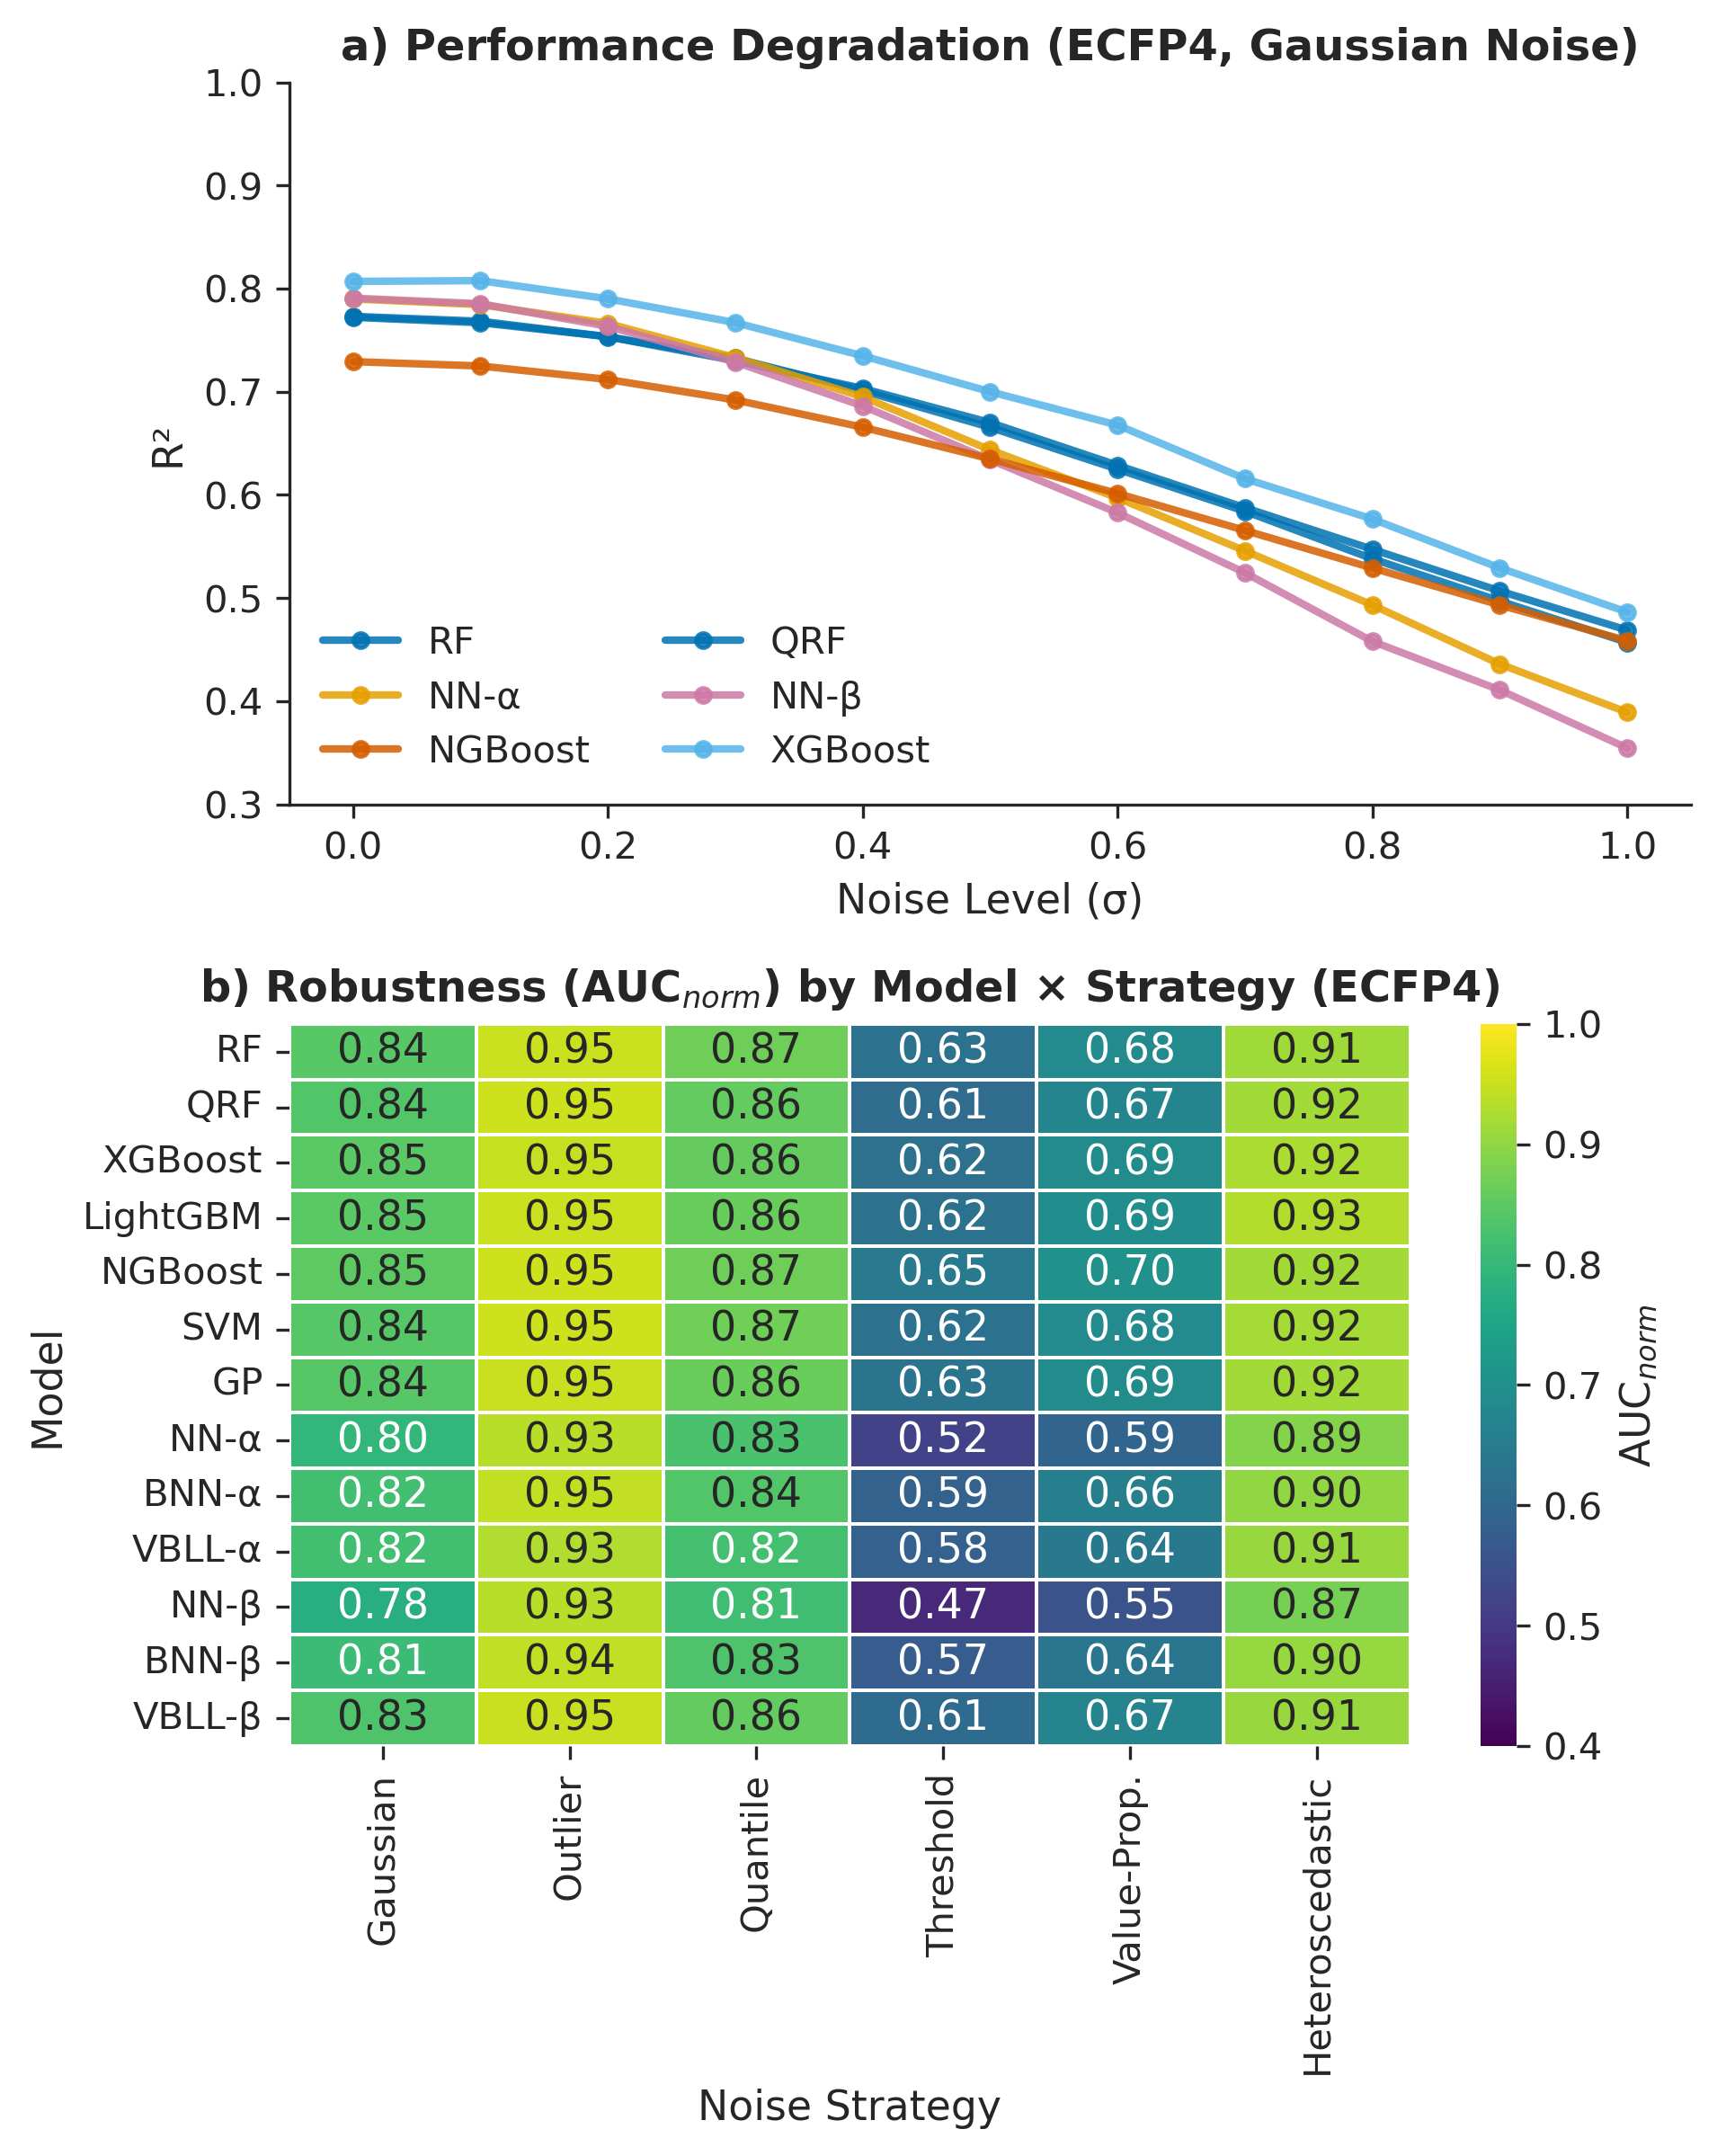
\includegraphics[width=\textwidth,height=0.78\textheight,keepaspectratio]{fig1_supp_ecfp4_overview.png}
\caption{\textbf{Global overview of noise robustness on the ECFP4 representation, evaluated on QM9 HOMO--LUMO gap.}
a) Performance degradation curves (R$^2$ versus noise level $\sigma$) under Gaussian noise. b) Noise degradation slope (NDS) heatmap across model architectures and noise strategies; lower (more negative) NDS indicates faster degradation under noise.}
\label{app:noise:ecfp4_overview}
\end{figure}


\addfile{Clean $R^2$ against robustness on PDV under Gaussian noise}
\label{app:noise:sec:clean_r2_vs_robustness}
% TODO: review, needs manual review
Clean-label $R^2$ against the noise degradation slope for every model on PDV under Gaussian noise, on the QM9 HOMO--LUMO gap.
% Thesis appendix item: clean_r2_vs_robustness

\begin{figure}[H]
\centering
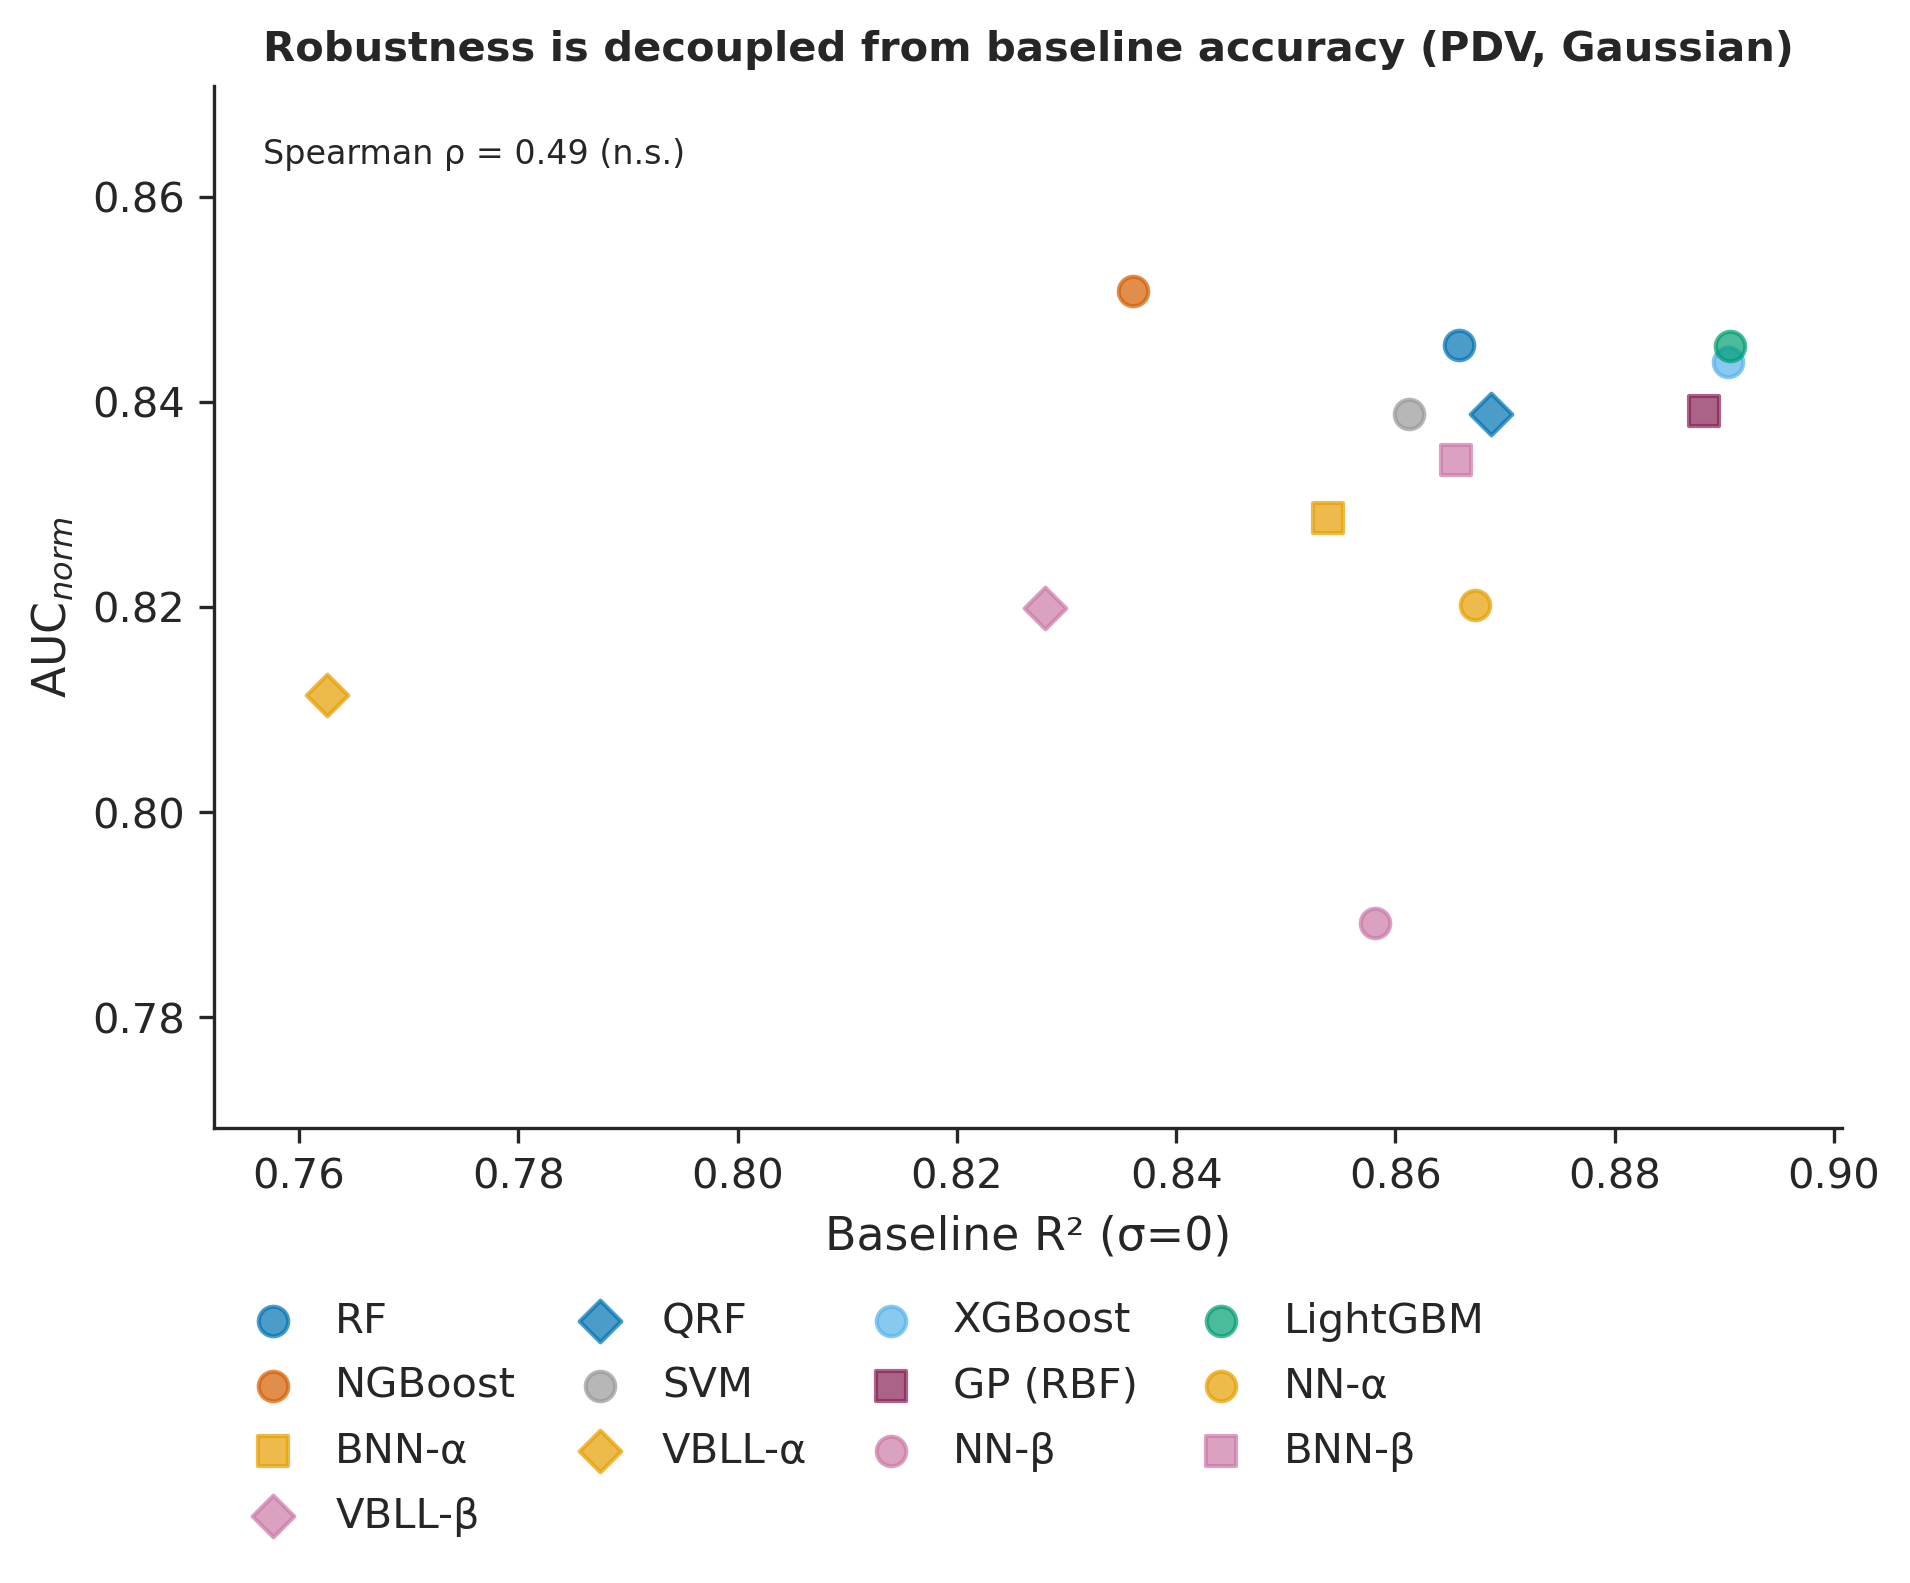
\includegraphics[width=\textwidth]{fig3_ranking_consistency.png}
\caption{\textbf{Baseline R$^2$ versus noise degradation slope (NDS) scatter for all models on the physicochemical descriptor vector (PDV) representation under Gaussian noise, on the QM9 HOMO--LUMO gap.}
Lower (more negative) NDS indicates faster performance loss under noise.}
\label{app:noise:clean_r2_vs_robustness}
\end{figure}


\addfile{Bayesian transformation effects by representation}
\label{app:noise:sec:bayesian_transformation_tests}
% TODO: review, needs manual review
The effect of each Bayesian transformation of the neural networks on the noise degradation slope, by representation, on the QM9 HOMO--LUMO gap.
% Thesis appendix item: bayesian_transformation_tests

\begin{table}[H]
\centering
\caption{\textbf{Neural network Bayesian transformation effects on noise degradation slope (NDS) by representation, on the QM9 HOMO--LUMO gap.}
Positive $\Delta$ NDS indicates the Bayesian variant is more robust (less negative slope) than its deterministic counterpart.}
\label{app:noise:bayesian_transformation_tests}
\small
\begin{tabular}{llrrrr}
\toprule
\textbf{Model} & \textbf{Representation} & \textbf{Baseline R$^2$} & \textbf{NN-$\beta$ NDS} & \textbf{BNN-$\beta$ NDS} & \textbf{$\Delta$ NDS} \\
\midrule
NN-$\beta$ & ECFP4 & 0.791 & $-0.464$ & $-0.388$ & $+0.076$ \\
NN-$\beta$ & PDV & 0.858 & $-0.487$ & $-0.382$ & $+0.106$ \\
NN-$\beta$ & SMILES & 0.721 & $-0.558$ & $-0.365$ & $+0.193$ \\
\bottomrule
\end{tabular}
\end{table}


\addfile{Uncertainty metrics for probabilistic models on ECFP4}
\label{app:noise:sec:uncertainty_metrics_ecfp4}
% TODO: review, needs manual review
Uncertainty metrics of the probabilistic models on ECFP4 under Gaussian noise, on the QM9 HOMO--LUMO gap.
% Thesis appendix item: uncertainty_metrics_ecfp4

\begin{table}[H]
\centering
\caption{\textbf{Uncertainty quantification metrics for probabilistic models on the ECFP4 representation (Gaussian noise strategy) on the QM9 HOMO--LUMO gap.}
Unc-Error $\rho$: Spearman correlation between predicted uncertainty and absolute prediction error. Unc-Noise $\rho$: Spearman correlation between predicted uncertainty and injected noise level $\sigma$. ECE: expected calibration error (lower = better-calibrated). Coverage targets: 68\% ($1\sigma$), 95\% ($2\sigma$).}
\label{app:noise:uncertainty_metrics_ecfp4}
\small
\begin{tabular}{lrrrrr}
\toprule
\textbf{Model} & \textbf{Unc-Error $\rho$} & \textbf{Unc-Noise $\rho$} & \textbf{ECE} & \textbf{Cov.\ $1\sigma$} & \textbf{Cov.\ $2\sigma$} \\
\midrule
\textbf{QRF}     & \textbf{0.25} & 0.27 & 0.19 & 74.7\% & 94.6\% \\
\textbf{NGBoost} & 0.22 & \textbf{0.37} & \textbf{0.11} & 69.2\% & 94.2\% \\
GP               & 0.18 & 0.34 & 0.23 & 78.6\% & 96.0\% \\
BNN-$\beta$      & 0.20 & 0.37 & 0.29 & 78.6\% & 95.2\% \\
BNN-$\alpha$     & 0.15 & 0.32 & 0.24 & 76.6\% & 95.1\% \\
VBLL-$\beta$     & 0.19 & 0.34 & 0.19 & 73.9\% & 95.5\% \\
VBLL-$\alpha$    & 0.11 & 0.31 & 0.22 & 74.5\% & 95.1\% \\
\bottomrule
\end{tabular}
\end{table}


\addfile{Variance decomposition on the three assay datasets}
\label{app:noise:sec:assay_variance_decomposition}
% TODO: review, needs manual review
ANOVA variance decomposition ($\eta^2$, in per cent) on LogD, Caco-2 efflux and hERG $K_i$.
% Thesis appendix item: assay_variance_decomposition

\begin{figure}[H]
\centering
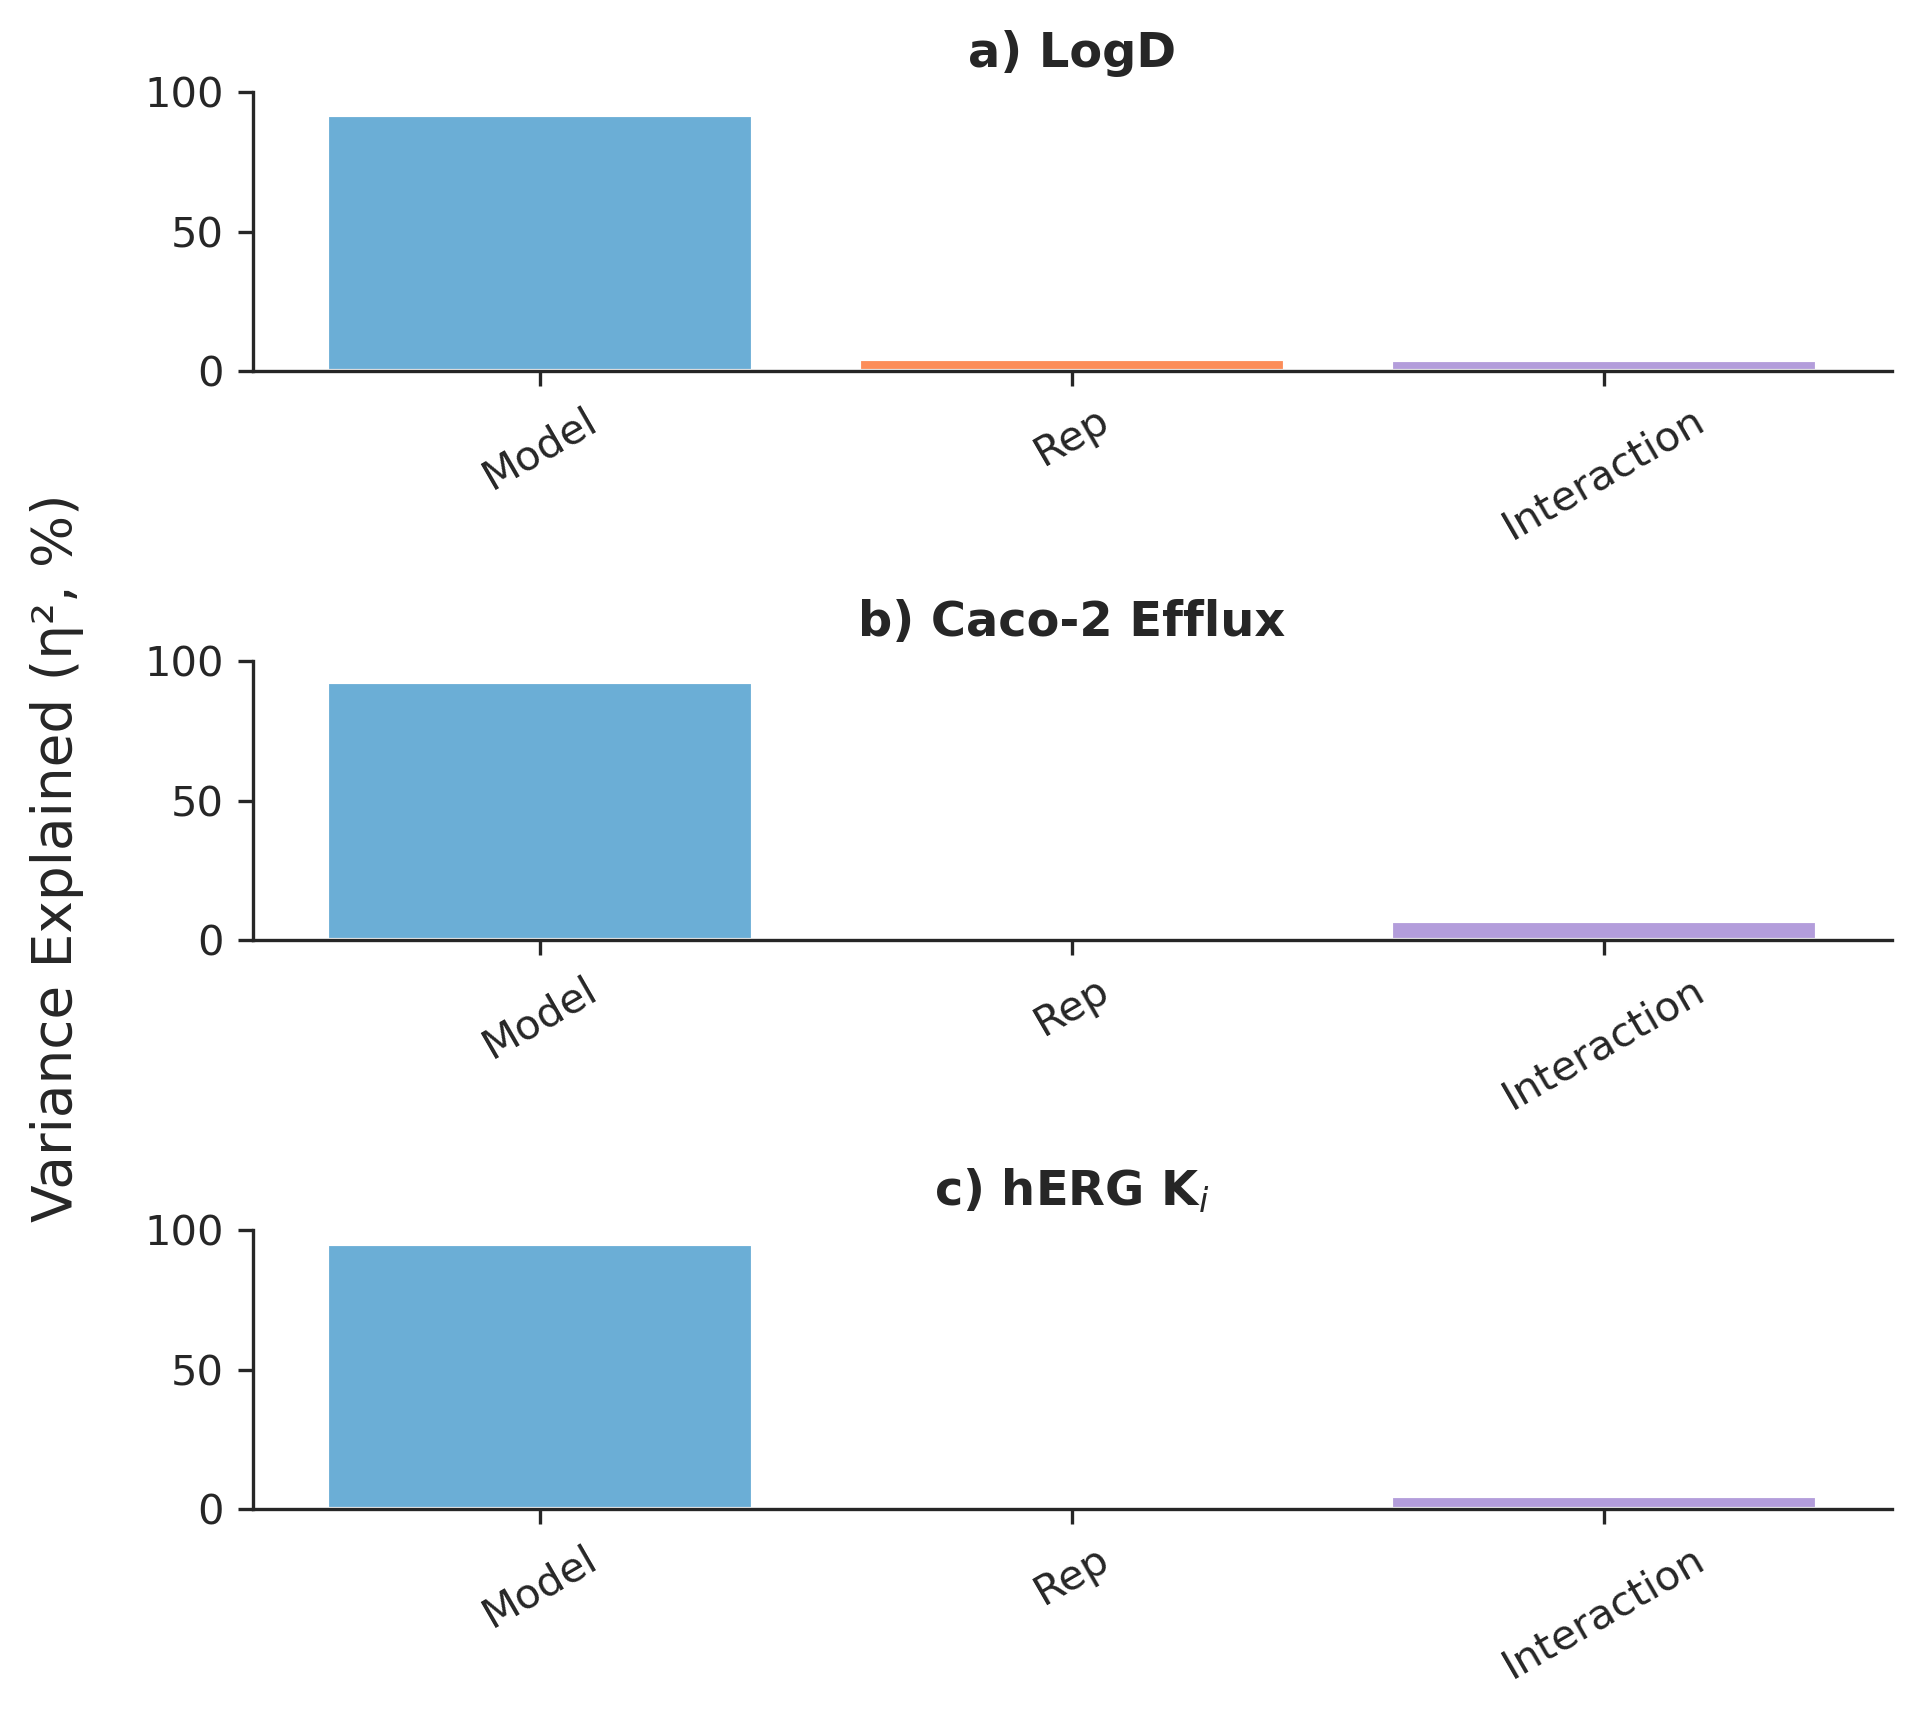
\includegraphics[width=\textwidth]{fig_validation_anova.png}
\caption{\textbf{ANOVA variance decomposition ($\eta^2$, \%) on external validation datasets: a) LogD, b) Caco-2 Efflux, and c) hERG K$_i$.}
Model, representation, and interaction contributions to noise degradation slope (NDS) variance for each dataset; lower (more negative) NDS indicates faster performance loss under noise.}
\label{app:noise:assay_variance_decomposition}
\end{figure}


\addfile{Random forest against quantile regression forest on the three assay datasets}
\label{app:noise:sec:rf_vs_qrf_assay}
% TODO: review, needs manual review
The noise degradation slope of random forest and of quantile regression forest on LogD, Caco-2 efflux and hERG $K_i$.
% Thesis appendix item: rf_vs_qrf_assay

\begin{table}[H]
\centering
\caption{\textbf{Random forest (RF) vs quantile regression forest (QRF) noise degradation slope (NDS) on the three external validation datasets (LogD, Caco-2 Efflux, hERG K$_i$).}
Lower (more negative) NDS indicates faster degradation under noise.}
\label{app:noise:rf_vs_qrf_assay}
\small
\begin{tabular}{lrrr}
\toprule
\textbf{Dataset} & \textbf{RF NDS} & \textbf{QRF NDS} & \textbf{$\Delta$ NDS} \\
\midrule
ChEMBL-hERG-Ki     & $-0.231$ & $-0.359$ & $-0.128$ \\
OpenADMET-Caco2    & $-0.534$ & $-0.627$ & $-0.094$ \\
OpenADMET-LogD     & $-0.101$ & $-0.185$ & $-0.083$ \\
\bottomrule
\end{tabular}
\end{table}


\section{The flaws of the similarity assumption}\label{app:add:flaws}
% ---- NOTES: The flaws of the similarity assumption ----
% - Files for Chapter~\ref{chap:flaws}.
% Table: constant features. One row is one dataset and one representation. Columns: total features; constant features; near-constant features. A per-domain summary stays in Chapter 4.
% TODO(results): constant and near-constant feature counts per dataset and representation.
% Table: molecules a representation cannot tell apart. One row is one representation and one dataset. Columns: molecules in groups with an identical feature vector; how many of those differ only in stereochemistry; lowest RMSE reachable when every group gets one prediction; largest label spread within a group.
% TODO(results): identical-vector counts per representation and dataset.
% Table: distance against property difference. One row is one dataset and one representation. Columns: rank correlation between pairwise distance and absolute property difference; score of predicting each molecule's activity from its five nearest neighbours in that representation.
% TODO(results): distance-property correlations and five-nearest-neighbour scores.
% Table: activity cliffs. One row is one dataset and one representation. Column: molecules that belong to at least one activity cliff.
% TODO(results): activity-cliff counts per dataset and representation.
% ---- END NOTES ----
\todo[inline, color=orange!40]{Additional files for Chapter~\ref{chap:flaws}: all four need the full runs.}

\section{Building adaptive hybrid representations}\label{app:add:method}\label{app:searchspace}
% ---- NOTES: Building adaptive hybrid representations ----
% - Files for Chapter~\ref{chap:method}.
% - The settings, formulas and reasons are in Chapter 5 ("The search space and why each axis is swept", its three subsubsections, "Augmentation", "Fast tier and adaptive pruning"). This section holds only the reference tables those sections point to.
% - The first five files below are written from the current code and the design runs. The rest need the full runs.
% - Which datasets get the Gaussian process, and why: only in "Models and metrics". The model-settings and models-left-out files point there and do not repeat it. Whether nanobody thermostability also gets the Gaussian process is an open decision under "Search tier settings"; the Gaussian process row of the models-left-out file follows that answer.
% - The models fitted only to compute importance are in the table under "Feature importance scoring". The model-settings file points there and does not repeat them.
% - Two open decisions change the model-settings file: the random forest evaluator's features per split on regression datasets, and the DNN evaluator's early-stopping split (both under "Internal evaluation"). The file states the current settings; change the row if either answer is yes.
% - The open decision under "Models and metrics" (count the whole dataset or the training molecules) changes the SVM row of the models-left-out file for LogD and TATA promoter. The file carries a footnote; change it to match the answer.
% - The design-experiment file: the reason the kept pooled allocation method was chosen over the other pooled candidates is an open decision under "Feature allocation strategies". The allocation row states only the counts; add the reason once it is written there. The pooled candidates that were not kept are not named.
% - The design-experiment file: the representation-count row gives no result; the best count per (model, budget) was not carried into the notes. Add it from the design run, or leave the cell as it is.
%
% TODO(results): per dataset and downstream model, per-fold score of the best single representation against the hybrid, with the spread across folds.
% TODO(results): per dataset, the winning configuration: downstream model, budget, allocation method, importance method, internal evaluator, representation count.
% TODO(results): per dataset, how often each value of each setting won across (downstream model, budget) combinations.
% TODO(results): augmentation per dataset: how often no extra features were chosen; per-fold base against base plus extras, uncapped and capped; which extra feature sets were kept; decoy features admitted.
% TODO(results): per dataset and budget, held-out score against the score the inner search reported, and the stability of the selected features across folds.
% TODO(results): hybrid minus each comparator (concatenation, one model per representation, PCA, mRMR, recursive feature elimination, random features) at each budget.
% TODO(results): the smaller experiments in "Comparators, controls and ablations", one table each, if they leave the chapter.
% TODO(results): per task, outcome of the transfer, antibody-scan and separate-site experiments, with which representations the selected features came from.
% TODO(results): hours and model fits per dataset at each tier, with the hardware.
% ---- END NOTES ----

\addfile{Settings of every model, as downstream model and as internal evaluator}
\label{app:add:model_settings}
% TODO: review, needs manual review
One row is one model. The middle two columns give its settings when it scores a hybrid (downstream model) and when it scores one representation inside the search (internal evaluator). The models fitted only to compute feature importance are in Table~\ref{tab:importance_methods}.

% TODO: review, needs manual review (whole table and caption, written from the current code)
{\small
\begin{longtable}{@{}p{1.9cm}p{4.6cm}p{3.6cm}p{1.6cm}p{2.3cm}@{}}
\caption{Settings of every model. $p$ is the number of features. ``Molecules'' is the number of training molecules the internal evaluator is fitted on; above it, a random subset of that size is drawn with a fixed seed. Settings not listed are the library's defaults. Every setting is the same on every dataset. The Gaussian process runs only on the datasets named in Chapter~\ref{chap:method}, ``Models and metrics''.}
\label{tab:add:model_settings}\\
\toprule
Model & As downstream model & As internal evaluator & Molecules & Library; source \\
\midrule
\endfirsthead
\toprule
Model & As downstream model & As internal evaluator & Molecules & Library; source \\
\midrule
\endhead
Random forest & 100 trees, no depth limit; $\sqrt{p}$ features tried at each split & 50 trees, depth at most 10; all $p$ features tried at each split on regression, $\sqrt{p}$ on classification & all & scikit-learn \citep{scikit-learn}; \citet{Breiman2001} \\
\addlinespace
LightGBM & 100 trees & 50 trees, depth at most 4 & all & lightgbm; \citet{ke2017lightgbm} \\
\addlinespace
XGBoost & 100 trees; half of the features sampled for each tree & 50 trees, depth at most 4 & all & xgboost; \citet{Chen2016} \\
\addlinespace
SVM & RBF kernel, $C = 1$. Not fitted above 10{,}000 molecules, or above 5{,}000 under uncapped augmentation & RBF kernel, $C = 1$ & at most 500 & scikit-learn; \citet{Vapnik1995} \\
\addlinespace
Gaussian process & Regression: RBF plus white-noise kernel, labels normalised, 3 optimiser restarts. Classification: RBF kernel. Not fitted above 1{,}000 molecules & Regression: scaled RBF kernel, fixed noise variance 0.01, no restarts. Classification: scaled RBF kernel, no restarts & at most 500 & scikit-learn; \citet{Rasmussen2006} \\
\addlinespace
DNN & Hidden layers of 256, 128 and 64 units, ReLU, dropout 0.2 \citep{Srivastava2014}; Adam \citep{Kingma2015} at learning rate 0.001, halved after 5 epochs without improvement; batch size 256; up to 200 epochs; stops after 20 epochs without improvement on 20\% of the training molecules that share no group with the rest, using the outer split's grouping; labels z-normalised & The same, except that the early-stopping 20\% is drawn at random & all & PyTorch \citep{Paszke2019} \\
\bottomrule
\end{longtable}
}

\addfile{Downstream models left out, by dataset and augmentation setting}
\label{app:add:models_left_out}
% TODO: review, needs manual review
One row is one rule that leaves a downstream model out. Only the 16 datasets of Table~\ref{tab:datasets} are listed; a dataset and setting not named in any row runs every downstream model in Table~\ref{tab:search_tiers}.

% TODO: review, needs manual review (whole table and caption, written from the current code)
{\small
\begin{longtable}{@{}p{2.4cm}p{3.0cm}p{8.6cm}@{}}
\caption{Downstream models left out, by dataset and augmentation setting. Every rule was set so that a search finishes within the time limit of one job; none was set from scores. hERG $K_i$ drops no model under any setting.}
\label{tab:add:models_left_out}\\
\toprule
Model left out & Augmentation setting & Datasets \\
\midrule
\endfirsthead
\toprule
Model left out & Augmentation setting & Datasets \\
\midrule
\endhead
XGBoost & all three & H3K4me3, TATA promoter \\
SVM & all three & datasets above 10{,}000 molecules: H3K4me3 \\
SVM & uncapped & datasets above 5{,}000 molecules: QM9, LogD$^{a}$, TATA promoter$^{a}$ \\
SVM & uncapped & Koenig expression \\
SVM & capped & Caco-2 efflux, LogD, rat liver microsome clearance, MDR1--MDCK efflux, Buchwald--Hartwig plates \\
Random forest and SVM & capped & QM9 \\
Random forest & uncapped & QM9, LogD \\
Gaussian process & all three & every dataset except humanness (Chapter~\ref{chap:method}, ``Models and metrics'') \\
\bottomrule
\end{longtable}
{\footnotesize $^{a}$Counted on the whole dataset: LogD has 5{,}028 molecules and TATA promoter 5{,}274. A search run inside one outer fold is given about 80\% of them and keeps the SVM.}
}

\addfile{Size of the search}
\label{app:add:search_size}
% TODO: review, needs manual review
One row is one downstream model. The counts are per dataset, objective and augmentation setting, with adaptive pruning off.

% TODO: review, needs manual review (whole table and caption)
\begin{table}[htbp]
\centering
\small
\caption{Number of configurations searched per dataset, objective and augmentation setting. A configuration is one choice of downstream model, internal evaluator, allocation method, importance method, representation count and budget. At the full tier each (downstream model, internal evaluator) pair runs 5 allocation methods $\times$ 3 importance methods $\times$ 4 representation counts $\times$ 8 budgets $= 480$ configurations; at the fast tier it runs $3 \times 1 \times 2 \times 8 = 48$ (Table~\ref{tab:search_tiers}). ``Matched'' is counted once where it repeats an evaluator already in the list. Each configuration is scored on 5 folds, so the full tier fits a downstream model 40{,}800 times (50{,}400 on humanness) and the fast tier 4{,}080 times. Where a dataset leaves a downstream model out (Additional file~\ref{app:add:models_left_out}), its pairs drop out: a fast search on H3K4me3 has 9 pairs, so 432 configurations.}
\label{tab:add:search_size}
\begin{tabular}{@{}lp{4.2cm}rr@{}}
\toprule
Downstream model & Internal evaluators & Full tier & Fast tier \\
\midrule
Random forest & 3 (matched is random forest) & 1{,}440 & 144 \\
LightGBM & 3 (matched is LightGBM) & 1{,}440 & 144 \\
DNN & 3 (matched is DNN) & 1{,}440 & 144 \\
XGBoost & 4 & 1{,}920 & 192 \\
SVM & 4 & 1{,}920 & 192 \\
Gaussian process (humanness only) & 4 & 1{,}920 & not run \\
\midrule
Total & 17 pairs (21 on humanness) & 8{,}160 (10{,}080 on humanness) & 816 \\
\bottomrule
\end{tabular}
\end{table}

\addfile{Design experiments behind the search settings}
\label{app:add:design_experiments}
% TODO: review, needs manual review
One row is one setting of the search, or one rule that was tested and then fixed instead of searched. Every number comes from preliminary design runs made before the main experiments; they are not results of the thesis, and several used other budgets than the final search.

% TODO: review, needs manual review (whole table and caption; numbers from preliminary design runs)
{\footnotesize
\begin{longtable}{@{}p{1.9cm}p{2.5cm}p{2.7cm}p{4.4cm}p{2.5cm}@{}}
\caption{Design experiments behind the search settings. Preliminary design runs, not the thesis's full runs.}
\label{tab:add:design_experiments}\\
\toprule
Setting & Values compared & Datasets, folds, budgets & What was measured, and the result & Values kept (full / fast) \\
\midrule
\endfirsthead
\toprule
Setting & Values compared & Datasets, folds, budgets & What was measured, and the result & Values kept (full / fast) \\
\midrule
\endhead
Downstream model & Nine models, among them random forest, LightGBM, XGBoost, CatBoost, DNN, $k$-nearest neighbours and a Gaussian process, each on each of 10 base representations at full width & Buchwald--Hartwig yield, Caco-2 efflux, Koenig expression, LogD, breast cancer PAM50 subtype; 5 folds & Best held-out score over the 10 representations, and seconds per fit. The DNN scored best on 4 of the 5 datasets and third on Caco-2 (0.2936 against 0.2851 RMSE, log$_{10}$ efflux ratio) & Full: random forest, LightGBM, XGBoost, SVM, DNN, and the Gaussian process on humanness / fast: the same five \\
\addlinespace
Budget & None compared & -- & -- & 10, 25, 50, 100, 250, 500, 1{,}000 and 2{,}000 features at both tiers \\
\addlinespace
Representation count & 2, 3, 5 and all 10 & 9 datasets, 3 tree-ensemble downstream models, budgets 500 and 1{,}000 features; 5 folds & The best count for each (downstream model, budget) combination & Full: 2, 3, 5, all / fast: 3, all \\
\addlinespace
Allocation method & 8 candidates: the five searched and 3 further pooled candidates, each at every representation count & The same 9 datasets, models and budgets: 54 (dataset, model, budget) combinations & Each candidate was scored at its best representation count, and the number of combinations in which it was in the top 3 of the 8 was counted. Fixed shares: linear 30, squared 27, rank decay 26, softmax 25; global pool with squared weights 14 & Full: the five in Table~\ref{tab:allocation_methods} / fast: linear, squared, rank decay \\
\addlinespace
Importance method, agreement & 8 methods & LogD, hERG $K_i$, Buchwald--Hartwig yield, nanobody thermostability, antibody FcRn retention, breast cancer PAM50 subtype, lung adenocarcinoma vs squamous; each method fitted once on the whole dataset & Spearman correlation between two methods' scores over every feature. Kept pairs: LightGBM gain and TreeSHAP 0.20--0.64, LightGBM gain and DeepLIFT 0.21--0.67, TreeSHAP and DeepLIFT 0.56--0.99 across the 7 datasets & One method kept from each group whose rankings agree above 0.95 \\
\addlinespace
Importance method, score & 28 methods, among them three controls: feature variance, Laplacian score and random ranking & Caco-2 efflux; 3 folds; budget 100 features; random forest and LightGBM downstream & RMSE of the best single representation minus RMSE of the hybrid (log$_{10}$ efflux ratio; positive means the hybrid has the lower error): DeepLIFT $+0.0144$, LightGBM gain $+0.0100$, TreeSHAP $+0.0067$, random ranking $-0.0118$ & Full: LightGBM gain, TreeSHAP, DeepLIFT / fast: LightGBM gain \\
\addlinespace
Internal evaluator settings & 20 hyperparameter settings from 5 model families & Buchwald--Hartwig yield, Caco-2 efflux, Koenig expression; 3 folds; budget 100 features & Spread of mean scores across all 20 settings: 0.0253 $R^2$, 0.0179 $R^2$ and 0.0085 Spearman. Median standard deviation across the 3 folds for one setting, allocation method and downstream model: 0.0462 $R^2$, 0.0693 $R^2$ and 0.0186 Spearman & Matched, random forest, LightGBM and DNN, at fixed settings, both tiers \\
\addlinespace
Rescaling of each representation's score (a rule) & 5 rescalings & 9 datasets; 5 folds; budgets 50 and 300 features & Whether any rescaling beat the one in use by more than that rule's own spread across folds: in 0 of 90 (dataset, allocation method, budget) combinations & One fixed rule per metric (Table~\ref{tab:standalone-rescaling}) \\
\bottomrule
\end{longtable}
{\footnotesize The representation-count and allocation rows come from one design run on 10 datasets, 3 downstream models and 2 budgets (60 combinations); QM9 is left out, which gives the 54.}
}

\addfile{Fields a blueprint saves}
\label{app:add:blueprint_fields}
% TODO: review, needs manual review
One row is one field. The first block is the recipe that rebuilds a hybrid; the second is kept for inspection and is not read by a rebuild.

% TODO: review, needs manual review (whole table and caption, written from the current code)
{\small
\begin{longtable}{@{}p{4.6cm}p{9.4cm}@{}}
\caption{Fields a blueprint saves. The stored score of each representation is its best score on its own across the downstream models, over every molecule the search ran on. It is not the internal-evaluator score that splits the budget, which a rebuild computes again on the molecules it is given. Three further fields are read only by allocation or augmentation routes outside the thesis's search and are fixed: a minimum improvement a whole block of extra features must show (none), a number of features taken from each source (20), and a step size (5).}
\label{tab:add:blueprint_fields}\\
\toprule
Field & What it holds \\
\midrule
\endfirsthead
\toprule
Field & What it holds \\
\midrule
\endhead
\multicolumn{2}{@{}l}{\textit{The recipe}} \\
\midrule
Representations & The representations offered to the search \\
Representation count & How many of them the configuration used; empty when it used all \\
Allocation method & One of the five in Table~\ref{tab:allocation_methods} \\
Importance method & LightGBM gain, TreeSHAP or DeepLIFT \\
Budget & Number of features in the hybrid \\
Internal evaluator & Matched, random forest, LightGBM or DNN \\
Objective & Predictive, or predicting each molecule's activity from its five nearest neighbours \\
Metric & The dataset's metric, and whether lower is better \\
Task type & Regression or classification \\
Folds and seed & The number of folds, and the random seed \\
\midrule
\multicolumn{2}{@{}l}{\textit{The recipe: augmentation}} \\
\midrule
Augmentation setting & None, uncapped or capped \\
Candidate ranking & How candidate extra features are ranked \\
Candidate list length & 50 features \\
Cap per source & Optional; the most candidates taken from one source \\
Margin & How much better than adding none a block of extra features must score \\
Fraction of the budget & Optional; used instead of the fixed block sizes \\
\midrule
\multicolumn{2}{@{}l}{\textit{Kept for inspection, not read by a rebuild}} \\
\midrule
Representation scores & Each representation's best score on its own across the downstream models, sign flipped for metrics where lower is better \\
Features per representation & The number of features each representation got in each fold \\
Extra features kept & The extra features augmentation kept in each fold, by source \\
\bottomrule
\end{longtable}
}

\todo[inline, color=orange!40]{Additional files for Chapter~\ref{chap:method}: the per-dataset results, augmentation, held-out against inner-search scores, comparators, smaller experiments, transfer experiments and compute need the full runs.}

\section{Hybrid representations for similarity and label noise}\label{app:add:similarity}
% ---- NOTES: Hybrid representations for similarity and label noise ----
% - Files for Chapter~\ref{chap:similarity}.
% - The chapter's own two tables (noise conditions, and the twelve LNL methods) stay in the chapter. The settings file below gives each method's numbers; the chapter's table gives what each method does.
% Table: finding injected noisy labels. One row is one noise score. Columns: average precision under outlier noise at 1\%, 5\% and 10\%, grouped-wider noise and censoring, in each feature space (each model's top two single representations, the same features weighted by importance, forest proximity, the hybrid, the hybrid ranked on the neighbour score); chance level in the header row. The chapter's table keeps only 10\% outlier noise, grouped-wider noise and censoring in two feature spaces.
% TODO(results): average precision per noise score, feature space and noise condition, all outlier levels, with chance level.
% Table: finding real suspect labels. One row is one noise score and feature space. Columns: average precision against ChEMBL curator flags on hERG IC50, per record and per molecule, with chance level; Spearman correlation with the spread between laboratories on the BindingDB molecules with repeat measurements.
% TODO(results): average precision against curator flags and correlation with the spread between laboratories, per noise score and feature space.
% Table: estimated noise size. One row is one dataset and feature space. Columns: the estimate from repeat measurements (with the directly measured variance between repeats where the dataset keeps them); the estimate from near-duplicate pairs; the gamma-test estimate; the model's held-out mean squared error. All in label units squared.
% TODO(results): the three noise-size estimates per dataset and feature space, beside the model's held-out mean squared error.
% TODO(results): per dataset and fold, importance-weighted against unweighted features for predicting each molecule's activity from its five nearest neighbours; the hybrid searched for that objective against the ordinary hybrid and the two best single representations.
% TODO(results): censoring: share of the lost score recovered, per treatment, model, feature space and clipping level; deleting clipped molecules against keeping them.
% TODO(results): the survey of twelve LNL methods: per noise level, the methods that beat the plain network on each input.
% TODO(results): cleaning real labels: folds won per cleaning method, noise score and feature space.
% TODO(results): per noise type, whether any LNL method, noise mitigation or noise-robust training, improved on the untreated model, on each feature space.
% ---- END NOTES ----

\addfile{Settings of the twelve LNL methods and the plain network they share}
\label{app:add:lnl_settings}
% TODO: review, needs manual review
One row is one method; the first row is the plain network every method starts from. The kind of each method follows Table~\ref{tab:lnl_methods}.

% TODO: review, needs manual review (whole table and caption, written from the current code)
{\small
\begin{longtable}{@{}p{2.9cm}p{2.0cm}p{7.3cm}p{1.6cm}@{}}
\caption{Settings of the twelve LNL methods. On classification datasets the squared-error loss is replaced by cross-entropy.}
\label{tab:add:lnl_settings}\\
\toprule
Method & Kind & Settings & Labels \\
\midrule
\endfirsthead
\toprule
Method & Kind & Settings & Labels \\
\midrule
\endhead
Plain network & -- & Hidden layers of 256, 128 and 64 units, ReLU, dropout 0.2; Adam at learning rate 0.001, halved after 5 epochs without improvement; batch size 256; gradient norm clipped at 1; up to 200 epochs; stops after 20 epochs without improvement on 20\% of the training molecules held out by scaffold group (drawn at random after a method has removed molecules); labels z-normalised & both \\
\midrule
Small-loss selection & noise mitigation & 10 warm-up epochs on all molecules; keeps the 70\% with the smallest loss and fits a new plain network on them & both \\
Confident learning & noise mitigation & 3 plain networks; removes molecules whose error is above the 85th percentile and whose spread across the 3 networks is below the 25th percentile, then refits & both \\
Removal by distance to neighbours & noise mitigation & 10 nearest neighbours in the standardised features; score is the distance of a label from its neighbours' mean label, divided by their standard deviation (on classification, the share of neighbours with another label); removes molecules above the 85th percentile, then refits & both \\
Staged removal & noise mitigation & 3 stages; each removes the 10\% of the remaining molecules with the largest training loss & both \\
\midrule
Per-epoch down-weighting & noise-robust training & After each epoch, the weight of every molecule whose loss is above the median is multiplied by 0.95 & both \\
Curriculum by confidence & noise-robust training & 20 warm-up epochs, then trains on the 25\%, 50\%, 75\% and 100\% of molecules with the smallest loss, in stages & both \\
DivideMix & noise-robust training & Two networks, 10 warm-up epochs; a two-component Gaussian mixture on each network's squared errors splits the molecules & both \\
Meta-Weight-Net & noise-robust training & The weighting network is updated every 5 epochs at learning rate 0.001, on 20\% of the training molecules held out for it & both \\
MentorNet & noise-robust training & The mentor network reads each molecule's current loss, its last 5 losses and its mean distance to its 10 nearest neighbours & both \\
Contrast to Divide & noise-robust training & 5 perturbed copies of each molecule, Gaussian noise of standard deviation 0.01 on the features & both \\
\midrule
Heteroscedastic GP & noise-robust training & RBF kernel, 2 optimiser restarts, fitted on at most 1{,}000 training molecules; a small network predicts each molecule's noise variance & regression \\
Deep evidential regression & noise-robust training & Weight of the evidence penalty 0.01 & regression \\
\bottomrule
\end{longtable}
}

\todo[inline, color=orange!40]{Additional files for Chapter~\ref{chap:similarity}: finding injected and real noisy labels, estimated noise size and the other results need the full runs.}
\chapter{Data and code availability}\label{app:availability}
% TODO: needs manual review (whole chapter written by Claude)
% ---- NOTES: Data and code availability ----
% Decision for you: the author contributions now appear twice, in the Statement of Originality and in the last paragraph below. Keep both and they must stay word for word the same; keep one and point to it from the other. The two differ in one sentence now: "All authors read and approved the final manuscript" is in your paper and below, but not in the Statement of Originality.
% Decision for you: whether the contributions paragraph below also says A.P. wrote the QM9 pipeline. Your paper names only NoiseInject, so the sentence below now matches the paper. Every commit in the qsar_qm_models repository is yours, so adding it would be accurate.
% Decision for you: the licence for KIRBy. Your earlier plan was MIT or Apache-2.0. The repository has no licence file and is private, so the KIRBy block has placeholders, and the last sentence of the second data paragraph holds only once it is public.
% Decision for you: whether to give each public dataset's licence, as a column in the dataset table of Appendix~\ref{app:datasets}. Now the text gives licences only for OpenADMET, ChEMBL and the Biogen set; QM9 has none stated. The reaction-yield, antibody, nucleotide and gene-expression licences depend on which copy was downloaded and were not checked.
% Decision for you: the Python version for KIRBy. The package metadata declares 3.8 or later. The repository's setup guide gives 3.9 as the minimum and recommends 3.10 to 3.11. The university cluster has 3.9. The software block below says 3.8 or later, as the package metadata declares, until you pick one.
% Decision for you: the licence of the QM9 pipeline release. The qsar_qm_models repository holds a GNU GPL v3 licence file, so the block below says GPL v3. Your earlier plan was MIT or Apache-2.0. Keep GPL v3, or change it; the licence line and the "restrictions to use by non-academics" line both follow from your choice.
% Decision for you: your NoiseInject paragraph (restored as you wrote it) says "six regression and six classification noise injection strategies". Chapter~\ref{chap:robustness} and Section~\ref{sec:noise_injection} now define seven noise conditions. Keep the package's own count, or change it to match the chapters.
% ---- END NOTES ----

% TODO: review, needs manual review
Three pieces of software lie behind this thesis. NoiseInject is the label-noise package released with Chapter~\ref{chap:robustness}. A separate pipeline ran the QM9 experiments of that chapter. The KIRBy repository implements the adaptive hybrid representation and holds the experiments of Chapters~\ref{chap:flaws}, \ref{chap:method} and~\ref{chap:similarity}, together with the assay-dataset runs of Chapter~\ref{chap:robustness}. The three are separate, so each can be reused on its own. For example, the hybrid search runs on feature matrices a reader has computed elsewhere, without the Rust part of the QM9 pipeline. The source and curation of each dataset are given in Appendix~\ref{app:datasets}.

The NoiseInject benchmarking framework, implementing all six regression and six classification noise injection strategies together with the robustness metrics (noise degradation slope and retention) and uncertainty-calibration metrics (ECE, coverage at $1\sigma$/$2\sigma$, mean interval width, and uncertainty--error / uncertainty--noise correlation) described in this work, is available as an open-source Python package under an MIT license \citep{noiseinject}. It also contains optional reference wrappers (a Gaussian process, split-conformal prediction, and Monte Carlo dropout) that produce per-sample uncertainty for use with these metrics. NoiseInject is model-agnostic, operates on label arrays (NumPy arrays or pandas Series), and is designed to integrate into existing cheminformatics or other data pipelines. Worked examples covering molecular-descriptor, fingerprint, and GNN-embedding workflows are provided in the repository.

% TODO: review, needs manual review
Its noise conditions and metrics are described in Section~\ref{sec:noiseinject}.

% TODO(you): the DOI archives v0.3.0 (3 June 2026), not 1.0.0; replace it once a 1.0.0 Zenodo release exists.
\begin{itemize}
    \item Project name: NoiseInject
    \item Project home page: \url{https://github.com/adpunt/noise_inject}
    \item Archived version: \url{https://doi.org/10.5281/zenodo.20532710}
    \item Version: 1.0.0
    \item Operating system(s): Platform independent
    \item Programming language: Python 3.7 or later
    \item Other requirements: NumPy, pandas, SciPy and scikit-learn; see the repository's \texttt{requirements.txt}
    \item License: MIT
    \item Any restrictions to use by non-academics: None
\end{itemize}

% TODO: review, needs manual review
The QM9 results of Chapter~\ref{chap:robustness} were produced by a separate repository, written in Python and Rust, which also holds the hyperparameter tuning, the variance decomposition and the figure scripts for that chapter. It is described in Chapter~\ref{chap:robustness}, under ``The QM9 precompute pipeline''. The three assay datasets of that chapter were run from the KIRBy repository, which calls NoiseInject directly.

% TODO(you): no release or Zenodo DOI yet; project name is the repository name until a release name is chosen. Confirm the operating systems it has been built on; Linux and macOS are assumed, not checked.
\begin{itemize}
    \item Project name: qsar\_qm\_models
    \item Project home page: \url{https://github.com/adpunt/qsar_qm_models}
    \item Archived version: not yet archived
    \item Operating system(s): Linux and macOS
    \item Programming language: Python and Rust (2021 edition)
    \item Other requirements: RDKit installed through conda, to which the Rust program links; PyTorch and PyTorch Geometric
    \item License: GNU GPL v3.0
    \item Any restrictions to use by non-academics: those of the GNU GPL v3.0
\end{itemize}

% TODO: review, needs manual review
The adaptive hybrid representation is implemented in the KIRBy repository. It is written in Python and works on feature matrices computed beforehand, so the hybrid search can be applied to representations from any domain. The repository contains the hybrid search itself: feature importance scoring, the allocation of a feature budget across representations, internal evaluation, and a store of every configuration evaluated for each dataset. It also contains loaders for the datasets in Appendix~\ref{app:datasets} and generators for the molecular, antibody, nucleotide, reaction and gene-expression representations. The neighbour-based similarity analyses, the learning-with-noisy-labels methods of Chapter~\ref{chap:similarity} and every experiment script are included as well. Label noise is added through NoiseInject, so the noise definitions are the same as in Chapter~\ref{chap:robustness}. A GPU is not needed for the hybrid search, but it speeds up the pretrained encoders.

% TODO(you): make the repository public, confirm the URL, and add the Zenodo DOI and licence before deposit.
\begin{itemize}
    \item Project name: KIRBy
    \item Project home page: \url{https://github.com/adpunt/KIRBy}
    \item Archived version: [Zenodo DOI]
    \item Operating system(s): Linux and macOS
    \item Programming language: Python 3.8 or later; several pretrained encoders need Python 3.10 or later
    \item Other requirements: NumPy, pandas, SciPy, scikit-learn, and RDKit installed through conda; each application area has an optional install
    \item License: [licence]
    \item Any restrictions to use by non-academics: [depends on the licence]
\end{itemize}

% TODO(you): confirm with Lhasa that the curated hERG sets cannot be redistributed, the wording they want, and whether FLuID can be listed as available on request.

% TODO: review, needs manual review
All datasets but one are publicly available. QM9 \citep{Ramakrishnan2014} is deposited on Figshare \citep{qm9_dataset}. The LogD and Caco-2 efflux data come from the OpenADMET--ExpansionRx challenge release, under a CC-BY-4.0 licence \citep{openadmet}. The hERG $K_i$ data were extracted from ChEMBL \citep{Zdrazil2023}, whose data are released under CC BY-SA 3.0. They can be regenerated with the curation protocol in Appendix~\ref{app:datasets}. The rat liver microsome clearance and MDR1--MDCK efflux data are the Biogen ADME set \citep{fang2023}, released on Polaris \citep{polaris} under CC-BY-4.0. The reaction-yield, antibody, nucleotide and tumour gene-expression datasets were downloaded from their public releases, which are cited in Appendix~\ref{app:datasets}. Pretrained model weights were downloaded from their original sources and are not redistributed.

% TODO: review, needs manual review
The exception is the hERG blocker data used for feature selection with data held at separate sites (Chapter~\ref{chap:method}). These are Lhasa Limited's curated hERG training set of 7,772 molecules and test set of 4,383 molecules \citep{Hanser2025}. They are proprietary and are not redistributed. FLuID's separate public set of molecules is not used; the training molecules take its place, as stated in Chapter~\ref{chap:method}. The comparison with FLuID also calls Lhasa's FLuID code and cannot be run without it. Every other result in this thesis can be reproduced from public data and the code above.

% TODO: review, needs manual review
Chapter~\ref{chap:robustness} is adapted from a jointly authored manuscript by Punt, Hanser, Werner and Morris, in preparation for the \textit{Journal of Cheminformatics}. For that work, A.P. implemented the NoiseInject framework, conducted all experiments, and drafted the manuscript. T.H., S.W., and G.M. supervised the project, contributed to the experimental design, and revised the manuscript. All authors read and approved the final manuscript. The adaptive hybrid representation, the KIRBy repository, and the experiments of Chapters~\ref{chap:flaws}, \ref{chap:method} and~\ref{chap:similarity} were designed, implemented, run and written up by A.P. alone. Lhasa Limited supplied the curated hERG data and the FLuID code \citep{Hanser2025}. The use of generative AI is described in the declaration in the front matter.
